\documentclass[titlepage,12pt,superroyal]{octavo}
%\addtolength{\evensidemargin}{2\paperwidth}
\usepackage[silent]{fontspec}
\usepackage[verbose=false]{polyglossia}
\setmainlanguage{english}
\setotherlanguage[variant=modern,babelshorthands=true]{latin}
\setotherlanguage{greek}
\usepackage[
  indexing=false,
  style=numeric,
  backref=true,
  datecirca=true,
  dateuncertain=true,
  dateabbrev=false,
  sorting=none,
  datezeros=false,% pad date components with zeros?
  dateera=secular,
]{biblatex}
\setmainfont[Ligatures=Required,StylisticSet={18,11},Contextuals=Alternate,Scale=1,BoldItalicFont=Junicode]{Junicode}
\newfontfamily\junicoderomannumerals[Scale=1,BoldItalicFont=Junicode,Ligatures=Discretionary]{Junicode}
\newcommand{\rn}[1]{{\junicoderomannumerals{}#1}}
\newfontfamily\junicodenormalnumerals[Scale=1,Numbers={Proportional},BoldItalicFont=Junicode]{Junicode}

% Junicode options
%
% Stylistic sets:
% - Alternative italic æ (ss11)
% - Old-Style Punctuation (ss18)
% - Enlarged minuscules (ss06)
%This set includes large miniscules of Junicode, which makes smaller text more legible, which is ideal for notes (marginalia/footnotes etc)
\newfontfamily\notefont[OpticalSize=5,Script={Latin},BoldItalicFont=Junicode,Ligatures=Discretionary,StylisticSet={18,11,06},Numbers={Proportional}]{Junicode}
\newfontfamily\gothfont[Scale=1.3]{ygoth-Regular.otf}
%\newfontfamily\greekfont[Script=Greek,Ligatures=TeX,Scale=0.9]{GFS Neohellenic}
%\newfontfamily\greekfontsf[Script=Greek,Ligatures=TeX,Scale=0.9]{GFS Neohellenic}
\addbibresource{citations.bib}
%\usepackage[oldstyle]{ebgaramond}
%\usepackage{tgschola}
%\usepackage[default]{gfsbodoni}
%\usepackage[english,greek]{babel}
%\usepackage[default]{gfsneohellenic}
%the fontspec way to load fonts
%\setmainfont[Ligatures=TeX,Numbers={OldStyle, Proportional}]{GFS Neohellenic}
%\usepackage{wallpaper}
\usepackage{microtype}
\usepackage{epigraph}
\usepackage{hyphenat}
\usepackage[
  inner=1.5cm,
  textwidth=26pc,
  marginparwidth=8pc,
  marginparsep=15pt,
  xetex,
  %showframe,
]{geometry}
\usepackage{fancyhdr}
\setlength{\headheight}{14.4pt}

\usepackage[fit]{truncate}
% Turn on the style
\pagestyle{fancy}
% Clear the header and footer
\fancyhead{}
\renewcommand{\headrulewidth}{\iffloatpage{0pt}{0.4pt}}
\fancyhead[LE,RO]{\iffloatpage{}{\textsc{\scriptsize{}\truncate{0.5\headwidth}{\rightmark}}}}
\fancyhead[LO,RE]{\iffloatpage{}{\textsc{\scriptsize{}\truncate{0.5\headwidth}{\leftmark}}}}
\fancyfoot{}
\fancyfoot[LE,RO]{\thepage}

\fancypagestyle{plain}{%
  \fancyhf{}% clear all header and footer fields
  \fancyfoot[LE,RO]{\thepage}
  \renewcommand{\headrulewidth}{0pt}%
  \renewcommand{\footrulewidth}{0pt}%
  }
\fancypagestyle{titleontop}{%
  \fancyhf{}% clear all header and footer fields
  \fancyfoot[LE,RO]{\thepage}
  \renewcommand{\headrulewidth}{0pt}%
  \renewcommand{\footrulewidth}{0pt}%
}
\fancypagestyle{title-page}{%
  \fancyhf{}% clear all header and footer fields
  \renewcommand{\headrulewidth}{0pt}%
  \renewcommand{\footrulewidth}{0pt}%
  \fancyfoot[C]{\hyperref[ch:postface]{\Large{}with an editor's postface.}}
}

\newcommand{\setuptitlepage}{%
  \thispagestyle{title-page}
}

\usepackage{graphicx}
\usepackage{svg}
\usepackage{csquotes}
\usepackage{float}
\usepackage[]{caption}
\captionsetup{parskip=0pt,justification=centering,labelformat=empty,labelsep=none,textformat=simple}
% original is 14.4pt plus 4.0pt minus 2.0pt
%\showthe\intextsep
\setlength{\intextsep}{6.4pt plus 0.0pt minus 0.0pt}
\usepackage[ noclrdblpg]{colophon}
\usepackage{pdfpages}
\usepackage{etoolbox}

\usepackage{xargs}
\usepackage{verse}
% the marginnote length (marginparwidth) is too big and pushes the linenumbers of numbered verses outside the inner margin, so reduce the skip:
\setlength{\vrightskip}{-12pt}

\newcommand{\attrib}[1]{%
  \vspace*{-0.5\baselineskip}
  \nopagebreak{\raggedleft\scriptsize{}\notefont #1\par}
}
\verselinenumfont{\footnotesize{}\rmfamily}
\newcommand{\theeditor}{\emph{\textemdash{}Editor.}}

% First arg: poemlines
% Second arg: first line number
% Third arg: first line to be numbered
\newenvironmentx{versewithlinenos}[3]{%
  \verselinenumbersleft%
  \poemlines{#1}%
  \begin{verse}%
  \setverselinenums{#2}{#3}%
}{%
    \end{verse}%
    \poemlines{0}%
    \verselinenumbersright%
}%

\usepackage{hyperref}
\hypersetup{
    unicode,
    xetex,
    verbose=false,
    pdfpagelayout=TwoColumnRight,
    colorlinks,
    citecolor=black,
    filecolor=black,
    linkcolor=black,
    urlcolor=black
}
\hypersetup{
  pdftitle={Anatomy of Melancholy},
  pdfauthor={Robert Burton},
  pdfsubject={Melancholy},
}
%\usepackage[printwatermark]{xwatermark}
%\newwatermark*[firstpage,color=red!50,angle=45,scale=5,xpos=0,ypos=0]{DRAFT}

\usepackage{enumerate}
\usepackage{expl3}
\usepackage{multicol}
\setlength{\multicolsep}{0pt}
\usepackage{bibliography-macros}
\usepackage{tocloft}
\renewcommand{\cftsecleader}{\cftdotfill{\cftdotsep}}
\renewcommand{\cftchapleader}{\cftdotfill{\cftdotsep}}
\renewcommand{\cftpartleader}{\cftdotfill{\cftdotsep}}
\renewcommand{\cftchapterprecishere}[1]{
  \vspace*{-1\baselineskip}
  \begin{quote}\textit{#1}\end{quote}
  }
\usepackage{bookmark}

\usepackage[side,flushmargin,ragged,multiple,perpage]{footmisc}
\usepackage[para*,perpage]{manyfoot}
\usepackage{xspace}
\DeclareNewFootnote{A}[arabic]
\DeclareNewFootnote[para]{B}[roman]

% This is necessary or else the footnote numbers will change on every compilation run, and latex will keep recompiling until max runs are reached
\usepackage{alphalph}
\renewcommand{\thefootnoteB}{\emph{\alphalph{\value{footnoteB}}}}

\usepackage[]{marginnote}
\renewcommand*{\marginfont}{\scriptsize{}\notefont{}}
\definecolor{maroon}{RGB}{134,38,51}
\newcommand\margindef[2]{#2\stepcounter{footnoteA}\textsuperscript{\normalfont{}\junicodenormalnumerals{}\thefootnoteA{}}\marginnote{\thefootnoteA{}.\ #1}}
%\newcommand\latinfootnotetrans[2]{\emph{\textlatin{#2}}\footnoteA{\scriptsize{}#1}}
\newcommand\setauthornote[2]{\csdef{authornote#1}{#2}}
\newcommand\getauthornote[1]{\csuse{authornote#1}}
\newcommand\authorfootnote[1]{\footnoteB{\csuse{authornote#1}}}
\newcommand\authormarginnote[1]{\stepcounter{footnoteB}\textsuperscript{\normalfont{}\junicodenormalnumerals{}\thefootnoteB{}}\marginnote{{\junicodenormalnumerals{}\thefootnoteB{}}.\ \csuse{authornote#1}}}
\newcommand{\inlinelatin}[1]{\textlatin{\emph{#1}}}
\newcommand{\li}[1]{\textlatin{\emph{#1}}}
\newcommand{\inlinegreek}[1]{\textgreek{\emph{#1}}}
\xspaceaddexceptions{\footnoteA \footnoteB \authorfootnote \authormarginnote \inlinetrans}
\newcommand\inlinetrans[1]{{\color{maroon}\ \textit{[#1]}}\xspace}
\newcommand\latininlinetrans[2]{\emph{\textlatin{#2}}{\color{maroon}\ \textit{[#1]}\xspace}}
\newcommand{\lit}[2]{\latininlinetrans{#1}{#2}}
\newcommand\authorlatintrans[1]{{\color{maroon}\ \textit{[\csuse{authornote#1}]}}\xspace}
\usepackage{metalogo}
%\usepackage[bottom]{footmisc}
\usepackage{tikz}
\usepackage{setspace}
\ExplSyntaxOn
\newcommand\latinabbrev[1]{
  \peek_meaning:NTF . {% Same as \@ifnextchar
    #1\@}%
  { \peek_catcode:NTF a {% Check whether next char has same catcode as \'a, i.e., is a letter
      #1.\@ }%
    {#1.\@}}}
\ExplSyntaxOff

%Omit final dot from each def.
\def\eg{\latinabbrev{e.g}}
\def\etal{\latinabbrev{et al}}
\def\etc{\latinabbrev{etc}}
\def\ie{\latinabbrev{i.e}}
\usepackage{lettrine}
\renewcommand{\LettrineFontHook}{\color{maroon}}
\setcounter{DefaultLines}{3}
\setlength{\DefaultFindent}{5pt}
\setlength{\DefaultNindent}{0pt}
\usepackage{wasysym}
\usepackage{marvosym}
\newcommand\marginrecipe[1]{\marginnote{\scriptsize{}#1}}%
\usepackage{prescription-env}
\usepackage{wrapfig}
\newcommand*\cleartoleftpage{%
  \clearpage
  \ifodd\value{page}\hbox{}\newpage\fi
}
\newcommand\translationrule{\nopagebreak\noindent\hfil\rule{0.5\textwidth}{.5pt}\hfil\nopagebreak}
\usepackage{schemata}


\usepackage{contour}
\usepackage[normalem]{ulem}

\renewcommand{\ULdepth}{1.8pt}
\contourlength{0.8pt}

\newcommand\colorunderline[1]{\bgroup\markoverwith{\textcolor{#1}{\rule[-0.5ex]{2pt}{0.8pt}}}\ULon}
\newcommand{\myuline}[2]{%
  \colorunderline{#1}{\phantom{#2}}%
  \llap{\contour{white}{#2}}%
}
%\par{\centering \asterism\par}
\newcommand*{\asterism}{%
\raisebox{-.3em}[1em][0em]{%  OK for 10-12pt
\setlength{\tabcolsep}{0.05em}%
\begin{tabular}{@{}cc@{}}%
  \multicolumn{2}{c}*\\[-.75em]%
  *&*%
\end{tabular}%
}}
\usepackage{synopseis}
\def\blankpage{%
      \clearpage%
      \thispagestyle{empty}%
      %\addtocounter{page}{-1}%
      \null%
      \clearpage}
%\usepackage{showframe}
\usepackage{makeidx}
\makeindex
\usepackage[totoc]{idxlayout}

% First arg: author key.
% Second arg: optional author full name.
% Third arg: optional work name for subentry.
\newcommandx{\idxname}[3][2=\empty,3=\empty,usedefault]{%
  \ifcsdef{name:#1}{%
    }{%
      %name:#1 undefined, defining it as
      \ifx#2\empty%
        \csdef{name:#1}{#1}%
      \else%
        \csdef{name:#1}{#2}%
      \fi%
    }%
  \ifx#3\empty%
    \ifx#2\empty%
      \index{\csuse{name:#1}}\csuse{name:#1}%
    \else%
      \index{\csuse{name:#1}}#2%
    \fi%
  \else%
    \ifx#2\empty%
      \index{\csuse{name:#1}!#3}\csuse{name:#1}%
    \else%
      \index{\csuse{name:#1}!#3}#2%
    \fi%
  \fi%
}%

% Predefine author names that have non-modern spelling or are shorthand in text
\csdef{name:austin}{Augustine of Hippo}%
\csdef{name:durer}{Albrecht Dürer}%
\csdef{name:chaucer}{Geoffrey Chaucer}%

% define some common author names

\newcommand*{\Apuleius}{\idxname{Apuleius}\xspace}
\newcommand*{\Aristotle}{\idxname{Aristotle}\xspace}
\newcommand*{\Austin}{\idxname{austin}[Austin]\xspace}
\newcommand*{\Chaucer}{\idxname{chaucer}[Chaucer]\xspace}
\newcommand*{\Chrysostom}{\idxname{Chrysostom}\xspace}
\newcommand*{\Democritus}{\idxname{Democritus}\xspace}
\newcommand*{\Diogenes}{\idxname{Diogenes}\xspace}
\newcommand*{\Lucretius}{\idxname{Lucretius}\xspace}
\newcommand*{\Ovid}{\idxname{Ovid}\xspace}
\newcommand*{\Plutarch}{\idxname{Plutarch}\xspace}
\newcommand*{\Seneca}{\idxname{Seneca}\xspace}
\newcommand*{\Virgil}{\idxname{Virgil}\xspace}

\title{Anatomy of Melancholy}
\author{Robert Burton}
%\includeonly{00-frontispiece-legend,00-about-the-author,07-of-diseases-in-general-notes,07-of-diseases-in-general}
\hyphenation{Chrysos-tom Themis-to-cles melan-cholic tem-pera-ment en-grav-ing let-ter-press Ja-cob wa-ter-colour re-clin-ing na-tiv-i-ties mer-curius Bri-tan-ni-cus fron-tispiece be-twixt brain-pan dis-al-lowed caus-eth trou-ble-some hin-der Fal-mouth bu-gloss Fus-chious Vale-sius Mon-tal-tus Menar-dus Neb-uchad-nez-zar hypochon-dri-a-cal Lau-ren-tius Athen-odor-us}
\begin{document}
\frontmatter
{% First, the cover. Recto.
  \pdfbookmark{Cover}{cover}
  
\includepdf[fitpaper=true]{new-cover.pdf}\label{cover}
}
{% blank verso
  \blankpage
}
{% Half-title contains just the title on the recto and faces a blank verso.
  \pdfbookmark{Half-title}{half-title}
  
\includepdf[fitpaper=true]{half-title.pdf}\label{half-title}
}
{% Frontispiece faces the title page on the verso.
  \pdfbookmark{Frontispiece}{Frontispiece}
  \newgeometry{onecolumn=true,bindingoffset=0pt,margin={21pt,42pt},centering=true,ignoreall=true,noheadfoot=true}
  \thispagestyle{empty}
  \begin{center}
    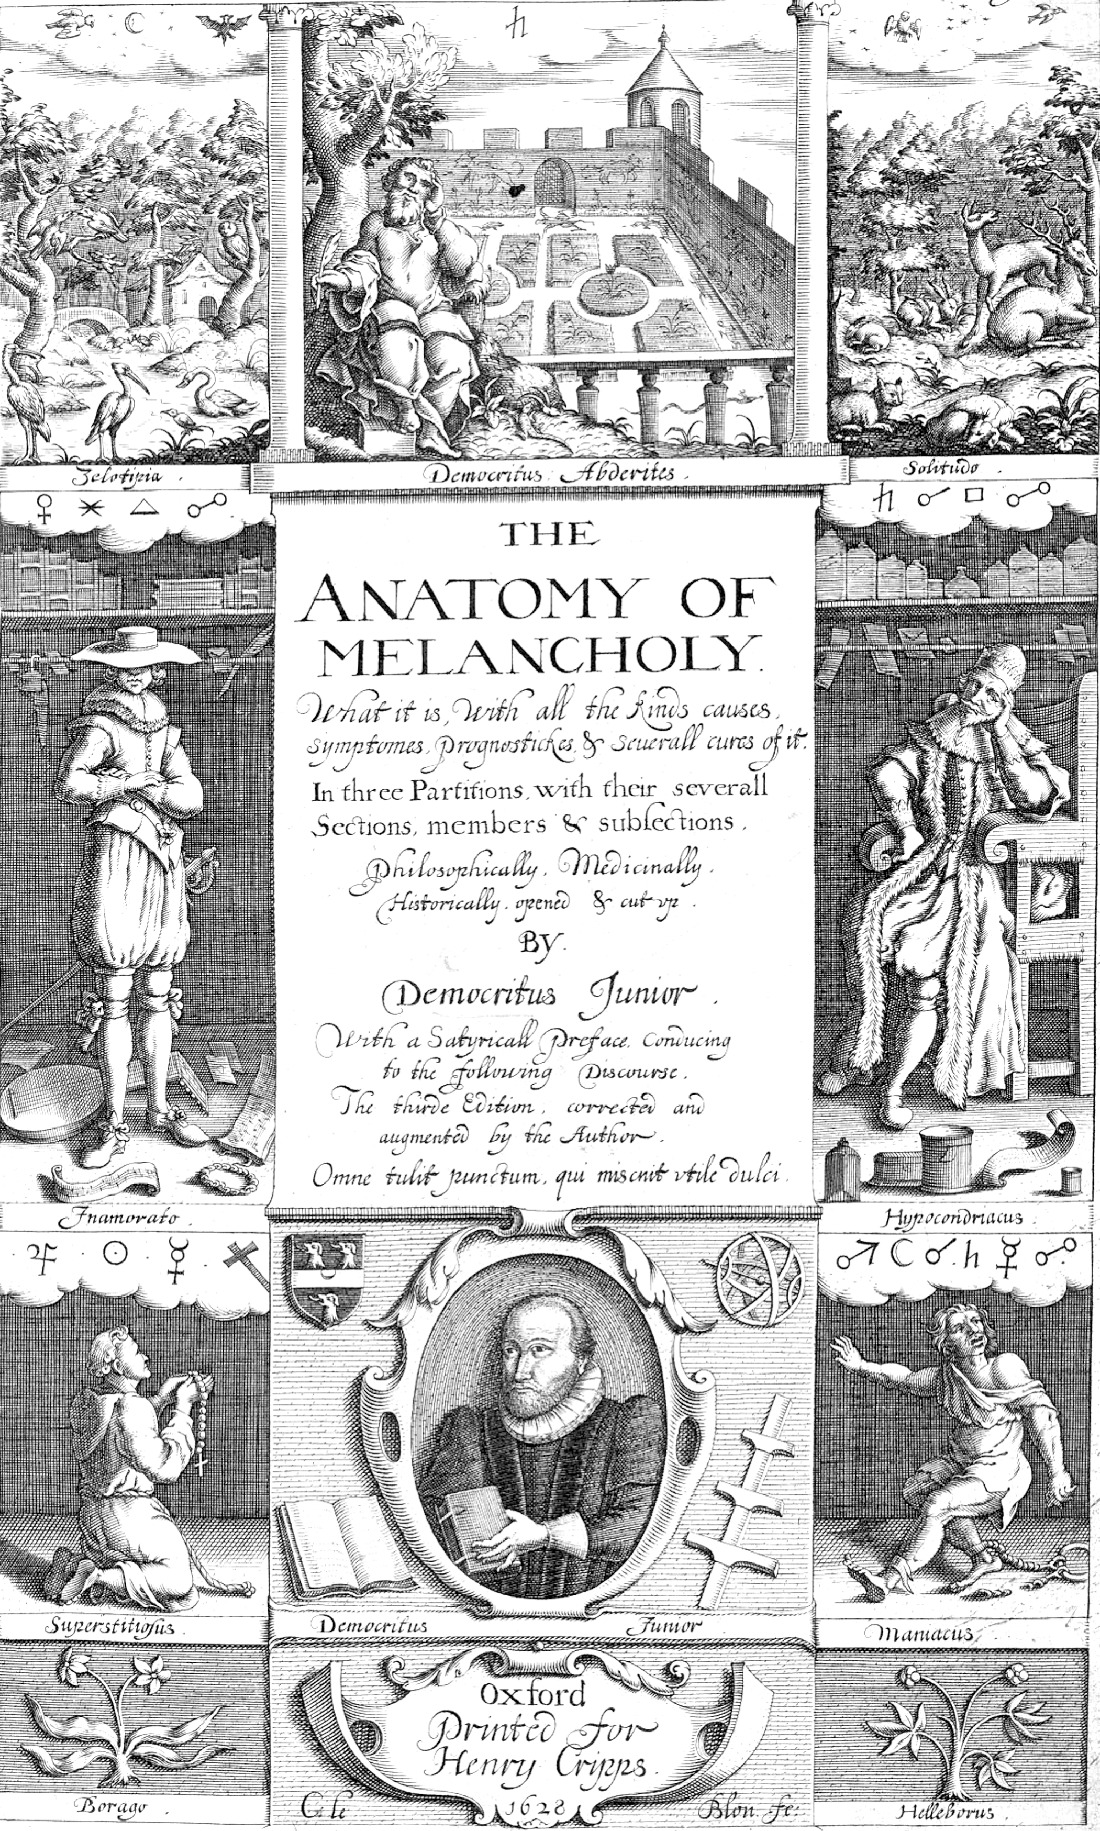
\includegraphics[height={\textheight- 3\baselineskip},keepaspectratio=true]{frontispiece.jpg}\label{Frontispiece}

    {\linespread{0.5}\setstretch{0.1}\scriptsize{}\textit{An allegorical frontispiece from the third edition (1628), engraved by \textsc{Christian Le Blon}.
    See \hyperref[ch:frontispiece]{\autoref*{ch:frontispiece} Argument of the Frontispiece}}}
  \end{center}
\restoregeometry
}
{% Title page is on recto.
  \pdfbookmark{Title page}{title-page}
  \newgeometry{
    marginparwidth=0pt,
    marginparsep=0pt,
    onecolumn=true,
    bindingoffset=0pt,
    bottom=106pt,
    centering=true,
    nohead=true
  }
  
\includepdf[fitpaper=true,pagecommand={\setuptitlepage}]{title-page.pdf}\label{title-page}
  \restoregeometry
}
{% Frontispiece legend on the verso.
  \pdfbookmark{Frontispiece legend}{frontispiece-legend}
  \newgeometry{scale=1.0,vmargin=0.8cm,nomarginpar=true,noheadfoot=true}
  {\begin{center}
  \resizebox{0.8\columnwidth}{!}{%
    \begin{tikzpicture}
    %\draw (0,0) --(1,2);
    \draw (-1.8, -9.8) node[inner sep=0] {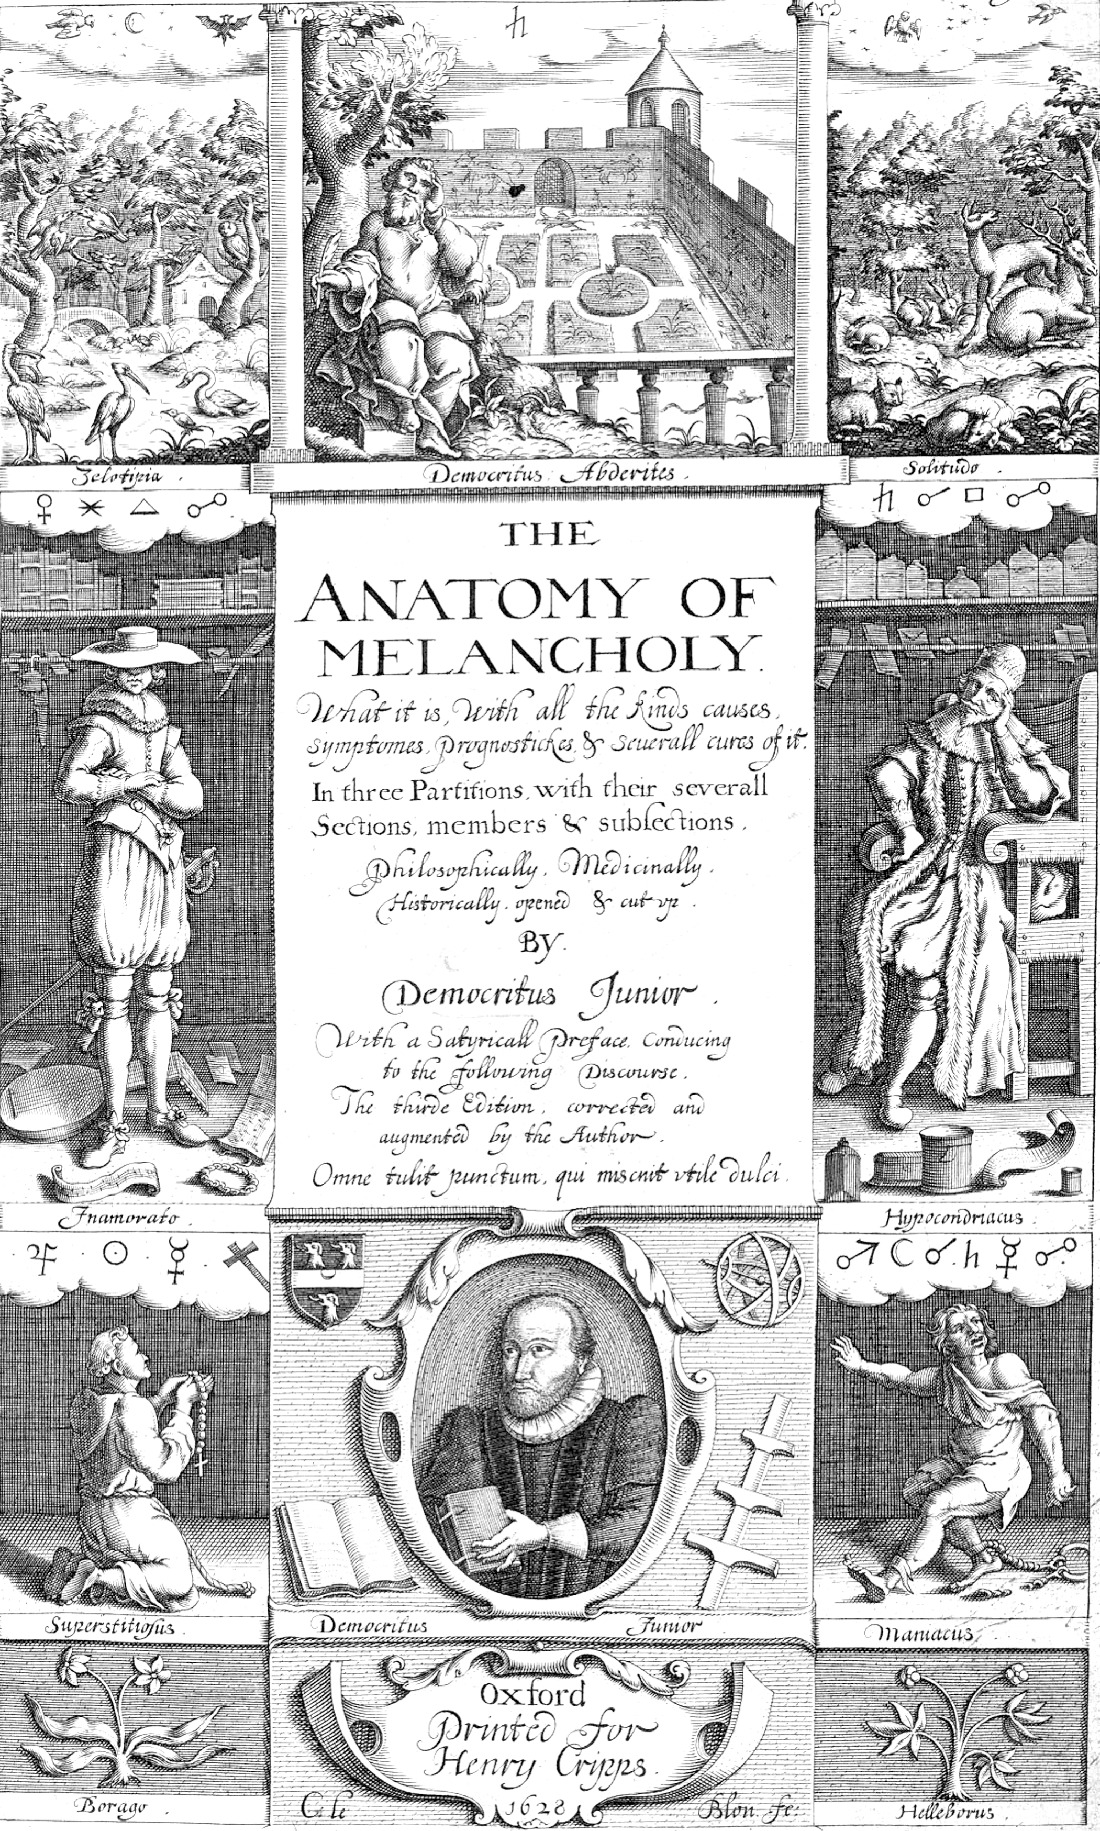
\includegraphics[width=6.9cm]{frontispiece.jpg}};
    %\node [fill=white, red] at (1,-12.5) {8helle}; % helleborus
      %\node [fill=white, red] at (1.6,-11) {7maniac}; % maniacus
      %\node [fill=white, red] at (1.6,-7) {5hypoc}; % Hypocondriacus
      %\node [fill=white, red] at (1.6,-4.3) {3solitudo}; % Solitudo
      %\node [fill=white, red] at (-3.2,-11) {6supersti}; % Superstitiosus
      %\node [fill=white, red] at (-3.2,-7.5) {4inamor}; % Inamorato
      %\node [fill=white, red] at (-2.8,-4) {2jealous}; % Jealous
      %\node [fill=white, red] at (-1,-3.5) {1democr}; % Democritus
      \node[align=left] at (-1.0,0.0) {Old \textsc{Democritus} under a tree,\\Sits on a stone with book on knee;\\About him hang there many features,\\Of Cats, Dogs and such like creatures,\\Of which he makes anatomy,\\The seat of black choler to see.\\Over his head appears the sky,\\And Saturn Lord of melancholy.};
    \node[align=left] at (5.9,0.0) {To the left a landscape of \textsc{Jealousy},\\Presents itself unto thine eye.\\A Kingfisher, a Swan, an Hern,\\Two fighting-cocks you may discern,\\Two roaring Bulls each other hie,\\To assault concerning venery.\\Symbols are these; I say no more,\\Conceive the rest by that’s afore.};
    \node[align=left] at (6,-4.2) {The next of \textsc{solitariness},\\A portraiture doth well express,\\By sleeping dog, cat: Buck and Doe,\\Hares, Conies in the desert go:\\Bats, Owls the shady bowers over,\\In melancholy darkness hover.\\Mark well: If’t be not as’t should be,\\Blame the bad Cutter, and not me.};
    \node[align=left] at (6,-8.5) {I’th’ under column there doth stand\\\textsc{Inamorato} with folded hand;\\Down hangs his head, terse and polite,\\Some ditty sure he doth indite.\\His lute and books about him lie,\\As symptoms of his vanity.\\If this do not enough disclose,\\To paint him, take thyself by th’ nose.};

    \node[align=left] at (6,-12.7) {\textsc{Hypocondriacus} leans on his arm,\\Wind in his side doth him much harm,\\And troubles him full sore, God knows,\\Much pain he hath and many woes.\\About him pots and glasses lie,\\Newly brought from’s Apothecary.\\This Saturn’s aspects signify,\\You see them portray’d in the sky.};

    \node[align=left] at (5.9,-17) {Beneath them kneeling on his knee,\\A \textsc{superstitious} man you see:\\He fasts, prays, on his Idol fixt,\\Tormented hope and fear betwixt:\\For Hell perhaps he takes more pain,\\Than thou dost Heaven itself to gain.\\Alas poor soul, I pity thee,\\What stars incline thee so to be?};

    \node[align=left] at (6,-21.5) {But see the \textsc{madman} rage downright\\With furious looks, a ghastly sight.\\Naked in chains bound doth he lie,\\And roars amain he knows not why!\\Observe him; for as in a glass,\\Thine angry portraiture it was.\\His picture keeps still in thy presence;\\’Twixt him and thee, there’s no difference.};

    \node[align=left] at (-1.8,-20.0) {\textsc{Borage} and \textsc{Hellebor} fill two scenes,\\Sovereign plants to purge the veins\\Of melancholy, and cheer the heart,\\Of those black fumes which make it smart;\\To clear the brain of misty fogs,\\Which dull our senses, and Soul clogs.\\The best medicine that e’er God made\\For this malady, if well assay’d.};

    % 1 - Democritus arrows
      \draw [ultra thick, black] (-4.3, 2.1) rectangle (2.2,-2.1); % text box
      \draw [ultra thick, black] (-1.8, -2.1) -- (-1.8,-4.1); %arrow
      \draw [ultra thick, black] (-3.3, -7.1) rectangle (-0.2,-4.1); % map box
      \fill [nearly transparent, black] (-3.3, -7.1) rectangle (-0.2,-4.1); % map box

      % 2 - Jealousy arrows
      \draw [ultra thick, dashed, red] (2.7, -2) -- (2.7,-3); %
      \draw [ultra thick, dashed, red] (-4.5, -3) -- (2.7,-3); %
      \draw [ultra thick, dashed, red] (-4.5, -3) -- (-4.5,-4); %
      % 2 - Jealousy box
      \fill[nearly transparent, red] (-5.3,-4)rectangle(-3.5,-7);
      \draw [ultra thick, dashed, red](2.7,-2)rectangle(9,2.2);
      \draw [ultra thick, dashed, red](-5.3,-4)rectangle(-3.5,-7);


      % 3 - Solitudo arrows
      \draw [ultra thick, black] (2.9, -6.3) rectangle (9.2,-2.2); % text box
      \draw [ultra thick, black] (1.6, -5.5) -- (2.9,-5.5); %
      \draw [ultra thick, black](1.6,-4.1)rectangle(-0.1,-7.1); % map box
      \fill [nearly transparent, black](1.6,-4.1)rectangle(-0.1,-7.1); % map box

      % 4 - Inamorato arrows
      \draw [ultra thick, dashed, red] (-3.5, -8.2) -- (2.8,-8.2); % arrow
      % 4 - Inamorato box
      \fill[nearly transparent, red] (-5.3,-7.2)rectangle(-3.5,-11.5);
      \draw [ultra thick, dashed, red](2.7,-10.5)rectangle(9.3,-6.4);
      \draw [ultra thick, dashed, red](-5.3,-7.2)rectangle(-3.5,-11.5);


      % 5 - Hypocondriacus arrows
      \draw [ultra thick, black] (1.6, -9.3) -- (2.5,-9.3); %
      \draw [ultra thick, black] (2.5, -9.3) -- (2.5,-12.8); %
      \draw [ultra thick, black] (2.5, -12.8) -- (2.7,-12.8); %
      \draw [ultra thick, black](1.6,-7.2)rectangle(-0.1,-11.7); % map box
      \fill [nearly transparent, black](1.6,-7.2)rectangle(-0.1,-11.7); % map box
      \draw [ultra thick, black](2.7,-14.8)rectangle(9.3,-10.7); % text box

      % 6 - Superstitiosus arrows
      \draw [ultra thick, dashed, red] (-5.5, -16.5) -- (2.7,-16.5); %
      \draw [ultra thick, dashed, red] (-5.5, -16.5) -- (-5.5,-13); %
      \draw [ultra thick, dashed, red] (-5.5, -13) -- (-5.3,-13); %
      % 6 - Superstitiosus box
      \fill[nearly transparent, red](-5.3,-11.8)rectangle(-3.5,-14.4);
      \draw [ultra thick, dashed, red](-5.3,-11.8)rectangle(-3.5,-14.4);
      \draw [ultra thick, dashed, red](2.7,-19.1)rectangle(9.1,-14.9); % text box


      % 7 - Maniac arrows
      \draw [ultra thick, black] (2.2, -23.5) -- (2.4,-23.5); %base
      \draw [ultra thick, black] (2.2, -12.8) -- (2.2,-23.5); %
      \draw [ultra thick, black] (1.6, -12.8) -- (2.2,-12.8); %
      \draw [ultra thick, black](2.4,-23.8)rectangle(9.6,-19.3); % text box
      \draw [ultra thick, black](1.6,-14.4)rectangle(-0.1,-11.8); % map box
      \fill [nearly transparent, black](1.6,-14.4)rectangle(-0.1,-11.8); % map box

      % 8 - Hellebor arrows
      \draw [ultra thick, black] (-2, -15.8) -- (-2,-17.6); %
      \draw [ultra thick, black] (-4.2, -15.8) -- (1,-15.8); %base
      \draw [ultra thick, black] (-4.2, -15.8) -- (-4.2,-15.6); %l
      \draw [ultra thick, black] (1, -15.8) -- (1,-15.6); %base
      % 8 - Hellebore box
      \draw [ultra thick, black](-5.6,-17.6)rectangle(1.9,-22.3);
      \draw [ultra thick, black](-5.2,-14.4)rectangle(-3.5,-15.5); % left map box
      \fill [nearly transparent, black](-5.2,-14.4)rectangle(-3.5,-15.5); % left map box
      \draw [ultra thick, black](-0.1,-14.4)rectangle(1.6,-15.5); % right map box
      \fill [nearly transparent, black](-0.1,-14.4)rectangle(1.6,-15.5); % right map box

    \end{tikzpicture}
  }
  \end{center}
}

  \restoregeometry
}
{% Decorative recto.
  \pdfbookmark{Inner recto}{inner-recto}
  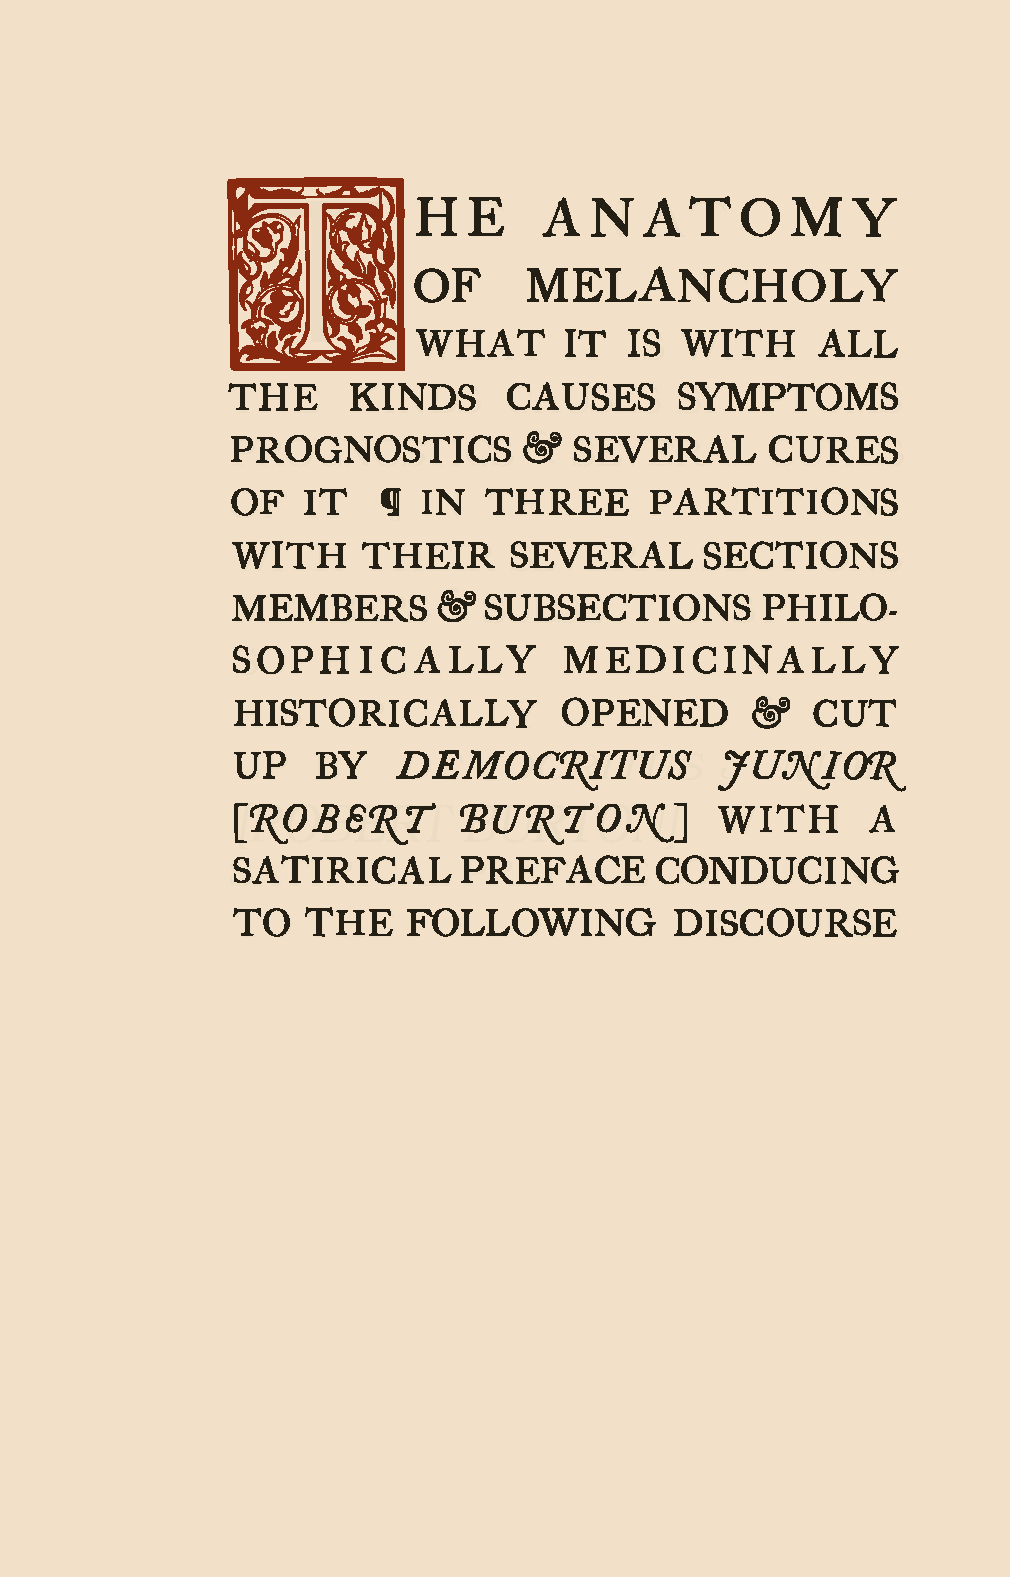
\includepdf[fitpaper=true]{inner-recto.pdf}\label{inner-recto}
}
% Table of contents.
\pdfbookmark{\contentsname}{toc}
\tableofcontents
\clearpage
\phantomsection
\pdfbookmark[0]{List of Figures}{lof}
\listoffigures
\clearpage
\phantomsection
\pdfbookmark[0]{List of Prescriptions}{lop}
\listof{Prescription}{List of Prescriptions}
\bookmarksetup{startatroot}
\addfontfeature{Numbers={OldStyle}}
\chapter{About the Author}
Robert Burton was the son of Ralph Burton, of an ancient and genteel family at Lindley, in Leicestershire, and was born there on the 8th of February 1576.
He received the first rudiments of learning at the free school of Sutton Coldfield, in Warwickshire\footnote{This is Wood's account.
His will says, Nuneaton; but a passage in this work (see \autopageref{mention:coldfield}) mentions Sutton Coldfield; probably he may have been at both schools.} from whence he was, at the age of seventeen, in the long vacation, 1593, sent to Brazen Nose College, in the condition of a commoner, where he made considerable progress in logic and philosophy.
In 1599 he was elected student of Christ Church, and, for form's sake, was put under the tuition of Dr. John Bancroft, afterwards Bishop of Oxford.
In 1614 he was admitted to the reading of the Sentences, and on the 29th of November, 1616, had the vicarage of St. Thomas, in the west suburb of Oxford, conferred on him by the dean and canons of Christ Church, which, with the rectory of Segrave, in Leicestershire, given to him in the year 1636, by George, Lord Berkeley, he kept, to use the words of the Oxford antiquary, with much ado to his dying day.
He seems to have been first beneficed at Walsby, in Lincolnshire, through the munificence of his noble patroness, Frances, Countess Dowager of Exeter, but resigned the same, as he tells us, for some special reasons.
At his vicarage he is remarked to have always given the sacrament in wafers.
Wood's character of him is, that \blockquote{he was an exact mathematician, a curious calculator of nativities, a general read scholar, a thorough-paced philologist, and one that understood the surveying of lands well.
As he was by many accounted a severe student, a devourer of authors, a melancholy and humorous person; so by others, who knew him well, a person of great honesty, plain dealing and charity.
I have heard some of the ancients of Christ Church often say, that his company was very merry, facete, and juvenile; and no man in his time did surpass him for his ready and dexterous interlarding his common discourses among them with verses from the poets, or sentences from classic authors; which being then all the fashion in the University, made his company the more acceptable.}

He appears to have been a universal reader of all kinds of books, and availed himself of his multifarious studies in a very extraordinary manner.
From the information of Hearne, we learn that John Rouse, the Bodleian librarian, furnished him with choice books for the prosecution of his work.
The subject of his labour and amusement, seems to have been adopted from the infirmities of his own habit and constitution.
Mr. Granger says, \blockquote{He composed this book with a view of relieving his own melancholy, but increased it to such a degree, that nothing could make him laugh, but going to the bridge-foot and hearing the ribaldry of the bargemen, which rarely failed to throw him into a violent fit of laughter.
Before he was overcome with this horrid disorder, he, in the intervals of his vapours, was esteemed one of the most facetious companions in the University}.

His residence was chiefly at Oxford; where, in his chamber in Christ Church College, he departed this life, at or very near the time which he had some years before foretold, from the calculation of his own nativity, and which, says Wood,
\enquote{being exact, several of the students did not forbear to whisper among themselves, that rather than there should be a mistake in the calculation, he sent up his soul to heaven through a slip about his neck.}. Whether this suggestion is founded in truth, we have no other evidence than an obscure hint in the epitaph hereafter inserted, which was written by the author himself, a short time before his death. His body, with due solemnity, was buried near that of Dr. Robert Weston, in the north aisle which joins next to the choir of the cathedral of Christ Church, on the 27th of January 1639-40.
Over his grave was soon after erected a comely monument, on the upper pillar of the said aisle, with his bust, painted to the life. On the right hand is the following calculation of his nativity:
\\
\\
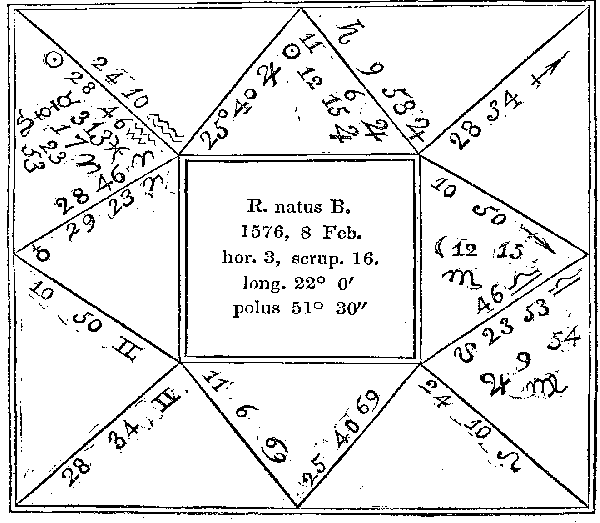
\includegraphics[width=\textwidth,keepaspectratio]{horoscope}

and under the bust, this inscription of his own composition:

\settowidth{\versewidth}{Paucis notus, paucioribus ignotus,}
\begin{verse}[\versewidth]
Paucis notus, paucioribus ignotus,\\*
Hic jacet Democritus junior\\*
Cui vitam dedit et mortem\\*
Melancholia\\*
\hrulefill\\*
Obiit 8 Idus Januarii. A. C. MDCXXXIX.\\!
\end{verse}

Freely translated:

\settowidth{\versewidth}{Known to few, unknown to fewer,}
\begin{verse}[\versewidth]
Known to few, unknown to fewer,\\*
Here lies Democritus Junior,\\*
to whom Melancholy gave\\*
both life and death\\!
\end{verse}

%Arms:—Azure on a bend O. between three dogs' heads O. a crescent G.

A few months before his death, he made his will, of which the following is a copy:
\\

{\scriptsize{}\lq\lq\textbf{EXTRACTED FROM THE REGISTRY OF THE PREROGATIVE COURT OF CANTERBURY.}

\emph{In nomine Dei Amen.} August 15th One thousand six hundred thirty nine because there be so many casualties to which our life is subject besides quarrelling and contention which happen to our Successors after our Death by reason of unsettled Estates I Robert Burton Student of Christ-church Oxon. though my means be but small have thought good by this my last Will and Testament to dispose of that little which I have and being at this present I thank God in perfect health of Bodie and Mind and if this Testament be not so formal according to the nice and strict terms of Law and other Circumstances peradventure required of which I am ignorant I desire howsoever this my Will may be accepted and stand good according to my true Intent and meaning.

First I bequeath Animam Deo Corpus Terrae whensoever it shall please God to call me I give my Land in Higham which my good Father Ralphe Burton of Lindly in the County of Leicester Esquire gave me by Deed of Gift and that which I have annexed to that Farm by purchase since, now leased for thirty eight pounds per Ann. to mine Elder Brother William Burton of Lindly Esquire during his life and after him to his Heirs I make my said Brother William likewise mine Executor as well as paying such Annuities and Legacies out of my Lands and Goods as are hereafter specified I give to my nephew Cassibilan Burton twenty pounds Annuity per Ann. out of my Land in Higham during his life to be paid at two equal payments at our Lady Day in Lent and Michaelmas or if he be not paid within fourteen Days after the said Feasts to distrain on any part of the Ground or on any of my Lands of Inheritance Item I give to my Sister Katherine Jackson during her life eight pounds per Ann. Annuity to be paid at the two Feasts equally as above said or else to distrain on the Ground if she be not paid after fourteen days at Lindly as the other some is out of the said Land Item I give to my Servant John Upton the Annuity of Forty Shillings out of my said Farme during his life (if till then my Servant) to be paid on Michaelmas day in Lindley each year or else after fourteen days to distrain Now for my goods I thus dispose them First I give an C'th pounds to Christ Church in Oxford where I have so long lived to buy five pounds Lands per Ann. to be Yearly bestowed on Books for the Library Item I give an hundredth pound to the University Library of Oxford to be bestowed to purchase five pound Land per Ann. to be paid out Yearly on Books as Mrs. Brooks formerly gave an hundred pounds to buy Land to the same purpose and the Rent to the same use I give to my Brother George Burton twenty pounds and my watch I give to my Brother Ralph Burton five pounds Item I give to the Parish of Seagrave in Leicestershire where I am now Rector ten pounds to be given to a certain Feoffees to the perpetual good of the said Parish Oxon Item I give to my Niece Eugenia Burton One hundredth pounds Item I give to my Nephew Richard Burton now Prisoner in London an hundredth pound to redeem him Item I give to the Poor of Higham Forty Shillings where my Land is to the poor of Nuneaton where I was once a Grammar Scholar three pound to my Cousin Purfey of Wadlake my Cousin Purfey of Calcott my Cousin Hales of Coventry my Nephew Bradshaw of Orton twenty shillings a piece for a small remembrance to Mr. Whitehall Rector of Cherkby myne own Chamber Fellow twenty shillings I desire my Brother George and my Cosen Purfey of Calcott to be the Overseers of this part of my Will I give moreover five pounds to make a small Monument for my Mother where she is buried in London to my Brother Jackson forty shillings to my Servant John Upton forty shillings besides his former Annuity if he be my Servant till I die if he be till then my Servant

-- ROBERT BURTON

-- Charles Russell, Witness

-- John Pepper, Witness.

An Appendix to this my Will if I die in Oxford or whilst I am of Christ Church and with good Mr. Paynes August the Fifteenth 1639.

I give to Mr. Doctor Fell Dean of Christ Church Forty Shillings to the Eight Canons twenty Shillings a piece as a small remembrance to the poor of St. Thomas Parish Twenty Shillings to Brasenose Library five pounds to Mr. Rowse of Oriell Colledge twenty Shillings to Mr. Heywood xxs. to Dr. Metcalfe xxs. to Mr. Sherley xxs. If I have any Books the University Library hath not, let them take them If I have any Books our own Library hath not, let them take them I give to Mrs. Fell all my English Books of Husbandry one excepted to her Daughter Mrs. Katherine Fell my Six Pieces of Silver Plate and six Silver spoons to Mrs. Iles my Gerards Herball To Mrs. Morris my Country Farme Translated out of French 4. and all my English Physick Books to Mr. Whistler the Recorder of Oxford I give twenty shillings to all my fellow Students Mrs of Arts a Book in fol. or two a piece as Master Morris Treasurer or Mr. Dean shall appoint whom I request to be the Overseer of this Appendix and give him for his pains Atlas Geografer and Ortelius Theatrum Mond' I give to John Fell the Dean's Son Student my Mathematical Instruments except my two Crosse Staves which I give to my Lord of Donnol if he be then of the House To Thomas Iles Doctor Iles his Son Student Saluntch on Paurrhelia and Lucian's Works in 4 Tomes If any books be left let my Executors dispose of them with all such Books as are written with my own hands and half my Melancholy Copy for Crips hath the other half To Mr. Jones Chaplin and Chanter my Surveying Books and Instruments To the Servants of the House Forty Shillings

-- ROBERT BURTON

-- Charles Russell, Witness

-- John Pepper, Witness

--- This Will was shewed to me by the Testator and acknowledged by him some few days before his death to be his last Will Ita Testor John Morris S Th D. Prebendari' Eccl Chri' Oxon Feb. 3, 1639. Probatum fuit Testamentum suprascriptum, \etc. 11° 1640 Juramento Willmi Burton Fris' et Executoris cui \etc{} de bene et fideliter administrand. \etc{} coram Mag'ris Nathanaele Stephens Rectore Eccl. de Drayton, et Edwardo Farmer, Clericis, vigore commissionis, \etc.\rq\rq}

\clearpage
\mainmatter
\chapter{Democratus Junior to His Book}
\settowidth{\versewidth}{Should known or unknown student, freed from strife}
\poemlines{2}
\begin{verse}[\versewidth]
Go forth my book into the open day;\\*
Happy, if made so by its garish eye. \\!

Go forth my book into the open day;\\*
Happy, if made so by its garish eye. \\!

O'er earth's wide surface take thy vagrant way,\\*
To imitate thy master's genius try. \\!

The Graces three, the Muses nine salute,\\*
Should those who love them try to con thy lore.\\!

The country, city seek, grand thrones to boot,\\*
With gentle courtesy humbly bow before.\\!

Should nobles gallant, soldiers frank and brave\\*
Seek thy acquaintance, hail their first advance:\\!

From twitch of care thy pleasant vein may save,\\*
May laughter cause or wisdom give perchance.\\!

Some surly Cato, Senator austere,\\*
Haply may wish to peep into thy book:\\!

Seem very nothing-tremble and revere:\\*
No forceful eagles, butterflies e'er look.\\!

They love not thee: of them then little seek,\\*
And wish for readers triflers like thyself.\\!

Of ludeful matron watchful catch the beck,\\*
Or gorgeous countess full of pride and pelf.\\!

They may say pish! and frown, and yet read on:\\*
Cry odd, and silly, coarse, and yet amusing.\\!

Should dainty damsels seek thy page to con,\\*
Spread thy best stores: to them be ne'er refusing:\\!

Say, fair one, master loves thee dear as life;\\*
Would he were here to gaze on thy sweet look.\\!

Should known or unknown student, freed from strife\\*
Of logic and the schools, explore my book:\\!

Cry mercy critic, and thy book withhold:\\*
Be some few errors pardon'd though observ'd:\\!

An humble author to implore makes bold.\\*
Thy kind indulgence, even undeserv'd,\\!

Should melancholy wight or pensive lover,\\*
Courtier, snug cit, or carpet knight so trim\\!

Our blossoms cull, he'll find himself in clover,\\*
Gain sense from precept, laughter from our whim.\\!

Should learned leech with solemn air unfold\\*
Thy leaves, beware, be civil, and be wise:\\!

Thy volume many precepts sage may hold,\\*
His well fraught head may find no trifling prize.\\!

Should crafty lawyer trespass on our ground,\\*
Caitiffs avaunt! disturbing tribe away!\\!

Unless (white crow) an honest one be found;\\*
He'll better, wiser go for what we say.\\!

Should some ripe scholar, gentle and benign,\\*
With candour, care, and judgment thee peruse:\\!

Thy faults to kind oblivion he'll consign;\\*
Nor to thy merit will his praise refuse.\\!

Thou may'st be searched for polish'd words and verse\\*
By flippant spouter, emptiest of praters:\\!

Tell him to seek them in some mawkish verse:\\*
My periods all are rough as nutmeg graters.\\!

The doggerel poet, wishing thee to read,\\*
Reject not; let him glean thy jests and stories.\\!

His brother I, of lowly sembling breed:\\*
Apollo grants to few Parnassian glories.\\!

Menac'd by critic with sour furrowed brow,\\*
Momus or Troilus or Scotch reviewer:\\!

Ruffle your heckle, grin and growl and vow:\\*
Ill-natured foes you thus will find the fewer,\\!

When foul-mouth'd senseless railers cry thee down,\\*
Reply not: fly, and show the rogues thy stern;\\!

They are not worthy even of a frown:\\*
Good taste or breeding they can never learn;\\!

Or let them clamour, turn a callous ear,\\*
As though in dread of some harsh donkey's bray.\\!

If chid by censor, friendly though severe,\\*
To such explain and turn thee not away.\\!

Thy vein, says he perchance, is all too free;\\*
Thy smutty language suits not learned pen:\\!

Reply, Good Sir, throughout, the context see;\\*
Thought chastens thought; so prithee judge again.\\!

Besides, although my master's pen may wander\\*
Through devious paths, by which it ought not stray,\\!

His life is pure, beyond the breath of slander:\\*
So pardon grant; 'tis merely but his way.\\!

Some rugged ruffian makes a hideous rout-\\*
Brandish thy cudgel, threaten him to baste;\\!

The filthy fungus far from thee cast out;\\*
Such noxious banquets never suit my taste.\\!

Yet, calm and cautious moderate thy ire,\\*
Be ever courteous should the case allow-\\!

Sweet malt is ever made by gentle fire:\\*
Warm to thy friends, give all a civil bow.\\!

Even censure sometimes teaches to improve,\\*
Slight frosts have often cured too rank a crop,\\!

So, candid blame my spleen shall never move,\\*
For skilful gard'ners wayward branches lop.\\!

Go then, my book, and bear my words in mind;\\*
Guides safe at once, and pleasant them you'll find.\\!
\end{verse}

\chapter{The Argument of the Frontispiece}
\label{ch:frontispiece}
\settowidth{\versewidth}{Of those black fumes which make it smart;}
\poemlines{8}
\begin{verse}[\versewidth]
Ten distinct Squares here seen apart,\\*
Are joined in one by Cutter's art.\\!

Old Democritus under a tree,\\*
Sits on a stone with book on knee;\\*
About him hang there many features,\\*
Of Cats, Dogs and such like creatures,\\*
Of which he makes anatomy,\\*
The seat of black choler to see.\\*
Over his head appears the sky,\\*
And Saturn Lord of melancholy.\\!

To the left a landscape of Jealousy,\\*
Presents itself unto thine eye.\\*
A Kingfisher, a Swan, an Hern,\\*
Two fighting-cocks you may discern,\\*
Two roaring Bulls each other hie,\\*
To assault concerning venery.\\*
Symbols are these; I say no more,\\*
Conceive the rest by that's afore.\\!

The next of solitariness,\\*
A portraiture doth well express,\\*
By sleeping dog, cat: Buck and Doe,\\*
Hares, Conies in the desert go:\\*
Bats, Owls the shady bowers over,\\*
In melancholy darkness hover.\\*
Mark well: If't be not as't should be,\\*
Blame the bad Cutter, and not me.\\!

I'th' under column there doth stand\\*
\textsc{Inamorato} with folded hand;\\*
Down hangs his head, terse and polite,\\*
Some ditty sure he doth indite.\\*
His lute and books about him lie,\\*
As symptoms of his vanity.\\*
If this do not enough disclose,\\*
To paint him, take thyself by th' nose.\\!

\textsc{Hypocondriacus} leans on his arm,\\*
Wind in his side doth him much harm,\\*
And troubles him full sore, God knows,\\*
Much pain he hath and many woes.\\*
About him pots and glasses lie,\\*
Newly brought from's Apothecary.\\*
This Saturn's aspects signify,\\*
You see them portray'd in the sky.\\!

Beneath them kneeling on his knee,\\*
A superstitious man you see:\\*
He fasts, prays, on his Idol fixt,\\*
Tormented hope and fear betwixt:\\*
For Hell perhaps he takes more pain,\\*
Than thou dost Heaven itself to gain.\\*
Alas poor soul, I pity thee,\\*
What stars incline thee so to be?\\!

But see the madman rage downright\\*
With furious looks, a ghastly sight.\\*
Naked in chains bound doth he lie,\\*
And roars amain he knows not why!\\*
Observe him; for as in a glass,\\*
Thine angry portraiture it was.\\*
His picture keeps still in thy presence;\\*
'Twixt him and thee, there's no difference.\\!

\textsc{Borage} and \textsc{Hellebor} fill two scenes,\\*
Sovereign plants to purge the veins\\*
Of melancholy, and cheer the heart,\\*
Of those black fumes which make it smart;\\*
To clear the brain of misty fogs,\\*
Which dull our senses, and Soul clogs.\\*
The best medicine that e'er God made\\*
For this malady, if well assay'd.\\!

Now last of all to fill a place,\\*
Presented is the Author's face;\\*
And in that habit which he wears,\\*
His image to the world appears.\\*
His mind no art can well express,\\*
That by his writings you may guess.\\*
It was not pride, nor yet vainglory,\\*
(Though others do it commonly)\\*
Made him do this: if you must know,\\*
The Printer would needs have it so.\\*
Then do not frown or scoff at it,\\*
Deride not, or detract a whit.\\*
For surely as thou dost by him,\\*
He will do the same again.\\*
Then look upon't, behold and see,\\*
As thou lik'st it, so it likes thee.\\*
And I for it will stand in view,\\*
Thine to command, Reader, adieu.\\!
\end{verse}

\chapter{The Author's Abstract of Melacholy, \textgreek{Διαλογῶς}}
\settowidth{\versewidth}{Here now, then there; the world is mine,}
\poemlines{2}
\begin{verse}[\versewidth]
When I go musing all alone\\*
Thinking of divers things fore-known.\\*
When I build castles in the air,\\*
Void of sorrow and void of fear,\\*
Pleasing myself with phantasms sweet,\\*
Methinks the time runs very fleet.\\*

All my joys to this are folly,\\*
Naught so sweet as melancholy.\\!

When I lie waking all alone,\\*
Recounting what I have ill done,\\*
My thoughts on me then tyrannise,\\*
Fear and sorrow me surprise,\\*
Whether I tarry still or go,\\*
Methinks the time moves very slow.\\!

All my griefs to this are jolly,\\*
Naught so mad as melancholy.\\!

When to myself I act and smile,\\*
With pleasing thoughts the time beguile,\\*
By a brook side or wood so green,\\*
Unheard, unsought for, or unseen,\\*
A thousand pleasures do me bless,\\*
And crown my soul with happiness.\\!

All my joys besides are folly,\\*
None so sweet as melancholy.\\!

When I lie, sit, or walk alone,\\*
I sigh, I grieve, making great moan,\\*
In a dark grove, or irksome den,\\*
With discontents and Furies then,\\*
A thousand miseries at once\\*
Mine heavy heart and soul ensconce,\\*

All my griefs to this are jolly,\\*
None so sour as melancholy.\\!

Methinks I hear, methinks I see,\\*
Sweet music, wondrous melody,\\*
Towns, palaces, and cities fine;\\*
Here now, then there; the world is mine,\\*
Rare beauties, gallant ladies shine,\\*
Whate'er is lovely or divine.\\!

All other joys to this are folly,\\*
None so sweet as melancholy.\\!

Methinks I hear, methinks I see\\*
Ghosts, goblins, fiends; my phantasy\\*
Presents a thousand ugly shapes,\\*
Headless bears, black men, and apes,\\*
Doleful outcries, and fearful sights,\\*
My sad and dismal soul affrights.\\!

All my griefs to this are jolly,\\*
None so damn'd as melancholy.\\!

Methinks I court, methinks I kiss,\\*
Methinks I now embrace my mistress.\\*
O blessed days, O sweet content,\\*
In Paradise my time is spent.\\*
Such thoughts may still my fancy move,\\*
So may I ever be in love.\\!

All my joys to this are folly,\\*
Naught so sweet as melancholy.\\!

When I recount love's many frights,\\*
My sighs and tears, my waking nights,\\*
My jealous fits; O mine hard fate\\*
I now repent, but 'tis too late.\\*
No torment is so bad as love,\\*
So bitter to my soul can prove.\\!

All my griefs to this are jolly,\\*
Naught so harsh as melancholy.\\!

Friends and companions get you gone,\\*
'Tis my desire to be alone;\\*
Ne'er well but when my thoughts and I\\*
Do domineer in privacy.\\*
No Gem, no treasure like to this,\\*
'Tis my delight, my crown, my bliss.\\!

All my joys to this are folly,\\*
Naught so sweet as melancholy.\\!

'Tis my sole plague to be alone,\\*
I am a beast, a monster grown,\\*
I will no light nor company,\\*
I find it now my misery.\\*
The scene is turn'd, my joys are gone,\\*
Fear, discontent, and sorrows come.\\!

All my griefs to this are jolly,\\*
Naught so fierce as melancholy.\\!

I'll not change life with any king,\\*
I ravisht am: can the world bring\\*
More joy, than still to laugh and smile,\\*
In pleasant toys time to beguile?\\*
Do not, O do not trouble me,\\*
So sweet content I feel and see.\\!

All my joys to this are folly,\\*
None so divine as melancholy.\\!

I'll change my state with any wretch,\\*
Thou canst from gaol or dunghill fetch;\\*
My pain's past cure, another hell,\\*
I may not in this torment dwell!\\*
Now desperate I hate my life,\\*
Lend me a halter or a knife;\\!

All my griefs to this are jolly,\\*
Naught so damn'd as melancholy.\\!
\end{verse}
\poemlines{0}

% define margin notes first
\setauthornote{7}{\textlatin{\Seneca{} in ludo in mortem Claudii C\ae{}saris}}
\setauthornote{8}{Lib. de Curiositate.}
\setauthornote{9}{\textlatin{Modo h\ae{}c tibi usui sint, quemvis auctorem fingito. Wecker.}}
\setauthornote{10}{Lib. 10, c. 12. \textlatin{Multa a male feriatis in Democriti nomine commenta data, nobilitatis, auctoritatisque ejus perfugio utentibus.}}
\setauthornote{11}{Martialis. lib. 10, epigr. 14.}
\setauthornote{12}{Juv. sat. 1.}
\setauthornote{13}{Auth. Pet. Besseo edit. Coloniae, 1616.}
\setauthornote{14}{Hip. Epist. Dameget.}
\setauthornote{15}{Laert. lib 9.}
\setauthornote{16}{\textlatin{Hortulo sibi cellulam seligens, ibique seipsum includens, vixit solitarius.}}
\setauthornote{17}{\textlatin{Floruit Olympiade 80; 700 annis post Troiam.}}
\setauthornote{18}{\textlatin{Diacos. quod cunctis operibus facile excellit. Laert.}}
\setauthornote{19}{Col. lib. 1. c. 1.}
\setauthornote{20}{\textlatin{Const. lib. de agric. passim.}}
\setauthornote{21}{\textlatin{Volucrum voces et linguas intelligere se dicit Abderitans Ep.~Hip.}}
\setauthornote{22}{\textlatin{Sabellicus exempl., lib. 10. Oculis se privavit, ut melius contemplationi operam daret, sublimi vir ingenio, profund\ae{}\ cogitationis, \etc.}}
\setauthornote{23}{\textlatin{Naturalia, moralia, mathematica, liberales disciplinas, artiumque omnium peritiam callebat.}}
\setauthornote{24}{Nothing in nature's power to contrive of which he has not written.}
\setauthornote{25}{\textlatin{Veni Athenas, et nemo me novit.}}
\setauthornote{26}{\textlatin{Idem contemptui et admirationi habitus.}}
\setauthornote{27}{\textlatin{Solebat ad portam ambulare, et inde, \etc{}. Hip. Ep. Dameg.}}
\setauthornote{28}{\textlatin{Perpetuorisu pulmonem agitare solebat \Democritus{}. Juv. Sat. 7.}}
\setauthornote{29}{\textlatin{Non sum dignus pr\ae{}stare matella. Mart.}}
\setauthornote{30}{Christ Church in Oxford.}
\setauthornote{31}{Praefat. Hist.}
\setauthornote{32}{Keeper of our college library, lately revived by Otho Nicolson, Esquire.}
\setauthornote{33}{Scaliger.}
\setauthornote{34}{somebody in everything, nobody in each thing}
\setauthornote{35}{In Theat.}
\setauthornote{36}{Phil. Stoic. li. diff. 8. \textlatin{Dogma cupidis et curiosis ingeniis imprimendum, ut sit talis qui nulli rei serviat, aut exacte unum aliquid elaboret, alia negligens, ut artifices, \etc.}}
\setauthornote{37}{\textlatin{Delibare gratum de quocunque cibo, et pittisare de quocunque dolio jucundum.}}
\setauthornote{38}{Essays, lib. 3.}
\setauthornote{39}{he that is everywhere is nowhere}
\setauthornote{40}{Praefat. bibliothec.}
\setauthornote{41}{\textlatin{Ambo fortes et fortunati, Mars idem magisterii dominus juxta primam Leovitii regulam.}}
\setauthornote{42}{Hensius.}
\setauthornote{43}{\textlatin{Calide ambientes, solicite litigantes, aut misere excidentes, voces, strepitum contentiones, \etc.}}
\setauthornote{44}{\textlatin{Cyp. ad Donat. Unice securus, ne excidam in foro, aut in mari Indico bonis eluam, de dote fili\ae, patrimonio filii non sum solicitus.}}
\setauthornote{45}{not so sagacious an observer as simple a narrator}
\setauthornote{46}{\Horace{} Ep. lib. 1. \rn{xix.}, 20.}
\setauthornote{47}{Persius}
\setauthornote{47.5}{a laughter with a petulant spleen}
\setauthornote{48}{\Horace{} lib. 1, sat. 9.}
\setauthornote{49}{\textlatin{Secundum m\oe{}nia locus erat frondosis populis opacus, vitibusque sponte natis, tenuis prope aqua defluebat, placide murmurans, ubi sedile et domus Democriti conspiciebatur.}}
\setauthornote{50}{\textlatin{Ipse composite considebat, super genua volumen habens, et utrinque alia patentia parata, dissectaque animalia cumulatim strata, quorum viscera rimabatur.}}
\setauthornote{51}{\textlatin{Cum mundus extra se sit, et mente captus sit, et nesciat se languere, ut medelam adhibeat.}}
\setauthornote{52}{Scaliger, Ep. ad Patisonem. \textlatin{Nihil magis lectorem invitat quam in opinatum argilinentum, neque vendibilior merx est quam petulans liber.}}
\setauthornote{53}{Lib. \rn{XX.} c. 11. \textlatin{Miras sequuntur inscriptionum festivitates.}}
\setauthornote{54}{Praefat. Nat. Hist. \textlatin{Patri obstetricem parturienti fili\ae{}\ accersenti moram injicere possunt.}}
\setauthornote{55}{Anatomy of Popery, Anatomy of immortality, Angelus salas, Anatomy of Antimony, \etc.}
\setauthornote{56}{Cont. l. 4, c. 9. \textlatin{Non est cura melior quam labor.}}
\setauthornote{57}{\Horace{} \textlatin{De Arte Poet.}}
\setauthornote{58}{\textlatin{Non quod de novo quid addere, aut a veteribus pr\ae{}termissum, sed propri\ae{}\ exercitationis causa.}}
\setauthornote{59}{\textlatin{Qui novit, neque id quod sentit exprimit, perinde est ac si nesciret.}}
\setauthornote{60}{\textlatin{Jovius Praef. Hist.}}
\setauthornote{61}{Erasmus.}
\setauthornote{62}{\textlatin{Otium otio dolorem dolore sum solatus.}}
\setauthornote{63}{Observat. l. 1.}
\setauthornote{64}{M. Joh. Rous, our Protobib. Oxon. M. Hopper, M. Guthridge, \etc.}
\setauthornote{65}{\textlatin{Qu\ae{}\ illi audire et legere solent, eorum partim vidi egomet, alia gessi, qu\ae{}\ illi literis, ego militando didici, nunc vos existimate facta an dicta pluris sint.}}
\setauthornote{66}{Dido Virg.}
\setauthornote{66.5}{Taught by that Power that pities me, I learn to pity them.}
\setauthornote{67}{\textlatin{Camden, Ipsa elephantiasi correpta elephantiasis hospicium construxit.}}
\setauthornote{68}{\textlatin{Iliada post Homerum.}}
\setauthornote{69}{\textlatin{Nihil pr\ae{}termissum quod a quovis dici possit.}}
\setauthornote{70}{Martialis.}
\setauthornote{71}{\textlatin{Magis impium mortuorum lucubrationes, quam vestes furari.}}
\setauthornote{72}{Eccl. ult.}
\setauthornote{73}{\textlatin{Libros Eunuchi gignunt, steriles pariunt.}}
\setauthornote{74}{D. King praefat. lect. Jonas, the late right reverend Lord B. of London.}
\setauthornote{75}{\textlatin{Homines famelici glori\ae{}\ ad ostentationem eruditionis undique congerunt. Buchananus.}}
\setauthornote{76}{\textlatin{Effacinati etiam laudis amore, \etc{}. Justus Baronius.}}
\setauthornote{77}{\textlatin{Ex ruinis alien\ae{}\ existimationis sibi gradum ad famam struunt.}}
\setauthornote{78}{Exercit. 288.}
\setauthornote{79}{\textlatin{Omnes sibi famam qu\ae{}runt et quovis modo in orbem spargi contendunt, ut nov\ae{}\ alicujus rei habeantur auctores. Pr\ae{}f. biblioth.}}
\setauthornote{80}{Praefat. hist.}
\setauthornote{81}{\Plautus{}.}
\setauthornote{82}{\textlatin{E Democriti puteo.}}
\setauthornote{83}{\textlatin{Non tam refert\ae{}\ bibliothec\ae{}\ quam cloac\ae.}}
\setauthornote{84}{\textlatin{Et quicquid cartis amicitur ineptis.}}
\setauthornote{85}{\textlatin{Epist. ad Petas. in regno Franci\ae{}\ omnibus scribendi datur libertas, paucis facultas.}}
\setauthornote{86}{\textlatin{Olim liter\ae{}\ ob homines in precio, nunc sordent ob homines.}}
\setauthornote{87}{Ans. pac.}
\setauthornote{88}{\textlatin{Inter tot mille volumina vix unus a cujus lectione quis melior evadat, immo potius non pejor.}}
\setauthornote{89}{Palingenius.}
\setauthornote{89.5}{What does any one, who reads such works, learn or know but dreams and trifling things.}
\setauthornote{90}{Lib. 5. de Sap.}
\setauthornote{91}{\textlatin{Sterile oportet esse ingenium quod in hoc scripturientum pruritus, \etc.}}
\setauthornote{92}{Cardan, praef. ad Consol.}
\setauthornote{93}{\Horace{} lib. 1, sat. 4.}
\setauthornote{94}{Epist. lib. 1. \textlatin{Magnum p\oe{}tarum proventum annus hic attulit, mense Aprili nullus fere dies quo non aliquis recitavit.}}
\setauthornote{95}{Idem.}
\setauthornote{96}{\textlatin{Principibus et doctoribus deliberandum relinquo, ut arguantur auctorum furta et milies repetita tollantur, et temere scribendi libido c\oe{}rceatur, aliter in infinitum progressura.}}
\setauthornote{97}{\textlatin{Onerabuntur ingenia, nemo legendis sufficit.}}
\setauthornote{98}{\textlatin{Libris obraimur, oculi legendo, manus volitando dolent. Fam. Strada Momo. \Lucretius{}.}}
\setauthornote{99}{\textlatin{Quicquid ubique bene dictum facio meum, et illud nunc meis ad compendium, nunc ad fidem et auctoritatem alienis exprimo verbis, omnes auctores meos clientes esse arbitror, \etc{}. Sarisburiensis ad Polycrat. prol.}}
\setauthornote{100}{In Epitaph. \textlatin{Nep. illud Cyp. hoc Lact. illud Hilar. est, ita Victorinus, in hunc modum loquutus est Arnobius, \etc{}}}
\setauthornote{101}{Praef. ad Syntax. med.}
\setauthornote{102}{until a later age and a happier lot produce something more truly grand}
\setauthornote{103}{In Luc. 10. tom. 2. \textlatin{Pigmei Gigantum humeris impositi plusquam ipsi Gigantes vident.}}
\setauthornote{104}{\textlatin{Nec aranearum textus ideo melior quia ex se fila gignuntur, nec noster ideo vilior, quia ex alienis libamus ut apes. Lipsius adversus dialogist.}}
\setauthornote{105}{\textlatin{Uno absurdo dato mille sequuntur.}}
\setauthornote{106}{\textlatin{Non dubito multos lectores hic fore stultos.}}
\setauthornote{107}{Martial, 13, 2.}
\setauthornote{108}{\textlatin{Ut venatores feram e vestigio impresso, virum scriptiuncula. Lips.}}
\setauthornote{109}{\Horace{}.}
\setauthornote{110}{\Horace{}.}
\setauthornote{111}{Antwerp. fol. 1607.}
\setauthornote{112}{Muretus.}
\setauthornote{113}{Lipsius.}
\setauthornote{114}{\Horace{}.}
\setauthornote{115}{\textlatin{Fieri non potest, ut quod quisque cogitat, dicat unus. Muretus.}}
\setauthornote{116}{Lib. 1. de ord., cap. 11.}
\setauthornote{117}{Erasmus.}
\setauthornote{118}{Annal. Tom. 3. ad annum 360. \textlatin{Est porcus ille qui sacerdotem ex amplitudine redituum sordide demeritur.}}
\setauthornote{119}{Erasm. dial.}
\setauthornote{120}{\textlatin{Epist. lib. 6. Cujusque ingenium non statim emergit, nisi materi\ae{}\ fautor, occasio, commendatorque contingat.}}
\setauthornote{121}{Praef. hist.}
\setauthornote{122}{\textlatin{Laudari a laudato laus est.}}
\setauthornote{123}{Vit. Persii.}
\setauthornote{124}{\textlatin{Minuit pr\ae{}sentia famam.}}
\setauthornote{125}{\textlatin{Lipsius Judic. de Seneca.}}
\setauthornote{126}{\textlatin{Lib. 10. Plurirmum studii, multam rerum cognitionem, omnem studiorum materiam, \etc{} multa in eo probanda, multa admiranda.}}
\setauthornote{127}{\textlatin{Suet. Arena sine calce.}}
\setauthornote{128}{\textlatin{Introduct. ad Sen.}}
\setauthornote{129}{\textlatin{Judic. de Sen. Vix aliquis tam absolutus, ut alteri per omnia satisfaciat, nisi longa temporis pr\ae{}scripto, semota judicandi libertate, religione quidam animos occuparis.}}
\setauthornote{130}{\Horace{} Ep. 1, lib. 19.}
\setauthornote{131}{\textlatin{\AE{}que turpe frigide laudari ac insectanter vituperari. Phavorinus A. Gel. lib. 19, cap. 2.}}
\setauthornote{132}{\Ovid{}, trist. 11. eleg 6.}
\setauthornote{133}{Juven. sat. 5.}
\setauthornote{134}{\textlatin{Aut artis inscii aut qu\ae{}stui magis quam literis student. hab. Cantab. et Lond. Excus. 1976.}}
\setauthornote{135}{\Ovid{}. de pont. Eleg. l. 6.}
\setauthornote{136}{\Horace{}.}
\setauthornote{137}{Tom. 3. \textlatin{Philopseud. accepto pessulo, quum carmen quoddam dixisset, effecit ut ambularet, aquam hauriret, urnam pararet, \etc{}}}
\setauthornote{138}{Eusebius, eccles. hist. lib. 6.}
\setauthornote{139}{Stans pede in uno, as he made verses.}
\setauthornote{140}{Virg.}
\setauthornote{141}{\textlatin{Non eadem a summo expectes, minimoque p\oe{}ta.}}
\setauthornote{142}{\textlatin{Stylus hic nullus, pr\ae{}ter parrhesiam.}}
\setauthornote{143}{\textlatin{Qui rebus se exercet, verba negligit, et qui callet artem dicendi, nullam disciplinam habet recognitam.}}
\setauthornote{144}{Palingenius.}
\setauthornote{144.5}{Words may be resplendent with ornament, but they contain no marrow within.}
\setauthornote{145}{\textlatin{Cujuscunque orationem vides politam et sollicitam, scito animum in pusilis occupatum, in scriptis nil solidum. Epist. lib. 1. 21.}}
\setauthornote{146}{Philostratus, lib. 8. vit. Apol. \textlatin{Negligebat oratoriam facultatem, et penitus aspernabatur ejus professores, quod linguam duntaxat, non autem mentem redderent eruditiorem.}}
\setauthornote{147}{\textlatin{Hic enim, quod Seneca de Ponto, bos herbam, ciconia larisam, canis leporem, virgo florem legat.}}
\setauthornote{148}{Pet. Nannius not. in \Horace{}.}
\setauthornote{149}{\textlatin{Non hic colonus domicilium habeo, sed topiarii in morem, hinc inde florem vellico, ut canis Nilum lambens.}}
\setauthornote{150}{\textlatin{Supra bis mille notabiles errores Laurentii demonstravi, \etc{}}}
\setauthornote{151}{Philo de Con.}
\setauthornote{152}{Virg.}
\setauthornote{153}{Frambesarius, Sennertus, Ferandus, \etc{}}
\setauthornote{154}{Ter. Adelph.}
\setauthornote{155}{Heaut. Act 1. scen. 1.}
\setauthornote{156}{Gellius. lib. 18, cap. 3.}
\setauthornote{157}{\textlatin{Et inde catena qu\ae{}dam fit, qu\ae{}\ h\ae{}redes etiam ligat. Cardan. Hensius.}}
\setauthornote{158}{\textlatin{Malle se bellum cum magno principe gerere, quam cum uno ex fratrum mendicantium ordine.}}
\setauthornote{159}{\Horace{} epod. lib. od. 7.}
\setauthornote{160}{Epist. 86, ad Casulam presb.}
\setauthornote{161}{Lib. 12, cap. 1. \textlatin{Mutos nasci, et omni scientia egere satius fuisset, quam sic in propriam perniciem insanire.}}
\setauthornote{162}{But it would be better not to write, for silence is the safer course.}
\setauthornote{163}{\textlatin{Infelix mortalitas inutilibus qu\ae{}stionibus ac disceptationibus vitam traducimus, natur\ae{}\ principes thesauros, in quibus gravissim\ae{}\ morborum medicin\ae{}\ collocat\ae{}\ sunt, interim intactos relinquimus. Nec ipsi solum relinquimus, sed et allos prohibemus, impedimus, condemnamus, ludibriisque afficimus.}}
\setauthornote{164}{\textlatin{Quod in praxi minime fortunatus esset, medicinam reliquit, et ordinibus initiatus in Theologia postmodum scripsit. Gesner Bibliotheca.}}
\setauthornote{165}{P. Jovius.}
\setauthornote{166}{M. W. Burton, preface to his description of Leicestershire, printed at London by W. Jaggard, for J. White, 1622.}
\setauthornote{167}{\textlatin{In Hygiasticon, neque enim h\ae{}c tractatio aliena videri debet a theologo, \etc{} agitur de morbo anim\ae{}.}}
\setauthornote{168}{D. Clayton in comitiis, anno 1621.}
\setauthornote{169}{\Horace{}.}
\setauthornote{170}{Lib. de pestil.}
\setauthornote{171}{\textlatin{In Newark in Nottinghamshire. Cum duo edificasset castella, ad tollendam structionis invidiam, et expiandam maculam, duo instituit c\ae{}nobia, et collegis relgiosis implevit.}}
\setauthornote{172}{\textlatin{Ferdinando de Quir. anno 1612. Amsterdami impress.}}
\setauthornote{173}{\textlatin{Pr\ae{}fat. ad Characteres: Spero enim (O Policles) libros nostros meliores inde futuros, quod istiusmodi memori\ae{}\ mandata reliquerimus, ex preceptis et exemplis nostris ad vitam accommodatis, ut se inde corrigant.}}
\setauthornote{174}{Part 1. sect. 3.}
\setauthornote{175}{praef. lectori.}
\setauthornote{176}{\textlatin{Ep. 2. 1. 2. ad Donatum. Paulisper te crede subduci in ardui montis verticem celsiorem, speculare inde rerum jacentium facies, et oculis in diversa porrectis, fluctuantis mundi turbines intuere, jam simul aut ridebis aut misereberis, \etc{}}}
\setauthornote{177}{Controv. l. 2. cont. 7. et l. 6. cont.}
\setauthornote{178}{Horatius.}
\setauthornote{179}{\textlatin{Idem, Hor. l. 2. Satyra 3. Damasipus Stoicus probat omnes stultos insanire.}}
\setauthornote{180}{\textlatin{Tom. 2. sympos. lib. 5. c. 6. Animi affectiones, si diutius inh\ae{}reant, pravos generant habitus.}}
\setauthornote{181}{\textlatin{Lib. 28, cap. 1. Synt. art. mir. Morbus nihil est aliud quam dissolutio qu\ae{}dam ac perturbatio f\oe{}deris in corpore existentis, sicut et sanitas est consentientis bene corporis consummatio qu\ae{}dam.}}
\setauthornote{182}{\textlatin{Lib. 9. Geogr. Plures olim gentes navigabant illuc sanitatis causa.}}
\setauthornote{183}{Eccles. \rn{i.} 24.}
\setauthornote{184}{\textlatin{Jure h\ae{}reditario sapere jubentur. Euphormio Satyr.}}
\setauthornote{185}{\textlatin{Apud quos virtus, insania et furor esse dicitur.}}
\setauthornote{186}{\textlatin{Calcagninus Apol. omnes mirabantur, putantes illisam iri stultitiam. Sed pr\ae{}ter expectationem res evenit, Audax stultitia in eam irruit, \etc{} illa cedit irrisa, et plures hinc habet sectatores stultitia.}}
\setauthornote{187}{\textlatin{Non est respondendum stulto secundum stultitiam.}}
\setauthornote{188}{2 Reg. 7.}
\setauthornote{189}{Lib. 10. ep. 97.}
\setauthornote{190}{Aug. ep. 178.}
\setauthornote{191}{\textlatin{Quis nisi mentis inops, \etc{}}}
\setauthornote{192}{\textlatin{Quid insanius quam pro momentanea felicitate \ae{}ternis te mancipare suppliciis?}}
\setauthornote{193}{\textlatin{In fine Ph\ae{}donis. Hic finis fuit amici nostri o Eucrates, nostro quidem judicio omnium quos experti sumus optimi et apprime sapientissimi, et justissimi.}}
\setauthornote{194}{\textlatin{Xenop. l. 4. de dictis Socratis ad finem, talis fuit Socrates quem omnium optimum et felicissimum statuam.}}
\setauthornote{195}{Lib. 25. Platonis Convivio.}
\setauthornote{196}{\Lucretius{}.}
\setauthornote{197}{\textlatin{Anaxagoras olim mens dictus ab antiquis.}}
\setauthornote{198}{\textlatin{Regula natur\ae{}, natur\ae{}\ miraculum, ipsa eruditio d\ae{}monium hominis, sol scientiarum, mare, sophia, antistes literarum et sapienti\ae{}, ut Scioppius olim de Scal, et Heinsius. Aquila In nubibus Imperator literatorum, columen literarum, abyssus eruditionis, ocellus Europ\ae{}, Scaliger.}}
\setauthornote{199}{\textlatin{Lib. 3. de sap c. 17. et 20. omnes Philosophi, aut stulti, aut insani; nulla anus nullus \ae{}ger ineptius deliravit.}}
\setauthornote{200}{\textlatin{\Democritus{} a Leucippo doctus, h\ae{}ridatem stultiti\ae{}\ reliquit Epic.}}
\setauthornote{201}{\Horace{} \textlatin{car. lib. 1. od. 34. 1. epicur.}}
\setauthornote{202}{\textlatin{Nihil interest inter hos et bestias nisi quod loquantur. de sa. l. 26. c. 8.}}
\setauthornote{203}{Cap. de virt.}
\setauthornote{204}{Neb. et Ranis.}
\setauthornote{205}{\textlatin{Omnium disciplinarum ignarus.}}
\setauthornote{206}{\textlatin{Omnium disciplinarum ignarus.}}
\setauthornote{207}{\textlatin{Pulchrorum adolescentum causa frequentur gymnasium, obibat, \etc{}}}
\setauthornote{208}{\Seneca{}. \textlatin{Seis rotunda metiri, sed non tuum animum.}}
\setauthornote{209}{\textlatin{Ab uberibus sapientia lactati c\ae{}cutire non possunt.}}
\setauthornote{210}{\textlatin{Cor Xenodoti et jecur Cratetis.}}
\setauthornote{211}{\textlatin{Lib. de nat. boni.}}
\setauthornote{212}{\textlatin{Hic profundissim\ae{}\ Sophi\ae{}\ fodin\ae{}.}}
\setauthornote{213}{\textlatin{Panegyr. Trajano omnes actiones exprobrare stultitiam videntur.}}
\setauthornote{214}{\textlatin{Ser. 4. in domi Pal. Mundus qui ob antiquitatem deberet esse sapiens, semper stultizat, et nullis flagellis alteratur, sed ut puer vult rosis et floribus coronari.}}
\setauthornote{215}{\textlatin{Insanum te omnes pueri, clamantque puell\ae{}.} \Horace{}.}
\setauthornote{216}{\Plautus{} Aubular.}
\setauthornote{217}{Adelph. act. 5. scen. 8.}
\setauthornote{218}{Tully Tusc. 5.}
\setauthornote{218.5}{fortune, not wisdom, governs our lives}
\setauthornote{219}{Plato Apologia Socratis.}
\setauthornote{220}{Ant. Dial.}
\setauthornote{221}{Lib. 3. de sap. pauci ut video san\ae{}\ mentis sunt.}
\setauthornote{222}{Stulte et incaute omnia agi video.}
\setauthornote{223}{\textlatin{Insania non omnibus eadem, Erasm. chil. 3. cent. 10. nemo mortalium qui non aliqua in re desipit, licet alius alio morbo laboret, hic libidinis, ille avariti\ae{}, ambitionis, invidi\ae{}.}}
\setauthornote{224}{\Horace{} l. 2. sat. 3.}
\setauthornote{225}{\textlatin{Lib. 1. de aulico. Est in unoquoque nostrum seminarium aliquod stultiti\ae{}, quod si quando excitetur, in infinitum facile excrescit.}}
\setauthornote{226}{\textlatin{Primaque lux vit\ae{}\ prima juroris erat.}}
\setauthornote{227}{Tibullus, stulti pr\ae{}tereunt dies, their wits are a wool-gathering. So fools commonly dote.}
\setauthornote{228}{Dial. contemplantes, Tom: 2.}
\setauthornote{229}{\Catullus{}.}
\setauthornote{230}{\textlatin{Sub ramosa platano sedentem, solum, discalceatum, super lapidem, valde pallidum ac macilentum, promissa barba, librum super genibus habentem.}}
\setauthornote{231}{\textlatin{De furore, mania melancholia scribo, ut sciam quo pacto in hominibus gignatur, fiat, crescat, cumuletur, minuatur; h\ae{}c inquit animalia qu\ae{}\ vides propterea seco, non Dei opera perosus, sed fellis bilisque naturam disquirens.}}
\setauthornote{232}{\textlatin{Aust. l. 1. in Gen. Jumenti \& servi tui obsequium rigide postulas, et tu nullum pr\ae{}stas aliis, nec ipsi Deo.}}
\setauthornote{233}{\textlatin{Uxores ducunt, mox foras ejiciunt.}}
\setauthornote{234}{\textlatin{Pueros amant, mox fastidiunt.}}
\setauthornote{235}{\textlatin{Quid hoc ab insania deest?}}
\setauthornote{236}{\textlatin{Reges eligunt, deponunt.}}
\setauthornote{237}{\textlatin{Contra parentes, fratres, cives, perpetuo rixantur, et inimicitias agunt.}}
\setauthornote{238}{\textlatin{Idola inanimata amant, animata odio habent, sic pontificii.}}
\setauthornote{239}{\textlatin{Credo equidem vivos ducent e marmore vultus.}}
\setauthornote{240}{\textlatin{Suam stultitiam perspicit nemo, sed alter alterum deridet.}}
\setauthornote{241}{\textlatin{Denique sit finis querendi, cumque habeas plus, pauperiem metuas minis, et finire laborem incipias, partis quod avebas, utere \Horace{}.}}
\setauthornote{242}{\textlatin{Astutam vapido servat sub pectore vulpem. Et cum vulpo positus pariter vulpinarier. Cretizan dum cum Crete.}}
\setauthornote{243}{\textlatin{Qui fit Mec\ae{}nas ut nemo quam sibi sortem. Seu ratio dederit, seu sors objecerit, illa contentus vivat, \etc{}.} \Horace{}.}
\setauthornote{244}{\textlatin{Diruit, \ae{}dificat, mutat quadrata rotundis. Trajanus pontem struxit super Danubium, quem successor ejus Adrianus statim demolitus.}}
\setauthornote{245}{\textlatin{Qua quid in re ab infantibus differunt, quibus mens et sensus sine ratione inest, quicquid sese his offert volupe est.}}
\setauthornote{246}{Idem Plut.}
\setauthornote{247}{\textlatin{Ut insani\ae{}\ causam disquiram bruta macto et seco, cum hoc potius in hominibus investigandum esset.}}
\setauthornote{248}{\textlatin{Totus a nativitate morbus est.}}
\setauthornote{249}{\textlatin{In vigore furibundus, quum decrescit insanabilis.}}
\setauthornote{250}{\textlatin{Cyprian. ad Donatum. Qui sedet crimina judicaturus, \etc{}}}
\setauthornote{251}{\textlatin{Tu pessimus omnium latro es}, as a thief told Alexander in Curtius. \textlatin{Damnat foras judex, quod intus operatur, Cyprian.}}
\setauthornote{252}{\textlatin{Vultus magna cura, magna animi incuria. Am. Marcel.}}
\setauthornote{253}{\textlatin{Horrenda res est, vix duo verba sine mendacio proferuntur: et quamvis solenniter homines ad veritatem dicendum invitentur, pejerare tamen non dubitant, ut ex decem testibus vix unus verum dicat. Calv. in 8 John, Serm 1.}}
\setauthornote{254}{\textlatin{Sapientiam insaniam esse dicunt.}}
\setauthornote{255}{\textlatin{Siquidem sapienti\ae{}\ su\ae{}\ admiratione me complevit, offendi sapientissimum virum, qui salvos potest omnes homines reddere.}}
\setauthornote{256}{E. Gr\ae{}c. epig.}
\setauthornote{257}{\textlatin{Plures Democriti nunc non sufficiunt, opus Democrito qui Democritum rideat. Eras Moria.}}
\setauthornote{258}{Polycrat. lib. 3. cap. 8. e Petron.}
\setauthornote{259}{\textlatin{Ubi omnes delirabant, omnes insani, \etc{} hodie nauta, cras philosophus; hodie faber, cras pharmacopola; hic modo regem agebat multo sattellitio, tiara, et sceptro ornatus, nunc vili amictus centiculo, asinum elitellarium impellit.}}
\setauthornote{260}{\textlatin{Calcagninus Apol. Crysalus e c\ae{}teris auro dives, manicato pepio et tiara conspicuus, levis alioquin et nullius consilii, \etc{} magno fastu ingredienti assurgunt dii, \etc{}}}
\setauthornote{261}{\textlatin{Sed hominis levitatem Jupiter perspiciens, at tu (iniquit) esto bombilio, \etc{} protinusque vestis illa manicata in alas versa est, et mortales inde Chrysalides vocant hujusmodi homines.}}
\setauthornote{262}{You will meet covetous fools and prodigal sycophants everywhere.}
\setauthornote{263}{Juven.}
\setauthornote{264}{Juven.}
\setauthornote{265}{\textlatin{De bello Jud. l. 8. c. 11. Iniquitates vestr\ae{}\ neminem latent, inque dies singulos certamen habetis quis pejor sit.}}
\setauthornote{266}{\Horace{}.}
\setauthornote{267}{Lib. 5. Epist. 8.}
\setauthornote{268}{\Horace{}.}
\setauthornote{269}{\textlatin{Superstitio est insanus error.}}
\setauthornote{270}{Lib. 8. hist. Belg.}
\setauthornote{271}{Lucan.}
\setauthornote{272}{Father Angelo, the Duke of Joyeux, going barefoot over the Alps to Rome, \etc{}}
\setauthornote{273}{\textlatin{Si cui intueri vacet qu\ae{}\ patiuntur superstitiosi, invenies tam indecora honestis, tam indigna liberis, tam dissimilia sanis, ut nemo fuerit dubitaturus furere eos, si cum paucioribus fuerent. Senec.}}
\setauthornote{274}{\textlatin{Quid dicam de eorum indulgentiis, oblationibus, votis, solutionibus, jejuniis, c\oe{}nobiis, somniis, horis, organis, cantilenis, campanis, simulachris, missis, purgatoriis, mitris, breviariis, bullis, lustralibus, aquis, rasuris, unctionibus, candelis, calicibus, crucibus, mappis, cereis, thuribulis, incantationibus, exorcismis, sputis, legendis, \etc{}. Baleus de actis Rom. Pont.}}
\setauthornote{275}{Pleasing spectacles to the ignorant poor.}
\setauthornote{276}{Th. Neageor.}
\setauthornote{277}{\textlatin{Dum simulant spernere, acquisiverunt sibi 30 annorum spatio bis centena millia librarum annua. Arnold.}}
\setauthornote{278}{\textlatin{Et quum interdiu de virtute loquuti sunt, sero in latibulis clunes agitant labore nocturno, Agryppa.}}
\setauthornote{279}{1 Tim. \rn{iii.} 13. But they shall prevail no longer, their madness shall be known to all men.}
\setauthornote{280}{\textlatin{Benignitatis sinus solebat esse, nunc litium officina curia Romana Bud\ae{}us.}}
\setauthornote{281}{\textlatin{Quid tibi videtur facturus \Democritus{}, si horum spectator contigisset?}}
\setauthornote{282}{\textlatin{Ob inanes ditionum titulos, ob prereptum locum, ob interceptam mulierculam, vel quod e stultitia natum, vel e malitia, quod cupido dominandi, libido nocendi, \etc{}}}
\setauthornote{283}{\textlatin{Bellum rem plane bellui nam vocat Morus. Utop. lib. 2.}}
\setauthornote{284}{Munster. Cosmog. l. 5, c. 3. E. Dict. Cretens.}
\setauthornote{285}{Jovius vit. ejus.}
\setauthornote{286}{Comineus.}
\setauthornote{287}{Lib. 3.}
\setauthornote{288}{Hist. of the siege of Ostend, fol. 23.}
\setauthornote{289}{\textlatin{Erasmus de bello. Ut placidum illud animal benevoleti\ae{}\ natum tam ferina vecordia in mutuam rueret perniciem.}}
\setauthornote{290}{\textlatin{Rich. Dinoth. pr\ae{}fat. Belli civilis Gal.}}
\setauthornote{291}{Jovius.}
\setauthornote{292}{\textlatin{Dolus, asperitas, in justitia propria bellorum negotia. Tertul.}}
\setauthornote{293}{Trully.}
\setauthornote{294}{Lucan.}
\setauthornote{295}{\textlatin{Pater in filium, affinis in affinem, amicus in amicum, \etc{}. Regio cum regione, regnum regno colliditur. Populus populo in mutuam perniciem, belluarum instar sanguinolente ruentium.}}
\setauthornote{296}{Libanii declam.}
\setauthornote{297}{\textlatin{Ira enim et furor Bellon\ae{}\ consultores, \etc{} dementes sacerdotes sunt.}}
\setauthornote{298}{\textlatin{Bellum quasi bellua et ad omnia scelera furor immissus.}}
\setauthornote{299}{\textlatin{Gallorum decies centum millia ceciderunt. Ecclesiaris 20 millia fundamentis excisa.}}
\setauthornote{300}{\textlatin{Belli civilis Gal. l. 1. hoc ferali bello et c\ae{}dibus omnia repleverunt, et regnum amplissimum a fundamentis pene everterunt, plebis tot myriades gladio, bello, fame miserabiliter perierunt.}}
\setauthornote{301}{Pont. Huterus.}
\setauthornote{302}{\textlatin{Comineus. Ut nullus non execretur et admiretur crudelitatem, et barbaram insaniam, qu\ae{}\ inter homines eodem sub c\ae{}lo natos, ejusdem lingu\ae{}, sanguinis, religionis, exercebator.}}
\setauthornote{303}{Lucan.}
\setauthornote{304}{Virg.}
\setauthornote{305}{Bishop of Cuseo, an eyewitness.}
\setauthornote{306}{Read Meteran of his stupend cruelties.}
\setauthornote{307}{Hensius Austriaco.}
\setauthornote{308}{Virg. Georg. impious war rages throughout the whole world}
\setauthornote{309}{\textlatin{Jansenius Gallobelgicus 1596. Mundus furiosus, inscriptio libri.}}
\setauthornote{310}{Exercitat. 250. serm. 4.}
\setauthornote{311}{Fleat Heraclitus an rideat \Democritus{}.}
\setauthornote{312}{\textlatin{Cur\ae{}\ leves loquuntur, ingentes stupent.}}
\setauthornote{313}{\textlatin{Arma amens capio, nec sat rationis in armis.}}
\setauthornote{314}{Erasmus.}
\setauthornote{315}{\textlatin{Pro Murena. Omnes urban\ae{}\ res, omnia studia, omnis forensis laus et industria latet in tutela et pr\ae{}cidio bellic\ae{}\ virtutis, et simul atque increpuit suspicio tumultus, artes illico nostr\ae{}\ conticescunt.}}
\setauthornote{316}{Ser. 13.}
\setauthornote{317}{\textlatin{Crudelissimos s\ae{}vissimosque latrones, fortissimos haberi propugnatores, fidissimos duces habent, bruta persuasione donati.}}
\setauthornote{318}{\textlatin{Eobanus Hessus. Quibus omnis in armis vita placet, non ulla juvat nisi morte, nec ullam esse putant vitam, qu\ae{}\ non assueverit armis.}}
\setauthornote{319}{Lib. 10. vit. Scanperbeg.}
\setauthornote{320}{\textlatin{Nulli beatiores habiti, quam qui in pr\ae{}lus cecidissent. Brisonius de rep. Persarum. l. 3. fol. 3. 44. Idem Lactantius de Romanis et Gr\ae{}cis. Idem Ammianus, lib. 23. de Parthis. Judicatur is solus beatus apud eos, qui in pr\ae{}lio fuderit animam. De Benef. lib. 2. c. 1.}}
\setauthornote{321}{Nat. qu\ae{}st. lib. 3.}
\setauthornote{322}{\textlatin{Boterus Amphitridion. Busbequius Turc. hist. Per c\ae{}des et sanguinem parare hominibus ascensum in c\oe{}lum putant, Lactan. de falsa relig. l. 1. cap. 8.}}
\setauthornote{323}{\textlatin{Quoniam bella acerbissima dei flagella sunt quibus hominum pertinaciam punit, ea perpetua oblivione sepelienda potius quam memori\ae{}\ mandanda plerique judicant. Rich. Dinoth. pr\ae{}f. hist. Gall.}}
\setauthornote{324}{\textlatin{Cruentam humani generis pestem, et perniciem divinitatis nota insigniunt.}}
\setauthornote{325}{\textlatin{Et quod dolendum, applausum habent et occursum viri tales.}}
\setauthornote{326}{\textlatin{Herculi eadem porta ad c\oe{}lum patuit, qui magnam generis humani partem perdidit.}}
\setauthornote{327}{Virg. \AE{}neid. 7.}
\setauthornote{328}{\textlatin{Hominicidium quum committunt singuli, crimen est, quum publice geritur, virtus vocatur. Cyprianus.}}
\setauthornote{329}{\Seneca{}.}
\setauthornote{329.5}{Successful vice is called virtue.}
\setauthornote{330}{Juven.}
\setauthornote{331}{\textlatin{De vanit. scient. de princip. nobilitatis.}}
\setauthornote{332}{Juven. Sat. 4.}
\setauthornote{333}{\textlatin{Pausa rapit, quod Natta reliquit. Tu pessimus omnium latro es}, as Demetrius the Pirate told Alexander in Curtius.}
\setauthornote{334}{\textlatin{Non ausi mutire, \etc{}. \AE{}sop.}}
\setauthornote{335}{\textlatin{Improbum et stultum, si divitem multos bonos viros in servitutem habentem, ob id duntaxat quod ei contingat aureorum numismatum cumulus, ut appendices, et additamenta numismatum. Morus Utopia.}}
\setauthornote{336}{\textlatin{Eorumque detestantur Utopienses insaniam, qui divinos honores iis impendunt, quos sordidos et avaros agnoscunt; non alio respectu honorantes, quam quod dites sint. Idem. lib. 2.}}
\setauthornote{337}{\textlatin{Cyp. 2 ad Donat. ep. Ut reus innocens pereat, sit nocens. Judex damnat foras, quod intus operatur.}}
\setauthornote{338}{\textlatin{Sidonius Apo.}}
\setauthornote{339}{\textlatin{Salvianus l. 3. de providen.}}
\setauthornote{340}{\textlatin{Ergo judicium nihil est nisi publica merces. Petronius. Quid faciant leges ubi sola pecunia regnat? Idem.}}
\setauthornote{341}{\textlatin{Hic arcentur h\ae{}rediatatibus liberi, hic donatur bonis alienis, falsum consulit, alter testamentum corrumpit, \etc{}. Idem.}}
\setauthornote{342}{\textlatin{Vexat censura columbas.}}
\setauthornote{343}{\textlatin{Plaut. mostel.}}
\setauthornote{344}{\textlatin{Idem.}}
\setauthornote{345}{\textlatin{Juven. Sat. 4.}}
\setauthornote{346}{\textlatin{Quod tot sint fures et mendici, magistratuum culpa fit, qui malos imitantur pr\ae{}ceptores, qui discipulos libentius verberant quam docunt. Morus, Utop. lib. 1.}}
\setauthornote{347}{\textlatin{Decernuntur furi gravia et horrenda supplicia, quum potius providendum multo foret ne fures sint, ne cuiquam tam dira furandi aut pereundi sit necessitas. Idem.}}
\setauthornote{348}{\textlatin{Boterus de augment. urb lib. 3. cap. 3.}}
\setauthornote{349}{\textlatin{E fraterno corde sanguinem eliciunt.}}
\setauthornote{350}{\textlatin{Milvus rapit ac deglubit.}}
\setauthornote{351}{\textlatin{Petronius de Crotone civit.}}
\setauthornote{352}{\textlatin{Quid forum? locus quo alius alium circumvenit.}}
\setauthornote{353}{\textlatin{Vastum chaos, larvarum emporium, theatrum hypocrisios, \etc{}}}
\setauthornote{354}{\textlatin{Nemo c\oe{}lum, nemo jusjurandum, nemo Jovem pluris facit, sed omnes apertis oculis bona sua computant. Petron.}}
\setauthornote{355}{\textlatin{Plutarch, vit. ejus. Indecorum animatis ut calceis uti aut vitris, qu\ae{}\ ubi fracta abjicimus, nam ut de meipso dicam, nec bovem senem vendideram, nedum hominem natu grandem laboris socium.}}
\setauthornote{356}{\textlatin{Jovius. Cum innumera illius beneficia rependere non posset aliter, interfici jussit.}}
\setauthornote{357}{\textlatin{Beneficia eo usque lata sunt dum videntur solvi posse, ubi multum, antevenere pro gratia odium redditur. Tac.}}
\setauthornote{358}{\textlatin{Paucis charior est fides quam pecunia. Salust.}}
\setauthornote{359}{\textlatin{Prima fere vota et cunctis, \etc{}}}
\setauthornote{360}{\textlatin{Et genus et formam regina pecunia donat. Quantum quisque sua nummorum servat in arca, tantum habet et fidei.}}
\setauthornote{361}{\textlatin{Non a peritia sed ab ornatu et vulgi vocibus habemur excellentes. Cardan. l. 2. de cons.}}
\setauthornote{362}{\textlatin{Perjurata suo postponit numina lucro, Mercator. Ut necessarium sit vel Deo displicere, vel ab hominibus contemni, vexari, negligi.}}
\setauthornote{363}{\textlatin{Qui Curios simulant et Bacchanalia vivunt.}}
\setauthornote{364}{\textlatin{Tragelapho similes vel centauris, sursum homines, deorsum equi.}}
\setauthornote{365}{\textlatin{Pr\ae{}ceptis suis c\oe{}lum promittunt, ipsi interim pulveris terreni vilia mancipia.}}
\setauthornote{366}{\textlatin{\AE{}neas Silv.}}
\setauthornote{367}{\textlatin{Arridere homines ut s\ae{}viant, blandiri ut fallant. Cyp. ad Donatum.}}
\setauthornote{368}{Love and hate are like the two ends of a perspective glass, the one multiplies, the other makes less.}
\setauthornote{369}{\textlatin{Ministri locupletiores iis quibus ministratur, servus majores opes habens quam patronus.}}
\setauthornote{370}{\textlatin{Qui terram colunt equi paleis pascuntur, qui otiantur caballi avena saginantur, discalceatus discurrit qui calces aliis facit.}}
\setauthornote{371}{Juven.}
\setauthornote{371.5}{Do you laugh? he is shaken by still greater laughter; he weeps also when he has beheld the tears of his friend.}
\setauthornote{372}{\textlatin{Bodin, lib. 4. de repub. cap. 6.}}
\setauthornote{373}{\textlatin{Plinius l. 37. cap. 3. capillos habuit succineos, exinde factum ut omnes puell\ae{}\ Roman\ae{}\ colorem illum affectarent.}}
\setauthornote{374}{\textlatin{Odit damnatos. Juv.}}
\setauthornote{375}{\textlatin{Agrippa ep. 38. l. 7. Quorum cerebrum est in ventre, ingenium in patinis.}}
\setauthornote{376}{Psal. They eat up my people as bread.}
\setauthornote{377}{\textlatin{Absumit h\ae{}res c\ae{}cuba lignior servata centum clavibus, et mero distinguet pavimentis superbo, pontificum potiore c\oe{}nis.} \Horace{}.}
\setauthornote{378}{\textlatin{Qui Thaidem pingere, inflare tibiam, crispare crines.}}
\setauthornote{379}{\textlatin{Doctus spectare lacunar}\inlinetrans{To see him watching from the ceiling}.}
\setauthornote{380}{\textlatin{Tullius. Est enim proprium stultiti\ae{}\ aliorum cernere vitia, oblivisci suorum. Idem Aristippus Charidemo apud Lucianum Omnino stultiti\ae{}\ cujusdam esse puto, \etc{}}}
\setauthornote{381}{\textlatin{Execrari publice quod occulte agat. Salvianus lib. de pro. acres ulciscendis vitiis quibus ipsi vehementer indulgent.}}
\setauthornote{382}{\textlatin{Adamus eccl. hist. cap. 212. Siquis damnatus fuerit, l\ae{}tus esse gloria est; nam lachrymas et planctum c\ae{}teraque compunctionum genera qu\ae{}\ nos salubria censemus, ita abominantur Dani, ut nec pro peccatis nec pro defunctis amicis ulli fiere liceat.}}
\setauthornote{383}{\textlatin{Orbi dat leges foras, vix famulum regit sine strepitu domi.}}
\setauthornote{384}{\textlatin{Quicquid ego volo hoc vult mater mea, et quod mater vult, facit pater.}}
\setauthornote{385}{\textlatin{Oves, olim mite pecus, nunc tam indomitum et edax ut homines devorent, \etc{}. Morus. Utop. lib. 1.}}
\setauthornote{386}{\textlatin{Diversos variis tribuit natura furores.}}
\setauthornote{387}{\textlatin{Democrit. ep. pr\ae{}d. Hos. dejerantes et potantes deprehendet, hos vomentes, illos litigantes, insidias molientes, suffragantes, venena miscentes, in amicorum accusationem subscribentes, hos gloria, illos ambitione, cupiditate, mente captos, \etc{}}}
\setauthornote{388}{\textlatin{Ad Donat. ep. 2. l. 1. O si posses in specula sublimi constitutus, \etc{}}}
\setauthornote{389}{\textlatin{Lib. 1. de nup. Philol. in qua quid singuli nationum populi quotidianis motibus agitarent, relucebat.}}
\setauthornote{390}{\textlatin{O Jupiter contingat mihi aurum h\ae{}reditas, \etc{}. Multos da Jupiter annos, Dementia quanta est hominum, turpissima vota diis insusurrant, si quis admoverit aurem, conticescunt; et quod scire homines nolunt, Deo narrant. Senec. ep. 10. l. 1.}}
\setauthornote{391}{\Plautus{} \textlatin{Menech. non potest h\ae{}c res Hellebori jugere obtinerier.}}
\setauthornote{392}{\textlatin{Eoque gravior morbus quo ignotior periclitanti.}}
\setauthornote{393}{\textlatin{Qu\ae{}\ l\ae{}dunt oculos, festinas demere; si quid est animum, differs curandi tempus in annum.} \Horace{}.}
\setauthornote{394}{\textlatin{Si caput, crus dolet, brachium, \etc{}. Medicum accersimus, recte et honeste, si par etiam industria in animi morbis poneretur. Joh. Pelenus Jesuita. lib. 2. de hum. affec. morborumque cura.}}
\setauthornote{395}{\textlatin{Et quotusquisque tamen est qui contra tot pestes medicum requirat vel \ae{}grotare se agnoscat? ebullit ira, \etc{}. Et nos tamen \ae{}gros esse negamus. Incolumes medicum recusant. Pr\ae{}sens \ae{}tas stultitiam priscis exprobrat. Bud. de affec. lib. 5.}}
\setauthornote{396}{\textlatin{Senes pro stultis habent juvenes. Balth. Cast.}}
\setauthornote{397}{\textlatin{Clodius accusat m\ae{}chos.}}
\setauthornote{398}{\textlatin{Omnium stultissimi qui auriculas studiose tegunt. Sat. Menip.}}
\setauthornote{399}{\Horace{} \textlatin{Epist. 2.}}
\setauthornote{400}{\textlatin{Prosper.}}
\setauthornote{401}{\textlatin{Statim sapiunt, statim sciunt, neminem reverentur, neminem imitantur, ipsi sibi exemplo. Plin. Epist. lib. 8.}}
\setauthornote{402}{\textlatin{Nulli alteri sapere concedit ne desipere videatur. Agrip.}}
\setauthornote{403}{\textlatin{Omnis orbis persechio a persis ad Lusitaniam.}}
\setauthornote{404}{\textlatin{2 Florid.}}
\setauthornote{405}{\textlatin{August. Qualis in oculis hominum qui inversis pedibus ambulat, talis in oculis sapientum et angelorum qui sibi placet, aut cui passiones dominantur.}}
\setauthornote{406}{\Plautus{} \textlatin{Menechmi.}}
\setauthornote{407}{Governor of Asnich by C\ae{}sar's appointment.}
\setauthornote{408}{\textlatin{Nunc sanitatis patrocinium est insanientium turba. Sen.}}
\setauthornote{409}{\textlatin{Pro Roseio Amerino, et quod inter omnes constat insanissimus, nisi inter eos, qui ipsi quoque insaniunt.}}
\setauthornote{410}{\textlatin{Necesse est cum insanientibus furere, nisi solus relinqueris. Petronius.}}
\setauthornote{411}{\textlatin{Quoniam non est genus unum stultiti\ae{}\ qua me insanire putas.}}
\setauthornote{412}{\Horace{}. \textlatin{Stultum me fateor, liceat concedere verum, Atque etiam insanum.}}
\setauthornote{413}{\textlatin{Odi nec possum cupiens nec esse quod odi. Ovid. Errore grato libenter omnes insanimus.}}
\setauthornote{414}{\textlatin{Amator scortum vit\ae{}\ pr\ae{}ponit, iracundus vindictam; fur pr\ae{}dam, parasitus gulam, ambitiosus honores, avarus opes, \etc{} odimus h\ae{}c et accercimus. Cardan. l. 2. de conso.}}
\setauthornote{415}{\textlatin{Prov. \rn{xxvi.} 11.}}
\setauthornote{416}{Although you call out, and confound the sea and sky, you still address a deaf man.}
\setauthornote{417}{\textlatin{Plutarch. Gryllo. suilli homines sic Clem. Alex. vo.}}
\setauthornote{418}{\textlatin{Non persuadebis, etiamsi persuaseris.}}
\setauthornote{419}{\textlatin{Tully.}}
\setauthornote{420}{\textlatin{Malo cum illis insanire, quam cum aliis bene sentire.}}
\setauthornote{421}{\textlatin{Qui inter hos enutriuntur, non magis sapere possunt, quam qui in culina bene olere. Patron.}}
\setauthornote{422}{\textlatin{Persius.}}
\setauthornote{423}{\Horace{} \textlatin{2. ser.} which of these is the more mad.}
\setauthornote{424}{\textlatin{Vesanum exagitant pueri, innupt\ae{}que puell\ae{}.}}
\setauthornote{425}{\Plautus{}.}
\setauthornote{426}{\Horace{} \textlatin{l. 2. sat. 2. Superbam stultitiam Plinus vocat. 7. epist. 21. quod semel dixi, fixum ratumque sit.}}
\setauthornote{427}{\textlatin{19 Multi sapientes proculdubio fuissent, si se non putassent ad sapienti\ae{}\ summum pervenisse.}}
\setauthornote{428}{\textlatin{Idem.}}
\setauthornote{429}{\textlatin{Plutarchus Solone. Detur sapientiori.}}
\setauthornote{430}{\textlatin{Tam pr\ae{}sentibus plena est numinibus, ut facilius possis Deum quam hominem invenire.}}
\setauthornote{431}{\textlatin{Pulchrum bis dicere non nocet.}}
\setauthornote{432}{Malefactors.}
\setauthornote{433}{Prov. \rn{xx.} 6.}
\setauthornote{433.5}{Who can find a faithful man?}
\setauthornote{434}{\textlatin{In Psal. \rn{xlix.} Qui momentanea sempiternis, qui delapidat heri absentis bona, mox in jus vocandus et damnandus.}}
\setauthornote{435}{\textlatin{Perquam ridiculum est homines ex animi sententia vivere, et qu\ae{}\ Diis ingrata sunt exequi, et tamen a solis Diis vella solvos fieri, quum propri\ae{}\ salutis curam abjecerint. Theod. c. 6. de provid. lib. de curat. gr\ae{}c. affect.}}
\setauthornote{436}{\textlatin{Sapiens sibi qui imperiosus, \etc{}.} \Horace{} 2. ser. 7.}
\setauthornote{437}{\textlatin{Conclus. lib. de vie. offer, certum est animi morbis laborantes pro mortuis consendos.}}
\setauthornote{438}{\textlatin{Lib. de sap. Ubi timor adest, sapientia adesse nequit.}}
\setauthornote{439}{He who is desirous is also fearful, and he who lives in fear never can be free.}
\setauthornote{440}{\textlatin{Quid insanius Xerxe Hellespontum verberante, \etc{}}}
\setauthornote{441}{Eccl. \rn{xxi.} 12. Where is bitterness, there is no understanding. Prov. \rn{xii.} 16. An angry man is a fool.}
\setauthornote{442}{\textlatin{B Tusc. Injuria in sapientem non cadit.}}
\setauthornote{443}{\textlatin{Hom. 6. in 2 Epist. ad Cor. Hominem te agnoscere nequeo, cum tanquam asinus recalcitres, lascivias ut taurus, hinnias ut equus post mulieres, ut ursus ventri indulgeas, quum rapias ut lupus, \etc{} at inquis formam hominis habeo, Id magis terret, quum feram humana specie videre me putem.}}
\setauthornote{444}{\textlatin{Epist. lib. 2. 13. Stultus semper incipit vivere, f\oe{}da hominum levitas, nova quotidie fundamenta vit\ae{}\ ponere, novas spes, \etc{}}}
\setauthornote{445}{\textlatin{De curial. miser. Stultus, qui qu\ae{}rit quod nequit invenire, stultus qui qu\ae{}rit quod nocet inventum, stultus qui cum plures habet calles, deteriorem deligit. Mihi videntur omnes deliri, amentes, \etc{}}}
\setauthornote{446}{\textlatin{Ep. Demagete.}}
\setauthornote{447}{\textlatin{Amicis nostris Rhodi dicito, ne nimium rideant, aut nimium tristes sint.}}
\setauthornote{448}{\textlatin{Per multum risum poteris cognoscere stultum. Offic. 3. c. 9.}}
\setauthornote{449}{\textlatin{Sapientes liberi, stulti servi, libertas est potestas, \etc{}}}
\setauthornote{450}{\Horace{} 2. ser. 7.}
\setauthornote{451}{Juven.}
\setauthornote{451.5}{Good people are scarce.}
\setauthornote{452}{\textlatin{Hypocrit.}}
\setauthornote{453}{\textlatin{Ut mulier aulica nullius pudens.}}
\setauthornote{454}{\textlatin{Epist. 33. Quando fatuo delectari volo, non est longe qu\ae{}rendus, me video.}}
\setauthornote{455}{\textlatin{Primo contradicentium.}}
\setauthornote{456}{\textlatin{Lib. de causis corrupt. artium.}}
\setauthornote{457}{\textlatin{Actione ad subtil. in Scal. fol. 1226.}}
\setauthornote{458}{\textlatin{Lib. 1. de sap.}}
\setauthornote{459}{\textlatin{Vide miser homo, quia totum est vanitas, totum stultitia, totum dementia, quicquid facis in hoc mundo, pr\ae{}ter hoc solum quod propter Deum facis. Ser. de miser, hom.}}
\setauthornote{460}{\textlatin{In 2 Platonis dial. 1. de justo.}}
\setauthornote{461}{\textlatin{Dum iram et odium in Deo revera ponit.}}
\setauthornote{462}{\textlatin{Virg. 1. Eccl. 3.}}
\setauthornote{463}{\textlatin{Ps. inebriabuntur ab ubertate domus.}}
\setauthornote{464}{\textlatin{In Psal. \rn{civ.} \Austin{}.}}
\setauthornote{465}{\textlatin{In Platonis Tim. sacerdos \AE{}gyptius.}}
\setauthornote{466}{\textlatin{\Horace{} vulgis insanum.}}
\setauthornote{467}{\textlatin{Patet ea diviso probabilis, \etc{} ex. Arist. Top. ib. l. c. 8. Rog. Bac. Epist. de secret. art. et nat. c. 8. non est judicium in vulgo.}}
\setauthornote{468}{\textlatin{De occult. Philosop. l. 1. c. 25 et 19. ejusd. l. Lib. 10. cap. 4.}}
\setauthornote{469}{\textlatin{See Lipsius epist.}}
\setauthornote{470}{\textlatin{De politai illustrium lib. 1. cap. 4. ut in humanis corporibus vari\ae{}\ accidunt mutationes corporis, animique, sic in republica, \etc{}}}
\setauthornote{471}{\textlatin{Ubi reges philosophantur, Plato.}}
\setauthornote{472}{\textlatin{Lib. de re rust.}}
\setauthornote{473}{\textlatin{Vel publicam utilitatem: salus publica suprema lex esto. Beata civitas non ubi pauci beati, sed tota civitas beata. Plato quarto de republica.}}
\setauthornote{474}{\textlatin{Mantua v\ae{}\ miser\ae{}\ nimium vicina Cremon\ae{}.}}
\setauthornote{475}{\textlatin{Interdum a feris, ut olim Mauritania, \etc{}}}
\setauthornote{476}{\textlatin{Deliciis Hispani\ae{}\ anno 1604. Nemo malus, nemo pauper, optimus quisque \ae{}tque ditissimus. Pie, sancteque vivebant summaque cum veneratione, et timore divino cultui, sacrisque rebus incumbebant.}}
\setauthornote{477}{\textlatin{Polit. l. 5. c. 3.}}
\setauthornote{478}{\textlatin{Boterus Polit. lib. 1. c. 1. Cum nempe princeps rerum gerendarum imperitus, segnis, oscitans, suique muneris immemor, aut fatuus est.}}
\setauthornote{479}{\textlatin{Non viget respublica cujus caput infirmatur. Salisburiensis, c. 22.}}
\setauthornote{480}{See Dr. Fletcher's relation, and Alexander G\ae{}ninus' history.}
\setauthornote{481}{\textlatin{Abundans omni divitiarum affluentia incolarum multitudine splendore ac potentia.}}
\setauthornote{482}{Not above 200 miles in length, 60 in breadth, according to Adricomius.}
\setauthornote{483}{\textlatin{Romulus Amascus.}}
\setauthornote{484}{\textlatin{Sabellicus. Si quis incola vetus, non agnosceret, si quis peregrinus ingemisceret.}}
\setauthornote{485}{\textlatin{Polit. l. 5. c. 6. Crudelitas principum, impunitas scelerum, violatio legum, peculatus pecuni\ae{}\ public\ae{}, etc.}}
\setauthornote{486}{\textlatin{Epist.}}
\setauthornote{487}{\textlatin{De increm. urb. cap. 20. subditi miseri, rebelles, desperati, \etc{}}}
\setauthornote{488}{\textlatin{R. Darlington. 1596. conclusio libri.}}
\setauthornote{489}{\textlatin{Boterus l. 9. c. 4. Polit. Quo fit ut aut rebus desperatis exulent, aut conjuratione subditorum crudelissime tandem trucidentur.}}
\setauthornote{490}{\textlatin{Mutuis odiis et c\ae{}dibus exhausti, \etc{}}}
\setauthornote{491}{\textlatin{Lucra ex malis, scelerastisque causis.}}
\setauthornote{492}{\textlatin{Salust.}}
\setauthornote{493}{For most part we mistake the name of Politicians, accounting such as read Machiavel and Tacitus, great statesmen, that can dispute of political precepts, supplant and overthrow their adversaries, enrich themselves, get honours, dissemble; but what is this to the bene esse, or preservation of a Commonwealth?}
\setauthornote{494}{\textlatin{Imperium suapte sponte corruit.}}
\setauthornote{495}{\textlatin{Apul. Prim. Flor. Ex innumerabilibus, pauci Senatores genere nobiles, e consularibus pauci boni, e bonis adhuc pauci eruditi.}}
\setauthornote{496}{\textlatin{Non solum vitia concipiunt ipsi principes, sed etiam infundunt in civitatem, plusque exemplo quam peccato nocent. Cic. l. de legibus.}}
\setauthornote{497}{\textlatin{Epist. ad Zen. Juven. Sat. 4. Paupertas seditionem gignit et maleficium, Arist. Pol. 2. c. 7.}}
\setauthornote{498}{Vicious domestic examples operate more quickly upon us when suggested to our minds by high authorities.}
\setauthornote{499}{\textlatin{Salust. Semper in civitate quibus opes null\ae{}\ sunt bonis invident, vetera odere, nova exoptant, odio suarum rerum mutari omnia petunt.}}
\setauthornote{500}{\textlatin{De legibus. profligat\ae{}\ in repub. disciplin\ae{}\ est indicium jurisperitorum numerus, et medicorum copia.}}
\setauthornote{501}{\textlatin{In pr\ae{}f. stud. juris. Multiplicantur nunc in terris ut locust\ae{}\ non patri\ae{}\ parentes, sed pestes, pessimi homines, majore ex parta superciliosi, contentiosi, \etc{} licitum latrocinium exercent.}}
\setauthornote{502}{\textlatin{Dousa epid. loquieleia turba, vultures togati.}}
\setauthornote{503}{\textlatin{Barc. Argen.}}
\setauthornote{504}{\textlatin{Juris consulti domus oraculum civitatis. Tully.}}
\setauthornote{505}{\textlatin{Lib. 3.}}
\setauthornote{506}{\textlatin{Lib. 3.}}
\setauthornote{507}{\textlatin{Lib. 1. de rep. Gallorum, incredibilem reipub. perniciem afferunt.}}
\setauthornote{508}{\textlatin{Polycrat. lib.}}
\setauthornote{509}{\textlatin{Is stipe contentus, et hi asses integros sibi multiplicari jubent.}}
\setauthornote{510}{\textlatin{Plus accipiunt tacere, quam nos loqui.}}
\setauthornote{511}{\textlatin{Totius injustiti\ae{}\ nulla capitalior, quam eorum qui cum maxime decipiunt, id agunt, ut boni viri esse videantur.}}
\setauthornote{512}{\textlatin{Nam quocunque modo causa procedat, hoc semper agitur, ut loculi impleantur, etsi avaritia nequit satiari.}}
\setauthornote{513}{\textlatin{Camden in Norfolk: qui si nihil sit litium e juris apicibus lites tamen serere callent.}}
\setauthornote{514}{\textlatin{Plutarch, vit. Cat. causas apud inferos quas in suam fidem receperunt, patrocinio suo tuebuntur.}}
\setauthornote{515}{\textlatin{Lib. 2. de Helvet. repub. non explicandis, sed moliendis controversiis operam dant, ita ut lites in multos annos extrabantur summa cum molestia utrisque; partis et dum interea patrimonia exhauriantur.}}
\setauthornote{516}{\textlatin{Lupum auribus tenent.}}
\setauthornote{517}{\Horace{}.}
\setauthornote{518}{\textlatin{Lib. de Helvet. repub. Judices quocunque pago constituunt qui amica aliqua transactione si fieri possit, lites tollant. Ego majorum nostrorum simplicitatem admiror, qui sic causas gravissimas composuerint, \etc{}}}
\setauthornote{519}{\textlatin{Clenard. l. 1. ep. Si qu\ae{}\ controversi\ae{}\ utraque para judicem adit, is semel et simul rem transigit, audit: nec quid sit appellatio, lachrymos\ae{}que mor\ae{}\ noscunt.}}
\setauthornote{520}{Camden.}
\setauthornote{521}{\textlatin{Lib. 10. epist. ad Atticum, epist. II.}}
\setauthornote{522}{\textlatin{Biblioth. l. 3.}}
\setauthornote{523}{\textlatin{Lib. de Anim.}}
\setauthornote{524}{\textlatin{Lib. major morb. corp. an animi. Hi non conveniunt ut diis more majorum sacra faciant, non ut Jovi primitias offerant, aut Baccho commessationes, sed anniversarius morbus exasperans Asiam huc eos c\oe{}git, ut contentiones hic peragant.}}
\setauthornote{525}{\textlatin{I Cor. \rn{vi.} 5, 6.}}
\setauthornote{526}{\textlatin{Stulti quando demum sapietis? Ps. \rn{xlix.} 8.}}
\setauthornote{527}{So intituled, and preached by our Regius Professor, D. Prideaux; printed at London by Felix Kingston, 1621.}
\setauthornote{528}{Of which Text read two learned Sermons.}
\setauthornote{529}{\textlatin{S\ae{}pius bona materia cessat sine artifice. Sabellicus de Germania. Si quis videret Germaniam urbibus hodie excultam, non diceret ut olim tristem cultu, asperam c\oe{}lo, terram informem.}}
\setauthornote{530}{By his Majesty's Attorney General there.}
\setauthornote{531}{As Zeipland, Bemster in Holland, \etc{}}
\setauthornote{532}{From Gaunt to Sluce, from Bruges to the Sea, \etc{}}
\setauthornote{533}{\textlatin{Ortelius, Boterus, Mercator, Meteranus, \etc{}}}
\setauthornote{534}{The citadel par excellance.}
\setauthornote{535}{\textlatin{Jam inde non belli gloria quam humanitatis cultu inter florentissimas orbis Christiani gentes imprimis floruit. Camden Brit. de Normannis.}}
\setauthornote{536}{\textlatin{Georg. Kecker.}}
\setauthornote{537}{\textlatin{Tam hieme quam \ae{}state intrepide sulcant Oceanum, et duo illorum duces non minore audacia quam fortuna totius orbem terr\ae{}\ circumnavigarunt. Amphitheatro Boterus.}}
\setauthornote{538}{A fertile soil, good air, \etc{}. Tin, Lead, Wool, Saffron, \etc{}}
\setauthornote{539}{\textlatin{Tota Britannia unica velut arx Boter.}}
\setauthornote{540}{\textlatin{Lib. 1. hist.}}
\setauthornote{541}{\textlatin{Increment, urb. l. 1. c. 9.}}
\setauthornote{542}{\textlatin{Angli\ae{}, excepto Londino, nulla est civitas memorabilia, licet ea natio rerum omnium copia abundet.}}
\setauthornote{543}{\textlatin{Cosmog. Lib. 3. cop. 119. Villarum non est numerus, nullus locus otiosus aut incultus.}}
\setauthornote{544}{\textlatin{Chytreus orat. edit. Francof. 1583.}}
\setauthornote{545}{\textlatin{Maginus Geog.}}
\setauthornote{546}{\textlatin{Ortelius e Vaseo et Pet. de Medina.}}
\setauthornote{547}{An hundred families in each.}
\setauthornote{548}{\textlatin{Populi multitudo diligente cultura f\oe{}cundat solum. Boter. l. 8. c. 3.}}
\setauthornote{549}{\textlatin{Orat. 35. Terra ubi oves stabulantur optima agricolis ob stercus.}}
\setauthornote{550}{\textlatin{De re rust. l. 2. cap. 1.} The soil is not tired or exhausted, but has become barren through our sloth.}
\setauthornote{551}{\textlatin{Hodie urbibus desolatur, et magna ex parte incolis destituitur. Gerbelius desc. Gr\ae{}ci\ae{}, lib. 6.}}
\setauthornote{552}{\textlatin{Videbit eas fere omnes aut eversas, aut solo \ae{}quatas, aut in rudera f\oe{}dissime dejectas Gerbelius.}}
\setauthornote{553}{Not even the hardest of our foes could hear, Nor stern Ulysses tell without a tear.}
\setauthornote{554}{\textlatin{Lib. 7. Septuaginta olim legiones script\ae{}\ dicuntur; quas vires hodie, \etc{}}}
\setauthornote{555}{Polit. l. 3. c. 8.}
\setauthornote{556}{For dyeing of cloths, and dressing, \etc{}}
\setauthornote{557}{Valer. l. 2. c. 1.}
\setauthornote{558}{\textlatin{Hist. Scot. Lib. 10. Magnis propositis pr\ae{}miis, ut Scoti ab iis edocerentur.}}
\setauthornote{559}{\textlatin{Munst. cosm. l. 5. c. 74. Agro omnium rerum inf\oe{}cundissimo aqua indigente inter saxeta, urbs tamen elegantissima, ob Orientis negotiationes et Occidentis.}}
\setauthornote{560}{\textlatin{Lib. 8. Georgr: ob asperum situm.}}
\setauthornote{561}{\textlatin{Lib. Edit. a Nic. Tregant. Belg. A. 1616. expedit. in Sinas.}}
\setauthornote{562}{\textlatin{Ubi nobiles probi loco habent artem aliquam profiteri. Cleonard. ep. l. 1.}}
\setauthornote{563}{\textlatin{Lib. 13. Belg. Hist. non tam laboriosi ut Belg\ae{}, sed ut Hispani otiatores vitam ut plurimum otiosam agentes: artes manuari\ae{}\ qu\ae{}\ plurimum habent in se laboris et difficultatis, majoremque requirunt industriam, a peregrinis et exteris exercentur; habitant in piscosissimo mari, interea tantum non piscantur quantum insul\ae{}\ suffecerit sed a vicinis emere coguntur.}}
\setauthornote{564}{\textlatin{Grotii Liber.}}
\setauthornote{565}{\textlatin{Urbs animis numeroque potens, et robore gentis. Scaliger.}}
\setauthornote{566}{Camden.}
\setauthornote{567}{York, Bristow, Norwich, Worcester, \etc{}}
\setauthornote{568}{M. Gainsford's Argument: Because gentlemen dwell with us in the country villages, our cities are less, is nothing to the purpose: put three hundred or four hundred villages in a shire, and every village yield a gentleman, what is four hundred families to increase one of our cities, or to contend with theirs, which stand thicker? And whereas ours usually consist of seven thousand, theirs consist of forty thousand inhabitants.}
\setauthornote{569}{\textlatin{Maxima pars victus in carne consistit. Polyd. Lib. 1. Hist.}}
\setauthornote{570}{\textlatin{Refr\ae{}nate monopolii licentiam, pauciores alantur otio, redintegretur agricolatio, lanificium instauretur, ut sit honestum negotium quo se exerceat otiosa illa turba. Nisi his malis medentur, frustra exercent justitiam. Mor. Utop. Lib. 1.}}
\setauthornote{571}{\textlatin{Mancipiis locuples eget \ae{}ris Cappadocum rex.} \Horace{}.}
\setauthornote{572}{\textlatin{Regis dignitatis non est exercere imperium in mendicos sed in opulentos. Non est regni decus, sed carceris esse custos. Idem.}}
\setauthornote{573}{\textlatin{Colluvies hominum mirabiles excocti solo, immundi vestes f\oe{}di visu, furti imprimis acres, \etc{}}}
\setauthornote{574}{\textlatin{Cosmog. lib. 3. cap. 5.}}
\setauthornote{575}{Let no one in our city be a beggar.}
\setauthornote{576}{\Seneca{}. \textlatin{Haud minus turpia principi multa supplicia, quam medico multa funera.}}
\setauthornote{577}{\textlatin{Ac pituitam et bilem a corpore (11. de leg.) omnes vult exterminari.}}
\setauthornote{578}{\textlatin{See Lipsius Admiranda.}}
\setauthornote{579}{\textlatin{De quo Suet. in Claudio, et Plinius, c. 36.}}
\setauthornote{580}{\textlatin{Ut egestati simul et ignavi\ae{}\ occurratur, opificia condiscantur, tenues subleventur. Bodin. l. 6. c. 2. num. 6,7.}}
\setauthornote{581}{\textlatin{Amasis \AE{}gypti rex legem promulgavit, ut omnes subditi quotannis rationem redderent unde viverent.}}
\setauthornote{582}{\textlatin{Buscoldus discursu polit. cap. 2.}}
\setauthornote{582.5}{whereby they are supported, and do not become vagrants by being less accustomed to labour}
\setauthornote{583}{\textlatin{Lib. 1. de increm. Urb. cap. 6.}}
\setauthornote{584}{\textlatin{Cap. 5. de increm. urb. Quas flumen, lacus, aut mare alluit.}}
\setauthornote{585}{\textlatin{Incredibilem commoditatem, vectura mercium tres fluvii navigabiles, \etc{}. Boterus de Gallia.}}
\setauthornote{586}{\textlatin{Herodotus.}}
\setauthornote{587}{\textlatin{Ind. Orient. cap. 2. Rotam in medio flumine constituunt, cui ex pellibus animalium consutos uteres appendunt, hi dum rota movetur, aquam per canales, \etc{}}}
\setauthornote{588}{\textlatin{Centum pedes lata fossa 30. alta.}}
\setauthornote{589}{Contrary to that of Archimedes, who holds the superficies of all waters even.}
\setauthornote{590}{\textlatin{Lib. 1. cap. 3.}}
\setauthornote{591}{\textlatin{Dion. Pausanias, et Nic. Gerbelius. Munster. Cosm. Lib. 4. cap. 36. Ut brevior foret navigatio et minus periculosa.}}
\setauthornote{592}{Charles the great went about to make a channel from the Rhine to the Danube. Bil. Pirkimerus descript. Ger. the ruins are yet seen about Wessenburg from Rednich to Altimul. \textlatin{Ut navigabilia inter se Occidentis et Septentrionis littora fierent.}}
\setauthornote{593}{\textlatin{Maginus Georgr. Simlerus de rep. Helvet. lib. 1. describit.}}
\setauthornote{594}{Camden in Lincolnshire, Fossedike.}
\setauthornote{595}{Near St. Albans, which must not now be whispered in the ear.}
\setauthornote{596}{\textlatin{Lilius Girald. Nat. comes.}}
\setauthornote{597}{\textlatin{\Apuleius, lib. 4. Flor. Lar. familiaris inter homines \ae{}tatis su\ae{}\ cultus est, litium omnium et jurgiorum inter propinquos arbitrer et disceptator. Adversus iracundiam, invidiam, avaritiam, libidinem, ceteraque animi humani vitia et monstra philosophus iste Hercules fuit. Pestes eas mentibus exegit omnes, \etc{}}}
\setauthornote{598}{\textlatin{Votia navig.}}
\setauthornote{599}{\textlatin{Raggnalios, part 2, cap. 2, et part 3, c. 17.}}
\setauthornote{600}{\textlatin{Velent. Andre\ae{}\ Apolog. manip. 604.}}
\setauthornote{601}{\textlatin{Qui sordidus est, sordescat adhuc.}}
\setauthornote{602}{\Horace{}.}
\setauthornote{603}{\textlatin{Ferdinando Quir. 1612.}}
\setauthornote{604}{\textlatin{Vide Acosta et Laiet.}}
\setauthornote{605}{\textlatin{Vide patritium, lib. 8. tit. 10. de Instit. Reipub.}}
\setauthornote{606}{\textlatin{Sic Olim Hippodamus Milesius Aris. polit. cap. 11. et Vitruvius l. 1. c. ult.}}
\setauthornote{607}{With walls of earth, \etc{}}
\setauthornote{608}{\textlatin{De his Plin. epist. 42. lib. 2. et Tacit. Annal. 13. lib.}}
\setauthornote{609}{\textlatin{Vide Brisonium de regno Perse lib. 3. de his et Vegetium, lib. 2. cap. 3. de Annona.}}
\setauthornote{610}{Not to make gold, but for matters of physic.}
\setauthornote{611}{\textlatin{Bresonius Josephus, lib. 21. antiquit. Jud. cap. 6. Herod. lib. 3.}}
\setauthornote{612}{So Lod. Vives thinks best, Comineus, and others.}
\setauthornote{613}{\textlatin{Plato 3. de leg. \AE{}diles creari vult, qui fora, fontes, vias, portus, plateas, et id genus alia procurent. Vide Isaacum Pontanum de civ. Amstel. h\ae{}c omnia, \etc{}. Gotardum et alios.}}
\setauthornote{614}{\textlatin{De Increm. urb. cap. 13. Ingenue fateor me non intelligere cur ignobilius sit urbes bene munitas colere nunc quam olim, aut cas\ae{}\ rustic\ae{}\ pr\ae{}sse quam urbi. Idem Urbertus Foliot, de Neapoli.}}
\setauthornote{615}{\textlatin{Ne tantillum quidem soli incultum relinquitur, ut verum sit ne pollicem quidem agri in his regionibus sterilem aut inf\oe{}cundum reperiri. Marcus Hemingias Augustanus de regno Chin\ae{}, l. 1. c. 3.}}
\setauthornote{616}{M. Carew, in his survey of Cornwall, saith that before that country was enclosed, the husbandmen drank water, did eat little or no bread, fol. 66, lib. 1. their apparel was coarse, they went bare legged, their dwelling was correspondent; but since inclosure, they live decently, and have money to spend (fol. 23); when their fields were common, their wool was coarse, Cornish hair; but since inclosure, it is almost as good as Cotswol, and their soil much mended. Tusser. cap. 52 of his husbandry, is of his opinion, one acre enclosed, is worth three common. The country enclosed I praise; the other delighteth not me, for nothing of wealth it doth raise, \etc{}}
\setauthornote{617}{\textlatin{Incredibilis navigiorum copia, nihilo pauciores in aquis, quam in continenti commorantur. M. Ricceus expedit. in Sinas, l. 1. c. 3.}}
\setauthornote{618}{To this purpose, Arist. polit. 2. c. 6. allows a third part of their revenues, Hippodamus half.}
\setauthornote{619}{\textlatin{Ita lex Agraria olim Rom\ae{}.}}
\setauthornote{620}{\textlatin{Hic segetes, illic veniunt felicius uv\ae{}, Arborei f\ae{}tus alibi, atque injussa virescunt Graminia. Virg. 1. Georg.}}
\setauthornote{621}{\textlatin{Lucanus, l. 6.}}
\setauthornote{622}{\textlatin{Virg.}}
\setauthornote{623}{\textlatin{Joh. Valent. Andreas, Lord Verulam.}}
\setauthornote{624}{So is it in the kingdom of Naples and France.}
\setauthornote{625}{\textlatin{See Contarenus and Osorius de rebus gestis Emanuelis.}}
\setauthornote{626}{Claudian l. 7.}
\setauthornote{626.5}{Liberty never is more gratifying than under a pious king.}
\setauthornote{627}{\textlatin{Herodotus Erato lib. 6. Cum \AE{}gyptiis Lacedemonii in hoc congruunt, quod eorum pr\ae{}cones, tibicines, coqui, et reliqui artifices, in paterno artificio succedunt, et coquus a coquo gignitur, et paterno opere perseverat. Idem Marcus polus de Quinzay. Idem Osorius de Emanuele rege Lusitano. Riccius de Sinia.}}
\setauthornote{628}{\textlatin{Hippol. a collibus de increm. urb. c. 20. Plato idem 7. de legibus, qu\ae{}\ ad vitam necessaria, et quibus carere non possumus, nullum dependi vectigal, \etc{}}}
\setauthornote{629}{\textlatin{Plato 12. de legibus, 40. annos natos vult, ut si quid memorabile viderent apud exteros, hoc ipsum in rempub. recipiatur.}}
\setauthornote{630}{\textlatin{Simlerus in Helvetia.}}
\setauthornote{631}{\textlatin{Utopienses causidicos excludant, qui causas callide et vafre tractent et disputent. Iniquissimum censens hominem ullis obligari legibus, qu\ae{}\ aut numerosioret sunt, quam ut perlegi queant, aut obscuriores quam ut a quovis possint intelligi. Volunt ut suam quisque causam agat, eamque referat Judici quam narraturus fuerat patrono, sic minus erit ambagum, et veritas facilius elicietur. Mor. Utop. l. 2.}}
\setauthornote{632}{\textlatin{Medici ex publico victum sumunt. Boter. l. 1. c. 5. de \AE{}gyptiis.}}
\setauthornote{633}{\textlatin{De his lege Patrit. l. 3. tit. 8. de reip. Instit.}}
\setauthornote{634}{\textlatin{Nihil a clientibus patroni accipiant, priusquam lis finita est. Barel. Argen. lib. 3.}}
\setauthornote{635}{\textlatin{It is so in most free cities in Germany.}}
\setauthornote{636}{\textlatin{Mat. Riccius exped. in Sinas, l. 1. c. 5. de examinatione electionum copiose agit, \etc{}}}
\setauthornote{637}{\textlatin{Contar. de repub. Venet. l. 1.}}
\setauthornote{638}{\textlatin{Osor. l. 11. de reb. gest. Eman. Qui in literis maximos progressus fecerint maximis honoribus afficiuntur, secundus honoris gradus militibus assignatur, postremi ordinis mechanicis, doctorum hominum judiciis in altiorem locum quisque pr\ae{}sertur, et qui a plurimis approbatur, ampliores in rep. dignitates consequitur. Qui in hoc examine primas habet, insigni per totam vitam dignitate insignitur, marchioni similis, aut duci apud nos.}}
\setauthornote{639}{\textlatin{Cedant arma tog\ae{}.}}
\setauthornote{640}{As in Berne, Lucerne, Friburge in Switzerland, a vicious liver is uncapable of any office; if a Senator, instantly deposed. Simlerus.}
\setauthornote{641}{\textlatin{Not above three years, Arist. polit. 5. c. 8.}}
\setauthornote{642}{\textlatin{Nam quis custodiet ipsos custodes?}}
\setauthornote{643}{\textlatin{Cytreus in Greisgeia. Qui non ex sublimi despiciant inferiores, nec ut bestias conculcent sibi subditos auctoritatis nomini, confisi, \etc{}}}
\setauthornote{644}{\textlatin{Sesellius de rep. Gallorum, lib. 1 \& 2.}}
\setauthornote{645}{For who would cultivate virtue itself, if you were to take away the reward?}
\setauthornote{646}{\textlatin{Si quis egregium aut bello aut pace perfecerit. Sesel. l. 1.}}
\setauthornote{647}{\textlatin{Ad regendam rempub. soli literati admittuntur, nec ad eam rem gratia magistratuum aut regis indigent, omnia explorata cujusque scientia et virtute pendent. Riccius lib. 1. cap. 5.}}
\setauthornote{648}{\textlatin{In defuncti locum eum jussit subrogari, qui inter majores virtute reliquis pr\ae{}iret; non fuit apud mortales ullum excellentius certamen, aut cujus victoria magis esset expetenda, non enim inter celeres, celerrimo, non inter robustos robustissimo, \etc{}}}
\setauthornote{649}{\textlatin{Nullum videres vel in hac vel in vicinis regionibus pauperem, nullum ob\ae{}ratum, \etc{}}}
\setauthornote{650}{\textlatin{Nullus mendicus apud Sinas, nemini sano quamvis oculis turbatus sit mendicare permittitur, omnes pro viribus laborare, coguntur, c\ae{}ci molis trusatilibus versandis addicuntur, soli hospitiis gaudent, qui ad labores sunt inepti. Osor. l. 11. de reb. gest. Eman. Heming. de reg. Chin. l. 1. c. 3. Gotard. Arth. Orient. Ind. descr.}}
\setauthornote{651}{\textlatin{Alex. ab Alex. 3. c. 12.}}
\setauthornote{652}{\textlatin{Sic olim Rom\ae{}\ Isaac. Pontan. de his optime. Aristot. l. 2. c. 9.}}
\setauthornote{653}{\textlatin{Idem Aristot. pol. 5. c. 8. Vitiosum quum soli pauperum liberi educantur ad labores, nobilium et divitum in voluptatibus et deliciis.}}
\setauthornote{654}{\textlatin{Qu\ae{}\ h\ae{}c injustitia ut nobilis quispiam, aut f\ae{}nerator qui nihil agat, lautam et splendidam vitam agat, otio et deliciis, quum interim auriga, faber, agricola, quo respub. carere non potest, vitam adeo miseram ducat, ut pejor quam jumentorum sit ejus conditio? Iniqua resp. qu\ae{}\ dat parasitis, adulatoribus, inanium voluptatum artificibus generosis et otiosis tanta munera prodigit, at contra agricolis, carbonariis, aurigis, fabris, \etc{} nihil prospicit, sed eorum abusa labore florentia \ae{}tatis fame penset et \ae{}rumnis, Mor. Utop. l. 2.}}
\setauthornote{655}{\textlatin{In Segovia nemo otiosus, nemo mendicus nisi per \ae{}tatem aut morbum opus facere non potest: nulli deest unde victum qu\ae{}rat, aut quo se exerceat. Cypr. Echovius Delit. Hispan. Nullus Genev\ae{}\ otiosus, ne septennis puer. Paulus Heuzner Itiner.}}
\setauthornote{656}{\textlatin{Athenaeus, l. 12.}}
\setauthornote{657}{\textlatin{Simlerus de repub. Helvet.}}
\setauthornote{658}{\textlatin{Spartian. olim Romae sic.}}
\setauthornote{659}{\textlatin{He that provides not for his family, is worse than a thief. Paul.}}
\setauthornote{660}{\textlatin{Alfredi lex. utraque manus et lingua pr\ae{}cidatur, nisi eam capite redemerit.}}
\setauthornote{661}{\textlatin{Si quis nuptam stuprarit, virga virilis ei pr\ae{}ciditur; si mulier, nasus et auricula pr\ae{}cidatur. Alfredi lex. En leges ipsi Veneri Martique timendas.}}
\setauthornote{662}{\textlatin{54 Pauperes non peccant, quum extrema necessitate coacti rem alienam capiunt. Maldonat. summula qu\ae{}st. 8. art. 3. Ego cum illis sentio qui licere putant a divite clam accipere, qui tenetur pauperi subvenire. Emmanuel Sa. Aphor. confess.}}
\setauthornote{663}{\textlatin{55 Lib. 2. de Reg. Persarum.}}
\setauthornote{664}{\textlatin{Lib. 24.}}
\setauthornote{665}{\textlatin{Aliter Aristoteles, a man at 25, a woman at 20. polit.}}
\setauthornote{666}{\textlatin{Lex olim Licurgi, hodie Chinensium; vide Plutarchum, Riccium, Hemmingium, Arniseum, Nevisanum, et alios de hac qu\ae{}stione.}}
\setauthornote{667}{\textlatin{Alfredus.}}
\setauthornote{668}{\textlatin{Apud Lacones olim virgines fine dote nubebant. Boter. l. 3. c. 3.}}
\setauthornote{669}{\textlatin{61 Lege cautum non ita pridem apud Venetos, ne quis Patritius dotem excederet 1500 coron.}}
\setauthornote{670}{\textlatin{62 Bux. Synag. Jud. Sic. Jud\ae{}i. Leo Afer Afric\ae{}\ descript. ne sint aliter incontinentes ob reipub. bonum. Ut August. C\ae{}sar. orat. ad c\ae{}libes Romanos olim edocuit.}}
\setauthornote{671}{\textlatin{Morbo laborans, qui in prolem facile diffunditur, ne genus humanum f\oe{}da contagione l\ae{}datur, juventute castratur, mulieres tales procul a consortio virorum ablegantur, \etc{}. Hector Boethius hist. lib. 1. de vet. Scotorum moribus.}}
\setauthornote{672}{\textlatin{Speciosissimi juvenes liberis dabunt operam. Plato 5. de legibus.}}
\setauthornote{673}{The Saxons exclude dumb, blind, leprous, and such like persons from all inheritance, as we do fools.}
\setauthornote{674}{\textlatin{Ut olim Romani, Hispani hodie, \etc{}}}
\setauthornote{675}{\textlatin{Riccius lib. 11. cap. 5. de Sinarum. expedit. sic Hispani cogunt Mauros arma deponere.} So it is in most Italian cities.}
\setauthornote{676}{\textlatin{Idem Plato 12. de legibus}, it hath ever been immoderate, \textlatin{vide Guil. Stuckium antiq. convival. lib. 1. cap. 26.}}
\setauthornote{677}{\textlatin{Plato 9. de legibus.}}
\setauthornote{678}{As those Lombards beyond Seas, though with some reformation, \textlatin{mons pietatis}, or bank of charity, as Malines terms it, cap. 33. Lex mercat. part 2. that lend money upon easy pawns, or take money upon adventure for men's lives.}
\setauthornote{679}{That proportion will make merchandise increase, land dearer, and better improved, as he hath judicially proved in his tract of usury, exhibited to the Parliament \emph{anno} 1621.}
\setauthornote{680}{\textlatin{Hoc fere Zanchius com. in 4 cap. ad Ephes. \ae{}quissimam vocat usuram, et charitati Christian\ae{}\ consentaneam, modo non exigant, \etc{} nec omnes dent ad f\oe{}nus, sed ii qui in pecuniis bona habent, et ob \ae{}tatem, sexum, artis alicujus ignorantiam, non possunt uti. Nec omnibus, sed mercatoribus et iis qui honeste impendent, \etc{}}}
\setauthornote{681}{\textlatin{Idem apud Persas olim, lege Brisonium.}}
\setauthornote{682}{We hate the hawk, because he always lives in battle.}
\setauthornote{683}{\textlatin{Idem Plato de legibus.}}
\setauthornote{684}{\textlatin{30. Optimum quidem fuerat eam patribus nostris mentem a diis datam esse, ut vos Itali\ae{}, nos Afric\ae{}\ imperio contenti essemus. Neque enim Sicilia aut Sardinia satis digna precio sunt pro tot classibus, \etc{}}}
\setauthornote{685}{\textlatin{Claudian.}}
\setauthornote{686}{\textlatin{Thucydides.}}
\setauthornote{687}{\textlatin{A depopulatione, agrorum incendiis, et ejusmodi factis immanibus. Plato.}}
\setauthornote{688}{\textlatin{Hungar. dec. 1. lib. 9.}}
\setauthornote{689}{\textlatin{Sesellius, lib. 2. de repub. Gal. valde enim est indecorum, ubi quod pr\ae{}ter opinionem accidit dicere, Non putaram, presertim si res pr\ae{}caveri potuerit. Livius, lib. 1. Dion. lib. 2. Diodorus Siculus, lib. 2.}}
\setauthornote{690}{\textlatin{Peragit tranquilla potestas. Quod violenta nequit.-Claudian.}}
\setauthornote{691}{\textlatin{Bellum nec timendum nec provocandum. Plin. Panegyr. Trajano.}}
\setauthornote{692}{\textlatin{Lib. 3. poet. cap. 19.}}
\setauthornote{693}{\textlatin{Lib. 4. de repub. cap. 2.}}
\setauthornote{694}{\textlatin{Peucer. lib. 1. de divinat.}}
\setauthornote{695}{\textlatin{Camden in Cheshire.}}
\setauthornote{696}{\textlatin{Iliad. 6. lib.}}
\setauthornote{697}{\textlatin{Vide Puteani Comun, Goclenium de portentosis c\oe{}nis nostrorum temporum.}}
\setauthornote{698}{\textlatin{Mirabile dictu est, quantum opsoniorum una domus singulis diebus absumat, sternuntur mens\ae{}\ in omnes pene horas calentibus semper eduliis. Descrip. Britan.}}
\setauthornote{699}{\textlatin{Lib. 1. de rep. Gallorum; quod tot lites et caus\ae{}\ forenses, ali\ae{}\ ferantur ex aliis, in immensum producantur, et magnos sumptus requirant unde fit ut juris administri plerumque nobilium possessiones adquirant, tum quod sumptuose vivant, et a mercatoribus absorbentur et splendissime vestiantur, \etc{}}}
\setauthornote{700}{\textlatin{Ter.}}
\setauthornote{701}{\textlatin{Amphit. Plant.}}
\setauthornote{702}{\textlatin{Paling. Filius ut fur.}}
\setauthornote{703}{\textlatin{Catus cum mure, duo galli simul in \ae{}de, Et glotes bin\ae{}\ nunquam vivunt sine lite.}}
\setauthornote{704}{\textlatin{Res angusta domi.}}
\setauthornote{705}{When pride and beggary meet in a family, they roar and howl, and cause as many flashes of discontents, as fire and water, when they concur, make thunder-claps in the skies.}
\setauthornote{706}{\Plautus{} \textlatin{Aulular.}}
\setauthornote{707}{\textlatin{Lib. 7. cap. 6.}}
\setauthornote{708}{\textlatin{Pellitur in bellis sapientia, vigeritur res. Vetus proverbium, aut regem aut fatuum nasci oportere.}}
\setauthornote{709}{\textlatin{Lib. 1. hist. Rom. similes a. bacculorum calculis, secundum computantis arbitrium, modo \ae{}rei sunt, modo aurei; ad nutum regis nunc beati sunt nunc miseri.}}
\setauthornote{710}{\textlatin{\AE{}rumnosique Solones in Sa. 3. De miser. curialium.}}
\setauthornote{711}{\textlatin{F. Dous\ae{}\ Epid. lib. 1. c. 13.}}
\setauthornote{712}{\textlatin{Hoc cognomento cohonestati Rom\ae{}, qui c\ae{}teros mortales sapientia pr\ae{}starent, testis Plin. lib. 7. cap. 34.}}
\setauthornote{713}{\textlatin{Insanire parant certa ratione modoque}, mad by the book they, \etc{}.}
\setauthornote{714}{Juvenal}
\setauthornote{714.5}{O Physicians! open the middle vein.}
\setauthornote{715}{\textlatin{Solomon.}}
\setauthornote{716}{\textlatin{Communis irrisor stultiti\ae{}.}}
\setauthornote{717}{Wit whither wilt?}
\setauthornote{718}{\textlatin{Scaliger exercitat. 324.}}
\setauthornote{719}{\textlatin{Vit. ejus.}}
\setauthornote{720}{\textlatin{Ennius.}}
\setauthornote{721}{\textlatin{Lucian. Ter mille drachmis olim empta; studens inde sapientiam adipiscetur.}}
\setauthornote{722}{\textlatin{Epist. 21. 1. lib. Non oportet orationem sapientis esse politam aut solicitam.}}
\setauthornote{723}{\textlatin{Lib. 3. cap. 13. multo anhelitu jactatione furentes pectus, frontem c\ae{}dentes, \etc{}}}
\setauthornote{724}{\textlatin{Lipsius, voces sunt, pr\ae{}terea nihil.}}
\setauthornote{725}{\textlatin{Lib. 30. plus mail facere videtur qui oratione quam qui pr\ae{}tio quemvis corrumpit: nam, \etc{}}}
\setauthornote{726}{\textlatin{In Gorg. Platonis.}}
\setauthornote{727}{\textlatin{In naugerio.}}
\setauthornote{728}{\textlatin{Si furor sit Ly\ae{}us, \etc{} quoties furit, furit, furit, amans, bibens, et P\oe{}ta, \etc{}}}
\setauthornote{729}{They are borne in the bark of folly, and dwell in the grove of madness.}
\setauthornote{730}{\textlatin{Morus Utop. lib. 11.}}
\setauthornote{731}{\textlatin{Macrob. Satur. 7. 16.}}
\setauthornote{732}{\textlatin{Epist. 16.}}
\setauthornote{733}{\textlatin{Lib. de causis corrup. artium.}}
\setauthornote{734}{\textlatin{Lib. 2. in Ausonium, cap. 19 et 32.}}
\setauthornote{735}{\textlatin{Edit. 7. volum. Jano Gutero.}}
\setauthornote{736}{\textlatin{Aristophanis Ranis.}}
\setauthornote{737}{\textlatin{Lib. de beneficiis.}}
\setauthornote{738}{\textlatin{Delirus et amens dicatur merit.} \Horace{} \Seneca{}.}
\setauthornote{739}{\Ovid{}. Met}
\setauthornote{739.5}{Majesty and Love do not agree well, nor dwell together.}
\setauthornote{740}{\textlatin{Plutarch. Amatorio est amor insanus.}}
\setauthornote{741}{\textlatin{Epist. 39.}}
\setauthornote{742}{\textlatin{Sylv\ae{}\ nuptialis, l. 1. num. 11. Omnes mulieres ut plurimum stult\ae{}.}}
\setauthornote{743}{\Aristotle{}.}
\setauthornote{744}{\textlatin{Dolere se dixit quod tum vita egrederetur.}}
\setauthornote{745}{\textlatin{Lib. 1. num. 11. sapientia et diviti\ae{}\ vix simul possideri possunt.}}
\setauthornote{746}{They get their wisdom by eating piecrust some.}
\setauthornote{747}{\textgreek{χρήματα τοῖς θνητοῖς γίνετω αφροσυνη}. \textlatin{Opes quidem mortalibus sunt amentia. Theognis.}}
\setauthornote{748}{\textlatin{Fortuna nimium quem fovet, stultum facit.}}
\setauthornote{749}{\textlatin{Joh. 28.}}
\setauthornote{750}{\textlatin{Mag. moral. lib. 2 et lib. 1. sat. 4.}}
\setauthornote{751}{\Horace{} \textlatin{lib. 1. sat. 4.}}
\setauthornote{752}{\textlatin{Insana gula, insan\ae{}\ obstructiones, insanum venandi studium discordia demens. Virg. \AE{}n.}}
\setauthornote{753}{\textlatin{Heliodorus Carthaginensis ad extremum orbis sarcophago testamento me hic jussi condier, et ut viderem an quis insanior ad me visendum usque ad h\ae{}c loca penetraret. Ortelius in Gad.}}
\setauthornote{754}{If it be his work, which Gasper Veretus suspects.}
\setauthornote{755}{\textlatin{Livy, Ingentes virtutes ingentia vitia.}}
\setauthornote{756}{\Horace{} \textlatin{Quisquis ambitione mala aut argenti pallet amore, Quisquis luxuria, tristique superstitione. Per.}}
\setauthornote{757}{\textlatin{Cronica Slavonica ad annum 1257. de cujus pecunia jam incredibilia dixerunt.}}
\setauthornote{758}{A fool and his money are soon parted.}
\setauthornote{759}{\textlatin{Orat. de imag. ambitiosus et audax naviget Anticyras.}}
\setauthornote{760}{\textlatin{Navis stulta, qu\ae{}\ continuo movetur naut\ae{}\ stulti qui se periculis exponunt, aqua insana qu\ae{}\ sic fremit, \etc{} \ae{}r jactatur, \etc{} qui mari se committit stolidum unum terra fugiens, 40. mari invenit. Gaspar Ens. Moros.}}
\setauthornote{761}{\textlatin{Cap. de alien. mentis.}}
\setauthornote{762}{\textlatin{Dipnosophist. lib. 8.}}
\setauthornote{763}{\textlatin{Tibicines mente Capti. Erasm. Chi. 14. cer. 7.}}
\setauthornote{764}{\textlatin{Prov. 30. Insana libido, Hic rogo non furor est, non est h\ae{}c mentula demens. Mart. ep. 74. l. 3.}}
\setauthornote{765}{\textlatin{Mille puellarum et puerorum mille jurores.}}
\setauthornote{766}{\textlatin{Uter est insanior horum.} \Horace{} \Ovid{}. \Virgil{}. \Pliny{}.}
\setauthornote{767}{\textlatin{Plin. lib. 36.}}
\setauthornote{768}{\textlatin{Tacitus 3. Annal.}}
\setauthornote{769}{\textlatin{\Ovid{}. 7. met. E. fungis nati homines ut olim Corinthi prim\ae{}vi illius loci accol\ae{}, quia stolidi et fatui fungis nati dicebantur, idem et alibi dicas.}}
\setauthornote{770}{\textlatin{Famian. Strade de bajulis, de marmore semisculpti.}}
\setauthornote{771}{\textlatin{Arianus periplo maris Euxini portus ejus meminit, et Gillius, l. 3. de Bospher. Thracio et laurus insana qu\ae{}\ allata in convivium convivas omnes insania affecit. Guliel. Stucchius comment, \etc{}}}
\setauthornote{772}{\textlatin{Lepidum p\oe{}ma sic inscriptum.}}
\setauthornote{773}{No one is wise at all hours,-no one born without faults,-no one free from crime,-no one content with his lot,-no one in love wise,-no good, or wise man perfectly happy.}
\setauthornote{774}{\textlatin{Stultitiam simulare non potes nisi taciturnitate.}}
\setauthornote{775}{\textlatin{Extortus non cruciatur, ambustus non l\ae{}ditur, prostratus in lucta, non vincitur; non fit captivus ab hoste venundatus. Et si rugosus, senex edentulus, luscus, deformis, formosus tamen, et deo similis, felix, dives, rex nullius egens, et si denario non sit dignus.}}
\setauthornote{776}{\textlatin{Illum contendunt non injuria affici, non insania, non inebriari, quia virtus non eripitur ob constantes comprehensiones. Lips. phys. Stoic, lib. 3. diffi. 18.}}
\setauthornote{777}{\textlatin{Tarreus Hebus epig. 102. l. 8.}}
\setauthornote{778}{\Horace{}.}
\setauthornote{779}{\textlatin{Fratres sanct. Rose\ae{}\ crucis.}}
\setauthornote{780}{\textlatin{An sint, quales sint, unde nomen illud asciverint.}}
\setauthornote{781}{\textlatin{Turri Babel.}}
\setauthornote{782}{\textlatin{Omnium artium et scientiarum instaurator.}}
\setauthornote{783}{\textlatin{Divinus ille vir auctor notarum. in epist. Rog. Bacon. ed. Hambur. 1608.}}
\setauthornote{784}{\textlatin{Sapienti\ae{}\ desponsati.}}
\setauthornote{785}{From the Rising Sun to the M\ae{}otid Lake, there was not one that could fairly be put in comparison with them.}
\setauthornote{786}{\textlatin{Solus hic est sapiens alii volitant velut umbr\ae{}.}}
\setauthornote{787}{\textlatin{In ep. ad Balthas. Moretum.}}
\setauthornote{788}{\textlatin{Rejectiuncul\ae{}\ ad Patavum. Felinus cum reliquis.}}
\setauthornote{789}{\textlatin{Magnum virum sequi est sapere}, some think; others desipere. \Catullus{}.}
\setauthornote{790}{\textlatin{Plant. Menec.}}
\setauthornote{791}{\textlatin{In Sat. 14.}}
\setauthornote{792}{Or to send for a cook to the Anticyr\ae{}\ to make Hellebore pottage, settle-brain pottage.}
\setauthornote{793}{\textlatin{Aliquantulum tamen inde me solabor, quod una cum multis et sapientibus et celeberrimis viris ipse insipiens sim, quod se Menippus Luciani in Necyomantia.}}
\setauthornote{794}{\textlatin{Petronius in Catalect.}}
\setauthornote{795}{That I mean of Andr. Vale. Apolog. Manip. l. 1 et 26. Apol.}
\setauthornote{796}{\textlatin{H\ae{}c affectio nostris temporibus frequentissima.}}
\setauthornote{797}{\textlatin{Cap. 15. de Mel.}}
\setauthornote{798}{\textlatin{De anima. Nostro hoc s\ae{}culo morbus frequentissimus.}}
\setauthornote{799}{\textlatin{Consult. 98. adeo nostris temporibus frequenter ingruit ut nullus fere ab ejus labe immunis reperiatur et omnium fere morborum occasio existat.}}
\setauthornote{800}{\textlatin{Mor. Encom si quis calumnietur levius esse quam decet Theologum, aut mordacius quam deceat Christianum.}}
\setauthornote{801}{\Horace{} \textlatin{Sat. 4. l. 1.}}
\setauthornote{802}{\textlatin{Epi. ad Dorpium de Moria. si quispiam offendatur et sibi vindicet, non habet quod expostulet cum eo scripsit, ipse si volet, secum agat injuriam, utpote sui proditor, qui declaravit hoc ad se proprie pertinere.}}
\setauthornote{803}{\textlatin{Si quis se l\ae{}sum clamabit, aut conscientiam prodit suam, aut certe metum, Ph\ae{}dr. lib. 3. \AE{}sop. Fab.}}
\setauthornote{804}{If any one shall err through his own suspicion, and shall apply to himself what is common to all, he will foolishly betray a consciousness of guilt.}
\setauthornote{805}{\Horace{}.}
\setauthornote{806}{\textlatin{Mart. l. 7. 22.}}
\setauthornote{807}{\textlatin{Ut lubet feriat, abstergant hos ictus Democriti pharmacos.}}
\setauthornote{808}{\textlatin{Rusticorum dea preesse vacantibus et otiosis putabatur, cui post labores agricola sacrificabat. Plin. l. 3. c. 12. Ovid. l. 6. Fast. Jam quoque cum fiunt antiqu\ae{}\ sacra Vacun\ae{}, ante Vacunales stantque sedentque focos. Rosinus.}}
\setauthornote{809}{\textlatin{Ter. prol. Eunuch.}}
\setauthornote{810}{\textlatin{Ariost. l. 39. Staf. 58.}}
\setauthornote{811}{\textlatin{Ut enim ex studiis gaudium sic studia ex hilaritate proveniunt. Plinius Maximo suo, ep. lib. 8.}}
\setauthornote{812}{\textlatin{Annal. 15.}}
\setauthornote{813}{Sir Francis Bacon in his Essays, now Viscount St. Albans.}
\setauthornote{814}{\textlatin{Quod Probus Persii} \textgreek{βιογράφος} \textlatin{virginali verecundia Persium fuisse dicit, ego, \etc{}}}
\setauthornote{815}{\textlatin{Quas aut incuria fudit, aut humana parum cavit natura.} \Horace{}.}
\setauthornote{816}{Prol. quer. Plaut.}
\setauthornote{816.5}{Let not any one take these things to himself, they are all but fictions.}

\chapter{Democratus Junior to the Reader}
\poemlines{0}
{\lettrine[image,lines=5,findent=5pt,nindent=0pt]{G}{entle reader}, I presume thou wilt be very inquisitive to know what
antic or personate actor this is, that so insolently intrudes upon this
common theatre, to the world's view, arrogating another man's name;
whence he is, why he doth it, and what he hath to say; although, as\authormarginnote{7}
he said,
\begin{quote}
\textlatin{Primum si noluero, non respondebo, quis coacturus est?}
\end{quote}%
\translationrule
\begin{quote}
I am a free man born, and may choose whether I will tell; who can compel me?
\end{quote}

If I be urged, I will as readily reply as that Egyptian in Plutarch\authormarginnote{8},
when a curious fellow would needs know what he had in his basket,

\begin{quote}
\textlatin{Quum vides velatam, quid inquiris in rem absconditam?}
\end{quote}

It was therefore covered, because he should not know what was in it. Seek not after that
which is hid; if the contents please thee, and be for thy use\authormarginnote{9},
suppose the Man in the Moon, or whom thou wilt to be the author; I
would not willingly be known. Yet in some sort to give thee
satisfaction, which is more than I need, I will show a reason, both of
this usurped name, title, and subject. And first of the name of
Democritus; lest any man, by reason of it, should be deceived,
expecting a \margindef{satirical verse}{pasquil}, a satire, some ridiculous treatise (as I myself
should have done), some prodigious tenet, or paradox of the earth's
motion, of infinite worlds, \li{in infinito vacuo, ex fortuita atomorum
collisione}, in an infinite waste, so caused by an accidental collision
of motes in the sun, all which Democritus held, Epicurus and their
master Lucippus of old maintained, and are lately revived by
Copernicus, Brunus, and some others. Besides, it hath been always an
ordinary custom, as Gellius observes\authormarginnote{10}, for later writers and
impostors, to broach many absurd and insolent fictions, under the name
of so noble a philosopher as Democritus, to get themselves credit, and
by that means the more to be respected, as artificers usually do,
\li{Novo qui marmori ascribunt Praxatilem suo}. 'Tis not so with me.
%
\begin{verse}
\textlatin{Non hic Centaurus, non Gorgonas, Harpyasque}\\*
\textlatin{Invenies, hominem pagina nostra sapit.}\authormarginnote{11}
\end{verse}
\translationrule
\begin{verse}
No Centaurs here, or Gorgons look to find,\\*
My subject is of man and humankind.
\end{verse}
%
Thou thyself art the subject of my discourse.
%
\settowidth{\versewidth}{Quicquid agunt homines, votum, timor, ira, voluptas,}
\begin{verse}[\versewidth]
\textlatin{Quicquid agunt homines, votum, timor, ira, voluptas,}\\*
\textlatin{Gaudia, discursus, nostri farrago libelli.}\authormarginnote{12}\\!
\end{verse}
\translationrule
\begin{verse}
Whate'er men do, vows, fears, in ire, in sport,\\*
Joys, wand'rings, are the sum of my report.\\!
\end{verse}
%
My intent is no otherwise to use his name, than Mercurius
Gallobelgicus, Mercurius Britannicus, use the name of Mercury,
Democritus Christianus\authormarginnote{13}, \etc; although there be some other
circumstances for which I have masked myself under this vizard, and
some peculiar respect which I cannot so well express, until I have set
down a brief character of this our Democritus, what he was, with an
epitome of his life.
\begin{figure}[H]
  \begingroup
  \centering
  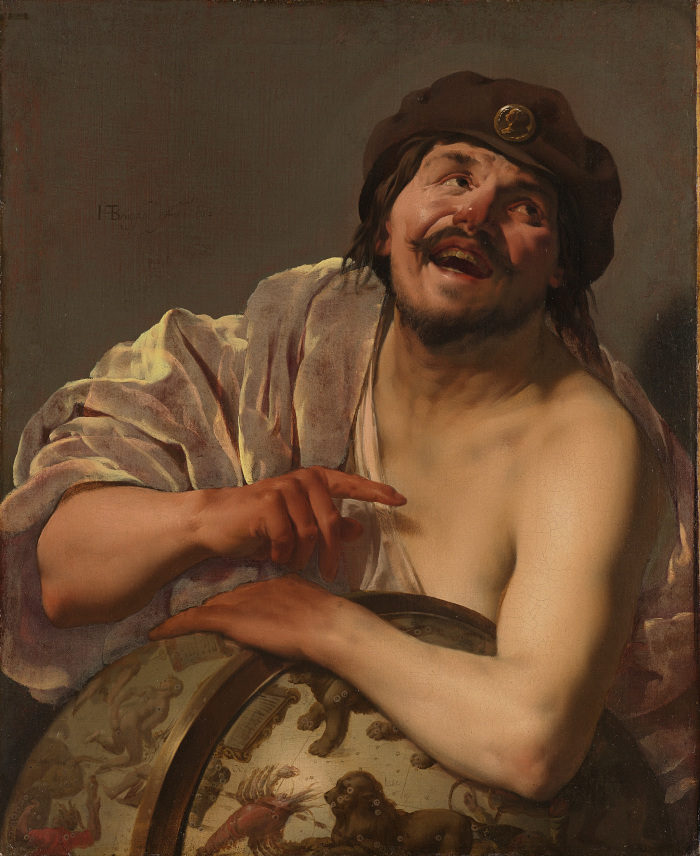
\includegraphics[keepaspectratio,width=0.7\textwidth]{figures/democritus-small.jpg}
  \captionart{Democritus}
  \label{fig:democritus}
\end{figure}
Democritus, as he is described by Hippocrates\authormarginnote{14}[-1\baselineskip] and Laertius\authormarginnote{15}, was
a little wearish old man, very melancholy by nature, averse from
company in his latter days, and much given to solitariness\authormarginnote{16}[-1\baselineskip], a
famous philosopher in his age, \lit{of the same age}{co\ae{}vus} with Socrates\authormarginnote{17}[0.6\baselineskip], wholly
addicted to his studies at the last, and to a private life: wrote many
excellent works, a great divine, according to the divinity of those
times, an expert physician, a politician, an excellent mathematician,
as Diacosmus\authormarginnote{18}[-1\baselineskip] and the rest of his works do witness. He was much
delighted with the studies of husbandry, saith Columella\authormarginnote{19}, and often
I find him cited by Constantinus\authormarginnote{20} and others treating of that
subject. He knew the natures, differences of all beasts, plants,
fishes, birds; and, as some say, could understand the tunes and
voices of them\authormarginnote{21}[-1.6\baselineskip]. In a word, he was \li{omnifariam doctus}, a general scholar,
a great student; and to the intent he might better contemplate, I
find it related by some\authormarginnote{22}[-1\baselineskip], that he put out his eyes, and was in his old
age voluntarily blind, yet saw more than all Greece besides, and \authormarginnote{23}
writ of every subject, \li{Nihil in toto opificio natur\ae{}, de quo non
scripsit}\authorlatintrans{24}. A man of an excellent wit, profound conceit; and to
attain knowledge the better in his younger years, he travelled to Egypt
and Athens\authormarginnote{25}[2.6\baselineskip], to confer with learned men, admired of some\authormarginnote{26}[3\baselineskip],
despised of others. After a wandering life, he settled at Abdera, a
town in Thrace, and was sent for thither to be their lawmaker,
recorder, or town-clerk, as some will; or as others, he was there bred
and born. Howsoever it was, there he lived at last in a garden in the
suburbs, wholly betaking himself to his studies and a private life,
saving that sometimes he would walk down to the haven\authormarginnote{27}[-\baselineskip], and
laugh heartily at such variety of ridiculous objects, which there he
saw\authormarginnote{28}. Such a one was Democritus.

But in the mean time, how doth this concern me, or upon what reference
do I usurp his habit? I confess, indeed, that to compare myself unto
him for aught I have yet said, were both impudency and arrogancy. I do
not presume to make any parallel, \lit{he is immeasurably ahead of me}{Antistat mihi millibus trecentis}, \authormarginnote{29}\lit{I am insignificant, a nobody with little ambition and small prospects}{parvus sum, nullus sum, altum nec spiro, nec spero}. Yet thus much I
will say of myself, and that I hope without all suspicion of pride, or
self-conceit, I have lived a silent, sedentary, solitary, private life,
\lit{for myself and my studies}{mihi et musis} in the University, as long almost as Xenocrates in
Athens, \lit{practically to old age}{ad senectam fere} to learn wisdom as he did, penned up most part
in my study. For I have been brought up a student in the most
flourishing college of Europe,\authormarginnote{30} \li{augustissimo collegio}, and can brag
with Jovius\authormarginnote{31}, almost, \lit{for 37 years I have made good use of my opportunities for study in the world renowned library of the Vatican}{in ea luce domicilii Vaticani, totius orbis celeberrimi, per 37 annos multa opportunaque didici}; for thirty years I
have continued (having the use of as good libraries as ever he had\authormarginnote{32})
a scholar, and would be therefore loath, either by living as a drone,
to be an unprofitable or unworthy member of so learned and noble a
society, or to write that which should be any way dishonourable to such
a royal and ample foundation. Something I have done, though by my
profession a divine, yet \li{turbine raptus ingenii}, as he\authormarginnote{33} said, out of
a running wit, an unconstant, unsettled mind, I had a great desire (not
able to attain to a superficial skill in any) to have some smattering
in all, to be \li{aliquis in omnibus, nullus in singulis}\authorlatintrans{34}, which
Plato commends\authormarginnote{35}[-\baselineskip], out of him Lipsius approves and furthers\authormarginnote{36}[-\baselineskip], as
fit to be imprinted in all curious wits, not to be a slave of one
science, or dwell altogether in one subject, as most do, but to rove
abroad, \lit{one who can turn his hand to anything}{centum puer artium}, to have an oar in every man's boat, to 
taste of every dish, and sip of every cup\authormarginnote{37}[-0.6\baselineskip], which, saith Montaigne\authormarginnote{38}[2\baselineskip],
was well performed by Aristotle, and his learned countryman Adrian
Turnebus. This roving humour (though not with like success) I have ever
had, and like a ranging spaniel, that barks at every bird he sees,
leaving his game, I have followed all, saving that which I should, and
may justly complain, and truly, \li{qui ubique est, nusquam est}\authorlatintrans{39}, which
Gesner did in modesty\authormarginnote{40}[1\baselineskip], that I have read many books, but to little
purpose, for want of good method; I have confusedly tumbled over diverse
authors in our libraries, with small profit, for want of art, order,
memory, judgment. I never travelled but in map or card, in which mine
unconfined thoughts have freely expatiated, as having ever been
especially delighted with the study of Cosmography. \authormarginnote{41}Saturn was lord
of my geniture, culminating, \etc, and Mars principal significator of
manners, in partile conjunction with my ascendant; both fortunate in
their houses, \etc. I am not poor, I am not rich; \li{nihil est, nihil deest},
I have little, I want nothing: all my treasure is in Minerva's tower.

Greater preferment as I could never get, so am I not in debt for it, I
have a competence (\lit{praise God}{laus Deo}) from my noble and munificent patrons,
though I live still a collegiate student, as Democritus in his garden,
and lead a monastic life, \lit{sufficient entertainment to myself}{ipse mihi theatrum}, sequestered from those
tumults and troubles of the world, \li{et tanquam in specula positus},
(as he said\authormarginnote{42}) in some high place above you all, like \lit{the stoic surveying with one sweep all ages down to the present}{Stoicus
Sapiens, omnia s\ae{}cula, pr\ae{}terita presentiaque videns, uno velut
intuitu}, I hear and see what is done abroad, how others \authormarginnote{43}run, ride,
turmoil, and macerate themselves in court and country, far from those
wrangling lawsuits, \lit{I laugh to myself at the vanities of the court, the intrigues of public life}{aul\ae{}\ vanitatem, fori ambitionem, ridere mecum soleo}: I laugh at all, \authormarginnote{44}only secure, lest my suit go amiss, my ships
perish, corn and cattle miscarry, trade decay, I have no wife nor
children good or bad to provide for. A mere spectator of other men's
fortunes and adventures, and how they act their parts, which methinks
are diversely presented unto me, as from a common theatre or scene. I
hear new news every day, and those ordinary rumours of war, plagues,
fires, inundations, thefts, murders, massacres, meteors, comets,
spectrums, prodigies, apparitions, of towns taken, cities besieged in
France, Germany, Turkey, Persia, Poland, \etc, daily musters and
preparations, and such like, which these tempestuous times afford,
battles fought, so many men slain, monomachies, shipwrecks, piracies
and sea-fights; peace, leagues, stratagems, and fresh alarms. A vast
confusion of vows, wishes, actions, edicts, petitions, lawsuits, pleas,
laws, proclamations, complaints, grievances are daily brought to our
ears. New books every day, pamphlets, corantoes, stories, whole
catalogues of volumes of all sorts, new paradoxes, opinions, schisms,
heresies, controversies in philosophy, religion, \etc. Now come tidings
of weddings, maskings, mummeries, entertainments, jubilees, embassies,
tilts and tournaments, trophies, triumphs, revels, sports, plays: then
again, as in a new shifted scene, treasons, cheating tricks, robberies,
enormous villainies in all kinds, funerals, burials, deaths of princes,
new discoveries, expeditions, now comical, then tragical matters. Today
we hear of new lords and officers created, tomorrow of some great men
deposed, and then again of fresh honours conferred; one is let loose,
another imprisoned; one purchaseth, another breaketh: he thrives, his
neighbour turns bankrupt; now plenty, then again dearth and famine; one
runs, another rides, wrangles, laughs, weeps, \etc. This I daily hear,
and such like, both private and public news, amidst the gallantry and
misery of the world; jollity, pride, perplexities and cares, simplicity
and villainy; subtlety, knavery, candour and integrity, mutually mixed
and offering themselves; I rub on \lit{in complete privacy}{privus privatus}; as I have still
lived, so I now continue, \li{statu quo prius}, left to a solitary life, and
mine own domestic discontents: saving that sometimes, \lit{not to conceal anything}{ne quid mentiar},
as Diogenes went into the city, and Democritus to the haven to see
fashions, I did for my recreation now and then walk abroad, look into
the world, and could not choose but make some little observation, \li{non
tam sagax observator ac simplex recitator}\authorlatintrans{45}, not as they did, to
scoff or laugh at all, but with a mixed passion.
%
\begin{verse}
\textlatin{Bilem s\ae{}pe, jocum vestri movere tumultus}.\authormarginnote{46}
\end{verse}
\translationrule
\begin{verse}
Ye wretched mimics, whose fond heats have been,\\*
How oft! the objects of my mirth and spleen.
\end{verse}
%
I did sometime laugh and scoff with Lucian, and satirically tax with
Menippus, lament with Heraclitus, sometimes again I was \li{petulanti
splene cachinno}\authorlatintrans{47.5}\authormarginnote{47}, and then again, \li{urere bilis jecur}\authormarginnote{48}, I was much
moved to see that abuse which I could not mend. In which passion
howsoever I may sympathise with him or them, 'tis for no such respect I
shroud myself under his name; but either in an unknown habit to assume
a little more liberty and freedom of speech, or if you will needs know,
for that reason and only respect which Hippocrates relates at large in
his Epistle to Damegetus, wherein he doth express, how coming to visit
him one day, he found Democritus in his garden at Abdera, in the
suburbs, under a shady bower\authormarginnote{49}, with a book on his knees\authormarginnote{50}[4.2\baselineskip], busy at
his study, sometimes writing, sometimes walking. The subject of his
book was melancholy and madness; about him lay the carcases of many
several beasts, newly by him cut up and anatomised; not that he did
contemn God's creatures, as he told Hippocrates, but to find out the
seat of this \li{atra bilis}, or melancholy, whence it proceeds, and how it
was engendered in men's bodies, to the intent he might better cure it
in himself, and by his writings and observation teach others how to
prevent and avoid it\authormarginnote{51}. Which good intent of his, Hippocrates highly
commended: Democritus Junior is therefore bold to imitate, and because
he left it imperfect, and it is now lost, \li{quasi succenturiator
Democriti}, to revive again, prosecute, and finish in this treatise.

You have had a reason of the name. If the title and inscription offend
your gravity, were it a sufficient justification to accuse others, I
could produce many sober treatises, even sermons themselves, which in
their fronts carry more fantastical names. Howsoever, it is a kind of
policy in these days, to prefix a fantastical title to a book which is
to be sold; for, as larks come down to a day-net, many vain readers
will tarry and stand gazing like silly passengers at an antic picture
in a painter's shop, that will not look at a judicious piece. And,
indeed, as Scaliger observes\authormarginnote{52}[-2\baselineskip], nothing more invites a reader than an
argument unlooked for, unthought of, and sells better than a scurrile
pamphlet, \li{tum maxime cum novitas excitat palatum}\authormarginnote{53}. Many men, saith
Gellius, are very conceited in their inscriptions, and able (as
Pliny quotes out of Seneca\authormarginnote{54}) to make him loiter by the way that went
in haste to fetch a midwife for his daughter, now ready to lie down.

For my part, I have honourable precedents for this which I have
done\authormarginnote{55}: I will cite one for all, Anthony Zara, Pap. Epis., his Anatomy of
Wit, in four sections, members, subsections, \etc, to be read in our
libraries.

If any man except against the matter or manner of treating of this my
subject, and will demand a reason of it, I can allege more than one; I
write of melancholy, by being busy to avoid melancholy.\phantomsection\label{mention:being-busy} There is no
greater cause of melancholy than idleness, \blockquote{no better cure than business}, as Rhasis holds\authormarginnote{56}: and howbeit,
\li{stultus labor est ineptiarum}, to be busy in toys is to small purpose, yet hear that
divine Seneca, \li{aliud agere quam nihil}, better do to no end, than
nothing. I wrote therefore, and busied myself in this playing labour,
\lit{to escape the ennui of idleness by a leisurely kind of employment}{otiosaque diligentia ut vitarem torporem feriandi} with Vectius in
Macrobius, \lit{and so turn leisure to good account}{atque otium in utile verterem negatium}.
%
\begin{verse}
Simul et jucunda et idonea dicere vita,\\*
Lectorem delectando simul atque monendo\authormarginnote{57}.
\end{verse}
\translationrule
\begin{verse}
Poets would profit or delight mankind,\\*
And with the pleasing have th' instructive joined.\\*
Profit and pleasure, then, to mix with art,\\*
T' inform the judgment, nor offend the heart,\\*
Shall gain all votes.
\end{verse}
%
To this end I write, like them, saith Lucian, that recite to trees, and
declaim to pillars for want of auditors: as Paulus \AE{}gineta
ingenuously confesseth\authormarginnote{58}, not that anything was unknown or omitted, but
to exercise myself, which course if some took, I think it would be good
for their bodies, and much better for their souls; or peradventure as
others do, for fame, to show myself (\li{Scire tuum nihil est, nisi te
scire hoc sciat alter}). I might be of Thucydides' opinion, to know
a thing and not to express it, is all one as if he knew it not\authormarginnote{59}. When I
first took this task in hand, \li{et quod ait ille, impellents genio
negotium suscepi}\authormarginnote{60}, this I aimed at; \li{vel ut lenirem animum scribendo}\authormarginnote{61}[\baselineskip],
to ease my mind by writing; for I had \li{gravidum cor, foetum caput}, a
kind of imposthume in my head, which I was very desirous to be unladen
of, and could imagine no fitter evacuation than this. Besides, I might
not well refrain, for \li{ubi dolor, ibi digitus}, one must needs scratch
where it itches. I was not a little offended with this malady, shall I
say my mistress Melancholy, my \AE{}geria, or my \li{malus genius}? and for
that cause, as he that is stung with a scorpion, I would expel \li{clavum
clavo}, comfort one sorrow with another\authormarginnote{62}, idleness with idleness, \li{ut
ex vipera Theriacum}, make an antidote out of that which was the prime
cause of my disease. Or as he did, of whom Felix Plater speaks\authormarginnote{63},
that thought he had some of Aristophanes' frogs in his belly, still
crying Breec, okex, coax, coax, oop, oop, and for that cause studied
physic seven years, and travelled over most part of Europe to ease
himself. To do myself good I turned over such physicians as our
libraries would afford, or my private friends impart\authormarginnote{64}, and have
taken this pains. And why not? Cardan professeth he wrote his book, De
Consolatione after his son's death, to comfort himself; so did Tully
write of the same subject with like intent after his daughter's
departure, if it be his at least, or some impostor's put out in his
name, which Lipsius probably suspects. Concerning myself, I can
peradventure affirm with Marius in Sallust, that which others hear
or read of\authormarginnote{65}, I felt and practised myself; they get their knowledge by
books, I mine by melancholising. \li{Experto crede Roberto}. Something I can
speak out of experience, \li{\ae{}rumnabilis experientia me docuit}; and with
her in the poet, \li{Haud ignara mali miseris succurrere disco}\authorlatintrans{66.5}\authormarginnote{66}[-0.6\baselineskip]; I would
help others out of a fellow-feeling; and, as that virtuous lady did of
old, being a leper herself\authormarginnote{67}[\baselineskip], bestow all her portion to build an
hospital for lepers, I will spend my time and knowledge, which are my
greatest fortunes, for the common good of all.

Yea, but you will infer that this is \li{actum agere}\authormarginnote{68}, an unnecessary
work, \li{cramben bis coctam apponnere}, the same again and again in other
words. To what purpose? Nothing is omitted that may well be said\authormarginnote{69},
so thought Lucian in the like theme. How many excellent physicians have
written just volumes and elaborate tracts of this subject? No news
here; that which I have is stolen, from others, \li{Dicitque mihi mea
pagina fur es}\authormarginnote{70}. If that severe doom of Synesius be true\authormarginnote{71}[\baselineskip], it is a
greater offence to steal dead men's labours, than their clothes, what
shall become of most writers? I hold up my hand at the bar among
others, and am guilty of felony in this kind, \li{habes confitentem reum}, I
am content to be pressed with the rest. 'Tis most true, \li{tenet
insanabile multos scribendi cacoethes}, and \authormarginnote{72}there is no end of
writing of books, as the wiseman found of old, in this \authormarginnote{73}scribbling
age, especially wherein \authormarginnote{74}[\baselineskip]the number of books is without number, (as
a worthy man saith) presses be oppressed, and out of an itching humour
that every man hath to show himself, \authormarginnote{75}[\baselineskip]desirous of fame and honour
(\li{scribimus indocti doctique}) he will write no matter what, and scrape
together it boots not whence. \authormarginnote{76}[\baselineskip]Bewitched with this desire of fame,
\li{etiam mediis in morbis}, to the disparagement of their health, and
scarce able to hold a pen, they must say something, \authormarginnote{77}[\baselineskip]and get
themselves a name, saith Scaliger, though it be to the downfall and
ruin of many others. To be counted writers, \li{scriptores ut salutentur},
to be thought and held polymaths and polyhistors, \li{apud imperitum vulgus
ob ventos\ae{}\ nomen artis}, to get a paper-kingdom: \li{nulla spe qu\ae{}stus sed
ampla fam\ae{}}, in this precipitate, ambitious age, \li{nunc ut est s\ae{}culum,
inter immaturam eruditionem, ambitiosum et pr\ae{}ceps} ('tis
\authormarginnote{78}Scaliger's censure); and they that are scarce auditors, \li{vix
auditores}, must be masters and teachers, before they be capable and fit
hearers. They will rush into all learning, \li{togatam armatam}, divine,
human authors, rake over all indexes and pamphlets for notes, as our
merchants do strange havens for traffic, write great tomes, \li{Cum non
sint re vera doctiores, sed loquaciores}, whereas they are not thereby
better scholars, but greater praters. They commonly pretend public
good, but as \authormarginnote{79}Gesner observes, 'tis pride and vanity that eggs them
on; no news or aught worthy of note, but the same in other terms. \li{Ne
feriarentur fortasse typographi vel ideo scribendum est aliquid ut se
vixisse testentur}. As apothecaries we make new mixtures everyday, pour
out of one vessel into another; and as those old Romans robbed all the
cities of the world, to set out their bad-sited Rome, we skim off the
cream of other men's wits, pick the choice flowers of their tilled
gardens to set out our own sterile plots. \li{Castrant alios ut libros suos
per se graciles alieno adipe suffarciant} (so \authormarginnote{80}Jovius inveighs.) They
lard their lean books with the fat of others' works. \li{Ineruditi fures},
\etc. A fault that every writer finds, as I do now, and yet faulty
themselves, \authormarginnote{81}\li{Trium literarum homines}, all thieves; they pilfer out
of old writers to stuff up their new comments, scrape Ennius'
dunghills, and out of \authormarginnote{82}Democritus' pit, as I have done. By which
means it comes to pass, \authormarginnote{83}that not only libraries and shops are full
of our putrid papers, but every close-stool and jakes, \li{Scribunt carmina
qu\ae{}\ legunt cacantes}; they serve to put under pies, to \authormarginnote{84}[-1\baselineskip]lap spice
in, and keep roast meat from burning. With us in France, saith
\authormarginnote{85}[-\baselineskip]Scaliger, every man hath liberty to write, but few ability.
\authormarginnote{86}Heretofore learning was graced by judicious scholars, but now noble
sciences are vilified by base and illiterate scribblers, that either
write for vainglory, need, to get money, or as Parasites to flatter and
collogue with some great men, they put cut \authormarginnote{87}\li{burras, quisquiliasque
ineptiasque}. \authormarginnote{88}Amongst so many thousand authors you shall scarce find
one, by reading of whom you shall be any whit better, but rather much
worse, \li{quibus inficitur potius, quam perficitur}, by which he is rather
infected than any way perfected.
---\li{Qui talia legit, Quid didicit tandem, quid scit nisi somnia, nugas?}\authorlatintrans{89.5}\authormarginnote{89}

So that oftentimes it falls out (which Callimachus taxed of old) a
great book is a great mischief. \authormarginnote{90}Cardan finds fault with Frenchmen
and Germans, for their scribbling to no purpose, \li{non inquit ab edendo
deterreo, modo novum aliquid inveniant}, he doth not bar them to write,
so that it be some new invention of their own; but we weave the same
web still, twist the same rope again and again; or if it be a new
invention, 'tis but some bauble or toy which idle fellows write, for as
idle fellows to read, and who so cannot invent? \authormarginnote{91}He must have a
barren wit, that in this scribbling age can forge nothing. \authormarginnote{92}Princes
show their armies, rich men vaunt their buildings, soldiers their
manhood, and scholars vent their toys; they must read, they must hear
whether they will or no.
%
\begin{verse}
\textlatin{Et quodcunque semel chartis illeverit, omnes}\\*
\textlatin{Gestiet a furno redeuntes scire lacuque,}\\*
\textlatin{Et pueros et anus}---\authormarginnote{93}
\end{verse}\nopagebreak
\translationrule
\begin{verse}
What once is said and writ, all men must know,\\*
Old wives and children as they come and go.
\end{verse}
%
What a company of poets hath this year brought out, as Pliny complains
to Sossius Sinesius. \authormarginnote{94}This April every day some or other have
recited. What a catalogue of new books all this year, all this age (I
say), have our Frankfort Marts, our domestic Marts brought out? Twice a
year, \authormarginnote{95} \li{Proferunt se nova ingenia et ostentant}, we stretch our wits
out, and set them to sale, magno conatu nihil agimus. So that which
\authormarginnote{96}[-\baselineskip]Gesner much desires, if a speedy reformation be not had, by some
prince's edicts and grave supervisors, to restrain this liberty, it
will run on in infinitum. \li{Quis tam avidus librorum helluo}, who can read
them? As already, we shall have a vast chaos and confusion of books, we
are \authormarginnote{97}oppressed with them, \authormarginnote{98}[2\baselineskip]our eyes ache with reading, our
fingers with turning. For my part I am one of the number, \li{nos numerus
sumus}, (we are mere ciphers): I do not deny it, I have only this of
Macrobius to say for myself, \li{Omne meum, nihil meum}, 'tis all mine, and
none mine. As a good housewife out of diverse fleeces weaves one piece
of cloth, a bee gathers wax and honey out of many flowers, and makes a
new bundle of all, \li{Floriferis ut apes in saltibus omnia libant}, I have
laboriously \authormarginnote{99}collected this cento out of diverse writers, and that
\li{sine injuria}, I have wronged no authors, but given every man his own;
which \authormarginnote{100}[3\baselineskip]Hierom so much commends in Nepotian; he stole not whole
verses, pages, tracts, as some do nowadays, concealing their authors'
names, but still said this was Cyprian's, that Lactantius, that
Hilarius, so said Minutius Felix, so Victorinus, thus far Arnobius: I
cite and quote mine authors (which, howsoever some illiterate
scribblers account pedantical, as a cloak of ignorance, and opposite to
their affected fine style, I must and will use) \li{sumpsi, non suripui};
and what Varro, lib. 6. de re rust. speaks of bees, \li{minime malefic\ae{}
nullius opus vellicantes faciunt delerius}, I can say of myself, Whom
have I injured? The matter is theirs most part, and yet mine, \li{apparet
unde sumptum sit} (which Seneca approves), \li{aliud tamen quam unde sumptum
sit apparet}, which nature doth with the aliment of our bodies
incorporate, digest, assimilate, I do \li{concoquere quod hausi}, dispose of
what I take. I make them pay tribute, to set out this my Maceronicon,
the method only is mine own, I must usurp that of \authormarginnote{101}Wecker e Ter.
\li{nihil dictum quod non dictum prius, methodus sola artificem ostendit},
we can say nothing but what hath been said, the composition and method
is ours only, and shows a scholar. Oribasius, \AE{}sius, Avicenna, have
all out of Galen, but to their own method, \li{diverso stilo, non diversa
fide}. Our poets steal from Homer; he spews, saith \AE{}lian, they lick it
up. Divines use Austin's words verbatim still, and our story-dressers
do as much; he that comes last is commonly best,
%
\begin{verse}
---\textlatin{donec quid grandius \ae{}tas}\\
\textlatin{Postera sorsque ferat melior}.\authormarginnote{102}
\end{verse}
%
Though there were many giants of old in physic and philosophy, yet I
say with \authormarginnote{103}Didacus Stella, A dwarf standing on the shoulders of a
giant may see farther than a giant himself; I may likely add, alter,
and see farther than my predecessors; and it is no greater prejudice
for me to indite after others, than for \AE{}lianus Montaltus, that famous
physician, to write \li{de morbis capitis} after Jason Pratensis, Heurnius,
Hildesheim, \etc, many horses to run in a race, one logician, one
rhetorician, after another. Oppose then what thou wilt,
%
\begin{verse}
\textlatin{Allatres licet usque nos et usque}\\
\textlatin{Et gannitibus improbis lacessas.}\\
\end{verse}
%
I solve it thus. And for those other faults of barbarism, \authormarginnote{104}Doric
dialect, extemporanean style, tautologies, apish imitation, a rhapsody
of rags gathered together from several dunghills, excrements of
authors, toys and fopperies confusedly tumbled out, without art,
invention, judgment, wit, learning, harsh, raw, rude, fantastical,
absurd, insolent, indiscreet, ill-composed, indigested, vain, scurrile,
idle, dull, and dry; I confess all ('tis partly affected), thou canst
not think worse of me than I do of myself. 'Tis not worth the reading,
I yield it, I desire thee not to lose time in perusing so vain a
subject, I should be peradventure loath myself to read him or thee so
writing; 'tis not \li{oper\ae{}, pretium}. All I say is this, that I have
\authormarginnote{105}precedents for it, which Isocrates calls \li{perfugium iis qui
peccant}, others as absurd, vain, idle, illiterate, \etc. \li{Nonnulli alii
idem fecerunt}; others have done as much, it may be more, and perhaps
thou thyself, \li{Novimus et qui te, \etc.} We have all our faults; \li{scimus, et
hanc, veniaim, \etc}; \authormarginnote{106}thou censurest me, so have I done others, and
may do thee, \li{C\ae{}dimus inque vicem}, \etc, 'tis \li{lex talionis}, \li{quid pro quo}.

Go now, censure, criticise, scoff, and rail.
\authormarginnote{107}\li{Nasutus cis usque licet, sis denique nasus:
Non potes in nugas dicere plura meas,
Ipse ego quam dixi, \etc.}

Wert thou all scoffs and flouts, a very Momus,
Than we ourselves, thou canst not say worse of us.

Thus, as when women scold, have I cried whore first, and in some men's
censures I am afraid I have overshot myself, \li{Laudare se vani,
vituperare stulti}, as I do not arrogate, I will not derogate. \li{Primus
vestrum non sum, nec imus}, I am none of the best, I am none of the
meanest of you. As I am an inch, or so many feet, so many parasangs,
after him or him, I may be peradventure an ace before thee. Be it
therefore as it is, well or ill, I have essayed, put myself upon the
stage; I must abide the censure, I may not escape it. It is most true,
\li{stylus virum arguit}, our style bewrays us, and as \authormarginnote{108}hunters find
their game by the trace, so is a man's genius descried by his works,
\li{Multo melius ex sermone quam lineamentis, de moribus hominum judicamus};
it was old Cato's rule. I have laid myself open (I know it) in this
treatise, turned mine inside outward: I shall be censured, I doubt not;
for, to say truth with Erasmus, \li{nihil morosius hominum judiciis}, there
is nought so peevish as men's judgments; yet this is some comfort, \li{ut
palata, sic judicia}, our censures are as various as our palates.
%
\begin{verse}
\textlatin{Tres mihi conviv\ae{}\ prope dissentire videntur},\\*
\textlatin{Poscentes vario multum diversa palato, \etc.}\authormarginnote{109}
\end{verse}
\translationrule
\begin{verse}
Three guests I have, dissenting at my feast,\\*
Requiring each to gratify his taste\\*
With different food.
\end{verse}
%
Our writings are as so many dishes, our readers guests, our books like
beauty, that which one admires another rejects; so are we approved as
men's fancies are inclined. \li{Pro captu lectoris habent sua fata
libelli.}. That which is most pleasing to one is \li{amaracum sui}, most
harsh to another. \li{Quot homines, tot sententi\ae{}}, so many men, so many
minds: that which thou condemnest he commends. \authormarginnote{110}\li{Quod petis, id sane
est invisum acidumque duobus}. He respects matter, thou art wholly for
words; he loves a loose and free style, thou art all for neat
composition, strong lines, hyperboles, allegories; he desires a fine
frontispiece, enticing pictures, such as Hieron\authormarginnote{111}. Natali the Jesuit
hath cut to the Dominicals, to draw on the reader's attention, which
thou rejectest; that which one admires, another explodes as most absurd
and ridiculous. If it be not point blank to his humour, his method, his
conceit, \authormarginnote{112}\li{si quid, forsan omissum, quod is animo conceperit, si
qu\ae{}\ dictio}, \etc. If aught be omitted, or added, which he likes, or
dislikes, thou art \li{mancipium pauc\ae{}\ lectionis}, an idiot, an ass, \li{nullus
es}, or plagiarius, a trifler, a trivant, thou art an idle fellow; or
else it is a thing of mere industry, a collection without wit or
invention, a very toy. \authormarginnote{113}\li{Facilia sic putant omnes qu\ae{}\ jam facta,
nec de salebris cogitant, ubi via strata}; so men are valued, their
labours vilified by fellows of no worth themselves, as things of
nought, who could not have done as much. \li{Unusquisque abundat sensu suo},
every man abounds in his own sense; and whilst each particular party is
so affected, how should one please all?
%
\begin{verse}
\textlatin{Quid dem?}\authormarginnote{114}\\*
\textlatin{quid non dem? Renuis tu quod jubet ille.}
\end{verse}
\translationrule
\begin{verse}
---What courses must I choose?\\*
What not? What both would order you refuse.
\end{verse}
%
How shall I hope to express myself to each man's humour and
\authormarginnote{115}conceit, or to give satisfaction to all? Some understand too
little, some too much, \li{qui similiter in legendos libros, atque in
salutandos homines irruunt, non cogitantes quales, sed quibus vestibus
induti sint}, as Austin observes\authormarginnote{116}, not regarding what, but who
write, \li{orexin habet auctores celebritas}\authormarginnote{117}[\baselineskip], not valuing the metal,
but stamp that is upon it, \li{Cantharum aspiciunt, non quid in eo}. If he
be not rich, in great place, polite and brave, a great doctor, or full
fraught with grand titles, though never so well qualified, he is a
dunce; but, as \authormarginnote{118}Baronius hath it of Cardinal Caraffa's works, he is
a mere hog that rejects any man for his poverty. Some are too partial,
as friends to overween, others come with a prejudice to carp, vilify,
detract, and scoff; (\li{qui de me forsan, quicquid est, omni contemptu
contemptius judicant}) some as bees for honey, some as spiders to gather
poison. What shall I do in this case? As a Dutch host, if you come to
an inn in. Germany, and dislike your fare, diet, lodging, \etc, replies
in a surly tone, \authormarginnote{119}\li{aliud tibi qu\ae{}ras diversorium}, if you like not
this, get you to another inn: I resolve, if you like not my writing, go
read something else. I do not much esteem thy censure, take thy course,
it is not as thou wilt, nor as I will, but when we have both done, that
of \authormarginnote{120}Plinius Secundus to Trajan will prove true, Every man's witty
labour takes not, except the matter, subject, occasion, and some
commending favourite happen to it. If I be taxed, exploded by thee and
some such, I shall haply be approved and commended by others, and so
have been (\li{Expertus loquor}), and may truly say with \authormarginnote{121}Jovius in like
case, (\li{absit verbo jactantia}) \li{heroum quorundam, pontificum, et virorum
nobilium familiaritatem et amicitiam, gratasque gratias, et multorum bene laudatorum laudes sum inde promeritus}\authormarginnote{122}, as I have been
honoured by some worthy men, so have I been vilified by others, and
shall be. At the first publishing of this book, (which \authormarginnote{123}Probus of
Persius satires), \li{editum librum continuo mirari homines, atque avide
deripere c\ae{}perunt}, I may in some sort apply to this my work. The
first, second, and third edition were suddenly gone, eagerly read, and,
as I have said, not so much approved by some, as scornfully rejected by
others. But it was Democritus his fortune, \li{Idem admirationi et
irrisioni habitus}\authormarginnote{124}. 'Twas Seneca's fate, that superintendent of
wit, learning, judgment, \authormarginnote{125}\li{ad stuporem doctus}, the best of Greek and
Latin writers, in Plutarch's opinion; that renowned corrector of vice,
as, \authormarginnote{126}Fabius terms him, and painful omniscious philosopher, that
writ so excellently and admirably well, could not please all parties,
or escape censure. How is he vilified by Caligula\authormarginnote{127}[2\baselineskip], Agellius,
Fabius, and Lipsius himself, his chief propugner? \li{In eo pleraque
pernitiosa}, saith the same Fabius, many childish tracts and sentences
he hath, \li{sermo illaboratus}, too negligent often and remiss, as Agellius
observes, \li{oratio vulgaris et protrita, dicaces et inept\ae{}, sententi\ae{},
eruditio plebeia}, an homely shallow writer as he is. \li{In partibus spinas
et fastidia habet}, saith Lipsius\authormarginnote{128}; and, as in all his other works,
so especially in his epistles, \li{ali\ae{}\ in argutiis et ineptiis
occupantur, intricatus alicubi, et parum compositus, sine copia rerum
hoc fecit}, he jumbles up many things together immethodically, after the
Stoics' fashion, \li{parum ordinavit, multa accumulavit, \etc.} If Seneca be
thus lashed, and many famous men that I could name, what shall I
expect? How shall I that am vix umbra tanti philosophi hope to please?
No man so absolute (Erasmus holds\authormarginnote{129}[-2\baselineskip]) to satisfy all, except
antiquity, prescription, \etc, set a bar. But as I have proved in
Seneca, this will not always take place, how shall I evade? 'Tis the
common doom of all writers, I must (I say) abide it; I seek not
applause; \authormarginnote{130}\li{Non ego ventosa venor suffragia plebis; again, non sum
adeo informis,} I would not be \authormarginnote{131}vilified:
%
\begin{verse}
\textlatin{---laudatus abunde},\\*
\textlatin{Non fastiditus si tibi, lector, ero.}\authormarginnote{132}
\end{verse}
%
I fear good men's censures, and to their favourable acceptance I submit
my labours,
%
\begin{verse}
\textlatin{---et linguas mancipiorum}\\*
\textlatin{Contemno.}---\authormarginnote{133}
\end{verse}
%
As the barking of a dog, I securely contemn those malicious and
scurrile obloquies, flouts, calumnies of railers and detractors; I
scorn the rest. What therefore I have said, pro tenuitate mea, I have
said.

One or two things yet I was desirous to have amended if I could,
concerning the manner of handling this my subject, for which I must
apologise, deprecari, and upon better advice give the friendly reader
notice: it was not mine intent to prostitute my muse in English, or to
divulge secreta Minerv\ae{}, but to have exposed this more contract in
Latin, if I could have got it printed. Any scurrile pamphlet is welcome
to our mercenary stationers in English; they print all
%
\begin{verse}
---\textlatin{cuduntque libellos}\\*
\textlatin{In quorum foliis vix simia nuda cacaret};
\end{verse}
%
But in Latin they will not deal; which is one of the reasons
\authormarginnote{134}Nicholas Car, in his oration of the paucity of English writers,
gives, that so many flourishing wits are smothered in oblivion, lie
dead and buried in this our nation. Another main fault is, that I have
not revised the copy, and amended the style, which now flows remissly,
as it was first conceived; but my leisure would not permit; Feci nec
quod potui, nec quod volui, I confess it is neither as I would, nor as
it should be.
%
\begin{verse}
\textlatin{Cum relego scripsisse pudet, quia plurima cerno}\\*
\textlatin{Me quoque qu\ae{}\ fuerant judice digna lini.}\authormarginnote{135}
\end{verse}
\translationrule
\begin{verse}
When I peruse this tract which I have writ,\\*
I am abash'd, and much I hold unfit.
\end{verse}
%
\li{Et quod gravissimum}, in the matter itself, many things I disallow at
this present, which when I writ, \authormarginnote{136}\li{Non eadem est \ae{}tas, non mens}; I
would willingly retract much, \etc, but 'tis too late, I can only crave
pardon now for what is amiss. I might indeed, (had I wisely done)
observed that precept of the poet, ---nonumque prematur in annum, and
have taken more care: or, as Alexander the physician would have done by
lapis lazuli, fifty times washed before it be used, I should have
revised, corrected and amended this tract; but I had not (as I said)
that happy leisure, no amanuenses or assistants. Pancrates in
\authormarginnote{137}Lucian, wanting a servant as he went from Memphis to Coptus in
Egypt, took a door bar, and after some superstitious words pronounced
(Eucrates the relator was then present) made it stand up like a
serving-man, fetch him water, turn the spit, serve in supper, and what
work he would besides; and when he had done that service he desired,
turned his man to a stick again. I have no such skill to make new men
at my pleasure, or means to hire them; no whistle to call like the
master of a ship, and bid them run, \etc. I have no such authority, no
such benefactors, as that noble \authormarginnote{138}Ambrosius was to Origen, allowing
him six or seven amanuenses to write out his dictates; I must for that
cause do my business myself, and was therefore enforced, as a bear doth
her whelps, to bring forth this confused lump; I had not time to lick
it into form, as she doth her young ones, but even so to publish it, as
it was first written quicquid in buccam venit, in an extemporean style,
as \authormarginnote{139}I do commonly all other exercises, effudi quicquid dictavit
genius meus, out of a confused company of notes, and writ with as small
deliberation as I do ordinarily speak, without all affectation of big
words, fustian phrases, jingling terms, tropes, strong lines, that like
\authormarginnote{140}Acesta's arrows caught fire as they flew, strains of wit, brave
heats, elegies, hyperbolical exornations, elegancies, \etc, which many
so much affect. I am \authormarginnote{141}aqu\ae{}\ potor, drink no wine at all, which so
much improves our modern wits, a loose, plain, rude writer, ficum, voco
ficum et ligonem ligonem and as free, as loose, idem calamo quod in
mente, \authormarginnote{142}I call a spade a spade, animis h\ae{}c scribo, non auribus, I
respect matter not words; remembering that of Cardan, verba propter
res, non res propter verba: and seeking with Seneca, quid scribam, non
quemadmodum, rather \emph{what} than \emph{how} to write: for as Philo thinks,
\authormarginnote{143}He that is conversant about matter, neglects words, and those that
excel in this art of speaking, have no profound learning,
%
\begin{verse}
\textlatin{Verba nitent phaleris, at nullus verba medullas}\\*
\textlatin{Intus habent}---\authorlatintrans{144.5}\authormarginnote{144}
\end{verse}
%
Besides, it was the observation of that wise Seneca, \authormarginnote{145}when you see
a fellow careful about his words, and neat in his speech, know this for
a certainty, that man's mind is busied about toys, there's no solidity
in him. Non est ornamentum virile concinnitas: as he said of a
nightingale, ---vox es, pr\ae{}terea nihil, \etc. I am therefore in this
point a professed disciple of \authormarginnote{146}Apollonius a scholar of Socrates, I
neglect phrases, and labour wholly to inform my reader's understanding,
not to please his ear; 'tis not my study or intent to compose neatly,
which an orator requires, but to express myself readily and plainly as
it happens. So that as a river runs sometimes precipitate and swift,
then dull and slow; now direct, then per ambages, now deep, then
shallow; now muddy, then clear; now broad, then narrow; doth my style
flow: now serious, then light; now comical, then satirical; now more
elaborate, then remiss, as the present subject required, or as at that
time I was affected. And if thou vouchsafe to read this treatise, it
shall seem no otherwise to thee, than the way to an ordinary traveller,
sometimes fair, sometimes foul; here champaign, there enclosed; barren,
in one place, better soil in another: by woods, groves, hills, dales,
plains, \etc. I shall lead thee per ardua montium, et lubrica valllum, et
roscida cespitum, et \authormarginnote{147}glebosa camporum, through variety of objects,
that which thou shalt like and surely dislike.

For the matter itself or method, if it be faulty, consider I pray you
that of Columella, Nihil perfectum, aut a singulari consummatum
industria, no man can observe all, much is defective no doubt, may be
justly taxed, altered, and avoided in Galen, Aristotle, those great
masters. Boni venatoris (\authormarginnote{148}one holds) plures feras capere, non
omnes; he is a good huntsman can catch some, not all: I have done my
endeavour. Besides, I dwell not in this study, Non hic sulcos ducimus,
non hoc pulvere desudamus, I am but a smatterer, I confess, a stranger,
\authormarginnote{149}here and there I pull a flower; I do easily grant, if a rigid
censurer should criticise on this which I have writ, he should not find
three sole faults, as Scaliger in Terence, but three hundred. So many
as he hath done in Cardan's subtleties, as many notable errors as
\authormarginnote{150}Gul Laurembergius, a late professor of Rostock, discovers in that
anatomy of Laurentius, or Barocius the Venetian in Sacro boscus. And
although this be a sixth edition, in which I should have been more
accurate, corrected all those former escapes, yet it was magni laboris
opus, so difficult and tedious, that as carpenters do find out of
experience, 'tis much better build a new sometimes, than repair an old
house; I could as soon write as much more, as alter that which is
written. If aught therefore be amiss (as I grant there is), I require a
friendly admonition, no bitter invective, \authormarginnote{151}Sint musis socii
Charites, Furia omnis abesto, otherwise, as in ordinary controversies,
funem contentionis nectamus, sed cui bono? We may contend, and likely
misuse each other, but to what purpose? We are both scholars, say,
%
\begin{verse}
--\textlatin{Arcades ambo}\\*
\textlatin{Et Cantare pares, et respondere parati.}\authormarginnote{152}
\end{verse}
\translationrule
\begin{verse}
Both young Arcadians, both alike inspir'd\\*
To sing and answer as the song requir'd.
\end{verse}
%
If we do wrangle, what shall we get by it? Trouble and wrong ourselves,
make sport to others. If I be convict of an error, I will yield, I will
amend. Si quid bonis moribus, si quid veritati dissentaneum, in sacris
vel humanis literis a me dictum sit, id nec dictum esto. In the mean
time I require a favourable censure of all faults omitted, harsh
compositions, pleonasms of words, tautological repetitions (though
Seneca bear me out, nunquam nimis dicitur, quod nunquam satis dicitur)
perturbations of tenses, numbers, printers' faults, \etc. My translations
are sometimes rather paraphrases than interpretations, non ad verbum,
but as an author, I use more liberty, and that's only taken which was
to my purpose. Quotations are often inserted in the text, which makes
the style more harsh, or in the margin, as it happened. Greek authors,
Plato, Plutarch, Athen\ae{}us, \etc, I have cited out of their
interpreters, because the original was not so ready. I have mingled
sacra prophanis, but I hope not profaned, and in repetition of authors'
names, ranked them per accidens, not according to chronology; sometimes
neoterics before ancients, as my memory suggested. Some things are here
altered, expunged in this sixth edition, others amended, much added,
because many good \authormarginnote{153}authors in all kinds are come to my hands since,
and 'tis no prejudice, no such indecorum, or oversight.
%
\settowidth{\versewidth}{Nunquam ita quicquam bene subducta ratione ad vitam fuit,}
\begin{verse}
\textlatin{Nunquam ita quicquam bene subducta ratione ad vitam fuit,\\*
Quin res, \ae{}tas, usus, semper aliquid apportent novi,\\*
Aliquid moneant, ut illa qu\ae{}\ scire te credas, nescias,\\*
Et qu\ae{}\ tibi putaris prima, in exercendo ut repudias.}\authormarginnote{154}
\end{verse}
\translationrule
\begin{verse}
Ne'er was ought yet at first contriv'd so fit,\\*
But use, age, or something would alter it;\\*
Advise thee better, and, upon peruse,\\*
Make thee not say, and what thou tak'st refuse.
\end{verse}
%
But I am now resolved never to put this treatise out again, Ne quid
nimis, I will not hereafter add, alter, or retract; I have done. The
last and greatest exception is, that I, being a divine, have meddled
with physic,
%
\begin{verse}
\textlatin{Tantumne est ab re tua otii tibi,}\\*
\textlatin{Aliena ut cures, eaque nihil qu\ae{}\ ad te attinent.}\authormarginnote{155}
\end{verse}
%
Which Menedemus objected to Chremes; have I so much leisure, or little
business of mine own, as to look after other men's matters which
concern me not? What have I to do with physic? \li{Quod medicorum est
promittant medici}. The Laced\ae{}monians were once in counsel about
state matters\authormarginnote{156}, a debauched fellow spake excellent well, and to the
purpose, his speech was generally approved: a grave senator steps up,
and by all means would have it repealed, though good, because
dehonestabatur pessimo auctore, it had no better an author; let some
good man relate the same, and then it should pass. This counsel was
embraced, factum est, and it was registered forthwith, \li{Et sic bona
sententia mansit, malus auctor mutatus est}. Thou sayest as much of me,
stomachosus as thou art, and grantest, peradventure, this which I have
written in physic, not to be amiss, had another done it, a professed
physician, or so, but why should I meddle with this tract? Hear me
speak. There be many other subjects, I do easily grant, both in
humanity and divinity, fit to be treated of, of which had I written ad
ostentationem only, to show myself, I should have rather chosen, and in
which I have been more conversant, I could have more willingly
luxuriated, and better satisfied myself and others; but that at this
time I was fatally driven upon this rock of melancholy, and carried
away by this by-stream, which, as a rillet, is deducted from the main
channel of my studies, in which I have pleased and busied myself at
idle hours, as a subject most necessary and commodious. Not that I
prefer it before divinity, which I do acknowledge to be the queen of
professions, and to which all the rest are as handmaids, but that in
divinity I saw no such great need. For had I written positively, there
be so many books in that kind, so many commentators, treatises,
pamphlets, expositions, sermons, that whole teams of oxen cannot draw
them; and had I been as forward and ambitious as some others, I might
have haply printed a sermon at Paul's Cross, a sermon in St. Marie's
Oxon, a sermon in Christ Church, or a sermon before the right
honourable, right reverend, a sermon before the right worshipful, a
sermon in Latin, in English, a sermon with a name, a sermon without, a
sermon, a sermon, \etc. But I have been ever as desirous to suppress my
labours in this kind, as others have been to press and publish theirs.

To have written in controversy had been to cut off an hydra's head,
\authormarginnote{157}Lis litem generat, one begets another, so many duplications,
triplications, and swarms of questions. In sacro bello hoc quod stili
mucrone agitur, that having once begun, I should never make an end. One
had much better, as \authormarginnote{158}Alexander, the sixth pope, long since
observed, provoke a great prince than a begging friar, a Jesuit, or a
seminary priest, I will add, for inexpugnabile genus hoc hominum, they
are an irrefragable society, they must and will have the last word; and
that with such eagerness, impudence, abominable lying, falsifying, and
bitterness in their questions they proceed, that as he \authormarginnote{159}said,
furorne c\ae{}cus, an rapit vis acrior, an culpa, responsum date? Blind
fury, or error, or rashness, or what it is that eggs them, I know not,
I am sure many times, which \authormarginnote{160}Austin perceived long since,
tempestate contentionis, serenitas charitatis obnubilatur, with this
tempest of contention, the serenity of charity is overclouded, and
there be too many spirits conjured up already in this kind in all
sciences, and more than we can tell how to lay, which do so furiously
rage, and keep such a racket, that as \authormarginnote{161}Fabius said, It had been
much better for some of them to have been born dumb, and altogether
illiterate, than so far to dote to their own destruction.
%
\begin{verse}
\textlatin{At melius fuerat non scribere, namque tacere}\\*
\textlatin{Tutum semper erit,}---\authorlatintrans{162}
\end{verse}
%
'Tis a general fault, so Severinus the Dane complains \authormarginnote{163}in physic,
unhappy men as we are, we spend our days in unprofitable questions and
disputations, intricate subtleties, de lana caprina about moonshine in
the water, leaving in the mean time those chiefest treasures of nature
untouched, wherein the best medicines for all manner of diseases are to
be found, and do not only neglect them ourselves, but hinder, condemn,
forbid, and scoff at others, that are willing to inquire after them.

These motives at this present have induced me to make choice of this
medicinal subject.

If any physician in the mean time shall infer, Ne sutor ultra crepidam,
and find himself grieved that I have intruded into his profession, I
will tell him in brief, I do not otherwise by them, than they do by us.

If it be for their advantage, I know many of their sect which have
taken orders, in hope of a benefice, 'tis a common transition, and why
may not a melancholy divine, that can get nothing but by simony,
profess physic? Drusianus an Italian (Crusianus, but corruptly,
Trithemius calls him) \authormarginnote{164}[-1\baselineskip]because he was not fortunate in his
practice, forsook his profession, and writ afterwards in divinity.

Marcilius Ficinus was semel et simul; a priest and a physician at once,
and \authormarginnote{165}T. Linacer in his old age took orders. The Jesuits profess
both at this time, diverse of them \li{permissu superiorum}, chirurgeons,
panders, bawds, and midwives, \etc. Many poor country-vicars, for want of
other means, are driven to their shifts; to turn mountebanks,
quacksalvers, empirics, and if our greedy patrons hold us to such hard
conditions, as commonly they do, they will make most of us work at some
trade, as Paul did, at last turn taskers, maltsters, costermongers,
graziers, sell ale as some have done, or worse. Howsoever in
undertaking this task, I hope I shall commit no great error or
indecorum, if all be considered aright, I can vindicate myself with
Georgius Braunus, and Hieronymus Hemingius, those two learned divines;
who (to borrow a line or two of mine \authormarginnote{166}elder brother) drawn by a
natural love, the one of pictures and maps, prospectives and
chorographical delights, writ that ample theatre of cities; the other
to the study of genealogies, penned theatrum genealogicum. Or else I
can excuse my studies with \authormarginnote{167}Lessius the Jesuit in like case. It is
a disease of the soul on which I am to treat, and as much appertaining
to a divine as to a physician, and who knows not what an agreement
there is betwixt these two professions? A good divine either is or
ought to be a good physician, a spiritual physician at least, as our
Saviour calls himself, and was indeed, Mat. \rn{iv.} 23; Luke, \rn{v.} 18; Luke,
\rn{vii.} 8. They differ but in object, the one of the body, the other of
the soul, and use diverse medicines to cure; one amends animam per
corpus, the other corpus per animam as \authormarginnote{168}our Regius Professor of
physic well informed us in a learned lecture of his not long since. One
helps the vices and passions of the soul, anger, lust, desperation,
pride, presumption, \etc by applying that spiritual physic; as the other
uses proper remedies in bodily diseases. Now this being a common
infirmity of body and soul, and such a one that hath as much need of
spiritual as a corporal cure, I could not find a fitter task to busy
myself about, a more apposite theme, so necessary, so commodious, and
generally concerning all sorts of men, that should so equally
participate of both, and require a whole physician. A divine in this
compound mixed malady can do little alone, a physician in some kinds of
melancholy much less, both make an absolute cure.
%
\begin{verse}
\textlatin{Alterius sic altera poscit opem.}\authormarginnote{169}
\end{verse}
\translationrule
\begin{verse}
---when in friendship joined\\*
A mutual succour in each other find.
\end{verse}
%
And 'tis proper to them both, and I hope not unbeseeming me, who am by
my profession a divine, and by mine inclination a physician. I had
Jupiter in my sixth house; I say with \authormarginnote{170}Beroaldus, non sum medicus,
nec medicin\ae{}\ prorsus expers, in the theory of physic I have taken some
pains, not with an intent to practice, but to satisfy myself, which was
a cause likewise of the first undertaking of this subject.

If these reasons do not satisfy thee, good reader, as Alexander
Munificus that bountiful prelate, sometimes bishop of Lincoln, when he
had built six castles, ad invidiam operis eluendam, saith \authormarginnote{171}Mr.
Camden, to take away the envy of his work (which very words Nubrigensis
hath of Roger the rich bishop of Salisbury, who in king Stephen's time
built Shirburn castle, and that of Devises), to divert the scandal or
imputation, which might be thence inferred, built so many religious
houses. If this my discourse be over-medicinal, or savour too much of
humanity, I promise thee that I will hereafter make thee amends in some
treatise of divinity. But this I hope shall suffice, when you have more
fully considered of the matter of this my subject, rem substratam,
melancholy, madness, and of the reasons following, which were my chief
motives: the generality of the disease, the necessity of the cure, and
the commodity or common good that will arise to all men by the
knowledge of it, as shall at large appear in the ensuing preface. And I
doubt not but that in the end you will say with me, that to anatomise
this humour aright, through all the members of this our Microcosmus, is
as great a task, as to reconcile those chronological errors in the
Assyrian monarchy, find out the quadrature of a circle, the creeks and
sounds of the north-east, or north-west passages, and all out as good a
discovery as that hungry \authormarginnote{172}Spaniard's of Terra Australis Incognita,
as great trouble as to perfect the motion of Mars and Mercury, which so
crucifies our astronomers, or to rectify the Gregorian Calendar. I am
so affected for my part, and hope as \authormarginnote{173}Theophrastus did by his
characters, That our posterity, O friend Policles, shall be the better
for this which we have written, by correcting and rectifying what is
amiss in themselves by our examples, and applying our precepts and
cautions to their own use. And as that great captain Zisca would have a
drum made of his skin when he was dead, because he thought the very
noise of it would put his enemies to flight, I doubt not but that these
following lines, when they shall be recited, or hereafter read, will
drive away melancholy (though I be gone) as much as Zisca's drum could
terrify his foes. Yet one caution let me give by the way to my present,
or my future reader, who is actually melancholy, that he read not the
\authormarginnote{174}symptoms or prognostics in this following tract, lest by applying
that which he reads to himself, aggravating, appropriating things
generally spoken, to his own person (as melancholy men for the most
part do) he trouble or hurt himself, and get in conclusion more harm
than good. I advise them therefore warily to peruse that tract, Lapides
loquitur (so said \authormarginnote{175}Agrippa de occ. Phil.) et caveant lectores ne
cerebrum iis excutiat. The rest I doubt not they may securely read, and
to their benefit. But I am over-tedious, I proceed.

Of the necessity and generality of this which I have said, if any man
doubt, I shall desire him to make a brief survey of the world, as \authormarginnote{176}
Cyprian adviseth Donat, supposing himself to be transported to the top
of some high mountain, and thence to behold the tumults and chances of
this wavering world, he cannot choose but either laugh at, or pity it.

S. Hierom out of a strong imagination, being in the wilderness,
conceived with himself, that he then saw them dancing in Rome; and if
thou shalt either conceive, or climb to see, thou shalt soon perceive
that all the world is mad, that it is melancholy, dotes; that it is
(which Epichthonius Cosmopolites expressed not many years since in a
map) made like a fool's head (with that motto, Caput helleboro dignum)
a crazed head, cavea stultorum, a fool's paradise, or as Apollonius, a
common prison of gulls, cheaters, flatterers, \etc and needs to be
reformed. Strabo in the ninth book of his geography, compares Greece to
the picture of a man, which comparison of his, Nic. Gerbelius in his
exposition of Sophianus' map, approves; the breast lies open from those
Acroceraunian hills in Epirus, to the Sunian promontory in Attica;
Pag\ae{}\ and Mag\ae{}ra are the two shoulders; that Isthmus of Corinth the
neck; and Peloponnesus the head. If this allusion hold, 'tis sure a mad
head; Morea may be Moria; and to speak what I think, the inhabitants of
modern Greece swerve as much from reason and true religion at this day,
as that Morea doth from the picture of a man. Examine the rest in like
sort, and you shall find that kingdoms and provinces are melancholy,
cities and families, all creatures, vegetal, sensible, and rational,
that all sorts, sects, ages, conditions, are out of tune, as in Cebes'
table, omnes errorem bibunt, before they come into the world, they are
intoxicated by error's cup, from the highest to the lowest have need of
physic, and those particular actions in \authormarginnote{177}Seneca, where father and
son prove one another mad, may be general; Porcius Latro shall plead
against us all. For indeed who is not a fool, melancholy, mad?-\authormarginnote{178}
Qui nil molitur inepte, who is not brain-sick? Folly, melancholy,
madness, are but one disease, Delirium is a common name to all.

Alexander, Gordonius, Jason Pratensis, Savanarola, Guianerius,
Montaltus, confound them as differing secundum magis et minus; so doth
David, Psal. \rn{xxxvii.} 5. I said unto the fools, deal not so madly, and
'twas an old Stoical paradox, omnes stultos insanire, \authormarginnote{179}all fools
are mad, though some madder than others. And who is not a fool, who is
free from melancholy? Who is not touched more or less in habit or
disposition? If in disposition, ill dispositions beget habits, if they
persevere, saith \authormarginnote{180}Plutarch, habits either are, or turn to diseases.

'Tis the same which Tully maintains in the second of his Tusculans,
omnium insipientum animi in morbo sunt, et perturbatorum, fools are
sick, and all that are troubled in mind: for what is sickness, but as
\authormarginnote{181}Gregory Tholosanus defines it, A dissolution or perturbation of
the bodily league, which health combines: and who is not sick, or
ill-disposed? in whom doth not passion, anger, envy, discontent, fear
and sorrow reign? Who labours not of this disease? Give me but a little
leave, and you shall see by what testimonies, confessions, arguments, I
will evince it, that most men are mad, that they had as much need to go
a pilgrimage to the Anticyr\ae{}\ (as in \authormarginnote{182}Strabo's time they did) as in
our days they run to Compostella, our Lady of Sichem, or Lauretta, to
seek for help; that it is like to be as prosperous a voyage as that of
Guiana, and that there is much more need of hellebore than of tobacco.

That men are so misaffected, melancholy, mad, giddy-headed, hear the
testimony of Solomon, Eccl. \rn{ii.} 12. And I turned to behold wisdom,
madness and folly, \etc. And ver. 23: All his days are sorrow, his travel
grief, and his heart taketh no rest in the night. So that take
melancholy in what sense you will, properly or improperly, in
disposition or habit, for pleasure or for pain, dotage, discontent,
fear, sorrow, madness, for part, or all, truly, or metaphorically, 'tis
all one. Laughter itself is madness according to Solomon, and as St.
Paul hath it, Worldly sorrow brings death. The hearts of the sons of
men are evil, and madness is in their hearts while they live, Eccl. \rn{ix.}
3. Wise men themselves are no better. Eccl. \rn{i.} 18. In the multitude of
wisdom is much grief, and he that increaseth wisdom, increaseth sorrow,
chap. \rn{ii.} 17. He hated life itself, nothing pleased him: he hated his
labour, all, as \authormarginnote{183}he concludes, is sorrow, grief, vanity, vexation
of spirit. And though he were the wisest man in the world, sanctuarium
sapienti\ae{}, and had wisdom in abundance, he will not vindicate himself,
or justify his own actions. Surely I am more foolish than any man, and
have not the understanding of a man in me, Prov. \rn{xxx.} 2. Be they
Solomon's words, or the words of Agur, the son of Jakeh, they are
canonical. David, a man after God's own heart, confesseth as much of
himself, Psal. \rn{xxxvii.} 21, 22. So foolish was I and ignorant, I was
even as a beast before thee. And condemns all for fools, Psal. \rn{xciii.};
\rn{xxxii.} 9; \rn{xlix.} 20. He compares them to beasts, horses, and mules, in
which there is no understanding. The apostle Paul accuseth himself in
like sort, 2 Cor. \rn{ix.} 21. I would you would suffer a little my
foolishness, I speak foolishly. The whole head is sick, saith Esay, and
the heart is heavy, cap. \rn{i.} 5. And makes lighter of them than of oxen
and asses, the ox knows his owner, \etc: read Deut. \rn{xxxii.} 6; Jer. \rn{iv.};
Amos, \rn{iii.} 1; Ephes. \rn{v.} 6. Be not mad, be not deceived, foolish
Galatians, who hath bewitched you? How often are they branded with this
epithet of madness and folly? No word so frequent amongst the fathers
of the Church and divines; you may see what an opinion they had of the
world, and how they valued men's actions.

I know that we think far otherwise, and hold them most part wise men
that are in authority, princes, magistrates, \authormarginnote{184}rich men, they are
wise men born, all politicians and statesmen must needs be so, for who
dare speak against them? And on the other, so corrupt is our judgment,
we esteem wise and honest men fools. Which Democritus well signified in
an epistle of his to Hippocrates: \authormarginnote{185}the Abderites account virtue
madness, and so do most men living. Shall I tell you the reason of it?
\authormarginnote{186}Fortune and Virtue, Wisdom and Folly, their seconds, upon a time
contended in the Olympics; every man thought that Fortune and Folly
would have the worst, and pitied their cases; but it fell out
otherwise. Fortune was blind and cared not where she stroke, nor whom,
without laws, Audabatarum instar, \etc. Folly, rash and inconsiderate,
esteemed as little what she said or did. Virtue and Wisdom gave
\authormarginnote{187}place, were hissed out, and exploded by the common people; Folly
and Fortune admired, and so are all their followers ever since: knaves
and fools commonly fare and deserve best in worldlings' eyes and
opinions. Many good men have no better fate in their ages: Achish, 1
Sam. \rn{xxi.} 14, held David for a madman. \authormarginnote{188}Elisha and the rest were no
otherwise esteemed. David was derided of the common people, Ps. \rn{ix.} 7,
I am become a monster to many. And generally we are accounted fools for
Christ, 1 Cor. \rn{xiv.} We fools thought his life madness, and his end
without honour, Wisd. \rn{v.} 4. Christ and his Apostles were censured in
like sort, John \rn{x.}; Mark \rn{iii.}; Acts \rn{xxvi.} And so were all Christians in
\authormarginnote{189}Pliny's time, fuerunt et alii, similis dementi\ae{}, \etc. And called
not long after, \authormarginnote{190}Vesani\ae{}\ sectatores, eversores hominum, polluti
novatores, fanatici, canes, malefici, venefici, Galil\ae{}i homunciones,
\etc. 'Tis an ordinary thing with us, to account honest, devout,
orthodox, divine, religious, plain-dealing men, idiots, asses, that
cannot, or will not lie and dissemble, shift, flatter, accommodare se
ad eum locum ubi nati sunt, make good bargains, supplant, thrive,
patronis inservire; solennes ascendendi modos apprehendere, leges,
mores, consuetudines recte observare, candide laudare, fortiter
defendere, sententias amplecti, dubitare de nullus, credere omnia,
accipere omnia, nihil reprehendere, c\ae{}teraque qu\ae{}\ promotionem ferunt
et securitatem, qu\ae{}\ sine ambage felicem, reddunt hominem, et vere
sapientem apud nos; that cannot temporise as other men do, \authormarginnote{191}hand
and take bribes, \etc but fear God, and make a conscience of their
doings. But the Holy Ghost that knows better how to judge, he calls
them fools. The fool hath said in his heart, Psal. \rn{liii.} 1. And their
ways utter their folly, Psal. \rn{xlix.} 14. \authormarginnote{192}For what can be more mad,
than for a little worldly pleasure to procure unto themselves eternal
punishment? As Gregory and others inculcate unto us.

Yea even all those great philosophers the world hath ever had in
admiration, whose works we do so much esteem, that gave precepts of
wisdom to others, inventors of Arts and Sciences, Socrates the wisest
man of his time by the Oracle of Apollo, whom his two scholars,
Plato\authormarginnote{193} and Xenophon\authormarginnote{194}[4\baselineskip], so much extol and magnify with those
honourable titles, best and wisest of all mortal men, the happiest, and
most just; and as \authormarginnote{195}[5\baselineskip] Alcibiades incomparably commends him; Achilles
was a worthy man, but Bracides and others were as worthy as himself;
Antenor and Nestor were as good as Pericles, and so of the rest; but
none present, before, or after Socrates, nemo veterum neque eorum qui
nunc sunt, were ever such, will match, or come near him. Those seven
wise men of Greece, those Britain Druids, Indian Brachmanni, Ethiopian
Gymnosophist, Magi of the Persians, Apollonius, of whom Philostratus,
Non doctus, sed natus sapiens, wise from his cradle, Eoicuras so much
admired by his scholar Lucretius:
%
\begin{verse}
\textlatin{Qui genus humanum ingenio superavit, et omnes}\\*
\textlatin{Perstrinxit stellas exortus ut \ae{}therius sol.}
\end{verse}
\translationrule
\begin{verse}
Whose wit excell'd the wits of men as far,\\*
As the sun rising doth obscure a star,
\end{verse}
%
Or that so much renowned Empedocles, \li{Ut vix humana videatur stirpe creatus}.\authormarginnote{196}

All those of whom we read such \authormarginnote{197}hyperbolical eulogiums, as of
Aristotle, that he was wisdom itself in the abstract, a miracle of
nature\authormarginnote{198}[\baselineskip], breathing libraries, as Eunapius of Longinus, lights of nature,
giants for wit, quintessence of wit, divine spirits, eagles in the
clouds, fallen from heaven, gods, spirits, lamps of the world,
dictators, \li{Nulla ferant talem s\ae{}cla futura virum}: monarchs, miracles,
superintendents of wit and learning, \li{oceanus, phoenix, atlas, monstrum,
portentum hominis, orbis universi mus\ae{}um, ultimus humana natur\ae{}
donatus, natur\ae{}\ maritus},
%
\begin{verse}
\textlatin{---merito cui doctior orbis}\\*
\textlatin{Submissis defert fascibus imperium.}
\end{verse}
%
As \AE{}lian writ of Protagoras and Gorgias, we may say of them all,
\li{tantum a sapientibus abfuerunt, quantum a viris pueri}, they were
children in respect, infants, not eagles, but kites; novices,
illiterate, Eunuchi sapienti\ae{}. And although they were the wisest, and
most admired in their age, as he censured Alexander, I do them, there
were 10,000 in his army as worthy captains (had they been in place of
command) as valiant as himself; there were myriads of men wiser in
those days, and yet all short of what they ought to be.

\authormarginnote{199}Lactantius, in his book of wisdom, proves them to be dizzards,
fools, asses, madmen, so full of absurd and ridiculous tenets, and
brain-sick positions, that to his thinking never any old woman or sick
person doted worse. \authormarginnote{200}Democritus took all from Leucippus, and left,
saith he, the inheritance of his folly to Epicurus, \authormarginnote{201}insanienti dum
sapienti\ae{}, \etc. The like he holds of Plato, Aristippus, and the rest,
making no difference \authormarginnote{202}[\baselineskip]betwixt them and beasts, saving that they
could speak. \authormarginnote{203}[2\baselineskip]Theodoret in his tract, De cur. grec. affect.
manifestly evinces as much of Socrates, whom though that Oracle of
Apollo confirmed to be the wisest man then living, and saved him from
plague, whom 2000 years have admired, of whom some will as soon speak
evil as of Christ, yet re vera, he was an illiterate idiot, as
\authormarginnote{204}Aristophanes calls him, irriscor et ambitiosus, as his master
Aristotle terms him, scurra Atticus, as Zeno, an \authormarginnote{205}enemy to all arts
and sciences, as Ath\ae{}neus, to philosophers and travellers, an
opiniative ass, a caviller, a kind of pedant; for his manners, as
Theod. Cyrensis describes him, a \authormarginnote{206} sodomite, an atheist, (so
convict by Anytus) iracundus et ebrius, dicax, \etc a pot-companion, by
\authormarginnote{207}Plato's own confession, a sturdy drinker; and that of all others
he was most sottish, a very madman in his actions and opinions.

Pythagoras was part philosopher, part magician, or part witch. If you
desire to hear more of Apollonius, a great wise man, sometime
paralleled by Julian the apostate to Christ, I refer you to that
learned tract of Eusebius against Hierocles, and for them all to
Lucian's Piscator, Icaromenippus, Necyomantia: their actions, opinions
in general were so prodigious, absurd, ridiculous, which they broached
and maintained, their books and elaborate treatises were full of
dotage, which Tully ad Atticum long since observed, delirant plerumque
scriptores in libris suis, their lives being opposite to their words,
they commended poverty to others, and were most covetous themselves,
extolled love and peace, and yet persecuted one another with virulent
hate and malice. They could give precepts for verse and prose, but not
a man of them (as \authormarginnote{208}Seneca tells them home) could moderate his
affections. Their music did show us flebiles modos, \etc how to rise and
fall, but they could not so contain themselves as in adversity not to
make a lamentable tone. They will measure ground by geometry, set down
limits, divide and subdivide, but cannot yet prescribe quantum homini
satis, or keep within compass of reason and discretion. They can square
circles, but understand not the state of their own souls, describe
right lines and crooked, \etc but know not what is right in this life,
quid in vita rectum sit, ignorant; so that as he said, Nescio an
Anticyram ratio illis destinet omnem. I think all the Anticyr\ae{}\ will
not restore them to their wits, \authormarginnote{209}if these men now, that held \authormarginnote{210}[\baselineskip]
Xenodotus' heart, Crates' liver, Epictetus' lantern, were so sottish,
and had no more brains than so many beetles, what shall we think of the
commonalty? what of the rest?

Yea, but you will infer, that is true of heathens, if they be conferred
with Christians, 1 Cor. \rn{iii.} 19. The wisdom of this world is
foolishness with God, earthly and devilish, as James calls it, \rn{iii.} 15.

They were vain in their imaginations, and their foolish heart was full
of darkness, Rom. \rn{i.} 21, 22. When they professed themselves wise,
became fools. Their witty works are admired here on earth, whilst their
souls are tormented in hell fire. In some sense, Christiani Crassiani,
Christians are Crassians, and if compared to that wisdom, no better
than fools. Quis est sapiens? Solus Deus, \authormarginnote{211}Pythagoras replies, God
is only wise, Rom. \rn{xvi.} Paul determines only good, as Austin well
contends, and no man living can be justified in his sight. God looked
down from heaven upon the children of men, to see if any did
understand, Psalm \rn{liii.} 2, 3, but all are corrupt, err. Rom. \rn{iii.} 12,
None doeth good, no, not one. Job aggravates this, \rn{iv.} 18, Behold he
found no steadfastness in his servants, and laid folly upon his angels;
19. How much more on them that dwell in houses of clay? In this sense
we are all fools, and the \authormarginnote{212}Scripture alone is arx Minerv\ae{}, we and
our writings are shallow and imperfect. But I do not so mean; even in
our ordinary dealings we are no better than fools. All our actions, as
\authormarginnote{213}Pliny told Trajan, upbraid us of folly, our whole course of life
is but matter of laughter: we are not soberly wise; and the world
itself, which ought at least to be wise by reason of his antiquity, as
\authormarginnote{214}Hugo de Prato Florido will have it, semper stultizat, is every day
more foolish than other; the more it is whipped, the worse it is, and
as a child will still be crowned with roses and flowers. We are apish
in it, asini bipedes, and every place is full inversorum Apuleiorum of
metamorphosed and two-legged asses, inversorum Silenorum, childish,
pueri instar bimuli, tremula patris dormientis in ulna. Jovianus
Pontanus, Antonio Dial, brings in some laughing at an old man, that by
reason of his age was a little fond, but as he admonisheth there, Ne
mireris mi hospes de hoc sene, marvel not at him only, for tota h\ae{}c
civitas delirium, all our town dotes in like sort, \authormarginnote{215}we are a
company of fools. Ask not with him in the poet, \authormarginnote{216}[\baselineskip]\li{Larv\ae{}\ hunc
intemperi\ae{}\ insani\ae{}que agitant senem?} What madness ghosts this old
man, but what madness ghosts us all? For we are ad unum omnes, all mad,
semel insanivimus omnes not once, but alway so, et semel, et simul, et
semper, ever and altogether as bad as he; and not senex bis puer,
delira anus, but say it of us all, semper pueri, young and old, all
dote, as Lactantius proves out of Seneca; and no difference betwixt us
and children, saving that, majora ludimus, et grandioribus pupis, they
play with babies of clouts and such toys, we sport with greater
baubles. We cannot accuse or condemn one another, being faulty
ourselves, deliramenta loqueris, you talk idly, or as \authormarginnote{217}Mitio
upbraided Demea, insanis, auferte, for we are as mad our own selves,
and it is hard to say which is the worst. Nay, 'tis universally so,
\li{Vitam regit fortuna, non sapientia}\authorlatintrans{218.5}\authormarginnote{218}.

When Socrates had taken great pains to find out a wise man\authormarginnote{219}[\baselineskip], and to
that purpose had consulted with philosophers, poets, artificers, he
concludes all men were fools; and though it procured him both anger and
much envy, yet in all companies he would openly profess it. When \authormarginnote{220}
Supputius in Pontanus had travelled all over Europe to confer with a
wise man, he returned at last without his errand, and could find none.

\authormarginnote{221} Cardan concurs with him, Few there are (for aught I can perceive)
well in their wits. So doth \authormarginnote{222}[\baselineskip]Tully, I see everything to be done
foolishly and unadvisedly.
%
\begin{verse}
\textlatin{Ille sinistrorsum, hic dextrorsum, unus utrique}\\*
\textlatin{Error, sed variis illudit partibus omnes.}
\end{verse}
\translationrule
\begin{verse}
One reels to this, another to that wall,\\*
'Tis the same error that deludes them all.
\end{verse}
%
\authormarginnote{223}They dote all, but not alike, Μανία γαρ πᾶσιν ὁμοια, not in the
same kind, One is covetous, a second lascivious, a third ambitious, a
fourth envious, \etc as Damasippus the Stoic hath well illustrated in
the poet,
%
\begin{verse}
\textlatin{Desipiunt omnes \ae{}que ac tu.}\authormarginnote{224}
\end{verse}
%
\begin{verse}
And they who call you fool, with equal claim\\*
May plead an ample title to the name.
\end{verse}
%
'Tis an inbred malady in every one of us, there is seminarium
stultiti\ae{}, a seminary of folly, which if it be stirred up, or get
ahead, will run in infinitum, and infinitely varies, as we ourselves
are severally addicted, saith \authormarginnote{225}Balthazar Castilio: and cannot so
easily be rooted out, it takes such fast hold, as Tully holds, alt\ae{}
radices stultiti\ae{}, \authormarginnote{226}[2\baselineskip]so we are bred, and so we continue. Some say
there be two main defects of wit, error and ignorance, to which all
others are reduced; by ignorance we know not things necessary, by error
we know them falsely. Ignorance is a privation, error a positive act.

From ignorance comes vice, from error heresy, \etc. But make how many
kinds you will, divide and subdivide, few men are free, or that do not
impinge on some one kind or other. \authormarginnote{227}Sic plerumque agitat stultos
inscitia, as he that examines his own and other men's actions shall
find.

\authormarginnote{228}Charon in Lucian, as he wittily feigns, was conducted by Mercury
to such a place, where he might see all the world at once; after he had
sufficiently viewed, and looked about, Mercury would needs know of him
what he had observed: He told him that he saw a vast multitude and a
promiscuous, their habitations like molehills, the men as emmets, he
could discern cities like so many hives of bees, wherein every bee had
a sting, and they did nought else but sting one another, some
domineering like hornets bigger than the rest, some like filching
wasps, others as drones. Over their heads were hovering a confused
company of perturbations, hope, fear, anger, avarice, ignorance, \etc{},
and a multitude of diseases hanging, which they still pulled on their
pates. Some were brawling, some fighting, riding, running, sollicite
ambientes, callide litigantes for toys and trifles, and such momentary
things, Their towns and provinces mere factions, rich against poor,
poor against rich, nobles against artificers, they against nobles, and
so the rest. In conclusion, he condemned them all for madmen, fools,
idiots, asses, O stulti, qu\ae{}nam h\ae{}c est amentia? O fools, O madmen,
he exclaims, insana studia, insani labores, \etc{}. Mad endeavours, mad
actions, mad, mad, mad, \authormarginnote{229}O s\ae{}clum insipiens et infacetum, a
giddy-headed age. Heraclitus the philosopher, out of a serious
meditation of men's lives, fell a weeping, and with continual tears
bewailed their misery, madness, and folly. Democritus on the other
side, burst out a laughing, their whole life seemed to him so
ridiculous, and he was so far carried with this ironical passion, that
the citizens of Abdera took him to be mad, and sent therefore
ambassadors to Hippocrates, the physician, that he would exercise his
skill upon him. But the story is set down at large by Hippocrates, in
his epistle to Damogetus, which because it is not impertinent to this
discourse, I will insert verbatim almost as it is delivered by
Hippocrates himself, with all the circumstances belonging unto it.

When Hippocrates was now come to Abdera, the people of the city came
flocking about him, some weeping, some intreating of him, that he would
do his best. After some little repast, he went to see Democritus, the
people following him, whom he found (as before) in his garden in the
suburbs all alone, \authormarginnote{230}sitting upon a stone under a plane tree,
without hose or shoes, with a book on his knees, cutting up several
beasts, and busy at his study. The multitude stood gazing round about
to see the congress. Hippocrates, after a little pause, saluted him by
his name, whom he resaluted, ashamed almost that he could not call him
likewise by his, or that he had forgot it. Hippocrates demanded of him
what he was doing: he told him that he was \authormarginnote{231}busy in cutting up
several beasts, to find out the cause of madness and melancholy.

Hippocrates commended his work, admiring his happiness and leisure. And
why, quoth Democritus, have not you that leisure? Because, replied
Hippocrates, domestic affairs hinder, necessary to be done for
ourselves, neighbours, friends; expenses, diseases, frailties and
mortalities which happen; wife, children, servants, and such business
which deprive us of our time. At this speech Democritus profusely
laughed (his friends and the people standing by, weeping in the mean
time, and lamenting his madness). Hippocrates asked the reason why he
laughed. He told him, at the vanities and the fopperies of the time, to
see men so empty of all virtuous actions, to hunt so far after gold,
having no end of ambition; to take such infinite pains for a little
glory, and to be favoured of men; to make such deep mines into the
earth for gold, and many times to find nothing, with loss of their
lives and fortunes. Some to love dogs, others horses, some to desire to
be obeyed in many provinces,\authormarginnote{232}[-2\baselineskip] and yet themselves will know no
obedience. \authormarginnote{233}Some to love their wives dearly at first, and after a
while to forsake and hate them; begetting children, with much care and
cost for their education, yet when they grow to man's estate, \authormarginnote{234}to
despise, neglect, and leave them naked to the world's mercy. \authormarginnote{235}Do
not these behaviours express their intolerable folly? When men live in
peace, they covet war, detesting quietness, \authormarginnote{236} deposing kings, and
advancing others in their stead, murdering some men to beget children
of their wives. How many strange humours are in men! When they are poor
and needy, they seek riches, and when they have them, they do not enjoy
them, but hide them under ground, or else wastefully spend them. O wise
Hippocrates, I laugh at such things being done, but much more when no
good comes of them, and when they are done to so ill purpose. There is
no truth or justice found amongst them, for they daily plead one
against another, \authormarginnote{237}the son against the father and the mother,
brother against brother, kindred and friends of the same quality; and
all this for riches, whereof after death they cannot be possessors. And
yet notwithstanding they will defame and kill one another, commit all
unlawful actions, contemning God and men, friends and country. They
make great account of many senseless things, esteeming them as a great
part of their treasure, statues, pictures, and such like movables, dear
bought, and so cunningly wrought, as nothing but speech wanteth in
them, \authormarginnote{238}and yet they hate living persons speaking to them.

\authormarginnote{239}Others affect difficult things; if they dwell on firm land they
will remove to an island, and thence to land again, being no way
constant to their desires. They commend courage and strength in wars,
and let themselves be conquered by lust and avarice; they are, in
brief, as disordered in their minds, as Thersites was in his body. And
now, methinks, O most worthy Hippocrates, you should not reprehend my
laughing, perceiving so many fooleries in men; \authormarginnote{240}for no man will
mock his own folly, but that which he seeth in a second, and so they
justly mock one another. The drunkard calls him a glutton whom he knows
to be sober. Many men love the sea, others husbandry; briefly, they
cannot agree in their own trades and professions, much less in their
lives and actions.

When Hippocrates heard these words so readily uttered, without
premeditation, to declare the world's vanity, full of ridiculous
contrariety, he made answer, that necessity compelled men to many such
actions, and diverse wills ensuing from divine permission, that we might
not be idle, being nothing is so odious to them as sloth and
negligence. Besides, men cannot foresee future events, in this
uncertainty of human affairs; they would not so marry, if they could
foretell the causes of their dislike and separation; or parents, if
they knew the hour of their children's death, so tenderly provide for
them; or an husbandman sow, if he thought there would be no increase;
or a merchant adventure to sea, if he foresaw shipwreck; or be a
magistrate, if presently to be deposed. Alas, worthy Democritus, every
man hopes the best, and to that end he doth it, and therefore no such
cause, or ridiculous occasion of laughter.

Democritus hearing this poor excuse, laughed again aloud, perceiving he
wholly mistook him, and did not well understand what he had said
concerning perturbations and tranquillity of the mind. Insomuch, that
if men would govern their actions by discretion and providence, they
would not declare themselves fools as now they do, and he should have
no cause of laughter; but (quoth he) they swell in this life as if they
were immortal, and demigods, for want of understanding. It were enough
to make them wise, if they would but consider the mutability of this
world, and how it wheels about, nothing being firm and sure. He that is
now above, tomorrow is beneath; he that sate on this side today,
tomorrow is hurled on the other: and not considering these matters,
they fall into many inconveniences and troubles, coveting things of no
profit, and thirsting after them, tumbling headlong into many
calamities. So that if men would attempt no more than what they can
bear, they should lead contented lives, and learning to know
themselves, would limit their ambition, \authormarginnote{241}they would perceive then
that nature hath enough without seeking such superfluities, and
unprofitable things, which bring nothing with them but grief and
molestation. As a fat body is more subject to diseases, so are rich men
to absurdities and fooleries, to many casualties and cross
inconveniences. There are many that take no heed what happeneth to
others by bad conversation, and therefore overthrow themselves in the
same manner through their own fault, not foreseeing dangers manifest.

These are things (O more than mad, quoth he) that give me matter of
laughter, by suffering the pains of your impieties, as your avarice,
envy, malice, enormous villainies, mutinies, unsatiable desires,
conspiracies, and other incurable vices; besides your
\authormarginnote{242}dissimulation and hypocrisy, bearing deadly hatred one to the
other, and yet shadowing it with a good face, flying out into all
filthy lusts, and transgressions of all laws, both of nature and
civility. Many things which they have left off, after a while they fall
to again, husbandry, navigation; and leave again, fickle and inconstant
as they are. When they are young, they would be old, and old, young.

\authormarginnote{243} Princes commend a private life; private men itch after honour: a
magistrate commends a quiet life; a quiet man would be in his office,
and obeyed as he is: and what is the cause of all this, but that they
know not themselves? Some delight to destroy, \authormarginnote{244}one to build,
another to spoil one country to enrich another and himself. \authormarginnote{245}[3\baselineskip]In all
these things they are like children, in whom is no judgment or counsel
and resemble beasts, saving that beasts are better than they, as being
contented with nature. \authormarginnote{246}[3\baselineskip] When shall you see a lion hide gold in the
ground, or a bull contend for better pasture? When a boar is thirsty,
he drinks what will serve him, and no more; and when his belly is full,
ceaseth to eat: but men are immoderate in both, as in lust-they covet
carnal copulation at set times; men always, ruinating thereby the
health of their bodies. And doth it not deserve laughter to see an
amorous fool torment himself for a wench; weep, howl for a misshapen
slut, a dowdy sometimes, that might have his choice of the finest
beauties? Is there any remedy for this in physic? I do anatomise and
cut up these poor beasts, \authormarginnote{247}to see these distempers, vanities, and
follies, yet such proof were better made on man's body, if my kind
nature would endure it: \authormarginnote{248}[\baselineskip]who from the hour of his birth is most
miserable; weak, and sickly; when he sucks he is guided by others, when
he is grown great practiseth unhappiness \authormarginnote{249}and is sturdy, and when
old, a child again, and repenteth him of his life past. And here being
interrupted by one that brought books, he fell to it again, that all
were mad, careless, stupid. To prove my former speeches, look into
courts, or private houses. \authormarginnote{250}Judges give judgment according to their
own advantage, doing manifest wrong to poor innocents to please others.

Notaries alter sentences, and for money lose their deeds. Some make
false monies; others counterfeit false weights. Some abuse their
parents, yea corrupt their own sisters; others make long libels and
pasquils, defaming men of good life, and extol such as are lewd and
vicious. Some rob one, some another: \authormarginnote{251}magistrates make laws against
thieves, and are the veriest thieves themselves. Some kill themselves,
others despair, not obtaining their desires. Some dance, sing, laugh,
feast and banquet, whilst others sigh, languish, mourn and lament,
having neither meat, drink, nor clothes. \authormarginnote{252}Some prank up their
bodies, and have their minds full of execrable vices. Some trot about
\authormarginnote{253}to bear false witness, and say anything for money; and though
judges know of it, yet for a bribe they wink at it, and suffer false
contracts to prevail against equity. Women are all day a dressing, to
pleasure other men abroad, and go like sluts at home, not caring to
please their own husbands whom they should. Seeing men are so fickle,
so sottish, so intemperate, why should not I laugh at those to whom
\authormarginnote{254}folly seems wisdom, will not be cured, and perceive it not?
It grew late: Hippocrates left him; and no sooner was he come away, but
all the citizens came about flocking, to know how he liked him. He told
them in brief, that notwithstanding those small neglects of his attire,
body, diet, \authormarginnote{255}the world had not a wiser, a more learned, a more
honest man, and they were much deceived to say that he was mad.

Thus Democritus esteemed of the world in his time, and this was the
cause of his laughter: and good cause he had.
%
\begin{verse}
\textlatin{Olim jure quidem, nunc plus Democrite ride;}\\*
\textlatin{Quin rides? vita h\ae{}c nunc mage ridicula est.}\authormarginnote{256}
\end{verse}
%
\begin{verse}
Democritus did well to laugh of old,\\*
Good cause he had, but now much more;\\*

This life of ours is more ridiculous\\*
Than that of his, or long before.
\end{verse}
%
Never so much cause of laughter as now, never so many fools and madmen.
'Tis not one \authormarginnote{257}Democritus will serve turn to laugh in these days; we
have now need of a Democritus to laugh at Democritus; one jester to
flout at another, one fool to fleer at another: a great stentorian
Democritus, as big as that Rhodian Colossus, For now, as
\authormarginnote{258}Salisburiensis said in his time, totus mundus histrionem agit, the
whole world plays the fool; we have a new theatre, a new scene, a new
comedy of errors, a new company of personate actors, volupi\ae{}\ sacra (as
Calcagninus willingly feigns in his Apologues) are celebrated all the
world over, \authormarginnote{259}where all the actors were madmen and fools, and every
hour changed habits, or took that which came next. He that was a
mariner today, is an apothecary tomorrow; a smith one while, a
philosopher another, in his volupi\ae{}\ ludis; a king now with his crown,
robes, sceptre, attendants, by and by drove a loaded ass before him
like a carter, \etc{}. If Democritus were alive now, he should see strange
alterations, a new company of counterfeit vizards, whifflers, Cumane
asses, maskers, mummers, painted puppets, outsides, fantastic shadows,
gulls, monsters, giddy-heads, butterflies. And so many of them are
indeed (\authormarginnote{260}if all be true that I have read). For when Jupiter and
Juno's wedding was solemnised of old, the gods were all invited to the
feast, and many noble men besides: Amongst the rest came Crysalus, a
Persian prince, bravely attended, rich in golden attires, in gay robes,
with a majestical presence, but otherwise an ass. The gods seeing him
come in such pomp and state, rose up to give him place, ex habitu
hominem metientes; \authormarginnote{261}but Jupiter perceiving what he was, a light,
fantastic, idle fellow, turned him and his proud followers into
butterflies: and so they continue still (for aught I know to the
contrary) roving about in pied coats, and are called chrysalides by the
wiser sort of men: that is, golden outsides, drones, and flies, and
things of no worth. Multitudes of such, \etc{}.
%
\settowidth{\versewidth}{Stultos avaros, sycophantas prodigos.}
\poemlines{0}
\begin{verse}
\hspace{0.5\versewidth}\textlatin{Ubique invenies}\\*
\textlatin{Stultos avaros, sycophantas prodigos.}%\authorlatintrans{262} 
\end{verse}
\translationrule
\poemlines{0}
\begin{verse}
You'll find everywhere miserly fools\\*
and spendthrift sycophants.\\
\end{verse}
%
Many additions, much increase of madness, folly, vanity, should
Democritus observe, were he now to travel, or could get leave of Pluto
to come see fashions, as Charon did in Lucian to visit our cities of
Moronia Pia, and Moronia Felix: sure I think he would break the rim of
his belly with laughing. \authormarginnote{263}Si foret in terris rideret Democritus,
seu, \etc{}. A satirical Roman in his time, thought all vice, folly, and
madness were all at full sea, \authormarginnote{264}Omne in pr\ae{}cipiti vitium stetit.

\authormarginnote{265}Josephus the historian taxeth his countrymen Jews for bragging of
their vices, publishing their follies, and that they did contend
amongst themselves who should be most notorious in villainies; but we
flow higher in madness, far beyond them,
%
\poemlines{0}
\begin{verse}
\textlatin{Mox daturi progeniem vitiosorem,}\authormarginnote{266}
\end{verse}

\poemlines{0}
\begin{verse}
And yet with crimes to us unknown,\\*
Our sons shall mark the coming age their own,
\end{verse}
%
and the latter end (you know whose oracle it is) is like to be worse.

'Tis not to be denied, the world alters every day, \li{Ruunt urbes, regna
transferuntur, \etc{} variantur habitus, leges innovantur}, as
Petrarch observes\authormarginnote{267}, we change language, habits, laws, customs,
manners, but not vices, not diseases, not the symptoms of folly and
madness, they are still the same. And as a river, we see, keeps the
like name and place, but not water, and yet ever runs, \li{Labitur et
labetur in omne volubilis \ae{}vum}\authormarginnote{268}; our times and persons alter, vices are
the same, and ever will be; look how nightingales sang of old, cocks
crowed, kine lowed, sheep bleated, sparrows chirped, dogs barked, so
they do still: we keep our madness still, play the fools still, nec dum
finitus Orestes; we are of the same humours and inclinations as our
predecessors were; you shall find us all alike, much at one, we and our
sons, Et nati natorum, et qui nascuntur ab illis. And so shall our
posterity continue to the last. But to speak of times present.

If Democritus were alive now, and should but see the superstition of
our age, our \authormarginnote{269}religious madness, as \authormarginnote{270}[\baselineskip]Meteran calls it,
Religiosam insaniam, so many professed Christians, yet so few imitators
of Christ; so much talk of religion, so much science, so little
conscience; so much knowledge, so many preachers, so little practice;
such variety of sects, such have and hold of all sides, \authormarginnote{271}-obvia
signis Signa, \etc{}, such absurd and ridiculous traditions and
ceremonies: If he should meet a \authormarginnote{272} Capuchin, a Franciscan, a
Pharisaical Jesuit, a man-serpent, a shave-crowned Monk in his robes, a
begging Friar, or, see their three-crowned Sovereign Lord the Pope,
poor Peter's successor, servus servorum Dei, to depose kings with his
foot, to tread on emperors' necks, make them stand barefoot and
barelegged at his gates, hold his bridle and stirrup, \etc{}. (O that Peter
and Paul were alive to see this!) If he should observe a \authormarginnote{273}prince
creep so devoutly to kiss his toe, and those red-cap cardinals, poor
parish priests of old, now princes' companions; what would he say?
Coelum ipsum petitur stultitia. Had he met some of our devout pilgrims
going barefoot to Jerusalem, our lady of Lauretto, Rome, S. Iago, S.
Thomas' Shrine, to creep to those counterfeit and maggot-eaten relics;
had he been present at a mass, and seen such kissing of paxes,
crucifixes, cringes, duckings, their several attires and ceremonies,
pictures of saints, \authormarginnote{274}[-3\baselineskip]indulgences, pardons, vigils, fasting, feasts,
crossing, knocking, kneeling at Ave-Marias, bells, with many such;
-\li{jucunda rudi spectacula plebi}\authorlatintrans{275}, praying in gibberish, and mumbling
of beads. Had he heard an old woman say her prayers in Latin, their
sprinkling of holy water, and going a procession,
---\li{incedunt monachorum agmina mille;
Quid momerem vexilla, cruces, idolaque culta, \etc{}.}\authormarginnote{276}

Their breviaries, bulls, hallowed beans, exorcisms, pictures, curious
crosses, fables, and baubles. Had he read the Golden Legend, the Turks'
Alcoran, or Jews' Talmud, the Rabbins' Comments, what would he have
thought? How dost thou think he might have been affected? Had he more
particularly examined a Jesuit's life amongst the rest, he should have
seen an hypocrite profess poverty, \authormarginnote{277}and yet possess more goods and
lands than many princes, to have infinite treasures and revenues; teach
others to fast, and play the gluttons themselves; like watermen that
row one way and look another. \authormarginnote{278}Vow virginity, talk of holiness, and
yet indeed a notorious bawd, and famous fornicator, lascivum pecus, a
very goat. Monks by profession, \authormarginnote{279}[\baselineskip]such as give over the world, and
the vanities of it, and yet a Machiavellian rout \authormarginnote{280}[2\baselineskip]interested in all
manner of state: holy men, peace-makers, and yet composed of envy,
lust, ambition, hatred, and malice; firebrands, \li{adulta patri\ae{}\ pestis},
traitors, assassinats, hac itur ad astra, and this is to supererogate,
and merit heaven for themselves and others. Had he seen on the adverse
side, some of our nice and curious schismatics in another extreme,
abhor all ceremonies, and rather lose their lives and livings, than do
or admit anything Papists have formerly used, though in things
indifferent (they alone are the true Church, sal terr\ae{}, cum sint
omnium insulsissimi). Formalists, out of fear and base flattery, like
so many weather-cocks turn round, a rout of temporisers, ready to
embrace and maintain all that is or shall be proposed in hope of
preferment: another Epicurean company, lying at lurch as so many
vultures, watching for a prey of Church goods, and ready to rise by the
downfall of any: as \authormarginnote{281}Lucian said in like case, what dost thou think
Democritus would have done, had he been spectator of these things?
Or had he but observed the common people follow like so many sheep one
of their fellows drawn by the horns over a gap, some for zeal, some for
fear, quo se cunque rapit tempestas, to credit all, examine nothing,
and yet ready to die before they will adjure any of those ceremonies to
which they have been accustomed; others out of hypocrisy frequent
sermons, knock their breasts, turn up their eyes, pretend zeal, desire
reformation, and yet professed usurers, gripers, monsters of men,
harpies, devils in their lives, to express nothing less.

What would he have said to see, hear, and read so many bloody battles,
so many thousands slain at once, such streams of blood able to turn
mills: unius ob noxam furiasque, or to make sport for princes, without
any just cause, \authormarginnote{282}for vain titles (saith Austin), precedency, some
wench, or such like toy, or out of desire of domineering, vainglory,
malice, revenge, folly, madness, (goodly causes all, \li{ob quas universus
orbis bellis et c\ae{}dibus misceatur}) whilst statesmen themselves in the
mean time are secure at home, pampered with all delights and pleasures,
take their ease, and follow their lusts, not considering what
intolerable misery poor soldiers endure, their often wounds, hunger,
thirst, \etc{}, the lamentable cares, torments, calamities, and
oppressions that accompany such proceedings, they feel not, take no
notice of it. So wars are begun, by the persuasion of a few debauched,
hair-brain, poor, dissolute, hungry captains, parasitical fawners,
unquiet hotspurs, restless innovators, green heads, to satisfy one
man's private spleen, lust, ambition, avarice, \etc{}; \li{tales rapiunt
scelerata in pr\ae{}lia caus\ae{}. Flos hominum}, proper men, well
proportioned, carefully brought up, able both in body and mind, sound,
led like so many \authormarginnote{283}beasts to the slaughter in the flower of their
years, pride, and full strength, without all remorse and pity,
sacrificed to Pluto, killed up as so many sheep, for devils' food,
40,000 at once. At once, said I, that were tolerable, but these wars
last always, and for many ages; nothing so familiar as this hacking and
hewing, massacres, murders, desolations-ignoto coelum clangore remugit,
they care not what mischief they procure, so that they may enrich
themselves for the present; they will so long blow the coals of
contention, till all the world be consumed with fire. The \authormarginnote{284}siege of
Troy lasted ten years, eight months, there died 870,000 Grecians,
670,000 Trojans, at the taking of the city, and after were slain
276,000 men, women, and children of all sorts. C\ae{}sar killed a million,
\authormarginnote{285}Mahomet the second Turk, 300,000 persons; Sicinius Dentatus fought
in a hundred battles, eight times in single combat he overcame, had
forty wounds before, was rewarded with 140 crowns, triumphed nine times
for his good service. M. Sergius had 32 wounds; Sc\ae{}va, the Centurion,
I know not how many; every nation had their Hectors, Scipios, C\ae{}sars,
and Alexanders! Our \authormarginnote{286}Edward the Fourth was in 26 battles afoot: and
as they do all, he glories in it, 'tis related to his honour. At the
siege of Hierusalem, 1,100,000 died with sword and famine. At the
battle of Cannas, 70,000 men were slain, as \authormarginnote{287}Polybius records, and
as many at Battle Abbey with us; and 'tis no news to fight from sun to
sun, as they did, as Constantine and Licinius, \etc{}. At the siege of
Ostend (the devil's academy) a poor town in respect, a small fort, but
a great grave, 120,000 men lost their lives, besides whole towns,
dorps, and hospitals, full of maimed soldiers; there were engines,
fireworks, and whatsoever the devil could invent to do mischief with
2,500,000 iron bullets shot of 40 pounds weight, three or four millions
of gold consumed. \authormarginnote{288}Who (saith mine author) can be sufficiently
amazed at their flinty hearts, obstinacy, fury, blindness, who without
any likelihood of good success, hazard poor soldiers, and lead them
without pity to the slaughter, which may justly be called the rage of
furious beasts, that run without reason upon their own deaths:
\authormarginnote{289}\li{quis malus genius, qu\ae{}\ furia qu\ae{}\ pestis, \etc{}}; what plague, what
fury brought so devilish, so brutish a thing as war first into men's
minds? Who made so soft and peaceable a creature, born to love, mercy,
meekness, so to rave, rage like beasts, and run on to their own
destruction? how may Nature expostulate with mankind, \li{Ego te divinum
animal finxi, \etc{}?} I made thee an harmless, quiet, a divine creature:
how may God expostulate, and all good men? yet, \li{horum facta} (as
one condoles\authormarginnote{290}) \li{tantum admirantur, et heroum numero habent}: these
are the brave spirits, the gallants of the world, these admired alone,
triumph alone, have statues, crowns, pyramids, obelisks to their
eternal fame, that immortal genius attends on them, \li{hac itur ad astra}.

When Rhodes was besieged, \li{foss\ae{}\ urbis cadaveribus replet\ae{}\ sunt}\authormarginnote{291},
the ditches were full of dead carcases: and as when the said Suleiman,
great Turk, beleaguered Vienna, they lay level with the top of the
walls. This they make a sport of, and will do it to their friends and
confederates, against oaths, vows, promises, by treachery or otherwise;
-\li{dolus an virtus? quis in hoste requirat?}\authormarginnote{292} leagues and laws of
arms, (\li{silent leges inter arma}\authormarginnote{293}[\baselineskip]) for their advantage, \li{omnia jura,
divina, humana, proculcata plerumque sunt}; God's and men's laws are
trampled under foot, the sword alone determines all; to satisfy their
lust and spleen, they care not what they attempt, say, or do, \authormarginnote{294}\li{Rara
fides, probitasque viris qui castra sequuntur.} Nothing so common as to
have \authormarginnote{295} father fight against the son, brother against brother,
kinsman against kinsman, kingdom against kingdom, province against
province, Christians against Christians: \li{a quibus nec unquam
cogitatione fuerunt l\ae{}si}, of whom they never had offence in thought,
word, or deed. Infinite treasures consumed, towns burned, flourishing
cities sacked and ruinated, \li{quodque animus meminisse horret}, goodly
countries depopulated and left desolate, old inhabitants expelled,
trade and traffic decayed, maids deflowered, \li{Virgines nondum thalamis
jugat\ae{}, et comis nondum positis eph\ae{}bi}; chaste matrons cry out with
Andromache, \authormarginnote{296}\li{Concubitum mox cogar pati ejus, qui interemit
Hectorem}, they shall be compelled peradventure to lie with them that
erst killed their husbands: to see rich, poor, sick, sound, lords,
servants, \li{eodem omnes incommodo macti}, consumed all or maimed, \etc{}. \li{Et
quicquid gaudens scelere animus audet, et perversa mens}, saith Cyprian,
and whatsoever torment, misery, mischief, hell itself, the devil, \authormarginnote{297}
fury and rage can invent to their own ruin and destruction; so
abominable a thing is \authormarginnote{298}[\baselineskip]war, as Gerbelius concludes, \li{adeo foeda et
abominanda res est bellum, ex quo hominum c\ae{}des, vastationes, \etc{},} the
scourge of God, cause, effect, fruit and punishment of sin, and not
\li{tonsura humani generis} as Tertullian calls it, but \li{ruina}. Had
Democritus been present at the late civil wars in France, those
abominable wars-\li{bellaque matribus detestata}, \authormarginnote{299}where in less than
ten years, ten thousand men were consumed, saith Collignius, twenty
thousand churches overthrown; nay, the whole kingdom subverted (as
\authormarginnote{300}Richard Dinoth adds). So many myriads of the commons were
butchered up, with sword, famine, war, \li{tanto odio utrinque ut barbari
ad abhorrendam lanienam obstupescerent}, with such feral hatred, the
world was amazed at it: or at our late Pharsalian fields in the time of
Henry the Sixth, betwixt the houses of Lancaster and York, a hundred
thousand men slain, \authormarginnote{301}one writes; \authormarginnote{302}[\baselineskip]another, ten thousand
families were rooted out, that no man can but marvel, saith Comineus,
at that barbarous immanity, feral madness, committed betwixt men of the
same nation, language, and religion. \authormarginnote{303}[3\baselineskip]\li{Quis furor, O cives?} Why do
the Gentiles so furiously rage, saith the Prophet David, Psal. ii. 1.

But we may ask, why do the Christians so furiously rage? \authormarginnote{304}[2\baselineskip]\li{Arma
volunt, quare poscunt, rapiuntque juventus?} Unfit for Gentiles, much
less for us so to tyrannise, as the Spaniard in the West Indies, that
killed up in 42 years (if we may believe \authormarginnote{305}Bartholomeus a Casa,
their own bishop) 12 millions of men, with stupend and exquisite
torments; neither should I lie (said he) if I said 50 millions. I omit
those French massacres, Sicilian evensongs, \authormarginnote{306}the Duke of Alva's
tyrannies, our gunpowder machinations, and that fourth fury, as
\authormarginnote{307}[\baselineskip]one calls it, the Spanish inquisition, which quite obscures those
ten persecutions, \authormarginnote{308}---\li{s\ae{}vit toto Mars impius orbe}. Is not this
\authormarginnote{309}[2\baselineskip]\li{mundus furiosus}, a mad world, as he terms it, \li{insanum bellum?} are
not these mad men, as \authormarginnote{310}[2\baselineskip]Scaliger concludes, \li{qui in pr\ae{}lio acerba
morte, insani\ae{}, su\ae{}\ memoriam pro perpetuo teste relinquunt
posteritati}; which leave so frequent battles, as perpetual memorials of
their madness to all succeeding ages? Would this, think you, have
enforced our Democritus to laughter, or rather made him turn his tune,
alter his tone, and weep with Heraclitus\authormarginnote{311}, or rather howl,
\authormarginnote{312}[2\baselineskip]roar, and tear his hair in commiseration, stand amazed; or as the
poets feign, that Niobe was for grief quite stupefied, and turned to a
stone? I have not yet said the worst, that which is more absurd and
\authormarginnote{313}mad, in their tumults, seditions, civil and unjust wars, \li{quod
stulte sucipitur, impie geritur, misere finitur}\authormarginnote{314}[\baselineskip]. Such wars I mean; for
all are not to be condemned, as those fantastical Anabaptists vainly
conceive. Our Christian tactics are all out as necessary as the Roman
acies, or Grecian phalanx, to be a soldier is a most noble and
honourable profession (as the world is), not to be spared, they are our
best walls and bulwarks, and I do therefore acknowledge that of
\authormarginnote{315}Tully to be most true, All our civil affairs, all our studies, all
our pleading, industry, and commendation lies under the protection of
warlike virtues, and whensoever there is any suspicion of tumult, all
our arts cease; wars are most behoveful, \li{et bellatores agricolis
civitati sunt utiliores}, as \authormarginnote{316}Tyrius defends: and valour is much to
be commended in a wise man; but they mistake most part, \li{auferre,
trucidare, rapere, falsis nominibus virtutem vocant}, \etc{}. ('Twas
Galgacus' observation in Tacitus) they term theft, murder, and rapine,
virtue, by a wrong name, rapes, slaughters, massacres, \etc{} \li{jocus et
ludus}, are pretty pastimes, as Ludovicus Vives notes. \authormarginnote{317}They
commonly call the most hair-brain bloodsuckers, strongest thieves, the
most desperate villains, treacherous rogues, inhuman murderers, rash,
cruel and dissolute caitiffs, courageous and generous spirits, heroical
and worthy captains, \authormarginnote{318}brave men at arms, valiant and renowned
soldiers, possessed with a brute persuasion of false honour, as Pontus
Huter in his Burgundian history complains. By means of which it comes
to pass that daily so many voluntaries offer themselves, leaving their
sweet wives, children, friends, for sixpence (if they can get it) a
day, prostitute their lives and limbs, desire to enter upon breaches,
lie sentinel, perdu, give the first onset, stand in the fore front of
the battle, marching bravely on, with a cheerful noise of drums and
trumpets, such vigour and alacrity, so many banners streaming in the
air, glittering armours, motions of plumes, woods of pikes, and swords,
variety of colours, cost and magnificence, as if they went in triumph,
now victors to the Capitol, and with such pomp, as when Darius' army
marched to meet Alexander at Issus. Void of all fear they run into
imminent dangers, cannon's mouth, \etc{}, \li{ut vulneribus suis ferrum
hostium hebetent}, saith \authormarginnote{319}Barletius, to get a name of valour, humour
and applause, which lasts not either, for it is but a mere flash this
fame, and like a rose, \li{intra diem unum extinguitur}, 'tis gone in an
instant. Of 15,000 proletaries slain in a battle, scarce fifteen are
recorded in history, or one alone, the General perhaps, and after a
while his and their names are likewise blotted out, the whole battle
itself is forgotten. Those Grecian orators, \li{summa vi ingenii et
eloquenti\ae{}}, set out the renowned overthrows at Thermopyl\ae{}, Salamis,
Marathon, Micale, Mantinea, Cheron\ae{}a, Plat\ae{}a. The Romans record their
battle at Cannas, and Pharsalian fields, but they do but record, and we
scarce hear of them. And yet this supposed honour, popular applause,
desire of immortality by this means, pride and vainglory spur them on
many times rashly and unadvisedly, to make away themselves and
multitudes of others. Alexander was sorry, because there were no more
worlds for him to conquer, he is admired by some for it, animosa vox
\li{videtur, et regia}, 'twas spoken like a Prince; but as wise \authormarginnote{320}Seneca
censures him, 'twas \li{vox inquissima et stultissima}, 'twas spoken like a
Bedlam fool; and that sentence which the same \authormarginnote{321}[5\baselineskip]Seneca appropriates
to his father Philip and him, I apply to them all, \li{Non minores fuere
pestes mortalium quam inundatio, quam conflagratio, quibus, \etc{}} they
did as much mischief to mortal men as fire and water, those merciless
elements when they rage. \authormarginnote{322}[2\baselineskip]Which is yet more to be lamented, they
persuade them this hellish course of life is holy, they promise heaven
to such as venture their lives \li{bello sacro}, and that by these bloody
wars, as Persians, Greeks, and Romans of old, as modern Turks do now
their commons, to encourage them to fight, \li{ut cadant infeliciter}. If
they die in the field, they go directly to heaven, and shall be
canonised for saints. (O diabolical invention!) put in the Chronicles,
\li{in perpetuam rei memoriam}, to their eternal memory: when as in truth,
as \authormarginnote{323}some hold, it were much better (since wars are the scourge of
God for sin, by which he punisheth mortal men's peevishness and folly)
such brutish stories were suppressed, because \li{ad morum institutionem
nihil habent}, they conduce not at all to manners, or good life. But
they will have it thus nevertheless, and so they put note of
\authormarginnote{324}divinity upon the most cruel and pernicious plague of human kind,
adore such men with grand titles, degrees, statues, images,
\authormarginnote{325}honour, applaud, and highly reward them for their good service, no
greater glory than to die in the field. So Africanus is extolled by
Ennius: Mars, and Hercules\authormarginnote{326}, and I know not how many besides of
old, were deified; went this way to heaven, that were indeed bloody
butchers, wicked destroyers, and troublers of the world, prodigious
monsters, hell-hounds, feral plagues, devourers, common executioners of
human kind, as Lactantius truly proves, and Cyprian to Donat, such as
were desperate in wars, and precipitately made away themselves, (like
those Celts in Damascen, with ridiculous valour, \li{ut dedecorosum
putarent muro ruenti se subducere}, a disgrace to run away for a rotten
wall, now ready to fall on their heads) such as will not rush on a
sword's point, or seek to shun a cannon's shot, are base cowards, and
no valiant men. By which means, \li{Madet orbis mutuo sanguine}, the earth
wallows in her own blood,
\li{Savit amor ferri et scelerati insania belli}\authormarginnote{327}; and for that, which
if it be done in private, a man shall be rigorously executed, \authormarginnote{328}and
which is no less than murder itself; if the same fact be done in public
in wars, it is called manhood, and the party is honoured for it.
---\li{Prosperum et felix scelus,
Virtus vocatur.}\authorlatintrans{329.5}\authormarginnote{329}[\baselineskip]---

We measure all as Turks do, by the event, and most part, as Cyprian
notes, in all ages, countries, places, \li{s\ae{}viti\ae{}\ magnitudo impunitatem
sceleris acquirit}; the foulness of the fact vindicates the offender.
\authormarginnote{330}One is crowned for that which another is tormented: \li{Ille crucem
sceleris precium tulit, hic diadema}; made a knight, a lord, an earl, a
great duke, (as Agrippa notes\authormarginnote{331}) for that which another should have
hung in gibbets, as a terror to the rest,
%
\begin{verse}
\textlatin{---et tamen alter,}\\*
\textlatin{Si fecisset idem, caderet sub judice morum.}\authormarginnote{332}
\end{verse}
%
A poor sheep-stealer is hanged for stealing of victuals, compelled
peradventure by necessity of that intolerable cold, hunger, and thirst,
to save himself from starving: but a great man in office may
securely rob whole provinces\authormarginnote{333}, undo thousands, pill and poll, \li{oppress ad
libitum}, flea, grind, tyrannise, enrich himself by spoils of the
commons, be uncontrollable in his actions, and after all, be
recompensed with turgent titles, honoured for his good service, and no
man dare find fault, or mutter at it\authormarginnote{334}.

How would our Democritus have been affected to see a wicked caitiff or
\authormarginnote{335}fool, a very idiot, a funge, a golden ass, a monster of men, to
have many good men, wise, men, learned men to attend upon him with all
submission, as an appendix to his riches, for that respect alone,
because he hath more wealth and money, \authormarginnote{336}[2\baselineskip]to honour him with divine
titles, and bombast epithets, to smother him with fumes and eulogies,
whom they know to be a dizzard, a fool, a covetous wretch, a beast, \etc{}
because he is rich? To see \li{sub exuviis leonis onagrum}, a filthy
loathsome carcass, a Gorgon's head puffed up by parasites, assume this
unto himself, glorious titles, in worth an infant, a Cuman ass, a
painted sepulchre, an Egyptian temple? To see a withered face, a
diseased, deformed, cankered complexion, a rotten carcass, a viperous
mind, and Epicurean soul set out with orient pearls, jewels, diadems,
perfumes, curious elaborate works, as proud of his clothes as a child
of his new coats; and a goodly person, of an angel-like divine
countenance, a saint, an humble mind, a meet spirit clothed in rags,
beg, and now ready to be starved? To see a silly contemptible sloven in
apparel, ragged in his coat, polite in speech, of a divine spirit,
wise? another neat in clothes, spruce, full of courtesy, empty of
grace, wit, talk nonsense?
To see so many lawyers, advocates, so many tribunals, so little
justice; so many magistrates, so little care of common good; so many
laws, yet never more disorders; \li{Tribunal litium segetem}, the Tribunal a
labyrinth, so many thousand suits in one court sometimes, so violently
followed? To see \li{injustissimum s\ae{}pe juri pr\ae{}sidentem, impium
religioni, imperitissimum eruditioni, otiosissimum labori, monstrosum
humanitati?} to see a lamb executed\authormarginnote{337}, a wolf pronounce sentence,
latro arraigned, and fur sit on the bench, the judge severely punish
others, and do worse himself, \authormarginnote{338} \li{cundem furtum facere et punire,
rapinam plectere, quum sit ipse raptor?}\authormarginnote{339} Laws altered,
misconstrued, interpreted pro and con, as the \authormarginnote{340}judge is made by
friends, bribed, or otherwise affected as a nose of wax, good today,
none tomorrow; or firm in his opinion, cast in his? Sentence prolonged,
changed, \li{ad arbitrium judicis}, still the same case, \authormarginnote{341}one thrust out
of his inheritance, another falsely put in by favour, false forged
deeds or wills. \li{Incis\ae{}\ leges negliguntur}, laws are made and not kept;
or if put in execution, they be some silly ones that are punished\authormarginnote{342}.

As, put case it be fornication, the father will disinherit or abdicate
his child, quite cashier him (out, villain, be gone, come no more in my
sight); a poor man is miserably tormented with loss of his estate
perhaps, goods, fortunes, good name, for ever disgraced, forsaken, and
must do penance to the utmost; a mortal sin, and yet make the worst of
it, \li{nunquid aliud fecit}, saith Tranio in the poet\authormarginnote{343}, \li{nisi quod
faciunt summis nati generibus?} he hath done no more than what gentlemen
usually do. \li{Neque novum, neque mirum, neque secus quam alii
solent.}\authormarginnote{344} For in a great person, right worshipful Sir, a right honourable
grandee, 'tis not a venial sin, no, not a peccadillo, 'tis no offence
at all, a common and ordinary thing, no man takes notice of it; he
justifies it in public, and peradventure brags of it,
%
\begin{verse}
\textlatin{Nam quod turpe bonis, Titio, Seioque, decebat}\\*
\textlatin{Crispinum}---\authormarginnote{345}
\end{verse}
\translationrule
\begin{verse}
For what would be base in good men,\\*
Titius, and Seius, became Crispinus.
\end{verse}
%
Many poor men\authormarginnote{346}, younger brothers, \etc{} by reason of bad policy and
idle education (for they are likely brought up in no calling), are
compelled to beg or steal, and then hanged for theft; than which, what
can be more ignominious, \li{non minus enim turpe principi multa supplicia,
quam medico multa funera}, 'tis the governor's fault. \li{Libentius
verberant quam docent}, as schoolmasters do rather correct their pupils,
than teach them when they do amiss. \authormarginnote{347}They had more need provide
there should be no more thieves and beggars, as they ought with good
policy, and take away the occasions, than let them run on, as they do
to their own destruction: root out likewise those causes of wrangling,
a multitude of lawyers, and compose controversies, lites lustrales et
seculares, by some more compendious means. Whereas now for every toy
and trifle they go to law, \authormarginnote{348}\li{Mugit litibus insanum forum, et s\ae{}vit
invicem discordantium rabies}, they are ready to pull out one another's
throats; and for commodity \authormarginnote{349}to squeeze blood, saith Hierom, out of
their brother's heart, defame, lie, disgrace, backbite, rail, bear
false witness, swear, forswear, fight and wrangle, spend their goods,
lives, fortunes, friends, undo one another, to enrich an harpy
advocate, that preys upon them both, and cries Eia Socrates, Eia
Xantippe; or some corrupt judge, that like the \authormarginnote{350}kite in \AE{}sop,
while the mouse and frog fought, carried both away. Generally they prey
one upon another as so many ravenous birds, brute beasts, devouring
fishes, no medium, \authormarginnote{351}\li{omnes hic aut captantur aut captant; aut
cadavera qu\ae{}\ lacerantur, aut corvi qui lacerant}, either deceive or be
deceived; tear others or be torn in pieces themselves; like so many
buckets in a well, as one riseth another falleth, one's empty,
another's full; his ruin is a ladder to the third; such are our
ordinary proceedings. What's the market? A place, according to
\authormarginnote{352}[-\baselineskip]Anacharsis, wherein they cozen one another, a trap; nay, what's
the world itself? \authormarginnote{353}A vast chaos, a confusion of manners, as fickle
as the air, \li{domicilium insanorum}, a turbulent troop full of impurities,
a mart of walking spirits, goblins, the theatre of hypocrisy, a shop of
knavery, flattery, a nursery of villainy, the scene of babbling, the
school of giddiness, the academy of vice; a warfare, \li{ubi velis nolis
pugnandum, aut vincas aut succumbas}, in which kill or be killed;
wherein every man is for himself, his private ends, and stands upon his
own guard. No charity, \authormarginnote{354}love, friendship, fear of God, alliance,
affinity, consanguinity, Christianity, can contain them, but if they be
any ways offended, or that string of commodity be touched, they fall
foul. Old friends become bitter enemies on a sudden for toys and small
offences, and they that erst were willing to do all mutual offices of
love and kindness, now revile and persecute one another to death, with
more than Vatinian hatred, and will not be reconciled. So long as they
are behoveful, they love, or may bestead each other, but when there is
no more good to be expected, as they do by an old dog, hang him up or
cashier him: which \authormarginnote{355} Cato counts a great indecorum, to use men like
old shoes or broken glasses, which are flung to the dunghill; he could
not find in his heart to sell an old ox, much less to turn away an old
servant: but they instead of recompense, revile him, and when they have
made him an instrument of their villainy, as \authormarginnote{356}Bajazet the second
Emperor of the Turks did by Acomethes Bassa, make him away, or instead
of \authormarginnote{357}[2\baselineskip]reward, hate him to death, as Silius was served by Tiberius. In
a word, every man for his own ends. Our \li{summum bonum} is commodity, and
the goddess we adore \lit{Queen money}{Dea moneta}, to whom we daily offer
sacrifice, which steers our hearts, hands, \authormarginnote{358}[\baselineskip]affections, all: that
most powerful goddess, by whom we are reared, depressed, elevated,
\authormarginnote{359}[\baselineskip]esteemed the sole commandress of our actions, for which we pray,
run, ride, go, come, labour, and contend as fishes do for a crumb that
falleth into the water. It's not worth, virtue, (that's \li{bonum
theatrale}) wisdom, valour, learning, honesty, religion, or any
sufficiency for which we are respected, but \authormarginnote{360}[-2\baselineskip]money, greatness,
office, honour, authority; honesty is accounted folly; knavery, policy;
\authormarginnote{361}men admired out of opinion, not as they are, but as they seem to
be: such shifting, lying, cogging, plotting, counterplotting,
temporizing, nattering, cozening, dissembling, \authormarginnote{362}that of necessity
one must highly offend God if he be conformable to the world, \li{Cretizare
cum Crete}, or else live in contempt, disgrace and misery. One takes
upon him temperance, holiness, another austerity, a third an affected
kind of simplicity, when as indeed, he, and he, and he, and the rest
are \authormarginnote{363}[-1\baselineskip]hypocrites, ambidexters, outsides, so many turning pictures, a
lion on the one side, a lamb on the other. \authormarginnote{364}How would Democritus
have been affected to see these things!

To see a man turn himself into all shapes like a chameleon, or as
Proteus, \li{omnia transformans sese in miracula rerum}, to act twenty parts
and persons at once, for his advantage, to temporise and vary like
Mercury the planet, good with good; bad with bad; having a several
face, garb, and character for every one he meets; of all religions,
humours, inclinations; to fawn like a spaniel, \li{mentitis et mimicis
obsequis}; rage like a lion, bark like a cur, fight like a dragon, sting
like a serpent, as meek as a lamb, and yet again grin like a tiger,
weep like a crocodile, insult over some, and yet others domineer over
him, here command, there crouch, tyrannise in one place, be baffled in
another, a wise man at home, a fool abroad to make others merry.

To see so much difference betwixt words and deeds, so many parasangs
betwixt tongue and heart, men like stage-players act variety of parts,
\authormarginnote{365}give good precepts to others, soar aloft, whilst they themselves
grovel on the ground.

To see a man protest friendship, kiss his hand, \authormarginnote{366}\li{quem mallet
truncatum videre}, \authormarginnote{367}smile with an intent to do mischief, or cozen
him whom he salutes, \authormarginnote{368}[\baselineskip]magnify his friend unworthy with hyperbolical
eulogiums; his enemy albeit a good man, to vilify and disgrace him, yea
all his actions, with the utmost that livor and malice can invent.

To see a \authormarginnote{369}servant able to buy out his master, him that carries the
mace more worth than the magistrate, which Plato, lib. 11, de leg.,
absolutely forbids, Epictetus abhors. A horse that tills the \authormarginnote{370}land
fed with chaff, an idle jade have provender in abundance; him that
makes shoes go barefoot himself, him that sells meat almost pined; a
toiling drudge starve, a drone flourish.

To see men buy smoke for wares, castles built with fools' heads, men
like apes follow the fashions in tires, gestures, actions: if the king
laugh, all laugh;
%
\begin{verse}
\textlatin{Rides? majore chachiano}\\*
\textlatin{Concutitur, flet si lachrymas conspexit amici.}\authorlatintrans{371.5}\authormarginnote{371}
\end{verse}
%
\authormarginnote{372}[\baselineskip]Alexander stooped, so did his courtiers; Alphonsus turned his
head, and so did his parasites. \authormarginnote{373}[\baselineskip]Sabina Poppea, Nero's wife, wore
amber-coloured hair, so did all the Roman ladies in an instant, her
fashion was theirs.
%
To see men wholly led by affection, admired and censured out of opinion
without judgment: an inconsiderate multitude, like so many dogs in a
village, if one bark all bark without a cause: as fortune's fan turns,
if a man be in favour, or commanded by some great one, all the world
applauds him; \authormarginnote{374}if in disgrace, in an instant all hate him, and as
at the sun when he is eclipsed, that erst took no notice, now gaze and
stare upon him.

To see a man wear his brains in his belly\authormarginnote{375}, his guts in his head,
an hundred oaks on his back, to devour a hundred oxen at a meal, nay
more, to devour houses and towns, or as those Anthropophagi, to
eat one another\authormarginnote{376}.

To see a man roll himself up like a snowball, from base beggary to
right worshipful and right honourable titles, unjustly to screw himself
into honours and offices; another to starve his genius, damn his soul
to gather wealth, which he shall not enjoy, which his prodigal son
melts and consumes in an instant. \authormarginnote{377}

To see the \textgreek{κακοζηλίαν} of our times, a man bend all his forces, means,
time, fortunes, to be a favorite's favorite's favorite, \etc{}, a
parasite's parasite's parasite, that may scorn the servile world as
having enough already.

To see an hirsute beggar's brat, that lately fed on scraps, crept and
whined, crying to all, and for an old jerkin ran of errands, now ruffle
in silk and satin, bravely mounted, jovial and polite, now scorn his
old friends and familiars, neglect his kindred, insult over his
betters, domineer over all.

To see a scholar crouch and creep to an illiterate peasant for a meal's
meat; a scrivener better paid for an obligation; a falconer receive
greater wages than a student; a lawyer get more in a day than a
philosopher in a year, better reward for an hour, than a scholar for a
twelvemonth's study; him that can \authormarginnote{378}paint Thaïs, play on a fiddle,
curl hair, \etc{}, sooner get preferment than a philologer or a poet.

\begin{figure}[bh]
  \begingroup
  \centering
  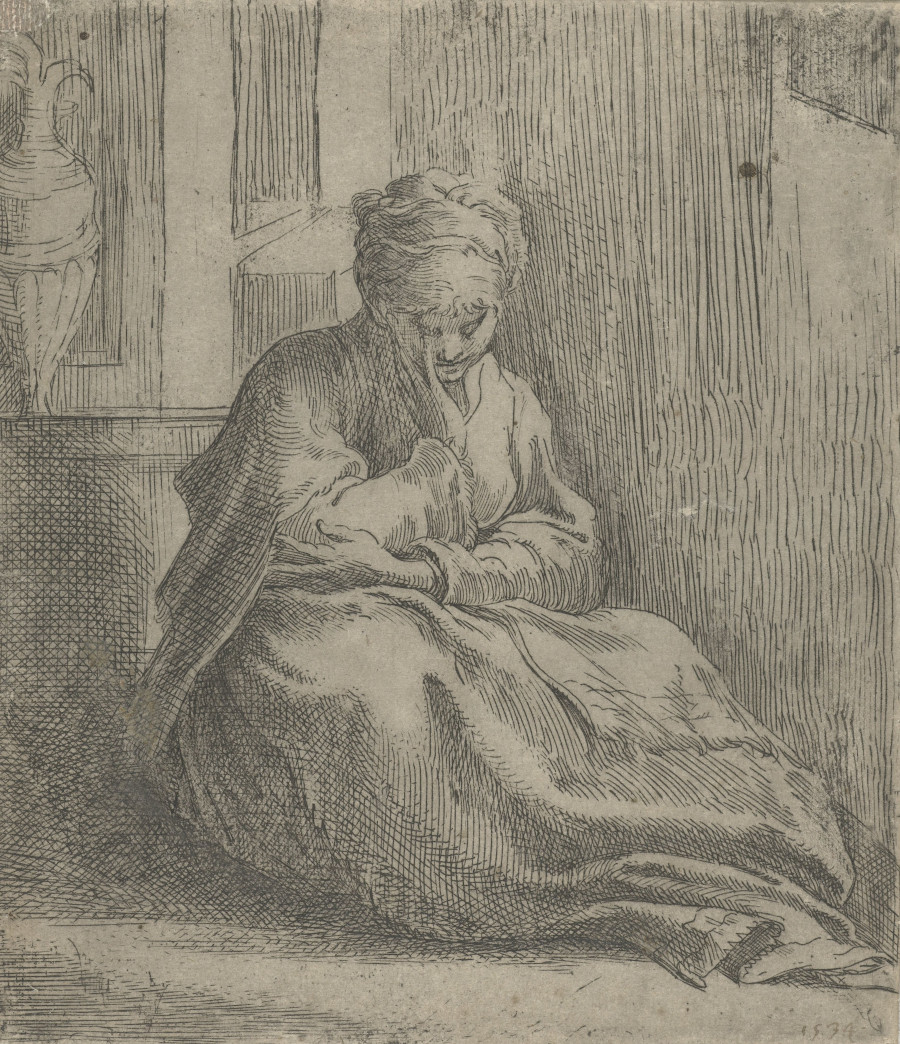
\includegraphics[keepaspectratio,width=0.6\textwidth]{figures/thais-small.jpg}
  \captionart{MelancholieThais}
  \label{fig:thais}
\end{figure}

To see a fond mother, like \AE{}sop's ape, hug her child to death, a \authormarginnote{379}
\margindef{a man who knows of his wife's infidelity and puts up with it}{wittol} wink at his wife's honesty, and too perspicuous in all other
affairs; one stumble at a straw, and leap over a block; rob Peter, and
pay Paul; scrape unjust sums with one hand, purchase great manors by
corruption, fraud and cozenage, and liberally to distribute to the poor
with the other, give a remnant to pious uses, \etc{}. Penny wise, pound
foolish; blind men judge of colours; wise men silent, fools talk; \authormarginnote{380}
find fault with others, and do worse themselves; \authormarginnote{381}[5\baselineskip]denounce that in
public which he doth in secret; and which Aurelius Victor gives out of
Augustus, severely censure that in a third, of which he is most guilty
himself.

To see a poor fellow, or an hired servant venture his life for his new
master that will scarce give him his wages at year's end; A country
colon toil and moil, till and drudge for a prodigal idle drone, that
devours all the gain, or lasciviously consumes with fantastical
expenses; A noble man in a bravado to encounter death, and for a small
flash of honour to cast away himself; A worldling tremble at an
executor, and yet not fear hell-fire; To wish and hope for immortality,
desire to be happy, and yet by all means avoid death, a necessary
passage to bring him to it.

To see a foolhardy fellow like those old Danes, \li{qui decollari malunt
quam verberari}, die rather than be punished, in a sottish humour
embrace death with alacrity, yet \authormarginnote{382}[-3\baselineskip]scorn to lament his own sins and
miseries, or his clearest friends' departures.

To see wise men degraded, fools preferred, one govern towns and cities,
and yet a silly woman overrules him at home; \authormarginnote{383}Command a province,
and yet his own servants or children prescribe laws to him, as
Themistocles' son did in Greece; \authormarginnote{384}[2\baselineskip]What I will (said he) my mother
will, and what my mother will, my father doth.

To see horses ride in a coach, men draw it; dogs devour their masters; towers build masons;
children rule; old men go to school; women wear the breeches;
\authormarginnote{385}[\baselineskip]sheep demolish towns, devour men, \etc{}. And in a word, the world
turned upside downward. \li{O viveret Democritus}.\authormarginnote{386}[2\baselineskip] To insist in every particular were one of Hercules' labours,
there's so many ridiculous instances, as motes in the sun. \li{Quantum est
in rebus inane?} (How much vanity there is in things!) And who can speak
of all? \li{Crimine ab uno disce omnes}, take this for a taste.

But these are obvious to sense, trivial and well known, easy to be
discerned. How would Democritus have been moved, had he seen \authormarginnote{387}the
secrets of their hearts? If every man had a window in his breast, which
Momus would have had in Vulcan's man, or that which Tully so much
wished it were written in every man's forehead, \li{Quid quisque de
republica sentiret}, what he thought; or that it could be effected in an
instant, which Mercury did by Charon in Lucian, by touching of his
eyes, to make him discern \li{semel et simul rumores et susurros}.
%
\settowidth{\versewidth}{Spes hominum c\ae{}cas, morbos, votumque labores,}
\begin{verse}[\versewidth]
\textlatin{Spes hominum c\ae{}cas, morbos, votumque labores,}\\*
\textlatin{Et passim toto volitantes \ae{}there curas.}\\!
\end{verse}
\translationrule
\settowidth{\versewidth}{Blind hopes and wishes, their thoughts and affairs,}
\begin{verse}[\versewidth]
Blind hopes and wishes, their thoughts and affairs,\\*
Whispers and rumours, and those flying cares.\\!
\end{verse}
%
That he could \li{cubiculorum obductas foras recludere et secreta cordium
penetrare}, which Cyprian desired\authormarginnote{388}, open doors and locks, shoot
bolts, as Lucian's Gallus did with a feather of his tail: or Gyges'
invisible ring, or some rare perspective glass, or \emph{Otacousticon},
which would so multiply species, that a man might hear and see all at
once (as \authormarginnote{389} Martianus Capella's Jupiter did in a spear which he held
in his hand, which did present unto him all that was daily done upon
the face of the earth), observe cuckolds' horns, forgeries of
alchemists, the philosopher's stone, new projectors, \etc{}, and all those
works of darkness, foolish vows, hopes, fears and wishes, what a deal
of laughter would it have afforded? He should have seen windmills in
one man's head, an hornet's nest in another. Or had he been present
with Icaromenippus in Lucian at Jupiter's whispering place, \authormarginnote{390}and
heard one pray for rain, another for fair weather; one for his wife's,
another for his father's death, \etc{}; to ask that at God's hand which
they are abashed any man should hear: How would he have been
confounded? Would he, think you, or any man else, say that these men
were well in their wits? \li{H\ae{}c sani esse hominis quis sanus juret
Orestes?} Can all the hellebore in the Anticyr\ae{}\ cure these men? No,
sure, \authormarginnote{391}an acre of hellebore will not do it.

That which is more to be lamented, they are mad like Seneca's blind
woman, and will not acknowledge, or \authormarginnote{392}seek for any cure of it, for
pauci vident morbum suum, omnes amant. If our leg or arm offend us, we
covet by all means possible to redress it; \authormarginnote{393}and if we labour of a
bodily disease, we send for a physician; but for the diseases of the
mind we take no notice of them: \authormarginnote{394}[\baselineskip]Lust harrows us on the one side;
envy, anger, ambition on the other. We are torn in pieces by our
passions, as so many wild horses, one in disposition, another in habit;
one is melancholy, another mad; \authormarginnote{395}[3\baselineskip]and which of us all seeks for
help, doth acknowledge his error, or knows he is sick? As that stupid
fellow put out the candle because the biting fleas should not find him;
he shrouds himself in an unknown habit, borrowed titles, because nobody
should discern him. Every man thinks with himself, \li{Egomet videor mihi
sanus}, I am well, I am wise, and laughs at others. And 'tis a general
fault amongst them all, that \authormarginnote{396}[3\baselineskip] which our forefathers have approved,
diet, apparel, opinions, humours, customs, manners, we deride and
reject in our time as absurd. Old men account juniors all fools, when
they are mere dizzards; and as to sailors, ---\li{terr\ae{}que urbesque
recedunt}--- they move, the land stands still, the world hath much more
wit, they dote themselves. Turks deride us, we them; Italians
Frenchmen, accounting them light headed fellows, the French scoff again
at Italians, and at their several customs; Greeks have condemned all
the world but themselves of barbarism, the world as much vilifies them
now; we account Germans heavy, dull fellows, explode many of their
fashions; they as contemptibly think of us; Spaniards laugh at all, and
all again at them. So are we fools and ridiculous, absurd in our
actions, carriages, diet, apparel, customs, and consultations; we \authormarginnote{397}
scoff and point one at another, when as in conclusion all are fools,
\authormarginnote{398} and they the veriest asses that hide their ears most. A private
man if he be resolved with himself, or set on an opinion, accounts all
idiots and asses that are not affected as he is, \authormarginnote{399}---\li{nil rectum,
nisi quod placuit sibi, ducit}, that are not so minded, \authormarginnote{400}(\li{quodque
volunt homines se bene velle putant}) all fools that think not as he
doth: he will not say with Atticus, \li{Suam quisque sponsam, mihi meam},
let every man enjoy his own spouse; but his alone is fair, \li{suus amor},
\etc{} and scorns all in respect of himself \authormarginnote{401}[-3\baselineskip]will imitate none, hear
none \authormarginnote{402}but himself, as Pliny said, a law and example to himself. And
that which Hippocrates, in his epistle to Dionysius, reprehended of
old, is verified in our times, \li{Quisque in alio superfluum esse censet,
ipse quod non habet nec curat}, that which he hath not himself or doth
not esteem, he accounts superfluity, an idle quality, a mere foppery in
another: like \AE{}sop's fox, when he had lost his tail, would have all
his fellow foxes cut off theirs. The Chinese say, that we Europeans
have one eye, they themselves two, all the world else is blind: (though
\authormarginnote{403}Scaliger accounts them brutes too, \li{merum pecus}) so thou and thy
sectaries are only wise, others indifferent, the rest beside
themselves, mere idiots and asses. Thus not acknowledging our own
errors and imperfections, we securely deride others, as if we alone
were free, and spectators of the rest, accounting it an excellent
thing, as indeed it is, \li{Aliena optimum frui insania}, to make ourselves
merry with other men's obliquities, when as he himself is more faulty
than the rest, \li{mutato nomine, de te fabula narratur}, he may take
himself by the nose for a fool; and which one calls \li{maximum stultiti\ae{}}
specimen, to be ridiculous to others, and not to perceive or take
notice of it, as Marsyas was when he contended with Apollo, \li{non
intelligens se deridiculo haberi}, saith Apuleius\authormarginnote{404}; 'tis his own
cause, he is a convicted madman, as \authormarginnote{405}Austin well infers in the eyes
of wise men and angels he seems like one, that to our thinking walks
with his heels upwards. So thou laughest at me, and I at thee, both at
a third; and he returns that of the poet upon us again, \authormarginnote{406}[\baselineskip]\li{Hei mihi,
insanire me aiunt, quum ipsi ultro insaniant}. We accuse others of
madness, of folly, and are the veriest dizzards ourselves. For it is a
great sign and property of a fool (which Eccl. x. 3, points at) out of
pride and self-conceit to insult, vilify, condemn, censure, and call
other men fools (\li{Non videmus mantic\ae{}\ quod a tergo est}) to tax that in
others of which we are most faulty; teach that which we follow not
ourselves: For an inconstant man to write of constancy, a profane liver
prescribe rules of sanctity and piety, a dizzard himself make a
treatise of wisdom, or with Sallust to rail downright at spoilers of
countries, and yet in \authormarginnote{407}office to be a most grievous poller himself.

This argues weakness, and is an evident sign of such parties'
indiscretion. \authormarginnote{408}\li{Peccat uter nostrum cruce dignius?} Who is the fool
now? Or else peradventure in some places we are all mad for company,
and so 'tis not seen, \li{Satietas erroris et dementi\ae{}, pariter
absurditatem et admirationem tollit.} 'Tis with us, as it was of old (in
\authormarginnote{409}Tully's censure at least) with C. Pimbria in Rome, a bold,
hair-brain, mad fellow, and so esteemed of all, such only excepted,
that were as mad as himself: now in such a case there is \authormarginnote{410}no notice
taken of it.
%
\settowidth{\versewidth}{Maxima pars hominum morbo jactatur eodem.}
\begin{verse}[\versewidth]
\textlatin{Nimirum insanus paucis videatur; eo quod}\\*
\textlatin{Maxima pars hominum morbo jactatur eodem.}
\end{verse}
\translationrule
\settowidth{\versewidth}{When all are mad, where all are like opprest}
\begin{verse}[\versewidth]
When all are mad, where all are like opprest\\*
Who can discern one mad man from the rest?\\!
\end{verse}
%
But put case they do perceive it, and some one be manifestly convicted
of madness, \authormarginnote{411}he now takes notice of his folly, be it in action,
gesture, speech, a vain humour he hath in building, bragging, jangling,
spending, gaming, courting, scribbling, prating, for which he is
ridiculous to others, \authormarginnote{412}on which he dotes, he doth acknowledge as
much: yet with all the rhetoric thou hast, thou canst not so recall
him, but to the contrary notwithstanding, he will persevere in his
dotage. 'Tis \li{amabilis insania, et mentis gratissimus error}, so
pleasing, so delicious, that he cannot leave it\authormarginnote{413}. He knows his
error, but will not seek to decline it, tell him what the event will
be, beggary, sorrow, sickness, disgrace, shame, loss, madness, yet
\authormarginnote{414}an angry man will prefer vengeance, a lascivious his whore, a
thief his booty, a glutton his belly, before his welfare. Tell an
epicure, a covetous man, an ambitious man of his irregular course, wean
him from it a little, \li{pol me occidistis amici}, he cries anon, you have
undone him, and as \authormarginnote{415}a dog to his vomit, he returns to it again; no
persuasion will take place, no counsel, say what thou canst,
%
\begin{verse}
\textlatin{Clames licet et mare coelo}\\*
---\textlatin{Confundas, surdo narras,}\authorlatintrans{416}
\end{verse}
%
demonstrate as Ulysses did to \authormarginnote{417}Elpenor and Gryllus, and the rest of
his companions those swinish men, he is irrefragable in his humour, he
will be a hog still; bray him in a mortar, he will be the same. If he
be in an heresy, or some perverse opinion, settled as some of our
ignorant Papists are, convince his understanding, show him the several
follies and absurd fopperies of that sect, force him to say, veris
vincor, make it as clear as the sun, \authormarginnote{418}[-1\baselineskip]he will err still, peevish
and obstinate as he is; and as he said \authormarginnote{419}\li{si in hoc erro, libenter
erro, nec hunc errorem auferri mihi volo}; I will do as I have done, as
my predecessors have done, \authormarginnote{420}[-1\baselineskip]and as my friends now do: I will dote
for company. Say now, are these men \authormarginnote{421}mad or no, \authormarginnote{422}[2\baselineskip]\li{Heus age
responde?} are they ridiculous? \li{cedo quemvis arbitrum}, are they \li{san\ae{}
mentis}, sober, wise, and discreet? have they common sense? ---\authormarginnote{423}\li{uter
est insanior horum?} I am of Democritus' opinion for my part, I hold
them worthy to be laughed at; a company of brain-sick dizzards, as mad
as \authormarginnote{424}Orestes and Athamas, that they may go ride the ass, and all
sail along to the Anticyr\ae{}, in the ship of fools for company together.

I need not much labour to prove this which I say otherwise than thus,
make any solemn protestation, or swear, I think you will believe me
without an oath; say at a word, are they fools? I refer it to you,
though you be likewise fools and madmen yourselves, and I as mad to ask
the question; for what said our comical Mercury?
%
\begin{verse}
\textlatin{Justum ab injustis petere insipientia est.}\authormarginnote{425}
\end{verse}
\translationrule
\begin{verse}
I'll stand to your censure yet, what think you?
\end{verse}
%
But forasmuch as I undertook at first, that kingdoms, provinces,
families, were melancholy as well as private men, I will examine them
in particular, and that which I have hitherto dilated at random, in
more general terms, I will particularly insist in, prove with more
special and evident arguments, testimonies, illustrations, and that in
brief. \authormarginnote{426}\li{Nunc accipe quare desipiant omnes \ae{}que ac tu.} My first
argument is borrowed from Solomon, an arrow drawn out of his
sententious quiver, Pro. iii. 7, Be not wise in thine own eyes. And
xxvi. 12, Seest thou a man wise in his own conceit? more hope is of a
fool than of him. Isaiah pronounceth a woe against such men, cap. v.
21, that are wise in their own eyes, and prudent in their own sight.

For hence we may gather, that it is a great offence, and men are much
deceived that think too well of themselves, an especial argument to
convince them of folly. Many men (saith \authormarginnote{427}Seneca) had been without
question wise, had they not had an opinion that they had attained to
perfection of knowledge already, even before they had gone half way,
too forward, too ripe, pr\ae{}properi, too quick and ready, \authormarginnote{428}\li{cito
prudentes, cito pii, cito mariti, cito patres, cito sacerdotes, cito
omnis officii capaces et curiosi}, they had too good a conceit of
themselves, and that marred all; of their worth, valour, skill, art,
learning, judgment, eloquence, their good parts; all their geese are
swans, and that manifestly proves them to be no better than fools. In
former times they had but seven wise men, now you can scarce find so
many fools. Thales sent the golden tripos, which the fishermen found,
and the oracle commanded to be \authormarginnote{429} given to the wisest, to Bias, Bias
to Solon, \etc{}. If such a thing were now found, we should all fight for
it, as the three goddesses did for the golden apple, we are so wise: we
have women politicians, children metaphysicians; every silly fellow can
square a circle, make perpetual motions, find the philosopher's stone,
interpret Apocalypses, make new Theories, a new system of the world,
new Logic, new Philosophy, \etc{}. \li{Nostra utique regio}, saith
\authormarginnote{430}Petronius, our country is so full of deified spirits, divine
souls, that you may sooner find a God than a man amongst us, we think
so well of ourselves, and that is an ample testimony of much folly.

My second argument is grounded upon the like place of Scripture, which
though before mentioned in effect, yet for some reasons is to be
repeated (and by Plato's good leave, I may do it, \textgreek{δίς τὸ καλὸν
ρηθέν ὀυδέν βλάπτει}\authormarginnote{431}) Fools (saith David) by reason of their
transgressions. \etc{}. Psal. \rn{cvii.} 17. Hence Musculus infers all
transgressors must needs be fools. So we read Rom. \rn{ii.}, Tribulation and
anguish on the soul of every man that doeth evil; but all do evil. And
Isaiah, \rn{lxv.} 14, My servant shall sing for joy, and \authormarginnote{432}ye shall cry
for sorrow of heart, and vexation of mind. 'Tis ratified by the common
consent of all philosophers. Dishonesty (saith Cardan) is nothing else
but folly and madness. \li{Probus quis nobiscum vivit?}\authorlatintrans{433.5}\authormarginnote{433} Show me an
honest man, \li{Nemo malus qui non stultus}, 'tis Fabius' aphorism to the
same end. If none honest, none wise, then all fools. And well may they
be so accounted: for who will account him otherwise, \li{Qui iter adornat
in occidentem, quum properaret in orientem?} that goes backward all his
life, westward, when he is bound to the east? or hold him a wise man
(saith \authormarginnote{434}Musculus) that prefers momentary pleasures to eternity,
that spends his master's goods in his absence, forthwith to be
condemned for it? \li{Nequicquam sapit qui sibi non sapit}, who will say
that a sick man is wise, that eats and drinks to overthrow the
temperature of his body? Can you account him wise or discreet that
would willingly have his health, and yet will do nothing that should
procure or continue it? \authormarginnote{435}Theodoret, out of Plotinus the Platonist,
holds it a ridiculous thing for a man to live after his own laws, to do
that which is offensive to God, and yet to hope that he should save
him: and when he voluntarily neglects his own safety, and contemns the
means, to think to be delivered by another: who will say these men are
wise?

A third argument may be derived from the precedent, \authormarginnote{436}all men are
carried away with passion, discontent, lust, pleasures, \etc{}, they
generally hate those virtues they should love, and love such vices they
should hate. Therefore more than melancholy, quite mad, brute beasts,
and void of reason, so Chrysostom contends; or rather dead and buried
alive, as \authormarginnote{437} Philo Judeus concludes it for a certainty, of all such
that are carried away with passions, or labour of any disease of the
mind. Where is fear and sorrow, there \authormarginnote{438}Lactantius stiffly
maintains, wisdom cannot dwell,
%
\begin{verse}
---\textlatin{qui cupiet, metuet quoque porro,}\\*
\textlatin{Qui metuens vivit, liber mihi non erit unquam.}\authorlatintrans{439}
\end{verse}
%
Seneca and the rest of the stoics are of opinion, that where is any the
least perturbation, wisdom may not be found. What more ridiculous, as
\authormarginnote{440}[-2\baselineskip]Lactantius urges, than to hear how Xerxes whipped the Hellespont,
threatened the Mountain Athos, and the like. To speak \li{ad rem}, who is
free from passion? \authormarginnote{441}[-2\baselineskip]\li{Mortalis nemo est quem non attingat dolor, morbusve}, as \authormarginnote{442}Tully determines out of an old poem, no mortal men
can avoid sorrow and sickness, and sorrow is an inseparable companion
from melancholy. \authormarginnote{443}Chrysostom pleads farther yet, that they are more
than mad, very beasts, stupefied and void of common sense: For how
(saith he) shall I know thee to be a man, when thou kickest like an
ass, neighest like a horse after women, ravest in lust like a bull,
ravenest like a bear, stingest like a scorpion, rakest like a wolf, as
subtle as a fox, as impudent as a dog? Shall I say thou art a man, that
hast all the symptoms of a beast? How shall I know thee to be a man? by
thy shape? That affrights me more, when I see a beast in likeness of a
man.

\authormarginnote{444}Seneca calls that of Epicurus, \li{magnificam vocem}, an heroical
speech, A fool still begins to live, and accounts it a filthy lightness
in men, every day to lay new foundations of their life, but who doth
otherwise? One travels, another builds; one for this, another for that
business, and old folks are as far out as the rest; \li{O dementem
senectutem}, Tully exclaims. Therefore young, old, middle age, are all
stupid, and dote.

\authormarginnote{445}\AE{}neas Sylvius, amongst many other, sets down three special ways
to find a fool by. He is a fool that seeks that he cannot find: he is a
fool that seeks that, which being found will do him more harm than
good: he is a fool, that having variety of ways to bring him to his
journey's end, takes that which is worst. If so, methinks most men are
fools; examine their courses, and you shall soon perceive what dizzards
and mad men the major part are.

Beroaldus will have drunkards, afternoon men, and such as more than
ordinarily delight in drink, to be mad. The first pot quencheth thirst,
so Panyasis the poet determines in Athen\ae{}us, \li{secunda gratiis, horis et
Dyonisio}: the second makes merry, the third for pleasure, quarta, ad
insaniam, the fourth makes them mad. If this position be true, what a
catalogue of mad men shall we have? what shall they be that drink four
times four? \li{Nonne supra omnem furorem, supra omnem insanian reddunt
insanissimos?} I am of his opinion, they are more than mad, much worse
than mad.

The \authormarginnote{446}Abderites condemned Democritus for a mad man, because he was
sometimes sad, and sometimes again profusely merry. \li{Hac Patria} (saith
Hippocrates) \li{ob risum furere et insanire dicunt}, his countrymen hold
him mad because he laughs; \authormarginnote{447}and therefore he desires him to advise
all his friends at Rhodes, that they do not laugh too much, or be over
sad. Had those Abderites been conversant with us, and but seen what
\authormarginnote{448} fleering and grinning there is in this age, they would certainly
have concluded, we had been all out of our wits.

Aristotle in his Ethics holds \li{felix idemque sapiens}, to be wise and
happy, are reciprocal terms, \li{bonus idemque sapiens honestus}. 'Tis \authormarginnote{449}
Tully's paradox, wise men are free, but fools are slaves, liberty is a
power to live according to his own laws, as we will ourselves: who hath
this liberty? who is free?
%
\settowidth{\versewidth}{Quem neque pauperis, neque mors, neque vincula terrent,}
\begin{verse}[\versewidth]
---\textlatin{sapiens sibique imperiosus,}\\*
\textlatin{Quem neque pauperis, neque mors, neque vincula terrent,}\\*
\textlatin{Responsare cupidinibus, contemnere honores}\\*
\textlatin{Fortis, et in seipso totus teres atque rotundus.}\authormarginnote{450}\\!
\end{verse}
\translationrule
\settowidth{\versewidth}{Checks his desires, scorns honours, just and right.}
\begin{verse}[\versewidth]
He is wise that can command his own will,\\*
Valiant and constant to himself still,\\*
Whom poverty nor death, nor bands can fright,\\*
Checks his desires, scorns honours, just and right.\\!
\end{verse}
%
But where shall such a man be found? If no where, then \li{e diametro}, we
are all slaves, senseless, or worse. \li{Nemo malus felix}. But no man is
happy in this life, none good, therefore no man wise. \li{Rari quippe
boni}\authorlatintrans{451.5}\authormarginnote{451}--- For one virtue you shall find ten vices in the same party;
\li{pauci Promethei, multi Epimethei}. We may peradventure usurp the name,
or attribute it to others for favour, as Carolus Sapiens, Philippus
Bonus, Lodovicus Pius, \etc{}, and describe the properties of a wise man,
as Tully doth an orator, Xenophon Cyrus, Castilio a courtier, Galen
temperament, an aristocracy is described by politicians. But where
shall such a man be found?
%
\settowidth{\versewidth}{Vir bonus et sapiens, qualem vix repperit unum}
\begin{verse}[\versewidth]
\textlatin{Vir bonus et sapiens, qualem vix repperit unum}\\*
\textlatin{Millibus e multis hominum consultus Apollo.}\\!
\end{verse}
\translationrule
\begin{verse}
A wise, a good man in a million,\\*
Apollo consulted could scarce find one.\\!
\end{verse}
%
A man is a miracle of himself, but Trismegistus adds, \li{Maximum miraculum
homo sapiens}, a wise man is a wonder: \li{multi Thirsigeri, pauci Bacchi}.

Alexander when he was presented with that rich and costly casket of
king Darius, and every man advised him what to put in it, he reserved
it to keep Homer's works, as the most precious jewel of human wit, and
yet \authormarginnote{452} Scaliger upbraids Homer's muse, \li{Nutricem insan\ae{}\ sapienti\ae{}},
a nursery of madness, \authormarginnote{453}impudent as a court lady, that blushes at
nothing. Jacobus Mycillus, Gilbertus Cognatus, Erasmus, and almost all
posterity admire Lucian's luxuriant wit, yet Scaliger rejects him in
his censure, and calls him the Cerberus of the muses. Socrates, whom
all the world so much magnified, is by Lactantius and Theodoret
condemned for a fool. Plutarch extols Seneca's wit beyond all the
Greeks, \li{nulli secundus}, yet \authormarginnote{454} Seneca saith of himself, when I would
solace myself with a fool, I reflect upon myself, and there I have him.

Cardan, in his Sixteenth Book of Subtleties, reckons up twelve
supereminent, acute philosophers, for worth, subtlety, and wisdom:
Archimedes, Galen, Vitruvius, Architas Tarentinus, Euclid, Geber, that
first inventor of Algebra, Alkindus the Mathematician, both Arabians,
with others. But his \li{triumviri terrarum} far beyond the rest, are
Ptolom\ae{}us, Plotinus, Hippocrates. Scaliger \li{exercitat. 224}, scoffs at
this censure of his, calls some of them carpenters and mechanicians, he
makes Galen \li{fimbriam Hippocratis}, a skirt of Hippocrates: and the said
\authormarginnote{455}Cardan himself elsewhere condemns both Galen and Hippocrates for
tediousness, obscurity, confusion. Paracelsus will have them both mere
idiots, infants in physic and philosophy. Scaliger and Cardan admire
Suisset the Calculator, \li{qui pene modum excessit humani ingenii}, and yet
\authormarginnote{456}Lod. Vives calls them nugas Suisseticas: and Cardan, opposite to
himself in another place, contemns those ancients in respect of times
present, \authormarginnote{457}\li{Majoresque nostros ad presentes collatos juste pueros
appellari}. In conclusion, the said \authormarginnote{458}Cardan and Saint Bernard will
admit none into this catalogue of wise men, \authormarginnote{459}but only prophets and
apostles; how they esteem themselves, you have heard before. We are
worldly-wise, admire ourselves, and seek for applause: but hear Saint
\authormarginnote{460}[2\baselineskip]Bernard, \li{quanto magis foras es sapiens, tanto magis intus stultus efficeris, \etc{} in omnibus es prudens, circa teipsum insipiens}: the more
wise thou art to others, the more fool to thyself. I may not deny but
that there is some folly approved, a divine fury, a holy madness, even
a spiritual drunkenness in the saints of God themselves; \li{sanctum
insanium} Bernard calls it (though not as blaspheming \authormarginnote{461}Vorstius,
would infer it as a passion incident to God himself, but) familiar to
good men, as that of Paul, 2 Cor. he was a fool, \etc{} and Rom. ix. he
wisheth himself to be anathematised for them. Such is that drunkenness
which Ficinus speaks of, when the soul is elevated and ravished with a
divine taste of that heavenly nectar, which poets deciphered by the
sacrifice of Dionysius, and in this sense with the poet, \authormarginnote{462}\li{insanire
lubet}, as Austin exhorts us, \li{ad ebrietatem se quisque paret}, let's all
be mad and \authormarginnote{463}drunk. But we commonly mistake, and go beyond our
commission, we reel to the opposite part, \authormarginnote{464}[\baselineskip]we are not capable of
it, \authormarginnote{465}[2\baselineskip]and as he said of the Greeks, \li{Vos Gr\ae{}ci semper pueri, vos Britanni, Galli, Germani, Itali, \etc{}} you are a company of fools.

Proceed now a \li{partibus ad totum}, or from the whole to parts, and you
shall find no other issue, the parts shall be sufficiently dilated in
this following Preface. The whole must needs follow by a sorites or
induction. Every multitude is mad, \authormarginnote{466}\li{bellua multorum capitum}, (a
many-headed beast), precipitate and rash without judgment, \li{stultum
animal}, a roaring rout. \authormarginnote{467}Roger Bacon proves it out of Aristotle,
\li{Vulgus dividi in oppositum contra sapientes, quod vulgo videtur verum,
falsum est}; that which the commonalty accounts true, is most part
false, they are still opposite to wise men, but all the world is of
this humour (vulgus), and thou thyself art \li{de vulgo}, one of the
commonalty; and he, and he, and so are all the rest; and therefore, as
Phocion concludes, to be approved in nought you say or do, mere idiots
and asses. Begin then where you will, go backward or forward, choose
out of the whole pack, wink and choose, you shall find them all alike,
never a barrel better herring.

Copernicus, Atlas his successor, is of opinion, the earth is a planet,
moves and shines to others, as the moon doth to us. Digges, Gilbert,
Keplerus, Origanus, and others, defend this hypothesis of his in sober
sadness, and that the moon is inhabited: if it be so that the earth is
a moon, then are we also giddy, vertiginous and lunatic within this
sublunary maze.

I could produce such arguments till dark night: if you should hear the
rest,
%
\begin{verse}
\textlatin{Ante diem clauso component vesper Olimpo:}
\end{verse}
\translationrule
\begin{verse}
Through such a train of words if I should run,\\*
The day would sooner than the tale be done:
\end{verse}
%
but according to my promise, I will descend to particulars. This
melancholy extends itself not to men only, but even to vegetals and
sensibles. I speak not of those creatures which are saturnine,
melancholy by nature, as lead, and such like minerals, or those plants,
rue, cypress, \etc{} and hellebore itself, of which \authormarginnote{468}Agrippa treats,
fishes, birds, and beasts, hares, conies, dormice, \etc{}, owls, bats,
nightbirds, but that artificial, which is perceived in them all. Remove
a plant, it will pine away, which is especially perceived in date
trees, as you may read at large in Constantine's husbandry, that
antipathy betwixt the vine and the cabbage, vine and oil. Put a bird in
a cage, he will die for sullenness, or a beast in a pen, or take his
young ones or companions from him, and see what effect it will cause.

But who perceives not these common passions of sensible creatures,
fear, sorrow, \etc{}. Of all other, dogs are most subject to this malady,
insomuch some hold they dream as men do, and through violence of
melancholy run mad; I could relate many stories of dogs that have died
for grief, and pined away for loss of their masters, but they are
common in every \authormarginnote{469}author.

Kingdoms, provinces, and politic bodies are likewise sensible and
subject to this disease, as \authormarginnote{470}Boterus in his politics hath proved at
large. As in human bodies (saith he) there be diverse alterations
proceeding from humours, so be there many diseases in a commonwealth,
which do as diversely happen from several distempers, as you may easily
perceive by their particular symptoms. For where you shall see the
people civil, obedient to God and princes, judicious, peaceable and
quiet, rich, fortunate, \authormarginnote{471}and flourish, to live in peace, in unity
and concord, a country well tilled, many fair built and populous
cities, \li{ubi incol\ae{}\ nitent} as old Cato said\authormarginnote{472}, the people are neat,
polite and terse, \li{ubi bene, beateque vivunt}, which our politicians make
the chief end of a commonwealth; and which \authormarginnote{473} Aristotle, Polit. lib.
3, cap. 4, calls \li{Commune bonum}, Polybius lib. 6, \li{optabilem et selectum
statum}, that country is free from melancholy; as it was in Italy in the
time of Augustus, now in China, now in many other flourishing kingdoms
of Europe. But whereas you shall see many discontents, common
grievances, complaints, poverty, barbarism, beggary, plagues, wars,
rebellions, seditions, mutinies, contentions, idleness, riot,
epicurism, the land lie untilled, waste, full of bogs, fens, deserts,
\etc{}, cities decayed, base and poor towns, villages depopulated, the
people squalid, ugly, uncivil; that kingdom, that country, must needs
be discontent, melancholy, hath a sick body, and had need to be
reformed.

Now that cannot well be effected, till the causes of these maladies be
first removed, which commonly proceed from their own default, or some
accidental inconvenience: as to be situated in a bad clime, too far
north, sterile, in a barren place, as the desert of Libya, deserts of
Arabia, places void of waters, as those of Lop and Belgian in Asia, or
in a bad air, as at Alexandretta, Bantam, Pisa, Durrazzo, S. John de
Ulloa, \etc{}, or in danger of the sea's continual inundations, as in many
places of the Low Countries and elsewhere, or near some bad neighbours,
as Hungarians to Turks, Podolians to Tartars, or almost any bordering
countries, they live in fear still, and by reason of hostile incursions
are oftentimes left desolate. So are cities by reason \authormarginnote{474}of wars,
fires, plagues, inundations, \authormarginnote{475}[2\baselineskip]wild beasts, decay of trades, barred
havens, the sea's violence, as Antwerp may witness of late, Syracuse of
old, Brundusium in Italy, Rye and Dover with us, and many that at this
day suspect the sea's fury and rage, and labour against it as the
Venetians to their inestimable charge. But the most frequent maladies
are such as proceed from themselves, as first when religion and God's
service is neglected, innovated or altered, where they do not fear God,
obey their prince, where atheism, epicurism, sacrilege, simony, \etc{},
and all such impieties are freely committed, that country cannot
prosper. When Abraham came to Gerar, and saw a bad land, he said, sure
the fear of God was not in that place. \authormarginnote{476} Cyprian Echovius, a
Spanish chorographer, above all other cities of Spain, commends
Borcino, in which there was no beggar, no man poor, \etc{}, but all rich,
and in good estate, and he gives the reason, because they were more
religious than, their neighbours: why was Israel so often spoiled by
their enemies, led into captivity, \etc{}, but for their idolatry, neglect
of God's word, for sacrilege, even for one Achan's fault? And what
shall we except that have such multitudes of Achans, church robbers,
simoniacal patrons, \etc{}, how can they hope to flourish, that neglect
divine duties, that live most part like Epicures?
Other common grievances are generally noxious to a body politic;
alteration of laws and customs, breaking privileges, general
oppressions, seditions, \etc{}, observed by \authormarginnote{477}Aristotle, Bodin,
Boterus, Junius, Arniscus, \etc{}. I will only point at some of chiefest.

\authormarginnote{478}\li{Impotentia gubernandi}, ataxia, confusion, ill government, which
proceeds from unskilful, slothful, griping, covetous, unjust, rash, or
tyrannizing magistrates, when they are fools, idiots, children, proud,
wilful, partial, indiscreet, oppressors, giddy heads, tyrants, not able
or unfit to manage such offices: \authormarginnote{479}many noble cities and flourishing
kingdoms by that means are desolate, the whole body groans under such
heads, and all the members must needs be disaffected, as at this day
those goodly provinces in Asia Minor, \etc{} groan under the burthen of a
Turkish government; and those vast kingdoms of Muscovia, Russia,
\authormarginnote{480}under a tyrannizing duke. Who ever heard of more civil and rich
populous countries than those of Greece, Asia Minor, abounding with all
\authormarginnote{481}wealth, multitudes of inhabitants, force, power, splendour and
magnificence? and that miracle of countries, \authormarginnote{482}the Holy Land, that
in so small a compass of ground could maintain so many towns, cities,
produce so many fighting men? Egypt another paradise, now barbarous and
desert, and almost waste, by the despotical government of an imperious
Turk, \li{intolerabili servitutis jugo premitur} (\authormarginnote{483}one saith) not only
fire and water, goods or lands, \li{sed ipse spiritus ab insolentissimi
victoris pendet nutu}, such is their slavery, their lives and souls
depend upon his insolent will and command. A tyrant that spoils all
wheresoever he comes, insomuch that an \authormarginnote{484}historian complains, if an
old inhabitant should now see them, he would not know them, if a
traveller, or stranger, it would grieve his heart to behold them.

Whereas Aristotle notes\authormarginnote{485}, \li{Nov\ae{}\ exactiones, nova onera imposita},
new burdens and exactions daily come upon them, like those of which
Zosimus, lib. 2, so grievous, \li{ut viri uxores, patres filios
prostituerent ut exactoribus e questu, \etc{}}, they must needs be
discontent, \li{hinc civitatum gemitus et ploratus}, as \authormarginnote{486} Tully holds,
hence come those complaints and tears of cities, poor, miserable,
rebellious, and desperate subjects, as \authormarginnote{487}[-1\baselineskip]Hippolitus adds; and
\authormarginnote{488}[\baselineskip]as a judicious countryman of ours observed not long since, in a
survey of that great Duchy of Tuscany, the people lived much grieved
and discontent, as appeared by their manifold and manifest complainings
in that kind. That the state was like a sick body which had lately
taken physic, whose humours are not yet well settled, and weakened so
much by purging, that nothing was left but melancholy.

Whereas the princes and potentates are immoderate in lust, hypocrites,
epicures, of no religion, but in show: \li{Quid hypocrisi fragilius?} what
so brittle and unsure? what sooner subverts their estates than
wandering and raging lusts, on their subjects' wives, daughters? to say
no worse. That they should \li{facem pr\ae{}ferre}, lead the way to all
virtuous actions, are the ringleaders oftentimes of all mischief and
dissolute courses, and by that means their countries are plagued,
\authormarginnote{489}and they themselves often ruined, banished, or murdered by
conspiracy of their subjects, as Sardanapalus was, Dionysius Junior,
Heliogabalus, Periander, Pisistratus, Tarquinius, Timocrates,
Childericus, Appius Claudius, Andronicus, Galeacius Sforza, Alexander
Medices, \etc{}.

Whereas the princes or great men are malicious, envious, factious,
ambitious, emulators, they tear a commonwealth asunder, as so many
Guelfs and Gibelines disturb the quietness of it, \authormarginnote{490}and with mutual
murders let it bleed to death; our histories are too full of such
barbarous inhumanities, and the miseries that issue from them.

Whereas they be like so many horseleeches, hungry, griping, corrupt,
\authormarginnote{491} covetous, \li{avaritice mancipia}, ravenous as wolves, for as Tully
writes: \li{qui pr\ae{}est prodest, et qui pecudibus pr\ae{}est, debet eorum
utilitati inservire}: or such as prefer their private before the public
good. For as \authormarginnote{492}[-1\baselineskip]he said long since, \li{res privat\ae{}\ publicis semper officere}. Or whereas they be illiterate, ignorant, empirics in policy,
\li{ubi deest facultas}, \authormarginnote{493}[-2\baselineskip]\li{virtus} (Aristot. pol. 5, cap. 8.) \li{et scientia},
wise only by inheritance, and in authority by birthright, favour, or
for their wealth and titles; there must needs be a fault, \authormarginnote{494}[2\baselineskip]a great
defect: because as an \authormarginnote{495}[5\baselineskip]old philosopher affirms, such men are not
always fit. Of an infinite number, few alone are senators, and of those
few, fewer good, and of that small number of honest, good, and noble
men, few that are learned, wise, discreet and sufficient, able to
discharge such places, it must needs turn to the confusion of a state.

For as the \authormarginnote{496}Princes are, so are the people; \li{Qualis Rex, talis grex}:
and which \authormarginnote{497}[5\baselineskip]Antigonus right well said of old, \li{qui Macedonia regem
erudit, omnes etiam subditos erudit}, he that teacheth the king of
Macedon, teacheth all his subjects, is a true saying still.
%
\begin{verse}
For Princes are the glass, the school, the book,\\*
Where subjects' eyes do learn, do read, do look.
\end{verse}

\begin{verse}
---\textlatin{Velocius et citius nos}\\*
\textlatin{Corrumpunt vitiorum exempla domestica, magnis}\\*
\textlatin{Cum subeant animos auctoribus.}---\authorlatintrans{498}
\end{verse}
%
Their examples are soonest followed, vices entertained, if they be
profane, irreligious, lascivious, riotous, epicures, factious,
covetous, ambitious, illiterate, so will the commons most part be,
idle, unthrifts, prone to lust, drunkards, and therefore poor and needy
(\inlinegreek{ἡ πενια στάσιν ἐμποιει καὶ κακουργίαν}, for poverty begets sedition and
villainy) upon all occasions ready to mutiny and rebel, discontent
still, complaining, murmuring, grudging, apt to all outrages, thefts,
treasons, murders, innovations, in debt, shifters, cozeners, outlaws,
\li{Profligat\ae{}\ fam\ae{}\ ac vit\ae{}}. It was an old \authormarginnote{499}politician's aphorism,
They that are poor and bad envy rich, hate good men, abhor the present
government, wish for a new, and would have all turned topsy-turvy. When
Catiline rebelled in Rome, he got a company of such debauched rogues
together, they were his familiars and coadjutors, and such have been
your rebels most part in all ages, Jack Cade, Tom Straw, Kette, and his
companions.

Where they be generally riotous and contentious, where there be many
discords, many laws, many lawsuits, many lawyers and many physicians,
it is a manifest sign of a distempered, melancholy state, as \authormarginnote{500}Plato
long since maintained: for where such kind of men swarm, they will make
more work for themselves, and that body politic diseased, which was
otherwise sound. A general mischief in these our times, an insensible
plague, and never so many of them: which are now multiplied (saith Mat.
Geraldus, \authormarginnote{501}a lawyer himself) as so many locusts, not the parents,
but the plagues of the country, and for the most part a supercilious,
bad, covetous, litigious generation of men. \authormarginnote{502}Crumenimulga natio \etc{}.

A purse-milking nation, a clamorous company, gowned vultures, \authormarginnote{503}\li{qui
ex injuria vivent et sanguine civium, thieves and seminaries of
discord}; worse than any pollers by the highway side, \li{auri accipitres,
auri exterebronides, pecuniarum hamiol\ae{}, quadruplatores, curi\ae{}
harpagones, fori tintinabula, monstra hominum, mangones, \etc{}} that take
upon them to make peace, but are indeed the very disturbers of our
peace, a company of irreligious harpies, scraping, griping catchpoles,
(I mean our common hungry pettifoggers, \authormarginnote{504}\li{rabulas forenses}, love and
honour in the meantime all good laws, and worthy lawyers, that are so
many \authormarginnote{505}oracles and pilots of a well-governed commonwealth). Without
art, without judgment, that do more harm, as \authormarginnote{506}Livy said, \li{quam bella
externa, fames, morbive}, than sickness, wars, hunger, diseases; and
cause a most incredible destruction of a commonwealth, saith
\authormarginnote{507}Sesellius, a famous civilian sometimes in Paris, as ivy doth by an
oak, embrace it so long, until it hath got the heart out of it, so do
they by such places they inhabit; no counsel at all, no justice, no
speech to be had, \li{nisi eum premulseris}, he must be fed still, or else
he is as mute as a fish, better open an oyster without a knife. \li{Experto
crede} (saith \authormarginnote{508} Salisburiensis) \li{in manus eorum millies incidi, et
Charon immitis qui nulli pepercit unquam, his longe clementior est}; I
speak out of experience, I have been a thousand times amongst them, and
Charon himself is more gentle than they; \authormarginnote{509}he is contented with his
single pay, but they multiply still, they are never satisfied, besides
they have \li{damnificas linguas}, as he terms it, \li{nisi funibus argenteis
vincias}, they must be fed to say nothing, and \authormarginnote{510}get more to hold
their peace than we can to say our best. They will speak their clients
fair, and invite them to their tables, but as he follows it, \authormarginnote{511}of
all injustice there is none so pernicious as that of theirs, which when
they deceive most, will seem to be honest men. They take upon them to
be peacemakers, \li{et fovere causas humilium}, to help them to their right,
\li{patrocinantur afflictis}, \authormarginnote{512}but all is for their own good, \li{ut loculos
pleniorom exhauriant}, they plead for poor men gratis, but they are but
as a stale to catch others. If there be no jar, \authormarginnote{513}they can make a
jar, out of the law itself find still some quirk or other, to set them
at odds, and continue causes so long, \li{lustra aliquot}, I know not how
many years before the cause is heard, and when 'tis judged and
determined by reason of some tricks and errors, it is as fresh to
begin, after twice seven years sometimes, as it was at first; and so
they prolong time, delay suits till they have enriched themselves, and
beggared their clients. And, as \authormarginnote{514}Cato inveighed against Isocrates'
scholars, we may justly tax our wrangling lawyers, they do consenescere
\li{in litibus}, are so litigious and busy here on earth, that I think they
will plead their client's causes hereafter, some of them in hell. \authormarginnote{515}
Simlerus complains amongst the Swissers of the advocates in his time,
that when they should make an end, they began controversies, and
protract their causes many years, persuading them their title is good,
till their patrimonies be consumed, and that they have spent more in
seeking than the thing is worth, or they shall get by the recovery. So
that he that goes to law, as the proverb is, \authormarginnote{516}holds a wolf by the
ears, or as a sheep in a storm runs for shelter to a brier, if he
prosecute his cause he is consumed, if he surcease his suit he loseth
all; \authormarginnote{517}what difference? They had wont heretofore, saith Austin, to
end matters, \li{per communes arbitros}; and so in Switzerland (we are
informed by \authormarginnote{518}Simlerus), they had some common arbitrators or daysmen
in every town, that made a friendly composition betwixt man and man,
and he much wonders at their honest simplicity, that could keep peace
so well, and end such great causes by that means. At \authormarginnote{519}[\baselineskip]Fez in
Africa, they have neither lawyers nor advocates; but if there be any
controversies amongst them, both parties plaintiff and defendant come
to their Alfakins or chief judge, and at once without any farther
appeals or pitiful delays, the cause is heard and ended. Our
forefathers, as \authormarginnote{520}[\baselineskip]a worthy chorographer of ours observes, had wont
\li{pauculis cruculis aureis}, with a few golden crosses, and lines in
verse, make all conveyances, assurances. And such was the candour and
integrity of succeeding ages, that a deed (as I have oft seen) to
convey a whole manor, was implicite contained in some twenty lines or
thereabouts; like that scede or Sytala Laconica, so much renowned of
old in all contracts, which \authormarginnote{521}Tully so earnestly commends to
Atticus, Plutarch in his Lysander, Aristotle polit.: Thucydides, lib.
1, \authormarginnote{522}Diodorus and Suidus approve and magnify, for that laconic
brevity in this kind; and well they might, for, according to
Tertullian\authormarginnote{523}, \li{certa sunt paucis}, there is much more certainty in
fewer words. And so was it of old throughout: but now many skins of
parchment will scarce serve turn; he that buys and sells a house, must
have a house full of writings, there be so many circumstances, so many
words, such tautological repetitions of all particulars (to avoid
cavillation they say); but we find by our woeful experience, that to
subtle wits it is a cause of much more contention and variance, and
scarce any conveyance so accurately penned by one, which another will
not find a crack in, or cavil at; if any one word be misplaced, any
little error, all is disannulled. That which is a law today, is none
tomorrow; that which is sound in one man's opinion, is most faulty to
another; that in conclusion, here is nothing amongst us but contention
and confusion, we bandy one against another. And that which long since
Plutarch complained of them in Asia\authormarginnote{524}, may be verified in our times.

These men here assembled, come not to sacrifice to their gods, to offer
Jupiter their first-fruits, or merriments to Bacchus; but an yearly
disease exasperating Asia hath brought them hither, to make an end of
their controversies and lawsuits. 'Tis \li{multitudo perdentium et
pereuntium}, a destructive rout that seek one another's ruin. Such most
part are our ordinary suitors, termers, clients, new stirs every day,
mistakes, errors, cavils, and at this present, as I have heard in some
one court, I know not how many thousand causes: no person free, no
title almost good, with such bitterness in following, so many slights,
procrastinations, delays, forgery, such cost (for infinite sums are
inconsiderately spent), violence and malice, I know not by whose fault,
lawyers, clients, laws, both or all: but as Paul reprehended the
\authormarginnote{525}Corinthians long since, I may more positively infer now: There is
a fault amongst you, and I speak it to your shame, Is there not a
\authormarginnote{526}wise man amongst you, to judge between his brethren? but that a
brother goes to law with a brother. And \authormarginnote{527}[\baselineskip]Christ's counsel
concerning lawsuits, was never so fit to be inculcated as in this age:
\authormarginnote{528}[2\baselineskip]Agree with thine adversary quickly, \etc{}. Matth. v. 25.

I could repeat many such particular grievances, which must disturb a
body politic. To shut up all in brief, where good government is,
prudent and wise princes, there all things thrive and prosper, peace
and happiness is in that land: where it is otherwise, all things are
ugly to behold, incult, barbarous, uncivil, a paradise is turned to a
wilderness. This island amongst the rest, our next neighbours the
French and Germans, may be a sufficient witness, that in a short time
by that prudent policy of the Romans, was brought from barbarism; see
but what C\ae{}sar reports of us, and Tacitus of those old Germans, they
were once as uncivil as they in Virginia, yet by planting of colonies
and good laws, they became from barbarous outlaws, \authormarginnote{529}to be full of
rich and populous cities, as now they are, and most flourishing
kingdoms. Even so might Virginia, and those wild Irish have been
civilised long since, if that order had been heretofore taken, which
now begins, of planting colonies, \etc{}. I have read a \authormarginnote{530}[\baselineskip]discourse,
printed \emph{anno} 1612. Discovering the true causes why Ireland was never
entirely subdued, or brought under obedience to the crown of England,
until the beginning of his Majesty's happy reign. Yet if his reasons
were thoroughly scanned by a judicious politician, I am afraid he would
not altogether be approved, but that it would turn to the dishonour of
our nation, to suffer it to lie so long waste. Yea, and if some
travellers should see (to come nearer home) those rich, united
provinces of Holland, Zealand, \etc{}, over against us; those neat cities
and populous towns, full of most industrious artificers, \authormarginnote{531}so much
land recovered from the sea, and so painfully preserved by those
artificial inventions, so wonderfully approved, as that of Bemster in
Holland, \li{ut nihil huic par aut simile invenias in toto orbe}, saith
Bertius the geographer, all the world cannot match it, \authormarginnote{532}so many
navigable channels from place to place, made by men's hands, \etc{} and on
the other side so many thousand acres of our fens lie drowned, our
cities thin, and those vile, poor, and ugly to behold in respect of
theirs, our trades decayed, our still running rivers stopped, and that
beneficial use of transportation, wholly neglected, so many havens void
of ships and towns, so many parks and forests for pleasure, barren
heaths, so many villages depopulated, \etc{}. I think sure he would find
some fault.

I may not deny but that this nation of ours, doth \li{bene audire apud
exteros}, is a most noble, a most flourishing kingdom, by common consent
of all \authormarginnote{533}geographers, historians, politicians, 'tis \li{unica velut arx},
\authormarginnote{534}[\baselineskip]and which Quintius in Livy said of the inhabitants of
Peloponnesus, may be well applied to us, we are \li{testudines testa sua
inclusi}, like so many tortoises in our shells, safely defended by an
angry sea, as a wall on all sides. Our island hath many such honourable
eulogiums; and as a learned countryman of ours right well hath it,
\authormarginnote{535}Ever since the Normans first coming into England, this country
both for military matters, and all other of civility, hath been
paralleled with the most flourishing kingdoms of Europe and our
Christian world, a blessed, a rich country, and one of the fortunate
isles: and for some things \authormarginnote{536}preferred before other countries, for
expert seamen, our laborious discoveries, art of navigation, true
merchants, they carry the bell away from all other nations, even the
Portugals and Hollanders themselves; \authormarginnote{537}without all fear, saith
Boterus, furrowing the ocean winter and summer, and two of their
captains, with no less valour than fortune, have sailed round about the
world. \authormarginnote{538}[1\baselineskip] We have besides many particular blessings, which our
neighbours want, the Gospel truly preached, church discipline
established, long peace and quietness free from exactions, foreign
fears, invasions, domestical seditions, well manured, \authormarginnote{539}fortified by
art, and nature, and now most happy in that fortunate union of England
and Scotland, which our forefathers have laboured to effect, and
desired to see. But in which we excel all others, a wise, learned,
religious king, another Numa, a second Augustus, a true Josiah; most
worthy senators, a learned clergy, an obedient commonalty, \etc{}. Yet
amongst many roses, some thistles grow, some bad weeds and enormities,
which much disturb the peace of this body politic, eclipse the honour
and glory of it, fit to be rooted out, and with all speed to be
reformed.

The first is idleness, by reason of which we have many swarms of
rogues, and beggars, thieves, drunkards, and discontented persons (whom
Lycurgus in Plutarch calls \li{morbos republic\ae{}}, the boils of the
commonwealth), many poor people in all our towns. \li{Civitates ignobiles},
as Polydore calls them\authormarginnote{540}, base-built cities, inglorious, poor,
small, rare in sight, ruinous, and thin of inhabitants. Our land is
fertile we may not deny, full of all good things, and why doth it not
then abound with cities, as well as Italy, France, Germany, the Low
Countries? because their policy hath been otherwise, and we are not so
thrifty, circumspect, industrious. Idleness is the \li{malus genius} of our
nation. For as Boterus justly argues\authormarginnote{541}, fertility of a country is
not enough, except art and industry be joined unto it, according to
Aristotle, riches are either natural or artificial; natural are good
land, fair mines, \etc{} artificial, are manufactures, coins, \etc{}. Many
kingdoms are fertile, but thin of inhabitants, as that Duchy of
Piedmont in Italy, which Leander Albertus so much magnifies for corn,
wine, fruits, \etc{}, yet nothing near so populous as those which are more
barren. \authormarginnote{542}England, saith he, London only excepted, hath never a
populous city, and yet a fruitful country. I find 46 cities and walled
towns in Alsatia, a small province in Germany, 50 castles, an infinite
number of villages, no ground idle, no not rocky places, or tops of
hills are untilled, as \authormarginnote{543}Munster informeth us. In \authormarginnote{544}[2\baselineskip]Greichgea, a
small territory on the Necker, 24 Italian miles over, I read of 20
walled towns, innumerable villages, each one containing 150 houses most
part, besides castles and noblemen's palaces. I observe in \authormarginnote{545}[\baselineskip]Turinge
in Dutchland (twelve miles over by their scale) 12 counties, and in
them 144 cities, 2000 villages, 144 towns, 250 castles. In \authormarginnote{546}Bavaria
34 cities, 46 towns, \etc{}. \authormarginnote{547}[2\baselineskip]Portugallia interamnis, a small plot of
ground, hath 1460 parishes, 130 monasteries, 200 bridges. Malta, a
barren island, yields 20,000 inhabitants. But of all the rest, I admire
Lues Guicciardine's relations of the Low Countries. Holland hath 26
cities, 400 great villages. Zealand 10 cities, 102 parishes. Brabant 26
cities, 102 parishes. Flanders 28 cities, 90 towns, 1154 villages,
besides abbeys, castles, \etc{}. The Low Countries generally have three
cities at least for one of ours, and those far more populous and rich:
and what is the cause, but their industry and excellency in all manner
of trades? Their commerce, which is maintained by a multitude of
tradesmen, so many excellent channels made by art and opportune havens,
to which they build their cities; all which we have in like measure, or
at least may have. But their chiefest loadstone which draws all manner
of commerce and merchandise, which maintains their present estate, is
not fertility of soil, but industry that enricheth them, the gold mines
of Peru, or Nova Hispania may not compare with them. They have neither
gold nor silver of their own, wine nor oil, or scarce any corn growing
in those united provinces, little or no wood, tin, lead, iron, silk,
wool, any stuff almost, or metal; and yet Hungary, Transylvania, that
brag of their mines, fertile England cannot compare with them. I dare
boldly say, that neither France, Tarentum, Apulia, Lombardy, or any
part of Italy, Valentia in Spain, or that pleasant Andalusia, with
their excellent fruits, wine and oil, two harvests, no not any part of
Europe is so flourishing, so rich, so populous, so full of good ships,
of well-built cities, so abounding with all things necessary for the
use of man. 'Tis our Indies, an epitome of China, and all by reason of
their industry, good policy, and commerce. Industry is a loadstone to
draw all good things; that alone makes countries flourish, cities
populous, \authormarginnote{548}and will enforce by reason of much manure, which
necessarily follows, a barren soil to be fertile and good, as sheep,
saith Dion\authormarginnote{549}, mend a bad pasture.

Tell me politicians, why is that fruitful Palestina, noble Greece,
Egypt, Asia Minor, so much decayed, and (mere carcases now) fallen from
that they were? The ground is the same, but the government is altered,
the people are grown slothful, idle, their good husbandry, policy, and
industry is decayed. \li{Non fatigata aut eff\ae{}ta, humus}, as Columella
well informs Sylvinus\authormarginnote{550}, \li{sed nostra fit inertia, \etc{}.} May a man believe
that which Aristotle in his politics, Pausanias, Stephanus, Sophianus,
Gerbelius relate of old Greece? I find heretofore 70 cities in Epirus
overthrown by Paulus \AE{}milius, a goodly province in times past,
\authormarginnote{551}now left desolate of good towns and almost inhabitants. Sixty-two
cities in Macedonia in Strabo's time. I find 30 in Laconia, but now
scarce so many villages, saith Gerbelius. If any man from Mount
Taygetus should view the country round about, and see \li{tot delicias, tot
urbes per Peloponesum dispersas}, so many delicate and brave built
cities with such cost and exquisite cunning, so neatly set out in
Peloponnesus, \authormarginnote{552}he should perceive them now ruinous and overthrown,
burnt, waste, desolate, and laid level with the ground. Incredibile
dictu, \etc{}. And as he laments, \li{Quis talia fando Temperet a lachrymis?
Quis tam durus aut ferreus}, (so he prosecutes it). \authormarginnote{553}Who is he that
can sufficiently condole and commiserate these ruins? Where are those
4000 cities of Egypt, those 100 cities in Crete? Are they now come to
two? What saith Pliny and \AE{}lian of old Italy? There were in former
ages 1166 cities: Blondus and Machiavel, both grant them now nothing
near so populous, and full of good towns as in the time of Augustus
(for now Leander Albertus can find but 300 at most), and if we may give
credit to \authormarginnote{554}Livy, not then so strong and puissant as of old: They
mustered 70 Legions in former times, which now the known world will
scarce yield. Alexander built 70 cities in a short space for his part,
our sultans and Turks demolish twice as many, and leave all desolate.

Many will not believe but that our island of Great Britain is now more
populous than ever it was; yet let them read Bede, Leland and others,
they shall find it most flourished in the Saxon Heptarchy, and in the
Conqueror's time was far better inhabited, than at this present. See
that Doomsday Book, and show me those thousands of parishes, which are
now decayed, cities ruined, villages depopulated, \etc{}. The lesser the
territory is, commonly, the richer it is. \li{Parvus sed bene cultus ager}.

As those Athenian, Laced\ae{}monian, Arcadian, \AE{}lian, Sycionian,
Messenian, \etc{} commonwealths of Greece make ample proof, as those
imperial cities and free states of Germany may witness, those Cantons
of Switzers, Rheti, Grisons, Walloons, Territories of Tuscany, Luke and
Senes of old, Piedmont, Mantua, Venice in Italy, Ragusa, \etc{}.

That prince therefore as, \authormarginnote{555}Boterus adviseth, that will have a rich
country, and fair cities, let him get good trades, privileges, painful
inhabitants, artificers, and suffer no rude matter unwrought, as tin,
iron, wool, lead, \etc{}, to be transported out of his country,-\authormarginnote{556}a
thing in part seriously attempted amongst us, but not effected. And
because industry of men, and multitude of trade so much avails to the
ornament and enriching of a kingdom; those ancient \authormarginnote{557}Massilians
would admit no man into their city that had not some trade. Selym the
first Turkish emperor procured a thousand good artificers to be brought
from Tauris to Constantinople. The Polanders indented with Henry Duke
of Anjou, their new chosen king, to bring with him an hundred families
of artificers into Poland. James the first in Scotland (as
\authormarginnote{558}Buchanan writes) sent for the best artificers he could get in
Europe, and gave them great rewards to teach his subjects their several
trades. Edward the Third, our most renowned king, to his eternal
memory, brought clothing first into this island, transporting some
families of artificers from Gaunt hither. How many goodly cities could
I reckon up, that thrive wholly by trade, where thousands of
inhabitants live singular well by their fingers' ends: As Florence in
Italy by making cloth of gold; great Milan by silk, and all curious
works; Arras in Artois by those fair hangings; many cities in Spain,
many in France, Germany, have none other maintenance, especially those
within the land. \authormarginnote{559}Mecca, in Arabia Petr\ae{}a, stands in a most
unfruitful country, that wants water, amongst the rocks (as Vertomannus
describes it), and yet it is a most elegant and pleasant city, by
reason of the traffic of the east and west. Ormus in Persia is a most
famous mart-town, hath nought else but the opportunity of the haven to
make it flourish. Corinth, a noble city (\li{Lumen Greci\ae{}}, Tully calls it)
the Eye of Greece, by reason of Cenchreas and Lecheus, those excellent
ports, drew all that traffic of the Ionian and \AE{}gean seas to it; and
yet the country about it was curva et superciliosa, as Strabo
terms it\authormarginnote{560}, rugged and harsh. We may say the same of Athens, Actium,
Thebes, Sparta, and most of those towns in Greece. Nuremberg in Germany
is sited in a most barren soil, yet a noble imperial city, by the sole
industry of artificers, and cunning trades, they draw the riches of
most countries to them, so expert in manufactures, that as Sallust long
since gave out of the like, \li{Sedem anim\ae{}\ in extremis digitis habent},
their soul, or \li{intellectus agens}, was placed in their fingers' end; and
so we may say of Basil, Spire, Cambray, Frankfurt, \etc{}. It is almost
incredible to speak what some write of Mexico and the cities adjoining
to it, no place in the world at their first discovery more populous,
\authormarginnote{561}Mat. Riccius, the Jesuit, and some others, relate of the industry
of the Chinese most populous countries, not a beggar or an idle person
to be seen, and how by that means they prosper and flourish. We have
the same means, able bodies, pliant wits, matter of all sorts, wool,
flax, iron, tin, lead, wood, \etc{}, many excellent subjects to work upon,
only industry is wanting. We send our best commodities beyond the seas,
which they make good use of to their necessities, set themselves a work
about, and severally improve, sending the same to us back at dear
rates, or else make toys and baubles of the tails of them, which they
sell to us again, at as great a reckoning as the whole. In most of our
cities, some few excepted, like \authormarginnote{562}[-1\baselineskip]Spanish loiterers, we live wholly
by tippling-inns and alehouses. Malting are their best ploughs, their
greatest traffic to sell ale. \authormarginnote{563}Meteran and some others object to
us, that we are no whit so industrious as the Hollanders: Manual trades
(saith he) which are more curious or troublesome, are wholly exercised
by strangers: they dwell in a sea full of fish, but they are so idle,
they will not catch so much as shall serve their own turns, but buy it
of their neighbours. Tush \authormarginnote{564}\li{Mare liberum}, they fish under our noses,
and sell it to us when they have done, at their own prices.
%
\begin{verse}
---\textlatin{Pudet h\ae{}c opprobria nobis}\\*
\textlatin{Et dici potuisse, et non potuisse refelli.}
\end{verse}
%
I am ashamed to hear this objected by strangers, and know not how to
answer it.

Amongst our towns, there is only \authormarginnote{565}London that bears the face of a
city, \authormarginnote{566}[\baselineskip]Epitome Britanni\ae{}, a famous emporium, second to none beyond
seas, a noble mart: but \li{sola crescit, decrescentibus aliis}; and yet, in
my slender judgment, defective in many things. The rest (some few
excepted\authormarginnote{567}) are in mean estate, ruinous most part, poor, and full of
beggars, by reason of their decayed trades, neglected or bad policy,
idleness of their inhabitants, riot, which had rather beg or loiter,
and be ready to starve, than work.

I cannot deny but that something may be said in defence of our cities,
\authormarginnote{568}[-3\baselineskip]that they are not so fair built, (for the sole magnificence of
this kingdom (concerning buildings) hath been of old in those Norman
castles and religious houses) so rich, thick sited, populous, as in
some other countries; besides the reasons Cardan gives, Subtil. Lib.
11. we want wine and oil, their two harvests, we dwell in a colder air,
and for that cause must a little more liberally \authormarginnote{569}[\baselineskip]feed of flesh, as
all northern countries do: our provisions will not therefore extend to
the maintenance of so many; yet notwithstanding we have matter of all
sorts, an open sea for traffic, as well as the rest, goodly havens. And
how can we excuse our negligence, our riot, drunkenness, \etc{}, and such
enormities that follow it? We have excellent laws enacted, you will
say, severe statutes, houses of correction, \etc{}, to small purpose it
seems; it is not houses will serve, but cities of correction; \authormarginnote{570}[-3\baselineskip]our
trades generally ought to be reformed, wants supplied. In other
countries they have the same grievances, I confess, but that doth not
excuse us, \authormarginnote{571}[\baselineskip]wants, defects, enormities, idle drones, tumults,
discords, contention, lawsuits, many laws made against them to repress
those innumerable brawls and lawsuits, excess in apparel, diet, decay
of tillage, depopulations, \authormarginnote{572}especially against rogues, beggars,
Egyptian vagabonds (so termed at least) which have \authormarginnote{573}[\baselineskip] swarmed all
over Germany, France, Italy, Poland, as you may read in \authormarginnote{574}[2\baselineskip] Munster,
Cranzius, and Aventinus; as those Tartars and Arabians at this day do
in the eastern countries: yet such has been the iniquity of all ages,
as it seems to small purpose. \li{Nemo in nostra civitate mendicus esto},
\authorlatintrans{575} saith Plato: he will have them purged from a \authormarginnote{576}[\baselineskip]commonwealth,
\authormarginnote{577}[4\baselineskip]as a bad humour from the body, that are like so many ulcers and
boils, and must be cured before the melancholy body can be eased.

What Carolus Magnus, the Chinese, the Spaniards, the duke of Saxony and
many other states have decreed in this case, read Arniseus, cap. 19;
Boterus, libro 8, cap. 2; Osorius de Rubus gest. Eman. lib. 11. When a
country is overstocked with people, as a pasture is oft overlaid with
cattle, they had wont in former times to disburden themselves, by
sending out colonies, or by wars, as those old Romans; or by employing
them at home about some public buildings, as bridges, roadways, for
which those Romans were famous in this island; as Augustus C\ae{}sar did
in Rome, the Spaniards in their Indian mines, as at Potosi in Peru,
where some 30,000 men are still at work, 6000 furnaces ever boiling,
\etc{} \authormarginnote{578}aqueducts, bridges, havens, those stupend works of Trajan,
Claudius, at \authormarginnote{579}Ostium, Dioclesiani Therma, Fucinus Lacus, that
Pir\ae{}um in Athens, made by Themistocles, ampitheatrums of curious
marble, as at Verona, Civitas Philippi, and Heraclea in Thrace, those
Appian and Flaminian ways, prodigious works all may witness; and rather
than they should be \authormarginnote{580}[-3\baselineskip]idle, as those \authormarginnote{581} Egyptian Pharaohs, Maris,
and Sesostris did, to task their subjects to build unnecessary
pyramids, obelisks, labyrinths, channels, lakes, gigantic works all, to
divert them from rebellion, riot, drunkenness, \li{Quo scilicet
alantur et ne vagando laborare desuescant.}\authorlatintrans{582.5}\authormarginnote{582}

Another eyesore is that want of conduct and navigable rivers, a great
blemish as Boterus\authormarginnote{583}, \authormarginnote{584}[1\baselineskip]Hippolitus a Collibus, and other
politicians hold, if it be neglected in a commonwealth. Admirable cost
and charge is bestowed in the Low Countries on this behalf, in the
duchy of Milan, territory of Padua, in \authormarginnote{585}[\baselineskip]France, Italy, China, and
so likewise about corrivations of water to moisten and refresh barren
grounds, to drain fens, bogs, and moors. Massinissa made many inward
parts of Barbary and Numidia in Africa, before his time incult and
horrid, fruitful and bartable by this means. Great industry is
generally used all over the eastern countries in this kind, especially
in Egypt, about Babylon and Damascus, as Vertomannus and \authormarginnote{586}Gotardus
Arthus relate; about Barcelona, Segovia, Murcia, and many other places
of Spain, Milan in Italy; by reason of which, their soil is much
impoverished, and infinite commodities arise to the inhabitants.

The Turks of late attempted to cut that Isthmus betwixt Africa and
Asia, which Sesostris and Darius\authormarginnote{587}[-2\baselineskip], and some Pharaohs of Egypt had
formerly undertaken, but with ill success, as \authormarginnote{588}[2\baselineskip]Diodorus Siculus
records, and Pliny, for that Red Sea being three \authormarginnote{589}[3\baselineskip]cubits higher
than Egypt, would have drowned all the country, \li{c\ae{}pto destiterant},
they left off; yet as the same \authormarginnote{590}Diodorus writes, Ptolemy renewed
the work many years after, and absolved in it a more opportune place.

That Isthmus of Corinth was likewise undertaken to be made navigable by
Demetrius, by Julius C\ae{}sar, Nero, Domitian, Herodes Atticus, to make a
speedy \authormarginnote{591}passage, and less dangerous, from the Ionian and Aegean
seas; but because it could not be so well effected, the Peloponnesians
built a wall like our Picts' wall about Sch\ae{}nute, where Neptune's
temple stood, and in the shortest cut over the Isthmus, of which
Diodorus, lib. 11. Herodotus, lib. 8. Uran. Our latter writers call it
Hexamilium, which Amurath the Turk demolished, the Venetians, \emph{anno}
1453, repaired in 15 days with 30,000 men. Some, saith Acosta, would
have a passage cut from Panama to Nombre de Dios in America; but
Thuanus and Serres the French historians speak of a famous aqueduct in
France, intended in Henry the Fourth's time, from the Loire to the
Seine, and from Rhodanus to the Loire. The like to which was formerly
assayed by Domitian the emperor, \authormarginnote{592}from Arar to Moselle, which
Cornelius Tacitus speaks of in the 13 of his annals, after by Charles
the Great and others. Much cost hath in former times been bestowed in
either new making or mending channels of rivers, and their passages,
(as Aurelianus did by Tiber to make it navigable to Rome, to convey
corn from Egypt to the city, \li{vadum alvei tumentis effodit saith
Vopiscus, et Tiberis ripas extruxit} he cut fords, made banks, \etc{})
decayed havens, which Claudius the emperor with infinite pains and
charges attempted at Ostia, as I have said, the Venetians at this day
to preserve their city; many excellent means to enrich their
territories, have been fostered, invented in most provinces of Europe,
as planting some Indian plants amongst us, silkworms, \authormarginnote{593}the very
mulberry leaves in the plains of Granada yield 30,000 crowns per annum
to the king of Spain's coffers, besides those many trades and
artificers that are busied about them in the kingdom of Granada,
Murcia, and all over Spain. In France a great benefit is raised by
salt, \etc{}, whether these things might not be as happily attempted with
us, and with like success, it may be controverted, silkworms (I mean)
vines, fir trees, \etc{}. Cardan exhorts Edward the Sixth to plant olives,
and is fully persuaded they would prosper in this island. With us,
navigable rivers are most part neglected; our streams are not great, I
confess, by reason of the narrowness of the island, yet they run
smoothly and even, not headlong, swift, or amongst rocks and shelves,
as foaming Rhodanus and Loire in France, Tigris in Mesopotamia, violent
Durius in Spain, with cataracts and whirlpools, as the Rhine, and
Danubius, about Shaffausen, Lausenburgh, Linz, and Cremmes, to endanger
navigators; or broad shallow, as Neckar in the Palatinate, Tibris in
Italy; but calm and fair as Arar in France, Hebrus in Macedonia,
Eurotas in Laconia, they gently glide along, and might as well be
repaired many of them (I mean Wye, Trent, Ouse, Thamisis at Oxford, the
defect of which we feel in the mean time) as the river of Lee from Ware
to London. B. Atwater of old, or as some will Henry I. \authormarginnote{594}made a
channel from Trent to Lincoln, navigable; which now, saith Mr. Camden,
is decayed, and much mention is made of anchors, and such like
monuments found about old \authormarginnote{595}Verulamium, good ships have formerly
come to Exeter, and many such places, whose channels, havens, ports are
now barred and rejected. We contemn this benefit of carriage by waters,
and are therefore compelled in the inner parts of this island, because
portage is so dear, to eat up our commodities ourselves, and live like
so many boars in a sty, for want of vent and utterance.

We have many excellent havens, royal havens, Falmouth, Portsmouth,
Milford, \etc{} equivalent if not to be preferred to that Indian Havana,
old Brundusium in Italy, Aulis in Greece, Ambracia in Acarnia, Suda in
Crete, which have few ships in them, little or no traffic or trade,
which have scarce a village on them, able to bear great cities, sed
viderint politici. I could here justly tax many other neglects, abuses,
errors, defects among us, and in other countries, depopulations, riot,
drunkenness, \etc{} and many such, \li{qu\ae{}\ nunc in aurem susurrare, non
libet}. But I must take heed, \li{ne quid gravius dicam}, that I do not
overshoot myself, \li{Sus Minervam}, I am forth of my element, as you
peradventure suppose; and sometimes \li{veritas odium parit}, as he said,
verjuice and oatmeal is good for a parrot. For as Lucian said of an
historian, I say of a politician. He that will freely speak and write,
must be for ever no subject, under no prince or law, but lay out the
matter truly as it is, not caring what any can, will, like or dislike.

We have good laws, I deny not, to rectify such enormities, and so in
all other countries, but it seems not always to good purpose. We had
need of some general visitor in our age, that should reform what is
amiss; a just army of Rosy-cross men, for they will amend all matters
(they say) religion, policy, manners, with arts, sciences, \etc{}. Another
Attila, Tamerlane, Hercules, to strive with Achelous, Auge\ae{}\ stabulum
purgare, to subdue tyrants, as \authormarginnote{596}he did Diomedes and Busiris: to
expel thieves, as he did Cacus and Lacinius: to vindicate poor
captives, as he did Hesione: to pass the torrid zone, the deserts of
Libya, and purge the world of monsters and Centaurs: or another Theban
Crates to reform our manners, to compose quarrels and controversies, as
in his time he did, and was therefore adored for a god in Athens. As
Hercules \authormarginnote{597}purged the world of monsters, and subdued them, so did he
fight against envy, lust, anger, avarice, \etc{} and all those feral vices
and monsters of the mind. It were to be wished we had some such
visitor, or if wishing would serve, one had such a ring or rings, as
Timolaus desired in \authormarginnote{598}[3\baselineskip]Lucian, by virtue of which he should be as
strong as 10,000 men, or an army of giants, go invisible, open gates
and castle doors, have what treasure he would, transport himself in an
instant to what place he desired, alter affections, cure all manner of
diseases, that he might range over the world, and reform all distressed
states and persons, as he would himself. He might reduce those
wandering Tartars in order, that infest China on the one side, Muscovy,
Poland, on the other; and tame the vagabond Arabians that rob and spoil
those eastern countries, that they should never use more caravans, or
janissaries to conduct them. He might root out barbarism out of
America, and fully discover Terra Australis Incognita, find out the
north-east and north-west passages, drain those mighty M\ae{}otian fens,
cut down those vast Hircinian woods, irrigate those barren Arabian
deserts, \etc{} cure us of our epidemical diseases, scorbutum, plica,
\li{morbus Neapolitanus}, \etc{} end all our idle controversies, cut off our
tumultuous desires, inordinate lusts, root out atheism, impiety,
heresy, schism and superstition, which now so crucify the world,
catechise gross ignorance, purge Italy of luxury and riot, Spain of
superstition and jealousy, Germany of drunkenness, all our northern
country of gluttony and intemperance, castigate our hard-hearted
parents, masters, tutors; lash disobedient children, negligent
servants, correct these spendthrifts and prodigal sons, enforce idle
persons to work, drive drunkards off the alehouse, repress thieves,
visit corrupt and tyrannizing magistrates, \etc{}. But as L. Licinius taxed
Timolaus, you may us. These are vain, absurd and ridiculous wishes not
to be hoped: all must be as it is, Bocchalinus may cite\authormarginnote{599}
commonwealths to come before Apollo, and seek to reform the world
itself by commissioners, but there is no remedy, it may not be
redressed, \li{desinent homines tum demum stultescere quando esse desinent},
so long as they can wag their beards, they will play the knaves and
fools.

Because, therefore, it is a thing so difficult, impossible, and far
beyond Hercules labours to be performed; let them be rude, stupid,
ignorant, incult, lapis super lapidem sedeat, and as the \authormarginnote{600}apologist
will, resp. tussi, \li{et graveolentia laboret, mundus vitio}, let them be
barbarous as they are, let them \authormarginnote{601}tyrannise, epicurise, oppress,
luxuriate, consume themselves with factions, superstitions, lawsuits,
wars and contentions, live in riot, poverty, want, misery; rebel,
wallow as so many swine in their own dung, with Ulysses' companions,
\li{stultos jubeo esse libenter}. I will yet, to satisfy and please myself,
make an Utopia of mine own, a new Atlantis, a poetical commonwealth of
mine own, in which I will freely domineer, build cities, make laws,
statutes, as I list myself. And why may I not?-\authormarginnote{602}\li{Pictoribus atque
poetis, \etc{}.} You know what liberty poets ever had, and besides, my
predecessor Democritus was a politician, a recorder of Abdera, a law
maker as some say; and why may not I presume so much as he did?

Howsoever I will adventure. For the site, if you will needs urge me to
it, I am not fully resolved, it may be in \li{Terra Australi Incognita},
there is room enough (for of my knowledge neither that hungry Spaniard,
\authormarginnote{603}nor Mercurius Britannicus, have yet discovered half of it) or else
one of these floating islands in Mare del Zur, which like the Cyanian
isles in the Euxine sea, alter their place, and are accessible only at
set times, and to some few persons; or one of the fortunate isles, for
who knows yet where, or which they are? there is room enough in the
inner parts of America, and northern coasts of Asia. But I will choose
a site, whose latitude shall be 45 degrees (I respect not minutes) in
the midst of the temperate zone, or perhaps under the equator, that
\authormarginnote{604}paradise of the world, \li{ubi semper virens laurus}, \etc{} where is a
perpetual spring: the longitude for some reasons I will conceal. Yet be
it known to all men by these presents, that if any honest gentleman
will send in so much money, as Cardan allows an astrologer for casting
a nativity, he shall be a sharer, I will acquaint him with my project,
or if any worthy man will stand for any temporal or spiritual office or
dignity, (for as he said of his archbishopric of Utopia, 'tis \li{sanctus
ambitus}, and not amiss to be sought after) it shall be freely given
without all intercessions, bribes, letters, \etc{} his own worth shall be
the best spokesman; and because we shall admit of no deputies or
advowsons, if he be sufficiently qualified, and as able as willing to
execute the place himself, be shall have present possession. It shall
be divided into 12 or 13 provinces, and those by hills, rivers,
roadways, or some more eminent limits exactly bounded. Each province
shall have a metropolis, which shall be so placed as a centre almost in
a circumference, and the rest at equal distances, some 12 Italian miles
asunder, or thereabout, and in them shall be sold all things necessary
for the use of man; \li{statis horis et diebus}, no market towns, markets or
fairs, for they do but beggar cities (no village shall stand above 6,
7, or 8 miles from a city) except those emporiums which are by the sea
side, general staples, marts, as Antwerp, Venice, Bergen of old,
London, \etc{} cities most part shall be situated upon navigable rivers or
lakes, creeks, havens; and for their form, regular, round, square, or
long square, with fair\authormarginnote{605}, broad, and straight streets\authormarginnote{606}, houses
uniform, built of brick and stone, like Bruges, Brussels, Rhegium
Lepidi, Berne in Switzerland, Milan, Mantua, Crema, Cambalu in Tartary,
described by M. Polus, or that Venetian Palma. I will admit very few or
no suburbs, and those of baser building, walls only to keep out man and
horse, except it be in some frontier towns, or by the sea side, and
those to be fortified \authormarginnote{607} after the latest manner of fortification,
and situated upon convenient havens, or opportune places. In every so
built city, I will have convenient churches, and separate places to
bury the dead in, not in churchyards; a citadella (in some, not all) to
command it, prisons for offenders, opportune market places of all
sorts, for corn, meat, cattle, fuel, fish, commodious courts of
justice, public halls for all societies, bourses, meeting places,
armouries, \authormarginnote{608}in which shall be kept engines for quenching of fire,
artillery gardens, public walks, theatres, and spacious fields allotted
for all gymnastic sports, and honest recreations, hospitals of all
kinds, for children, orphans, old folks, sick men, mad men, soldiers,
pest-houses, \etc{} not built precario, or by gouty benefactors, who, when
by fraud and rapine they have extorted all their lives, oppressed whole
provinces, societies, \etc{} give something to pious uses, build a
satisfactory alms-house, school or bridge, \etc{} at their last end, or
before perhaps, which is no otherwise than to steal a goose, and stick
down a feather, rob a thousand to relieve ten; and those hospitals so
built and maintained, not by collections, benevolences, donaries, for a
set number, (as in ours) just so many and no more at such a rate, but
for all those who stand in need, be they more or less, and that \li{ex
publico \ae{}rario}, and so still maintained, \li{non nobis solum nati sumus},
\etc{}. I will have conduits of sweet and good water, aptly disposed in
each town, common \authormarginnote{609} granaries, as at Dresden in Misnia, Stetein in
Pomerland, Noremberg, \etc{}. Colleges of mathematicians, musicians, and
actors, as of old at Labedum in Ionia, \authormarginnote{610}alchemists, physicians,
artists, and philosophers: that all arts and sciences may sooner be
perfected and better learned; and public historiographers, as amongst
those ancient \authormarginnote{611}Persians, \li{qui in commentarios referebant qu\ae{}
memoratu digna gerebantur}, informed and appointed by the state to
register all famous acts, and not by each insufficient scribbler,
partial or parasitical pedant, as in our times. I will provide public
schools of all kinds, singing, dancing, fencing, \etc{} especially of
grammar and languages, not to be taught by those tedious precepts
ordinarily used, but by use, example, conversation, \authormarginnote{612}as travellers
learn abroad, and nurses teach their children: as I will have all such
places, so will I ordain \authormarginnote{613}public governors, fit officers to each
place, treasurers, \ae{}diles, qu\ae{}stors, overseers of pupils, widows'
goods, and all public houses, \etc{} and those once a year to make strict
accounts of all receipts, expenses, to avoid confusion, \li{et sic fiet ut
non absumant} (as Pliny to Trajan) \li{quad pudeat dicere}. They shall be
subordinate to those higher officers and governors of each city, which
shall not be poor tradesmen, and mean artificers, but noblemen and
gentlemen, which shall be tied to residence in those towns they dwell
next, at such set times and seasons: for I see no reason (which
\authormarginnote{614}[-4\baselineskip]Hippolitus complains of) that it should be more dishonourable for
noblemen to govern the city than the country, or unseemly to dwell
there now, than of old. \authorfootnote{615}I will have no bogs, fens, marshes, vast
woods, deserts, heaths, commons, but all enclosed; (yet not
depopulated, and therefore take heed you mistake me not) for that which
is common, and every man's, is no man's; the richest countries are
still enclosed, as Essex, Kent, with us, \etc{}. Spain, Italy; and where
enclosures are least in quantity, they are best \authorfootnote{616}husbanded, as
about Florence in Italy, Damascus in Syria, \etc{} which are liker gardens
than fields. I will not have a barren acre in all my territories, not
so much as the tops of mountains: where nature fails, it shall be
supplied by art: \authorfootnote{617}lakes and rivers shall not be left desolate. All
common highways, bridges, banks, corrivations of waters, aqueducts,
channels, public works, buildings, \etc{} out of a \authorfootnote{618}common stock,
curiously maintained and kept in repair; no depopulations, engrossings,
alterations of wood, arable, but by the consent of some supervisors
that shall be appointed for that purpose, to see what reformation ought
to be had in all places, what is amiss, how to help it, \li{et quid qu\ae{}que
ferat regio, et quid qu\ae{}que recuset}, what ground is aptest for wood,
what for corn, what for cattle, gardens, orchards, fishponds, \etc{} with
a charitable division in every village, (not one domineering house
greedily to swallow up all, which is too common with us) what for
lords, \authormarginnote{619}what for tenants; and because they shall be better
encouraged to improve such lands they hold, manure, plant trees, drain,
fence, \etc{} they shall have long leases, a known rent, and known fine to
free them from those intolerable exactions of tyrannizing landlords.

These supervisors shall likewise appoint what quantity of land in each
manor is fit for the lord's demesnes, \authormarginnote{620}[-2\baselineskip]what for holding of tenants,
how it ought to be husbanded, \li{ut magnetis equis}\authormarginnote{621}, \li{Miny\ae{}\ gens cognita remis}, how to be manured, tilled, rectified, \li{hic segetes
veniunt, illic felicius uv\ae{}, arborei foetus alibi, atque injussa
virescunt Gramina}\authormarginnote{622}, and what proportion is fit for all callings, because
private professors are many times idiots, ill husbands, oppressors,
covetous, and know not how to improve their own, or else wholly respect
their own, and not public good.

Utopian parity is a kind of government, to be wished for, \authormarginnote{623}rather
than effected, Respub. Christianopolitana, Campanella's city of the
Sun, and that new Atlantis, witty fictions, but mere chimeras; and
Plato's community in many things is impious, absurd and ridiculous, it
takes away all splendour and magnificence. I will have several orders,
degrees of nobility, and those hereditary, not rejecting younger
brothers in the mean time, for they shall be sufficiently provided for
by pensions, or so qualified, brought up in some honest calling, they
shall be able to live of themselves. I will have such a proportion of
ground belonging to every barony, he that buys the land shall buy the
barony, he that by riot consumes his patrimony, and ancient demesnes,
shall forfeit his honours. \authormarginnote{624}As some dignities shall be hereditary,
so some again by election, or by gift (besides free officers, pensions,
annuities) like our bishoprics, prebends, the Bassa's palaces in
Turkey, the \authormarginnote{625}procurator's houses and offices in Venice, which, like
the golden apple, shall be given to the worthiest, and best deserving
both in war and peace, as a reward of their worth and good service, as
so many goals for all to aim at, (\li{honos alit artes}) and encouragements
to others. For I hate these severe, unnatural, harsh, German, French,
and Venetian decrees, which exclude plebeians from honours, be they
never so wise, rich, virtuous, valiant, and well qualified, they must
not be patricians, but keep their own rank, this is \li{natur\ae{}\ bellum
inferre}, odious to God and men, I abhor it. My form of government shall
be monarchical.
%
\begin{verse}
\textlatin{nunquam libertas gratior extat,}\\*
\textlatin{Quam sub Rege pio, \etc.}\authorlatintrans{626.5}\authormarginnote{626}
\end{verse}
%
few laws, but those severely kept, plainly put down, and in the mother
tongue, that every man may understand. Every city shall have a peculiar
trade or privilege, by which it shall be chiefly maintained: \authormarginnote{627}and
parents shall teach their children one of three at least, bring up and
instruct them in the mysteries of their own trade. In each town these
several tradesmen shall be so aptly disposed, as they shall free the
rest from danger or offence: fire-trades, as smiths, forge-men,
brewers, bakers, metal-men, \etc{}, shall dwell apart by themselves:
dyers, tanners, fellmongers, and such as use water in convenient places
by themselves: noisome or fulsome for bad smells, as butchers'
slaughterhouses, chandlers, curriers, in remote places, and some back
lanes. Fraternities and companies, I approve of, as merchants' bourses,
colleges of druggists, physicians, musicians, \etc{}, but all trades to be
rated in the sale of wares, as our clerks of the market do bakers and
brewers; corn itself, what scarcity soever shall come, not to extend
such a price. Of such wares as are transported or brought in, \authormarginnote{628}if
they be necessary, commodious, and such as nearly concern man's life,
as corn, wood, coal, \etc{}, and such provision we cannot want, I will
have little or no custom paid, no taxes; but for such things as are for
pleasure, delight, or ornament, as wine, spice, tobacco, silk, velvet,
cloth of gold, lace, jewels, \etc{}, a greater impost. I will have certain
ships sent out for new discoveries every year, \authormarginnote{629}and some discreet
men appointed to travel into all neighbouring kingdoms by land, which
shall observe what artificial inventions and good laws are in other
countries, customs, alterations, or aught else, concerning war or
peace, which may tend to the common good. Ecclesiastical discipline,
penes Episcopos, subordinate as the other. No impropriations, no lay
patrons of church livings, or one private man, but common societies,
corporations, \etc{}, and those rectors of benefices to be chosen out of
the Universities, examined and approved, as the literati in China. No
parish to contain above a thousand auditors. If it were possible, I
would have such priest as should imitate Christ, charitable lawyers
should love their neighbours as themselves, temperate and modest
physicians, politicians contemn the world, philosophers should know
themselves, noblemen live honestly, tradesmen leave lying and cozening,
magistrates corruption, \etc{}, but this is impossible, I must get such as
I may. I will therefore have \authormarginnote{630}of lawyers, judges, advocates,
physicians, chirurgeons, \etc{}, a set number, \authormarginnote{631}and every man, if it
be possible, to plead his own cause, to tell that tale to the judge
which he doth to his advocate, as at Fez in Africa, Bantam, Aleppo,
Ragusa, \li{suam quisque causam dicere tenetur}. Those advocates,
chirurgeons, and \authormarginnote{632}[5\baselineskip]physicians, which are allowed to be maintained
out of the \authormarginnote{633}[7\baselineskip]common treasury, no fees to be given or taken upon pain
of losing their places; or if they do, very small fees, and when the
\authormarginnote{634}[7\baselineskip]cause is fully ended. \authormarginnote{635}[9\baselineskip]He that sues any man shall put in a
pledge, which if it be proved he hath wrongfully sued his adversary,
rashly or maliciously, he shall forfeit, and lose. Or else before any
suit begin, the plaintiff shall have his complaint approved by a set
delegacy to that purpose; if it be of moment he shall be suffered as
before, to proceed, if otherwise they shall determine it. All causes
shall be pleaded \li{suppresso nomine}, the parties' names concealed, if
some circumstances do not otherwise require. Judges and other officers
shall be aptly disposed in each province, villages, cities, as common
arbitrators to hear causes, and end all controversies, and those not
single, but three at least on the bench at once, to determine or give
sentence, and those again to sit by turns or lots, and not to continue
still in the same office. No controversy to depend above a year, but
without all delays and further appeals to be speedily despatched, and
finally concluded in that time allotted. These and all other inferior
magistrates to be chosen \authormarginnote{636}as the literati in China, or by those
exact suffrages of the \authormarginnote{637}[\baselineskip]Venetians, and such again not to be
eligible, or capable of magistracies, honours, offices, except they be
sufficiently \authormarginnote{638}qualified for learning, manners, and that by the
strict approbation of deputed examiners: \authormarginnote{639}[2\baselineskip]first scholars to take
place, then soldiers; for I am of Vigetius his opinion, a scholar
deserves better than a soldier, because \li{Unius \ae{}tatis sunt qu\ae{}
fortiter fiunt, qu\ae{}\ vero pro utilitate Reipub. scribuntur, \ae{}terna}: a
soldier's work lasts for an age, a scholar's for ever. If they
\authormarginnote{640}[7\baselineskip]misbehave themselves, they shall be deposed, and accordingly
punished, and whether their offices be annual \authormarginnote{641}[\baselineskip]or otherwise, once a
year they shall be called in question, and give an account; for men are
partial and passionate, merciless, covetous, corrupt, subject to love,
hate, fear, favour, \etc{}, \li{omne sub regno graviore regnum}: like Solon's
Areopagites, or those Roman Censors, some shall visit others, and
\authormarginnote{642}[-\baselineskip]be visited invicem themselves, \authormarginnote{643} they shall oversee that no
prowling officer, under colour of authority, shall insult over his
inferiors, as so many wild beasts, oppress, domineer, flea, grind, or
trample on, be partial or corrupt, but that there be \li{\ae{}quabile jus},
justice equally done, live as friends and brethren together; and which
\authormarginnote{644}Sesellius would have and so much desires in his kingdom of France,
a diapason and sweet harmony of kings, princes, nobles, and plebeians
so mutually tied and involved in love, as well as laws and authority,
as that they never disagree, insult, or encroach one upon another. If
any man deserve well in his office he shall be rewarded.
%
\begin{verse}
---\textlatin{quis enim virtutem amplectitur ipsam,}\\*
\textlatin{Pr\oe{}mia si tollas?}---\authorlatintrans{645}
\end{verse}
%
He that invents anything for public good in any art or science, writes
a treatise, \authormarginnote{646}or performs any noble exploit, at home or abroad,
\authormarginnote{647}[2\baselineskip] shall be accordingly enriched, \authormarginnote{648}[8\baselineskip]honoured, and preferred. I
say with Hannibal in Ennius, \li{Hostem qui feriet erit mihi
Carthaginensis}, let him be of what condition he will, in all offices,
actions, he that deserves best shall have best.

Tilianus in Philonius, out of a charitable mind no doubt, wished all
his books were gold and silver, jewels and precious stones, \authorfootnote{649}to
redeem captives, set free prisoners, and relieve all poor distressed
souls that wanted means; religiously done. I deny not, but to what
purpose? Suppose this were so well done, within a little after, though
a man had Croesus' wealth to bestow, there would be as many more.

Wherefore I will suffer no \authorfootnote{650}beggars, rogues, vagabonds, or idle
persons at all, that cannot give an account of their lives how they
\authorfootnote{651}maintain themselves. If they be impotent, lame, blind, and single,
they shall be sufficiently maintained in several hospitals, built for
that purpose; if married and infirm, past work, or by inevitable loss,
or some such like misfortune cast behind, by distribution of \authorfootnote{652}corn,
house-rent free, annual pensions or money, they shall be relieved, and
highly rewarded for their good service they have formerly done; if
able, they shall be enforced to work. \authorfootnote{653}For I see no reason (as
\authorfootnote{654}he said) why an epicure or idle drone, a rich glutton, a usurer,
should live at ease, and do nothing, live in honour, in all manner of
pleasures, and oppress others, when as in the meantime a poor labourer,
a smith, a carpenter, an husbandman that hath spent his time in
continual labour, as an ass to carry burdens, to do the commonwealth
good, and without whom we cannot live, shall be left in his old age to
beg or starve, and lead a miserable life worse than a jument. As
\authorfootnote{655}all conditions shall be tied to their task, so none shall be
overtired, but have their set times of recreations and holidays,
\li{indulgere genio}, feasts and merry meetings, even to the meanest
artificer, or basest servant, once a week to sing or dance, (though not
all at once) or do whatsoever he shall please; like \authorfootnote{656}that Saccarum
festum amongst the Persians, those Saturnals in Rome, as well as his
master. \authorfootnote{657}If any be drunk, he shall drink no more wine or strong
drink in a twelvemonth after. A bankrupt shall be \authormarginnote{658} Catademiatus in
Amphitheatro, publicly shamed, and he that cannot pay his debts, if by
riot or negligence he have been impoverished, shall be for a
twelvemonth imprisoned, if in that space his creditors be not
satisfied, \authormarginnote{659}he shall be hanged. He \authorfootnote{660}that commits sacrilege
shall lose his hands; he that bears false witness, or is of perjury
convicted, shall have his tongue cut out, except he redeem it with his
head. Murder, \authorfootnote{661} adultery, shall be punished by death, \authorfootnote{662}but not
theft, except it be some more grievous offence, or notorious offenders:
otherwise they shall be condemned to the galleys, mines, be his slaves
whom they have offended, during their lives. I hate all hereditary
slaves, and that \li{duram Persarum legem as} Brisonius calls it\authorfootnote{663}; or as
Ammianus\authorfootnote{664}, \li{impendio formidatas et abominandas leges, per quas ob
noxam unius, omnis propinquitas perit} hard law that wife and children,
friends and allies, should suffer for the father's offence.

No man shall marry until he \authorfootnote{665}be 25, no woman till she be 20, \authorfootnote{666}
\li{nisi alitur dispensatum fuerit}. If one \authorfootnote{667}die, the other party shall
not marry till six months after; and because many families are
compelled to live niggardly, exhaust and undone by great dowers,
\authorfootnote{668}none shall be given at all, or very little, and that by
supervisors rated, they that are foul shall have a greater portion; if
fair, none at all, or very little: \authorfootnote{669}howsoever not to exceed such a
rate as those supervisors shall think fit. And when once they come to
those years, poverty shall hinder no man from marriage, or any other
respect, \authorfootnote{670}but all shall be rather enforced than hindered,
\authorfootnote{671}except they be \authorfootnote{672}dismembered, or grievously deformed, infirm,
or visited with some enormous hereditary disease, in body or mind; in
such cases upon a great pain, or mulct, \authorfootnote{673}man or woman shall not
marry, other order shall be taken for them to their content. If people
overabound, they shall be eased by \authorfootnote{674}colonies.

\authormarginnote{675}[5\baselineskip]No man shall wear weapons in any city. The same attire shall be
kept, and that proper to several callings, by which they shall be
distinguished. \authormarginnote{676}[5\baselineskip]\li{Luxus funerum} shall be taken away, that
intempestive expense moderated, and many others. Brokers, takers of
pawns, biting usurers, I will not admit; yet because \li{hic cum hominibus
non cum diis agitur}, we converse here with men, not with gods, and for
the hardness of men's hearts I will tolerate some kind of usury.\authormarginnote{677}[5\baselineskip]If
we were honest, I confess, \li{si probi essemus}, we should have no use of
it, but being as it is, we must necessarily admit it. Howsoever most
divines contradict it, \li{dicimus inficias, sed vox ea sola reperta est},
it must be winked at by politicians. And yet some great doctors approve
of it, Calvin, Bucer, Zanchius, P. Martyr, because by so many grand
lawyers, decrees of emperors, princes' statutes, customs of
commonwealths, churches' approbations it is permitted, \etc{}. I will
therefore allow it. But to no private persons, nor to every man that
will, to orphans only, maids, widows, or such as by reason of their
age, sex, education, ignorance of trading, know not otherwise how to
employ it; and those so approved, not to let it out apart, but to bring
their money to a \authormarginnote{678}[-3\baselineskip]common bank which shall be allowed in every city,
as in Genoa, Geneva, Nuremberg, Venice, at \authormarginnote{679}[\baselineskip]5, 6, 7, not above 8
\li{per centum}, as the supervisors, or \li{\ae{}rarii pr\ae{}fecti} shall think fit.

And as it shall not be lawful for each man to be an usurer that
will\authormarginnote{680}[3\baselineskip], so shall it not be lawful for all to take up money at use, not to
prodigals and spendthrifts, but to merchants, young tradesmen, such as
stand in need, or know honestly how to employ it, whose necessity,
cause and condition the said supervisors shall approve of.

I will have no private monopolies, to enrich one man, and beggar a
multitude, \authormarginnote{681}multiplicity of offices, of supplying by deputies,
weights and measures, the same throughout, and those rectified by the
\li{Primum mobile} and sun's motion, threescore miles to a degree according
to observation, 1000 geometrical paces to a mile, five foot to a pace,
twelve inches to a foot, \etc{} and from measures known it is an easy
matter to rectify weights, \etc{} to cast up all, and resolve bodies by
algebra, stereometry. I hate wars if they be not \li{ad populi salutem} upon
urgent occasion, \li{odimus accipitrim, quia semper vivit in armis}\authorlatintrans{682}
offensive wars, except the cause be very just, I will not allow
of\authormarginnote{683}. For I do highly magnify that saying of Hannibal to Scipio, in
\authormarginnote{684}Livy, It had been a blessed thing for you and us, if God had given
that mind to our predecessors, that you had been content with Italy, we
with Africa. For neither Sicily nor Sardinia are worth such cost and
pains, so many fleets and armies, or so many famous Captains' lives.

\li{Omnia prius tentanda}, fair means shall first be tried. \authormarginnote{685}\li{Peragit
tranquilla potestas, Quod violenta nequit.} I will have them proceed
with all moderation: but hear you, Fabius my general, not Minutius, \li{nam
qui Consilio nititur plus hostibus nocet, quam qui sini animi
ratione, viribus}\authormarginnote{686}: And in such wars to abstain as much as is possible
from depopulations\authormarginnote{687}, burning of towns, massacring of infants, \etc{}.

For defensive wars, I will have forces still ready at a small warning,
by land and sea, a prepared navy, soldiers \li{in procinctu, et quam
Bonfinius apud Hungaros suos vult, virgam ferream\authormarginnote{688}}, and money,
which is nerves belli, still in a readiness, and a sufficient revenue,
a third part as in old \authormarginnote{689}Rome and Egypt, reserved for the
commonwealth; to avoid those heavy taxes and impositions, as well to
defray this charge of wars, as also all other public defalcations,
expenses, fees, pensions, reparations, chaste sports, feasts, donaries,
rewards, and entertainments. All things in this nature especially I
will have maturely done, and with great \authormarginnote{690}deliberation: \li{ne quid temere}\authormarginnote{691}[2\baselineskip], \li{ne quid remisse ac timide fiat; Sid quo feror hospes?}
To prosecute the rest would require a volume. \li{Manum de tabella}, I have
been over tedious in this subject; I could have here willingly ranged,
but these straits wherein I am included will not permit.

From commonwealths and cities, I will descend to families, which have
as many corsives and molestations, as frequent discontents as the rest.

Great affinity there is betwixt a political and economical body; they
differ only in magnitude and proportion of business (so Scaliger
\authormarginnote{692}[-1\baselineskip]writes) as they have both likely the same period, as \authormarginnote{693}Bodin
and \authormarginnote{694}Peucer hold, out of Plato, six or seven hundred years, so many
times they have the same means of their vexation and overthrows; as
namely, riot, a common ruin of both, riot in building, riot in profuse
spending, riot in apparel, \etc{} be it in what kind soever, it produceth
the same effects. A \authormarginnote{695}chorographer of ours speaking obiter of
ancient families, why they are so frequent in the north, continue so
long, are so soon extinguished in the south, and so few, gives no other
reason but this, \li{luxus omnia dissipavit}, riot hath consumed all, fine
clothes and curious buildings came into this island, as he notes in his
annals, not so many years since; \li{non sine dispendio hospitalitatis} to
the decay of hospitality. Howbeit many times that word is mistaken, and
under the name of bounty and hospitality, is shrouded riot and
prodigality, and that which is commendable in itself well used, hath
been mistaken heretofore, is become by his abuse, the bane and utter
ruin of many a noble family. For some men live like the rich glutton,
consuming themselves and their substance by continual feasting and
invitations, with \authormarginnote{696}Axilon in Homer, keep open house for all comers,
giving entertainment to such as visit them, \authormarginnote{697}keeping a table beyond
their means, and a company of idle servants (though not so frequent as
of old) are blown up on a sudden; and as Act\ae{}on was by his hounds,
devoured by their kinsmen, friends, and multitude of followers. \authormarginnote{698}It
is a wonder that Paulus Jovius relates of our northern countries, what
an infinite deal of meat we consume on our tables; that I may truly
say, 'tis not bounty, not hospitality, as it is often abused, but riot
and excess, gluttony and prodigality; a mere vice; it brings in debt,
want, and beggary, hereditary diseases, consumes their fortunes, and
overthrows the good temperature of their bodies. To this I might here
well add their inordinate expense in building, those fantastical
houses, turrets, walks, parks, \etc{} gaming, excess of pleasure, and that
prodigious riot in apparel, by which means they are compelled to break
up house, and creep into holes. Sesellius in his commonwealth of
\authormarginnote{699}France, gives three reasons why the French nobility were so
frequently bankrupts: First, because they had so many lawsuits and
contentions one upon another, which were tedious and costly; by which
means it came to pass, that commonly lawyers bought them out of their
possessions. A second cause was their riot, they lived beyond their
means, and were therefore swallowed up by merchants. (La Nove, a French
writer, yields five reasons of his countrymen's poverty, to the same
effect almost, and thinks verily if the gentry of France were divided
into ten parts, eight of them would be found much impaired, by sales,
mortgages, and debts, or wholly sunk in their estates.) The last was
immoderate excess in apparel, which consumed their revenues. How this
concerns and agrees with our present state, look you. But of this
elsewhere. As it is in a man's body, if either head, heart, stomach,
liver, spleen, or any one part be misaffected, all the rest suffer with
it: so is it with this economical body. If the head be naught, a
spendthrift, a drunkard, a whoremaster, a gamester, how shall the
family live at ease? \authormarginnote{700}\li{Ipsa si cupiat solus servare, prorsus, non
potest hanc familiam}, as Demea said in the comedy, Safety herself
cannot save it. A good, honest, painful man many times hath a shrew to
his wife, a sickly, dishonest, slothful, foolish, careless woman to his
mate, a proud, peevish flirt, a liquorish, prodigal quean, and by that
means all goes to ruin: or if they differ in nature, he is thrifty, she
spends all, he wise, she sottish and soft; what agreement can there be?
what friendship? Like that of the thrush and swallow in \AE{}sop, instead
of mutual love, kind compellations, whore and thief is heard, they
fling stools at one another's heads. \authormarginnote{701}\li{Qu\ae{}\ intemperies vexat hanc
familiam?} All enforced marriages commonly produce such effects, or if
on their behalves it be well, as to live and agree lovingly together,
they may have disobedient and unruly children, that take ill courses to
disquiet them, \authormarginnote{702}their son is a thief, a spendthrift, their daughter
a whore; a step \authormarginnote{703}mother, or a daughter-in-law distempers all;
\authormarginnote{704}[3\baselineskip]or else for want of means, many torturers arise, debts, dues,
fees, dowries, jointures, legacies to be paid, annuities issuing out,
by means of which, they have not wherewithal to maintain themselves in
that pomp as their predecessors have done, bring up or bestow their
children to their callings, to their birth and quality, \authormarginnote{705}and will
not descend to their present fortunes. Oftentimes, too, to aggravate
the rest, concur many other inconveniences, unthankful friends, decayed
friends, bad neighbours, negligent servants \authormarginnote{706}\li{servi furaces,
Versipelles, callidi, occlusa sibi mille clavibus reserant, furtimque;
raptant, consumunt, liguriunt}; casualties, taxes, mulcts, chargeable
offices, vain expenses, entertainments, loss of stock, enmities,
emulations, frequent invitations, losses, suretyship, sickness, death
of friends, and that which is the gulf of all, improvidence, ill
husbandry, disorder and confusion, by which means they are drenched on
a sudden in their estates, and at unawares precipitated insensibly into
an inextricable labyrinth of debts, cares, woes, want, grief,
discontent and melancholy itself.

I have done with families, and will now briefly run over some few sorts
and conditions of men. The most secure, happy, jovial, and merry in the
world's esteem are princes and great men, free from melancholy: but for
their cares, miseries, suspicions, jealousies, discontents, folly and
madness, I refer you to Xenophon's Tyrannus, where king Hieron
discourseth at large with Simonides the poet, of this subject. Of all
others they are most troubled with perpetual fears, anxieties,
insomuch, that as he said in \authormarginnote{707}Valerius, if thou knewest with what
cares and miseries this robe were stuffed, thou wouldst not stoop to
take it up. Or put case they be secure and free from fears and
discontents, yet they are void \authormarginnote{708}of reason too oft, and precipitate
in their actions, read all our histories, \li{quos de stultis prodidere
stulti}, Iliades, \AE{}neides, Annales, and what is the subject?
%
\begin{quote}
\textlatin{Stultorum regum, et populorum continet \ae{}stus.}
\end{quote}
\translationrule
\begin{quote}
The giddy tumults and the foolish rage, Of kings and people.
\end{quote}
%
How mad they are, how furious, and upon small occasions, rash and
inconsiderate in their proceedings, how they dote, every page almost
will witness,
%
\begin{quote}
---\textlatin{delirant reges, plectuntur Achivi.}
\end{quote}
\translationrule
\begin{quote}
When doting monarchs urge; Unsound resolves, their subjects feel the scourge.
\end{quote}
%
Next in place, next in miseries and discontents, in all manner of
hair-brain actions, are great men, \li{procul a Jove, procul a fulmine}, the
nearer the worse. If they live in court, they are up and down, ebb and
flow with their princes' favours, \li{Ingenium vultu statque caditque suo},
now aloft, tomorrow down, as Polybius describes them\authormarginnote{709}, like so many
casting counters, now of gold, tomorrow of silver, that vary in worth
as the computant will; now they stand for units, tomorrow for
thousands; now before all, and anon behind. Beside, they torment one
another with mutual factions, emulations: one is ambitious, another
enamoured, a third in debt, a prodigal, overruns his fortunes, a fourth
solicitous with cares, gets nothing, \etc{}. But for these men's
discontents, anxieties, I refer you to Lucian's Tract, \li{de mercede
conductis}, \authormarginnote{710}\AE{}neas Sylvius (\li{libidinis et stultiti\ae{}\ servos}, he
calls them), Agrippa, and many others.

Of philosophers and scholars \li{prisc\ae{}\ sapienti\ae{}\ dictatores}, I have
already spoken in general terms, those superintendents of wit and
learning, men above men, those refined men, minions of the muses,
%
\begin{verse}
\authormarginnote{711}---mentemque habere queis bonam\\*
Et esse \authormarginnote{712}corculis datum est.---
\end{verse}
%
\authormarginnote{713}[2\baselineskip]These acute and subtle sophisters, so much honoured, have as much
need of hellebore as others.-\li{O medici mediam pertundite venam.}\authorlatintrans{714.5}\authormarginnote{714}[2\baselineskip]

Read Lucian's Piscator, and tell how he esteemed them; Agrippa's Tract
of the vanity of Sciences; nay read their own works, their absurd
tenets, prodigious paradoxes, \li{et risum teneatis amici?} You shall find
that of Aristotle true, \li{nullum magnum ingenium sine mixtura dementi\ae{}},
they have a worm as well as others; you shall find a fantastical
strain, a fustian, a bombast, a vainglorious humour, an affected style,
\etc{}, like a prominent thread in an uneven woven cloth, run parallel
throughout their works. And they that teach wisdom, patience, meekness,
are the veriest dizzards, harebrains, and most discontent. \authormarginnote{715}In the
multitude of wisdom is grief, and he that increaseth wisdom, increaseth
sorrow. I need not quote mine author; they that laugh and contemn
others, condemn the world of folly, deserve to be mocked, are as
giddy-headed, and lie as open as any other. \authormarginnote{716}Democritus, that
common flouter of folly, was ridiculous himself, barking Menippus,
scoffing Lucian, satirical Lucilius, Petronius, Varro, Persius, \etc{},
may be censured with the rest, \li{Loripedem rectus derideat, \AE{}thiopem
albus.} Bale, Erasmus, Hospinian, Vives, Kemnisius, explode as a vast
ocean of obs and sols, school divinity. \authormarginnote{717}A labyrinth of intricable
questions, unprofitable contentions, \li{incredibilem delirationem}, one
calls it. If school divinity be so censured, \authormarginnote{718}\li{subtilis Scotus lima
veritatis, Occam irrefragabilis, cujus ingenium vetera omnia ingenia
subvertit, \etc{}.} Baconthrope, Dr. Resolutus, and Corculum Theolgi\ae{},
Thomas himself, Doctor \authormarginnote{719}\li{Seraphicus, cui dictavit Angelus}, \etc{}. What
shall become of humanity? \li{Ars stulta}, what can she plead? what can her
followers say for themselves? Much learning, \authormarginnote{720} \li{cere-diminuit-brum},
hath cracked their sconce, and taken such root, that tribus Anticyris
caput insanabile, hellebore itself can do no good, nor that renowned
\authormarginnote{721}lantern of Epictetus, by which if any man studied, he should be as
wise as he was. But all will not serve; \li{rhetoricians, in ostentationem
loquacitatis multa agitant}, out of their volubility of tongue, will
talk much to no purpose, orators can persuade other men what they will,
\li{quo volunt, unde volunt}, move, pacify, \etc{}, but cannot settle their own
brains, what saith Tully? \li{Malo indisertam prudentiam, quam loquacem,
stultitiam}; and as Seneca seconds him\authormarginnote{722}, a wise man's oration should
not be polite or solicitous. \authormarginnote{723}[2\baselineskip]Fabius esteems no better of most of
them, either in speech, action, gesture, than as men beside themselves,
\li{insanos declamatores}; so doth Gregory, \li{Non mihi sapit qui sermone, sed
qui factis sapit.} Make the best of him, a good orator is a turncoat, an
evil man, \li{bonus orator pessimus vir}, his tongue is set to sale, he is a
mere voice, as \authormarginnote{724}he said of a nightingale, \li{dat sine mente sonum}, an
hyperbolical liar, a flatterer, a parasite, and as \authormarginnote{725} Ammianus
Marcellinus will, a corrupting cozener, one that doth more mischief by
his fair speeches, than he that bribes by money; for a man may with
more facility avoid him that circumvents by money, than him that
deceives with glozing terms; which made Socrates so much abhor\authormarginnote{726} and
explode them. \authormarginnote{727}Fracastorius, a famous poet, freely grants all poets
to be mad; so doth \authormarginnote{728}Scaliger; and who doth not? \lit{He's mad or making verses}{Aut insanit homo, aut versus facit}, Hor. Sat. \rn{vii.} l. 2.
\li{Insanire lubet, i. versus componere}. Virg. 3 Ecl.; so Servius
interprets it, all poets are mad, a company of bitter satirists,
detractors, or else parasitical applauders: and what is poetry itself,
but as Austin holds, \li{Vinum erroris ab ebriis doctoribus propinatum?} You
may give that censure of them in general, which Sir Thomas More once
did of Germanus Brixius' poems in particular.
%
\begin{verse}
---\textlatin{vehuntur}\\*
\textlatin{In rate stultiti\ae{}\ sylvam habitant Furi\ae{}.}\authorlatintrans{729}
\end{verse}
%
Bud\ae{}us, in an epistle of his to Lupsetus, will have civil law to be
the tower of wisdom; another honours physic, the quintessence of
nature; a third tumbles them both down, and sets up the flag of his own
peculiar science. Your supercilious critics, grammatical triflers,
note-makers, curious antiquaries, find out all the ruins of wit,
\li{ineptiarum delicias}, amongst the rubbish of old writers; \authormarginnote{730}\li{Pro
stultis habent nisi aliquid sufficiant invenire, quod in aliorum
scriptis vertant vitio}, all fools with them that cannot find fault;
they correct others, and are hot in a cold cause, puzzle themselves to
find out how many streets in Rome, houses, gates, towers, Homer's
country, \AE{}neas's mother, Niobe's daughters, \li{an Sappho publica fuerit?
ovum} \authormarginnote{731}\li{prius extiterit an gallina! \etc{} et alia qu\ae{}\ dediscenda
essent scire, si scires}, as Seneca holds\authormarginnote{732}. What clothes the
senators did wear in Rome, what shoes, how they sat, where they went to
the close-stool, how many dishes in a mess, what sauce, which for the
present for an historian to relate, \authormarginnote{733}according to Lodovic. Vives,
is very ridiculous, is to them most precious elaborate stuff, they
admired for it, and as proud, as triumphant in the meantime for this
discovery, as if they had won a city, or conquered a province; as rich
as if they had found a mine of gold ore. \li{Quosvis auctores absurdis
commentis suis percacant et stercorant}, one saith, they bewray and daub
a company of books and good authors, with their absurd comments,
\li{correctorum sterquilinia} Scaliger calls them\authormarginnote{734}, and show their wit
in censuring others, a company of foolish note-makers, humble-bees,
dors, or beetles, \li{inter stercora ut plurimum versantur}, they rake over
all those rubbish and dunghills, and prefer a manuscript many times
before the Gospel itself, \authormarginnote{735}\li{thesaurum criticum}, before any treasure,
and with their deleaturs, \li{alii legunt sic, meus codex sic habet}, with
their \li{postrem\ae{}\ editiones}, annotations, castigations, \etc{} make books
dear, themselves ridiculous, and do nobody good, yet if any man dare
oppose or contradict, they are mad, up in arms on a sudden, how many
sheets are written in defence, how bitter invectives, what apologies?
\authormarginnote{736}\li{Epiphilledes h\ae{}\ sunt ut mer\ae{}, nug\ae{}.} But I dare say no more of,
for, with, or against them, because I am liable to their lash as well
as others. Of these and the rest of our artists and philosophers, I
will generally conclude they are a kind of madmen, as \authormarginnote{737} Seneca
esteems of them, to make doubts and scruples, how to read them truly,
to mend old authors, but will not mend their own lives, or teach us
\li{ingevia sanare, memoriam officiorum ingerere, ac fidem in rebus humanis
retinere}, to keep our wits in order, or rectify our manners. \li{Numquid
tibi demens videtur, si istis operam impenderit?} Is not he mad that
draws lines with Archimedes, whilst his house is ransacked, and his
city besieged, when the whole world is in combustion, or we whilst our
souls are in danger, (\li{mors sequitur, vita fugit}) to spend our time in
toys, idle questions, and things of no worth?

That lovers are mad\authormarginnote{738}, I think no man will deny, \li{Amare simul et
sapere, ipsi Jovi non datur}, Jupiter himself cannot intend both at
once.
%
\begin{verse}
\textlatin{Non bene conveniunt, nec in una sede morantur}\\*
\textlatin{Majestas et amor.}\authorlatintrans{739.5}\authormarginnote{739}
\end{verse}
%
Tully, when he was invited to a second marriage, replied, he could not
\li{simul amare et sapere} be wise and love both together. \authormarginnote{740}\li{Est orcus
ille, vis est immedicabilis, est rabies insana}, love is madness, a
hell, an incurable disease; \li{inpotentem et insanam libidinem} \authormarginnote{741}Seneca
calls it, an impotent and raging lust. I shall dilate this subject
apart; in the meantime let lovers sigh out the rest.

\authormarginnote{742}[-1\baselineskip]Nevisanus the lawyer holds it for an axiom, most women are fools,
\authormarginnote{743}\li{consilium foeminis invalidum}; Seneca, men, be they young or old;
who doubts it, youth is mad as Elius in Tully, \li{Stulti adolescentuli},
old age little better, deleri senes, \etc{}. Theophrastes, in the 107th
year of his age, \authormarginnote{744}said he then began to be to wise, \li{tum sapere
coepit}, and therefore lamented his departure. If wisdom come so late,
where shall we find a wise man? Our old ones dote at
threescore-and-ten. I would cite more proofs, and a better author, but
for the present, let one fool point at another. \authormarginnote{745}[-2\baselineskip]Nevisanus hath as
hard an opinion of \authormarginnote{746}rich men, wealth and wisdom cannot dwell
together, \li{stultitiam patiuntur opes}, \authormarginnote{747}[\baselineskip]and they do commonly
\authormarginnote{748}[3\baselineskip]\li{infatuare cor hominis}, besot men; and as we see it, fools have
fortune: \authormarginnote{749}[4\baselineskip]\li{Sapientia non invenitur in terra suaviter viventium}. For
beside a natural contempt of learning, which accompanies such kind of
men, innate idleness (for they will take no pains), and which
\authormarginnote{750}[2\baselineskip]Aristotle observes, \li{ubi mens plurima, ibi minima fortuna, ubi
plurima fortuna, ibi mens perexigua}, great wealth and little wit go
commonly together: they have as much brains some of them in their heads
as in their heels; besides this inbred neglect of liberal sciences, and
all arts, which should \li{excolere mentem}, polish the mind, they have most
part some gullish humour or other, by which they are led; one is an
Epicure, an Atheist, a second a gamester, a third a whoremaster (fit
subjects all for a satirist to work upon);
%
\begin{verse}
\textlatin{Hic nuptarum insanit amoribus, hic puerorum.}\authormarginnote{751}
\end{verse}
\translationrule
\settowidth{\versewidth}{One burns to madness for the wedded dame;}
\begin{verse}[\versewidth]
One burns to madness for the wedded dame;\\*
Unnatural lusts another's heart inflame.\\!
\end{verse}
%
\authormarginnote{752}one is mad of hawking, hunting, cocking; another of carousing,
horse-riding, spending; a fourth of building, fighting, \etc{}, \li{Insanit
veteres statuas Damasippus emendo}, Damasippus hath an humour of his
own, to be talked of: \authormarginnote{753}Heliodorus the Carthaginian another. In a
word, as Scaliger concludes of them all, they are \li{Statu\ae{}\ erect\ae{}
stultiti\ae{}}, the very statutes or pillars of folly. Choose out of all
stories him that hath been most admired, you shall still find, \li{multa ad
laudem, multa ad vituperationem magnifica}, as \authormarginnote{754}[\baselineskip]Berosus of
Semiramis; \li{omnes mortales militia triumphis, divitiis, \etc{}, tum et
luxu, c\ae{}de, c\ae{}terisque vitiis antecessit}, as she had some good, so
had she many bad parts.

Alexander, a worthy man, but furious in his anger, overtaken in drink:
C\ae{}sar and Scipio valiant and wise, but vainglorious, ambitious:
Vespasian a worthy prince, but covetous: \authormarginnote{755}Hannibal, as he had
mighty virtues, so had he many vices; \li{unam virtutem mille vitia
comitantur}, as Machiavel of Cosmo de Medici, he had two distinct
persons in him. I will determine of them all, they are like these
double or turning pictures; stand before which you see a fair maid, on
the one side an ape, on the other an owl; look upon them at the first
sight, all is well, but farther examine, you shall find them wise on
the one side, and fools on the other; in some few things praiseworthy,
in the rest incomparably faulty. I will say nothing of their diseases,
emulations, discontents, wants, and such miseries: let poverty plead
the rest in Aristophanes' Plutus.

Covetous men, amongst others, are most mad, \authormarginnote{756}they have all the
symptoms of melancholy, fear, sadness, suspicion, \etc{}, as shall be
proved in its proper place,
%
\begin{verse}
\textlatin{Danda est Hellebori multo pars maxima avaris.}
\end{verse}
\translationrule
\settowidth{\versewidth}{Its hellebore reserved for them alone.}
\begin{verse}[\versewidth]
Misers make Anticyra their own;\\*
Its hellebore reserved for them alone.\\!
\end{verse}
%
And yet methinks prodigals are much madder than they, be of what
condition they will, that bear a public or private purse; as a
\authormarginnote{757}Dutch writer censured Richard the rich duke of Cornwall, suing to
be emperor, for his profuse spending, \li{qui effudit pecuniam, ante pedes
principium Electorum sicut aquam}, that scattered money like water; I do
censure them, \li{Stulta Anglia} (saith he) \li{qu\ae{}, tot denariis sponte est
privata, stulti principes Alemani\ae{}, qui nobile jus suum pro pecunia
vendiderunt}; spendthrifts, bribers, and bribe-takers are fools, and so
are \authormarginnote{758}all they that cannot keep, disburse, or spend their moneys
well.

I might say the like of angry, peevish, envious, ambitious; \authormarginnote{759}
\li{Anticyras melior sorbere meracas}; Epicures, Atheists, Schismatics,
Heretics; \li{hi omnes habent imaginationem l\ae{}sam} (saith Nymannus) and
their madness shall be evident, 2 Tim. \rn{iii.} 9. \authormarginnote{760}Fabatus, an
Italian, holds seafaring men all mad; the ship is mad, for it never
stands still; the mariners are mad, to expose themselves to such
imminent dangers: the waters are raging mad, in perpetual motion: the
winds are as mad as the rest, they know not whence they come, whither
they would go: and those men are maddest of all that go to sea; for one
fool at home, they find forty abroad. He was a madman that said it, and
thou peradventure as mad to read it. \authormarginnote{761} Felix Platerus is of opinion
all alchemists are mad, out of their wits; \authormarginnote{762}Atheneus saith as much
of fiddlers, \li{et musarum luscinias}, \authormarginnote{763} Musicians, \li{omnes tibicines
insaniunt, ubi semel efflant, avolat illico mens}, in comes music at one
ear, out goes wit at another. Proud and vainglorious persons are
certainly mad; and so are \authormarginnote{764}lascivious; I can feel their pulses beat
hither; horn-mad some of them, to let others lie with their wives, and
wink at it.

To insist \authormarginnote{765}in all particulars, were an Herculean task, to
\authormarginnote{766}[2\baselineskip]reckon up \authormarginnote{767}[3\baselineskip]\li{insanas substructiones, insanos labores, insanum
luxum}, mad labours, mad books, endeavours, carriages, gross ignorance,
ridiculous actions, absurd gestures; \li{insanam gulam, insaniam villarum,
insana jurgia}, as Tully terms them, madness of villages, stupend
structures; as those Egyptian Pyramids, Labyrinths and Sphinxes, which
a company of crowned asses, \li{ad ostentationem opum}, vainly built, when
neither the architect nor king that made them, or to what use and
purpose, are yet known: to insist in their hypocrisy, inconstancy,
blindness, rashness, \li{dementem temeritatem}, fraud, cozenage, malice,
anger, impudence, ingratitude, ambition, gross superstition,
\authormarginnote{768}\li{tempora infecta et adulatione sordida}, as in Tiberius' times, such
base flattery, stupend, parasitical fawning and colloguing, \etc{} brawls,
conflicts, desires, contentions, it would ask an expert Vesalius to
anatomise every member. Shall I say? Jupiter himself, Apollo, Mars, \etc.
doted; and monster-conquering Hercules that subdued the world, and
helped others, could not relieve himself in this, but mad he was at
last. And where shall a man walk, converse with whom, in what province,
city, and not meet with Signior Deliro, or Hercules Furens, M\ae{}nads,
and Corybantes? Their speeches say no less. \authormarginnote{769}[-1\baselineskip]\li{E fungis nati homines},
or else they fetched their pedigree from those that were struck by
Samson with the jaw-bone of an ass. Or from Deucalion and Pyrrha's
stones, for \li{durum genus sumus}, \authormarginnote{770} \li{marmorei sumus}, we are
stony-hearted, and savour too much of the stock, as if they had all
heard that enchanted horn of Astolpho, that English duke in Ariosto,
which never sounded but all his auditors were mad, and for fear ready
to make away with themselves; \authormarginnote{771}or landed in the mad haven in the
Euxine sea of Daphnis insana, which had a secret quality to dementate;
they are a company of giddy-heads, afternoon men, it is Midsummer moon
still, and the dog-days last all the year long, they are all mad. Whom
shall I then except? \li{Ulricus Huttenus} \authormarginnote{772}\li{nemo, nam, nemo omnibus
horis sapit, Nemo nascitur sine vitiis, Crimine Nemo caret, Nemo sorte
sua vivit contentus, Nemo in amore sapit, Nemo bonus, Nemo sapiens,
Nemo, est ex omni parti beatus} \authorlatintrans{773}, \etc{} and therefore Nicholas Nemo,
or Monsieur Nobody shall go free, \li{Quid valeat nemo, Nemo referre
potest?} But whom shall I except in the second place? such as are
silent, \li{vir sapit qui pauca loquitur;} \authormarginnote{774}[2\baselineskip]no better way to avoid folly
and madness, than by taciturnity. Whom in a third? all senators,
magistrates; for all fortunate men are wise, and conquerors valiant,
and so are all great men, \li{non est bonum ludere cum diis}, they are wise
by authority, good by their office and place, \li{his licet impune pessimos
esse}, (some say) we must not speak of them, neither is it fit; \li{per me
sint omnia protinus alba}, I will not think amiss of them. Whom next?
Stoics? Sapiens Stoicus, and he alone is subject to no perturbations,
as \authormarginnote{775}Plutarch scoffs at him, he is not vexed with torments, or burnt
with fire, foiled by his adversary, sold of his enemy: though he be
wrinkled, sand-blind, toothless, and deformed; yet he is most
beautiful, and like a god, a king in conceit, though not worth a groat.

He never dotes, never mad, never sad, drunk, because virtue cannot be
taken away, as \authormarginnote{776}Zeno holds, by reason of strong apprehension, but
he was mad to say so. \authormarginnote{777}[3\baselineskip]\li{Anticyr\ae{}\ c\ae{}lo huic est opus aut dolabra},
he had need to be bored, and so had all his fellows, as wise as they
would seem to be. Chrysippus himself liberally grants them to be fools
as well as others, at certain times, upon some occasions, \li{amitti
virtutem ait per ebrietatem, aut atribilarium morbum}, it may be lost by
drunkenness or melancholy, he may be sometimes crazed as well as the
rest: \authormarginnote{778}\li{ad summum sapiens nisi quum pituita molesta}. I should here
except some Cynics, Menippus, Diogenes, that Theban Crates; or to
descend to these times, that omniscious, only wise fraternity \authormarginnote{779}of
the Rosicrucians, those great theologues, politicians, philosophers,
physicians, philologers, artists, \etc{} of whom S. Bridget, Albas
Joacchimus, Leicenbergius, and such divine spirits have prophesied, and
made promise to the world, if at least there be any such (Hen.
\authormarginnote{780}[-1\baselineskip]Neuhusius makes a doubt of it, \authormarginnote{781}[\baselineskip] Valentinus Andreas and
others) or an Elias artifex their Theophrastian master; whom though
Libavius and many deride and carp at, yet some will have to be the
\authormarginnote{782}renewer of all arts and sciences, reformer of the world, and now
living, for so Johannes Montanus Strigoniensis, that great patron of
Paracelsus, contends, and certainly avers \authormarginnote{783}a most divine man, and
the quintessence of wisdom wheresoever he is; for he, his fraternity,
friends, \etc{} are all \authormarginnote{784}betrothed to wisdom, if we may believe their
disciples and followers. I must needs except Lipsius and the Pope, and
expunge their name out of the catalogue of fools. For besides that
parasitical testimony of Dousa,
%
\begin{verse}
\textlatin{A Sole exoriente M\ae{}otidas usque paludes,}\\*
\textlatin{Nemo est qui justo se \ae{}quiparare queat.}\authorlatintrans{785}
\end{verse}
%
Lipsius saith of himself, that he was \authormarginnote{786}\li{humani generis quidem
p\ae{}dagogus voce et stylo}, a grand signior, a master, a tutor of us all,
and for thirteen years he brags how he sowed wisdom in the Low
Countries, as Ammonius the philosopher sometimes did in Alexandria,
\authormarginnote{787}\li{cum humanitate literas et sapientiam cum prudentia: antistes
sapienti\ae{}}, he shall be \textlatin{Sapientum Octavus}. The Pope is more than a man,
as his parrots often make him\authormarginnote{788}, a demigod, and besides his holiness
cannot err, in Cathedra belike: and yet some of them have been
magicians, Heretics, Atheists, children, and as Platina saith of John
22, \li{Et si vir literatus, multa stoliditatem et l\ae{}vitatem pr\ae{}\ se
ferentia egit, stolidi et socordis vir ingenii}, a scholar sufficient,
yet many things he did foolishly, lightly. I can say no more than in
particular, but in general terms to the rest, they are all mad, their
wits are evaporated, and, as Ariosto feigns, l. 34, kept in jars above
the moon.
%
\settowidth{\versewidth}{Till all be spent, and that his number's mist.}
\begin{verse}[\versewidth]
Some lose their wits with love, some with ambition,\\*
Some following \authormarginnote{789}Lords and men of high condition.\\*
Some in fair jewels rich and costly set,\\*
Others in Poetry their wits forget.\\*
Another thinks to be an Alchemist,\\*
Till all be spent, and that his number's mist.\\!
\end{verse}
%
Convicted fools they are, madmen upon record; and I am afraid past cure
many of them, \authormarginnote{790}\li{crepunt inguina}, the symptoms are manifest, they are
all of Gotam parish:

\begin{quote}
\textlatin{Quum furor haud dubius, quum sit manifesta phrenesis,}\authormarginnote{791}
\end{quote}

\begin{quote}
Since madness is indisputable, since frenzy is obvious.
\end{quote}

what remains then \authormarginnote{792}but to send for Lorarios, those officers to
carry them all together for company to Bedlam, and set Rabelais to be
their physician.

If any man shall ask in the meantime, who I am that so boldly censure
others, \li{tu nullane habes vitia?} have I no faults? \authormarginnote{793}Yes, more than
thou hast, whatsoever thou art. Nos numerus sumus, I confess it again,
I am as foolish, as mad as any one.
%
\begin{verse}
\textlatin{Insanus vobis videor, non deprecor ipse,}\\*
\textlatin{Quo minus insanus,}---\authormarginnote{794}
\end{verse}
%
I do not deny it, \li{demens de populo dematur}. My comfort is, I have more
fellows, and those of excellent note. And though I be not so right or
so discreet as I should be, yet not so mad, so bad neither, as thou
perhaps takest me to be.

To conclude, this being granted, that all the world is melancholy, or
mad, dotes, and every member of it, I have ended my task, and
sufficiently illustrated that which I took upon me to demonstrate at
first. At this present I have no more to say; \li{His sanam mentem
Democritus}, I can but wish myself and them a good physician, and all of
us a better mind.

And although for the above-named reasons, I had a just cause to
undertake this subject, to point at these particular species of dotage,
that so men might acknowledge their imperfections, and seek to reform
what is amiss; yet I have a more serious intent at this time; and to
omit all impertinent digressions, to say no more of such as are
improperly melancholy, or metaphorically mad, lightly mad, or in
disposition, as stupid, angry, drunken, silly, sottish, sullen, proud,
vainglorious, ridiculous, beastly, peevish, obstinate, impudent,
extravagant, dry, doting, dull, desperate, harebrain, \etc{} mad, frantic,
foolish, heteroclites, which no new \authormarginnote{795} hospital can hold, no physic
help; my purpose and endeavour is, in the following discourse to
anatomise this humour of melancholy, through all its parts and species,
as it is an habit, or an ordinary disease, and that philosophically,
medicinally, to show the causes, symptoms, and several cures of it,
that it may be the better avoided. Moved thereunto for the generality
of it, and to do good, it being a disease so frequent, as \authormarginnote{796}[-2\baselineskip]
Mercurialis observes, in these our days; so often happening, saith
\authormarginnote{797} Laurentius, in our miserable times, as few there are that feel
not the smart of it. Of the same mind is \AE{}lian Montaltus,
\authormarginnote{798}Melancthon, and others; \authormarginnote{799}[\baselineskip]Julius C\ae{}sar Claudinus calls it the
fountain of all other diseases, and so common in this crazed age of
ours, that scarce one of a thousand is free from it; and that splenetic
hypochondriacal wind especially, which proceeds from the spleen and
short ribs. Being then a disease so grievous, so common, I know not
wherein to do a more general service, and spend my time better, than to
prescribe means how to prevent and cure so universal a malady, an
epidemical disease, that so often, so much crucifies the body and mind.

If I have overshot myself in this which hath been hitherto said, or
that it is, which I am sure some will object, too fantastical, too
light and comical for a Divine, too satirical for one of my profession,
I will presume to answer with Erasmus\authormarginnote{800}, in like case, 'tis not I,
but Democritus, \li{Democritus dixit}: you must consider what it is to speak
in one's own or another's person, an assumed habit and name; a
difference betwixt him that affects or acts a prince's, a
philosopher's, a magistrate's, a fool's part, and him that is so
indeed; and what liberty those old satirists have had; it is a cento
collected from others; not I, but they that say it.
%
\begin{verse}
\textlatin{Dixero si quid forte jocosius, hoc mihi juris}\\*
\textlatin{Cum venia, dabis}---\authormarginnote{801}
\end{verse}
%
\begin{verse}
Yet some indulgence I may justly claim,\\*
If too familiar with another's fame.
\end{verse}
%
Take heed you mistake me not. If I do a little forget myself, I hope
you will pardon it. And to say truth, why should any man be offended,
or take exceptions at it?
%
\begin{verse}
\textlatin{Licuit, semperque licebit,}\\*
\textlatin{Parcere personis, dicere de vitiis.}
\end{verse}
%
\begin{verse}
It lawful was of old, and still will be,\\*
To speak of vice, but let the name go free.
\end{verse}
%
I hate their vices, not their persons. If any be displeased, or take
aught unto himself, let him not expostulate or cavil with him that said
it (so did \authormarginnote{802}Erasmus excuse himself to Dorpius, \li{si parva licet
componere magnis}) and so do I; but let him be angry with himself, that
so betrayed and opened his own faults in applying it to himself:
\authormarginnote{803}[3\baselineskip]if he be guilty and deserve it, let him amend, whoever he is, and
not be angry. He that hateth correction is a fool, Prov. \rn{xii.} 1. If he
be not guilty, it concerns him not; it is not my freeness of speech,
but a guilty conscience, a galled back of his own that makes him wince.
%
\begin{verse}
\textlatin{Suspicione si quis errabit sua,}\\*
\textlatin{Et rapiet ad se, quod erit commune omnium,}\\*
\textlatin{Stulte nudabit animi conscientiam.}\authorlatintrans{804}
\end{verse}
%
I deny not this which I have said savours a little of Democritus; \authormarginnote{805}
\li{Quamvis ridentem dicere verum quid velat}; one may speak in jest, and
yet speak truth. It is somewhat tart, I grant it; \li{acriora orexim
excitant embammata}, as he said, sharp sauces increase appetite,
\authormarginnote{806}\li{nec cibus ipse juvat morsu fraudatus aceti}. Object then and cavil
what thou wilt, I ward all with \authormarginnote{807}Democritus's buckler, his medicine
shall salve it; strike where thou wilt, and when: \li{Democritus dixit},
Democritus will answer it. It was written by an idle fellow, at idle
times, about our Saturnalian or Dionysian feasts, when as he said,
\li{nullum libertati periculum est}, servants in old Rome had liberty to say
and do what them list. When our countrymen sacrificed to their goddess
\authormarginnote{808}Vacuna, and sat tippling by their Vacunal fires. I writ this, and
published this \textgreek{οὕτις ἕλεγεν}, it is \li{neminis nihil}. The time, place,
persons, and all circumstances apologise for me, and why may not I then
be idle with others? speak my mind freely? If you deny me this liberty,
upon these presumptions I will take it: I say again, I will take it.
%
\begin{verse}
\textlatin{Si quis est qui dictum in se inclementius}\\*
\textlatin{Existimavit esse, sic existimet.}\authormarginnote{809}
\end{verse}
%
If any man take exceptions, let him turn the buckle of his girdle, I
care not. I owe thee nothing (\textsc{Reader}), I look for no favour at thy
hands, I am independent, I fear not.

No, I recant, I will not, I care, I fear, I confess my fault,
acknowledge a great offence,

\begin{quote}
---\textlatin{motos pr\ae{}stat componere fluctus.}
\end{quote}

\begin{quote}
---let's first assuage the troubled waves
\end{quote}

I have overshot myself, I have spoken foolishly, rashly, unadvisedly,
absurdly, I have anatomised mine own folly. And now methinks upon a
sudden I am awaked as it were out of a dream; I have had a raving fit,
a fantastical fit, ranged up and down, in and out, I have insulted over
the most kind of men, abused some, offended others, wronged myself; and
now being recovered, and perceiving mine error, cry with \authormarginnote{810}Orlando,
\li{Solvite me, pardon (o boni)} that which is past, and I will make you
amends in that which is to come; I promise you a more sober discourse
in my following treatise.

If through weakness, folly, passion, \authormarginnote{811}discontent, ignorance, I have
said amiss, let it be forgotten and forgiven. I acknowledge that of
\authormarginnote{812} Tacitus to be true, \li{Asper\ae{}\ faceti\ae{}, ubi nimis ex vero traxere,
acrem sui memoriam relinquunt}, a bitter jest leaves a sting behind it:
and as an honourable man observes, \authormarginnote{813}They fear a satirist's wit, he
their memories. I may justly suspect the worst; and though I hope I
have wronged no man, yet in Medea's words I will crave pardon,
%
\begin{latin}
\settowidth{\versewidth}{Maneant in animo verba, sed melior tibi}
\begin{verse}[\versewidth]
---Illud jam voce extrema peto,\\*
Ne si qua noster dubius effudit dolor,\\*
Maneant in animo verba, sed melior tibi\\*
Memoria nostri subeat, h\ae{}c ir\ae{}\ data\\*
Obliterentur---\\!
\end{verse}
\end{latin}
\translationrule
\settowidth{\versewidth}{That what in passion I have said, or ire,}
\begin{verse}[\versewidth]
And in my last words this I do desire,\\*
That what in passion I have said, or ire,\\*
May be forgotten, and a better mind,\\*
Be had of us, hereafter as you find.\\!
\end{verse}
%
I earnestly request every private man, as Scaliger did Cardan, not to
take offence. I will conclude in his lines, \li{Si me cognitum haberes, non
solum donares nobis has facetias nostras, sed etiam indignum duceres,
tam humanum aninum, lene ingenium, vel minimam suspicionem deprecari
oportere}. If thou knewest my \authormarginnote{814}modesty and simplicity, thou wouldst
easily pardon and forgive what is here amiss, or by thee misconceived.

If hereafter anatomizing this surly humour, my hand slip, as an
unskilful 'prentice I lance too deep, and cut through skin and all at
unawares, make it smart, or cut awry, \authormarginnote{815}pardon a rude hand, an
unskilful knife, 'tis a most difficult thing to keep an even tone, a
perpetual tenor, and not sometimes to lash out; \li{difficile est Satyram
non scribere}, there be so many objects to divert, inward perturbations
to molest, and the very best may sometimes err; \li{aliquando bonus
dormitat Homerus} (some times that excellent Homer takes a nap), it is
impossible not in so much to overshoot;-\li{opere in longo fas est
obrepere, summum}. But what needs all this? I hope there will no such
cause of offence be given; if there be, \li{Nemo aliquid recognoscat,
nos mentimur omnia}\authorlatintrans{816.5}\authormarginnote{816}. I'll deny all (my last refuge), recant all,
renounce all I have said, if any man except, and with as much facility
excuse, as he can accuse; but I presume of thy good favour, and
gracious acceptance (gentle reader). Out of an assured hope and
confidence thereof, I will begin.

\begin{figure}[p]
  \begingroup
  \centering
  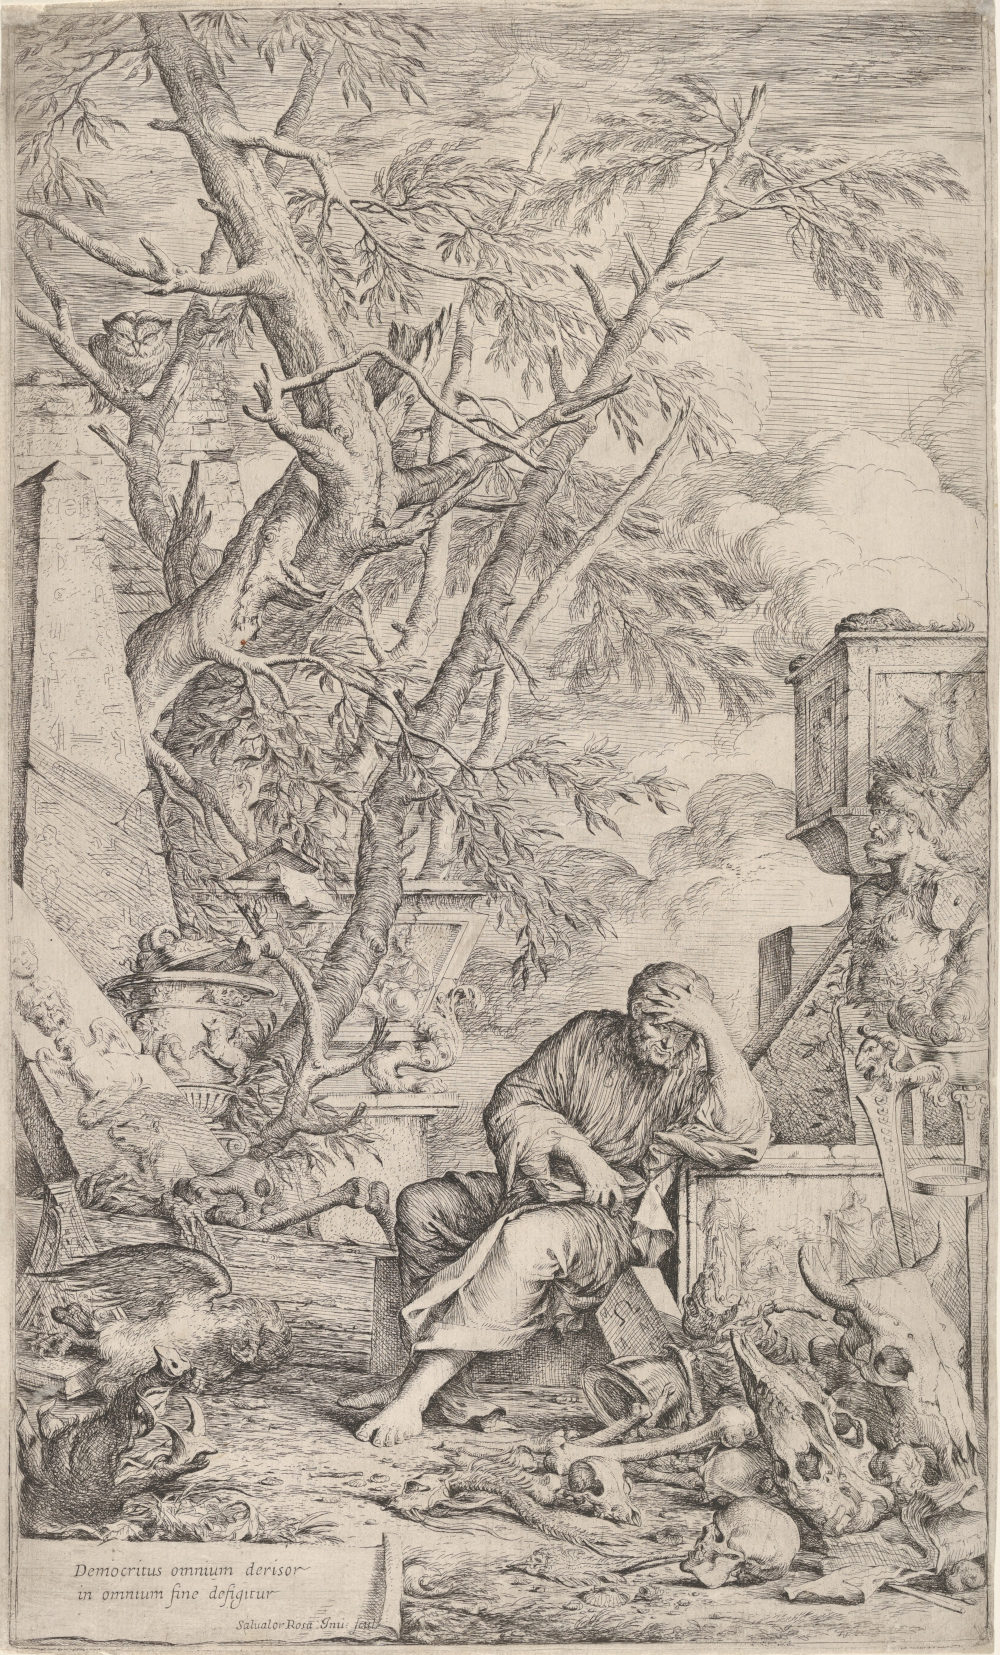
\includegraphics[keepaspectratio,width=0.9\textwidth]{figures/Democritus-in-MeditationDP831915-small.jpg}
  \captionart{DemocritusinMeditation}
  \label{fig:democritusinmeditation}
\end{figure}
% Force float here
\clearpage{}
}

\chapter{To the Reader who Employs His Leisure Ill}
\index{Democritus}
\setauthornote{817}{\textlatin{Si me commorit, melius non tangere clamo.} \Horace{}.}
\setauthornote{818}{\textlatin{Hippoc. epist. Damageto, accercitus sum ut Democritum tanquam insanum curarem, sed postquam conveni, non per Jovem desipienti\ae{}\ negotium, sed rerum omnium receptaculum deprehendi, ejusque ingenium demiratus sum. Abderitanos vero tanquam non sanos accusavi, veratri potione ipsos potius eguisse dicens.}}
\setauthornote{819}{\textlatin{Mart.}}

\noindent\textbf{LECTORI MALE FERIATO.}

\begin{latin}
\lettrine{T}{u} vero cavesis edico quisquis es, ne temere sugilles Auctorem hujusce
operis, aut cavillator irrideas. Imo ne vel ex aliorum censura tacite
obloquaris (vis dicam verbo) nequid nasutulus inepte improbes, aut
falso fingas. Nam si talis revera sit, qualem pr\ae{}\ se fert Junior
Democritus, seniori Democrito saltem affinis, aut ejus Genium vel
tantillum sapiat; actum de te, censorem \ae{}que ac delatorem \authormarginnote{817}[-5\baselineskip]aget
econtra (petulanti splene cum sit) sufflabit te in jocos, comminuet in
sales, addo etiam, et deo risui te sacrificabit.

Iterum moneo, ne quid cavillere, ne dum Democritum Juniorem conviciis
infames, aut ignominiose vituperes, de te non male sentientem, tu idem
audias ab amico cordato, quod olim vulgus Abderitanum ab \authormarginnote{818}[-7\baselineskip]
Hippocrate, concivem bene meritum et popularem suum Democritum, pro
insano habens. Ne tu Democrite sapis, stulti autem et insani Abderit\ae{}.

\begin{latin}
\begin{verse}%
Abderitanae pectora plebis habes.\\!
\end{verse}%
\end{latin}
\attrib{\getauthornote{819}}

H\ae{}c te paucis admonitum volo (male feriate Lector) abi.
\end{latin}

\begin{center}
{\Huge{}\color{maroon}}\par
\end{center}

\noindent\textbf{TO THE READER AT ILL LEISURE}

%TO THE READER AT LEISURE?
{\lettrine{W}{hoever} you may be, I caution you against rashly defaming the author of
this work, or \worddef{complaining}{cavilling} in jest against him. Nay, do not silently
reproach him in consequence of others' censure, nor employ your wit in
foolish disapproval, or false accusation. For, should Democritus Junior
prove to be what he professes, even a kinsman of his elder namesake, or
be ever so little of the same kidney, it is all over with you: he will
become both accuser and judge of you in your spleen, will dissipate you
in jests, pulverise you into salt, and sacrifice you, I can promise
you, to the God of Mirth.

I further advise you, not to asperse, or \worddef{defame}{calumniate}, or slander,
Democritus Junior, who possibly does not think ill of you, lest you may
hear from some discreet friend, the same remark the people of Abdera
did from Hippocrates, of their meritorious and popular fellow-citizen,
whom they had looked on as a madman; It is not that you, Democritus,
that art wise, but that the people of Abdera are fools and madmen. You
have yourself an Abderitian soul; and having just given you, gentle
reader, these few words of admonition, farewell.

%\settowidth{\versewidth}{Nunc opus est (tanta est insania) transeat omnis}
%\poemlines{2}
%\begin{verse}[\versewidth]
%Heraclite fleas, misero sic convenit aevo,\\*
%Nil nisi turpe vides, nil nisi triste vides.\\!
%
%Ride etiam, quantumque lubet, Democrite ride\\*
%Non nisi vana vides, non nisi stulta vides.\\!
%
%Is fletu, his risu modo gaudeat, unus utrique\\*
%Sit licet usque labor, sit licet usque dolor.\\!
%
%Nunc opes est (nam totus eheu jam desipit orbis)\\*
%Mille Heraclitis, milleque Democritis.\\!
%
%Nunc opus est (tanta est insania) transeat omnis\\*
%Mundus in Anticyras, gramen in Helleborum.\\!
%\end{verse}
%
%
%\settowidth{\versewidth}{A thousand Heraclitusf a thousand Democritus are requiredaaa}
\settowidth{\versewidth}{A thousand Heraclitus', a thousand Democritus' are required.}
\poemlines{2}
\begin{verse}[\versewidth]
Weep, O Heraclitus, it suits the age,\\*
Unless you see nothing base, nothing sad.\\!

Laugh, O Democritus, as much as you please,\\*
Unless you see nothing either vain or foolish.\\!

Let one rejoice in smiles, the other in tears;\\*
Let the same labour or pain be the office of both.\\!

Now (for alas! how foolish the world has become),\\*
A thousand Heraclitus', a thousand Democritus' are required.\\!

Now (so much does madness prevail), all the world must be\\*
Sent to Anticyra, to graze on Hellebore.\\!
\end{verse}
\poemlines{0}
}

\part{The First Partition}\label{part:first}
\chapter{The Synopsis of the First Partition}

\setauthornote{820}{\textlatin{Magnum miraculum.}}
\setauthornote{821}{\textlatin{Mundi epitome, naturae deliciae.}}
\setauthornote{822}{\textlatin{Finis rerum omnium, cui sublunaria serviunt. Scalig. exercit. 365. sec. 3. Vales. de sacr. Phil. c. 5.}}
\setauthornote{823}{\textlatin{Ut in numismate Caesaris imago, sic in homine Dei.}}
\setauthornote{824}{Gen. 1.}
\setauthornote{825}{\textlatin{Imago mundi in corpore, Dei in anima. Exemplumque dei quisque est in imagine parva.}}
\setauthornote{826}{Eph. \rn{iv}. 24.}
\setauthornote{827}{Palan terius.}
\setauthornote{828}{Psal. \rn{xlix}. 20.}
\setauthornote{829}{\textlatin{Lascivia superat equum, impudentia canem, astu vulpem, furore leonem. Chrys. 23. Gen.}}
\setauthornote{830}{Gen. \rn{iii}. 13.}
\setauthornote{831}{Ecclus. \rn{iv}. 1, 2, 3, 4, 5, 8.}
\setauthornote{832}{Gen. \rn{iii}. 17.}
\setauthornote{833}{\textlatin{Illa cadens tegmen manibus decussit, et una perniciem immisit miseris mortalibus atram. Hesiod. 1. oper.}}
\setauthornote{834}{Hom. 5. ad pop. Antioch.}
\setauthornote{835}{Psal. \rn{cvii}. 17.}
\setauthornote{836}{Pro. i. 27.}
\setauthornote{837}{\textlatin{Quod autem crebrius bella concutiant, quod sterilitas et fames solicitudinem cumulent, quod saevientibus morbis valitudo frangitur, quod humanum genus luis populatione vastatur; ob peccatum omnia. Cypr.}}
\setauthornote{838}{\textlatin{Si raro desuper pluvia descendat, si terra situ pulveris squalleat, si vix jejunas et pallidas heibas sterilis gleba producat, si turbo vineam debilitet, \&c. Cypr.}}
\setauthornote{839}{Mat. \rn{xiv}. 3.}
\setauthornote{840}{\textlatin{Philostratus, lib. 8. vit. Apollonii. Injustitiam ejus, et sceleratas nuptias, et caeteta quae praeter rationem fecerat, morborum causas dixit.}}
\setauthornote{841}{16.}
\setauthornote{842}{18.}
\setauthornote{843}{20.}
\setauthornote{844}{Verse 17.}
\setauthornote{845}{\textlatin{28. Deos quos diligit, castigat.}}
\setauthornote{846}{Isa. v. 13. Verse 15.}
\setauthornote{847}{\textlatin{Nostrae salutis avidus continenter aures vellicat, ac calamitate subinde nos exercet. Levinus Lemn. l. 2. c. 29. de occult, nat. mir.}}
\setauthornote{848}{\textlatin{Vexatio dat Intellectum. Isa. \rn{xiviii}. 19.}}
\setauthornote{849}{in sickness the mind recollects itself}
\setauthornote{850}{\textlatin{Lib. 7. Cum judicio, mores et facta recognoscit et se intuetur. Dum fero languorem, fero religionis amorem. Expers languoris non sum memor hujus amoris.}}
\setauthornote{851}{\textlatin{Summum esse totius philosophiae, ut tales esse perseveremus, quales nos futures esse infirmi profitemur.}}
\setauthornote{852}{Petrarch.}
\setauthornote{853}{Prov. \rn{iii}. 12.}
\setauthornote{854}{Hor. Epis. lib. 1. 4.}
\setauthornote{855}{\textlatin{Deut. \rn{viii}. 11. Qui stat videat ne cadat.}}
\setauthornote{856}{\textlatin{Quanto majoribus beneficiis a Deo cumulatur, tanto obligatiorem se debitorem fateri.}}
\setauthornote{857}{\textlatin{Boterus de Inst. urbium.}}
\setauthornote{858}{\textlatin{Lege hist, relationem Lod. Frois de rebus Japonicis ad annum 1596.}}
\setauthornote{859}{\textlatin{Guicciard. descript. Belg. anno 1421.}}
\setauthornote{860}{\textlatin{Giraldus Cambrens.}}
\setauthornote{861}{Janus Dousa, ep. lib. 1. car. 10.}
\setauthornote{861.5}{And we perceive nothing, except the dead bodies of cities in the open sea}
\setauthornote{862}{Munster l. 3. Cos. cap. 462.}
\setauthornote{863}{Buchanan. Baptist.}
\setauthornote{864}{\textlatin{Homo homini lupus, homo homini daemon.}}
\setauthornote{865}{Ovid. de Trist. l. 5. Eleg.}
\setauthornote{866}{\textlatin{Miscent aconita novercae.}}
\setauthornote{867}{Lib. 2 Epist. 2. ad Donatum.}
\setauthornote{868}{\textlatin{Eze. \rn{xviii}. 2.}}
\setauthornote{869}{Hor. l. 3. Od. 6.}
\setauthornote{870}{\textlatin{2 Tim. \rn{iii}. 2.}}
\setauthornote{871}{Eze. \rn{xviii}. 31.}
\setauthornote{871.5}{thy destruction is from thyself}
\setauthornote{872}{\textlatin{21 Macc. \rn{iii}. 12.}}
\setauthornote{873}{Part. 1. Sec. 2. Memb. 2.}
\setauthornote{874}{\textlatin{Nequitia est quae te non sinet esse senem.}}
\setauthornote{875}{Homer. Iliad.}
\setauthornote{876}{\textlatin{Intemperantia, luxus, ingluvies, et infinita hujusmodi flagitia, quae divinas poenas merentur. Crato.}}
\setauthornote{877}{\textlatin{Fern. Path. l. 1. c. 1. Morbus est affectus contra, naturam corpori insides.}}
\setauthornote{878}{\textlatin{Fusch. Instit. l. 3. sect. 1. c. 3. a quo primum vitiatur actio.}}
\setauthornote{879}{\textlatin{Dissolutio foederis in corpore, ut sanitas est consummatio.}}
\setauthornote{880}{\textlatin{Lib. 4. cap. 2. Morbus est habitus contra naturam, qui usum ejus, \&c.}}
\setauthornote{881}{Cap. 11. lib. 7.}
\setauthornote{882}{Horat. lib. 1. ode 3.}
\setauthornote{882.5}{Emaciation, and a new cohort of fevers broods over the earth.}
\setauthornote{883}{\textlatin{Cap. 50. lib. 7. Centum et quinque vixit annos sine ullo incommodo.}}
\setauthornote{884}{\textlatin{Intus mulso, foras oleo.}}
\setauthornote{885}{\textlatin{Exemplis genitur. praefixis Ephemer. cap. de infirmitat.}}
\setauthornote{886}{\textlatin{Qui, quoad pueritae ultimam memoriam recordari potest non meminit se aegrotum decubuisse.}}
\setauthornote{887}{\textlatin{Lib. de vita longa.}}
\setauthornote{888}{Oper. et. dies.}
\setauthornote{889}{See Fernelius Path. lib. 1. cap. 9, 10, 11, 12. Fuschius Instit. l. 3. sect. 1. c. 7. Wecker. Synt.}
\setauthornote{890}{\textlatin{Praefat. de morbis capitis. In capite ut variae habitant partes, ita variae querelae ibi eveniunt.}}
\setauthornote{891}{Of which read Heurnius, Montaltus, Hildesheim, Quercetan, Jason Pratensis, \&c.}
\setauthornote{892}{Cap. 2. de melanchol.}
\setauthornote{893}{\textlatin{Cap. 2. de Phisiologia sagarum: Quod alii minus recte fortasse dixerint, nos examinare, melius dijudicare, corrigere studeamus.}}
\setauthornote{894}{Cap. 4. de mol.}
\setauthornote{895}{Art. Med. 7.}
\setauthornote{896}{\textlatin{Plerique medici uno complexu perstringunt hos duos morbos, quod ex eadem causa oriantur, quodque magnitudine et modo solum distent, et alter gradus ad alterum existat. Jason Pratens.}}
\setauthornote{897}{Lib. Med.}
\setauthornote{898}{\textlatin{Pars maniae mihi videtur.}}
\setauthornote{899}{\textlatin{Insanus est, qui aetate debita, et tempore debito per se, non momentaneam et fugacem, ut vini, solani, Hyoscyami, sed confirmatam habet impotentiam bene operandi circa intellectum. lib. 2. de intellectione.}}
\setauthornote{900}{Of which read Felix Plater, cap. 3. de mentis alienatione.}
\setauthornote{901}{Lib. 6. cap. 11.}
\setauthornote{902}{Lib. 3. cap. 16.}
\setauthornote{903}{Cap. 9. Art. med.}
\setauthornote{904}{\textlatin{De praestig. Daemonum, l. 3. cap. 21.}}
\setauthornote{905}{\textlatin{Observat. lib. 10. de morbis cerebri, cap. 15.}}
\setauthornote{906}{\textlatin{Hippocrates lib. de insania.}}
\setauthornote{907}{\textlatin{Lib. 8. cap. 22. Homines interdum lupos feri; et contra.}}
\setauthornote{908}{\textlatin{Met. lib. 1.}}
\setauthornote{909}{\textlatin{Cap. de Man.}}
\setauthornote{910}{\textlatin{Ulcerata crura, sitis ipsis adest immodica, pallidi, lingua sicca.}}
\setauthornote{911}{Cap. 9. art. Hydrophobia.}
\setauthornote{912}{Lib. 3. cap. 9.}
\setauthornote{913}{Lib. 7. de Venenis.}
\setauthornote{914}{\textlatin{Lib. 3. cap. 13. de morbis acutis.}}
\setauthornote{915}{Spicel. 2.}
\setauthornote{916}{Sckenkius, 7 lib. de Venenis.}
\setauthornote{917}{Lib. de Hydrophobia.}
\setauthornote{918}{Observat. lib. 10. 25.}
\setauthornote{919}{\textlatin{Lascivam Choream. To. 4. de morbis amentium. Tract. 1.}}
\setauthornote{920}{\textlatin{Eventu ut plurimum rem ipsam comprobante.}}
\setauthornote{921}{Lib. 1. cap. de Mania.}
\setauthornote{922}{\textlatin{Cap. 3. de mentis alienat.}}
\setauthornote{923}{Cap. 4. de mel.}
\setauthornote{924}{\hyperref[part:third]{PART. 3.}}
\setauthornote{925}{\textlatin{De quo homine securitas, de quo certum gaudium? quocunque se convertit, in terrenis rebus amaritudinem animi inveniet. Aug. in Psal. \rn{viii}. 5.}}
\setauthornote{926}{Job. i. 14.}
\setauthornote{927}{\textlatin{Omni tempore Socratem eodem vultu videri, sive domum rediret, sive domo egrederetur.}}
\setauthornote{928}{\textlatin{Lib. 7. cap. 1. Natus in florentissima totius orbis civitate, nobilissimis parentibus, corpores vires habuit et rarissimas animi dotes, uxorem conapicuam, pudicam, felices liberos, consulare decus, sequentes triumphos, \&c.}}
\setauthornote{929}{Aelian.}
\setauthornote{930}{Homer. Iliad.}
\setauthornote{931}{\textlatin{Lipsius, cent. 3. ep. 45, ut coelum, sic nos homines sumus: illud ex intervallo nubibus obducitur et obscuratur. In rosario flores spinis intermixti. Vita similis aeri, udum modo, sudum, tempestas, serenitas: ita vices rerum sunt, praemia gaudiis, et sequaces curae.}}
\setauthornote{932}{Lucretius, l. 4. 1124.}
\setauthornote{933}{\textlatin{Prov. \rn{xiv}. 13. Extremum gaudii luctas occupat.}}
\setauthornote{934}{\textlatin{Natalitia inquit celebrantur, nuptiae hic sunt; at ibi quid celebratur quod non dolet, quod non transit?}}
\setauthornote{935}{\textlatin{Apuleius 4. florid. Nihil quicquid homini tam prosperum divinitus datum, quin ei admixtum sit aliquid difficultatis ut etiam amplissima quaqua laetitia, subsit quaepiam vel parva querimonia conjugatione quadam mellis, et fellis.}}
\setauthornote{936}{\textlatin{Caduca nimirum et fragilia, et puerilibus consentanea crepundiis sunt ista quae vires et opes humanae vocantur, affluunt subito, repente delabuntur, nullo in loco, nulla in persona, stabilibus nixa radicibus consistunt, sed incertissimo flatu fortunae quos in sublime extulerunt improviso recursu destitutos in profundo miseriarum valle miserabiliter immergunt. Valerius, lib. 6. cap. 11.}}
\setauthornote{937}{\textlatin{Huic seculo parum aptus es, aut potius omnium nostrorum conditionem ignoras, quibus reciproco quodam nexu, \&c. Lorchanus Gollobelgicus, lib. 3. ad annum 1598.}}
\setauthornote{938}{\textlatin{Horsum omnia studia dirigi debent, ut humana fortiter feramus.}}
\setauthornote{939}{2 Tim. \rn{ii}. 3.}
\setauthornote{940}{\textlatin{Epist. 96. lib. 10. Affectus frequentes contemptique morbum faciunt. Distillatio una nec adhuc in morem adaucta, tussim facit, assidua et violenta pthisim.}}
\setauthornote{941}{\textlatin{Calidum ad octo: frigidum ad octo. Una hirundo non facit aestatem.}}
\setauthornote{942}{Lib. 1. c. 6.}
\setauthornote{943}{Fuschius, l. 3. sec. 1. cap. 7. Hildesheim, fol. 130.}
\setauthornote{944}{Psal. \rn{xxxix}. 13.}
\setauthornote{945}{\textlatin{De Anima. Turpe enim est homini ignorare sui corporis (ut ita dicam) aedificium, praesertim cum ad valetudinem et mores haec cognitio plurimum conducat.}}
\setauthornote{946}{\textlatin{De usu part.}}
\setauthornote{947}{History of man.}
\setauthornote{948}{D. Crooke.}
\setauthornote{949}{In Syntaxi.}
\setauthornote{950}{De Anima.}
\setauthornote{951}{Istit. lib. 1.}
\setauthornote{952}{Physiol. l. 1, 2.}
\setauthornote{953}{Anat. l. 1. c. 18.}
\setauthornote{954}{\textlatin{In Micro. succos, sine quibus animal sustentari non potest.}}
\setauthornote{955}{\textlatin{Morbosos humores.}}
\setauthornote{956}{\textlatin{Spiritalis anima.}}
\setauthornote{957}{Laurentius, cap. 20, lib. 1. Anat.}
\setauthornote{958}{In these they observe the beating of the pulse.}
\setauthornote{959}{\textlatin{Cujus est pars simularis a vi cutifica ut interiora muniat. Capivac. Anat. pag. 252.}}
\setauthornote{960}{\textlatin{Anat. lib. 1. c. 19. Celebris est pervulgata partium divisio principes et ignobiles partes.}}
\setauthornote{961}{D. Crooke out of Galen and others.}
\setauthornote{962}{\textlatin{Vos vero veluti in templum ac sacrarium quoddam vos duci putetis, \&c. Suavis et utilis cognitio.}}
\setauthornote{963}{Lib. 1. cap. 12. sect. 5.}
\setauthornote{964}{\textlatin{Haec res est praecipue digna admiratione, quod tanta affectuum varietate cietur cor, quod omnes retristes et laetae statim corda feriunt et movent.}}
\setauthornote{965}{Physio. l. 1. c. 8.}
\setauthornote{966}{\textlatin{Ut orator regi: sic pulmo vocis instrumentum annectitur cordi, \&c. Melancth.}}
\setauthornote{967}{De anim. c. 1.}
\setauthornote{968}{Scalig. exerc. 307. Tolet. in lib. de anima. cap. 1. \&c.}
\setauthornote{969}{l. De anima. cap. 1.}
\setauthornote{970}{\textlatin{Tuscul. quaest.}}
\setauthornote{971}{Lib. 6. Doct. Va. Gentil. c. 13. pag. 1216.}
\setauthornote{972}{Aristot.}
\setauthornote{973}{\textlatin{Anima quaeque intelligimus, et tamen quae sit ipsa intelligere non valemus.}}
\setauthornote{974}{\textlatin{Spiritualem animam a reliquis distinctam tuetur, etiam in cadavere inhaerentem post mortem per aliquot menses.}}
\setauthornote{975}{Lib. 3. cap. 31.}
\setauthornote{976}{Coelius, lib. 2. c. 31. Plutarch, in Grillo Lips. Cen. 1. ep. 50. Jossius de Risu et Fletu, Averroes, Campanella, \&c.}
\setauthornote{977}{Phillip. de Anima. ca. 1. Coelius, 20. antiq. cap. 3. Plutarch. de placit. philos.}
\setauthornote{978}{De vit. et mort. part. 2. c. 3, prop. l. de vit. et mort. 2. c. 22.}
\setauthornote{979}{\textlatin{Nutritio est alimenti transmutatio, viro naturalis. Scal. exerc. 101, sec. 17.}}
\setauthornote{980}{See more of Attraction in Scal. exer. 343.}
\setauthornote{981}{\textlatin{Vita consistit in calido et humido.}}
\setauthornote{982}{Too bright an object destroys the organ}
\setauthornote{983}{\textlatin{Lumen est actus perspicui. Lumen a luce provenit, lux est in corpore lucido.}}
\setauthornote{984}{In Phaedon. (Notes 984-997 appear in the order 986, 984, 987, 985 in the original-KTH.)}
\setauthornote{985}{De pract. Philos. 4.}
\setauthornote{986}{Satur. 7. c. 14.}
\setauthornote{987}{Lac. cap. 8. de opif. Dei, I.}
\setauthornote{988}{Lib. 19. cap. 2.}
\setauthornote{989}{Phis. l. 5. c. 8.}
\setauthornote{990}{Exercit. 280.}
\setauthornote{991}{T. W. Jesuite, in his Passions of the Minde.}
\setauthornote{992}{Velcurio.}
\setauthornote{993}{\textlatin{Nervi a spiritu moventur, spritus ab anima. Melanct.}}
\setauthornote{994}{Velcurio. Jucundum et anceps subjectum.}
\setauthornote{995}{Goclenius in \textgreek{Ψυχολ}. pag. 302. Bright in Phys. Scrib. l. 1. David Crusius, Melancthon, Hippius Hernius, Levinus Lemnius, \&c.}
\setauthornote{996}{\textlatin{Lib. an mores sequantur, \&c.}}
\setauthornote{997}{Caesar. 6. com.}
\setauthornote{998}{Read Aeneas Gazeus dial. of the immortality of the Soul.}
\setauthornote{999}{Ovid. Met. 15.}
\setauthornote{999.5}{We, who may take up our abode in wild beasts, or be lodged in the breasts of cattle}
\setauthornote{1000}{In Gallo. Idem.}
\setauthornote{1001}{Nicephorus, hist. lib. 10. c. 35.}
\setauthornote{1002}{Phaedo.}
\setauthornote{1003}{Claudian, lib. 1. de rap. Proserp.}
\setauthornote{1004}{Besides, we observe that the mind is born with the body, grows with it, and decays with it}
\setauthornote{1005}{\textlatin{Haec quaestio multos per annos varie, ac mirabiliter impugnata, \&c.}}
\setauthornote{1006}{Colerus, ibid.}
\setauthornote{1007}{De eccles. dog. cap. 16.}
\setauthornote{1008}{Ovid. 4. Met.}
\setauthornote{1008.5}{The bloodless shades without either body or bones wanter}
\setauthornote{1009}{\textlatin{Bonorum lares, malorum vero larvas et lemures.}}
\setauthornote{1010}{Some say at three days, some six weeks, others otherwise.}
\setauthornote{1011}{Melancthon.}
\setauthornote{1012}{\textlatin{Nihil in intellectu, quod non prius fuerat in sensu. Velcurio.}}
\setauthornote{1013}{The pure part of the conscience.}
\setauthornote{1014}{\textlatin{Quod tibi fieri non vis, alteri ne feceris.}}
\setauthornote{1015}{\textlatin{Res ab intellectu monstratas recipit, vel rejicit; approbat, vel improbat, Philip. Ignoti nulla cupido.}}
\setauthornote{1016}{\textlatin{Melancthon. Operationes plerumque ferae, etsi libera sit illa in essentia sua.}}
\setauthornote{1017}{\textlatin{In civilibus libera, sed non in spiritualibus Osiander.}}
\setauthornote{1018}{\textlatin{Tota voluntas aversa a Deo. Omnis homo mendax.}}
\setauthornote{1019}{Virg.}
\setauthornote{1019.5}{We are neither able to contend against them, nor only to make way}
\setauthornote{1020}{\textlatin{Vel propter ignorantium, quod bonis studiis non sit instructa mens ut debuit, aut divinis praeceptis exculta.}}
\setauthornote{1021}{Med. Ovid.}
\setauthornote{1022}{Ovid.}
\setauthornote{1023}{Seneca, Hipp.}
\setauthornote{1024}{\textlatin{Melancholicos vocamus, quos exuperantia vel pravitas Melancholiae ita male habet, ut inde insaniant vel in omnibus, vel in pluribus iisque manifestis sive ad rectam rationem, voluntate pertinent, vel electionem, vel intellectus operationes.}}
\setauthornote{1025}{\textlatin{Pessimum et pertinacissimum morbum qui homines in bruta degenerare cogit.}}
\setauthornote{1026}{Panth. Med.}
\setauthornote{1027}{\textlatin{Angor animi in una contentione defixus, absque febre.}}
\setauthornote{1028}{Cap. 16. l. 1.}
\setauthornote{1029}{\textlatin{Eorum definitio morbus quid non sit potius quam quid sit, explicat.}}
\setauthornote{1030}{\textlatin{Animae functiones imminuuntur in fatuitate, tolluntur in mania, depravantur solum in melancholia. Herc. de Sax. cap. 1. tract. de Melanch.}}
\setauthornote{1031}{Cap. 4. de mel.}
\setauthornote{1032}{\textlatin{Per consensum sive per essentiam.}}
\setauthornote{1033}{Cap. 4. de mel.}
\setauthornote{1034}{Sec. 7. de mor. vulgar. lib. 6.}
\setauthornote{1035}{Spicel. de melancholia.}
\setauthornote{1036}{\textlatin{Cap. 3. de mel. Pars affecta cerebrum sive per consensum, sive per cerebrum contingat, et procerum auctoritate et ratione stabilitur.}}
\setauthornote{1037}{\textlatin{Lib. de mel. Cor vero vicinitatis ratione una afficitur, acceptum transversum ac stomachus cum dorsali spina, \&c.}}
\setauthornote{1038}{\textlatin{Lib. 1. cap. 10. Subjectum est cerebrum interius.}}
\setauthornote{1039}{\textlatin{Raro quisquam tumorem effugit lienis, qui hoc morbo afficitur, Piso. Quis affectus.}}
\setauthornote{1040}{See Donat. ab Altomar.}
\setauthornote{1041}{\textlatin{Facultas imaginandi, non cogitandi, nec memorandi laesa hic.}}
\setauthornote{1042}{Lib. 3. Fen. 1. Tract. 4. cap. 8.}
\setauthornote{1043}{Lib. 3. cap. 5.}
\setauthornote{1044}{Lib. Med. cap. 19. part. 2. Tract. 15. cap. 2.}
\setauthornote{1045}{\textlatin{Hildesheim, spicel. 2 de Melanc. fol. 207, et fol. 127. Quandoque etiam rationalis si affectus inveteratus sit.}}
\setauthornote{1046}{\textlatin{Lib. posthumo de Melanc. edit. 1620. Deprivatur fides, discursus, opinio, \&c. per vitium Imaginationes, ex Accidenti.}}
\setauthornote{1047}{\textlatin{Qui parvum caput habent, insensati plerique sunt. Arist. in physiognomia.}}
\setauthornote{1048}{Areteus, lib. 3. cap. 5.}
\setauthornote{1049}{\textlatin{Qui prope statum sunt. Aret. Mediis convenit aetatibus, Piso.}}
\setauthornote{1050}{De quartano.}
\setauthornote{1051}{Lib. 1. part. 2. cap. 11.}
\setauthornote{1052}{\textlatin{Primus ad Melancholiam non tam moestus sed et hilares, jocosi, cachinnantes, irrisores, et, qui plerumque praerubri sunt.}}
\setauthornote{1053}{\textlatin{Qui sunt subtilis ingenii, et multae perspicacitatis de facili incidunt in Melancholiam, lib. 1. cont. tract. 9.}}
\setauthornote{1054}{\textlatin{Nunquam sanitate mentis excidit aut dolore capitur. Erasm.}}
\setauthornote{1055}{\textlatin{In laud. calvit.}}
\setauthornote{1056}{\textlatin{Vacant conscientiae carnificina, nec pudefiunt, nec verentur, nec dilacerantur millibus curarum, quibus tota vita obnoxia est.}}
\setauthornote{1057}{Lib. 1. tract. 3. contradic. 18.}
\setauthornote{1058}{Lib. 1. cont. 21.}
\setauthornote{1059}{Bright, ca. 16.}
\setauthornote{1060}{Lib. 1. cap. 6. de sanit. tuenda.}
\setauthornote{1061}{\textlatin{Quisve aut qualis sit humor aut quae istius differentiae, et quomodo gignantur in corpore, scrutandum, hac enim re multi veterum laboraverunt, nec facile accipere ex Galeno sententiam ob loquendi varietatem. Leon. Jacch. com. in 9. Rhasis, cap. 15. cap. 16. in 9. Rhasis.}}
\setauthornote{1062}{\textlatin{Lib. postum. de Melan. edit. Venetiis, 1620. cap. 7 et 8. Ab intemperie calida, humida, \&c.}}
\setauthornote{1063}{\textlatin{Secundum magis aut minus si in corpore fuerit, ad intemperiem plusquam corpus salubriter ferre poterit: inde corpus morbosum effitur.}}
\setauthornote{1064}{Lib. 1. controvers. cap. 21.}
\setauthornote{1065}{Lib. 1. sect. 4, cap. 4.}
\setauthornote{1066}{Concil. 26.}
\setauthornote{1067}{Lib. 2. contradic. cap. 11.}
\setauthornote{1068}{\textlatin{De feb. tract. diff. 2. cap. 1. Non est negandum ex hac fieri Melancholicos.}}
\setauthornote{1069}{In Syntax.}
\setauthornote{1070}{\textlatin{Varie aduritur, et miscetur, unde variae amentium species, Melanct.}}
\setauthornote{1071}{\textlatin{Humor frigidus delirii causa, furoris calidus, \&c.}}
\setauthornote{1072}{Lib. 1. cap. 10. de affect. cap.}
\setauthornote{1073}{\textlatin{Nigrescit hic humor, aliquando supercalefactus, aliquando super frigefactus, ca. 7.}}
\setauthornote{1074}{\textlatin{Humor hic niger aliquando praeter modum calefactus, et alias refrigeratus evadit: nam recentibus carbonibus ei quid simile accidit, qui durante flamma pellucidissime candent, ea extincta prorsus nigrescunt. Hippocrates.}}
\setauthornote{1075}{Guianerius, diff. 2. cap. 7.}
\setauthornote{1076}{\textlatin{Non est mania, nisi extensa melancholia.}}
\setauthornote{1077}{Cap. 6. lib. 1.}
\setauthornote{1078}{\textlatin{2 Ser. 2. cap. 9. Morbus hic est omnifarius.}}
\setauthornote{1079}{\textlatin{Species indefinitae sunt.}}
\setauthornote{1080}{\textlatin{Si aduratur naturalis melancholia, alia fit species, si sanguis, alia, si flavibilis alia, diversa a primis: maxima est inter has differentia, et tot Doctorum sententiae, quot ipsi numero sunt.}}
\setauthornote{1081}{Tract. de mel. cap. 7.}
\setauthornote{1082}{\textlatin{Quaedam incipiens quaedam consummata.}}
\setauthornote{1083}{\textlatin{Cap. de humor. lib. de anima. Varie aduritur et miscetur ipsa melancholia, unde variae amentium species.}}
\setauthornote{1084}{Cap. 16. in. 9. Rasis.}
\setauthornote{1085}{Laurentius, cap. 4. de mel.}
\setauthornote{1086}{Cap. 13.}
\setauthornote{1087}{480. et 116. consult. consil. 12.}
\setauthornote{1088}{Hildesheim. spicil. 2. fol. 166.}
\setauthornote{1089}{Trincavellius, tom. 2. consil. 15 et 16.}
\setauthornote{1090}{Cap. 13, tract. posth. de melan.}
\setauthornote{1091}{Guarion. cons. med. 2.}
\setauthornote{1092}{\textlatin{Laboravit per essentiam et a toto corpore.}}
\setauthornote{1093}{Machiavel, \&c. Smithus de rep. Angl. cap. 8. lib. 1. Buscoldus, discur. polit. discurs. 5. cap. 7. Arist. l. 3. polit. cap. ult. Keckerm. alii, \&c.}
\setauthornote{1094}{Lib. 6.}
\setauthornote{1095}{\textlatin{Primo artis curitivae.}}
\setauthornote{1096}{\textlatin{Nostri primum sit propositi affectionum causas indagare; res ipsa hortari videtur, nam alioqui earum curatio, manca et inutilis esset.}}
\setauthornote{1097}{\textlatin{Path. lib. 1. cap. 11. Rerum cognoscere causas, medicis imprimis necessarium, sine qua nec morbum curare, nec praecavere licet.}}
\setauthornote{1098}{\textlatin{Tanta enim morbi varietas ac differentia ut non facile dignoscatur, unde initium morbus sumpserit. Melanelius e Galeno.}}
\setauthornote{1099}{\textlatin{Felix qui potuit rerum cognoscere causas.}}
\setauthornote{1100}{1 Sam. \rn{xvi}. 14.}
\setauthornote{1101}{Dan. v. 21.}
\setauthornote{1102}{Lactant. instit. lib. 2. cap. 8.}
\setauthornote{1103}{\textlatin{Mente captus, et summo animi moerore consumptus.}}
\setauthornote{1104}{\textlatin{Munster cosmog. lib. 4. cap. 43. De coelo substernebantur, tanquam insani de saxis praecipitati, \&c.}}
\setauthornote{1105}{Livius lib. 38.}
\setauthornote{1106}{\textlatin{Gaguin. l. 3. c. 4. Quod Dionysii corpus discooperuerat, in insanam incidit.}}
\setauthornote{1107}{\textlatin{Idem lib. 9. sub. Carol. 6. Sacrorum contemptor, templi foribus effractis, dum D. Johannis argenteum simulacrum rapere contendit, simulacrum aversa facie dorsum ei versat, nec mora sacrilegus mentis inops, atque in semet insaniens in proprios artus desaevit.}}
\setauthornote{1108}{Giraldus Cambrensis, lib 1. c. 1. Itinerar. Cambriae.}
\setauthornote{1109}{Delrio, tom. 3. lib. 6. sect. 3. quaest. 3.}
\setauthornote{1110}{Psal. \rn{xlvi}. 1.}
\setauthornote{1111}{Lib. 8. cap. de Hierar.}
\setauthornote{1112}{Claudian.}
\setauthornote{1113}{De Babila Martyre.}
\setauthornote{1114}{Lib. cap. 5. prog.}
\setauthornote{1115}{\textlatin{Lib. 1. de Abditis rerum causis.}}
\setauthornote{1116}{Respons. med. 12. resp.}
\setauthornote{1117}{1 Pet. v. 6.}
\setauthornote{1118}{\textlatin{Lib. 1. c. 7. de orbis concordia. In nulla re major fuit altercatio, major obscuritas, minor opinionum concordia, quam de daemonibus et substantiis separatis.}}
\setauthornote{1119}{Lib. 3. de Trinit. cap. 1.}
\setauthornote{1120}{Pererius in Genesin. lib. 4. in cap. 3. v. 23.}
\setauthornote{1121}{See Strozzius \textlatin{Cicogna omnifariae}. Mag. lib. 2. c. 15. Jo. Aubanus, Bredenbachius.}
\setauthornote{1122}{\textlatin{Angelus per superbiam separatus a Deo, qui in veritate non stetit. Austin.}}
\setauthornote{1123}{\textlatin{Nihil aliud sunt Daemones quam nudae animae quae corpore deposito priorem miserati vitam, cognatis succurrunt commoti misericordia, \etc{}}}
\setauthornote{1124}{De Deo Socratis.}
\setauthornote{1124.5}{All those mortals are called Gods, who, the course of life being prudently guided and governed, are honoured by men with temples and sacrifices, as Osiris in Aegypt, \etc{}}
\setauthornote{1125}{He lived 500 years since.}
\setauthornote{1126}{\textlatin{Apuleius: spiritus animalia sunt animo passibilia, mente rationalia, corpore aeria, tempore sempiterna.}}
\setauthornote{1127}{\textlatin{Nutriuntur, et excrementa habent, quod pulsata doleant solido percussa corpore.}}
\setauthornote{1128}{Whatever occupies space is corporeal:-spirit occupies space, \emph{therefore}, \etc{} \etc{}}
\setauthornote{1129}{4 lib. 4. Theol. nat. fol. 535.}
\setauthornote{1130}{Which has no roughness, angles, fractures, prominences, but is the most perfect amongst perfect bodies}
\setauthornote{1131}{Cyprianus in Epist. \textlatin{montes etiam et animalia transferri possunt}: as the devil did Christ to the top of the pinnacle; and witches are often translated. See more in Strozzius Cicogna, lib. 3. cap. 4. omnif. mag. \textlatin{Per aera subducere et in sublime corpora ferre possunt}, Biarmanus. \textlatin{Percussi dolent et uruntur in conspicuos cineres}. Agrippa, lib. 3. cap. de occul. Philos.}
\setauthornote{1132}{Agrippa, de occult. Philos. lib. 3. cap. 18.}
\setauthornote{1133}{\hyperref[sec:heroical-love]{Part. 3. Sect. 2. Mem. 1. Subs. 1. Love Melancholy.}}
\setauthornote{1134}{By gazing steadfastly on the sun illuminated with his brightest rays}
\setauthornote{1135}{\textlatin{Genial. dierum. Ita sibi visum et compertum quum prius an essent ambigeret Fidem suam liberet.}}
\setauthornote{1136}{Lib. 1. de verit. Fidei. Benzo, \&c.}
\setauthornote{1137}{\textlatin{Lib. de Divinatione et magia.}}
\setauthornote{1138}{\textlatin{Cap. 8. Transportavit in Livoniam cupiditate videndi, \&c.}}
\setauthornote{1139}{\textlatin{Sic Hesiodus de Nymphis vivere dicit. 10. aetates phaenicum vel. 9. 7. 20.}}
\setauthornote{1140}{\textlatin{Custodes hominum et provinciarum, \&c. tanto meliores hominibus, quanto hi brutis animantibus.}}
\setauthornote{1141}{\textlatin{Praesides Pastores, Gubernatores hominum, et illi animalium.}}
\setauthornote{1142}{Coveting nothing more than the admiration of mankind}
\setauthornote{1143}{\textlatin{Natura familiares ut canes hominibus multi aversantur et abhorrent.}}
\setauthornote{1144}{\textlatin{Ab nomine plus distant quam homo ab ignobilissimo verne, et tamen quidam ex his ab hominibus superantur ut homines a feris, \&c.}}
\setauthornote{1145}{\textlatin{Cibo et potu uti et venere cum hominibus ac tandem mori, Cicogna. l. part. lib. 2. c. 3.}}
\setauthornote{1146}{\textlatin{Plutarch. de defect. oraculorum.}}
\setauthornote{1147}{Lib. de Zilphis et Pigmeis.}
\setauthornote{1148}{Dii gentium a Constantio prostigati sunt, \&c.}
\setauthornote{1149}{\textlatin{Octovian. dial. Judaeorum deum fuisse Romanorum numinibus una cum gente captivum.}}
\setauthornote{1150}{\textlatin{Omnia spiritibus plena, et ex eorum concordia et discordia omnes boni et mali effectus promanant, omnia humana reguntur: paradoxa veterum de quo Cicogna. omnif. mag. l. 2. c. 3.}}
\setauthornote{1151}{\textlatin{Oves quas abacturus erat in quascunque formas vertebat Pausanias, Hyginus.}}
\setauthornote{1152}{\textlatin{Austin in l. 2. de Gen. ad literam cap. 17. Partim quia subtilioris sensus acumine, partim scientia calidiore vigent et experientia propter magnam longitudinem vitae, partim ab Angelis discunt, \&c.}}
\setauthornote{1153}{Lib. 3. omnif. mag. cap. 3.}
\setauthornote{1154}{L. 18. quest.}
\setauthornote{1155}{\textlatin{Quum tanti sit et tam profunda spiritum scientia, mirum non est tot tantasque res visu admirabiles ab ipsis patrari, et quidem rerum naturalium ope quas multo melius intelligunt, multoque peritius suis locis et temporibus applicare norunt, quam homo, Cicogna.}}
\setauthornote{1156}{\textlatin{Aventinus, quicquid interdiu exhauriebatur, noctu explebatur. Inde pavefacti cura tores, \&c.}}
\setauthornote{1157}{\textlatin{In lib. 2. de Anima text 29. Homerus discriminatim omnes spiritus daemones vocat.}}
\setauthornote{1158}{\textlatin{A Jove ad inferos pulsi, \&c.}}
\setauthornote{1159}{\textlatin{De Deo Socratis adest mihi divina sorte Daemonium quoddam a prima pueritia me secutum, saepe dissuadet, impellit nonnunquam instar ovis, Plato.}}
\setauthornote{1160}{\textlatin{Agrippa lib. 3. de occul. ph. c. 18. Zancb. Pictorus, Pererius Cicogna. l. 3. cap. 1.}}
\setauthornote{1161}{\textlatin{Vasa irae. c. 13.}}
\setauthornote{1162}{\textlatin{Quibus datum est nocere terrae et mari, \&c.}}
\setauthornote{1163}{\textlatin{Physiol. Stoicorum e Senec. lib. 1. cap. 28.}}
\setauthornote{1164}{\textlatin{Usque ad lunam animas esse aethereas vocarique heroas, lares, genios.}}
\setauthornote{1165}{Mart. Capella.}
\setauthornote{1166}{\textlatin{Nihil vacuum ab his ubi vel capillum in aere vel aqua jaceas.}}
\setauthornote{1167}{Lib. de Zilp.}
\setauthornote{1168}{Palingenius.}
\setauthornote{1169}{Lib. 7. cap. 34 et 5. Syntax. art. mirab.}
\setauthornote{1170}{\textlatin{Comment in dial. Plat. de amore, cap. 5. Ut sphaera quaelibet super nos, ita praestantiores habent habitatores suae sphaerae consortes, ut habet nostra.}}
\setauthornote{1171}{\textlatin{Lib. de Amica. et daemone med. inter deos et homines, dica ad nos et nostra aequaliter ad deos ferunt.}}
\setauthornote{1172}{\textlatin{Saturninas et Joviales accolas.}}
\setauthornote{1173}{\textlatin{In loca detrusi sunt infra caelestes orbes in aerem scilicet et infra ubi Judicio generali reservantur.}}
\setauthornote{1174}{q. 36. art. 9.}
\setauthornote{1175}{Virg. 8. Eg.}
\setauthornote{1176}{Aen. 4.}
\setauthornote{1177}{\textlatin{Austin: hoc dixi, ne quis existimet habitare ibimala daemonia ubi Solem et Lunam et Stellas Deus ordinavit, et alibi nemo arbitraretur Daemonom coelis habitare cum Angelis suis unde lapsum credimus. Idem. Zanch. l. 4. c. 3. de Angel. mails. Pererius in Gen. cap. 6. lib. 8. in ver. 2.}}
\setauthornote{1178}{Perigram. Hierosol.}
\setauthornote{1179}{Fire worship, or divination by fire.}
\setauthornote{1180}{\textlatin{Domus Diruunt, muros dejiciunt, immiscent se turbinibus et procellis et pulverem instar columnae evehunt. Cicogna l. 5. c. 5.}}
\setauthornote{1181}{Quest. in Liv.}
\setauthornote{1182}{\textlatin{De praestigiis daemonum. c. 16. Convelli culmina videmus, prosterni sata, \&c.}}
\setauthornote{1183}{\textlatin{De bello Neapolitano, lib. 5.}}
\setauthornote{1184}{\textlatin{Suffitibus gaudent. Idem Just. Mart. Apol. pro Christianis.}}
\setauthornote{1185}{\textlatin{In Dei imitationem}, saith Eusebius.}
\setauthornote{1186}{\textlatin{Dii gentium Daemonia, \&c. ego in eorum statuas pellexi.}}
\setauthornote{1187}{\textlatin{Et nunc sub divorum nomine coluntur a Pontificiis.}}
\setauthornote{1188}{Lib. 11. de rerum ver.}
\setauthornote{1189}{\textlatin{Lib. 3. cap. 3. De magis et veneficis, \&c. Nereides.}}
\setauthornote{1190}{Lib. de Zilphis.}
\setauthornote{1191}{Lib. 3.}
\setauthornote{1192}{\textlatin{Pro salute hominum excubare se simulant, sed in eorum perniciem omnia moliuntur. Aust.}}
\setauthornote{1193}{Dryades, Oriades, Hamadryades.}
\setauthornote{1194}{Elvas Olaus voc. at lib. 3.}
\setauthornote{1195}{Part 1. cap. 19.}
\setauthornote{1196}{\textlatin{Lib. 3. cap. 11. Elvarum choreas Olaus lib. 3. vocat saltum adeo profunde in terras imprimunt, ut locus insigni deinceps virore orbicularis sit, et gramen non pereat.}}
\setauthornote{1197}{Sometimes they seduce too simple men into their mountain retreats, where they exhibit wonderful sights to their marvelling eyes, and astonish their ears by the sound of bells, \etc{}}
\setauthornote{1198}{Lib. de Zilph. et Pigmaeus Olaus lib. 3.}
\setauthornote{1199}{\textlatin{Lib. 7. cap. 14. Qui et in famulitio viris et feminis inserviunt, conclavia scopis purgant, patinas mundant, ligna portant, equos curant, \&c.}}
\setauthornote{1200}{\textlatin{Ad ministeria utuntur.}}
\setauthornote{1201}{Where treasure is hid (as some think) or some murder, or such like villainy committed.}
\setauthornote{1202}{Lib. 16. de rerum varietat.}
\setauthornote{1203}{\textlatin{Vel spiritus sunt hujusmodi damnatorum, vel e purgatorio, vel ipsi daemones, c. 4.}}
\setauthornote{1204}{\textlatin{Quidam lemures domesticis instrumentis noctu ludunt: patinas, ollas, cantharas, et alia vasa dejiciunt, et quidam voces emittunt, ejulant, risum emittunt, \&c. ut canes nigri, feles, variis formis, \&c.}}
\setauthornote{1205}{Epist. lib. 7.}
\setauthornote{1206}{\textlatin{Meridionales Daemones} Cicogna calls them, or Alastores, l. 3. cap. 9.}
\setauthornote{1207}{Sueton. c. 69. in Caligula.}
\setauthornote{1208}{Strozzius Cicogna. lib. 3. mag. cap. 5.}
\setauthornote{1209}{Idem. c. 18.}
\setauthornote{1210}{M. Carew. Survey of Cornwall, lib. 2. folio 140.}
\setauthornote{1211}{Horto Geniali, folio 137.}
\setauthornote{1212}{\textlatin{Part 1. c. 19. Abducunt eos a recta via, et viam iter facientibus intercludunt.}}
\setauthornote{1213}{\textlatin{Lib. 1. cap. 44. Daemonum cernuntur et audiuntur ibi frequentes illusiones, unde viatoribus cavendum ne ce dissocient, aut a tergo maneant, voces enim fingunt sociorum, ut a recto itinere abducant, \&c.}}
\setauthornote{1214}{\textlatin{Mons sterilis et nivosus, ubi intempesta nocte umbrae apparent.}}
\setauthornote{1215}{\textlatin{Lib. 2. cap. 21. Offendicula faciunt transeuntibus in via et petulanter ridet cum vel hominem vel jumentum ejus pedes atterere faciant, et maxime si homo maledictus et calcaribus saevint.}}
\setauthornote{1216}{In Cosmogr.}
\setauthornote{1217}{\textlatin{Vestiti more metallicorum, gestus et opera eorum imitantur.}}
\setauthornote{1218}{\textlatin{Immisso in terrae carceres vento horribiles terrae motus efficiunt, quibus saepe non domus modo et turres, sed civitates integrae et insulae haustae sunt.}}
\setauthornote{1219}{\textlatin{Hierom. in 3. Ephes. Idem Michaelis. c. 4. de spiritibus. Idem Thyreus de locis infestis.}}
\setauthornote{1220}{\textlatin{Lactantius 2. de origins erroris cap. 15. hi maligni spiritus per omnem terram vagantur, et solatium perditionis suae perdendis hominibus operantur.}}
\setauthornote{1221}{\textlatin{Mortalium calamitates epulae sunt malorum daemonum, Synesius.}}
\setauthornote{1222}{\textlatin{Daminus mendacii a seipso deceptus, alios decipere cupit, adversarius humani generis, Inventor mortis, superbiae institutor, radix malitiae, scelerum caput, princeps omnium vitiorum, fuit inde in Dei contumeliam, hominum perniciem: de horum conatibus et operationibus lege Epiphanium. 2. Tom. lib. 2. Dionysium. c. 4. Ambros. Epistol. lib. 10. ep. et 84. August. de civ. Dei lib. 5. c. 9., lib. 8. cap. 22. lib. 9. 18. lib. 10. 21. Theophil. in 12. Mat. Pasil. ep. 141. Leonem Ser. Theodoret. in 11. Cor. ep. 22. Chrys. hom. 53. in 12. Gen. Greg. in 1. c. John. Barthol. de prop. l. 2. c. 20. Zanch. l. 4. de malis angelis. Perer. in Gen. l. 8. in c. 6. 2. Origen. saepe praeliis intersunt, itinera et negotia nostra quaecumque dirigunt, clandestinis subsidiis optatos saepe praebent successus, Pet. Mar. in Sam. \&c. Ruscam de Inferno.}}
\setauthornote{1223}{\textlatin{Et velut mancipia circumfert Psellus.}}
\setauthornote{1224}{\textlatin{Lib. de trans. mut. Malac. ep.}}
\setauthornote{1225}{\textlatin{Custodes sunt hominum, et eorum, ut nos animalium: tum et provinciis praepositi regunt auguriis, somniis, oraculis, pramiis, \&c.}}
\setauthornote{1226}{Lipsius, Physiol. Stoic, lib. 1. cap. 19.}
\setauthornote{1227}{Leo Suavis. idem et Tritemius.}
\setauthornote{1228}{They seek nothing more earnestly than the fear and admiration of men}
\setauthornote{1229}{It is scarcely possible to describe the impotent ardour with which these malignant spirits aspire to the honour of being divinely worshipped}
\setauthornote{1230}{Omnif. mag. lib. 2. cap. 23.}
\setauthornote{1231}{\textlatin{Ludus deorum sumus.}}
\setauthornote{1232}{\textlatin{Lib. de anima et daemone.}}
\setauthornote{1233}{\textlatin{Quoties sit, ut Principes novitium aulicum divitiis et dignitatibus pene obruant, et multorum annorum ministrum, qui non semel pro hero periculum subiit, ne teruntio donent, \&c. Idem. Quod Philosophi non remunerentur, cum scurra et ineptus ob insulsum jocum saepe praemium reportet, inde fit, \&c.}}
\setauthornote{1234}{Lib de cruelt. Cadaver.}
\setauthornote{1235}{Boissardus, c. 6 magia.}
\setauthornote{1236}{Godelmanus, cap. 3. lib. 1 de Magis. idem Zanchius, lib. 4. cap. 10 et 11. de malis angelis.}
\setauthornote{1237}{\textlatin{Nociva Melancholia furiosos efficit, et quandoque penitus interficit. G. Picolominens Idemque Zanch. cap. 10. lib. 4. si Deus permittat, corpora nostra movere possunt, alterare, quovis morborum et malorum genere afficere, imo et in ipsa penetrare et saevire.}}
\setauthornote{1238}{\textlatin{Inducere potest morbos et sanitates.}}
\setauthornote{1239}{\textlatin{Viscerum actiones potest inhibere latenter, et venenis nobis ignotis corpus inficere.}}
\setauthornote{1240}{\textlatin{Irrepentes corporibus occulto morbos fingunt, mentes terrent, membra distorquent. Lips. Phil. Stoic. l. 1. c. 19.}}
\setauthornote{1241}{\textlatin{De rerum ver. l. 16. c. 93.}}
\setauthornote{1242}{\textlatin{Quum mens immediate decipi nequit, premum movit phantasiam, et ita obfirmat vanis conceptibus aut ut ne quem facultati aestimativae rationi locum relinquat. Spiritus malus invadit animam, turbat sensus, in furorem conjicit. Austin. de vit. Beat.}}
\setauthornote{1243}{Lib. 3. Fen. 1. Tract. 4. c. 18.}
\setauthornote{1244}{\textlatin{A Daemone maxime proficisci, et saepe solo.}}
\setauthornote{1245}{Lib. de incant.}
\setauthornote{1246}{\textlatin{Caep. de mania lib. de morbis cerebri; Daemones, quum sint tenues et incomprehensibiles spiritus, se insinuare corporibus humanis possunt, et occulte in viscerribus operti, valetudinem vitiare, somniis animas terrere et mentes furoribus quatere. Insinuant se melancholicorum penetralibus, intus ibique considunt et deliciantur tanquam in regione clarissimorum siderum, coguntque animum furere.}}
\setauthornote{1247}{Lib. 1. cap. 6. occult. Philos. part 1. cap. 1. de spectris.}
\setauthornote{1248}{\textlatin{Sine cruce et sanctificatione sic \& daemone obsessa. dial.}}
\setauthornote{1249}{Greg. pag. c. 9.}
\setauthornote{1250}{\textlatin{Penult. de opific. Dei.}}
\setauthornote{1251}{Lib. 28. cap. 26. tom. 9.}
\setauthornote{1252}{De Lamiis.}
\setauthornote{1253}{\textlatin{Et quomodo venefici fiant enarrat.}}
\setauthornote{1254}{\textlatin{De quo plura legas in Boissardo, lib. 1. de praestig.}}
\setauthornote{1255}{Rex Jacobus, Daemonol. l. 1. c. 3.}
\setauthornote{1256}{An university in Spain in old Castile.}
\setauthornote{1257}{The chief town in Poland.}
\setauthornote{1258}{Oxford and Paris, see \textlatin{finem P. Lombardi.}}
\setauthornote{1259}{\textlatin{Praefat. de magis et veneficis.}}
\setauthornote{1260}{\textlatin{Rotatum Pileum habebat, quo ventos violentos cieret, aerem turbaret, et in quam partem, \&c.}}
\setauthornote{1261}{Erastus.}
\setauthornote{1262}{\textlatin{Ministerio hirci nocturni.}}
\setauthornote{1263}{\textlatin{Steriles nuptos et inhabiles, vide Petrum de Pallude, lib. 4. distinct. 34. Paulum Guiclandum.}}
\setauthornote{1264}{\textlatin{Infantes matribus suffurantur, aliis suppositivis in locum verorum conjectis.}}
\setauthornote{1265}{Milles.}
\setauthornote{1266}{\textlatin{D. Luther, in primum praeceptum, et Leon. Varius, lib. 1. de Fascino.}}
\setauthornote{1267}{Lavat. Cicog.}
\setauthornote{1268}{Boissardus de Magis.}
\setauthornote{1269}{Daemon. lib. 3. cap. 3.}
\setauthornote{1270}{\textlatin{Vide Philostratum, vita ejus; Boissardum de Magis.}}
\setauthornote{1271}{\textlatin{Nubrigenses lege lib. 1. c. 19. Vide Suidam de Paset. De Cruent. Cadaver.}}
\setauthornote{1272}{Erastus. Adolphus Scribanius.}
\setauthornote{1273}{\textlatin{Virg. Aeneid. 4. Incantatricem describens: Haec se carminibus promittit solvere mentes. Quas velit, ast aliis duras immittere curas.}}
\setauthornote{1274}{\textlatin{Godelmanus, cap. 7. lib. 1. Nutricum mammas praesiccant, solo tactu podagram, Apoplexiam, Paralysin, et alios morbos, quos medicina curare non poterat.}}
\setauthornote{1275}{\textlatin{Factus inde Maniacus, spic. 2. fol. 147.}}
\setauthornote{1276}{\textlatin{Omnia philtra etsi inter se differant, hoc habent commune, quod hominem efficiant melancholicum. epist. 231. Scholtzii.}}
\setauthornote{1277}{De cruent. Cadaver.}
\setauthornote{1278}{\textlatin{Astra regunt homines, et regit astra Deus.}}
\setauthornote{1279}{\textlatin{Chirom. lib. Quaeris a me quantum operantur astra? dico, in nos nihil astra urgere, sed animos praeclives trahere: qui sic tamen liberi sunt, ut si ducem sequantur rationem, nihil efficiant, sin vero naturam, id agere quod in brutis fere.}}
\setauthornote{1280}{\textlatin{Coelum vehiculum divinae virtutis, cujus mediante motu, lumine et influentia, Deus! elementaria corpora ordinat et disponit Th. de Vio. Cajetanus in Psa. 104.}}
\setauthornote{1281}{\textlatin{Mundus iste quasi lyra ab excellentissimo quodam artifice concinnata, quem qui norit mirabiles eliciet harmonias. J. Dee. Aphorismo 11.}}
\setauthornote{1282}{\textlatin{Medicus sine coeli peritia nihil est, \&c. nisi genesim sciverit, ne tantillum poterit. lib. de podag.}}
\setauthornote{1283}{\textlatin{Constellatio in causa est; et influentia coeli morbum hunc movet, interdum omnibus aliis amotis. Et alibi. Origo ejus a Coelo petenda est. Tr. de morbis amentium.}}
\setauthornote{1284}{\textlatin{Lib. de anima, cap. de humorib. Ea varietas in Melancholia, habet caelestes causas \conjunction{} \saturn{} et \jupiter{} in \libra{} \conjunction{} \mars{} et \leftmoon{} in \scorpio{}.}}
\setauthornote{1285}{\textlatin{Ex atra bile varii generantur morbi perinde ut ipse multum calidi aut frigidi in se habuerit, quum utrique suscipiendo quam aptissima sit, tametsi suapte natura frigida sit. Annon aqua sic afficitur a calore ut ardeat; et a frigore, ut in glaciem concrescat? et haec varietas distinctionum, alii flent, rident, \etc{}.}}
\setauthornote{1286}{\textlatin{Hanc ad intemperantiam gignendam plurimum confert \mars{} et \saturn positus, \etc{}.}}
\setauthornote{1287}{\textlatin{\mercury{} Quoties alicujus genitura in \virgo{} et \pisces{} adverso signo positus, horoscopum partiliter tenueret atque etiam a \mars{} vel \saturn{} \Square radio percussus fuerit, natus ab insania vexabitur.}}
\setauthornote{1288}{\textlatin{Qui \saturn{} et \mars{} habet, alterum in culmine, alterum imo coelo, cum in lucem venerit, melancholicus erit, a qua sanebitur, si \mercury{} illos irradiarit.}}
\setauthornote{1289}{\textlatin{Hac configuratione natus, Aut Lunaticus, aut mente captus.}}
\setauthornote{1290}{\textlatin{Ptolomaeus centiloquio, et quadripartito tribuit omnium melancholicorum symptoma siderum influentis.}}
\setauthornote{1291}{\textlatin{Arte Medica. accedunt ad has causas affectiones siderum. Plurimum incitant et provocant influentiae caelestes. Velcurio, lib. 4. cap. 15.}}
\setauthornote{1292}{Hildesheim, spicel. 2. de mel.}
\setauthornote{1293}{Joh. de Indag. cap. 9. Montaltus, cap. 22.}
\setauthornote{1294}{\textlatin{Caput parvum qui habent cerebrum et spiritus plerumque angustos, facile incident in Melancholiam rubicundi. Aetius. Idem Montaltus, c. 21. e Galeno.}}
\setauthornote{1295}{\textlatin{Saturnina a Rascetta per mediam manum decurrens, usque ad radicem montis Saturni, a parvis lineis intersecta, arguit melancholicos. Aphoris. 78.}}
\setauthornote{1296}{\textlatin{Agitantur miseriis, continuis inquietudinibus, neque unquam a solitudine liberi sunt, anxie affiguntur amarissimis intra cogitationibus, semper tristes, suspitiosi, meticulosi: cogitationes sunt, velle agrum colere, stagna amant et paludes, \&c. Jo. de Indagine, lib. 1.}}
\setauthornote{1297}{Caelestis Physiognom. lib. 10.}
\setauthornote{1298}{\textlatin{Cap. 14. lib. 5. Idem maculae in ungulis nigrae, lites, rixas, melancholiam significant, ab humore in corde tali.}}
\setauthornote{1299}{Lib. 1. Path. cap. 11.}
\setauthornote{1300}{\textlatin{Venit enim properata malis inopina senectus: et dolor aetatem jussit inesse meam. Boethius, met. 1. de consol. Philos.}}
\setauthornote{1301}{Cap. de humoribus, lib. de Anima.}
\setauthornote{1302}{\textlatin{Necessarium accidens decrepitis, et inseparabile.}}
\setauthornote{1303}{Psal. \rn{xc}. 10.}
\setauthornote{1304}{Meteran. Belg. hist. lib. 1.}
\setauthornote{1305}{\textlatin{Sunt morosi anxii, et iracundi et difficiles senes, si quaerimus, etiam avari, Tull. de senectute.}}
\setauthornote{1306}{\textlatin{Lib. 2. de Aulico. Senes avari, morosi, jactabundi, philauti, deliri, superstitiosi, auspiciosi, \&c. Lib. 3. de Lamiis, cap. 17. et 18.}}
\setauthornote{1307}{\textlatin{Solarium, opium lupiadeps, lacr. asini, \&c. sanguis infantum, \&c.}}
\setauthornote{1308}{\textlatin{Corrupta est iis ab humore Melancholico phantasia. Nymanus.}}
\setauthornote{1309}{\textlatin{Putant se laedere quando non laedunt.}}
\setauthornote{1310}{\textlatin{Qui haec in imaginationis vim referre conati sunt, atrae bilis, inanem prorsus laborem susceperunt.}}
\setauthornote{1311}{Lib. 3. cap. 4. omnif. mag.}
\setauthornote{1312}{Lib. 1. cap. 11. path.}
\setauthornote{1313}{\textlatin{Ut arthritici Epilep. \&c.}}
\setauthornote{1314}{\textlatin{Ut filii non tam possessionum quam morborum baeredes sint.}}
\setauthornote{1315}{\textlatin{Epist. de secretis artis et naturae, c. 7. Nam in hoc quod patres corrupti sunt, generant filios corruptae complexionis, et compositionis, et filii eorum eadem de causa se corrumpunt, et sic derivatur corruptio a patribus ad filios.}}
\setauthornote{1316}{\textlatin{Non tam (inquit Hippocrates) gibbos et cicatrices oris et corporis habitum agnoscis ex iis, sed verum incessum gestus, mores, morbos, \&c.}}
\setauthornote{1317}{Synagog. Jud.}
\setauthornote{1318}{\textlatin{Affectus parentum in foetus transeunt, et puerorum malicia parentibus imputanda, lib. 4. cap. 3. de occult, nat. mirae.}}
\setauthornote{1319}{\textlatin{Ex pituitosis pituitosi, ex biliosis biliosi, ex lienosis et melancholicis melancholici.}}
\setauthornote{1320}{\textlatin{Epist. 174. in Scoltz. Nascitur nobiscum illa aliturque et una cum parentibus habemus malum hunc assem. Jo. Pelesius, lib. 2. de cura humanorum affectuum.}}
\setauthornote{1321}{Lib. 10. observat.}
\setauthornote{1322}{Maginus Geog.}
\setauthornote{1323}{\textlatin{Saepe non eundem, sed similem producit effectum, et illaeso parente transit. in nepotem.}}
\setauthornote{1324}{\textlatin{Dial. praefix. genituris Leovitii.}}
\setauthornote{1325}{\textlatin{Bodin. de rep. cap. de periodis reip.}}
\setauthornote{1326}{Claudius Abaville, Capuchion, in his voyage to Maragnan. 1614. cap. 45. \textlatin{Nemo fere aegrotus, sano omnes et robusto corpore, vivunt annos. 120, 140. sine Medicina. Idem Hector Boethius de insulis Orchad. et Damianus a Goes de Scandia.}}
\setauthornote{1327}{\textlatin{Lib. 4. c. 3. de occult. nat. mir. Tetricos plerumque filios senes progenerant et tristes, rarios exhilaratos.}}
\setauthornote{1328}{\textlatin{Coitus super repletionem pessimus, et filii qui tum gignuntur, aut morbosi sunt, aut stolidi.}}
\setauthornote{1329}{\textlatin{dial, praefix. Leovito.}}
\setauthornote{1330}{L. de ed. liberis.}
\setauthornote{1331}{\textlatin{De occult. nat. mir. temulentae et stolidae mulieres liberos plerumque producunt sibi similes.}}
\setauthornote{1332}{Lib. 2, c. 8. de occult, nat. mir. Good Master Schoolmaster do not English this.}
\setauthornote{1333}{De nat. mul. lib. 3. cap. 4.}
\setauthornote{1334}{Buxdorphius, c. 31. Synag. Jud. Ezek. 18.}
\setauthornote{1335}{Drusius obs. lib. 3. cap. 20.}
\setauthornote{1336}{Beda. Eccl. hist. lib. 1. c. 27. respons. 10.}
\setauthornote{1337}{\textlatin{Nam spiritus cerebri si tum male afficiantur, tales procreant, et quales fuerint affectus, tales filiorum: ex tristibus tristes, ex jucundis jucundi nascuntur, \&c.}}
\setauthornote{1338}{Fol. 129. mer. Socrates' children were fools. Sabel.}
\setauthornote{1339}{De occul. nat. mir. Pica morbus mulierum.}
\setauthornote{1340}{\textlatin{Baptista Porta, loco praed. Ex leporum intuitu plerique infantes edunt bifido superiore labello.}}
\setauthornote{1341}{\textlatin{Quasi mox in terram collapsurus, per omne vitam incedebat cum mater gravia ebrium hominem sic incedentem viderat.}}
\setauthornote{1342}{\textlatin{Civem facie cadaverosa, qui dixit, \&c.}}
\setauthornote{1343}{\textlatin{Optimum bene nasci, maxima para felicitatis nostrae bene nasci; quamobrem praeclere humano generi consultam videretur, si solis parentis bene habiti et sani, liberis operam darent.}}
\setauthornote{1344}{\textlatin{Infantes infirmi praecipitio necati. Bohemus, lib. 3. c. 3. Apud Lacones olim. Lipsius, epist. 85. cent. ad Belgas, Dionysio Villerio, si quos aliqua membrorum parte inutiles notaverint, necari jubent.}}
\setauthornote{1345}{\textlatin{Lib. 1. De veterum Scotorum moribus. Morbo comitiali, dementia, mania, lepra, \&c. aut simila labe, quae facile in prolem transmittitur, laborantes inter eos, ingenti facta indagine, inventos, ne gens foeda contagione laederetur, ex iis nata, castraverunt, mulieres hujusmodi procul a virorum consortio abregarunt, quod si harum aliqua concepisse inveniebatur, simul cum foetu nondum edito, defodiebatur viva.}}
\setauthornote{1346}{Euphormio Satyr.}
\setauthornote{1347}{\textlatin{Fecit omnia delicta quae fieri possunt circa res sex non naturales, et eae fuerunt causae extrinsecae, ex quibus postea ortae sunt obstructiones.}}
\setauthornote{1348}{\textlatin{Path. I. l. c. 2. Maximam in gignendis morbis vim obtinet, pabulum, materiamque morbi suggerens: nam nec ab aere, nec a perturbationibus, vel aliis evidentibus causis morbi sunt, nisi consentiat corporis praeparatio, et humorum constitutio. Ut semel dicam, una gula est omnium morborum mater, etiamsi alius est genitor. Ab hac morbi sponte saepe emanant, nulla alia cogente causa.}}
\setauthornote{1349}{Cogan, Eliot, Vauhan, Vener.}
\setauthornote{1350}{Frietagius.}
\setauthornote{1351}{Isaac.}
\setauthornote{1352}{\textlatin{Non laudatur quia melancholicum praebet alimentum.}}
\setauthornote{1353}{\textlatin{Male alit cervina (inquit Frietagius) crassissimum et atribilarium suppeditat alimentum.}}
\setauthornote{1354}{\textlatin{Lib. de subtiliss. dieta. Equina caro et asinina equinis danda est hominibus et asininis.}}
\setauthornote{1355}{\textlatin{Parum obsunt a natura Leporum. Bruerinus, l. 13. cap. 25. pullorum tenera et optima.}}
\setauthornote{1356}{\textlatin{Illaudabilis succi nauseam provocant.}}
\setauthornote{1357}{\textlatin{Piso. Altomar.}}
\setauthornote{1358}{\textlatin{Curio. Frietagius, Magninus, part. 3. cap. 17. Mercurialis, de affect, lib. I. c. 10. excepts all milk meats in Hypochondriacal Melancholy.}}
\setauthornote{1359}{\textlatin{Wecker, Syntax. theor. p. 2. Isaac, Bruer. lib. 15. cap. 30. et 31.}}
\setauthornote{1360}{Cap. 18. part. 3.}
\setauthornote{1361}{\textlatin{Omni loco et omni tempore medici detestantur anguillas praesertim circa solstitium. Damnanturtum sanis tum aegris.}}
\setauthornote{1362}{Cap. 6. in his Tract of Melancholy.}
\setauthornote{1363}{\textlatin{Optime nutrit omnium judicio inter primae notae pisces gustu praestanti.}}
\setauthornote{1364}{\textlatin{Non est dubium, quin pro variorum situ, ac natura, magnas alimentorum sortiantur differentias, alibi suaviores, alibi lutulentiores.}}
\setauthornote{1365}{Observat. 16. lib. 10.}
\setauthornote{1366}{Pseudolus act. 3. scen. 2.}
\setauthornote{1367}{Plautus, ibid.}
\setauthornote{1368}{\textlatin{Quare rectius valedutini suae quisque consulet, qui lapsus priorum parentum memor, eas plane vel omiserit vel parce degustarit. Kersleius, cap. 4, de vero usu med.}}
\setauthornote{1369}{In Mizaldo de Horto, P. Crescent. Herbastein, \&c.}
\setauthornote{1370}{Cap. 13. part. 3. Bright, in his Tract of Mel.}
\setauthornote{1371}{\textlatin{Intellectum turbant, producunt insaniam.}}
\setauthornote{1372}{\textlatin{Audivi (inquit Magnin.) quod si quis ex iis per annum continue comedat, in insaniam caderet. cap. 13. Improbi succi sunt. cap. 12.}}
\setauthornote{1373}{\textlatin{De rerum varietat. In Fessa plerumque morbosi, quod fructus comedant ter in die.}}
\setauthornote{1374}{Cap. de Mel.}
\setauthornote{1375}{Lib. 11. c. 3.}
\setauthornote{1376}{Bright, c. 6. excepts honey.}
\setauthornote{1377}{Hor. apud Scoltzium, consil. 186.}
\setauthornote{1378}{\textlatin{Ne comedas crustam, choleram quia gignit adustam. Schol. Sal.}}
\setauthornote{1379}{\textlatin{Vinum turbidum.}}
\setauthornote{1380}{\textlatin{Ex vini patentis bibitione, duo Alemani in uno mense melancholici facti sunt.}}
\setauthornote{1381}{Hildesheim, spicel. fol. 273.}
\setauthornote{1382}{\textlatin{Crassum generat sanguinem.}}
\setauthornote{1383}{About Danzig in Spruce, Hamburgh, Leipsig.}
\setauthornote{1384}{Henricus Abrmcensis.}
\setauthornote{1385}{\textlatin{Potus tum salubris tum jucundus, l. 1.}}
\setauthornote{1386}{\textlatin{Galen l. 1. de san. tuend. Cavendae sunt aquae quae ex stagnis hauriuntur, et quae turbidae and male olentes, \&c.}}
\setauthornote{1387}{\textlatin{Innoxium reddit et bene olentum.}}
\setauthornote{1388}{\textlatin{Contendit haec vitia coctione non emendari.}}
\setauthornote{1389}{\textlatin{Lib. de bonitate aquae, hydropem auget, febres putridas, splenem, tusses, nocet oculis, malum habitum corporis et colorem.}}
\setauthornote{1390}{\textlatin{Mag. Nigritatem inducit si pecora biberint.}}
\setauthornote{1391}{\textlatin{Aquae nivibus coactae strumosos faciunt.}}
\setauthornote{1392}{Cosmog. l. 3. cap. 36.}
\setauthornote{1393}{\textlatin{Method, hist. cap. 5. Balbutiunt Labdoni in Aquitania ob aquas, atque hi morbi ab acquis in corpora derivantur.}}
\setauthornote{1394}{\textlatin{Edulia ex sanguine et suffocato parta. Hildesheim.}}
\setauthornote{1395}{\textlatin{Cupedia vero, placentae, bellaria, commentaque alia curiosa pistorum et coquorum, gustui servientium conciliant morbos tum corpori tum animo insanibiles. Philo Judaeus, lib. de victimis. P. Jov. vita ejus.}}
\setauthornote{1396}{As lettuce steeped in wine, birds fed with fennel and sugar, as a Pope's concubine used in Avignon. Stephan.}
\setauthornote{1397}{\textlatin{Animae negotium illa facessit, et de templo Dii immundum stabulum facit. Peletius, 10. c.}}
\setauthornote{1398}{\textlatin{Lib. 11. c. 52. Homini cibus utilissimus simplex, acervatio cirborum pestifera, et condimenta perniciosa, multos morbos multa fercula ferunt.}}
\setauthornote{1399}{\textlatin{31. Dec. 2. c. Nihil deterius quam si tempus justo longius comedendo protrahatur, et varia ciborum genera conjungantur: inde morborum scaturigo, quae ex repugnantia humorum oritur.}}
\setauthornote{1400}{Path. l. 1. c. 14.}
\setauthornote{1401}{Juv. Sat. 5.}
\setauthornote{1402}{\textlatin{Nimia repletio ciborum facit melancholicum.}}
\setauthornote{1403}{\textlatin{Comestio superflua cibi, et potus quantitas nimia.}}
\setauthornote{1404}{\textlatin{Impura corpora quanto magis nutris, tanto magis laedis: putrefacit enim alimentum vitiosus humor.}}
\setauthornote{1405}{\textlatin{Vid. Goclen. de portentosis coenis, \&c. puteani Com.}}
\setauthornote{1406}{Amb. lib. de Jeju. cap. 14. They who invite us to a supper, only conduct us to our tomb.}
\setauthornote{1407}{Juvenal.}
\setauthornote{1407.5}{The highest-priced dishes afford the greatest gratification}
\setauthornote{1408}{Guiccardin.}
\setauthornote{1409}{\textlatin{Na. quaest. 4. ca. ult. fastidio est lumen gratuitum, dolet quod sole, quod spiritum emere non possimus, quod hic aer non emptus ex facili, \&c. adeo nihil placet, nisi quod carum est.}}
\setauthornote{1410}{\textlatin{Ingeniosi ad Gulam.}}
\setauthornote{1411}{\textlatin{Olim vile mancipium, nunc in omni aestimatione, nunc ars haberi caepta, \&c.}}
\setauthornote{1412}{\textlatin{Epist. 28. l. 7. Quorum in ventre ingenium, in patinis, \&c.}}
\setauthornote{1413}{\textlatin{In lucem coenat. Sertorius.}}
\setauthornote{1414}{Seneca.}
\setauthornote{1415}{\textlatin{Mancipia gulae, dapes non sapore sed sumptu aestimantes. Seneca, consol. ad Helvidium.}}
\setauthornote{1416}{\textlatin{Saevientia guttura satiare non possunt fluvii et maria, Aeneas Sylvius, de miser. curial.}}
\setauthornote{1417}{Plautus.}
\setauthornote{1418}{Hor. lib. 1. Sat. 3.}
\setauthornote{1419}{\textlatin{Diei brevitas conviviis, noctis longitudo stupris conterebratur.}}
\setauthornote{1420}{\textlatin{Et quo plus capiant, irritamenta excogitantur.}}
\setauthornote{1421}{\textlatin{Fores portantur ut ad convivium reportentur, repleri ut exhauriant, et exhauriri ut bibant. Ambros.}}
\setauthornote{1422}{\textlatin{Ingentia vasa velut ad ostentationem, \&c.}}
\setauthornote{1423}{Plautus.}
\setauthornote{1424}{Lib. 3. Anthol. c. 20.}
\setauthornote{1425}{\textlatin{Gratiam conciliant potando.}}
\setauthornote{1426}{\textlatin{Notis ad Caesares.}}
\setauthornote{1427}{\textlatin{Lib. de educandis principum liberis.}}
\setauthornote{1428}{\textlatin{Virg. Ae. 1.}}
\setauthornote{1429}{\textlatin{Idem strenui potatoris Episcopi Sacellanus, cum ingentem pateram exhaurit princeps.}}
\setauthornote{1430}{\textlatin{Bohemus in Saxonia. Adeo immoderate et immodeste ab ipsis bibitur, ut in compotationibus suis non cyathis solum et cantharis sat infundere possint, sed impletum mulctrale apponant, et scutella injecta hortantur quemlibet ad libitum potare.}}
\setauthornote{1431}{\textlatin{Dictu incredible, quantum hujusce liquorice immodesta gens capiat, plus potantem amicissimum habent, et cert coronant, inimicissimum e contra qui non vult, et caede et fustibus expiant.}}
\setauthornote{1432}{\textlatin{Qui potare recusat, hostis habetur, et caede nonnunquam res expiatur.}}
\setauthornote{1433}{\textlatin{Qui melius bibit pro salute domini, melior habetur minister.}}
\setauthornote{1434}{\textlatin{Graec. Poeta apud Stobaeum, ser. 18.}}
\setauthornote{1435}{\textlatin{Qui de die jejunant, et nocte vigilant, facile cadunt in melancholiam; et qui naturae modum excedunt, c. 5. tract. 15. c. 2. Longa famis tolerantia, ut iis saepe accidit qui tanto cum fervore Deo servire cupiunt per jejunium, quod maniaci efficiantur, ipse vidi saepe.}}
\setauthornote{1436}{\textlatin{In tenui victu aegri delinquunt, ex quo fit ut majori afficiantur detrimento, majorque fit error tenui quam pleniore victu.}}
\setauthornote{1437}{\textlatin{Quae longo tempore consueta sunt, etiamsi deteriora, minus in assuetis molestare solent.}}
\setauthornote{1438}{\textlatin{Qui medice vivit, misere vivit.}}
\setauthornote{1439}{\textlatin{Consuetudo altera natura.}}
\setauthornote{1440}{Herefordshire, Gloucestershire, Worcestershire.}
\setauthornote{1441}{\textlatin{Leo Afer. l. 1. solo camelorum lacte contenti, nil praeterea deliciarum ambiunt.}}
\setauthornote{1442}{\textlatin{Flandri vinum butyro dilutum bibunt (nauseo referens) ubique butyrum inter omnia fercula et bellaria locum obtinet. Steph. praefat. Herod.}}
\setauthornote{1443}{\textlatin{Delectantur Graeci piscibus magis quam carnibus.}}
\setauthornote{1444}{Lib. 1. hist. Ang.}
\setauthornote{1445}{P. Jovius descript. Britonum. They sit, eat and drink all day at dinner in Iceland, Muscovy, and those northern parts.}
\setauthornote{1446}{\textlatin{Suidas, vict. Herod, nihilo cum eo melius quam si quis Cicutam, Aconitum, \&c.}}
\setauthornote{1447}{\textlatin{Expedit. in Sinas, lib. 1. c. 3. hortensium herbarum et olerum, apud Sinas quam apud nos longe frequentior usus, complures quippe de vulgo reperias nulla alia re vel tenuitatis, vel religionis causa vescentes. Equus, Mulus, Asellus, \&c. aeque fere vescuntur ac pabula omnia, Mat. Riccius, lib. 5. cap. 12.}}
\setauthornote{1448}{\textlatin{Tartari mulis, equis vescuntur et crudis carnibus, et fruges contemnunt, dicentes, hoc jumentorum pabulum et bonum, non hominum.}}
\setauthornote{1449}{\textlatin{Islandiae descriptione victus corum butyro, lacte, caseo consistit: pisces loco panis habent, potus aqua, aut serum, sic vivunt sine medicina multa ad annos 200.}}
\setauthornote{1450}{\textlatin{Laet. occident. Ind. descrip. lib. 11. cap. 10. Aquam marinam bibere sueti absque noxa.}}
\setauthornote{1451}{Davies 2. voyage.}
\setauthornote{1452}{Patagones.}
\setauthornote{1453}{\textlatin{Benzo et Fer. Cortesius, lib. novus orbis inscrip.}}
\setauthornote{1454}{\textlatin{Linschoten, c. 56. Palmae instar totius orbis arboribus longe praestantior.}}
\setauthornote{1455}{Lips. epist.}
\setauthornote{1456}{\textlatin{Teneris assuescere multum.}}
\setauthornote{1457}{\textlatin{Repentinae mutationes noxam pariunt. Hippocrat. Aphorism. 21. Epist. 6. sect. 3.}}
\setauthornote{1458}{Bruerinus, lib. 1. cap. 23.}
\setauthornote{1459}{Simpl. med. c. 4. l. 1.}
\setauthornote{1460}{Heurnius, l. 3. c. 19. prax. med.}
\setauthornote{1461}{Aphoris. 17.}
\setauthornote{1462}{\textlatin{In dubiis consuetudinem sequatur adolescens, et inceptis perseveret.}}
\setauthornote{1463}{\textlatin{Qui cum voluptate assumuntur cibi, ventriculus avidius complectitur, expeditiusque concoquit, et quae displicent aversatur.}}
\setauthornote{1464}{Nothing against a good stomach, as the saying is.}
\setauthornote{1465}{Lib. 7. Hist. Scot.}
\setauthornote{1466}{30. artis.}
\setauthornote{1467}{\textlatin{Quae excernuntur aut subsistunt.}}
\setauthornote{1468}{\textlatin{Ex ventre suppresso, inflammationes, capitis dolores, caligines crescunt.}}
\setauthornote{1469}{\textlatin{Excrementa retenta mentis agitationem parere solent.}}
\setauthornote{1470}{Cap. de Mel.}
\setauthornote{1471}{\textlatin{Tam delirus, ut vix se hominem agnosceret.}}
\setauthornote{1472}{\textlatin{Alvus astrictus causa.}}
\setauthornote{1473}{\textlatin{Per octo dies alvum siccum habet, et nihil reddit.}}
\setauthornote{1474}{\textlatin{Sive per nares, sive haemorrhoides.}}
\setauthornote{1475}{\textlatin{Multi intempestive ab haemorrhoidibus curati, melancholia corrupti sunt. Incidit in Scyllam, \&c.}}
\setauthornote{1476}{Lib. 1. de Mania.}
\setauthornote{1477}{Breviar. l. 7. c. 18.}
\setauthornote{1478}{\textlatin{Non sine magno incommodo ejus, cui sanguis a naribus promanat, noxii sanguinis vacuatio impediri potest.}}
\setauthornote{1479}{\textlatin{Novi quosdam prae pudore a coitu abstinentes, turpidos, pigrosque factos; nonnullos etiam melancholicos, praeter modum moestos, timidosque.}}
\setauthornote{1480}{\textlatin{Nonnulli nisi coeant assidue capitis gravitate infestantur. Dicit se novisse quosdam tristes et ita factos ex intermissione Veneris.}}
\setauthornote{1481}{\textlatin{Vapores venenatos mittit sperma ad cor et cerebrum. Sperma plus diu retentum, transit in venenum.}}
\setauthornote{1482}{\textlatin{Graves producit corporis et animi aegritudines.}}
\setauthornote{1483}{\textlatin{Ex spermate supra modum retento monachos et viduas melancholicos saepe fieri vidi.}}
\setauthornote{1484}{\textlatin{Melancholia orta a vasis seminariis in utero.}}
\setauthornote{1485}{\textlatin{Nobilis senex Alsatus juvenem uxorem duxit, at ille colico dolore, et multis morbis correptus, non potuit praestare officium mariti, vix inito matrimonio aegrotus. Illa in horrendum furorum incidit, ob Venerem cohibitam ut omnium eam invisentium congressum, voce, vultu, gestu expeteret, et quum non consentirent, molossos Anglicanos magno expetiit clamore.}}
\setauthornote{1486}{\textlatin{Vidi sacerdotem optimum et pium, qui quod nollet uti Venere, in melancholica symptomata incidit.}}
\setauthornote{1487}{\textlatin{Ob abstinentiam a concubitu incidit in melancholiam.}}
\setauthornote{1488}{\textlatin{Quae a coitu exacerbantur.}}
\setauthornote{1489}{\textlatin{Superstuum coitum causam ponunt.}}
\setauthornote{1490}{\textlatin{Exsiccat corpus, spiritus consumit, \&c. caveant ab hoc sicci, velut inimico mortali.}}
\setauthornote{1491}{\textlatin{Ita exsiccatus ut e melancholico statim fuerit insanus, ab humectantibus curatus.}}
\setauthornote{1492}{\textlatin{Ex cauterio et ulcere exsiccato.}}
\setauthornote{1493}{Gord. c. 10. lib. 1. Discommends cold baths as noxious.}
\setauthornote{1494}{\textlatin{Siccum reddunt corpus.}}
\setauthornote{1495}{\textlatin{Si quis longius moretur in iis, aut nimis frequenter, aut importune utatur, humores putrefacit.}}
\setauthornote{1496}{\textlatin{Ego anno superiore, quendam guttosum vidi adustum, qui ut liberaretur de gutta, ad balnea accessit, et de gutta liberatus, maniacus factus est.}}
\setauthornote{1497}{\textlatin{On Schola Salernitana.}}
\setauthornote{1498}{\textlatin{Calefactio et ebullitio per venae incisionem, magis saepe incitatur et augetur, majore impetu humores per corpus discurrunt.}}
\setauthornote{1499}{\textlatin{Lib. de flatulenta Melancholia. Frequens sanguinis missio corpus extenuat.}}
\setauthornote{1500}{\textlatin{In 9 Rhasis, atram bilem parit, et visum debilitat.}}
\setauthornote{1501}{\textlatin{Multo nigrior spectatur sanguis post dies quosdam, quam fuit ab initio.}}
\setauthornote{1502}{\textlatin{Non laudo eos qui in desipientia docent secandam esse venam frontis, quia spiritus debilitatur inde, et ego longa experientia observavi in proprio Xenodochio, quod desipientes ex phlebotomia magis laeduntur, et magis disipiunt, et melancholici saepe fiunt inde pejores.}}
\setauthornote{1503}{\textlatin{De mentis alienat. cap. 3. etsi multos hoc improbasse sciam, innumeros hac ratione sanatos longa observatione cognovi, qui vigesies, sexagies venas tundendo, \&c.}}
\setauthornote{1504}{\textlatin{Vires debilitat.}}
\setauthornote{1505}{\textlatin{Impurus aer spiritus dejicit, infecto corde gignit morbos.}}
\setauthornote{1506}{\textlatin{Sanguinem densat, et humores, P. 1. c. 13.}}
\setauthornote{1507}{Lib. 3. cap. 3.}
\setauthornote{1508}{\textlatin{Lib. de quartana. Ex aere ambiente contrahitur humor melancholicus.}}
\setauthornote{1509}{\textlatin{Qualis aer, talis spiritus: et cujusmodi spiritus, humores.}}
\setauthornote{1510}{\textlatin{Aelianus Montaltus, c. 11. calidus et siccus, frigidus et siccus, paludinosus, crassus.}}
\setauthornote{1511}{\textlatin{Multa hic in Xenodochiis fanaticorum millia quae strictissime catenata servantur.}}
\setauthornote{1512}{\textlatin{Lib. med. part. 2. c. 19. Intellige, quod in calidis regionibus, frequenter accidit mania, in frigidis autem tarde.}}
\setauthornote{1513}{Lib. 2.}
\setauthornote{1514}{Hodopericon, cap. 7.}
\setauthornote{1515}{\textlatin{Apulia aestivo calore maxime fervet, ita ut ante finem Maii pene exusta sit.}}
\setauthornote{1516}{Maginus Pers.}
\setauthornote{1516.5}{They perish in clouds of sand}
\setauthornote{1517}{\textlatin{Pantheo seu Pract. Med. l. 1. cap. 16. Venetae mulieres quae diu sub sole vivunt, aliquando melancholicae evadunt.}}
\setauthornote{1518}{\textlatin{Navig. lib. 2 cap. 4. commercia nocte, hora secunda ob nimios, qui saeviunt interdiu aestus exercent.}}
\setauthornote{1519}{\textlatin{Morbo Gallico laborantes, exponunt ad solem ut morbus exsiccent.}}
\setauthornote{1520}{Sir Richard Hawkins in his Observations, sect. 13.}
\setauthornote{1521}{\textlatin{Hippocrates, 3. Aphorismorum idem ait.}}
\setauthornote{1522}{\textlatin{Idem Maginus in Persia.}}
\setauthornote{1523}{\textlatin{Descrip. Ter. sanctae.}}
\setauthornote{1524}{\textlatin{Quum ad solis radios in leone longam moram traheret, ut capillos slavos redderet, in maniam incidit.}}
\setauthornote{1525}{\textlatin{Mundus alter et idem, seu Terra Australis incognita.}}
\setauthornote{1526}{\textlatin{Crassus et turpidus aer, tristem efficit animam.}}
\setauthornote{1527}{Commonly called Scandaroon in Asia Minor.}
\setauthornote{1528}{\textlatin{Atlas geographicus memoria, valent Pisani, quod crassiore fruantur aere.}}
\setauthornote{1529}{\textlatin{Lib. 1. hist. lib. 2. cap. 41. Aura densa ac caliginosa tetrici homines existunt, et substristes, et cap. 3. stante subsolano et Zephyro, maxima in mentibus hominum alacritas existit, mentisque erectio ubi telum solis splendore nitescit. Maxima dejectio maerorque si quando aura caliginosa est.}}
\setauthornote{1530}{Geor.}
\setauthornote{1531}{Hor.}
\setauthornote{1532}{\textlatin{Mens quibus vacillat, ab aere cito offenduntur, et multi insani apud Belgas ante tempestates saeviunt, aliter quieti. Spiritus quoque aeris et mali genii aliquando se tempestatibus ingerunt, et menti humanae se latenter insinuant, eamque vexant, exagitant, et ut fluctus marini, humanum corpus ventis agitatur.}}
\setauthornote{1533}{\textlatin{Aer noctu densatur, et cogit moestitiam.}}
\setauthornote{1534}{\textlatin{Lib de Iside et Osyride.}}
\setauthornote{1535}{\textlatin{Multa defatigatio, spiritus, viriumque substantiam exhaurit, et corpus refrigerat. Humores corruptos qui aliter a natura concoqui et domari possint, et demum blande excludi, irritat, et quasi in furorem agit, qui postea mota camerina, tetro vapore corpus varie lacessunt, animumque.}}
\setauthornote{1536}{\textlatin{In Veni mecum: Libro sic inscripto.}}
\setauthornote{1537}{\textlatin{Instit. ad vit. Christ, cap. 44. cibos crudos in venas rapit, qui putrescentes illic spiritus animalis inficiunt.}}
\setauthornote{1538}{\textlatin{Crudi haec humoris copia per venas aggreditur, unde morbi multiplices.}}
\setauthornote{1539}{\textlatin{Immodicum exercitium.}}
\setauthornote{1540}{\textlatin{Hom. 31. in 1 Cor. vi. Nam qua mens hominis quiscere non possit, sed continuo circa varias cogitationes discurrat, nisi honesto aliquo negotio occupetur, ad melancholiam sponte delabitur.}}
\setauthornote{1541}{\textlatin{Crato, consil. 21. Ut immodica corporis exercitatio nocet corporibus, ita vita deses, et otiosa: otium, animal pituitosum reddit, viscerum obstructiones et crebras fluxiones, et morbos concitat.}}
\setauthornote{1542}{\textlatin{Et vide quod una de rebus quae magis generat melancholiam, est otiositas.}}
\setauthornote{1543}{\textlatin{Reponitur otium ab aliis causa, et hoc a nobis observatum eos huic malo magis obnoxios qui plane otiosi sunt, quam eos qui aliquo munere versantur exequendo.}}
\setauthornote{1544}{\textlatin{De Tranquil. animae. Sunt qua ipsum otium in animi conjicit aegritudinem.}}
\setauthornote{1545}{\textlatin{Nihil est quod aeque melancholiam alat ac augeat, ac otium et abstinentia a corporis et animi exercitationibus.}}
\setauthornote{1546}{\textlatin{Nihil magis excaecat intellectum, quam otium. Gordonius de observat. vit. hum. lib. 1.}}
\setauthornote{1547}{\textlatin{Path. lib. 1. cap. 17. exercitationis intermissio, inertem calorem, languidos spiritus, et ignavos, et ad omnes actiones segniores reddit, cruditates, obstructiones, et excrementorum proventus facit.}}
\setauthornote{1548}{Hor. Ser. 1. Sat. 3.}
\setauthornote{1549}{Seneca.}
\setauthornote{1550}{\textlatin{Moerorem animi, et maciem, Plutarch calls it.}}
\setauthornote{1551}{\textlatin{Sicut in stagno generantur vermes, sic et otioso malae cogitationes. Sen.}}
\setauthornote{1552}{Now this leg, now that arm, now their head, heart, \&c.}
\setauthornote{1553}{Exod. v.}
\setauthornote{1554}{(For they cannot well tell what aileth them, or what they would have themselves) my heart, my head, my husband, my son, \&c.}
\setauthornote{1555}{Prov. \rn{xviii}. \textlatin{Pigrum dejiciet timor}. \textgreek{ἑαυτοτιμωρούμενον} (self-tormentor)}
\setauthornote{1556}{Lib. 19. c. 10.}
\setauthornote{1557}{Plautus, Prol. Mostel.}
\setauthornote{1558}{\textlatin{Piso, Montaltus, Mercurialis, \&c.}}
\setauthornote{1559}{\textlatin{Aquibus malum, velut a primaria causa, nactum est.}}
\setauthornote{1560}{\textlatin{Jucunda rerum praesentium, praeteritarum, et futurarum meditatio.}}
\setauthornote{1561}{\textlatin{Facilis descensus Averni: Sed revocare gradum, superasque evadere ad auras, Hic labor, hoc opus est. Virg.}}
\setauthornote{1562}{\textlatin{Hieronimus, ep. 72. dixit oppida et urbes videri sibi tetros carceres, solitudinem Paradisum: solum scorpionibus infectum, sacco amictus, humi cubans, aqua et herbis victitans, Romanis praetulit deliciis.}}
\setauthornote{1563}{Offic. 3.}
\setauthornote{1564}{Eccl 4.}
\setauthornote{1565}{\textlatin{Natura de te videtur conqueri posse, quod cum ab ea temperatissimum corpus adeptus sis, tam praeclarum a Deo ac utile donum, non contempsisti modo, verum corrupisti, sedasti, prodidisti, optimam temperaturam otio, crapula, et aliis vitae erroribus, \&c.}}
\setauthornote{1566}{\textlatin{Path. lib. cap. 17. Fernel. corpus infrigidat, omnes sensus, mentisque vires torpore debilitat.}}
\setauthornote{1567}{\textlatin{Lib. 2. sect. 2. cap. 4. Magnam excrementorum vim cerebro et aliis partibus conservat.}}
\setauthornote{1568}{\textlatin{Jo. Retzius, lib. de rebus 6 non naturalibus. Praeparat corpus talis somnus ad multas periculosas aegritudines.}}
\setauthornote{1569}{\textlatin{Instit. ad vitam optimam, cap. 26. cerebro siccitatem adfert, phrenesin et delirium, corpus aridum facit, squalidum, strigosum, humores adurit, temperamentum cerebri corrumpit, maciem inducit: exsiccat corpus, bilem accendit, profundos reddit oculos, calorem augit.}}
\setauthornote{1570}{\textlatin{Naturalem calorem dissipat, laesa concoctione cruditates facit. Attenuant juvenum vigilatae corpora noctes.}}
\setauthornote{1571}{Vita Alexan.}
\setauthornote{1572}{Grad. 1. c. 14.}
\setauthornote{1573}{Hor.}
\setauthornote{1573.5}{The body oppressed by yesterday's vices weighs down the spirit also}
\setauthornote{1574}{\textlatin{Perturbationes clavi sunt, quibus corpori animus seu patibulo affigitur. Jamb. de mist.}}
\setauthornote{1575}{\textlatin{Lib. de sanitat. tuend.}}
\setauthornote{1576}{\textlatin{Prolog. de virtute Christi; Quae utitur corpore, ut faber malleo.}}
\setauthornote{1577}{Vita Apollonij, lib. 1.}
\setauthornote{1578}{\textlatin{Lib. de anim. ab inconsiderantia, et ignorantia omnes animi motus.}}
\setauthornote{1579}{De Physiol. Stoic.}
\setauthornote{1580}{Grad. 1. c. 32.}
\setauthornote{1581}{Epist. 104.}
\setauthornote{1582}{Aelianus.}
\setauthornote{1583}{\textlatin{Lib. 1. cap. 6. si quis ense percusserit eos, tantum respiciunt.}}
\setauthornote{1584}{\textlatin{Terror in sapiente esse non debet.}}
\setauthornote{1585}{\textlatin{De occult nat. mir. l. 1. c. 16. Nemo mortalium qui affectibus non ducatur: qui non movetur, aut saxum, aut Deus est.}}
\setauthornote{1586}{\textlatin{Instit. l. 2. de humanorum affect. morborumque curat.}}
\setauthornote{1587}{Epist. 105.}
\setauthornote{1588}{Granatensis.}
\setauthornote{1589}{Virg.}
\setauthornote{1590}{\textlatin{De civit. Dei. l. 14. c. 9. qualis in oculis hominum qui inversis pedibus ambulat, talis in oculis sapientum, cui passiones dominantur.}}
\setauthornote{1591}{\textlatin{Lib. de Decal. passiones maxime corpus offendunt et animam, et frequentissimae causae melancholiae, dimoventes ab ingenio et sanitate pristina, l. 3. de anima.}}
\setauthornote{1592}{\textlatin{Fraenaet stimuli animi, velut in mari quaedam aurae leves, quaedam placidae, quaedam turbulentae: sic in corpore quaedam affectiones excitant tantum, quaedam ita movent, ut de statu judicii depellant.}}
\setauthornote{1593}{\textlatin{Ut gutta lapidem, sic paulatim hae penetrant animum.}}
\setauthornote{1594}{\textlatin{Usu valentes recte morbi animi vocantur.}}
\setauthornote{1595}{\textlatin{Imaginatio movet corpus, ad cujus motum excitantur humores, et spiritus vitales, quibus alteratur.}}
\setauthornote{1596}{Eccles., \rn{xiii}. 26. The heart alters the countenance to good or evil, and distraction of the mind causeth distemperature of the body.}
\setauthornote{1597}{\textlatin{Spiritus et sanguis a laesa Imaginatione contaminantur, humores enim mutati actiones animi immutant, Piso.}}
\setauthornote{1598}{\textlatin{Montani, consil. 22. Hae vero quomodo causent melancholiam, clarum; et quod concoctionem impediant, et membra principalia debilitent.}}
\setauthornote{1599}{Breviar. l. 1. cap. 18.}
\setauthornote{1600}{\textlatin{Solent hujusmodi egressiones favorabiliter oblectare, et lectorem lassum jucunde refovere, stomachumque nauseantem, quodam quasi condimento reficere, et ego libenter excurro.}}
\setauthornote{1601}{\textlatin{Ab imaginatione oriuntur affectiones, quibus anima componitur, aut turbata deturbatur, Jo. Sarisbur. Metolog. lib. 4. c. 10.}}
\setauthornote{1602}{Scalig. exercit.}
\setauthornote{1603}{\textlatin{Qui quotis volebat, mortuo similis jacebat auferens se a sensibus, et quum pungeretur dolorem non sensit.}}
\setauthornote{1604}{\textlatin{Idem Nymannus orat. de Imaginat.}}
\setauthornote{1605}{\textlatin{Verbis et unctionibus se consecrant daemoni pessimae mulieres qui iis ad opus suum utitur, et earum phantasiam regit, ducitque ad loca ab ipsis desiderata, corpora vero earum sine sensu permanent, quae umbra cooperit diabolus, ut nulli sine conspicua, et post, umbra sublata, propriis corporibus eas restitut, l. 3. c. 11. Wier.}}
\setauthornote{1606}{\textlatin{Denario medico.}}
\setauthornote{1607}{\textlatin{Solet timor, prae omnibus affectibus, fortes imaginationes gignere, post amor, \&c. l. 3. c. 8.}}
\setauthornote{1608}{\textlatin{Ex viso urso, talem peperit.}}
\setauthornote{1609}{\textlatin{Lib. 1. cap. 4. de occult. nat. mir. si inter amplexus et suavia cogitet de uno, aut alio absente, ejus effigies solet in faetu elucere.}}
\setauthornote{1610}{\textlatin{Quid non faetui adhuc matri unito, subita spirituum vibratione per nervos, quibus matrix cerebro conjuncta est, imprimit impregnatae imaginatio? ut si imaginetur matum granatum, illius notas secum proferet faetus: Si leporem, infans editur supremo labello bifido, et dissecto: Vehemens cogitatio movet rerum species. Wier. lib. 3. cap. 8.}}
\setauthornote{1611}{\textlatin{Ne dum uterum gestent, admittant absurdas cogitationes, sed et visu, audituque foeda et horrenda devitent.}}
\setauthornote{1612}{Occult. Philos. lib. 1. cap. 64.}
\setauthornote{1613}{Lib. 3. de Lamiis, cap. 10.}
\setauthornote{1614}{Agrippa, lib. 1. cap. 64.}
\setauthornote{1615}{Sect. 3. memb. 1. subsect. 3.}
\setauthornote{1616}{\textlatin{Malleus malefic. fol. 77. corpus mutari potest in diversas aegritudines, ex forti apprehensione.}}
\setauthornote{1617}{\textlatin{Fr. Vales. l. 5. cont. 6. nonnunquam etiam morbi diuturni consequuntur, quandoque curantur.}}
\setauthornote{1618}{\textlatin{Expedit. in Sinas, l. 1. c. 9. tantum porro multi praedictoribus hisce tribuunt ut ipse metus fidem faciat: nam si praedictum iis fuerit tali die eos morbo corripiendos, ii ubi dies advenerit, in morbum incidunt, et vi metus afflicti, cum aegritudine, aliquando etiam cum morte colluctantur.}}
\setauthornote{1619}{Subtil. 18.}
\setauthornote{1620}{\textlatin{Lib. 3. de anima, cap. de mel.}}
\setauthornote{1621}{\textlatin{Lib. de Peste.}}
\setauthornote{1622}{\textlatin{Lib. 1. cap. 63. Ex alto despicientes aliqui prae timore contremiscunt, caligant, infirmantur; sic singultus, febres, morbi comitiales quandoque sequuntur, quandoque recedunt.}}
\setauthornote{1623}{\textlatin{Lib. de Incantatione, Imaginatio subitum humorum, et spirituum motum infert, undo vario affectu rapitur sanguis, ac una morbificas causas partibus affectis eripit.}}
\setauthornote{1624}{\textlatin{Lib. 3. c. 18. de praestig. Ut impia credulitate quis laeditur, sic et levari eundem credibile est, usuque observatum.}}
\setauthornote{1625}{\textlatin{Aegri persuasio et fiducia, omni arti et consilio et medicinae praeferenda. Avicen.}}
\setauthornote{1626}{\textlatin{Plures sanat in quem plures confidunt. lib. de sapientia.}}
\setauthornote{1627}{\textlatin{Marcelius Ficinus, l. 13. c. 18. de theolog. Platonica. Imaginatio est tanquam Proteus vel Chamaeleon, corpus proprium et alienum nonnunquam afficiens.}}
\setauthornote{1628}{\textlatin{Cur oscitantes oscitent, Wierus.}}
\setauthornote{1629}{Thomas Wright Jesuit.}
\setauthornote{1630}{3. de Anima.}
\setauthornote{1631}{\textlatin{Ser. 35. Hae quatuor passiones sunt tanquam rotae in curru, quibus vehimur hoc mundo.}}
\setauthornote{1632}{\textlatin{Harum quippe immoderatione, spiritus marcescunt. Fernel. l. 1. Path. c. 18.}}
\setauthornote{1633}{\textlatin{Mala consuetudine depravatur ingenium ne bene faciat. Prosper Calenus, l. de atra bile. Plura faciunt homines e consuetudine quam e ratione. A teneris assuescere multum est. Video meliora proboque deteriora sequor. Ovid.}}
\setauthornote{1634}{\textlatin{Nemo laeditur nisi a seipso.}}
\setauthornote{1635}{\textlatin{Multi se in inquietudinem praecipitant ambitione et cupiditatibus excaecati, non intelligunt se illud a diis petere, quod sibi ipsis si velint praestare possint, si curis et perturbationibus, quibus assidue se macerant, imperare vellent.}}
\setauthornote{1636}{\textlatin{Tanto studio miseriarum causas, et alimenta dolorum quaerimus, vitamque secus felicissimam, tristem et miserabilem efficimus. Petrarch. praefat. de Remediis, \&c.}}
\setauthornote{1637}{\textlatin{Timor et moestitia, si diu perseverent, causa et soboles atri humoris sunt, et in circulum se procreant. Hip. Aphoris. 23. l. 6. Idem Montaltus, cap. 19. Victorius Faventinus, pract. imag.}}
\setauthornote{1638}{\textlatin{Multi ex maerore et metu huc delapsi sunt. Lemn., lib. 1. cap. 16.}}
\setauthornote{1639}{\textlatin{Multa cura et tristitia faciunt accedere melancholiam (cap. 3. de mentis alien.) si altas radices agat, in veram fixamque degenerat melancholiam et in desperationem desinit.}}
\setauthornote{1640}{\textlatin{Ille luctus, ejus vero soror desperatio simul ponitur.}}
\setauthornote{1641}{\textlatin{Animarum crudele tormentum, dolor inexplicabilis, tinea non solum ossa, sed corda pertingens, perpetuus carnifex, vires animae consumens, jugis nox, et tenebrae profundae, tempestas et turbo et febris non apparens, omni igne validius incendens; longior, et pugnae finem non habens-Crucem circumfert dolor, faciemque omni tyranno crudeliorem prae se fert.}}
\setauthornote{1642}{\textlatin{Nat. Comes Mythol. l. 4. c. 6.}}
\setauthornote{1643}{\textlatin{Tully 3. Tusc. omnis perturbatio miseria et carnificina est dolor.}}
\setauthornote{1644}{M. Drayton in his Her. ep.}
\setauthornote{1645}{\textlatin{Crato consil. 21. lib. 2. moestitia universum infrigidat corpus, calorem innatum extinguit, appetitum destruit.}}
\setauthornote{1646}{\textlatin{Cor refrigerat tristitia, spiritus exsiccat, innatumque calorem obruit, vigilias inducit, concoctionem labefactat, sanguinem incrassat, exageratque melancholicum succum.}}
\setauthornote{1647}{\textlatin{Spiritus et sanguis hoc contaminatur. Piso.}}
\setauthornote{1648}{\textlatin{Marc. vi. 16. 11.}}
\setauthornote{1649}{\textlatin{Maerore maceror, marcesco et consenesco miser, ossa atque pellis sum misera macritudice. Plaut.}}
\setauthornote{1650}{\textlatin{Malum inceptum et actum a tristitia sola.}}
\setauthornote{1651}{\textlatin{Hildesheim, spicel. 2. de melancholia, maerore animi postea accedente, in priora symptomata incidit.}}
\setauthornote{1652}{\textlatin{Vives, 3. de anima, c. de maerore. Sabin. in Ovid.}}
\setauthornote{1653}{\textlatin{Herodian. l. 3. maerore magis quem morbo consumptus est.}}
\setauthornote{1654}{\textlatin{Bothwallius atribilarius obiit Brizarrus Genuensis hist. \&c.}}
\setauthornote{1655}{So great is the fierceness and madness of melancholy}
\setauthornote{1656}{\textlatin{Moestitia cor quasi percussum constringitur, tremit et languescit cum acri sensu doloris. In tristitia cor fugiens attrahit ex Splene lentum humorem melancholicum, qui effusus sub costis in sinistro latere hypocondriacos flatus facit, quod saepe accidit iis qui diuturna cura et moestitia conflictantur. Melancthon.}}
\setauthornote{1657}{Lib. 3. Aen. 4.}
\setauthornote{1658}{\textlatin{Et metum ideo deam sacrarunt ut bonam mentem concederet. Varro, Lactantius, Aug.}}
\setauthornote{1659}{\textlatin{Lilius Girald. Syntag. l. de diis miscellaniis.}}
\setauthornote{1660}{\textlatin{Calendis Jan. feriae sunt divae Angeronae, cui pontifices in sacello Volupiae sacra faciunt, quod angores et animi solicitudines propitiata propellat.}}
\setauthornote{1661}{\textlatin{Timor inducit frigus, cordis palpitationem, vocis defectum atque pallorem. Agrippa, lib. 1. cap. 63. Timidi semper spiritus habent frigidos. Mont.}}
\setauthornote{1662}{\textlatin{Effusas cernens fugientes agmine turmas; quis mea nunc inflat cornua Faunus ait? Alciat.}}
\setauthornote{1663}{\textlatin{Metus non solum memoriam consternat, sed et institutum animi omne et laudabilem conatum impedit. Thucidides.}}
\setauthornote{1664}{\textlatin{Lib. de fortitudine et virtute Alexandri, ubi prope res adfuit terribilis.}}
\setauthornote{1665}{\hyperref[sec:of-the-force-of-imagination]{Sect. 2. Mem. 3. Subs. 2.}}
\setauthornote{1666}{\hyperref[sec:terrors-and-affrights]{Sect. 2. Memb. 4. Subs. 3.}}
\setauthornote{1667}{\textlatin{Subtil. 18. lib. timor attrahit ad se Daemonas, timor et error multum in hominibus possunt.}}
\setauthornote{1668}{\textlatin{Lib. 2. Spectris ca. 3. fortes raro spectra vident, quia minus timent.}}
\setauthornote{1669}{\textlatin{Vita ejus.}}
\setauthornote{1670}{\hyperref[sec:accidents-death-of-friends]{Sect. 2. Memb. 4. Subs. 7.}}
\setauthornote{1671}{\textlatin{De virt. et vitiis.}}
\setauthornote{1672}{\textlatin{Com. in Arist. de Anima.}}
\setauthornote{1673}{\textlatin{Qui mentem subjecit timoria dominationi, cupiditatis, doloris, ambitionis, pudoris, felix non est, sed omnino miser, assiduis laborius torquetur et miseria.}}
\setauthornote{1674}{\textlatin{Multi contemnunt mundi strepitum, reputant pro nihilo gloriam, sed timent infamiam, offensionem, repulsam. Voluptatem severissime contemnunt, in dolore sunt molliores, gloriam negligunt, franguntur infamia.}}
\setauthornote{1675}{\textlatin{Gravius contumeliam ferimus quam detrimentum, ni abjecto nimis animo sinius. Plut. in Timol.}}
\setauthornote{1676}{\textlatin{Quod piscatoris aenigma solvere non posset.}}
\setauthornote{1677}{\textlatin{Ob Tragoediam explosam, mortem sibi gladio concivit.}}
\setauthornote{1678}{\textlatin{Cum vidit in triumphum se servari, causa ejus ignominiae vitandae mortem sibi concivit. Plut.}}
\setauthornote{1679}{\textlatin{Bello victus, per tres dies sedit in prora navis, abstinens ab omni consortio, etiam Cleopatiae, postea se interfecit.}}
\setauthornote{1680}{\textlatin{Cum male recitasset Argonautica, ob pudorem exulavit.}}
\setauthornote{1681}{\textlatin{Quidam prae verecundia simul et dolore in insaniam incidunt, eo quod a literatorum gradu in examine excluduntur.}}
\setauthornote{1682}{\textlatin{Hostratus cucullatus adeo graviter ob Reuclini librum, qui inscribitur, Epistolae obscurorum virorum, dolore simul et pudore sauciatus, ut seipsum interfecerit.}}
\setauthornote{1683}{\textlatin{Propter ruborem confusus, statim cepit delirare, \&c. ob suspicionem, quod vili illum crimine accusarent.}}
\setauthornote{1684}{\textlatin{Horat.}}
\setauthornote{1685}{\textlatin{Ps. Impudice. B. Ita est. Ps. sceleste. B. dicis vera Ps. Verbero. B. quippeni Ps. furcifer. B. factum optime. Ps. soci fraude. B. sunt mea istaec Ps. parricida B. perge tu Ps. sacrilege. B. fateor. Ps. perjure B. vera dicis. Ps. pernities adolescentum B. acerrime. Ps. fur. B. babe. Ps. fugitive. B. bombax. Ps. fraus populi. B. Planissime. Ps. impure leno, coenum. B. cantores probos. Pseudolus, act. 1. Scen. 3.}}
\setauthornote{1686}{Melicerta exclaims, all shame has vanished from human transactions. Persius. Sat. V.}
\setauthornote{1687}{\textlatin{Cent. 7. e Plinio.}}
\setauthornote{1688}{\textlatin{Multos vide mus propter invidiam et odium in melancholiam incidisse: et illos potissimum quorum corpora ad hanc apta sunt.}}
\setauthornote{1689}{\textlatin{Invidia affligit homines adeo et corrodit, ut hi melancholici penitus fiant.}}
\setauthornote{1690}{Hor.}
\setauthornote{1691}{\textlatin{His vultus minax, torvus aspectus, pallor in facie, in labiis tremor, stridor in dentibus, \&c.}}
\setauthornote{1692}{\textlatin{Ut tinea corrodit vestimentum sic, invidiae eum qui zelatur consumit.}}
\setauthornote{1693}{\textlatin{Pallor in ore sedet, macies in corpore toto. Nusquam recta acies, livent rubigine dentes.}}
\setauthornote{1694}{\textlatin{Diaboli expressa Imago, toxicum charitatis, venenum amicitiae, abyssus mentis, non est eo monstrosius monstrum, damnosius damnum, urit, torret, discruciat macie et squalore conficit. Austin. Domin. primi. Advent.}}
\setauthornote{1695}{Ovid.}
\setauthornote{1695.5}{He pines away at the sight of another's success--it is his special torture}
\setauthornote{1696}{\textlatin{Declam. 13. linivit flores maleficis succis in venenum mella convertens.}}
\setauthornote{1697}{\textlatin{Statuis cereis Basilius eos comparat, qui liquefiunt ad praesentiam solis, qua alii gaudent et ornantur. Muscis alii, quae ulceribus gaudent, amaena praetereunt sistunt in faetidis.}}
\setauthornote{1698}{\textlatin{Misericordia etiam quae tristitia quaedam est, saepe miserantis corpus male afficit Agrippa. l. 1. cap. 63.}}
\setauthornote{1699}{\textlatin{Insitum mortalibus a natura recentem aliorem felicitatem aegris oculis intueri, hist. l. 2. Tacit.}}
\setauthornote{1700}{\textlatin{Legi Chaldaeos, Graecos, Hebraeos, consului sapientes pro remedio invidiae, hoc enim inveni, renunciare felicitati, et perpetuo miser esse.}}
\setauthornote{1701}{\textlatin{Omne peccatum aut excusationem secum habet, aut voluptatem, sola invidia utraque caret, reliqua vitia finem habent, ira defervescit, gula satiatur, odium finem habet, invidia nunquam quiescit.}}
\setauthornote{1702}{\textlatin{Urebat me aemulatio propter stultos.}}
\setauthornote{1703}{Hier. 12.1.}
\setauthornote{1704}{Hab. 1.}
\setauthornote{1705}{\textlatin{Invidit privati nomen supra principis attolli.}}
\setauthornote{1706}{Tacit. Hist. lib. 2. part. 6.}
\setauthornote{1707}{\textlatin{Periturae dolore et invidia, si quem viderint ornatiorem se in publicum prodiisse. Platina dial. amorum.}}
\setauthornote{1708}{Ant. Guianerius, lib. 2. cap. 8. vim. M. Aurelii faemina vicinam elegantius se vestitam videns, leaenae instar in virum insurgit, \&c.}
\setauthornote{1709}{\textlatin{Quod insigni equo et ostro veheretur, quanquam nullius cum injuria, ornatum illum tanquam laesae gravabantur.}}
\setauthornote{1710}{\textlatin{Quod pulchritudine omnes excelleret, puellae indignatae occiderunt.}}
\setauthornote{1711}{\textlatin{Late patet invidiae foecundae pernities, et livor radix omnium malorum, fons cladium, inde odium surgit emulatio Cyprian, ser. 2. de Livore.}}
\setauthornote{1712}{Valerius, l. 3. cap. 9.}
\setauthornote{1713}{\textlatin{Qualis est animi tinea, quae tabes pectoris zelare in altero vel aliorum felicitatem suam facere miseriam, et velut quosdam pectori suo admovere carnifices, cogitationibus et sensibus suis adhibere tortores, qui se intestinis cruciatibus lacerent. Non cibus talibus laetus, non potus potest esse jucundus; suspiratur semper et gemitur, et doletur dies et noctes, pectus sine intermissione laceratur.}}
\setauthornote{1714}{\textlatin{Quisquis est ille quem aemularis, cui invides is te subterfugere potest, at tu non te ubicunque fugeris adversarius tuus tecum est, hostis tuus semper in pectore tuo est, pernicies intus inclusa, ligatus es, victus, zelo dominante captivus: nec solatia tibi ulla subveniunt; hinc diabolus inter initia statim mundi, et periit primus, et perdidit, Cyprian, ser. 2. de zelo et livore.}}
\setauthornote{1715}{\textlatin{Hesiod op dies.}}
\setauthornote{1716}{\textlatin{Rama cupida aequandi bovem, se distendebat, \&c.}}
\setauthornote{1717}{\textlatin{alit ingenia: Paterculus poster. Vol.}}
\setauthornote{1718}{Grotius Epig. lib. 1.}
\setauthornote{1718.5}{Ambition always is a foolish confidence, never a slothful arrogance}
\setauthornote{1719}{Anno 1519. between Ardes and Quine.}
\setauthornote{1720}{Spartian.}
\setauthornote{1721}{Plutarch.}
\setauthornote{1722}{\textlatin{Johannes Heraldus, l. 2. c. 12. de bello sac.}}
\setauthornote{1723}{\textlatin{Nulla dies tantum poterit lenire furorem. Aeterna bella pace sublata gerunt. Jurat odium, nec ante invisum esse desinit, quam esse desiit. Paterculus, vol. 1.}}
\setauthornote{1724}{\textlatin{Ita saevit haec stygia ministra ut urbes subvertat aliquando, deleat populos, provincias alioqui florentes redigat in solitudines, mortales vero miseros in profunda miseriarum valle miserabiliter immergat.}}
\setauthornote{1725}{\textlatin{Carthago aemula Romani imperii funditus interiit. Salust. Catil.}}
\setauthornote{1726}{Paul 3. Col.}
\setauthornote{1727}{Rom. 12.}
\setauthornote{1728}{Grad. I. c. 54.}
\setauthornote{1729}{\textlatin{Ira et in moeror et ingens animi consternatio melancholicos facit. Areteus. Ira Immodica gignit insaniam.}}
\setauthornote{1730}{\textlatin{Reg. sanit. parte 2. c. 8. in apertam insaniam mox duciter iratus.}}
\setauthornote{1731}{\textlatin{Gilberto Cognato interprete. Multis, et praesertim senibus ira impotens insaniam fecit, et importuna calumnia, haec initio perturbat animum, paulatim vergit ad insaniam. Porro mulierum corpora multa infestant, et in hunc morbum adducunt, praecipue si que oderint aut invideant, \&c. haec paulatim in insaniam tandem evadunt.}}
\setauthornote{1732}{\textlatin{Saeva animi tempestas tantos excitans, fluctus ut statim ardescant oculi os tremat, lingua titubet, dentes concrepant, \&c.}}
\setauthornote{1733}{Ovid.}
\setauthornote{1734}{Terence.}
\setauthornote{1735}{\textlatin{Infensus Britanniae Duci, et in ultionem versus, nec cibum cepit, nec quietem, ad Calendas Julias 1392. comites occidit.}}
\setauthornote{1736}{\textlatin{Indignatione nimia furens, animique impotens, exiliit de lecto, furentem non capiebat aula, \&c.}}
\setauthornote{1737}{\textlatin{An ira possit hominem interimere.}}
\setauthornote{1738}{Abernethy.}
\setauthornote{1739}{As Troy, \textlatin{saevae memorem Hunonis ob iram.}}
\setauthornote{1740}{\textlatin{Stultorum regum et populorum continet astus.}}
\setauthornote{1741}{\textlatin{Lib. 2. Invidia est dolor et ambitio est dolor, \&c.}}
\setauthornote{1742}{\textlatin{Insomnes Claudianus. Tristes, Virg. Mordaces, Luc. Edaces, Hor. moestae, amarae, Ovid damnosae, inquietae, Mart. Urentes, Rodentes. Mant. \&c.}}
\setauthornote{1743}{\textlatin{Galen, l. 3. c. 7. de locis affectis, homines sunt maxime melancholici, quando vigiliis multis, et solicitudinibus, et laboribus, et curis fuerint circumventi.}}
\setauthornote{1744}{Lucian. Podag.}
\setauthornote{1745}{\textlatin{Omnia imperfecta, confusa, et perturbatione plena, Cardan.}}
\setauthornote{1746}{\textlatin{Lib. 7. nat. hist, cap. 1. hominem nudum, et ad vagitum edit, natura. Flens ab initio, devinctus jacet, \&c.}}
\setauthornote{1747}{\textgreek{Δακρυχέων γενόμην, καί δακρύσας αποθνήσκω, ὦ γένος ἀνθρώπων πολυδάκρυτον, ἀσθενείς οίκτρον} \textlatin{Lachrymans natus sum, et lachrymans morior}, \&c.}
\setauthornote{1748}{Ad Marinum.}
\setauthornote{1749}{Boethius.}
\setauthornote{1750}{\textlatin{Initium caecitas progressum labor, exitum dolor, error omnia: quem tranquillum quaeso, quem non laboriosum aut anxium diem egimus? Petrarch.}}
\setauthornote{1751}{\textlatin{Ubique periculum, ubique dolor, ubique naufragium, in hoc ambitu quocunque me vertam. Lipsius.}}
\setauthornote{1752}{\textlatin{Hom. 10. Si in forum iveris, ibi rixae, et pugnae; si in curiam, ibi fraus, adulatio: si in domum privatam, \&c.}}
\setauthornote{1753}{Homer.}
\setauthornote{1754}{\textlatin{Multis repletur homo miseriis, corporis miseriis, animi miseriis, dum dormit, dum vigilat, quocunque se vertit. Lususque rerum, temporumque nascimur.}}
\setauthornote{1755}{\textlatin{In blandiente fortuna intolerandi, in calamitatibus lugubres, semper stulti et miseri, Cardan.}}
\setauthornote{1756}{\textlatin{Prospera in adversis desidero, et adversa prosperis timeo, quis inter haec medius locus, ubi non fit humanae vitae tentatio?}}
\setauthornote{1757}{\textlatin{Cardan. consol. Sapientiae Labor annexus, gloriae invidia, divitiis curae, soboli solicitudo, voluptati morbi, quieti paupertas, ut quasi fruendoriun scelerum causa nasci hominem possis cum Platonistis agnoscere.}}
\setauthornote{1758}{\textlatin{Lib. 7. cap. 1. Non satis aestimare, an melior parens natura homini, an tristior noverca fuerit: Nulli fragilior vita, pavor, confusio, rabies major, uni animantium ambitio data, luctus, avaritia, uni superstitio.}}
\setauthornote{1759}{Euripides.}
\setauthornote{1759.5}{I perceive such an ocean of troubles before me, that no means of escape remain}
\setauthornote{1760}{\textlatin{De consol. l. 2. Nemo facile cum conditione sua concordat, inest singulis quod imperiti petant, experti horreant.}}
\setauthornote{1761}{\textlatin{Esse in honore juvat, mox displicet.}}
\setauthornote{1762}{Hor.}
\setauthornote{1763}{\textlatin{Borrheus in 6. Job. Urbes et oppida nihil aliud sunt quam humanarum aerumnarum domicilia quibus luctus et moeror, et mortalium varii infinitique labores, et omnis generis vitia, quasi septis includuntur.}}
\setauthornote{1764}{\textlatin{Nat. Chytreus de lit. Europae. Laetus nunc, mox tristis; nunc sperans, paulo post diffidens; patiens hodie, cras ejuians; nunc pallens, rubens, currens, sedens, claudicans; tremens, \&c.}}
\setauthornote{1765}{\textlatin{Sua cuique calamitas praecipua.}}
\setauthornote{1766}{Cn. Graecinus.}
\setauthornote{1767}{\textlatin{Epist. 9. l. 7. Miser est qui se beatissimum non judicat, licet imperet mundo non est beatus, qui se non putat: quid enim refert qualis status tuus sit, si tibi videtur malus.}}
\setauthornote{1768}{Hor. ep. 1. l. 4.}
\setauthornote{1769}{Hor. Ser. 1. Sat. 1.}
\setauthornote{1770}{\textlatin{Lib. de curat. graec. affect. cap. 6. de provident. Multis nihil placet atque adeo et divitias damnant, et paupertatem, de morbis expostulant, bene valentes graviter ferunt, atque ut semel dicam, nihil eos delectat, \&c.}}
\setauthornote{1771}{\textlatin{Vix ultius gentis, aetatis, ordinis, hominem invenies cujus felicitatem fortunae Metelli compares, Vol. 1.}}
\setauthornote{1772}{\textlatin{P. Crassus Mutianus, quinque habuisse dicitur rerum bonarum maxima, quod esset ditissimus, quod esset nobilissimus, eloquentissimus, Jurisconsultissimus, Pontifex maximus.}}
\setauthornote{1773}{\textlatin{Lib. 7. Regis filia, Regis uxor, Regis mater.}}
\setauthornote{1774}{\textlatin{Qui nihil unquam mali aut dixit, aut fecit, aut sensit, qui bene semper fecit, quod aliter facere non potuit.}}
\setauthornote{1775}{Solomon. Eccles. 1. 14.}
\setauthornote{1776}{Hor. Art. Poet.}
\setauthornote{1777}{Jovius, vita ejus.}
\setauthornote{1778}{2 Sam. \rn{xii}. 31.}
\setauthornote{1779}{Boethius, lib. 1. Met. Met. 1.}
\setauthornote{1780}{\textlatin{Omnes hic aut captantur, aut captant: aut cadavera quae lacerantur, aut corvi qui lacterant. Petron.}}
\setauthornote{1781}{\textlatin{Homo omne monstrum est, ille nam susperat feras, luposque et ursos pectore obscuro tegit. Hens.}}
\setauthornote{1782}{\textlatin{Quod Paterculus de populo Romano durante bello Punico per annos 115, aut bellum inter eos, aut belli praeparatio, aut infida pax, idem ego de mundi accolis.}}
\setauthornote{1783}{Theocritus Edyll. 15.}
\setauthornote{1784}{\textlatin{Qui sedet in mensa, non meminit sibi otioso ministrare negotiosos, edenti esurientes, bibenti sitientes, \&c.}}
\setauthornote{1785}{\textlatin{Quando in adolescentia sua ipsi vixerint, lautius et liberius voluptates suas expleverint, illi gnatis impenunt duriores continentiae leges.}}
\setauthornote{1786}{\textlatin{Lugubris Ate luctuque fero Regum tumidas obsidet arces. Res est inquieta felicitas.}}
\setauthornote{1787}{\textlatin{Plus aloes quam mellis habet. Non humi jacentem tolleres. Valer. l. 7. c. 3.}}
\setauthornote{1788}{\textlatin{Non diadema aspicias, sed vitam afflictione refertam, non catervas satellitum, sed curarum multitudinem.}}
\setauthornote{1789}{As Plutarch relateth.}
\setauthornote{1790}{\hyperref[sec:poverty-and-want]{Sect. 2. memb. 4. subsect. 6.}}
\setauthornote{1791}{\textlatin{Stercus et urina, medicorum fercula prima.}}
\setauthornote{1792}{\textlatin{Nihil lucrantur, nisi admodum mentiendo. Tull. Offic.}}
\setauthornote{1793}{Hor. l. 2. od. 1.}
\setauthornote{1794}{\textlatin{Rarus felix idemque senex. Seneca in Her. aeteo.}}
\setauthornote{1795}{\textlatin{Omitto aegros, exules, mendicos, quos nemo audet felices dicere. Card. lib. 8. c. 46. de rer. var.}}
\setauthornote{1796}{\textlatin{Spretaeque injuria formae.}}
\setauthornote{1797}{Hor.}
\setauthornote{1798}{\textlatin{Attenuant vigiles corpus miserabile curae.}}
\setauthornote{1799}{Plautus.}
\setauthornote{1800}{\textlatin{Haec quae crines evellit, aerumna.}}
\setauthornote{1801}{\textlatin{Optimum non nasci, aut cito mori.}}
\setauthornote{1802}{\textlatin{Bonae si rectam rationem sequuntur, malae si exorbitant.}}
\setauthornote{1803}{Tho. Buovie. Prob. 18.}
\setauthornote{1804}{\textlatin{Molam asinariam.}}
\setauthornote{1805}{Tract. de Inter. c. 92.}
\setauthornote{1806}{\textlatin{Circa quamlibet rem mundi haec passio fieri potest, quae superflue diligatur. Tract. 15. c. 17.}}
\setauthornote{1807}{\textlatin{Ferventius desiderium.}}
\setauthornote{1808}{\textlatin{Imprimis vero Appetitus, \&c. 3. de alien. ment.}}
\setauthornote{1809}{Conf. l. c. 29.}
\setauthornote{1810}{\textlatin{Per diversa loca vagor, nullo temporis momento quiesco, talis et talis esse cupio, illud atque illud habere desidero.}}
\setauthornote{1811}{\textlatin{Ambros. l. 3. super Lucam. aerugo animae.}}
\setauthornote{1812}{\textlatin{Nihil animum cruciat, nihil molestius inquietat, secretum virus, pestis occulta, \&c. epist. 126.}}
\setauthornote{1813}{Ep. 88.}
\setauthornote{1814}{\textlatin{Nihil infelicius his, quantus iis timor, quanta dubitatio, quantus conatus, quanta solicitudo, nulla illis a molestiis vacua hora.}}
\setauthornote{1815}{\textlatin{Semper attonitus, semper pavidus quid dicat, faciatve: ne displiceat humilitatem simulat, honestatem mentitur.}}
\setauthornote{1816}{\textlatin{Cypr. Prolog. ad ser. To. 2. cunctos honorat, universis inclinat, subsequitur, obsequitur, frequentat curias, visitat, optimates amplexatur, applaudit, adulatur: per fas et nefas e latebris, in omnem gradum ubi aditus patet se integrit, discurrit.}}
\setauthornote{1817}{\textlatin{Turbae cogit ambitio regem inservire, ut Homerus Agamemnonmem querentem inducit.}}
\setauthornote{1818}{\textlatin{Plutarchus. Quin convivemur, et in otio nos oblectemur, quoniam in promptu id nobis sit, \&c.}}
\setauthornote{1819}{\textlatin{Jovius hist. l. 1. vir singulari prudentia, sed profunda ambitione, ad exitium Italae natus.}}
\setauthornote{1820}{\textlatin{Ut hedera arbori adhaeret, sic ambitio, \&c.}}
\setauthornote{1821}{\textlatin{Lib. 3. de contemptu rerum fortuitarum. Magno conatu et impetu moventur, super eodem centro rotati, non proficiunt, nec ad finem perveniunt.}}
\setauthornote{1822}{\textlatin{Vita Pyrrhi.}}
\setauthornote{1823}{\textlatin{Ambitio in insaniam facile delabitur, si excedat. Patritius, l. 4. tit. 20. de regis instit.}}
\setauthornote{1824}{Lib. 5. de rep. cap. 1.}
\setauthornote{1825}{\textlatin{Imprimis vero appetitus, seu concupiscentia nimia rei alicujus, honestae vel inhonestae, phantasiam laedunt; unde multi ambitiosi, philauti, irati, avari, insani, \&c. Felix Plater, l. 3. de mentis alien.}}
\setauthornote{1826}{\textlatin{Aulica vita colluvies ambitionis, cupiditatis, simulationis, imposturae, fraudis, invidiae, superbiae Titannicae diversorium aula, et commune conventiculum assentandi artificum, \&c. Budaeus de asse. lib. 5.}}
\setauthornote{1827}{In his Aphor.}
\setauthornote{1828}{Plautus Curcul. Act. 4. Sce. 1.}
\setauthornote{1829}{\textlatin{Tom. 2. Si examines, omnes miseriae causas vel a furioso contendendi studio, vel ab injusta cupiditate, origine traxisse scies. Idem fere Chrysostomus com. in c. 6. ad Roman. ser. 11.}}
\setauthornote{1830}{Cap. 4. 1.}
\setauthornote{1831}{\textlatin{Ut sit iniquus in deum, in proximum, in seipsum.}}
\setauthornote{1832}{\textlatin{Si vero, Crateva, inter caeteras herbarum radices, avaritiae radicem secare posses amaram, ut nullae reliquiae essent, probe scito, \&c.}}
\setauthornote{1833}{\textlatin{Cap. 6. Dietae salutis: avaritia est amor immoderatus pecuniae vel acquirendae, vel retinendae.}}
\setauthornote{1834}{\textlatin{Ferum profecto dirumque ulcus animi, remediis non cedens medendo exasperatur.}}
\setauthornote{1835}{\textlatin{Malus est morbus maleque afficit avaritia siquidem censeo, \&c. avaritia difficilius curatur quam insania: quoniam hac omnes fere medici laborant. Hib. ep. Abderit.}}
\setauthornote{1836}{\textlatin{Qua re non es lassus? lucrum faciendo: quid maxime delectabile? lucrari.}}
\setauthornote{1837}{\textlatin{Extremos currit mercator ad Indos. Hor.}}
\setauthornote{1838}{\textlatin{Hom. 2. aliud avarus aliud dives.}}
\setauthornote{1839}{\textlatin{Divitiae ut spinae animum hominis timoribus, solicitudinibus, angoribus mirifice pungunt, vexant, cruciant. Greg. in hom.}}
\setauthornote{1840}{\textlatin{Epist. ad Donat. cap. 2.}}
\setauthornote{1841}{Lib. 9. ep. 30.}
\setauthornote{1842}{\textlatin{Lib. 9. cap. 4. insulae rex titulo, sed animopecuniae miserabile mancipium.}}
\setauthornote{1843}{Hor. 10. lib. 1.}
\setauthornote{1844}{\textlatin{Danda est hellebori multo pars maxima avaris.}}
\setauthornote{1845}{\textlatin{Luke. xii. 20. Stulte, hac nocte eripiam animam tuam.}}
\setauthornote{1846}{\textlatin{Opes quidem mortalibus sunt dementia Theog.}}
\setauthornote{1847}{\textlatin{Ed. 2. lib. 2. Exonerare cum se possit et relevare ponderibus pergit magis fortunis augentibus pertinaciter incubare.}}
\setauthornote{1848}{\textlatin{Non amicis, non liberis, non ipsi sibi quidquam impertit, possidet ad hoc tantum, ne possidere alteri liceat, \&c. Hieron. ad Paulin. tam deest quod habet quam quod non habet.}}
\setauthornote{1849}{\textlatin{Epist. 2. lib. 2. Suspirat in convivio, bibat licet gemmis et toro molliore marcidum corpus condiderit, vigilat in pluma.}}
\setauthornote{1850}{\textlatin{Angustatur ex abundantia, contristatur ex opulentia, infelix praesentibus bonis, infelicior in futuris.}}
\setauthornote{1851}{\textlatin{Illorum cogitatio nunquam cessat qui pecunias supplere diligunt. Guianer. tract. 15. c. 17.}}
\setauthornote{1852}{\textlatin{Hor. 3. Od. 24. Quo plus sunt potae, plus sitiunter aquae.}}
\setauthornote{1853}{\textlatin{Hor. l. 2. Sat. 6. O si angulus ille proximus accedat, qui nunc deformat agellum.}}
\setauthornote{1854}{\textlatin{Lib. 3. de lib. arbit. Immoritur studiis, et amore senescit habendi.}}
\setauthornote{1855}{\textlatin{Avarus vir inferno est similis, \&c. modum non habet, hoc egentior quo plura habet.}}
\setauthornote{1856}{\textlatin{Erasm. Adag. chil. 3. cent. 7. pro. 72 Nulli fidentes omnium formidant opes, ideo pavidum malum vocat Euripides: metuunt tempestates ob frumentum, amicos ne rogent, inimicos ne laedant, fures ne rapiant, bellum timent, pacem timent, summos, medios, infinos.}}
\setauthornote{1857}{Hall Char.}
\setauthornote{1858}{\textlatin{Agellius, lib. 3. cap. 1. interdum eo sceleris perveniunt ob lucrum, ut vitam propriam commutent.}}
\setauthornote{1859}{Lib. 7. cap. 6.}
\setauthornote{1860}{\textlatin{Omnes perpetuo morbo agitantur, suspicatur omnes timidus sibique ob aurum insidiari putat, nunquam quiescens, Plin. Prooem. lib. 14.}}
\setauthornote{1861}{\textlatin{Cap. 18. in lecto jacens interrogat uxorem an arcam probe clausit, an capsula, \&c. E lecto surgens nudus et absque calceis, accensa lucerna omnia obiens et lustrans, et vix somno indulgens.}}
\setauthornote{1862}{\textlatin{Curis extenuatus, vigilans et secum supputans.}}
\setauthornote{1863}{\textlatin{Cave quenquam alienum in aedes intromiseris. Ignem extinqui volo, ne causae quidquam sit quod te quisquam quaeritet. Si bona fortuna veniat ne intromiseris; Occlude sis fores ambobus pessulis. Discrutior animi quia domo abeundum est mihi: Nimis hercule invitus abeo, nec quid agam scio.}}
\setauthornote{1864}{\textlatin{Ploras aquam profundere, \&c. periit dum fumus de tigillo exit foras.}}
\setauthornote{1865}{Juv. Sat. 14.}
\setauthornote{1866}{\textlatin{Ventrocosus, nudus, pallidus, laeva pudorem occultans, dextra siepsum strangulans, occurit autem exeunti poenitentia his miserum conficiens, \&c.}}
\setauthornote{1867}{Luke XV.}
\setauthornote{1868}{Boethius.}
\setauthornote{1869}{\textlatin{In Oeconom. Quid si nunc ostendam eos qui magna vi argenti domus inutiles aedificant, inquit Socrates.}}
\setauthornote{1870}{\textlatin{Sarisburiensis Polycrat. l. 1. c. 14. venatores omnes adhuc institutionem redolent centaurorum. Raro invenitur quisquam eorum modestus et gravis, raro continens, et ut credo sobrius unquam.}}
\setauthornote{1871}{\textlatin{Pancirol. Tit. 23. avolant opes cum accipitre.}}
\setauthornote{1872}{\textlatin{Insignis venatorum stultitia, et supervacania cura eorum, qui dum nimium venationi insistunt, ipsi abjecta omni humanitate in feras degenerant, ut Acteon, \&c.}}
\setauthornote{1873}{Sabin. in Ovid. Metamor.}
\setauthornote{1874}{\textlatin{Agrippa de vanit. scient. Insanum venandi studium, dum a novalibus arcentur agricolae subtrahunt praedia rusticis, agricolonis praecluduntur sylvae et prata pastoribus ut augeantur pascua feris.-Majestatis reus agricola si gustarit.}}
\setauthornote{1875}{\textlatin{A novalibus suis arcentur agricolae, dum ferae habeant vagandi libertatem: istis, ut pascua augeantur, praedia subtrahuntur, \&c. Sarisburiensis.}}
\setauthornote{1876}{\textlatin{Feris quam hominibus aequiores. Cambd. de Guil. Conq. qui 36 Ecclesias matrices depopulatus est ad forestam novam. Mat. Paris.}}
\setauthornote{1877}{\textlatin{Tom. 2. de vitis illustrium, l. 4. de vit. Leon. 10.}}
\setauthornote{1878}{\textlatin{Venationibus adeo perdite studebat et aucupiis.}}
\setauthornote{1879}{\textlatin{Aut infeliciter venatus tam impatiens inde, ut summos saepe viros acerbissimis contumeliis oneraret, et incredibile est quali vultus animique habitu dolorem iracundiamque praeferret, \&c.}}
\setauthornote{1880}{\textlatin{Unicuique autem hoc a natura insitum est, ut doleat sicubi erraverit aut deceptus sit.}}
\setauthornote{1881}{\textlatin{Juven. Sat. 8. Nec enim loculis comitan tibus itur, ad casum tabulae, posita sed luditur arca Leinnius instit. ca. 44. mendaciorum quidem, et perjuriorum et paupertatis mater est alea, nullam habens patrimonii reverentiam, quum illud effuderit, sensim in furta delabitur et rapinas. Saris, polycrat. l. 1. c. 5.}}
\setauthornote{1882}{Damhoderus.}
\setauthornote{1883}{Dan. Souter.}
\setauthornote{1884}{Petrar. dial. 27.}
\setauthornote{1885}{Salust.}
\setauthornote{1886}{Tom. 3 Ser. de Allea.}
\setauthornote{1887}{Plutus in Aristop. calls all such gamesters madmen. \textlatin{Si in insanum hominem contigero. Spontaneum ad se trahunt furorem, et os, et nares et oculos rivos faciunt furoris et diversoria, Chrys. hom. 17.}}
\setauthornote{1888}{Pascasius Justus l. 1. de alea.}
\setauthornote{1889}{Seneca.}
\setauthornote{1890}{Hall.}
\setauthornote{1891}{\textlatin{In Sat. 11. Sed deficiente crumena: et crescente gula, quis te manet exitus-rebus in ventrem mersis.}}
\setauthornote{1892}{Spartian. Adriano.}
\setauthornote{1893}{\textlatin{Alex. ab. Alex. lib. 6. c. 10. Idem Gerbelius, lib. 5. Grae. disc.}}
\setauthornote{1894}{Fines Moris.}
\setauthornote{1895}{Justinian in Digestis.}
\setauthornote{1896}{Persius Sat. 5.}
\setauthornote{1896}{One indulges in wine, another the die consumes, a third is decomposed by venery}
\setauthornote{1897}{\textlatin{Poculum quasi sinus in quo saepe naufragium faciunt, jactura tum pecuniae tum mentis Erasm. in Prov. calicum remiges. chil. 4. cent. 7. Pro. 41.}}
\setauthornote{1898}{Ser. 33. ad frat. in Eremo.}
\setauthornote{1899}{\textlatin{Liberae unius horae insaniam aeterno temporis taedio pensant.}}
\setauthornote{1900}{Menander.}
\setauthornote{1901}{Prov. 5.}
\setauthornote{1902}{\textlatin{Merlin, cocc. That momentary pleasure blots out the eternal glory of a heavenly life..}}
\setauthornote{1903}{Hor.}
\setauthornote{1904}{\textlatin{Sagitta quae animam penetrat, leviter penetrat, sed non leve infligit vulnus sup. cant.}}
\setauthornote{1905}{\textlatin{Qui omnem pecuniarum contemptum habent, et nulli imaginationis totius munsi se immiscuerint, et tyrannicas corporis concupiscentias sustinuerint hi multoties capti a vana gloria omnia perdiderunt.}}
\setauthornote{1906}{\textlatin{Hac correpti non cogitant de medela.}}
\setauthornote{1907}{\textlatin{Dii talem a terris avertite pestem.}}
\setauthornote{1908}{\textlatin{Ep ad Eustochium, de custod. virgin.}}
\setauthornote{1909}{\textlatin{Lyps. Ep. ad Bonciarium.}}
\setauthornote{1910}{\textlatin{Ep. lib. 9. Omnia tua scripta pulcherrima existimo, maxime tamen illa, quae de nobis.}}
\setauthornote{1911}{\textlatin{Exprimere non possum quam sit jucundum, \&c.}}
\setauthornote{1912}{\textlatin{Hierom. et licet nos indignos dicimus et calidus rubor ora perfundat, attamen ad laudem suam intrinsecus animae laetantur.}}
\setauthornote{1913}{Thesaur. Theo.}
\setauthornote{1914}{\textlatin{Nec enim mihi cornea fibra est. Per.}}
\setauthornote{1915}{\textlatin{E manibus illis, Nascentur violae. Pers. 1. Sat.}}
\setauthornote{1916}{\textlatin{Omnia enim nostra, supra modum placent.}}
\setauthornote{1917}{\textlatin{Fab. l. 10. c. 3. Ridentur mala componunt carmina, verum gaudent scribentes, et se venerantur, et ultra. Si taceas laudant, quicquid scripsere beati. Hor. ep. 2. l. 2.}}
\setauthornote{1918}{Luke \rn{xviii}. 10.}
\setauthornote{1919}{\textlatin{De meliore luto finxit praecordia Titan.}}
\setauthornote{1920}{Auson. sap. Chil. 3. cent. 10. pro. 97.}
\setauthornote{1921}{\textlatin{Qui se crederet neminem ulla u re praestantiorem.}}
\setauthornote{1922}{\textlatin{Tanto fastu scripsit, ut Alexandri gesta inferiora scriptis suis existimaret, Io. Vossius lib. 1. cap. 9. de hist.}}
\setauthornote{1923}{Plutarch. vie. Catonis.}
\setauthornote{1924}{\textlatin{Nemo unquam Poeta aut Orator, qui quenquam se meliorem arbitraretur.}}
\setauthornote{1925}{\textlatin{Consol. ad Pammachium mundi Philosophus, gloriae animal, et popularis aurae et rumorum venale mancipium.}}
\setauthornote{1926}{\textlatin{Epist. 5. Capitoni suo Diebus ac noctibus, hoc solum cogito si qua me possum levare humo. Id voto meo sufficit, \&c.}}
\setauthornote{1927}{Tullius.}
\setauthornote{1928}{\textlatin{Ut nomen meum scriptis, tuis illustretur. Inquies animus studio aeternitatis, noctes et dies angebatur. Hensius forat. uneb. de Scal.}}
\setauthornote{1929}{Hor. art. Poet.}
\setauthornote{1930}{\textlatin{Od. Vit. l. 3. Jamque opus exegi. Vade liber felix Palingen. lib. 18.}}
\setauthornote{1931}{In lib. 8.}
\setauthornote{1932}{\textlatin{De ponte dejicere.}}
\setauthornote{1933}{\textlatin{Sueton. lib. degram.}}
\setauthornote{1934}{\textlatin{Nihil libenter audiunt, nisi laudes suas.}}
\setauthornote{1935}{\textlatin{Epis. 56. Nihil aliud dies noctesque cogitant nisi ut in studiis suis laudentur ab hominibus.}}
\setauthornote{1936}{\textlatin{Quae major dementia aut dici, aut excogitari potest, quam sic ob gloriam cruciari? Insaniam istam domine longe fac a me. Austin. cons. lib. 10. cap. 37.}}
\setauthornote{1937}{As Camelus in the novel, who lost his ears while he was looking for a pair of horns}
\setauthornote{1938}{Mart. l. 5. 51.}
\setauthornote{1939}{Hor. Sat. 1. l. 2.}
\setauthornote{1940}{Lib. cont. Philos. cap. 1.}
\setauthornote{1941}{Tul. som. Scip.}
\setauthornote{1942}{Boethius.}
\setauthornote{1943}{Putean. Cisalp. hist. lib. 1.}
\setauthornote{1944}{Plutarch. Lycurgo.}
\setauthornote{1945}{\textlatin{Epist. 13. Illud te admoneo, ne eorum more facias, qui non proficere, sed conspici cupiunt, quae in habitu tuo, aut genere vitae notabilia sunt. Asperum cultum et vitiosum caput, negligentiorem barbam, indictum argento odium, cubile humi positum, et quicquid ad laudem perversa via sequitur evita.}}
\setauthornote{1946}{Per.}
\setauthornote{1947}{\textlatin{Quis vero tam bene modulo suo metiri se novit, ut eum assiduae et immodicae laudationes non moveant? Hen. Steph.}}
\setauthornote{1948}{Mart.}
\setauthornote{1949}{Stroza.}
\setauthornote{1949.5}{If you will accept divine honours, we will willingly erect and consecrate altars to you}
\setauthornote{1950}{Justin.}
\setauthornote{1951}{\textlatin{Livius. Gloria tantum elatus, non ira, in medios hostes irruere, quod completis muris conspici se pugnantem, a muro spectantibus, egregium ducebat.}}
\setauthornote{1952}{Applauded virtue grows apace, and glory includes within it an immense impulse}
\setauthornote{1953}{\textlatin{I demens, et suevas curre per Alpes, Aude Aliquid, \&c. ut pueris placeas, et declamatio fias. Juv. Sat. 10.}}
\setauthornote{1954}{\textlatin{In moriae Encom.}}
\setauthornote{1955}{Juvenal. Sat. 4.}
\setauthornote{1956}{There is nothing which overlauded power will not presume to imagine of itself}
\setauthornote{1957}{Sueton. c. 12. in Domitiano.}
\setauthornote{1958}{Brisonius.}
\setauthornote{1959}{\textlatin{Antonius ab assentatoribus evectus Librum se patrem apellari jussit, et pro deo se venditavit redimitus hedera, et corona velatus aurea, et thyrsum tenens, cothurnisque succinctus curru velut Liber pater vectus est Alexandriae. Pater. vol. post.}}
\setauthornote{1960}{\textlatin{Minervae nuptias ambit, tanto furore percitus, ut satellites mitteret ad videndum num dea in thalamis venisset, \&c.}}
\setauthornote{1961}{Aelian. li. 12.}
\setauthornote{1962}{\textlatin{De mentis alienat. cap. 3.}}
\setauthornote{1963}{\textlatin{Sequiturque superbia formam. Livius li. 11. Oraculum est, vivida saepe ingenia, luxuriare hac et evanescere multosque sensum penitus amisisse. Homines intuentur, ac si ipsi non essent homines.}}
\setauthornote{1964}{\textlatin{Galeus de rubeis, civis noster faber ferrarius, ob inventionem instrumenti Cocleae olim Archimedis dicti, prae laetitia insanivit.}}
\setauthornote{1965}{\textlatin{Insania postmodum correptus, ob nimiam inde arrogantiam.}}
\setauthornote{1966}{\textlatin{Bene ferre magnam disce fortunam Hor. Fortunam reverenter habe, quicunque repente Dives ab exili progrediere loco. Ausonius.}}
\setauthornote{1967}{\textlatin{Processit squalidus et submissus, ut hesterni Diei gaudium intemperans hodie castigaret.}}
\setauthornote{1968}{Uxor Hen. 8.}
\setauthornote{1969}{\textlatin{Neutrius se fortunae extremum libenter experturam dixit: sed si necessitas alterius subinde imponeretur, optare se difficilem et adversam: quod in hac nulli unquam defuit solatium, in altera multis consilium, \&c. Lod. Vives.}}
\setauthornote{1970}{\textlatin{Peculiaris furor, qui ex literis fit.}}
\setauthornote{1971}{\textlatin{Nihil magis auget, ac assidua studia, et profundae cogitationes.}}
\setauthornote{1972}{\textlatin{Non desunt, qui ex jugi studio, et intempestiva lucubratione, huc devenerunt, hi prae caeteris enim plerunque melancholia solent infestari.}}
\setauthornote{1973}{Study is a continual and earnest meditation, applied to something with great desire. Tully.}
\setauthornote{1974}{\textlatin{Et illi qui sunt subtilis ingenii, et multae praemeditationis, de facili incidunt in melancholiam.}}
\setauthornote{1975}{\textlatin{Ob studiorum solicitudinem lib. 5. Tit. 5.}}
\setauthornote{1976}{\textlatin{Gaspar Ens Thesaur Polit. Apoteles. 31. Graecis hanc pestem relinquite quae dubium non est, quin brevi omnem iis vigorem ereptura Martiosque spiritus exhaustura sit; Ut ad arma tractanda plane inhabiles futuri sint.}}
\setauthornote{1977}{Knoles Turk. Hist.}
\setauthornote{1978}{Acts, xxvi. 24.}
\setauthornote{1979}{\textlatin{Nimiis studiis melancholicus evasit, dicens se Biblium in capite habere.}}
\setauthornote{1980}{\textlatin{Cur melancholia assidua, crebrisque deliramentis vexentur eorum animi ut desipere cogantur.}}
\setauthornote{1981}{\textlatin{Solers quilibet artifex instrumenta sua diligentissime curat, penicellos pictor; malleos incudesque faber ferrarius; miles equos, arma venator, auceps aves, et canes, Cytharam Cytharaedus, \&c. soli musarum mystae tam negligentes sunt, ut instrumentum illud quo mundum universum metiri solent, spiritum scilicet, penitus negligere videantur.}}
\setauthornote{1982}{\textlatin{Arcus et arma tibi non sunt imitanda Dianae. Si nunquam cesses tendere mollis erit. Ovid.}}
\setauthornote{1983}{\textlatin{Ephemer.}}
\setauthornote{1984}{\textlatin{Contemplatio cerebrum exsiccat et extinguit calorem naturalem, unde cerebrum frigidum et siccum evadit quod est melancholicum. Accedit ad hoc, quod natura in contemplatione, cerebro prorsus cordique intenta, stomachum heparque destituit, unde ex alimentis male coctis, sanguis crassus et niger efficitur, dum nimio otio membrorum superflui vapores non exhalant.}}
\setauthornote{1985}{\textlatin{Cerebrum exsiccatur, corpora sensim gracilescunt.}}
\setauthornote{1986}{\textlatin{Studiosi sunt Cacectici et nunquam bene colorati, propter debilitatem digestivae facultatis, multiplicantur in iis superfluitates. Jo. Voschius parte 2. cap. 5. de peste.}}
\setauthornote{1987}{\textlatin{Nullus mihi per otium dies exit, partem noctis studiis dedico, non vero somno, sed oculos vigilia fatigatos cadentesque, in operam detineo.}}
\setauthornote{1988}{\textlatin{Johannes Hanuschias Bohemus. nat. 1516. eruditus vir, nimiis studiis in Phrenesin incidit. Montanus instances in a Frenchman of Tolosa.}}
\setauthornote{1989}{\textlatin{Cardinalis Caecius; ob laborem, vigiliam, et diuturna studia factus Melancholicus.}}
\setauthornote{1990}{Perls. Sat. 3. They cannot fiddle; but, as Themistocles said, he could make a small town become a great city.}
\setauthornote{1991}{Perls. Sat.}
\setauthornote{1992}{\textlatin{Ingenium sibi quod vanas desumpsit Athenas et septem studiis annos dedit, insenuitque. Libris et curis statua taciturnius exit, Plerunque et risu populum quatit, Hor. ep. 1. lib. 2.}}
\setauthornote{1993}{Translated by M. B. Holiday.}
\setauthornote{1994}{\textlatin{Thomas rubore confusus dixit se de argumento cogitasse.}}
\setauthornote{1995}{\textlatin{Plutarch. vita Marcelli, Nec sensit urbem captam, nec milites in domum irruentes, adeo intentus studiis, \&c.}}
\setauthornote{1996}{\textlatin{Sub Furiae larva circumivit urbem, dictitans se exploratorem ab inferis venisse, delaturum daemonibus mortalium pecata.}}
\setauthornote{1997}{\textlatin{Petronius. Ego arbitror in scholis stultissimos fieri, quia nihil eorum quae in usu habemus aut audiunt aut vident.}}
\setauthornote{1998}{\textlatin{Novi meis diebus, plerosque studiis literarum deditos, qui disciplinis admodum abundabant, sed si nihil civilitatis habent, nec rem publ. nec domesticam regere norant. Stupuit Paglarensis et furti vilicum accusavit, qui suem foetam undecim pocellos, asinam unum duntaxat pullam enixam retulerat.}}
\setauthornote{1999}{\textlatin{Lib. 1. Epist. 3. Adhuc scholasticus tantum est; quo genere hominum, nihil aut est simplicius, aut sincerius aut melius.}}
\setauthornote{2000}{\textlatin{Jure privilegiandi, qui ob commune bonum abbreviant sibi vitam.}}
\setauthornote{2001}{Virg. 6. Aen.}
\setauthornote{2002}{\textlatin{Plutarch, vita ejus. Certum agricolationis lucrum, \&c.}}
\setauthornote{2003}{\textlatin{Quotannis fiunt consules et proconsules. Rex et Poeta quotannis non nascitur.}}
\setauthornote{2004}{Mat. 21.}
\setauthornote{2005}{Hor. epis. 20. l. 1.}
\setauthornote{2006}{\textlatin{Lib 1. de contem. amor.}}
\setauthornote{2007}{Satyricon.}
\setauthornote{2008}{Juv, Sat. 5.}
\setauthornote{2009}{\textlatin{Ars colit astra.}}
\setauthornote{2010}{Aldrovandus de Avibus. l. 12. Gesner, \&c.}
\setauthornote{2011}{\textlatin{Literas habent queis sibi et fortunae suae maledicant. Sat. Menip.}}
\setauthornote{2012}{\textlatin{Lib. de libris Propriis fol. 24.}}
\setauthornote{2013}{\textlatin{Praefat translat. Plutarch.}}
\setauthornote{2014}{\textlatin{Polit. disput. laudibus extollunt eos ac si virtutibus pollerent quos ob infinita scelera potius vituperare oporteret.}}
\setauthornote{2015}{Or as horses know not their strength, they consider not their own worth.}
\setauthornote{2016}{\textlatin{Plura ex Simonidis familiaritate Hieron consequutus est, quam ex Hieronis Simonides.}}
\setauthornote{2017}{Hor. lib. 4. od. 9.}
\setauthornote{2018}{\textlatin{Inter inertes et Plebeios fere jacet, ultimum locum habens, nisi tot artis virtutisque insignia, turpiter, obnoxie, supparisitando fascibus subjecerit protervae insolentisque potentiae, Lib. I. de contempt. rerum fortuitarum.}}
\setauthornote{2019}{Buchanan. eleg. lib.}
\setauthornote{2020}{\textlatin{In Satyricon. intrat senex, sed culta non ita speciosus, ut facile appararet eum hac nota literatum esse, quos divites odisse solent. Ego inquit Poeta sum: Quare ergo tam male vestitus es? Propter hoc ipsum; amor ingenii neminem unquam divitem fecit.}}
\setauthornote{2021}{Petronius Arbiter.}
\setauthornote{2022}{\textlatin{Oppressus paupertate animus nihil eximium, aut sublime cogitare potest, amoenitates literarum, aut elegantiam, quoniam nihil praesidii in his ad vitae commodum videt, primo negligere, mox odisse incipit. Hens.}}
\setauthornote{2023}{Epistol. quaest. lib. 4. Ep. 21.}
\setauthornote{2024}{Ciceron. dial. lib. 2.}
\setauthornote{2025}{Epist. lib. 2.}
\setauthornote{2026}{Ja. Dousa Epodon. lib. 2. car. 2.}
\setauthornote{2027}{Plautus.}
\setauthornote{2028}{Barc. Argenis lib. 3.}
\setauthornote{2029}{Joh. Howson 4 Novembris 1597. the sermon was printed by Arnold Hartfield.}
\setauthornote{2030}{Pers. Sat. 3.}
\setauthornote{2031}{\textlatin{E lecto exsilientes, ad subitum tintinnabuli plausum quasi fulmine territi. I.}}
\setauthornote{2032}{Mart.}
\setauthornote{2033}{Mart.}
\setauthornote{2034}{Sat. Menip.}
\setauthornote{2035}{Lib. 3. de cons.}
\setauthornote{2036}{I had no money, I wanted impudence, I could not scramble, temporise, dissemble: \textlatin{non pranderet olus, \&c. vis dicam, ad palpandum et adulandum penitus insulsus, recudi non possum, jam senior ut sim talis, et fingi nolo, utcunque male cedat in rem meam et obscurus inde delitescam.}}
\setauthornote{2037}{\textlatin{Vit. Crassi. nec facile judicare potest utrum pauperior cum primo ad Crassum, \&c.}}
\setauthornote{2038}{\textlatin{Deum habent iratum, sibique mortem aeternam acquirunt, aliis miserabilem ruinam. Serrarius in Josuam, 7. Euripides.}}
\setauthornote{2039}{Nicephorus lib. 10. cap. 5.}
\setauthornote{2040}{Lord Cook, in his Reports, second part, fol. 44.}
\setauthornote{2041}{Euripides.}
\setauthornote{2042}{\textlatin{Sir Henry Spelman, de non temerandis Ecclesiis.}}
\setauthornote{2043}{1 Tim. 42.}
\setauthornote{2044}{Hor.}
\setauthornote{2045}{\textlatin{Primum locum apud omnes gentes habet patritius deorum cultus, et geniorum, nam hunc diutissime custodiunt, tam Graeci quam Barbari, \&c.}}
\setauthornote{2046}{\textlatin{Tom. 1. de steril. trium annorum sub Elia sermone.}}
\setauthornote{2047}{Ovid. Fast.}
\setauthornote{2048}{\textlatin{De male quaesitis vix gaudet tertius haeres.}}
\setauthornote{2049}{Strabo. lib. 4. Geog.}
\setauthornote{2050}{\textlatin{Nihil facilius opes evertet, quam avaritia et fraude parta. Et si enim seram addas tali arcae et exteriore janua et vecte eam communias, intus tamen fraudem et avaritiam, \&c. In 5. Corinth.}}
\setauthornote{2051}{Acad. cap. 7.}
\setauthornote{2052}{\textlatin{Ars neminem habet inimicum praeter ignorantem.}}
\setauthornote{2053}{He that cannot dissemble cannot live}
\setauthornote{2054}{Epist. quest. lib. 4. epist. 21. Lipsius.}
\setauthornote{2055}{Dr. King, in his last lecture on Jonah, sometime right reverend lord bishop of London.}
\setauthornote{2056}{\textlatin{Quibus opes et otium, hi barbaro fastu literas contemnunt.}}
\setauthornote{2057}{Lucan. lib. 8.}
\setauthornote{2058}{\textlatin{Spartian. Soliciti de rebus minis.}}
\setauthornote{2059}{\textlatin{Nicet. 1. Anal. Fumis lucubrationum sordebant.}}
\setauthornote{2060}{\textlatin{Grammaticis olim et dialecticis Jurisque Professoribus, qui specimen eruditionis dedissent eadem dignitatis insignia decreverunt Imperatores, quibus ornabant heroas. Erasm. ep. Jo. Fabio epis. Vien.}}
\setauthornote{2061}{\textlatin{Probus vir et Philosophus magis praestat inter alios homines, quam rex inclitus inter plebeios.}}
\setauthornote{2062}{\textlatin{Heinsius praefat. Poematum.}}
\setauthornote{2063}{\textlatin{Servile nomen Scholaris jam.}}
\setauthornote{2064}{Seneca.}
\setauthornote{2065}{\textlatin{Haud facile emergunt, \&c.}}
\setauthornote{2066}{\textlatin{Media quod noctis ab hora sedisti qua nemo faber, qua nemo sedebat, qui docet obliquo lanam deducere ferro: rara tamen merces. Juv. Sat. 7.}}
\setauthornote{2067}{Chil. 4. Cent. 1. adag. J.}
\setauthornote{2068}{Had I done as others did, put myself forward, I might have haply been as great a man as many of my equals.}
\setauthornote{2069}{Catullus, Juven.}
\setauthornote{2070}{All our hopes and inducements to study are centred in Caesar alone}
\setauthornote{2071}{\textlatin{Nemo est quem non Phaebus hic noster, solo intuitu lubentiorem reddat.}}
\setauthornote{2072}{Panegyr.}
\setauthornote{2073}{Virgil.}
\setauthornote{2074}{\textlatin{Rarus enim ferme sensus communis in illa Fortuna. Juv. Sat. 8.}}
\setauthornote{2075}{\textlatin{Quis enim generosum dixerit hunc que Indignus genere, et praeclaro nomine tantum, Insignis. Juve. Sat. 8.}}
\setauthornote{2076}{I have often met with myself, and conferred with diverse worthy gentlemen in the country, no whit inferior, if not to be preferred for diverse kinds of learning to many of our academics.}
\setauthornote{2077}{\textlatin{Ipse licet Musis venias comitatus Homere, Nil tamen attuleris, ibis Homere foras.}}
\setauthornote{2078}{\textlatin{Et legat historicos auctores, noverit omnes Tanquam ungues digitosque suos. Juv. Sat. 7.}}
\setauthornote{2079}{Juvenal.}
\setauthornote{2080}{\textlatin{Tu vero licet Orpheus sis, saxa sono testudinis emolliens, nisi plumbea eorum corda, auri vel argenti malleo emollias, \&c. Salisburiensis Policrat. lib. 5. c. 10.}}
\setauthornote{2081}{Juven. Sat. 7.}
\setauthornote{2082}{\textlatin{Euge bene, no need, Dousa epod. lib. 2.-dos ipsa scientia sibique congiarium est.}}
\setauthornote{2083}{\textlatin{Quatuor ad portas Ecclesias itus ad omnes; sanguinis aut Simonis, praesulis atque Dei. Holcot.}}
\setauthornote{2084}{\textlatin{Lib. contra Gentiles de Babila martyre.}}
\setauthornote{2085}{\textlatin{Praescribunt, imperant, in ordinem cogunt, ingenium nostrum prout ipsis vicebitur, astriugunt et relaxant ut papilionem pueri aut bruchum filo demitturit, aut attrahunt, nos a libidine sua pendere aequum censentes. Heinsins.}}
\setauthornote{2086}{Joh. 5.}
\setauthornote{2087}{\textlatin{Epist. lib. 2. Jam suffectus in locum demortui, protinus exortus est adversarius, \&c. post multos labores, sumptus, \&c.}}
\setauthornote{2088}{Jun. Acad. cap. 6.}
\setauthornote{2089}{\textlatin{Accipiamus pecuniam, demittamus asinum ut apud Patavinos, Italos.}}
\setauthornote{2090}{\textlatin{Hos non ita pridem perstrinxi, in Philosophastro Commaedia latina, in Aede Christi Oxon, publice habita, Anno 1617. Feb. 16.}}
\setauthornote{2091}{Sat. Menip.}
\setauthornote{2092}{2 Cor. \rn{vii}. 17.}
\setauthornote{2093}{Comment. in Gal.}
\setauthornote{2094}{Heinsius.}
\setauthornote{2095}{Ecclesiast.}
\setauthornote{2096}{Luth. in Gal.}
\setauthornote{2097}{Pers. Sat. 2.}
\setauthornote{2098}{Sallust.}
\setauthornote{2099}{Sat. Menip.}
\setauthornote{2100}{Budaeus de Asse, lib. 5.}
\setauthornote{2101}{\textlatin{Lib. de rep. Gallorum.}}
\setauthornote{2102}{Campian.}
\setauthornote{2103}{}
\setauthornote{2104}{\textlatin{Proem lib. 2. Nulla ars constitui poset.}}
\setauthornote{2105}{\textlatin{Lib. 1. c. 19. de morborum causis. Quas declinare licet aut nulla necessitate utimur.}}
\setauthornote{2106}{\textlatin{Quo semel est imbuta recens servabit odorem Testa diu. Hor.}}
\setauthornote{2107}{\textlatin{Sicut valet ad fingendas corporis atque animi similitudines vis et natura seminis, sic quoque lactis proprietas. Neque id in hominibus solum, sed in pecudibus animadversum. Nam si ovium lacte hoedi, aut caprarum agni alerentur, constat fieri in his lanam duriorem, in illis capillum gigni severiorem.}}
\setauthornote{2108}{\textlatin{Adulta in ferarum persequatione ad miraculum usque sagax.}}
\setauthornote{2109}{\textlatin{Tam animal quodlibet quam homo, ab illa cujus lacte nutritur, naturam contrahit.}}
\setauthornote{2110}{\textlatin{Improba, informis, impudica, temulenta, nutrix, \&c. quoniam in moribus efformandis magnam saepe partem igenium altricis et natura lactis tenet.}}
\setauthornote{2111}{\textlatin{Hircanaeque admorunt ubera Tigres, Virg.}}
\setauthornote{2112}{\textlatin{Lib. 2. de Caesaribus.}}
\setauthornote{2113}{\textlatin{Beda c. 27. l. 1 Eccles. hist.}}
\setauthornote{2114}{\textlatin{Ne insitivo lactis alimento degeneret corpus, et animus corrumpatur.}}
\setauthornote{2115}{\textlatin{Lib. 3. de civ. convers.}}
\setauthornote{2116}{Stephanus.}
\setauthornote{2117}{\textlatin{To. 2. Nutrices non quasvis, sed maxime probas deligamus.}}
\setauthornote{2118}{\textlatin{Nutrix non sit lasciva aut temulenta. Hier.}}
\setauthornote{2119}{\textlatin{Prohibendum ne stolida lactet.}}
\setauthornote{2120}{Pers.}
\setauthornote{2121}{\textlatin{Nutrices interdum matribus sunt meliores.}}
\setauthornote{2122}{\textlatin{Lib. de morbis capitis, cap. de mania; Haud postrema causa supputatur educatio, inter has mentis abalienationis causas. Injusta noverca.}}
\setauthornote{2123}{Lib. 2. cap. 4.}
\setauthornote{2124}{\textlatin{Idem. Et quod maxime nocet, dum in teneris ita timent nihil conantur.}}
\setauthornote{2125}{The pupil's faculties are perverted by the indiscretion of the master}
\setauthornote{2126}{\textlatin{Praefat. ad Testam.}}
\setauthornote{2127}{\textlatin{Plus mentis paedagogico supercilio abstulit, quam unquam praeceptis suis sapientiae instillavit.}}
\setauthornote{2128}{Ter. Adel. 3. 4.}
\setauthornote{2129}{Idem. Ac. 1. sc. 2.}
\setauthornote{2129.5}{Let him feast, drink, perfume himself at my expense: If he be in love, I shall supply him with money. Has he broken in the gates? they shall be repaired. Has he torn his garments? they shall be replaced. Let him do what he pleases, take, spend, waste, I am resolved to submit}
\setauthornote{2130}{Camerarius em. 77. cent. 2. hath elegantly expressed it an emblem, \textlatin{perdit amando}, \&c.}
\setauthornote{2131}{Prov. \rn{xiii}. 24. He that spareth the rod hates his son.}
\setauthornote{2132}{\textlatin{Lib. de consol. Tam Stulte pueros diligimus ut odisse potius videamur, illos non ad virtutem sed ad injuriam, non ad eruditionem sed ad luxum, non ad virtutem sed voluptatem educantes.}}
\setauthornote{2133}{\textlatin{Lib. 1. c. 3. Educatio altera natura, alterat animos et voluntatem, atque utinam (inquit) liberorum nostrorum mores non ipsi perderemus, quum infantiam statim deliciis solvimus: mollior ista educatio, quam indulgentiam vocamus, nervos omnes, et mentis et corporis frangit; fit ex his consuetudo, inde natura.}}
\setauthornote{2134}{\textlatin{Perinde agit ac siquis de calceo sit sollicitus, pedem nihil curet. Juven. Nil patri minus est quam filius.}}
\setauthornote{2135}{\textlatin{Lib. 3. de sapient: qui avaris paedagogis pueros alendos dant, vel clausos in coenobiis jejunare simul et sapere, nihil aliud agunt, nisi ut sint vel non sine stultitia eruditi, vel non integra vita sapientes.}}
\setauthornote{2136}{\textlatin{Terror et metus maxime ex improviso accedentes ita animum commovent, ut spiritus nunquam recuperent, gravioremque melancholiam terror facit, quam quae ab interna causa fit. Impressio tam fortis in spiritibus humoribusque cerebri, ut extracta tota sanguinea massa, aegre exprimatur, et haec horrenda species melancholiae frequenter oblata mihi, omnes exercens, viros, juvenes, senes.}}
\setauthornote{2137}{\textlatin{Tract. de melan. cap. 7. et 8. non ab intemperie, sed agitatione, dilatatione, contractione, motu spirituum.}}
\setauthornote{2138}{\textlatin{Lib. de fort. et virtut. Alex. praesertim ineunte periculo, ubi res prope adsunt terribiles.}}
\setauthornote{2139}{\textlatin{Fit a visione horrenda, revera apparente, vel per insomnia, Platerus.}}
\setauthornote{2140}{A painter's wife in Basil, 1600. Somniavit filium bello mortuum, inde Melancholica consolari noluit.}
\setauthornote{2141}{Senec. Herc. Oet.}
\setauthornote{2142}{\textlatin{Quarta pars comment. de Statu religionis in Gallia sub Carolo. 9. 1572.}}
\setauthornote{2143}{\textlatin{Ex occursu daemonum aliqui furore corripiuntur, et experientia notum est.}}
\setauthornote{2144}{Lib. 8. in Arcad.}
\setauthornote{2145}{Lucret.}
\setauthornote{2146}{\textlatin{Puellae extra urbem in prato concurrentes, \&c. maesta et melancholica domum rediit per dies aliquot vexata, dum mortua est. Plater.}}
\setauthornote{2147}{\textlatin{Altera trans-Rhenana ingressa sepulchrum recens apertum, vidit cadaver, et domum subito reversa putavit eam vocare, post paucos dies obiit, proximo sepulchre collocata. Altera patibulum sero praeteriens, metuebat ne urbe exclusa illic pernoctaret, unde melancholica facta, per multos annos laboravit. Platerus.}}
\setauthornote{2148}{\textlatin{Subitus occursus, inopinata lectio.}}
\setauthornote{2149}{\textlatin{Lib. de auditione.}}
\setauthornote{2150}{\textlatin{Theod. Prodromus lib. 7. Amorum.}}
\setauthornote{2151}{\textlatin{Effuso cernens fugientes agmine turmas, Quis mea nunc inflat cornua Faunus ait. Alciat. embl. 122.}}
\setauthornote{2152}{Jud. 6. 19.}
\setauthornote{2153}{\textlatin{Plutarchus vita ejus.}}
\setauthornote{2154}{\textlatin{In furorem cum sociis versus.}}
\setauthornote{2155}{\textlatin{Subitarius terrae motus.}}
\setauthornote{2156}{\textlatin{Caepit inde desipere cum dispendio sanitatis, inde adeo dementans, ut sibi ipsi mortem inferret.}}
\setauthornote{2157}{\textlatin{Historica relatio de rebus Japonicis Tract. 2. de legat, regis Chinensis, a Lodovico Frois Jesuita. A. 1596. Fuscini derepente tanta acris caligo et terraemotus, ut multi capite dolerent, plurimus cor moerore et melancholia obrueretur. Tantum fremitum edebat, ut tonitru fragorem imitari videretur, tantamque, \&c. In urbe Sacai tam horrificus fuit, ut homines vix sui compotes essent a sensibus abalienati, moerore oppressi tam horrendo spectaculo, \&c.}}
\setauthornote{2158}{\textlatin{Quum subit illius tristissima noctis Imago.}}
\setauthornote{2159}{\textlatin{Qui solo aspectu medicinae movebatur ad purgandum.}}
\setauthornote{2160}{\textlatin{Sicut viatores si ad saxum impegerint, aut nautae, memores sui casus, non ista modo quae offendunt, sed et similia horrent perpetuo et tremunt.}}
\setauthornote{2161}{\textlatin{Leviter volant graviter vulnerant. Bernardus.}}
\setauthornote{2162}{\textlatin{Ensis sauciat corpus, mentem sermo.}}
\setauthornote{2163}{\textlatin{Sciatis eum esse qui a nemine fere aevi sui magnate, non illustre stipendium habuit, ne mores ipsorum Satyris suis notaret. Gasp. Barthius praefat. parnodid.}}
\setauthornote{2164}{\textlatin{Jovius in vita ejus, gravissime tulit famosis libellis nomen suum ad Pasquilli statuam fuisse laceratum, decrevitque ideo statuam demoliri, \&c.}}
\setauthornote{2165}{\textlatin{Plato, lib. 13. de legibus. Qui existimationem curant, poetas vereantur, quia magnam vim habent ad laudandum et vituperandum.}}
\setauthornote{2166}{\textlatin{Petulanti splene cachinno.}}
\setauthornote{2167}{\textlatin{Curial. lib. 2. Ea quorundam est inscitia, ut quoties loqui, toties mordere licere sibi putent.}}
\setauthornote{2168}{Ter. Eunuch.}
\setauthornote{2169}{Hor. ser. lib. 2. Sat. 4. Provided he can only excite laughter, he spares not his best friend.}
\setauthornote{2170}{Lib. 2.}
\setauthornote{2171}{\textlatin{De orat.}}
\setauthornote{2172}{\textlatin{Laudando, et mira iis persuadendo.}}
\setauthornote{2173}{\textlatin{Et vana inflatus opinione, incredibilia ac ridenda quaedam Musices praecepta commentaretur, \&c.}}
\setauthornote{2174}{\textlatin{Ut voces nudis parietibus illisae, suavius ac acutius resilirent.}}
\setauthornote{2175}{\textlatin{Immortalitati et gloriae suae prorsus invidentes.}}
\setauthornote{2176}{\textlatin{2. 2 dae quaest 75. Irrisio mortale peccatum.}}
\setauthornote{2177}{Psal. \rn{xv}. 3.}
\setauthornote{2178}{\textlatin{Balthazar Castilio lib. 2. de aulico.}}
\setauthornote{2179}{\textlatin{De sermone lib. 4. cap. 3.}}
\setauthornote{2180}{Fol. 55. Galateus.}
\setauthornote{2181}{\textlatin{Tully Tusc. quaest.}}
\setauthornote{2182}{Every reproach uttered against one already condemned is mean-spirited}
\setauthornote{2183}{Mart. lib. 1. epig. 35.}
\setauthornote{2184}{\textlatin{Tales joci ab injuriis non possint discerni. Galateus fo. 55.}}
\setauthornote{2185}{Pybrac in his Quadraint 37.}
\setauthornote{2186}{\textlatin{Ego hujus misera fatuitate et dementia conflictor. Tull. ad Attic li. 11.}}
\setauthornote{2187}{\textlatin{Miserum est aliena vivere quadra. Juv.}}
\setauthornote{2188}{\textlatin{Crambae bis coctae. Vitae me redde priori.}}
\setauthornote{2189}{Hor.}
\setauthornote{2190}{\textlatin{De tranquil animae.}}
\setauthornote{2191}{Lib. 8.}
\setauthornote{2192}{Tullius Lepido Fam. 10. 27.}
\setauthornote{2193}{Boterus l. 1. polit. cap. 4.}
\setauthornote{2194}{\textlatin{Laet. descrip. Americae.}}
\setauthornote{2195}{If there be any inhabitants.}
\setauthornote{2196}{\textlatin{In Taxari. Interdiu quidem collum vinctum est, et manus constricta, noctuvero totum corpus vincitur, ad has miserias accidit corporis faetor, strepitus ejulantium, somni brevitas, haec omnia plane molesta et intolerabilia.}}
\setauthornote{2197}{In 9 Rhasis.}
\setauthornote{2198}{William the Conqueror's eldest son.}
\setauthornote{2199}{\textlatin{Salust. Romam triumpho ductus tandemque in carcerem conjectus, animi dolore periit.}}
\setauthornote{2200}{\textlatin{Camden in Wiltsh. miserum senem ita fame et calamitatibus in carcere fregit, inter mortis metum, et vitae tormenta, \&c.}}
\setauthornote{2201}{\textlatin{Vies hodie.}}
\setauthornote{2202}{Seneca.}
\setauthornote{2203}{\textlatin{Com. ad Hebraeos.}}
\setauthornote{2204}{Part. 2. Sect. 3. Memb. 3.}
\setauthornote{2205}{\textlatin{Quem ut difficilem morbum pueris tradere formidamus. Plut.}}
\setauthornote{2206}{Lucan. l. 1.}
\setauthornote{2207}{As in the silver mines at Friburgh in Germany. Fines Morison.}
\setauthornote{2208}{Euripides.}
\setauthornote{2209}{\textlatin{Tom. 4. dial. minore periculo Solem quam hunc defixis oculis licet intueri.}}
\setauthornote{2210}{\textlatin{Omnis enim res, virtus, fama, decus, divina, humanaque pulchris Divitiis parent. Hor. Ser. l. 2. Sat. 3. Clarus eris, fortis justus, sapiens, etiam rex. Et quicquid volet. Hor.}}
\setauthornote{2211}{\textlatin{Et genus, et formam, regina pecunia donat.} Money adds spirits, courage, \&c.}
\setauthornote{2212}{\textlatin{Epist. ult. ad Atticum.}}
\setauthornote{2213}{Our young master, a fine towardly gentleman, God bless him, and hopeful; why? he is heir apparent to the right worshipful, to the right honourable, \&c.}
\setauthornote{2214}{\textlatin{O nummi, nummi: vobis hunc praestat honorem.}}
\setauthornote{2215}{\textlatin{Exinde sapere eum omnes dicimus, ac quisque fortunam habet. Plaut. Pseud.}}
\setauthornote{2216}{\textlatin{Aurea fortuna, principum cubiculis reponi solita. Julius Capitolinus vita Antonini.}}
\setauthornote{2217}{Petronius.}
\setauthornote{2218}{\textlatin{Theologi opulentis adhaerent, Jurisperiti pecuniosis, literati nummosis, liberalibus artifices.}}
\setauthornote{2219}{\textlatin{Multi illum juvenes, multae petiere puellae.}}
\setauthornote{2220}{He may have Danae to wife}
\setauthornote{2221}{\textlatin{Dummodo sit dives barbarus, ille placet.}}
\setauthornote{2222}{Plut. in Lucullo, a rich chamber so called.}
\setauthornote{2223}{\textlatin{Panis pane melior.}}
\setauthornote{2224}{Juv. Sat. 5.}
\setauthornote{2225}{Hor. Sat. 5. lib. 2.}
\setauthornote{2226}{\textlatin{Bohemus de Turcis et Bredenbach.}}
\setauthornote{2227}{Euphormio.}
\setauthornote{2228}{\textlatin{Qui pecuniam habens, elati sunt animis}, lofty spirits, brave men at arms; all rich men are generous, courageous, \&c.}
\setauthornote{2229}{\textlatin{Nummus ait pro me nubat Cornubia Romae.}}
\setauthornote{2230}{A diadem is purchased with gold; silver opens the way to heaven; philosophy may be hired for a penny; money controls justice; one obolus satisfies a man of letters; precious metal procures health; wealth attaches friends}
\setauthornote{2231}{\textlatin{Non fuit apud mortales ullum excellentius certamen, non inter celeres celerrimo, non inter robustos robustissimo, \&c.}}
\setauthornote{2232}{\textlatin{Quicquid libet licet.}}
\setauthornote{2233}{Hor. Sat. 5. lib. 2.}
\setauthornote{2234}{\textlatin{Cum moritur dives concurrunt undique cives: Pauperis ad funus vix est ex millibus unus.}}
\setauthornote{2235}{\textlatin{Et modo quid fuit ignoscat mihi genius tuus, noluisses de manu ejus nummos accipere.}}
\setauthornote{2236}{that wears silk, satin, velvet, and gold lace, must needs be a gentleman.}
\setauthornote{2237}{\textlatin{Est sanguis utque spiritus pecunia mortalibus.}}
\setauthornote{2238}{Euripides.}
\setauthornote{2239}{Xenophon. Cyropaed. l. 8.}
\setauthornote{2240}{\textlatin{In tenui rara est facundia panno. Juv.}}
\setauthornote{2241}{Hor.}
\setauthornote{2241.5}{more worthless than rejected weeds}
\setauthornote{2242}{\textlatin{Egere est offendere, et indigere scelestum esse. Sat. Menip.}}
\setauthornote{2243}{Plaut. act. 4.}
\setauthornote{2244}{\textlatin{Nullum tam barbarum, tam vile munus est, quod non lubentissime obire velit gens vilissima.}}
\setauthornote{2245}{Lausius orat. in Hispaniam.}
\setauthornote{2246}{\textlatin{Laet. descrip. Americiae.}}
\setauthornote{2247}{Who daily faint beneath the burdens they are compelled to carry from place to place: for they carry and draw the loads which oxen and asses formerly used, \etc{}}
\setauthornote{2248}{Plautus.}
\setauthornote{2249}{\textlatin{Leo. Afer. ca. ult. l. 1. edunt non ut bene vivant, sed ut fortiter laborent. Heinsius.}}
\setauthornote{2250}{\textlatin{Munster de rusticis Germaniae, Cosmog. cap. 27. lib. 3.}}
\setauthornote{2251}{Ter. Eunuch.}
\setauthornote{2252}{\textlatin{Pauper paries factus, quem caniculae commingant.}}
\setauthornote{2253}{Lib. 1. cap ult.}
\setauthornote{2254}{\textlatin{Deos omnes illis infensos diceres: tam pannosi, famefracti, tot assidue malis afficiuntur, tanquam pecora quibus splendor rationis emortuus.}}
\setauthornote{2255}{Peregrin. Hieros.}
\setauthornote{2256}{\textlatin{Nihil omnino meliorem vitam degunt, quam ferae in silvis, jumenta in terris. Leo Afer.}}
\setauthornote{2257}{\textlatin{Bartholomeus a Casa.}}
\setauthornote{2258}{\textlatin{Ortelius in Helvetia. Qui habitant in Caesia valle ut plurimum latomi, in Oscella valle cultrorum fabri fumarii, in Vigetia sordidum genus hominum, quod repurgandis caminis victum parat.}}
\setauthornote{2259}{I write not this any ways to upbraid, or scoff at, or misuse poor men, but rather to condole and pity them by expressing, \&c.}
\setauthornote{2260}{Chremilus, act. 4. Plaut.}
\setauthornote{2261}{\textlatin{Paupertas durum onus miseris mortalibus.}}
\setauthornote{2262}{\textlatin{Vexat censura columbas.}}
\setauthornote{2263}{\textlatin{Deux ace non possunt, et sixeinque solvere nolunt; Omnibus est notum quater tre solvere totum.}}
\setauthornote{2264}{Scandia, Africa, Lithuania.}
\setauthornote{2265}{Montaigne, in his Essays, speaks of certain Indians in France, that being asked how they liked the country, wondered how a few rich men could keep so many poor men in subjection, that they did not cut their throats.}
\setauthornote{2266}{\textlatin{Augustas animas animoso in pectore versans.}}
\setauthornote{2267}{A narrow breast conceals a narrow soul}
\setauthornote{2268}{\textlatin{Donatus vit. ejus.}}
\setauthornote{2269}{Publius Scipio, Laelius and Furius, three of the most distinguished noblemen at that day in Rome, were of so little service to him, that he could scarcely procure a lodging through their patronage.}
\setauthornote{2270}{Prov. \rn{xix}. 7. Though he be instant, yet they will not.}
\setauthornote{2271}{Petronius.}
\setauthornote{2272}{\textlatin{Non est qui doleat vicem, ut Petrus Christum, jurant se hominem non novisse.}}
\setauthornote{2273}{Ovid, in Trist.}
\setauthornote{2274}{Horat.}
\setauthornote{2275}{Ter. Eunuchus, act. 2.}
\setauthornote{2276}{\textlatin{Quid quod materiam praebet causamque jocandi: Si toca sordida sit, Juv. Sat. 2.}}
\setauthornote{2277}{Hor.}
\setauthornote{2278}{In Phaenis.}
\setauthornote{2279}{Odyss. 17.}
\setauthornote{2280}{Idem.}
\setauthornote{2281}{Mantuan.}
\setauthornote{2282}{Since cruel fortune has made Sinon poor, she has made him vain and mendacious}
\setauthornote{2283}{\textlatin{De Africa Lib. 1. cap. ult.}}
\setauthornote{2284}{\textlatin{4. de legibus. furacissima paupertas, sacrilega, turbis, flagitiosa, omnium malorum opifex.}}
\setauthornote{2285}{Theognis.}
\setauthornote{2286}{\textlatin{Dipnosophist lib. 12. Millies potius moriturum (si quis sibi mente constaret) quam tam vilis et aerumnosi victus communionem habere.}}
\setauthornote{2287}{\textlatin{Gasper Vilela Jesuita epist. Japon. lib.}}
\setauthornote{2288}{\textlatin{Mat. Riccius expedit. in Sinas lib. 1. c. 3.}}
\setauthornote{2289}{\textlatin{Vos Romani procreatos filios feris et canibus exponitis, nunc strangulatis vel in saxum eliditis, \&c.}}
\setauthornote{2290}{\textlatin{Cosmog. 4. lib. cap. 22. vendunt liberos victu carentes tanquam pecora interdum et seipsos; ut apud divites saturentur cibis.}}
\setauthornote{2291}{\textlatin{Vel honorum desperatione vel malorum perpessione fracti el fatigati, plures violentas manus sibi inferunt.}}
\setauthornote{2292}{Hor.}
\setauthornote{2293}{\textlatin{Ingenio poteram superas volitare per arces: Ut me pluma levat, sic grave mergit onus.}}
\setauthornote{2294}{Terent.}
\setauthornote{2295}{Hor. Sat. 3. lib. 1.}
\setauthornote{2296}{They cannot easily rise in the world who are pinched by poverty at home}
\setauthornote{2297}{Paschalius.}
\setauthornote{2298}{Petronius.}
\setauthornote{2299}{\textlatin{Herodotus vita ejus. Scaliger in poet. Potentiorum aedes ostratim adiens, aliquid accipiebat, canens carmina sua, concomitante eum puerorum choro.}}
\setauthornote{2300}{Plautus Ampl.}
\setauthornote{2301}{\textlatin{Ter. Act. 4. Scen. 3. Adelph. Hegio.}}
\setauthornote{2302}{\textlatin{Donat. vita ejus.}}
\setauthornote{2303}{Reduced to the greatest necessity, he withdrew from the gaze of the public to the most remote village in Greece.}
\setauthornote{2304}{Euripides.}
\setauthornote{2305}{\textlatin{Plutarch, vita ejus.}}
\setauthornote{2306}{\textlatin{Vita Ter.}}
\setauthornote{2307}{\textlatin{Gomesius lib. 3. c. 21. de sale.}}
\setauthornote{2308}{Ter. Eunuch. Act. 2. Scen. 2.}
\setauthornote{2309}{Liv. dec. 9. l. 2.}
\setauthornote{2310}{Comineus.}
\setauthornote{2311}{He that hath 5\emph{l}. per annum coming in more than others, scorns him that has less, and is a better man.}
\setauthornote{2312}{Prov. \rn{xxx}. 8.}
\setauthornote{2313}{\textlatin{De anima, cap. de maerore.}}
\setauthornote{2314}{Lib. 12. epist.}
\setauthornote{2315}{Oh sweet offspring; oh my very blood; oh tender flower, \etc{}}
\setauthornote{2316}{Vir. 4. Aen.}
\setauthornote{2317}{\textlatin{Patres mortuos coram astantes et filios, \&c. Marcellus Donatus.}}
\setauthornote{2318}{\textlatin{Epist. lib. 2. Virginium video audio defunctum cogito, alloquor.}}
\setauthornote{2319}{\textlatin{Calphurnius Graecus}.}
\setauthornote{2319.5}{Without thee, ah! wretched me, the lillies lose their whiteness, the roses become pallid, the hyacinth forgets to blush neither the myrtle nor the laurel retains its odours.}
\setauthornote{2320}{Chaucer.}
\setauthornote{2321}{Praefat. lib. 6.}
\setauthornote{2322}{\textlatin{Lib. de obitu Satyri fratris.}}
\setauthornote{2323}{Ovid. Met.}
\setauthornote{2324}{\textlatin{Plut. vita ejus.}}
\setauthornote{2325}{\textlatin{Nobilis matrona melancholica ob mortem mariti.}}
\setauthornote{2326}{\textlatin{Ex matris obitu in desperationem incidit.}}
\setauthornote{2327}{\textlatin{Mathias a Michou. Boter. Amphitheat.}}
\setauthornote{2328}{\textlatin{Lo. Vertoman. M. Polus Venetus lib. 1. cap. 54. perimunt eos quos in via obvios habent, dicentes, Ite, et domino nostro regi servile in alia vita. Nec tam in homines insaniunt sed in equos, \&c.}}
\setauthornote{2329}{Vita ejus.}
\setauthornote{2330}{\textlatin{Lib. 4. vitae ejus, auream aetatem condiderat ad humani generis salutem quum nos statim ab optimi principis excessu. vere ferream, pateremur, famem, pestem, \&c.}}
\setauthornote{2331}{Lib. 5. de asse.}
\setauthornote{2332}{Maph.}
\setauthornote{2332.5}{They became fallen in feelings, as the great forest laments its fallen leaves}
\setauthornote{2333}{\textlatin{Ortelius Itinerario: ob annum integrum a cantu, tripudiis et saltationibus tota civitas abstinere jubetur.}}
\setauthornote{2334}{Virg.}
\setauthornote{2335}{\textlatin{See Barletius de vita et ob. Scanderbeg. lib. 13. hist.}}
\setauthornote{2336}{Mat. Paris.}
\setauthornote{2337}{Juvenalis.}
\setauthornote{2338}{\textlatin{Multi qui res amatas perdiderant, ut filios, opes, non sperantes recuperare, propter assiduam talium considerationem melancholici fiunt, ut ipse vidi.}}
\setauthornote{2339}{Stanihurstus Hib. Hist.}
\setauthornote{2340}{\textlatin{Cap. 3. Melancholia semper venit ab jacturam pecuniae, victoriae, repulsam, mortem liberorum, quibus longo post tempore animus torquetur, et a dispositione sit habitus.}}
\setauthornote{2341}{Consil. 26.}
\setauthornote{2342}{Nubrigensis.}
\setauthornote{2343}{Epig. 22.}
\setauthornote{2344}{Lib. 8. Venet. hist.}
\setauthornote{2345}{\textlatin{Templa ornamentis nudata, spoliata, in stabula equorum et asinorum versa, \&c. Insulae humi conculcatae, peditae, \&c.}}
\setauthornote{2346}{\textlatin{In oculis maritorum dilectissimae conjuges ab Hispanorum lixis constupratae sunt. Filiae magnatum thoris destinatae, \&c.}}
\setauthornote{2347}{\textlatin{Ita fastu ante unum mensem turgida civitas, et cacuminibos coelum pulsare visa, ad inferos usque paucis diebus dejecta.}}
\setauthornote{2348}{\hyperref[sec:terrors-and-affrights]{Sect. 2. Memb. 4. Subs. 3. fear from ominous accidents, destinies foretold.}}
\setauthornote{2349}{\textlatin{Accersunt sibi malum.}}
\setauthornote{2350}{\textlatin{Si non observemus, nihil valent. Polidor.}}
\setauthornote{2351}{Consil. 26. l. 2.}
\setauthornote{2352}{Harm watch harm catch.}
\setauthornote{2353}{Geor. Bucha.}
\setauthornote{2354}{\textlatin{Juvenis solicitus de futuris frustra, factus melancholicus.}}
\setauthornote{2355}{\textlatin{Pausanius in Achaicis lib. 7. Ubi omnium eventus dignoscuntur. Speculum tenui suspensum funiculo demittunt: et ad Cyaneas petras ad Lycicae fontes, \&c.}}
\setauthornote{2356}{Expedit. in Sinas, lib. 1. c. 3.}
\setauthornote{2357}{\textlatin{Timendo praeoccupat, quod vitat, ultro provocatque quod fugit, gaudetque moerens et lubens miser fuit. Heinsius Austriac.}}
\setauthornote{2358}{Must I be deprived of this life,-of those possessions?}
\setauthornote{2359}{\textlatin{Tom. 4. dial. 8 Cataplo. Auri puri mille talenta, me hodie tibi daturum promitto, \&c.}}
\setauthornote{2360}{\textlatin{Ibidem. Hei mihi quae relinquenda praedia? quam fertiles agri! \&c.}}
\setauthornote{2361}{Adrian.}
\setauthornote{2362}{\textlatin{Industria superflua circa res inutiles.}}
\setauthornote{2363}{\textlatin{Flavae secreta Minervae ut viderat Aglauros. Ov. Met. 2.}}
\setauthornote{2364}{Contra Philos. cap. 61.}
\setauthornote{2365}{Mat. Paris.}
\setauthornote{2366}{Seneca.}
\setauthornote{2367}{Jos. Scaliger in Gnomit.}
\setauthornote{2367.5}{To profess a disinclination for that knowledge which is beyond our reach, is pedantic ignorance.}
\setauthornote{2368}{A virtuous woman is the crown of her husband. Prov. \rn{xii}. 4. but she, \&c. \&c.}
\setauthornote{2369}{Lib. 17. epist. 105.}
\setauthornote{2370}{\textlatin{Titionatur, candelabratur, \&c.}}
\setauthornote{2371}{Daniel in Rosamund.}
\setauthornote{2372}{\textlatin{Chalinorus lib. 9. de repub. Angl.}}
\setauthornote{2373}{\textlatin{Elegans virgo invita cuidam e nostratibus nupsit, \&c.}}
\setauthornote{2374}{Prov.}
\setauthornote{2375}{\textlatin{De increm. urb. lib. 3. c. 3. tanquam diro mucrone confossi, his nulla requies, nulla delectatio, solicitudine, gemitu, furore, desperatione, timore, tanquam ad perpetuam aerumnam infeliciter rapti.}}
\setauthornote{2376}{\textlatin{Humfredus Llwyd epist. ad Abrahamum Ortelium. M. Vaughan in his Golden Fleece. Litibus et controversiis usque ad omnium bonorum consumptionem contendunt.}}
\setauthornote{2377}{\textlatin{Spretaeque injuria formae.}}
\setauthornote{2378}{Quaeque repulsa gravis.}
\setauthornote{2379}{Lib. 36. c. 5.}
\setauthornote{2380}{\textlatin{Nihil aeque amarum, quam diu pendere: quidam aequiore animo ferunt praecidi spem suam quam trahi. Seneca cap. 3. lib. 2. de Den. Virg. Plater observat. lib. 1.}}
\setauthornote{2381}{\textlatin{Turpe relinqui est, Hor.}}
\setauthornote{2382}{\textlatin{Scimus enim generosas naturas, nulla re citius moveri, aut gravius affici quam contemptu ac despicientia.}}
\setauthornote{2383}{At Atticum epist. lib. 12.}
\setauthornote{2384}{Epist. ad Brutum.}
\setauthornote{2385}{In Phaeniss.}
\setauthornote{2386}{\textlatin{In laudem calvit.}}
\setauthornote{2387}{Ovid.}
\setauthornote{2388}{E Cret.}
\setauthornote{2389}{Hor. Car. Lib. 3. Ode. 27.}
\setauthornote{2390}{Hist. lib. 6.}
\setauthornote{2391}{\textlatin{Non mihi si centum linguae sint, oraque centum. Omnia causarum percurrere nomina possem.}}
\setauthornote{2392}{Celius l. 17. cap. 2.}
\setauthornote{2393}{\textlatin{Ita mente exagitati sunt, ut in triremi se constitutos putarent, marique vadabundo tempestate jactatos, proinde naufragium veriti, egestis undique rebus vasa omnia in viam e fenestris, seu in mare praecipitarunt: postridie, \&c.}}
\setauthornote{2394}{\textlatin{Aram vobis servatoribus diis erigemus.}}
\setauthornote{2395}{Lib. de gemmis.}
\setauthornote{2396}{\textlatin{Quae gestatae infelicem et tristem reddunt, curas augent, corpus siccant, somnum minuunt.}}
\setauthornote{2397}{\textlatin{Ad unum die mente alienatus.}}
\setauthornote{2398}{Part. 1. Sect. 2. Subsect. 3.}
\setauthornote{2399}{Juven. Sat. 3.}
\setauthornote{2400}{\textlatin{Intus bestiae minutae multae necant. Numquid minutissima sunt grana arenae? sed si arena amplius in navem mittatur, mergit illam; quam minutae guttae, pluviae? et tamen implent flumina, domus ejiciunt, timenda ergo ruina multiuidinis, si non magnitudinis.}}
\setauthornote{2401}{\textlatin{Mores sequuntur temperaturam corporis.}}
\setauthornote{2402}{\textlatin{Scintillae latent in corporibus.}}
\setauthornote{2403}{Gal. 5.}
\setauthornote{2404}{\textlatin{Sicut ex animi afflictionibus corpus languescit: sic ex corporis vitiis, et morborum plerisque cruciatibus animum videmus hebetari, Galenus.}}
\setauthornote{2405}{Lib. 1. c. 16.}
\setauthornote{2406}{\textlatin{Corporis itidem morbi animam per consensum, a lege consortii afficiunt, et quanquam objecta multos motus turbulentos in homine concitet, praecipua tamen causa in corde et humoribus spiritibusque consistit, \&c.}}
\setauthornote{2407}{\textlatin{Hor. Vide ante.}}
\setauthornote{2408}{\textlatin{Humores pravi mentum obnubilant.}}
\setauthornote{2409}{\textlatin{Hic humor vel a partis intemperie generatur vel relinquitur post inflammationes, vel crassior in venis conclusus vel torpidus malignam qualitatem contrabit.}}
\setauthornote{2410}{\textlatin{Saepe constat in febre hominem Melancholicum vel post febrem reddi, aut alium morbum. Calida intemperies innata, vel a febre contracta.}}
\setauthornote{2411}{\textlatin{Raro quis diuturno morbo laborat, qui non sit melancholicus, Mercurialis de affect. capitis lib. 1 c. 10 de Melanc.}}
\setauthornote{2412}{\textlatin{Ad nonum lib. Rhasis ad Almansor. c. 16. Universaliter a quacunque parte potest fieri melancholicus. Vel quia aduritur, vel quia non expellit superfluitatem excrementi.}}
\setauthornote{2413}{\textlatin{A Liene, juvidore, utero, et aliis partibus oritur.}}
\setauthornote{2414}{\textlatin{Materia Melancholiae aliquando in corde, in stomacho, hepate, ab hypocondriis, myruche, splene, cum ibi romanet humor melancholicus.}}
\setauthornote{2415}{\textlatin{Ex sanguine adusto, intra vel extra caput.}}
\setauthornote{2416}{\textlatin{Qui calidum cor habent, cerebrum humidum, facile melancholici.}}
\setauthornote{2417}{\textlatin{Sequitur melancholia malam intemperiem frigidam et siccam ipsius cerebri.}}
\setauthornote{2418}{\textlatin{Saepe fit ex calidiore cerebro, aut corpore colligente melancholiam. Piso.}}
\setauthornote{2419}{\textlatin{Vel per propriam affectionem, vel per consensum, cum vapores exhalant in cerebrum. Montalt. cap. 14.}}
\setauthornote{2420}{\textlatin{Aut ibi gignitur, melancholicus fumus, aut aliunde vehitur, alterando animales facultates.}}
\setauthornote{2421}{\textlatin{Ab intemperie cordis, modo calidiore, molo frigidiore.}}
\setauthornote{2422}{Epist. 209. Scoltzii.}
\setauthornote{2423}{\textlatin{Officina humorum hepar concurrit, \&c.}}
\setauthornote{2424}{\textlatin{Ventriculus et venae meseraicae concurrunt, quod hae partes obstructae sunt, \&c.}}
\setauthornote{2425}{\textlatin{Per se sanguinem adurentes.}}
\setauthornote{2426}{\textlatin{Lien frigidus et siccus c. 13.}}
\setauthornote{2427}{\textlatin{Splen obstructus.}}
\setauthornote{2428}{\textlatin{De arte med. lib. 3. cap. 24.}}
\setauthornote{2429}{\textlatin{A sanguinis putredine in vasis seminariis et utero, et quandoque a spermate diu retento, vel sanguine menstruo in melancholiam verso per putrefactionem, vel adustionem.}}
\setauthornote{2430}{Magirus.}
\setauthornote{2431}{\textlatin{Ergo efficiens causa melancholiae est calida et sicca intemperies, non frigida et sicca, quod multi opinati sunt, oritur enim a calore celebri assante sanguinem, \&c. tum quod aromata sanguinem incendunt, solitudo, vigiliae, febris praecedens, meditatio, studium, et haec omnia calefaciunt, ergo ratum sit, \&c.}}
\setauthornote{2432}{Lib. 1. cap. 13. de Melanch.}
\setauthornote{2433}{Lib. 3. Tract. posthum. de melan.}
\setauthornote{2434}{\textlatin{A fatuitate inseparabilis cerebri frigiditas.}}
\setauthornote{2435}{\textlatin{Ab interno calore assatur.}}
\setauthornote{2436}{\textlatin{Intemperies innata exurens. flavam bilem ac sanguinem in melancholiam convertens.}}
\setauthornote{2437}{\textlatin{Si cerebrum sit calidius, fiet spiritus animales calidior, et dilirium maniacum; si frigidior, fie fatuitas.}}
\setauthornote{2438}{\textlatin{Melancholia capitis accedit post phrenesim aut longam moram sub sole, aut percussionem in capite, cap. 13. lib. 1.}}
\setauthornote{2439}{\textlatin{Qui bibunt vina potentia, et saepe sunt sub sole.}}
\setauthornote{2440}{\textlatin{Curae validae, largioris vini et aromatum usus.}}
\setauthornote{2441}{\textlatin{A cauterio et ulcere exsiccato.}}
\setauthornote{2442}{\textlatin{Ab ulcere curato incidit in insaniam, aperto vulnere curatur.}}
\setauthornote{2443}{\textlatin{A galea nimis calefacta.}}
\setauthornote{2444}{\textlatin{Exuritur sanguis et venae obstruuntur, quibus obstructis prohibetur transitus Chili ad jecur, corrumpitur et in rugitus et flatus vertitur.}}
\setauthornote{2445}{\textlatin{Stomacho laeso robur corporis imminuitur, et reliqua membra alimento orbata, \&c.}}
\setauthornote{2446}{\textlatin{Hildesheim.}}
\setauthornote{2447}{\textlatin{Habuit saeva animi symptomata quae impediunt concoctionem, \&c.}}
\setauthornote{2448}{\textlatin{Usitatissimus morbus cum sit, utile est hujus visceris accidentia considerare, nec leve periculum hujus causas morbi ignorantibus.}}
\setauthornote{2449}{\textlatin{Jecur aptum ad generandum talem humorem, splen natura imbecillior. Piso, Altomarus, Guianerius.}}

\poemlines{0}
\cleartoleftpage{}
\begin{figure}[p]
  \begingroup
  \centering
  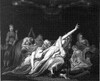
\includegraphics[keepaspectratio,width=\textwidth]{v7cfk63b-small.jpg}
  \captionart{DeathLooms}
  \label{fig:deathlooms}
\end{figure}
% Force float here
\clearpage{}
\chapter[Of Diseases and Melancholy]{Of Diseases in General, and of Melancholy; with a Digression of Anatomy}
{%_Man's Excellency, Fall, Miseries, Infirmities; The causes of them_.
\section[Man's Excellency, Fall, Miseries]{Man's Excellency, Fall, Miseries, Infirmities; The causes of them.}

\subsection{Man's Excellency.}
\lettrine[lines=4,findent=5pt,nindent=0pt]{M}{an} the most excellent and noble creature of the world, the principal and mighty work of God, wonder of Nature, 
as Zoroaster calls him; \li{audacis naturae miraculum}, the marvel of marvels\authormarginnote{820},
as Plato; the abridgment and epitome of the world\authormarginnote{821},
as \Pliny{}; microcosmus, a little world, a model of the world, sovereign lord of the earth\authormarginnote{822}, viceroy of the world, sole commander and governor of all the creatures in it; to whose empire they are subject in particular, and yield obedience; far surpassing all the rest, not in body only, but in soul; \authormarginnote{823}\li{imaginis imago}, \authormarginnote{824}created to God's own \authormarginnote{825}image, to that immortal and incorporeal substance, with all the faculties and powers belonging unto it; was at first pure, divine, perfect, happy, created after God in true holiness and righteousness\authormarginnote{826}; \li{Deo congruens}, free from all manner of infirmities, and put in Paradise, to know God, to praise and glorify him, to do his will, \li{Ut diis consimiles parturiat deos} (as an old poet saith) to propagate the church.

\subsection{Man's Fall and Misery.}
But this most noble creature, \li{Heu tristis, et lachrymosa commutatio} (one exclaims\authormarginnote{827}) O pitiful change! is fallen from that he was, and forfeited his estate, become \li{miserabilis homuncio}, a castaway, a caitiff, one of the most miserable creatures of the world, if he be considered in his own nature, an unregenerate man, and so much obscured by his fall that (some few relics excepted) he is inferior to a beast, \authormarginnote{828}Man in honour that understandeth not, is like unto beasts that perish, so David esteems him: a monster by stupend metamorphoses, \authorfootnote{829}a fox, a dog, a hog, what not? \li{Quantum mutatus ab illo?} How much altered from that he was; before blessed and happy, now miserable and accursed; \authorfootnote{830}He must eat his meat in sorrow, subject to death and all manner of infirmities, all kind of calamities.

\subsection{A Description of Melancholy.}
\authorfootnote{831}Great travail is created for all men, and an heavy yoke on the sons of Adam, from the day that they go out of their mother's womb, unto that day they return to the mother of all things. Namely, their thoughts, and fear of their hearts, and their imagination of things they wait for, and the day of death. From him that sitteth in the glorious throne, to him that sitteth beneath in the earth and ashes; from him that is clothed in blue silk and weareth a crown, to him that is clothed in simple linen. Wrath, envy, trouble, and unquietness, and fear of death, and rigour, and strife, and such things come to both man and beast, but sevenfold to the ungodly. All this befalls him in this life, and peradventure eternal misery in the life to come.

\subsection[The Impulsive Cause]{Impulsive Cause of Man's Misery and Infirmities.}
The impulsive cause of these miseries in man, this privation or destruction of God's image, the cause of death and diseases, of all temporal and eternal punishments, was the sin of our first parent Adam, \authorfootnote{832}in eating of the forbidden fruit, by the devil's instigation and allurement.
His disobedience, pride, ambition, intemperance, incredulity, curiosity; from whence proceeded original sin, and that general corruption of mankind, as from a fountain, flowed all bad inclinations and actual transgressions which cause our several calamities inflicted upon us for our sins.
And this belike is that which our fabulous poets have shadowed unto us in the tale of \authorfootnote{833} Pandora's box, which being opened through her curiosity, filled the world full of all manner of diseases.
It is not curiosity alone, but those other crying sins of ours, which pull these several plagues and miseries upon our heads.
For \li{Ubi peccatum, ibi procella}, as \Chrysostom{} well observes\authorfootnote{834}.
\authorfootnote{835}Fools by reason of their transgression, and because of their iniquities, are afflicted.
\authorfootnote{836}Fear cometh like sudden desolation, and destruction like a whirlwind, affliction and anguish, because they did not fear God.
\authorfootnote{837}Are you shaken with wars? as Cyprian well urgeth to Demetrius, are you molested with dearth and famine? is your health crushed with raging diseases? is mankind generally tormented with epidemical maladies? 'tis all for your sins, Hag. i. 9, 10; Amos i.; Jer. vii.
God is angry, punisheth and threateneth, because of their obstinacy and stubbornness, they will not turn unto him.
\authorfootnote{838}If the earth be barren then for want of rain, if dry and squalid, it yield no fruit, if your fountains be dried up, your wine, corn, and oil blasted, if the air be corrupted, and men troubled with diseases, 'tis by reason of their sins: which like the blood of Abel cry loud to heaven for vengeance, Lam. v. 15. That we have sinned, therefore our hearts are heavy, Isa. lix. 11, 12.
We roar like bears, and mourn like doves, and want health, \etc{} for our sins and trespasses.
But this we cannot endure to hear or to take notice of, Jer. ii. 30. We are smitten in vain and receive no correction; and cap. v. 3.
Thou hast stricken them, but they have not sorrowed; they have refused to receive correction; they have not returned.
Pestilence he hath sent, but they have not turned to him, Amos iv. \authorfootnote{839}Herod could not abide John Baptist, nor \authorfootnote{840}Domitian endure Apollonius to tell the causes of the plague at Ephesus, his injustice, incest, adultery, and the like.
To punish therefore this blindness and obstinacy of ours as a concomitant cause and principal agent, is God's just judgment in bringing these calamities upon us, to chastise us, I say, for our sins, and to satisfy God's wrath.
For the law requires obedience or punishment, as you may read at large, Deut. \rn{xxviii.} 15. If they will not obey the Lord, and keep his commandments and ordinances, then all these curses shall come upon them. \authorfootnote{841}Cursed in the town and in the field, \etc{}.
\authorfootnote{842}Cursed in the fruit of the body, \etc{}.
\authorfootnote{843}The Lord shall send thee trouble and shame, because of thy wickedness.
And a little after, \authorfootnote{844}The Lord shall smite thee with the botch of Egypt, and with emerods, and scab, and itch, and thou canst not be healed; \authorfootnote{845}with madness, blindness, and astonishing of heart.
This Paul seconds, Rom. ii. 9.
Tribulation and anguish on the soul of every man that doeth evil.
Or else these chastisements are inflicted upon us for our humiliation, to exercise and try our patience here in this life to bring us home, to make us to know God ourselves, to inform and teach us wisdom.
\authorfootnote{846}Therefore is my people gone into captivity, because they had no knowledge; therefore is the wrath of the Lord kindled against his people, and he hath stretched out his hand upon them.
He is desirous of our salvation.
\li{Nostrae salutis avidus}, saith Lemnius\authorfootnote{847}, and for that cause pulls us by the ear many times, to put us in mind of our duties: That they which erred might have understanding, (as Isaiah speaks \rn{xxix.} 24) and so to be reformed.
I am afflicted\authorfootnote{848}, and at the point of death, so David confesseth of himself, Psal. \rn{lxxxviii.} v. 15, v. 9.
Mine eyes are sorrowful through mine affliction: and that made him turn unto God.
Great Alexander in the midst of all his prosperity, by a company of parasites deified, and now made a god, when he saw one of his wounds bleed, remembered that he was but a man, and remitted of his pride.
\li{In morbo recolligit se animus}\authorlatintrans{849}, as \Pliny{} well perceived\authorfootnote{850}; In sickness the mind reflects upon itself, with judgment surveys itself, and abhors its former courses; insomuch that he concludes to his friend Marius,\authorfootnote{851} that it were the period of all philosophy, if we could so continue sound, or perform but a part of that which we promised to do, being sick.
Whoso is wise then, will consider these things, as David did (Psal. cxliv., verse last); and whatsoever fortune befall him, make use of it.
If he be in sorrow, need, sickness, or any other adversity, seriously to recount with himself, why this or that malady, misery, this or that incurable disease is inflicted upon him; it may be for his good, \authorfootnote{852}sic expedit as Peter said of his daughter's ague.
Bodily sickness is for his soul's health, periisset nisi periisset, had he not been visited, he had utterly perished; for \authorfootnote{853}the Lord correcteth him whom he loveth, even as a father doth his child in whom he delighteth.
If he be safe and sound on the other side, and free from all manner of infirmity; \authorfootnote{854}et cui Gratia, forma, valetudo contingat abunde Et mundus victus, non deficiente crumena.

And that he have grace, beauty, favour, health,
A cleanly diet, and abound in wealth.

Yet in the midst of his prosperity, let him remember that caveat of
Moses, \authorfootnote{855}Beware that he do not forget the Lord his God; that he be
not puffed up, but acknowledge them to be his good gifts and benefits,
and \authorfootnote{856}the more he hath, to be more thankful, (as Agapetianus
adviseth) and use them aright.

\cleartoleftpage{}
\newgeometry{noheadfoot=true}
\begin{figure}[p]
  \begingroup
  \centering
  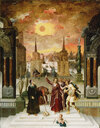
\includegraphics[keepaspectratio,width=0.95\textwidth]{caron-dionysius-converts-pagans-small.jpg}
  \captionart{DionysiusConvertsPagans}
  \label{fig:dionysiusconvertspagans}
\end{figure}
\restoregeometry

% Force float here
\clearpage{}
\subsection{Instrumental Causes of our Infirmities.}
Now the instrumental causes
of these our infirmities, are as diverse as the infirmities themselves;
stars, heavens, elements, \etc{}. And all those creatures which God hath
made, are armed against sinners. They were indeed once good in
themselves, and that they are now many of them pernicious unto us, is
not in their nature, but our corruption, which hath caused it. For from
the fall of our first parent Adam, they have been changed, the earth
accursed, the influence of stars, altered, the four elements, beasts,
birds, plants, are now ready to offend us. The principal things for the
use of man, are water, fire, iron, salt, meal, wheat, honey, milk, oil,
wine, clothing, good to the godly, to the sinners turned to evil,
Ecclus. \rn{xxxix.} 26. Fire, and hail, and famine, and dearth, all these
are created for vengeance, Ecclus. \rn{xxxix.} 29. The heavens threaten us
with their comets, stars, planets, with their great conjunctions,
eclipses, oppositions, quartiles, and such unfriendly aspects. The air
with his meteors, thunder and lightning, intemperate heat and cold,
mighty winds, tempests, unseasonable weather; from which proceed
dearth, famine, plague, and all sorts of epidemical diseases, consuming
infinite myriads of men. At Cairo in Egypt, every third year, (as it is
related by Boterus\authorfootnote{857}, and others) 300\thinspace{}000 die of the plague; and
200\thinspace{}000, in Constantinople, every fifth or seventh at the utmost. How
doth the earth terrify and oppress us with terrible earthquakes, which
are most frequent in China\authorfootnote{858}, Japan, and those eastern climes,
swallowing up sometimes six cities at once? How doth the water rage
with his inundations, irruptions, flinging down towns, cities,
villages, bridges, \etc{} besides shipwrecks; whole islands are sometimes
suddenly overwhelmed with all their inhabitants in Zealand\authorfootnote{859},
Holland, and many parts of the continent drowned, as the lake Erne
in Ireland?\authormarginnote{860} \li{Nihilque praeter arcium cadavera patenti cernimus
freto}\authorlatintrans{861.5}.\authormarginnote{861} In the fens of Friesland 1230, by reason of tempests, \authorfootnote{862}the
sea drowned \li{multa hominum millia, et jumenta sine numero}, all the
country almost, men and cattle in it. How doth the fire rage, that
merciless element, consuming in an instant whole cities? What town of
any antiquity or note hath not been once, again and again, by the fury
of this merciless element, defaced, ruinated, and left desolate? In a
word,
%
\begin{verse}
\textlatin{Ignis pepercit, unda mergit, aeris}\\*
\textlatin{Vis pestilentis aequori ereptum necat,}\\*
\textlatin{Bello superstes, tabidus morbo perit.}\authorfootnote{863}
\end{verse}
\translationrule
\begin{verse}
Whom fire spares, sea doth drown; whom sea,\\*
Pestilent air doth send to clay;\\*
Whom war 'scapes, sickness takes away.
\end{verse}

To descend to more particulars, how many creatures are at deadly feud
with men? Lions, wolves, bears, \etc{}. Some with hoofs, horns, tusks,
teeth, nails: How many noxious serpents and venomous creatures, ready
to offend us with stings, breath, sight, or quite kill us? How many
pernicious fishes, plants, gums, fruits, seeds, flowers, \etc{} could I
reckon up on a sudden, which by their very smell many of them, touch,
taste, cause some grievous malady, if not death itself? Some make
mention of a thousand several poisons: but these are but trifles in
respect. The greatest enemy to man, is man, who by the devil's
instigation is still ready to do mischief, his own executioner, a wolf,
a devil to himself, and others. We are all brethren in Christ\authorfootnote{864}, or
at least should be, members of one body, servants of one lord, and yet
no fiend can so torment, insult over, tyrannise, vex, as one man doth
another. Let me not fall therefore (saith David, when wars, plague,
famine were offered) into the hands of men, merciless and wicked men:
---\li{Vix sunt homines hoc nomine digni,
Quamque lupi, saevae plus feritatis habent}\authorfootnote{865}.

We can most part foresee these epidemical diseases, and likely avoid
them; Dearths, tempests, plagues, our astrologers foretell us;
Earthquakes, inundations, ruins of houses, consuming fires, come by
little and little, or make some noise beforehand; but the knaveries,
impostures, injuries and villainies of men no art can avoid. We can
keep our professed enemies from our cities, by gates, walls and towers,
defend ourselves from thieves and robbers by watchfulness and weapons;
but this malice of men, and their pernicious endeavours, no caution can
divert, no vigilancy foresee, we have so many secret plots and devices
to mischief one another.

Sometimes by the devil's help as magicians, witches\authorfootnote{866}: sometimes by
impostures, mixtures, poisons, stratagems, single combats, wars, we
hack and hew, as if we were ad internecionem nati, like Cadmus'
soldiers born to consume one another. 'Tis an ordinary thing to read of
a hundred and two hundred thousand men slain in a battle. Besides all
manner of tortures, brazen bulls, racks, wheels, strappadoes, guns,
engines, \etc{}. Ad unum corpus humanum supplicia plura, quam membra\authormarginnote{867}:
We have invented more torturing instruments, than there be several
members in a man's body, as Cyprian well observes. To come nearer yet,
our own parents by their offences, indiscretion and intemperance, are
our mortal enemies. The fathers have eaten sour grapes\authorfootnote{868}, and the
children's teeth are set on edge. They cause our grief many times, and
put upon us hereditary diseases, inevitable infirmities: they torment
us, and we are ready to injure our posterity;
---\li{mox daturi progeniem vitiosiorem}\authorfootnote{869}.

And yet with crimes to us unknown,
Our sons shall mark the coming age their own;

and the latter end of the world, as Paul foretold\authorfootnote{870}, is still like
to be the worst. We are thus bad by nature, bad by kind, but far worse
by art, every man the greatest enemy unto himself. We study many times
to undo ourselves, abusing those good gifts which God hath bestowed
upon us, health, wealth, strength, wit, learning, art, memory to our
own destruction, \li{Perditio tua ex te}\authorlatintrans{871.5}.\authormarginnote{871} As Judas Maccabeus
killed Apollonius with his own weapons\authorfootnote{872}, we arm ourselves to our own
overthrows; and use reason, art, judgment, all that should help us, as
so many instruments to undo us. Hector gave Ajax a sword, which so long
as he fought against enemies, served for his help and defence; but
after he began to hurt harmless creatures with it, turned to his own
hurtless bowels. Those excellent means God hath bestowed on us, well
employed, cannot but much avail us; but if otherwise perverted, they
ruin and confound us: and so by reason of our indiscretion and weakness
they commonly do, we have too many instances. This St. \Austin{}
acknowledgeth of himself in his humble confessions, promptness of wit,
memory, eloquence, they were God's good gifts, but he did not use them
to his glory. If you will particularly know how, and by what means,
consult physicians, and they will tell you, that it is in offending in
some of those six non-natural things, of which I shall \authorfootnote{873}dilate more
at large; they are the causes of our infirmities, our surfeiting, and
drunkenness, our immoderate insatiable lust, and prodigious riot.

\li{Plures crapula, quam gladius}, is a true saying, the board consumes more
than the sword. Our intemperance it is, that pulls so many several
incurable diseases upon our heads, that hastens \authorfootnote{874}old age, perverts
our temperature, and brings upon us sudden death. And last of all, that
which crucifies us most, is our own folly, madness (quos Jupiter
perdit, dementat; by subtraction of his assisting grace God permits it)
weakness, want of government, our facility and proneness in yielding to
several lusts, in giving way to every passion and perturbation of the
mind: by which means we metamorphose ourselves and degenerate into
beasts. All which that prince of \authorfootnote{875}poets observed of Agamemnon, that
when he was well pleased, and could moderate his passion, he was-os
oculosque Jovi par: like Jupiter in feature, Mars in valour, Pallas in
wisdom, another god; but when he became angry, he was a lion, a tiger,
a dog, \etc{}, there appeared no sign or likeness of Jupiter in him; so
we, as long as we are ruled by reason, correct our inordinate appetite,
and conform ourselves to God's word, are as so many saints: but if we
give reins to lust, anger, ambition, pride, and follow our own ways, we
degenerate into beasts, transform ourselves, overthrow our
constitutions, \authorfootnote{876}provoke God to anger, and heap upon us this of
melancholy, and all kinds of incurable diseases, as a just and deserved
punishment of our sins.

\section{The Definition, Number, Division of Diseases.}

\lettrine{W}{hat} a disease is, almost every physician defines. \authorfootnote{877}Fernelius
calleth it an affection of the body contrary to nature. \authorfootnote{878}Fuschius
and Crato, an hindrance, hurt, or alteration of any action of the body,
or part of it. \authorfootnote{879}Tholosanus, a dissolution of that league which is
between body and soul, and a perturbation of it; as health the
perfection, and makes to the preservation of it. \li{Labeo in
Agellius},\authormarginnote{880} an ill habit of the body, opposite to nature, hindering the
use of it. Others otherwise, all to this effect.

\subsection{Number of Diseases.}
How many diseases there are, is a question not yet determined;
\authorfootnote{881}\Pliny{} reckons up 300 from the crown of the head to the sole
of the foot: elsewhere he saith, \lit{their number is infinite}{morborum
infinita multitudo}. Howsoever it was in those times, it boots not; in our days
I am sure the number is much augmented:
%
\authormarginnote{882}\begin{latin}
\begin{quote}
---macies, et nova febrium
Terris incubit cohors.
\end{quote}
\end{latin}
\translationrule
\begin{quote}%\authorlatintrans{882.5}
Emaciation, and a new cohort of fevers broods over the earth.
\end{quote}

For besides many epidemical diseases unheard of, and altogether unknown
to Galen and Hippocrates, as scorbutum, small-pox, plica, sweating
sickness, morbus Gallicus, \etc{}, we have many proper and peculiar almost
to every part.

\subsection{No man free from some Disease or other.}
No man amongst us so sound, of so good a constitution, that hath not some impediment of body or
mind. \li{Quisque suos patimur manes}, we have all our infirmities, first or
last, more or less. There will be peradventure in an age, or one of a
thousand, like Zenophilus the musician in \authorfootnote{883}\Pliny{}, that may happily
live 105 years without any manner of impediment; a Pollio Romulus, that
can preserve himself \authorfootnote{884}with wine and oil; a man as fortunate as Q.
Metellus, of whom Valerius so much brags; a man as healthy as Otto
Herwardus, a senator of Augsburg in Germany, whom \authorfootnote{885}Leovitius the
astrologer brings in for an example and instance of certainty in his
art; who because he had the significators in his geniture fortunate,
and free from the hostile aspects of Saturn and Mars, being a very cold
man, \authorfootnote{886}could not remember that ever he was sick. \authorfootnote{887}Paracelsus may
brag that he could make a man live 400 years or more, if he might bring
him up from his infancy, and diet him as he list; and some physicians
hold, that there is no certain period of man's life; but it may still
by temperance and physic be prolonged. We find in the meantime, by
common experience, that no man can escape, but that of Hesiod is
true\authorfootnote{888}:
%
\begin{foreigndisplayquote}{greek}%
Πλείη μὲν γὰρ γαῖα κακῶν, πλειη δὲ θάλασσα,
Νοῦσοιδ' ἄνθρωποι ἐιν ἐφ' ἡμέρη, ἠδ' ἐπὶ νυκτὶ
Ἁυτοματοι φοιτῶσι.%
\end{foreigndisplayquote}%
\translationrule%
\begin{quote}%
Th' earth's full of maladies, and full the sea,
Which set upon us both by night and day.
\end{quote}%

\subsection{Division of Diseases.}
If you require a more exact division of these
ordinary diseases which are incident to men, I refer you to physicians;
\authorfootnote{889}they will tell you of acute and chronic, first and secondary,
lethals, salutares, errant, fixed, simple, compound, connexed, or
consequent, belonging to parts or the whole, in habit, or in
disposition, \etc{}. My division at this time (as most befitting my
purpose) shall be into those of the body and mind. For them of the
body, a brief catalogue of which Fuschius hath made, Institut. lib. 3,
sect. 1, cap. 11. I refer you to the voluminous tomes of Galen,
Areteus, Rhasis, \Avicenna{}, Alexander, Paulus Aetius, Gordonerius: and
those exact Neoterics, Savanarola, Capivaccius, Donatus Altomarus,
Hercules de Saxonia, Mercurialis, Victorius Faventinus, Wecker, Piso,
\etc{}, that have methodically and elaborately written of them all. Those
of the mind and head I will briefly handle, and apart.

\section{Division of the Diseases of the Head.}

\lettrine{T}{hese} diseases of the mind, forasmuch as they have their chief seat and
organs in the head, which are commonly repeated amongst the diseases of
the head which are diverse, and vary much according to their site. For
in the head, as there be several parts, so there be diverse grievances,
which according to that division of \authorfootnote{890}Heurnius, (which he takes out
of Arculanus) are inward or outward (to omit all others which pertain
to eyes and ears, nostrils, gums, teeth, mouth, palate, tongue, weezle,
chops, face, \etc{}) belonging properly to the brain, as baldness, falling
of hair, furfur, lice, \etc{}. \authorfootnote{891}Inward belonging to the skins next to
the brain, called \emph{dura} and \emph{pia mater}, as all headaches, \etc{}, or to
the ventricles, caules, kells, tunicles, creeks, and parts of it, and
their passions, as caro, vertigo, incubus, apoplexy, falling sickness.

The diseases of the nerves, cramps, stupor, convulsion, tremor, palsy:
or belonging to the excrements of the brain, catarrhs, sneezing,
rheums, distillations: or else those that pertain to the substance of
the brain itself, in which are conceived frenzy, lethargy, melancholy,
madness, weak memory, sopor, or Coma Vigilia et vigil Coma. Out of
these again I will single such as properly belong to the phantasy, or
imagination, or reason itself, which Laurentius calls\authorfootnote{892} the disease
of the mind; and Hildesheim, \latininlinetrans{diseases of the imagination, or of injured reason}{morbos imaginationis, aut rationis laesae},
 which are three or four in number, frenzy, madness, melancholy, dotage, and their kinds:
as hydrophobia, lycanthropia, \latininlinetrans{St. Vitus's dance, possession of devils}{Chorus sancti viti, morbi daemoniaci}, which I will briefly touch
and point at, insisting especially in this of melancholy, as more
eminent than the rest, and that through all his kinds, causes,
symptoms, prognostics, cures: as Lonicerus hath done de apoplexia, and
many other of such particular diseases. Not that I find fault with
those which have written of this subject before, as Jason Pratensis,
Laurentius, Montaltus, T. Bright, \etc{}, they have done very well in
their several kinds and methods; yet that which one omits, another may
haply see; that which one contracts, another may enlarge. To conclude
with \authorfootnote{893}Scribanius, that which they had neglected, or perfunctorily
handled, we may more thoroughly examine; that which is obscurely
delivered in them, may be perspicuously dilated and amplified by us:
and so made more familiar and easy for every man's capacity, and the
common good, which is the chief end of my discourse.

\section[Madness]{Dotage, Frenzy, Madness, Hydrophobia, Lycanthropia, Chorus sancti Viti, Extasis.}
\begin{figure}[H]
  \begingroup
  \centering
  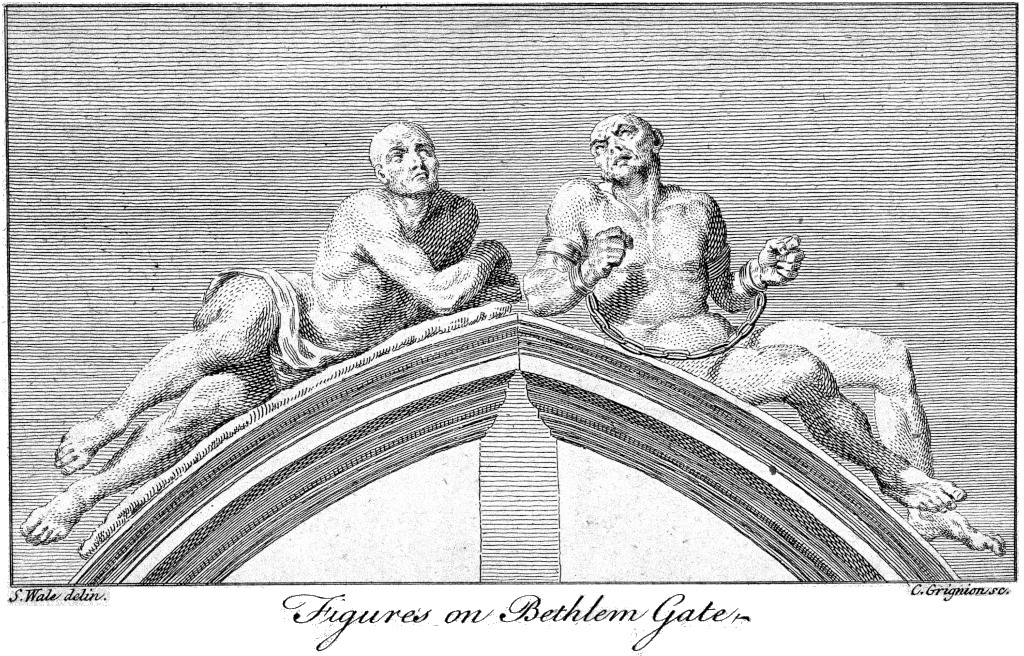
\includegraphics[keepaspectratio,width=\textwidth]{tmczmfhz-small.jpg}
  \captionart{Madness}
  \label{fig:madness}
\end{figure}
\subsection{Delirium, Dotage.}
\lettrine{D}{otage}, fatuity, or folly, is a common name to all
the following species, as some will have it. \authorfootnote{894}Laurentius and \authorfootnote{895}
Altomarus comprehended madness, melancholy, and the rest under this
name, and call it the summum genus of them all. If it be distinguished
from them, it is natural or ingenite, which comes by some defect of the
organs, and overmuch brain, as we see in our common fools; and is for
the most part intended or remitted in particular men, and thereupon
some are wiser than others: or else it is acquisite, an appendix or
symptom of some other disease, which comes or goes; or if it continue,
a sign of melancholy itself.

\subsection{Frenzy.}
\emph{Phrenitis}, which the Greeks derive from the word \textgreek{φρην}, is
a disease of the mind, with a continual madness or dotage, which hath
an acute fever annexed, or else an inflammation of the brain, or the
membranes or kells of it, with an acute fever, which causeth madness
and dotage. It differs from melancholy and madness, because their
dotage is without an ague: this continual, with waking, or memory
decayed, \etc{}. Melancholy is most part silent, this clamorous; and many
such like differences are assigned by physicians.

\subsection{Madness.}
Madness, frenzy, and melancholy are confounded by Celsus,
and many writers; others leave out frenzy, and make madness and
melancholy but one disease, which \authorfootnote{896}Jason Pratensis especially
labours, and that they differ only \li{secundam majus} or minus, in quantity
alone, the one being a degree to the other, and both proceeding from
one cause. They differ intenso et remisso gradu, saith \authorfootnote{897}Gordonius,
as the humour is intended or remitted. Of the same mind is
\authorfootnote{898}Areteus, Alexander Tertullianus, Guianerius, Savanarola, Heurnius;
and Galen himself writes promiscuously of them both by reason of their
affinity: but most of our neoterics do handle them apart, whom I will
follow in this treatise. Madness is therefore defined to be a vehement
dotage; or raving without a fever, far more violent than melancholy,
full of anger and clamour, horrible looks, actions, gestures, troubling
the patients with far greater vehemency both of body and mind, without
all fear and sorrow, with such impetuous force and boldness, that
sometimes three or four men cannot hold them. Differing only in this
from frenzy, that it is without a fever, and their memory is most part
better. It hath the same causes as the other, as choler adust, and
blood incensed, brains inflamed, \etc{}. \authorfootnote{899}Fracastorius adds, a due
time, and full age to this definition, to distinguish it from children,
and will have it confirmed impotency, to separate it from such as
accidentally come and go again, as by taking henbane, nightshade, wine,
\etc{}. Of this fury there be diverse kinds; ecstasy\authormarginnote{900}, which is familiar
with some persons, as Cardan saith of himself, he could be in one when
he list; in which the Indian priests deliver their oracles, and the
witches in Lapland, as Olaus Magnus writeth, \textlatin{l. 3, cap. 18. Extasi
omnia praedicere}, answer all questions in an ecstasis you will ask;
what your friends do, where they are, how they fare, \etc{}. The other
species of this fury are enthusiasms, revelations, and visions, so
often mentioned by Gregory and Bede in their works; obsession or
possession of devils, sibylline prophets, and poetical furies; such as
come by eating noxious herbs, tarantulas stinging, \etc{}, which some
reduce to this. The most known are these, lycanthropia, hydrophobia,
\textlatin{chorus sancti Viti}.

\cleartoleftpage{}
\begin{figure}[p]
  \begingroup
  \centering
  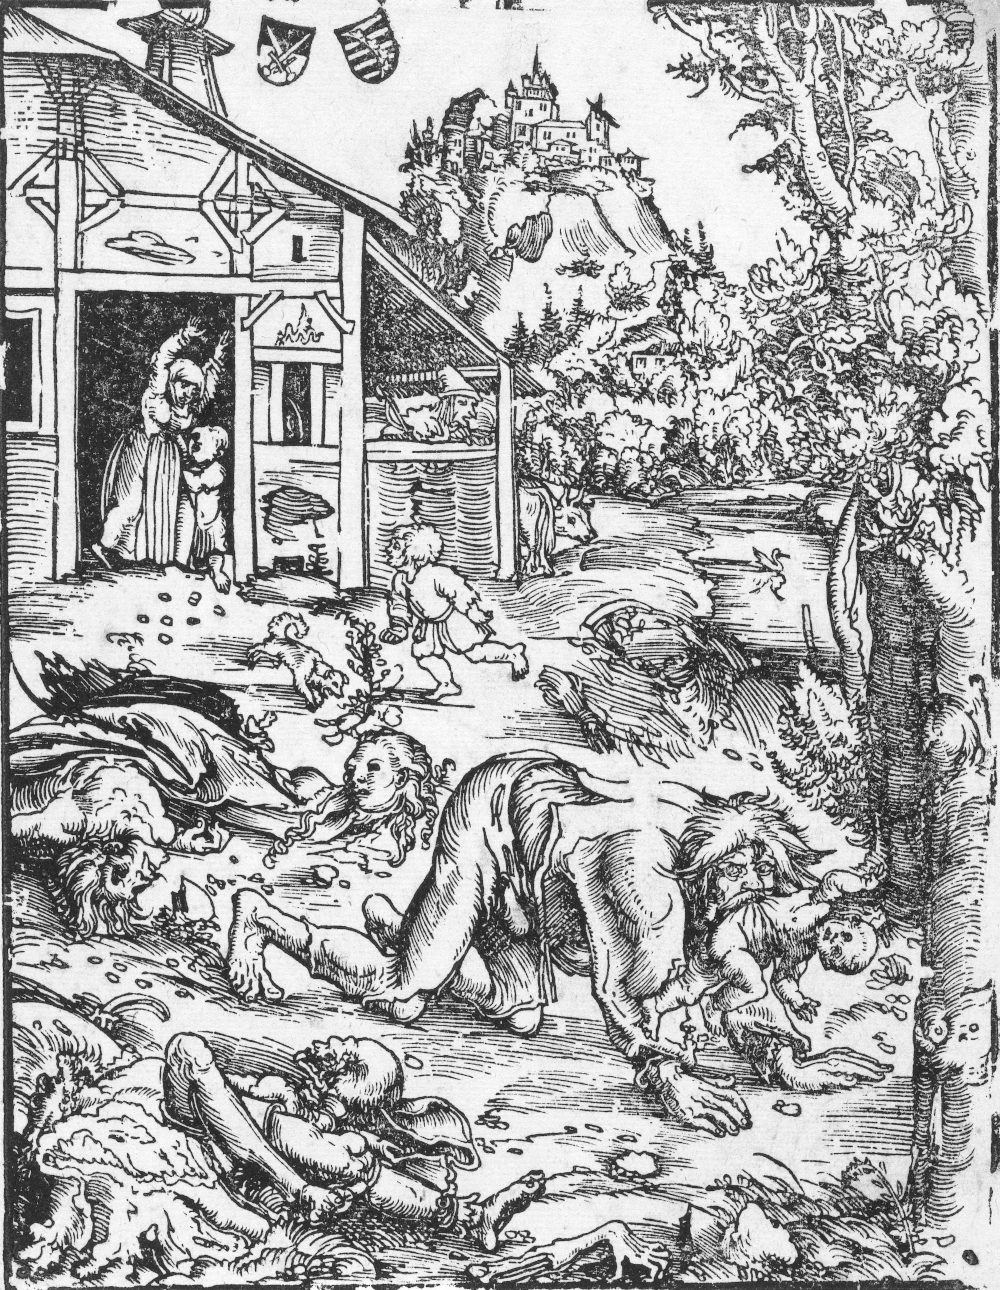
\includegraphics[keepaspectratio,width=\textwidth]{Werewolf-with-bodies-small.jpg}
  \captionart{Werewolf}
  \label{fig:werewolf}
\end{figure}

% Force float here
\clearpage{}
\subsection{Lycanthropia.}
Lycanthropia, which \Avicenna{} calls \emph{cucubuth}, others
\emph{lupinam insaniam}, or wolf-madness, when men run howling about graves
and fields in the night, and will not be persuaded but that they are
wolves, or some such beasts. \authorfootnote{901}Aetius and \authorfootnote{902}Paulus call it a kind
of melancholy; but I should rather refer it to madness, as most do.

Some make a doubt of it whether there be any such disease. \authorfootnote{903}Donat
ab Altomari saith, that he saw two of them in his time: \authorfootnote{904}Wierus
tells a story of such a one at Padua 1541, that would not believe to
the contrary, but that he was a wolf. He hath another instance of a
Spaniard, who thought himself a bear; \authorfootnote{905}Forrestus confirms as much
by many examples; one amongst the rest of which he was an eyewitness,
at Alcmaer in Holland, a poor husbandman that still hunted about
graves, and kept in churchyards, of a pale, black, ugly, and fearful
look. Such belike, or little better, were king Praetus' \authorfootnote{906}daughters,
that thought themselves kine. And Nebuchadnezzar in Daniel, as some
interpreters hold, was only troubled with this kind of madness. This
disease perhaps gave occasion to that bold assertion of \authorfootnote{907}\Pliny{},
some men were turned into wolves in his time, and from wolves to men
again: and to that fable of Pausanias, of a man that was ten years a
wolf, and afterwards turned to his former shape: to \authorfootnote{908}\Ovid's tale of
Lycaon, \etc{}. He that is desirous to hear of this disease, or more
examples, let him read \Austin{} in his 18th book de Civitate Dei, cap. 5.
Mizaldus, cent. 5. 77. Sckenkius, lib. 1. Hildesheim, spicel. 2. de
Mania. Forrestus lib. 10. de morbis cerebri. Olaus Magnus, Vincentius
Bellavicensis, spec. met. lib. 31. c. 122. Pierius, Bodine, Zuinger,
Zeilger, Peucer, Wierus, Spranger, \etc{}. This malady, saith \Avicenna{},
troubleth men most in February, and is nowadays frequent in Bohemia and
Hungary, according to \authorfootnote{909}Heurnius. Scheretzius will have it common in
Livonia. They lie hid most part all day, and go abroad in the night,
barking, howling, at graves and deserts; \authorfootnote{910}they have usually hollow
eyes, scabbed legs and thighs, very dry and pale, \authorfootnote{911}saith Altomarus;
he gives a reason there of all the symptoms, and sets down a brief cure
of them.

\emph{Hydrophobia} is a kind of madness, well known in every village, which
comes by the biting of a mad dog, or scratching, saith \authorfootnote{912}Aurelianus;
touching, or smelling alone sometimes as Sckenkius proves\authorfootnote{913}, and is
incident to many other creatures as well as men: so called because the
parties affected cannot endure the sight of water, or any liquor,
supposing still they see a mad dog in it. And which is more wonderful;
though they be very dry, (as in this malady they are) they will rather
die than drink: \authorfootnote{914}de Venenis Caelius Aurelianus, an ancient writer,
makes a doubt whether this Hydrophobia be a passion of the body or the
mind. The part affected is the brain: the cause, poison that comes from
the mad dog, which is so hot and dry, that it consumes all the moisture
in the body. \authorfootnote{915} Hildesheim relates of some that died so mad; and
being cut up, had no water, scarce blood, or any moisture left in them.

To such as are so affected, the fear of water begins at fourteen days
after they are bitten, to some again not till forty or sixty days
after: commonly saith Heurnius, they begin to rave, fly water and
glasses, to look red, and swell in the face, about twenty days after
(if some remedy be not taken in the meantime) to lie awake, to be
pensive, sad, to see strange visions, to bark and howl, to fall into a
swoon, and oftentimes fits of the falling sickness. \authorfootnote{916} Some say,
little things like whelps will be seen in their urine. If any of these
signs appear, they are past recovery. Many times these symptoms will
not appear till six or seven months after, saith \authorfootnote{917}Codronchus; and
sometimes not till seven or eight years, as Guianerius; twelve as
Albertus; six or eight months after, as Galen holds. Baldus the great
lawyer died of it: an Augustine friar, and a woman in Delft, that were
\authorfootnote{918}Forrestus' patients, were miserably consumed with it. The common
cure in the country (for such at least as dwell near the seaside) is to
duck them over head and ears in sea water; some use charms: every good
wife can prescribe medicines. But the best cure to be had in such
cases, is from the most approved physicians; they that will read of
them, may consult with Dioscorides, lib. 6. c. 37, Heurnius,
Hildesheim, Capivaccius, Forrestus, Sckenkius and before all others
Codronchus an Italian, who hath lately written two exquisite books on
the subject.

\li{Chorus sancti Viti}, or St. Vitus's dance; the lascivious dance, \authorfootnote{919}
Paracelsus calls it, because they that are taken from it, can do
nothing but dance till they be dead, or cured. It is so called, for
that the parties so troubled were wont to go to St. Vitus for help, and
after they had danced there awhile, they were \authorfootnote{920}certainly freed.
'Tis strange to hear how long they will dance, and in what manner, over
stools, forms, tables; even great bellied women sometimes (and yet
never hurt their children) will dance so long that they can stir
neither hand nor foot, but seem to be quite dead. One in red clothes
they cannot abide. Music above all things they love, and therefore
magistrates in Germany will hire musicians to play to them, and some
lusty sturdy companions to dance with them. This disease hath been very
common in Germany, as appears by those relations of \authorfootnote{921}Sckenkius, and
Paracelsus in his book of Madness, who brags how many several persons
he hath cured of it. Felix Plateras de mentis alienat. cap. 3, reports
of a woman in Basil whom he saw, that danced a whole month together.
The Arabians call it a kind of palsy. Bodine in his 5th book de Repub.
cap. 1, speaks of this infirmity; Monavius in his last epistle to
Scoltizius, and in another to Dudithus, where you may read more of it.
The last kind of madness or melancholy, is that demoniacal (if I may so
call it) obsession or possession of devils, which Platerus and others
would have to be preternatural: stupend things are said of them, their
actions, gestures, contortions, fasting, prophesying, speaking
languages they were never taught, \etc{}. Many strange stories are related
of them, which because some will not allow, (for Deacon and Darrel have
written large volumes on this subject pro and con.) I voluntarily omit.
\authorfootnote{922}Fuschius, Institut. lib. 3. sec. 1. cap. 11, Felix Plater,
\authorfootnote{923}Laurentius, add to these another fury that proceeds from love, and
another from study, another divine or religious fury; but these more
properly belong to melancholy; of all which I will speak \authorfootnote{924}apart,
intending to write a whole book of them.

\cleartoleftpage{}
\begin{figure}[p]
  \begingroup
  \centering
  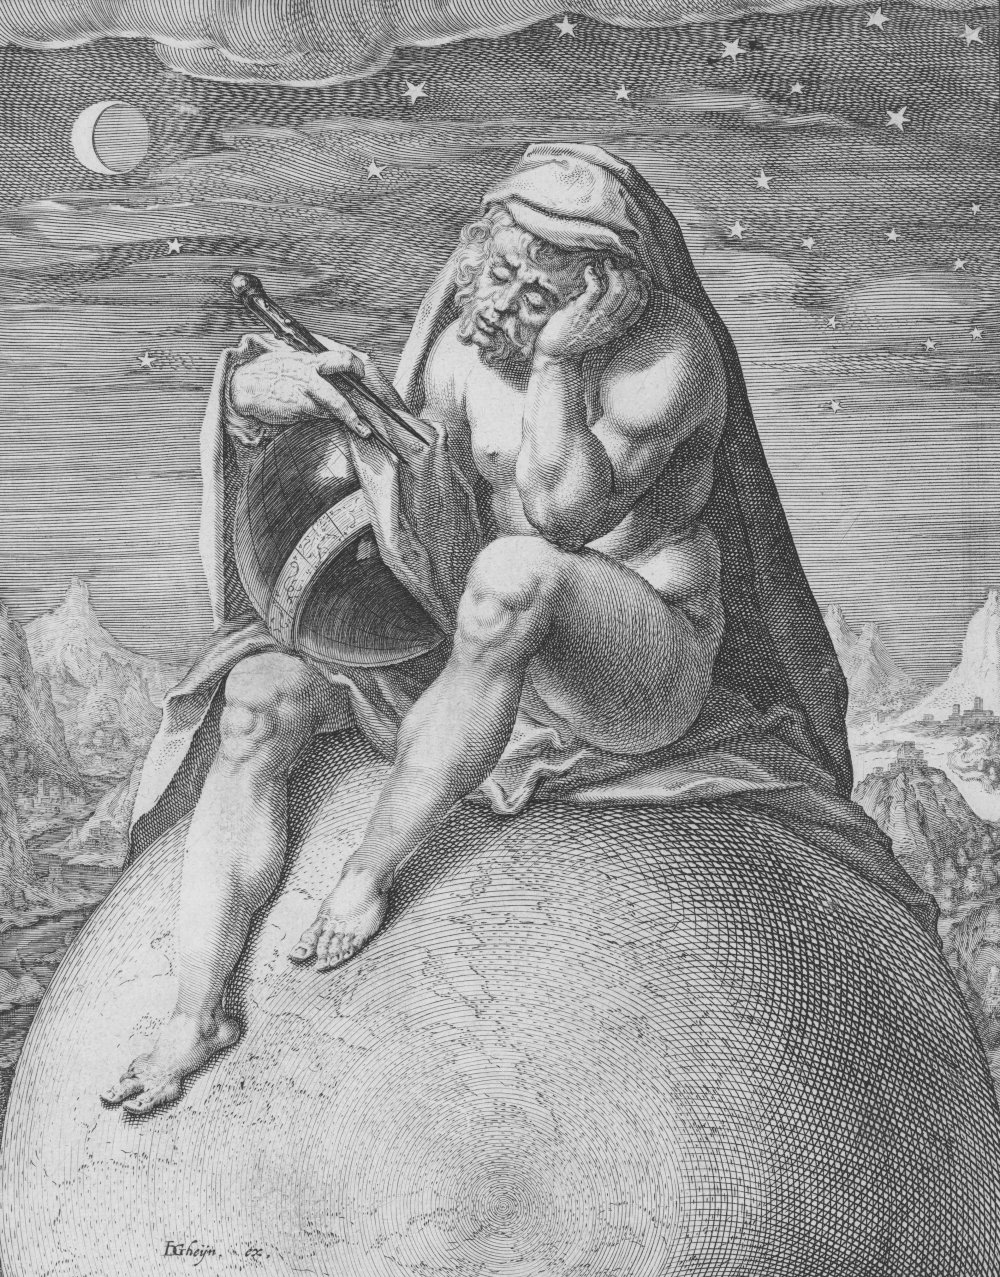
\includegraphics[keepaspectratio,width=\textwidth]{MelancholicTemperament-small.jpg}
  \captionart{MelancholicTemperament}
  \label{fig:melancholictemperament}
\end{figure}

% Force float here
\clearpage{}
\thispagestyle{titleontop}

\section[Melancholic Disposition]{Melancholy in Disposition, improperly so called, Equivocations.}
\lettrine{M}{elancholy}, the subject of our present discourse, is either in
disposition or habit. In disposition, is that transitory melancholy
which goes and comes upon every small occasion of sorrow, need,
sickness, trouble, fear, grief, passion, or perturbation of the mind,
any manner of care, discontent, or thought, which causeth anguish,
dullness, heaviness and vexation of spirit, any ways opposite to
pleasure, mirth, joy, delight, causing frowardness in us, or a dislike.
In which equivocal and improper sense, we call him melancholy that is
dull, sad, sour, lumpish, ill disposed, solitary, any way moved, or
displeased. And from these melancholy dispositions, \authorfootnote{925}no man living
is free, no stoic, none so wise, none so happy, none so patient, so
generous, so godly, so divine, that can vindicate himself; so well
composed, but more or less, some time or other he feels the smart of
it. Melancholy in this sense is the character of mortality. \authorfootnote{926}Man
that is born of a woman, is of short continuance, and full of trouble.
Zeno, Cato, Socrates himself, whom \authorfootnote{927}Aelian so highly commends for a
moderate temper, that nothing could disturb him, but going out, and
coming in, still Socrates kept the same serenity of countenance, what
misery soever befell him, (if we may believe Plato his disciple) was
much tormented with it. Q. Metellus, in whom \authorfootnote{928}Valerius gives
instance of all happiness, the most fortunate man then living, born in
that most flourishing city of Rome, of noble parentage, a proper man of
person, well qualified, healthful, rich, honourable, a senator, a
consul, happy in his wife, happy in his children, \etc{} yet this man was
not void of melancholy, he had his share of sorrow. \authorfootnote{929}Polycrates
Samius, that flung his ring into the sea, because he would participate
of discontent with others, and had it miraculously restored to him
again shortly after, by a fish taken as he angled, was not free from
melancholy dispositions. No man can cure himself; the very gods had
bitter pangs, and frequent passions, as their own \authorfootnote{930}poets put upon
them. In general, \authorfootnote{931}as the heaven, so is our life, sometimes fair,
sometimes overcast, tempestuous, and serene; as in a rose, flowers and
prickles; in the year itself, a temperate summer sometimes, a hard
winter, a drought, and then again pleasant showers: so is our life
intermixed with joys, hopes, fears, sorrows, calumnies: \lit{there is a succession of pleasure and pain}{Invicem cedunt dolor et voluptas}.

\authorfootnote{932}---\li{medio de fonte leporum
Surgit amari aliquid, in ipsis floribus angat}.

Even in the midst of laughing there is sorrow, (as Solomon holds\authorfootnote{933}):
even in the midst of all our feasting and jollity, as \Austin{}
infers\authorfootnote{934} in his Com. on the 41st Psalm, there is grief and discontent.
Inter delicias semper aliquid saevi nos strangulat, for a pint of honey
thou shalt here likely find a gallon of gall, for a dram of pleasure a
pound of pain, for an inch of mirth an ell of moan; as ivy doth an oak,
these miseries encompass our life. And it is most absurd and ridiculous
for any mortal man to look for a perpetual tenure of happiness in his
life. Nothing so prosperous and pleasant, but it hath \authorfootnote{935}some
bitterness in it, some complaining, some grudging; it is all
\marginnote{\scriptsize{}bittersweet}\textgreek{γλυκύπικρον}, a mixed passion,
and like a chequer table black and white: men, families, cities, have their falls and wanes; now trines,
sextiles, then quartiles and oppositions. We are not here as those
angels, celestial powers and bodies, sun and moon, to finish our course
without all offence, with such constancy, to continue for so many ages:
but subject to infirmities, miseries, interrupted, tossed and tumbled
up and down, carried about with every small blast, often molested and
disquieted upon each slender occasion, \authorfootnote{936}uncertain, brittle, and so
is all that we trust unto. \authorfootnote{937} And he that knows not this is not
armed to endure it, is not fit to live in this world (as one condoles
our time), he knows not the condition of it, where with a reciprocalty,
pleasure and pain are still united, and succeed one another in a ring.
\li{Exi e mundo}, get thee gone hence if thou canst not brook it; there is
no way to avoid it, but to arm thyself with patience, with magnanimity,
to \authorfootnote{938}oppose thyself unto it, to suffer affliction as a good soldier
of Christ; as Paul adviseth\authorfootnote{939} constantly to bear it. But forasmuch
as so few can embrace this good council of his, or use it aright, but
rather as so many brute beasts give away to their passion, voluntary
subject and precipitate themselves into a labyrinth of cares, woes,
miseries, and suffer their souls to be overcome by them, cannot arm
themselves with that patience as they ought to do, it falleth out
oftentimes that these dispositions become habits, and many affects
contemned (as \Seneca notes\authorfootnote{940}) make a disease. Even as one
distillation, not yet grown to custom, makes a cough; but continual and
inveterate causeth a consumption of the lungs; so do these our
melancholy provocations: and according as the humour itself is
intended, or remitted in men, as their temperature of body, or rational
soul is better able to make resistance; so are they more or less
affected. For that which is but a flea-biting to one, causeth
insufferable torment to another; and which one by his singular
moderation, and well-composed carriage can happily overcome, a second
is no whit able to sustain, but upon every small occasion of
misconceived abuse, injury, grief, disgrace, loss, cross, humour, \etc{}
(if solitary, or idle) yields so far to passion, that his complexion is
altered, his digestion hindered, his sleep gone, his spirits obscured,
and his heart heavy, his hypochondries misaffected; wind, crudity, on a
sudden overtake him, and he himself overcome with melancholy. As it is
with a man imprisoned for debt, if once in the gaol, every creditor
will bring his action against him, and there likely hold him. If any
discontent seize upon a patient, in an instant all other perturbations
(\li{for-qua data porta ruunt}) will set upon him, and then like a lame dog
or broken-winged goose he droops and pines away, and is brought at last
to that ill habit or malady of melancholy itself. So that as the
philosophers make \authorfootnote{941}eight degrees of heat and cold, we may make
eighty-eight of melancholy, as the parts affected are diversely seized
with it, or have been plunged more or less into this infernal gulf, or
waded deeper into it. But all these melancholy fits, howsoever pleasing
at first, or displeasing, violent and tyrannizing over those whom they
seize on for the time; yet these fits I say, or men affected, are but
improperly so called, because they continue not, but come and go, as by
some objects they aye moved. This melancholy of which we are to treat,
is a habit, \li{mosbus sonticus}, or \li{chronicus}, a chronic or continuate
disease, a settled humour, as Aurelianus\authorfootnote{942} and others\authorfootnote{943} call it,
not errant, but fixed; and as it was long increasing, so now being
(pleasant, or painful) grown to an habit, it will hardly be removed.

%SECT. I. MEMB. II.

%SECT. I. MEMB. II. SUBSECT. I.-_Digression of Anatomy_.
\section{Digression of Anatomy.}

\lettrine{B}{efore} I proceed to define the disease of melancholy, what it is, or to
discourse farther of it, I hold it not impertinent to make a brief
digression of the anatomy of the body and faculties of the soul, for
the better understanding of that which is to follow; because many hard
words will often occur, as mirach, hypocondries, emerods, \etc{},
imagination, reason, humours, spirits, vital, natural, animal, nerves,
veins, arteries, chylus, pituita; which by the vulgar will not so
easily be perceived, what they are, how cited, and to what end they
serve. And besides, it may peradventure give occasion to some men to
examine more accurately, search further into this most excellent
subject, and thereupon with that royal \authorfootnote{944}prophet to praise God, (for
a man is fearfully and wonderfully made, and curiously wrought) that
have time and leisure enough, and are sufficiently informed in all
other worldly businesses, as to make a good bargain, buy and sell, to
keep and make choice of a fair hawk, hound, horse, \etc{}. But for such
matters as concern the knowledge of themselves, they are wholly
ignorant and careless; they know not what this body and soul are, how
combined, of what parts and faculties they consist, or how a man
differs from a dog. And what can be more ignominious and filthy (as
\authorfootnote{945}Melancthon well inveighs) than for a man not to know the structure
and composition of his own body, especially since the knowledge of it
tends so much to the preservation, of his health, and information of
his manners? To stir them up therefore to this study, to peruse those
elaborate works of \authorfootnote{946}Galen, Bauhines, Plater, Vesalius, Falopius,
Laurentius, Remelinus, \etc{}, which have written copiously in Latin; or
that which some of our industrious countrymen have done in our mother
tongue, not long since, as that translation of \authorfootnote{947}Columbus and \authorfootnote{948}
Microcosmographia, in thirteen books, I have made this brief
digression. Also because \authorfootnote{949}Wecker, \authorfootnote{950}Melancthon, \authorfootnote{951}Fernelius,
\authorfootnote{952} Fuschius, and those tedious Tracts de Anima (which have more
compendiously handled and written of this matter) are not at all times
ready to be had, to give them some small taste, or notice of the rest,
let this epitome suffice.

%SECT. I. MEMB. II. SUBSECT. II.-_Division of the Body, Humours, Spirits_.
\section[Division of the Body]{Division of the Body, Humours, Spirits.}

\lettrine{O}{f} the parts of the body there may be many divisions: the most approved
is that of \authorfootnote{953}Laurentius, out of Hippocrates: which is, into parts
contained, or containing. Contained, are either humours or spirits.
\subsection{Humours.}
A humour is a liquid or fluent part of the body,
comprehended in it, for the preservation of it; and is either innate or
born with us, or adventitious and acquisite. The radical or innate, is
daily supplied by nourishment, which some call cambium, and make those
secondary humours of ros and gluten to maintain it: or acquisite, to
maintain these four first primary humours, coming and proceeding from
the first concoction in the liver, by which means chylus is excluded.
Some divide them into profitable and excrementitious. But \authorfootnote{954}Crato
out of Hippocrates will have all four to be juice, and not excrements,
without which no living creature can be sustained: which four, though
they be comprehended in the mass of blood, yet they have their several
affections, by which they are distinguished from one another, and from
those adventitious, peccant, or \authorfootnote{955}diseased humours, as Melancthon
calls them.
\subsection{Blood.}
Blood is a hot, sweet, temperate, red humour, prepared in the
mesaraic veins, and made of the most temperate parts of the chylus in
the liver, whose office is to nourish the whole body, to give it
strength and colour, being dispersed by the veins through every part of
it. And from it spirits are first begotten in the heart, which
afterwards by the arteries are communicated to the other parts.
Pituita, or phlegm, is a cold and moist humour, begotten of the colder
part of the chylus (or white juice coming out of the meat digested in
the stomach) in the liver; his office is to nourish and moisten the
members of the body, which as the tongue are moved, that they be not
over dry.

Choler, is hot and dry, bitter, begotten of the hotter parts of the
chylus, and gathered to the gall: it helps the natural heat and senses,
and serves to the expelling of excrements.

\subsection{Melancholy.}
Melancholy, cold and dry, thick, black, and sour,
begotten of the more feculent part of nourishment, and purged from the
spleen, is a bridle to the other two hot humours, blood and choler,
preserving them in the blood, and nourishing the bones. These four
humours have some analogy with the four elements, and to the four ages
in man.

\subsection{Serum, Sweat, Tears.}
To these humours you may add serum, which is
the matter of urine, and those excrementitious humours of the third
concoction, sweat and tears.

\subsection{Spirits.}
Spirit is a most subtle vapour, which is expressed from the
blood, and the instrument of the soul, to perform all his actions; a
common tie or medium between the body and the soul, as some will have
it; or as Paracelsus\authorfootnote{956}, a fourth soul of itself. Melancthon holds
the fountain of those spirits to be the heart, begotten there; and
afterward conveyed to the brain, they take another nature to them. Of
these spirits there be three kinds, according to the three principal
parts, brain, heart, liver; natural, vital, animal. The natural are
begotten in the liver, and thence dispersed through the veins, to
perform those natural actions. The vital spirits are made in the heart
of the natural, which by the arteries are transported to all the other
parts: if the spirits cease, then life ceaseth, as in a syncope or
swooning. The animal spirits formed of the vital, brought up to the
brain, and diffused by the nerves, to the subordinate members, give
sense and motion to them all.

%SECT. I. MEMB. II. SUBSECT. III.-_Similar Parts_.
\section{Similar Parts.}

\subsection{Similar Parts}
\lettrine{C}{ontaining} parts, by reason of their more solid
substance, are either homogeneal or heterogeneal, similar or
dissimilar; so \Aristotle divides them, lib. 1, cap. 1, de Hist.
Animal.; Laurentius, cap. 20, lib. 1. Similar, or homogeneal, are such
as, if they be divided, are still severed into parts of the same
nature, as water into water. Of these some be spermatical, some fleshy
or carnal. \authorfootnote{957}Spermatical are such as are immediately begotten of the
seed, which are bones, gristles, ligaments, membranes, nerves,
arteries, veins, skins, fibres or strings, fat.

\subsection{Bones.}
The bones are dry and hard, begotten of the thickest of the
seed, to strengthen and sustain other parts: some say there be 304,
some 307, or 313 in man's body. They have no nerves in them, and are
therefore without sense.

A gristle is a substance softer than bone, and harder than the rest,
flexible, and serves to maintain the parts of motion.

Ligaments are they that tie the bones together, and other parts to the
bones, with their subserving tendons: membranes' office is to cover the
rest.

Nerves, or sinews, are membranes without, and full of marrow within;
they proceed from the brain, and carry the animal spirits for sense and
motion. Of these some be harder, some softer; the softer serve the
senses, and there be seven pair of them. The first be the optic nerves,
by which we see; the second move the eyes; the third pair serve for the
tongue to taste; the fourth pair for the taste in the palate; the fifth
belong to the ears; the sixth pair is most ample, and runs almost over
all the bowels; the seventh pair moves the tongue. The harder sinews
serve for the motion of the inner parts, proceeding from the marrow in
the back, of whom there be thirty combinations, seven of the neck,
twelve of the breast, \etc{}.

\subsection{Arteries.}
Arteries are long and hollow, with a double skin to convey
the vital spirit; to discern which the better, they say that Vesalius
the anatomist was wont to cut up men alive. \authorfootnote{958}They arise in the left
side of the heart, and are principally two, from which the rest are
derived, aorta and venosa: aorta is the root of all the other, which
serve the whole body; the other goes to the lungs, to fetch air to
refrigerate the heart.

\subsection{Veins.}
Veins are hollow and round, like pipes, arising from the
liver, carrying blood and natural spirits; they feed all the parts. Of
these there be two chief, \emph{Vena porta} and \emph{Vena cava}, from which the
rest are corrivated. That \emph{Vena porta} is a vein coming from the
concave of the liver, and receiving those mesaraical veins, by whom he
takes the chylus from the stomach and guts, and conveys it to the
liver. The other derives blood from the liver to nourish all the other
dispersed members. The branches of that \emph{Vena porta} are the mesaraical
and haemorrhoids. The branches of the \emph{cava} are inward or outward.
Inward, seminal or emulgent. Outward, in the head, arms, feet, \etc{}, and
have several names.

\subsection{Fibrae, Fat, Flesh.}
Fibrae are strings, white and solid, dispersed
through the whole member, and right, oblique, transverse, all which
have their several uses. Fat is a similar part, moist, without blood,
composed of the most thick and unctuous matter of the blood. The
\authorfootnote{959}skin covers the rest, and hath cuticulum, or a little skin tinder
it. Flesh is soft and ruddy, composed of the congealing of blood, \etc{}.

%SECT. I. MEMB. II. SUBSECT. IV.-_Dissimilar Parts_.
\section{Dissimilar Parts.}

\lettrine{D}{issimilar} parts are those which we call organical, or instrumental,
and they be inward or outward. The chiefest outward parts are situate
forward or backward:-forward, the crown and foretop of the head, skull,
face, forehead, temples, chin, eyes, ears, nose, \etc{}, neck, breast,
chest, upper and lower part of the belly, hypocondries, navel, groin,
flank, \etc{}; backward, the hinder part of the head, back, shoulders,
sides, loins, hipbones, os sacrum, buttocks, \etc{}. Or joints, arms,
hands, feet, legs, thighs, knees, \etc{}. Or common to both, which, because
they are obvious and well known, I have carelessly repeated, eaque
praecipua et grandiora tantum; quod reliquum ex libris de anima qui
volet, accipiat.

Inward organical parts, which cannot be seen, are diverse in number, and
have several names, functions, and divisions; but that of
\authorfootnote{960}Laurentius is most notable, into noble or ignoble parts. Of the
noble there be three principal parts, to which all the rest belong, and
whom they serve-brain, heart, liver; according to whose site, three
regions, or a threefold division, is made of the whole body. As first
of the head, in which the animal organs are contained, and brain
itself, which by his nerves give sense and motion to the rest, and is,
as it were, a privy counsellor and chancellor to the heart. The second
region is the chest, or middle belly, in which the heart as king keeps
his court, and by his arteries communicates life to the whole body. The
third region is the lower belly, in which the liver resides as a Legat
a latere, with the rest of those natural organs, serving for
concoction, nourishment, expelling of excrements. This lower region is
distinguished from the upper by the midriff, or diaphragma, and is
subdivided again by \authorfootnote{961}some into three concavities or regions, upper,
middle, and lower. The upper of the hypocondries, in whose right side
is the liver, the left the spleen; from which is denominated
hypochondriacal melancholy. The second of the navel and flanks, divided
from the first by the rim. The last of the water course, which is again
subdivided into three other parts. The Arabians make two parts of this
region, Epigastrium and Hypogastrium, upper or lower. Epigastrium they
call \emph{Mirach}, from whence comes Mirachialis Melancholia, sometimes
mentioned of them. Of these several regions I will treat in brief
apart; and first of the third region, in which the natural organs are
contained.

\subsection[The Lower Region]{De Anima.-The Lower Region, Natural Organs.}
But you that are readers in the meantime, Suppose you were now brought into some sacred temple,
or majestical palace (as Melancthon saith\authorfootnote{962}), to behold not the
matter only, but the singular art, workmanship, and counsel of this our
great Creator. And it is a pleasant and profitable speculation, if it
be considered aright. The parts of this region, which present
themselves to your consideration and view, are such as serve to
nutrition or generation. Those of nutrition serve to the first or
second concoction; as the oesophagus or gullet, which brings meat and
drink into the stomach. The ventricle or stomach, which is seated in
the midst of that part of the belly beneath the midriff, the kitchen,
as it were, of the first concoction, and which turns our meat into
chylus. It hath two mouths, one above, another beneath. The upper is
sometimes taken for the stomach itself; the lower and nether door (as
Wecker calls it) is named Pylorus. This stomach is sustained by a large
kell or caul, called omentum; which some will have the same with
peritoneum, or rim of the belly. From the stomach to the very fundament
are produced the guts, or intestina, which serve a little to alter and
distribute the chylus, and convey away the excrements. They are divided
into small and great, by reason of their site and substance, slender or
thicker: the slender is duodenum, or whole gut, which is next to the
stomach, some twelve inches long, saith \authorfootnote{963} Fuschius. Jejunum, or
empty gut, continuate to the other, which hath many mesaraic veins
annexed to it, which take part of the chylus to the liver from it.
Ilion the third, which consists of many crinkles, which serves with the
rest to receive, keep, and distribute the chylus from the stomach. The
thick guts are three, the blind gut, colon, and right gut. The blind is
a thick and short gut, having one mouth, in which the ilium and colon
meet: it receives the excrements, and conveys them to the colon. This
colon hath many windings, that the excrements pass not away too fast:
the right gut is straight, and conveys the excrements to the fundament,
whose lower part is bound up with certain muscles called sphincters,
that the excrements may be the better contained, until such time as a
man be willing to go to the stool. In the midst of these guts is
situated the mesenterium or midriff, composed of many veins, arteries,
and much fat, serving chiefly to sustain the guts. All these parts
serve the first concoction. To the second, which is busied either in
refining the good nourishment or expelling the bad, is chiefly
belonging the liver, like in colour to congealed blood, the shop of
blood, situate in the right hypochondry, in figure like to a half-moon,
generosum membrum Melancthon styles it, a generous part; it serves to
turn the chylus to blood, for the nourishment of the body. The
excrements of it are either choleric or watery, which the other
subordinate parts convey. The gall placed in the concave of the liver,
extracts choler to it: the spleen, melancholy; which is situate on the
left side, over against the liver, a spongy matter, that draws this
black choler to it by a secret virtue, and feeds upon it, conveying the
rest to the bottom of the stomach, to stir up appetite, or else to the
guts as an excrement. That watery matter the two kidneys expurgate by
those emulgent veins and ureters. The emulgent draw this superfluous
moisture from the blood; the two ureters convey it to the bladder,
which, by reason of his site in the lower belly, is apt to receive it,
having two parts, neck and bottom: the bottom holds the water, the neck
is constringed with a muscle, which, as a porter, keeps the water from
running out against our will.

Members of generation are common to both sexes, or peculiar to one;
which, because they are impertinent to my purpose, I do voluntarily
omit.

\subsection{Middle Region.}
Next in order is the middle region, or chest, which
comprehends the vital faculties and parts; which (as I have said) is
separated from the lower belly by the diaphragma or midriff, which is a
skin consisting of many nerves, membranes; and amongst other uses it
hath, is the instrument of laughing. There is also a certain thin
membrane, full of sinews, which covereth the whole chest within, and is
called pleura, the seat of the disease called pleurisy, when it is
inflamed; some add a third skin, which is termed mediastinus, which
divides the chest into two parts, right and left; of this region the
principal part is the heart, which is the seat and fountain of life, of
heat, of spirits, of pulse and respiration-the sun of our body, the
king and sole commander of it-the seat and organ of all passions and
affections. Primum vivens, ultimum moriens, it lives first, dies last
in all creatures. Of a pyramidical form, and not much unlike to a
pineapple; a part worthy of \authorfootnote{964} admiration, that can yield such
variety of affections, by whose motion it is dilated or contracted, to
stir and command the humours in the body. As in sorrow, melancholy; in
anger, choler; in joy, to send the blood outwardly; in sorrow, to call
it in; moving the humours, as horses do a chariot. This heart, though
it be one sole member, yet it may be divided into two creeks right and
left. The right is like the moon increasing, bigger than the other
part, and receives blood from \emph{vena cava}, distributing some of it to
the lungs to nourish them; the rest to the left side, to engender
spirits. The left creek hath the form of a cone, and is the seat of
life, which, as a torch doth oil, draws blood unto it, begetting of it
spirits and fire; and as fire in a torch, so are spirits in the blood;
and by that great artery called aorta, it sends vital spirits over the
body, and takes air from the lungs by that artery which is called
\emph{venosa}; so that both creeks have their vessels, the right two veins,
the left two arteries, besides those two common anfractuous ears, which
serve them both; the one to hold blood, the other air, for several
uses. The lungs is a thin spongy part, like an ox hoof, (saith
\authorfootnote{965}Fernelius) the town-clerk or crier, (\authorfootnote{966}one terms it) the
instrument of voice, as an orator to a king; annexed to the heart, to
express their thoughts by voice. That it is the instrument of voice, is
manifest, in that no creature can speak, or utter any voice, which
wanteth these lights. It is, besides, the instrument of respiration, or
breathing; and its office is to cool the heart, by sending air unto it,
by the venosal artery, which vein comes to the lungs by that \emph{aspera
arteria} which consists of many gristles, membranes, nerves, taking in
air at the nose and mouth, and by it likewise exhales the fumes of the
heart.

In the upper region serving the animal faculties, the chief organ is
the brain, which is a soft, marrowish, and white substance, engendered
of the purest part of seed and spirits, included by many skins, and
seated within the skull or brain pan; and it is the most noble organ
under heaven, the dwelling-house and seat of the soul, the habitation
of wisdom, memory, judgment, reason, and in which man is most like unto
God; and therefore nature hath covered it with a skull of hard bone,
and two skins or membranes, whereof the one is called \emph{dura mater}, or
meninx, the other \emph{pia mater}. The dura mater is next to the skull,
above the other, which includes and protects the brain. When this is
taken away, the pia mater is to be seen, a thin membrane, the next and
immediate cover of the brain, and not covering only, but entering into
it. The brain itself is divided into two parts, the fore and hinder
part; the fore part is much bigger than the other, which is called the
little brain in respect of it. This fore part hath many concavities
distinguished by certain ventricles, which are the receptacles of the
spirits, brought hither by the arteries from the heart, and are there
refined to a more heavenly nature, to perform the actions of the soul.

Of these ventricles there are three-right, left, and middle. The right
and left answer to their site, and beget animal spirits; if they be any
way hurt, sense and motion ceaseth. These ventricles, moreover, are
held to be the seat of the common sense. The middle ventricle is a
common concourse and cavity of them both, and hath two passages-the one
to receive pituita, and the other extends itself to the fourth creek;
in this they place imagination and cogitation, and so the three
ventricles of the fore part of the brain are used. The fourth creek
behind the head is common to the cerebel or little brain, and marrow of
the backbone, the last and most solid of all the rest, which receives
the animal spirits from the other ventricles, and conveys them to the
marrow in the back, and is the place where they say the memory is
seated.

\section{Of the Soul and her Faculties.}

\lettrine{A}{ccording} to \Aristotle\authorfootnote{967}, the soul is defined to be \textgreek{ἐντελέχεια},
\li{perfectio et actus primus corporis organici, vitam habentis in
potentia}: the perfection or first act of an organical body, having
power of life, which most philosophers approve\authorfootnote{968}. But many doubts
arise about the essence, subject, seat, distinction, and subordinate
faculties of it. For the essence and particular knowledge, of all other
things it is most hard (be it of man or beast) to discern, as
\Aristotle himself\authorfootnote{969}, \authorfootnote{970}Tully, \authorfootnote{971}Picus Mirandula, \authorfootnote{972}Tolet,
and other neoteric philosophers confess:-\authorfootnote{973}We can understand all
things by her, but what she is we cannot apprehend. Some therefore make
one soul, divided into three principal faculties; others, three
distinct souls. Which question of late hath been much controverted by
Picolomineus and Zabarel. \authorfootnote{974} Paracelsus will have four souls, adding
to the three grand faculties a spiritual soul: which opinion of his,
\idxname{campanella}[Campanella][\textlatin{De sensu rerum et magia}], in his book de sensu rerum \authorfootnote{975}much labours to demonstrate
and prove, because carcasses bleed at the sight of the murderer; with
many such arguments And \authorfootnote{976}some again, one soul of all creatures
whatsoever, differing only in organs; and that beasts have reason as
well as men, though, for some defect of organs, not in such measure.

Others make a doubt whether it be all in all, and all in every part;
which is amply discussed in Zabarel amongst the rest. The \authorfootnote{977}common
division of the soul is into three principal faculties-vegetal,
sensitive, and rational, which make three distinct kinds of living
creatures-vegetal plants, sensible beasts, rational men. How these
three principal faculties are distinguished and connected, Humano
ingenio inaccessum videtur, is beyond human capacity, as 
Taurellus\authorfootnote{978}, Philip, Flavins, and others suppose. The inferior may be
alone, but the superior cannot subsist without the other; so sensible
includes vegetal, rational both; which are contained in it (saith
\Aristotle) \li{ut trigonus in tetragono} as a triangle in a quadrangle.
\subsection{Vegetal Soul.}
Vegetal, the first of the three distinct faculties, is
defined to be a substantial act of an organical body, by which it is
nourished, augmented, and begets another like unto itself. In which
definition, three several operations are specified-altrix, auctrix,
procreatrix; the first is \authorfootnote{979}nutrition, whose object is nourishment,
meat, drink, and the like; his organ the liver in sensible creatures;
in plants, the root or sap. His office is to turn the nutriment into
the substance of the body nourished, which he performs by natural heat.
This nutritive operation hath four other subordinate functions or
powers belonging to it-attraction, retention, digestion, expulsion.
\subsection{Attraction.}
\authorfootnote{980}Attraction is a ministering faculty, which, as a
loadstone doth iron, draws meat into the stomach, or as a lamp doth
oil; and this attractive power is very necessary in plants, which suck
up moisture by the root, as, another mouth, into the sap, as a like
stomach.
\subsection{Retention.}
Retention keeps it, being attracted unto the stomach,
until such time it be concocted; for if it should pass away straight,
the body could not be nourished.
\subsection{Digestion.}
Digestion is performed by natural heat; for as the flame
of a torch consumes oil, wax, tallow, so doth it alter and digest the
nutritive matter. Indigestion is opposite unto it, for want of natural
heat. Of this digestion there be three differences-maturation,
elixation, assation.
\subsection{Maturation.}
Maturation is especially observed in the fruits of
trees; which are then said to be ripe, when the seeds are fit to be
sown again. Crudity is opposed to it, which gluttons, epicures, and
idle persons are most subject unto, that use no exercise to stir
natural heat, or else choke it, as too much wood puts out a fire.
\subsection{Elixation.}
Elixation is the seething of meat in the stomach, by the
said natural heat, as meat is boiled in a pot; to which corruption or
putrefaction is opposite.
\subsection{Assation.}
Assation is a concoction of the inward moisture by heat;
his opposite is semiustulation.
\subsection{Order of Concoction fourfold.}
Besides these three several operations
of digestion, there is a fourfold order of concoction:-mastication, or
chewing in the mouth; chilification of this so chewed meat in the
stomach; the third is in the liver, to turn this chylus into blood,
called sanguification; the last is assimilation, which is in every
part.
\subsection{Expulsion.}
Expulsion is a power of nutrition, by which it expels all
superfluous excrements, and relics of meat and drink, by the guts,
bladder, pores; as by purging, vomiting, spitting, sweating, urine,
hairs, nails, \etc{}.
\subsection{Augmentation.}
As this nutritive faculty serves to nourish the body,
so doth the augmenting faculty (the second operation or power of the
vegetal faculty) to the increasing of it in quantity, according to all
dimensions, long, broad, thick, and to make it grow till it come to his
due proportion and perfect shape; which hath his period of
augmentation, as of consumption; and that most certain, as the poet
observes:-
Stat sua cuique dies, breve et irreparabile tempus
Omnibus est vitae.---

A term of life is set to every man,
Which is but short, and pass it no one can.

\subsection{Generation.}
The last of these vegetal faculties is generation, which
begets another by means of seed, like unto itself, to the perpetual
preservation of the species. To this faculty they ascribe three
subordinate operations:-the first to turn nourishment into seed, \etc{}.

\subsection{Life and Death concomitants of the Vegetal Faculties.}
Necessary concomitants or affections of this vegetal faculty are life and his
privation, death. To the preservation of life the natural heat is most
requisite, though siccity and humidity, and those first qualities, be
not excluded. This heat is likewise in plants, as appears by their
increasing, fructifying, \etc{}, though not so easily perceived. In all
bodies it must have radical \authorfootnote{981}moisture to preserve it, that it be
not consumed; to which preservation our clime, country, temperature,
and the good or bad use of those six non-natural things avail much. For
as this natural heat and moisture decays, so doth our life itself; and
if not prevented before by some violent accident, or interrupted
through our own default, is in the end dried up by old age, and
extinguished by death for want of matter, as a lamp for defect of oil
to maintain it.

%SECT. I. MEMB. II. SUBSECT. VI.-_Of the sensible Soul_.
\section{Of the sensible Soul.}

\lettrine{N}{ext} in order is the sensible faculty, which is as far beyond the other
in dignity, as a beast is preferred to a plant, having those vegetal
powers included in it. 'Tis defined an Act of an organical body by
which it lives, hath sense, appetite, judgment, breath, and motion. His
object in general is a sensible or passible quality, because the sense
is affected with it. The general organ is the brain, from which
principally the sensible operations are derived. This sensible soul is
divided into two parts, apprehending or moving. By the apprehensive
power we perceive the species of sensible things present, or absent,
and retain them as wax doth the print of a seal. By the moving, the
body is outwardly carried from one place to another; or inwardly moved
by spirits and pulse. The apprehensive faculty is subdivided into two
parts, inward or outward. Outward, as the five senses, of touching,
hearing, seeing, smelling, tasting, to which you may add Scaliger's
sixth sense of titillation, if you please; or that of speech, which is
the sixth external sense, according to Lullius. Inward are three-common
sense, phantasy, memory. Those five outward senses have their object in
outward things only, and such as are present, as the eye sees no colour
except it be at hand, the ear sound. Three of these senses are of
commodity, hearing, sight, and smell; two of necessity, touch, and
taste, without which we cannot live. Besides, the sensitive power is
active or passive. Active in sight, the eye sees the colour; passive
when it is hurt by his object, as the eye by the sunbeams. According to
that axiom, \li{visibile forte destruit sensum}\authorlatintrans{982}. Or if the object be
not pleasing, as a bad sound to the ear, a stinking smell to the nose,
\etc{}.
\subsection{Sight.}
Of these five senses, sight is held to be most precious, and
the best, and that by reason of his object, it sees the whole body at
once. By it we learn, and discern all things, a sense most excellent
for use: to the sight three things are required; the object, the organ,
and the medium. The object in general is visible, or that which is to
be seen, as colours, and all shining bodies. The medium is the
illumination of the air, which comes from \authorfootnote{983}light, commonly called
diaphanum; for in dark we cannot see. The organ is the eye, and chiefly
the apple of it, which by those optic nerves, concurring both in one,
conveys the sight to the common sense. Between the organ and object a
true distance is required, that it be not too near, or too far off!

Many excellent questions appertain to this sense, discussed by
philosophers: as whether this sight be caused intra mittendo, vel extra
mittendo, \etc{}, by receiving in the visible species, or sending of them
out, which \authorfootnote{984}Plato, \authorfootnote{985}Plutarch, \authorfootnote{986}Macrobius, \authorfootnote{987}Lactantius
and others dispute. And, besides, it is the subject of the
perspectives, of which Alhazen the Arabian, Vitellio, Roger Bacon,
Baptista Porta, Guidus Ubaldus, Aquilonius, \etc{}, have written whole
volumes.
\subsection{Hearing.}
Hearing, a most excellent outward sense, by which we learn
and get knowledge. His object is sound, or that which is heard; the
medium, air; organ, the ear. To the sound, which is a collision of the
air, three things are required; a body to strike, as the hand of a
musician; the body struck, which must be solid and able to resist; as a
bell, lute-string, not wool, or sponge; the medium, the air; which is
inward, or outward; the outward being struck or collided by a solid
body, still strikes the next air, until it come to that inward natural
air, which as an exquisite organ is contained in a little skin formed
like a drum-head, and struck upon by certain small instruments like
drum-sticks, conveys the sound by a pair of nerves, appropriated to
that use, to the common sense, as to a judge of sounds. There is great
variety and much delight in them; for the knowledge of which, consult
with Boethius and other musicians.
\subsection{Smelling.}
Smelling is an outward sense, which apprehends by the
nostrils drawing in air; and of all the rest it is the weakest sense in
men. The organ in the nose, or two small hollow pieces of flesh a
little above it: the medium the air to men, as water to fish: the
object, smell, arising from a mixed body resolved, which, whether it be
a quality, fume, vapour, or exhalation, I will not now dispute, or of
their differences, and how they are caused. This sense is an organ of
health, as sight and hearing, saith \authorfootnote{988}Agellius, are of discipline;
and that by avoiding bad smells, as by choosing good, which do as much
alter and affect the body many times, as diet itself.
\subsection{Taste.}
Taste, a necessary sense, which perceives all savours by the
tongue and palate, and that by means of a thin spittle, or watery
juice. His organ is the tongue with his tasting nerves; the medium, a
watery juice; the object, taste, or savour, which is a quality in the
juice, arising from the mixture of things tasted. Some make eight
species or kinds of savour, bitter, sweet, sharp, salt, \etc{}, all which
sick men (as in an ague) cannot discern, by reason of their organs
misaffected.
\subsection{Touching.}
Touch, the last of the senses, and most ignoble, yet of as
great necessity as the other, and of as much pleasure. This sense is
exquisite in men, and by his nerves dispersed all over the body,
perceives any tactile quality. His organ the nerves; his object those
first qualities, hot, dry, moist, cold; and those that follow them,
hard, soft, thick, thin, \etc{}. Many delightsome questions are moved by
philosophers about these five senses; their organs, objects, mediums,
which for brevity I omit.

%SECT. I. MEMB. II. SUBSECT. VII.-_Of the Inward Senses._
\section{Of the Inward Senses.}

\subsection{Common Sense.}
\lettrine{I}{nner} senses are three in number, so called, because
they be within the brainpan, as common sense, phantasy, memory. Their
objects are not only things present, but they perceive the sensible
species of things to come, past, absent, such as were before in the
sense. This common sense is the judge or moderator of the rest, by whom
we discern all differences of objects; for by mine eye I do not know
that I see, or by mine ear that I hear, but by my common sense, who
judgeth of sounds and colours: they are but the organs to bring the
species to be censured; so that all their objects are his, and all
their offices are his. The fore part of the brain is his organ or seat.
\subsection{Phantasy.}
Phantasy, or imagination, which some call estimative, or
cogitative, (confirmed, saith Fernelius\authorfootnote{989}, by frequent meditation)
is an inner sense which doth more fully examine the species perceived
by common sense, of things present or absent, and keeps them longer,
recalling them to mind again, or making new of his own. In time of
sleep this faculty is free, and many times conceive strange, stupend,
absurd shapes, as in sick men we commonly observe. His organ is the
middle cell of the brain; his objects all the species communicated to
him by the common sense, by comparison of which he feigns infinite
other unto himself. In melancholy men this faculty is most powerful and
strong, and often hurts, producing many monstrous and prodigious
things, especially if it be stirred up by some terrible object,
presented to it from common sense or memory. In poets and painters
imagination forcibly works, as appears by their several fictions,
antics, images: as \Ovid's house of sleep, Psyche's palace in \Apuleius,
\etc{}. In men it is subject and governed by reason, or at least should be;
but in brutes it hath no superior, and is ratio brutorum, all the
reason they have.
\subsection{Memory.}
Memory lays up all the species which the senses have brought
in, and records them as a good register, that they may be forthcoming
when they are called for by phantasy and reason. His object is the same
with phantasy, his seat and organ the back part of the brain.
\subsection[Affections of the Senses]{Affections of the Senses, sleep and waking.}
The affections of these senses are sleep and waking, common to all sensible creatures. Sleep is
a rest or binding of the outward senses, and of the common sense, for
the preservation of body and soul (as Scaliger \authorfootnote{990}defines it); for
when the common sense resteth, the outward senses rest also. The
phantasy alone is free, and his commander reason: as appears by those
imaginary dreams, which are of diverse kinds, natural, divine,
demoniacal, \etc{}, which vary according to humours, diet, actions,
objects, \etc{}, of which Artemidorus, Cardanus, and Sambucus, with their
several interpretators, have written great volumes. This litigation of
senses proceeds from an inhibition of spirits, the way being stopped by
which they should come; this stopping is caused of vapours arising out
of the stomach, filling the nerves, by which the spirits should be
conveyed. When these vapours are spent, the passage is open, and the
spirits perform their accustomed duties: so that waking is the action
and motion of the senses, which the spirits dispersed over all parts
cause.

%SECT. I. MEMB. II. SUBSECT. VIII.-_Of the Moving Faculty_.
\section{Of the Moving Faculty.}

\subsection{Appetite}
\lettrine{T}{his} moving faculty is the other power of the sensitive
soul, which causeth all those inward and outward animal motions in the
body. It is divided into two faculties, the power of appetite, and of
moving from place to place. This of appetite is threefold, so some will
have it; natural, as it signifies any such inclination, as of a stone
to fall downward, and such actions as retention, expulsion, which
depend not on sense, but are vegetal, as the appetite of meat and
drink; hunger and thirst. Sensitive is common to men and brutes.

Voluntary, the third, or intellective, which commands the other two in
men, and is a curb unto them, or at least should be, but for the most
part is captivated and overruled by them; and men are led like beasts
by sense, giving reins to their concupiscence and several lusts. For by
this appetite the soul is led or inclined to follow that good which the
senses shall approve, or avoid that which they hold evil: his object
being good or evil, the one he embraceth, the other he rejecteth;
according to that aphorism, Omnia appetunt bonum, all things seek their
own good, or at least seeming good. This power is inseparable from
sense, for where sense is, there are likewise pleasure and pain. His
organ is the same with the common sense, and is divided into two
powers, or inclinations, concupiscible or irascible: or (as one \authorfootnote{991}
translates it) coveting, anger invading, or impugning. Concupiscible
covets always pleasant and delightsome things, and abhors that which is
distasteful, harsh, and unpleasant. Irascible, quasi \authorfootnote{992} aversans per
iram et odium, as avoiding it with anger and indignation. All
affections and perturbations arise out of these two fountains, which,
although the stoics make light of, we hold natural, and not to be
resisted. The good affections are caused by some object of the same
nature; and if present, they procure joy, which dilates the heart, and
preserves the body: if absent, they cause hope, love, desire, and
concupiscence. The bad are simple or mixed: simple for some bad object
present, as sorrow, which contracts the heart, macerates the soul,
subverts the good estate of the body, hindering all the operations of
it, causing melancholy, and many times death itself; or future, as
fear. Out of these two arise those mixed affections and passions of
anger, which is a desire of revenge; hatred, which is inveterate anger;
zeal, which is offended with him who hurts that he loves; and
\textgreek{ἐπικαιρεκακία}, a compound affection of joy and hate, when we rejoice at
other men's mischief, and are grieved at their prosperity; pride,
self-love, emulation, envy, shame, \etc{}, of which elsewhere.

\emph{Moving from place to place}, is a faculty necessarily following the
other. For in vain were it otherwise to desire and to abhor, if we had
not likewise power to prosecute or eschew, by moving the body from
place to place: by this faculty therefore we locally move the body, or
any part of it, and go from one place to another. To the better
performance of which, three things are requisite: that which moves; by
what it moves; that which is moved. That which moves, is either the
efficient cause, or end. The end is the object, which is desired or
eschewed; as in a dog to catch a hare, \etc{}. The efficient cause in man
is reason, or his subordinate phantasy, which apprehends good or bad
objects: in brutes imagination alone, which moves the appetite, the
appetite this faculty, which by an admirable league of nature, and by
meditation of the spirit, commands the organ by which it moves: and
that consists of nerves, muscles, cords, dispersed through the whole
body, contracted and relaxed as the spirits will, which move the
muscles, or nerves\authorfootnote{993} in the midst of them, and draw the cord, and so
per consequens the joint, to the place intended. That which is moved,
is the body or some member apt to move. The motion of the body is
diverse, as going, running, leaping, dancing, sitting, and such like,
referred to the predicament of situs. Worms creep, birds fly, fishes
swim; and so of parts, the chief of which is respiration or breathing,
and is thus performed. The outward air is drawn in by the vocal artery,
and sent by mediation of the midriff to the lungs, which, dilating
themselves as a pair of bellows, reciprocally fetch it in, and send it
out to the heart to cool it; and from thence now being hot, convey it
again, still taking in fresh. Such a like motion is that of the pulse,
of which, because many have written whole books, I will say nothing.

%SECT. I. MEMB. II. SUBSECT. IX.-_Of the Rational Soul._
\section{Of the Rational Soul.}

\lettrine{I}{n} the precedent subsections I have anatomised those inferior faculties
of the soul; the rational remaineth, a pleasant, but a doubtful subject
(as one terms it\authorfootnote{994}), and with the like brevity to be discussed. Many
erroneous opinions are about the essence and original of it; whether it
be fire, as Zeno held; harmony, as Aristoxenus; number, as Xenocrates;
whether it be organical, or inorganical; seated in the brain, heart or
blood; mortal or immortal; how it comes into the body. Some hold that
it is ex traduce, as Phil. 1. de Anima, Tertullian, Lactantius de
opific. Dei, cap. 19. Hugo, lib. de Spiritu et Anima, Vincentius
Bellavic. spec. natural. lib. 23. cap. 2. et 11. Hippocrates, \Avicenna{},
and many \authorfootnote{995} late writers; that one man begets another, body and
soul; or as a candle from a candle, to be produced from the seed:
otherwise, say they, a man begets but half a man, and is worse than a
beast that begets both matter and form; and, besides, the three
faculties of the soul must be together infused, which is most absurd as
they hold, because in beasts they are begot, the two inferior I mean,
and may not be well separated in men. \authorfootnote{996} Galen supposeth the soul
crasin esse, to be the temperature itself; \textlatin{Trismegistus}, Musaeus,
Orpheus, Homer, Pindarus, Phaerecides Syrus, Epictetus, with the
Chaldees and Egyptians, affirmed the soul to be immortal, as did those
British \authorfootnote{997}Druids of old. The \authorfootnote{998}Pythagoreans defend
Metempsychosis; and Palingenesia, that souls go from one body to
another, epota prius Lethes unda, as men into wolves, bears, dogs,
hogs, as they were inclined in their lives, or participated in
conditions:
---\li{inque ferinas
Possumus ire domus, pecudumque in corpora condi.}\authorlatintrans{999.5}\authorfootnote{999}

\authorfootnote{1000}Lucian's cock was first Euphorbus, a captain:
\li{Ille ego (nam memini) Trojani tempore belli,
Panthoides Euphorbus eram},

a horse, a man, a sponge. Julian the Apostate thought\authorfootnote{1001} Alexander's
soul was descended into his body: Plato in Timaeo, and in his Phaedon (for aught I can perceive),
differs not much from this opinion, that it
was from God at first, and knew all, but being enclosed in the body, it
forgets, and learns anew, which he calls reminiscentia, or recalling,
and that it was put into the body for a punishment; and thence it goes
into a beast's, or man's, as appears by his pleasant fiction de
sortitione animarum, lib. 10. de rep. and after \authorfootnote{1002}ten thousand
years is to return into the former body again,
---\li{post varios annos, per mille figuras,
Rursus ad humanae fertur primordia vitae.}\authorfootnote{1003}

Others deny the immortality of it, which Pomponatus of Padua decided
out of \Aristotle not long since, Plinias Avunculus, cap. 1. lib. 2, et
lib. 7. cap. 55; \Seneca, lib. 7. epist. ad Lucilium, epist. 55;
Dicearchus in Tull. Tusc. Epicurus, Aratus, Hippocrates, Galen,
\Lucretius{}, lib. 1.
(\li{Praeterea gigni pariter cum corpore, et una cresere sentimus, pariterque senescere mentem}\authorlatintrans{1004}.)

Averroes, and I know not how many Neoterics. \authorfootnote{1005}This question of the
immortality of the soul, is diversely and wonderfully impugned and
disputed, especially among the Italians of late, saith Jab. Colerus,
lib. de immort. animae, cap. 1. The popes themselves have doubted of
it: Leo Decimus, that Epicurean pope, as some record of him\authorfootnote{1006},
caused this question to be discussed pro and con before him, and
concluded at last, as a profane and atheistical moderator, with that
verse of Cornelius Gallus, \lit{It began of nothing, and in nothing it ends}{Et redit in nihilum, quod fuit ante nihil}.

It began of nothing, and in nothing it ends. Zeno and his Stoics, as
\Austin{} quotes\authorfootnote{1007} him, supposed the soul so long to continue, till
the body was fully putrified, and resolved into \li{materia prima}: but
after that, in \li{fumos evanescere}, to be extinguished and vanished; and
in the meantime, whilst the body was consuming, it wandered all abroad,
\li{et e longinquo multa annunciare}, and (as that Clazomenian Hermotimus
averred) saw pretty visions, and suffered I know not what. \li{Errant
exangues sine corpore et ossibus umbrae}\authorlatintrans{1008.5}.\authormarginnote{1008}
Others grant the immortality thereof, but they make many fabulous
fictions in the meantime of it, after the departure from the body: like
Plato's Elysian fields, and that Turkey paradise. The souls of good men
they deified; the bad (saith\authorfootnote{1009} \Austin{}) became devils, as they
supposed; with many such absurd tenets, which he hath confuted.
Hierome, \Austin{}, and other Fathers of the church, hold that the soul is
immortal, created of nothing, and so infused into the child or embryo
in his mother's womb, six months after the conception\authorfootnote{1010}; not as
those of brutes, which are \li{ex traduce}, and dying with them vanish into
nothing. To whose divine treatises, and to the Scriptures themselves, I
rejourn all such atheistical spirits, as Tully did Atticus, doubting of
this point, to Plato's Phaedon. Or if they desire philosophical proofs
and demonstrations, I refer them to Niphus, Nic. Faventinus' tracts of
this subject. To Fran. and John Picus in digress: sup. 3. de Anima,
Tholosanus, Eugubinus, To. Soto, Canas, Thomas, Peresius, Dandinus,
Colerus, to that elaborate tract in Zanchius, to Tolet's Sixty Reasons,
and Lessius' Twenty-two Arguments, to prove the immortality of the
soul. \idxname{campanella}[Campanella][\textlatin{De sensu rerum et magia}], lib. de sensu rerum, is large in the same discourse,
Albertinus the Schoolman, Jacob. Nactantus, tom. 2. op. handleth it in
four questions, Antony Brunus, Aonius Palearius, \idxname{mersenne}[Marinus Marcennus],
with many others. This reasonable soul, which \Austin{} calls a spiritual
substance moving itself, is defined by philosophers to be the first
substantial act of a natural, humane, organical body, by which a man
lives, perceives, and understands, freely doing all things, and with
election. Out of which definition we may gather, that this rational
soul includes the powers, and performs the duties of the two other,
which are contained in it, and all three faculties make one soul, which
is inorganical of itself, although it be in all parts, and incorporeal,
using their organs, and working by them. It is divided into two chief
parts, differing in office only, not in essence. The understanding,
which is the rational power apprehending; the will, which is the
rational power moving: to which two, all the other rational powers are
subject and reduced.

%SECT. I. MEMB. II. SUBSECT. X.-_Of the Understanding_.
\section{Of the Understanding.}

\lettrine{U}{nderstanding} is a power of the soul, by which we perceive\authorfootnote{1011}, know,
remember, and judge as well singulars, as universals, having certain
innate notices or beginnings of arts, a reflecting action, by which it
judgeth of his own doings, and examines them. Out of this definition
(besides his chief office, which is to apprehend, judge all that he
performs, without the help of any instruments or organs) three
differences appear betwixt a man and a beast. As first, the sense only
comprehends singularities, the understanding universalities. Secondly,
the sense hath no innate notions. Thirdly, brutes cannot reflect upon
themselves. Bees indeed make neat and curious works, and many other
creatures besides; but when they have done, they cannot judge of them.

His object is God, ens, all nature, and whatsoever is to be understood:
which successively it apprehends. The object first moving the
understanding, is some sensible thing; after by discoursing, the mind
finds out the corporeal substance, and from thence the spiritual. His
actions (some say) are apprehension, composition, division,
discoursing, reasoning, memory, which some include in invention, and
judgment. The common divisions are of the understanding, agent, and
patient; speculative, and practical; in habit, or in act; simple, or
compound. The agent is that which is called the wit of man, acumen or
subtlety, sharpness of invention, when he doth invent of himself
without a teacher, or learns anew, which abstracts those intelligible
species from the phantasy, and transfers them to the passive
understanding, because there is nothing in the understanding\authorfootnote{1012},
which was not first in the sense. That which the imagination hath taken
from the sense, this agent judgeth of, whether it be true or false; and
being so judged he commits it to the passible to be kept. The agent is
a doctor or teacher, the passive a scholar; and his office is to keep
and further judge of such things as are committed to his charge; as a
bare and rased table at first, capable of all forms and notions. Now
these notions are twofold, actions or habits: actions, by which we take
notions of, and perceive things; habits, which are durable lights and
notions, which we may use when we will. Some reckon up eight kinds of
them, sense, experience, intelligence, faith, suspicion, error,
opinion, science; to which are added art, prudency, wisdom: as also
synteresis\authorfootnote{1013}, \li{dictamen rationis}, conscience; so that in all there
be fourteen species of the understanding, of which some are innate, as
the three last mentioned; the other are gotten by doctrine, learning,
and use. Plato will have all to be innate: \Aristotle reckons up but
five intellectual habits; two practical, as prudency, whose end is to
practise; to fabricate; wisdom to comprehend the use and experiments of
all notions and habits whatsoever. Which division of \Aristotle (if it
be considered aright) is all one with the precedent; for three being
innate, and five acquisite, the rest are improper, imperfect, and in a
more strict examination excluded. Of all these I should more amply
dilate, but my subject will not permit. Three of them I will only point
at, as more necessary to my following discourse.

Synteresis, or the purer part of the conscience, is an innate habit,
and doth signify a conversation of the knowledge of the law of God and
Nature, to know good or evil. And (as our divines hold) it is rather in
the understanding than in the will. This makes the major proposition in
a practical syllogism. The dictamen rationis is that which doth
admonish us to do good or evil, and is the minor in the syllogism. The
conscience is that which approves good or evil, justifying or
condemning our actions, and is the conclusion of the syllogism: as in
that familiar example of Regulus the Roman, taken prisoner by the
Carthaginians, and suffered to go to Rome, on that condition he should
return again, or pay so much for his ransom. The synteresis proposeth
the question; his word, oath, promise, is to be religiously kept,
although to his enemy, and that by the law of nature. \authorfootnote{1014}Do not that
to another which thou wouldst not have done to thyself. Dictamen
applies it to him, and dictates this or the like: Regulus, thou wouldst
not another man should falsify his oath, or break promise with thee:
conscience concludes, therefore, Regulus, thou dost well to perform thy
promise, and oughtest to keep thine oath. More of this in \hyperref[ch:religious-melancholy]{Religious
Melancholy}.

%SECT. I. MEMB. II. SUBSECT. XI.-_Of the Will_.
\section{Of the Will.}

\lettrine{W}{ill} is the other power of the rational soul, \authorfootnote{1015}which covets or
avoids such things as have been before judged and apprehended by the
understanding. If good, it approves; if evil, it abhors it: so that his
object is either good or evil. \Aristotle calls this our rational
appetite; for as, in the sensitive, we are moved to good or bad by our
appetite, ruled and directed by sense; so in this we are carried by
reason. Besides, the sensitive appetite hath a particular object, good
or bad; this an universal, immaterial: that respects only things
delectable and pleasant; this honest. Again, they differ in liberty.
The sensual appetite seeing an object, if it be a convenient good,
cannot but desire it; if evil, avoid it: but this is free in his
essence, \authorfootnote{1016}much now depraved, obscured, and fallen from his first
perfection; yet in some of his operations still free, as to go, walk,
move at his pleasure, and to choose whether it will do or not do, steal
or not steal. Otherwise, in vain were laws, deliberations,
exhortations, counsels, precepts, rewards, promises, threats and
punishments: and God should be the author of sin. But in \authorfootnote{1017}
spiritual things we will no good, prone to evil (except we be
regenerate, and led by the Spirit), we are egged on by our natural
concupiscence, and there is \textgreek{ἀταξία}, a confusion in our powers,
\authorfootnote{1018}our whole will is averse from God and his law, not in natural
things only, as to eat and drink, lust, to which we are led headlong by
our temperature and inordinate appetite,

\li{Nec nos obniti contra, nec tendere tantum
Sufficimus}\authorlatintrans{1019.5},-\authorfootnote{1019}

we cannot resist, our concupiscence is originally bad, our heart evil,
the seat of our affections captivates and enforceth our will. So that
in voluntary things we are averse from God and goodness, bad by nature,
by ignorance worse\authorfootnote{1020}, by art, discipline, custom, we get many bad
habits: suffering them to domineer and tyrannise over us; and the devil
is still ready at hand with his evil suggestions, to tempt our depraved
will to some ill-disposed action, to precipitate us to destruction,
except our will be swayed and counterpoised again with some divine
precepts, and good motions of the spirit, which many times restrain,
hinder and check us, when we are in the full career of our dissolute
courses. So David corrected himself, when he had Saul at a vantage.
Revenge and malice were as two violent oppugners on the one side; but
honesty, religion, fear of God, withheld him on the other.
The actions of the will are velle and nolle, to will and nill: which
two words comprehend all, and they are good or bad, accordingly as they
are directed, and some of them freely performed by himself; although
the stoics absolutely deny it, and will have all things inevitably done
by destiny, imposing a fatal necessity upon us, which we may not
resist; yet we say that our will is free in respect of us, and things
contingent, howsoever in respect of God's determinate counsel, they are
inevitable and necessary. Some other actions of the will are performed
by the inferior powers, which obey him, as the sensitive and moving
appetite; as to open our eyes, to go hither and thither, not to touch a
book, to speak fair or foul: but this appetite is many times rebellious
in us, and will not be contained within the lists of sobriety and
temperance. It was (as I said) once well agreeing with reason, and
there was an excellent consent and harmony between them, but that is
now dissolved, they often jar, reason is overborne by passion: Fertur
equis auriga, nec audit currus habenas, as so many wild horses run away
with a chariot, and will not be curbed. We know many times what is
good, but will not do it, as she said,
\li{Trahit invitum nova vis, aliudque cupido,
Mens aliud suadet}\authorfootnote{1021},---

Lust counsels one thing, reason another, there is a new reluctancy in
men. \authorfootnote{1022}\li{Odi, nec possum, cupiens non esse, quod odi}. We cannot
resist, but as Phaedra confessed to her nurse, \authorfootnote{1023}\li{quae loqueris,
vera sunt, sed furor suggerit sequi pejora}: she said well and true, she
did acknowledge it, but headstrong passion and fury made her to do that
which was opposite. So David knew the filthiness of his fact, what a
loathsome, foul, crying sin adultery was, yet notwithstanding he would
commit murder, and take away another man's wife, enforced against
reason, religion, to follow his appetite.

Those natural and vegetal powers are not commanded by will at all; for
who can add one cubit to his stature? These other may, but are not: and
thence come all those headstrong passions, violent perturbations of the
mind; and many times vicious habits, customs, feral diseases; because
we give so much way to our appetite, and follow our inclination, like
so many beasts. The principal habits are two in number, virtue and
vice, whose peculiar definitions, descriptions, differences, and kinds,
are handled at large in the ethics, and are, indeed, the subject of
moral philosophy.

%SECT. I. MEMB. III.

%SECT. I. MEMB. III. SUBSECT. I.-_Definition of Melancholy, Name, Difference_.
\section{Definition of Melancholy, Name, Difference.}\label{sec:definition}

\lettrine{H}{aving} thus briefly anatomised the body and soul of man, as a
preparative to the rest; I may now freely proceed to treat of my
intended object, to most men's capacity; and after many ambages,
perspicuously define what this melancholy is, show his name and
differences. The name is imposed from the matter, and disease
denominated from the material cause: as Bruel observes, \textgreek{Μελανχολία
\textlatin{quasi} \textgreek{Μελαιναχόλη}, from black choler. And whether it be a cause or an
effect, a disease or symptom, let Donatus Altomarus and Salvianus
decide; I will not contend about it. It hath several descriptions,
notations, and definitions. \authorfootnote{1024}Fracastorius, in his second book of
intellect, calls those melancholy, whom abundance of that same depraved
humour of black choler hath so misaffected, that they become mad
thence, and dote in most things, or in all, belonging to election,
will, or other manifest operations of the understanding. \authorfootnote{1025}
Melanelius out of Galen, Ruffus, Aetius, describe it to be a bad and
peevish disease, which makes men degenerate into beasts: Galen, a
privation or infection of the middle cell of the head, \etc{} defining it
from the part affected, which \authorfootnote{1026}Hercules de Saxonia approves, lib.
1. cap. 16. calling it a depravation of the principal function:
Fuschius, lib. 1. cap. 23. Arnoldus Breviar. lib. 1. cap. 18.
Guianerius, and others: By reason of black choler, Paulus adds.
Halyabbas simply calls it a commotion of the mind. Aretaeus, \authorfootnote{1027}a
perpetual anguish of the soul, fastened on one thing, without an ague;
which definition of his, Mercurialis de affect. cap. lib. 1. cap. 10.
taxeth: but Aelianus Montaltus defends, lib. de morb. cap. 1. de Melan.
for sufficient and good. The common sort define it to be a kind of
dotage without a fever, having for his ordinary companions, fear and
sadness, without any apparent occasion. So doth Laurentius, cap. 4.
Piso. lib. 1. cap. 43. Donatus Altomarus, cap. 7. art. medic.
Jacchinus, in com. in lib. 9. Rhasis ad Almansor, cap. 15. Valesius,
exerc. 17. Fuschius, institut. 3. sec. 1. c. 11. \etc{} which common
definition, howsoever approved by most, \authorfootnote{1028}Hercules de Saxonia will
not allow of, nor David Crucius, Theat. morb. Herm. lib. 2. cap. 6. he
holds it insufficient: as rather showing\authorfootnote{1029} what it is not, than
what it is: as omitting the specific difference, the phantasy and
brain: but I descend to particulars. The summum genus is dotage, or
anguish of the mind, saith Aretaeus; of the principal parts, Hercules
de Saxonia adds, to distinguish it from cramp and palsy, and such
diseases as belong to the outward sense and motions [depraved] \authorfootnote{1030}to
distinguish it from folly and madness (which Montaltus makes angor
animi, to separate) in which those functions are not depraved, but
rather abolished; [without an ague] is added by all, to sever it from
frenzy, and that melancholy which is in a pestilent fever. (Fear and
sorrow) make it differ from madness: [without a cause] is lastly
inserted, to specify it from all other ordinary passions of [fear and
sorrow.] We properly call that dotage, as Laurentius interprets
it\authorfootnote{1031}, when some one principal faculty of the mind, as imagination, or
reason, is corrupted, as all melancholy persons have. It is without a
fever, because the humour is most part cold and dry, contrary to
putrefaction. Fear and sorrow are the true characters and inseparable
companions of most melancholy, not all, as Her. de Saxonia, Tract. de
posthumo de Melancholia, cap. 2. well excepts; for to some it is most
pleasant, as to such as laugh most part; some are bold again, and free
from all manner of fear and grief, as hereafter shall be declared.

%SECT. I. MEMB. III. SUBSECT. II.-_Of the part affected. Affection. Parties affected_.
\section{Of the part affected. Affection. Parties affected.}\label{sec:parts-affected}

\lettrine{S}{ome} difference I find amongst writers, about the principal part
affected in this disease, whether it be the brain, or heart, or some
other member. Most are of opinion that it is the brain: for being a
kind of dotage, it cannot otherwise be but that the brain must be
affected, as a similar part, be it by \authorfootnote{1032}consent or essence, not in
his ventricles, or any obstructions in them, for then it would be an
apoplexy, or epilepsy, as Laurentius well observes\authorfootnote{1033}, but in a
cold, dry distemperature of it in his substance, which is corrupt and
become too cold, or too dry, or else too hot, as in madmen, and such as
are inclined to it: and this \authorfootnote{1034} Hippocrates confirms, Galen, the
Arabians, and most of our new writers. Marcus de Oddis (in a
consultation of his, quoted by \authorfootnote{1035}Hildesheim) and five others there
cited are of the contrary part; because fear and sorrow, which are
passions, be seated in the heart. But this objection is sufficiently
answered by \authorfootnote{1036}Montaltus, who doth not deny that the heart is
affected (as Melanelius proves out of Galen\authorfootnote{1037}) by reason of his
vicinity, and so is the midriff and many other parts. They do compati,
and have a fellow feeling by the law of nature: but forasmuch as this
malady is caused by precedent imagination, with the appetite, to whom
spirits obey, and are subject to those principal parts, the brain must
needs primarily be misaffected, as the seat of reason; and then the
heart, as the seat of affection. \authorfootnote{1038}Capivaccius and Mercurialis have
copiously discussed this question, and both conclude the subject is the
inner brain, and from thence it is communicated to the heart and other
inferior parts, which sympathise and are much troubled, especially when
it comes by consent, and is caused by reason of the stomach, or mirach,
as the Arabians term it, whole body, liver, or \authorfootnote{1039}spleen, which are
seldom free, pylorus, mesaraic veins, \etc{}. For our body is like a clock,
if one wheel be amiss, all the rest are disordered; the whole fabric
suffers: with such admirable art and harmony is a man composed, such
excellent proportion, as Ludovicus Vives in his Fable of Man hath
elegantly declared.

As many doubts almost arise about the \authorfootnote{1040}affection, whether it be
imagination or reason alone, or both, Hercules de Saxonia proves it out
of Galen, Aetius, and Altomarus, that the sole fault is in
\authorfootnote{1041}imagination. Bruel is of the same mind: Montaltus in his 2 cap.
of Melancholy confutes this tenet of theirs, and illustrates the
contrary by many examples: as of him that thought himself a shellfish,
of a nun, and of a desperate monk that would not be persuaded but that
he was damned; reason was in fault as well as imagination, which did
not correct this error: they make away themselves oftentimes, and
suppose many absurd and ridiculous things. Why doth not reason detect
the fallacy, settle and persuade, if she be free? \authorfootnote{1042}\Avicenna{}
therefore holds both corrupt, to whom most Arabians subscribe. The same
is maintained by \authorfootnote{1043}Areteus, \authorfootnote{1044}Gorgonius, Guianerius, \etc{}. To end
the controversy, no man doubts of imagination, but that it is hurt and
misaffected here; for the other I determine with \authorfootnote{1045} Albertinus
Bottonus, a doctor of Padua, that it is first in imagination, and
afterwards in reason; if the disease be inveterate, or as it is more or
less of continuance; but by accident, as Herc. de Saxonia adds\authorfootnote{1046};
faith, opinion, discourse, ratiocination, are all accidentally depraved
by the default of imagination.

\subsection{Parties affected.}
To the part affected, I may here add the parties,
which shall be more opportunely spoken of elsewhere, now only
signified. Such as have the moon, Saturn, Mercury misaffected in their
genitures, such as live in over cold or over hot climes: such as are
born of melancholy parents; as offend in those six non-natural things,
are black, or of a high sanguine complexion, \authorfootnote{1047}that have little
heads, that have a hot heart, moist brain, hot liver and cold stomach,
have been long sick: such as are solitary by nature, great students,
given to much contemplation, lead a life out of action, are most
subject to melancholy. Of sexes both, but men more often; yet
\authorfootnote{1048}women misaffected are far more violent, and grievously troubled.
Of seasons of the year, the autumn is most melancholy. Of peculiar
times: old age, from which natural melancholy is almost an inseparable
accident; but this artificial malady is more frequent in such as are of
a \authorfootnote{1049}middle age. Some assign 40 years, Gariopontus 30. Jubertus
excepts neither young nor old from this adventitious. Daniel Sennertus
involves all of all sorts, out of common experience, \li{in omnibus
omnino corporibus cujuscunque constitutionis dominatar}\authorfootnote{1050}. Aetius and
Aretius \authorfootnote{1051}ascribe into the number not only \authorfootnote{1052}discontented,
passionate, and miserable persons, swarthy, black; but such as are most
merry and pleasant, scoffers, and high coloured. Generally, saith
Rhasis, \authorfootnote{1053}the finest wits and most generous spirits, are before
other obnoxious to it; I cannot except any complexion, any condition,
sex, or age, but \authorfootnote{1054}fools and stoics, which, according to
\authorfootnote{1055}Synesius, are never troubled with any manner of passion, but as
Anacreon's cicada, sine sanguine et dolore; similes fere diis sunt.
Erasmus vindicates fools from this melancholy catalogue, because they
have most part moist brains and light hearts; \authorfootnote{1056}they are free from
ambition, envy, shame and fear; they are neither troubled in
conscience, nor macerated with cares, to which our whole life is most
subject.

%SECT. I. MEMB. III. SUBSECT. III.-_Of the Matter of Melancholy_.
\section{Of the Matter of Melancholy.}\label{sec:matter-of-melancholy}

\lettrine{O}{f} the matter of melancholy, there is much question betwixt Avicen and
Galen, as you may read in \authorfootnote{1057}Cardan's Contradictions,
\authorfootnote{1058}Valesius' Controversies, Montanus, Prosper Calenus, Capivaccius,
\authorfootnote{1059}Bright, \authorfootnote{1060}Ficinus, that have written either whole tracts, or
copiously of it, in their several treatises of this subject. \authorfootnote{1061}What
this humour is, or whence it proceeds, how it is engendered in the
body, neither Galen, nor any old writer hath sufficiently discussed, as
Jacchinus thinks: the Neoterics cannot agree. Montanus, in his
Consultations, holds melancholy to be material or immaterial: and so
doth Arculanus: the material is one of the four humours before
mentioned, and natural. The immaterial or adventitious, acquisite,
redundant, unnatural, artificial; which \authorfootnote{1062} Hercules de Saxonia will
have reside in the spirits alone, and to proceed from a hot, cold, dry,
moist distemperature, which, without matter, alter the brain and
functions of it. Paracelsus wholly rejects and derides this division of
four humours and complexions, but our Galenists generally approve of
it, subscribing to this opinion of Montanus.

This material melancholy is either simple or mixed; offending in
quantity or quality, varying according to his place, where it settleth,
as brain, spleen, mesaraic veins, heart, womb, and stomach; or
differing according to the mixture of those natural humours amongst
themselves, or four unnatural adust humours, as they are diversely
tempered and mingled. If natural melancholy abound in the body, which
is cold and dry, so that it be more \authorfootnote{1063}than the body is well able to
bear, it must needs be distempered, saith Faventius, and diseased; and
so the other, if it be depraved, whether it arise from that other
melancholy of choler adust, or from blood, produceth the like effects,
and is, as Montaltus contends, if it come by adustion of humours, most
part hot and dry. Some difference I find, whether this melancholy
matter may be engendered of all four humours, about the colour and
temper of it. Galen holds it may be engendered of three alone,
excluding phlegm, or pituita, whose true assertion \authorfootnote{1064}Valesius and
Menardus stiffly maintain, and so doth Fuschius\authorfootnote{1065}, Montaltus, Montanus\authorfootnote{1066}. How (say they) can white become black? But Hercules de
Saxonia, lib. post. de mela. c. 8, and Cardan\authorfootnote{1067} are of the opposite
part (it may be engendered of phlegm, \li{etsi raro contingat}, though it
seldom come to pass), so is Guianerius\authorfootnote{1068} and Laurentius, c. 1. with
Melanct. in his book de Anima, and Chap. of Humours; he calls it
asininam, dull, swinish melancholy, and saith that he was an eyewitness
of it: so is Wecker\authorfootnote{1069}. From melancholy adust ariseth one kind; from
choler another, which is most brutish; another from phlegm, which is
dull; and the last from blood, which is best. Of these some are cold
and dry, others hot and dry, varying\authorfootnote{1070} according to their mixtures,
as they are intended, and remitted. And indeed as Rodericus a Fons.
cons. 12. l. 1. determines, ichors, and those serous matters being
thickened become phlegm, and phlegm degenerates into choler, choler
adust becomes aeruginosa melancholia, as vinegar out of purest wine
putrified or by exhalation of purer spirits is so made, and becomes
sour and sharp; and from the sharpness of this humour proceeds much
waking, troublesome thoughts and dreams, \etc{} so that I conclude as
before. If the humour be cold, it is, saith Faventinus\authorfootnote{1071}, a cause
of dotage, and produceth milder symptoms: if hot, they are rash, raving
mad, or inclining to it. If the brain be hot, the animal spirits are
hot; much madness follows, with violent actions: if cold, fatuity and
sottishness, Capivaccius\authorfootnote{1072}. The colour of this mixture varies
likewise\authorfootnote{1073} according to the mixture, be it hot or cold; 'tis sometimes
black, sometimes not, Altomarus. The same Melanelius\authorfootnote{1074} proves out
of Galen; and Hippocrates in his Book of Melancholy (if at least it be
his), giving instance in a burning coal, which when it is hot, shines;
when it is cold, looks black; and so doth the humour. This diversity of
melancholy matter produceth diversity of effects. If it be within the
body\authorfootnote{1075}, and not putrified, it causeth black jaundice; if putrified,
a quartan ague; if it break out to the skin, leprosy; if to parts,
several maladies, as scurvy, \etc{}. If it trouble the mind; as it is
diversely mixed, it produceth several kinds of madness and dotage: of
which in their place.

%SECT. I. MEMB. III. SUBSECT. IV.-_Of the species or kinds of Melancholy_.
\section{Of the species or kinds of Melancholy.}

\lettrine{W}{hen} the matter is diverse and confused, how should it otherwise be, but
that the species should be diverse and confused? Many new and old
writers have spoken confusedly of it, confounding melancholy and
madness, as Heurnius\authorfootnote{1076}, Guianerius, Gordonius, Salustius
Salvianus, Jason Pratensis, Savanarola, that will have madness no other
than melancholy in extent, differing (as I have said) in degrees. Some
make two distinct species, as Ruffus Ephesius, an old writer,
Constantinus Africanus, Aretaeus, Aurelianus\authorfootnote{1077}, Paulus
Aegineta\authorfootnote{1078}: others acknowledge a multitude of kinds, and leave them
indefinite, as Aetius in his Tetrabiblos, \Avicenna{}\authorfootnote{1079}, lib. 3. Fen.
1. Tract. 4. cap. 18. Arculanus, cap. 16. in 9. Rasis. Montanus, med.
part. 1. If natural melancholy be adust, it maketh one kind\authorfootnote{1080}; if
blood, another; if choler, a third, differing from the first; and so
many several opinions there are about the kinds, as there be men
themselves. Hercules de Saxonia\authorfootnote{1081} sets down two kinds, material and
immaterial; one from spirits alone, the other from humours and spirits.
Savanarola, Rub. 11. Tract. 6. cap. 1. de aegritud. capitis, will have
the kinds to be infinite; one from the mirach, called myrachialis of
the Arabians; another stomachalis, from the stomach; another from the
liver, heart, womb, haemorrhoids, one beginning\authorfootnote{1082}, another
consummate. Melancthon seconds\authorfootnote{1083} him, as the humour is diversely
adust and mixed, so are the species diverse; but what these men speak of
species I think ought to be understood of symptoms; and so doth \authorfootnote{1084}
Arculanus interpret himself: infinite species, \ie{}, symptoms; and in
that sense, as Jo. Gorrheus acknowledgeth in his medicinal definitions,
the species are infinite, but they may be reduced to three kinds by
reason of their seat; head, body, and hypochrondries. This threefold
division is approved by Hippocrates in his Book of Melancholy, (if it
be his, which some suspect) by Galen, lib. 3. de loc. affectis, cap. 6.
by Alexander, lib. 1. cap. 16. Rasis, lib. 1. Continent. Tract. 9. lib.
1. cap. 16. \Avicenna{} and most of our new writers. Th. Erastus makes two
kinds; one perpetual, which is head melancholy; the other interrupt,
which comes and goes by fits, which he subdivides into the other two
kinds, so that all comes to the same pass. Some again make four or five
kinds, with Rodericus a Castro, de morbis mulier. lib. 2. cap. 3. and
Lod. Mercatus, who in his second book de mulier. affect. cap. 4. will
have that melancholy of nuns, widows, and more ancient maids, to be a
peculiar species of melancholy differing from the rest: some will
reduce enthusiasts, ecstatical and demoniacal persons to this rank,
adding \authorfootnote{1085} love melancholy to the first, and lycanthropia. The most
received division is into three kinds. The first proceeds from the sole
fault of the brain, and is called head melancholy; the second
sympathetically proceeds from the whole body, when the whole
temperature is melancholy: the third ariseth from the bowels, liver,
spleen, or membrane, called mesenterium, named hypochondriacal or windy
melancholy, which Laurentius subdivides\authorfootnote{1086} into three parts, from
those three members, hepatic, splenetic, mesaraic. Love melancholy,
which \Avicenna{} calls ilishi: and Lycanthropia, which he calls
cucubuthe, are commonly included in head melancholy; but of this last,
which Gerardus de Solo calls amoreus, and most knight melancholy, with
that of religious melancholy, virginum et viduarum, maintained by Rod.
a Castro and Mercatus, and the other kinds of love melancholy, I will
speak of apart by themselves in my third partition. The three precedent
species are the subject of my present discourse, which I will anatomise
and treat of through all their causes, symptoms, cures, together and
apart; that every man that is in any measure affected with this malady,
may know how to examine it in himself, and apply remedies unto it.
It is a hard matter, I confess, to distinguish these three species one
from the other, to express their several causes, symptoms, cures, being
that they are so often confounded amongst themselves, having such
affinity, that they can scarce be discerned by the most accurate
physicians; and so often intermixed with other diseases, that the best
experienced have been plunged. Montanus consil. 26, names a patient
that had this disease of melancholy and caninus appetitus both
together; and consil. 23, with vertigo, Julius Caesar Claudinus\authorfootnote{1087}
with stone, gout, jaundice. Trincavellius with an ague, jaundice,
caninus appetitus, \etc{}. Paulus Regoline\authorfootnote{1088}, a great doctor in his
time, consulted in this case, was so confounded with a confusion of
symptoms, that he knew not to what kind of melancholy to refer it.
Trincavellius\authorfootnote{1089}, Fallopius, and Francanzanus, famous doctors in
Italy, all three conferred with about one party, at the same time, gave
three different opinions. And in another place, Trincavellius being
demanded what he thought of a melancholy young man to whom he was sent
for, ingenuously confessed that he was indeed melancholy, but he knew
not to what kind to reduce it. In his seventeenth consultation there is
the like disagreement about a melancholy monk. Those symptoms, which
others ascribe to misaffected parts and humours, Herc. de Saxonia
attributes\authorfootnote{1090} wholly to distempered spirits, and those immaterial, as I
have said. Sometimes they cannot well discern this disease from others.
In Reinerus Solenander's counsels (Sect, consil. 5), he and Dr. Brande
both agreed, that the patient's disease was hypochondriacal melancholy.
Dr. Matholdus said it was asthma, and nothing else. Solenander\authorfootnote{1091}
and Guarionius, lately sent for to the melancholy Duke of Cleve, with
others, could not define what species it was, or agree amongst
themselves. The species are so confounded, as in Caesar Claudinus his
forty-fourth consultation for a Polonian Count, in his judgment
\authorfootnote{1092}he laboured of head melancholy, and that which proceeds from the
whole temperature both at once. I could give instance of some that have
had all three kinds semel et simul, and some successively. So that I
conclude of our melancholy species, as many politicians do\authorfootnote{1093} of
their pure forms of commonwealths, monarchies, aristocracies,
democracies, are most famous in contemplation, but in practice they are
temperate and usually mixed, (so Polybius informeth\authorfootnote{1094} us) as the
Lacedaemonian, the Roman of old, German now, and many others. What
physicians say of distinct species in their books it much matters not,
since that in their patients' bodies they are commonly mixed. In such
obscurity, therefore, variety and confused mixture of symptoms, causes,
how difficult a thing is it to treat of several kinds apart; to make
any certainty or distinction among so many casualties, distractions,
when seldom two men shall be like effected \li{per omnia}? 'Tis hard, I
confess, yet nevertheless I will adventure through the midst of these
perplexities, and, led by the clue or thread of the best writers,
extricate myself out of a labyrinth of doubts and errors, and so
proceed to the causes.


%SECT. II. MEMB. I.

%SECT. II. MEMB. I. SUBSECT. I.-_Causes of Melancholy. God a cause._
\section{Causes of Melancholy. God a cause.}\label{sec:causes-of-melancholy}

\lettrine{I}{t} is in vain to speak of cures, or think of remedies, until such time
as we have considered of the causes, so \authorfootnote{1095}Galen prescribes Glauco:
and the common experience of others confirms that those cures must be
imperfect, lame, and to no purpose, wherein the causes have not first
been searched, as Prosper Calenius well observes\authorfootnote{1096} in his \li{tract de
atra bile} to Cardinal Caesius. Insomuch that Fernelius puts\authorfootnote{1097} a
kind of necessity in the knowledge of the causes, and without which it
is impossible to cure or prevent any manner of disease. Empirics may
ease, and sometimes help, but not thoroughly root out; \lit{if the cause be removed, the effect
is likewise vanquished}{sublata causa
tollitur effectus} as the saying is. It is a most difficult thing (I confess) to be
able to discern these causes whence they are, and in such variety\authorfootnote{1098}
to say what the beginning was. He is happy that can perform it
aright\authorfootnote{1099}. I will adventure to guess as near as I can, and rip them all
up, from the first to the last, general and particular, to every
species, that so they may the better be described.

General causes, are either supernatural, or natural. Supernatural are
from God and his angels, or by God's permission from the devil and his
ministers. That God himself is a cause for the punishment of sin, and
satisfaction of his justice, many examples and testimonies of holy
Scriptures make evident unto us, Ps. \rn{cvii.}, 17. Foolish men are plagued
for their offence, and by reason of their wickedness. Gehazi was
stricken with leprosy, 2 Reg. v. 27. Jehoram with dysentery and flux,
and great diseases of the bowels, 2 Chron. \rn{xxi.} 15. David plagued for
numbering his people, 1 Par. 21. Sodom and Gomorrah swallowed up. And
this disease is peculiarly specified, Psalm \rn{cxxvii.} 12. He brought down
their heart through heaviness. Deut. \rn{xxviii.} 28. He struck them with
madness, blindness, and astonishment of heart. An evil spirit was
sent by the Lord upon Saul, to vex him\authorfootnote{1100}. Nebuchadnezzar did\authorfootnote{1101} eat
grass like an ox, and his heart was made like the beasts of the field.
Heathen stories are full of such punishments. Lycurgus, because he cut
down the vines in the country, was by Bacchus driven into madness: so
was Pentheus and his mother Agave for neglecting their sacrifice.
Censor Fulvius ran mad\authorfootnote{1102} for untiling Juno's temple, to cover a new
one of his own, which he had dedicated to Fortune, and was
confounded\authorfootnote{1103} to death with grief and sorrow of heart. When Xerxes would
have spoiled\authorfootnote{1104} Apollo's temple at Delphos of those infinite riches
it possessed, a terrible thunder came from heaven and struck four
thousand men dead, the rest ran mad. A little after, the like
happened to Brennus\authorfootnote{1105}, lightning, thunder, earthquakes, upon such a
sacrilegious occasion. If we may believe our pontifical writers, they
will relate unto us many strange and prodigious punishments in this
kind, inflicted by their saints. How Clodoveus, sometime king of
France, the son of Dagobert, lost\authorfootnote{1106} his wits for uncovering the body of
St. Denis: and how a sacrilegious Frenchman, that would have
stolen a silver image of St. John, at Birgburge, became frantic\authorfootnote{1107} on a
sudden, raging, and tyrannising over his own flesh: of a Lord of
Rhadnor\authorfootnote{1108}, that coming from hunting late at night, put his dogs into St.
Avan's church, (Llan Avan they called it) and rising betimes next
morning, as hunters use to do, found all his dogs mad, himself being
suddenly strucken blind. Of Tyridates an Armenian king, for
violating some holy nuns, that was punished\authorfootnote{1109} in like sort, with loss of
his wits. But poets and papists may go together for fabulous tales; let
them free their own credits: howsoever they feign of their Nemesis, and
of their saints, or by the devil's means may be deluded; we find it
true, that \lit{He is God the avenger}{ultor a tergo Deus}\authorfootnote{1110}, as David
styles him; and that it is our crying sins that pull this and many
other maladies on our own heads. That he can by his angels, which are
his ministers, strike and heal (saith Dionysius\authorfootnote{1111}) whom he will;
that he can plague us by his creatures, sun, moon, and stars, which he
useth as his instruments, as a husbandman (saith Zanchius) doth a
hatchet: hail, snow, winds, \etc{}. \li{Et conjurati veniunt in classica
venti}\authorfootnote{1112}: as in Joshua's time, as in Pharaoh's reign in Egypt; they are
but as so many executioners of his justice. He can make the proudest
spirits stoop, and cry out with Julian the Apostate, Vicisti Galilaee:
or with Apollo's priest in \Chrysostom{}\authorfootnote{1113}, \lit{What an enemy is this?}{O coelum! o terra! unde
hostis hic?} And pray with David, acknowledging
his power, I am weakened and sore broken, I roar for the grief of mine
heart, mine heart panteth, \etc{}. Psalm \rn{xxxviii.} 8. O Lord, rebuke me not
in thine anger, neither chastise me in thy wrath, Psalm \rn{xxxviii.} 1.
Make me to hear joy and gladness, that the bones which thou hast
broken, may rejoice, Psalm li. 8. and verse 12. Restore to me the joy
of thy salvation, and stablish me with thy free spirit. For these
causes belike \authorfootnote{1114}Hippocrates would have a physician take special
notice whether the disease come not from a divine supernatural cause,
or whether it follow the course of nature. But this is farther
discussed by Fran. Valesius, de sacr. philos. cap. 8. \authorfootnote{1115} Fernelius,
and \authorfootnote{1116}J. Caesar Claudinus, to whom I refer you, how this place of
Hippocrates is to be understood. Paracelsus is of opinion, that such
spiritual diseases (for so he calls them) are spiritually to be cured,
and not otherwise. Ordinary means in such cases will not avail: Non est
reluctandum cum Deo (we must not struggle with God.) When that
monster-taming Hercules overcame all in the Olympics, Jupiter at last
in an unknown shape wrestled with him; the victory was uncertain, till
at length Jupiter descried himself, and Hercules yielded. No striving
with supreme powers. \li{Nil juvat immensos Cratero promittere montes},
physicians and physic can do no good, we must submit\authorfootnote{1117} ourselves
unto the mighty hand of God, acknowledge our offences, call to him for
mercy. If he strike us \li{una eademque manus vulnus opemque feret}, as it
is with them that are wounded with the spear of Achilles, he alone must
help; otherwise our diseases are incurable, and we not to be relieved.

\cleartoleftpage{}
\begin{figure}[p!]
  \begingroup
  \centering
  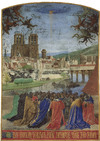
\includegraphics[keepaspectratio,width=\textwidth]{The-Right-Hand-of-God-Protecting-the-Faithful-against-the-Demons-small.jpg}
  \captionart{TheRightHandOfGodAgainstDemons}
  \label{fig:therighthandofgod}
\end{figure}

% Force float here
\clearpage{}
\thispagestyle{titleontop}

%SECT. II. MEMB. I. SUBSECT. II.-_A Digression of the nature of Spirits, bad Angels, or Devils, and how they cause Melancholy_.
\section[Nature of bad Angels, or Devils]{A Digression of the nature of Spirits, bad Angels, or Devils, and how they cause Melancholy.}

\lettrine{H}{ow} far the power of spirits and devils doth extend, and whether they
can cause this, or any other disease, is a serious question, and worthy
to be considered: for the better understanding of which, I will make a
brief digression of the nature of spirits. And although the question be
very obscure, according to Postellus\authormarginnote{1118}, full of controversy and
ambiguity, beyond the reach of human capacity, \lit{I confess I am not able to
understand it}{fateor excedere vires
intentionis meae}, saith \Austin{}\authormarginnote{1119}[2\baselineskip], \li{finitum de infinito non potest statuere}, we can sooner
determine with Tully, \li{de nat. deorum, quid non sint, quam quid sint},
our subtle schoolmen, Cardans, Scaligers, profound Thomists,
Fracastoriana and Ferneliana acies, are weak, dry, obscure, defective
in these mysteries, and all our quickest wits, as an owl's eyes at the
sun's light, wax dull, and are not sufficient to apprehend them; yet,
as in the rest, I will adventure to say something to this point. In
former times, as we read, Acts \rn{xxiii.}, the Sadducees denied that there
were any such spirits, devils, or angels. So did Galen the physician,
the Peripatetics, even \Aristotle himself, as Pomponatius stoutly
maintains, and Scaliger in some sort grants. Though Dandinus the
Jesuit, com. in lib. 2. de anima, stiffly denies it; \li{substantiae
separatae} and intelligences, are the same which Christians call angels,
and Platonists devils, for they name all the spirits, daemones, be they
good or bad angels, as \textlatin{Julius Pollux Onomasticon}, lib. 1. cap. 1.
observes. Epicures and atheists are of the same mind in general,
because they never saw them. Plato, Plotinus, Porphyrius, Jamblichus,
Proclus, insisting in the steps of \textlatin{Trismegistus}, Pythagoras and
Socrates, make no doubt of it: nor Stoics, but that there are such
spirits, though much erring from the truth. Concerning the first
beginning of them, the Talmudists say\authormarginnote{1120} that Adam had a wife called
Lilis, before he married Eve, and of her he begat nothing but devils.
The Turks' Alcoran\authormarginnote{1121}[1\baselineskip] is altogether as absurd and ridiculous in this
point: but the Scripture informs us Christians, how Lucifer, the chief
of them, with his associates, fell\authormarginnote{1122} from heaven for his pride and
ambition; created of God, placed in heaven, and sometimes an angel of
light, now cast down into the lower aerial sublunary parts, or into
hell, and delivered into chains of darkness (2 Pet. \rn{ii.} 4.) to be kept
unto damnation.

\subsection{Nature of Devils.}
There is a foolish opinion which some hold, that
they are the souls of men departed, good and more noble were deified,
the baser grovelled on the ground, or in the lower parts, and were
devils, the which with Tertullian, Porphyrius the philosopher, M.
Tyrius, ser. 27 maintains. These spirits, he saith\authormarginnote{1123}, which we call
angels and devils, are nought but souls of men departed, which either
through love and pity of their friends yet living, help and assist
them, or else persecute their enemies, whom they hated, as Dido
threatened to persecute Aeneas:
\li{Omnibus umbra locis adero: dabis improbe poenas.}

My angry ghost arising from the deep,
Shall haunt thee waking, and disturb thy sleep;
At least my shade thy punishment shall know,
And Fame shall spread the pleasing news below.

They are (as others suppose) appointed by those higher powers to keep
men from their nativity, and to protect or punish them as they see
cause: and are called boni et mali Genii by the Romans. Heroes, lares,
if good, lemures or larvae if bad, by the stoics, governors of
countries, men, cities, saith \Apuleius\authormarginnote{1124}, \li{Deos appellant qui ex
hominum numero juste ac prudenter vitae curriculo gubernato, pro
numine, postea ab hominibus praediti fanis et ceremoniis vulgo
admittuntur, ut in Aegypto Osyris, \etc{}}\authorlatintrans{1124.5}. Praestites, Capella calls them,
which protected particular men as well as princes, Socrates had his
\li{Daemonium Saturninum et ignium}, which of all spirits is best, \li{ad
sublimes cogitationes animum erigentem}, as the Platonists supposed;
Plotinus his, and we Christians our assisting angel, as Andreas
Victorellus, a copious writer of this subject, Lodovicus de La-Cerda,
the Jesuit, in his voluminous tract de Angelo Custode, Zanchius, and
some divines think. But this absurd tenet of Tyreus, Proclus confutes
at large in his book \textlatin{de Anima et daemone}.
Psellus\authorfootnote{1125}, a Christian, and sometimes tutor (saith Cuspinian) to
Michael Parapinatius, Emperor of Greece, a great observer of the nature
of devils, holds\authorfootnote{1126} they are corporeal, and have aerial bodies,
that they are mortal, live and die, (which Martianus Capella likewise
maintains, but our Christian philosophers explode) that they are
nourished and have excrements\authorfootnote{1127}, they feel pain if they be hurt (which
Cardan confirms, and Scaliger justly laughs him to scorn for; \li{Si
pascantur aere, cur non pugnant ob puriorem aera?} \etc{}) or stroken: and
if their bodies be cut, with admirable celerity they come together
again. \Austin{}, in Gen. lib. \rn{iii.} lib. arbit., approves as much, \li{mutata
casu corpora in deteriorem qualitatem aeris spissioris}, so doth
Hierome. Comment. in epist. ad Ephes. cap. 3, Origen, Tertullian,
Lactantius, and many ancient Fathers of the Church: that in their fall
their bodies were changed into a more aerial and gross substance.
Bodine, lib. 4, \textlatin{Theatri Naturae} and David Crusius, \textlatin{Hermeticae
Philosophiae}, lib. 1. cap. 4, by several arguments proves angels and
spirits to be corporeal: \li{quicquid continetur in loco corporeum est; At
spiritus continetur in loco, ergo. Si spiritus sunt quanti}\authorlatintrans{1128}, \li{erunt
corporei: At sunt quanti, ergo. sunt finiti, ergo. quanti, \etc{}.} Bodine
goes\authorfootnote{1129} farther yet, and will have these, \li{Animae separatae genii},
spirits, angels, devils, and so likewise souls of men departed, if
corporeal (which he most eagerly contends) to be of some shape, and
that absolutely round, like Sun and Moon, because that is the most
perfect form, \li{quae nihil habet asperitatis, nihil angulis incisum,
nihil anfractibus involutem, nihil eminens, sed inter corpora perfecta
est perfectissimum}\authorlatintrans{1130}; therefore all spirits are corporeal he
concludes, and in their proper shapes round. That they can assume other
aerial bodies, all manner of shapes at their pleasures, appear in what
likeness they will themselves, that they are most swift in motion, can
pass many miles in an instant, and so likewise transform bodies\authorfootnote{1131}
of others into what shape they please, and with admirable celerity
remove them from place to place; (as the Angel did Habakkuk to Daniel,
and as Philip the deacon was carried away by the Spirit, when he had
baptised the eunuch; so did Pythagoras and Apollonius remove themselves
and others, with many such feats) that they can represent castles in
the air, palaces, armies, spectrums, prodigies, and such strange
objects to mortal men's eyes, cause smells\authorfootnote{1132}, savours, \etc{}, deceive
all the senses; most writers of this subject credibly believe; and that
they can foretell future events, and do many strange miracles. Juno's
image spake to Camillus, and Fortune's statue to the Roman matrons,
with many such. Zanchius, Bodine, Spondanus, and others, are of opinion
that they cause a true metamorphosis, as Nebuchadnezzar was really
translated into a beast, Lot's wife into a pillar of salt; Ulysses'
companions into hogs and dogs, by Circe's charms; turn themselves and
others, as they do witches into cats, dogs, hares, crows, \etc{}. Strozzius
Cicogna hath many examples, lib. \rn{iii.} omnif. mag. cap. 4 and 5, which
he there confutes, as \Austin{} likewise doth, de civ. Dei lib. \rn{xviii.}
That they can be seen when and in what shape, and to whom they will,
saith Psellus, \li{Tametsi nil tale viderim, nec optem videre}, though he
himself never saw them nor desired it; and use sometimes carnal
copulation (as elsewhere I shall prove\authorfootnote{1133} more at large) with women
and men. Many will not believe they can be seen, and if any man shall
say, swear, and stiffly maintain, though he be discreet and wise,
judicious and learned, that he hath seen them, they account him a
timorous fool, a melancholy dizzard, a weak fellow, a dreamer, a sick
or a mad man, they contemn him, laugh him to scorn, and yet Marcus of
his credit told Psellus that he had often seen them. And Leo Suavius, a
Frenchman, c. 8, in Commentar. l. 1. \li{Paracelsi de vita longa}, out of
some Platonists, will have the air to be as full of them as snow
falling in the skies, and that they may be seen, and withal sets down
the means how men may see them; \li{Si irreverberatus oculis sole
splendente versus caelum continuaverint obtutus}\authorlatintrans{1134}, \etc{}, and saith
moreover he tried it, \li{praemissorum feci experimentum}, and it was true,
that the Platonists said. Paracelsus confesseth that he saw them diverse
times, and conferred with them, and so doth Alexander ab
Alexandro\authorfootnote{1135}, that he so found it by experience, when as before he
doubted of it. Many deny it, saith Lavater, \textlatin{de spectris}, part 1. c. 2,
and part 2. c. 11, because they never saw them themselves; but as he
reports at large all over his book, especially c. 19. part 1, they are
often seen and heard, and familiarly converse with men, as Lod. Vives
assureth us, innumerable records, histories, and testimonies evince in
all ages, times, places, and all travellers\authorfootnote{1136} besides; in the West
Indies and our northern climes, \li{Nihil familiarius quam in agris et
urbibus spiritus videre, audire qui vetent, jubeant, \etc{}.} Hieronymus
vita Pauli, Basil ser. 40, Nicephorus, Eusebius, Socrates, Sozomenus,
Jacobus Boissardus\authorfootnote{1137} in his tract de spirituum apparitionibus,
Petrus Loyerus l. \textlatin{de spectris}, Wierus l. 1. have infinite variety of
such examples of apparitions of spirits, for him to read that farther
doubts, to his ample satisfaction. One alone I will briefly insert. A
nobleman in Germany was sent ambassador to the King of Sweden (for his
name, the time, and such circumstances, I refer you to Boissardus, mine
Author\authorfootnote{1138}). After he had done his business, he sailed to Livonia, on
set purpose to see those familiar spirits, which are there said to be
conversant with men, and do their drudgery works. Amongst other
matters, one of them told him where his wife was, in what room, in what
clothes, what doing, and brought him a ring from her, which at his
return, non sine omnium admiratione, he found to be true; and so
believed that ever after, which before he doubted of. Cardan, l. 19. de
subtil, relates of his father, Facius Cardan, that after the accustomed
solemnities, \emph{anno} 1491, 13 August, he conjured up seven devils, in
Greek apparel, about forty years of age, some ruddy of complexion, and
some pale, as he thought; he asked them many questions, and they made
ready answer, that they were aerial devils, that they lived and died as
men did, save that they were far longer lived (700 or 800 years\authorfootnote{1139});
they did as much excel men in dignity as we do juments, and were as far
excelled again of those that were above them; our \authorfootnote{1140}governors and
keepers they are moreover, which Plato in Critias delivered\authorfootnote{1141} of
old, and subordinate to one another, \li{Ut enim homo homini sic daemon
daemoni dominatur}, they rule themselves as well as us, and the spirits
of the meaner sort had commonly such offices, as we make horse-keepers,
neat-herds, and the basest of us, overseers of our cattle; and that we
can no more apprehend their natures and functions, than a horse a
man's. They knew all things, but might not reveal them to men; and
ruled and domineered over us, as we do over our horses; the best kings
amongst us, and the most generous spirits, were not comparable to the
basest of them. Sometimes they did instruct men, and communicate their
skill, reward and cherish, and sometimes, again, terrify and punish, to
keep them in awe, as they thought fit, \li{Nihil magis cupientes} (saith
Lysius, Phis. Stoicorum) \li{quam adorationem hominum}\authorlatintrans{1142}. The same
Author, Cardan, in his Hyperchen, out of the doctrine of Stoics, will
have some of these genii (for so he calls them) to be desirous of
men's company\authorfootnote{1143}, very affable and familiar with them, as dogs are;
others, again, to abhor as serpents, and care not for them. The same
belike Tritemius calls Ignios \li{et sublunares, qui nunquam demergunt ad
inferiora, aut vix ullum habent in terris commercium}: Generally
they far excel men in worth\authorfootnote{1144}, as a man the meanest worm; though some of
them are inferior to those of their own rank in worth, as the
blackguard in a prince's court, and to men again, as some degenerate,
base, rational creatures, are excelled of brute beasts.
That they are mortal, besides these testimonies of Cardan, Martianus,
\etc{}, many other divines and philosophers hold, \li{post prolixum tempus
moriuntur omnes}; The Platonists\authorfootnote{1145}, and some Rabbins, Porphyrius and
Plutarch, as appears by that relation of Thamus: The great God
Pan is dead\authorfootnote{1146}; Apollo Pythius ceased; and so the rest. St. Hierome, in
the life of Paul the Hermit, tells a story how one of them appeared to
St. Anthony in the wilderness, and told him as much. Paracelsus
of our late writers stiffly maintains\authorfootnote{1147} that they are mortal, live and
die as other creatures do. Zozimus, l. 2, farther adds, that religion
and policy dies and alters with them. The Gentiles' gods, he
saith\authorfootnote{1148}, were expelled by Constantine, and together with them. \lit{The fortune
and majesty of the Roman Empire decayed and vanished}{Imperii
Romani majestas, et fortuna interiit, et profligata est}; as that heathen
in Minutius formerly bragged\authorfootnote{1149}, when the Jews were overcome by the
Romans, the Jew's God was likewise captivated by that of Rome; and
Rabsakeh to the Israelites, no God should deliver them out of the hands
of the Assyrians. But these paradoxes of their power, corporeity,
mortality, taking of shapes, transposing bodies, and carnal
copulations, are sufficiently confuted by Zanch. c. 10, l. 4. Pererius
in his comment, and Tostatus questions on the 6th of Gen. Th. Aquin.,
St. \Austin{}, Wierus, Th. Erastus, Delrio, tom. 2, l. 2, quaest. 29;
Sebastian Michaelis, c. 2, de spiritibus, D. Reinolds Lect. 47. They
may deceive the eyes of men, yet not take true bodies, or make a real
metamorphosis; but as Cicogna proves at large, they are
Illusoriae\authorfootnote{1150}, \li{et praestigiatrices transformationes}, omnif. mag.
lib. 4. cap. 4, mere illusions and cozenings, like that tale of Pasetis
obulus in Suidas, or that of Autolicus, Mercury's son, that dwelt in
Parnassus, who got so much treasure by cozenage and stealth. His father
Mercury, because he could leave him no wealth, taught him many fine
tricks to get means, for he could drive away men's cattle\authorfootnote{1151}, and if
any pursued him, turn them into what shapes he would, and so did
mightily enrich himself, \li{hoc astu maximam praedam est adsecutus}. This,
no doubt, is as true as the rest; yet thus much in general. Thomas,
Durand, and others, grant that they have understanding far beyond men,
can probably conjecture and foretell\authorfootnote{1152} many things; they can cause
and cure most diseases, deceive our senses; they have excellent skill
in all Arts and Sciences; and that the most illiterate devil is \lit{more knowing than any man}{Quovis
homine scientior}, as Cicogna maintains\authorfootnote{1153} out of others. They know the virtues of herbs, plants, stones, minerals, \etc{}; of all creatures, birds, beasts, the four
elements, stars, planets, can aptly apply and make use of them as they
see good; perceiving the causes of all meteors, and the like: \li{Dant se
coloribus} (as \Austin{} hath\authorfootnote{1154} it) \li{accommodant se figuris, adhaerent
sonis, subjiciunt se odoribus, infundunt se saporibus, omnes sensus
etiam ipsam intelligentiam daemones fallunt}, they deceive all our
senses, even our understanding itself at once. They can produce\authorfootnote{1155}
miraculous alterations in the air, and most wonderful effects, conquer
armies, give victories, help, further, hurt, cross and alter human
attempts and projects (\li{Dei permissu}) as they see good themselves.
When Charles the Great intended\authorfootnote{1156} to make a channel betwixt the
Rhine and the Danube, look what his workmen did in the day, these
spirits flung down in the night, \li{Ut conatu Rex desisteret, pervicere}.
Such feats can they do. But that which Bodine, l. 4, Theat. nat. thinks
(following Tyrius belike, and the Platonists), they can tell the
secrets of a man's heart, \li{aut cogitationes hominum}, is most false; his
reasons are weak, and sufficiently confuted by Zanch. lib. 4, cap. 9.
Hierom. lib. 2, com. in Mat. ad cap. 15, Athanasius quaest. 27, ad
Antiochum Principem, and others.

\subsection{Orders.}
As for those orders of good and bad devils, which the
Platonists hold, is altogether erroneous, and those Ethnics \li{boni et
mali Genii}, are to be exploded: these heathen writers agree not in this
point among themselves, as Dandinus notes, \li{An sint mali non
conveniunt}\authorfootnote{1157}, some will have all spirits good or bad to us by a mistake,
as if an Ox or Horse could discourse, he would say the Butcher was his
enemy because he killed him, the grazier his friend because he fed him;
a hunter preserves and yet kills his game, and is hated nevertheless of
his game; nec piscatorem piscis amare potest, \etc{}. But Jamblichus,
Psellus, Plutarch, and most Platonists acknowledge bad, et ab eorum
maleficiis cavendum, and we should beware of their wickedness, for they
are enemies of mankind, and this Plato learned in Egypt, that they
quarrelled with Jupiter, and were driven by him down to hell.
That\authorfootnote{1158} which \Apuleius\authorfootnote{1159}, Xenophon, and Plato contend of
Socrates Daemonium, is most absurd: That which Plotinus of his, that he
had likewise Deum pro Daemonio; and that which Porphyry concludes of
them all in general, if they be neglected in their sacrifice they are
angry; nay more, as Cardan in his Hipperchen will, they feed on men's
souls, \li{Elementa sunt plantis elementum, animalibus plantae, hominibus
animalia, erunt et homines aliis, non autem diis, nimis enim remota est
eorum natura a nostra, quapropter daemonibus}: and so belike that we
have so many battles fought in all ages, countries, is to make them a
feast, and their sole delight: but to return to that I said before, if
displeased they fret and chafe, (for they feed belike on the souls of
beasts, as we do on their bodies) and send many plagues amongst us; but
if pleased, then they do much good; is as vain as the rest and confuted
by \Austin{}, l. 9. c. 8. de Civ. Dei. Euseb. l. 4. praepar. Evang. c. 6.
and others. Yet thus much I find, that our schoolmen and other
divines make nine kinds of bad spirits\authorfootnote{1160}, as Dionysius hath done of
angels. In the first rank are those false gods of the gentiles, which
were adored heretofore in several idols, and gave oracles at Delphos,
and elsewhere; whose prince is Beelzebub. The second rank is of liars
and equivocators, as Apollo, Pythius, and the like. The third are those
vessels of anger, inventors of all mischief; as that Theutus in Plato;
Esay calls them vessels of fury\authorfootnote{1161}; their prince is Belial. The
fourth are malicious revenging devils; and their prince is Asmodaeus.
The fifth kind are cozeners, such as belong to magicians and witches;
their prince is Satan. The sixth are those aerial devils that
corrupt the air\authorfootnote{1162} and cause plagues, thunders, fires, \etc{}; spoken
of in the Apocalypse, and Paul to the Ephesians names them the princes
of the air; Meresin is their prince. The seventh is a destroyer,
captain of the furies, causing wars, tumults, combustions, uproars,
mentioned in the Apocalypse; and called Abaddon. The eighth is that
accusing or calumniating devil, whom the Greeks call \textgreek{Διαβολος}, that
drives men to despair. The ninth are those tempters in several kinds,
and their prince is Mammon. Psellus makes six kinds, yet none above the
Moon: Wierus in his Pseudo-monarchia Daemonis, out of an old book,
makes many more divisions and subordinations, with their several names,
numbers, offices, \etc{}, but Gazaeus cited by Lipsius\authorfootnote{1163} will have all
places full of angels, spirits, and devils, above and beneath the
Moon, ethereal and aerial\authorfootnote{1164}, which \Austin{} cites out of Varro l. 7.
de Civ. Dei, c. 6. The celestial devils above, and aerial beneath, or,
as some will, gods above, Semi-dei or half gods beneath, Lares, Heroes,
Genii, which climb higher, if they lived well, as the Stoics held; but
grovel on the ground as they were baser in their lives, nearer to the
earth: and are Manes, Lemures, Lamiae, \etc{}. They will have no
place\authorfootnote{1165} but all full of spirits, devils, or some other inhabitants;
\li{Plenum Caelum, aer, aqua terra, et omnia sub terra}, saith
Gazaeus\authorfootnote{1166}; though Anthony Rusca in his book de Inferno, lib. \rn{v.}
cap. 7. would confine them to the middle region, yet they will have
them everywhere. Not so much as a hair-breadth empty in heaven, earth,
or waters, above or under the earth. The air is not so full of flies in
summer, as it is at all times of invisible devils: this
Paracelsus stiffly maintains\authorfootnote{1167}, and that they have every one their
several chaos, others will have infinite worlds, and each world his
peculiar spirits, gods, angels, and devils to govern and punish it.
\li{Singula nonnulli credunt quoque sidera posse
Dici orbes, terramque appellant sidus opacum,
Cui minimus divum praesit.}\authorfootnote{1168}---

Some persons believe each star to be a world, and this earth an opaque
star, over which the least of the gods presides.

Gregorius Tholsanus makes\authorfootnote{1169} seven kinds of ethereal spirits or
angels, according to the number of the seven planets, Saturnine,
Jovial, Martial, of which Cardan discourseth lib. 20. de subtil. he
calls them substantias primas, Olympicos daemones Tritemius, qui
praesunt Zodiaco, \etc{}, and will have them to be good angels above,
devils beneath the Moon, their several names and offices he there sets
down, and which Dionysius of Angels, will have several spirits for
several countries, men, offices, \etc{}, which live about them, and as so
many assisting powers cause their operations, will have in a word,
innumerable, as many of them as there be stars in the skies.
Marcilius Ficinus seems to second\authorfootnote{1170} this opinion, out of Plato, or
from himself, I know not, (still ruling their inferiors, as they do
those under them again, all subordinate, and the nearest to the earth
rule us, whom we subdivide into good and bad angels, call gods or
devils, as they help or hurt us, and so adore, love or hate) but it is
most likely from Plato, for he relying wholly on Socrates, \li{quem mori
potius quam mentiri voluisse scribit}, whom he says would rather die
than tell a falsehood, out of Socrates' authority alone, made nine
kinds of them: which opinion belike Socrates took from Pythagoras, and
he from \textlatin{Trismegistus}, he from Zoroastes, first God, second idea, 3.
Intelligences, 4. Arch-Angels, 5. Angels, 6. Devils, 7. Heroes, 8.
Principalities, 9. Princes: of which some were absolutely good, as
gods, some bad, some indifferent \li{inter deos et homines}, as heroes and
daemons, which ruled men, and were called \li{genii}, or as Proclus\authorfootnote{1171}
and Jamblichus will, the middle betwixt God and men. Principalities and
princes, which commanded and swayed kings and countries; and had
several places in the spheres perhaps, for as every sphere is higher,
so hath it more excellent inhabitants: which belike is that Galilaeus a
Galileo and Kepler aims at in his \textlatin{nuncio Syderio}, when he will have
Saturnine\authorfootnote{1172} and Jovial inhabitants: and which Tycho Brahe doth in
some sort touch or insinuate in one of his epistles: but these things
Zanchius justly explodes\authorfootnote{1173}, cap. 3. lib. 4. P. Martyr, in 4. Sam. 28.

So that according to these men the number of ethereal spirits must
needs be infinite: for if that be true that some of our mathematicians
say: if a stone could fall from the starry heaven, or eighth sphere,
and should pass every hour an hundred miles, it would be 65 years, or
more, before it would come to ground, by reason of the great distance
of heaven from earth, which contains as some say 170 millions 800
miles, besides those other heavens, whether they be crystalline or
watery which Maginus adds, which peradventure holds as much more, how
many such spirits may it contain? And yet for all this Thomas
Albertus\authorfootnote{1174}, and most hold that there be far more angels than devils.

\subsection{Sublunary devils, and their kinds.}
But be they more or less, \lit{what is beyond our comprehension does not
concern us}{Quod supra nos nihil ad nos}. Howsoever as Martianus foolishly supposeth, \li{Aetherii
Daemones non curant res humanas}, they care not for us, do not attend
our actions, or look for us, those ethereal spirits have other worlds
to reign in belike or business to follow. We are only now to speak in
brief of these sublunary spirits or devils: for the rest, our divines
determine that the devil had no power over stars, or heavens;
\lit{by their charms (verses) they can seduce the moon from the heavens}{Carminibus coelo possunt deducere lunam}\authorfootnote{1175}, \etc{}. Those are poetical
fictions, and that they can \lit{stop rivers and turn the stars backward in their courses}{sistere aquam fluviis, et vertere
sidera retro}\authorfootnote{1176}, \etc{}, as Canadia in \Horace{}, 'tis all false. They are confined
until the day of judgment to this sublunary world\authorfootnote{1177}, and can work no
farther than the four elements, and as God permits them. Wherefore of
these sublunary devils, though others divide them otherwise according
to their several places and offices, Psellus makes six kinds, fiery,
aerial, terrestrial, watery, and subterranean devils, besides those
fairies, satyrs, nymphs, \etc{}.

Fiery spirits or devils are such as commonly work by blazing stars,
fire-drakes, or \li{ignes fatui}; which lead men often in \li{flumina aut
praecipitia}, saith Bodine, lib. 2. Theat. Naturae, fol. 221. \lit{whom if travellers wish to keep off they must pronounce the name of God with a clear voice, or adore him with their faces in contact with the ground, \etc{}}{Quos inquit arcere si volunt viatores, clara voce Deum appellare aut pronam
facie terram contingente adorare oportet, et hoc amuletum majoribus
nostris acceptum ferre debemus}, \etc{}; likewise they
counterfeit suns and moons, stars oftentimes, and sit on ship masts: \li{In
navigiorum summitatibus visuntur}; and are called \li{dioscuri}, as Eusebius
l. contra Philosophos, c. \rn{xlviii.} informeth us, out of the authority of
Zenophanes; or little clouds, \li{ad motum nescio quem volantes}; which
never appear, saith Cardan, but they signify some mischief or other to
come unto men, though some again will have them to pretend good, and
victory to that side they come towards in sea fights, St. Elmo's fires
they commonly call them, and they do likely appear after a sea storm;
Radzivilius, the Polonian duke, calls this apparition, Sancti Germani
sidus; and saith moreover that he saw the same after in a storm, as he
was sailing, 1582, from Alexandria to Rhodes. Our stories are
full\authorfootnote{1178} of such apparitions in all kinds. Some think they keep their
residence in that Hecla, a mountain in Iceland, Aetna in Sicily,
Lipari, Vesuvius, \etc{}. These devils were worshipped heretofore by that
superstitious Pyromanteia\authormarginnote{1179} and the like.

Aerial spirits or devils, are such as keep quarter most part in the
air\authorfootnote{1180}, cause many tempests, thunder, and lightnings, tear oaks,
fire steeples, houses, strike men and beasts, make it rain stones, as
in Livy's time, wool, frogs, \etc{}. Counterfeit armies in the air, strange
noises, swords, \etc{}, as at Vienna before the coming of the Turks, and
many times in Rome, as Scheretzius l. de spect. c. 1. part 1. Lavater
de spect. part. 1. c. 17. Julius Obsequens, an old Roman, in his book
of prodigies, \emph{ab urb. cond.} 505. Machiavel hath illustrated\authorfootnote{1181} by
many examples, and Josephus, in his book de bello Judaico, before the
destruction of Jerusalem. All which Guil. Postellus, in his first book,
c. 7, \textlatin{de orbis concordia}, useth as an effectual argument (as indeed it
is) to persuade them that will not believe there be spirits or devils.
They cause whirlwinds on a sudden, and tempestuous storms; which though
our meteorologists generally refer to natural causes, yet I am of
Bodine's mind, Theat. Nat. l. 2. they are more often caused by those
aerial devils, in their several quarters; for Tempestatibus se
ingerunt, saith \authorfootnote{1182} Rich. Argentine; as when a desperate man makes
away with himself, which by hanging or drowning they frequently do, as
Kommanus observes, \textlatin{de mirac. mort. part. 7, c. 76. tripudium agentes},
dancing and rejoicing at the death of a sinner. These can corrupt the
air, and cause plagues, sickness, storms, shipwrecks, fires,
inundations. At Mons Draconis in Italy, there is a most memorable
example in Jovianus Pontanus\authorfootnote{1183}: and nothing so familiar (if we may
believe those relations of \textlatin{Saxo Grammaticus, Olaus Magnus, Damianus} A.
Goes) as for witches and sorcerers, in Lapland, Lithuania, and all over
Scandia, to sell winds to mariners, and cause tempests, which Marcus
Paulus the Venetian relates likewise of the Tartars. These kind of
devils are much delighted in sacrifices\authorfootnote{1184} (saith Porphyry), held
all the world in awe, and had several names, idols, sacrifices, in
Rome, Greece, Egypt, and at this day tyrannise over, and deceive those
Ethnics and Indians, being adored and worshipped for gods\authorfootnote{1185}. For
the Gentiles' gods were devils (as \textlatin{Trismegistus} confesseth\authorfootnote{1186} in his
Asclepius), and he himself could make them come to their images by
magic spells: and are now as much respected by our papists (saith
Pictorius\authorfootnote{1187}) under the name of saints. These are they which Cardan
thinks desire so much carnal copulation with witches (Incubi and
Succubi), transform bodies, and are so very cold, if they be touched;
and that serve magicians. His father had one of them (as he is not
ashamed to relate), an aerial devil\authorfootnote{1188}, bound to him for twenty and
eight years. As Agrippa's dog had a devil tied to his collar; some
think that Paracelsus (or else Erastus belies him) had one confined to
his sword pummel; others wear them in rings, \etc{}. Jannes and Jambres did
many things of old by their help; Simon Magus, Cinops, Apollonius
Tianeus, Jamblichus, and Tritemius of late, that showed Maximilian the
emperor his wife, after she was dead; Et verrucam in collo ejus (saith
Godolman\authorfootnote{1189}) so much as the wart in her neck. Delrio, lib. 2. hath
diverse examples of their feats: Cicogna, lib. 3. cap. 3. and Wierus in
his book \textlatin{de praestig. daemonum. Boissardus de magis et veneficis}.
Water-devils are those Naiads or water nymphs which have been
heretofore conversant about waters and rivers. The water (as Paracelsus
thinks) is their chaos, wherein they live; some call them fairies, and
say that Habundia is their queen; these cause inundations, many times
shipwrecks, and deceive men diverse ways, as Succuba, or otherwise,
appearing most part (saith Tritemius) in women's shapes.

Paracelsus hath several stories\authorfootnote{1190} of them that have lived and been
married to mortal men, and so continued for certain years with them,
and after, upon some dislike, have forsaken them. Such a one as
Aegeria, with whom Numa was so familiar, Diana, Ceres, \etc{}. Olaus
Magnus hath\authorfootnote{1191} a long narration of one Hotherus, a king of Sweden, that
having lost his company, as he was hunting one day, met with these
water nymphs or fairies, and was feasted by them; and Hector Boethius,
or Macbeth, and Banquo, two Scottish lords, that as they were wandering
in the woods, had their fortunes told them by three strange women. To
these, heretofore, they did use to sacrifice, by that \textgreek{ὑδρομαντέια}, or
divination by waters.

Terrestrial devils are those Lares\authorfootnote{1192}, genii, fauns, satyrs, 
wood-nymphs\authorfootnote{1193}, foliots, fairies, Robin Goodfellows, trulli, \etc{}, which as
they are most conversant with men, so they do them most harm. Some
think it was they alone that kept the heathen people in awe of old, and
had so many idols and temples erected to them. Of this range was Dagon
amongst the Philistines, Bel amongst the Babylonians, Astartes amongst
the Sidonians, Baal amongst the Samaritans, Isis and Osiris amongst the
Egyptians, \etc{}; some put our fairies\authorfootnote{1194} into this rank, which have
been in former times adored with much superstition, with sweeping their
houses, and setting of a pail of clean water, good victuals, and the
like, and then they should not be pinched, but find money in their
shoes, and be fortunate in their enterprises. These are they that dance
on heaths and greens, as Lavater thinks\authorfootnote{1195} with Tritemius, and as
Olaus Magnus adds\authorfootnote{1196}, leave that green circle, which we commonly
find in plain fields, which others hold to proceed from a meteor
falling, or some accidental rankness of the ground, so nature sports
herself; they are sometimes seen by old women and children. Hierom.
Pauli, in his description of the city of Bercino in Spain, relates how
they have been familiarly seen near that town, about fountains and
hills; \li{Nonnunquam} (saith Tritemius) \li{in sua latibula montium
simpliciores homines ducant, stupenda mirantibus ostentes miracula,
nolarum sonitus, spectacula}\authorlatintrans{1197}. Giraldus Cambrensis gives
instance in a monk of Wales that was so deluded. Paracelsus
reckons\authorfootnote{1198} up many places in Germany, where they do usually walk in little
coats, some two feet long. A bigger kind there is of them called with
us hobgoblins, and Robin Goodfellows, that would in those superstitious
times grind corn for a mess of milk, cut wood, or do any manner of
drudgery work. They would mend old irons in those Aeolian isles of
Lipari, in former ages, and have been often seen and heard.
Tholosanus calls\authorfootnote{1199} them trullos and Getulos, and saith, that in his
days they were common in many places of France. Dithmarus Bleskenius,
in his description of Iceland, reports for a certainty, that almost in
every family they have yet some such familiar spirits; and Felix
Malleolus, in his book de crudel. daemon. affirms as much, that these
trolli or telchines are very common in Norway, and seen\authorfootnote{1200} to do
drudgery work; to draw water, saith Wierus, lib. 1. cap. 22, dress
meat, or any such thing. Another sort of these there are, which
frequent forlorn houses\authormarginnote{1201}, which the Italians call foliots, most
part innoxious, Cardan holds\authorfootnote{1202}; They will make strange noises in
the night, howl sometimes pitifully, and then laugh again, cause great
flame and sudden lights, fling stones, rattle chains, shave men, open
doors and shut them, fling down platters, stools, chests, sometimes
appear in the likeness of hares, crows, black dogs, \etc{} of which read
Pet Thyraeus the Jesuit\authorfootnote{1203}, in his \textlatin{Tract, de locis infestis, part.
1. et cap. 4}, who will have them to be devils or the souls of damned
men that seek revenge, or else souls out of purgatory that seek ease;
for such examples peruse Sigismundus Scheretzius\authorfootnote{1204}, \textlatin{lib. de
spectris, part 1. c. 1.} which he saith he took out of Luther most part;
there be many instances. Plinius Secundus remembers\authorfootnote{1205} such a house
at Athens, which Athenodorus the philosopher hired, which no man durst
inhabit for fear of devils. \Austin{}, \textlatin{de Civ. Dei. lib. 22, cap. 1.}
relates as much of Hesperius the Tribune's house, at Zubeda, near their
city of Hippos, vexed with evil spirits, to his great hindrance, \li{Cum
afflictione animalium et servorum suorum.} Many such instances are to be
read in Niderius Formicar, lib. 5. cap. \rn{xii.} 3. \etc{}. Whether I may call
these Zim and Ochim, which Isaiah, cap. \rn{xiii.} 21. speaks of, I make a
doubt. See more of these in the said Scheretz. lib. 1. de spect. cap.
4. he is full of examples. These kind of devils many times appear to
men, and affright them out of their wits, sometimes walking at
noonday\authorfootnote{1206}, sometimes at nights, counterfeiting dead men's ghosts,
as that of Caligula, which (saith Suetonius) was seen to walk in
Lavinia's garden, where his body was buried, spirits haunted, and the
house where he died, \li{Nulla nox sine terrore transacta, donec
incendio consumpta}\authorfootnote{1207}; every night this happened, there was no quietness,
till the house was burned. About Hecla, in Iceland, ghosts commonly
walk, \li{animas mortuorum simulantes}, saith Joh. Anan, lib. 3. de nat.
daem. Olaus. lib. 2. cap. 2. Natal Tallopid. lib. de apparit. spir.
Kornmannus de mirac. mort. part. 1. cap. 44. such sights are frequently
seen circa sepulchra et monasteria, saith Lavat. lib. 1. cap. 19. in
monasteries and about churchyards, \lit{marshes, great buildings,
solitary places, or remarkable as the scene of some murder}{loca paludinosa, ampla aedificia,
solitaria, et caede hominum notata}, \etc{}. Thyreus
adds, \lit{where some very heinous crime was
committed, there the impious and infamous generally dwell}{ubi gravius peccatum est commissum, impii, pauperum oppressores
et nequiter insignes habitant}. These
spirits often foretell men's deaths by several signs, as knocking,
groanings, \etc{} though Rich. Argentine\authorfootnote{1208}, c. 18. \textlatin{de praestigiis
daemonum}, will ascribe these predictions to good angels, out of the
authority of Ficinus and others; \lit{prodigies frequently occur at the deaths of
illustrious men}{prodigia in obitu principum saepius
contingunt}, \etc{}, as in the Lateran church in Rome\authorfootnote{1209}, the popes'
deaths are foretold by Sylvester's tomb. Near Rupes Nova in Finland, in
the kingdom of Sweden, there is a lake, in which, before the governor
of the castle dies, a spectrum, in the habit of Arion with his harp,
appears, and makes excellent music, like those blocks in Cheshire,
which (they say) presage death to the master of the family; or that
oak\authorfootnote{1210} in Lanthadran park in Cornwall, which foreshows as much. Many
families in Europe are so put in mind of their last by such
predictions, and many men are forewarned (if we may believe Paracelsus)
by familiar spirits in diverse shapes, as cocks, crows, owls, which
often hover about sick men's chambers, vel quia morientium foeditatem
sentiunt, as Baracellus conjectures\authorfootnote{1211}, \li{et ideo super tectum
infirmorum crocitant}, because they smell a corse; or for that (as
\authorfootnote{1212}Bernardinus de Bustis thinketh) God permits the devil to appear
in the form of crows, and such like creatures, to scare such as live
wickedly here on earth. A little before Tully's death (saith Plutarch)
the crows made a mighty noise about him, tumultuose perstrepentes, they
pulled the pillow from under his head. Rob. Gaguinus, hist. Franc. lib.
8, telleth such another wonderful story at the death of Johannes de
Monteforti, a French lord, \emph{anno} 1345, \lit{a
multitude of crows alighted on the house of the dying man, such as no
one imagined existed in France}{tanta corvorum multitudo
aedibus morientis insedit, quantam esse in Gallia nemo judicasset}. Such prodigies are very frequent in
authors. See more of these in the said Lavater, \textlatin{Thyreus de locis
infestis, part 3, cap. 58. Pictorius, Delrio, Cicogna, lib. 3, cap. 9.}
Necromancers take upon them to raise and lay them at their pleasures:
and so likewise, those which Mizaldus calls ambulones, that walk about
midnight on great heaths and desert places, which (saith \authorfootnote{1213}Lavater)
draw men out of the way, and lead them all night a byway, or quite bar
them of their way; these have several names in several places; we
commonly call them Pucks. In the deserts of Lop, in Asia, such
illusions of walking spirits are often perceived, as you may read in M.
Paulus the Venetian his travels; if one lose his company by chance,
these devils will call him by his name, and counterfeit voices of his
companions to seduce him. Hieronym. Pauli, in his book of the hills of
Spain, relates of a great \authorfootnote{1214}mount in Cantabria, where such
spectrums are to be seen; Lavater and Cicogna have variety of examples
of spirits and walking devils in this kind. Sometimes they sit by the
highway side, to give men falls, and make their horses stumble and
start as they ride (if you will believe the relation of that holy man
Ketellus in \authorfootnote{1215}Nubrigensis), that had an especial grace to see
devils, Gratiam divinitus collatam, and talk with them, Et impavidus
cum spiritibus sermonem miscere, without offence, and if a man curse or
spur his horse for stumbling, they do heartily rejoice at it; with many
such pretty feats.

Subterranean devils are as common as the rest, and do as much harm.
Olaus Magnus, lib. 6, cap. 19, make six kinds of them; some bigger,
some less. These (saith \authorfootnote{1216}Munster) are commonly seen about mines of
metals, and are some of them noxious; some again do no harm. The
metal-men in many places account it good luck, a sign of treasure and
rich ore when they see them. Georgius Agricola, in his book de
subterraneis animantibus, cap. 37, reckons two more notable kinds of
them, which he calls \authorfootnote{1217}getuli and cobali, both are clothed after
the manner of metal-men, and will many times imitate their works. Their
office, as Pictorius and Paracelsus think, is to keep treasure in the
earth, that it be not all at once revealed; and besides, \authorfootnote{1218}Cicogna
avers that they are the frequent causes of those horrible earthquakes
which often swallow up, not only houses, but whole islands and cities;
in his third book, cap. 11, he gives many instances.

The last are conversant about the centre of the earth to torture the
souls of damned men to the day of judgment; their egress and regress
some suppose to be about Etna, Lipari, Mons Hecla in Iceland, Vesuvius,
Terra del Fuego, \etc{}, because many shrieks and fearful cries are
continually heard thereabouts, and familiar apparitions of dead men,
ghosts and goblins.

\subsection{Their Offices, Operations, Study.}
Thus the devil reigns, and in a thousand several shapes, as a roaring lion still seeks whom he may
devour, 1 Pet. \rn{v.}, by sea, land, air, as yet unconfined, though \authorfootnote{1219}
some will have his proper place the air; all that space between us and
the moon for them that transgressed least, and hell for the wickedest
of them, Hic velut in carcere ad finem mundi, tunc in locum funestiorum
trudendi, as \Austin{} holds de Civit. Dei, c. 22, lib. 14, cap. 3 et 23;
but be where he will, he rageth while he may to comfort himself, as
\authorfootnote{1220} Lactantius thinks, with other men's falls, he labours all he can
to bring them into the same pit of perdition with him. For \authorfootnote{1221}men's
miseries, calamities, and ruins are the devil's banqueting dishes. By
many temptations and several engines, he seeks to captivate our souls.
The Lord of Lies, saith \authorfootnote{1222}\Austin{}, as he was deceived himself, he
seeks to deceive others, the ringleader to all naughtiness, as he did
by Eve and Cain, Sodom and Gomorrah, so would he do by all the world.
Sometimes he tempts by covetousness, drunkenness, pleasure, pride, \etc{},
errs, dejects, saves, kills, protects, and rides some men, as they do
their horses. He studies our overthrow, and generally seeks our
destruction; and although he pretend many times human good, and
vindicate himself for a god by curing of several diseases, aegris
sanitatem, et caecis luminis usum restituendo, as \Austin{} declares, lib.
10, de civit Dei, cap. 6, as Apollo, Aesculapius, Isis, of old have
done; divert plagues, assist them in wars, pretend their happiness, yet
nihil his impurius, scelestius, nihil humano generi infestius, nothing
so impure, nothing so pernicious, as may well appear by their
tyrannical and bloody sacrifices of men to Saturn and Moloch, which are
still in use among those barbarous Indians, their several deceits and
cozenings to keep men in obedience, their false oracles, sacrifices,
their superstitious impositions of fasts, penury, \etc{}. Heresies,
superstitious observations of meats, times, \etc{}, by which they \authorfootnote{1223}
crucify the souls of mortal men, as shall be showed in \hyperref[ch:religious-melancholy]{our Treatise of
Religious Melancholy}. \li{Modico adhuc tempore sinitur malignari}, as Bernard expresseth it\authorfootnote{1224}, by God's permission he rageth a while, hereafter
to be confined to hell and darkness, which is prepared for him and his
angels, Mat. \rn{xxv.}

How far their power doth extend it is hard to determine; what the
ancients held of their effects, force and operations, I will briefly
show you: Plato in Critias, and after him his followers, gave out that
these spirits or devils, were men's governors and keepers, our lords
and masters, as we are of our cattle. \authorfootnote{1225}They govern provinces and
kingdoms by oracles, auguries, dreams, rewards and punishments,
prophecies, inspirations, sacrifices, and religious superstitions,
varied in as many forms as there be diversity of spirits; they send
wars, plagues, peace, sickness, health, dearth, plenty, \authorfootnote{1226}Adstantes
hic jam nobis, spectantes, et arbitrantes, \etc{} as appears by those
histories of Thucydides, Livius, Dionysius Halicarnassus, with many
others that are full of their wonderful stratagems, and were therefore
by those Roman and Greek commonwealths adored and worshipped for gods
with prayers and sacrifices, \etc{}. \authorfootnote{1227}In a word, \li{Nihil magis quaerunt
quam metum et admirationem hominum}\authorlatintrans{1228}; and as another hath it, \li{Dici
non potest, quam impotenti ardore in homines dominium, et Divinos
cultus maligni spiritus affectent}\authorlatintrans{1229}. Tritemius in his book de
septem secundis, assigns names to such angels as are governors of
particular provinces, by what authority I know not, and gives them
several jurisdictions. Asclepiades a Grecian, Rabbi Achiba the Jew,
Abraham Avenezra, and Rabbi Azariel, Arabians, (as I find them cited by
\authorfootnote{1230}Cicogna) farther add, that they are not our governors only, Sed
ex eorum concordia et discordia, boni et mali affectus promanant, but
as they agree, so do we and our princes, or disagree; stand or fall.
Juno was a bitter enemy to Troy, Apollo a good friend, Jupiter
indifferent, Aequa Venus Teucris, Pallas iniqua fuit; some are for us
still, some against us, Premente Deo, fert Deus alter opem. Religion,
policy, public and private quarrels, wars are procured by them, and
they are \authorfootnote{1231}delighted perhaps to see men fight, as men are with
cocks, bulls and dogs, bears, \etc{}, plagues, dearths depend on them, our
bene and male esse, and almost all our other peculiar actions (for as
Anthony Rusea contends, lib. 5, cap. 18, every man hath a good and a
bad angel attending on him in particular, all his life long, which
Jamblichus calls \li{daemonem}), preferments, losses, weddings, deaths,
rewards and punishments, and as Proclus will\authorfootnote{1232}, all offices
whatsoever, \li{alii genetricem, alii opificem potestatem habent}, \etc{} and
several names they give them according to their offices, as Lares,
Indegites, Praestites, \etc{}. When the Arcades in that battle at Cheronae,
which was fought against King Philip for the liberty of Greece, had
deceitfully carried themselves, long after, in the very same place,
\li{Diis Graeciae, ultoribus} (saith mine author) they were miserably slain
by Metellus the Roman: so likewise, in smaller matters, they will have
things fall out, as these boni and mali genii favour or dislike us:
Saturni non conveniunt Jovialibus, \etc{}. He that is Saturninus shall
never likely be preferred. \authorfootnote{1233}That base fellows are often advanced,
undeserving Gnathoes, and vicious parasites, whereas discreet, wise,
virtuous and worthy men are neglected and unrewarded; they refer to
those domineering spirits, or subordinate Genii; as they are inclined,
or favour men, so they thrive, are ruled and overcome; for as
\authorfootnote{1234}Libanius supposeth in our ordinary conflicts and contentions,
\lit{one genius yields and is overcome by another}{Genius Genio cedit et obtemperat}. All
particular events almost they refer to these private spirits; and (as
Paracelsus adds) they direct, teach, inspire, and
instruct men. Never was any man extraordinary famous in any art,
action, or great commander, that had not familiarem daemonem to inform
him, as Numa, Socrates, and many such, as Cardan illustrates, cap. 128,
\textlatin{Arcanis prudentiae civilis}, \authorfootnote{1235} \li{Speciali siquidem gratia, se a Deo
donari asserunt magi, a Geniis caelestibus instrui, ab iis doceri}. But
these are most erroneous paradoxes, \li{ineptae et fabulosae nugae},
rejected by our divines and Christian churches. 'Tis true they have, by
God's permission, power over us, and we find by experience, that they
can \authorfootnote{1236}hurt not our fields only, cattle, goods, but our bodies and
minds. At Hammel in Saxony, \emph{anno} 1484. 20 \emph{Junii}, the devil, in
likeness of a pied piper, carried away 130 children that were never
after seen. Many times men are \authorfootnote{1237}affrighted out of their wits,
carried away quite, as Scheretzius illustrates, lib. 1, c. \rn{iv.}, and
severally molested by his means, Plotinus the Platonist, lib. 14,
advers. Gnos. laughs them to scorn, that hold the devil or spirits can
cause any such diseases. Many think he can work upon the body, but not
upon the mind. But experience pronounceth otherwise, that he can work
both upon body and mind. Tertullian is of this opinion, c. 22.
\authorfootnote{1238}That he can cause both sickness and health, and that secretly.
\authorfootnote{1239}Taurellus adds by clancular poisons he can infect the bodies, and
hinder the operations of the bowels, though we perceive it not, closely
creeping into them, saith \authorfootnote{1240}Lipsius, and so crucify our souls: Et
nociva melancholia furiosos efficit. For being a spiritual body, he
struggles with our spirits, saith Rogers, and suggests (according to
\authorfootnote{1241}Cardan, \li{verba sine voce, species sine visu}, envy, lust, anger,
\etc{}) as he sees men inclined.

The manner how he performs it, Biarmannus in his Oration against
Bodine, sufficiently declares. \authorfootnote{1242}He begins first with the phantasy,
and moves that so strongly, that no reason is able to resist. Now the
phantasy he moves by mediation of humours; although many physicians are
of opinion, that the devil can alter the mind, and produce this disease
of himself. Quibusdam medicorum visum, saith \authorfootnote{1243}\Avicenna{}, quod
Melancholia contingat a daemonio. Of the same mind is Psellus and
Rhasis the Arab. lib. 1. Tract. 9. Cont. \authorfootnote{1244}That this disease
proceeds especially from the devil, and from him alone. Arculanus, cap.
6. in 9. Rhasis, Aelianus Montaltus, in his 9. cap. Daniel Sennertus,
lib. 1. part. 2. cap. 11. confirm as much, that the devil can cause
this disease; by reason many times that the parties affected prophesy,
speak strange language, but non sine interventu humoris, not without
the humour, as he interprets himself; no more doth \Avicenna{}, si
contingat a daemonio, sufficit nobis ut convertat complexionem ad
choleram nigram, et sit causa ejus propinqua cholera nigra; the
immediate cause is choler adust, which \authorfootnote{1245} Pomponatius likewise
labours to make good: Galgerandus of Mantua, a famous physician, so
cured a demoniacal woman in his time, that spake all languages, by
purging black choler, and thereupon belike this humour of melancholy is
called balneum diaboli, the devil's bath; the devil spying his
opportunity of such humours drives them many times to despair, fury,
rage, \etc{}, mingling himself among these humours. This is that which
Tertullian avers, Corporibus infligunt acerbos casus, animaeque
repentinos, membra distorquent, occulte repentes, \etc{} and which Lemnius
goes about to prove, Immiscent se mali Genii pravis humoribus, atque
atrae, bili, \etc{}. And \authorfootnote{1246}Jason Pratensis, that the devil, being a
slender incomprehensible spirit, can easily insinuate and wind himself
into human bodies, and cunningly couched in our bowels vitiate our
healths, terrify our souls with fearful dreams, and shake our minds
with furies. And in another place, These unclean spirits settled in our
bodies, and now mixed with our melancholy humours, do triumph as it
were, and sport themselves as in another heaven. Thus he argues, and
that they go in and out of our bodies, as bees do in a hive, and so
provoke and tempt us as they perceive our temperature inclined of
itself, and most apt to be deluded. \authorfootnote{1247} Agrippa and \authorfootnote{1248}Lavater
are persuaded, that this humour invites the devil to it, wheresoever it
is in extremity, and of all other, melancholy persons are most subject
to diabolical temptations and illusions, and most apt to entertain
them, and the Devil best able to work upon them. But whether by
obsession, or possession, or otherwise, I will not determine; 'tis a
difficult question. Delrio the Jesuit, Tom. 3. lib. 6. Springer and his
colleague, mall. malef. Pet. Thyreus the Jesuit, \textlatin{lib. de daemoniacis,
de locis infestis, de Terrificationibus nocturnis, Hieronymus Mengus
Flagel. daem.} and others of that rank of pontifical writers, it seems,
by their exorcisms and conjurations approve of it, having forged many
stories to that purpose. A nun did eat a lettuce \authorfootnote{1249}without grace,
or signing it with the sign of the cross, and was instantly possessed.
Durand. lib. 6. Rationall. c. 86. numb. 8. relates that he saw a wench
possessed in Bononia with two devils, by eating an unhallowed
pomegranate, as she did afterwards confess, when she was cured by
exorcisms. And therefore our Papists do sign themselves so often with
the sign of the cross, \li{Ne daemon ingredi ausit}, and exorcise all manner
of meats, as being unclean or accursed otherwise, as Bellarmine
defends. Many such stories I find amongst pontifical writers, to prove
their assertions, let them free their own credits; some few I will
recite in this kind out of most approved physicians. Cornelius Gemma,
lib. 2. de nat. mirac. c. 4. relates of a young maid, called Katherine
Gualter, a cooper's daughter, \emph{an.} 1571. that had such strange
passions and convulsions, three men could not sometimes hold her; she
purged a live eel, which he saw, a foot and a half long, and touched it
himself; but the eel afterwards vanished; she vomited some twenty-four
pounds of fulsome stuff of all colours, twice a day for fourteen days;
and after that she voided great balls of hair, pieces of wood, pigeon's
dung, parchment, goose dung, coals; and after them two pounds of pure
blood, and then again coals and stones, or which some had inscriptions
bigger than a walnut, some of them pieces of glass, brass, \etc{} besides
paroxysms of laughing, weeping and ecstasies, \etc{}. \lit{this I saw with horror}{Et hoc (inquit) cum
horore vidi}. They could do no good on her by
physic, but left her to the clergy. Marcellus Donatus, lib. 2. c. 1. de
med. mirab. hath such another story of a country fellow, that had four
knives in his belly, Instar serrae dentatos, indented like a saw, every
one a span long, and a wreath of hair like a globe, with much baggage
of like sort, wonderful to behold: how it should come into his guts, he
concludes, \lit{could assuredly only have been through the artifice of the devil}{Certe non alio quam daemonis astutia et dolo}. Langius, Epist. med. lib. 1. Epist. 38. hath many relations to this effect, and
so hath Christophorus a Vega: Wierus, Skenkius, Scribanius, all agree
that they are done by the subtlety and illusion of the devil. If you
shall ask a reason of this, 'tis to exercise our patience; for as
\authorfootnote{1250}Tertullian holds, \li{Virtus non est virtus, nisi comparem habet
aliquem, in quo superando vim suam ostenda}t 'tis to try us and our
faith, 'tis for our offences, and for the punishment of our sins, by
God's permission they do it, \li{Carnifices vindictae justae Dei}, as
\authorfootnote{1251}Tolosanus styles them, Executioners of his will; or rather as
David, Ps. 78. ver. 49. He cast upon them the fierceness of his anger,
indignation, wrath, and vexation, by sending out of evil angels: so did
he afflict Job, Saul, the Lunatics and demoniacal persons whom Christ
cured, Mat. \rn{iv.} 8. Luke \rn{iv.} 11. Luke \rn{xiii.} Mark \rn{ix.} Tobit. \rn{viii.} 3. \etc{}.
This, I say, happeneth for a punishment of sin, for their want of
faith, incredulity, weakness, distrust, \etc{}.

\cleartoleftpage{}
\begin{figure}[p]
  \begingroup
  \centering
  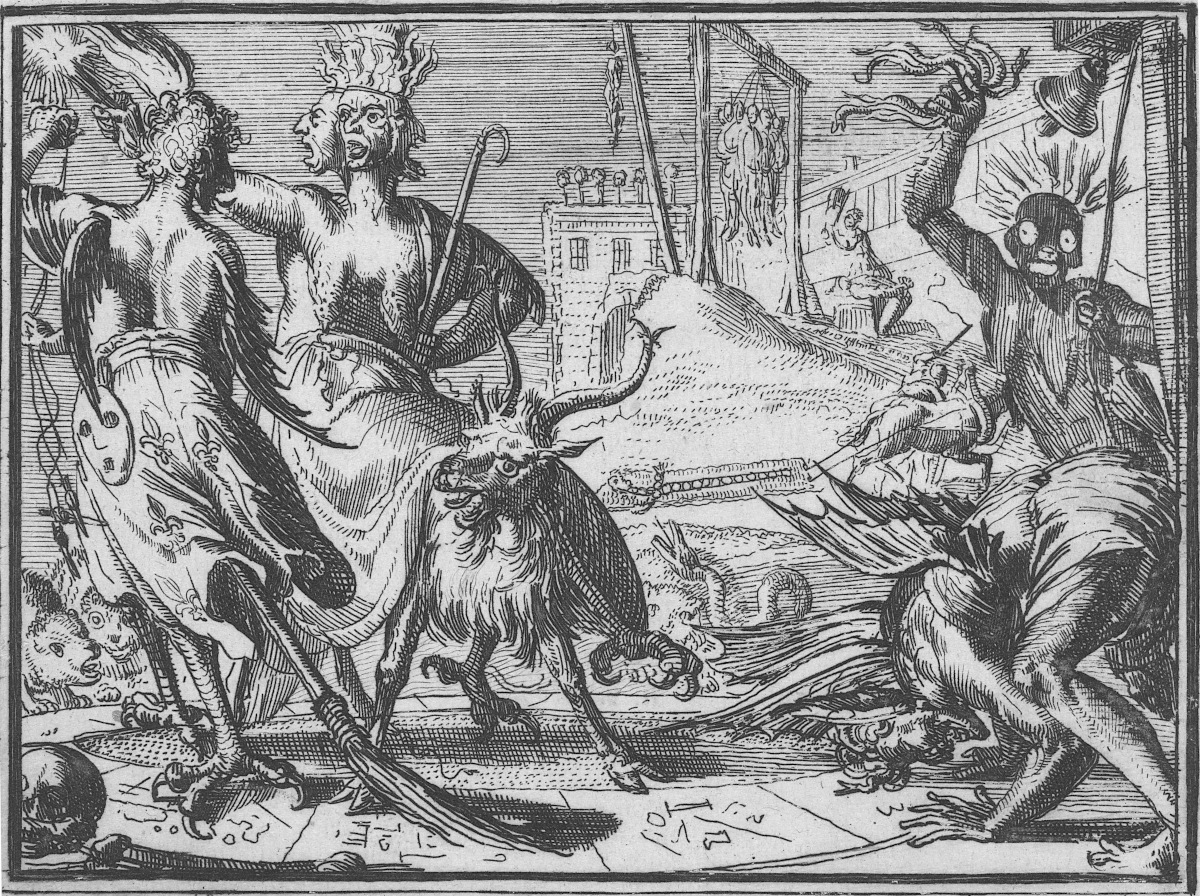
\includegraphics[keepaspectratio,width=\textwidth]{DeHorlende-small.jpg}
  \captionart{DeHorlendeKollendans}
  \label{fig:dehorlende}
\end{figure}

% Force float here
\clearpage{}
\thispagestyle{titleontop}

%SECT. II. MEMB. I. SUBSECT. III.-_Of Witches and Magicians, how they cause Melancholy_.
\section[Witches and Magicians]{Of Witches and Magicians, how they cause Melancholy.}

\lettrine{Y}{ou} have heard what the devil can do of himself, now you shall hear
what he can perform by his instruments, who are many times worse (if it
be possible) than he himself, and to satisfy their revenge and lust
cause more mischief, \li{Multa enim mala non egisset daemon, nisi
provocatus a sagis}, as Erastus thinks\authorfootnote{1252}; much harm had never been
done, had he not been provoked by witches to it. He had not appeared in
Samuel's shape, if the Witch of Endor had let him alone; or represented
those serpents in Pharaoh's presence, had not the magicians urged him
unto it; \li{Nec morbos vel hominibus, vel brutis infligeret} (Erastus
maintains) \li{si sagae quiescerent}; men and cattle might go free, if the
witches would let him alone. Many deny witches at all, or if there be
any they can do no harm; of this opinion is Wierus, lib. 3. cap. 53. \textlatin{de
praestig. daem.} \Austin{} Lerchemer a Dutch writer, Biarmanus, Ewichius,
Euwaldus, our countryman Scot; with him in \Horace{},
\li{Somnia, terrores Magicos, miracula, sagas,
Nocturnos Lemures, portentaque Thessala risu
Excipiunt.}---

\begin{verse}
Say, can you laugh indignant at the schemes\\*
Of magic terrors, visionary dreams,\\*
Portentous wonders, witching imps of Hell,\\*
The nightly goblin, and enchanting spell?
\end{verse}

They laugh at all such stories; but on the contrary are most lawyers,
divines, physicians, philosophers, \Austin{}, Hemingius, Danaeus,
Chytraeus, Zanchius, Aretius, \etc{}. Delrio, Springer, \authorfootnote{1253}Niderius,
lib. 5. Fornicar. Guiatius, Bartolus, consil. 6. tom. 1. Bodine,
daemoniant. lib 2. cap. 8. Godelman, Damhoderius, \etc{}. Paracelsus,
Erastus, Scribanius, Camerarius, \etc{}. The parties by whom the devil
deals, may be reduced to these two, such as command him in show at
least, as conjurors, and magicians, whose detestable and horrid
mysteries are contained in their book called \authorfootnote{1254}Arbatell; \li{daemonis
enim advocati praesto sunt, seque exorcismis et conjurationibus quasi
cogi patiuntur, ut miserum magorum genus, in impietate detineant.} Or
such as are commanded, as witches, that deal \li{ex parte} implicite, or
explicite, as the king\authormarginnote{1255} hath well defined; many subdivisions there
are, and many several species of sorcerers, witches, enchanters,
charmers, \etc{}. They have been tolerated heretofore some of them; and
magic hath been publicly professed in former times, in Salamanca\authormarginnote{1256},
Krakow\authormarginnote{1257}[2\baselineskip], and other places, though after censured by several
Universities\authormarginnote{1258}[3\baselineskip], and now generally contradicted, though practised by
some still, maintained and excused, \li{Tanquam res secreta quae non nisi
viris magnis et peculiari beneficio de Coelo instructis communicatur} (I
use \authorfootnote{1259}Boesartus his words) and so far approved by some princes, \li{Ut
nihil ausi aggredi in politicis, in sacris, in consiliis, sine eorum
arbitrio}; they consult still with them, and dare indeed do nothing
without their advice. Nero and Heliogabalus, Maxentius, and Julianus
Apostata, were never so much addicted to magic of old, as some of our
modern princes and popes themselves are nowadays. Erricus, King of
Sweden, had an \authorfootnote{1260}enchanted cap, by virtue of which, and some
magical murmur or whispering terms, he could command spirits, trouble
the air, and make the wind stand which way he would, insomuch that when
there was any great wind or storm, the common people were wont to say,
the king now had on his conjuring cap. But such examples are infinite.
That which they can do, is as much almost as the devil himself, who is
still ready to satisfy their desires, to oblige them the more unto him.
They can cause tempests, storms, which is familiarly practised by
witches in Norway, Iceland, as I have proved. They can make friends
enemies, and enemies friends by philters; \authorfootnote{1261}Turpes amores
conciliare, enforce love, tell any man where his friends are, about
what employed, though in the most remote places; and if they will,
\authorfootnote{1262}bring their sweethearts to them by night, upon a goat's back
flying in the air. Sigismund Scheretzius, part. 1. cap. 9. de spect.
reports confidently, that he conferred with sundry such, that had been
so carried many miles, and that he heard witches themselves confess as
much; hurt and infect men and beasts, vines, corn, cattle, plants, make
women abortive, not to conceive, \authorfootnote{1263}barren, men and women unapt and
unable, married and unmarried, fifty several ways, saith Bodine, lib.
2. c. 2. fly in the air, meet when and where they will, as Cicogna
proves, and Lavat. \textlatin{de spec}. part. 2. c. 17. steal young children out of
their cradles, \li{ministerio daemonum}, and put deformed in their rooms,
which we call changelings, saith \authorfootnote{1264}Scheretzius, part. 1. c. 6. make
men victorious, fortunate, eloquent; and therefore in those ancient
monomachies and combats they were searched of old, \authorfootnote{1265}they had no
magical charms; they can make \authorfootnote{1266}stick frees, such as shall endure a
rapier's point, musket shot, and never be wounded: of which read more
in Boissardus, cap. 6. de Magia, the manner of the adjuration, and by
whom 'tis made, where and how to be used in expeditionibus bellicis,
praeliis, duellis, \etc{}, with many peculiar instances and examples; they
can walk in fiery furnaces, make men feel no pain on the rack, aut
alias torturas sentire; they can stanch blood, \authorfootnote{1267}represent dead
men's shapes, alter and turn themselves and others into several forms,
at their pleasures. \authorfootnote{1268}Agaberta, a famous witch in Lapland, would do
as much publicly to all spectators, Modo Pusilla, modo anus, modo
procera ut quercus, modo vacca, avis, coluber, \etc{}. Now young, now old,
high, low, like a cow, like a bird, a snake, and what not? She could
represent to others what forms they most desired to see, show them
friends absent, reveal secrets, maxima omnium admiratione, \etc{}. And yet
for all this subtlety of theirs, as Lipsius well observes, Physiolog.
Stoicor. lib. 1. cap. 17. neither these magicians nor devils themselves
can take away gold or letters out of mine or Crassus' chest, et
Clientelis suis largiri, for they are base, poor, contemptible fellows
most part; as Bodine notes\authorfootnote{1269}, they can do nothing in Judicum
decreta aut poenas, in regum concilia vel arcana, nihil in rem
nummariam aut thesauros, they cannot give money to their clients, alter
judges' decrees, or councils of kings, these minuti Genii cannot do it,
altiores Genii hoc sibi adservarunt, the higher powers reserve these
things to themselves. Now and then peradventure there may be some more
famous magicians like Simon Magus, \authorfootnote{1270}Apollonius Tyaneus, Pasetes,
Jamblichus, \authorfootnote{1271}Odo de Stellis, that for a time can build castles in
the air, represent armies, \etc{}, as they are \authorfootnote{1272}said to have done,
command wealth and treasure, feed thousands with all variety of meats
upon a sudden, protect themselves and their followers from all princes'
persecutions, by removing from place to place in an instant, reveal
secrets, future events, tell what is done in far countries, make them
appear that died long since, and do many such miracles, to the world's
terror, admiration and opinion of deity to themselves, yet the devil
forsakes them at last, they come to wicked ends, and raro aut nunquam
such impostors are to be found. The vulgar sort of them can work no
such feats. But to my purpose, they can, last of all, cure and cause
most diseases to such as they love or hate, and this of
\authorfootnote{1273}melancholy amongst the rest. Paracelsus, Tom. 4. de morbis
amentium, Tract. 1. in express words affirms; Multi fascinantur in
melancholiam, many are bewitched into melancholy, out of his
experience. The same saith Danaeus, lib. 3. de sortiariis. Vidi,
inquit, qui Melancholicos morbos gravissimos induxerunt: I have seen
those that have caused melancholy in the most grievous manner,
\authorfootnote{1274}dried up women's paps, cured gout, palsy; this and apoplexy,
falling sickness, which no physic could help, solu tactu, by touch
alone. Ruland in his 3 Cent. Cura 91. gives an instance of one David
Helde, a young man, who by eating cakes which a witch gave him, mox
delirare coepit, began to dote on a sudden, and was instantly mad: F.
H. D. in \authorfootnote{1275}Hildesheim, consulted about a melancholy man, thought
his disease was partly magical, and partly natural, because he vomited
pieces of iron and lead, and spake such languages as he had never been
taught; but such examples are common in Scribanius, Hercules de
Saxonia, and others. The means by which they work are usually charms,
images, as that in Hector Boethius of King Duffe; characters stamped of
sundry metals, and at such and such constellations, knots, amulets,
words, philters, \etc{}, which generally make the parties affected,
melancholy; as Monavius discourseth\authorfootnote{1276} at large in an epistle of his
to Acolsius, giving instance in a Bohemian baron that was so troubled
by a philter taken. Not that there is any power at all in those spells,
charms, characters, and barbarous words; but that the devil doth use
such means to delude them. \li{Ut fideles inde magos} (saith Libanius\authormarginnote{1277})
\li{in officio retineat, tum in consortium malefactorum vocet.}

\cleartoleftpage{}
\begin{figure}[p]
  \begingroup
  \centering
  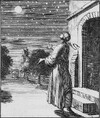
\includegraphics[keepaspectratio,width=\textwidth]{Woman-stars-small.jpg}
  \captionart{WomanStars}
  \label{fig:womanstars}
\end{figure}

% Force float here
\clearpage{}
\thispagestyle{titleontop}

%SECT. II. MEMB. I. SUBSECT. IV.-_Stars a cause. Signs from Physiognomy, Metoposcopy, Chiromancy_.
\section[Heavens, Planets, Stars]{Stars a cause. Signs from Physiognomy, Metoposcopy, Chiromancy.}\label{sec:heavens-planets-stars}

\lettrine{N}{atural} causes are either primary and universal, or secondary and more
particular. Primary causes are the heavens, planets, stars, \etc{}, by
their influence (as our astrologers hold) producing this and such like
effects. I will not here stand to discuss obiter, whether stars be
causes, or signs; or to apologise for judical astrology. If either
Sextus Empericus, Picus Mirandula, Sextus ab Heminga, Pererius,
Erastus, Chambers, \etc{}, have so far prevailed with any man, that he
will attribute no virtue at all to the heavens, or to sun, or moon,
more than he doth to their signs at an innkeeper's post, or tradesman's
shop, or generally condemn all such astrological aphorisms approved by
experience: I refer him to Bellantius, Pirovanus, Marascallerus,
Goclenius, Sir Christopher Heidon, \etc{}. If thou shalt ask me what I
think, I must answer, \lit{for I am conversant with these learned errors}{nam et doctis hisce erroribus versatus sum}, they do incline, but not
compel; no necessity at all: \li{agunt non cogunt}:\authormarginnote{1278} and so gently
incline, that a wise man may resist them; \li{sapiens dominabitur astris}:
they rule us, but God rules them. All this (methinks) \authorfootnote{1279}Joh. de
Indagine hath comprised in brief, \li{Quaeris a me quantum in nobis
operantur astra?} \etc{}. Wilt thou know how far the stars work upon us? I
say they do but incline, and that so gently, that if we will be ruled
by reason, they have no power over us; but if we follow our own nature,
and be led by sense, they do as much in us as in brute beasts, and we
are no better. So that, I hope, I may justly conclude with
Cajetan\authorfootnote{1280}, \li{Coelum est vehiculum divinae virtutis}, \etc{}, that the
heaven is God's instrument, by mediation of which he governs and
disposeth these elementary bodies; or a great book, whose letters are
the stars (as one calls it), wherein are written many strange things
for such as can read, or an excellent harp\authorfootnote{1281}, made by an eminent
workman, on which, he that can but play, will make most admirable
music. But to the purpose.

Paracelsus is of opinion\authorfootnote{1282}, that a physician without the knowledge
of stars can neither understand the cause or cure of any disease,
either of this or gout, not so much as toothache; except he see the
peculiar geniture and scheme of the party effected. And for this proper
malady, he will have the principal and primary cause of it proceed from
the heaven, ascribing more to stars than humours, and that the
constellation alone many times produceth melancholy\authorfootnote{1283}, all other causes
set apart. He gives instance in lunatic persons, that are deprived of
their wits by the moon's motion; and in another place refers all to the
ascendant, and will have the true and chief cause of it to be sought
from the stars. Neither is it his opinion only, but of many Galenists
and philosophers, though they do not so peremptorily maintain as much.
This variety of melancholy symptoms proceeds from the stars, saith
\authorfootnote{1284}Melancthon: the most generous melancholy, as that of Augustus,
comes from the conjunction of Saturn and Jupiter in Libra: the bad, as
that of Catiline's, from the meeting of Saturn and the moon in Scorpio.
Jovianus Pontanus, in his tenth book, and thirteenth chapter de rebus
coelestibus, discourseth to this purpose at large, Ex atra bile varii
generantur morbi, \etc{}, \authorfootnote{1285}many diseases proceed from black choler,
as it shall be hot or cold; and though it be cold in its own nature,
yet it is apt to be heated, as water may be made to boil, and burn as
bad as fire; or made cold as ice: and thence proceed such variety of
symptoms, some mad, some solitary, some laugh, some rage, \etc{}.

\begin{figure}[p]
  \begingroup
  \centering
  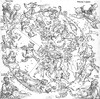
\includegraphics[keepaspectratio,width=\textwidth]{SkyMap-small.jpg}
  \captionart{SkyMap}
  \label{fig:skymap}
\end{figure}

The cause of all which intemperance he will have chiefly and primarily proceed
from the heavens, \authorfootnote{1286}from the position of Mars, Saturn, and Mercury.
His aphorisms be these, \authorfootnote{1287}Mercury in any geniture, if he shall be
found in Virgo, or Pisces his opposite sign, and that in the horoscope,
irradiated by those quartile aspects of Saturn or Mars, the child shall
be mad or melancholy. Again, \authorfootnote{1288}He that shall have Saturn and Mars,
the one culminating, the other in the fourth house, when he shall be
born, shall be melancholy, of which he shall be cured in time, if
Mercury behold them. If the moon be in conjunction or opposition\authorfootnote{1289}
at the birth time with the sun, Saturn or Mars, or in a quartile aspect
with them (\li{e malo coeli loco}, Leovitius adds), many diseases are
signified, especially the head and brain is like to be misaffected with
pernicious humours, to be melancholy, lunatic, or mad, Cardan adds,
quarta luna natos, eclipses, earthquakes. Garcaeus and Leovitius will
have the chief judgment to be taken from the lord of the geniture, or
where there is an aspect between the moon and Mercury, and neither
behold the horoscope, or Saturn and Mars shall be lord of the present
conjunction or opposition in Sagittarius or Pisces, of the sun or moon,
such persons are commonly epileptic, dote, demoniacal, melancholy: but
see more of these aphorisms in the above-named Pontanus. Garcaeus, cap.
23. de Jud. genitur. Schoner. lib. 1. cap. 8, which he hath gathered
out of \authorfootnote{1290}Ptolemy, Albubater, and some other Arabians, Junctine,
Ranzovius, Lindhout, Origen, \etc{}. But these men you will reject
peradventure, as astrologers, and therefore partial judges; then hear
the testimony of physicians, Galenists themselves. \authorfootnote{1291}Carto
confesseth the influence of stars to have a great hand to this peculiar
disease, so doth Jason Pratensis, Lonicerius praefat. de Apoplexia,
Ficinus, Fernelius, \etc{}. \authorfootnote{1292}P. Cnemander acknowledgeth the stars an
universal cause, the particular from parents, and the use of the six
non-natural things. Baptista Port. mag. l. 1. c. 10, 12, 15, will have
them causes to every particular individium. Instances and examples, to
evince the truth of those aphorisms, are common amongst those
astrologian treatises. Cardan, in his thirty-seventh geniture, gives
instance in Matth. Bolognius. Camerar. hor. natalit. centur. 7. genit.
6. et 7. of Daniel Gare, and others; but see Garcaeus, cap. 33. Luc.
Gauricus, Tract. 6. de Azemenis, \etc{}. The time of this melancholy is,
when the significators of any geniture are directed according to art,
as the hor: moon, hylech, \etc{} to the hostile beams or terms of \saturn{} and \mars{}
especially, or any fixed star of their nature, or if \saturn{} by his
revolution or transitus, shall offend any of those radical promissors
in the geniture.

Other signs there are taken from physiognomy, metoposcopy, chiromancy,
which because Joh. de Indagine, and Rotman, the landgrave of Hesse his
mathematician, not long since in his Chiromancy; Baptista Porta, in his
celestial Physiognomy, have proved to hold great affinity with
astrology, to satisfy the curious, I am the more willing to insert.
The general notions \authorfootnote{1293}physiognomers give, be these; black colour
argues natural melancholy; so doth leanness, hirsuteness, broad veins,
much hair on the brows, saith \authorfootnote{1294}Gratanarolus, cap. 7, and a little
head, out of \Aristotle, high sanguine, red colour, shows head
melancholy; they that stutter and are bald, will be soonest melancholy (as \Avicenna{} supposeth), by reason of the dryness of their brains; but
he that will know more of the several signs of humour and wits out of
physiognomy, let him consult with old Adamantus and Polemus, that
comment, or rather paraphrase upon \Aristotle's Physiognomy, Baptista
Porta's four pleasant books, Michael Scot de secretis naturae, John de
Indagine, Montaltus, Antony Zara. anat. ingeniorum, sect. 1. memb. 13.
et lib. 4. Chiromancy hath these aphorisms to foretell melancholy, Tasneir. lib.
5. cap. 2, who hath comprehended the sum of John de Indagine:
Tricassus, Corvinus, and others in his book, thus hath it; \authorfootnote{1295}The
Saturnine line going from the rascetta through the hand, to Saturn's
mount, and there intersected by certain little lines, argues
melancholy; so if the vital and natural make an acute angle, Aphorism
100. The saturnine, hepatic, and natural lines, making a gross triangle
in the hand, argue as much; which Goclenius, cap. 5. Chiros. repeats
verbatim out of him. In general they conclude all, that if Saturn's
mount be full of many small lines and intersections, \authorfootnote{1296}such men are
most part melancholy, miserable and full of disquietness, care and
trouble, continually vexed with anxious and bitter thoughts, always
sorrowful, fearful, suspicious; they delight in husbandry, buildings,
pools, marshes, springs, woods, walks, \etc{}. Thaddaeus Haggesius, in his
Metoposcopia, hath certain aphorisms derived from Saturn's lines in the
forehead, by which he collects a melancholy disposition; and
\authorfootnote{1297}Baptista Porta makes observations from those other parts of the
body, as if a spot be over the spleen; \authorfootnote{1298}or in the nails; if it
appear black, it signifieth much care, grief, contention, and
melancholy; the reason he refers to the humours, and gives instance in
himself, that for seven years space he had such black spots in his
nails, and all that while was in perpetual lawsuits, controversies for
his inheritance, fear, loss of honour, banishment, grief, care, \etc{} and
when his miseries ended, the black spots vanished. Cardan, in his book
de libris propriis, tells such a story of his own person, that a little
before his son's death, he had a black spot, which appeared in one of
his nails; and dilated itself as he came nearer to his end. But I am
over tedious in these toys, which howsoever, in some men's too severe
censures, they may be held absurd and ridiculous, I am the bolder to
insert, as not borrowed from circumforanean rogues and gipsies, but out
of the writings of worthy philosophers and physicians, yet living some
of them, and religious professors in famous universities, who are able
to patronise that which they have said, and vindicate themselves from
all cavillers and ignorant persons.

%SECT. II. MEMB. I. SUBSECT. V.-_Old age a cause_.
\section{Old age a cause.}

\lettrine{S}{econdary} peculiar causes efficient, so called in respect of the other
precedent, are either congenitae, internae, innatae, as they term them,
inward, innate, inbred; or else outward and adventitious, which happen
to us after we are born: congenite or born with us, are either natural,
as old age, or praeter naturam (as Fernelius calls\authorfootnote{1299} it) that
distemperature, which we have from our parent's seed, it being an
hereditary disease. The first of these, which is natural to all, and
which no man living can avoid, is \authorfootnote{1300}old age, which being cold and
dry, and of the same quality as melancholy is, must needs cause it, by
diminution of spirits and substance, and increasing of adust humours;
therefore \authorfootnote{1301} Melancthon avers out of \Aristotle, as an undoubted
truth, Senes plerunque delirasse in senecta, that old men familiarly
dote, ob atram bilem, for black choler, which is then superabundant in
them: and Rhasis, that Arabian physician, in his Cont. lib. 1. cap. 9,
calls it \authorfootnote{1302}a necessary and inseparable accident, to all old and
decrepit persons. After seventy years (as the Psalmist saith) \authorfootnote{1303}all
is trouble and sorrow; and common experience confirms the truth of it
in weak and old persons, especially such as have lived in action all
their lives, had great employment, much business, much command, and
many servants to oversee, and leave off ex abrupto; as Charles
the Fifth did\authorfootnote{1304} to King Philip, resign up all on a sudden; they are
overcome with melancholy in an instant: or if they do continue in such
courses, they dote at last (\li{senex bis puer}), and are not able to
manage their estates through common infirmities incident in their age;
full of ache, sorrow and grief, children again, dizzards, they carl
many times as they sit, and talk to themselves, they are angry,
waspish, displeased with every thing, suspicious of all, wayward,
covetous, hard (saith Tully), self-willed, superstitious,
self-conceited, braggers and admirers of themselves, as Balthazar
Castilio hath truly noted\authorfootnote{1305} of them.\authorfootnote{1306}This natural infirmity is most
eminent in old women, and such as are poor, solitary, live in most base
esteem and beggary, or such as are witches; insomuch that Wierus,
Baptista Porta, Ulricus Molitor, Edwicus, do refer all that witches are
said to do, to imagination alone, and this humour of melancholy. And
whereas it is controverted, whether they can bewitch cattle to death,
ride in the air upon a cowl-staff out of a chimney-top, transform
themselves into cats, dogs, \etc{}, translate bodies from place to place,
meet in companies, and dance, as they do, or have carnal copulation
with the devil, they ascribe all to this redundant melancholy, which
domineers in them, to \authorfootnote{1307} somniferous potions, and natural causes,
the devil's policy. Non laedunt omnino (saith Wierus) aut quid mirum
faciunt, (de Lamiis, lib. 3. cap. 36), ut putatur, solam vitiatam
habent phantasiam; they do no such wonders at all, only their
\authorfootnote{1308}brains are crazed. \authorfootnote{1309}They think they are witches, and can do
hurt, but do not. But this opinion Bodine, Erastus, Danaeus,
Scribanius, Sebastian Michaelis, \idxname{campanella}[Campanella][\textlatin{De sensu rerum et magia}] \textlatin{de Sensu rerum}, lib. 4.
cap. 9. \authorfootnote{1310}Dandinus the Jesuit, lib. 2. de Animae explode;
\authorfootnote{1311}Cicogna confutes at large. That witches are melancholy, they deny
not, but not out of corrupt phantasy alone, so to delude themselves and
others, or to produce such effects.

%SECT. II. MEMB. I. SUBSECT. VI.-_Parents a cause by Propagation_.
\section{Parents a cause by Propagation.}

\lettrine{T}{hat} other inward inbred cause of Melancholy is our temperature, in
whole or part, which we receive from our parents, which \authorfootnote{1312}Fernelius
calls Praeter naturam, or unnatural, it being an hereditary disease;
for as he justifies \authorfootnote{1313}Quale parentum maxime patris semen obtigerit,
tales evadunt similares spermaticaeque paries, quocunque etiam morbo
Pater quum generat tenetur, cum semine transfert, in Prolem; such as
the temperature of the father is, such is the son's, and look what
disease the father had when he begot him, his son will have after him;
\authorfootnote{1314}and is as well inheritor of his infirmities, as of his lands. And
where the complexion and constitution of the father is corrupt, there
(\authorfootnote{1315}saith Roger Bacon) the complexion and constitution of the son
must needs be corrupt, and so the corruption is derived from the father
to the son. Now this doth not so much appear in the composition of the
body, according to that of Hippocrates, \authorfootnote{1316}in habit, proportion,
scars, and other lineaments; but in manners and conditions of the mind,
Et patrum in natos abeunt cum semine mores.
Seleucus had an anchor on his thigh, so had his posterity, as Trogus
records, lib. 15. Lepidus, in \Pliny{} l. 7. c. 17, was purblind, so was
his son. That famous family of Aenobarbi were known of old, and so
surnamed from their red beards; the Austrian lip, and those Indian flat
noses are propagated, the Bavarian chin, and goggle eyes amongst the
Jews, as Buxtorfius observes\authorfootnote{1317}; their voice, pace, gesture, looks,
are likewise derived with all the rest of their conditions and
infirmities; such a mother, such a daughter; their very
\authorfootnote{1318}affections Lemnius contends to follow their seed, and the malice
and bad conditions of children are many times wholly to be imputed to
their parents; I need not therefore make any doubt of Melancholy, but
that it is an hereditary disease. \authorfootnote{1319} Paracelsus in express words
affirms it, lib. de morb. amentium to. 4. tr. 1; so doth \authorfootnote{1320}Crato in
an Epistle of his to Monavius. So doth Bruno Seidelius in his book de
morbo incurab. Montaltus proves, cap. 11, out of Hippocrates and
Plutarch, that such hereditary dispositions are frequent, et hanc
(inquit) fieri reor ob participatam melancholicam intemperantiam
(speaking of a patient) I think he became so by participation of
Melancholy. Daniel Sennertus, lib. 1. part 2. cap. 9, will have his
melancholy constitution derived not only from the father to the son,
but to the whole family sometimes; Quandoque totis familiis
hereditativam, \authorfootnote{1321}Forestus, in his medicinal observations,
illustrates this point, with an example of a merchant, his patient,
that had this infirmity by inheritance; so doth Rodericus a Fonseca,
tom. 1. consul. 69, by an instance of a young man that was so affected
ex matre melancholica, had a melancholy mother, et victu melancholico,
and bad diet together. Ludovicus Mercatus, a Spanish physician, in that
excellent Tract which he hath lately written of hereditary diseases,
tom. 2. oper. lib. 5, reckons up leprosy, as those \authorfootnote{1322}Galbots in
Gascony, hereditary lepers, pox, stone, gout, epilepsy, \etc{}. Amongst the
rest, this and madness after a set time comes to many, which he calls a
miraculous thing in nature, and sticks for ever to them as an incurable
habit. And that which is more to be wondered at, it skips in some
families the father, and goes to the son, \authorfootnote{1323}or takes every other,
and sometimes every third in a lineal descent, and doth not always
produce the same, but some like, and a symbolizing disease. These
secondary causes hence derived, are commonly so powerful, that (as
\authorfootnote{1324}Wolfius holds) saepe mutant decreta siderum, they do often alter
the primary causes, and decrees of the heavens. For these reasons,
belike, the Church and commonwealth, human and Divine laws, have
conspired to avoid hereditary diseases, forbidding such marriages as
are any whit allied; and as Mercatus adviseth all families to take
such, si fieri possit quae maxime distant natura, and to make choice of
those that are most differing in complexion from them; if they love
their own, and respect the common good. And sure, I think, it hath been
ordered by God's especial providence, that in all ages there should be
(as usually there is) once in \authorfootnote{1325}600 years, a transmigration of
nations, to amend and purify their blood, as we alter seed upon our
land, and that there should be as it were an inundation of those
northern Goths and Vandals, and many such like people which came out of
that continent of Scandia and Sarmatia (as some suppose) and overran,
as a deluge, most part of Europe and Africa, to alter for our good, our
complexions, which were much defaced with hereditary infirmities, which
by our lust and intemperance we had contracted. A sound generation of
strong and able men were sent amongst us, as those northern men usually
are, innocuous, free from riot, and free from diseases; to qualify and
make us as those poor naked Indians are generally at this day; and
those about Brazil (as a late \authorfootnote{1326}writer observes), in the Isle of
Maragnan, free from all hereditary diseases, or other contagion,
whereas without help of physic they live commonly 120 years or more, as
in the Orcades and many other places. Such are the common effects of
temperance and intemperance, but I will descend to particular, and show
by what means, and by whom especially, this infirmity is derived unto
us.

\li{Filii ex senibus nati, raro sunt firmi temperamenti}, old men's children
are seldom of a good temperament, as Scoltzius supposeth, consult. 177,
and therefore most apt to this disease; and as Levinus Lemnius
farther adds\authorfootnote{1327}, old men beget most part wayward, peevish, sad, melancholy
sons, and seldom merry. He that begets a child on a full stomach, will
either have a sick child, or a crazed son (as Cardan thinks\authorfootnote{1328}),
contradict. med. lib. 1. contradict. 18, or if the parents be sick, or
have any great pain of the head, or megrim, headache, (Hieronymus
Wolfius \authorfootnote{1329}doth instance in a child of Sebastian Castalio's); if a
drunken man get a child, it will never likely have a good brain, as
Gellius argues, lib. 12. cap. 1. Ebrii gignunt Ebrios, one drunkard
begets another, saith \authorfootnote{1330}Plutarch, symp. lib. 1. quest. 5, whose
sentence \authorfootnote{1331}Lemnius approves, l. 1. c. 4. Alsarius Crutius, Gen. de
qui sit med. cent. 3. fol. 182. Macrobius, lib. 1. \Avicenna{}, lib. 3.
Fen. 21. Tract 1. cap. 8, and \Aristotle himself, sect. 2. prob. 4,
foolish, drunken, or hair-brain women, most part bring forth children
like unto themselves, morosos et languidos, and so likewise he that
lies with a menstruous woman. Intemperantia veneris, quam in nautis
praesertim insectatur \authorfootnote{1332} Lemnius, qui uxores ineunt, nulla menstrui
decursus ratione habita nec observato interlunio, praecipua causa est,
noxia, pernitiosa, concubitum hunc exitialem ideo, et pestiferum vocat.
\authorfootnote{1333}Rodoricus a Castro Lucitanus, detestantur ad unum omnes medici,
tum et quarta luna concepti, infelices plerumque et amentes, deliri,
stolidi, morbosi, impuri, invalidi, tetra lue sordidi minime vitales,
omnibus bonis corporis atque animi destituti: ad laborem nati, si
seniores, inquit Eustathius, ut Hercules, et alii. \authorfootnote{1334}Judaei maxime
insectantur foedum hunc, et immundum apud Christianas Concubitum, ut
illicitum abhorrent, et apud suos prohibent; et quod Christiani toties
leprosi, amentes, tot morbili, impetigines, alphi, psorae, cutis et
faciei decolorationes, tam multi morbi epidemici, acerbi, et venenosi
sint, in hunc immundum concubitum rejiciunt, et crudeles in pignora
vocant, qui quarta, luna profluente hac mensium illuvie concubitum hunc
non perhorrescunt. Damnavit olim divina Lex et morte mulctavit
hujusmodi homines, Lev. 18, 20, et inde nati, siqui deformes aut
mutili, pater dilapidatus, quod non contineret ab \authorfootnote{1335} immunda
muliere. Gregorius Magnus, petenti Augustino nunquid apud
\authorfootnote{1336}Britannos hujusmodi concubitum toleraret, severe prohibuit viris
suis tum misceri foeminas in consuetis suis menstruis, \etc{}. I spare to
English this which I have said. Another cause some give, inordinate
diet, as if a man eat garlic, onions, fast overmuch, study too hard, be
over-sorrowful, dull, heavy, dejected in mind, perplexed in his
thoughts, fearful, \etc{}, their children (saith \authorfootnote{1337}Cardan subtil. lib.
18) will be much subject to madness and melancholy; for if the spirits
of the brain be fuzzled, or misaffected by such means, at such a time,
their children will be fuzzled in the brain: they will be dull, heavy,
timorous, discontented all their lives. Some are of opinion, and
maintain that paradox or problem, that wise men beget commonly fools;
Suidas gives instance in Aristarchus the Grammarian, duos reliquit
Filios Aristarchum et Aristachorum, ambos stultos; and which
\authorfootnote{1338}Erasmus urgeth in his Moria, fools beget wise men. Card. subt. l.
12, gives this cause, Quoniam spiritus sapientum ob studium
resolvuntur, et in cerebrum feruntur a corde: because their natural
spirits are resolved by study, and turned into animal; drawn from the
heart, and those other parts to the brain. Lemnius subscribes to that
of Cardan, and assigns this reason, Quod persolvant debitum languide,
et obscitanter, unde foetus a parentum generositate desciscit: they pay
their debt (as Paul calls it) to their wives remissly, by which means
their children are weaklings, and many times idiots and fools.
Some other causes are given, which properly pertain, and do proceed
from the mother: if she be over-dull, heavy, angry, peevish,
discontented, and melancholy, not only at the time of conception, but
even all the while she carries the child in her womb (saith Fernelius,
path. l. 1, 11) her son will be so likewise affected, and worse, as
\authorfootnote{1339}Lemnius adds, l. 4. c. 7, if she grieve overmuch, be disquieted,
or by any casualty be affrighted and terrified by some fearful object,
heard or seen, she endangers her child, and spoils the temperature of
it; for the strange imagination of a woman works effectually upon her
infant, that as Baptista Porta proves, Physiog. caelestis l. 5. c. 2,
she leaves a mark upon it, which is most especially seen in such as
prodigiously long for such and such meats, the child will love those
meats, saith Fernelius, and be addicted to like humours: \authorfootnote{1340}if a
great-bellied woman see a hare, her child will often have a harelip, as
we call it. Garcaeus, de Judiciis geniturarum, cap. 33, hath a
memorable example of one Thomas Nickell, born in the city of
Brandeburg, 1551, \authorfootnote{1341}that went reeling and staggering all the days
of his life, as if he would fall to the ground, because his mother
being great with child saw a drunken man reeling in the street. Such
another I find in Martin Wenrichius, com. de ortu monstrorum, c. 17, I
saw (saith he) at Wittenberg, in Germany, a citizen that looked like a
carcass; I asked him the cause, he replied, \authorfootnote{1342}His mother, when she
bore him in her womb, saw a carcass by chance, and was so sore
affrighted with it, that ex eo foetus ei assimilatus, from a ghastly
impression the child was like it.

So many several ways are we plagued and punished for our father's
defaults; insomuch that as Fernelius truly saith, \authorfootnote{1343}It is the
greatest part of our felicity to be well born, and it were happy for
human kind, if only such parents as are sound of body and mind should
be suffered to marry. An husbandman will sow none but the best and
choicest seed upon his land, he will not rear a bull or a horse, except
he be right shapen in all parts, or permit him to cover a mare, except
he be well assured of his breed; we make choice of the best rams for
our sheep, rear the neatest kine, and keep the best dogs, Quanto id
diligentius in procreandis liberis observandum? And how careful then
should we be in begetting of our children? In former times some
\authorfootnote{1344}countries have been so chary in this behalf, so stern, that if a
child were crooked or deformed in body or mind, they made him away; so
did the Indians of old by the relation of Curtius, and many other
well-governed commonwealths, according to the discipline of those
times. Heretofore in Scotland, saith \authorfootnote{1345}Hect. Boethius, if any were
visited with the falling sickness, madness, gout, leprosy, or any such
dangerous disease, which was likely to be propagated from the father to
the son, he was instantly gelded; a woman kept from all company of men;
and if by chance having some such disease, she were found to be with
child, she with her brood were buried alive: and this was done for the
common good, lest the whole nation should be injured or corrupted. A
severe doom you will say, and not to be used amongst Christians, yet
more to be looked into than it is. For now by our too much facility in
this kind, in giving way for all to marry that will, too much liberty
and indulgence in tolerating all sorts, there is a vast confusion of
hereditary diseases, no family secure, no man almost free from some
grievous infirmity or other, when no choice is had, but still the
eldest must marry, as so many stallions of the race; or if rich, be
they fools or dizzards, lame or maimed, unable, intemperate, dissolute,
exhaust through riot, as he said, \authorfootnote{1346}jura haereditario sapere
jubentur; they must be wise and able by inheritance: it comes to pass
that our generation is corrupt, we have many weak persons, both in body
and mind, many feral diseases raging amongst us, crazed families,
parentes, peremptores; our fathers bad, and we are like to be worse.

%SECT. II. MEMB. II.

%SECT. II. MEMB. II. SUBSECT. I.-_Bad Diet a cause. Substance. Quality of Meats_.
\section[Bad Diet]{Bad Diet a cause. Substance. Quality of Meats.}\label{sec:bad-diet}

\lettrine{A}{ccording} to my proposed method, having opened hitherto these secondary
causes, which are inbred with us, I must now proceed to the outward and
adventitious, which happen unto us after we are born. And those are
either evident, remote, or inward, antecedent, and the nearest:
continent causes some call them. These outward, remote, precedent
causes are subdivided again into necessary and not necessary. Necessary
(because we cannot avoid them, but they will alter us, as they are
used, or abused) are those six non-natural things, so much spoken of
amongst physicians, which are principal causes of this disease. For
almost in every consultation, whereas they shall come to speak of the
causes, the fault is found, and this most part objected to the patient;
Peccavit circa res sex non naturales: he hath still offended in one of
those six. Montanus, consil. 22, consulted about a melancholy Jew,
gives that sentence, so did Frisemelica in the same place; and in his
244 counsel, censuring a melancholy soldier, assigns that reason of his
malady, \authorfootnote{1347}he offended in all those six non-natural things, which
were the outward causes, from which came those inward obstructions; and
so in the rest.

These six non-natural things are diet, retention and evacuation, which
are more material than the other because they make new matter, or else
are conversant in keeping or expelling of it. The other four are air,
exercise, sleeping, waking, and perturbations of the mind, which only
alter the matter. The first of these is diet, which consists in meat
and drink, and causeth melancholy, as it offends in substance, or
accidents, that is, quantity, quality, or the like. And well it may be
called a material cause, since that, as Fernelius holds\authorfootnote{1348}, it hath
such a power in begetting of diseases, and yields the matter and
sustenance of them; for neither air, nor perturbations, nor any of
those other evident causes take place, or work this effect, except the
constitution of body, and preparation of humours, do concur. That a man
may say, this diet is the mother of diseases, let the father be what he
will, and from this alone, melancholy and frequent other maladies
arise. Many physicians, I confess, have written copious volumes of this
one subject, of the nature and qualities of all manner of meats; as
namely, Galen, Isaac the Jew, Halyabbas, \Avicenna{}, Mesue, also four
Arabians, Gordonius, Villanovanus, Wecker, Johannes Bruerinus,
sitologia de Esculentis et Poculentis, Michael Savanarola, Tract 2. c.
8, Anthony Fumanellus, lib. de regimine senum, Curio in his comment on
Schola Salerna, Godefridus Steckius arte med., Marcilius Cognatus,
Ficinus, Ranzovius, Fonseca, Lessius, Magninus, regim. sanitatis,
Frietagius, Hugo Fridevallius, \etc{}, besides many other in
\authorfootnote{1349}English, and almost every peculiar physician, discourseth at
large of all peculiar meats in his chapter of melancholy: yet because
these books are not at hand to every man, I will briefly touch what
kind of meats engender this humour, through their several species, and
which are to be avoided. How they alter and change the matter, spirits
first, and after humours, by which we are preserved, and the
constitution of our body, Fernelius and others will show you. I hasten
to the thing itself: and first of such diet as offends in substance.

\subsection{Beef.}
Beef, a strong and hearty meat (cold in the first degree, dry
in the second, saith \textlatin{Gal. l. 3. c. 1. de alim. fac.}) is condemned by
him and all succeeding Authors, to breed gross melancholy blood: good
for such as are sound, and of a strong constitution, for labouring men
if ordered aright, corned, young, of an ox (for all gelded meats in
every species are held best), or if old, \authorfootnote{1350}such as have been tired
out with labour, are preferred. Aubanus and Sabellicus commend Portugal
beef to be the most savoury, best and easiest of digestion; we commend
ours: but all is rejected, and unfit for such as lead a resty life, any
ways inclined to melancholy, or dry of complexion: \li{Tales} (Galen thinks)
\li{de facile melancholicis aegritudinibus capiuntur}.
\begin{figure}[H]
  \begingroup
  \centering
  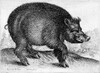
\includegraphics[keepaspectratio,width=\textwidth]{wild-boar-small.jpg}
  \captionart{WildBoar}
  \label{fig:wildboar}
\end{figure}
\subsection{Pork.}
Pork, of all meats, is most nutritive in his own nature,
\authorfootnote{1351} but altogether unfit for such as live at ease, are any ways
unsound of body or mind: too moist, full of humours, and therefore
\lit{naught for queasy stomachs, insomuch that frequent use of it may breed a quartan ague}{noxia delicatis, ex earum usu ut dubitetur an febris quartana generetur}, saith Savanarola.
\subsection{Goat.}
Savanarola discommends goat's flesh, and so doth
\authorfootnote{1352}\textlatin{Bruerinus, l. 13. c. 19}, calling it a filthy beast, and rammish:
and therefore supposeth it will breed rank and filthy substance; yet
kid, such as are young and tender, Isaac accepts, Bruerinus and Galen,
\textlatin{l. 1. c. 1. de alimentorum facultatibus.}
\subsection{Hart.}
\emph{Hart} and \emph{red deer} \authorfootnote{1353}hath an evil name: it yields gross
nutriment: a strong and great grained meat, next unto a horse. Which
although some countries eat, as Tartars, and they of China; yet \authorfootnote{1354}
Galen condemns. Young foals are as commonly eaten in Spain as red deer,
and to furnish their navies, about Malaga especially, often used; but
such meats ask long baking, or seething, to qualify them, and yet all
will not serve.

\emph{Venison, Fallow Deer}. All venison is melancholy, and begets bad blood;
a pleasant meat: in great esteem with us (for we have more parks in
England than there are in all Europe besides) in our solemn feasts.
'Tis somewhat better hunted than otherwise, and well prepared by
cookery; but generally bad, and seldom to be used.
\subsection{Hare.}
\emph{Hare}, a black meat, melancholy, and hard of digestion, it
breeds incubus, often eaten, and causeth fearful dreams, so doth all
venison, and is condemned by a jury of physicians. Mizaldus and some
others say, that hare is a merry meat, and that it will make one fair,
as Martial's epigram testifies to Gellia; but this is per accidens,
because of the good sport it makes, merry company and good discourse
that is commonly at the eating of it, and not otherwise to be
understood.

\subsection{Conies.}
\authorfootnote{1355}\emph{Conies} are of the nature of hares. Magninus compares
them to beef, pig, and goat, Reg. sanit. part. 3. c. 17; yet young
rabbits by all men are approved to be good.
Generally, all such meats as are hard of digestion breed melancholy.
Areteus, lib. 7. cap. 5, reckons up heads and feet, \authorfootnote{1356}bowels,
brains, entrails, marrow, fat, blood, skins, and those inward parts, as
heart, lungs, liver, spleen, \etc{}. They are rejected by Isaac, lib. 2.
part. 3, Magninus, part. 3. cap. 17, Bruerinus, lib. 12, Savanarola,
Rub. 32. Tract. 2.

\subsection{Milk.}
\emph{Milk}, and all that comes of milk, as butter and cheese, curds,
\etc{}, increase melancholy (whey only excepted, which is most wholesome):
\authorfootnote{1357}some except asses' milk. The rest, to such as are sound, is
nutritive and good, especially for young children, but because soon
turned to corruption, \authorfootnote{1358}not good for those that have unclean
stomachs, are subject to headache, or have green wounds, stone, \etc{}. Of
all cheeses, I take that kind which we call Banbury cheese to be the
best, ex vetustis pessimus, the older, stronger, and harder, the worst,
as Langius discourseth in his Epistle to Melancthon, cited by Mizaldus,
Isaac, p. 5. Gal. 3. de cibis boni succi. \etc{}.

\begin{figure}[H]
  \begingroup
  \centering
  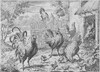
\includegraphics[keepaspectratio,width=\textwidth]{chickens-small.jpg}
  \captionart{Chickens}
  \label{fig:chickens}
\end{figure}

\subsection{Fowl.}
Amongst fowl, \authorfootnote{1359}peacocks and pigeons, all fenny fowl are
forbidden, as ducks, geese, swans, herons, cranes, coots, didappers,
water-hens, with all those teals, curs, sheldrakes, and peckled fowls,
that come hither in winter out of Scandia, Muscovy, Greenland,
Friesland, which half the year are covered all over with snow, and
frozen up. Though these be fair in feathers, pleasant in taste, and
have a good outside, like hypocrites, white in plumes, and soft, their
flesh is hard, black, unwholesome, dangerous, melancholy meat; Gravant
et putrefaciant stomachum, saith Isaac, part. 5. de vol., their young
ones are more tolerable, but young pigeons he quite disapproves.

\begin{figure}[H]
  \begingroup
  \centering
  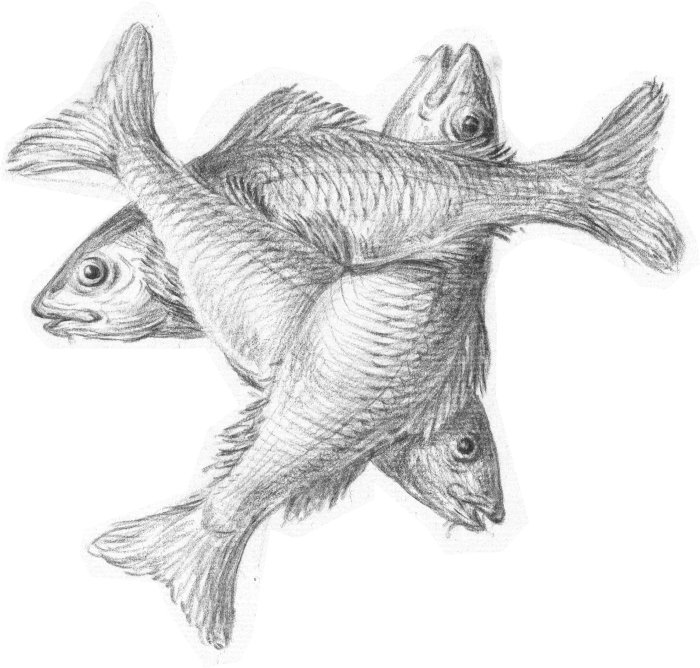
\includegraphics[keepaspectratio,width=0.7\textwidth]{Three-fishes-arranged-crosswise-small.jpg}
  \captionart{ThreeFishes}
  \label{fig:threefishes}
\end{figure}

\subsection{Fishes.}\label{sec:fishes}
Rhasis and \authorfootnote{1360}Magninus discommend all fish, and say, they
breed viscosities, slimy nutriment, little and humorous nourishment.
Savanarola adds, cold, moist: and phlegmatic, Isaac; and therefore
unwholesome for all cold and melancholy complexions: others make a
difference, rejecting only amongst freshwater fish, eel, tench,
lamprey, crawfish (which Bright approves, cap. 6), and such as are bred
in muddy and standing waters, and have a taste of mud, as Franciscus
Bonsuetus poetically defines, Lib. de aquatilibus.
%
\begin{latin}
\begin{verse}
Nam pisces omnes, qui stagna, lacusque frequentant,\\*
Semper plus succi deterioris habent.
\end{verse}
\end{latin}
\translationrule
\begin{verse}
All fish, that standing pools, and lakes frequent,\\*
Do ever yield bad juice and nourishment.
\end{verse}

Lampreys, Paulus Jovius, c. 34. de piscibus fluvial., highly magnifies,
and saith, None speak against them, but inepti et scrupulosi, some
scrupulous persons; but \authorfootnote{1361}eels, c. 33, he abhorreth in all places,
at all times, all physicians detest them, especially about the
solstice. Gomesius, lib. 1. c. 22, de sale, doth immoderately extol
sea-fish, which others as much vilify, and above the rest, dried,
soused, indurate fish, as ling, fumados, red-herrings, sprats,
stock-fish, haberdine, poor-John, all shellfish. \authorfootnote{1362}Tim. Bright
excepts lobster and crab. Messarius commends salmon, which Bruerinus
contradicts, lib. 22. c. 17. Magninus rejects conger, sturgeon, turbot,
mackerel, skate.

Carp is a fish of which I know not what to determine. Franciscus
Bonsuetus accounts it a muddy fish. Hippolitus Salvianus, in his Book
de Piscium natura et praeparatione, which was printed at Rome in folio,
1554, with most elegant pictures, esteems carp no better than a slimy
watery meat. Paulus Jovius on the other side, disallowing tench,
approves of it; so doth Dubravius in his Books of Fishponds. Freitagius
\authorfootnote{1363}extols it for an excellent wholesome meat, and puts it amongst
the fishes of the best rank; and so do most of our country gentlemen,
that store their ponds almost with no other fish. But this controversy
is easily decided, in my judgment, by Bruerinus, l. 22. c. 13. The
difference riseth from the site and nature of pools, \authorfootnote{1364}sometimes
muddy, sometimes sweet; they are in taste as the place is from whence
they be taken. In like manner almost we may conclude of other fresh
fish. But see more in Rondoletius, Bellonius, Oribasius, lib. 7. cap.
22, Isaac, l. 1, especially Hippolitus Salvianus, who is instar omnium
solus, \etc{}. Howsoever they may be wholesome and approved, much use of
them is not good; P. Forestus, in his medicinal observations,
\authorfootnote{1365}relates, that Carthusian friars, whose living is most part fish,
are more subject to melancholy than any other order, and that he found
by experience, being sometimes their physician ordinary at Delft, in
Holland. He exemplifies it with an instance of one Buscodnese, a
Carthusian of a ruddy colour, and well liking, that by solitary living,
and fish-eating, became so misaffected.

\subsection{Herbs.}
Amongst herbs to be eaten I find gourds, cucumbers,
coleworts, melons, disallowed, but especially cabbage. It causeth
troublesome dreams, and sends up black vapours to the brain. Galen,
loc. affect. l. 3. c. 6, of all herbs condemns cabbage; and Isaac, lib.
2. c. 1. Animae gravitatem facit, it brings heaviness to the soul. Some
are of opinion that all raw herbs and salads breed melancholy blood,
except bugloss and lettuce. Crato, consil. 21. lib. 2, speaks against
all herbs and worts, except borage, bugloss, fennel, parsley, dill,
balm, succory. Magninus, regim. sanitatis, part. 3. cap. 31. Omnes
herbae simpliciter malae, via cibi; all herbs are simply evil to feed
on (as he thinks). So did that scoffing cook in \authorfootnote{1366}\Plautus{} hold:
Non ego coenam condio ut alii coqui solent,
Qui mihi condita prata in patinis proferunt,
Boves qui convivas faciunt, herbasque aggerunt.


Like other cooks I do not supper dress,
That put whole meadows into a platter,

And make no better of their guests than beeves,
With herbs and grass to feed them fatter.

Our Italians and Spaniards do make a whole dinner of herbs and salads
(which our said \Plautus{} calls coenas terrestras, \Horace{}, coenas sine
sanguine), by which means, as he follows it,
\authorfootnote{1367}Hic homines tam brevem vitam colunt-
Qui herbas hujusmodi in alvum suum congerunt,
Formidolosum dictu, non esu modo,
Quas herbas pecudes non edunt, homines edunt.

Their lives, that eat such herbs, must needs be short,
And 'tis a fearful thing for to report,
That men should feed on such a kind of meat,
Which very juments would refuse to eat.

\authorfootnote{1368}They are windy, and not fit therefore to be eaten of all men raw,
though qualified with oil, but in broths, or otherwise. See more of
these in every \authorfootnote{1369}husbandman, and herbalist.
\subsection{Roots.}
Roots, Etsi quorundam gentium opes sint, saith Bruerinus, the
wealth of some countries, and sole food, are windy and bad, or
troublesome to the head: as onions, garlic, scallions, turnips,
carrots, radishes, parsnips: Crato, lib. 2. consil. 11, disallows all
roots, though \authorfootnote{1370} some approve of parsnips and potatoes.
\authorfootnote{1371}Magninus is of Crato's opinion, \authorfootnote{1372}They trouble the mind,
sending gross fumes to the brain, make men mad, especially garlic,
onions, if a man liberally feed on them a year together. Guianerius,
tract. 15. cap. 2, complains of all manner of roots, and so doth
Bruerinus, even parsnips themselves, which are the best, Lib. 9. cap.
14.
\subsection{Fruits.}
\li{Pastinacarum usus succos gignit improbos}. Crato, consil. 21.
lib. 1, utterly forbids all manner of fruits, as pears, apples, plums,
cherries, strawberries, nuts, medlars, serves, \etc{}. Sanguinem inficiunt,
saith Villanovanus, they infect the blood, and putrefy it, Magninus
holds, and must not therefore be taken via cibi, aut quantitate magna,
not to make a meal of, or in any great quantity. \authorfootnote{1373}Cardan makes
that a cause of their continual sickness at Fessa in Africa, because
they live so much on fruits, eating them thrice a day. Laurentius
approves of many fruits, in his \emph{Tract of Melancholy}, which others
disallow, and amongst the rest apples, which some likewise commend,
sweetings, pearmains, pippins, as good against melancholy; but to him
that is any way inclined to, or touched with this malady,
\authorfootnote{1374}Nicholas Piso in his \emph{Practics}, forbids all fruits, as windy, or
to be sparingly eaten at least, and not raw. Amongst other fruits,
\authorfootnote{1375}Bruerinus, out of Galen, excepts grapes and figs, but I find them
likewise rejected.

\subsection{Pulse.}
All \footnoteA{Dried legume. \theeditor{}}{pulse} are naught, beans, peas, vetches, \etc{}, they fill
the brain (saith Isaac) with gross fumes, breed black thick blood, and
cause troublesome dreams. And therefore, that which Pythagoras said to
his scholars of old, may be for ever applied to melancholy men, A fabis
abstinete, eat no peas, nor beans; yet to such as will needs eat them,
I would give this counsel, to prepare them according to those rules
that Arnoldus Villanovanus, and Frietagius prescribe, for eating, and
dressing. fruits, herbs, roots, pulse, \etc{}

\subsection{Spices.}
Spices cause hot and head melancholy, and are for that cause
forbidden by our physicians to such men as are inclined to this malady,
as pepper, ginger, cinnamon, cloves, mace, dates, \etc{} honey and sugar.
Some except honey;\authorfootnote{1376} to those that are cold, it may be tolerable,
but \latininlinetrans{sweets turn into bile}{Dulcia se in bilem vertunt},\authormarginnote{1377} they
are obstructive. Crato therefore forbids all spice, in a consultation
of his, for a melancholy schoolmaster, Omnia aromatica et quicquid
sanguinem adurit: so doth Fernelius, consil. 45. Guianerius, tract 15.
cap. 2. Mercurialis, cons. 189. To these I may add all sharp and sour
things, luscious and over-sweet, or fat, as oil, vinegar, verjuice,
mustard, salt; as sweet things are obstructive, so these are corrosive.
Gomesius, in his books, de sale, l. 1. c. 21, highly commends salt; so
doth Codronchus in his tract, de sale Absynthii, Lemn. l. 3. c. 9. de
occult. nat. mir. yet common experience finds salt, and salt-meats, to
be great procurers of this disease. And for that cause belike those
Egyptian priests abstained from salt, even so much, as in their bread,
ut sine perturbatione anima esset, saith mine author, that their souls
might be free from perturbations.

\subsection{Bread.}
Bread that is made of baser grain, as peas, beans, oats, rye,
or \authorfootnote{1378}over-hard baked, crusty, and black, is often spoken against,
as causing melancholy juice and wind. Joh. Mayor, in the first book of
his History of Scotland, contends much for the wholesomeness of oaten
bread: it was objected to him then living at Paris in France, that his
countrymen fed on oats, and base grain, as a disgrace; but he doth
ingenuously confess, Scotland, Wales, and a third part of England, did
most part use that kind of bread, that it was as wholesome as any
grain, and yielded as good nourishment. And yet Wecker out of Galen
calls it horsemeat, and fitter for juments than men to feed on. But
read Galen himself, Lib. 1. De cibis boni et mali succi, more largely
discoursing of corn and bread.

\subsection{Wine.}
All black wines, over-hot, compound, strong thick drinks, as
Muscadine, Malmsey, Alicant, Rumney, Brownbastard, Metheglen, and the
like, of which they have thirty several kinds in Muscovy, all such made
drinks are hurtful in this case, to such as are hot, or of a sanguine
choleric complexion, young, or inclined to head-melancholy. For many
times the drinking of wine alone causeth it. Arculanus, c. 16. in 9.
Rhasis, puts in \authorfootnote{1379}wine for a great cause, especially if it be
immoderately used. Guianerius, tract. 15. c. 2, tells a story of two
Dutchmen, to whom he gave entertainment in his house, that \authorfootnote{1380}in one
month's space were both melancholy by drinking of wine, one did nought
but sing, the other sigh. Galen, l. de causis morb. c. 3. Matthiolus on
Dioscorides, and above all other Andreas Bachius, l. 3. 18, 19, 20,
have reckoned upon those inconveniences that come by wine: yet
notwithstanding all this, to such as are cold, or sluggish melancholy,
a cup of wine is good physic, and so doth Mercurialis grant, consil.
25, in that case, if the temperature be cold, as to most melancholy men
it is, wine is much commended, if it be moderately used.
\subsection{Cider, Perry.}

Cider and perry are both cold and windy drinks, and
for that cause to be neglected, and so are all those hot spiced strong
drinks.

\paragraph{Beer} Beer, if it be over-new or over-stale, over-strong, or not
sodden, smell of the cask, sharp, or sour, is most unwholesome, frets,
and galls, \etc{}. Henricus Ayrerus, in a \authorfootnote{1381}consultation of his, for
one that laboured of hypochondriacal melancholy, discommends beer. So
doth \authorfootnote{1382} Crato in that excellent counsel of his, Lib. 2. consil. 21,
as too windy, because of the hop. But he means belike that thick black
Bohemian beer used in some other parts of \authorfootnote{1383}Germany.
---nil spissius illa
Dum bibitur, nil clarius est dum mingitur, unde
Constat, quod multas faeces in corpore linquat.

Nothing comes in so thick,
Nothing goes out so thin,
It must needs follow then
The dregs are left within.

As that \authorfootnote{1384}old poet scoffed, calling it Stygiae monstrum conforme
paludi, a monstrous drink, like the river Styx. But let them say as
they list, to such as are accustomed unto it, 'tis a most wholesome (so
\authorfootnote{1385} \idxname{polydorevergil}[Polydore Virgil] calleth it) and a pleasant drink, it is more
subtle and better, for the hop that rarefies it, hath an especial
virtue against melancholy, as our herbalists confess, Fuchsius
approves, Lib. 2. sec. 2. instit. cap. 11, and many others.

\paragraph{Waters} Standing waters, thick and ill-coloured, such as come forth of
pools, and moats, where hemp hath been steeped, or slimy fishes live,
are most unwholesome, putrefied, and full of mites, creepers, slimy,
muddy, unclean, corrupt, impure, by reason of the sun's heat, and
still-standing; they cause foul distemperatures in the body and mind of
man, are unfit to make drink of, to dress meat with, or to be
\authorfootnote{1386}used about men inwardly or outwardly. They are good for many
domestic uses, to wash horses, water cattle, \etc{}, or in time of
necessity, but not otherwise. Some are of opinion, that such fat
standing waters make the best beer, and that seething doth defecate it,
as Cardan holds\authorfootnote{1387}, Lib. 13. subtil. It mends the substance, and
savour of it, but it is a paradox. Such beer may be stronger, but not
so wholesome as the other, as Jobertus truly justifieth\authorfootnote{1388} out of
Galen, Paradox, dec. 1. Paradox 5, that the seething of such impure
waters doth not purge or purify them, \Pliny{}, lib. 31. c. 3, is of the
same tenet, and P. Crescentius, agricult. lib. 1. et lib. 4. c. 11. et
c. 45. Pamphilius Herilachus, l. 4. de not. aquarum, such waters are
naught, not to be used, and by the testimony of \authorfootnote{1389}Galen, breed
agues, dropsies, pleurisies, splenetic and melancholy passions, hurt
the eyes, cause a bad temperature, and ill disposition of the whole
body, with bad colour. This Jobertus stiffly maintains, Paradox, lib.
1. part. 5, that it causeth blear eyes, bad colour, and many loathsome
diseases to such as use it: this which they say, stands with good
reason; for as geographers relate, the water of Astracan breeds worms
in such as drink it. \authorfootnote{1390} Axius, or as now called Verduri, the
fairest river in Macedonia, makes all cattle black that taste of it.
Aleacman now Peleca, another stream in Thessaly, turns cattle most part
white, si polui ducas, L. Aubanus Rohemus refers that \authorfootnote{1391}struma or
poke of the Bavarians and Styrians to the nature of their waters, as
\authorfootnote{1392}Munster doth that of Valesians in the Alps, and \authorfootnote{1393}Bodine
supposeth the stuttering of some families in Aquitania, about Labden,
to proceed from the same cause, and that the filth is derived from the
water to their bodies. So that they that use filthy, standing,
ill-coloured, thick, muddy water, must needs have muddy, ill-coloured,
impure, and infirm bodies. And because the body works upon the mind,
they shall have grosser understandings, dull, foggy, melancholy
spirits, and be really subject to all manner of infirmities.

To these noxious simples, we may reduce an infinite number of compound,
artificial, made dishes, of which our cooks afford us a great variety,
as tailors do fashions in our apparel. Such are \authorfootnote{1394}puddings stuffed
with blood, or otherwise composed; baked, meats, soused indurate meats,
fried and broiled buttered meats; condite, powdered, and over-dried,
\authorfootnote{1395}all cakes, simnels, buns, cracknels made with butter, spice, \etc{},
fritters, pancakes, pies, sausages, and those several sauces, sharp, or
over-sweet, of which scientia popinae, as \Seneca calls it, hath served
those \authorfootnote{1396} Apician tricks, and perfumed dishes, which Adrian the
sixth Pope so much admired in the accounts of his predecessor Leo
Decimus; and which prodigious riot and prodigality have invented in
this age. These do generally engender gross humours, fill the stomach
with crudities, and all those inward parts with obstructions. Montanus,
consil. 22, gives instance, in a melancholy Jew, that by eating such
tart sauces, made dishes, and salt meats, with which he was overmuch
delighted, became melancholy, and was evil affected. Such examples are
familiar and common.

%SECT. II. MEMB. II. SUBSECT. II.-_Quantity of Diet a Cause._
\section{Quantity of Diet a Cause.}

\lettrine{T}{here} is not so much harm proceeding from the substance itself of meat,
and quality of it, in ill-dressing and preparing, as there is from the
quantity, disorder of time and place, unseasonable use of it, \authorfootnote{1397}
intemperance, overmuch, or overlittle taking of it. A true saying it
is, Plures crapula quam gladius. This gluttony kills more than the
sword, this omnivorantia et homicida gula, this all-devouring and
murdering gut. And that of \authorfootnote{1398}\Pliny{} is truer, Simple diet is the
best; heaping up of several meats is pernicious, and sauces worse; many
dishes bring many diseases. \authorfootnote{1399}Avicen cries out, That nothing is
worse than to feed on many dishes, or to protract the time of meats
longer than ordinary; from thence proceed our infirmities, and 'tis the
fountain of all diseases, which arise out of the repugnancy of gross
humours. Thence, saith \authorfootnote{1400} Fernelius, come crudities, wind,
oppilations, cacochymia, plethora, cachexia, bradiopepsia, \authorfootnote{1401}Hinc
subitae, mortes, atque intestata senectus, sudden death, \etc{}, and what
not.

As a lamp is choked with a multitude of oil, or a little fire with
overmuch wood quite extinguished, so is the natural heat with
immoderate eating, strangled in the body. Pernitiosa sentina est
abdomen insaturabile: one saith, An insatiable paunch is a pernicious
sink, and the fountain of all diseases, both of body and mind.
\authorfootnote{1402}Mercurialis will have it a peculiar cause of this private
disease; Solenander, consil. 5. sect. 3, illustrates this of
Mercurialis, with an example of one so melancholy, ab intempestivis
commessationibus, unseasonable feasting. \authorfootnote{1403}Crato confirms as much,
in that often cited counsel, 21. lib. 2, putting superfluous eating for
a main cause. But what need I seek farther for proofs? Hear
\authorfootnote{1404}Hippocrates himself, lib. 2. aphor. 10, Impure bodies the more
they are nourished, the more they are hurt, for the nourishment is
putrefied with vicious humours.

\begin{figure}[H]
  \begingroup
  \centering
  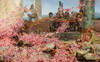
\includegraphics[keepaspectratio,width=\textwidth]{heliogabalus-small.jpg}
  \captionart{Heliogabalus}
  \label{fig:heliogabalus}
\end{figure}

And yet for all this harm, which apparently follows surfeiting and
drunkenness, see how we luxuriate and rage in this kind; read what
Johannes Stuckius hath written lately of this subject, in his great
volume De Antiquorum Conviviis, and of our present age; Quam
\authorfootnote{1405}portentosae coenae, prodigious suppers, \authorfootnote{1406}Qui dum invitant ad
coenam efferunt ad sepulchrum, what Fagos, Epicures, Apetios,
Heliogabalus, our times afford? Lucullus' ghost walks still,\footnoteA{\scriptsize{}Roman politician and famed gastronome. As recorded in Plutarch's Parallel Lives, on an occasion without dinner guests his servant prepared a plain course. Lucullus reprimanded him: \lit{What, did not you know, then, that today Lucullus dines with Lucullus?}{Quid ais, inquit iratus Lucullus, au nesciebas Lucullum hodie cenaturum esse apud Lucullum}. Plutarch, Life of Lucullus, 41.1–6.} and every
man desires to sup in Apollo; Aesop's costly dish is ordinarily served
up. \li{Magis illa juvant, quae pluris emuntur}\authorlatintrans{1407.5}.\authormarginnote{1407} The dearest cates are
best, and 'tis an ordinary thing to bestow twenty or thirty pounds on a
dish, some thousand crowns upon a dinner: \authorfootnote{1408}Mully-Hamet, king of
Fez and Morocco, spent three pounds on the sauce of a capon: it is
nothing in our times, we scorn all that is cheap. We loathe the very
\authorfootnote{1409}light (some of us, as \Seneca notes) because it comes free, and we
are offended with the sun's heat, and those cool blasts, because we buy
them not. This air we breathe is so common, we care not for it; nothing
pleaseth but what is dear. And if we be \authorfootnote{1410}witty in anything, it is
ad gulam: If we study at all, it is erudito luxu, to please the palate,
and to satisfy the gut. A cook of old was a base knave (as Livy
complains\authorfootnote{1411}), but now a great man in request; cookery is become an art, a
noble science: cooks are gentlemen: Venter Deus: They wear their brains
in their bellies, and their guts in their heads, as Agrippa taxed\authorfootnote{1412}
some parasites of his time, rushing on their own destruction, as if a
man should run upon the point of a sword, usque dum rumpantur comedunt,

They eat till they burst: \authorfootnote{1413}All day, all night, let the physician
say what he will, imminent danger, and feral diseases are now ready to
seize upon them, that will eat till they vomit, Edunt ut vomant, vomut
ut edant, saith \Seneca; which Dion relates of Vitellius, Solo transitu
ciborum nutriri judicatus: His meat did pass through and away, or till
they burst again. \authorfootnote{1414}Strage animantium ventrem onerant, and rake
over all the world, as so many \authorfootnote{1415}slaves, belly-gods, and
land-serpents, Et totus orbis ventri nimis angustus, the whole world
cannot satisfy their appetite. \authorfootnote{1416}Sea, land, rivers, lakes, \etc{}, may
not give content to their raging guts. To make up the mess, what
immoderate drinking in every place? Senem potum pota trahebat anus, how
they flock to the tavern: as if they were fruges consumere nati, born
to no other end but to eat and drink, like Offellius Bibulus, that
famous Roman parasite, Qui dum vixit, aut bibit aut minxit; as so many
casks to hold wine, yea worse than a cask, that mars wine, and itself
is not marred by it, yet these are brave men, Silenus Ebrius was no
braver. Et quae fuerunt vitia, mores sunt: 'tis now the fashion of our
times, an honour: Nunc vero res ista eo rediit (as \Chrysostom{} serm. 30.
in v. Ephes. comments) Ut effeminatae ridendaeque ignaviae loco
habeatur, nolle inebriari; 'tis now come to that pass that he is no
gentleman, a very milk-sop, a clown, of no bringing up, that will not
drink; fit for no company; he is your only gallant that plays it off
finest, no disparagement now to stagger in the streets, reel, rave,
\etc{}, but much to his fame and renown; as in like case Epidicus told
Thesprio his fellow-servant, in the \authorfootnote{1417}Poet. Aedipol facinus
improbum, one urged, the other replied, At jam alii fecere idem, erit
illi illa res honori, 'tis now no fault, there be so many brave
examples to bear one out; 'tis a credit to have a strong brain, and
carry his liquor well; the sole contention who can drink most, and fox
his fellow the soonest. 'Tis the summum bonum of our tradesmen, their
felicity, life, and soul, Tanta dulcedine affectant, saith \Pliny{}, lib.
14. cap. 12. Ut magna pars non aliud vitae praemium intelligat, their
chief comfort, to be merry together in an alehouse or tavern, as our
modern Muscovites do in their mead-inns, and Turks in their
coffeehouses, which much resemble our taverns; they will labour hard
all day long to be drunk at night, and spend totius anni labores, as
St. Ambrose adds, in a tippling feast; convert day into night, as
\Seneca taxes some in his times, Pervertunt officia anoctis et lucis;
when we rise, they commonly go to bed, like our antipodes,
Nosque ubi primus equis oriens afflavit anhelis,
Illis sera rubens ascendit lumina vesper.

So did Petronius in Tacitus, Heliogabalus in Lampridius.
\authorfootnote{1418}---Noctes vigilibat ad ipsum
Mane, diem totum stertebat?---

---He drank the night away
Till rising dawn, then snored out all the day.

Snymdiris the Sybarite never saw the sun rise or set so much as once in
twenty years. Verres, against whom Tully so much inveighs, in winter he
never was extra tectum vix extra lectum, never almost out of bed,
\authorfootnote{1419} still wenching and drinking; so did he spend his time, and so do
myriads in our days. They have gymnasia bibonum, schools and
rendezvous; these centaurs and Lapithae toss pots and bowls as so many
balls; invent new tricks, as sausages, anchovies, tobacco, caviar,
pickled oysters, herrings, fumados, \etc{}: innumerable salt meats to
increase their appetite, and study how to hurt themselves by taking
antidotes \authorfootnote{1420}to carry their drink the better; \authorfootnote{1421}and when nought
else serves, they will go forth, or be conveyed out, to empty their
gorge, that they may return to drink afresh. They make laws, insanas
leges, contra bibendi fallacias, and \authorfootnote{1422}brag of it when they have
done, crowning that man that is soonest gone, as their drunken
predecessors have done, -\authorfootnote{1423}quid ego video? Ps. Cum corona Pseudolum
ebrium tuum-. And when they are dead, will have a can of wine with
\authorfootnote{1424}Maron's old woman to be engraven on their tombs. So they triumph
in villainy, and justify their wickedness; with Rabelais, that French
Lucian, drunkenness is better for the body than physic, because there
be more old drunkards than old physicians. Many such frothy arguments
they have, \authorfootnote{1425}inviting and encouraging others to do as they do, and
love them dearly for it (no glue like to that of good fellowship). So
did Alcibiades in Greece; Nero, Bonosus, Heliogabalus in Rome, or
Alegabalus rather, as he was styled of old (as Ignatius proves\authorfootnote{1426}
out of some old coins). So do many great men still, as
\authorfootnote{1427}Heresbachius observes. When a prince drinks till his eyes stare,
like Bitias in the Poet,
\authorfootnote{1428}---(ille impiger hausit
Spumantem vino pateram.)

---a thirsty soul;
He took challenge and embrac'd the bowl;
With pleasure swill'd the gold, nor ceased to draw
Till he the bottom of the brimmer saw.

and comes off clearly, sound trumpets, fife and drums, the spectators
will applaud him, the \authorfootnote{1429}bishop himself (if he belie them not) with
his chaplain will stand by and do as much, O dignum principe haustum,
'twas done like a prince. Our Dutchmen invite all comers with a pail
and a dish, Velut infundibula integras obbas exhauriunt, et in
monstrosis poculis, ipsi monstrosi monstrosius epotant, making barrels
of their bellies. Incredibile dictu, as one of their own
countrymen\authorfootnote{1430} complains: \authorfootnote{1431}Quantum liquoris immodestissima gens
capiat, \etc{}. How they love a man that will be drunk, crown him and
honour him for it, hate him that will not pledge him, stab him, kill
him: a most intolerable offence, and not to be forgiven. \authorfootnote{1432}He is a
mortal enemy that will not drink with him, as Munster relates of the
Saxons. So in Poland, he is the best servitor, and the honestest
fellow, saith Alexander Gaguinus, \authorfootnote{1433} that drinketh most healths to
the honour of his master, he shall be rewarded as a good servant, and
held the bravest fellow that carries his liquor best, when a brewer's
horse will bear much more than any sturdy drinker, yet for his noble
exploits in this kind, he shall be accounted a most valiant man, for
\authorfootnote{1434}Tam inter epulas fortis vir esse potest ac in bello, as much
valour is to be found in feasting as in fighting, and some of our city
captains, and carpet knights will make this good, and prove it. Thus
they many times wilfully pervert the good temperature of their bodies,
stifle their wits, strangle nature, and degenerate into beasts.
Some again are in the other extreme, and draw this mischief on their
heads by too ceremonious and strict diet, being over-precise,
cockney-like, and curious in their observation of meats, times, as that
Medicina statica prescribes, just so many ounces at dinner, which
Lessius enjoins, so much at supper, not a little more, nor a little
less, of such meat, and at such hours, a diet-drink in the morning,
cock-broth, China-broth, at dinner, plum-broth, a chicken, a rabbit,
rib of a rack of mutton, wing of a capon, the merry-thought of a hen,
\etc{}; to sounder bodies this is too nice and most absurd. Others offend
in overmuch fasting: pining adays, saith \authorfootnote{1435} Guianerius, and waking
anights, as many Moors and Turks in these our times do. Anchorites,
monks, and the rest of that superstitious rank (as the same Guianerius
witnesseth, that he hath often seen to have happened in his time)
through immoderate fasting, have been frequently mad. Of such men
belike Hippocrates speaks, l. Aphor. 5, when as he saith, \authorfootnote{1436}they
more offend in too sparing diet, and are worse damnified, than they
that feed liberally, and are ready to surfeit.

%SECT. II. MEMB. II. SUBSECT. III.-_Custom of Diet, Delight, Appetite, Necessity, how they cause or hinder_.
\section{Custom of Diet, Delight, Appetite, Necessity, how they cause or hinder.}

\lettrine{N}{o} rule is so general, which admits not some exception; to this,
therefore, which hath been hitherto said (for I shall otherwise put
most men out of commons) and those inconveniences which proceed from
the substance of meats, an intemperate or unseasonable use of them,
custom somewhat detracts and qualifies, according to that of
Hippocrates, 2 Aphoris. 50. \authorfootnote{1437} Such things as we have been long
accustomed to, though they be evil in their own nature, yet they are
less offensive. Otherwise it might well be objected that it were a mere
\authorfootnote{1438}tyranny to live after those strict rules of physic; for custom
\authorfootnote{1439}doth alter nature itself, and to such as are used to them it
makes bad meats wholesome, and unseasonable times to cause no disorder.
Cider and perry are windy drinks, so are all fruits windy in
themselves, cold most part, yet in some shires of \authorfootnote{1440}England,
Normandy in France, Guipuscoa in Spain, 'tis their common drink, and
they are no whit offended with it. In Spain, Italy, and Africa, they
live most on roots, raw herbs, camel's \authorfootnote{1441}milk, and it agrees well
with them: which to a stranger will cause much grievance. In Wales,
lacticiniis vescuntur, as Humphrey Llwyd confesseth, a Cambro-Briton
himself, in his elegant epistle to Abraham Ortelius, they live most on
white meats: in Holland on fish, roots, \authorfootnote{1442}butter; and so at this
day in Greece, as Bellonius observes\authorfootnote{1443}, they had much rather feed
on fish than flesh. With us, Maxima pars victus in carne consistit, we
feed on flesh most part, saith \authorfootnote{1444}\idxname{polydorevergil}[Polydore Virgil], as all northern
countries do; and it would be very offensive to us to live after their
diet, or they to live after ours. We drink beer, they wine; they use
oil, we butter; we in the north are \authorfootnote{1445}great eaters; they most
sparing in those hotter countries; and yet they and we following our
own customs are well pleased. An Ethiopian of old seeing an European
eat bread, wondered, quomodo stercoribus vescentes viverimus, how we
could eat such kind of meats: so much differed his countrymen from ours
in diet, that as mine \authorfootnote{1446}author infers, si quis illorum victum apud
nos aemulari vellet; if any man should so feed with us, it would be all
one to nourish, as Cicuta, Aconitum, or Hellebore itself. At this day
in China the common people live in a manner altogether on roots and
herbs, and to the wealthiest, horse, ass, mule, dogs, cat-flesh, is as
delightsome as the rest, so \authorfootnote{1447}Mat. Riccius the Jesuit relates, who
lived many years amongst them. The Tartars eat raw meat, and most
commonly \authorfootnote{1448}horse-flesh, drink milk and blood, as the nomades of
old. Et lac concretum cum sanguine potat equino. They scoff at our
Europeans for eating bread, which they call tops of weeds, and horse
meat, not fit for men; and yet Scaliger accounts them a sound and witty
nation, living a hundred years; even in the civilest country of them
they do thus, as Benedict the Jesuit observed in his travels, from the
great Mogul's Court by land to Pekin, which Riccius contends to be the
same with Cambulu in Cataia. In Scandia their bread is usually dried
fish, and so likewise in the Shetland Isles; and their other fare, as
in Iceland, saith \authorfootnote{1449}Dithmarus Bleskenius, butter, cheese, and fish;
their drink water, their lodging on the ground. In America in many
places their bread is roots, their meat palmettos, pinas, potatoes,
\etc{}, and such fruits. There be of them too that familiarly drink
\authorfootnote{1450}salt seawater all their lives, eat \authorfootnote{1451}raw meat, grass, and
that with delight. With some, fish, serpents, spiders: and in diverse
places they \authorfootnote{1452}eat man's flesh, raw and roasted, even the Emperor
\authorfootnote{1453}Montezuma himself. In some coasts, again, \authorfootnote{1454}one tree yields
them cocoanuts, meat and drink, fire, fuel, apparel; with his leaves,
oil, vinegar, cover for houses, \etc{}, and yet these men going naked,
feeding coarse, live commonly a hundred years, are seldom or never
sick; all which diet our physicians forbid. In Westphalia they feed
most part on fat meats and worts, knuckle deep, and call it
\authorfootnote{1455}cerebrum Iovis: in the Low Countries with roots, in Italy frogs
and snails are used. The Turks, saith Busbequius, delight most in fried
meats. In Muscovy, garlic and onions are ordinary meat and sauce, which
would be pernicious to such as are unaccustomed to them, delightsome to
others; and all is \authorfootnote{1456}because they have been brought up unto it.
Husbandmen, and such as labour, can eat fat bacon, salt gross meat,
hard cheese, \etc{}, (O dura messorum illa), coarse bread at all times, go
to bed and labour upon a full stomach, which to some idle persons would
be present death, and is against the rules of physic, so that custom is
all in all. Our travellers find this by common experience when they
come in far countries, and use their diet, they are suddenly offended,
\authorfootnote{1457}as our Hollanders and Englishmen when they touch upon the coasts
of Africa, those Indian capes and islands, are commonly molested with
calentures, fluxes, and much distempered by reason of their fruits.
\authorfootnote{1458}Peregrina, etsi suavia solent vescentibus perturbationes insignes
adferre, strange meats, though pleasant, cause notable alterations and
distempers. On the other side, use or custom mitigates or makes all
good again. Mithridates by often use, which \Pliny{} wonders at, was able
to drink poison; and a maid, as Curtius records, sent to Alexander from
King Porus, was brought up with poison from her infancy. The Turks,
saith Bellonius, lib. 3. c. 15, eat opium familiarly, a dram at once,
which we dare not take in grains. \authorfootnote{1459}Garcias ab Horto writes of one
whom he saw at Goa in the East Indies, that took ten drams of opium in
three days; and yet consulto loquebatur, spake understandingly, so much
can custom do. \authorfootnote{1460} Theophrastus speaks of a shepherd that could eat
hellebore in substance. And therefore Cardan concludes out of Galen,
Consuetudinem utcunque ferendam, nisi valde malam. Custom is howsoever
to be kept, except it be extremely bad: he adviseth all men to keep
their old customs, and that by the authority of \authorfootnote{1461}Hippocrates
himself, Dandum aliquid tempori, aetati regioni, consuetudini, and
therefore to \authorfootnote{1462}continue as they began, be it diet, bath, exercise,
\etc{}, or whatsoever else.

Another exception is delight, or appetite, to such and such meats:
though they be hard of digestion, melancholy; yet as Fuchsius excepts,
cap. 6. lib. 2. Instit. sect. 2, \authorfootnote{1463}The stomach doth readily digest,
and willingly entertain such meats we love most, and are pleasing to
us, abhors on the other side such as we distaste. Which Hippocrates
confirms, Aphoris. 2. 38. Some cannot endure cheese, out of a secret
antipathy; or to see a roasted duck, which to others is a
\authorfootnote{1464}delightsome meat.

The last exception is necessity, poverty, want, hunger, which drives
men many times to do that which otherwise they are loath, cannot
endure, and thankfully to accept of it: as beverage in ships, and in
sieges of great cities, to feed on dogs, cats, rats, and men
themselves. Three outlaws in \authorfootnote{1465}Hector Boethius, being driven to
their shifts, did eat raw flesh, and flesh of such fowl as they could
catch, in one of the Hebrides for some few months. These things do
mitigate or disannul that which hath been said of melancholy meats, and
make it more tolerable; but to such as are wealthy, live plenteously,
at ease, may take their choice, and refrain if they will, these viands
are to be forborne, if they be inclined to, or suspect melancholy, as
they tender their healths: Otherwise if they be intemperate, or
disordered in their diet, at their peril be it. Qui monet amat, Ave et
cave.

He who advises is your friend
Farewell, and to your health attend.


%SECT. II. MEMB. II. SUBSECT. IV.-_Retention and Evacuation a cause, and how_.
\section{Retention and Evacuation a cause, and how.}

\lettrine{O}{f} retention and evacuation, there be diverse kinds, which are either
concomitant, assisting, or sole causes many times of melancholy. \authorfootnote{1466}
Galen reduceth defect and abundance to this head; others \authorfootnote{1467}All that
is separated, or remains.

\subsection{Costiveness.}

In the first rank of these, I may well reckon up
costiveness, and keeping in of our ordinary excrements, which as it
often causeth other diseases, so this of melancholy in particular.
\authorfootnote{1468}Celsus, lib. 1. cap. 3, saith, It produceth inflammation of the
head, dullness, cloudiness, headache, \etc{}. Prosper Calenus, lib. de atra
bile, will have it distemper not the organ only, \authorfootnote{1469}but the mind
itself by troubling of it: and sometimes it is a sole cause of madness,
as you may read in the first book of \authorfootnote{1470}Skenkius's Medicinal
Observations. A young merchant going to Nordeling fair in Germany, for
ten days' space never went to stool; at his return he was
\authorfootnote{1471}grievously melancholy, thinking that he was robbed, and would not
be persuaded but that all his money was gone; his friends thought he
had some philtrum given him, but Cnelius, a physician, being sent for,
found his \authorfootnote{1472}costiveness alone to be the cause, and thereupon gave
him a clyster, by which he was speedily recovered. Trincavellius,
consult. 35. lib. 1, saith as much of a melancholy lawyer, to whom he
administered physic, and Rodericus a Fonseca, consult. 85. tom. 2,
\authorfootnote{1473}of a patient of his, that for eight days was bound, and therefore
melancholy affected. Other retentions and evacuations there are, not
simply necessary, but at some times; as Fernelius accounts them, Path.
lib. 1. cap. 15, as suppression of haemorrhoids, monthly issues in
women, bleeding at nose, immoderate or no use at all of Venus: or any
other ordinary issues.

\authorfootnote{1474}Detention of haemorrhoids, or monthly issues, Villanovanus
Breviar. lib. 1. cap. 18. Arculanus, cap. 16. in 9. Rhasis, Vittorius
Faventinus, pract. mag. tract. 2. cap. 15. Bruel, \etc{} put for ordinary
causes. Fuchsius, l. 2. sect. 5. c. 30, goes farther, and saith,
\authorfootnote{1475}That many men unseasonably cured of the haemorrhoids have been
corrupted with melancholy, seeking to avoid Scylla, they fall into
Charybdis. Galen, l. de hum. commen. 3. ad text. 26, illustrates this
by an example of Lucius Martius, whom he cured of madness, contracted
by this means: And \authorfootnote{1476} Skenkius hath two other instances of two
melancholy and mad women, so caused from the suppression of their
months. The same may be said of bleeding at the nose, if it be suddenly
stopped, and have been formerly used, as Villanovanus urgeth\authorfootnote{1477}: And
\authorfootnote{1478}Fuchsius, lib. 2. sect. 5. cap. 33, stiffly maintains, That
without great danger, such an issue may not be stayed.

Venus omitted produceth like effects. Mathiolus, epist. 5. l. penult.,
\authorfootnote{1479}avoucheth of his knowledge, that some through bashfulness
abstained from venery, and thereupon became very heavy and dull; and
some others that were very timorous, melancholy, and beyond all measure
sad. Oribasius, med. collect. l. 6. c. 37, speaks of some, \authorfootnote{1480}That
if they do not use carnal copulation, are continually troubled with
heaviness and headache; and some in the same case by intermission of
it. Not use of it hurts many, Arculanus, c. 6. in 9. Rhasis, et
Magninus, part. 3. cap. 5, think, because it \authorfootnote{1481}sends up poisoned
vapours to the brain and heart. And so doth Galen himself hold, That if
this natural seed be over-long kept (in some parties) it turns to
poison. Hieronymus Mercurialis, in his chapter of melancholy, cites it
for an especial cause of this malady, \authorfootnote{1482}priapismus, satyriasis, \etc{}.
Haliabbas, 5. Theor. c. 36, reckons up this and many other diseases.
Villanovanus Breviar. l. 1. c. 18, saith, He knew \authorfootnote{1483}many monks and
widows grievously troubled with melancholy, and that from this sole
cause. \authorfootnote{1484}Ludovicus Mercatus, l. 2. de mulierum affect. cap. 4, and
Rodericus a Castro, de morbis mulier. l. 2. c. 3, treat largely of this
subject, and will have it produce a peculiar kind of melancholy in
stale maids, nuns, and widows, Ob suppressionem mensium et venerem
omissam, timidae, moestae anxiae, verecundae, suspicioscae, languentes,
consilii inopes, cum summa vitae et rerum meliorum desperatione, \etc{},
they are melancholy in the highest degree, and all for want of
husbands. Aelianus Montaltus, cap. 37. de melanchol., confirms as much
out of Galen; so doth Wierus, Christophorus a Vega de art. med. lib. 3.
c. 14, relates many such examples of men and women, that he had seen so
melancholy. Felix Plater in the first book of his Observations,
\authorfootnote{1485}tells a story of an ancient gentleman in Alsatia, that married a
young wife, and was not able to pay his debts in that kind for a long
time together, by reason of his several infirmities: but she, because
of this inhibition of Venus, fell into a horrible fury, and desired
every one that came to see her, by words, looks, and gestures, to have
to do with her, \etc{}. \authorfootnote{1486}Bernardus Paternus, a physician, saith, He
knew a good honest godly priest, that because he would neither
willingly marry, nor make use of the stews, fell into grievous
melancholy fits. Hildesheim, spicel. 2, hath such another example of an
Italian melancholy priest, in a consultation had \emph{Anno} 1580. Jason
Pratensis gives instance in a married man, that from his wife's death
abstaining, \authorfootnote{1487}after marriage, became exceedingly melancholy,
Rodericus a Fonseca in a young man so misaffected, Tom. 2. consult. 85.
To these you may add, if you please, that conceited tale of a Jew, so
visited in like sort, and so cured, out of Poggius Florentinus.
Intemperate Venus is all but as bad in the other extreme. Galen, l. 6.
de mortis popular. sect. 5. text. 26, reckons up melancholy amongst
those diseases which are \authorfootnote{1488}exasperated by venery: so doth \Avicenna{},
2, 3, c. 11. Oribasius, loc. citat. Ficinus, lib. 2. de sanitate
tuenda. Marsilius Cognatus, Montaltus, cap. 27. Guianerius, Tract. 3.
cap. 2. Magninus, cap. 5. part. 3. \authorfootnote{1489}gives the reason, because
\authorfootnote{1490}it infrigidates and dries up the body, consumes the spirits; and
would therefore have all such as are cold and dry to take heed of and
to avoid it as a mortal enemy. Jacchinus in 9 Rhasis, cap. 15, ascribes
the same cause, and instanceth in a patient of his, that married a
young wife in a hot summer, \authorfootnote{1491}and so dried himself with
chamber-work, that he became in short space from melancholy, mad: he
cured him by moistening remedies. The like example I find in Laelius a
Fonte Eugubinus, consult. 129, of a gentleman of Venice, that upon the
same occasion was first melancholy, afterwards mad. Read in him the
story at large.

Any other evacuation stopped will cause it, as well as these above
named, be it bile, \authorfootnote{1492}ulcer, issue, \etc{}. Hercules de Saxonia, lib. 1.
c. 16, and Gordonius, verify this out of their experience. They saw one
wounded in the head who as long as the sore was open, Lucida habuit
mentis intervalla, was well; but when it was stopped, Rediit
melancholia, his melancholy fit seized on him again.
Artificial evacuations are much like in effect, as hot houses, baths,
bloodletting, purging, unseasonably and immoderately used. \authorfootnote{1493}Baths
dry too much, if used in excess, be they natural or artificial, and
offend extreme hot, or cold; \authorfootnote{1494}one dries, the other refrigerates
overmuch. Montanus, consil. 137, saith, they overheat the liver. Joh.
Struthius, Stigmat. artis. l. 4. c. 9, contends, \authorfootnote{1495}that if one stay
longer than ordinary at the bath, go in too oft, or at unseasonable
times, he putrefies the humours in his body. To this purpose writes
Magninus, l. 3. c. 5. Guianerius, Tract. 15. c. 21, utterly disallows
all hot baths in melancholy adust. \authorfootnote{1496}I saw (saith he) a man that
laboured of the gout, who to be freed of this malady came to the bath,
and was instantly cured of his disease, but got another worse, and that
was madness. But this judgment varies as the humour doth, in hot or
cold: baths may be good for one melancholy man, bad for another; that
which will cure it in this party, may cause it in a second.

\subsection{Phlebotomy.}
Phlebotomy, many times neglected, may do much harm to
the body, when there is a manifest redundance of bad humours, and
melancholy blood; and when these humours heat and boil, if this be not
used in time, the parties affected, so inflamed, are in great danger to
be mad; but if it be unadvisedly, importunely, immoderately used, it
doth as much harm by refrigerating the body, dulling the spirits, and
consuming them: as Joh. \authorfootnote{1497}Curio in his 10th chapter well
reprehends, such kind of letting blood doth more hurt than good:
\authorfootnote{1498}The humours rage much more than they did before, and is so far
from avoiding melancholy, that it increaseth it, and weakeneth the
sight. \authorfootnote{1499}Prosper Calenus observes as much of all phlebotomy, except
they keep a very good diet after it; yea, and as Leonartis
Jacchinus speaks\authorfootnote{1500} out of his own experience, \authorfootnote{1501}The blood is much
blacker to many men after their letting of blood than it was at first.
For this cause belike Salust. Salvinianus, l. 2. c. 1, will admit or
hear of no bloodletting at all in this disease, except it be manifest
it proceed from blood: he was (it appears) by his own words in that
place, master of an hospital of mad men, \authorfootnote{1502}and found by long
experience, that this kind of evacuation, either in head, arm, or any
other part, did more harm than good. To this opinion of his,
\authorfootnote{1503}Felix Plater is quite opposite, though some wink at, disallow and
quite contradict all phlebotomy in melancholy, yet by long experience I
have found innumerable so saved, after they had been twenty, nay, sixty
times let blood, and to live happily after it. It was an ordinary thing
of old, in Galen's time, to take at once from such men six pounds of
blood, which now we dare scarce take in ounces: sed viderint medici;
great books are written of this subject.

Purging upward and downward, in abundance of bad humours omitted, may
be for the worst; so likewise as in the precedent, if overmuch, too
frequent or violent, it \authorfootnote{1504}weakeneth their strength, saith Fuchsius,
l. 2. sect., 2 c. 17, or if they be strong or able to endure physic,
yet it brings them to an ill habit, they make their bodies no better
than apothecaries' shops, this and such like infirmities must needs
follow.

%SECT. II. MEMB. II. SUBSECT. V.-_Bad Air, a cause of Melancholy_.
\section{Bad Air, a cause of Melancholy.}

\lettrine{A}{ir} is a cause of great moment, in producing this, or any other
disease, being that it is still taken into our bodies by respiration,
and our more inner parts. \authorfootnote{1505}If it be impure and foggy, it dejects
the spirits, and causeth diseases by infection of the heart, as Paulus
hath it, lib. 1. c. 49. \Avicenna{}, lib. 1. Gal. de san. tuenda.
Mercurialis, Montaltus, \etc{}. \authorfootnote{1506}Fernelius saith, A thick air
thickeneth the blood and humours. \authorfootnote{1507}Lemnius reckons up two main
things most profitable, and most pernicious to our bodies; air and
diet: and this peculiar disease, nothing sooner causeth \authorfootnote{1508}(Jobertus
holds) than the air wherein we breathe and live. \authorfootnote{1509}Such as is the
air, such be our spirits; and as our spirits, such are our humours. It
offends commonly if it be too \authorfootnote{1510}hot and dry, thick, fuliginous,
cloudy, blustering, or a tempestuous air. Bodine in his fifth Book, De
repub. cap. 1, 5, of his Method of History, proves that hot countries
are most troubled with melancholy, and that there are therefore in
Spain, Africa, and Asia Minor, great numbers of mad men, insomuch that
they are compelled in all cities of note, to build peculiar hospitals
for them. Leo \authorfootnote{1511}Afer, lib. 3. de Fessa urbe, Ortelius and Zuinger,
confirm as much: they are ordinarily so choleric in their speeches,
that scarce two words pass without railing or chiding in common talk,
and often quarrelling in their streets. \authorfootnote{1512}Gordonius will have every
man take notice of it: Note this (saith he) that in hot countries it is
far more familiar than in cold. Although this we have now said be not
continually so, for as Acosta truly saith\authorfootnote{1513}, under the Equator
itself, is a most temperate habitation, wholesome air, a paradise of
pleasure: the leaves ever green, cooling showers. But it holds in such
as are intemperately hot, as Johannes a Meggen found\authorfootnote{1514} in Cyprus,
others in Malta, Aupulia, and the \authorfootnote{1515}Holy Land, where at some
seasons of the year is nothing but dust, their rivers dried up, the air
scorching hot, and earth inflamed; insomuch that many pilgrims going
barefoot for devotion sake, from Joppa to Jerusalem upon the hot sands,
often run mad, or else quite overwhelmed with sand, profundis arenis,
as in many parts of Africa, Arabia Deserta, Bactriana, now Charassan,
when the west wind blows \li{Involuti arenis transeuntes necantur}\authorlatintrans{1516.5}.\authormarginnote{1516}

\authorfootnote{1517}Hercules de Saxonia, a professor in Venice, gives this cause why
so many Venetian women are melancholy, Quod diu sub sole degant, they
tarry too long in the sun. Montanus, consil. 21, amongst other causes
assigns this; Why that Jew his patient was mad, Quod tam multum
exposuit se calori et frigori: he exposed himself so much to heat and
cold, and for that reason in Venice, there is little stirring in those
brick paved streets in summer about noon, they are most part then
asleep: as they are likewise in the great Mogol's countries, and all
over the East Indies. At Aden in Arabia, as Lodovicus

Vertomannus relates\authorfootnote{1518} in his travels, they keep their markets in the
night, to avoid extremity of heat; and in Ormus, like cattle in a
pasture, people of all sorts lie up to the chin in water all day long.
At Braga in Portugal; Burgos in Castile; Messina in Sicily, all over
Spain and Italy, their streets are most part narrow, to avoid the
sunbeams. The Turks wear great turbans ad fugandos solis radios, to
refract the sunbeams; and much inconvenience that hot air of Bantam in
Java yields to our men, that sojourn there for traffic; where it is so
hot, \authorfootnote{1519}that they that are sick of the pox, lie commonly bleaching
in the sun, to dry up their sores. Such a complaint I read of those
isles of Cape Verde, fourteen degrees from the Equator, they do male
audire: \authorfootnote{1520}One calls them the unhealthiest clime of the world, for
fluxes, fevers, frenzies, calentures, which commonly seize on seafaring
men that touch at them, and all by reason of a hot distemperature of
the air. The hardiest men are offended with this heat, and stiffest
clowns cannot resist it, as Constantine affirms, Agricult. l. 2. c. 45.
They that are naturally born in such air, may not \authorfootnote{1521}endure it, as
Niger records of some part of Mesopotamia, now called Diarbecha:
Quibusdam in locis saevienti aestui adeo subjecta est, ut pleraque
animalia fervore solis et coeli extinguantur, 'tis so hot there in some
places, that men of the country and cattle are killed with it; and
\authorfootnote{1522}Adricomius of Arabia Felix, by reason of myrrh, frankincense, and
hot spices there growing, the air is so obnoxious to their brains, that
the very inhabitants at some times cannot abide it, much less weaklings
and strangers. \authorfootnote{1523}Amatus Lusitanus, cent. 1. curat. 45, reports of a
young maid, that was one Vincent a currier's daughter, some thirteen
years of age, that would wash her hair in the heat of the day (in July)
and so let it dry in the sun, \authorfootnote{1524}to make it yellow, but by that
means tarrying too long in the heat, she inflamed her head, and made
herself mad.

Cold air in the other extreme is almost as bad as hot, and so doth
Montaltus esteem of it, c. 11, if it be dry withal. In those northern
countries, the people are therefore generally dull, heavy, and many
witches, which (as I have before quoted) Saxo Grammaticus, Olaus,
Baptista Porta ascribe to melancholy. But these cold climes are more
subject to natural melancholy (not this artificial) which is cold and
dry: for which cause \authorfootnote{1525}Mercurius Britannicus belike puts melancholy
men to inhabit just under the Pole. The worst of the three is a
\authorfootnote{1526}thick, cloudy, misty, foggy air, or such as come from fens,
moorish grounds, lakes, muck-hills, draughts, sinks, where any
carcasses, or carrion lies, or from whence any stinking fulsome smell
comes: Galen, \Avicenna{}, Mercurialis, new and old physicians, hold that
such air is unwholesome, and engenders melancholy, plagues, and what
not? \authorfootnote{1527}Alexandretta, an haven-town in the Mediterranean Sea, Saint
John de Ulloa, an haven in Nova-Hispania, are much condemned for a bad
air, so are Durazzo in Albania, Lithuania, Ditmarsh, Pomptinae Paludes
in Italy, the territories about Pisa, Ferrara, \etc{}. Romney Marsh with
us; the Hundreds in Essex, the fens in Lincolnshire. Cardan, de rerum
varietate, l. 17, c. 96, finds fault with the sight of those rich, and
most populous cities in the Low Countries, as Bruges, Ghent, Amsterdam,
Leiden, Utrecht, \etc{} the air is bad; and so at Stockholm in Sweden;
Regium in Italy, Salisbury with us, Hull and Lynn: they may be
commodious for navigation, this new kind of fortification, and many
other good necessary uses; but are they so wholesome? Old Rome hath
descended from the hills to the valley, 'tis the site of most of our
new cities, and held best to build in plains, to take the opportunity
of rivers. Leander Albertus pleads hard for the air and site of Venice,
though the black moorish lands appear at every low water: the sea,
fire, and smoke (as he thinks) qualify the air; and \authorfootnote{1528}some suppose,
that a thick foggy air helps the memory, as in them of Pisa in Italy;
and our Camden, out of Plato, commends the site of Cambridge, because
it is so near the fens. But let the site of such places be as it may,
how can they be excused that have a delicious seat, a pleasant air, and
all that nature can afford, and yet through their own nastiness, and
sluttishness, immund and sordid manner of life, suffer their air to
putrefy, and themselves to be chocked up? Many cities in Turkey do male
audire in this kind: Constantinople itself, where commonly carrion lies
in the street. Some find the same fault in Spain, even in Madrid, the
king's seat, a most excellent air, a pleasant site; but the inhabitants
are slovens, and the streets uncleanly kept.

A troublesome tempestuous air is as bad as impure, rough and foul
weather, impetuous winds, cloudy dark days, as it is commonly with us,
\li{Coelum visu foedum}, \authorfootnote{1529}\idxname{polydorevergil}[Polydore] calls it a filthy sky, \li{et in quo
facile generantur nubes}; as Tully's brother Quintus wrote to him in
Rome, being then quaestor in Britain. In a thick and cloudy air (saith
Lemnius) men are tetric, sad, and peevish: And if the western winds
blow, and that there be a calm, or a fair sunshine day, there is a kind
of alacrity in men's minds; it cheers up men and beasts: but if it be a
turbulent, rough, cloudy, stormy weather, men are sad, lumpish, and
much dejected, angry, waspish, dull, and melancholy. This was
\Virgil{}'s experiment of old,\authormarginnote{1530}
%
\begin{latin}%
\begin{verse}%
Verum ubi tempestas, et coeli mobilis humor\\*
Mutavere vices, et Jupiter humidus Austro,\\*
Vertuntur species animorum, et pectore motus\\*
Concipiunt alios---\\!
\end{verse}%
\end{latin}%
\translationrule%
\begin{verse}%
But when the face of Heaven changed is\\*
To tempests, rain, from season fair:\\!

Our minds are altered, and in our breasts\\*
Forthwith some new conceits appear.\\!
\end{verse}%

And who is not weather-wise against such and such conjunctions of
planets, moved in foul weather, dull and heavy in such tempestuous
seasons? \authorfootnote{1531} \li{Gelidum contristat Aquarius annum}: the time requires,
and the autumn breeds it; winter is like unto it, ugly, foul, squalid,
the air works on all men, more or less, but especially on such as are
melancholy, or inclined to it, as Lemnius holds, \authorfootnote{1532}They are most
moved with it, and those which are already mad, rave downright, either
in, or against a tempest. Besides, the devil many times takes his
opportunity of such storms, and when the humours by the air be stirred,
he goes in with them, exagitates our spirits, and vexeth our souls; as
the sea waves, so are the spirits and humours in our bodies tossed with
tempestuous winds and storms. To such as are melancholy therefore,
Montanus, consil. 24, will have tempestuous and rough air to be
avoided, and consil. 27, all night air, and would not have them to walk
abroad, but in a pleasant day. Lemnius, l. 3. c. 3, discommends the
south and eastern winds, commends the north. Montanus, consil. 31.
\authorfootnote{1533}Will not any windows to be opened in the night. Consil. 229. et
consil. 230, he discommends especially the south wind, and nocturnal
air: So doth \authorfootnote{1534}Plutarch. The night and darkness makes men sad, the
like do all subterranean vaults, dark houses in caves and rocks, desert
places cause melancholy in an instant, especially such as have not been
used to it, or otherwise accustomed. Read more of air in Hippocrates,
Aetius, l. 3. a c. 171. ad 175. Oribasius, a c. 1. ad 21. \Avicenna{} l. 1.
can. Fen. 2. doc. 2. Fen. 1. c. 123 to the 12, \etc{}.

%SECT. II. MEMB. II. SUBSECT. VI.-_Immoderate Exercise a cause, and how. Solitariness, Idleness_.
\section[Immoderate Exercise, Idleness]{Immoderate Exercise a cause, and how. Solitariness, Idleness.}

\lettrine{N}{othing} so good but it may be abused: nothing better than exercise (if
opportunely used) for the preservation of the body: nothing so bad if
it be unseasonable. violent, or overmuch. Fernelius out of Galen, Path.
lib. 1. c. 16, saith, \authorfootnote{1535}That much exercise and weariness consumes
the spirits and substance, refrigerates the body; and such humours
which Nature would have otherwise concocted and expelled, it stirs up
and makes them rage: which being so enraged, diversely affect and
trouble the body and mind. So doth it, if it be unseasonably used, upon
a full stomach, or when the body is full of crudities, which Fuchsius
so much inveighs against, lib. 2. instit. sec. 2. c. 4, giving that for
a cause, why schoolboys in Germany are so often scabbed, because they
use exercise presently after meats. \authorfootnote{1536}Bayerus puts in a caveat
against such exercise, because it \authorfootnote{1537}corrupts the meat in the
stomach, and carries the same juice raw, and as yet undigested, into
the veins (saith Lemnius), which there putrefies and confounds the
animal spirits. Crato, consil. 21. l. 2, \authorfootnote{1538}protests against all
such exercise after meat, as being the greatest enemy to concoction
that may be, and cause of corruption of humours, which produce this,
and many other diseases. Not without good reason then doth Salust.
Salvianus, l. 2. c. 1, and Leonartus Jacchinus, in 9. Rhasis,
Mercurialis, Arcubanus, and many other, set down \authorfootnote{1539}immoderate
exercise as a most forcible cause of melancholy.

Opposite to exercise is idleness (the badge of gentry) or want of
exercise, the bane of body and mind, the nurse of naughtiness,
stepmother of discipline, the chief author of all mischief, one of the
seven deadly sins, and a sole cause of this and many other maladies,
the devil's cushion, as Gualter calls it\authorfootnote{1540}, his pillow and chief
reposal. For the mind can never rest, but still meditates on one thing
or other, except it be occupied about some honest business, of his own
accord it rusheth into melancholy. \authorfootnote{1541}As too much and violent
exercise offends on the one side, so doth an idle life on the other
(saith Crato), it fills the body full of phlegm, gross humours, and all
manner of obstructions, rheums, catarrhs, \etc{}. Rhasis, cont. lib. 1.
tract. 9, accounts of it as the greatest cause of melancholy. \authorfootnote{1542}I
have often seen (saith he) that idleness begets this humour more than
anything else. Montaltus, c. 1, seconds him out of his experience,
\authorfootnote{1543}They that are idle are far more subject to melancholy than such
as are conversant or employed about any office or business.
\authorfootnote{1544}Plutarch reckons up idleness for a sole cause of the sickness of
the soul: There are they (saith he) troubled in mind, that have no
other cause but this. Homer, Iliad. 1, brings in Achilles eating of his
own heart in his idleness, because he might not fight. Mercurialis,
consil. 86, for a melancholy young man urgeth, \authorfootnote{1545}it as a chief
cause; why was he melancholy? because idle. Nothing begets it sooner,
increaseth and continueth it oftener than idleness.\authorfootnote{1546}A disease
familiar to all idle persons, an inseparable companion to such as live
at ease, Pingui otio desidiose agentes, a life out of action, and have
no calling or ordinary employment to busy themselves about, that have
small occasions; and though they have, such is their laziness,
dullness, they will not compose themselves to do aught; they cannot
abide work, though it be necessary; easy as to dress themselves, write
a letter, or the like; yet as he that is benumbed with cold sits still
shaking, that might relieve himself with a little exercise or stirring,
do they complain, but will not use the facile and ready means to do
themselves good; and so are still tormented with melancholy. Especially
if they have been formerly brought up to business, or to keep much
company, and upon a sudden come to lead a sedentary life; it crucifies
their souls, and seizeth on them in an instant; for whilst they are any
ways employed, in action, discourse, about any business, sport or
recreation, or in company to their liking, they are very well; but if
alone or idle, tormented instantly again; one day's solitariness, one
hour's sometimes, doth them more harm, than a week's physic, labour,
and company can do good. Melancholy seizeth on them forthwith being
alone, and is such a torture, that as wise \Seneca well saith, Malo mihi
male quam molliter esse, I had rather be sick than idle. This idleness
is either of body or mind. That of body is nothing but a kind of
benumbing laziness, intermitting exercise, which, if we may believe
\authorfootnote{1547}Fernelius, causeth crudities, obstructions, excremental humours,
quencheth the natural heat, dulls the spirits, and makes them unapt to
do any thing whatsoever.
\authorfootnote{1548}Neglectis urenda filix innascitur agris.

---for, a neglected field
Shall for the fire its thorns and thistles yield.

As fern grows in untilled grounds, and all manner of weeds, so do gross
humours in an idle body, Ignavum corrumpunt otia corpus. A horse in a
stable that never travels, a hawk in a mew that seldom flies, are both
subject to diseases; which left unto themselves, are most free from any
such encumbrances. An idle dog will be mangy, and how shall an idle
person think to escape? Idleness of the mind is much worse than this of
the body; wit without employment is a disease \authorfootnote{1549}Aerugo animi,
rubigo ingenii: the rust of the soul, \authorfootnote{1550}a plague, a hell itself,
Maximum animi nocumentum, Galen, calls it. \authorfootnote{1551}As in a standing pool,
worms and filthy creepers increase, (et vitium capiunt ni moveantur
aquae, the water itself putrefies, and air likewise, if it be not
continually stirred by the wind) so do evil and corrupt thoughts in an
idle person, the soul is contaminated. In a commonwealth, where is no
public enemy, there is likely civil wars, and they rage upon
themselves: this body of ours, when it is idle, and knows not how to
bestow itself, macerates and vexeth itself with cares, griefs, false
fears, discontents, and suspicions; it tortures and preys upon his own
bowels, and is never at rest. Thus much I dare boldly say; he or she
that is idle, be they of what condition they will, never so rich, so
well allied, fortunate, happy, let them have all things in abundance
and felicity that heart can wish and desire, all contentment, so long
as he or she or they are idle, they shall never be pleased, never well
in body and mind, but weary still, sickly still, vexed still, loathing
still, weeping, sighing, grieving, suspecting, offended with the world,
with every object, wishing themselves gone or dead, or else earned away
with some foolish phantasy or other. And this is the true cause that so
many great men, ladies, and gentlewomen, labour of this disease in
country and city; for idleness is an appendix to nobility; they count
it a disgrace to work, and spend all their days in sports, recreations,
and pastimes, and will therefore take no pains; be of no vocation: they
feed liberally, fare well, want exercise, action, employment (for to
work, I say, they may not abide), and Company to their desires, and
thence their bodies become full of gross humours, wind, crudities;
their minds disquieted, dull, heavy, \etc{} care, jealousy, fear of some
diseases, sullen fits, weeping fits seize too \authorfootnote{1552}familiarly on them.
For what will not fear and phantasy work in an idle body? what
distempers will they not cause? when the children of \authorfootnote{1553} Israel
murmured against Pharaoh in Egypt, he commanded his officers to double
their task, and let them get straw themselves, and yet make their full
number of bricks; for the sole cause why they mutiny, and are evil at
ease, is, they are idle. When you shall hear and see so many
discontented persons in all places where you come, so many several
grievances, unnecessary complaints, fears, suspicions, \authormarginnote{1554}the best
means to redress it is to set them awork, so to busy their minds; for
the truth is, they are idle. Well they may build castles in the air for
a time, and sooth up themselves with fantastical and pleasant humours,
but in the end they will prove as bitter as gall, they shall be still I
say discontent, suspicious, \authorfootnote{1555}fearful, jealous, sad, fretting and
vexing of themselves; so long as they be idle, it is impossible to
please them, Otio qui nescit uti, plus habet negotii quam qui negotium
in negotio, as that \authorfootnote{1556}Agellius could observe: He that knows not how
to spend his time, hath more business, care, grief, anguish of mind,
than he that is most busy in the midst of all his business. Otiosus
animus nescit quid volet: An idle person (as he follows it) knows not
when he is well, what he would have, or whither he would go, Quum illuc
ventum est, illinc lubet, he is tired out with everything, displeased
with all, weary of his life: Nec bene domi, nec militiae, neither at
home nor abroad, errat, et praeter vitam vivitur, he wanders and lives
besides himself. In a word, What the mischievous effects of laziness
and idleness are, I do not find any where more accurately expressed,
than in these verses of Philolaches in the \authorfootnote{1557}Comical Poet, which
for their elegancy I will in part insert.

\begin{latin}
\settowidth{\versewidth}{Quisque laudat fabrum, atque exemplum expetit, \etc{}.}
\begin{verse}[\versewidth]
Novarum aedium esse arbitror similem ego hominem,\\*
Quando hic natus est: Ei rei argumenta dicam.\\*
Aedes quando sunt ad amussim expolitae,\\*
Quisque laudat fabrum, atque exemplum expetit, \etc{}.\\*
At ubi illo migrat nequam homo indiligensque, \etc{}.\\*
Tempestas venit, confringit tegulas, imbricesque,\\*
Putrifacit aer operam fabri, \etc{}.\\*
Dicam ut homines similes esse aedium arbitremini,\\*
Fabri parentes fundamentum substruunt liberorum,\\*
Expoliunt, docent literas, nec parcunt sumptui,\\*
Ego autem sub fabrorum potestate frugi fui,\\*
Postquam autem migravi in ingenium meum,\\*
Perdidi operam fabrorum illico oppido,\\*
Venit ignavia, ea mihi tempestas fuit,\\*
Adventuque suo grandinem et imbrem attulit,\\*
Illa mihi virtutem deturbavit, \etc{}.\\!
\end{verse}
\end{latin}

A young man is like a fair new house, the carpenter leaves it well
built, in good repair, of solid stuff; but a bad tenant lets it rain
in, and for want of reparation, fall to decay, \etc{}. Our parents, tutors,
friends, spare no cost to bring us up in our youth, in all manner of
virtuous education; but when we are left to ourselves, idleness as a
tempest drives all virtuous motions out of our minds, et nihili sumus,
on a sudden, by sloth and such bad ways, we come to nought.
Cousin german to idleness, and a concomitant cause, which goes hand in
hand with it, is \authorfootnote{1558}nimia solitudo, too much solitariness, by the
testimony of all physicians, cause and symptom both; but as it is here
put for a cause, it is either coact, enforced, or else voluntary.
Enforced solitariness is commonly seen in students, monks, friars,
anchorites, that by their order and course of life must abandon all
company, society of other men, and betake themselves to a private cell:
Otio superstitioso seclusi, as Bale and Hospinian well term it, such as
are the Carthusians of our time, that eat no flesh (by their order),
keep perpetual silence, never go abroad. Such as live in prison, or
some desert place, and cannot have company, as many of our country
gentlemen do in solitary houses, they must either be alone without
companions, or live beyond their means, and entertain all comers as so
many hosts, or else converse with their servants and hinds, such as are
unequal, inferior to them, and of a contrary disposition: or else as
some do, to avoid solitariness, spend their time with lewd fellows in
taverns, and in alehouses, and thence addict themselves to some
unlawful disports, or dissolute courses. Diverse again are cast upon
this rock of solitariness for want of means, or out of a strong
apprehension of some infirmity, disgrace, or through bashfulness,
rudeness, simplicity, they cannot apply themselves to others' company.
Nullum solum infelici gratius solitudine, ubi nullus sit qui miseriam
exprobret; this enforced solitariness takes place, and produceth his
effect soonest in such as have spent their time jovially, peradventure
in all honest recreations, in good company, in some great family or
populous city, and are upon a sudden confined to a desert country
cottage far off, restrained of their liberty, and barred from their
ordinary associates; solitariness is very irksome to such, most
tedious, and a sudden cause of great inconvenience.

Voluntary solitariness is that which is familiar with melancholy, and
gently brings on like a Siren, a shoeing-horn, or some sphinx to this
irrevocable gulf, \authorfootnote{1559}a primary cause, Piso calls it; most pleasant
it is at first, to such as are melancholy given, to lie in bed whole
days, and keep their chambers, to walk alone in some solitary grove,
betwixt wood and water, by a brook side, to meditate upon some
delightsome and pleasant subject, which shall affect them most;
amabilis insania, et mentis gratissimus error: a most incomparable
delight it is so to melancholise, and build castles in the air, to go
smiling to themselves, acting an infinite variety of parts, which they
suppose and strongly imagine they represent, or that they see acted or
done: Blandae quidem ab initio, saith Lemnius, to conceive and meditate
of such pleasant things, sometimes, \authorfootnote{1560}present, past, or to come, as
Rhasis speaks. So delightsome these toys are at first, they could spend
whole days and nights without sleep, even whole years alone in such
contemplations, and fantastical meditations, which are like unto
dreams, and they will hardly be drawn from them, or willingly
interrupt, so pleasant their vain conceits are, that they hinder their
ordinary tasks and necessary business, they cannot address themselves
to them, or almost to any study or employment, these fantastical and
bewitching thoughts so covertly, so feelingly, so urgently, so
continually set upon, creep in, insinuate, possess, overcome, distract,
and detain them, they cannot, I say, go about their more necessary
business, stave off or extricate themselves, but are ever musing,
melancholising, and carried along, as he (they say) that is led round
about a heath with a Puck in the night, they run earnestly on in this
labyrinth of anxious and solicitous melancholy meditations, and cannot
well or willingly refrain, or easily leave off, winding and unwinding
themselves, as so many clocks, and still pleasing their humours, until
at last the scene is turned upon a sudden, by some bad object, and they
being now habituated to such vain meditations and solitary places, can
endure no company, can ruminate of nothing but harsh and distasteful
subjects. Fear, sorrow, suspicion, subrusticus pudor, discontent,
cares, and weariness of life surprise them in a moment, and they can
think of nothing else, continually suspecting, no sooner are their eyes
open, but this infernal plague of melancholy seizeth on them, and
terrifies their souls, representing some dismal object to their minds,
which now by no means, no labour, no persuasions they can avoid, haeret
lateri lethalis arundo, (the arrow of death still remains in the side),
they may not be rid of it, \authorfootnote{1561}they cannot resist. I may not deny but
that there is some profitable meditation, contemplation, and kind of
solitariness to be embraced, which the fathers so highly commended,
\authorfootnote{1562} Hierom, \Chrysostom{}, Cyprian, \Austin{}, in whole tracts, which
Petrarch, Erasmus, Stella, and others, so much magnify in their books;
a paradise, a heaven on earth, if it be used aright, good for the body,
and better for the soul: as many of those old monks used it, to divine
contemplations, as Simulus, a courtier in Adrian's time, Diocletian the
emperor, retired themselves, \etc{}, in that sense, Vatia solus scit
vivere, Vatia lives alone, which the Romans were wont to say, when they
commended a country life. Or to the bettering of their knowledge, as
\Democritus{}, Cleanthes, and those excellent philosophers have ever done,
to sequester themselves from the tumultuous world, or as in \Pliny{}'s
villa Laurentana, Tully's Tusculan, Jovius' study, that they might
better vacare studiis et Deo, serve God, and follow their studies.
Methinks, therefore, our too zealous innovators were not so well
advised in that general subversion of abbeys and religious houses,
promiscuously to fling down all; they might have taken away those gross
abuses crept in amongst them, rectified such inconveniences, and not so
far to have raved and raged against those fair buildings, and
everlasting monuments of our forefathers' devotion, consecrated to
pious uses; some monasteries and collegiate cells might have been well
spared, and their revenues otherwise employed, here and there one, in
good towns or cities at least, for men and women of all sorts and
conditions to live in, to sequester themselves from the cares and
tumults of the world, that were not desirous, or fit to marry; or
otherwise willing to be troubled with common affairs, and know not well
where to bestow themselves, to live apart in, for more conveniency,
good education, better company sake, to follow their studies (I say),
to the perfection of arts and sciences, common good, and as some truly
devoted monks of old had done, freely and truly to serve God. For these
men are neither solitary, nor idle, as the poet made answer to the
husbandman in Aesop, that objected idleness to him; he was never so
idle as in his company; or that Scipio Africanus in \authorfootnote{1563}Tully,
Nunquam minus solus, quam cum solus; nunquam minus otiosus, quam quum
esset otiosus; never less solitary, than when he was alone, never more
busy, than when he seemed to be most idle. It is reported by Plato in
his dialogue de Amore, in that prodigious commendation of Socrates, how
a deep meditation coming into Socrates' mind by chance, he stood still
musing, eodem vestigio cogitabundus, from morning to noon, and when as
then he had not yet finished his meditation, perstabat cogitans, he so
continued till the evening, the soldiers (for he then followed the
camp) observed him with admiration, and on set purpose watched all
night, but he persevered immovable ad exhortim solis, till the sun rose
in the morning, and then saluting the sun, went his ways. In what
humour constant Socrates did thus, I know not, or how he might be
affected, but this would be pernicious to another man; what intricate
business might so really possess him, I cannot easily guess; but this
is otiosum otium, it is far otherwise with these men, according to
\Seneca, Omnia nobis mala solitudo persuadet; this solitude undoeth us,
pugnat cum vita sociali; 'tis a destructive solitariness. These men are
devils alone, as the saying is, Homo solus aut Deus, aut Daemon: a man
alone, is either a saint or a devil, mens ejus aut languescit, aut
tumescit; and \authorfootnote{1564}Vae soli in this sense, woe be to him that is so
alone. These wretches do frequently degenerate from men, and of
sociable creatures become beasts, monsters, inhumane, ugly to behold,
Misanthropi; they do even loathe themselves, and hate the company of
men, as so many Timons, Nebuchadnezzars, by too much indulging to these
pleasing humours, and through their own default. So that which
Mercurialis, consil. 11, sometimes expostulated with his melancholy
patient, may be justly applied to every solitary and idle person in
particular. \authorfootnote{1565}Natura de te videtur conqueri posse, \etc{}. Nature may
justly complain of thee, that whereas she gave thee a good wholesome
temperature, a sound body, and God hath given thee so divine and
excellent a soul, so many good parts, and profitable gifts, thou hast
not only contemned and rejected, but hast corrupted them, polluted
them, overthrown their temperature, and perverted those gifts with
riot, idleness, solitariness, and many other ways, thou art a traitor
to God and nature, an enemy to thyself and to the world. Perditio tua
ex te; thou hast lost thyself wilfully, cast away thyself, thou thyself
art the efficient cause of thine own misery, by not resisting such vain
cogitations, but giving way unto them.

%SECT. II. MEMB. II. SUBSECT. VII.-_Sleeping and Waking, Causes_.
\section{Sleeping and Waking, Causes.}

\lettrine{W}{hat} I have formerly said of exercise, I may now repeat of sleep.
Nothing better than moderate sleep, nothing worse than it, if it be in
extremes, or unseasonably used. It is a received opinion, that a
melancholy man cannot sleep overmuch; Somnus supra modum prodest, as an
only antidote, and nothing offends them more, or causeth this malady
sooner, than waking, yet in some cases sleep may do more harm than
good, in that phlegmatic, swinish, cold, and sluggish melancholy which
Melancthon speaks of, that thinks of waters, sighing most part, \etc{}.
\authorfootnote{1566}It dulls the spirits, if overmuch, and senses; fills the head
full of gross humours; causeth distillations, rheums, great store of
excrements in the brain, and all the other parts, as Fuchsius
speaks\authorfootnote{1567} of them, that sleep like so many dormice. Or if it be used in
the daytime, upon a full stomach, the body ill-composed to rest, or
after hard meats, it increaseth fearful dreams, incubus, night walking,
crying out, and much unquietness; such sleep prepares the body, as
\authorfootnote{1568}one observes, to many perilous diseases. But, as I have said,
waking overmuch, is both a symptom, and an ordinary cause. It causeth
dryness of the brain, frenzy, dotage, and makes the body dry, lean,
hard, and ugly to behold, as Lemnius hath\authorfootnote{1569} it. The temperature of
the brain is corrupted by it, the humours adust, the eyes made to sink
into the head, choler increased, and the whole body inflamed: and, as
may be added out of Galen, 3. de sanitate tuendo, \Avicenna{} 3. 1.
\authorfootnote{1570}It overthrows the natural heat, it causeth crudities, hurts,
concoction, and what not? Not without good cause therefore Crato,
consil. 21. lib. 2; Hildesheim, spicel. 2. de delir. et Mania,
Jacchinus, Arculanus on Rhasis, Guianerius and Mercurialis, reckon up
this overmuch waking as a principal cause.

%SECT. II. MEMB. III.

%SECT. II. MEMB. III. SUBSECT. I.-_Passions and Perturbations of the Mind, how they cause Melancholy_.
\section{Passions and Perturbations of the Mind, how they cause Melancholy.}

\lettrine{A}{s} that gymnosophist in \authorfootnote{1571}Plutarch made answer to Alexander
(demanding which spake best), Every one of his fellows did speak better
than the other: so may I say of these causes; to him that shall require
which is the greatest, every one is more grievous than other, and this
of passion the greatest of all. A most frequent and ordinary cause of
melancholy, \authorfootnote{1572} fulmen perturbationum (Picolomineus calls it) this
thunder and lightning of perturbation, which causeth such violent and
speedy alterations in this our microcosm, and many times subverts the
good estate and temperature of it. For as the body works upon the mind
by his bad humours, troubling the spirits, sending gross fumes into the
brain, and so per consequens disturbing the soul, and all the faculties
of it,

---\li{Corpus onustum,
Hesternis vitiis animum quoque praegravat una}\authorlatintrans{1573.5},\authormarginnote{1573}

with fear, sorrow, \etc{}, which are ordinary symptoms of this disease: so
on the other side, the mind most effectually works upon the body,
producing by his passions and perturbations miraculous alterations, as
melancholy, despair, cruel diseases, and sometimes death itself.
Insomuch that it is most true which Plato saith in his Charmides, omnia
corporis mala ab anima procedere; all the \authorfootnote{1574}mischiefs of the body
proceed from the soul: and \Democritus{} in \authorfootnote{1575}Plutarch urgeth,
Damnatam iri animam a corpore, if the body should in this behalf bring
an action against the soul, surely the soul would be cast and
convicted, that by her supine negligence had caused such
inconveniences, having authority over the body, and using it for an
instrument, as a smith doth his hammer (saith \authorfootnote{1576}Cyprian), imputing
all those vices and maladies to the mind. Even so doth
\authorfootnote{1577}Philostratus, non coinquinatur corpus, nisi consensuanimae; the
body is not corrupted, but by the soul. Lodovicus Vives will have such
turbulent commotions proceed from ignorance and indiscretion. \authorfootnote{1578}All
philosophers impute the miseries of the body to the soul, that should
have governed it better, by command of reason, and hath not done it.

The Stoics are altogether of opinion (as Lipsius\authorfootnote{1579} and
Picolomineus\authorfootnote{1580} record), that a wise man should be \textgreek{ἀπαθής}, without
all manner of passions and perturbations whatsoever, as \Seneca
reports\authorfootnote{1581} of Cato, the \authorfootnote{1582} Greeks of Socrates, and \authorfootnote{1583}Io. Aubanus
of a nation in Africa, so free from passion, or rather so stupid, that
if they be wounded with a sword, they will only look back.
\authorfootnote{1584}Lactantius, 2 instit., will exclude fear from a wise man: others
except all, some the greatest passions. But let them dispute how they
will, set down in Thesi, give precepts to the contrary; we find that of
\authorfootnote{1585}Lemnius true by common experience; No mortal man is free from
these perturbations: or if he be so, sure he is either a god, or a
block. They are born and bred with us, we have them from our parents by
inheritance. A parentibus habemus malum hunc assem, saith
\authorfootnote{1586}Pelezius, Nascitur una nobiscum, aliturque, 'tis propagated from
Adam, Cain was melancholy, \authorfootnote{1587}as \Austin{} hath it, and who is not?
Good discipline, education, philosophy, divinity (I cannot deny), may
mitigate and restrain these passions in some few men at some times, but
most part they domineer, and are so violent, \authorfootnote{1588}that as a torrent
(torrens velut aggere rupto) bears down all before, and overflows his
banks, \latininlinetrans{lays waste the fields, prostrates the crops}sternit agros, sternit sata}, they overwhelm reason, judgment, and pervert the
temperature of the body; \li{Fertur equis auriga, nec audit currus
habenas}\authorfootnote{1589}. Now such a man (saith \Austin{}\authorfootnote{1590}) that is so led, in a wise
man's eye, is no better than he that stands upon his head. It is
doubted by some, \li{Gravioresne morbi a perturbationibus, an ab humoribus},
whether humours or perturbations cause the more grievous maladies. But
we find that of our Saviour, Mat. \rn{xxvi.} 41, most true, The spirit is
willing, the flesh is weak, we cannot resist; and this of \authorfootnote{1591}Philo
Judeus, Perturbations often offend the body, and are most frequent
causes of melancholy, turning it out of the hinges of his health. Vives
compares them to \authorfootnote{1592}Winds upon the sea, some only move as those
great gales, but others turbulent quite overturn the ship. Those which
are light, easy, and more seldom, to our thinking, do us little harm,
and are therefore contemned of us: yet if they be reiterated, \authorfootnote{1593}as
the rain (saith \Austin{}) doth a stone, so do these perturbations
penetrate the mind: \authorfootnote{1594}and (as one observes) produce a habit of
melancholy at the last, which having gotten the mastery in our souls,
may well be called diseases.
How these passions produce this effect, \authorfootnote{1595}Agrippa hath handled at
large, Occult. Philos. l. 11. c. 63. Cardan, l. 14. subtil. Lemnius, l.
1. c. 12, de occult. nat. mir. et lib. 1. cap. 16. Suarez, Met. disput.
18. sect. 1. art. 25. T. Bright, cap. 12. of his Melancholy Treatise.
Wright the Jesuit, in his Book of the Passions of the Mind, \etc{}. Thus in
brief, to our imagination cometh by the outward sense or memory, some
object to be known (residing in the foremost part of the brain), which
he misconceiving or amplifying presently communicates to the heart, the
seat of all affections. The pure spirits forthwith flock from the brain
to the heart, by certain secret channels, and signify what good or bad
object was presented; \authorfootnote{1596}which immediately bends itself to
prosecute, or avoid it; and withal, draweth with it other humours to
help it: so in pleasure, concur great store of purer spirits; in
sadness, much melancholy blood; in ire, choler. If the imagination be
very apprehensive, intent, and violent, it sends great store of spirits
to, or from the heart, and makes a deeper impression, and greater
tumult, as the humours in the body be likewise prepared, and the
temperature itself ill or well disposed, the passions are longer and
stronger; so that the first step and fountain of all our grievances in
this kind, is \li{laesa imaginatio}\authorfootnote{1597}, which misinforming the heart,
causeth all these distemperatures, alteration and confusion of spirits
and humours. By means of which, so disturbed, concoction is hindered,
and the principal parts are much debilitated; as Dr. Navarra well
declared\authorfootnote{1598}, being consulted by Montanus about a melancholy Jew. The
spirits so confounded, the nourishment must needs be abated, bad
humours increased, crudities and thick spirits engendered with
melancholy blood. The other parts cannot perform their functions,
having the spirits drawn from them by vehement passion, but fail in
sense and motion; so we look upon a thing, and see it not; hear, and
observe not; which otherwise would much affect us, had we been free. I
may therefore conclude with \authorfootnote{1599}Arnoldus, Maxima vis est phantasiae,
et huic uni fere, non autem corporis intemperiei, omnis melancholiae
causa est ascribenda: Great is the force of imagination, and much more
ought the cause of melancholy to be ascribed to this alone, than to the
distemperature of the body. Of which imagination, because it hath so
great a stroke in producing this malady, and is so powerful of itself,
it will not be improper to my discourse, to make a brief digression,
and speak of the force of it, and how it causeth this alteration. Which
manner of digression, howsoever some dislike, as frivolous and
impertinent, yet I am of \authorfootnote{1600}Beroaldus's opinion, Such digressions do
mightily delight and refresh a weary reader, they are like sauce to a
bad stomach, and I do therefore most willingly use them.

%SECT. II. MEMB. III. SUBSECT. II.-_Of the Force of Imagination_.
\section{Of the Force of Imagination.}\label{sec:of-the-force-of-imagination}

\lettrine{W}{hat} imagination is, I have sufficiently declared in my digression of
the anatomy of the soul. I will only now point at the wonderful effects
and power of it; which, as it is eminent in all, so most especially it
rageth in melancholy persons, in keeping the species of objects so
long, mistaking, amplifying them by continual and \authorfootnote{1601}strong
meditation, until at length it produceth in some parties real effects,
causeth this, and many other maladies. And although this phantasy of
ours be a subordinate faculty to reason, and should be ruled by it, yet
in many men, through inward or outward distemperatures, defect of
organs, which are unapt, or otherwise contaminated, it is likewise
unapt, or hindered, and hurt. This we see verified in sleepers, which
by reason of humours and concourse of vapours troubling the phantasy,
imagine many times absurd and prodigious things, and in such as are
troubled with incubus, or witch-ridden (as we call it), if they lie on
their backs, they suppose an old woman rides, and sits so hard upon
them, that they are almost stifled for want of breath; when there is
nothing offends, but a concourse of bad humours, which trouble the
phantasy. This is likewise evident in such as walk in the night in
their sleep, and do strange feats: \authorfootnote{1602}these vapours move the
phantasy, the phantasy the appetite, which moving the animal spirits
causeth the body to walk up and down as if they were awake. Fracast. l.
3. de intellect, refers all ecstasies to this force of imagination,
such as lie whole days together in a trance: as that priest whom
\authorfootnote{1603}Celsus speaks of, that could separate himself from his senses
when he list, and lie like a dead man, void of life and sense. Cardan
brags of himself, that he could do as much, and that when he list. Many
times such men when they come to themselves, tell strange things of
heaven and hell, what visions they have seen; as that St. Owen, in
Matthew Paris, that went into St. Patrick's purgatory, and the monk of
Evesham in the same author. Those common apparitions in Bede and
Gregory, Saint Bridget's revelations, Wier. l. 3. de lamiis, c. 11.
Caesar Vanninus, in his Dialogues, \etc{} reduceth (as I have formerly
said), with all those tales of witches' progresses, dancing, riding,
transformations, operations, \etc{} to the force of \authorfootnote{1604} imagination,
and the \authorfootnote{1605}devil's illusions. The like effects almost are to be seen
in such as are awake: how many chimeras, antics, golden mountains and
castles in the air do they build unto themselves? I appeal to painters,
mechanicians, mathematicians. Some ascribe all vices to a false and
corrupt imagination, anger, revenge, lust, ambition, covetousness,
which prefers falsehood before that which is right and good, deluding
the soul with false shows and suppositions. \authorfootnote{1606}Bernardus Penottus
will have heresy and superstition to proceed from this fountain; as he
falsely imagineth, so he believeth; and as he conceiveth of it, so it
must be, and it shall be, contra gentes, he will have it so. But most
especially in passions and affections, it shows strange and evident
effects: what will not a fearful man conceive in the dark? What strange
forms of bugbears, devils, witches, goblins? Lavater imputes the
greatest cause of spectrums, and the like apparitions, to fear, which
above all other passions begets the strongest imagination (saith
\authorfootnote{1607}Wierus), and so likewise love, sorrow, joy, \etc{}. Some die
suddenly, as she that saw her son come from the battle at Cannae, \etc{}.
Jacob the patriarch, by force of imagination, made speckled lambs,
laying speckled rods before his sheep. Persina, that Ethiopian queen in
Heliodorus, by seeing the picture of Persius and Andromeda, instead of
a blackamoor, was brought to bed of a fair white child. In imitation of
whom belike, a hard-favoured fellow in Greece, because he and his wife
were both deformed, to get a good brood of children, Elegantissimas
imagines in thalamo collocavit, \etc{} hung the fairest pictures he could
buy for money in his chamber, That his wife by frequent sight of them,
might conceive and bear such children. And if we may believe Bale, one
of Pope Nicholas the Third's concubines by seeing of \authorfootnote{1608}a bear was
brought to bed of a monster. If a woman (saith \authorfootnote{1609} Lemnius), at the
time of her conception think of another man present or absent, the
child will be like him. Great-bellied women, when they long, yield us
prodigious examples in this kind, as moles, warts, scars, harelips,
monsters, especially caused in their children by force of a depraved
phantasy in them: Ipsam speciem quam animo effigiat, faetui inducit:
She imprints that stamp upon her child which she \authorfootnote{1610}conceives unto
herself. And therefore Lodovicus Vives, lib. 2. de Christ, faem., gives
a special caution to great-bellied women, \authorfootnote{1611}that they do not admit
such absurd conceits and cogitations, but by all means avoid those
horrible objects, heard or seen, or filthy spectacles. Some will laugh,
weep, sigh, groan, blush, tremble, sweat, at such things as are
suggested unto them by their imagination. \Avicenna{} speaks of one that
could cast himself into a palsy when he list; and some can imitate the
tunes of birds and beasts that they can hardly be discerned:
Dagebertus' and Saint Francis' scars and wounds, like those of Christ's
(if at the least any such were), \authorfootnote{1612}Agrippa supposeth to have
happened by force of imagination: that some are turned to wolves, from
men to women, and women again to men (which is constantly believed) to
the same imagination; or from men to asses, dogs, or any other shapes.
\authorfootnote{1613}Wierus ascribes all those famous transformations to imagination;
that in hydrophobia they seem to see the picture of a dog, still in
their water, \authorfootnote{1614}that melancholy men and sick men conceive so many
fantastical visions, apparitions to themselves, and have such absurd
apparitions, as that they are kings, lords, cocks, bears, apes, owls;
that they are heavy, light, transparent, great and little, senseless
and dead (as shall be showed more at large, in our \authorfootnote{1615} sections of
symptoms), can be imputed to nought else, but to a corrupt, false, and
violent imagination. It works not in sick and melancholy men only, but
even most forcibly sometimes in such as are sound: it makes them
suddenly sick, and \authorfootnote{1616}alters their temperature in an instant. And
sometimes a strong conceit or apprehension, as Valesius proves\authorfootnote{1617},
will take away diseases: in both kinds it will produce real effects.
Men, if they see but another man tremble, giddy or sick of some fearful
disease, their apprehension and fear is so strong in this kind, that
they will have the same disease. Or if by some soothsayer, wiseman,
fortune-teller, or physician, they be told they shall have such a
disease, they will so seriously apprehend it, that they will instantly
labour of it. A thing familiar in China (saith Riccius the Jesuit),
\authorfootnote{1618}If it be told them they shall be sick on such a day, when that
day comes they will surely be sick, and will be so terribly afflicted,
that sometimes they die upon it. Dr. Cotta in his discovery of ignorant
practitioners of physic, cap. 8, hath two strange stories to this
purpose, what fancy is able to do. The one of a parson's wife in
Northamptonshire, \emph{An.} 1607, that coming to a physician, and told by
him that she was troubled with the sciatica, as he conjectured (a
disease she was free from), the same night after her return, upon his
words, fell into a grievous fit of a sciatica: and such another example
he hath of another good wife, that was so troubled with the cramp,
after the same manner she came by it, because her physician did but
name it. Sometimes death itself is caused by force of phantasy. I have
heard of one that coming by chance in company of him that was thought
to be sick of the plague (which was not so) fell down suddenly dead.
Another was sick of the plague with conceit. One seeing his fellow let
blood falls down in a swoon. Another (saith \authorfootnote{1619}Cardan out of
\Aristotle), fell down dead (which is familiar to women at any ghastly
sight), seeing but a man hanged. A Jew in France (saith \authorfootnote{1620}Lodovicus
Vives), came by chance over a dangerous passage or plank, that lay over
a brook in the dark, without harm, the next day perceiving what danger
he was in, fell down dead. Many will not believe such stories to be
true, but laugh commonly, and deride when they hear of them; but let
these men consider with themselves, as Peter Byarus illustrates\authorfootnote{1621}
it, If they were set to walk upon a plank on high, they would be giddy,
upon which they dare securely walk upon the ground. Many (saith
Agrippa), \authorfootnote{1622}strong-hearted men otherwise, tremble at such sights,
dazzle, and are sick, if they look but down from a high place, and what
moves them but conceit? As some are so molested by phantasy; so some
again, by fancy alone, and a good conceit, are as easily recovered. We
see commonly the toothache, gout, falling-sickness, biting of a mad
dog, and many such maladies cured by spells, words, characters, and
charms, and many green wounds by that now so much used Unguentum
Armarium, magnetically cured, which Crollius and Goclenius in a book of
late hath defended, Libavius in a just tract as stiffly contradicts,
and most men controvert. All the world knows there is no virtue in such
charms or cures, but a strong conceit and opinion alone, as
\authorfootnote{1623}Pomponatius holds, which forceth a motion of the humours,
spirits, and blood, which takes away the cause of the malady from the
parts affected. The like we may say of our magical effects,
superstitious cures, and such as are done by mountebanks and wizards.
As by wicked incredulity many men are hurt (so saith \authorfootnote{1624}Wierus of
charms, spells, \etc{}), we find in our experience, by the same means many
are relieved. An empiric oftentimes, and a silly chirurgeon, doth more
strange cures than a rational physician. Nymannus gives a reason,
because the patient puts his confidence in him, \authorfootnote{1625} which \Avicenna{}
prefers before art, precepts, and all remedies whatsoever. 'Tis opinion
alone (saith \authorfootnote{1626}Cardan), that makes or mars physicians, and he doth
the best cures, according to Hippocrates, in whom most trust. So
diversely doth this phantasy of ours affect, turn, and wind, so
imperiously command our bodies, which as another \authorfootnote{1627}Proteus, or a
chameleon, can take all shapes; and is of such force (as Ficinus adds),
that it can work upon others, as well as ourselves. How can otherwise
blear eyes in one man cause the like affection in another? Why doth one
man's yawning \authorfootnote{1628}make another yawn? One man's pissing provoke a
second many times to do the like? Why doth scraping of trenchers offend
a third, or hacking of files? Why doth a carcass bleed when the
murderer is brought before it, some weeks after the murder hath been
done? Why do witches and old women fascinate and bewitch children: but
as Wierus, Paracelsus, Cardan, Mizaldus, Valleriola, Caesar Vanninus,
\idxname{campanella}[Campanella], and many philosophers think, the forcible imagination of
the one party moves and alters the spirits of the other. Nay more, they
can cause and cure not only diseases, maladies, and several
infirmities, by this means, as \Avicenna{}, de anim. l. 4. sect. 4,
supposeth in parties remote, but move bodies from their places, cause
thunder, lightning, tempests, which opinion Alkindus, Paracelsus, and
some others, approve of. So that I may certainly conclude this strong
conceit or imagination is astrum hominis, and the rudder of this our
ship, which reason should steer, but, overborne by phantasy, cannot
manage, and so suffers itself, and this whole vessel of ours to be
overruled, and often overturned. Read more of this in Wierus, l. 3. de
Lamiis, c. 8, 9, 10. Franciscus Valesius, med. controv. l. 5. cont. 6.
Marcellus Donatus, l. 2. c. 1. de hist. med. mirabil. Levinus Lemnius,
de occult. nat. mir. l. 1. c. 12. Cardan, l. 18. de rerum var. Corn.
Agrippa, de occult. plilos. cap. 64, 65. Camerarius, 1 cent. cap. 54.
horarum subcis. Nymannus, morat. de Imag. Laurentius, and him that is
instar omnium, Fienus, a famous physician of Antwerp, that wrote three
books de viribus imaginationis. I have thus far digressed, because this
imagination is the medium deferens of passions, by whose means they
work and produce many times prodigious effects: and as the phantasy is
more or less intended or remitted, and their humours disposed, so do
perturbations move, more or less, and take deeper impression.

%SECT. II. MEMB. III. SUBSECT. III.-_Division of Perturbations_.
\section{Division of Perturbations.}

\lettrine{P}{erturbations} and passions, which trouble the phantasy, though they
dwell between the confines of sense and reason, yet they rather follow
sense than reason, because they are drowned in corporeal organs of
sense. They are commonly \authorfootnote{1629}reduced into two inclinations, irascible
and concupiscible. The Thomists subdivide them into eleven, six in the
coveting, and five in the invading. \Aristotle reduceth all to pleasure
and pain, Plato to love and hatred, \authorfootnote{1630}Vives to good and bad. If
good, it is present, and then we absolutely joy and love; or to come,
and then we desire and hope for it. If evil, we absolute hate it; if
present, it is by sorrow; if to come fear. These four passions
\authorfootnote{1631}Bernard compares to the wheels of a chariot, by which we are
carried in this world. All other passions are subordinate unto these
four, or six, as some will: love, joy, desire, hatred, sorrow, fear;
the rest, as anger, envy, emulation, pride, jealousy, anxiety, mercy,
shame, discontent, despair, ambition, avarice, \etc{}, are reducible unto
the first; and if they be immoderate, they \authorfootnote{1632}consume the spirits,
and melancholy is especially caused by them. Some few discreet men
there are, that can govern themselves, and curb in these inordinate
affections, by religion, philosophy, and such divine precepts, of
meekness, patience, and the like; but most part for want of government,
out of indiscretion, ignorance, they suffer themselves wholly to be led
by sense, and are so far from repressing rebellious inclinations, that
they give all encouragement unto them, leaving the reins, and using all
provocations to further them: bad by nature, worse by art, discipline,
\authorfootnote{1633}custom, education, and a perverse will of their own, they follow
on, wheresoever their unbridled affections will transport them, and do
more out of custom, self-will, than out of reason. Contumax voluntas,
as Melancthon calls it, malum facit: this stubborn will of ours
perverts judgment, which sees and knows what should and ought to be
done, and yet will not do it. Mancipia gulae, slaves to their several
lusts and appetite, they precipitate and plunge \authorfootnote{1634}themselves into a
labyrinth of cares, blinded with lust, blinded with ambition;
\authorfootnote{1635}They seek that at God's hands which they may give unto
themselves, if they could but refrain from those cares and
perturbations, wherewith they continually macerate their minds. But
giving way to these violent passions of fear, grief, shame, revenge,
hatred, malice, \etc{}, they are torn in pieces, as Actaeon was with his
dogs, and \authorfootnote{1636}crucify their own souls.

%SECT. II. MEMB. III. SUBSECT. IV.-_Sorrow a Cause of Melancholy_.
\section{Sorrow a Cause of Melancholy.}

\subsection{Sorrow. Insanus dolor.}
\lettrine{I}{n} this catalogue of passions, which so much torment the soul of man, and cause
this malady (for I will briefly speak of them all, and in their order), the
first place in this irascible appetite, may justly be challenged by sorrow. An
inseparable companion, \authorfootnote{1637}The mother and daughter of melancholy,
her epitome, symptom, and chief cause: as Hippocrates hath it, they beget one
another, and tread in a ring, for sorrow is both cause and symptom of this
disease. How it is a symptom shall be shown in its place.
That it is a cause all the world acknowledgeth, \li{Dolor nonnullis insaniae causa
fuit, et aliorum morborum insanabilium}, saith Plutarch to Apollonius; a
cause of madness, a cause of many other diseases, a sole cause of this
mischief, \authorfootnote{1638}Lemnius calls it. So doth Rhasis, cont. l. 1. tract. 9.
Guianerius, Tract. 15. c. 5, And if it take root once, it ends in
despair, as Felix Plater observes\authorfootnote{1639}, and as in \authorfootnote{1640}Cebes' table,
may well be coupled with it. \authorfootnote{1641}\Chrysostom{}, in his seventeenth
epistle to Olympia, describes it to be a cruel torture of the soul, a
most inexplicable grief, poisoned worm, consuming body and soul, and
gnawing the very heart, a perpetual executioner, continual night,
profound darkness, a whirlwind, a tempest, an ague not appearing,
heating worse than any fire, and a battle that hath no end. It
crucifies worse than any tyrant; no torture, no strappado, no bodily
punishment is like unto it. 'Tis the eagle without question which the
poets feigned to gnaw \authorfootnote{1642}Prometheus' heart, and no heaviness is like
unto the heaviness of the heart, Eccles. \rn{xxv.} 15, 16. \authorfootnote{1643}Every
perturbation is a misery, but grief a cruel torment, a domineering
passion: as in old Rome, when the Dictator was created, all inferior
magistracies ceased; when grief appears, all other passions vanish. It
dries up the bones, saith Solomon, cap. 17. Prov., makes them
hollow-eyed, pale, and lean, furrow-faced, to have dead looks, wrinkled
brows, shrivelled cheeks, dry bodies, and quite perverts their
temperature that are misaffected with it. As Eleonara, that exiled
mournful duchess (in our English Ovid\authorfootnote{1644}), laments to her noble
husband Humphrey, Duke of Gloucester,

\begin{verse}
Sawest thou those eyes in whose sweet cheerful look\\*
Duke Humphrey once such joy and pleasure took,\\*
Sorrow hath so despoil'd me of all grace,\\*
Thou couldst not say this was my Elnor's face.\\*
Like a foul Gorgon,--\\!
\end{verse}

\authorfootnote{1645}It hinders concoction, refrigerates the heart, takes away
stomach, colour, and sleep, thickens the blood (\authorfootnote{1646}Fernelius, l. 1.
c. 18. \textlatin{de morb. causis}), contaminates the spirits. (Piso\authorfootnote{1647}.)
Overthrows the natural heat, perverts the good estate of body and mind,
and makes them weary of their lives, cry out, howl and roar for very
anguish of their souls. David confessed as much, Psalm \rn{xxxviii.} 8, I
have roared for the very disquietness of my heart. And Psalm \rn{cxix.} 4,
part 4 v. My soul melteth away for very heaviness, v. 38. I am like a
bottle in the smoke. Antiochus complained that he could not sleep, and
that his heart fainted for grief, \authorfootnote{1648}Christ himself, vir dolorum,
out of an apprehension of grief, did sweat blood, Mark \rn{xiv.} His soul
was heavy to the death, and no sorrow was like unto his. Crato, consil.
24. l. 2, gives instance in one that was so melancholy by reason of
\authorfootnote{1649}grief; and Montanus, consil. 30, in a noble matron, \authorfootnote{1650}that
had no other cause of this mischief. I. S. D. in Hildesheim, fully
cured a patient of his that was much troubled with melancholy, and for
many years, \authorfootnote{1651}but afterwards, by a little occasion of sorrow, he
fell into his former fits, and was tormented as before. Examples are
common, how it causeth melancholy, \authorfootnote{1652}desperation, and sometimes
death itself; for (Eccles. \rn{xxxviii.} 15) Of heaviness comes death;
worldly sorrow causeth death. 2 Cor. \rn{vii.} 10, Psalm \rn{xxxi.} 10, My life
is wasted with heaviness, and my years with mourning. Why was Hecuba
said to be turned to a dog? Niobe into a stone? but that for grief she
was senseless and stupid. Severus the Emperor \authorfootnote{1653} died for grief;
and how \authorfootnote{1654}many myriads besides? \li{Tanta illi est feritas, tanta est
insania luctus}\authorlatintrans{1655}. Melancthon gives a reason of it, \authorfootnote{1656}the
gathering of much melancholy blood about the heart, which collection
extinguisheth the good spirits, or at least dulleth them, sorrow
strikes the heart, makes it tremble and pine away, with great pain; and
the black blood drawn from the spleen, and diffused under the ribs, on
the left side, makes those perilous hypochondriacal convulsions, which
happen to them that are troubled with sorrow.

\cleartoleftpage{}
\begin{figure}[p]
  \begingroup
  \centering
  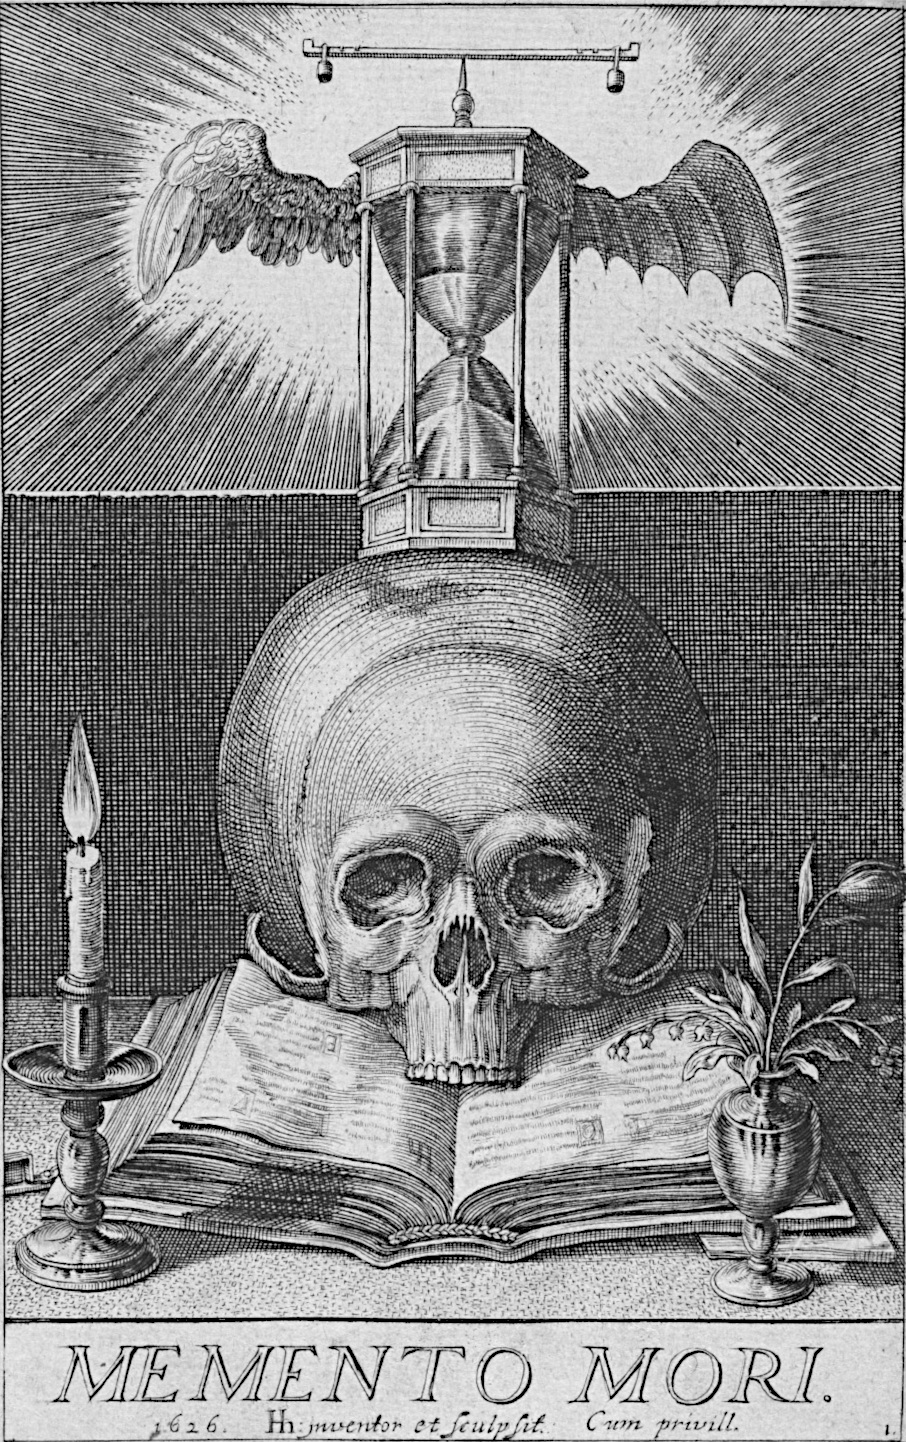
\includegraphics[keepaspectratio,width=\textwidth]{memento-mori-small.jpg}
  \captionart{MementoMori}
  \label{fig:mementomori}
\end{figure}

\clearpage{}
\thispagestyle{titleontop}
%SECT. II. MEMB. III. SUBSECT. V.-_Fear, a Cause_.
\section{Fear, a Cause.}

\lettrine{C}{ousin} german to sorrow, is fear, or rather a sister, fidus Achates,
and continual companion, an assistant and a principal agent in
procuring of this mischief; a cause and symptom as the other. In a
word, as \Virgil{}\authorfootnote{1657} of the Harpies, I may justly say of them both,
\li{Tristius haud illis monstrum, nec saevior ulla
Pestis et ira Deum stygiis sese extulit undis}.

A sadder monster, or more cruel plague so fell,
Or vengeance of the gods, ne'er came from Styx or Hell.

This foul fiend of fear was worshipped heretofore as a god by the
Lacedaemonians, and most of those other torturing \authorfootnote{1658}affections, and
so was sorrow amongst the rest, under the name of Angerona Dea, they
stood in such awe of them, as \Austin{}, de Civitat. Dei, lib. 4. cap. 8,
noteth out of Varro, fear was commonly \authorfootnote{1659}adored and painted in
their temples with a lion's head; and as Macrobius records, l. 10.
Saturnalium; \authorfootnote{1660}In the calends of January, Angerona had her holy
day, to whom in the temple of Volupia, or goddess of pleasure, their
augurs and bishops did yearly sacrifice; that, being propitious to
them, she might expel all cares, anguish, and vexation of the mind for
that year following. Many lamentable effects this fear causeth in men,
as to be red, pale, tremble, sweat, \authorfootnote{1661}it makes sudden cold and heat
to come over all the body, palpitation of the heart, syncope, \etc{}. It
amazeth many men that are to speak, or show themselves in public
assemblies, or before some great personages, as Tully confessed of
himself, that he trembled still at the beginning of his speech; and
Demosthenes, that great orator of Greece, before Philippus. It
confounds voice and memory, as Lucian wittily brings in Jupiter
Tragoedus, so much afraid of his auditory, when he was to make a speech
to the rest of the Gods, that he could not utter a ready word, but was
compelled to use Mercury's help in prompting. Many men are so amazed
and astonished with fear, they know not where they are, what they say,
\authorfootnote{1662}what they do, and that which is worst, it tortures them many days
before with continual affrights and suspicion. It hinders most
honourable attempts, and makes their hearts ache, sad and heavy. They
that live in fear are never free, \authorfootnote{1663}resolute, secure, never merry,
but in continual pain: that, as Vives truly said, Nulla est miseria
major quam metus, no greater misery, no rack, nor torture like unto it,
ever suspicious, anxious, solicitous, they are childishly drooping
without reason, without judgment, \authorfootnote{1664}especially if some terrible
object be offered, as Plutarch hath it. It causeth oftentimes sudden
madness, and almost all manner of diseases, as I have sufficiently
illustrated in my \authorfootnote{1665} digression of the force of imagination, and
shall do more at large in my section of \authorfootnote{1666}terrors. Fear makes our
imagination conceive what it list, invites the devil to come to us, as
\authorfootnote{1667}Agrippa and Cardan avouch, and tyranniseth over our phantasy more
than all other affections, especially in the dark. We see this verified
in most men, as Lavater saith\authorfootnote{1668}, Quae metuunt, fingunt; what they
fear they conceive, and feign unto themselves; they think they see
goblins, hags, devils, and many times become melancholy thereby.
Cardan, subtil. lib. 18, hath an example of such an one, so caused to
be melancholy (by sight of a bugbear) all his life after. Augustus
Caesar durst not sit in the dark, nisi aliquo assidente, saith
\authorfootnote{1669}Suetonius, Nunquam tenebris exigilavit. And 'tis strange what
women and children will conceive unto themselves, if they go over a
churchyard in the night, lie, or be alone in a dark room, how they
sweat and tremble on a sudden. Many men are troubled with future
events, foreknowledge of their fortunes, destinies, as Severus the
Emperor, Adrian and Domitian, Quod sciret ultimum vitae diem, saith
Suetonius, valde solicitus, much tortured in mind because he foreknew
his end; with many such, of which I shall speak more opportunely in
another place.\authorfootnote{1670} Anxiety, mercy, pity, indignation, \etc{}, and such
fearful branches derived from these two stems of fear and sorrow, I
voluntarily omit; read more of them in \authorfootnote{1671}Carolus Pascalius,
\authorfootnote{1672}Dandinus, \etc{}.

%SECT. II. MEMB. III. SUBSECT. VI.-_Shame and Disgrace, Causes_.
\section{Shame and Disgrace, Causes.}

\lettrine{S}{hame} and disgrace cause most violent passions and bitter pangs. Ob
pudorem et dedecus publicum, ob errorum commissum saepe moventur
generosi animi (Felix Plater, lib. 3. de alienat mentis.) Generous
minds are often moved with shame, to despair for some public disgrace.
And he, saith Philo, lib. 2. de provid. dei, \authorfootnote{1673}that subjects
himself to fear, grief, ambition, shame, is not happy, but altogether
miserable, tortured with continual labour, care, and misery. It is as
forcible a batterer as any of the rest: \authorfootnote{1674}Many men neglect the
tumults of the world, and care not for glory, and yet they are afraid
of infamy, repulse, disgrace (Tul. offic. l. 1), they can severely
contemn pleasure, bear grief indifferently, but they are quite
\authorfootnote{1675}battered and broken, with reproach and obloquy: (siquidem vita et
fama pari passu ambulant) and are so dejected many times for some
public injury, disgrace, as a box on the ear by their inferior, to be
overcome of their adversary, foiled in the field, to be out in a
speech, some foul fact committed or disclosed, \etc{} that they dare not
come abroad all their lives after, but melancholise in corners, and
keep in holes. The most generous spirits are most subject to it;
Spiritus altos frangit et generosos: Hieronymus. \Aristotle, because he
could not understand the motion of Euripus, for grief and shame drowned
himself: Caelius Rodigimus antiquar. lec. lib. 29. cap. 8. Homerus
pudore consumptus, was swallowed up with this passion of shame \authorfootnote{1676}
because he could not unfold the fisherman's riddle. Sophocles killed
himself, \authorfootnote{1677}for that a tragedy of his was hissed off the stage:
Valer. max. lib. 9. cap. 12. Lucretia stabbed herself, and so did
\authorfootnote{1678}Cleopatra, when she saw that she was reserved for a triumph, to
avoid the infamy. Antonius the Roman, \authorfootnote{1679}after he was overcome of
his enemy, for three days' space sat solitary in the fore-part of the
ship, abstaining from all company, even of Cleopatra herself, and
afterwards for very shame butchered himself, Plutarch, vita ejus.
Apollonius Rhodius \authorfootnote{1680}wilfully banished himself, forsaking his
country, and all his dear friends, because he was out in reciting his
poems, Plinius, lib. 7. cap. 23. Ajax ran mad, because his arms were
adjudged to Ulysses. In China 'tis an ordinary thing for such as are
excluded in those famous trials of theirs, or should take degrees, for
shame and grief to lose their wits, \authorfootnote{1681}Mat Riccius expedit. ad
Sinas, l. 3. c. 9. Hostratus the friar took that book which Reuclin had
writ against him, under the name of Epist. obscurorum virorum, so to
heart, that for shame and grief he made away with himself, \authorfootnote{1682}Jovius
in elogiis. A grave and learned minister, and an ordinary preacher at
Alcmar in Holland, was (one day as he walked in the fields for his
recreation) suddenly taken with a lax or looseness, and thereupon
compelled to retire to the next ditch; but being \authorfootnote{1683}surprised at
unawares, by some gentlewomen of his parish wandering that way, was so
abashed, that he did never after show his head in public, or come into
the pulpit, but pined away with melancholy: (Pet. Forestus med.
observat. lib. 10. observat. 12.) So shame amongst other passions can
play his prize.

I know there be many base, impudent, brazenfaced rogues, that will
\authorfootnote{1684} Nulla pallescere culpa, be moved with nothing, take no infamy or
disgrace to heart, laugh at all; let them be proved perjured,
stigmatised, convict rogues, thieves, traitors, lose their ears, be
whipped, branded, carted, pointed at, hissed, reviled, and derided with
\authorfootnote{1685}Ballio the Bawd in \Plautus{}, they rejoice at it, Cantores probos;
babe and Bombax, what care they? We have too many such in our times,
---\li{Exclamat Melicerta perisse}
---\li{Frontem de rebus.}\authormarginnote{1686}

Yet a modest man, one that hath grace, a generous spirit, tender of his
reputation, will be deeply wounded, and so grievously affected with it,
that he had rather give myriads of crowns, lose his life, than suffer
the least defamation of honour, or blot in his good name. And if so be
that he cannot avoid it, as a nightingale, \li{Que cantando victa moritur}
(saith Mizaldus\authorfootnote{1687}), dies for shame if another bird sing better, he
languisheth and pineth away in the anguish of his spirit.

\cleartoleftpage{}
\begin{figure}[p]
  \begingroup
  \centering
  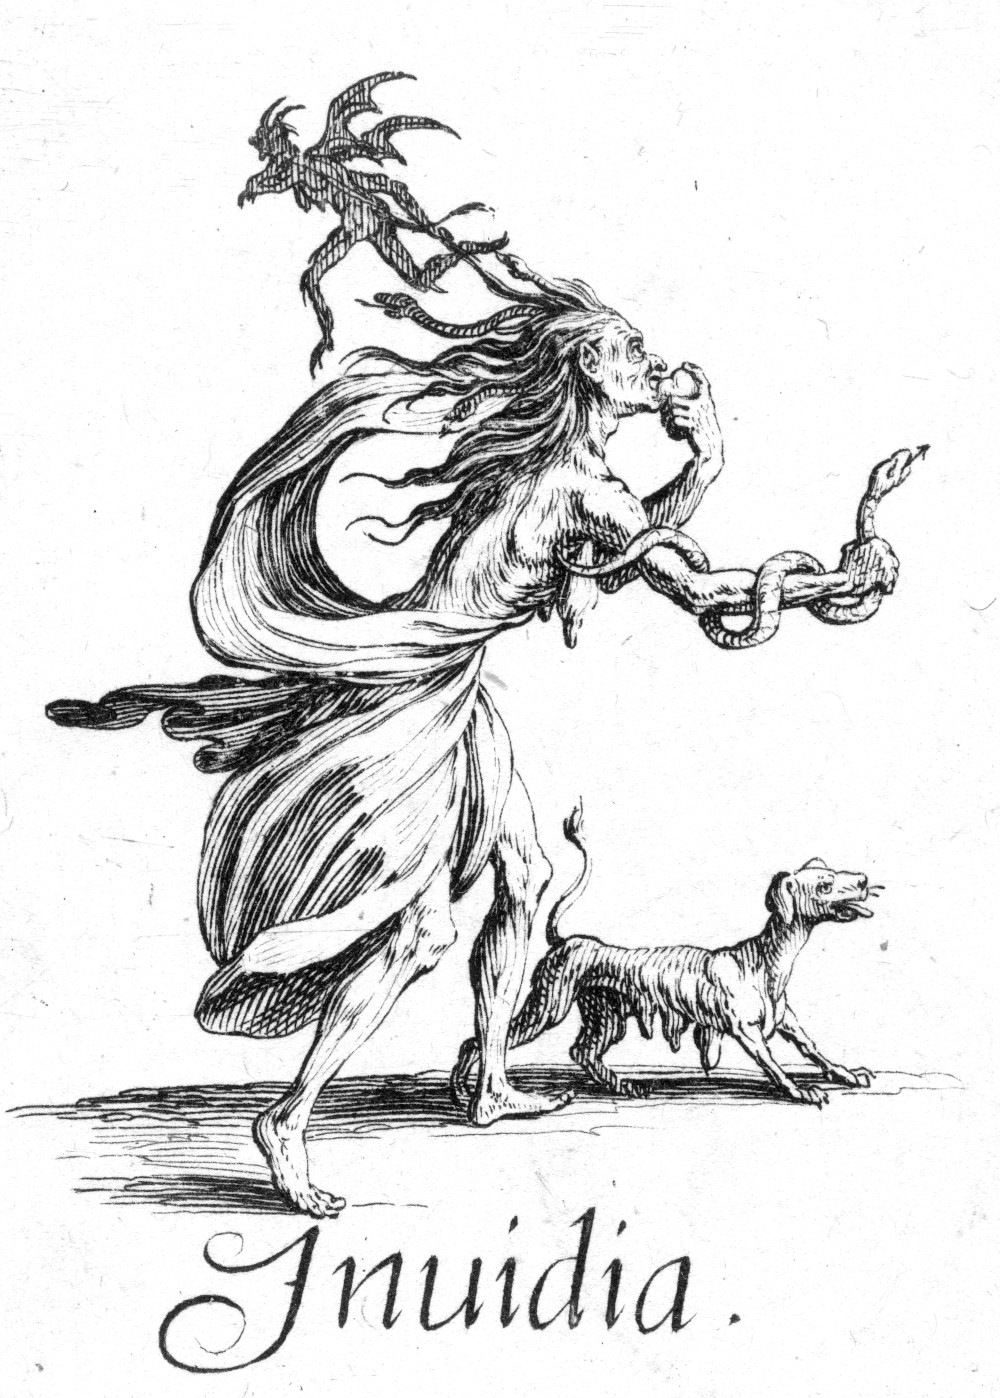
\includegraphics[keepaspectratio,width=0.9\textwidth]{nvidia-small.jpg}
  \captionart{Invidia}
  \label{fig:invidia}
\end{figure}

% Force float here
\clearpage{}
\thispagestyle{titleontop}

%SECT. II. MEMB. III. SUBSECT. VII.-_Envy, Malice, Hatred, Causes_.
\section{Envy, Malice, Hatred, Causes.}
\lettrine{E}{nvy} and malice are two links of this chain, and both, as Guianerius,
Tract. 15. cap. 2, proves out of Galen, 3 Aphorism, com. 22, \authorfootnote{1688}
cause this malady by themselves, especially if their bodies be
otherwise disposed to melancholy. 'Tis Valescus de Taranta, and Felix
Platerus' observation, \authorfootnote{1689}Envy so gnaws many men's hearts, that they
become altogether melancholy. And therefore belike Solomon, Prov. xiv.
13, calls it, the rotting of the bones, Cyprian, vulnus occultum;
\authorfootnote{1690}---Siculi non invenere tyranni
Majus tormentum---

The Sicilian tyrants never invented the like torment. It crucifies
their souls, withers their bodies, makes them hollow-eyed, \authorfootnote{1691}pale,
lean, and ghastly to behold, Cyprian, ser. 2. de zelo et livore.
\authorfootnote{1692}As a moth gnaws a garment, so, saith \Chrysostom{}, doth envy
consume a man; to be a living anatomy: a skeleton, to be a lean and
\authorfootnote{1693}pale carcass, quickened with a \authorfootnote{1694}fiend, Hall in Charact. for
so often as an envious wretch sees another man prosper, to be enriched,
to thrive, and be fortunate in the world, to get honours, offices, or
the like, he repines and grieves.

\begin{verse}
---\textlatin{intabescitque videndo\\*
  Successus hominum-suppliciumque suum est}\authorlatintrans{1695.5}.\authorfootnote{1695}
\end{verse}

He tortures himself if his equal, friend, neighbour, be preferred,
commended, do well; if he understand of it, it galls him afresh; and no
greater pain can come to him than to hear of another man's well-doing;
'tis a dagger at his heart every such object. He looks at him as they
that fell down in Lucian's rock of honour, with an envious eye, and
will damage himself, to do another a mischief: Atque cadet subito, dum
super hoste cadat. As he did in Aesop, lose one eye willingly, that his
fellow might lose both, or that rich man in \authorfootnote{1696}Quintilian that
poisoned the flowers in his garden, because his neighbour's bees should
get no more honey from them. His whole life is sorrow, and every word
he speaks a satire: nothing fats him but other men's ruins. For to
speak in a word, envy is nought else but Tristitia de bonis alienis,
sorrow for other men's good, be it present, past, or to come: et
gaudium de adversis, and \authorfootnote{1697}joy at their harms, opposite to mercy,
\authorfootnote{1698}which grieves at other men's mischances, and misaffects the body
in another kind; so Damascen defines it, lib. 2. de orthod. fid.
Thomas, 2. 2. quaest. 36. art. 1. \Aristotle, l. 2. Rhet. c. 4. et 10.
Plato Philebo. Tully, 3. Tusc. Greg. Nic. l. de virt. animae, c. 12.
Basil, de Invidia. Pindarus Od. 1. ser. 5, and we find it true. 'Tis a
common disease, and almost natural to us, as Tacitus holds\authorfootnote{1699}, to
envy another man's prosperity. And 'tis in most men an incurable
disease. \authorfootnote{1700}I have read, saith Marcus Aurelius, Greek, Hebrew,
Chaldee authors; I have consulted with many wise men for a remedy for
envy, I could find none, but to renounce all happiness, and to be a
wretch, and miserable for ever. 'Tis the beginning of hell in this
life, and a passion not to be excused. \authorfootnote{1701}Every other sin hath some
pleasure annexed to it, or will admit of an excuse; envy alone wants
both. Other sins last but for awhile; the gut may be satisfied, anger
remits, hatred hath an end, envy never ceaseth. Cardan, lib. 2. de sap.
Divine and humane examples are very familiar; you may run and read
them, as that of Saul and David, Cain and Abel, angebat illum non
proprium peccatum, sed fratris prosperitas, saith Theodoret, it was his
brother's good fortune galled him. Rachel envied her sister, being
barren, Gen. \rn{xxx.} Joseph's brethren him, Gen. \rn{xxxvii.} David had a touch
of this vice, as he confesseth, \authorfootnote{1702}Psal. 37. \authorfootnote{1703}Jeremy and
\authorfootnote{1704}Habakkuk, they repined at others' good, but in the end they
corrected themselves, Psal. 75, fret not thyself, \etc{}. Domitian spited
Agricola for his worth, \authorfootnote{1705}that a private man should be so much
glorified. \authorfootnote{1706}Cecinna was envied of his fellow-citizens, because he
was more richly adorned. But of all others, \authorfootnote{1707}women are most weak,
ob pulchritudinem invidae sunt foeminae (Musaeus) aut amat, aut odit,
nihil est tertium (Granatensis.) They love or hate, no medium amongst
them. Implacabiles plerumque laesae mulieres, Agrippina like, \authorfootnote{1708}A
woman, if she see her neighbour more neat or elegant, richer in tires,
jewels, or apparel, is enraged, and like a lioness sets upon her
husband, rails at her, scoffs at her, and cannot abide her; so the
Roman ladies in Tacitus did at Solonina, Cecinna's wife, \authorfootnote{1709}because
she had a better horse, and better furniture, as if she had hurt them
with it; they were much offended. In like sort our gentlewomen do at
their usual meetings, one repines or scoffs at another's bravery and
happiness. Myrsine, an Attic wench, was murdered of her fellows, \authorfootnote{1710}
because she did excel the rest in beauty, Constantine, Agricult. l. 11.
c. 7. Every village will yield such examples.

%SECT. II. MEMB. III. SUBSECT. VIII.-_Emulation, Hatred, Faction, Desire of Revenge, Causes_.
\section{Emulation, Hatred, Faction, Desire of Revenge, Causes.}

\lettrine{O}{ut} of this root of envy \authorfootnote{1711}spring those feral branches of faction,
hatred, livor, emulation, which cause the like grievances, and are,
serrae animae, the saws of the soul, \authorfootnote{1712}consternationis pleni
affectus, affections full of desperate amazement; or as Cyprian
describes emulation, it is \authorfootnote{1713}a moth of the soul, a consumption, to
make another man's happiness his misery, to torture, crucify, and
execute himself, to eat his own heart. Meat and drink can do such men
no good, they do always grieve, sigh, and groan, day and night without
intermission, their breast is torn asunder: and a little after,
\authorfootnote{1714}Whomsoever he is whom thou dost emulate and envy, he may avoid
thee, but thou canst neither avoid him nor thyself; wheresoever thou
art he is with thee, thine enemy is ever in thy breast, thy destruction
is within thee, thou art a captive, bound hand and foot, as long as
thou art malicious and envious, and canst not be comforted. It was the
devil's overthrow; and whensoever thou art thoroughly affected with
this passion, it will be thine. Yet no perturbation so frequent, no
passion so common.
%
\begin{verse}
\textgreek[variant=ancient]{Καὶ κεραμεὺς κεραμεῖ κοτέει\\
καὶ τεκτονι τέκτων},\\
\textgreek[variant=ancient]{Καὶ πτωχὸς πτωχῷ φθονέει\\
καὶ ἀοίδος ἀοιδῶ.}\authorfootnote{1715}
\end{verse}
\translationrule
\begin{verse}
A potter emulates a potter:\\
One smith envies another:\\

A beggar emulates a beggar;\\
A singing man his brother.\\
\end{verse}

Every society, corporation, and private family is full of it, it takes
hold almost of all sorts of men, from the prince to the ploughman, even
amongst gossips it is to be seen, scarce three in a company but there
is siding, faction, emulation, between two of them, some simultas, jar,
private grudge, heart-burning in the midst of them. Scarce two
gentlemen dwell together in the country, (if they be not near kin or
linked in marriage) but there is emulation betwixt them and their
servants, some quarrel or some grudge betwixt their wives or children,
friends and followers, some contention about wealth, gentry,
precedency, \etc{}, by means of which, like the frog in \authorfootnote{1716}Aesop, that
would swell till she was as big as an ox, burst herself at last; they
will stretch beyond their fortunes, callings, and strive so long that
they consume their substance in lawsuits, or otherwise in hospitality,
feasting, fine clothes, to get a few bombast titles, for ambitiosa
paupertate laboramus omnes, to outbrave one another, they will tire
their bodies, macerate their souls, and through contentions or mutual
invitations beggar themselves. Scarce two great scholars in an age, but
with bitter invectives they fall foul one on the other, and their
adherents; Scotists, Thomists, Reals, Nominals, Plato and \Aristotle,
Galenists and Paracelsians, \etc{}, it holds in all professions.
Honest \authorfootnote{1717}emulation in studies, in all callings is not to be
disliked, 'tis ingeniorum cos, as one calls it, the whetstone of wit,
the nurse of wit and valour, and those noble Romans out of this spirit
did brave exploits. There is a modest ambition, as Themistocles was
roused up with the glory of Miltiades; Achilles' trophies moved
Alexander,

\li{Ambire semper stulta confidentia est,
Ambire nunquam deses arrogantia est}\authorlatintrans{1718.5}.\authormarginnote{1718}

'Tis a sluggish humour not to emulate or to sue at all, to withdraw
himself, neglect, refrain from such places, honours, offices, through
sloth, niggardliness, fear, bashfulness, or otherwise, to which by his
birth, place, fortunes, education, he is called, apt, fit, and well
able to undergo; but when it is immoderate, it is a plague and a
miserable pain. What a deal of money did Henry \rn{VIII.} and Francis \rn{I.}
king of France, spend at that \authorfootnote{1719}famous interview? and how many vain
courtiers, seeking each to outbrave other, spent themselves, their
livelihood and fortunes, and died beggars? \authorfootnote{1720}Adrian the Emperor was
so galled with it, that he killed all his equals; so did Nero. This
passion made \authorfootnote{1721}Dionysius the tyrant banish Plato and Philoxenus the
poet, because they did excel and eclipse his glory, as he thought; the
Romans exile Coriolanus, confine Camillus, murder Scipio; the Greeks by
ostracism to expel Aristides, Nicias, Alcibiades, imprison Theseus,
make away Phocion, \etc{}. When Richard I. and Philip of France were fellow
soldiers together, at the siege of Acon in the Holy Land, and Richard
had approved himself to be the more valiant man, insomuch that all
men's eyes were upon him, it so galled Philip, Francum urebat Regis
victoria, saith mine \authorfootnote{1722}author, tam aegre ferebat Richardi gloriam,
ut carpere dicta, calumniari facta; that he cavilled at all his
proceedings, and fell at length to open defiance; he could contain no
longer, but hasting home, invaded his territories, and professed open
war. Hatred stirs up contention, Prov. x. 12, and they break out at
last into immortal enmity, into virulency, and more than Vatinian hate
and rage; \authorfootnote{1723}they persecute each other, their friends, followers,
and all their posterity, with bitter taunts, hostile wars, scurrile
invectives, libels, calumnies, fire, sword, and the like, and will not
be reconciled. Witness that Guelph and Ghibelline faction in Italy;
that of the Adurni and Fregosi in Genoa; that of Cneius Papirius, and
Quintus Fabius in Rome; Caesar and Pompey; Orleans and Burgundy in
France; York and Lancaster in England: yea, this passion so
rageth\authorfootnote{1724}many times, that it subverts not men only, and families,
but even populous cities. \authorfootnote{1725}Carthage and Corinth can witness as
much, nay, flourishing kingdoms are brought into a wilderness by it.
This hatred, malice, faction, and desire of revenge, invented first all
those racks and wheels, strappadoes, brazen bulls, feral engines,
prisons, inquisitions, severe laws to macerate and torment one another.
How happy might we be, and end our time with blessed days and sweet
content, if we could contain ourselves, and, as we ought to do, put up
injuries, learn humility, meekness, patience, forget and forgive, as in
\authorfootnote{1726}God's word we are enjoined, compose such final controversies
amongst ourselves, moderate our passions in this kind, and think better
of others, as Paul would have\authorfootnote{1727} us, than of ourselves: be of like
affection one towards another, and not avenge ourselves, but have peace
with all men. But being that we are so peevish and perverse, insolent
and proud, so factious and seditious, so malicious and envious; we do
invicem angariare, maul and vex one another, torture, disquiet, and
precipitate ourselves into that gulf of woes and cares, aggravate our
misery and melancholy, heap upon us hell and eternal damnation.

%SECT. II. MEMB. III. SUBSECT. IX.-_Anger, a Cause_.
\section{Anger, a Cause.}

\lettrine{A}{nger}, a perturbation, which carries the spirits outwards, preparing
the body to melancholy, and madness itself: Ira furor brevis est, anger
is temporary madness; and as Picolomineus accounts it\authorfootnote{1728}, one of the
three most violent passions. \authorfootnote{1729}Areteus sets it down for an especial
cause (so doth \Seneca, ep. 18. l. 1), of this malady. \authorfootnote{1730}Magninus
gives the reason, Ex frequenti ira supra modum calefiunt; it overheats
their bodies, and if it be too frequent, it breaks out into manifest
madness, saith St. Ambrose. 'Tis a known saying, Furor fit Iaesa
saepius palienlia, the most patient spirit that is, if he be often
provoked, will be incensed to madness; it will make a devil of a saint:
and therefore Basil (belike) in his Homily de Ira, calls it tenebras
rationis, morbum animae, et daemonem pessimum; the darkening of our
understanding, and a bad angel. \authorfootnote{1731}Lucian, in Abdicato, tom. 1, will
have this passion to work this effect, especially in old men and women.
Anger and calumny (saith he) trouble them at first, and after a while
break out into madness: many things cause fury in women, especially if
they love or hate overmuch, or envy, be much grieved or angry; these
things by little and little lead them on to this malady. From a
disposition they proceed to an habit, for there is no difference
between a mad man, and an angry man, in the time of his fit; anger, as
Lactantius describes it, L. de Ira Dei, ad Donatum, c. 5, is
\authorfootnote{1732}saeva animi tempestas, \etc{}, a cruel tempest of the mind; making
his eye sparkle fire, and stare, teeth gnash in his head, his tongue
stutter, his face pale, or red, and what more filthy imitation can be
of a mad man?
\authorfootnote{1733}Ora tument ira, fervescunt sanguine venae,
Lumina Gorgonio saevius angue micant.

They are void of reason, inexorable, blind, like beasts and monsters
for the time, say and do they know not what, curse, swear, rail, fight,
and what not? How can a mad man do more? as he said in the comedy,
\authorfootnote{1734} Iracundia non sum apud me, I am not mine own man. If these fits
be immoderate, continue long, or be frequent, without doubt they
provoke madness. Montanus, consil. 21, had a melancholy Jew to his
patient, he ascribes this for a principal cause: Irascebatur levibus de
causis, he was easily moved to anger. Ajax had no other beginning of
his madness; and Charles the Sixth, that lunatic French king, fell into
this misery, out of the extremity of his passion, desire of revenge and
malice, \authorfootnote{1735}incensed against the duke of Britain, he could neither
eat, drink, nor sleep for some days together, and in the end, about the
calends of July, 1392, he became mad upon his horseback, drawing his
sword, striking such as came near him promiscuously, and so continued
all the days of his life, Aemil., lib. 10. Gal. hist. Aegesippus de
exid. urbis Hieros, l. 1. c. 37, hath such a story of Herod, that out
of an angry fit, became mad, \authorfootnote{1736}leaping out of his bed, he killed
Jossippus, and played many such bedlam pranks, the whole court could
not rule him for a long time after: sometimes he was sorry and
repented, much grieved for that he had done, Postquam deferbuit ira, by
and by outrageous again. In hot choleric bodies, nothing so soon
causeth madness, as this passion of anger, besides many other diseases,
as Pelesius observes, cap. 21. l. 1. de hum. affect. causis; Sanguinem
imminuit, fel auget: and as Valesius controverts\authorfootnote{1737}, Med. controv.,
lib. 5. contro. 8, many times kills them quite out. If this were the
worst of this passion, it were more tolerable, \authorfootnote{1738}but it ruins and
subverts whole towns, \authorfootnote{1739}cities, families, and kingdoms; Nulla
pestis humano generi pluris stetit, saith \Seneca, de Ira, lib. 1. No
plague hath done mankind so much harm. Look into our histories, and you
shall almost meet with no other subject, but what a company \authorfootnote{1740}of
harebrains have done in their rage. We may do well therefore to put
this in our procession amongst the rest; From all blindness of heart,
from pride, vainglory, and hypocrisy, from envy, hatred and malice,
anger, and all such pestiferous perturbations, good Lord deliver us.

%SECT. II. MEMB. III. SUBSECT. X.-_Discontents, Cares, Miseries, \&c. Causes_.
\section{Discontents, Cares, Miseries, \&c. Causes.}

\lettrine{D}{iscontents}, cares, crosses, miseries, or whatsoever it is, that shall
cause any molestation of spirits, grief, anguish, and perplexity, may
well be reduced to this head (preposterously placed here in some men's
judgments they may seem), yet in that \Aristotle in his \authorfootnote{1741}Rhetoric
defines these cares, as he doth envy, emulation, \etc{} still by grief, I
think I may well rank them in this irascible row; being that they are
as the rest, both causes and symptoms of this disease, producing the
like inconveniences, and are most part accompanied with anguish and
pain. The common etymology will evince it, Cura quasi cor uro, Dementes
curae, insomnes curae, damnosae curae, tristes, mordaces, carnifices,
\etc{} biting, eating, gnawing, cruel, bitter, sick, sad, unquiet, pale,
tetric, miserable, intolerable cares, as the poets \authorfootnote{1742}call them,
worldly cares, and are as many in number as the sea sands. \authorfootnote{1743}Galen,
Fernelius, Felix Plater, Valescus de Taranta, \etc{}, reckon afflictions,
miseries, even all these contentions, and vexations of the mind, as
principal causes, in that they take away sleep, hinder concoction, dry
up the body, and consume the substance of it. They are not so many in
number, but their causes be as diverse, and not one of a thousand free
from them, or that can vindicate himself, whom that Ate dea,
\authorfootnote{1744}Per hominum capita molliter ambulans,
Plantas pedum teneras habens:

Over men's heads walking aloft,
With tender feet treading so soft,

Homer's Goddess Ate hath not involved into this discontented
\authorfootnote{1745}rank, or plagued with some misery or other. Hyginus, fab. 220, to
this purpose hath a pleasant tale. Dame Cura by chance went over a
brook, and taking up some of the dirty slime, made an image of it;
Jupiter eftsoons coming by, put life to it, but Cura and Jupiter could
not agree what name to give him, or who should own him; the matter was
referred to Saturn as judge; he gave this arbitrement: his name shall
be Homo ab humo, Cura eum possideat quamdiu vivat, Care shall have him
whilst he lives, Jupiter his soul, and Tellus his body when he dies.
But to leave tales. A general cause, a continuate cause, an inseparable
accident, to all men, is discontent, care, misery; were there no other
particular affliction (which who is free from?) to molest a man in this
life, the very cogitation of that common misery were enough to
macerate, and make him weary of his life; to think that he can never be
secure, but still in danger, sorrow, grief, and persecution. For to
begin at the hour of his birth, as \Pliny{} doth elegantly describe\authorfootnote{1746}
it, he is born naked, and falls \authorfootnote{1747}a whining at the very first: he
is swaddled, and bound up like a prisoner, cannot help himself, and so
he continues to his life's end. Cujusque ferae pabulum, saith
\authorfootnote{1748}\Seneca, impatient of heat and cold, impatient of labour,
impatient of idleness, exposed to fortune's contumelies. To a naked
mariner \Lucretius{} compares him, cast on shore by shipwreck, cold and
comfortless in an unknown land: \authorfootnote{1749}no estate, age, sex, can secure
himself from this common misery. A man that is born of a woman is of
short continuance, and full of trouble, Job \rn{xiv.} 1, 22. And while his
flesh is upon him he shall be sorrowful, and while his soul is in him
it shall mourn. All his days are sorrow and his travels griefs: his
heart also taketh not rest in the night. Eccles. \rn{ii.} 23, and \rn{ii.} 11.
All that is in it is sorrow and vexation of spirit. \authorfootnote{1750}Ingress,
progress, regress, egress, much alike: blindness seizeth on us in the
beginning, labour in the middle, grief in the end, error in all. What
day ariseth to us without some grief, care, or anguish? Or what so
secure and pleasing a morning have we seen, that hath not been overcast
before the evening? One is miserable, another ridiculous, a third
odious. One complains of this grievance, another of that. Aliquando
nervi, aliquando pedes vexant, (\Seneca) nunc distillatio, nunc epatis
morbus; nunc deest, nunc superest sanguis: now the head aches, then the
feet, now the lungs, then the liver, \etc{}. Huic sensus exuberat, sed est
pudori degener sanguis, \etc{}. He is rich, but base born; he is noble, but
poor; a third hath means, but he wants health peradventure, or wit to
manage his estate; children vex one, wife a second, \etc{}. Nemo facile cum
conditione sua concordat, no man is pleased with his fortune, a pound
of sorrow is familiarly mixed with a dram of content, little or no joy,
little comfort, but \authorfootnote{1751}everywhere danger, contention, anxiety, in
all places: go where thou wilt, and thou shalt find discontents, cares,
woes, complaints, sickness, diseases, encumbrances, exclamations: If
thou look into the market, there (saith \authorfootnote{1752} \Chrysostom{}) is brawling
and contention; if to the court, there knavery and flattery, \etc{}; if to
a private man's house, there's cark and care, heaviness, \etc{}. As he said
of old,
\authorfootnote{1753}Nil homine in terra spirat miserum magis alma?

No creature so miserable as man, so generally molested, \authorfootnote{1754}in
miseries of body, in miseries of mind, miseries of heart, in miseries
asleep, in miseries awake, in miseries wheresoever he turns, as Bernard
found, Nunquid tentatio est vita humana super terram? A mere temptation
is our life (\Austin{}, confess. lib. 10. cap. 28), \li{catena perpetuorum
malorum, et quis potest molestias et difficultates pati?} Who can endure
the miseries of it? \authorfootnote{1755}In prosperity we are insolent and
intolerable, dejected in adversity, in all fortunes foolish and
miserable. \authorfootnote{1756}In adversity I wish for prosperity, and in prosperity
I am afraid of adversity. What mediocrity may be found? Where is no
temptation? What condition of life is free? \authorfootnote{1757}Wisdom hath labour
annexed to it, glory, envy; riches and cares, children and
encumbrances, pleasure and diseases, rest and beggary, go together: as
if a man were therefore born (as the Platonists hold) to be punished in
this life for some precedent sins. Or that, as \Pliny{} complains\authorfootnote{1758},
Nature may be rather accounted a stepmother, than a mother unto us, all
things considered: no creature's life so brittle, so full of fear, so
mad, so furious; only man is plagued with envy, discontent, griefs,
covetousness, ambition, superstition. Our whole life is an Irish sea,
wherein there is nought to be expected but tempestuous storms and
troublesome waves, and those infinite,

\li{Tantum malorum pelagus aspicio,
Ut non sit inde enatandi copia}\authorlatintrans{1759.5},\authormarginnote{1759}

no halcyonian times, wherein a man can hold himself secure, or agree
with his present estate; but as Boethius infers, \authorfootnote{1760}there is
something in every one of us which before trial we seek, and having
tried abhor: \authorfootnote{1761} we earnestly wish, and eagerly covet, and are
eftsoons weary of it. Thus between hope and fear, suspicions, angers,
\authorfootnote{1762}Inter spemque metumque, timores inter et iras, betwixt falling
in, falling out, \etc{}, we bangle away our best days, befool out our
times, we lead a contentious, discontent, tumultuous, melancholy,
miserable life; insomuch, that if we could foretell what was to come,
and it put to our choice, we should rather refuse than accept of this
painful life. In a word, the world itself is a maze, a labyrinth of
errors, a desert, a wilderness, a den of thieves, cheaters, \etc{}, full
of filthy puddles, horrid rocks, precipitiums, an ocean of adversity,
an heavy yoke, wherein infirmities and calamities overtake, and follow
one another, as the sea waves; and if we scape Scylla, we fall foul on
Charybdis, and so in perpetual fear, labour, anguish, we run from one
plague, one mischief, one burden to another, duram servientes
servitutem, and you may as soon separate weight from lead, heat from
fire, moistness from water, brightness from the sun, as misery,
discontent, care, calamity, danger, from a man. Our towns and cities
are but so many dwellings of human misery. In which grief and sorrow
(\authorfootnote{1763}as he right well observes out of Solon) innumerable troubles,
labours of mortal men, and all manner of vices, are included, as in so
many pens. Our villages are like molehills, and men as so many emmets,
busy, busy still, going to and fro, in and out, and crossing one
another's projects, as the lines of several sea-cards cut each other in
a globe or map. Now light and merry, but (\authorfootnote{1764}as one follows it)
by-and-by sorrowful and heavy; now hoping, then distrusting; now
patient, tomorrow crying out; now pale, then red; running, sitting,
sweating, trembling, halting, \etc{}. Some few amongst the rest, or perhaps
one of a thousand, may be Pullus Jovis, in the world's esteem, Gallinae
filius albae, an happy and fortunate man, ad invidiam felix, because
rich, fair, well allied, in honour and office; yet peradventure ask
himself, and he will say, that of all others \authorfootnote{1765}he is most miserable
and unhappy. A fair shoe, Hic soccus novus, elegans, as he \authorfootnote{1766}said,
sed nescis ubi urat, but thou knowest not where it pincheth. It is not
another man's opinion can make me happy: but as \Seneca well hath\authorfootnote{1767}
it, He is a miserable wretch that doth not account himself happy,
though he be sovereign lord of a world: he is not happy, if he think
himself not to be so; for what availeth it what thine estate is, or
seem to others, if thou thyself dislike it? A common humour it is of
all men to think well of other men's fortunes, and dislike their own:
\authorfootnote{1768}Cui placet alterius, sua nimirum est odio sors; but \authorfootnote{1769}qui fit
Mecoenas, \etc{}, how comes it to pass, what's the cause of it? Many men
are of such a perverse nature, they are well pleased with nothing
(saith Theodoret\authorfootnote{1770}), neither with riches nor poverty, they
complain when they are well and when they are sick, grumble at all
fortunes, prosperity and adversity; they are troubled in a cheap year,
in a barren, plenty or not plenty, nothing pleaseth them, war nor
peace, with children, nor without. This for the most part is the humour
of us all, to be discontent, miserable, and most unhappy, as we think
at least; and show me him that is not so, or that ever was otherwise.
Quintus Metellus his felicity is infinitely admired amongst the Romans,
insomuch that as Paterculus mentioneth\authorfootnote{1771} of him, you can scarce
find of any nation, order, age, sex, one for happiness to be compared
unto him: he had, in a word, Bona animi, corporis et fortunae, goods of
mind, body, and fortune, so had P. Mutianus, \authorfootnote{1772}Crassus. Lampsaca,
that Lacedaemonian lady, was such another in \authorfootnote{1773}\Pliny{}'s conceit, a
king's wife, a king's mother, a king's daughter: and all the world
esteemed as much of Polycrates of Samos. The Greeks brag of their
Socrates, Phocion, Aristides; the Psophidians in particular of their
Aglaus, Omni vita felix, ab omni periculo immunis (which by the way
Pausanias held impossible;) the Romans of their \authorfootnote{1774} Cato, Curius,
Fabricius, for their composed fortunes, and retired estates, government
of passions, and contempt of the world: yet none of all these were
happy, or free from discontent, neither Metellus, Crassus, nor
Polycrates, for he died a violent death, and so did Cato; and how much
evil doth Lactantius and Theodoret speak of Socrates, a weak man, and
so of the rest. There is no content in this life, but as he said\authorfootnote{1775},
All is vanity and vexation of spirit; lame and imperfect. Hadst thou
Sampson's hair, Milo's strength, Scanderbeg's arm, Solomon's wisdom,
Absalom's beauty, Croesus' wealth, Pasetis obulum, Caesar's valour,
Alexander's spirit, Tully's or Demosthenes' eloquence, Gyges' ring,
Perseus' Pegasus, and Gorgon's head, Nestor's years to come, all this
would not make thee absolute; give thee content, and true happiness in
this life, or so continue it. Even in the midst of all our mirth,
jollity, and laughter, is sorrow and grief, or if there be true
happiness amongst us, 'tis but for a time,
\authorfootnote{1776}Desinat in piscem mulier formosa superne:

A handsome woman with a fish's tail, a fair morning turns to a lowering afternoon. Brutus and Cassius, once
renowned, both eminently happy, yet you shall scarce find two (saith
Paterculus) quos fortuna maturius destiturit, whom fortune sooner
forsook. Hannibal, a conqueror all his life, met with his match, and
was subdued at last, Occurrit forti, qui mage fortis erit. One is
brought in triumph, as Caesar into Rome, Alcibiades into Athens,
coronis aureis donatus, crowned, honoured, admired; by-and-by his
statues demolished, he hissed out, massacred, \etc{}. \authorfootnote{1777}Magnus
Gonsalva, that famous Spaniard, was of the prince and people at first
honoured, approved; forthwith confined and banished. Admirandas
actiones; graves plerunque sequuntur invidiae, et acres calumniae: 'tis
Polybius his observation, grievous enmities, and bitter calumnies,
commonly follow renowned actions. One is born rich, dies a beggar;
sound today, sick tomorrow; now in most flourishing estate, fortunate
and happy, by-and-by deprived of his goods by foreign enemies, robbed
by thieves, spoiled, captivated, impoverished, as they of \authorfootnote{1778}Rabbah
put under iron saws, and under iron harrows, and under axes of iron,
and cast into the tile kiln,

\begin{verse}
\textlatin{Quid me felicem toties jactastis amici},\\
\textlatin{Qui cecidit, stabili non erat ille gradu.}\authorfootnote{1779}
\end{verse}

He that erst marched like Xerxes with innumerable armies, as rich as
Croesus, now shifts for himself in a poor cock-boat, is bound in iron
chains, with Bajazet the Turk, and a footstool with Aurelian, for a
tyrannising conqueror to trample on. So many casualties there are, that
as \Seneca said of a city consumed with fire, Una dies interest inter
maximum civitatem et nullam, one day betwixt a great city and none: so
many grievances from outward accidents, and from ourselves, our own
indiscretion, inordinate appetite, one day betwixt a man and no man.
And which is worse, as if discontents and miseries would not come fast
enough upon us: homo homini daemon, we maul, persecute, and study how
to sting, gall, and vex one another with mutual hatred, abuses,
injuries; preying upon and devouring as so many, \authorfootnote{1780}ravenous birds;
and as jugglers, panders, bawds, cozening one another; or raging as
\authorfootnote{1781}wolves, tigers, and devils, we take a delight to torment one
another; men are evil, wicked, malicious, treacherous, and
\authorfootnote{1782}naught, not loving one another, or loving themselves, not
hospitable, charitable, nor sociable as they ought to be, but
counterfeit, dissemblers, ambidexters, all for their own ends,
hard-hearted, merciless, pitiless, and to benefit themselves, they care
not what mischief they procure to others. \authorfootnote{1783}Praxinoe and Gorgo in
the poet, when they had got in to see those costly sights, they then
cried bene est, and would thrust out all the rest: when they are rich
themselves, in honour, preferred, full, and have even that they would,
they debar others of those pleasures which youth requires, and they
formerly have enjoyed. He sits at table in a soft chair at ease, but he
doth remember in the mean time that a tired waiter stands behind him,
an hungry fellow ministers to him full, he is athirst that gives him
drink (saith \authorfootnote{1784}Epictetus) and is silent whilst he speaks his
pleasure: pensive, sad, when he laughs. Pleno se proluit auro: he
feasts, revels, and profusely spends, hath variety of robes, sweet
music, ease, and all the pleasure the world can afford, whilst many an
hunger-starved poor creature pines in the street, wants clothes to
cover him, labours hard all day long, runs, rides for a trifle, fights
peradventure from sun to sun, sick and ill, weary, full of pain and
grief, is in great distress and sorrow of heart. He loathes and scorns
his inferior, hates or emulates his equal, envies his superior, insults
over all such as are under him, as if he were of another species, a
demigod, not subject to any fall, or human infirmities. Generally they
love not, are not beloved again: they tire out others' bodies with
continual labour, they themselves living at ease, caring for none else,
sibi nati; and are so far many times from putting to their helping
hand, that they seek all means to depress, even most worthy and well
deserving, better than themselves, those whom they are by the laws of
nature bound to relieve and help, as much as in them lies, they will
let them caterwaul, starve, beg, and hang, before they will any ways
(though it be in their power) assist or ease: \authorfootnote{1785}so unnatural are
they for the most part, so unregardful; so hard-hearted, so churlish,
proud, insolent, so dogged, of so bad a disposition. And being so
brutish, so devilishly bent one towards another, how is it possible but
that we should be discontent of all sides, full of cares, woes, and
miseries?

If this be not a sufficient proof of their discontent and misery,
examine every condition and calling apart. Kings, princes, monarchs,
and magistrates seem to be most happy, but look into their estate, you
shall \authorfootnote{1786}find them to be most encumbered with cares, in perpetual
fear, agony, suspicion, jealousy: that, as he said\authorfootnote{1787} of a crown, if
they knew but the discontents that accompany it, they would not stoop
to take it up. Quem mihi regent dabis (saith \Chrysostom{}) non curis
plenum? What king canst thou show me, not full of cares? \authorfootnote{1788}Look not
on his crown, but consider his afflictions; attend not his number of
servants, but multitude of crosses. Nihil aliud potestas culminis, quam
tempestas mentis, as Gregory seconds him; sovereignty is a tempest of
the soul: Sylla like they have brave titles, but terrible fits:
splendorem titulo, cruciatum animo: which made \authormarginnote{1789}Demosthenes vow,
si vel ad tribunal, vel ad interitum duceretur: if to be a judge, or to
be condemned, were put to his choice, he would be condemned. Rich men
are in the same predicament; what their pains are, stulti nesciunt,
ipsi sentiunt: they feel, fools perceive not, as I shall prove
elsewhere, and their wealth is brittle, like children's rattles: they
come and go, there is no certainty in them: those whom they elevate,
they do as suddenly depress, and leave in a vale of misery. The middle
sort of men are as so many asses to bear burdens; or if they be free,
and live at ease, they spend themselves, and consume their bodies and
fortunes with luxury and riot, contention, emulation, \etc{}. The poor I
reserve for another \authorfootnote{1790}place and their discontents.
For particular professions, I hold as of the rest, there's no content
or security in any; on what course will you pitch, how resolve? to be a
divine, 'tis contemptible in the world's esteem; to be a lawyer, 'tis
to be a wrangler; to be a physician, \authorfootnote{1791}pudet lotii, 'tis loathed; a
philosopher, a madman; an alchemist, a beggar; a poet, esurit, an
hungry jack; a musician, a player; a schoolmaster, a drudge; an
husbandman, an emmet; a merchant, his gains are uncertain; a
mechanician, base; a chirurgeon, fulsome; a tradesman, a \authorfootnote{1792}liar; a
tailor, a thief; a serving-man, a slave; a soldier, a butcher; a smith,
or a metalman, the pot's never from his nose; a courtier a parasite, as
he could find no tree in the wood to hang himself; I can show no state
of life to give content. The like you may say of all ages; children
live in a perpetual slavery, still under that tyrannical government of
masters; young men, and of riper years, subject to labour, and a
thousand cares of the world, to treachery, falsehood, and cozenage,
%
\begin{verse}
---\textlatin{Incedit per ignes},\\
\textlatin{Suppositos cineri doloso},\authorfootnote{1793}
\end{verse}
\translationrule
\begin{verse}
---you incautious tread\\
On fires, with faithless ashes overhead.
\end{verse}

\authorfootnote{1794}old are full of aches in their bones, cramps and convulsions,
silicernia, dull of hearing, weak sighted, hoary, wrinkled, harsh, so
much altered as that they cannot know their own face in a glass, a
burthen to themselves and others, after 70 years, all is sorrow (as
David hath it), they do not live but linger. If they be sound, they
fear diseases; if sick, weary of their lives: Non est vivere, sed
valere vita. One complains of want, a second of servitude,
\authorfootnote{1795}another of a secret or incurable disease; of some deformity of
body, of some loss, danger, death of friends, shipwreck, persecution,
imprisonment, disgrace, repulse, \authorfootnote{1796} contumely, calumny, abuse,
injury, contempt, ingratitude, unkindness, scoffs, flouts, unfortunate
marriage, single life, too many children, no children, false servants,
unhappy children, barrenness, banishment, oppression, frustrate hopes
and ill-success, \etc{}.
%
\begin{verse}
\textlatin{Talia de genere hoc adeo sunt multa, loquacem ut}\\
\textlatin{Delassare valent Fabium}.---\authorfootnote{1797}
\end{verse}
\translationrule
\begin{verse}
But, every various instance to repeat,\\
Would tire even Fabius of incessant prate.
\end{verse}

Talking Fabius will be tired before he can tell half of them; they are
the subject of whole volumes, and shall (some of them) be more
opportunely dilated elsewhere. In the meantime thus much I may say of
them, that generally they crucify the soul of man, \authorfootnote{1798}attenuate our
bodies, dry them, wither them, shrivel them up like old apples, make
them as so many anatomies (\authorfootnote{1799}ossa atque pellis est totus, ita curis
macet) they cause tempus foedum et squalidum, cumbersome days,
ingrataque tempora, slow, dull, and heavy times: make us howl, roar,
and tear our hairs, as sorrow did in \authorfootnote{1800}Cebes' table, and groan for
the very anguish of our souls. Our hearts fail us as David's did, Psal.
\rn{xl.} 12, for innumerable troubles that compassed him; and we are ready
to confess with Hezekiah, Isaiah \rn{lviii.} 17, behold, for felicity I had
bitter grief; to weep with Heraclitus, to curse the day of our birth
with Jeremy, \rn{xx.} 14, and our stars with Job: to hold that axiom of
Silenus, \authorfootnote{1801}better never to have been born, and the best next of
all, to die quickly: or if we must live, to abandon the world, as Timon
did; creep into caves and holes, as our anchorites; cast all into the
sea, as Crates Thebanus; or as Theombrotus Ambrociato's 400 auditors,
precipitate ourselves to be rid of these miseries.

%SECT. II. MEMB. III. SUBSECT. XI.-_Concupiscible Appetite, as Desires, Ambition, Causes_.
\section{Concupiscible Appetite, as Desires, Ambition, Causes.}

\lettrine{T}{hese} \footnoteA{worthy of being desired. \theeditor{}}{concupiscible} and \footnoteA{irritable. \theeditor{}}{irascible} appetites are as the two twists of a
rope, mutually mixed one with the other, and both twining about the
heart: both good, as \Austin{}, holds, l. 14. c. 9. de civ. Dei, \authorfootnote{1802}if
they be moderate; both pernicious if they be exorbitant. This
concupiscible appetite, howsoever it may seem to carry with it a show
of pleasure and delight, and our concupiscences most part affect us
with content and a pleasing object, yet if they be in extremes, they
rack and wring us on the other side. A true saying it is, Desire hath
no rest; is infinite in itself, endless; and as one calls\authorfootnote{1803} it, a
perpetual rack, \authorfootnote{1804}or horse-mill, according to \Austin{}, still going
round as in a ring. They are not so continual, as diverse, \li{felicius
atomos denumerare possem}, saith Bernard\authorfootnote{1805}, \li{quam motus cordis; nunc
haec, nunc illa cogito}, you may as well reckon up the motes in the sun
as them. It extends itself to everything\authorfootnote{1806}, as Guianerius will have
it, that is superfluously sought after:' or to any \authorfootnote{1807}fervent
desire, as Fernelius interprets it; be it in what kind soever, it
tortures if immoderate, and is (according to Plater\authorfootnote{1808} and others)
an especial cause of melancholy. \li{Multuosis concupiscentiis dilaniantur
cogitationes meae}, \Austin{} confessed\authorfootnote{1809}, that he was torn a pieces
with his manifold desires: and so doth Bernard complain\authorfootnote{1810}, that he
could not rest for them a minute of an hour: this I would have, and
that, and then I desire to be such and such. 'Tis a hard matter
therefore to confine them, being they are so various and many,
impossible to apprehend all. I will only insist upon some few of the
chief, and most noxious in their kind, as that exorbitant appetite and
desire of honour, which we commonly call ambition; love of money, which
is covetousness, and that greedy desire of gain: self-love, pride, and
inordinate desire of vainglory or applause, love of study in excess;
love of women (which will require a just volume of itself), of the
other I will briefly speak, and in their order.

Ambition, a proud covetousness, or a dry thirst of honour, a great
torture of the mind, composed of envy, pride, and covetousness, a
gallant madness, one defines\authorfootnote{1811} it a pleasant poison, Ambrose, a
canker of the soul, an hidden plague: Bernard\authorfootnote{1812}, a secret poison,
the father of livor, and mother of hypocrisy, the moth of holiness, and
cause of madness, crucifying and disquieting all that it takes hold of.
\Seneca calls it\authorfootnote{1813}, \li{rem solicitam, timidam, vanam, ventosam}, a windy
thing, a vain, solicitous, and fearful thing. For commonly they that,
like Sisyphus, roll this restless stone of ambition, are in a perpetual
agony, still perplexed\authorfootnote{1814}, \li{semper taciti, tritesque recedunt}
(\Lucretius{}), doubtful, timorous, suspicious, loath to offend in word or
deed, still cogging and colloguing, embracing, capping, cringing,
applauding, flattering, fleering, visiting, waiting at men's doors,
with all affability, counterfeit honesty and humility. If that
will not serve\authorfootnote{1815}, if once this humour (as Cyprian describes\authorfootnote{1816} it)
possess his thirsty soul, ambitionis salsugo ubi bibulam animam
possidet, by hook and by crook he will obtain it, and from his hole he
will climb to all honours and offices, if it be possible for him to get
up, flattering one, bribing another, he will leave no means unessay'd
to win all. It is a wonder to see how slavishly these kind of men
subject themselves\authorfootnote{1817}, when they are about a suit, to every inferior
person; what pains they will take, run, ride, cast, plot, countermine,
protest and swear, vow, promise, what labours undergo, early up, down
late; how obsequious and affable they are, how popular and courteous,
how they grin and fleer upon every man they meet; with what feasting
and inviting, how they spend themselves and their fortunes, in seeking
that many times, which they had much better be without; as Cyneas
the orator told\authorfootnote{1818} Pyrrhus: with what waking nights, painful hours,
anxious thoughts, and bitterness of mind, \li{inter spemque metumque},
distracted and tired, they consume the interim of their time. There can
be no greater plague for the present. If they do obtain their suit,
which with such cost and solicitude they have sought, they are not so
freed, their anxiety is anew to begin, for they are never satisfied,
\li{nihil aliud nisi imperium spirant}, their thoughts, actions, endeavours
are all for sovereignty and honour, like Lues Sforza\authorfootnote{1819} that huffing
Duke of Milan, a man of singular wisdom, but profound ambition, born to
his own, and to the destruction of Italy, though it be to their own
ruin, and friends' undoing, they will contend, they may not cease, but
as a dog in a wheel, a bird in a cage, or a squirrel in a chain, so
Budaeus compares\authorfootnote{1820} them; they climb and climb still\authorfootnote{1821}, with
much labour, but never make an end, never at the top. A knight would be
a baronet, and then a lord, and then a viscount, and then an earl, \etc{};
a doctor, a dean, and then a bishop; from tribune to praetor; from
bailiff to major; first this office, and then that; as Pyrrhus in
Plutarch\authorfootnote{1822}, they will first have Greece, then Africa, and then
Asia, and swell with Aesop's frog so long, till in the end they burst,
or come down with Sejanus, ad Gemonias scalas, and break their own
necks; or as Evangelus the piper in Lucian, that blew his pipe so long,
till he fell down dead. If he chance to miss, and have a canvass, he is
in a hell on the other side; so dejected, that he is ready to hang
himself, turn heretic, Turk, or traitor in an instant. Enraged against
his enemies, he rails, swears, fights, slanders, detracts, envies,
murders: and for his own part, si appetitum explere non potest, furore
corripitur; if he cannot satisfy his desire (as Bodine writes\authorfootnote{1823}) he
runs mad. So that both ways, hit or miss, he is distracted so long as
his ambition lasts, he can look for no other but anxiety and care,
discontent and grief in the meantime, madness itself\authorfootnote{1824}, or violent
death in the end. The event of this is common to be seen in populous
cities, or in princes' courts, for a courtier's life (as Budaeus
describes it) is a \footnoteA{a hodgepodge; jumble; confused medley. \theeditor{}}{gallimaufry} of ambition\authorfootnote{1825}, lust, fraud,
imposture, dissimulation, detraction, envy, pride; \authorfootnote{1826}the court, a
common conventicle of flatterers, time-servers, politicians, \etc{}; or as
\authorfootnote{1827} Anthony Perez will, the suburbs of hell itself. If you will see
such discontented persons, there you shall likely find them. And
which he observed of the markets of old Rome\authorfootnote{1828},
%
\begin{latin}
\begin{quote}
Qui perjurum convenire vult hominem, mitto in Comitium;
Qui mendacem et gloriosum, apud Cluasinae sacrum;
Dites, damnosos maritos, sub basilica quaerito, \etc{}.
\end{quote}
\end{latin}
\translationrule
\begin{quote}
Perjured knaves, knights of the post, liars, crackers, bad husbands,
\etc{} keep their several stations; they do still, and always did in every
commonwealth.
\end{quote}

%SECT. II. MEMB. III. SUBSECT. XII.-_Φιλαργυρία, Covetousness, a Cause_.
\section{\textgreek{Φιλαργυρία}, Covetousness, a Cause.}

\lettrine{P}{lutarch}, in his book\authorfootnote{1829} whether the diseases of the body be more
grievous than those of the soul, is of opinion, if you will examine all
the causes of our miseries in this life, you shall find them most part
to have had their beginning from stubborn anger, that furious desire of
contention, or some unjust or immoderate affection, as covetousness,
\etc{}. From whence are wars and contentions amongst you? \authorfootnote{1830}St. James
asks: I will add usury, fraud, rapine, simony, oppression, lying,
swearing, bearing false witness, \etc{} are they not from this fountain of
covetousness, that greediness in getting, tenacity in keeping,
sordidity in spending; that they are so wicked, \authorfootnote{1831}unjust against
God, their neighbour, themselves; all comes hence. The desire of money
is the root of all evil, and they that lust after it, pierce themselves
through with many sorrows, 1 Tim. vi. 10. Hippocrates therefore in his
Epistle to Crateva, an herbalist, gives him this good counsel, that if
it were possible, \authorfootnote{1832} amongst other herbs, he should cut up that
weed of covetousness by the roots, that there be no remainder left, and
then know this for a certainty, that together with their bodies, thou
mayst quickly cure all the diseases of their minds. For it is indeed
the pattern, image, epitome of all melancholy, the fountain of many
miseries, much discontented care and woe; this inordinate, or
immoderate desire of gain, to get or keep money, as Bonaventure
defines\authorfootnote{1833} it: or, as \Austin{} describes it, a madness of the soul, Gregory
a torture; \Chrysostom{}, an insatiable drunkenness; Cyprian, blindness,
speciosum supplicium, a plague subverting kingdoms, families, an
\authorfootnote{1834}incurable disease; Budaeus, an ill habit, \authorfootnote{1835}yielding to no
remedies: neither Aesculapius nor Plutus can cure them: a continual
plague, saith Solomon, and vexation of spirit, another hell. I know
there be some of opinion, that covetous men are happy, and worldly,
wise, that there is more pleasure in getting of wealth than in
spending, and no delight in the world like unto it. 'Twas Bias'
problem\authorfootnote{1836} of old, With what art thou not weary? with getting money. What
is most delectable? to gain. What is it, trow you, that makes a poor
man labour all his lifetime, carry such great burdens, fare so hardly,
macerate himself, and endure so much misery, undergo such base offices
with so great patience, to rise up early, and lie down late, if there
were not an extraordinary delight in getting and keeping of money? What
makes a merchant that hath no need, satis superque domi, to range all
over the world, through all those intemperate \authorfootnote{1837}Zones of heat and
cold; voluntarily to venture his life, and be content with such
miserable famine, nasty usage, in a stinking ship; if there were not a
pleasure and hope to get money, which doth season the rest, and
mitigate his indefatigable pains? What makes them go into the bowels of
the earth, an hundred fathom deep, endangering their dearest lives,
enduring damps and filthy smells, when they have enough already, if
they could be content, and no such cause to labour, but an
extraordinary delight they take in riches. This may seem plausible at
first show, a popular and strong argument; but let him that so thinks,
consider better of it, and he shall soon perceive, that it is far
otherwise than he supposeth; it may be haply pleasing at the first, as
most part all melancholy is. For such men likely have some lucida
intervalla, pleasant symptoms intermixed; but you must note that of
\authorfootnote{1838}\Chrysostom{}, 'Tis one thing to be rich, another to be covetous:
generally they are all fools, dizzards, madmen, \authorfootnote{1839}miserable
wretches, living besides themselves, sine arte fruendi, in perpetual
slavery, fear, suspicion, sorrow, and discontent, plus aloes quam
mellis habent; and are indeed, rather possessed by their money, than
possessors: as Cyprian hath\authorfootnote{1840} it, \li{mancipati pecuniis}; bound
prentice to their goods, as \Pliny{}\authorfootnote{1841}; or as \Chrysostom{}, servi
divitiarum, slaves and drudges to their substance; and we may conclude
of them all, as Valerius doth\authorfootnote{1842} of Ptolomaeus king of Cyprus, He
was in title a king of that island, but in his mind, a miserable drudge
of money:
\authorfootnote{1843}---potiore metallis
libertate carens---

wanting his liberty, which is better than gold. Damasippus the Stoic,
in \Horace{}, proves that all mortal men dote by fits, some one way, some
another, but that covetous men \authorfootnote{1844}are madder than the rest; and he
that shall truly look into their estates, and examine their symptoms,
shall find no better of them, but that they are all \authorfootnote{1845}fools, as
Nabal was, Re et nomine (1. Reg. 15.) For what greater folly can there
be, or \authorfootnote{1846} madness, than to macerate himself when he need not? and
when, as Cyprian notes, \authorfootnote{1847}he may be freed from his burden, and
eased of his pains, will go on still, his wealth increasing, when he
hath enough, to get more, to live besides himself, to starve his
genius, keep back from his wife \authorfootnote{1848}and children, neither letting
them nor other friends use or enjoy that which is theirs by right, and
which they much need perhaps; like a hog, or dog in the manger, he doth
only keep it, because it shall do nobody else good, hurting himself and
others: and for a little momentary pelf, damn his own soul? They are
commonly sad and tetric by nature, as Achab's spirit was because he
could not get Naboth's vineyard, (1. Reg. 22.) and if he lay out his
money at any time, though it be to necessary uses, to his own
children's good, he brawls and scolds, his heart is heavy, much
disquieted he is, and loath to part from it: \li{Miser abstinet et timet
uti}.\authorfootnote{1848.8} He is of a wearish, dry, pale constitution, and cannot sleep
for cares and worldly business; his riches, saith Solomon, will not let
him sleep, and unnecessary business which he heapeth on himself; or if
he do sleep, 'tis a very unquiet, interrupt, unpleasing sleep: with his
bags in his arms,
---congestis undique sacc
indormit inhians,---

And though he be at a banquet, or at some merry feast, he sighs for
grief of heart (as Cyprian hath\authorfootnote{1849} it) and cannot sleep though it be
upon a down bed; his wearish body takes no rest, \authorfootnote{1850}troubled in his
abundance, and sorrowful in plenty, unhappy for the present, and more
unhappy in the life to come. Basil. He is a perpetual drudge,
\authorfootnote{1851}restless in his thoughts, and never satisfied, a slave, a wretch,
a dust-worm, semper quod idolo suo immolet, sedulus observat Cypr.
prolog. ad sermon still seeking what sacrifice he may offer to his
golden god, per fas et nefas, he cares not how, his trouble is endless,
\authorfootnote{1852}crescunt divitiae, tamen curtae nescio quid semper abest rei: his
wealth increaseth, and the more he hath, the more \authorfootnote{1853}he wants: like
Pharaoh's lean kine, which devoured the fat, and were not satisfied.
\authorfootnote{1854}\Austin{} therefore defines covetousness, quarumlibet rerum
inhonestam et insatiabilem cupiditatem a dishonest and insatiable
desire of gain; and in one of his epistles compares it to hell;
\authorfootnote{1855}which devours all, and yet never hath enough, a bottomless pit,
an endless misery; in quem scopulum avaritiae cadaverosi senes
utplurimum impingunt, and that which is their greatest corrosive, they
are in continual suspicion, fear, and distrust, He thinks his own wife
and children are so many thieves, and go about to cozen him, his
servants are all false:
%
\begin{verse}
\textlatin{Rem suam periisse, seque eradicarier},\\
\textlatin{Et divum atque hominum clamat continuo fidem},\\
\textlatin{De suo tigillo si qua exit foras}.
\end{verse}
\translationrule
\begin{verse}
If his doors creek, then out he cries anon,\\
His goods are gone, and he is quite undone.
\end{verse}

Timidus Plutus, an old proverb, As fearful as Plutus: so doth
Aristophanes and Lucian bring him in fearful still, pale, anxious,
suspicious, and trusting no man, \authorfootnote{1856}They are afraid of tempests for
their corn; they are afraid of their friends lest they should ask
something of them, beg or borrow; they are afraid of their enemies lest
they hurt them, thieves lest they rob them; they are afraid of war and
afraid of peace, afraid of rich and afraid of poor; afraid of all. Last
of all, they are afraid of want, that they shall die beggars, which
makes them lay up still, and dare not use that they have: what if a
dear year come, or dearth, or some loss? and were it not that they are
both to \authorfootnote{1857}lay out money on a rope, they would be hanged forthwith,
and sometimes die to save charges, and make away themselves, if their
corn and cattle miscarry; though they have abundance left, as
\authorfootnote{1858}Agellius notes. \authorfootnote{1859}Valerius makes mention of one that in a
famine sold a mouse for 200 pence, and famished himself: such are their
cares, \authorfootnote{1860}griefs and perpetual fears. These symptoms are elegantly
expressed by Theophrastus in his character of a covetous man;
\authorfootnote{1861}lying in bed, he asked his wife whether she shut the trunks and
chests fast, the cap-case be sealed, and whether the hall door be
bolted; and though she say all is well, he riseth out of his bed in his
shirt, barefoot and barelegged, to see whether it be so, with a dark
lantern searching every corner, scarce sleeping a wink all night.
Lucian in that pleasant and witty dialogue called Gallus, brings in
Mycillus the cobbler disputing with his cock, sometimes Pythagoras;
where after much speech pro and con, to prove the happiness of a mean
estate, and discontents of a rich man, Pythagoras' cock in the end, to
illustrate by examples that which he had said, brings him to Gnyphon
the usurer's house at midnight, and after that to Encrates; whom, they
found both awake, casting up their accounts, and telling of their
money, \authorfootnote{1862}lean, dry, pale and anxious, still suspecting lest
somebody should make a hole through the wall, and so get in; or if a
rat or mouse did but stir, starting upon a sudden, and running to the
door to see whether all were fast. \Plautus{}, in his Aulularia, makes old
Euclio \authorfootnote{1863}commanding Staphyla his wife to shut the doors fast, and
the fire to be put out, lest anybody should make that an errand to come
to his house: when he washed his hands, \authorfootnote{1864}he was loath to fling
away the foul water, complaining that he was undone, because the smoke
got out of his roof. And as he went from home, seeing a crow scratch
upon the muck-hill, returned in all haste, taking it for malum omen, an
ill sign, his money was digged up; with many such. He that will but
observe their actions, shall find these and many such passages not
feigned for sport, but really performed, verified indeed by such
covetous and miserable wretches, and that it is,
\authorfootnote{1865}---manifesta phrenesis
Ut locuples moriaris egenti vivere fato.

A mere madness, to live like a wretch, and die rich.

%SECT. II. MEMB. III. SUBSECT. XIII.-_Love of Gaming, \etc{} and pleasures immoderate; Causes_.
\section[Love of Gaming]{Love of Gaming, \etc{} and pleasures immoderate; Causes.}

\lettrine{I}{t} is a wonder to see, how many poor, distressed, miserable wretches,
one shall meet almost in every path and street, begging for an alms,
that have been well descended, and sometimes in flourishing estate, now
ragged, tattered, and ready to be starved, lingering out a painful
life, in discontent and grief of body and mind, and all through
immoderate lust, gaming, pleasure and riot. 'Tis the common end of all
sensual epicures and brutish prodigals, that are stupefied and carried
away headlong with their several pleasures and lusts. Cebes in his
table, St. Ambrose in his second book of Abel and Cain, and amongst the
rest Lucian in his tract de Mercede conductis, hath excellent well
deciphered such men's proceedings in his picture of Opulentia, whom he
feigns to dwell on the top of a high mount, much sought after by many
suitors; at their first coming they are generally entertained by
pleasure and dalliance, and have all the content that possibly may be
given, so long as their money lasts: but when their means fail, they
are contemptibly thrust out at a back door, headlong, and there left to
shame, reproach, despair. And he at first that had so many attendants,
parasites, and followers, young and lusty, richly arrayed, and all the
dainty fare that might be had, with all kind of welcome and good
respect, is now upon a sudden stripped of all, \authorfootnote{1866}pale, naked, old,
diseased and forsaken, cursing his stars, and ready to strangle
himself; having no other company but repentance, sorrow, grief,
derision, beggary, and contempt, which are his daily attendants to his
life's end. As the \authorfootnote{1867}prodigal son had exquisite music, merry
company, dainty fare at first; but a sorrowful reckoning in the end; so
have all such vain delights and their followers. \authorfootnote{1868}Tristes
voluptatum exitus, et quisquis voluptatum suarum reminisci volet,
intelliget, as bitter as gall and wormwood is their last; grief of
mind, madness itself. The ordinary rocks upon which such men do impinge
and precipitate themselves, are cards, dice, hawks, and hounds, Insanum
venandi studium, one calls it, insanae substructiones: their mad
structures, disports, plays, \etc{}, when they are unseasonably used,
imprudently handled, and beyond their fortunes. Some men are consumed
by mad fantastical buildings, by making galleries, cloisters, terraces,
walks, orchards, gardens, pools, rillets, bowers, and such like places
of pleasure; Inutiles domos, \authorfootnote{1869}Xenophon calls them, which howsoever
they be delightsome things in themselves, and acceptable to all
beholders, an ornament, and benefiting some great men: yet unprofitable
to others, and the sole overthrow of their estates. Forestus in his
observations hath an example of such a one that became melancholy upon
the like occasion, having consumed his substance in an unprofitable
building, which would afterward yield him no advantage. Others, I say,
are \authorfootnote{1870} overthrown by those mad sports of hawking and hunting;
honest recreations, and fit for some great men, but not for every base
inferior person; whilst they will maintain their falconers, dogs, and
hunting nags, their wealth, saith \authorfootnote{1871}Salmutze, runs away with
hounds, and their fortunes fly away with hawks. They persecute beasts
so long, till in the end they themselves degenerate into beasts, as
\authorfootnote{1872}Agrippa taxeth them, \authorfootnote{1873}Actaeon like, for as he was eaten to
death by his own dogs, so do they devour themselves and their
patrimonies, in such idle and unnecessary disports, neglecting in the
mean time their more necessary business, and to follow their vocations.
Over-mad too sometimes are our great men in delighting, and doting too
much on it. \authorfootnote{1874}When they drive poor husbandmen from their tillage,
as Sarisburiensis objects\authorfootnote{1875}, Polycrat. l. 1. c. 4, fling down
country farms, and whole towns, to make parks, and forests, starving
men to feed beasts, and \authorfootnote{1876}punishing in the mean time such a man
that shall molest their game, more severely than him that is otherwise
a common hacker, or a notorious thief. But great men are some ways to
be excused, the meaner sort have no evasion why they should not be
counted mad. Poggius the Florentine tells a merry story to this
purpose, condemning the folly and impertinent business of such kind of
persons. A physician of Milan, saith he, that cured mad men, had a pit
of water in his house, in which he kept his patients, some up to the
knees, some to the girdle, some to the chin, pro modo insaniae, as they
were more or less affected. One of them by chance, that was well
recovered, stood in the door, and seeing a gallant ride by with a hawk
on his fist, well mounted, with his spaniels after him, would needs
know to what use all this preparation served; he made answer to kill
certain fowls; the patient demanded again, what his fowl might be worth
which he killed in a year; he replied 5 or 10 crowns; and when he urged
him farther what his dogs, horse, and hawks stood him in, he told him
400 crowns; with that the patient bad be gone, as he loved his life and
welfare, for if our master come and find thee here, he will put thee in
the pit amongst mad men up to the chin: taxing the madness and folly of
such vain men that spend themselves in those idle sports, neglecting
their business and necessary affairs. Leo Decimus, that hunting pope,
is much discommended by \authorfootnote{1877}Jovius in his life, for his immoderate
desire of hawking and hunting, in so much that (as he saith) he would
sometimes live about Ostia weeks and months together, leave suitors
\authorfootnote{1878}unrespected, bulls and pardons unsigned, to his own prejudice,
and many private men's loss. \authorfootnote{1879}And if he had been by chance crossed
in his sport, or his game not so good, he was so impatient, that he
would revile and miscall many times men of great worth with most bitter
taunts, look so sour, be so angry and waspish, so grieved and molested,
that it is incredible to relate it. But if he had good sport, and been
well pleased, on the other side, incredibili munificentia, with
unspeakable bounty and munificence he would reward all his fellow
hunters, and deny nothing to any suitor when he was in that mood. To
say truth, 'tis the common humour of all gamesters, as Galataeus
observes, if they win, no men living are so jovial and merry, but
\authorfootnote{1880}if they lose, though it be but a trifle, two or three games at
tables, or a dealing at cards for two pence a game, they are so
choleric and testy that no man may speak with them, and break many
times into violent passions, oaths, imprecations, and unbeseeming
speeches, little differing from mad men for the time. Generally of all
gamesters and gaming, if it be excessive, thus much we may conclude,
that whether they win or lose for the present, their winnings are not
Munera fortunae, sed insidiae as that wise \Seneca determines, not
fortune's gifts, but baits, the common catastrophe is \authorfootnote{1881}beggary,
\authorfootnote{1882}Ut pestis vitam, sic adimit alea pecuniam, as the plague takes
away life, doth gaming goods, for \authorfootnote{1883} omnes nudi, inopes et egeni;
\authorfootnote{1884}Alea Scylla vorax, species certissima furti,
Non contenta bonis animum quoque perfida mergit,
Foeda, furax, infamis, iners, furiosa, ruina.

For a little pleasure they take, and some small gains and gettings now
and then, their wives and children are ringed in the meantime, and they
themselves with loss of body and soul rue it in the end. I will say
nothing of those prodigious prodigals, perdendae pecuniae, genitos, as
he \authorfootnote{1885} taxed Anthony, Qui patrimonium sine ulla fori calumnia
amittunt, saith \authorfootnote{1886}Cyprian, and \authorfootnote{1887}mad sybaritical spendthrifts,
Quique una comedunt patrimonia coena; that eat up all at a breakfast,
at a supper, or amongst bawds, parasites, and players, consume
themselves in an instant, as if they had flung it into \authorfootnote{1888}Tiber,
with great wages, vain and idle expenses, \etc{}, not themselves only, but
even all their friends, as a man desperately swimming drowns him that
comes to help him, by suretyship and borrowing they will willingly undo
all their associates and allies. \authorfootnote{1889} Irati pecuniis, as he saith,
angry with their money: \authorfootnote{1890}what with a wanton eye, a liquorish
tongue, and a gamesome hand, when they have indiscreetly impoverished
themselves, mortgaged their wits, together with their lands, and
entombed their ancestors' fair possessions in their bowels, they may
lead the rest of their days in prison, as many times they do; they
repent at leisure; and when all is gone begin to be thrifty: but Sera
est in fundo parsimonia, 'tis then too late to look about; their
\authorfootnote{1891}end is misery, sorrow, shame, and discontent. And well they
deserve to be infamous and discontent. \authorfootnote{1892}Catamidiari in
Amphitheatro, as by Adrian the emperor's edict they were of old,
decoctores bonorum suorum, so he calls them, prodigal fools, to be
publicly shamed, and hissed out of all societies, rather than to be
pitied or relieved. \authorfootnote{1893}The Tuscans and Boetians brought their
bankrupts into the marketplace in a bier with an empty purse carried
before them, all the boys following, where they sat all day
circumstante plebe, to be infamous and ridiculous. At \authorfootnote{1894}Padua in
Italy they have a stone called the stone of turpitude, near the
senate-house, where spendthrifts, and such as disclaim non-payment of
debts, do sit with their hinder parts bare, that by that note of
disgrace others may be terrified from all such vain expense, or
borrowing more than they can tell how to pay. The \authorfootnote{1895}civilians of
old set guardians over such brain-sick prodigals, as they did over
madmen, to moderate their expenses, that they should not so loosely
consume their fortunes, to the utter undoing of their families.
I may not here omit those two main plagues, and common dotages of human
kind, wine and women, which have infatuated and besotted myriads of
people; they go commonly together.

\li{Qui vino indulget, quemque aloa decoquit, ille
In venerem putret}\authorlatintrans{1896.5}---\authormarginnote{1896}

To whom is sorrow, saith Solomon, Pro. \rn{xxiii.} 39, to whom is woe, but
to such a one as loves drink? it causeth torture, (vino tortus et ira)
and bitterness of mind, Sirac. 31. 21. Vinum furoris, Jeremy calls it,
15. cap. wine of madness, as well he may, for insanire facit sanos, it
makes sound men sick and sad, and wise men \authorfootnote{1897}mad, to say and do
they know not what. Accidit hodie terribilis casus (saith \authorfootnote{1898}S.
\Austin{}) hear a miserable accident; Cyrillus' son this day in his drink,
Matrem praegnantem nequiter oppressit, sororem violare voluit, patrem
occidit fere, et duas alias sorores ad mortem vulneravit, would have
violated his sister, killed his father, \etc{}. A true saying it was of
him, Vino dari laetitiam et dolorem, drink causeth mirth, and drink
causeth sorrow, drink causeth poverty and want, (Prov. \rn{xxi.}) shame and
disgrace. Multi ignobiles evasere ob vini potum, et (\Austin{}) amissis
honoribus profugi aberrarunt: many men have made shipwreck of their
fortunes, and go like rogues and beggars, having turned all their
substance into aurum potabile, that otherwise might have lived in good
worship and happy estate, and for a few hours' pleasure, for their
Hilary term's but short, or \authorfootnote{1899}free madness, as \Seneca calls it,
purchase unto themselves eternal tediousness and trouble.
That other madness is on women, Apostatare facit cor, saith the wise
man, \authorfootnote{1900}Atque homini cerebrum minuit. Pleasant at first she is, like
Dioscorides Rhododaphne, that fair plant to the eye, but poison to the
taste, the rest as bitter as wormwood in the end (Prov. \rn{v.} 4.) and
sharp as a two-edged sword, (\rn{vii.} 27.) Her house is the way to hell,
and goes down to the chambers of death. What more sorrowful can be
said? they are miserable in this life, mad, beasts, led like \authorfootnote{1901}oxen
to the slaughter: and that which is worse, whoremasters and drunkards
shall be judged, amittunt gratiam, saith \Austin{}, perdunt gloriam,
incurrunt damnationem aeternam. They lose grace and glory;
\authorfootnote{1902}---brevis illa voluptas
Abrogat aeternum caeli decus---

they gain hell and eternal damnation.

%SECT. II. MEMB. III. SUBSECT. XIV.-_Philautia, or Self-love, Vainglory, Praise, Honour, Immoderate Applause, Pride, overmuch Joy, \etc{}, Causes_.
\section[\textgreek{Φιλαυτία}, or Self-love]{\textgreek{Φιλαυτία}, or Self-love, Vainglory, Praise, Honour, Immoderate Applause, Pride, overmuch Joy, \etc{}, Causes.}
\lettrine{S}{elf-love}, pride, and vainglory, \authorfootnote{1903}caecus amor sui, which
\Chrysostom{} calls one of the devil's three great nets; \authorfootnote{1904}Bernard, an
arrow which pierceth the soul through, and slays it; a sly, insensible
enemy, not perceived, are main causes. Where neither anger, lust,
covetousness, fear, sorrow, \etc{}, nor any other perturbation can lay
hold; this will slyly and insensibly pervert us, Quem non gula vicit,
Philautia, superavit, (saith Cyprian) whom surfeiting could not
overtake, self-love hath overcome. \authorfootnote{1905}He hath scorned all money,
bribes, gifts, upright otherwise and sincere, hath inserted himself to
no fond imagination, and sustained all those tyrannical concupiscences
of the body, hath lost all his honour, captivated by vainglory.
\Chrysostom{}, sup. Io. Tu sola animum mentemque peruris, gloria. A great
assault and cause of our present malady, although we do most part
neglect, take no notice of it, yet this is a violent batterer of our
souls, causeth melancholy and dotage. This pleasing humour; this soft
and whispering popular air, Amabilis insania; this delectable frenzy,
most irrefragable passion, Mentis gratissimus error, this acceptable
disease, which so sweetly sets upon us, ravisheth our senses, lulls our
souls asleep, puffs up our hearts as so many bladders, and that without
all feeling, \authorfootnote{1906}insomuch as those that are misaffected with it,
never so much as once perceive it, or think of any cure. We commonly
love him best in this \authorfootnote{1907}malady, that doth us most harm, and are
very willing to be hurt; adulationibus nostris libentur facemus (saith
\authorfootnote{1908} Jerome) we love him, we love him for it: \authorfootnote{1909}O Bonciari suave,
suave fuit a te tali haec tribui; 'Twas sweet to hear it. And as
\authorfootnote{1910}\Pliny{} doth ingenuously confess to his dear friend Augurinus, all
thy writings are most acceptable, but those especially that speak of
us. Again, a little after to Maximus, \authorfootnote{1911}I cannot express how
pleasing it is to me to hear myself commended. Though we smile to
ourselves, at least ironically, when parasites bedaub us with false
encomiums, as many princes cannot choose but do, Quum tale quid nihil
intra se repererint, when they know they come as far short, as a mouse
to an elephant, of any such virtues; yet it doth us good. Though we
seem many times to be angry, \authorfootnote{1912} and blush at our own praises, yet
our souls inwardly rejoice, it puffs us up; 'tis fallax suavitas,
blandus daemon, makes us swell beyond our bounds, and forget ourselves.
Her two daughters are lightness of mind, immoderate joy and pride, not
excluding those other concomitant vices, which \authorfootnote{1913}Iodocus Lorichius
reckons up; bragging, hypocrisy, peevishness, and curiosity.
Now the common cause of this mischief, ariseth from ourselves or
others, \authorfootnote{1914}we are active and passive. It proceeds inwardly from
ourselves, as we are active causes, from an overweening conceit we have
of our good parts, own worth, (which indeed is no worth) our bounty,
favour, grace, valour, strength, wealth, patience, meekness,
hospitality, beauty, temperance, gentry, knowledge, wit, science, art,
learning, our \authorfootnote{1915} excellent gifts and fortunes, for which,
Narcissus-like, we admire, flatter, and applaud ourselves, and think
all the world esteems so of us; and as deformed women easily believe
those that tell them they be fair, we are too credulous of our own good
parts and praises, too well persuaded of ourselves. We brag and
venditate our \authorfootnote{1916}own works, and scorn all others in respect of us;
Inflati scientia, (saith Paul) our wisdom, \authorfootnote{1917}our learning, all our
geese are swans, and we as basely esteem and vilify other men's, as we
do over-highly prize and value our own. We will not suffer them to be
in secundis, no, not in tertiis; what, Mecum confertur Ulysses? they
are Mures, Muscae, culices prae se, nits and flies compared to his
inexorable and supercilious, eminent and arrogant worship: though
indeed they be far before him. Only wise, only rich, only fortunate,
valorous, and fair, puffed up with this tympany of self-conceit;
\authorfootnote{1918}as that proud Pharisee, they are not (as they suppose) like other
men, of a purer and more precious metal: \authorfootnote{1919}Soli rei gerendi sunt
efficaces, which that wise Periander held of such: \authorfootnote{1920}meditantur
omne qui prius negotium, \etc{}. Novi quendam (saith \authorfootnote{1921}Erasmus) I knew
one so arrogant that he thought himself inferior to no man living, like
\authorfootnote{1922}Callisthenes the philosopher, that neither held Alexander's acts,
or any other subject worthy of his pen, such was his insolency; or
Seleucus king of Syria, who thought none fit to contend with him but
the Romans. \authorfootnote{1923}Eos solos dignos ratus quibuscum de imperio certaret.
That which Tully writ to Atticus long since, is still in force.
\authorfootnote{1924}There was never yet true poet nor orator, that thought any other
better than himself. And such for the most part are your princes,
potentates, great philosophers, historiographers, authors of sects or
heresies, and all our great scholars, as Hierom defines\authorfootnote{1925}; a
natural philosopher is a glorious creature, and a very slave of rumour,
fame, and popular opinion, and though they write de contemptu gloriae,
yet as he observes, they will put their names to their books. Vobis et
famae, me semper dedi, saith Trebellius Pollio, I have wholly
consecrated myself to you and fame. 'Tis all my desire, night and day,
'tis all my study to raise my name. Proud \authorfootnote{1926}\Pliny{} seconds him;
Quamquam O! \etc{} and that vainglorious \authorfootnote{1927}orator is not ashamed to
confess in an Epistle of his to Marcus Lecceius, Ardeo incredibili
cupididate, \etc{}. I burn with an incredible desire to have my \authorfootnote{1928}name
registered in thy book. Out of this fountain proceed all those cracks
and brags,-\authorfootnote{1929}speramus carmina fingi Posse linenda cedro, et leni
servanda cupresso-\authorfootnote{1930}Non usitata nec tenui ferar penna.-nec in terra
morabor longius. Nil parvum aut humili modo, nil mortale loquor. Dicar
qua violens obstrepit Ausidus.-Exegi monumentum aere perennius. Iamque
opus exegi, quod nec Jovis ira, nec ignis, \etc{} cum venit ille dies, \etc{}
parte tamen meliore mei super alta perennis astra ferar, nomenque erit
indelebile nostrum. (This of \Ovid I have paraphrased in English.)

\begin{verse}
And when I am dead and gone,\\
My corpse laid under a stone\\
My fame shall yet survive,\\
And I shall be alive,\\
In these my works for ever,\\
My glory shall persever, \etc{}
\end{verse}

And that of Ennius,
%
\settowidth{\versewidth}{Nemo me lachrymis decoret, neque funera fletu}
\textlatin{\begin{verse}
Nemo me lachrymis decoret,\\
neque funera fletu\\
Faxit, cur?\\
volito docta per ora virum.
\end{verse}}
\translationrule
\settowidth{\versewidth}{Let none shed tears over me, or adorn my bier with sorrow}
\begin{verse}
Let none shed tears over me,\\
or adorn my bier with sorrow\\
because I am eternally in the mouths of men.
\end{verse}

With many such proud strains, and foolish flashes too common with writers. Not so much as Democharis on
the \authorfootnote{1931} Topics, but he will be immortal. Typotius de fama, shall be
famous, and well he deserves, because he writ of fame; and every
trivial poet must be renowned,-Plausuque petit clarescere vulgi. He
seeks the applause of the public. This puffing humour it is, that hath
produced so many great tomes, built such famous monuments, strong
castles, and Mausolean tombs, to have their acts eternised,-Digito
monstrari, et dicier hic est; to be pointed at with the finger, and to
have it said 'there he goes,' to see their names inscribed, as Phryne
on the walls of Thebes, Phryne fecit; this causeth so many bloody
battles,-Et noctes cogit vigilare serenas; and induces us to watch
during calm nights. Long journeys, Magnum iter intendo, sed dat mihi
gloria vires, I contemplate a monstrous journey, but the love of glory
strengthens me for it, gaining honour, a little applause, pride,
self-love, vainglory. This is it which makes them take such pains, and
break out into those ridiculous strains, this high conceit of
themselves, to \authorfootnote{1932}scorn all others; ridiculo fastu et intolerando
contemptu; as Palaemon the grammarian contemned\authorfootnote{1933} Varro, secum et
natas et morituras literas jactans, and brings them to that height of
insolency, that they cannot endure to be contradicted, \authorfootnote{1934}or hear of
anything but their own commendation, which Hierom notes of such kind of
men. And as \Austin{} well seconds\authorfootnote{1935} him, 'tis their sole study day
and night to be commended and applauded. When as indeed, in all wise
men's judgments, \li{quibus cor sapit}, they are \authorfootnote{1936}mad, empty vessels,
funges, beside themselves, derided, \li{et ut Camelus in proverbio quaerens
cornua, etiam quas habebat aures amisit}\authorlatintrans{1937}, their works are toys, as
an almanac out of date, \authorfootnote{1938}\li{authoris pereunt garrulitate sui}, they
seek fame and immortality, but reap dishonour and infamy, they are a
common obloquy, insensati, and come far short of that which they
suppose or expect. \authorfootnote{1939}\li{O puer ut sis vitalis metuo},
---How much I dread
Thy days are short, some lord shall strike thee dead.

Of so many myriads of poets, rhetoricians, philosophers, sophisters, as
\authorfootnote{1940}Eusebius well observes, which have written in former ages, scarce
one of a thousand's works remains, nomina et libri simul cum corporibus
interierunt, their books and bodies are perished together. It is not as
they vainly think, they shall surely be admired and immortal, as one
told Philip of Macedon insultingly, after a victory, that his shadow
was no longer than before, we may say to them,
%
\begin{verse}
\textlatin{Nos demiramur, sed non cum deside vulgo,}\\
\textlatin{Sed velut Harpyas, Gorgonas, et Furias.}
\end{verse}
\translationrule
\begin{verse}
We marvel too, not as the vulgar we,\\
But as we Gorgons, Harpies, or Furies see.
\end{verse}

Or if we do applaud, honour and admire, quota pars, how small a part,
in respect of the whole world, never so much as hears our names, how
few take notice of us, how slender a tract, as scant as Alcibiades'
land in a map! And yet every man must and will be immortal, as he
hopes, and extend his fame to our antipodes, when as half, no not a
quarter of his own province or city, neither knows nor hears of him-but
say they did, what's a city to a kingdom, a kingdom to Europe, Europe
to the world, the world itself that must have an end, if compared to
the least visible star in the firmament, eighteen times bigger than it?
and then if those stars be infinite, and every star there be a sun, as
some will, and as this sun of ours hath his planets about him, all
inhabited, what proportion bear we to them, and where's our glory?
Orbem terrarum victor Romanus habebat, as he cracked in Petronius, all
the world was under Augustus: and so in Constantine's time, Eusebius
brags he governed all the world, universum mundum praeclare admodum
administravit,-et omnes orbis gentes Imperatori subjecti: so of
Alexander it is given out, the four monarchies, \etc{} when as neither
Greeks nor Romans ever had the fifteenth part of the now known world,
nor half of that which was then described. What braggadocios are they
and we then? quam brevis hic de nobis sermo, as he said\authorfootnote{1941},
\authorfootnote{1942}pudebit aucti nominis, how short a time, how little a while doth
this fame of ours continue? Every private province, every small
territory and city, when we have all done, will yield as generous
spirits, as brave examples in all respects, as famous as ourselves,
Cadwallader in Wales, Rollo in Normandy, Robin Hood and Little John,
are as much renowned in Sherwood, as Caesar in Rome, Alexander in
Greece, or his Hephestion, \authorfootnote{1943} Omnis aetas omnisque populus in
exemplum et admirationem veniet, every town, city, book, is full of
brave soldiers, senators, scholars; and though \authorfootnote{1944}Bracyclas was a
worthy captain, a good man, and as they thought, not to be matched in
Lacedaemon, yet as his mother truly said, plures habet Sparta Bracyda
meliores, Sparta had many better men than ever he was; and howsoever
thou admirest thyself, thy friend, many an obscure fellow the world
never took notice of, had he been in place or action, would have done
much better than he or he, or thou thyself.
Another kind of mad men there is opposite to these, that are insensibly
mad, and know not of it, such as contemn all praise and glory, think
themselves most free, when as indeed they are most mad: calcant sed
alio fastu: a company of cynics, such as are monks, hermits,
anchorites, that contemn the world, contemn themselves, contemn all
titles, honours, offices: and yet in that contempt are more proud than
any man living whatsoever. They are proud in humility, proud in that
they are not proud, saepe homo de vanae gloriae contemptu, vanius
gloriatur, as \Austin{} hath it, confess. lib. 10, cap. 38, like Diogenes,
intus gloriantur, they brag inwardly, and feed themselves fat with a
self-conceit of sanctity, which is no better than hypocrisy. They go in
sheep's russet, many great men that might maintain themselves in cloth
of gold, and seem to be dejected, humble by their outward carriage,
when as inwardly they are swollen full of pride, arrogancy, and
self-conceit. And therefore \Seneca adviseth his friend Lucilius,
\authorfootnote{1945}in his attire and gesture, outward actions, especially to avoid
all such things as are more notable in themselves: as a rugged attire,
hirsute head, horrid beard, contempt of money, coarse lodging, and
whatsoever leads to fame that opposite way.

All this madness yet proceeds from ourselves, the main engine which
batters us is from others, we are merely passive in this business: from
a company of parasites and flatterers, that with immoderate praise, and
bombast epithets, glossing titles, false eulogiums, so bedaub and
applaud, gild over many a silly and undeserving man, that they clap him
quite out of his wits. Res imprimis violenta est, as Hierom notes, this
common applause is a most violent thing, laudum placenta, a drum, fife,
and trumpet cannot so animate; that fattens men, erects and dejects
them in an instant. \authorfootnote{1946} Palma negata macrum, donata reducit opimum.
It makes them fat and lean, as frost doth conies. \authorfootnote{1947}And who is that
mortal man that can so contain himself, that if he be immoderately
commended and applauded, will not be moved? Let him be what he will,
those parasites will overturn him: if he be a king, he is one of the
nine worthies, more than a man, a god forthwith,-\authorfootnote{1948}edictum Domini
Deique nostri: and they will sacrifice unto him,

---\li{divinos si tu patiaris honores,
Ultro ipsi dabimus meritasque sacrabimus aras}\authorlatintrans{1949.5}.\authormarginnote{1949}

If he be a soldier, then Themistocles, Epaminondas, Hector, Achilles,
duo fulmina belli, triumviri terrarum, \etc{}, and the valour of both
Scipios is too little for him, he is invictissimus, serenissimus,
multis trophaeus ornatissimus, naturae, dominus, although he be lepus
galeatus, indeed a very coward, a milk-sop, \authorfootnote{1950}and as he said of
Xerxes, postremus in pugna, primus in fuga, and such a one as never
durst look his enemy in the face. If he be a big man, then is he a
Samson, another Hercules; if he pronounce a speech, another Tully or
Demosthenes; as of Herod in the Acts, the voice of God and not of man:
if he can make a verse, Homer, \Virgil{}, \etc{}, And then my silly weak
patient takes all these eulogiums to himself; if he be a scholar so
commended for his much reading, excellent style, method, \etc{}, he will
eviscerate himself like a spider, study to death, Laudatas ostendit
avis Junonia pennas, peacock-like he will display all his feathers. If
he be a soldier, and so applauded, his valour extolled, though it be
impar congressus, as that of Troilus and Achilles, Infelix puer, he
will combat with a giant, run first upon a breach, as another
\authorfootnote{1951}Philippus, he will ride into the thickest of his enemies. Commend
his housekeeping, and he will beggar himself; commend his temperance,
he will starve himself.

---\li{laudataque virtus
Crescit, et immensum gloria calcar habet}\authorlatintrans{1952}.

he is mad, mad, mad, no woe with him:-\li{impatiens consortis erit}, he will
over the \authorfootnote{1953}Alps to be talked of, or to maintain his credit. Commend
an ambitious man, some proud prince or potentate, si plus aequo
lau\-de\-tur (saith \authorfootnote{1954}Erasmus) cristas erigit, exuit hominem, Deum se
putat, he sets up his crest, and will be no longer a man but a God.

\authormarginnote{1955}---\li{nihil est quod credere de se
Non audet quum laudatur diis aequa potestas}\authorlatintrans{1956}.

How did this work with Alexander, that would needs be Jupiter's son,
and go like Hercules in a lion's skin? Domitian a god \authorfootnote{1957}(\li{Dominus
Deus noster sic fieri jubet}), like the \authorfootnote{1958}Persian kings, whose image
was adored by all that came into the city of Babylon. Commodus the
emperor was so gulled by his flattering parasites, that he must be
called Hercules. \authorfootnote{1959}Antonius the Roman would be crowned with ivy,
carried in a chariot, and adored for Bacchus. Cotys, king of Thrace,
was married to \authorfootnote{1960} Minerva, and sent three several messengers one
after another, to see if she were come to his bedchamber. Such a one
was Jupiter Menecrates\authorfootnote{1961}, Maximinus, Jovianus, Dioclesianus
Herculeus, Sapor the Persian king, brother of the sun and moon, and our
modern Turks, that will be gods on earth, kings of kings, God's shadow,
commanders of all that may be commanded, our kings of China and Tartary
in this present age. Such a one was Xerxes, that would whip the sea,
fetter Neptune, stulta jactantia, and send a challenge to Mount Athos;
and such are many sottish princes, brought into a fool's paradise by
their parasites, 'tis a common humour, incident to all men, when they
are in great places, or come to the solstice of honour, have done, or
deserved well, to applaud and flatter themselves. Stultitiam suam
produnt, \etc{}, (saith \authorfootnote{1962}Platerus) your very tradesmen if they be
excellent, will crack and brag, and show their folly in excess. They
have good parts, and they know it, you need not tell them of it; out of
a conceit of their worth, they go smiling to themselves, a perpetual
meditation of their trophies and plaudits, they run at last quite mad,
and lose their wits.\authorfootnote{1963}Petrarch, lib. 1 de contemptu mundi,
confessed as much of himself, and Cardan, in his fifth book of wisdom,
gives an instance in a smith of Milan, a fellow-citizen of his,
\authorfootnote{1964}one Galeus de Rubeis, that being commended for refining of an
instrument of Archimedes, for joy ran mad. Plutarch in the life of
Artaxerxes, hath such a like story of one Chamus, a soldier, that
wounded king Cyrus in battle, and grew thereupon so \authorfootnote{1965}arrogant,
that in a short space after he lost his wits. So many men, if any new
honour, office, preferment, booty, treasure, possession, or patrimony,
ex insperato fall unto them for immoderate joy, and continual
meditation of it, cannot sleep \authorfootnote{1966}or tell what they say or do, they
are so ravished on a sudden; and with vain conceits transported, there
is no rule with them. Epaminondas, therefore, the next day after his
Leuctrian victory, \authorfootnote{1967}came abroad all squalid and submiss, and gave
no other reason to his friends of so doing, than that he perceived
himself the day before, by reason of his good fortune, to be too
insolent, overmuch joyed. That wise and virtuous lady, \authorfootnote{1968}Queen
Katherine, Dowager of England, in private talk, upon like occasion,
said, that \authorfootnote{1969}she would not willingly endure the extremity of either
fortune; but if it were so, that of necessity she must undergo the one,
she would be in adversity, because comfort was never wanting in it, but
still counsel and government were defective in the other: they could
not moderate themselves.

\cleartoleftpage{}
\begin{figure}[p]
  \begingroup
  \centering
  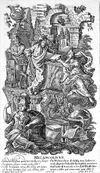
\includegraphics[keepaspectratio,width=0.85\textwidth]{scholar-small.jpg}
  \captionart{Scholar}
  \label{fig:scholar}
\end{figure}

% Force float here
\clearpage{}
\thispagestyle{titleontop}

%SECT. II. MEMB. III. SUBSECT. XV.-_Love of Learning, or overmuch study. With a Digression of the misery of Scholars, and why the Muses are Melancholy_.
\section[Love of Learning, or overmuch study.]{Love of Learning, or overmuch study. With a Digression of the misery of Scholars, and why the Muses are Melancholy.}
\lettrine{L}{eonartus} Fuchsius Instit. lib. \rn{iii.} sect. 1. cap. 1. Felix Plater,
lib. \rn{iii.} de mentis alienat. Herc. de Saxonia, Tract. post. de melanch.
cap. 3, speak of a \authorfootnote{1970}peculiar fury, which comes by overmuch study.
Fernelius, lib. 1, cap. 18, \authorfootnote{1971}puts study, contemplation, and
continual meditation, as an especial cause of madness: and in his 86
consul. cites the same words. Jo. Arculanus, in lib. 9, Rhasis ad
Alnansorem, cap. 16, amongst other causes reckons up studium vehemens:
so doth Levinus Lemnius, lib. de occul. nat. mirac. lib. 1, cap. 16.
\authorfootnote{1972}Many men (saith he) come to this malady by continual study\authormarginnote{1973},
and night-waking, and of all other men, scholars are most subject to
it: and such Rhasis adds, \authorfootnote{1974}that have commonly the finest wits.
Cont. lib. 1, tract. 9, Marsilius Ficinus, de sanit. tuenda, lib. 1.
cap. 7, puts melancholy amongst one of those five principal plagues of
students, 'tis a common Maul unto them all, and almost in some measure
an inseparable companion. Varro belike for that cause calls Tristes
Philosophos et severos, severe, sad, dry, tetric, are common epithets
to scholars: and \authorfootnote{1975}Patritius therefore, in the institution of
princes, would not have them to be great students. For (as Machiavel
holds) study weakens their bodies, dulls the spirits, abates their
strength and courage; and good scholars are never good soldiers, which
a certain Goth well perceived, for when his countrymen came into
Greece, and would have burned all their books, he cried out against it,
by no means they should do it, \authorfootnote{1976} leave them that plague, which in
time will consume all their vigour, and martial spirits. The
\authorfootnote{1977}Turks abdicated Cornutus the next heir from the empire, because
he was so much given to his book: and 'tis the common tenet of the
world, that learning dulls and diminisheth the spirits, and so per
consequens produceth melancholy.

Two main reasons may be given of it, why students should be more
subject to this malady than others. The one is, they live a sedentary,
solitary life, sibi et musis, free from bodily exercise, and those
ordinary disports which other men use: and many times if discontent and
idleness concur with it, which is too frequent, they are precipitated
into this gulf on a sudden: but the common cause is overmuch study; too
much learning (as Festus told\authorfootnote{1978} Paul) hath made thee mad; 'tis that
other extreme which effects it. So did Trincavelius, lib. 1, consil. 12
and 13, find by his experience, in two of his patients, a young baron,
and another that contracted this malady by too vehement study. So
Forestus, observat. l. 10, observ. 13, in a young divine in Louvain,
that was mad, and said \authorfootnote{1979}he had a Bible in his head: Marsilius
Ficinus de sanit. tuend. lib. 1, cap. 1, 3, 4, and lib. 2, cap. 16,
gives many reasons, \authorfootnote{1980} why students dote more often than others.
The first is their negligence; \authorfootnote{1981}other men look to their tools, a
painter will wash his pencils, a smith will look to his hammer, anvil,
forge; a husbandman will mend his plough-irons, and grind his hatchet
if it be dull; a falconer or huntsman will have an especial care of his
hawks, hounds, horses, dogs, \etc{}; a musician will string and unstring
his lute, \etc{}; only scholars neglect that instrument, their brain and
spirits (I mean) which they daily use, and by which they range overall
the world, which by much study is consumed. Vide (saith Lucian) ne
funiculum nimis intendendo aliquando abrumpas: See thou twist not the
rope so hard, till at length it \authorfootnote{1982}break. Facinus in his fourth
chap. gives some other reasons; Saturn and Mercury, the patrons of
learning, they are both dry planets: and Origanus assigns the same
cause, why Mercurialists are so poor, and most part beggars; for that
their president Mercury had no better fortune himself. The destinies of
old put poverty upon him as a punishment; since when, poetry and
beggary are Gemelli, twin-born brats, inseparable companions;
\authorfootnote{1983}And to this day is every scholar poor;
Gross gold from them runs headlong to the boor:

Mercury can help them to knowledge, but not to money. The second is
contemplation, \authorfootnote{1984}which dries the brain and extinguisheth natural
heat; for whilst the spirits are intent to meditation above in the
head, the stomach and liver are left destitute, and thence come black
blood and crudities by defect of concoction, and for want of exercise
the superfluous vapours cannot exhale, \etc{}. The same reasons are
repeated by Gomesius, lib. 4, cap. 1, de sale \authorfootnote{1985}Nymannus orat. de
Imag. Jo. Voschius, lib. 2, cap. 5, de peste: and something more they
add, that hard students are commonly troubled with gouts, catarrhs,
rheums, cachexia, bradiopepsia, bad eyes, stone and colic,
\authorfootnote{1986}crudities, oppilations, vertigo, winds, consumptions, and all
such diseases as come by overmuch sitting; they are most part lean,
dry, ill-coloured, spend their fortunes, lose their wits, and many
times their lives, and all through immoderate pains, and extraordinary
studies. If you will not believe the truth of this, look upon great
Tostatus and Thomas Aquinas's works, and tell me whether those men took
pains? peruse \Austin{}, Hierom, \etc{}, and many thousands besides.
Qui cupit optatam cursu contingere metam,
Multa tulit, fecitque puer, sudavit et alsit.

He that desires this wished goal to gain,
Must sweat and freeze before he can attain,

and labour hard for it. So did \Seneca, by his own confession, ep. 8.
\authorfootnote{1987}Not a day that I spend idle, part of the night I keep mine eyes
open, tired with waking, and now slumbering to their continual task.
Hear Tully pro Archia Poeta: whilst others loitered, and took their
pleasures, he was continually at his book, so they do that will be
scholars, and that to the hazard (I say) of their healths, fortunes,
wits, and lives. How much did \Aristotle and Ptolemy spend? unius regni
precium they say, more than a king's ransom; how many crowns per annum,
to perfect arts, the one about his History of Creatures, the other on
his Almagest? How much time did Thebet Benchorat employ, to find out
the motion of the eighth sphere? forty years and more, some write: how
many poor scholars have lost their wits, or become dizzards, neglecting
all worldly affairs and their own health, wealth, esse and bene esse,
to gain knowledge for which, after all their pains, in this world's
esteem they are accounted ridiculous and silly fools, idiots, asses,
and (as oft they are) rejected, contemned, derided, doting, and mad.
Look for examples in Hildesheim spicel. 2, de mania et delirio: read
Trincavellius, l. 3. consil. 36, et c. 17. Montanus, consil. 233.
\authorfootnote{1988}Garceus de Judic. genit. cap. 33. Mercurialis, consil. 86, cap.
25. Prosper \authorfootnote{1989}Calenius in his Book de atra bile; Go to Bedlam and
ask. Or if they keep their wits, yet they are esteemed scrubs and fools
by reason of their carriage: after seven years' study
---statua, taciturnius exit,
Plerumque et risum populi quatit.---

He becomes more silent than a statue, and generally excites people's
laughter. Because they cannot ride a horse, which every clown can do;
salute and court a gentlewoman, carve at table, cringe and make conges,
which every common swasher can do, \authorfootnote{1990}hos populus ridet, \etc{}, they
are laughed to scorn, and accounted silly fools by our gallants. Yea,
many times, such is their misery, they deserve it: \authorfootnote{1991}a mere
scholar, a mere ass.
\authorfootnote{1992}Obstipo capite, et figentes lumine terram,
Murmura cum secum, et rabiosa silentia rodunt,
Atque experrecto trutinantur verba labello,
Aegroti veteris meditantes somnia, gigni
De nihilo nihilum; in nihilum nil posse reverti.

\authorfootnote{1993}---who do lean awry
Their heads, piercing the earth with a fixt eye;
When, by themselves, they gnaw their murmuring,
And furious silence, as 'twere balancing
Each word upon their out-stretched lip, and when
They meditate the dreams of old sick men,
As, 'Out of nothing, nothing can be brought;
And that which is, can ne'er be turn'd to nought.'

Thus they go commonly meditating unto themselves, thus they sit, such
is their action and gesture. Fulgosus, l. 8, c. 7, makes mention how
Th. Aquinas supping with king Lewis of France, upon a sudden knocked
his fist upon the table, and cried, conclusum est contra Manichaeos,
his wits were a wool-gathering, as they say, and his head busied about
other matters, when he perceived his error, he was much \authorfootnote{1994}abashed.
Such a story there is of Archimedes in Vitruvius, that having found out
the means to know how much gold was mingled with the silver in king
Hieron's crown, ran naked forth of the bath and cried ἕυρηκα, I have
found: \authorfootnote{1995}and was commonly so intent to his studies, that he never
perceived what was done about him: when the city was taken, and the
soldiers now ready to rifle his house, he took no notice of it. St.
Bernard rode all day long by the Lemnian lake, and asked at last where
he was, Marullus, lib. 2, cap. 4. It was \Democritus{}'s carriage alone
that made the Abderites suppose him to have been mad, and send for
Hippocrates to cure him: if he had been in any solemn company, he would
upon all occasions fall a laughing. Theophrastus saith as much of
Heraclitus, for that he continually wept, and Laertius of Menedemus
Lampsacus, because he ran like a madman, \authorfootnote{1996}saying, he came from
hell as a spy, to tell the devils what mortal men did. Your greatest
students are commonly no better, silly, soft fellows in their outward
behaviour, absurd, ridiculous to others, and no whit experienced in
worldly business; they can measure the heavens, range over the world,
teach others wisdom, and yet in bargains and contracts they are
circumvented by every base tradesman. Are not these men fools? and how
should they be otherwise, but as so many sots in schools, when (as
\authorfootnote{1997}he well observed) they neither hear nor see such things as are
commonly practised abroad? how should they get experience, by what
means? \authorfootnote{1998}I knew in my time many scholars, saith Aeneas Sylvius (in
an epistle of his to Gasper Scitick, chancellor to the emperor),
excellent well learned, but so rude, so silly, that they had no common
civility, nor knew how to manage their domestic or public affairs.
Paglarensis was amazed, and said his farmer had surely cozened him,
when he heard him tell that his sow had eleven pigs, and his ass had
but one foal. To say the best of this profession, I can give no other
testimony of them in general, than that of \Pliny{} of Isaeus; \authorfootnote{1999}He is
yet a scholar, than which kind of men there is nothing so simple, so
sincere, none better, they are most part harmless, honest, upright,
innocent, plain-dealing men.

Now because they are commonly subject to such hazards and
inconveniences as dotage, madness, simplicity, \etc{}. Jo. Voschius would
have good scholars to be highly rewarded, and had in some extraordinary
respect above other men, to have greater \authorfootnote{2000}privileges than the
rest, that adventure themselves and abbreviate their lives for the
public good. But our patrons of learning are so far nowadays from
respecting the muses, and giving that honour to scholars, or reward
which they deserve, and are allowed by those indulgent privileges of
many noble princes, that after all their pains taken in the
universities, cost and charge, expenses, irksome hours, laborious
tasks, wearisome days, dangers, hazards, (barred interim from all
pleasures which other men have, mewed up like hawks all their lives) if
they chance to wade through them, they shall in the end be rejected,
contemned, and which is their greatest misery, driven to their shifts,
exposed to want, poverty, and beggary. Their familiar attendants are,
\authorfootnote{2001}Pallentes morbi, luctus, curaeque laborque
Et metus, et malesuada fames, et turpis egestas,
Terribiles visu formae---

Grief, labour, care, pale sickness, miseries,
Fear, filthy poverty, hunger that cries,
Terrible monsters to be seen with eyes.

If there were nothing else to trouble them, the conceit of this alone
were enough to make them all melancholy. Most other trades and
professions, after some seven years' apprenticeship, are enabled by
their craft to live of themselves. A merchant adventures his goods at
sea, and though his hazard be great, yet if one ship return of four, he
likely makes a saving voyage. An husbandman's gains are almost certain;
quibus ipse Jupiter nocere non potest (whom Jove himself can't harm)
('tis \authorfootnote{2002}Cato's hyperbole, a great husband himself); only scholars
methinks are most uncertain, unrespected, subject to all casualties,
and hazards. For first, not one of a many proves to be a scholar, all
are not capable and docile, \authorfootnote{2003}ex omniligno non fit Mercurius: we
can make majors and officers every year, but not scholars: kings can
invest knights and barons, as Sigismund the emperor confessed;
universities can give degrees; and Tu quod es, e populo quilibet esse
potest; but he nor they, nor all the world, can give learning, make
philosophers, artists, orators, poets; we can soon say, as \Seneca well
notes, O virum bonum, o divitem, point at a rich man, a good, a happy
man, a prosperous man, sumptuose vestitum, Calamistratum, bene olentem,
magno temporis impendio constat haec laudatio, o virum literarum, but
'tis not so easily performed to find out a learned man. Learning is not
so quickly got, though they may be willing to take pains, to that end
sufficiently informed, and liberally maintained by their patrons and
parents, yet few can compass it. Or if they be docile, yet all men's
wills are not answerable to their wits, they can apprehend, but will
not take pains; they are either seduced by bad companions, vel in
puellam impingunt, vel in poculum (they fall in with women or wine) and
so spend their time to their friends' grief and their own undoings. Or
put case they be studious, industrious, of ripe wits, and perhaps good
capacities, then how many diseases of body and mind must they
encounter? No labour in the world like unto study. It may be, their
temperature will not endure it, but striving to be excellent to know
all, they lose health, wealth, wit, life and all. Let him yet happily
escape all these hazards, aereis intestinis with a body of brass, and
is now consummate and ripe, he hath profited in his studies, and
proceeded with all applause: after many expenses, he is fit for
preferment, where shall he have it? he is as far to seek it as he was
(after twenty years' standing) at the first day of his coming to the
University. For what course shall he take, being now capable and ready?
The most parable and easy, and about which many are employed, is to
teach a school, turn lecturer or curate, and for that he shall have
falconer's wages, ten pound per annum, and his diet, or some small
stipend, so long as he can please his patron or the parish; if they
approve him not (for usually they do but a year or two) as inconstant,
as they that cried\authorfootnote{2004} Hosanna one day, and Crucify him the other;
serving-man-like, he must go look a new master; if they do, what is his
reward?
\authorfootnote{2005}\li{Hoc quoque te manet ut pueros elementa docentem
Occupet extremis in vicis alba senectus.}

At last thy snow-white age in suburb schools,
Shall toil in teaching boys their grammar rules.

Like an ass, he wears out his time for provender, and can show a stump
rod, togam tritam et laceram saith \authorfootnote{2006}Haedus, an old torn gown, an
ensign of his infelicity, he hath his labour for his pain, a modicum to
keep him till he be decrepit, and that is all. Grammaticus non est
felix, \etc{}. If he be a trencher chaplain in a gentleman's house, as it
befell \authorfootnote{2007} Euphormio, after some seven years' service, he may
perchance have a living to the halves, or some small rectory with the
mother of the maids at length, a poor kinswoman, or a cracked
chambermaid, to have and to hold during the time of his life. But if he
offend his good patron, or displease his lady mistress in the mean
time,
\authorfootnote{2008}Ducetur Planta velut ictus ab Hercule Cacus,
Poneturque foras, si quid tentaverit unquam
Hiscere---

as Hercules did by Cacus, he shall be dragged forth of doors by the
heels, away with him. If he bend his forces to some other studies, with
an intent to be a secretis to some nobleman, or in such a place with an
ambassador, he shall find that these persons rise like apprentices one
under another, and in so many tradesmen's shops, when the master is
dead, the foreman of the shop commonly steps in his place. Now for
poets, rhetoricians, historians, philosophers, \authorfootnote{2009}mathematicians,
sophisters, \etc{}; they are like grasshoppers, sing they must in summer,
and pine in the winter, for there is no preferment for them. Even so
they were at first, if you will believe that pleasant tale of Socrates,
which he told fair Phaedrus under a plane-tree, at the banks of the
river Iseus; about noon when it was hot, and the grasshoppers made a
noise, he took that sweet occasion to tell him a tale, how grasshoppers
were once scholars, musicians, poets, \etc{}, before the Muses were born,
and lived without meat and drink, and for that cause were turned by
Jupiter into grasshoppers. And may be turned again, In Tythoni Cicadas,
aut Lyciorum ranas, for any reward I see they are like to have: or else
in the mean time, I would they could live, as they did, without any
viaticum, like so many \authorfootnote{2010}manucodiatae, those Indian birds of
paradise, as we commonly call them, those I mean that live with the air
and dew of heaven, and need no other food; for being as they are, their
\authorfootnote{2011}rhetoric only serves them to curse their bad fortunes, and many
of them for want of means are driven to hard shifts; from grasshoppers
they turn humble-bees and wasps, plain parasites, and make the muses,
mules, to satisfy their hunger-starved paunches, and get a meal's meat.
To say truth, 'tis the common fortune of most scholars, to be servile
and poor, to complain pitifully, and lay open their wants to their
respectless patrons, as Cardan doth\authorfootnote{2012}, as Xilander\authorfootnote{2013} and many
others: and which is too common in those dedicatory epistles, for hope
of gain, to lie, flatter, and with hyperbolical eulogiums and
commendations, to magnify and extol an illiterate unworthy idiot, for
his excellent virtues, whom they should rather, as Machiavel
observes\authorfootnote{2014}, vilify, and rail at downright for his most notorious
villainies and vices. So they prostitute themselves as fiddlers, or
mercenary tradesmen, to serve great men's turns for a small reward.
They are like Indians, they have store of gold, but know not the
worth of it\authormarginnote{2015}: for I am of Synesius's opinion, \authorfootnote{2016}King Hieron got more
by Simonides' acquaintance, than Simonides did by his; they have their
best education, good institution, sole qualification from us, and when
they have done well, their honour and immortality from us: we are the
living tombs, registers, and as so many trumpeters of their fames: what
was Achilles without Homer? Alexander without Arian and Curtius? who
had known the Caesars, but for Suetonius and Dion?
\authorfootnote{2017}Vixerunt fortes ante Agamemnona
Multi: sed omnes illachrymabiles
Urgentur, ignotique longa
Nocte, carent quia vate sacro.

Before great Agamemnon reign'd,
Reign'd kings as great as he, and brave,

Whose huge ambition's now contain'd
In the small compass of a grave:

In endless night, they sleep, unwept, unknown,
No bard they had to make all time their own.

they are more beholden to scholars, than scholars to them; but they
undervalue themselves, and so by those great men are kept down. Let
them have that encyclopaedian, all the learning in the world; they must
keep it to themselves, \authorfootnote{2018}live in base esteem, and starve, except
they will submit, as Budaeus well hath it, so many good parts, so many
ensigns of arts, virtues, be slavishly obnoxious to some illiterate
potentate, and live under his insolent worship, or honour, like
parasites, Qui tanquam mures alienum panem comedunt. For to say truth,
artes hae, non sunt Lucrativae, as Guido Bonat that great astrologer
could foresee, they be not gainful arts these, sed esurientes et
famelicae, but poor and hungry.

\authorfootnote{2019}Dat Galenus opes, dat Justinianus honores,
Sed genus et species cogitur ire pedes:


The rich physician, honour'd lawyers ride,
Whilst the poor scholar foots it by their side.

Poverty is the muses' patrimony, and as that poetical divinity teacheth
us, when Jupiter's daughters were each of them married to the gods, the
muses alone were left solitary, Helicon forsaken of all suitors, and I
believe it was, because they had no portion.

Calliope longum caelebs cur vixit in aevum?
Nempe nihil dotis, quod numeraret, erat.


Why did Calliope live so long a maid?
Because she had no dowry to be paid.

Ever since all their followers are poor, forsaken and left unto
themselves. Insomuch, that as Petronius argues\authorfootnote{2020}, you shall likely
know them by their clothes. There came, saith he, by chance into my
company, a fellow not very spruce to look on, that I could perceive by
that note alone he was a scholar, whom commonly rich men hate: I asked
him what he was, he answered, a poet: I demanded again why he was so
ragged, he told me this kind of learning never made any man rich.
\authorfootnote{2021}Qui Pelago credit, magno se faenore tollit,
Qui pugnas et rostra petit, praecingitur auro:
Vilis adulator picto jacet ebrius ostro,
Sola pruinosis horret facundia pannis.


A merchant's gain is great, that goes to sea;
A soldier embossed all in gold;

A flatterer lies fox'd in brave array;
A scholar only ragged to behold.

All which our ordinary students, right well perceiving in the
universities, how unprofitable these poetical, mathematical, and
philosophical studies are, how little respected, how few patrons; apply
themselves in all haste to those three commodious professions of law,
physic, and divinity, sharing themselves between them, \authorfootnote{2022}rejecting
these arts in the mean time, history, philosophy, philology, or lightly
passing them over, as pleasant toys fitting only table-talk, and to
furnish them with discourse. They are not so behoveful: he that can
tell his money hath arithmetic enough: he is a true geometrician, can
measure out a good fortune to himself; a perfect astrologer, that can
cast the rise and fall of others, and mark their errant motions to his
own use. The best optics are, to reflect the beams of some great man's
favour and grace to shine upon him. He is a good engineer that alone
can make an instrument to get preferment. This was the common tenet and
practice of Poland, as Cromerus observed not long since, in the first
book of his history; their universities were generally base, not a
philosopher, a mathematician, an antiquary, \etc{}, to be found of any
note amongst them, because they had no set reward or stipend, but every
man betook himself to divinity, hoc solum in votis habens, opimum
sacerdotium, a good parsonage was their aim. This was the practice of
some of our near neighbours, as Lipsius inveighs\authorfootnote{2023}, they thrust
their children to the study of law and divinity, before they be
informed aright, or capable of such studies. Scilicet omnibus artibus
antistat spes lucri, et formosior est cumulus auri, quam quicquid
Graeci Latinique delirantes scripserunt. Ex hoc numero deinde veniunt
ad gubernacula reipub. intersunt et praesunt consiliis regum, o pater,
o patria? so he complained, and so may others. For even so we find, to
serve a great man, to get an office in some bishop's court (to practise
in some good town) or compass a benefice, is the mark we shoot at, as
being so advantageous, the highway to preferment.

Although many times, for aught I can see, these men fail as often as
the rest in their projects, and are as usually frustrate of their
hopes. For let him be a doctor of the law, an excellent civilian of
good worth, where shall he practise and expatiate? Their fields are so
scant, the civil law with us so contracted with prohibitions, so few
causes, by reason of those all-devouring municipal laws, \li{quibus nihil
illiteratius}, saith Erasmus\authorfootnote{2024}, an illiterate and a barbarous
study, (for though they be never so well learned in it, I can hardly
vouchsafe them the name of scholars, except they be otherwise
qualified) and so few courts are left to that profession, such slender
offices, and those commonly to be compassed at such dear rates, that I
know not how an ingenious man should thrive amongst them. Now for
physicians, there are in every village so many mountebanks, empirics,
quacksalvers, Paracelsians, as they call themselves, Caucifici et
sanicidae so Clenard terms them\authorfootnote{2025}, wizards, alchemists, poor
vicars, cast apothecaries, physicians' men, barbers, and good wives,
professing great skill, that I make great doubt how they shall be
maintained, or who shall be their patients. Besides, there are so many
of both sorts, and some of them such harpies, so covetous, so
clamorous, so impudent; and as he said\authorfootnote{2026}, litigious idiots,

\begin{latin}%
Quibus loquacis affatim arrogantiae est
Pentiae parum aut nihil,

Nec ulla mica literarii salis,
Crumenimulga natio:

Loquuteleia turba, litium strophae,
Maligna litigantium cohors, togati vultures,

Lavernae alumni, Agyrtae, \etc{}.%
\end{latin}

Which have no skill but prating arrogance,
No learning, such a purse-milking nation:

Gown'd vultures, thieves, and a litigious rout
Of cozeners, that haunt this occupation,

that they cannot well tell how to live one by another, but as he jested
in the Comedy of Clocks, they were so many, \authorfootnote{2027}major pars populi
arida reptant fame, they are almost starved a great part of them, and
ready to devour their fellows, \authorfootnote{2028}\li{Et noxia callidilate se corripere},
such a multitude of pettifoggers and empirics, such impostors, that an
honest man knows not in what sort to compose and behave himself in
their society, to carry himself with credit in so vile a rout,
\li{scientiae nomen, tot sumptibus partum et vigiliis, profiteri dispudeat,
postquam, \etc{}}.

Last of all to come to our divines, the most noble profession and
worthy of double honour, but of all others the most distressed and
miserable. If you will not believe me, hear a brief of it, as it was
not many years since publicly preached at Paul's cross, \authorfootnote{2029}by a
grave minister then, and now a reverend bishop of this land: We that
are bred up in learning, and destinated by our parents to this end, we
suffer our childhood in the grammar-school, which \Austin{} calls magnam
tyrannidem, et grave malum, and compares it to the torments of
martyrdom; when we come to the university, if we live of the college
allowance, as Phalaris objected to the Leontines, \textgreek{παν τῶν ἐνδεῖς πλὴν
λιμοὺ καὶ φόβου}, needy of all things but hunger and fear, or if we be
maintained but partly by our parents' cost, do expend in unnecessary
maintenance, books and degrees, before we come to any perfection, five
hundred pounds, or a thousand marks. If by this price of the expense of
time, our bodies and spirits, our substance and patrimonies, we cannot
purchase those small rewards, which are ours by law, and the right of
inheritance, a poor parsonage, or a vicarage of 50\emph{l.} per annum, but
we must pay to the patron for the lease of a life (a spent and out-worn
life) either in annual pension, or above the rate of a copyhold, and
that with the hazard and loss of our souls, by simony and perjury, and
the forfeiture of all our spiritual preferments, in esse and posse,
both present and to come. What father after a while will be so
improvident to bring up his son to his great charge, to this necessary
beggary? What Christian will be so irreligious, to bring up his son in
that course of life, which by all probability and necessity, cogit ad
turpia, enforcing to sin, will entangle him in simony and perjury, when
as the poet said, \li{Invitatus ad haec aliquis de ponte negabit}: a
beggar's brat taken from the bridge where he sits a begging, if he knew
the inconvenience, had cause to refuse it. This being thus, have not we
fished fair all this while, that are initiate divines, to find no
better fruits of our labours, \authorfootnote{2030} hoc est cur palles, cur quis non
prandeat hoc est? do we macerate ourselves for this? Is it for this we
rise so early all the year long? \authorfootnote{2031}Leaping (as he saith) out of our
beds, when we hear the bell ring, as if we had heard a thunderclap. If
this be all the respect, reward and honour we shall have, \authorfootnote{2032}frange
leves calamos, et scinde Thalia libellos: let us give over our books,
and betake ourselves to some other course of life; to what end should
we study? \authorfootnote{2033}\li{Quid me litterulas stulti docuere parentes}, what did
our parents mean to make us scholars, to be as far to seek of
preferment after twenty years' study, as we were at first: why do we
take such pains? Quid tantum insanis juvat impallescere chartis? If
there be no more hope of reward, no better encouragement, I say again,
\li{Frange leves calamos, et scinde Thalia libellos}; let's turn soldiers,
sell our books, and buy swords, guns, and pikes, or stop bottles with
them, turn our philosopher's gowns, as Cleanthes once did, into
millers' coats, leave all and rather betake ourselves to any other
course of life, than to continue longer in this misery. \authorfootnote{2034}\li{Praestat
dentiscalpia radere, quam literariis monumentis magnatum favorem
emendicare}.

Yea, but methinks I hear some man except at these words, that though
this be true which I have said of the estate of scholars, and
especially of divines, that it is miserable and distressed at this
time, that the church suffers shipwreck of her goods, and that they
have just cause to complain; there is a fault, but whence proceeds it?
If the cause were justly examined, it would be retorted upon ourselves,
if we were cited at that tribunal of truth, we should be found guilty,
and not able to excuse it That there is a fault among us, I confess,
and were there not a buyer, there would not be a seller; but to him
that will consider better of it, it will more than manifestly appear,
that the fountain of these miseries proceeds from these griping
patrons. In accusing them, I do not altogether excuse us; both are
faulty, they and we: yet in my judgment, theirs is the greater fault,
more apparent causes and much to be condemned. For my part, if it be
not with me as I would, or as it should, I do ascribe the cause, as
\authorfootnote{2035}Cardan did in the like case; \li{meo infortunio potius quam illorum
sceleri}, to \authorfootnote{2036}mine own infelicity rather than their naughtiness:
although I have been baffled in my time by some of them, and have as
just cause to complain as another: or rather indeed to mine own
negligence; for I was ever like that Alexander in \authorfootnote{2037}Plutarch,
Crassus his tutor in philosophy, who, though he lived many years
familiarly with rich Crassus, was even as poor when from, (which many
wondered at) as when he came first to him; he never asked, the other
never gave him anything; when he travelled with Crassus he borrowed a
hat of him, at his return restored it again. I have had some such noble
friends' acquaintance and scholars, but most part (common courtesies
and ordinary respects excepted) they and I parted as we met, they gave
me as much as I requested, and that was-And as Alexander ab Alexandro
Genial. dier. l. 6. c. 16. made answer to Hieronymus Massainus, that
wondered, \li{quum plures ignavos et ignobiles ad dignitates et sacerdotia
promotos quotidie videret}, when other men rose, still he was in the
same state, \li{eodem tenore et fortuna cui mercedem laborum studiorumque
deberi putaret}, whom he thought to deserve as well as the rest. He made
answer, that he was content with his present estate, was not ambitious,
and although \li{objurgabundus suam segnitiem accusaret, cum obscurae
sortis homines ad sacerdotia et pontificatus evectos, \etc{},} he chid him
for his backwardness, yet he was still the same: and for my part
(though I be not worthy perhaps to carry Alexander's books) yet by some
overweening and well-wishing friends, the like speeches have been used
to me; but I replied still with Alexander, that I had enough, and more
peradventure than I deserved; and with Libanius Sophista, that rather
chose (when honours and offices by the emperor were offered unto him)
to be talis Sophista, \li{quam tails Magistratus}. I had as lief be still
\Democritus{} junior, and \li{privus privatus, si mihi jam daretur optio, quam
talis fortasse Doctor, talis Dominus.-Sed quorsum haec?} For the rest
'tis on both sides facinus detestandum, to buy and sell livings, to
detain from the church, that which God's and men's laws have bestowed
on it; but in them most, and that from the covetousness and ignorance
of such as are interested in this business; I name covetousness in the
first place, as the root of all these mischiefs, which, Achan-like,
compels them to commit sacrilege, and to make simoniacal compacts, (and
what not) to their own ends, \authorfootnote{2038}that kindles God's wrath, brings a
plague, vengeance, and a heavy visitation upon themselves and others.
Some out of that insatiable desire of filthy lucre, to be enriched,
care not how they come by it per fas et nefas, hook or crook, so they
have it. And others when they have with riot and prodigality embezzled
their estates, to recover themselves, make a prey of the church,
robbing it, as Julian the apostate did\authorfootnote{2039}, spoil parsons of their
revenues (in keeping half back, \authorfootnote{2040}as a great man amongst us
observes:) and that maintenance on which they should live: by means
whereof, barbarism is increased, and a great decay of Christian
professors: for who will apply himself to these divine studies, his
son, or friend, when after great pains taken, they shall have nothing
whereupon to live? But with what event do they these things?
\authormarginnote{2041}\li{Opesque totis viribus venamini
At inde messis accidit miserrima.}

They toil and moil, but what reap they? They are commonly unfortunate
families that use it, accursed in their pro\-geny, and, as common
experience evinceth, accursed themselves in all their proceedings. With
what face (as he quotes\authorfootnote{2042} out of Aust.) can they expect a blessing
or inheritance from Christ in heaven, that defraud Christ of his
inheritance here on earth? I would all our simoniacal patrons, and such
as detain tithes, would read those judicious tracts of Sir Henry
Spelman, and Sir James Sempill, knights; those late elaborate and
learned treatises of Dr. Tilslye, and Mr. Montague, which they have
written of that subject. But though they should read, it would be to
small purpose, clames licet et mare coelo Confundas; thunder, lighten,
preach hell and damnation, tell them 'tis a sin, they will not believe
it; denounce and terrify, they have \authorfootnote{2043}cauterised consciences, they
do not attend, as the enchanted adder, they stop their ears. Call them
base, irreligious, profane, barbarous, pagans, atheists, epicures, (as
some of them surely are) with the bawd in \Plautus{}, Euge, optime, they
cry and applaud themselves with that miser, \authorfootnote{2044}simul ac nummos
contemplor in arca: say what you will, quocunque modo rem: as a dog
barks at the moon, to no purpose are your sayings: Take your heaven,
let them have money. A base, profane, epicurean, hypocritical rout: for
my part, let them pretend what zeal they will, counterfeit religion,
blear the world's eyes, bombast themselves, and stuff out their
greatness with church spoils, shine like so many peacocks; so cold is
my charity, so defective in this behalf, that I shall never think
better of them, than that they are rotten at core, their bones are full
of epicurean hypocrisy, and atheistical marrow, they are worse than
heathens. For as Dionysius Halicarnassaeus observes, Antiq. Rom. lib.
7. \authorfootnote{2045}\li{Primum locum, \etc{}.} Greeks and Barbarians observe all religious
rites, and dare not break them for fear of offending their gods; but
our simoniacal contractors, our senseless Achans, our stupefied
patrons, fear neither God nor devil, they have evasions for it, it is
no sin, or not due jure divino, or if a sin, no great sin, \etc{}. And
though they be daily punished for it, and they do manifestly perceive,
that as he said, frost and fraud come to foul ends; yet as
\authorfootnote{2046}\Chrysostom{} follows it \li{Nulla ex poena sit correctio, et quasi
adversis malitia hominum provocetur, crescit quotidie quod puniatur}:
they are rather worse than better,-\li{iram atque animos a crimine sumunt},
and the more they are corrected, the more they offend: but let them
take their course, \authorfootnote{2047}\li{Rode caper vites}, go on still as they begin,
'tis no sin, let them rejoice secure, God's vengeance will overtake
them in the end, and these ill-gotten goods, as an eagle's feathers,
\authorfootnote{2048} will consume the rest of their substance; it is \authorfootnote{2049}\li{aurum
Tholosanum}, and will produce no better effects. \authorfootnote{2050}Let them lay it
up safe, and make their conveyances never so close, lock and shut door,
saith \Chrysostom{}, yet fraud and covetousness, two most violent thieves
are still included, and a little gain evil gotten will subvert the rest
of their goods. The eagle in Aesop, seeing a piece of flesh now ready
to be sacrificed, swept it away with her claws, and carried it to her
nest; but there was a burning coal stuck to it by chance, which
unawares consumed her young ones, nest, and all together. Let our
simoniacal church-chopping patrons, and sacrilegious harpies, look for
no better success.

A second cause is ignorance, and from thence contempt, \li{successit odium
in literas ab ignorantia vulgi}; which \authorfootnote{2051}Junius well perceived: this
hatred and contempt of learning proceeds out of \authorfootnote{2052}ignorance; as
they are themselves barbarous, idiots, dull, illiterate, and proud, so
they esteem of others. \li{Sint Mecaenates, non deerunt Flacce Marones}: Let
there be bountiful patrons, and there will be painful scholars in all
sciences. But when they contemn learning, and think themselves
sufficiently qualified, if they can write and read, scramble at a piece
of evidence, or have so much Latin as that emperor had, \li{qui
nescit dissimulare, nescit vivere}\authorlatintrans{2053}, they are unfit to do their country
service, to perform or undertake any action or employment, which may
tend to the good of a commonwealth, except it be to fight, or to do
country justice, with common sense, which every yeoman can likewise do.
And so they bring up their children, rude as they are themselves,
unqualified, untaught, uncivil most part. \authormarginnote{2054}\li{Quis e nostra juventute
legitime instituitur literis? Quis oratores aut Philosophos tangit?
quis historiam legit, illam rerum agendarum quasi animam? praecipitant
parentes vota sua, \etc{}.} 'twas Lipsius' complaint to his illiterate
countrymen, it may be ours. Now shall these men judge of a scholar's
worth, that have no worth, that know not what belongs to a student's
labours, that cannot distinguish between a true scholar and a drone? or
him that by reason of a voluble tongue, a strong voice, a pleasing
tone, and some trivially polyanthean helps, steals and gleans a few
notes from other men's harvests, and so makes a fairer show, than he
that is truly learned indeed: that thinks it no more to preach, than to
speak, \authorfootnote{2055}or to run away with an empty cart; as a grave man said:
and thereupon vilify us, and our pains; scorn us, and all learning.
\authorfootnote{2056} Because they are rich, and have other means to live, they think
it concerns them not to know, or to trouble themselves with it; a
fitter task for younger brothers, or poor men's sons, to be pen and
inkhorn men, pedantical slaves, and no whit beseeming the calling of a
gentleman, as Frenchmen and Germans commonly do, neglect therefore all
human learning, what have they to do with it? Let mariners learn
astronomy; merchants, factors study arithmetic; surveyors get them
geometry; spectacle-makers optics; land-leapers geography; town-clerks
rhetoric, what should he do with a spade, that hath no ground to dig;
or they with learning, that have no use of it? thus they reason, and
are not ashamed to let mariners, apprentices, and the basest servants,
be better qualified than themselves. In former times, kings, princes,
and emperors, were the only scholars, excellent in all faculties.
Julius Caesar mended the year, and writ his own Commentaries,
\authorfootnote{2057}---\li{media inter prealia semper,
Stellarum coelique plagis, superisque vacavit}.

\authorfootnote{2058}Antonius, Adrian, Nero, Seve. Jul. \etc{}. \authorfootnote{2059}Michael the emperor,
and Isacius, were so much given to their studies, that no base fellow
would take so much pains: Orion, Perseus, Alphonsus, Ptolomeus, famous
astronomers; Sabor, Mithridates, Lysimachus, admired physicians:
Plato's kings all: Evax, that Arabian prince, a most expert jeweller,
and an exquisite philosopher; the kings of Egypt were priests of old,
chosen and from thence,-Idem rex hominum, Phoebique sacerdos: but those
heroical times are past; the Muses are now banished in this bastard
age, \li{ad sordida tuguriola}, to meaner persons, and confined alone almost
to universities. In those days, scholars were highly beloved,
\authorfootnote{2060}honoured, esteemed; as old Ennius by Scipio Africanus, \Virgil{} by
Augustus; \Horace{} by Meceanas: princes' companions; dear to them, as
Anacreon to Polycrates; Philoxenus to Dionysius, and highly rewarded.
Alexander sent Xenocrates the philosopher fifty talents, because he was
poor, \li{visu rerum, aut eruditione praestantes viri, mensis olim regum
adhibiti}, as Philostratus relates of Adrian and Lampridius of Alexander
Severus: famous clerks came to these princes' courts, velut in Lycaeum,
as to a university, and were admitted to their tables, \li{quasi divum
epulis accumbentes}; Archilaus, that Macedonian king, would not
willingly sup without Euripides, (amongst the rest he drank to him at
supper one night, and gave him a cup of gold for his pains) delectatus
poetae suavi sermone; and it was fit it should be so; because as
\authorfootnote{2061}Plato in his Protagoras well saith, a good philosopher as much
excels other men, as a great king doth the commons of his country; and
again, \authorfootnote{2062}\li{quoniam illis nihil deest, et minime egere solent, et
disciplinas quas profitentur, soli a contemptu vindicare possunt}, they
needed not to beg so basely, as they compel \authorfootnote{2063}scholars in our times
to complain of poverty, or crouch to a rich chuff for a meal's meat,
but could vindicate themselves, and those arts which they professed.
Now they would and cannot: for it is held by some of them, as an axiom,
that to keep them poor, will make them study; they must be dieted, as
horses to a race, not pampered, \authorfootnote{2064}\li{Alendos volunt, non saginandos,
ne melioris mentis flammula extinguatur}; a fat bird will not sing, a
fat dog cannot hunt, and so by this depression of theirs \authorfootnote{2065}some
want means, others will, all want \authorfootnote{2066}encouragement, as being
forsaken almost; and generally contemned. 'Tis an old saying, \li{Sint
Mecaenates, non deerunt Flacce Marones}, and 'tis a true saying still.
Yet oftentimes I may not deny it the main fault is in ourselves. Our
academics too frequently offend in neglecting patrons, as Erasmus
well taxet\authorfootnote{2067}h, or making ill choice of them; \li{negligimus oblatos aut
amplectimur parum aptos}, or if we get a good one, \li{non studemus mutuis
officiis favorem ejus alere}, we do not ply and follow him as we should.
\li{Idem mihi accidit Adolescenti} (saith Erasmus) acknowledging his fault,
\li{et gravissime peccavi}, and so may I say myself\authormarginnote{2068}, I have offended
in this, and so peradventure have many others. We did not spondere
\li{magnatum favoribus, qui caeperunt nos amplecti}, apply ourselves with
that readiness we should: idleness, love of liberty, \li{immodicus amor
libertatis effecit ut diu cum perfidis amicis}, as he confesseth, et
pertinaci pauperate colluctarer, bashfulness, melancholy, timorousness,
cause many of us to be too backward and remiss. So some offend in one
extreme, but too many on the other, we are most part too forward, too
solicitous, too ambitious, too impudent; we commonly complain deesse
Maecenates, of want of encouragement, want of means, when as the true
defect is in our own want of worth, our insufficiency: did Maecenas
take notice of \Horace{} or \Virgil{} till they had shown themselves first?
or had Bavius and Mevius any patrons? \li{Egregium specimen dent}, saith
Erasmus, let them approve themselves worthy first, sufficiently
qualified for learning and manners, before they presume or impudently
intrude and put themselves on great men as too many do, with such base
flattery, parasitical colloguing, such hyperbolical elogies they do
usually insinuate that it is a shame to hear and see. Immodicae laudes
conciliant invidiam, potius quam laudem, and vain commendations
derogate from truth, and we think in conclusion, non melius de laudato,
pejus de laudante, ill of both, the commender and commended. So we
offend, but the main fault is in their harshness, defect of patrons.
How beloved of old, and how much respected was Plato to Dionysius? How
dear to Alexander was \Aristotle, Demeratus to Philip, Solon to Croesus,
Auexarcus and Trebatius to Augustus, Cassius to Vespasian, Plutarch to
Trajan, \Seneca to Nero, Simonides to Hieron? how honoured?
\li{Sed haec prius fuere, nunc recondita
Senent quiete}\authorfootnote{2069},

those days are gone; \li{Et spes, et ratio studiorum in Caesare
tantum}\authorlatintrans{2070}: as he said of old, we may truly say now, he is
our amulet, our \authorfootnote{2071}sun, our sole comfort and refuge, our Ptolemy, our common
Maecenas, \li{Jacobus munificus, Jacobus pacificus, mysta Musarum, Rex
Platonicus: Grande decus, columenque nostrum}: a famous scholar himself,
and the sole patron, pillar, and sustainer of learning: but his worth
in this kind is so well known, that as Paterculus of Cato, \li{Jam ipsum
laudare nefas sit}: and which \Pliny{} to Trajan\authorfootnote{2072}. \li{Seria te carmina,
honorque aeternus annalium, non haec brevis et pudenda praedicatio
colet}. But he is now gone, the sun of ours set, and yet no night
follows, \li{Sol occubuit, nox nulla sequuta est}. We have such another in
his room, \li{aureus alter}\authorfootnote{2073}. \li{Avulsus, simili frondescit virga metallo},
and long may he reign and flourish amongst us.

Let me not be malicious, and lie against my genius, I may not deny, but
that we have a sprinkling of our gentry, here and there one,
excellently well learned, like those Fuggeri in Germany; Dubartus, Du
Plessis, Sadael, in France; Picus Mirandula, Schottus, Barotius, in
Italy; Apparent rari nantes in gurgite vasto. But they are but few in
respect of the multitude, the major part (and some again excepted, that
are indifferent) are wholly bent for hawks and hounds, and carried away
many times with intemperate lust, gaming and drinking. If they read a
book at any time (\li{si quod est interim otii a venatu, poculis, alea,
scortis}) 'tis an English Chronicle, St. Huon of Bordeaux, Amadis de
Gaul, \etc{}, a play-book, or some pamphlet of news, and that at such
seasons only, when they cannot stir abroad, to drive away time,
\authorfootnote{2074}their sole discourse is dogs, hawks, horses, and what news? If
some one have been a traveller in Italy, or as far as the emperor's
court, wintered in Orleans, and can court his mistress in broken
French, wear his clothes neatly in the newest fashion, sing some choice
outlandish tunes, discourse of lords, ladies, towns, palaces, and
cities, he is complete and to be admired: \authorfootnote{2075}otherwise he and they
are much at one; no difference between the master and the man, but
worshipful titles; wink and choose betwixt him that sits down (clothes
excepted) and him that holds the trencher behind him: yet these men
must be our patrons, our governors too sometimes, statesmen,
magistrates, noble, great, and wise by inheritance.
Mistake me not (I say again) Vos o Patritius sanguis, you that are

worthy senators, gentlemen, I honour your names and persons, and with
all submissiveness, prostrate myself to your censure and service. There
are amongst you, I do ingenuously confess, many well-deserving patrons,
and true patriots, of my knowledge, besides many hundreds which I never
saw, no doubt, or heard of, pillars of our commonwealth, \authormarginnote{2076}whose
worth, bounty, learning, forwardness, true zeal in religion, and good
esteem of all scholars, ought to be consecrated to all posterity; but
of your rank, there are a debauched, corrupt, covetous, illiterate crew
again, no better than stocks, \li{merum pecus (testor Deum, non mihi videri
dignos ingenui hominis appellatione)} barbarous Thracians, \li{et quis ille
thrax qui hoc neget?} a sordid, profane, pernicious company,
irreligious, impudent and stupid, I know not what epithets to give
them, enemies to learning, confounders of the church, and the ruin of a
commonwealth; patrons they are by right of inheritance, and put in
trust freely to dispose of such livings to the church's good; but (hard
taskmasters they prove) they take away their straw, and compel them to
make their number of brick: they commonly respect their own ends,
commodity is the steer of all their actions, and him they present in
conclusion, as a man of greatest gifts, that will give most; no penny,
\authorfootnote{2077}no paternoster, as the saying is. Nisi preces auro fulcias,
amplius irritas: ut Cerberus offa, their attendants and officers must
be bribed, feed, and made, as Cerberus is with a sop by him that goes
to hell. It was an old saying, \latininlinetrans{all things are venal at Rome}{Omnia Romae venalia}, 'tis a rag of Popery, which will never be rooted out,
there is no hope, no good to be done without money. A clerk may offer
himself, approve his \authorfootnote{2078}worth, learning, honesty, religion, zeal,
they will commend him for it; but \li{probitas laudatur et alget}\authorfootnote{2079}. If
he be a man of extraordinary parts, they will flock afar off to hear
him, as they did in \Apuleius, to see Psyche: \li{multi mortales confluebant
ad videndum saeculi decus, speculum gloriosum, laudatur ab omnibus,
spectatur ob omnibus, nec quisquam non rex, non regius, cupidus ejus
nuptiarium petitor accedit; mirantur quidem divinam formam omnes, sed
ut simulacrum fabre politum mirantur}; many mortal men came to see fair
Psyche the glory of her age, they did admire her, commend, desire her
for her divine beauty, and gaze upon her; but as on a picture; none
would marry her, \li{quod indotato}, fair Psyche had no money. So they
do by learning;\authorfootnote{2080}
%
\textlatin{
\begin{verse}
---didicit jam dives avarus\\
Tantum admirari, tantum laudare disertos,\\
Ut pueri Junonis avem---\authorfootnote{2081}
\end{verse}
}
\translationrule
\begin{verse}
Your rich men have now learn'd of latter days\\
T'admire, commend, and come together\\

To hear and see a worthy scholar speak,\\
As children do a peacock's feather.
\end{verse}

He shall have all the good words that may be given, \authorfootnote{2082}a proper man,
and 'tis pity he hath no preferment, all good wishes, but inexorable,
indurate as he is, he will not prefer him, though it be in his power,
because he is indotatus, he hath no money. Or if he do give him
entertainment, let him be never so well qualified, plead affinity,
consanguinity, sufficiency, he shall serve seven years, as Jacob did
for Rachel, before he shall have it. \authorfootnote{2083}If he will enter at first,
he must get in at that Simoniacal gate, come off soundly, and put in
good security to perform all covenants, else he will not deal with, or
admit him. But if some poor scholar, some parson chaff, will offer
himself; some trencher chaplain, that will take it to the halves,
thirds, or accepts of what he will give, he is welcome; be conformable,
preach as he will have him, he likes him before a million of others;
for the host is always best cheap: and then as Hierom said to
Cromatius, patella dignum operculum, such a patron, such a clerk; the
cure is well supplied, and all parties pleased. So that is still
verified in our age, which \authorfootnote{2084}\Chrysostom{} complained of in his time,
Qui opulentiores sunt, in ordinem parasitorum cogunt eos, et ipsos
tanquam canes ad mensas suas enutriunt, eorumque impudentes. Venires
iniquarum coenarum reliquiis differtiunt, iisdem pro arbitro abulentes:
Rich men keep these lecturers, and fawning parasites, like so many dogs
at their tables, and filling their hungry guts with the offals of their
meat, they abuse them at their pleasure, and make them say what they
propose. \authorfootnote{2085}As children do by a bird or a butterfly in a string,
pull in and let him out as they list, do they by their trencher
chaplains, prescribe, command their wits, let in and out as to them it
seems best. If the patron be precise, so must his chaplain be; if he be
papistical, his clerk must be so too, or else be turned out. These are
those clerks which serve the turn, whom they commonly entertain, and
present to church livings, whilst in the meantime we that are
University men, like so many hidebound calves in a pasture, tarry out
our time, wither away as a flower ungathered in a garden, and are never
used; or as so many candles, illuminate ourselves alone, obscuring one
another's light, and are not discerned here at all, the least of which,
translated to a dark room, or to some country benefice, where it might
shine apart, would give a fair light, and be seen over all. Whilst we
lie waiting here as those sick men did at the Pool of \authorfootnote{2086} Bethesda,
till the Angel stirred the water, expecting a good hour, they step
between, and beguile us of our preferment. I have not yet said, if
after long expectation, much expense, travel, earnest suit of ourselves
and friends, we obtain a small benefice at last; our misery begins
afresh, we are suddenly encountered with the flesh, world, and devil,
with a new onset; we change a quiet life for an ocean of troubles, we
come to a ruinous house, which before it be habitable, must be
necessarily to our great damage repaired; we are compelled to sue for
dilapidations, or else sued ourselves, and scarce yet settled, we are
called upon for our predecessor's arrearages; first-fruits, tenths,
subsidies, are instantly to be paid, benevolence, procurations, \etc{},
and which is most to be feared, we light upon a cracked title, as it
befell Clenard of Brabant, for his rectory, and charge of his Beginae;
he was no sooner inducted, but instantly sued, cepimusque \authorfootnote{2087}(saith
he) strenue litigare, et implacabili bello confligere: at length after
ten years' suit, as long as Troy's siege, when he had tired himself,
and spent his money, he was fain to leave all for quietness' sake, and
give it up to his adversary. Or else we are insulted over, and trampled
on by domineering officers, fleeced by those greedy harpies to get more
fees; we stand in fear of some precedent lapse; we fall amongst
refractory, seditious sectaries, peevish puritans, perverse papists, a
lascivious rout of atheistical Epicures, that will not be reformed, or
some litigious people (those wild beasts of Ephesus must be fought
with) that will not pay their dues without much repining, or compelled
by long suit; Laici clericis oppido infesti, an old axiom, all they
think well gotten that is had from the church, and by such uncivil,
harsh dealings, they make their poor minister weary of his place, if
not his life; and put case they be quiet honest men, make the best of
it, as often it falls out, from a polite and terse academic, he must
turn rustic, rude, melancholise alone, learn to forget, or else, as
many do, become maltsters, graziers, chapmen, \etc{} (now banished from
the academy, all commerce of the muses, and confined to a country
village, as \Ovid was from Rome to Pontus), and daily converse with a
company of idiots and clowns.

\textlatin{Nos interim quod, attinet (nec enim immunes ab hac noxa sumus) idem
realus manet, idem nobis, et si non multo gravius, crimen objici
potest: nostra enim culpa sit, nostra incuria, nostra avaritia, quod
tam frequentes, foedaeque fiant in Ecclesia nundinationes, (templum est
vaenale, deusque) tot sordes invehantur, tanta grassetur impietas,
tanta nequitia, tam insanus miseriarum Euripus, et turbarum aestuarium,
nostro inquam, omnium (Academicorum imprimis) vitio sit. Quod tot Resp.
malis afficiatur, a nobis seminarium; ultro malum hoc accersimus, et
quavis contumelia, quavis interim miseria digni, qui pro virili non
occurrimus. Quid enim fieri posse speramus, quum tot indies sine
delectu pauperes alumni, terrae filii, et cujuscunque ordinis
homunciones ad gradus certatim admittantur? qui si definitionem,
distinctionemque unam aut alteram memoriter edidicerint, et pro more
tot annos in dialectica posuerint, non refert quo profectu, quales
demum sint, idiotae, nugatores, otiatores, aleatores, compotores,
indigni, libidinis voluptatumque administri, Sponsi Penelopes,
nebulones, Alcinoique, modo tot annos in academia insumpserint, et se
pro togatis venditarint; lucri causa, et amicorum intercessu
praesentantur; addo etiam et magnificis nonnunquam elogiis morum et
scientiae; et jam valedicturi testimonialibus hisce litteris,
amplissime conscriptis in eorum gratiam honorantur, abiis, qui fidei
suae et existimationis jacturam proculdubio faciunt.

Doctores enim et professores (quod ait \authorfootnote{2088}ille) id unum curant, ut ex professionibus
frequentibus, et tumultuariis potius quam legitimis, commoda sua
promoverant, et ex dispendio publico suum faciant incrementum. Id solum
in votis habent annui plerumque magistratus, ut ab incipientium numero
\authorfootnote{2089}pecunias emungant, nec multum interest qui sint, literatores an
literati, modo pingues, nitidi, ad aspectum speciosi, et quod verbo
dicam, pecuniosi sint. \authorfootnote{2090}Phi\-lo\-so\-pha\-stri li\-ce\-nti\-antur in artibus,
artem qui non habent, \authorfootnote{2091}Eosque sapientes esse jubent, qui nulla
praediti sunt sapientia, et nihil ad gradum praeterquam velle adferunt.
Theologastri (solvant modo) satis superque docti, per omnes honorum
gradus evehuntur et ascendunt. Atque hinc fit quod tam viles scurrae,
tot passim idiotae, literarum crepusculo positi, larvae pastorum,
circumforanei, vagi, barbi, fungi, crassi, asini, merum pecus in
sacrosanctos theologiae aditus, illotis pedibus irrumpant, praeter
inverecundam frontem adferentes nihil, vulgares quasdam quisquilias, et
scholarium quaedam nugamenta, indigna quae vel recipiantur in triviis.
Hoc illud indignum genus hominum et famelicum, indigum, vagum, ventris
mancipium, ad stivam potius relegandum, ad haras aptius quam ad aras,
quod divinas hasce literas turpiter prostituit; hi sunt qui pulpita
complent, in aedes nobilium irrepunt, et quum reliquis vitae
destituantur subsidiis, ob corporis et animi egestatem, aliarum in
repub. partium minime capaces sint; ad sacram hanc anchoram confugiunt,
sacerdotium quovis modo captantes, non ex sinceritate, quod
\authorfootnote{2092}Paulus ait, sed cauponantes verbum Dei.

Ne quis interim viris bonis detractum quid putet, quos habet ecclesia Anglicana quamplurimos,
eggregie doctos, illustres, intactae famae, homines, et plures forsan
quam quaevis Europae provincia; ne quis a florentisimis Academiis, quae
viros undiquaque doctissimos, omni virtutum genere suspiciendos, abunde
producunt. Et multo plures utraque habitura, multo splendidior futura,
si non hae sordes splendidum lumen ejus obfuscarent, obstaret
corruptio, et cauponantes quaedam harpyae, proletariique bonum hoc
nobis non inviderent. Nemo enim tam caeca mente, qui non hoc ipsum
videat: nemo tam stolido ingenio, qui non intelligat; tam pertinaci
judicio, qui non agnoscat, ab his idiotis circumforaneis, sacram pollui
Theologiam, ac caelestes Musas quasi prophanum quiddam prostitui. Viles
animae et effrontes (sic enim Lutherus \authorfootnote{2093} alicubi vocat) lucelli
causa, ut muscae ad mulctra, ad nobilium et heroum mensas advolant, in
spem sacerdotii, cujuslibet honoris, officii, in quamvis aulam, urbem
se ingerunt, ad quodvis se ministerium componunt.- Ut nervis alienis
mobile lignum-Ducitur-\authormarginnote{2093.8} \authorfootnote{2094} offam sequentes,
psittacorum more, in praedae spem quidvis effutiunt: obsecundantes
Parasiti \authorfootnote{2095}(Erasmus ait) quidvis docent, dicunt, scribunt, suadent,
et contra conscientiam probant, non ut salutarem reddant gregem, sed ut
magnificam sibi parent fortunam.

\authorfootnote{2096}Opiniones quasvis et decreta contra verbum Dei astruunt, ne non offendant patronum, sed ut retineant
favorem procerum, et populi plausum, sibique ipsis opes accumulent. Eo
etenim plerunque animo ad Theologiam accedunt, non ut rem divinam, sed
ut suam facient; non ad Ecclesiae bonum promovendum, sed expilandum;
quaerentes, quod Paulus ait, non quae Jesu Christi, sed quae sua, non
domini thesaurum, sed ut sibi, suisque thesaurizent. Nec tantum iis,
qui vilirrie fortunae, et abjectae, sortis sunt, hoc in usu est: sed et
medios, summos elatos, ne dicam Episcopos, hoc malum invasit. \authorfootnote{2097}
Dicite pontifices, in sacris quid facit aurum? \authorfootnote{2098}summos saepe viros
transversos agit avaritia, et qui reliquis morum probitate
praelucerent; hi facem praeferunt ad Simoniam, et in corruptionis hunc
scopulum impingentes, non tondent pecus, sed deglubunt, et quocunque se
conferunt, expilant, exhauriunt, abradunt, magnum famae suae, si non
animae naufragium facientes; ut non ab infimis ad summos, sed a summis
ad infimos malum promanasse videatur, et illud verum sit quod ille olim
lusit, emerat ille prius, vendere jure potest. Simoniacus enim (quod
cum Leone dicam) gratiam non accepit, si non accipit, non habet, et si
non habet, nec gratus potest esse; tantum enim absunt istorum nonnulli,
qui ad clavum sedent a promovendo reliquos, ut penitus impediant, probe
sibi conscii, quibus artibus illic pervenerint.

\authorfootnote{2099}Nam qui ob
literas emersisse illos credat, desipit; qui vero ingenii, eruditionis,
experientiae, probitatis, pietatis, et Musarum id esse pretium putat
(quod olim revera fuit, hodie promittitur) planissime insanit. Utcunque
vel undecunque malum hoc originem ducat, non ultra quaeram, ex his
primordiis caepit vitiorum colluvies, omnis calamitas, omne miseriarum
agmen in Ecclesiam invehitur. Hinc tam frequens simonia, hinc ortae
querelae, fraudes, imposturae, ab hoc fonte se derivarunt omnes
nequitiae. Ne quid obiter dicam de ambitione, adulatione plusquam
aulica, ne tristi domicaenio laborent, de luxu, de foedo nonnunquam
vitae exemplo, quo nonnullos offendunt, de compotatione Sybaritica, \etc{}
hinc ille squalor academicus, tristes hac tempestate Camenae, quum
quivis homunculus artium ignarus, hic artibus assurgat, hunc in modum
promoveatur et ditescat, ambitiosis appellationibus insignis, et multis
dignitatibus augustus vulgi oculos perstringat, bene se habeat, et
grandia gradiens majestatem quandam ac amplitudinem prae se ferens,
miramque sollicitudinem, barba reverendus, toga nitidus, purpura
coruscus, supellectilis splendore, et famulorum numero maxime
conspicuus. Quales statuae (quod ait \authorfootnote{2100}ille) quae sacris in aedibus
columnis imponuntur, velut oneri cedentes videntur, ac si insudarent,
quum revera sensu sint carentes, et nihil saxeam adjuvent firmitatem:
atlantes videri volunt, quum sint statuae lapideae, umbratiles revera
homunciones, fungi, forsan et bardi, nihil a saxo differentes.

Quum interim docti viri, et vilae sanctioris ornamentis praediti, qui aestum
diei sustinent, his iniqua sorte serviant, minimo forsan salario
contenti, puris nominibus nuncupati, humiles, obscuri, multoque
digniores licet, egentes, inhonorati vitam privam privatam agant,
tenuique sepulti sacerdotio, vel in collegiis suis in aeternum
incarcerati, inglorie delitescant. Sed nolo diutius hanc movere
sentinam, hinc illae lachrymae, lugubris musarum habitus, \authorfootnote{2101}hinc
ipsa religio (quod cum Secellio dicam) in ludibrium et contemptum
adducitur, abjectum sacerdotium (atque haec ubi fiunt, ausim dicere, et
pulidum \authorfootnote{2102} putidi dicterium de clero usurpare) putidum vulgus,
inops, rude, sordidum, melancholicum, miserum, despicabile,
contemnendum.}

\subsection{A note}
{
As for ourselves (for neither are we free from this fault) the same guilt, the
same crime, may be objected against us: for it is through our fault,
negligence, and avarice, that so many and such shameful corruptions occur in
the church (both the temple and the Deity are offered for sale), that such
sordidness is introduced, such impiety committed, such wickedness, such a mad
gulf of wretchedness and irregularity-these I say arise from all our faults,
but more particularly from ours of the University. We are the nursery in which
those ills are bred with which the state is afflicted; we voluntarily introduce
them, and are deserving of every opprobrium and suffering, since we do not
afterwards encounter them according to our strength. For what better can we
expect when so many poor, beggarly fellows, men of every order, are readily and
without election, admitted to degrees? Who, if they can only commit to memory a
few definitions and divisions, and pass the customary period in the study of
logics, no matter with what effect, whatever sort they prove to be, idiots,
triflers, idlers, gamblers, sots, sensualists, --mere ciphers in the book of
life Like those who boldly woo'd Ulysses' wife; Born to consume the fruits of
earth: in truth, As vain and idle as Pheacia's youth; only let them have passed
the stipulated period in the University, and professed themselves collegians:
either for the sake of profit, or through the influence of their friends, they
obtain a presentation; nay, sometimes even accompanied by brilliant eulogies
upon their morals and acquirements; and when they are about to take leave, they
are honoured with the most flattering literary testimonials in their favour, by
those who undoubtedly sustain a loss of reputation in granting them. For
doctors and professors (as an author says) are anxious about one thing only,
viz., that out of their various callings they may promote their own advantage,
and convert the public loss into their private gains. For our annual officers
wish this only, that those who commence, whether they are taught or untaught is
of no moment, shall be sleek, fat, pigeons, worth the plucking. The
Philosophastic are admitted to a degree in Arts, because they have no
acquaintance with them. And they are desired to be wise men, because they are
endowed with no wisdom, and bring no qualification for a degree, except the
wish to have it. The Theologastic (only let them pay) thrice learned, are
promoted to every academic honour. Hence it is that so many vile buffoons, so
many idiots everywhere, placed in the twilight of letters, the mere ghosts of
scholars, wanderers in the market place, vagrants, barbels, mushrooms, dolts,
asses, a growling herd, with unwashed feet, break into the sacred precincts of
theology, bringing nothing along with them but an impudent front, some vulgar
trifles and foolish scholastic technicalities, unworthy of respect even at the
crossing of the highways. This is the unworthy, vagrant, voluptuous race,
fitter for the hog sty (haram) than the altar (aram), that basely prostitute
divine literature; these are they who fill the pulpits, creep into the palaces
of our nobility after all other prospects of existence fail them, owing to
their imbecility of body and mind, and their being incapable of sustaining any
other parts in the commonwealth; to this sacred refuge they fly, undertaking
the office of the ministry, not from sincerity, but as St. Paul says,
huckstering the word of God.

Let not any one suppose that it is here intended to detract from those many
exemplary men of which the Church of England may boast, learned, eminent, and
of spotless fame, for they are more numerous in that than in any other church
of Europe: nor from those most learned universities which constantly send forth
men endued with every form of virtue. And these seminaries would produce a
still greater number of inestimable scholars hereafter if sordidness did not
obscure the splendid light, corruption interrupt, and certain truckling harpies
and beggars envy them their usefulness.

Nor can any one be so blind as not to perceive this-any so stolid as not to
understand it-any so perverse as not to acknowledge how sacred Theology has
been contaminated by those notorious idiots, and the celestial Muse treated
with profanity.

Vile and shameless souls (says Luther) for the sake of gain, like flies to a
milk-pail, crowd round the tables of the nobility in expectation of a church
living, any office, or honour, and flock into any public hall or city ready to
accept of any employment that may offer. A thing of wood and wires by others
played.

Following the paste as the parrot, they stutter out anything in hopes of
reward: obsequious parasites, says Erasmus, teach, say, write, admire, approve,
contrary to their conviction, anything you please, not to benefit the people
but to improve their own fortunes. They subscribe to any opinions and decisions
contrary to the word of God, that they may not offend their patron, but retain
the favour of the great, the applause of the multitude, and thereby acquire
riches for themselves; for they approach Theology, not that they may perform a
sacred duty, but make a fortune: nor to promote the interests of the church,
but to pillage it: seeking, as Paul says, not the things which are of Jesus
Christ, but what may be their own: not the treasure of their Lord, but the
enrichment of themselves and their followers. Nor does this evil belong to
those of humbler birth and fortunes only, it possesses the middle and higher
ranks, \emph{bishops excepted}. O Pontiffs, tell the efficacy of gold in sacred
matters! Avarice often leads the highest men astray, and men, admirable in all
other respects: these find a salvo for simony; and, striking against this rock
of corruption, they do not shear but flay the flock; and, wherever they teem,
plunder, exhaust, raze, making shipwreck of their reputation, if not of their
souls also. Hence it appears that this malady did not flow from the humblest to
the highest classes, but \emph{vice versa}, so that the maxim is true although
spoken in jest-he bought first, therefore has the best right to sell. For a
Simoniac (that I may use the phraseology of Leo) has not received a favour;
since he has not received one he does not possess one; and since he does not
possess one he cannot confer one. So far indeed are some of those who are
placed at the helm from promoting others, that they completely obstruct them,
from a consciousness of the means by which themselves obtained the honour. For
he who imagines that they emerged from their obscurity through their learning,
is deceived; indeed, whoever supposes promotion to be the reward of genius,
erudition, experience, probity, piety, and poetry (which formerly was the case,
but nowadays is only promised) is evidently deranged.

How or when this malady commenced, I shall not further inquire; but from these
beginnings, this accumulation of vices, all her calamities and miseries have
been brought upon the Church; hence such frequent acts of simony, complaints,
fraud, impostures- from this one fountain spring all its conspicuous
iniquities. I shall not press the question of ambition and courtly flattery,
lest they may be chagrined about luxury, base examples of life, which offend
the honest, wanton drinking parties, \&c. Yet; hence is that academic squalor,
the muses now look sad, since every low fellow ignorant of the arts, by those
very arts rises, is promoted, and grows rich, distinguished by ambitious
titles, and puffed up by his numerous honours; he just shows himself to the
vulgar, and by his stately carriage displays a species of majesty, a remarkable
solicitude, letting down a flowing beard, decked in a brilliant toga
resplendent with purple, and respected also on account of the splendour of his
household and number of his servants. There are certain statues placed in
sacred edifices that seem to sink under their load, and almost to perspire,
when in reality they are void of sensation, and do not contribute to the stony
stability, so these men would wish to look like Atlases, when they are no
better than statues of stone, insignificant scrubs, funguses, dolts, little
different from stone. Meanwhile really learned men, endowed with all that can
adorn a holy life, men who have endured the heat of mid-day, by some unjust lot
obey these, dizzards, content probably with a miserable salary, known by honest
appellations, humble, obscure, although eminently worthy, needy, leading a
private life without honour, buried alive in some poor benefice, or
incarcerated for ever in their college chambers, lying hid ingloriously.

But I am unwilling to stir this sink any longer or any deeper; hence those
tears, this melancholy habit of the muses; hence (that I may speak with
Secellius) is it that religion is brought into disrepute and contempt, and the
priesthood abject; (and since this is so, I must speak out and use a filthy
witticism of the filthy) a foetid crowd, poor, sordid, melancholy, miserable,
despicable, contemptible.
}
%SECT. II. MEMB. IV.

%SECT. II. MEMB. IV. SUBSECT. I-_Non-necessary, remote, outward, adventitious, or accidental causes: as first from the Nurse_.
\section[Remote or accidental causes]{Non-necessary, remote, outward, adventitious, or accidental causes: as first from the Nurse.}

\lettrine{O}{f} those remote, outward, ambient, necessary causes, I have
sufficiently discoursed in the precedent member, the non-necessary
follow; of which, saith \authorfootnote{2104}Fuchsius, no art can be made, by reason
of their uncertainty, casualty, and multitude; so called not necessary
because according to \authorfootnote{2105}Fernelius, they may be avoided, and used
without necessity. Many of these accidental causes, which I shall
entreat of here, might have well been reduced to the former, because
they cannot be avoided, but fatally happen to us, though accidentally,
and unawares, at some time or other; the rest are contingent and
inevitable, and more properly inserted in this rank of causes. To
reckon up all is a thing impossible; of some therefore most remarkable
of these contingent causes which produce melancholy, I will briefly
speak and in their order.

From a child's nativity, the first ill accident that can likely befall
him in this kind is a bad nurse, by whose means alone he may be tainted
with this \authorfootnote{2106}malady from his cradle, Aulus Gellius l. 12. c. 1.
brings in Phavorinus, that eloquent philosopher, proving this at large,
\authorfootnote{2107} that there is the same virtue and property in the milk as in the
seed, and not in men alone, but in all other creatures; he gives
instance in a kid and lamb, if either of them suck of the other's milk,
the lamb of the goat's, or the kid of the ewe's, the wool of the one
will be hard, and the hair of the other soft. Giraldus Cambrensis
Itinerar. Cambriae, l. 1. c. 2. confirms this by a notable example
which happened in his time. A sow-pig by chance sucked a brach, and
when she was grown \authorfootnote{2108}would miraculously hunt all manner of deer,
and that as well, or rather better, than any ordinary hound. His
conclusion is, \authorfootnote{2109}that men and beasts participate of her nature and
conditions by whose milk they are fed. Phavorinus urges it farther, and
demonstrates it more evidently, that if a nurse be \authorfootnote{2110}misshapen,
unchaste, dishonest, impudent, \authorfootnote{2111}cruel, or the like, the child that
sucks upon her breast will be so too; all other affections of the mind
and diseases are almost engrafted, as it were, and imprinted into the
temperature of the infant, by the nurse's milk; as pox, leprosy,
melancholy, \etc{}. Cato for some such reason would make his servants'
children suck upon his wife's breast, because by that means they would
love him and his the better, and in all likelihood agree with them. A
more evident example that the minds are altered by milk cannot be
given, than that of \authorfootnote{2112}Dion, which he relates of Caligula's cruelty;
it could neither be imputed to father nor mother, but to his cruel
nurse alone, that anointed her paps with blood still when he sucked,
which made him such a murderer, and to express her cruelty to a hair:
and that of Tiberius, who was a common drunkard, because his nurse was
such a one. Et si delira fuerit (\authorfootnote{2113}one observes) infantulum delirum
faciet, if she be a fool or dolt, the child she nurseth will take after
her, or otherwise be misaffected; which Franciscus Barbarus l. 2. c.
ult. de re uxoria proves at full, and Ant. Guivarra, lib. 2. de Marco
Aurelio: the child will surely participate. For bodily sickness there
is no doubt to be made. Titus, Vespasian's son, was therefore sickly,
because the nurse was so, Lampridius. And if we may believe physicians,
many times children catch the pox from a bad nurse, Botaldus cap. 61.
de lue vener. Besides evil attendance, negligence, and many gross
inconveniences, which are incident to nurses, much danger may so come
to the child. \authorfootnote{2114}For these causes \Aristotle Polit. lib. 7. c. 17.
Phavorinus and Marcus Aurelius would not have a child put to nurse at
all, but every mother to bring up her own, of what condition soever she
be; for a sound and able mother to put out her child to nurse, is
naturae intemperies, so \authorfootnote{2115}Guatso calls it, 'tis fit therefore she
should be nurse herself; the mother will be more careful, loving, and
attendant, than any servile woman, or such hired creatures; this all
the world acknowledgeth, convenientissimum est (as Rod. a Castro de
nat. mulierum. lib. 4. c. 12. in many words confesseth) matrem ipsam
lactare infantem, It is most fit that the mother should suckle her own
infant-who denies that it should be so?-and which some women most
curiously observe; amongst the rest, \authorfootnote{2116}that queen of France, a
Spaniard by birth, that was so precise and zealous in this behalf, that
when in her absence a strange nurse had suckled her child, she was
never quiet till she had made the infant vomit it up again. But she was
too jealous. If it be so, as many times it is, they must be put forth,
the mother be not fit or well able to be a nurse, I would then advise
such mothers, as Plutarch doth\authorfootnote{2117} in his book de liberis educandis
and \authorfootnote{2118}S. Hierom, li. 2. epist. 27. Laetae de institut. fil.
Magninus part 2. Reg. sanit. cap. 7. and the said Rodericus, that they
make choice of a sound woman, of a good complexion, honest, free from
bodily diseases, if it be possible, all passions and perturbations of
the mind, as sorrow, fear, grief, \authorfootnote{2119}folly, melancholy. For such
passions corrupt the milk, and alter the temperature of the child,
which now being \authorfootnote{2120} Udum et molle lutum, a moist and soft clay, is
easily seasoned and perverted. And if such a nurse may be found out,
that will be diligent and careful withal, let Phavorinus and M.
Aurelius plead how they can against it, I had rather accept of her in
some cases than the mother herself, and which Bonacialus the physician,
Nic. Biesius the politician, lib. 4. de repub. cap. 8. approves,
\authorfootnote{2121}Some nurses are much to be preferred to some mothers. For why may
not the mother be naught, a peevish drunken flirt, a waspish choleric
slut, a crazed piece, a fool (as many mothers are), unsound as soon as
the nurse? There is more choice of nurses than mothers; and therefore
except the mother be most virtuous, staid, a woman of excellent good
parts, and of a sound complexion, I would have all children in such
cases committed to discreet strangers. And 'tis the only way; as by
marriage they are engrafted to other families to alter the breed, or if
anything be amiss in the mother, as Ludovicus Mercatus contends, Tom.
2. lib. de morb. haered. to prevent diseases and future maladies, to
correct and qualify the child's ill-disposed temperature, which he had
from his parents. This is an excellent remedy, if good choice be made
of such a nurse.

%SECT. II. MEMB. IV. SUBSECT. II.-_Education a Cause of Melancholy_.
\section{Education a Cause of Melancholy.}

\lettrine{E}{ducation}, of these accidental causes of melancholy, may justly
challenge the next place, for if a man escape a bad nurse, he may be
undone by evil bringing up. \authorfootnote{2122}Jason Pratensis puts this of
education for a principal cause; bad parents, stepmothers, tutors,
masters, teachers, too rigorous, too severe, too remiss or indulgent on
the other side, are often fountains and furtherers of this disease.
Parents and such as have the tuition and oversight of children, offend
many times in that they are too stern, always threatening, chiding,
brawling, whipping, or striking; by means of which their poor children
are so disheartened and cowed, that they never after have any courage,
a merry hour in their lives, or take pleasure in anything. There is a
great moderation to be had in such things, as matters of so great
moment to the making or marring of a child. Some fright their children
with beggars, bugbears, and hobgoblins, if they cry, or be otherwise
unruly: but they are much to blame in it, many times, saith Lavater, de
spectris, part. 1, cap. 5. ex metu in morbos graves incidunt et noctu
dormientes clamant, for fear they fall into many diseases, and cry out
in their sleep, and are much the worse for it all their lives: these
things ought not at all, or to be sparingly done, and upon just
occasion. Tyrannical, impatient, hair-brain schoolmasters, aridi
magistri, so \authorfootnote{2123}Fabius terms them, Ajaces flagelliferi, are in this
kind as bad as hangmen and executioners, they make many children endure
a martyrdom all the while they are at school, with bad diet, if they
board in their houses, too much severity and ill-usage, they quite
pervert their temperature of body and mind: still chiding, railing,
frowning, lashing, tasking, keeping, that they are fracti animis, moped
many times, weary of their lives, \authorfootnote{2124}nimia severitate deficiunt et
desperant, and think no slavery in the world (as once I did myself)
like to that of a grammar scholar. \li{Praeceptorum ineptiis discruciantur
ingenia puerorum}\authorlatintrans{2125}, saith Erasmus, they tremble at his voice,
looks, coming in. St. \Austin{}, in the first book of his confess. et 4
ca. calls this schooling \li{meliculosam necessitatem}, and elsewhere a
martyrdom, and confesseth of himself, how cruelly he was tortured in
mind for learning Greek, \li{nulla verba noveram, et saevis terroribus et
poenis, ut nossem, instabatur mihi vehementer}, I know nothing, and with
cruel terrors and punishment I was daily compelled. \authorfootnote{2126}Beza
complains in like case of a rigorous schoolmaster in Paris, that made
him by his continual thunder and threats once in a mind to drown
himself, had he not met by the way with an uncle of his that vindicated
him from that misery for the time, by taking him to his house.
Trincavellius, lib. 1. consil. 16. had a patient nineteen years of age,
extremely melancholy, ob nimium studium, Tarvitii et praeceptoris
minas, by reason of overmuch study, and his \authorfootnote{2127}tutor's threats. Many
masters are hard-hearted, and bitter to their servants, and by that
means do so deject, with terrible speeches and hard usage so crucify
them, that they become desperate, and can never be recalled.
Others again, in that opposite extreme, do as great harm by their too
much remissness, they give them no bringing up, no calling to busy
themselves about, or to live in, teach them no trade, or set them in
any good course; by means of which their servants, children, scholars,
are carried away with that stream of drunkenness, idleness, gaming, and
many such irregular courses, that in the end they rue it, curse their
parents, and mischief themselves. Too much indulgence causeth the like,
\authorfootnote{2128}inepta patris lenitas et facilitas prava, when as Mitio-like,
with too much liberty and too great allowance, they feed their
children's humours, let them revel, wench, riot, swagger, and do what
they will themselves, and then punish them with a noise of musicians;\authormarginnote{2129}
%
\begin{latin}
\begin{verse}
Obsonet, potet, oleat unguenta de meo;\\*
Amat? dabitur a me argentum ubi erit commodum.\\*
Fores effregit? restituentur: descidit\\*
Vestem? resarcietur.-Faciat quod lubet,\\*
Sumat, consumat, perdat, decretum est pati.
\end{verse}
\end{latin}
\translationrule
\begin{verse}
Let him feast, drink, perfume himself at my expense:\\*
If he be in love, I shall supply him with money.\\*
Has he broken in the gates? they shall be repaired.\\*
Has he torn his garments? they shall be replaced.\\*
Let him do what he pleases, take, spend, waste, I am resolved to submit.
\end{verse}
%\authorlatintrans{2129.5}

But as Demeo told him, \lit{your lenity will be his undoing}{tu illum corrumpi sinis},
\li{praevidere videor jam diem, illum, quum hic egens profugiet
aliquo militatum}, I foresee his ruin. So parents often err, many fond
mothers especially, dote so much upon their children, like
Aesop's ape\authormarginnote{2130}, till in the end they crush them to death, \li{Corporum
nutrices animarum novercae}, pampering up their bodies to the undoing of
their souls: they will not let them be \authorfootnote{2131}corrected or controlled,
but still soothed up in everything they do, that in conclusion they
bring sorrow, shame, heaviness to their parents (Ecclus. cap. \rn{xxx.} 8,
9), become wanton, stubborn, wilful, and disobedient; rude, untaught,
headstrong, incorrigible, and graceless; they love them so foolishly,
saith \authorfootnote{2132}Cardan, that they rather seem to hate them, bringing them
not up to virtue but injury, not to learning but to riot, not to sober
life and conversation, but to all pleasure and licentious behaviour.
Who is he of so little experience that knows not this of Fabius to be
true? \authormarginnote{2133}Education is another nature, altering the mind and will,
and I would to God (saith he) we ourselves did not spoil our children's
manners, by our overmuch cockering and nice education, and weaken the
strength of their bodies and minds, that causeth custom, custom nature,
\etc{}. For these causes Plutarch in his book de lib. educ. and Hierom.
epist. lib. 1. epist. 17. to Laeta de institut. filiae, gives a most
especial charge to all parents, and many good cautions about bringing
up of children, that they be not committed to indiscreet, passionate,
bedlam tutors, light, giddy-headed, or covetous persons, and spare for
no cost, that they may be well nurtured and taught, it being a matter
of so great consequence. For such parents as do otherwise, Plutarch
esteems of them \authorfootnote{2134}that are more careful of their shoes than of
their feet, that rate their wealth above their children. And he, saith
\authorfootnote{2135}Cardan, that leaves his son to a covetous schoolmaster to be
informed, or to a close Abbey to fast and learn wisdom together, doth
no other, than that he be a learned fool, or a sickly wise man.

%SECT. II. MEMB. IV. SUBSECT. III.-_Terrors and Affrights, Causes of Melancholy_.
\section{Terrors and Affrights, Causes of Melancholy.}\label{sec:terrors-and-affrights}

\lettrine{T}{ully}, in the fourth of his Tusculans, distinguishes these terrors
which arise from the apprehension of some terrible object heard or
seen, from other fears, and so doth Patritius lib. 5. Tit. 4. de regis
institut. Of all fears they are most pernicious and violent, and so
suddenly alter the whole temperature of the body, move the soul and
spirits, strike such a deep impression, that the parties can never be
recovered, causing more grievous and fiercer melancholy, as Felix
Plater, c. 3. de mentis alienat. \authorfootnote{2136}speaks out of his experience,
than any inward cause whatsoever: and imprints itself so forcibly in
the spirits, brain, humours, that if all the mass of blood were let out
of the body, it could hardly be extracted. This horrible kind of
melancholy (for so he terms it) had been often brought before him, and
troubles and affrights commonly men and women, young and old of all
sorts. \authorfootnote{2137}Hercules de Saxonia calls this kind of melancholy (ab
agitatione spirituum) by a peculiar name, it comes from the agitation,
motion, contraction, dilatation of spirits, not from any distemperature
of humours, and produceth strong effects. This terror is most usually
caused, as Plutarch will have\authorfootnote{2138}, from some imminent danger, when a
terrible object is at hand, heard, seen, or conceived, \authorfootnote{2139}truly
appearing, or in a \authorfootnote{2140}dream: and many times the more sudden the
accident, it is the more violent.
\authorfootnote{2141}Stat terror animis, et cor attonitum salit,
Pavidumque trepidis palpitat venis jecur.

Their soul's affright, their heart amazed quakes,
The trembling liver pants i' th' veins, and aches.

Arthemedorus the grammarian lost his wits by the unexpected sight of a
crocodile, Laurentius 7. de melan. \authorfootnote{2142}The massacre at Lyons, 1572,
in the reign of Charles IX., was so terrible and fearful, that many ran
mad, some died, great-bellied women were brought to bed before their
time, generally all affrighted aghast. Many lose their wits \authorfootnote{2143}by
the sudden sight of some spectrum or devil, a thing very common in all
ages, saith Lavater part 1. cap. 9. as Orestes did at the sight of the
Furies, which appeared to him in black (as Pausanias records\authorfootnote{2144}).
The Greeks call them \textgreek{μορμολύχεια}, which so terrify their souls, or if
they be but affrighted by some counterfeit devils in jest,
\authorfootnote{2145}---ut pueri trepidant, atque omnia caecis
In tenebris metuunt---

as children in the dark conceive hobgoblins, and are so afraid, they
are the worse for it all their lives. Some by sudden fires,
earthquakes, inundations, or any such dismal objects: Themiscon the
physician fell into a hydrophobia, by seeing one sick of that disease:
(Dioscorides l. 6. c. 33.) or by the sight of a monster, a carcase,
they are disquieted many months following, and cannot endure the room
where a corpse hath been, for a world would not be alone with a dead
man, or lie in that bed many years after in which a man hath died. At
\authorfootnote{2146}Basil many little children in the springtime went to gather
flowers in a meadow at the town's end, where a malefactor hung in
gibbets; all gazing at it, one by chance flung a stone, and made it
stir, by which accident, the children affrighted ran away; one slower
than the rest, looking back, and seeing the stirred carcase wag towards
her, cried out it came after, and was so terribly affrighted, that for
many days she could not rest, eat, or sleep, she could not be pacified,
but melancholy, died. \authorfootnote{2147}In the same town another child, beyond the
Rhine, saw a grave opened, and upon the sight of a carcase, was so
troubled in mind that she could not be comforted, but a little after
departed, and was buried by it. Platerus observat. l. 1, a gentlewoman
of the same city saw a fat hog cut up, when the entrails were opened,
and a noisome savour offended her nose, she much misliked, and would
not longer abide: a physician in presence, told her, as that hog, so
was she, full of filthy excrements, and aggravated the matter by some
other loathsome instances, insomuch, this nice gentlewoman apprehended
it so deeply, that she fell forthwith a-vomiting, was so mightily
distempered in mind and body, that with all his art and persuasions,
for some months after, he could not restore her to herself again, she
could not forget it, or remove the object out of her sight, Idem. Many
cannot endure to see a wound opened, but they are offended: a man
executed, or labour of any fearful disease, as possession, apoplexies,
one bewitched; \authorfootnote{2148}or if they read by chance of some terrible thing,
the symptoms alone of such a disease, or that which they dislike, they
are instantly troubled in mind, aghast, ready to apply it to
themselves, they are as much disquieted as if they had seen it, or were
so affected themselves. Hecatas sibi videntur somniare, they dream and
continually think of it. As lamentable effects are caused by such
terrible objects heard, read, or seen, auditus maximos motus in corpore
facit, as Plutarch holds\authorfootnote{2149}, no sense makes greater alteration of
body and mind: sudden speech sometimes, unexpected news, be they good
or bad, praevisa minus oratio, will move as much, animum obruere, et de
sede sua dejicere, as a \authorfootnote{2150}philosopher observes, will take away our
sleep and appetite, disturb and quite overturn us. Let them bear
witness that have heard those tragical alarms, outcries, hideous
noises, which are many times suddenly heard in the dead of the night by
irruption of enemies and accidental fires, \etc{}, those \authorfootnote{2151}panic
fears, which often drive men out of their wits, bereave them of sense,
understanding and all, some for a time, some for their whole lives,
they never recover it. The \authorfootnote{2152} Midianites were so affrighted by
Gideon's soldiers, they breaking but every one a pitcher; and
\authorfootnote{2153}Hannibal's army by such a panic fear was discomfited at the walls
of Rome. Augusta Livia hearing a few tragical verses recited out of
\Virgil{}, Tu Marcellus eris, \etc{}, fell down dead in a swoon. Edinus king
of Denmark, by a sudden sound which he heard, \authorfootnote{2154} was turned into
fury with all his men, Cranzius, l. 5, Dan. hist. and Alexander ab
Alexandro l. 3. c. 5. Amatus Lusitanus had a patient, that by reason of
bad tidings became epilepticus, cen. 2. cura 90, Cardan subtil. l. 18,
saw one that lost his wits by mistaking of an echo. If one sense alone
can cause such violent commotions of the mind, what may we think when
hearing, sight, and those other senses are all troubled at once? as by
some earthquakes, thunder, lightning, tempests, \etc{}. At Bologna in
Italy, \emph{anno} 1504, there was such a fearful earthquake about eleven
o'clock in the night (as Beroaldus\authorfootnote{2155} in his book de terrae motu,
hath commended to posterity) that all the city trembled, the people
thought the world was at an end, actum de mortalibus, such a fearful
noise, it made such a detestable smell, the inhabitants were infinitely
affrighted, and some ran mad. Audi rem atrocem, et annalibus memorandam
(mine author adds), hear a strange story, and worthy to be chronicled:
I had a servant at the same time called Fulco Argelanus, a bold and
proper man, so grievously terrified with it, that he \authorfootnote{2156}was first
melancholy, after doted, at last mad, and made away himself. At
\authorfootnote{2157}Fuscinum in Japona there was such an earthquake, and darkness on
a sudden, that many men were offended with headache, many overwhelmed
with sorrow and melancholy. At Meacum whole streets and goodly palaces
were overturned at the same time, and there was such a hideous noise
withal, like thunder, and filthy smell, that their hair stared for
fear, and their hearts quaked, men and beasts were incredibly
terrified. In Sacai, another city, the same earthquake was so terrible
unto them, that many were bereft of their senses; and others by that
horrible spectacle so much amazed, that they knew not what they did.
Blasius a Christian, the reporter of the news, was so affrighted for
his part, that though it were two months after, he was scarce his own
man, neither could he drive the remembrance of it out of his mind. Many
times, some years following, they will tremble afresh at the
\authorfootnote{2158}remembrance or conceit of such a terrible object, even all their
lives long, if mention be made of it. Cornelius Agrippa relates out of
Gulielmus Parisiensis, a story of one, that after a distasteful purge
which a physician had prescribed unto him, was so much moved,
\authorfootnote{2159}that at the very sight of physic he would be distempered, though
he never so much as smelled to it, the box of physic long after would
give him a purge; nay, the very remembrance of it did effect it;
\authorfootnote{2160}like travellers and seamen, saith Plutarch, that when they have
been sanded, or dashed on a rock, for ever after fear not that
mischance only, but all such dangers whatsoever.

%SECT. II. MEMB. IV. SUBSECT. IV.-_Scoffs, Calumnies, bitter Jests, how they cause Melancholy_.
\section[Scoffs, bitter Jests]{Scoffs, Calumnies, bitter Jests, how they cause Melancholy.}\label{sec:scoffs-bitter-jests}

\lettrine{I}{t} is an old saying, \authorfootnote{2161}A blow with a word strikes deeper than a
blow with a sword: and many men are as much galled with a calumny, a
scurrilous and bitter jest, a libel, a pasquil, satire, apologue,
epigram, stage-play or the like, as with any misfortune whatsoever.
Princes and potentates, that are otherwise happy, and have all at
command, secure and free, quibus potentia sceleris impunitatem fecit,
are grievously vexed with these pasquilling libels, and satires: they
fear a railing \authorfootnote{2162}Aretine, more than an enemy in the field, which
made most princes of his time (as some relate) allow him a liberal
pension, that he should not tax them in his satires. \authorfootnote{2163}The Gods had
their Momus, Homer his Zoilus, Achilles his Thersites, Philip his
Demades: the Caesars themselves in Rome were commonly taunted. There
was never wanting a Petronius, a Lucian in those times, nor will be a
Rabelais, an Euphormio, a Boccalinus in ours. Adrian the sixth pope
\authorfootnote{2164}was so highly offended, and grievously vexed with pasquillers at
Rome, he gave command that his statue should be demolished and burned,
the ashes flung into the river Tiber, and had done it forthwith, had
not Ludovicus Suessanus, a facete companion, dissuaded him to the
contrary, by telling him, that pasquil's ashes would turn to frogs in
the bottom of the river, and croak worse and louder than before,-genus
irritabile vatum, and therefore \authorfootnote{2165}Socrates in Plato adviseth all
his friends, that respect their credits, to stand in awe of poets, for
they are terrible fellows, can praise and dispraise as they see cause.
Hinc quam sit calamus saevior ense patet. The prophet David complains,
Psalm \rn{cxxiii.} 4. that his soul was full of the mocking of the wealthy,
and of the despitefulness of the proud, and Psalm lv. 4. for the voice
of the wicked, \etc{}, and their hate: his heart trembled within him, and
the terrors of death came upon him; fear and horrible fear, \etc{}, and
Psal. \rn{lxix.} 20. Rebuke hath broken my heart, and I am full of
heaviness. Who hath not like cause to complain, and is not so troubled,
that shall fall into the mouths of such men? for many are of so
\authorfootnote{2166}petulant a spleen; and have that figure Sarcasmus so often in
their mouths, so bitter, so foolish, as Balthazar Castilio notes\authorfootnote{2167}
of them, that they cannot speak, but they must bite; they had rather
lose a friend than a jest; and what company soever they come in, they
will be scoffing, insulting over their inferiors, especially over such
as any way depend upon them, humouring, misusing, or putting gulleries
on some or other till they have made by their humouring or gulling
\authorfootnote{2168}ex stulto insanum, a mope or a noddy, and all to make themselves
merry:
\authorfootnote{2169}---dummodo risum
Excutiat sibi; non hic cuiquam parcit amico;

Friends, neuters, enemies, all are as one, to make a fool a madman, is
their sport, and they have no greater felicity than to scoff and deride
others; they must sacrifice to the god of laughter, with them in \authorfootnote{2170}
\Apuleius, once a day, or else they shall be melancholy themselves; they
care not how they grind and misuse others, so they may exhilarate their
own persons. Their wits indeed serve them to that sole purpose, to make
sport, to break a scurrile jest, which is levissimus ingenii fructus,
the froth of wit, as Tully holds\authorfootnote{2171}, and for this they are often
applauded, in all other discourse, dry, barren, stramineous, dull and
heavy, here lies their genius, in this they alone excel, please
themselves and others. Leo Decimus, that scoffing pope, as Jovius hath
registered in the Fourth book of his life, took an extraordinary
delight in humouring of silly fellows, and to put gulleries upon them,
\authorfootnote{2172}by commending some, persuading others to this or that: he made ex
stolidis stultissimos, et maxime ridiculos, ex stultis insanos; soft
fellows, stark noddies; and such as were foolish, quite mad before he
left them. One memorable example he recites there, of Tarascomus of
Parma, a musician that was so humoured by Leo Decimus, and Bibiena his
second in this business, that he thought himself to be a man of most
excellent skill, (who was indeed a ninny) they \authorfootnote{2173}made him set
foolish songs, and invent new ridiculous precepts, which they did
highly commend, as to tie his arm that played on the lute, to make him
strike a sweeter stroke, \authorfootnote{2174}and to pull down the arras hangings,
because the voice would be clearer, by reason of the reverberation of
the wall. In the like manner they persuaded one Baraballius of Caieta,
that he was as good a poet as Petrarch; would have him to be made a
laureate poet, and invite all his friends to his instalment; and had so
possessed the poor man with a conceit of his excellent poetry, that
when some of his more discreet friends told him of his folly, he was
very angry with them, and said \authorfootnote{2175}they envied his honour, and
prosperity: it was strange (saith Jovius) to see an old man of 60
years, a venerable and grave old man, so gulled. But what cannot such
scoffers do, especially if they find a soft creature, on whom they may
work? nay, to say truth, who is so wise, or so discreet, that may not
be humoured in this kind, especially if some excellent wits shall set
upon him; he that mads others, if he were so humoured, would be as mad
himself, as much grieved and tormented; he might cry with him in the
comedy, Proh Jupiter tu homo me, adigas ad insaniam. For all is in
these things as they are taken; if he be a silly soul, and do not
perceive it, 'tis well, he may haply make others sport, and be no whit
troubled himself; but if he be apprehensive of his folly, and take it
to heart, then it torments him worse than any lash: a bitter jest, a
slander, a calumny, pierceth deeper than any loss, danger, bodily pain,
or injury whatsoever; leviter enim volat, (it flies swiftly) as Bernard
of an arrow, sed graviter vulnerat, (but wounds deeply), especially if
it shall proceed from a virulent tongue, it cuts (saith David) like a
two-edged sword. They shoot bitter words as arrows, Psal. \rn{lxiv.} 5. And
they smote with their tongues, Jer. \rn{xviii.} 18, and that so hard, that
they leave an incurable wound behind them. Many men are undone by this
means, moped, and so dejected, that they are never to be recovered; and
of all other men living, those which are actually melancholy, or
inclined to it, are most sensible, (as being suspicious, choleric, apt
to mistake) and impatient of an injury in that kind: they aggravate,
and so meditate continually of it, that it is a perpetual corrosive,
not to be removed, till time wear it out. Although they peradventure
that so scoff, do it alone in mirth and merriment, and hold it optimum
aliena frui insania, an excellent thing to enjoy another man's madness;
yet they must know, that it is a mortal sin (as Thomas holds\authorfootnote{2176}) and
as the prophet \authorfootnote{2177}David denounceth, they that use it, shall never
dwell in God's tabernacle.

Such scurrilous jests, flouts, and sarcasms, therefore, ought not at
all to be used; especially to our betters, to those that are in misery,
or any way distressed: for to such, aerumnarum incrementa sunt, they
multiply grief, and as he perceived\authorfootnote{2178}, \li{In multis pudor, in multis
iracundia}, \etc{}, many are ashamed, many vexed, angered, and there is no
greater cause or furtherer of melancholy. Martin Cromerus, in the Sixth
book of his history, hath a pretty story to this purpose, of
Vladislaus, the second king of Poland, and Peter Dunnius, earl of
Shrine; they had been hunting late, and were enforced to lodge in a
poor cottage. When they went to bed, Vladislaus told the earl in jest,
that his wife lay softer with the abbot of Shrine; he not able to
contain, replied, Et tua cum Dabesso, and yours with Dabessus, a
gallant young gentleman in the court, whom Christina the queen loved.
Tetigit id dictum Principis animum, these words of his so galled the
prince, that he was long after tristis et cogitabundus, very sad and
melancholy for many months; but they were the earl's utter undoing: for
when Christina heard of it, she persecuted him to death. Sophia the
empress, Justinian's wife, broke a bitter jest upon Narsetes the
eunuch, a famous captain then disquieted for an overthrow which he
lately had: that he was fitter for a distaff and to keep women company,
than to wield a sword, or to be general of an army: but it cost her
dear, for he so far distasted it, that he went forthwith to the adverse
part, much troubled in his thoughts, caused the Lombards to rebel, and
thence procured many miseries to the commonwealth. Tiberius the emperor
withheld a legacy from the people of Rome, which his predecessor
Augustus had lately given, and perceiving a fellow round a dead corse
in the ear, would needs know wherefore he did so; the fellow replied,
that he wished the departed soul to signify to Augustus, the commons of
Rome were yet unpaid: for this bitter jest the emperor caused him
forthwith to be slain, and carry the news himself. For this reason, all
those that otherwise approve of jests in some cases, and facete
companions, (as who doth not?) let them laugh and be merry, rumpantur
et illa Codro, 'tis laudable and fit, those yet will by no means admit
them in their companies, that are any way inclined to this malady: non
jocandum cum iis qui miseri sunt, et aerumnosi, no jesting with a
discontented person. 'Tis Castilio's caveat, \authorfootnote{2179}Jo. Pontanus, and
\authorfootnote{2180}Galateus, and every good man's.
Play with me, but hurt me not:
Jest with me, but shame me not.

Comitas is a virtue between rusticity and scurrility, two extremes, as
affability is between flattery and contention, it must not exceed; but
be still accompanied with that \authorfootnote{2181}\textgreek[variant=ancient]{ἀβλάβεια} or innocency, quae nemini
nocet, omnem injuriae, oblationem abhorrens, hurts no man, abhors all
offer of injury. Though a man be liable to such a jest or obloquy, have
been overseen, or committed a foul fact, yet it is no good manners or
humanity, to upbraid, to hit him in the teeth with his offence, or to
scoff at such a one; 'tis an old axiom, \li{turpis in reum omnis
exprobratio}\authorlatintrans{2182}. I speak not of such as generally tax vice, Barclay,
Gentilis, Erasmus, Agrippa, Fishcartus, \etc{}, the Varronists and Lucians
of our time, satirists, epigrammists, comedians, apologists, \etc{}, but
such as personate, rail, scoff, calumniate, perstringe by name, or in
presence offend;
\authormarginnote{2183}\li{Ludit qui stolida procacitate
Non est Sestius ille sed caballus}:

'Tis horse-play this, and those jests (as he saith\authormarginnote{2184}) are no better
than injuries, biting jests, mordentes et aculeati, they are poisoned
jests, leave a sting behind them, and ought not to be used.

\authorfootnote{2185}Set not thy foot to make the blind to fall;
Nor wilfully offend thy weaker brother:

Nor wound the dead with thy tongue's bitter gall,
Neither rejoice thou in the fall of other.

If these rules could be kept, we should have much more ease and
quietness than we have, less melancholy, whereas on the contrary, we
study to misuse each other, how to sting and gall, like two fighting
boors, bending all our force and wit, friends, fortune, to crucify
\authorfootnote{2186}one another's souls; by means of which, there is little content
and charity, much virulency, hatred, malice, and disquietness among us.

%SECT. II. MEMB. IV. SUBSECT. V.-_Loss of Liberty, Servitude, Imprisonment, how they cause Melancholy_.
\section[Loss of Liberty, Servitude]{Loss of Liberty, Servitude, Imprisonment, how they cause Melancholy.}

\lettrine{T}{o} this catalogue of causes, I may well annex loss of liberty,
servitude, or imprisonment, which to some persons is as great a torture
as any of the rest. Though they have all things convenient, sumptuous
houses to their use, fair walks and gardens, delicious bowers,
galleries, good fare and diet, and all things correspondent, yet they
are not content, because they are confined, may not come and go at
their pleasure, have and do what they will, but live \authorfootnote{2187}aliena
quadra, at another man's table and command. As it is \authorfootnote{2188}in meats so
it is in all other things, places, societies, sports; let them be never
so pleasant, commodious, wholesome, so good; yet omnium rerum est
satietas, there is a loathing satiety of all things. The children of
Israel were tired with manna, it is irksome to them so to live, as to a
bird in his cage, or a dog in his kennel, they are weary of it. They
are happy, it is true, and have all things, to another man's judgment,
that heart can wish, or that they themselves can desire, bona si sua
norint: yet they loathe it, and are tired with the present: Est natura
hominum novitatis avida; men's nature is still desirous of news,
variety, delights; and our wandering affections are so irregular in
this kind, that they must change, though it must be to the worst.
Bachelors must be married, and married men would be bachelors; they do
not love their own wives, though otherwise fair, wise, virtuous, and
well qualified, because they are theirs; our present estate is still
the worst, we cannot endure one course of life long, et quod modo
voverat, odit, one calling long, esse in honore juvat, mox displicet;
one place long, \authorfootnote{2189}Romae Tibur amo, ventosus Tybure Romam, that
which we earnestly sought, we now contemn. Hoc quosdam agit ad mortem,
(saith \authorfootnote{2190}\Seneca) quod proposita saepe mutando in eadem revolvuntur,
et non relinquunt novitati locum: Fastidio caepit esse vita, et ipsus
mundus, et subit illud rapidissimarum deliciarum, Quousque eadem? this
alone kills many a man, that they are tied to the same still, as a
horse in a mill, a dog in a wheel, they run round, without alteration
or news, their life groweth odious, the world loathsome, and that which
crosseth their furious delights, what? still the same? Marcus Aurelius
and Solomon, that had experience of all worldly delights and pleasure,
confessed as much of themselves; what they most desired, was tedious at
last, and that their lust could never be satisfied, all was vanity and
affliction of mind.

Now if it be death itself, another hell, to be glutted with one kind of
sport, dieted with one dish, tied to one place; though they have all
things otherwise as they can desire, and are in heaven to another man's
opinion, what misery and discontent shall they have, that live in
slavery, or in prison itself? Quod tristius morte, in servitute
vivendum, as Hermolaus told Alexander in \authorfootnote{2191}Curtius, worse than
death is bondage: \authorfootnote{2192}hoc animo scito omnes fortes, ut mortem
servituti anteponant, All brave men at arms (Tully holds) are so
affected. \authorfootnote{2193}Equidem ego is sum, qui servitutem extremum omnium
malorum esse arbitror: I am he (saith Boterus) that account servitude
the extremity of misery. And what calamity do they endure, that live
with those hard taskmasters, in gold mines (like those 30\thinspace{}000
\authorfootnote{2194}Indian slaves at Potosi, in Peru), tin-mines, lead-mines,
stone-quarries, coal-pits, like so many mouldwarps under ground,
condemned to the galleys, to perpetual drudgery, hunger, thirst, and
stripes, without all hope of delivery? How are those women in Turkey
affected, that most part of the year come not abroad; those Italian and
Spanish dames, that are mewed up like hawks, and locked up by their
jealous husbands? how tedious is it to them that live in stoves and
caves half a year together? as in Iceland, Muscovy, or under the
pole itself\authormarginnote{2195}, where they have six months' perpetual night. Nay,
what misery and discontent do they endure, that are in prison? They
want all those six non-natural things at once, good air, good diet,
exercise, company, sleep, rest, ease, \etc{}, that are bound in chains all
day long, suffer hunger, and (as Lucian describes\authorfootnote{2196} it) must abide
that filthy stink, and rattling of chains, howlings, pitiful outcries,
that prisoners usually make; these things are not only troublesome, but
intolerable. They lie nastily among toads and frogs in a dark dungeon,
in their own dung, in pain of body, in pain of soul, as Joseph did,
Psal. cv. 18, they hurt his feet in the stocks, the iron entered his
soul. They live solitary, alone, sequestered from all company but
heart-eating melancholy; and for want of meat, must eat that bread of
affliction, prey upon themselves. Well might \authorfootnote{2197}Arculanus put long
imprisonment for a cause, especially to such as have lived jovially, in
all sensuality and lust, upon a sudden are estranged and debarred from
all manner of pleasures: as were Huniades, Edward, and Richard II.,
Valerian the Emperor, Bajazet the Turk. If it be irksome to miss our
ordinary companions and repast for once a day, or an hour, what shall
it be to lose them for ever? If it be so great a delight to live at
liberty, and to enjoy that variety of objects the world affords; what
misery and discontent must it needs bring to him, that shall now be
cast headlong into that Spanish inquisition, to fall from heaven to
hell, to be cubbed up upon a sudden, how shall he be perplexed, what
shall become of him? Robert Duke of Normandy\authormarginnote{2198} being imprisoned by
his youngest brother Henry I., ab illo die inconsolabili dolore in
carcere contabuit, saith Matthew Paris, from that day forward pined
away with grief. \authorfootnote{2199}Jugurtha that generous captain, brought to Rome
in triumph, and after imprisoned, through anguish of his soul, and
melancholy, died. \authorfootnote{2200}Roger, Bishop of Salisbury, the second man from
King Stephen (he that built that famous castle of \authorfootnote{2201}Devizes in
Wiltshire) was so tortured in prison with hunger, and all those
calamities accompanying such men, \authorfootnote{2202}ut vivere noluerit, mori
nescierit, he would not live, and could not die, between fear of death,
and torments of life. Francis King of France was taken prisoner by
Charles V., ad mortem fere melancholicus, saith Guicciardini,
melancholy almost to death, and that in an instant. But this is as
clear as the sun, and needs no further illustration.

\cleartoleftpage{}
\begin{figure}[p]
  \begingroup
  \centering
  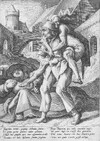
\includegraphics[keepaspectratio,width=\textwidth]{carrying-povery-small.jpg}
  \captionart{PovertyRiches}
  \label{fig:povertyriches}
\end{figure}

% Force float here
\clearpage{}
\thispagestyle{titleontop}
%SECT. II. MEMB. IV SUBSECT. VI.-_Poverty and Want, Causes of Melancholy_.
\section{Poverty and Want, Causes of Melancholy.}\label{sec:poverty-and-want}

\lettrine{P}{overty} and want are so violent oppugners, so unwelcome guests, so much
abhorred of all men, that I may not omit to speak of them apart.
Poverty, although (if considered aright, to a wise, understanding,
truly regenerate, and contented man) it be donum Dei, a blessed estate,
the way to heaven, as \Chrysostom{} calls\authorfootnote{2203} it, God's gift, the mother
of modesty, and much to be preferred before riches (as shall be shown
in his \authorfootnote{2204}place), yet as it is esteemed in the world's censure, it
is a most odious calling, vile and base, a severe torture, summum
scelus, a most intolerable burden; we \authorfootnote{2205}shun it all, cane pejus et
angue (worse than a dog or a snake), we abhor the name of it,
\authorfootnote{2206}Paupertas fugitur, totoque arcessitur orbe, as being the fountain
of all other miseries, cares, woes, labours, and grievances whatsoever.
To avoid which, we will take any pains,-extremos currit mercator ad
Indos, we will leave no haven, no coast, no creek of the world
unsearched, though it be to the hazard of our lives, we will dive to
the bottom of the sea, to the bowels of the earth, \authormarginnote{2207}five, six,
seven, eight, nine hundred fathom deep, through all five zones, and
both extremes of heat and cold: we will turn parasites and slaves,
prostitute ourselves, swear and lie, damn our bodies and souls, forsake
God, abjure religion, steal, rob, murder, rather than endure this
insufferable yoke of poverty, which doth so tyrannise, crucify, and
generally depress us.

For look into the world, and you shall see men most part esteemed
according to their means, and happy as they are rich: \li{Ubique
tanti quisque quantum habuit fuit.}\authormarginnote{2208} If he be likely to thrive, and in
the way of preferment, who but he? In the vulgar opinion, if a man be
wealthy, no matter how he gets it, of what parentage, how qualified,
how virtuously endowed, or villainously inclined; let him be a bawd, a
gripe, an usurer, a villain, a pagan, a barbarian, a wretch,
\authorfootnote{2209}Lucian's tyrant, on whom you may look with less security than on
the sun; so that he be rich (and liberal withal) he shall be honoured,
admired, adored, reverenced, and highly \authorfootnote{2210}magnified. The rich is
had in reputation because of his goods, Eccl. \rn{x}. 31. He shall be
befriended: for riches gather many friends, Prov. \rn{xix.} 4,-\lit{all happiness ebbs and flows with his money}{multos numerabit amicos}\authormarginnote{2211}. He
shall be accounted a gracious lord, a Mecaenas, a benefactor, a wise,
discreet, a proper, a valiant, a fortunate man, of a generous spirit,
\li{Pullus Jovis, et gallinae, filius albae}: a hopeful, a good man, a
virtuous, honest man. \li{Quando ego ie Junonium puerum, et matris partum
vere aureum}, as Tully said\authorfootnote{2212} of Octavianus, while he was adopted
Caesar, and an heir apparent of so great a monarchy\authormarginnote{2213}, he was a
golden child. All \authorfootnote{2214}honour, offices, applause, grand titles, and
turgent epithets are put upon him, omnes omnia bona dicere; all men's
eyes are upon him, God bless his good worship, his honour; \authorfootnote{2215}every
man speaks well of him, every man presents him, seeks and sues to him
for his love, favour, and protection, to serve him, belong unto him,
every man riseth to him, as to Themistocles in the Olympics, if he
speak, as of Herod, Vox Dei, non hominis, the voice of God, not of man.
All the graces, Veneres, pleasures, elegances attend him, \authorfootnote{2216} golden
fortune accompanies and lodgeth with him; and as to those Roman
emperors, is placed in his chamber.
\authorfootnote{2217}---Secura naviget aura,
Fortunamque suo temperet arbitrio:

he may sail as he will himself, and temper his estate at his pleasure,
jovial days, splendour and magnificence, sweet music, dainty fare, the
good things, and fat of the land, fine clothes, rich attires, soft
beds, down pillows are at his command, all the world labours for him,
thousands of artificers are his slaves to drudge for him, run, ride,
and post for him: \authorfootnote{2218}Divines (for Pythia Philippisat) lawyers,
physicians, philosophers, scholars are his, wholly devote to his
service. Every man seeks his \authorfootnote{2219}acquaintance, his kindred, to match
with him, though he be an oaf, a ninny, a monster, a goose-cap, \li{uxorem
ducat Danaen}\authorlatintrans{2220}, when, and whom he will, hunc optant generum Rex et
Regina-he is an excellent \authorfootnote{2221}match for my son, my daughter, my
niece, \etc{}. Quicquid calcaverit hic, Rosa fiet, let him go whither he
will, trumpets sound, bells ring, \etc{}, all happiness attends him, every
man is willing to entertain him, he sups in \authorfootnote{2222}Apollo wheresoever he
comes; what preparation is made for his \authorfootnote{2223}entertainment? fish and
fowl, spices and perfumes, all that sea and land affords. What cookery,
masking, mirth to exhilarate his person?
\authorfootnote{2224}Da Trebio, pone ad Trebium, vis frater ab illia
Ilibus?---

What dish will your good worship eat of?
\authorfootnote{2225}---dulcia poma,
Et quoscunque feret cultus tibi fundus honores,
Ante Larem, gustet venerabilior Lare dives.

Sweet apples, and whate'er thy fields afford,
Before thy Gods be serv'd, let serve thy Lord.

What sport will your honour have? hawking, hunting, fishing, fowling,
bulls, bears, cards, dice, cocks, players, tumblers, fiddlers, jesters,
\etc{}, they are at your good worship's command. Fair houses, gardens,
orchards, terraces, galleries, cabinets, pleasant walks, delightsome
places, they are at hand: \authorfootnote{2226}in aureis lac, vinum in argenteis,
adolescentulae ad nutum speciosae, wine, wenches, \etc{} a Turkish
paradise, a heaven upon earth. Though he be a silly soft fellow, and
scarce have common sense, yet if he be borne to fortunes (as I have
said) \authorfootnote{2227}jure haereditario sapere jubetur, he must have honour and
office in his course: \authorfootnote{2228}Nemo nisi dives honore dignus (Ambros.
offic. 21.) none so worthy as himself: he shall have it, atque esto
quicquid Servius aut Labeo. Get money enough and command
\authorfootnote{2229}kingdoms, provinces, armies, hearts, hands, and affections; thou
shalt have popes, patriarchs to be thy chaplains and parasites: thou
shalt have (Tamerlane-like) kings to draw thy coach, queens to be thy
laundresses, emperors thy footstools, build more towns and cities than
great Alexander, Babel towers, pyramids and Mausolean tombs, \etc{}
command heaven and earth, and tell the world it is thy vassal, \li{auro
emitur diadema, argento caelum panditur, denarius philosophum conducit,
nummus jus cogit, obolus literatum pascit, metallum sanitatem
conciliat, aes amicos conglutinat}\authorlatintrans{2230}. And therefore not without good
cause, John de Medicis, that rich Florentine, when he lay upon his
death-bed, calling his sons, Cosmo and Laurence, before him, amongst
other sober sayings, repeated this, animo quieto digredior, quod vos
sanos et divites post me relinquam, It doth me good to think yet,
though I be dying, that I shall leave you, my children, sound and rich:
for wealth sways all. It is not with us, as amongst those Lacedaemonian
senators of Lycurgus in Plutarch, He preferred that deserved best, was
most virtuous and worthy of the place, \authorfootnote{2231}not swiftness, or
strength, or wealth, or friends carried it in those days: but inter
optimos optimus, inter temperantes temperantissimus, the most temperate
and best. We have no aristocracies but in contemplation, all
oligarchies, wherein a few rich men domineer, do what they list, and
are privileged by their greatness. \authorfootnote{2232}They may freely trespass, and
do as they please, no man dare accuse them, no not so much as mutter
against them, there is no notice taken of it, they may securely do it,
live after their own laws, and for their money get pardons,
indulgences, redeem their souls from purgatory and hell itself,-\li{clausum
possidet arca Jovem}. Let them be epicures, or atheists, libertines,
Machiavellians, (as they often are) \authorfootnote{2233}\li{Et quamvis perjuris erit},
sine gente, cruentus, they may go to heaven through the eye of a
needle, if they will themselves, they may be canonised for saints, they
shall be \authorfootnote{2234}honourably interred in Mausolean tombs, commended by
poets, registered in histories, have temples and statues erected to
their names,-\li{e manibus illis-nascentur violae.}-If he be bountiful in
his life, and liberal at his death, he shall have one to swear, as he
did by Claudius the Emperor in Tacitus, he saw his soul go to heaven,
and be miserably lamented at his funeral. \li{Ambubalarum collegia, \etc{}.
Trimalcionis topanta in Petronius recta in caelum abiit}, went right to
heaven: a, base quean, \authorfootnote{2235}thou wouldst have scorned once in thy
misery to have a penny from her; and why? \li{modio nummos metiit}, she
measured her money by the bushel. These prerogatives do not usually
belong to rich men, but to such as are most part seeming rich, let him
have but a good outside\authormarginnote{2236}, he carries it, and shall be adored for a
god, as Cyrus was\authorfootnote{2237} amongst the Persians, \lit{for his gay attires}{ob splendidum apparatum}
; now most men are esteemed according to their
clothes. In our gullish times, whom you peradventure in modesty would
give place to, as being deceived by his habit, and presuming him some
great worshipful man, believe it, if you shall examine his estate, he
will likely be proved a serving man of no great note, my lady's tailor,
his lordship's barber, or some such gull, a Fastidius Brisk, Sir
Petronel Flash, a mere outside. Only this respect is given him, that
wheresoever he comes, he may call for what he will, and take place by
reason of his outward habit.

But on the contrary, if he be poor, Prov. \rn{xv.} 15, all his days are
miserable, he is under hatches, dejected, rejected and forsaken, poor
in purse, poor in spirit; \authorfootnote{2238}prout res nobis fluit, ita et animus se
habet; \authorfootnote{2239}money gives life and soul. Though he be honest, wise,
learned, well-deserving, noble by birth, and of excellent good parts;
yet in that he is poor, unlikely to rise, come to honour, office, or
good means, he is contemned, neglected, \li{frustra sapit, inter literas
esurit, amicus molestus}. \authorfootnote{2240}If he speak, what babbler is this?
Ecclus, his nobility without wealth, is \li{projecta vilior alga}\authorlatintrans{2241.5}\authormarginnote{2241}, and
he not esteemed: nos viles pulli nati infelicibus ovis, if once poor,
we are metamorphosed in an instant, base slaves, villains, and vile
drudges; \authorfootnote{2242}for to be poor, is to be a knave, a fool, a wretch, a
wicked, an odious fellow, a common eyesore, say poor and say all; they
are born to labour, to misery, to carry burdens like juments, pistum
stercus comedere with Ulysses' companions, and as Chremilus objected in
Aristophanes, \authorfootnote{2243} salem lingere, lick salt, to empty jakes, fay
channels, \authorfootnote{2244}carry out dirt and dunghills, sweep chimneys, rub
horse-heels, \etc{}. I say nothing of Turks, galley-slaves, which are
bought \authorfootnote{2245}and sold like juments, or those African Negroes, or poor
\authorfootnote{2246}Indian drudges, \li{qui indies hinc inde deferendis oneribus
occumbunt, nam quod apud nos boves et asini vehunt, trahunt, \etc{}}\authorlatintrans{2247}.
\li{Id omne misellis Indis}, they are ugly to behold, and though erst
spruce, now rusty and squalid, because poor, \authorfootnote{2248}\li{immundas fortunas
aquum est squalorem sequi}, it is ordinarily so. \authorfootnote{2249}Others eat to
live, but they live to drudge, \authorfootnote{2250}\li{servilis et misera gens nihil
recusare audet}, a servile generation, that dare refuse no
task.-\authorfootnote{2251}\li{Heus tu Dromo, cape hoc flabellum, ventulum hinc facito dum
lavamus}, sirrah blow wind upon us while we wash, and bid your fellow
get him up betimes in the morning, be it fair or foul, he shall run
fifty miles afoot tomorrow, to carry me a letter to my mistress, Socia
ad pistrinam, Socia shall tarry at home and grind malt all day long,
Tristan thresh. Thus are they commanded, being indeed some of them as
so many footstools for rich men to tread on, blocks for them to get on
horseback, or as walls for them to piss on\authorfootnote{2252}. They are commonly
such people, rude, silly, superstitious idiots, nasty, unclean, lousy,
poor, dejected, slavishly humble: and as Leo Afer observes\authorfootnote{2253} of the
commonalty of Africa, \li{natura viliores sunt, nec apud suos duces majore
in precio quam si canes essent}: \authorfootnote{2254}base by nature, and no more
esteemed than dogs, \li{miseram, laboriosam, calamitosam vitam agunt, et
inopem, infelicem, rudiores asinis, ut e brutis plane natos dicas}: no
learning, no knowledge, no civility, scarce common, sense, nought but
barbarism amongst them, \li{belluino more vivunt, neque calceos gestant,
neque vestes}, like rogues and vagabonds, they go barefooted and
barelegged, the soles of their feet being as hard as horse-hoofs, as
\authorfootnote{2255}Radzivilus observed at Damietta in Egypt, leading a laborious,
miserable, wretched, unhappy life, \authorfootnote{2256}like beasts and juments, if
not worse: (for a \authorfootnote{2257}Spaniard in Incatan, sold three Indian boys for
a cheese, and a hundred Negro slaves for a horse) their discourse is
scurrility, their summum bonum, a pot of ale. There is not any slavery
which these villains will not undergo, inter illos plerique latrinas
evacuant, alii culinariam curant, alii stabularios agunt, urinatores et
id genus similia exercent, \etc{} like those people that dwell in the
\authorfootnote{2258}Alps, chimney-sweepers, jakes-farmers, dirt-daubers, vagrant
rogues, they labour hard some, and yet cannot get clothes to put on, or
bread to eat. For what can filthy poverty give else, but beggary,
fulsome nastiness, squalor, contempt, drudgery, labour, ugliness,
hunger and thirst\authormarginnote{2259}; \li{pediculorum, et pulicum numerum?} as he well
followed\authorfootnote{2260} it in Aristophanes, fleas and lice, \li{pro pallio vestem laceram,
et pro pulvinari lapidem bene magnum ad caput}, rags for his raiment,
and a stone for his pillow, \li{pro cathedra, ruptae caput urnae}, he sits
in a broken pitcher, or on a block for a chair, \li{et malvae, ramos pro
panibus comedit}, he drinks water, and lives on wort leaves, pulse, like
a hog, or scraps like a dog, \li{ut nunc nobis vita afficitur, quis non
putabit insaniam esse, infelicitatemque?} as Chremilus concludes his
speech, as we poor men live nowadays, who will not take our life to be
\authorfootnote{2261} infelicity, misery, and madness?

If they be of little better condition than those base villains,
hunger-starved beggars, wandering rogues, those ordinary slaves, and
day-labouring drudges; yet they are commonly so preyed upon by \authorfootnote{2262}
polling officers for breaking the laws, by their tyrannising landlords,
so flayed and fleeced by perpetual \authorfootnote{2263}exactions, that though they do
drudge, fare hard, and starve their genius, they cannot live in
\authorfootnote{2264}some countries; but what they have is instantly taken from them,
the very care they take to live, to be drudges, to maintain their poor
families, their trouble and anxiety takes away their sleep, Sirac.
\rn{xxxi.} 1, it makes them weary of their lives: when they have taken all
pains, done their utmost and honest endeavours, if they be cast behind
by sickness, or overtaken with years, no man pities them, hard-hearted
and merciless, uncharitable as they are, they leave them so distressed,
to beg, steal, murmur, and \authormarginnote{2265} rebel, or else starve. The feeling
and fear of this misery compelled those old Romans, whom Menenius
Agrippa pacified, to resist their governors: outlaws, and rebels in
most places, to take up seditious arms, and in all ages hath caused
uproars, murmurings, seditions, rebellions, thefts, murders, mutinies,
jars and contentions in every commonwealth: grudging, repining,
complaining, discontent in each private family, because they want means
to live according to their callings, bring up their children, it breaks
their hearts, they cannot do as they would. No greater misery than for
a lord to have a knight's living, a gentleman a yeoman's, not to be
able to live as his birth and place require. Poverty and want are
generally corrosives to all kinds of men, especially to such as have
been in good and flourishing estate, are suddenly distressed,
\authorfootnote{2266}nobly born, liberally brought up, and, by some disaster and
casualty miserably dejected. For the rest, as they have base fortunes,
so have they base minds correspondent, like beetles, e stercore orti, e
stercore victus, in stercore delicium, as they were obscurely born and
bred, so they delight in obscenity; they are not thoroughly touched
with it. \li{Angustas animas angusto in pectore versant}\authorlatintrans{2267}. Yet, that
which is no small cause of their torments, if once they come to be in
distress, they are forsaken of their fellows, most part neglected, and
left unto themselves; as poor \authorfootnote{2268}Terence in Rome was by Scipio,
Laelius, and Furius, his great and noble friends.
%
\begin{latin}
\begin{quote}
Nil Publius Scipio profuit, nil ei Laelius, nil Furius,\\
Tres per idem tempus qui agitabant nobiles facillime,\\
Horum ille opera ne domum quident habuit conductitiam.
\end{quote}
\end{latin}
\translationrule
\begin{quote}%\authorlatintrans{2269}
Publius Scipio, Laelius and Furius, three of the most distinguished noblemen at that day in Rome, were of so little service to him, that he could scarcely procure a lodging through their patronage.
\end{quote}

'Tis generally so, \li{Tempora si fuerint nubila, solus eris}, he is left
cold and comfortless, \li{nullas ad amissas ibit amicus opes}, all flee from
him as from a rotten wall, now ready to fall on their heads. Prov. \rn{xix.}
1. Poverty separates them from their \authormarginnote{2270}neighbours.
\li{Dum fortuna favet vultum servatis amici,
Cum cecidit, turpi vertitis ora fuga.}\authormarginnote{2271}

Whilst fortune favour'd, friends, you smil'd on me,
But when she fled, a friend I could not see.

Which is worse yet, if he be poor \authorfootnote{2272}every man contemns him, insults
over him, oppresseth him, scoffs at, aggravates his misery.
\li{Quum caepit quassata domus subsidere, partes
In proclinatas omne recumbit onus.}\authormarginnote{2273}

When once the tottering house begins to shrink,
Thither comes all the weight by an instinct.

Nay they are odious to their own brethren, and dearest friends, Pro.
xix. 7. His brethren hate him if he be poor, \authorfootnote{2274}omnes vicini
oderunt, his neighbours hate him, Pro. xiv. 20, \authorfootnote{2275}omnes me noti ac
ignoti deserunt, as he complained in the comedy, friends and strangers,
all forsake me. Which is most grievous, poverty makes men ridiculous,
Nil habet infelix paupertas durius in se, quam quod ridiculos homines
facit, they must endure \authorfootnote{2276}jests, taunts, flouts, blows of their
betters, and take all in good part to get a meal's meat: \authorfootnote{2277}magnum
pauperies opprobrium, jubet quidvis et facere et pati. He must turn
parasite, jester, fool, cum desipientibus desipere; saith
\authorfootnote{2278}Euripides, slave, villain, drudge to get a poor living, apply
himself to each man's humours, to win and please, \etc{}, and be buffeted
when he hath all done, as Ulysses was by Melanthius \authorfootnote{2279}in Homer, be
reviled, baffled, insulted over, for \authorfootnote{2280}potentiorum stultitia
perferenda est, and may not so much as mutter against it. He must turn
rogue and villain; for as the saying is, \li{Necessitas cogit ad turpia},
poverty alone makes men thieves, rebels, murderers, traitors,
assassins, because of poverty we have sinned, Ecclus. \rn{xxvii.} 1, swear
and forswear, bear false witness, lie, dissemble, anything, as I say,
to advantage themselves, and to relieve their necessities: \authorfootnote{2281}
Culpae scelerisque magistra est, when a man is driven to his shifts,
what will he not do?

---\li{si miserum fortuna Sinonem
Finxit, vanum etiam mendacemque improba finget}\authorlatintrans{2282}.

he will betray his father, prince, and country, turn Turk, forsake
religion, abjure God and all, nulla tam horrenda proditio, quam illi
lucri causa (saith \authorfootnote{2283}Leo Afer) perpetrare nolint. \authorfootnote{2284}Plato,
therefore, calls poverty, thievish, sacrilegious, filthy, wicked, and
mischievous: and well he might. For it makes many an upright man
otherwise, had he not been in want, to take bribes, to be corrupt, to
do against his conscience, to sell his tongue, heart, hand, \etc{}, to be
churlish, hard, unmerciful, uncivil, to use indirect means to help his
present estate. It makes princes to exact upon their subjects, great
men tyrannise, landlords oppress, justice mercenary, lawyers vultures,
physicians harpies, friends importunate, tradesmen liars, honest men
thieves, devout assassins, great men to prostitute their wives,
daughters, and themselves, middle sort to repine, commons to mutiny,
all to grudge, murmur, and complain. A great temptation to all
mischief, it compels some miserable wretches to counterfeit several
diseases, to dismember, make themselves blind, lame, to have a more
plausible cause to beg, and lose their limbs to recover their present
wants. Jodocus Damhoderius, a lawyer of Bruges, praxi rerum criminal.
c. 112. hath some notable examples of such counterfeit cranks, and
every village almost will yield abundant testimonies amongst us; we
have dummerers, Abraham men, \etc{}. And that which is the extent of
misery, it enforceth them through anguish and wearisomeness of their
lives, to make away themselves; they had rather be hanged, drowned,
\etc{}, than to live without means.
\authorfootnote{2285}In mare caetiferum, ne te premat aspera egestas,
Desili, et a celsis corrue Cerne jugis.


Much better 'tis to break thy neck,
Or drown thyself i' the sea,

Than suffer irksome poverty;
Go make thyself away.

A Sybarite of old, as I find it registered in \authorfootnote{2286}Athenaeus, supping
in Phiditiis in Sparta, and observing their hard fare, said it was no
marvel if the Lacedaemonians were valiant men; for his part, he would
rather run upon a sword point (and so would any man in his wits) than
live with such base diet, or lead so wretched a life. \authorfootnote{2287}In Japonia,
'tis a common thing to stifle their children if they be poor, or to
make an abortion, which \Aristotle commends. In that civil commonwealth
of China, \authorfootnote{2288}the mother strangles her child, if she be not able to
bring it up, and had rather lose, than sell it, or have it endure such
misery as poor men do. Arnobius, lib. 7, adversus gentes,
\authorfootnote{2289}Lactantius, lib. 5. cap. 9. objects as much to those ancient
Greeks and Romans, they did expose their children to wild beasts,
strangle, or knock out their brains against a stone, in such cases. If
we may give credit to \authorfootnote{2290}Munster, amongst us Christians in
Lithuania, they voluntarily mancipate and sell themselves, their wives
and children to rich men, to avoid hunger and beggary; \authorfootnote{2291} many make
away themselves in this extremity. Apicius the Roman, when he cast up
his accounts, and found but 100\thinspace{}000 crowns left, murdered himself for
fear he should be famished to death. P. Forestus, in his medicinal
observations, hath a memorable example of two brothers of Louvain that,
being destitute of means, became both melancholy, and in a discontented
humour massacred themselves. Another of a merchant, learned, wise
otherwise and discreet, but out of a deep apprehension he had of a loss
at seas, would not be persuaded but as Ventidius\authorfootnote{2292} in the poet, he
should die a beggar. In a word, thus much I may conclude of poor men,
that though they have good \authorfootnote{2293}parts they cannot show or make use of
them: \authorfootnote{2294}ab inopia ad virtutem obsepta est via, 'tis hard for a poor
man to \authorfootnote{2295} rise, \li{haud facile emergunt, quorum virtutibus obstat res
angusta domi}\authorlatintrans{2296}. The wisdom of the poor is despised, and his words
are not heard. Eccles. \rn{vi.} 19. His works are rejected, contemned, for
the baseness and obscurity of the author, though laudable and good in
themselves, they will not likely take.
Nulla placere diu, neque vivere carmina possunt,
Quae scribuntur atquae potoribus.---

No verses can please men or live long that are written by
water-drinkers. Poor men cannot please, their actions, counsels,
consultations, projects, are vilified in the world's esteem, amittunt
consilium in re, which Gnatho long since observed. \authorfootnote{2297}Sapiens
crepidas sibi nunquam nec soleas fecit, a wise man never cobbled shoes;
as he said of old, but how doth he prove it? I am sure we find it
otherwise in our days, \authorfootnote{2298} pruinosis horret facundia pannis. Homer
himself must beg if he want means, and as by report sometimes he did
\authorfootnote{2299}go from door to door, and sing ballads, with a company of boys
about him. This common misery of theirs must needs distract, make them
discontent and melancholy, as ordinarily they are, wayward, peevish,
like a weary traveller, for \authorfootnote{2300} Fames et mora bilem in nares
conciunt, still murmuring and repining: Ob inopiam morosi sunt, quibus
est male, as Plutarch quotes out of Euripides, and that comical poet
well seconds,\authorfootnote{2301}

\begin{latin}
\begin{quote}
Omnes quibus res sunt minus secundae, nescio quomodo
Suspitiosi, ad contumeliam omnia accipiunt magis,
Propter suam impotentiam se credunt negligi.
\end{quote}
\end{latin}

If they be in adversity, they are more suspicious and apt to mistake:
they think themselves scorned by reason of their misery: and therefore
many generous spirits in such cases withdraw themselves from all
company, as that comedian Terence is said\authormarginnote{2302} to have done; when he
perceived himself to be forsaken and poor, he voluntarily banished
himself to Stymphalus, a base town in Arcadia, and there miserably
died.
%
\begin{latin}
\begin{quote}
---ad summam inopiam redactus,\\
Itaque e conspectu omnium abiit Graeciae in terram ultimam.
\end{quote}
\end{latin}
\translationrule
\begin{quote}%\authorlatintrans{2303}.
Reduced to the greatest necessity, he withdrew from the gaze of the public to the most remote village in Greece.
\end{quote}

Neither is it without cause, for we see men commonly respected
according to their means, (\li{an dives sit omnes quaerunt, nemo an
bonus}\authormarginnote{2304}) and vilified if they be in bad clothes. \authorfootnote{2305}Philophaemen the
orator was set to cut wood, because he was so homely attired,
\authorfootnote{2306}Terentius was placed at the lower end of Cecilius' table, because
of his homely outside. \authorfootnote{2307} Dante, that famous Italian poet, by
reason his clothes were but mean, could not be admitted to sit down at
a feast. Gnatho scorned his old familiar friend because of his apparel,
\authorfootnote{2308}Hominem video pannis, annisque obsitum, hic ego illum contempsi
prae me. King Persius overcome sent a letter to \authorfootnote{2309}Paulus Aemilius,
the Roman general; Persius P. Consuli. S. but he scorned him any
answer, tacite exprobrans fortunam suam (saith mine author) upbraiding
him with a present fortune. \authorfootnote{2310}Carolus Pugnax, that great duke of
Burgundy, made H. Holland, late duke of Exeter, exiled, run after his
horse like a lackey, and would take no notice of him: \authormarginnote{2311} 'tis the
common fashion of the world. So that such men as are poor may justly be
discontent, melancholy, and complain of their present misery, and all
may pray with \authorfootnote{2312}Solomon, Give me, O Lord, neither riches nor
poverty; feed me with food convenient for me.

%SECT. II. MEMB. IV. SUBSECT. VII.-_A heap of other Accidents causing Melancholy, Death of Friends, Losses, \etc{}._
\section[Accidents, Death of Friends, Losses]{A heap of other Accidents causing Melancholy, Death of Friends, Losses, \etc{}}\label{sec:accidents-death-of-friends}

\lettrine{I}{n} this labyrinth of accidental causes, the farther I wander, the more
intricate I find the passage, multae ambages, and new causes as so many
by-paths offer themselves to be discussed: to search out all, were an
Herculean work, and fitter for Theseus: I will follow mine intended
thread; and point only at some few of the chiefest.
\subsection{Death of Friends.}
Amongst which, loss and death of friends may
challenge a first place, multi tristantur, as Vives well
observes\authorfootnote{2313}, post delicias, convivia, dies festos, many are melancholy
after a feast, holiday, merry meeting, or some pleasing sport, if they
be solitary by chance, left alone to themselves, without employment,
sport, or want their ordinary companions, some at the departure of
friends only whom they shall shortly see again, weep and howl, and look
after them as a cow lows after her calf, or a child takes on that goes
to school after holidays. Ut me levarat tuus adventus, sic discessus
afflixit, (which \authorfootnote{2314}Tully writ to Atticus) thy coming was not so
welcome to me, as thy departure was harsh. Montanus, consil. 132. makes
mention of a country woman that parting with her friends and native
place, became grievously melancholy for many years; and Trallianus of
another, so caused for the absence of her husband: which is an ordinary
passion amongst our good wives, if their husband tarry out a day longer
than his appointed time, or break his hour, they take on presently with
sighs and tears, he is either robbed, or dead, some mischance or other
is surely befallen him, they cannot eat, drink, sleep, or be quiet in
mind, till they see him again. If parting of friends, absence alone can
work such violent effects, what shall death do, when they must
eternally be separated, never in this world to meet again? This is so
grievous a torment for the time, that it takes away their appetite,
desire of life, extinguisheth all delights, it causeth deep sighs and
groans, tears, exclamations,
(\li{O dulce germen matris, o sanguis meus, Eheu tepentes, \etc{}-o flos tener}\authorlatintrans{2315}.) 
howling, roaring, many bitter pangs, \authormarginnote{2316}\li{lamentis gemituque et
faemineo ululatu Tecta fremunt}) and by frequent meditation extends so
far sometimes, \authorfootnote{2317}they think they see their dead friends continually
in their eyes, observantes imagines, as Conciliator confesseth he saw
his mother's ghost presenting herself still before him. Quod nimis
miseri volunt, hoc facile credunt, still, still, still, that good
father, that good son, that good wife, that dear friend runs in their
minds: Totus animus hac una cogitatione defixus est, all the year long,
as \Pliny{} complains\authorfootnote{2318} to Romanus, methinks I see Virginius, I hear
Virginius, I talk with Virginius, \etc{}.
%
\authormarginnote{2319}\begin{latin}
\begin{verse}
Te sine, vae misero mihi, lilia nigra videntur,\\*
Pallentesque rosae, nec dulce rubens hyacinthus,\\*
Nullos nec myrtus, noc laurus spirat odores.
\end{verse}
\end{latin}
\translationrule
\begin{verse}% \authorlatintrans{2319.5}
Without thee, ah! wretched me,\\*
the lillies lose their whiteness, the roses become pallid, the hyacinth forgets to blush\\*
neither the myrtle nor the laurel retains its odours.
\end{verse}

\cleartoleftpage{}
\begin{figure}[p]
  \begingroup
  \centering
  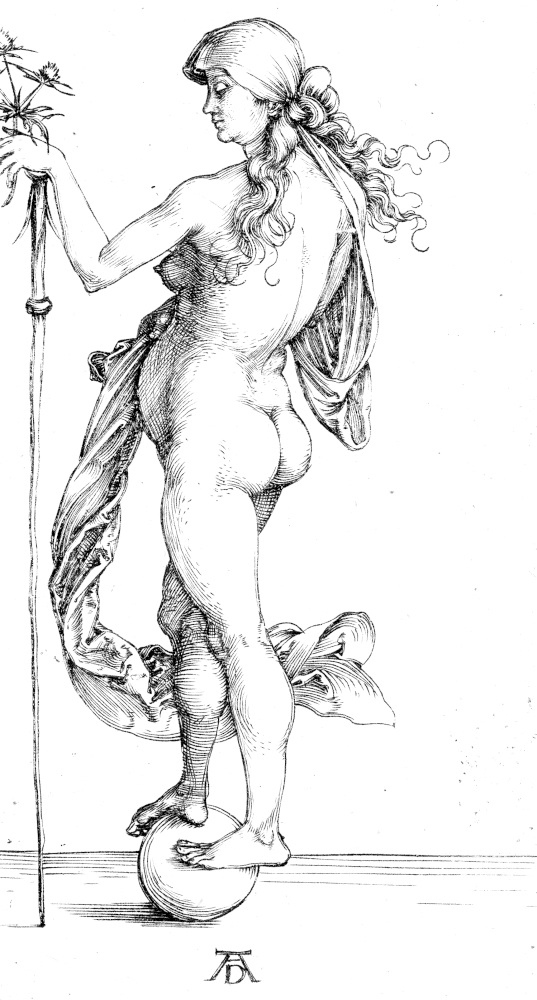
\includegraphics[keepaspectratio,width=0.75\textwidth]{fortuna-small.jpg}
  \captionart{Fortuna}
  \label{fig:fortuna}
\end{figure}

% Force float here
\clearpage{}
They that are most staid and patient, are so furiously carried headlong
by the passion of sorrow in this case, that brave discreet men
otherwise, oftentimes forget themselves, and weep like children many
months together, \authorfootnote{2320}as if that they to water would, and will not be
comforted. They are gone, they are gone; what shall I do?
Abstulit atra dies et funere mersit acerbo,
Quis dabit in lachrymas fontem mihi? quis satis altos
Accendet gemitus, et acerbo verba dolori?
Exhaurit pietas oculos, et hiantia frangit
Pectora, nec plenos avido sinit edere questus,
Magna adeo jactura premit, \etc{}.

Fountains of tears who gives, who lends me groans,
Deep sighs sufficient to express my moans?
Mine eyes are dry, my breast in pieces torn,
My loss so great, I cannot enough mourn.

So Stroza Filius, that elegant Italian poet, in his Epicedium, bewails
his father's death, he could moderate his passions in other matters,
(as he confesseth) but not in this, lie yields wholly to sorrow,
Nunc fateor do terga malis, mens illa fatiscit,
Indomitus quondam vigor et constantia mentis.

How doth \authorfootnote{2321}Quintilian complain for the loss of his son, to despair
almost: Cardan lament his only child in his book de libris propriis,
and elsewhere in many of his tracts, \authorfootnote{2322}St. Ambrose his brother's
death? an ego possum non cogitare de te, aut sine lachrymis cogitare? O
amari dies, o flebiles noctes, \etc{}. Can I ever cease to think of thee,
and to think with sorrow? O bitter days, O nights of sorrow, \etc{}.
Gregory Nazianzen, that noble Pulcheria! O decorem, \etc{} flos recens,
pullulans, \etc{}. Alexander, a man of most invincible courage, after
Hephestion's death, as Curtius relates, triduum jacuit ad moriendum
obstinatus, lay three days together upon the ground, obstinate, to die
with him, and would neither eat, drink, nor sleep. The woman that
communed with Esdras (lib. 2. cap. 10.) when her son fell down dead.
fled into the field, and would not return into the city, but there
resolved to remain, neither to eat nor drink, but mourn and fast until
she died. Rachel wept for her children, and would not be comforted
because they were not. Matt. ii. 18. So did Adrian the emperor bewail
his Antinous; Hercules, Hylas; Orpheus, Eurydice; David, Absalom; (O my
dear son Absalom) \Austin{} his mother Monica, Niobe her children,
insomuch that the \authorfootnote{2323}poets feigned her to be turned into a stone, as
being stupefied through the extremity of grief. \authorfootnote{2324}Aegeas, signo
lugubri filii consternatus, in mare se proecipitatem dedit, impatient
of sorrow for his son's death, drowned, himself. Our late physicians
are full of such examples. Montanus consil. 242. \authorfootnote{2325}had a patient
troubled with this infirmity, by reason of her husband's death, many
years together. Trincavellius, l. 1. c. 14. hath such another, almost
in despair, after his \authorfootnote{2326}mother's departure, ut se ferme
proecipitatem daret; and ready through distraction to make away
himself: and in his Fifteenth counsel, tells a story of one fifty years
of age, that grew desperate upon his mother's death; and cured by
Fallopius, fell many years after into a relapse, by the sudden death of
a daughter which he had, and could never after be recovered. The fury
of this passion is so violent sometimes, that it daunts whole kingdoms
and cities. Vespasian's death was pitifully lamented all over the Roman
empire, totus orbis lugebat, saith Aurelius Victor. Alexander commanded
the battlements of houses to be pulled down, mules and horses to have
their manes shorn off, and many common soldiers to be slain, to
accompany his dear Hephestion's death; which is now practised amongst
the Tartars, when \authorfootnote{2327}a great Cham dieth, ten or twelve thousand must
be slain, men and horses, all they meet; and among those the
\authorfootnote{2328}Pagan Indians, their wives and servants voluntarily die with
them. Leo Decimus was so much bewailed in Rome after his departure,
that as Jovius gives out, \authorfootnote{2329}communis salus, publica hilaritas, the
common safety of all good fellowship, peace, mirth, and plenty died
with him, tanquam eodem sepulchro cum Leone condita lugebantur: for it
was a golden age whilst he lived, \authorfootnote{2330}but after his decease an iron
season succeeded, barbara vis et foeda vastitas, et dira malorum omnium
incommoda, wars, plagues, vastity, discontent. When Augustus Caesar
died, saith Paterculus, orbis ruinam timueramus, we were all afraid, as
if heaven had fallen upon our heads. \authorfootnote{2331}Budaeus records, how that,
at Lewis the Twelfth his death, tam subita mutatio, ut qui prius digito
coelum attingere videbantur, nunc humi derepente serpere, sideratos
esse diceres, they that were erst in heaven, upon a sudden, as if they
had been planet-strucken, lay grovelling on the ground;
\li{Concussis cecidere animis, seu frondibus ingens
Sylva dolet lapsis}\authorlatintrans{2332.5}---\authormarginnote{2332}

they looked like cropped trees. \authorfootnote{2333}At Nancy in Lorraine, when
Claudia Valesia, Henry the Second French king's sister, and the duke's
wife deceased, the temples for forty days were all shut up, no prayers
nor masses, but in that room where she was. The senators all seen in
black, and for a twelvemonth's space throughout the city, they were
forbid to sing or dance.
\authorfootnote{2334}Non ulli pastos illis egre diebus
Frigida (Daphne) boves ad flumina, nulla nec amnem
Libavit quadrupes, nec graminis attigit herbam.

The swains forgot their sheep, nor near the brink
Of running waters brought their herds to drink;
The thirsty cattle, of themselves, abstained
From water, and their grassy fare disdain'd.

How were we affected here in England for our Titus, deliciae, humani
generis, Prince Henry's immature death, as if all our dearest friends'
lives had exhaled with his? \authorfootnote{2335}Scanderbeg's death was not so much
lamented in Epirus. In a word, as he saith\authorfootnote{2336} of Edward the First at
the news of Edward of Caernarvon his son's birth, immortaliter gavisus,
he was immortally glad, may we say on the contrary of friends' deaths,
immortaliter gementes, we are diverse of us as so many turtles,
eternally dejected with it.
There is another sorrow, which arises from the loss of temporal goods
and fortunes, which equally afflicts, and may go hand in hand with the
preceding; loss of time, loss of honour, office, of good name, of
labour, frustrate hopes, will much torment; but in my judgment, there
is no torture like unto it, or that sooner procureth this malady and
mischief:
\authorfootnote{2337}Ploratur lachrymis amissa pecunia veris:

Lost money is bewailed with grief sincere.

it wrings true tears from our eyes, many sighs, much sorrow from our
hearts, and often causes habitual melancholy itself, Guianerius tract.
15. 5. repeats this for an especial cause: \authorfootnote{2338}Loss of friends, and
loss of goods, make many men melancholy, as I have often seen by
continual meditation of such things. The same causes Arnoldus
Villanovanus inculcates, Breviar. l. 1. c. 18. ex rerum amissione,
damno, amicorum morte, \etc{}. Want alone will make a man mad, to be Sans
argent will cause a deep and grievous melancholy. Many persons are
affected like \authorfootnote{2339} Irishmen in this behalf, who if they have a good
scimitar, had rather have a blow on their arm, than their weapon hurt:
they will sooner lose their life, than their goods: and the grief that
cometh hence, continueth long (saith \authorfootnote{2340}Plater) and out of many
dispositions, procureth an habit. \authorfootnote{2341}Montanus and Frisemelica cured
a young man of 22 years of age, that so became melancholy, ab amissam
pecuniam, for a sum of money which he had unhappily lost. Sckenkius
hath such another story of one melancholy, because he overshot himself,
and spent his stock in unnecessary building. \authorfootnote{2342}Roger that rich
bishop of Salisbury, exutus opibus et castris a Rege Stephano, spoiled
of his goods by king Stephen, vi doloris absorptus, atque in amentiam
versus, indecentia fecit, through grief ran mad, spoke and did he knew
not what. Nothing so familiar, as for men in such cases, through
anguish of mind to make away themselves. A poor fellow went to hang
himself, (which Ausonius hath elegantly expressed in a neat
\authorfootnote{2343}Epigram) but finding by chance a pot of money, flung away the
rope, and went merrily home, but he that hid the gold, when he missed
it, hanged himself with that rope which the other man had left, in a
discontented humour.
At qui condiderat, postquam non reperit aurum,
Aptavit collo, quem reperit laqueum.

Such feral accidents can want and penury produce. Be it by suretyship,
shipwreck, fire, spoil and pillage of soldiers, or what loss soever, it
boots not, it will work the like effect, the same desolation in
provinces and cities, as well as private persons. The Romans were
miserably dejected after the battle of Cannae, the men amazed for fear,
the stupid women tore their hair and cried. The Hungarians, when their
king Ladislaus and bravest soldiers were slain by the Turks, Luctus
publicus, \etc{}. The Venetians when their forces were overcome by the
French king Lewis, the French and Spanish kings, pope, emperor, all
conspired against them, at Cambray, the French herald denounced open
war in the senate: Lauredane Venetorum dux, \etc{}, and they had lost
Padua, Brixia, Verona, Forum Julii, their territories in the continent,
and had now nothing left, but the city of Venice itself, et urbi quoque
ipsi (saith \authorfootnote{2344}Bembus) timendum putarent, and the loss of that was
likewise to be feared, tantus repente dolor omnes tenuit, ut nunquam,
alias, \etc{}, they were pitifully plunged, never before in such
lamentable distress. \emph{Anno} 1527, when Rome was sacked by Burbonius,
the common soldiers made such spoil, that fair \authorfootnote{2345}churches were
turned to stables, old monuments and books made horse-litter, or burned
like straw; relics, costly pictures defaced; altars demolished, rich
hangings, carpets, \etc{}, trampled in the dirt. \authorfootnote{2346}Their wives and
loveliest daughters constuprated by every base cullion, as Sejanus'
daughter was by the hangman in public, before their fathers and
husbands' faces. Noblemen's children, and of the wealthiest citizens,
reserved for princes' beds, were prostitute to every common soldier,
and kept for concubines; senators and cardinals themselves dragged
along the streets, and put to exquisite torments, to confess where
their money was hid; the rest, murdered on heaps, lay stinking in the
streets; infants' brains dashed out before their mothers' eyes. A
lamentable sight it was to see so goodly a city so suddenly defaced,
rich citizens sent a begging to Venice, Naples, Ancona, \etc{}, that erst
lived in all manner of delights. \authorfootnote{2347}Those proud palaces that even
now vaunted their tops up to heaven, were dejected as low as hell in an
instant. Whom will not such misery make discontent? Terence the poet
drowned himself (some say) for the loss of his comedies, which suffered
shipwreck. When a poor man hath made many hungry meals, got together a
small sum, which he loseth in an instant; a scholar spent many an
hour's study to no purpose, his labours lost, \etc{}, how should it
otherwise be? I may conclude with Gregory, temporalium amor, quantum
afficit, cum haeret possessio, tantum quum subtrahitur, urit dolor;
riches do not so much exhilarate us with their possession, as they
torment us with their loss.

Next to sorrow still I may annex such accidents as procure fear; for
besides those terrors which I have \authorfootnote{2348}before touched, and many other
fears (which are infinite) there is a superstitious fear, one of the
three great causes of fear in \Aristotle, commonly caused by prodigies
and dismal accidents, which much trouble many of us, (Nescio quid
animus mihi praesagit mali.) As if a hare cross the way at our going
forth, or a mouse gnaw our clothes: if they bleed three drops at nose,
the salt falls towards them, a black spot appear in their nails, \etc{},
with many such, which Delrio Tom. 2. l. 3. sect. 4. \Austin{} Niphus in
his book \textlatin{de Auguriis.} \idxname{polydorevergil}[Polydore Virgil] l. 3. \textlatin{de Prodigas. Sarisburiensis}
Polycrat. l. 1. c. 13. discuss at large. They are so much affected,
that with the very strength of imagination, fear, and the devil's
craft, \authorfootnote{2349}they pull those misfortunes they suspect, upon their own
heads, and that which they fear, shall come upon them, as Solomon
fortelleth, Prov. x. 24. and Isaiah denounceth, \rn{lxvi}. 4. which if
\authorfootnote{2350}they could neglect and contemn, would not come to pass, \li{Eorum
vires nostra resident opinione, ut morbi gravitas ?grotantium
cogitatione}FIXME, they are intended and remitted, as our opinion is fixed,
more or less. N. N. dat poenas, saith \authorfootnote{2351}Crato of such a one, utinam
non attraheret: he is punished, and is the cause of it \authorfootnote{2352} himself:
\authorfootnote{2353}\li{Dum fata fugimus fata stulti incurrimus}, the thing that I feared,
saith Job, is fallen upon me.

As much we may say of them that are troubled with their fortunes; or
ill destinies foreseen: multos angit praecientia malorum: The
foreknowledge of what shall come to pass, crucifies many men: foretold
by astrologers, or wizards, iratum ob coelum, be it ill accident, or
death itself: which often falls out by God's permission; quia daemonem
timent (saith \Chrysostom{}) Deus ideo permittit accidere. Severus,
Adrian, Domitian, can testify as much, of whose fear and suspicion,
Sueton, Herodian, and the rest of those writers, tell strange stories
in this behalf. \authorfootnote{2354}Montanus consil. 31. hath one example of a young
man, exceeding melancholy upon this occasion. Such fears have still
tormented mortal men in all ages, by reason of those lying oracles, and
juggling priests. \authorfootnote{2355}There was a fountain in Greece, near Ceres'
temple in Achaia, where the event of such diseases was to be known; A
glass let down by a thread, \etc{}. Amongst those Cyanean rocks at the
springs of Lycia, was the oracle of Thrixeus Apollo, where all fortunes
were foretold, sickness, health, or what they would besides: so common
people have been always deluded with future events. At this day, Metus
futurorum maxime torquet Sinas, this foolish fear, mightily crucifies
them in China: as Matthew Riccius the Jesuit informeth\authorfootnote{2356} us, in his
commentaries of those countries, of all nations they are most
superstitious, and much tormented in this kind, attributing so much to
their divinators, ut ipse metus fidem faciat, that fear itself and
conceit, cause it to \authorfootnote{2357}fall out: If he foretell sickness such a
day, that very time they will be sick, vi metus afflicti in
aegritudinem cadunt; and many times die as it is foretold. A true
saying, Timor mortis, morte pejor, the fear of death is worse than
death itself, and the memory of that sad hour, to some fortunate and
rich men, is as bitter as gall, Eccl. xli. 1. Inquietam nobis vitam
facit mortis metus, a worse plague cannot happen to a man, than to be
so troubled in his mind; 'tis triste divortium, a heavy separation, to
leave their goods, with so much labour got, pleasures of the world,
which they have so deliciously enjoyed, friends and companions whom
they so dearly loved, all at once. Axicchus the philosopher was bold
and courageous all his life, and gave good precepts de contemnenda
morte, and against the vanity of the world, to others; but being now
ready to die himself, he was mightily dejected, \li{hac luce privabor? his
orbabor bonis?}\authorlatintrans{2358} he lamented like a child, \etc{}. And though Socrates
himself was there to comfort him, ubi pristina virtutum jactatio O
Axioche? where is all your boasted virtue now, my friend? yet he was
very timorous and impatient of death, much troubled in his mind,
Imbellis pavor et impatientia, \etc{}. O Clotho, Megapetus the tyrant in
Lucian exclaims, now ready to depart, let me live a while longer.
\authorfootnote{2359}I will give thee a thousand talents of gold, and two boles
besides, which I took from Cleocritus, worth a hundred talents apiece.
Woe's me, \authorfootnote{2360} saith another, what goodly manors shall I leave! what
fertile fields! what a fine house! what pretty children! how many
servants! who shall gather my grapes, my corn? Must I now die so well
settled? Leave all, so richly and well provided? Woe's me, what shall I
do? \authorfootnote{2361}Animula vagula, blandula, qua nunc abibis in loca?
To these tortures of fear and sorrow, may well be annexed curiosity,
that irksome, that tyrannising care, nimia solicitudo,
\authorfootnote{2362}superfluous industry about unprofitable things, and their
qualities, as Thomas defines it: an itching humour or a kind of longing
to see that which is not to be seen, to do that which ought not to be
done, to know that \authorfootnote{2363}secret which should not be known, to eat of
the forbidden fruit. We commonly molest and tire ourselves about things
unfit and unnecessary, as Martha troubled herself to little purpose. Be
it in religion, humanity, magic, philosophy, policy, any action or
study, 'tis a needless trouble, a mere torment. For what else is school
divinity, how many doth it puzzle? what fruitless questions about the
Trinity, resurrection, election, predestination, reprobation,
hell-fire, \etc{}, how many shall be saved, damned? What else is all
superstition, but an endless observation of idle ceremonies,
traditions? What is most of our philosophy but a labyrinth of opinions,
idle questions, propositions, metaphysical terms? Socrates, therefore,
held all philosophers, cavillers, and mad men, circa subtilia
Cavillatores pro insanis habuit, palam eos arguens, saith
\authorfootnote{2364}Eusebius, because they commonly sought after such things quae nec
percipi a nobis neque comprehendi posset, or put case they did
understand, yet they were altogether unprofitable. For what matter is
it for us to know how high the Pleiades are, how far distant Perseus
and Cassiopeia from us, how deep the sea, \etc{}, we are neither wiser, as
he follows it, nor modester, nor better, nor richer, nor stronger for
the knowledge of it. Quod supra nos nihil ad, nos, I may say the same
of those genethliacal studies, what is astrology but vain elections,
predictions? all magic, but a troublesome error, a pernicious foppery?
physic, but intricate rules and prescriptions? philology, but vain
criticisms? logic, needless sophisms? metaphysics themselves, but
intricate subtleties, and fruitless abstractions? alchemy, but a bundle
of errors? to what end are such great tomes? why do we spend so many
years in their studies? Much better to know nothing at all, as those
barbarous Indians are wholly ignorant, than as some of us, to be so
sore vexed about unprofitable toys: stultus labor est ineptiarum, to
build a house without pins, make a rope of sand, to what end? cui bono?
He studies on, but as the boy told St. \Austin{}, when I have laved the
sea dry, thou shalt understand the mystery of the Trinity. He makes
observations, keeps times and seasons; and as Conradus the
emperor would not touch\authorfootnote{2365} his new bride, till an astrologer had told him
a masculine hour, but with what success? He travels into Europe,
Africa, Asia, searcheth every creek, sea, city, mountain, gulf, to what
end? See one promontory (said Socrates of old), one mountain, one sea,
one river, and see all. An alchemist spends his fortunes to find out
the philosopher's stone forsooth, cure all diseases, make men
long-lived, victorious, fortunate, invisible, and beggars himself,
misled by those seducing impostors (which he shall never attain) to
make gold; an antiquary consumes his treasure and time to scrape up a
company of old coins, statues, rules, edicts, manuscripts, \etc{}, he must
know what was done of old in Athens, Rome, what lodging, diet, houses
they had, and have all the present news at first, though never so
remote, before all others, what projects, counsels, consultations, \etc{},
quid Juno in aurem insusurret Jovi, what's now decreed in France, what
in Italy: who was he, whence comes he, which way, whither goes he, \etc{}.
\Aristotle must find out the motion of Euripus; \Pliny{} must needs see
Vesuvius, but how sped they? One loseth goods, another his life;
Pyrrhus will conquer Africa first, and then Asia: he will be a sole
monarch, a second immortal, a third rich; a fourth commands. \authorfootnote{2366}
Turbine magno spes solicitae in urbibus errant; we run, ride, take
indefatigable pains, all up early, down late, striving to get that
which we had better be without, (Ardelion's busybodies as we are) it
were much fitter for us to be quiet, sit still, and take our ease. His
sole study is for words, that they be-Lepidae lexeis compostae, ut
tesserulae omnes, not a syllable misplaced, to set out a stramineous
subject: as thine is about apparel, to follow the fashion, to be terse
and polite, 'tis thy sole business: both with like profit. His only
delight is building, he spends himself to get curious pictures,
intricate models and plots, another is wholly ceremonious about titles,
degrees, inscriptions: a third is over-solicitous about his diet, he
must have such and such exquisite sauces, meat so dressed, so
far-fetched, peregrini aeris volucres, so cooked, \etc{}, something to
provoke thirst, something anon to quench his thirst. Thus he redeems
his appetite with extraordinary charge to his purse, is seldom pleased
with any meal, whilst a trivial stomach useth all with delight and is
never offended. Another must have roses in winter, alieni temporis
flores, snow-water in summer, fruits before they can be or are usually
ripe, artificial gardens and fishponds on the tops of houses, all
things opposite to the vulgar sort, intricate and rare, or else they
are nothing worth. So busy, nice, curious wits, make that insupportable
in all vocations, trades, actions, employments, which to duller
apprehensions is not offensive, earnestly seeking that which others so
scornfully neglect. Thus through our foolish curiosity do we macerate
ourselves, tire our souls, and run headlong, through our indiscretion,
perverse will, and want of government, into many needless cares, and
troubles, vain expenses, tedious journeys, painful hours; and when all
is done, quorsum haec? cui bono? to what end?
%
\authormarginnote{2367}\begin{latin}
\begin{quote}
Nescire velle quae Magister maximus\\
Docere non vult, erudita inscitia est.
\end{quote}
\end{latin}
\translationrule
\begin{quote}%\authorlatintrans{2367.5}
To profess a disinclination for that knowledge which is beyond our reach, is pedantic ignorance.
\end{quote}

\subsection{Unfortunate marriage.}
Amongst these passions and irksome accidents,
unfortunate marriage may be ranked: a condition of life appointed by
God himself in Paradise, an honourable and happy estate, and as great a
felicity as can befall a man in this world, if the parties can
agree as they ought\authormarginnote{2368}, and live as \Seneca lived\authorfootnote{2369} with his Paulina;
but if they be unequally matched, or at discord, a greater misery
cannot be expected, to have a scold, a slut, a harlot, a fool, a fury
or a fiend, there can be no such plague. Eccles. \rn{xxvi.} 14, He that hath
her is as if he held a scorpion, \etc{} \rn{xxvi.} 25, a wicked wife makes a
sorry countenance, a heavy heart, and he had rather dwell with a lion
than keep house with such a wife. Her \authorfootnote{2370}properties Jovianus
Pontanus hath described at large, Ant. dial. Tom. 2, under the name of
Euphorbia. Or if they be not equal in years, the like mischief happens.
Cecilius in Agellius lib. 2. cap. 23, complains much of an old wife,
dum ejus morti inhio, egomet mortuus vivo inter vivos, whilst I gape
after her death, I live a dead man amongst the living, or if they
dislike upon any occasion,
\authormarginnote{2371}Judge who that are unfortunately wed
What 'tis to come into a loathed bed.

The same inconvenience befalls women.
\authorfootnote{2372}\li{At vos o duri miseram lugete parentes,
Si ferro aut laqueo laeva hac me exsolvere sorte
Sustineo:}---

Hard hearted parents both lament my fate,
If self I kill or hang, to ease my state.

\authorfootnote{2373}A young gentlewoman in Basil was married, saith Felix Plater,
observat. l. 1, to an ancient man against her will, whom she could not
affect; she was continually melancholy, and pined away for grief; and
though her husband did all he could possibly to give her content, in a
discontented humour at length she hanged herself. Many other stories he
relates in this kind. Thus men are plagued with women; they again with
men, when they are of diverse humours and conditions; he a spendthrift,
she sparing; one honest, the other dishonest, \etc{}. Parents many times
disquiet their children, and they their parents. \authorfootnote{2374}A foolish son is
an heaviness to his mother. Injusta noverca: a stepmother often vexeth
a whole family, is matter of repentance, exercise of patience, fuel of
dissension, which made Cato's son expostulate with his father, why he
should offer to marry his client Solinius' daughter, a young wench,
Cujus causa novercam induceret; what offence had he done, that he
should marry again?

Unkind, unnatural friends, evil neighbours, bad servants, debts and
debates, \etc{}, 'twas Chilon's sentence, comes aeris alieni et litis est
miseria, misery and usury do commonly together; suretyship is the bane
of many families, Sponde, praesto noxa est: he shall be sore vexed that
is surety for a stranger, Prov. xi. 15, and he that hateth suretyship
is sure. Contention, brawling, lawsuits, falling out of neighbours and
friends.-discordia demens (Virg. Aen. 6) are equal to the first,
grieve many a man, and vex his soul. Nihil sane miserabilius eorum
mentibus, (as Boter holds\authorfootnote{2375}) nothing so miserable as such men, full
of cares, griefs, anxieties, as if they were stabbed with a sharp
sword, fear, suspicion, desperation, sorrow, are their ordinary
companions. Our Welshmen are noted by some of their \authorfootnote{2376}own writers,
to consume one another in this kind; but whosoever they are that use
it, these are their common symptoms, especially if they be convict or
overcome, \authorfootnote{2377}cast in a suit. Arius put out of a bishopric by
Eustathius, turned heretic, and lived after discontented all his life.
\authorfootnote{2378}Every repulse is of like nature; heu quanta de spe decidi!
Disgrace, infamy, detraction, will almost effect as much, and that a
long time after. Hipponax, a satirical poet, so vilified and lashed two
painters in his iambics, ut ambo laqueo se suffocarent, \authorfootnote{2379}\Pliny{}
saith, both hanged themselves. All oppositions, dangers, perplexities,
discontents, \authorfootnote{2380}to live in any suspense, are of the same rank: potes
hoc sub casu ducere somnos? Who can be secure in such cases?
Ill-bestowed benefits, ingratitude, unthankful friends, much disquiet
and molest some. Unkind speeches trouble as many; uncivil carriage or
dogged answers, weak women above the rest, if they proceed from their
surly husbands, are as bitter as gall, and not to be digested. A
glassman's wife in Basil became melancholy because her husband said he
would marry again if she died. No cut to unkindness, as the saying is,
a frown and hard speech, ill respect, a browbeating, or bad look,
especially to courtiers, or such as attend upon great persons, is
present death: Ingenium vultu statque caditque suo, they ebb and flow
with their masters' favours. Some persons are at their wits' ends, if
by chance they overshoot themselves, in their ordinary speeches, or
actions, which may after turn to their disadvantage or disgrace, or
have any secret disclosed. Ronseus epist. miscel. 2, reports of a
gentlewoman 25 years old, that falling foul with one of her gossips,
was upbraided with a secret infirmity (no matter what) in public, and
so much grieved with it, that she did thereupon solitudines quaerere
omnes ab se ablegare, ac tandem in gravissimam incidens melancholiam,
contabescere, forsake all company, quite moped, and in a melancholy
humour pine away. Others are as much tortured to see themselves
rejected, contemned, scorned, disabled, defamed, detracted,
undervalued, or \authorfootnote{2381}left behind their fellows. Lucian brings in
Aetamacles, a philosopher in his Lapith. convivio, much discontented
that he was not invited amongst the rest, expostulating the matter, in
a long epistle, with Aristenetus their host. Praetextatus, a robed
gentleman in Plutarch, would not sit down at a feast, because he might
not sit highest, but went his ways all in a chafe. We see the common
quarrelings, that are ordinary with us, for taking of the wall,
precedency, and the like, which though toys in themselves, and things
of no moment, yet they cause many distempers, much heart-burning
amongst us. Nothing pierceth deeper than a contempt or disgrace,
\authorfootnote{2382}especially if they be generous spirits, scarce anything affects
them more than to be despised or vilified. Crato, consil. 16, l. 2,
exemplifies it, and common experience confirms it. Of the same nature
is oppression, Ecclus. 77, surely oppression makes a man mad, loss of
liberty, which made Brutus venture his life, Cato kill himself, and
\authorfootnote{2383}Tully complain, Omnem hilaritatem in perpetuum amisi, mine
heart's broken, I shall never look up, or be merry again, \authorfootnote{2384}haec
jactura intolerabilis, to some parties 'tis a most intolerable loss.
Banishment a great misery, as Tyrteus describes it in an epigram of
his,

Nam miserum est patria amissa, laribusque vagari
Mendicum, et timida voce rogare cibos:

Omnibus invisus, quocunque accesserit exul
Semper erit, semper spretus egensque jacet, \etc{}.


A miserable thing 'tis so to wander,
And like a beggar for to whine at door,

Contemn'd of all the world, an exile is,
Hated, rejected, needy still and poor.

Polynices in his conference with Jocasta in \authorfootnote{2385}Euripides, reckons up
five miseries of a banished man, the least of which alone were enough
to deject some pusillanimous creatures. Oftentimes a too great feeling
of our own infirmities or imperfections of body or mind, will shrivel
us up; as if we be long sick:
O beata sanitas, te praesente, amaenum
Ver florit gratiis, absque te nemo beatus:

O blessed health! thou art above all gold and treasure, Ecclus. \rn{xxx.}
15, the poor man's riches, the rich man's bliss, without thee there can
be no happiness: or visited with some loathsome disease, offensive to
others, or troublesome to ourselves; as a stinking breath, deformity of
our limbs, crookedness, loss of an eye, leg, hand, paleness, leanness,
redness, baldness, loss or want of hair, \etc{}, hic ubi fluere caepit,
diros ictus cordi infert, saith \authorfootnote{2386}Synesius, he himself troubled not
a little ob comae defectum, the loss of hair alone, strikes a cruel
stroke to the heart. Acco, an old woman, seeing by chance her face in a
true glass (for she used false flattering glasses belike at other
times, as most gentlewomen do) animi dolore in insaniam delapsa est,
(Caelius Rhodiginus l. 17, c. 2) ran mad. \authorfootnote{2387}Brotheus, the son of
Vulcan, because he was ridiculous for his imperfections, flung himself
into the fire. Lais of Corinth, now grown old, gave up her glass to
Venus, for she could hot abide to look upon it. \authorfootnote{2388}Qualis sum nolo,
qualis eram nequeo. Generally to fair nice pieces, old age and foul
linen are two most odious things, a torment of torments, they may not
abide the thought of it,
\authorfootnote{2389}---o deorum
Quisquis haec audis, utinam inter errem

Nuda leones,

Antequam turpis macies decentes
Occupet malas, teneraeque succus
Defluat praedae, speciosa quaerro

Pascere tigres.


Hear me, some gracious heavenly power,
Let lions dire this naked corse devour.
My cheeks ere hollow wrinkles seize.
Ere yet their rosy bloom decays:
While youth yet rolls its vital flood,
Let tigers friendly riot in my blood.

To be foul, ugly, and deformed, much better be buried alive. Some are
fair but barren, and that galls them. Hannah wept sore, did not eat,
and was troubled in spirit, and all for her barrenness, 1 Sam. 1. and
Gen. 30. Rachel said in the anguish of her soul, give me a child, or I
shall die: another hath too many: one was never married, and that's his
hell, another is, and that's his plague. Some are troubled in that they
are obscure; others by being traduced, slandered, abused, disgraced,
vilified, or any way injured: minime miror eos (as he said) qui
insanire occipiunt ex injuria, I marvel not at all if offences make men
mad. Seventeen particular causes of anger and offence \Aristotle reckons
them up, which for brevity's sake I must omit. No tidings troubles one;
ill reports, rumours, bad tidings or news, hard hap, ill success, cast
in a suit, vain hopes, or hope deferred, another: expectation, \li{adeo
omnibus in rebus molesta semper est expectatio}, as Polybius
observes\authorfootnote{2390}; one is too eminent, another too base born, and that alone
tortures him as much as the rest: one is out of action, company,
employment; another overcome and tormented with worldly cares, and
onerous business. But what \authorfootnote{2391}tongue can suffice to speak of all?
Many men catch this malady by eating certain meats, herbs, roots, at
unawares; as henbane, nightshade, cicuta, mandrakes, \etc{}. \authorfootnote{2392}A
company of young men at Agrigentum in Sicily, came into a tavern; where
after they had freely taken their liquor, whether it were the wine
itself, or something mixed with it 'tis not yet known, \authorfootnote{2393}but upon a
sudden they began to be so troubled in their brains, and their phantasy
so crazed, that they thought they were in a ship at sea, and now ready
to be cast away by reason of a tempest. Wherefore to avoid shipwreck
and present drowning, they flung all the goods in the house out at the
windows into the street, or into the sea, as they supposed; thus they
continued mad a pretty season, and being brought before the magistrate
to give an account of this their fact, they told him (not yet recovered
of their madness) that what was done they did for fear of death, and to
avoid imminent danger: the spectators were all amazed at this their
stupidity, and gazed on them still, whilst one of the ancientest of the
company, in a grave tone, excused himself to the magistrate upon his
knees, O viri Tritones, ego in imo jacui, I beseech your deities, \etc{}
for I was in the bottom of the ship all the while: another besought
them as so many sea gods to be good unto them, and if ever he and his
fellows came to land again, \authorfootnote{2394}he would build an altar to their
service. The magistrate could not sufficiently laugh at this their
madness, bid them sleep it out, and so went his ways. Many such
accidents frequently happen, upon these unknown occasions. Some are so
caused by philters, wandering in the sun, biting of a mad dog, a blow
on the head, stinging with that kind of spider called tarantula, an
ordinary thing if we may believe Skeuck. l. 6. de Venenis, in Calabria
and Apulia in Italy, Cardan, subtil. l. 9. Scaliger exercitat. 185.
Their symptoms are merrily described by Jovianus Pontanus, Ant. dial.
how they dance altogether, and are cured by music. \authorfootnote{2395}Cardan speaks
of certain stones, if they be carried about one, which will cause
melancholy and madness; he calls them unhappy, as an \authorfootnote{2396}adamant,
selenites, \etc{} which dry up the body, increase cares, diminish sleep:
Ctesias in Persicis, makes mention of a well in those parts, of which
if any man drink, \authorfootnote{2397}he is mad for 24 hours. Some lose their wits by
terrible objects (as elsewhere I have more \authorfootnote{2398}copiously dilated) and
life itself many times, as Hippolitus affrighted by Neptune's
seahorses, Athemas by Juno's furies: but these relations are common in
all writers.
%
\begin{latin}%
\begin{verse}%
Hic alias poteram, et plures subnectere causas,\\*
Sed jumenta vocant, et Sol inclinat, Eundum est.\\!
\end{verse}%
\end{latin}%
\translationrule%
\begin{verse}%
Many such causes, much more could I say,\\*
But that for provender my cattle stay:\\*
The sun declines, and I must needs away.\\!
\end{verse}%
\attrib{\getauthornote{2399}}%

These causes if they be considered, and come alone, I do easily yield,
can do little of themselves, seldom, or apart (an old oak is not felled
at a blow) though many times they are all sufficient every one: yet if
they concur, as often they do, vis unita fortior; et quae non obsunt
singula, multa nocent, they may batter a strong constitution; as
\authorfootnote{2400}\Austin{} said, many grains and small sands sink a ship, many small
drops make a flood, \etc{}, often reiterated; many dispositions produce an
habit.

%SECT. II. MEMB. V.

%SECT. II. MEMB. V. SUBSECT. I.-_Continent, inward, antecedent, next causes and how the body works on the mind_.
\section{Continent, inward, antecedent, next causes and how the body works on the mind.}

\lettrine{A}{s} a purlieu hunter, I have hitherto beaten about the circuit of the
forest of this microcosm, and followed only those outward adventitious
causes. I will now break into the inner rooms, and rip up the
antecedent immediate causes which are there to be found. For as the
distraction of the mind, amongst other outward causes and
perturbations, alters the temperature of the body, so the distraction
and distemper of the body will cause a distemperature of the soul, and
'tis hard to decide which of these two do more harm to the other.
Plato, Cyprian, and some others, as I have formerly said, lay the
greatest fault upon the soul, excusing the body; others again accusing
the body, excuse the soul, as a principal agent. Their reasons are,
because \authorfootnote{2401}the manners do follow the temperature of the body, as
Galen proves in his book of that subject, Prosper Calenius de Atra
bile, Jason Pratensis c. de Mania, Lemnius l. 4. c. 16. and many
others. And that which Gualter hath commented, hom. 10. in epist.
Johannis, is most true, concupiscence and originals in, inclinations,
and bad humours, are \authorfootnote{2402}radical in every one of us, causing these
perturbations, affections, and several distempers, offering many times
violence unto the soul. Every man is tempted by his own concupiscence
(James i. 14), the spirit is willing but the flesh is weak, and
rebelleth against the spirit, as our \authorfootnote{2403}apostle teacheth us: that
methinks the soul hath the better plea against the body, which so
forcibly inclines us, that we cannot resist, Nec nos obniti contra, nec
tendere tantum sufficimus. How the body being material, worketh upon
the immaterial soul, by mediation of humours and spirits, which
participate of both, and ill-disposed organs, Cornelius Agrippa hath
discoursed lib. 1. de occult. Philos. cap. 63, 64, 65. Levinus Lemnius
lib. 1. de occult. nat. mir. cap. 12. et 16. et 21. institut. ad opt.
vit. Perkins lib. 1. Cases of Cons. cap. 12. T. Bright c. 10, 11, 12.
in his treatise of melancholy, for as, \authorfootnote{2404} anger, fear, sorrow,
obtrectation, emulation, \etc{} si mentis intimos recessus occuparint,
saith \authorfootnote{2405}Lemnius, corpori quoque infesta sunt, et illi teterrimos
morbos inferunt, cause grievous diseases in the body, so bodily
diseases affect the soul by consent. Now the chiefest causes proceed
from the \authorfootnote{2406}heart, humours, spirits: as they are purer, or impurer,
so is the mind, and equally suffers, as a lute out of tune, if one
string or one organ be distempered, all the rest miscarry, \authorfootnote{2407}corpus
onustum hesternis vitiis, animum quoque praegravat una. The body is
domicilium animae, her house, abode, and stay; and as a torch gives a
better light, a sweeter smell, according to the matter it is made of;
so doth our soul perform all her actions, better or worse, as her
organs are disposed; or as wine savours of the cask wherein it is kept;
the soul receives a tincture from the body, through which it works. We
see this in old men, children, Europeans; Asians, hot and cold climes;
sanguine are merry, melancholy sad, phlegmatic dull, by reason of
abundance of those humours, and they cannot resist such passions which
are inflicted by them. For in this infirmity of human nature, as
Melancthon declares, the understanding is so tied to, and captivated by
his inferior senses, that without their help he cannot exercise his
functions, and the will being weakened, hath but a small power to
restrain those outward parts, but suffers herself to be overruled by
them; that I must needs conclude with Lemnius, spiritus et humores
maximum nocumentum obtinent, spirits and humours do most harm in
\authorfootnote{2408}troubling the soul. How should a man choose but be choleric and
angry, that hath his body so clogged with abundance of gross humours?
or melancholy, that is so inwardly disposed? That thence comes then
this malady, madness, apoplexies, lethargies, \etc{} it may not be denied.
Now this body of ours is most part distempered by some precedent
diseases, which molest his inward organs and instruments, and so per
consequens cause melancholy, according to the consent of the most
approved physicians. \authorfootnote{2409}This humour (as \Avicenna{} l. 3. Fen. 1.
Tract. 4. c. 18. Arnoldus breviar. l. 1. c. 18. Jacchinus comment. in 9
Rhasis, c. 15. Montaltus, c. 10. Nicholas Piso c. de Melan. \etc{}
suppose) is begotten by the distemperature of some inward part, innate,
or left after some inflammation, or else included in the blood after an
\authorfootnote{2410}ague, or some other malignant disease. This opinion of theirs
concurs with that of Galen, \textlatin{l. 3. c. 6. de locis affect}. Guianerius
gives an instance in one so caused by a quartan ague, and Montanus
consil. 32. in a young man of twenty-eight years of age, so distempered
after a quartan, which had molested him five years together; \textlatin{Hildesheim
spicel. 2. de Mania}, relates of a Dutch baron, grievously tormented
with melancholy after a long \authorfootnote{2411}ague: \textlatin{Galen, l. de atra bile, c. 4.}
puts the plague a cause. Botaldus in his book de lue vener. c. 2. the
French pox for a cause, others, frenzy, epilepsy, apoplexy, because
those diseases do often degenerate into this. Of suppression of
haemorrhoids, haemorrhagia, or bleeding at the nose, menstruous
retentions, (although they deserve a larger explication, as being the
sole cause of a proper kind of melancholy, in more ancient maids, nuns
and widows, handled apart by Rodericus a Castro, and Mercatus, as I
have elsewhere signified) or any other evacuation stopped, I have
already spoken. Only this I will add, that this melancholy which shall
be caused by such infirmities, deserves to be pitied of all men, and to
be respected with a more tender compassion, according to Laurentius, as
coming from a more inevitable cause.

%SECT. II. MEMB. V. SUBSECT. II.-_Distemperature of particular Parts, causes_.
\section{Distemperature of particular Parts, causes.}

\lettrine{T}{here} is almost no part of the body, which being distempered, doth not
cause this malady, as the brain and his parts, heart, liver, spleen,
stomach, matrix or womb, pylorus, mirach, mesentery, hypochondries,
mesaraic veins; and in a word, saith \authorfootnote{2412}Arculanus, there is no part
which causeth not melancholy, either because it is adust, or doth not
expel the superfluity of the nutriment. Savanarola Pract. major.
rubric. 11. Tract. 6. cap. 1. is of the same opinion, that melancholy
is engendered in each particular part, and \authorfootnote{2413}Crato in \textlatin{consil. 17.
lib. 2.} Gordonius, who is \li{instar omnium}, \textlatin{lib. med. partic. 2. cap. 19.}
confirms as much, putting the \authorfootnote{2414}matter of melancholy, sometimes in
the stomach, liver, heart, brain, spleen, mirach, hypochondries, when
as the melancholy humour resides there, or the liver is not well
cleansed from melancholy blood.

The brain is a familiar and frequent cause, too hot, or too cold,
\authorfootnote{2415} through adust blood so caused, as Mercurialis will have it,
within or without the head, the brain itself being distempered. Those
are most apt to this disease, \authorfootnote{2416}that have a hot heart and moist
brain, which Montaltus cap. 11. de Melanch. approves out of Halyabbas,
Rhasis, and \Avicenna{}. \textlatin{Mercurialis consil. 11.} assigns the coldness of
the brain a cause, and Salustius Salvianus \textlatin{med. lect. l. 2. c. 1.}
\authorfootnote{2417}will have it arise from a cold and dry distemperature of the
brain. Piso, Benedictus Victorius Faventinus, will have it proceed from
a \authorfootnote{2418}hot distemperature of the brain; and \authorfootnote{2419}Montaltus cap. 10.
from the brain's heat, scorching the blood. The brain is still
distempered by himself, or by consent: by himself or his proper
affection, as Faventinus calls it, \authorfootnote{2420}or by vapours which arise from
the other parts, and fume up into the head, altering the animal
facilities.

\textlatin{Hildesheim spicel. 2. de Mania}, thinks it may be caused from a \authorfootnote{2421}
distemperature of the heart; sometimes hot; sometimes cold. A hot
liver, and a cold stomach, are put for usual causes of melancholy:
\textlatin{Mercurialis consil. 11. et consil. 6. consil. 86.} assigns a hot liver
and cold stomach for ordinary causes. \authorfootnote{2422}Monavius, in an epistle of
his to Crato in Scoltzius, is of opinion, that hypochondriacal
melancholy may proceed from a cold liver; the question is there
discussed. Most agree that a hot liver is in fault; \authorfootnote{2423}the liver is
the shop of humours, and especially causeth melancholy by his hot and
dry distemperature. \authorfootnote{2424}The stomach and mesaraic veins do often
concur, by reason of their obstructions, and thence their heat cannot
be avoided, and many times the matter is so adust and inflamed in those
parts, that it degenerates into hypochondriacal melancholy. Guianerius
c. 2. Tract. 15. holds the mesaraic veins to be a sufficient
\authorfootnote{2425}cause alone. The spleen concurs to this malady, by all their
consents, and suppression of haemorrhoids, dum non expurget alter a
causa lien, saith Montaltus, if it be \authorfootnote{2426}too cold and dry, and do
not purge the other parts as it ought, consil. 23. Montanus puts the
\authorfootnote{2427} spleen stopped for a great cause. \authorfootnote{2428}Christophorus a Vega
reports of his knowledge, that he hath known melancholy caused from
putrefied blood in those seed-veins and womb; \authorfootnote{2429}Arculanus, from
that menstruous blood turned into melancholy, and seed too long
detained (as I have already declared) by putrefaction or adustion.
The mesenterium, or midriff, diaphragma, is a cause which the
\authorfootnote{2430}Greeks called \textgreek{φρένας}: because by his inflammation, the mind is
much troubled with convulsions and dotage. All these, most part, offend
by inflammation, corrupting humours and spirits, in this non-natural
melancholy: for from these are engendered fuliginous and black spirits.
And for that reason \authorfootnote{2431}\textlatin{Montaltus cap. 10. de causis melan.} will have
the efficient cause of melancholy to be hot and dry, not a cold and dry
distemperature, as some hold, from the heat of the brain, roasting the
blood, immoderate heat of the liver and bowels, and inflammation of the
pylorus. And so much the rather, because that, as Galen holds, all
spices inflame the blood, solitariness, waking, agues, study,
meditation, all which heat: and therefore he concludes that this
distemperature causing adventitious melancholy is not cold and dry, but
hot and dry. But of this I have sufficiently treated in the matter of
melancholy, and hold that this may be true in non-natural melancholy,
which produceth madness, but not in that natural, which is more cold,
and being immoderate, produceth a gentle dotage. \authorfootnote{2432}Which opinion
Geraldus de Solo maintains in his comment upon Rhasis.

%SECT. II. MEMB. V. SUBSECT. III.-_Causes of Head-Melancholy_.
\section{Causes of Head-Melancholy.}

\lettrine{A}{fter} a tedious discourse of the general causes of melancholy, I am now
returned at last to treat in brief of the three particular species, and
such causes as properly appertain unto them. Although these causes
promiscuously concur to each and every particular kind, and commonly
produce their effects in that part which is most ill-disposed, and
least able to resist, and so cause all three species, yet many of them
are proper to some one kind, and seldom found in the rest. As for
example, head-melancholy is commonly caused by a cold or hot
distemperature of the brain, according to Laurentius \textlatin{cap. 5 de melan.}
but as Hercules de Saxonia contends\authorfootnote{2433}, from that agitation or
distemperature of the animal spirits alone. Salust. Salvianus, before
mentioned, lib. 2. cap. 3. de re med. will have it proceed from cold:
but that I take of natural melancholy, such as are fools and dote: for
as Galen writes lib. 4. de puls. 8. and \Avicenna{}, \authorfootnote{2434}a cold and
moist brain is an inseparable companion of folly. But this adventitious
melancholy which is here meant, is caused of a hot and dry
distemperature, as Damascen the Arabian lib. 3. cap. 22. thinks\authorfootnote{2435},
and most writers: Altomarus and Piso call it \authorfootnote{2436}an innate burning
intemperateness, turning blood and choler into melancholy. Both these
opinions may stand good, as Bruel maintains, and Capivaccius, \li{si
cerebrum sit calidius}, \authorfootnote{2437}if the brain be hot, the animal spirits
will be hot, and thence comes madness; if cold, folly. David Crusius
Theat. morb. Hermet. lib. 2. cap. 6. de atra bile, grants melancholy to
be a disease of an inflamed brain, but cold notwithstanding of itself:
calida per accidens, frigida per se, hot by accident only; I am of
Capivaccius' mind for my part. Now this humour, according to Salvianus,
is sometimes in the substance of the brain, sometimes contained in the
membranes and tunicles that cover the brain, sometimes in the passages
of the ventricles of the brain, or veins of those ventricles. It
follows many times \authorfootnote{2438}frenzy, long diseases, agues, long abode in
hot places, or under the sun, a blow on the head, as Rhasis informeth
us: Piso adds solitariness, waking, inflammations of the head,
proceeding most part \authorfootnote{2439}from much use of spices, hot wines, hot
meats: all which Montanus reckons up consil. 22. for a melancholy Jew;
and Heurnius repeats cap. 12. de Mania: hot baths, garlic, onions,
saith Guianerius, bad air, corrupt, much \authorfootnote{2440}waking, \etc{}, retention
of seed or abundance, stopping of haemorrhagia, the midriff
misaffected; and according to Trallianus l. 1. 16. immoderate cares,
troubles, griefs, discontent, study, meditation, and, in a word, the
abuse of all those six non-natural things. Hercules de Saxonia, cap.
16. lib. 1. will have it caused from a \authorfootnote{2441}cautery, or boil dried up,
or an issue. Amatus Lusitanus cent. 2. cura. 67. gives instance in a
fellow that had a hole in his arm, \authorfootnote{2442}after that was healed, ran
mad, and when the wound was open, he was cured again. Trincavellius
consil. 13. lib. 1. hath an example of a melancholy man so caused by
overmuch continuance in the sun, frequent use of venery, and immoderate
exercise: and in his cons. 49. lib. 3. from a \authorfootnote{2443}headpiece
overheated, which caused head-melancholy. Prosper Calenus brings in
Cardinal Caesius for a pattern of such as are so melancholy by long
study; but examples are infinite.

%SECT. II. MEMB. V. SUBSECT. IV.-_Causes of Hypochondriacal, or Windy Melancholy_.
\section{Causes of Hypochondriacal, or Windy Melancholy.}

\lettrine{I}{n} repeating of these causes, I must crambem bis coctam apponere, say
that again which I have formerly said, in applying them to their proper
species. Hypochondriacal or flatuous melancholy, is that which the
Arabians call mirachial, and is in my judgment the most grievous and
frequent, though Bruel and Laurentius make it least dangerous, and not
so hard to be known or cured. His causes are inward or outward. Inward
from diverse parts or organs, as midriff, spleen, stomach, liver,
pylorus, womb, diaphragma, mesaraic veins, stopping of issues, \etc{}.
Montaltus cap. 15. out of Galen recites, \authorfootnote{2444}heat and obstruction of
those mesaraic veins, as an immediate cause, by which means the passage
of the chilus to the liver is detained, stopped or corrupted, and
turned into rumbling and wind. Montanus, consil. 233, hath an evident
demonstration, Trincavelius another, lib. 1, cap. 1, and Plater a
third, observat. lib. 1, for a doctor of the law visited with this
infirmity, from the said obstruction and heat of these mesaraic veins,
and bowels; quoniam inter ventriculum et jecur venae effervescunt, the
veins are inflamed about the liver and stomach. Sometimes those other
parts are together misaffected; and concur to the production of this
malady: a hot liver and cold stomach, or cold belly: look for instances
in Hollerius, Victor Trincavelius, consil. 35, l. 3, Hildesheim Spicel.
2, fol. 132, Solenander consil. 9, pro cive Lugdunensi, Montanus
consil. 229, for the Earl of Montfort in Germany, 1549, and Frisimelica
in the 233 consultation of the said Montanus. I. Caesar Claudinus gives
instance of a cold stomach and over-hot liver, almost in every
consultation, con. 89, for a certain count; and con. 106, for a
Polonian baron, by reason of heat the blood is inflamed, and gross
vapours sent to the heart and brain. Mercurialis subscribes to them,
cons. 89, \authorfootnote{2445}the stomach being misaffected, which he calls the king
of the belly, because if he be distempered, all the rest suffer with
him, as being deprived of their nutriment, or fed with bad nourishment,
by means of which come crudities, obstructions, wind, rumbling,
griping, \etc{}. Hercules de Saxonia, besides heat, will have the weakness
of the liver and his obstruction a cause, facultatem debilem jecinoris,
which he calls the mineral of melancholy. Laurentius assigns this
reason, because the liver over-hot draws the meat undigested out of the
stomach, and burneth the humours. Montanus, cons. 244, proves that
sometimes a cold liver may be a cause. Laurentius c. 12, Trincavelius
lib. 12, consil., and Gualter Bruel, seems to lay the greatest fault
upon the spleen, that doth not his duty in purging the liver as he
ought, being too great, or too little, in drawing too much blood
sometimes to it, and not expelling it, as P. Cnemiandrus in a
\authorfootnote{2446}consultation of his noted tumorem lienis, he names it, and the
fountain of melancholy. Diocles supposed the ground of this kind of
melancholy to proceed from the inflammation of the pylorus, which is
the nether mouth of the ventricle. Others assign the mesenterium or
midriff distempered by heat, the womb misaffected, stopping of
haemorrhoids, with many such. All which Laurentius, cap. 12, reduceth
to three, mesentery, liver, and spleen, from whence he denominates
hepatic, splenetic, and mesaraic melancholy. Outward causes, are bad
diet, care, griefs, discontents, and in a word all those six
non-natural things, as Montanus found by his experience, consil. 244.
Solenander consil. 9, for a citizen of Lyons, in France, gives his
reader to understand, that he knew this mischief procured by a medicine
of cantharides, which an unskilful physician ministered his patient to
drink ad venerem excitandam. But most commonly fear, grief, and some
sudden commotion, or perturbation of the mind, begin it, in such bodies
especially as are ill-disposed. Melancthon, tract. 14, cap. 2, de
anima, will have it as common to men, as the mother to women, upon some
grievous trouble, dislike, passion, or discontent. For as Camerarius
records in his life, Melancthon himself was much troubled with it, and
therefore could speak out of experience. Montanus, consil. 22, pro
delirante Judaeo, confirms it, \authorfootnote{2447}grievous symptoms of the mind
brought him to it. Randolotius relates of himself, that being one day
very intent to write out a physician's notes, molested by an occasion,
he fell into a hypochondriacal fit, to avoid which he drank the
decoction of wormwood, and was freed. \authorfootnote{2448}Melancthon (being the
disease is so troublesome and frequent) holds it a most necessary and
profitable study, for every man to know the accidents of it, and a
dangerous thing to be ignorant, and would therefore have all men in
some sort to understand the causes, symptoms, and cures of it.

%SECT. II. MEMB. V. SUBSECT. V.-_Causes of Melancholy from the whole Body_.
\section{Causes of Melancholy from the whole Body.}

\lettrine{A}{s} before, the cause of this kind of melancholy is inward or outward.
Inward, \authorfootnote{2449}when the liver is apt to engender such a humour, or the
spleen weak by nature, and not able to discharge his office. A
melancholy temperature, retention of haemorrhoids, monthly issues,
bleeding at nose, long diseases, agues, and all those six non-natural
things increase it. But especially \authorfootnote{2450}bad diet, as Piso thinks,
pulse, salt meat, shellfish, cheese, black wine, \etc{}. Mercurialis out of
Averroes and \Avicenna{} condemns all herbs: Galen, lib. 3, de loc.
affect. cap. 7, especially cabbage. So likewise fear, sorrow,
discontents, \etc{}, but of these before. And thus in brief you have had
the general and particular causes of melancholy.

Now go and brag of thy present happiness, whosoever thou art, brag of
thy temperature, of thy good parts, insult, triumph, and boast; thou
seest in what a brittle state thou art, how soon thou mayst be
dejected, how many several ways, by bad diet, bad air, a small loss, a
little sorrow or discontent, an ague, \etc{}; how many sudden accidents
may procure thy ruin, what a small tenure of happiness thou hast in
this life, how weak and silly a creature thou art. Humble thyself,
therefore, under the mighty hand of God, 1 Peter, \rn{v.} 6, know thyself,
acknowledge thy present misery, and make right use of it. \li{Qui stat
videat ne cadat}. Thou dost now flourish, and hast \li{bona animi, corporis,
et fortunae}, goods of body, mind, and fortune, \li{nescis quid serus secum
vesper ferat}, thou knowest not what storms and tempests the late
evening may bring with it. Be not secure then, be sober and watch,
\authorfootnote{2451}\li{fortunam reverenter habe}, if fortunate and rich; if sick and
poor, moderate thyself. I have said.
}

\setauthornote{2452}{Seneca cont. lib. 10. cont. 5.}
\setauthornote{2453}{Quaedam universalia, particulariae, quaedam manifesta, quaedam in corpore, quaedam in cogitatione et animo, quaedam a stellis, quaedam ab humoribus, quae ut vinum corpus varie disponit, \&c. Diversa phantasmata pro varietate causae externae, internae.}
\setauthornote{2454}{Lib. 1. de risu. fol. 17. Ad ejus esum alii sudant, alii vomunt, stent, bibunt, saltant, alii rident, tremunt, dormiunt, \&c.}
\setauthornote{2455}{T. Bright. cap. 20.}
\setauthornote{2456}{Nigrescit hic humer aliquando supercalefactus, aliquando superfrigefactus. Melanel. a Gal.}
\setauthornote{2457}{Interprete F. Calvo.}
\setauthornote{2458}{Oculi his excavantur, venti gignuntur circum praecordia et acidi ructus, sicci fere ventres, vertigo, tinnitus aurium, somni pusilli, somnia terribilia et interrupta.}
\setauthornote{2459}{Virg. Aen.}
\setauthornote{2460}{Assiduae eaeque acidae ructationes quae cibum virulentum culentumque nidorem, et si nil tale ingestum sit, referant ob cruditatem. Ventres hisce aridi, somnus plerumque parcus et interruptus, somnia absurdissima, turbulenta, corporis tremor, capitis gravedo, strepitus circa aures et visiones ante oculos, ad venerem prodigi.}
\setauthornote{2461}{Altomarus, Bruel, Piso, Montaltus.}
\setauthornote{2462}{Frequentes habent oculorum nictationes, aliqui tamen fixis oculis plerumque sunt.}
\setauthornote{2463}{Cent. lib. 1. Tract. 9. Signa hujus morbi sunt plurimus saltus, sonitus aurium, capitis gravedo, lingua titubat, oculi excavantur, \&c.}
\setauthornote{2464}{In Pantheon cap. de Melancholia.}
\setauthornote{2465}{Alvus arida nihil dejiciens cibi capaces, nihilominus tamen extenuati sunt.}
\setauthornote{2466}{Nic Piso Inflatio carotidum, \&c.}
\setauthornote{2467}{Andreas Dudith Rahamo. cp. lib. 3. Crat epist. multa in pulsibus superstitio, ausim etiam dicere, tot differentias quae describuntur a Galeno, neque intelligi a quoquam nec observari posse.}
\setauthornote{2468}{T. Bright. cap. 20.}
\setauthornote{2469}{Post. 40. aetat. annum, saith Jacchinus in 15. 9. Rhasis Idem. Mercurialis consil. 86. Trincavelius, Tom. 2. cons. 17.}
\setauthornote{2470}{Gordonius, modo rident, modo flent, silent, \&c.}
\setauthornote{2471}{Fernelius consil. 43. et 45. Montanus consil. 230. Galen de locis affectis, lib. 3 cap. 6.}
\setauthornote{2472}{Aphorism et lib. de Melan.}
\setauthornote{2473}{Lib. 2. cap. 6. de locis affect. timor et moestitia, si diutius perseverent, \&c.}
\setauthornote{2474}{Tract. posthumo de Melan. edit. Venetiis 1620. per Bolzettam Bibliop. Mihi diligentius hanc rem consideranti, patet quosdam esse, qui non laborant maerore et timore.}
\setauthornote{2475}{Prob. lib. 3.}
\setauthornote{2476}{Physiog lib. 1. c. 8. Quibus multa frigida bilis atra, stolidi et timidi, at qui calidi, ingeniosi, amasii, divinosi, spiritu instigati, \&c.}
\setauthornote{2477}{Omnes exercent metus et tristitia, et sine causa.}
\setauthornote{2478}{Omnes timent licet non omnibus idem timendi modus Aetius Tetrab. lib. 2. sect. c. 9.}
\setauthornote{2479}{Ingenti pavore trepidant.}
\setauthornote{2480}{Multi mortem timent, et tamen sibi ipsis mortem consciscunt, alii coeli ruinam timent.}
\setauthornote{2481}{Affligit eos plena scrupulis conscientia, divinae misericordiae diffidentes, Orco se destinant foeda lamentatione deplorantes.}
\setauthornote{2482}{Non ausus egredi domo ne deficeret.}
\setauthornote{2483}{Multi daemones timent, latrones, insidias, Avicenna.}
\setauthornote{2484}{Alii comburi, alii de Rege, Rhasis.}
\setauthornote{2485}{Ne terra absorbeantur. Forestus.}
\setauthornote{2486}{Ne terra dehiscat. Gordon.}
\setauthornote{2487}{Alii timore mortis timentur et mala gratia principum putant se aliquid commisisse et ad supplicium requiri.}
\setauthornote{2488}{Alius domesticos timet, alius omnes. Aetius.}
\setauthornote{2489}{Alii timent insidias. Aurel. lib. 1. de morb. Chron. cap. 6.}
\setauthornote{2490}{Ille charissimos, hic omnes homines citra discrimen timet.}
\setauthornote{2491}{Virgil.}
\setauthornote{2492}{Hic in lucem prodire timet, tenebrasque quaerit, contra, ille caliginosa fugit.}
\setauthornote{2493}{Quidam larvas, et malos spiritus ab inimicis veneficius et incantationibus sibi putant objectari, Hippocrates, potionem se veneficam sumpsisse putat, et de hac ructare sibi crebro videtur. Idem Montaltus cap. 21. Aetius lib. 2. et alii. Trallianus l. 1. cap. 16.}
\setauthornote{2494}{Observat. l. 1. Quando iis nil nocet, nisi quod mulieribus melancholicis.}
\setauthornote{2495}{tamen metusque causae nescius, causa est metus. Heinsius Austriaco.}
\setauthornote{2496}{Cap. 15. in 9. Rhasis, in multis vidi, praeter rationem semper aliquid timent, in caeteris tamen optime se gerunt, neque aliquid praeter dignitatem committunt.}
\setauthornote{2497}{Altomarus cap. 7. Areteus, triste, sunt.}
\setauthornote{2498}{Mant. Egl. 1.}
\setauthornote{2499}{Ovid. Met. 4.}
\setauthornote{2500}{Inquies animus.}
\setauthornote{2501}{Hor. l. 3. Od. 1. Dark care rides behind him.}
\setauthornote{2502}{Virg.}
\setauthornote{2503}{Mened. Heautont. Act. 1. sc. 1.}
\setauthornote{2504}{Altomarus.}
\setauthornote{2505}{Seneca.}
\setauthornote{2506}{Cap. 31. Quo stomachi dolore correptum se, etiam de consciscenda morte cogitasse dixit.}
\setauthornote{2507}{Luget et semper tristatur, solitudinem amat, mortem sibi precatur, vitam propriam odio habet.}
\setauthornote{2508}{Facile in iram incidunt. Aret.}
\setauthornote{2509}{Ira sine causa, velocitas irae. Savanarola. pract. major. velocitas irae signum. Avicenna l. 3. Fen. 1. Tract. 4. cap. 18. Angor sine causa.}
\setauthornote{2510}{Suspicio, diffidentia, symptomata, Crato Ep. Julio Alexandrino cons. 185 Scoltzii.}
\setauthornote{2511}{Hor. At Rome, wishing for the fields, in the country, extolling the city to the skies.}
\setauthornote{2512}{Pers. Sat. 3. And like the children of nobility, require to eat pap, and, angry at the nurse, refuse her to sing lullaby.}
\setauthornote{2513}{In his Dutch work picture.}
\setauthornote{2514}{Howard cap. 7. differ.}
\setauthornote{2515}{Tract. de mel. cap. 2. Noctu ambulant per sylvas, et loca periculosa, neminem timent.}
\setauthornote{2516}{Facile amant. Altom.}
\setauthornote{2517}{Bodine.}
\setauthornote{2518}{Io. Major vitis patrum fol. 202. Paulus Abbas Eremita tanta solitudine, perseverat, ut nec vestem, nec vultum mulieris ferre possit, \&c.}
\setauthornote{2519}{Consult, lib. 1. 17. Cons.}
\setauthornote{2520}{Generally as they are pleased or displeased, so are their continual cogitations pleasing or displeasing.}
\setauthornote{2521}{Omnes excercent, vanae intensaeque animi cogitationes, (N. Piso Bruel) et assiduae.}
\setauthornote{2522}{Curiosi de rebus minimis. Areteus.}
\setauthornote{2523}{Lib. 2. de Intell.}
\setauthornote{2524}{Hoc melancholicis omnibus proprium, ut quas semel imaginationes valde reciperint, non facile rejiciant, sed hae etiam vel invitis semper occurrant.}
\setauthornote{2525}{Tullius de sen.}
\setauthornote{2526}{Consil. med. pro Hypochondriaco.}
\setauthornote{2527}{Consil. 43.}
\setauthornote{2528}{Cap. 5.}
\setauthornote{2529}{Lib. 2. de Intell.}
\setauthornote{2530}{Consult. 15. et 16. lib. 1.}
\setauthornote{2531}{Virg. Aen. 6.}
\setauthornote{2532}{Iliad. 3.}
\setauthornote{2533}{Si malum exasperantur, homines odio habent et solitaria petunt.}
\setauthornote{2534}{Democritus solet noctes et dies apud se degere, plerumque autem in speluncis, sub amaenis arborum umbris vel in tenebris, et mollibus herbis, vel ad aquarum crebra et quieta fluenta, \&c.}
\setauthornote{2535}{Gaudet tenebris, aliturque dolor. Ps. lxii. Vigilavi et factus sum velut nycticorax in domicilio, passer solitarius in templo.}
\setauthornote{2536}{Et quae vix audet fabula, monstra parit.}
\setauthornote{2537}{In cap. 18. l. 10. de civ. dei, Lunam ab Asino epotam videus.}
\setauthornote{2538}{Vel. l. 4. c. 5.}
\setauthornote{2539}{Sect. 2. Memb. 1. Subs. 4.}
\setauthornote{2540}{De reb. coelest. lib. 10. c. 13.}
\setauthornote{2541}{l. de Indagine Goclenius.}
\setauthornote{2542}{Hor. de art. poet.}
\setauthornote{2543}{Tract. 7. de Melan.}
\setauthornote{2544}{Humidum, calidum, frigidum, siccum.}
\setauthornote{2545}{Com. in 1 c. Johannis de Sacrobosco.}
\setauthornote{2546}{Si residet melancholia naturalis, tales plumbei coloris aut nigri, stupidi, solitarii.}
\setauthornote{2547}{Non una melancholiae causa est, nec unus humor vitii parens, sed plures, et alius aliter mutatus, unde non omnes eadem sentiunt symptomata.}
\setauthornote{2548}{Humor frigidus delirii causa, humor calidus furoris.}
\setauthornote{2549}{Multum refert qua quisque melancholia teneatur, hunc fervens et accensa agitat, illum tristis et frigens occupat: hi timidi, illi inverecundi, intrepidi, \&c.}
\setauthornote{2550}{Cap. 7. et 8. Tract. de Mel.}
\setauthornote{2551}{Signa melancholiae ex intemperie et agitatione spirituum sine materia.}
\setauthornote{2552}{T. Bright cap. 16. Treat. Mel.}
\setauthornote{2553}{Cap. 16. in 9. Rhasis.}
\setauthornote{2554}{Bright, c. 16.}
\setauthornote{2555}{Pract. major. Somnians, piger, frigidus.}
\setauthornote{2556}{De anima cap. de humor. si a Phlegmate semper in aquis fere sunt, et circa fluvios plorant multum.}
\setauthornote{2557}{Pigra nascitur ex colore pallido et albo, Her. de Saxon.}
\setauthornote{2558}{Savanarola.}
\setauthornote{2559}{Muros cadere in se, aut submergi timent, cum torpore et segnitie, et fluvios amant tales, Alexand. c. 16. lib. 7.}
\setauthornote{2560}{Semper fere dormit somnolenta c. 16. l. 7.}
\setauthornote{2561}{Laurentius.}
\setauthornote{2562}{Ca. 6. de mel. Si a sanguine, venit rubedo oculorum et faciei, plurimus risus.}
\setauthornote{2563}{Venae oculorum sunt rubrae, vide an praecesserit vini et aromatum usus, et frequens balneum, Trallian. lib. 1. 16. an praecesserit mora sub sole.}
\setauthornote{2564}{Ridet patiens si a sanguine, putat se videre choreas, musicam audire, ludos, \&c.}
\setauthornote{2565}{Cap. 2. Tract. de Melan.}
\setauthornote{2566}{Hor. ep. lib. 2. quidam haud ignobilis Argis, \&c.}
\setauthornote{2567}{Lib. de reb. mir.}
\setauthornote{2568}{Cum inter concionandum mulier dormiens e subsellio caderet, et omnes reliqui qui id viderent, riderent, tribus post diebus, \&c.}
\setauthornote{2569}{Juvenis et non vulgaris eruditionis.}
\setauthornote{2570}{Si a cholera, furibundi, interficiunt, se et alios, putant se videre pugnas.}
\setauthornote{2571}{Urina subtilis et ignea, parum dormiunt.}
\setauthornote{2572}{Tract. 15. c. 4.}
\setauthornote{2573}{Ad haec perpetranda furore rapti ducuntur, cruciatus quosvis tolerant, et mortem, et furore exacerbato audent et ad supplicia plus irritantur, mirum est quantam habeant in tormentis patientiam.}
\setauthornote{2574}{Tales plus caeteris timent, et continue tristantur, valde suspiciosi, solitudinem diligunt, corruptissimas habent imaginationes, \&c.}
\setauthornote{2575}{Si a melancholia adusta, tristes, de sepulchris somniant, timent ne fascinentur, putant se mortuos, aspici nolunt.}
\setauthornote{2576}{Videntur sibi videre monachos nigros et daemonos, et suspensos et mortuos.}
\setauthornote{2577}{Quavis nocte se cum daemone coire putavit.}
\setauthornote{2578}{Semper fere vidisse militem nigrum praesentem.}
\setauthornote{2579}{Anthony de Verdeur.}
\setauthornote{2580}{Quidam mugitus boum aemulantur, et pecora se putant, ut Praeti filiae.}
\setauthornote{2581}{Baro quidam mugitus boum et rugitus asinorum, et aliorum animalium voces effingit.}
\setauthornote{2582}{Omnia magna putabat, uxorem magnam, grandes equos, abhorruit omnia parva, magna pocula, et calceamenta pedibus majora.}
\setauthornote{2583}{Lib. 1. cap. 16. putavit se uno digito posse totum mundum conterere.}
\setauthornote{2584}{Sustinet humeris coelum cum Atlante. Alii coeli ruinam timent.}
\setauthornote{2585}{Cap. 1. Tract. 15. alius se gallum putat, alius lusciniam.}
\setauthornote{2586}{Trallianus.}
\setauthornote{2587}{Cap. 7. de mel.}
\setauthornote{2588}{Anthony de Verdeur.}
\setauthornote{2589}{Cap. 7. de mel.}
\setauthornote{2590}{Laurentius cap. 6.}
\setauthornote{2591}{Lib. 3. cap. 14. qui se regem putavit regno expulsum.}
\setauthornote{2592}{Dipnosophist. lib. Thrasilaus putavit omnes naves in Pireum portum appellantes suas esse.}
\setauthornote{2593}{De hist. Med. mirab. lib. 2. cap. 1.}
\setauthornote{2594}{Genibus flexis loqui cum illo voluit, et adstare jam tum putavit, \&c.}
\setauthornote{2595}{Gordonius, quod sit propheta, et inflatus a spiritu sancto.}
\setauthornote{2596}{Qui forensibus causis insudat, nil nisi arresta cogitat, et supplices libellos, alius non nisi versus facit. P. Forestus.}
\setauthornote{2597}{Gordonius.}
\setauthornote{2598}{Verbo non exprimunt, nec opere, sed alta mente recondunt, et sunt viri prudentissimi, quos ego saepe novi, cum multi sint sine timore, ut qui se reges et mortuis putant, plura signa quidam habent, pauciora, majora, minora.}
\setauthornote{2599}{Trallianus, lib. 1. 16. alii intervalla quaedam habent, ut etiam consueta administrent, alii in continuo delirio sunt, \&c.}
\setauthornote{2600}{Prac. mag. Vera tantum et autumno.}
\setauthornote{2601}{Lib. de humeribus.}
\setauthornote{2602}{Guianerius.}
\setauthornote{2603}{De mentis alienat. cap. 3.}
\setauthornote{2604}{Levinus Lemnius, Jason Pratensis, blanda ab initio.}
\setauthornote{2605}{A most agreeable mental delusion.}
\setauthornote{2606}{Hor.}
\setauthornote{2607}{Facilis descensus averni.}
\setauthornote{2608}{Virg.}
\setauthornote{2609}{Corpus cadaverosum. Psa. lxvii. cariosa est facies mea prae aegritudine animae.}
\setauthornote{2610}{Lib. 9. ad Ahnansorem.}
\setauthornote{2611}{Practica majore.}
\setauthornote{2612}{Quum ore loquitur quae corde concepit, quum subito de una re ad aliud transit, neque rationem de aliquo reddit, tunc est in medio, at quum incipit operari quae loquitur, in summo gradu est.}
\setauthornote{2613}{Cap. 19. Partic. 2. Loquitur secum et ad alios, ac si vere praesentes. Aug. cap. 11. li. de cura pro mortuis gerenda. Rhasis.}
\setauthornote{2614}{Quum res ad hoc devenit, ut ea quae cogitare caeperit, ore promat, atque acta permisceat, tum perfecta melancholia est.}
\setauthornote{2615}{Melancholicus se videre et audire putat daemones. Lavater de spectris, part. 3. cap. 2.}
\setauthornote{2616}{Wierus, lib. 3. cap. 31.}
\setauthornote{2617}{Michael a musian.}
\setauthornote{2618}{Malleo malef.}
\setauthornote{2619}{Lib. de atra bile.}
\setauthornote{2620}{Part. 1. Subs. 2, Memb. 2.}
\setauthornote{2621}{De delirio, melancholia et mania.}
\setauthornote{2622}{Nicholas Piso. Si signa circa ventriculum non apparent nec sanguis male affectus, et adsunt timor et maestitia, cerebrum ipsum existimandum est, \&c.}
\setauthornote{2623}{Tract. de mel. cap. 13, \&c. Ex intemperie spirituum, et cerebri motu, tenebrositate.}
\setauthornote{2624}{Facie sunt rubente et livescente, quibus etiam aliquando adsunt pustulae.}
\setauthornote{2625}{Jo. Pantheon. cap. de Mel. Si cerebrum primario afficiatur adsunt capitis gravitas, fixi oculi, \&c.}
\setauthornote{2626}{Laurent. cap. 5. si a cerebro ex siccitate, tum capitis erit levitas, sitis, vigilia, paucitas superfluitatum in oculis et naribus.}
\setauthornote{2627}{Si nulla digna laesio, ventriculo, quoniam in hac melancholia capitis, exigua nonnunquam ventriculi pathemata coeunt, duo enim haec membra sibi invicem affectionem transmittunt.}
\setauthornote{2628}{Postrema magis flatuosa.}
\setauthornote{2629}{Si minus molestiae circa ventriculum aut ventrem, in iis cerebrum primario afficitur, et curare oportet hunc affectum, per cibos flatus exortes, et bonae concoctionis, \&c. raro cerebrum afficitur sine ventriculo.}
\setauthornote{2630}{Sanguinem adurit caput calidius, et inde fumi melancholici adusti, animum exagitant.}
\setauthornote{2631}{Lib. de loc. affect. cap. 6.}
\setauthornote{2632}{Cap. 6.}
\setauthornote{2633}{Hildesheim spicel. 1. de mel. In Hypochondriaca melancholia adeo ambigua sunt symptomata, ut etiam exercitatissimi medici de loco affecto statuere non possint.}
\setauthornote{2634}{Medici de loco affecto nequeunt statuere.}
\setauthornote{2635}{Tract. posthumo de mel. Patavii edit. 1620. per Bozettum Bibliop. cap. 2.}
\setauthornote{2636}{Acidi ructus, cruditates, aestus in praecordiis, flatus, interdum ventriculi dolores vehementes, sumptoque cibo concoctu difficili, sputum humidum idque multum sequetur, \&c. Hip. lib. de mel. Galenus, Melanelius e Ruffo et Aetio, Altomarus, Piso, Montaltus, Bruel, Wecker, \&c.}
\setauthornote{2637}{Circa praecordia de assidua in flatione queruntur, et cum sudore totius corporis importuno, frigidos articulos saepe patiuntur, indigestione laborant, ructus suos insuaves perhorrescunt, viscerum dolores habent.}
\setauthornote{2638}{Montaltus, c. 13. Wecker, Fuchsius c. 13. Altomarus c. 7. Laurentius c. 73. Bruel, Gordon.}
\setauthornote{2639}{Pract. major: dolor in eo et ventositas, nausea.}
\setauthornote{2640}{Ut atra densaque nubes soli effusa, radios et lumen ejus intercipit et offuscat; sic, etc.}
\setauthornote{2641}{Ut fumus e camino.}
\setauthornote{2642}{Hypochondriaci maxime affectant coire, et multiplicatur coitus in ipsis, eo quod ventositates multiplicantur in hypochondriis, et coitus saepe allevat has ventositates.}
\setauthornote{2643}{Cont. lib. 1. tract. 9.}
\setauthornote{2644}{Wecker, Melancholicus succus toto corpore redundans.}
\setauthornote{2645}{Splen natura imbecilior. Montaltus cap. 22.}
\setauthornote{2646}{Lib. 1. cap. 16. Interrogare convenit, an aliqua evacuationis retentio obvenerit, viri in haemmorrhoid, mulierum menstruis, et vide faciem similiter an sit rubicunda.}
\setauthornote{2647}{Naturales nigri acquisiti a toto corpore, saepe rubicundi.}
\setauthornote{2648}{Montaltus cap. 22. Piso. Ex colore sanguinis si minuas venam, si fluat niger, \&c.}
\setauthornote{2649}{Apul. lib. 1. semper obviae species mortuorum quicquid umbrarum est uspiam, quicquid lemurum et larvarum oculis suis aggerunt, sibi fingunt omnia noctium occursacula, omnia busforum formidamina, omnia sepulchrorum terriculamenta.}
\setauthornote{2650}{Differt enim ab ea quae viris et reliquis feminis communiter contingit, propriam habens causam.}
\setauthornote{2651}{Ex menstrui sanguinis tetra ad cor et cerebrum exhalatione, vitiatum semen mentem perturbat, \&c. non per essentiam, sed per consensum. Animus moerens et anxius inde malum trahit, et spiritus cerebrum obfuscantur, quae cuncta augentur, \&c.}
\setauthornote{2652}{Cum tacito delirio ac dolore alicujus partis internae, dorsi, hypochondrii, cordis regionem et universam mammam interdum occupantis, \&c. Cutis aliquando squalida, aspera, rugosa, praecipue cubitis, genibus, et digitorum articulis, praecordia ingenti saepe torrore aestuant et pulsant, cumque vapor excitatus sursum evolat, cor palpitat aut premitur, animus deficit, \&c.}
\setauthornote{2653}{Animi dejectio, perversa rerum existimatio, praeposterum judicium. Fastidiosae, languentes, taediosae, consilii inopes, lachrymosae, timentes, moestae, cum summa rerum meliorum desperatione, nulla re delectantur, solitudinem amant, \&c.}
\setauthornote{2654}{Nolunt aperire molestiam quam patiuntur, sed conqueruntur tamen de capite, corde, mammis, \&c. In puteos fere maniaci prosilire, ac strangulari cupiunt, nulla orationis suavitate ad spem salutis recuperandam erigi, \&c. Familiares non curant, non loquuntur, non respondent, \&c. et haec graviora, si, \&c.}
\setauthornote{2655}{Clisteres et Helleborismum Mathioli summe laudat.}
\setauthornote{2656}{Examen conc. Trident. de coelibatu sacerd.}
\setauthornote{2657}{Cap. de Satyr. et Priapis.}
\setauthornote{2658}{Part. 3. sect. 2. Memb. 5. Sub. 5.}
\setauthornote{2659}{Lest you may imagine that I patronise that widow or this virgin, I shall not add another word.}
\setauthornote{2660}{Vapores crassi et nigri, a ventriculo in cerebrum exhalant. Fel. Platerus.}
\setauthornote{2661}{Calidi hilares, frigidi indispositi ad laetitiam, et ideo solitarii, taciturni, non ob tenebras internas, ut medici volunt, sed ob frigus: multi melancholici nocte ambulant intrepidi.}
\setauthornote{2662}{Vapores melancholici, spiritibus misti, tenebrarum causse sunt, cap. 1.}
\setauthornote{2663}{Intemperies facit succum nigrum, nigrities, obscurat spiritum, obscuratio spiritus facit metum et tristiam.}
\setauthornote{2664}{Ut nubecula Solern offuscat. Constantinus lib. de melanch.}
\setauthornote{2665}{Altomarus c. 7. Causam timoris circumfert aler humor passionis materia, et atri spiritus perpetuam animae domicilio offundunt noctem.}
\setauthornote{2666}{Pone exemplum, quod quis potest ambulare super trahem quae est in via: sed si sit super aquam profundam, loco pontis, non ambulabit super eam, eo quod imaginetur in animo et timet vehementer, forma cadendi impressa, cui obediunt membra omnia, et facultates reliquae.}
\setauthornote{2667}{Lib. 2. de intellectione. Susoiciosi ob timorem et obliquum discursum, et semper inde putant sibi fieri insidias. Lauren. 5.}
\setauthornote{2668}{Tract. de mel. cap. 7. Ex dilatione, contractione, confusione, tenebrositate spirituum, calida, frigida intemperie, \&c.}
\setauthornote{2669}{Illud inquisitione dignum, cur tam falsa recipiant, habere se cornua, esse mortuos, nasutos, esse aves, \&c.}
\setauthornote{2670}{1. Dispositio corporis. 2. Occasio Imaginationis.}
\setauthornote{2671}{In pro. li. de coelo. Vehemens et assidua cogitatio rei erga quam afficitur, spiritus in cerebrum evocat.}
\setauthornote{2672}{Melancholici ingeniosi omnes, summi viri in artibus et disciplinis, sive circum imperatoriam aut reip. disciplinam omnes fere melancholici, Aristoteles.}
\setauthornote{2673}{Adeo miscentur, ut sit duplum sanguinis ad reliqua duo.}
\setauthornote{2674}{Lib. 2. de intellectione. Pingui sunt Minerva phlegmatici: sanguinei amabiles, grati, hilares, at non ingeniosi; cholerici celerna motu, et ob id contemplationis impatientes: Melancholici solum excellentes, \&c.}
\setauthornote{2675}{Trepidantium vox tremula, quia cor quatitur.}
\setauthornote{2676}{Ob ariditatem quae reddit nervos linguae torpidos.}
\setauthornote{2677}{Incontinentia linguae ex copia flatuum, et velocitate imaginationis.}
\setauthornote{2678}{Calvities ob ficcitatis excessum.}
\setauthornote{2679}{Aetius.}
\setauthornote{2680}{Lauren. c. 13.}
\setauthornote{2681}{Tetrab. 2. ser. 2. cap. 10.}
\setauthornote{2682}{Ant. Lodovicus prob. lib. 1. sect. 5. de atrabilariis.}
\setauthornote{2683}{Subrusticus pudor vitiosus pudor.}
\setauthornote{2684}{Ob ignominiam aut turpedinem facti, \&c.}
\setauthornote{2685}{De symp. et Antip. cap. 12. laborat facies ob praesentiam ejus qui defectum nostrum videt, et natura quasi opem latura calorem illuc mittit, calor sanguinem trahit, undo rubor, audaces non rubent, \&c.}
\setauthornote{2686}{Ob gaudium et voluptatem foras exit sanguis, aut ob melioris reverentiam, aut ob subitum occursum, aut si quid incautius exciderit.}
\setauthornote{2687}{Com. in Arist. de anima. Coeci ut plurimum impudentes, nox facit impudentes.}
\setauthornote{2688}{Alexander Aphrodisiensis makes all bashfulness a virtue, eamque se refert in seipso experiri solitum, etsi esset admodum sanex.}
\setauthornote{2689}{Saepe post cibum apti ad ruborem, ex potu vini ex timore saepe, et ab hepate calido, cerebro calido, \&c.}
\setauthornote{2690}{Com. in Arist. de anima, tam a vi et inexperientia quam a vitio.}
\setauthornote{2691}{De oratore, quid ipse risus, quo pacto concitatur, ubi sit, \&c.}
\setauthornote{2692}{Diaphragma titillant, quia transversum et nervosum, quia titillatione moto sensu atque arteriis distentis, spiritus inde latera, venas, os, oculos occupant.}
\setauthornote{2693}{Ex calefactione humidi cerebri: nam ex sicco lachrymae non fluunt.}
\setauthornote{2694}{Res mirandas imaginantur: et putant se videre quae nec vident, nec audiunt.}
\setauthornote{2695}{Laet. lib. 13. cap. 2. descript. Indiae Occident.}
\setauthornote{2696}{Lib. 1. ca. 17. cap. de mel.}
\setauthornote{2697}{Insani, et qui morti vicini sunt, res quas extra se videre putant, intra oculos habent.}
\setauthornote{2698}{Cap. 10. de Spirit apparitione.}
\setauthornote{2699}{De occult. Nat. mirac.}
\setauthornote{2700}{O mother! I beseech you not to persecute me with those horrible-looking furies. See! see! they attack, they assault me!}
\setauthornote{2701}{Peace! peace! unhappy being, for you do not see what you think you see.}
\setauthornote{2702}{Seneca. Quod metuunt nimis, nunquam amoveri posse, nec tolli putant.}
\setauthornote{2703}{Sanguis upupoe cum melle compositus et centaurea, \&c. Albertus.}
\setauthornote{2704}{Lib. 1. occult. philos. Imperiti homines daemonum et umbrarum imagines videre se putant, quum nihil sint aliud, quam simulachra animae expertia.}
\setauthornote{2705}{Pythonissae vocum varietatem in ventre et gutture fingentes formant voces humanas a longe vel prope, prout volunt, ac si spiritus cum homine loqueretur, et sonos brutorum fingunt, \&c.}
\setauthornote{2706}{Gloucester cathedral.}
\setauthornote{2707}{Tam clare et articulate audies repetitum, ut perfectior sit Echo quam ipse dixeris.}
\setauthornote{2708}{Blowing of bellows, and knocking of hammers, if they apply their ear to the cliff.}
\setauthornote{2709}{Memb. 1. Sub. 3. of this partition, cap. 16, in 9. Rhasis.}
\setauthornote{2710}{Signa daemonis nulla sunt nisi quod loquantur ea quae ante nesciebant, ut Teutonicum aut aliud Idioma, \&c.}
\setauthornote{2711}{Cap 12. tract. de mel.}
\setauthornote{2712}{Tract. 15. c. 4.}
\setauthornote{2713}{Cap 9.}
\setauthornote{2714}{Mira vis concitat humores, ardorque vehemens mentem exagitat, quum, \&c.}
\setauthornote{2715}{Praefat. Iamblici mysteriis.}

\chapter[Symptoms of Melancholy]{Symptoms, or Signs of Melancholy in the Body}\label{ch:symptoms}
{
%SECT. III. MEMB. I.
\lettrine{P}{arrhasius}, a painter of Athens, amongst those Olynthian captives
Philip of Macedon brought home to sell, \authorfootnote{2452}bought one very old man;
and when he had him at Athens, put him to extreme torture and torment,
the better by his example to express the pains and passions of his
Prometheus, whom he was then about to paint. I need not be so
barbarous, inhuman, curious, or cruel, for this purpose to torture any
poor melancholy man, their symptoms are plain, obvious and familiar,
there needs no such accurate observation or far-fetched object, they
delineate themselves, they voluntarily betray themselves, they are too
frequent in all places, I meet them still as I go, they cannot conceal
it, their grievances are too well known, I need not seek far to
describe them.

Symptoms therefore are either \authorfootnote{2453}universal or particular, saith
Gordonius, lib. med. cap. 19, part. 2, to persons, to species; some
signs are secret, some manifest, some in the body, some in the mind,
and diversely vary, according to the inward or outward causes,
Capivaccius: or from stars, according to Jovianus Pontanus, de reb.
caelest. lib. 10, cap. 13, and celestial influences, or from the
humours diversely mixed, Ficinus, lib. 1, cap. 4, de sanit. tuenda: as
they are hot, cold, natural, unnatural, intended, or remitted, so will
Aetius have melancholica deliria multiformia, diversity of melancholy
signs. Laurentius ascribes them to their several temperatures,
delights, natures, inclinations, continuance of time, as they are
simple or mixed with other diseases, as the causes are diverse, so must
the signs be, almost infinite, Altomarus cap. 7, art. med. And as wine
produceth diverse effects, or that herb Tortocolla in \authorfootnote{2454}Laurentius,
which makes some laugh, some weep, some sleep, some dance, some sing,
some howl, some drink, \&c. so doth this our melancholy humour work
several signs in several parties.

But to confine them, these general symptoms may be reduced to those of
the body or the mind. Those usual signs appearing in the bodies of such
as are melancholy, be these cold and dry, or they are hot and dry, as
the humour is more or less adust. From \authorfootnote{2455}these first qualities
arise many other second, as that of \authorfootnote{2456}colour, black, swarthy, pale,
ruddy, \&c., some are impense rubri, as Montaltus cap. 16 observes out
of Galen, lib. 3, de locis affectis, very red and high coloured.

Hippocrates in his book \authorfootnote{2457}de insania et melan. reckons up these
signs, that they are \authorfootnote{2458} lean, withered, hollow-eyed, look old,
wrinkled, harsh, much troubled with wind, and a griping in their
bellies, or bellyache, belch often, dry bellies and hard, dejected
looks, flaggy beards, singing of the ears, vertigo, light-headed,
little or no sleep, and that interrupt, terrible and fearful dreams,
\authorfootnote{2459}Anna soror, quae, me suspensam insomnia terrent? The same
symptoms are repeated by Melanelius in his book of melancholy collected
out of Galen, Ruffus, Aetius, by Rhasis, Gordonius, and all the
juniors, \authorfootnote{2460}continual, sharp, and stinking belchings, as if their
meat in their stomachs were putrefied, or that they had eaten fish, dry
bellies, absurd and interrupt dreams, and many fantastical visions
about their eyes, vertiginous, apt to tremble, and prone to venery.

\authorfootnote{2461}Some add palpitation of the heart, cold sweat, as usual symptoms,
and a leaping in many parts of the body, saltum in multis corporis
partibus, a kind of itching, saith Laurentius, on the superficies of
the skin, like a flea-biting sometimes. \authorfootnote{2462}Montaltus cap. 21. puts
fixed eyes and much twinkling of their eyes for a sign, and so doth
Avicenna, oculos habentes palpitantes, trauli, vehementer rubicundi,
\&c., lib. 3. Fen. 1. Tract. 4. cap. 18. They stut most part, which he
took out of Hippocrates' aphorisms. \authorfootnote{2463}Rhasis makes headache and a
binding heaviness for a principal token, much leaping of wind about the
skin, as well as stutting, or tripping in speech, \&c., hollow eyes,
gross veins, and broad lips. To some too, if they be far gone, mimical
gestures are too familiar, laughing, grinning, fleering, murmuring,
talking to themselves, with strange mouths and faces, inarticulate
voices, exclamations, \&c. And although they be commonly lean, hirsute,
uncheerful in countenance, withered, and not so pleasant to behold, by
reason of those continual fears, griefs, and vexations, dull, heavy,
lazy, restless, unapt to go about any business; yet their memories are
most part good, they have happy wits, and excellent apprehensions.

Their hot and dry brains make them they cannot sleep, Ingentes habent
et crebras vigilias (Arteus) mighty and often watchings, sometimes
waking for a month, a year together. \authorfootnote{2464}Hercules de Saxonia
faithfully averreth, that he hath heard his mother swear, she slept not
for seven months together: Trincavelius, Tom. 2. cons. 16. speaks of
one that waked 50 days, and Skenkius hath examples of two years, and
all without offence. In natural actions their appetite is greater than
their concoction, multa appetunt pauca digerunt as Rhasis hath it, they
covet to eat, but cannot digest. And although they \authorfootnote{2465}do eat much,
yet they are lean, ill-liking, saith Areteus, withered and hard, much
troubled with costiveness, crudities, oppilations, spitting, belching,
\&c. Their pulse is rare and slow, except it be of the \authorfootnote{2466}Carotides,
which is very strong; but that varies according to their intended
passions or perturbations, as Struthius hath proved at large,
Spigmaticae. artis l. 4. c. 13. To say truth, in such chronic diseases
the pulse is not much to be respected, there being so much superstition
in it, as Crato notes\authorfootnote{2467}, and so many differences in Galen, that he
dares say they may not be observed, or understood of any man.

Their urine is most part pale, and low coloured, urina pauca acris,
biliosa (Areteus), not much in quantity; but this, in my judgment, is
all out as uncertain as the other, varying so often according to
several persons, habits, and other occasions not to be respected in
chronic diseases. \authorfootnote{2468}Their melancholy excrements in some very much,
in others little, as the spleen plays his part, and thence proceeds
wind, palpitation of the heart, short breath, plenty of humidity in the
stomach, heaviness of heart and heartache, and intolerable stupidity
and dullness of spirits. Their excrements or stool hard, black to some
and little. If the heart, brain, liver, spleen, be misaffected, as
usually they are, many inconveniences proceed from them, many diseases
accompany, as incubus, \authorfootnote{2469}apoplexy, epilepsy, vertigo, those
frequent wakings and terrible dreams, \authorfootnote{2470}intempestive laughing,
weeping, sighing, sobbing, bashfulness, blushing, trembling, sweating,
swooning, \&c. \authorfootnote{2471}All their senses are troubled, they think they see,
hear, smell, and touch that which they do not, as shall be proved in
the following discourse.

\section{Symptoms or Signs in the Mind.}

\subsection{Fear.}
\lettrine{A}{rculanus} in 9. Rhasis ad Almansor. cap. 16. will have these
symptoms to be infinite, as indeed they are, varying according to the
parties, for scarce is there one of a thousand that dotes alike, \authorfootnote{2472}
Laurentius c. 16. Some few of greater note I will point at; and amongst
the rest, fear and sorrow, which as they are frequent causes, so if
they persevere long, according to Hippocrates \authorfootnote{2473}and Galen's
aphorisms, they are most assured signs, inseparable companions, and
characters of melancholy; of present melancholy and habituated, saith
Montaltus cap. 11. and common to them all, as the said Hippocrates,
Galen, Avicenna, and all Neoterics hold. But as hounds many times run
away with a false cry, never perceiving themselves to be at a fault, so
do they. For Diocles of old, (whom Galen confutes,) and amongst the
juniors, \authorfootnote{2474}Hercules de Saxonia, with Lod. Mercatus cap. 17. l. 1.
de melan., takes just exceptions, at this aphorism of Hippocrates, 'tis
not always true, or so generally to be understood, fear and sorrow are
no common symptoms to all melancholy; upon more serious consideration,
I find some (saith he) that are not so at all. Some indeed are sad, and
not fearful; some fearful and not sad; some neither fearful nor sad;
some both. Four kinds he excepts, fanatical persons, such as were
Cassandra, Nanto, Nicostrata, Mopsus, Proteus, the sibyls, whom
\authorfootnote{2475}Aristotle confesseth to have been deeply melancholy. Baptista
Porta seconds him, Physiog. lib. 1, cap. 8, they were atra bile
perciti: demoniacal persons, and such as speak strange languages, are
of this rank: some poets, such as laugh always, and think themselves
kings, cardinals, \&c., sanguine they are, pleasantly disposed most
part, and so continue. \authorfootnote{2476}Baptista Portia confines fear and sorrow
to them that are cold; but lovers, Sibyls, enthusiasts, he wholly
excludes. So that I think I may truly conclude, they are not always sad
and fearful, but usually so: and that \authorfootnote{2477}without a cause, timent de
non timendis, (Gordonius,) quaeque momenti non sunt, although not all
alike (saith Altomarus), \authorfootnote{2478}yet all likely fear, \authorfootnote{2479}some with an
extraordinary and a mighty fear, Areteus. \authorfootnote{2480}Many fear death, and
yet in a contrary humour, make away themselves, Galen, lib. 3. de loc.
affec. cap. 7. Some are afraid that heaven will fall on their heads:
some they are damned, or shall be. \authorfootnote{2481}They are troubled with
scruples of consciences, distrusting God's mercies, think they shall go
certainly to hell, the devil will have them, and make great
lamentation, Jason Pratensis. Fear of devils, death, that they shall be
so sick, of some such or such disease, ready to tremble at every
object, they shall die themselves forthwith, or that some of their dear
friends or near allies are certainly dead; imminent danger, loss,
disgrace still torment others, \&c.; that they are all glass, and
therefore will suffer no man to come near them: that they are all cork,
as light as feathers; others as heavy as lead; some are afraid their
heads will fall off their shoulders, that they have frogs in their
bellies, \&c. \authorfootnote{2482}Montanus consil. 23, speaks of one that durst not
walk alone from home, for fear he should swoon or die. A second
\authorfootnote{2483}fears every man he meets will rob him, quarrel with him, or kill
him. A third dares not venture to walk alone, for fear he should meet
the devil, a thief, be sick; fears all old women as witches, and every
black dog or cat he sees he suspecteth to be a devil, every person
comes near him is maleficiated, every creature, all intend to hurt him,
seek his ruin; another dares not go over a bridge, come near a pool,
rock, steep hill, lie in a chamber where cross beams are, for fear he
be tempted to hang, drown, or precipitate himself. If he be in a silent
auditory, as at a sermon, he is afraid he shall speak aloud at
unawares, something indecent, unfit to be said. If he be locked in a
close room, he is afraid of being stifled for want of air, and still
carries biscuit, aquavitae, or some strong waters about him, for fear
of deliquiums, or being sick; or if he be in a throng, middle of a
church, multitude, where he may not well get out, though he sit at
ease, he is so misaffected. He will freely promise, undertake any
business beforehand, but when it comes to be performed, he dare not
adventure, but fears an infinite number of dangers, disasters, \&c. Some
are \authorfootnote{2484} afraid to be burned, or that the \authorfootnote{2485}ground will sink
under them, or \authorfootnote{2486}swallow them quick, or that the king will call
them in question for some fact they never did (Rhasis cont.) and that
they shall surely be executed. The terror of such a death troubles
them, and they fear as much and are equally tormented in mind, \authorfootnote{2487}as
they that have committed a murder, and are pensive without a cause, as
if they were now presently to be put to death. Plater, cap. 3. de
mentis alienat. They are afraid of some loss, danger, that they shall
surely lose their lives, goods, and all they have, but why they know
not. Trincavelius, consil. 13. lib. 1. had a patient that would needs
make away himself, for fear of being hanged, and could not be persuaded
for three years together, but that he had killed a man. Plater,
observat. lib. 1. hath two other examples of such as feared to be
executed without a cause. If they come in a place where a robbery,
theft, or any such offence hath been done, they presently fear they are
suspected, and many times betray themselves without a cause. Lewis XI.,
the French king, suspected every man a traitor that came about him,
durst trust no officer. Alii formidolosi omnium, alii quorundam
(Fracatorius lib. 2. de Intellect.) \authorfootnote{2488}some fear all alike, some
certain men, and cannot endure their companies, are sick in them, or if
they be from home. Some suspect \authorfootnote{2489}treason still, others are afraid
of their \authorfootnote{2490}dearest and nearest friends. (Melanelius e Galeno,
Ruffo, Aetio,) and dare not be alone in the dark for fear of hobgoblins
and devils: he suspects everything he hears or sees to be a devil, or
enchanted, and imagineth a thousand chimeras and visions, which to his
thinking he certainly sees, bugbears, talks with black men, ghosts,
goblins, \&c., \authorfootnote{2491}Omnes se terrent aurae, sonus excitat omnis.

Another through bashfulness, suspicion, and timorousness will not be
seen abroad, \authorfootnote{2492}loves darkness as life, and cannot endure the light,
or to sit in lightsome places, his hat still in his eyes, he will
neither see nor be seen by his goodwill, Hippocrates, lib. de Insania
et Melancholia. He dare not come in company for fear he should be
misused, disgraced, overshoot himself in gesture or speeches, or be
sick; he thinks every man observes him, aims at him, derides him, owes
him malice. Most part \authorfootnote{2493}they are afraid they are bewitched,
possessed, or poisoned by their enemies, and sometimes they suspect
their nearest friends: he thinks something speaks or talks within him,
and he belcheth of the poison. Christophorus a Vega, lib. 2. cap. 1.
had a patient so troubled, that by no persuasion or physic he could be
reclaimed. Some are afraid that they shall have every fearful disease
they see others have, hear of, or read, and dare not therefore hear or
read of any such subject, no not of melancholy itself, lest by applying
to themselves that which they hear or read, they should aggravate and
increase it. If they see one possessed, bewitched, an epileptic
paroxysm, a man shaking with the palsy, or giddy-headed, reeling or
standing in a dangerous place, \&c., for many days after it runs in
their minds, they are afraid they shall be so too, they are in like
danger, as Perkins c. 12. sc. 12. well observes in his Cases of
Conscience and many times by violence of imagination they produce it.

They cannot endure to see any terrible object, as a monster, a man
executed, a carcase, hear the devil named, or any tragical relation
seen, but they quake for fear, Hecatas somniare sibi videntur (Lucian)
they dream of hobgoblins, and may not get it out of their minds a long
time after: they apply (as I have said) all they hear, see, read, to
themselves; as Felix Plater notes\authorfootnote{2494} of some young physicians, that
study to cure diseases, catch them themselves, will be sick, and
appropriate all symptoms they find related of others, to their own
persons. And therefore (quod iterum moneo, licet nauseam paret lectori,
malo decem potius verba, decies repetita licet abundare, quam unum
desiderari) I would advise him that is actually melancholy not to read
this tract of Symptoms, lest he disquiet or make himself for a time
worse, and more melancholy than he was before. Generally of them all
take this, de inanibus semper conqueruntur et timent, saith Aretius;
they complain of toys, and fear \authorfootnote{2495}without a cause, and still think
their melancholy to be most grievous, none so bad as they are, though
it be nothing in respect, yet never any man sure was so troubled, or in
this sort. As really tormented and perplexed, in as great an agony for
toys and trifles (such things as they will after laugh at themselves)
as if they were most material and essential matters indeed, worthy to
be feared, and will not be satisfied. Pacify them for one, they are
instantly troubled with some other fear; always afraid of something
which they foolishly imagine or conceive to themselves, which never
peradventure was, never can be, never likely will be; troubled in mind
upon every small occasion, unquiet, still complaining, grieving,
vexing, suspecting, grudging, discontent, and cannot be freed so long
as melancholy continues. Or if their minds be more quiet for the
present, and they free from foreign fears, outward accidents, yet their
bodies are out of tune, they suspect some part or other to be amiss,
now their head aches, heart, stomach, spleen, \&c. is misaffected, they
shall surely have this or that disease; still troubled in body, mind,
or both, and through wind, corrupt fantasy, some accidental distemper,
continually molested. Yet for all this, as Jacchinus notes\authorfootnote{2496}, in
all other things they are wise, staid, discreet, and do nothing
unbeseeming their dignity, person, or place, this foolish, ridiculous,
and childish fear excepted; which so much, so continually tortures and
crucifies their souls, like a barking dog that always bawls, but seldom
bites, this fear ever molesteth, and so long as melancholy lasteth,
cannot be avoided.

Sorrow is that other character, and inseparable companion, as
individual as Saint Cosmus and Damian, fidus Achates, as all writers
witness, a common symptom, a continual, and still without any evident
cause, \authorfootnote{2497}moerent omnes, et si roges eos reddere causam, non
possunt: grieving still, but why they cannot tell: Agelasti, moesti,
cogitabundi, they look as if they had newly come forth of Trophonius'
den. And though they laugh many times, and seem to be extraordinary
merry (as they will by fits), yet extreme lumpish again in an instant,
dull and heavy, semel et simul, merry and sad, but most part sad:
\authorfootnote{2498}Si qua placent, abeunt; inimica tenacius haerent: sorrow sticks
by them still continually, gnawing as the vulture did \authorfootnote{2499}Titius'
bowels, and they cannot avoid it. No sooner are their eyes open, but
after terrible and troublesome dreams their heavy hearts begin to sigh:
they are still fretting, chafing, sighing, grieving, complaining,
finding faults, repining, grudging, weeping, Heautontimorumenoi, vexing
themselves, \authorfootnote{2500}disquieted in mind, with restless, unquiet thoughts,
discontent, either for their own, other men's or public affairs, such
as concern them not; things past, present, or to come, the remembrance
of some disgrace, loss, injury, abuses, \&c. troubles them now being
idle afresh, as if it were new done; they are afflicted otherwise for
some danger, loss, want, shame, misery, that will certainly come, as
they suspect and mistrust. Lugubris Ate frowns upon them, insomuch that
Areteus well calls it angorem animi, a vexation of the mind, a
perpetual agony. They can hardly be pleased, or eased, though in other
men's opinion most happy, go, tarry, run, ride, \authorfootnote{2501}-post equitem
sedet atra cura: they cannot avoid this feral plague, let them come in
what company they will, \authorfootnote{2502}haeret leteri lethalis arundo, as to a
deer that is struck, whether he run, go, rest with the herd, or alone,
this grief remains: irresolution, inconstancy, vanity of mind, their
fear, torture, care, jealousy, suspicion, \&c., continues, and they
cannot be relieved. So \authorfootnote{2503}he complained in the poet,
Domum revertor moestus, atque animo fere
Perturbato, atque incerto prae aegritudine,
Assido, accurrunt servi: succos detrahunt,
Video alios festinare, lectos sternere,
Coenam apparare, pro se quisque sedulo
Faciebant, quo illam mihi lenirent miseriam.

He came home sorrowful, and troubled in his mind, his servants did all
they possibly could to please him; one pulled off his socks, another
made ready his bed, a third his supper, all did their utmost endeavours
to ease his grief, and exhilarate his person, he was profoundly
melancholy, he had lost his son, illud angebat, that was his Cordolium,
his pain, his agony which could not be removed.

\subsection{Taedium vitae.}
Hence it proceeds many times, that they are weary of
their lives, and feral thoughts to offer violence to their own persons
come into their minds, taedium vitae is a common symptom, tarda fluunt,
ingrataque tempora, they are soon tired with all things; they will now
tarry, now be gone; now in bed they will rise, now up, then go to bed,
now pleased, then again displeased; now they like, by and by dislike
all, weary of all, sequitur nunc vivendi, nunc moriendi cupido, saith
Aurelianus, lib. 1. cap. 6, but most part \authorfootnote{2504}vitam damnant,
discontent, disquieted, perplexed upon every light, or no occasion,
object: often tempted, I say, to make away themselves: \authorfootnote{2505}Vivere
nolunt, mori nesciunt: they cannot die, they will not live: they
complain, weep, lament, and think they lead a most miserable life,
never was any man so bad, or so before, every poor man they see is most
fortunate in respect of them, every beggar that comes to the door is
happier than they are, they could be contented to change lives with
them, especially if they be alone, idle, and parted from their ordinary
company, molested, displeased, or provoked: grief, fear, agony,
discontent, wearisomeness, laziness, suspicion, or some such passion
forcibly seizeth on them. Yet by and by when they come in company
again, which they like, or be pleased, suam sententiam rursus damnant,
et vitae solatia delectantur, as Octavius Horatianus observes, lib. 2.
cap. 5, they condemn their former mislike, and are well pleased to
live. And so they continue, till with some fresh discontent they be
molested again, and then they are weary of their lives, weary of all,
they will die, and show rather a necessity to live, than a desire.

Claudius the emperor, as Sueton describes him\authorfootnote{2506}, had a spice of
this disease, for when he was tormented with the pain of his stomach,
he had a conceit to make away himself. Julius Caesar Claudinus, consil.
84. had a Polonian to his patient, so affected, that through \authorfootnote{2507}fear
and sorrow, with which he was still disquieted, hated his own life,
wished for death every moment, and to be freed of his misery.
Mercurialis another, and another that was often minded to despatch
himself, and so continued for many years.

\subsection{Suspicion, Jealousy.}
Suspicion, and jealousy, are general symptoms:
they are commonly distrustful, apt to mistake, and amplify, facile
irascibiles, \authorfootnote{2508}testy, pettish, peevish, and ready to snarl upon
every \authorfootnote{2509}small occasion, cum amicissimis, and without a cause, datum
vel non datum, it will be scandalum acceptum. If they speak in jest, he
takes it in good earnest. If they be not saluted, invited, consulted
with, called to counsel, \&c., or that any respect, small compliment, or
ceremony be omitted, they think themselves neglected, and contemned;
for a time that tortures them. If two talk together, discourse,
whisper, jest, or tell a tale in general, he thinks presently they mean
him, applies all to himself, de se putat omnia dici. Or if they talk
with him, he is ready to misconstrue every word they speak, and
interpret it to the worst; he cannot endure any man to look steadily on
him, speak to him almost, laugh, jest, or be familiar, or hem, or
point, cough, or spit, or make a noise sometimes, \&c. \authorfootnote{2510}He thinks
they laugh or point at him, or do it in disgrace of him, circumvent
him, contemn him; every man looks at him, he is pale, red, sweats for
fear and anger, lest somebody should observe him. He works upon it, and
long after this false conceit of an abuse troubles him. Montanus
consil. 22. gives instance in a melancholy Jew, that was Iracundior
Adria, so waspish and suspicious, tam facile iratus, that no man could
tell how to carry himself in his company.

\subsection{Inconstancy.}
Inconstant they are in all their actions, vertiginous,
restless, unapt to resolve of any business, they will and will not,
persuaded to and fro upon every small occasion, or word spoken: and yet
if once they be resolved, obstinate, hard to be reconciled. If they
abhor, dislike, or distaste, once settled, though to the better by
odds, by no counsel, or persuasion, to be removed. Yet in most things
wavering, irresolute, unable to deliberate, through fear, faciunt, et
mox facti poenitent (Areteus) avari, et paulo post prodigi. Now
prodigal, and then covetous, they do, and by-and-by repent them of that
which they have done, so that both ways they are troubled, whether they
do or do not, want or have, hit or miss, disquieted of all hands, soon
weary, and still seeking change, restless, I say, fickle, fugitive,
they may not abide to tarry in one place long.

\authorfootnote{2511}Romae rus optans, absentem rusticus urbem
Tollit ad astra---

no company long, or to persevere in any action or business.
\authorfootnote{2512}Et similis regum pueris, pappare minutum
Poscit, et iratus mammae lallare recusat,

eftsoons pleased, and anon displeased, as a man that's bitten with
fleas, or that cannot sleep turns to and fro in his bed, their restless
minds are tossed and vary, they have no patience to read out a book, to
play out a game or two, walk a mile, sit an hour, \&c., erected and
dejected in an instant; animated to undertake, and upon a word spoken
again discouraged.

\subsection{Passionate.}
Extreme passionate, \li{Quicquid volunt valde volunt}; and
what they desire, they do most furiously seek; anxious ever, and very
solicitous, distrustful, and timorous, envious, malicious, profuse one
while, sparing another, but most part covetous, muttering, repining,
discontent, and still complaining, grudging, peevish, \li{injuriarum
tenaces}, prone to revenge, soon troubled, and most violent in all their
imaginations, not affable in speech, or apt to vulgar compliment, but
surly, dull, sad, austere; \lit{thoughtfully}{cogitabundi} still, very intent, and as
\idxname{durer}[Albertus Durer] paints melancholy, like a sad woman leaning on
her arm with fixed looks, neglected habit,\authormarginnote{2513} \&c., held therefore by some
proud, soft, sottish, or half-mad, as the Abderites esteemed of
Democritus: and yet of a deep reach, excellent apprehension, judicious,
wise, and witty: for I am of that \authorfootnote{2514}nobleman's mind, Melancholy
advanceth men's conceits, more than any humour whatsoever, improves
their meditations more than any strong drink or sack. They are of
profound judgment in some things, although in others non recte judicant
inquieti, saith Fracastorius, lib. 2. de Intell. And as Arculanus, c.
16. in 9. Rhasis, terms it, Judicium plerumque perversum, corrupti, cum
judicant honesta inhonesta, et amicitiam habent pro inimicitia: they
count honesty dishonesty, friends as enemies, they will abuse their
best friends, and dare not offend their enemies. Cowards most part et
ad inferendam injuriam timidissimi, saith Cardan, lib. 8. cap. 4. de
rerum varietate: loath to offend, and if they chance to overshoot
themselves in word or deed: or any small business or circumstance be
omitted, forgotten, they are miserably tormented, and frame a thousand
dangers and inconveniences to themselves, ex musca elephantem, if once
they conceit it: overjoyed with every good rumour, tale, or prosperous
event, transported beyond themselves: with every small cross again, bad
news, misconceived injury, loss, danger, afflicted beyond measure, in
great agony, perplexed, dejected, astonished, impatient, utterly
undone: fearful, suspicious of all. Yet again, many of them desperate
harebrains, rash, careless, fit to be assassinates, as being void of
all fear and sorrow, according to \authorfootnote{2515}Hercules de Saxonia, Most
audacious, and such as dare walk alone in the night, through deserts
and dangerous places, fearing none.

\subsection{Amorous.}
They are prone to love, and \authorfootnote{2516}easy to be taken;
Propensi ad amorem et excandescentiam (Montaltus cap. 21.) quickly
enamoured, and dote upon all, love one dearly, till they see another,
and then dote on her, Et hanc, et hanc, et illam, et omnes, the present
moves most, and the last commonly they love best. Yet some again
Anterotes, cannot endure the sight of a woman, abhor the sex, as that
same melancholy \authorfootnote{2517}duke of Muscovy, that was instantly sick, if he
came but in sight of them; and that \authorfootnote{2518}Anchorite, that fell into a
cold palsy, when a woman was brought before him.

\subsection{Humorous.}
Humorous they are beyond all measure, sometimes profusely
laughing, extraordinarily merry, and then again weeping without a
cause, (which is familiar with many gentlewomen,) groaning, sighing,
pensive, sad, almost distracted, multa absurda fingunt, et a ratione
aliena (saith \authorfootnote{2519}Frambesarius), they feign many absurdities, vain,
void of reason: one supposeth himself to be a dog, cock, bear, horse,
glass, butter, \&c. He is a giant, a dwarf, as strong as an hundred men,
a lord, duke, prince, \&c. And if he be told he hath a stinking breath,
a great nose, that he is sick, or inclined to such or such a disease,
he believes it eftsoons, and peradventure by force of imagination will
work it out. Many of them are immovable, and fixed in their conceits,
others vary upon every object, heard or seen. If they see a stage-play,
they run upon that a week after; if they hear music, or see dancing,
they have nought but bagpipes in their brain: if they see a combat,
they are all for arms. \authorfootnote{2520}If abused, an abuse troubles them long
after; if crossed, that cross, \&c. Restless in their thoughts and
actions, continually meditating, Velut aegri somnia, vanae finguntur
species; more like dreams, than men awake, they fain a company of
antic, fantastical conceits, they have most frivolous thoughts,
impossible to be effected; and sometimes think verily they hear and see
present before their eyes such phantasms or goblins, they fear,
suspect, or conceive, they still talk with, and follow them. In fine,
cogitationes somniantibus similes, id vigilant, quod alii somniant
cogitabundi, still, saith Avicenna, they wake, as others dream, and
such for the most part are their imaginations and conceits,
\authorfootnote{2521}absurd, vain, foolish toys, yet they are \authorfootnote{2522}most curious and
solicitous, continual, et supra modum, Rhasis cont. lib. 1. cap. 9.
praemeditantur de aliqua re. As serious in a toy, as if it were a most
necessary business, of great moment, importance, and still, still,
still thinking of it: saeviunt in se, macerating themselves. Though
they do talk with you, and seem to be otherwise employed, and to your
thinking very intent and busy, still that toy runs in their mind, that
fear, that suspicion, that abuse, that jealousy, that agony, that
vexation, that cross, that castle in the air, that crotchet, that
whimsy, that fiction, that pleasant waking dream, whatsoever it is. Nec
interrogant (saith \authorfootnote{2523}Fracastorius) nec interrogatis recte
respondent. They do not much heed what you say, their mind is on
another matter; ask what you will, they do not attend, or much intend
that business they are about, but forget themselves what they are
saying, doing, or should otherwise say or do, whither they are going,
distracted with their own melancholy thoughts. One laughs upon a
sudden, another smiles to himself, a third frowns, calls, his lips go
still, he acts with his hand as he walks, \&c. 'Tis proper to all
melancholy men, saith \authorfootnote{2524}Mercurialis, con. 11. What conceit they
have once entertained, to be most intent, violent, and continually
about it. Invitas occurrit, do what they may they cannot be rid of it,
against their wills they must think of it a thousand times over,
Perpetuo molestantur nec oblivisci possunt, they are continually
troubled with it, in company, out of company; at meat, at exercise, at
all times and places, \authorfootnote{2525}non desinunt ea, quae, minime volunt,
cogitare, if it be offensive especially, they cannot forget it, they
may not rest or sleep for it, but still tormenting themselves, Sysiphi
saxum volvunt sibi ipsis, as Brunner observes\authorfootnote{2526}, Perpetua calamitas
et miserabile flagellum.

\subsection{Bashfulness.}
\authorfootnote{2527}Crato, \authorfootnote{2528}Laurentius, and Fernelius, put
bashfulness for an ordinary symptom, sabrusticus pudor, or vitiosus
pudor, is a thing which much haunts and torments them. If they have
been misused, derided, disgraced, chidden, \&c., or by any perturbation
of mind, misaffected, it so far troubles them, that they become quite
moped many times, and so disheartened, dejected, they dare not come
abroad, into strange companies especially, or manage their ordinary
affairs, so childish, timorous, and bashful, they can look no man in
the face; some are more disquieted in this kind, some less, longer
some, others shorter, by fits, \&c., though some on the other side
(according to \authorfootnote{2529}Fracastorius) be inverecundi et pertinaces,
impudent and peevish. But most part they are very shamefaced, and that
makes them with Pet. Blesensis, Christopher Urswick, and many such, to
refuse honours, offices, and preferments, which sometimes fall into
their mouths, they cannot speak, or put forth themselves as others can,
timor hos, pudor impedit illos, timorousness and bashfulness hinder
their proceedings, they are contented with their present estate,
unwilling to undertake any office, and therefore never likely to rise.

For that cause they seldom visit their friends, except some familiars:
pauciloqui, of few words, and oftentimes wholly silent. \authorfootnote{2530}
Frambeserius, a Frenchman, had two such patients, omnino taciturnos,
their friends could not get them to speak: Rodericus a Fonseca consult.
tom. 2. 85. consil. gives instance in a young man, of twenty-seven
years of age, that was frequently silent, bashful, moped, solitary,
that would not eat his meat, or sleep, and yet again by fits apt to be
angry, \&c.

\subsection{Solitariness.}
Most part they are, as Plater notes, desides,
taciturni, aegre impulsi, nec nisi coacti procedunt, \&c. they will
scarce be compelled to do that which concerns them, though it be for
their good, so diffident, so dull, of small or no compliment,
unsociable, hard to be acquainted with, especially of strangers; they
had rather write their minds than speak, and above all things love
solitariness. Ob voluptatem, an ob timorem soli sunt? Are they so
solitary for pleasure (one asks,) or pain? for both; yet I rather think
for fear and sorrow, \&c.

\authorfootnote{2531}Hinc metuunt cupiuntque, dolent fugiuntque, nec auras
Respiciunt, clausi tenebris, et carcere caeco.

Hence 'tis they grieve and fear, avoiding light,
And shut themselves in prison dark from sight.

As Bellerophon in \authorfootnote{2532}Homer,
Qui miser in sylvis moerens errabat opacis,
Ipse suum cor edens, hominum vestigia vitans.

That wandered in the woods sad all alone,
Forsaking men's society, making great moan.

They delight in floods and waters, desert places, to walk alone in
orchards, gardens, private walks, back lanes, averse from company, as
Diogenes in his tub, or Timon Misanthropus \authorfootnote{2533}, they abhor all
companions at last, even their nearest acquaintances and most familiar
friends, for they have a conceit (I say) every man observes them, will
deride, laugh to scorn, or misuse them, confining themselves therefore
wholly to their private houses or chambers, fugiunt homines sine causa
(saith Rhasis) et odio habent, cont. l. 1. c. 9. they will diet
themselves, feed and live alone. It was one of the chiefest reasons why
the citizens of Abdera suspected Democritus to be melancholy and mad,
because that, as Hippocrates related in his Epistle to Philopaemenes,
\authorfootnote{2534}he forsook the city, lived in groves and hollow trees, upon a
green bank by a brook side, or confluence of waters all day long, and
all night. Quae quidem (saith he) plurimum atra bile vexatis et
melancholicis eveniunt, deserta frequentant, hominumque congressum
aversantur; \authorfootnote{2535}which is an ordinary thing with melancholy men. The
Egyptians therefore in their hieroglyphics expressed a melancholy man
by a hare sitting in her form, as being a most timorous and solitary
creature, Pierius Hieroglyph. l. 12. But this, and all precedent
symptoms, are more or less apparent, as the humour is intended or
remitted, hardly perceived in some, or not all, most manifest in
others. Childish in some, terrible in others; to be derided in one,
pitied or admired in another; to him by fits, to a second continuate:
and howsoever these symptoms be common and incident to all persons, yet
they are the more remarkable, frequent, furious and violent in
melancholy men. To speak in a word, there is nothing so vain, absurd,
ridiculous, extravagant, impossible, incredible, so monstrous a
chimera, so prodigious and strange, \authorfootnote{2536}such as painters and poets
durst not attempt, which they will not really fear, feign, suspect and
imagine unto themselves: and that which \authorfootnote{2537}Lod. Vives said in a jest
of a silly country fellow, that killed his ass for drinking up the
moon, ut lunam mundo redderet, you may truly say of them in earnest;
they will act, conceive all extremes, contrarieties, and
contradictions, and that in infinite varieties. Melancholici plane
incredibilia sibi persuadent, ut vix omnibus saeculis duo reperti sint,
qui idem imaginati sint (Erastus de Lamiis), scarce two of two thousand
that concur in the same symptoms. The tower of Babel never yielded such
confusion of tongues, as the chaos of melancholy doth variety of
symptoms. There is in all melancholy similitudo dissimilis, like men's
faces, a disagreeing likeness still; and as in a river we swim in the
same place, though not in the same numerical water; as the same
instrument affords several lessons, so the same disease yields
diversity of symptoms. Which howsoever they be diverse, intricate, and
hard to be confined, I will adventure yet in such a vast confusion and
generality to bring them into some order; and so descend to
particulars.

%SECT. III. MEMB. I. SUBSECT. III.-_Particular Symptoms from the influence of Stars, parts
\section[Symptoms from the influence of Stars]{Particular Symptoms from the influence of Stars, parts of the Body, and Humours.}

\lettrine{S}{ome} men have peculiar symptoms, according to their temperament and
crisis, which they had from the stars and those celestial influences,
variety of wits and dispositions, as Anthony Zara contends, Anat.
ingen. sect. 1. memb. 11, 12, 13, 14. plurimum irritant influentiae,
caelestes, unde cientur animi aegritudines et morbi corporum. \authorfootnote{2538}One
saith, diverse diseases of the body and mind proceed from their
influences, \authorfootnote{2539}as I have already proved out of Ptolemy, Pontanus,
Lemnius, Cardan, and others as they are principal significators of
manners, diseases, mutually irradiated, or lords of the geniture, \&c.

Ptolomeus in his centiloquy, Hermes, or whosoever else the author of
that tract, attributes all these symptoms, which are in melancholy men,
to celestial influences: which opinion Mercurialis de affect, lib. cap.
10. rejects; but, as I say, \authorfootnote{2540}Jovianus Pontanus and others stiffly
defend. That some are solitary, dull, heavy, churlish; some again
blithe, buxom, light, and merry, they ascribe wholly to the stars. As
if Saturn be predominant in his nativity, and cause melancholy in his
temperature, then \authorfootnote{2541}he shall be very austere, sullen, churlish,
black of colour, profound in his cogitations, full of cares, miseries,
and discontents, sad and fearful, always silent, solitary, still
delighting in husbandry, in woods, orchards, gardens, rivers, ponds,
pools, dark walks and close: Cogitationes sunt velle aedificare, velle
arbores plantare, agros colere, \&c. To catch birds, fishes, \&c. still
contriving and musing of such matters. If Jupiter domineers, they are
more ambitious, still meditating of kingdoms, magistracies, offices,
honours, or that they are princes, potentates, and how they would carry
themselves, \&c. If Mars, they are all for wars, brave combats,
monomachies, testy, choleric, harebrain, rash, furious, and violent in
their actions. They will feign themselves victors, commanders, are
passionate and satirical in their speeches, great braggers, ruddy of
colour. And though they be poor in show, vile and base, yet like
Telephus and Peleus in the \authorfootnote{2542}poet, Ampullas jactant et
sesquipedalia verba, forget their swelling and gigantic words, their
mouths are full of myriads, and tetrarchs at their tongues' end. If the
sun, they will be lords, emperors, in conceit at least, and monarchs,
give offices, honours, \&c. If Venus, they are still courting of their
mistresses, and most apt to love, amorously given, they seem to hear
music, plays, see fine pictures, dancers, merriments, and the like.

Ever in love, and dote on all they see. Mercurialists are solitary,
much in contemplation, subtle, poets, philosophers, and musing most
part about such matters. If the moon have a hand, they are all for
peregrinations, sea voyages, much affected with travels, to discourse,
read, meditate of such things; wandering in their thoughts, diverse,
much delighting in waters, to fish, fowl, \&c.

But the most immediate symptoms proceed from the temperature itself,
and the organical parts, as head, liver, spleen, mesaraic veins, heart,
womb, stomach, \&c., and most especially from distemperature of spirits
(which, as Hercules de Saxonia contends\authorfootnote{2543}, are wholly immaterial),
or from the four humours in those seats, whether they be hot or cold,
natural, unnatural, innate or adventitious, intended or remitted,
simple or mixed, their diverse mixtures, and several adustions,
combinations, which may be as diversely varied, as those \authorfootnote{2544}four
first qualities in \authorfootnote{2545} Clavius, and produce as many several symptoms
and monstrous fictions as wine doth effect, which as Andreas Bachius
observes, lib. 3. de vino, cap. 20. are infinite. Of greater note be
these.

If it be natural melancholy, as Lod. Mercatus, lib. 1. cap. 17. de
melan. T. Bright. c. 16. hath largely described, either of the spleen,
or of the veins, faulty by excess of quantity, or thickness of
substance, it is a cold and dry humour, as Montanus affirms, consil. 26
the parties are sad, timorous and fearful. Prosper Calenus, in his book
de atra bile, will have them to be more stupid than ordinary, cold,
heavy, solitary, sluggish. Si multam atram bilem et frigidam habent.

Hercules de Saxonia, c. 19. l. 7. \authorfootnote{2546}holds these that are naturally
melancholy, to be of a leaden colour or black, and so doth Guianerius,
c. 3. tract. 15. and such as think themselves dead many times, or that
they see, talk with black men, dead men, spirits and goblins
frequently, if it be in excess. These symptoms vary according to the
mixture of those four humours adust, which is unnatural melancholy. For
as Trallianus hath written, cap. 16. l. 7. \authorfootnote{2547}There is not one cause
of this melancholy, nor one humour which begets, but diverse diversely
intermixed, from whence proceeds this variety of symptoms: and those
varying again as they are hot or cold. \authorfootnote{2548}Cold melancholy (saith
Benedic. Vittorius Faventinus pract. mag.) is a cause of dotage, and
more mild symptoms, if hot or more adust, of more violent passions, and
furies. Fracastorius, l. 2. de intellect. will have us to consider well
of it, \authorfootnote{2549}with what kind of melancholy every one is troubled, for it
much avails to know it; one is enraged by fervent heat, another is
possessed by sad and cold; one is fearful, shamefaced; the other
impudent and bold; as Ajax, Arma rapit superosque furens inpraelia
poscit: quite mad or tending to madness. Nunc hos, nunc impetit illos.

Bellerophon on the other side, solis errat male sanus in agris, wanders
alone in the woods; one despairs, weeps, and is weary of his life,
another laughs, \&c. All which variety is produced from the several
degrees of heat and cold, which \authorfootnote{2550}Hercules de Saxonia will have
wholly proceed from the distemperature of spirits alone, animal
especially, and those immaterial, the next and immediate causes of
melancholy, as they are hot, cold, dry, moist, and from their agitation
proceeds that diversity of symptoms, which he reckons up, in the
\authorfootnote{2551}thirteenth chap. of his Tract of Melancholy, and that largely
through every part. Others will have them come from the diverse
adustion of the four humours, which in this unnatural melancholy, by
corruption of blood, adust choler, or melancholy natural, \authorfootnote{2552}by
excessive distemper of heat turned, in comparison of the natural, into
a sharp lye by force of adustion, cause, according to the diversity of
their matter, diverse and strange symptoms, which T. Bright reckons up
in his following chapter. So doth \authorfootnote{2553}Arculanus, according to the
four principal humours adust, and many others.

For example, if it proceed from phlegm, (which is seldom and not so
frequently as the rest) \authorfootnote{2554}it stirs up dull symptoms, and a kind of
stupidity, or impassionate hurt: they are sleepy, saith
\authorfootnote{2555}Savanarola, dull, slow, cold, blockish, ass-like, Asininam
melancholiam, \authorfootnote{2556} Melancthon calls it, they are much given to
weeping, and delight in waters, ponds, pools, rivers, fishing, fowling,
\&c. (Arnoldus breviar. 1. cap. 18.) They are \authorfootnote{2557}pale of colour,
slothful, apt to sleep, heavy; \authorfootnote{2558}much troubled with headache,
continual meditation, and muttering to themselves; they dream of
waters, \authorfootnote{2559}that they are in danger of drowning, and fear such
things, Rhasis. They are fatter than others that are melancholy, of a
muddy complexion, apter to spit, \authorfootnote{2560} sleep, more troubled with rheum
than the rest, and have their eyes still fixed on the ground. Such a
patient had Hercules de Saxonia, a widow in Venice, that was fat and
very sleepy still; Christophorus a Vega another affected in the same
sort. If it be inveterate or violent, the symptoms are more evident,
they plainly denote and are ridiculous to others, in all their
gestures, actions, speeches; imagining impossibilities, as he in
Christophorus a Vega, that thought he was a tun of wine, \authorfootnote{2561}and that
Siennois, that resolved within himself not to piss, for fear he should
drown all the town.

If it proceed from blood adust, or that there be a mixture of blood in
it, \authorfootnote{2562}such are commonly ruddy of complexion, and high-coloured,
according to Salust. Salvianus, and Hercules de Saxonia. And as
Savanarola, Vittorius Faventinus Emper. farther adds, \authorfootnote{2563}the veins
of their eyes be red, as well as their faces. They are much inclined to
laughter, witty and merry, conceited in discourse, pleasant, if they be
not far gone, much given to music, dancing, and to be in women's
company. They meditate wholly on such things, and think \authorfootnote{2564}they see
or hear plays, dancing, and suchlike sports (free from all fear and
sorrow, as Hercules de Saxonia supposeth\authorfootnote{2565}) If they be more
strongly possessed with this kind of melancholy, Arnoldus adds,
Breviar. lib. 1. cap. 18. Like him of Argos in the Poet, that sate
laughing \authorfootnote{2566}all day long, as if he had been at a theatre. Such
another is mentioned by \authorfootnote{2567}Aristotle, living at Abydos, a town of
Asia Minor, that would sit after the same fashion, as if he had been
upon a stage, and sometimes act himself; now clap his hands, and laugh,
as if he had been well pleased with the sight. Wolfius relates of a
country fellow called Brunsellius, subject to this humour, \authorfootnote{2568}that
being by chance at a sermon, saw a woman fall off from a form half
asleep, at which object most of the company laughed, but he for his
part was so much moved, that for three whole days after he did nothing
but laugh, by which means he was much weakened, and worse a long time
following. Such a one was old Sophocles, and Democritus himself had
hilare delirium, much in this vein. Laurentius cap. 3. de melan. thinks
this kind of melancholy, which is a little adust with some mixture of
blood, to be that which Aristotle meant, when he said melancholy men of
all others are most witty, which causeth many times a divine
ravishment, and a kind of enthusiasmus, which stirreth them up to be
excellent philosophers, poets, prophets, \&c. Mercurialis, consil. 110.
gives instance in a young man his patient, sanguine melancholy,
\authorfootnote{2569}of a great wit, and excellently learned.

If it arise from choler adust, they are bold and impudent, and of a
more harebrain disposition, apt to quarrel, and think of such things,
battles, combats, and their manhood, furious; impatient in discourse,
stiff, irrefragable and prodigious in their tenets; and if they be
moved, most violent, outrageous, \authorfootnote{2570}ready to disgrace, provoke any,
to kill themselves and others; Arnoldus adds, stark mad by fits,
\authorfootnote{2571}they sleep little, their urine is subtle and fiery. (Guianerius.)
In their fits you shall hear them speak all manner of languages,
Hebrew, Greek, and Latin, that never were taught or knew them before.

Apponensis in com. in Pro. sec. 30. speaks of a mad woman that spake
excellent good Latin: and Rhasis knew another, that could prophecy in
her fit, and foretell things truly to come. \authorfootnote{2572}Guianerius had a
patient could make Latin verses when the moon was combust, otherwise
illiterate. Avicenna and some of his adherents will have these
symptoms, when they happen, to proceed from the devil, and that they
are rather demoniaci, possessed, than mad or melancholy, or both
together, as Jason Pratensis thinks, Immiscent se mali genii, \&c. but
most ascribe it to the humour, which opinion Montaltus cap. 21. stiffly
maintains, confuting Avicenna and the rest, referring it wholly to the
quality and disposition of the humour and subject. Cardan de rerum var.
lib. 8. cap. 10. holds these men of all others fit to be assassins,
bold, hardy, fierce, and adventurous, to undertake anything by reason
of their choler adust. \authorfootnote{2573}This humour, saith he, prepares them to
endure death itself, and all manner of torments with invincible
courage, and 'tis a wonder to see with what alacrity they will undergo
such tortures, ut supra naturam res videatur: he ascribes this
generosity, fury, or rather stupidity, to this adustion of choler and
melancholy: but I take these rather to be mad or desperate, than
properly melancholy; for commonly this humour so adust and hot,
degenerates into madness.

If it come from melancholy itself adust, those men, saith Avicenna,
\authorfootnote{2574} are usually sad and solitary, and that continually, and in
excess, more than ordinarily suspicious more fearful, and have long,
sore, and most corrupt imaginations; cold and black, bashful, and so
solitary, that as Arnoldus writes\authorfootnote{2575}, they will endure no company,
they dream of graves still, and dead men, and think themselves
bewitched or dead: if it be extreme, they think they hear hideous
noises, see and talk \authorfootnote{2576}with black men, and converse familiarly with
devils, and such strange chimeras and visions, (Gordonius) or that they
are possessed by them, that somebody talks to them, or within them.
Tales melancholici plerumque daemoniaci, Montaltus consil. 26. ex
Avicenna. Valescus de Taranta had such a woman in cure, \authorfootnote{2577}that
thought she had to do with the devil: and Gentilis Fulgosus quaest. 55.
writes that he had a melancholy friend, that \authorfootnote{2578} had a black man in
the likeness of a soldier still following him wheresoever he was.

Laurentius cap. 7. hath many stories of such as have thought themselves
bewitched by their enemies; and some that would eat no meat as being
dead. \authorfootnote{2579}\emph{Anno} 1550 an advocate of Paris fell into such a
melancholy fit, that he believed verily he was dead, he could not be
persuaded otherwise, or to eat or drink, till a kinsman of his, a
scholar of Bourges, did eat before him dressed like a corse. The story,
saith Serres, was acted in a comedy before Charles the Ninth. Some
think they are beasts, wolves, hogs, and cry like dogs, foxes, bray
like asses, and low like kine, as King Praetus' daughters.

\authorfootnote{2580}Hildesheim spicel. 2. de mania, hath an example of a Dutch baron
so affected, and Trincavelius lib. 1. consil. 11. another of a nobleman
in his country, \authorfootnote{2581}that thought he was certainly a beast, and would
imitate most of their voices, with many such symptoms, which may
properly be reduced to this kind.

If it proceed from the several combinations of these four humours, or
spirits, Herc. de Saxon. adds hot, cold, dry, moist, dark, confused,
settled, constringed, as it participates of matter, or is without
matter, the symptoms are likewise mixed. One thinks himself a giant,
another a dwarf. One is heavy as lead, another is as light as a
feather. Marcellus Donatus l. 2. cap. 41. makes mention out of Seneca,
of one Seneccio, a rich man, \authorfootnote{2582}that thought himself and everything
else he had, great: great wife, great horses, could not abide little
things, but would have great pots to drink in, great hose, and great
shoes bigger than his feet. Like her in \authorfootnote{2583}Trallianus, that supposed
she could shake all the world with her finger, and was afraid to clinch
her hand together, lest she should crush the world like an apple in
pieces: or him in Galen, that thought he was Atlas\authorfootnote{2584}, and sustained
heaven with his shoulders. Another thinks himself so little, that he
can creep into a mouse-hole: one fears heaven will fall on his head: a
second is a cock; and such a one, \authorfootnote{2585}Guianerius saith he saw at
Padua, that would clap his hands together and crow. \authorfootnote{2586}Another
thinks he is a nightingale, and therefore sings all the night long;
another he is all glass, a pitcher, and will therefore let nobody come
near him, and such a one \authorfootnote{2587}Laurentius gives out upon his credit,
that he knew in France. Christophorus a Vega cap. 3. lib. 14. Skenkius
and Marcellus Donatus l. 2. cap. 1. have many such examples, and one
amongst the rest of a baker in Ferrara that thought he was composed of
butter, and durst not sit in the sun, or come near the fire for fear of
being melted: of another that thought he was a case of leather, stuffed
with wind. Some laugh, weep; some are mad, some dejected, moped, in
much agony, some by fits, others continuate, \&c. Some have a corrupt
ear, they think they hear music, or some hideous noise as their
phantasy conceives, corrupt eyes, some smelling, some one sense, some
another. \authorfootnote{2588}Lewis the Eleventh had a conceit everything did stink
about him, all the odoriferous perfumes they could get, would not ease
him, but still he smelled a filthy stink. A melancholy French poet in
\authorfootnote{2589}Laurentius, being sick of a fever, and troubled with waking, by
his physicians was appointed to use unguentum populeum to anoint his
temples; but he so distasted the smell of it, that for many years
after, all that came near him he imagined to scent of it, and would let
no man talk with him but aloof off, or wear any new clothes, because he
thought still they smelled of it; in all other things wise and
discreet, he would talk sensibly, save only in this. A gentleman in
Limousin, saith Anthony Verdeur, was persuaded he had but one leg,
affrighted by a wild boar, that by chance struck him on the leg; he
could not be satisfied his leg was sound (in all other things well)
until two Franciscans by chance coming that way, fully removed him from
the conceit. Sed abunde fabularum audivimus,-enough of story-telling.

%SECT. III. MEMB. I. SUBSECT. IV.-_Symptoms from Education, Custom, continuance of Time, our Condition, mixed with other Diseases, by Fits, Inclination, \&c._
\section[Symptoms from Education and Custom]{Symptoms from Education, Custom, continuance of Time, our Condition, mixed with other Diseases, by Fits, Inclination, \&c.}

\lettrine{A}{nother} great occasion of the variety of these symptoms proceeds from
custom, discipline, education, and several inclinations, \authorfootnote{2590}this
humour will imprint in melancholy men the objects most answerable to
their condition of life, and ordinary actions, and dispose men
according to their several studies and callings. If an ambitious man
become melancholy, he forthwith thinks he is a king, an emperor, a
monarch, and walks alone, pleasing himself with a vain hope of some
future preferment, or present as he supposeth, and withal acts a lord's
part, takes upon him to be some statesman or magnifico, makes conges,
gives entertainment, looks big, \&c. Francisco Sansovino records of a
melancholy man in Cremona, that would not be induced to believe but
that he was pope, gave pardons, made cardinals, \&c. \authorfootnote{2591}Christophorus
a Vega makes mention of another of his acquaintance, that thought he
was a king, driven from his kingdom, and was very anxious to recover
his estate. A covetous person is still conversant about purchasing of
lands and tenements, plotting in his mind how to compass such and such
manors, as if he were already lord of, and able to go through with it;
all he sees is his, re or spe, he hath devoured it in hope, or else in
conceit esteems it his own: like him in \authorfootnote{2592}Athenaeus, that thought
all the ships in the haven to be his own. A lascivious inamorato plots
all the day long to please his mistress, acts and struts, and carries
himself as if she were in presence, still dreaming of her, as Pamphilus
of his Glycerium, or as some do in their morning sleep. \authorfootnote{2593}
Marcellus Donatus knew such a gentlewoman in Mantua, called Elionora
Meliorina, that constantly believed she was married to a king, and
\authorfootnote{2594} would kneel down and talk with him, as if he had been there
present with his associates; and if she had found by chance a piece of
glass in a muck-hill or in the street, she would say that it was a
jewel sent from her lord and husband. If devout and religious, he is
all for fasting, prayer, ceremonies, alms, interpretations, visions,
prophecies, revelations, \authorfootnote{2595} he is inspired by the Holy Ghost, full
of the spirit: one while he is saved, another while damned, or still
troubled in mind for his sins, the devil will surely have him, \&c. more
of these in the third partition of love-melancholy. \authorfootnote{2596}A scholar's
mind is busied about his studies, he applauds himself for that he hath
done, or hopes to do, one while fearing to be out in his next exercise,
another while contemning all censures; envies one, emulates another; or
else with indefatigable pains and meditation, consumes himself. So of
the rest, all which vary according to the more remiss and violent
impression of the object, or as the humour itself is intended or
remitted. For some are so gently melancholy, that in all their
carriage, and to the outward apprehension of others it can hardly be
discerned, yet to them an intolerable burden, and not to be endured.

\authorfootnote{2597}Quaedam occulta quaedam manifesta, some signs are manifest and
obvious to all at all times, some to few, or seldom, or hardly
perceived; let them keep their own council, none will take notice or
suspect them. They do not express in outward show their depraved
imaginations, as Hercules de Saxonia observes\authorfootnote{2598}, but conceal them
wholly to themselves, and are very wise men, as I have often seen; some
fear, some do not fear at all, as such as think themselves kings or
dead, some have more signs, some fewer, some great, some less, some
vex, fret, still fear, grieve, lament, suspect, laugh, sing, weep,
chafe, \&c. by fits (as I have said) or more during and permanent. Some
dote in one thing, are most childish, and ridiculous, and to be
wondered at in that, and yet for all other matters most discreet and
wise. To some it is in disposition, to another in habit; and as they
write of heat and cold, we may say of this humour, one is melancholicus
ad octo, a second two degrees less, a third halfway. 'Tis
superparticular, sesquialtera, sesquitertia, and superbipartiens
tertias, quintas Melancholiae, \&c. all those geometrical proportions
are too little to express it. \authorfootnote{2599}It comes to many by fits, and goes;
to others it is continuate: many (saith \authorfootnote{2600}Faventinus) in spring and
fall only are molested, some once a year, as that Roman \authorfootnote{2601} Galen
speaks of: \authorfootnote{2602}one, at the conjunction of the moon alone, or some
unfortunate aspects, at such and such set hours and times, like the
sea-tides, to some women when they be with child, as Plater
notes\authorfootnote{2603}, never otherwise: to others 'tis settled and fixed; to one led
about and variable still by that ignis fatuus of phantasy, like an
arthritis or running gout, 'tis here and there, and in every joint,
always molesting some part or other; or if the body be free, in a
myriad of forms exercising the mind. A second once peradventure in his
life hath a most grievous fit, once in seven years, once in five years,
even to the extremity of madness, death, or dotage, and that upon, some
feral accident or perturbation, terrible object, and for a time, never
perhaps so before, never after. A third is moved upon all such
troublesome objects, cross fortune, disaster, and violent passions,
otherwise free, once troubled in three or four years. A fourth, if
things be to his mind, or he in action, well pleased, in good company,
is most jocund, and of a good complexion: if idle, or alone, a la mort,
or carried away wholly with pleasant dreams and phantasies, but if once
crossed and displeased,
Pectore concipiet nil nisi triste suo;

He will imagine naught save sadness in his heart;

his countenance is altered on a sudden, his heart heavy, irksome
thoughts crucify his soul, and in an instant he is moped or weary of
his life, he will kill himself. A fifth complains in his youth, a sixth
in his middle age, the last in his old age.

Generally thus much we may conclude of melancholy; that it is
\authorfootnote{2604}most pleasant at first, I say, mentis gratissimus error, \authorfootnote{2605}a
most delightsome humour, to be alone, dwell alone, walk alone,
meditate, lie in bed whole days, dreaming awake as it were, and frame a
thousand fantastical imaginations unto themselves. They are never
better pleased than when they are so doing, they are in paradise for
the time, and cannot well endure to be interrupt; with him in the poet,
\authorfootnote{2606}pol me occidistis amici, non servastis ait? you have undone him,
he complains, if you trouble him: tell him what inconvenience will
follow, what will be the event, all is one, canis ad vomitum,
\authorfootnote{2607}'tis so pleasant he cannot refrain. He may thus continue
peradventure many years by reason of a strong temperature, or some
mixture of business, which may divert his cogitations: but at the last
laesa imaginatio, his phantasy is crazed, and now habituated to such
toys, cannot but work still like a fate, the scene alters upon a
sudden, fear and sorrow supplant those pleasing thoughts, suspicion,
discontent, and perpetual anxiety succeed in their places; so by little
and little, by that shoeing-horn of idleness, and voluntary
solitariness, melancholy this feral fiend is drawn on, \authorfootnote{2608}et quantum
vertice ad auras Aethereas, tantum radice in Tartara tendit, extending
up, by its branches, so far towards Heaven, as, by its roots, it does
down towards Tartarus; it was not so delicious at first, as now it is
bitter and harsh; a cankered soul macerated with cares and discontents,
taedium vitae, impatience, agony, inconstancy, irresolution,
precipitate them unto unspeakable miseries. They cannot endure company,
light, or life itself, some unfit for action, and the like. \authorfootnote{2609}Their
bodies are lean and dried up, withered, ugly, their looks harsh, very
dull, and their souls tormented, as they are more or less entangled, as
the humour hath been intended, or according to the continuance of time
they have been troubled.

To discern all which symptoms the better, \authorfootnote{2610}Rhasis the Arabian
makes three degrees of them. The first is, falsa cogitatio, false
conceits and idle thoughts: to misconstrue and amplify, aggravating
everything they conceive or fear; the second is, falso cogitata loqui,
to talk to themselves, or to use inarticulate incondite voices,
speeches, obsolete gestures, and plainly to utter their minds and
conceits of their hearts, by their words and actions, as to laugh,
weep, to be silent, not to sleep, eat their meat, \&c.: the third is to
put in practice \authorfootnote{2611}that which they think or speak. Savanarola, Rub.
11. tract. 8. cap. 1. de aegritudine, confirms as much, \authorfootnote{2612}when he
begins to express that in words, which he conceives in his heart, or
talks idly, or goes from one thing to another, which \authorfootnote{2613}Gordonius
calls nec caput habentia, nec caudam, (having neither head nor tail,)
he is in the middle way: \authorfootnote{2614} but when he begins to act it likewise,
and to put his fopperies in execution, he is then in the extent of
melancholy, or madness itself. This progress of melancholy you shall
easily observe in them that have been so affected, they go smiling to
themselves at first, at length they laugh out; at first solitary, at
last they can endure no company: or if they do, they are now dizzards,
past sense and shame, quite moped, they care not what they say or do,
all their actions, words, gestures, are furious or ridiculous. At first
his mind is troubled, he doth not attend what is said, if you tell him
a tale, he cries at last, what said you? but in the end he mutters to
himself, as old women do many times, or old men when they sit alone,
upon a sudden they laugh, whoop, halloo, or run away, and swear they
see or hear players, \authorfootnote{2615}devils, hobgoblins, ghosts, strike, or
strut, \&c., grow humorous in the end; like him in the poet, saepe
ducentos, saepe decem servos, (at one time followed by two hundred
servants, at another only by ten) he will dress himself, and undress,
careless at last, grows insensible, stupid, or mad. \authorfootnote{2616}He howls like
a wolf, barks like a dog, and raves like Ajax and Orestes, hears music
and outcries, which no man else hears. As he did\authorfootnote{2617} whom Amatus
Lusitanus mentioneth cent. 3, cura. 55, or that woman in
\authorfootnote{2618}Springer, that spake many languages, and said she was possessed:
that farmer in \authorfootnote{2619}Prosper Calenius, that disputed and discoursed
learnedly in philosophy and astronomy, with Alexander Achilles his
master, at Bologna, in Italy. But of these I have already spoken.

Who can sufficiently speak of these symptoms, or prescribe rules to
comprehend them? as Echo to the painter in Ausonius, vane quid
affectas, \&c., foolish fellow; what wilt? if you must needs paint me,
paint a voice, et similem si vis pingere, pinge sonum; if you will
describe melancholy, describe a fantastical conceit, a corrupt
imagination, vain thoughts and different, which who can do? The four
and twenty letters make no more variety of words in diverse languages,
than melancholy conceits produce diversity of symptoms in several
persons. They are irregular, obscure, various, so infinite, Proteus
himself is not so diverse, you may as well make the moon a new coat, as
a true character of a melancholy man; as soon find the motion of a bird
in the air, as the heart of man, a melancholy man. They are so
confused, I say, diverse, intermixed with other diseases. As the
species be confounded (which \authorfootnote{2620}I have showed) so are the symptoms;
sometimes with headache, cachexia, dropsy, stone; as you may perceive
by those several examples and illustrations, collected by \authorfootnote{2621}
Hildesheim spicel. 2. Mercurialis consil. 118. cap. 6 and 11. with
headache, epilepsy, priapismus. Trincavelius consil. 12. lib. 1.
consil. 49. with gout: caninus appetitus. Montanus consil. 26, \&c. 23,
234, 249, with falling-sickness, headache, vertigo, lycanthropia, \&c.
J. Caesar Claudinus consult. 4. consult. 89 and 116. with gout, agues,
haemorrhoids, stone, \&c., who can distinguish these melancholy symptoms
so intermixed with others, or apply them to their several kinds,
confine them into method? 'Tis hard I confess, yet I have disposed of
them as I could, and will descend to particularise them according to
their species. For hitherto I have expatiated in more general lists or
terms, speaking promiscuously of such ordinary signs, which occur
amongst writers. Not that they are all to be found in one man, for that
were to paint a monster or chimera, not a man: but some in one, some in
another, and that successively or at several times.

Which I have been the more curious to express and report; not to
upbraid any miserable man, or by way of derision, (I rather pity them,)
but the better to discern, to apply remedies unto them; and to show
that the best and soundest of us all is in great danger; how much we
ought to fear our own fickle estates, remember our miseries and
vanities, examine and humiliate ourselves, seek to God, and call to Him
for mercy, that needs not look for any rods to scourge ourselves, since
we carry them in our bowels, and that our souls are in a miserable
captivity, if the light of grace and heavenly truth doth not shine
continually upon us: and by our discretion to moderate ourselves, to be
more circumspect and wary in the midst of these dangers.

%SECT. III. MEMB. II. SUBSECT. I.-_Symptoms of Head-Melancholy_.
\section{Symptoms of Head-Melancholy.}

\lettrine{I}{f} \authorfootnote{2622}no symptoms appear about the stomach, nor the blood be
misaffected, and fear and sorrow continue, it is to be thought the
brain itself is troubled, by reason of a melancholy juice bred in it,
or otherwise conveyed into it, and that evil juice is from the
distemperature of the part, or left after some inflammation, thus far
Piso. But this is not always true, for blood and hypochondries both are
often affected even in head-melancholy. \authorfootnote{2623}Hercules de Saxonia
differs here from the common current of writers, putting peculiar signs
of head-melancholy, from the sole distemperature of spirits in the
brain, as they are hot, cold, dry, moist, all without matter from the
motion alone, and tenebrosity of spirits; of melancholy which proceeds
from humours by adustion, he treats apart, with their several symptoms
and cures. The common signs, if it be by essence in the head, are
ruddiness of face, high sanguine complexion, most part rubore saturato,
\authorfootnote{2624}one calls it, a bluish, and sometimes full of pimples, with red
eyes. Avicenna l. 3, Fen. 2, Tract. 4, c. 18. Duretus and others out of
Galen, de affect. l. 3, c. 6. \authorfootnote{2625}Hercules de Saxonia to this of
redness of face, adds heaviness of the head, fixed and hollow eyes.

\authorfootnote{2626}If it proceed from dryness of the brain, then their heads will be
light, vertiginous, and they most apt to wake, and to continue whole
months together without sleep. Few excrements in their eyes and
nostrils, and often bald by reason of excess of dryness, Montaltus
adds, c. 17. If it proceed from moisture: dullness, drowsiness,
headache follows; and as Salust. Salvianus, c. 1, l. 2, out of his own
experience found, epileptical, with a multitude of humours in the head.

They are very bashful, if ruddy, apt to blush, and to be red upon all
occasions, praesertim si metus accesserit. But the chiefest symptom to
discern this species, as I have said, is this, that there be no notable
signs in the stomach, hypochondries, or elsewhere, digna, as 
Montaltus terms them\authorfootnote{2627}, or of greater note, because oftentimes the
passions of the stomach concur with them. Wind is common to all three
species, and is not excluded, only that of the hypochondries is
\authorfootnote{2628}more windy than the rest, saith Hollerius. Aetius tetrab. l. 2,
sc. 2, c. 9 and 10, maintains the same, \authorfootnote{2629}if there be more signs,
and more evident in the head than elsewhere, the brain is primarily
affected, and prescribes head-melancholy to be cured by meats amongst
the rest, void of wind, and good juice, not excluding wind, or corrupt
blood, even in head-melancholy itself: but these species are often
confounded, and so are their symptoms, as I have already proved. The
symptoms of the mind are superfluous and continual cogitations;
\authorfootnote{2630}for when the head is heated, it scorcheth the blood, and from
thence proceed melancholy fumes, which trouble the mind, Avicenna. They
are very choleric, and soon hot, solitary, sad, often silent, watchful,
discontent, Montaltus, cap. 24. If anything trouble them, they cannot
sleep, but fret themselves still, till another object mitigate, or time
wear it out. They have grievous passions, and immoderate perturbations
of the mind, fear, sorrow, \&c., yet not so continuate, but that they
are sometimes merry, apt to profuse laughter, which is more to be
wondered at, and that by the authority of \authorfootnote{2631}Galen himself, by
reason of mixture of blood, praerubri jocosis delectantur, et irrisores
plerumque sunt, if they be ruddy, they are delighted in jests, and
oftentimes scoffers themselves, conceited: and as Rodericus a Vega
comments on that place of Galen, merry, witty, of a pleasant
disposition, and yet grievously melancholy anon after: omnia discunt
sine doctore, saith Aretus, they learn without a teacher: and as
\authorfootnote{2632}Laurentius supposeth, those feral passions and symptoms of such
as think themselves glass, pitchers, feathers, \&c., speak strange
languages, a colore cerebri (if it be in excess) from the brain's
distempered heat.

%SECT. III. MEMB. II. SUBSECT. II.-_Symptoms of windy Hypochondriacal Melancholy_.
\section{Symptoms of windy Hypochondriacal Melancholy.}

\lettrine{I}{n} this hypochondriacal or flatuous melancholy, the symptoms are so
ambiguous, saith \authorfootnote{2633}Crato in a counsel of his for a noblewoman, that
the most exquisite physicians cannot determine of the part affected.

Matthew Flaccius, consulted about a noble matron, confessed as much,
that in this malady he with Hollerius, Fracastorius, Falopius, and
others, being to give their sentence of a party labouring of
hypochondriacal melancholy, could not find out by the symptoms which
part was most especially affected; some said the womb, some heart, some
stomach, \&c., and therefore Crato, consil. 24. lib. 1. boldly avers,
that in this diversity of symptoms, which commonly accompany this
disease, \authorfootnote{2634}no physician can truly say what part is affected. Galen
lib. 3. de loc. affect., reckons up these ordinary symptoms, which all
the Neoterics repeat of Diocles; only this fault he finds with him,
that he puts not fear and sorrow amongst the other signs. Trincavelius
excuseth Diocles, lib. 3. consil. 35. because that oftentimes in a
strong head and constitution, a generous spirit, and a valiant, these
symptoms appear not, by reason of his valour and courage.

\authorfootnote{2635}Hercules de Saxonia (to whom I subscribe) is of the same mind
(which I have before touched) that fear and sorrow are not general
symptoms; some fear and are not sad; some be sad and fear not; some
neither fear nor grieve. The rest are these, beside fear and sorrow,
\authorfootnote{2636}sharp belchings, fulsome crudities, heat in the bowels, wind and
rumbling in the guts, vehement gripings, pain in the belly and stomach
sometimes, after meat that is hard of concoction, much watering of the
stomach, and moist spittle, cold sweat, importunus sudor, unseasonable
sweat all over the body, as Octavius Horatianus lib. 2. cap. 5. calls
it; cold joints, indigestion, \authorfootnote{2637}they cannot endure their own
fulsome belchings, continual wind about their hypochondries, heat and
griping in their bowels, praecordia sursum convelluntur, midriff and
bowels are pulled up, the veins about their eyes look red, and swell
from vapours and wind. Their ears sing now and then, vertigo and
giddiness come by fits, turbulent dreams, dryness, leanness, apt they
are to sweat upon all occasions, of all colours and complexions. Many
of them are high-coloured especially after meals, which symptom
Cardinal Caecius was much troubled with, and of which he complained to
Prosper Calenus his physician, he could not eat, or drink a cup of
wine, but he was as red in the face as if he had been at a mayor's
feast. That symptom alone vexeth many. \authorfootnote{2638}Some again are black,
pale, ruddy, sometimes their shoulders and shoulder blades ache, there
is a leaping all over their bodies, sudden trembling, a palpitation of
the heart, and that cardiaca passio, grief in the mouth of the stomach,
which maketh the patient think his heart itself acheth, and sometimes
suffocation, difficultas anhelitus, short breath, hard wind, strong
pulse, swooning. Montanus consil. 55. Trincavelius lib. 3. consil. 36.
et 37. Fernelius cons. 43. Frambesarius consult. lib. 1. consil. 17.
Hildesheim, Claudinus, \&c., give instance of every particular. The
peculiar symptoms which properly belong to each part be these. If it
proceed from the stomach, saith \authorfootnote{2639}Savanarola, 'tis full of pain
wind. Guianerius adds, vertigo, nausea, much spitting, \&c. If from the
mirach, a swelling and wind in the hypochondries, a loathing, and
appetite to vomit, pulling upward. If from the heart, aching and
trembling of it, much heaviness. If from the liver, there is usually a
pain in the right hypochondry. If from the spleen, hardness and grief
in the left hypochondry, a rumbling, much appetite and small digestion,
Avicenna. If from the mesaraic veins and liver on the other side,
little or no appetite, Herc. de Saxonia. If from the hypochondries, a
rumbling inflation, concoction is hindered, often belching, \&c. And
from these crudities, windy vapours ascend up to the brain which
trouble the imagination, and cause fear, sorrow, dullness, heaviness,
many terrible conceits and chimeras, as Lemnius well observes, l. 1. c.
16. as a black and thick cloud covers the sun\authorfootnote{2640}, and intercepts his
beams and light, so doth this melancholy vapour obnubilate the mind,
enforce it to many absurd thoughts and imaginations, and compel good,
wise, honest, discreet men (arising to the brain from the \authorfootnote{2641} lower
parts, as smoke out of a chimney) to dote, speak, and do that which
becomes them not, their persons, callings, wisdoms. One by reason of
those ascending vapours and gripings, rumbling beneath, will not be
persuaded but that he hath a serpent in his guts, a viper, another
frogs. Trallianus relates a story of a woman, that imagined she had
swallowed an eel, or a serpent, and Felix Platerus, observat. lib. 1.
hath a most memorable example of a countryman of his, that by chance,
falling into a pit where frogs and frogs' spawn was, and a little of
that water swallowed, began to suspect that he had likewise swallowed
frogs' spawn, and with that conceit and fear, his phantasy wrought so
far, that he verily thought he had young live frogs in his belly, qui
vivebant ex alimento suo, that lived by his nourishment, and was so
certainly persuaded of it, that for many years afterwards he could not
be rectified in his conceit: He studied physic seven years together to
cure himself, travelled into Italy, France and Germany to confer with
the best physicians about it, and A.D. 1609, asked his counsel amongst
the rest; he told him it was wind, his conceit, \&c., but mordicus
contradicere, et ore, et scriptis probare nitebatur: no saying would
serve, it was no wind, but real frogs: and do you not hear them croak?
Platerus would have deceived him, by putting live frog's into his
excrements; but he, being a physician himself, would not be deceived,
vir prudens alias, et doctus a wise and learned man otherwise, a doctor
of physic, and after seven years' dotage in this kind, a phantasia
liberatus est, he was cured. Laurentius and Goulart have many such
examples, if you be desirous to read them. One commodity above the rest
which are melancholy, these windy flatuous have, lucidia intervalla,
their symptoms and pains are not usually so continuate as the rest, but
come by fits, fear and sorrow, and the rest: yet in another they exceed
all others; and that is, \authorfootnote{2642}they are luxurious, incontinent, and
prone to venery, by reason of wind, et facile amant, et quamlibet fere
amant. (Jason Pratensis) \authorfootnote{2643}Rhasis is of opinion, that Venus doth
many of them much good; the other symptoms of the mind be common with
the rest.

%SECT. III. MEMB. II. SUBSECT. III.-_Symptoms of Melancholy abounding in the whole body_.
\section[Symptoms In the Whole Body]{Symptoms of Melancholy abounding in the whole body.}

\lettrine{T}{heir} bodies that are affected with this universal melancholy are most
part black, \authorfootnote{2644}the melancholy juice is redundant all over, hirsute
they are, and lean, they have broad veins, their blood is gross and
thick \authorfootnote{2645} Their spleen is weak, and a liver apt to engender the
humour; they have kept bad diet, or have had some evacuation stopped,
as haemorrhoids, or months in women, which \authorfootnote{2646}Trallianus, in the
cure, would have carefully to be inquired, and withal to observe of
what complexion the party is of, black or red. For as Forrestus and
Hollerius contend, if \authorfootnote{2647}they be black, it proceeds from abundance
of natural melancholy; if it proceed from cares, agony, discontents,
diet, exercise, \&c., they may be as well of any other colour: red,
yellow, pale, as black, and yet their whole blood corrupt: praerubri
colore saepe sunt tales, saepe flavi, (saith \authorfootnote{2648} Montaltus cap. 22.)
The best way to discern this species, is to let them bleed, if the
blood be corrupt, thick and black, and they withal free from those
hypochondriacal symptoms, and not so grievously troubled with them, or
those of the head, it argues they are melancholy, a toto corpore. The
fumes which arise from this corrupt blood, disturb the mind, and make
them fearful and sorrowful, heavy hearted, as the rest, dejected,
discontented, solitary, silent, weary of their lives, dull and heavy,
or merry, \&c., and if far gone, that which Apuleius wished to his
enemy, by way of imprecation, is true in them; \authorfootnote{2649}Dead men's bones,
hobgoblins, ghosts are ever in their minds, and meet them still in
every turn: all the bugbears of the night, and terrors, fairy-babes of
tombs, and graves are before their eyes, and in their thoughts, as to
women and children, if they be in the dark alone. If they hear, or
read, or see any tragical object, it sticks by them, they are afraid of
death, and yet weary of their lives, in their discontented humours they
quarrel with all the world, bitterly inveigh, tax satirically, and
because they cannot otherwise vent their passions or redress what is
amiss, as they mean, they will by violent death at last be revenged on
themselves.

%SECT. III. MEMB. II. SUBSECT. IV.-_Symptoms of Maids, Nuns, and Widows' Melancholy_.
\section{Symptoms of Maids, Nuns, and Widows' Melancholy.}

\lettrine{B}{ecause} Lodovicus Mercatus in his second book de mulier. affect. cap.
4. and Rodericus a Castro de morb. mulier. cap. 3. lib. 2. two famous
physicians in Spain, Daniel Sennertus of Wittenberg lib. 1. part 2.
cap. 13. with others, have vouchsafed in their works not long since
published, to write two just treatises de Melancholia virginum,
Monialium et Viduarum, as a particular species of melancholy (which I
have already specified) distinct from the rest; \authorfootnote{2650}(for it much
differs from that which commonly befalls men and other women, as having
one only cause proper to women alone) I may not omit in this general
survey of melancholy symptoms, to set down the particular signs of such
parties so misaffected.

The causes are assigned out of Hippocrates, Cleopatra, Moschion, and
those old Gynaeciorum Scriptores, of this feral malady, in more ancient
maids, widows, and barren women, ob septum transversum violatum, saith
Mercatus, by reason of the midriff or Diaphragma, heart and brain
offended with those vicious vapours which come from menstruous blood,
inflammationem arteriae circa dorsum, Rodericus adds, an inflammation
of the back, which with the rest is offended by \authorfootnote{2651}that fuliginous
exhalation of corrupt seed, troubling the brain, heart and mind; the
brain, I say, not in essence, but by consent, Universa enim hujus
affectus causa ab utero pendet, et a sanguinis menstrui malitia, for in
a word, the whole malady proceeds from that inflammation, putridity,
black smoky vapours, \&c., from thence comes care, sorrow, and anxiety,
obfuscation of spirits, agony, desperation, and the like, which are
intended or remitted; si amatorius accesserit ardor, or any other
violent object or perturbation of mind. This melancholy may happen to
widows, with much care and sorrow, as frequently it doth, by reason of
a sudden alteration of their accustomed course of life, \&c. To such as
lie in childbed ob suppressam purgationem; but to nuns and more ancient
maids, and some barren women for the causes abovesaid, 'tis more
familiar, crebrius his quam reliquis accidit, inquit Rodericus, the
rest are not altogether excluded.

Out of these causes Rodericus defines it with Areteus, to be angorem
animi, a vexation of the mind, a sudden sorrow from a small, light, or
no occasion, \authorfootnote{2652}with a kind of still dotage and grief of some part
or other, head, heart, breasts, sides, back, belly, \&c., with much
solitariness, weeping, distraction, \&c., from which they are sometimes
suddenly delivered, because it comes and goes by fits, and is not so
permanent as other melancholy.

But to leave this brief description, the most ordinary symptoms be
these, pulsatio juxta dorsum, a beating about the back, which is almost
perpetual, the skin is many times rough, squalid, especially, as
Areteus observes, about the arms, knees, and knuckles. The midriff and
heart-strings do burn and beat very fearfully, and when this vapour or
fume is stirred, flieth upward, the heart itself beats, is sore
grieved, and faints, fauces siccitate praecluduntur, ut difficulter
possit ab uteri strangulatione decerni, like fits of the mother, Alvus
plerisque nil reddit, aliis exiguum, acre, biliosum, lotium flavum.

They complain many times, saith Mercatus, of a great pain in their
heads, about their hearts, and hypochondries, and so likewise in their
breasts, which are often sore, sometimes ready to swoon, their faces
are inflamed, and red, they are dry, thirsty, suddenly hot, much
troubled with wind, cannot sleep, \&c. And from hence proceed ferina
deliramenta, a brutish kind of dotage, troublesome sleep, terrible
dreams in the night, subrusticus pudor et verecundia ignava, a foolish
kind of bashfulness to some, perverse conceits and opinions,
\authorfootnote{2653}dejection of mind, much discontent, preposterous judgment. They
are apt to loath, dislike, disdain, to be weary of every object, \&c.,
each thing almost is tedious to them, they pine away, void of counsel,
apt to weep, and tremble, timorous, fearful, sad, and out of all hope
of better fortunes. They take delight in nothing for the time, but love
to be alone and solitary, though that do them more harm: and thus they
are affected so long as this vapour lasteth; but by-and-by, as pleasant
and merry as ever they were in their lives, they sing, discourse, and
laugh in any good company, upon all occasions, and so by fits it takes
them now and then, except the malady be inveterate, and then 'tis more
frequent, vehement, and continuate. Many of them cannot tell how to
express themselves in words, or how it holds them, what ails them, you
cannot understand them, or well tell what to make of their sayings; so
far gone sometimes, so stupefied and distracted, they think themselves
bewitched, they are in despair, aptae ad fletum, desperationem, dolores
mammis et hypocondriis. Mercatus therefore adds, now their breasts, now
their hypochondries, belly and sides, then their heart and head aches,
now heat, then wind, now this, now that offends, they are weary of all;
\authorfootnote{2654}and yet will not, cannot again tell how, where or what offends
them, though they be in great pain, agony, and frequently complain,
grieving, sighing, weeping, and discontented still, sine causa
manifesta, most part, yet I say they will complain, grudge, lament, and
not be persuaded, but that they are troubled with an evil spirit, which
is frequent in Germany, saith Rodericus, amongst the common sort: and
to such as are most grievously affected, (for he makes three degrees of
this disease in women,) they are in despair, surely forespoken or
bewitched, and in extremity of their dotage, (weary of their lives,)
some of them will attempt to make away themselves. Some think they see
visions, confer with spirits and devils, they shall surely be damned,
are afraid of some treachery, imminent danger, and the like, they will
not speak, make answer to any question, but are almost distracted, mad,
or stupid for the time, and by fits: and thus it holds them, as they
are more or less affected, and as the inner humour is intended or
remitted, or by outward objects and perturbations aggravated,
solitariness, idleness, \&c.

Many other maladies there are incident to young women, out of that one
and only cause above specified, many feral diseases. I will not so much
as mention their names, melancholy alone is the subject of my present
discourse, from which I will not swerve. The several cures of this
infirmity, concerning diet, which must be very sparing, phlebotomy,
physic, internal, external remedies, are at large in great variety in
\authorfootnote{2655} Rodericus a Castro, Sennertus, and Mercatus, which whoso will,
as occasion serves, may make use of. But the best and surest remedy of
all, is to see them well placed, and married to good husbands in due
time, hinc illae, lachrymae, that is the primary cause, and this the
ready cure, to give them content to their desires. I write not this to
patronise any wanton, idle flirt, lascivious or light housewives, which
are too forward many times, unruly, and apt to cast away themselves on
him that comes next, without all care, counsel, circumspection, and
judgment. If religion, good discipline, honest education, wholesome
exhortation, fair promises, fame and loss of good name cannot inhibit
and deter such, (which to chaste and sober maids cannot choose but
avail much,) labour and exercise, strict diet, rigour and threats may
more opportunely be used, and are able of themselves to qualify and
divert an ill-disposed temperament. For seldom should you see an hired
servant, a poor handmaid, though ancient, that is kept hard to her
work, and bodily labour, a coarse country wench troubled in this kind,
but noble virgins, nice gentlewomen, such as are solitary and idle,
live at ease, lead a life out of action and employment, that fare well,
in great houses and jovial companies, ill-disposed peradventure of
themselves, and not willing to make any resistance, discontented
otherwise, of weak judgment, able bodies, and subject to passions,
(grandiores virgines, saith Mercatus, steriles et viduae plerumque
melancholicae,) such for the most part are misaffected, and prone to
this disease. I do not so much pity them that may otherwise be eased,
but those alone that out of a strong temperament, innate constitution,
are violently carried away with this torrent of inward humours, and
though very modest of themselves, sober, religious, virtuous, and well
given, (as many so distressed maids are,) yet cannot make resistance,
these grievances will appear, this malady will take place, and now
manifestly show itself, and may not otherwise be helped. But where am
I? Into what subject have I rushed? What have I to do with nuns, maids,
virgins, widows? I am a bachelor myself, and lead a monastic life in a
college, nae ego sane ineptus qui haec dixerim,) I confess 'tis an
indecorum, and as Pallas a virgin blushed, when Jupiter by chance spake
of love matters in her presence, and turned away her face; me reprimam
though my subject necessarily require it, I will say no more.

And yet I must and will say something more, add a word or two in
gratiam virginum et viduarum, in favour of all such distressed parties,
in commiseration of their present estate. And as I cannot choose but
condole their mishap that labour of this infirmity, and are destitute
of help in this case, so must I needs inveigh against them that are in
fault, more than manifest causes, and as bitterly tax those tyrannising
pseudopoliticians, superstitious orders, rash vows, hard-hearted
parents, guardians, unnatural friends, allies, (call them how you
will,) those careless and stupid overseers, that out of worldly
respects, covetousness, supine negligence, their own private ends (cum
sibi sit interim bene) can so severely reject, stubbornly neglect, and
impiously contemn, without all remorse and pity, the tears, sighs,
groans, and grievous miseries of such poor souls committed to their
charge. How odious and abominable are those superstitious and rash vows
of Popish monasteries, so to bind and enforce men and women to vow
virginity, to lead a single life, against the laws of nature, opposite
to religion, policy, and humanity, so to starve, to offer violence, to
suppress the vigour of youth, by rigorous statutes, severe laws, vain
persuasions, to debar them of that to which by their innate temperature
they are so furiously inclined, urgently carried, and sometimes
precipitated, even irresistibly led, to the prejudice of their soul's
health, and good estate of body and mind: and all for base and private
respects, to maintain their gross superstition, to enrich themselves
and their territories as they falsely suppose, by hindering some
marriages, that the world be not full of beggars, and their parishes
pestered with orphans; stupid politicians; haeccine fieri flagilia?
ought these things so to be carried? better marry than burn, saith the
Apostle, but they are otherwise persuaded. They will by all means
quench their neighbour's house if it be on fire, but that fire of lust
which breaks out into such lamentable flames, they will not take notice
of, their own bowels oftentimes, flesh and blood shall so rage and
burn, and they will not see it: miserum est, saith Austin, seipsum non
miserescere, and they are miserable in the meantime that cannot pity
themselves, the common good of all, and per consequens their own
estates. For let them but consider what fearful maladies, feral
diseases, gross inconveniences, come to both sexes by this enforced
temperance, it troubles me to think of, much more to relate those
frequent abortions and murdering of infants in their nunneries (read
\authorfootnote{2656}Kemnitius and others), and notorious fornications, those
Spintrias, Tribadas, Ambubeias, \&c., those rapes, incests, adulteries,
mastuprations, sodomies, buggeries of monks and friars. See Bale's
visitation of abbeys, \authorfootnote{2657}Mercurialis, Rodericus a Castro, Peter
Forestus, and diverse physicians; I know their ordinary apologies and
excuses for these things, sed viderint Politici, Medici, Theologi, I
shall more opportunely meet with them \authorfootnote{2658}elsewhere.
\authorfootnote{2659}Illius viduae, aut patronum Virginis hujus,
Ne me forte putes, verbum non amplius addam.


%MEMB. III.

\section{Immediate cause of these precedent Symptoms.}

\lettrine{T}{o} give some satisfaction to melancholy men that are troubled with
these symptoms, a better means in my judgment cannot be taken, than to
show them the causes whence they proceed; not from devils as they
suppose, or that they are bewitched or forsaken of God, hear or see,
\&c. as many of them think, but from natural and inward causes, that so
knowing them, they may better avoid the effects, or at least endure
them with more patience. The most grievous and common symptoms are fear
and sorrow, and that without a cause to the wisest and discreetest men,
in this malady not to be avoided. The reason why they are so, Aetius
discusseth at large, Tetrabib. 2. 2. in his first problem out of Galen,
lib. 2. de causis sympt. 1. For Galen imputeth all to the cold that is
black, and thinks that the spirits being darkened, and the substance of
the brain cloudy and dark, all the objects thereof appear terrible, and
the \authorfootnote{2660}mind itself, by those dark, obscure, gross fumes, ascending
from black humours, is in continual darkness, fear, and sorrow; divers
terrible monstrous fictions in a thousand shapes and apparitions occur,
with violent passions, by which the brain and fantasy are troubled and
eclipsed. \authorfootnote{2661}Fracastorius, lib. 2. de intellect, will have cold to
be the cause of fear and sorrow; for such as are cold are ill-disposed
to mirth, dull, and heavy, by nature solitary, silent; and not for any
inward darkness (as physicians think) for many melancholy men dare
boldly be, continue, and walk in the dark, and delight in it: solum
frigidi timidi: if they be hot, they are merry; and the more hot, the
more furious, and void of fear, as we see in madmen; but this reason
holds not, for then no melancholy, proceeding from choler adust, should
fear. \authorfootnote{2662}Averroes scoffs at Galen for his reasons, and brings five
arguments to repel them: so doth Herc. de Saxonia, Tract. de Melanch.
cap. 3. assigning other causes, which are copiously censured and
confuted by Aelianus Montaltus, cap. 5 and 6. Lod. Mercatus de Inter.
morb. cur. lib. 1. cap. 17. Altomarus, cap. 7. de mel. Guianerius,
tract. 15. c. 1. Bright cap. 37. Laurentius, cap. 5. Valesius, med.
cont. lib. 5, con. 1. \authorfootnote{2663}Distemperature, they conclude, makes black
juice, blackness obscures the spirits, the spirits obscured, cause fear
and sorrow. Laurentius, cap. 13. supposeth these black fumes offend
specially the diaphragma or midriff, and so per consequens the mind,
which is obscured as the sun by a cloud\authorfootnote{2664}. To this opinion of
Galen, almost all the Greeks and Arabians subscribe, the Latins new and
old, internae, tenebrae offuscant animum, ut externae nocent pueris, as
children are affrighted in the dark, so are melancholy men at all
times, \authorfootnote{2665}as having the inward cause with them, and still carrying
it about. Which black vapours, whether they proceed from the black
blood about the heart, as T. W. Jes. thinks in his treatise of the
passions of the mind, or stomach, spleen, midriff, or all the
misaffected parts together, it boots not, they keep the mind in a
perpetual dungeon, and oppress it with continual fears, anxieties,
sorrows, \&c. It is an ordinary thing for such as are sound to laugh at
this dejected pusillanimity, and those other symptoms of melancholy, to
make themselves merry with them, and to wonder at such, as toys and
trifles, which may be resisted and withstood, if they will themselves:
but let him that so wonders, consider with himself, that if a man
should tell him on a sudden, some of his especial friends were dead,
could he choose but grieve? Or set him upon a steep rock, where he
should be in danger to be precipitated, could he be secure? His heart
would tremble for fear, and his head be giddy. P. Byaras, Tract. de
pest. gives instance (as I have said) \authorfootnote{2666}and put case (saith he) in
one that walks upon a plank, if it lie on the ground, he can safely do
it: but if the same plank be laid over some deep water, instead of a
bridge, he is vehemently moved, and 'tis nothing but his imagination,
forma cadendi impressa, to which his other members and faculties obey.

Yea, but you infer, that such men have a just cause to fear, a true
object of fear; so have melancholy men an inward cause, a perpetual
fume and darkness, causing fear, grief, suspicion, which they carry
with them, an object which cannot be removed; but sticks as close, and
is as inseparable as a shadow to a body, and who can expel or overrun
his shadow? Remove heat of the liver, a cold stomach, weak spleen:
remove those adust humours and vapours arising from them, black blood
from the heart, all outward perturbations, take away the cause, and
then bid them not grieve nor fear, or be heavy, dull, lumpish,
otherwise counsel can do little good; you may as well bid him that is
sick of an ague not to be a dry; or him that is wounded not to feel
pain.

Suspicion follows fear and sorrow at heels, arising out of the same
fountain, so thinks \authorfootnote{2667}Fracastorius, that fear is the cause of
suspicion, and still they suspect some treachery, or some secret
machination to be framed against them, still they distrust.

Restlessness proceeds from the same spring, variety of fumes make them
like and dislike. Solitariness, avoiding of light, that they are weary
of their lives, hate the world, arise from the same causes, for their
spirits and humours are opposite to light, fear makes them avoid
company, and absent themselves, lest they should be misused, hissed at,
or overshoot themselves, which still they suspect. They are prone to
venery by reason of wind. Angry, waspish, and fretting still, out of
abundance of choler, which causeth fearful dreams and violent
perturbations to them, both sleeping and waking: That they suppose they
have no heads, fly, sink, they are pots, glasses, \&c. is wind in their
heads. \authorfootnote{2668}Herc. de Saxonia doth ascribe this to the several motions
in the animal spirits, their dilation, contraction, confusion,
alteration, tenebrosity, hot or cold distemperature, excluding all
material humours. \authorfootnote{2669}Fracastorius accounts it a thing worthy of
inquisition, why they should entertain such false conceits, as that
they have horns, great noses, that they are birds, beasts, \&c., why
they should think themselves kings, lords, cardinals. For the first,
\authorfootnote{2670} Fracastorius gives two reasons: One is the disposition of the
body; the other, the occasion of the fantasy, as if their eyes be
purblind, their ears sing, by reason of some cold and rheum, \&c. To the
second, Laurentius answers, the imagination inwardly or outwardly
moved, represents to the understanding, not enticements only, to favour
the passion or dislike, but a very intensive pleasure follows the
passion or displeasure, and the will and reason are captivated by
delighting in it.

Why students and lovers are so often melancholy and mad, the
philosopher of \authorfootnote{2671}Conimbra assigns this reason, because by a
vehement and continual meditation of that wherewith they are affected,
they fetch up the spirits into the brain, and with the heat brought
with them, they incend it beyond measure: and the cells of the inner
senses dissolve their temperature, which being dissolved, they cannot
perform their offices as they ought.

Why melancholy men are witty, which Aristotle hath long since
maintained in his problems; and that \authorfootnote{2672}all learned men, famous
philosophers, and lawgivers, ad unum fere omnes melancholici, have
still been melancholy, is a problem much controverted. Jason Pratensis
will have it understood of natural melancholy, which opinion Melancthon
inclines to, in his book de Anima, and Marcilius Ficinus de san. tuend.
lib. 1. cap. 5. but not simple, for that makes men stupid, heavy, dull,
being cold and dry, fearful, fools, and solitary, but mixed with the
other humours, phlegm only excepted; and they not adust, \authorfootnote{2673}but so
mixed as that blood he half, with little or no adustion, that they be
neither too hot nor too cold. Aponensis, cited by Melancthon, thinks it
proceeds from melancholy adust, excluding all natural melancholy as too
cold. Laurentius condemns his tenet, because adustion of humours makes
men mad, as lime burns when water is cast on it. It must be mixed with
blood, and somewhat adust, and so that old aphorism of Aristotle may be
verified, Nullum magnum ingenium sine mixtura dementiae, no excellent
wit without a mixture of madness. Fracastorius shall decide the
controversy, \authorfootnote{2674}phlegmatic are dull: sanguine lively, pleasant,
acceptable, and merry, but not witty; choleric are too swift in motion,
and furious, impatient of contemplation, deceitful wits: melancholy men
have the most excellent wits, but not all; this humour may be hot or
cold, thick, or thin; if too hot, they are furious and mad: if too
cold, dull, stupid, timorous, and sad: if temperate, excellent, rather
inclining to that extreme of heat, than cold. This sentence of his will
agree with that of Heraclitus, a dry light makes a wise mind, temperate
heat and dryness are the chief causes of a good wit; therefore, saith
Aelian, an elephant is the wisest of all brute beasts, because his
brain is driest, et ob atrae, bilis capiam: this reason Cardan
approves, subtil. l. 12. Jo. Baptista Silvaticus, a physician of Milan,
in his first controversy, hath copiously handled this question:
Rulandus in his problems, Caelius Rhodiginus, lib. 17. Valleriola 6to.
narrat. med. Herc. de Saxonia, Tract. posth. de mel. cap. 3. Lodovicus
Mercatus, de inter. morb. cur. lib. cap. 17. Baptista Porta, Physiog.
lib. 1. c. 13. and many others.

Weeping, sighing, laughing, itching, trembling, sweating, blushing,
hearing and seeing strange noises, visions, wind, crudity, are motions
of the body, depending upon these precedent motions of the mind:
neither are tears, affections, but actions (as Scaliger holds)
\authorfootnote{2675}the voice of such as are afraid, trembles, because the heart is
shaken (Conimb. prob. 6. sec. 3. de som.) why they stutter or falter in
their speech, Mercurialis and Montaltus, cap. 17. give like reasons out
of Hippocrates, \authorfootnote{2676}dryness, which makes the nerves of the tongue
torpid. Fast speaking (which is a symptom of some few) Aetius will have
caused \authorfootnote{2677} from abundance of wind, and swiftness of imagination:
\authorfootnote{2678}baldness comes from excess of dryness, hirsuteness from a dry
temperature. The cause of much waking in a dry brain, continual
meditation, discontent, fears and cares, that suffer not the mind to be
at rest, incontinency is from wind, and a hot liver, Montanus, cons.
26. Rumbling in the guts is caused from wind, and wind from ill
concoction, weakness of natural heat, or a distempered heat and cold;
\authorfootnote{2679}Palpitation of the heart from vapours, heaviness and aching from
the same cause. That the belly is hard, wind is a cause, and of that
leaping in many parts. Redness of the face, and itching, as if they
were flea-bitten, or stung with pismires, from a sharp subtle wind.
\authorfootnote{2680}Cold sweat from vapours arising from the hypochondries, which
pitch upon the skin; leanness for want of good nourishment. Why their
appetite is so great, \authorfootnote{2681}Aetius answers: Os ventris frigescit, cold
in those inner parts, cold belly, and hot liver, causeth crudity, and
intention proceeds from perturbations, \authorfootnote{2682}our souls for want of
spirits cannot attend exactly to so many intentive operations, being
exhaust, and overswayed by passion, she cannot consider the reasons
which may dissuade her from such affections.

\authorfootnote{2683}Bashfulness and blushing, is a passion proper to men alone, and
is not only caused for \authorfootnote{2684}some shame and ignominy, or that they are
guilty unto themselves of some foul fact committed, but as
\authorfootnote{2685}Fracastorius well determines, ob defectum proprium, et timorem,
from fear, and a conceit of our defects; the face labours and is
troubled at his presence that sees our defects, and nature willing to
help, sends thither heat, heat draws the subtlest blood, and so we
blush. They that are bold, arrogant, and careless, seldom or never
blush, but such as are fearful. Anthonius Lodovicus, in his book de
pudore, will have this subtle blood to arise in the face, not so much
for the reverence of our betters in presence, \authorfootnote{2686}but for joy and
pleasure, or if anything at unawares shall pass from us, a sudden
accident, occurse, or meeting: (which Disarius in \authorfootnote{2687} Macrobius
confirms) any object heard or seen, for blind men never blush, as
Dandinus observes, the night and darkness make men impudent. Or that we
be staid before our betters, or in company we like not, or if anything
molest and offend us, erubescentia turns to rubor, blushing to a
continuate redness. \authorfootnote{2688}Sometimes the extremity of the ears tingle,
and are red, sometimes the whole face, Etsi nihil vitiosum commiseris,
as Lodovicus holds: though Aristotle is of opinion, omnis pudor ex
vitio commisso, all shame for some offence. But we find otherwise, it
may as well proceed \authorfootnote{2689}from fear, from force and inexperience, (so
\authorfootnote{2690}Dandinus holds) as vice; a hot liver, saith Duretus (notis in
Hollerium:) from a hot brain, from wind, the lungs heated, or after
drinking of wine, strong drink, perturbations, \&c.

Laughter what it is, saith \authorfootnote{2691}Tully, how caused, where, and so
suddenly breaks out, that desirous to stay it, we cannot, how it comes
to possess and stir our face, veins, eyes, countenance, mouth, sides,
let Democritus determine. The cause that it often affects melancholy
men so much, is given by Gomesius, lib. 3. de sale genial. cap. 18.
abundance of pleasant vapours, which, in sanguine melancholy
especially, break from the heart, \authorfootnote{2692}and tickle the midriff, because
it is transverse and full of nerves: by which titillation the sense
being moved, and arteries distended, or pulled, the spirits from thence
move and possess the sides, veins, countenance, eyes. See more in
Jossius de risu et fletu, Vives 3 de Anima. Tears, as Scaliger defines,
proceed from grief and pity, \authorfootnote{2693}or from the heating of a moist
brain, for a dry cannot weep.

That they see and hear so many phantasms, chimeras, noises, visions,
\&c. as Fienus hath discoursed at large in his book of imagination, and
\authorfootnote{2694} Lavater de spectris, part. 1. cap. 2. 3. 4. their corrupt
phantasy makes them see and hear that which indeed is neither heard nor
seen, Qui multum jejunant, aut noctes ducunt insomnes, they that much
fast, or want sleep, as melancholy or sick men commonly do, see
visions, or such as are weak-sighted, very timorous by nature, mad,
distracted, or earnestly seek. Sabini quod volunt somniant, as the
saying is, they dream of that they desire. Like Sarmiento the Spaniard,
who when he was sent to discover the straits of Magellan, and confine
places, by the Prorex of Peru, standing on the top of a hill,
Amaenissimam planitiem despicere sibi visus fuit, aedificia magnifica,
quamplurimos Pagos, alias Turres, splendida Templa, and brave cities,
built like ours in Europe, not, saith mine \authorfootnote{2695}author, that there was
any such thing, but that he was vanissimus et nimis credulus, and would
fain have had it so. Or as Lod. Mercatus proves\authorfootnote{2696}, by reason of
inward vapours, and humours from blood, choler, \&c. diversely mixed,
they apprehend and see outwardly, as they suppose, diverse images, which
indeed are not. As they that drink wine think all runs round, when it
is in their own brain; so is it with these men, the fault and cause is
inward, as Galen affirms, \authorfootnote{2697}mad men and such as are near death,
quas extra se videre putant Imagines, intra oculos habent, 'tis in
their brain, which seems to be before them; the brain as a concave
glass reflects solid bodies. Senes etiam decrepiti cerebrum habent
concavum et aridum, ut imaginentur se videre (saith \authorfootnote{2698}Boissardus)
quae non sunt, old men are too frequently mistaken and dote in like
case: or as he that looketh through a piece of red glass, judgeth
everything he sees to be red; corrupt vapours mounting from the body to
the head, and distilling again from thence to the eyes, when they have
mingled themselves with the watery crystal which receiveth the shadows
of things to be seen, make all things appear of the same colour, which
remains in the humour that overspreads our sight, as to melancholy men
all is black, to phlegmatic all white, \&c. Or else as before the organs
corrupt by a corrupt phantasy, as Lemnius, lib. 1. cap. 16. well
quotes, \authorfootnote{2699}cause a great agitation of spirits, and humours, which
wander to and fro in all the creeks of the brain, and cause such
apparitions before their eyes. One thinks he reads something written in
the moon, as Pythagoras is said to have done of old, another smells
brimstone, hears Cerberus bark: Orestes now mad supposed he saw the
furies tormenting him, and his mother still ready to run upon him,
\authorfootnote{2700}O mater obsecro noli me persequi
His furiis, aspectu anguineis, horribilibus,
Ecce ecce me invadunt, in me jam ruunt;

but Electra told him thus raving in his mad fit, he saw no such sights
at all, it was but his crazed imagination.
\authorfootnote{2701}Quiesce, quiesce miser in linteis tuis,
Non cernis etenim quae videre te putas.

So Pentheus (in Bacchis Euripidis) saw two suns, two Thebes, his brain
alone was troubled. Sickness is an ordinary cause of such sights.
Cardan, subtil. 8. Mens aegra laboribus et jejuniis fracta, facit eos
videre, audire, \&c. And, Osiander beheld strange visions, and Alexander
ab Alexandro both, in their sickness, which he relates de rerum
varietat. lib. 8. cap. 44. Albategnius that noble Arabian, on his
death-bed, saw a ship ascending and descending, which Fracastorius
records of his friend Baptista Tirrianus. Weak sight and a vain
persuasion withal, may effect as much, and second causes concurring, as
an oar in water makes a refraction, and seems bigger, bended double,
\&c. The thickness of the air may cause such effects, or any object not
well-discerned in the dark, fear and phantasy will suspect to be a
ghost, a devil, \&c. \authorfootnote{2702}Quod nimis miseri timent, hoc facile credunt,
we are apt to believe, and mistake in such cases. Marcellus Donatus,
lib. 2. cap. 1. brings in a story out of Aristotle, of one Antepharon
which likely saw, wheresoever he was, his own image in the air, as in a
glass. Vitellio, lib. 10. perspect. hath such another instance of a
familiar acquaintance of his, that after the want of three or four
nights sleep, as he was riding by a river side, saw another riding with
him, and using all such gestures as he did, but when more light
appeared, it vanished. Eremites and anchorites have frequently such
absurd visions, revelations by reason of much fasting, and bad diet,
many are deceived by legerdemain, as Scot hath well showed in his book
of the discovery of witchcraft, and Cardan, subtil. 18. suffites,
perfumes, suffumigations, mixed candles, perspective glasses, and such
natural causes, make men look as if they were dead, or with
horse-heads, bull's-horns, and such like brutish shapes, the room full
of snakes, adders, dark, light, green, red, of all colours, as you may
perceive in Baptista Porta, Alexis, Albertus, and others, glow-worms,
fire-drakes, meteors, Ignis fatuus, which Plinius, lib. 2. cap. 37.
calls Castor and Pollux, with many such that appear in moorish grounds,
about churchyards, moist valleys, or where battles have been fought,
the causes of which read in Goclenius, Velouris, Fickius, \&c. such
fears are often done, to frighten children with squibs, rotten wood,
\&c. to make folks look as if they were dead, \authorfootnote{2703}solito majores,
bigger, lesser, fairer, fouler, ut astantes sine capitibus videantur;
aut toti igniti, aut forma daemonum, accipe pilos canis nigri, \&c.
saith Albertus; and so 'tis ordinary to see strange uncouth sights by
catoptrics: who knows not that if in a dark room, the light be admitted
at one only little hole, and a paper or glass put upon it, the sun
shining, will represent on the opposite wall all such objects as are
illuminated by his rays? with concave and cylinder glasses, we may
reflect any shape of men, devils, antics, (as magicians most part do,
to gull a silly spectator in a dark room), we will ourselves, and that
hanging in the air, when 'tis nothing but such an horrible image as
\authorfootnote{2704}Agrippa demonstrates, placed in another room. Roger Bacon of old
is said to have represented his own image walking in the air by this
art, though no such thing appear in his perspectives. But most part it
is in the brain that deceives them, although I may not deny, but that
oftentimes the devil deludes them, takes his opportunity to suggest,
and represent vain objects to melancholy men, and such as are ill
affected. To these you may add the knavish impostures of jugglers,
exorcists, mass-priests, and mountebanks, of whom Roger Bacon speaks,
\&c. de miraculis naturae et artis. cap. 1. \authorfootnote{2705}they can counterfeit
the voices of all birds and brute beasts almost, all tones and tunes of
men, and speak within their throats, as if they spoke afar off, that
they make their auditors believe they hear spirits, and are thence much
astonished and affrighted with it. Besides, those artificial devices to
overhear their confessions, like that whispering place of Gloucester
\authorfootnote{2706}with us, or like the duke's place at Mantua in Italy, where the
sound is reverberated by a concave wall; a reason of which Blancanus in
his Echometria gives, and mathematically demonstrates.

So that the hearing is as frequently deluded as the sight, from the
same causes almost, as he that hears bells, will make them sound what
he list. As the fool thinketh, so the bell clinketh. Theophilus in
Galen thought he heard music, from vapours which made his ears sound,
\&c. Some are deceived by echoes, some by roaring of waters, or concaves
and reverberation of air in the ground, hollow places and walls.

\authorfootnote{2707}At Cadurcum, in Aquitaine, words and sentences are repeated by a
strange echo to the full, or whatsoever you shall play upon a musical
instrument, more distinctly and louder, than they are spoken at first.

Some echoes repeat a thing spoken seven times, as at Olympus, in
Macedonia, as Pliny relates, lib. 36. cap. 15. Some twelve times, as at
Charenton, a village near Paris, in France. At Delphos, in Greece,
heretofore was a miraculous echo, and so in many other places. Cardan,
subtil. l. 18, hath wonderful stories of such as have been deluded by
these echoes. Blancanus the Jesuit, in his Echometria, hath variety of
examples, and gives his reader full satisfaction of all such sounds by
way of demonstration. \authorfootnote{2708}At Barrey, an isle in the Severn mouth,
they seem to hear a smith's forge; so at Lipari, and those sulphureous
isles, and many such like, which Olaus speaks of in the continent of
Scandia, and those northern countries. Cardan de rerum var. l. 15, c.
84, mentioneth a woman, that still supposed she heard the devil call
her, and speaking to her, she was a painter's wife in Milan: and many
such illusions and voices, which proceed most part from a corrupt
imagination.

Whence it comes to pass, that they prophesy, speak several languages, talk of
astronomy, and other unknown sciences to them (of which they have been ever
ignorant): \authorfootnote{2709}I have in brief touched, only this I will here
add, that Arculanus, Bodin. lib. 3, cap. 6, daemon. and some others,
\authorfootnote{2710} hold as a manifest token that such persons are possessed
with the devil; so doth \authorfootnote{2711}Hercules de Saxonia, and
Apponensis, and fit only to be cured by a priest. But Guianerius\authorfootnote{2712}, Montaltus\authorfootnote{2713}, Pomporiatius
of Padua, and Lemnius lib. 2. cap. 2, refer it wholly to the ill-disposition of
the \authorfootnote{2714}humour, and that out of the authority of Aristotle
prob. 30. 1, because such symptoms are cured by purging; and as by the striking
of a flint fire is enforced, so by the vehement motion of spirits, they do
elicere voces inauditas, compel strange speeches to be spoken: another argument
he hath from Plato's \li{reminiscentia}, which all out as likely as that which
Marsilius Ficinus speaks of his friend Pierleonus\authorfootnote{2715}; by a
divine kind of infusion he understood the secrets of nature, and tenets of
Grecian and barbarian philosophers, before ever he heard of, saw, or read their
works: but in this I should rather hold with Avicenna and his associates, that
such symptoms proceed from evil spirits, which take all opportunities of
humours decayed, or otherwise to pervert the soul of man: and besides, the
humour itself is \li{balneum diaboli}, the devil's bath; and as Agrippa proves, doth
entice him to seize upon them.
}

\setauthornote{2716}{Si melancholicis haemorroides supervenerint varices, vel ut quibusdam placet, aqua inter cutem, solvilur malum.}
\setauthornote{2717}{Cap. 10. de quartana.}
\setauthornote{2718}{Cum sanguis exit per superficiem et residet melancholia per scabiem, morpheam nigram, vel expurgatur per inferiores partes, vel urinam, \&c., non erit, \&c. spen magnificatur et varices apparent.}
\setauthornote{2719}{Quia jam conversa in naturam.}
\setauthornote{2720}{In quocunque sit a quacunque causa Hypocon. praesertim, semper est longa, morosa, nec facile curari potest.}
\setauthornote{2721}{Regina morborum et inexorabilis.}
\setauthornote{2722}{Omne delirium quod oritur a paucitate cerebri incurabile, Hildesheim, spicel. 2. de mania.}
\setauthornote{2723}{Si sola imaginatio laedatur, et non ratio.}
\setauthornote{2724}{Mala a sanguine fervente, deterior a bile assata, pessima ab atra bile putrefacta.}
\setauthornote{2725}{Difficilior cura ejus quae fit vitio corporis totius et cerebri.}
\setauthornote{2726}{Difficilis curatu in viris, multo difficilio in faeminis.}
\setauthornote{2727}{Ad interitum plerumque homines comitatur, licet medici levent plerumque, tamen non tollunt unquam, sed recidet acerbior quam antea minima occasione, aut errore.}
\setauthornote{2728}{Periculum est ne degenereret in Epilepsiam, Apoplexiam, Convulsionem, caecitatem.}
\setauthornote{2729}{Montal. c. 25. Laurentius. Nic. Piso.}
\setauthornote{2730}{Her. de Soxonia, Aristotle, Capivaccius.}
\setauthornote{2731}{Favent. Humor frigidus sola delirii causa, furoris vero humor calidus.}
\setauthornote{2732}{Heurnius calls madness sobolem malancholiae.}
\setauthornote{2733}{Alesander l. 1. c. 18.}
\setauthornote{2734}{Lib. 1. part. 2. c. 11.}
\setauthornote{2735}{Montalt. c. 15. Raro mors aut nunquam, nisi sibi ipsis inferant.}
\setauthornote{2736}{Lib. de Insan. Fabio Calico Interprete.}
\setauthornote{2737}{Nonulli violentas manus sibi inferunt.}
\setauthornote{2738}{Lucret. l. 3.}
\setauthornote{2739}{Lib. 2. de intell. saepe mortem sibi consciscunt ob timorem et tristitiam taedeio vitae affecti ob furorem et desperationem. Est enim infera, \&c. Ergo sic perpetuo afflictati vitam oderunt, se praecipitant, his malis carituri aut interficiunt se, aut tale quid committunt.}
\setauthornote{2740}{Psal. cvii. 10.}
\setauthornote{2741}{Job xxxiii.}
\setauthornote{2742}{Job. vi. 8.}
\setauthornote{2743}{Vi doloris et tristitiae ad insaniam pene redactus.}
\setauthornote{2744}{Seneca.}
\setauthornote{2745}{In salutis suae desperatione proponunt sibi mortis desiderium, Oct. Horat l. 2. c. 5.}
\setauthornote{2746}{Lib. de insania. Sic sic juvat ire per umbras.}
\setauthornote{2747}{Cap. 3. de mentis alienat. maesti degunt, dum tandem mortem quam timent, suspendio aut submersione, aut aliqua alia vi, ut multa tristia exempla vidimus.}
\setauthornote{2748}{Arculanus in 9. Rhasis, c. 16. cavendum ne ex alto se praecipitent aut alias laedant.}
\setauthornote{2749}{O omnium opinionibus incogitabile malum. Lucian. Mortesque mille, mille dum vivit neces gerit, peritque Hensius Austriaco.}
\setauthornote{2750}{Regina morborum cui famulantur omnes et obediunt. Cardan.}
\setauthornote{2751}{Eheu quis intus Scorpio, \&c. Seneca Act. 4. Herc. O Et.}
\setauthornote{2752}{Silius Italicus.}
\setauthornote{2753}{Lib. 29.}
\setauthornote{2754}{Hic omnis imbonitas et insuavitas consistit, ut Tertulliani verbis utar, orat. ad. martyr.}
\setauthornote{2755}{Plautus.}
\setauthornote{2756}{Vit. Herculis.}
\setauthornote{2757}{Persius.}
\setauthornote{2758}{Quid est miserius in vita, quam velle mori? Seneca.}
\setauthornote{2759}{Tom. 2. Libello, an graviores passiones, \&c.}
\setauthornote{2760}{Ter.}
\setauthornote{2761}{Patet exitus; si pugnare non vultis, licet fugere; quis vos tenet invitos? De provid. cap. 8.}
\setauthornote{2762}{Agamus Deo gratias, quod nemo invitus in vita teneri potest.}
\setauthornote{2763}{Epist. 26. Seneca et de sacra. 2. cap. 15. et Epist. 70. et 12.}
\setauthornote{2764}{Lib. 2. cap. 83. Terra mater nostri miserta.}
\setauthornote{2765}{Epist. 24. 71. 22.}
\setauthornote{2766}{Mac. 14. 42.}
\setauthornote{2767}{Vindicatio Apoc. lib.}
\setauthornote{2768}{Finding that he would be destined to endure excruciating pain of the feet, and additional tortures, he abstained from food altogether.}
\setauthornote{2769}{As amongst Turks and others.}
\setauthornote{2770}{Bohemus de moribus gent.}
\setauthornote{2771}{Aelian. lib. 4. cap. 1. omnes 70. annum egressos interficiunt.}
\setauthornote{2772}{Lib. 2. Praesertim quum tormentum ei vita sit, bona spe fretus, acerba vita velut a carcere se eximat, vel ab aliis eximi sua voluntate patiatur.}
\setauthornote{2773}{Nam quis amphoram exsiccans foecem exorberet (Seneca epist. 58.) quis in poenas et risum viveret? stulti est manere in vita cum sit miser.}
\setauthornote{2774}{Expedit. ad Sinas l. 1. c. 9. Vel bonorum desperatione, vel malorum perpessione fracti et fagitati, vel manus violentas sibi inferunt vel ut inimicis suis aegre faciant, \&c.}
\setauthornote{2775}{No one ever died in this way, who would not have died some time or other; but what does it signify how life itself may be ended, since he who comes to the end is not obliged to die a second time?}
\setauthornote{2776}{So did Anthony, Galba, Vitellius, Otho, Aristotle himself, \&c. Ajax in despair; Cleopatra to save her honour.}
\setauthornote{2777}{Incertius deligitur diu vivere quam in timore tot morborum semel moriendo, nullum deinceps formidare.}
\setauthornote{2778}{And now when Ambrociotes was bidding farewell to the light of day, and about to cast himself into the Stygian pool, although he had not been guilty of any crime that merited death: but, perhaps, he had read that divine work of Plato upon Death.}
\setauthornote{2779}{Curtius l. 16.}
\setauthornote{2780}{Laqueus praecisus, cont. 1. l. 5. quidam naufragio facto, amissis tribus liberis, et uxore, suspendit se; praecidit illi quidam ex praetereuntibus laqueum: A liberato reus fit maleficii. Seneca.}
\setauthornote{2781}{See Lipsius Manuduc. ad Stoicam philosophiam lib. 3. dissert. 22. D. Kings 14. Lect. on Jonas. D. Abbot's 6 Lect. on the same prophet.}
\setauthornote{2782}{Plautus.}
\setauthornote{2783}{Martial.}
\setauthornote{2784}{As to be buried out of Christian burial with a stake. Idem. Plato 9. de legibus, vult separatim sepeliri, qui sibi ipsis mortem consciscunt, \&c. lose their goods, \&c.}
\setauthornote{2785}{Navis destitutae nauclero, in terribilem aliquem scopulum impingit.}
\setauthornote{2786}{Observat.}
\setauthornote{2787}{Seneca tract. 1. 1. 8. c. 4. Lex Homicida in se insepultus abjiciatur contradicitur; Eo quod afferre sibi manus coactus sit assiduis malis: summam infelicitatem suam in hoc removit, quod existimabat licere misero mori.}
\setauthornote{2788}{Buchanan, Eleg. lib.}

\chapter{Prognostics of Melancholy}\label{ch:prognostics}
%SECT. IV. MEMB. I.
%\section{Prognostics of Melancholy.}

\lettrine{P}{rognostics}, or signs of things to come, are either good or bad.
If this malady be not hereditary, and taken at the beginning, there is good
hope of cure, \li{recens curationem non habet difficilem}, saith Avicenna,
\bookcite{\textlatin{l. 3, Fen. 1, Tract. 4, c. 18.}} That which is with
laughter, of all others is most secure, gentle, and remiss, Hercules de
Saxonia. \authorfootnote{2716}"If that evacuation of haemorrhoids, or
\li{varices}, which they call the water between the skin, shall happen to a
melancholy man, his misery is ended," Hippocrates \bookcite{\textlatin{Aphor.
6, 11.}} Galen \bookcite{\textlatin{l. 6, de morbis vulgar. com. 8}}, confirms
the same; and to this aphorism of Hippocrates, all the Arabians, new and old
Latins subscribe; Montaltus \bookcite{\textlatin{c. 25}}, Hercules de Saxonia,
Mercurialis, Vittorius Faventinus, \etc{} Skenkius, \bookcite{\textlatin{l. 1,
observat. med. c. de Mania}}, illustrates this aphorism, with an example of one
Daniel Federer a coppersmith that was long melancholy, and in the end mad about
the 27th year of his age, these \li{varices} or water began to arise in his
thighs, and he was freed from his madness. Marius the Roman was so cured, some,
say, though with great pain. Skenkius hath some other instances of women that
have been helped by flowing of their mouths, which before were stopped. That
the opening of the haemorrhoids will do as much for men, all physicians jointly
signify, so they be voluntary, some say, and not by compulsion. All melancholy
are better after a quartan; \authorfootnote{2717}Jobertus saith, scarce any man
hath that ague twice; but whether it free him from this malady, 'tis a
question; for many physicians ascribe all long agues for especial causes, and a
quartan ague amongst the rest. \authorfootnote{2718}Rhasis
\bookcite{\textlatin{cont. lib. 1, tract. 9.}} "When melancholy gets out at the
superficies of the skin, or settles breaking out in scabs, leprosy, morphew, or
is purged by stools, or by the urine, or that the spleen is enlarged, and those
\li{varices} appear, the disease is dissolved." Guianerius,
\bookcite{\textlatin{cap. 5, tract. 15}}, adds dropsy, jaundice, dysentery,
leprosy, as good signs, to these scabs, morphews, and breaking out, and proves
it out of the 6th of Hippocrates' Aphorisms.

Evil prognostics on the other part. \li{Inveterata melancholia incurabilis}, if
it be inveterate, it is \authorfootnote{2719}incurable, a common axiom, \li{aut
difficulter curabilis} as they say that make the best, hardly cured. This Galen
witnesseth, \bookcite{\textlatin{l. 3, de loc. affect. cap. 6}},
\authorfootnote{2720}"be it in whom it will, or from what cause soever, it is
ever long, wayward, tedious, and hard to be cured, if once it be habituated."
As Lucian said of the gout, she was \authorfootnote{2721}"the queen of
diseases, and inexorable," may we say of melancholy. Yet Paracelsus will have
all diseases whatsoever curable, and laughs at them which think otherwise, as
T. Erastus \bookcite{\textlatin{par. 3}}, objects to him; although in another
place, hereditary diseases he accounts incurable, and by no art to be removed.
\authorfootnote{2722}Hildesheim \bookcite{\textlatin{spicel. 2, de mel.}} holds
it less dangerous if only \authorfootnote{2723}"imagination be hurt, and not
reason," \authorfootnote{2724}"the gentlest is from blood. Worse from choler
adust, but the worst of all from melancholy putrefied."
\authorfootnote{2725}Bruel esteems hypochondriacal least dangerous, and the
other two species (opposite to Galen) hardest to be cured.
\authorfootnote{2726}The cure is hard in man, but much more difficult in women.
And both men and women must take notice of that saying of Montanus
\bookcite{\textlatin{consil. 230, pro Abate Italo}}, \authorfootnote{2727}"This
malady doth commonly accompany them to their grave; physicians may ease, and it
may lie hid for a time, but they cannot quite cure it, but it will return again
more violent and sharp than at first, and that upon every small occasion or
error:" as in Mercury's weather-beaten statue, that was once all over gilt, the
open parts were clean, yet there was \li{in fimbriis aurum}, in the chinks a
remnant of gold: there will be some relics of melancholy left in the purest
bodies (if once tainted) not so easily to be rooted out.
\authorfootnote{2728}Oftentimes it degenerates into epilepsy, apoplexy,
convulsions, and blindness: by the authority of Hippocrates and Galen,
\authorfootnote{2729}all aver, if once it possess the ventricles of the brain,
Frambesarius, and Salust. Salvianus adds, if it get into the optic nerves,
blindness. Mercurialis, \bookcite{\textlatin{consil. 20}}, had a woman to his
patient, that from melancholy became epileptic and blind.
\authorfootnote{2730}If it come from a cold cause, or so continue cold, or
increase, epilepsy; convulsions follow, and blindness, or else in the end they
are moped, sottish, and in all their actions, speeches, and gestures,
ridiculous. \authorfootnote{2731}If it come from a hot cause, they are more
furious, and boisterous, and in conclusion mad. \li{Calescentem melancholiam
saepius sequitur mania}. \authorfootnote{2732}If it heat and increase, that is
the common event, \authorfootnote{2733}\li{per circuitus, aut semper insanit},
he is mad by fits, or altogether. For as \authorfootnote{2734}Sennertus
contends out of Crato, there is \li{seminarius ignis} in this humour, the very
seeds of fire. If it come from melancholy natural adust, and in excess, they
are often demoniacal, Montanus.

\authorfootnote{2735}Seldom this malady procures death, except (which is the
greatest, most grievous calamity, and the misery of all miseries,) they make
away themselves, which is a frequent thing, and familiar amongst them. 'Tis
\authorfootnote{2736}Hippocrates' observation, Galen's sentence, \li{Etsi
mortem timent, tamen plerumque sibi ipsis mortem consciscunt},
\bookcite{\textlatin{l. 3. de locis affec. cap. 7.}} The doom of all
physicians. 'Tis \authorfootnote{2737}Rabbi Moses' Aphorism, the prognosticon
of Avicenna, Rhasis, Aetius, Gordonius, Valescus, Altomarus, Salust. Salvianus,
Capivaccius, Mercatus, Hercules de Saxonia, Piso, Bruel, Fuchsius, all, \etc{}

\begin{latin}
\begin{verse}%
Et saepe usque adeo mortis formidine vitae\\*
Percipit infelix odium lucisque videndae,\\*
Ut sibi consciscat maerenti pectore lethum.\\!
\end{verse}%
\end{latin}
\translationrule%
\begin{verse}%
And so far forth death's terror doth affright,\\*
He makes away himself, and hates the light\\*
To make an end of fear and grief of heart,\\*
He voluntary dies to ease his smart.\\!
\end{verse}%
\attrib{\getauthornote{2738}}%

In such sort doth the torture and extremity of his misery torment him, that he
can take no pleasure in his life, but is in a manner enforced to offer violence
unto himself, to be freed from his present insufferable pains. So some (saith
\authorfootnote{2739}Fracastorius) "in fury, but most in despair, sorrow, fear,
and out of the anguish and vexation of their souls, offer violence to
themselves: for their life is unhappy and miserable. They can take no rest in
the night, nor sleep, or if they do slumber, fearful dreams astonish them." In
the daytime they are affrighted still by some terrible object, and torn in
pieces with suspicion, fear, sorrow, discontents, cares, shame, anguish, \etc{}
as so many wild horses, that they cannot be quiet an hour, a minute of time,
but even against their wills they are intent, and still thinking of it, they
cannot forget it, it grinds their souls day and night, they are perpetually
tormented, a burden to themselves, as Job was, they can neither eat, drink or
sleep. \biblecite{Psal. \rn{cvii.} 18.} "Their soul abhorreth all meat, and they
are brought to death's door, \authorfootnote{2740}being bound in misery and
iron:" they \authorfootnote{2741}curse their stars with Job,
\authorfootnote{2742}"and day of their birth, and wish for death:" for as
Pineda and most interpreters hold, Job was even melancholy to despair, and
almost \authorfootnote{2743}madness itself; they murmur many times against the
world, friends, allies, all mankind, even against God himself in the bitterness
of their passion, \authorfootnote{2744}\li{vivere nolunt, mori nesciunt}, live
they will not, die they cannot. And in the midst of these squalid, ugly, and
such irksome days, they seek at last, finding no comfort,
\authorfootnote{2745}no remedy in this wretched life, to be eased of all by
death. \li{Omnia appetunt bonum}, all creatures seek the best, and for their
good as they hope, \li{sub specie}, in show at least, \li{vel quia mori
pulchrum putant} (saith \authorfootnote{2746}Hippocrates) \li{vel quia putant
inde se majoribus malis liberari}, to be freed as they wish. Though many times,
as Aesop's fishes, they leap from the frying-pan into the fire itself, yet they
hope to be eased by this means: and therefore (saith Felix
\authorfootnote{2747}Platerus) "after many tedious days at last, either by
drowning, hanging, or some such fearful end," they precipitate or make away
themselves: "many lamentable examples are daily seen amongst us:" \li{alius
ante, fores se laqueo suspendit} (as Seneca notes), \li{alius se praecipitavit
a tecto, ne dominum stomachantem audiret, alius ne reduceretur a fuga ferrum
redegit in viscera}, "one hangs himself before his own door,--another throws
himself from the house-top, to avoid his master's anger,--a third, to escape
expulsion, plunges a dagger into his heart,"--so many causes there are--
\li{His amor exitio est, furor his} --love, grief, anger, madness, and shame,
\etc{} 'Tis a common calamity, \authorfootnote{2748}a fatal end to this
disease, they are condemned to a violent death, by a jury of physicians,
furiously disposed, carried headlong by their tyrannising wills, enforced by
miseries, and there remains no more to such persons, if that heavenly
Physician, by his assisting grace and mercy alone do not prevent, (for no human
persuasion or art can help) but to be their own butchers, and execute
themselves. Socrates his \li{cicuta}, Lucretia's dagger, Timon's halter, are
yet to be had; Cato's knife, and Nero's sword are left behind them, as so many
fatal engines, bequeathed to posterity, and will be used to the world's end, by
such distressed souls: so intolerable, insufferable, grievous, and violent is
their pain, \authorfootnote{2749}so unspeakable and continuate. One day of
grief is an hundred years, as Cardan observes: 'Tis \li{carnificina hominum,
angor animi}, as well saith Areteus, a plague of the soul, the cramp and
convulsion of the soul, an epitome of hell; and if there be a hell upon earth,
it is to be found in a melancholy man's heart.

\begin{verse}%
For that deep torture may be call'd an hell,\\*
When more is felt, than one hath power to tell.\\!
\end{verse}%

Yea, that which scoffing Lucian said of the gout in jest, I may truly affirm of melancholy in earnest.

\begin{latin}
\begin{verse}%
O triste nomen! o diis odibile\\*
Melancholia lacrymosa, Cocyti filia,\\*
Tu Tartari specubus opacis edita\\*
Erinnys, utero quam Megara suo tulit,\\*
Et ab uberibus aluit, cuique parvidae\\*
Amarulentum in os lac Alecto dedit,\\*
Omnes abominabilem te daemones\\*
Produxere in lucem, exitio mortalium. Et paulo post\\*
Non Jupiter ferit tale telum fulminis,\\*
Non ulla sic procella saevit aequoris,\\*
Non impetuosi tanta vis est turbinis.\\*
An asperos sustineo morsus Cerberi?\\*
Num virus Echidnae membra mea depascitur?\\*
Aut tunica sanie tincta Nessi sanguinis?\\*
Illacrymabile et immedicabile malum hoc.\\!
\end{verse}%
\end{latin}
\translationrule%
\begin{verse}%
O sad and odious name! a name so fell,\\*
Is this of melancholy, brat of hell.\\*
There born in hellish darkness doth it dwell,\\*
The Furies brought it up, Megara's teat,\\*
Alecto gave it bitter milk to eat.\\*
And all conspir'd a bane to mortal men,\\*
To bring this devil out of that black den.\\*
Jupiter's thunderbolt, not storm at sea,\\*
Nor whirlwind doth our hearts so much dismay.\\*
What? am I bit by that fierce Cerberus?\\*
Or stung by \authorfootnote{2751}serpent so pestiferous?\\*
Or put on shirt that's dipt in Nessus' blood?\\*
My pain's past cure; physic can do no good.\\!
\end{verse}%
\attrib{\getauthornote{2750}}%

No torture of body like unto it, \li{Siculi non invenere tyranni majus tormentum}, no strappadoes, hot irons, Phalaris' bulls,

\begin{latin}
\begin{verse}%
Nec ira deum tantum, nec tela, nec hostis,\\*
Quantum sola noces animis illapsa.\\!
\end{verse}%
\end{latin}
\translationrule%
\begin{verse}%
Jove's wrath, nor devils can\\*
Do so much harm to th' soul of man.\\!
\end{verse}%
\attrib{\getauthornote{2752}}%

All fears, griefs, suspicions, discontents, imbonites, insuavities are swallowed up, and drowned in this Euripus, this Irish sea, this ocean of misery, as so many small brooks; 'tis \li{coagulum omnium aerumnarum}: which \authorfootnote{2753}Ammianus applied to his distressed Palladins. I say of our melancholy man, he is the cream of human adversity, the \authorfootnote{2754}quintessence, and upshot; all other diseases whatsoever, are but flea-bitings to melancholy in extent: 'Tis the pith of them all,

\begin{latin}
\begin{verse}%
Quamcunque malam rem quaeris, illic reperies:\\!
\end{verse}%
\end{latin}
\translationrule%
\begin{verse}%
What need more words? 'tis calamities inn,\\*
Where seek for any mischief, 'tis within;\\!
\end{verse}%
\attrib{\getauthornote{2755}}%

and a melancholy man is that true Prometheus, which is bound to Caucasus; the
true Titius, whose bowels are still by a vulture devoured (as poets feign) for
so doth \authorfootnote{2756}Lilius Geraldus interpret it, of anxieties, and
those griping cares, and so ought it to be understood. In all other maladies,
we seek for help, if a leg or an arm ache, through any distemperature or wound,
or that we have an ordinary disease, above all things whatsoever, we desire
help and health, a present recovery, if by any means possible it may be
procured; we will freely part with all our other fortunes, substance, endure
any misery, drink bitter potions, swallow those distasteful pills, suffer our
joints to be seared, to be cut off, anything for future health: so sweet, so
dear, so precious above all other things in this world is life: 'tis that we
chiefly desire, long life and happy days, \authorfootnote{2757}\li{multos da
Jupiter annos}, increase of years all men wish; but to a melancholy man,
nothing so tedious, nothing so odious; that which they so carefully seek to
preserve \authorfootnote{2758}he abhors, he alone; so intolerable are his
pains; some make a question, \li{graviores morbi corporis an animi}, whether
the diseases of the body or mind be more grievous, but there is no comparison,
no doubt to be made of it, \li{multo enim saevior longeque est atrocior animi,
quam corporis cruciatus} (Lem. \bookcite{\textlatin{l. 1. c. 12.}}) the
diseases of the mind are far more grievous.-- \li{Totum hic pro vulnere
corpus}, body and soul is misaffected here, but the soul especially. So Cardan
testifies \bookcite{\textlatin{de rerum var. lib. 8. 40.}}
\authorfootnote{2759}Maximus Tyrius a Platonist, and Plutarch, have made just
volumes to prove it. \authorfootnote{2760}\li{Dies adimit aegritudinem
hominibus}, in other diseases there is some hope likely, but these unhappy men
are born to misery, past all hope of recovery, incurably sick, the longer they
live the worse they are, and death alone must ease them.

Another doubt is made by some philosophers, whether it be lawful for a man in
such extremity of pain and grief, to make away himself: and how these men that
so do are to be censured. The Platonists approve of it, that it is lawful in
such cases, and upon a necessity; Plotinus \bookcite{\textlatin{l. de beatitud.
c. 7.}} and Socrates himself defends it, in Plato's Phaedon, "if any man labour
of an incurable disease, he may despatch himself, if it be to his good."
Epicurus and his followers, the cynics and stoics in general affirm it,
Epictetus and \authorfootnote{2761}Seneca amongst the rest, \li{quamcunque
veram esse viam ad libertatem}, any way is allowable that leads to liberty,
\authorfootnote{2762}"let us give God thanks, that no man is compelled to live
against his will;" \authorfootnote{2763}\li{quid ad hominem claustra, career,
custodia? liberum ostium habet}, death is always ready and at hand. \li{Vides
illum praecipitem locum, illud flumen}, dost thou see that steep place, that
river, that pit, that tree, there's liberty at hand, \li{effugia servitutis et
doloris sunt}, as that Laconian lad cast himself headlong (\li{non serviam
aiebat puer}) to be freed of his misery: every vein in thy body, if these be
\li{nimis operosi exitus}, will set thee free, \li{quid tua refert finem facias
an accipias}? there's no necessity for a man to live in misery. \li{Malum est
necessitati vivere; sed in necessitate vivere, necessitas nulla est. Ignavus
qui sine causa moritur, et stultus qui cum dolore vivit}.
\bookcite{\textlatin{Idem epi. 58.}} Wherefore hath our mother the earth
brought out poisons, saith \authorfootnote{2764}Pliny, in so great a quantity,
but that men in distress might make away themselves? which kings of old had
ever in a readiness, \li{ad incerta fortunae venenum sub custode promptum},
Livy writes, and executioners always at hand. Speusippes being sick was met by
Diogenes, and carried on his slaves' shoulders, he made his moan to the
philosopher; but I pity thee not, quoth Diogenes, \li{qui cum talis vivere
sustines}, thou mayst be freed when thou wilt, meaning by death.
\authorfootnote{2765}Seneca therefore commends Cato, Dido, and Lucretia, for
their generous courage in so doing, and others that voluntarily die, to avoid a
greater mischief, to free themselves from misery, to save their honour, or
vindicate their good name, as Cleopatra did, as Sophonisba, Syphax's wife did,
Hannibal did, as Junius Brutus, as Vibius Virus, and those Campanian senators
in Livy (\bookcite{\textlatin{Dec. 3. lib. 6.}}) to escape the Roman tyranny,
that poisoned themselves. Themistocles drank bull's blood, rather than he would
fight against his country, and Demosthenes chose rather to drink poison,
Publius Crassi \li{filius}, Censorius and Plancus, those heroical Romans to
make away themselves, than to fall into their enemies' hands. How many myriads
besides in all ages might I remember, \li{qui sibi lethum Insontes pepperere
manu}, \etc{} \authorfootnote{2766}Rhasis in the Maccabees is magnified for it,
Samson's death approved. So did Saul and Jonas sin, and many worthy men and
women, \li{quorum memoria celebratur in Ecclesia}, saith
\authorfootnote{2767}Leminchus, for killing themselves to save their chastity
and honour, when Rome was taken, as Austin instances, \bookcite{\textlatin{l.
1. de Civit. Dei, cap. 16.}} Jerome vindicateth the same in
\bookcite{\textlatin{Ionam}} and Ambrose, \bookcite{\textlatin{l. 3. de
virginitate}} commendeth Pelagia for so doing. Eusebius,
\bookcite{\textlatin{lib. 8. cap. 15.}} admires a Roman matron for the same
fact to save herself from the lust of Maxentius the Tyrant. Adelhelmus, abbot
of Malmesbury, calls them \li{Beatas virgines quae sic}, \etc{} Titus Pomponius
Atticus, that wise, discreet, renowned Roman senator, Tully's dear friend, when
he had been long sick, as he supposed, of an incurable disease, \li{vitamque
produceret ad augendos dolores, sine spe salutis}, was resolved voluntarily by
famine to despatch himself to be rid of his pain; and when as Agrippa, and the
rest of his weeping friends earnestly besought him, \li{osculantes obsecrarent
ne id quod natura cogeret, ipse acceleraret}, not to offer violence to himself,
"with a settled resolution he desired again they would approve of his good
intent, and not seek to dehort him from it:" and so constantly died,
\li{precesque eorum taciturna sua obstinatione depressit}. Even so did
Corellius Rufus, another grave senator, by the relation of Plinius Secundus,
\bookcite{\textlatin{epist. lib. 1. epist. 12.}} famish himself to death;
\li{pedibus correptus cum incredibiles cruciatus et indignissima tormenta
pateretur, a cibis omnino abstinuit}; \authorfootnote{2768}neither he nor
Hispilla his wife could divert him, but \li{destinatus mori obstinate magis},
\etc{} die he would, and die he did. So did Lycurgus, Aristotle, Zeno,
Chrysippus, Empedocles, with myriads, \etc{} In wars for a man to run rashly
upon imminent danger, and present death, is accounted valour and magnanimity,
\authorfootnote{2769}to be the cause of his own, and many a thousand's ruin
besides, to commit wilful murder in a manner, of himself and others, is a
glorious thing, and he shall be crowned for it. The
\authorfootnote{2770}Massegatae in former times,
\authorfootnote{2771}Barbiccians, and I know not what nations besides, did
stifle their old men, after seventy years, to free them from those grievances
incident to that age. So did the inhabitants of the island of Choa, because
their air was pure and good, and the people generally long lived,
\li{antevertebant fatum suum, priusquam manci forent, aut imbecillitas
accederet, papavere vel cicuta}, with poppy or hemlock they prevented death.
Sir Thomas More in his Utopia commends voluntary death, if he be \li{sibi aut
aliis molestus}, troublesome to himself or others,
(\authorfootnote{2772}"especially if to live be a torment to him,) let him free
himself with his own hands from this tedious life, as from a prison, or suffer
himself to be freed by others." \authorfootnote{2773}And 'tis the same tenet
which Laertius relates of Zeno, of old, \li{Juste sapiens sibi mortem
consciscit, si in acerbis doloribus versetur, membrorum mutilatione aut morbis
aegre curandis}, and which Plato \bookcite{\textlatin{9. de legibus}} approves,
if old age, poverty, ignominy, \etc{} oppress, and which Fabius expresseth in
effect. (\bookcite{\textlatin{Praefat. 7. Institut}}.) \li{Nemo nisi sua culpa
diu dolet}. It is an ordinary thing in China, (saith Mat. Riccius the Jesuit,)
\authorfootnote{2774}"if they be in despair of better fortunes, or tired and
tortured with misery, to bereave themselves of life, and many times, to spite
their enemies the more, to hang at their door." Tacitus the historian, Plutarch
the philosopher, much approve a voluntary departure, and Aust.
\bookcite{\textlatin{de civ. Dei, l. 1. c. 29.}} defends a violent death, so
that it be undertaken in a good cause, \li{nemo sic mortuus, qui non fuerat}
\li{aliquando moriturus}; \li{quid autem interest, quo mortis genere vita ista
finiatur, quando ille cui finitur, iterum mori non cogitur}? \etc{}
\authorfootnote{2775}no man so voluntarily dies, but \li{volens nolens}, he
must die at last, and our life is subject to innumerable casualties, who knows
when they may happen, \li{utrum satius est unam perpeti moriendo, an omnes
timere vivendo}, \authorfootnote{2776}rather suffer one, than fear all. "Death
is better than a bitter life," \biblecite{Eccl. \rn{xxx.} 17.}
\authorfootnote{2777}and a harder choice to live in fear, than by once dying,
to be freed from all. Theombrotus Ambraciotes persuaded I know not how many
hundreds of his auditors, by a luculent oration he made of the miseries of
this, and happiness of that other life, to precipitate themselves. And having
read Plato's divine tract \bookcite{\textlatin{de anima}}, for example's sake
led the way first. That neat epigram of Callimachus will tell you as much,

\begin{latin}
\begin{verse}%
Jamque vale Soli cum diceret Ambrociotes,\\*
In Stygios fertur desiluisse lacus,\\*
Morte nihil dignum passus: sed forte Platonis\\*
Divini eximum de nece legit opus.\\!
\end{verse}%
\end{latin}
\translationrule%\setauthornote{2778}
\begin{verse}%
And now when Ambrociotes was bidding farewell to the light of day,\\*
and about to cast himself into the Stygian pool,\\!

although he had not been guilty of any crime that merited death: but, perhaps,\\*
he had read that divine work of Plato upon Death.\\!
\end{verse}%
\attrib{\getauthornote{2778}}%

\authorfootnote{2779}Calenus and his Indians hated of old to die a natural
death: the Circumcellians and Donatists, loathing life, compelled others to
make them away, with many such: \authorfootnote{2780}but these are false and
pagan positions, profane stoical paradoxes, wicked examples, it boots not what
heathen philosophers determine in this kind, they are impious, abominable, and
upon a wrong ground. "No evil is to be done that good may come of it;"
\li{reclamat Christus, reclamat Scriptura}, God, and all good men are
\authorfootnote{2781}against it: He that stabs another, can kill his body; but
he that stabs himself, kills his own soul. \authorfootnote{2782}\li{Male
meretur, qui dat mendico, quod edat}; \li{nam et illud quod dat, perit}; \li{et
illi producit vitam ad miseriam}: he that gives a beggar an alms (as that
comical poet said) doth ill, because he doth but prolong his miseries. But
Lactantius \bookcite{\textlatin{l. 6. c. 7. de vero cultu}}, calls it a
detestable opinion, and fully confutes it, \bookcite{\textlatin{lib. 3. de sap.
cap. 18.}} and S. Austin, \bookcite{\textlatin{epist. 52. ad Macedonium, cap.
61. ad Dulcitium Tribunum}}: so doth Hierom to Marcella of Blesilla's death,
\li{Non recipio tales animas}, \etc{}, he calls such men \li{martyres stultae
Philosophiae}: so doth Cyprian \li{de duplici martyrio; Si qui sic moriantur,
aut infirmitas, aut ambitio, aut dementia cogit eos}; 'tis mere madness so to
do, \authorfootnote{2783}\li{furore est ne moriare mori}. To this effect writes
Arist. \bookcite{\textlatin{3. Ethic.}} Lipsius \bookcite{\textlatin{Manuduc.
ad Stoicam Philosophiaem lib. 3. dissertat. 23.}} but it needs no confutation.
This only let me add, that in some cases, those \authorfootnote{2784}hard
censures of such as offer violence to their own persons, or in some desperate
fit to others, which sometimes they do, by stabbing, slashing, \etc{} are to be
mitigated, as in such as are mad, beside themselves for the time, or found to
have been long melancholy, and that in extremity, they know not what they do,
deprived of reason, judgment, all, \authorfootnote{2785}as a ship that is void
of a pilot, must needs impinge upon the next rock or sands, and suffer
shipwreck. \authorfootnote{2786}P. Forestus hath a story of two melancholy
brethren, that made away themselves, and for so foul a fact, were accordingly
censured to be infamously buried, as in such cases they use: to terrify others,
as it did the Milesian virgins of old; but upon farther examination of their
misery and madness, the censure was \authorfootnote{2787}revoked, and they were
solemnly interred, as Saul was by David, \biblecite{2 Sam. \rn{ii.} 4.} and
Seneca well adviseth, \li{Irascere interfectori, sed miserere interfecti}; be
justly offended with him as he was a murderer, but pity him now as a dead man.
Thus of their goods and bodies we can dispose; but what shall become of their
souls, God alone can tell; his mercy may come \li{inter pontem et fontem, inter
gladium et jugulum}, betwixt the bridge and the brook, the knife and the
throat. \li{Quod cuiquam contigit, quivis potest}: Who knows how he may be
tempted? It is his case, it may be thine: \authorfootnote{2788}\li{Quae sua
sors hodie est, eras fore vestra potest.} We ought not to be so rash and
rigorous in our censures, as some are; charity will judge and hope the best:
God be merciful unto us all.

\part{The Second Partition}\label{part:second}
\chapter{The Synopsis of the Second Partition.}
{
}

\setauthornote{2789}{Consil. 234. pro Abbate Italo.}
\setauthornote{2790}{Consil. 23. aut curabitur, aut certe minus afficietur, si volet.}
\setauthornote{2791}{Vide Renatum Morey Animad. in scholam Salernit, c. 38. si ad 40. annos possent producere vitam, cur non ad centum? si ad centum, cur non ad mille?}
\setauthornote{2792}{Hist. Chinensum.}
\setauthornote{2793}{Alii dubitant an daemon possit morbus curare quos non fecit, alii negant, sed quotidiana experientia confirmat, magos magno multorum stupore morbos curare, singulas corporis parte citra impedimentum permeare, et mediis nobis ignotis curare.}
\setauthornote{2794}{Agentia cum patientibus conjugant.}
\setauthornote{2795}{Cap. 11. de Servat.}
\setauthornote{2796}{Haec alii rident, sed vereor ne dum nolumus esse creduli, vitium non efugiamus incredulitatis.}
\setauthornote{2797}{Refert Solomonem mentis morbos curasse, et daemones abegisse ipsos carminibus, quod et coram Vespasiano fecit Eleazar.}
\setauthornote{2798}{Spirituales morbi spiritualiter curari debent.}
\setauthornote{2799}{Sigillum ex auro peculiari ad Melancholiam, \&c.}
\setauthornote{2800}{Lib. 1. de occult. Philos. nihil refert an Deus an diabolus, angeli an immundi spiritus aegro opem ferant, morbus curetur.}
\setauthornote{2801}{Magus minister et Vicarius Dei.}
\setauthornote{2802}{Utere forti imaginatione et experieris effectum, dicant in adversum quicquid volunt Theologi.}
\setauthornote{2803}{Idem Plinius contendit quosdam esse morbos qui incantationibus solum curentur.}
\setauthornote{2804}{Qui talibus credunt, aut ad eorum domos euntes, aut suis domibus introducunt, aut interrogant, sciant se fidem Christianam et baptismum praevaricasse, et Apostatas esse. \Austin{} de superstit. observ. hoc pacto a Deo deficitur ad diabolum, P. Mart.}
\setauthornote{2805}{Mori praestat quam superstitiose sanari, Disquis. mag. l. 2. c. 2. sect. 1. quaest. 1. Tom. 3.}
\setauthornote{2806}{P. Lumbard.}
\setauthornote{2807}{Suffitus, gladiorum ictus, \&c.}
\setauthornote{2808}{The Lord hath created medicines of the earth, and he that is wise will not abhor them, Ecclus. \rn{xxxviii.} 4.}
\setauthornote{2809}{My son, fail not in thy sickness, but pray unto the Lord, and he will make thee whole, Ecclus. \rn{xxxviii.} 9.}
\setauthornote{2810}{Huc omne principium, huc refer exitum. Hor. 3. carm. Od. 6.}
\setauthornote{2811}{Music and fine fare can do no good.}
\setauthornote{2812}{Hor. l. 1. ep. 2.}
\setauthornote{2813}{Sint Craesi et Crassi licet, non hos Pactolus aureas undas agens eripiet unquam e miseriis.}
\setauthornote{2814}{Scientia de Deo debet in medico infixa esse, Mesue Arabs. Sanat omnes languores Deus. For you shall pray to your Lord, that he would prosper that which is given for ease, and then use physic for the prolonging of life, Ecclus. \rn{xxxviii.} 4.}
\setauthornote{2815}{27 Omnes optant quandam in medicina felicitatem, sed hanc non est quod expectent, nisi deum vera fide invocent, atque regros similiter ad ardentem vocationem excitent.}
\setauthornote{2816}{28 Lemnius e Gregor. exhor. ad vitam opt. instit. cap. 48. Quicquid meditaris aggredi aut perficere. Deum in consilium adhibeto.}
\setauthornote{2817}{Commentar. lib. 7. ob infelicem pugnam contristatus, in aegritudinem incidit, ita ut a medicis curari non posset.}
\setauthornote{2818}{In his animi malis princeps imprimis ad Deum precetur, et peccatis veniam exoret, inde ad medicinam, \&c.}
\setauthornote{2819}{Greg. Tholoss. To. 2. l. 28. c. 7. Syntax. In vestibule templi Solomon, liber remediorum cujusque morbi fuit, quem revulsit Ezechias, quod populus neglecto Deo nec invocato, sanitatem inde peteret.}
\setauthornote{2820}{Livius l. 23. Strepunt aures clamoribus plorantium sociorum, saepius nos quam deorum invocantium opem.}
\setauthornote{2821}{Rulandus adjungit optimam orationem ad finem Empyricorum. Mercurialis consil. 25. ita concludit. Montanus passim, \&c. et plures alii, \&c.}
\setauthornote{2822}{Lipsius.}
\setauthornote{2823}{Cap. 26.}
\setauthornote{2824}{Lib. 2. cap. 7. de Deo Morbisque in genera descriptis deos reperimus.}
\setauthornote{2825}{Selden prolog. cap. 3. de diis Syris. Rofinus.}
\setauthornote{2826}{See Lilii Giraldi syntagma de diis, \&c.}
\setauthornote{2827}{12 Cal. Januarii ferias celebrant, ut angores et animi solicitudines propitiata depellat.}
\setauthornote{2828}{Hanc divae pennam consecravi, Lipsius.}
\setauthornote{2829}{Jodocus Sincerus itin. Galliae. 1617. Huc mente captos deducunt, et statis orationibus, sacrisque peractis, in illum lectum dormitum ponunt, \&c.}
\setauthornote{2830}{In Gallia Narbonensi.}
\setauthornote{2831}{Lib. de orig. Festorum. Collo suspensa et pergameno inscripta, cum signo crucis, \&c.}
\setauthornote{2832}{Em. Acosta com. rerum in Oriente gest. a societat. Jesu, Anno 1568. Epist. Gonsalvi Fernandis, Anno 1560. e Japonia.}
\setauthornote{2833}{Spicel. de morbis daemoniacis, sic a sacrificulis parati unguentis Magicis corpori illitis, ut stultae plebeculae persuadeant tales curari a Sancto Antonio.}
\setauthornote{2834}{Printed at London 4'to by J. Roberts. 1605.}
\setauthornote{2835}{Greg. lib. 8. Cujus fanum aegrotantium multitudine refertum, undiquaque et tabellis pendentibus, in quibus sanati languores erant inscripti.}
\setauthornote{2836}{To offer the sailors' garments to the deity of the deep.}
\setauthornote{2837}{Mali angeli sumpserunt olim nomen Jovis, Junonis, Apollinis, \&c. quos Gentiles deos credebant, nunc S. Sebastiani, Barbarae, \&c. nomen habent, et aliorum.}
\setauthornote{2838}{Part. 2, cap. 9. de spect. Veneri substituunt Virginem Mariam.}
\setauthornote{2839}{Ad haec ludibria Deus connivet frequentur, ubi relicto verbo Dei, ad Satanam curritur, quales hi sunt, qui aquam lustralem, crucem, \&c. lubricae fidei hominibus offerunt.}
\setauthornote{2840}{Charior est ipsis homo quam sibi, Paul.}
\setauthornote{2841}{Bernard.}
\setauthornote{2842}{\Austin{}.}
\setauthornote{2843}{Ecclus. \rn{xxxviii.} In the sight of great men he shall be in admiration.}
\setauthornote{2844}{Tom. 4. Tract. 3. de morbis amentium, horum multi non nisi a Magis curandi et Astrologis, quoniam origo ejus a coelis petenda est.}
\setauthornote{2845}{Lib. de Podagra.}
\setauthornote{2846}{Sect. 5.}
\setauthornote{2847}{Langius. J. Caesar Claudinus consult.}
\setauthornote{2848}{Praedestinatum ad hunc curandum.}
\setauthornote{2849}{Helleborus curat, sed quod ab omni datus medico vanum est.}
\setauthornote{2850}{Antid. gen. lib. 3. cap. 2.}
\setauthornote{2851}{The leech never releases the skin until he is filled with blood.}
\setauthornote{2852}{Quod saepe evenit, lib. 3. cap. 2. cum non sit necessitas. Frustra fatigant remediis aegros, qui victus ratione curari possunt, Heurnius.}
\setauthornote{2853}{Modestus et sapiens medicus, nunquam properabit ad pharmacum, nisi cogente necessitate, 41 Aphor. prudens et pius medicus cibis prius medicinal, quam medicinis puris morbum expellere satagat.}
\setauthornote{2854}{Brev. 1. c. 18.}
\setauthornote{2855}{Similitudo saepe bonis modicis imponit.}
\setauthornote{2856}{Qui melancholicis praebent remedia non satis valida Longiores morbi imprimis solertiam medici postulant et fidelitatem, qui enim tumultuario hos tractant, vires absque ullo commodo laedunt et frangunt, \&c.}
\setauthornote{2857}{Naturae remissionem dare oportet.}
\setauthornote{2858}{Plerique hoc morbo medicina nihil profecisse visi sunt, et sibi demissi invaluerunt.}
\setauthornote{2859}{Abderitani ep. Hippoc.}
\setauthornote{2860}{Quicquid auri apud nos est, libenter persolvemus, etiamsi tota urbs nostra aurum esset.}
\setauthornote{2861}{\Seneca{}.}
\setauthornote{2862}{Per. 3. Sat.}
\setauthornote{2863}{De anima. Barbara tamen immanitate, et deploranda inscitia contemnunt praecepta sanitatis mortem et morbos ultro accersunt.}
\setauthornote{2864}{Consul. 173. e Scoltzio Melanch. Aegrorum hoc fere proprium est, ut graviora dicant esse symptomata, quam revera sunt.}
\setauthornote{2865}{Melancholici plerumque medicis sunt molesti, ut alia aliis adjungant.}
\setauthornote{2866}{Oportet infirmo imprimere salutem, utcunque promittere, etsi ipse desperet. Nullum medicamentum efficax, nisi medicus etiam fuerit fortis imaginationis.}
\setauthornote{2867}{De promise, doct. cap. 15. Quoniam sanitatis formam animi medici continent.}
\setauthornote{2868}{Spes et confidentia, plus valent quam medicina.}
\setauthornote{2869}{Felicior in medicina ob fidem Ethnicorum.}
\setauthornote{2870}{Aphoris. 89. Aeger qui plurimos consulit medicos, plerumque in errorem singulorum cadit.}
\setauthornote{2871}{Nihil ita sanitatem impedit, ac remediorum crebra mutatio, nec venit vulnus ad cicatricem in quo diversa medicamenta tentantur.}
\setauthornote{2872}{Melancholicorum proprium, quum ex eorum arbitrio non fit subita mutatio in melius, alterare medicos qui quidvis, \&c.}
\setauthornote{2873}{Consil. 31. Dum ad varia se conferunt, nullo prosunt.}
\setauthornote{2874}{Imprimis hoc statuere oportet, requiri perseverantiam, et tolerantiam. Exiguo enim tempore nihil ex, \&c.}
\setauthornote{2875}{Si curari vult, opus est pertinaci perseverantia, fideli obedientia, et patientis singulari, si taedet aut desperet, nullum habebit effectum.}
\setauthornote{2876}{Aegritudine amittunt patientiam, et inde morbi incurabiles.}
\setauthornote{2877}{Non ad mensem aut annum, sed opportet toto vitae curriculo curationi operam dare.}
\setauthornote{2878}{Camerarius emb. 55. cent. 2.}
\setauthornote{2879}{Praefat. de nar. med. In libellis quae vulgo versantur apud literatos, incautiores multa legunt, a quibus decipiuntur, eximia illis, sed portentosum hauriunt venenum.}
\setauthornote{2880}{Operari ex libris, absque cognitione et solerti ingenio, periculosum est. Unde monemur, quam insipidum scriptis auctoribus credere, quod hic suo didicit periculo.}
\setauthornote{2881}{Consil. 23. haec omnia si quo ordine decet, egerit, vel curabitur, vel certe minus afficietur.}
\setauthornote{2882}{Fuchsius cap. 2. lib. 1.}
\setauthornote{2883}{In pract. med. haec affectio nostris temporibus frequentissima, ergo maxime pertinet ad nos hujus curationem intelligere.}
\setauthornote{2884}{Si aliquis horum morborum, summus sanatur, sanantur omnes inferiores.}
\setauthornote{2885}{Instit. cap. 8. sect. 1. Victus nomine non tam cibus et potus, sed aer, exercitatio, somnus, vigilia, et reliquae res sex non-naturales contineritur.}
\setauthornote{2886}{Sufficit plerumque regimen rerum sex non-naturalium.}
\setauthornote{2887}{Et in his potissima sanitas consistit.}
\setauthornote{2888}{Nihil hic agendum sine exquisita vivendi ratione, \&c.}
\setauthornote{2889}{Si recens malum sit ad pristinum habitum recuperandum, alia medela non est opus.}
\setauthornote{2890}{Consil. 99. lib. 2. si celsitudo tua, rectam victus rationem, \&c.}
\setauthornote{2891}{Moneo Domine, ut sis prudens ad victum, sine quo caetera remedia frustra adhibentur.}
\setauthornote{2892}{Omnia remedia irrita et vana sine his. Novistis me plerosque ita laborantes, victu potius quam medicamentis curasse.}
\setauthornote{2893}{When you are again lean, seek an exit through that hole by which lean you entered.}
\setauthornote{2894}{l. de finibus Tarentinis et Siculis.}
\setauthornote{2895}{Modo non multum elongentur.}
\setauthornote{2896}{Lib. 1. de melan. cap. 7. Calidus et humidus cibus concoctu, facilis, flatus exortes, elixi non assi, neque sibi frixi sint.}
\setauthornote{2897}{Si interna tantum pulpa devoretur, non superficies torrida ab igne.}
\setauthornote{2898}{Bene nutrientes cibi, tenella aetas multum valet, carnes non virosae, nec pingues.}
\setauthornote{2899}{Hoedoper. peregr. Hierosol.}
\setauthornote{2900}{Inimica stomacho.}
\setauthornote{2901}{Not fried or buttered, but poached.}
\setauthornote{2902}{Consil. 16. Non improbatur butyrum et oleum, si tamen plus quam par sit, non profundatur: sacchari et mellis usus, utiliter ad ciborum condimenta comprobatur.}
\setauthornote{2903}{Mercurialis consil. 88. acerba omnia evitantur.}
\setauthornote{2904}{\Ovid{}. Met. lib. 15. Whoever has allayed his thirst with the water of the Clitorius, avoids wine, and abstemious delights in pure water only.}
\setauthornote{2905}{Pregr. Hier.}
\setauthornote{2906}{The Dukes of Venice were then permitted to marry.}
\setauthornote{2907}{De Legibus.}
\setauthornote{2908}{Lib. 4. cap. 10. Magna urbis utilitas cum perennes fontes muris includuntur, quod si natura non praestat, effondiendi, \&c.}
\setauthornote{2909}{Opera gigantum dicit aliquis.}
\setauthornote{2910}{De aquaeduct.}
\setauthornote{2911}{Curtius Fons a quadragesimo lapide in urbem opere arcuato perductus. Plin. 36. 15.}
\setauthornote{2912}{Quaeque domus Romae fistulas habebat et canales, \&c.}
\setauthornote{2913}{Lib. 2. ca. 20. Jod. a Meggen. cap. 15. pereg. Hier. Bellonius.}
\setauthornote{2914}{Cypr. Echovius delit. Hisp. Aqua profluens inde in omnes fere domos ducitur, in puteis quoque aestivo tempore frigidissima conservatur.}
\setauthornote{2915}{Sir Hugh Middleton, Baronet.}
\setauthornote{2916}{De quaesitis med. cent. fol. 354.}
\setauthornote{2917}{De piscibus lib. habent omnes in lautitiis, modo non sint e caenoso loco.}
\setauthornote{2918}{De pisc. c. 2. l. 7. Plurimum praestat ad utilitatem et jucunditatem. Idem Trallianus lib. 1. c. 16. pisces petrosi, et molles carne.}
\setauthornote{2919}{Etsi omnes putredini sunt obnoxii, ubi secundis mensis, incepto jam priore, devorentur, commodi succi prosunt, qui dulcedine sunt praediti. Ut dulcia cerasa, poma, \&c.}
\setauthornote{2920}{Lib. 2. cap. 1.}
\setauthornote{2921}{Montanus consil. 24.}
\setauthornote{2922}{Pyra quae grato sunt sapore, cocta mala, poma tosta, et saccliaro, vel anisi semine conspersa, utiliter statim a prandio vel a caena sumi possunt, eo quod ventriculum roborent et vapores caput petentes reprimant. Mont.}
\setauthornote{2923}{Punica mala aurantia commode permittuntur modo non sint austera et acida.}
\setauthornote{2924}{Olera omnia praeter boraginem, buglossum, intybum, feniculum, anisum, melissum vitari debent.}
\setauthornote{2925}{Mercurialis pract. Med.}
\setauthornote{2926}{Lib. 2. de com. Solus homo edit bibitque, \&c.}
\setauthornote{2927}{Consil. 21. 18. si plus ingerata quam par est, et ventriculus tolerare posset, nocet, et cruditates generat \&c.}
\setauthornote{2928}{Observat. lib. 1. Assuescat bis in die cibos, sumere, certa semper hora.}
\setauthornote{2929}{Ne plus ingerat cavendum quam ventriculus ferre potest, semperque surgat a mensa non satur.}
\setauthornote{2930}{Siquidem qui semimansum velociter ingerunt cibum, ventriculo laborem inferunt, et flatus maximos promovent, Crato.}
\setauthornote{2931}{Quidam maxime comedere nituntur, putantes ea ratione se vires refecturos; ignorantes, non ea quae ingerunt posse vires reficere, sed quae probe concoquunt.}
\setauthornote{2932}{Multa appetunt, pauca digerunt.}
\setauthornote{2933}{Saturnal. lib. 7. cap. 4.}
\setauthornote{2934}{Modicus et temperatus cibus et carni et animae utilis est.}
\setauthornote{2935}{Hygiasticon reg. 14. 16. unciae per diem sufficiant, computato pane, carne ovis, vel aliis obsoniis, et totidem vel paulo plures unciae protus.}
\setauthornote{2936}{Idem reg. 27. Plures in domibus suis brevi tempore pascentes extinguuntur, qui si triremibus vincti fuissent, aut gregario pane pasti, sani et incolumes in longam aetatem vitam prorogassent.}
\setauthornote{2937}{Nihil deterius quam diversa nutrientia simul adjungere, et comedendi tempus prorogare.}
\setauthornote{2938}{Lib. 1. hist.}
\setauthornote{2939}{Hor. ad lib. 5. ode ult.}
\setauthornote{2940}{Ciborum varietate et copia in eadem mensa nihil nocentius homini ad lutem, Fr. Valleriola, observ. l. 2. cap. 6.}
\setauthornote{2941}{Tul. orat. pro M. Marcel.}
\setauthornote{2942}{Nullus cibum sumere debet, nisi stomachus sit vacuus. Gordon, lib. med. l. 1. c. 11.}
\setauthornote{2943}{E multis eduliis unum elige, relictisque caeteris, ex eo comede.}
\setauthornote{2944}{L. de atra bile. Simplex sit cibus et non varius: quod licet dignitati tuae ob convivas difficile videatur, \&c.}
\setauthornote{2945}{Celsitudo tua prandeat sola, absque apparatu aulico, contentus sit illustrissimus princeps duobus tantum ferculis, vinoque Rhenano solum in mensa utatur.}
\setauthornote{2946}{Semper intra satietatem a mensa recedat, uno ferculo, contentus.}
\setauthornote{2947}{Lib. de Hel. et Jejunio. Multo melius in terram vina fudisses.}
\setauthornote{2948}{Crato. Multum refert non ignorare qui cibi priores, \&c. liquida precedant carnium jura, pisces, fructus, \&c. Coena brevior sit prandio.}
\setauthornote{2949}{Tract. 6. contradict. 1. Lib. 1.}
\setauthornote{2950}{Super omnia quotidianum leporem habuit, et pomis indulsit.}
\setauthornote{2951}{Annal. 6. Ridere solebat eos, qui post 30. aetatis annum, ad cognoscenda corpori suo noxia vel utilia, alicujus consilii indigerent.}
\setauthornote{2952}{A Lessio edit. 1614.}
\setauthornote{2953}{Aegyptii olim omnes morbos curabant vomitu et jejunio. Bohemus lib. 1. cap. 5.}
\setauthornote{2954}{He who lives medically lives miserably.}
\setauthornote{2955}{Cat. Major: Melior conditio senis viventis ex praescripto artis medicae, quam adolescentis luxuriosi.}
\setauthornote{2956}{Debet per amaena exerceri, et loca viridia, excretis prius arte vel natura alvi excrementis.}
\setauthornote{2957}{Hildesheim spicel, 2. de met. Primum omnium operam dabis ut singulis diebus habeas beneficium ventris, semper cavendo ne alvus sit diutis astricta.}
\setauthornote{2958}{Si non sponte, clisteribus purgetar.}
\setauthornote{2959}{Balneorum usus dulcium, siquid aliud, ipsis opitulatur. Credo haec dici cum aliqua jactantia, inquit Montanus consil. 26.}
\setauthornote{2960}{In quibus jejunus diu sedeat eo tempore, ne sudorem excitent aut manifestum teporem, sed quadam refrigeratione humectent.}
\setauthornote{2961}{Aqua non sit calida, sed tepida, ne sudor sequatur.}
\setauthornote{2962}{Lotiones capitis ex lixivio, in quo herbas capitales coxerint.}
\setauthornote{2963}{Cap. 8. de mel.}
\setauthornote{2964}{Aut axungia pulli, Piso.}
\setauthornote{2965}{Thermae. Nympheae.}
\setauthornote{2966}{Sandes lib. 1. saith, that women go twice a week to the baths at least.}
\setauthornote{2967}{Epist. 3.}
\setauthornote{2968}{Nec alvum excernunt, quin aquam secum portent qua partes obscaenas lavent. Busbequius ep. 3. Leg. Turciae.}
\setauthornote{2969}{Hildesheim speciel. 2. de mel. Hypocon. si non adesset jecoris caliditas, Thermas laudarem, et si non nimia humoris exsiccatio esset metuenda.}
\setauthornote{2970}{Fol. 141.}
\setauthornote{2971}{Thermas Lucenses adeat, ibique aquas ejus per 15. dies potet, et calidarum aquarum stillicidiis tum caput tum ventriculum de more subjiciat.}
\setauthornote{2972}{In panth.}
\setauthornote{2973}{Aquae Porrectanae.}
\setauthornote{2974}{Aquae Aquariae.}
\setauthornote{2975}{Ad aquas Aponenses velut ad sacram anchoram confugiat.}
\setauthornote{2976}{Joh. Baubinus li. 3. c. 14. hist. admir. Fontis Bollenses in ducat. Wittemberg laudat aquas Bollenses ad melancholicos morbos, maerorem, fascinationem, aliaque animi pathemata.}
\setauthornote{2977}{Balnea Chalderina.}
\setauthornote{2978}{Hepar externe ungatur ne calefiat.}
\setauthornote{2979}{Nocent calidis et siccis, cholericis, et omnibus morbis ex cholera, hepatis, splenisque affectionibus.}
\setauthornote{2980}{Lib. de aqua. Qui breve hoc vitae curriculum cupiunt sani transigere, frigidis aquis saepe lavare debent, nulli aetati cum sit incongrua, calidis imprimis utilis.}
\setauthornote{2981}{Solvit Venus rationis vim impeditam, ingentes iras remittit, \&c.}
\setauthornote{2982}{Multi comitiales, melancholici, insani, hujus usu solo sanati.}
\setauthornote{2983}{Si omittatur coitus, contristat, et plurimum gravat corpus et animum.}
\setauthornote{2984}{Nisi certo constet nimium semen aut sanguinem causam esse, aut amor praecesserit, aut, \&c.}
\setauthornote{2985}{Athletis, Arthriticis, podagricis nocet, nec opportuna prodest, nisi fortibus et qui multo sanguine abundant. Idem Scaliger exerc. 269. Turcis ideo luctatoribus prohibitum.}
\setauthornote{2986}{De sanit tuend. lib. 1.}
\setauthornote{2987}{Lib. 1. ca. 7. exhaurit enim spiritus animumque debilitat.}
\setauthornote{2988}{Frigidis et siccis corporibus inimicissima.}
\setauthornote{2989}{Vesci intra satietatem, impigrum esse ad laborem, vitale semen conservare.}
\setauthornote{2990}{Nequitia est quae te non sinit esse senem.}
\setauthornote{2991}{Vide Montanum, Pet. Godefridum, Amorum lib. 2. cap. 6. curiosum de his, nam et numerum de finite Talimudistis, unicuique sciatis assignari suum tempus, \&c.}
\setauthornote{2992}{Thespiadas genuit.}
\setauthornote{2993}{Vide Lampridium vit. ejus 4.}
\setauthornote{2994}{Et lassata viris, \&c.}
\setauthornote{2995}{Vid. Mizald. cent. 8. 11. Lemnium lib. 2. cap. 16. Catullum ad Ipsiphilam, \&c. \Ovid{}. Eleg. lib. 3. et 6. \&c. quod itinera una nocte confecissent, tot coronas ludicro deo puta Triphallo, Marsiae, Hermae, Priapo donarent, Cin. gemus tibi mentulam coronis, \&c.}
\setauthornote{2996}{Pernobopcodid. Gasp. Barthii.}
\setauthornote{2997}{Nich. de Lynna, cited by Mercator in his map.}
\setauthornote{2998}{Mons Sloto. Some call it the highest hill in the world, next Teneriffe in the Canaries, Lat. 81.}
\setauthornote{2999}{Cap. 26. in his Treatise of Magnetic Bodies.}
\setauthornote{3000}{Lege lib. 1. cap. 23. et 24. de magnetica philosophia, et lib. 3. cap. 4.}
\setauthornote{3001}{1612.}
\setauthornote{3002}{M. Brigs, his map, and Northwest Fox.}
\setauthornote{3003}{Lib. 2. ca. 64. de nob. civitat. Quinsay, et cap. 10. de Cambalu.}
\setauthornote{3004}{Lib. 4. exped. ad Sinas, ca. 3. et lib. 5. c. 18.}
\setauthornote{3005}{M. Polus in Asia Presb. Joh, meminit lib. 2. cap. 30.}
\setauthornote{3006}{Alluaresius et alii.}
\setauthornote{3007}{Lat. 10. Gr. Aust.}
\setauthornote{3008}{Ferdinando de Quir. Anno 1612.}
\setauthornote{3009}{Alarum pennae continent in longitudine 12. passus, elephantem in sublime tollere potest. Polus l. 3. c. 40.}
\setauthornote{3010}{Lib. 2. Descript. terrae sanctae.}
\setauthornote{3011}{Natur. quaest. lib. 4. cap. 2.}
\setauthornote{3012}{Lib. de reg. Congo.}
\setauthornote{3013}{Exercit. 47.}
\setauthornote{3014}{See M. Carpenter's Geography, lib. 2. cap. 6. et Bern. Telesius lib. de mari.}
\setauthornote{3015}{Exercit. 52. de maris motu causae investigandae: prima reciprocationis, secunda varietatis, tertia celeritatis, quarta cessationis, quinta privationis, sexta contrarietatis. Patritius saith 52 miles in height.}
\setauthornote{3016}{Lib. de explicatione locoram Mathem. Aristot.}
\setauthornote{3017}{Laet. lib. 17. cap. 18. descrip. occid. Ind.}
\setauthornote{3018}{Luge alii vocant.}
\setauthornote{3019}{Geor. Wernerus, Aquae lanta celeritate erumpunt et absorbentur, ut expedito equiti aditum intereludant.}
\setauthornote{3020}{Boissardus de Magis cap. de Pilapiis.}
\setauthornote{3021}{In campis Lovicen, solum visuntur in nive, et ubinam vere, aestate, autumno se occultant. Hermes Polit. l. 1. Jul. Bellius.}
\setauthornote{3022}{Statim ineunte vere sylvae strepunt eorum cantilenis. Muscovit. comment.}
\setauthornote{3023}{Immergunt se fluminibus, lacubusque per hyemem totam, \&c.}
\setauthornote{3024}{Caeterasque volucres Pontum hyeme adveniente e nostris regionibus Europeis transvolantes.}
\setauthornote{3025}{Survey of Cornwall.}
\setauthornote{3026}{Porro ciconiae quonam a loco veniant, quo se conferant, incompertum adhuc, agmen venientium, descendentium, ut gruum venisse cernimus, nocturnis opinor temporibus. In patentibus Asiae campis certo die congregant se, eam quae novissime advenit lacerant, inde avolant. Cosmog. l. 4. c. 126.}
\setauthornote{3027}{Comment. Muscov.}
\setauthornote{3028}{Hist. Scot. l. 1.}
\setauthornote{3029}{Vertomannus l. 5. c. 16. mentioneth a tree that bears fruits to eat, wood to burn, bark to make ropes, wine and water to drink, oil and sugar, and leaves as tiles to cover houses, flowers, for clothes, \&c.}
\setauthornote{3030}{Animal infectum Cusino, ut quis legere vel scribere possit sine alterius ope luminis.}
\setauthornote{3031}{Cosmog. lib. 1. cap. 435 et lib. 3. cap. 1. habent ollas a natura formatas e terra extractas, similes illis a figulis factis, coronas, pisces, aves, et omnes animantium species.}
\setauthornote{3032}{Ut solent hirundines et ranae prae frigoris magnitudine mori, et postea redeunte vere 24. Aprilis reviviscere.}
\setauthornote{3033}{Vid. Pererium in Gen. Cor. a Lapide, et alios.}
\setauthornote{3034}{In Necyotnantia Tom. 2.}
\setauthornote{3035}{Pracastorius lib. de simp. Georgius Merula lib. de mem. Julius Billius, \&c.}
\setauthornote{3036}{Bimlerua, Ortelius, Brachiis centum subterra reperta est, in qua quadraginta octo cadavera inerant, Anchorae, \&c.}
\setauthornote{3037}{Pisces et conchae in montibus reperiuntur.}
\setauthornote{3038}{Lib. de locis Mathemat. Aristot.}
\setauthornote{3039}{Or plain, as Patricius holds, which \Austin{}, Lactamius, and some others, held of old as round as a trencher.}
\setauthornote{3040}{Li. de Zilphia et Pigmeia, they penetrate the earth as we do the air.}
\setauthornote{3041}{Lib. 2. c. II2.}
\setauthornote{3042}{Commentar. ad annum 1537. Quicquid dicunt, Philosophi, quaedam sunt Tartari ostia, et loca puniendis animis destinata, ut Hecla mons, \&c. ubi mortuorum spiritus visuntur, \&c. voluit Deus extare talia loca, ut discant mortales.}
\setauthornote{3043}{Ubi miserabiles ejulantium voces audiuntur, qui auditoribus horrorem incutiunt hand vulgarem, \&c.}
\setauthornote{3044}{Ex sepulchris apparent mense Martio, et rursus sub terram se abscondunt, \&c.}
\setauthornote{3045}{Descript. Graec. lib. 6. de Pelop.}
\setauthornote{3046}{Conclave Ignatii.}
\setauthornote{3047}{Melius dubitare de occultis, quam litigare de incertis, ubi flamina inferni, \&c.}
\setauthornote{3048}{See Dr. Reynolds praelect. 55. in Apoc.}
\setauthornote{3049}{As they come from the sea, so they return to the sea again by secret passages, as in all likelihood the Caspian Sea vents itself into the Euxine or ocean.}
\setauthornote{3050}{\Seneca{} quaest. lib. cap. 3, 4, 5, 6, 7, 8, 9, 10, 11, 12. de causis aquarum perpetuis.}
\setauthornote{3051}{In iis nec pullos hirundines excludunt, neque, \&c.}
\setauthornote{3052}{Th. Ravennas lib. de vit. hom. praerog. ca. ult.}
\setauthornote{3053}{At Quito in Peru. Plus auri quam terrae foditur in aurifodinis.}
\setauthornote{3054}{Ad Caput bonae spei incolae sunt nigerrimi: Si sol causa, cur non Hispani et Italiaeque nigri, in eadem latitudine, aeque distantes ab Aequatore, hi ad Austrum, illi ad Boream? qui sub Presbytero Johan. habitant subfusci sunt, in Zeilan et Malabar nigri, aeque distantes ab Aequatore, eodemque coeli parallelo: sed hoc magis mirari quis possit, in tota America nusquam nigros inveniri, praeter paucos in loco Quareno illis dicto: quae hujus coloris causa efficiens, coelive an terrae qualitas, an soli proprietas, aut ipsorum hominum innata ratio, aut omnia? Ortelius in Africa Theat.}
\setauthornote{3055}{Regio quocunque anni tempore temperatissima. Ortel. Multas Galliae et Italiae Regiones, molli tepore, et benigna quadam temperie prorsus antecellit, Jovi.}
\setauthornote{3056}{Lat. 45. Danubii.}
\setauthornote{3057}{Quevira lat. 40.}
\setauthornote{3058}{In Sir Fra. Drake's voyage.}
\setauthornote{3059}{Lansius orat. contra Hungaros.}
\setauthornote{3060}{Lisbon lat. 38.}
\setauthornote{3061}{Danzig lat. 54.}
\setauthornote{3062}{De nat. novi orbis lib. 1. cap. 9. Suavissimus omnium locus, \&c.}
\setauthornote{3063}{The same variety of weather Lod. Guicciardine observes betwixt Liege and Ajax not far distant, descript. Belg.}
\setauthornote{3064}{Magin. Quadus.}
\setauthornote{3065}{Hist. lib. 5.}
\setauthornote{3066}{Lib. 11. cap. 7.}
\setauthornote{3067}{Lib. 2. cap. 9. Cur. Potosi et Plata, urbes in tam tenui intervallo, utraque mont osa, \&c.}
\setauthornote{3068}{Terra malos homines nunc educat atque pusillos.}
\setauthornote{3069}{Nav. l. 1. c. 5.}
\setauthornote{3070}{Strabo.}
\setauthornote{3071}{As under the equator in many parts, showers here at such a time, winds at such a time, the Brise they call it.}
\setauthornote{3072}{Ferd. Cortesius. lib. Novus orbis inscript.}
\setauthornote{3073}{Lapidatum est. Livie.}
\setauthornote{3074}{Cosmog. lib. 4. cap. 22. Hae tempestatibus decidunt e nubibus faeculentis, depascunturque more locustorum omnia virentia.}
\setauthornote{3075}{Hort. Genial. An a terra sursum rapiuntur a solo iterumque cum pluviis praecipitantur? \&c.}
\setauthornote{3076}{Tam ominosus proventus in naturales causas referri vix potest.}
\setauthornote{3077}{Cosmog. c. 6.}
\setauthornote{3078}{Cardan saith vapours rise 288 miles from the earth, Eratosthenes 48 miles.}
\setauthornote{3079}{De Subtil. l. 2.}
\setauthornote{3080}{In progymnas.}
\setauthornote{3081}{Praefat. ad Euclid. Catop.}
\setauthornote{3082}{Manucodiatae, birds that live continually in the air, and are never seen on ground but dead: See Ulysses Alderovand. Ornithol. Scal. exerc. cap. 229.}
\setauthornote{3083}{Laet. descrip. Amer.}
\setauthornote{3084}{Epist. lib. 1 p. 83. Ex quibus constat nec diversa aeris et aetheris diaphana esse, nec refractiones aliunde quam a crasso aere causari-Non dura aut impervia, sed liquida, subtilis, motuique Planetarium facile cedens.}
\setauthornote{3085}{In Progymn. lib. 2. exempl. quinque.}
\setauthornote{3086}{In Theoria nova Met. caelestium 1578.}
\setauthornote{3087}{Epit. Astron. lib. 4.}
\setauthornote{3088}{Multa sane hinc consequuentur absurda, et si nihil aliud, tot Cometae in aethere animadversi, qui nullius orbus ductum comitantur, id ipsum sufficienter refellunt. Tycho astr. epist. page 107.}
\setauthornote{3089}{In Theoricis planetarum, three above the firmament, which all wise men reject.}
\setauthornote{3090}{Theor. nova coelest. Meteor.}
\setauthornote{3091}{Lib. de fabrica mundi.}
\setauthornote{3092}{Lib. de Cometis.}
\setauthornote{3093}{An sit crux et nubecula in coelis ad Polum Antarcticum, quod ex Corsalio refert Patritius.}
\setauthornote{3094}{Gilbertus Origanus.}
\setauthornote{3095}{See this discussed in Sir Walter Raleigh's history, in Zanch. ad Casman.}
\setauthornote{3096}{Vid. Fromundum de Meteoris, lib. 5. artic. 5. et Lansbergium.}
\setauthornote{3097}{Peculiari libello.}
\setauthornote{3098}{Comment. in mortum terrae Middlebergi 1630.}
\setauthornote{3099}{Peculiari libello.}
\setauthornote{3100}{See Mr. Carpenter's Geogr. cap. 4. lib. 1. Campanella et Origanus praef Ephemer. where Scripture places are answered.}
\setauthornote{3101}{De Magnete.}
\setauthornote{3102}{Comment, in 2 cap. sphaer. Jo. de Sacr. Bosc.}
\setauthornote{3103}{Dist. 3. gr. 1. a Polo.}
\setauthornote{3104}{Praef. Ephem.}
\setauthornote{3105}{Which may be full of planets, perhaps, to us unseen, as those about Jupiter, \&c.}
\setauthornote{3106}{Luna circumterrestris Planeta quum sit, consentaneum est esse in Luna viventes creaturas, et singulis Planetarum globis sui serviunt circulatores, ex qua consideratione, de eorum incolis summa probabilitate concludimus, quod et Tychoni Braheo, e sola consideratione vastitatis eorum visum fuit. Kepl. dissert, cum nun. sid. f. 29.}
\setauthornote{3107}{Temperare non possum quin ex inventis tuis hoc moneam, veri non absimile, non tam in Luna, sed etiam in Jove, et veliquis Planetis incolas esse. Kepl. fo. 26. Si non sint accolae in Jovis globo, qui notent admirandam hanc varietatem oculis, cui bono quatuor illi Planetae Jovem circumcursitant?}
\setauthornote{3108}{Some of those above Jupiter I have seen myself by the help of a glass eight feet long.}
\setauthornote{3109}{Rerum Angl. l. 1. c. 27 de viridibus pueris.}
\setauthornote{3110}{Infiniti alii mundi vel ut Brunus, terrae huic nostrae similes.}
\setauthornote{3111}{Libro Cont. philos. cap. 29.}
\setauthornote{3112}{Kepler fol. 2. dissert. Quid impedit quin credamus ex his initiis, plures alios mundos detegendos, vel (ut Democrito placuit) infinitos?}
\setauthornote{3113}{Lege somnium Kepler: edit. 1635.}
\setauthornote{3114}{Quid igitur inquies, si sint in coelo plures globi, similes nostrae telluris, an cum illis certabimus, quis meliorem mundi plagam teneat? Si nobiliores illorum globi, nos non sumus creaturarum rationalium nobilissimi: quomodo igitur omnia propter hominem? quomodo nos domini operum Dei? Kepler, fol. 29.}
\setauthornote{3115}{Franckfort. quarto 1620. ibid. 40. 1622.}
\setauthornote{3116}{Praefat. in Comment, in Genesin. Modo suadent Theologos, summa ignoratione versari, veras scientias admittere nolle, et tyrannidem exercere, ut eos falsis dogmatibus, superstitionibus, et religione Catholica, detineant.}
\setauthornote{3117}{Theat. Biblico.}
\setauthornote{3118}{His argumentis plane satisfecisti, de maculas in Luna esse maria, de lucidas partes esse terram. Kepler. fol. 16.}
\setauthornote{3119}{Anno. 1616.}
\setauthornote{3120}{In Hypothes. de mundo. Edit. 1597.}
\setauthornote{3121}{Lugduni 1633.}
\setauthornote{3122}{Whilst these blockheads avoid one fault, they fall into its opposite.}
\setauthornote{3123}{Jo. Fabritius de maculis in sole. Witeb. 1611.}
\setauthornote{3124}{In Burboniis sideribus.}
\setauthornote{3125}{Lib. de Burboniis sid. Stellae sunt erraticae, quae propriis orbibus feruntur, non longe a Sole dissitis, sed juxta Solem.}
\setauthornote{3126}{Braccini fol. 1630. lib. 4. cap. 52, 55. 59. \&c.}
\setauthornote{3127}{Lugdun. Bat. An. 1612.}
\setauthornote{3128}{Ne se subducant, et relicta statione decessum parent, ut curiositatis finem faciant.}
\setauthornote{3129}{Hercules tuam fidem Satyra Menip. edit. 1608.}
\setauthornote{3130}{I shall now enter upon a bold and memorable exploit; one never before attempted in this age. I shall explain this night's transactions in the kingdom of the moon, a place where no one has yet arrived, save in his dreams.}
\setauthornote{3131}{Sardi venales Satyr. Menip. An. 1612.}
\setauthornote{3132}{Puteani Comus sic incipit, or as Lipsius Satyre in a dream.}
\setauthornote{3133}{Tritemius. 1. de 7 secundis.}
\setauthornote{3134}{They have fetched Trajanus' soul out of hell, and canonise for saints whom they list.}
\setauthornote{3135}{In Minutius, sine delectu tempestates tangunt loca sacra et profana, bonorum et malorum fata, juxta, nullo ordine res fiunt, soluta legibus fortuna dominatur.}
\setauthornote{3136}{Vel malus vel impotens, qui peccatum permittit, \&c. unde haec superstitio?}
\setauthornote{3137}{Quid fecit Deus ante mundum creatum? ubi vixit otiosus a suo subjecto, \&c.}
\setauthornote{3138}{Lib. 3. recog. Pet. cap. 3. Peter answers by the simile of an eggshell, which is cunningly made, yet of necessity to be broken; so is the world, \&c. that the excellent state of heaven might be made manifest.}
\setauthornote{3139}{Ut me pluma levat, sic grave mergit onus.}
\setauthornote{3140}{Exercit. 184.}
\setauthornote{3141}{Laet. descrip. occid. Indiae.}
\setauthornote{3142}{Daniel principio historiae.}
\setauthornote{3143}{Veniant ad me audituri quo esculento, quo item poculento uti debeant, et praeter alimentum ipsum, potumque ventos ipsos docebo, item aeris ambientis temperiem, insuper regiones quas eligere, quas vitare ex usu sit.}
\setauthornote{3144}{Leo Afer, Maginus, \&c.}
\setauthornote{3145}{Lib. 1. Scot. hist.}
\setauthornote{3146}{Lib. 1. de rer. var.}
\setauthornote{3147}{Horat.}
\setauthornote{3148}{Maginus.}
\setauthornote{3149}{Haitonus de Tartaris.}
\setauthornote{3150}{Cyropaed li. 8. perpetuum inde ver.}
\setauthornote{3151}{The air so clear, it never breeds the plague.}
\setauthornote{3152}{Leander Albertus in Campania, e Plutarcho vita Luculli. Cum Cn. Pompeius, \idxname{cicero}[Marcus Cicero], multique nobiles viri L. Lucullum aestivo tempore convinessent, Pompeius inter coenam dum familiariter jocatus est, eam villam imprimis sibi sumptuosam, et elegantem videri, fenestris, porticibus, \&c.}
\setauthornote{3153}{Godwin vita Jo. Voysye al. Harman.}
\setauthornote{3154}{Descript. Brit.}
\setauthornote{3155}{In Oxfordshire.}
\setauthornote{3156}{Leander Albertus.}
\setauthornote{3157}{Cap. 21. de vit. hom. prorog.}
\setauthornote{3158}{The possession of Robert Bradshaw, Esq.}
\setauthornote{3159}{Of George Purefey, Esq.}
\setauthornote{3160}{The possession of William Purefey, Esq.}
\setauthornote{3161}{The seat of Sir John Reppington, Kt.}
\setauthornote{3162}{Sir Henry Goodieres, lately deceased.}
\setauthornote{3163}{The dwelling-house of Hum. Adderley, Esq.}
\setauthornote{3164}{Sir John Harpar's, lately deceased.}
\setauthornote{3165}{Sir George Greselies, Kt.}
\setauthornote{3166}{Lib. 1. cap. 2.}
\setauthornote{3167}{The seat of G. Purefey, Esq.}
\setauthornote{3168}{For I am now incumbent of that rectory, presented thereto by my right honourable patron, the Lord Berkley.}
\setauthornote{3169}{Sir Francis Willoughby.}
\setauthornote{3170}{Montani et Maritimi salubriores, acclives, et ad Boream ream vergentes.}
\setauthornote{3171}{The dwelling of Sir To. Burdet, Knight, Baronet.}
\setauthornote{3172}{In his Survey of Cornwall, book 2.}
\setauthornote{3173}{Prope paludes stagna, et loca concava, vel ad Austrum, vel ad Occidentem inclinatae, domus sunt morbosae.}
\setauthornote{3174}{Oportet igitur ad sanitatem domus in altioribus aedificare, et ad speculationem.}
\setauthornote{3175}{By John Bancroft, Dr. of Divinity, my quondam tutor in Christ Church, Oxon, now the Right Reverend Lord Bishop Oxon, who built this house for himself and his successors.}
\setauthornote{3176}{Hyeme erit vehementer frigida, et aestate non salubris: paludes enim faciunt crassum aerem, et difficiles morbos.}
\setauthornote{3177}{Vendas quot assibus possis, et si nequeas, relinquas.}
\setauthornote{3178}{Lib. 1. cap. 2. in Orco habita.}
\setauthornote{3179}{Aurora musis amica, Vitruv.}
\setauthornote{3180}{Aedes Orientem spectantes vir nobilissimus, inhabitet, et curet ut sit aer clarus, lucidus, odoriferus. Eligat habitationem optimo aere jucundam.}
\setauthornote{3181}{Quoniam angustiae itinerum et altitudo tectorum, non perinde Solis calorem admittit.}
\setauthornote{3182}{Consil. 21. li. 2. Frigidus aer, nubilosus, densus, vitandus, aeque ac venti septentrionales, \&c.}
\setauthornote{3183}{Consil. 24.}
\setauthornote{3184}{Fenestram non aperiat.}
\setauthornote{3185}{Discutit Sol horrorem crassi spiritus, mentem exhilarat, non enim tam corpora, quam et animi mutationem inde subeunt, pro coeli et ventorum ratione, et sani aliter affecti sini coelo nubilo, aliter sereno. De natura ventorum, see \Pliny{}, lib. 2. cap. 26. 27. 28. Strabo, li. 7. \&c.}
\setauthornote{3186}{Fines Morison parr. 1. c. 4.}
\setauthornote{3187}{Altomarus car. 7. Bruel. Aer sit lucidus, bene olens, humidus. Montaltus idem ca. 26. Olfactus rerum suavium. Laurentius, c. 8.}
\setauthornote{3188}{Ant. Philos. cap. de melanc.}
\setauthornote{3189}{Tract. 15. c. 9. ex redolentibus herbis et foliis vitis viniferae, salicis, \&c.}
\setauthornote{3190}{Pavimentum aceto, et aqua rosacea irrorare, Laurent, c. 8.}
\setauthornote{3191}{Lib. 1. cap. de morb. Afrorum In Nigritarum regione tanta aeris temperis, ut siquis alibi morbosus eo advehatur, optimae statim sanitati restituatur, quod multis accidisse, ipse meis oculis vidi.}
\setauthornote{3192}{Lib. de peregrinat.}
\setauthornote{3193}{Epist. 2. cen. 1. Nec quisquam tam lapis aut frutex, quem non titillat amoena illa, variaque spectio locorum, urbium, gentium, \&c.}
\setauthornote{3194}{Epist. 86.}
\setauthornote{3195}{2. lib. de legibus.}
\setauthornote{3196}{Lib. 45.}
\setauthornote{3197}{Keckerman praefat, polit.}
\setauthornote{3198}{Fines Morison c. 3. part. 1.}
\setauthornote{3199}{Mutatio de loco in locum, Itinera, et voiagia longa et indeterminata, et hospitare in diversis diversoriis.}
\setauthornote{3200}{Modo ruri esse, modo in urbe, saepius in agro venari, \&c.}
\setauthornote{3201}{In Catalonia in Spain.}
\setauthornote{3202}{Laudaturque domos longos quae prospicit agros.}
\setauthornote{3203}{Many towns there are of that name, saith Adricomius, all high-sited.}
\setauthornote{3204}{Lately resigned for some special reasons.}
\setauthornote{3205}{At Lindley in Leicestershire, the possession and dwelling-place of Ralph Burton, Esquire, my late deceased father.}
\setauthornote{3206}{In Icon animorum.}
\setauthornote{3207}{Aegrotantes oves in alium locum transportandae sunt, ut alium aerem et aquam participantes, coalescant et corrobentur.}
\setauthornote{3208}{Alia utilia, sed ex mutatione aeris potissimum curatus.}
\setauthornote{3209}{Ne te daemon otiosum inveniat.}
\setauthornote{3210}{Praestat aliud agere quam nihil.}
\setauthornote{3211}{Lib. 3. de dictis Socratis, Qui tesseris et risui excitando vacant, aliquid faciunt, et si liceret his meliora agere.}
\setauthornote{3212}{Amasis compelled every man once a year to tell how he lived.}
\setauthornote{3213}{Nostra memoria Mahometes Othomannus qui Graeciae imperium subvertit, cum oratorum postulata audiret externarum gentium, cochlearia lignea assidue caelabat, aut aliquid in tabula affingebat.}
\setauthornote{3214}{Sands, fol. 37. of his voyage to Jerusalem.}
\setauthornote{3215}{Perkins, Cases of Conscience, l. 3. c. 4. q. 3.}
\setauthornote{3216}{Luscinius Grunnio. They seem to think they were born to idleness,-nay more, for the destruction of themselves and others.}
\setauthornote{3217}{Non est cura melior quam injungere iis necessaria, et opportuna; operum administratio illis magnum sanitatis incrementum, et quae repleant animos eorum et incutiant iis diversas cogitationes. Cont. 1. tract. 9.}
\setauthornote{3218}{Ante exercitum, leves toto corpore frictiones conveniunt. Ad hunc morbum exercitationes, quum recte et suo tempore fiunt, mirifice conducunt, et sanitatem tuentur, \&c.}
\setauthornote{3219}{Lib. 1. de san. tuend.}
\setauthornote{3220}{Exercitium naturae dormientis stimulatio, membrorum solatium, morborum medela, fuga vitiorum, medicina languorum, destructio omnium malorum, Crato.}
\setauthornote{3221}{Alimentis in ventriculo probe concotis.}
\setauthornote{3222}{Jejuno ventre vesica et alvo ab excrementis purgato, fricatis membris, lotis manibus et oculis, \&c. lib. de atra bile.}
\setauthornote{3223}{Quousque corpus universum intumescat, et floridum appareat, sudoreque, \&c.}
\setauthornote{3224}{Omnino sudorem vitent. cap. 7. lib. 1. Valescus de Tar.}
\setauthornote{3225}{Exercitium si excedat, valde periculosum. Salust. Salvianus de remed. lib. 2. cap. 1.}
\setauthornote{3226}{Camden in Staffordshire.}
\setauthornote{3227}{Fridevallius, lib. 1. cap. 2. optima omnium exercitationum multi ab hac solummodo morbis liberati.}
\setauthornote{3228}{Josephus Quercetanus dialect. polit. sect. 2. cap. 11. Inter omnia exercitia praestantiae laudem meretur.}
\setauthornote{3229}{Chyron in monte Pelio, praeceptor heroum eos a morbis animi venationibus et puris cibis tuebatur. M. Tyrius.}
\setauthornote{3230}{Nobilitas omnis fere urbes fastidit, castellis, et liberiore coelo gaudet, generisque dignitatem una maxime venatione, et falconum aucupiis tuetur.}
\setauthornote{3231}{Jos. Scaliger, commen. in Cir. in fol. 344. Salmuth. 23. de Novrepert. com. in Pancir.}
\setauthornote{3232}{Demetrius Constantinop. de re accipitraria, liber a P. Gillir latine redditus. Aelius. epist. Aquilae Symachi et Theodotionis ad Ptolomeum, \&c.}
\setauthornote{3233}{Lonicerus, Geffreus, jovius.}
\setauthornote{3234}{S. Antony Sherlie's relations.}
\setauthornote{3235}{Hacluit.}
\setauthornote{3236}{Coturnicum aucupio.}
\setauthornote{3237}{Fines Morison, part 3. c. 8.}
\setauthornote{3238}{Non majorem voluptatem animo capiunt, quam qui feras insectantur, aut missis canibus, comprehendunt, quum retia trahentes, squamosas pecudes in ripas adducunt.}
\setauthornote{3239}{More piscatorum cruribus ocreatus.}
\setauthornote{3240}{Si principibus venatio leporis non sit inhonesta, nescio quomodo piscatio cyprinorum videri debeat pudenda.}
\setauthornote{3241}{Omnino turpis piscatio, nullo studio digna, illiberalis credita est, quod nullum habet ingenium, nullam perspicaciam.}
\setauthornote{3242}{Praecipua hinc Anglis gloria, crebrae victoriae partae. Jovius.}
\setauthornote{3243}{Cap. 7.}
\setauthornote{3244}{Fracastorius.}
\setauthornote{3245}{Ambulationes subdiales, quas hortenses aurae ministrant, sub fornice viridi, pampinis virentibus concameratae.}
\setauthornote{3246}{Theophylact.}
\setauthornote{3247}{Itinerat. Ital.}
\setauthornote{3248}{Sedet aegrotus cespite viridi, et cum inclementia Canicularis terras excoquit, et siccat flumina, ipse securus sedet sub arborea fronde, et ad doloris sui solatium, naribus suis gramineas redolet species, pascit oculos herbarum amiena viriditas, aures suavi modulamine demulcet pictarum concentus avium, \&c. Deus bone, quanta pauperibus procures solatia!}
\setauthornote{3249}{Diod. Siculus, lib. 2.}
\setauthornote{3250}{Lib. 13 de animal. cap. 13.}
\setauthornote{3251}{Pet. Gillius. Paul. Hentzeus Itenerar. Italiae. 1617. Iod. Sincerus Itenerar. Galliae 1617. Simp. lib. 1. quest. 4.}
\setauthornote{3252}{Jucundissima deambulatio juxta mare, et navigatio prope terram. In utraque fluminis ripa.}
\setauthornote{3253}{Aurei panes, aurea obsonia, vis Margaritarum aceto subacta, \&c.}
\setauthornote{3254}{Lucan. The furniture glitters with brilliant gems, with yellow jasper, and the couches dazzle with their purple dye.}
\setauthornote{3255}{300 pellices, pecillatores et pincernae innumeri, pueri loti purpura induti, \&c. ex omnium pulchritudine delecti.}
\setauthornote{3256}{Ubi omnia cantu strepum.}
\setauthornote{3257}{Odyss.}
\setauthornote{3258}{Lucan. l. 8. The timbers were concealed by solid gold.}
\setauthornote{3259}{Iliad. 10. For neither was the contest for the hide of a bull, nor for a beeve, which are the usual prizes in the race, but for the life and soul of the great Hector.}
\setauthornote{3260}{Between Ardes and Guines, 1519.}
\setauthornote{3261}{Swertius in delitiis, fol. 487. veteri Horatiorum exemplo, virtute et successu admirabili, caesis hostibus 17. in conspectu patriae, \&c.}
\setauthornote{3262}{Paterculus, vol. post.}
\setauthornote{3263}{Quos antea audivi, inquit, hodie vidi deos.}
\setauthornote{3264}{Pandectae Triumph, fol.}
\setauthornote{3265}{Lib. 6. cap. 14. de bello Jud.}
\setauthornote{3266}{Procopius.}
\setauthornote{3267}{Laet. Lib. 10. Amer. descript.}
\setauthornote{3268}{Romulus Amaseus praefat. Pausan.}
\setauthornote{3269}{Virg. 1. Geor.}
\setauthornote{3270}{thirsting Tantalus gapes for the water that eludes his lips}
\setauthornote{3271}{I may desire, but can't enjoy}
\setauthornote{3272}{Roterus lib. 3. polit. cap. 1.}
\setauthornote{3273}{See Athenaeus dipnoso.}
\setauthornote{3274}{Ludi votivi, sacri, ludicri, Megalenses, Cereales, Florales, Martiales, \&c. Rosinus, 5. 12.}
\setauthornote{3275}{See Lipsius Amphitheatrum Rosinus lib. 5. Meursius de ludis Graecorum.}
\setauthornote{3276}{1500 men at once, tigers, lions, elephants, horses, dogs, bears, \etc{}}
\setauthornote{3277}{Lib. ult. et l. 1. ad finem consuetudine non minus laudabili, quam veteri contubernia Rhetorum Rythmorum in urbibus et municipiis, certisque diebus exercebant se sagittarii, gladiatores, \&c. Alia ingenii, animique exercitia, quorum praecipuum studium, principem populum tragoediis, comoediis, fabulis scenicis, aliisque id genus ludis recreare.}
\setauthornote{3278}{Orbis terrae descript. part. 3.}
\setauthornote{3279}{What shall I say of their spectacles produced with the most magnificent decorations,-a degree of costliness never indulged in even by the Romans.}
\setauthornote{3280}{Lampridius.}
\setauthornote{3281}{Spartian.}
\setauthornote{3282}{Delectatus lusis catulorum, porcellorum, ut perdices inter se pugnarent, aut ut aves parvulae sursum et deorsum volitarent, his maxime delectatus, ut solitu dines publicas sublevaret.}
\setauthornote{3283}{Brumales laete ut possint producere noctes.}
\setauthornote{3284}{Miles. 4.}
\setauthornote{3285}{O dii similibus saepe conviviis date ut ipse videndo delectetur, et postmodum narrando delectet. Theod. prodromus Amorum dial. interpret. Gilberto Giaulinio.}
\setauthornote{3286}{Epist. lib. 8. Ruffino.}
\setauthornote{3287}{Hor.}
\setauthornote{3288}{Lib. 4. Gallicae consuetudinis est ut viatores etiam invitos consistere cogant, et quid quisque eorum audierit aut cognorit de qua re quaerunt.}
\setauthornote{3289}{Vitae ejus lib. ult.}
\setauthornote{3290}{Juven.}
\setauthornote{3291}{They account them unlawful because sortilegious.}
\setauthornote{3292}{Insist. c. 44. In his ludis plerumque non ars aut peritia viget, sed fraus, fallacia, dolus astutia, casus, fortuna, temeritas locum habent, non ratio consilium, spientia, \&c.}
%\setauthornote{3293}{In a moment of fleeting time it changes masters and submits to new control.}
\setauthornote{3294}{Abusus tam frequens hodie in Europa ut plerique crebro harum usu patrimonium profundant, exhaustisque facultatibus, ad inopiam redigantur.}
\setauthornote{3295}{Ubi semel prurigo ista animum occupat aegre discuti potest, solicitantibus undique ejusdem farinae hominibus, damnosas illas voluptates repetunt, quod et scortatoribus insitum, \&c.}
\setauthornote{3296}{Instutitur ista exercitatio, non lucri, sed valetudinis et oblectamenti ratione, et quo animus defatigatus respiret, novasque vires ad subeundos labores denuo concipiat.}
\setauthornote{3297}{Latrunculorum ludus inventus est a duce, ut cum miles intolerabili fame laboraret, altero die edens altero ludens, famis oblivisceretur. Bellonius. See more of this game in Daniel Souter's Palamedes, vel de variis ludis, l. 3.}
\setauthornote{3298}{D. Hayward in vita ejus.}
\setauthornote{3299}{Muscovit. commentarium.}
\setauthornote{3300}{Inter cives Fessanos latrunculorum ludus est usitatissimus, lib. 3. de Africa.}
\setauthornote{3301}{It is better to dig than to dance}
\setauthornote{3302}{Tullius.}
\setauthornote{3302.5}{No sensible man dances}
\setauthornote{3303}{De mor. gent.}
\setauthornote{3304}{Polycrat. l. 1. cap. 8.}
\setauthornote{3305}{Idem Salisburiensis.}
\setauthornote{3306}{Hist. lib. 1.}
\setauthornote{3307}{Nemo desidet otiosus, ita nemo asinino more ad seram noctem laborat; nam ea plusquam servilis aerumna, quae opificum vita eat, exceptis Utopiensibus qui diem in 24. horas dividunt, sex duntaxat operi deputant, reliquum a somno et cibo cujusque arbitrio permittitur.}
\setauthornote{3308}{Rerum Burgund. lib. 4.}
\setauthornote{3309}{Jussit hominem deferri ad palatium et lecto ducali collocari, \&c. mirari homo ubi se eo loci videt.}
\setauthornote{3310}{Quid interest, inquit Lodovicus Vives, (epist. ad Francisc. Barducem) interdiem illius et nostros aliquot annos? nihil penitus, nisi quod, \&c.}
\setauthornote{3311}{Hen. Stephan. praefat. Herodoti.}
\setauthornote{3312}{Study is the delight of old age, the support of youth, the ornament of prosperity, the solace and refuge of adversity, the comfort of domestic life, \&c.}
\setauthornote{3313}{Orat. 12. siquis animo fuerit afflictus aut aeger, nec somnum admittens, is mihi videtur e regione stans talis imaginis, oblivisci omnium posse, quae humanae vitae atrocia et difficilia accidere solent.}
\setauthornote{3314}{De anima.}
\setauthornote{3315}{Diad. 19.}
\setauthornote{3316}{Topogr. Rom. part. 1.}
\setauthornote{3317}{Quod heroum conviviis legi solitae.}
\setauthornote{3318}{Melancthon de Heliodoro.}
\setauthornote{3319}{I read a considerable part of your speech before dinner, but after I had dined I finished it completely. Oh what arguments, what eloquence!}
\setauthornote{3320}{Pluvines.}
\setauthornote{3321}{Thibault.}
\setauthornote{3322}{As in travelling the rest go forward and look before them, an antiquary alone looks round about him, seeing things past, \&c. hath a complete horizon. Janus Bifrons.}
\setauthornote{3323}{Cardan. What is more subtle than arithmetical conclusions; what more agreeable than musical harmonies; what more divine than astronomical, what more certain than geometrical demonstrations?}
\setauthornote{3324}{Hondius praefat. Mercatoris. It allures the mind by its agreeable attraction, on account of the incredible variety and pleasantness of the subjects, and excites to a further step in knowledge.}
\setauthornote{3325}{Atlas Geog.}
\setauthornote{3326}{Cardan. To learn the mysteries of the heavens, the secret workings of nature, the order of the universe, is a greater happiness and gratification than any mortal can think or expect to obtain.}
\setauthornote{3327}{Lib. de cupid. divitiarum.}
\setauthornote{3328}{Leon. Diggs. praefat. ad perpet. prognost.}
\setauthornote{3329}{Plus capio voluptatis, \&c.}
\setauthornote{3330}{In Hipperchen. divis. 3.}
\setauthornote{3331}{It is more honourable and glorious to understand these truths than to govern provinces, to be beautiful or to be young}
\setauthornote{3332}{Cardan. praefat. rerum variet.}
\setauthornote{3333}{Poetices lib.}
\setauthornote{3334}{Lib. 3. Ode 9. Donec gratus eram tibi, \&c.}
\setauthornote{3335}{De Pelopones. lib. 6. descript. Graec.}
\setauthornote{3336}{Quos si integros haberemus, Dii boni, quas opes, quos thesauros teneremus.}
\setauthornote{3337}{Isaack Wake musae regnantes.}
\setauthornote{3338}{Si unquam mihi in fatis sit, ut captivus ducar, si mihi daretur optio, hoc cuperem carcere concludi, his catenia illigari, cum hisce captivis concatenatis aetatem agere.}
\setauthornote{3339}{Epist. Primiero. Plerunque in qua simul ac pedem posui, foribus pessulum abdo; ambitionem autem, amorem, libidinem, etc. excludo, quorum parens est ignavia, imperitia nutrix, et in ipso aeternitatis gremio, inter tot illustres animas sedem mihi sumo, cum ingenti quidem animo, ut subinde magnatum me misereat, qui felicitatem hanc ignorant.}
\setauthornote{3340}{Chil. 2. Cent. 1. Adag. 1.}
\setauthornote{3341}{Virg. eclog. 1.}
\setauthornote{3342}{Founder of our public library in Oxon.}
\setauthornote{3343}{Ours in Christ Church, Oxon.}
\setauthornote{3344}{Animus lavatur inde a curis multa quiete et tranquillitate fruens.}
\setauthornote{3345}{Ser. 38. ad Fratres Erem.}
\setauthornote{3346}{Hom. 4. de poenitentia. Nam neque arborum comae pro pecorum tuguriis factae meridie per aestatem, optabilem exhibentes umbram oves ita reficiunt, ac scripturarum lectio afflictas angore animas solatur et recreat.}
\setauthornote{3347}{Otium sine literis mors est, et vivi hominis sepultura, \Seneca{}.}
\setauthornote{3348}{Cap. 99. l. 57. de rer. var.}
\setauthornote{3349}{Fortem reddunt animum et constantem; et pium colloquium non permittit animum absurda cogitatione torqueri.}
\setauthornote{3350}{Altercationibus utantur, quae non permittunt animum submergi profundis cogitationibus, de quibus otiose cogitat et tristatur in iis.}
\setauthornote{3351}{Bodin. prefat. ad meth. hist.}
\setauthornote{3352}{Operum subcis. cap. 15.}
\setauthornote{3353}{Hor.}
\setauthornote{3354}{Fatendum est cacumine Olympi constitutus supra ventos et procellas, et omnes res humanas.}
\setauthornote{3355}{Who explain what is fair, foul, useful, worthless, more fully and faithfully than Chrysippus and Crantor?}
\setauthornote{3356}{In Ps. \rn{xxxvi.} \textlatin{omnis morbus animi in scriptura habet medicinam; tantum opus est ut qui sit seger, non recuset potionem quam Deus temperavit}.}
\setauthornote{3357}{In moral. speculum quo nos intueri possimus.}
\setauthornote{3358}{Hom. 28. Ut incantatione viris fugatur, ita lectione malum.}
\setauthornote{3359}{Iterum atque, iterum moneo, ut animam sacrae scripturae lectione occupes. Masticat divinum pabulum meditatio.}
\setauthornote{3360}{Ad 2. definit. 2. elem. In disciplinis humanis nihil praestantius reperitur: quippe miracula quaedam numerorum eruit tam abstrusa et recondita, tanta nihilo minus facilitate et voluptate, ut, \&c.}
\setauthornote{3361}{Which contained 1\thinspace{}080\thinspace{}000 weights of brass.}
\setauthornote{3362}{Vide Clavium in com. de Sacrobosco.}
\setauthornote{3363}{Distantias caelorum sola Optica dijudicat.}
\setauthornote{3364}{Cap. 4. et 5.}
\setauthornote{3365}{If the lamp burn brightly, then the man is cheerful and healthy in mind and body; if, on the other hand, he from whom the blood is taken be melancholic or a spendthrift, then it will burn dimly, and flicker in the socket.}
\setauthornote{3366}{Printed at London, \emph{anno} 3620.}
\setauthornote{3367}{Once astronomy reader at Gresham College.}
\setauthornote{3368}{Printed at London by William Jones, 1623.}
\setauthornote{3369}{Praefat. Meth. Astrol.}
\setauthornote{3370}{Tot tibi sunt dotes virgo, quot sidera coelo.}
\setauthornote{3371}{Da pie Christe urbi bona sit pax tempore nostro.}
\setauthornote{3372}{Chalonerus, lib. 9. de Rep. Angel.}
\setauthornote{3373}{Hortus Coronarius medicus et culinarius, \&c.}
\setauthornote{3374}{Tom. 1. de sanit. tuend. Qui rationem corporis non habent, sed cogunt mortalem immortali, terrestrem aethereae aequalem praestare industriam: Caeterum ut Camelo usu venit, quod ei bos praedixerat, cum eidem servirent domino et parte oneris levare illum Camelus recusasset, paulo post et ipsius curem, et totum onus cogeretur gestare (quod mortuo bove impletum) Ita animo quoque contingit, dum defatigato corpori, \&c.}
\setauthornote{3375}{Ut pulchram illam et amabilem sanitatem praestemus.}
\setauthornote{3376}{Interdicendae Vigiliae, somni paulo longiores conciliandi. Altomarus cap. 7. Somnus supra modum prodest, quovismodo conciliandus, Piso.}
\setauthornote{3377}{\Ovid{}.}
\setauthornote{3378}{In Hippoc. Aphoris.}
\setauthornote{3379}{Crato cons. 21. lib. 2. duabus aut tribus horis post caenam, quum jam cibus ad fundum ventriculi resederit, primum super latere dextro quiescendum, quod in tali decubito jecur sub ventriculo quiescat, non gravans sed cibum calfaciens, perinde ac ignis lebetem qui illi admovetur; post primum somnum quiescendum latere sinistro, \&c.}
\setauthornote{3380}{Saepius accidit melancholicis, ut nimium exsiccato cerebro vigiliis attenuentur. Ficinus, lib. 1. cap. 29.}
\setauthornote{3381}{Ter. That you may sleep calmly on either ear.}
\setauthornote{3382}{Ut sis nocte levis, sit tibi, caena brevis.}
\setauthornote{3383}{Juven. Sat. 3.}
\setauthornote{3384}{Hor. Scr. lib. 1. Sat. 5. The tipsy sailor and his travelling companion sing the praises of their absent sweethearts.}
\setauthornote{3385}{Sepositis curis omnibus quantum fieri potest, una cum vestibus, \&c. Kirkst.}
\setauthornote{3386}{Ad horam somni aures suavibus cantibus et sonis delinire.}
\setauthornote{3387}{Lectio jucunda, aut sermo, ad quem attentior animus convertitur, aut aqua ab alto in subjectam pelvim delabatur, \&c. \Ovid{}.}
\setauthornote{3388}{Aceti sorbitio.}
\setauthornote{3389}{Attenuat melancholiam, et ad conciliandum somnum juvat.}
\setauthornote{3390}{Quod lieni acetum conveniat.}
\setauthornote{3391}{Cont. 1. tract. 9. meditandum de aceto.}
\setauthornote{3392}{Sect. 5. memb. 1. Subsect. 6.}
\setauthornote{3393}{Lib. de sanit. tuenda.}
\setauthornote{3394}{In Som. Scip. fit enim fere ut cogitationes nostrae et sermones pariant aliquid in somno, quale de Homero scribit Ennius, de quo videlicet saepissime vigilans solebat cogitare et loqui.}
\setauthornote{3395}{Aristae hist.}
%\setauthornote{3395.5}{Neither the shrines of the gods, nor the deities themselves, send down from the heavens those dreams which mock our minds with those flitting shadows,-we cause them to ourselves.}
\setauthornote{3396}{Optimum de coelestibus et honestis meditari, et ea facere.}
\setauthornote{3397}{Lib. 3. de causis corr. art. tam mira monstra quaestionum saepe nascuntur inter eos, ut mirer eos interdum in somniis non terreri, aut de illis in tenebris audere verba facere, adeo res sunt monstrosae.}
\setauthornote{3398}{Icon. lib. 1.}
\setauthornote{3399}{Sect. 5. Memb. 1. Subs. 6.}
\setauthornote{3400}{Animi perturbationes summe fugiendae, metus potissimum et tristitia: earumque loco animus demulcendus hilaritate, animi constantia, bona spe; removendi terrores, et earum consortium quos non probant.}
\setauthornote{3401}{Phantasiae eorum placide subvertendae, terrores ab animo removendi.}
\setauthornote{3402}{Ab omni fixa cogitatione quovismodo avertantur.}
\setauthornote{3403}{Cuncta mala corporis ab animo procedunt, quae nisi curentur, corpus curari minime potest, Charmid.}
\setauthornote{3404}{Disputat. An morbi graviores corporis an animi. Renoldo interpret. ut parum absit a furore, rapitur a Lyceo in concionem, a concione ad mare, a mari in Siciliam, \&c.}
\setauthornote{3405}{Ira bilem movet, sanguinem adurit, vitales spiritus accendit. moestitia universum corpus infrigidat, calorem innatum extinguit, appetituin destruit, concoctionem impedit, corpus exsiccat, intellectum pervertit. Quamobrem haec omnia prorsus vitanda sunt, et pro virili fugienda.}
\setauthornote{3406}{De mel. c. 26. ex illis solum remedium; multi ex visis, auditis, \&c. sanati sunt.}
\setauthornote{3407}{Pro viribus annitendum in praedictis, tum in aliis, a quibus malum velut a primaria causa occasionem nactum est, imaginationes absurdae falsaeque et moestitia quaecunque subierit propulsetur, aut aliud agendo, aut ratione persuadendo earum mutationem subito facere.}
\setauthornote{3408}{Lib. 2. c. 16. de occult. nat. Quisquis huic malo obnoxius est, acriter obsistat, et summa cura obluctetur, nec ullo modo foveat imaginationes tacite obrepentes animo, blandas ab initio et amabiles, sed quae adeo convalescunt, ut nulla ratione excuti queant.}
\setauthornote{3409}{3. Tusc. ad Apollonium.}
\setauthornote{3410}{Facastorius.}
\setauthornote{3411}{Epist. de secretis artis et naturae cap. 7. de retard. sen. Remedium esset contra corruptionem propriam, si quilibet exerceret regimen sanitatis, quod consistit in rebus sex non naturalibus.}
\setauthornote{3412}{Pro aliquo vituperio non indigneris, nec pro admissione alicujus rei, pro morte alicujus, nec pro carcere, nec pro exilio, nec pro alia re, nec irascaris, nec timeas, nec doleas, sed cum summa praesentia haec sustineas.}
\setauthornote{3413}{Quodsi incommoda adversitatis infortunia hoc malum invexerint, his infractum animum opponas, Dei verbo ejusque fiducia te suffulcias, \&c., Lemnius, lib. 1. c. 16.}
\setauthornote{3414}{Lib. 2. de ira.}
\setauthornote{3415}{Cap. 3. de affect. anim. Ut in civitatibus contumaces qui non cedunt politico imperio vi coercendi sunt; ita Deus nobis indidit alteram imperii formam; si cor non deponit vitiosum affectum, membra foras coercenda sunt, ne ruant in quod affectus impellant: et locomotiva, quae herili imperio obtemperat, alteri resistat.}
\setauthornote{3416}{Imaginatio impellit spiritus, et inde nervi moventur, \&c. Et obtemperant imaginationi et appetitui mirabili foedere, ad exequendum quod jubent.}
\setauthornote{3417}{Ovit Trist. lib. 5.}
\setauthornote{3418}{Participes inde calamitatis nostrae sunt, et velut exonerata in eos sarcina onere levamur. Arist. Eth. lib. 9.}
\setauthornote{3419}{Camerarius Embl. 26. Cen. 2.}
\setauthornote{3420}{Sympos. lib. 6. cap. 10.}
\setauthornote{3421}{Epist. 8. lib. 3. Adversa fortuna habet in querelis levamentum; et malorum relatio, \&c.}
\setauthornote{3422}{Alloquium chari juvat, et solamen amici. Emblem. 54. cent. 1.}
\setauthornote{3423}{As David did to Jonathan, 1 Sam. \rn{xx.}}
\setauthornote{3424}{\Seneca{} Epist. 67.}
\setauthornote{3425}{Hic in civitate magna et turba magna neminem reperire possumus quocum suspirare familiariter aut jocari libere possimus. Quare te expectamus, te desideramus, te arcessimus. Multa sunt enim quae me solicitant et angunt, quae mihi videor aurestuas nactus, unius ambulationis sermone exhaurire posse.}
\setauthornote{3426}{I have not a single friend this day, to whom I dare to disclose my secrets.}
\setauthornote{3427}{\Ovid{}.}
\setauthornote{3428}{De amicitia.}
\setauthornote{3429}{De tranquil. c. 7. Optimum est amicum fidelem nancisci in quem secreta nostra infundamus; nihil aeque oblectat animum, quam ubi sint praeparata pectora, in quae tuto secreta descendant, quorum conscientia aeque ac tua: quorum sermo solitudinem leniat, sententia consilium expediat, hilaritas tristitiam dissipet, conspectusque ipse delectet.}
\setauthornote{3430}{Comment. l. 7. Ad Deum confugiamus, et peccatis veniam precemur, inde ad amicos, et cui plurimum tribuimus, nos patefaciamus totos, et animi vulnus quo affligimur: nihil ad reficiendum animum efficacius.}
\setauthornote{3431}{Ep. Q. frat.}
\setauthornote{3432}{Aphor. prim.}
\setauthornote{3433}{Epist. 10.}
\setauthornote{3434}{Observando motus, gestus, manus, pedes, oculos, phantasiam, Piso.}
\setauthornote{3435}{Mulier melancholia correpta ex longa viri peregrinatione, et iracunde omnibus respondens, quum maritus domum reversus, praeter spem, \&c.}
\setauthornote{3436}{Prae dolore moriturus quum nunciatum esset uxorem peperisse filium subito recuperavit.}
\setauthornote{3437}{Nisi affectus longo tempore infestaverit, tali artificio imaginationes curare oportet, praesertim ubi malum ab his velut a primaria causa occasionem habuerit.}
\setauthornote{3438}{Lib. 1. cap. 16. Si ex tristitia aut alio affectu caeperit, speciem considera, aut aliud qui eorum, quae subitam alterationem facere possunt.}
\setauthornote{3439}{Evitandi monstrifici aspectus, \&c.}
\setauthornote{3440}{Neque enim tam actio, aut recordatio rerum hujusmodi displicet, sed iis vel gestus alterius Imaginationi adumbrare, vehementer molestum. Galat. de mor. cap. 7.}
\setauthornote{3441}{Tranquil. Praecipue vitentur tristes, et omnia deplorantes; tranquillitati inimicus est comes perturbatus, omnia gemens.}
\setauthornote{3442}{Illorum quoque hominum, a quorum consortio abhorrent, praesentia amovenda, nec sermonibus ingratis obtudendi; si quis insaniam ab insania sic curari aestimet, et proterve utitur, magis quam aeger insanit. Crato consil. 184. Scoltzii.}
\setauthornote{3443}{Molliter ac suaviter aeger tractetur, nec ad ea adigatur quae non curat.}
\setauthornote{3444}{Ob suspiciones curas, aemulationem, ambitionem, iras, \&c. quas locus ille ministrat, et quae fecissent melancholicum.}
\setauthornote{3445}{Nisi prius animum turbatissimum curasset; oculi sine capite, nec corpus sine anima curari potest.}
\setauthornote{3446}{E graeco.}
\setauthornote{3446.5}{You shall not cure the eye, unless you cure the whole head also; nor the head, unless the whole body; nor the whole body, unless the soul besides.}
\setauthornote{3447}{Et nos non paucos sanavimus, animi motibus ad debitum revocatis, lib. 1. de sanit. tuend.}
\setauthornote{3448}{Consol. ad Apollonium. Si quis sapienter et suo tempore adhibeat, Remedia morbis diversis diversa sunt; dolentem sermo benignus sublevat.}
\setauthornote{3449}{Lib. 12. Epist.}
\setauthornote{3450}{De nat. deorum consolatur afflictos, deducit perterritos a timore, cupiditates imprimis, et iracundias comprimit.}
\setauthornote{3451}{Heauton. Act. 1. Scen. 1. Ne metue, ne verere, crede inquam mihi, aut consolando, aut consilio, aut rejuvero.}
\setauthornote{3452}{Novi faeneratorem avarud apud meus sic curatum, qui multam pecuniam amiserat.}
\setauthornote{3453}{Lib. 1. consil. 12. Incredibile dictu quantum juvent.}
\setauthornote{3454}{Nemo istiusmodi conditionis hominibus insultet, aut in illos sit severior, verum miseriae potius indolescat, vicemque deploret. lib. 2. cap. 16.}
\setauthornote{3455}{Cap. 7. Idem Piso Laurentius cap. 8.}
\setauthornote{3456}{Quod timet nihil est, ubi cogitur et videt.}
\setauthornote{3457}{Una vice blandiantur, una vice iisdem terrorem incutiant.}
\setauthornote{3458}{Si vero fuerit ex novo malo audito, vel ex animi accidente, aut de amissione mercium, aut morte amici, introducantur nova contraria his quae ipsum ad gaudia moveant; de hoc semper niti debemus, \&c.}
\setauthornote{3459}{Lib. 3. cap. 14.}
\setauthornote{3460}{Cap. 3. Castratio olim a veteribus usa in morbis desperatis, \&c.}
\setauthornote{3461}{Lib. 1. cap. 5. sic morbum morbo, ut clavum clavo, retundimus, et malo nodo malum cuneum adhibemus. Novi ego qui ex subito hostium incursu et inopi nato timore quartanam depulerat.}
\setauthornote{3462}{Lib. 7. cap. 50. In acie pugnans febre quartana liberatus est.}
\setauthornote{3463}{Jacchinus, c. 15. in 9. Rhasis Mont. cap. 26.}
\setauthornote{3464}{Lib. 1. cap. 16. aversantur eos qui eorum affectus rident, contemnunt. Si ranas et viperas comedisse se putant, concedere debemus, et spem de cura facere.}
\setauthornote{3465}{Cap. 8. de mel.}
\setauthornote{3466}{Cistam posuit ex Medicorum consilio prope eum, in quem alium se mortuum fingentem pacuit; hic in cista jacens, \&c.}
\setauthornote{3467}{Serres. 1550.}
\setauthornote{3468}{In 9. Rhasis. Magnam vim habet musica.}
\setauthornote{3469}{Cap. de Mania. Admiranda profecto res est, et digna expensione, quod sonorum concinnitas mentem emolliat, sistatque procellosas ipsius affectiones.}
\setauthornote{3470}{Laguens animus inde erigitur et reviviscit, nec tam aures afficit, sed et sonitu per arterias undique diffuso, spiritus tum vitales tum animales excitat, mentem reddens aeilem, \&c.}
\setauthornote{3471}{Musica venustate sua mentes severiores capit, \&c.}
\setauthornote{3472}{Animos tristes subito exhilarat, nubilos vultus serenat, austeritatem reponit, jucunditatem exponit, barbariemque facit deponere gentes, mores instituit, iracundiam mitigat.}
\setauthornote{3473}{Cithara tristitiam jucundat, timidos furores attenuat, cruentam saevitiam blande reficit, languorem. \&c.}
\setauthornote{3474}{Pet. Aretine.}
\setauthornote{3475}{Castilio de aulic. lib 1. fol. 27.}
\setauthornote{3476}{Lib. de Natali. cap. 12.}
\setauthornote{3477}{Quod spiritus qui in corde agitant tremulem et subsaltantem recipiunt aerem in pectus, et inde excitantur, a spiritu musculi moventur, \&c.}
\setauthornote{3478}{Arbores radicibus avulsae, \&c.}
\setauthornote{3479}{M. Carew of Anthony, in descript. Cornwall, saith of whales, that they will come and show themselves dancing at the sound of a trumpet, fol. 35. 1. et fol. 154. 2 book.}
\setauthornote{3480}{De cervo, equo, cane, urso idem compertum; musica afficiuntur.}
\setauthornote{3481}{Numen inest numeris.}
\setauthornote{3482}{Saepe graves morbos modulatum carmen abegit. Et desperatis conciliavit opem.}
\setauthornote{3483}{Lib. 5. cap. 7. Moerentibus moerorem adimam, laetantem vero seipso reddam hilariorem, amantem calidiorem, religiosum divine numine correptum, et ad Deos colendos paratiorem.}
\setauthornote{3484}{Natalis Comes Myth. lib. 4. cap. 12.}
\setauthornote{3485}{Lib. 5. de rep. Curat. Musica furorem Sancti viti.}
\setauthornote{3486}{Exilire e convivio. Cardan, subtil, lib. 13.}
\setauthornote{3487}{Iliad. 1.}
\setauthornote{3488}{Libro 9. cap. 1. Psaltrias. Sambuciatrasque et convivalia ludorum oblectamenta addita epuliis ex Asia invexit in urbem.}
\setauthornote{3489}{Comineus.}
\setauthornote{3490}{Ista libenter et magna cum voluptate spectare soleo. Et scio te illecebris hisce captum iri et insuper tripudiaturum, haud dubie demulcebere.}
\setauthornote{3491}{In musicis supra omnem fidem capior et oblector; choreas libentissime aspicio, pulchraram foeminarum venustate detineor, otiari inter has solutus curis possum.}
\setauthornote{3492}{3. De legibus.}
\setauthornote{3493}{Sympos. quest. 5. Musica multos magis dementat quam vinum.}
\setauthornote{3494}{Animi morbi vel a musica curantur vel inferuntur.}
\setauthornote{3495}{Lib. 3. de anima Laetitia purgat sanguinem, valetudinem conservat, colorem inducit florentem, nitidum gratum.}
\setauthornote{3496}{Spiritus temperat, calorem excitat, naturalem virtutem corroborat, juvenile corpus diu servat, vitam prorogat, ingenium acuit, et hominum negotii quibuslibet aptiorem reddit. Schola Salern.}
\setauthornote{3497}{Dum contumelia vacant et festiva lenitate mordent, mediocres animi aegritudines sanari solent, \&c.}
\setauthornote{3498}{De mor. fol. 57. Amamusideo eos qui sunt faceti et jucundi.}
\setauthornote{3499}{Regim. sanit. part. 2. Nota quod arnicas bonus et dilectus socius, narrationibus suis jucundis superat omneni melodiam.}
\setauthornote{3500}{Lib. 21. cap. 27.}
\setauthornote{3501}{Comment. in 4 Odyss.}
\setauthornote{3502}{Lib. 26. c. 15.}
\setauthornote{3503}{Homericum illud Nepenthes quod moerorem tollit, et cuthimiam, et hilaritatem parit.}
\setauthornote{3504}{Plaut. Bacch.}
\setauthornote{3505}{De aegritud. capitis. Omni modo generet laetitiam in iis, de iis quae audiuntur et videntur, aut odorantur, aut gustantur, aut quocunque modo sentiri possunt, et aspectu formarum multi decoris et ornatus, et negotiatione; jucunda, et blandientibus ludis, et promissis distrahantur, eorum animi, de re aliqua quam timent et dolent.}
\setauthornote{3506}{Utantur ve nationibus ludis, jocis, amicorum consortiis, quae non sinunt animum turbari, vino et cantu et loci mutatione, et biberia, et gaudio, ex quibus praecipue delectantur.}
\setauthornote{3507}{Piso ex fabulis et ludis quaerenda delectatio. His versetur qui maxima grati, sunt, cantus et chorea ad laetitiam prosunt.}
\setauthornote{3508}{Praecipue valet ad expellendam melancholiam stare in cantibus, ludis, et sonis et habitare cum familiaribus, et praecipue cum puellis jucundis.}
\setauthornote{3509}{Par. 5. de avocamentis lib. de absolvendo luctu.}
\setauthornote{3510}{Corporum complexus, cantus, ludi, formae, \&c.}
\setauthornote{3511}{Circa hortos Epicuri frequenter.}
\setauthornote{3512}{Dypnosoph. lib. 10. Coronavit florido serto incendens odores, in culcitra plumea collocavit dulciculam potionem propinans psaltriam adduxit, \&c.}
\setauthornote{3513}{Ut reclinata suaviter in lectum puella, \&c.}
\setauthornote{3514}{Tom. 2. consult. 85.}
\setauthornote{3515}{Epist. fam. lib. 7. 22. epist. Heri demum bene potus, seroque redieram.}
\setauthornote{3516}{Valer. Max. cap. lib. 8. Interposita arundine cruribus suis, cum filiis ludens, ab Alcibiade risus est.}
\setauthornote{3517}{Hor.}
\setauthornote{3518}{Hominibus facetis et ludis puerilibus ultra modum deditus adeo ut si cui in eo tam gravitatem, quam levitatem considerare liberet, duas personas distinctas in eo esse diceret.}
\setauthornote{3519}{De nugis curial. lib. 1. cap. 4. Magistratus et viri graves, a ludis levioribus arcendi.}
\setauthornote{3520}{Machiavel vita ejus. Ab amico reprehensus, quod praeter dignitatem tripudiis operam daret, respondet, \&c.}
\setauthornote{3521}{There is a time for all things, to weep, laugh, mourn, dance, Eccles. \rn{iii.} 4.}
\setauthornote{3522}{Hor.}
\setauthornote{3523}{John Harrington, Epigr. 50.}
\setauthornote{3524}{Lucretia toto sis licet usque die, Thaida nocte volo.}
\setauthornote{3525}{Lil. Giraldus hist. deor. Syntag. 1.}
\setauthornote{3526}{Lib. 2. de aur. as.}
\setauthornote{3527}{Eo quod risus esset laboris et modesti victus condimentum.}
\setauthornote{3528}{Calcag. epig.}
\setauthornote{3529}{Cap. 61. In deliciis habuit scurras et adulatores.}
\setauthornote{3530}{Universa gens supra mortales caeteros conviviorum studiosissima. Ea enim per varias et exquisitas dapes, interpositis musicis et joculatoribus, in multas saepius horas extrahunt, ac subinde productis choreis et amoribus foeminarum indulgent, \&c.}
\setauthornote{3531}{Syntag. de Musis.}
\setauthornote{3532}{Atheneus lib. 12 et 14. assiduis mulierum vocibus, cantuque symphoniae Palatium Persarum regis totum personabat. Jovius hist. lib. 18.}
\setauthornote{3533}{Eobanus Hessus.}
\setauthornote{3534}{Fracastorius.}
\setauthornote{3535}{Vivite ergo laeti, O amici, procul ab angustia, vivite laeti.}
\setauthornote{3536}{Iterum precor et obtestor, vivite laeti: illad quod cor urit, negligite.}
\setauthornote{3537}{Laetus in praesens animus quod ultra oderit curare. Hor. He was both Sacerdoa et Medicus.}
\setauthornote{3538}{Haec autem non tam ut Sacerdos, amici, mando vobis, quam ut medicus; nam absque hac una tanquam medicinarum vita, medicinae omnes ad vitam producendam. adhibitae moriuntur: vivite laeti.}
\setauthornote{3539}{Locheus Anacreon.}
\setauthornote{3540}{Lucian. Necyomantia. Tom. 2.}
\setauthornote{3541}{Omnia mundana nugas aestima. Hoc solum tota vita persequere, ut praesentibus bene compositis, minime curiosus, aut ulla in re solicitus, quam plurimum potes vitam hilarem traducas.}
\setauthornote{3542}{If the world think that nothing can be happy without love and mirth, then live in love and jollity.}
\setauthornote{3543}{Hildesheim spicel. 2. de Mania, fol. 161. Studia literarum et animi perturbationes fugiat, et quantum potest jucunde vivat.}
\setauthornote{3544}{Lib. de atra bile. Gravioribus curis ludos et facetias aliquando interpone, jocos, et quae solent animum relaxare.}
\setauthornote{3545}{Consil. 30. mala valetudo aucta et contracta est tristitia, ac proptera exhilaratione animi removenda.}
\setauthornote{3546}{Athen. dypnosoph. lib. 1.}
\setauthornote{3547}{Juven. sat. 8. You will find him beside some cutthroat, along with sailors, or thieves, or runaways.}
\setauthornote{3548}{Hor. What does it signify whether I perish by disease or by the sword!}
\setauthornote{3549}{Frossard. hist. lib. 1. Hispani cum Anglorum vires ferre non possent, in fugam se dederunt, \&c. Praecipites in fluvium se dederunt, ne in hostium manus venirent.}
\setauthornote{3550}{Ter.}
\setauthornote{3551}{Hor Although you swear that you dread the night air.}
\setauthornote{3552}{\textgreek{Ἠ πίθι ἠ ἄπιθι}. Either drink or depart.}
\setauthornote{3553}{Lib. de lib. propriis. Hos libros, scio multos spernere, nam felices his se non indigere putant, infelices ad solationem miseriae non sufficere. Et tamen felicibus moderationem, dum inconstantiam humanae felicitatis docent, praestant; infelices si omnia recte aestimare velint, felices reddere possunt.}
\setauthornote{3554}{Nullum medicamentum omnes sanare potest; sunt affectus animi qui prorsus sunt insanabiles? non lamen artis opus sperni debet, aut medicinae, aut philosophae.}
\setauthornote{3555}{The insane consolations of a foolish mind.}
\setauthornote{3556}{Salust. Verba virtutem non addunt, nec imperatoris oratio facile timido fortem.}
\setauthornote{3557}{Job, cap. 16.}
\setauthornote{3558}{Epist. 13. lib. 1.}
\setauthornote{3559}{Hor.}
\setauthornote{3560}{Lib. 2. Essays, cap. 6.}
\setauthornote{3561}{Alium paupertas, alium orbitas, hunc morbi, illum timor, alium injuriae, hunc insidiae, illum uxor, filii distrahunt, Cardan.}
\setauthornote{3562}{Boethius l. 1. met. 5.}
\setauthornote{3563}{\Apuleius 4. florid. Nihil homini tam prospere datum divinitus, quin ei admixtum sit aliquid difficultatis, in amplissima quaque laetitia subest quaedam querimonia, conjugatione quadam mellis et fellis.}
\setauthornote{3564}{Si omnes premantur, quis tu es qui solus evadere cupis ab ea lege quae neminem praeterit? cur te non mortalem factum et universi orbis regem fieri non doles?}
\setauthornote{3565}{Puteanus ep. 75. Neque cuiquam praecipue dolendum eo quod accidit universis.}
\setauthornote{3566}{Lorchan. Gallobelgicus lib. 3. Anno 1598. de Belgis. Sed eheu inquis euge quid agemus? ubi pro Epithalamio Bellonae flagellum, pro musica harmonia terribilum lituorum et tubarum audias clangorem, pro taedis nuptialibus, villarum, pagorum, urbium videas incendia; ubi pro jubilo lamenta, pro risu fletus aerem complent.}
\setauthornote{3567}{Ita est profecto, et quisquis haec videre abnuis, huic seculi parum aptus es, aut potius nostrorum omnium conditionem ignoras, quibus reciproco quodam nexu laeta tristibus, tristia laetis invicem succedunt.}
\setauthornote{3568}{In Tusc. e vetere poeta.}
\setauthornote{3569}{Cardan lib. 1. de consol. Est consolationis genus non leve, quod a necessitate fit; sive feras, sive non feras, ferendum est tamen.}
\setauthornote{3570}{\Seneca{}.}
\setauthornote{3571}{Omni dolori tempus est medicina; ipsum luctum extinguit, injurias delet, omnis mali oblivionem adfert.}
\setauthornote{3572}{Habet hoc quoque commodum omnis infelicitas, suaviorem vitam cum abierit relinquit.}
\setauthornote{3573}{Virg.}
\setauthornote{3574}{\Ovid{}. For there is no pleasure perfect, some anxiety always intervenes.}
\setauthornote{3575}{Lorchan. Sunt namque infera superis, humana terrenis longe disparia. Etenim beatae mentes feruntur libere, et sine ullo impedimento, stellae, aethereique orbes cursus et conversiones suas jam saeculis innumerabilibus constantissime conficiunt; verum homines magnis angustiis. Neque hac naturae lege est quisquam mortalium solutus.}
\setauthornote{3576}{Dionysius Halicar. lib. 8. non enim unquam contigit, nec post homines natos invenies quenquam, cui omnia ex animi sententia successerint, ita ut nulla in re fortuna sit ei adversata.}
\setauthornote{3577}{Vit. Gonsalvi lib. ult. ut ducibus fatale sit clarissimis a culpa sua, secus circumveniri cum malitia et invidia, imminutaque dignitate per contumeliam mori.}
\setauthornote{3578}{In terris purum illum aetherem non invenies, et ventos serenos; nimbos potius, procellas, calumnias. Lips. cent. misc. ep. 8.}
\setauthornote{3579}{Si omnes homines sua mala suasque curas in unum cumulum conferrent, aequis divisuri portionibus, \&c.}
\setauthornote{3580}{Hor. ser. lib. 1.}
\setauthornote{3581}{Quod unusquisque propria mala novit, aliorum nesciat, in causa est, ut se inter alios miserum putet. Cardan, lib. 3. de consol. Plutarch de consol, ad Apollonium.}
\setauthornote{3582}{Quam multos putas qui se coelo proximos putarent, totidem regulos, si de fortunae tuae reliquiis pars iis minima contingat. Boeth. de consol. lib. 2. pros. 4.}
\setauthornote{3583}{You know the value of a thing from wanting more than from enjoying it.}
\setauthornote{3584}{Hesiod. Esto quod es; quod sunt alii, sine quemlibet esse; Quod non es, nolis; quod potes esse, velis.}
\setauthornote{3585}{Aesopi fab.}
\setauthornote{3586}{\Seneca{}.}
\setauthornote{3587}{Si dormirent semper omnes, nullus alio felicior esset. Card.}
\setauthornote{3588}{\Seneca{} de ira.}
\setauthornote{3589}{Plato, Axiocho. An ignoras vitam hanc peregrinationem, \&c. quam sapiences cum gaudio percurrunt.}
\setauthornote{3590}{Sic expedit; medicus non dat quod patiens vult, sed quod ipse bonum scit.}
\setauthornote{3591}{Frumentum non egreditur nisi trituratum, \&c.}
\setauthornote{3592}{Non est poena damnantis sed flagellum corrigentis.}
\setauthornote{3593}{Ad haereditatem aeternam sic erudimur.}
\setauthornote{3594}{Confess. 6.}
\setauthornote{3595}{Nauclerum tempestas, athletam stadium, ducem pugna, magnanimum calamitas, Christianum vero tentatio probat et examinat.}
\setauthornote{3596}{Sen. Herc. fur. The way from the earth to the stars is not so downy.}
\setauthornote{3597}{Ideo Deus asperum fecit iter, ne dum delectantur in via, obliviscantur eorum quae sunt in patria.}
\setauthornote{3598}{Boethius l. 5. met. ult, Go now, brave fellows, whither the lofty path of a great example leads. Why do you stupidly expose your backs? The earth brings the stars to subjection.}
\setauthornote{3599}{Boeth. pro. ult. Manet spectator cunctorum desuper praescius deus, bonis proemia, malis supplicia dispensans.}
\setauthornote{3600}{Lib. de provid. voluptatem capiunt dii siquando magnos viros colluctantes cum calamitate vident.}
\setauthornote{3601}{Ecce spectaculum Deo dignum. Vir fortis mala fortuna compositus.}
\setauthornote{3602}{1 Pet. \rn{v}. 7. Psal. \rn{lv}. 22.}
\setauthornote{3603}{Raro sub eodem lare honestas et forma habitant.}
\setauthornote{3604}{Josephus Mussus vita ejus.}
\setauthornote{3605}{Homuncio brevis, macilentus, umbra hominis, \&c. Ad stuporem ejus eruditionem et eloquentiam admirati sunt.}
\setauthornote{3606}{Nox habet suas voluptates.}
\setauthornote{3607}{Lib. 5, ad finem, caecus potest esse sapiens et beatus, \&c.}
\setauthornote{3608}{In Convivio lib. 25.}
\setauthornote{3609}{Joachimus Camerarius vit. ejus.}
\setauthornote{3610}{Riber. vit. ejus.}
\setauthornote{3611}{Macrobius.}
\setauthornote{3612}{Sueton. c. 7. 9.}
\setauthornote{3613}{Lib. 1. Corpore exili et despecto, sed ingenio et prudentia longe aute se reges caeteros praeveniens.}
\setauthornote{3614}{Alexander Gaguinis hist. Polandiae. Corpore parvus eram, cubito vix altior uno, Sed tamen in parvo corpore magnus eram.}
\setauthornote{3615}{\Ovid{}.}
\setauthornote{3616}{Vir. Aenei. 10.}
\setauthornote{3617}{If the fates give you large proportions, do you not require faculties?}
\setauthornote{3618}{Lib. 2. cap. 20. oneri est illis corporis moles, et spiritus minus vividi.}
\setauthornote{3619}{Corpore breves prudentiores quum coaretata sit anima. Ingenio pollet cui vim natura negavit.}
\setauthornote{3620}{Multis ad salutem animae profuit corporis aegritudo, Petrarch.}
\setauthornote{3621}{Lib. 7. Summa est totius Philosophiae, si tales, \&c.}
\setauthornote{3622}{When we are sick we are most amiable.}
\setauthornote{3623}{Plinius epist. 7. lib. Quem infirmum libido solicitat, aut avaritia, aut honores? nemini invidet, neminem miratur, neminem despicit, sermone maligno non alitur.}
\setauthornote{3624}{Non terret princeps, magister, parens, judex; at aegritudo superveniens, omnia correxit.}
\setauthornote{3625}{Nat. Chytraeus Europ. deliciis. Labor, dolor, aegritudo, luctus, servire superbis dominis, jugum ferre superstitionis, quos habet charos sepelire, \&c. condimenta vitae sunt.}
\setauthornote{3626}{Non tam mari quam proelio virtus, etiam lecto exhibetur: vincetur aut vincet; aut tu febrem relinques, aut ipsa te. \Seneca{}.}
\setauthornote{3627}{Tullius lib. 7. fam. ep. Vesicae morbo laborans, et urinae mittendae difficultate tanta, ut vix incrementum caperet; repellebat haec omnia animi gaudium ob memoriam inventorum.}
\setauthornote{3628}{Boeth. lib. 2. pr. 4. Huic sensus exuperat, sed est pudori degener sanguis.}
\setauthornote{3629}{Gaspar Ens polit. thes.}
\setauthornote{3630}{Does such presumption in your origin possess you?}
\setauthornote{3631}{Alii pro pecunia emunt nobilitatem, alii illam lenocinio, alii veneficiis, alii parricidiis; multis perditio nobilitate conciliat, plerique adulatione, detractione, calumniis, \&c. Agrip. de vanit. scien.}
\setauthornote{3632}{Ex. homicidio saepe orta nobilitas et strenua carnificina.}
\setauthornote{3633}{Plures ob prostitutas filias, uxores, nobiles facti; multos venationes, rapinae, caedes, praestigia, \&c.}
\setauthornote{3634}{Sat. Menip.}
\setauthornote{3635}{Cum enim hos dici nobiles videmus, qui divitiis abundant, divitiae vero raro virtutis sunt comites, quis non videt ortum nobilitatis degenerem? hunc usurae ditarunt, illum spolia, proditiones; hic veneficiis ditatus, ille adulationibus, huic adulteria lucrum praebent, nonullis mendacia, quidam ex conjuge quaestum faciunt, plerique ex natis, \&c. Florent. hist. lib. 3.}
\setauthornote{3636}{Juven. A shepherd, or something that I should rather not tell.}
\setauthornote{3637}{Robusta improbitas a tyrannide incepta, \&c.}
\setauthornote{3638}{Gasper Ens thesauro polit.}
\setauthornote{3639}{Gresserus Itinerar. fol. 266.}
\setauthornote{3640}{Hor. Nobility without wealth is more worthless than seaweed.}
\setauthornote{3641}{Syl. nup. lib. 4. num. 111.}
\setauthornote{3642}{Exod. \rn{xxxii}.}
\setauthornote{3643}{Omnium nobilium sufficientia in eo probatur si venatica noverint, si aleam, si corporis vires ingentibus poculis commonstrent, si naturae robur numerosa venere probent, \&c.}
\setauthornote{3644}{Difficile est, ut non sit superbus dives, \Austin{}. ser. 24.}
\setauthornote{3645}{Nobilitas nihil aliud nisi improbitas, furor, rapina, latrocinium, homicidium, luxus, venatio, violentia, \&c.}
\setauthornote{3646}{The fool took away my lord in the mask, 'twas apposite.}
\setauthornote{3647}{De miser. curial. Miseri sunt, inepti sunt, turpes sunt, multi ut parietes aedium suarum speciosi.}
\setauthornote{3648}{Miraris aureos vestes, equos, canes, ordinem famulorum, lautas mensas, aedes, villas, praedia, piscinas, sylvas, \&c. haec omnia stultus assequi potest. Pandalus noster lenocinio nobilitatus est, Aeneas Sylvius.}
\setauthornote{3649}{Bellonius observ. lib. 2.}
\setauthornote{3650}{Mat. Riccius lib. 1. cap. 3. Ad regendam remp. soli doctores, aut licentiati adsciscuntur, \&c.}
\setauthornote{3651}{Lib. 1. hist, conditione servus, caeterum acer bello, et animi magnitudine maximorum regum nemini secundus: ob haec a Mameluchis in regem electus.}
\setauthornote{3652}{Olaus Magnus lib. 18. Saxo Grammaticus, a quo rex Sueno et caetera Danorum regum stemmata.}
\setauthornote{3653}{\Seneca{} de Contro. Philos. epist.}
\setauthornote{3654}{Corpore sunt et animo fortiores spurii, plerumque ob amoris vehementiam, seminis crass. \&c.}
\setauthornote{3655}{Vita Castruccii. Nec praeter rationem mirum videri debet, si quis rem considerare velit, omnes eos vel saltem maximam partem, qui in hoc terrarum orbe res praestantiores aggressi sunt, atque inter caeteros aevi sui heroas excelluerunt, aut obscuro, aut abjecto loco editos, et prognatos fuisse abjectis parentibus. Eorum ego Catalogum infinitum recensere possem.}
\setauthornote{3656}{Exercit. 265.}
\setauthornote{3657}{It is a thing deserving of our notice, that most great men were born in obscurity, and of unchaste mothers.}
\setauthornote{3658}{Flor. hist. l. 3. Quod si nudos nos conspici contingat, omnium una eademque erit facies; nam si ipsi nostras, nos eorum vestes induamus, nos, \&c.}
\setauthornote{3659}{Ut merito dicam, quod simpliciter sentiam, Paulum Schalichium scriptorem, et doctorem, pluris facio quam comitem Hunnorum, et Baronem Skradinum; Encyclopaediam tuam, et orbem disciplinarum omnibus provinciis antefero. Balaeus epist. nuncupat. ad 5 cent, ultimam script. Brit.}
\setauthornote{3660}{Praefat hist. lib. 1. virtute tua major, quam aut Hetrusci imperii fortuna, aut numerosa et decora prolis felicitate beatior evadis.}
\setauthornote{3661}{Curtius.}
\setauthornote{3662}{Bodine de rep. lib. 3. cap. 8.}
\setauthornote{3663}{Aeneas Silvius, lib. 2. cap. 29.}
\setauthornote{3664}{If children be proud, haughty, foolish, they defile the nobility of their kindred, Eccl. \rn{xxii.}, 8.}
\setauthornote{3665}{Cujus possessio nec furto eripi, nec incendio absumi, nec aquarum voragine absorberi, vel vi morbi destrui potest.}
\setauthornote{3666}{Send them both to some strange place naked, ad ignotos, as Aristippus said, you shall see the difference. Bacon's Essays.}
\setauthornote{3667}{Familiae splendor nihil opis attulit, \&c.}
\setauthornote{3668}{Fluvius hic illustris, humanarum rerum imago, quae parvis ductae sub initiis, in immensum crescunt, et subito evanescunt. Exilis hic primo flavius, in admirandam magnitudinem excrescit, tandemque in mari Euxino evanescit. I. Stuckius pereg. mar. Euxini.}
\setauthornote{3669}{For fierce eagles do not procreate timid ring-doves.}
\setauthornote{3670}{Sabinus in 6. \Ovid{}. Met. fab. 4.}
\setauthornote{3671}{Lib. 1. de 4. Complexionibus.}
\setauthornote{3672}{Hor. ep. Od. 2. And although he boast of his wealth, Fortune has not changed his nature.}
\setauthornote{3673}{Lib. 2. ep. 15. Natus sordido tuguriolo et paupere domo, qui vix milio rugientem ventrem, \&c.}
\setauthornote{3674}{Nihil fortunato insipiente intolerabilius.}
\setauthornote{3675}{Claud. l. 9. in Eutrop.}
\setauthornote{3676}{Lib. 1. de Rep. Gal. Quoniam et commodiore utuntur conditione, et honestiore loco nati, jam inde a parvulis ad morum civilitatem educati sunt, et assuefacti.}
\setauthornote{3677}{Nullum paupertate gravius onus.}
\setauthornote{3678}{Ne quis irae divinae judicium putaret, aut paupertas exosa foret. Gault. in cap. 2. ver. 18. Lucae.}
\setauthornote{3679}{Inter proceres Thebanos numeratus, lectum habuit genus, frequens famulitium, domus amplas, \&c. \Apuleius Florid. l. 4.}
\setauthornote{3680}{P. Blesensis ep. 72. et 232. oblatos respui honores ex onere metiens; motus arabitiosos rogatus non ivi, \&c.}
\setauthornote{3681}{Sudat pauper foras in opere, dives in cogitatione; hic os aperit oscitatione, ille ructatione; gravius ille fastidio, quam hic inedia cruciatur. Ber. ser.}
\setauthornote{3682}{In Hysperchen. Natura aequa est, puerosque videmus mendicorum nulla ex parte regum filiis dissimiles, plerumque saniores.}
\setauthornote{3683}{Gallo Tom. 2.}
\setauthornote{3684}{Et e contubernio foedi atque olidi ventris mors tandem educit. \Seneca{} ep. 103.}
\setauthornote{3685}{Divitiarum sequela, luxus, intemperies, arroganta, superbia, furor injustus, omnisque irrationibilis motus.}
\setauthornote{3686}{Juven. Sat. 6. Effeminate riches have destroyed the age by the introduction of shameful luxury.}
\setauthornote{3687}{Saturn. Epist.}
\setauthornote{3688}{Vos quidem divites putatis felices, sed nescitis eorum miserias.}
\setauthornote{3689}{Et quota pars haec eorum quae istos discruciant? si nossetis metus et curas, quibus obnoxii sunt, plane fugiendas vobis divitias existimaretis.}
\setauthornote{3690}{\Seneca{} in Herc. Oeteo.}
\setauthornote{3691}{Et diis similes stulta cogitatio facit.}
\setauthornote{3692}{Flamma simul libidinis ingreditur; ira, furor et superbia, divitiarum sequela. Chrys.}
\setauthornote{3693}{Omnium oculis, odio, insidiis expositus, semper solicitus, fortunae ludibrium.}
\setauthornote{3694}{Hor. 2. 1. od. 10.}
\setauthornote{3695}{Quid me felicem toties jactastis amici? Qui cecidit, stabili non fuit ille loco. Boeth.}
\setauthornote{3696}{Ut postquam impinguati fuerint, devorentur.}
\setauthornote{3697}{Hor. Although a hundred thousand bushels of wheat may have been threshed in your granaries, your stomach will not contain more than mine.}
\setauthornote{3698}{Cap. 6. de curat. graec. affect. rap. de providentia; quotiescunque divitiis affluentem hominem videmus, cumque pessimum, ne quaeso hunc beatissimum putemus, sed infelicem, censeamus, \&c.}
\setauthornote{3699}{Hor. l. 2. Od. 9.}
\setauthornote{3700}{Hor. lib. 2.}
\setauthornote{3701}{Florid. lib. 4. Dives ille cibo interdicitur, et in omni copia sua cibum non accipit, cum interea totum ejus servitium hilare sit, atque epuletur.}
\setauthornote{3702}{Epist. 115.}
\setauthornote{3703}{Hor. et mihi curto Ire licet mulo vel si libet usque Tarentum.}
\setauthornote{3704}{Brisonius.}
\setauthornote{3705}{Si modum excesseris, suavissima sunt molesta.}
\setauthornote{3706}{Et in cupidiis gulae, coquus et pueri illotis manibus ab exoneratione ventris omnia tractant, \&c. Cardan. l. 8. cap. 46. de rerum varielate.}
\setauthornote{3707}{Epist.}
\setauthornote{3708}{Plin. lib. 57. cap. 6.}
\setauthornote{3709}{Zonaras 3. annal.}
\setauthornote{3710}{Plutarch. vit. ejus.}
\setauthornote{3711}{Hor Ser. lib. 1. Sat. 2.}
\setauthornote{3712}{Cap. 30. nullam vestem his induit.}
\setauthornote{3713}{Ad generum Cereris sine caede et sanguine pauci descendunt reges, et sicca morte tyranni.}
\setauthornote{3714}{God shall deliver his soul from the power of the grave, Psal. \rn{xlix.} 15.}
\setauthornote{3715}{Contempl. Idiot. Cap. 37. divitiarum acquisitio magni laboris, possessio magni timoris, arnissio magni doloris.}
\setauthornote{3716}{Boethius de consol. phil. l. 3. How contemptible stolid minds! They covet riches and titles, and when they have obtained these commodities of false weight and measures, then, and not before, they understand what is truly valuable.}
\setauthornote{3717}{\Austin{} in Ps. \rn{lxxvi.} omnis Philosophiae magistra, ad coelum via.}
\setauthornote{3718}{Bonaae mentis soror paupertas.}
\setauthornote{3719}{Paedagoga pietatis sobria, pia mater, cultu simplex, habitu secura, consilio benesuada. Apul.}
\setauthornote{3720}{Cardan. Opprobrium non est paupertas: quod latro eripit, aut pater non reliquit, cur mihi vitio daretur, si fortuna divitias invidit? non aquilae, non, \&c.}
\setauthornote{3721}{Tully.}
\setauthornote{3722}{Epist. 74. servus summe homo; servus sum, immo contubernalis, servus sum, at humilis amicus, immo conservus si cogitaveris.}
\setauthornote{3723}{Epist. 66 et 90.}
\setauthornote{3724}{Panormitan. rebus gestis Alph.}
\setauthornote{3725}{Lib. 4. num. 218. quidam deprehensus quod sederet loco nobilium, mea nobilitas, ait, est circa caput, vestra declinat ad caudam.}
\setauthornote{3726}{Tanto beatior es, quanto collectior.}
\setauthornote{3727}{Non amoribus inservit, non appetit honores, et qualitercunque relictus satis habet, hominem se esse meminit, invidet nemini, neminem despicit, neminem miratur, sermonibus malignis non attendit aut alitur. Plinius.}
\setauthornote{3728}{Politianus in Rustico.}
\setauthornote{3729}{Gyges regno Lydiae inflatus sciscitatum misit Apollinem an quis mortalium se felicior esset. Aglaium Areadum pauperrimum Apollo praetulit, qui terminos agri sui nunquam excesserat, rure suo contentus. Val. lib. 1. c. 7.}
\setauthornote{3730}{Hor. haec est Vita solutorum misera ambitione, gravique.}
\setauthornote{3731}{Amos. 6.}
\setauthornote{3732}{Praefat. lib. 7. Odit naturam quod infra deos sit; irascitur diis quod quis illi antecedat.}
\setauthornote{3733}{De ira cap. 31. lib. 3. Et si multum acceperit, injuriam putat plura non accepisse; non agit pro tribunatu gratias, sed queritur quod non sit ad praeturam perductus; neque haec grata, si desit consulatus.}
\setauthornote{3734}{Lips. admir.}
\setauthornote{3735}{Of some 90\thinspace{}000 inhabitants now.}
\setauthornote{3736}{Read the story at large in John Fox, his Acts and Monuments.}
\setauthornote{3737}{Hor. Sat. 2. ser. lib. 2.}
\setauthornote{3738}{5 Florent. hist. virtus quietem parat, quies otium, otium porro luxum generat, luxus interitum, a quo iterum ad saluberrimas, \&c.}
\setauthornote{3739}{Guicciard. in Hiponest nulla infelicitas subjectum esse legi naturae \&c.}
\setauthornote{3740}{Persius.}
\setauthornote{3741}{Omnes divites qui coelo et terra frui possunt.}
\setauthornote{3742}{Hor. lib. 1. epis. 12.}
\setauthornote{3743}{\Seneca{} epist. 15. panem et aquam natura desiderat, et haec qui habet, ipso cum Jove de felicitate contendat. Cibus simplex famem sedat, vestis tenuis frigius arcet. Senec. epist. 8.}
\setauthornote{3744}{Boethius.}
\setauthornote{3745}{Muffaes et alii.}
\setauthornote{3746}{Brissonius.}
\setauthornote{3747}{Psal. \rn{lxxxiv}.}
\setauthornote{3748}{Si recte philosophemini, quicquid aptam moderationem supergreditur, oneri potius quam usui est.}
\setauthornote{3749}{Lib. 7. 16. Cereris munus et aquae poculum mortales quaerunt habere, et quorum saties nunquam est, luxus autem, sunt caetera, non epulae.}
\setauthornote{3750}{Satis est dives qui pane non indiget; nimium potens qui servire non cogitur. Ambitiosa non est fames, \&c.}
\setauthornote{3751}{Euripides menalip. O fili, mediocres divitiae hominibus conveniunt, nimia vero moles perniciosa.}
\setauthornote{3752}{Hor.}
\setauthornote{3753}{O noctes coenaeque deum.}
\setauthornote{3754}{Per mille fraudes doctosque dolos ejicitur, apud sociam paupertatem ejusque cultores divertens in eorum sinu et tutela deliciatur.}
\setauthornote{3755}{Lucan. O protecting quality of a poor man's life, frugal means, gifts scarce yet understood by the gods themselves.}
\setauthornote{3756}{Lip. miscell. ep. 40.}
\setauthornote{3757}{Sat. 6. lib. 2.}
\setauthornote{3758}{Hor. Sat. 4.}
\setauthornote{3759}{\Apuleius.}
\setauthornote{3760}{Chytreus in Europae deliciis. Accipite cives Veneti quod est optimum in rebus humanis, res humans contemnere.}
\setauthornote{3761}{Vah, vivere etiam nunc lubet, as Demea said, Adelph. Act. 4. Quam multis non egeo, quam multa non desidero, ut Socrates in pompa, ille in nundinis.}
\setauthornote{3762}{Epictetus 77. cap. quo sum destinatus, et sequar alacriter.}
\setauthornote{3763}{Let whosoever covets it, occupy the highest pinnacle of fame, sweet tranquillity shall satisfy me.}
\setauthornote{3764}{Puteanus ep. 62.}
\setauthornote{3765}{Marullus. The immortal Muses confer imperishable pride of origin.}
\setauthornote{3766}{Hoc erit in votis, modus agri non ita parvus, Hortus ubi et tecto vicinus jugis aquae fons, et paulum sylvae, \&c. Hor. Sat. 6. lib. 2. Ser.}
\setauthornote{3767}{Hieronym.}
\setauthornote{3768}{\Seneca{} consil. ad Albinum c. 11. qui continet se intra naturae limites, paupertatem non sentit; qui excedit, eum in opibus paupertas sequitur.}
\setauthornote{3769}{Hom. 12. pro his quae accepisti gratias age, noli indignare pro his quae non accepisti.}
\setauthornote{3770}{Nat. Chytreus deliciis Europ. Gustonii in aedibus Hubianis in coenaculo e regione mensae. If your table afford frugal fare with peace, seek not, in strife, to load it lavishly.}
\setauthornote{3771}{Quid non habet melius pauper quam dives? vitam, valetudinem, cibum, somnum, libertatem, \&c. Card.}
\setauthornote{3772}{Martial. l. 10. epig. 47. read it out thyself in the author.}
\setauthornote{3773}{Confess. lib. 6. Transiens per vicum quendam Mediolanensem, animadverti pauperem quendam mendicum, jam credo saturum, jocantem atque ridentem, et ingemui et locutus sum cum amicis qui mecum erant, \&c.}
\setauthornote{3774}{Et certe ille laetabatur, ego anxius; securus ille, ego trepidus. Et si percontaretur me quisquam an exultare mallem, an metuere, responderem, exultare: et si rursus interrogaret an ego talis essem, an qualis nunc sum, me ipsis curis confectum eligerem; sed perversitate, non veritate.}
\setauthornote{3775}{Hor.}
\setauthornote{3776}{Hor. ep. lib. 1.}
\setauthornote{3777}{O si nunc morerer, inquit, quanta et qualia mihi imperfecta manerent: sed si mensibus decem vel octo super vixero, omnia redigam ad libellum, ab omni debito creditoque me explicabo; praetereunt interim menses decem, et octo, et cum illis anni, et adhuc restant plura quam prius; quid igitur speras. O insane, finem quem rebus tuis non inveneras in juventa, in senecta impositurum? O dementiam, quum ob curas et negotia tuo judicio sis infelix, quid putas futuram quum plura supererint? Candan lib. 8. cap. 40. de rer. var.}
\setauthornote{3778}{Plutarch.}
\setauthornote{3779}{Lib. de natali. cap. 1.}
\setauthornote{3780}{Apud Stobeum ser. 17.}
\setauthornote{3781}{Hom. 12. in 2.}
\setauthornote{3782}{Non in paupertate, sed in paupere (Senec.) non re, sed opinione labores.}
\setauthornote{3783}{Vobiscus Aureliano, sed si populus famelicus inedia laboret, nec arma, leges, pudor, magistratus, coercere valent.}
\setauthornote{3784}{One of the richest men in Rome.}
\setauthornote{3785}{Serm. Quidam sunt qui pauperes esse volunt ita ut nihil illis desit, sic commendant ut nullam patiantur inopiam; sunt et alii mites, quamdiu dicitur et agitur ad eorum arbitrium, \&c.}
\setauthornote{3786}{Nemo paupertatem commendaret nisi pauper.}
\setauthornote{3787}{Petronius Catalec.}
\setauthornote{3788}{\Ovid{}. There is no space left on our bodies for a fresh stripe.}
\setauthornote{3789}{\Ovid{}.}
\setauthornote{3790}{Plutarch. vit. Crassi.}
\setauthornote{3791}{Lucan. lib. 9.}
\setauthornote{3792}{An quum super fimo sedit Job, an eum omnia abstulit diabolus, \&c. pecuniis privatus fiduciam deo habuit, omni thesauro preciosiorem.}
\setauthornote{3793}{Haec videntes sponte philosophemini, nec insipientum affectibus agitemur.}
\setauthornote{3794}{1 Sam. i. 8.}
\setauthornote{3795}{James i. 2. My brethren, count it an exceeding joy, when you fall into diverse temptations.}
\setauthornote{3796}{Afflictio dat intellectum; quos Deus diligit castigat. Deus optimum quemque aut mala valetudine aut luctu afficit. \Seneca{}.}
\setauthornote{3797}{Quam sordet mihi terra quum coelum intueor.}
\setauthornote{3798}{Senec. de providentia cap. 2. Diis ita visum, dii melius norunt quid sit in commodum meum.}
\setauthornote{3799}{Hom. Iliad. 4.}
\setauthornote{3800}{Hom. 9. voluit urbem tyrannus evertere, et Deus non prohibuit; voluit captivos ducere, non impedivit; voluit ligare, concessit, \&c.}
\setauthornote{3801}{Psal. \rn{cxiii.} De terra inopem, de stercore erigit pauperem.}
\setauthornote{3802}{Micah. \rn{viii.} 7.}
\setauthornote{3803}{Preme, preme, ego cum Pindaro, ἀβάπτιστος ὲιμι ως φελλος ὑπ' ἐλμα immersibillis sum sicut suber super maris septum. Lipsius.}
\setauthornote{3804}{Hic ure, hic seca, ut in aeternum parcas, \Austin{}. Diis fruitur iratis, superat et crescit malis. Mutium ignis, Fabricium paupertas, Regulum tormenta, Socratem venenum superare non potuit.}
\setauthornote{3805}{Hor. epist. 16. lib. 1.}
\setauthornote{3806}{Hom. 5. Auferet pecunias? at habet in coelis: patria dejiciet? at in coelestem civitatem mittet: vincula injiciet? at habet solutam conscientiam: corpus interficiet, at iterum resurget; cum umbra pugnat qui cum justo pugnat.}
\setauthornote{3807}{Leonides.}
\setauthornote{3808}{Modo in pressura, in tentationibus, erit postea bonum tuum requies, aeternitas, immortalitas.}
\setauthornote{3809}{Dabit Deus his quoque finem.}
\setauthornote{3810}{\Seneca{}.}
\setauthornote{3811}{Nemo desperet meliora lapsus.}
\setauthornote{3812}{Theocritus.}
\setauthornote{3812.5}{Hope on, Battus, tomorrow may bring better luck; while there's life there's hope.}
\setauthornote{3813}{\Ovid{}.}
\setauthornote{3814}{\Ovid{}.}
\setauthornote{3815}{Thales.}
\setauthornote{3816}{Lib. 7. Flor. hist. Omnium felicissimus, et locupletissimus, \&c. incarceratus saepe adolescentiam periculo mortis habuit, solicitudinis et discriminis plenam, \&c.}
\setauthornote{3817}{Laetior successit securitas quae simul cum divitiis cohabitare nescit. Camden.}
\setauthornote{3818}{Pecuniam perdidisti, fortassis illa te perderet manens. \Seneca{}.}
\setauthornote{3819}{Expeditior es ob pecuniarum jacturam. Fortuna opes auferre, non animum potest. \Seneca{}.}
\setauthornote{3820}{Hor.}
\setauthornote{3820.5}{Let us cast our jewels and gems, and useless gold, the cause of all vice, into the sea, since we truly repent of our sins.}
\setauthornote{3821}{Jubet me posthac fortuna expeditius Philosophari.}
\setauthornote{3822}{I do not desire riches, nor that a price should be set upon me.}
\setauthornote{3823}{In frag. Quirites, multa mihi pericula domi, militae multa adversa fuere, quorum alia toleravi, alia deorum auxilio repuli et virtute mea; nunquam animus negotio defuit, nec decretis labor; nullae res nec properae nec adversae ingenium mutabant.}
\setauthornote{3824}{Qualis mundi statis supra lunam semper serenus.}
\setauthornote{3825}{Bona meus nullum tristioris fortunae recipit incursum, Val. lib. 4. c. 1. Qui nil potest sperare, desperet nihil.}
\setauthornote{3826}{Hor.}
\setauthornote{3827}{Aequam. memento rebus in arduis servare mentem, lib. 2. Od. 3.}
\setauthornote{3828}{Epict. c. 18.}
\setauthornote{3829}{Ter. Adel. act. 4. Sc. 7.}
\setauthornote{3830}{Unaquaeque res duas habet ansas, alternam quae teneri, alteram quae non potest; in manu nostra quam volumus accipere.}
\setauthornote{3831}{Ter. And. Act. 4. sc. 6.}
\setauthornote{3832}{Epictetus. Invitatus ad convivium, quae apponuntur comedis, non quaeris ultra; in mundo multa rogitas quae dii negant.}
\setauthornote{3833}{Cap. 6. de providentia. Mortales cum sint rerum omnium indigi, ideo deus aliis divitias, aliis paupertatem distribuit, ut qui opibus pollent, materiam subministrent; qui vero inopes, exercitatas artibus manus admoveant.}
\setauthornote{3834}{Si sint omnes equales, necesse est ut omnes fame pereant; quis aratro terram sulcaret, quis sementem faceret, quis plantas sereret, quis vinum exprimeret?}
\setauthornote{3835}{Liv. lib. 1.}
\setauthornote{3836}{Lib. 3. de cons.}
\setauthornote{3837}{\Seneca{}.}
\setauthornote{3838}{Vide Isaacum Pontanum descript. Amsterdam. lib. 2. c. 22.}
\setauthornote{3839}{Vide Ed. Pelham's book edit. 1630.}
\setauthornote{3840}{Heautontim. Act. 1. Sc. 2.}
\setauthornote{3841}{Epist. 98. Omni fortuna valentior ipse animus, in utramque partem res suas ducit, beataeque ac miserae vitae sibi causa est.}
\setauthornote{3842}{Fortuna quem nimium fovet stultum facil. Pub. Mimus.}
\setauthornote{3843}{\Seneca{} de beat. vit. cap. 14. miseri si deserantur ab ea, miseriores si obruantur.}
\setauthornote{3844}{Plutarch, vit. ejus.}
\setauthornote{3845}{Hor. epist. l. 1. ep. 18.}
\setauthornote{3846}{Hor.}
\setauthornote{3847}{Boeth. 2.}
\setauthornote{3848}{Epist. lib. 3. vit. Paul. Ermit. Libet eos nunc interrogare qui domus marmoribus vestiunt, qui uno filo villarum ponunt precia, huic seni modo quid unquam defuit? vos gemma bibitis, ille concavis manibus naturae satisfecit; ille pauper paradisum capit, vos avaros gehenna suscipiet.}
\setauthornote{3849}{It matters little whether we are enslaved by men or things.}
\setauthornote{3850}{Satur. l. 11. Alius libidini servit, alius ambitioni, omnes spei, omnes timori.}
\setauthornote{3851}{Nat. lib. 3.}
\setauthornote{3852}{Consol. l. 5.}
\setauthornote{3853}{O generose, quid est vita nisi carcer animi!}
\setauthornote{3854}{Herbastein.}
\setauthornote{3855}{Vertomannus navig. l. 2. c. 4. Commercia in nundinis noctu hora secunda ob nimios qui saeviunt interdiu aestus exercent.}
\setauthornote{3856}{Ubi verior contemplatio quam in solitudine? ubi studium solidius quam in quiete?}
\setauthornote{3857}{Alex. ab Alex. gen. dier. lib. 1. cap. 2.}
\setauthornote{3858}{In Ps. \rn{lxxvi.} non ita laudatur Joseph cum frumenta distribueret, ac quum carcerem habitaret.}
\setauthornote{3859}{Boethius.}
\setauthornote{3860}{Philostratus in deliciis. Peregrini sunt imbres in terra et fluvii in mari Jupiter apud Aegyptos, sol apud omnes; hospes anima in corpore, luscinia in aere, hirundo in domo, Ganymedes coelo, \&c.}
\setauthornote{3861}{Lib. 16. cap. 1. Nullam frugem habent potus ex imbre: Et hae gentes si vincantur, \&c.}
\setauthornote{3862}{Lib. 5. de legibus. Cumque cognatis careat et amicis, majorem apud deos et apud homines misericordiam meretur.}
\setauthornote{3863}{Cardan, de consol. lib. 2.}
\setauthornote{3864}{\Seneca{}.}
\setauthornote{3865}{Benzo.}
\setauthornote{3866}{Summo mane ululatum oriuntur, pectora percutientes, \&c. miserabile spectaculum exhibentes. Ortelius in Graecia.}
\setauthornote{3867}{\Catullus{}.}
\setauthornote{3868}{Virgil.}
\setauthornote{3868.5}{I live now, nor as yet relinquish society and life, but I shall resign them.}
\setauthornote{3869}{Lucan.}
\setauthornote{3869.5}{Overcome by grief, and unable to endure it, she exclaimed, 'Not to be able to die through sorrow for thee were base.'}
\setauthornote{3870}{3 Annal.}
\setauthornote{3871}{The colour suddenly fled her cheek, the distaff forsook her hand, the reel revolved, and with dishevelled locks she broke away, wailing as a woman.}
\setauthornote{3872}{Virg. Aen. 10.}
%\setauthornote{3872.5}{Transfix me, O Rutuli, if you have any piety: pierce me with your thousand arrows.}
\setauthornote{3873}{Confess. l. 1.}
\setauthornote{3874}{Juvenalis.}
\setauthornote{3875}{Amator scortum vitae praeponit, iracundus vindictam, parasitus gulam, ambitiosus honores, avarus opes, miles rapinam, fur praedam; morbos odimus et accersimus. Card.}
\setauthornote{3876}{\Seneca{}; quum nos sumus, mors non adest; cum vero mors adest, tum nos non sumus.}
\setauthornote{3877}{Bernard. c. 3. med. nasci miserum, vivere poena, angustia mori.}
\setauthornote{3878}{Plato Apol. Socratis. Sed jam hora est hinc abire, \&c.}
\setauthornote{3879}{Comedi ad satietatem, gravitas me offendit; parcius edi, non est expletum desiderium; venereas delicias sequor, hinc morbus, lassitudo, \&c.}
\setauthornote{3880}{Bern. c. 3. med. de tantilla laetitia, quanta tristitia; post tantam voluptatem quam gravis miseria?}
\setauthornote{3881}{Est enim mors piorum felix transitus de labore ad refrigerium, de expectatione ad praemium, de agone ad bravium.}
\setauthornote{3882}{Vaticanus vita ejus.}
\setauthornote{3883}{Luc.}
\setauthornote{3884}{Il. 9 Homer.}
%\setauthornote{3884.5}{It is proper that, having indulged in becoming grief for one whole day, you should commit the dead to the sepulchre.}
\setauthornote{3885}{\Ovid{}.}
\setauthornote{3886}{Consol. ad Apolon. non est libertate nostra positum non dolere, misericordiam abolet, \&c.}
\setauthornote{3887}{\Ovid{}, 4 Trist.}
\setauthornote{3888}{Tacitus lib. 4.}
\setauthornote{3889}{Lib. 9. cap. 9. de civitate Dei. Non quaero cum irascatur sed cur, nor utrum sit tristis sed unde, non utrum timeat sed quid timeat.}
\setauthornote{3890}{Festus verbo minuitur. Luctui dies indicebatur cum liberi nascantur, cum frater abit, amicus ab hospite captivus domum redeat, puella desponsetur.}
\setauthornote{3891}{Ob hanc causam mulieres ablegaram ne talia facerent; nos haec audientes erubuimus et destitimus a lachrymis.}
\setauthornote{3892}{Lib. 1. class. 8. de Claris. Jurisconsultis Patavinis.}
\setauthornote{3893}{12. Innuptae puellae amictae viridibus pannis, \&c.}
\setauthornote{3894}{Lib. de consol.}
\setauthornote{3895}{Praeceptis philosophiae confirmatus adversus omnem fortunae vim, et te consecrata in coelumque recepta, tanta affectus laetitia sum ac voluptate, quantam animo capere possum, ac exultare plane mihi videor, victorque de omni dolore et fortuna triumphare.}
\setauthornote{3896}{Ut lignum uri natum, arista secari, sic homines mori.}
\setauthornote{3897}{Boeth. lib. 2. met. 3.}
\setauthornote{3898}{Boeth.}
\setauthornote{3899}{Nic. Hensel. Breslagr. fol. 47.}
\setauthornote{3900}{Twenty then present.}
\setauthornote{3901}{To Magdalen, the daughter of Charles the Seventh of France. Obeunt noctesque diesque, \&c.}
\setauthornote{3902}{Assyriorum regio funditus deleta.}
\setauthornote{3903}{Omnium quot unquam Sol aspexit urbium maxima.}
\setauthornote{3904}{\Ovid{}.}
\setauthornote{3904.5}{What of ancient Athens but the name remains?}
\setauthornote{3905}{Arcad. lib. 8.}
\setauthornote{3906}{Praefat. Topogr. Constantinop.}
\setauthornote{3907}{Nor can its own structure preserve the solid globe.}
\setauthornote{3908}{Epist. Tull. lib. 3.}
\setauthornote{3909}{Quum tot oppidorum cadavera ante oculus projecta jacent.}
\setauthornote{3910}{Hor. lib. 1. Od. 24.}
\setauthornote{3911}{De remed. fortuit.}
\setauthornote{3912}{Erubesce tanta tempestate quod ad unam anchoram stabas.}
\setauthornote{3913}{Vis aegrum, et morbidum, fitibundum-gaude potius quod his malis liberatus sit.}
\setauthornote{3914}{Uxorem bonam aut invenisti, aut sic fecisti; si inveneris, aliam habere te posse ex hoc intelligamus: si feceris, bene speres, salvus est artifex.}
\setauthornote{3915}{Stulti est compedes licet aureas amare.}
\setauthornote{3916}{Hor.}
\setauthornote{3917}{Hor. lib. 1. Od. 24.}
\setauthornote{3918}{Virg. 4. Aen.}
\setauthornote{3919}{Cap. 19. Si id studes ut uxor, amici, liberi perpetuo vivant, stultus es.}
\setauthornote{3920}{Deos quos diligit juvenes rapit, Menan.}
\setauthornote{3921}{Consol. ad Apol. Apollonius filius tuus in flore decessit, ante nos ad aeternitatem digressus, tanquam e convivio abiens, priusquam in errorem aliquem e temulentia incideret, quales in longa senecta accidere solent.}
\setauthornote{3922}{Tom. 1. Tract. de luctu. Quid me mortuum miserum vocas, qui te sum multo felicior? aut quid acerbi mihi putas contigisse? an quia non sum malus senex, ut tu facie rugosus, incurvus, \&c. O demens, quid tibi videtur in vita boni? nimirum amicitias, caenas, \&c. Longe melius non esurire quam edere; non sitire, \&c. Gaude potius quod morbos et febres effugerim, angorem animi, \&c. Ejulatus quid prodest quid lachryimae, \&c.}
\setauthornote{3923}{Virgil.}
\setauthornote{3924}{Hor.}
\setauthornote{3925}{Chytreus deliciis Europae.}
\setauthornote{3926}{Epist. 85.}
\setauthornote{3927}{Sardus de mor. gen.}
\setauthornote{3928}{Praemeditatione facilem reddere quemque casum. Plutarchus consolatione ad Apollonium. Assuefacere non casibus debemus. Tull. lib. 3. Tusculan. quaest.}
\setauthornote{3929}{Cap. 8. Si ollam diligas, memento te ollam diligere, non perturbaberis ea confracta; si filium aut uxorem, memento hominem. a te diligi, \&c.}
\setauthornote{3930}{\Seneca{}.}
\setauthornote{3931}{Boeth, lib. 1. pros. 4.}
\setauthornote{3932}{Qui invidiam ferre non potest, ferre contemptum cogitur.}
\setauthornote{3933}{Ter. Heautont.}
\setauthornote{3934}{Epictetus c. 14. Si labor objectus fuerit tolerantiae, convicium patientiae, \&c. si ita consueveris, vitiis non obtemperabis.}
\setauthornote{3935}{Ter. Phor.}
\setauthornote{3936}{Alciat Embl.}
\setauthornote{3937}{Virg. Aen.}
%\setauthornote{3938}{My breast was not conscious of this first wound, for I have endured still greater.}
\setauthornote{3939}{Nat. Chytreus deliciis Europae, Felix civitas quae tempore pacis de bello cogitat.}
\setauthornote{3940}{Occupat extremum scabies; mihi turpe relinqui est. Hor.}
\setauthornote{3941}{Lipsius epist. quaest. l. 1. ep. 7.}
\setauthornote{3942}{Lipsius epist. lib. I. epist. 7.}
\setauthornote{3943}{Gloria comitem habet invidiam, pari onere premitur retinendo ac acquirendo.}
\setauthornote{3944}{Quid aliud ambitiosus sibi parat quam ut probra ejus pateant? nemo vivens qui non habet in vita plura vitoperatione quam laude digna; his malis non melius occurritur, quam si bene latueris.}
\setauthornote{3945}{Et omnes fama per urbes garrula laudet.}
\setauthornote{3946}{Sen. Her. fur.}
\setauthornote{3947}{Hor.}
\setauthornote{3947.5}{I live like a king without any of these acquisitions.}
\setauthornote{3948}{But all my labour was unprofitable; for while death took off some of my friends, to others I remain unknown, or little liked, and these deceive me with false promises. Whilst I am canvassing one party, captivating another, making myself known to a third, my age increases, years glide away, I am put off, and now tired of the world, and surfeited with human worthlessness. I rest content.}
\setauthornote{3949}{The right honourable Lady Francis Countess Dowager of Exeter. The Lord Berkley.}
\setauthornote{3950}{Distichon ejus in militem Christianum e Graeco. Engraven on the tomb of Fr. Puccius the Florentine in Rome. Chytreus in deliciis.}
\setauthornote{3951}{Paederatus in 300 Lacedaemoniorum numerum non electus risit, gratulari se dicens civitatem habere 300 cives se meliores.}
\setauthornote{3952}{Kissing goes by favour.}
\setauthornote{3953}{Aeneas Syl. de miser. curial. Dantur honores in curiis non secundum honores et virtutes, sed ut quisque ditior est atque potentior, eo magis honoratur.}
\setauthornote{3954}{Sesellius lib. 2. de repub. Gallorum. Favore apud nos et gratia plerumque res agitur; et qui commodum aliquem nacti sunt intercessorem, aditum fere habent ad omnes praefecturas.}
\setauthornote{3955}{Slaves govern; asses are decked with trappings; horses are deprived of them.}
\setauthornote{3956}{Imperitus periti munus occupat, et sic apud vulgus habetur. Ille profitetur mille coronatus, cum nec decem mercatur; alius e diverso mille dignus, vix decem consequi potest.}
\setauthornote{3957}{Epist. dedict. disput. Zeubbeo Bondemontio, et Cosmo Rucelaio.}
\setauthornote{3958}{Quum is qui regnat, et regnandi sit imperitus.}
\setauthornote{3959}{Lib. 22. hist.}
\setauthornote{3960}{Ministri locupletiores sunt iis quibus ministratur.}
\setauthornote{3961}{Hor. lib. 2. Sat. 5. Learn how to grow rich.}
\setauthornote{3962}{Solomon Eccles. \rn{ix}. 11.}
\setauthornote{3963}{Sat. Menip.}
\setauthornote{3964}{O wretched virtue! you are therefore nothing but words, and I have all this time been looking upon you as a reality, while you are yourself the slave of fortune.}
\setauthornote{3965}{Tale quid est apud Valent. Andream Apolog. manip. 5. apol. 39.}
\setauthornote{3966}{Stella Fomahant immortalitatem dabit.}
\setauthornote{3967}{Lib. de lib. propiis.}
\setauthornote{3968}{Hor.}
\setauthornote{3968.5}{The muse forbids the praiseworthy man to die.}
\setauthornote{3969}{Qui induit thoracem aut galeam, \&c.}
\setauthornote{3970}{Lib. 4. de guber. Dei. Quid est dignitas indigno nisi circulus aureus in naribus suis.}
\setauthornote{3971}{In Lysandro.}
\setauthornote{3972}{\Ovid{}. Met.}
\setauthornote{3973}{Magistratus virum indicat.}
\setauthornote{3974}{Ideo boni viri aliquando gratiam non accipiunt, ne in superbiam eleventur venositate jactantiae, ne altitudo muneris neglentiores efficiat.}
\setauthornote{3975}{Aelian.}
\setauthornote{3976}{Injuriarum remedium est oblivio.}
\setauthornote{3977}{Mat. \rn{xviii.} 22. Mat. \rn{v.} 39.}
\setauthornote{3978}{Rom. \rn{xii.} 17.}
\setauthornote{3979}{Si toleras injuriam, victor evadis; qui enim pecuniis privatus est, non est privatus victoria in hac philosophia.}
\setauthornote{3980}{Dispeream nisi te ultus fuero: dispeream nisi ut me deinceps ames effecero.}
\setauthornote{3981}{Joach. Camerarius Embl. 21. cent. 1.}
\setauthornote{3982}{Heliodorus.}
\setauthornote{3983}{Reipsa reperi nihil esse homini melius facilitate et clementia. Ter. Adelph.}
\setauthornote{3984}{\Ovid{}.}
\setauthornote{3985}{Camden in Glouc.}
\setauthornote{3986}{Usque ad pectus ingressus est, aquam, \&c. cymbam amplectens, sapientissime, rex ait, tua humilitas meam vicit superbiam, et sapientia triumphavit ineptiam; collum ascende quod contra te fatuus erexi, intrabis terram quam hodie fecit tuam benignitas, \&c.}
\setauthornote{3987}{\Chrysostom{}, contumeliis affectus est et eas pertulit; opprobriis, nec ultus est; verberibus caesus, nec vicem reddidit.}
\setauthornote{3988}{Rom. \rn{xii}. 14.}
\setauthornote{3989}{Pro.}
\setauthornote{3990}{Contend not with a greater man, Pro.}
\setauthornote{3991}{Occidere possunt.}
\setauthornote{3992}{Non facile aut tutum in eum scribere qui potest proscribere.}
\setauthornote{3993}{Arcana tacere, otium recte collocare, injuriam posse ferre, difficillimum.}
\setauthornote{3994}{Psal. \rn{xlv}.}
\setauthornote{3995}{Rom. \rn{xii}.}
\setauthornote{3996}{Psa. \rn{xiii}. 12.}
\setauthornote{3997}{Nullus tam severe inimicum suum ulcisci potest, quam Deus solet miserorum oppressores.}
\setauthornote{3998}{Arcturus in Plaut. He adjudicates judgment again, and punishes with a still greater penalty.}
\setauthornote{3999}{Hor. 3. od. 2.}
\setauthornote{4000}{Wisd. \rn{xi}. 6.}
\setauthornote{4001}{Juvenal.}
\setauthornote{4002}{Apud Christianos non qui patitur, sed qui facit injuriam miser est. Leo ser.}
\setauthornote{4003}{Neque praecepisset Deus si grave fuisset; sed qua ratione potero? facile si coelum suspexeris; et ejus pulchritudine, et quod pollicetur Deus, \&c.}
\setauthornote{4004}{Valer. lib. 4. cap. 1.}
\setauthornote{4005}{Ep. Q. frat.}
\setauthornote{4006}{Camerarius, emb. 75. cen. 2.}
\setauthornote{4007}{Pape, inquit: nullum animal tam pusillum quod non cupiat ulcisci.}
\setauthornote{4008}{Quod tibi fieri non vis, alteri ne feceris.}
\setauthornote{4009}{1 Pet. \rn{ii}.}
\setauthornote{4010}{Siquidem malorum proprium est inferre damna, et bonorum pedissequa est injuria.}
\setauthornote{4011}{Alciat. emb.}
\setauthornote{4012}{Naturam expellas furca licet usque recurret.}
\setauthornote{4013}{By many indignities we come to dignities. Tibi subjicito quae fiunt aliis, furtum convitia, \&c. Et in iis in te admissis non excandesces. Epictetus.}
\setauthornote{4014}{Plutarch. quinquagies Catoni dies dicta ab inimicis.}
\setauthornote{4015}{Lib. 18.}
\setauthornote{4016}{Hoc scio pro certo quod si cum stercore certo, vinco seu vincor, semper ego maculor.}
\setauthornote{4017}{Lib. 8. cap. 2.}
\setauthornote{4018}{Obloquutus est, probrumque tibi intulit quispiam, sive vera is dixerit, sive falsa, maximam tibi coronam texueris si mansuete convitium tuleris. Chrys. in 6. cap. ad Rom. ser. 10.}
\setauthornote{4019}{Tullius epist. Dolabella, tu forti sis animo; et tua moderatio, constantia, eorum infamet injuriam.}
\setauthornote{4020}{Boethius consol. lib. 4. pros. 3.}
\setauthornote{4021}{Amongst people in every climate.}
\setauthornote{4022}{Ter. Phor.}
\setauthornote{4023}{Camerar. emb. 61. cent. 3. Why should you regard the harmless shafts of a vain-speaking tongue-does the exalted Diana care for the barking of a dog?}
\setauthornote{4024}{Lipsius elect. lib. 3. ult. Latrant me jaceo, ac taceo, \&c.}
\setauthornote{4025}{\Catullus{}.}
\setauthornote{4026}{The symbol of I. Kevenheder, a Carinthian baron, saith Sambucus.}
\setauthornote{4027}{The symbol of Gonzaga, Duke of Mantua.}
\setauthornote{4028}{Pers. sat. 1.}
\setauthornote{4029}{Magni animi est injurias despicere, \Seneca{} de ira, cap. 31.}
\setauthornote{4030}{Quid turpius quam sapientis vitam ex insipientis sermone pendere? Tullius 2. de finibus.}
\setauthornote{4031}{Tua te conscientia salvare, in cubiculum ingredere, ubi secure requiescas. Minuit se quodammodo proba bonitas conscientiae secretum, Boethius, l. 1. pros. 4.}
\setauthornote{4032}{Ringantur licet et maledicant; Palladium illud pectori oppono, non moveri: consisto modestiae veluti sudi innitens, excipio et frango stultissimum impetum livoris. Putean. lib. 2. epist. 53.}
\setauthornote{4033}{Mil. glor. Act. 3. \Plautus{}.}
\setauthornote{4034}{Bion said his father was a rogue, his mother a whore, to prevent obloquy, and to show that nought belonged to him but goods of the mind.}
\setauthornote{4035}{Lib. 2. ep. 25.}
\setauthornote{4036}{Nosce teipsum.}
\setauthornote{4037}{Contentus abi.}
\setauthornote{4038}{Ne fidas opibus, neque parasitis, trahunt in praecipitium.}
\setauthornote{4039}{Pace cum hominibus habe, bellum cum vitiis. Otho. 2. imperat. symb.}
\setauthornote{4040}{Daemon te nunquam otiosum inveniat. Hieron.}
\setauthornote{4041}{Diu deliberandum quod statuendum est semel.}
\setauthornote{4042}{Insipientis est dicere non putaram.}
\setauthornote{4043}{Ames parentem, si equum, aliter feras; praestes parentibus pietatem, amicis dilectionem.}
\setauthornote{4044}{Comprime linguam. Quid de quoque viro et cui dicas saepe caveto. Libentius audias quam loquaris; vive ut vivas.}
\setauthornote{4045}{Epictetus: optime feceris si ea fugeris quae in alio reprehendis. Nemini dixeris quae nolis efferri.}
\setauthornote{4046}{Fuge sussurones. Percontatorem fugito, \&c.}
\setauthornote{4047}{Sint sales sine vilitate. Sen.}
\setauthornote{4048}{Sponde, presto noxa.}
\setauthornote{4049}{Camerar. emb. 55. cent. 2. cave cui credas, vel nemini fidas Epicarmus.}
\setauthornote{4050}{Tecum habita.}
\setauthornote{4051}{Bis dat qui cito dat.}
\setauthornote{4052}{Post est occasio calva.}
\setauthornote{4053}{Nimia familiaritas parit contemptum.}
\setauthornote{4054}{Mendacium servile vitium.}
\setauthornote{4055}{Arcanum neque inscrutaberis ullius unquam, commissumque teges, Hor. lib. 1, ep. 19. Nec tua laudabis studia aut aliena reprendes. Hor. ep. lib. 18.}
\setauthornote{4056}{Ne te quaesiveris extra.}
\setauthornote{4057}{Stultum est timere, quod vitari non potest.}
\setauthornote{4058}{De re amissa irreparabili ne doleas.}
\setauthornote{4059}{Tant eris aliis quanti tibi fueris.}
\setauthornote{4060}{Neminem esto laudes vel accuses.}
\setauthornote{4061}{Nullius hospitis grata est mora longa.}
\setauthornote{4062}{Solonis lex apud. Aristotelem Gellius lib. 2. cap. 12.}
\setauthornote{4063}{Nullum locum putes sine teste, semper adesse Deum cogita.}
\setauthornote{4064}{Secreto amicos admone, lauda palam.}
\setauthornote{4065}{Ut ameris amabilis esto. Eros et anteros gemelli Veneris, amatio et redamatio. Plat.}
\setauthornote{4066}{Dum fata sinunt vivite laeti, \Seneca{}.}
\setauthornote{4067}{Id apprime in vita utile, ex aliis observare sibi quod ex usu siet. Ter.}
\setauthornote{4068}{Dum furor in cursu currenti cede furori. Cretizandum cum Crete. Temporibus servi, nec contra flamina flato.}
\setauthornote{4069}{Nulla certior custodia innocentia: inexpugnabile munimentum munimento non egere.}
\setauthornote{4070}{Unicuique suum onus intolerabile videtur.}
\setauthornote{4071}{Livius.}
\setauthornote{4072}{Ter. scen. 2. Adelphus.}
\setauthornote{4073}{'Twas not the will but the way that was wanting.}
\setauthornote{4074}{\Plautus{}.}
\setauthornote{4075}{Petronius \Catullus{}.}
\setauthornote{4076}{Parmeno Caelestinae, Act. 8. Si stultita dolor esset, in nulla non domo ejulatus audires.}
\setauthornote{4077}{Busbequius. Sands. lib. 1. fol. 89.}
\setauthornote{4078}{Quis hodie beatior, quam cui licet stultum esse, et eorundam immunitatibus frui. Sat. Menip.}
\setauthornote{4079}{Lib. Hist.}
\setauthornote{4080}{Parvo viventes laboriosi, longaevi, suo contenti, ad centum annos vivunt.}
\setauthornote{4081}{Lib. 6. de Nup. Philol. Ultra humanam fragilitatem prolixi, ut immature pereat qui centenarius moriatur, \&c.}
\setauthornote{4082}{Victus eorum caseo et laete consistit, potus aqua et serum; pisces loco panis habent; ita multos annos saepe 250 absque medico et medicina vivunt.}
\setauthornote{4083}{Lib. de 4. complex.}
\setauthornote{4084}{Per mortes agunt experimenta et animas nostras negotiantur; et quod aliis exitiale hominem occidere iis impunitas summa. Plinius.}
\setauthornote{4085}{Juven.}
\setauthornote{4086}{Omnis morbus lethalis aut curabilis, in vitam definit aut in mortem. Utroque igitur modo medicina inutilis; si lethalis, curari non potest; si curabilis, non requirit medicum: natura expellet.}
\setauthornote{4087}{In interpretationes politico-morales in 7 Aphorism. Hippoc. libros.}
\setauthornote{4088}{Praefat. de contrad. med.}
\setauthornote{4089}{Opinio facit medicos: a fair gown, a velvet cap, the name of a doctor is all in all.}
\setauthornote{4090}{Morbus alius pro alio curatur; aliud remedium pro alio.}
\setauthornote{4091}{Contrarias proferunt sententias. Card.}
\setauthornote{4092}{Lib. 3. de sap. Omnes artes fraudem admittunt, sola medicina sponte eam accersit.}
\setauthornote{4093}{Omnis aegrotus, propria culpa perit, sed nemo nisi medici beneficio restituitur. Agrippa.}
\setauthornote{4094}{How does the surgeon differ from the doctor? In this respect: one kills by drugs, the other by the hand; both only differ from the hangman in this way, they do slowly what he does in an instant.}
\setauthornote{4095}{Medicine cannot cure the knotty gout.}
\setauthornote{4096}{Lib. 3. Crat. ep. Winceslao Raphaeno. Ausim dicere, tot pulsuum differentias, quae describuntur a Galeno, nec a quoquam intelligi, nec observari posse.}
\setauthornote{4097}{Lib. 28. cap. 7. syntax, art. mirab. Mallem ego expertis credere solum, quam mere ratiocinantibus: neque satis laudare possum institutum Babylonicum, \&c.}
\setauthornote{4098}{Herod. Euterpe de Egyptiis. Apud eos singulorum morborum sunt singuli medici; alius curat oculos, alius dentes, alius caput, partes occultas alius.}
\setauthornote{4099}{Cyrip. lib. 1. Velut vestium fractarum resarcinatores, \&c.}
\setauthornote{4100}{Chrys. hom.}
\setauthornote{4101}{Prudens et pius medicus, morbum ante expellere satagit, cibis medicinalibus, quam puris medicinis.}
\setauthornote{4102}{Cuicunque potest per alimenta restitui sanitas, frugiendus est penitus usus medicamentorum.}
\setauthornote{4103}{Modestus et sapiens medicus, nunquam properabit ad pharmaciam, nisi cogente necessitate.}
\setauthornote{4104}{Quicunque pharmacatur in juventute, deflebit in senectute.}
\setauthornote{4105}{Hildesh. spic. 2. de mel. fol. 276. Nulla est firme medicina purgans, quae non aliquam de viribus et partibus corporis depraedatur.}
\setauthornote{4106}{Lib. 1. et Bart. lib. 8. cap. 12.}
\setauthornote{4107}{De vict. acut. Omne purgans medicamentum, corpori purgato contrarium, \&c. succos et spiritus abducit, substantiam corporis aufert.}
\setauthornote{4108}{Hesiod. op.}
\setauthornote{4109}{Heurnius praef. pra. med. Quot morborum sunt ideae, tot remediorum genera variis potentiis decorata.}
\setauthornote{4110}{Penottus denar. med. Quaecunque regio producit simplicia, pro morbis regionis; crescit raro absynthium in Italia, quod ibi plerumque morbi calidi, sed cicuta, papaver, et herbae frigidae; apud nos Germanos et Polonos ubique provenit absynthium.}
\setauthornote{4111}{Quum in villam venit, consideravit quae ibi crescebant medicamenta, simplicia frequentiora, et iis plerunque usus distillatis, et aliter, alimbacum ideo argenteum circumferens.}
\setauthornote{4112}{Herbae medicis utiles omnium in Apulia feracissimae.}
\setauthornote{4113}{Geog. ad quos magnus herbariorum numerus undique confluit. Sincerus Itiner. Gallia.}
\setauthornote{4114}{Baldus mons prope Benacum herbilegis maxime notus.}
\setauthornote{4115}{Qui se nihil effecisse arbitrantur, nisi Indiam, Aethiopiam, Arabiam, et ultra Garamantas a tribus mundi partibus exquisita remedia corradunt. Tutius saepe medetur rustica anus una, \&c.}
\setauthornote{4116}{Ep. lib. 8. Proximorum incuriosi longinqua sectamur, et ad ea cognoscenda iter ingredi et mare transmittere solemus; at quae sub oculis posita negligimus.}
\setauthornote{4117}{Exotica rejecit, domesticis solum nos contentos esse voluit. Melch. Adamus vit. ejus.}
\setauthornote{4118}{Instit, l. 1. cap. 8. sec. 1. ad exquisitam curandi rationem, quorum cognitio imprimis necessaria est.}
\setauthornote{4119}{Quae caeca vi ac specifica qualitate morbos futuros arcent. lib. 1. cap. 10. Instit. Phar.}
\setauthornote{4120}{Galen. lib. epar lupi epaticos curat.}
\setauthornote{4121}{Stercus pecoris ad Epilepsiam, \&c.}
\setauthornote{4122}{Priestpintle, rocket.}
\setauthornote{4123}{Sabina faetum educit.}
\setauthornote{4124}{Wecker. Vide Oswaldum Crollium, lib. de internis rerum signaturis, de herbis particularibus parti cuique convenientibus.}
\setauthornote{4125}{Idem Laurentius, c. 9.}
\setauthornote{4126}{Dicor borago gaudia semper ago.}
\setauthornote{4127}{Vino infusam hilaritatem facit.}
\setauthornote{4128}{Odyss. A.}
\setauthornote{4129}{Lib. 2. cap. 2. prax. med. mira vi laetitiam praebet et cor confirmat, vapores melancholicos purgat a spiritibus.}
\setauthornote{4130}{Proprium est ejus animum hilarem reddere, concoctionem juvare, ccrebri obstructiones resecare, sollicitudines fugare, sollicitas imaginationes tollere. Scorzonera.}
\setauthornote{4131}{Non solum ad viperarum morsus, comitiales, vertiginosos; sed per se accommodata radix tristitiam discutit, hilaritatemque conciliat.}
\setauthornote{4132}{Bilem utramque detrahit, sanguinem purgat.}
\setauthornote{4133}{Lib. 7. cap. 5. Laiet. occit. Indiae descrip. lib. 10. cap. 2.}
\setauthornote{4134}{Heurnius, l. 2. consil. 185. Scoltzii consil. 77.}
\setauthornote{4135}{Praef. denar. med. Omnes capitis dolores et phantasmata tollit; scias nullam herbam in terris huic comparandam viribus et bonitate nasci.}
\setauthornote{4136}{Optimum medicamentum in ceteri cordis confortatione, et ad omnes qui tristantur, \&c.}
\setauthornote{4137}{Rondoletius. Elenum quod vim habet miram ad hilaritatem et multi pro secreto habent. Sckenkius observ. med. cen. 5. observ. 86.}
\setauthornote{4138}{Afflictas mentes relevat, animi imaginationes et daemones expellit.}
\setauthornote{4139}{Sckenkius, Mizaldus, Rhasis.}
\setauthornote{4140}{Cratonis ep. vol. 1. Credat qui vult gemmas mirabilia efficere; mihi qui et ratione et experientia didici aliter rem habere, nullus facile persuadebit falsum esse verum.}
\setauthornote{4141}{L. de gemmis.}
\setauthornote{4142}{Margaritae et corallum ad melancholiam praecipue valent.}
\setauthornote{4143}{Margaritae et gemmae spiritus confortant et cor, melancholiam fugant.}
\setauthornote{4144}{Praefat. ad lap. prec. lib. 2. sect. 2. de mat. med. Regum coronas ornant, digitos illustrant, supellectilem ditant, e fascino tuentur, morbis medentur, sanitatem conservant, mentem exhilarant, tristitiam pellunt.}
\setauthornote{4145}{Encelius, l. 3. c. 4. Suspensus vel ebibitus tristitiae multum resistit, et cor recreat.}
\setauthornote{4146}{Idem. cap. 5. et cap. 6. de Hyacintho et Topazio. Iram sedat et animi tristitiam pellit.}
\setauthornote{4147}{Lapis hic gestatus aut ebibitus prudentiam auget, nocturnos timores pellit; insanos hac sanavi, et quum lapidem abjecerint, erupit iterum stultitia.}
\setauthornote{4148}{Inducit sapientiam, fugat stultitiam. Idem Cardanus, lunaticos juvat.}
\setauthornote{4149}{Confert ad bonum intellectum, comprimit malas cogitationes, \&c. Alacres reddit.}
\setauthornote{4150}{Albertus, Encelius, cap. 44. lib. 3. Plin. lib. 37. cap. 10. Jacobus de Dondis: dextro brachio alligatus sanat lunaticos, insanos, facit amabiles, jucundos.}
\setauthornote{4151}{Valet contra phantasticas illusiones ex melancholia.}
\setauthornote{4152}{Amentes sanat, tristitiam pellit, iram, \&c.}
\setauthornote{4153}{Valet ad fugandos timores et daemones, turbulenta somnia abigit, et nocturnos puerorum timores compescit.}
\setauthornote{4154}{Somnia laeta facit argenteo annulo gestatus.}
\setauthornote{4155}{Atrae bili adversatur, omnium gemmarum pulcherrima, coeli colorem refert, animum ab errore liberat, mores in melius mutat.}
\setauthornote{4156}{Longis moeroribus feliciter medetur, deliquiis, \&c.}
\setauthornote{4157}{Sec. 5. Memb. 1. Subs. 5.}
\setauthornote{4158}{Gestamen lapidum et gemmarum maximum fert auxilium et juvamen; unde qui dites sunt gemmas secum ferre student.}
\setauthornote{4159}{Margaritae et uniones quae a conchis et piscibus apud Persas et Indos, valde cordiales sunt, \&c.}
\setauthornote{4160}{Aurum laetitiam general, non in corde, sed in arca virorum.}
\setauthornote{4161}{\Chaucer{}.}
\setauthornote{4162}{Aurum non aurum. Noxium ob aquas rodentes.}
\setauthornote{4163}{Ep. ad Monavium. Metallica omnia in universum quovismodo parata, nec tuto nec commode intra corpus sumi.}
\setauthornote{4164}{In parag. Stultissimus pilus occipitis mei plus scit, quam omnes vestri doctores, et calceorum meorum annuli doctiores sunt quam vester Galenus et Avicenna, barba mea plus experta est quam vestrae omnes Academiae.}
\setauthornote{4165}{Vide Ernestum Burgratium, edit. Franaker. 8vo. 1611. Crollius and others.}
\setauthornote{4166}{Plus proficiet gutta mea, quam tot eorum drachmae et unciae.}
\setauthornote{4167}{Nonnulli huic supra modum indulgent, usum etsi non adeo magnum, non tamen abjiciendum censeo.}
\setauthornote{4168}{Ausim dicere neminem medicum excellentem qui non in hac distillatione chymica sit versatus. Morbi chronici devinci citra metallica vix possint, aut ubi sanguis corrumpitur.}
\setauthornote{4169}{Fraudes hominum et ingeniorum capturae, officinas invenere istas, in quibus sua cuique venalis promittitur vita; statim compositiones et mixturae inexplicabiles ex Arabia et India, ulceri parvo medicina a rubro mari importatur.}
\setauthornote{4170}{Arnoldus Aphor. 15. Fallax medicus qui potens mederi simplicibus, composita dolose aut frustra quaerit.}
\setauthornote{4171}{Lib. 1. sect. 1. cap. 8. Dum infinita medicamenta miscent, laudem sibi comparare student, et in hoc studio alter alterum superare conatur, dum quisque quo plura miscuerit, eo se doctiorem putet, inde fit ut suam prodant inscitiam, dum ostentant peritiam, et se ridiculos exhibeant, \&c.}
\setauthornote{4172}{Multo plus periculi a medicamento, quam a morbo, \&c.}
\setauthornote{4173}{Expedit. in Sinas, lib. 1. c. 5. Praecepta medici dant nostris diversa, in medendo non infelices, pharmacis utuntur simplicibus, herbis, radicibus, \&c. tota eorum medicina nostrae herbariae praeceptis continetur, nullus ludus hujus artis, quisque privatus a quolibet magistro eruditur.}
\setauthornote{4174}{Lib. de Aqua.}
\setauthornote{4175}{Opusc. de Dos.}
\setauthornote{4176}{Subtil. cap. de scientiis.}
\setauthornote{4177}{Quaercetan. pharmacop. restitut. cap. 2. Nobilissimum et utilissimum inventum summa cum necessitate adinventum et introductum.}
\setauthornote{4178}{Cap. 25. Tetrabib. 4. ser. 2. Necessitas nunc cogit aliquando noxia quaerere remedia, et ex simplicibus compositas facere, tum ad saporem, odorem, palati gratiam, ad correctionem simplicium, tum ad futuros usus, conservationem, \&c.}
\setauthornote{4179}{Cum simplicia non possunt neccessitas cogit ad composita.}
\setauthornote{4180}{Lips. Epist.}
\setauthornote{4181}{Theod. Podromus Amor. lib. 9.}
\setauthornote{4182}{Sanguinem corruptum emaculat, scabiem abolet, lepram curat, spiritus recreat, et animum exhilarat. Melancholicos humores per urinam educit, et cerebrum a crassis, aerumnosis melancholiae fumis purgat, quibus addo dementes et furiosos vinculis retinendos plurimum juvat, et ad rationis usum ducit. Testis est mihi conscientia, quod viderim matronam quandam hinc liberatam, quae frequentius ex iracundia demens, et impos animi dicenda tacenda loquebatur, adeo furens ut ligari cogeretur. Fuit ei praestantissimo remedio, vini istius usus, indicatus a peregrino homine mendico, eleemosynam prae foribus dictae matronae implorante.}
\setauthornote{4183}{Iis qui tristautur sine causa, et vitant amicorum societatem et tremunt corde.}
\setauthornote{4184}{Modo non inflammetur melancholia, aut calidiore temperamento sint.}
\setauthornote{4185}{Heurnius: datur in sero lactis, aut vino.}
\setauthornote{4186}{Veratri modo expurgat cerebrum, roborat memoriam. Fuchsias.}
\setauthornote{4187}{Crassos et biliosos humores per vomitum educit.}
\setauthornote{4188}{Vomitum et menses cit. valet ad hydrop. \&c.}
\setauthornote{4189}{Materias atras educit.}
\setauthornote{4190}{Ab arte ideo rejiciendum, ob periculum suffocationis.}
\setauthornote{4191}{Cap. 16. magna vi educit, et molestia cum summa.}
\setauthornote{4192}{Quondam terribile.}
\setauthornote{4193}{Multi studiorum gratia ad providenda acrius quae commentabantur.}
\setauthornote{4194}{Medetur comitialibus, melancholicis, podagricis; vetatur senibus, pueris, mollibus et effaeminatis.}
\setauthornote{4195}{Collect. lib. 8. cap. 3. in affectionibus iis quae difficulter curantur, Helleborum damus.}
\setauthornote{4196}{Non sine summa cautio ne hoc remedio utemur; est enim validissimum, et quum vires Antimonii contemnit morbus, in auxilium evocatur, modo valide vires efflorescant.}
\setauthornote{4197}{Aetias tetrab. cap. 1. ser. 2. Iis solum dari vult Helleborum album, qui secus spem non habent, non iis qui Syncopem timent, \&c.}
\setauthornote{4198}{Cum salute multorum.}
\setauthornote{4199}{Cap. 12 de morbis cap.}
\setauthornote{4200}{Nos facillime utimur nostro prepaerato Helleboro albo.}
\setauthornote{4201}{In lib. 5. Dioscor. cap. 3. Omnibus opitulator morbis, quos atrabilis excitavit comitialibus iisque presertim qui Hypocondriacas obtinent passiones.}
\setauthornote{4202}{Andreas Gallus, Tridentinus medicus, salutem huic medicamento post Deum debet.}
\setauthornote{4203}{Integrae sanitati brevi restitutus. Id quod aliis accidisse scio, qui hoc mirabili medicamento usi sunt.}
\setauthornote{4204}{Qui melancholicus factus plane desipiebat, multaque stulte loquebaturr, huic exhibitum 12. gr. stibium, quod paulo post atram bilem ex alvo eduxit (ut ego vidi, qui vocatus tanquam ad miraculum adfui testari possum,) et ramenta tunquam carnis dissecta in partes totum excrementum tanquam sanguinem nigerrimum repraesentabat.}
\setauthornote{4205}{Antimonium venenum, non medicamentum.}
\setauthornote{4206}{Cratonis ep. sect. vel ad Monavium ep. In utramque partem dignissimum medicamentum, si recte utentur, secus venenum.}
\setauthornote{4207}{Maerores fugant; utilissime dantur melancholicis et quaternariis.}
\setauthornote{4208}{Millies horum vires expertus sum.}
\setauthornote{4209}{Sal nitrium, sal ammoniaeum, Dracontii radix, doctamnum.}
\setauthornote{4210}{Calet ordine secundo, siccat primo, adversus omnia vitia atrae bilis valet, sanguinem mundat, spiritus illustrat, maerorem discutit herba mirifica.}
\setauthornote{4211}{Cap. 4. lib. 2.}
\setauthornote{4212}{Recentiores negant ora venarum resecare.}
\setauthornote{4213}{An aloe aperiat ora venarum. lib. 9. cont. 3.}
\setauthornote{4214}{Vapores abstergit a vitalibus partibus.}
\setauthornote{4215}{Tract. 15. c. 6. Bonus Alexander, tantam lapide Arnteno confidentiam habuit, ut omnes melancholicas passiones ab eo curari posse crederet, et ego inde saepissime usus sum, et in ejus exhibitione nunquam fraudatus fui.}
\setauthornote{4216}{Maurorum medici hoc lapide plerumque purgant melancholiam, \&c.}
\setauthornote{4217}{Quo ego saepe feliciter usus sum, et magno cum auxilio.}
\setauthornote{4218}{Si non hoc, nihil restat nisi Helleborus, et lapis Armenus. Consil. 184. Scoltzii.}
\setauthornote{4219}{Multa corpora vidi gravissime hinc agitata, et stomacho multum obfuisse.}
\setauthornote{4220}{Cum vidissit ab eo curari capras furentes, \&c.}
\setauthornote{4221}{Lib. 6. simpl. med.}
\setauthornote{4222}{Pseudolo act. 4. scen. ult. helleboro hisce hominibus opus est.}
\setauthornote{4223}{Hor.}
\setauthornote{4224}{In Satyr.}
\setauthornote{4225}{Crato consil. 16. l. 2. Etsi multi magni viri probent, in bonam partem accipiant medici, non probem.}
\setauthornote{4226}{Vescuntur veratro coturnices quod hominibus toxicum est.}
\setauthornote{4227}{Lib. 23. c. 7. 12. 14.}
\setauthornote{4228}{De var. hist.}
\setauthornote{4229}{Corpus incolume reddit, et juvenile efficit.}
\setauthornote{4230}{Veteres non sine causa usi sunt: Difficilis ex Helleboro purgatio, et terroris plena, sed robustis datur tamen, \&c.}
\setauthornote{4231}{Innocens medicamentum, modo rite paretur.}
\setauthornote{4232}{Absit jactantia, ego primus praebere caepi, \&c.}
\setauthornote{4233}{In Catart. Ex una sola evacuatione furor cessavit et quietus inde vixit. Tale exemplum apud Sckenkium et apud Scoltzium, ep. 231. P. Monavius se stolidum curasse jactat hoc epoto tribus aut quatuor vicibus.}
\setauthornote{4234}{Ultimum refugium, extremum medicamentum, quod caetera omnia claudit, quaecunque caeteris laxativis pelli non possunt ad hunc pertinent; si non huic, nulli cedunt.}
\setauthornote{4235}{Testari possum me sexcentis hominibus Helleborum nigrum exhibuisse, nullo prorsus incommodo, \&c.}
\setauthornote{4236}{Pharmacop. Optimum est ad maniam et omnes melancholicos affactus, tum intra assumptum, tum extra, secus capiti cum linteolis in eo madefactis tepide admotutm.}
\setauthornote{4237}{Epist. Math. lib. 3. Tales Syrupi nocentissimi et omnibus modis extirpandi.}
\setauthornote{4238}{Purgantia censebant medicamenta, non unum humorem attrahere, sed quemcunque attigerint in suam naturam convertere.}
\setauthornote{4239}{Religantur omnes exsiccantes medicinae, ut Aloe, Hiera, pilulae quaecunque.}
\setauthornote{4240}{Contra eos qui lingua vulgari et vernacula remedia et medicamenta praescribunt, et quibusvis communia faciunt.}
\setauthornote{4241}{Quis, quantum, quando.}
\setauthornote{4242}{Fernelius, lib. 2. cap. 19.}
\setauthornote{4243}{Renodeus, lib. 5. cap. 21. de his Mercurialis lib. 3. de composit. med. cap. 24. Heurnius, lib. 1. prax. med. Wecker, \&c.}

\cleartoleftpage{}
\begin{figure}[p]
  \begingroup
  \centering
  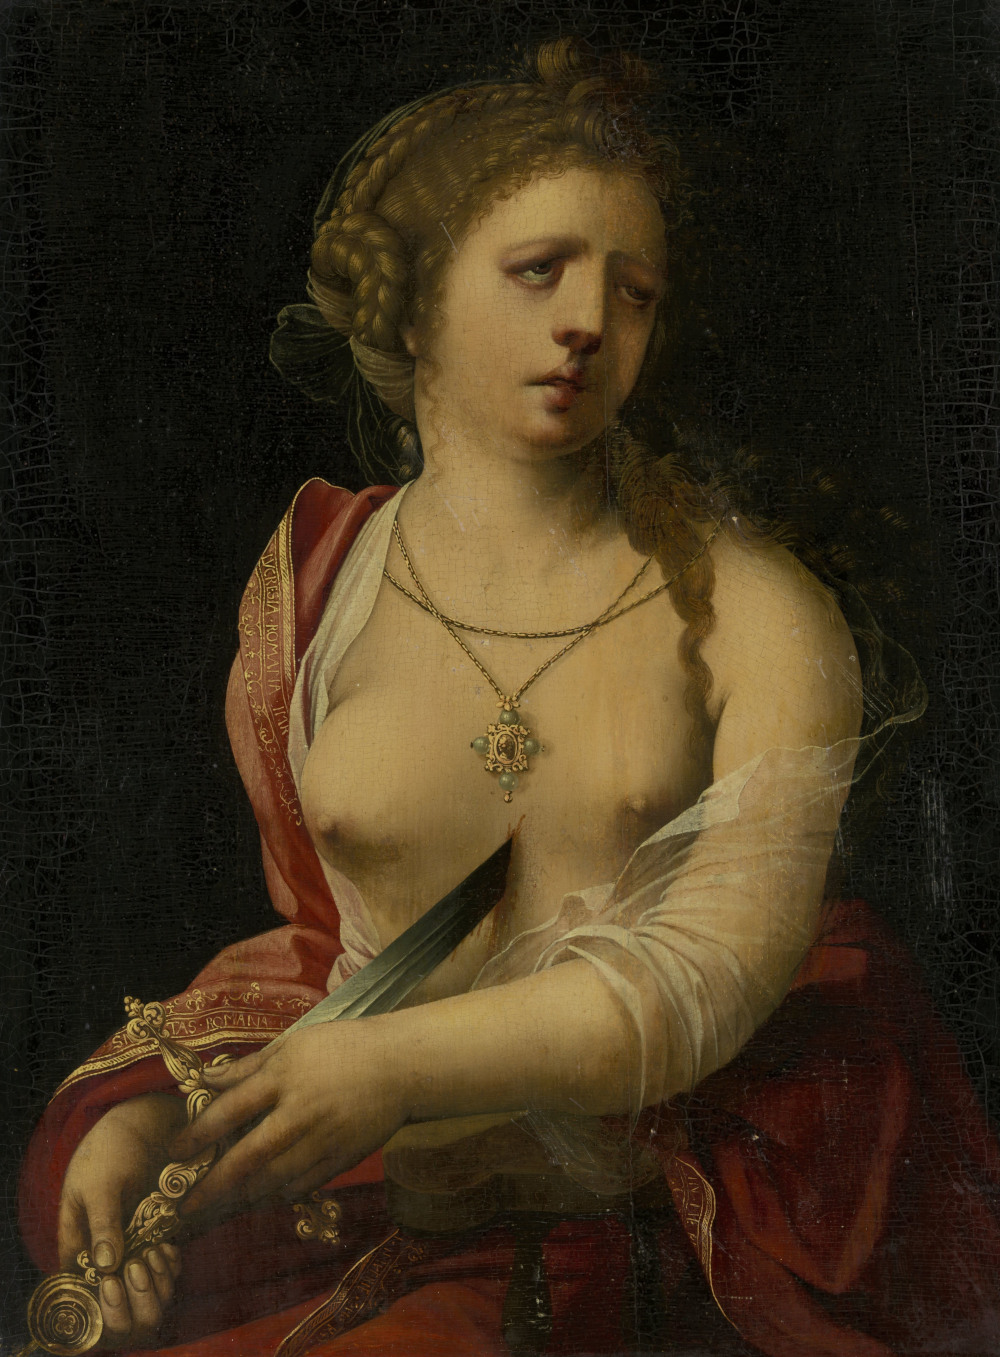
\includegraphics[keepaspectratio,width=\textwidth]{figures/suicide-of-lucretia-small.jpg}
  \captionart{SuicideofLucretia}
  \label{fig:suicideoflucretia}
\end{figure}
% Force float here
\clearpage{}
\thispagestyle{titleontop}
\chapter{Cure of Melancholy in General}
{
%THE SECOND PARTITION. THE CURE OF MELANCHOLY. THE FIRST SECTION, MEMBER, SUBSECTION.
%PART. II SECT. I MEMB. I SUBSECT. I
\section{Unlawful Cures rejected.}
\lettrine[lines=3]{I}{nveterate} Melancholy, howsoever it may seem to be a continuate,
inexorable disease, hard to be cured, accompanying them to their
graves, most part, as Montanus observes\authorfootnote{2789}, yet many times it may be
helped, even that which is most violent, or at least, according to the
same author\authorfootnote{2790}, it may be mitigated and much eased. Nil desperandum.
It may be hard to cure, but not impossible for him that is most
grievously affected, if he but willing to be helped.

Upon this good hope I will proceed, using the same method in the cure,
which I have formerly used in the rehearsing of the causes; first
general, then particular; and those according to their several species.
Of these cures some be lawful, some again unlawful, which though
frequent, familiar, and often used, yet justly censured, and to be
controverted. As first, whether by these diabolical means, which are
commonly practised by the devil and his ministers, sorcerers, witches,
magicians, \etc{}, by spells, cabilistical words, charms, characters,
images, amulets, ligatures, philters, incantations, \etc{}, this disease
and the like may be cured? and if they may, whether it be lawful to
make use of them, those magnetical cures, or for our good to seek after
such means in any case? The first, whether they can do any such cures,
is questioned amongst many writers, some affirming, some denying.
Valesius, cont. med. lib. 5. cap. 6. Malleus Maleficar, Heurnius, lib.
3. pract. med. cap. 28. Caelius lib. 16. c. 16. Delrio Tom. 3. Wierus
lib. 2. de praestig. daem. Libanius Lavater de spect. part. 2. cap. 7.
Holbrenner the Lutheran in Pistorium, Polydore Virg. l. 1. de prodig.
Tandlerus, Lemnius, (Hippocrates and Avicenna amongst the rest) deny
that spirits or devils have any power over us, and refer all with
Pomponatius of Padua to natural causes and humours. Of the other
opinion are Bodinus Daemonamantiae, lib. 3, cap. 2. Arnoldus, Marcellus
Empyricus, I. Pistorius, Paracelsus Apodix. Magic. Agrippa lib. 2. de
occult. Philos. cap. 36. 69. 71. 72. et l. 3, c. 23, et 10. Marcilius
Ficinus de vit. coelit. compar. cap. 13. 15. 18. 21. \etc{} Galeottus de
promiscua doct. cap. 24. Jovianus Pontanus Tom. 2. Plin. lib. 28, c. 2.
Strabo, lib. 15. Geog. Leo Suavius: Goclenius de ung. armar. Oswoldus
Crollius, Ernestus Burgravius, Dr. Flud, \etc{} Cardan de subt. brings
many proofs out of Ars Notoria, and Solomon's decayed works, old
Hermes, Artefius, Costaben Luca, Picatrix, \etc{} that such cures may be
done. They can make fire it shall not burn, fetch back thieves or
stolen goods, show their absent faces in a glass, make serpents lie
still, stanch blood, salve gouts, epilepsies, biting of mad dogs,
toothache, melancholy, et omnia mundi mala, make men immortal, young
again as the \authorfootnote{2791}Spanish marquis is said to have done by one of his
slaves, and some, which jugglers in \authorfootnote{2792}China maintain still (as
Tragaltius writes) that they can do by their extraordinary skill in
physic, and some of our modern chemists by their strange limbecks, by
their spells, philosopher's stones and charms. \authorfootnote{2793}Many doubt, saith
Nicholas Taurellus, whether the devil can cure such diseases he hath
not made, and some flatly deny it, howsoever common experience confirms
to our astonishment, that magicians can work such feats, and that the
devil without impediment can penetrate through all the parts of our
bodies, and cure such maladies by means to us unknown. Daneus in his
tract de Sortiariis subscribes to this of Taurellus; Erastus de lamiis,
maintaineth as much, and so do most divines, out of their excellent
knowledge and long experience they can commit \authorfootnote{2794}agentes cum
patientibus, colligere semina rerum, eaque materiae applicare, as
Austin infers de Civ. Dei et de Trinit. lib. 3. cap. 7. et 8. they can
work stupendous and admirable conclusions; we see the effects only, but
not the causes of them. Nothing so familiar as to hear of such cures.

Sorcerers are too common; cunning men, wizards, and white-witches, as
they call them, in every village, which if they be sought unto, will
help almost all infirmities of body and mind, Servatores in Latin, and
they have commonly St. Catherine's wheel printed in the roof of their
mouth, or in some other part about them, resistunt incantatorum
praestigiis (\authorfootnote{2795}Boissardus writes) morbos a sagis motos propulsant
\etc{}, that to doubt of it any longer, \authorfootnote{2796}or not to believe, were to
run into that other sceptical extreme of incredulity, saith Taurellus.

Leo Suavius in his comment upon Paracelsus seems to make it an art,
which ought to be approved; Pistorius and others stiffly maintain the
use of charms, words, characters, \etc{}. Ars vera est, sed pauci artifices
reperiuntur; the art is true, but there be but a few that have skill in
it. Marcellius Donatus lib. 2. de hist, mir. cap. 1. proves out of
Josephus' eight books of antiquities, that \authorfootnote{2797}Solomon so cured all
the diseases of the mind by spells, charms, and drove away devils, and
that Eleazer did as much before Vespasian. Langius in his med. epist.
holds Jupiter Menecrates, that did so many stupendous cures in his
time, to have used this art, and that he was no other than a magician.

Many famous cures are daily done in this kind, the devil is an expert
physician, as Godelman calls him, lib. 1. cap. 18. and God permits
oftentimes these witches and magicians to produce such effects, as
Lavater cap. 3. lib. 8. part. 3. cap. 1. Polid. Virg. lib. 1. de
prodigiis, Delrio and others admit. Such cures may be done, and as
Paracels. Tom. 4. de morb. ament. stiffly maintains, \authorfootnote{2798}they cannot
otherwise be cured but by spells, seals, and spiritual physic.

\authorfootnote{2799}Arnoldus, lib. de sigillis, sets down the making of them, so doth
Rulandus and many others.

\latininlinetrans{this being granded}{Hoc posito}, they can effect such cures, the main question is, whether
it be lawful in a desperate case to crave their help, or ask a wizard's
advice. 'Tis a common practice of some men to go first to a witch, and
then to a physician, if one cannot the other shall, Flectere si
nequeant superos Acheronta movebunt. \authorfootnote{2800}It matters not, saith
Paracelsus, whether it be God or the devil, angels, or unclean spirits
cure him, so that he be eased. If a man fall into a ditch, as he
prosecutes it, what matter is it whether a friend or an enemy help him
out? and if I be troubled with such a malady, what care I whether the
devil himself, or any of his ministers by God's permission, redeem me?
He calls a \authorfootnote{2801} magician, God's minister and his vicar, applying that
of vos estis dii profanely to them, for which he is lashed by T.
Erastus part. 1. fol. 45. And elsewhere he encourageth his patients to
have a good faith, \authorfootnote{2802} a strong imagination, and they shall find the
effects: let divines say to the contrary what they will. He proves and
contends that many diseases cannot otherwise be cured. Incantatione
orti incantatione curari debent; if they be caused by incantation,
\authorfootnote{2803}they must be cured by incantation. Constantinus lib. 4. approves
of such remedies: Bartolus the lawyer, Peter Aerodius rerum Judic. lib.
3. tit. 7. Salicetus Godefridus, with others of that sect, allow of
them; modo sint ad sanitatem quae a magis fiunt, secus non, so they be
for the parties good, or not at all. But these men are confuted by
Remigius, Bodinus, daem. lib. 3. cap 2. Godelmanus lib. 1. cap. 8,
Wierus, Delrio lib. 6. quaest. 2. tom. 3. mag. inquis. Erastus de
Lamiis; all our \authorfootnote{2804}divines, schoolmen, and such as write cases of
conscience are against it, the scripture itself absolutely forbids it
as a mortal sin, Levit. cap. \rn{xviii.} \rn{xix.} \rn{xx.} Deut. \rn{xviii.} \etc{}. Rom.
\rn{viii.} 19. Evil is not to be done, that good may come of it. Much better
it were for such patients that are so troubled, to endure a little
misery in this life, than to hazard their souls' health for ever, and
as Delrio counselleth, \authorfootnote{2805}much better die, than be so cured. Some
take upon them to expel devils by natural remedies, and magical
exorcisms, which they seem to approve out of the practice of the
primitive church, as that above cited of Josephus, Eleazer, Irenaeus,
Tertullian, Austin. Eusebius makes mention of such, and magic itself
hath been publicly professed in some universities, as of old in
Salamanca in Spain, and Krakow in Poland: but condemned anno 1318, by
the chancellor and university of \authorfootnote{2806}Paris. Our pontifical writers
retain many of these adjurations and forms of exorcisms still in the
church; besides those in baptism used, they exorcise meats, and such as
are possessed, as they hold, in Christ's name. Read Hieron. Mengus cap.
3. Pet. Tyreus, part. 3. cap. 8. What exorcisms they prescribe, besides
those ordinary means of \authorfootnote{2807}fire suffumigations, lights, cutting the
air with swords, cap. 57. herbs, odours: of which Tostatus treats, 2.
Reg. cap. 16. quaest. 43, you shall find many vain and frivolous
superstitious forms of exorcisms among them, not to be tolerated, or
endured.

%MEMB. II.

\section{Lawful Cures, first from God.}

\lettrine{B}{eing} so clearly evinced, as it is, all unlawful cures are to be
refused, it remains to treat of such as are to be admitted, and those
are commonly such which God hath appointed, \authorfootnote{2808}by virtue of stones,
herbs, plants, meats, and the like, which are prepared and applied to
our use, by art and industry of physicians, who are the dispensers of
such treasures for our good, and to be \authorfootnote{2809}honoured for necessities'
sake, God's intermediate ministers, to whom in our infirmities we are
to seek for help. Yet not so that we rely too much, or wholly upon
them: a Jove principium, we must first begin with \authorfootnote{2810}prayer, and
then use physic; not one without the other, but both together. To pray
alone, and reject ordinary means, is to do like him in Aesop, that when
his cart was stalled, lay flat on his back, and cried aloud help
Hercules, but that was to little purpose, except as his friend advised
him, rotis tute ipse annitaris, he whipped his horses withal, and put
his shoulder to the wheel. God works by means, as Christ cured the
blind man with clay and spittle: Orandum est ut sit mens sana in
corpore sano. As we must pray for health of body and mind, so we must
use our utmost endeavours to preserve and continue it. Some kind of
devils are not cast out but by fasting and prayer, and both necessarily
required, not one without the other. For all the physic we can use,
art, excellent industry, is to no purpose without calling upon God, nil
juvat immensos Cratero promittere montes: it is in vain to seek for
help, run, ride, except God bless us.
\authorfootnote{2811}---non Siculi dapes
Dulcem elaborabunt saporem.
Non animum cytheraeve cantus.

\authorfootnote{2812}Non domus et fundus, non aeris acervus et auri
Aegroto possunt domino deducere febres.

\authorfootnote{2813}With house, with land, with money, and with gold,
The master's fever will not be controll'd.

We must use our prayer and physic both together: and so no doubt but
our prayers will be available, and our physic take effect. 'Tis that
Hezekiah practised, 2 King. \rn{xx.} Luke the Evangelist: and which we are
enjoined, Coloss. IV. not the patient only, but the physician himself.
Hippocrates, a heathen, required this in a good practitioner, and so
did Galen, lib. de Plat. et Hipp. dog. lib. 9. cap. 15. and in that
tract of his, an mores sequantur temp. cor. ca. 11. 'tis a rule which
he doth inculcate, \authorfootnote{2814} and many others. Hyperius in his first book
de sacr. script. lect. speaking of that happiness and good success
which all physicians desire and hope for in their cures, \authorfootnote{2815}tells
them that it is not to be expected, except with a true faith they call
upon God, and teach their patients to do the like. The council of
Lateran, Canon 22. decreed they should do so: the fathers of the church
have still advised as much: whatsoever thou takest in hand (saith
\authorfootnote{2816}Gregory) let God be of thy counsel, consult with him; that
healeth those that are broken in heart, (Psal. \rn{cxlvii.} 3.) and bindeth
up their sores. Otherwise as the prophet Jeremiah, cap. \rn{xlvi.} 11.
denounced to Egypt, In vain shalt thou use many medicines, for thou
shalt have no health. It is the same counsel which \authorfootnote{2817}Comineus that
politic historiographer gives to all Christian princes, upon occasion
of that unhappy overthrow of Charles Duke of Burgundy, by means of
which he was extremely melancholy, and sick to death: insomuch that
neither physic nor persuasion could do him any good, perceiving his
preposterous error belike, adviseth all great men in such cases,
\authorfootnote{2818}to pray first to God with all submission and penitency, to
confess their sins, and then to use physic. The very same fault it was,
which the prophet reprehends in Asa king of Judah, that he relied more
on physic than on God, and by all means would have him to amend it. And
'tis a fit caution to be observed of all other sorts of men. The
prophet David was so observant of this precept, that in his greatest
misery and vexation of mind, he put this rule first in practice. Psal.
\rn{lxxvii.} 3. When I am in heaviness, I will think on God. Psal. \rn{lxxxvi.}
4. Comfort the soul of thy servant, for unto thee I lift up my soul:
and verse 7. In the day of trouble will I call upon thee, for thou
hearest me. Psal. \rn{liv.} 1. Save me, O God, by thy name, \etc. Psal.
\rn{lxxxii.} Psal. \rn{xx.} And 'tis the common practice of all good men, Psal.
cvii. 13. when their heart was humbled with heaviness, they cried to
the Lord in their troubles, and he delivered them from their distress.
And they have found good success in so doing, as David confesseth,
Psal. \rn{xxx.} 12. Thou hast turned my mourning into joy, thou hast loosed
my sackcloth, and girded me with gladness. Therefore he adviseth all
others to do the like, Psal. \rn{xxxi.} 24. All ye that trust in the Lord,
be strong, and he shall establish your heart. It is reported by
\authorfootnote{2819}Suidas, speaking of Hezekiah, that there was a great book of old,
of King Solomon's writing, which contained medicines for all manner of
diseases, and lay open still as they came into the temple: but Hezekiah
king of Jerusalem, caused it to be taken away, because it made the
people secure, to neglect their duty in calling and relying upon God,
out of a confidence on those remedies. \authorfootnote{2820}Minutius that worthy
consul of Rome in an oration he made to his soldiers, was much offended
with them, and taxed their ignorance, that in their misery called more
on him than upon God. A general fault it is all over the world, and
Minutius's speech concerns us all, we rely more on physic, and seek
oftener to physicians, than to God himself. As much faulty are they
that prescribe, as they that ask, respecting wholly their gain, and
trusting more to their ordinary receipts and medicines many times, than
to him that made them. I would wish all patients in this behalf, in the
midst of their melancholy, to remember that of Siracides, Ecc. \rn{i.} 11.
and 12. The fear of the Lord is glory and gladness, and rejoicing. The
fear of the Lord maketh a merry heart, and giveth gladness, and joy,
and long life: and all such as prescribe physic, to begin in nomine
Dei, as \authorfootnote{2821}Mesue did, to imitate Laelius a Fonte Eugubinus, that in
all his consultations, still concludes with a prayer for the good
success of his business; and to remember that of Creto one of their
predecessors, fuge avaritiam, et sine oratione et invocations Dei nihil
facias avoid covetousness, and do nothing without invocation upon God.

%MEMB. III.

\section[Whether it be lawful to seek to Saints for Aid]{Whether it be lawful to seek to Saints for Aid in this Disease.}

\lettrine{T}{hat} we must pray to God, no man doubts; but whether we should pray to
saints in such cases, or whether they can do us any good, it may be
lawfully controverted. Whether their images, shrines, relics,
consecrated things, holy water, medals, benedictions, those divine
amulets, holy exorcisms, and the sign of the cross, be available in
this disease? The papists on the one side stiffly maintain how many
melancholy, mad, demoniacal persons are daily cured at St. Anthony's
Church in Padua, at St. Vitus' in Germany, by our Lady of Loretto in
Italy, our Lady of Sichem in the Low Countries: \authorfootnote{2822}Quae et caecis
lumen, aegris salutem, mortuis vitam, claudis gressum reddit, omnes
morbos corporis, animi, curat, et in ipsos daemones imperium exercet;
she cures halt, lame, blind, all diseases of body and mind, and
commands the devil himself, saith Lipsius. twenty-five thousand in a
day come thither, \authorfootnote{2823}quis nisi numen in illum locum sic induxit; who
brought them? in auribus, in oculis omnium gesta, novae novitia; new
news lately done, our eyes and ears are full of her cures, and who can
relate them all? They have a proper saint almost for every peculiar
infirmity: for poison, gouts, agues, Petronella: St. Romanus for such
as are possessed; Valentine for the falling sickness; St. Vitus for
madmen, \etc{} and as of old \authorfootnote{2824}Pliny reckons up Gods for all diseases,
(Febri fanum dicalum est) Lilius Giraldus repeats many of her
ceremonies: all affections of the mind were heretofore accounted gods,
\authorfootnote{2825}love, and sorrow, virtue, honour, liberty, contumely, impudency,
had their temples, tempests, seasons, Crepitus Ventris, dea Vacuna, dea
Cloacina, there was a goddess of idleness, a goddess of the draught, or
jakes, Prema, Premunda, Priapus, bawdy gods, and gods for all \authorfootnote{2826}
offices. Varro reckons up 30,000 gods: Lucian makes Podagra the gout a
goddess, and assigns her priests and ministers: and melancholy comes
not behind; for as Austin mentioneth, lib. 4. de Civit. Dei, cap. 9.
there was of old Angerona dea, and she had her chapel and feasts, to
whom (saith \authorfootnote{2827}Macrobius) they did offer sacrifice yearly, that she
might be pacified as well as the rest. 'Tis no new thing, you see this
of papists; and in my judgment, that old doting Lipsius might have
fitter dedicated his \authorfootnote{2828}pen after all his labours, to this our
goddess of melancholy, than to his Virgo Halensis, and been her
chaplain, it would have become him better: but he, poor man, thought no
harm in that which he did, and will not be persuaded but that he doth
well, he hath so many patrons, and honourable precedents in the like
kind, that justify as much, as eagerly, and more than he there saith of
his lady and mistress: read but superstitious Coster and Gretser's
Tract de Cruce, Laur. Arcturus Fanteus de Invoc. Sanct. Bellarmine,
Delrio dis. mag. tom. 3. l. 6. quaest. 2. sect. 3. Greg. Tolosanus tom.
2. lib. 8. cap. 24. Syntax. Strozius Cicogna lib. 4. cap. 9. Tyreus,
Hieronymus Mengus, and you shall find infinite examples of cures done
in this kind, by holy waters, relics, crosses, exorcisms, amulets,
images, consecrated beads, \etc{}. Barradius the Jesuit boldly gives it
out, that Christ's countenance, and the Virgin Mary's, would cure
melancholy, if one had looked steadfastly on them. P. Morales the
Spaniard in his book de pulch. Jes. et Mar. confirms the same out of
Carthusianus, and I know not whom, that it was a common proverb in
those days, for such as were troubled in mind to say, eamus ad videndum
filium Mariae, let us see the son of Mary, as they now do post to St.
Anthony's in Padua, or to St. Hilary's at Poitiers in France. \authorfootnote{2829} In
a closet of that church, there is at this day St. Hilary's bed to be
seen, to which they bring all the madmen in the country, and after some
prayers and other ceremonies, they lay them down there to sleep, and so
they recover. It is an ordinary thing in those parts, to send all their
madmen to St. Hilary's cradle. They say the like of St. Tubery in
\authorfootnote{2830} another place. Giraldus Cambrensis Itin. Camb. c. 1. tells
strange stories of St. Ciricius' staff, that would cure this and all
other diseases. Others say as much (as \authorfootnote{2831}Hospinian observes) of the
three kings of Cologne; their names written in parchment, and hung
about a patient's neck, with the sign of the cross, will produce like
effects. Read Lippomanus, or that golden legend of Jacobus de Voragine,
you shall have infinite stories, or those new relations of our
\authorfootnote{2832}Jesuits in Japan and China, of Mat. Riccius, Acosta, Loyola,
Xaverius's life, \etc{}. Jasper Belga, a Jesuit, cured a mad woman by
hanging St. John's gospel about her neck, and many such. Holy water did
as much in Japan, \etc{}. Nothing so familiar in their works, as such
examples.

But we on the other side seek to God alone. We say with David, Psal.
\rn{xlvi.} 1. God is our hope and strength, and help in trouble, ready to be
found. For their catalogue of examples, we make no other answer, but
that they are false fictions, or diabolical illusions, counterfeit
miracles. We cannot deny but that it is an ordinary thing on St.
Anthony's day in Padua, to bring diverse madmen and demoniacal persons
to be cured: yet we make a doubt whether such parties be so affected
indeed, but prepared by their priests, by certain ointments and drams,
to cozen the commonalty, as \authorfootnote{2833} Hildesheim well saith; the like is
commonly practised in Bohemia as Mathiolus gives us to understand in
his preface to his comment upon Dioscorides. But we need not run so far
for examples in this kind, we have a just volume published at home to
this purpose. \authorfootnote{2834}A declaration of egregious popish impostures, to
withdraw the hearts of religious men under the pretence of casting out
of devils, practised by Father Edmunds, alias Weston, a Jesuit, and
diverse Romish priests, his wicked associates, with the several parties'
names, confessions, examinations, \etc{} which were pretended to be
possessed. But these are ordinary tricks only to get opinion and money,
mere impostures. Aesculapius of old, that counterfeit God, did as many
famous cures; his temple (as \authorfootnote{2835}Strabo relates) was daily full of
patients, and as many several tables, inscriptions, pendants, donories,
\etc{} to be seen in his church, as at this day our Lady of Loretto's in
Italy. It was a custom long since,
---suspendisse potenti
Vestimenta maris deo.\authorfootnote{2836} Hor. Od. 1. lib. 5. Od.

To do the like, in former times they were seduced and deluded as they
are now. 'Tis the same devil still, called heretofore Apollo, Mars,
Neptune, Venus, Aesculapius, \etc{} as \authorfootnote{2837}Lactantius lib. 2. de orig.
erroris, c. 17. observes. The same Jupiter and those bad angels are now
worshipped and adored by the name of St. Sebastian, Barbara, \etc{}.
Christopher and George are come in their places. Our lady succeeds
Venus (as they use her in many offices), the rest are otherwise
supplied, as \authorfootnote{2838}Lavater writes, and so they are deluded. \authorfootnote{2839}And
God often winks at these impostures, because they forsake his word, and
betake themselves to the devil, as they do that seek after holy water,
crosses, \etc{}. Wierus, lib. 4. cap. 3. What can these men plead for
themselves more than those heathen gods, the same cures done by both,
the same spirit that seduceth; but read more of the Pagan god's effects
in Austin de Civitate Dei, l. 10. cap. 6. and of Aesculapius especially
in Cicogna l. 3. cap. 8. or put case they could help, why should we
rather seek to them, than to Christ himself, since that he so kindly
invites us unto him, Come unto me all ye that are heavy laden, and I
will ease you, Mat. \rn{xi.} and we know that there is one God, one Mediator
between God and man, Jesus Christ, (1 Tim. \rn{ii.} 5) who gave himself a
ransom for all men. We know that we have an \authorfootnote{2840} advocate with the
Father, Jesus Christ (1 Joh. \rn{ii.} 1.) that there is no other name under
heaven, by which we can be saved, but by his, who is always ready to
hear us, and sits at the right hand of God, and from \authorfootnote{2841} whom we can
have no repulse, solus vult, solus potest, curat universos tanquam
singulos, et \authorfootnote{2842}unumquemque nostrum et solum, we are all as one to
him, he cares for us all as one, and why should we then seek to any
other but to him.

%MEMB. IV.

%SUBSECT. I.-_Physician, Patient, Physic_.
\section{Physician, Patient, Physic.}

\lettrine{O}{f} those diverse gifts which our apostle Paul saith God hath bestowed
on man, this of physic is not the least, but most necessary, and
especially conducing to the good of mankind. Next therefore to God in
all our extremities (for of the most high cometh healing, Ecclus.
\rn{xxxviii.} 2.) we must seek to, and rely upon the Physician, \authorfootnote{2843}who is
Manus Dei, saith Hierophilus, and to whom he hath given knowledge, that
he might be glorified in his wondrous works. With such doth he heal
men, and take away their pains, Ecclus. \rn{xxxviii.} 6. 7. when thou hast
need of him, let him not go from thee. The hour may come that their
enterprises may have good success, ver. 13. It is not therefore to be
doubted, that if we seek a physician as we ought, we may be eased of
our infirmities, such a one I mean as is sufficient, and worthily so
called; for there be many mountebanks, quacksalvers, empirics, in every
street almost, and in every village, that take upon them this name,
make this noble and profitable art to be evil spoken of and contemned,
by reason of these base and illiterate artificers: but such a physician
I speak of, as is approved, learned, skilful, honest, \etc{}, of whose
duty Wecker, Antid. cap. 2. and Syntax. med. Crato, Julius Alexandrinus
medic. Heurnius prax. med. lib. 3. cap. 1. \etc{} treat at large. For this
particular disease, him that shall take upon him to cure it,
\authorfootnote{2844}Paracelsus will have to be a magician, a chemist, a philosopher,
an astrologer; Thurnesserus, Severinus the Dane, and some other of his
followers, require as much: many of them cannot be cured but by magic.

\authorfootnote{2845}Paracelsus is so stiff for those chemical medicines, that in his
cures he will admit almost of no other physic, deriding in the mean
time Hippocrates, Galen, and all their followers: but magic, and all
such remedies I have already censured, and shall speak of chemistry
\authorfootnote{2846}elsewhere. Astrology is required by many famous physicians, by
Ficinus, Crato, Fernelius; \authorfootnote{2847}doubted of, and exploded by others: I
will not take upon me to decide the controversy myself, Johannes
Hossurtus, Thomas Boderius, and Maginus in the preface to his
mathematical physic, shall determine for me. Many physicians explode
astrology in physic (saith he), there is no use of it, unam artem ac
quasi temerarium insectantur, ac gloriam sibi ab ejus imperitia,
aucupari: but I will reprove physicians by physicians, that defend and
profess it, Hippocrates, Galen, Avicen. \etc{}, that count them butchers
without it, homicidas medicos Astrologiae ignaros, \etc{}. Paracelsus goes
farther, and will have his physician \authorfootnote{2848}predestinated to this man's
cure, this malady; and time of cure, the scheme of each geniture
inspected, gathering of herbs, of administering astrologically
observed; in which Thurnesserus and some iatromathematical professors,
are too superstitious in my judgment. \authorfootnote{2849}Hellebore will help, but
not alway, not given by every physician, \etc{} but these men are too
peremptory and self-conceited as I think. But what do I do, interposing
in that which is beyond my reach? A blind man cannot judge of colours,
nor I peradventure of these things. Only thus much I would require,
honesty in every physician, that he be not over-careless or covetous,
harpy-like to make a prey of his patient; Carnificis namque est (as
\authorfootnote{2850}Wecker notes) inter ipsos cruciatus ingens precium exposcere, as
a hungry chirurgeon often produces and wire-draws his cure, so long as
there is any hope of pay, Non missura cutem, nisi plena cruoris hirudo.

\authorfootnote{2851}Many of them, to get a fee, will give physic to every one that
comes, when there is no cause, and they do so irritare silentem morbum,
as \authorfootnote{2852}Heurnius complains, stir up a silent disease, as it often
falleth out, which by good counsel, good advice alone, might have been
happily composed, or by rectification of those six non-natural things
otherwise cured. This is Naturae bellum inferre, to oppugn nature, and
to make a strong body weak. Arnoldus in his 8 and 11 Aphorisms gives
cautions against, and expressly forbiddeth it. \authorfootnote{2853}A wise physician
will not give physic, but upon necessity, and first try medicinal diet,
before he proceed to medicinal cure. \authorfootnote{2854}In another place he laughs
those men to scorn, that think longis syrupis expugnare daemones et
animi phantasmata, they can purge fantastical imaginations and the
devil by physic. Another caution is, that they proceed upon good
grounds, if so be there be need of physic, and not mistake the disease;
they are often deceived by the \authorfootnote{2855}similitude of symptoms, saith
Heurnius, and I could give instance in many consultations, wherein they
have prescribed opposite physic. Sometimes they go too perfunctorily to
work, in not prescribing a just \authorfootnote{2856}course of physic: To stir up the
humour, and not to purge it, doth often more harm than good. Montanus
consil. 30. inveighs against such perturbations, that purge to the
halves, tire nature, and molest the body to no purpose. 'Tis a crabbed
humour to purge, and as Laurentius calls this disease, the reproach of
physicians: Bessardus, flagellum medicorum, their lash; and for that
cause, more carefully to be respected. Though the patient be averse,
saith Laurentius, desire help, and refuse it again, though he neglect
his own health, it behoves a good physician not to leave him helpless.

But most part they offend in that other extreme, they prescribe too
much physic, and tire out their bodies with continual potions, to no
purpose. Aetius tetrabib. 2. 2. ser. cap. 90. will have them by all
means therefore \authorfootnote{2857}to give some respite to nature, to leave off now
and then; and Laelius a Fonte Eugubinus in his consultations, found it
(as he there witnesseth) often verified by experience, \authorfootnote{2858}that after
a deal of physic to no purpose, left to themselves, they have
recovered. 'Tis that which Nic. Piso, Donatus Altomarus, still
inculcate, dare requiem naturae, to give nature rest.

%SUBSECT. II.-_Concerning the Patient_.
\section{Concerning the Patient.}

\lettrine{W}{hen} these precedent cautions are accurately kept, and that we have now
got a skilful, an honest physician to our mind, if his patient will not
be conformable, and content to be ruled by him, all his endeavours will
come to no good end. Many things are necessarily to be observed and
continued on the patient's behalf: First that he be not too niggardly
miserable of his purse, or think it too much he bestows upon himself,
and to save charges endanger his health. The Abderites, when they sent
for \authorfootnote{2859}Hippocrates, promised him what reward he would, \authorfootnote{2860}all the
gold they had, if all the city were gold he should have it. Naaman the
Syrian, when he went into Israel to Elisha to be cured of his leprosy,
took with him ten talents of silver, six thousand pieces of gold, and
ten changes of raiment, (2 Kings \rn{v.} 5.) Another thing is, that out of
bashfulness he do not conceal his grief; if aught trouble his mind, let
him freely disclose it, Stultorum incurata pudor malus ulcera celat: by
that means he procures to himself much mischief, and runs into a
greater inconvenience: he must be willing to be cured, and earnestly
desire it. Pars sanitatis velle sanare fuit, (Seneca). 'Tis a part of
his cure to wish his own health, and not to defer it too long.

\authorfootnote{2861}Qui blandiendo dulce nutrivit malum,
Soro recusat ferre quod subiit jugum.


He that by cherishing a mischief doth provoke,
Too late at last refuseth to cast off his yoke,

\authorfootnote{2862}Helleborum frustra cum jam cutis aegra tumebit,
Poscentes videas; venienti occurrite morbo.

When the skin swells, to seek it to appease
With hellebore, is vain; meet your disease.

By this means many times, or through their ignorance in not taking
notice of their grievance and danger of it, contempt, supine
negligence, extenuation, wretchedness and peevishness; they undo
themselves. The citizens, I know not of what city now, when rumour was
brought their enemies were coming, could not abide to hear it; and when
the plague begins in many places and they certainly know it, they
command silence and hush it up; but after they see their foes now
marching to their gates, and ready to surprise them, they begin to
fortify and resist when 'tis too late; when, the sickness breaks out
and can be no longer concealed, then they lament their supine
negligence: 'tis no otherwise with these men. And often out of
prejudice, a loathing, and distaste of physic, they had rather die, or
do worse, than take any of it. Barbarous immanity (\authorfootnote{2863}Melancthon
terms it) and folly to be deplored, so to contemn the precepts of
health, good remedies, and voluntarily to pull death, and many maladies
upon their own heads. Though many again are in that other extreme too
profuse, suspicious, and jealous of their health, too apt to take
physic on every small occasion, to aggravate every slender passion,
imperfection, impediment: if their finger do but ache, run, ride, send
for a physician, as many gentlewomen do, that are sick, without a
cause, even when they will themselves, upon every toy or small
discontent, and when he comes, they make it worse than it is, by
amplifying that which is not. \authorfootnote{2864}Hier. Capivaccius sets it down as a
common fault of all melancholy persons to say their symptoms are
greater than they are, to help themselves. And which \authorfootnote{2865}Mercurialis
notes, consil. 53. to be more troublesome to their physicians, than
other ordinary patients, that they may have change of physic.

A third thing to be required in a patient, is confidence, to be of good
cheer, and have sure hope that his physician can help him.

\authorfootnote{2866}Damascen the Arabian requires likewise in the physician himself,
that he be confident he can cure him, otherwise his physic will not be
effectual, and promise withal that he will certainly help him, make him
believe so at least. \authorfootnote{2867}Galeottus gives this reason, because the
form of health is contained in the physician's mind, and as Galen,
holds \authorfootnote{2868}confidence and hope to be more good than physic, he cures
most in whom most are confident. Axiocus sick almost to death, at the
very sight of Socrates recovered his former health. Paracelsus assigns
it for an only cause, why Hippocrates was so fortunate in his cures,
not for any extraordinary skill he had; \authorfootnote{2869}but because the common
people had a most strong conceit of his worth. To this of confidence we
may add perseverance, obedience, and constancy, not to change his
physician, or dislike him upon every toy; for he that so doth (saith
\authorfootnote{2870}Janus Damascen) or consults with many, falls into many errors; or
that useth many medicines. It was a chief caveat of \authorfootnote{2871}Seneca to his
friend Lucilius, that he should not alter his physician, or prescribed
physic: Nothing hinders health more; a wound can never be cured, that
hath several plasters. Crato consil. 186. taxeth all melancholy persons
of this fault: \authorfootnote{2872}'Tis proper to them, if things fall not out to
their mind, and that they have not present ease, to seek another and
another; (as they do commonly that have sore eyes) twenty one after
another, and they still promise all to cure them, try a thousand
remedies; and by this means they increase their malady, make it most
dangerous and difficult to be cured. They try many (saith \authorfootnote{2873}
Montanus) and profit by none: and for this cause, consil. 24. he
enjoins his patient before he take him in hand, \authorfootnote{2874}perseverance and
sufferance, for in such a small time no great matter can be effected,
and upon that condition he will administer physic, otherwise all his
endeavour and counsel would be to small purpose. And in his 31. counsel
for a notable matron, he tells her, \authorfootnote{2875}if she will be cured, she
must be of a most abiding patience, faithful obedience, and singular
perseverance; if she remit, or despair, she can expect or hope for no
good success. Consil. 230. for an Italian Abbot, he makes it one of the
greatest reasons why this disease is so incurable, \authorfootnote{2876}because the
parties are so restless, and impatient, and will therefore have him
that intends to be eased, \authorfootnote{2877}to take physic, not for a month, a
year, but to apply himself to their prescriptions all the days of his
life. Last of all, it is required that the patient be not too bold to
practise upon himself, without an approved physician's consent, or to
try conclusions, if he read a receipt in a book; for so, many grossly
mistake, and do themselves more harm than good. That which is conducing
to one man, in one case, the same time is opposite to another. \authorfootnote{2878}An
ass and a mule went laden over a brook, the one with salt, the other
with wool: the mule's pack was wet by chance, the salt melted, his
burden the lighter, and he thereby much eased: he told the ass, who,
thinking to speed as well, wet his pack likewise at the next water, but
it was much the heavier, he quite tired. So one thing may be good and
bad to several parties, upon diverse occasions. Many things (saith
\authorfootnote{2879} Penottus) are written in our books, which seem to the reader to
be excellent remedies, but they that make use of them are often
deceived, and take for physic poison. I remember in Valleriola's
observations, a story of one John Baptist a Neapolitan, that finding by
chance a pamphlet in Italian, written in praise of hellebore, would
needs adventure on himself, and took one dram for one scruple, and had
not he been sent for, the poor fellow had poisoned himself. From whence
he concludes out of Damascenus 2 et 3. Aphoris. \authorfootnote{2880}that without
exquisite knowledge, to work out of books is most dangerous: how
unsavoury a thing it is to believe writers, and take upon trust, as
this patient perceived by his own peril. I could recite such another
example of mine own knowledge, of a friend of mine, that finding a
receipt in Brassivola, would needs take hellebore in substance, and try
it on his own person; but had not some of his familiars come to visit
him by chance, he had by his indiscretion hazarded himself: many such I
have observed. These are those ordinary cautions, which I should think
fit to be noted, and he that shall keep them, as \authorfootnote{2881} Montanus saith,
shall surely be much eased, if not thoroughly cured.

%SUBSECT. III.-_Concerning Physic_.
\section{Concerning Physic.}

\lettrine{P}{hysic} itself in the last place is to be considered; for the Lord hath
created medicines of the earth, and he that is wise will not abhor
them. Ecclus. \rn{xxxviii.} 4. ver. 8. of such doth the apothecary
make a confection, \etc{}. Of these medicines there be diverse and infinite
kinds, plants, metals, animals, \etc{}, and those of several natures, some
good for one, hurtful to another: some noxious in themselves, corrected
by art, very wholesome and good, simples, mixed, \etc{}, and therefore
left to be managed by discreet and skilful physicians, and thence
applied to man's use. To this purpose they have invented method, and
several rules of art, to put these remedies in order, for their
particular ends. Physic (as Hippocrates defines it) is nought else but
\authorfootnote{2882}addition and subtraction; and as it is required in all other
diseases, so in this of melancholy it ought to be most accurate, it
being (as \authorfootnote{2883}Mercurialis acknowledgeth) so common an affection in
these our times, and therefore fit to be understood. Several prescripts
and methods I find in several men, some take upon them to cure all
maladies with one medicine, severally applied, as that panacea, aurum
potabile, so much controverted in these days, herba solis, \etc{}.

Paracelsus reduceth all diseases to four principal heads, to whom
Severinus, Ravelascus, Leo Suavius, and others adhere and imitate:
those are leprosy, gout, dropsy, falling-sickness. To which they reduce
the rest; as to leprosy, ulcers, itches, furfurs, scabs, \etc{}. To gout,
stone, colic, toothache, headache, \etc{}. To dropsy, agues, jaundice,
cachexia, \etc{}. To the falling-sickness, belong palsy, vertigo, cramps,
convulsions, incubus, apoplexy, \etc{}. \authorfootnote{2884}If any of these four
principal be cured (saith Ravelascus) all the inferior are cured, and
the same remedies commonly serve: but this is too general, and by some
contradicted: for this peculiar disease of melancholy, of which I am
now to speak, I find several cures, several methods and prescripts.

They that intend the practic cure of melancholy, saith Duretus in his
notes to Hollerius, set down nine peculiar scopes or ends; Savanarola
prescribes seven especial canons. \AE{}lianus Montaltus cap. 26.

Faventinus in his empirics, Hercules de Saxonia, \etc{}, have their
several injunctions and rules, all tending to one end. The ordinary is
threefold, which I mean to follow. \textgreek[variant=ancient]{Διαιτητικὴ}, \emph{Pharmaceutica}, and
\emph{Chirurgica}, diet, or living, apothecary, chirurgery, which Wecker,
Crato, Guianerius, \etc{}, and most, prescribe; of which I will insist,
and speak in their order.


%SECT. II. MEMB. I.
%SUBSECT. I.-_Diet rectified in substance_.
\section{Diet rectified in substance.}

\lettrine{D}{iet}, \textgreek[variant=ancient]{Διαιτητικὴ}, victus, or living, according to \authorfootnote{2885} Fuchsius and
others, comprehends those six non-natural things, which I have before
specified, are especial causes, and being rectified, a sole or chief
part of the cure. \authorfootnote{2886}Johannes Arculanus, cap. 16. in 9. Rhasis,
accounts the rectifying of these six a sufficient cure. Guianerius,
tract. 15, cap. 9. calls them, propriam et primam curam, the principal
cure: so doth Montanus, Crato, Mercurialis, Altomarus, \etc{}, first to be
tried, Lemnius, instit. cap. 22, names them the hinges of our health,
\authorfootnote{2887}no hope of recovery without them. Reinerus Solenander, in his
seventh consultation for a Spanish young gentlewoman, that was so
melancholy she abhorred all company, and would not sit at table with
her familiar friends, prescribes this physic above the rest, \authorfootnote{2888}no
good to be done without it. \authorfootnote{2889}Aretus, lib. 1. cap. 7. an old
physician, is of opinion, that this is enough of itself, if the party
be not too far gone in sickness. \authorfootnote{2890}Crato, in a consultation of his
for a noble patient, tells him plainly, that if his highness will keep
but a good diet, he will warrant him his former health. \authorfootnote{2891}Montanus,
consil. 27. for a nobleman of France, admonisheth his lordship to be
most circumspect in his diet, or else all his other physic will
\authorfootnote{2892}be to small purpose. The same injunction I find verbatim in J.
Caesar Claudinus, Respon. 34. Scoltzii, consil. 183. Trallianus, cap.
16. lib. 1. Laelius a Fonte Aeugubinus often brags, that he hath done
more cures in this kind by rectification of diet, than all other physic
besides. So that in a word I may say to most melancholy men, as the fox
said to the weasel, that could not get out of the garner, Macra cavum
repetes, quem macra subisti, \authorfootnote{2893}the six non-natural things caused
it, and they must cure it. Which howsoever I treat of, as proper to the
meridian of melancholy, yet nevertheless, that which is here said with
him in \authorfootnote{2894}Tully, though writ especially for the good of his friends
at Tarentum and Sicily, yet it will generally serve \authorfootnote{2895}most other
diseases, and help them likewise, if it be observed.

Of these six non-natural things, the first is diet, properly so called,
which consists in meat and drink, in which we must consider substance,
quantity, quality, and that opposite to the precedent. In substance,
such meats are generally commended, which are \authorfootnote{2896}moist, easy of
digestion, and not apt to engender wind, not fried, nor roasted, but
sod (saith Valescus, Altomarus, Piso, \etc{}) hot and moist, and of good
nourishment; Crato, consil. 21. lib. 2. admits roast meat, \authorfootnote{2897}if the
burned and scorched superficies, the brown we call it, be pared off.

Salvianus, lib. 2. cap. 1. cries out on cold and dry meats; \authorfootnote{2898}young
flesh and tender is approved, as of kid, rabbits, chickens, veal,
mutton, capons, hens, partridge, pheasant, quails, and all mountain
birds, which are so familiar in some parts of Africa, and in Italy, and
as \authorfootnote{2899}Dublinius reports, the common food of boors and clowns in
Palestine. Galen takes exception at mutton, but without question he
means that rammy mutton, which is in Turkey and Asia Minor, which have
those great fleshy tails, of forty-eight pounds weight, as Vertomannus
witnesseth, navig. lib. 2. cap. 5. The lean of fat meat is best, and
all manner of broths, and pottage, with borage, lettuce, and such
wholesome herbs are excellent good, especially of a cock boiled; all
spoon meat. Arabians commend brains, but \authorfootnote{2900}Laurentius, c. 8.
excepts against them, and so do many others; \authorfootnote{2901}eggs are justified
as a nutritive wholesome meat, butter and oil may pass, but with some
limitation; so \authorfootnote{2902}Crato confines it, and to some men sparingly at
set times, or in sauce, and so sugar and honey are approved. \authorfootnote{2903}All
sharp and sour sauces must be avoided, and spices, or at least seldom
used: and so saffron sometimes in broth may be tolerated; but these
things may be more freely used, as the temperature of the party is hot
or cold, or as he shall find inconvenience by them. The thinnest,
whitest, smallest wine is best, not thick, nor strong; and so of beer,
the middling is fittest. Bread of good wheat, pure, well purged from
the bran is preferred; Laurentius, cap. 8. would have it kneaded with
rain water, if it may be gotten.

\subsection{Water.}
Pure, thin, light water by all means use, of good smell and
taste, like to the air in sight, such as is soon hot, soon cold, and
which Hippocrates so much approves, if at least it may be had. Rain
water is purest, so that it fall not down in great drops, and be used
forthwith, for it quickly putrefies. Next to it fountain water that
riseth in the east, and runneth eastward, from a quick running spring,
from flinty, chalky, gravelly grounds: and the longer a river runneth,
it is commonly the purest, though many springs do yield the best water
at their fountains. The waters in hotter countries, as in Turkey,
Persia, India, within the tropics, are frequently purer than ours in
the north, more subtile, thin, and lighter, as our merchants observe,
by four ounces in a pound, pleasanter to drink, as good as our beer,
and some of them, as Choaspis in Persia, preferred by the Persian
kings, before wine itself.

\authorfootnote{2904}Clitorio quicunque sitim de fonte levarit
Vina fugit gaudetque meris abstemius undis.

Many rivers I deny not are muddy still, white, thick, like those in
China, Nile in Egypt, Tiber at Rome, but after they be settled two or
three days, defecate and clear, very commodious, useful and good. Many
make use of deep wells, as of old in the Holy Land, lakes, cisterns,
when they cannot be better provided; to fetch it in carts or gondolas,
as in Venice, or camels' backs, as at Cairo in Egypt, \authorfootnote{2905}Radzivilius
observed 8000 camels daily there, employed about that business; some
keep it in trunks, as in the East Indies, made four square with
descending steps, and 'tis not amiss, for I would not have any one so
nice as that Grecian Calis, sister to Nicephorus, emperor of
Constantinople, and \authorfootnote{2906}married to Dominitus Silvius, duke of Venice,
that out of incredible wantonness, communi aqua uti nolebat, would use
no vulgar water; but she died tanta (saith mine author) foetidissimi
puris copia, of so fulsome a disease, that no water could wash her
clean. \authorfootnote{2907}Plato would not have a traveller lodge in a city that is
not governed by laws, or hath not a quick stream running by it; illud
enim animum, hoc corrumpit valetudinem, one corrupts the body, the
other the mind. But this is more than needs, too much curiosity is
naught, in time of necessity any water is allowed. Howsoever, pure
water is best, and which (as Pindarus holds) is better than gold; an
especial ornament it is, and very commodious to a city (according to
\authorfootnote{2908}Vegetius) when fresh springs are included within the walls, as at
Corinth, in the midst of the town almost, there was arx altissima
scatens fontibus, a goodly mount full of fresh water springs: if nature
afford them not they must be had by art. It is a wonder to read of
those \authorfootnote{2909}stupend aqueducts, and infinite cost hath been bestowed in
Rome of old, Constantinople, Carthage, Alexandria, and such populous
cities, to convey good and wholesome waters: read \authorfootnote{2910}Frontinus,
Lipsius de admir. \authorfootnote{2911}Plinius, lib. 3. cap. 11, Strabo in his Geogr.

That aqueduct of Claudius was most eminent, fetched upon arches fifteen
miles, every arch 109 feet high: they had fourteen such other
aqueducts, besides lakes and cisterns, 700 as I take it; \authorfootnote{2912}every
house had private pipes and channels to serve them for their use. Peter
Gillius, in his accurate description of Constantinople, speaks of an
old cistern which he went down to see, 336 feet long, 180 feet broad,
built of marble, covered over with arch-work, and sustained by 336
pillars, 12 feet asunder, and in eleven rows, to contain sweet water.

Infinite cost in channels and cisterns, from Nilus to Alexandria, hath
been formerly bestowed, to the admiration of these times; \authorfootnote{2913}their
cisterns so curiously cemented and composed, that a beholder would take
them to be all of one stone: when the foundation is laid, and cistern
made, their house is half built. That Segovian aqueduct in Spain, is
much wondered at in these days, \authorfootnote{2914}upon three rows of pillars, one
above another, conveying sweet water to every house: but each city
almost is full of such aqueducts. Amongst the rest \authorfootnote{2915}he is
eternally to be commended, that brought that new stream to the north
side of London at his own charge: and Mr. Otho Nicholson, founder of
our waterworks and elegant conduit in Oxford. So much have all times
attributed to this element, to be conveniently provided of it: although
Galen hath taken exceptions at such waters, which run through leaden
pipes, ob cerussam quae in iis generatur, for that unctuous ceruse,
which causeth dysenteries and fluxes; \authorfootnote{2916}yet as Alsarius Crucius of
Genna well answers, it is opposite to common experience. If that were
true, most of our Italian cities, Montpelier in France, with infinite
others, would find this inconvenience, but there is no such matter. For
private families, in what sort they should furnish themselves, let them
consult with P. Crescentius, de Agric. l. 1. c. 4, Pamphilius
Hirelacus, and the rest.

Amongst fishes, those are most allowed of, that live in gravelly or
sandy waters, pikes, perch, trout, gudgeon, smelts, flounders, \etc{}.
Hippolitus Salvianus takes exception at carp; but I dare boldly say
with \authorfootnote{2917} Dubravius, it is an excellent meat, if it come not from
\authorfootnote{2918}muddy pools, that it retain not an unsavoury taste. Erinacius
Marinus is much commended by Oribatius, Aetius, and most of our late
writers.

\authorfootnote{2919}Crato, consil. 21. lib. 2. censures all manner of fruits, as
subject to putrefaction, yet tolerable at sometimes, after meals, at
second course, they keep down vapours, and have their use. Sweet fruits
are best, as sweet cherries, plums, sweet apples, pearmains, and
pippins, which Laurentius extols, as having a peculiar property against
this disease, and Plater magnifies, omnibus modis appropriata
conveniunt, but they must be corrected for their windiness: ripe grapes
are good, and raisins of the sun, musk-melons well corrected, and
sparingly used. Figs are allowed, and almonds blanched. Trallianus
discommends figs, \authorfootnote{2920}Salvianus olives and capers, which \authorfootnote{2921}others
especially like of, and so of pistick nuts. Montanus and Mercurialis
out of Avenzoar, admit peaches, \authorfootnote{2922}pears, and apples baked after
meals, only corrected with sugar, and aniseed, or fennel-seed, and so
they may be profitably taken, because they strengthen the stomach, and
keep down vapours. The like may be said of preserved cherries, plums,
marmalade of plums, quinces, \etc{}, but not to drink after them.
\authorfootnote{2923}Pomegranates, lemons, oranges are tolerated, if they be not too
sharp.

\authorfootnote{2924}Crato will admit of no herbs, but borage, bugloss, endive,
fennel, aniseed, baum; Callenius and Arnoldus tolerate lettuce,
spinach, beets, \etc{}. The same Crato will allow no roots at all to be
eaten. Some approve of potatoes, parsnips, but all corrected for wind.
No raw salads; but as Laurentius prescribes, in broths; and so Crato
commends many of them: or to use borage, hops, baum, steeped in their
ordinary drink. \authorfootnote{2925}Avenzoar magnifies the juice of a pomegranate, if
it be sweet, and especially rose water, which he would have to be used
in every dish, which they put in practice in those hot countries, about
Damascus, where (if we may believe the relations of Vertomannus) many
hogsheads of rose water are to be sold in the market at once, it is in
so great request with them.

%SUBSECT. II.-_Diet rectified in quantity_.
\section{Diet rectified in quantity.}

\lettrine{M}{an} alone, saith \authorfootnote{2926}Cardan, eats and drinks without appetite, and
useth all his pleasure without necessity, animae vitio, and thence come
many inconveniences unto him. For there is no meat whatsoever, though
otherwise wholesome and good, but if unseasonably taken, or
immoderately used, more than the stomach can well bear, it will
engender crudity, and do much harm. Therefore \authorfootnote{2927}Crato adviseth his
patient to eat but twice a day, and that at his set meals, by no means
to eat without an appetite, or upon a full stomach, and to put seven
hours' difference between dinner and supper. Which rule if we did
observe in our colleges, it would be much better for our healths: but
custom, that tyrant, so prevails, that contrary to all good order and
rules of physic, we scarce admit of five. If after seven hours'
tarrying he shall have no stomach, let him defer his meal, or eat very
little at his ordinary time of repast. This very counsel was given by
Prosper Calenus to Cardinal Caesius, labouring of this disease; and
\authorfootnote{2928} Platerus prescribes it to a patient of his, to be most severely
kept. Guianerius admits of three meals a day, but Montanus, consil. 23.
pro. Ab. Italo, ties him precisely to two. And as he must not eat
overmuch, so he may not absolutely fast; for as Celsus contends, lib.
1. Jacchinus 15. in 9. Rhasis, \authorfootnote{2929}repletion and inanition may both
do harm in two contrary extremes. Moreover, that which he doth eat,
must be well \authorfootnote{2930}chewed, and not hastily gobbled, for that causeth
crudity and wind; and by all means to eat no more than he can well
digest. Some think (saith \authorfootnote{2931} Trincavelius, lib. 11. cap. 29. de
curand. part. hum.) the more they eat the more they nourish themselves:
eat and live, as the proverb is, not knowing that only repairs man,
which is well concocted, not that which is devoured. Melancholy men
most part have good \authorfootnote{2932}appetites, but ill digestion, and for that
cause they must be sure to rise with an appetite; and that which
Socrates and Disarius the physicians in \authorfootnote{2933}Macrobius so much
require, St. Hierom enjoins Rusticus to eat and drink no more than,
will \authorfootnote{2934}satisfy hunger and thirst. \authorfootnote{2935}Lessius, the Jesuit, holds
twelve, thirteen, or fourteen ounces, or in our northern countries,
sixteen at most, (for all students, weaklings, and such as lead an idle
sedentary life) of meat, bread, \etc{}, a fit proportion for a whole day,
and as much or little more of drink. Nothing pesters the body and mind
sooner than to be still fed, to eat and ingurgitate beyond all measure,
as many do. \authorfootnote{2936} By overmuch eating and continual feasts they stifle
nature, and choke up themselves; which, had they lived coarsely, or
like galley slaves been tied to an oar, might have happily prolonged
many fair years.

A great inconvenience comes by variety of dishes, which causeth the
precedent distemperature, \authorfootnote{2937}than which (saith Avicenna) nothing is
worse; to feed on diversity of meats, or overmuch, Sertorius-like, in
lucem caenare, and as commonly they do in Muscovy and Iceland, to
prolong their meals all day long, or all night. Our northern countries
offend especially in this, and we in this island (ampliter viventes in
prandiis et caenis, as \authorfootnote{2938}Polydore notes) are most liberal feeders,
but to our own hurt. \authorfootnote{2939}Persicos odi puer apparatus: Excess of meat
breedeth sickness, and gluttony causeth choleric diseases: by
surfeiting many perish, but he that dieteth himself prolongeth his
life, Ecclus. \rn{xxxvii.} 29, 30. We account it a great glory for a man to
have his table daily furnished with variety of meats: but hear the
physician, he pulls thee by the ear as thou sittest, and telleth thee,
\authorfootnote{2940}that nothing can be more noxious to thy health than such variety
and plenty. Temperance is a bridle of gold, and he that can use it
aright, \authorfootnote{2941}ego non summis viris comparo, sed simillimum Deo judico,
is liker a God than a man: for as it will transform a beast to a man
again, so will it make a man a God. To preserve thine honour, health,
and to avoid therefore all those inflations, torments, obstructions,
crudities, and diseases that come by a full diet, the best way is to
\authorfootnote{2942}feed sparingly of one or two dishes at most, to have ventrem bene
moratum, as Seneca calls it, \authorfootnote{2943}to choose one of many, and to feed
on that alone, as Crato adviseth his patient. The same counsel
\authorfootnote{2944}Prosper Calenus gives to Cardinal Caesius, to use a moderate and
simple diet: and though his table be jovially furnished by reason of
his state and guests, yet for his own part to single out some one
savoury dish and feed on it. The same is inculcated by \authorfootnote{2945}Crato,
consil. 9. l. 2. to a noble personage affected with this grievance, he
would have his highness to dine or sup alone, without all his
honourable attendance and courtly company, with a private friend or so,
\authorfootnote{2946}a dish or two, a cup of Rhenish wine, \etc{}. Montanus, consil. 24.
for a noble matron enjoins her one dish, and by no means to drink
between meals. The like, consil. 229. or not to eat till he be an
hungry, which rule Berengarius did most strictly observe, as Hilbertus,
Cenomecensis Episc. writes in his life,
---cui non fuit unquam
Ante sitim potus, nec cibus ante famem,

and which all temperate men do constantly keep. It is a frequent
solemnity still used with us, when friends meet, to go to the alehouse
or tavern, they are not sociable otherwise: and if they visit one
another's houses, they must both eat and drink. I reprehend it not
moderately used; but to some men nothing can be more offensive; they
had better, I speak it with Saint \authorfootnote{2947}Ambrose, pour so much water in
their shoes.

It much avails likewise to keep good order in our diet, \authorfootnote{2948}to eat
liquid things first, broths, fish, and such meats as are sooner
corrupted in the stomach; harder meats of digestion must come last.

Crato would have the supper less than the dinner, which Cardan,
Contradict. lib. 1. tract. 5. contradict. 18. disallows, and that by
the authority of Galen. 7. art. curat. cap. 6. and for four reasons he
will have the supper biggest: I have read many treatises to this
purpose, I know not how it may concern some few sick men, but for my
part generally for all, I should subscribe to that custom of the
Romans, to make a sparing dinner, and a liberal supper; all their
preparation and invitation was still at supper, no mention of dinner.

Many reasons I could give, but when all is said pro and con,
\authorfootnote{2949}Cardan's rule is best, to keep that we are accustomed unto,
though it be naught, and to follow our disposition and appetite in some
things is not amiss; to eat sometimes of a dish which is hurtful, if we
have an extraordinary liking to it. Alexander Severus loved hares and
apples above all other meats, as \authorfootnote{2950}Lampridius relates in his life:
one pope pork, another peacock, \etc{}; what harm came of it? I conclude
our own experience is the best physician; that diet which is most
propitious to one, is often pernicious to another, such is the variety
of palates, humours, and temperatures, let every man observe, and be a
law unto himself. Tiberius, in \authorfootnote{2951}Tacitus, did laugh at all such,
that thirty years of age would ask counsel of others concerning matters
of diet; I say the same.

These few rules of diet he that keeps, shall surely find great ease and
speedy remedy by it. It is a wonder to relate that prodigious
temperance of some hermits, anchorites, and fathers of the church: he
that shall but read their lives, written by Hierom, Athanasius, \etc{},
how abstemious heathens have been in this kind, those Curii and
Fabritii, those old philosophers, as Pliny records, lib. 11. Xenophon,
lib. 1. de vit. Socrat. Emperors and kings, as Nicephorus relates,
Eccles. hist. lib. 18. cap. 8. of Mauritius, Ludovicus Pius, \etc{}, and
that admirable \authorfootnote{2952}example of Ludovicus Cornarus, a patrician of
Venice, cannot but admire them. This have they done voluntarily and in
health; what shall these private men do that are visited with sickness,
and necessarily \authorfootnote{2953}enjoined to recover, and continue their health?
It is a hard thing to observe a strict diet, et qui medice vivit,
misere vivit, \authorfootnote{2954}as the saying is, quale hoc ipsum erit vivere, his
si privatus fueris? as good be buried, as so much debarred of his
appetite; excessit medicina malum, the physic is more troublesome than
the disease, so he complained in the poet, so thou thinkest: yet he
that loves himself will easily endure this little misery, to avoid a
greater inconvenience; e malis minimum better do this than do worse.

And as \authorfootnote{2955}Tully holds, better be a temperate old man than a
lascivious youth. 'Tis the only sweet thing (which he adviseth) so to
moderate ourselves, that we may have senectutem in juventute, et in
juventute senectutem, be youthful in our old age, staid in our youth,
discreet and temperate in both.

%MEMB. II.

\section{Retention and Evacuation rectified.}

\lettrine{I} have declared in the causes what harm costiveness hath done in
procuring this disease; if it be so noxious, the opposite must needs be
good, or mean at least, as indeed it is, and to this cure necessarily
required; maxime conducit, saith Montaltus, cap. 27. it very much
avails. \authorfootnote{2956} Altomarus, cap. 7, commends walking in a morning, into
some fair green pleasant fields, but by all means first, by art or
nature, he will have these ordinary excrements evacuated. Piso calls
it, Beneficium ventris, the benefit, help or pleasure of the belly, for
it doth much ease it. Laurentius, cap. 8, Crato, consil. 21. l. 2.
prescribes it once a day at least: where nature is defective, art must
supply, by those lenitive electuaries, suppositories, condite prunes,
turpentine, clysters, as shall be shown. Prosper Calenus, lib. de atra
bile, commends clysters in hypochondriacal melancholy, still to be used
as occasion serves; \authorfootnote{2957} Peter Cnemander in a consultation of his pro
hypocondriaco, will have his patient continually loose, and to that end
sets down there many forms of potions and clysters. Mercurialis,
consil. 88. if this benefit come not of its own accord, prescribes
\authorfootnote{2958}clysters in the first place: so doth Montanus, consil. 24.
consil. 31 et 229. he commends turpentine to that purpose: the same he
ingeminates, consil. 230. for an Italian abbot. 'Tis very good to wash
his hands and face often, to shift his clothes, to have fair linen
about him, to be decently and comely attired, for sordes vitiant,
nastiness defiles and dejects any man that is so voluntarily, or
compelled by want, it dulleth the spirits.

Baths are either artificial or natural, both have their special uses in
this malady, and as \authorfootnote{2959}Alexander supposeth, lib. 1. cap. 16. yield
as speedy a remedy as any other physic whatsoever. Aetius would have
them daily used, assidua balnea, Tetra. 2. sect. 2. c. 9. Galen cracks
how many several cures he hath performed in this kind by use of baths
alone, and Rufus pills, moistening them which are otherwise dry. Rhasis
makes it a principal cure, Tota cura sit in humectando, to bathe and
afterwards anoint with oil. Jason Pratensis, Laurentius, cap. 8. and
Montanus set down their peculiar forms of artificial baths. Crato,
consil. 17. lib. 2. commends mallows, camomile, violets, borage to be
boiled in it, and sometimes fair water alone, and in his following
counsel, Balneum aquae dulcis solum saepissime profuisse compertum
habemus. So doth Fuchsius, lib. 1. cap. 33. Frisimelica, 2. consil. 42.
in Trincavelius. Some beside herbs prescribe a ram's head and other
things to be boiled. \authorfootnote{2960} Fernelius, consil. 44. will have them used
ten or twelve days together; to which he must enter fasting, and so
continue in a temperate heat, and after that frictions all over the
body. Lelius Aegubinus, consil. 142. and Christoph. Aererus, in a
consultation of his, hold once or twice a week sufficient to bathe, the
\authorfootnote{2961}water to be warm, not hot, for fear of sweating. Felix Plater,
observ. lib. 1. for a melancholy lawyer, \authorfootnote{2962} will have lotions of
the head still joined to these baths, with a ley wherein capital herbs
have been boiled. \authorfootnote{2963}Laurentius speaks of baths of milk, which I
find approved by many others. And still after bath, the body to be
anointed with oil of bitter almonds, of violets, new or fresh butter,
\authorfootnote{2964}capon's grease, especially the backbone, and then lotions of the
head, embrocations, \etc{}. These kinds of baths have been in former times
much frequented, and diversely varied, and are still in general use in
those eastern countries. The Romans had their public baths very
sumptuous and stupend, as those of Antoninus and Diocletian. Plin. 36.
saith there were an infinite number of them in Rome, and mightily
frequented; some bathed seven times a day, as Commodus the emperor is
reported to have done; usually twice a day, and they were after
anointed with most costly ointments: rich women bathed themselves in
milk, some in the milk of five hundred she-asses at once: we have many
ruins of such, baths found in this island, amongst those parietines and
rubbish of old Roman towns. Lipsius, de mag. Urb. Rom. l. 3, c. 8,
Rosinus, Scot of Antwerp, and other antiquaries, tell strange stories
of their baths. Gillius, l. 4. cap. ult. Topogr. Constant. reckons up
155 public \authorfootnote{2965}baths in Constantinople, of fair building; they are
still \authorfootnote{2966}frequented in that city by the Turks of all sorts, men and
women, and all over Greece, and those hot countries; to absterge belike
that fulsomeness of sweat, to which they are there subject.
\authorfootnote{2967}Busbequius, in his epistles, is very copious in describing the
manner of them, how their women go covered, a maid following with a box
of ointment to rub them. The richer sort have private baths in their
houses; the poorer go to the common, and are generally so curious in
this behalf, that they will not eat nor drink until they have bathed,
before and after meals some, \authorfootnote{2968}and will not make water (but they
will wash their hands) or go to stool. Leo Afer. l. 3. makes mention of
one hundred several baths at Fez in Africa, most sumptuous, and such as
have great revenues belonging to them. Buxtorf. cap. 14, Synagog. Jud.
speaks of many ceremonies amongst the Jews in this kind; they are very
superstitious in their baths, especially women.

Natural baths are praised by some, discommended by others; but it is in
a diverse respect. \authorfootnote{2969}Marcus, de Oddis in Hip. affect. consulted
about baths, condemns them for the heat of the liver, because they dry
too fast; and yet by and by, \authorfootnote{2970}in another counsel for the same
disease, he approves them because they cleanse by reason of the
sulphur, and would have their water to be drunk. Areteus, c. 7.
commends alum baths above the rest; and \authorfootnote{2971}Mercurialis, consil. 88.
those of Lucca in that hypochondriacal passion. He would have his
patient tarry there fifteen days together, and drink the water of them,
and to be bucketed, or have the water poured on his head. John
Baptista, Sylvaticus cont. 64. commends all the baths in Italy, and
drinking of their water, whether they be iron, alum, sulphur; so doth
\authorfootnote{2972}Hercules de Saxonia. But in that they cause sweat and dry so
much, he confines himself to hypochondriacal melancholy alone,
excepting that of the head and the other. Trincavelius, consil. 14.
lib. 1. refers those \authorfootnote{2973}Porrectan baths before the rest, because of
the mixture of brass, iron, alum, and consil. 35. l. 3. for a
melancholy lawyer, and consil. 36. in that hypochondriacal passion, the
\authorfootnote{2974}baths of Aquaria, and 36. consil. the drinking of them.
Frisimelica, consulted amongst the rest in Trincavelius, consil. 42.
lib. 2. prefers the waters of \authorfootnote{2975}Apona before all artificial baths
whatsoever in this disease, and would have one nine years affected with
hypochondriacal passions fly to them as to a \authorfootnote{2976}holy anchor. Of the
same mind is Trincavelius himself there, and yet both put a hot liver
in the same party for a cause, and send him to the waters of St. Helen,
which are much hotter. Montanus, consil. 230. magnifies the
\authorfootnote{2977}Chalderinian baths, and consil 237. et 239. he exhorteth to the
same, but with this caution, \authorfootnote{2978}that the liver be outwardly anointed
with some coolers that it be not overheated. But these baths must be
warily frequented by melancholy persons, or if used, to such as are
very cold of themselves, for as Gabelius concludes of all Dutch baths,
and especially of those of Baden, they are good for all cold diseases,
\authorfootnote{2979}naught for choleric, hot and dry, and all infirmities proceeding
of choler, inflammations of the spleen and liver. Our English baths, as
they are hot, must needs incur the same censure: but D. Turner of old,
and D. Jones have written at large of them. Of cold baths I find little
or no mention in any physician, some speak against them: \authorfootnote{2980}Cardan
alone out of Agathinus commends bathing in fresh rivers, and cold
waters, and adviseth all such as mean to live long to use it, for it
agrees with all ages and complexions, and is most profitable for hot
temperatures. As for sweating, urine, bloodletting by haemrods, or
otherwise, I shall elsewhere more opportunely speak of them.

Immoderate Venus in excess, as it is a cause, or in defect; so
moderately used to some parties an only help, a present remedy. Peter
Forestus calls it aptissimum remedium, a most apposite remedy,
\authorfootnote{2981}remitting anger, and reason, that was otherwise bound. Avicenna
Fen. 3. 20. Oribasius med. collect. lib. 6. cap. 37. contend out of
Ruffus and others, \authorfootnote{2982} that many madmen, melancholy, and labouring
of the falling sickness, have been cured by this alone. Montaltus cap.
27. de melan. will have it drive away sorrow, and all illusions of the
brain, to purge the heart and brain from ill smokes and vapours that
offend them: \authorfootnote{2983}and if it be omitted, as Valescus supposeth, it
makes the mind sad, the body dull and heavy. Many other inconveniences
are reckoned up by Mercatus, and by Rodericus a Castro, in their tracts
de melancholia virginum et monialium; ob seminis retentionem saviunt
saepe moniales et virgines, but as Platerus adds, si nubant sanantur,
they rave single, and pine away, much discontent, but marriage mends
all. Marcellus Donatus lib. 2. med. hist. cap. 1. tells a story to
confirm this out of Alexander Benedictus, of a maid that was mad, ob
menses inhibitos, cum in officinam meritoriam incidisset, a quindecem
viris eadem nocte compressa, mensium largo profluvio, quod pluribus
annis ante constiterat, non sine magno pudore mane menti restituta
discessit. But this must be warily understood, for as Arnoldus objects,
lib. 1. breviar. 18. cap. Quid coitus ad melancholicum succum? What
affinity have these two? \authorfootnote{2984}except it be manifest that
superabundance of seed, or fullness of blood be a cause, or that love,
or an extraordinary desire of Venus, have gone before, or that as Lod.
Mercatus excepts, they be very flatuous, and have been otherwise
accustomed unto it. Montaltus cap. 27. will not allow of moderate Venus
to such as have the gout, palsy, epilepsy, melancholy, except they be
very lusty, and full of blood. \authorfootnote{2985}Lodovicus Antonius lib. med.
miscet. in his chapter of Venus, forbids it utterly to all wrestlers,
ditchers, labouring men, \etc{}. \authorfootnote{2986}Ficinus and \authorfootnote{2987}Marsilius Cognatus
puts Venus one of the five mortal enemies of a student: it consumes the
spirits, and weakeneth the brain. Halyabbas the Arabian, 5. Theor. cap.
36. and Jason Pratensis make it the fountain of most diseases,
\authorfootnote{2988}but most pernicious to them who are cold and dry: a melancholy
man must not meddle with it, but in some cases. Plutarch in his book de
san. tuend. accounts of it as one of the three principal signs and
preservers of health, temperance in this kind: \authorfootnote{2989}to rise with an
appetite, to be ready to work, and abstain from venery, tria
saluberrima, are three most healthful things. We see their opposites
how pernicious they are to mankind, as to all other creatures they
bring death, and many feral diseases: Immodicis brevis est aetas et
rara senectus. Aristotle gives instance in sparrows, which are parum
vivaces ob salacitatem, \authorfootnote{2990}short lived because of their salacity,
which is very frequent, as Scoppius in Priapus will better inform you.

The extremes being both bad, \authorfootnote{2991}the medium is to be kept, which
cannot easily be determined. Some are better able to sustain, such as
are hot and moist, phlegmatic, as Hippocrates insinuateth, some strong
and lusty, well fed like \authorfootnote{2992}Hercules, \authorfootnote{2993} Proculus the emperor,
lusty Laurence, \authorfootnote{2994}prostibulum faeminae Messalina the empress, that
by philters, and such kind of lascivious meats, use all means to
\authorfootnote{2995}enable themselves: and brag of it in the end, confodi multas
enim, occidi vero paucas per ventrem vidisti, as that Spanish
\authorfootnote{2996}Celestina merrily said: others impotent, of a cold and dry
constitution, cannot sustain those gymnics without great hurt done to
their own bodies, of which number (though they be very prone to it) are
melancholy men for the most part.

%MEMB. III.

\section{Air rectified. With a digression of the Air.}

\lettrine{A}{s} a long-winged hawk, when he is first whistled off the fist, mounts
aloft, and for his pleasure fetcheth many a circuit in the air, still
soaring higher and higher, till he be come to his full pitch, and in
the end when the game is sprung, comes down amain, and stoops upon a
sudden: so will I, having now come at last into these ample fields of
air, wherein I may freely expatiate and exercise myself for my
recreation, awhile rove, wander round about the world, mount aloft to
those ethereal orbs and celestial spheres, and so descend to my former
elements again. In which progress I will first see whether that
relation of the friar of \authorfootnote{2997} Oxford be true, concerning those
northern parts under the pole (if I meet obiter with the wandering Jew,
Elias Artifex, or Lucian's Icaromenippus, they shall be my guides)
whether there be such 4. Euripes, and a great rock of loadstones, which
may cause the needle in the compass still to bend that way, and what
should be the true cause of the variation of the compass, \authorfootnote{2998}is it a
magnetical rock, or the pole-star, as Cardan will; or some other star
in the bear, as Marsilius Ficinus; or a magnetical meridian, as
Maurolieus; Vel situs in vena terrae, as Agricola; or the nearness of
the next continent, as Cabeus will; or some other cause, as Scaliger,
Cortesius, Conimbricenses, Peregrinus contend; why at the Azores it
looks directly north, otherwise not? In the Mediterranean or Levant (as
some observe) it varies 7. grad. by and by 12. and then 22. In the
Baltic Seas, near Rasceburg in Finland, the needle runs round, if any
ships come that way, though \authorfootnote{2999}Martin Ridley write otherwise, that
the needle near the Pole will hardly be forced from his direction. 'Tis
fit to be inquired whether certain rules may be made of it, as 11.
grad. Lond. variat. alibi 36. \etc{} and that which is more prodigious,
the variation varies in the same place, now taken accurately, 'tis so
much after a few years quite altered from that it was: till we have
better intelligence, let our Dr. Gilbert, and Nicholas \authorfootnote{3000}Cabeus the
Jesuit, that have both written great volumes of this subject, satisfy
these inquisitors. Whether the sea be open and navigable by the Pole
arctic, and which is the likeliest way, that of Bartison the Hollander,
under the Pole itself, which for some reasons I hold best: or by Fretum
Davis, or Nova Zembla. Whether \authorfootnote{3001}Hudson's discovery be true of a
new found ocean, any likelihood of Button's Bay in 50. degrees,
Hubberd's Hope in 60. that of ut ultra near Sir Thomas Roe's welcome in
Northwest Fox, being that the sea ebbs and flows constantly there 15.
foot in 12. hours, as our \authorfootnote{3002}new cards inform us that California is
not a cape, but an island, and the west winds make the neap tides equal
to the spring, or that there be any probability to pass by the straits
of Anian to China, by the promontory of Tabin. If there be, I shall
soon perceive whether \authorfootnote{3003}Marcus Polus the Venetian's narration be
true or false, of that great city of Quinsay and Cambalu; whether there
be any such places, or that as \authorfootnote{3004}Matth. Riccius the Jesuit hath
written, China and Cataia be all one, the great Cham of Tartary and the
king of China be the same; Xuntain and Quinsay, and the city of Cambalu
be that new Peking, or such a wall 400 leagues long to part China from
Tartary: whether \authorfootnote{3005}Presbyter John be in Asia or Africa; M. Polus
Venetus puts him in Asia, \authorfootnote{3006}the most received opinion is, that he
is emperor of the Abyssines, which of old was Ethiopia, now Nubia,
under the equator in Africa. Whether \authorfootnote{3007}Guinea be an island or part
of the continent, or that hungry \authorfootnote{3008}Spaniard's discovery of Terra
Australis Incognita, or Magellanica, be as true as that of Mercurius
Britannius, or his of Utopia, or his of Lucinia. And yet in likelihood
it may be so, for without all question it being extended from the
tropic of Capricorn to the circle Antarctic, and lying as it doth in
the temperate zone, cannot choose but yield in time some flourishing
kingdoms to succeeding ages, as America did unto the Spaniards. Shouten
and Le Meir have done well in the discovery of the Straits of Magellan,
in finding a more convenient passage to Mare pacificum: methinks some
of our modern argonauts should prosecute the rest. As I go by
Madagascar, I would see that great bird \authorfootnote{3009}ruck, that can carry a
man and horse or an elephant, with that Arabian phoenix described by
\authorfootnote{3010}Adricomius; see the pelicans of Egypt, those Scythian gryphes in
Asia: and afterwards in Africa examine the fountains of Nilus, whether
Herodotus, \authorfootnote{3011}Seneca, Plin. lib. 5. cap. 9. Strabo. lib. 5. give a
true cause of his annual flowing, \authorfootnote{3012}Pagaphetta discourse rightly of
it, or of Niger and Senegal; examine Cardan, \authorfootnote{3013}Scaliger's reasons,
and the rest. Is it from those Etesian winds, or melting of snow in the
mountains under the equator (for Jordan yearly overflows when the snow
melts in Mount Libanus), or from those great dropping perpetual showers
which are so frequent to the inhabitants within the tropics, when the
sun is vertical, and cause such vast inundations in Senegal, Maragnan,
Oronoco and the rest of those great rivers in Zona Torrida, which have
all commonly the same passions at set times: and by good husbandry and
policy hereafter no doubt may come to be as populous, as well tilled,
as fruitful, as Egypt itself or Cauchinthina? I would observe all those
motions of the sea, and from what cause they proceed, from the moon (as
the vulgar hold) or earth's motion, which Galileus, in the fourth
dialogue of his system of the world, so eagerly proves, and firmly
demonstrates; or winds, as \authorfootnote{3014} some will. Why in that quiet ocean of
Zur, in mari pacifico, it is scarce perceived, in our British seas most
violent, in the Mediterranean and Red Sea so vehement, irregular, and
diverse? Why the current in that Atlantic Ocean should still be in some
places from, in some again towards the north, and why they come sooner
than go? and so from Moabar to Madagascar in that Indian Ocean, the
merchants come in three weeks, as \authorfootnote{3015}Scaliger discusseth, they
return scarce in three months, with the same or like winds: the
continual current is from east to west. Whether Mount Athos, Pelion,
Olympus, Ossa, Caucasus, Atlas, be so high as Pliny, Solinus, Mela
relate, above clouds, meteors, ubi nec aurae nec venti spirant
(insomuch that they that ascend die suddenly very often, the air is so
subtile,) 1250 paces high, according to that measure of Dicearchus, or
78 miles perpendicularly high, as Jacobus Mazonius, sec. 3. et 4.
expounding that place of Aristotle about Caucasus; and as
\authorfootnote{3016}Blancanus the Jesuit contends out of Clavius and Nonius
demonstrations de Crepusculis: or rather 32 stadiums, as the most
received opinion is; or 4 miles, which the height of no mountain doth
perpendicularly exceed, and is equal to the greatest depths of the sea,
which is, as Scaliger holds, 1580 paces, Exer. 38, others 100 paces. I
would see those inner parts of America, whether there be any such great
city of Manoa, or Eldorado, in that golden empire, where the highways
are as much beaten (one reports) as between Madrid and Valadolid in
Spain; or any such Amazons as he relates, or gigantic Patagones in
Chica; with that miraculous mountain \authorfootnote{3017}Ybouyapab in the Northern
Brazil, cujus jugum sternitur in amoenissimam planitiem, \etc{} or that of
Pariacacca so high elevated in Peru. \authorfootnote{3018}The peak of Tenerife how
high it is? 70 miles, or 50 as Patricius holds, or 9 as Snellius
demonstrates in his Eratosthenes: see that strange
\authorfootnote{3019}Cirknickzerksey lake in Carniola, whose waters gush so fast out
of the ground, that they will overtake a swift horseman, and by and by
with as incredible celerity are supped up: which Lazius and Wernerus
make an argument of the Argonauts sailing under ground. And that vast
den or hole called \authorfootnote{3020}Esmellen in Muscovia, quae visitur horriendo
hiatu, \etc{} which if anything casually fall in, makes such a roaring
noise, that no thunder, or ordnance, or warlike engine can make the
like; such another is Gilber's Cave in Lapland, with many the like. I
would examine the Caspian Sea, and see where and how it exonerates
itself, after it hath taken in Volga, Jaxares, Oxus, and those great
rivers; at the mouth of Oby, or where? What vent the Mexican lake hath,
the Titicacan in Peru, or that circular pool in the vale of Terapeia,
of which Acosta l. 3. c. 16. hot in a cold country, the spring of which
boils up in the middle twenty foot square, and hath no vent but
exhalation: and that of Mare mortuum in Palestine, of Thrasymene, at
Peruzium in Italy: the Mediterranean itself. For from the ocean, at the
Straits of Gibraltar, there is a perpetual current into the Levant, and
so likewise by the Thracian Bosphorus out of the Euxine or Black Sea,
besides all those great rivers of Nile, Po, Rhone, \etc{} how is this
water consumed, by the sun or otherwise? I would find out with Trajan
the fountains of Danube, of Ganges, Oxus, see those Egyptian pyramids,
Trajan's bridge, Grotto de Sybilla, Lucullus's fishponds, the temple of
Nidrose, \etc. And, if I could, observe what becomes of swallows,
storks, cranes, cuckoos, nightingales, redstarts, and many other kind
of singing birds, water-fowls, hawks, \etc{} some of them are only seen in
summer, some in winter; some are observed in the \authorfootnote{3021}snow, and at no
other times, each have their seasons. In winter not a bird is in
Muscovy to be found, but at the spring in an instant the woods and
hedges are full of them, saith \authorfootnote{3022}Herbastein: how comes it to pass?
Do they sleep in winter, like Gesner's Alpine mice; or do they lie hid
(as \authorfootnote{3023}Olaus affirms) in the bottom of lakes and rivers, spiritum
continentes? often so found by fishermen in Poland and Scandia, two
together, mouth to mouth, wing to wing; and when the spring comes they
revive again, or if they be brought into a stove, or to the fireside.

Or do they follow the sun, as Peter Martyr legat Babylonica l. 2.
manifestly convicts, out of his own knowledge; for when he was
ambassador in Egypt, he saw swallows, Spanish kites, \authorfootnote{3024}and many
such other European birds, in December and January very familiarly
flying, and in great abundance, about Alexandria, ubi floridae tunc
arbores ac viridaria. Or lie they hid in caves, rocks, and hollow
trees, as most think, in deep tin-mines or sea-cliffs, as \authorfootnote{3025}Mr.
Carew gives out? I conclude of them all, for my part, as \authorfootnote{3026}Munster
doth of cranes and storks; whence they come, whither they go,
incompertum adhuc, as yet we know not. We see them here, some in
summer, some in winter; their coming and going is sure in the night: in
the plains of Asia (saith he) the storks meet on such a set day, he
that comes last is torn in pieces, and so they get them gone. Many
strange places, Isthmi, Euripi, Chersonesi, creeks, havens,
promontories, straits, Lakes, baths, rocks, mountains, places, and
fields, where cities have been ruined or swallowed, battles fought,
creatures, sea-monsters, remora, \etc{} minerals, vegetals. Zoophytes were
fit to be considered in such an expedition, and amongst the rest that
of \authorfootnote{3027}Harbastein his Tartar lamb, \authorfootnote{3028}Hector Boethius goosebearing
tree in the orchards, to which Cardan lib. 7. cap. 36. de rerum
varietat. subscribes: \authorfootnote{3029}Vertomannus wonderful palm, that \authorfootnote{3030} fly
in Hispaniola, that shines like a torch in the night, that one may well
see to write; those spherical stones in Cuba which nature hath so made,
and those like birds, beasts, fishes, crowns, swords, saws, pots, \etc{}.
usually found in the metal mines in Saxony about Mansfield, and in
Poland near Nokow and Pallukie, as \authorfootnote{3031}Munster and others relate.

Many rare creatures and novelties each part of the world affords:
amongst the rest, I would know for a certain whether there be any such
men, as Leo Suavius, in his comment on Paracelsus de sanit. tuend. and
\authorfootnote{3032}Gaguinus records in his description of Muscovy, that in
Lucomoria, a province in Russia, lie fast asleep as dead all winter,
from the 27 of November, like frogs and swallows, benumbed with cold,
but about the 24 of April in the spring they revive again, and go about
their business. I would examine that demonstration of Alexander
Picolomineus, whether the earth's superficies be bigger than the seas:
or that of Archimedes be true, the superficies of all water is even?
Search the depth, and see that variety of sea-monsters and fishes,
mermaids, seamen, horses, \etc{} which it affords. Or whether that be true
which Jordanus Brunus scoffs at, that if God did not detain it, the sea
would overflow the earth by reason of his higher site, and which
Josephus Blancanus the Jesuit in his interpretation on those
mathematical places of Aristotle, foolishly fears, and in a just tract
proves by many circumstances, that in time the sea will waste away the
land, and all the globe of the earth shall be covered with waters;
risum teneatis amici? what the sea takes away in one place it adds in
another. Methinks he might rather suspect the sea should in time be
filled by land, trees grow up, carcasses, \etc{} that all-devouring fire,
omnia devorans et consumens, will sooner cover and dry up the vast
ocean with sand and ashes. I would examine the true seat of that
terrestrial \authorfootnote{3033}paradise, and where Ophir was whence Solomon did
fetch his gold: from Peruana, which some suppose, or that Aurea
Chersonesus, as Dominicus Niger, Arias Montanus, Goropius, and others
will. I would censure all Pliny's, Solinus', Strabo's, Sir John
Mandeville's, Olaus Magnus', Marcus Polus' lies, correct those errors
in navigation, reform cosmographical charts, and rectify longitudes, if
it were possible; not by the compass, as some dream, with Mark Ridley
in his treatise of magnetical bodies, cap. 43. for as Cabeus magnet
philos. lib. 3. cap. 4. fully resolves, there is no hope thence, yet I
would observe some better means to find them out.

I would have a convenient place to go down with Orpheus, Ulysses,
Hercules, \authorfootnote{3034}Lucian's Menippus, at St. Patrick's purgatory, at
Trophonius' den, Hecla in Iceland, Aetna in Sicily, to descend and see
what is done in the bowels of the earth: do stones and metals grow
there still? how come fir trees to be \authorfootnote{3035}digged out from tops of
hills, as in our mosses, and marshes all over Europe? How come they to
dig up fish bones, shells, beams, ironworks, many fathoms under ground,
and anchors in mountains far remote from all seas? \authorfootnote{3036}Anno 1460 at
Bern in Switzerland 50 fathom deep a ship was digged out of a mountain,
where they got metal ore, in which were 48 carcasses of men, with other
merchandise. That such things are ordinarily found in tops of hills,
Aristotle insinuates in his meteors, \authorfootnote{3037}Pomponius Mela in his first
book, c. de Numidia, and familiarly in the Alps, saith \authorfootnote{3038}Blancanus
the Jesuit, the like is to be seen: came this from earthquakes, or from
Noah's flood, as Christians suppose, or is there a vicissitude of sea
and land, as Anaximenes held of old, the mountains of Thessaly would
become seas, and seas again mountains? The whole world belike should be
new moulded, when it seemed good to those all-commanding powers, and
turned inside out, as we do haycocks in harvest, top to bottom, or
bottom to top: or as we turn apples to the fire, move the world upon
his centre; that which is under the poles now, should be translated to
the equinoctial, and that which is under the torrid zone to the circle
arctic and antarctic another while, and so be reciprocally warmed by
the sun: or if the worlds be infinite, and every fixed star a sun, with
his compassing planets (as Brunus and Campanella conclude) cast three
or four worlds into one; or else of one world make three or four new,
as it shall seem to them best. To proceed, if the earth be 21,500 miles
in \authorfootnote{3039}compass, its diameter is 7,000 from us to our antipodes, and
what shall be comprehended in all that space? What is the centre of the
earth? is it pure element only, as Aristotle decrees, inhabited (as
\authorfootnote{3040} Paracelsus thinks) with creatures, whose chaos is the earth: or
with fairies, as the woods and waters (according to him) are with
nymphs, or as the air with spirits? Dionisiodorus, a mathematician in
\authorfootnote{3041}Pliny, that sent a letter, ad superos after he was dead, from the
centre of the earth, to signify what distance the same centre was from
the superficies of the same, viz. 42,000 stadiums, might have done well
to have satisfied all these doubts. Or is it the place of hell, as
Virgil in his Aenides, Plato, Lucian, Dante, and others poetically
describe it, and as many of our divines think? In good earnest, Anthony
Rusca, one of the society of that Ambrosian College, in Milan, in his
great volume de Inferno, lib. 1. cap. 47. is stiff in this tenet, 'tis
a corporeal fire tow, cap. 5. I. 2. as he there disputes. Whatsoever
philosophers write (saith \authorfootnote{3042}Surius) there be certain mouths of
hell, and places appointed for the punishment of men's souls, as at
Hecla in Iceland, where the ghosts of dead men are familiarly seen, and
sometimes talk with the living: God would have such visible places,
that mortal men might be certainly informed, that there be such
punishments after death, and learn hence to fear God. Kranzius Dan.
hist. lib. 2. cap. 24. subscribes to this opinion of Surius, so doth
Colerus cap. 12. lib. de immortal animae (out of the authority belike
of St. Gregory, Durand, and the rest of the schoolmen, who derive as
much from Aetna in Sicily, Lipari, Hiera, and those sulphureous
vulcanian islands) making Terra del Fuego, and those frequent volcanoes
in America, of which Acosta lib. 3. cap. 24. that fearful mount
Hecklebirg in Norway, an especial argument to prove it, \authorfootnote{3043}where
lamentable screeches and howlings are continually heard, which strike a
terror to the auditors; fiery chariots are commonly seen to bring in
the souls of men in the likeness of crows, and devils ordinarily go in
and out. Such another proof is that place near the Pyramids in Egypt,
by Cairo, as well to confirm this as the resurrection, mentioned by
\authorfootnote{3044}Kornmannus mirac. mort. lib. 1. cap. 30. Camerarius oper. suc.
cap. 37. Bredenbachius pereg. ter. sanct. and some others, where once a
year dead bodies arise about March, and walk, after awhile hide
themselves again: thousands of people come yearly to see them. But
these and such like testimonies others reject, as fables, illusions of
spirits, and they will have no such local known place, more than Styx
or Phlegethon, Pluto's court, or that poetical Infernus, where Homer's
soul was seen hanging on a tree, \etc{}, to which they ferried over in
Charon's boat, or went down at Hermione in Greece, compendiaria ad
Infernos via, which is the shortest cut, quia nullum a mortuis naulum
eo loci exposcunt, (saith \authorfootnote{3045}Gerbelius) and besides there were no
fees to be paid. Well then, is it hell, or purgatory, as Bellarmine: or
Limbus patrum, as Gallucius will, and as Rusca will (for they have made
maps of it) \authorfootnote{3046}or Ignatius parler? Virgil, sometimes bishop of
Saltburg (as Aventinus \emph{anno} 745 relates) by Bonifacius bishop of
Mentz was therefore called in question, because he held antipodes
(which they made a doubt whether Christ died for) and so by that means
took away the seat of hell, or so contracted it, that it could bear no
proportion to heaven, and contradicted that opinion of Austin, Basil,
Lactantius that held the earth round as a trencher (whom Acosta and
common experience more largely confute) but not as a ball; and
Jerusalem where Christ died the middle of it; or Delos, as the fabulous
Greeks feigned: because when Jupiter let two eagles loose, to fly from
the world's ends east and west, they met at Delos. But that scruple of
Bonifacius is now quite taken away by our latter divines: Franciscus
Ribera, in cap. 14. Apocalyps. will have hell a material and local fire
in the centre of the earth, 200 Italian miles in diameter, as he
defines it out of those words, Exivit sanguis de terra-per stadia mille
sexcenta, \etc{}. But Lessius lib. 13. de moribus divinis, cap. 24. will
have this local hell far less, one Dutch mile in diameter, all filled
with fire and brimstone: because, as he there demonstrates, that space,
cubically multiplied, will make a sphere able to hold eight hundred
thousand millions of damned bodies (allowing each body six foot square)
which will abundantly suffice; Cum cerium sit, inquit, facta
subductione, non futuros centies mille milliones damnandorum. But if it
be no material fire (as Sco. Thomas, Bonaventure, Soncinas, Voscius,
and others argue) it may be there or elsewhere, as Keckerman disputes
System. Theol. for sure somewhere it is, certum est alicubi, etsi
definitus circulus non assignetur. I will end the controversy in
\authorfootnote{3047}Austin's words, Better doubt of things concealed, than to contend
about uncertainties, where Abraham's bosom is, and hell fire: \authorfootnote{3048}Vix
a mansuetis, a contentiosis nunquam invenitur; scarce the meek, the
contentious shall never find. If it be solid earth, 'tis the fountain
of metals, waters, which by his innate temper turns air into water,
which springs up in several chinks, to moisten the earth's superficies,
and that in a tenfold proportion (as Aristotle holds) or else these
fountains come directly from the sea, by \authorfootnote{3049}secret passages, and so
made fresh again, by running through the bowels of the earth; and are
either thick, thin, hot, cold, as the matter or minerals are by which
they pass; or as Peter Martyr Ocean. Decad. lib. 9. and some others
hold, from \authorfootnote{3050} abundance of rain that falls, or from that ambient
heat and cold, which alters that inward heat, and so per consequens the
generation of waters. Or else it may be full of wind, or a sulphureous
innate fire, as our meteorologists inform us, which sometimes breaking
out, causeth those horrible earthquakes, which are so frequent in these
days in Japan, China, and oftentimes swallow up whole cities. Let
Lucian's Menippus consult with or ask of Tiresias, if you will not
believe philosophers, he shall clear all your doubts when he makes a
second voyage.

In the mean time let us consider of that which is sub dio, and find out
a true cause, if it be possible, of such accidents, meteors,
alterations, as happen above ground. Whence proceed that variety of
manners, and a distinct character (as it were) to several nations? Some
are wise, subtile, witty; others dull, sad and heavy; some big, some
little, as Tully de Fato, Plato in Timaeo, Vegetius and Bodine prove at
large, method. cap. 5. some soft, and some hardy, barbarous, civil,
black, dun, white, is it from the air, from the soil, influence of
stars, or some other secret cause? Why doth Africa breed so many
venomous beasts, Ireland none? Athens owls, Crete none? \authorfootnote{3051}Why hath
Daulis and Thebes no swallows (so Pausanius informeth us) as well as
the rest of Greece, \authorfootnote{3052}Ithaca no hares, Pontus asses, Scythia swine?
whence comes this variety of complexions, colours, plants, birds,
beasts, \authorfootnote{3053}metals, peculiar almost to every place? Why so many
thousand strange birds and beasts proper to America alone, as Acosta
demands lib. 4. cap. 36. were they created in the six days, or ever in
Noah's ark? if there, why are they not dispersed and found in other
countries? It is a thing (saith he) hath long held me in suspense; no
Greek, Latin, Hebrew ever heard of them before, and yet as differing
from our European animals, as an egg and a chestnut: and which is more,
kine, horses, sheep, \etc{}, till the Spaniards brought them, were never
heard of in those parts? How comes it to pass, that in the same site,
in one latitude, to such as are Perioeci, there should be such
difference of soil, complexion, colour, metal, air, \etc{}. The Spaniards
are white, and so are Italians, when as the inhabitants about
\authorfootnote{3054}Caput bonae spei are blackamoors, and yet both alike distant from
the equator: nay they that dwell in the same parallel line with these
Negroes, as about the Straits of Magellan, are white coloured, and yet
some in Presbyter John's country in Ethiopia are dun; they in Zeilan
and Malabar parallel with them again black: Manamotapa in Africa, and
St. Thomas Isle are extreme hot, both under the line, coal black their
inhabitants, whereas in Peru they are quite opposite in colour, very
temperate, or rather cold, and yet both alike elevated. Moscow in 53.
degrees of latitude extreme cold, as those northern countries usually
are, having one perpetual hard frost all winter long; and in 52. deg.
lat. sometimes hard frost and snow all summer, as Button's Bay, \etc{}, or
by fits; and yet \authorfootnote{3055}England near the same latitude, and Ireland,
very moist, warm, and more temperate in winter than Spain, Italy, or
France. Is it the sea that causeth this difference, and the air that
comes from it: Why then is \authorfootnote{3056}Ister so cold near the Euxine, Pontus,
Bithynia, and all Thrace; frigidas regiones Maginus calls them, and yet
their latitude is but 42. which should be hot: \authorfootnote{3057} Quevira, or Nova
Albion in America, bordering on the sea, was so cold in July, that our
\authorfootnote{3058}Englishmen could hardly endure it. At Noremberga in 45. lat. all
the sea is frozen ice, and yet in a more southern latitude than ours.

New England, and the island of Cambrial Colchos, which that noble
gentleman Mr. Vaughan, or Orpheus junior, describes in his Golden
Fleece, is in the same latitude with little Britain in France, and yet
their winter begins not till January, their spring till May; which
search he accounts worthy of an astrologer: is this from the easterly
winds, or melting of ice and snow dissolved within the circle arctic;
or that the air being thick, is longer before it be warm by the
sunbeams, and once heated like an oven will keep itself from cold? Our
climes breed lice, \authorfootnote{3059} Hungary and Ireland male audiunt in this
kind; come to the Azores, by a secret virtue of that air they are
instantly consumed, and all our European vermin almost, saith Ortelius.

Egypt is watered with Nilus not far from the sea, and yet there it
seldom or never rains: Rhodes, an island of the same nature, yields not
a cloud, and yet our islands ever dropping and inclining to rain. The
Atlantic Ocean is still subject to storms, but in Del Zur, or Mare
pacifico, seldom or never any. Is it from tropic stars, apertio
portarum, in the dodecotemories or constellations, the moon's mansions,
such aspects of planets, such winds, or dissolving air, or thick air,
which causeth this and the like differences of heat and cold? Bodin
relates of a Portugal ambassador, that coming from \authorfootnote{3060}Lisbon to
\authorfootnote{3061}Danzig in Spruce, found greater heat there than at any time at
home. Don Garcia de Sylva, legate to Philip \rn{III.}, king of Spain,
residing at Ispahan in Persia, 1619, in his letter to the Marquess of
Bedmar, makes mention of greater cold in Ispahan, whose lat. is 31. gr.
than ever he felt in Spain, or any part of Europe. The torrid zone was
by our predecessors held to be uninhabitable, but by our modern
travellers found to be most temperate, bedewed with frequent rains, and
moistening showers, the breeze and cooling blasts in some parts, as
\authorfootnote{3062}Acosta describes, most pleasant and fertile. Arica in Chile is by
report one of the sweetest places that ever the sun shined on, Olympus
terrae, a heaven on earth: how incomparably do some extol Mexico in
Nova Hispania, Peru, Brazil, \etc{}, in some again hard, dry, sandy,
barren, a very desert, and still in the same latitude. Many times we
find great diversity of air in the same \authorfootnote{3063}country, by reason of the
site to seas, hills or dales, want of water, nature of soil, and the
like: as in Spain Arragon is aspera et sicca, harsh and evil inhabited;
Estremadura is dry, sandy, barren most part, extreme hot by reason of
his plains; Andalusia another paradise; Valencia a most pleasant air,
and continually green; so is it about \authorfootnote{3064}Granada, on the one side
fertile plains, on the other, continual snow to be seen all summer long
on the hill tops. That their houses in the Alps are three quarters of
the year covered with snow, who knows not? That Tenerife is so cold at
the top, extreme hot at the bottom: Mons Atlas in Africa, Libanus in
Palestine, with many such, tantos inter ardores fidos nivibus,
\authorfootnote{3065}Tacitus calls them, and Radzivilus epist. 2. fol. 27. yields it
to be far hotter there than in any part of Italy: 'tis true; but they
are highly elevated, near the middle region, and therefore cold, ob
paucam solarium radiorum refractionem, as Serrarius answers, com. in.
3. cap. Josua quaest. 5. Abulensis quaest. 37. In the heat of summer,
in the king's palace in Escurial, the air is most temperate, by reason
of a cold blast which comes from the snowy mountains of Sierra de
Cadarama hard by, when as in Toledo it is very hot: so in all other
countries. The causes of these alterations are commonly by reason of
their nearness (I say) to the middle region; but this diversity of air,
in places equally situated, elevated and distant from the pole, can
hardly be satisfied with that diversity of plants, birds, beasts, which
is so familiar with us: with Indians, everywhere, the sun is equally
distant, the same vertical stars, the same irradiations of planets,
aspects like, the same nearness of seas, the same superficies, the same
soil, or not much different. Under the equator itself, amongst the
Sierras, Andes, Lanos, as Herrera, Laet, and \authorfootnote{3066}Acosta contend,
there is tam mirabilis et inopinata varietas, such variety of weather,
ut merito exerceat ingenia, that no philosophy can yet find out the
true cause of it. When I consider how temperate it is in one place,
saith \authorfootnote{3067}Acosta, within the tropic of Capricorn, as about Laplata,
and yet hard by at Potosi, in that same altitude, mountainous alike,
extreme cold; extreme hot in Brazil, \etc{}. Hic ego, saith Acosta,
philosophiam Aristotelis meteorologicam vehementer irrisi, cum, \etc{},
when the sun comes nearest to them, they have great tempests, storms,
thunder and lightning, great store of rain, snow, and the foulest
weather: when the sun is vertical, their rivers overflow, the morning
fair and hot, noonday cold and moist: all which is opposite to us. How
comes it to pass? Scaliger poetices l. 3. c. 16. discourseth thus of
this subject. How comes, or wherefore is this temeraria siderum
dispositio, this rash placing of stars, or as Epicurus will, fortuita,
or accidental? Why are some big, some little, why are they so
confusedly, unequally situated in the heavens, and set so much out of
order? In all other things nature is equal, proportionable, and
constant; there be justae dimensiones, et prudens partium dispositio,
as in the fabric of man, his eyes, ears, nose, face, members are
correspondent, cur non idem coelo opere omnium pulcherrimo? Why are the
heavens so irregular, neque paribus molibus, neque paribus intervallis,
whence is this difference? Diversos (he concludes) efficere locorum
Genios, to make diversity of countries, soils, manners, customs,
characters, and constitutions among us, ut quantum vicinia ad
charitatem addat, sidera distrahant ad perniciem, and so by this means
fluvio vel monte distincti sunt dissimiles, the same places almost
shall be distinguished in manners. But this reason is weak and most
insufficient. The fixed stars are removed since Ptolemy's time 26. gr.
from the first of Aries, and if the earth be immovable, as their site
varies, so should countries vary, and diverse alterations would follow.

But this we perceive not; as in Tully's time with us in Britain, coelum
visu foedum, et in quo facile generantur nubes, \etc{}, 'tis so still.

Wherefore Bodine Theat. nat. lib. 2. and some others, will have all
these alterations and effects immediately to proceed from those genii,
spirits, angels, which rule and domineer in several places; they cause
storms, thunder, lightning, earthquakes, ruins, tempests, great winds,
floods, \etc{}, the philosophers of Conimbra, will refer this diversity to
the influence of that empyrean heaven: for some say the eccentricity of
the sun is come nearer to the earth than in Ptolemy's time, the virtue
therefore of all the vegetals is decayed, \authorfootnote{3068}men grow less, \etc{}.

There are that observe new motions of the heavens, new stars, palantia
sidera, comets, clouds, call them what you will, like those Medicean,
Burbonian, Austrian planets, lately detected, which do not decay, but
come and go, rise higher and lower, hide and show themselves amongst
the fixed stars, amongst the planets, above and beneath the moon, at
set times, now nearer, now farther off, together, asunder; as he that
plays upon a sackbut by pulling it up and down alters his tones and
tunes, do they their stations and places, though to us undiscerned; and
from those motions proceed (as they conceive) diverse alterations.

Clavius conjectures otherwise, but they be but conjectures. About
Damascus in Coeli-Syria is a \authorfootnote{3069}Paradise, by reason of the plenty of
waters, in promptu causa est, and the deserts of Arabia barren, because
of rocks, rolling seas of sands, and dry mountains quod inaquosa (saith
Adricomius) montes habens asperos, saxosos, praecipites, horroris et
mortis speciem prae se ferentes, uninhabitable therefore of men, birds,
beasts, void of all green trees, plants, and fruits, a vast rocky
horrid wilderness, which by no art can be manured, 'tis evident.

Bohemia is cold, for that it lies all along to the north. But why
should it be so hot in Egypt, or there never rain? Why should those
\authorfootnote{3070}etesian and northeastern winds blow continually and constantly so
long together, in some places, at set times, one way still, in the
dog-days only: here perpetual drought, there dropping showers; here
foggy mists, there a pleasant air; here \authorfootnote{3071}terrible thunder and
lightning at such set seasons, here frozen seas all the year, there
open in the same latitude, to the rest no such thing, nay quite
opposite is to be found? Sometimes (as in \authorfootnote{3072}Peru) on the one side
of the mountains it is hot, on the other cold, here snow, there wind,
with infinite such. Fromundus in his Meteors will excuse or solve all
this by the sun's motion, but when there is such diversity to such as
Perioeci or very near site, how can that position hold?
Who can give a reason of this diversity of meteors, that it should rain
\authorfootnote{3073}stones, frogs, mice, \etc{}. Rats, which they call \emph{lemmer} in
Norway, and are manifestly observed (as \authorfootnote{3074}Munster writes) by the
inhabitants, to descend and fall with some feculent showers, and like
so many locusts, consume all that is green. Leo Afer speaks as much of
locusts, about Fez in Barbary there be infinite swarms in their fields
upon a sudden: so at Aries in France, 1553, the like happened by the
same mischief, all their grass and fruits were devoured, magna
incolarum admiratione et consternatione (as Valleriola obser. med. lib.
1. obser. 1. relates) coelum subito obumbrabant, \etc{} he concludes,
\authorfootnote{3075}it could not be from natural causes, they cannot imagine whence
they come, but from heaven. Are these and such creatures, corn, wood,
stones, worms, wool, blood, \etc{} lifted up into the middle region by the
sunbeams, as \authorfootnote{3076}Baracellus the physician disputes, and thence let
fall with showers, or there engendered? \authorfootnote{3077}Cornelius Gemma is of
that opinion, they are there conceived by celestial influences: others
suppose they are immediately from God, or prodigies raised by art and
illusions of spirits, which are princes of the air; to whom Bodin. lib.
2. Theat. Nat. subscribes. In fine, of meteors in general, Aristotle's
reasons are exploded by Bernardinus Telesius, by Paracelsus his
principles confuted, and other causes assigned, sal, sulphur, mercury,
in which his disciples are so expert, that they can alter elements, and
separate at their pleasure, make perpetual motions, not as Cardan,
Tasneir, Peregrinus, by some magnetical virtue, but by mixture of
elements; imitate thunder, like Salmoneus, snow, hail, the sea's ebbing
and flowing, give life to creatures (as they say) without generation,
and what not? P. Nonius Saluciensis and Kepler take upon them to
demonstrate that no meteors, clouds, fogs, \authorfootnote{3078}vapours, arise higher
than fifty or eighty miles, and all the rest to be purer air or element
of fire: which \authorfootnote{3079}Cardan, \authorfootnote{3080}Tycho, and \authorfootnote{3081}John Pena
manifestly confute by refractions, and many other arguments, there is
no such element of fire at all. If, as Tycho proves, the moon be
distant from us fifty and sixty semi-diameters of the earth: and as
Peter Nonius will have it, the air be so angust, what proportion is
there betwixt the other three elements and it? To what use serves it?
Is it full of spirits which inhabit it, as the Paracelsians and
Platonists hold, the higher the more noble, \authorfootnote{3082}full of birds, or a
mere vacuum to no purpose? It is much controverted between Tycho Brahe
and Christopher Rotman, the landgrave of Hesse's mathematician, in
their astronomical epistles, whether it be the same Diaphanum
clearness, matter of air and heavens, or two distinct essences?
Christopher Rotman, John Pena, Jordanus Brunus, with many other late
mathematicians, contend it is the same and one matter throughout,
saving that the higher still the purer it is, and more subtile; as they
find by experience in the top of some hills in \authorfootnote{3083}America; if a man
ascend, he faints instantly for want of thicker air to refrigerate the
heart. Acosta, l. 3. c. 9. calls this mountain Periacaca in Peru; it
makes men cast and vomit, he saith, that climb it, as some other of
those Andes do in the deserts of Chile for five hundred miles together,
and for extremity of cold to lose their fingers and toes. Tycho will
have two distinct matters of heaven and air; but to say truth, with
some small qualification, they have one and the self-same opinion about
the essence and matter of heavens; that it is not hard and
impenetrable, as peripatetics hold, transparent, of a quinta essentia,
\authorfootnote{3084}but that it is penetrable and soft as the air itself is, and that
the planets move in it, as birds in the air, fishes in the sea. This
they prove by motion of comets, and otherwise (though Claremontius in
his Antitycho stiffly opposes), which are not generated, as Aristotle
teacheth, in the aerial region, of a hot and dry exhalation, and so
consumed: but as Anaxagoras and Democritus held of old, of a celestial
matter: and as \authorfootnote{3085} Tycho, \authorfootnote{3086}Eliseus, Roeslin, Thaddeus,
Haggesius, Pena, Rotman, Fracastorius, demonstrate by their progress,
parallaxes, refractions, motions of the planets, which interfere and
cut one another's orbs, now higher, and then lower, as \margindef{Mars}{\Mars{}} amongst the
rest, which sometimes, as \authorfootnote{3087}Kepler confirms by his own, and Tycho's
accurate observations, comes nearer the earth than the \margindef{The Sun}{\astrosun{}} and is again
eftsoons aloft in Jupiter's orb; and \authorfootnote{3088}other sufficient reasons,
far above the moon: exploding in the meantime that element of fire,
those fictitious first watery movers, those heavens I mean above the
firmament, which Delrio, Lodovicus Imola, Patricius, and many of the
fathers affirm; those monstrous orbs of eccentrics, and Eccentre
Epicycles deserentes. Which howsoever Ptolemy, Alhasen, Vitellio,
Purbachius, Maginus, Clavius, and many of their associates, stiffly
maintain to be real orbs, eccentric, concentric, circles aequant, \etc{}.
are absurd and ridiculous. For who is so mad to think that there should
be so many circles, like subordinate wheels in a clock, all
impenetrable and hard, as they feign, add and subtract at their
pleasure. \authorfootnote{3089}Maginus makes eleven heavens, subdivided into their
orbs and circles, and all too little to serve those particular
appearances: Fracastorius, seventy-two homocentrics; Tycho Brahe,
Nicholas Ramerus, Heliseus Roeslin, have peculiar hypotheses of their
own inventions; and they be but inventions, as most of them
acknowledge, as we admit of equators, tropics, colures, circles arctic
and antarctic, for doctrine's sake (though Ramus thinks them all
unnecessary), they will have them supposed only for method and order.

Tycho hath feigned I know not how many subdivisions of epicycles in
epicycles, \etc{}, to calculate and express the moon's motion: but when
all is done, as a supposition, and no otherwise; not (as he holds)
hard, impenetrable, subtile, transparent, \etc{}, or making music, as
Pythagoras maintained of old, and Robert Constantine of late, but
still, quiet, liquid, open, \etc{}.

If the heavens then be penetrable, as these men deliver, and no lets,
it were not amiss in this aerial progress, to make wings and fly up,
which that Turk in Busbequius made his fellow-citizens in
Constantinople believe he would perform: and some new-fangled wits,
methinks, should some time or other find out: or if that may not be,
yet with a Galileo's glass, or Icaromenippus' wings in Lucian, command
the spheres and heavens, and see what is done amongst them. Whether
there be generation and corruption, as some think, by reason of
ethereal comets, that in Cassiopea, 1572, that in Cygno, 1600, that in
Sagittarius, 1604, and many like, which by no means Jul. Caesar la
Galla, that Italian philosopher, in his physical disputation with
Galileis de phenomenis in orbe lunae, cap. 9. will admit: or that they
were created ab initio, and show themselves at set times. and as
\authorfootnote{3090}Helisaeus Roeslin contends, have poles, axle-trees, circles of
their own, and regular motions. For, non pereunt, sed minuuntur et
disparent, \authorfootnote{3091}Blancanus holds they come and go by fits, casting
their tails still from the sun: some of them, as a burning-glass,
projects the sunbeams from it; though not always neither: for sometimes
a comet casts his tail from Venus, as Tycho observes. And as
\authorfootnote{3092}Helisaeus Roeslin of some others, from the moon, with little
stars about them ad stuporem astronomorum; cum multis aliis in coelo
miraculis, all which argue with those Medicean, Austrian, and Burbonian
stars, that the heaven of the planets is indistinct, pure, and open, in
which the planets move certis legibus ac metis. Examine likewise, An
coelum sit coloratum? Whether the stars be of that bigness, distance,
as astronomers relate, so many in \authorfootnote{3093}number, 1026, or 1725, as J.
Bayerus; or as some Rabbins, 29,000 myriads; or as Galileo discovers by
his glasses, infinite, and that via lactea, a confused light of small
stars, like so many nails in a door: or all in a row, like those 12,000
isles of the Maldives in the Indian ocean? Whether the least visible
star in the eighth sphere be eighteen times bigger than the earth; and
as Tycho calculates, 14,000 semi-diameters distant from it? Whether
they be thicker parts of the orbs, as Aristotle delivers: or so many
habitable worlds, as Democritus? Whether they have light of their own,
or from the sun, or give light round, as Patritius discourseth? An
aeque distent a centra mundi? Whether light be of their essence; and
that light be a substance or an accident? Whether they be hot by
themselves, or by accident cause heat? Whether there be such a
precession of the equinoxes as Copernicus holds, or that the eighth
sphere move? An bene philosophentur, R. Bacon and J. Dee, Aphorism. de
multiplicatione specierum? Whether there be any such images ascending
with each degree of the zodiac in the east, as Aliacensis feigns? An
aqua super coelum? as Patritius and the schoolmen will, a crystalline
\authorfootnote{3094}watery heaven, which is \authorfootnote{3095} certainly to be understood of that
in the middle region? for otherwise, if at Noah's flood the water came
from thence, it must be above a hundred years falling down to us, as
\authorfootnote{3096}some calculate. Besides, An terra sit animata? which some so
confidently believe, with Orpheus, Hermes, Averroes, from which all
other souls of men, beasts, devils, plants, fishes, \etc{} are derived,
and into which again, after some revolutions, as Plato in his Timaeus,
Plotinus in his Enneades more largely discuss, they return (see
Chalcidius and Bennius, Plato's commentators), as all philosophical
matter, in materiam primam. Keplerus, Patritius, and some other
Neoterics, have in part revived this opinion. And that every star in
heaven hath a soul, angel or intelligence to animate or move it, \etc{}. Or
to omit all smaller controversies, as matters of less moment, and
examine that main paradox, of the earth's motion, now so much in
question: Aristarchus Samius, Pythagoras maintained it of old,
Democritus and many of their scholars, Didacus Astunica, Anthony
Fascarinus, a Carmelite, and some other commentators, will have Job to
insinuate as much, cap. 9. ver. 4. Qui commovet terram de loco suo,
\etc{}, and that this one place of scripture makes more for the earth's
motion than all the other prove against it; whom Pineda confutes most
contradict. Howsoever, it is revived since by Copernicus, not as a
truth, but a supposition, as he himself confesseth in the preface to
pope Nicholas, but now maintained in good earnest by \authorfootnote{3097}
Calcagninus, Telesius, Kepler, Rotman, Gilbert, Digges, Galileo,
Campanella, and especially by \authorfootnote{3098}Lansbergius, naturae, rationi, et
veritati consentaneum, by Origanus, and some \authorfootnote{3099}others of his
followers. For if the earth be the centre of the world, stand still,
and the heavens move, as the most received \authorfootnote{3100}opinion is, which they
call inordinatam coeli dispositionem, though stiffly maintained by
Tycho, Ptolemeus, and their adherents, quis ille furor? \etc{} what fury
is that, saith \authorfootnote{3101}Dr. Gilbert, satis animose, as Cabeus notes, that
shall drive the heavens about with such incomprehensible celerity in
twenty-four hours, when as every point of the firmament, and in the
equator, must needs move (so \authorfootnote{3102}Clavius calculates) 176,660 in one
246th part of an hour, and an arrow out of a bow must go seven times
about the earth, whilst a man can say an Ave Maria, if it keep the same
space, or compass the earth 1884 times in an hour, which is supra
humanam cogitationem, beyond human conceit: ocyor et jaculo, et ventos,
aequante sagitta. A man could not ride so much ground, going 40 miles a
day, in 2904 years, as the firmament goes in 23 hours: or so much in
203 years, as the firmament in one minute: quod incredibile videtur:
and the \authorfootnote{3103}pole-star, which to our thinking scarce moveth out of his
place, goeth a bigger circuit than the sun, whose diameter is much
larger than the diameter of the heaven of the sun, and 20,000
semi-diameters of the earth from us, with the rest of the fixed stars,
as Tycho proves. To avoid therefore these impossibilities, they ascribe
a triple motion to the earth, the sun immovable in the centre of the
whole world, the earth centre of the moon, alone, above \margindef{Venus}{\Venus} and \margindef{Mercury}{\Mercury{}},
beneath \margindef{Saturn}{\Saturn{}}, \margindef{Jupiter}{\Jupiter{}}, \margindef{Mars}{\Mars{}} (or as Origanus\authorfootnote{3104} and others will, one single
motion to the earth, still placed in the centre of the world, which is
more probable) a single motion to the firmament, which moves in 30 or
26 thousand years; and so the planets, Saturn in 30 years absolves his
sole and proper motion, Jupiter in 12, Mars in 3, \etc{} and so solve all
appearances better than any way whatsoever: calculate all motions, be
they in longum or latum, direct, stationary, retrograde, ascent or
descent, without epicycles, intricate eccentrics, \etc{} rectius
commodiusque per unicum motum terrae, saith Lansbergius, much more
certain than by those Alphonsine, or any such tables, which are
grounded from those other suppositions. And 'tis true they say,
according to optic principles, the visible appearances of the planets
do so indeed answer to their magnitudes and orbs, and come nearest to
mathematical observations and precedent calculations, there is no
repugnancy to physical axioms, because no penetration of orbs; but then
between the sphere of Saturn and the firmament, there is such an
incredible and vast \authorfootnote{3105}space or distance (7,000,000 semi-diameters
of the earth, as Tycho calculates) void of stars: and besides, they do
so enhance the bigness of the stars, enlarge their circuit, to solve
those ordinary objections of parallaxes and retrogradations of the
fixed stars, that alteration of the poles, elevation in several places
or latitude of cities here on earth (for, say they, if a man's eye were
in the firmament, he should not at all discern that great annual motion
of the earth, but it would still appear punctum indivisibile and seem
to be fixed in one place, of the same bigness) that it is quite
opposite to reason, to natural philosophy, and all out as absurd as
disproportional (so some will) as prodigious, as that of the sun's
swift motion of heavens. But hoc posito, to grant this their tenet of
the earth's motion: if the earth move, it is a planet, and shines to
them in the moon, and to the other planetary inhabitants, as the moon
and they do to us upon the earth: but shine she doth, as Galileo,
\authorfootnote{3106} Kepler, and others prove, and then per consequens, the rest of
the planets are inhabited, as well as the moon, which he grants in his
dissertation with Galileo's Nuncius Sidereus, \authorfootnote{3107}that there be
Jovial and Saturn inhabitants, \etc{}, and those several planets have
their several moons about them, as the earth hath hers, as Galileo hath
already evinced by his glasses: \authorfootnote{3108}four about Jupiter, two about
Saturn (though Sitius the Florentine, Fortunius Licetus, and Jul.
Caesar le Galla cavil at it) yet Kepler, the emperor's mathematician,
confirms out of his experience, that he saw as much by the same help,
and more about Mars, Venus, and the rest they hope to find out,
peradventure even amongst the fixed stars, which Brunus and Brutius
have already averred. Then (I say) the earth and they be planets alike,
moved about the sun, the common centre of the world alike, and it may
be those two green children which \authorfootnote{3109} Nubrigensis speaks of in his
time, that fell from heaven, came from thence; and that famous stone
that fell from heaven in Aristotle's time, olymp. 84, anno tertio, ad
Capuas Fluenta, recorded by Laertius and others, or Ancile or buckler
in Numa's time, recorded by Festus. We may likewise insert with
Campanella and Brunus, that which Pythagoras, Aristarchus, Samius,
Heraclitus, Epicurus, Melissus, Democritus, Leucippus maintained in
their ages, there be \authorfootnote{3110}infinite worlds, and infinite earths or
systems, in infinito aethere, which \authorfootnote{3111}Eusebius collects out of
their tenets, because infinite stars and planets like unto this of
ours, which some stick not still to maintain and publicly defend,
sperabundus expecto innumerabilium mundorum in aeternitate per
ambulationem, \etc{}. (Nic. Hill. Londinensis philos. Epicur.) For if the
firmament be of such an incomparable bigness, as these Copernical
giants will have it, infinitum, aut infinito proximum, so vast and full
of innumerable stars, as being infinite in extent, one above another,
some higher, some lower, some nearer, some farther off, and so far
asunder, and those so huge and great, insomuch that if the whole sphere
of Saturn, and all that is included in it, totum aggregatum (as
Fromundus of Louvain in his tract, de immobilitate terrae argues)
evehatur inter stellas, videri a nobis non poterat, tam immanis est
distantia inter tellurem et fixas, sed instar puncti, \etc{}. If our world
be small in respect, why may we not suppose a plurality of worlds,
those infinite stars visible in the firmament to be so many suns, with
particular fixed centres; to have likewise their subordinate planets,
as the sun hath his dancing still round him? which Cardinal Cusanus,
Walkarinus, Brunus, and some others have held, and some still maintain,
Animae, Aristotelismo innutritae, et minutis speculationibus assuetae,
secus forsan, \etc{}. Though they seem close to us, they are infinitely
distant, and so per consequens, there are infinite habitable worlds:
what hinders? Why should not an infinite cause (as God is) produce
infinite effects? as Nic. Hill. Democrit. philos. disputes: Kepler (I
confess) will by no means admit of Brunus's infinite worlds, or that
the fixed stars should be so many suns, with their compassing planets,
yet the said \authorfootnote{3112}Kepler between jest and earnest in his perspectives,
lunar geography, \authorfootnote{3113} \& somnio suo, dissertat. cum nunc. sider. seems
in part to agree with this, and partly to contradict; for the planets,
he yields them to be inhabited, he doubts of the stars; and so doth
Tycho in his astronomical epistles, out of a consideration of their
vastity and greatness, break out into some such like speeches, that he
will never believe those great and huge bodies were made to no other
use than this that we perceive, to illuminate the earth, a point
insensible in respect of the whole. But who shall dwell in these vast
bodies, earths, worlds, \authorfootnote{3114} if they be inhabited? rational
creatures? as Kepler demands, or have they souls to be saved? or do
they inhabit a better part of the world than we do? Are we or they
lords of the world? And how are all things made for man? Difficile est
nodum hunc expedire, eo quod nondum omnia quae huc pertinent explorata
habemus: 'tis hard to determine: this only he proves, that we are in
praecipuo mundi sinu, in the best place, best world, nearest the heart
of the sun. \authorfootnote{3115}Thomas Campanella, a Calabrian monk, in his second
book de sensu rerum, cap. 4, subscribes to this of Kepler; that they
are inhabited he certainly supposeth, but with what kind of creatures
he cannot say, he labours to prove it by all means: and that there are
infinite worlds, having made an apology for Galileo, and dedicates this
tenet of his to Cardinal Cajetanus. Others freely speak, mutter, and
would persuade the world (as \authorfootnote{3116}Marinus Marcenus complains) that our
modern divines are too severe and rigid against mathematicians;
ignorant and peevish, in not admitting their true demonstrations and
certain observations, that they tyrannise over art, science, and all
philosophy, in suppressing their labours (saith Pomponatius),
forbidding them to write, to speak a truth, all to maintain their
superstition, and for their profit's sake. As for those places of
Scripture which oppugn it, they will have spoken ad captum vulgi, and
if rightly understood, and favourably interpreted, not at all against
it; and as Otho Gasman, Astrol. cap. 1. part. 1. notes, many great
divines, besides Porphyrius, Proclus, Simplicius, and those heathen
philosophers, \latininlinetrans{venerable for age and learning, accuse the Mosaic cosmology of being a crude popular account, far removed from true philosophical learning}{doctrina et aetate venerandi, Mosis Genesin mundanam
popularis nescio cujus ruditatis, quae longa absit a vera Philosophorum
eruditione, insimulant}: for Moses makes mention but of two planets, \margindef{The Sun}{\astrosun{}}
and \margindef{The Moon}{\leftmoon{}}, no four elements, \etc{}. Read more on him, in Grossius\authorfootnote{3117} and
Junius. But to proceed, these and such like insolent and bold attempts,
prodigious paradoxes, inferences must needs follow, if it once be
granted, which Rotman, Kepler, Gilbert, Diggeus, Origanus, Galileo, and
others, maintain of the earth's motion, that 'tis a planet, and shines
as the moon doth, which contains in it \blockquote{both land and sea as the
moon doth}\authorfootnote{3118}: for so they find by their glasses that \latininlinetrans{the spots on the face of the moon}{Macul\ae{} in facie Lun\ae{}}, \blockquote{the brighter parts are earth, the dusky sea}, which Thales,
Plutarch, and Pythagoras formerly taught: and manifestly discern hills
and dales, and such like concavities, if we may subscribe to and
believe Galileo's observations. But to avoid these paradoxes of the
earth's motion (which the Church of Rome hath lately \authorfootnote{3119}condemned as
heretical, as appears by Blancanus and Fromundus's writings) our latter
mathematicians have rolled all the stones that may be stirred: and to
solve all appearances and objections, have invented new hypotheses, and
fabricated new systems of the world, out of their own Dedalaean heads.

Fracastorius will have the earth stand still, as before; and to avoid
that supposition of eccentrics and epicycles, he hath coined
seventy-two homocentrics, to solve all appearances. Nicholas Ramerus
will have the earth the centre of the world, but movable, and the
eighth sphere immovable, the five upper planets to move about the sun,
the sun and moon about the earth. Of which orbs Tycho Brahe puts the
earth the centre immovable, the stars immovable, the rest with Ramerus,
the planets without orbs to wander in the air, keep time and distance,
true motion, according to that virtue which God hath given them.
\authorfootnote{3120}Helisaeus Roeslin censureth both, with Copernicus (whose
hypothesis de terrae motu, Philippus Lansbergius hath lately
vindicated, and demonstrated with solid arguments in a just volume,
Jansonius Caesins \authorfootnote{3121}hath illustrated in a sphere.) The said
Johannes Lansbergius, 1633, hath since defended his assertion against
all the cavils and calumnies of Fromundus his Anti-Aristarchus,
Baptista Morinus, and Petrus Bartholinus: Fromundus, 1634, hath written
against him again, J. Rosseus of Aberdeen, \etc{} (sound drums and
trumpets) whilst Roeslin (I say) censures all, and Ptolemeus himself as
insufficient: one offends against natural philosophy, another against
optic principles, a third against mathematical, as not answering to
astronomical observations: one puts a great space between Saturn's orb
and the eighth sphere, another too narrow. In his own hypothesis he
makes the earth as before the universal centre, the sun to the five
upper planets, to the eighth sphere he ascribes diurnal motion,
eccentrics, and epicycles to the seven planets, which hath been
formerly exploded; and so, Dum vitant stulti vitia in contraria
currunt, \authorfootnote{3122}as a tinker stops one hole and makes two, he corrects
them, and doth worse himself: reforms some, and mars all. In the mean
time, the world is tossed in a blanket amongst them, they hoist the
earth up and down like a ball, make it stand and go at their pleasures:
one saith the sun stands, another he moves; a third comes in, taking
them all at rebound, and lest there should any paradox be wanting, he
\authorfootnote{3123}finds certain spots and clouds in the sun, by the help of
glasses, which multiply (saith Keplerus) a thing seen a thousand times
bigger in plano, and makes it come thirty-two times nearer to the eye
of the beholder: but see the demonstration of this glass in
\authorfootnote{3124}Tarde, by means of which, the sun must turn round upon his own
centre, or they about the sun. Fabricius puts only three, and those in
the sun: Apelles 15, and those without the sun, floating like the
Cyanean Isles in the Euxine sea. \authorfootnote{3125}Tarde, the Frenchman, hath
observed thirty-three, and those neither spots nor clouds, as Galileo,
Epist. ad Valserum, supposeth, but planets concentric with the sun, and
not far from him with regular motions. \authorfootnote{3126}Christopher Shemer, a
German Suisser Jesuit, Ursica Rosa, divides them in maculas et faculas,
and will have them to be fixed in Solis superficie: and to absolve
their periodical and regular motion in twenty-seven or twenty-eight
days, holding withal the rotation of the sun upon his centre; and all
are so confident, that they have made schemes and tables of their
motions. The \authorfootnote{3127}Hollander, in his dissertatiuncula cum Apelle,
censures all; and thus they disagree amongst themselves, old and new,
irreconcilable in their opinions; thus Aristarchus, thus Hipparchus,
thus Ptolemeus, thus Albateginus, thus Alfraganus, thus Tycho, thus
Ramerus, thus Roeslinus, thus Fracastorius, thus Copernicus and his
adherents, thus Clavius and Maginus, \etc{}, with their followers, vary
and determine of these celestial orbs and bodies: and so whilst these
men contend about the sun and moon, like the philosophers in Lucian, it
is to be feared, the sun and moon will hide themselves, and be as much
offended as \authorfootnote{3128}she was with those, and send another messenger to
Jupiter, by some new-fangled Icaromenippus, to make an end of all those
curious controversies, and scatter them abroad.

But why should the sun and moon be angry, or take exceptions at
mathematicians and philosophers? when as the like measure is offered
unto God himself, by a company of theologasters: they are not contented
to see the sun and moon, measure their site and biggest distance in a
glass, calculate their motions, or visit the moon in a poetical
fiction, or a dream, as he saith, \authorfootnote{3129}Audax facinus et memorabile
nunc incipiam, neque hoc saeculo usurpatum prius, quid in Lunae regno
hac nocte gestum sit exponam, et quo nemo unquam nisi somniando
pervenit, \authorfootnote{3130}but he and Menippus: or as \authorfootnote{3131}Peter Cuneus, Bona
fide agam, nihil eorum quae scripturus sum, verum esse scitote, \etc{}.
quae nec facta, nec futura sunt, dicam, \authorfootnote{3132}stili tantum et ingenii
causa, not in jest, but in good earnest these gigantical Cyclops will
transcend spheres, heaven, stars, into that Empyrean heaven; soar
higher yet, and see what God himself doth. The Jewish Talmudists take
upon them to determine how God spends his whole time, sometimes playing
with Leviathan, sometimes overseeing the world, \etc{}, like Lucian's
Jupiter, that spent much of the year in painting butterflies' wings,
and seeing who offered sacrifice; telling the hours when it should
rain, how much snow should fall in such a place, which way the wind
should stand in Greece, which way in Africa. In the Turks' Alcoran,
Mahomet is taken up to heaven, upon a Pegasus sent on purpose for him,
as he lay in bed with his wife, and after some conference with God is
set on ground again. The pagans paint him and mangle him after a
thousand fashions; our heretics, schismatics, and some schoolmen, come
not far behind: some paint him in the habit of an old man, and make
maps of heaven, number the angels, tell their several \authorfootnote{3133}names,
offices: some deny God and his providence, some take his office out of
his hands, will \authorfootnote{3134}bind and loose in heaven, release, pardon,
forgive, and be quarter-master with him: some call his Godhead in
question, his power, and attributes, his mercy, justice, providence:
they will know with \authorfootnote{3135}Cecilius, why good and bad are punished
together, war, fires, plagues, infest all alike, why wicked men
flourish, good are poor, in prison, sick, and ill at ease. Why doth he
suffer so much mischief and evil to be done, if he be \authorfootnote{3136}able to
help? why doth he not assist good, or resist bad, reform our wills, if
he be not the author of sin, and let such enormities be committed,
unworthy of his knowledge, wisdom, government, mercy, and providence,
why lets he all things be done by fortune and chance? Others as
prodigiously inquire after his omnipotency, an possit plures similes
creare deos? an ex scarcibaeo deum? \etc{}, et quo demum ruetis
sacrificuli? Some, by visions and revelations, take upon them to be
familiar with God, and to be of privy council with him; they will tell
how many, and who shall be saved, when the world shall come to an end,
what year, what month, and whatsoever else God hath reserved unto
himself, and to his angels. Some again, curious fantastics, will know
more than this, and inquire with \authorfootnote{3137}Epicurus, what God did before
the world was made? was he idle? Where did he bide? What did he make
the world of? why did he then make it, and not before? If he made it
new, or to have an end, how is he unchangeable, infinite, \etc{}. Some will
dispute, cavil, and object, as Julian did of old, whom Cyril confutes,
as Simon Magus is feigned to do, in that \authorfootnote{3138}dialogue betwixt him and
Peter: and Ammonius the philosopher, in that dialogical disputation
with Zacharias the Christian. If God be infinitely and only good, why
should he alter or destroy the world? if he confound that which is
good, how shall himself continue good? If he pull it down because evil,
how shall he be free from the evil that made it evil? \etc{}, with many
such absurd and brain-sick questions, intricacies, froth of human wit,
and excrements of curiosity, \etc{}, which, as our Saviour told his
inquisitive disciples, are not fit for them to know. But hoo! I am now
gone quite out of sight, I am almost giddy with roving about: I could
have ranged farther yet; but I am an infant, and not \authorfootnote{3139}able to dive
into these profundities, or sound these depths; not able to understand,
much less to discuss. I leave the contemplation of these things to
stronger wits, that have better ability, and happier leisure to wade
into such philosophical mysteries; for put case I were as able as
willing, yet what can one man do? I will conclude with \authorfootnote{3140}Scaliger,
Nequaquam nos homines sumus, sed partes hominis, ex omnibus aliquid
fieri potest, idque non magnum; ex singulis fere nihil. Besides (as
Nazianzen hath it) Deus latere nos multa voluit; and with Seneca, cap.
35. de Cometis, Quid miramur tam rara mundi spectacula non teneri
certis legibus, nondum intelligi? multae sunt gentes quae tantum de
facie sciunt coelum, veniet, tempus fortasse, quo ista quae, nunc
latent in lucem dies extrahat longioris aevi diligentia, una aetas non
sufficit, posteri, \etc{}, when God sees his time, he will reveal these
mysteries to mortal men, and show that to some few at last, which he
hath concealed so long. For I am of \authorfootnote{3141}his mind, that Columbus did
not find out America by chance, but God directed him at that time to
discover it: it was contingent to him, but necessary to God; he reveals
and conceals to whom and when he will. And which \authorfootnote{3142}one said of
history and records of former times, God in his providence, to check
our presumptuous inquisition, wraps up all things in uncertainty, bars
us from long antiquity, and bounds our search within the compass of
some few ages: many good things are lost, which our predecessors made
use of, as Pancirola will better inform you; many new things are daily
invented, to the public good; so kingdoms, men, and knowledge ebb and
flow, are hid and revealed, and when you have all done, as the Preacher
concluded, Nihil est sub sole novum (nothing new under the sun.) But my
melancholy spaniel's quest, my game is sprung, and I must suddenly come
down and follow.

Jason Pratensis, in his book \textlatin{de morbis capitis}, and chapter of
Melancholy, hath these words out of Galen, \authorfootnote{3143}Let them come to me to
know what meat and drink they shall use, and besides that, I will teach
them what temper of ambient air they shall make choice of, what wind,
what countries they shall choose, and what avoid. Out of which lines of
his, thus much we may gather, that to this cure of melancholy, amongst
other things, the rectification of air is necessarily required. This is
performed, either in reforming natural or artificial air. Natural is
that which is in our election to choose or avoid: and 'tis either
general, to countries, provinces; particular, to cities, towns,
villages, or private houses. What harm those extremities of heat or
cold do in this malady, I have formerly shown: the medium must needs be
good, where the air is temperate, serene, quiet, free from bogs, fens,
mists, all manner of putrefaction, contagious and filthy noisome
smells. The \authorfootnote{3144}Egyptians by all geographers are commended to be
hilares, a conceited and merry nation: which I can ascribe to no other
cause than the serenity of their air. They that live in the Orcades are
registered by \authorfootnote{3145}Hector Boethius and \authorfootnote{3146}Cardan, to be of fair
complexion, long-lived, most healthful, free from all manner of
infirmities of body and mind, by reason of a sharp purifying air, which
comes from the sea. The B\oe{}otians in Greece were dull and heavy, crassi
Boeoti, by reason of a foggy air in which they lived, \latininlinetrans{you would swear he had been born in the thick air of Boeotia}{B\oe{}otum in
crasso jurares aere natum}\authorfootnote{3147}, Attica most acute, pleasant, and refined.

The clime changes not so much customs, manners, wits (as Aristotle
Polit. lib. 6. cap. 4. Vegetius, Plato, Bodine, method. hist. cap. 5.
hath proved at large) as constitutions of their bodies, and temperature
itself. In all particular provinces we see it confirmed by experience,
as the air is, so are the inhabitants, dull, heavy, witty, subtle,
neat, cleanly, clownish, sick, and sound. In \authorfootnote{3148}Perigord in France
the air is subtle, healthful, seldom any plague or contagious disease,
but hilly and barren: the men sound, nimble, and lusty; but in some
parts of Guienne, full of moors and marshes, the people dull, heavy,
and subject to many infirmities. Who sees not a great difference
between Surrey, Sussex, and Romney Marsh, the wolds in Lincolnshire and
the fens. He therefore that loves his health, if his ability will give
him leave, must often shift places, and make choice of such as are
wholesome, pleasant, and convenient: there is nothing better than
change of air in this malady, and generally for health to wander up and
down, as those \authorfootnote{3149}Tartari Zamolhenses, that live in hordes, and take
opportunity of times, places, seasons. The kings of Persia had their
summer and winter houses; in winter at Sardis, in summer at Susa; now
at Persepolis, then at Pasargada. Cyrus lived seven cold months at
Babylon, three at Susa, two at Ecbatana, saith \authorfootnote{3150}Xenophon, and had
by that means a perpetual spring. The great Turk sojourns sometimes at
Constantinople, sometimes at Adrianople, \etc{}. The kings of Spain have
their Escurial in heat of summer, \authorfootnote{3151}Madrid for a wholesome seat,
Valladolid a pleasant site, \etc{}, variety of secessus as all princes and
great men have, and their several progresses to this purpose. Lucullus
the Roman had his house at Rome, at Baiae, \etc{}. \authorfootnote{3152}When Cn. Pompeius,
Marcus Cicero (saith Plutarch) and many noble men in the summer came to
see him, at supper Pompeius jested with him, that it was an elegant and
pleasant village, full of windows, galleries, and all offices fit for a
summer house; but in his judgment very unfit for winter: Lucullus made
answer that the lord of the house had wit like a crane, that changeth
her country with the season; he had other houses furnished, and built
for that purpose, all out as commodious as this. So Tully had his
Tusculan, Plinius his Lauretan village, and every gentleman of any
fashion in our times hath the like. The \authorfootnote{3153}bishop of Exeter had
fourteen several houses all furnished, in times past. In Italy, though
they bide in cities in winter, which is more gentlemanlike, all the
summer they come abroad to their country-houses, to recreate
themselves. Our gentry in England live most part in the country (except
it be some few castles) building still in bottoms (saith \authorfootnote{3154}Jovius)
or near woods, corona arborum virentium; you shall know a village by a
tuft of trees at or about it, to avoid those strong winds wherewith the
island is infested, and cold winter blasts. Some discommend moated
houses, as unwholesome; so Camden saith of \authorfootnote{3155}Ew-elme, that it was
therefore unfrequented, ob stagni vicini halitus, and all such places
as be near lakes or rivers. But I am of opinion that these
inconveniences will be mitigated, or easily corrected by good fires, as
\authorfootnote{3156}one reports of Venice, that graveolentia and fog of the moors is
sufficiently qualified by those innumerable smokes. Nay more,
\authorfootnote{3157}Thomas Philol. Ravennas, a great physician, contends that the
Venetians are generally longer-lived than any city in Europe, and live
many of them 120 years. But it is not water simply that so much
offends, as the slime and noisome smells that accompany such overflowed
places, which is but at some few seasons after a flood, and is
sufficiently recompensed with sweet smells and aspects in summer, Ver
pinget vario gemmantia prata colore, and many other commodities of
pleasure and profit; or else may be corrected by the site, if it be
somewhat remote from the water, as Lindley, \authorfootnote{3158}Orton super montem,
\authorfootnote{3159}Drayton, or a little more elevated, though nearer, as
\authorfootnote{3160}Caucut, \authorfootnote{3161}Amington, \authorfootnote{3162}Polesworth, \authorfootnote{3163}Weddington (to
insist in such places best to me known, upon the river of Anker, in
Warwickshire, \authorfootnote{3164} Swarston, and \authorfootnote{3165}Drakesly upon Trent). Or
howsoever they be unseasonable in winter, or at some times, they have
their good use in summer. If so be that their means be so slender as
they may not admit of any such variety, but must determine once for
all, and make one house serve each season, I know no men that have
given better rules in this behalf than our husbandry writers.
\authorfootnote{3166}Cato and Columella prescribe a good house to stand by a navigable
river, good highways, near some city, and in a good soil, but that is
more for commodity than health.

The best soil commonly yields the worst air, a dry sandy plat is
fittest to build upon, and such as is rather hilly than plain, full of
downs, a Cotswold country, as being most commodious for hawking,
hunting, wood, waters, and all manner of pleasures. Perigord in France
is barren, yet by reason of the excellency of the air, and such
pleasures that it affords, much inhabited by the nobility; as Nuremberg
in Germany, Toledo in Spain. Our countryman Tusser will tell us so
much, that the fieldone is for profit, the woodland for pleasure and
health; the one commonly a deep clay, therefore noisome in winter, and
subject to bad highways: the other a dry sand. Provision may be had
elsewhere, and our towns are generally bigger in the woodland than the
fieldone, more frequent and populous, and gentlemen more delight to
dwell in such places. Sutton \phantomsection\label{mention:coldfield}Coldfield in Warwickshire (where I was
once a grammar scholar), may be a sufficient witness, which stands, as
Camden notes, loco ingrato et sterili, but in an excellent air, and
full of all manner of pleasures. \authorfootnote{3167}Wadley in Berkshire is situate
in a vale, though not so fertile a soil as some vales afford, yet a
most commodious site, wholesome, in a delicious air, a rich and
pleasant seat. So Segrave in Leicestershire (which town \authorfootnote{3168}I am now
bound to remember) is situated in a champaign, at the edge of the
wolds, and more barren than the villages about it, yet no place likely
yields a better air. And he that built that fair house, \authorfootnote{3169}Wollerton
in Nottinghamshire, is much to be commended (though the tract be sandy
and barren about it) for making choice of such a place. Constantine,
lib. 2. cap. de Agricult. praiseth mountains, hilly, steep places,
above the rest by the seaside, and such as look toward the \authorfootnote{3170}north
upon some great river, as \authorfootnote{3171} Farmack in Derbyshire, on the Trent,
environed with hills, open only to the north, like Mount Edgecombe in
Cornwall, which Mr. \authorfootnote{3172}Carew so much admires for an excellent seat:
such is the general site of Bohemia: serenat Boreas, the north wind
clarifies, \authorfootnote{3173}but near lakes or marshes, in holes, obscure places,
or to the south and west, he utterly disproves, those winds are
unwholesome, putrefying, and make men subject to diseases. The best
building for health, according to him, is in \authorfootnote{3174} high places, and in
an excellent prospect, like that of Cuddeston in Oxfordshire (which
place I must honoris ergo mention) is lately and fairly \authorfootnote{3175}built in
a good air, good prospect, good soil, both for profit and pleasure, not
so easily to be matched. P. Crescentius, in his lib. 1. de Agric. cap.
5. is very copious in this subject, how a house should be wholesomely
sited, in a good coast, good air, wind, \etc{}, Varro de re rust. lib. 1.
cap. 12. \authorfootnote{3176}forbids lakes and rivers, marshy and manured grounds,
they cause a bad air, gross diseases, hard to be cured: \authorfootnote{3177}if it be
so that he cannot help it, better (as he adviseth) sell thy house and
land than lose thine health. He that respects not this in choosing of
his seat, or building his house, is mente captus, mad, \authorfootnote{3178}Cato
saith, and his dwelling next to hell itself, according to Columella: he
commends, in conclusion, the middle of a hill, upon a descent.

Baptista, Porta Villae, lib. 1. cap. 22. censures Varro, Cato,
Columella, and those ancient rustics, approving many things,
disallowing some, and will by all means have the front of a house stand
to the south, which how it may be good in Italy and hotter climes, I
know not, in our northern countries I am sure it is best: Stephanus, a
Frenchman, praedio rustic. lib. 1. cap. 4. subscribes to this,
approving especially the descent of a hill south or south-east, with
trees to the north, so that it be well watered; a condition in all
sites which must not be omitted, as Herbastein inculcates, lib. 1.
Julius Caesar Claudinus, a physician, consult. 24, for a nobleman in
Poland, melancholy given, adviseth him to dwell in a house inclining to
the \authorfootnote{3179}east, and \authorfootnote{3180}by all means to provide the air be clear and
sweet; which Montanus, consil. 229, counselleth the earl of Monfort,
his patient, to inhabit a pleasant house, and in a good air. If it be
so the natural site may not be altered of our city, town, village, yet
by artificial means it may be helped. In hot countries, therefore, they
make the streets of their cities very narrow, all over Spain, Africa,
Italy, Greece, and many cities of France, in Languedoc especially, and
Provence, those southern parts: Montpelier, the habitation and
university of physicians, is so built, with high houses, narrow
streets, to divert the sun's scalding rays, which Tacitus commends,
lib. 15. Annat., as most agreeing to their health, \authorfootnote{3181}because the
height of buildings, and narrowness of streets, keep away the sunbeams.

Some cities use galleries, or arched cloisters towards the street, as
Damascus, Bologna, Padua, Berne in Switzerland, Westchester with us, as
well to avoid tempests, as the sun's scorching heat. They build on high
hills, in hot countries, for more air; or to the seaside, as Baiae,
Naples, \etc{}. In our northern countries we are opposite, we commend
straight, broad, open, fair streets, as most befitting and agreeing to
our clime. We build in bottoms for warmth: and that site of Mitylene in
the island of Lesbos, in the \AE{}gean sea, which Vitruvius so much
discommends, magnificently built with fair houses, sed imprudenter
positam unadvisedly sited, because it lay along to the south, and when
the south wind blew, the people were all sick, would make an excellent
site in our northern climes.

Of that artificial site of houses I have sufficiently discoursed: if
the plan of the dwelling may not be altered, yet there is much in
choice of such a chamber or room, in opportune opening and shutting of
windows, excluding foreign air and winds, and walking abroad at
convenient times. \authorfootnote{3182}Crato, a German, commends east and south site
(disallowing cold air and northern winds in this case, rainy weather
and misty days), free from putrefaction, fens, bogs, and muck-hills. If
the air be such, open no windows, come not abroad. Montanus will have
his patient not to \authorfootnote{3183}stir at all, if the wind be big or
tempestuous, as most part in March it is with us; or in cloudy,
lowering, dark days, as in November, which we commonly call the black
month; or stormy, let the wind stand how it will, consil. 27. and 30.
he must not \authorfootnote{3184}open a casement in bad weather, or in a boisterous
season, consil. 299, he especially forbids us to open windows to a
south wind. The best sites for chamber windows, in my judgment, are
north, east, south, and which is the worst, west. Levinus Lemnius, lib.
3. cap. 3. de occult. nat. mir. attributes so much to air, and
rectifying of wind and windows, that he holds it alone sufficient to
make a man sick or well; to alter body and mind. \authorfootnote{3185}A clear air
cheers up the spirits, exhilarates the mind; a thick, black, misty,
tempestuous, contracts, overthrows. Great heed is therefore to be taken
at what times we walk, how we place our windows, lights, and houses,
how we let in or exclude this ambient air. The Egyptians, to avoid
immoderate heat, make their windows on the top of the house like
chimneys, with two tunnels to draw a thorough air. In Spain they
commonly make great opposite windows without glass, still shutting
those which are next to the sun: so likewise in Turkey and Italy
(Venice excepted, which brags of her stately glazed palaces) they use
paper windows to like purpose; and lie, sub dio, in the top of their
flat-roofed houses, so sleeping under the canopy of heaven. In some
parts of \authorfootnote{3186}Italy they have windmills, to draw a cooling air out of
hollow caves, and disperse the same through all the chambers of their
palaces, to refresh them; as at Costoza, the house of Caesareo Trento,
a gentleman of Vicenza, and elsewhere. Many excellent means are
invented to correct nature by art. If none of these courses help, the
best way is to make artificial air, which howsoever is profitable and
good, still to be made hot and moist, and to be seasoned with sweet
perfumes, \authorfootnote{3187}pleasant and lightsome as it may be; to have roses,
violets, and sweet-smelling flowers ever in their windows, posies in
their hand. Laurentius commends water-lilies, a vessel of warm water to
evaporate in the room, which will make a more delightful perfume, if
there be added orange-flowers, pills of citrons, rosemary, cloves,
bays, rosewater, rose-vinegar, benzoin, laudanum, styrax, and such like
gums, which make a pleasant and acceptable perfume. \authorfootnote{3188}Bessardus
Bisantinus prefers the smoke of juniper to melancholy persons, which is
in great request with us at Oxford, to sweeten our chambers.
\authorfootnote{3189}Guianerius prescribes the air to be moistened with water, and
sweet herbs boiled in it, vine, and sallow leaves, \etc{}, \authorfootnote{3190} to
besprinkle the ground and posts with rosewater, rose-vinegar, which
Avicenna much approves. Of colours it is good to behold green, red,
yellow, and white, and by all means to have light enough, with windows
in the day, wax candles in the night, neat chambers, good fires in
winter, merry companions; for though melancholy persons love to be dark
and alone, yet darkness is a great increaser of the humour.

Although our ordinary air be good by nature or art, yet it is not
amiss, as I have said, still to alter it; no better physic for a
melancholy man than change of air, and variety of places, to travel
abroad and see fashions. \authorfootnote{3191}Leo Afer speaks of many of his
countrymen so cured, without all other physic: amongst the Negroes,
there is such an excellent air, that if any of them be sick elsewhere,
and brought thither, he is instantly recovered, of which he was often
an eyewitness. \authorfootnote{3192}Lipsius, Zuinger, and some others, add as much of
ordinary travel. No man, saith Lipsius, in an epistle to Phil. Lanoius,
a noble friend of his, now ready to make a voyage, \authorfootnote{3193}can be such a
stock or stone, whom that pleasant speculation of countries, cities,
towns, rivers, will not affect. \authorfootnote{3194} Seneca the philosopher was
infinitely taken with the sight of Scipio Africanus' house, near
Linternum, to view those old buildings, cisterns, baths, tombs, \etc{}. And
how was \authorfootnote{3195}Tully pleased with the sight of Athens, to behold those
ancient and fair buildings, with a remembrance of their worthy
inhabitants. Paulus Aemilius, that renowned Roman captain, after he had
conquered Perseus, the last king of Macedonia, and now made an end of
his tedious wars, though he had been long absent from Rome, and much
there desired, about the beginning of autumn (as \authorfootnote{3196}Livy describes
it) made a pleasant peregrination all over Greece, accompanied with his
son Scipio, and Atheneus the brother of king Eumenes, leaving the
charge of his army with Sulpicius Gallus. By Thessaly he went to
Delphos, thence to Megaris, Aulis, Athens, Argos, Lacedaemon,
Megalopolis, \etc{}. He took great content, exceeding delight in that his
voyage, as who doth not that shall attempt the like, though his travel
be ad jactationem magis quam ad usum reipub. (as \authorfootnote{3197}one well
observes) to crack, gaze, see fine sights and fashions, spend time,
rather than for his own or public good? (as it is to many gallants that
travel out their best days, together with their means, manners,
honesty, religion) yet it availeth howsoever. For peregrination charms
our senses with such unspeakable and sweet variety, \authorfootnote{3198}that some
count him unhappy that never travelled, and pity his case, that from
his cradle to his old age beholds the same still; still, still the
same, the same. Insomuch that \authorfootnote{3199}Rhasis, cont. lib. 1. Tract. 2.
doth not only commend, but enjoin travel, and such variety of objects
to a melancholy man, and to lie in diverse inns, to be drawn into
several companies: Montaltus, cap. 36. and many neoterics are of the
same mind: Celsus adviseth him therefore that will continue his health,
to have varium vitae genus, diversity of callings, occupations, to be
busied about, \authorfootnote{3200} sometimes to live in the city, sometimes in the
country; now to study or work, to be intent, then again to hawk or
hunt, swim, run, ride, or exercise himself. A good prospect alone will
ease melancholy, as Comesius contends, lib. 2. c. 7. de Sale. The
citizens of \authorfootnote{3201}Barcino, saith he, otherwise penned in, melancholy,
and stirring little abroad, are much delighted with that pleasant
prospect their city hath into the sea, which like that of old Athens
besides Aegina Salamina, and many pleasant islands, had all the variety
of delicious objects: so are those Neapolitans and inhabitants of
Genoa, to see the ships, boats, and passengers go by, out of their
windows, their whole cities being situated on the side of a hill, like
Pera by Constantinople, so that each house almost hath a free prospect
to the sea, as some part of London to the Thames: or to have a free
prospect all over the city at once, as at Granada in Spain, and Fez in
Africa, the river running betwixt two declining hills, the steepness
causeth each house almost, as well to oversee, as to be overseen of the
rest. Every country is full of such \authorfootnote{3202}delightsome prospects, as
well within land, as by sea, as Hermon and \authorfootnote{3203}Rama in Palestina,
Colalto in Italy, the top of Magetus, or Acrocorinthus, that old
decayed castle in Corinth, from which Peloponessus, Greece, the Ionian
and \AE{}gean seas were semel et simul at one view to be taken. In Egypt
the square top of the great pyramid, three hundred yards in height, and
so the Sultan's palace in Grand Cairo, the country being plain, hath a
marvellous fair prospect as well over Nilus, as that great city, five
Italian miles long, and two broad, by the river side: from mount Sion
in Jerusalem, the Holy Land is of all sides to be seen: such high
places are infinite: with us those of the best note are Glastonbury
tower, Box Hill in Surrey, Bever castle, Rodway Grange, \authorfootnote{3204}Walsby in
Lincolnshire, where I lately received a real kindness, by the
munificence of the right honourable my noble lady and patroness, the
Lady Frances, countess dowager of Exeter: and two amongst the rest,
which I may not omit for vicinity's sake, Oldbury in the confines of
Warwickshire, where I have often looked about me with great delight, at
the foot of which hill \authorfootnote{3205}I was born: and Hanbury in Staffordshire,
contiguous to which is Falde, a pleasant village, and an ancient
patrimony belonging to our family, now in the possession of mine elder
brother, William Burton, Esquire. \authorfootnote{3206}Barclay the Scot commends that
of Greenwich tower for one of the best prospects in Europe, to see
London on the one side, the Thames, ships, and pleasant meadows on the
other. There be those that say as much and more of St. Mark's steeple
in Venice. Yet these are at too great a distance: some are especially
affected with such objects as be near, to see passengers go by in some
great roadway, or boats in a river, in subjectum forum despicere, to
oversee a fair, a marketplace, or out of a pleasant window into some
thoroughfare street, to behold a continual concourse, a promiscuous
rout, coming and going, or a multitude of spectators at a theatre, a
mask, or some such like show. But I rove: the sum is this, that variety
of actions, objects, air, places, are excellent good in this infirmity,
and all others, good for man, good for beast. \authorfootnote{3207}Constantine the
emperor, lib. 18. cap. 13. ex Leontio, holds it an only cure for rotten
sheep, and any manner of sick cattle. Laelius a Fonte Aegubinus, that
great doctor, at the latter end of many of his consultations (as
commonly he doth set down what success his physic had,) in melancholy
most especially approves of this above all other remedies whatsoever,
as appears consult. 69. consult. 229. \etc{}. \authorfootnote{3208}Many other things
helped, but change of air was that which wrought the cure, and did most
good.

%MEMB. IV.

\section{Exercise rectified of Body and Mind.}

\lettrine{T}{o} that great inconvenience, which comes on the one side by immoderate
and unseasonable exercise, too much solitariness and idleness on the
other, must be opposed as an antidote, a moderate and seasonable use of
it, and that both of body and mind, as a most material circumstance,
much conducing to this cure, and to the general preservation of our
health. The heavens themselves run continually round, the sun riseth
and sets, the moon increaseth and decreaseth, stars and planets keep
their constant motions, the air is still tossed by the winds, the
waters ebb and flow to their conservation no doubt, to teach us that we
should ever be in action. For which cause Hieron prescribes Rusticus
the monk, that he be always occupied about some business or other,
\authorfootnote{3209}that the devil do not find him idle. \authorfootnote{3210}Seneca would have a
man do something, though it be to no purpose. \authorfootnote{3211}Xenophon wisheth
one rather to play at tables, dice, or make a jester of himself (though
he might be far better employed) than do nothing. The \authorfootnote{3212}Egyptians
of old, and many flourishing commonwealths since, have enjoined labour
and exercise to all sorts of men, to be of some vocation and calling,
and give an account of their time, to prevent those grievous mischiefs
that come by idleness: for as fodder, whip, and burthen belong to the
ass: so meat, correction, and work unto the servant, Ecclus. XXXIII.
23. The Turks enjoin all men whatsoever, of what degree, to be of some
trade or other, the Grand Signior himself is not excused. \authorfootnote{3213}In our
memory (saith Sabellicus) Mahomet the Turk, he that conquered Greece,
at that very time when he heard ambassadors of other princes, did
either carve or cut wooden spoons, or frame something upon a table.
\authorfootnote{3214}This present sultan makes notches for bows. The Jews are most
severe in this examination of time. All well-governed places, towns,
families, and every discreet person will be a law unto himself. But
amongst us the badge of gentry is idleness: to be of no calling, not to
labour, for that's derogatory to their birth, to be a mere spectator, a
drone, fruges consumere natus, to have no necessary employment to busy
himself about in church and commonwealth (some few governors exempted),
but to rise to eat, \etc{}, to spend his days in hawking, hunting, \etc{},
and such like disports and recreations (\authorfootnote{3215}which our casuists tax),
are the sole exercise almost, and ordinary actions of our nobility, and
in which they are too immoderate. And thence it comes to pass, that in
city and country so many grievances of body and mind, and this feral
disease of melancholy so frequently rageth, and now domineers almost
all over Europe amongst our great ones. They know not how to spend
their time (disports excepted, which are all their business), what to
do, or otherwise how to bestow themselves: like our modern Frenchmen,
that had rather lose a pound of blood in a single combat, than a drop
of sweat in any honest labour. Every man almost hath something or other
to employ himself about, some vocation, some trade, but they do all by
ministers and servants, ad otia duntaxat se natos existimant, imo ad
sui ipsius plerumque et aliorum perniciem, \authorfootnote{3216}as one freely taxeth
such kind of men, they are all for pastimes, 'tis all their study, all
their invention tends to this alone, to drive away time, as if they
were born some of them to no other ends. Therefore to correct and avoid
these errors and inconveniences, our divines, physicians, and
politicians, so much labour, and so seriously exhort; and for this
disease in particular, \authorfootnote{3217}there can be no better cure than continual
business, as Rhasis holds, to have some employment or other, which may
set their mind awork, and distract their cogitations. Riches may not
easily be had without labour and industry, nor learning without study,
neither can our health be preserved without bodily exercise. If it be
of the body, Guianerius allows that exercise which is gentle, \authorfootnote{3218}and
still after those ordinary frications which must be used every morning.

Montaltus, cap. 26. and Jason Pratensis use almost the same words,
highly commending exercise if it be moderate; a wonderful help so used,
Crato calls it, and a great means to preserve our health, as adding
strength to the whole body, increasing natural heat, by means of which
the nutriment is well concocted in the stomach, liver, and veins, few
or no crudities left, is happily distributed over all the body.

Besides, it expels excrements by sweat and other insensible vapours;
insomuch, that \authorfootnote{3219}Galen prefers exercise before all physic,
rectification of diet, or any regimen in what kind soever; 'tis
nature's physician. \authorfootnote{3220}Fulgentius, out of Gordonius de conserv. vit.
hom. lib. 1. cap. 7. terms exercise, a spur of a dull, sleepy nature,
the comforter of the members, cure of infirmity, death of diseases,
destruction of all mischiefs and vices. The fittest time for exercise
is a little before dinner, a little before supper, \authorfootnote{3221}or at any time
when the body is empty. Montanus, consil. 31. prescribes it every
morning to his patient, and that, as \authorfootnote{3222}Calenus adds, after he hath
done his ordinary needs, rubbed his body, washed his hands and face,
combed his head and gargarised. What kind of exercise he should use,
Galen tells us, lib. 2. et 3. de sanit. tuend. and in what measure,
\authorfootnote{3223} till the body be ready to sweat, and roused up; ad ruborem, some
say, non ad sudorem, lest it should dry the body too much; others
enjoin those wholesome businesses, as to dig so long in his garden, to
hold the plough, and the like. Some prescribe frequent and violent
labour and exercises, as sawing every day so long together (epid. 6.
Hippocrates confounds them), but that is in some cases, to some
peculiar men; \authorfootnote{3224}the most forbid, and by no means will have it go
farther than a beginning sweat, as being \authorfootnote{3225}perilous if it exceed.

Of these labours, exercises, and recreations, which are likewise
included, some properly belong to the body, some to the mind, some more
easy, some hard, some with delight, some without, some within doors,
some natural, some are artificial. Amongst bodily exercises, Galen
commends ludum parvae pilae, to play at ball, be it with the hand or
racket, in tennis-courts or otherwise, it exerciseth each part of the
body, and doth much good, so that they sweat not too much. It was in
great request of old amongst the Greeks, Romans, Barbarians, mentioned
by Homer, Herodotus, and Plinius. Some write, that Aganella, a fair
maid of Corcyra, was the inventor of it, for she presented the first
ball that ever was made to Nausica, the daughter of King Alcinous, and
taught her how to use it.

\begin{figure}[H]
  \begingroup
  \centering
  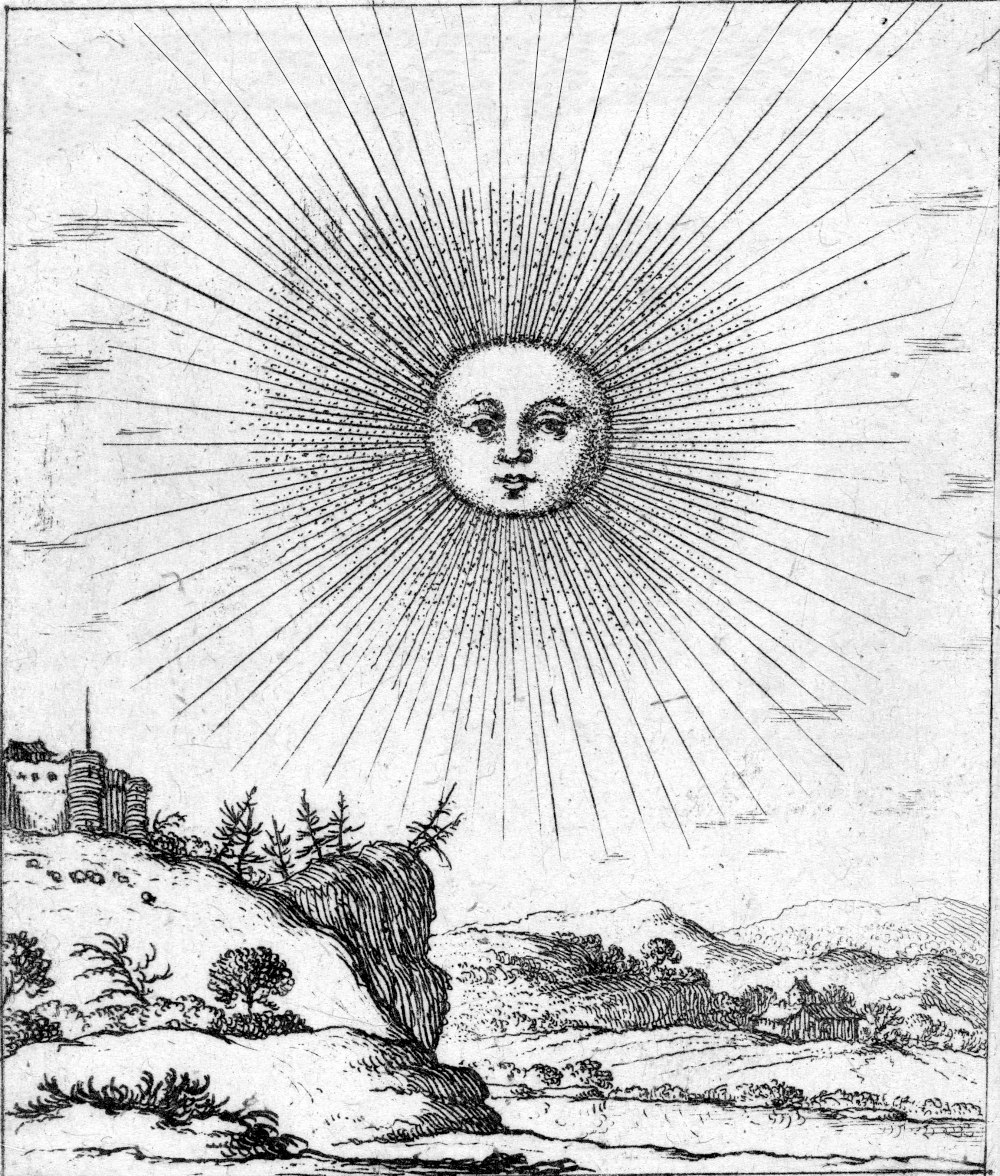
\includegraphics[keepaspectratio,width=0.4\textwidth]{figures/Bright-sun-Albert-Flamen-small.jpg}
  \captionart{BrightSun}
  \label{fig:brightsun}
\end{figure}

The ordinary sports which are used abroad are hawking, hunting, hilares
venandi labores, \authorfootnote{3226}one calls them, because they recreate body and
mind, \authorfootnote{3227}another, the \authorfootnote{3228}best exercise that is, by which alone
many have been \authorfootnote{3229}freed from all feral diseases. Hegesippus, lib. 1.
cap. 37. relates of Herod, that he was eased of a grievous melancholy
by that means. Plato, 7. de leg. highly magnifies it, dividing it into
three parts, by land, water, air. Xenophon, in Cyropaed. graces it with
a great name, Deorum munus, the gift of the gods, a princely sport,
which they have ever used, saith Langius, epist. 59. lib. 2. as well
for health as pleasure, and do at this day, it being the sole almost
and ordinary sport of our noblemen in Europe, and elsewhere all over
the world. Bohemus, de mor. gent. lib. 3. cap. 12. styles it therefore,
studium nobilium, communiter venantur, quod sibi solis licere
contendunt, 'tis all their study, their exercise, ordinary business,
all their talk: and indeed some dote too much after it, they can do
nothing else, discourse of naught else. Paulus Jovius, descr. Brit.
doth in some sort tax our \authorfootnote{3230} English nobility for it, for living in
the country so much, and too frequent use of it, as if they had no
other means but hawking and hunting to approve themselves gentlemen
with.

Hawking comes near to hunting, the one in the air, as the other on the
earth, a sport as much affected as the other, by some preferred.
\authorfootnote{3231}It was never heard of amongst the Romans, invented some twelve
hundred years since, and first mentioned by Firmicus, lib. 5. cap. 8.

The Greek emperors began it, and now nothing so frequent: he is nobody
that in the season hath not a hawk on his fist. A great art, and many
\authorfootnote{3232}books written of it. It is a wonder to hear \authorfootnote{3233}what is related
of the Turks' officers in this behalf, how many thousand men are
employed about it, how many hawks of all sorts, how much revenues
consumed on that only disport, how much time is spent at Adrianople
alone every year to that purpose. The \authorfootnote{3234}Persian kings hawk after
butterflies with sparrows made to that use, and stares: lesser hawks
for lesser games they have, and bigger for the rest, that they may
produce their sport to all seasons. The Muscovian emperors reclaim
eagles to fly at hinds, foxes, \etc{}, and such a one was sent for a
present to \authorfootnote{3235}Queen Elizabeth: some reclaim ravens, castrils, pies,
\etc{}, and man them for their pleasures.

Fowling is more troublesome, but all out as delightsome to some sorts
of men, be it with guns, lime, nets, glades, gins, strings, baits,
pitfalls, pipes, calls, stalking-horses, setting-dogs, decoy-ducks,
\etc{}, or otherwise. Some much delight to take larks with day-nets, small
birds with chaff-nets, plovers, partridge, herons, snipe, \etc{}. Henry the
Third, king of Castile (as Mariana the Jesuit reports of him, lib. 3.
cap. 7.) was much affected \authorfootnote{3236}with catching of quails, and many
gentlemen take a singular pleasure at morning and evening to go abroad
with their quail-pipes, and will take any pains to satisfy their
delight in that kind. The \authorfootnote{3237}Italians have gardens fitted to such
use, with nets, bushes, glades, sparing no cost or industry, and are
very much affected with the sport. Tycho Brahe, that great astronomer,
in the chorography of his Isle of Huena, and Castle of Uraniburge, puts
down his nets, and manner of catching small birds, as an ornament and a
recreation, wherein he himself was sometimes employed.

Fishing is a kind of hunting by water, be it with nets, weels, baits,
angling, or otherwise, and yields all out as much pleasure to some men
as dogs or hawks; \authorfootnote{3238}When they draw their fish upon the bank, saith
Nic. Henselius Silesiographi\ae{}, cap. 3. speaking of that extraordinary
delight his countrymen took in fishing, and in making of pools. James
Dubravius, that Moravian, in his book de pisc. telleth, how travelling
by the highway side in Silesia, he found a nobleman, \authorfootnote{3239}booted up to
the groins, wading himself, pulling the nets, and labouring as much as
any fisherman of them all: and when some belike objected to him the
baseness of his office, he excused himself, \authorfootnote{3240}that if other men
might hunt hares, why should not he hunt carps? Many gentlemen in like
sort with us will wade up to the arm-holes upon such occasions, and
voluntarily undertake that to satisfy their pleasures, which a poor man
for a good stipend would scarce be hired to undergo. Plutarch, in his
book de soler. animal. speaks against all fishing, \authorfootnote{3241}as a filthy,
base, illiberal employment, having neither wit nor perspicacity in it,
nor worth the labour. But he that shall consider the variety of baits
for all seasons, and pretty devices which our anglers have invented,
peculiar lines, false flies, several sleights, \etc{} will say, that it
deserves like commendation, requires as much study and perspicacity as
the rest, and is to be preferred before many of them. Because hawking
and hunting are very laborious, much riding, and many dangers accompany
them; but this is still and quiet: and if so be the angler catch no
fish, yet he hath a wholesome walk to the brookside, pleasant shade by
the sweet silver streams; he hath good air, and sweet smells of fine
fresh meadow flowers, he hears the melodious harmony of birds, he sees
the swans, herons, ducks, water-horns, coots, \etc{}, and many other fowl,
with their brood, which he thinketh better than the noise of hounds, or
blast of horns, and all the sport that they can make.

Many other sports and recreations there be, much in use, as ringing,
bowling, shooting, which Ascam recommends in a just volume, and hath in
former times been enjoined by statute, as a defensive exercise, and an
\authorfootnote{3242}honour to our land, as well may witness our victories in France.

Keelpins, tronks, quoits, pitching bars, hurling, wrestling, leaping,
running, fencing, mustering, swimming, wasters, foils, football,
balloon, quintain, \etc{}, and many such, which are the common recreations
of the country folks. Riding of great horses, running at rings, tilts
and tournaments, horse races, wild-goose chases, which are the disports
of greater men, and good in themselves, though many gentlemen by that
means gallop quite out of their fortunes.

But the most pleasant of all outward pastimes is that of \authorfootnote{3243}Areteus,
\latininlinetrans{strolling through pleasant scenery}{deambulatio per am\oe{}na loca}, to make a petty progress, a merry journey
now and then with some good companions, to visit friends, see cities,
castles, towns,

\textlatin{
\begin{verse}
Visere saepe amnes nitidos, per amaenaque Tempe,\\
Et placidas summis sectari in montibus auras.\authorfootnote{3244}
\end{verse}}

\begin{verse}
To see the pleasant fields, the crystal fountains,\\
And take the gentle air amongst the mountains.
\end{verse}

\authorfootnote{3245}To walk amongst orchards, gardens, bowers, mounts, and arbours,
artificial wildernesses, green thickets, arches, groves, lawns,
rivulets, fountains, and such like pleasant places, like that
Antiochian Daphne, brooks, pools, fishponds, between wood and water, in
a fair meadow, by a river side, \authorfootnote{3246}ubi variae, avium cantationes,
florum colores, pratorum frutices, \etc{} to disport in some pleasant
plain, park, run up a steep hill sometimes, or sit in a shady seat,
must needs be a delectable recreation. Hortus principis et domus ad
delectationem facia, cum sylva, monte et piscina, vulgo la montagna:
the prince's garden at Ferrara \authorfootnote{3247}Schottus highly magnifies, with
the groves, mountains, ponds, for a delectable prospect, he was much
affected with it: a Persian paradise, or pleasant park, could not be
more delectable in his sight. St. Bernard, in the description of his
monastery, is almost ravished with the pleasures of it. A sick
\authorfootnote{3248}man (saith he) sits upon a green bank, and when the dog-star
parcheth the plains, and dries up rivers, he lies in a shady bower,
Fronde sub arborea ferventia temperat astra, and feeds his eyes with
variety of objects, herbs, trees, to comfort his misery, he receives
many delightsome smells, and fills his ears with that sweet and various
harmony of birds: good God (saith he), what a company of pleasures hast
thou made for man! He that should be admitted on a sudden to the sight
of such a palace as that of Escurial in Spain, or to that which the
Moors built at Granada, Fontainebleau in France, the Turk's gardens in
his seraglio, wherein all manner of birds and beasts are kept for
pleasure; wolves, bears, lynxes, tigers, lions, elephants, \etc{}, or upon
the banks of that Thracian Bosphorus: the pope's Belvedere in Rome,
\authorfootnote{3249}as pleasing as those horti pensiles in Babylon, or that Indian
king's delightsome garden in \authorfootnote{3250}\AE{}lian; or \authorfootnote{3251}those famous
gardens of the Lord Cantelow in France, could, not choose, though he
were never so ill paid, but be much recreated for the time; or many of
our noblemen's gardens at home. To take a boat in a pleasant evening,
and with music \authorfootnote{3252}to row upon the waters, which Plutarch so much
applauds, Elian admires, upon the river Pineus: in those Thessalian
fields, beset with green bays, where birds so sweetly sing that
passengers, enchanted as it were with their heavenly music, omnium
laborum et curarum obliviscantur, forget forthwith all labours, care,
and grief: or in a gondola through the Grand Canal in Venice, to see
those goodly palaces, must needs refresh and give content to a
melancholy dull spirit. Or to see the inner rooms of a fair-built and
sumptuous edifice, as that of the Persian kings, so much renowned by
Diodorus and Curtius, in which all was almost beaten gold,
\authorfootnote{3253}chairs, stools, thrones, tabernacles, and pillars of gold, plane
trees, and vines of gold, grapes of precious stones, all the other
ornaments of pure gold,
\authorfootnote{3254}Fulget gemma floris, et jaspide fulva supellex,
Strata micant Tyrio---

With sweet odours and perfumes, generous wines, opiparous fare, \etc{},
besides the gallantest young men, the fairest \authorfootnote{3255}virgins, puellae
scitulae ministrantes, the rarest beauties the world could afford, and
those set out with costly and curious attires, ad stuporem usque
spectantium, with exquisite music, as in \authorfootnote{3256}Trimaltion's house, in
every chamber sweet voices ever sounding day and night, incomparabilis
luxus, all delights and pleasures in each kind which to please the
senses could possibly be devised or had, convives coronati, delitiis
ebrii, \etc{}. Telemachus, in Homer, is brought in as one ravished almost
at the sight of that magnificent palace, and rich furniture of
Menelaus, when he beheld
\authorfootnote{3257}Aeris fulgorem et resonantia tecta corusco
Auro, atque electro nitido, sectoque elephanto,
Argentoque simul. Talis Jovis ardua sedes,
Aulaque coelicolum stellans splendescit Olympo.

Such glittering of gold and brightest brass to shine,
Clear amber, silver pure, and ivory so fine:
Jupiter's lofty palace, where the gods do dwell,
Was even such a one, and did it not excel.

It will laxare animos, refresh the soul of man to see fair-built
cities, streets, theatres, temples, obelisks, \etc{}. The temple of
Jerusalem was so fairly built of white marble, with so many pyramids
covered with gold; tectumque templi fulvo coruscans auro, nimio suo
fulgore obcaecabat oculos itinerantium, was so glorious, and so
glistened afar off, that the spectators might not well abide the sight
of it. But the inner parts were all so curiously set out with cedar,
gold, jewels, \etc{}, as he said of Cleopatra's palace in
Egypt,-\authorfootnote{3258}Crassumque trabes absconderat aurum, that the beholders
were amazed. What so pleasant as to see some pageant or sight go by, as
at coronations, weddings, and such like solemnities, to see an
ambassador or a prince met, received, entertained with masks, shows,
fireworks, \etc{}. To see two kings fight in single combat, as Porus and
Alexander; Canute and Edmund Ironside; Scanderbeg and Ferat Bassa the
Turk; when not honour alone but life itself is at stake, as the
\authorfootnote{3259}poet of Hector,
---nec enim pro tergore Tauri,
Pro bove nec certamen erat, quae praemia cursus
Esse solent, sed pro magni viraque animaque-Hectoris.

To behold a battle fought, like that of Crecy, or Agincourt, or
Poitiers, qua nescio (saith Froissart) an vetustas ullam proferre
possit clariorem. To see one of Caesar's triumphs in old Rome revived,
or the like. To be present at an interview, \authorfootnote{3260}as that famous of
Henry the Eighth and Francis the First, so much renowned all over
Europe; ubi tanto apparatu (saith Hubertus Veillius) tamque triumphali
pompa ambo reges com eorum conjugibus coiere, ut nulla unquam aetas tam
celebria festa viderit aut audieriti, no age ever saw the like. So
infinitely pleasant are such shows, to the sight of which oftentimes
they will come hundreds of miles, give any money for a place, and
remember many years after with singular delight. Bodine, when he was
ambassador in England, said he saw the noblemen go in their robes to
the parliament house, summa cum jucunditate vidimus, he was much
affected with the sight of it. Pomponius Columna, saith Jovius in his
life, saw thirteen Frenchmen, and so many Italians, once fight for a
whole army: Quod jucundissimum spectaculum in vita dicit sua, the
pleasantest sight that ever he saw in his life. Who would not have been
affected with such a spectacle? Or that single combat of \authorfootnote{3261} Breaute
the Frenchman, and Anthony Schets a Dutchman, before the walls of
Sylvaducis in Brabant, anno 1600. They were twenty-two horse on the one
side, as many on the other, which like Livy's Horatii, Torquati and
Corvini fought for their own glory and country's honour, in the sight
and view of their whole city and army. \authorfootnote{3262}When Julius Caesar warred
about the banks of Rhone, there came a barbarian prince to see him and
the Roman army, and when he had beheld Caesar a good while, \authorfootnote{3263}I see
the gods now (saith he) which before I heard of, nec feliciorem ullam
vitae meae aut optavi, aut sensi diem: it was the happiest day that
ever he had in his life. Such a sight alone were able of itself to
drive away melancholy; if not for ever, yet it must needs expel it for
a time. Radzivilus was much taken with the pasha's palace in Cairo, and
amongst many other objects which that place afforded, with that
solemnity of cutting the banks of the Nile by Imbram Pasha, when it
overflowed, besides two or three hundred gilded galleys on the water,
he saw two millions of men gathered together on the land, with turbans
as white as snow; and 'twas a goodly sight. The very reading of feasts,
triumphs, interviews, nuptials, tilts, tournaments, combats, and
monomachies, is most acceptable and pleasant. \authorfootnote{3264} Franciscus Modius
hath made a large collection of such solemnities in two great tomes,
which whoso will may peruse. The inspection alone of those curious
iconographies of temples and palaces, as that of the Lateran church in
Albertus Durer, that of the temple of Jerusalem in \authorfootnote{3265}Josephus,
Adricomius, and Villalpandus: that of the Escurial in Guadas, of Diana
at Ephesus in Pliny, Nero's golden palace in Rome, \authorfootnote{3266}Justinian's in
Constantinople, that Peruvian Jugo's in \authorfootnote{3267}Cusco, ut non ab
hominibus, sed a daemoniis constructum videatur; St. Mark's in Venice,
by Ignatius, with many such; priscorum artificum opera (saith that
\authorfootnote{3268}interpreter of Pausanias), the rare workmanship of those ancient
Greeks, in theatres, obelisks, temples, statues, gold, silver, ivory,
marble images, non minore ferme quum leguntur, quam quum cernuntur,
animum delectatione complent, affect one as much by reading almost as
by sight.

The country hath his recreations, the city his several gymnics and
exercises, May games, feasts, wakes, and merry meetings, to solace
themselves; the very being in the country; that life itself is a
sufficient recreation to some men, to enjoy such pleasures, as those
old patriarchs did. Diocletian, the emperor, was so much affected with
it, that he gave over his sceptre, and turned gardener. Constantine
wrote twenty books of husbandry. Lysander, when ambassadors came to see
him, bragged of nothing more than of his orchard, hi sunt ordines mei.

What shall I say of Cincinnatus, Cato, Tully, and many such? how they
have been pleased with it, to prune, plant, inoculate and graft, to
show so many several kinds of pears, apples, plums, peaches, \etc{}.
\authorfootnote{3269}Nunc captare feras laqueo, nunc fallere visco,
Atque etiam magnos canibus circundare saltus
Insidias avibus moliri, incendere vepres.

Sometimes with traps deceive, with line and string
To catch wild birds and beasts, encompassing
The grove with dogs, and out of bushes firing.

---et nidos aviumscrutari, \etc{}.

Jucundus, in his preface to Cato, Varro, Columella, \etc{}, put out by
him, confesseth of himself, that he was mightily delighted with these
husbandry studies, and took extraordinary pleasure in them: if the
theory or speculation can so much affect, what shall the place and
exercise itself, the practical part do? The same confession I find in
Herbastein, Porta, Camerarius, and many others, which have written of
that subject. If my testimony were aught worth, I could say as much of
myself; I am vere Saturnus; no man ever took more delight in springs,
woods, groves, gardens, walks, fishponds, rivers, \etc{}. But
\authorfootnote{3270}Tantalus a labris sitiens fugientia captat
Flumina;

And so do I; Velle licet, potiri non licet.\authorfootnote{3271}
Every palace, every city almost hath its peculiar walks, cloisters,
terraces, groves, theatres, pageants, games, and several recreations;
every country, some professed gymnics to exhilarate their minds, and
exercise their bodies. The \authorfootnote{3272}Greeks had their Olympian, Pythian,
Isthmian, Nemean games, in honour of Neptune, Jupiter, Apollo; Athens
hers: some for honour, garlands, crowns; for \authorfootnote{3273}beauty, dancing,
running, leaping, like our silver games. The \authorfootnote{3274}Romans had their
feasts, as the Athenians, and Lacedaemonians held their public
banquets, in Pritanaeo, Panathenaeis, Thesperiis, Phiditiis, plays,
naumachies, places for sea-fights, \authorfootnote{3275}theatres, amphitheatres able
to contain 70,000 men, wherein they had several delightsome shows to
exhilarate the people; \authorfootnote{3276} gladiators, combats of men with
themselves, with wild beasts, and wild beasts one with another, like
our bull-baitings, or bear-baitings (in which many countrymen and
citizens amongst us so much delight and so frequently use), dancers on
ropes. Jugglers, wrestlers, comedies, tragedies, publicly exhibited at
the emperor's and city's charge, and that with incredible cost and
magnificence. In the Low-Countries (as \authorfootnote{3277}Meteran relates) before
these wars, they had many solemn feasts, plays, challenges, artillery
gardens, colleges of rhymers, rhetoricians, poets: and to this day,
such places are curiously maintained in Amsterdam, as appears by that
description of Isaacus Pontanus, rerum Amstelrod. lib. 2. cap. 25. So
likewise not long since at Friburg in Germany, as is evident by that
relation of \authorfootnote{3278}Neander, they had Ludos septennales, solemn plays
every seven years, which Bocerus, one of their own poets, hath
elegantly described:
\authorfootnote{3279}At nunc magnifico spectacula structa paratu
Quid memorem, veteri non concessura Quirino,
Ludorum pompa, \etc{}.

In Italy they have solemn declamations of certain select young
gentlemen in Florence (like those reciters in old Rome), and public
theatres in most of their cities, for stage-players and others, to
exercise and recreate themselves. All seasons almost, all places, have
their several pastimes; some in summer, some in winter; some abroad,
some within: some of the body, some of the mind: and diverse men have
diverse recreations and exercises. Domitian, the emperor, was much
delighted with catching flies; Augustus to play with nuts amongst
children; \authorfootnote{3280}Alexander Severus was often pleased to play with whelps
and young pigs. \authorfootnote{3281}Adrian was so wholly enamoured with dogs and
horses, that he bestowed monuments and tombs of them, and buried them
in graves. In foul weather, or when they can use no other convenient
sports, by reason of the time, as we do cock-fighting, to avoid
idleness, I think, (though some be more seriously taken with it, spend
much time, cost and charges, and are too solicitous about it)
\authorfootnote{3282}Severus used partridges and quails, as many Frenchmen do still,
and to keep birds in cages, with which he was much pleased, when at any
time he had leisure from public cares and businesses. He had (saith
Lampridius) tame pheasants, ducks, partridges, peacocks, and some
20,000 ring-doves and pigeons. Busbequius, the emperor's orator, when
he lay in Constantinople, and could not stir much abroad, kept for his
recreation, busying himself to see them fed, almost all manner of
strange birds and beasts; this was something, though not to exercise
his body, yet to refresh his mind. Conradus Gesner, at Zurich in
Switzerland, kept so likewise for his pleasure, a great company of wild
beasts; and (as he saith) took great delight to see them eat their
meat. Turkey gentlewomen, that are perpetual prisoners, still mewed up
according to the custom of the place, have little else beside their
household business, or to play with their children to drive away time,
but to dally with their cats, which they have in delitiis, as many of
our ladies and gentlewomen use monkeys and little dogs. The ordinary
recreations which we have in winter, and in most solitary times busy
our minds with, are cards, tables and dice, shovelboard, chess-play,
the philosopher's game, small trunks, shuttlecock, billiards, music,
masks, singing, dancing, Yule-games, frolics, jests, riddles, catches,
purposes, questions and commands, \authorfootnote{3283}merry tales of errant knights,
queens, lovers, lords, ladies, giants, dwarfs, thieves, cheaters,
witches, fairies, goblins, friars, \etc{}, such as the old woman told
Psyche in \authorfootnote{3284}Apuleius, Boccace novels, and the rest, quarum
auditione pueri delectantur, senes narratione, which some delight to
hear, some to tell; all are well pleased with. Amaranthus, the
philosopher, met Hermocles, Diophantus and Philolaus, his companions,
one day busily discoursing about Epicurus and Democritus' tenets, very
solicitous which was most probable and came nearest to truth: to put
them out of that surly controversy, and to refresh their spirits, he
told them a pleasant tale of Stratocles the physician's wedding, and of
all the particulars, the company, the cheer, the music, \etc{}, for he was
new come from it; with which relation they were so much delighted, that
Philolaus wished a blessing to his heart, and many a good
wedding,\authorfootnote{3285} many such merry meetings might he be at, to please
himself with the sight, and others with the narration of it. News are
generally welcome to all our ears, avide audimus, aures enim hominum
novitate laetantur (\authorfootnote{3286}as Pliny observes), we long after rumour to
hear and listen to it, \authorfootnote{3287}densum humeris bibit aure vulgus. We are
most part too inquisitive and apt to hearken after news, which Caesar,
in his \authorfootnote{3288}Commentaries, observes of the old Gauls, they would be
inquiring of every carrier and passenger what they had heard or seen,
what news abroad?
---quid toto fiat in orbe,
Quid Seres, quid Thraces agant, secreta novercae,
Et pueri, quis amet, \etc{}.

as at an ordinary with us, bakehouse or barber's shop. When that great
Gonsalva was upon some displeasure confined by King Ferdinand to the
city of Loxa in Andalusia, the only, comfort (saith \authorfootnote{3289}Jovius) he
had to ease his melancholy thoughts, was to hear news, and to listen
after those ordinary occurrences which were brought him cum primis, by
letters or otherwise out of the remotest parts of Europe. Some men's
whole delight is, to take tobacco, and drink all day long in a tavern
or alehouse, to discourse, sing, jest, roar, talk of a cock and bull
over a pot, \etc{}. Or when three or four good companions meet, tell old
stories by the fireside, or in the sun, as old folks usually do, quae
aprici meminere senes, remembering afresh and with pleasure ancient
matters, and such like accidents, which happened in their younger
years: others' best pastime is to game, nothing to them so pleasant.
\authorfootnote{3290}Hic Veneri indulget, hunc decoquit alea-many too nicely take
exceptions at cards, \authorfootnote{3291}tables, and dice, and such mixed lusorious
lots, whom Gataker well confutes. Which though they be honest
recreations in themselves, yet may justly be otherwise excepted at, as
they are often abused, and forbidden as things most pernicious; insanam
rem et damnosam, \authorfootnote{3292}Lemnius calls it. For most part in these kind of
disports 'tis not art or skill, but subtlety, cony-catching, knavery,
chance and fortune carries all away: 'tis ambulatoria pecunia,
\authorfootnote{3293}---puncto mobilis horae
Permutat dominos, et cedit in altera jura.

They labour most part not to pass their time in honest disport, but for
filthy lucre, and covetousness of money. In foedissimum lucrum et
avaritiam hominum convertitur, as Daneus observes. Fons fraudum et
maleficiorum, 'tis the fountain of cozenage and villainy. \authorfootnote{3294}A thing
so common all over Europe at this day, and so generally abused, that
many men are utterly undone by it, their means spent, patrimonies
consumed, they and their posterity beggared; besides swearing,
wrangling, drinking, loss of time, and such inconveniences, which are
ordinary concomitants: \authorfootnote{3295}for when once they have got a haunt of
such companies, and habit of gaming, they can hardly be drawn from it,
but as an itch it will tickle them, and as it is with whoremasters,
once entered, they cannot easily leave it off: Vexat mentes insania
cupido, they are mad upon their sport. And in conclusion (which Charles
the Seventh, that good French king, published in an edict against
gamesters) unde piae et hilaris vitae, suffugium sibi suisque liberis,
totique familiae, \etc{}. That which was once their livelihood, should have
maintained wife, children, family, is now spent and gone; maeror et
egestas, \etc{}, sorrow and beggary succeeds. So good things may be
abused, and that which was first invented to \authorfootnote{3296} refresh men's weary
spirits, when they come from other labours and studies to exhilarate
the mind, to entertain time and company, tedious otherwise in those
long solitary winter nights, and keep them from worse matters, an
honest exercise is contrarily perverted.

Chess-play is a good and witty exercise of the mind for some kind of
men, and fit for such melancholy, Rhasis holds, as are idle, and have
extravagant impertinent thoughts, or troubled with cares, nothing
better to distract their mind, and alter their meditations: invented
(some say) by the \authorfootnote{3297}general of an army in a famine, to keep
soldiers from mutiny: but if it proceed from overmuch study, in such a
case it may do more harm than good; it is a game too troublesome for
some men's brains, too full of anxiety, all out as bad as study;
besides it is a testy choleric game, and very offensive to him that
loseth the mate. \authorfootnote{3298}William the Conqueror, in his younger years,
playing at chess with the Prince of France (Dauphine was not annexed to
that crown in those days) losing a mate, knocked the chess-board about
his pate, which was a cause afterward of much enmity between them. For
some such reason it is belike, that Patritius, in his 3. book, tit. 12.
de reg. instit. forbids his prince to play at chess; hawking and
hunting, riding, \etc{} he will allow; and this to other men, but by no
means to him. In Muscovy, where they live in stoves and hot houses all
winter long, come seldom or little abroad, it is again very necessary,
and therefore in those parts, (saith \authorfootnote{3299}Herbastein) much used. At
Fez in Africa, where the like inconvenience of keeping within doors is
through heat, it is very laudable; and (as \authorfootnote{3300}Leo Afer relates) as
much frequented. A sport fit for idle gentlewomen, soldiers in
garrison, and courtiers that have nought but love matters to busy
themselves about, but not altogether so convenient for such as are
students. The like I may say of Col. Bruxer's philosophy game, D.
Fulke's Metromachia and his Ouronomachia, with the rest of those
intricate astrological and geometrical fictions, for such especially as
are mathematically given; and the rest of those curious games.

Dancing, singing, masking, mumming, stage plays, howsoever they be
heavily censured by some severe Catos, yet if opportunely and soberly
used, may justly be approved. Melius est foedere, quam saltare,
\authorfootnote{3301}saith Austin: but what is that if they delight in it? \authorfootnote{3302}Nemo
saltat sobrius. But in what kind of dance? I know these sports have
many oppugners, whole volumes writ against them; when as all they say
(if duly considered) is but ignoratio Elenchi; and some again, because
they are now cold and wayward, past themselves, cavil at all such
youthful sports in others, as he did in the comedy; they think them,
illico nasci senes, \etc{}. Some out of preposterous zeal object many times
trivial arguments, and because of some abuse, will quite take away the
good use, as if they should forbid wine because it makes men drunk; but
in my judgment they are too stern: there is a time for all things, a
time to mourn, a time to dance, Eccles. \rn{iii.} 4. a time to embrace, a
time not to embrace, (verse 5.) and nothing better than that a man
should rejoice in his own works, verse 22; for my part, I will
subscribe to the king's declaration, and was ever of that mind, those
May games, wakes, and Whitsun ales, \etc{}, if they be not at unseasonable
hours, may justly be permitted. Let them freely feast, sing and dance,
have their puppet-plays, hobby-horses, tabors, crowds, bagpipes, \etc{},
play at ball, and barley-breaks, and what sports and recreations they
like best. In Franconia, a province of Germany, (saith \authorfootnote{3303}Aubanus
Bohemus) the old folks, after evening prayer, went to the alehouse, the
younger sort to dance: and to say truth with \authorfootnote{3304}Salisburiensis,
satius fuerat sic otiari, quam turpius occupari, better to do so than
worse, as without question otherwise (such is the corruption of man's
nature) many of them will do. For that cause, plays, masks, jesters,
gladiators, tumblers, jugglers, \etc{}, and all that crew is admitted and
winked at: \authorfootnote{3305}Tota jocularium scena procedit, et ideo spectacula
admissa sunt, et infinita tyrocinia vanitatum, ut his occupentur, qui
perniciosius otiari solent: that they might be busied about such toys,
that would otherwise more perniciously be idle. So that as
\authorfootnote{3306}Tacitus said of the astrologers in Rome, we may say of them,
genus hominum est quod in civitate nostra et vitabitur semper et
retinebitur, they are a debauched company most part, still spoken
against, as well they deserve some of them (for I so relish and
distinguish them as fiddlers, and musicians), and yet ever retained.

Evil is not to be done (I confess) that good may come of it: but this
is evil per accidens, and in a qualified sense, to avoid a greater
inconvenience, may justly be tolerated. Sir Thomas More, in his Utopian
Commonwealth, \authorfootnote{3307}as he will have none idle, so will he have no man
labour over hard, to be toiled out like a horse, 'tis more than slavish
infelicity, the life of most of our hired servants and tradesmen
elsewhere (excepting his Utopians) but half the day allotted for work,
and half for honest recreation, or whatsoever employment they shall
think fit for themselves. If one half day in a week were allowed to our
household servants for their merry meetings, by their hard masters, or
in a year some feasts, like those Roman Saturnals, I think they would
labour harder all the rest of their time, and both parties be better
pleased: but this needs not (you will say), for some of them do nought
but loiter all the week long.

This which I aim at, is for such as are fracti animis, troubled in
mind, to ease them, over-toiled on the one part, to refresh: over idle
on the other, to keep themselves busied. And to this purpose, as any
labour or employment will serve to the one, any honest recreation will
conduce to the other, so that it be moderate and sparing, as the use of
meat and drink; not to spend all their life in gaming, playing, and
pastimes, as too many gentlemen do; but to revive our bodies and
recreate our souls with honest sports: of which as there be diverse
sorts, and peculiar to several callings, ages, sexes, conditions, so
there be proper for several seasons, and those of distinct natures, to
fit that variety of humours which is amongst them, that if one will
not, another may: some in summer, some in winter, some gentle, some
more violent, some for the mind alone, some for the body and mind: (as
to some it is both business and a pleasant recreation to oversee
workmen of all sorts, husbandry, cattle, horses, \etc{}. To build, plot,
project, to make models, cast up accounts, \etc{}) some without, some
within doors; new, old, \etc{}, as the season serveth, and as men are
inclined. It is reported of Philippus Bonus, that good duke of Burgundy
(by Lodovicus Vives, in Epist. and Pont. \authorfootnote{3308}Heuter in his history)
that the said duke, at the marriage of Eleonora, sister to the king of
Portugal, at Bruges in Flanders, which was solemnised in the deep of
winter, when, as by reason of unseasonable weather, he could neither
hawk nor hunt, and was now tired with cards, dice, \etc{}, and such other
domestic sports, or to see ladies dance, with some of his courtiers, he
would in the evening walk disguised all about the town. It so fortuned,
as he was walking late one night, he found a country fellow dead drunk,
snorting on a bulk; \authorfootnote{3309}he caused his followers to bring him to his
palace, and there stripping him of his old clothes, and attiring him
after the court fashion, when he waked, he and they were all ready to
attend upon his excellency, persuading him he was some great duke. The
poor fellow admiring how he came there, was served in state all the day
long; after supper he saw them dance, heard music, and the rest of
those court-like pleasures: but late at night, when he was well
tippled, and again fast asleep, they put on his old robes, and so
conveyed him to the place where they first found him. Now the fellow
had not made them so good sport the day before as he did when he
returned to himself; all the jest was, to see how he \authorfootnote{3310}looked upon
it. In conclusion, after some little admiration, the poor man told his
friends he had seen a vision, constantly believed it, would not
otherwise be persuaded, and so the jest ended. \authorfootnote{3311}Antiochus
Epiphanes would often disguise himself, steal from his court, and go
into merchants', goldsmiths', and other tradesmen's shops, sit and talk
with them, and sometimes ride or walk alone, and fall aboard with any
tinker, clown, serving man, carrier, or whomsoever he met first.

Sometimes he did ex insperato give a poor fellow money, to see how he
would look, or on set purpose lose his purse as he went, to watch who
found it, and withal how he would be affected, and with such objects he
was much delighted. Many such tricks are ordinarily put in practice by
great men, to exhilarate themselves and others, all which are harmless
jests, and have their good uses.

But amongst those exercises, or recreations of the mind within doors,
there is none so general, so aptly to be applied to all sorts of men,
so fit and proper to expel idleness and melancholy, as that of study:
Studia, senectutem oblectant, adolescentiam, alunt, secundas res
ornant, adversis perfugium et solatium praebent, domi delectant, \etc{},
find the rest in Tully pro Archia Poeta. \authorfootnote{3312}What so full of content,
as to read, walk, and see maps, pictures, statues, jewels, marbles,
which some so much magnify, as those that Phidias made of old so
exquisite and pleasing to be beheld, that as \authorfootnote{3313}Chrysostom thinketh,
if any man be sickly, troubled in mind, or that cannot sleep for grief,
and shall but stand over against one of Phidias' images, he will forget
all care, or whatsoever else may molest him, in an instant? There be
those as much taken with Michael Angelo's, Raphael de Urbino's,
Francesco Francia's pieces, and many of those Italian and Dutch
painters, which were excellent in their ages; and esteem of it as a
most pleasing sight, to view those neat architectures, devices,
escutcheons, coats of arms, read such books, to peruse old coins of
several sorts in a fair gallery; artificial works, perspective glasses,
old relics, Roman antiquities, variety of colours. A good picture is
falsa veritas, et muta poesis: and though (as \authorfootnote{3314}Vives saith)
artificialia delectant, sed mox fastidimus, artificial toys please but
for a time; yet who is he that will not be moved with them for the
present? When Achilles was tormented and sad for the loss of his dear
friend Patroclus, his mother Thetis brought him a most elaborate and
curious buckler made by Vulcan, in which were engraven sun, moon,
stars, planets, sea, land, men fighting, running, riding, women
scolding, hills, dales, towns, castles, brooks, rivers, trees, \etc{},
with many pretty landscapes, and perspective pieces: with sight of
which he was infinitely delighted, and much eased of his grief.
\authorfootnote{3315}Continuo eo spectaculo captus delenito maerore
Oblectabatur, in manibus tenens dei splendida dona.

Who will not be affected so in like case, or see those well-furnished
cloisters and galleries of the Roman cardinals, so richly stored with
all modern pictures, old statues and antiquities? Cum se-spectando
recreet simul et legendo, to see their pictures alone and read the
description, as \authorfootnote{3316}Boisardus well adds, whom will it not affect?
which Bozius, Pomponius, Laetus, Marlianus, Schottus, Cavelerius,
Ligorius, \etc{}, and he himself hath well performed of late. Or in some
prince's cabinets, like that of the great dukes in Florence, of Felix
Platerus in Basil, or noblemen's houses, to see such variety of
attires, faces, so many, so rare, and such exquisite pieces, of men,
birds, beasts, \etc{}, to see those excellent landscapes, Dutch works, and
curious cuts of Sadlier of Prague, Albertus Durer, Goltzius Vrintes,
\etc{}, such pleasant pieces of perspective, Indian pictures made of
feathers, China works, frames, thaumaturgical motions, exotic toys, \etc{}.

Who is he that is now wholly overcome with idleness, or otherwise
involved in a labyrinth of worldly cares, troubles and discontents,
that will not be much lightened in his mind by reading of some enticing
story, true or feigned, whereas in a glass he shall observe what our
forefathers have done, the beginnings, ruins, falls, periods of
commonwealths, private men's actions displayed to the life, \etc{}. \authorfootnote{3317}
Plutarch therefore calls them, secundas mensas et bellaria, the second
course and junkets, because they were usually read at noblemen's
feasts. Who is not earnestly affected with a passionate speech, well
penned, an elegant poem, or some pleasant bewitching discourse, like
that of \authorfootnote{3318} Heliodorus, ubi oblectatio quaedam placide fuit, cum
hilaritate conjuncta? Julian the Apostate was so taken with an oration
of Libanius, the sophister, that, as he confesseth, he could not be
quiet till he had read it all out. Legi orationem tuam magna ex parte,
hesterna die ante prandium, pransus vero sine ulla intermissione totam
absolvi.\authorfootnote{3319}O argumenta! O compositionem! I may say the same of this
or that pleasing tract, which will draw his attention along with it. To
most kind of men it is an extraordinary delight to study. For what a
world of books offers itself, in all subjects, arts, and sciences, to
the sweet content and capacity of the reader? In arithmetic, geometry,
perspective, optics, astronomy, architecture, sculpture, painting, of
which so many and such elaborate treatises are of late written: in
mechanics and their mysteries, military matters, navigation,
\authorfootnote{3320}riding of horses, \authorfootnote{3321}fencing, swimming, gardening, planting,
great tomes of husbandry, cookery, falconry, hunting, fishing, fowling,
\etc{}, with exquisite pictures of all sports, games, and what not? In
music, metaphysics, natural and moral philosophy, philology, in policy,
heraldry, genealogy, chronology, \etc{}, they afford great tomes, or those
studies of \authorfootnote{3322}antiquity, \etc{}, et \authorfootnote{3323}quid subtilius Arithmeticis
inventionibus, quid jucundius Musicis rationibus, quid divinius
Astronomicis, quid rectius Geometricis demonstrationibus? What so sure,
what so pleasant? He that shall but see that geometrical tower of
Garezenda at Bologna in Italy, the steeple and clock at Strasburg, will
admire the effects of art, or that engine of Archimedes, to remove the
earth itself, if he had but a place to fasten his instrument:
Archimedes Coclea, and rare devices to corrivate waters, musical
instruments, and tri-syllable echoes again, again, and again repeated,
with myriads of such. What vast tomes are extant in law, physic, and
divinity, for profit, pleasure, practice, speculation, in verse or
prose, \etc{}! their names alone are the subject of whole volumes, we have
thousands of authors of all sorts, many great libraries full well
furnished, like so many dishes of meat, served out for several palates;
and he is a very block that is affected with none of them. Some take an
infinite delight to study the very languages wherein these books are
written, Hebrew, Greek, Syriac, Chaldee, Arabic, \etc{}. Methinks it would
please any man to look upon a geographical map, \authorfootnote{3324}sauvi animum
delectatione allicere, ob incredibilem rerum varietatem et
jucunditatem, et ad pleniorem sui cognitionem excitare, chorographical,
topographical delineations, to behold, as it were, all the remote
provinces, towns, cities of the world, and never to go forth of the
limits of his study, to measure by the seale and compass their extent,
distance, examine their site. Charles the Great, as Platina writes, had
three fair silver tables, in one of which superficies was a large map
of Constantinople, in the second Rome neatly engraved, in the third an
exquisite description of the whole world, and much delight he took in
them. What greater pleasure can there now be, than to view those
elaborate maps of Ortelius, \authorfootnote{3325}Mercator, Hondius, \etc{}? To peruse
those books of cities, put out by Braunus and Hogenbergius? To read
those exquisite descriptions of Maginus, Munster, Herrera, Laet,
Merula, Boterus, Leander, Albertus, Camden, Leo Afer, Adricomius, Nic.
Gerbelius, \etc{}? Those famous expeditions of Christoph. Columbus,
Americus Vespucius, Marcus Polus the Venetian, Lod. Vertomannus,
Aloysius Cadamustus, \etc{}? Those accurate diaries of Portuguese,
Hollanders, of Bartison, Oliver a Nort, \etc{}. Hakluyt's voyages, Pet.
Martyr's Decades, Benzo, Lerius, Linschoten's relations, those
Hodoeporicons of Jod. a Meggen, Brocard the monk, Bredenbachius, Jo.
Dublinius, Sands, \etc{}, to Jerusalem, Egypt, and other remote places of
the world? those pleasant itineraries of Paulus Hentzerus, Jodocus
Sincerus, Dux Polonus, \etc{}, to read Bellonius' observations, P. Gillius
his surveys; those parts of America, set out, and curiously cut in
pictures, by Fratres a Bry. To see a well-cut herbal, herbs, trees,
flowers, plants, all vegetables expressed in their proper colours to
the life, as that of Matthiolus upon Dioscorides, Delacampius, Lobel,
Bauhinus, and that last voluminous and mighty herbal of Beslar of
Nuremberg, wherein almost every plant is to his own bigness. To see
birds, beasts, and fishes of the sea, spiders, gnats, serpents, flies,
\etc{}, all creatures set out by the same art, and truly expressed in
lively colours, with an exact description of their natures, virtues,
qualities, \etc{}, as hath been accurately performed by \AE{}lian, Gesner,
Ulysses Aldrovandus, Bellonius, Rondoletius, Hippolitus Salvianus, \etc{}.
\authorfootnote{3326}Arcana coeli, naturae secreta, ordinem universi scire majoris
felicitatis et dulcedinis est, quam cogitatione quis assequi possit,
aut mortalis sperare. What more pleasing studies can there be than the
mathematics, theoretical or practical parts? as to survey land, make
maps, models, dials, \etc{}, with which I was ever much delighted myself.

Tails est Mathematum pulchritudo (saith \authorfootnote{3327} Plutarch) ut his
indignum sit divitiarum phaleras istas et bullas, et puellaria
spectacula comparari; such is the excellency of these studies, that all
those ornaments and childish bubbles of wealth, are not worthy to be
compared to them: credi mihi ( \authorfootnote{3328}saith one) extingui dulce erit
Mathematicarum artium studio, I could even live and die with such
meditation, \authorfootnote{3329}and take more delight, true content of mind in them,
than thou hast in all thy wealth and sport, how rich soever thou art.

And as \authorfootnote{3330}Cardan well seconds me, Honorificum magis est et gloriosum
haec intelligere, quam provinciis praeesse, formosum aut ditem juvenem
esse. \authorfootnote{3331}The like pleasure there is in all other studies, to such as
are truly addicted to them, \authorfootnote{3332}ea suavitas (one holds) ut cum quis
ea degustaverit, quasi poculis Circeis captus, non possit unquam ab
illis divelli; the like sweetness, which as Circe's cup bewitcheth a
student, he cannot leave off, as well may witness those many laborious
hours, days and nights, spent in the voluminous treatises written by
them; the same content. \authorfootnote{3333}Julius Scaliger was so much affected with
poetry, that he brake out into a pathetical protestation, he had rather
be the author of twelve verses in Lucan, or such an ode in
\authorfootnote{3334}Horace, than emperor of Germany. \authorfootnote{3335}Nicholas Gerbelius, that
good old man, was so much ravished with a few Greek authors restored to
light, with hope and desire of enjoying the rest, that he exclaims
forthwith, Arabibus atque Indis omnibus erimus ditiores, we shall be
richer than all the Arabic or Indian princes; of such \authorfootnote{3336}esteem they
were with him, incomparable worth and value. Seneca prefers Zeno and
Chrysippus, two doting stoics (he was so much enamoured of their
works), before any prince or general of an army; and Orontius, the
mathematician, so far admires Archimedes, that he calls him Divinum et
homine majorem, a petty god, more than a man; and well he might, for
aught I see, if you respect fame or worth. Pindarus, of Thebes, is as
much renowned for his poems, as Epaminondas, Pelopidas, Hercules or
Bacchus, his fellow citizens, for their warlike actions; et si famam
respicias, non pauciores Aristotelis quam Alexandri meminerunt (as
Cardan notes), Aristotle is more known than Alexander; for we have a
bare relation of Alexander's deeds, but Aristotle, totus vivit in
monumentis, is whole in his works: yet I stand not upon this; the
delight is it, which I aim at, so great pleasure, such sweet content
there is in study. \authorfootnote{3337}King James, 1605, when he came to see our
University of Oxford, and amongst other edifices now went to view that
famous library, renewed by Sir Thomas Bodley, in imitation of
Alexander, at his departure brake out into that noble speech, If I were
not a king, I would be a university man: \authorfootnote{3338} and if it were so that
I must be a prisoner, if I might have my wish, I would desire to have
no other prison than that library, and to be chained together with so
many good authors et mortuis magistris. So sweet is the delight of
study, the more learning they have (as he that hath a dropsy, the more
he drinks the thirstier he is) the more they covet to learn, and the
last day is prioris discipulus; harsh at first learning is, radices
amarcae, but fractus dulces, according to that of Isocrates, pleasant
at last; the longer they live, the more they are enamoured with the
Muses. Heinsius, the keeper of the library at Leyden in Holland, was
mewed up in it all the year long: and that which to thy thinking should
have bred a loathing, caused in him a greater liking. \authorfootnote{3339}I no sooner
(saith he) come into the library, but I bolt the door to me, excluding
lust, ambition, avarice, and all such vices, whose nurse is idleness,
the mother of ignorance, and melancholy herself, and in the very lap of
eternity, amongst so many divine souls, I take my seat, with so lofty a
spirit and sweet content, that I pity all our great ones, and rich men
that know not this happiness. I am not ignorant in the meantime
(notwithstanding this which I have said) how barbarously and basely,
for the most part, our ruder gentry esteem of libraries and books, how
they neglect and contemn so great a treasure, so inestimable a benefit,
as Aesop's cock did the jewel he found in the dunghill; and all through
error, ignorance, and want of education. And 'tis a wonder, withal, to
observe how much they will vainly cast away in unnecessary expenses,
quot modis pereant (saith \authorfootnote{3340}Erasmus) magnatibus pecuniae, quantum
absumant alea, scorta, compotationes, profectiones non necessariae,
pompae, bella quaesita, ambitio, colax, morio, ludio, \etc{}, what in
hawks, hounds, lawsuits, vain building, gormandising, drinking, sports,
plays, pastimes, \etc{}. If a well-minded man to the Muses, would sue to
some of them for an exhibition, to the farther maintenance or
enlargement of such a work, be it college, lecture, library, or
whatsoever else may tend to the advancement of learning, they are so
unwilling, so averse, that they had rather see these which are already,
with such cost and care erected, utterly ruined, demolished or
otherwise employed; for they repine many and grudge at such gifts and
revenues so bestowed: and therefore it were in vain, as Erasmus well
notes, vel ab his, vel a negotiatoribus qui se Mammonae dediderunt,
improbum fortasse tale officium exigere, to solicit or ask anything of
such men that are likely damned to riches; to this purpose. For my part
I pity these men, stultos jubeo esse libenter, let them go as they are,
in the catalogue of Ignoramus. How much, on the other side, are all we
bound that are scholars, to those munificent Ptolemies, bountiful
Maecenases, heroical patrons, divine spirits,
\authorfootnote{3341}---qui nobis haec otio fecerunt, namque erit ille mihi semper
Deus---

These blessings, friend, a Deity bestow'd,
For never can I deem him less than God.

that have provided for us so many well-furnished libraries, as well in
our public academies in most cities, as in our private colleges? How
shall I remember \authorfootnote{3342}Sir Thomas Bodley, amongst the rest, \authorfootnote{3343}Otho
Nicholson, and the Right Reverend John Williams, Lord Bishop of Lincoln
(with many other pious acts), who besides that at St. John's College in
Cambridge, that in Westminster, is now likewise in Fieri with a library
at Lincoln (a noble precedent for all corporate towns and cities to
imitate), O quam te memorem (vir illustrissime) quibus elogiis? But to
my task again.

Whosoever he is therefore that is overrun with solitariness, or carried
away with pleasing melancholy and vain conceits, and for want of
employment knows not how to spend his time, or crucified with worldly
care, I can prescribe him no better remedy than this of study, to
compose himself to the learning of some art or science. Provided always
that this malady proceed not from overmuch study; for in such case he
adds fuel to the fire, and nothing can be more pernicious: let him take
heed he do not overstretch his wits, and make a skeleton of himself; or
such inamoratos as read nothing but play-books, idle poems, jests,
Amadis de Gaul, the Knight of the Sun, the Seven Champions, Palmerin de
Oliva, Huon of Bordeaux, \etc{}. Such many times prove in the end as mad as
Don Quixote. Study is only prescribed to those that are otherwise idle,
troubled in mind, or carried headlong with vain thoughts and
imaginations, to distract their cogitations (although variety of study,
or some serious subject, would do the former no harm) and divert their
continual meditations another way. Nothing in this case better than
study; semper aliquid memoriter ediscant, saith Piso, let them learn
something without book, transcribe, translate, \etc{}. Read the Scriptures,
which Hyperius, lib. 1. de quotid. script. lec. fol. 77. holds
available of itself, \authorfootnote{3344}the mind is erected thereby from all worldly
cares, and hath much quiet and tranquillity. For as \authorfootnote{3345}Austin well
hath it, 'tis scientia scientiarum, omni melle dulcior, omni pane
suavior, omni vino, hilarior: 'tis the best nepenthe, surest cordial,
sweetest alterative, presentest diverter: for neither as
\authorfootnote{3346}Chrysostom well adds, those boughs and leaves of trees which are
plashed for cattle to stand under, in the heat of the day, in summer,
so much refresh them with their acceptable shade, as the reading of the
Scripture doth recreate and comfort a distressed soul, in sorrow and
affliction. Paul bids pray continually; quod cibus corpori, lectio
animae facit, saith Seneca, as meat is to the body, such is reading to
the soul. \authorfootnote{3347}To be at leisure without books is another hell, and to
be buried alive. \authorfootnote{3348}Cardan calls a library the physic of the soul;
\authorfootnote{3349}divine authors fortify the mind, make men bold and constant; and
(as Hyperius adds) godly conference will not permit the mind to be
tortured with absurd cogitations. Rhasis enjoins continual conference
to such melancholy men, perpetual discourse of some history, tale,
poem, news, \etc{}, alternos sermones edere ac bibere, aeque jucundum quam
cibus, sive potus, which feeds the mind as meat and drink doth the
body, and pleaseth as much: and therefore the said Rhasis, not without
good cause, would have somebody still talk seriously, or dispute with
them, and sometimes \authorfootnote{3350}to cavil and wrangle (so that it break not
out to a violent perturbation), for such altercation is like stirring
of a dead fire to make it burn afresh, it whets a dull spirit, and will
not suffer the mind to be drowned in those profound cogitations, which
melancholy men are commonly troubled with. \authorfootnote{3351}Ferdinand and
Alphonsus, kings of Arragon and Sicily, were both cured by reading the
history, one of Curtius, the other of Livy, when no prescribed physic
would take place. \authorfootnote{3352}Camerarius relates as much of Lorenzo de'
Medici. Heathen philosophers arc so full of divine precepts in this
kind, that, as some think, they alone are able to settle a distressed
mind. \authorfootnote{3353}Sunt verba et voces, quibus hunc lenire dolorem, \etc{}.

Epictetus, Plutarch, and Seneca; qualis ille, quae tela, saith Lipsius,
adversus omnes animi casus administrat, et ipsam mortem, quomodo vitia
eripit, infert virtutes? when I read Seneca, \authorfootnote{3354}methinks I am beyond
all human fortunes, on the top of a hill above mortality. Plutarch
saith as much of Homer, for which cause belike Niceratus, in Xenophon,
was made by his parents to con Homer's Iliads and Odysseys without
book, ut in virum bonum evaderet, as well to make him a good and honest
man, as to avoid idleness. If this comfort be got from philosophy, what
shall be had from divinity? What shall Austin, Cyprian, Gregory,
Bernard's divine meditations afford us?

\authorfootnote{3355}Qui quid sit pulchrum, quid turpe, quid utile, quid non,
Plenius et melius Chrysippo et Crantore dicunt.

Nay, what shall the Scripture itself? Which is like an apothecary's
shop, wherein are all remedies for all infirmities of mind, purgatives,
cordials, alteratives, corroboratives, lenitives, \etc{}. Every disease of
the soul, saith \authorfootnote{3356}Austin, hath a peculiar medicine in the
Scripture; this only is required, that the sick man take the potion
which God hath already tempered. \authorfootnote{3357}Gregory calls it a glass wherein
we may see all our infirmities, ignitum colloquium, Psalm \rn{cxix.} 140.
\authorfootnote{3358}Origen a charm. And therefore Hierom prescribes Rusticus the
monk, \authorfootnote{3359}continually to read the Scripture, and to meditate on that
which he hath read; for as mastication is to meat, so is meditation on
that which we read. I would for these causes wish him that, is
melancholy to use both human and divine authors, voluntarily to impose
some task upon himself, to divert his melancholy thoughts: to study the
art of memory, Cosmus Rosselius, Pet. Ravennas, Scenkelius' Detectus,
or practise brachygraphy, \etc{}, that will ask a great deal of attention:
or let him demonstrate a proposition in Euclid, in his five last books,
extract a square root, or study Algebra: than which, as \authorfootnote{3360}Clavius
holds, in all human disciplines nothing can be more excellent and
pleasant, so abstruse and recondite, so bewitching, so miraculous, so
ravishing, so easy withal and full of delight, omnem humanum captum
superare videtur. By this means you may define ex ungue leonem, as the
diverb is, by his thumb alone the bigness of Hercules, or the true
dimensions of the great \authorfootnote{3361}Colossus, Solomon's temple, and
Domitian's amphitheatre out of a little part. By this art you may
contemplate the variation of the twenty-three letters, which may be so
infinitely varied, that the words complicated and deduced thence will
not be contained within the compass of the firmament; ten words may be
varied 40,320 several ways: by this art you may examine how many men
may stand one by another in the whole superficies of the earth, some
say 148,456,800,000,000, assignando singulis passum quadratum
(assigning a square foot to each), how many men, supposing all the
world as habitable as France, as fruitful and so long-lived, may be
born in 60,000 years, and so may you demonstrate with \authorfootnote{3362}Archimedes
how many sands the mass of the whole world might contain if all sandy,
if you did but first know how much a small cube as big as a
mustard-seed might hold, with infinite such. But in all nature what is
there so stupendous as to examine and calculate the motion of the
planets, their magnitudes, apogees, perigees, eccentricities, how far
distant from the earth, the bigness, thickness, compass of the
firmament, each star, with their diameters and circumference, apparent
area, superficies, by those curious helps of glasses, astrolabes,
sextants, quadrants, of which Tycho Brahe in his mechanics, optics
(\authorfootnote{3363}divine optics) arithmetic, geometry, and such like arts and
instruments? What so intricate and pleasing withal, as to peruse and
practise Heron Alexandrinus's works, de spiritalibus, de machinis
bellicis, de machina se movente, Jordani Nemorarii de ponderibus
proposit. 13, that pleasant tract of Machometes Bragdedinus de
superficierum divisionibus, Apollonius's Conics, or Commandinus's
labours in that kind, de centro gravitatis, with many such geometrical
theorems and problems? Those rare instruments and mechanical inventions
of Jac. Bessonus, and Cardan to this purpose, with many such
experiments intimated long since by Roger Bacon, in his tract de
\authorfootnote{3364}Secretis artis et naturae, as to make a chariot to move sine
animali, diving boats, to walk on the water by art, and to fly in the
air, to make several cranes and pulleys, quibus homo trahat ad se mille
homines, lift up and remove great weights, mills to move themselves,
Archita's dove, Albertus's brazen head, and such thaumaturgical works.

But especially to do strange miracles by glasses, of which Proclus and
Bacon writ of old, burning glasses, multiplying glasses, perspectives,
ut unus homo appareat exercitus, to see afar off, to represent solid
bodies by cylinders and concaves, to walk in the air, ut veraciter
videant, (saith Bacon) aurum et argentum et quicquid aliud volunt, et
quum veniant ad locum visionis, nihil inveniant, which glasses are much
perfected of late by Baptista Porta and Galileo, and much more is
promised by Maginus and Midorgius, to be performed in this kind.

Otocousticons some speak of, to intend hearing, as the other do sight;
Marcellus Vrencken, a Hollander, in his epistle to Burgravius, makes
mention of a friend of his that is about an instrument, quo videbit
quae in altero horizonte sint. But our alchemists, methinks, and
Rosicrucians afford most rarities, and are fuller of experiments: they
can make gold, separate and alter metals, extract oils, salts, lees,
and do more strange works than Geber, Lullius, Bacon, or any of those
ancients. Crollius hath made after his master Paracelsus, aurum
fulminans, or aurum volatile, which shall imitate thunder and
lightning, and crack louder than any gunpowder; Cornelius Drible a
perpetual motion, inextinguishable lights, linum non ardens, with many
such feats; see his book de natura elementorum, besides hail, wind,
snow, thunder, lightning, \etc{}, those strange fireworks, devilish
petards, and such like warlike machinations derived hence, of which
read Tartalea and others. Ernestus Burgravius, a disciple of
Paracelsus, hath published a discourse, in which he specifies a lamp to
be made of man's blood, Lucerna vitae et mortis index, so he terms it,
which chemically prepared forty days, and afterwards kept in a glass,
shall show all the accidents of this life; si lampus hic clarus, tunc
homo hilaris et sanus corpore et animo; si nebulosus et depressus, male
afficitur, et sic pro statu hominis variatur, unde sumptus sanguis;
\authorfootnote{3365}and which is most wonderful, it dies with the party, cum homine
perit, et evanescit, the lamp and the man whence the blood was taken,
are extinguished together. The same author hath another tract of Mumia
(all out as vain and prodigious as the first) by which he will cure
most diseases, and transfer them from a man to a beast, by drawing
blood from one, and applying it to the other, vel in plantam derivare,
and an Alexi-pharmacum, of which Roger Bacon of old in his Tract. de
retardanda senectute, to make a man young again, live three or four
hundred years. Besides panaceas, martial amulets, unguentum armarium,
balsams, strange extracts, elixirs, and such like magico-magnetical
cures. Now what so pleasing can there be as the speculation of these
things, to read and examine such experiments, or if a man be more
mathematically given, to calculate, or peruse Napier's Logarithms, or
those tables of artificial \authorfootnote{3366}sines and tangents, not long since set
out by mine old collegiate, good friend, and late fellow-student of
Christ Church in Oxford, \authorfootnote{3367}Mr. Edmund Gunter, which will perform
that by addition and subtraction only, which heretofore Regiomontanus's
tables did by multiplication and division, or those elaborate
conclusions of his \authorfootnote{3368}sector, quadrant, and cross-staff. Or let him
that is melancholy calculate spherical triangles, square a circle, cast
a nativity, which howsoever some tax, I say with \authorfootnote{3369}Garcaeus,
dabimus hoc petulantibus ingeniis, we will in some cases allow: or let
him make an ephemerides, read Suisset the calculator's works, Scaliger
de emendatione temporum, and Petavius his adversary, till he understand
them, peruse subtle Scotus and Suarez's metaphysics, or school
divinity, Occam, Thomas, Entisberus, Durand, \etc{}. If those other do not
affect him, and his means be great, to employ his purse and fill his
head, he may go find the philosopher's stone; he may apply his mind, I
say, to heraldry, antiquity, invent impresses, emblems; make
epithalamiums, epitaphs, elegies, epigrams, palindroma epigrammata,
anagrams, chronograms, acrostics, upon his friends' names; or write a
comment on Martianus Capella, Tertullian de pallio, the Nubian
geography, or upon Aelia Laelia Crispis, as many idle fellows have
essayed; and rather than do nothing, vary a \authorfootnote{3370}verse a thousand ways
with Putean, so torturing his wits, or as Rainnerus of Luneburg,
\authorfootnote{3371}2150 times in his Proteus Poeticus, or Scaliger, Chrysolithus,
Cleppissius, and others, have in like sort done. If such voluntary
tasks, pleasure and delight, or crabbedness of these studies, will not
yet divert their idle thoughts, and alienate their imaginations, they
must be compelled, saith Christophorus a Vega, cogi debent, l. 5. c.
14, upon some mulct, if they perform it not, quod ex officio incumbat,
loss of credit or disgrace, such as our public University exercises.

For, as he that plays for nothing will not heed his game; no more will
voluntary employment so thoroughly affect a student, except he be very
intent of himself, and take an extraordinary delight in the study,
about which he is conversant. It should be of that nature his business,
which volens nolens he must necessarily undergo, and without great
loss, mulct, shame, or hindrance, he may not omit.

Now for women, instead of laborious studies, they have curious
needleworks, cut-works, spinning, bone-lace, and many pretty devices of
their own making, to adorn their houses, cushions, carpets, chairs,
stools, (for she eats not the bread of idleness, Prov. \rn{xxxi.} 27.
quaesivit lanam et linum) confections, conserves, distillations, \etc{},
which they show to strangers.
\authorfootnote{3372}Ipsa comes praesesque operis venientibus ultro
Hospitibus monstrare solet, non segniter horas
Contestata suas, sed nec sibi depertisse.

Which to her guests she shows, with all her pelf,
Thus far my maids, but this I did myself.

This they have to busy themselves about, household offices, \etc{}, \authorfootnote{3373}
neat gardens, full of exotic, versicolour, diversely varied,
sweet-smelling flowers, and plants in all kinds, which they are most
ambitious to get, curious to preserve and keep, proud to possess, and
much many times brag of. Their merry meetings and frequent visitations,
mutual invitations in good towns, I voluntarily omit, which are so much
in use, gossiping among the meaner sort, \etc{}, old folks have their
beads: an excellent invention to keep them from idleness, that are by
nature melancholy, and past all affairs, to say so many paternosters,
avemarias, creeds, if it were not profane and superstitious. In a word,
body and mind must be exercised, not one, but both, and that in a
mediocrity; otherwise it will cause a great inconvenience. If the body
be overtired, it tires the mind. The mind oppresseth the body, as with
students it oftentimes falls out, who (as \authorfootnote{3374}Plutarch observes) have
no care of the body, but compel that which is mortal to do as much as
that which is immortal: that which is earthly, as that which is
ethereal. But as the ox tired, told the camel, (both serving one
master) that refused to carry some part of his burden, before it were
long he should be compelled to carry all his pack, and skin to boot
(which by and by, the ox being dead, fell out), the body may say to the
soul, that will give him no respite or remission: a little after, an
ague, vertigo, consumption, seizeth on them both, all his study is
omitted, and they must be compelled to be sick together: he that
tenders his own good estate, and health, must let them draw with equal
yoke, both alike, \authorfootnote{3375} that so they may happily enjoy their wished
health.

%MEMB. V.

\section{Waking and terrible Dreams rectified.}

\lettrine{A}{s} waking that hurts, by all means must be avoided, so sleep, which so
much helps, by like ways, \authorfootnote{3376}must be procured, by nature or art,
inward or outward medicines, and be protracted longer than ordinary, if
it may be, as being an especial help. It moistens and fattens the body,
concocts, and helps digestion (as we see in dormice, and those Alpine
mice that sleep all winter), which Gesner speaks of, when they are so
found sleeping under the snow in the dead of winter, as fat as butter.
It expels cares, pacifies the mind, refresheth the weary limbs after
long work:
\authorfootnote{3377}Somne quies rerum, placidissime somne deorum, Pax animi, quem
cura fugit, qui corpora duris
Fessa ministeriis mulces reparasque labori.

Sleep, rest of things, O pleasing deity,
Peace of the soul, which cares dost crucify,
Weary bodies refresh and mollify.

The chiefest thing in all physic, \authorfootnote{3378}Paracelsus calls it, omnia
arcana gemmarum superans et metallorum. The fittest time is \authorfootnote{3379}two
or three hours after supper, when as the meat is now settled at the
bottom of the stomach, and 'tis good to lie on the right side first,
because at that site the liver doth rest under the stomach, not
molesting any way, but heating him as a fire doth a kettle, that is put
to it. After the first sleep 'tis not amiss to lie on the left side,
that the meat may the better descend; and sometimes again on the belly,
but never on the back. Seven or eight hours is a competent time for a
melancholy man to rest, as Crato thinks; but as some do, to lie in bed
and not sleep, a day, or half a day together, to give assent to
pleasing conceits and vain imaginations, is many ways pernicious. To
procure this sweet moistening sleep, it's best to take away the
occasions (if it be possible) that hinder it, and then to use such
inward or outward remedies, which may cause it. Constat hodie (saith
Boissardus in his tract de magia, cap. 4.) multos ita fascinari ut
noctes integras exigant insomnes, summa, inquietudine animorum et
corporum; many cannot sleep for witches and fascinations, which are too
familiar in some places; they call it, dare alicui malam noctem. But
the ordinary causes are heat and dryness, which must first be removed:
\authorfootnote{3380}a hot and dry brain never sleeps well: grief, fears, cares,
expectations, anxieties, great businesses, \authorfootnote{3381}In aurum utramque
otiose ut dormias, and all violent perturbations of the mind, must in
some sort be qualified, before we can hope for any good repose. He that
sleeps in the daytime, or is in suspense, fear, any way troubled in
mind, or goes to bed upon a full \authorfootnote{3382}stomach, may never hope for
quiet rest in the night; nec enim meritoria somnos admittunt, as the
\authorfootnote{3383}poet saith; inns and such like troublesome places are not for
sleep; one calls ostler, another tapster, one cries and shouts, another
sings, whoops, halloos,
\authorfootnote{3384}---absentem cantat amicam,
Multa prolutus vappa nauta atque viator.

Who not accustomed to such noises can sleep amongst them? He that will
intend to take his rest must go to bed animo securo, quieto et libero,
with a \authorfootnote{3385}secure and composed mind, in a quiet place: omnia noctes
erunt placida composta quiete: and if that will not serve, or may not
be obtained, to seek then such means as are requisite. To lie in clean
linen and sweet; before he goes to bed, or in bed, to hear \authorfootnote{3386}sweet
music, which Ficinus commends, lib. 1. cap. 24, or as Jobertus, med.
pract. lib. 3. cap. 10. \authorfootnote{3387}to read some pleasant author till he be
asleep, to have a basin of water still dropping by his bedside, or to
lie near that pleasant murmur, lene sonantis aquae. Some floodgates,
arches, falls of water, like London Bridge, or some continuate noise
which may benumb the senses, lenis motus, silentium et tenebra, tum et
ipsa voluntas somnos faciunt; as a gentle noise to some procures sleep,
so, which Bernardinus Tilesius, lib. de somno, well observes, silence,
in a dark room, and the will itself, is most available to others. Piso
commends frications, Andrew Borde a good draught of strong drink before
one goes to bed; I say, a nutmeg and ale, or a good draught of
Muscadine, with a toast and nutmeg, or a posset of the same, which many
use in a morning, but methinks, for such as have dry brains, are much
more proper at night; some prescribe a \authorfootnote{3388} sup of vinegar as they go
to bed, a spoonful, saith Aetius Tetrabib. lib. 2. ser. 2. cap. 10.
lib. 6. cap. 10. Aegineta, lib. 3. cap. 14. Piso, a little after meat,
\authorfootnote{3389}because it rarefies melancholy, and procures an appetite to
sleep. Donat. ab Altomar. cap. 7. and Mercurialis approve of it, if the
malady proceed from the \authorfootnote{3390}spleen. Salust. Salvian. lib. 2. cap. 1.
de remed. Hercules de Saxonia in Pan. Aelinus, Montaltus de morb.
capitis, cap. 28. de Melan. are altogether against it. Lod. Mercatus,
de inter. Morb. cau. lib. 1. cap. 17. in some cases doth allow it.
\authorfootnote{3391}Rhasis seems to deliberate of it, though Simeon commend it (in
sauce peradventure) he makes a question of it: as for baths,
fomentations, oils, potions, simples or compounds, inwardly taken to
this purpose, \authorfootnote{3392} I shall speak of them elsewhere. If, in the midst
of the night, when they lie awake, which is usual to toss and tumble,
and not sleep, \authorfootnote{3393} Ranzovius would have them, if it be in warm
weather, to rise and walk three or four turns (till they be cold) about
the chamber, and then go to bed again.

Against fearful and troublesome dreams, Incubus and such
inconveniences, wherewith melancholy men are molested, the best remedy
is to eat a light supper, and of such meats as are easy of digestion,
no hare, venison, beef, \etc{}, not to lie on his back, not to meditate or
think in the daytime of any terrible objects, or especially talk of
them before he goes to bed. For, as he said in Lucian after such
conference, Hecates somniare mihi videor, I can think of nothing but
hobgoblins: and as Tully notes, \authorfootnote{3394} for the most part our speeches
in the daytime cause our fantasy to work upon the like in our sleep,
which Ennius writes of Homer: Et canis in somnis leporis vestigia
latrat: as a dog dreams of a hare, so do men on such subjects they
thought on last.
\li{Somnia quae mentes ludunt volitantibus umbris,
Nec delubra deum, nec ab aethere numina mittunt,
Sed sibi quisque facit}\authorlatintrans{3395.5}\authorfootnote{3395}, \etc{}.

For that cause when Ptolemy, king of Egypt, had posed the seventy
interpreters in order, and asked the nineteenth man what would make one
sleep quietly in the night, he told him, \authorfootnote{3396}the best way was to have
divine and celestial meditations, and to use honest actions in the
daytime. \authorfootnote{3397}Lod. Vives wonders how schoolmen could sleep quietly,
and were not terrified in the night, or walk in the dark, they had such
monstrous questions, and thought of such terrible matters all day long.

They had need, amongst the rest, to sacrifice to god Morpheus, whom
\authorfootnote{3398} Philostratus paints in a white and black coat, with a horn and
ivory box full of dreams, of the same colours, to signify good and bad.

If you will know how to interpret them, read Artemidorus, Sambucus and
Cardan; but how to help them, \authorfootnote{3399}I must refer you to a more
convenient place.

%MEMB. VI.

%SUBSECT. I.-_Perturbations of the mind rectified. From himself, by resisting to the utmost, confessing his grief to a friend, \&c._
\section[Perturbations of the mind]{Perturbations of the mind rectified. From himself, by resisting to the utmost, confessing his grief to a friend, \&c.}

\lettrine{W}{hosoever} he is that shall hope to cure this malady in himself or any
other, must first rectify these passions and perturbations of the mind:
the chiefest cure consists in them. A quiet mind is that voluptas, or
summum bonum of Epicurus, non dolere, curis vacare, animo tranquillo
esse, not to grieve, but to want cares, and have a quiet soul, is the
only pleasure of the world, as Seneca truly recites his opinion, not
that of eating and drinking, which injurious Aristotle maliciously puts
upon him, and for which he is still mistaken, male audit et vapulat,
slandered without a cause, and lashed by all posterity. \authorfootnote{3400}Fear and
sorrow, therefore, are especially to be avoided, and the mind to be
mitigated with mirth, constancy, good hope; vain terror, bad objects
are to be removed, and all such persons in whose companies they be not
well pleased. Gualter Bruel. Fernelius, consil. 43. Mercurialis,
consil. 6. Piso, Jacchinus, cap. 15. in 9. Rhasis, Capivaccius,
Hildesheim, \etc{}, all inculcate this as an especial means of their cure,
that their \authorfootnote{3401}minds be quietly pacified, vain conceits diverted, if
it be possible, with terrors, cares, \authorfootnote{3402} fixed studies, cogitations,
and whatsoever it is that shall any way molest or trouble the soul,
because that otherwise there is no good to be done. \authorfootnote{3403}The body's
mischiefs, as Plato proves, proceed from the soul: and if the mind be
not first satisfied, the body can never be cured. Alcibiades raves
(saith \authorfootnote{3404}Maximus Tyrius) and is sick, his furious desires carry him
from Lyceus to the pleading place, thence to the sea, so into Sicily,
thence to Lacedaemon, thence to Persia, thence to Samos, then again to
Athens; Critias tyranniseth over all the city; Sardanapalus is
lovesick; these men are ill-affected all, and can never be cured, till
their minds be otherwise qualified. Crato, therefore, in that
often-cited Counsel of his for a nobleman his patient, when he had
sufficiently informed him in diet, air, exercise, Venus, sleep,
concludes with these as matters of greatest moment, Quod reliquum est,
animae accidentia corrigantur, from which alone proceeds melancholy;
they are the fountain, the subject, the hinges whereon it turns, and
must necessarily be reformed. \authorfootnote{3405}For anger stirs choler, heats the
blood and vital spirits; sorrow on the other side refrigerates the
body, and extinguisheth natural heat, overthrows appetite, hinders
concoction, dries up the temperature, and perverts the understanding:
fear dissolves the spirits, infects the heart, attenuates the soul: and
for these causes all passions and perturbations must, to the uttermost
of our power and most seriously, be removed. \AE{}lianus Montaltus
attributes so much to them, \authorfootnote{3406}that he holds the rectification of
them alone to be sufficient to the cure of melancholy in most patients.

Many are fully cured when they have seen or heard, \etc{}, enjoy their
desires, or be secured and satisfied in their minds; Galen, the common
master of them all, from whose fountain they fetch water, brags, lib.
1. de san. tuend., that he, for his part, hath cured diverse of this
infirmity, \lit{by right settling alone
of their minds}{solum animis ad rectum institutis}.

Yea, but you will here infer, that this is excellent good indeed if it
could be done; but how shall it be effected, by whom, what art, what
means? \li{hic labor, hoc opus est}. 'Tis a natural infirmity, a most
powerful adversary, all men are subject to passions, and melancholy
above all others, as being distempered by their innate humours,
abundance of choler adust, weakness of parts, outward occurrences; and
how shall they be avoided? The wisest men, greatest philosophers of
most excellent wit, reason, judgment, divine spirits, cannot moderate
themselves in this behalf; such as are sound in body and mind, Stoics,
heroes, Homer's gods, all are passionate, and furiously carried
sometimes; and how shall we that are already crazed, fracti animis,
sick in body, sick in mind, resist? we cannot perform it. You may
advise and give good precepts, as who cannot? But how shall they be put
in practice? I may not deny but our passions are violent, and tyrannise
of us, yet there be means to curb them; though they be headstrong, they
may be tamed, they may be qualified, if he himself or his friends will
but use their honest endeavours, or make use of such ordinary helps as
are commonly prescribed.

He himself (I say); from the patient himself the first and chiefest
remedy must be had; for if he be averse, peevish, waspish, give way
wholly to his passions, will not seek to be helped, or be ruled by his
friends, how is it possible he should be cured? But if he be willing at
least, gentle, tractable, and desire his own good, no doubt but he may
magnam morbi deponere partem, be eased at least, if not cured. He
himself must do his utmost endeavour to resist and withstand the
beginnings. Principiis obsta, Give not water passage, no not a little,
Ecclus. \rn{xxv.} 27. If they open a little, they will make a greater breach
at length. Whatsoever it is that runneth in his mind, vain conceit, be
it pleasing or displeasing, which so much affects or troubleth him,
\authorfootnote{3407}by all possible means he must withstand it, expel those vain,
false, frivolous imaginations, absurd conceits, feigned fears and
sorrows; from which, saith Piso, this disease primarily proceeds, and
takes his first occasion or beginning, by doing something or other that
shall be opposite unto them, thinking of something else, persuading by
reason, or howsoever to make a sudden alteration of them. Though he
have hitherto run in a full career, and precipitated himself, following
his passions, giving reins to his appetite, let him now stop upon a
sudden, curb himself in; and as \authorfootnote{3408}Lemnius adviseth, strive against
with all his power, to the utmost of his endeavour, and not cherish
those fond imaginations, which so covertly creep into his mind, most
pleasing and amiable at first, but bitter as gall at last, and so
headstrong, that by no reason, art, counsel, or persuasion, they may be
shaken off. Though he be far gone, and habituated unto such fantastical
imaginations, yet as \authorfootnote{3409}Tully and Plutarch advise, let him oppose,
fortify, or prepare himself against them, by premeditation, reason, or
as we do by a crooked staff, bend himself another way.
\authorfootnote{3410}Tu tamen interea effugito quae tristia mentem
Solicitant, procul esse jube curasque metumque
Pallentum, ultrices iras, sint omnia laeta.

In the meantime expel them from thy mind,
Pale fears, sad cares, and griefs which do it grind,
Revengeful anger, pain and discontent,
Let all thy soul be set on merriment.

Curas tolle graves, irasci crede profanum. If it be idleness hath
caused this infirmity, or that he perceive himself given to
solitariness, to walk alone, and please his mind with fond
imaginations, let him by all means avoid it; 'tis a bosom enemy, 'tis
delightsome melancholy, a friend in show, but a secret devil, a sweet
poison, it will in the end be his undoing; let him go presently, task
or set himself a work, get some good company. If he proceed, as a gnat
flies about a candle, so long till at length he burn his bodv, so in
the end he will undo himself: if it be any harsh object, ill company,
let him presently go from it. If by his own default, through ill diet,
bad air, want of exercise, \etc{}, let him now begin to reform himself. It
would be a perfect remedy against all corruption, if, as \authorfootnote{3411}Roger
Bacon hath it, we could but moderate ourselves in those six non-natural
things. \authorfootnote{3412}If it be any disgrace, abuse, temporal loss, calumny,
death of friends, imprisonment, banishment, be not troubled with it, do
not fear, be not angry, grieve not at it, but with all courage sustain
it. (Gordonius, lib. 1. c. 15. de conser. vit.) Tu contra audentior
ito. \authorfootnote{3413}If it be sickness, ill success, or any adversity that hath
caused it, oppose an invincible courage, fortify thyself by God's word,
or otherwise, mala bonis persuadenda, set prosperity against adversity,
as we refresh our eyes by seeing some pleasant meadow, fountain,
picture, or the like: recreate thy mind by some contrary object, with
some more pleasing meditation divert thy thoughts.

Yea, but you infer again, facile consilium damus aliis, we can easily
give counsel to others; every man, as the saying is, can tame a shrew
but he that hath her; si hic esses, aliter sentires; if you were in our
misery, you would find it otherwise, 'tis not so easily performed. We
know this to be true; we should moderate ourselves, but we are
furiously carried, we cannot make use of such precepts, we are
overcome, sick, male sani, distempered and habituated to these courses,
we can make no resistance; you may as well bid him that is diseased not
to feel pain, as a melancholy man not to fear, not to be sad: 'tis
within his blood, his brains, his whole temperature, it cannot be
removed. But he may choose whether he will give way too far unto it, he
may in some sort correct himself. A philosopher was bitten with a mad
dog, and as the nature of that disease is to abhor all waters, and
liquid things, and to think still they see the picture of a dog before
them: he went for all this, reluctante se, to the bath, and seeing
there (as he thought) in the water the picture of a dog, with reason
overcame this conceit, quid cani cum balneo? what should a dog do in a
bath? a mere conceit. Thou thinkest thou hearest and seest devils,
black men, \etc{}, 'tis not so, 'tis thy corrupt fantasy; settle thine
imagination, thou art well. Thou thinkest thou hast a great nose, thou
art sick, every man observes thee, laughs thee to scorn; persuade
thyself 'tis no such matter: this is fear only, and vain suspicion.

Thou art discontent, thou art sad and heavy; but why? upon what ground?
consider of it: thou art jealous, timorous, suspicious; for what cause?
examine it thoroughly, thou shalt find none at all, or such as is to be
contemned; such as thou wilt surely deride, and contemn in thyself,
when it is past. Rule thyself then with reason, satisfy thyself,
accustom thyself, wean thyself from such fond conceits, vain fears,
strong imaginations, restless thoughts. Thou mayst do it; Est in nobis
assuescere (as Plutarch saith), we may frame ourselves as we will. As
he that useth an upright shoe, may correct the obliquity, or
crookedness, by wearing it on the other side; we may overcome passions
if we will. Quicquid sibi imperavit animus obtinuit (as \authorfootnote{3414}Seneca
saith) nulli tam feri affectus, ut non disciplina perdomentur,
whatsoever the will desires, she may command: no such cruel affections,
but by discipline they may be tamed; voluntarily thou wilt not do this
or that, which thou oughtest to do, or refrain, \etc{}, but when thou art
lashed like a dull jade, thou wilt reform it: fear of a whip will make
thee do, or not do. Do that voluntarily then which thou canst do, and
must do by compulsion; thou mayst refrain if thou wilt, and master
thine affections. \authorfootnote{3415}As in a city (saith Melancthon) they do by
stubborn rebellious rogues, that will not submit themselves to
political judgment, compel them by force; so must we do by our
affections. If the heart will not lay aside those vicious motions, and
the fantasy those fond imaginations, we have another form of government
to enforce and refrain our outward members, that they be not led by our
passions. If appetite will not obey, let the moving faculty overrule
her, let her resist and compel her to do otherwise. In an ague the
appetite would drink; sore eyes that itch would be rubbed; but reason
saith no, and therefore the moving faculty will not do it. Our fantasy
would intrude a thousand fears, suspicions, chimeras upon us, but we
have reason to resist, yet we let it be overborne by our appetite;
\authorfootnote{3416}imagination enforceth spirits, which, by an admirable league of
nature, compel the nerves to obey, and they our several limbs: we give
too much way to our passions. And as to him that is sick of an ague,
all things are distasteful and unpleasant, non ex cibi vitio saith
Plutarch, not in the meat, but in our taste: so many things are
offensive to us, not of themselves, but out of our corrupt judgment,
jealousy, suspicion, and the like: we pull these mischiefs upon our own
heads.

If then our judgment be so depraved, our reason overruled, will
precipitated, that we cannot seek our own good, or moderate ourselves,
as in this disease commonly it is, the best way for ease is to impart
our misery to some friend, not to smother it up in our own breast:
aliter vitium crescitque tegendo, \etc{}, and that which was most
offensive to us, a cause of fear and grief, quod nunc te coquit,
another hell; for \authorfootnote{3417} strangulat inclusus dolor atque exaestuat
intus, grief concealed strangles the soul; but when as we shall but
impart it to some discreet, trusty, loving friend, it is
\authorfootnote{3418}instantly removed, by his counsel happily, wisdom, persuasion,
advice, his good means, which we could not otherwise apply unto
ourselves. A friend's counsel is a charm, like mandrake wine, curas
sopit; and as a \authorfootnote{3419}bull that is tied to a fig-tree becomes gentle on
a sudden (which some, saith \authorfootnote{3420}Plutarch, interpret of good words),
so is a savage, obdurate heart mollified by fair speeches. All
adversity finds ease in complaining (as \authorfootnote{3421}Isidore holds), and 'tis
a solace to relate it, \textgreek{Ἀγαθὴ δε παραίφασις ἐστὶν ἐταίρου}\authorfootnote{3422}.

Friends' confabulations are comfortable at all times, as fire in
winter, shade in summer, quale sopor fessis in gramine, meat and drink
to him that is hungry or athirst; Democritus's collyrium is not so
sovereign to the eyes as this is to the heart; good words are cheerful
and powerful of themselves, but much more from friends, as so many
props, mutually sustaining each other like ivy and a wall, which
Camerarius hath well illustrated in an emblem. Lenit animum simplex vel
saepe narratio, the simple narration many times easeth our distressed
mind, and in the midst of greatest extremities; so diverse have been
relieved, by \authorfootnote{3423}exonerating themselves to a faithful friend: he sees
that which we cannot see for passion and discontent, he pacifies our
minds, he will ease our pain, assuage our anger; quanta inde voluptas,
quanta securitas, Chrysostom adds, what pleasure, what security by that
means! \authorfootnote{3424}Nothing so available, or that so much refresheth the soul
of man. Tully, as I remember, in an epistle to his dear friend Atticus,
much condoles the defect of such a friend. \authorfootnote{3425}I live here (saith he)
in a great city, where I have a multitude of acquaintance, but not a
man of all that company with whom I dare familiarly breathe, or freely
jest. Wherefore I expect thee, I desire thee, I send for thee; for
there be many things which trouble and molest me, which had I but thee
in presence, I could quickly disburden myself of in a walking
discourse. The like, peradventure, may he and he say with that old man
in the comedy,
\li{Nemo est meorum amicorum hodie,
Apud quem expromere occulta mea audeam.}\authorlatintrans{3426}

and much inconvenience may both he and he suffer in the meantime by it.
He or he, or whosoever then labours of this malady, by all means let
him get some trusty friend, \authorfootnote{3427}Semper habens Pylademque aliquem qui
curet Orestem, a Pylades, to whom freely and securely he may open
himself. For as in all other occurrences, so it is in this, Si quis in
coelum ascendisset, \etc{} as he said in \authorfootnote{3428}Tully, if a man had gone to
heaven, seen the beauty of the skies, stars errant, fixed, \etc{},
insuavis erit admiratio, it will do him no pleasure, except he have
somebody to impart what he hath seen. It is the best thing in the
world, as \authorfootnote{3429}Seneca therefore adviseth in such a case, to get a
trusty friend, to whom we may freely and sincerely pour out our
secrets; nothing so delighteth and easeth the mind, as when we have a
prepared bosom, to which our secrets may descend, of whose conscience
we are assured as our own, whose speech may ease our succourless
estate, counsel relieve, mirth expel our mourning, and whose very sight
may be acceptable unto us. It was the counsel which that politic
\authorfootnote{3430}Comineus gave to all princes, and others distressed in mind, by
occasion of Charles Duke of Burgundy, that was much perplexed, first to
pray to God, and lay himself open to him, and then to some special
friend, whom we hold most dear, to tell all our grievances to him;
nothing so forcible to strengthen, recreate, and heal the wounded soul
of a miserable man.

%SUBSECT. II.-_Help from friends by counsel, comfort, fair and foul means, witty devices, satisfaction, alteration of his course of life, removing objects, \&c._
\section[Help from friends by counsel]{Help from friends by counsel, comfort, fair and foul means, witty devices, satisfaction, alteration of his course of life, removing objects, \&c.}

\lettrine{W}{hen} the patient of himself is not able to resist, or overcome these
heart-eating passions, his friends or physician must be ready to supply
that which is wanting. Suae erit humanitatis et sapientiae (which
\authorfootnote{3431} Tully enjoineth in like case) siquid erratum, curare, aut
improvisum, sua diligentia corrigere. They must all join; nec satis
medico, saith \authorfootnote{3432} Hippocrates, suum fecisse officium, nisi suum
quoque aegrotus, suum astantes, \etc{}. First, they must especially beware,
a melancholy discontented person (be it in what kind of melancholy
soever) never be left alone or idle: but as physicians prescribe
physic, cum custodia, let them not be left unto themselves, but with
some company or other, lest by that means they aggravate and increase
their disease; non oportet aegros humjusmodi esse solos vel inter
ignotos, vel inter eos quos non amant aut negligunt, as Rod. a Fonseca,
tom. 1. consul. 35. prescribes. Lugentes custodire solemus (saith
\authorfootnote{3433}Seneca) ne solitudine male utantur; we watch a sorrowful person,
lest he abuse his solitariness, and so should we do a melancholy man;
set him about some business, exercise or recreation, which may divert
his thoughts, and still keep him otherwise intent; for his fantasy is
so restless, operative and quick, that if it be not in perpetual
action, ever employed, it will work upon itself, melancholise, and be
carried away instantly, with some fear, jealousy, discontent,
suspicion, some vain conceit or other. If his weakness be such that he
cannot discern what is amiss, correct, or satisfy, it behoves them by
counsel, comfort, or persuasion, by fair or foul means, to alienate his
mind, by some artificial invention, or some contrary persuasion, to
remove all objects, causes, companies, occasions, as may any ways
molest him, to humour him, please him, divert him, and if it be
possible, by altering his course of life, to give him security and
satisfaction. If he conceal his grievances, and will not be known of
them, \authorfootnote{3434}they must observe by his looks, gestures, motions, fantasy,
what it is that offends, and then to apply remedies unto him: many are
instantly cured, when their minds are satisfied. \authorfootnote{3435}Alexander makes
mention of a woman, that by reason of her husband's long absence in
travel, was exceeding peevish and melancholy, but when she heard her
husband was returned, beyond all expectation, at the first sight of
him, she was freed from all fear, without help of any other physic
restored to her former health. Trincavellius, consil. 12. lib. 1. hath
such a story of a Venetian, that being much troubled with melancholy,
\authorfootnote{3436}and ready to die for grief, when he heard his wife was brought to
bed of a son, instantly recovered. As Alexander concludes, \authorfootnote{3437}If our
imaginations be not inveterate, by this art they may be cured,
especially if they proceed from such a cause. No better way to satisfy,
than to remove the object, cause, occasion, if by any art or means
possible we may find it out. If he grieve, stand in fear, be in
suspicion, suspense, or any way molested, secure him, Solvitur malum,
give him satisfaction, the cure is ended; alter his course of life,
there needs no other physic. If the party be sad, or otherwise
affected, consider (saith \authorfootnote{3438}Trallianus) the manner of it, all
circumstances, and forthwith make a sudden alteration, by removing the
occasions, avoid all terrible objects, heard or seen, \authorfootnote{3439}monstrous
and prodigious aspects, tales of devils, spirits, ghosts, tragical
stories; to such as are in fear they strike a great impression, renewed
many times, and recall such chimeras and terrible fictions into their
minds. \authorfootnote{3440}Make not so much as mention of them in private talk, or a
dumb show tending to that purpose: such things (saith Galateus) are
offensive to their imaginations. And to those that are now in sorrow,
\authorfootnote{3441}Seneca forbids all sad companions, and such as lament; a groaning
companion is an enemy to quietness. \authorfootnote{3442}Or if there be any such
party, at whose presence the patient is not well pleased, he must be
removed: gentle speeches, and fair means, must first be tried; no harsh
language used, or uncomfortable words; and not expel, as some do, one
madness with another; he that so doth, is madder than the patient
himself: all things must be quietly composed; eversa non evertenda, sed
erigenda, things down must not be dejected, but reared, as Crato
counselleth; \authorfootnote{3443} he must be quietly and gently used, and we should
not do anything against his mind, but by little and little effect it.

As a horse that starts at a drum or trumpet, and will not endure the
shooting of a piece, may be so manned by art, and animated, that he
cannot only endure, but is much more generous at the hearing of such
things, much more courageous than before, and much delighteth in it:
they must not be reformed ex abrupto, but by all art and insinuation,
made to such companies, aspects, objects they could not formerly away
with. Many at first cannot endure the sight of a green wound, a sick
man, which afterward become good chirurgeons, bold empirics: a horse
starts at a rotten post afar off, which coming near he quietly passeth.
'Tis much in the manner of making such kind of persons, be they never
so averse from company, bashful, solitary, timorous, they may be made
at last with those Roman matrons, to desire nothing more than in a
public show, to see a full company of gladiators breathe out their
last.

If they may not otherwise be accustomed to brook such distasteful and
displeasing objects, the best way then is generally to avoid them.
Montanus, consil. 229. to the Earl of Montfort, a courtier, and his
melancholy patient, adviseth him to leave the court, by reason of those
continual discontents, crosses, abuses, \authorfootnote{3444}cares, suspicions,
emulations, ambition, anger, jealousy, which that place afforded, and
which surely caused him to be so melancholy at the first: Maxima
quaeque domus servis est plena superbis; a company of scoffers and
proud jacks are commonly conversant and attend in such places, and able
to make any man that is of a soft, quiet disposition (as many times
they do) ex stulto insanum, if once they humour him, a very idiot, or
stark mad. A thing too much practised in all common societies, and they
have no better sport than to make themselves merry by abusing some
silly fellow, or to take advantage of another man's weakness. In such
cases as in a plague, the best remedy is cito longe tarde: (for to such
a party, especially if he be apprehensive, there can be no greater
misery) to get him quickly gone far enough off, and not to be overhasty
in his return. If he be so stupid that he do not apprehend it, his
friends should take some order, and by their discretion supply that
which is wanting in him, as in all other cases they ought to do. If
they see a man melancholy given, solitary, averse from company, please
himself with such private and vain meditations, though he delight in
it, they ought by all means seek to divert him, to dehort him, to tell
him of the event and danger that may come of it. If they see a man
idle, that by reason of his means otherwise will betake himself to no
course of life, they ought seriously to admonish him, he makes a noose
to entangle himself, his want of employment will be his undoing. If he
have sustained any great loss, suffered a repulse, disgrace, \etc{}, if it
be possible, relieve him. If he desire aught, let him be satisfied; if
in suspense, fear, suspicion, let him be secured: and if it may
conveniently be, give him his heart's content; for the body cannot be
cured till the mind be satisfied. \authorfootnote{3445} Socrates, in Plato, would
prescribe no physic for Charmides' headache, till first he had eased
his troubled mind; body and soul must be cured together, as head and
eyes.

\li{Oculum non curabis sine toto capite,
Nec caput sine toto corpora,
Nec totum corpus sine anima.}\authorlatintrans{3446.5}\authorfootnote{3446}

If that may not be hoped or expected, yet ease him with comfort,
cheerful speeches, fair promises, and good words, persuade him, advise
him. Many, saith Galen\authorfootnote{3447}, have been cured by good counsel and
persuasion alone. Heaviness of the heart of man doth bring it down, but
a good word rejoiceth it, Prov. \rn{xii.} 25. And there is he that speaketh
words like the pricking of a sword, but the tongue of a wise man is
health, ver. 18. Oratio, \li{namque saucii animi est remedium}, a gentle
speech is the true cure of a wounded soul, as Plutarch contends\authorfootnote{3448}
out of Aeschylus and Euripides: if it be wisely administered it easeth
grief and pain, as diverse remedies do many other diseases. 'Tis
incantationis instar, a charm, aestuantis animi refrigerium, that true
Nepenthe of Homer, which was no Indian plant, or feigned medicine,
which Epidamna, Thonis' wife, sent Helena for a token, as Macrobius, 7.
Saturnal. Goropius Hermat. lib. 9. Greg. Nazianzen, and others suppose,
but opportunity of speech: for Helena's bowl, Medea's unction, Venus's
girdle, Circe's cup, cannot so enchant, so forcibly move or alter as it
doth. A letter sent or read will do as much; multum allevor quum tuas
literas lego, I am much eased, as \authorfootnote{3449}Tully wrote to Pomponius
Atticus, when I read thy letters, and as Julianus the Apostate once
signified to Maximus the philosopher; as Alexander slept with Homer's
works, so do I with thine epistles, tanquam Paeoniis medicamentis,
easque assidue tanquam, recentes et novas iteramus; scribe ergo, et
assidue scribe, or else come thyself; amicus ad amicum venies.

Assuredly a wise and well-spoken man may do what he will in such a
case; a good orator alone, as \authorfootnote{3450}Tully holds, can alter affections
by power of his eloquence, comfort such as are afflicted, erect such as
are depressed, expel and mitigate fear, lust, anger, \etc{}. And how
powerful is the charm of a discreet and dear friend? Ille regit dictis
animos et temperat iras. What may not he effect? As \authorfootnote{3451}Chremes told
Menedemus, Fear not, conceal it not, O friend! but tell me what it is
that troubles thee, and I shall surely help thee by comfort, counsel,
or in the matter itself. \authorfootnote{3452} Arnoldus, lib. 1. breviar. cap. 18.
speaks of a usurer in his time, that upon a loss, much melancholy and
discontent, was so cured. As imagination, fear, grief, cause such
passions, so conceits alone, rectified by good hope, counsel, \etc{}, are
able again to help: and 'tis incredible how much they can do in such a
case, as \authorfootnote{3453}Trincavellius illustrates by an example of a patient of
his; Porphyrius, the philosopher, in Plotinus's life (written by him),
relates, that being in a discontented humour through insufferable
anguish of mind, he was going to make away himself: but meeting by
chance his master Plotinus, who perceiving by his distracted looks all
was not well, urged him to confess his grief: which when he had heard,
he used such comfortable speeches, that he redeemed him e faucibus
Erebi, pacified his unquiet mind, insomuch that he was easily
reconciled to himself, and much abashed to think afterwards that he
should ever entertain so vile a motion. By all means, therefore, fair
promises, good words, gentle persuasions, are to be used, not to be too
rigorous at first, \authorfootnote{3454}or to insult over them, not to deride,
neglect, or contemn, but rather, as Lemnius exhorteth, to pity, and by
all plausible means to seek to redress them: but if satisfaction may
not be had, mild courses, promises, comfortable speeches, and good
counsel will not take place; then as Christophorus a Vega determines,
lib. 3. cap. 14. de Mel. to handle them more roughly, to threaten and
chide, saith \authorfootnote{3455}Altomarus, terrify sometimes, or as Salvianus will
have them, to be lashed and whipped, as we do by a starting horse,
\authorfootnote{3456}that is affrighted without a cause, or as \authorfootnote{3457}Rhasis adviseth,
one while to speak fair and flatter, another while to terrify and
chide, as they shall see cause.

When none of these precedent remedies will avail, it will not be amiss,
which Savanarola and \AE{}lian Montaltus so much commend, clavum clavo
pellere, \authorfootnote{3458}to drive out one passion with another, or by some
contrary passion, as they do bleeding at nose by letting blood in the
arm, to expel one fear with another, one grief with another. \authorfootnote{3459}
Christophorus a Vega accounts it rational physic, non alienum a
ratione: and Lemnius much approves it, to use a hard wedge to a hard
knot, to drive out one disease with another, to pull out a tooth, or
wound him, to geld him, saith \authorfootnote{3460}Platerus, as they did epileptical
patients of old, because it quite alters the temperature, that the pain
of the one may mitigate the grief of the other; \authorfootnote{3461}and I knew one
that was so cured of a quartan ague, by the sudden coming of his
enemies upon him. If we may believe \authorfootnote{3462}Pliny, whom Scaliger calls
mendaciorum patrem, the father of lies, Q. Fabius Maximus, that
renowned consul of Rome, in a battle fought with the king of the
Allobroges, at the river Isaurus, was so rid of a quartan ague.

Valesius, in his controversies, holds this an excellent remedy, and if
it be discreetly used in this malady, better than any physic.
Sometimes again by some \authorfootnote{3463}feigned lie, strange news, witty device,
artificial invention, it is not amiss to deceive them. \authorfootnote{3464}As they
hate those, saith Alexander, that neglect or deride, so they will give
ear to such as will soothe them up. If they say they have swallowed
frogs or a snake, by all means grant it, and tell them you can easily
cure it; 'tis an ordinary thing. Philodotus, the physician, cured a
melancholy king, that thought his head was off, by putting a leaden cap
thereon; the weight made him perceive it, and freed him of his fond
imagination. A woman, in the said Alexander, swallowed a serpent as she
thought; he gave her a vomit, and conveyed a serpent, such as she
conceived, into the basin; upon the sight of it she was amended. The
pleasantest dotage that ever I read, saith \authorfootnote{3465}Laurentius, was of a
gentleman at Senes in Italy, who was afraid to piss, lest all the town
should be drowned; the physicians caused the bells to be rung backward,
and told him the town was on fire, whereupon he made water, and was
immediately cured. Another supposed his nose so big that he should dash
it against the wall if he stirred; his physician took a great piece of
flesh, and holding it in his hand, pinched him by the nose, making him
believe that flesh was cut from it. Forestus, obs. lib. 1. had a
melancholy patient, who thought he was dead, \authorfootnote{3466}he put a fellow in a
chest, like a dead man, by his bedside, and made him rear himself a
little, and eat: the melancholy man asked the counterfeit, whether dead
men use to eat meat? He told him yea; whereupon he did eat likewise and
was cured. Lemnius, lib. 2. cap. 6. de 4. complex, hath many such
instances, and Jovianus Pontanus, lib. 4. cap. 2. of Wisd. of the like;
but amongst the rest I find one most memorable, registered in the
\authorfootnote{3467}French chronicles of an advocate of Paris before mentioned, who
believed verily he was dead, \etc{}. I read a multitude of examples of
melancholy men cured by such artificial inventions.

%SUBSECT. III.-_Music a remedy_.
\section{Music a remedy.}

\lettrine{M}{any} and sundry are the means which philosophers and physicians have
prescribed to exhilarate a sorrowful heart, to divert those fixed and
intent cares and meditations, which in this malady so much offend; but
in my judgment none so present, none so powerful, none so apposite as a
cup of strong drink, mirth, music, and merry company. Ecclus. \rn{xl.} 20.
Wine and music rejoice the heart. \authorfootnote{3468}Rhasis, cont. 9. Tract. 15.
Altomarus, cap. 7. \AE{}lianus Montaltus, c. 26. Ficinus, Bened. Victor.
Faventinus are almost immoderate in the commendation of it; a most
forcible medicine \authorfootnote{3469}Jacchinus calls it: Jason Pratensis, a most
admirable thing, and worthy of consideration, that can so mollify the
mind, and stay those tempestuous affections of it. Musica est mentis
medicina moestae, a roaring-meg against melancholy, to rear and revive
the languishing soul; \authorfootnote{3470}affecting not only the ears, but the very
arteries, the vital and animal spirits, it erects the mind, and makes
it nimble. Lemnius, instit, cap. 44. This it will effect in the most
dull, severe and sorrowful souls, \authorfootnote{3471}expel grief with mirth, and if
there be any clouds, dust, or dregs of cares yet lurking in our
thoughts, most powerfully it wipes them all away, Salisbur. polit. lib.
1. cap. 6. and that which is more, it will perform all this in an
instant: \authorfootnote{3472}Cheer up the countenance, expel austerity, bring in
hilarity (Girald. Camb. cap. 12. Topog. Hiber.) inform our manners,
mitigate anger; Athenaeus (Dipnosophist. lib. 14. cap. 10.) calleth it
an infinite treasure to such as are endowed with it: Dulcisonum reficit
tristia corda melos, Eobanus Hessus. Many other properties
\authorfootnote{3473}Cassiodorus, epist. 4. reckons up of this our divine music, not
only to expel the greatest griefs, but it doth extenuate fears and
furies, appeaseth cruelty, abateth heaviness, and to such as are
watchful it causeth quiet rest; it takes away spleen and hatred, be it
instrumental, vocal, with strings, wind, \authorfootnote{3474}Quae, a spiritu, sine
manuum dexteritate gubernetur, \etc{} it cures all irksomeness and
heaviness of the soul. \authorfootnote{3475}Labouring men that sing to their work, can
tell as much, and so can soldiers when they go to fight, whom terror of
death cannot so much affright, as the sound of trumpet, drum, fife, and
such like music animates; metus enim mortis, as \authorfootnote{3476}Censorinus
informeth us, musica depellitur. It makes a child quiet, the nurse's
song, and many times the sound of a trumpet on a sudden, bells ringing,
a carman's whistle, a boy singing some ballad tune early in the
streets, alters, revives, recreates a restless patient that cannot
sleep in the night, \etc{}. In a word, it is so powerful a thing that it
ravisheth the soul, regina sensuum, the queen of the senses, by sweet
pleasure (which is a happy cure), and corporal tunes pacify our
incorporeal soul, sine ore loquens, dominatum in animam exercet, and
carries it beyond itself, helps, elevates, extends it. Scaliger,
exercit. 302, gives a reason of these effects, \authorfootnote{3477}because the
spirits about the heart take in that trembling and dancing air into the
body, are moved together, and stirred up with it, or else the mind, as
some suppose harmonically composed, is roused up at the tunes of music.

And 'tis not only men that are so affected, but almost all other
creatures. You know the tale of Hercules Gallus, Orpheus, and Amphion,
felices animas Ovid calls them, that could saxa movere sono testudinis,
\etc{} make stocks and stones, as well as beasts and other animals, dance
after their pipes: the dog and hare, wolf and lamb; vicinumque lupo
praebuit agna latus; clamosus graculus, stridula cornix, et Jovis
aquila, as Philostratus describes it in his images, stood all gaping
upon Orpheus; and \authorfootnote{3478}trees pulled up by the roots came to hear him,
Et comitem quercum pinus amica trahit.

Arion made fishes follow him, which, as common experience evinceth,
\authorfootnote{3479} are much affected with music. All singing birds are much pleased
with it, especially nightingales, if we may believe Calcagninus; and
bees amongst the rest, though they be flying away, when they hear any
tingling sound, will tarry behind. \authorfootnote{3480}Harts, hinds, horses, dogs,
bears, are exceedingly delighted with it. Scal, exerc. 302. Elephants,
Agrippa adds, lib. 2. cap. 24. and in Lydia in the midst of a lake
there be certain floating islands (if ye will believe it), that after
music will dance.

But to leave all declamatory speeches in praise \authorfootnote{3481}of divine music,
I will confine myself to my proper subject: besides that excellent
power it hath to expel many other diseases, it is a sovereign remedy
against \authorfootnote{3482} despair and melancholy, and will drive away the devil
himself. Canus, a Rhodian fiddler, in \authorfootnote{3483}Philostratus, when
Apollonius was inquisitive to know what he could do with his pipe, told
him, That he would make a melancholy man merry, and him that was merry
much merrier than before, a lover more enamoured, a religious man more
devout. Ismenias the Theban, \authorfootnote{3484}Chiron the centaur, is said to have
cured this and many other diseases by music alone: as now they do
those, saith \authorfootnote{3485}Bodine, that are troubled with St. Vitus's Bedlam
dance. \authorfootnote{3486}Timotheus, the musician, compelled Alexander to skip up
and down, and leave his dinner (like the tale of the Friar and the
Boy), whom Austin, de civ. Dei, lib. 17. cap. 14. so much commends for
it. Who hath not heard how David's harmony drove away the evil spirits
from king Saul, 1 Sam. \rn{xvi.} and Elisha when he was much troubled by
importunate kings, called for a minstrel, and when he played, the hand
of the Lord came upon him, 2 Kings \rn{iii.} Censorinus de natali, cap. 12.
reports how Asclepiades the physician helped many frantic persons by
this means, phreneticorum mentes morbo turbatas-Jason Pratensis, cap.
de Mania, hath many examples, how Clinias and Empedocles cured some
desperately melancholy, and some mad by this our music. Which because
it hath such excellent virtues, belike \authorfootnote{3487}Homer brings in Phemius
playing, and the Muses singing at the banquet of the gods. Aristotle,
Polit. l. 8. c. 5, Plato 2. de legibus, highly approve it, and so do
all politicians. The Greeks, Romans, have graced music, and made it one
of the liberal sciences, though it be now become mercenary. All civil
Commonwealths allow it: Cneius Manlius (as \authorfootnote{3488}Livius relates) anno
ab urb. cond. 567. brought first out of Asia to Rome singing wenches,
players, jesters, and all kinds of music to their feasts. Your princes,
emperors, and persons of any quality, maintain it in their courts; no
mirth without music. Sir Thomas More, in his absolute Utopian
commonwealth, allows music as an appendix to every meal, and that
throughout, to all sorts. Epictetus calls mensam mutam praesepe, a
table without music a manger: for the concert of musicians at a banquet
is a carbuncle set in gold; and as the signet of an emerald well
trimmed with gold, so is the melody of music in a pleasant banquet.

Ecclus. \rn{xxxii.} 5, 6. \authorfootnote{3489}Louis the Eleventh, when he invited Edward
the Fourth to come to Paris, told him that as a principal part of his
entertainment, he should hear sweet voices of children, Ionic and
Lydian tunes, exquisite music, he should have a -, and the cardinal of
Bourbon to be his confessor, which he used as a most plausible
argument: as to a sensual man indeed it is. \authorfootnote{3490} Lucian in his book,
de saltatione, is not ashamed to confess that he took infinite delight
in singing, dancing, music, women's company, and such like pleasures:
and if thou (saith he) didst but hear them play and dance, I know thou
wouldst be so well pleased with the object, that thou wouldst dance for
company thyself, without doubt thou wilt be taken with it. So Scaliger
ingenuously confesseth, exercit. 274. \authorfootnote{3491}I am beyond all measure
affected with music, I do most willingly behold them dance, I am
mightily detained and allured with that grace and comeliness of fair
women, I am well pleased to be idle amongst them. And what young man is
not? As it is acceptable and conducing to most, so especially to a
melancholy man. Provided always, his disease proceed not originally
from it, that he be not some light inamorato, some idle fantastic, who
capers in conceit all the day long, and thinks of nothing else, but how
to make jigs, sonnets, madrigals, in commendation of his mistress. In
such cases music is most pernicious, as a spur to a free horse will
make him run himself blind, or break his wind; Incitamentum enim amoris
musica, for music enchants, as Menander holds, it will make such
melancholy persons mad, and the sound of those jigs and hornpipes will
not be removed out of the ears a week after. \authorfootnote{3492}Plato for this
reason forbids music and wine to all young men, because they are most
part amorous, ne ignis addatur igni, lest one fire increase another.

Many men are melancholy by hearing music, but it is a pleasing
melancholy that it causeth; and therefore to such as are discontent, in
woe, fear, sorrow, or dejected, it is a most present remedy: it expels
cares, alters their grieved minds, and easeth in an instant. Otherwise,
saith \authorfootnote{3493}Plutarch, Musica magis dementat quam vinum; music makes
some men mad as a tiger; like Astolphos' horn in Ariosto; or Mercury's
golden wand in Homer, that made some wake, others sleep, it hath diverse
effects: and \authorfootnote{3494}Theophrastus right well prophesied, that diseases
were either procured by music, or mitigated.

%SUBSECT. IV.-_Mirth and merry company, fair objects, remedies_.
\section[Mirth and merry company]{Mirth and merry company, fair objects, remedies.}

\lettrine{M}{irth} and merry company may not be separated from music, both
concerning and necessarily required in this business. Mirth, (saith
\authorfootnote{3495}Vives) purgeth the blood, confirms health, causeth a fresh,
pleasing, and fine colour, prorogues life, whets the wit, makes the
body young, lively and fit for any manner of employment. The merrier
the heart the longer the life; A merry heart is the life of the flesh,
Prov. \rn{xiv.} 30. Gladness prolongs his days, Ecclus. \rn{xxx.} 22; and this is
one of the three Salernitan doctors, Dr. Merryman, Dr. Diet, Dr. Quiet,
\authorfootnote{3496}which cure all diseases-Mens hilaris, requies, moderata dieta.
\authorfootnote{3497}Gomesius, praefat. lib. 3. de sal. gen. is a great magnifier of
honest mirth, by which (saith he) we cure many passions of the mind in
ourselves, and in our friends; which \authorfootnote{3498}Galateus assigns for a cause
why we love merry companions: and well they deserve it, being that as
\authorfootnote{3499}Magninus holds, a merry companion is better than any music, and
as the saying is, comes jucundus in via pro vehiculo, as a wagon to him
that is wearied on the way. Jucunda confabulatio, sales, joci, pleasant
discourse, jests, conceits, merry tales, melliti verborum globuli, as
Petronius, \authorfootnote{3500} Pliny, \authorfootnote{3501}Spondanus, \authorfootnote{3502}Caelius, and many good
authors plead, are that sole Nepenthes of Homer, Helena's bowl, Venus's
girdle, so renowned of old \authorfootnote{3503}to expel grief and care, to cause
mirth and gladness of heart, if they be rightly understood, or
seasonably applied. In a word,
\authorfootnote{3504}Amor, voluptas, Venus, gaudium,
Jocus, ludus, sermo suavis, suaviatio.

Gratification, pleasure, love, joy,
Mirth, sport, pleasant words and no alloy,

are the true Nepenthes. For these causes our physicians generally
prescribe this as a principal engine to batter the walls of melancholy,
a chief antidote, and a sufficient cure of itself. By all means (saith
\authorfootnote{3505} Mesue) procure mirth to these men in such things as are heard,
seen, tasted, or smelled, or any way perceived, and let them have all
enticements and fair promises, the sight of excellent beauties,
attires, ornaments, delightsome passages to distract their minds from
fear and sorrow, and such things on which they are so fixed and intent.
\authorfootnote{3506}Let them use hunting, sports, plays, jests, merry company, as
Rhasis prescribes, which will not let the mind be molested, a cup of
good drink now and then, hear music, and have such companions with whom
they are especially delighted; \authorfootnote{3507}merry tales or toys, drinking,
singing, dancing, and whatsoever else may procure mirth: and by no
means, saith Guianerius, suffer them to be alone. Benedictus Victorius
Faventinus, in his empirics, accounts it an especial remedy against
melancholy, \authorfootnote{3508}to hear and see singing, dancing, maskers, mummers,
to converse with such merry fellows and fair maids. For the beauty of a
woman cheereth the countenance, Ecclus. \rn{xxxvi.} 22. \authorfootnote{3509} Beauty alone
is a sovereign remedy against fear, grief, and all melancholy fits; a
charm, as Peter de la Seine and many other writers affirm, a banquet
itself; he gives instance in discontented Menelaus, that was so often
freed by Helena's fair face: and \authorfootnote{3510}Tully, 3 Tusc. cites Epicurus as
a chief patron of this tenet. To expel grief, and procure pleasure,
sweet smells, good diet, touch, taste, embracing, singing, dancing,
sports, plays, and above the rest, exquisite beauties, quibus oculi
jucunde moventur et animi, are most powerful means, obvia forma, to
meet or see a fair maid pass by, or to be in company with her. He found
it by experience, and made good use of it in his own person, if
Plutarch belie him not; for he reckons up the names of some more
elegant pieces; \authorfootnote{3511}Leontia, Boedina, Hedieia, Nicedia, that were
frequently seen in Epicurus' garden, and very familiar in his house.

Neither did he try it himself alone, but if we may give credit to
\authorfootnote{3512}Atheneus, he practised it upon others. For when a sad and sick
patient was brought unto him to be cured, he laid him on a down bed,
crowned him with a garland of sweet-smelling flowers, in a fair
perfumed closet delicately set out, and after a portion or two of good
drink, which he administered, he brought in a beautiful young
\authorfootnote{3513}wench that could play upon a lute, sing, and dance, \etc{}. Tully, 3.
Tusc. scoffs at Epicurus, for this his profane physic (as well he
deserved), and yet Phavorinus and Stobeus highly approve of it; most of
our looser physicians in some cases, to such parties especially, allow
of this; and all of them will have a melancholy, sad, and discontented
person, make frequent use of honest sports, companies, and recreations,
et incitandos ad Venerem, as \authorfootnote{3514}Rodericus a Fonseca will, aspectu et
contactu pulcherrimarum foeminarum, to be drawn to such consorts,
whether they will or no. Not to be an auditor only, or a spectator, but
sometimes an actor himself. Dulce est desipere in loco, to play the
fool now and then is not amiss, there is a time for all things. Grave
Socrates would be merry by fits, sing, dance, and take his liquor too,
or else Theodoret belies him; so would old Cato, \authorfootnote{3515}Tully by his own
confession, and the rest. Xenophon, in his Sympos. brings in Socrates
as a principal actor, no man merrier than himself, and sometimes he
would \authorfootnote{3516}ride a cockhorse with his children.-equitare in arundine
longa. (Though Alcibiades scoffed at him for it) and well he might; for
now and then (saith Plutarch) the most virtuous, honest, and gravest
men will use feasts, jests, and toys, as we do sauce to our meats. So
did Scipio and Laelius,
\authorfootnote{3517}Qui ubi se a vulgo et scena in secreta remorant,
Virtus Scipiadae et mitis sapientia Laeli,
Nugari cum illo, et discincti ludere, donec
Decoqueretur olus, soliti---

Valorous Scipio and gentle Laelius,
Removed from the scene and rout so clamorous,
Were wont to recreate themselves their robes laid by,
Whilst supper by the cook was making ready.

Machiavel, in the eighth book of his Florentine history, gives this
note of Cosmo de Medici, the wisest and gravest man of his time in
Italy, that he would \authorfootnote{3518}now and then play the most egregious fool in
his carriage, and was so much given to jesters, players and childish
sports, to make himself merry, that he that should but consider his
gravity on the one part, his folly and lightness on the other, would
surely say, there were two distinct persons in him. Now methinks he did
well in it, though \authorfootnote{3519} Salisburiensis be of opinion, that
magistrates, senators, and grave men, should not descend to lighter
sports, ne respublica ludere videatur: but as Themistocles, still keep
a stern and constant carriage. I commend Cosmo de Medici and
Castruccius Castrucanus, than whom Italy never knew a worthier captain,
another Alexander, if \authorfootnote{3520}Machiavel do not deceive us in his life:
when a friend of his reprehended him for dancing beside his dignity,
(belike at some cushion dance) he told him again, qui sapit interdiu,
vix unquam noctii desipit, he that is wise in the day may dote a little
in the night. Paulus Jovius relates as much of Pope Leo Decimus, that
he was a grave, discreet, staid man, yet sometimes most free, and too
open in his sports. And 'tis not altogether \authorfootnote{3521}unfit or misbeseeming
the gravity of such a man, if that decorum of time, place, and such
circumstances be observed. \authorfootnote{3522}Misce stultitiam consiliis brevem-and
as \authorfootnote{3523}he said in an epigram to his wife, I would have every man say
to himself, or to his friend,

\settowidth{\versewidth}{As you for church, house, bed, observe this lesson:dfdffd}
\begin{verse}[\versewidth]
Moll, once in pleasant company by chance,\\
I wished that you for company would dance:\\
Which you refus'd, and said, your years require,\\
Now, matron-like, both manners and attire.\\
Well, Moll, if needs you will be matron-like,\\
Then trust to this, I will thee matron-like:\\
Yet so to you my love, may never lessen,\\
As you for church, house, bed, observe this lesson:\\
Sit in the church as solemn as a saint,\\
No deed, word, thought, your due devotion taint:\\
Veil, if you will, your head, your soul reveal\\
To him that only wounded souls can heal:\\
Be in my house as busy as a bee.\\
Having a sting for every one but me;\\
Buzzing in every corner, gath'ring honey:\\
Let nothing waste, that costs or yieldeth money.\\
And when thou seest my heart to mirth incline,\\
Thy tongue, wit, blood, warm with good cheer and wine:\\
\hspace{0.2\versewidth}Then of sweet sports let no occasion scape,\\
\hspace{0.2\versewidth}But be as wanton, toying as an ape.\authorfootnote{3524}\\
\end{verse}

Those old \authorfootnote{3525}Greeks had their Lubentiam Deam, goddess of pleasure,
and the Lacedaemonians, instructed from Lycurgus, did Deo Risui
sucrificare, after their wars especially, and in times of peace, which
was used in Thessaly, as it appears by that of \authorfootnote{3526}Apuleius, who was
made an instrument of their laughter himself: \authorfootnote{3527}Because laughter
and merriment was to season their labours and modester life.
\authorfootnote{3528}Risus enim divum atque; hominum est aeterna voluptas. Princes use
jesters, players, and have those masters of revels in their courts. The
Romans at every supper (for they had no solemn dinner) used music,
gladiators, jesters, \etc{} as \authorfootnote{3529}Suetonius relates of Tiberius, Dion
of Commodus, and so did the Greeks. Besides music, in Xenophon's
Sympos. Philippus ridendi artifex, Philip, a jester, was brought to
make sport. Paulus Jovius, in the eleventh book of his history, hath a
pretty digression of our English customs, which howsoever some may
misconstrue, I, for my part, will interpret to the best. \authorfootnote{3530}The
whole nation beyond all other mortal men, is most given to banqueting
and feasts; for they prolong them many hours together, with dainty
cheer, exquisite music, and facete jesters, and afterwards they fall a
dancing and courting their mistresses, till it be late in the night.

Volateran gives the same testimony of this island, commending our
jovial manner of entertainment and good mirth, and methinks he saith
well, there is no harm in it; long may they use it, and all such modest
sports. Ctesias reports of a Persian king, that had 150 maids attending
at his table, to play, sing, and dance by turns; and \authorfootnote{3531}Lil.
Geraldus of an Egyptian prince, that kept nine virgins still to wait
upon him, and those of most excellent feature, and sweet voices, which
afterwards gave occasion to the Greeks of that fiction of the nine
Muses. The king of Ethiopia in Africa, most of our Asiatic princes have
done so and do; those Sophies, Mogors, Turks, \etc{} solace themselves
after supper amongst their queens and concubines, quae jucundioris
oblectamenti causa (\authorfootnote{3532}saith mine author) coram rege psallere et
saltare consueverant, taking great pleasure to see and hear them sing
and dance. This and many such means to exhilarate the heart of men,
have been still practised in all ages, as knowing there is no better
thing to the preservation of man's life. What shall I say, then, but to
every melancholy man,

\textlatin{
\begin{verse}
Utere convivis, non tristibus utere amicis,\\
Quos nugae et risus, et joca salsa juvant.\authorfootnote{3533}
\end{verse}
}

\begin{verse}
Feast often, and use friends not still so sad,\\
Whose jests and merriments may make thee glad.\\
\end{verse}

Use honest and chaste sports, scenical shows, plays, games; \authorfootnote{3534}
Accedant juvenumque Chori, mistaeque puellae. And as Marsilius Ficinus
concludes an epistle to Bernard Canisianus, and some other of his
friends, will I this tract to all good students, \authorfootnote{3535}Live merrily, O
my friends, free from cares, perplexity, anguish, grief of mind, live
merrily, laetitia caelum vos creavit: \authorfootnote{3536}Again and again I request
you to be merry, if anything trouble your hearts, or vex your souls,
neglect and contemn it, \authorfootnote{3537}let it pass. \authorfootnote{3538}And this I enjoin you,
not as a divine alone, but as a physician; for without this mirth,
which is the life and quintessence of physic, medicines, and whatsoever
is used and applied to prolong the life of man, is dull, dead, and of
no force. Dum fata sinunt, vivite laeti (Seneca), I say be merry.
\authorfootnote{3539}Nec lusibus virentem
Viduemus hanc juventam.

It was Tiresias the prophet's council to \authorfootnote{3540}Menippus, that travelled
all the world over, even down to hell itself to seek content, and his
last farewell to Menippus, to be merry. \authorfootnote{3541}Contemn the world (saith
he) and count that is in it vanity and toys; this only covet all thy
life long; be not curious, or over solicitous in anything, but with a
well composed and contented estate to enjoy thyself, and above all
things to be merry.
\authorfootnote{3542}Si Numerus uti censet sine amore jocisque,
Nil est jucundum, vivas in amore jocisque.

Nothing better (to conclude with Solomon, Eccles. III. 22), than that a
man should rejoice in his affairs. 'Tis the same advice which every
physician in this case rings to his patient, as Capivaccius to his,
\authorfootnote{3543} avoid overmuch study and perturbations of the mind, and as much
as in thee lies live at heart's-ease: Prosper Calenus to that
melancholy Cardinal Caesius, \authorfootnote{3544}amidst thy serious studies and
business, use jests and conceits, plays and toys, and whatsoever else
may recreate thy mind. Nothing better than mirth and merry company in
this malady. \authorfootnote{3545}It begins with sorrow (saith Montanus), it must be
expelled with hilarity.

But see the mischief; many men, knowing that merry company is the only
medicine against melancholy, will therefore neglect their business; and
in another extreme, spend all their days among good fellows in a tavern
or an alehouse, and know not otherwise how to bestow their time but in
drinking; malt-worms, men-fishes, or water-snakes, \authorfootnote{3546}Qui bibunt
solum ranarum more, nihil comedentes, like so many frogs in a puddle.

'Tis their sole exercise to eat, and drink; to sacrifice to Volupia,
Rumina, Edulica, Potina, Mellona, is all their religion. They wish for
Philoxenus' neck, Jupiter's trinoctium, and that the sun would stand
still as in Joshua's time, to satisfy their lust, that they might dies
noctesque pergraecari et bibere. Flourishing wits, and men of good
parts, good fashion, and good worth, basely prostitute themselves to
every rogue's company, to take tobacco and drink, to roar and sing
scurrilous songs in base places.

\authorfootnote{3547}Invenies aliquem cum percussore jacentem,
Permistum nautis, aut furibus, aut fugitivis.

Which Thomas Erastus objects to Paracelsus, that he would be drinking
all day long with carmen and tapsters in a brothel-house, is too
frequent among us, with men of better note: like Timocreon of Rhodes,
multa bibens, et multa vorans, \etc{}. They drown their wits, seethe their
brains in ale, consume their fortunes, lose their time, weaken their
temperatures, contract filthy diseases, rheums, dropsies, calentures,
tremor, get swollen jugulars, pimpled red faces, sore eyes, \etc{}; heat
their livers, alter their complexions, spoil their stomachs, overthrow
their bodies; for drink drowns more than the sea and all the rivers
that fall into it (mere funges and casks), confound their souls,
suppress reason, go from Scylla to Charybdis, and use that which is a
help to their undoing. \authorfootnote{3548}Quid refert morbo an ferro pereamve ruina?
\authorfootnote{3549}When the Black Prince went to set the exiled king of Castile into
his kingdom, there was a terrible battle fought between the English and
the Spanish: at last the Spanish fled, the English followed them to the
river side, where some drowned themselves to avoid their enemies, the
rest were killed. Now tell me what difference is between drowning and
killing? As good be melancholy still, as drunken beasts and beggars.

Company a sole comfort, and an only remedy to all kind of discontent,
is their sole misery and cause of perdition. As Hermione lamented in
Euripides, malae mulieres me fecerunt malam. Evil company marred her,
may they justly complain, bad companions have been their bane. For,
\authorfootnote{3550}malus malum vult ut sit sui similis; one drunkard in a company,
one thief, one whoremaster, will by his goodwill make all the rest as
bad as himself,
\authorfootnote{3551}---Et si
Nocturnos jures te formidare vapores,

be of what complexion you will, inclination, love or hate, be it good
or bad, if you come amongst them, you must do as they do; yea,
\authorfootnote{3552}though it be to the prejudice of your health, you must drink
venenum pro vino. And so like grasshoppers, whilst they sing over their
cups all summer, they starve in winter; and for a little vain merriment
shall find a sorrowful reckoning in the end.


%SECT. III. MEMB. I.

\section[A Consolatory Digression]{A Consolatory Digression, containing the Remedies of all manner of Discontents.}

\lettrine{B}{ecause} in the preceding section I have made mention of good counsel,
comfortable speeches, persuasion, how necessarily they are required to
the cure of a discontented or troubled mind, how present a remedy they
yield, and many times a sole sufficient cure of themselves; I have
thought fit in this following section, a little to digress (if at least
it be to digress in this subject), to collect and glean a few remedies,
and comfortable speeches out of our best orators, philosophers,
divines, and fathers of the church, tending to this purpose. I confess,
many have copiously written of this subject, Plato, Seneca, Plutarch,
Xenophon, Epictetus, Theophrastus, Xenocrates, Grantor, Lucian,
Boethius: and some of late, Sadoletus, Cardan, Budaeus, Stella,
Petrarch, Erasmus, besides Austin, Cyprian, Bernard, \etc{}. And they so
well, that as Hierome in like case said, si nostrum areret ingenium, de
illorum posset fontibus irrigari, if our barren wits were dried up,
they might be copiously irrigated from those well-springs: and I shall
but actum agere; yet because these tracts are not so obvious and
common, I will epitomise, and briefly insert some of their divine
precepts, reducing their voluminous and vast treatises to my small
scale; for it were otherwise impossible to bring so great vessels into
so little a creek. And although (as Cardan said of his book de consol.)
\authorfootnote{3553}I know beforehand, this tract of mine many will contemn and
reject; they that are fortunate, happy, and in flourishing estate, have
no need of such consolatory speeches; they that are miserable and
unhappy, think them insufficient to ease their grieved minds, and
comfort their misery: yet I will go on; for this must needs do some
good to such as are happy, to bring them to a moderation, and make them
reflect and know themselves, by seeing the inconstancy of human
felicity, others' misery; and to such as are distressed, if they will
but attend and consider of this, it cannot choose but give some content
and comfort. \authorfootnote{3554}'Tis true, no medicine can cure all diseases, some
affections of the mind are altogether incurable; yet these helps of
art, physic, and philosophy must not be contemned. Arrianus and
Plotinus are stiff in the contrary opinion, that such precepts can do
little good. Boethius himself cannot comfort in some cases, they will
reject such speeches like bread of stones, Insana stultae mentis haec
solatia. \authorfootnote{3555}

Words add no courage, which \authorfootnote{3556}Catiline once said to his soldiers, a
captain's oration doth not make a coward a valiant man: and as Job
\authorfootnote{3557} feelingly said to his friends, you are but miserable comforters
all. 'Tis to no purpose in that vulgar phrase to use a company of
obsolete sentences, and familiar sayings: as \authorfootnote{3558}Plinius Secundus,
being now sorrowful and heavy for the departure of his dear friend
Cornelius Rufus, a Roman senator, wrote to his fellow Tiro in like
case, adhibe solatia, sed nova aliqua, sed fortia, quae audierim
nunquam, legerim nunquam: nam quae audivi, quae legi omnia, tanto
dolore superantur, either say something that I never read nor heard of
before, or else hold thy peace. Most men will here except trivial
consolations, ordinary speeches, and known persuasions in this behalf
will be of small force; what can any man say that hath not been said?
To what end are such paraenetical discourses? you may as soon remove
Mount Caucasus, as alter some men's affections. Yet sure I think they
cannot choose but do some good, and comfort and ease a little, though
it be the same again, I will say it, and upon that hope I will
adventure. \authorfootnote{3559}Non meus hic sermo, 'tis not my speech this, but of
Seneca, Plutarch, Epictetus, Austin, Bernard, Christ and his Apostles.

If I make nothing, as \authorfootnote{3560}Montaigne said in like case, I will mar
nothing; 'tis not my doctrine but my study, I hope I shall do nobody
wrong to speak what I think, and deserve not blame in imparting my
mind. If it be not for thy ease, it may for mine own; so Tully, Cardan,
and Boethius wrote de consol. as well to help themselves as others; be
it as it may I will essay.

Discontents and grievances are either general or particular; general
are wars, plagues, dearths, famine, fires, inundations, unseasonable
weather, epidemical diseases which afflict whole kingdoms, territories,
cities; or peculiar to private men, \authorfootnote{3561}as cares, crosses, losses,
death of friends, poverty, want, sickness, orbities, injuries, abuses,
\etc{}. Generally all discontent, \authorfootnote{3562}homines quatimur fortunae, salo. No
condition free, quisque suos patimur manes. Even in the midst of our
mirth and jollity, there is some grudging, some complaint; as \authorfootnote{3563}he
saith, our whole life is a glycypicron, a bitter sweet passion, honey
and gall mixed together, we are all miserable and discontent, who can
deny it? If all, and that it be a common calamity, an inevitable
necessity, all distressed, then as Cardan infers, \authorfootnote{3564}who art thou
that hopest to go free? Why dost thou not grieve thou art a mortal man,
and not governor of the world? Ferre quam sortem patiuntur omnes, Nemo
recuset, \authorfootnote{3565}If it be common to all, why should one man be more
disquieted than another? If thou alone wert distressed, it were indeed
more irksome, and less to be endured; but when the calamity is common,
comfort thyself with this, thou hast more fellows, Solamen miseris
socios habuisse doloris; 'tis not thy sole case, and why shouldst thou
be so impatient? \authorfootnote{3566}Aye, but alas we are more miserable than others,
what shall we do? Besides private miseries, we live in perpetual fear
and danger of common enemies: we have Bellona's whips, and pitiful
outcries, for epithalamiums; for pleasant music, that fearful noise of
ordnance, drums, and warlike trumpets still sounding in our ears;
instead of nuptial torches, we have firing of towns and cities; for
triumphs, lamentations; for joy, tears. \authorfootnote{3567}So it is, and so it was,
and so it ever will be. He that refuseth to see and hear, to suffer
this, is not fit to live in this world, and knows not the common
condition of all men, to whom so long as they live, with a reciprocal
course, joys and sorrows are annexed, and succeed one another. It is
inevitable, it may not be avoided, and why then shouldst thou be so
much troubled? Grave nihil est homini quod fert necessitas, as
\authorfootnote{3568}Tully deems out of an old poet, that which is necessary cannot be
grievous. If it be so, then comfort thyself in this, \authorfootnote{3569}that whether
thou wilt or no, it must be endured: make a virtue of necessity, and
conform thyself to undergo it. \authorfootnote{3570}Si longa est, levis est; si gravis
est, brevis est. If it be long, 'tis light; if grievous, it cannot
last. It will away, dies dolorem minuit, and if nought else, time will
wear it out; custom will ease it; \authorfootnote{3571} oblivion is a common medicine
for all losses, injuries, griefs, and detriments whatsoever, \authorfootnote{3572}and
when they are once past, this commodity comes of infelicity, it makes
the rest of our life sweeter unto us: \authorfootnote{3573} Atque haec olim meminisse
juvabit, recollection of the past is pleasant: the privation and want
of a thing many times makes it more pleasant and delightsome than
before it was. We must not think the happiest of us all to escape here
without some misfortunes,
\authorfootnote{3574}---Usque adeo nulla est sincera voluptas,
Solicitumque aliquid laetis intervenit.---

Heaven and earth are much unlike: \authorfootnote{3575}Those heavenly bodies indeed
are freely carried in their orbs without any impediment or
interruption, to continue their course for innumerable ages, and make
their conversions: but men are urged with many difficulties, and have
diverse hindrances, oppositions still crossing, interrupting their
endeavours and desires, and no mortal man is free from this law of
nature. We must not therefore hope to have all things answer our own
expectation, to have a continuance of good success and fortunes,
Fortuna nunquam perpetuo est bona. And as Minutius Felix, the Roman
consul, told that insulting Coriolanus, drunk with his good fortunes,
look not for that success thou hast hitherto had; \authorfootnote{3576}It never yet
happened to any man since the beginning of the world, nor ever will, to
have all things according to his desire, or to whom fortune was never
opposite and adverse. Even so it fell out to him as he foretold. And so
to others, even to that happiness of Augustus; though he were Jupiter's
almoner, Pluto's treasurer, Neptune's admiral, it could not secure him.

Such was Alcibiades's fortune, Narsetes, that great Gonsalvus, and most
famous men's, that as \authorfootnote{3577}Jovius concludes, it is almost fatal to
great princes, through their own default or otherwise circumvented with
envy and malice, to lose their honours, and die contumeliously. 'Tis
so, still hath been, and ever will be, Nihil est ab omni parte beatum,
There's no perfection is so absolute,
That some impurity doth not pollute.

Whatsoever is under the moon is subject to corruption, alteration; and
so long as thou livest upon earth look not for other. \authorfootnote{3578}Thou shalt
not here find peaceable and cheerful days, quiet times, but rather
clouds, storms, calumnies, such is our fate. And as those errant
planets in their distinct orbs have their several motions, sometimes
direct, stationary, retrograde, in apogee, perigee, oriental,
occidental, combust, feral, free, and as our astrologers will, have
their fortitudes and debilities, by reason of those good and bad
irradiations, conferred to each other's site in the heavens, in their
terms, houses, case, detriments, \etc{}. So we rise and fall in this world,
ebb and flow, in and out, reared and dejected, lead a troublesome life,
subject to many accidents and casualties of fortunes, variety of
passions, infirmities as well from ourselves as others.

Yea, but thou thinkest thou art more miserable than the rest, other men
are happy but in respect of thee, their miseries are but flea-bitings
to thine, thou alone art unhappy, none so bad as thyself. Yet if, as
Socrates said, \authorfootnote{3579}All men in the world should come and bring their
grievances together, of body, mind, fortune, sores, ulcers, madness,
epilepsies, agues, and all those common calamities of beggary, want,
servitude, imprisonment, and lay them on a heap to be equally divided,
wouldst thou share alike, and take thy portion? or be as thou art?
Without question thou wouldst be as thou art. If some Jupiter should
say, to give us all content,

\authorfootnote{3580}Jam faciam quod vultis; eris tu, qui modo miles,
Mercator; tu consultus modo, rusticus; hinc vos,
Vos hinc mutatis discedite partibus; eia
Quid slatis? nolint.

Well be't so then; you master soldier
Shall be a merchant; you sir lawyer
A country gentlemen; go you to this,
That side you; why stand ye? it's well as 'tis.

\authorfootnote{3581}Every man knows his own, but not others' defects and miseries;
and 'tis the nature of all men still to reflect upon themselves, their
own misfortunes, not to examine or consider other men's, not to compare
themselves with others: To recount their miseries, but not their good
gifts, fortunes, benefits, which they have, or ruminate on their
adversity, but not once to think on their prosperity, not what they
have, but what they want: to look still on them that go before, but not
on those infinite numbers that come after. \authorfootnote{3582}Whereas many a man
would think himself in heaven, a pretty prince, if he had but the least
part of that fortune which thou so much repinest at, abhorrest and
accountest a most vile and wretched estate. How many thousands want
that which thou hast? how many myriads of poor slaves, captives, of
such as work day and night in coal-pits, tin-mines, with sore toil to
maintain a poor living, of such as labour in body and mind, live in
extreme anguish, and pain, all which thou art free from? O fortunatos
nimium bona si sua norint: Thou art most happy if thou couldst be
content, and acknowledge thy happiness; \authorfootnote{3583}Rem carendo, non fruendo
cognoscimus, when thou shalt hereafter come to want that which thou now
loathest, abhorrest, and art weary of, and tired with, when 'tis past
thou wilt say thou wert most happy: and after a little miss, wish with
all thine heart thou hadst the same content again, mightst lead but
such a life, a world for such a life: the remembrance of it is
pleasant. Be silent then, \authorfootnote{3584}rest satisfied, desine, intuensque in
aliorum infortunia solare mentem, comfort thyself with other men's
misfortunes, and as the mouldwarp in Aesop told the fox, complaining
for want of a tail, and the rest of his companions, tacete, quando me
occulis captum videtis, you complain of toys, but I am blind, be quiet.

I say to thee be thou satisfied. It is \authorfootnote{3585}recorded of the hares,
that with a general consent they went to drown themselves, out of a
feeling of their misery; but when they saw a company of frogs more
fearful than they were, they began to take courage, and comfort again.

Compare thine estate with others. Similes aliorum respice casus, mitius
ista feres. Be content and rest satisfied, for thou art well in respect
to others: be thankful for that thou hast, that God hath done for thee,
he hath not made thee a monster, a beast, a base creature, as he might,
but a man, a Christian, such a man; consider aright of it, thou art
full well as thou art. \authorfootnote{3586}Quicquid vult habere nemo potest, no man
can have what he will, Illud potest nolle quod non habet, he may choose
whether he will desire that which he hath not. Thy lot is fallen, make
the best of it. \authorfootnote{3587}If we should all sleep at all times, (as Endymion
is said to have done) who then were happier than his fellow? Our life
is but short, a very dream, and while we look about \authorfootnote{3588}immortalitas
adest, eternity is at hand: \authorfootnote{3589}Our life is a pilgrimage on earth,
which wise men pass with great alacrity. If thou be in woe, sorrow,
want, distress, in pain, or sickness, think of that of our apostle, God
chastiseth them whom he loveth: they that sow in tears, shall reap in
joy, Psal. \rn{cxxvi.} 6. As the furnace proveth the potter's vessel, so
doth temptation try men's thoughts, Eccl. \rn{xxv.} 5, 'tis for \authorfootnote{3590}thy
good, Periisses nisi periisses: hadst thou not been so visited, thou
hadst been utterly undone: as gold in the fire, so men are tried in
adversity. Tribulatio ditut: and which Camerarius hath well shadowed in
an emblem of a thresher and corn,
Si tritura absit paleis sunt abdita grana,
Nos crux mundanis separat a paleis:

As threshing separates from straw the corn,
By crosses from the world's chaff are we born.

'Tis the very same which \authorfootnote{3591}Chrysostom comments, hom. 2. in 3 Mat.
Corn is not separated but by threshing, nor men from worldly
impediments but by tribulation. 'Tis that which \authorfootnote{3592}Cyprian
ingeminates, Ser. 4. de immort. 'Tis that which \authorfootnote{3593}Hierom, which all
the fathers inculcate, so we are catechised for eternity. 'Tis that
which the proverb insinuates. Nocumentum documentum; 'tis that which
all the world rings in our ears. Deus unicum habet filium sine peccato,
nullum sine flagello: God, saith \authorfootnote{3594}Austin, hath one son without
sin, none without correction. \authorfootnote{3595}An expert seaman is tried in a
tempest, a runner in a race, a captain in a battle, a valiant man in
adversity, a Christian in tentation and misery. Basil, hom. 8. We are
sent as so many soldiers into this world, to strive with it, the flesh,
the devil; our life is a warfare, and who knows it not? \authorfootnote{3596}Non est
ad astra mollis e terris via: \authorfootnote{3597}and therefore peradventure this
world here is made troublesome unto us, that, as Gregory notes, we
should not be delighted by the way, and forget whither we are going.
\authorfootnote{3598}Ite nunc fortes, ubi celsa magni
Ducit exempli via, cur inertis
Terga nudatis? superata tellus

Sidera donat.

Go on then merrily to heaven. If the way be troublesome, and you in
misery, in many grievances: on the other side you have many pleasant
sports, objects, sweet smells, delightsome tastes, music, meats, herbs,
flowers, \etc{} to recreate your senses. Or put case thou art now forsaken
of the world, dejected, contemned, yet comfort thyself, as it was said
to Agar in the wilderness, \authorfootnote{3599}God sees thee, he takes notice of
thee: there is a God above that can vindicate thy cause, that can
relieve thee. And surely \authorfootnote{3600}Seneca thinks he takes delight in seeing
thee. The gods are well pleased when they see great men contending with
adversity, as we are to see men fight, or a man with a beast. But these
are toys in respect, \authorfootnote{3601} Behold, saith he, a spectacle worthy of
God; a good man contented with his estate. A tyrant is the best
sacrifice to Jupiter, as the ancients held, and his best object a
contented mind. For thy part then rest satisfied, cast all thy care on
him, thy burthen on him, \authorfootnote{3602}rely on him, trust on him, and he shall
nourish thee, care for thee, give thee thine heart's desire; say with
David, God is our hope and strength, in troubles ready to be found,
Psal. \rn{xlvi.} 1. for they that trust in the Lord shall be as Mount Zion,
which cannot be removed, Psal. \rn{cxxiv.} 1. 2. as the mountains are about
Jerusalem, so is the Lord about his people, from henceforth and for
ever.

%MEMB. II.

\section{Deformity of body, sickness, baseness of birth, peculiar discontents.}

\lettrine{P}{articular} discontents and grievances, are either of body, mind, or
fortune, which as they wound the soul of man, produce this melancholy,
and many great inconveniences, by that antidote of good counsel and
persuasion may be eased or expelled. Deformities and imperfections of
our bodies, as lameness, crookedness, deafness, blindness, be they
innate or accidental, torture many men: yet this may comfort them, that
those imperfections of the body do not a whit blemish the soul, or
hinder the operations of it, but rather help and much increase it. Thou
art lame of body, deformed to the eye, yet this hinders not but that
thou mayst be a good, a wise, upright, honest man. \authorfootnote{3603}Seldom, saith
Plutarch, honesty and beauty dwell together, and oftentimes under a
threadbare coat lies an excellent understanding, saepe sub attrita
latitat sapientia veste. \authorfootnote{3604}Cornelius Mussus, that famous preacher
in Italy, when he came first into the pulpit in Venice, was so much
contemned by reason of his outside, a little lean, poor, dejected
person, \authorfootnote{3605}they were all ready to leave the church; but when they
heard his voice they did admire him, and happy was that senator could
enjoy his company, or invite him first to his house. A silly fellow to
look to, may have more wit, learning, honesty, than he that struts it
out Ampullis jactans, \etc{} grandia gradiens, and is admired in the
world's opinion: Vilis saepe cadus nobile nectar habet, the best wine
comes out of an old vessel. How many deformed princes, kings, emperors,
could I reckon up, philosophers, orators? Hannibal had but one eye,
Appius Claudius, Timoleon, blind, Muleasse, king of Tunis, John, king
of Bohemia, and Tiresias the prophet. \authorfootnote{3606}The night hath his
pleasure; and for the loss of that one sense such men are commonly
recompensed in the rest; they have excellent memories, other good
parts, music, and many recreations; much happiness, great wisdom, as
Tully well discourseth in his \authorfootnote{3607} Tusculan questions: Homer was
blind, yet who (saith he) made more accurate, lively, or better
descriptions, with both his eyes? Democritus was blind, yet as Laertius
writes of him, he saw more than all Greece besides, as \authorfootnote{3608}Plato
concludes, Tum sane mentis oculus acute incipit cernere, quum primum
corporis oculus deflorescit, when our bodily eyes are at worst,
generally the eyes of our soul see best. Some philosophers and divines
have evirated themselves, and put out their eyes voluntarily, the
better to contemplate. Angelus Politianus had a tetter in his nose
continually running, fulsome in company, yet no man so eloquent and
pleasing in his works. Aesop was crooked, Socrates purblind,
long-legged, hairy; Democritus withered, Seneca lean and harsh, ugly to
behold, yet show me so many flourishing wits, such divine spirits:
Horace a little blear-eyed contemptible fellow, yet who so sententious
and wise? Marcilius Picinus, Faber Stapulensis, a couple of dwarfs,
\authorfootnote{3609}Melancthon a short hard-favoured man, parvus erat, sed magnus
erat, \etc{}, yet of incomparable parts all three. \authorfootnote{3610}Ignatius Loyola
the founder of the Jesuits, by reason of a hurt he received in his leg,
at the siege of Pampeluna, the chief town of Navarre in Spain, unfit
for wars and less serviceable at court, upon that accident betook
himself to his beads, and by those means got more honour than ever he
should have done with the use of his limbs, and properness of person:
\authorfootnote{3611}Vulnus non penetrat animum, a wound hurts not the soul. Galba the
emperor was crook-backed, Epictetus lame: that great Alexander a little
man of stature, \authorfootnote{3612}Augustus Caesar of the same pitch: Agesilaus
despicabili forma; Boccharis a most deformed prince as ever Egypt had,
yet as \authorfootnote{3613}Diodorus Siculus records of him, in wisdom and knowledge
far beyond his predecessors. \emph{Anno Domini} 1306. \authorfootnote{3614} Uladeslaus
Cubitalis that pigmy king of Poland reigned and fought more victorious
battles than any of his long-shanked predecessors. Nullam virtus
respuit staturam, virtue refuseth no stature, and commonly your great
vast bodies, and fine features, are sottish, dull, and leaden spirits.

What's in them? \authorfootnote{3615}Quid nisi pondus iners stolidaeque ferocia
memtis, What in Osus and Ephialtes (Neptune's sons in Homer), nine
acres long?
\authorfootnote{3616}Qui ut magnus Orion,
Cum pedes incedit, medii per maxima Nerei
Stagna, viam findens humero supereminet undas.

Like tall Orion stalking o'er the flood:
When with his brawny breast he cuts the waves,
His shoulder scarce the topmost billow laves.

What in Maximinus, Ajax, Caligula, and the rest of those great
Zanzummins, or gigantical Anakims, heavy, vast, barbarous lubbers?
\authorfootnote{3617}---si membra tibi dant grandia Parcae,
Mentis eges?

Their body, saith \authorfootnote{3618}Lemnius, is a burden to them, and their spirits
not so lively, nor they so erect and merry: Non est in magno corpore
mica salis: a little diamond is more worth than a rocky mountain: which
made Alexander Aphrodiseus positively conclude, The lesser, the
\authorfootnote{3619}wiser, because the soul was more contracted in such a body. Let
Bodine in his 5. c. method, hist. plead the rest; the lesser they are,
as in Asia, Greece, they have generally the finest wits. And for bodily
stature which some so much admire, and goodly presence, 'tis true, to
say the best of them, great men are proper, and tall, I grant,-caput
inter nubila condunt, (hide their heads in the clouds); but belli
pusilli little men are pretty: Sed si bellus homo est Cotta, pusillus
homo est. Sickness, diseases, trouble many, but without a cause;
\authorfootnote{3620}It may be 'tis for the good of their souls: Pars fati fuit, the
flesh rebels against the spirit; that which hurts the one, must needs
help the other. Sickness is the mother of modesty, putteth us in mind
of our mortality; and when we are in the full career of worldly pomp
and jollity, she pulleth us by the ear, and maketh us know ourselves.

\authorfootnote{3621}Pliny calls it, the sum of philosophy, If we could but perform
that in our health, which we promise in our sickness. Quum infirmi
sumus, optimi sumus; \authorfootnote{3622}for what sick man (as \authorfootnote{3623} Secundus
expostulates with Rufus) was ever lascivious, covetous, or ambitious?
he envies no man, admires no man, flatters no man, despiseth no man,
listens not after lies and tales, \etc{}. And were it not for such gentle
remembrances, men would have no moderation of themselves, they would be
worse than tigers, wolves, and lions: who should keep them in awe?
princes, masters, parents, magistrates, judges, friends, enemies, fair
or foul means cannot contain us, but a little sickness, (as
\authorfootnote{3624}Chrysostom observes) will correct and amend us. And therefore
with good discretion, \authorfootnote{3625}Jovianus Pontanus caused this short
sentence to be engraven on his tomb in Naples: Labour, sorrow, grief,
sickness, want and woe, to serve proud masters, bear that superstitious
yoke, and bury your clearest friends, \etc{}, are the sauces of our life.

If thy disease be continuate and painful to thee, it will not surely
last: and a light affliction, which is but for a moment, causeth unto
us a far more excellent and eternal weight of glory, 2 Cor. IV. 17.
bear it with patience; women endure much sorrow in childbed, and yet
they will not contain; and those that are barren, wish for this pain;
be courageous, \authorfootnote{3626}there is as much valour to be shown in thy bed, as
in an army, or at a sea fight: aut vincetur, aut vincet, thou shalt be
rid at last. In the mean time, let it take its course, thy mind is not
any way disabled. Bilibaldus Pirkimerus, senator to Charles the Fifth,
ruled all Germany, lying most part of his days sick of the gout upon
his bed. The more violent thy torture is, the less it will continue:
and though it be severe and hideous for the time, comfort thyself as
martyrs do, with honour and immortality. \authorfootnote{3627}That famous philosopher
Epicurus, being in as miserable pain of stone and colic, as a man might
endure, solaced himself with a conceit of immortality; the joy of his
soul for his rare inventions, repelled the pain of his bodily torments.

Baseness of birth is a great disparagement to some men, especially if
they be wealthy, bear office, and come to promotion in a commonwealth;
then (as \authorfootnote{3628}he observes) if their birth be not answerable to their
calling, and to their fellows, they are much abashed and ashamed of
themselves. Some scorn their own father and mother, deny brothers and
sisters, with the rest of their kindred and friends, and will not
suffer them to come near them, when they are in their pomp, accounting
it a scandal to their greatness to have such beggarly beginnings. Simon
in Lucian, having now got a little wealth, changed his name from Simon
to Simonides, for that there were so many beggars of his kin, and set
the house on fire where he was born, because no body should point at
it. Others buy titles, coats of arms, and by all means screw themselves
into ancient families, falsifying pedigrees, usurping scutcheons, and
all because they would not seem to be base. The reason is, for that
this gentility is so much admired by a company of outsides, and such
honour attributed unto it, as amongst \authorfootnote{3629}Germans, Frenchmen, and
Venetians, the gentry scorn the commonalty, and will not suffer them to
match with them; they depress, and make them as so many asses, to carry
burdens. In our ordinary talk and fallings out, the most opprobrious
and scurrile name we can fasten upon a man, or first give, is to call
him base rogue, beggarly rascal, and the like: Whereas in my judgment,
this ought of all other grievances to trouble men least. Of all
vanities and fopperies, to brag of gentility is the greatest; for what
is it they crack so much of, and challenge such superiority, as if they
were demigods? Birth? Tantane vos generis tenuit fiducia vestri?
\authorfootnote{3630}It is non ens, a mere flash, a ceremony, a toy, a thing of
nought. Consider the beginning, present estate, progress, ending of
gentry, and then tell me what it is. \authorfootnote{3631}Oppression, fraud, cozening,
usury, knavery, bawdry, murder, and tyranny, are the beginning of many
ancient families: \authorfootnote{3632}one hath been a bloodsucker, a parricide, the
death of many a silly soul in some unjust quarrels, seditions, made
many an orphan and poor widow, and for that he is made a lord or an
earl, and his posterity gentlemen for ever after. Another hath been a
bawd, a pander to some great men, a parasite, a slave,
\authorfootnote{3633}prostituted himself, his wife, daughter, to some lascivious
prince, and for that he is exalted. Tiberius preferred many to honours
in his time, because they were famous whoremasters and sturdy drinkers;
many come into this parchment-row (so \authorfootnote{3634}one calls it) by flattery
or cozening; search your old families, and you shall scarce find of a
multitude (as Aeneas Sylvius observes) qui sceleratum non habent ortum,
that have not a wicked beginning; aut qui vi et dolo eo fastigii non
ascendunt, as that plebeian in \authorfootnote{3635}Machiavel in a set oration proved
to his fellows, that do not rise by knavery, force, foolery, villainy,
or such indirect means. They are commonly able that are wealthy; virtue
and riches seldom settle on one man: who then sees not the beginning of
nobility? spoils enrich one, usury another, treason a third, witchcraft
a fourth, flattery a fifth, lying, stealing, bearing false witness a
sixth, adultery the seventh, \etc{}. One makes a fool of himself to make
his lord merry, another dandles my young master, bestows a little nag
on him, a third marries a cracked piece, \etc{}. Now may it please your
good worship, your lordship, who was the first founder of your family?
The poet answers, \authorfootnote{3636}\li{Aut Pastor fuit, aut illud quod dicere nolo}.
Are he or you the better gentleman? If he, then we have traced him to
his form. If you, what is it of which thou boastest so much? That thou
art his son. It may be his heir, his reputed son, and yet indeed a
priest or a serving man may be the true father of him; but we will not
controvert that now; married women are all honest; thou art his son's
son's son, begotten and born infra quatuor maria, \etc{}. Thy great great
great grandfather was a rich citizen, and then in all likelihood a
usurer, a lawyer, and then a-a courtier, and then a-a country
gentleman, and then he scraped it out of sheep, \etc{}. And you are the
heir of all his virtues, fortunes, titles; so then, what is your
gentry, but as Hierom saith, Opes antiquae, inveteratae divitiae,
ancient wealth? that is the definition of gentility. The father goes
often to the devil, to make his son a gentleman. For the present, what
is it? It began (saith \authorfootnote{3637}Agrippa) with strong impiety, with
tyranny, oppression, \etc{} and so it is maintained: wealth began it (no
matter how got), wealth continueth and increaseth it. Those Roman
knights were so called, if they could dispend per annum so much.

\authorfootnote{3638}In the kingdom of Naples and France, he that buys such lands,
buys the honour, title, barony, together with it; and they that can
dispend so much amongst us, must be called to bear office, to be
knights, or fine for it, as one observes, \authorfootnote{3639}nobiliorum ex censu
judicant, our nobles are measured by their means. And what now is the
object of honour? What maintains our gentry but wealth? \authorfootnote{3640}Nobilitas
sine re projecta vilior alga. Without means gentry is naught worth,
nothing so contemptible and base. \authorfootnote{3641}Disputare de nobilitate
generis, sine divitiis, est disputare de nobilitate stercoris, saith
Nevisanus the lawyer, to dispute of gentry without wealth, is (saving
your reverence) to discuss the original of a merd. So that it is wealth
alone that denominates, money which maintains it, gives esse to it, for
which every man may have it. And what is their ordinary exercise?
\authorfootnote{3642}sit to eat, drink, lie down to sleep, and rise to play: wherein
lies their worth and sufficiency? in a few coats of arms, eagles,
lions, serpents, bears, tigers, dogs, crosses, bends, fesses, \etc{}, and
such like baubles, which they commonly set up in their galleries,
porches, windows, on bowls, platters, coaches, in tombs, churches,
men's sleeves, \etc{}. \authorfootnote{3643}If he can hawk and hunt, ride a horse, play at
cards and dice, swagger, drink, swear, take tobacco with a grace, sing,
dance, wear his clothes in fashion, court and please his mistress, talk
big fustian, \authorfootnote{3644}insult, scorn, strut, contemn others, and use a
little mimical and apish compliment above the rest, he is a complete,
(Egregiam vero laudem) a well-qualified gentleman; these are most of
their employments, this their greatest commendation. What is gentry,
this parchment nobility then, but as \authorfootnote{3645} Agrippa defines it, a
sanctuary of knavery and naughtiness, a cloak for wickedness and
execrable vices, of pride, fraud, contempt, boasting, oppression,
dissimulation, lust, gluttony, malice, fornication, adultery,
ignorance, impiety? A nobleman therefore in some likelihood, as he
concludes, is an atheist, an oppressor, an epicure, a gull\authormarginnote{3646}, a
dizzard, an illiterate idiot, an outside, a glowworm, a proud fool, an
arrant ass, Ventris et inguinis mancipium, a slave to his lust and
belly, solaque libidine fortis. And as Salvianus observed of his
countrymen the Aquitanes in France, sicut titulis primi fuere, sic et
vitiis (as they were the first in rank so also in rottenness); and
Cabinet du Roy, their own writer, distinctly of the rest. The nobles of
Berry are most part lechers, they of Touraine thieves, they of Narbonne
covetous, they of Guienne coiners, they of Provence atheists, they of
Rheims superstitious, they of Lyons treacherous, of Normandy proud, of
Picardy insolent, \etc{}. We may generally conclude, the greater men, the
more vicious. In fine, as \authorfootnote{3647}Aeneas Sylvius adds, they are most part
miserable, sottish, and filthy fellows, like the walls of their houses,
fair without, foul within. What dost thou vaunt of now? \authorfootnote{3648}What dost
thou gape and wonder at? admire him for his brave apparel, horses,
dogs, fine houses, manors, orchards, gardens, walks? Why? a fool may be
possessor of this as well as he; and he that accounts him a better man,
a nobleman for having of it, he is a fool himself. Now go and brag of
thy gentility. This is it belike which makes the \authorfootnote{3649}Turks at this
day scorn nobility, and all those huffing bombast titles, which so much
elevate their poles: except it be such as have got it at first,
maintain it by some supereminent quality, or excellent worth. And for
this cause, the Ragusian commonwealth, Switzers, and the united
provinces, in all their aristocracies, or democratical monarchies, (if
I may so call them,) exclude all these degrees of hereditary honours,
and will admit of none to bear office, but such as are learned, like
those Athenian Areopagites, wise, discreet, and well brought up. The
\authorfootnote{3650}Chinese observe the same customs, no man amongst them noble by
birth; out of their philosophers and doctors they choose magistrates:
their politic nobles are taken from such as be moraliter nobiles
virtuous noble; nobilitas ut olim ab officio, non a natura, as in
Israel of old, and their office was to defend and govern their country
in war and peace, not to hawk, hunt, eat, drink, game alone, as too
many do. Their Loysii, Mandarini, literati, licentiati, and such as
have raised themselves by their worth, are their noblemen only, though
fit to govern a state: and why then should any that is otherwise of
worth be ashamed of his birth? why should not he be as much respected
that leaves a noble posterity, as he that hath had noble ancestors? nay
why not more? for plures solem orientem we adore the sun rising most
part; and how much better is it to say, Ego meis majoribus virtute
praeluxi, (I have outshone my ancestors in virtues), to boast himself
of his virtues, than of his birth? Cathesbeius, sultan of Egypt and
Syria, was by his condition a slave, but for worth, valour, and manhood
second to no king, and for that cause (as, \authorfootnote{3651}Jovius writes) elected
emperor of the Mamelukes. That poor Spanish Pizarro for his valour made
by Charles the fifth marquess of Anatillo; the Turkey Pashas are all
such. Pertinax, Philippus Arabs, Maximinus, Probus, Aurelius, \etc{}, from
common soldiers, became emperors, Cato, Cincinnatus, \etc{} consuls. Pius
Secundus, Sixtus Quintus, Johan, Secundus, Nicholas Quintus, \etc{} popes.
Socrates, Virgil, Horace, libertino parte natus. \authorfootnote{3652}The kings of
Denmark fetch their pedigree, as some say, from one Ulfo, that was the
son of a bear. \authorfootnote{3653}E tenui casa saepe vir magnus exit, many a worthy
man comes out of a poor cottage. Hercules, Romulus, Alexander (by
Olympia's confession), Themistocles, Jugurtha, King Arthur, William the
Conqueror, Homer, Demosthenes, P. Lumbard, P. Comestor, Bartholus,
Adrian the fourth Pope, \etc{}, bastards; and almost in every kingdom, the
most ancient families have been at first princes' bastards: their
worthiest captains, best wits, greatest scholars, bravest spirits in
all our annals, have been base. \authorfootnote{3654}Cardan, in his subtleties, gives
a reason why they are most part better able than others in body and
mind, and so, per consequens, more fortunate. Castruccius Castrucanus,
a poor child, found in the field, exposed to misery, became prince of
Lucca and Senes in Italy, a most complete soldier and worthy captain;
Machiavel compares him to Scipio or Alexander. And 'tis a wonderful
thing (\authorfootnote{3655} saith he) to him that shall consider of it, that all
those, or the greatest part of them, that have done the bravest
exploits here upon earth, and excelled the rest of the nobles of their
time, have been still born in some abject, obscure place, or of base
and obscure abject parents. A most memorable observation,
\authorfootnote{3656}Scaliger accounts it, et non praetereundum, maximorum virorum
plerosque patres ignoratos, matres impudicas fuisse. \authorfootnote{3657}I could
recite a great catalogue of them, every kingdom, every province will
yield innumerable examples: and why then should baseness of birth be
objected to any man? Who thinks worse of Tully for being arpinas, an
upstart? Or Agathocles, that Silician king, for being a potter's son?
Iphicrates and Marius were meanly born. What wise man thinks better of
any person for his nobility? as he said in \authorfootnote{3658}Machiavel, omnes eodem
patre nati, Adam's sons, conceived all and born in sin, \etc{}. We are by
nature all as one, all alike, if you see us naked; let us wear theirs
and they our clothes, and what is the difference? To speak truth, as
\authorfootnote{3659}Bale did of P. Schalichius, I more esteem thy worth, learning,
honesty, than thy nobility; honour thee more that thou art a writer, a
doctor of divinity, than Earl of the Huns, Baron of Skradine, or hast
title to such and such provinces, \etc{}. Thou art more fortunate and great
(so \authorfootnote{3660}Jovius writes to Cosmo de Medici, then Duke of Florence) for
thy virtues, than for thy lovely wife, and happy children, friends,
fortunes, or great duchy of Tuscany. So I account thee; and who doth
not so indeed? \authorfootnote{3661}Abdolominus was a gardener, and yet by Alexander
for his virtues made King of Syria. How much better is it to be born of
mean parentage, and to excel in worth, to be morally noble, which is
preferred before that natural nobility, by divines, philosophers, and
\authorfootnote{3662}politicians, to be learned, honest, discreet, well-qualified, to
be fit for any manner of employment, in country and commonwealth, war
and peace, than to be Degeneres Neoptolemi, as many brave nobles are,
only wise because rich, otherwise idiots, illiterate, unfit for any
manner of service? \authorfootnote{3663} Udalricus, Earl of Cilia, upbraided John
Huniades with the baseness of his birth, but he replied, in te
Ciliensis comitatus turpiter extinguitur, in me gloriose Bistricensis
exoritur, thine earldom is consumed with riot, mine begins with honour
and renown. Thou hast had so many noble ancestors; what is that to
thee? Vix ea nostra voco, \authorfootnote{3664}when thou art a dizzard thyself: quod
prodest, Pontice, longo stemmate censeri? \etc{}. I conclude, hast thou a
sound body, and a good soul, good bringing up? Art thou virtuous,
honest, learned, well-qualified, religious, are thy conditions
good?-thou art a true nobleman, perfectly noble, although born of
Thersites-dum modo tu sis-Aeacidae similis, non natus, sed factus,
noble κατ' ἐξοχήν, \authorfootnote{3665}for neither sword, nor fire, nor water, nor
sickness, nor outward violence, nor the devil himself can take thy good
parts from thee. Be not ashamed of thy birth then, thou art a gentleman
all the world over, and shalt be honoured, when as he, strip him of his
fine clothes, \authorfootnote{3666}dispossess him of his wealth, is a funge (which
\authorfootnote{3667} Polynices in his banishment found true by experience, gentry was
not esteemed) like a piece of coin in another country, that no man will
take, and shall be contemned. Once more, though thou be a barbarian,
born at Tontonteac, a villain, a slave, a Saldanian Negro, or a rude
Virginian in Dasamonquepec, he a French monsieur, a Spanish don, a
signor of Italy, I care not how descended, of what family, of what
order, baron, count, prince, if thou be well qualified, and he not, but
a degenerate Neoptolemus, I tell thee in a word, thou art a man, and he
is a beast.

Let no terrae filius, or upstart, insult at this which I have said, no
worthy gentleman take offence. I speak it not to detract from such as
are well deserving, truly virtuous and noble: I do much respect and
honour true gentry and nobility; I was born of worshipful parents
myself, in an ancient family, but I am a younger brother, it concerns
me not: or had I been some great heir, richly endowed, so minded as I
am, I should not have been elevated at all, but so esteemed of it, as
of all other human happiness, honours, \etc{}, they have their period, are
brittle and inconstant. As \authorfootnote{3668} he said of that great river Danube,
it riseth from a small fountain, a little brook at first, sometimes
broad, sometimes narrow, now slow, then swift, increased at last to an
incredible greatness by the confluence of sixty navigable rivers, it
vanisheth in conclusion, loseth his name, and is suddenly swallowed up
of the Euxine sea: I may say of our greatest families, they were mean
at first, augmented by rich marriages, purchases, offices, they
continue for some ages, with some little alteration of circumstances,
fortunes, places, \etc{}, by some prodigal son, for some default, or for
want of issue they are defaced in an instant, and their memory blotted
out.

So much in the mean time I do attribute to Gentility, that if he be
well-descended, of worshipful or noble parentage, he will express it in
his conditions,
\authorfootnote{3669}---nec enim feroces
Progenerant aquilae columbas.

And although the nobility of our times be much like our coins, more in
number and value, but less in weight and goodness, with finer stamps,
cuts, or outsides than of old; yet if he retain those ancient
characters of true gentry, he will be more affable, courteous, gently
disposed, of fairer carriage, better temper, or a more magnanimous,
heroical, and generous spirit, than that vulgus hominum, those ordinary
boors and peasants, qui adeo improbi, agrestes, et inculti plerumque
sunt, ne dicam maliciosi, ut nemini ullum humanitatis officium
praestent, ne ipsi Deo si advenerit, as \authorfootnote{3670}one observes of them, a
rude, brutish, uncivil, wild, a currish generation, cruel and
malicious, incapable of discipline, and such as have scarce common
sense. And it may be generally spoken of all, which \authorfootnote{3671} Lemnius the
physician said of his travel into England, the common people were
silly, sullen, dogged clowns, sed mitior nobilitas, ad omne humanitatis
officium paratissima, the gentlemen were courteous and civil. If it so
fall out (as often it doth) that such peasants are preferred by reason
of their wealth, chance, error, \etc{}, or otherwise, yet as the cat in
the fable, when she was turned to a fair maid, would play with mice; a
cur will be a cur, a clown will be a clown, he will likely savour of
the stock whence he came, and that innate rusticity can hardly be
shaken off.
\authorfootnote{3672}Licet superbus ambulet pecunia,
Fortuna non mutat genus.

And though by their education such men may be better qualified, and
more refined; yet there be many symptoms by which they may likely be
descried, an affected fantastical carriage, a tailor-like spruceness, a
peculiar garb in all their proceedings; choicer than ordinary in his
diet, and as \authorfootnote{3673} Hierome well describes such a one to his Nepotian;
An upstart born in a base cottage, that scarce at first had coarse
bread to fill his hungry guts, must now feed on kickshaws and made
dishes, will have all variety of flesh and fish, the best oysters, \etc{}.

A beggar's brat will be commonly more scornful, imperious, insulting,
insolent, than another man of his rank: Nothing so intolerable as a
fortunate fool, as \authorfootnote{3674}Tully found out long since out of his
experience; Asperius nihil est humili cum surgit in altum, set a beggar
on horseback, and he will ride a gallop, a gallop, \etc{}.
\authorfootnote{3675}---desaevit in omnes
Dum se posse putat, nec bellua saevior ulla est,
Quam servi rabies in libera colla furentis;

he forgets what he was, domineers, \etc{}, and many such other symptoms he
hath, by which you may know him from a true gentleman. Many errors and
obliquities are on both sides, noble, ignoble, factis, natis; yet still
in all callings, as some degenerate, some are well deserving, and most
worthy of their honours. And as Busbequius said of Suleiman the
Magnificent, he was tanto dignus imperio, worthy of that great empire.

Many meanly descended are most worthy of their honour, politice
nobiles, and well deserve it. Many of our nobility so born (which one
said of Hephaestion, Ptolemeus, Seleucus, Antigonus, \etc{}, and the rest
of Alexander's followers, they were all worthy to be monarchs and
generals of armies) deserve to be princes. And I am so far forth of
\authorfootnote{3676}Sesellius's mind, that they ought to be preferred (if capable)
before others, as being nobly born, ingenuously brought up, and from
their infancy trained to all manner of civility. For learning and
virtue in a nobleman is more eminent, and, as a jewel set in gold is
more precious, and much to be respected, such a man deserves better
than others, and is as great an honour to his family as his noble
family to him. In a word, many noblemen are an ornament to their order:
many poor men's sons are singularly well endowed, most eminent, and
well deserving for their worth, wisdom, learning, virtue, valour,
integrity; excellent members and pillars of a commonwealth. And
therefore to conclude that which I first intended, to be base by birth,
meanly born is no such disparagement. Et sic demonstratur, quod erat
demonstrandum.

%MEMB. III.

\section{Against Poverty and Want, with such other Adversities.}

\lettrine{O}{ne} of the greatest miseries that can befall a man, in the world's
esteem, is poverty or want, which makes men steal, bear false witness,
swear, forswear, contend, murder and rebel, which breaketh sleep, and
causeth death itself. \textgreek{οὐδὲν πενίας βαρύτερον ἐστὶ φορτίον}, no burden
(saith \authorfootnote{3677}Menander) so intolerable as poverty: it makes men
desperate, it erects and dejects, census honores, census amicitias;
money makes, but poverty mars, \etc{} and all this in the world's esteem:
yet if considered aright, it is a great blessing in itself, a happy
estate, and yields no cause of discontent, or that men should therefore
account themselves vile, hated of God, forsaken, miserable,
unfortunate. Christ himself was poor, born in a manger, and had not a
house to hide his head in all his life, \authorfootnote{3678}lest any man should make
poverty a judgment of God, or an odious estate. And as he was himself,
so he informed his Apostles and Disciples, they were all poor, Prophets
poor, Apostles poor, (Act. III. Silver and gold have I none.) As
sorrowing (saith Paul) and yet always rejoicing; as having nothing, and
yet possessing all things, 1 Cor. VI. 10. Your great Philosophers have
been voluntarily poor, not only Christians, but many others. Crates
Thebanus was adored for a God in Athens, \authorfootnote{3679}a nobleman by birth,
many servants he had, an honourable attendance, much wealth, many
manors, fine apparel; but when he saw this, that all the wealth of the
world was but brittle, uncertain and no whit availing to live well, he
flung his burden into the sea, and renounced his estate. Those Curii
and Fabricii will be ever renowned for contempt of these fopperies,
wherewith the world is so much affected. Amongst Christians I could
reckon up many kings and queens, that have forsaken their crowns and
fortunes, and wilfully abdicated themselves from these so much esteemed
toys; \authorfootnote{3680}many that have refused honours, titles, and all this vain
pomp and happiness, which others so ambitiously seek, and carefully
study to compass and attain. Riches I deny not are God's good gifts,
and blessings; and honor est in honorante, honours are from God; both
rewards of virtue, and fit to be sought after, sued for, and may well
be possessed: yet no such great happiness in having, or misery in
wanting of them. Dantur quidem bonis, saith Austin, ne quis mala
aestimet: mails autem ne quis nimis bona, good men have wealth that we
should not think, it evil; and bad men that they should not rely on or
hold it so good; as the rain falls on both sorts, so are riches given
to good and bad, sed bonis in bonum, but they are good only to the
godly. But \authorfootnote{3681}compare both estates, for natural parts they are not
unlike; and a beggar's child, as \authorfootnote{3682}Cardan well observes, is no whit
inferior to a prince's, most part better; and for those accidents of
fortune, it will easily appear there is no such odds, no such
extraordinary happiness in the one, or misery in the other. He is rich,
wealthy, fat; what gets he by it? pride, insolency, lust, ambition,
cares, fears, suspicion, trouble, anger, emulation, and many filthy
diseases of body and mind. He hath indeed variety of dishes, better
fare, sweet wine, pleasant sauce, dainty music, gay clothes, lords it
bravely out, \etc{}, and all that which Misillus admired in \authorfootnote{3683}Lucian;
but with them he hath the gout, dropsies, apoplexies, palsies, stone,
pox, rheums, catarrhs, crudities, oppilations, \authorfootnote{3684}melancholy, \etc{},
lust enters in, anger, ambition, according to \authorfootnote{3685}Chrysostom, the
sequel of riches is pride, riot, intemperance, arrogancy, fury, and all
irrational courses.
\authorfootnote{3686}---turpi fregerunt saecula luxu
Divitiae molles---

with their variety of dishes, many such maladies of body and mind get
in, which the poor man knows not of. As Saturn in \authorfootnote{3687}Lucian answered
the discontented commonalty, (which because of their neglected Saturnal
feasts in Rome, made a grievous complaint and exclamation against rich
men) that they were much mistaken in supposing such happiness in
riches; \authorfootnote{3688}you see the best (said he) but you know not their several
gripings and discontents: they are like painted walls, fair without,
rotten within: diseased, filthy, crazy, full of intemperance's effects;
\authorfootnote{3689}and who can reckon half? if you but knew their fears, cares,
anguish of mind and vexation, to which they are subject, you would
hereafter renounce all riches.
\authorfootnote{3690}O si pateant pectora divitum,
Quantos intus sublimis agit
Fortuna metus? Brutia Coro
Pulsante fretum mitior unda est.

O that their breasts were but conspicuous,
How full of fear within, how furious?
The narrow seas are not so boisterous.

Yea, but he hath the world at will that is rich, the good things of the
earth: suave est de magno tollere acervo, (it is sweet to draw from a
great heap) he is a happy man, \authorfootnote{3691}adored like a god, a prince, every
man seeks to him, applauds, honours, admires him. He hath honours
indeed, abundance of all things; but (as I said) withal \authorfootnote{3692}pride,
lust, anger, faction, emulation, fears, cares, suspicion enter with his
wealth; for his intemperance he hath aches, crudities, gouts, and as
fruits of his idleness, and fullness, lust, surfeiting and drunkenness,
all manner of diseases: pecuniis augetur improbitas, the wealthier, the
more dishonest. \authorfootnote{3693}He is exposed to hatred, envy, peril and treason,
fear of death, degradation, \etc{}. 'tis lubrica statio et proxima
praecipitio, and the higher he climbs, the greater is his fall.
\authorfootnote{3694}---celsae graviore casu
Decidunt turres, feriuntque summos

Fulgura montes, the lightning commonly sets on fire the highest towers;
\authorfootnote{3695}in the more eminent place he is, the more subject to fall.
Rumpitur innumeris arbos uberrima pomis,
Et subito nimiae praecipitantur opes.

As a tree that is heavy laden with fruit breaks her own boughs, with
their own greatness they ruin themselves: which Joachimus Camerarius
hath elegantly expressed in his 13 Emblem cent. 1. Inopem se copia
fecit. Their means is their misery, though they do apply themselves to
the times, to lie, dissemble, collogue and flatter their lieges, obey,
second his will and commands as much as may be, yet too frequently they
miscarry, they fat themselves like so many hogs, as \authorfootnote{3696}Aeneas
Sylvius observes, that when they are full fed, they may be devoured by
their princes, as Seneca by Nero was served, Sejanus by Tiberius, and
Haman by Ahasuerus: I resolve with Gregory, potestas culminis, est
tempestas mentis; et quo dignitas altior, casus gravior, honour is a
tempest, the higher they are elevated, the more grievously depressed.

For the rest of his prerogatives which wealth affords, as he hath more
his expenses are the greater. When goods increase, they are increased
that eat them; and what good cometh to the owners, but the beholding
thereof with the eyes? Eccles. IV. 10.
\authorfootnote{3697}Millia frumenti tua triverit area centum,
Non tuus hinc capiet venter plus quam meus---

an evil sickness, Solomon calls it, and reserved to them for an evil,
12 verse. They that will be rich fall into many fears and temptations,
into many foolish and noisome lusts, which drown men in perdition. 1
Tim. VI. 9. Gold and silver hath destroyed many, Ecclus. VIII. 2.
divitia saeculi sunt laquei diaboli: so writes Bernard; worldly wealth
is the devil's bait: and as the Moon when she is fuller of light is
still farthest from the Sun, the more wealth they have, the farther
they are commonly from God. (If I had said this of myself, rich men
would have pulled me to pieces; but hear who saith, and who seconds it,
an Apostle) therefore St. James bids them weep and howl for the
miseries that shall come upon them; their gold shall rust and canker,
and eat their flesh as fire, James V. 1, 2, 3. I may then boldly
conclude with \authorfootnote{3698}Theodoret, quotiescunque divitiis affluentem, \etc{}.

As often as you shall see a man abounding in wealth, qui gemmis bibit
et Serrano dormit in ostro, and naught withal, I beseech you call him
not happy, but esteem him unfortunate, because he hath many occasions
offered to live unjustly; on the other side, a poor man is not
miserable, if he be good, but therefore happy, that those evil
occasions are taken from him.
\authorfootnote{3699}Non possidentem multa vocaveris
Recte beatum; rectius occupat
Nomen beati, qui deorum
Muneribus sapienter uti,
Duramque callet pauperiem pati,
Pejusque laetho flagitium timet.

He is not happy that is rich,
And hath the world at will,
But he that wisely can God's gifts
Possess and use them still:
That suffers and with patience
Abides hard poverty,
And chooseth rather for to die;
Than do such villainy.

Wherein now consists his happiness? what privileges hath he more than
other men? or rather what miseries, what cares and discontents hath he
not more than other men?
\authorfootnote{3700}Non enim gazae, neque consularis
Summovet lictor miseros tumultus
Mentis, et curas laqueata circum

Tecta volantes.


Nor treasures, nor majors officers remove
The miserable tumults of the mind:

Or cares that lie about, or fly above
Their high-roofed houses, with huge beams combin'd.

'Tis not his wealth can vindicate him, let him have Job's inventory,
sint Craesi et Crassi licet, non hos Pactolus aureas undas agens,
eripiat unquum e miseriis, Croesus or rich Crassus cannot now command
health, or get himself a stomach. \authorfootnote{3701}His worship, as Apuleius
describes him, in all his plenty and great provision, is forbidden to
eat, or else hath no appetite, (sick in bed, can take no rest, sore
grieved with some chronic disease, contracted with full diet and ease,
or troubled in mind) when as, in the meantime, all his household are
merry, and the poorest servant that he keeps doth continually feast.
'Tis Bracteata felicitas, as \authorfootnote{3702} Seneca terms it, tinfoiled
happiness, infelix felicitas, an unhappy kind of happiness, if it be
happiness at all. His gold, guard, clattering of harness, and
fortifications against outward enemies, cannot free him from inward
fears and cares.

Reveraque metus hominum, curaeque sequaces
Nec metuunt fremitus armorum, aut ferrea tela,
Audacterque inter reges, regumque potentes
Versantur, neque fulgorem reverentur ab auro.

Indeed men still attending fears and cares
Nor armours clashing, nor fierce weapons fears:
With kings converse they boldly, and kings peers,
Fearing no flashing that from gold appears.

Look how many servants he hath, and so many enemies he suspects; for
liberty he entertains ambition; his pleasures are no pleasures; and
that which is worst, he cannot be private or enjoy himself as other men
do, his state is a servitude. \authorfootnote{3703}A countryman may travel from
kingdom to kingdom, province to province, city to city, and glut his
eyes with delightful objects, hawk, hunt, and use those ordinary
disports, without any notice taken, all which a prince or a great man
cannot do. He keeps in for state, ne majestatis dignitas evilescat, as
our China kings, of Borneo, and Tartarian Chams, those aurea mancipia,
are said to do, seldom or never seen abroad, ut major sit hominum erga
se observantia, which the \authorfootnote{3704}Persian kings so precisely observed of
old. A poor man takes more delight in an ordinary meal's meat, which he
hath but seldom, than they do with all their exotic dainties and
continual viands; Quippe voluptatem commendat rarior usus, 'tis the
rarity and necessity that makes a thing acceptable and pleasant.

Darius, put to flight by Alexander, drank puddle water to quench his
thirst, and it was pleasanter, he swore, than any wine or mead. All
excess, as\authorfootnote{3705}Epictetus argues, will cause a dislike; sweet will be
sour, which made that temperate Epicurus sometimes voluntarily fast.

But they being always accustomed to the same\authorfootnote{3706}dishes, (which are
nastily dressed by slovenly cooks, that after their obscenities never
wash their bawdy hands) be they fish, flesh, compounded, made dishes,
or whatsoever else, are therefore cloyed; nectar's self grows loathsome
to them, they are weary of all their fine palaces, they are to them but
as so many prisons. A poor man drinks in a wooden dish, and eats his
meat in wooden spoons, wooden platters, earthen vessels, and such
homely stuff: the other in gold, silver, and precious stones; but with
what success? in auro bibitur venenum, fear of poison in the one,
security in the other. A poor man is able to write, to speak his mind,
to do his own business himself; locuples mittit parasitum, saith
\authorfootnote{3707}Philostratus, a rich man employs a parasite, and as the major of
a city, speaks by the town clerk, or by Mr. Recorder, when he cannot
express himself. \authorfootnote{3708}Nonius the senator hath a purple coat as stiff
with jewels as his mind is full of vices; rings on his fingers worth
20,000 sesterces, and as\authorfootnote{3709}Perox the Persian king, an union in his
ear worth one hundred pounds weight of gold:\authorfootnote{3710}Cleopatra hath whole
boars and sheep served up to her table at once, drinks jewels
dissolved, 40,000 sesterces in value; but to what end?
\authorfootnote{3711}Num tibi cum fauces urit sitis, aurea quaeris
Pocula?---

Doth a man that is adry desire to drink in gold? Doth not a cloth suit
become him as well, and keep him as warm, as all their silks, satins,
damasks, taffeties and tissues? Is not homespun cloth as great a
preservative against cold, as a coat of Tartar lamb's-wool, died in
grain, or a gown of giant's beards? Nero, saith\authorfootnote{3712}Sueton., never put
on one garment twice, and thou hast scarce one to put on? what's the
difference? one's sick, the other sound: such is the whole tenor of
their lives, and that which is the consummation and upshot of all,
death itself makes the greatest difference. One like a hen feeds on the
dunghill all his days, but is served up at last to his Lord's table;
the other as a falcon is fed with partridge and pigeons, and carried on
his master's fist, but when he dies is flung to the muck-hill, and
there lies. The rich man lives like Dives jovially here on earth,
temulentus divitiis, make the best of it; and boasts himself in the
multitude of his riches, Psalm \rn{xlix.} 6. 11. he thinks his house called
after his own name, shall continue for ever; but he perisheth like a
beast, verse 20. his way utters his folly, verse 13. male parta, male
dilabuntur; like sheep they lie in the grave, verse 14. Puncto
descendunt ad infernum, they spend their days in wealth, and go
suddenly down to hell, Job \rn{xxi.} 13. For all physicians and medicines
enforcing nature, a swooning wife, families' complaints, friends'
tears, dirges, masses, naenias, funerals, for all orations, counterfeit
hired acclamations, eulogiums, epitaphs, hearses, heralds, black
mourners, solemnities, obelisks, and Mausolean tombs, if he have them,
at least,\authorfootnote{3713}he, like a hog, goes to hell with a guilty conscience
(propter hos dilatavit infernos os suum), and a poor man's curse; his
memory stinks like the snuff of a candle when it is put out; scurrilous
libels, and infamous obloquies accompany him. When as poor Lazarus is
Dei sacrarium, the temple of God, lives and dies in true devotion, hath
no more attendants, but his own innocency, the heaven a tomb, desires
to be dissolved, buried in his mother's lap, and hath a company
of\authorfootnote{3714}Angels ready to convey his soul into Abraham's bosom, he leaves
an everlasting and a sweet memory behind him. Crassus and Sylla are
indeed still recorded, but not so much for their wealth as for their
victories: Croesus for his end, Solomon for his wisdom. In a
word,\authorfootnote{3715}to get wealth is a great trouble, anxiety to keep, grief to
lose it.

\authorfootnote{3716}Quid dignum stolidis mentibus imprecer?
Opes, honores ambiant:
Et cum falsa gravi mole paraverint,
Tum vera cognoscant bona.

But consider all those other unknown, concealed happinesses, which a
poor man hath (I call them unknown, because they be not acknowledged in
the world's esteem, or so taken) O fortunatos nimium bona si sua
norint: happy they are in the meantime if they would take notice of it,
make use, or apply it to themselves. A poor man wise is better than a
foolish king, Eccles. II. 13. \authorfootnote{3717}Poverty is the way to heaven,
\authorfootnote{3718}the mistress of philosophy, \authorfootnote{3719}the mother of religion, virtue,
sobriety, sister of innocency, and an upright mind. How many such
encomiums might I add out of the fathers, philosophers, orators? It
troubles many that are poor, they account of it as a great plague,
curse, a sign of God's hatred, ipsum scelus, damned villainy itself, a
disgrace, shame and reproach; but to whom, or why? \authorfootnote{3720}If fortune
hath envied me wealth, thieves have robbed me, my father have not left
me such revenues as others have, that I am a younger brother, basely
born,-cui sine luce genus, surdumque parentum-nomen, of mean parentage,
a dirt-dauber's son, am I therefore to be blamed? an eagle, a bull, a
lion is not rejected for his poverty, and why should a man? 'Tis
\authorfootnote{3721}fortunae telum, non culpae, fortune's fault, not mine. Good Sir,
I am a servant, (to use \authorfootnote{3722}Seneca's words) howsoever your poor
friend; a servant, and yet your chamber-fellow, and if you consider
better of it, your fellow-servant. I am thy drudge in the world's eyes,
yet in God's sight peradventure thy better, my soul is more precious,
and I dearer unto him. Etiam servi diis curae sunt, as Evangelus at
large proves in Macrobius, the meanest servant is most precious in his
sight. Thou art an epicure, I am a good Christian; thou art many
parasangs before me in means, favour, wealth, honour, Claudius's
Narcissus, Nero's Massa, Domitian's Parthenius, a favourite, a golden
slave; thou coverest thy floors with marble, thy roofs with gold, thy
walls with statues, fine pictures, curious hangings, \etc{}, what of all
this? calcas opes, \etc{}, what's all this to true happiness? I live and
breathe under that glorious heaven, that august capitol of nature,
enjoy the brightness of stars, that clear light of sun and moon, those
infinite creatures, plants, birds, beasts, fishes, herbs, all that sea
and land afford, far surpassing all that art and opulentia can give. I
am free, and which \authorfootnote{3723}Seneca said of Rome, culmen liberos texit, sub
marmore et auro postea servitus habitavit, thou hast Amaltheae cornu,
plenty, pleasure, the world at will, I am despicable and poor; but a
word overshot, a blow in choler, a game at tables, a loss at sea, a
sudden fire, the prince's dislike, a little sickness, \etc{}, may make us
equal in an instant; howsoever take thy time, triumph and insult
awhile, cinis aequat, as \authorfootnote{3724}Alphonsus said, death will equalise us
all at last. I live sparingly, in the mean time, am clad homely, fare
hardly; is this a reproach? am I the worse for it? am I contemptible
for it? am I to be reprehended? A learned man in \authorfootnote{3725} Nevisanus was
taken down for sitting amongst gentlemen, but he replied, my nobility
is about the head, yours declines to the tail, and they were silent.

Let them mock, scoff and revile, 'tis not thy scorn, but his that made
thee so; he that mocketh the poor, reproacheth him that made him, Prov.
\rn{xi.} 5. and he that rejoiceth at affliction, shall not be unpunished.
For the rest, the poorer thou art, the happier thou art, ditior est, at
non melior, saith Epictetus\authorfootnote{3726}, he is richer, not better than thou
art, not so free from lust, envy, hatred, ambition.
Beatus ille qui procul negotiis
Paterna rura bobus exercet suis.

Happy he, in that he is \authorfootnote{3727}freed from the tumults of the world, he
seeks no honours, gapes after no preferment, flatters not, envies not,
temporiseth not, but lives privately, and well contented with his
estate;
Nec spes corde avidas, nec curam pascit inanem
Securus quo fata cadant.

He is not troubled with state matters, whether kingdoms thrive better
by succession or election; whether monarchies should be mixed,
temperate, or absolute; the house of Ottomans and Austria is all one to
him; he inquires not after colonies or new discoveries; whether Peter
were at Rome, or Constantine's donation be of force; what comets or new
stars signify, whether the earth stand or move, there be a new world in
the moon, or infinite worlds, \etc{}. He is not touched with fear of
invasions, factions or emulations;

\authorfootnote{3728}Felix ille animi, divisque simillimus ipsis,
Quem non mordaci resplendens gloria fuco
Solicitat, non fastosi mala gaudia luxus,
Sed tacitos sinit ire dies, et paupere cultu
\authorfootnote{3729} Exigit innocuae tranquilla silentia vitae.

A happy soul, and like to God himself,
Whom not vain glory macerates or strife.
Or wicked joys of that proud swelling pelf,
But leads a still, poor, and contented life.

A secure, quiet, blissful state he hath, if he could acknowledge it.
But here is the misery, that he will not take notice of it; he repines
at rich men's wealth, brave hangings, dainty fare, as \authorfootnote{3730}Simonides
objected to Hieron, he hath all the pleasures of the world, \authorfootnote{3731}in
lectis eburneis dormit, vinum phialis bibit, optimis unguentis
delibuitur, he knows not the affliction of Joseph, stretching himself
on ivory beds, and singing to the sound of the viol. And it troubles
him that he hath not the like: there is a difference (he grumbles)
between Laplolly and Pheasants, to tumble i' th' straw and lie in a
down bed, betwixt wine and water, a cottage and a palace. He hates
nature (as \authorfootnote{3732}Pliny characterised him) that she hath made him lower
than a god, and is angry with the gods that any man goes before him;
and although he hath received much, yet (as \authorfootnote{3733}Seneca follows it) he
thinks it an injury that he hath no more, and is so far from giving
thanks for his tribuneship, that he complains he is not praetor,
neither doth that please him, except he may be consul. Why is he not a
prince, why not a monarch, why not an emperor? Why should one man have
so much more than his fellows, one have all, another nothing? Why
should one man be a slave or drudge to another? One surfeit, another
starve, one live at ease, another labour, without any hope of better
fortune? Thus they grumble, mutter, and repine: not considering that
inconstancy of human affairs, judicially conferring one condition with
another, or well weighing their own present estate. What they are now,
thou mayst shortly be; and what thou art they shall likely be. Expect a
little, compare future and times past with the present, see the event,
and comfort thyself with it. It is as well to be discerned in
commonwealths, cities, families, as in private men's estates. Italy was
once lord of the world, Rome the queen of cities, vaunted herself of
two \authorfootnote{3734}myriads of inhabitants; now that all-commanding country is
possessed by petty princes, \authorfootnote{3735}Rome a small village in respect.

Greece of old the seat of civility, mother of sciences and humanity;
now forlorn, the nurse of barbarism, a den of thieves. Germany then,
saith Tacitus, was incult and horrid, now full of magnificent cities:
Athens, Corinth, Carthage, how flourishing cities, now buried in their
own ruins! Corvorum, ferarum, aprorum et bestiarum lustra, like so many
wildernesses, a receptacle of wild beasts. Venice a poor fisher-town;
Paris, London, small cottages in Caesar's time, now most noble
emporiums. Valois, Plantagenet, and Scaliger how fortunate families,
how likely to continue! now quite extinguished and rooted out. He
stands aloft today, full of favour, wealth, honour, and prosperity, in
the top of fortune's wheel: tomorrow in prison, worse than nothing, his
son's a beggar. Thou art a poor servile drudge, Foex populi, a very
slave, thy son may come to be a prince, with Maximinus, Agathocles, \etc{}.
a senator, a general of an army; thou standest bare to him now, workest
for him, drudgest for him and his, takest an alms of him: stay but a
little, and his next heir peradventure shall consume all with riot, be
degraded, thou exalted, and he shall beg of thee. Thou shalt be his
most honourable patron, he thy devout servant, his posterity shall run,
ride, and do as much for thine, as it was with \authorfootnote{3736}Frisgobald and
Cromwell, it may be for thee. Citizens devour country gentlemen, and
settle in their seats; after two or three descents, they consume all in
riot, it returns to the city again.

\authorfootnote{3737}---Novus incola venit;
Nam propriae telluris herum natura, neque illum.
Nec me, nec quenquam statuit; nos expulit ille:
Illum aut nequities, aut vafri inscitia juris.

---have we liv'd at a more frugal rate,
Since this new stranger seiz'd on our estate?
Nature will no perpetual heir assign,
Or make the farm his property or mine.
He turn'd us out: but follies all his own,
Or lawsuits and their knaveries yet unknown,
Or, all his follies and his lawsuits past,
Some long-liv'd heir shall turn him out at last.

A lawyer buys out his poor client, after a while his client's posterity
buy out him and his; so things go round, ebb and flow.
Nunc ager Umbreni sub nomine, nuper Ofelli
Dictus erat, nulli proprius, sed cedit in usum
Nunc mihi, nunc aliis;---

The farm, once mine, now bears Umbrenus' name;
The use alone, not property, we claim;
Then be not with your present lot depressed,
And meet the future with undaunted breast;

as he said then, ager cujus, quot habes Dominos? So say I of land,
houses, movables and money, mine today, his anon, whose tomorrow? In
fine, (as \authorfootnote{3738}Machiavel observes) virtue and prosperity beget rest;
rest idleness; idleness riot; riot destruction from which we come again
to good laws; good laws engender virtuous actions; virtue, glory, and
prosperity; and 'tis no dishonour then (as Guicciardine adds) for a
flourishing man, city, or state to come to ruin, \authorfootnote{3739}nor infelicity
to be subject to the law of nature. Ergo terrena calcanda, sitienda
coelestia, (therefore I say) scorn this transitory state, look up to
heaven, think not what others are, but what thou art: \authorfootnote{3740}Qua parte
locatus es in re: and what thou shalt be, what thou mayst be. Do (I
say) as Christ himself did, when he lived here on earth, imitate him as
much as in thee lies. How many great Caesars, mighty monarchs,
tetrarchs, dynasties, princes lived in his days, in what plenty, what
delicacy, how bravely attended, what a deal of gold and silver, what
treasure, how many sumptuous palaces had they, what provinces and
cities, ample territories, fields, rivers, fountains, parks, forests,
lawns, woods, cells, \etc{}? Yet Christ had none of all this, he would
have none of this, he voluntarily rejected all this, he could not be
ignorant, he could not err in his choice, he contemned all this, he
chose that which was safer, better, and more certain, and less to be
repented, a mean estate, even poverty itself; and why dost thou then
doubt to follow him, to imitate him, and his apostles, to imitate all
good men: so do thou tread in his divine steps, and thou shalt not err
eternally, as too many worldlings do, that run on in their own
dissolute courses, to their confusion and ruin, thou shalt not do
amiss. Whatsoever thy fortune is, be contented with it, trust in him,
rely on him, refer thyself wholly to him. For know this, in conclusion,
Non est volentis nec currentis, sed miserentis Dei, 'tis not as men,
but as God will. The Lord maketh poor and maketh rich, bringeth low,
and exalteth (1 Sam. II. ver. 7. 8), he lifteth the poor from the dust,
and raiseth the beggar from the dunghill, to set them amongst princes,
and make them inherit the seat of glory; 'tis all as he pleaseth, how,
and when, and whom; he that appoints the end (though to us unknown)
appoints the means likewise subordinate to the end.

Yea, but their present estate crucifies and torments most mortal men,
they have no such forecast, to see what may be, what shall likely be,
but what is, though not wherefore, or from whom, hoc anget, their
present misfortunes grind their souls, and an envious eye which they
cast upon other men's prosperities, Vicinumque pecus grandius uber
habet, how rich, how fortunate, how happy is he? But in the meantime he
doth not consider the other miseries, his infirmities of body and mind,
that accompany his estate, but still reflects upon his own false
conceived woes and wants, whereas if the matter were duly examined,
\authorfootnote{3741}he is in no distress at all, he hath no cause to complain.
\authorfootnote{3742}---tolle querelas,
Pauper enim non est cui rerum suppetit usus,

Then cease complaining, friend, and learn to live.
He is not poor to whom kind fortune grants,
Even with a frugal hand, what Nature wants.

he is not poor, he is not in need. \authorfootnote{3743}Nature is content with bread
and water; and he that can rest satisfied with that, may contend with
Jupiter himself for happiness. In that golden age, \authorfootnote{3744}somnos dedit
umbra salubres, potum quoque lubricus amnis, the tree gave wholesome
shade to sleep under, and the clear rivers drink. The Israelites drank
water in the wilderness; Samson, David, Saul, Abraham's servant when he
went for Isaac's wife, the Samaritan woman, and how many besides might
I reckon up, Egypt, Palestine, whole countries in the \authorfootnote{3745}Indies,
that drank pure water all their lives. \authorfootnote{3746}The Persian kings
themselves drank no other drink than the water of Chaospis, that runs
by Susa, which was carried in bottles after them, whithersoever they
went. Jacob desired no more of God, but bread to eat, and clothes to
put on in his journey, Gen. \rn{xxviii.} 20. Bene est cui deus obtulit Parca
quod satis est manu; bread is enough \authorfootnote{3747}to strengthen the heart. And
if you study philosophy aright, saith \authorfootnote{3748} Maudarensis, whatsoever is
beyond this moderation, is not useful, but troublesome. \authorfootnote{3749}Agellius,
out of Euripides, accounts bread and water enough to satisfy nature, of
which there is no surfeit, the rest is not a feast, but a riot.
\authorfootnote{3750}S. Hierome esteems him rich that hath bread to eat, and a potent
man that is not compelled to be a slave; hunger is not ambitious, so
that it have to eat, and thirst doth not prefer a cup of gold. It was
no epicurean speech of an epicure, he that is not satisfied with a
little will never have enough: and very good counsel of him in the
\authorfootnote{3751}poet, O my son, mediocrity of means agrees best with men; too
much is pernicious.
Divitiae grandes homini sunt vivere parce,
Aequo animo.---

And if thou canst be content, thou hast abundance, nihil est, nihil
deest, thou hast little, thou wantest nothing. 'Tis all one to be
hanged in a chain of gold, or in a rope; to be filled with dainties or
coarser meat.
\authorfootnote{3752}Si ventri bene, si lateri, pedibusque tuis, nil
Divitiae poterunt regales addere majus.

If belly, sides and feet be well at ease,
A prince's treasure can thee no more please.

Socrates in a fair, seeing so many things bought and sold, such a
multitude of people convented to that purpose, exclaimed forthwith, O
ye gods what a sight of things do not I want? 'Tis thy want alone that
keeps thee in health of body and mind, and that which thou persecutest
and abhorrest as a feral plague is thy physician and \authorfootnote{3753}chiefest
friend, which makes thee a good man, a healthful, a sound, a virtuous,
an honest and happy man. For when virtue came from heaven (as the poet
feigns) rich men kicked her up, wicked men abhorred her, courtiers
scoffed at her, citizens hated her, \authorfootnote{3754}and that she was thrust out
of doors in every place, she came at last to her sister Poverty, where
she had found good entertainment. Poverty and Virtue dwell together.
\authorfootnote{3755}---O vitae tuta facultas
Pauperis, angustique lares, o munera nondum
Intellecta deum.

How happy art thou if thou couldst be content. Godliness is a great
gain, if a man can be content with that which he hath, 1 Tim. VI. 6.
And all true happiness is in a mean estate. I have a little wealth, as
he said, \authorfootnote{3756}sed quas animus magnas facit, a kingdom in conceit;
\authorfootnote{3757}---nil amplius opto
Maia nate, nisi ut propria haec mihi munera faxis;

I have enough and desire no more.
\authorfootnote{3758}Dii bene fecerunt inopis me quodque pusilli
Fecerunt animi---

'tis very well, and to my content. \authorfootnote{3759}Vestem et fortunam concinnam
potius quam laxam probo, let my fortune and my garments be both alike
fit for me. And which \authorfootnote{3760}Sebastian Foscarinus, sometime Duke of
Venice, caused to be engraven on his tomb in St. Mark's Church, Hear, O
ye Venetians, and I will tell you which is the best thing in the world:
to contemn it. I will engrave it in my heart, it shall be my whole
study to contemn it. Let them take wealth, Stercora stercus amet so
that I may have security: bene qui latuit, bene vixit; though I live
obscure, \authorfootnote{3761} yet I live clean and honest; and when as the lofty oak
is blown down, the silky reed may stand. Let them take glory, for
that's their misery; let them take honour, so that I may have heart's
ease. Duc me O Jupiter et tu fatum, \authorfootnote{3762}\etc{}. Lead me, O God, whither
thou wilt, I am ready to follow; command, I will obey. I do not envy at
their wealth, titles, offices;
\authorfootnote{3763}Stet quicunque volet potens
Aulae culmine lubrico,
Me dulcis saturet quies.

let me live quiet and at ease. \authorfootnote{3764}Erimus fortasse (as he comforted
himself) quando illi non erunt, when they are dead and gone, and all
their pomp vanished, our memory may flourish:
\authorfootnote{3765}---dant perennes
Stemmata non peritura Musae.

Let him be my lord, patron, baron, earl, and possess so many goodly
castles, 'tis well for me \authorfootnote{3766}that I have a poor house, and a little
wood, and a well by it, \etc{}.
His me consolor victurum suavius, ac si
Quaestor avus pater atque meus, patruusque fuissent.

With which I feel myself more truly blest
Than if my sires the quaestor's power possess'd.

I live, I thank God, as merrily as he, and triumph as much in this my
mean estate, as if my father and uncle had been lord treasurer, or my
lord mayor. He feeds of many dishes, I of one: \authorfootnote{3767}qui Christum
curat, non multum curat quam de preciosis cibis stercus conficiat, what
care I of what stuff my excrements be made? \authorfootnote{3768}He that lives
according to nature cannot be poor, and he that exceeds can never have
enough, totus non sufficit orbis, the whole world cannot give him
content. A small thing that the righteous hath, is better than the
riches of the ungodly, Psal. \rn{xxxvii.} 19; and better is a poor morsel
with quietness, than abundance with strife, Prov. \rn{xvii.} 7. Be content
then, enjoy thyself, and as \authorfootnote{3769} Chrysostom adviseth, be not angry
for what thou hast not, but give God hearty thanks for what thou hast
received.
\authorfootnote{3770}Si dat oluscula

Mensa minuscula
pace referta,

Ne pete grandia,

Lautaque prandia
lite repleta.

But what wantest thou, to expostulate the matter? or what hast thou not
better than a rich man? \authorfootnote{3771}health, competent wealth, children,
security, sleep, friends, liberty, diet, apparel, and what not, or at
least mayst have (the means being so obvious, easy, and well known) for
as he inculcated to himself,
\authorfootnote{3772}Vitam quae faciunt beatiorem,
Jucundissime Martialis, haec sunt;
Res non parta labore, sed relicta,
Lis nunquam, \etc{}.

I say again thou hast, or at least mayst have it, if thou wilt thyself,
and that which I am sure he wants, a merry heart. Passing by a village
in the territory of Milan, saith \authorfootnote{3773}St. Austin, I saw a poor beggar
that had got belike his bellyful of meat, jesting and merry; I sighed,
and said to some of my friends that were then with me, what a deal of
trouble, madness, pain and grief do we sustain and exaggerate unto
ourselves, to get that secure happiness which this poor beggar hath
prevented us of, and which we peradventure shall never have? For that
which he hath now attained with the begging of some small pieces of
silver, a temporal happiness, and present heart's ease, I cannot
compass with all my careful windings, and running in and out, \authorfootnote{3774}And
surely the beggar was very merry, but I was heavy; he was secure, but I
timorous. And if any man should ask me now, whether I had rather be
merry, or still so solicitous and sad, I should say, merry. If he
should ask me again, whether I had rather be as I am, or as this beggar
was, I should sure choose to be as I am, tortured still with cares and
fears; but out of peevishness, and not out of truth. That which St.
Austin said of himself here in this place, I may truly say to thee,
thou discontented wretch, thou covetous niggard, thou churl, thou
ambitious and swelling toad, 'tis not want but peevishness which is the
cause of thy woes; settle thine affection, thou hast enough.
\authorfootnote{3775}Denique sit finis quaerendi, quoque habeas plus,
Pauperiem metuas minus, et finire laborem
Incipias; parto, quod avebas, utere.

Make an end of scraping, purchasing this manor, this field, that house,
for this and that child; thou hast enough for thyself and them:
\authorfootnote{3776}---Quod petis hic est,
Est Ulubris, animus si te non deficit aequus.

'Tis at hand, at home already, which thou so earnestly seekest. But
---O si angulus ille
Proximus accedat, qui nunc denormat agellum,

O that I had but that one nook of ground, that field there, that
pasture, O si venam argenti fors quis mihi monstret-. O that I could
but find a pot of money now, to purchase, \etc{}, to build me a new house,
to marry my daughter, place my son, \etc{}. \authorfootnote{3777}O if I might but live a
while longer to see all things settled, some two or three years, I
would pay my debts, make all my reckonings even: but they are come and
past, and thou hast more business than before. O madness, to think to
settle that in thine old age when thou hast more, which in thy youth
thou canst not now compose having but a little. \authorfootnote{3778}Pyrrhus would
first conquer Africa, and then Asia, et tum suaviter agere, and then
live merrily and take his ease: but when Cyneas the orator told him he
might do that already, id jam posse fieri, rested satisfied, condemning
his own folly. Si parva licet componere magnis, thou mayst do the like,
and therefore be composed in thy fortune. Thou hast enough: he that is
wet in a bath, can be no more wet if he be flung into Tiber, or into
the ocean itself: and if thou hadst all the world, or a solid mass of
gold as big as the world, thou canst not have more than enough; enjoy
thyself at length, and that which thou hast; the mind is all; be
content, thou art not poor, but rich, and so much the richer as
\authorfootnote{3779}Censorinus well writ to Cerellius, quanto pauciora optas, non quo
plura possides, in wishing less, not having more. I say then, Non
adjice opes, sed minue cupiditates ('tis \authorfootnote{3780}Epicurus' advice), add
no more wealth, but diminish thy desires; and as \authorfootnote{3781}Chrysostom well
seconds him, Si vis ditari, contemne divitias; that's true plenty, not
to have, but not to want riches, non habere, sed non indigere, vera
abundantia: 'tis more glory to contemn, than to possess; et nihil
agere, est deorum, and to want nothing is divine. How many deaf, dumb,
halt, lame, blind, miserable persons could I reckon up that are poor,
and withal distressed, in imprisonment, banishment, galley slaves,
condemned to the mines, quarries, to gyves, in dungeons, perpetual
thraldom, than all which thou art richer, thou art more happy, to whom
thou art able to give an alms, a lord, in respect, a petty prince:
\authorfootnote{3782}be contented then I say, repine and mutter no more, for thou art
not poor indeed but in opinion.

Yea, but this is very good counsel, and rightly applied to such as have
it, and will not use it, that have a competency, that are able to work
and get their living by the sweat of their brows, by their trade, that
have something yet; he that hath birds, may catch birds; but what shall
we do that are slaves by nature, impotent, and unable to help
ourselves, mere beggars, that languish and pine away, that have no
means at all, no hope of means, no trust of delivery, or of better
success? as those old Britons complained to their lords and masters the
Romans oppressed by the Picts. mare ad barbaros, barbari ad mare, the
barbarians drove them to the sea, the sea drove them back to the
barbarians: our present misery compels us to cry out and howl, to make
our moan to rich men: they turn us back with a scornful answer to our
misfortune again, and will take no pity of us; they commonly overlook
their poor friends in adversity; if they chance to meet them, they
voluntarily forget and will take no notice of them; they will not, they
cannot help us. Instead of comfort they threaten us, miscall, scoff at
us, to aggravate our misery, give us bad language, or if they do give
good words, what's that to relieve us? According to that of Thales,
Facile est alios monere; who cannot give good counsel? 'tis cheap, it
costs them nothing. It is an easy matter when one's belly is full to
declaim against fasting, Qui satur est pleno laudat jejunia ventre;
Doth the wild ass bray when he hath grass, or loweth the ox when he
hath fodder? Job VI. 5. \authorfootnote{3783}Neque enim populo Romano quidquam potest
esse laetius, no man living so jocund, so merry as the people of Rome
when they had plenty; but when they came to want, to be hunger-starved,
neither shame, nor laws, nor arms, nor magistrates could keep them in
obedience. Seneca pleadeth hard for poverty, and so did those lazy
philosophers: but in the meantime \authorfootnote{3784}he was rich, they had
wherewithal to maintain themselves; but doth any poor man extol it?
There are those (saith \authorfootnote{3785} Bernard) that approve of a mean estate,
but on that condition they never want themselves: and some again are
meek so long as they may say or do what they list; but if occasion be
offered, how far are they from all patience? I would to God (as he
said) \authorfootnote{3786}No man should commend poverty, but he that is poor, or he
that so much admires it, would relieve, help, or ease others.
\authorfootnote{3787}Nunc si nos audis, atque es divinus Apollo,
Dic mihi, qui nummos non habet, unde petat:

Now if thou hear'st us, and art a good man,
Tell him that wants, to get means, if you can.

But no man hears us, we are most miserably dejected, the scum of the
world. \authorfootnote{3788}Vix habet in nobis jam nova plaga locum. We can get no
relief, no comfort, no succour, \authorfootnote{3789}Et nihil inveni quod mihi ferret
opem. We have tried all means, yet find no remedy: no man living can
express the anguish and bitterness of our souls, but we that endure it;
we are distressed, forsaken, in torture of body and mind, in another
hell: and what shall we do? When \authorfootnote{3790}Crassus the Roman consul warred
against the Parthians, after an unlucky battle fought, he fled away in
the night, and left four thousand men, sore, sick, and wounded in his
tents, to the fury of the enemy, which, when the poor men perceived,
clamoribus et ululatibus omnia complerunt, they made lamentable moan,
and roared downright, as loud as Homer's Mars when he was hurt, which
the noise of 10,000 men could not drown, and all for fear of present
death. But our estate is far more tragical and miserable, much more to
be deplored, and far greater cause have we to lament; the devil and the
world persecute us, all good fortune hath forsaken us, we are left to
the rage of beggary, cold, hunger, thirst, nastiness, sickness,
irksomeness, to continue all torment, labour and pain, to derision and
contempt, bitter enemies all, and far worse than any death; death alone
we desire, death we seek, yet cannot have it, and what shall we do?
Quod male fers, assuesce; feres bene -accustom thyself to it, and it
will be tolerable at last. Yea, but I may not, I cannot, In me
consumpsit vires fortuna nocendo, I am in the extremity of human
adversity; and as a shadow leaves the body when the sun is gone, I am
now left and lost, and quite forsaken of the world. Qui jacet in terra,
non habet unde cadat; comfort thyself with this yet, thou art at the
worst, and before it be long it will either overcome thee or thou it.

If it be violent, it cannot endure, aut solvetur, aut solvet: let the
devil himself and all the plagues of Egypt come upon thee at once, Ne
tu cede malis, sed contra audentior ito, be of good courage; misery is
virtue's whetstone.
\authorfootnote{3791}-serpens, sitis, ardor, arenae,
Dulcia virtuti,

as Cato told his soldiers marching in the deserts of Libya, Thirst,
heat, sands, serpents, were pleasant to a valiant man; honourable
enterprises are accompanied with dangers and damages, as experience
evinceth: they will make the rest of thy life relish the better. But
put case they continue; thou art not so poor as thou wast born, and as
some hold, much better to be pitied than envied. But be it so thou hast
lost all, poor thou art, dejected, in pain of body, grief of mind,
thine enemies insult over thee, thou art as bad as Job; yet tell me
(saith Chrysostom) was Job or the devil the greater conqueror? surely
Job; the \authorfootnote{3792}devil had his goods, he sat on the muck-hill and kept
his good name; he lost his children, health, friends, but he kept his
innocency; he lost his money, but he kept his confidence in God, which
was better than any treasure. Do thou then as Job did, triumph as Job
did, \authorfootnote{3793}and be not molested as every fool is. Sed qua ratione
potero? How shall this be done? Chrysostom answers, facile si coelum
cogitaveris, with great facility, if thou shalt but meditate on heaven.
\authorfootnote{3794}Hannah wept sore, and troubled in mind, could not eat; but why
weepest thou, said Elkanah her husband, and why eatest thou not? why is
thine heart troubled? am not I better to thee than ten sons? and she
was quiet. Thou art here \authorfootnote{3795}vexed in this world; but say to thyself,
Why art thou troubled, O my soul? Is not God better to thee than all
temporalities, and momentary pleasures of the world? be then pacified.

And though thou beest now peradventure in extreme want, \authorfootnote{3796}it may be
'tis for thy further good, to try thy patience, as it did Job's, and
exercise thee in this life: trust in God, and rely upon him, and thou
shalt be \authorfootnote{3797}crowned in the end. What's this life to eternity? The
world hath forsaken thee, thy friends and fortunes all are gone: yet
know this, that the very hairs of thine head are numbered, that God is
a spectator of all thy miseries, he sees thy wrongs, woes, and wants.
\authorfootnote{3798}'Tis his goodwill and pleasure it should be so, and he knows
better what is for thy good than thou thyself. His providence is over
all, at all times; he hath set a guard of angels over us, and keeps us
as the apple of his eye, Ps. \rn{xvii.} 8. Some he doth exalt, prefer, bless
with worldly riches, honours, offices, and preferments, as so many
glistering stars he makes to shine above the rest: some he doth
miraculously protect from thieves, incursions, sword, fire, and all
violent mischances, and as the \authorfootnote{3799}poet feigns of that Lycian
Pandarus, Lycaon's son, when he shot at Menelaus the Grecian with a
strong arm, and deadly arrow, Pallas, as a good mother keeps flies from
her child's face asleep, turned by the shaft, and made it hit on the
buckle of his girdle; so some he solicitously defends, others he
exposeth to danger, poverty, sickness, want, misery, he chastiseth and
corrects, as to him seems best, in his deep, unsearchable and secret
judgment, and all for our good. The tyrant took the city (saith
\authorfootnote{3800}Chrysostom), God did not hinder it; led them away captives, so
God would have it; he bound them, God yielded to it: flung them into
the furnace, God permitted it: heat the oven hotter, it was granted:
and when the tyrant had done his worst, God showed his power, and the
children's patience; he freed them: so can he thee, and can \authorfootnote{3801}help
in an instant, when it seems to him good. \authorfootnote{3802} Rejoice not against
me, O my enemy; for though I fall, I shall rise: when I sit in
darkness, the Lord shall lighten me. Remember all those martyrs what
they have endured, the utmost that human rage and fury could invent,
with what \authorfootnote{3803}patience they have borne, with what willingness
embraced it. Though he kill me, saith Job, I will trust in him. Justus
\authorfootnote{3804}inexpugnabilis, as Chrysostom holds, a just man is impregnable,
and not to be overcome. The gout may hurt his hands, lameness his feet,
convulsions may torture his joints, but not rectam mentem his soul is
free.
\authorfootnote{3805}---nempe pecus, rem,
Lectos, argentum tollas licet; in manicis, et
Compedibus saevo teneas custode---

Perhaps, you mean,
My cattle, money, movables or land,
Then take them all.-But, slave, if I command,
A cruel jailor shall thy freedom seize.

\authorfootnote{3806}Take away his money, his treasure is in heaven: banish him his
country, he is an inhabitant of that heavenly Jerusalem: cast him into
bands, his conscience is free; kill his body, it shall rise again; he
fights with a shadow that contends with an upright man: he will not be
moved.
---si fractus illabatur orbis,
Impavidum ferient ruinae.

Though heaven itself should fall on his head, he will not be offended.
He is impenetrable, as an anvil hard, as constant as Job.
\authorfootnote{3807}Ipse deus simul atque volet me solvet opinor.

A God shall set me free whene'er I please.

Be thou such a one; let thy misery be what it will, what it can, with
patience endure it; thou mayst be restored as he was. Terris
proscriptus, ad coelum propera; ab hominibus desertus, ad deum fuge.
The poor shall not always be forgotten, the patient abiding of the meek
shall not perish for ever, Psal. \rn{x.} 18. ver. 9. The Lord will be a
refuge of the oppressed, and a defence in the time of trouble.
Servus Epictetus, multilati corporis, Irus
Pauper: at haec inter charus erat superis.

Lame was Epictetus, and poor Irus,
Yet to them both God was propitious.

Lodovicus Vertomannus, that famous traveller, endured much misery, yet
surely, saith Scaliger, he was vir deo charus, in that he did escape so
many dangers, God especially protected him, he was dear unto him: Modo
in egestate, tribulatione, convalle deplorationis, \etc{}. Thou art now in
the vale of misery, in poverty, in agony, \authorfootnote{3808}in temptation; rest,
eternity, happiness, immortality, shall be thy reward, as Chrysostom
pleads, if thou trust in God, and keep thine innocency. Non si male
nunc, et olim sic erit semper; a good hour may come upon a sudden;
\authorfootnote{3809} expect a little.

Yea, but this expectation is it which tortures me in the mean time;
\authorfootnote{3810} futura expectans praesentibus angor, whilst the grass grows the
horse starves: \authorfootnote{3811}despair not, but hope well,
\li{Spera Batte, tibi melius lux Crastina ducet;
Dum spiras spera}\authorlatintrans{3812.5}\authorfootnote{3812}---

Cheer up, I say, be not dismayed; Spes alit agricolas: he that sows in
tears, shall reap in joy, Psal. \rn{cxxvi.} 7.
Si fortune me tormente,
Esperance me contente.

Hope refresheth, as much as misery depresseth; hard beginnings have
many times prosperous events, and that may happen at last which never
was yet. A desire accomplished delights the soul, Prov. \rn{xiii.} 19.
\authorfootnote{3813}Grata superveniet quae non sperabitur hora:

Which makes m'enjoy my joys long wish'd at last,
Welcome that hour shall come when hope is past:

a lowering morning may turn to a fair afternoon, \authorfootnote{3814}Nube solet pulsa
candidus ire dies. The hope that is deferred, is the fainting of the
heart, but when the desire cometh, it is a tree of life, Prov. \rn{xiii.}
12, \authorfootnote{3815}suavissimum est voti compos fieri. Many men are both wretched
and miserable at first, but afterwards most happy: and oftentimes it so
falls out, as \authorfootnote{3816}Machiavel relates of Cosmo de Medici, that
fortunate and renowned citizen of Europe, that all his youth was full
of perplexity, danger, and misery, till forty years were past, and then
upon a sudden the sun of his honour broke out as through a cloud.
Huniades was fetched out of prison, and Henry the Third of Portugal out
of a poor monastery, to be crowned kings.
Multa cadunt inter calicem supremaque labra,

Many things happen between the cup and the lip,

beyond all hope and expectation many things fall out, and who knows
what may happen? Nondum omnium dierum Soles occiderunt, as Philippus
said, all the suns are not yet set, a day may come to make amends for
all. Though my father and mother forsake me, yet the Lord will gather
me up, Psal. \rn{xxvii.} 10. Wait patiently on the Lord, and hope in him,
Psal. \rn{xxxvii.} 7. Be strong, hope and trust in the Lord, and he will
comfort thee, and give thee thine heart's desire, Psal. \rn{xxvii.} 14.
Sperate et vosmet rebus servate secundis.

Hope, and reserve yourself for prosperity.

Fret not thyself because thou art poor, contemned, or not so well for
the present as thou wouldst be, not respected as thou oughtest to be,
by birth, place, worth; or that which is a double corrosive, thou hast
been happy, honourable, and rich, art now distressed and poor, a scorn
of men, a burden to the world, irksome to thyself and others, thou hast
lost all: Miserum est fuisse, felicem, and as Boethius calls it,
Infelicissimum genus infortunii; this made Timon half mad with
melancholy, to think of his former fortunes and present misfortunes:
this alone makes many miserable wretches discontent. I confess it is a
great misery to have been happy, the quintessence of infelicity, to
have been honourable and rich, but yet easily to be endured:
\authorfootnote{3817}security succeeds, and to a judicious man a far better estate.

The loss of thy goods and money is no loss; \authorfootnote{3818} thou hast lost them,
they would otherwise have lost thee. If thy money be gone, \authorfootnote{3819}thou
art so much the lighter, and as Saint Hierome persuades Rusticus the
monk, to forsake all and follow Christ: Gold and silver are too heavy
metals for him to carry that seeks heaven.
\li{Vel nos in mare proximum,
Gemmas et lapides, aurum et inutile,
Summi materiam mali
Mittamus, scelerum si hene poenitet.}\authorlatintrans{3820.5}\authorfootnote{3820}

Zeno the philosopher lost all his goods by shipwreck, \authorfootnote{3821}he might
like of it, fortune had done him a good turn: Opes a me, animum auferre
non potest: she can take away my means, but not my mind. He set her at
defiance ever after, for she could not rob him that had nought to lose:
for he was able to contemn more than they could possess or desire.

Alexander sent a hundred talents of gold to Phocion of Athens for a
present, because he heard he was a good man: but Phocion returned his
talents back again with a permitte me in posterum virum bonum esse to
be a good man still; let me be as I am: \li{Non mi aurum posco, nec mi
precium}\authorlatintrans{3822}-That Theban Crates flung of his own accord his money into
the sea, abite nummi, ego vos mergam, ne mergar, a vobis, I had rather
drown you, than you should drown me. Can stoics and epicures thus
contemn wealth, and shall not we that are Christians? It was mascula
vox et praeclara, a generous speech of Cotta in \authorfootnote{3823}Sallust, Many
miseries have happened unto me at home, and in the wars abroad, of
which by the help of God some I have endured, some I have repelled, and
by mine own valour overcome: courage was never wanting to my designs,
nor industry to my intents: prosperity or adversity could never alter
my disposition. A wise man's mind, as Seneca holds, \authorfootnote{3824} is like the
state of the world above the moon, ever serene. Come then what can
come, befall what may befall, infractum invictumque \authorfootnote{3825} animum
opponas: Rebus angustis animosus atque fortis appare. (Hor. Od. 11.
lib. 2.) Hope and patience are two sovereign remedies for all, the
surest reposals, the softest cushions to lean on in adversity:
\authorfootnote{3826}Durum sed levius fit patientia,
Quicquid corrigere est nefas.

What can't be cured must be endured.

If it cannot be helped, or amended, \authorfootnote{3827}make the best of it; \authorfootnote{3828}
necessitati qui se accommodat, sapit, he is wise that suits himself to
the time. As at a game at tables, so do by all such inevitable
accidents.
\authorfootnote{3829}Ita vita est hominum quasi cum ludas tesseris,
Si illud quod est maxime opus jactu non cadit,
Illud quod cecidit forte, id arte ut corrigas;

If thou canst not fling what thou wouldst, play thy cast as well as
thou canst. Everything, saith \authorfootnote{3830}Epictetus, hath two handles, the
one to be held by, the other not: 'tis in our choice to take and leave
whether we will (all which Simplicius's Commentator hath illustrated by
many examples), and 'tis in our power, as they say, to make or mar
ourselves. Conform thyself then to thy present fortune, and cut thy
coat according to thy cloth, \authorfootnote{3831}Ut quimus (quod aiunt) quando quod
volumus non licet, Be contented with thy loss, state, and calling,
whatsoever it is, and rest as well satisfied with thy present condition
in this life:
Este quod es; quod sunt alii, sine quamlibet esse;
Quod non es, nolis; quod potus esse, velis.

Be as thou art; and as they are, so let
Others be still; what is and may be covert.

And as he that is \authorfootnote{3832}invited to a feast eats what is set before him,
and looks for no other, enjoy that thou hast, and ask no more of God
than what he thinks fit to bestow upon thee. Non cuivis contingit adire
Corinthum, we may not be all gentlemen, all Catos, or Laelii, as Tully
telleth us, all honourable, illustrious, and serene, all rich; but
because mortal men want many things, \authorfootnote{3833}therefore, saith Theodoret,
hath God diversely distributed his gifts, wealth to one, skill to
another, that rich men might encourage and set poor men at work, poor
men might learn several trades to the common good. As a piece of arras
is composed of several parcels, some wrought of silk, some of gold,
silver, crewel of diverse colours, all to serve for the exornation of
the whole: music is made of diverse discords and keys, a total sum of
many small numbers, so is a commonwealth of several unequal trades and
callings. \authorfootnote{3834}If all should be Croesi and Darii, all idle, all in
fortunes equal, who should till the land? As \authorfootnote{3835}Menenius Agrippa
well satisfied the tumultuous rout of Rome, in his elegant apologue of
the belly and the rest of the members. Who should build houses, make
our several stuffs for raiments? We should all be starved for company,
as Poverty declared at large in Aristophanes' Plutus, and sue at last
to be as we were at first. And therefore God hath appointed this
inequality of states, orders, and degrees, a subordination, as in all
other things. The earth yields nourishment to vegetables, sensible
creatures feed on vegetables, both are substitutes to reasonable souls,
and men are subject amongst themselves, and all to higher powers, so
God would have it. All things then being rightly examined and duly
considered as they ought, there is no such cause of so general
discontent, 'tis not in the matter itself, but in our mind, as we
moderate our passions and esteem of things. Nihil aliud necessarium ut
sis miser (saith \authorfootnote{3836}Cardan) quam ut te miserum credas, let thy
fortune be what it will, 'tis thy mind alone that makes thee poor or
rich, miserable or happy. Vidi ego (saith divine Seneca) in villa
hilari et amaena maestos, et media solitudine occupatos; non locus, sed
animus facit ad tranquillitatem. I have seen men miserably dejected in
a pleasant village, and some again well occupied and at good ease in a
solitary desert. 'Tis the mind not the place causeth tranquillity, and
that gives true content. I will yet add a word or two for a corollary.

Many rich men, I dare boldly say it, that lie on down beds, with
delicacies pampered every day, in their well-furnished houses, live at
less heart's ease, with more anguish, more bodily pain, and through
their intemperance, more bitter hours, than many a prisoner or
galley-slave; \authorfootnote{3837}Maecenas in pluma aeque vigilat ac Regulus in
dolio: those poor starved Hollanders, whom \authorfootnote{3838}Bartison their captain
left in Nova Zembla, anno 1596, or those \authorfootnote{3839}eight miserable
Englishmen that were lately left behind, to winter in a stove in
Greenland, in 77 deg. of lat., 1630, so pitifully forsaken, and forced
to shift for themselves in a vast, dark, and desert place, to strive
and struggle with hunger, cold, desperation, and death itself. 'Tis a
patient and quiet mind (I say it again and again) gives true peace and
content. So for all other things, they are, as old \authorfootnote{3840}Chremes told
us, as we use them.

Parentes, patriam, amicos, genus, cognates, divitias,
Haec perinde sunt ac illius animus qui ea possidet;
Qui uti scit, ei bona; qui utitur non recte, mala.

Parents, friends, fortunes, country, birth, alliance, \etc{}, ebb and flow
with our conceit; please or displease, as we accept and construe them,
or apply them to ourselves. Faber quisque fortunae suae, and in some
sort I may truly say, prosperity and adversity are in our own hands.

Nemo laeditur nisi a seipso, and which Seneca confirms out of his
judgment and experience. \authorfootnote{3841}Every man's mind is stronger than
fortune, and leads him to what side he will; a cause to himself each
one is of his good or bad life. But will we, or nill we, make the worst
of it, and suppose a man in the greatest extremity, 'tis a fortune
which some indefinitely prefer before prosperity; of two extremes it is
the best. Luxuriant animi rebus plerumque secundis, men in
\authorfootnote{3842}prosperity forget God and themselves, they are besotted with
their wealth, as birds with henbane: \authorfootnote{3843} miserable if fortune
forsake them, but more miserable if she tarry and overwhelm them: for
when they come to be in great place, rich, they that were most
temperate, sober, and discreet in their private fortunes, as Nero,
Otho, Vitellius, Heliogabalus (optimi imperatores nisi imperassent)
degenerate on a sudden into brute beasts, so prodigious in lust, such
tyrannical oppressors, \etc{}, they cannot moderate themselves, they
become monsters, odious, harpies, what not? Cum triumphos, opes,
honores adepti sunt, ad voluptatem et otium deinceps se convertunt:
'twas \authorfootnote{3844}Cato's note, they cannot contain. For that cause belike
\authorfootnote{3845}Eutrapilus cuicunque nocere volebat,
Vestimenta dabat pretiosa: beatus enim jam,
Cum pulchris tunicis sumet nova consilia et spes,
Dormiet in lucem scorto, postponet honestum
Officium---

Eutrapilus when he would hurt a knave,
Gave him gay clothes and wealth to make him brave:
Because now rich he would quite change his mind,
Keep whores, fly out, set honesty behind.

On the other side, in adversity many mutter and repine, despair, \etc{},
both bad, I confess,
\authorfootnote{3846}---ut calceus olim
Si pede major erit, subvertet: si minor, uret.

As a shoe too big or too little, one pincheth, the other sets the foot
awry, sed e malis minimum. If adversity hath killed his thousand,
prosperity hath killed his ten thousand: therefore adversity is to be
preferred; \authorfootnote{3847}haec froeno indiget, illa solatio: illa fallit, haec
instruit: the one deceives, the other instructs; the one miserably
happy, the other happily miserable; and therefore many philosophers
have voluntarily sought adversity, and so much commend it in their
precepts. Demetrius, in Seneca, esteemed it a great infelicity, that in
his lifetime he had no misfortune, miserum cui nihil unquam accidisset,
adversi. Adversity then is not so heavily to be taken, and we ought not
in such cases so much to macerate ourselves: there is no such odds in
poverty and riches. To conclude in \authorfootnote{3848}Hierom's words, I will ask our
magnificoes that build with marble, and bestow a whole manor on a
thread, what difference between them and Paul the Eremite, that bare
old man? They drink in jewels, he in his hand: he is poor and goes to
heaven, they are rich and go to hell.

%MEMB. IV.

\section{Against Servitude, Loss of Liberty, Imprisonment, Banishment.}

\lettrine{S}{ervitude}, loss of liberty, imprisonment, are no such miseries as they
are held to be: we are slaves and servants the best of us all: as we do
reverence our masters, so do our masters their superiors: gentlemen
serve nobles, and nobles subordinate to kings, omne sub regno graviore
regnum, princes themselves are God's servants, reges in ipsos imperium
est Jovis. They are subject to their own laws, and as the kings of
China endure more than slavish imprisonment, to maintain their state
and greatness, they never come abroad. Alexander was a slave to fear,
Caesar of pride, Vespasian to his money (\li{nihil enim refert, rerum sis
servus an hominum}\authorlatintrans{3849}), Heliogabalus to his gut, and so of the rest.

Lovers are slaves to their mistresses, rich men to their gold,
courtiers generally to lust and ambition, and all slaves to our
affections, as Evangelus well discourseth in \authorfootnote{3850}Macrobius, and
\authorfootnote{3851}Seneca the philosopher, assiduam servitutem extremam et
ineluctabilem he calls it, a continual slavery, to be so captivated by
vices; and who is free? Why then dost thou repine? Satis est potens,
Hierom saith, qui servire non cogitur. Thou carriest no burdens, thou
art no prisoner, no drudge, and thousands want that liberty, those
pleasures which thou hast. Thou art not sick, and what wouldst thou
have? But nitimur in vetitum, we must all eat of the forbidden fruit.

Were we enjoined to go to such and such places, we would not willingly
go: but being barred of our liberty, this alone torments our wandering
soul that we may not go. A citizen of ours, saith \authorfootnote{3852}Cardan, was
sixty years of age, and had never been forth of the walls of the city
of Milan; the prince hearing of it, commanded him not to stir out:
being now forbidden that which all his life he had neglected, he
earnestly desired, and being denied, dolore confectus mortem, obiit, he
died for grief.

What I have said of servitude, I again say of imprisonment, we are all
prisoners. \authorfootnote{3853}What is our life but a prison? We are all imprisoned
in an island. The world itself to some men is a prison, our narrow seas
as so many ditches, and when they have compassed the globe of the
earth, they would fain go see what is done in the moon. In
\authorfootnote{3854}Muscovy and many other northern parts, all over Scandia, they are
imprisoned half the year in stoves, they dare not peep out for cold. At
\authorfootnote{3855}Aden in Arabia they are penned in all day long with that other
extreme of heat, and keep their markets in the night. What is a ship
but a prison? And so many cities are but as so many hives of bees,
anthills; but that which thou abhorrest, many seek: women keep in all
winter, and most part of summer, to preserve their beauties; some for
love of study: Demosthenes shaved his beard because he would cut off
all occasions from going abroad: how many monks and friars, anchorites,
abandon the world. Monachus in urbe, piscis in arido. Art in prison?
Make right use of it, and mortify thyself; \authorfootnote{3856} Where may a man
contemplate better than in solitariness, or study more than in
quietness? Many worthy men have been imprisoned all their lives, and it
hath been occasion of great honour and glory to them, much public good
by their excellent meditation. \authorfootnote{3857}Ptolomeus king of Egypt, cum
viribus attenuatis infirma valetudine laboraret, miro descendi studio
affectus, \etc{} now being taken with a grievous infirmity of body that he
could not stir abroad, became Strato's scholar, fell hard to his book,
and gave himself wholly to contemplation, and upon that occasion (as
mine author adds), pulcherrimum regiae opulentiae monumentum, \etc{}, to
his great honour built that renowned library at Alexandria, wherein
were 40,000 volumes. Severinus Boethius never writ so elegantly as in
prison, Paul so devoutly, for most of his epistles were dictated in his
bands: Joseph, saith \authorfootnote{3858}Austin, got more credit in prison, than when
he distributed corn, and was lord of Pharaoh's house. It brings many a
lewd, riotous fellow home, many wandering rogues it settles, that would
otherwise have been like raving tigers, ruined themselves and others.

Banishment is no grievance at all, Omne solum forti patria, \etc{} et
patria est ubicunque bene est, that's a man's country where he is well
at ease. Many travel for pleasure to that city, saith Seneca, to which
thou art banished, and what a part of the citizens are strangers born
in other places? \authorfootnote{3859}Incolentibus patria, 'tis their country that are
born in it, and they would think themselves banished to go to the place
which thou leavest, and from which thou art so loath to depart. 'Tis no
disparagement to be a stranger, or so irksome to be an exile. \authorfootnote{3860}The
rain is a stranger to the earth, rivers to the sea, Jupiter in Egypt,
the sun to us all. The soul is an alien to the body, a nightingale to
the air, a swallow in a house, and Ganymede in heaven, an elephant at
Rome, a Phoenix in India; and such things commonly please us best,
which are most strange and come the farthest off. Those old Hebrews
esteemed the whole world Gentiles; the Greeks held all barbarians but
themselves; our modern Italians account of us as dull Transalpines by
way of reproach, they scorn thee and thy country which thou so much
admirest. 'Tis a childish humour to hone after home, to be discontent
at that which others seek; to prefer, as base islanders and Norwegians
do, their own ragged island before Italy or Greece, the gardens of the
world. There is a base nation in the north, saith \authorfootnote{3861}Pliny, called
Chauci, that live amongst rocks and sands by the seaside, feed on fish,
drink water: and yet these base people account themselves slaves in
respect, when they come to Rome. Ita est profecto (as he concludes)
multis fortuna parcit in poenam, so it is, fortune favours some to live
at home, to their further punishment: 'tis want of judgment. All places
are distant from heaven alike, the sun shines happily as warm in one
city as in another, and to a wise man there is no difference of climes;
friends are everywhere to him that behaves himself well, and a prophet
is not esteemed in his own country. Alexander, Caesar, Trajan, Adrian,
were as so many land-leapers, now in the east, now in the west, little
at home; and Polus Venetus, Lod. Vertomannus, Pinzonus, Cadamustus,
Columbus, Americus Vespucius, Vascus Gama, Drake, Candish, Oliver
Anort, Schoutien, got, all their honour by voluntary expeditions. But
you say such men's travel is voluntary; we are compelled, and as
malefactors must depart; yet know this of \authorfootnote{3862}Plato to be true,
ultori Deo summa cura peregrinus est, God hath an especial care of
strangers, and when he wants friends and allies, he shall deserve
better and find more favour with God and men. Besides the pleasure of
peregrination, variety of objects will make amends; and so many nobles,
Tully, Aristides, Themistocles, Theseus, Codrus, \etc{} as have been
banished, will give sufficient credit unto it. Read Pet. Alcionius his
two books of this subject.

%MEMB. V.

\section{Against Sorrow for Death of Friends or otherwise, vain Fear, \&c.}

\lettrine{D}{eath} and departure of friends are things generally grievous, \authorfootnote{3863}
Omnium quae in humana vita contingunt, luctus atque mors sunt
acerbissima, the most austere and bitter accidents that can happen to a
man in this life, in aeternum valedicere, to part for ever, to forsake
the world and all our friends, 'tis ultimum terribilium, the last and
the greatest terror, most irksome and troublesome unto us, \authorfootnote{3864}Homo
toties moritur, quoties amittit suos. And though we hope for a better
life, eternal happiness, after these painful and miserable days, yet we
cannot compose ourselves willingly to die; the remembrance of it is
most grievous unto us, especially to such who are fortunate and rich:
they start at the name of death, as a horse at a rotten post. Say what
you can of that other world, \authorfootnote{3865}Montezuma that Indian prince, Bonum
est esse hic, they had rather be here. Nay many generous spirits, and
grave staid men otherwise, are so tender in this, that at the loss of a
dear friend they will cry out, roar, and tear their hair, lamenting
some months after, howling O Hone, as those Irish women and
\authorfootnote{3866}Greeks at their graves, commit many indecent actions, and almost
go beside themselves. My dear father, my sweet husband, mine only
brother's dead, to whom shall I make my moan? O me miserum! Quis dabit
in lachrymas fontem, \etc{}. What shall I do?
\authorfootnote{3867}Sed totum hoc studium luctu fraterna mihi mors
Abstulit, hei misero frater adempte mihi?

My brother's death my study hath undone,
Woe's me, alas my brother he is gone.

Mezentius would not live after his son:
\li{Nunc vivo, nec adhuc homines lucemque relinquo,
Sed linquam}\authorlatintrans{3868.5}\authorfootnote{3868}---

And Pompey's wife cried out at the news of her husband's death,
\li{Turpe mori post te solo non posse dolore,
Violenta luctu et nescia tolerandi}\authorlatintrans{3869.5}\authorfootnote{3869},

as \authorfootnote{3870}Tacitus of Agrippina, not able to moderate her passions. So
when she heard her son was slain, she abruptly broke off her work,
changed countenance and colour, tore her hair, and fell a roaring
downright.
\authorfootnote{3871}---subitus miserae color ossa reliquit,
Excussi manibus radii, revolutaque pensa:
Evolat infelix et foemineo ululatu
Scissa comam---

Another would needs run upon the sword's point after Euryalus'
departure,
\li{Figite me, si qua est pietas, in me omnia tela
Conjicite o Rutili;}\authorlatintrans{3872.5}\authorfootnote{3872}---

O let me die, some good man or other make an end of me. How did
Achilles take on for Patroclus' departure? A black cloud of sorrows
overshadowed him, saith Homer. Jacob rent his clothes, put sackcloth
about his loins, sorrowed for his son a long season, and could not be
comforted, but would needs go down into the grave unto his son, Gen.
xxxvii. 37. Many years after, the remembrance of such friends, of such
accidents, is most grievous unto us, to see or hear of it, though it
concern not ourselves but others. Scaliger saith of himself, that he
never read Socrates' death, in Plato's Phaedon, but he wept:
\authorfootnote{3873}Austin shed tears when he read the destruction of Troy. But
howsoever this passion of sorrow be violent, bitter, and seizeth
familiarly on wise, valiant, discreet men, yet it may surely be
withstood, it may be diverted. For what is there in this life, that it
should be so dear unto us? or that we should so much deplore the
departure of a friend? The greatest pleasures are common society, to
enjoy one another's presence, feasting, hawking, hunting, brooks,
woods, hills, music, dancing, \etc{} all this is but vanity and loss of
time, as I have sufficiently declared.
\authorfootnote{3874}---dum bibimus, dum serta, unguenta, puellas
Poscimus, obrepit non intellecta senectus.

Whilst we drink, prank ourselves, with wenches dally,
Old age upon's at unawares doth sally.

As alchemists spend that small modicum they have to get gold, and never
find it, we lose and neglect eternity, for a little momentary pleasure
which we cannot enjoy, nor shall ever attain to in this life. We abhor
death, pain, and grief, all, yet we will do nothing of that which
should vindicate us from, but rather voluntarily thrust ourselves upon
it. \authorfootnote{3875} The lascivious prefers his whore before his life, or good
estate; an angry man his revenge: a parasite his gut; ambitious,
honours; covetous, wealth; a thief his booty; a soldier his spoil; we
abhor diseases, and yet we pull them upon us. We are never better or
freer from cares than when we sleep, and yet, which we so much avoid
and lament, death is but a perpetual sleep; and why should it, as
\authorfootnote{3876}Epicurus argues, so much affright us? When we are, death is not:
but when death is, then we are not: our life is tedious and troublesome
unto him that lives best; \authorfootnote{3877}'tis a misery to be born, a pain to
live, a trouble to die: death makes an end of our miseries, and yet we
cannot consider of it; a little before \authorfootnote{3878}Socrates drank his portion
of cicuta, he bid the citizens of Athens cheerfully farewell, and
concluded his speech with this short sentence; My time is now come to
be gone, I to my death, you to live on; but which of these is best, God
alone knows. For there is no pleasure here but sorrow is annexed to it,
repentance follows it. \authorfootnote{3879}If I feed liberally, I am likely sick or
surfeit: if I live sparingly my hunger and thirst is not allayed; I am
well neither full nor fasting; if I live honest, I burn in lust; if I
take my pleasure, I tire and starve myself, and do injury to my body
and soul. \authorfootnote{3880}Of so small a quantity of mirth, how much sorrow? after
so little pleasure, how great misery? 'Tis both ways troublesome to me,
to rise and go to bed, to eat and provide my meat; cares and
contentions attend me all day long, fears and suspicions all my life. I
am discontented, and why should I desire so much to live? But a happy
death will make an end of all our woes and miseries; omnibus una meis
certa medela malis; why shouldst not thou then say with old Simeon
since thou art so well affected, Lord now let thy servant depart in
peace: or with Paul, I desire to be dissolved, and to be with Christ?
Beata mors quae ad beatam vitam aditum aperit, 'tis a blessed hour that
leads us to a \authorfootnote{3881}blessed life, and blessed are they that die in the
Lord. But life is sweet, and death is not so terrible in itself as the
concomitants of it, a loathsome disease, pain, horror, \etc{} and many
times the manner of it, to be hanged, to be broken on the wheel, to be
burned alive. \authorfootnote{3882}Servetus the heretic, that suffered in Geneva, when
he was brought to the stake, and saw the executioner come with fire in
his hand, homo viso igne tam horrendum exclamavit, ut universum populum
perterrefecerit, roared so loud, that he terrified the people. An old
stoic would have scorned this. It troubles some to be unburied, or so:
---non te optima mater
Condet humi, patriove onerabit membra sepulchro;
Alitibus linguere feris, et gurgite mersum
Unda feret, piscesque impasti vulnera lambent.

Thy gentle parents shall not bury thee,
Amongst thine ancestors entomb'd to be,
But feral fowl thy carcass shall devour,
Or drowned corps hungry fish maws shall scour.

As Socrates told Crito, it concerns me not what is done with me when I
am dead; Facilis jactura sepulchri: I care not so long as I feel it
not; let them set mine head on the pike of Tenerife, and my quarters in
the four parts of the world,-pascam licet in cruce corvos, let wolves
or bears devour me;-\authorfootnote{3883}Caelo tegitur qui non habet urnam, the canopy
of heaven covers him that hath no tomb. So likewise for our friends,
why should their departure so much trouble us? They are better as we
hope, and for what then dost thou lament, as those do whom Paul taxed
in his time, 1 Thes. \rn{iv.} 13. that have no hope? 'Tis fit there should
be some solemnity.
\li{Sed sepelire decet defunctum, pectore forti,
Constantes, unumque diem fletui indulgentes.}\authorlatintrans{3884.5}\authorfootnote{3884}

Job's friends said not a word to him the first seven days, but let
sorrow and discontent take their course, themselves sitting sad and
silent by him. When Jupiter himself wept for Sarpedon, what else did
the poet insinuate, but that some sorrow is good
\authorfootnote{3885}Quis matrem nisi mentis inops in funere nati
Flere vetat?---

who can blame a tender mother if she weep for her children? Beside, as
\authorfootnote{3886}Plutarch holds, 'tis not in our power not to lament, Indolentia
non cuivis contingit, it takes away mercy and pity, not to be sad; 'tis
a natural passion to weep for our friends, an irresistible passion to
lament and grieve. I know not how (saith Seneca) but sometimes 'tis
good to be miserable in misery: and for the most part all grief
evacuates itself by tears,
\authorfootnote{3887}---est quaedam flere voluptas,
Expletur lachrymis egeriturque dolor:

yet after a day's mourning or two, comfort thyself for thy heaviness,
Eccles. \rn{xxxviii.} 17. \authorfootnote{3888}Non decet defunctum ignavo quaestu prosequi;
'twas Germanicus' advice of old, that we should not dwell too long upon
our passions, to be desperately sad, immoderate grievers, to let them
tyrannise, there's indolentiae, ars, a medium to be kept: we do not
(saith \authorfootnote{3889}Austin) forbid men to grieve, but to grieve overmuch. I
forbid not a man to be angry, but I ask for what cause he is so? Not to
be sad, but why is he sad? Not to fear, but wherefore is he afraid? I
require a moderation as well as a just reason. \authorfootnote{3890}The Romans and
most civil commonwealths have set a time to such solemnities, they must
not mourn after a set day, or if in a family a child be born, a
daughter or son married, some state or honour be conferred, a brother
be redeemed from his bands, a friend from his enemies, or the like,
they must lament no more. And 'tis fit it should be so; to what end is
all their funeral pomp, complaints, and tears? When Socrates was dying,
his friends Apollodorus and Crito, with some others, were weeping by
him, which he perceiving, asked them what they meant: \authorfootnote{3891}for that
very cause he put all the women out of the room, upon which words of
his they were abashed, and ceased from their tears. Lodovicus
Cortesius, a rich lawyer of Padua (as \authorfootnote{3892} Bernardinus Scardeonius
relates) commanded by his last will, and a great mulct if otherwise to
his heir, that no funeral should be kept for him, no man should lament:
but as at a wedding, music and minstrels to be provided; and instead of
black mourners, he took order, \authorfootnote{3893}that twelve virgins clad in green
should carry him to the church. His will and testament was accordingly
performed, and he buried in St. Sophia's church. \authorfootnote{3894}Tully was much
grieved for his daughter Tulliola's death at first, until such time
that he had confirmed his mind with some philosophical precepts,
\authorfootnote{3895}then he began to triumph over fortune and grief, and for her
reception into heaven to be much more joyed than before he was troubled
for her loss. If a heathen man could so fortify himself from
philosophy, what shall a Christian from divinity? Why dost thou so
macerate thyself? 'Tis an inevitable chance, the first statute in Magna
Charta, an everlasting Act of Parliament, all must \authorfootnote{3896}die.
\authorfootnote{3897}Constat aeterna positumque lege est,
Ut constet genitum nihil.

It cannot be revoked, we are all mortal, and these all commanding gods
and princes die like men:\authorfootnote{3898}-involvit humile pariter et celsum
caput, aquatque summis infima. O weak condition of human estate,
Sylvius exclaims: \authorfootnote{3899}Ladislaus, king of Bohemia, eighteen years of
age, in the flower of his youth, so potent, rich, fortunate and happy,
in the midst of all his friends, amongst so many \authorfootnote{3900}physicians, now
ready to be \authorfootnote{3901} married, in thirty-six hours sickened and died. We
must so be gone sooner or later all, and as Calliopeius in the comedy
took his leave of his spectators and auditors, Vos valete et plaudite,
Calliopeius recensui, must we bid the world farewell (Exit
Calliopeius), and having now played our parts, for ever be gone. Tombs
and monuments have the like fate, data sunt ipsis quoque fata
sepulchris, kingdoms, provinces, towns, and cities have their periods,
and are consumed. In those flourishing times of Troy, Mycenae was the
fairest city in Greece, Graeciae cunctae imperitabat, but it, alas, and
that \authorfootnote{3902}Assyrian Nineveh are quite overthrown: the like fate hath
that Egyptian and Boeotian Thebes, Delos, commune Graeciae,
conciliabulum, the common council-house of Greece, \authorfootnote{3903}and Babylon,
the greatest city that ever the sun shone on, hath now nothing but
walls and rubbish left. \li{Quid Pandioniae restat nisi nomen
Athenae?}\authorlatintrans{3904.5}\authorfootnote{3904} Thus \authorfootnote{3905}Pausanias complained in his times. And where is
Troy itself now, Persepolis, Carthage, Cizicum, Sparta, Argos, and all
those Grecian cities? Syracuse and Agrigentum, the fairest towns in
Sicily, which had sometimes 700,000 inhabitants, are now decayed: the
names of Hieron, Empedocles, \etc{}, of those mighty numbers of people,
only left. One Anacharsis is remembered amongst the Scythians; the
world itself must have an end; and every part of it. Caeterae igitur
urbes sunt mortales, as Peter \authorfootnote{3906}Gillius concludes of
Constantinople, haec sane quamdiu erunt homines, futura mihi videtur
immortalis; but 'tis not so: nor site, nor strength, nor sea nor land,
can vindicate a city, but it and all must vanish at last. And as to a
traveller great mountains seem plains afar off, at last are not
discerned at all; cities, men, monuments decay,-\li{nec solidis prodest sua
machina terris}\authorlatintrans{3907},the names are only left, those at length
forgotten, and are involved in perpetual night.

Returning out of Asia\authorfootnote{3908}, when I sailed from Aegina toward Megara, I
began (saith Servius Sulpicius, in a consolatory epistle of his to
Tully) to view the country round about. Aegina was behind me, Megara
before, Piraeus on the right hand, Corinth on the left, what
flourishing towns heretofore, now prostrate and overwhelmed before mine
eyes? I began to think with myself, alas, why are we men so much
disquieted with the departure of a friend, whose life is much shorter?
\authorfootnote{3909}When so many goodly cities lie buried before us. Remember, O
Servius, thou art a man; and with that I was much confirmed, and
corrected myself. Correct then likewise, and comfort thyself in this,
that we must necessarily die, and all die, that we shall rise again: as
Tully held; Jucundiorque multo congressus noster futurus, quam insuavis
et acerbus digressus, our second meeting shall be much more pleasant
than our departure was grievous.

Aye, but he was my most dear and loving friend, my sole friend,
\authorfootnote{3910}Quis deciderio sit pudor aut modus
Tam chari capitis?---

And who can blame my woe?

Thou mayst be ashamed, I say with \authorfootnote{3911}Seneca, to confess it, in such
a \authorfootnote{3912}tempest as this to have but one anchor, go seek another: and
for his part thou dost him great injury to desire his longer life.
\authorfootnote{3913}Wilt thou have him crazed and sickly still, like a tired
traveller that comes weary to his inn, begin his journey afresh, or to
be freed from his miseries; thou hast more need rejoice that he is
gone. Another complains of a most sweet wife, a young wife, Nondum
sustulerat flavum Proserpina crinem, such a wife as no mortal man ever
had, so good a wife, but she is now dead and gone, laethaeoque jacet
condita sarcophago. I reply to him in Seneca's words, if such a woman
at least ever was to be had, \authorfootnote{3914}He did either so find or make her;
if he found her, he may as happily find another; if he made her, as
Critobulus in Xenophon did by his, he may as good cheap inform another,
et bona tam sequitur, quam bona prima fuit; he need not despair, so
long as the same master is to be had. But was she good? Had she been so
tired peradventure as that Ephesian widow in Petronius, by some
swaggering soldier, she might not have held out. Many a man would have
been willingly rid of his: before thou wast bound, now thou art free;
\authorfootnote{3915}and 'tis but a folly to love thy fetters though they be of gold.

Come into a third place, you shall have an aged father sighing for a
son, a pretty child;
\authorfootnote{3916}Impube pectus quale vel impia
Molliret Thracum pectora.

---He now lies asleep,
Would make an impious Thracian weep.

Or some fine daughter that died young, Nondum experta novi gaudia prima
tori. Or a forlorn son for his deceased father. But why? Prior exiit,
prior intravit, he came first, and he must go first. \authorfootnote{3917}Tu frustra
pius, heu, \etc{}. What, wouldst thou have the laws of nature altered, and
him to live always? Julius Caesar, Augustus, Alcibiades, Galen,
Aristotle, lost their fathers young. And why on the other side shouldst
thou so heavily take the death of thy little son?
\authorfootnote{3918}Num quia nec fato, merita nec morte peribat,
Sed miser ante diem---

he died before his time, perhaps, not yet come to the solstice of his
age, yet was he not mortal? Hear that divine \authorfootnote{3919}Epictetus, If thou
covet thy wife, friends, children should live always, thou art a fool.

He was a fine child indeed, dignus Apollineis lachrymis, a sweet, a
loving, a fair, a witty child, of great hope, another Eteoneus, whom
Pindarus the poet and Aristides the rhetorician so much lament; but who
can tell whether he would have been an honest man? He might have proved
a thief, a rogue, a spendthrift, a disobedient son, vexed and galled
thee more than all the world beside, he might have wrangled with thee
and disagreed, or with his brothers, as Eteocles and Polynices, and
broke thy heart; he is now gone to eternity, as another Ganymede, in
the \authorfootnote{3920}flower of his youth, as if he had risen, saith
\authorfootnote{3921}Plutarch, from the midst of a feast before he was drunk, the
longer he had lived, the worse he would have been, et quo vita longior,
(Ambrose thinks) culpa numerosior, more sinful, more to answer he would
have had. If he was naught, thou mayst be glad he is gone; if good, be
glad thou hadst such a son. Or art thou sure he was good? It may be he
was an hypocrite, as many are, and howsoever he spake thee fair,
peradventure he prayed, amongst the rest that Icaro Menippus heard at
Jupiter's whispering place in Lucian, for his father's death, because
he now kept him short, he was to inherit much goods, and many fair
manors after his decease. Or put case he was very good, suppose the
best, may not thy dead son expostulate with thee, as he did in the same
\authorfootnote{3922}Lucian, why dost thou lament my death, or call me miserable that
am much more happy than thyself? what misfortune is befallen me? Is it
because I am not so bald, crooked, old, rotten, as thou art? What have
I lost, some of your good cheer, gay clothes, music, singing, dancing,
kissing, merry-meetings, thalami lubentias, \etc{}, is that it? Is it not
much better not to hunger at all than to eat: not to thirst than to
drink to satisfy thirst: not to be cold than to put on clothes to drive
away cold? You had more need rejoice that I am freed from diseases,
agues, cares, anxieties, livor, love, covetousness, hatred, envy,
malice, that I fear no more thieves, tyrants, enemies, as you do.
\authorfootnote{3923}Ad cinerem et manes credis curare sepultos? Do they concern us at
all, think you, when we are once dead? Condole not others then
overmuch, wish not or fear thy death. \authorfootnote{3924} Summum nec optes diem nec
metuas; 'tis to no purpose.

Excessi e vitae aerumnis facilisque lubensque
Ne perjora ipsa morte dehinc videam.

I left this irksome life with all mine heart,
Lest worse than death should happen to my part.

\authorfootnote{3925}Cardinal Brundusinus caused this epitaph in Rome to be inscribed
on his tomb, to show his willingness to die, and tax those that were so
both to depart. Weep and howl no more then, 'tis to small purpose; and
as Tully adviseth us in the like case, Non quos amisimus, sed quantum
lugere par sit cogitemus: think what we do, not whom we have lost. So
David did, 2 Sam. \rn{xxii.}, While the child was yet alive, I fasted and
wept; but being now dead, why should I fast? Can I bring him again? I
shall go to him, but he cannot return to me. He that doth otherwise is
an intemperate, a weak, a silly, and indiscreet man. Though Aristotle
deny any part of intemperance to be conversant about sorrow, I am of
\authorfootnote{3926}Seneca's mind, he that is wise is temperate, and he that is
temperate is constant, free from passion, and he that is such a one, is
without sorrow, as all wise men should be. The \authorfootnote{3927}Thracians wept
still when a child was born, feasted and made mirth when any man was
buried: and so should we rather be glad for such as die well, that they
are so happily freed from the miseries of this life. When Eteoneus,
that noble young Greek, was so generally lamented by his friends,
Pindarus the poet feigns some god saying, Silete homines, non enim
miser est, \etc{} be quiet good folks, this young man is not so miserable
as you think; he is neither gone to Styx nor Acheron, sed gloriosus et
senii expers heros, he lives for ever in the Elysian fields. He now
enjoys that happiness which your great kings so earnestly seek, and
wears that garland for which ye contend. If our present weakness is
such, we cannot moderate our passions in this behalf, we must divert
them by all means, by doing something else, thinking of another
subject. The Italians most part sleep away care and grief, if it
unseasonably seize upon them, Danes, Dutchmen, Polanders and Bohemians
drink it down, our countrymen go to plays: do something or other, let
it not transpose thee, or by \authorfootnote{3928} premeditation make such accidents
familiar, as Ulysses that wept for his dog, but not for his wife, quod
paratus esset animo obfirmato, (Plut. de anim. tranq.) accustom
thyself, and harden beforehand by seeing other men's calamities, and
applying them to thy present estate; Praevisum est levius quod fuit
ante malum. I will conclude with \authorfootnote{3929}Epictetus, If thou lovest a pot,
remember 'tis but a, pot thou lovest, and thou wilt not be troubled
when 'tis broken: if thou lovest a son or wife, remember they were
mortal, and thou wilt not be so impatient. And for false fears and all
other fortuitous inconveniences, mischances, calamities, to resist and
prepare ourselves, not to faint is best: \authorfootnote{3930}Stultum est timere quod
vitari non potest, 'tis a folly to fear that which cannot be avoided,
or to be discouraged at all.
\authorfootnote{3931}Nam quisquis trepidus pavet vel optat,
Abjecit clypeum, locoque motus
Nectit qua valeat trahi catenam.

For he that so faints or fears, and yields to his passion, flings away
his own weapons, makes a cord to bind himself, and pulls a beam upon
his own head.

%MEMB. VI.

\section[Against Envy, Livor, Emulation,\ldots{}]{Against Envy, Livor, Emulation, Hatred, Ambition, Self-love, and all other Affections.}

\lettrine{A}{gainst} those other \authorfootnote{3932}passions and affections, there is no better
remedy than as mariners when they go to sea, provide all things
necessary to resist a tempest: to furnish ourselves with philosophical
and Divine precepts, other men's examples, \authorfootnote{3933}Periculum ex aliis
facere, sibi quod ex usu siet: To balance our hearts with love,
charity, meekness, patience, and counterpoise those irregular motions
of envy, livor, spleen, hatred, with their opposite virtues, as we bend
a crooked staff another way, to oppose \authorfootnote{3934}sufferance to labour,
patience to reproach, bounty to covetousness, fortitude to
pusillanimity, meekness to anger, humility to pride, to examine
ourselves for what cause we are so much disquieted, on what ground,
what occasion, is it just or feigned? And then either to pacify
ourselves by reason, to divert by some other object, contrary passion,
or premeditation. \authorfootnote{3935}Meditari secum oportet quo pacto adversam
aerumnam ferat, Paricla, damna, exilia peregre rediens semper cogitet,
aut filii peccatum, aut uxoris mortem, aut morbum filiae, communia esse
haec: fieri posse, ut ne quid animo sit novum. To make them familiar,
even all kind of calamities, that when they happen they may be less
troublesome unto us. In secundis meditare, quo pacto feras adversa: or
out of mature judgment to avoid the effect, or disannul the cause, as
they do that are troubled with toothache, pull them quite out.
\authorfootnote{3936}Ut vivat castor, sibi testes amputat ipse;
Tu quoque siqua nocent, abjice, tutus eris.

The beaver bites off's stones to save the rest:
Do thou the like with that thou art opprest.

Or as they that play at wasters, exercise themselves by a few cudgels
how to avoid an enemy's blows: let us arm ourselves against all such
violent incursions, which may invade our minds. A little experience and
practice will inure us to it; vetula vulpes, as the proverb saith,
laqueo haud capitur, an old fox is not so easily taken in a snare; an
old soldier in the world methinks should not be disquieted, but ready
to receive all fortunes, encounters, and with that resolute captain,
come what may come, to make answer,
\authorfootnote{3937}---non ulla laborum
O virgo nova mi facies inopinaque surgit,
Omnia percepi atque animo mecum ante peregi.

No labour comes at unawares to me,
For I have long before cast what may be.

---\li{non hoc primum mea pectora vulnus
Senserunt, graviora tuli}\authorlatintrans{3938}---

The commonwealth of \authorfootnote{3939}Venice in their armoury have this
inscription, Happy is that city which in time of peace thinks of war, a
fit motto for every man's private house; happy is the man that provides
for a future assault. But many times we complain, repine and mutter
without a cause, we give way to passions we may resist, and will not.

Socrates was bad by nature, envious, as he confessed to Zophius the
physiognomer, accusing him of it, froward and lascivious: but as he was
Socrates, he did correct and amend himself. Thou art malicious,
envious, covetous, impatient, no doubt, and lascivious, yet as thou art
a Christian, correct and moderate thyself. 'Tis something, I confess,
and able to move any man, to see himself contemned, obscure, neglected,
disgraced, undervalued, \authorfootnote{3940}left behind; some cannot endure it, no
not constant Lipsius, a man discreet otherwise, yet too weak and
passionate in this, as his words express, \authorfootnote{3941}collegas olim, quos ego
sine fremitu non intueor, nuper terrae filios, nunc Maecenates et
Agrippas habeo,-summo jam monte potitos. But he was much to blame for
it: to a wise staid man this is nothing, we cannot all be honoured and
rich, all Caesars; if we will be content, our present state is good,
and in some men's opinion to be preferred. Let them go on, get wealth,
offices, titles, honours, preferments, and what they will themselves,
by chance, fraud, imposture, simony, and indirect means, as too many
do, by bribery, flattery, and parasitical insinuation, by impudence and
time-serving, let them climb up to advancement in despite of virtue,
let them go before, cross me on every side, me non offendunt modo non
in, oculos incurrant, \authorfootnote{3942}as he said, correcting his former error,
they do not offend me, so long as they run not into mine eyes. I am
inglorious and poor, composita paupertate, but I live secure and quiet:
they are dignified, have great means, pomp, and state, they are
glorious; but what have they with it? \authorfootnote{3943}Envy, trouble, anxiety, as
much labour to maintain their place with credit, as to get it at first.

I am contented with my fortunes, spectator e longinquo, and love
Neptunum procul a terra spectare furentem: he is ambitious, and not
satisfied with his: but what \authorfootnote{3944}gets he by it? to have all his life
laid open, his reproaches seen: not one of a thousand but he hath done
more worthy of dispraise and animadversion than commendation; no better
means to help this than to be private. Let them run, ride, strive as so
many fishes for a crumb, scrape, climb, catch, snatch, cozen, collogue,
temporise and fleer, take all amongst them, wealth, honour, \authorfootnote{3945}and
get what they can, it offends me not:
\authorfootnote{3946}---me mea tellus
Lare secreto tutoque tegat,

I am well pleased with my fortunes, \li{Vivo et regno simul ista
relinquens}\authorlatintrans{3947.5}\authorfootnote{3947}.

I have learned in what state soever I am, therewith to be contented,
Philip, \rn{iv.} 11. Come what can come, I am prepared. Nave ferar magna an
parva, ferar unus et idem. I am the same. I was once so mad to bustle
abroad, and seek about for preferment, tire myself, and trouble all my
friends, \li{sed nihil labor tantus profecit nam dum alios amicorum mors
avocat, aliis ignotus sum, his invisus, alii large promittunt,
intercedunt illi mecum soliciti, hi vana spe lactant; dum alios ambio,
hos capto, illis innotesco, aetas perit, anni defluunt, amici
fatigantur, ego deferor, et jam, mundi taesus, humanaeque satur
infidelitatis acquiesco}\authorlatintrans{3948}. And so I say still; although I may not
deny, but that I have had some \authorfootnote{3949} bountiful patrons, and noble
benefactors, ne sim interim ingratus, and I do thankfully acknowledge
it, I have received some kindness, quod Deus illis beneficium rependat,
si non pro votis, fortasse pro meritis, more peradventure than I
deserve, though not to my desire, more of them than I did expect, yet
not of others to my desert; neither am I ambitious or covetous, for
this while, or a Suffenus to myself; what I have said, without
prejudice or alteration shall stand. And now as a mired horse that
struggles at first with all his might and main to get out, but when he
sees no remedy, that his beating will not serve, lies still, I have
laboured in vain, rest satisfied, and if I may usurp that of
\authorfootnote{3950}Prudentius,
Inveni portum; spes et fortuna valete,
Nil mihi vobiscum, ludite nunc alios.

Mine haven's found, fortune and hope adieu,
Mock others now, for I have done with you.


%MEMB. VII.

\section[Against Repulse, Abuses, Injuries \ldots{}]{Against Repulse, Abuses, Injuries, Contempts, Disgraces, Contumelies, Slanders, Scoffs, \&c.}

\lettrine{I} may not yet conclude, think to appease passions, or quiet the mind,
till such time as I have likewise removed some other of their more
eminent and ordinary causes, which produce so grievous tortures and
discontents: to divert all, I cannot hope; to point alone at some few
of the chiefest, is that which I aim at.

\subsection{Repulse.}
Repulse and disgrace are two main causes of discontent, but
to an understanding man not so hardly to be taken. Caesar himself hath
been denied, \authorfootnote{3951}and when two stand equal in fortune, birth, and all
other qualities alike, one of necessity must lose. Why shouldst thou
take it so grievously? It hath a familiar thing for thee thyself to
deny others. If every man might have what he would, we should all be
deified, emperors, kings, princes; if whatsoever vain hope suggests,
insatiable appetite affects, our preposterous judgment thinks fit were
granted, we should have another chaos in an instant, a mere confusion.

It is some satisfaction to him that is repelled, that dignities,
honours, offices, are not always given by desert or worth, but for
love, affinity, friendship, affection,\authorfootnote{3952}great men's letters, or as
commonly they are bought and sold. \authorfootnote{3953}Honours in court are bestowed
not according to men's virtues and good conditions (as an old courtier
observes), but as every man hath means, or more potent friends, so he
is preferred. With us in France (\authorfootnote{3954}for so their own countryman
relates) most part the matter is carried by favour and grace; he that
can get a great man to be his mediator, runs away with all the
preferment. Indignissimus plerumque praefertur, Vatinius Catoni,
illaudatus laudatissimo;
\authorfootnote{3955}---servi dominantur; aselli
Ornantur phaleris, dephalerantur equi.

An illiterate fool sits in a man's seat, and the common people hold him
learned, grave and wise. One professeth (\authorfootnote{3956}Cardan well notes) for a
thousand crowns, but he deserves not ten, when as he that deserves a
thousand cannot get ten. Solarium non dat multis salem. As good horses
draw in carts, as coaches. And oftentimes, which Machiavel seconds,
\authorfootnote{3957} Principes non sunt qui ob insignem virtutem principatu digni
sunt, he that is most worthy wants employment; he that hath skill to be
a pilot wants a ship, and he that could govern a commonwealth, a world
itself, a king in conceit, wants means to exercise his worth, hath not
a poor office to manage, and yet all this while he is a better man that
is fit to reign, etsi careat regno, though he want a kingdom,
\authorfootnote{3958}than he that hath one, and knows not how to rule it: a lion
serves not always his keeper, but oftentimes the keeper the lion, and
as \authorfootnote{3959}Polydore Virgil hath it, multi reges ut pupilli ob inscitiam
non regunt sed reguntur. Hieron of Syracuse was a brave king, but
wanted a kingdom; Perseus of Macedon had nothing of a king, but the
bare name and title, for he could not govern it: so great places are
often ill bestowed, worthy persons unrespected. Many times, too, the
servants have more means than the masters whom they serve, which
\authorfootnote{3960}Epictetus counts an eyesore and inconvenient. But who can help
it? It is an ordinary thing in these days to see a base impudent ass,
illiterate, unworthy, insufficient, to be preferred before his betters,
because he can put himself forward, because he looks big, can bustle in
the world, hath a fair outside, can temporise, collogue, insinuate, or
hath good store of friends and money, whereas a more discreet, modest,
and better-deserving man shall lie hid or have a repulse. 'Twas so of
old, and ever will be, and which Tiresias advised Ulysses in the \authorfootnote{3961}
poet,-Accipe qua ratione queas ditescere, \etc{}, is still in use; lie,
flatter, and dissemble: if not, as he concludes,-Ergo pauper eris, then
go like a beggar as thou art. Erasmus, Melancthon, Lipsius, Budaeus,
Cardan, lived and died poor. Gesner was a silly old man, baculo
innixus, amongst all those huffing cardinals, swelling bishops that
flourished in his time, and rode on foot-clothes. It is not honesty,
learning, worth, wisdom, that prefers men, The race is not to the
swift, nor the battle to the strong, but as the wise man said,
\authorfootnote{3962}Chance, and sometimes a ridiculous chance. \authorfootnote{3963}Casus plerumque
ridiculus multos elevavit. 'Tis fortune's doings, as they say, which
made Brutus now dying exclaim, \li{O misera virtus, ergo nihil quam verba
eras, atqui ego te tanquam rem exercebam, sed tu serviebas fortunae}
\authorlatintrans{3964}. Believe it hereafter, O my friends! virtue serves fortune. Yet be
not discouraged (O my well deserving spirits) with this which I have
said, it may be otherwise, though seldom I confess, yet sometimes it
is. But to your farther content, I'll tell you a \authorfootnote{3965}tale. In Maronia
pia, or Maronia felix, I know not whether, nor how long since, nor in
what cathedral church, a fat prebend fell void. The carcass scarce
cold, many suitors were up in an instant. The first had rich friends, a
good purse, and he was resolved to outbid any man before he would lose
it, every man supposed he should carry it. The second was my lord
Bishop's chaplain (in whose gift it was), and he thought it his due to
have it. The third was nobly born, and he meant to get it by his great
parents, patrons, and allies. The fourth stood upon his worth, he had
newly found out strange mysteries in chemistry, and other rare
inventions, which he would detect to the public good. The fifth was a
painful preacher, and he was commended by the whole parish where he
dwelt, he had all their hands to his certificate. The sixth was the
prebendary's son lately deceased, his father died in debt (for it, as
they say), left a wife and many poor children. The seventh stood upon
fair promises, which to him and his noble friends had been formerly
made for the next place in his lordship's gift. The eighth pretended
great losses, and what he had suffered for the church, what pains he
had taken at home and abroad, and besides he brought noblemen's
letters. The ninth had married a kinswoman, and he sent his wife to sue
for him. The tenth was a foreign doctor, a late convert, and wanted
means. The eleventh would exchange for another, he did not like the
former's site, could not agree with his neighbours and fellows upon any
terms, he would be gone. The twelfth and last was (a suitor in conceit)
a right honest, civil, sober man, an excellent scholar, and such a one
as lived private in the university, but he had neither means nor money
to compass it; besides he hated all such courses, he could not speak
for himself, neither had he any friends to solicit his cause, and
therefore made no suit, could not expect, neither did he hope for, or
look after it. The good bishop amongst a jury of competitors thus
perplexed, and not yet resolved what to do, or on whom to bestow it, at
the last, of his own accord, mere motion, and bountiful nature, gave it
freely to the university student, altogether unknown to him but by
fame; and to be brief, the academical scholar had the prebend sent him
for a present. The news was no sooner published abroad, but all good
students rejoiced, and were much cheered up with it, though some would
not believe it; others, as men amazed, said it was a miracle; but one
amongst the rest thanked God for it, and said, Nunc juvat tandem
studiosum esse, et Deo integro corde servire. You have heard my tale:
but alas it is but a tale, a mere fiction, 'twas never so, never like
to be, and so let it rest. Well, be it so then, they have wealth and
honour, fortune and preferment, every man (there's no remedy) must
scramble as he may, and shift as he can; yet Cardan comforted himself
with this, \authorfootnote{3966}the star Fomahant would make him immortal, and that
\authorfootnote{3967}after his decease his books should be found in ladies' studies:
\li{Dignum laude virum Musa vetat mori}\authorlatintrans{3968.5}\authorfootnote{3968}. But why shouldst thou take
thy neglect, thy canvas so to heart? It may be thou art not fit; but a
\authorfootnote{3969}child that puts on his father's shoes, hat, headpiece,
breastplate, breeches, or holds his spear, but is neither able to wield
the one, or wear the other; so wouldst thou do by such an office,
place, or magistracy: thou art unfit: And what is dignity to an
unworthy man, but (as \authorfootnote{3970} Salvianus holds) a gold ring in a swine's
snout? Thou art a brute. Like a bad actor (so \authorfootnote{3971}Plutarch compares
such men in a tragedy, diadema fert, at vox non auditur: Thou wouldst
play a king's part, but actest a clown, speakest like an ass.
\authorfootnote{3972}Magna petis Phaeton et quae non viribus istis, \etc{}, as James and
John, the sons of Zebedee, did ask they knew not what: nescis temerarie
nescis; thou dost, as another Suffenus, overween thyself; thou art wise
in thine own conceit, but in other more mature judgment altogether
unfit to manage such a business. Or be it thou art more deserving than
any of thy rank, God in his providence hath reserved thee for some
other fortunes, sic superis visum. Thou art humble as thou art, it may
be; hadst thou been preferred, thou wouldst have forgotten God and
thyself, insulted over others, contemned thy friends, \authorfootnote{3973}been a
block, a tyrant, or a demigod, sequiturque superbia formam:
\authorfootnote{3974}Therefore, saith Chrysostom, good men do not always find grace
and favour, lest they should be puffed up with turgent titles, grow
insolent and proud.

Injuries, abuses, are very offensive, and so much the more in that they
think veterem ferendo invitant novam, by taking one they provoke
another: but it is an erroneous opinion, for if that were true, there
would be no end of abusing each other; lis litem generat; 'tis much
better with patience to bear, or quietly to put it up. If an ass kick
me, saith Socrates, shall I strike him again? And when \authorfootnote{3975}his wife
Xantippe struck and misused him, to some friends that would have had
him strike her again, he replied, that he would not make them sport, or
that they should stand by and say, Eia Socrates, eia Xantippe, as we do
when dogs fight, animate them the more by clapping of hands. Many men
spend themselves, their goods, friends, fortunes, upon small quarrels,
and sometimes at other men's procurements, with much vexation of spirit
and anguish of mind, all which with good advice, or mediation of
friends, might have been happily composed, or if patience had taken
place. Patience in such cases is a most sovereign remedy, to put up,
conceal, or dissemble it, to \authorfootnote{3976}forget and forgive, \authorfootnote{3977}not seven,
but seventy-seven times, as often as he repents forgive him; Luke \rn{xvii.}
3. as our Saviour enjoins us, stricken, to turn the other side: as our
\authorfootnote{3978}Apostle persuades us, to recompense no man evil for evil, but as
much as is possible to have peace with all men: not to avenge
ourselves, and we shall heap burning coals upon our adversary's head.

For \authorfootnote{3979}if you put up wrong (as Chrysostom comments), you get the
victory; he that loseth his money, loseth not the conquest in this our
philosophy. If he contend with thee, submit thyself unto him first,
yield to him. Durum et durum non faciunt murum, as the diverb is, two
refractory spirits will never agree, the only means to overcome is to
relent, obsequio vinces. Euclid in Plutarch, when his brother had
angered him, swore he would be revenged; but he gently replied,
\authorfootnote{3980}Let me not live if I do not make thee to love me again, upon
which meek answer he was pacified.
\authorfootnote{3981}Flectitur obsequio curvatus ab arbore ramus,
Frangis si vires experire tuas.

A branch if easily bended yields to thee,
Pull hard it breaks: the difference you see.

The noble family of the Colonni in Rome, when they were expelled the
city by that furious Alexander the Sixth, gave the bending branch
therefore as an impress, with this motto, Flecti potest, frangi non
potest, to signify that he might break them by force, but so never make
them stoop, for they fled in the midst of their hard usage to the
kingdom of Naples, and were honourably entertained by Frederick the
king, according to their callings. Gentleness in this case might have
done much more, and let thine adversary be never so perverse, it may be
by that means thou mayst win him; \authorfootnote{3982} favore et benevolentia etiam
immanis animus mansuescit, soft words pacify wrath, and the fiercest
spirits are so soonest overcome; \authorfootnote{3983}a generous lion will not hurt a
beast that lies prostrate, nor an elephant an innocuous creature, but
is infestus infestis, a terror and scourge alone to such as are
stubborn, and make resistance. It was the symbol of Emanuel Philibert,
Duke of Savoy, and he was not mistaken in it, for
\authorfootnote{3984}Quo quisque est major, magis est placabilis irae,
Et faciles motus mens generosa capit.

A greater man is soonest pacified,
A noble spirit quickly satisfied.

It is reported by \authorfootnote{3985}Gualter Mapes, an old historiographer of ours
(who lived 400 years since), that King Edward senior, and Llewellyn
prince of Wales, being at an interview near Aust upon Severn, in
Gloucestershire, and the prince sent for, refused to come to the king;
he would needs go over to him; which Llewellyn perceiving, \authorfootnote{3986}went
up to the arms in water, and embracing his boat, would have carried him
out upon his shoulders, adding that his humility and wisdom had
triumphed over his pride and folly, and thereupon he was reconciled
unto him and did his homage. If thou canst not so win him, put it up,
if thou beest a true Christian, a good divine, an imitator of Christ,
\authorfootnote{3987}(for he was reviled and put it up, whipped and sought no
revenge,) thou wilt pray for thine enemies, \authorfootnote{3988}and bless them that
persecute thee; be patient, meek, humble, \etc{}. An honest man will not
offer thee injury, probus non vult; if he were a brangling knave, 'tis
his fashion so to do; where is least heart is most tongue; quo quisque
stultior, eo magis insolescit, the more sottish he is, still the more
insolent: \authorfootnote{3989}Do not answer a fool according to his folly. If he be
thy superior, \authorfootnote{3990}bear it by all means, grieve not at it, let him
take his course; Anitus and Melitus \authorfootnote{3991}may kill me, they cannot hurt
me; as that generous Socrates made answer in like case. Mens immota
manet, though the body be torn in pieces with wild horses, broken on
the wheel, pinched with fiery tongs, the soul cannot be distracted.
'Tis an ordinary thing for great men to vilify and insult, oppress,
injure, tyrannise, to take what liberty they list, and who dare speak
against? Miserum est ab eo laedi, a quo non possis queri, a miserable
thing 'tis to be injured of him, from whom is no appeal: \authorfootnote{3992}and not
safe to write against him that can proscribe and punish a man at his
pleasure, which Asinius Pollio was aware of, when Octavianus provoked
him. 'Tis hard I confess to be so injured: one of Chilo's three
difficult things: \authorfootnote{3993}To keep counsel; spend his time well; put up
injuries: but be thou patient, and \authorfootnote{3994}leave revenge unto the Lord.
\authorfootnote{3995}Vengeance is mine and I will repay, saith the Lord-I know the
Lord, saith \authorfootnote{3996}David, will avenge the afflicted and judge the
poor.-No man (as \authorfootnote{3997}Plato farther adds) can so severely punish his
adversary, as God will such as oppress miserable men.
\authorfootnote{3998}Iterum ille rem judicatam judicat,
Majoreque mulcta mulctat.

If there be any religion, any God, and that God be just, it shall be
so; if thou believest the one, believe the other: Erit, erit, it shall
be so. Nemesis comes after, sero sed serio, stay but a little and thou
shalt see God's just judgment overtake him.
\authorfootnote{3999}Raro antecedentem scelestum
Deseruit pede poena claudo.

Yet with sure steps, though lame and slow,
Vengeance o'ertakes the trembling villain's speed.

Thou shalt perceive that verified of Samuel to Agag, 1 Sam. \rn{xv.} 33. Thy
sword hath made many women childless, so shall thy mother be childless
amongst other women. It shall be done to them as they have done to
others. Conradinus, that brave Suevian prince, came with a
well-prepared army into the kingdom of Naples, was taken prisoner by
king Charles, and put to death in the flower of his youth; a little
after (ultionem Conradini mortis, Pandulphus Collinutius Hist. Neap.
lib. 5. calls it), King Charles's own son, with two hundred nobles, was
so taken prisoner, and beheaded in like sort. Not in this only, but in
all other offences, quo quisque peccat in eo punietur, \authorfootnote{4000}they shall
be punished in the same kind, in the same part, like nature, eye with
or in the eye, head with or in the head, persecution with persecution,
lust with effects of lust; let them march on with ensigns displayed,
let drums beat on, trumpets sound taratantarra, let them sack cities,
take the spoil of countries, murder infants, deflower virgins, destroy,
burn, persecute, and tyrannise, they shall be fully rewarded at last in
the same measure, they and theirs, and that to their desert.

\textlatin{\begin{verse}
Ad generum Cereris sine caede et sanguine pauci\\
Descendunt reges et sicca morte tyranni.\authorfootnote{4001}
\end{verse}}

\begin{verse}
Few tyrants in their beds do die,\\
But stabb'd or maim'd to hell they hie.
\end{verse}

Oftentimes too a base contemptible fellow is the instrument of God's
justice to punish, to torture, and vex them, as an ichneumon doth a
crocodile. They shall be recompensed according to the works of their
hands, as Haman was hanged on the gallows he provided for Mordecai;
They shall have sorrow of heart, and be destroyed from under the
heaven, Thre. III. 64, 65, 66. Only be thou patient: \authorfootnote{4002}vincit qui
patitur: and in the end thou shalt be crowned. Yea, but 'tis a hard
matter to do this, flesh and blood may not abide it; 'tis grave, grave!
no (Chrysostom replies) non est grave, o homo! 'tis not so grievous,
\authorfootnote{4003}neither had God commanded it, if it had been so difficult. But
how shall it be done? Easily, as he follows it, if thou shalt look to
heaven, behold the beauty of it, and what God hath promised to such as
put up injuries. But if thou resist and go about vim vi repellere, as
the custom of the world is, to right thyself, or hast given just cause
of offence, 'tis no injury then but a condign punishment; thou hast
deserved as much: A te principium, in te recredit crimen quod a te
fuit; peccasti, quiesce, as Ambrose expostulates with Cain, lib. 3. de
Abel et Cain. \authorfootnote{4004}Dionysius of Syracuse, in his exile, was made to
stand without door, patienter ferendum, fortasse nos tale quid fecimus,
quum in honore essemus, he wisely put it up, and laid the fault where
it was, on his own pride and scorn, which in his prosperity he had
formerly showed others. 'Tis \authorfootnote{4005} Tully's axiom, ferre ea
molestissime homines non debent, quae ipsorum culpa contracta sunt,
self do, self have, as the saying is, they may thank themselves. For he
that doth wrong must look to be wronged again; habet et musca splenem,
et formicae sua bills inest. The least fly hath a spleen, and a little
bee a sting. \authorfootnote{4006}An ass overwhelmed a thistlewarp's nest, the little
bird pecked his galled back in revenge; and the humble-bee in the fable
flung down the eagle's eggs out of Jupiter's lap. Bracides, in
Plutarch, put his hand into a mouse's nest and hurt her young ones, she
bit him by the finger: \authorfootnote{4007}I see now (saith he) there is no creature
so contemptible, that will not be revenged. 'Tis lex talionis, and the
nature of all things so to do: if thou wilt live quietly thyself,
\authorfootnote{4008}do no wrong to others; if any be done thee, put it up, with
patience endure it, for \authorfootnote{4009}this is thankworthy, saith our apostle,
if any man for conscience towards God endure grief, and suffer wrong
undeserved; for what praise is it, if when ye be buffeted for you
faults, ye take it patiently? But if when you do well, ye suffer wrong,
and take it patiently, there is thanks with God; for hereunto verily we
are called. Qui mala non fert, ipse sibi testis est per impatientiam
quod bonus non est, he that cannot bear injuries, witnesseth against
himself that he is no good man, as Gregory holds. \authorfootnote{4010}'Tis the nature
of wicked men to do injuries, as it is the property of all honest men
patiently to bear them. Improbitas nullo flectitur obsequio. The wolf
in the \authorfootnote{4011}emblem sucked the goat (so the shepherd would have it),
but he kept nevertheless a wolf's nature; \authorfootnote{4012}a knave will be a
knave. Injury is on the other side a good man's footboy, his fidus
Acliates, and as a lackey follows him wheresoever he goes. Besides,
misera est fortuna quae caret inimico, he is in a miserable estate that
wants enemies: \authorfootnote{4013}it is a thing not to be avoided, and therefore
with more patience to be endured. Cato Censorius, that upright Cato of
whom Paterculus gives that honourable eulogium, bene fecit quod aliter
facere non potuit, was \authorfootnote{4014}fifty times indicted and accused by his
fellow citizens, and as \authorfootnote{4015}Ammianus well hath it, Quis erit innocens
si clam vel palam accusasse sufficiat? if it be sufficient to accuse a
man openly or in private, who shall be free? If there were no other
respect than that of Christianity, religion and the like, to induce men
to be long-suffering and patient, yet methinks the nature of injury
itself is sufficient to keep them quiet, the tumults, uproars,
miseries, discontents, anguish, loss, dangers that attend upon it might
restrain the calamities of contention: for as it is with ordinary
gamesters, the gains go to the box, so falls it out to such as contend;
the lawyers get all; and therefore if they would consider of it, aliena
pericula cantos, other men's misfortunes in this kind, and common
experience might detain them. \authorfootnote{4016}The more they contend, the more
they are involved in a labyrinth of woes, and the catastrophe is to
consume one another, like the elephant and dragon's conflict in Pliny;
\authorfootnote{4017}the dragon got under the elephant's belly, and sucked his blood
so long, till he fell down dead upon the dragon, and killed him with
the fall, so both were ruined. 'Tis a hydra's head, contention; the
more they strive, the more they may: and as Praxiteles did by his
glass, when he saw a scurvy face in it, brake it in pieces: but for
that one he saw many more as bad in a moment: for one injury done they
provoke another cum foenore, and twenty enemies for one. Noli irritare
crabrones, oppose not thyself to a multitude: but if thou hast received
a wrong, wisely consider of it, and if thou canst possibly, compose
thyself with patience to bear it. This is the safest course, and thou
shalt find greatest ease to be quiet.

I say the same of scoffs\authorfootnote{4018}, slanders, contumelies, obloquies,
defamations, detractions, pasquilling libels, and the like, which may
tend any way to our disgrace: 'tis but opinion; if we could neglect,
contemn, or with patience digest them, they would reflect on them that
offered them at first. A wise citizen, I know not whence, had a scold
to his wife: when she brawled, he played on his drum, and by that means
madded her more, because she saw that he would not be moved. Diogenes
in a crowd when one called him back, and told him how the boys laughed
him to scorn, Ego, inquit, non rideor, took no notice of it. Socrates
was brought upon the stage by Aristophanes, and misused to his face,
but he laughed as if it concerned him not: and as \AE{}lian relates of
him, whatsoever good or bad accident or fortune befel him going in or
coming out, Socrates still kept the same countenance; even so should a
Christian do, as Hierom describes him, per infamiam et bonam famam
grassari ad immortalitatem, march on through good and bad reports to
immortality, \authorfootnote{4019}not to be moved: for honesty is a sufficient reward,
probitas sibi, praemium; and in our times the sole recompense to do
well, is, to do well: but naughtiness will punish itself at last,
\authorfootnote{4020}Improbis ipsa nequitia supplicium. As the diverb is,
Qui bene fecerunt, illi sua facta sequentur;
Qui male fecerunt, facta sequentur eos:

They that do well, shall have reward at last:
But they that ill, shall suffer for that's past.

Yea, but I am ashamed, disgraced, dishonoured, degraded, exploded: my
notorious crimes and villainies are come to light (deprendi miserum
est), my filthy lust, abominable oppression and avarice lies open, my
good name's lost, my fortune's gone, I have been stigmatised, whipped
at post, arraigned and condemned, I am a common obloquy, I have lost my
ears, odious, execrable, abhorred of God and men. Be content, 'tis but
a nine days' wonder, and as one sorrow drives out another, one passion
another, one cloud another, one rumour is expelled by another; every
day almost, come new news unto our ears, as how the sun was eclipsed,
meteors seen in the air, monsters born, prodigies, how the Turks were
overthrown in Persia, an earthquake in Helvetia, Calabria, Japan, or
China, an inundation in Holland, a great plague in Constantinople, a
fire at Prague, a dearth in Germany, such a man is made a lord, a
bishop, another hanged, deposed, pressed to death, for some murder,
treason, rape, theft, oppression, all which we do hear at first with a
kind of admiration, detestation, consternation, but by and by they are
buried in silence: thy father's dead, thy brother robbed, wife runs
mad, neighbour hath killed himself; 'tis heavy, ghastly, fearful news
at first, in every man's mouth, table talk; but after a while who
speaks or thinks of it? It will be so with thee and thine offence, it
will be forgotten in an instant, be it theft, rape, sodomy, murder,
incest, treason, \etc{}, thou art not the first offender, nor shalt not be
the last, 'tis no wonder, every hour such malefactors are called in
question, nothing so common, Quocunque in populo, quocunque sub axe?
\authorfootnote{4021}Comfort thyself, thou art not the sole man. If he that were
guiltless himself should fling the first stone at thee, and he alone
should accuse thee that were faultless, how many executioners, how many
accusers wouldst thou have? If every man's sins were written in his
forehead, and secret faults known, how many thousands would parallel,
if not exceed thine offence? It may be the judge that gave sentence,
the jury that condemned thee, the spectators that gazed on thee,
deserved much more, and were far more guilty than thou thyself. But it
is thine infelicity to be taken, to be made a public example of
justice, to be a terror to the rest; yet should every man have his
desert, thou wouldst peradventure be a saint in comparison; vexat
censura columbas, poor souls are punished; the great ones do twenty
thousand times worse, and are not so much as spoken of.
\authorfootnote{4022}Non rete accipitri tenditur neque milvio,
Qui male faciunt nobis; illis qui nil faciunt tenditur.

The net's not laid for kites or birds of prey,
But for the harmless still our gins we lay.

Be not dismayed then, humanum est errare, we are all sinners, daily and
hourly subject to temptations, the best of us is a hypocrite, a
grievous offender in God's sight, Noah, Lot, David, Peter, \etc{}, how
many mortal sins do we commit? Shall I say, be penitent, ask
forgiveness, and make amends by the sequel of thy life, for that foul
offence thou hast committed? recover thy credit by some noble exploit,
as Themistocles did, for he was a most debauched and vicious youth, sed
juventae maculas praeclaris factis delevit, but made the world amends
by brave exploits; at last become a new man, and seek to be reformed.

He that runs away in a battle, as Demosthenes said, may fight again;
and he that hath a fall may stand as upright as ever he did before.
Nemo desperet meliora lapsus, a wicked liver may be reclaimed, and
prove an honest man; he that is odious in present, hissed out, an
exile, may be received again with all men's favours, and singular
applause; so Tully was in Rome, Alcibiades in Athens. Let thy disgrace
then be what it will, quod fit, infectum non potest esse, that which is
past cannot be recalled; trouble not thyself, vex and grieve thyself no
more, be it obloquy, disgrace, \etc{}. No better way, than to neglect,
contemn, or seem not to regard it, to make no reckoning of it, Deesse
robur arguit dicacitas: if thou be guiltless it concerns thee not:
\authorfootnote{4023}Irrita vaniloquae quid curas spicula linguae,
Latrantem curatne alta Diana canem?

Doth the moon care for the barking of a dog? They detract, scoff and
rail, saith one, \authorfootnote{4024}and bark at me on every side, but I, like that
Albanian dog sometimes given to Alexander for a present, vindico me ab
illis solo contemptu, I lie still and sleep, vindicate myself by
contempt alone. \authorfootnote{4025}Expers terroris Achilles armatus: as a tortoise
in his shell, \authorfootnote{4026}virtute mea me involvo, or an urchin round, nil
moror ictus \authorfootnote{4027}a lizard in camomile, I decline their fury and am
safe.

Integritas virtusque suo munimine tuta,
Non patet adversae morsibus invidiae:

Virtue and integrity are their own fence,
Care not for envy or what comes from thence.

Let them rail then, scoff, and slander, sapiens contumelia non
afficitur, a wise man, Seneca thinks, is not moved, because he knows,
contra Sycophantae morsum non est remedium, there is no remedy for it:
kings and princes, wise, grave, prudent, holy, good men, divine, are
all so served alike. \authorfootnote{4028}O Jane a tergo quem nulla ciconia pinsit,
Antevorta and Postvorta, Jupiter's guardians, may not help in this
case, they cannot protect; Moses had a Dathan, a Corath, David a
Shimei, God himself is blasphemed: nondum felix es si te nondum turba
deridet. It is an ordinary thing so to be misused. \authorfootnote{4029}Regium est cum
bene faceris male audire, the chiefest men and most understanding are
so vilified; let him take his \authorfootnote{4030}course. And as that lusty courser
in Aesop, that contemned the poor ass, came by and by after with his
bowels burst, a pack on his back, and was derided of the same ass:
contemnentur ab iis quos ipsi prius contempsere, et irridebuntur ab iis
quos ipsi prius irrisere, they shall be contemned and laughed to scorn
of those whom they have formerly derided. Let them contemn, defame, or
undervalue, insult, oppress, scoff, slander, abuse, wrong, curse and
swear, feign and lie, do thou comfort thyself with a good conscience,
in sinu gaudeas, when they have all done, \authorfootnote{4031}a good conscience is a
continual feast, innocency will vindicate itself: and which the poet
gave out of Hercules, diis fruitur iratis, enjoy thyself, though all
the world be set against thee, contemn and say with him, Elogium mihi
prae, foribus, my posy is, not to be moved, that \authorfootnote{4032}my palladium, my
breastplate, my buckler, with which I ward all injuries, offences,
lies, slanders; I lean upon that stake of modesty, so receive and break
asunder all that foolish force of liver and spleen. And whosoever he is
that shall observe these short instructions, without all question he
shall much ease and benefit himself.

In fine, if princes would do justice, judges be upright, clergymen
truly devout, and so live as they teach, if great men would not be so
insolent, if soldiers would quietly defend us, the poor would be
patient, rich men. would be liberal and humble, citizens honest,
magistrates meek, superiors would give good example, subjects
peaceable, young men would stand in awe: if parents would be kind to
their children, and they again obedient to their parents, brethren
agree amongst themselves, enemies be reconciled, servants trusty to
their masters, virgins chaste, wives modest, husbands would be loving
and less jealous: if we could imitate Christ and his apostles, live
after God's laws, these mischiefs would not so frequently happen
amongst us; but being most part so irreconcilable as we are, perverse,
proud, insolent, factious, and malicious, prone to contention, anger
and revenge, of such fiery spirits, so captious, impious, irreligious,
so opposite to virtue, void of grace, how should it otherwise be? Many
men are very testy by nature, apt to mistake, apt to quarrel, apt to
provoke and misinterpret to the worst, everything that is said or done,
and thereupon heap unto themselves a great deal of trouble, and
disquietness to others, smatterers in other men's matters,
tale-bearers, whisperers, liars, they cannot speak in season, or hold
their tongues when they should, \authorfootnote{4033}Et suam partem itidem tacere cum
aliena est oratio: they will speak more than comes to their shares, in
all companies, and by those bad courses accumulate much evil to their
own souls (qui contendit, sibi convicium facit) their life is a
perpetual brawl, they snarl like so many dogs, with their wives,
children, servants, neighbours, and all the rest of their friends, they
can agree with nobody. But to such as are judicious, meek, submissive,
and quiet, these matters are easily remedied: they will forbear upon
all such occasions, neglect, contemn, or take no notice of them,
dissemble, or wisely turn it off. If it be a natural impediment, as a
red nose, squint eyes, crooked legs, or any such imperfection,
infirmity, disgrace, reproach, the best way is to speak of it first
thyself, \authorfootnote{4034}and so thou shalt surely take away all occasions from
others to jest at, or contemn, that they may perceive thee to be
careless of it. Vatinius was wont to scoff at his own deformed feet, to
prevent his enemies' obloquies and sarcasms in that kind; or else by
prevention, as Cotys, king of Thrace, that brake a company of fine
glasses presented to him, with his own hands, lest he should be
overmuch moved when they were broken by chance. And sometimes again, so
that it be discreetly and moderately done, it shall not be amiss to
make resistance, to take down such a saucy companion, no better means
to vindicate himself to purchase final peace: for he that suffers
himself to be ridden, or through pusillanimity or sottishness will let
every man baffle him, shall be a common laughing stock to flout at. As
a cur that goes through a village, if he clap his tail between his
legs, and run away, every cur will insult over him: but if he bristle
up himself, and stand to it, give but a counter-snarl, there's not a
dog dares meddle with him: much is in a man's courage and discreet
carriage of himself.

Many other grievances there are, which happen to mortals in this life,
from friends, wives, children, servants, masters, companions,
neighbours, our own defaults, ignorance, errors, intemperance,
indiscretion, infirmities, \etc{}, and many good remedies to mitigate and
oppose them, many divine precepts to counterpoise our hearts, special
antidotes both in Scriptures and human authors, which, whoso will
observe, shall purchase much ease and quietness unto himself: I will
point out a few. Those prophetical, apostolical admonitions are well
known to all; what Solomon, Siracides, our Saviour Christ himself hath
said tending to this purpose, as fear God: obey the prince: be sober
and watch: pray continually: be angry but sin not: remember thy last:
fashion not yourselves to this world, \etc{}, apply yourselves to the
times: strive not with a mighty man: recompense good for evil, let
nothing be done through contention or vainglory, but with meekness of
mind, every man esteeming of others better than himself: love one
another; or that epitome of the law and the prophets, which our Saviour
inculcates, love God above all, thy neighbour as thyself: and
whatsoever you would that men should do unto you, so do unto them,
which Alexander Severus writ in letters of gold, and used as a motto,
\authorfootnote{4035} Hierom commends to Celantia as an excellent way, amongst so many
enticements and worldly provocations, to rectify her life. Out of human
authors take these few cautions, \authorfootnote{4036}know thyself. \authorfootnote{4037}Be contented
with thy lot. \authorfootnote{4038}Trust not wealth, beauty, nor parasites, they will
bring thee to destruction. \authorfootnote{4039}Have peace with all men, war with
vice. \authorfootnote{4040}Be not idle. \authorfootnote{4041}Look before you leap. \authorfootnote{4042}Beware of
'had I wist.' \authorfootnote{4043}Honour thy parents, speak well of friends. Be
temperate in four things, lingua, locis, oculis, et poculis. Watch
thine eye.\authorfootnote{4044} Moderate thine expenses. Hear much, speak little,
\authorfootnote{4045}sustine et abstine. If thou seest ought amiss in another, mend it
in thyself. Keep thine own counsel, reveal not thy secrets, be silent
in thine intentions. \authorfootnote{4046}Give not ear to tale-tellers, babblers, be
not scurrilous in conversation: \authorfootnote{4047}jest without bitterness: give no
man cause of offence: set thine house in order: \authorfootnote{4048}take heed of
suretyship. \authorfootnote{4049}Fide et diffide, as a fox on the ice, take heed whom
you trust. \authorfootnote{4050}Live not beyond thy means. \authorfootnote{4051}Give cheerfully. Pay
thy dues willingly. Be not a slave to thy money; \authorfootnote{4052}omit not
occasion, embrace opportunity, lose no time. Be humble to thy
superiors, respective to thine equals, affable to all, \authorfootnote{4053}but not
familiar. Flatter no man. \authorfootnote{4054}Lie not, dissemble not. Keep thy word
and promise, be constant in a good resolution. Speak truth. Be not
opiniative, maintain no factions. Lay no wagers, make no comparisons.
\authorfootnote{4055}Find no faults, meddle not with other men's matters. Admire not
thyself. \authorfootnote{4056}Be not proud or popular. Insult not. Fortunam reverentur
habe. \authorfootnote{4057}Fear not that which cannot be avoided. \authorfootnote{4058} Grieve not
for that which cannot be recalled. \authorfootnote{4059}Undervalue not thyself.
\authorfootnote{4060}Accuse no man, commend no man rashly. Go not to law without great
cause. Strive not with a greater man. Cast not off an old friend, take
heed of a reconciled enemy. \authorfootnote{4061}If thou come as a guest stay not too
long. Be not unthankful. Be meek, merciful, and patient. Do good to
all. Be not fond of fair words. \authorfootnote{4062}Be not a neuter in a faction;
moderate thy passions. \authorfootnote{4063}Think no place without a witness. \authorfootnote{4064}
Admonish thy friend in secret, commend him in public. Keep good
company. \authorfootnote{4065}Love others to be beloved thyself. Ama tanquam osurus.
Amicus tardo fias. Provide for a tempest. Noli irritare crabrones. Do
not prostitute thy soul for gain. Make not a fool of thyself to make
others merry. Marry not an old crony or a fool for money. Be not over
solicitous or curious. Seek that which may be found. Seem not greater
than thou art. Take thy pleasure soberly. Ocymum ne terito. \authorfootnote{4066}Live
merrily as thou canst. \authorfootnote{4067}Take heed by other men's examples. Go as
thou wouldst be met, sit as thou wouldst be found, \authorfootnote{4068}yield to the
time, follow the stream. Wilt thou live free from fears and cares?
\authorfootnote{4069}Live innocently, keep thyself upright, thou needest no other
keeper, \etc{}. Look for more in Isocrates, Seneca, Plutarch, Epictetus,
\etc{}, and for defect, consult with cheese-trenchers and painted cloths.

%MEMB. VIII.

\section{Against Melancholy itself.}

\lettrine{E}{very} man, saith \authorfootnote{4070}Seneca, thinks his own burthen the heaviest, and
a melancholy man above all others complains most; weariness of life,
abhorring all company and light, fear, sorrow, suspicion, anguish of
mind, bashfulness, and those other dread symptoms of body and mind,
must needs aggravate this misery; yet compared to other maladies, they
are not so heinous as they be taken. For first this disease is either
in habit or disposition, curable or incurable. If new and in
disposition, 'tis commonly pleasant, and it may be helped. If
inveterate, or a habit, yet they have lucida intervalla, sometimes
well, and sometimes ill; or if more continuate, as the \authorfootnote{4071}Vejentes
were to the Romans, 'tis hostis magis assiduus quam gravis, a more
durable enemy than dangerous: and amongst many inconveniences, some
comforts are annexed to it. First it is not catching, and as Erasmus
comforted himself, when he was grievously sick of the stone, though it
was most troublesome, and an intolerable pain to him, yet it was no
whit offensive to others, not loathsome to the spectators, ghastly,
fulsome, terrible, as plagues, apoplexies, leprosies, wounds, sores,
tetters, pox, pestilent agues are, which either admit of no company,
terrify or offend those that are present. In this malady, that which
is, is wholly to themselves: and those symptoms not so dreadful, if
they be compared to the opposite extremes. They are most part bashful,
suspicious, solitary, \etc{}, therefore no such ambitious, impudent
intruders as some are, no sharkers, no cony-catchers, no prowlers, no
smell-feasts, praters, panders, parasites, bawds, drunkards,
whoremasters; necessity and defect compel them to be honest; as Mitio
told Demea in the \authorfootnote{4072}comedy,
Haec si neque ego neque tu fecimus,
Non sinit egestas facere nos.

If we be honest 'twas poverty made us so: if we melancholy men be not
as bad as he that is worst, 'tis our dame melancholy kept us so: Non
deerat voluntas sed facultas. \authorfootnote{4073}
Besides they are freed in this from many other infirmities,
solitariness makes them more apt to contemplate, suspicion wary, which
is a necessary humour in these times, \authorfootnote{4074}Nam pol que maxime cavet,
is saepe cautor captus est, he that takes most heed, is often
circumvented, and overtaken. Fear and sorrow keep them temperate and
sober, and free them from any dissolute acts, which jollity and
boldness thrust men upon: they are therefore no sicarii, roaring boys,
thieves or assassins. As they are soon dejected, so they are as soon,
by soft words and good persuasions, reared. Wearisomeness of life makes
them they are not so besotted on the transitory vain pleasures of the
world. If they dote in one thing, they are wise and well understanding
in most other. If it be inveterate, they are insensati, most part
doting, or quite mad, insensible of any wrongs, ridiculous to others,
but most happy and secure to themselves. Dotage is a state which many
much magnify and commend: so is simplicity, and folly, as he said,
\authorfootnote{4075}sic hic furor o superi, sit mihi perpetuus. Some think fools and
dizzards live the merriest lives, as Ajax in Sophocles, Nihil scire
vita jucundissima, 'tis the pleasantest life to know nothing; iners
malorum remedium ignorantia, ignorance is a downright remedy of evils.

These curious arts and laborious sciences, Galen's, Tully's,
Aristotle's, Justinian's, do but trouble the world some think; we might
live better with that illiterate Virginian simplicity, and gross
ignorance; entire idiots do best, they are not macerated with cares,
tormented with fears, and anxiety, as other wise men are: for as
\authorfootnote{4076}he said, if folly were a pain, you should hear them howl, roar,
and cry out in every house, as you go by in the street, but they are
most free, jocund, and merry, and in some \authorfootnote{4077}countries, as amongst
the Turks, honoured for saints, and abundantly maintained out of the
common stock. \authorfootnote{4078}They are no dissemblers, liars, hypocrites, for
fools and madmen tell commonly truth. In a word, as they are
distressed, so are they pitied, which some hold better than to be
envied, better to be sad than merry, better to be foolish and quiet,
quam sapere et ringi, to be wise and still vexed; better to be
miserable than happy: of two extremes it is the best.


%SECT. IV. MEMB. I.

%SUBSECT. I.-_Of Physic which cureth with Medicines_.
\section{Of Physic which cureth with Medicines.}

\lettrine{A}{fter} a long and tedious discourse of these six non-natural things and
their several rectifications, all which are comprehended in diet, I am
come now at last to Pharmaceutice, or that kind of physic which cureth
by medicines, which apothecaries most part make, mingle, or sell in
their shops. Many cavil at this kind of physic, and hold it
unnecessary, unprofitable to this or any other disease, because those
countries which use it least, live longest, and are best in health, as
\authorfootnote{4079}Hector Boethius relates of the isles of Orcades, the people are
still sound of body and mind, without any use of physic, they live
commonly 120 years, and Ortelius in his itinerary of the inhabitants of
the Forest of Arden, \authorfootnote{4080} they are very painful, long-lived, sound,
\etc{}. \authorfootnote{4081}Martianus Capella, speaking of the Indians of his time,
saith, they were (much like our western Indians now) bigger than
ordinary men, bred coarsely, very long-lived, insomuch, that he that
died at a hundred years of age, went before his time, \etc{}. Damianus
A-Goes, Saxo Grammaticus, Aubanus Bohemus, say the like of them that
live in Norway, Lapland, Finmark, Biarmia, Corelia, all over Scandia,
and those northern countries, they are most healthful, and very
long-lived, in which places there is no use at all of physic, the name
of it is not once heard. Dithmarus Bleskenius in his accurate
description of Iceland, 1607, makes mention, amongst other matters, of
the inhabitants, and their manner of living, \authorfootnote{4082}which is dried fish
instead of bread, butter, cheese, and salt meats, most part they drink
water and whey, and yet without physic or physician, they live many of
them 250 years. I find the same relation by Lerius, and some other
writers, of Indians in America. Paulus Jovius in his description of
Britain, and Levinus Lemnius, observe as much of this our island, that
there was of old no use of \authorfootnote{4083}physic amongst us, and but little at
this day, except it be for a few nice idle citizens, surfeiting
courtiers, and stall-fed gentlemen lubbers. The country people use
kitchen physic, and common experience tells vis, that they live freest
from all manner of infirmities, that make least use of apothecaries'
physic. Many are overthrown by preposterous use of it, and thereby get
their bane, that might otherwise have escaped: \authorfootnote{4084}some think
physicians kill as many as they save, and who can tell, \authorfootnote{4085}Quot
Themison aegros autumno occiderit uno? How many murders they make in a
year, quibus impune licet hominem occidere, that may freely kill folks,
and have a reward for it, and according to the Dutch proverb, a new
physician must have a new churchyard; and who daily observes it not?
Many that did ill under physicians' hands, have happily escaped, when
they have been given over by them, left to God and nature, and
themselves; 'twas Pliny's dilemma of old, \authorfootnote{4086}every disease is either
curable or incurable, a man recovers of it or is killed by it; both
ways physic is to be rejected. If it be deadly, it cannot be cured; if
it may be helped, it requires no physician, nature will expel it of
itself. Plato made it a great sign of an intemperate and corrupt
commonwealth, where lawyers and physicians did abound; and the Romans
distasted them so much that they were often banished out of their city,
as Pliny and Celsus relate, for 600 years not admitted. It is no art at
all, as some hold, no not worthy the name of a liberal science (nor law
neither), as \authorfootnote{4087}Pet. And. Canonherius a patrician of Rome and a
great doctor himself, one of their own tribe, proves by sixteen
arguments, because it is mercenary as now used, base, and as fiddlers
play for a reward. Juridicis, medicis, fisco, fas vivere rapto, 'tis a
corrupt trade, no science, art, no profession; the beginning, practice,
and progress of it, all is naught, full of imposture, uncertainty, and
doth generally more harm than good. The devil himself was the first
inventor of it: Inventum est medicina meum, said Apollo, and what was
Apollo, but the devil? The Greeks first made an art of it, and they
were all deluded by Apollo's sons, priests, oracles. If we may believe
Varro, Pliny, Columella, most of their best medicines were derived from
his oracles. Aesculapius his son had his temples erected to his deity,
and did many famous cures; but, as Lactantius holds, he was a magician,
a mere impostor, and as his successors, Phaon, Podalirius, Melampius,
Menecrates, (another God), by charms, spells, and ministry of bad
spirits, performed most of their cures. The first that ever wrote in
physic to any purpose, was Hippocrates, and his disciple and
commentator Galen, whom Scaliger calls Fimbriam Hippocratis; but as
\authorfootnote{4088}Cardan censures them, both immethodical and obscure, as all those
old ones are, their precepts confused, their medicines obsolete, and
now most part rejected. Those cures which they did, Paracelsus holds,
were rather done out of their patients' confidence, \authorfootnote{4089}and good
opinion they had of them, than out of any skill of theirs, which was
very small, he saith, they themselves idiots and infants, as are all
their academical followers. The Arabians received it from the Greeks,
and so the Latins, adding new precepts and medicines of their own, but
so imperfect still, that through ignorance of professors, impostors,
mountebanks, empirics, disagreeing of sectaries, (which are as many
almost as there be diseases) envy, covetousness, and the like, they do
much harm amongst us. They are so different in their consultations,
prescriptions, mistaking many times the parties' constitution,
\authorfootnote{4090}disease, and causes of it, they give quite contrary physic;
\authorfootnote{4091}one saith this, another that, out of singularity or opposition,
as he said of Adrian, multitudo medicorum principem interfecit, a
multitude of physicians hath killed the emperor; plus a medico quam a
morbo periculi, more danger there is from the physician, than from the
disease. Besides, there is much imposture and malice amongst them. All
arts (saith \authorfootnote{4092}Cardan) admit of cozening, physic, amongst the rest,
doth appropriate it to herself; and tells a story of one Curtius, a
physician in Venice: because he was a stranger, and practised amongst
them, the rest of the physicians did still cross him in all his
precepts. If he prescribed hot medicines they would prescribe cold,
miscentes pro calidis frigida, pro frigidis humida, pro purgantibus
astringentia, binders for purgatives, omnia perturbabant. If the party
miscarried, Curtium damnabant, Curtius killed him, that disagreed from
them: if he recovered, then \authorfootnote{4093}they cured him themselves. Much
emulation, imposture, malice, there is amongst them: if they be honest
and mean well, yet a knave apothecary that administers the physic, and
makes the medicine, may do infinite harm, by his old obsolete doses,
adulterine drugs, bad mixtures, quid pro quo, \etc{}. See Fuchsius lib. 1.
sect. 1. cap. 8. Cordus' Dispensatory, and Brassivola's Examen simpl.,
\etc{}. But it is their ignorance that doth more harm than rashness, their
art is wholly conjectural, if it be an art, uncertain, imperfect, and
got by killing of men, they are a kind of butchers, leeches,
men-slayers; chirurgeons and apothecaries especially, that are indeed
the physicians' hangman, carnifices, and common executioners; though to
say truth, physicians themselves come not far behind; for according to
that facete epigram of Maximilianus Urentius, what's the difference?

\authorfootnote{4094}Chirurgicus medico quo differt? scilicet isto,
Enecat hic succis, enecat ille manu:

Carnifice hoc ambo tantum differre videntur,
Tardius hi faciunt, quod facit ille cito.

But I return to their skill; many diseases they cannot cure at all, as
apoplexy, epilepsy, stone, strangury, gout, Tollere nodosam nescit
medicina Podagram; \authorfootnote{4095}quartan agues, a common ague sometimes
stumbles them all, they cannot so much as ease, they know not how to
judge of it. If by pulses, that doctrine, some hold, is wholly
superstitious, and I dare boldly say with \authorfootnote{4096}Andrew Dudeth, that
variety of pulses described by Galen, is neither observed nor
understood of any. And for urine, that is meretrix medicorum, the most
deceitful thing of all, as Forestus and some other physicians have
proved at large: I say nothing of critic days, errors in indications,
\etc{}. The most rational of them, and skilful, are so often deceived, that
as \authorfootnote{4097}Tholosanus infers, I had rather believe and commit myself to a
mere empiric, than to a mere doctor, and I cannot sufficiently commend
that custom of the Babylonians, that have no professed physicians, but
bring all their patients to the market to be cured: which Herodotus
relates of the Egyptians: Strabo, Sardus, and Aubanus Bohemus of many
other nations. And those that prescribed physic, amongst them, did not
so arrogantly take upon them to cure all diseases, as our professors
do, but some one, some another, as their skill and experience did
serve; \authorfootnote{4098} One cured the eyes, a second the teeth, a third the head,
another the lower parts, \etc{}, not for gain, but in charity, to do good,
they made neither art, profession, nor trade of it, which in other
places was accustomed: and therefore Cambyses in \authorfootnote{4099}Xenophon told
Cyrus, that to his thinking, physicians were like tailors and cobblers,
the one mended our sick bodies, as the other did our clothes. But I
will urge these cavilling and contumelious arguments no farther, lest
some physician should mistake me, and deny me physic when I am sick:
for my part, I am well persuaded of physic: I can distinguish the abuse
from the use, in this and many other arts and sciences: \authorfootnote{4100}Alliud
vinum, aliud ebrietas, wine and drunkenness are two distinct things. I
acknowledge it a most noble and divine science, in so much that Apollo,
Aesculapius, and the first founders of it, merito pro diis habiti, were
worthily counted gods by succeeding ages, for the excellency of their
invention. And whereas Apollo at Delos, Venus at Cyprus, Diana at
Ephesus, and those other gods were confined and adored alone in some
peculiar places: Aesculapius and his temple and altars everywhere, in
Corinth, Lacedaemon, Athens, Thebes, Epidaurus, \etc{}. Pausanius records,
for the latitude of his art, deity, worth, and necessity. With all
virtuous and wise men therefore I honour the name and calling, as I am
enjoined to honour the physician for necessity's sake. The knowledge of
the physician lifteth up his head, and in the sight of great men he
shall be admired. The Lord hath created medicines of the earth, and he
that is wise will not abhor them, Eccles. lviii 1. But of this noble
subject, how many panegyrics are worthily written? For my part, as
Sallust said of Carthage, praestat silere, quam pauca dicere; I have
said, yet one thing I will add, that this kind of physic is very
moderately and advisedly to be used, upon good occasion, when the
former of diet will not take place. And 'tis no other which I say, than
that which Arnoldus prescribes in his 8. Aphoris. \authorfootnote{4101}A discreet and
goodly physician doth first endeavour to expel a disease by medicinal
diet, than by pure medicine: and in his ninth, \authorfootnote{4102}he that may be
cured by diet, must not meddle with physic. So in 11. Aphoris. \authorfootnote{4103}A
modest and wise physician will never hasten to use medicines, but upon
urgent necessity, and that sparingly too: because (as he adds in his
13. Aphoris.) \authorfootnote{4104}Whosoever takes much physic in his youth, shall
soon bewail it in his old age: purgative physic especially, which doth
much debilitate nature. For which causes some physicians refrain from
the use of purgatives, or else sparingly use them. \authorfootnote{4105}Henricus
Ayrerus in a consultation for a melancholy person, would have him take
as few purges as he could, because there be no such medicines, which do
not steal away some of our strength, and rob the parts of our body,
weaken nature, and cause that cacochymia, which \authorfootnote{4106}Celsus and others
observe, or ill digestion, and bad juice through all the parts of it.

Galen himself confesseth, \authorfootnote{4107}that purgative physic is contrary to
nature, takes away some of our best spirits, and consumes the very
substance of our bodies: But this, without question, is to be
understood of such purges as are unseasonably or immoderately taken:
they have their excellent use in this, as well as most other
infirmities. Of alteratives and cordials no man doubts, be they simples
or compounds. I will amongst that infinite variety of medicines, which
I find in every pharmacopoeia, every physician, herbalist, \etc{}, single
out some of the chiefest.

%SUBSECT. II.-_Simples proper to Melancholy, against Exotic Simples_.
\section{Simples proper to Melancholy, against Exotic Simples.}

\lettrine{M}{edicines} properly applied to melancholy, are either simple or
compound. Simples are alterative or purgative. Alteratives are such as
correct, strengthen nature, alter, any way hinder or resist the
disease; and they be herbs, stones, minerals, \etc{} all proper to this
humour. For as there be diverse distinct infirmities continually vexing
us,

\begin{greek}[variant=ancient]
\begin{verse}
Νοῦσοι δ' ἀνθρὼποισι ἐφ ἠμέρη ἠδ' επι νυκτὶ\\*
Αυτόματοι φοιτῶσι κακὰ θνητοῖσι φὲρουσαι\\*
Σιγῆ, ἐπει φωνὴν ἠξείλετο μητίετα Ζεὺς.\authorfootnote{4108}
\end{verse}
\end{greek}

\begin{verse}
Diseases steal both day and night on men,\\
For Jupiter hath taken voice from them.
\end{verse}

So there be several remedies, as \authorfootnote{4109}he saith, each disease a
medicine, for every humour; and as some hold, every clime, every
country, and more than that, every private place hath his proper
remedies growing in it, peculiar almost to the domineering and most
frequent maladies of it, As \authorfootnote{4110}one discourseth, wormwood grows
sparingly in Italy, because most part there they be misaffected with
hot diseases: but henbane, poppy, and such cold herbs: with us in
Germany and Poland, great store of it in every waste. Baracellus Horto
geniali, and Baptista Porta Physiognomicae, lib. 6. cap. 23, give many
instances and examples of it, and bring many other proofs. For that
cause belike that learned Fuchsius of Nuremberg, \authorfootnote{4111}when he came
into a village, considered always what herbs did grow most frequently
about it, and those he distilled in a silver alembic, making use of
others amongst them as occasion served. I know that many are of
opinion, our northern simples are weak, imperfect, not so well
concocted, of such force, as those in the southern parts, not so fit to
be used in physic, and will therefore fetch their drugs afar off:
senna, cassia out of Egypt, rhubarb from Barbary, aloes from Socotra;
turbith, agaric, mirabolanes, hermodactils, from the East Indies,
tobacco from the west, and some as far as China, hellebore from the
Anticyrae, or that of Austria which bears the purple flower, which
Mathiolus so much approves, and so of the rest. In the kingdom of
Valencia, in Spain, \authorfootnote{4112}Maginus commends two mountains, Mariola and
Renagolosa, famous for simples; \authorfootnote{4113} Leander Albertus, \authorfootnote{4114}Baldus a
mountain near the Lake Benacus in the territory of Verona, to which all
the herbalists in the country continually flock; Ortelius one in
Apulia, Munster Mons major in Istria; others Montpelier in France;
Prosper Altinus prefers Egyptian simples, Garcias ab Horto Indian
before the rest, another those of Italy, Crete, \etc{}. Many times they are
over-curious in this kind, whom Fuchsius taxeth, Instit. l. 1. sec. 1.
cap. 1. \authorfootnote{4115}that think they do nothing, except they rake all over
India, Arabia, Ethiopia for remedies, and fetch their physic from the
three quarters of the world, and from beyond the Garamantes. Many an
old wife or country woman doth often more good with a few known and
common garden herbs, than our bombast physicians, with all their
prodigious, sumptuous, far-fetched, rare, conjectural medicines:
without all question if we have not these rare exotic simples, we hold
that at home, which is in virtue equivalent unto them, ours will serve
as well as theirs, if they be taken in proportionable quantity, fitted
and qualified aright, if not much better, and more proper to our
constitutions. But so 'tis for the most part, as Pliny writes to
Gallus, \authorfootnote{4116}We are careless of that which is near us, and follow that
which is afar off, to know which we will travel and sail beyond the
seas, wholly neglecting that which is under our eyes. Opium in Turkey
doth scarce offend, with us in a small quantity it stupefies; cicuta or
hemlock is a strong poison in Greece, but with us it hath no such
violent effects: I conclude with I. Voschius, who as he much inveighs
against those exotic medicines, so he promiseth by our European, a full
cure and absolute of all diseases; a capite ad calcem, nostrae regionis
herbae nostris corporibus magis conducunt, our own simples agree best
with us. It was a thing that Fernelius much laboured in his French
practice, to reduce all his cure to our proper and domestic physic; so
did \authorfootnote{4117}Janus Cornarius, and Martin Rulandus in Germany. T. B. with
us, as appeareth by a treatise of his divulged in our tongue 1615, to
prove the sufficiency of English medicines, to the cure of all manner
of diseases. If our simples be not altogether of such force, or so
apposite, it may be, if like industry were used, those far fetched
drugs would prosper as well with us, as in those countries whence now
we have them, as well as cherries, artichokes, tobacco, and many such.

There have been diverse worthy physicians, which have tried excellent
conclusions in this kind, and many diligent, painful apothecaries, as
Gesner, Besler, Gerard, \etc{}, but amongst the rest those famous public
gardens of Padua in Italy, Nuremberg in Germany, Leyden in Holland,
Montpelier in France, (and ours in Oxford now in fieri, at the cost and
charges for the Right Honourable the Lord Danvers Earl of Danby) are
much to be commended, wherein all exotic plants almost are to be seen,
and liberal allowance yearly made for their better maintenance, that
young students may be the sooner informed in the knowledge of them:
which as \authorfootnote{4118}Fuchsius holds, is most necessary for that exquisite
manner of curing, and as great a shame for a physician not to observe
them, as for a workman not to know his axe, saw, square, or any other
tool which he must of necessity use.

%SUBSECT. III.-_Alteratives, Herbs, other Vegetables, \&c._
\section{Alteratives, Herbs, other Vegetables, \&c.}

\lettrine{A}{mongst} these 800 simples, which Galeottus reckons up, lib. 3. de
promise, doctor, cap. 3, and many exquisite herbalists have written of,
these few following alone I find appropriated to this humour: of which
some be alteratives; \authorfootnote{4119}which by a secret force, saith Renodeus, and
special quality expel future diseases, perfectly cure those which are,
and many such incurable effects. This is as well observed in other
plants, stones, minerals, and creatures, as in herbs, in other maladies
as in this. How many things are related of a man's skull? What several
virtues of corns in a horse-leg, \authorfootnote{4120}of a wolf's liver, \etc{}. Of
\authorfootnote{4121}diverse excrements of beasts, all good against several diseases?
What extraordinary virtues are ascribed unto plants? \authorfootnote{4122}Satyrium et
eruca penem erigunt, vitex et nymphea semen extinguunt, \authorfootnote{4123}some
herbs provoke lust, some again, as agnus castus, water-lily, quite
extinguisheth seed; poppy causeth sleep, cabbage resisteth drunkenness,
\etc{}, and that which is more to be admired, that such and such plants
should have a peculiar virtue to such particular parts, \authorfootnote{4124}as to the
head aniseeds, foalfoot, betony, calamint, eye-bright, lavender, bays,
roses, rue, sage, marjoram, peony, \etc{}. For the lungs calamint,
liquorice, ennula campana, hyssop, horehound, water germander, \etc{}. For
the heart, borage, bugloss, saffron, balm, basil, rosemary, violet,
roses, \etc{}. For the stomach, wormwood, mints, betony, balm, centaury,
sorrel, parslan. For the liver, darthspine or camaepitis, germander,
agrimony, fennel, endive, succory, liverwort, barberries. For the
spleen, maidenhair, finger-fern, dodder of thyme, hop, the rind of ash,
betony. For the kidneys, grumel, parsley, saxifrage, plaintain, mallow.

For the womb, mugwort, pennyroyal, fetherfew, savine, \etc{}. For the
joints, camomile, St. John's wort, organ, rue, cowslips, centaury the
less, \etc{}. And so to peculiar diseases. To this of melancholy you shall
find a catalogue of herbs proper, and that in every part. See more in
Wecker, Renodeus, Heurnius lib. 2. cap. 19. \etc{}. I will briefly speak of
them, as first of alteratives, which Galen, in his third book of
diseased parts, prefers before diminutives, and Trallianus brags, that
he hath done more cures on melancholy men \authorfootnote{4125}by moistening, than by
purging of them.

\begin{figure}[p]
  \begingroup
  \centering
  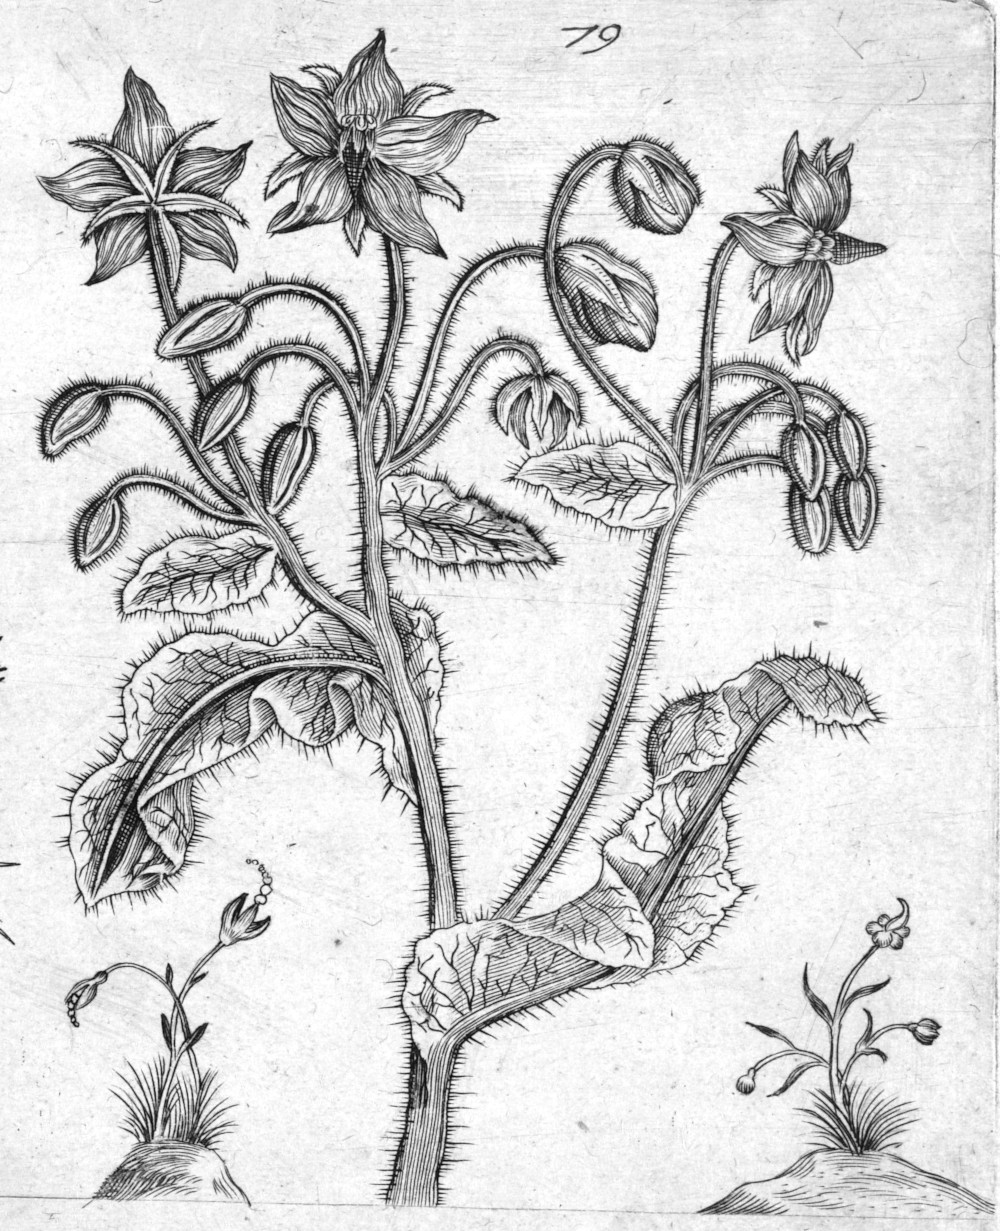
\includegraphics[keepaspectratio,width=\textwidth]{figures/borage-small.jpg}
  \captionart{Borage}
  \label{fig:borage}
\end{figure}

% Force float here
\clearpage{}

\thispagestyle{titleontop}
\subsection{Borage.}
\begin{wrapfigure}{r}{0.5\textwidth}
  \begingroup
  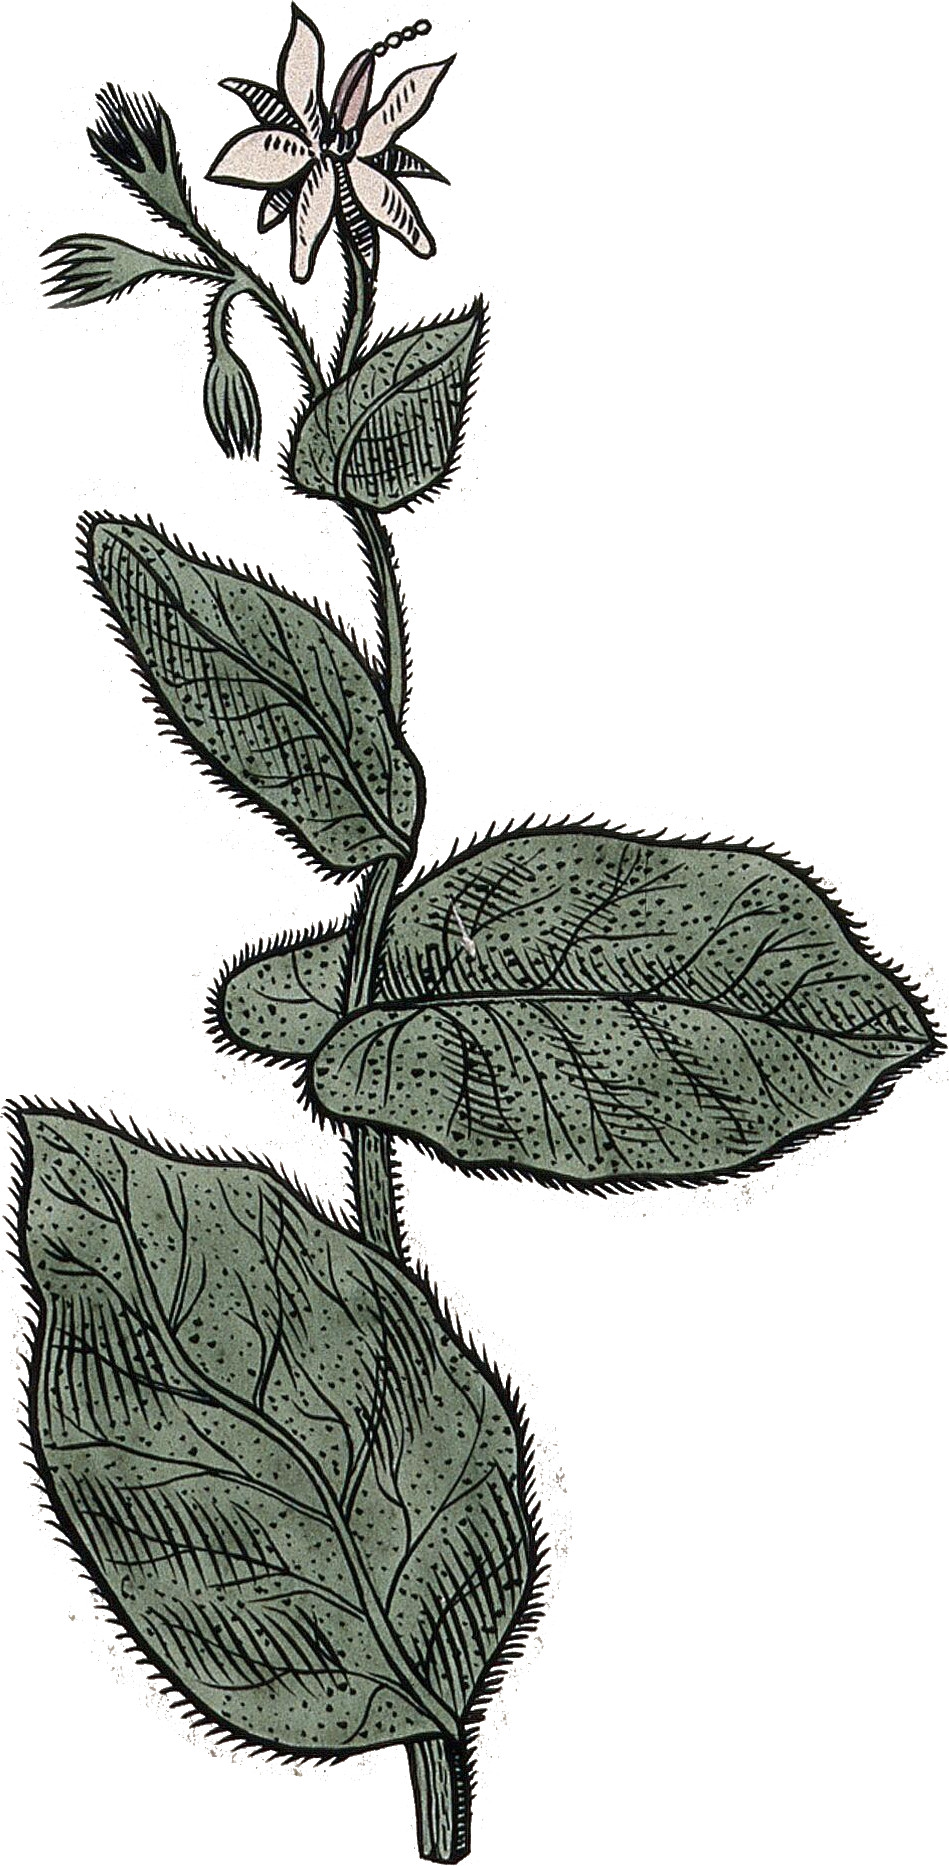
\includegraphics[keepaspectratio,width=0.5\textwidth]{figures/buglossa-small.jpg}
  \captionart{Buglosa}
  \label{fig:buglosa}
\end{wrapfigure}
In this catalogue, borage and bugloss may challenge the
chiefest place, whether in substance, juice, roots, seeds, flowers,
leaves, decoctions, distilled waters, extracts, oils, \etc{}, for such
kind of herbs be diversely varied. Bugloss is hot and moist, and
therefore worthily reckoned up amongst those herbs which expel
melancholy, and \authorfootnote{4126} exhilarate the heart, Galen, lib. 6. cap. 80. de
simpl. med. Dioscorides, lib. 4. cap. 123. Pliny much magnifies this
plant. It may be diversely used; as in broth, in \authorfootnote{4127}wine, in
conserves, syrups, \etc{}. It is an excellent cordial, and against this
malady most frequently prescribed; a herb indeed of such sovereignty,
that as Diodorus, lib. 7. bibl. Plinius, lib. 25. cap. 2. et lib. 21.
cap. 22. Plutarch, sympos. lib. 1. cap. 1. Dioscorides, lib. 5. cap.
40. Caelius, lib. 19. c. 3. suppose it was that famous Nepenthes of
\authorfootnote{4128}Homer, which Polydaenna, Thonis's wife (then king of Thebes in
Egypt), sent Helena for a token, of such rare virtue, that if taken
steeped in wine, if wife and children, father and mother, brother and
sister, and all thy dearest friends should die before thy face, thou
couldst not grieve or shed a tear for them.

Qui semel id patera mistum Nepenthes Iaccho
Hauserit, hic lachrymam, non si suavissima proles,
Si germanus ei charus, materque paterque
Oppetat, ante oculos ferro confossus atroci.

Helena's commended bowl to exhilarate the heart, had no other
ingredient, as most of our critics conjecture, than this of borage.
\subsection{Balm.}
Melissa balm hath an admirable virtue to alter melancholy, be
it steeped in our ordinary drink, extracted, or otherwise taken.
Cardan, lib. 8. much admires this herb. It heats and dries, saith
\authorfootnote{4129} Heurnius, in the second degree, with a wonderful virtue comforts
the heart, and purgeth all melancholy vapours from the spirits,
Matthiol. in lib. 3. cap. 10. in Dioscoridem. Besides they ascribe
other virtues to it, \authorfootnote{4130}as to help concoction, to cleanse the brain,
expel all careful thoughts, and anxious imaginations: the same words in
effect are in Avicenna, Pliny, Simon Sethi, Fuchsius, Leobel,
Delacampius, and every herbalist. Nothing better for him that is
melancholy than to steep this and borage in his ordinary drink.
Mathiolus, in his fifth book of Medicinal Epistles, reckons up
scorzonera, \authorfootnote{4131}not against poison only, falling sickness, and such
as are vertiginous, but to this malady; the root of it taken by itself
expels sorrow, causeth mirth and lightness of heart.

Antonius Musa, that renowned physician to Caesar Augustus, in his book
which he writ of the virtues of betony, cap. 6. wonderfully commends
that herb, animas hominum et corpora custodit, securas de metu reddit,
it preserves both body and mind, from fears, cares, griefs; cures
falling sickness, this and many other diseases, to whom Galen
subscribes, lib. 7. simp. med. Dioscorides, lib. 4. cap. 1. \etc{}.
Marigold is much approved against melancholy, and often used therefore
in our ordinary broth, as good against this and many other diseases.

\subsection{Hop.}
Lupulus, hop, is a sovereign remedy; Fuchsius, cap. 58. Plant.
hist. much extols it; \authorfootnote{4132}it purgeth all choler, and purifies the
blood. Matthiol. cap. 140. in 4. Dioscor. wonders the physicians of his
time made no more use of it, because it rarefies and cleanseth: we use
it to this purpose in our ordinary beer, which before was thick and
fulsome.

Wormwood, centaury, pennyroyal, are likewise magnified and much
prescribed (as I shall after show), especially in hypochondriac
melancholy, daily to be used, sod in whey: and as Ruffus Ephesias,
\authorfootnote{4133}Areteus relate, by breaking wind, helping concoction, many
melancholy men have been cured with the frequent use of them alone.

And because the spleen and blood are often misaffected in melancholy, I
may not omit endive, succory, dandelion, fumitory, \etc{}, which cleanse
the blood, Scolopendria, cuscuta, ceterache, mugwort, liverwort, ash,
tamarisk, genist, maidenhair, \etc{}, which must help and ease the spleen.

To these I may add roses, violets, capers, featherfew, scordium,
staechas, rosemary, ros solis, saffron, ochyme, sweet apples, wine,
tobacco, sanders, \etc{}. That Peruvian chamico, monstrosa facultate \etc{},
Linshcosteus Datura; and to such as are cold, the \authorfootnote{4134}decoction of
guiacum, China sarsaparilla, sassafras, the flowers of carduus
benedictus, which I find much used by Montanus in his Consultations,
Julius Alexandrinus, Lelius, Egubinus, and others. \authorfootnote{4135}Bernardus
Penottus prefers his herba solis, or Dutch sindaw, before all the rest
in this disease, and will admit of no herb upon the earth to be
comparable to it. It excels Homer's moly, cures this, falling sickness,
and almost all other infirmities. The same Penottus speaks of an
excellent balm out of Aponensis, which, taken to the quantity of three
drops in a cup of wine, \authorfootnote{4136}will cause a sudden alteration, drive
away dumps, and cheer up the heart. Ant. Guianerius, in his Antidotary,
hath many such. \authorfootnote{4137}Jacobus de Dondis the aggregator, repeats
ambergris, nutmegs, and allspice amongst the rest. But that cannot be
general. Amber and spice will make a hot brain mad, good for cold and
moist. Garcias ab Horto hath many Indian plants, whose virtues he much
magnifies in this disease. Lemnius, instit. cap. 58. admires rue, and
commends it to have excellent virtue, \authorfootnote{4138}to expel vain imaginations,
devils, and to ease afflicted souls. Other things are much magnified
\authorfootnote{4139}by writers, as an old cock, a ram's head, a wolf's heart borne or
eaten, which Mercurialis approves; Prosper Altinus the water of Nilus;
Gomesius all seawater, and at seasonable times to be seasick: goat's
milk, whey, \etc{}.

%SUBSECT. IV.-_Precious Stones, Metals, Minerals, Alteratives_.
\section{Precious Stones, Metals, Minerals, Alteratives.}

\lettrine{P}{recious} stones are diversely censured; many explode the use of them or
any minerals in physic, of whom Thomas Erastus is the chief, in his
tract against Paracelsus, and in an epistle of his to Peter Monavius,
\authorfootnote{4140} That stones can work any wonders, let them believe that list, no
man shall persuade me; for my part, I have found by experience there is
no virtue in them. But Matthiolus, in his comment upon
\authorfootnote{4141}Dioscorides, is as profuse on the other side, in their
commendation; so is Cardan, Renodeus, Alardus, Rueus, Encelius,
Marbodeus, \etc{}. \authorfootnote{4142}Matthiolus specifies in coral: and Oswaldus
Crollius, Basil. Chym. prefers the salt of coral. \authorfootnote{4143}Christoph.
Encelius, lib. 3. cap. 131. will have them to be as so many several
medicines against melancholy, sorrow, fear, dullness, and the like;
\authorfootnote{4144}Renodeus admires them, besides they adorn kings' crowns, grace
the fingers, enrich our household stuff, defend us from enchantments,
preserve health, cure diseases, they drive away grief, cares, and
exhilarate the mind. The particulars be these.

Granatus, a precious stone so called, because it is like the kernels of
a pomegranate, an imperfect kind of ruby, it comes from Calecut;
\authorfootnote{4145}if hung about the neck, or taken in drink, it much resisteth
sorrow, and recreates the heart. The same properties I find ascribed to
the hyacinth and topaz. \authorfootnote{4146}They allay anger, grief, diminish
madness, much delight and exhilarate the mind. \authorfootnote{4147}If it be either
carried about, or taken in a potion, it will increase wisdom, saith
Cardan, expel fear; he brags that he hath cured many madmen with it,
which, when they laid by the stone, were as mad again as ever they were
at first. Petrus Bayerus, lib. 2. cap. 13. veni mecum, Fran. Rueus,
cap. 19. de geminis, say as much of the chrysolite, \authorfootnote{4148}a friend of
wisdom, an enemy to folly. Pliny, lib. 37. Solinus, cap. 52. Albertus
de Lapid. Cardan. Encelius, lib. 3. cap. 66. highly magnifies the
virtue of the beryl, \authorfootnote{4149}it much avails to a good understanding,
represseth vain conceits, evil thoughts, causeth mirth, \etc{}. In the
belly of a swallow there is a stone found called chelidonius,
\authorfootnote{4150}which if it be lapped in a fair cloth, and tied to the right arm,
will cure lunatics, madmen, make them amiable and merry.

There is a kind of onyx called a chalcedony, which hath the same
qualities, \authorfootnote{4151}avails much against fantastic illusions which proceed
from melancholy, preserves the vigour and good estate of the whole
body.

The Eban stone, which goldsmiths use to sleeken their gold with, borne
about or given to drink, \authorfootnote{4152}hath the same properties, or not much
unlike.

Levinus Lemnius, Institui. ad vit. cap. 58. amongst other jewels, makes
mention of two more notable; carbuncle and coral, \authorfootnote{4153}which drive
away childish fears, devils, overcome sorrow, and hung about the neck
repress troublesome dreams, which properties almost Cardan gives to
that green-coloured \authorfootnote{4154}emmetris if it be carried about, or worn in a
ring; Rueus to the diamond.

Nicholas Cabeus, a Jesuit of Ferrara, in the first book of his
Magnetical Philosophy, cap. 3. speaking of the virtues of a loadstone,
recites many several opinions; some say that if it be taken in parcels
inward, si quis per frustra voret, juventutem restituet, it will, like
viper's wine, restore one to his youth; and yet if carried about them,
others will have it to cause melancholy; let experience determine.

Mercurialis admires the emerald for its virtues in pacifying all
affections of the mind; others the sapphire, which is the \authorfootnote{4155}fairest
of all precious stones, of sky colour, and a great enemy to black
choler, frees the mind, mends manners, \etc{}. Jacobus de Dondis, in his
catalogue of simples, hath ambergris, os in corde cervi, \authorfootnote{4156}the bone
in a stag's heart, a monocerot's horn, bezoar's stone \authorfootnote{4157}(of which
elsewhere), it is found in the belly of a little beast in the East
Indies, brought into Europe by Hollanders, and our countrymen
merchants. Renodeus, cap. 22. lib. 3. de ment. med. saith he saw two of
these beasts alive, in the castle of the Lord of Vitry at Coubert.

Lapis lazuli and armenus, because they purge, shall be mentioned in
their place.

Of the rest in brief thus much I will add out of Cardan, Renodeus, cap.
23. lib. 3. Rondoletius, lib. 1. de Testat. c. 15. \etc{}. \authorfootnote{4158}That
almost all jewels and precious stones have excellent virtues to pacify
the affections of the mind, for which cause rich men so much covet to
have them: \authorfootnote{4159}and those smaller unions which are found in shells
amongst the Persians and Indians, by the consent of all writers, are
very cordial, and most part avail to the exhilaration of the heart.

\subsection{Minerals.}
Most men say as much of gold and some other minerals, as
these have done of precious stones. Erastus still maintains the
opposite part. \textlatin{Disput. in Paracelsum. cap. 4. fol. 196.} he confesseth
of gold, \authorfootnote{4160} that it makes the heart merry, but in no other sense
but as it is in a miser's chest: \li{at mihi plaudo simul ac nummos
contemplor in arca}, as he said in the poet, it so revives the spirits,
and is an excellent recipe against melancholy,
%
{\gothfont
\begin{verse}
For gold in physic is a cordial,\\*
Therefore he loved gold in special.\\!
\end{verse}
}
\attrib{\getauthornote{4161} [Lines FIXME. \theeditor{}]}
%
\li{Aurum potabile}, \authorfootnote{4162}he discommends and inveighs against it, by reason
of the corrosive waters which are used in it: which argument our Dr.
Guin urgeth against D. Antonius. \authorfootnote{4163}Erastus concludes their
philosophical stones and potable gold, \etc{} to be no better than poison,
a mere imposture, a non ens; dug out of that broody hill belike this
golden stone is, ubi nascetur ridiculus mus. Paracelsus and his
chemistical followers, as so many Promethei, will fetch fire from
heaven, will cure all manner of diseases with minerals, accounting them
the only physic on the other side. \authorfootnote{4164}Paracelsus calls Galen,
Hippocrates, and all their adherents, infants, idiots, sophisters, \etc{}.
Apagesis istos qui Vulcanias istas metamorphoses sugillant, inscitiae
soboles, supinae pertinaciae alumnos, \etc{}, not worthy the name of
physicians, for want of these remedies: and brags that by them he can
make a man live 160 years, or to the world's end, with their
\authorfootnote{4165}Alexipharmacums, Panaceas, Mummias, unguentum Armarium, and such
magnetical cures, Lampas vitae et mortis, Balneum Dianae, Balsamum,
Electrum Magico-physicum, Amuleta Martialia, \etc{}. What will not he and
his followers effect? He brags, moreover, that he was primus medicorum,
and did more famous cures than all the physicians in Europe besides,
\authorfootnote{4166}a drop of his preparations should go farther than a dram, or
ounce of theirs, those loathsome and fulsome filthy potions,
heteroclitical pills (so he calls them), horse medicines, ad quoram
aspectum Cyclops Polyphemus exhorresceret. And though some condemn
their skill and magnetical cures as tending to magical superstition,
witchery, charms, \etc{}, yet they admire, stiffly vindicate nevertheless,
and infinitely prefer them. But these are both in extremes, the middle
sort approve of minerals, though not in so high a degree. Lemnius lib.
3. cap. 6. de occult. nat. mir. commends gold inwardly and outwardly
used, as in rings, excellent good in medicines; and such mixtures as
are made for melancholy men, saith Wecker, antid. spec. lib. 1. to whom
Renodeus subscribes, lib. 2. cap. 2. Ficinus, lib. 2. cap. 19. Fernel.
meth. med. lib. 5. cap. 21. de Cardiacis. Daniel Sennertus, lib. 1.
part. 2. cap. 9. Audernacus, Libavius, Quercetanus, Oswaldus Crollius,
Euvonymus, Rubeus, and Matthiolus in the fourth book of his Epistles,
Andreas a Blawen epist. ad Matthiolum, as commended and formerly used
by Avicenna, Arnoldus, and many others: \authorfootnote{4167}Matthiolus in the same
place approves of potable gold, mercury, with many such chemical
confections, and goes so far in approbation of them, that he holds
\authorfootnote{4168} no man can be an excellent physician that hath not some skill in
chemistical distillations, and that chronic diseases can hardly be
cured without mineral medicines: look for antimony among purgers.

%SUBSECT. V.-_Compound Alteratives; censure of Compounds, and mixed
\section[Compound Alteratives]{Compound Alteratives; censure of Compounds, and mixed
Physic.}

\lettrine{P}{liny}, lib. 24. c. 1, bitterly taxeth all compound medicines, \authorfootnote{4169}
Men's knavery, imposture, and captious wits, have invented those shops,
in which every man's life is set to sale: and by and by came in those
compositions and inexplicable mixtures, far-fetched out of India and
Arabia; a medicine for a botch must be had as far as the Red Sea. And
'tis not without cause which he saith; for out of question they are
much to \authorfootnote{4170}blame in their compositions, whilst they make infinite
variety of mixtures, as \authorfootnote{4171}Fuchsius notes. They think they get
themselves great credit, excel others, and to be more learned than the
rest, because they make many variations; but he accounts them fools,
and whilst they brag of their skill, and think to get themselves a
name, they become ridiculous, betray their ignorance and error. A few
simples well prepared and understood, are better than such a heap of
nonsense, confused compounds, which are in apothecaries' shops
ordinarily sold. In which many vain, superfluous, corrupt, exolete,
things out of date are to be had (saith Cornarius); a company of
barbarous names given to syrups, juleps, an unnecessary company of
mixed medicines; rudis indigestaque moles. Many times (as Agrippa
taxeth) there is by this means \authorfootnote{4172}more danger from the medicine than
from the disease, when they put together they know not what, or leave
it to an illiterate apothecary to be made, they cause death and horror
for health. Those old physicians had no such mixtures; a simple potion
of hellebore in Hippocrates' time was the ordinary purge; and at this
day, saith \authorfootnote{4173}Mat. Riccius, in that flourishing commonwealth of
China, their physicians give precepts quite opposite to ours, not
unhappy in their physic; they use altogether roots, herbs, and simples
in their medicines, and all their physic in a manner is comprehended in
a herbal: no science, no school, no art, no degree, but like a trade,
every man in private is instructed of his master. \authorfootnote{4174}Cardan cracks
that he can cure all diseases with water alone, as Hippocrates of old
did most infirmities with one medicine. Let the best of our rational
physicians demonstrate and give a sufficient reason for those intricate
mixtures, why just so many simples in mithridate or treacle, why such
and such quantity; may they not be reduced to half or a quarter?
Frustra fit per plura (as the saying is) quod fieri potest per
pauciora; 300 simples in a julep, potion, or a little pill, to what end
or purpose? I know not what \authorfootnote{4175}Alkindus, Capivaccius, Montagna, and
Simon Eitover, the best of them all and most rational, have said in
this kind; but neither he, they, nor any one of them, gives his reader,
to my judgment, that satisfaction which he ought; why such, so many
simples? Rog. Bacon hath taxed many errors in his tract de
graduationibus, explained some things, but not cleared. Mercurialis in
his book de composit. medicin. gives instance in Hamech, and Philonium
Romanum, which Hamech an Arabian, and Philonius a Roman, long since
composed, but crasse as the rest. If they be so exact, as by him it
seems they were, and those mixtures so perfect, why doth Fernelius
alter the one, and why is the other obsolete? \authorfootnote{4176}Cardan taxeth Galen
for presuming out of his ambition to correct Theriachum Andromachi, and
we as justly may carp at all the rest. Galen's medicines are now
exploded and rejected; what Nicholas Meripsa, Mesue, Celsus,
Scribanius, Actuarius, \etc{} writ of old, are most part contemned.

Mellichius, Cordus, Wecker, Quercetan, Renodeus, the Venetian,
Florentine states have their several receipts, and magistrals: they of
Nuremberg have theirs, and Augustana Pharmacopoeia, peculiar medicines
to the meridian of the city: London hers, every city, town, almost
every private man hath his own mixtures, compositions, receipts,
magistrals, precepts, as if he scorned antiquity, and all others in
respect of himself. But each man must correct and alter to show his
skill, every opinionative fellow must maintain his own paradox, be it
what it will; Delirant reges, plectuntur Achivi: they dote, and in the
meantime the poor patients pay for their new experiments, the
commonalty rue it.

Thus others object, thus I may conceive out of the weakness of my
apprehension; but to say truth, there is no such fault, no such
ambition, no novelty, or ostentation, as some suppose; but as \authorfootnote{4177}one
answers, this of compound medicines, is a most noble and profitable
invention found out, and brought into physic with great judgment,
wisdom, counsel and discretion. Mixed diseases must have mixed
remedies, and such simples are commonly mixed as have reference to the
part affected, some to qualify, the rest to comfort, some one part,
some another. Cardan and Brassavola both hold that Nullum simplex
medicamentum sine noxa, no simple medicine is without hurt or offence;
and although Hippocrates, Erasistratus, Diocles of old, in the infancy
of this art, were content with ordinary simples: yet now, saith
\authorfootnote{4178}Aetius, necessity compelleth to seek for new remedies, and to
make compounds of simples, as well to correct their harms if cold, dry,
hot, thick, thin, insipid, noisome to smell, to make them savoury to
the palate, pleasant to taste and take, and to preserve them for
continuance, by admixtion of sugar, honey, to make them last months and
years for several uses. In such cases, compound medicines may be
approved, and Arnoldus in his 18. aphorism, doth allow of it. \authorfootnote{4179}If
simples cannot, necessity compels us to use compounds; so for receipts
and magistrals, dies diem docet, one day teacheth another, and they are
as so many words or phrases, Que nunc sunt in honore vocabula si volet
usus, ebb and flow with the season, and as wits vary, so they may be
infinitely varied. Quisque suum placitum quo capiatur habet. Every man
as he likes, so many men so many minds, and yet all tending to good
purpose, though not the same way. As arts and sciences, so physic is
still perfected amongst the rest; Horae musarum nutrices, and
experience teacheth us every day \authorfootnote{4180}many things which our
predecessors knew not of. Nature is not effete, as he saith, or so
lavish, to bestow all her gifts upon an age, but hath reserved some for
posterity, to show her power, that she is still the same, and not old
or consumed. Birds and beasts can cure themselves by nature,
\authorfootnote{4181}naturae usu ea plerumque cognoscunt quae homines vix longo labore
et doctrina assequuntur, but men must use much labour and industry to
find it out. But I digress.

Compound medicines are inwardly taken, or outwardly applied. Inwardly
taken, be either liquid or solid: liquid, are fluid or consisting.

Fluid, as wines and syrups. The wines ordinarily used to this disease
are wormwood wine, tamarisk, and buglossatum, wine made of borage and
bugloss, the composition of which is specified in Arnoldus
Villanovanus, lib. de vinis, of borage, balm, bugloss, cinnamon, \etc{}.
and highly commended for its virtues: \authorfootnote{4182}it drives away leprosy,
scabs, clears the blood, recreates the spirits, exhilarates the mind,
purgeth the brain of those anxious black melancholy fumes, and
cleanseth the whole body of that black humour by urine. To which I add,
saith Villanovanus, that it will bring madmen, and such raging
bedlamites as are tied in chains, to the use of their reason again. My
conscience bears me witness, that I do not lie, I saw a grave matron
helped by this means; she was so choleric, and so furious sometimes,
that she was almost mad, and beside herself; she said, and did she knew
not what, scolded, beat her maids, and was now ready to be bound till
she drank of this borage wine, and by this excellent remedy was cured,
which a poor foreigner, a silly beggar, taught her by chance, that came
to crave an alms from door to door. The juice of borage, if it be
clarified, and drunk in wine, will do as much, the roots sliced and
steeped, \etc{} saith Ant. Mizaldus, art. med. who cities this story
verbatim out of Villanovanus, and so doth Magninus a physician of
Milan, in his regimen of health. Such another excellent compound water
I find in Rubeus de distill. sect. 3. which he highly magnifies out of
Savanarola, \authorfootnote{4183}for such as are solitary, dull, heavy or sad without
a cause, or be troubled with trembling of heart. Other excellent
compound waters for melancholy, he cites in the same place. \authorfootnote{4184}If
their melancholy be not inflamed, or their temperature over-hot.

Evonimus hath a precious aquavitae to this purpose, for such as are
cold. But he and most commend aurum potabile, and every writer
prescribes clarified whey, with borage, bugloss, endive, succory, \etc{}.
of goat's milk especially, some indefinitely at all times, some thirty
days together in the spring, every morning fasting, a good draught.

Syrups are very good, and often used to digest this humour in the
heart, spleen, liver, \etc{}. As syrup of borage (there is a famous syrup
of borage highly commended by Laurentius to this purpose in his tract
of melancholy), de pomis of king Sabor, now obsolete, of thyme and
epithyme, hops, scolopendria, fumitory, maidenhair, bizantine, \etc{}.

These are most used for preparatives to other physic, mixed with
distilled waters of like nature, or in juleps otherwise.
Consisting, are conserves or confections; conserves of borage, bugloss,
balm, fumitory, succory, maidenhair, violets, roses, wormwood, \etc{}.

Confections, treacle, mithridate, eclegms, or linctures, \etc{}. Solid, as
aromatical confections: hot, diambra, diamargaritum calidum, dianthus,
diamoschum dulce, electuarium de gemmis laetificans Galeni et Rhasis,
diagalanga, diaciminum dianisum, diatrion piperion, diazinziber,
diacapers, diacinnamonum: Cold, as diamargaritum frigidum, diacorolli,
diarrhodon abbatis, diacodion, \etc{} as every pharmacopoeia will show
you, with their tables or losings that are made out of them: with
condites and the like.

Outwardly used as occasion serves, as amulets, oils hot and cold, as of
camomile, staechados, violets, roses, almonds, poppy, nymphea,
mandrake, \etc{} to be used after bathing, or to procure sleep.
Ointments composed of the said species, oils and wax, \etc{}, as
Alablastritum Populeum, some hot, some cold, to moisten, procure sleep,
and correct other accidents.

Liniments are made of the same matter to the like purpose: emplasters
of herbs, flowers, roots, \etc{}, with oils, and other liquors mixed and
boiled together.

Cataplasms, salves, or poultices made of green herbs, pounded, or sod
in water till they be soft, which are applied to the hypochondries, and
other parts, when the body is empty.

Cerotes are applied to several parts and frontals, to take away pain,
grief, heat, procure sleep. Fomentations or sponges, wet in some
decoctions, \etc{}, epithemata, or those moist medicines, laid on linen,
to bathe and cool several parts misaffected.

Sacculi, or little bags of herbs, flowers, seeds, roots, and the like,
applied to the head, heart, stomach, \etc{}, odoraments, balls, perfumes,
posies to smell to, all which have their several uses in melancholy, as
shall be shown, when I treat of the cure of the distinct species by
themselves.

%MEMB. II.

%SUBSECT. I.-_Purging Simples upward_.
\section{Purging Simples upward.}
\lettrine{M}{elanagoga}, or melancholy purging medicines, are either simple or
compound, and that gently, or violently, purging upward or downward.
These following purge upward. \authorfootnote{4185}Asarum, or Asrabecca, which, as
Mesue saith, is hot in the second degree, and dry in the third, it is
commonly taken in wine, whey, or as with us, the juice of two or three
leaves or more sometimes, pounded in posset drink qualified with a
little liquorice, or aniseed, to avoid the fulsomeness of the taste, or
as Diaserum Fernelii. Brassivola in Catart. reckons it up amongst those
simples that only purge melancholy, and Ruellius confirms as much out
of his experience, that it purgeth \authorfootnote{4186}black choler, like hellebore
itself. Galen, lib. G. simplic. and \authorfootnote{4187}Matthiolus ascribe other
virtues to it, and will have it purge other humours as well as this.

Laurel, by Heurnius's method, ad prax. lib. 2. cap. 24. is put amongst
the strong purgers of melancholy; it is hot and dry in the fourth
degree. Dioscorides, lib. 11. cap. 114. adds other effects to it.
\authorfootnote{4188}Pliny sets down fifteen berries in drink for a sufficient potion:
it is commonly corrected with his opposites, cold and moist, as juice
of endive, purslane, and is taken in a potion to seven grains and a
half. But this and asrabecca, every gentlewoman in the country knows
how to give, they are two common vomits.

\begin{figure}[tbh]
  \begingroup
  \centering
  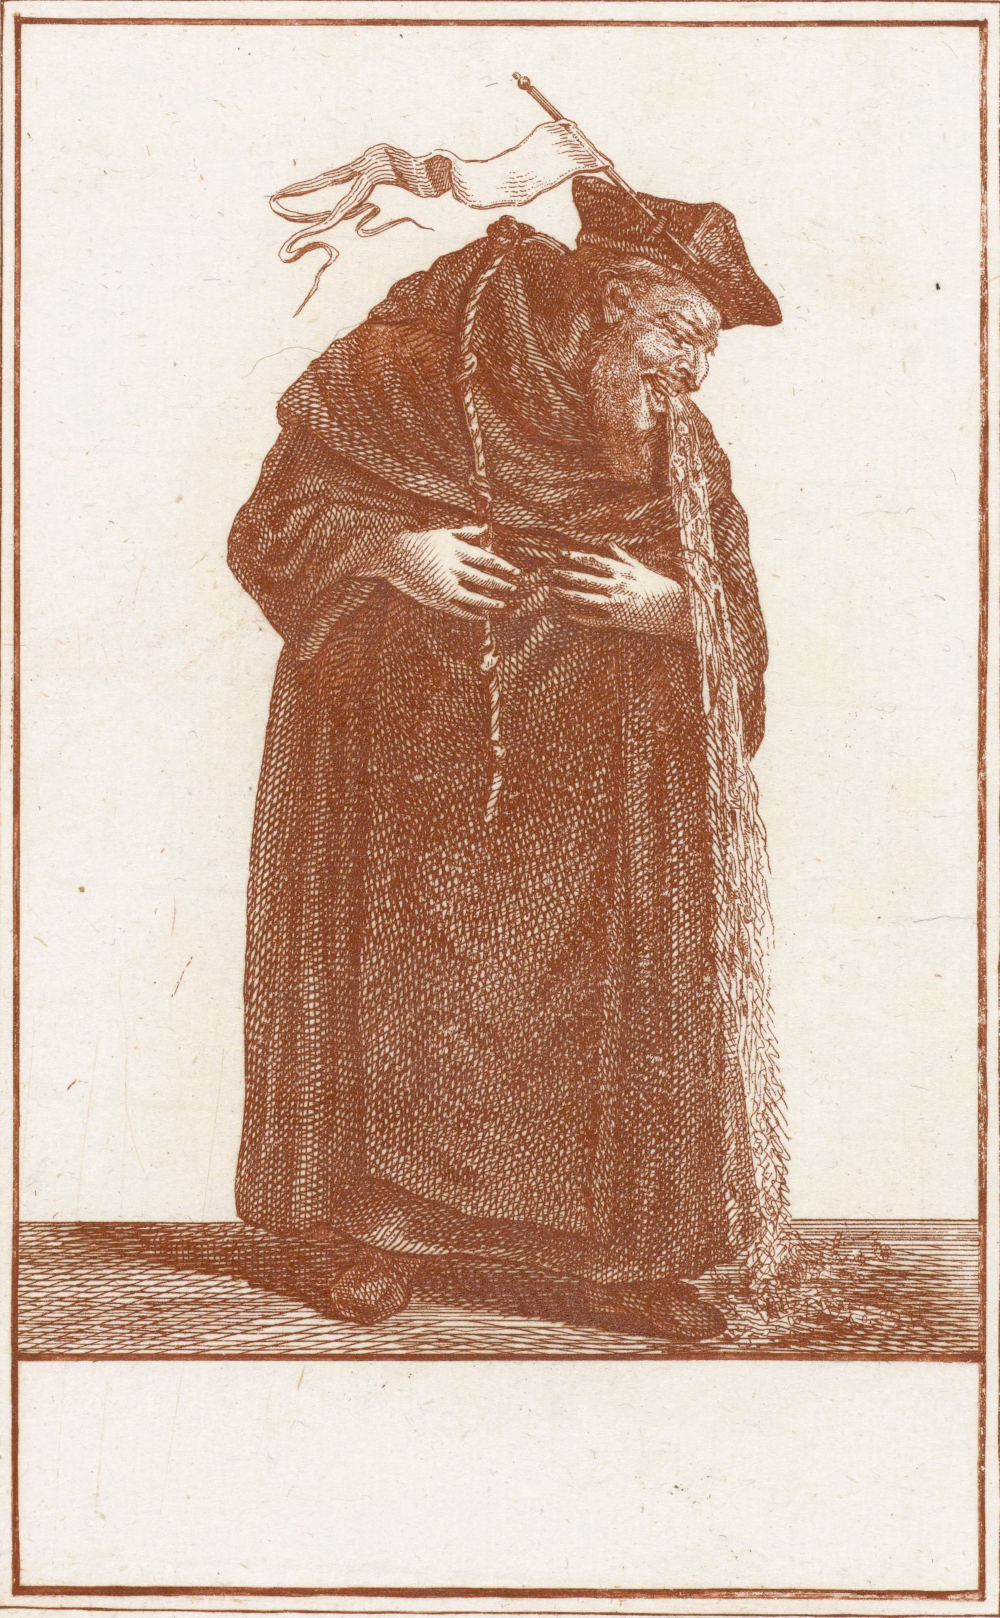
\includegraphics[keepaspectratio,width=0.5\textwidth]{figures/Vomiting-monk-Jacob-Gole-small.jpg}
  \captionart{VomitingMonk}
  \label{fig:vomitingmonk}
\end{figure}

Scilla, or sea-onion, is hot and dry in the third degree. Brassivola in
Catart. out of Mesue, others, and his own experience, will have this
simple to purge \authorfootnote{4189}melancholy alone. It is an ordinary vomit, vinum
scilliticum mixed with rubel in a little white wine.

White hellebore, which some call sneezing-powder, a strong purger
upward, which many reject, as being too violent: Mesue and Averroes
will not admit of it, \authorfootnote{4190}by reason of danger of suffocation,
\authorfootnote{4191}great pain and trouble it puts the poor patient to, saith
Dodonaeus. Yet Galen, lib. 6. simpl. med. and Dioscorides, cap. 145.
allow of it. It was indeed \authorfootnote{4192} terrible in former times, as Pliny
notes, but now familiar, insomuch that many took it in those days,
\authorfootnote{4193}that were students, to quicken their wits, which Persius Sat. 1.
objects to Accius the poet, Illas Acci ebria veratro. \authorfootnote{4194}It helps
melancholy, the falling sickness, madness, gout, \etc{}, but not to be
taken of old men, youths, such as are weaklings, nice, or effeminate,
troubled with headache, high-coloured, or fear strangling, saith
Dioscorides. \authorfootnote{4195}Oribasius, an old physician, hath written very
copiously, and approves of it, in such affections which can otherwise
hardly be cured. Hernius, lib. 2. prax. med. de vomitoriis, will not
have it used \authorfootnote{4196}but with great caution, by reason of its strength,
and then when antimony will do no good, which caused Hermophilus to
compare it to a stout captain (as Codroneus observes cap. 7. comment.
de Helleb.) that will see all his soldiers go before him and come post
principia, like the bragging soldier, last himself; \authorfootnote{4197}when other
helps fail in inveterate melancholy, in a desperate case, this vomit is
to be taken. And yet for all this, if it be well prepared, it may be
\authorfootnote{4198} securely given at first. \authorfootnote{4199}Matthiolus brags, that he hath
often, to the good of many, made use of it, and Heurnius, \authorfootnote{4200}that he
hath happily used it, prepared after his own prescript, and with good
success. Christophorus a Vega, lib. 3. c. 41, is of the same opinion,
that it may be lawfully given; and our country gentlewomen find it by
their common practice, that there is no such great danger in it. Dr.
Turner, speaking of this plant in his Herbal, telleth us, that in his
time it was an ordinary receipt among good wives, to give hellebore in
powder to ii'd weight, and he is not much against it. But they do
commonly exceed, for who so bold as blind Bayard, and prescribe it by
pennyworths, and such irrational ways, as I have heard myself market
folks ask for it in an apothecary's shop: but with what success God
knows; they smart often for their rash boldness and folly, break a
vein, make their eyes ready to start out of their heads, or kill
themselves. So that the fault is not in the physic, but in the rude and
indiscreet handling of it. He that will know, therefore, when to use,
how to prepare it aright, and in what dose, let him read Heurnius lib.
2. prax. med. Brassivola de Catart. Godefridus Stegius the emperor
Rudolphus' physician, cap. 16. Matthiolus in Dioscor. and that
excellent commentary of Baptista Codroncus, which is instar omnium de
Helleb. alb. where we shall find great diversity of examples and
receipts.

Antimony or stibium, which our chemists so much magnify, is either
taken in substance or infusion, \etc{}, and frequently prescribed in this
disease. It helps all infirmities, saith \authorfootnote{4201}Matthiolus, which
proceed from black choler, falling sickness, and hypochondriacal
passions; and for farther proof of his assertion, he gives several
instances of such as have been freed with it: \authorfootnote{4202}one of Andrew
Gallus, a physician of Trent, that after many other essays, imputes the
recovery of his health, next after God, to this remedy alone. Another
of George Handshius, that in like sort, when other medicines failed,
\authorfootnote{4203}was by this restored to his former health, and which of his
knowledge others have likewise tried, and by the help of this admirable
medicine, been recovered. A third of a parish priest at Prague in
Bohemia, \authorfootnote{4204}that was so far gone with melancholy, that he doted, and
spake he knew not what; but after he had taken twelve grains of
stibium, (as I myself saw, and can witness, for I was called to see
this miraculous accident) he was purged of a deal of black choler, like
little gobbets of flesh, and all his excrements were as black blood (a
medicine fitter for a horse than a man), yet it did him so much good,
that the next day he was perfectly cured. This very story of the
Bohemian priest, Sckenkius relates verbatim, Exoter. experiment. ad.
var. morb. cent. 6. observ. 6. with great approbation of it. Hercules
de Saxonia calls it a profitable medicine, if it be taken after meat to
six or eight grains, of such as are apt to vomit. Rodericus a Fonseca
the Spaniard, and late professor of Padua in Italy, extols it to this
disease, Tom. 2. consul. 85. so doth Lod. Mercatus de inter. morb. cur.
lib. 1. cap. 17. with many others. Jacobus Gervinus a French physician,
on the other side, lib. 2. de venemis confut. explodes all this, and
saith he took three grains only upon Matthiolus and some others'
commendation, but it almost killed him, whereupon he concludes,
\authorfootnote{4205}antimony is rather poison than a medicine. Th. Erastus concurs
with him in his opinion, and so doth \AE{}lian Montaltus cap. 30 de melan.

But what do I talk? 'tis the subject of whole books; I might cite a
century of authors pro and con. I will conclude with \authorfootnote{4206}Zuinger,
antimony is like Scanderbeg's sword, which is either good or bad,
strong or weak, as the party is that prescribes, or useth it: a worthy
medicine if it be rightly applied to a strong man, otherwise poison.

For the preparing of it, look in Evonimi thesaurus, Quercetan, Oswaldus
Crollius, Basil. Chim. Basil. Valentius, \etc{}.

Tobacco, divine, rare, superexcellent tobacco, which goes far beyond
all the panaceas, potable gold, and philosopher's stones, a sovereign
remedy to all diseases. A good vomit, I confess, a virtuous herb, if it
be well qualified, opportunely taken, and medicinally used; but as it
is commonly abused by most men, which take it as tinkers do ale, 'tis a
plague, a mischief, a violent purger of goods, lands, health, hellish,
devilish and damned tobacco, the ruin and overthrow of body and soul.

%SUBSECT. II.-_Simples purging Melancholy downward_.
\section{Simples purging Melancholy downward.}

\lettrine{P}{olypody} and epithyme are, without all exceptions, gentle purgers of
melancholy. Dioscorides will have them void phlegm; but Brassivola out
of his experience averreth, that they purge this humour; they are used
in decoction, infusion, \etc{} simple, mixed, \etc{}.

Mirabolanes, all five kinds, are happily \authorfootnote{4207}prescribed against
melancholy and quartan agues; Brassivola speaks out \authorfootnote{4208}of a thousand
experiences, he gave them in pills, decoctions, \etc{}, look for peculiar
receipts in him.

Stoechas, fumitory, dodder, herb mercury, roots of capers, genista or
broom, pennyroyal and half-boiled cabbage, I find in this catalogue of
purgers of black choler, origan, featherfew, ammoniac \authorfootnote{4209}salt,
saltpetre. But these are very gentle; alyppus, dragon root, centaury,
ditany, colutea, which Fuchsius cap. 168 and others take for senna, but
most distinguish. Senna is in the middle of violent and gentle purgers
downward, hot in the second degree, dry in the first. Brassivola calls
it \authorfootnote{4210}a wonderful herb against melancholy, it scours the blood,
lightens the spirits, shakes off sorrow, a most profitable medicine, as
\authorfootnote{4211} Dodonaeus terms it, invented by the Arabians, and not heard of
before. It is taken diverse ways, in powder, infusion, but most
commonly in the infusion, with ginger, or some cordial flowers added to
correct it. Actuarius commends it sodden in broth, with an old cock, or
in whey, which is the common conveyor of all such things as purge black
choler; or steeped in wine, which Heurnius accounts sufficient, without
any farther correction.

Aloes by most is said to purge choler, but Aurelianus lib. 2. c. 6. de
morb. chron. Arculanus cap. 6. in 9. Rhasis Julius Alexandrinus,
consil. 185. Scoltz. Crato consil 189. Scoltz. prescribe it to this
disease; as good for the stomach and to open the haemorrhoids, out of
Mesue, Rhasis, Serapio, Avicenna: Menardus ep. lib. 1. epist. 1.
opposeth it, aloes \authorfootnote{4212}doth not open the veins, or move the
haemorrhoids, which Leonhartus Fuchsius paradox. lib. 1. likewise
affirms; but Brassivola and Dodonaeus defend Mesue out of their
experience; let \authorfootnote{4213}Valesius end the controversy.

Lapis armenus and lazuli are much magnified by \authorfootnote{4214}Alexander lib. 1.
cap. 16. Avicenna, Aetius, and Actuarius, if they be well washed, that
the water be no more coloured, fifty times some say. \authorfootnote{4215}That good
Alexander (saith Guianerus) puts such confidence in this one medicine,
that he thought all melancholy passions might be cured by it; and I for
my part have oftentimes happily used it, and was never deceived in the
operation of it. The like may be said of lapis lazuli, though it be
somewhat weaker than the other. Garcias ab Horto, hist. lib. 1. cap.
65. relates, that the \authorfootnote{4216}physicians of the Moors familiarly
prescribe it to all melancholy passions, and Matthiolus ep. lib. 3.
\authorfootnote{4217}brags of that happy success which he still had in the
administration of it. Nicholas Meripsa puts it amongst the best
remedies, sect. 1. cap. 12. in Antidotis; \authorfootnote{4218}and if this will not
serve (saith Rhasis) then there remains nothing but lapis armenus and
hellebore itself. Valescus and Jason Pratensis much commend pulvis
hali, which is made of it. James Damascen. 2. cap. 12. Hercules de
Saxonia, \etc{}, speaks well of it. Crato will not approve this; it and
both hellebores, he saith, are no better than poison. Victor
Trincavelius, lib. 2. cap. 14, found it in his experience, \authorfootnote{4219}to be
very noisome, to trouble the stomach, and hurt their bodies that take
it overmuch.
\clearpage{}

\subsection{Black hellebore}
\begin{wrapfigure}{r}{0.4\textwidth}
  \begingroup
  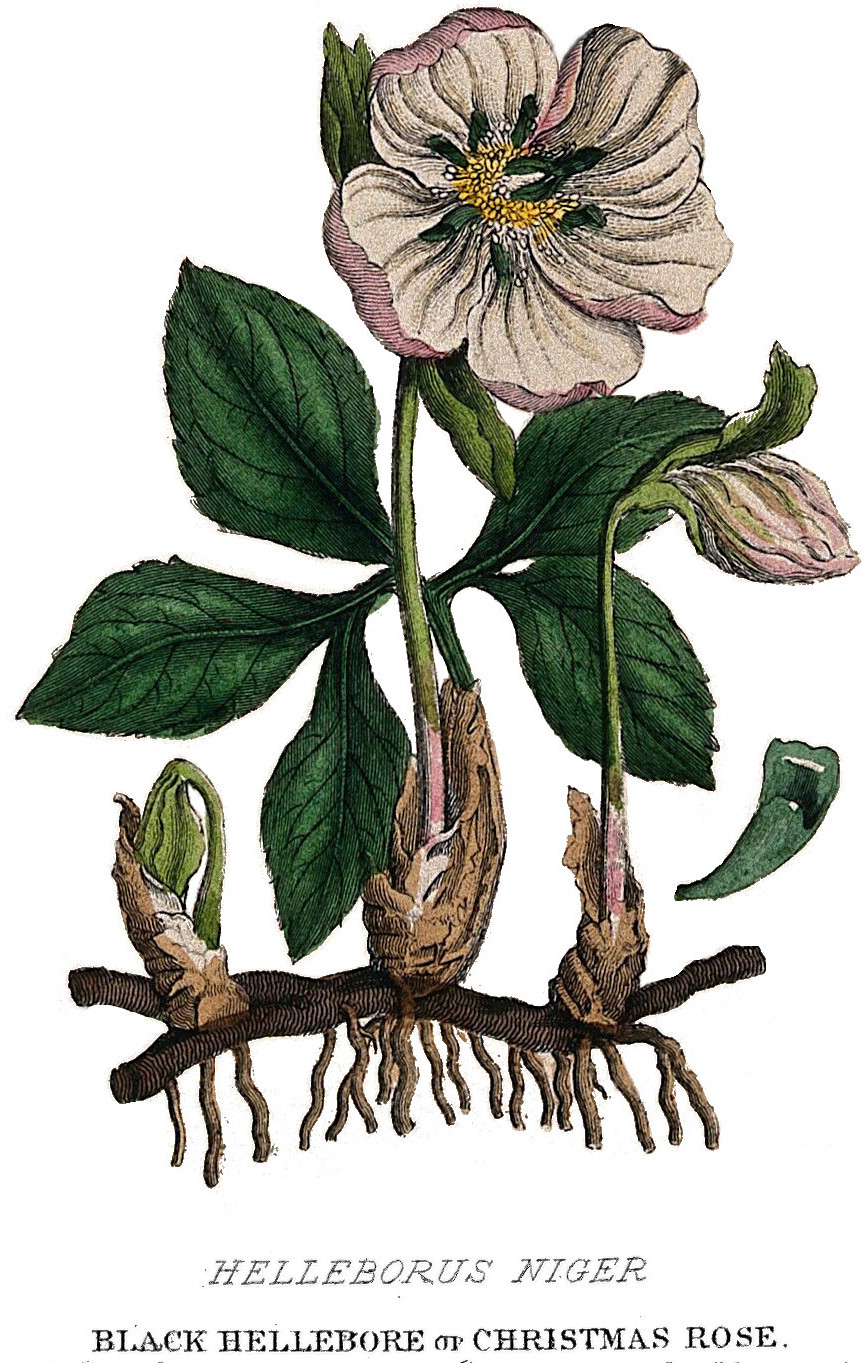
\includegraphics[keepaspectratio,width=0.4\textwidth]{figures/Helleborus-Niger-small.jpg}
  \captionart{HelleborusNiger2}
  \label{fig:helleborusniger2}
\end{wrapfigure}
Black hellebore, that most renowned plant, and famous purger of
melancholy, which all antiquity so much used and admired, was first
found out by Melanpodius a shepherd, as Pliny records, lib. 25. cap. 5.
\authorfootnote{4220}who, seeing it to purge his goats when they raved, practised it
upon Elige and Calene, King Praetus' daughters, that ruled in Arcadia,
near the fountain Clitorius, and restored them to their former health.

In Hippocrates's time it was in only request, insomuch that he writ a
book of it, a fragment of which remains yet. Theophrastus, \authorfootnote{4221}Galen,
Pliny, Caelius Aurelianus, as ancient as Galen, lib. 1, cap. 6. Aretus
lib. 1. cap. 5. Oribasius lib. 7. collect. a famous Greek, Aetius ser.
3. cap. 112 \& 113 p. Aegineta, Galen's Ape, lib. 7. cap. 4. Actuarius,
Trallianus lib. 5. cap. 15. Cornelius Celsus only remaining of the old
Latins, lib. 3. cap. 23, extol and admire this excellent plant; and it
was generally so much esteemed of the ancients for this disease amongst
the rest, that they sent all such as were crazed, or that doted, to the
Anticyrae, or to Phocis in Achaia, to be purged, where this plant was
in abundance to be had. In Strabo's time it was an ordinary voyage,
Naviget Anticyras; a common proverb among the Greeks and Latins, to bid
a dizzard or a mad man go take hellebore; as in Lucian, Menippus to
Tantalus, Tantale desipis, helleboro epoto tibi opus est, eoque sane
meraco, thou art out of thy little wit, O Tantalus, and must needs
drink hellebore, and that without mixture. Aristophanes in Vespis,
drink hellebore, \etc{} and Harpax in the \authorfootnote{4222} Comoedian, told Simo and
Ballio, two doting fellows, that they had need to be purged with this
plant. When that proud Menacrates \textgreek{ὀ ζεὺς}, had writ an arrogant letter
to Philip of Macedon, he sent back no other answer but this, Consulo
tibi ut ad Anticyram te conferas, noting thereby that he was crazed,
atque ellebore indigere, had much need of a good purge. Lilius Geraldus
saith, that Hercules, after all his mad pranks upon his wife and
children, was perfectly cured by a purge of hellebore, which an
Anticyrian administered unto him. They that were sound commonly took it
to quicken their wits, (as Ennis of old, \authorfootnote{4223}Qui non nisi potus ad
arma-prosiluit dicenda, and as our poets drink sack to improve their
inventions (I find it so registered by Agellius lib. 17. cap. 15.)
%\begin{figure}[H]
%  \begingroup
%  \centering
%  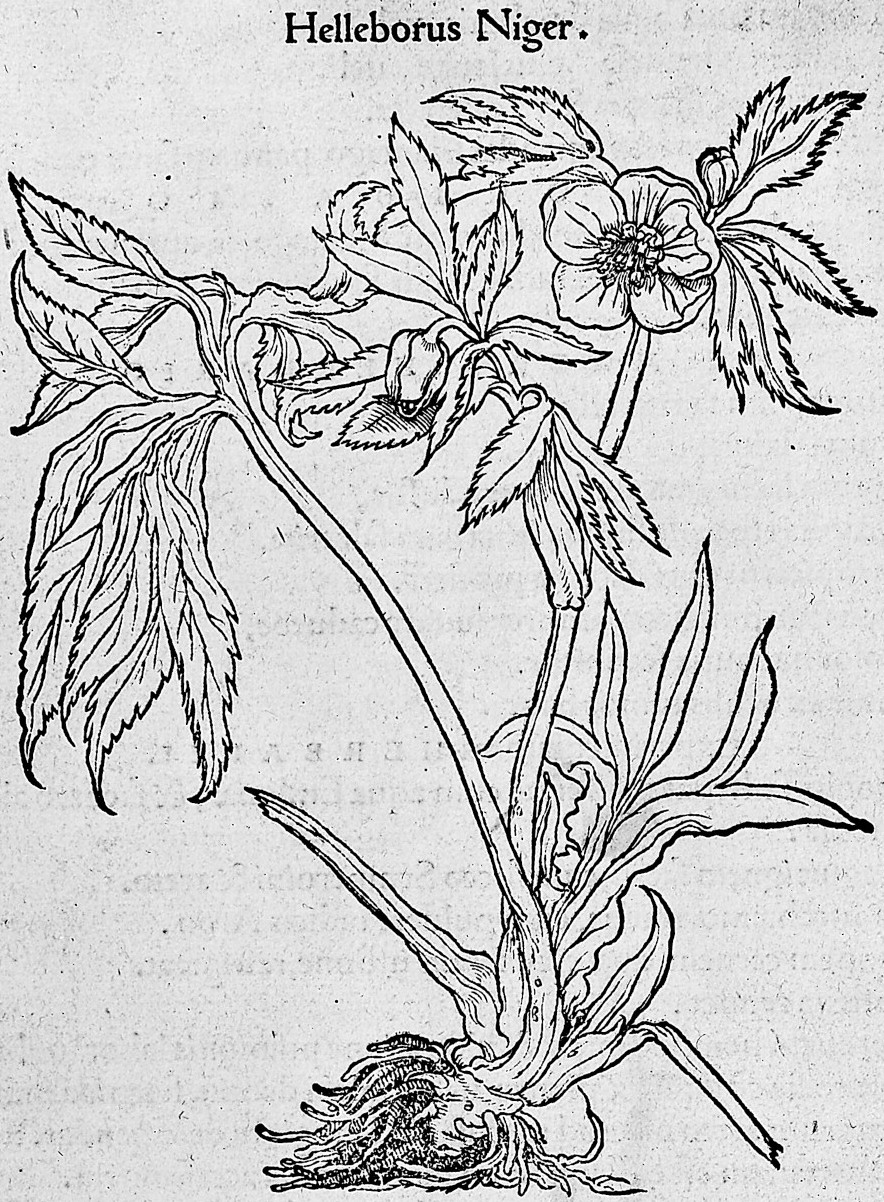
\includegraphics[keepaspectratio,width=\textwidth]{figures/HelleborusNiger-small}
%  \captionart{HelleborusNiger}
%  \label{fig:helleborusniger}
%\end{figure}

Cameades the academic, when he was to write against Zeno the stoic,
purged himself with hellebore first, which \authorfootnote{4224}Petronius puts upon
Chrysippus. In such esteem it continued for many ages, till at length
Mesue and some other Arabians began to reject and reprehend it, upon
whose authority for many following lustres, it was much debased and
quite out of request, held to be poison and no medicine; and is still
oppugned to this day by \authorfootnote{4225} Crato and some junior physicians. Their
reasons are, because Aristotle l. 1. de plant. c. 3. said, henbane and
hellebore were poison; and Alexander Aphrodiseus, in the preface of his
problems, gave out, that (speaking of hellebore) \authorfootnote{4226}Quails fed on
that which was poison to men. Galen. l. 6. Epid. com. 5. Text. 35.
confirms as much: \authorfootnote{4227}Constantine the emperor in his Geoponicks,
attributes no other virtue to it, than to kill mice and rats, flies and
mouldwarps, and so Mizaldus, Nicander of old, Gervinus, Sckenkius, and
some other Neoterics that have written of poisons, speak of hellebore
in a chief place. 

Nicholas Leonicus hath a story of Solon\authorfootnote{4228}, that
besieging, I know not what city, steeped hellebore in a spring of
water, which by pipes was conveyed into the middle of the town, and so
either poisoned, or else made them so feeble and weak by purging, that
they were not able to bear arms. Notwithstanding all these cavils and
objections, most of our late writers do much approve of it. \authorfootnote{4229}
Gariopontus lib. 1. cap. 13. Codronchus com. de helleb. Fallopius lib.
de med. purg. simpl. cap. 69. et consil. 15. Trincavelii, Montanus 239.
Frisemelica consil. 14. Hercules de Saxonia, so that it be opportunely
given. Jacobus de Dondis, Agg. Amatus, Lucet. cent. 66. Godef. Stegius
cap. 13. Hollerius, and all our herbalists subscribe. Fernelius meth.
med. lib. 5. cap. 16. confesseth it to be a \authorfootnote{4230} terrible purge and
hard to take, yet well given to strong men, and such as have able
bodies. P. Forestus and Capivaccius forbid it to be taken in substance,
but allow it in decoction or infusion, both which ways P. Monavius
approves above all others, Epist. 231. Scoltzii, Jacchinus in 9.
Rhasis, commends a receipt of his own preparing; Penottus another of
his chemically prepared, Evonimus another. Hildesheim spicel. 2. de
mel. hath many examples how it should be used, with diversity of
receipts. Heurnius lib. 7. prax. med. cap. 14. calls it an
\authorfootnote{4231}innocent medicine howsoever, if it be well prepared. The root of
it is only in use, which may be kept many years, and by some given in
substance, as by Fallopius and Brassivola amongst the rest, who
\authorfootnote{4232}brags that he was the first that restored it again to its use,
and tells a story how he cured one Melatasta, a madman, that was
thought to be possessed, in the Duke of Ferrara's court, with one purge
of black hellebore in substance: the receipt is there to be seen; his
excrements were like ink, \authorfootnote{4233}he perfectly healed at once; Vidus
Vidius, a Dutch physician, will not admit of it in substance, to whom
most subscribe, but as before, in the decoction, infusion, or which is
all in all, in the extract, which he prefers before the rest, and calls
suave medicamentum, a sweet medicine, an easy, that may be securely
given to women, children, and weaklings. Baracellus, horto geniali,
terms it maximae praestantia medicamentum, a medicine of great worth
and note. Quercetan in his Spagir Phar. and many others, tell wonders
of the extract. Paracelsus, above all the rest, is the greatest admirer
of this plant; and especially the extract, he calls it Theriacum,
terrestre Balsamum, another treacle, a terrestrial balm, instar omnium,
all in all, the \authorfootnote{4234}sole and last refuge to cure this malady, the
gout, epilepsy, leprosy, \etc{}. If this will not help, no physic in the
world can but mineral, it is the upshot of all. Matthiolus laughs at
those that except against it, and though some abhor it out of the
authority of Mesue, and dare not adventure to prescribe it, \authorfootnote{4235}yet I
(saith he) have happily used it six hundred times without offence, and
communicated it to diverse worthy physicians, who have given me great
thanks for it. Look for receipts, dose, preparation, and other cautions
concerning this simple, in him, Brassivola, Baracelsus, Codronchus, and
the rest.

%SUBSECT. III.-_Compound Purgers_.
\section{Compound Purgers.}

\lettrine{C}{ompound} medicines which purge melancholy, are either taken in the
superior or inferior parts: superior at mouth or nostrils. At the mouth
swallowed or not swallowed: If swallowed liquid or solid: liquid, as
compound wine of hellebore, scilla or sea-onion, senna, Vinum
Scilliticum, Helleboratum, which \authorfootnote{4236}Quercetan so much applauds for
melancholy and madness, either inwardly taken, or outwardly applied to
the head, with little pieces of linen dipped warm in it. Oxymel.
Scilliticum, Syrupus Helleboratus major and minor in Quercetan, and
Syrupus Genistae for hypochondriacal melancholy in the same author,
compound syrup of succory, of fumitory, polypody, \etc{}. Heurnius his
purging cock-broth. Some except against these syrups, as appears by
\authorfootnote{4237}Udalrinus Leonoras his epistle to Matthiolus, as most pernicious,
and that out of Hippocrates, cocta movere, et medicari, non cruda, no
raw things to be used in physic; but this in the following epistle is
exploded and soundly confuted by Matthiolus: many juleps, potions,
receipts, are composed of these, as you shall find in Hildesheim
spicel. 2. Heurnius lib. 2. cap. 14. George Sckenkius Ital. med. prax.
\etc{}.

Solid purges are confections, electuaries, pills by themselves, or
compound with others, as de lapide lazulo, armeno, pil. indae, of
fumitory, \etc{}. Confection of Hamech, which though most approve,
Solenander sec. 5. consil. 22. bitterly inveighs against, so doth
Rondoletius Pharmacop. officina, Fernelius and others; diasena,
diapolypodium, diacassia, diacatholicon, Wecker's electuary de
Epithymo, Ptolemy's hierologadium, of which diverse receipts are daily
made.

Aetius 22. 23. commends Hieram Ruffi. Trincavelius consil. 12. lib. 4.
approves of hiera; non, inquit, invenio melius medicamentum, I find no
better medicine, he saith. Heurnius adds pil. aggregat. pills de
Epithymo. pil. Ind. Mesue describes in the Florentine Antidotary,
Pilulae sine quibus esse nolo, Pilulae, Cochics, cum Helleboro, Pil.
Arabicae, Faetida, de quinque generibus mirabolanorum, \etc{}. More proper
to melancholy, not excluding in the meantime, turbith, manna, rhubarb,
agaric, elescophe, \etc{} which are not so proper to this humour. For, as
Montaltus holds cap. 30. and Montanus cholera etiam purganda, quod
atrae, sit pabulum, choler is to be purged because it feeds the other:
and some are of an opinion, as Erasistratus and Asclepiades maintained
of old, against whom Galen disputes, \authorfootnote{4238}that no physic doth purge
one humour alone, but all alike or what is next. Most therefore in
their receipts and magistrals which are coined here, make a mixture of
several simples and compounds to purge all humours in general as well
as this. Some rather use potions than pills to purge this humour,
because that as Heurnius and Crato observe, hic succus a sicco remedio
agre trahitur, this juice is not so easily drawn by dry remedies, and
as Montanus adviseth 25 cons. All \authorfootnote{4239}drying medicines are to be
repelled, as aloe, hiera, and all pills whatsoever, because the disease
is dry of itself.

I might here insert many receipts of prescribed potions, boles, \etc{}. The
doses of these, but that they are common in every good physician, and
that I am loath to incur the censure of Forestus, lib. 3. cap. 6. de
urinis, \authorfootnote{4240}against those that divulge and publish medicines in their
mother-tongue, and lest I should give occasion thereby to some ignorant
reader to practise on himself, without the consent of a good physician.

Such as are not swallowed, but only kept in the mouth, are gargarisms
used commonly after a purge, when the body is soluble and loose. Or
apophlegmatisms, masticatories, to be held and chewed in the mouth,
which are gentle, as hyssop, origan, pennyroyal, thyme, mustard;
strong, as pellitory, pepper, ginger, \etc{}.

Such as are taken into the nostrils, errhina are liquid or dry, juice
of pimpernel, onions, \etc{}, castor, pepper, white hellebore, \etc{}. To
these you may add odoraments, perfumes, and suffumigations, \etc{}.

Taken into the inferior parts are clysters strong or weak,
suppositories of Castilian soap, honey boiled to a consistence; or
stronger of scammony, hellebore, \etc{}.

These are all used, and prescribed to this malady upon several
occasions, as shall be shown in its place.

%MEMB. III.

\section{Chirurgical Remedies.}

\lettrine[lines=3]{I}{n} letting of blood three main circumstances are to be considered,
\authorfootnote{4241} Who, how much, when. That is, that it be done to such a one as
may endure it, or to whom it may belong, that he be of a competent age,
not too young, nor too old, overweak, fat, or lean, sore laboured, but
to such as have need, are full of bad blood, noxious humours, and may
be eased by it.

The quantity depends upon the party's habit of body, as he is strong or
weak, full or empty, may spare more or less.

In the morning is the fittest time: some doubt whether it be best
fasting, or full, whether the moon's motion or aspect of planets be to
be observed; some affirm, some deny, some grant in acute, but not in
chronic diseases, whether before or after physic. 'Tis Heurnius'
aphorism a phlebotomia auspicandum esse curiationem, non a pharmacia,
you must begin with bloodletting and not physic; some except this
peculiar malady. But what do I? Horatius Augenius, a physician of
Padua, hath lately writ 17 books of this subject, Jobertus, \etc{}.

Particular kinds of bloodletting in use \authorfootnote{4242}are three, first is that
opening a vein in the arm with a sharp knife, or in the head, knees, or
any other parts, as shall be thought fit.

Cupping-glasses with or without scarification, ocyssime compescunt,
saith Fernelius, they work presently, and are applied to several parts,
to divert humours, aches, winds, \etc{}.

Horseleeches are much used in melancholy, applied especially to the
haemorrhoids. Horatius Augenius, lib. 10. cap. 10. Platerus de mentis
alienat. cap. 3. Altomarus, Piso, and many others, prefer them before
any evacuations in this kind.

\authorfootnote{4243}Cauteries, or searing with hot irons, combustions, borings,
lancings, which, because they are terrible, Dropax and Sinapismus are
invented by plasters to raise blisters, and eating medicines of pitch,
mustard-seed, and the like.

Issues still to be kept open, made as the former, and applied in and to
several parts, have their use here on diverse occasions, as shall be
shown.
}

\setmarginnote{4244}{Cont. lib. 1. c. 9, festines ad impinguationem, et cum impinguantur, removetur malum.}
\setmarginnote{4245}{Beneficium ventris.}
\setmarginnote{4246}{Si ex primario cerebri affectu melancholici evaserint, sanguinis detractione non indigent, nisi ob alias causas sanguis mittatur, si multus in vasis, \&c. frustra enim fatigatur corpus, \&c.}
\setmarginnote{4247}{Competit iis phlebotomia frontis.}
\setmarginnote{4248}{Si sanguis abundet, quod scitur ex venarum repletione, victus ratione praecedente, risu aegri, aetate et aliis. Tundatur mediana; et si sanguis apparet clarus et ruber, supprimatur; aut si yere, si niger aut crassus permittatur fluere pro viribus aegri, dein post 8. vel. 12. diem aperiatur cephalica partis magis affectae, et vena frontis, aut sanguis provocetur setis per nares, \&c.}
\setmarginnote{4249}{Si quibus consuetae suae suppressae sunt menses, \&c. talo secare oportet, aut vena frontis si sanguis peccet cerebro.}
\setmarginnote{4250}{Nisi ortum ducat a sanguine, ne morbus inde augeatur; phlebotomia refrigerat et exiceat, nisi corpus sit valde sanguineum, rubicundum.}
\setmarginnote{4251}{Cum sanguinem detrahere oportet, deliberatione indiget. Areteus, lib. 7. c. 5.}
\setmarginnote{4252}{A lenioribus auspicandum. (Valescus, Fiso, Bruel) rariusque medicamentis purgantibus utendum, ni sit opus.}
\setmarginnote{4253}{Quia corpus exiccant, morbum augent.}
\setmarginnote{4254}{Guianerius Tract. 15. c. 6.}
\setmarginnote{4255}{Piso.}
\setmarginnote{4256}{Rhasis, saepe valent ex Helleboro.}
\setmarginnote{4257}{Lib. 7. Exigius medicamentis morbus non obsequitur.}
\setmarginnote{4258}{Modo caute detur et robustis.}
\setmarginnote{4259}{Consil. 10. l. 1.}
\setmarginnote{4260}{Plin. l. 31. c. 6. Navigationes ob vomitionem prosunt plurimis morbis capitis, et omnibus ob quae Helleborum bibitur. Idem Dioscorides, lib. 5. cap. 13. Avicenna tertia imprimis.}
\setmarginnote{4261}{Nunquam dedimus, quin ex una aut altera assumptione, Deo juvante, fuerint ad salutem restituti.}
\setmarginnote{4262}{Lib. 2. Inter composita purgantia melancholiam.}
\setmarginnote{4263}{Longo experimento a se observatum esse, melancholicos sine offensa egregie curandos valere. Idem responsione ad Aubertum, veratrum nigrum, alias timidum et periculosum vini spiritu etiam et olco commodum sic usui redditur ut etiam pueris tuto administrari possit.}
\setmarginnote{4264}{Certum est hujus herbae virtutem maximam et mirabilem esse, parumque distare a balsamo. Et qui norit eo recte uti, plus habet artis quam tota scribentium cohors aut omnes doctores in Germania.}
\setmarginnote{4265}{Quo feliciter usus sum.}
\setmarginnote{4266}{Hoc posito quod aliae medicina non valeant, ista tune Dei misericordia valebit, et est medicina coronata, quae secretissime tenentur.}
\setmarginnote{4267}{Lib. de artif. med.}
\setmarginnote{4268}{Sect. 3. Optimum remedium aqua composita Savanarolae.}
\setmarginnote{4269}{Sckenkius, observ. 31.}
\setmarginnote{4270}{Donatus ab Altomari, cap. 7. Tester Deum, me multos melancholicos hujus solius syrupi usu curasse, facta prius purgatione.}
\setmarginnote{4271}{Centum ova et unum, quolibet mane sumant ova sorbilia, cum sequenti pulvere supra ovum aspersa, et contineant quousque assumpserint centum et unum, maniacis et melancholicis utilissimum remedium.}
\setmarginnote{4272}{Quercetan, cap. 4. Phar. Oswaldus Crollius.}
\setmarginnote{4273}{Cap. 1. Licet tota Galenistarum schola, mineralia non sine impio et ingrato fastu a sua practica detestentur; tamen in gravioribus morbis omni vegetabilium derelicto subsidio, ad mineralia confugiunt, licet ea temere, ignaviter, et inutiliter usurpent. Ad finem libri.}
\setmarginnote{4274}{Veteres maledictis incessit, vincit, et contra omnem antiquitatem coronatur, ipseque a se victor declaratur. Gal. lib. 1. meth. c. 2.}
\setmarginnote{4275}{Codronchus de sale absynthii.}
\setmarginnote{4276}{Idem Paracelsus in medicina, quod Lutherus in Theologia.}
\setmarginnote{4277}{Disput. in eundem, parte 1. Magus ebrius, illiteratus, daemonem praeceptorem habuit, daemones familiares, \& c.}
\setmarginnote{4278}{Master D. Lapworth.}
\setmarginnote{4279}{Ant. Philos. cap. de melan. frictio vertice, \&c.}
\setmarginnote{4280}{Aqua fortissima purgans os, nares, quam non vult auro vendere.}
\setmarginnote{4281}{Mercurialis consil. 6. et 30. haemorroidum et mensium provocatio juvat, modo ex eorum suppressione ortum habuerit.}
\setmarginnote{4282}{Laurentius, Bruel, \&c.}
\setmarginnote{4283}{P. Bayerus, l. 2. cap. 13. naribus, \&c.}
\setmarginnote{4284}{Cucurbitulae siccae, et fontanellae crure sinistro.}
\setmarginnote{4285}{Hildesheim spicel. 2. Vapores a cerebro trahendi sunt frictionibus universi, cucurbitulis siccis, humeris ac dorso affixis, circa pedes et crura.}
\setmarginnote{4286}{Fontanellam aperi juxta occipitum, aut brachium.}
\setmarginnote{4287}{Baleni, ligaturae, frictiones, \&c.}
\setmarginnote{4288}{Canterium fiat sutura coronali, diu fluere permittantur loca ulcerosa. Trepano etiam cranii densitas imminui poterit, ut vaporibus fuliginosis exitus pateat.}
\setmarginnote{4289}{Quoniam difficulter cedit aliis medicamentis, ideo fiat in vertice cauterium, aut crure sinistro infra genu.}
\setmarginnote{4290}{Fiant duo aut tria cauteria, cum ossis perforatione.}
\setmarginnote{4291}{Vidi Romae melancholicum qui adhibitis multis remediis, sanari non poterat; sed cum cranium gladio fractum esset, optime sanatus est.}
\setmarginnote{4292}{Et alterum vidi melancholicum, qui ex alto cadens non sine astantium admiratione, liberatus est.}
\setmarginnote{4293}{Radatur caput et fiat cauterium in capite; procul dubio ista faciunt ad fumorum exhalationem; vidi melancholicum a fortuna gladio vulneratum, et cranium fractum, quam diu vulnus apertum, curatus optime; at cum vulnus sanatum, reversa est mania.}
\setmarginnote{4294}{Usque ad duram matrem trepanari feci, et per mensam aperte stetit.}
\setmarginnote{4295}{Cordis ratio semper habenda quod cerebro compatitur, et sese invicem officiunt.}
\setmarginnote{4296}{Aphor. 38. Medicina Theriacalis praecaeteris eligenda.}
\setmarginnote{4297}{Galen, de temp. lib. 3. c. 3. moderate vinum sumptum, acuit ingenium.}
\setmarginnote{4298}{Tardos aliter et tristes thuris in modum exhalare facit.}
\setmarginnote{4299}{Hilaritatem ut oleum flammam excitat.}
\setmarginnote{4300}{Viribus retinendis cardiacum eximium, nutriendo corpori ailimentum optimum, aetatem floridam facit, calorem innatum fovet, concoctionem juvat, stomachum roborat, excrementis viam parat, urinam movet, somnum conciliat, venena frigidos flatus dissipat, crassos humores attenuat, co quit, discutit, \&c.}
\setmarginnote{4301}{Hor. lib. 2. od. 11. Bacchus dissipates corroding cares.}
\setmarginnote{4302}{Odyss. A.}
\setmarginnote{4303}{Pausanias.}
\setmarginnote{4304}{Siracides, 31. 28.}
\setmarginnote{4305}{Legitur et prisci Catonis. Saepe mero caluisse virtus.}
\setmarginnote{4306}{In pocula et aleam se praecipitavit, et iis fere tempus traduxit, ut aegram crapula mentem levaret, et conditionis praesentis cogitationes quibus agitabatur sobrius vitaret.}
\setmarginnote{4307}{So did the Athenians of old, as Suidas relates, and so do the Germans at this day.}
\setmarginnote{4308}{Lib. 6. cap. 23. et 24. de rerum proprietat.}
\setmarginnote{4309}{Esther, i. 8.}
\setmarginnote{4310}{Tract. 1. cont. l. 1. Non est res laudabilior eo, vel cura melior; qui melancholicus, utatur societate hominum et biberia; et qui potest sustinere usum vini, non indiget alia medicina, quod eo sunt omnia ad usum necessaria hujus passionis.}
\setmarginnote{4311}{Tum quod sequatur inde sudor, vomitio, urina, a quibus superfluitates a corpore removentur et remanet corpus mundum.}
\setmarginnote{4312}{Hor.}
\setmarginnote{4313}{Lib. 15. 2. noct. Alt. Vigorem animi moderate vini usu tueamur, et calefacto simul, refotoque animo si quid in eo vel frigidae tristitiae, vel torpentis verecundiae fuerit, diluamus.}
\setmarginnote{4314}{Hor. l. 1. od. 27.}
\setmarginnote{4315}{Od. 7. lib. 1. 26. Nam praestat ebrium me quam mortuum jacere.}
\setmarginnote{4316}{Ephes. v. 18. ser. 19. in cap. 5.}
\setmarginnote{4317}{Lib. 14. 5. Nihil perniciosus viribus si modus absit, venenum.}
\setmarginnote{4318}{Theocritus idyl. 13. vino dari laetitiam et dolorem.}
\setmarginnote{4319}{Renodeus.}
\setmarginnote{4320}{Mercurialis consil. 25. Vinum frigidis optimum, et pessimum ferina melancholia.}
\setmarginnote{4321}{Fernelius consil. 44 et 45, vinum prohibet assiduum, et aromata.}
\setmarginnote{4322}{Modo jecur non incendatur.}
\setmarginnote{4323}{Per 24 horas sensum doloris omnem tollit, et ridere facit.}
\setmarginnote{4324}{Hildesheim, spicel. 2.}
\setmarginnote{4325}{Alkermes, omnia vitalia viscera mire confortat.}
\setmarginnote{4326}{Contra omnes melancholicos affectus confert, ac certum est ipsius usu omnes cordis et corporis vires mirum in modum refici.}
\setmarginnote{4327}{Succinum vero albissimum confortat ventriculum, statum discutit, urinam movet, \&c.}
\setmarginnote{4328}{Gartias ab Horto aromatum lib. 1. cap. 15. adversus omnes morbos melancholicos conducit, et venenum. Ego (inquit) utor in morbis melancholicis, \&c. et deploratos hujus usu ad pristinam sanitatem restitui. See more in Bauhinas' book de lap. Bezoar c. 45.}
\setmarginnote{4329}{Edit. 1617. Monspelii electuarium fit preciocissimum Alcherm. \&c.}
\setmarginnote{4330}{Nihil morbum hunc aeque exasperat, ac alimentorum vel calidiorum usus. Alchermes ideo suspectus, et quod semel moneam, caute adhibenda calida medicamenta.}
\setmarginnote{4331}{Sckenkius I. I. Observat. de Mania, ad mentis alienationem, et desipientiam vitio cerebri obortam, in manuscripto codice Germanico, tale medicamentum reperi.}
\setmarginnote{4332}{Caput arietis nondum experti venerem, uno ictu amputatum, cornibus tantum demotis, integrum cum lana et pelle bene elixabis, tum aperto cerebrum eximes, et addens aromata, \&c.}
\setmarginnote{4333}{Cinis testudinis ustus, et vino potus melancholiam curat, et rasura cornu Rhinocerotis, \&c. Sckenkius.}
\setmarginnote{4334}{Instat in matrice, quod sursum et deorsum ad odoris sensum praecipitatur.}
\setmarginnote{4335}{Viscount St. Alban's.}
\setmarginnote{4336}{Ex decocto florum nympheae, lactuae, violarum, chamomilae, alibeae, capitis vervecum, \&c.}
\setmarginnote{4337}{Inter auxilia multa adhibita, duo visa sunt remedium adferre, usus seri caprini cum extracto Hellebori, et irrigatio ex lacte Nympheae, violarum, \&c. suturae coronali adhibita; his remediis sanitate pristinam adeptus est.}
\setmarginnote{4338}{Confert et pulmo arietis, calidus agnus per dorsum divisus, exenteratus, admotus sincipiti.}
\setmarginnote{4339}{Semina cumini, rutae, dauci anethi cocta.}
\setmarginnote{4340}{Lib. 3. de locis affect.}
\setmarginnote{4341}{Tetrab. 2. ser. 1. cap. 10.}
\setmarginnote{4342}{Cap. de mel. collectum die vener. hora Jovis cum ad Energiam venit c. 1. ad plenilunium Julii, inde gesta et collo appensa hunc affectum apprime juvat et fanaticos spiritus expellit.}
\setmarginnote{4343}{L. de proprietat. animal. ovis a lupo correptae pellem non esse pro indumenta corporis usurpandam, cordis enim palpitationem excitat, \&c.}
\setmarginnote{4344}{Mart.}
\setmarginnote{4345}{Phar. lib. 1. cap. 12.}
\setmarginnote{4346}{Aetius cap. 31. Tet. 3. ser. 4.}
\setmarginnote{4347}{Dioscorides, Ulysses Alderovandus de aranea.}
\setmarginnote{4348}{Mistress Dorothy Burton, she died, 1629.}
\setmarginnote{4349}{Solo somno curata est citra medici auxilium, fol. 154.}
\setmarginnote{4350}{Bellonius observat. l. 3. c. 15. lassitudinem et labores animi tollunt; inde Garcias ab Horto, lib. 1. cap. 4. simp. med.}
\setmarginnote{4351}{Absynthium somnos allicit olfactu.}
\setmarginnote{4352}{Read Lemnius lib. her. bib. cap. 2. of Mandrake.}
\setmarginnote{4353}{Hyoscyamus sub cervicali viridis.}
\setmarginnote{4354}{Plantum pedis inungere pinguedine gliris dicunt efficacissimum, et quod vix credi potest, dentes inunctos ex sorditie aurium canis somnum profundum conciliare, \&c. Cardan de rerum varietat.}
\setmarginnote{4355}{Veni mecum lib.}
\setmarginnote{4356}{Aut si quid incautius exciderit aut, \&c.}
\setmarginnote{4357}{Nam qua parte pavor simul est pudor additus illi. Statius.}
\setmarginnote{4358}{Olysipponensis medicus; pudor aut juvat aut laedit.}
\setmarginnote{4359}{De mentis alienat.}
\setmarginnote{4360}{M. Doctor Ashworth.}
\setmarginnote{4361}{Facies nonnullis maxime calet rubetque si se paululum exercuerint; nonnullis quiescentibus idem accidit, faeminis praesertim; causa quicquid fervidum aut halituosum sanguinem facit.}
\setmarginnote{4362}{Interim faciei prospiciendum ut ipsa refrigeretur; utrumque praestabit frequens potio ex aqua rosarum, violarum, nenupharis, \&c.}
\setmarginnote{4363}{Ad faciei ruborem aqua spermatis ranarum.}
\setmarginnote{4364}{Recta utantur in aestate floribus Cichorii sacchoro conditis vel saccharo rosaceo, \&c.}
\setmarginnote{4365}{Solo usu decocti Cichorii.}
\setmarginnote{4366}{Utile imprimis noctu faciem illinire sanguine leporino, et mane aqua fragrorum vel aqua floribus verbasci cum succo limonum distillato abluere.}
\setmarginnote{4367}{Utile rubenti faciei caseum recentem imponere.}
\setmarginnote{4368}{Consil. 22 lib. unico vini haustu sit contentus.}
\setmarginnote{4369}{Idem consil. 283. Scoltzii laudatur conditus rosae caninae fructus ante prandium et caenem ad magnitudinem castaneae. Decoctum radium Sonchi, si ante cibum sumatur, valet plurimum.}
\setmarginnote{4370}{Cucurbit, ad scapulas apposite.}
\setmarginnote{4371}{Piso.}
\setmarginnote{4372}{Mediana prae caeteris.}
\setmarginnote{4373}{Succi melancholici malitia a sanguinis bonitate corrigitur.}
\setmarginnote{4374}{Perseverante malo ex quacunque parto sanguinis detrahi debet.}
\setmarginnote{4375}{Observat. fol. 154. curarus ex vulnere in crure ob cruorem arnissum.}
\setmarginnote{4376}{Studium sit omne ut melancholicus impinguetur: ex quo enim pingues et carnosi, illico sani sunt.}
\setmarginnote{4377}{Hildesheim spicel. 2. Inter calida radix petrofelini, apii, feniculi; Inter frigida emulsio seminis melonum cum sero caprino quod est commune vehiculum.}
\setmarginnote{4378}{Hoc unum praemoneo domine ut sis diligens circa victum, sine quo cetera remedia frustra adhibentur.}
\setmarginnote{4379}{Laurentius cap. 15. evulsionis gratia venam internam alterius brachii secamus.}
\setmarginnote{4380}{Si pertinax morbus, venam fronte secabis. Bruell.}
\setmarginnote{4381}{Ego maximam curam stomacho delegabo. Octa. Horatianus lib. 2. c. 7.}
\setmarginnote{4382}{Citius et efficacius suas vires exercet quam solent decocta ac diluta in quantitate multa, et magna cum assumentium molestia desumpta. Flatus hic sal efficaciter dissipat, urinam movet, humores crassos abstergit, stomachum egregie confortat, cruditatem, nauseam, appetentiam mirum in modum renovat, \&c.}
\setmarginnote{4383}{Piso, Altomarus, Laurentius c. 15.}
\setmarginnote{4384}{His utendum saepius iteratis: a vehementioribus semper abstinendum ne ventrem exasperent.}
\setmarginnote{4385}{Lib. 2. cap. 1. Quoniam caliditate conjuncta est siccitas quae malum auget.}
\setmarginnote{4386}{quisquis frigidis auxiliis hoc morbo usus fuerit, is obstructionem aliaque symptomata augebit.}
\setmarginnote{4387}{Ventriculus plerumque frigidus, epar calidum; quomodo ergo ventriculum calefaciet, vel refrigerabit hepar sine alterius maximo detrimento?}
\setmarginnote{4388}{Significatum per literas, incredibilem utilitatem ex decocto Chinae, et Sassafras percepisse.}
\setmarginnote{4389}{Tumorem splenis incurabilem sola cappari curavit, cibo tali aegritudine aptissimo: Soloque usu aquae, in qua faber ferrarius saepe candens ferrum extinxerat, \&c.}
\setmarginnote{4390}{Animalia quae apud hos fabros educantur, exiguos habent lienes.}
\setmarginnote{4391}{L. 1. cap 17.}
\setmarginnote{4392}{Continuum ejus usus semper felicem in aegris finem est assequutus.}
\setmarginnote{4393}{Si Hemorroides fluxerint, nullum praestantius esset remedium, quaesanguifugis admotis provocari poterunt. observat. lib. 1. pro hypoc. legulcio.}
\setmarginnote{4394}{Aliis apertio haec in hoc morbo videtur utilissima; mihi non admodum probatur, quia sanguinem tenuem attrahit et crassum relinquit.}
\setmarginnote{4395}{Lib. 2. cap. 13. omnes melancholici debent omittere urinam provocantia, quoniam per ea educitur subtile, et remanet crassum.}
\setmarginnote{4396}{Ego experientia probavi, multos Hypocondriacos solo usu Clysterum fuisse sanatos.}
\setmarginnote{4397}{In eradicate optimum, ventriculum aretius alligari.}
\setmarginnote{4398}{ʒj. Theriacae, Vere praesertim et aestate.}
\setmarginnote{4399}{Cons. 12. l. 1.}
\setmarginnote{4400}{Cap. 33.}
\setmarginnote{4401}{Trincavellius consil. 15. cerotum pro sene melancholico ad jecur optimum.}
\setmarginnote{4402}{Emplastra pro splene. Fernel. consil. 45.}
\setmarginnote{4403}{Dropax e pice navali, et oleo rutuceo affigatur ventriculo, et toti metaphreni.}
\setmarginnote{4404}{Cauteria cruribus inusta.}
\setmarginnote{4405}{Fontanellae sint in utroque crure.}
\setmarginnote{4406}{Lib. 1. c. 17.}
\setmarginnote{4407}{De mentis alienat. c. 3. flatus egregie discutiunt materiamque evocant.}
\setmarginnote{4408}{Gavendum hic diligenter a, multum, calefacientibus, atque exsiccantibus, sive alimenta fuerint haec, sive medicamenta: nonnulli enim ut ventositates et rugitus conpescant, hujusmodi utentes medicamentis, plurimum peccant, morbum sit augentes: debent enim medicamenta declinare ad calidum vel frigidum secundum exigentiam circumstantiarum, vel ut patiens inclinat ad cal. et frigid.}
\setmarginnote{4409}{Cap. 5 lib. 7.}
\setmarginnote{4410}{Piso Bruel. mire flatus resolvit.}
\setmarginnote{4411}{Lib. 1. c. 17. nonnullos praetensione ventris deploratos illico restitutos bis videmus.}
\setmarginnote{4412}{Velut incantamentum quoddam ex flatuoso spiritu, dolorem ortum levant.}
\setmarginnote{4413}{Terebinthinam Cypriam habeant familiarem, ad quantitatem deglutiant nucis parvae, tribus horis ante prandium vel coenam, ter singulis septimanis prout expedire videbitur; nam praeterquam quod alvum mollem efficit, obstructiones aperit, ventriculum purgat, urinam provocat hepar mundificat.}

\chapter{Particular Cures}
%SECT. V. MEMB. I.

%SUBSECT. I.-_Particular Cure of the three several Kinds; of Head Melancholy_.
\section[Cure of three kinds]{Particular Cure of the three several Kinds; of Head Melancholy.}

\lettrine{T}{he} general cures thus briefly examined and discussed, it remains now
to apply these medicines to the three particular species or kinds,
that, according to the several parts affected, each man may tell in
some sort how to help or ease himself. I will treat of head melancholy
first, in which, as in all other good cures, we must begin with diet,
as a matter of most moment, able oftentimes of itself to work this
effect. I have read, saith Laurentius, cap. 8. de Melanch. that in old
diseases which have gotten the upper hand or a habit, the manner of
living is to more purpose, than whatsoever can be drawn out of the most
precious boxes of the apothecaries. This diet, as I have said, is not
only in choice of meat and drink, but of all those other non-natural
things. Let air be clear and moist most part: diet moistening, of good
juice, easy of digestion, and not windy: drink clear, and well brewed,
not too strong, nor too small. Make a melancholy man fat, as
\mmarginpar{4244}Rhasis saith, and thou hast finished the cure. Exercise not too
remiss, nor too violent. Sleep a little more than ordinary.
\mmarginpar{4245}Excrements daily to be voided by art or nature; and which
Fernelius enjoins his patient, consil. 44, above the rest, to avoid all
passions and perturbations of the mind. Let him not be alone or idle
(in any kind of melancholy), but still accompanied with such friends
and familiars he most affects, neatly dressed, washed, and combed,
according to his ability at least, in clean sweet linen, spruce,
handsome, decent, and good apparel; for nothing sooner dejects a man
than want, squalor, and nastiness, foul, or old clothes out of fashion.
Concerning the medicinal part, he that will satisfy himself at large
(in this precedent of diet) and see all at once the whole cure and
manner of it in every distinct species, let him consult with Gordonius,
Valescus, with Prosper Calenius, lib. de atra bile ad Card. Caesium,
Laurentius, cap. 8. et 9. de mela. \AE{}lian Montaltus, de mel. cap. 26.
27. 28. 29. 30. Donat. ab Altomari, cap. 7. artis med. Hercules de
Saxonia, in Panth. cap. 7. et Tract. ejus peculiar. de melan. per
Bolzetam, edit. Venetiis 1620. cap. 17. 18. 19. Savanarola, Rub. 82.
Tract. 8. cap. 1. Sckenkius, in prax. curat. Ital. med. Heurnius, cap.
12. de morb. Victorius Faventius, pract. Magn. et Empir. Hildesheim,
Spicel. 2. de man. et mel. Fel. Plater, Stockerus, Bruel. P. Baverus,
Forestus, Fuchsius, Capivaccius, Rondoletius, Jason Pratensis, Sullust.
Salvian. de remed. lib. 2. cap. 1. Jacchinus, in 9. Rhasis, Lod.
Mercatus, de Inter. morb. cur. lib. 1. cap. 17. Alexan. Messaria,
pract. med. lib. 1. cap. 21. de mel. Piso. Hollerius, \&c. that have
culled out of those old Greeks, Arabians, and Latins, whatsoever is
observable or fit to be used. Or let him read those counsels and
consultations of Hugo Senensis, consil. 13. et 14. Reinerus Solenander,
consil. 6. sec. 1. et consil. 3. sec. 3. Crato, consil. 16. lib. 1.
Montanus 20. 22. and his following counsels, Laelius a Fonte Egubinus,
consult. 44. 69. 77. 125. 129. 142. Fernelius, consil. 44. 45. 46. Jul.
Caesar Claudinus, Mercurialis, Frambesarius, Sennertus, \&c. Wherein he
shall find particular receipts, the whole method, preparatives,
purgers, correctors, averters, cordials in great variety and abundance:
out of which, because every man cannot attend to read or peruse them, I
will collect for the benefit of the reader, some few more notable
medicines.

%SUBSECT. II.-_Bloodletting_.
\subsection{Bloodletting.}

Phlebotomy is promiscuously used before and after physic, commonly
before, and upon occasion is often reiterated, if there be any need at
least of it. For Galen, and many others, make a doubt of bleeding at
all in this kind of head-melancholy. If the malady, saith Piso, cap.
23. and Altomarus, cap. 7. Fuchsius, cap. 33. \mmarginpar{4246}shall proceed
primarily from the misaffected brain, the patient in such case shall
not need at all to bleed, except the blood otherwise abound, the veins
be full, inflamed blood, and the party ready to run mad. In immaterial
melancholy, which especially comes from a cold distemperature of
spirits, Hercules de Saxonia, cap. 17. will not admit of phlebotomy;
Laurentius, cap. 9, approves it out of the authority of the Arabians;
but as Mesue, Rhasis, Alexander appoint, \mmarginpar{4247}especially in the head,
to open the veins of the forehead, nose and ears is good. They commonly
set cupping-glasses on the party's shoulders, having first scarified
the place, they apply horseleeches on the head, and in all melancholy
diseases, whether essential or accidental, they cause the haemorrhoids
to be opened, having the eleventh aphorism of the sixth book of
Hippocrates for their ground and warrant, which saith, That in
melancholy and mad men, the varicose tumour or haemorrhoids appearing
doth heal the same. Valescus prescribes bloodletting in all three
kinds, whom Sallust. Salvian follows. \mmarginpar{4248}If the blood abound, which
is discerned by the fullness of the veins, his precedent diet, the
party's laughter, age, \&c., begin with the median or middle vein of the
arm; if the blood be ruddy and clear, stop it, but if black in the
spring time, or a good season, or thick, let it run, according to the
party's strength: and some eight or twelve days after, open the head
vein, and the veins in the forehead, or provoke it out of the nostrils,
or cupping-glasses, \&c. Trallianus allows of this, \mmarginpar{4249}If there have
been any suppression or stopping of blood at nose, or haemorrhoids, or
women's months, then to open a vein in the head or about the ankles.
Yet he doth hardly approve of this course, if melancholy be situated in
the head alone, or in any other dotage, \mmarginpar{4250}except it primarily
proceed from blood, or that the malady be increased by it; for
bloodletting refrigerates and dries up, except the body be very full of
blood, and a kind of ruddiness in the face. Therefore I conclude with
Areteus, \mmarginpar{4251}before you let blood, deliberate of it, and well
consider all circumstances belonging to it.

%SUBSECT. III.-_Preparatives and Purgers_.
\subsection{Preparatives and Purgers.}

After bloodletting we must proceed to other medicines; first prepare,
and then purge, Augeae stabulum purgare, make the body clean before we
hope to do any good. Walter Bruel would have a practitioner begin first
with a clyster of his, which he prescribes before bloodletting: the
common sort, as Mercurialis, Montaltus cap. 30. \&c. proceed from
lenitives to preparatives, and so to purgers. Lenitives are well known,
electuarium lenitivum, diaphenicum diacatholicon, \&c. Preparatives are
usually syrups of borage, bugloss, apples, fumitory, thyme and
epithyme, with double as much of the same decoction or distilled water,
or of the waters of bugloss, balm, hops, endive, scolopendry, fumitory,
\&c. or these sodden in whey, which must be reiterated and used for many
days together. Purges come last, which must not be used at all, if the
malady may be otherwise helped, because they weaken nature and dry so
much, and in giving of them, \mmarginpar{4252} we must begin with the gentlest
first. Some forbid all hot medicines, as Alexander, and Salvianus, \&c.
Ne insaniores inde fiant, hot medicines increase the disease \mmarginpar{4253}by
drying too much. Purge downward rather than upward, use potions rather
than pills, and when you begin physic, persevere and continue in a
course; for as one observes, \mmarginpar{4254}movere et non educere in omnibus
malum est; to stir up the humour (as one purge commonly doth) and not
to prosecute, doth more harm than good. They must continue in a course
of physic, yet not so that they tire and oppress nature, danda quies
naturae, they must now and then remit, and let nature have some rest.
The most gentle purges to begin with, are \mmarginpar{4255}senna, cassia,
epithyme, myrabolanea, catholicon: if these prevail not, we may proceed
to stronger, as the confection of hamech, pil. Indae, fumitoriae, de
assaieret, of lapis armenus and lazuli, diasena. Or if pills be too
dry; \mmarginpar{4256}some prescribe both hellebores in the last place, amongst
the rest Aretus, \mmarginpar{4257}because this disease will resist a gentle
medicine. Laurentius and Hercules de Saxonia would have antimony tried
last, if the \mmarginpar{4258}party be strong, and it warily given.
\mmarginpar{4259}Trincavelius prefers hierologodium, to whom Francis Alexander in
his Apol. rad. 5. subscribes, a very good medicine they account it. But
Crato in a counsel of his, for the duke of Bavaria's chancellor, wholly
rejects it.
I find a vast chaos of medicines, a confusion of receipts and
magistrals, amongst writers, appropriated to this disease; some of the
chiefest I will rehearse. \mmarginpar{4260}To be seasick first is very good at
seasonable times. Helleborismus Matthioli, with which he vaunts and
boasts he did so many several cures, \mmarginpar{4261}I never gave it (saith he),
but after once or twice, by the help of God, they were happily cured.
The manner of making it he sets down at large in his third book of
Epist. to George Hankshius a physician. Walter Bruel, and Heurnius,
make mention of it with great approbation; so doth Sckenkius in his
memorable cures, and experimental medicines, cen. 6. obser. 37. That
famous Helleborisme of Montanus, which he so often repeats in his
consultations and counsels, as 28. pro. melan. sacerdote, et consil.
148. pro hypochondriaco, and cracks, \mmarginpar{4262} to be a most sovereign
remedy for all melancholy persons, which he hath often given without
offence, and found by long experience and observations to be such.
Quercetan prefers a syrup of hellebore in his Spagirica Pharmac. and
Hellebore's extract cap. 5. of his invention likewise (a most safe
medicine and not unfit to be given children) before all remedies
whatsoever. \mmarginpar{4263}
Paracelsus, in his book of black hellebore, admits this medicine, but
as it is prepared by him. \mmarginpar{4264}It is most certain (saith he) that the
virtue of this herb is great, and admirable in effect, and little
differing from balm itself; and he that knows well how to make use of
it, hath more art than all their books contain, or all the doctors in
Germany can show.
\AE{}lianus Montaltus in his exquisite work \emph{de morb. capitis, cap. 31. de
mel.} sets a special receipt of his own, which, in his practice \blockquote{he
fortunately used}\mmarginpar{4265}; because it is but short I will set it down.

\vspace{-\baselineskip}
\begin{Prescription}[H]
\marginrecipe{Apothecaries` system:}[\baselineskip]
\begin{prescriptionbox}{\marginrecipe{℞: Prescribe}}{\textlatin{mane facta collatura exhibe}}
\item \textlatin{Syrupe de pomis} ℥\marginrecipe{℥: ounce}ij,
\item \textlatin{aqu\ae{} borag ℥iiij}
\item \textlatin{Ellebori nigri per noctem infusi in ligatura 6 vel 8 gr.}
\end{prescriptionbox}
\begin{prescriptionbox}{Prepare}{by morning you should see results}
\item one ounce \emph{fruit syrup},
\item three ounces \emph{borage} infusion,
\item 6 or 8 grains \emph{black hellebore} infused all night
\end{prescriptionbox}
\caption{a recipe 2}
\end{Prescription}

Other receipts of the same to this purpose you shall find in him. Valescus admires pulvis Hali, and Jason Pratensis after him: the confection of which our new London Pharmacopoeia hath lately revived. \mmarginpar{4266}\blockquote{Put case} (saith he) \blockquote{all other medicines fail, by the help of God this alone shall do it, and 'tis a crowned medicine which must be kept
in secret.}

\vspace{-2\baselineskip}
\begin{Prescription}[H]
\marginrecipe{Apothecaries` system:}[\baselineskip]
\begin{prescriptionbox}{}{\textlatin{omnia, et ipsius pulveris scrup. 4. singulis septimanis assumat.}}
\item \textlatin{epithymi semunc. lapidis lazuli},
\item \textlatin{agarici ana ℥ij},
\item \textlatin{Scammnonii ʒj},
\item \textlatin{caryophyllorum numero 20; pulverisentur},
\end{prescriptionbox}
\begin{prescriptionbox}{FIXME translation}{\textlatin{omnia, et ipsius pulveris scrup. 4. singulis septimanis assumat.}}
\item \textlatin{epithymi semunc. lapidis lazuli},
\item \textlatin{agarici ana ℥ij},
\item \textlatin{Scammnonii ʒj},
\item \textlatin{caryophyllorum numero 20; pulverisentur},
\end{prescriptionbox}
\caption{third recipe}
\end{Prescription}

To these I may add Arnoldi vinum Buglossalum, or borage wine before
mentioned, which \mmarginpar{4267}Mizaldus calls vinum mirabile, a wonderful wine,
and Stockerus vouchsafes to repeat verbatim amongst other receipts.
Rubeus his \mmarginpar{4268}compound water out of Savanarola; Pinetus his balm;
Cardan's Pulvis Hyacinthi, with which, in his book de curis admirandis,
he boasts that he had cured many melancholy persons in eight days,
which \mmarginpar{4269}Sckenkius puts amongst his observable medicines; Altomarus
his syrup, with which \mmarginpar{4270}he calls God so solemnly to witness, he
hath in his kind done many excellent cures, and which Sckenkius cent.
7. observ. 80. mentioneth, Daniel Sennertus lib. 1. part. 2. cap. 12.
so much commends; Rulandus' admirable water for melancholy, which cent.
2. cap. 96. he names Spiritum vitae aureum, Panaceam, what not, and his
absolute medicine of 50 eggs, curat. Empir. cent. 1. cur. 5. to be
taken three in a morning, with a powder of his. \mmarginpar{4271}Faventinus prac.
Emper. doubles this number of eggs, and will have 101 to be taken by
three and three in like sort, which Sallust Salvian approves de red.
med. lib. 2. c. 1. with some of the same powder, till all be spent, a
most excellent remedy for all melancholy and mad men.

\begin{Prescription}[H]
\marginrecipe{Apothecaries` system:}[\baselineskip]
\begin{prescriptionbox}{}{\textlatin{misce, fiat pulvis.}}
\item \textlatin{Epithymi, thymi, ana drachmas duas},
\item \textlatin{sacchari albi unciam unam},
\item \textlatin{croci grana tria},
\item \textlatin{Cinamomi drachmam unam}
\end{prescriptionbox}
\begin{prescriptionbox}{FIXME translation}{\textlatin{misce, fiat pulvis.}}
\item \textlatin{Epithymi, thymi, ana drachmas duas},
\item \textlatin{sacchari albi unciam unam},
\item \textlatin{croci grana tria},
\item \textlatin{Cinamomi drachmam unam}
\end{prescriptionbox}
\caption{fourth recipe}
\end{Prescription}

All these yet are nothing to those \mmarginpar{4272}chemical preparatives of Aqua
Chalidonia, quintessence of hellebore, salts, extracts, distillations,
oils, Aurum potabile, \&c. Dr. Anthony in his book de auro potab. edit.
1600. is all in all for it. \mmarginpar{4273}And though all the schools of
Galenists, with a wicked and unthankful pride and scorn, detest it in
their practice, yet in more grievous diseases, when their vegetals will
do no good, they are compelled to seek the help of minerals, though
they use them rashly, unprofitably, slackly, and to no purpose.
Rhenanus, a Dutch chemist, in his book de Sale e puteo emergente, takes
upon him to apologise for Anthony, and sets light by all that speak
against him. But what do I meddle with this great controversy, which is
the subject of many volumes? Let Paracelsus, Quercetan, Crollius, and
the brethren of the rosy cross, defend themselves as they may. Crato,
Erastus, and the Galenists oppugn Paracelsus, he brags on the other
side, he did more famous cures by this means, than all the Galenists in
Europe, and calls himself a monarch; Galen, Hippocrates, infants,
illiterate, \&c. As Thessalus of old railed against those ancient
Asclepiadean writers, \mmarginpar{4274}he condemns others, insults, triumphs,
overcomes all antiquity (saith Galen as if he spake to him) declares
himself a conqueror, and crowns his own doings. \mmarginpar{4275}One drop of their
chemical preparatives shall do more good than all their fulsome
potions. Erastus, and the rest of the Galenists vilify them on the
other side, as heretics in physic; \mmarginpar{4276}Paracelsus did that in physic,
which Luther in Divinity. \mmarginpar{4277}A drunken rogue he was, a base fellow,
a magician, he had the devil for his master, devils his familiar
companions, and what he did, was done by the help of the devil. Thus
they contend and rail, and every mart write books pro and con, et adhuc
sub judice lis est: let them agree as they will, I proceed.

%SUBSECT. IV.-_Averters_.
\subsection{Averters.}

Averters and purgers must go together, as tending all to the same
purpose, to divert this rebellious humour, and turn it another way. In
this range, clysters and suppositories challenge a chief place, to draw
this humour from the brain and heart, to the more ignoble parts. Some
would have them still used a few days between, and those to be made
with the boiled seeds of anise, fennel, and bastard saffron, hops,
thyme, epithyme, mallows, fumitory, bugloss, polypody, senna, diasene,
hamech, cassia, diacatholicon, hierologodium, oil of violets, sweet
almonds, \&c. For without question, a clyster opportunely used, cannot
choose in this, as most other maladies, but to do very much good;
Clysteres nutriunt, sometimes clysters nourish, as they may be
prepared, as I was informed not long since by a learned lecture of our
natural philosophy \mmarginpar{4278}reader, which he handled by way of discourse,
out of some other noted physicians. Such things as provoke urine most
commend, but not sweat. Trincavelius consil. 16. cap. 1. in
head-melancholy forbids it. P. Byarus and others approve frictions of
the outward parts, and to bathe them with warm water. Instead of
ordinary frictions, Cardan prescribes rubbing with nettles till they
blister the skin, which likewise \mmarginpar{4279}Basardus Visontinus so much
magnifies.
Sneezing, masticatories, and nasals are generally received. Montaltus
c. 34. Hildesheim spicel. 3. fol. 136 and 238. give several receipts of
all three. Hercules de Saxonia relates of an empiric in Venice
\mmarginpar{4280}that had a strong water to purge by the mouth and nostrils, which
he still used in head-melancholy, and would sell for no gold.
To open months and haemorrhoids is very good physic, \mmarginpar{4281}If they have
been formerly stopped. Faventinus would have them opened with
horseleeches, so would Hercul. de Sax. Julius Alexandrinus consil. 185.
Scoltzii thinks aloes fitter: \mmarginpar{4282}most approve horseleeches in this
case, to be applied to the forehead, \mmarginpar{4283}nostrils, and other places.
Montaltus cap. 29. out of Alexander and others, prescribes \mmarginpar{4284}
cupping-glasses, and issues in the left thigh. Aretus lib. 7. cap. 5.
\mmarginpar{4285}Paulus Regolinus, Sylvius will have them without scarification,
applied to the shoulders and back, thighs and feet: \mmarginpar{4286}Montaltus
cap. 34. bids open an issue in the arm, or hinder part of the head.
\mmarginpar{4287}Piso enjoins ligatures, frictions, suppositories, and
cupping-glasses, still without scarification, and the rest.
Cauteries and hot irons are to be used \mmarginpar{4288}in the suture of the
crown, and the seared or ulcerated place suffered to run a good while.
'Tis not amiss to bore the skull with an instrument, to let out the
fuliginous vapours. Sallus. Salvianus de re medic. lib. 2. cap. 1.
\mmarginpar{4289}because this humour hardly yields to other physic, would have the
leg cauterised, or the left leg, below the knee, \mmarginpar{4290}and the head
bored in two or three places, for that it much avails to the exhalation
of the vapours; \mmarginpar{4291} I saw (saith he) a melancholy man at Rome, that
by no remedies could be healed, but when by chance he was wounded in
the head, and the skull broken, he was excellently cured. Another, to
the admiration of the beholders, \mmarginpar{4292}breaking his head with a fall
from on high, was instantly recovered of his dotage. Gordonius cap. 13.
part. 2. would have these cauteries tried last, when no other physic
will serve. \mmarginpar{4293} The head to be shaved and bored to let out fumes,
which without doubt will do much good. I saw a melancholy man wounded
in the head with a sword, his brainpan broken; so long as the wound was
open he was well, but when his wound was healed, his dotage returned
again. But Alexander Messaria a professor in Padua, lib. 1. pract. med.
cap. 21. de melanchol. will allow no cauteries at all, 'tis too stiff a
humour and too thick as he holds, to be so evaporated.
Guianerius c. 8. Tract. 15. cured a nobleman in Savoy, by boring alone,
\mmarginpar{4294}leaving the hole open a month together, by means of which, after
two years' melancholy and madness, he was delivered. All approve of
this remedy in the suture of the crown; but Arculanus would have the
cautery to be made with gold. In many other parts, these cauteries are
prescribed for melancholy men, as in the thighs, (Mercurialis consil.
86.) arms, legs. Idem consil. 6. \& 19. \& 25. Montanus 86. Rodericus a
Fonseca tom. 2. cousult. 84. pro hypochond. coxa dextra, \&c., but most
in the head, if other physic will do no good.

%SUBSECT. V.-_Alteratives and Cordials, corroborating, resolving the Reliques, and mending the Temperament_.
\section[Alternatives and Cordials]{Alteratives and Cordials, corroborating, resolving the Reliques, and mending the Temperament.}

\lettrine{B}{ecause} this humour is so malign of itself, and so hard to be removed,
the reliques are to be cleansed, by alteratives, cordials, and such
means: the temper is to be altered and amended, with such things as
fortify and strengthen the heart and brain, \mmarginpar{4295}which are commonly
both affected in this malady, and do mutually misaffect one another:
which are still to be given every other day, or some few days inserted
after a purge, or like physic, as occasion serves, and are of such
force, that many times they help alone, and as \mmarginpar{4296}Arnoldus holds in
his Aphorisms, are to be preferred before all other medicines, in what
kind soever.
Amongst this number of cordials and alteratives, I do not find a more
present remedy, than a cup of wine or strong drink, if it be soberly
and opportunely used. It makes a man bold, hardy, courageous,
\mmarginpar{4297}whetteth the wit, if moderately taken, (and as Plutarch
\mmarginpar{4298}saith, Symp. 7. quaest. 12.) it makes those which are otherwise
dull, to exhale and evaporate like frankincense, or quicken (Xenophon
adds) \mmarginpar{4299}as oil doth fire. \mmarginpar{4300}A famous cordial Matthiolus in
Dioscoridum calls it, an excellent nutriment to refresh the body, it
makes a good colour, a flourishing age, helps concoction, fortifies the
stomach, takes away obstructions, provokes urine, drives out
excrements, procures sleep, clears the blood, expels wind and cold
poisons, attenuates, concocts, dissipates all thick vapours, and
fuliginous humours. And that which is all in all to my purpose, it
takes away fear and sorrow. \mmarginpar{4301}Curas edaces dissipat Evius. It glads
the heart of man, Psal. civ. 15. hilaritatis dulce seminarium. Helena's
bowl, the sole nectar of the gods, or that true nepenthes in
\mmarginpar{4302}Homer, which puts away care and grief, as Oribasius 5. Collect,
cap. 7. and some others will, was nought else but a cup of good wine.
It makes the mind of the king and of the fatherless both one, of the
bond and freeman, poor and rich; it turneth all his thoughts to joy and
mirth, makes him remember no sorrow or debt, but enricheth his heart,
and makes him speak by talents, Esdras iii. 19, 20, 21. It gives life
itself, spirits, wit, \&c. For which cause the ancients called Bacchus,
Liber pater a liberando, and \mmarginpar{4303}sacrificed to Bacchus and Pallas
still upon an altar. \mmarginpar{4304}Wine measurably drunk, and in time, brings
gladness and cheerfulness of mind, it cheereth God and men, Judges ix.
13. laetitiae Bacchus dator, it makes an old wife dance, and such as
are in misery to forget evil, and be \mmarginpar{4305}merry.
Bacchus et afflictis requiem mortalibus affert,
Crura licet duro compede vincta forent.

Wine makes a troubled soul to rest,
Though feet with fetters be opprest.

Demetrius in Plutarch, when he fell into Seleucus's hands, and was
prisoner in Syria, \mmarginpar{4306}spent his time with dice and drink that he
might so ease his discontented mind, and avoid those continual
cogitations of his present condition wherewith he was tormented.
Therefore Solomon, Prov. xxxi. 6, bids wine be given to him that is
ready to \mmarginpar{4307}perish, and to him that hath grief of heart, let him
drink that he forget his poverty, and remember his misery no more.
Sollicitis animis onus eximit, it easeth a burdened soul, nothing
speedier, nothing better; which the prophet Zachariah perceived, when
he said, that in the time of Messias, they of Ephraim should be glad,
and their heart should rejoice as through wine. All which makes me very
well approve of that pretty description of a feast in \mmarginpar{4308}
Bartholomeus Anglicus, when grace was said, their hands washed, and the
guests sufficiently exhilarated, with good discourse, sweet music,
dainty fare, exhilarationis gratia, pocula iterum atque iterum
offeruntur, as a corollary to conclude the feast, and continue their
mirth, a grace cup came in to cheer their hearts, and they drank
healths to one another again and again. Which as I. Fredericus
Matenesius, Crit. Christ. lib. 2. cap. 5, 6, \& 7, was an old custom in
all ages in every commonwealth, so as they be not enforced, bibere per
violentiam, but as in that royal feast of \mmarginpar{4309} Ahasuerus, which
lasted 180 days, without compulsion they drank by order in golden
vessels, when and what they would themselves. This of drink is a most
easy and parable remedy, a common, a cheap, still ready against fear,
sorrow, and such troublesome thoughts, that molest the mind; as
brimstone with fire, the spirits on a sudden are enlightened by it. No
better physic (saith \mmarginpar{4310}Rhasis) for a melancholy man: and he that
can keep company, and carouse, needs no other medicines, 'tis enough.
His countryman Avicenna, 31. doc. 2. cap. 8. proceeds farther yet, and
will have him that is troubled in mind, or melancholy, not to drink
only, but now and then to be drunk: excellent good physic it is for
this and many other diseases. Magninus Reg. san. part. 3. c. 31. will
have them to be so once a month at least, and gives his reasons for it,
\mmarginpar{4311}because it scours the body by vomit, urine, sweat, of all manner
of superfluities, and keeps it clean. Of the same mind is Seneca the
philosopher, in his book de tranquil. lib. 1. c. 15. nonnunquam ut in
aliis morbis ad ebrietatem usque veniendum; Curas deprimit, tristitiae
medetur, it is good sometimes to be drunk, it helps sorrow, depresseth
cares, and so concludes this tract with a cup of wine: Habes, Serene
charissime, quae ad, tranquillitatem animae, pertinent. But these are
epicureal tenets, tending to looseness of life, luxury and atheism,
maintained alone by some heathens, dissolute Arabians, profane
Christians, and are exploded by Rabbi Moses, tract. 4. Guliel,
Placentius, lib. 1. cap. 8. Valescus de Taranta, and most accurately
ventilated by Jo. Sylvaticus, a late writer and physician of Milan,
med. cont. cap. 14. where you shall find this tenet copiously confuted.
Howsoever you say, if this be true, that wine and strong drink have
such virtue to expel fear and sorrow, and to exhilarate the mind, ever
hereafter let's drink and be merry.
\mmarginpar{4312}Prome reconditum, Lyde strenua, caecubum,
Capaciores puer huc affer Scyphos,
Et Chia vina aut Lesbia.

Come, lusty Lyda, fill's a cup of sack,
And, sirrah drawer, bigger pots we lack,
And Scio wines that have so good a smack.

I say with him in \mmarginpar{4313}A. Gellius, let us maintain the vigour of our
souls with a moderate cup of wine, \mmarginpar{4314}Natis in usum laetitiae
scyphis, and drink to refresh our mind; if there be any cold sorrow in
it, or torpid bashfulness, let's wash it all away.-Nunc vino pellite
curas; so saith \mmarginpar{4315}Horace, so saith Anacreon,

\textgreek[variant=ancient]{Μεθύοντα γαρ με κεῖσθαι
Πολὺ κρεισσον ἤ θανόντα.}

Let's drive down care with a cup of wine: and so say I too, (though I
drink none myself) for all this may be done, so that it be modestly,
soberly, opportunely used: so that they be not drunk with wine, wherein
is excess, which our \mmarginpar{4316}Apostle forewarns; for as Chrysostom well
comments on that place, ad laetitiam datum est vinum, non ad
ebrietatem, 'tis for mirth wine, but not for madness: and will you know
where, when, and how that is to be understood? Vis discere ubi bonum
sit vinum? Audi quid dicat Scriptura, hear the Scriptures, Give wine to
them that are in sorrow, or as Paul bid Timothy drink wine for his
stomach's sake, for concoction, health, or some such honest occasion.
Otherwise, as \mmarginpar{4317} Pliny telleth us; if singular moderation be not
had, \mmarginpar{4318}nothing so pernicious, 'tis mere vinegar, blandus daemon,
poison itself. But hear a more fearful doom, Habac. ii. 15. and 16. Woe
be to him that makes his neighbour drunk, shameful spewing shall be
upon his glory. Let not good fellows triumph therefore (saith
Matthiolus) that I have so much commended wine, if it be immoderately
taken, instead of making glad, it confounds both body and soul, it
makes a giddy head, a sorrowful heart. And 'twas well said of the poet
of old, Vine causeth mirth and grief, \mmarginpar{4319}nothing so good for some,
so bad for others, especially as \mmarginpar{4320}one observes, qui a causa calida
male habent, that are hot or inflamed. And so of spices, they alone, as
I have showed, cause head-melancholy themselves, they must not use wine
as an \mmarginpar{4321}ordinary drink, or in their diet. But to determine with
Laurentius, c. 8. de melan. wine is bad for madmen, and such as are
troubled with heat in their inner parts or brains; but to melancholy,
which is cold (as most is), wine, soberly used, may be very good.
I may say the same of the decoction of China roots, sassafras,
sarsaparilla, guaiacum: China, saith Manardus, makes a good colour in
the face, takes away melancholy, and all infirmities proceeding from
cold, even so sarsaparilla provokes sweat mightily, guaiacum dries,
Claudinus, consult. 89. \& 46. Montanus, Capivaccius, consult. 188.
Scoltzii, make frequent and good use of guaiacum and China, \mmarginpar{4322}so
that the liver be not incensed, good for such as are cold, as most
melancholy men are, but by no means to be mentioned in hot.
The Turks have a drink called coffee (for they use no wine), so named
of a berry as black as soot, and as bitter, (like that black drink
which was in use amongst the Lacedaemonians, and perhaps the same,)
which they sip still of, and sup as warm as they can suffer; they spend
much time in those coffeehouses, which are somewhat like our alehouses
or taverns, and there they sit chatting and drinking to drive away the
time, and to be merry together, because they find by experience that
kind of drink, so used, helpeth digestion, and procureth alacrity. Some
of them take opium to this purpose.
Borage, balm, saffron, gold, I have spoken of; Montaltus, c. 23.
commends scorzonera roots condite. Garcius ab Horto, plant. hist. lib.
2. cap. 25. makes mention of an herb called datura, \mmarginpar{4323}which, if it
be eaten for twenty-four hours following, takes away all sense of
grief, makes them incline to laughter and mirth: and another called
bauge, like in effect to opium, which puts them for a time into a kind
of ecstasy, and makes them gently to laugh. One of the Roman emperors
had a seed, which he did ordinarily eat to exhilarate himself.
\mmarginpar{4324}Christophorus Ayrerus prefers bezoar stone, and the confection of
alkermes, before other cordials, and amber in some cases.
\mmarginpar{4325}Alkermes comforts the inner parts; and bezoar stone hath an
especial virtue against all melancholy affections, \mmarginpar{4326}it refresheth
the heart, and corroborates the whole body. \mmarginpar{4327}Amber provokes urine,
helps the body, breaks wind, \&c. After a purge, 3 or 4 grains of bezoar
stone, and 3 grains of ambergris, drunk or taken in borage or bugloss
water, in which gold hot hath been quenched, will do much good, and the
purge shall diminish less (the heart so refreshed) of the strength and
substance of the body.

\begin{Prescription}[H]
\marginrecipe{Apothecaries` system:}[\baselineskip]
\begin{prescriptionbox}{\textlatin{confect}}{\textlatin{cum syrup, de cort. citri; fiat \emph{electuarium}}}
\item alkermes ℥\marginrecipe{℥: ounce}[-1\baselineskip]\marginrecipe{ß: \emph{semis}, half}ß,
\item \textlatin{lap. bezoar.} ℈\marginrecipe{℈: scruple}j,
\item \textlatin{succini albi subtiliss. pulverisat. ℈jj}\marginrecipe{j: unit}
\end{prescriptionbox}
\begin{prescriptionbox}{prepare}{Make into an \marginrecipe{\emph{electuary}: medicine mixed with honey or other sweetener in order to make it more palatable to swallow.}[-4\baselineskip]\emph{electuary} with syrup and citrus stem}
\item half an ounce of \marginrecipe{\emph{alkermes}: Italian liquor}[-3\baselineskip]\emph{alkermes} liquor,
\item one scruple \emph{bezoar} stone,
\item two scruples of fine white amber, pulverised
\end{prescriptionbox}
\caption{another recipe}
\end{Prescription}

To \margindef{stone-like mass found in the gastrointestinal organs of animals}{bezoar} stone most subscribe, Manardus, and \mmarginpar{4328}many others; it
takes away sadness, and makes him merry that useth it; I have seen some
that have been much diseased with faintness, swooning, and melancholy,
that taking the weight of three grains of this stone, in the water of
oxtongue, have been cured. Garcias ab Horto brags how many desperate
cures he hath done upon melancholy men by this alone, when all
physicians had forsaken them. But alkermes many except against; in some
cases it may help, if it be good and of the best, such as that of
Montpelier in France, which \mmarginpar{4329}Iodocus Sincerus, Itinerario Galliae,
so much magnifies, and would have no traveller omit to see it made. But
it is not so general a medicine as the other. Fernelius, consil. 49,
suspects alkermes, by reason of its heat, \mmarginpar{4330}nothing (saith he)
sooner exasperates this disease, than the use of hot working meats and
medicines, and would have them for that cause warily taken. I conclude,
therefore, of this and all other medicines, as Thucydides of the plague
at Athens, no remedy could be prescribed for it, Nam quod uni profuit,
hoc aliis erat exitio: there is no Catholic medicine to be had: that
which helps one, is pernicious to another.
Diamargaritum frigidum, diambra, diaboraginatum, electuarium
laetificans Galeni et Rhasis, de gemmis, dianthos, diamoscum dulce et
amarum, electuarium conciliatoris, syrup. Cidoniorum de pomis,
conserves of roses, violets, fumitory, enula campana, satyrion, lemons,
orange-pills, condite, \etc{}, have their good use.

\begin{Prescription}[H]
\marginrecipe{Apothecaries` system:}[\baselineskip]
\begin{prescriptionbox}{\mmarginpar{4331}}{\textlatin{misce cum syrupo de pomis}}
\item \textlatin{Diamoschi dulcis et amari ana ʒjj},
\item \textlatin{Diabuglossati, Diaboraginati, sacchari violacei ana j},
\end{prescriptionbox}
\begin{prescriptionbox}{FIXME translation \mmarginpar{4331}}{\textlatin{misce cum syrupo de pomis}}
\item \textlatin{Diamoschi dulcis et amari ana ʒjj},
\item \textlatin{Diabuglossati, Diaboraginati, sacchari violacei ana j},
\end{prescriptionbox}
\caption{fifth recipe}
\end{Prescription}

Every physician is full of such receipts: one only I will add for the
rareness of it, which I find recorded by many learned authors, as an
approved medicine against dotage, head-melancholy, and such diseases of
the brain. Take a \mmarginpar{4332}ram's head that never meddled with an ewe, cut
off at a blow, and the horns only take away, boil it well, skin and
wool together; after it is well sod, take out the brains, and put these
spices to it, cinnamon, ginger, nutmeg, mace, cloves, ana ℥ß, mingle
the powder of these spices with it, and heat them in a platter upon a
chafing-dish of coals together, stirring them well, that they do not
burn; take heed it be not overmuch dried, or drier than a calf's brains
ready to be eaten. Keep it so prepared, and for three days give it the
patient fasting, so that he fast two hours after it. It may be eaten
with bread in an egg or broth, or any way, so it be taken. For fourteen
days let him use this diet, drink no wine, \&c. Gesner, hist. animal.
lib. 1. pag. 917. Caricterius, pract. 13. in Nich. de metri. pag. 129.
Iatro: Wittenberg. edit. Tubing. pag. 62, mention this medicine, though
with some variation; he that list may try it, \mmarginpar{4333}and many such.
Odoraments to smell to, of rosewater, violet flowers, balm, rose-cakes,
vinegar, \&c., do much recreate the brains and spirits, according to
Solomon. Prov. xxvii. 9. They rejoice the heart, and as some say,
nourish; 'tis a question commonly controverted in our schools, an
odores nutriant; let Ficinus, lib. 2. cap. 18. decide it; \mmarginpar{4334}many
arguments he brings to prove it; as of Democritus, that lived by the
smell of bread alone, applied to his nostrils, for some few days, when
for old age he could eat no meat. Ferrerius, lib. 2. meth. speaks of an
excellent confection of his making, of wine, saffron, \&c., which he
prescribed to dull, weak, feeble, and dying men to smell to, and by it
to have done very much good, aeque fere profuisse olfactu, et potu, as
if he had given them drink. Our noble and learned Lord \mmarginpar{4335}Verulam,
in his book de vita et morte, commends, therefore, all such cold smells
as any way serve to refrigerate the spirits. Montanus, consil. 31,
prescribes a form which he would have his melancholy patient never to
have out of his hands. If you will have them spagirically prepared,
look in Oswaldus Crollius, basil. Chymica.
Irrigations of the head shaven, \mmarginpar{4336}of the flowers of water lilies,
lettuce, violets, camomile, wild mallows, wether's-head, \&c., must be
used many mornings together. Montan. consil. 31, would have the head so
washed once a week. Laelius a Fonte Eugubinus consult. 44, for an
Italian count, troubled with head-melancholy, repeats many medicines
which he tried, \mmarginpar{4337}but two alone which did the cure; use of whey
made of goat's milk, with the extract of hellebore, and irrigations of
the head with water lilies, lettuce, violets, camomile, \&c., upon the
suture of the crown. Piso commends a ram's lungs applied hot to the
fore part of the head, \mmarginpar{4338}or a young lamb divided in the back,
exenterated, \&c.; all acknowledge the chief cure in moistening
throughout. Some, saith Laurentius, use powders and caps to the brain;
but forasmuch as such aromatical things are hot and dry, they must be
sparingly administered.
Unto the heart we may do well to apply bags, epithems, ointments, of
which Laurentius, c. 9. de melan. gives examples. Bruel prescribes an
epithem for the heart, of bugloss, borage, water-lily, violet waters,
sweet-wine, balm leaves, nutmegs, cloves, \&c.
For the belly, make a fomentation of oil, \mmarginpar{4339}in which the seeds of
cumin, rue, carrots, dill, have been boiled.
Baths are of wonderful great force in this malady, much admired by
\mmarginpar{4340} Galen, \mmarginpar{4341}Aetius, Rhasis, \&c., of sweet water, in which is
boiled the leaves of mallows, roses, violets, water-lilies,
wether's-head, flowers of bugloss, camomile, melilot, \&c. Guianer, cap.
8. tract. 15, would have them used twice a day, and when they came
forth of the baths, their back bones to be anointed with oil of
almonds, violets, nymphea, fresh capon grease, \&c.
Amulets and things to be borne about, I find prescribed, taxed by some,
approved by Renodeus, Platerus, (amuleta inquit non negligenda) and
others; look for them in Mizaldus, Porta, Albertus, \&c. Bassardus
Viscontinus, ant. philos. commends hypericon, or St. John's wort
gathered on a \mmarginpar{4342}Friday in the hour of Jupiter, when it comes to his
effectual operation (that is about the full moon in July); so gathered
and borne, or hung about the neck, it mightily helps this affection,
and drives away all fantastical spirits. \mmarginpar{4343}Philes, a Greek author
that flourished in the time of Michael Paleologus, writes that a sheep
or kid's skin, whom a wolf worried, \mmarginpar{4344}Haedus inhumani raptus ab ore
lupi, ought not at all to be worn about a man, because it causeth
palpitation of the heart, not for any fear, but a secret virtue which
amulets have. A ring made of the hoof of an ass's right fore foot
carried about, \&c. I say with \mmarginpar{4345}Renodeus, they are not altogether
to be rejected. Paeony doth cure epilepsy; precious stones most
diseases; \mmarginpar{4346}a wolf's dung borne with one helps the colic, \mmarginpar{4347}a
spider an ague, \&c. Being in the country in the vacation time not many
years since, at Lindley in Leicestershire, my father's house, I first
observed this amulet of a spider in a nut-shell lapped in silk, \&c., so
applied for an ague by \mmarginpar{4348}my mother; whom, although I knew to have
excellent skill in chirurgery, sore eyes, aches, \&c., and such
experimental medicines, as all the country where she dwelt can witness,
to have done many famous and good cures upon diverse poor folks, that
were otherwise destitute of help: yet among all other experiments, this
methought was most absurd and ridiculous, I could see no warrant for
it. Quid aranea cum febre? For what antipathy? till at length rambling
amongst authors (as often I do) I found this very medicine in
Dioscorides, approved by Matthiolus, repeated by Alderovandus, cap. de
Aranea, lib. de insectis, I began to have a better opinion of it, and
to give more credit to amulets, when I saw it in some parties answer to
experience. Some medicines are to be exploded, that consist of words,
characters, spells, and charms, which can do no good at all, but out of
a strong conceit, as Pomponatius proves; or the devil's policy, who is
the first founder and teacher of them.

%SUBSECT. VI.-_Correctors of Accidents to procure Sleep. Against fearful Dreams, Redness, \&c._
\section[Correctors for sleep]{Correctors of Accidents to procure Sleep. Against fearful Dreams, Redness, \&c.}

\lettrine{W}{hen} you have used all good means and helps of alteratives, averters,
diminutives, yet there will be still certain accidents to be corrected
and amended, as waking, fearful dreams, flushing in the face to some
ruddiness, \&c.
Waking, by reason of their continual cares, fears, sorrows, dry brains,
is a symptom that much crucifies melancholy men, and must therefore be
speedily helped, and sleep by all means procured, which sometimes is a
sufficient \mmarginpar{4349}remedy of itself without any other physic. Sckenkius,
in his observations, hath an example of a woman that was so cured. The
means to procure it, are inward or outward. Inwardly taken, are
simples, or compounds; simples, as poppy, nymphea, violets, roses,
lettuce, mandrake, henbane, nightshade or solanum, saffron, hemp-seed,
nutmegs, willows, with their seeds, juice, decoctions, distilled
waters, \&c. Compounds are syrups, or opiates, syrup of poppy, violets,
verbasco, which are commonly taken with distilled waters.

\begin{Prescription}[H]
%\marginrecipe{Apothecaries` system:}[\baselineskip]
\begin{prescriptionbox}{}{\textlatin{mista fiat potio ad horam somni sumenda}}
\item \textlatin{diacodii ℥j},
\item \textlatin{diascordii ʒß},
\item \textlatin{aquae lactucae ℥iijß},
\end{prescriptionbox}
\begin{prescriptionbox}{FIXME translation}{\textlatin{mista fiat potio ad horam somni sumenda}}
\item \textlatin{diacodii ℥j},
\item \textlatin{diascordii ʒß},
\item \textlatin{aquae lactucae ℥iijß},
\end{prescriptionbox}
\caption{ recipe}
\end{Prescription}

Requies Nicholai, Philonium Romanum, Triphera magna, pilulae, de
Cynoglossa, Dioscordium, Laudanum Paracelsi, Opium, are in use, \&c.
Country folks commonly make a posset of hemp-seed, which Fuchsius in
his herbal so much discommends; yet I have seen the good effect, and it
may be used where better medicines are not to be had.
Laudanum Paracelsi is prescribed in two or three grains, with a dram of
Diascordium, which Oswald. Crollius commends. Opium itself is most part
used outwardly, to smell to in a ball, though commonly so taken by the
Turks to the same quantity \mmarginpar{4350}for a cordial, and at Goa in, the
Indies; the dose 40 or 50 grains.
Rulandus calls Requiem Nicholai ultimum refugium, the last refuge; but
of this and the rest look for peculiar receipts in Victorius
Faventinus, cap. de phrensi. Heurnius cap. de mania. Hildesheim spicel.
4. de somno et vigil. \&c. Outwardly used, as oil of nutmegs by
extraction, or expression with rosewater to anoint the temples, oils of
poppy, nenuphar, mandrake, purslan, violets, all to the same purpose.
Montan. consil. 24 \& 25. much commends odoraments of opium, vinegar,
and rosewater. Laurentius cap. 9. prescribes pomanders and nodules; see
the receipts in him; Codronchus \mmarginpar{4351}wormwood to smell to.
\emph{Unguentum Alabastritum, populeum} are used to anoint the temples,
nostrils, or if they be too weak, they mix saffron and opium. Take a
grain or two of opium, and dissolve it with three or four drops of
rosewater in a spoon, and after mingle with it as much \emph{Unguentum
populeum} as a nut, use it as before: or else take half a dram of
opium, \emph{Unguentum populeum}, oil of nenuphar, rosewater, rose-vinegar,
of each half an ounce, with as much virgin wax as a nut, anoint your
temples with some of it, ad horam somni.
Sacks of wormwood, \mmarginpar{4352}mandrake, \mmarginpar{4353}henbane, roses made like
pillows and laid under the patient's head, are mentioned by
\mmarginpar{4354}Cardan and Mizaldus, to anoint the soles of the feet with the fat
of a dormouse, the teeth with ear wax of a dog, swine's gall, hare's
ears: charms, \&c.
Frontlets are well known to every good wife, rosewater and vinegar,
with a little woman's milk, and nutmegs grated upon a rose-cake applied
to both temples.
For an emplaster, take of castorium a dram and a half, of opium half a
scruple, mixed both together with a little water of life, make two
small plasters thereof, and apply them to the temples.
Rulandus cent. 1. cur. 17. cent. 3. cur. 94. prescribes epithems and
lotions of the head, with the decoction of flowers of nymphea,
violet-leaves, mandrake roots, henbane, white poppy. Herc. de Saxonia,
\emph{stillicidia}, or droppings, \&c. Lotions of the feet do much avail of
the said herbs: by these means, saith Laurentius, I think you may
procure sleep to the most melancholy man in the world. Some use
horseleeches behind the ears, and apply opium to the place.
\mmarginpar{4355}Bayerus lib. 2. c. 13. sets down some remedies against fearful
dreams, and such as walk and talk in their sleep. Baptista Porta Mag.
nat. l. 2. c. 6. to procure pleasant dreams and quiet rest, would have
you take hippoglossa, or the herb horsetongue, balm, to use them or
their distilled waters after supper, \&c. Such men must not eat beans,
peas, garlic, onions, cabbage, venison, hare, use black wines, or any
meat hard of digestion at supper, or lie on their backs, \&c.
Rusticus pudor, bashfulness, flushing in the face, high colour,
ruddiness, are common grievances, which much torture many melancholy
men, when they meet a man, or come in \mmarginpar{4356}company of their betters,
strangers, after a meal, or if they drink a cup of wine or strong
drink, they are as red and fleet, and sweat as if they had been at a
mayor's feast, praesertim si metus accesserit, it exceeds, \mmarginpar{4357}they
think every man observes, takes notice of it: and fear alone will
effect it, suspicion without any other cause. Sckenkius observ. med.
lib. 1. speaks of a waiting gentlewoman in the Duke of Savoy's court,
that was so much offended with it, that she kneeled down to him, and
offered Biarus, a physician, all that she had to be cured of it. And
'tis most true, that \mmarginpar{4358}Antony Ludovicus saith in his book de
Pudore, bashfulness either hurts or helps, such men I am sure it hurts.
If it proceed from suspicion or fear, \mmarginpar{4359}Felix Plater prescribes no
other remedy but to reject and contemn it: Id populus curat scilicet,
as a \mmarginpar{4360}worthy physician in our town said to a friend of mine in
like case, complaining without a cause, suppose one look red, what
matter is it, make light of it, who observes it?
If it trouble at or after meals, (as \mmarginpar{4361}Jobertus observes med.
pract. l. 1. c. 7.) after a little exercise or stirring, for many are
then hot and red in the face, or if they do nothing at all, especially
women; he would have them let blood in both arms, first one, then
another, two or three days between, if blood abound; to use frictions
of the other parts, feet especially, and washing of them, because of
that consent which is between the head and the feet.\mmarginpar{4362}And withal to
refrigerate the face, by washing it often with rose, violet, nenuphar,
lettuce, lovage waters, and the like: but the best of all is that lac
virginale, or strained liquor of litargy: it is diversely prepared; by
Jobertus thus; 

\vspace{-\baselineskip}
\begin{Prescription}[H]
\marginrecipe{Apothecaries` system:}[\baselineskip]
\begin{prescriptionbox}{}{}
\item \textlatin{lithar. argent. unc. j},
\item \textlatin{cerussae candidissimae, ʒjjj},
\item \textlatin{caphurae, ℈jj},
\item \textlatin{dissolvantur aquarum solani, lactucae, et nenupharis ana unc. jjj},
\item \textlatin{aceti vini albi. unc. jj},
\item \textlatin{aliquot horas resideat, deinde transmittatur per philt},
\item \textlatin{aqua servetur in vase vitreo, ac ea bis terve facies quotidie irroretur},
\end{prescriptionbox}
\begin{prescriptionbox}{FIXME translation}{}
\item \textlatin{lithar. argent. unc. j},
\item \textlatin{cerussae candidissimae, ʒjjj},
\item \textlatin{caphurae, ℈jj},
\item \textlatin{dissolvantur aquarum solani, lactucae, et nenupharis ana unc. jjj},
\item \textlatin{aceti vini albi. unc. jj},
\item \textlatin{aliquot horas resideat, deinde transmittatur per philt},
\item \textlatin{aqua servetur in vase vitreo, ac ea bis terve facies quotidie irroretur},
\end{prescriptionbox}
\caption{ recipe}
\end{Prescription}

\mmarginpar{4363}Quercetan spagir. phar. cap. 6.
commends the water of frog's spawn for ruddiness in the face.
\mmarginpar{4364}Crato consil. 283. Scoltzii would fain have them use all summer
the condite flowers of succory, strawberry water, roses
(cupping-glasses are good for the time), consil. 285. et 286. and to
defecate impure blood with the infusion of senna, savory, balm water.
\mmarginpar{4365}Hollerius knew one cured alone with the use of succory boiled,
and drunk for five months, every morning in the summer. \mmarginpar{4366}It is
good overnight to anoint the face with hare's blood, and in the morning
to wash it with strawberry and cowslip water, the juice of distilled
lemons, juice of cucumbers, or to use the seeds of melons, or kernels
of peaches beaten small, or the roots of Aron, and mixed with wheat
bran to bake it in an oven, and to crumble it in strawberry water,
\mmarginpar{4367} or to put fresh cheese curds to a red face.
If it trouble them at meal times that flushing, as oft it doth, with
sweating or the like, they must avoid all violent passions and actions,
as laughing, \&c., strong drink, and drink very little, \mmarginpar{4368}one
draught, saith Crato, and that about the midst of their meal; avoid at
all times indurate salt, and especially spice and windy meat.
\mmarginpar{4369}Crato prescribes the condite fruit of wild rose, to a nobleman
his patient, to be taken before dinner or supper, to the quantity of a
chestnut. It is made of sugar, as that of quinces. The decoction of the
roots of sowthistle before meat, by the same author is much approved.
To eat of a baked apple some advice, or of a preserved quince,
cuminseed prepared with meat instead of salt, to keep down fumes: not
to study or to be intentive after meals.

\begin{Prescription}[H]
\marginrecipe{Apothecaries` system:}[\baselineskip]
\begin{prescriptionbox}{}{\textlatin{misce, utatur mane}}
\item \textlatin{Nucleorum persic. seminis melonum ana unc. ℈ß},
\item \textlatin{aquae fragrorum l. ij},
\end{prescriptionbox}
\begin{prescriptionbox}{FIXME translation}{\textlatin{misce, utatur mane}}
\item \textlatin{Nucleorum persic. seminis melonum ana unc. ℈ß},
\item \textlatin{aquae fragrorum l. ij},
\end{prescriptionbox}
\caption{ recipe}
\end{Prescription}

\mmarginpar{4370}To apply cupping glasses to the shoulders is very good. For the
other kind of ruddiness which is settled in the face with pimples, \&c.,
because it pertains not to my subject, I will not meddle with it. I
refer you to Crato's counsels, Arnoldus lib. 1. breviar. cap. 39. 1.
Rulande, Peter Forestus de Fuco, lib. 31. obser. 2. To Platerus,
Mercurialis, Ulmus, Rondoletius, Heurnius, Menadous, and others that
have written largely of it.
Those other grievances and symptoms of headache, palpitation of heart,
Vertigo deliquium, \&c., which trouble many melancholy men, because they
are copiously handled apart in every physician, I do voluntarily omit.

%MEMB. II.

\section{Cure of Melancholy over all the Body.}

\lettrine{W}{here} the melancholy blood possesseth the whole body with the brain,
\mmarginpar{4371} it is best to begin with bloodletting. The Greeks prescribe the
\mmarginpar{4372} median or middle vein to be opened, and so much blood to be
taken away as the patient may well spare, and the cut that is made must
be wide enough. The Arabians hold it fittest to be taken from that arm
on which side there is more pain and heaviness in the head: if black
blood issue forth, bleed on; if it be clear and good, let it be
instantly suppressed, \mmarginpar{4373} because the malice of melancholy is much
corrected by the goodness of the blood. If the party's strength will
not admit much evacuation in this kind at once, it must be assayed
again and again: if it may not be conveniently taken from the arm, it
must be taken from the knees and ankles, especially to such men or
women whose haemorrhoids or months have been stopped. \mmarginpar{4374} If the
malady continue, it is not amiss to evacuate in a part in the forehead,
and to virgins in the ankles, who are melancholy for love matters; so
to widows that are much grieved and troubled with sorrow and cares: for
bad blood flows in the heart, and so crucifies the mind. The
haemorrhoids are to be opened with an instrument or horseleeches, \&c.
See more in Montaltus, cap. 29. \mmarginpar{4375}Sckenkius hath an example of one
that was cured by an accidental wound in his thigh, much bleeding freed
him from melancholy. Diet, diminutives, alteratives, cordials,
correctors as before, intermixed as occasion serves, \mmarginpar{4376}all their
study must be to make a melancholy man fat, and then the cure is ended.
Diuretics, or medicines to procure urine, are prescribed by some in
this kind, hot and cold: hot where the heat of the liver doth not
forbid; cold where the heat of the liver is very great: \mmarginpar{4377}amongst
hot are parsley roots, lovage, fennel, \&c.: cold, melon seeds, \&c.,
with whey of goat's milk, which is the common conveyer.
To purge and \mmarginpar{4378}purify the blood, use sowthistle, succory, senna,
endive, carduus benedictus, dandelion, hop, maidenhair, fumitory,
bugloss, borage, \&c., with their juice, decoctions, distilled waters,
syrups, \&c.
Oswaldus, Crollius, basil Chym. much admires salt of corals in this
case, and Aetius, tetrabib. ser. 2. cap. 114. Hieram Archigenis, which
is an excellent medicine to purify the blood, for all melancholy
affections, falling sickness, none to be compared to it.

%MEMB. III.

%SUBSECT. I.-_Cure of Hypochondriacal Melancholy_.
\section{Cure of Hypochondriacal Melancholy.}

\lettrine{I}{n} this cure, as in the rest, is especially required the rectification
of those six non-natural things above all, as good diet, which
Montanus, consil. 27. enjoins a French nobleman, to have an especial
care of it, without which all other remedies are in vain. Bloodletting
is not to be used, except the patient's body be very full of blood, and
that it be derived from the liver and spleen to the stomach and his
vessels, then \mmarginpar{4379}to draw it back, to cut the inner vein of either
arm, some say the salvatella, and if the malady be continuate, \mmarginpar{4380}to
open a vein in the forehead.
Preparatives and alteratives may be used as before, saving that there
must be respect had as well to the liver, spleen, stomach,
hypochondries, as to the heart and brain. To comfort the \mmarginpar{4381}stomach
and inner parts against wind and obstructions, by Areteus, Galen,
Aetius, Aurelianus, \&c., and many latter writers, are still prescribed
the decoctions of wormwood, centaury, pennyroyal, betony sodden in
whey, and daily drunk: many have been cured by this medicine alone.
Prosper Altinus and some others as much magnify the water of Nile
against this malady, an especial good remedy for windy melancholy. For
which reason belike Ptolemeus Philadelphus, when he married his
daughter Berenice to the king of Assyria (as Celsus, lib. 2. records),
magnis impensis Nili aquam afferri jussit, to his great charge caused
the water of Nile to be carried with her, and gave command, that during
her life she should use no other drink. I find those that commend use
of apples, in splenetic and this kind of melancholy (lamb's-wool some
call it), which howsoever approved, must certainly be corrected of cold
rawness and wind.
Codronchus in his book de sale absyn. magnifies the oil and salt of
wormwood above all other remedies, \mmarginpar{4382}which works better and
speedier than any simple whatsoever, and much to be preferred before
all those fulsome decoctions and infusions, which must offend by reason
of their quantity; this alone in a small measure taken, expels wind,
and that most forcibly, moves urine, cleanseth the stomach of all gross
humours, crudities, helps appetite, \&c. Arnoldus hath a wormwood wine
which he would have used, which every pharmacopoeia speaks of.
Diminutives and purges may \mmarginpar{4383}be taken as before, of hiera, manna,
cassia, which Montanus consil. 230. for an Italian abbot, in this kind
prefers before all other simples, \mmarginpar{4384}And these must be often used,
still abstaining from those which are more violent, lest they do
exasperate the stomach, \&c., and the mischief by that means be
increased. Though in some physicians I find very strong purgers,
hellebore itself prescribed in this affection. If it long continue,
vomits may be taken after meat, or otherwise gently procured with warm
water, oxymel, \&c., now and then. Fuchsius cap. 33. prescribes
hellebore; but still take heed in this malady, which I have often
warned, of hot medicines, \mmarginpar{4385}because (as Salvianus adds) drought
follows heat, which increaseth the disease: and yet Baptista Sylvaticus
controv. 32. forbids cold medicines, \mmarginpar{4386} because they increase
obstructions and other bad symptoms. But this varies as the parties do,
and 'tis not easy to determine which to use. \mmarginpar{4387}The stomach most
part in this infirmity is cold, the liver hot; scarce therefore (which
Montanus insinuates consil. 229. for the Earl of Manfort) can you help
the one and not hurt the other: much discretion must be used; take no
physic at all he concludes without great need. Laelius Aegubinus
consil. for an hypochondriacal German prince, used many medicines; but
it was after signified to him in \mmarginpar{4388}letters, that the decoction of
China and sassafras, and salt of sassafras wrought him an incredible
good. In his 108 consult, he used as happily the same remedies; this to
a third might have been poison, by overheating his liver and blood.
For the other parts look for remedies in Savanarola, Gordonius,
Massaria, Mercatus, Johnson, \&c. One for the spleen, amongst many
other, I will not omit, cited by Hildesheim, spicel. 2, prescribed by
Mat. Flaccus, and out of the authority of Benevenius. Antony Benevenius
in a hypochondriacal passion, \mmarginpar{4389}cured an exceeding great swelling
of the spleen with capers alone, a meat befitting that infirmity, and
frequent use of the water of a smith's forge; by this physic he helped
a sick man, whom all other physicians had forsaken, that for seven
years had been splenetic. And of such force is this water, \mmarginpar{4390}that
those creatures as drink of it, have commonly little or no spleen. See
more excellent medicines for the spleen in him and \mmarginpar{4391}Lod. Mercatus,
who is a great magnifier of this medicine. This Chalybs praeparatus, or
steel-drink, is much likewise commended to this disease by Daniel
Sennertus l. 1. part. 2. cap. 12. and admired by J. Caesar Claudinus
Respons. 29. he calls steel the proper \mmarginpar{4392}alexipharmacum of this
malady, and much magnifies it; look for receipts in them. Averters must
be used to the liver and spleen, and to scour the mesaraic veins: and
they are either too open or provoke urine. You can open no place better
than the haemorrhoids, which if by horseleeches they be made to flow,
\mmarginpar{4393}there may be again such an excellent remedy, as Plater holds.
Sallust. Salvian will admit no other phlebotomy but this; and by his
experience in an hospital which he kept, he found all mad and
melancholy men worse for other bloodletting. Laurentius cap. 15. calls
this of horseleeches a sure remedy to empty the spleen and mesaraic
membrane. Only Montanus consil. 241. is against it; \mmarginpar{4394} to other men
(saith he) this opening of the haemorrhoids seems to be a profitable
remedy; for my part I do not approve of it, because it draws away the
thinnest blood, and leaves the thickest behind.
Aetius, Vidus Vidius, Mercurialis, Fuchsius, recommend diuretics, or
such things as provoke urine, as aniseeds, dill, fennel, germander,
ground pine, sodden in water, or drunk in powder: and yet \mmarginpar{4395}P.
Bayerus is against them: and so is Hollerius; All melancholy men (saith
he) must avoid such things as provoke urine, because by them the
subtile or thinnest is evacuated, the thicker matter remains.
Clysters are in good request. Trincavelius lib. 3. cap. 38. for a young
nobleman, esteems of them in the first place, and Hercules de Saxonia
Panth. lib. 1. cap. 16. is a great approver of them. \mmarginpar{4396}I have found
(saith he) by experience, that many hypochondriacal melancholy men have
been cured by the sole use of clysters, receipts are to be had in him.
Besides those fomentations, irrigations, inunctions, odoraments,
prescribed for the head, there must be the like used for the liver,
spleen, stomach, hypochondries, \&c. \mmarginpar{4397}In crudity (saith Piso) 'tis
good to bind the stomach hard to hinder wind, and to help concoction.
Of inward medicines I need not speak; use the same cordials as before.
In this kind of melancholy, some prescribe \mmarginpar{4398}treacle in winter,
especially before or after purges, or in the spring, as Avicenna,
\mmarginpar{4399} Trincavellius mithridate, \mmarginpar{4400}Montaltus paeony seed, unicorn's
horn; os de corde cervi, \&c.
Amongst topics or outward medicines, none are more precious than baths,
but of them I have spoken. Fomentations to the hypochondries are very
good, of wine and water in which are sodden southernwood, melilot,
epithyme, mugwort, senna, polypody, as also \mmarginpar{4401}cerotes,
\mmarginpar{4402}plaisters, liniments, ointments for the spleen, liver, and
hypochondries, of which look for examples in Laurentius, Jobertus lib.
3. c. pra. med. Montanus consil. 231. Montaltus cap. 33. Hercules de
Saxonia, Faventinus. And so of epithems, digestive powders, bags, oils,
Octavius Horatianus lib. 2. c. 5. prescribes calastic cataplasms, or
dry purging medicines; Piso \mmarginpar{4403}dropaces of pitch, and oil of rue,
applied at certain times to the stomach, to the metaphrene, or part of
the back which is over against the heart, Aetius sinapisms; Montaltus
cap. 35. would have the thighs to be \mmarginpar{4404}cauterised, Mercurialis
prescribes beneath the knees; Laelius Aegubinus consil. 77. for a
hypochondriacal Dutchman, will have the cautery made in the right
thigh, and so Montanus consil. 55. The same Montanus consil. 34.
approves of issues in the arms or hinder part of the head. Bernardus
Paternus in Hildesheim spicel 2. would have \mmarginpar{4405} issues made in both
the thighs; \mmarginpar{4406}Lod. Mercatus prescribes them near the spleen, aut
prope ventriculi regimen, or in either of the thighs. Ligatures,
frictions, and cupping-glasses above or about the belly, without
scarification, which \mmarginpar{4407}Felix Platerus so much approves, may be used
as before.

%SUBSECT. II.-_Correctors to expel Wind. Against Costiveness, \&c._
\section[To expel Wind. Against Constipation]{Correctors to expel Wind. Against Costiveness, \&c.}

\lettrine{I}{n} this kind of melancholy one of the most offensive symptoms is wind,
which, as in the other species, so in this, hath great need to be
corrected and expelled.
The medicines to expel it are either inwardly taken, or outwardly.
Inwardly to expel wind, are simples or compounds: simples are herbs,
roots, \&c., as galanga, gentian, angelica, enula, calamus aromaticus,
valerian, zeodoti, iris, condite ginger, aristolochy, cicliminus,
China, dittander, pennyroyal, rue, calamint, bay-berries, and
bay-leaves, betony, rosemary, hyssop, sabine, centaury, mint, camomile,
staechas, agnus castus, broom-flowers, origan, orange-pills, \&c.;
spices, as saffron, cinnamon, bezoar stone, myrrh, mace, nutmegs,
pepper, cloves, ginger, seeds of annis, fennel, amni, cari, nettle,
rue, \&c., juniper berries, grana paradisi; compounds, dianisum,
diagalanga, diaciminum, diacalaminth, electuarium de baccis lauri,
benedicta laxativa, pulvis ad status. antid. florent. pulvis
carminativus, aromaticum rosatum, treacle, mithridate \&c. This one
caution of \mmarginpar{4408}Gualter Bruell is to be observed in the administering
of these hot medicines and dry, that whilst they covet to expel wind,
they do not inflame the blood, and increase the disease; sometimes (as
he saith) medicines must more decline to heat, sometimes more to cold,
as the circumstances require, and as the parties are inclined to heat
or cold.
Outwardly taken to expel winds, are oils, as of camomile, rue, bays,
\&c.; fomentations of the hypochondries, with the decoctions of dill,
pennyroyal, rue, bay leaves, cumin, \&c., bags of camomile flowers,
aniseed, cumin, bays, rue, wormwood, ointments of the oil of spikenard,
wormwood, rue, \&c. \mmarginpar{4409}Areteus prescribes cataplasms of camomile
flowers, fennel, aniseeds, cumin, rosemary, wormwood-leaves, \&c.
\mmarginpar{4410}Cupping-glasses applied to the hypochondries, without
scarification, do wonderfully resolve wind. Fernelius consil. 43. much
approves of them at the lower end of the belly; \mmarginpar{4411}Lod. Mercatus
calls them a powerful remedy, and testifies moreover out of his own
knowledge, how many he hath seen suddenly eased by them. Julius Caesar
Claudinus respons. med. resp. 33. admires these cupping-glasses, which
he calls out of Galen, \mmarginpar{4412}a kind of enchantment, they cause such
present help.
Empirics have a myriad of medicines, as to swallow a bullet of lead,
\&c., which I voluntarily omit. Amatus Lusitanus, cent. 4. curat. 54.
for a hypochondriacal person, that was extremely tormented with wind,
prescribes a strange remedy. Put a pair of bellows end into a clyster
pipe, and applying it into the fundament, open the bowels, so draw
forth the wind, natura non admittit vacuum. He vaunts he was the first
invented this remedy, and by means of it speedily eased a melancholy
man. Of the cure of this flatuous melancholy, read more in Fienus de
Flatibus, cap. 26. et passim alias.
Against headache, vertigo, vapours which ascend forth of the stomach to
molest the head, read Hercules de Saxonia, and others.
If costiveness offend in this, or any other of the three species, it is
to be corrected with suppositories, clysters or lenitives, powder of
senna, condite prunes, \etc{}. 

\begin{Prescription}[H]
\marginrecipe{Apothecaries` system:}[\baselineskip]
\begin{prescriptionbox}{}{\textlatin{misce}}
\item \textlatin{Elect. lenit, e succo rosar. ana ℥ j},
\end{prescriptionbox}
\begin{prescriptionbox}{FIXME translation}{\textlatin{misce}}
\item \textlatin{Elect. lenit, e succo rosar. ana ℥ j},
\end{prescriptionbox}
\caption{ recipe}
\end{Prescription}

Take as much as a nutmeg at a time, half an hour before dinner
or supper, or pil. mastichin. ℥ j. in six pills, a pill or two at a
time. See more in Montan. consil. 229. Hildesheim spicel. 2. P.
Cnemander, and Montanus commend \mmarginpar{4413}Cyprian turpentine, which they
would have familiarly taken, to the quantity of a small nut, two or
three hours before dinner and supper, twice or thrice a week if need
be; for besides that it keeps the belly soluble, it clears the stomach,
opens obstructions, cleanseth the liver, provokes urine.
These in brief are the ordinary medicines which belong to the cure of
melancholy, which if they be used aright, no doubt may do much good; Si
non levando saltem leniendo valent, peculiaria bene selecta, saith
Bessardus, a good choice of particular receipts must needs ease, if not
quite cure, not one, but all or most, as occasion serves. Et quae non
prosunt singula, multa juvant.

\part{The Third Partition}\label{part:third}
\chapter{The Synopsis of the Third Partition}
{
}

\setauthornote{4414}{Encom. Moriae leviores esse nugas quam ut Theologum deceant.}
\setauthornote{4415}{Lib. 8. Eloquent, cap 14. de affectibus mortalium vitio fit qui praeclara quaeque in pravos usus vertunt.}
\setauthornote{4416}{Quoties de amatoriis mentio facta est, tam vehementer excandui; tam severa tristitia violari aures meas obsceno sermone nolui, ut me tanquam unam ex Philosophis intuerentur.}
\setauthornote{4417}{Martial. In Brutus' presence Lucretia blushed and laid my book aside; when he retired, she took it up again and read.}
\setauthornote{4418}{Lib. 4. of civil conversation.}
\setauthornote{4419}{Si male locata est opera scribendo, ne ipsi locent in legendo.}
\setauthornote{4420}{Med. epist. l. 1. ep. 14. Cadmus Milesius teste Suida. de hoc Erotico Amore. 14. libros scripsit nec me pigebit in gratiam adolescentum hanc scribere epistolam.}
\setauthornote{4421}{Comment. in 2. Aeneid.}
\setauthornote{4422}{Meros amores meram impudicitiam sonare videtur nisi, \&c.}
\setauthornote{4423}{Ser. 8.}
\setauthornote{4424}{Quod risum et eorum amores commemoret.}
\setauthornote{4425}{Quum multa ei objecissent quod Critiam tyrannidem docuisset, quod Platonem juraret loquacem sophistem, \&c. accusationem amoris nullam fecerunt. Ideoque honestus amor, \&c.}
\setauthornote{4426}{Carpunt alii Platonicam majestatem quod amori nimium indulserit, Dicearchus et alii; sed male. Omnis amor honestus et bonus, et amore digni qui bene dicunt de Amore.}
\setauthornote{4427}{Med. obser. lib. 2. cap. 7. de admirando amoris affectu dicturus; ingens patet campus ei philosophicus, quo saepe homines ducuntur ad insaniam, libeat modo vagari, \&c. Quae non ornent modo, sed fragrantia et succulentia jucunda plenius alant, \&c.}
\setauthornote{4428}{Lib. 1. praefat. de amoribus agens relaxandi animi causa laboriosissimis studiis fatigati; quando et Theologi se his juvari et juvare illaesis moribus volunt?}
\setauthornote{4429}{Hist. lib. 12. cap. 34.}
\setauthornote{4430}{Praefat. quid quadragenario convenit cum amore? Ego vero agnosco amatorium scriptum mihi non convenire: qui jam meridiem praetergressus in vesperem feror. Aeneas Sylvius praefat.}
\setauthornote{4431}{Ut severiora studia iis amaenitatibus lector condire possit. Accius.}
\setauthornote{4432}{Discum quam philosophum audire malunt.}
\setauthornote{4433}{In Som. Sip. e sacrario suo tum ad cunas nutricum sapientes eliminarunt, solas aurium delitias profitentes.}
\setauthornote{4434}{Babylonius et Ephesius, qui de Amore scripserunt, uterque amores Myrrhae, Cyrenes, et Adonidis. Suidas.}
\setauthornote{4435}{Pet. Aretine dial. Ital.}
\setauthornote{4436}{Hor. He has accomplished every point who has joined the useful to the agreeable.}
\setauthornote{4437}{Legendi cupidiores, quam ego scribendi, saith Lucian.}
\setauthornote{4438}{Plus capio voluptatis inde, quam spectandis in theatro ludis.}
\setauthornote{4439}{Prooemio in Isaim. Multo major pars Milesias fabulas revolventium quam Platonis libros.}
\setauthornote{4440}{This he took to be his only business, that the plays which he wrote should please the people.}
\setauthornote{4441}{In vita philosophus, in Epigram, amator, in Epistolis petulanus, in praeceptis severus.}
\setauthornote{4442}{The poet himself should be chaste and pious, but his verses need not imitate him in these respects; they may therefore contain wit and humour.}
\setauthornote{4443}{This that I write depends sometimes upon the opinion and authority of others: nor perhaps am I frantic, I only follow madmen: But thus far I may be deranged: we have all been so at some one time, and yourself, I think, art sometimes insane, and this man, and that man, and I also.}
\setauthornote{4444}{I am mortal, and think no humane action unsuited to me.}
\setauthornote{4445}{Mart.}
\setauthornote{4446}{Ovid.}
\setauthornote{4447}{Isago. ad sac. scrip. cap. 13.}
\setauthornote{4448}{Barthius notis in Coelestinam, ludum Hisp.}
\setauthornote{4449}{Ficinus Comment. c. 17. Amore incensi inveniendi amoris, aniorem quaesivimus et invenimus.}
\setauthornote{4450}{Author Coelestinae Barth. interprete. That, overcome by the solicitations of friends, who requested me to enlarge and improve my volumes, I have devoted my otherwise reluctant mind to the labour; and now for the sixth time have I taken up my pen, and applied myself to literature very foreign indeed to my studies and professional occupations, stealing a few hours from serious pursuits, and devoting them, as it were, to recreation.}
\setauthornote{4451}{Hor. lib. 1. Ode 34. I am compelled to reverse my sails, and retrace my former course.}
\setauthornote{4452}{Although I was by no means ignorant that new calumniators would not be wanting to censure my new introductions.}
\setauthornote{4453}{Haec praedixi ne quis temere nos putaret scripsisse de amorum lenociniis, de praxi, fornicationibus, adulteriis, \&c.}
\setauthornote{4454}{Taxando et ab his deterrendo humanam lasciviam et insaniam, sed et remedia docendo: non igitur candidus lector nobis succenseat, \&c. Commonitio erit juvenibus haec, hisce ut abstineant magis, et omissa lascivia quae homines reddit insanos, virtutis incumbant studiis (Aeneas Sylv.) et curam amoris si quis nescit hinc poterit scire.}
\setauthornote{4455}{Martianus Capella lib. 1. de nupt. philol. virginali suffusa rubore oculos peplo obnubens, \&c.}
\setauthornote{4456}{\Catullus{}. What I tell you, do you tell to the multitude, and make this treatise gossip like an old woman.}
\setauthornote{4457}{Viros nudos castae feminae nihil a statuis distare.}
\setauthornote{4458}{Hony soit qui mal y pense.}
\setauthornote{4459}{Praef. Suid.}
\setauthornote{4460}{O Arethusa smile on this my last labour.}
\setauthornote{4461}{Exerc. 301. Campus amoris maximus et spinis obsitus, nec levissimo pede transvolandus.}
\setauthornote{4462}{Grad. 1. cap. 29. Ex Platone, primae et communissimae perturbationes ex quibus ceterae oriuntur et earum sunt pedissequae.}
\setauthornote{4463}{Amor est voluntarius affectus et desiderium re bona fruendi.}
\setauthornote{4464}{Desiderium optantis, amor eorum quibus fruimur; amoris principium, desiderii finis, amatum adest.}
\setauthornote{4465}{Principio l. de amore. Operae pretium est de amore considerare, utrum Deus, an Daemon, an passio quaedam animae, an partim Deus, partim Daemon, passio partim, \&c. Amor est aetus animi bonum desiderans.}
\setauthornote{4466}{Magnus Daemon convivio.}
\setauthornote{4467}{Boni pulchrique fruendi desiderium.}
\setauthornote{4468}{Godefridus, l. 1. cap. 2 Amor est delectatio cordis, alicujus ad aliquid, propter aliquod desiderium in appertendo, et gaudium perfruendo per desiderium currens, requiescens per gaudium.}
\setauthornote{4469}{Non est amor desiderium aut appetitus ut ab omnibus hactenus traditim; nam cum potimur amata re, non manet appetitus; est igitur affectus quo cum re amata aut unimur, aut unionem perpetuamus.}
\setauthornote{4470}{Omnia appetunt bonum.}
\setauthornote{4471}{Terram non vis malam, malam segetem, sed bonam arborem, equum bonum, \&c.}
\setauthornote{4472}{Nemo amore capitur nisi qui fuerit ante forma specieque delectatus.}
\setauthornote{4473}{Amabile objectum amoris et scopus, cujus adeptio est finis, cujus gratia amamus. Animus enim aspirat ut eo fruator, et formam boni habet et praecipue videtur et placet. Picolomineus, grad. 7. cap. 2. et grad. 8. cap. 35.}
\setauthornote{4474}{Forma est vitalis fulgor ex ipso bono manans per ideas, semina, rationes, umbras effusus, animos excitans ut per bonum in unum redigantur.}
\setauthornote{4475}{Pulchritudo est perfectio compositi ex congruente ordine, mensura et ratione partium consurgens, et venustas inde prodiens gratia dicitur et res omnes pulchrae gratiosae.}
\setauthornote{4476}{Gratia et pulchritudo ita suaviter animos demulcent, ita vehementer alluciunt, et admirabiliter connectuntur, ut in inum confundant et distingui non possunt et sunt tanquam radii et splendores divini solis in rebus variis vario modo fulgentes.}
\setauthornote{4477}{Species pulchrituninis hauriuntur oculis, auribus, aut concipiuntur interna mente.}
\setauthornote{4478}{Nihil hine magis animos conciliat quam musica, pulchrae, aedes, \&c.}
\setauthornote{4479}{In reliquis sensibus voluptas, in his pulchritudo et gratia.}
\setauthornote{4480}{Lib. 4. de divinis. Convivio Platonis.}
\setauthornote{4481}{Duae Veneres duo amores; quarum una antiquior et sine matre, coelo nata, quam coelestem Venerem nuncupamus; altera vero junior a Jove et Dione prognata, quam vulgarem Venerem vocamus.}
\setauthornote{4482}{Alter ad superna erigit, alter deprimit ad inferna.}
\setauthornote{4483}{Alter excitat hominem ad divinam pulchritudinem lustrandam, cujus causa philosophiae studia et justitiae, \&c.}
\setauthornote{4484}{Omnis creatura cum bona sit, et bene amari potest et male.}
\setauthornote{4485}{Duas civitates duo faciunt amores; Jerusalem facit amor Dei, Babylonem amor saeculi; unusquisque se quid amet interroget, et inveniet unde sit civis.}
\setauthornote{4486}{Alter mari ortus, ferox, varius, fluctuans, inanis, juvenum, mare referens, \&c. Alter aurea catena coelo demissa bonum furorem mentibus mittens, \&c.}
\setauthornote{4487}{Tria sunt, quae amari a nobis bene vel male possunt; Deus, proximus, mundus; Deus supra nos; juxta nos proximus; infra nos mundus. Tria Deus, duo proximus, unum mundus habet, \&c.}
\setauthornote{4488}{Ne confundam vesanos et foedos amores beatis, sceleratum cum puro divino et vero, \&c.}
\setauthornote{4489}{Fonseca cap. 1. Amor ex Augustini forsan lib. 11. de Civit. Dei. Amore inconcussus stat mundus, \&c.}
\setauthornote{4490}{Alciat.}
\setauthornote{4491}{Porta Vitis laurum non amat, nec ejus odorem; si prope crescat, enecat. Lappus lenti adversatur.}
\setauthornote{4492}{Sympathia olei et myrti ramorum et radicum se complectentium. Mizaldus secret. cent. l. 47.}
\setauthornote{4493}{Theocritus. eidyll. 9.}
\setauthornote{4494}{Mantuan.}
\setauthornote{4495}{Charitas munifica, qua mercamur de Deo regnum Dei.}
\setauthornote{4496}{Polanus partit. Zanchius de natura Dei, c. 3. copiose de hoc amore Dei agit.}
\setauthornote{4497}{Nich. Bellus, discurs. 28. de amatoribus, virtutem provocat, conservat pacem in terra, tranquillitatem in aere, ventis laetitiam, \&c.}
\setauthornote{4498}{Camerarius Emb. 100. cen. 2.}
\setauthornote{4499}{Dial. 3.}
\setauthornote{4500}{Juven.}
\setauthornote{4501}{Gen. 1.}
\setauthornote{4502}{Caussinus.}
\setauthornote{4503}{Theodoret e Plotino.}
\setauthornote{4504}{Where charity prevails, sweet desire, joy, and love towards God are also present.}
\setauthornote{4505}{Affectus nunc appetitivae potentiae, nunc rationalis, alter cerebro residet, alter hepate, corde, \&c.}
\setauthornote{4506}{Cor varie inclinatur, nunc gaudens, nunc moerens; statim ex timore nascitur Zelotypia, furor, spes, desperatio.}
\setauthornote{4507}{Ad utile sanitas refertur; utilium est ambitio, cupido desiderium potius quam amor excessus avaritia.}
\setauthornote{4508}{Picolom. grad. 7. cap. 1.}
\setauthornote{4509}{Lib. de amicit. utile mundanum, carnale jucundum, spirituale honestum.}
\setauthornote{4510}{Ex. singulis tribus fit charitas et amicitia, quae respicit deum et proximum.}
\setauthornote{4511}{Benefactores praecipue amamus. Vives 3. de anima.}
\setauthornote{4512}{Jos. 7.}
\setauthornote{4513}{Petronius Arbiter.}
\setauthornote{4514}{Juvenalis.}
\setauthornote{4515}{Job. Second, lib. sylvarum.}
\setauthornote{4516}{Lucianus Timon.}
\setauthornote{4517}{Pers.}
\setauthornote{4518}{bust of a beautiful woman with the tail of a fish.}
\setauthornote{4519}{Part. 1. sec. 2. memb. sub. 12.}
\setauthornote{4520}{1 Tim. \rn{i.} 8.}
\setauthornote{4521}{Lips, epist. Camdeno.}
\setauthornote{4522}{Leland of St. Edmondsbury.}
\setauthornote{4523}{Coelum serenum, coelum visum foedum. Polid. lib. 1. de Anglia.}
\setauthornote{4524}{Credo equidem vivos ducent e marmore vultus.}
\setauthornote{4525}{Max. Tyrius, ser. 9.}
\setauthornote{4526}{Part 1. sec. 2. memb. 3.}
\setauthornote{4527}{Mart.}
\setauthornote{4528}{Omnif. mag. lib. 12. cap. 3.}
\setauthornote{4529}{De sale geniali, l. 3. c. 15.}
\setauthornote{4530}{Theod. Prodromus, amor. lib. 3.}
\setauthornote{4531}{Similitudo morum parit amicitiam.}
\setauthornote{4532}{Vives 3. de anima.}
\setauthornote{4533}{Qui simul fecere naufragium, aut una pertulere vincula vel consilii conjurationisve societate junguntur, invicem amant: Brutum et Cassium invicem infensos Caesarianus dominatus conciliavit. Aemilius Lepidus et Julius Flaccus, quum essent inimicissimi, censores renunciati simultates illico deposuere. Scultet. cap. 4. de causa amor.}
\setauthornote{4534}{Papinius.}
\setauthornote{4535}{Isocrates demonico praecipit ut quum alicujus amicitiam vellet illum laudet, quod laus initium amoris sit, vituperatio simultatum.}
\setauthornote{4536}{Suspect, lect. lib. 1. cap. 2.}
\setauthornote{4537}{The priest of wisdom, perpetual dictator, ornament of literature, wonder of Europe.}
\setauthornote{4538}{Oh incredible excellence of genius, \&c., more comparable to gods' than man's, in every respect, we venerate your writings on bended knees, as we do the shield that fell from heaven.}
\setauthornote{4539}{Isa. \rn{xlix.}}
\setauthornote{4540}{Rara est concordia fratrum.}
\setauthornote{4541}{Grad. 1. cap. 22.}
\setauthornote{4542}{Vives 3. de anima, ut paleam succinum sic formam amor trahit.}
\setauthornote{4543}{Sect. seq.}
\setauthornote{4544}{Nihil divinius homine probo.}
\setauthornote{4545}{James \rn{iii.} 10.}
\setauthornote{4546}{Gratior est pulchro veniens e corpore virtus.}
\setauthornote{4547}{Oral. 18. deformes plerumque philosophi ad id quod in aspectum cadit ea parte elegantes quae oculos fugit.}
\setauthornote{4548}{43 de consol.}
\setauthornote{4549}{Causa ei paupertatis, philosophia, sicut plerisque probitas fuit.}
\setauthornote{4550}{Ablue corpus et cape regis animum, et in eam fortunam qua dignus es continentiam istam profer.}
\setauthornote{4551}{Vita ejus.}
\setauthornote{4552}{Qui prae divitiis humana spernunt, nec virtuti locum putant nisi opes affluant. Q. Cincinnatus consensu patrum in dictatorem Romanum electus.}
\setauthornote{4553}{Curtius.}
\setauthornote{4554}{Edgar Etheling, England's darling.}
\setauthornote{4555}{Morum suavitas, obvia comitas, prompta officia mortalium animos demerentur.}
\setauthornote{4556}{Epist. lib. 8. Semper amavi ut tu scis, M. Brutum propter ejus summum ingenium, suavissimos mores, singularem probitatem et constantiam: nihil est, mihi crede, virtute formosius, nihil amabilius.}
\setauthornote{4557}{Ardentes amores excitaret, si simulacrum ejus ad oculos penetraret. Plato Phaedone.}
\setauthornote{4558}{Epist. lib. 4. Validissime diligo virum rectum, disertum, quod apud me potentissimum est.}
\setauthornote{4559}{Est quaedam pulchritudo justitiae quam videmus oculis cordis, amamus, et exardescimus, ut in martyribus, quum eorum membra bestiae lacerarent, etsi alias deformes, \&c.}
\setauthornote{4560}{Lipsius manuduc. ad Phys. Stoic. lib. 3. diff. 17, solus sapiens pulcher.}
\setauthornote{4561}{Fortitudo et prudentia pulchritudinis laudem praecipue merentur.}
\setauthornote{4562}{Franc. Belforist. in hist. an. 1430.}
\setauthornote{4563}{Erat autem foede deformis, et ea forma, qua citius pueri terreri possent, quam invitari ad osculum puellae.}
\setauthornote{4564}{Deformis iste etsi videatur senex, divinum animum habet.}
\setauthornote{4565}{Fulgebat vultu suo: fulgor et divina majestas homines ad se trahens.}
\setauthornote{4566}{She excelled all others in beauty.}
\setauthornote{4567}{Praefat. bib. vulgar.}
\setauthornote{4568}{Pars inscrip. Tit. Livii statuae Patavii.}
\setauthornote{4569}{A true love's knot.}
\setauthornote{4570}{Stobaeus e Graeco.}
\setauthornote{4571}{Solinus, pulchri nulla est facies.}
\setauthornote{4572}{O dulcissimi laquei, qui tam feliciter devinciunt, ut etiam a vinctis diligantur, qui a gratiis vincti sunt, cupiunt arctius deligari et in unum redigi.}
\setauthornote{4573}{Statius.}
\setauthornote{4574}{He loved him as he loved his own soul, 1 Sam. \rn{xv.} 1. Beyond the love of women.}
\setauthornote{4575}{Virg. 9. Aen. Qui super exanimem sese conjecit amicum confessus.}
\setauthornote{4576}{Amicus animae dimidium, \Austin{}, confess. 4. cap. 6. Quod de Virgilio Horatius, et serves animae dimidium meae.}
\setauthornote{4577}{Plinius.}
\setauthornote{4578}{Illum argento et auro, illum ebore, marmore effingit, et nuper ingenti adhibito auditorio ingentem de vita ejus librum recitavit. epist. lib. 4. epist. 68.}
\setauthornote{4579}{Lib. \rn{iv.} ep. 61. Prisco suo; Dedit mihi quantum potuit maximum, daturas amplius si potuisset. Tametsi quid homini dari potest majus quum gloria, laus, et aeternitas? At non erunt fortasse quae scripsit. Ille tamen scripsit tanquam essent futura.}
\setauthornote{4580}{For. genus irritabile vatum.}
\setauthornote{4581}{Lib. 13 de Legibus. Magnam enim vim habent, \&c.}
\setauthornote{4582}{Peri tamen studio et pietate conscribendae vitae ejus munus suscepi, et postquam sumptuosa condere pro fortuna non licuit, exiguo sed eo forte liberalis ingenii monumento justa sanctissimo cineri solventur.}
\setauthornote{4583}{1 Sam. \rn{xxv.} 3.}
\setauthornote{4584}{Esther, \rn{iii.} 2.}
\setauthornote{4585}{Amm. Marcellinus, l. 14.}
\setauthornote{4586}{Ut mundus duobus polis sustentatur: ita lex Dei, amore Dei et proximi; duobus his fundamentis vincitur; machina mundi corruit, si una de polis turbatur; lex perit divina si una ex his.}
\setauthornote{4587}{8 et 9 libro.}
\setauthornote{4588}{Ter. Adelph. 4, 5.}
\setauthornote{4589}{De amicit.}
\setauthornote{4590}{Charitas parentum dilui nisi detestabili scelere non potest, lapidum fornicibus simillima, casura, nisi se invicem sustentaret. Seneca.}
\setauthornote{4591}{It is sweet to die for one's country.}
\setauthornote{4592}{Dii immortales, dici non potest quantum charitatis nomen illud habet.}
\setauthornote{4593}{Ovid. Fast.}
\setauthornote{4594}{Anno 1347. Jacob Mayer. Annal. Fland. lib. 12.}
\setauthornote{4595}{Tally.}
\setauthornote{4596}{Lucianus Toxari. Amicitia ut sol in mundo, \&c.}
\setauthornote{4597}{Vit. Pompon. Attici.}
\setauthornote{4598}{Spencer, Faerie Queene, lib. 5. cant. 9. staff. 1, 2.}
\setauthornote{4599}{Siracides.}
\setauthornote{4600}{Plutarch, preciosum numisma.}
\setauthornote{4601}{Xenophon, verus amicus praestantissima possessio.}
\setauthornote{4602}{Epist. 52.}
\setauthornote{4603}{Greg. Per amorem Dei, proximi gignitur; et per hunc amorem proximi, Dei nutritur.}
\setauthornote{4604}{Picolomineus, grad. 7. cap. 27. hoc felici amoris nodo ligantur familiae civitates, \&c.}
\setauthornote{4605}{Veras absolutas haec parit virtutes, radix omnium virtutum, mens et spiritus.}
\setauthornote{4606}{Divino calore animos incendit, incensos purgat, purgatos elevat ad Deum, Deum placat, hominem Deo conciliat. Bernard.}
\setauthornote{4607}{Ille inficit, hic perficit, ille deprimit, hic elevat; hic tranquillitatem ille curas parit: hic vitam recte informat, ille deformat \&c.}
\setauthornote{4608}{Boethius, lib. 2. met. 8.}
\setauthornote{4609}{Deliquium patitur charitas, odium ejus loco succedit. Basil. 1. ser. de instit. mon.}
\setauthornote{4610}{Nodum in scirpo quaerentes.}
\setauthornote{4611}{Hircanaeque admorunt ubera tigres.}
\setauthornote{4612}{Heraclitus.}
\setauthornote{4613}{Si in gehennam abit, pauperem qui non alat: quid de eo fiet qui pauperem denudat? \Austin{}.}
\setauthornote{4614}{Jovius, vita ejus.}
\setauthornote{4615}{Immortalitatem beneficio literarum, immortali gloriosa quadam cupiditate concupivit. Quod cives quibus benefecisset perituri, moenia ruitura, etsi regio sumptu aedificata, non libri.}
\setauthornote{4616}{Plutarch, Pericle.}
\setauthornote{4617}{Tullius, lib. 1. de legibus.}
\setauthornote{4618}{Gen. \rn{xxxv.} 8.}
\setauthornote{4619}{Hor.}
\setauthornote{4620}{Durum genus sumus.}
\setauthornote{4621}{The sister of justice, honour inviolate, and naked truth.}
\setauthornote{4622}{Tull. pro Rose. Mentiri vis causa mea? ego vero cupide et libenter mentiar tua causa; et si quando me vis perjurare, ut paululum tu compendii facias, paratum fore scito.}
\setauthornote{4623}{Gallienus in Treb. Pollio lacera, occide, mea mente irascere. Rabie jecur incendente feruntur praecipites, Vopiscus of Aurelian. Tantum fudit sanguinis quantum quis vini potavit.}
\setauthornote{4624}{Evangelii tubam belli tubam faciunt; in pulpitis pacem, in colloquiis bellum suadent.}
\setauthornote{4625}{Psal. \rn{xiii.} 1.}
\setauthornote{4626}{De bello Judaico, lib. 6. c. 16. Puto si Romani contra hos venire tardassent, aut hiatu terrae devorandam fuisse civitatem, aut diluvio perituram, aut fulmina ac Sodoma cum incendio passuram, ob desperatum populi, \&c.}
\setauthornote{4627}{Benefacit animae suae vir misericors.}
\setauthornote{4628}{Concordia magnae res crescunt, discordia maximae dilabuntur.}
\setauthornote{4629}{Lipsius.}

\chapter{Love and Its Objects}
{
\section{The Preface.}

\lettrine{T}{here} will not be wanting, I presume, one or other that will much
discommend some part of this treatise of love-melancholy, and object
(which \authorfootnote{4414}Erasmus in his preface to Sir Thomas More suspects of his)
that it is too light for a divine, too comical a subject to speak of
love symptoms, too fantastical, and fit alone for a wanton poet, a
feeling young lovesick gallant, an effeminate courtier, or some such
idle person. And 'tis true they say: for by the naughtiness of men it
is so come to pass, as \authorfootnote{4415} Caussinus observes, ut castis auribus vox
amoris suspecta sit, et invisa, the very name of love is odious to
chaster ears; and therefore some again, out of an affected gravity,
will dislike all for the name's sake before they read a word;
dissembling with him in \authorfootnote{4416}Petronius, and seem to be angry that
their ears are violated with such obscene speeches, that so they may be
admired for grave philosophers and staid carriage. They cannot abide to
hear talk of love toys, or amorous discourses, vultu, gestu, oculis in
their outward actions averse, and yet in their cogitations they are all
out as bad, if not worse than others.
\authorfootnote{4417}Erubuit, posuitque meum Lucretia librum
Sed coram Bruto, Brute recede, legit.

But let these cavillers and counterfeit Catos know, that as the Lord
John answered the Queen in that Italian \authorfootnote{4418}Guazzo, an old, a grave
discreet man is fittest to discourse of love matters, because he hath
likely more experience, observed more, hath a more staid judgment, can
better discern, resolve, discuss, advise, give better cautions, and
more solid precepts, better inform his auditors in such a subject, and
by reason of his riper years sooner divert. Besides, nihil in hac
amoris voce subtimendum, there is nothing here to be excepted at; love
is a species of melancholy, and a necessary part of this my treatise,
which I may not omit; operi suscepto inserviendum fuit: so Jacobus
Mysillius pleadeth for himself in his translation of Lucian's
dialogues, and so do I; I must and will perform my task. And that short
excuse of Mercerus, for his edition of Aristaenetus shall be mine,
\authorfootnote{4419}If I have spent my time ill to write, let not them be so idle as
to read. But I am persuaded it is not so ill spent, I ought not to
excuse or repent myself of this subject; on which many grave and worthy
men have written whole volumes, Plato, Plutarch, Plotinus, Maximus,
Tyrius, Alcinous, Avicenna, Leon Hebreus in three large dialogues,
Xenophon sympos. Theophrastus, if we may believe Athenaeus, lib. 13.
cap. 9. Picus Mirandula, Marius, Aequicola, both in Italian, Kornmannus
de linea Amoris, lib. 3. Petrus Godefridus hath handled in three books,
P. Haedus, and which almost every physician, as Arnoldus, Villanovanus,
Valleriola observat. med. lib. 2. observ. 7. Aelian Montaltus and
Laurentius in their treatises of melancholy, Jason Pratensis de morb.
cap. Valescus de Taranta, Gordonius, Hercules de Saxonia, Savanarola,
Langius, \&c., have treated of apart, and in their works. I excuse
myself, therefore, with Peter Godefridus, Valleriola, Ficinus, and in
\authorfootnote{4420}Langius' words. Cadmus Milesius writ fourteen books of love, and
why should I be ashamed to write an epistle in favour of young men, of
this subject? A company of stern readers dislike the second of the
Aeneids, and Virgil's gravity, for inserting such amorous passions in
an heroical subject; but \authorfootnote{4421}Servius, his commentator, justly
vindicates the poet's worth, wisdom, and discretion in doing as he did.
Castalio would not have young men read the \authorfootnote{4422} Canticles, because to
his thinking it was too light and amorous a tract, a ballad of ballads,
as our old English translation hath it. He might as well forbid the
reading of Genesis, because of the loves of Jacob and Rachael, the
stories of Sichem and Dinah, Judah and Thamar; reject the Book of
Numbers, for the fornications of the people of Israel with the
Moabites; that of Judges for Samson and Dalilah's embracings; that of
the Kings, for David and Bersheba's adulteries, the incest of Ammon and
Thamar, Solomon's concubines, \&c. The stories of Esther, Judith,
Susanna, and many such. Dicearchus, and some other, carp at Plato's
majesty, that he would vouchsafe to indite such love toys: amongst the
rest, for that dalliance with Agatho,

Suavia dans Agathoni, animam ipse in labra tenebam;
Aegra etenim properans tanquam abitura fuit.

For my part, saith \authorfootnote{4423}Maximus Tyrius, a great Platonist himself, me
non tantum admiratio habet, sed eliam stupor, I do not only admire, but
stand amazed to read, that Plato and Socrates both should expel Homer
from their city, because he writ of such light and wanton subjects,
Quod Junonem cum Jove in Ida concumbentes inducit, ab immortali nube
contectos, Vulcan's net. Mars and Venus' fopperies before all the gods,
because Apollo fled, when he was persecuted by Achilles, the \authorfootnote{4424}gods
were wounded and ran whining away, as Mars that roared louder than
Stentor, and covered nine acres of ground with his fall; Vulcan was a
summer's day falling down from heaven, and in Lemnos Isle brake his
leg, \&c., with such ridiculous passages; when, as both Socrates and
Plato, by his testimony, writ lighter themselves: quid enim tam distat
(as he follows it) quam amans a temperante, formarum admirator a
demente, what can be more absurd than for grave philosophers to treat
of such fooleries, to admire Autiloquus, Alcibiades, for their beauties
as they did, to run after, to gaze, to dote on fair Phaedrus, delicate
Agatho, young Lysis, fine Charmides, haeccine Philosophum decent? Doth
this become grave philosophers? Thus peradventure Callias,
Thrasimachus, Polus, Aristophanes, or some of his adversaries and
emulators might object; but neither they nor \authorfootnote{4425}Anytus and Melitus
his bitter enemies, that condemned him for teaching Critias to
tyrannise, his impiety for swearing by dogs and plain trees, for his
juggling sophistry, \&c., never so much as upbraided him with impure
love, writing or speaking of that subject; and therefore without
question, as he concludes, both Socrates and Plato in this are justly
to be excused. But suppose they had been a little overseen, should
divine Plato be defamed? no, rather as he said of Cato's drunkenness,
if Cato were drunk, it should be no vice at all to be drunk. They
reprove Plato then, but without cause (as \authorfootnote{4426}Ficinus pleads) for all
love is honest and good, and they are worthy to be loved that speak
well of love. Being to speak of this admirable affection of love (saith
\authorfootnote{4427}Valleriola) there lies open a vast and philosophical field to my
discourse, by which many lovers become mad; let me leave my more
serious meditations, wander in these philosophical fields, and look
into those pleasant groves of the Muses, where with unspeakable variety
of flowers, we may make garlands to ourselves, not to adorn us only,
but with their pleasant smell and juice to nourish our souls, and fill
our minds desirous of knowledge, \&c. After a harsh and unpleasing
discourse of melancholy, which hath hitherto molested your patience,
and tired the author, give him leave with \authorfootnote{4428}Godefridus the lawyer,
and Laurentius (cap. 5.) to recreate himself in this kind after his
laborious studies, since so many grave divines and worthy men have
without offence to manners, to help themselves and others, voluntarily
written of it. Heliodorus, a bishop, penned a love story of Theagines
and Chariclea, and when some Catos of his time reprehended him for it,
chose rather, saith \authorfootnote{4429}Nicephorus, to leave his bishopric than his
book. Aeneas Sylvius, an ancient divine, and past forty years of age,
(as \authorfootnote{4430}he confesseth himself, after Pope Pius Secundus) indited that
wanton history of Euryalus and Lucretia. And how many superintendents
of learning could I reckon up that have written of light fantastical
subjects? Beroaldus, Erasmus, Alpheratius, twenty-four times printed in
Spanish, \&c. Give me leave then to refresh my muse a little, and my
weary readers, to expatiate in this delightsome field, hoc deliciarum
campo, as Fonseca terms it, to \authorfootnote{4431} season a surly discourse with a
more pleasing aspersion of love matters: Edulcare vitam convenit, as
the poet invites us, curas nugis, \&c., 'tis good to sweeten our life
with some pleasing toys to relish it, and as Pliny tells us, magna pars
studiosorum amaenitates quaerimus, most of our students love such
pleasant \authorfootnote{4432}subjects. Though Macrobius teach us otherwise,
\authorfootnote{4433}that those old sages banished all such light tracts from their
studies, to nurse's cradles, to please only the ear; yet out of
Apuleius I will oppose as honourable patrons, Solon, Plato, \authorfootnote{4434}
Xenophon, Adrian, \&c. that as highly approve of these treatises. On the
other side methinks they are not to be disliked, they are not so unfit.
I will not peremptorily say as one did \authorfootnote{4435}tam suavia dicam facinora,
ut male sit ei qui talibus non delectetur, I will tell you such pretty
stories, that foul befall him that is not pleased with them; Neque
dicam ea quae vobis usui sit audivisse, et voluptati meminisse, with
that confidence, as Beroaldus doth his enarrations on Propertius. I
will not expert or hope for that approbation, which Lipsius gives to
his Epictetus; pluris facio quum relego; semper ut novum, et quum
repetivi, repetendum, the more I read, the more shall I covet to read.
I will not press you with my pamphlets, or beg attention, but if you
like them you may. Pliny holds it expedient, and most fit, severitatem
jucunditate etiam in scriptis condire, to season our works with some
pleasant discourse; Synesius approves it, licet in ludicris ludere, the
\authorfootnote{4436}poet admires it, Omne tulit punctum qui miscuit utile dulci; and
there be those, without question, that are more willing to read such
toys, than \authorfootnote{4437}I am to write: Let me not live, saith Aretine's
Antonia, If I had not rather hear thy discourse, \authorfootnote{4438}than see a play?
No doubt but there be more of her mind, ever have been, ever will be,
as \authorfootnote{4439}Hierome bears me witness. A far greater part had rather read
Apuleius than Plato: Tully himself confesseth he could not understand
Plato's Timaeus, and therefore cared less for it: but every schoolboy
hath that famous testament of Grunnius Corocotta Porcellus at his
fingers' ends. The comical poet,
\authorfootnote{4440}---Id sibi negoti credidit solum dari,
Populo ut placrent, quas fecissit fabulas,

made this his only care and sole study to please the people, tickle the
ear, and to delight; but mine earnest intent is as much to profit as to
please; non tam ut populo placerem, quam ut populum juvarem, and these
my writings, I hope, shall take like gilded pills, which are so
composed as well to tempt the appetite, and deceive the palate, as to
help and medicinally work upon the whole body; my lines shall not only
recreate, but rectify the mind. I think I have said enough; if not, let
him that is otherwise minded, remember that of \authorfootnote{4441}Maudarensis, he
was in his life a philosopher (as Ausonius apologiseth for him), in his
epigrams a lover, in his precepts most severe; in his epistle to
Caerellia, a wanton. Annianus, Sulpicius, Evemus, Menander, and many
old poets besides, did in scriptis prurire, write Fescennines,
Atellans, and lascivious songs; laetam materiam; yet they had in
moribus censuram, et severitatem, they were chaste, severe, and upright
livers.
\authorfootnote{4442}Castum esse decet pium poetam
Ipsum, versiculos nihil necesse est,
Qui tum denique habent salem et leporem.

I am of Catullus' opinion, and make the same apology in mine own
behalf; Hoc etiam quod scribo, pendet plerumque ex aliorum sententia et
auctoritate; nec ipse forsan insanio, sed insanientes sequor. Atqui
detur hoc insanire me; Semel insanivimus omnes, et tute ipse opinor
insanis aliquando, et is, et ille, et ego, scilicet.\authorfootnote{4443} Homo sum,
humani a me nihil alienum puto:\authorfootnote{4444} And which he urgeth for himself,
accused of the like fault, I as justly plead, \authorfootnote{4445}lasciva est nobis
pagina, vita proba est. Howsoever my lines err, my life is honest,
\authorfootnote{4446}vita verecunda est, musa jocosa mihi. But I presume I need no
such apologies, I need not, as Socrates in Plato, cover his face when
he spake of love, or blush and hide mine eyes, as Pallas did in her
hood, when she was consulted by Jupiter about Mercury's marriage, quod,
super nuptiis virgo consulitur, it is no such lascivious, obscene, or
wanton discourse; I have not offended your chaster ears with anything
that is here written, as many French and Italian authors in their
modern language of late have done, nay some of our Latin pontificial
writers, Zanches, Asorius, Abulensis, Burchardus, \&c., whom \authorfootnote{4447}Rivet
accuseth to be more lascivious than Virgil in Priapeiis, Petronius in
Catalectis, Aristophanes in Lycistratae, Martialis, or any other pagan
profane writer, qui tam atrociter (\authorfootnote{4448}one notes) hoc genere
peccarunt ut multa ingeniosissime scripta obscaenitatum gratia castae
mentes abhorreant. 'Tis not scurrile this, but chaste, honest, most
part serious, and even of religion itself. \authorfootnote{4449}Incensed (as he said)
with the love of finding love, we have sought it, and found it. More
yet, I have augmented and added something to this light treatise (if
light) which was not in the former editions, I am not ashamed to
confess it, with a good \authorfootnote{4450}author, quod extendi et locupletari hoc
subjectum plerique postulabant, et eorum importunitate victus, animum
utcunque renitentem eo adegi, ut jam sexta vice calamum in manum
sumerem, scriptionique longe et a studiis et professione mea alienae,
me accingerem, horas aliquas a seriis meis occupationibus interim
suffuratus, easque veluti ludo cuidam ac recreationi destinans;
\authorfootnote{4451}Cogor---retrorsum
Vela dare, atque literare cursus
Olim relictos---

etsi non ignorarem novos fortasse detractores novis hisce
interpolationibus meis minime defuturos. \authorfootnote{4452}
And thus much I have thought good to say by way of preface, lest any
man (which \authorfootnote{4453}Godefridus feared in his book) should blame in me
lightness, wantonness, rashness, in speaking of love's causes,
enticements, symptoms, remedies, lawful and unlawful loves, and lust
itself, \authorfootnote{4454}I speak it only to tax and deter others from it, not to
teach, but to show the vanities and fopperies of this heroical or
Herculean love,\authorfootnote{4455}and to apply remedies unto it. I will treat of
this with like liberty as of the rest.
\authorfootnote{4456}Sed dicam vobis, vos porro dicite multis
Millibus, et facite haec charta loquatur anus.

Condemn me not good reader then, or censure me hardly, if some part of
this treatise to thy thinking as yet be too light; but consider better
of it; Omnia munda mundis, \authorfootnote{4457}a naked man to a modest woman is no
otherwise than a picture, as Augusta Livia truly said, and \authorfootnote{4458}mala
mens, malus animus, 'tis as 'tis taken. If in thy censure it be too
light, I advise thee as Lipsius did his reader for some places of
Plautus, istos quasi Sirenum scopulos praetervehare, if they like thee
not, let them pass; or oppose that which is good to that which is bad,
and reject not therefore all. For to invert that verse of Martial, and
with Hierom Wolfius to apply it to my present purpose, sunt mala, sunt
quaedam mediocria, sunt bona plura; some is good, some bad, some is
indifferent. I say further with him yet, I have inserted
(\authorfootnote{4459}levicula quaedam et ridicula ascribere non sum gravatus,
circumforanea quaedam e theatris, e plateis, etiam e popinis) some
things more homely, light, or comical, litans gratiis, \&c. which I
would request every man to interpret to the best, and as Julius Caesar
Scaliger besought Cardan (si quid urbaniuscule lusum a nobis, per deos
immortales te oro Hieronyme Cardane ne me male capias). I beseech thee,
good reader, not to mistake me, or misconstrue what is here written;
Per Musas et Charites, et omnia Poetarum numina, benigne lector, oro te
ne me male capias. 'Tis a comical subject; in sober sadness I crave
pardon of what is amiss, and desire thee to suspend thy judgment, wink
at small faults, or to be silent at least; but if thou likest, speak
well of it, and wish me good success. Extremum hunc Arethusa mihi
concede laborem.\authorfootnote{4460}
I am resolved howsoever, velis, nolis, audacter stadium intrare, in the
Olympics, with those Aeliensian wrestlers in Philostratus, boldly to
show myself in this common stage, and in this tragicomedy of love, to
act several parts, some satirically, some comically, some in a mixed
tone, as the subject I have in hand gives occasion, and present scene
shall require, or offer itself.

\begin{figure}[H]
  \centering
  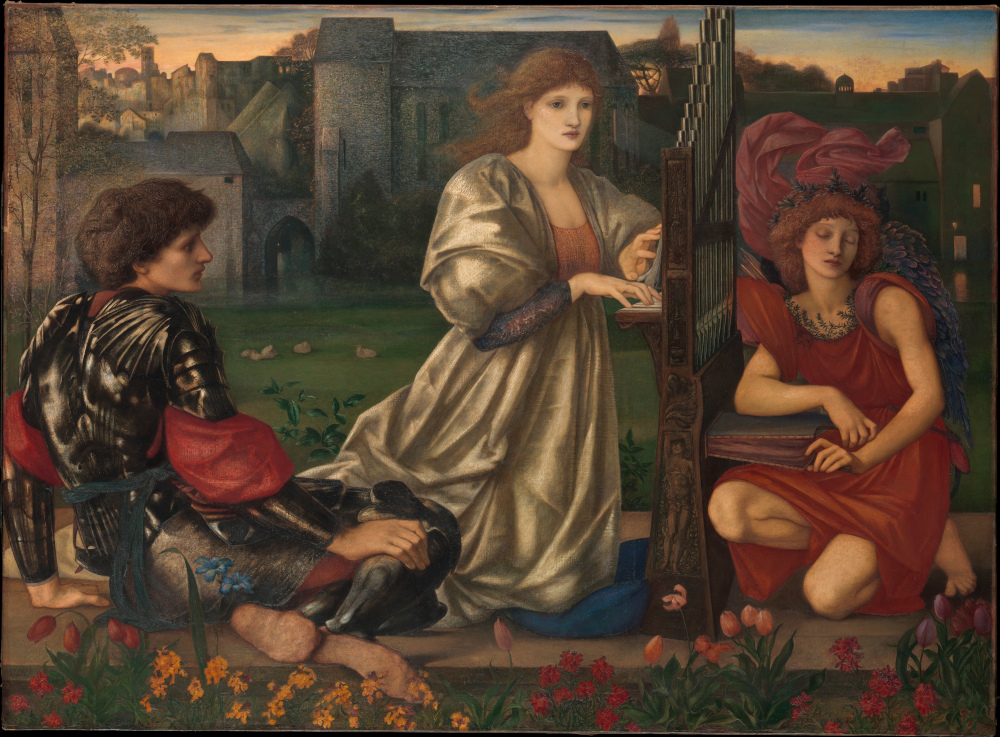
\includegraphics[keepaspectratio,width=\textwidth]{figures/The-Love-Song-Edward-Burne-Jones-small.jpg}
  \caption{\citeart{TheLoveSong}}
  \label{fig:thelovesong}
\end{figure}

%SUBSECT. II.-_Love's Beginning, Object, Definition, Division_.
\section{Love's Beginning, Object, Definition, Division.}

\lettrine{L}{ove}'s limits are ample and great, and a spacious walk it hath, beset
with thorns, and for that cause, which \authorfootnote{4461}Scaliger reprehends in
Cardan, not lightly to be passed over. Lest I incur the same censure, 1
will examine all the kinds of love, his nature, beginning, difference,
objects, how it is honest or dishonest, a virtue or vice, a natural
passion, or a disease, his power and effects, how far it extends: of
which, although something has been said in the first partition, in
those sections of perturbations (\authorfootnote{4462} for love and hatred are the
first and most common passions, from which all the rest arise, and are
attendant, as Picolomineus holds, or as Nich. Caussinus, the primum
mobile of all other affections, which carry them all about them) I will
now more copiously dilate, through all his parts and several branches,
that so it may better appear what love is, and how it varies with the
objects, how in defect, or (which is most ordinary and common)
immoderate, and in excess, causeth melancholy.
Love universally taken, is defined to be a desire, as a word of more
ample signification: and though Leon Hebreus, the most copious writer
of this subject, in his third dialogue make no difference, yet in his
first he distinguisheth them again, and defines love by desire.
\authorfootnote{4463}Love is a voluntary affection, and desire to enjoy that which is
good. \authorfootnote{4464}Desire wisheth, love enjoys; the end of the one is the
beginning of the other; that which we love is present; that which we
desire is absent. \authorfootnote{4465}It is worth the labour, saith Plotinus, to
consider well of love, whether it be a god or a devil, or passion of
the mind, or partly god, partly devil, partly passion. He concludes
love to participate of all three, to arise from desire of that which is
beautiful and fair, and defines it to be an action of the mind desiring
that which is good. \authorfootnote{4466}Plato calls it the great devil, for its
vehemency, and sovereignty over all other passions, and defines it an
appetite, \authorfootnote{4467}by which we desire some good to be present. Ficinus in
his comment adds the word fair to this definition. Love is a desire of
enjoying that which is good and fair. Austin dilates this common
definition, and will have love to be a delectation of the heart,
\authorfootnote{4468}for something which we seek to win, or joy to have, coveting by
desire, resting in joy. \authorfootnote{4469}Scaliger exerc. 301. taxeth these former
definitions, and will not have love to be defined by desire or
appetite; for when we enjoy the things we desire, there remains no more
appetite: as he defines it, Love is an affection by which we are either
united to the thing we love, or perpetuate our union; which agrees in
part with Leon Hebreus.
Now this love varies as its object varies, which is always good,
amiable, fair, gracious, and pleasant. \authorfootnote{4470}All things desire that
which is good, as we are taught in the Ethics, or at least that which
to them seems to be good; quid enim vis mali (as Austin well infers)
dic mihi? puto nihil in omnibus actionibus; thou wilt wish no harm, I
suppose, no ill in all thine actions, thoughts or desires, nihil mali
vis; \authorfootnote{4471}thou wilt not have bad corn, bad soil, a naughty tree, but
all good; a good servant, a good horse, a good son, a good friend, a
good neighbour, a good wife. From this goodness comes beauty; from
beauty, grace, and comeliness, which result as so many rays from their
good parts, make us to love, and so to covet it: for were it not
pleasing and gracious in our eyes, we should not seek. \authorfootnote{4472}No man
loves (saith Aristotle 9. mor. cap. 5.) but he that was first delighted
with comeliness and beauty. As this fair object varies, so doth our
love; for as Proclus holds, Omne pulchrum amabile, every fair thing is
amiable, and what we love is fair and gracious in our eyes, or at least
we do so apprehend and still esteem of it. \authorfootnote{4473} Amiableness is the
object of love, the scope and end is to obtain it, for whose sake we
love, and which our mind covets to enjoy. And it seems to us especially
fair and good; for good, fair, and unity, cannot be separated. Beauty
shines, Plato saith, and by reason of its splendour and shining causeth
admiration; and the fairer the object is, the more eagerly it is
sought. For as the same Plato defines it, \authorfootnote{4474}Beauty is a lively,
shining or glittering brightness, resulting from effused good, by
ideas, seeds, reasons, shadows, stirring up our minds, that by this
good they may be united and made one. Others will have beauty to be the
perfection of the whole composition, \authorfootnote{4475}caused out of the congruous
symmetry, measure, order and manner of parts, and that comeliness which
proceeds from this beauty is called grace, and from thence all fair
things are gracious. For grace and beauty are so wonderfully annexed,
\authorfootnote{4476}so sweetly and gently win our souls, and strongly allure, that
they confound our judgment and cannot be distinguished. Beauty and
grace are like those beams and shinings that come from the glorious and
divine sun, which are diverse, as they proceed from the diverse
objects, to please and affect our several senses. \authorfootnote{4477}As the species
of beauty are taken at our eyes, ears, or conceived in our inner soul,
as Plato disputes at large in his Dialogue de pulchro, Phaedro,
Hyppias, and after many sophistical errors confuted, concludes that
beauty is a grace in all things, delighting the eyes, ears, and soul
itself; so that, as Valesius infers hence, whatsoever pleaseth our
ears, eyes, and soul, must needs be beautiful, fair, and delightsome to
us. \authorfootnote{4478}And nothing can more please our ears than music, or pacify
our minds. Fair houses, pictures, orchards, gardens, fields, a fair
hawk, a fair horse is most acceptable unto us; whatsoever pleaseth our
eyes and ears, we call beautiful and fair; \authorfootnote{4479}Pleasure belongeth to
the rest of the senses, but grace and beauty to these two alone. As the
objects vary and are diverse, so they diversely affect our eyes, ears,
and soul itself. Which gives occasion to some to make so many several
kinds of love as there be objects. One beauty ariseth from God, of
which and divine love S. Dionysius, \authorfootnote{4480}with many fathers and
neoterics, have written just volumes, De amore Dei, as they term it,
many paraenetical discourses; another from his creatures; there is a
beauty of the body, a beauty of the soul, a beauty from virtue, formam
martyrum, Austin calls it, quam videmus oculis animi, which we see with
the eyes of our mind; which beauty, as Tully saith, if we could discern
with these corporeal eyes, admirabili sui amores excitaret, would cause
admirable affections, and ravish our souls. This other beauty which
ariseth from those extreme parts, and graces which proceed from
gestures, speeches, several motions, and proportions of creatures, men
and women (especially from women, which made those old poets put the
three graces still in Venus' company, as attending on her, and holding
up her train) are infinite almost, and vary their names with their
objects, as love of money, covetousness, love of beauty, lust,
immoderate desire of any pleasure, concupiscence, friendship, love,
goodwill, \&c. and is either virtue or vice, honest, dishonest, in
excess, defect, as shall be showed in his place. Heroical love,
religious love, \&c. which may be reduced to a twofold division,
according to the principal parts which are affected, the brain and
liver. Amor et amicitia, which Scaliger exercitat. 301. Valesius and
Melancthon warrant out of Plato Φιλεῖν and ἐρᾶν from that speech of
Pausanias belike, that makes two Veneres and two loves. \authorfootnote{4481}One Venus
is ancient without a mother, and descended from heaven, whom we call
celestial; the younger, begotten of Jupiter and Dione, whom commonly we
call Venus. Ficinus, in his comment upon this place, cap. 8. following
Plato, calls these two loves, two devils, \authorfootnote{4482}or good and bad angels
according to us, which are still hovering about our souls. \authorfootnote{4483}The
one rears to heaven, the other depresseth us to hell; the one good,
which stirs us up to the contemplation of that divine beauty for whose
sake we perform justice and all godly offices, study philosophy, \&c.;
the other base, and though bad yet to be respected; for indeed both are
good in their own natures: procreation of children is as necessary as
that finding out of truth, but therefore called bad, because it is
abused, and withdraws our souls from the speculation of that other to
viler objects, so far Ficinus. S. Austin, lib. 15. de civ. Dei et sup.
Psal. lxiv., hath delivered as much in effect. \authorfootnote{4484}Every creature is
good, and may be loved well or ill: and \authorfootnote{4485}Two cities make two
loves, Jerusalem and Babylon, the love of God the one, the love of the
world the other; of these two cities we all are citizens, as by
examination of ourselves we may soon find, and of which. The one love
is the root of all mischief, the other of all good. So, in his 15. cap.
lib. de amor. Ecclesiae, he will have those four cardinal virtues to be
nought else but love rightly composed; in his 15. book de civ. Dei,
cap. 22. he calls virtue the order of love, whom Thomas following 1.
part. 2. quaest. 55. art. 1. and quaest. 56. 3. quaest. 62. art. 2.
confirms as much, and amplifies in many words. \authorfootnote{4486}Lucian, to the
same purpose, hath a division of his own, One love was born in the sea,
which is as various and raging in young men's breasts as the sea
itself, and causeth burning lust: the other is that golden chain which
was let down from heaven, and with a divine fury ravisheth our souls,
made to the image of God, and stirs us up to comprehend the innate and
incorruptible beauty to which we were once created. Beroaldus hath
expressed all this in an epigram of his:

Dogmata divini memorant si vera Platonis,
Sunt geminae Veneres, et geminatus amor.

Coelestis Venus est nullo generata parente,
Quae casto sanctos nectit amore viros.

Altera sed Venus est totum vulgata per orbem,
Quae divum mentes alligat, atque hominum;

Improba, seductrix, petulans, \&c.

If divine Plato's tenets they be true,
Two Veneres, two loves there be,
The one from heaven, unbegotten still,
Which knits our souls in unity.
The other famous over all the world,
Binding the hearts of gods and men;
Dishonest, wanton, and seducing she,
Rules whom she will, both where and when.

This twofold division of love, Origen likewise follows, in his Comment
on the Canticles, one from God, the other from the devil, as he holds
(understanding it in the worse sense) which many others repeat and
imitate. Both which (to omit all subdivisions) in excess or defect, as
they are abused, or degenerate, cause melancholy in a particular kind,
as shall be shown in his place. Austin, in another Tract, makes a
threefold division of this love, which we may use well or ill:
\authorfootnote{4487}God, our neighbour, and the world: God above us, our neighbour
next us, the world beneath us. In the course of our desires, God hath
three things, the world one, our neighbour two. Our desire to God, is
either from God, with God, or to God, and ordinarily so runs. From God,
when it receives from him, whence, and for which it should love him:
with God, when it contradicts his will in nothing: to God, when it
seeks to him, and rests itself in him. Our love to our neighbour may
proceed from him, and run with him, not to him: from him, as when we
rejoice of his good safety, and well doing: with him, when we desire to
have him a fellow and companion of our journey in the way of the Lord:
not in him, because there is no aid, hope, or confidence in man. From
the world our love comes, when we begin to admire the Creator in his
works, and glorify God in his creatures: with the world it should run,
if, according to the mutability of all temporalities, it should be
dejected in adversity, or over elevated in prosperity: to the world, if
it would settle itself in its vain delights and studies. Many such
partitions of love I could repeat, and subdivisions, but least (which
Scaliger objects to Cardan, Exercitat. 501.) \authorfootnote{4488}I confound filthy
burning lust with pure and divine love, I will follow that accurate
division of Leon Hebreus, dial. 2. betwixt Sophia and Philo, where he
speaks of natural, sensible, and rational love, and handleth each
apart. Natural love or hatred, is that sympathy or antipathy which is
to be seen in animate and inanimate creatures, in the four elements,
metals, stones, gravia tendunt deorsum, as a stone to his centre, fire
upward, and rivers to the sea. The sun, moon, and stars go still
around, \authorfootnote{4489}Amantes naturae, debita exercere, for love of perfection.
This love is manifest, I say, in inanimate creatures. How comes a
loadstone to draw iron to it? jet chaff? the ground to covet showers,
but for love? No creature, S. Hierom concludes, is to be found, quod
non aliquid amat, no stock, no stone, that hath not some feeling of
love, 'Tis more eminent in plants, herbs, and is especially observed in
vegetables; as between the vine and elm a great sympathy, between the
vine and the cabbage, between the vine and the olive, \authorfootnote{4490} Virgo
fugit Bromium, between the vine and bays a great antipathy, the vine
loves not the bay, \authorfootnote{4491}nor his smell, and will kill him, if he grow
near him; the bur and the lentil cannot endure one another, the olive
\authorfootnote{4492}and the myrtle embrace each other, in roots and branches if they
grow near. Read more of this in Picolomineus grad. 7. cap. 1.
Crescentius lib. 5. de agric. Baptista Porta de mag. lib. 1. cap. de
plant. dodio et element. sym. Fracastorius de sym. et antip. of the
love and hatred of planets, consult with every astrologer. Leon Hebreus
gives many fabulous reasons, and moraliseth them withal.
Sensible love is that of brute beasts, of which the same Leon Hebreus
dial. 2. assigns these causes. First for the pleasure they take in the
act of generation, male and female love one another. Secondly, for the
preservation of the species, and desire of young brood. Thirdly, for
the mutual agreement, as being of the same kind: Sus sui, canis cani,
bos bovi, et asinus asino pulcherrimus videtur, as Epicharmus held, and
according to that adage of Diogenianus, Adsidet usque graculus apud
graculum, they much delight in one another's company, \authorfootnote{4493}Formicae
grata est formica, cicada cicadae, and birds of a feather will gather
together. Fourthly, for custom, use, and familiarity, as if a dog be
trained up with a lion and a bear, contrary to their natures, they will
love each other. Hawks, dogs, horses, love their masters and keepers:
many stories I could relate in this kind, but see Gillius de hist.
anim. lib. 3. cap. 14. those two Epistles of Lipsius, of dogs and
horses, Agellius, \&c. Fifthly, for bringing up, as if a bitch bring up
a kid, a hen ducklings, a hedge-sparrow a cuckoo, \&c.
The third kind is Amor cognitionis, as Leon calls it, rational love,
Intellectivus amor, and is proper to men, on which I must insist. This
appears in God, angels, men. God is love itself, the fountain of love,
the disciple of love, as Plato styles him; the servant of peace, the
God of love and peace; have peace with all men and God is with you.
\authorfootnote{4494}---Quisquis veneratur Olympum,
Ipse sibi mundum subjicit atque Deum.

\authorfootnote{4495}By this love (saith Gerson) we purchase heaven, and buy the
kingdom of God. This \authorfootnote{4496}love is either in the Trinity itself (for
the Holy Ghost is the love of the Father and the Son, \&c. John iii. 35,
and v. 20, and xiv. 31), or towards us his creatures, as in making the
world. Amor mundum fecit, love built cities, mundi anima, invented
arts, sciences, and all \authorfootnote{4497}good things, incites us to virtue and
humanity, combines and quickens; keeps peace on earth, quietness by
sea, mirth in the winds and elements, expels all fear, anger, and
rusticity; Circulus a bono in bonum, a round circle still from good to
good; for love is the beginner and end of all our actions, the
efficient and instrumental cause, as our poets in their symbols,
impresses, \authorfootnote{4498}emblems of rings, squares, \&c., shadow unto us,
Si rerum quaeris fuerit quis finis et ortus,
Desine; nam causa est unica solus amor.

If first and last of anything you wit,
Cease; love's the sole and only cause of it.

Love, saith \authorfootnote{4499}Leo, made the world, and afterwards in redeeming of
it, God so loved the world, that he gave his only begotten son for it,
John iii. 16. Behold what love the Father hath showed on us, that we
should be called the sons of God, 1 John iii. 1. Or by His sweet
Providence, in protecting of it; either all in general, or His saints
elect and church in particular, whom He keeps as the apple of His eye,
whom He loves freely, as Hosea xiv. 5. speaks, and dearly respects,
\authorfootnote{4500}Charior est ipsis homo quam sibi. Not that we are fair, nor for
any merit or grace of ours, for we are most vile and base; but out of
His incomparable love and goodness, out of His Divine Nature. And this
is that Homer's golden chain, which reacheth down from heaven to earth,
by which every creature is annexed, and depends on his Creator. He made
all, saith \authorfootnote{4501}Moses, and it was good; He loves it as good.
The love of angels and living souls is mutual amongst themselves,
towards us militant in the church, and all such as love God; as the
sunbeams irradiate the earth from those celestial thrones, they by
their well wishes reflect on us, \authorfootnote{4502}in salute hominum promovenda
alacres, et constantes administri, there is joy in heaven for every
sinner that repenteth; they pray for us, are solicitous for our good,
\authorfootnote{4503}Casti genii.
\authorfootnote{4504}Ubi regnat charitas, suave desiderium,
Laetitiaque et amor Deo conjunctus.

Love proper to mortal men is the third member of this subdivision, and
the subject of my following discourse.

%MEMB. II.

%SUBSECT. I.-_Love of Men, which varies as his Objects, Profitable, Pleasant, Honest_.
\section[Love of Men]{Love of Men, which varies as his Objects, Profitable, Pleasant, Honest.}

\lettrine{V}{alesius}, lib. 3. contr. 13, defines this love which is in men, to be
\authorfootnote{4505}an affection of both powers, appetite and reason. The rational
resides in the brain, the other in the liver (as before hath been said
out of Plato and others); the heart is diversely affected of both, and
carried a thousand ways by consent. The sensitive faculty most part
overrules reason, the soul is carried hoodwinked, and the understanding
captive like a beast. \authorfootnote{4506}The heart is variously inclined, sometimes
they are merry, sometimes sad, and from love arise hope and fear,
jealousy, fury, desperation. Now this love of men is diverse, and
varies, as the object varies, by which they are enticed, as virtue,
wisdom, eloquence, profit, wealth, money, fame, honour, or comeliness
of person, \&c. Leon Hubreus, in his first dialogue, reduceth them all
to these three, utile, jucundum, honestum, profitable, pleasant,
honest; (out of Aristotle belike 8. moral.) of which he discourseth at
large, and whatsoever is beautiful and fair, is referred to them, or
any way to be desired. \authorfootnote{4507}To profitable is ascribed health, wealth,
honour, \&c., which is rather ambition, desire, covetousness, than love:
friends, children, love of women, \authorfootnote{4508}all delightful and pleasant
objects, are referred to the second. The love of honest things consists
in virtue and wisdom, and is preferred before that which is profitable
and pleasant: intellectual, about that which is honest. \authorfootnote{4509}St.
Austin calls profitable, worldly; pleasant, carnal; honest, spiritual.
\authorfootnote{4510}Of and from all three, result charity, friendship, and true love,
which respects God and our neighbour. Of each of these I will briefly
dilate, and show in what sort they cause melancholy.
Amongst all these fair enticing objects, which procure love, and
bewitch the soul of man, there is none so moving, so forcible as
profit; and that which carrieth with it a show of commodity. Health
indeed is a precious thing, to recover and preserve which we will
undergo any misery, drink bitter potions, freely give our goods:
restore a man to his health, his purse lies open to thee, bountiful he
is, thankful and beholding to thee; but give him wealth and honour,
give him gold, or what shall be for his advantage and preferment, and
thou shalt command his affections, oblige him eternally to thee, heart,
hand, life, and all is at thy service, thou art his dear and loving
friend, good and gracious lord and master, his Mecaenas; he is thy
slave, thy vassal, most devote, affectioned, and bound in all duty:
tell him good tidings in this kind, there spoke an angel, a blessed
hour that brings in gain, he is thy creature, and thou his creator, he
hugs and admires thee; he is thine for ever. No loadstone so attractive
as that of profit, none so fair an object as this of gold;
\authorfootnote{4511}nothing wins a man sooner than a good turn, bounty and liberality
command body and soul:

Munera (crede mihi) placant hominesque deosque;
Placatur donis Jupiter ipse datis.


Good turns doth pacify both God and men,
And Jupiter himself is won by them.

Gold of all other is a most delicious object; a sweet light, a goodly
lustre it hath; gratius aurum quam solem intuemur, saith Austin, and we
had rather see it than the sun. Sweet and pleasant in getting, in
keeping; it seasons all our labours, intolerable pains we take for it,
base employments, endure bitter flouts and taunts, long journeys, heavy
burdens, all are made light and easy by this hope of gain: At mihi
plaudo ipse domi, simul ac nummos contemplor in arca. The sight of gold
refresheth our spirits, and ravisheth our hearts, as that Babylonian
garment and \authorfootnote{4512} golden wedge did Achan in the camp, the very sight
and hearing sets on fire his soul with desire of it. It will make a man
run to the antipodes, or tarry at home and turn parasite, lie, flatter,
prostitute himself, swear and bear false witness; he will venture his
body, kill a king, murder his father, and damn his soul to come at it.
Formosior auri massa, as \authorfootnote{4513} he well observed, the mass of gold is
fairer than all your Grecian pictures, that Apelles, Phidias, or any
doting painter could ever make: we are enamoured with it,
\authorfootnote{4514}Prima fere vota, et cunctis notissima templis,
Divitiae ut crescant.---

All our labours, studies, endeavours, vows, prayers and wishes, are to
get, how to compass it.
\authorfootnote{4515}Haec est illa cui famulatur maximus orbis,
Diva potens rerum, domitrixque pecunia fati.

This is the great goddess we adore and worship; this is the sole object
of our desire. If we have it, as we think, we are made for ever, thrice
happy, princes, lords, \&c. If we lose it, we are dull, heavy, dejected,
discontent, miserable, desperate, and mad. Our estate and bene esse
ebbs and flows with our commodity; and as we are endowed or enriched,
so are we beloved and esteemed: it lasts no longer than our wealth;
when that is gone, and the object removed, farewell friendship: as long
as bounty, good cheer, and rewards were to be hoped, friends enough;
they were tied to thee by the teeth, and would follow thee as crows do
a carcass: but when thy goods are gone and spent, the lamp of their
love is out, and thou shalt be contemned, scorned, hated, injured.
\authorfootnote{4516}Lucian's Timon, when he lived in prosperity, was the sole
spectacle of Greece, only admired; who but Timon? Everybody loved,
honoured, applauded him, each man offered him his service, and sought
to be kin to him; but when his gold was spent, his fair possessions
gone, farewell Timon: none so ugly, none so deformed, so odious an
object as Timon, no man so ridiculous on a sudden, they gave him a
penny to buy a rope, no man would know him.
'Tis the general humour of the world, commodity steers our affections
throughout, we love those that are fortunate and rich, that thrive, or
by whom we may receive mutual kindness, hope for like courtesies, get
any good, gain, or profit; hate those, and abhor on the other side,
which are poor and miserable, or by whom we may sustain loss or
inconvenience. And even those that were now familiar and dear unto us,
our loving and long friends, neighbours, kinsmen, allies, with whom we
have conversed, and lived as so many Geryons for some years past,
striving still to give one another all good content and entertainment,
with mutual invitations, feastings, disports, offices, for whom we
would ride, run, spend ourselves, and of whom we have so freely and
honourably spoken, to whom we have given all those turgent titles, and
magnificent eulogiums, most excellent and most noble, worthy, wise,
grave, learned, valiant, \&c., and magnified beyond measure: if any
controversy arise between us, some trespass, injury, abuse, some part
of our goods be detained, a piece of land come to be litigious, if they
cross us in our suit, or touch the string of our commodity, we detest
and depress them upon a sudden: neither affinity, consanguinity, or old
acquaintance can contain us, but \authorfootnote{4517}rupto jecore exierit Caprificus.
A golden apple sets altogether by the ears, as if a marrowbone or
honeycomb were flung amongst bears: father and son, brother and sister,
kinsmen are at odds: and look what malice, deadly hatred can invent,
that shall be done, Terrible, dirum, pestilens, atrox, ferum, mutual
injuries, desire of revenge, and how to hurt them, him and his, are all
our studies. If our pleasures be interrupt, we can tolerate it: our
bodies hurt, we can put it up and be reconciled: but touch our
commodities, we are most impatient: fair becomes foul, the graces are
turned to harpies, friendly salutations to bitter imprecations, mutual
feastings to plotting villainies, minings and counterminings; good
words to satires and invectives, we revile e contra, nought but his
imperfections are in our eyes, he is a base knave, a devil, a monster,
a caterpillar, a viper, a hog-rubber, \&c. Desinit in piscem mulier
formosa superne;\authorfootnote{4518} the scene is altered on a sudden, love is turned
to hate, mirth to melancholy: so furiously are we most part bent, our
affections fixed upon this object of commodity, and upon money, the
desire of which in excess is covetousness: ambition tyranniseth over
our souls, as \authorfootnote{4519}I have shown, and in defect crucifies as much, as
if a man by negligence, ill husbandry, improvidence, prodigality, waste
and consume his goods and fortunes, beggary follows, and melancholy, he
becomes an abject, \authorfootnote{4520}odious and worse than an infidel, in not
providing for his family.

%SUBSECT. II.-_Pleasant Objects of Love_.
\section{Pleasant Objects of Love.}

\lettrine{P}{leasant} objects are infinite, whether they be such as have life, or be
without life; inanimate are countries, provinces, towers, towns,
cities, as he said, \authorfootnote{4521}Pulcherrimam insulam videmus, etiam cum non
videmus we see a fair island by description, when we see it not. The
\authorfootnote{4522}sun never saw a fairer city, Thessala Tempe, orchards, gardens,
pleasant walks, groves, fountains, \&c. The heaven itself is said to be
\authorfootnote{4523}fair or foul: fair buildings, \authorfootnote{4524}fair pictures, all
artificial, elaborate and curious works, clothes, give an admirable
lustre: we admire, and gaze upon them, ut pueri Junonis avem, as
children do on a peacock: a fair dog, a fair horse and hawk, \&c.
\authorfootnote{4525}Thessalus amat equum pullinum, buculum Aegyptius, Lacedaemonius
Catulum, \&c., such things we love, are most gracious in our sight,
acceptable unto us, and whatsoever else may cause this passion, if it
be superfluous or immoderately loved, as Guianerius observes. These
things in themselves are pleasing and good, singular ornaments,
necessary, comely, and fit to be had; but when we fix an immoderate
eye, and dote on them over much, this pleasure may turn to pain, bring
much sorrow and discontent unto us, work our final overthrow, and cause
melancholy in the end. Many are carried away with those bewitching
sports of gaming, hawking, hunting, and such vain pleasures, as \authorfootnote{4526}I
have said: some with immoderate desire of fame, to be crowned in the
Olympics, knighted in the field, \&c., and by these means ruinate
themselves. The lascivious dotes on his fair mistress, the glutton on
his dishes, which are infinitely varied to please the palate, the
epicure on his several pleasures, the superstitious on his idol, and
fats himself with future joys, as Turks feed themselves with an
imaginary persuasion of a sensual paradise: so several pleasant objects
diversely affect diverse men. But the fairest objects and enticings
proceed from men themselves, which most frequently captivate, allure,
and make them dote beyond all measure upon one another, and that for
many respects: first, as some suppose, by that secret force of stars,
(quod me tibi temperat astrum?) They do singularly dote on such a man,
hate such again, and can give no reason for it. \authorfootnote{4527}Non amo te
Sabidi, \&c. Alexander admired Ephestion, Adrian Antinous, Nero Sporus,
\&c. The physicians refer this to their temperament, astrologers to
trine and sextile aspects, or opposite of their several ascendants,
lords of their genitures, love and hatred of planets; \authorfootnote{4528} Cicogna,
to concord and discord of spirits; but most to outward graces. A merry
companion is welcome and acceptable to all men, and therefore, saith
\authorfootnote{4529}Gomesius, princes and great men entertain jesters and players
commonly in their courts. But \authorfootnote{4530}Pares cum paribus facillime
congregantur, 'tis that \authorfootnote{4531}similitude of manners, which ties most
men in an inseparable link, as if they be addicted to the same studies
or disports, they delight in one another's companies, birds of a
feather will gather together: if they be of divers inclinations, or
opposite in manners, they can seldom agree. Secondly, \authorfootnote{4532}affability,
custom, and familiarity, may convert nature many times, though they be
different in manners, as if they be countrymen, fellow-students,
colleagues, or have been fellow-soldiers, \authorfootnote{4533}brethren in affliction,
(\authorfootnote{4534}acerba calamitatum societas, diversi etiam ingenii homines
conjungit) affinity, or some such accidental occasion, though they
cannot agree amongst themselves, they will stick together like burrs,
and bold against a third; so after some discontinuance, or death,
enmity ceaseth; or in a foreign place:
Pascitur in vivis livor, post fata quiescit:
Et cecidere odia, et tristes mors obruit iras.

A third cause of love and hate, may be mutual offices, acceptum
beneficium, \authorfootnote{4535}commend him, use him kindly, take his part in a
quarrel, relieve him in his misery, thou winnest him for ever; do the
opposite, and be sure of a perpetual enemy. Praise and dispraise of
each other, do as much, though unknown, as \authorfootnote{4536}Schoppius by Scaliger
and Casaubonus: mulus mulum scabit; who but Scaliger with him? what
encomiums, epithets, eulogiums? Antistes sapientiae, perpetuus
dictator, literarum ornamentum, Europae miraculum, noble Scaliger,
\authorfootnote{4537} incredibilis ingenii praestantia, \&c., diis potius quam
hominibus per omnia comparandus, scripta ejus aurea ancylia de coelo
delapsa poplitibus veneramur flexis, \&c.,\authorfootnote{4538} but when they began to
vary, none so absurd as Scaliger, so vile and base, as his books de
Burdonum familia, and other satirical invectives may witness, Ovid, in
Ibin, Archilocus himself was not so bitter. Another great tie or cause
of love, is consanguinity: parents are clear to their children,
children to their parents, brothers and sisters, cousins of all sorts,
as a hen and chickens, all of a knot: every crow thinks her own bird
fairest. Many memorable examples are in this kind, and 'tis portenti
simile, if they do not: \authorfootnote{4539}a mother cannot forget her child: Solomon
so found out the true owner; love of parents may not be concealed, 'tis
natural, descends, and they that are inhuman in this kind, are unworthy
of that air they breathe, and of the four elements; yet many unnatural
examples we have in this rank, of hard-hearted parents, disobedient
children, of \authorfootnote{4540}disagreeing brothers, nothing so common. The love of
kinsmen is grown cold, \authorfootnote{4541}many kinsmen (as the saying is) few
friends; if thine estate be good, and thou able, par pari referre, to
requite their kindness, there will be mutual correspondence, otherwise
thou art a burden, most odious to them above all others. The last
object that ties man and man, is comeliness of person, and beauty
alone, as men love women with a wanton eye: which κατ' ἐξοχὴν is termed
heroical, or love-melancholy. Other loves (saith Picolomineus) are so
called with some contraction, as the love of wine, gold, \&c., but this
of women is predominant in a higher strain, whose part affected is the
liver, and this love deserves a longer explication, and shall be
dilated apart in the next section.

%SUBSECT. III.-_Honest Objects of Love_.
\section{Honest Objects of Love.}

\lettrine{B}{eauty} is the common object of all love, \authorfootnote{4542}as jet draws a straw, so
doth beauty love: virtue and honesty are great motives, and give as
fair a lustre as the rest, especially if they be sincere and right, not
fucate, but proceeding from true form, and an incorrupt judgment; those
two Venus' twins, Eros and Anteros, are then most firm and fast. For
many times otherwise men are deceived by their flattering gnathos,
dissembling camelions, outsides, hypocrites that make a show of great
love, learning, pretend honesty, virtue, zeal, modesty, with affected
looks and counterfeit gestures: feigned protestations often steal away
the hearts and favours of men, and deceive them, specie virtutis et
umbra, when as revera and indeed, there is no worth or honesty at all
in them, no truth, but mere hypocrisy, subtlety, knavery, and the like.
As true friends they are, as he that Caelius Secundus met by the
highway side; and hard it is in this temporising age to distinguish
such companions, or to find them out. Such gnathos as these for the
most part belong to great men, and by this glozing flattery,
affability, and such like philters, so dive and insinuate into their
favours, that they are taken for men of excellent worth, wisdom,
learning, demigods, and so screw themselves into dignities, honours,
offices; but these men cause harsh confusion often, and as many times
stirs as Rehoboam's counsellors in a commonwealth, overthrew themselves
and others. Tandlerus and some authors make a doubt, whether love and
hatred may be compelled by philters or characters; Cardan and
Marbodius, by precious stones and amulets; astrologers by election of
times, \&c. as \authorfootnote{4543}I shall elsewhere discuss. The true object of this
honest love is virtue, wisdom, honesty, \authorfootnote{4544}real worth, Interna
forma, and this love cannot deceive or be compelled, ut ameris amabilis
esto, love itself is the most potent philtrum, virtue and wisdom,
gratia gratum faciens, the sole and only grace, not counterfeit, but
open, honest, simple, naked, \authorfootnote{4545}descending from heaven, as our
apostle hath it, an infused habit from God, which hath given several
gifts, as wit, learning, tongues, for which they shall be amiable and
gracious, Eph. iv. 11. as to Saul stature and a goodly presence, 1 Sam.
ix. 1. Joseph found favour in Pharaoh's court, Gen. xxxix, for
\authorfootnote{4546}his person; and Daniel with the princes of the eunuchs, Dan. xix.
19. Christ was gracious with God and men, Luke ii. 52. There is still
some peculiar grace, as of good discourse, eloquence, wit, honesty,
which is the primum mobile, first mover, and a most forcible loadstone
to draw the favours and good wills of men's eyes, ears, and affections
unto them. When Jesus spake, they were all astonished at his answers,
(Luke ii. 47.) and wondered at his gracious words which proceeded from
his mouth. An orator steals away the hearts of men, and as another
Orpheus, quo vult, unde vult, he pulls them to him by speech alone: a
sweet voice causeth admiration; and he that can utter himself in good
words, in our ordinary phrase, is called a proper man, a divine spirit.
For which cause belike, our old poets, Senatus populusque poetarum,
made Mercury the gentleman-usher to the Graces, captain of eloquence,
and those charities to be Jupiter's and Eurymone's daughters, descended
from above. Though they be otherwise deformed, crooked, ugly to behold,
those good parts of the mind denominate them fair. Plato commends the
beauty of Socrates; yet who was more grim of countenance, stern and
ghastly to look upon? So are and have been many great philosophers, as
\authorfootnote{4547}Gregory Nazianzen observes, deformed most part in that which is
to be seen with the eyes, but most elegant in that which is not to be
seen. Saepe sub attrita latitat sapientia veste. Aesop, Democritus,
Aristotle, Politianus, Melancthon, Gesner, \&c. withered old men, Sileni
Alcibiadis, very harsh and impolite to the eye; but who were so terse,
polite, eloquent, generally learned, temperate and modest? No man then
living was so fair as Alcibiades, so lovely quo ad superficiem, to the
eye, as \authorfootnote{4548}Boethius observes, but he had Corpus turpissimum interne,
a most deformed soul; honesty, virtue, fair conditions, are great
enticers to such as are well given, and much avail to get the favour
and goodwill of men. Abdolominus in Curtius, a poor man, (but which
mine author notes, \authorfootnote{4549}the cause of this poverty was his honesty) for
his modesty and continency from a private person (for they found him
digging in his garden) was saluted king, and preferred before all the
magnificoes of his time, injecta ei vestis purpura auroque distincta, a
purple embroidered garment was put upon him, \authorfootnote{4550}and they bade him
wash himself, and, as he was worthy, take upon him the style and spirit
of a king, continue his continency and the rest of his good parts.
Titus Pomponius Atticus, that noble citizen of Rome, was so fair
conditioned, of so sweet a carriage, that he was generally beloved of
all good men, of Caesar, Pompey, Antony, Tully, of divers sects, \&c.
multas haereditates (\authorfootnote{4551}Cornelius Nepos writes) sola bonitate
consequutus. Operae, pretium audire, \&c. It is worthy of your
attention, Livy cries, \authorfootnote{4552}you that scorn all but riches, and give no
esteem to virtue, except they be wealthy withal, Q. Cincinnatus had but
four acres, and by the consent of the senate was chosen dictator of
Rome. Of such account were Cato, Fabricius, Aristides, Antonius,
Probus, for their eminent worth: so Caesar, Trajan, Alexander, admired
for valour, \authorfootnote{4553} Haephestion loved Alexander, but Parmenio the king:
Titus deliciae humani generis, and which Aurelius Victor hath of
Vespasian, the darling of his time, as \authorfootnote{4554}Edgar Etheling was in
England, for his \authorfootnote{4555}excellent virtues: their memory is yet fresh,
sweet, and we love them many ages after, though they be dead: Suavem
memoriam sui reliquit, saith Lipsius of his friend, living and dead
they are all one. \authorfootnote{4556}I have ever loved as thou knowest (so Tully
wrote to Dolabella) Marcus Brutus for his great wit, singular honesty,
constancy, sweet conditions; and believe it \authorfootnote{4557} there is nothing so
amiable and fair as virtue. I \authorfootnote{4558}do mightily love Calvisinus, (so
Pliny writes to Sossius) a most industrious, eloquent, upright man,
which is all in all with me: the affection came from his good parts.
And as St. Austin comments on the 84th Psalm, \authorfootnote{4559}there is a peculiar
beauty of justice, and inward beauty, which we see with the eyes of our
hearts, love, and are enamoured with, as in martyrs, though their
bodies be torn in pieces with wild beasts, yet this beauty shines, and
we love their virtues. The \authorfootnote{4560}stoics are of opinion that a wise man
is only fair; and Cato in Tully 3 de Finibus contends the same, that
the lineaments of the mind are far fairer than those of the body,
incomparably beyond them: wisdom and valour according to
\authorfootnote{4561}Xenophon, especially deserve the name of beauty, and denominate
one fair, et incomparabiliter pulchrior est (as Austin holds) veritas
Christianorum quam Helena Graecorum. Wine is strong, the king is
strong, women are strong, but truth overcometh all things, Esd. i. 3,
10, 11, 12. Blessed is the man that findeth wisdom, and getteth
understanding, for the merchandise thereof is better than silver, and
the gain thereof better than gold: it is more precious than pearls, and
all the things thou canst desire are not to be compared to her, Prov.
ii. 13, 14, 15, a wise, true, just, upright, and good man, I say it
again, is only fair: \authorfootnote{4562}it is reported of Magdalene Queen of France,
and wife to Lewis 11th, a Scottish woman by birth, that walking forth
in an evening with her ladies, she spied M. Alanus, one of the king's
chaplains, a silly, old, \authorfootnote{4563}hard-favoured man fast asleep in a
bower, and kissed him sweetly; when the young ladies laughed at her for
it, she replied, that it was not his person that she did embrace and
reverence, but, with a platonic love, the divine beauty of \authorfootnote{4564}his
soul. Thus in all ages virtue hath been adored, admired, a singular
lustre hath proceeded from it: and the more virtuous he is, the more
gracious, the more admired. No man so much followed upon earth as
Christ himself: and as the Psalmist saith, xlv. 2, He was fairer than
the sons of men. Chrysostom Hom. 8 in Mat. Bernard Ser. 1. de omnibus
sanctis; Austin, Cassiodore, Hier. in 9 Mat. interpret it of the
\authorfootnote{4565}beauty of his person; there was a divine majesty in his looks, it
shined like lightning and drew all men to it: but Basil, Cyril, lib. 6.
super. 55. Esay. Theodoret, Arnobius, \&c. of the beauty of his
divinity, justice, grace, eloquence, \&c. Thomas in Psal. xliv. of both;
and so doth Baradius and Peter Morales, lib de pulchritud. Jesu et
Mariae, adding as much of Joseph and the Virgin Mary,-haec alias forma
praecesserit omnes, \authorfootnote{4566}according to that prediction of Sibylla
Cumea. Be they present or absent, near us, or afar off, this beauty
shines, and will attract men many miles to come and visit it. Plato and
Pythagoras left their country, to see those wise Egyptian priests:
Apollonius travelled into Ethiopia, Persia, to consult with the Magi,
Brachmanni, gymnosophists. The Queen of Sheba came to visit Solomon;
and many, saith \authorfootnote{4567}Hierom, went out of Spain and remote places a
thousand miles, to behold that eloquent Livy: \authorfootnote{4568}Multi Romam non ut
urbem pulcherrimam, aut urbis et orbis dominum Octavianum, sed ut hunc
unum inviserent audirentque, a Gadibus profecti sunt. No beauty leaves
such an impression, strikes so deep \authorfootnote{4569}, or links the souls of men
closer than virtue.
\authorfootnote{4570}Non per deos aut pictor posset,
Aut statuarius ullus fingere
Talem pulchritudinem qualem virtus habet;

no painter, no graver, no carver can express virtue's lustre, or those
admirable rays that come from it, those enchanting rays that enamour
posterity, those everlasting rays that continue to the world's end.
Many, saith Phavorinus, that loved and admired Alcibiades in his youth,
knew not, cared not for Alcibiades a man, nunc intuentes quaerebant
Alcibiadem; but the beauty of Socrates is still the same;
\authorfootnote{4571}virtue's lustre never fades, is ever fresh and green, semper viva
to all succeeding ages, and a most attractive loadstone, to draw and
combine such as are present. For that reason belike, Homer feigns the
three Graces to be linked and tied hand in hand, because the hearts of
men are so firmly united with such graces. \authorfootnote{4572}O sweet bands (Seneca
exclaims), which so happily combine, that those which are bound by them
love their binders, desiring withal much more harder to be bound, and
as so many Geryons to be united into one. For the nature of true
friendship is to combine, to be like affected, of one mind,
\authorfootnote{4573}Velle et nolle ambobus idem, satiataque toto
Mens aevo---

as the poet saith, still to continue one and the same. And where this
love takes place there is peace and quietness, a true correspondence,
perfect amity, a diapason of vows and wishes, the same opinions, as
between \authorfootnote{4574} David and Jonathan, Damon and Pythias, Pylades and
Orestes, \authorfootnote{4575}Nysus and Euryalus, Theseus and Pirithous, \authorfootnote{4576}they
will live and die together, and prosecute one another with good turns.
\authorfootnote{4577}Nam vinci in amore turpissimum putant, not only living, but when
their friends are dead, with tombs and monuments, nenias, epitaphs
elegies, inscriptions, pyramids, obelisks, statues, images, pictures,
histories, poems, annals, feasts, anniversaries, many ages after (as
Plato's scholars did) they will parentare still, omit no good office
that may tend to the preservation of their names, honours, and eternal
memory. \authorfootnote{4578}Illum coloribus, illum cera, illum aere, \&c. He did
express his friends in colours, in wax, in brass, in ivory, marble,
gold, and silver (as Pliny reports of a citizen in Rome), and in a
great auditory not long since recited a just volume of his life. In
another place, \authorfootnote{4579}speaking of an epigram which Martial had composed
in praise of him, \authorfootnote{4580}He gave me as much as he might, and would have
done more if he could: though what can a man give more than honour,
glory, and eternity? But that which he wrote peradventure will not
continue, yet he wrote it to continue. 'Tis all the recompense a poor
scholar can make his well-deserving patron, Mecaenas, friend, to
mention him in his works, to dedicate a book to his name, to write his
life, \&c., as all our poets, orators, historiographers have ever done,
and the greatest revenge such men take of their adversaries, to
persecute them with satires, invectives, \&c., and 'tis both ways of
great moment, as \authorfootnote{4581} Plato gives us to understand. Paulus Jovius, in
the fourth book of the life and deeds of Pope Leo Decimus, his noble
patron, concludes in these words, \authorfootnote{4582}Because I cannot honour him as
other rich men do, with like endeavour, affection, and piety, I have
undertaken to write his life; since my fortunes will not give me leave
to make a more sumptuous monument, I will perform those rites to his
sacred ashes, which a small, perhaps, but a liberal wit can afford. But
I rove. Where this true love is wanting, there can be no firm peace,
friendship from teeth outward, counterfeit, or for some by-respects, so
long dissembled, till they have satisfied their own ends, which, upon
every small occasion, breaks out into enmity, open war, defiance,
heart-burnings, whispering, calumnies, contentions, and all manner of
bitter melancholy discontents. And those men which have no other object
of their love, than greatness, wealth, authority, \&c., are rather
feared than beloved; nec amant quemquam, nec amantur ab ullo: and
howsoever borne with for a time, yet for their tyranny and oppression,
griping, covetousness, currish hardness, folly, intemperance,
imprudence, and such like vices, they are generally odious, abhorred of
all, both God and men.
Non uxor salvum te vult, non filius, omnes
Vicini oderunt,---

wife and children, friends, neighbours, all the world forsakes them,
would feign be rid of them, and are compelled many times to lay violent
hands on them, or else God's judgments overtake them: instead of
graces, come furies. So when fair \authorfootnote{4583}Abigail, a woman of singular
wisdom, was acceptable to David, Nabal was churlish and
evil-conditioned; and therefore \authorfootnote{4584}Mordecai was received, when Haman
was executed, Haman the favourite, that had his seat above the other
princes, to whom all the king's servants that stood in the gates, bowed
their knees and reverenced. Though they flourished many times, such
hypocrites, such temporising foxes, and blear the world's eyes by
flattery, bribery, dissembling their natures, or other men's weakness,
that cannot so apprehend their tricks, yet in the end they will be
discerned, and precipitated in a moment: surely, saith David, thou hast
set them in slippery places, Psal. xxxvii. 5. as so many Sejani, they
will come down to the Gemonian scales; and as Eusebius in \authorfootnote{4585}
Ammianus, that was in such authority, ad jubendum Imperatorem, be cast
down headlong on a sudden. Or put case they escape, and rest unmasked
to their lives' end, yet after their death their memory stinks as a
snuff of a candle put out, and those that durst not so much as mutter
against them in their lives, will prosecute their name with satires,
libels, and bitter imprecations, they shall male audire in all
succeeding ages, and be odious to the world's end.

%MEMB. III.

\section[Charity]{Charity composed of all three Kinds, Pleasant, Profitable, Honest.}

\lettrine{B}{esides} this love that comes from profit, pleasant, honest (for one
good turn asks another in equity), that which proceeds from the law of
nature, or from discipline and philosophy, there is yet another love
compounded of all these three, which is charity, and includes piety,
dilection, benevolence, friendship, even all those virtuous habits; for
love is the circle equant of all other affections, of which Aristotle
dilates at large in his Ethics, and is commanded by God, which no man
can well perform, but he that is a Christian, and a true regenerate
man; this is,\authorfootnote{4586}To love God above all, and our neighbour as ourself;
for this love is lychnus accendens et accensus, a communicating light,
apt to illuminate itself as well as others. All other objects are fair,
and very beautiful, I confess; kindred, alliance, friendship, the love
that we owe to our country, nature, wealth, pleasure, honour, and such
moral respects, \&c., of which read \authorfootnote{4587}copious Aristotle in his
morals; a man is beloved of a man, in that he is a man; but all these
are far more eminent and great, when they shall proceed from a
sanctified spirit, that hath a true touch of religion, and a reference
to God. Nature binds all creatures to love their young ones; a hen to
preserve her brood will run upon a lion, a hind will fight with a bull,
a sow with a bear, a silly sheep with a fox. So the same nature urgeth
a man to love his parents, (\authorfootnote{4588}dii me pater omnes oderint, ni te
magis quam oculos amem meos!) and this love cannot be dissolved, as
Tully holds, \authorfootnote{4589}without detestable offence: but much more God's
commandment, which enjoins a filial love, and an obedience in this
kind. \authorfootnote{4590}The love of brethren is great, and like an arch of stones,
where if one be displaced, all comes down, no love so forcible and
strong, honest, to the combination of which, nature, fortune, virtue,
happily concur; yet this love comes short of it. \authorfootnote{4591}Dulce et decorum
pro patria mori, \authorfootnote{4592}it cannot be expressed, what a deal of charity
that one name of country contains. Amor laudis et patriae pro stipendio
est; the Decii did se devovere, Horatii, Curii, Scaevola, Regulus,
Codrus, sacrifice themselves for their country's peace and good.
\authorfootnote{4593}Una dies Fabios ad bellum miserat omnes,
Ad bellum missos perdidit una dies.

One day the Fabii stoutly warred,
One day the Fabii were destroyed.

Fifty thousand Englishmen lost their lives willingly near Battle Abbey,
in defence of their country. \authorfootnote{4594}P. Aemilius l. 6. speaks of six
senators of Calais, that came with halters in their hands to the king
of England, to die for the rest. This love makes so many writers take
such pains, so many historiographers, physicians, \&c., or at least, as
they pretend, for common safety, and their country's benefit.
\authorfootnote{4595}Sanctum nomen amiciticae, sociorum communio sacra; friendship is
a holy name, and a sacred communion of friends. \authorfootnote{4596}As the sun is in
the firmament, so is friendship in the world, a most divine and
heavenly band. As nuptial love makes, this perfects mankind, and is to
be preferred (if you will stand to the judgment of \authorfootnote{4597}Cornelius
Nepos) before affinity or consanguinity; plus in amiciticia valet
similitudo morum, quam affinitas, \&c., the cords of love bind faster
than any other wreath whatsoever. Take this away, and take all
pleasure, joy, comfort, happiness, and true content out of the world;
'tis the greatest tie, the surest indenture, strongest band, and, as
our modern Maro decides it, is much to be preferred before the rest.

\authorfootnote{4598}Hard is the doubt, and difficult to deem,
When all three kinds of love together meet;
And do dispart the heart with power extreme,
Whether shall weigh the balance down; to wit,
The dear affection unto kindred sweet,
Or raging fire of love to women kind,
Or zeal of friends, combin'd by virtues meet;
But of them all the band of virtuous mind,
Methinks the gentle heart should most assured bind.

For natural affection soon doth cease,
And quenched is with Cupid's greater flame;
But faithful friendship doth them both suppress,
And them with mastering discipline doth tame,
Through thoughts aspiring to eternal fame.
For as the soul doth rule the earthly mass,
And all the service of the body frame,
So love of soul doth love of body pass,
No less than perfect gold surmounts the meanest brass.

\authorfootnote{4599}A faithful friend is better than \authorfootnote{4600}gold, a medicine of
misery, \authorfootnote{4601}an only possession; yet this love of friends, nuptial,
heroical, profitable, pleasant, honest, all three loves put together,
are little worth, if they proceed not from a true Christian illuminated
soul, if it be not done in ordine ad Deum for God's sake. Though I had
the gift of prophecy, spake with tongues of men and angels, though I
feed the poor with all my goods, give my body to be burned, and have
not this love, it profiteth me nothing, 1 Cor. xiii. 1, 3. 'tis
splendidum peccatum, without charity. This is an all-apprehending love,
a deifying love, a refined, pure, divine love, the quintessence of all
love, the true philosopher's stone, Non potest enim, as \authorfootnote{4602}Austin
infers, veraciter amicus esse hominis, nisi fuerit ipsius primitus
veritatis, He is no true friend that loves not God's truth. And
therefore this is true love indeed, the cause of all good to mortal
men, that reconciles all creatures, and glues them together in
perpetual amity and firm league; and can no more abide bitterness,
hate, malice, than fair and foul weather, light and darkness, sterility
and plenty may be together; as the sun in the firmament (I say), so is
love in the world; and for this cause 'tis love without an addition,
love κατ' ἐξοχὴν, love of God, and love of men. \authorfootnote{4603}The love of God
begets the love of man; and by this love of our neighbour, the love of
God is nourished and increased. By this happy union of love, \authorfootnote{4604}all
well-governed families and cities are combined, the heavens annexed,
and divine souls complicated, the world itself composed, and all that
is in it conjoined in God, and reduced to one. \authorfootnote{4605}This love causeth
true and absolute virtues, the life, spirit, and root of every virtuous
action, it finisheth prosperity, easeth adversity, corrects all natural
encumbrances, inconveniences, sustained by faith and hope, which with
this our love make an indissoluble twist, a Gordian knot, an
equilateral triangle, and yet the greatest of them is love, 1 Cor.
xiii. 13, \authorfootnote{4606}which inflames our souls with a divine heat, and being
so inflamed, purged, and so purgeth, elevates to God, makes an
atonement, and reconciles us unto him. \authorfootnote{4607} That other love infects
the soul of man, this cleanseth; that depresses, this rears; that
causeth cares and troubles, this quietness of mind; this informs, that
deforms our life; that leads to repentance, this to heaven. For if once
we be truly linked and touched with this charity, we shall love God
above all, our neighbour as ourself, as we are enjoined, Mark xii. 31.
Matt. xix. 19. perform those duties and exercises, even all the
operations of a good Christian.
This love suffereth long, it is bountiful, envieth not, boasteth not
itself, is not puffed up, it deceiveth not, it seeketh not his own
things, is not provoked to anger, it thinketh not evil, it rejoiceth
not in iniquity, but in truth. It suffereth all things, believeth all
things, hopeth all things, 1 Cor. xiii. 4, 5, 6, 7; it covereth all
trespasses, Prov, x. 12; a multitude of sins, 1 Pet. 4, as our Saviour
told the woman in the Gospel, that washed his feet, many sins were
forgiven her, for she loved much, Luke vii. 47; it will defend the
fatherless and the widow, Isa. i. 17; will seek no revenge, or be
mindful of wrong, Levit. xix. 18; will bring home his brother's ox if
he go astray, as it is commanded, Deut. xxii. 1; will resist evil, give
to him that asketh, and not turn from him that borroweth, bless them
that curse him, love his enemy, Matt. v; bear his brother's burthen,
Gal. vi. 7. He that so loves will be hospitable, and distribute to the
necessities of the saints; he will, if it be possible, have peace with
all men, feed his enemy if he be hungry, if he be athirst give him
drink; he will perform those seven works of mercy, he will make himself
equal to them of the lower sort, rejoice with them that rejoice, weep
with them that weep, Rom. xii; he will speak truth to his neighbour, be
courteous and tender-hearted, forgiving others for Christ's sake, as
God forgave him, Eph. iv. 32; he will be like minded, Phil. ii. 2. Of
one judgment; be humble, meek, long-suffering, Colos. iii. Forbear,
forget and forgive, xii. 13. 23. and what he doth shall be heartily
done to God, and not to men. Be pitiful and courteous, 1 Pet. iii. Seek
peace and follow it. He will love his brother, not in word and tongue,
but in deed and truth, John iii. 18. and he that loves God, Christ will
love him that is begotten of him, John v. 1, \&c. Thus should we
willingly do, if we had a true touch of this charity, of this divine
love, if we could perform this which we are enjoined, forget and
forgive, and compose ourselves to those Christian laws of love.
\authorfootnote{4608}O felix hominum genus,
Si vestros animos amor
Quo coelum regitur regat!

Angelical souls, how blessed, how happy should we be, so loving, how
might we triumph over the devil, and have another heaven upon earth!
But this we cannot do; and which is the cause of all our woes,
miseries, discontent, melancholy, \authorfootnote{4609}want of this charity. We do
invicem angariare, contemn, consult, vex, torture, molest, and hold one
another's noses to the grindstone hard, provoke, rail, scoff,
calumniate, challenge, hate, abuse (hard-hearted, implacable,
malicious, peevish, inexorable as we are), to satisfy our lust or
private spleen, for \authorfootnote{4610}toys, trifles, and impertinent occasions,
spend ourselves, goods, friends, fortunes, to be revenged on our
adversary, to ruin him and his. 'Tis all our study, practice, and
business how to plot mischief, mine, countermine, defend and offend,
ward ourselves, injure others, hurt all; as if we were born to do
mischief, and that with such eagerness and bitterness, with such
rancour, malice, rage, and fury, we prosecute our intended designs,
that neither affinity or consanguinity, love or fear of God or men can
contain us: no satisfaction, no composition will be accepted, no
offices will serve, no submission; though he shall upon his knees, as
Sarpedon did to Glaucus in Homer, acknowledging his error, yield
himself with tears in his eyes, beg his pardon, we will not relent,
forgive, or forget, till we have confounded him and his, made dice of
his bones, as they say, see him rot in prison, banish his friends,
followers, et omne invisum genus, rooted him out and all his posterity.
Monsters of men as we are, dogs, wolves, \authorfootnote{4611}tigers, fiends,
incarnate devils, we do not only contend, oppress, and tyrannise
ourselves, but as so many firebrands, we set on, and animate others:
our whole life is a perpetual combat, a conflict, a set battle, a
snarling fit. Eris dea is settled in our tents, \authorfootnote{4612}Omnia de lite,
opposing wit to wit, wealth to wealth, strength to strength, fortunes
to fortunes, friends to friends, as at a sea-fight, we turn our
broadsides, or two millstones with continual attrition, we fire
ourselves, or break another's backs, and both are ruined and consumed
in the end. Miserable wretches, to fat and enrich ourselves, we care
not how we get it, Quocunque modo rem; how many thousands we undo, whom
we oppress, by whose ruin and downfall we arise, whom we injure,
fatherless children, widows, common societies, to satisfy our own
private lust. Though we have myriads, abundance of wealth and treasure,
(pitiless, merciless, remorseless, and uncharitable in the highest
degree), and our poor brother in need, sickness, in great extremity,
and now ready to be starved for want of food, we had rather, as the fox
told the ape, his tail should sweep the ground still, than cover his
buttocks; rather spend it idly, consume it with dogs, hawks, hounds,
unnecessary buildings, in riotous apparel, ingurgitate, or let it be
lost, than he should have part of it; \authorfootnote{4613}rather take from him that
little which he hath, than relieve him.
Like the dog in the manger, we neither use it ourselves, let others
make use of or enjoy it; part with nothing while we live: for want of
disposing our household, and setting things in order, set all the world
together by the ears after our death. Poor Lazarus lies howling at his
gates for a few crumbs, he only seeks chippings, offals; let him roar
and howl, famish, and eat his own flesh, he respects him not. A poor
decayed kinsman of his sets upon him by the way in all his jollity, and
runs begging bareheaded by him, conjuring by those former bonds of
friendship, alliance, consanguinity, \&c., uncle, cousin, brother,
father,
---Per ego has lachrymas, dextramque tuam te,
Si quidquam de te merui, fuit aut tibi quidquam
Dulce meum, misere mei.

Show some pity for Christ's sake, pity a sick man, an old man, \&c., he
cares not, ride on: pretend sickness, inevitable loss of limbs, goods,
plead suretyship, or shipwreck, fires, common calamities, show thy
wants and imperfections,
Et si per sanctum juratus dicat Osyrim,
Credite, non ludo, crudeles tollite claudum.

Swear, protest, take God and all his angels to witness, quaere
peregrinum, thou art a counterfeit crank, a cheater, he is not touched
with it, pauper ubique jacet, ride on, he takes no notice of it. Put up
a supplication to him in the name of a thousand orphans, a hospital, a
spittle, a prison, as he goes by, they cry out to him for aid, ride on,
surdo narras, he cares not, let them eat stones, devour themselves with
vermin, rot in their own dung, he cares not. Show him a decayed haven,
a bridge, a school, a fortification, etc., or some public work, ride
on; good your worship, your honour, for God's sake, your country's
sake, ride on. But show him a roll wherein his name shall be registered
in golden letters, and commended to all posterity, his arms set up,
with his devices to be seen, then peradventure he will stay and
contribute; or if thou canst thunder upon him, as Papists do, with
satisfactory and meritorious works, or persuade him by this means he
shall save his soul out of hell, and free it from purgatory (if he be
of any religion), then in all likelihood he will listen and stay; or
that he have no children, no near kinsman, heir, he cares for, at
least, or cannot well tell otherwise how or where to bestow his
possessions (for carry them with him he cannot), it may be then he will
build some school or hospital in his life, or be induced to give
liberally to pious uses after his death. For I dare boldly say,
vainglory, that opinion of merit, and this enforced necessity, when
they know not otherwise how to leave, or what better to do with them,
is the main cause of most of our good works. I will not urge this to
derogate from any man's charitable devotion, or bounty in this kind, to
censure any good work; no doubt there be many sanctified, heroical, and
worthy-minded men, that in true zeal, and for virtue's sake (divine
spirits), that out of commiseration and pity extend their liberality,
and as much as in them lies do good to all men, clothe the naked, feed
the hungry, comfort the sick and needy, relieve all, forget and forgive
injuries, as true charity requires; yet most part there is simulatum
quid, a deal of hypocrisy in this kind, much default and defect.
\authorfootnote{4614}Cosmo de Medici, that rich citizen of Florence, ingeniously
confessed to a near friend of his, that would know of him why he built
so many public and magnificent palaces, and bestowed so liberally on
scholars, not that he loved learning more than others, but to
\authorfootnote{4615}eternise his own name, to be immortal by the benefit of scholars;
for when his friends were dead, walls decayed, and all inscriptions
gone, books would remain to the world's end. The lantern in
\authorfootnote{4616}Athens was built by Zenocles, the theatre by Pericles, the famous
port Pyraeum by Musicles, Pallas Palladium by Phidias, the Pantheon by
Callicratidas; but these brave monuments are decayed all, and ruined
long since, their builders' names alone flourish by meditation of
writers. And as \authorfootnote{4617}he said of that Marian oak, now cut down and
dead, nullius Agricolae manu vulta stirps tam diuturna, quam quae
poetae, versu seminari potest, no plant can grow so long as that which
is ingenio sata, set and manured by those ever-living wits. \authorfootnote{4618}Allon
Backuth, that weeping oak, under which Deborah, Rebecca's nurse, died,
and was buried, may not survive the memory of such everlasting
monuments. Vainglory and emulation (as to most men) was the cause
efficient, and to be a trumpeter of his own fame, Cosmo's sole intent
so to do good, that all the world might take notice of it. Such for the
most part is the charity of our times, such our benefactors, Mecaenates
and patrons. Show me amongst so many myriads, a truly devout, a right,
honest, upright, meek, humble, a patient, innocuous, innocent, a
merciful, a loving, a charitable man! \authorfootnote{4619}Probus quis nobiscum vivit?
Show me a Caleb or a Joshua! Dic mihi Musa virum-show a virtuous woman,
a constant wife, a good neighbour, a trusty servant, an obedient child,
a true friend, \&c. Crows in Africa are not so scant. He that shall
examine this \authorfootnote{4620}iron age wherein we live, where love is cold, et jam
terras Astrea reliquit, justice fled with her assistants, virtue
expelled,
\authorfootnote{4621}---Justitiae soror,
Incorrupta fides, nudaque veritas,---

all goodness gone, where vice abounds, the devil is loose, and see one
man vilify and insult over his brother, as if he were an innocent, or a
block, oppress, tyrannise, prey upon, torture him, vex, gall, torment
and crucify him, starve him, where is charity? He that shall see men
\authorfootnote{4622}swear and forswear, lie and bear false witness, to advantage
themselves, prejudice others, hazard goods, lives, fortunes, credit,
all, to be revenged on their enemies, men so unspeakable in their
lusts, unnatural in malice, such bloody designments, Italian
blaspheming, Spanish renouncing, \&c., may well ask where is charity? He
that shall observe so many lawsuits, such endless contentions, such
plotting, undermining, so much money spent with such eagerness and
fury, every man for himself, his own ends, the devil for all: so many
distressed souls, such lamentable complaints, so many factions,
conspiracies, seditions, oppressions, abuses, injuries, such grudging,
repining, discontent, so much emulation, envy, so many brawls,
quarrels, monomachies, \&c., may well require what is become of charity?
when we see and read of such cruel wars, tumults, uproars, bloody
battles, so many \authorfootnote{4623}men slain, so many cities ruinated, \&c. (for
what else is the subject of all our stones almost, but bills, bows, and
guns!) so many murders and massacres, \&c., where is charity? Or see men
wholly devote to God, churchmen, professed divines, holy men, \authorfootnote{4624}to
make the trumpet of the gospel the trumpet of war, a company of
hell-born Jesuits, and fiery-spirited friars, facem praeferre to all
seditions: as so many firebrands set all the world by the ears (I say
nothing of their contentious and railing books, whole ages spent in
writing one against another, and that with such virulency and
bitterness, Bionaeis sermonibus et sale nigro), and by their bloody
inquisitions, that in thirty years, Bale saith, consumed 39 princes,
148 earls, 235 barons, 14,755 commons; worse than those ten
persecutions, may justly doubt where is charity? Obsecro vos quales hi
demum Christiani! Are these Christians? I beseech you tell me: he that
shall observe and see these things, may say to them as Cato to Caesar,
credo quae de inferis dicuntur falsa existimas, sure I think thou art
of opinion there is neither heaven nor hell. Let them pretend religion,
zeal, make what shows they will, give alms, peace-makers, frequent
sermons, if we may guess at the tree by the fruit, they are no better
than hypocrites, epicures, atheists, with the \authorfootnote{4625}fool in their
hearts they say there is no God. 'Tis no marvel then if being so
uncharitable, hard-hearted as we are, we have so frequent and so many
discontents, such melancholy fits, so many bitter pangs, mutual
discords, all in a combustion, often complaints, so common grievances,
general mischiefs, si tantae in terris tragoediae, quibus labefactatur
et misere laceratur humanum genus, so many pestilences, wars, uproars,
losses, deluges, fires, inundations, God's vengeance and all the
plagues of Egypt, come upon us, since we are so currish one towards
another, so respectless of God, and our neighbours, and by our crying
sins pull these miseries upon our own heads. Nay more, 'tis justly to
be feared, which \authorfootnote{4626}Josephus once said of his countrymen Jews, if
the Romans had not come when they did to sack their city, surely it had
been swallowed up with some earthquake, deluge, or fired from heaven as
Sodom and Gomorrah: their desperate malice, wickedness and peevishness
was such. 'Tis to be suspected, if we continue these wretched ways, we
may look for the like heavy visitations to come upon us. If we had any
sense or feeling of these things, surely we should not go on as we do,
in such irregular courses, practise all manner of impieties; our whole
carriage would not be so averse from God. If a man would but consider,
when he is in the midst and full career of such prodigious and
uncharitable actions, how displeasing they are in God's sight, how
noxious to himself, as Solomon told Joab, 1 Kings, ii. The Lord shall
bring this blood upon their heads. Prov. i. 27, sudden desolation and
destruction shall come like a whirlwind upon them: affliction, anguish,
the reward of his hand shall be given him, Isa. iii. 11, \&c., they
shall fall into the pit they have digged for others, and when they are
scraping, tyrannising, getting, wallowing in their wealth, this night,
O fool, I will take away thy soul, what a severe account they must
make; and how \authorfootnote{4627}gracious on the other side a charitable man is in
God's eyes, haurit sibi gratiam. Matt. v. 7, Blessed are the merciful,
for they shall obtain mercy: he that lendeth to the poor, gives to God,
and how it shall be restored to them again; how by their patience and
long-suffering they shall heap coals on their enemies' heads, Rom. xii.
and he that followeth after righteousness and mercy, shall find
righteousness and glory; surely they would check their desires, curb in
their unnatural, inordinate affections, agree amongst themselves,
abstain from doing evil, amend their lives, and learn to do well.
Behold how comely and good a thing it is for brethren to live together
in \authorfootnote{4628}union: it is like the precious ointment, \&c. How odious to
contend one with the other! \authorfootnote{4629} Miseriquid luctatiunculis hisce
volumus? ecce mors supra caput est, et supremum illud tribunal, ubi et
dicta et facta nostra examinanda sunt: Sapiamus! Why do we contend and
vex one another? behold death is over our heads, and we must shortly
give an account of all our uncharitable words and actions: think upon
it: and be wise.
}

\setauthornote{4630}{Memb. 1. Subs. 2.}
\setauthornote{4631}{Amor et amicitia.}
\setauthornote{4632}{Phaedrus orat. in laudem amoris Platonis convivio.}
\setauthornote{4633}{Vide Boccas. de Genial deorum.}
\setauthornote{4634}{See the moral in Plut. of that fiction.}
\setauthornote{4635}{Affluentiae Deus.}
\setauthornote{4636}{Cap. 7. Comment. in Plat. convivium.}
\setauthornote{4637}{See more in Valesius, lib. 3. cont. med. et cont. 13.}
\setauthornote{4638}{Vives 3. de anima; oramus te ut tuis artibus et caminis nos refingas, et ex duobus unum facias; quod et fecit, et exinde amatores unum sunt et unum esse petunt.}
\setauthornote{4639}{See more in Natalis Comes Imag. Deorum Philostratus de Imaginibus. Litius Giraldus Syntag. de diis. Phornutus, \&c.}
\setauthornote{4640}{Juvenis pingitur quod amore plerumque juvenes capiuntur; sic et mollis, formosus, nudus, quod simplex et apertus hic affectus; ridet quod oblectamentum prae se ferat, cum pharetra, \&c.}
\setauthornote{4641}{A petty Pope claves habet superorum et inferorum, as Orpheus, \&c.}
\setauthornote{4642}{Lib. 13. cap. 5. Dypnoso.}
\setauthornote{4643}{Regnat et in superos jus habet ille deos. \Ovid{}.}
\setauthornote{4644}{\Plautus{}.}
\setauthornote{4645}{Selden pro leg. 3. cap. de diis Syris.}
\setauthornote{4646}{Dial. 3.}
\setauthornote{4647}{A concilia Deorum rejectus et ad majorem ejus ignominiam, \&c.}
\setauthornote{4648}{Fulmine concitatior.}
\setauthornote{4649}{Sophocles.}
\setauthornote{4650}{He divides the empire of the sea with Thetis,-of the Shades, with Aeacus,-of the Heaven, with Jove.}
\setauthornote{4651}{Tom. 4.}
\setauthornote{4652}{Dial. deorum, tom. 3.}
\setauthornote{4653}{Quippe matrem ipsius quibus modis me afficit, nunc in Idam adigens Anchisae causa, \&c.}
\setauthornote{4654}{Jampridem et plagas ipsi in nates incussi sandalio.}
\setauthornote{4655}{Altopilus, fol. 79.}
\setauthornote{4656}{Nullis amor est medicabilis herbis.}
\setauthornote{4657}{Plutarch in Amatorio. Dictator quo creato cessant reliqui magistratus.}
\setauthornote{4658}{Claadian. descript. vener. aulae. Trees are influenced by love, and every flourishing tree in turn feels the passion: palms nod mutual vows, poplar sighs to poplar, plane to plane, and alder breathes to alder.}
\setauthornote{4659}{Neque prius in iis desiderium cessat dum dejectus consoletur; videre enim est ipsam arborem incurvatam, ultro ramis ab utrisque vicissim ad osculum exporrectis. Manifesta dant mutui desiderii signa.}
\setauthornote{4660}{Multas palmas contingens quae simul crescant, rursusque ad amantem regrediens, eamque manu attingens, quasi osculum mutuo ministrare videtur, et expediti concubitus gratiam facit.}
\setauthornote{4661}{Quam vero ipsa desideret affectu ramorum significat, et adullam respicit; amantur, \&c.}
\setauthornote{4662}{Virg. 3. Georg.}
\setauthornote{4663}{Propertius.}
\setauthornote{4664}{Dial. deorum. Confide mater, leonibus ipsis familiaris jam factus sum, et saepe conscendi eorum terga et apprehendi jubas; equorum more insidens eos agito, et illi mihi caudis adblandiuntur.}
\setauthornote{4665}{Leones prae amore furunt, Plin. l. 8. c. 16. Arist. l. 6. hist. animal.}
\setauthornote{4666}{Cap. 17. of his book of hunting.}
\setauthornote{4667}{\Lucretius{}.}
\setauthornote{4668}{De sale lib. 1. c. 21. Pisces ob amorem marcescunt, pallescunt, \&c.}
\setauthornote{4669}{Hauriendae aquae causa venientes ex insidiis a Tritone comprehensae, \&c.}
\setauthornote{4670}{Plin. l. 10. c. 5 quumque aborta tempestate periisset Hernias in sicco piscis expiravit.}
\setauthornote{4671}{Postquam puer morbo abiit, et ipse delphinus periit.}
\setauthornote{4672}{Pleni sunt libri quibus ferae in homines inflammatae fuerunt, in quibus ego quidem semper assensum sustinui, veritus ne fabulosa crederem; Donec vidi lyncem quem habui ab Assyria, sic affectum erga unum de meis hominibus, \&c.}
\setauthornote{4673}{Desiderium suum testatus post inediam aliquot dierum interiit.}
\setauthornote{4674}{Orpheus hymno Ven. Venus keeps the keys of the air, earth, sea, and she alone retains the command of all.}
\setauthornote{4675}{Qui haec in artrae bilis aut Imaginationis vim referre conati sunt, nihil faciunt.}
\setauthornote{4676}{Cantantem audies et vinum bibes, quale antea nunquam bibisti; te rivalis turbabit nullus; pulchra autem pulchro autem pulchro contente vivam, et moriar.}
\setauthornote{4677}{Multi factum hoc cognovere, quod in media Graecia gestum sit.}
\setauthornote{4678}{Rem curans domesticam, ut ante, peperit aliquot liberos, semper tamen tristis et pallida.}
\setauthornote{4679}{Haec audivi a multis fide dignis qui asseverabant ducem Bavariae eadem retulisse Duci Saxoniae pro veris.}
\setauthornote{4680}{Fabula Damarati et Aristonis in Herodoto lib. 6. Erato.}
\setauthornote{4681}{Interpret. Mersio.}
\setauthornote{4682}{Deus Angelos misit ad tutelam cultumque generis humani; sed illos cum hominibus commorantes, dominator ille terrae salacissimus paulatim ad vitia pellexit, et mulierum congressibus inquinavit.}
\setauthornote{4683}{Quidam ex illo capti sunt amore virginum, et libidine victi defecerunt, ex quibus gigantes qui vocantur, nati sunt.}
\setauthornote{4684}{Pererius in Gen. lib. 8. c. 6. ver. 1. Zanc. \&c.}
\setauthornote{4685}{Purchas Hack posth. par. 1. lib. 4. Cap. 1. S. 7.}
\setauthornote{4686}{In Clio.}
\setauthornote{4687}{Deus ipse hoc cubili requiescens.}
\setauthornote{4688}{Physiologiae Stoicorum l. 1. cap. 20. Si spiritus unde semen iis, \&c. at exempla turbant nos; mulierum quotidianae confessiones de mistione omnes asserunt, et sunt in hac urbe Loviano exempla.}
\setauthornote{4689}{Unum dixero, non opinari me ullo retro aevo tantam copiam Satyrorum, et salacium istorum Geniorum se ostendisse, quantum nunc quotidianae narrationes, et judiciales sententiae proferunt.}
\setauthornote{4690}{Virg.}
\setauthornote{4691}{For it is a shame to speak of those things which are done of them in secret, Eph. v. 12.}
\setauthornote{4692}{Plutarch, amator lib.}
\setauthornote{4693}{Lib. 13.}
\setauthornote{4694}{Rom. i. 27.}
\setauthornote{4695}{Lilius Giraldus, vita ejus.}
\setauthornote{4696}{Pueros amare solis Philosophis relinquendum vult Lucianus dial. Amorum.}
\setauthornote{4697}{Busbequius.}
\setauthornote{4698}{Achilles Tatius lib. 2.}
\setauthornote{4699}{Lucianus Charidemo.}
\setauthornote{4700}{Non est haec mentula demens. Mart.}
\setauthornote{4701}{Jovius Musc.}
\setauthornote{4702}{Praefat. lectori lib. de vitis pontif.}
\setauthornote{4703}{Mercurialis cap. de Priapismo. Coelius l. 11. antic. lect. cap. 14. Galenis 6. de locis aff.}
\setauthornote{4704}{De morb. mulier. lib. I. c. 15.}
\setauthornote{4705}{Herodotus l. 2. Euterpae: uxores insignium virorum non statim vita functas tradunt condendas, ac ne eas quidem foeminas quae formosae sunt, sed quatriduo ante defunctas, ne cum iis salinarii concumbant, \&c.}
\setauthornote{4706}{Metam. 13.}
\setauthornote{4707}{Seneca de ira, l. 11. c. 18.}
\setauthornote{4708}{Nullus est meatus ad quem non pateat aditus impudicitiae. Clem Alex. paedag, lib. 3. c 3.}
\setauthornote{4709}{Seneca 1. nat. quaest.}
\setauthornote{4710}{Tom. P. Gryllo.}
\setauthornote{4711}{De morbis mulierum l. 1. c. 15.}
\setauthornote{4712}{Amphitheat. amore. cap. 4. interpret. Curtio.}
\setauthornote{4713}{Aeneas Sylvius Juvenal. And he who has not felt the influence of love is either a stone or a beast.}
\setauthornote{4714}{Tertul. prover. lib.}
\setauthornote{4715}{One whom no maiden's beauty has ever affected.}
\setauthornote{4716}{Chaucer.}
\setauthornote{4717}{Tom. 1. dial. deorum Lucianus. Amore non ardent Musae.}
\setauthornote{4718}{As matter seeks form, so woman turns towards man.}
\setauthornote{4719}{In amator. dialog.}
\setauthornote{4720}{Hor.}
\setauthornote{4721}{\Lucretius{}.}
\setauthornote{4722}{Fonseca.}
\setauthornote{4723}{Hor.}
\setauthornote{4724}{Propert.}
\setauthornote{4725}{Simonides, graec.}
\setauthornote{4725.5}{She grows old in love and in years together.}
\setauthornote{4726}{Ausonius.}
\setauthornote{4727}{Geryon amicitae symbolum.}
\setauthornote{4728}{Propert. l. 2.}
\setauthornote{4729}{Plutarch. c. 30. Rom. Hist.}
\setauthornote{4730}{Junonem habeam iratam, si unquam meminerim me virginem fuisse. Infans enim paribus inquinata sum, et subinde majoribus me applicui, donec ad aetatem perveni; ut Milo vitulum, \&c.}
\setauthornote{4731}{Parnodidasc. dial. lat. interp. Casp. Barthio ex Ital.}
\setauthornote{4732}{Angelico scriptur concentu.}
\setauthornote{4733}{Epictetus c. 42. mulieres statim ab anno 14. movere incipiunt, \&c. attrectari se sinunt et exponunt. Levinu Lemnius.}
\setauthornote{4734}{Lib. 3. fol. 126.}
\setauthornote{4735}{Catullus.}
\setauthornote{4736}{Whithersoever enraged you fly there is no escape. Although you reach the Tanais, love will still pursue you.}
\setauthornote{4737}{De mulierum inexhausta libidine luxuque insatiabili omnes aeque regiones conqueri posse existimo. Steph.}
\setauthornote{4738}{What have lust and unrestrained desire left chaste or enviolate upon earth?}
\setauthornote{4739}{\Plautus{}.}
\setauthornote{4740}{Oculi caligant, aures graviter audiunt, capilli fluunt, cutis arescit, flatus olet, tussis, \&c. Cyprian.}
\setauthornote{4741}{Lib. 8. Epist. Ruffinus.}
\setauthornote{4742}{Hiatque turpis inter aridas nates podex.}
\setauthornote{4743}{Cadaverosa adeo ut ab inferis reversa videri possit, vult adhuc catullire.}
\setauthornote{4744}{Nam et matrimoniis est despectum senium. Aeneas Silvius.}
\setauthornote{4745}{Quid toto terrarum orbe communius? quae civitas, quod oppidum, quae familia vacat amatorum exemplis? Aeneas Silvius. Quis trigesimum annum natus nullum amoris causa peregit insigne facinus? ego de me facio conjecturam, quem amor in mille pericula misit.}
\setauthornote{4746}{Forestus. Plato.}
\setauthornote{4747}{Pract. major. Tract. 6. cap. 1. Rub. 11. de aegrit. cap. quod his multum contingat.}
\setauthornote{4748}{Haec aegritudo est solicitudo melancholica in qua homo applicat sibi continuam cogitationem super pulchritudine ipsius quam amat, gestuum morum.}
\setauthornote{4749}{Animi forte accidens quo quis rem habere nimia aviditate concupiscit, ut ludos venatores, aurum et opes avari.}
\setauthornote{4750}{Assidua cogitatio super rem desideratum, cum confidentia obtinendi, ut spe apprehensum delectabile, \&c.}
\setauthornote{4751}{Morbus corporis potius quam animi.}
\setauthornote{4752}{Amor est passio melancholica.}
\setauthornote{4753}{Ob calefactionem spirituum pars anterior capitis laborat ob consumptionem humiditatis.}
\setauthornote{4754}{Affectus animi concupiscibilis e desiderio rei amatae per oculus in mente concepto, spiritus in corde et jecore incendens.}
\setauthornote{4755}{Odyss. et Metamor. 4. \Ovid{}.}
\setauthornote{4756}{Quod talem carnificinam in adolescentum visceribus amor faciat inexplebilis.}
\setauthornote{4757}{Testiculi quoad causam conjunctam, epar antecedentem, possunt esse subjectum.}
\setauthornote{4758}{Proprie passio cerebri est ob corruptam imaginationem.}
\setauthornote{4759}{Cap. de affectibus.}
\setauthornote{4760}{Est corruptio imaginativae et aestimativae facultatis, ob formam fortiter affixam, corruptumque judicium, ut semper de eo cogitet, ideoque recte melancholicus appellatur. Concupiscentia vehemens ex corrupto judicio aestimativae virtutis.}
\setauthornote{4761}{Comment. in convivium Platonis. Irretiuntur cito quibus nascentibus Venus fuerit in Leone, vel Luna venerem vehementer aspexerit, et qui eadem complexione sunt praediti.}
\setauthornote{4762}{Plerumque amatores sunt, et si foeminae meretrices, 1. de audiend.}
\setauthornote{4763}{Comment, in Genes, cap. 3.}
\setauthornote{4764}{Et si in hoc parum a praeclara infamia stultitiaque abero, vincit tamen amor veritatis.}
\setauthornote{4765}{Edit. Basil. 1553. Cum Commentar. in Ptolomaei quadripartitum.}
\setauthornote{4766}{Fol. 445. Basil. Edit.}
\setauthornote{4767}{Dial, amorum.}
\setauthornote{4768}{Citius maris fluctus et nives coelo delabentes numeraris quam amores meos; alii amores aliis succedunt, ac priusquam desinant priores, incipiunt sequentes. Adeo humidis oculis meus inhabitat Asylus omnem formam ad se rapiens, ut nulla satietate expleatur. Quaenam haec ira Veneris, \&c.}
\setauthornote{4769}{Num. \rn{xxxii}.}
\setauthornote{4770}{Qui calidum testiculorum crisin habent, \&c.}
\setauthornote{4771}{Printed at Paris 1624, seven years after my first edition.}
\setauthornote{4772}{\Ovid{} de art.}
\setauthornote{4773}{Gerbelius, descript. Graeciae. Rerum omnium affluentia et loci mira opportunitas, nullo non die hospites in portas advertebant. Templo Veneris mille meretrices se prostituebant.}
\setauthornote{4774}{Tota Cypri insula delitiis incumbit, et ob id tantum luxuriae dedita ut sit olim Veneri sacrata. Ortelius, Lampsacus, olim Priapo sacer ob vinum generosum, et loci delicias. Idem.}
\setauthornote{4775}{Agri Neapolitani delectatio, elegantia, amoenitas, vix intra modum humanum consistere videtur; unde, \&c. Leand, Alber. in Campania.}
\setauthornote{4776}{Lib. de laud. urb. Neap. Disputat. de morbis animi. Reinoldo Interpret.}
\setauthornote{4777}{Lampridius, Quod decem noctibus centum virgines fecisset mulieres.}
\setauthornote{4778}{Vita ejus.}
\setauthornote{4779}{If they contain themselves, many times it is not \textlatin{virtutis amore; non deest voluntas sed facultas.}}
\setauthornote{4780}{In Muscov.}
\setauthornote{4781}{Catullus ad Lesbiam.}
\setauthornote{4782}{Hor.}
\setauthornote{4783}{Polit. 8. num. 28. ut naptha, ad ignem, sic amor ad illos qui torpescunt ocio.}
\setauthornote{4784}{Pausanias Attic, lib. 1. Cephalus egregiae formae juvenis ab aurora raptus quod ejus amore capta esset.}
\setauthornote{4785}{In amatorio.}
\setauthornote{4786}{E. Stobaeo ser. 62.}
\setauthornote{4787}{Amor otiosae cura est sollicitudinus.}
\setauthornote{4788}{Principes plerumque ob licentiam et adfluentiam divitiarum istam passionem solent incurrere.}
\setauthornote{4789}{Ardenter appetit qui otiosam vitam agit, et communiter incurrit haec passio solitarios delitiose viventes, incontinentes, religiosos, \&c.}
\setauthornote{4790}{Plutarch. vit. ejus.}
\setauthornote{4791}{Vina parant animos veneri.}
\setauthornote{4792}{Sed nihil erucae faciunt bulbique salaces; Improba nec prosit jam satureia tibi. \Ovid{}.}
\setauthornote{4793}{Petronius.}
\setauthornote{4794}{Uti ille apud Skenkium, qui post potionem, uxorem et quatuor ancillas proximo cubiculo cubantes, compressit.}
\setauthornote{4795}{Pers. Sat. 3.}
\setauthornote{4796}{Siracides. Nox, et amor vinumque nihil moderabile suadent.}
\setauthornote{4797}{Lip. ad Olympiam.}
\setauthornote{4798}{Hymno.}
\setauthornote{4799}{Hor. l. 3. Od. 25.}
\setauthornote{4800}{De sale lib. cap. 21.}
\setauthornote{4801}{Kornmannus lib. de virginitate.}
\setauthornote{4802}{Garcias ab horto aromatum, lib. 1. cap. 28.}
\setauthornote{4803}{Surax radix ad coitum summe facit si quis comedat, aut infusionem bibat, membrum subito erigitur. Leo Afer. lib. 9. cap. ult.}
\setauthornote{4804}{Quae non solum edentibus sed et genitale tangentibus tantum valet, ut coire summe desiderent; quoties fere velint, possint; alios duodecies profecisse, alios ad 60 vices pervenisse refert.}
\setauthornote{4805}{Lucian. Tom. 4. Dial. amorum.}
\setauthornote{4806}{Sight, conference, association, kisses, touch.}
\setauthornote{4807}{Ea enim hominum intemperantium libido est ut etiam fama ad amandum impellantur, et audientes aeque afficiuntur ac videntes.}
\setauthornote{4808}{Formosam Sostrato filiam audiens, uxorem cupit, et sola illius, auditione ardet.}
\setauthornote{4809}{Quoties de Panthea Xenophontis locum perlego, ita animo affectus ac si coram intuerer.}
\setauthornote{4810}{Pulchritudinem sibi ipsis configunt, Imagines.}
\setauthornote{4811}{De aulico lib. 2. fol. 116.'tis a pleasant story, and related at large by him.}
\setauthornote{4812}{Gratia venit ab auditu aeque ac visu et species amoris in phantasiam recipiunt sola relatione. Picolomineus grad. 8. c. 38.}
\setauthornote{4813}{Lips. cent. 2. epist. 22. Beautie's Encomions.}
\setauthornote{4814}{Propert.}
\setauthornote{4815}{Amoris primum gradum visus habet, ut aspiciat rem amatam.}
\setauthornote{4816}{Achilles Tatius lib. 1. Forma telo quovis acutior ad inferendum vulnus, perque oculos amatorio vulneri aditum patefaciens in animum penetrat.}
\setauthornote{4817}{In tota rerum natura nihil forma divinius, nihil augustius, nihil pretiosius, cujus vires hinc facile intelliguntur, \&c.}
\setauthornote{4818}{Christ. Fonseca.}
\setauthornote{4819}{S. L.}
\setauthornote{4820}{Bruys prob. 11. de forma e Lucianos.}
\setauthornote{4821}{Lib. de calumnia. Formosi Calumninia vacant; dolemus alios meliore loco positos, fortunam nobis novercam illis, \&c.}
\setauthornote{4822}{Invidemus sapientibus, justis, nisi beneficiis assidue amorem extorquent; solos formosos amamus et primo velut aspectu benevolentia conjungimur, et eos tanquam Deos colimus, libentius iis servimus quam aliis imperamus, majoremque, \&c.}
\setauthornote{4823}{Formae majestatem Barbari verentur, nec alii majores quam quos eximia forma natura donata est, Herod, lib. 5. Curtius G. Arist. Polit.}
\setauthornote{4824}{Serm. 63. Plutarch, vit. ejus. Brisonius Strabo.}
\setauthornote{4825}{Virtue appears more gracefully in a lovely personage.}
\setauthornote{4826}{Lib. 5. magnorumque; operum non alios capaces putant quam quos eximia specie natura donavit.}
\setauthornote{4827}{Lib. de vitis Pontificum. Rom.}
\setauthornote{4828}{Lib. 2. cap. 6.}
\setauthornote{4829}{Dial. amorum. c. 2. de magia. Lib. 2. connub. cap. 27. Virgo formosa et si oppido pauper, abunde est dotata.}
\setauthornote{4830}{Isocrates plures ob formam immortalitatem adepti sunt quam ob reliquas omnes virtutes.}
\setauthornote{4831}{Lucian Tom. 4. Charidaemon. Qui pulchri, merito apud Deos et apud homines honore affecti. Muta commentatio, quavis epistola ad commendandum efficacior.}
\setauthornote{4832}{Lib. 9. Var. hist, tanta formae elegantia ut ab ea nuda, \&c.}
\setauthornote{4833}{Esdras, iv. 29.}
\setauthornote{4834}{Origen hom. 23. in Numb. In ipsos tyrannos tyrannidem exercet.}
\setauthornote{4835}{Illud certe magnum ob quod gloriari possunt formosi, quod robustis necessarium sit laborare, fortem periculis se objicere, sapientem, \&c.}
\setauthornote{4836}{Majorem vim habet ad commendandam forma, quam accurate scripta epistola. Arist.}
\setauthornote{4837}{Heliodor. lib. I.}
\setauthornote{4838}{Knowles. hist. Turcica.}
\setauthornote{4839}{Daniel in complaint of Rosamond.}
\setauthornote{4840}{Stroza filius Epig.}
\setauthornote{4840.5}{The king of the gods on account of this beauty became a bull, a shower, a swan.}
\setauthornote{4841}{Sect. 2. Mem. 1. Sub. 1.}
\setauthornote{4842}{Stromatum l. post captam Trojam cum impetu ferretur, ad occidendam Helenam, stupore adeo pulchritudinis correptus ut ferrum excideret, \&c.}
\setauthornote{4843}{Tantae formae fuit ut cum vincta loris, feris exposita foret, equorum calcibus obterenda, ipsis jumentis admiratione fuit; laedere noluerunt.}
\setauthornote{4844}{Lib. 8. mules.}
\setauthornote{4845}{If you will restore me to my parents, and my beautiful lover, what thanks, what honour shall I owe you, what provender shall I not supply you?}
\setauthornote{4846}{Aethiop. l. 3.}
\setauthornote{4847}{Atheneus, lib. 8.}
\setauthornote{4848}{\Apuleius Aur. asino.}
\setauthornote{4849}{Shakespeare.}
\setauthornote{4850}{Marlowe.}
\setauthornote{4851}{Ov. Met. 1.}
\setauthornote{4852}{\Ovid{}. Met. lib. 5.}
\setauthornote{4853}{And with her hand wiping off the drops from her green tresses, thus began to relate the loves of Alpheus. I was formerly an Achaian nymph.}
\setauthornote{4854}{Leland.}
\setauthornote{4854.5}{Their lips resound with thousand kisses, their arms are pallid with the close embrace, and their necks are mutually entwined by their fond caresses.}
\setauthornote{4855}{Angerianus.}
\setauthornote{4856}{Si longe aspiciens haec urit lumine divos atque homines prope, cur urere lina nequit? Angerianus.}
\setauthornote{4857}{We wonder how great the vapour, and whence it comes.}
\setauthornote{4858}{Idem Anger.}
\setauthornote{4859}{Obstupuit mirabundas membrorum elegantiam, \&c. Ep. 7.}
\setauthornote{4860}{Stobaeus e graeco.}
\setauthornote{4860.5}{My limbs became relaxed, I was overcome from head to foot, all self-possession fled, so great a stupor overburdened my mind.}
\setauthornote{4861}{Parum abfuit quo minus saxum ex nomine factus sum, ipsis statuis immobiliorem me fecit.}
\setauthornote{4862}{Veteres Gorgonis fabulam confinxerunt, eximium formae decus stupidos reddens.}
\setauthornote{4863}{Hor. Ode 5.}
\setauthornote{4864}{Marlos Hero.}
\setauthornote{4865}{Aspectum virginis sponte fugit insanus fere, et impossibile existimans ut simul eam aspicere quis possit, et intra temperantiae metas se continere.}
\setauthornote{4866}{\Apuleius, l. 4. Multi mortales longis itineribus, \&c.}
\setauthornote{4867}{Nic. Gerbel. l. 5. Achaia.}
\setauthornote{4868}{I. Secundus basiorum lib.}
\setauthornote{4869}{Musaeus Illa autem bene morata, per aedem quocunque vagabatur, sequentem mentem habebat, e oculos, et corda virorum.}
\setauthornote{4870}{Homer.}
\setauthornote{4871}{Marlowe.}
\setauthornote{4872}{Perno didascalo dial. Ital. Latin. donat. a Gasp. Barthio Germano.}
\setauthornote{4873}{Propertius.}
\setauthornote{4874}{Vestium splendore et elegantia ambitione incessus, donis, cantilenis, \&c. gratiam adipisci.}
\setauthornote{4875}{Prae caeteris corporis proceritate et egregia indole mirandus apparebat, caeteri autem capti ejus amore videbantur, \&c.}
\setauthornote{4876}{Aristenaetus, ep. 10.}
\setauthornote{4877}{Tom. 4. dial. meretr. respicientes et ad formam ejus obstupescentes.}
\setauthornote{4878}{In Charidemo sapientiae merito pulchritudo praefertur et opibus.}
\setauthornote{4879}{Indignum nihil est Troas fortes et Achivos tempore tam longo perpessos esse labore.}
\setauthornote{4880}{Digna quidem facies pro qua vel obiret Achilles, vel Priamus, belli causa probanda fuit. Proper. lib. 2.}
\setauthornote{4881}{Coecus qui Helenae formam carpserat.}
\setauthornote{4882}{Those mutinous Turks that murmured at Mahomet, when they saw Irene, excused his absence. Knowls.}
\setauthornote{4883}{In laudem Helenae erat.}
\setauthornote{4884}{Apul. miles. lib. 4.}
\setauthornote{4885}{Secun. bas. 13.}
\setauthornote{4886}{Curtius, l. 1.}
\setauthornote{4887}{Confessi.}
\setauthornote{4888}{Seneca. Amor in oculis oritur.}
\setauthornote{4889}{\Ovid{} Fast.}
\setauthornote{4890}{Plutarch.}
\setauthornote{4891}{Lib. de pulchrit. Jesu et Mariae.}
\setauthornote{4892}{Lucian Charidemon supra omnes mortales felicissimum si hac frui possit.}
\setauthornote{4893}{Lucian amor. Insanum quiddam ac furibundum exclamans. O fortunatissime deorum Mars qui propter hanc vinctus fuisti.}
\setauthornote{4894}{Ov. Met. l. 3.}
\setauthornote{4895}{Omnes dii complexi sunt, et in uxorem sibi petierunt, Nat. Comes de Venere.}
\setauthornote{4896}{Ut cum lux noctis affulget, omnium oculos incurrit: sic Antiloquus \&c.}
\setauthornote{4897}{Dolovit omnes ex animo mulieres.}
\setauthornote{4898}{Nam vincit et vel ignem, ferrumque si qua pulchra est. Anacreon, 2.}
\setauthornote{4899}{Spenser in his Faerie Queene.}
\setauthornote{4900}{Achilles Tatius, lib. 1.}
\setauthornote{4901}{Statim ac eam contemplatus sum, occidi; oculos a virgine avertere conatus sum, sed illi repugnabant.}
\setauthornote{4902}{Pudet dicere, non celabo tamen. Memphim veniens me vicit, et continentiam expugnavit, quam ad senectutem usque servarum, oculis corporis, \&c.}
\setauthornote{4903}{Nunc primum circa hanc anxius animi haereo. Aristaenetus, ep. 17.}
\setauthornote{4904}{Virg. Aen. 4.}
\setauthornote{4904.5}{She alone hath captivated my feelings, and fixed my wavering mind.}
\setauthornote{4905}{Amaranto dial.}
\setauthornote{4906}{Comasque ad speculum disposuit.}
\setauthornote{4907}{Imag. Polystrato. Si illam saltem intuearis, statuis immobiliorem te faciet: si conspexeris eam, non relinquetur facultas oculos ab ea amovendi; abducet te alligatum quocunque voluerit, ut ferrum ad se trahere ferunt adamantem.}
\setauthornote{4908}{Plaut. Merc.}
\setauthornote{4909}{In the Knight's Tale.}
\setauthornote{4910}{Ex debita totius proportione aptaque partium compositione. Picolomineus.}
\setauthornote{4911}{Hor. Od. 19. lib. 1.}
\setauthornote{4912}{Ter. Eunuch. Act. 2. Scen. 3.}
\setauthornote{4913}{Petronius Catall.}
\setauthornote{4914}{Sophocles. Antigone.}
\setauthornote{4915}{Jo. Secundus bas. 19.}
\setauthornote{4916}{Loecheus.}
\setauthornote{4917}{Arandus. Vallis amoenissima e duobus montibus composita niveis.}
\setauthornote{4918}{\Ovid{}.}
\setauthornote{4919}{Fol. 77. Dapsiles hilares amatores, \&c.}
\setauthornote{4920}{When Cupid slept. Caesariem auream habentem, ubi Psyche vidit, mollemque ex ambrosia cervicem inspexit, crines crispos, purpureas genas candidasque, \&c. \Apuleius.}
\setauthornote{4921}{In laudem calvi; splendida coma quisque adulter est; allicit aurea coma.}
\setauthornote{4922}{Venus ipsa non placeret comis nudata, capite spoliata, si qualis ipsa Venus cum fuit virgo omni gratiarum choro stipata, et toto cupidinun populo concinnata, baltheo suo cincta, cinnama fragrans, et balsama, si calva processerit, placere non potest Vulcano suo.}
\setauthornote{4923}{Arandus. Capilli retia Cupidinis, sylva caedua, in qua nidificat Cupido, sub cujus umbra amores mille modis se exercent.}
\setauthornote{4924}{Theod. Prodromus Amor. lib. 1.}
\setauthornote{4925}{Epist. 72. Ubi pulchram tibiam, bene compactum tenuemque pedem vidi.}
\setauthornote{4926}{Plaut. Cas.}
\setauthornote{4927}{Claudus optime rem agit.}
\setauthornote{4928}{Fol. 5. Si servum viderint, aut flatorem altius cinctum, aut pulvere perfusum, aut histrionem in scenam traductum, \&c.}
\setauthornote{4929}{Me pulchra fateor carere forma, verum luculenta-nostra est. Petronius Catal. de Priapo.}
\setauthornote{4930}{Galen.}
\setauthornote{4931}{Calcagninus Apologis. Quae pars maxime desiderabilis? Alius frontem, alius genas, \&c.}
\setauthornote{4932}{Inter foemineum.}
\setauthornote{4933}{Hensius.}
\setauthornote{4934}{Sunt enim oculi, praecipuae pulchritudinis sedes. lib. 6.}
\setauthornote{4935}{Amoris hami, duces, judices et indices qui momento insanos sanant, sanos insanire cogunt, oculatissimi corporis excubitores, quid non agunt? Quid non cogunt?}
\setauthornote{4936}{Ocelli carna. 17. cujus et Lipsius epist. quaest. lib. 3. cap. 11. meminit ob elegantiam.}
\setauthornote{4937}{Cynthia prima suis miserum me cepit ocellis, contactum nullis ante cupidinibus. Propert. l. 1.}
\setauthornote{4938}{In catalect.}
\setauthornote{4939}{De Sulpicio, lib. 4.}
\setauthornote{4940}{Pulchritudo ipsa per occultos radios in pectus amantis dimanans amatae rei formam insculpsit, Tatius, l. 5.}
\setauthornote{4941}{Jacob Cornelius Amnon Tragoed. Act. 1. sc. 1.}
\setauthornote{4942}{Rosae formosaram oculis nascuntur, et hilaritas vultus elegantiae corona. Philostratus deliciis.}
\setauthornote{4943}{Epist. et in deliciis, abi et oppugnationem relinque, quam flamma non extinguit; nam ab amore ipsa flamma sentit incendium: quae corporum penetratio, quae tyrannis haec? \&c.}
\setauthornote{4944}{Loecheus Panthea.}
\setauthornote{4945}{Propertius.}
\setauthornote{4945.5}{The wretched Cynthia first captivates with her sparkling eyes.}
\setauthornote{4946}{\Ovid{}, amorum, lib. 2. eleg. 4.}
\setauthornote{4947}{Scut. Hercul.}
\setauthornote{4948}{Calcagninus dial.}
\setauthornote{4949}{Iliad 1.}
\setauthornote{4950}{Hist. lib. 1.}
\setauthornote{4951}{Sands' relation, fol. 67.}
\setauthornote{4952}{Mantuan.}
\setauthornote{4953}{Amor per oculos, nares, poros influens, \&c. Mortales tum summopere fascinantur quando frequentissimo intuitu aciem dirigentes, \&c. Ideo si quis nitore polleat oculorum, \&c.}
\setauthornote{4954}{Spiritus puriores fascinantur, oculus a se radios emittit, \&c.}
\setauthornote{4955}{Lib. de pulch. Jes. et Mar.}
\setauthornote{4956}{Lib. 2. c. 23. colore triticum referente, crine, flava, acribus oculis.}
\setauthornote{4957}{Lippi solo intuitu alios lippos faciunt, et patet una cum radio vaporem corrupti sanguinis emanare, cujus contagione oculis spectantis inficitur.}
\setauthornote{4958}{Vita Apollon.}
\setauthornote{4959}{Comment. in Aristot. Probl.}
\setauthornote{4960}{Sic radius a corde percutientis missus, regimen proprium repetit, cor vulnerat, per oculos et sanguinem inficit et spiritus, subtili quadam vi. Castil. lib. 3. de aulico.}
\setauthornote{4961}{Lib. 10. Causa omnis et origo omnis prae sentis doloris tute es; isti enim tui oculi, per meos oculos ad intima delapsi praecordia, acerrimum meis medullis commovent incendium; ergo miserere tui causa pereuntis.}
\setauthornote{4962}{Lycias in Phaedri vultum inhiat, Phaedrus in oculos Lyciae scintillas suorum defigit oculorum; cumque scintillis, \&c. Sequitur Phaedrus Lyciam, quia cor suum petit spiritum; Phaedrum Lycias, quia spiritus propriam sedem postulat. Verum Lycias, \&c.}
\setauthornote{4963}{Daemonia inquit quae in hoc Eremo nuper occurebant.}
\setauthornote{4964}{Castilio de aulico, l. 3. fol. 228. Oculi ut milites in insidiis semper recubant, et subito ad visum sagittas emittunt, \&c.}
\setauthornote{4965}{Nec mirum si reliquos morbos qui ex contagione nascuntur consideremus, pestem, pruritum, scabiem, \&c.}
\setauthornote{4966}{\Lucretius{}.}
\setauthornote{4966.5}{And the body naturally seeks whence it is that the mind is so wounded by love.}
\setauthornote{4967}{Bacon's Essays.}
\setauthornote{4967.5}{In beauty, that of favour is preferred before that of colours, and decent motion is more than that of favour.}
\setauthornote{4968}{Martialis.}
\setauthornote{4969}{Multi tacit e opinantur commercium illud adeo frequens cum barbaris nudis, ac presertim cum foeminis ad libidinem provocare, at minus multo noxia illorum nuditas quam nostrarum foeminarum cultus. Ausim asseverare splendidum illum cultum, fucos, \&c.}
\setauthornote{4970}{Harmo. evangel. lib. 6. cap. 6.}
\setauthornote{4971}{Serm. de concep. Virg. Physiognomia virginis omnes movet ad casitatem.}
\setauthornote{4972}{3. sent. d. 3. q. 3. mirum virgo formosissima, sed a nemine concupita.}
\setauthornote{4973}{Met. 10.}
\setauthornote{4974}{Rosamond's complaint, by Sam. Daniel.}
\setauthornote{4975}{Aeneas Silv.}
\setauthornote{4976}{Heliodor. l. 2. Rodolphe Thracia tam inevitabili fascino instructa, tam exacte oculis intuens attraxit, ni si in illam quis incidisset, fieri non posset quin capertur.}
\setauthornote{4977}{Lib. 3. de providentia: Animi fenestrae oculi, et omnis improba cupiditas per ocellos tanquam canales introit.}
\setauthornote{4978}{Buchanan.}
\setauthornote{4979}{\Ovid{} de arte amandi.}
\setauthornote{4980}{Pers. 3. Sat.}
\setauthornote{4981}{Vel centum Chariles ridere putaret. Museus of Hero.}
\setauthornote{4982}{Hor. Od. 22 lib. 1.}
\setauthornote{4983}{Eustathius, l. 5.}
\setauthornote{4984}{Mantuan.}
\setauthornote{4985}{Tom. 4. merit, dial. Exornando seipsam eleganter, facilem et hilarem se gerendo erga cunctos, ridendo suave ac blandum quid, \&c.}
\setauthornote{4986}{Angeriaims.}
\setauthornote{4987}{Vel si forte vestimentum de industria elevetur, ut pedum ac tibiarum pars aliqua conspiciatur, dum templum aut locum aliquem adierit.}
\setauthornote{4988}{Sermone, quod non foeminae. viris cohabitent. Non loquuta es lingua, sed loquuta es gressu: non loquuta es voce, sed oculis loquuta es clarius quam voce.}
\setauthornote{4989}{Jovianus Pontanus Baiar. lib. 1. ad Hermionem. For why do you exhibit your 'milky way,' your uncovered bosoms? What else is it but to say plainly. Ask me, ask me, I will surrender; and what is that but love's call?}
\setauthornote{4990}{De luxu vestium discurs. 6. Nihil aliud deest nisi ut praeco vos praecedat, \&c.}
\setauthornote{4991}{If you can tell how, you may sing this to the tune a sow-gelder blows.}
\setauthornote{4992}{Auson. epig. 28. Neither draped Diana nor naked Venus pleases me. One has too much voluptuousness about her, the other none.}
\setauthornote{4993}{Plin. lib. 33. cap. 10. Gampaspen nudam picturus Apelles, amore ejus illaqueatus est.}
\setauthornote{4994}{In Tyrrhenis conviviis nudae mulieres ministrabant.}
\setauthornote{4995}{Amatoria miscentes vidit, et in ipsis complexibus audit, \&c. emersit inde cupido in pectus virginis.}
\setauthornote{4996}{Epist. 7. lib. 2.}
\setauthornote{4997}{Spartian.}
\setauthornote{4998}{Sidney's Arcadia.}
\setauthornote{4999}{De immod. mulier. cultu.}
\setauthornote{5000}{Discurs. 6. de luxu vestium.}
\setauthornote{5001}{Petronius fol. 95. quo spectant flexae comae? quo facies medicamine attrita et oculorum mollis petulantia? quo incessus tam compositus, \&c.}
\setauthornote{5002}{Ter.}
\setauthornote{5002.5}{They take a year to deck and comb themselves.}
\setauthornote{5003}{P. Aretine. Hortulanus non ita exercetur visendis hortis, eques equis, armis, nauta navibus, \&c.}
\setauthornote{5004}{Epist. 4. Sonus armillarum bene sonantium, odor unguentorm, \&c.}
\setauthornote{5005}{Tom. 4. dial. Amor. vascula plena multae infelicitatis omnem mariotorum opulentiam in haec inpendunt, dracones pro monilibus habent, qui utinam vere dracones essent. Lucian.}
\setauthornote{5006}{Seneca.}
\setauthornote{5007}{Castilio de aulic. lib. I. Mulieribus omnibus hoc imprimis in votis est, ut formosae sint, aut si reipsa non sint, videantur tamen esse; et si qua parte natura defuit, artis supetias adjungunt: unde illae faciei unctiones, dolor et cruciatus in arctandis corporibus, \&c.}
\setauthornote{5008}{\Ovid{}. epist. Med. Jasoni.}
\setauthornote{5009}{A distorted dwarf, an Europa.}
\setauthornote{5010}{Modo caudatas tunicas, \&c. Bossus.}
\setauthornote{5011}{Scribanius philos. Christ. cap. 6.}
\setauthornote{5012}{Ter. Eunuc. Act. 2. scen. 3.}
\setauthornote{5013}{Stroza fil.}
\setauthornote{5014}{\Ovid{}.}
\setauthornote{5015}{S. Daniel.}
\setauthornote{5016}{Lib. de victimis. Fracto incessu obtuitu lascivo, calamistrata, cincinnata, fucata, recens lota, purpurissata, pretioso que amicta palliolo, spirans unguenta, ut juvenum animos circumveniat.}
\setauthornote{5017}{Orat. in ebrios. Impudenter so masculorum aspectibus exponunt, insolenter comas jactantes, trahunt tunicas pedibus collidentes, oculoque petulanti, risu effuso, ad tripudium insanientes, omnem adolescentum intemperantiam in se provocantes, inque in templis memoriae martyrum consecratis; pomoerium civitatis officinam fecerunt impudentiae.}
\setauthornote{5018}{Hymno Veneri dicato.}
\setauthornote{5019}{Argonaut. l. 4.}
\setauthornote{5020}{Vit. Anton.}
\setauthornote{5021}{Regia domo ornatuque certantes, sese ac formam suam Antonio offerentes, \&c. Cum ornatu et incredibili pompa per Cydnum fluvium navigarent aurata puppi, ipsa ad similitudinem Veneris ornata, puellae Gratiis similes, pueri Cupidinibus, Antonius ad visum stupefactus.}
\setauthornote{5022}{Amictum Chlamyde et coronis, quum primum aspexit Cnemonem, ex potestate mentis excidit.}
\setauthornote{5023}{Lib. de lib. prop.}
\setauthornote{5024}{Ruth, iii. 3.}
\setauthornote{5025}{Cap. ix. 5.}
\setauthornote{5026}{Juv. Sat. 6.}
\setauthornote{5027}{Hor. lib. 2. Od. 11.}
\setauthornote{5028}{Cap. 27.}
\setauthornote{5029}{Epist. 90.}
\setauthornote{5030}{Quicquid est boni moris levitate extinguitur, et politura corporis muliebres munditias antecessimus colores meretricios viri sumimus, tenero et molli gradu suspendimus gradum, non ambulamus, nat. quaest. lib. 7. cap. 31.}
\setauthornote{5031}{Liv. lib. 4. dec. 4.}
\setauthornote{5032}{Quid exultas in pulchritudine panni? Quid gloriaris in gemmis ut facilius invites ad libidiniosum incendium? Mat. Bossus de immoder. mulie. cultu.}
\setauthornote{5033}{Epist. 113. fulgent monilibus, moribus sordent, purpurata vestis, conscientia pannosa, cap. 3. 17.}
\setauthornote{5034}{De virginali habitu: dum ornari cultius, dum evagari virgines volunt, desinunt esse virgines. Clemens Alexandrinus, lib. de pulchr. animae, ibid.}
\setauthornote{5035}{Lib. 2. de cultu mulierum, oculos depictos verecundia, inferentes in aures sermonem dei, annectentes crinibus jugum Christi, caput maritis subjicientes, sic facile et satis eritis ornatae: vestite vos serico probitatis, byssino sanctitatis, purpura pudicitiae; taliter pigmentatae deum habebitis amatorem.}
\setauthornote{5036}{Suas habeant Romanae? lascivias; purpurissa, ac cerussa ora perungant, fomenta libidinum, et corruptae mentis indicia; vestrum ornamentum deus sit, pudicitia, virtutis studium. Rossus \Plautus{}.}
\setauthornote{5037}{Sollicitiores de capitis sui decore quam de salute, inter pectinem et speculum diem perdunt, concinniores esse malunt quam honestiores, et rempub. minus turbari curant quam comam. Seneca.}
\setauthornote{5038}{Lucian.}
\setauthornote{5039}{Non sic Furius de Gallis, not Papyrius de Samnitibus, Scipio de Numantia triumphavit, ac illa se vincendo in hac parte.}
\setauthornote{5040}{Anacreon. 4. solum intuemur aurum.}
\setauthornote{5041}{Asser tecum si vis vivere mecum.}
\setauthornote{5042}{Theognis.}
\setauthornote{5043}{Chaloner, l. 9. de Repub. Ang.}
\setauthornote{5044}{Uxorem ducat Danaen, \&c.}
\setauthornote{5045}{\Ovid{}.}
\setauthornote{5046}{Epist. 14 formam spectant alii per gratias, ego pecuniam, \&c. ne mihi negotium facesse.}
\setauthornote{5047}{Qui caret argento, frustra utitur argumento.}
\setauthornote{5048}{Juvenalis.}
\setauthornote{5049}{Tom. 4. merit. dial. multos amatores rejecit, quia pater ejus nuper mortuus, ac dominus ipse factus bonorum omnium.}
\setauthornote{5050}{Lib. 3. cap. 14. quis nobilium eo tempore, sibi aut filio aut nepoti uxorem accipere cupiens, oblatam sibi aliquam propinquarum ejus non acciperet obviis manibus? Quarum turbam acciverat e Normannia in Angliam ejus rei gratia.}
\setauthornote{5051}{Alexander Gaguinus Sarmat. Europ. descript.}
\setauthornote{5052}{Tom. 3. Annal.}
\setauthornote{5053}{Libido statim deferbuit, fastidium caepit, et quod in ea tantopere adamavit aspernatur, et ab aegritudine liberatus in angorem incidit.}
\setauthornote{5054}{De puellae voluntate periculum facere solis oculis non est satis, sed efficacius aliquid agere oportet, ibique etiam machinam alteram ahibere: itaque manus tange, digitos constringe, atque inter stringendum suspira; si haec agentem aequo se animo feret, neque facta hujusmodi aspernabitur, tum vero dominam appella, ejusque collum suaviare.}
\setauthornote{5055}{Hungry dogs will eat dirty puddings.}
\setauthornote{5056}{Shakspeare.}
\setauthornote{5057}{Tatius, lib. 1.}
\setauthornote{5058}{In mammarum attractu, non aspernanda inest jucunditas, et attrectatus, \&c.}
\setauthornote{5059}{Mantuam.}
\setauthornote{5060}{\Ovid{}. 1. Met.}
\setauthornote{5061}{Manus ad cubitum nuda, coram astans, fortius intuita, tenuem de pectore spiritum ducens, digitum meum pressit, et bibens pedem pressit; mutuae compressiones corporum, labiorum commixtiones, pedum connexiones, \&c. Et bibit eodem loco, \&c.}
\setauthornote{5062}{Epist. 4. Respexi, respexit et, illa subridens, \&c.}
\setauthornote{5063}{Vir. Aen. 4.}
\setauthornote{5063.5}{That was the first hour of destruction, and the first beginning of my miseries.}
\setauthornote{5064}{Propertius.}
\setauthornote{5065}{\Ovid{}. amor. lib. 2. eleg. 2. Place modesty itself in such a situation, desire will intrude.}
\setauthornote{5066}{Romae vivens flore fortunae, et opulentiae meae, aetas, forma, gratia conversationis, maxime me fecerunt expetibilem, \&c.}
\setauthornote{5067}{De Aulic. lib. 1. fol. 63.}
\setauthornote{5068}{Ut adulterini mercatorum panni.}
\setauthornote{5069}{Busbeq. epist.}
\setauthornote{5070}{Paranympha in cubiculum adducta capillos ad cutem referebat; sponsus inde ad eam ingressus cingulum solvebat, nec prius sponsam aspexit interdiu quam ex illa factus esset pater.}
\setauthornote{5071}{Serm. cont. concub.}
\setauthornote{5072}{Lib. 2. epist. ad filium, et virginem et matrem viduam epist. 10. dabit tibi barbatulus quispiam manum, sustentabit lassam, et pressis digitis aut tentabitur aut tentabit, \&c.}
\setauthornote{5073}{Loquetur alius nutibus, et quicquid metuit dicere, significabit affectibus. Inter bas tantas voluptatum illecebras etiam ferreas mentes libido domat. Difficile inter epulas servatur pudicitia.}
\setauthornote{5074}{Clamore vestium ad se juvenes vocat; capilli fasciolis comprimuntur crispati, cingulo pectus arctatur, capilii vel in frontem, vel in aures defluunt: palliolum interdum cadit, ut nudet humeros, et quasi videri noluerit, festinans celat, quod volens detexerit.}
\setauthornote{5075}{Serm. cont. concub. In sancto et reverendo sacramentorum tempore multas occasiones, ut illis placeant qui eas vident, praebent.}
\setauthornote{5076}{Pont. Baia. l. 1.}
\setauthornote{5077}{Descr. Brit.}
\setauthornote{5078}{Res est blanda canor, discant cantare puellae pro facie, \&c. \Ovid{}. 3. de art. amandi.}
\setauthornote{5079}{Epist. l. 1. Cum loquitur Lais, quanta, O dii boni, vocis ejus dulcedo!}
\setauthornote{5080}{The sweet sound of his voice reanimates my soul through my covetous ears.}
\setauthornote{5081}{Aristenaetus, lib. 2. epist. 5. Quam suave canit! verbum audax dixi, omnium quos vidi formosissimus, utinam amare me dignetur!}
\setauthornote{5082}{Imagines, si cantantem audieris, ita demulcebere, ut parentum et patriae statim obliviscaris.}
\setauthornote{5083}{Edyll. 18. neque sane ulla sic Cytharam pulsare novit.}
\setauthornote{5084}{Amatorio Dialogo.}
\setauthornote{5085}{Puellam Cythara canentem vidimus.}
\setauthornote{5086}{Apollonius, Argonaut. l. 3. The mind is delighted as much by eloquence as beauty.}
\setauthornote{5087}{Catullus.}
\setauthornote{5088}{Parnodidascalo dial. Ital. Latin. interp. Jasper. Barthio. Germ. Fingebam honestatem plusquam virginis vestalis, intuebar oculis uxoris, addebam gestus, \&c.}
\setauthornote{5089}{Tom. 4. dial. merit.}
\setauthornote{5090}{Amatorius sermo vehemens vehementis cupiditatis incitatio est, Tatius l. 1.}
\setauthornote{5091}{De luxuria et deliciis compositi.}
\setauthornote{5092}{Aeneas Sylvius. Nulla machina validior quam lecto lascivae historiae: saepe etiam hujusmodi fabulis ad furorem incenduntur.}
\setauthornote{5093}{Martial. l. 4.}
\setauthornote{5094}{Lib. 1. c. 7.}
\setauthornote{5095}{Eustathius, l. 1. Pictures parant animum ad Venerem, \&c. Horatius ed res venereas intemperantior traditur; nam cubiculo suo sic specula dicitur habuisse disposita, ut quocunque respexisset imaginem coitus referrent. Suetonius vit. ejus.}
\setauthornote{5096}{Osculum ut phylangium inficit.}
\setauthornote{5097}{Hor. Venus hath imbued with the quintessence of her nectar.}
\setauthornote{5098}{Heinsius.}
\setauthornote{5098.5}{You may conquer with the sword, but you are conquered by a kiss.}
\setauthornote{5099}{Applico me illi proximius et spisse deosculata sagum peto.}
\setauthornote{5100}{Petronius catalect.}
\setauthornote{5101}{Catullus ad Lesbiam: da mihi basia mille, deinde centum, \&c.}
\setauthornote{5102}{Petronius.}
\setauthornote{5102.5}{Only attempt to touch her person, and immediately your members will be filled with a glow of delicious warmth.}
\setauthornote{5103}{\Apuleius, l. 30. et Catalect.}
\setauthornote{5104}{Petronius.}
\setauthornote{5105}{\Apuleius.}
\setauthornote{5106}{Petronius Proselios ad Circen.}
\setauthornote{5107}{Petronius.}
\setauthornote{5108}{Animus conjungitur, et spiritus etiam noster per osculum effluit; alternatim se in utriusque corpus infundentes commiscent; animae potius quam corporis connectio.}
\setauthornote{5109}{Catullus.}
\setauthornote{5110}{Lucian. Tom. 4.}
\setauthornote{5111}{Non dat basia, dat Nera nectar, dat rores animae suaveolentes, dat nardum, thymumque, cinnamumque et mel, \&c. Secundus bas. 4.}
\setauthornote{5112}{Eustathius lib. 4.}
\setauthornote{5113}{Catullus.}
\setauthornote{5114}{Buchanan.}
\setauthornote{5115}{\Ovid{}. art. am. Eleg. 18.}
\setauthornote{5116}{\Ovid{}.}
\setauthornote{5116.5}{She folded her arms around my neck.}
\setauthornote{5117}{Cum capita liment solitis morsiunculis, et cum mammillarum pressiunculis. Lip. od. ant. lec. lib. 3.}
\setauthornote{5118}{Tom. 4. dial. meretr.}
\setauthornote{5119}{\Apuleius Miles. 6. Et unum blandientis linguae admulsum longe mellitum: et post lib. 11. Arctius eam complexus caepi suaviari jamque pariter patentis oris inhalitu cinnameo et occursantis linguae illisu nectareo, \&c.}
\setauthornote{5120}{Lib. 1 advers. Jovin. cap. 30.}
\setauthornote{5121}{Oscula qui sumpsit, si non et cetera sumpsit, \&c.}
\setauthornote{5122}{Corpus Placuit mariti sui tolli ex arca, atque illi quae vacabat cruci adfigi.}
\setauthornote{5123}{Novi ingenium mulierum, nolunt, ubi velis, ubi nolis capiunt ultro. Ter. Eunuc. act. 4. sc. 7.}
\setauthornote{5124}{Marlowe.}
\setauthornote{5125}{Pornodidascolo dial. Ital. Latin. donat. a Gasp. Barthio Germano. Quanquam natura, et arte eram formosissima, isto tamen astu tanto speciosior videbar, quod enim oculis cupitum aegre praebetur, multo magis affectus humanos incendit.}
\setauthornote{5126}{Quo majoribus me donis probatiabat, eo pejoribus illum modis tractabam, ne basium impetravis, \&c.}
\setauthornote{5127}{Comes de monte Turco Hispanus has de venatione sua partes misit, jussitque peramanter orare, ut hoc qualecunque donum suo nomine accipias.}
\setauthornote{5128}{His artibus hominem ita excantabam, ut pro me ille ad omnia parutas, \&c.}
\setauthornote{5129}{Tom. 4. dial, merit.}
\setauthornote{5130}{Relicto illo, aegre ipsi interim faciens, et omnino difficilis.}
\setauthornote{5131}{Si quis enim nec Zelotypus irascitur, nec pugnat aliquando amator, nec perjurat, non est habendus amator, \&c. Totus hic ignis Zelotypia constat, \&c. maxime amores inde nascuntur. Sed si persuasum illi fuerit te solum habere, elanguescit illico amor suus.}
\setauthornote{5132}{Venientem videbis ipsum denuo inflammatum et prorsus insanientem.}
\setauthornote{5133}{Et sic cum fere de illo desperassem, post menses quatuor ad me rediit.}
\setauthornote{5134}{Petronius Catal.}
\setauthornote{5135}{Imagines deorum. fol. 327. varios amores facit, quos aliqui interpretantur multiplices affectus et illecebras, alios puellos, puellas, alatos, alios poma aurea, alios sagittas, alios laqueos, \&c.}
\setauthornote{5136}{Epist. lib. 3. vita Pauli Eremitae.}
\setauthornote{5137}{Meretrix speciosa cepit delicatius stringere colla complexibus, et corpora in libidinem concitato, \&c.}
\setauthornote{5138}{Camden in Gloucestershire, huic praefuit nobilis et formosa abbatissa, Godwinus comes indole subtilis, non ipsam, sed sua cupiens, reliquit nepotem suum forma elegantissimum, tanquam infirmum donec reverteretur, instruit, \&c.}
\setauthornote{5139}{Ille impiger regem adit, abatissam et suas praegnantes edocet, exploratoribus missis probat, et iis ejectis, a domino suo manerium accepit.}
\setauthornote{5140}{Post sermones de casu suo suavitate sermones conciliat animum hominis, manumque inter colloquia et risus ad barbam protendit et palpare coepit cervicem suam et osculari; quid multa? Captivum ducit militem Christi. Complexura evanescit, demones in aere monachum riserunt.}
\setauthornote{5141}{Choraea circulus, cujus centrum diab.}
\setauthornote{5142}{Multae inde impudicae domum rediere, plures ambiguae, melior nulla.}
\setauthornote{5143}{Turpium deliciarum comes est externa saltatio; neque certe facile dictu quae mala hinc visus hauriat, et quae pariat, colloquia, monstrosus, inconditos gestus, \&c.}
\setauthornote{5144}{Juv. Sat. 11. Perhaps you may expect that a Gaditanian with a tuneful company may begin to wanton, and girls approved with applause lower themselves to the ground in a lascivious manner, a provocative of languishing desire.}
\setauthornote{5145}{Justin. l. 10. Adduntur instrumenta luxuriae, tympana et tripudia; nec tam spectator rex, sed nequitiae magister, \&c.}
\setauthornote{5146}{Hor. l. 5. od. 6.}
\setauthornote{5147}{Havarde vita ejus.}
\setauthornote{5148}{Of whom he begat William the Conqueror; by the same token she tore her smock down, saying, \&c.}
\setauthornote{5149}{Epist. \&c. Quis non miratus est saltantem? Quis non vidit et amavit? veterem et novam vidi Romam, sed tibi similem non vidi Panareta; felix qui Panareta fruitur, \&c.}
\setauthornote{5150}{Prinicipio Ariadne velut sponsa prodit, ac sola recedit; prodiens illico Dionysius ad numeros cantante tibia saltabat; admirati sunt omnes saltantem juvenem, ipsaque Ariadne, ut vix potuerit conquiescere; post ea vero cum Dionysius eam aspexit, \&c. ut autem surrexit Dionysius, erexit simul Ariadnem, licebatque spectare gestus osculantium, et inter se complectentium; qui autem spectabant, \&c. Ad extremum videntes eos mutuis amplexibus implicatos et jamjam ad thalamum ituros; qui non duxerant uxores jurabant uxores se ductoreos; qui autem duxerant conscensis equis et incitatis, ut iisdem fruerentur, domum festinarunt.}
\setauthornote{5151}{Lib. 4. de contemnend. amoribus.}
\setauthornote{5152}{Ad Anysium epist. 57.}
\setauthornote{5153}{Intempestivum enim est, et a nuptiis abhorrens, inter saltantes podagricum videre senem, et episcopum.}
\setauthornote{5154}{Rem omnium in mortalium vita optimam innocenter accusare.}
\setauthornote{5155}{Quae honestam voluptatem respicit, aut corporis exercitium, contemni non debet.}
\setauthornote{5156}{Elegantissima res est, quae et mentem acuit, corpus exerceat, et spectantes oblectet, multos gestus decoros docens, oculos, aures, animum ex aeque demulcens.}
\setauthornote{5157}{\Ovid{}.}
\setauthornote{5158}{System, moralis philosophiae.}
\setauthornote{5159}{\Apuleius. 10. Pueili, puellaeque virenti florentes aetatula, forma conspicui, veste nitidi, incessu gratiosi, Graecanicam saltantes Pyrrhicam, dispositis ordinationibus, decoros ambitus inerrabant, nunc in orbem flexi, nunc in obliquam seriem connexi, nunc in quadrum cuneati, nunc inde separati, \&c.}
\setauthornote{5160}{Lib. 1. cap. 11.}
\setauthornote{5161}{Vit. Epaminondae.}
\setauthornote{5162}{Lib. 5.}
\setauthornote{5163}{Read P. Martyr Ocean Decad. Benzo, Lerius Hacluit, \&c.}
\setauthornote{5164}{Angerianus Erotopaedium.}
\setauthornote{5165}{10 Leg. \textgreek{τῆς γὰρ τοιαύτης σπεδῆς ἔνεκα}, \&c. \textlatin{hujus causa oportuit disciplinam constitui, ut tam pueri quam puellae choreas celebrent, spectenturque ac spectent, \&c.}}
\setauthornote{5166}{Aspectus enim nudorum corporum tam mares quam feminas irritare solet ad enormes lasciviae appetitus.}
\setauthornote{5167}{Camden Annal. anno 1578, fol. 276. Amatoriis facetiis et illecebris exquisitissimus.}
\setauthornote{5168}{Met. 1. \Ovid{}.}
\setauthornote{5169}{Erasmus egl. mille mei siculis errant in montibus agni.}
\setauthornote{5170}{Virg.}
\setauthornote{5171}{58 Lecheus.}
\setauthornote{5172}{Tom. 4. merit. dial. amare se jurat et lachrimatur dicitque uxorem me ducere velle, quum pater oculos claussisset.}
\setauthornote{5173}{Quum dotem alibi multo majorem aspiciet, \&c.}
\setauthornote{5174}{Or upper garment. Quem Juno miserata veste contexit.}
\setauthornote{5175}{Hor.}
\setauthornote{5176}{Dejeravit illa secundum supra trigesimum ad proximum Decembrem completuram se esse.}
\setauthornote{5177}{\Ovid{}.}
\setauthornote{5178}{Nam donis vincitur omnis amor. Catullus 1. el. 5.}
\setauthornote{5179}{Fox, act. 3. sc. 3.}
\setauthornote{5180}{Catullus.}
\setauthornote{5181}{Perjuria ridet amantum Jupiter, et ventos irrita ferre jubet Tibul. lib. 3. et 6.}
\setauthornote{5182}{In Philebo. pejerantibus, nis dii soli ignoscunt.}
\setauthornote{5183}{Catul.}
\setauthornote{5184}{Lib. 1. de contemnendis amoribus.}
\setauthornote{5185}{Dial. Ital. argentum ut paleas projiciebat. Biliosum habui amatorem qui supplex flexis genibus, \&c. Nullus recens allatus terrae fructus, nullum cupediarum genus tam carum erat, nullum vinum Creticum pretiosum, quin ad me ferret illico; credo alterum oculum pignori daturus, \&c.}
\setauthornote{5186}{Post musicam opiperas epulas, et tantis juramentis, donis, \&c.}
\setauthornote{5187}{Nunquam aliquis umbrarum conjurator tanta attentione, tamque potentibus verbis usus est, quam ille exquisitis mihi dictis, \&c.}
\setauthornote{5188}{Chaucer.}
\setauthornote{5189}{Ah crudele genas nec tutum foemina nomen! Tibul. l. 3. eleg. 4.}
\setauthornote{5190}{Jovianus Pon.}
\setauthornote{5191}{Aristaenetus, lib. 2. epist. 13.}
\setauthornote{5192}{Suaviter flebam, ut persuasum habeat lachrymas prae gaudio illius reditus mihi emanare.}
\setauthornote{5193}{Lib. 3. his accedunt, vultus subtristis, color pallidus, gemebunda vox, ignita suspiria, lachrymae prope innumerabiles. Istae se statim umbrae offerunt tanto squalore et in omni fere diverticulo tanta macie, ut illas jamjam moribundas putes.}
\setauthornote{5194}{Petronius.}
\setauthornote{5194.5}{Trust not your heart to women, for the wave is less treacherous than their fidelity.}
\setauthornote{5195}{Coelestina, act 7. Barthio interpret omnibus arridet, et a singulis amari se solam dicit.}
\setauthornote{5196}{\Ovid{}.}
\setauthornote{5196.5}{They have made the same promises to a thousand girls that they make to you.}
\setauthornote{5197}{Seneca Hippol.}
\setauthornote{5198}{Tom. 4. dial. merit. tu vero aliquando maerore afficieris ubi andieris me a meipsa laqueo tui causa suffocatam aut in puteum praecipitatam.}
\setauthornote{5199}{Epist. 20. l. 2.}
\setauthornote{5200}{Matronae flent duobus oculis, moniales quatuor, virgines uno, meretrices nullo.}
\setauthornote{5201}{\Ovid{}.}
\setauthornote{5202}{Imagines deorum, fol. 332. e Moschi amore fugitive, quem Politianus Latinum fecit.}
\setauthornote{5203}{Lib. 3. mille vix anni sufficerent ad omnes illas machinationes, dolosque commemorandos, quos viri et mulieres ut se invicem circumveniant, excogitare solent.}
\setauthornote{5204}{Petronius.}
\setauthornote{5205}{\Plautus{} Tritemius. Three hundred verses would not comprise their indecencies.}
\setauthornote{5206}{De Magnet. Philos. lib. 4. cap. 10.}
\setauthornote{5207}{Catul. eleg. 5. lib. 1. Venit in exitium callida lena meum.}
\setauthornote{5208}{\Ovid{}. 10. met.}
\setauthornote{5209}{Parabosc. Barthii.}
\setauthornote{5210}{De vit. Erem c. 3. ad sororem vix aliquam reclusarum hujus temporis solam invenies, ante cujus fenestram non anus garrula, vel nugigerula mulier sedet, quae eam fabulis occupet, rumoribus pascat, hujus vel illius monachi, \&c.}
\setauthornote{5211}{Agreste olus anus vendebat, et rogo inquam, mater, nunquid scis ubi ego habitem? delectata illa urbanitate tam stulta, et quid nesciam inquit? consurrexitque et cepit me praecedere; divinam ego putabam, \&c. nudas video meretrices et in lupanar me adductum, sero execrutus aniculae insidias.}
\setauthornote{5212}{\Plautus{} Menech. These harlots send little maidens down to the quays to ascertain the name and nation of every ship that arrives, after which they themselves hasten to address the new-comers.}
\setauthornote{5213}{Promissis everberant, molliunt dulciloquiis, et opportunum tempus aucupantes laqueos ingerunt quos vix Lucretia vitare; escam parant quam vel satur Hippolitus sumeret, \&c. Hae sane sunt virgae soporiferae quibus contactae animae ad Orcum descendunt; hoc gluten quo compactae mentium alae evolare nequeunt, daemonis ancillae, quae sollicitant, \&c.}
\setauthornote{5214}{See the practices of the Jesuits, Anglice, edit. 1630.}
\setauthornote{5215}{Aen. Sylv.}
\setauthornote{5216}{Chaucer, in the wife of Bath's tale.}
\setauthornote{5217}{H. Stephanus Apol. Herod, lib. 1. cap. 21.}
\setauthornote{5218}{Bale. Puellae in lectis dormire non poterant.}
\setauthornote{5219}{Idem Josephus, lib. 18. cap. 4.}
\setauthornote{5220}{Lib credit. Augustae Vindelicorum, An. 1608.}
\setauthornote{5221}{Quarum animas lucrari debent Deo, sacrificant diabolo.}
\setauthornote{5222}{M. Drayton, Her. epist.}
\setauthornote{5223}{Pornodidascolo dial. Ital. Latin, fact. a Gasp. Barthio. Plus possum quam omnes philosophi, astrologi, necromantici, \&c. sola saliva inungens, 1. amplexu et basiis tam furiose furere, tam bestialiter obstupesieri coegi, ut instar idoli me adorarint.}
\setauthornote{5224}{Sagae omnes sibi arrogant notitiam, et facultatem in amorem alliciendi quos velint; odia inter conjuges serendi, tempestates excitandi, morbos infligendi, \&c.}
\setauthornote{5225}{Juvenalis Sat.}
\setauthornote{5226}{Idem refert Hen. Kormannus de mir. mort. lib. 1 cap. 14. Perdite amavit mulierculam quandam, illius amplexibus acquiescens, summa cum indignatione suorum et dolore.}
\setauthornote{5227}{Et inde totus in Episcopum furere, illum colere.}
\setauthornote{5228}{Aquisgranum, vulgo Aixe.}
\setauthornote{5229}{Immenso sumptu templum et aedes, \&c.}
\setauthornote{5230}{Apolog. quod Pudentillam viduam ditem et provectioris aetatis foeminam cantaminibus in amorem sui pellexisset.}
\setauthornote{5231}{Philopseude, tom. 3.}
\setauthornote{5232}{Impudicae mulieres opera veneficarum, diaboli coquarum, amatores suos ad se nuctu ducunt et reducunt, ministerio hirci in aere volantis: multos novi qui hoc fassi sunt, \&c.}
\setauthornote{5233}{Mandrake apples, Lemnius lib. herb. bib. c. 3.}
\setauthornote{5234}{Of which read Plin. lib. 8. cap. 22. et lib. 13. c. 25. et Quintilianum, lib. 7.}
\setauthornote{5235}{Lib. 11. c. 8. Venere implicat eos, qui ex eo bibunt. Idem Ov. Met. 4. Strabo. Geog. l. 14.}
\setauthornote{5236}{Lod. Guicciardine's descript. Ger. in Aquisgrano.}
\setauthornote{5237}{Baltheus Veneris, in quo suavitas, et dulcia colloquia, benevolentiae, et blanditiae, suasiones, fraudes et veneficia includebantur. Whence that heat to waters bubbling from the cold moist earth? Cupid, once upon a time, playfully dipped herein his arrows of steel, and delighted with the hissing sound, he said, boil on for ever, and retain the memory of my quiver. From that time it is a thermal spring, in which few venture to bathe, but whosoever does, his heart is instantly touched with love.}
\setauthornote{5238}{\Ovid{}. Facit hunc amor ipse colorem. Met. 4.}
\setauthornote{5239}{Signa ejus profunditas oculorum, privatio lachrymarum, suspiria, saepe rident sibi, ac si quod delectabile; viderent, aut audirent.}
\setauthornote{5240}{Seneca Hip.}
\setauthornote{5241}{Seneca Hip.}
\setauthornote{5242}{De moris cerebri de erot. amore. Ob spirituum distractionem hepar officio suo non fungitur, nec vertit alimentum in sanguinem, ut debeat. Ergo membra debilia, et penuria alibilis succi marcescunt, squalentque ut herbae in horto meo hoc mense Maio Zeriscae, ob imbrium defectum.}
\setauthornote{5243}{Faerie Queene, l. 3. cant. 11.}
\setauthornote{5244}{Amator Emblem. 3.}
\setauthornote{5245}{Lib. 4. Animo errat, et quidvis obvium loquitur, vigilias absque causa sustinet, et succum corporis subito amisit.}
\setauthornote{5246}{\Apuleius.}
\setauthornote{5247}{Chaucer, in the Knight's Tale.}
\setauthornote{5248}{Virg. Aen. 4.}
\setauthornote{5249}{Dum vaga passim sidera fulgent, numerat longas tetricus horas, et sollicito nixus cubito suspirando viscera rumpit.}
\setauthornote{5250}{Saliebat crebro tepidum cor ad aspectum Ismenes.}
\setauthornote{5251}{Gordonius c. 20. amittunt saepe cibum, potum, et merceratur inde totum corpus.}
\setauthornote{5252}{Ter. Eunuch. Dii boni, quid hoc est, adeone homines mutari ex amore, ut non cognoscas eundem esse!}
\setauthornote{5253}{\Ovid{}. Met. 4. The more it is concealed the more it struggles to break through its concealment.}
\setauthornote{5254}{Ad ejus nomen, rubebut, et ad aspectum pulsus variebatur. Plutar.}
\setauthornote{5255}{Epist. 13.}
\setauthornote{5256}{Barck. lib. 1. Oculi medico tremore errabant.}
\setauthornote{5257}{Pulsus eorum velox et inordinatus, si mulier quam amat forte transeat.}
\setauthornote{5258}{Signa sunt cessatio ab omni opere insueto, privatio somni, suspiria crebra, rubor cum sit sermo de re amata, et commotio pulsus.}
\setauthornote{5259}{Si noscere vis an homines suspecti tales sint, tangito eorum arterias.}
\setauthornote{5260}{Amor facit inaequales, inordinatos.}
\setauthornote{5261}{In nobilis cujusdam uxore quum subolfacerem adulteri amore fuisse correptam et quam maritus, \&c.}
\setauthornote{5262}{Cepit illico pulsus variari et ferri celerius et sic inveni.}
\setauthornote{5263}{Eunuch, act. 2. scen. 2.}
\setauthornote{5264}{Epist. 7. lib. 2. Tener sudor et creber anhelitus, palpitatio cordis, \&c.}
\setauthornote{5265}{Lib. 1.}
\setauthornote{5266}{Lexoviensis episcopus.}
\setauthornote{5267}{Theodorus prodromus Amaranto dial. Gaulimo interpret.}
\setauthornote{5268}{Petron. Catal.}
\setauthornote{5269}{Sed unum ego usque et unum Petam a tuis labellis, postque unum et unum et unum, dari rogabo. Loecheus Anacreon.}
\setauthornote{5270}{Jo. Secundus, bas. 7.}
\setauthornote{5271}{Translated or imitated by M. B. Johnson, our arch poet, in his 119 ep.}
\setauthornote{5272}{Lucret. l. 4.}
\setauthornote{5273}{Lucian. dial. Tom. 4. Merit, sed et aperientes, \&c.}
\setauthornote{5274}{Epist. 16.}
\setauthornote{5275}{Deducto ore longo me basio demulcet.}
\setauthornote{5276}{In deliciis mammas tuas tango, \&c.}
\setauthornote{5277}{Terent.}
\setauthornote{5278}{Tom. 4. merit, dial.}
\setauthornote{5279}{Attente adeo in me aspexit, et interdum ingemiscebat, et lachrymabatur. Et si quando bibens, \&c.}
\setauthornote{5280}{Quique omnia cernere debes Leucothoen spectas, et virgine figis in una quos mundo debes oculos, \Ovid{}. Met. 4.}
\setauthornote{5281}{Lucian. tom. 3. quoties ad cariam venis currum sistis, et desuper aspectas.}
\setauthornote{5282}{Ex quo te primum vidi Pythia alio oculos vertere non fuit.}
\setauthornote{5283}{Lib. 4.}
\setauthornote{5284}{Dial, amorum.}
\setauthornote{5285}{Ad occasum solis aegre domum rediens, atque totum die ex adverso deae sedens recto, in ipsam perpetuo oculorum ictus direxit, \&c.}
\setauthornote{5286}{Lib. 3.}
\setauthornote{5287}{Regum palatium non tam diligenti custodia septum fuit, ac aedes meas stipabant, \&c.}
\setauthornote{5288}{Uno, et eodem die sexties vel septies ambulant per eandem plateam ut vel unico amicae suae fruantur aspectu, lib. 3. Theat. Mundi.}
\setauthornote{5289}{Hor.}
\setauthornote{5290}{\Ovid{}.}
\setauthornote{5291}{\Ovid{}.}
\setauthornote{5292}{Hyginus, fab. 59. Eo die dicitur nonies ad littus currisse.}
\setauthornote{5293}{Chaucer.}
\setauthornote{5294}{Gen. xxix. 20.}
\setauthornote{5295}{\Plautus{} Cistel.}
\setauthornote{5296}{Stobaeus e Graeco. Sweeter than honey it pleases me, more bitter than gall, it teases me.}
\setauthornote{5297}{\Plautus{}: Credo ego ad hominis carnificinam amorem inventum esse.}
\setauthornote{5298}{De civitat. lib. 22. cap. 20. Ex eo oriuntur mordaces curae, perturbationes, maerores, formidines, insana gaudia, discordiae, lites, bella, insidiae, iracundiae, inimicitiae, fallaciae, adulatio, fraus, furtum, nequitia, impudentia.}
\setauthornote{5299}{Marullus, l. 1.}
\setauthornote{5300}{Ter. Eunuch.}
\setauthornote{5301}{\Plautus{} Mercat.}
\setauthornote{5302}{\Ovid{}.}
\setauthornote{5303}{Adelphi, Act. 4. scen. 5. M. Bono animo es, duces uxorem hanc Aeschines. Ae. Hem. pater, num tu ludis me nunc? M. Egone te, quamobrem? Ae. Quod tam misere cupio, \&c.}
\setauthornote{5304}{Tom. 4. dial. amorum.}
\setauthornote{5305}{Aristotle, 2. Rhet. puts love therefore in the irascible part. \Ovid{}.}
\setauthornote{5306}{Ter. Eunuch. Act. 1. sc. 2.}
\setauthornote{5307}{\Plautus{}.}
\setauthornote{5308}{Tom. 3.}
\setauthornote{5309}{Scis quod posthac dicturus fuerim.}
\setauthornote{5310}{Tom. 4. dial. merit. Tryphena, amor me perdit, neque malum hoc amplius sustinere possum.}
\setauthornote{5311}{Aristaenetus, lib. 2. epist. 8.}
\setauthornote{5312}{Coelestinae, act 1. Sancti majora laetitia non fruuntur. Si mihi Deus omnium votorum mortalium summam concedat, non magis, \&c.}
\setauthornote{5313}{Catullus de Lesbia.}
\setauthornote{5314}{Hor. ode 9. lib. 3.}
\setauthornote{5315}{Act. 3. scen. 5. Eunuch. Ter.}
\setauthornote{5316}{Act. 5. scen. 9.}
\setauthornote{5317}{Mantuan.}
\setauthornote{5318}{Ter. Adelph. 3. 4.}
\setauthornote{5319}{Lib. 1. de contemn. amoribus. Si quem alium respexerit amica suavius, et familiarius, si quem aloquuta fuerit, si nutu, nuncio, \&c. statim cruciatar.}
\setauthornote{5320}{Calisto in Celestina.}
\setauthornote{5321}{Pornodidasc. dial. Ital. Patre et matre se singultu orbos censebant, quod meo contubernio carendum esset.}
\setauthornote{5322}{Ter. tui carendum quod erat.}
\setauthornote{5323}{Si responsum esset dominam occupatam esse aliisque vacaret, ille statim vix hoc audito velut in amor obriguit, alii se damnare, \&c. at cui favebam, in campis Elysiis esse videbatur, \&c.}
\setauthornote{5324}{Mantuan.}
\setauthornote{5325}{Laecheus.}
\setauthornote{5326}{Sole se occultante, aut tempestate veniente, statim clauditur ac languescit.}
\setauthornote{5327}{Emblem, amat. 13.}
\setauthornote{5328}{Calisto de Melebaea.}
\setauthornote{5329}{Anima non est ubi animat, sed ubi amat.}
\setauthornote{5330}{Celestine, act. 1. credo in Melebaeam, \&c.}
\setauthornote{5331}{Ter. Eunuch, act. 1. sc. 2.}
\setauthornote{5332}{Virg. 4. Aen.}
\setauthornote{5333}{Interdiu oculi, et aures occupatae distrahunt animum, at noctu solus jactor, ad auroram somnus paulum misertus, nec tamen ex animo puella abiit, sed omnia mihi de Leucippe somnia erant.}
\setauthornote{5334}{Tota hac nocte somnum hisce oculis non vidi. Ter.}
\setauthornote{5335}{Buchanan. syl.}
\setauthornote{5336}{Aen. Sylv. Te dies, noctesque amo, te cogito, te desidero, te voco, te expecto, te spero, tecum oblecto me, totus in te sum.}
\setauthornote{5337}{Hor. lib. 2. ode 9.}
\setauthornote{5338}{Petronius.}
\setauthornote{5339}{Tibullus, l. 3. Eleg. 3.}
\setauthornote{5340}{\Ovid{}. Fast. 2. ver. 775.}
\setauthornote{5340.5}{Although the presence of her fair form is wanting, the love which it kindled remains.}
\setauthornote{5341}{Virg. Aen. 4.}
\setauthornote{5342}{De Pythonissa.}
\setauthornote{5343}{Juno, nec ira deum tantum, nec tela, nec hostis, quantum tute potis animis illapsus. Silius Ital. 15. bel. Punic. de amore.}
\setauthornote{5344}{Philostratus vita ejus. Maximum tormentum quod excogitare, vel docere te possum, est ipse amor.}
\setauthornote{5345}{Ausonius c. 35.}
\setauthornote{5346}{Et caeco carpitur igne; et mihi sese offert ultra meus ignis Amyntas.}
\setauthornote{5347}{Ter. Eunuc.}
\setauthornote{5348}{Sen. Hippol.}
\setauthornote{5349}{Theocritus, edyl. 2. Levibus cor est violabile telis.}
\setauthornote{5350}{Ignis tangentes solum urit, at forma procul astantes inflammat.}
\setauthornote{5351}{Nonius.}
\setauthornote{5352}{Major illa flamma quae consumit unam animam, quam quae centum millia corporum.}
\setauthornote{5353}{Mant. egl. 2.}
\setauthornote{5354}{Marullus Epig. lib. 1.}
\setauthornote{5355}{Imagines deorum.}
\setauthornote{5356}{\Ovid{}.}
\setauthornote{5357}{Aeneid. 4.}
\setauthornote{5358}{Seneca.}
\setauthornote{5359}{Cor totum combustum, jecur suffumigatum, pulmo arefactus, ut credam miseram illam animam bis elixam aut combustam, ob maximum ardorem quem patiuntur ob ignem amoris.}
\setauthornote{5360}{Embl. Amat. 4. et 5.}
\setauthornote{5361}{Grotius.}
\setauthornote{5362}{Lib. 4. nam istius amoris neque principia, neque media aliud habent quid, quam molestias, dolores, cruciatus, defatigationes, adeo ut miserum esse maerore, gemitu, solitudine torqueri, mortem optare. semperque debacchari, sint certa amantium signa et certae actiones.}
\setauthornote{5363}{Virg. Aen. 4.}
\setauthornote{5363.5}{The works are interrupted, promises of great walls, and scaffoldings rising towards the skies, are all suspended.}
\setauthornote{5364}{Seneca Hip. act.}
\setauthornote{5364.5}{The shuttle stops, and the web hangs unfinished from her hands.}
\setauthornote{5365}{Eclog. 1.}
\setauthornote{5365.5}{No rest, no business pleased my lovesick breast, my faculties became dormant, my mind torpid, and I lost my taste for poetry and song.}
\setauthornote{5366}{Edyl. 14.}
\setauthornote{5367}{Mant. Eclog.}
\setauthornote{5368}{Ter. Eunuch.}
\setauthornote{5369}{Ov. Met. de Polyphemo: uritur oblitus pecorum, antrorumque suorum; jamque tibi formae, \&c.}
\setauthornote{5370}{Qui quaeso? Amo.}
\setauthornote{5371}{Ter. Eunuch.}
\setauthornote{5372}{Qui olim cogitabat quae vellet, et pulcherrimis philosophiae praeceptis operam insumpsit, qui universi circuitiones coelique naturam, \&c. Hanc unam intendit operam, de sola cogitat, noctes et dies se componit ad hanc, et ad acerbam servitutem redactus animus, \&c.}
\setauthornote{5373}{Pars epitaphii ejus.}
\setauthornote{5374}{Epist. prima.}
\setauthornote{5375}{Boethius l. 3 Met. ult.}
\setauthornote{5376}{Epist. lib. 6. Valeat pudor, valeat honestas, valeat honor.}
\setauthornote{5377}{Theodor. prodromus, lib. 3. Amor Mystili genibus ovolutis, ubertemque lachrimas, \&c. Nihil ex tota praeda praeter Rhodanthem virginem accipiam.}
\setauthornote{5378}{Lib. 2. Certe vix credam, et bona fide fateare Aratine, te no amasse adeo vehementer; si enim vere amasses, nihil prius aut potius optasses, quam amatae mulieri placere. Ea enim amoris lex est idem velle et nolle.}
\setauthornote{5379}{Stroza, sil. Epig.}
\setauthornote{5380}{Quippe haec omnia ex atra bile et amore proveniunt. Jason Pratensis.}
\setauthornote{5381}{Immense amor ipse stultitia est. Carda, lib. 1. de sapientia.}
\setauthornote{5382}{Mantuan.}
\setauthornote{5382.5}{Whoever is in love is in slavery, he follows his sweetheart as a captive his captor, and wears a yoke on his sumbissibe neck.}
\setauthornote{5383}{Virg. Aen. 4.}
\setauthornote{5383.5}{She began to speak but stopped in the middle of her discourse.}
\setauthornote{5384}{Seneca, Hippol. What reason requires, raging love forbids.}
\setauthornote{5385}{Met. 10.}
\setauthornote{5386}{Buchanan.}
\setauthornote{5386.5}{Oh fraud, and love, and distraction of mind, whither have you led me?}
\setauthornote{5387}{An immodest woman is like a bear.}
\setauthornote{5388}{Feram induit cum rosas comedat, idem ad se redeat.}
\setauthornote{5389}{Alciatus de upupa Embl. Animal immundum upupa stercora amans; ave hac nihil foedius, nihil libidinosius. Sabin in \Ovid{}. Met.}
\setauthornote{5390}{is like a false glass, which represents everything fairer than it is.}
\setauthornote{5391}{Hor. ser. lib. sat. l. 3. These very things please him, as the wen of Agna did Balbinus.}
\setauthornote{5392}{The daughter and heir of Carolus Pugnax.}
\setauthornote{5393}{Seneca in Octavia.}
\setauthornote{5393.5}{Her beauty excels the Tyndarian Helen's, which caused such dreadful wars.}
\setauthornote{5394}{Loecheus.}
\setauthornote{5395}{Mantuan, Egl 1.}
\setauthornote{5396}{Angerianus.}
\setauthornote{5397}{Faerie Queene, Cant. lyr. 4.}
\setauthornote{5398}{Epist. 12. Quis unquam formas vidit orientis, quis occidentis, veniant undique omnes, et dicant veraces an tam insignem viderint formam.}
\setauthornote{5399}{Nulla vox formam ejus possit comprehendere.}
\setauthornote{5400}{Caleagnini dit. Galat.}
\setauthornote{5401}{Catullus.}
\setauthornote{5402}{Petronii Catalect.}
\setauthornote{5403}{Chaucer, in the Knight's Tale.}
\setauthornote{5404}{\Ovid{}, Met. 13.}
\setauthornote{5405}{It is envy evidently that prompts you, because Polyphemus does not love you as he does me.}
\setauthornote{5406}{Plutarch. sibi dixit tam pulchram non videri, \&c.}
\setauthornote{5407}{Quanto quam Lucifer aurea Phoebe, tanto virginibus conspectior omnibus Herce. \Ovid{}.}
\setauthornote{5408}{M. D. Son. 30.}
\setauthornote{5409}{Martial., l. 5. Epig. 38.}
\setauthornote{5410}{Ariosto.}
\setauthornote{5411}{Tully lib. 1. de nat. deor. pulchrior deo, et tamen erat oculis perversissimis.}
\setauthornote{5412}{Marullus ad Neaeram epig. 1. lib.}
\setauthornote{5413}{Barthius.}
\setauthornote{5414}{Ariosto, lib. 29. hist. 8.}
\setauthornote{5415}{Tibulius.}
\setauthornote{5416}{Marul. lib. 2.}
\setauthornote{5417}{Tibullus l. 4. de Sulpicia.}
\setauthornote{5418}{Aristenaetus, Epist. 1.}
\setauthornote{5419}{Epist. 24. veni cito charissime Lycia, cito veni; prae te Satyri omnes videntur non homines, nullo loco solus es, \&c.}
\setauthornote{5420}{Lib. 3. de aulico, alterius affectui se totum componit, totus placere studet, et ipsius animam amatae pedisequam facit.}
\setauthornote{5421}{Cyropaed. l. 5. amor servitus, et qui amant optat se liberari non secus ac alio quovis morbo, neque liberari tamen possunt, sed validiori necessitate ligati sunt quam si in ferrea vincula confectiforent.}
\setauthornote{5422}{In paradoxis, An ille mihi liber videtur cui mulier imperat? Cui leges imponit, praescribit, jubet, vetat quod videtur. Qui nihil imperanti negat, nihil audet, \&c. poscit? dandum; vocat? veniendum; minatur? extimiscendum.}
\setauthornote{5423}{Illane parva est servitus amatorum singulis fere horis pectine capillum, calimistroque barbam componere, faciem aquis redolentibus diluere, \&c.}
\setauthornote{5424}{Si quando in pavimentum incautius quid mihi excidisset, elevare inde quam promptissime, nec nisi osculo compacto mihi commendare, \&c.}
\setauthornote{5425}{Nor will the rude rocks affright, me, nor the crooked-tusked bear, so that I shall not visit my mistress in pleasant mood.}
\setauthornote{5426}{Plutarchus amat. dial.}
\setauthornote{5427}{Lib. 1. de contem. amor. quid referam eorum pericula et clades, qui in amicarum aedes per fenestras ingressi stillicidiaque egressi indeque deturbati, sed aut praecipites, membra frangunt, collidunt, aut animam amittunt.}
\setauthornote{5428}{Ter. Eunuch. Act. 5. Scen. 8.}
\setauthornote{5429}{Paratus sum ad obeundum mortem, si tu jubeas; hanc sitim aestuantis seda, quam tuum sidus perdidit, aquae et fontes non negant, \&c.}
\setauthornote{5430}{Si occidere placet, ferrum meum vides, si verberibus contenta es, curro nudus ad poenam.}
\setauthornote{5431}{Act. 15. 18. Impera mihi; occidam decem viros, \&c.}
\setauthornote{5432}{Gasper Ens. puellam misere deperiens, per jocum ab ea in Padum desilire jussus statim e ponte se praecipitavit. Alius Ficino insano amore ardens ab amica jussus se suspendere, illico fecit.}
\setauthornote{5433}{Intelligo pecuniam rem esse jucundissimam, meam tamen libentius darem Cliniae quam ab aliis acciperem; libentius huic servirem, quam aliis imperarem, \&c. Noctem et somnum accuso, quod illum non videam, luci autem et soli gratiam habeo quod mihi Cliniam ostendant. Ego etiam cum Clinia in ignem currerem; et scio vos quoque mecum ingressuros si videretis.}
\setauthornote{5434}{Impera quidvis; navigare jube, navem conscendo; plagas accipere, plector; animum profundere, in ignem currere, non recuso, lubens facio.}
\setauthornote{5435}{Seneca in Hipp. act. 2.}
\setauthornote{5436}{Hujus ero vivus, mortuus hujus ero. Propert. lib. 2. vivam si vivat; si cadat illa, cadam, Id.}
\setauthornote{5437}{Dial. Amorum. Mihi o dii coelestes ultra sit vita haec perpetua ex adverso amicae sedere, et suave loquentem audire, \&c. si moriatur, vivere non sustinebo, et idem erit se pulchrum utrisque.}
\setauthornote{5438}{Buchanan.}
\setauthornote{5438.5}{When she dies my love shall also be at rest in the tomb.}
\setauthornote{5439}{Epist. 21. Sit hoc votum a diis amare Delphidem, ab ea amari, adloqui pulchram et loquentem audire.}
\setauthornote{5440}{Hor.}
\setauthornote{5441}{Mart.}
\setauthornote{5442}{Lege Calimitates Pet. Abelhardi Epist. prima.}
\setauthornote{5443}{Ariosto.}
\setauthornote{5444}{Chaucer, in the Knight's Tale.}
\setauthornote{5445}{Theodorus prodromus, Amorum lib. 6. Interpret. Gaulmino.}
\setauthornote{5446}{\Ovid{}. 10. Met. Higinius, c. 185.}
\setauthornote{5447}{Ariost. lib. 1. Cant. 1. staff. 5.}
\setauthornote{5448}{Plut. dial. amor.}
\setauthornote{5449}{Faerie Queene, cant. 1. lib. 4. et cant. 3. lib. 4.}
\setauthornote{5450}{Dum cassis pertusa, ensis instar Serrae excisus, scutum, \&c. Barthius Caelestina.}
\setauthornote{5451}{Lesbia sex cyathis, septem Justina bibatur.}
\setauthornote{5452}{As Xanthus for the love of Eurippe, omnem Europam peragravit. Parthenius Erot cap. 8.}
\setauthornote{5453}{Beroaldus e Bocatio.}
\setauthornote{5454}{Epist. 17. l. 2.}
\setauthornote{5455}{\Lucretius{}.}
\setauthornote{5455.5}{For if the object of your love be absent, her image is present, and her sweet name is still familiar in my ears.}
\setauthornote{5456}{Aeneas Sylvius, Lucretie quum accepit Euriali literas hilaris statim milliesqua papirum basiavit.}
\setauthornote{5457}{Mediis inseruit papillis litteram ejus, mille prius pangens suavia. Arist. 2. epist. 13.}
\setauthornote{5458}{\Plautus{} Asinar.}
\setauthornote{5459}{Hor.}
\setauthornote{5459.5}{Some token snatched from her arm or her gently resisting finger.}
\setauthornote{5460}{Illa domi sedens imaginem ejus fixis oculis assidue conspicata.}
\setauthornote{5461}{And distracted will imprint kisses on the doors.}
\setauthornote{5462}{Buchanan Sylva.}
\setauthornote{5463}{Fracastorius Naugerio.}
\setauthornote{5463.5}{Ye alpine winds, ye mountain breezes, bear these gifts to her.}
\setauthornote{5464}{Happy servants that serve her, happy men that are in her company.}
\setauthornote{5465}{Non ipsos solum sed ipsorum memoriam amant. Lucian.}
\setauthornote{5466}{Epist. O ter felix solum! beatus ego, si me calcaveris; vultus tuus amnes sistere potest, \&c.}
\setauthornote{5467}{Idem epist. in prato cum sit flores superat; illi pulchri sed unius tantum diei; fluvius gratis sed evanescit; at tuus fluvius mari major. Si coelum aspicio, solem exis timo cecidisse, et in terra ambulare, \&c.}
\setauthornote{5468}{Si civitate egrederis, sequentur te dii custodes, spectaculo commoti; si naviges sequentur; quis fluvius salum tuum non rigaret?}
\setauthornote{5469}{El. 15. 2.}
\setauthornote{5470}{Oh, if I might only dally with thee, and alleviate the wasting sorrows of my mind.}
\setauthornote{5471}{Carm. 30.}
\setauthornote{5472}{Englished by M. B. Holliday, in his Technog. act 1. scen. 7.}
\setauthornote{5473}{\Ovid{}. Met. lib. 4.}
\setauthornote{5474}{Xenophon Cyropaed. lib. 5.}
\setauthornote{5475}{\Plautus{} de milite.}
\setauthornote{5476}{Lucian.}
\setauthornote{5477}{E Graeco Ruf.}
\setauthornote{5478}{Petronius.}
\setauthornote{5479}{He is happy who sees thee, more happy who hears, a god who enjoys thee.}
\setauthornote{5480}{Lod. Vertomannus navig. lib. 2. c. 5. O deus, hunc creasti sole candidiorem, e diverso me et conjugem meum et natos meos omnes nigricantes. Utinam hic, \&c. Ibit Gazella, Tegeia, Galzerana, et promissis oneravit, et donis. \&c.}
\setauthornote{5481}{M. D.}
\setauthornote{5482}{Hor. Ode 9. lib. 3.}
\setauthornote{5483}{Ov. Met. 10.}
\setauthornote{5484}{Buchanan. Hendecasyl.}
\setauthornote{5485}{Petrarch.}
\setauthornote{5486}{Cardan, lib. 2. de sap ex vilibus generosos efficere solet, ex timidis audaces, ex avaris splendidos, ex agrestibus civiles, ex crudelibus mansuetos, ex impiis religiosos, ex sordidis nitidos atque cultos, ex duris misericordes, ex mutis eloquentes.}
\setauthornote{5487}{Anima hominis amore capti tota referta suffitibus et odoribus: Paeanes resonat, \&c.}
\setauthornote{5488}{\Ovid{}.}
\setauthornote{5489}{In convivio, amor Veneris Martem detinet, et fortem facit; adolescentem maxime erubescere cernimus quum amatrixeum eum turpe quid committentem ostendit.}
\setauthornote{5490}{Plutarch. Amator. dial.}
\setauthornote{5491}{Si quo pacto fieri civitas aut exercitus posset partim ex his qui amant, partim ex his, \&c.}
\setauthornote{5492}{Angerianus.}
\setauthornote{5493}{Faerie Qu. lib. 4. cant. 2.}
\setauthornote{5494}{Zened. proverb. cont. 6.}
\setauthornote{5495}{Plat. conviv.}
\setauthornote{5496}{Lib. 3. de Aulico. Non dubito quin is qui talem exercitum haberet, totius orbis statim victor esset, nisi forte cum aliquo exercitu confligendum esset in quo omnes amatores essent.}
\setauthornote{5497}{Higinus de cane et lepore coelesti, et decimator.}
\setauthornote{5498}{Vix dici potest quantam inde audaciam assumerent Hispani, inde pauci infinitas Maurorum copias superarunt.}
\setauthornote{5499}{Lib. 5. de legibus.}
\setauthornote{5500}{Spenser's Faerie Queene, 3. book. cant. 8.}
\setauthornote{5501}{Hyginus, l. 2.}
\setauthornote{5501.5}{For love both inspires us with stratagems, and suggests to us frauds.}
\setauthornote{5502}{Aratus in phaenom.}
\setauthornote{5503}{Virg.}
\setauthornote{5503.5}{Who can deceive a lover.}
\setauthornote{5504}{Hanc ubi conspicatus est Cymon, baculo innixus, immobilis stetit, et mirabundus, \&c.}
\setauthornote{5505}{\Plautus{} Casina, act. 2. sc. 4.}
\setauthornote{5506}{\Plautus{}.}
\setauthornote{5507}{\Ovid{}. Met. 2.}
\setauthornote{5508}{\Ovid{}. Met. 4.}
\setauthornote{5509}{Virg. 1. Aen.}
\setauthornote{5509.5}{He resembled a god as to his head and shoulders, for his mother had made his hair seem beautiful, bestowed upon him the lovely bloom of youth, and given the happiest lustre to his eyes.}
\setauthornote{5510}{\Ovid{}. Met. 13.}
\setauthornote{5511}{Virg. E. l. 2.}
\setauthornote{5511.5}{I am not so deformed, I lately saw myself in the tranquil glassy sea, as I stood upon the shore.}
\setauthornote{5512}{Epist. An uxor literato sit ducenda. Noctes insomnes traducendae, literis renunciandum, saepe gemendum, nonnunquam et illacrymandum sorti et conditioni tuae. Videndum quae vestes, quis cultus, te deceat, quis in usu sit, utrum latus barbae, \&c. Cum cura loquendum, incedendum, bibendum et cum cura insaniendum.}
\setauthornote{5513}{Mart. Epig. 5.}
\setauthornote{5514}{Chil. 4. cent. 5. pro. 16.}
\setauthornote{5515}{Martianus. Capella lib. 1. de nupt. philol. Jam. Illum sentio amore teneri, ejusque studio plures habere comparatas in famultio disciplinas, \&c.}
\setauthornote{5516}{Lib. 3. de aulico. Quis choreis insudaret, nisi foeminarum causa? Quis musicae tantam navaret operam nisi quod illius dulcedine permulcere speret? Quis tot carmina componeret, nisi ut inde affectus suos in mulieres explicaret?}
\setauthornote{5517}{Craterem nectaris evertit saltans apud Deos, qui in terram cadens, rosam prius albam rubore infecit.}
\setauthornote{5518}{Puellas choreantes circa juvenilem Cupidinis statuam fecit. Philostrat. Imag. lib. 3. de statuis. Exercitium amori aptissimum.}
\setauthornote{5519}{Lib. 6. Met.}
\setauthornote{5520}{Tom. 4.}
\setauthornote{5521}{Kornman de cur. mort. part. 5 cap. 28. Sat. puellae dormienti insultantium, \&c.}
\setauthornote{5522}{View of Fr.}
\setauthornote{5523}{Vita ejus Puellae, amore septuagenarius senex usque ad insaniam correptus, multis liberis susceptis: multi non sine pudore conspexerunt senem et philosophum podagricium, non sine risu saltantem ad tibiae modos.}
\setauthornote{5524}{Anacreon. Carm. 7.}
\setauthornote{5525}{Joach. Bellius Epig.}
\setauthornote{5525.5}{Thus youth dies, thus in death he loves.}
\setauthornote{5526}{De taciturno loquacem facit, et de verecundo officiosum reddit, de negligente industrium, de socorde impigrum.}
\setauthornote{5527}{Josephus antiq. Jud. lib. 18. cap. 4.}
\setauthornote{5528}{Gellius, l. 1. cap. 8. Pretium noctis centum sestertia.}
\setauthornote{5529}{Ipsi enim volunt suarum amasiarum pulchritudinis praeecones ac testes esse, eas laudibus, et cantilenis et versibus exonare, ut auro statuas, ut memorentur, et ab omnibus admirentur.}
\setauthornote{5530}{Tom. 2. Ant. Dialogo.}
\setauthornote{5531}{Flores hist. fol. 298.}
\setauthornote{5532}{Per totum annum cantarunt, pluvia super illos non cecidit; non frigus, non calor, non sitis, nec lassitudo illos affecit, \&c.}
\setauthornote{5533}{His eorum nomina inscribuntur de quibus quaerunt.}
\setauthornote{5534}{Huic munditias, ornatum, leporem, delicias, ludos, elegantiam, omnem denique vitae suavitatem debemus.}
\setauthornote{5535}{Hyginus cap. 272.}
\setauthornote{5536}{E Graeco.}
\setauthornote{5537}{Angerianus.}
\setauthornote{5538}{Lib. 4. tit. 11. de prin. instit.}
\setauthornote{5539}{Plin. lib. 35. cap. 12.}
\setauthornote{5540}{Gerbelius, l. 6. descript. Gr.}
\setauthornote{5541}{Fransus, l. 3. de symbolis qui primus symbolum excogitavit voluit nimirum hac ratione implicatum animum evolvere, eumque vel dominae vel aliis intuentibus ostendere.}
\setauthornote{5542}{Lib. 4. num. 102. Sylvae nuptialis poetae non inveniunt fabulas, aut versus laudatos faciunt, nisi qui ab amore fuerint excitati.}
\setauthornote{5543}{Martial, ep. 73. lib. 9.}
\setauthornote{5544}{Virg. Eclog. 4.}
\setauthornote{5544.5}{None shall excel me in poetry, neither the Thracian Orpheus, nor Apollo.}
\setauthornote{5545}{Teneris arboribus amicarum nomina inscribentes ut simul crescant. Haed.}
\setauthornote{5546}{S. R. 1600.}
\setauthornote{5547}{Lib. 13. cap. Dipnosophist.}
\setauthornote{5548}{See Putean. epist. 33 de sua Margareta Beroaldus, \&c.}
\setauthornote{5549}{Hen. Steph. apol. pro Herod.}
\setauthornote{5550}{Tully orat. 5. ver.}
\setauthornote{5551}{Esth. v.}
\setauthornote{5552}{Mat. l. 47.}
\setauthornote{5553}{Gravissimis regni negotiis nihil sine amasiae suae consensu fecit, omnesque actiones suas scortillo communicavit, \&c. Nich. Bellus. discours. 26. de amat.}
\setauthornote{5554}{Amoris famulus omnem scientiam diffitetur, amandi tamen se scientissimum doctorem agnoscit.}
\setauthornote{5555}{Serm. 8.}
\setauthornote{5556}{Quis horum scribere molestias potest, nisi qui et is aliquantum insanit?}
\setauthornote{5557}{Lib. 1. de non temnendis amoribus; opinor hac de re neminem aut desceptare recte posse aut judicare qui non in ea versatur, aut magnum fecerit periculum.}
\setauthornote{5558}{I am not in love, nor do I know what love may be.}
\setauthornote{5559}{Semper moritur, nunquam mortuus est qui amat. Aen. Sylv.}
\setauthornote{5560}{Eurial. ep. ad Lucretiam, apud Aeneam Sylvium; Rogas ut amare deficiam? roga montes ut in planum deveniant, ut fontes flumina repetant; tam possum te non amare ac suum Phoebus relinquere cursum.}
\setauthornote{5561}{Buchanan Syl.}
\setauthornote{5562}{Propert. lib. 2. eleg. 1.}
\setauthornote{5563}{Est orcus illa vis, est immedicabilis, est rabies insana.}
\setauthornote{5564}{Lib. 2.}
\setauthornote{5565}{Virg. Ecl. 3.}
\setauthornote{5566}{R. T.}
\setauthornote{5567}{Qui quidem amor utrosque et totam Egyptum extremis calamitatibus involvit.}
\setauthornote{5568}{\Plautus{}.}
\setauthornote{5569}{Ut corpus pondere, sic animus amore praecipitatur. \Austin{}. l. 2. de civ. dei, c. 28.}
\setauthornote{5570}{Dial. hinc oritur paenitentia desperatio, et non vident ingenium se cum re simul amisisse.}
\setauthornote{5571}{Idem Savanarola, et plures alii, \&c. Rabidem facturus Orexin. Juven.}
\setauthornote{5572}{Cap. de Heroico Amore. Haec passio durans sanguinem torridum et atrabiliarum reddit; ale vero ad cerebrum delatus, insaniam parat, vigilia et crebro desiderio exsiccans.}
\setauthornote{5573}{Virg. Egl. 2.}
\setauthornote{5573.5}{Oh Corydon, Corydon! what madness possesses you?}
\setauthornote{5574}{Insani fiunt aut sibi ipsis desperantes mortem afferunt. Languentes cito mortem aut maniam patiuntur.}
\setauthornote{5575}{Calcagninus.}
\setauthornote{5576}{Lucian Imag.}
\setauthornote{5576.5}{So for Lucian's mistress, all that saw her, and could not enjoy her, ran mad, or hanged themselves.}
\setauthornote{5577}{Musaeus.}
\setauthornote{5578}{\Ovid{}. Met. 10. Aeneas Sylvius. Ad ejus decessum nunquam visa Lucretia ridere, nullis facetiis, jocis, nullo gaudio potuit ad laetitiam renovari, mox in aegritudinem incidit, et sic brevi contabuit.}
\setauthornote{5579}{Anacreon.}
\setauthornote{5580}{But let me die, she says, thus; thus it is better to descend to the shades.}
\setauthornote{5581}{Pausanias Achaicis, l. 7.}
\setauthornote{5582}{Megarensis amore flagrans Lucian. Tom. 4.}
\setauthornote{5583}{\Ovid{}. 3. met.}
\setauthornote{5584}{Furibundus putavit se videre imaginem puellae, et coram loqui blandiens illi, \&c.}
\setauthornote{5585}{Juven. Hebreus.}
\setauthornote{5586}{Juvenis Medicinae operam dans doctoris filiam deperibat, \&c.}
\setauthornote{5587}{Gotardus Arthus Gallobelgicus, nund. vernal. 1615. collum novacula aperuit: et inde expiravit.}
\setauthornote{5588}{Cum renuente parente utroque et ipsa virgine frui non posset, ipsum et ipsam interfecit, hoc a magistratu petens, ut in eodem sepulchro sepeliri possent.}
\setauthornote{5589}{Boccaccio.}
\setauthornote{5590}{Sedes eorum qui pro amoris impatientia pereunt, Virg. 6. Aenid.}
\setauthornote{5591}{Whom cruel love with its wasting power destroyed.}
\setauthornote{5592}{And a myrtle grove overshadow thee; nor do cares relinquish thee even in death itself.}
\setauthornote{5593}{Sal. Val.}
\setauthornote{5594}{Sabel. lib. 3. En. 6.}
\setauthornote{5595}{Curtius, lib. 5.}
\setauthornote{5596}{Chalcocondilas de reb. Tuscicis, lib. 9. Nerei uxor Athenarum domina, \&c.}
\setauthornote{5597}{Nicephorus Greg. hist. lib. 8. Uxorem occidit liberos et Michaelem filium videre abhorruit. Thessalonicae amore captus pronotarii, filiae, \&c.}
\setauthornote{5598}{Parthenius Erot. lib. cap. 5.}
\setauthornote{5599}{Idem ca. 21. Gubernatoris alia Achillis amore capta civitatem proditit.}
\setauthornote{5600}{Idem. cap. 9.}
\setauthornote{5601}{Virg. Aen 6.}
\setauthornote{5602}{Otium naufragium castitatis. \Austin{}.}
\setauthornote{5603}{Buchanan. Hendeca syl.}
\setauthornote{5604}{\Ovid{} lib. 1. remed.}
\setauthornote{5604.5}{Love yields to business; be employed, and you'll be safe.}
\setauthornote{5605}{Cap. 16. circares arduas exerceri.}
\setauthornote{5606}{Part 2. c. 23. reg. San. His, praeter horam somni, nulla per otium transeat.}
\setauthornote{5607}{Hor. lib. I. epist. 2.}
\setauthornote{5608}{Seneca.}
\setauthornote{5609}{Poverty has not the means of feeding her passion.}
\setauthornote{5610}{Tract. 16. cap. 18. saepe nuda carne cilicium portent tempore frigido sine caligis, et nudis pedibus incedant, in pane et aqua jejunent, saepius se verberbus caedant, \&c.}
\setauthornote{5611}{Daemonibus referta sunt corpora nostra, illorum praecipue qui delicatis vescuntur eduliis, advolitant, et corporibus inherent; hanc ob rem jejunium impendio probatur ad pudicitiam.}
\setauthornote{5612}{Victus sit attenuatus, balnei frequens usus et sudationes, cold baths, not hot, saith Magninus, part 3. ca. 23. to dive over head and ears in a cold river, \&c.}
\setauthornote{5613}{Ser. de gula; fames amica virginitati est, inimica lasciviae: saturitas vero castitatem perdit, et nutrit illecebras.}
\setauthornote{5614}{Vita Hilarionis, lib. 3. epist. cum tentasset eum daemon titillatione inter caetera, Ego inquit, aselle, ad corpus suum, faciam, \&c.}
\setauthornote{5615}{Strabo. l. 15. Geog. sub pellibus, cubant, \&c.}
\setauthornote{5616}{Cup. 2. part. 2. Si sit juvenis, et non vult obedire, flagelletur frequenter et fortiter, dum incipiat foetere.}
\setauthornote{5617}{Laertius, lib. 6. cap. 5. amori medetur fames; sin aliter, tempus; sin non hoc, laqueus.}
\setauthornote{5618}{Vina parant animos Veneri, \&c.}
\setauthornote{5619}{3. de Legibus.}
\setauthornote{5620}{Non minus si vinum bibissent ac si adulterium admisissent, Gellius, lib. 10. c. 23.}
\setauthornote{5621}{Rer. Sam. part. 3. cap. 23. Mirabilem vim habet.}
\setauthornote{5622}{Cum muliere aliqua gratiosa saepe coire erit utilissimum. Idem Laurentius, cap. 11.}
\setauthornote{5623}{Hor.}
\setauthornote{5624}{Cap. 29. de morb. cereb.}
\setauthornote{5625}{Beroaldus orat. de amore.}
\setauthornote{5626}{Amatori, cujus est pro impotentia mens amota, opus est ut paulatim animus velut a peregrinatione domum revocetur per musicam, convivia, \&c. Per aucupium, fabulas, et festivas narrationes, laborem usque ad sudorem, \&c.}
\setauthornote{5627}{Caelestinae, Act. 2 Barthio interpret.}
\setauthornote{5628}{Cap. de Illishi. Multus hoc affectu sanat cantilena, laetitia, musica; et quidam sunt quoshaec angent.}
\setauthornote{5629}{This author came to my hands since the third edition of this book.}
\setauthornote{5630}{Cent. 3 curat. 56. Syrupo helleborato et aliis quae ad atram bilem pertinent.}
\setauthornote{5631}{Purgetur si ejus dispositio venerit ad adust, humoris, et phlebotomizetur.}
\setauthornote{5632}{Amantium morbus ut pruritus solvitur, venae sectione et cucurbitulus.}
\setauthornote{5633}{Cura a venae sectione per aures, unde semper steriles.}
\setauthornote{5634}{Seneca.}
\setauthornote{5635}{Cum in mulierem incident, quae cum forma morum suavitatem conjunctam habet, et jam oculos persenserit formae ad se imaginem cum aviditate quadam rapere cum eadem, \&c.}
\setauthornote{5636}{23 \Ovid{}, de rem. lib. 1.}
\setauthornote{5637}{Aeneas Silvius.}
\setauthornote{5638}{\Plautus{} gurcu. Remove and throw her quite out of doors, she who has drank my lovesick blood.}
\setauthornote{5639}{Tom. 2. lib. 4. cap. 10. Syntag. med. arc. Mira. vitentur oscula, tactus sermo, et scripta impudica, literae, \&c.}
\setauthornote{5640}{Lib. de singul. Cler.}
\setauthornote{5641}{Tam admirabilem splendorem declinet, gratiam, scintillas, amabiles risus, gestus suavissimos, \&c.}
\setauthornote{5642}{Lipsius, hort. leg. lib. 3. antiq. lec.}
\setauthornote{5643}{Lib. 3. de vit. coelitus compar. cap. 6.}
\setauthornote{5644}{\Lucretius{}.}
\setauthornote{5644.5}{It is best to shun the semblance and the food of love, to abstain from it, and totally avert the mind from the object.}
\setauthornote{5645}{Lib. 3. eleg. 10.}
\setauthornote{5646}{Job xxxi. Pepigi foedus cum oculis meis ne cogitarem de virgine.}
\setauthornote{5647}{Dial. 3. de contemptu mundi; nihil facilius recrudescit quam amor; ut pompa visa renovat ambitionem, auri species avaritiam, spectata corporis forma incendit luxuriam.}
\setauthornote{5648}{Seneca cont. lib. 2. cont. 9.}
\setauthornote{5649}{\Ovid{}.}
\setauthornote{5650}{Met. 7. ut solet a ventis alimenta resumere, quaeque Pavia sub inducta latuit scintilla favilla. Crescere et in veteres agitata resurgere flammas.}
\setauthornote{5651}{Eustathii l. 3. aspectus amorem incendit, ut marcescentem in palea ignem ventus; ardebam interea majore concepto incendio.}
\setauthornote{5652}{Heliodorus, l. 4. inflammat mentem novus aspectus, perinde ac ignis materiae admotus, Chariclia, \&c.}
\setauthornote{5653}{Epist. 15. l. 2.}
\setauthornote{5654}{Epist. 4. l. 2.}
\setauthornote{5655}{Curtius, lib. 3. cum uxorem Darii laudatam audivisset, tantum cupiditati suae fraenum injecit, ut illam vix vellet intueri.}
\setauthornote{5656}{Cyropaedia. cum Pantheae forman evexisset Araspus, tanto magis, inquit Cyrus abstinere oportet, quanto pulchrior est.}
\setauthornote{5657}{Livius, cum eam regulo cuidam desponsaram audivisset muneribus cumulatam remisit.}
\setauthornote{5658}{Ep. 39. lib. 7.}
\setauthornote{5659}{Et ea loqui posset quae soli amatores loqui solent.}
\setauthornote{5660}{Platonis Convivio.}
\setauthornote{5661}{Heliodorus, lib. 4. expertem esse amoris beatitudo est; at quum captus sis, ad moderationem revocare animum prudentia singularis.}
\setauthornote{5662}{\Lucretius{}, l. 4.}
\setauthornote{5663}{Haedus, lib. 1. de amor. contem.}
\setauthornote{5664}{Loci mutatione tanquam non convalescens curandus est. cap. 11.}
\setauthornote{5665}{Fly the cherished shore. It is advisable to withdraw from the places near it.}
\setauthornote{5666}{\Ovid{}. I Amorum, l. 2.}
\setauthornote{5666.5}{Depart, and take a long journey-safety is in flight only.}
\setauthornote{5667}{Quisquis amat, loca nota nocent; dies aegritudinem adimit, absentia delet. Ire licet procul hinc patriaeque relinquere fines. \Ovid{}.}
\setauthornote{5668}{Lib. 3. eleg. 20.}
\setauthornote{5669}{Lib. 1. Socrat. memor. Tibi O Critobule consulo ut integrum annum absis, \&c.}
\setauthornote{5670}{Proximum est ut esurias 2. ut moram temporis opponas. 3. et locum mutes. 4. ut de laqueo cogites.}
\setauthornote{5671}{Philostratus de vita Sophistratum.}
\setauthornote{5672}{Virg, 6. Aen.}
\setauthornote{5673}{Buchanan.}
\setauthornote{5674}{Annuncientur valde tristia, ut major tristitia possit minorem obfuscare.}
\setauthornote{5675}{Aut quod sit factus senescallus, aut habeat honorem magnum.}
\setauthornote{5676}{Adolescens Graecus erat in Egypti coenobio qui nulla operis magnitudine, nulla persuasione flammam poterat sedare: monasterii pater hac arte servavit. Imperat cuidam e sociis, \&c. Flebat ille, omnes adversabantur; solus pater calide opponere, ne abundantia tristitiae absorberetur, quid multa? hoc invento curatus est, et a cogitationibus pristinis avocatus.}
\setauthornote{5677}{Tom. 4.}
\setauthornote{5678}{Ter.}
\setauthornote{5679}{Hypatia Alexandrina quendam se adamantem prolatis muliebribus pannis, et in cum conjectis ab amoris insania laboravit. Suidas et Eunapius.}
\setauthornote{5680}{Savanarola, reg. 5.}
\setauthornote{5681}{Virg. Ecl. 3}
\setauthornote{5681.5}{You will easily find another if this Alexis disdains you.}
\setauthornote{5682}{Distributio amoris fiat in plures, ad plures amicas animum applicet.}
\setauthornote{5683}{\Ovid{}.}
\setauthornote{5683.5}{I recommend you to have two mistresses.}
\setauthornote{5684}{Higinus, sab. 43.}
\setauthornote{5685}{Petronius.}
\setauthornote{5686}{Lib. de salt.}
\setauthornote{5687}{E theatro egressus hilaris, ac si pharmacum oblivionis bibisset.}
\setauthornote{5688}{Mus in cista natus, \&c.}
\setauthornote{5689}{In quem e specu subterraneo modicum lucis illabitur.}
\setauthornote{5690}{Deplorabant eorum miseriam qui subterraneis illis locis vitam degunt.}
\setauthornote{5691}{Tatius lib. 6.}
\setauthornote{5692}{Aristaenetus, epist. 4.}
\setauthornote{5693}{Calcaguin. Dial. Galat. Mox aliam praetulit, aliam praelaturus quam primum occasio arriserit.}
\setauthornote{5694}{Epist. lib. 2. 16. Philosophi saeculi veterem amorem novo, quasi clavum clavo repellere, quod et Assuero regi septem principes Persarum fecere, ut Vastae reginae desiderium amore compensarent.}
\setauthornote{5695}{\Ovid{}. One love extracts the influence of another.}
\setauthornote{5696}{Lugubri veste indutus; consolationes non admisit, donec Caesar ex ducali sanguine, formosam virginem matrimonio conjunxit. Aeneas Sylvias hist. de Euryalo et Lucretia.}
\setauthornote{5697}{Ter.}
\setauthornote{5698}{Virg. Ecl. 2.}
\setauthornote{5698.5}{For what limit has love?}
\setauthornote{5699}{Lib. de beat. vit. cap. 14.}
\setauthornote{5700}{Longo usu dicimus, longa desuetudine dediscendum est. Petrarch, epist. lib. 5. 8.}
\setauthornote{5701}{Tom. 4. dial. meret. Fortusse etiam ipsa ad amorem istum connihil contulero.}
\setauthornote{5702}{Quid enim meretrix nisi juventutis expilatrix, virorum rapina seu mors; patrimonii devoratrix, honoris pernicies, pabulum diaboli, janua mortis, inferni supplementum?}
\setauthornote{5703}{Sanguinem hominum sorbent.}
\setauthornote{5704}{Contemplatione Idiotae, c. 34. discrimen vitae, mors blanda, mel sclleum, dulce venenum, pernicies delicata, mallum spontaneum, \&c.}
\setauthornote{5705}{Pornodidasc. dial. Ital. gula, ira, invidia, superbia, sacritegia, latrocinia, caedes, eo die nata sunt, quo primum meretrix professionem fecit. Superbia major quam opulenti rustici, invidia quam luis venerae inimicitia nocentior melancholia, avaritia in immensum profunda.}
\setauthornote{5706}{Qualis extra sum vides, qualis intra novit Deus.}
\setauthornote{5707}{Virg. He calls Mnestheus, Surgestus, and the brave Cloanthus, and orders them silently to prepare the fleet.}
\setauthornote{5708}{He is moved by no tears, he cannot he induced to hear her words.}
\setauthornote{5709}{Tom. 2. in votis. Caivus cum sis, nasum habeas simum, \&c.}
\setauthornote{5710}{Petronius.}
\setauthornote{5711}{\Ovid{}.}
\setauthornote{5712}{In Catarticis, lib. 2.}
\setauthornote{5713}{Si ferveat deformis, ecce formosa est; si frigeat formosa, jam sis informis. Th. Morus Epigram.}
\setauthornote{5714}{Amorum dial. tom. 4. si quis ad auroram contempletur multas mulieres a nocte lecto surgentes, turpiores putabit esse bestiis.}
\setauthornote{5715}{Hugo de claustro Animae, lib. 1. c. 1. If you quietly reflect upon what passes through her mouth, nostrils, and other conduits of her body, you never saw viler stuff.}
\setauthornote{5716}{Hist. nat. 11. cap. 35. A fly that hath golden wings but a poisoned body.}
\setauthornote{5717}{Buchanan, Hendecasyl.}
\setauthornote{5718}{Apol. pro Rem. Seb.}
\setauthornote{5719}{6 \Ovid{}. 2. rem.}
\setauthornote{5720}{Post unam noctem incertum unde offensam cepit propter foetentem ejus spiritum alii dicunt, vel latentem foeditatem repudiavit, rem faciens plane illicitam, et regiae personae multum indecoram.}
\setauthornote{5721}{Hall and Grafton belike.}
\setauthornote{5722}{Juvenal.}
\setauthornote{5722.5}{When the wrinkled skin becomes flabby, and the teeth black.}
\setauthornote{5723}{Mart.}
\setauthornote{5724}{Tully in Cat.}
\setauthornote{5724.5}{Because wrinkles and hoary locks disfigure you.}
\setauthornote{5725}{Hor. ode. 13. lib. 4.}
\setauthornote{5726}{Locheus.}
\setauthornote{5726.5}{Beautiful cheeks, rosy lips, and languishing eyes}
\setauthornote{5727}{Qualis fuit Venus cum fuit virgo, balsamum spirans, \&c.}
\setauthornote{5728}{Seneca.}
\setauthornote{5729}{Seneca Hyp.}
%\setauthornote{5729.5}{Beauty is a gift of dubious worth to mortals, and of brief duration.}
\setauthornote{5730}{Camerarius, emb. 68. cent. 1. flos omnium pulcherrimus statim languescit, formae typus.}
\setauthornote{5731}{Bernar. Bauhusius Ep. l. 4.}
\setauthornote{5732}{Pausanias Lacon. lib. 3. uxorem duxit Spartae mulierum omnium post Helenam formosissimam, at ob mores omnium turpissimam.}
\setauthornote{5733}{Epist. 76. gladium bonum dices, non cui deauratus est baltheus, nec cui vagina gemmis distinguitur, sed cui ad secandum subtilis acies et mucro munimentum omne rupturus.}
\setauthornote{5734}{Pulchritudo corporis, temporis et fugacior ludibrium. orat. 2.}
\setauthornote{5735}{Florum mutabilitate fugacior, nec sua natura formosas facit, sed spectantium infirmitas.}
\setauthornote{5736}{Epist. 11. Quem ego depereo juvenis mihi pulcherimus videtur; sed forsan amore percita de amore non recte judico.}
\setauthornote{5737}{Luc. Brugensis.}
\setauthornote{5737.5}{Bright eyes and snow-white neck.}
\setauthornote{5738}{Idem.}
\setauthornote{5738.5}{Let my Melita's eyes be like Juno's, her hand Minerva's, her breasts Venus', her leg Ampbitiles'.}
\setauthornote{5739}{Bebelius adagiis Ger.}
\setauthornote{5740}{Petron. Cat.}
%\setauthornote{5740.5}{Let her eyes be as bright as the stars, her neck smell like the rose, her hair shine more than gold, her honied lips be ruby coloured; let her beauty be resplendent, and superior to Venus, let her be in all respects a deity, \&c.}
\setauthornote{5741}{M. Drayton.}
\setauthornote{5742}{Senec. act. 2. Herc. Oeteus.}
\setauthornote{5743}{Vides venustam mulierem, fulgidum habentem oculum, vultu hilari coruscantem, eximium quendam aspectum et decorem praese ferentem, urentem mentem tuam, et concupiscentiam agentem; cogita terram esse id quod amas, et quod admiraris stercus, et quod te urit, \&c., cogita illam jam senescere jam rugosam cavis genis, aegrotam; tantis sordibus intus plena est, pituita, stercore; reputa quid intra nares, oculos, cerebrum gestat, quas sordes, \&c.}
\setauthornote{5744}{Subtil. 13.}
\setauthornote{5745}{Cardan, subtil. lib. 13.}
\setauthornote{5746}{Show me your company and I'll tell you who you are.}
\setauthornote{5747}{Hark, you merry maids, do not dance so, for see the he-goat is at hand, ready to pounce upon you.}
\setauthornote{5748}{Lib. de centum amoribus, earum mendas volvant animo, saepe ante oculos constituant, saepe damnent.}
\setauthornote{5749}{In deliciis.}
\setauthornote{5750}{Quum amator annulum se amicae optaret, ut ejus amplexu frui posset, \&c. O te miserum ait annulus, si meas vices obires, videres, audires, \&c. nihil non odio dignimi observares.}
\setauthornote{5751}{Laedieus.}
\setauthornote{5751.5}{Snares of the human species, torments of life, spoils of the night, bitterest cares of day, the torture of husbands, the ruin of youths.}
\setauthornote{5752}{See our English Tatius, lib. 1.}
\setauthornote{5753}{Chaucer, in Romaunt of the Rose.}
\setauthornote{5754}{Qui se facilem in amore probarit, hanc succendito. At qui succendat, ad hunc diem repertus nemo. Calcagninus.}
\setauthornote{5755}{Ariosto.}
\setauthornote{5756}{Hor.}
\setauthornote{5757}{Christoph. Fonseca.}
\setauthornote{5758}{Encom. Demonthen.}
\setauthornote{5759}{Febris hectica uxor, et non nisi morte avellenda.}
\setauthornote{5760}{Synesius, libros ego liberos genui Lipsius antiq. Lect. lib.}
\setauthornote{5761}{Avaunt, ye nymphs, maidens, ye are a deceitful race, no married life for me, \etc{}}
\setauthornote{5762}{\Plautus{} Asin. act. 1.}
\setauthornote{5763}{Senec. in Hercul.}
\setauthornote{5764}{Seneca.}
\setauthornote{5765}{Amator. Emblem.}
\setauthornote{5766}{De rebus Hibernicis l. 3.}
\setauthornote{5767}{Gemmea pocula, argentea vasa, caelata candelabra, aurea. \&c. Conchileata aulaea, buccinarum clangorem, tibiarum cantnum, et symphoniae suavitatem, majestatemque principis coronati cum vidissent sella deaurata \&c.}
\setauthornote{5768}{Eubulus in Crisil. Athenaeus dypnosophist, l. 13. c. 3.}
\setauthornote{5769}{Translated by my brother, Ralph Burton.}
\setauthornote{5770}{Juvenal.}
\setauthornote{5770.5}{Who thrusts his foolish neck a second time into the halter.}
\setauthornote{5771}{Haec in speciem dicta cave ut credas.}
\setauthornote{5772}{Bachelors always are the bravest men. Bacon. Seek eternity in memory, not in posterity, like Epaminondas, that instead of children, left two great victories behind him, which he called his two daughters.}
\setauthornote{5773}{Ecclus. \rn{xxviii}. 1.}
\setauthornote{5774}{Euripides Andromach.}
\setauthornote{5775}{Aelius Verus imperator. Spar. vit. ejus.}
\setauthornote{5776}{Hor.}
\setauthornote{5777}{Quod licet, ingratum est.}
\setauthornote{5778}{For better for worse, for richer for poorer, in sickness and in health, \&c.}
\setauthornote{5779}{Ter. act. 1 Sc. 2. Eunuch.}
\setauthornote{5780}{Lucian. tom. 4. neque cum una aliqua rem habere contentus forem.}
\setauthornote{5781}{Juvenal.}
\setauthornote{5782}{Lib. 28.}
\setauthornote{5783}{Camerar. 82. cent. 3.}
\setauthornote{5784}{Simonides.}
\setauthornote{5785}{Children make misfortunes more bitter. Bacon.}
\setauthornote{5786}{She will sink your whole establishment by her fecundity.}
\setauthornote{5787}{Heinsius. Epist. Primiero. Nihil miserius quam procreare liberos ad quos nihil ex haereditate tua pervenire videas praeter famem et sitim.}
\setauthornote{5788}{\Chrysostom{} Fonseca.}
\setauthornote{5789}{Liberi sibi carcinomata.}
\setauthornote{5790}{Melius fuerat eos sine liberis discessisse.}
\setauthornote{5791}{Lemnius, cap. 6. lib. 1. Si morosa, si non in omnibus obsequaris, omnia impacata in aedibus, omnia sursum misceri videas, multae tempestates, \&c. Lib. 2. numer. 101. sil. nup.}
\setauthornote{5792}{Juvenal. I would rather have a Venusinian wench than thee, Cornelia, mother of the Gracchi, \&c.}
\setauthornote{5793}{Tom. 4. Amores, omnem mariti opulentiam profundet, totam Arabiam capillis redolens.}
\setauthornote{5794}{Idem, et quis sanae mentis sustinere queat, \&c.}
\setauthornote{5795}{Subegit ancillas quod uxor ejus deformior esset.}
\setauthornote{5796}{Perhaps she will not suit you.}
\setauthornote{5797}{Sil. nup. l. 2. num. 25. Dives inducit tempestatem, pauper curam; ducens viduam se inducit in laqueum.}
\setauthornote{5798}{Sic quisque dicit, alteram ducit tamen Who can endure a virago for a wife?}
\setauthornote{5799}{Si dotata erit, imperiosa, continuoque viro inequitare conabitur. Petrarch.}
\setauthornote{5800}{If a woman nourish her husband, she is angry and impudent, and full of reproach. Eccles. \rn{xxv}. 22. \textlatin{Scilicet uxori nubere nolo meae}.}
\setauthornote{5801}{\Plautus{} Mil. Glor. act. 3. sc. 1.}
\setauthornote{5801.5}{To be a father is very pleasant, but to be a freeman still more so}
\setauthornote{5802}{Stobaeus, fer. 66. Alex. ab Alexand. lib. 4. cap. 8.}
\setauthornote{5803}{They shall attend the lamb in heaven, because they were not defiled with women, Apoc 14.}
\setauthornote{5804}{Nuptiae repleat terram, virginitas Paradisum. Hier.}
\setauthornote{5805}{Daphne in laurum semper virentem, immortalem docet gloriam paratam virginibus pudicitiam servantibus.}
\setauthornote{5806}{Catul. car. nuptiali.}
%\setauthornote{5806.5}{As the flower that grows in the secret inclosure of the garden, unknown to the flocks, impressed by the ploughshare, which also the breezes refresh, the heat strengthens, the rain makes grow: so is a virgin whilst untouched, whilst dear to her relatives, but when once she forfeits her chastity, \&c.}
\setauthornote{5807}{Diet. salut. c. 22. pulcherrimum sertum infiniti precii, gemma, et pictura speciosa.}
\setauthornote{5808}{Mart.}
\setauthornote{5809}{Lib. 24. qua obsequiorum diversitate colantur homines sine liberis.}
\setauthornote{5810}{Hunc alii ad coenam invitant, princeps huic famulatur, oratores gratis patrocinantur. Lib. de amore Prolis.}
\setauthornote{5811}{Annal. 11.}
%\setauthornote{5811.5}{If you wish to be master of your house, let no little ones play in your halls, nor any little daughter yet more dear, a barren wife makes a pleasant and affectionate companion.}
\setauthornote{5812}{60 de benefic. 38.}
\setauthornote{5813}{E Graeco.}
\setauthornote{5814}{Ter. Adelph.}
\setauthornote{5814.5}{I have married a wife; what misery it has entailed upon me! sons were born and other cares followed.}
\setauthornote{5815}{Itineraria in psalmo instructione ad lectorem.}
\setauthornote{5816}{Bruson, lib. 7. 22. cap. Si uxor deesset, nihil mihi ad summam felicitatem defuisset.}
\setauthornote{5817}{Extinguitur virilitas ex incantamentorum maleficiis; neque enim fabula est, nonnulli reperti sunt, qui ex veneficiis amore privati sunt, ut ex multis historiis patet.}
\setauthornote{5818}{Curat omnes morbos, phthises, hydropes et oculorum morbos, et febre quartana laborantes et amore captos, miris artibus eos demulcet.}
\setauthornote{5819}{The moral is, vehement fear expels love.}
\setauthornote{5820}{Catullus.}
\setauthornote{5821}{Quum Junonem deperiret Jupiter impotenter, ibi solitus lavare, \&c.}
\setauthornote{5822}{Menander.}
\setauthornote{5822.5}{Stricken by the gad-fly of love, rushed headlong from the summit.}
\setauthornote{5823}{\Ovid{}. ep. 21.}
\setauthornote{5824}{Apud antiquos amor Lethes olim fuit, is ardentes faeces in profluentum inclinabat; hujus statua Veneris Eleusinae templo visebatur, quo amantes confluebant, qui amicae memoriam deponere volebant.}
\setauthornote{5825}{Lib. 10. Vota ei nuncupant amatores, multis de causis, sed imprimis viduae mulieres, ut sibi alteras a dea nuptias exposcant.}
\setauthornote{5826}{Rodiginus, ant. lect. lib. 16. cap. 25. calls it Selenus, Omni amore liberat.}
\setauthornote{5827}{Seneca. The rise and remedy of love the same.}
\setauthornote{5828}{Cupido crucifixus: Lepidum poema.}
\setauthornote{5829}{Cap. 19. de morb. cerebri.}
\setauthornote{5830}{Patiens potiatur re amata, si fieri possit, optima cura, cap. 16. in 9 Rhasis.}
\setauthornote{5831}{Si nihil aliud, nuptiae et copulatio cum ea.}
\setauthornote{5832}{Petronius Catal.}
\setauthornote{5833}{Cap. de Ilishi. Non invenitur cura, nisi regimen connexionis inter eos, secundum modum promissionis, et legis, et sic vidimus ad carnem restitutum, qui jam venerat ad arofactionem; evanuit cura postquam sensit, \&c.}
\setauthornote{5834}{Fama est melancholicum quendam ex amore insanabiliter se habentem, ubi puellae se conjunxisset, restitutum, \&c.}
\setauthornote{5835}{Jovian. Pontanus, Basi. lib. 1.}
\setauthornote{5836}{Speede's hist. e M.S. Ber. Andreae.}
\setauthornote{5837}{Lucretia in Ocelestina, act. 19. Barthio interpret.}
\setauthornote{5838}{Virg. 4 Aen.}
\setauthornote{5838.5}{How shall I begin?}
\setauthornote{5839}{E Graecho Moschi.}
\setauthornote{5840}{\Ovid{}. Met. 1.}
\setauthornote{5840.5}{The efficacious one is golden.}
\setauthornote{5841}{Pausanias Achaicis, lib. 7. Perdite amabat Callyrhoen virginem, et quanto erat Choresi amor vehememior erat, tanto erat puellae animus ab ejus amore alienior.}
\setauthornote{5842}{Virg. 6 Aen.}
\setauthornote{5843}{Erasmus Egl. Galatea.}
\setauthornote{5844}{Having no compassion for my tears, she avoids my prayers, and is inflexible to my plaints}
\setauthornote{5845}{Angerianus Erotopaegnion.}
\setauthornote{5846}{Virg.}
\setauthornote{5847}{Laecheus.}
\setauthornote{5848}{\Ovid{}. Met. 1.}
\setauthornote{5849}{Erot. lib. 2.}
\setauthornote{5850}{T. H.}
\setauthornote{5850.5}{To captivate the men, but despise them when captive.}
\setauthornote{5851}{Virg. 4 Aen.}
\setauthornote{5852}{Metamor. 3.}
\setauthornote{5853}{Fracastorius Dial. de anim.}
\setauthornote{5854}{Dial. Am.}
\setauthornote{5855}{Ausonius.}
\setauthornote{5856}{\Ovid{}. Met.}
\setauthornote{5857}{Hom. 5. in 1. epist. Thess. cap. 4, vers. 1.}
\setauthornote{5858}{Ter.}
\setauthornote{5859}{Ter. Heaut. Scen. ult.}
%\setauthornote{5859.5}{He will marry the daughter of rich parents, a red-haired, blear-eyed, big-mouthed, crooked-nosed wench.}
\setauthornote{5860}{Plebeius et nobilis ambiebant puellam, puellae certamen in partes venit, \&c.}
\setauthornote{5861}{\Apuleius apol.}
\setauthornote{5862}{Gen. \rn{xxvi.}}
\setauthornote{5863}{Non peccat venialiter qui mulierem ducit ob pulchritudinem.}
\setauthornote{5864}{Lib. 6. de leg. Ex usu reipub. est ut in nuptiis juvenes neque pauperum affinitatem fugiant, neque divitum sectentur.}
\setauthornote{5865}{Philost. ep. Quoniam pauper sum, idcirco contemptior et abjectior tibi videar? Amor ipse nundus est, gratiae et astra; Hercules pelle leonina indutus.}
\setauthornote{5866}{Juvenal.}
\setauthornote{5867}{Lib. 2. ep. 7.}
\setauthornote{5868}{Ejulans inquit, non mentem una addixit mihi fortuna servitute.}
\setauthornote{5869}{De repub. c. de period, rerumpub.}
\setauthornote{5870}{Com. in car. Chron.}
\setauthornote{5871}{Plin. in pan.}
\setauthornote{5872}{Declam. 306.}
\setauthornote{5873}{Puellis imprimis nulla danda occasio lapsus. Lemn. lib. l. 54. de vit instit.}
\setauthornote{5874}{See more part 1. s. mem. 2. subs. 4.}
\setauthornote{5875}{Filia excedens annum 25. potest inscio patre nubere, licet indignus sit maritus, et eum cogere ad congrue dotandum.}
\setauthornote{5876}{Ne appetentiae procacioris reputetur auctor.}
\setauthornote{5877}{Expetitia enim magis debet vider a viro quam ipsa virum expetisse.}
\setauthornote{5878}{Mulier apud nos 24. annorum vetula est et projectitia.}
\setauthornote{5879}{Comoed. Lycistrat. And. Divo Interpr.}
\setauthornote{5880}{Ausonius edy. 14.}
\setauthornote{5881}{Idem.}
\setauthornote{5882}{Catullus.}
\setauthornote{5883}{Translated by M. B. Johnson.}
\setauthornote{5884}{Horn. 5. in 1. Thes. cap. 4. 1.}
\setauthornote{5885}{\Plautus{}.}
\setauthornote{5886}{\Ovid{}.}
\setauthornote{5887}{Epist. 12. l. 2. Eligit conjugem pauperem, indotatatam et subito deamavit, et commiseratione ejus inopiae.}
\setauthornote{5888}{Virg. Aen.}
\setauthornote{5889}{Fabius pictor: amor ipse conjunxit populos, \&c.}
\setauthornote{5890}{Lipsius polit. Sebast. Mayer. Select. Sect. 1. cap. 13.}
\setauthornote{5891}{Mayerus select. sect. 1. c. 14. et Aelian. l. 13. c. 33. cum famulae lavantis vestes incuriosus custodirent, \&c. mandavit per universam Aegyptum ut foemina quaereretur, cujus is calceus esset eamque sic inventam. in matrimonium accepit.}
\setauthornote{5892}{Pausnnias lib. 3. de Laconicis. Dimisit que nunciarunt, \&c. optionem puellis dedit, ut earum quaelibet eum sibi virum deligeret, cujus maxime esset forma complacita.}
\setauthornote{5893}{Illius conjugium abominabitur.}
\setauthornote{5894}{Socera quinque circiter annos natu minor.}
\setauthornote{5895}{Vit. Caleat. secundi.}
\setauthornote{5896}{\\Apuleius in Catel. nobis cupido velle dat, posse abnegat.}
\setauthornote{5897}{Anacreon. 56.}
\setauthornote{5898}{Continentiae donum ex fide postulet quia certum sit eum vocari ad coelibatum cui domis, \&c.}
\setauthornote{5899}{Act. \rn{xvi.} 7.}
\setauthornote{5900}{Rom. \rn{i.} 13.}
\setauthornote{5901}{Praefix. gen. Leovitii.}
%\setauthornote{5902}{The stars in the skies preside over our persons, for they are made of humble matter. They cannot bind a rational mind, for that is under the control of God only.}
\setauthornote{5903}{Idem Wolfius dial.}
\setauthornote{5904}{That is, make the best of it, and take his lot as it falls.}
\setauthornote{5905}{\Ovid{}. 1.}
\setauthornote{5905.5}{Met Their beauty is inconsistent with their vows.}
\setauthornote{5906}{Mercurialis de Priapismo.}
\setauthornote{5907}{Memorabile quod Ulricus epistola refert Gregorium quum ex piscina quadam allata plus quam sex mille infantum capita vidisset, ingemuisse et decretum de coelibatu tantam caedis causam confesses condigno illud poenitentiae fructu purgasse. Kemnisius ex concil. Trident, part. 3. de coelibatu sacerdotum.}
\setauthornote{5908}{Si nubat, quam si domi concubinam alat.}
\setauthornote{5909}{Alphonsus Cicaonius lib. de gest. pontificum.}
\setauthornote{5910}{Cum medici suaderent ut aut nuberet aut coitu uteretur, sic mortem vitari posse mortem potius intrepidus expectavit, \&c.}
\setauthornote{5911}{Epist. 30.}
\setauthornote{5912}{Vide vitam ejus edit. 1623. by D. T. James.}
\setauthornote{5913}{Lidgate, in Chaucer's Flower of Curtesie.}
\setauthornote{5914}{'Tis not multitude but idleness which causeth beggary.}
\setauthornote{5915}{Or to set them awork, and bring them up in some honest trades.}
\setauthornote{5916}{Dion. Cassius, lib. 56.}
\setauthornote{5917}{Sardus Buxtorphius.}
\setauthornote{5918}{Claude Albaville in his hist. of the Frenchmen to the Isle of Maragnan. An. 1614.}
\setauthornote{5919}{Rara quidem dea tu es O chastitas in his terris, nec facile perfecta, rarius perpetua, cogi nonnunquam potest, ob naturae defectum, vel si disciplina pervaserit, censura compresserit.}
\setauthornote{5920}{Peregrin. Hierosol.}
\setauthornote{5921}{Plutarch, vita ejus, adolescentiae medio constitutus.}
\setauthornote{5922}{Ancilias duas egregia forma et aetatis flore.}
\setauthornote{5923}{Alex. ab. Alex. l. 4. c. 8.}
\setauthornote{5924}{Tres filii patrem ab excubiis, quinque ab omnibus officiis liberabanto.}
\setauthornote{5925}{Praecepto primo, cogatur nubere aut mulctetur et pecunia templo Junonis dedicetur et publica fiat.}
\setauthornote{5926}{Consol. 3. pros. 7.}
\setauthornote{5927}{Nic. Hill. Epic. philos.}
\setauthornote{5928}{Qui se capistro matrimonii alligari non patiuntur, Lemn, lib. 4. 13. de occult. nat. Abhorrent multi a matrimonio, ne morosam, querulam, acerbam, amaram uxorem perferre cogantur.}
\setauthornote{5929}{Senec. Hippol.}
\setauthornote{5930}{Caelebs enim vixerat nec ad uxorem ducendam unquam induci potuit.}
\setauthornote{5931}{Senec. Hip. There is nothing better, nothing preferable to a single life.}
\setauthornote{5932}{Hor.}
\setauthornote{5933}{Aeneas Sylvius de dictis Sigismundi. Hensius. Primiero.}
\setauthornote{5934}{Habeo uxorem ex animi sententia Camillam Paleotti Jurisconsulti filiam.}
\setauthornote{5935}{Legentibus et meditantibus candelas et candelabrum tenuerunt.}
\setauthornote{5936}{Hor. Neither despise agreeable love, nor mirthful pleasure.}
\setauthornote{5937}{\Ovid{}.}
\setauthornote{5938}{Aphranius.}
\setauthornote{5938.5}{He who chooses a wife, takes a brother and a sister.}
\setauthornote{5939}{Locheus.}
\setauthornote{5939.5}{The delight of mankind, the solace of life, the blandishments of night, delicious cares of day, the wishes of older men, the hopes of young.}
\setauthornote{5940}{Bacon's Essays.}
\setauthornote{5941}{Euripides.}
\setauthornote{5942}{How harmoniously do a loving wife and constant husband lead their lives.}
\setauthornote{5943}{Cum juxta mare agrum coleret: Omnis enim miseriae immemorem, conjugalis amor eum fecerat. Non sine ingenti admiratione, tanta hominis charitate motus rex liberos esse jussit, \&c.}
\setauthornote{5944}{Qui vult vitare molestias vitet mundum.}
\setauthornote{5945}{\textgreek{Τίδε βίος τίθε τερπνὸν ἄτερ χρυσῆς ἀφροδίτης}. \textlatin{Quid vita est quaeso quidve est sine Cypride dulce? Mimner.}}
\setauthornote{5946}{Erasmus.}
\setauthornote{5947}{E Stobeo.}
\setauthornote{5948}{Menander.}
\setauthornote{5949}{Seneca Hyp. lib. 3. num. 1.}
\setauthornote{5950}{Hist. lib. 4.}
\setauthornote{5951}{Palingenius. He lives contemptibly by whom no other lives.}
\setauthornote{5952}{Bruson. lib. 7. cap. 23.}
\setauthornote{5953}{Noli societatem habere, \&c.}
\setauthornote{5954}{Lib. 1. cap. 6. Si, inquit, Quirites, sine uxore esse possemus, omnes careremus; Sed quoniam sic est, saluti potius publicae quam voluptati consulendum.}
\setauthornote{5955}{Beatum foret si liberos auro et argento mercari, \&c.}
\setauthornote{5956}{Seneca. Hyp.}
\setauthornote{5957}{Gen. \rn{ii.} Adjutorium simile, \&c.}
\setauthornote{5958}{\Ovid{}. Find her to whom you may say, 'thou art my only pleasure.'}
\setauthornote{5959}{Euripides. Unhappy the man who has met a bad wife, happy who found a good one.}
\setauthornote{5960}{E Graeco Valerius, lib. 7. cap. 7. To marry, and not to marry, are equally base.}
\setauthornote{5961}{Pervigilium Veneris e vetere poeta.}
\setauthornote{5962}{Donaus non potest consistere sine uxore. Nevisanus lib. 2. num. 18.}
\setauthornote{5963}{Nemo in severissima Stoicorum familia qui non barbam quoque et supercilium amplexibus uxores submiserit, aut in ista parte a reliquis dissenserit. Hensius Primiero.}
\setauthornote{5964}{Quid libentius homo masculus videre debet quam bellam uxorem?}
\setauthornote{5965}{Chaucer.}
\setauthornote{5966}{Conclusio Theod. Podro. mi. 9. l. Amor.}
\setauthornote{5967}{\Ovid{}.}
\setauthornote{5968}{Epist. 4. l. 2. Jucundiores multo et suaviores longe post molestas turbas amantium nuptiae.}
\setauthornote{5969}{Olim meminisse juvabit.}
\setauthornote{5970}{Quid expectatis, intus fiunt nuptiae, the music, guests, and all the good cheer is within.}
\setauthornote{5971}{The conclusion of Chaucer's poem of Troilus and Creseid.}
\setauthornote{5972}{Catullus.}
\setauthornote{5973}{Catullus. J. Secundus Sylvar. lib. Jam Virgo thalamum subibit unde ne virgo redeat, marite cura.}
\setauthornote{5974}{Ecclus. \rn{xxxix.} 14.}
\setauthornote{5975}{Galeni Epithal.}
\setauthornote{5976}{O noctem quater et quater beatam.}
\setauthornote{5977}{Theocritus idyl. 18.}
\setauthornote{5978}{Erasm. Epithal. P. Aegidij. Nec saltent modo sed duo charissima pectora indissolubili mutuae benevolentiae nodo corpulent, ut nihil unquam eos incedere possit irae vel taedii. Illa perpetuo nihil audiat nisi, mea lux: ille vicissim nihil nisi anime mi: atque huic jucunditati ne senectus detrahat, imo potius aliquid adaugeat.}
\setauthornote{5979}{Happy both, if my verses have any charms, nor shall time ever detract from the memorable example of your lives.}
\setauthornote{5980}{Kornmannus de linea amoris.}
\setauthornote{5981}{Finis 3 book of Troilus and Creseid.}

\chapter{Love-Melancholy}
{
%SECT. II. MEMB. I.

%SUBSECT. I.-_Heroical love causeth Melancholy. His Pedigree, Power, and Extent_.
\section[Heroical love]{Heroical love causeth Melancholy. His Pedigree, Power, and Extent.}\label{sec:heroical-love}

\lettrine{I}{n} the preceding section mention was made, amongst other pleasant
objects, of this comeliness and beauty which proceeds from women, that
causeth heroical, or love-melancholy, is more eminent above the rest,
and properly called love. The part affected in men is the liver, and
therefore called heroical, because commonly gallants. Noblemen, and the
most generous spirits are possessed with it. His power and extent is
very large, \authorfootnote{4630} and in that twofold division of love, \textgreek{φιλεῖν} and
\textgreek{ἐρᾶν} \authorfootnote{4631}those two veneries which Plato and some other make mention
of it is most eminent, and \textgreek{κατ' ἐξοχὴν} called Venus, as I have said, or
love itself. Which although it be denominated from men, and most
evident in them, yet it extends and shows itself in vegetal and
sensible creatures, those incorporeal substances (as shall be
specified), and hath a large dominion of sovereignty over them. His
pedigree is very ancient, derived from the beginning of the world, as
\authorfootnote{4632}Phaedrus contends, and his \authorfootnote{4633} parentage of such antiquity,
that no poet could ever find it out. Hesiod makes \authorfootnote{4634}Terra and Chaos
to be Love's parents, before the Gods were born: Ante deos omnes primum
generavit amorem. Some think it is the self-same fire Prometheus
fetched from heaven. Plutarch amator. libello, will have Love to be the
son of Iris and Favonius; but Socrates in that pleasant dialogue of
Plato, when it came to his turn to speak of love, (of which subject
Agatho the rhetorician, magniloquus Agatho, that chanter Agatho, had
newly given occasion) in a poetical strain, telleth this tale: when
Venus was born, all the gods were invited to a banquet, and amongst the
rest, \authorfootnote{4635}Porus the god of bounty and wealth; Penia or Poverty came a
begging to the door; Porus well whittled with nectar (for there was no
wine in those days) walking in Jupiter's garden, in a bower met with
Penia, and in his drink got her with child, of whom was born Love; and
because he was begotten on Venus's birthday, Venus still attends upon
him. The moral of this is in \authorfootnote{4636}Ficinus. Another tale is there
borrowed out of Aristophanes: \authorfootnote{4637}in the beginning of the world, men
had four arms and four feet, but for their pride, because they compared
themselves with the gods, were parted into halves, and now peradventure
by love they hope to be united again and made one. Otherwise thus,
\authorfootnote{4638}Vulcan met two lovers, and bid them ask what they would and they
should have it; but they made answer, O Vulcane faber Deorum, \etc{}. O
Vulcan the gods' great smith, we beseech thee to work us anew in thy
furnace, and of two make us one; which he presently did, and ever since
true lovers are either all one, or else desire to be united. Many such
tales you shall find in Leon Hebreus, dial. 3. and their moral to them.
The reason why Love was still painted young, (as Phornutus \authorfootnote{4639}and
others will) \authorfootnote{4640}is because young men are most apt to love; soft,
fair, and fat, because such folks are soonest taken: naked, because all
true affection is simple and open: he smiles, because merry and given
to delights: hath a quiver, to show his power, none can escape: is
blind, because he sees not where he strikes, whom he hits, \etc{}. His
power and sovereignty is expressed by the \authorfootnote{4641}poets, in that he is
held to be a god, and a great commanding god, above Jupiter himself;
Magnus Daemon, as Plato calls him, the strongest and merriest of all
the gods according to Alcinous and \authorfootnote{4642}Athenaeus. Amor virorum rex,
amor rex et deum, as Euripides, the god of gods and governor of men;
for we must all do homage to him, keep a holiday for his deity, adore
in his temples, worship his image, (numen enim hoc non est nudum nomen)
and sacrifice to his altar, that conquers all, and rules all:
\authorfootnote{4643}Mallem cum icone, cervo et apro Aeolico,
Cum Anteo et Stymphalicis avibus luctari
Quam cum amore---

I had rather contend with bulls, lions, bears, and giants, than with
Love; he is so powerful, enforceth \authorfootnote{4644}all to pay tribute to him,
domineers over all, and can make mad and sober whom he list; insomuch
that Caecilius in Tully's Tusculans, holds him to be no better than a
fool or an idiot, that doth not acknowledge Love to be a great god.
\authorfootnote{4645}Cui in manu sit quem esse dementem velit,
Quem sapere, quam in morbum injici, \etc{}.

That can make sick, and cure whom he list. Homer and Stesichorus were
both made blind, if you will believe \authorfootnote{4646}Leon Hebreus, for speaking
against his godhead: and though Aristophanes degrade him, and say that
he was \authorfootnote{4647}scornfully rejected from the council of the gods, had his
wings clipped besides, that he might come no more amongst them, and to
his farther disgrace banished heaven for ever, and confined to dwell on
earth, yet he is of that \authorfootnote{4648}power, majesty, omnipotency, and
dominion, that no creature can withstand him.
\authorfootnote{4649}Imperat Cupido etiam diis pro arbitrio,
Et ipsum arcere ne armipotens potest Jupiter.

He is more than quarter-master with the gods,
\authorfootnote{4650}---Tenet
Thetide aequor, umbras Aeaco, coelum Jove:

and hath not so much possession as dominion. Jupiter himself was turned
into a satyr, shepherd, a bull, a swan, a golden shower, and what not,
for love; that as \authorfootnote{4651}Lucian's Juno right well objected to him, ludus
amoris tu es, thou art Cupid's whirligig: how did he insult over all
the other gods, Mars, Neptune, Pan, Mercury, Bacchus, and the rest?
\authorfootnote{4652} Lucian brings in Jupiter complaining of Cupid that he could not
be quiet for him; and the moon lamenting that she was so impotently
besotted on Endymion, even Venus herself confessing as much, how rudely
and in what sort her own son Cupid had used her being his \authorfootnote{4653}mother,
now drawing her to Mount Ida, for the love of that Trojan Anchises, now
to Libanus for that Assyrian youth's sake. And although she threatened
to break his bow and arrows, to clip his wings, \authorfootnote{4654}and whipped him
besides on the bare buttocks with her pantofle, yet all would not
serve, he was too headstrong and unruly. That monster-conquering
Hercules was tamed by him:
Quem non mille ferae, quem non Sthenelejus hostis,
Nec potuit Juno vincere, vicit amor.

Whom neither beasts nor enemies could tame,
Nor Juno's might subdue, Love quell'd the same.

Your bravest soldiers and most generous spirits are enervated with it,
\authorfootnote{4655}ubi mulieribus blanditiis permittunt se, et inquinantur
amplexibus. Apollo, that took upon him to cure all diseases,
\authorfootnote{4656}could not help himself of this; and therefore \authorfootnote{4657}Socrates
calls Love a tyrant, and brings him triumphing in a chariot, whom
Petrarch imitates in his triumph of Love, and Fracastorius, in an
elegant poem expresseth at large, Cupid riding, Mars and Apollo
following his chariot, Psyche weeping, \etc{}.
In vegetal creatures what sovereignty love hath, by many pregnant
proofs and familiar examples may be proved, especially of palm-trees,
which are both he and she, and express not a sympathy but a
love-passion, and by many observations have been confirmed.
\authorfootnote{4658}Vivunt in venerem frondes, omnisque vicissim
Felix arbor amat, nutant et mutua palmae
Foedera, populeo suspirat populus ictu,
Et platano platanus, alnoque assibilat alnus.

Constantine de Agric. lib. 10. cap. 4. gives an instance out of
Florentius his Georgics, of a palm-tree that loved most fervently,
\authorfootnote{4659} and would not be comforted until such time her love applied
herself unto her; you might see the two trees bend, and of their own
accords stretch out their boughs to embrace and kiss each other: they
will give manifest signs of mutual love. Ammianus Marcellinus, lib. 24,
reports that they marry one another, and fall in love if they grow in
sight; and when the wind brings the smell to them, they are
marvellously affected. Philostratus in Imaginibus, observes as much,
and Galen lib. 6. de locis affectis, cap. 5. they will be sick for
love; ready to die and pine away, which the husbandmen perceiving,
saith \authorfootnote{4660}Constantine, stroke many palms that grow together, and so
stroking again the palm that is enamoured, they carry kisses from the
one to the other: or tying the leaves and branches of the one to the
stem of the other, will make them both flourish and prosper a great
deal better: \authorfootnote{4661}which are enamoured, they can perceive by the
bending of boughs, and inclination of their bodies. If any man think
this which I say to be a tale, let him read that story of two
palm-trees in Italy, the male growing at Brundusium, the female at
Otranto (related by Jovianus Pontanus in an excellent poem, sometimes
tutor to Alphonsus junior, King of Naples, his secretary of state, and
a great philosopher) which were barren, and so continued a long time,
till they came to see one another growing up higher, though many
stadiums asunder. Pierius in his Hieroglyphics, and Melchior
Guilandinus, Mem. 3. tract. de papyro, cites this story of Pontanus for
a truth. See more in Salmuth Comment. in Pancirol. de Nova repert. Tit.
1. de novo orbe Mizaldus Arcanorum lib. 2. Sand's Voyages, lib. 2. fol.
103. \etc{}.

If such fury be in vegetals, what shall we think of sensible creatures,
how much more violent and apparent shall it be in them!
\authorfootnote{4662}Omne adeo genus in terris hominumque ferarum,
Et genus aequoreum, pecudes, pictaeque volucres
In furias ignemque ruunt; amor omnibus idem.


All kind of creatures in the earth,
And fishes of the sea,

And painted birds do rage alike;
This love bears equal sway.


\authorfootnote{4663}Hic Deus et terras et maria alta domat.

Common experience and our sense will inform us how violently brute
beasts are carried away with this passion, horses above the rest,-furor
est insignis equarum. \authorfootnote{4664}Cupid in Lucian bids Venus his mother be of
good cheer, for he was now familiar with lions, and oftentimes did get
on their backs, hold them by the mane, and ride them about like horses,
and they would fawn upon him with their tails. Bulls, bears, and boars
are so furious in this kind they kill one another: but especially
cocks, \authorfootnote{4665} lions, and harts, which are so fierce that you may hear
them fight half a mile off, saith \authorfootnote{4666}Turberville, and many times
kill each other, or compel them to abandon the rut, that they may
remain masters in their places; and when one hath driven his co-rival
away, he raiseth his nose up into the air, and looks aloft, as though
he gave thanks to nature, which affords him such great delight. How
birds are affected in this kind, appears out of Aristotle, he will have
them to sing ob futuram venerem for joy or in hope of their venery
which is to come.
\authorfootnote{4667}Aeeriae primum volucres te Diva tuumque
significant initum, perculsae corda tua vi.

Fishes pine away for love and wax lean, if \authorfootnote{4668}Gomesius's authority
may be taken, and are rampant too, some of them: Peter Gellius, lib.
10. de hist, animal. tells wonders of a triton in Epirus: there was a
well not far from the shore, where the country wenches fetched water,
they, \authorfootnote{4669}tritons, stupri causa would set upon them and carry them to
the sea, and there drown them, if they would not yield; so love
tyranniseth in dumb creatures. Yet this is natural for one beast to
dote upon another of the same kind; but what strange fury is that, when
a beast shall dote upon a man? Saxo Grammaticus, lib. 10. Dan. hist.
hath a story of a bear that loved a woman, kept her in his den a long
time and begot a son of her, out of whose loins proceeded many northern
kings: this is the original belike of that common tale of Valentine and
Orson: Aelian, Pliny, Peter Gillius, are full of such relations. A
peacock in Lucadia loved a maid, and when she died, the peacock pined.
\authorfootnote{4670}A dolphin loved a boy called Hernias, and when he died, the fish
came on land, and so perished. The like adds Gellius, lib. 10. cap. 22.
out of Appion, Aegypt. lib. 15. a dolphin at Puteoli loved a child,
would come often to him, let him get on his back, and carry him about,
\authorfootnote{4671}and when by sickness the child was taken away, the dolphin died.
\authorfootnote{4672}Every book is full (saith Busbequius, the emperor's orator with
the Grand Signior, not long since, ep. 3. legat. Turc.), and yields
such instances, to believe which I was always afraid lest I should be
thought to give credit to fables, until I saw a lynx which I had from
Assyria, so affected towards one of my men, that it cannot be denied
but that he was in love with him. When my man was present, the beast
would use many notable enticements and pleasant motions, and when he
was going, hold him back, and look after him when he was gone, very sad
in his absence, but most jocund when he returned: and when my man went
from me, the beast expressed his love with continual sickness, and
after he had pined away some few days, died. Such another story he hath
of a crane of Majorca, that loved a Spaniard, that would walk any way
with him, and in his absence seek about for him, make a noise that he
might hear her, and knock at his door, \authorfootnote{4673}and when he took his last
farewell, famished herself. Such pretty pranks can love play with
birds, fishes, beasts:
(\authorfootnote{4674}Coelestis aestheris, ponti, terrae claves habet Venus,
Solaque istorum omnium imperium obtinet.)

and if all be certain that is credibly reported, with the spirits of
the air, and devils of hell themselves, who are as much enamoured and
dote (if I may use that word) as any other creatures whatsoever. For if
those stories be true that are written of incubus and succubus, of
nymphs, lascivious fauns, satyrs, and those heathen gods which were
devils, those lascivious Telchines, of whom the Platonists tell so many
fables; or those familiar meetings in our days, and company of witches
and devils, there is some probability for it. I know that Biarmannus,
Wierus, lib. 1. cap. 19. et 24. and some others stoutly deny it, that
the devil hath any carnal copulation with women, that the devil takes
no pleasure in such facts, they be mere fantasies, all such relations
of incubi, succubi, lies and tales; but Austin, lib. 15. de civit. Dei.
doth acknowledge it: Erastus de Lamiis, Jacobus Sprenger and his
colleagues, \etc{}. \authorfootnote{4675} Zanchius, cap. 16. lib. 4. de oper. Dei.
Dandinus, in Arist. de Anima, lib. 2. text. 29. com. 30. Bodin, lib. 2.
cap. 7. and Paracelsus, a great champion of this tenet amongst the
rest, which give sundry peculiar instances, by many testimonies,
proofs, and confessions evince it. Hector Boethius, in his Scottish
history, hath three or four such examples, which Cardan confirms out of
him, lib. 16. cap. 43. of such as have had familiar company many years
with them, and that in the habit of men and women Philostratus in his
fourth book de vita Apollonii, hath a memorable instance in this kind,
which I may not omit, of one Menippus Lycius, a young man twenty-five
years of age, that going between Cenchreas and Corinth, met such a
phantasm in the habit of a fair gentlewoman, which taking him by the
hand, carried him home to her house in the suburbs of Corinth, and told
him she was a Phoenician by birth, and if he would tarry with her,
\authorfootnote{4676}he should hear her sing and play, and drink such wine as never
any drank, and no man should molest him; but she being fair and lovely
would live and die with him, that was fair and lovely to behold. The
young man a philosopher, otherwise staid and discreet, able to moderate
his passions, though not this of love, tarried with her awhile to his
great content, and at last married her, to whose wedding, amongst other
guests, came Apollonius, who, by some probable conjectures, found her
out to be a serpent, a lamia, and that all her furniture was like
Tantalus's gold described by Homer, no substance, but mere illusions.
When she saw herself descried, she wept, and desired Apollonius to be
silent, but he would not be moved, and thereupon she, plate, house, and
all that was in it, vanished in an instant: \authorfootnote{4677}many thousands took
notice of this fact, for it was done in the midst of Greece. Sabine in
his Comment on the tenth of Ovid's Metamorphoses, at the tale of
Orpheus, telleth us of a gentleman of Bavaria, that for many months
together bewailed the loss of his dear wife; at length the devil in her
habit came and comforted him, and told him, because he was so
importunate for her, that she would come and live with him again, on
that condition he would be new married, never swear and blaspheme as he
used formerly to do; for if he did, she should be gone: \authorfootnote{4678}he vowed
it, married, and lived with her, she brought him children, and governed
his house, but was still pale and sad, and so continued, till one day
falling out with him, he fell a swearing; she vanished thereupon, and
was never after seen. \authorfootnote{4679}This I have heard, saith Sabine, from
persons of good credit, which told me that the Duke of Bavaria did tell
it for a certainty to the Duke of Saxony. One more I will relate out of
Florilegus, \emph{ad annum} 1058, an honest historian of our nation, because
he telleth it so confidently, as a thing in those days talked of all
over Europe: a young gentleman of Rome, the same day that he was
married, after dinner with the bride and his friends went a walking
into the fields, and towards evening to the tennis-court to recreate
himself; whilst he played, he put his ring upon the finger of Venus
statua, which was thereby made in brass; after he had sufficiently
played, and now made an end of his sport, he came to fetch his ring,
but Venus had bowed her finger in, and he could not get it off.
Whereupon loath to make his company tarry at present, there left it,
intending to fetch it the next day, or at some more convenient time,
went thence to supper, and so to bed. In the night, when he should come
to perform those nuptial rites, Venus steps between him and his wife
(unseen or felt of her), and told her that she was his wife, that he
had betrothed himself unto her by that ring, which he put upon her
finger: she troubled him for some following nights. He not knowing how
to help himself, made his moan to one Palumbus, a learned magician in
those days, who gave him a letter, and bid him at such a time of the
night, in such a cross-way, at the town's end, where old Saturn would
pass by with his associates in procession, as commonly he did, deliver
that script with his own hands to Saturn himself; the young man of a
bold spirit, accordingly did it; and when the old fiend had read it, he
called Venus to him, who rode before him, and commanded her to deliver
his ring, which forthwith she did, and so the gentleman was freed. Many
such stories I find in several \authorfootnote{4680}authors to confirm this which I
have said; as that more notable amongst the rest, of Philinium and
Machates in \authorfootnote{4681}Phlegon's Tract, de rebus mirabilibus, and though
many be against it, yet I, for my part, will subscribe to Lactantius,
lib. 14. cap. 15. \authorfootnote{4682}God sent angels to the tuition of men; but
whilst they lived amongst us, that mischievous all-commander of the
earth, and hot in lust, enticed them by little and little to this vice,
and defiled them with the company of women: and to Anaxagoras, de
resurrect. \authorfootnote{4683}Many of those spiritual bodies, overcome by the love
of maids, and lust, failed, of whom those were born we call giants.
Justin Martyr, Clemens Alexandrinus, Sulpicius Severus, Eusebius, etc.,
to this sense make a twofold fall of angels, one from the beginning of
the world, another a little before the deluge, as Moses teacheth us,
\authorfootnote{4684}openly professing that these genii can beget, and have carnal
copulation with women. At Japan in the East Indies, at this present (if
we may believe the relation of \authorfootnote{4685}travellers), there is an idol
called Teuchedy, to whom one of the fairest virgins in the country is
monthly brought, and left in a private room, in the fotoqui, or church,
where she sits alone to be deflowered. At certain times \authorfootnote{4686}the
Teuchedy (which is thought to be the devil) appears to her, and knoweth
her carnally. Every month a fair virgin is taken in; but what becomes
of the old, no man can tell. In that goodly temple of Jupiter Belus in
Babylon, there was a fair chapel, \authorfootnote{4687}saith Herodotus, an eyewitness
of it, in which was splendide stratus lectus et apposita mensa aurea, a
brave bed, a table of gold, \etc{}, into which no creature came but one
only woman, which their god made choice of, as the Chaldean priests
told him, and that their god lay with her himself, as at Thebes in
Egypt was the like done of old. So that you see this is no news, the
devils themselves, or their juggling priests, have played such pranks
in all ages. Many divines stiffly contradict this; but I will conclude
with \authorfootnote{4688}Lipsius, that since examples, testimonies, and confessions,
of those unhappy women are so manifest on the other side, and many even
in this our town of Louvain, that it is likely to be so. \authorfootnote{4689}One
thing I will add, that I suppose that in no age past, I know not by
what destiny of this unhappy time, have there ever appeared or showed
themselves so many lecherous devils, satyrs, and genii, as in this of
ours, as appears by the daily narrations, and judicial sentences upon
record. Read more of this question in Plutarch, vit. Numae, Austin de
civ. Dei. lib. 15. Wierus, lib. 3. de praestig. Daem. Giraldus
Cambrensis, itinerar. Camb. lib. 1. Malleus malefic. quaest. 5. part.
1. Jacobus Reussus, lib. 5. cap. 6. fol. 54. Godelman, lib. 2. cap. 4.
Erastus, Valesius de sacra philo. cap. 40. John Nider, Fornicar. lib.
5. cap. 9. Stroz. Cicogna. lib. 3. cap. 3. Delrio, Lipsius Bodine,
daemonol. lib. 2. cap. 7. Pererius in Gen. lib. 8. in 6. cap. ver. 2.
King James, \etc{}.

%SUBSECT. II.-_How Love tyranniseth over men. Love, or Heroical Melancholy, his definition, part affected_.
\section[How Love tyranniseth over men.]{How Love tyranniseth over men. Love, or Heroical Melancholy, his definition, part affected.}

\lettrine{Y}{ou} have heard how this tyrant Love rageth with brute beasts and
spirits; now let us consider what passions it causeth amongst men.
\authorfootnote{4690}Improbe amor quid non mortalia pectora cogis? How it tickles the
hearts of mortal men, Horresco referens,-I am almost afraid to relate,
amazed, \authorfootnote{4691}and ashamed, it hath wrought such stupendous and
prodigious effects, such foul offences. Love indeed (I may not deny)
first united provinces, built cities, and by a perpetual generation
makes and preserves mankind, propagates the church; but if it rage it
is no more love, but burning lust, a disease, frenzy, madness, hell.
\authorfootnote{4692}Est orcus ille, vis est immedicabilis, est rabies insana; 'tis no
virtuous habit this, but a vehement perturbation of the mind, a monster
of nature, wit, and art, as Alexis in \authorfootnote{4693}Athenaeus sets it out,
viriliter audax, muliebriter timidium, furore praeceps, labore
infractum, mel felleum, blanda percussio, \etc{}. It subverts kingdoms,
overthrows cities, towns, families, mars, corrupts, and makes a
massacre of men; thunder and lightning, wars, fires, plagues, have not
done that mischief to mankind, as this burning lust, this brutish
passion. Let Sodom and Gomorrah, Troy, (which Dares Phrygius, and
Dictis Cretensis will make good) and I know not how many cities bear
record,-et fuit ante Helenam, \etc{}, all succeeding ages will subscribe:
Joanna of Naples in Italy, Fredegunde and Brunhalt in France, all
histories are full of these basilisks. Besides those daily monomachies,
murders, effusion of blood, rapes, riot, and immoderate expense, to
satisfy their lusts, beggary, shame, loss, torture, punishment,
disgrace, loathsome diseases that proceed from thence, worse than
calentures and pestilent fevers, those often gouts, pox, arthritis,
palsies, cramps, sciatica, convulsions, aches, combustions, \etc{}, which
torment the body, that feral melancholy which crucifies the soul in
this life, and everlastingly torments in the world to come.
Notwithstanding they know these and many such miseries, threats,
tortures, will surely come upon them, rewards, exhortations, e contra;
yet either out of their own weakness, a depraved nature, or love's
tyranny, which so furiously rageth, they suffer themselves to be led
like an ox to the slaughter: (Facilis descensus Averni) they go down
headlong to their own perdition, they will commit folly with beasts,
men leaving the natural use of women, as \authorfootnote{4694}Paul saith, burned in
lust one towards another, and man with man wrought filthiness.
Semiramis equo, Pasiphae tauro, Aristo Ephesius asinae se commiscuit,
Fulvius equae, alii canibus, capris, \etc{}, unde monstra nascuntur
aliquando, Centauri, Sylvani, et ad terrorem hominum prodigiosa
spectra: Nec cum brutis, sed ipsis hominibus rem habent, quod peccatum
Sodomiae vulgo dicitur; et frequens olim vitium apud Orientalis illos
fuit, Graecos nimirum, Italos, Afros, Asianos: \authorfootnote{4695}Hercules Hylam
habuit, Polycletum, Dionem, Perithoonta, Abderum et Phryga; alii et
Euristium ab Hercule amatum tradunt. Socrates pulchrorum Adolescentum
causa frequens Gymnasium adibat, flagitiosque spectaculo pascebat
oculos, quod et Philebus et Phaedon, Rivales, Charmides et
\authorfootnote{4696}reliqui Platonis Dialogi, satis superque testatum faciunt: quod
vero Alcibiades de eodem Socrate loquatur, lubens conticesco, sed et
abhorreo; tantum incitamentum praebet libidini. At hunc perstrinxit
Theodoretus lib. de curat. graec. affect. cap. ultimo. Quin et ipse
Plato suum demiratur Agathonem, Xenophon, Cliniam, Virgilius Alexin,
Anacreon Bathyllum: Quod autem de Nerone, Claudio, caeterorumque
portentosa libidine memoriae proditum, mallem a Petronio, Suetonio,
caeterisque petatis, quando omnem fidem excedat, quam a me expectetis;
sed vetera querimur. \authorfootnote{4697}Apud Asianos, Turcas, Italos, nunquam
frequentius hoc quam hodierno die vitium; Diana Romanorum Sodomia;
officinae horum alicubi apud Turcas,-qui saxis semina mandant-arenas
arantes; et frequentes querelae, etiam inter ipsos conjuges hac de re,
quae virorum concubitum illicitum calceo in oppositam partem verso
magistratui indicant; nullum apud Italos familiare magis peccatum, qui
et post \authorfootnote{4698}Lucianum et \authorfootnote{4699}Tatium, scriptis voluminibis defendunt.
Johannes de la Casa, Beventinus Episcopus, divinum opus vocat, suave
scelus, adeoque jactat, se non alia, usum Venere. Nihil usitatius apud
monachos, Cardinales, sacrificulos, etiam \authorfootnote{4700}furor hic ad mortem, ad
insaniam. \authorfootnote{4701}Angelus Politianus, ob pueri amorem, violentas sibi
inanus injecit. Et horrendum sane dictu, quantum apud nos patrum
memoria, scelus detestandum hoc saevierit! Quum enim Anno 1538.
prudentissimus Rex Henricus Octavus cucullatorum coenobia, et
sacrificorum collegia, votariorum, per venerabiles legum Doctores
Thomam Leum, Richardum Laytonum visitari fecerat, \etc{}, tanto numero
reperti sunt apud eos scortatores, cinaedi, ganeones, paedicones,
puerarii, paederastae, Sodomitae, (\authorfootnote{4702}Balei verbis utor) Ganimedes,
\etc{} ut in unoquoque eorum novam credideris Gomorrham. Sed vide si lubet
eorundem Catalogum apud eundem Balcum; Puellae (inquit) in lectis
dormire non poterant ob fratres necromanticos. Haec si apud votarios,
monachos, sanctos scilicet homunciones, quid in foro, quid in aula
factum suspiceris? quid apud nobiles, quid inter fornices, quam non
foeditatem, quam non spurcitiem? Sileo interim turpes illas, et ne
nominandas quidem monachorum \authorfootnote{4703} mastrupationes, masturbatores.
\authorfootnote{4704}Rodericus a Castro vocat, tum et eos qui se invicem ad Venerem
excitandam flagris caedunt, Spintrias, Succubas, Ambubeias, et
lasciviente lumbo Tribades illas mulierculas, quae se invicem fricant,
et praeter Eunuchos etiam ad Venerem explendam, artificiosa illa
veretra habent. Immo quod magis mirere, faemina foeminam
Constantinopoli non ita pridem deperiit, ausa rem plane incredibilem,
mutato cultu mentita virum de nuptiis sermonem init, et brevi nupta
est: sed authorem ipsum consule, Busbequium. Omitto \authorfootnote{4705}Salanarios
illos Egyptiacos, qui cum formosarum cadaveribus concumbunt; et eorum
vesanam libidinem, qui etiam idola et imagines depereunt. Nota est
fabula Pigmalionis apud \authorfootnote{4706}Ovidium; Mundi et Paulini apud Aegesippum
belli Jud. lib. 2. cap. 4. Pontius C. Caesaris legatus, referente
Plinio, lib. 35. cap. 3. quem suspicor eum esse qui Christum
crucifixit, picturis Atalantae et Helenae adeo libidine incensus, ut
tollere eas vellet si natura tectorii permisisset, alius statuam bonae
Fortunae deperiit (Aelianus, lib. 9. cap. 37.) alius bonae deae, et ne
qua pars probro vacet. \authorfootnote{4707}Raptus ad stupra (quod ait ille) et ne
\authorfootnote{4708}os quidem a libidine exceptum. Heliogabalus, per omnia cava
corporis libidinem recepit, Lamprid. vita ejus. \authorfootnote{4709}Hostius quidam
specula fecit, et ita disposuit, ut quum virum ipse pateretur, aversus
omnes admissarii motus in speculo videret, ac deinde falsa magnitudine
ipsius membri tanquam vera gauderet, simul virum et foeminam passus,
quod dictu foedum et abominandum. Ut veram plane sit, quod apud
\authorfootnote{4710}Plutarchum Gryllus Ulyssi objecit. Ad hunc usque diem apud nos
neque mas marem, neque foemina foeminam amavit, qualia multa apud vos
memorabiles et praeclari viri fecerunt: ut viles missos faciam,
Hercules imberbem sectans socium, amicos deseruit, \etc{}. Vestrae
libidines intra suos naturae fines coerceri non possunt, quin instar
fluvii exundantis atrocem foeditatum, tumultum, confusionemque naturae
gignant in re Venerea: nam et capras, porcos, equos inierunt viri et
foeminae, insano bestiarum amore exarserunt, imde Minotauri, Centauri,
Sylvani, Sphinges, \etc{}. Sed ne confutando doceam, aut ea foras efferam,
quae, non omnes scire convenit (haec enim doctis solummodo, quod causa
non absimili \authorfootnote{4711}Rodericus, scripta velim) ne levissomis ingentis et
depravatis mentibus focdissimi sceleris notitiam, \etc{}, nolo quem
diutius hisce sordibus inquinare.

I come at last to that heroical love which is proper to men and women,
is a frequent cause of melancholy, and deserves much rather to be
called burning lust, than by such an honourable title. There is an
honest love, I confess, which is natural, laqueus occultus captivans
corda hominum, ut a mulieribus non possint separari, a secret snare to
captivate the hearts of men, as \authorfootnote{4712}Christopher Fonseca proves, a
strong allurement, of a most attractive, occult, adamantine property,
and powerful virtue, and no man living can avoid it. \authorfootnote{4713}Et qui vim
non sensit amoris, aut lapis est, aut bellua. He is not a man but a
block, a very stone, aut \authorfootnote{4714}Numen, aut Nebuchadnezzar, he hath a
gourd for his head, a pepon for his heart, that hath not felt the power
of it, and a rare creature to be found, one in an age, \li{Qui nunquam
visae flagravit amore puellae}\authorlatintrans{4715}; for \li{semel insanivimus omnes}, dote
we either young or old, as \authorfootnote{4716}he said, and none are excepted but
Minerva and the Muses: so Cupid in \authorfootnote{4717}Lucian complains to his mother
Venus, that amongst all the rest his arrows could not pierce them. But
this nuptial love is a common passion, an honest, for men to love in
the way of marriage; ut materia appetit formam, sic mulier virum.
\authorfootnote{4718}You know marriage is honourable, a blessed calling, appointed by
God himself in Paradise; it breeds true peace, tranquillity, content,
and happiness, qua nulla est aut fuit unquam sanctior conjunctio, as
Daphnaeus in \authorfootnote{4719}Plutarch could well prove, et quae generi humano
immortalitatem parat, when they live without jarring, scolding,
lovingly as they should do.

\authorfootnote{4720}Felices ter et amplius
Quos irrupta tenet copula, nec ullis

Divulsus querimoniis
Suprema citius solvit amor die.


Thrice happy they, and more than that,
Whom bond of love so firmly ties,

That without brawls till death them part,
'Tis undissolv'd and never dies.

As Seneca lived with his Paulina, Abraham and Sarah, Orpheus and
Eurydice, Arria and Poetus, Artemisia and Mausolus, Rubenius Celer,
that would needs have it engraven on his tomb, he had led his life with
Ennea, his dear wife, forty-three years eight months, and never fell
out. There is no pleasure in this world comparable to it, 'tis summum
mortalitatis bonum- \authorfootnote{4721}hominum divumque voluptas, Alma Venus-latet
enim in muliere aliquid majus potentiusque, omnibus aliis humanis
voluptatibus, as \authorfootnote{4722}one holds, there's something in a woman beyond
all human delight; a magnetic virtue, a charming quality, an occult and
powerful motive. The husband rules her as head, but she again commands
his heart, he is her servant, she is only joy and content: no happiness
is like unto it, no love so great as this of man and wife, no such
comfort as \authorfootnote{4723}placens uxor, a sweet wife: \authorfootnote{4724}Omnis amor magnus,
sed aperto in conjuge major. When they love at last as fresh as they
did at first, \li{Charaque charo consenescit conjugi}\authorlatintrans{4725.5}\authormarginnote{4725}, as Homer brings
Paris kissing Helen, after they had been married ten years, protesting
withal that he loved her as dear as he did the first hour that he was
betrothed. And in their old age, when they make much of one another,
saying, as he did to his wife in the poet,

\authorfootnote{4726}Uxor vivamus quod viximus, et moriamur,
Servantes nomen sumpsimus in thalamo;

Nec ferat ulla dies ut commutemur in aevo,
Quin tibi sim juvenis, tuque puella mihi.


Dear wife, let's live in love, and die together,
As hitherto we have in all good will:

Let no day change or alter our affections.
But let's be young to one another still.

Such should conjugal love be, still the same, and as they are one
flesh, so should they be of one mind, as in an aristocratical
government, one consent, \authorfootnote{4727}Geyron-like, coalescere in unum, have
one heart in two bodies, will and nill the same. A good wife, according
to Plutarch, should be as a looking-glass to represent her husband's
face and passion: if he be pleasant, she should be merry: if he laugh,
she should smile: if he look sad, she should participate of his sorrow,
and bear a part with him, and so should they continue in mutual love
one towards another.
\authorfootnote{4728}Et me ab amore tuo deducet nulla senectus,
Sive ego Tythonus, sive ego Nestor ero.

No age shall part my love from thee, sweet wife,
Though I live Nestor or Tithonus' life.

And she again to him, as the \authorfootnote{4729}Bride saluted the Bridegroom of old
in Rome, Ubi tu Caius, ego semper Caia, be thou still Caius, I'll be
Caia.

'Tis a happy state this indeed, when the fountain is blessed (saith
Solomon, Prov. v. 17.) and he rejoiceth with the wife of his youth, and
she is to him as the loving hind and pleasant roe, and he delights in
her continually. But this love of ours is immoderate, inordinate, and
not to be comprehended in any bounds. It will not contain itself within
the union of marriage, or apply to one object, but is a wandering,
extravagant, a domineering, a boundless, an irrefragable, a destructive
passion: sometimes this burning lust rageth after marriage, and then it
is properly called jealousy; sometimes before, and then it is called
heroical melancholy; it extends sometimes to co-rivals, \etc{}, begets
rapes, incests, murders: Marcus Antonius compressit Faustinam sororem,
Caracalla Juliam Novercam, Nero Matrem, Caligula sorores, Cyneras
Myrrham filiam, \etc{}. But it is confined within no terms of blood, years,
sex, or whatsoever else. Some furiously rage before they come to
discretion, or age. \authorfootnote{4730}Quartilla in Petronius never remembered she
was a maid; and the wife of Bath, in Chaucer, cracks,
Since I was twelve years old, believe,
Husbands at Kirk-door had I five.

\authorfootnote{4731}Aratine Lucretia sold her maidenhead a thousand times before she
was twenty-four years old, plus milies vendiderant virginitatem, \etc{}
neque te celabo, non deerant qui ut integram ambirent. Rahab, that
harlot, began to be a professed quean at ten years of age, and was but
fifteen when she hid the spies, as \authorfootnote{4732}Hugh Broughton proves, to whom
Serrarius the Jesuit, quaest. 6. in cap. 2. Josue, subscribes.
Generally women begin pubescere, as they call it, or catullire, as
Julius Pollux cites, lib. 2. cap. 3. onomast out of Aristophanes,
\authorfootnote{4733}at fourteen years old, then they do offer themselves, and some
plainly rage. \authorfootnote{4734}Leo Afer saith, that in Africa a man shall scarce
find a maid at fourteen years of age, they are so forward, and many
amongst us after they come into the teens do not live without husbands,
but linger. What pranks in this kind the middle ages have played is not
to be recorded. Si mihi sint centum linguae, sint oraque centum, no
tongue can sufficiently declare, every story is full of men and women's
insatiable lust, Nero's, Heliogabali, Bonosi, \etc{}. \authorfootnote{4735} Coelius
Amphilenum, sed Quintius Amphelinam depereunt, \etc{}. They neigh after
other men's wives (as Jeremia, cap. v. 8. complaineth) like fed horses,
or range like town bulls, raptores virginum et viduarum, as many of our
great ones do. Solomon's wisdom was extinguished in this fire of lust,
Samson's strength enervated, piety in Lot's daughters quite forgot,
gravity of priesthood in Eli's sons, reverend old age in the Elders
that would violate Susanna, filial duty in Absalom to his stepmother,
brotherly love in Ammon. towards his sister. Human, divine laws,
precepts, exhortations, fear of God and men, fair, foul means, fame,
fortune, shame, disgrace, honour cannot oppose, stave off, or withstand
the fury of it, omnia vincit amor, \etc{}. No cord nor cable can so
forcibly draw, or hold so fast, as love can do with, a twined thread.
The scorching beams under the equinoctial, or extremity of cold within
the circle arctic, where the very seas are frozen, cold or torrid zone,
cannot avoid or expel this heat, fury, and rage of mortal men.
\li{Quo fugis ab demens, nulla est fuga, tu licet usque
Ad Tanaim fugias, usque sequetur amor.}\authorlatintrans{4736}

Of women's unnatural, \authorfootnote{4737}insatiable lust, what country, what village
doth not complain? Mother and daughter sometimes dote on the same man,
father and son, master and servant, on one woman.
\li{-Sed amor, sed ineffrenata libido,
Quid castum in terris intentatumque reliquit?}\authorlatintrans{4738}

What breach of vows and oaths, fury, dotage, madness, might I reckon
up? Yet this is more tolerable in youth, and such as are still in their
hot blood; but for an old fool to dote, to see an old lecher, what more
odious, what can be more absurd? and yet what so common? Who so
furious?\authorfootnote{4739} Amare ea aetate si occiperint, multo insaniunt acrius.
Some dote then more than ever they did in their youth. How many
decrepit, hoary, harsh, writhen, bursten-bellied, crooked, toothless,
bald, blear-eyed, impotent, rotten, old men shall you see flickering
still in every place? One gets him a young wife, another a courtesan,
and when he can scarce lift his leg over a sill, and hath one foot
already in Charon's boat, when he hath the trembling in his joints, the
gout in his feet, a perpetual rheum in his head, a continuate cough,
\authorfootnote{4740}his sight fails him, thick of hearing, his breath stinks, all his
moisture is dried up and gone, may not spit from him, a very child
again, that cannot dress himself, or cut his own meat, yet he will be
dreaming of, and honing after wenches, what can be more unseemly? Worse
it is in women than in men, when she is aetate declivis, diu vidua,
mater olim, parum decore matrimonium sequi videtur, an old widow, a
mother so long since (\authorfootnote{4741}in Pliny's opinion), she doth very unseemly
seek to marry, yet whilst she is \authorfootnote{4742}so old a crone, a beldam, she
can neither see, nor hear, go nor stand, a mere \authorfootnote{4743}carcass, a witch,
and scarce feel; she caterwauls, and must have a stallion, a champion,
she must and will marry again, and betroth herself to some young man,
\authorfootnote{4744}that hates to look on, but for her goods; abhors the sight of
her, to the prejudice of her good name, her own undoing, grief of
friends, and ruin of her children.

But to enlarge or illustrate this power and effects of love, is to set
a candle in the sun. \authorfootnote{4745}It rageth with all sorts and conditions of
men, yet is most evident among such as are young and lusty, in the
flower of their years, nobly descended, high fed, such as live idly,
and at ease; and for that cause (which our divines call burning lust)
this \authorfootnote{4746}ferinus insanus amor, this mad and beastly passion, as I
have said, is named by our physicians heroical love, and a more
honourable title put upon it, Amor nobilis, as \authorfootnote{4747}Savanarola styles
it, because noble men and women make a common practice of it, and are
so ordinarily affected with it. Avicenna, lib. 3. Fen, 1. tract. 4.
cap. 23. calleth this passion \emph{Ilishi}, and defines it \authorfootnote{4748}to be a
disease or melancholy vexation, or anguish of mind, in which a man
continually meditates of the beauty, gesture, manners of his mistress,
and troubles himself about it: desiring, (as Savanarola adds) with all
intentions and eagerness of mind, to compass or enjoy her, \authorfootnote{4749}as
commonly hunters trouble themselves about their sports, the covetous
about their gold and goods, so is he tormented still about his
mistress. Arnoldus Villanovanus, in his book of heroical love, defines
it, \authorfootnote{4750}a continual cogitation of that which he desires, with a
confidence or hope of compassing it; which definition his commentator
cavils at. For continual cogitation is not the genus but a symptom of
love; we continually think of that which we hate and abhor, as well as
that which we love; and many things we covet and desire, without all
hope of attaining. Carolus a Lorme, in his Questions, makes a doubt, An
amor sit morbus, whether this heroical love be a disease: Julius Pollux
Onomast. lib. 6. cap. 44. determines it. They that are in love are
likewise \authorfootnote{4751}sick; lascivus, salax, lasciviens, et qui in venerem
furit, vere est aegrotus, Arnoldus will have it improperly so called,
and a malady rather of the body than mind. Tully, in his Tusculans,
defines it a furious disease of the mind. Plato, madness itself.
Ficinus, his Commentator, cap. 12. a species of madness, for many have
run mad for women, Esdr. iv. 26. But \authorfootnote{4752}Rhasis a melancholy passion:
and most physicians make it a species or kind of melancholy (as will
appear by the symptoms), and treat of it apart; whom I mean to imitate,
and to discuss it in all his kinds, to examine his several causes, to
show his symptoms, indications, prognostics, effect, that so it may be
with more facility cured.

The part affected in the meantime, as \authorfootnote{4753}Arnoldus supposeth, is the
former part of the head for want of moisture, which his Commentator
rejects. Langius, med. epist. lib. 1. cap. 24. will have this passion
seated in the liver, and to keep residence in the heart, \authorfootnote{4754}to
proceed first from the eyes so carried by our spirits, and kindled with
imagination in the liver and heart; coget amare jecur, as the saying
is. Medium feret per epar, as Cupid in Anacreon. For some such cause
belike \authorfootnote{4755} Homer feigns Titius' liver (who was enamoured of Latona)
to be still gnawed by two vultures day and night in hell, \authorfootnote{4756}for
that young men's bowels thus enamoured, are so continually tormented by
love. Gordonius, cap. 2. part. 2. \authorfootnote{4757}will have the testicles an
immediate subject or cause, the liver an antecedent. Fracastorius
agrees in this with Gordonius, inde primitus imaginatio venerea,
erectio, \etc{} titillatissimam partem vocat, ita ut nisi extruso semine
gestiens voluptas non cessat, nec assidua veneris recordatio, addit
Gnastivinius Comment. 4. Sect. prob. 27. Arist. But \authorfootnote{4758}properly it
is a passion of the brain, as all other melancholy, by reason of
corrupt imagination, and so doth Jason Pratensis, c. 19. de morb.
cerebri (who writes copiously of this erotical love), place and reckon
it amongst the affections of the brain. \authorfootnote{4759}Melancthon de anima
confutes those that make the liver a part affected, and Guianerius,
Tract. 15. cap. 13 et 17. though many put all the affections in the
heart, refers it to the brain. Ficinus, cap. 7. in Convivium Platonis,
will have the blood to be the part affected. Jo. Frietagius, cap. 14.
noct. med. supposeth all four affected, heart, liver, brain, blood; but
the major part concur upon the brain, \authorfootnote{4760}'tis imaginatio laesa; and
both imagination and reason are misaffected;, because of his corrupt
judgment, and continual meditation of that which he desires, he may
truly be said to be melancholy. If it be violent, or his disease
inveterate, as I have determined in the precedent partitions, both
imagination and reason are misaffected, first one, then the other.

%MEMB. II.

%SUBSECT. I.-_Causes of Heroical Love, Temperature, full Diet, Idleness, Place, Climate, \&c._
\section[Causes of Heroical Love]{Causes of Heroical Love, Temperature, full Diet, Idleness, Place, Climate, \&c.}

\lettrine{O}{f} all causes the remotest are stars. \authorfootnote{4761}Ficinus cap. 19. saith they
are most prone to this burning lust, that have Venus in Leo in their
horoscope, when the Moon and Venus be mutually aspected, or such as be
of Venus' complexion. \authorfootnote{4762}Plutarch interprets astrologically that
tale of Mars and Venus, in whose genitures \mars{} and \venus{} are in conjunction,
they are commonly lascivious, and if women queans; as the good wife of
Bath confessed in Chaucer;

\begin{verse}
I followed aye mine inclination,\\*
By virtue of my constellation.
\end{verse}

But of all those astrological aphorisms which I have ever read, that of
Cardan is most memorable, for which howsoever he is bitterly censured
by \authorfootnote{4763}Marinus Marcennus, a malapert friar, and some others (which
\authorfootnote{4764} he himself suspected) yet methinks it is free, downright, plain
and ingenious. In his \authorfootnote{4765}eighth Geniture, or example, he hath these
words of himself, \conjunction{} \venus{} and \mercury in \mercury \textlatin{dignitatibus assiduam mihi Venereorum
cogitationem praestabunt, ita ut nunquam quiescam. Et paulo post,
Cogitatio Venereorum me torquet perpetuo, et quam facto implere non
licuit, aut fecisse potentem puduit, cogitatione assidua mentitus sum
voluptatem. Et alibi, ob \leftmoon{} et \mercury{} dominium et radiorum mixtionem,
profundum fuit ingenium, sed lascivum, egoque turpi libidini deditus et
obscaenus}. So far Cardan of himself, quod de se fatetur ideo \authorfootnote{4766}ut
utilitatem adferat studiosis hujusce disciplinae, and for this he is
traduced by Marcennus, when as in effect he saith no more than what
Gregory Nazianzen of old, to Chilo his scholar, offerebant se mihi
visendae mulieres, quarum praecellenti elegantia et decore spectabili
tentabatur meae. integritas pudicitiae. Et quidem flagitium vitavi
fornicationis, at munditiae virginalis florem arcana cordis cogitatione
foedavi. Sed ad rem. Aptiores ad masculinam venerem sunt quorum genesi
Venus est in signo masculino, et in Saturni finibus aut oppositione,
\etc{}. Ptolomeus in quadripart. plura de his et specialia habet
aphorismata, longo proculdubio usu confirmata, et ab experientia multa
perfecta, inquit commentator ejus Cardanus. Tho. Campanella Astrologiae
lib. 4. cap. 8. articulis 4 and 5. insaniam amatoriam remonstrantia,
multa prae caeteris accumulat aphorismata, quae qui volet, consulat.
Chiromantici ex cingulo Veneris plerumque conjecturam faciunt, et monte
Veneris, de quorum decretis, Taisnerum, Johan. de Indagine, Goclenium,
ceterosque si lubet, inspicias. Physicians divine wholly from the
temperature and complexion; phlegmatic persons are seldom taken,
according to Ficinus Comment, cap. 9; naturally melancholy less than
they, but once taken they are never freed; though many are of opinion
flatuous or hypochondriacal melancholy are most subject of all others
to this infirmity. Valescus assigns their strong imagination for a
cause, Bodine abundance of wind, Gordonius of seed, and spirits, or
atomi in the seed, which cause their violent and furious passions.
Sanguine thence are soon caught, young folks most apt to love, and by
their good wills, saith \authorfootnote{4767}Lucian, would have a bout with every one
they see: the colt's evil is common to all complexions. Theomestus a
young and lusty gallant acknowledgeth (in the said author) all this to
be verified in him, I am so amorously given, \authorfootnote{4768}you may sooner
number the sea-sands, and snow falling from the skies, than my several
loves. Cupid had shot all his arrows at me, I am deluded with various
desires, one love succeeds another, and that so soon, that before one
is ended, I begin with a second; she that is last is still fairest, and
she that is present pleaseth me most: as an hydra's head my loves
increase, no Iolaus can help me. Mine eyes are so moist a refuge and
sanctuary of love, that they draw all beauties to them, and are never
satisfied. I am in a doubt what fury of Venus this should be: alas, how
have I offended her so to vex me, what Hippolitus am I! What Telchine
is my genius? or is it a natural imperfection, an hereditary passion?
Another in \authorfootnote{4769}Anacreon confesseth that he had twenty sweethearts in
Athens at once, fifteen at Corinth, as many at Thebes, at Lesbos, and
at Rhodes, twice as many in Ionia, thrice in Caria, twenty thousand in
all: or in a word, \textgreek[variant=ancient]{ἐί φύλλα, πάντα}, \etc{}.

\textlatin{\begin{verse}
Folia arborum omnium si\\*
Nosti referre cuncta,\\*
Aut computare arenas\\*
In aequore universas,\\*
Solum meorum amorum\\*
Te fecero logistam?
\end{verse}}

\begin{verse}
Canst count the leaves in May,\\*
Or sands i' th' ocean sea?\\*
Then count my loves I pray.
\end{verse}

His eyes are like a balance, apt to propend each way, and to be weighed
down with every wench's looks, his heart a weathercock, his affection
tinder, or naphtha itself, which every fair object, sweet smile, or
mistress's favour sets on fire. Guianerius tract 15. cap. 14. refers
all this \authorfootnote{4770}to the hot temperature of the testicles, Ferandus a
Frenchman in his Erotique Mel. (which book\authormarginnote{4771} came first to my hands
after the third edition) to certain atomi in the seed, such as are very
spermatic and full of seed. I find the same in Aristot. sect. 4. prob.
17. si non secernatur semen, cessare tentigines non possunt, as
Gaustavinius his commentator translates it: for which cause these young
men that be strong set, of able bodies, are so subject to it. Hercules
de Saxonia hath the same words in effect. But most part I say, such as
are aptest to love that are young and lusty, live at ease, stall-fed,
free from cares, like cattle in a rank pasture, idle and solitary
persons, they must needs hirquitullire, as Guastavinius recites out of
Censorinus.
\authorfootnote{4772}Mens erit apta capi tum quum laetissima rerum.
Ut seges in pingui luxuriabit humo.

The mind is apt to lust, and hot or cold,
As corn luxuriates in a better mould.

The place itself makes much wherein we live, the clime, air, and
discipline if they concur. In our Misnia, saith Galen, near to
Pergamus, thou shalt scarce find an adulterer, but many at Rome, by
reason of the delights of the seat. It was that plenty of all things,
which made \authorfootnote{4773}Corinth so infamous of old, and the opportunity of the
place to entertain those foreign comers; every day strangers came in,
at each gate, from all quarters. In that one temple of Venus a thousand
whores did prostitute themselves, as Strabo writes, besides Lais and
the rest of better note: all nations resorted thither, as to a school
of Venus. Your hot and southern countries are prone to lust, and far
more incontinent than those that live in the north, as Bodine
discourseth at large, Method, hist. cap. 5. Molles Asiatici, so are
Turks, Greeks, Spaniards, Italians, even all that latitude; and in
those tracts, such as are more fruitful, plentiful, and delicious, as
Valence in Spain, Capua in Italy, domicilium luxus Tully terms it, and
(which Hannibal's soldiers can witness) Canopus in Egypt, Sybaris,
Phoeacia, Baiae, \authorfootnote{4774}Cyprus, Lampsacus. In \authorfootnote{4775}Naples the fruit of
the soil and pleasant air enervate their bodies, and alter
constitutions: insomuch that Florus calls it Certamen Bacchi et
Veneris, but \authorfootnote{4776}Foliot admires it. In Italy and Spain they have
their stews in every great city, as in Rome, Venice, Florence, wherein,
some say, dwell ninety thousand inhabitants, of which ten thousand are
courtesans; and yet for all this, every gentleman almost hath a
peculiar mistress; fornications, adulteries, are nowhere so common:
urbs est jam tota lupanar; how should a man live honest amongst so many
provocations? now if vigour of youth, greatness, liberty I mean, and
that impunity of sin which grandees take unto themselves in this kind
shall meet, what a gap must it needs open to all manner of vice, with
what fury will it rage? For, as Maximus Tyrius the Platonist observes,
\li{libido consequuta quum fuerit materiam improbam et praeruptam
licentiam, et effrenatam audaciam}, \etc{}, what will not lust effect in
such persons? For commonly princes and great men make no scruple at all
of such matters, but with that whore in Spartian, \li{quicquid libet licet},
they think they may do what they list, profess it publicly, and rather
brag with Proculus (that writ to a friend of his in Rome, \authorfootnote{4777}what
famous exploits he had done in that kind) than any way be abashed at
it. \authorfootnote{4778}Nicholas Sanders relates of Henry \rn{VIII}. (I know not how
truly) \lit{He saw very few maids that he did not desire, and desired fewer whom he did not enjoy}{Quod paucas vidit pulchriores quas non concupierit, et
paucissimas non concupierit quas non violarit}:
nothing so familiar amongst them, 'tis most of their business:
Sardanapalus, Messalina, and Joan of Naples, are not comparable to
\authormarginnote{4779}meaner men and women; Solomon of old had a thousand concubines;
Ahasuerus his eunuchs and keepers; Nero his Tigillinus panders, and
bawds; the Turks, \authorfootnote{4780} Muscovites, Mogors, Xeriffs of Barbary, and
Persian Sophies, are no whit inferior to them in our times. Delectus
fit omnium puellarum toto regno forma praestantiorum (saith Jovius) pro
imperatore; et quas ille linquit, nobiles habent; they press and muster
up wenches as we do soldiers, and have their choice of the rarest
beauties their countries can afford, and yet all this cannot keep them
from adultery, incest, sodomy, buggery, and such prodigious lusts. We
may conclude, that if they be young, fortunate, rich, high-fed, and
idle withal, it is almost impossible that they should live honest, not
rage, and precipitate themselves into these inconveniences of burning
lust.
\authorfootnote{4781}Otium et reges prius et beatas

Perdidit urbes.

Idleness overthrows all, Vacuo pectore regnat amor, love tyranniseth in
an idle person. Amore abundas Antiphio. If thou hast nothing to
do,\authorfootnote{4782} Invidia vel amore miser torquebere-Thou shalt be haled in
pieces with envy, lust, some passion or other. Homines nihil agendo
male agere discunt; 'tis Aristotle's simile, \authorfootnote{4783}as match or
touchwood takes fire, so doth an idle person love. Quaeritur Aegistus
quare sit factus adulter, \etc{}, why was Aegistus a whoremaster? You need
not ask a reason of it. Ismenedora stole Baccho, a woman forced a man,
as \authorfootnote{4784}Aurora did Cephalus: no marvel, saith \authorfootnote{4785}Plutarch,
Luxurians opibus more hominum mulier agit: she was rich, fortunate and
jolly, and doth but as men do in that case, as Jupiter did by Europa,
Neptune by Amymone. The poets therefore did well to feign all shepherds
lovers, to give themselves to songs and dalliances, because they lived
such idle lives. For love, as \authorfootnote{4786}Theophrastus defines it, is otiosi
animi affectus, an affection of an idle mind, or as \authorfootnote{4787}Seneca
describes it, Juventa gignitur, juxu nutritur, feriis alitur, otioque
inter laeta fortunae bonae; youth begets it, riot maintains it,
idleness nourisheth it, \etc{} which makes \authorfootnote{4788} Gordonius the physician
cap. 20. part. 2. call this disease the proper passion of nobility. Now
if a weak judgment and a strong apprehension do concur, how, saith
Hercules de Saxonia, shall they resist? Savanarola appropriates it
almost to \authorfootnote{4789}monks, friars, and religious persons, because they live
solitarily, fair daintily, and do nothing: and well he may, for how
should they otherwise choose?

Diet alone is able to cause it: a rare thing to see a young man or a
woman that lives idly and fares well, of what condition soever, not to
be in love. \authorfootnote{4790}Alcibiades was still dallying with wanton young
women, immoderate in his expenses, effeminate in his apparel, ever in
love, but why? he was over-delicate in his diet, too frequent and
excessive in banquets, Ubicunque securitas, ibi libido dominatur; lust
and security domineer together, as St. Hierome averreth. All which the
wife of Bath in Chaucer freely justifies,
For all to sicker, as cold engendreth hail,
A liquorish tongue must have a liquorish tail.

Especially if they shall further it by choice diet, as many times those
Sybarites and Phaeaces do, feed liberally, and by their good will eat
nothing else but lascivious meats. \authorfootnote{4791}Vinum imprimis generosum,
legumen, fabas, radices omnium generum bene conditas, et largo pipere
aspersas, carduos hortulanos, lactucas, \authorfootnote{4792}erucas, rapas, porros,
caepas, nucem piceam, amygdalas dulces, electuaria, syrupos, succos,
cochleas, conchas, pisces optime praeparatos, aviculas, testiculos
animalium, ova, condimenta diversorum generum, molles lectos,
pulvinaria, \etc{}. Et quicquid fere medici impotentia rei venereae
laboranti praescribunt, hoc quasi diasatyrion habent in delitiis, et
his dapes multo delicatiores; mulsum, exquisitas et exoticas fruges,
aromata, placentas, expressos succos multis ferculis variatos, ipsumque
vinum suavitate vincentes, et quicquid culina, pharmacopaea, aut
quaeque fere officina subministrare possit. Et hoc plerumque victu quum
se ganeones infarciant, \authorfootnote{4793}ut ille ob Chreseida suam, se bulbis et
cochleis curavit; etiam ad Venerem se parent, et ad hanc palestram se
exerceant, qui fieri possit, ut non misere depereant, \authorfootnote{4794}ut non
penitus insaniant? Aestuans venter cito despuit in libidinem,
Hieronymus ait. \authorfootnote{4795}Post prandia, Callyroenda. Quis enim continere se
potest? \authorfootnote{4796}Luxuriosa res vinum, fomentum libidinis vocat Augustinus,
blandum daemonem, Bernardus; lac veneris, Aristophanes. Non Aetna, non
Vesuvius tantis ardoribus aestuant, ac juveniles medullae vino plenae,
addit \authorfootnote{4797}Hieronymus: unde ob optimum vinum Lamsacus olim Priapo
sacer: et venerandi Bacchi socia apud \authorfootnote{4798} Orpheum Venus audit. Haec
si vinum simplex, et per se sumptum praestare possit, nam-\authorfootnote{4799}quo me
Bacche rapis tui plenum? quam non insaniam, quem non furorem a caeteris
expectemus? \authorfootnote{4800}Gomesius salem enumerat inter ea quae intempstivam
libidinem provocare solent, et salatiores fieri foeminas ob esum salis
contendit: Venerem ideo dicunt ab Oceano ortam.
\authorfootnote{4801}Unde tot in Veneta scortorum millia cur stint?
In promptu causa est, est Venus orta mari.

Et hinc foeta mater Salacea Oceani conjux, verbumque fortasse salax a
sale effluxit. Mala Bacchica tantum olim in amoribus praevaluerunt, ut
coronae ex illis statuae Bacchi ponerentur. \authorfootnote{4802}Cubebis in vino
maceratis utuntur Indi Orientales ad Venerem excitandum, et \authorfootnote{4803}Surax
radice Africani. Chinae radix eosdem effectus habet, talisque herbae
meminit mag. nat. lib. 2. cap. 16. \authorfootnote{4804}Baptista Porta ex India
allatae, cujus mentionem facit et Theophrastus. Sed infinita his
similia apud Rhasin, Matthiolum, Mizaldum, caeterosque medicos
occurrunt, quorum ideo mentionem feci, ne quis imperitior in hos
scopulas impingat, sed pro virili tanquam syrtes et cautes consulto
effugiat.

%SUBSECT. II.-_Other causes of Love-Melancholy, Sight, Being from the Face, Eyes, other parts, and how it pierceth_.
\section[Other causes of Love-Melancholy]{Other causes of Love-Melancholy, Sight, Being from the Face, Eyes, other parts, and how it pierceth.}

\lettrine{M}{any} such causes may be reckoned up, but they cannot avail, except
opportunity be offered of time, place, and those other beautiful
objects, or artificial enticements, as kissing, conference, discourse,
gestures concur, with such like lascivious provocations. Kornmannus, in
his book de linea amoris, makes five degrees of lust, out of
\authorfootnote{4805}Lucian belike, which he handles in five chapters, Visus,
Colloquium, Convictus, Oscula, Tactus. Sight\authormarginnote{4806}, of all other, is
the first step of this unruly love, though sometime it be prevented by
relation or hearing, or rather incensed. For there be those so apt,
credulous, and facile to love, that if they hear of a proper man, or
woman, they are in love before they see them, and that merely by
relation, as Achilles Tatius observes. \authorfootnote{4807}Such is their intemperance
and lust, that they are as much maimed by report, as if they saw them.
Callisthenes a rich young gentleman of Byzance in Thrace, hearing of
\authorfootnote{4808}Leucippe, Sostratus' fair daughter, was far in love with her,
and, out of fame and common rumour, so much incensed, that he would
needs have her to be his wife. And sometimes by reading they are so
affected, as he in \authorfootnote{4809}Lucian confesseth of himself, I never read
that place of Panthea in Xenophon, but I am as much affected as if I
were present with her. Such persons commonly \authorfootnote{4810}feign a kind of
beauty to themselves; and so did those three gentlewomen in
\authorfootnote{4811}Balthazar Castilio fall in love with a young man whom they never
knew, but only heard him commended: or by reading of a letter; for
there is a grace cometh from hearing, \authorfootnote{4812} as a moral philosopher
informeth us, as well from sight; and the species of love are received
into the fantasy by relation alone: \authorfootnote{4813}ut cupere ab aspectu, sic
velle ab auditu, both senses affect. Interdum et absentes amamus,
sometimes we love those that are absent, saith Philostratus, and gives
instance in his friend Athenodorus, that loved a maid at Corinth whom
he never saw; non oculi sed mens videt, we see with the eyes of our
understanding.

But the most familiar and usual cause of love is that which comes by
sight, which conveys those admirable rays of beauty and pleasing graces
to the heart. Plotinus derives love from sight, \textgreek{ἔρος} quasi \textgreek{ὅρασις}.
\authorfootnote{4814}Si nescis, oculi sunt in amore duces, the eyes are the harbingers
of love, and the first step of love is sight, as \authorfootnote{4815}Lilius Giraldus
proves at large, hist. deor. syntag. 13. they as two sluices let in the
influences of that divine, powerful, soul-ravishing, and captivating
beauty, which, as \authorfootnote{4816}one saith, is sharper than any dart or needle,
wounds deeper into the heart; and opens a gap through our eyes to that
lovely wound, which pierceth the soul itself (Ecclus. 18.) Through it
love is kindled like a fire. This amazing, confounding, admirable,
amiable beauty, \authorfootnote{4817}than which in all nature's treasure (saith
Isocrates) there is nothing so majestical and sacred, nothing so
divine, lovely, precious, 'tis nature's crown, gold and glory; bonum si
non summum, de summis tamen non infrequenter triumphans, whose power
hence may be discerned; we contemn and abhor generally such things as
are foul and ugly to behold, account them filthy, but love and covet
that which is fair. 'Tis \authorfootnote{4818} beauty in all things which pleaseth and
allureth us, a fair hawk, a fine garment, a goodly building, a fair
house, \etc{}. That Persian Xerxes when he destroyed all those temples of
the gods in Greece, caused that of Diana, in integrum servari, to be
spared alone for that excellent beauty and magnificence of it.
Inanimate beauty can so command. 'Tis that which painters, artificers,
orators, all aim at, as Eriximachus the physician, in Plato contends,
\authorfootnote{4819}It was beauty first that ministered occasion to art, to find out
the knowledge of carving, painting, building, to find out models,
perspectives, rich furnitures, and so many rare inventions. Whiteness
in the lily, red in the rose, purple in the violet, a lustre in all
things without life, the clear light of the moon, the bright beams of
the sun, splendour of gold, purple, sparkling diamond, the excellent
feature of the horse, the majesty of the lion, the colour of birds,
peacock's tails, the silver scales of fish, we behold with singular
delight and admiration. \authorfootnote{4820}And which is rich in plants, delightful
in flowers, wonderful in beasts, but most glorious in men, doth make us
affect and earnestly desire it, as when we hear any sweet harmony, an
eloquent tongue, see any excellent quality, curious work of man,
elaborate art, or aught that is exquisite, there ariseth instantly in
us a longing for the same. We love such men, but most part for
comeliness of person, we call them gods and goddesses, divine, serene,
happy, \etc{}. And of all mortal men they alone (\authorfootnote{4821}Calcagninus holds)
are free from calumny; qui divitiis, magistratu et gloria florent,
injuria lacessimus, we backbite, wrong, hate renowned, rich, and happy
men, we repine at their felicity, they are undeserving we think,
fortune is a stepmother to us, a parent to them. We envy (saith
\authorfootnote{4822}Isocrates) wise, just, honest men, except with mutual offices and
kindnesses, some good turn or other, they extort this love from us;
only fair persons we love at first sight, desire their acquaintance,
and adore them as so many gods: we had rather serve them than command
others, and account ourselves the more beholding to them, the more
service they enjoin us: though they be otherwise vicious, dishonest, we
love them, favour them, and are ready to do them any good office for
their \authorfootnote{4823}beauty's sake, though they have no other good quality
beside. Dic igitur o fomose, adolescens (as that eloquent Phavorinus
breaks out in \authorfootnote{4824}Stobeus) dic Autiloque, suavius nectare loqueris;
dic o Telemache, vehementius Ulysse dicis; dic Alcibiades utcunque
ebrius, libentius tibi licet ebrio auscultabimus. Speak, fair youth,
speak Autiloquus, thy words are sweeter than nectar, speak O
Telemachus, thou art more powerful than Ulysses, speak Alcibiades
though drunk, we will willingly hear thee as thou art. Faults in such
are no faults: for when the said Alcibiades had stolen Anytus his gold
and silver plate, he was so far from prosecuting so foul a fact (though
every man else condemned his impudence and insolency) that he wished it
had been more, and much better (he loved him dearly) for his sweet
sake. No worth is eminent in such lovely persons, all imperfections
hid; non enim facile de his quos plurimum diligimus, turpitudinem
suspicamur, for hearing, sight, touch, \etc{}, our mind and all our senses
are captivated, \li{omnes sensus formosus delectat}. Many men have been
preferred for their person alone, chosen kings, as amongst the Indians,
Persians, Ethiopians of old; the properest man of person the country
could afford, was elected their sovereign lord; \li{Gratior est pulchro
veniens e corpore virtus}\authorlatintrans{4825}, and so have many other nations thought
and done, as \authorfootnote{4826}Curtius observes: \lit{for there is a majestical presence in such men}{Ingens enim in corporis majestate
veneratio est}; and so
far was beauty adored amongst them, that no man was thought fit to
reign, that was not in all parts complete and supereminent. Agis, king
of Lacedaemon, had like to have been deposed, because he married a
little wife, they would not have their royal issue degenerate. Who
would ever have thought that Adrian' the Fourth, an English monk's
bastard (as \authorfootnote{4827}Papirius Massovius writes in his life), inops a suis
relectus, squalidus et miser, a poor forsaken child, should ever come
to be pope of Rome? But why was it? Erat acri ingenio, facundia
expedita eleganti corpore, facieque laeta ac hilari, (as he follows it
out of \authorfootnote{4828}Nubrigensis, for he ploughs with his heifer,) he was wise,
learned, eloquent, of a pleasant, a promising countenance, a goodly,
proper man; he had, in a word, a winning look of his own, and that
carried it, for that he was especially advanced. So Saul was a goodly
person and a fair. Maximinus elected emperor, \etc{}. Branchus the son of
Apollo, whom he begot of Jance, Succron's daughter (saith Lactantius),
when he kept King Admetus' herds in Thessaly, now grown a man, was an
earnest suitor to his mother to know his father; the nymph denied him,
because Apollo had conjured her to the contrary; yet overcome by his
importunity at last she sent him to his father; when he came into
Apollo's presence, malas Dei reverenter osculatus, he carried himself
so well, and was so fair a young man, that Apollo was infinitely taken
with the beauty of his person, he could scarce look off him, and said
he was worthy of such parents, gave him a crown of gold, the spirit of
divination, and in conclusion made him a demigod. O vis superba formae,
a goddess beauty is, whom the very gods adore, nam pulchros dii amant;
she is Amoris domina, love's harbinger, love's loadstone, a witch, a
charm, \etc{}. Beauty is a dower of itself, a sufficient patrimony, an
ample commendation, an accurate epistle, as \authorfootnote{4829}Lucian,
\authorfootnote{4830}Apuleius, Tiraquellus, and some others conclude. Imperio digna
forma, beauty deserves a kingdom, saith Abulensis, paradox. 2. cap.
110. immortality; and \authorfootnote{4831}more have got this honour and eternity for
their beauty, than for all other virtues besides: and such as are fair,
are worthy to be honoured of God and men. That Idalian Ganymede was
therefore fetched by Jupiter into heaven, Hephaestion dear to
Alexander, Antinous to Adrian. Plato calls beauty for that cause a
privilege of nature, Naturae gaudentis opus, nature's masterpiece, a
dumb comment; Theophrastus, a silent fraud; still rhetoric Carneades,
that persuades without speech, a kingdom without a guard, because
beautiful persons command as so many captains; Socrates, a tyranny,
which tyranniseth over tyrants themselves; which made Diogenes belike
call proper women queens, quod facerent homines quae praeciperent,
because men were so obedient to their commands. They will adore,
cringe, compliment, and bow to a common wench (if she be fair) as if
she were a noble woman, a countess, a queen, or a goddess. Those
intemperate young men of Greece erected at Delphos a golden image with
infinite cost, to the eternal memory of Phryne the courtesan, as Aelian
relates, for she was a most beautiful woman, insomuch, saith
\authorfootnote{4832}Athenaeus, that Apelles and Praxiteles drew Venus's picture from
her. Thus young men will adore and honour beauty; nay kings themselves
I say will do it, and voluntarily submit their sovereignty to a lovely
woman. Wine is strong, kings are strong, but a woman strongest, 1 Esd.
iv. 10. as Zerobabel proved at large to King Darius, his princes and
noblemen. Kings sit still and command sea and land, \etc{}, all pay
tribute to the king; but women make kings pay tribute, and have
dominion over them. When they have got gold and silver, they submit all
to a beautiful woman, give themselves wholly to her, gape and gaze on
her, and all men desire her more than gold or silver, or any precious
thing: they will leave father and mother, and venture their lives for
her, labour and travel to get, and bring all their gains to women,
steal, fight, and spoil for their mistress's sake. And no king so
strong, but a fair woman is stronger than he is. All things (as
\authorfootnote{4833}he proceeds) fear to touch the king; yet I saw him and Apame his
concubine, the daughter of the famous Bartacus, sitting on the right
hand of the king, and she took the crown off his head, and put it on
her own, and stroke him with her left hand; yet the king gaped and
gazed on her, and when she laughed he laughed, and when she was angry
he flattered to be reconciled to her. So beauty commands even kings
themselves; nay whole armies and kingdoms are captivated together with
their kings: \authorfootnote{4834}Forma vincit armatos, ferrum pulchritudo captivat;
vincentur specie, qui non vincentur proelio. And 'tis a great matter
saith \authorfootnote{4835}Xenophon, and of which all fair persons may worthily brag,
that a strong man must labour for his living if he will have aught, a
valiant man must fight and endanger himself for it, a wise man speak,
show himself, and toil; but a fair and beautiful person doth all with
ease, he compasseth his desire without any pains-taking: God and men,
heaven and earth conspire to honour him; every one pities him above
other, if he be in need, \authorfootnote{4836}and all the world is willing to do him
good. \authorfootnote{4837}Chariclea fell into the hand of pirates, but when all the
rest were put to the edge of the sword, she alone was preserved for her
person. \authorfootnote{4838}When Constantinople was sacked by the Turk, Irene
escaped, and was so far from being made a captive, that she even
captivated the Grand Signior himself. So did Rosamond insult over King
Henry the Second.
\authormarginnote{4839}---I was so fair an object;
Whom fortune made my king, my love made subject;
He found by proof the privilege of beauty,
That it had power to countermand all duty.

It captivates the very gods themselves, Morosiora numina,
---\li{Deus ipse deorum
Factus ob hanc formam bos, equus imber olor.}\authorlatintrans{4840.5}\authormarginnote{4840}

And those mali genii are taken with it, as \authorfootnote{4841}I have already proved.
Formosam Barbari verentur, et ad spectum pulchrum immanis animus
mansuescit. (Heliodor. lib. 5.) The barbarians stand in awe of a fair
woman, and at a beautiful aspect a fierce spirit is pacified. For when
as Troy was taken, and the wars ended (as Clemens \authorfootnote{4842}Alexandrinus
quotes out of Euripides) angry Menelaus with rage and fury armed, came
with his sword drawn, to have killed Helen, with his own hands, as
being the sole cause of all those wars and miseries: but when he saw
her fair face, as one amazed at her divine beauty, he let his weapon
fall, and embraced her besides, he had no power to strike so sweet a
creature. Ergo habetantur enses pulchritudine, the edge of a sharp
sword (as the saying is) is dulled with a beautiful aspect, and
severity itself is overcome. Hiperides the orator, when Phryne his
client was accused at Athens for her lewdness, used no other defence in
her cause, but tearing her upper garment, disclosed her naked breast to
the judges, with which comeliness of her body and amiable gesture they
were so moved and astonished, that they did acquit her forthwith, and
let her go. O noble piece of justice! mine author exclaims: and who is
he that would not rather lose his seat and robes, forfeit his office,
than give sentence against the majesty of beauty? Such prerogatives
have fair persons, and they alone are free from danger. Parthenopaeus
was so lovely and fair, that when he fought in the Theban wars, if his
face had been by chance bare, no enemy would offer to strike at or hurt
him, such immunities hath beauty. Beasts themselves are moved with it.
Sinalda was a woman of such excellent feature, \authorfootnote{4843}and a queen, that
when she was to be trodden on by wild horses for a punishment, the wild
beasts stood in admiration of her person, (Saxo Grammaticus lib. 8.
Dan. hist.) and would not hurt her. Wherefore did that royal virgin in
\authorfootnote{4844}Apuleius, when she fled from the thieves' den, in a desert, make
such an apostrophe to her ass on whom she rode; (for what knew she to
the contrary, but that he was an ass?) \li{Si me parentibus et proco
formoso reddideris, quas, tibi gratias, quos honores habebo, quos cibos
exhibebo?}\authorlatintrans{4845} She would comb him, dress him, feed him, and trick him
every day herself, and he should work no more, toil no more, but rest
and play, \etc{}. And besides she would have a dainty picture drawn, in
perpetual remembrance, a virgin riding upon an ass's back with this
motto, \li{Asino vectore regia virgo fugiens captivitatem}; why said she all
this? why did she make such promises to a dumb beast? but that she
perceived the poor ass to be taken with her beauty, for he did often
\li{obliquo collo pedes puellae decoros basiare}, kiss her feet as she rode,
\li{et ad delicatulas voculas tentabat adhinnire}, offer to give consent as
much as in him was to her delicate speeches, and besides he had some
feeling, as she conceived of her misery. And why did Theogine's horse
in Heliodorus \authorfootnote{4846}curvet, prance, and go so proudly, \li{exultans
alacriter et superbiens}, \etc{}, but that such as mine author supposeth,
he was in love with his master? \li{dixisses ipsum equum pulchrum
intelligere pulchram domini fomam?} A fly lighted on \authorfootnote{4847} Malthius'
cheek as he lay asleep; but why? Not to hurt him, as a parasite of his,
standing by, well perceived, \li{non ut pungeret, sed ut oscularetur}, but
certainly to kiss him, as ravished with his divine looks. Inanimate
creatures, I suppose, have a touch of this. When a drop of
\authorfootnote{4848}Psyche's candle fell on Cupid's shoulder, I think sure it was to
kiss it. When Venus ran to meet her rose-cheeked Adonis, as an elegant
\authorfootnote{4849}poet of our's sets her out,
---the bushes in the way
Some catch her neck, some kiss her face,
Some twine about her legs to make her stay,
And all did covet her for to embrace.

\li{Aer ipse amore inficitur}, as Heliodorus holds, the air itself is in
love: for when Hero plaid upon her lute,
\authorfootnote{4850}The wanton air in twenty sweet forms danc't
After her fingers---

and those lascivious winds stayed Daphne when she fled from Apollo;
\authorfootnote{4851}---\li{nudabant corpora venti,
Obviaque adversas vibrabant flamina vestes}.

Boreas Ventus loved Hyacinthus, and Orithya Ericthons's daughter of
Athens: vi rapuit, \etc{} he took her away by force, as she was playing
with other wenches at Ilissus, and begat Zetes and Galias his two sons
of her. That seas and waters are enamoured with this our beauty, is all
out as likely as that of the air and winds; for when Leander swam in
the Hellespont, Neptune with his trident did beat down the waves, but
They still mounted up intending to have kiss'd him.
And fell in drops like tears because they missed him.

The \authorfootnote{4852}river Alpheus was in love with Arethusa, as she tells the
tale herself,
\li{---viridesque manu siccata capillos,
Fluminis Alphei veteres recitavit amores;
Pars ego Nympharum, \etc{}.}\authorlatintrans{4853}

When our Thame and Isis meet
\li{Oscula mille sonant, connexu brachia pallent,
Mutuaque explicitis connectunt colla lacertis.}\authorlatintrans{4854.5}\authormarginnote{4854}

Inachus and Pineus, and how many loving rivers can I reckon up, whom
beauty hath enthralled! I say nothing all this while of idols
themselves that have committed idolatry in this kind, of
looking-glasses, that have been rapt in love (if you will believe
\authorfootnote{4855}poets), when their ladies and mistresses looked on to dress them.
Et si non habeo sensum, tua gratia sensum
Exhibet, et calidi sentio amoris onus.
Dirigis huc quoties spectantia lumina, flamma
Succendunt inopi saucia membra mihi.

Though I no sense at all of feeling have.
Yet your sweet looks do animate and save;
And when your speaking eyes do this way turn,
Methinks my wounded members live and burn.

I could tell you such another story of a spindle that was fired by a
fair lady's \authorfootnote{4856}looks, or fingers, some say, I know not well whether,
but fired it was by report, and of a cold bath that suddenly smoked,
and was very hot when naked Coelia came into it, \li{Miramur quis sit
tantus et unde vapor}\authorlatintrans{4857}, \etc{}. But of all the tales in this kind, that
is the most memorable of \authorfootnote{4858}Death himself, when he should have
strucken a sweet young virgin with his dart, he fell in love with the
object. Many more such could I relate which are to be believed with a
poetical faith. So dumb and dead creatures dote, but men are mad,
stupefied many times at the first sight of beauty, amazed, \authorfootnote{4859}as
that fisherman in Aristaenetus that spied a maid bathing herself by the
seaside,
\li{Soluta mihi sunt omnia membra-
A capite ad calcem. sensusque omnis periit
De pectore, tam immensus stupor animam invasit mihi.}\authorlatintrans{4860.5}\authormarginnote{4860}

And as \authorfootnote{4861}Lucian, in his images, confesses of himself, that he was
at his mistress's presence void of all sense, immovable, as if he had
seen a Gorgon's head: which was no such cruel monster (as \authorfootnote{4862}Coelius
interprets it, lib. 3. cap. 9.), but the very quintessence of beauty,
some fair creature, as without doubt the poet understood in the first
fiction of it, at which the spectators were amazed. \authorfootnote{4863}Miseri quibus
intentata nites, poor wretches are compelled at the very sight of her
ravishing looks to run mad, or make away with themselves.
\authorfootnote{4864}They wait the sentence of her scornful eyes;
And whom she favours lives, the other dies.

4865]Heliodorus, lib. 1. brings in Thyamis almost besides himself, when
he saw Chariclia first, and not daring to look upon her a second time,
for he thought it impossible for any man living to see her and contain
himself. The very fame of beauty will fetch them to it many miles off
(such an attractive power this loadstone hath), and they will seem but
short, they will undertake any toil or trouble, \authorfootnote{4866}long journeys.
Penia or Atalanta shall not overgo them, through seas, deserts,
mountains, and dangerous places, as they did to gaze on Psyche: many
mortal men came far and near to see that glorious object of her age,
Paris for Helena, Corebus to Troja.
---Illis Trojam qui forte diebus
Venerat insano Cassandrae insensus amore.

who inflamed with a violent passion for Cassandra, happened then to be
in Troy. King John of France, once prisoner in England, came to visit
his old friends again, crossing the seas; but the truth is, his coming
was to see the Countess of Salisbury, the nonpareil of those times, and
his dear mistress. That infernal God Pluto came from hell itself, to
steal Proserpine; Achilles left all his friends for Polixena's sake,
his enemy's daughter; and all the \authorfootnote{4867}Graecian gods forsook their
heavenly mansions for that fair lady, Philo Dioneus daughter's sake,
the paragon of Greece in those days; ea enim venustate fuit, ut eam
certatim omnes dii conjugem expeterent: for she was of such surpassing
beauty, that all the gods contended for her love. \authorfootnote{4868}Formosa divis
imperat puella. The beautiful maid commands the gods. They will not
only come to see, but as a falcon makes a hungry hawk hover about,
follow, give attendance and service, spend goods, lives, and all their
fortunes to attain;
Were beauty under twenty locks kept fast,
Yet love breaks through, and picks them all at last.

When fair \authorfootnote{4869}Hero came abroad, the eyes, hearts, and affections of
her spectators were still attendant on her.
\authorfootnote{4870}Et medios inter vultus supereminet omnes,
Perque urbem aspiciunt venientem numinis instar.

\authorfootnote{4871}So far above the rest fair Hero shined.
And stole away the enchanted gazer's mind.

\authorfootnote{4872}When Peter Aretine's Lucretia came first to Rome, and that the
fame of her beauty, ad urbanarum deliciarum sectatores venerat, nemo
non ad videndam eam, \etc{} was spread abroad, they came in (as they say)
thick and threefold to see her, and hovered about her gates, as they
did of old to Lais of Corinth, and Phryne of Thebes, \authorfootnote{4873}Ad cujus
jacuit Graecia tota fores, at whose gates lay all Greece. \authorfootnote{4874}Every
man sought to get her love, some with gallant and costly apparel, some
with an affected pace, some with music, others with rich gifts,
pleasant discourse, multitude of followers; others with letters, vows,
and promises, to commend themselves, and to be gracious in her eyes.
Happy was he that could see her, thrice happy that enjoyed her company.
Charmides \authorfootnote{4875}in Plato was a proper young man in comeliness of
person, and all good qualities, far exceeding others; whensoever fair
Charmides came abroad, they seemed all to be in love with him (as
Critias describes their carriage), and were troubled at the very sight
of him; many came near him, many followed him wheresoever he went, as
those \authorfootnote{4876}formarum spectatores did Acontius, if at any time he walked
abroad: the Athenian lasses stared on Alcibiades; Sappho and the
Mitilenean women on Phaon the fair. Such lovely sights do not only
please, entice, but ravish and amaze. Cleonimus, a delicate and tender
youth, present at a feast which Androcles his uncle made in Piraeo at
Athens, when he sacrificed to Mercury, so stupefied the guests, Dineas,
Aristippus, Agasthenes, and the rest (as Charidemus in \authorfootnote{4877}Lucian
relates it), that they could not eat their meat, they sat all supper
time gazing, glancing at him, stealing looks, and admiring of his
beauty. Many will condemn these men that are so enamoured, for fools;
but some again commend them for it; many reject Paris's judgment, and
yet Lucian approves of it, admiring Paris for his choice; he would have
done as much himself, and by good desert in his mind: beauty is to be
preferred \authorfootnote{4878}before wealth or wisdom. \authorfootnote{4879}Athenaeus Deipnosophist,
lib. 13. cap. 7, holds it not such indignity for the Trojans and Greeks
to contend ten years, to spend so much labour, lose so many men's lives
for Helen's sake, \authorfootnote{4880}for so fair a lady's sake,
Ob talem uxorem cui praestantissima forma,
Nil mortale refert.

That one woman was worth a kingdom, a hundred thousand other women, a
world itself. Well might \authorfootnote{4881}Sterpsichores be blind for carping at so
fair a creature, and a just punishment it was. The same testimony gives
Homer of the old men of Troy, that were spectators of that single
combat between Paris and Menelaus at the Seian gate, when Helen stood
in presence; they said all, the war was worthily prolonged and
undertaken for her sake\authormarginnote{4882}. The very gods themselves (as Homer and
\authorfootnote{4883}Isocrates record) fought more for Helen, than they did against
the giants. When \authorfootnote{4884}Venus lost her son Cupid, she made proclamation
by Mercury, that he that could bring tidings of him should have seven
kisses; a noble reward some say, and much better than so many golden
talents; seven such kisses to many men were more precious than seven
cities, or so many provinces. One such a kiss alone would recover a man
if he were a dying, \authorfootnote{4885}Suaviolum Stygia sic te de valle reducet, \etc{}.
Great Alexander married Roxanne, a poor man's child, only for her
person. \authorfootnote{4886}'Twas well done of Alexander, and heroically done; I
admire him for it. Orlando was mad for Angelica, and who doth not
condole his mishap? Thisbe died for Pyramus, Dido for Aeneas; who doth
not weep, as (before his conversion) \authorfootnote{4887}Austin did in commiseration
of her estate! she died for him; methinks (as he said) I could die for
her.

But this is not the matter in hand; what prerogative this beauty hath,
of what power and sovereignty it is, and how far such persons that so
much admire, and dote upon it, are to be justified; no man doubts of
these matters; the question is, how and by what means beauty produceth
this effect? By sight: the eye betrays the soul, and is both active and
passive in this business; it wounds and is wounded, is an especial
cause and instrument, both in the subject and in the object. \authorfootnote{4888}As
tears, it begins in the eyes, descends to the breast; it conveys these
beauteous rays, as I have said, unto the heart. Ut vidi ut perii.
\authorfootnote{4889}Mars videt hanc, visamque cupit. Schechem saw Dinah the daughter
of Leah, and defiled her, Gen. xxxiv. 3. Jacob, Rachel, xxix. 17, for
she was beautiful and fair. David spied Bathsheba afar off, 2 Sam. xi.
2. The Elders, Susanna, \authorfootnote{4890}as that Orthomenian Strato saw fair
Aristoclea daughter of Theophanes, bathing herself at that Hercyne well
in Lebadea, and were captivated in an instant. Viderunt oculi,
rapuerunt pectora flammae; Ammon fell sick for Thamar's sake, 2 Sam.
xiii. 2. The beauty of Esther was such, that she found favour not only
in the sight of Ahasuerus, but of all those that looked upon her.
Gerson, Origen, and some others, contended that Christ himself was the
fairest of the sons of men, and Joseph next unto him, speciosus prae
filiis hominum, and they will have it literally taken; his very person
was such, that he found grace and favour of all those that looked upon
him. Joseph was so fair, that, as the ordinary gloss hath it, filiae
decurrerent per murum, et ad fenestras, they ran to the top of the
walls and to the windows to gaze on him, as we do commonly to see some
great personage go by: and so Matthew Paris describes Matilda the
Empress going through Cullen. \authorfootnote{4891}P. Morales the Jesuit saith as much
of the Virgin Mary. Antony no sooner saw Cleopatra, but, saith Appian,
lib. 1, he was enamoured of her. \authorfootnote{4892}Theseus at the first sight of
Helen was so besotted, that he esteemed himself the happiest man in the
world if he might enjoy her, and to that purpose kneeled down, and made
his pathetical prayers unto the gods. \authorfootnote{4893}Charicles, by chance,
espying that curious picture of smiling Venus naked in her temple,
stood a great while gazing, as one amazed; at length, he brake into
that mad passionate speech, O fortunate god Mars, that wast bound in
chains, and made ridiculous for her sake! He could not contain himself,
but kissed her picture, I know not how oft, and heartily desired to be
so disgraced as Mars was. And what did he that his betters had not done
before him?
\authorfootnote{4894}---atque aliquis de diis non tristibus optat
Sic fieri turpis---

When Venus came first to heaven, her comeliness was such, that (as mine
author saith) \authorfootnote{4895}all the gods came flocking about, and saluted her,
each of them went to Jupiter, and desired he might have her to be his
wife. When fair \authorfootnote{4896}Antilochus came in presence, as a candle in the
dark his beauty shined, all men's eyes (as Xenophon describes the
manner of it) were instantly fixed on him, and moved at the sight,
insomuch that they could not conceal themselves, but in gesture or
looks it was discerned and expressed. Those other senses, hearing,
touching, may much penetrate and affect, but none so much, none so
forcible as sight. Forma Briseis mediis in armis movit Achillem,
Achilles was moved in the midst of a battle by fair Briseis, Ajax by
Tecmessa; Judith captivated that great Captain Holofernes: Dalilah,
Samson; Rosamund, \authorfootnote{4897}Henry the Second; Roxolana, Suleiman the
Magnificent, \etc{}.
\textgreek[variant=ancient]{Νικᾶ δε καὶ σίδηρον καὶ πῦρ καλὴ τὶς οὖσα.\authorfootnote{4898}}
A fair woman overcomes fire and sword.

\begin{figure}[tbh]
  \begingroup
  \centering
  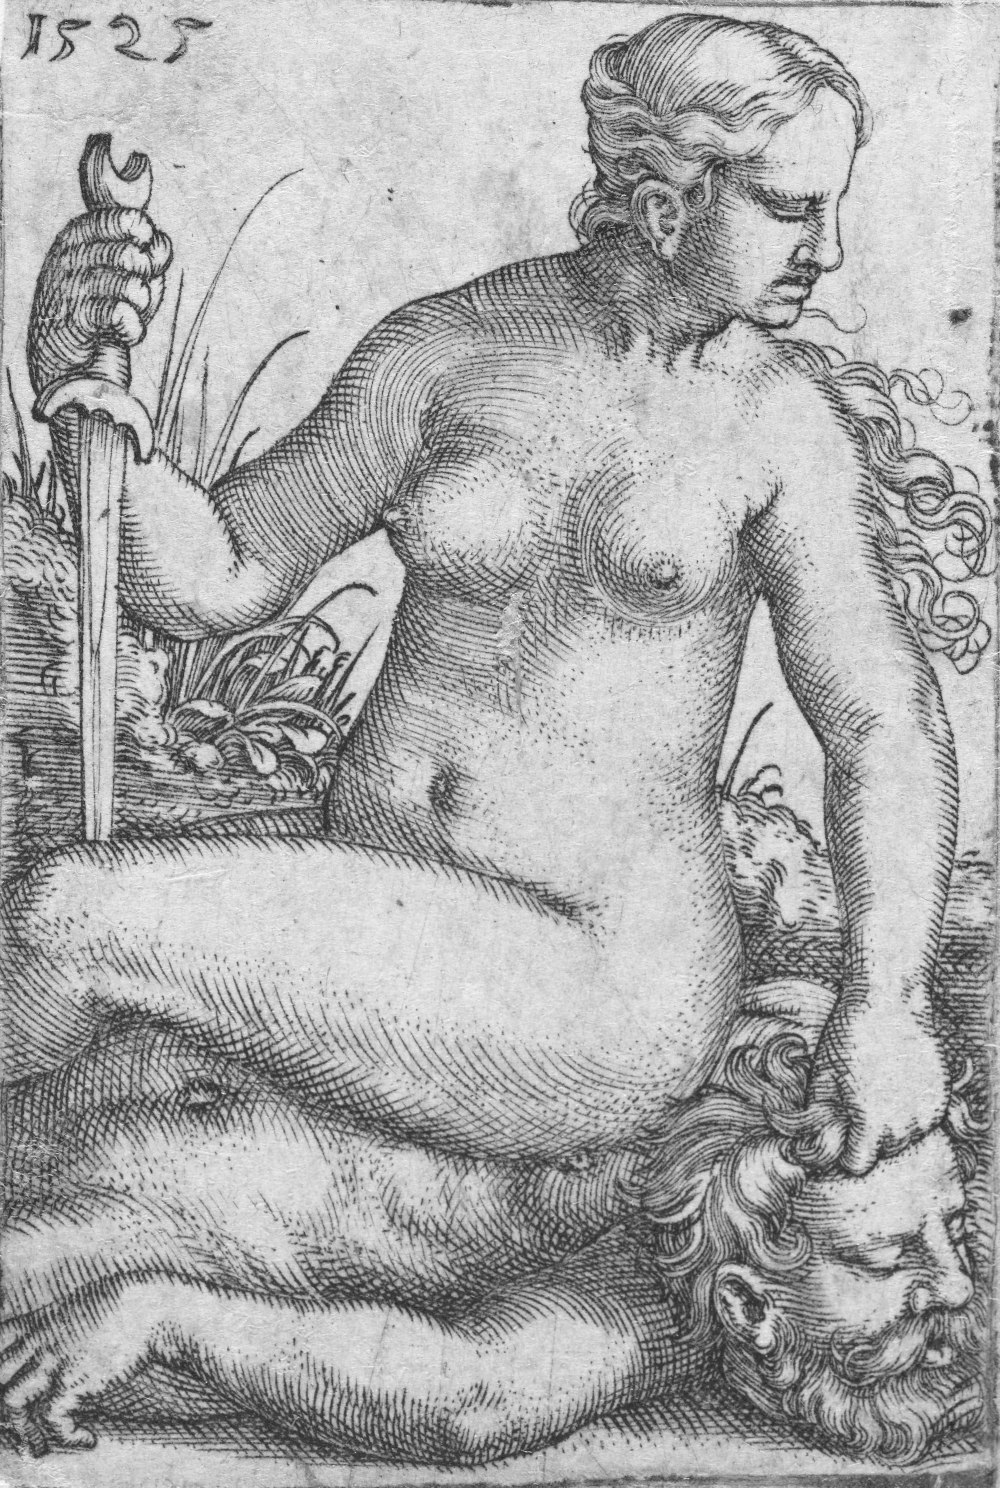
\includegraphics[keepaspectratio,width=0.6\textwidth]{figures/pride-JudithHolofernes-small.jpg}
  \captionart{JudithHolofernes}
  \label{fig:judithholofernes}
\end{figure}

\authorfootnote{4899}Nought under heaven so strongly doth allure
The sense of man and all his mind possess,
As beauty's loveliest bait, that doth procure
Great warriors erst their rigour to suppress,
And mighty hands forget their manliness,
Driven with the power of an heart-burning eye,
And lapt in flowers of a golden tress.
That can with melting pleasure mollify
Their harden'd hearts inur'd to cruelty.

\authorfootnote{4900}Clitiphon ingenuously confesseth, that he no sooner came in
Leucippe's presence, but that he did corde tremere, et oculis lascivius
intueri; \authorfootnote{4901}he was wounded at the first sight, his heart panted, and
he could not possibly turn his eyes from her. So doth Calysiris in
Heliodorus, lib. 2. Isis Priest, a reverend old man, complain, who by
chance at Memphis seeing that Thracian Rodophe, might not hold his eyes
off her: \authorfootnote{4902}I will not conceal it, she overcame me with her
presence, and quite assaulted my continency which I had kept unto mine
old age; I resisted a long time my bodily eyes with the eyes of my
understanding; at last I was conquered, and as in a tempest carried
headlong. \authorfootnote{4903} Xenophiles, a philosopher, railed at women downright
for many years together, scorned, hated, scoffed at them; coming at
last into Daphnis a fair maid's company (as he condoles his mishap to
his friend Demaritis), though free before, Intactus nullis ante
cupidinibus, was far in love, and quite overcome upon a sudden. Victus
sum fateor a Daphnide, \etc{}. I confess I am taken,
\li{Sola haec inflexit sensus, animumque labentem
Impulit}---\authorlatintrans{4904.5}\authormarginnote{4904}

I could hold out no longer. Such another mishap, but worse, had
Stratocles the physician, that blear-eyed old man, muco plenus (so
\authorfootnote{4905}Prodromus describes him); he was a severe woman's-hater all his
life, foeda et contumeliosa semper in faeminas profatus, a bitter
persecutor of the whole sex, humanas aspides et viperas appellabat, he
forswore them all still, and mocked them wheresoever he came, in such
vile terms, ut matrem et sorores odisses, that if thou hadst heard him,
thou wouldst have loathed thine own mother and sisters for his word's
sake. Yet this old doting fool was taken at last with that celestial
and divine look of Myrilla, the daughter of Anticles the gardener, that
smirking wench, that he shaved off his bushy beard, painted his face,
\authorfootnote{4906}curled his hair, wore a laurel crown to cover his bald pate, and
for her love besides was ready to run mad. For the very day that he
married he was so furious, ut solis occasum minus expectare posset (a
terrible, a monstrous long day), he could not stay till it was night,
sed omnibus insalutatis in thalamum festinans irrupit, the meat scarce
out of his mouth, without any leave taking, he would needs go presently
to bed. What young man, therefore, if old men be so intemperate, can
secure himself? Who can say I will not be taken with a beautiful
object? I can, I will contain. No, saith \authorfootnote{4907}Lucian of his mistress,
she is so fair, that if thou dost but see her, she will stupefy thee,
kill thee straight, and, Medusa like, turn thee to a stone; thou canst
not pull thine eyes from her, but, as an adamant doth iron, she will
carry thee bound headlong whither she will herself, infect thee like a
basilisk. It holds both in men and women. Dido was amazed at Aeneas'
presence; \li{Obstupuit primo aspectu Sidonia Dido}; and as he feelingly
verified out of his experience;
\authorfootnote{4908}\li{Quam ego postquam vidi, non ita amavi ut sani solent
Homines, sed eodem pacto ut insani solent}.

I lov'd her not as others soberly,
But as a madman rageth, so did I.

So Museus of Leander, \li{nusquam lumen detorquet ab illa}; and
\begin{verse}
\authormarginnote{4909}Chaucer of Palamon,\\*
He cast his eye upon Emilia,\\*
And therewith he blent and cried ha, ha,\\*
As though he had been stroke unto the hearta.
\end{verse}

If you desire to know more particularly what this beauty is, how it
doth Influere, how it doth fascinate (for, as all hold, love is a
fascination), thus in brief. \authorfootnote{4910}This comeliness or beauty ariseth
from the due proportion of the whole, or from each several part. For an
exact delineation of which, I refer you to poets, historiographers, and
those amorous writers, to Lucian's Images, and Charidemus, Xenophon's
description of Panthea, Petronius Catalectes, Heliodorus Chariclia,
Tacius Leucippe, Longus Sophista's Daphnis and Chloe, Theodorus
Prodromus his Rhodanthes, Aristaenetus and Philostratus Epistles,
Balthazar Castilio, lib. 4. de aulico. Laurentius, cap. 10, de melan.
Aeneas Sylvius his Lucretia, and every poet almost, which have most
accurately described a perfect beauty, an absolute feature, and that
through every member, both in men and women. Each part must concur to
the perfection of it; for as Seneca saith, Ep. 33. lib. 4. Non est
formosa mulier cujus crus laudatur et brachium, sed illa cujus simul
universa facies admirationem singulis partibus dedit; she is no fair
woman, whose arm, thigh, \etc{} are commended, except the face and all the
other parts be correspondent. And the face especially gives a lustre to
the rest: the face is it that commonly denominates a fair or foul: arx
formae facies, the face is beauty's tower; and though the other parts
be deformed, yet a good face carries it (facies non uxor amatur) that
alone is most part respected, principally valued, deliciis suis ferox,
and of itself able to captivate.
\authorfootnote{4911}Urit te Glycerae nitor,
Urit grata protervitas,
Et vultus nimium lubricus aspici.

Glycera's too fair a face was it that set him on fire, too fine to be
beheld. When \authorfootnote{4912}Chaerea saw the singing wench's sweet looks, he was
so taken, that he cried out, O faciem pulchram, deleo omnes dehinc ex
animo mulieres, taedet quotidianarum harum formarum! O fair face, I'll
never love any but her, look on any other hereafter but her; I am weary
of these ordinary beauties, away with them. The more he sees her, the
worse he is,-uritque videndo, as in a burning-glass, the sunbeams are
re-collected to a centre, the rays of love are projected from her eyes.
It was Aeneas's countenance ravished Queen Dido, Os humerosque Deo
similis, he had an angelical face.
\authorfootnote{4913}O sacros vultus Baccho vel Apolline dignos,
Quos vir, quos tuto foemina nulla videt!

---O sacred looks, befitting majesty,
Which never mortal wight could safely see.

Although for the greater part this beauty be most eminent in the face,
yet many times those other members yield a most pleasing grace, and are
alone sufficient to enamour. A high brow like unto the bright heavens,
coeli pulcherrima plaga, Frons ubi vivit honor, frons ubi ludit amor,
white and smooth like the polished alabaster, a pair of cheeks of
vermilion colour, in which love lodgeth; \authorfootnote{4914}Amor qui mollibus genis
puellae pernoctas: a coral lip, suaviorum delubrum, in which Basia
mille patent, basia mille latent, A thousand appear, as many are
concealed; gratiarum sedes gratissima; a sweet-smelling flower, from
which bees may gather honey, \authorfootnote{4915}Mellilegae volucres quid adhuc cava
thyma rosasque, \etc{}.
Omnes ad dominae labra venite meae,
Illa rosas spirat, \etc{}.

A white and round neck, that via lactea, dimple in the chin, black
eyebrows, Cupidinis arcus, sweet breath, white and even teeth, which
some call the salepiece, a fine soft round pap, gives an excellent
grace, \authorfootnote{4916}Quale decus tumidis Pario de marmore mammis! \authorfootnote{4917}and
make a pleasant valley lacteum sinum, between two chalky hills,
Sororiantes papillulas, et ad pruritum frigidos amatores solo aspectu
excitantes. Unde is, \authorfootnote{4918}Forma papillarum quam fuit apta premi!-Again
Urebant oculos durae stantesque mamillae. A flaxen hair; golden hair
was even in great account, for which Virgil commends Dido, Nondum
sustulerat flavum Proserpinina crinem, Et crines nodantur in aurum.
Apollonius (Argonaut. lib. 4. Jasonis flava coma incendit cor Medeae)
will have Jason's golden hair to be the main cause of Medea's dotage on
him. Castor and Pollux were both yellow haired. Paris, Menelaus, and
most amorous young men, have been such in all ages, molles ac suaves,
as Baptista Porta infers, \authorfootnote{4919} Physiog. lib. 2. lovely to behold.
Homer so commends Helen, makes Patroclus and Achilles both yellow
haired: Pulchricoma Venus, and Cupid himself was yellow haired, in
aurum coruscante et crispante capillo, like that neat picture of
Narcissus in Callistratus; for so \authorfootnote{4920}Psyche spied him asleep,
Briseis, Polixena, \etc{} flavicomae omnes,
---and Hero the fair,
Whom young Apollo courted for her hair.

Leland commends Guithera, king Arthur's wife, for a flaxen hair: so
Paulus Aemilius sets out Clodeveus, that lovely king of France.
\authorfootnote{4921}Synesius holds every effeminate fellow or adulterer is fair
haired: and Apuleius adds that Venus herself, goddess of love, cannot
delight, \authorfootnote{4922}though she come accompanied with the graces, and all
Cupid's train to attend upon her, girt with her own girdle, and smell
of cinnamon and balm, yet if she be bald or badhaired, she cannot
please her Vulcan. Which belike makes our Venetian ladies at this day
to counterfeit yellow hair so much, great women to calamistrate and
curl it up, vibrantes ad gratiam crines, et tot orbibus in captivitatem
flexos, to adorn their heads with spangles, pearls, and made-flowers;
and all courtiers to effect a pleasing grace in this kind. In a word,
\authorfootnote{4923}the hairs are Cupid's nets, to catch all comers, a brushy wood,
in which Cupid builds his nest, and under whose shadow all loves a
thousand several ways sport themselves.

A little soft hand, pretty little mouth, small, fine, long fingers,
Gratiae quae digitis -'tis that which Apollo did admire in
Daphne,-laudat digitosque manusque; a straight and slender body, a
small foot, and well-proportioned leg, hath an excellent lustre,
\authorfootnote{4924}Cui totum incumbit corpus uti fundamento aedes. Clearchus vowed
to his friend Amyander in \authorfootnote{4925}Aristaenetus, that the most attractive
part in his mistress, to make him love and like her first, was her
pretty leg and foot: a soft and white skin, \etc{} have their peculiar
graces, \authorfootnote{4926}Nebula haud est mollior ac hujus cutis est, aedipol
papillam bellulam. Though in men these parts are not so much respected;
a grim Saracen sometimes,-nudus membra Pyracmon, a martial hirsute face
pleaseth best; a black man is a pearl in a fair woman's eye, and is as
acceptable as \authorfootnote{4927}lame Vulcan was to Venus; for he being a sweaty
fuliginous blacksmith, was dearly beloved of her, when fair Apollo,
nimble Mercury were rejected, and the rest of the sweet-faced gods
forsaken. Many women (as Petronius \authorfootnote{4928}observes) sordibus calent (as
many men are more moved with kitchen wenches, and a poor market maid,
than all these illustrious court and city dames) will sooner dote upon
a slave, a servant, a dirt dauber, a brontes, a cook, a player, if they
see his naked legs or arms, thorosaque brachia, \authorfootnote{4929}\etc{}, like that
huntsman Meleager in Philostratus, though he be all in rags, obscene
and dirty, besmeared like a ruddleman, a gipsy, or a chimney-sweeper,
than upon a noble gallant, Nireus, Ephestion, Alcibiades, or those
embroidered courtiers full of silk and gold. \authorfootnote{4930}Justine's wife, a
citizen of Rome, fell in love with Pylades a player, and was ready to
run mad for him, had not Galen himself helped her by chance. Faustina
the empress doted on a fencer.

Not one of a thousand falls in love, but there is some peculiar part or
other which pleaseth most, and inflames him above the rest. \authorfootnote{4931}A
company of young philosophers on a time fell at variance, which part of
a woman was most desirable and pleased best? some said the forehead,
some the teeth, some the eyes, cheeks, lips, neck, chin, \etc{}, the
controversy was referred to Lais of Corinth to decide; but she,
smiling, said, they were a company of fools; for suppose they had her
where they wished, what would they \authorfootnote{4932}first seek? Yet this
notwithstanding I do easily grant, neque quis vestrum negaverit opinor,
all parts are attractive, but especially \authorfootnote{4933}the eyes, \authorfootnote{4934}
---videt igne micantes,
Sideribus similes oculos---

which are love's fowlers; \authorfootnote{4935}aucupium amoris, the shoeing horns, the
hooks of love (as Arandus will) the guides, touchstone, judges, that in
a moment cure mad men, and make sound folks mad, the watchmen of the
body; what do they not? How vex they not? All this is true, and (which
Athaeneus lib. 13. dip. cap. 5. and Tatius hold) they are the chief
seats of love, and James Lernutius \authorfootnote{4936}hath facetely expressed in an
elegant ode of his,
Amorem ocellis flammeolis herae
Vidi insidentem, credite posteri,
Fratresque circum ludibundos
Cum pharetra volitare et arcu, \etc{}.

I saw Love sitting in my mistress' eyes
Sparkling, believe it all posterity,
And his attendants playing round about
With bow and arrows ready for to fly.

Scaliger calls the eyes, \authorfootnote{4937}Cupid's arrows; the tongue, the
lightning of love; the paps, the tents: \authorfootnote{4938}Balthazar Castilio, the
causes, the chariots, the lamps of love,
---aemula lumina stellis,
Lumina quae possent sollicitare deos.

Eyes emulating stars in light,
Enticing gods at the first sight;

Love's orators, Petronius.
O blandos oculos, et o facetos,
Et quadam propria nota loquaces
Illic est Venus, et leves amores,
Atque ipsa in medio sedet voluptas.

O sweet and pretty speaking eyes,
Where Venus, love, and pleasure lies.

Love's torches, touch-box, naphtha and matches, \authorfootnote{4939}Tibullus.
Illius ex oculis quum vult exurere divos,
Accendit geminas lampades acer amor.

Tart Love when he will set the gods on fire,
Lightens the eyes as torches to desire.

Leander, at the first sight of Hero's eyes, was incensed, saith
Musaeus.
Simul in \authorfootnote{4940}oculorum radiis crescebat fax amorum,
Et cor fervebat invecti ignis impetu;
Pulchritudo enim Celebris immaculatae foeminae,
Acutior hominibus est veloci sagitta.
Oculos vero via est, ab oculi ictibus
Vulnus dilabitur, et in praecordia viri manat.

Love's torches 'gan to burn first in her eyes.
And set his heart on fire which never dies:
For the fair beauty of a virgin pure
Is sharper than a dart, and doth inure
A deeper wound, which pierceth to the heart
By the eyes, and causeth such a cruel smart.

\authorfootnote{4941}A modern poet brings in Amnon complaining of Thamar,
---et me fascino
Occidit ille risus et formae lepos,
Ille nitor, illa gratia, et verus decor,
Illae aemulantes purpuram, et \authorfootnote{4942}rosas genae,
Oculique vinctaeque aureo nodo comae.---

It was thy beauty, 'twas thy pleasing smile,
Thy grace and comeliness did me beguile;
Thy rose-like cheeks, and unto purple fair
Thy lovely eyes and golden knotted hair.

\authorfootnote{4943}Philostratus Lemnius cries out on his mistress's basilisk eyes,
ardentes faces, those two burning-glasses, they had so inflamed his
soul, that no water could quench it. What a tyranny (saith he), what a
penetration of bodies is this! thou drawest with violence, and
swallowest me up, as Charybdis doth sailors with thy rocky eyes: he
that falls into this gulf of love, can never get out. Let this be the
corollary then, the strongest beams of beauty are still darted from the
eyes.
\authorfootnote{4944}Nam quis lumina tanta, tanta
Posset luminibus suis tueri,
Non statim trepidansque, palpitansque,
Prae desiderii aestuantis aura? \etc{}.

For who such eyes with his can see,
And not forthwith enamour'd be!

And as men catch dotterels by putting out a leg or an arm, with those
mutual glances of the eyes they first inveigle one another.
\li{Cynthia prima suis miserum me, cepit ocellis}\authorlatintrans{4945.5}\authormarginnote{4945}. Of all eyes (by the
way) black are most amiable, enticing and fairer, which the poet
observes in commending of his mistress. \authorfootnote{4946}Spectandum nigris oculis,
nigroque capillo, which Hesiod admires in his Alemena,
\authorfootnote{4947}Cujus a vertice ac nigricantibus oculis,
Tale quiddam spiral ac ab aurea Venere.

From her black eyes, and from her golden face
As if from Venus came a lovely grace.

and \authorfootnote{4948}Triton in his Milaene-nigra oculos formosa mihi. \authorfootnote{4949}Homer
useth that epithet of ox-eyed, in describing Juno, because a round
black eye is the best, the son of beauty, and farthest from black the
worse: which \authorfootnote{4950}Polydore Virgil taxeth in our nation: Angli ut
plurimum caesiis oculis, we have grey eyes for the most part. Baptisma
Porta, Physiognom. lib. 3. puts grey colour upon children, they be
childish eyes, dull and heavy. Many commend on the other side Spanish
ladies, and those \authorfootnote{4951}Greek dames at this day, for the blackness of
their eyes, as Porta doth his Neapolitan young wives. Suetonius
describes Julius Caesar to have been nigris vegetisque oculis
micantibus, of a black quick sparkling eye: and although Averroes in
his Colliget will have such persons timorous, yet without question they
are most amorous.

Now last of all, I will show you by what means beauty doth fascinate,
bewitch, as some hold, and work upon the soul of a man by the eye. For
certainly I am of the poet's mind, love doth bewitch and strangely
change us.

\authorfootnote{4952}Ludit amor sensus, oculos perstringit, et aufert
Libertatem animi, mira nos fascinat arte.
Credo aliquis daemon subiens praecordia flammam
Concitat, et raptam tollit de cardine mentem.

Love mocks our senses, curbs our liberties,
And doth bewitch us with his art and rings,
I think some devil gets into our entrails,
And kindles coals, and heaves our souls from th'hinges.

Heliodorus lib. 3. proves at large, \authorfootnote{4953}that love is witchcraft, it
gets in at our eyes, pores, nostrils, engenders the same qualities and
affections in us, as were in the party whence it came. The manner of
the fascination, as Ficinus 10. cap. com. in Plat. declares it, is
thus: Mortal men are then especially bewitched, when as by often gazing
one on the other, they direct sight to sight, join eye to eye, and so
drink and suck in love between them; for the beginning of this disease
is the eye. And therefore he that hath a clear eye, though he be
otherwise deformed, by often looking upon him, will make one mad, and
tie him fast to him by the eye. Leonard. Varius, lib. 1. cap. 2. de
fascinat. telleth us, that by this interview, \authorfootnote{4954}the purer spirits
are infected, the one eye pierceth through the other with his rays,
which he sends forth, and many men have those excellent piercing eyes,
that, which Suetonius relates of Augustus, their brightness is such,
they compel their spectators to look off, and can no more endure them
than the sunbeams. \authorfootnote{4955}Barradius, lib. 6. cap. 10. de Harmonia
Evangel. reports as much of our Saviour Christ, and \authorfootnote{4956}Peter Morales
of the Virgin Mary, whom Nicephorus describes likewise to have been
yellow-haired, of a wheat colour, but of a most amiable and piercing
eye. The rays, as some think, sent from the eyes, carry certain
spiritual vapours with them, and so infect the other party, and that in
a moment. I know, they that hold visio fit intra mittendo, will make a
doubt of this; but Ficinus proves it from blear-eyes, \authorfootnote{4957} That by
sight alone, make others blear-eyed; and it is more than manifest, that
the vapour of the corrupt blood doth get in together with the rays, and
so by the contagion the spectators' eyes are infected. Other arguments
there are of a basilisk, that kills afar off by sight, as that Ephesian
did of whom \authorfootnote{4958}Philostratus speaks, of so pernicious an eye, he
poisoned all he looked steadily on: and that other argument, menstruae
faminae, out of Aristotle's Problems, morbosae Capivaccius adds, and
\authorfootnote{4959}Septalius the commentator, that contaminate a looking-glass with
beholding it. \authorfootnote{4960} So the beams that come from the agent's heart, by
the eyes, infect the spirits about the patients, inwardly wound, and
thence the spirits infect the blood. To this effect she complained in
\authorfootnote{4961}Apuleius, Thou art the cause of my grief, thy eyes piercing
through mine eyes to mine inner parts, have set my bowels on fire, and
therefore pity me that am now ready to die for thy sake. Ficinus
illustrates this with a familiar example of that Marrhusian Phaedrus
and Theban Lycias, \authorfootnote{4962}Lycias he stares on Phaedrus' face, and
Phaedrus fastens the balls of his eyes upon Lycias, and with those
sparkling rays sends out his spirits. The beams of Phaedrus' eyes are
easily mingled with the beams of Lycias, and spirits are joined to
spirits. This vapour begot in Phaedrus' heart, enters into Lycias'
bowels; and that which is a greater wonder, Phaedrus' blood is in
Lycias' heart, and thence come those ordinary love-speeches, my
sweetheart Phaedrus, and mine own self, my dear bowels. And Phaedrus
again to Lycias, O my light, my joy, my soul, my life. Phaedrus follows
Lycias, because his heart would have his spirits, and Lycias follows
Phaedrus, because he loves the seat of his spirits; both follow; but
Lycias the earnester of the two: the river hath more need of the
fountain, than the fountain of the river; as iron is drawn to that
which is touched with a loadstone, but draws not it again; so Lycias
draws Phaedrus. But how comes it to pass then, that the blind man
loves, that never saw? We read in the Lives of the Fathers, a story of
a child that was brought up in the wilderness, from his infancy, by an
old hermit: now come to man's estate, he saw by chance two comely women
wandering in the woods: he asked the old man what creatures they were,
he told him fairies; after a while talking obiter, the hermit demanded
of him, which was the pleasantest sight that ever he saw in his life?
He readily replied, the two \authorfootnote{4963}fairies he spied in the wilderness.
So that, without doubt, there is some secret loadstone in a beautiful
woman, a magnetic power, a natural inbred affection, which moves our
concupiscence, and as he sings,

Methinks I have a mistress yet to come,
And still I seek, I love, I know not whom.

'Tis true indeed of natural and chaste love, but not of this heroical
passion, or rather brutish burning lust of which we treat; we speak of
wandering, wanton, adulterous eyes, which, as \authorfootnote{4964}he saith, lie still
in wait as so many soldiers, and when they spy an innocent spectator
fixed on them, shoot him through, and presently bewitch him: especially
when they shall gaze and gloat, as wanton lovers do one upon another,
and with a pleasant eye-conflict participate each other's souls. Hence
you may perceive how easily and how quickly we may be taken in love;
since at the twinkling of an eye, Phaedrus' spirits may so perniciously
infect Lycias' blood. \authorfootnote{4965}Neither is it any wonder, if we but
consider how many other diseases closely, and as suddenly are caught by
infection, plague, itch, scabs, flux, \etc{}. The spirits taken in, will
not let him rest that hath received them, but egg him on. \li{Idque
petit corpus mens unde est saucia amore}\authorlatintrans{4966.5}\authormarginnote{4966}; and we may manifestly perceive
a strange eduction of spirits, by such as bleed at nose after they be
dead, at the presence of the murderer; but read more of this in
Lemnius, lib. 2. de occult. nat. mir. cap. 7. Valleriola lib. 2.
observ. cap. 7. Valesius controv. Ficinus, Cardan, Libavius de cruentis
cadaveribus, \etc{}.

%SUBSECT. III.-_Artificial allurements of Love, Causes and Provocations to Lust; Gestures, Clothes, Dower, \&c._
\section[Artificial allures of Love]{Artificial allurements of Love, Causes and Provocations to Lust; Gestures, Clothes, Dower, \&c.}

\lettrine{N}{atural} beauty is a stronger loadstone of itself, as you have heard, a
great temptation, and pierceth to the very heart; \li{forma
verecundae, nocuit mihi visa puellae}\authorlatintrans{4967.5}\authormarginnote{4967}; but much more when those
artificial enticements and provocations of gestures, clothes, jewels,
pigments, exornations, shall be annexed unto it; those other
circumstances, opportunity of time and place shall concur, which of
themselves alone were all sufficient, each one in particular to produce
this effect. It is a question much controverted by some wise men, forma
debeat plus arti an naturae? Whether natural or artificial objects be
more powerful? but not decided: for my part I am of opinion, that
though beauty itself be a great motive, and give an excellent lustre in
sordibus, in beggary, as a jewel on a dunghill will shine and cast his
rays, it cannot be suppressed, which Heliodorus feigns of Chariclia,
though she were in beggar's weeds: yet as it is used, artificial is of
more force, and much to be preferred.

\authorfootnote{4968}Sic dentata sibi videtur Aegle,
Emptis ossibus Indicoque cornu;
Sic quae nigrior est cadente moro,
Cerussata sibi placet Lychoris.

So toothless Aegle seems a pretty one,
Set out with new-bought teeth of Indy bone:
So foul Lychoris blacker than berry
Herself admires, now finer than cherry.

John Lerius the Burgundian, cap. 8. hist. navigat. in Brazil. is
altogether on my side. For whereas (saith he) at our coming to Brazil,
we found both men and women naked as they were born, without any
covering, so much as of their privities, and could not be persuaded, by
our Frenchmen that lived a year with them, to wear any, \authorfootnote{4969}Many will
think that our so long commerce with naked women, must needs be a great
provocation to lust; but he concludes otherwise, that their nakedness
did much less entice them to lasciviousness, than our women's clothes.
And I dare boldly affirm (saith he) that those glittering attires,
counterfeit colours, headgears, curled hairs, plaited coats, cloaks,
gowns, costly stomachers, guarded and loose garments, and all those
other accoutrements, wherewith our countrywomen counterfeit a beauty,
and so curiously set out themselves, cause more inconvenience in this
kind, than that barbarian homeliness, although they be no whit inferior
unto them in beauty. I could evince the truth of this by many other
arguments, but I appeal (saith he) to my companions at that present,
which were all of the same mind. His countryman, Montague, in his
essays, is of the same opinion, and so are many others; out of whose
assertions thus much in brief we may conclude, that beauty is more
beholden to art than nature, and stronger provocations proceed from
outward ornaments, than such as nature hath provided. It is true that
those fair sparkling eyes, white neck, coral lips, turgent paps,
rose-coloured cheeks, \etc{}, of themselves are potent enticers; but when
a comely, artificial, well-composed look, pleasing gesture, an affected
carriage shall be added, it must needs be far more forcible than it
was, when those curious needleworks, variety of colours, purest dyes,
jewels, spangles, pendants, lawn, lace, tiffanies, fair and fine linen,
embroideries, calamistrations, ointments, etc. shall be added, they
will make the veriest dowdy otherwise, a goddess, when nature shall be
furthered by art. For it is not the eye of itself that enticeth to
lust, but an adulterous eye, as Peter terms it, 2. \rn{ii.} 14. a wanton, a
rolling, lascivious eye: a wandering eye, which Isaiah taxeth, \rn{iii.} 16.
Christ himself, and the Virgin Mary, had most beautiful eyes, as
amiable eyes as any persons, saith \authorfootnote{4970}Baradius, that ever lived, but
withal so modest, so chaste, that whosoever looked on them was freed
from that passion of burning lust, if we may believe \authorfootnote{4971}Gerson and
\authorfootnote{4972}Bonaventure: there was no such antidote against it, as the Virgin
Mary's face; 'tis not the eye, but carriage of it, as they use it, that
causeth such effects. When Pallas, Juno, Venus, were to win Paris'
favour for the golden apple, as it is elegantly described in that
pleasant interlude of \authorfootnote{4973}Apuleius, Juno came with majesty upon the
stage, Minerva gravity, but Venus dulce subridens, constitit amaene; et
gratissimae, Graticae deam propitiantes, \etc{} came in smiling with her
gracious graces and exquisite music, as if she had danced, et
nonnunquam saltare solis oculis, and which was the main matter of all,
she danced with her rolling eyes: they were the brokers and harbingers
of her suite. So she makes her brags in a modern poet,
\authormarginnote{4974}Soon could I make my brow to tyrannise,
And force the world do homage to mine eyes.

The eye is a secret orator, the first bawd, Amoris porta, and with
private looks, winking, glances and smiles, as so many dialogues they
make up the match many times, and understand one another's meanings,
before they come to speak a word. \authormarginnote{4975}Euryalus and Lucretia were so
mutually enamoured by the eye, and prepared to give each other
entertainment, before ever they had conference: he asked her good will
with his eyes; she did suffragari, and gave consent with a pleasant
look. That \authormarginnote{4976}Thracian Rodophe was so excellent at this dumb
rhetoric, that if she had but looked upon any one almost (saith
Calisiris) she would have bewitched him, and he could not possibly
escape it. For as \authorfootnote{4977}Salvianus observes, the eyes are the windows of
our souls, by which as so many channels, all dishonest concupiscence
gets into our hearts. They reveal our thoughts, and as they say, frons
animi index, but the eye of the countenance, \authorfootnote{4978}Quid procacibus
intuere ocellis? \etc{}. I may say the same of smiling, gait, nakedness of
parts, plausible gestures, \etc{}. To laugh is the proper passion of a man,
an ordinary thing to smile; but those counterfeit, composed, affected,
artificial and reciprocal, those counter-smiles are the dumb shows and
prognostics of greater matters, which they most part use, to inveigle
and deceive; though many fond lovers again are so frequently mistaken,
and led into a fool's paradise. For if they see but a fair maid laugh,
or show a pleasant countenance, use some gracious words or gestures,
they apply it all to themselves, as done in their favour; sure she
loves them, she is willing, coming, \etc{}.
Stultus quando videt quod pulchra puellula ridet,
Tum fatuus credit se quod amare velit:

When a fool sees a fair maid for to smile,
He thinks she loves him, 'tis but to beguile.

They make an art of it, as the poet telleth us,
\authorfootnote{4979}Quis credat? discunt etiam ridere puellae,
Quaeritur atque illis hac quoque parte decor.

Who can believe? to laugh maids make an art,
And seek a pleasant grace to that same part.

And 'tis as great an enticement as any of the rest,
\authorfootnote{4980}---subrisit molle puella,
Cor tibi rite salit.

She makes thine heart leap with \authorfootnote{4981}a pleasing gentle smile of hers.
\authorfootnote{4982}Dulce ridentem Lalagen amabo,
Dulce loquentem,

I love Lalage as much for smiling, as for discoursing, delectata illa
risit tam blandum, as he said in Petronius of his mistress, being well
pleased, she gave so sweet a smile. It won Ismenias, as he \authorfootnote{4983}
confesseth, Ismene subrisit amatorium, Ismene smiled so lovingly the
second time I saw her, that I could not choose but admire her: and
Galla's sweet smile quite overcame \authorfootnote{4984}Faustus the shepherd, Me
aspiciens moils blande subrisit ocellis. All other gestures of the body
will enforce as much. Daphnis in \authorfootnote{4985}Lucian was a poor tattered wench
when I knew her first, said Corbile, pannosa et Zacera, but now she is
a stately piece indeed, hath her maids to attend her, brave attires,
money in her purse, \etc{}, and will you know how this came to pass? by
setting out herself after the best fashion, by her pleasant carriage,
affability, sweet smiling upon all, \etc{}. Many women dote upon a man for
his compliment only, and good behaviour, they are won in an instant;
too credulous to believe that every light wanton suitor, who sees or
makes love to them, is instantly enamoured, he certainly dotes on,
admires them, will surely marry, when as he means nothing less, 'tis
his ordinary carriage in all such companies. So both delude each other
by such outward shows; and amongst the rest, an upright, a comely
grace, courtesies, gentle salutations, cringes, a mincing gait, a
decent and an affected pace, are most powerful enticers, and which the
prophet Isaiah, a courtier himself, and a great observer, objected to
the daughters of Zion, iii. 16. they minced as they went, and made a
tinkling with their feet. To say the truth, what can they not effect by
such means?

Whilst nature decks them in their best attires
Of youth and beauty which the world admires.

\authormarginnote{4986}\li{Urit-voce, manu, gressu, pectore, fronte, oculis}. When art shall
be annexed to beauty, when wiles and guiles shall concur; for to speak
as it is, love is a kind of legerdemain; mere juggling, a fascination.
When they show their fair hand, fine foot and leg withal, magnum sui
desiderium nobis relinquunt, saith \authorfootnote{4987}Balthazar Castilio, lib. 1.
they set us a longing, and so when they pull up their petticoats, and
outward garments, as usually they do to show their fine stockings, and
those of purest silken dye, gold fringes, laces, embroiderings, (it
shall go hard but when they go to church, or to any other place, all
shall be seen) 'tis but a springe to catch woodcocks; and as
\authorfootnote{4988}Chrysostom telleth them downright, though they say nothing with
their mouths, they speak in their gait, they speak with their eyes,
they speak in the carriage of their bodies. And what shall we say
otherwise of that baring of their necks, shoulders, naked breasts, arms
and wrists, to what end are they but only to tempt men to lust!

\authorfootnote{4989}Nam quid lacteolus sinus, et ipsas
Prae te fers sine linteo papillas?
Hoc est dicere, posce, posce, trado;
Hoc est ad Venerem vocare amantes.

There needs no more, as \authorfootnote{4990}Fredericus Matenesius well observes, but
a crier to go before them so dressed, to bid us look out, a trumpet to
sound, or for defect a sow-gelder to blow,
\authormarginnote{4991}Look out, look out and see
What object this may be
That doth perstringe mine eye;
A gallant lady goes
In rich and gaudy clothes,
But whither away God knows,
---look out, \etc{}, et quae sequuntur,

or to what end and purpose? But to leave all these fantastical
raptures, I'll prosecute my intended theme. Nakedness, as I have said,
is an odious thing of itself, remedium amoris; yet it may be so used,
in part, and at set times, that there can be no such enticement as it
is;
\authorfootnote{4992}Nec mihi cincta Diana placet, nec nuda Cythere,
Illa voluptatis nil habet, haec nimium.

David so espied Bathsheba, the elders Susanna: \authorfootnote{4993}Apelles was
enamoured with Campaspe, when he was to paint her naked. Tiberius in
Suet. cap. 42. supped with Sestius Gallus an old lecher, libidinoso
sene, ea lege ut nudae puellae administrarent; some say as much of
Nero, and Pontus Huter of Carolus Pugnax. Amongst the Babylonians, it
was the custom of some lascivious queans to dance frisking in that
fashion, saith Curtius lib. 5. and Sardus de mor. gent. lib. 1. writes
of others to that effect. The \authorfootnote{4994}Tuscans at some set banquets had
naked women to attend upon them, which Leonicus de Varia hist. lib. 3.
cap. 96. confirms of such other bawdy nations. Nero would have filthy
pictures still hanging in his chamber, which is too commonly used in
our times, and Heliogabalus, etiam coram agentes, ut ad venerem
incitarent: So things may be abused. A servant maid in Aristaenetus
spied her master and mistress through the key-hole \authorfootnote{4995}merrily
disposed; upon the sight she fell in love with her master.
\authorfootnote{4996}Antoninus Caracalla observed his mother-in-law with her breasts
amorously laid open, he was so much moved, that he said, Ah si liceret,
O that I might; which she by chance overhearing, replied as impudently,
\authorfootnote{4997}Quicquid libet licet, thou mayst do what thou wilt: and upon that
temptation he married her: this object was not in cause, not the thing
itself, but that unseemly, indecent carriage of it.
When you have all done, veniunt a veste sagittae the greatest
provocations of lust are from our apparel; God makes, they say, man
shapes, and there is no motive like unto it;
\authorfootnote{4998}Which doth even beauty beautify,
And most bewitch a wretched eye,

a filthy knave, a deformed quean, a crooked carcass, a mawkin, a witch,
a rotten post, a hedgestake may be so set out and tricked up, that it
shall make as fair a show, as much enamour as the rest: many a silly
fellow is so taken. Primum luxuriae, aucupium, one calls it, the first
snare of lust; \authorfootnote{4999}Bossus aucupium animarum, lethalem arundinem, a
fatal reed, the greatest bawd, forte lenocinium, sanguineis lachrymis
deplorandum, saith \authorfootnote{5000}Matenesius, and with tears of blood to be
deplored. Not that comeliness of clothes is therefore to be condemned,
and those usual ornaments: there is a decency and decorum in this as
well as in other things, fit to be used, becoming several persons, and
befitting their estates; he is only fantastical that is not in fashion,
and like an old image in arras hangings, when a manner of attire is
generally received; but when they are so new-fangled, so unstaid, so
prodigious in their attires, beyond their means and fortunes,
unbefitting their age, place, quality, condition, what should we
otherwise think of them? Why do they adorn themselves with so many
colours of herbs, fictitious flowers, curious needleworks, quaint
devices, sweet-smelling odours, with those inestimable riches of
precious stones, pearls, rubies, diamonds, emeralds, \etc{}? Why do they
crown themselves with gold and silver, use coronets and tires of
several fashions, deck themselves with pendants, bracelets, earrings,
chains, girdles, rings, pins, spangles, embroideries, shadows,
rebatoes, versicolour ribands? why do they make such glorious shows
with their scarves, feathers, fans, masks, furs, laces, tiffanies,
ruffs, falls, calls, cuffs, damasks, velvets, tinsels, cloth of gold,
silver, tissue? with colours of heavens, stars, planets: the strength
of metals, stones, odours, flowers, birds, beasts, fishes, and
whatsoever Africa, Asia, America, sea, land, art, and industry of man
can afford? Why do they use and covet such novelty of inventions; such
new-fangled tires, and spend such inestimable sums on them? To what end
are those crisped, false hairs, painted faces, as \authorfootnote{5001}the satirist
observes, such a composed gait, not a step awry? Why are they like so
many Sybarites, or Nero's Poppaea, Ahasuerus' concubines, so costly, so
long a dressing, as Caesar was marshalling his army, or a hawk in
pruning? \li{Dum moliuntur, dum comuntur annus est}\authorlatintrans{5002.5}\authormarginnote{5002}: a \authorfootnote{5003}gardener
takes not so much delight and pains in his garden, a horseman to dress
his horse, scour his armour, a mariner about his ship, a merchant his
shop and shop-book, as they do about their faces, and all those other
parts: such setting up with corks, straightening with whalebones; why
is it, but as a day-net catcheth larks, to make young men stoop unto
them? Philocharus, a gallant in Aristenaetus, advised his friend
Poliaenus to take heed of such enticements, \authorfootnote{5004}for it was the sweet
sound and motion of his mistress's spangles and bracelets, the smell of
her ointments, that captivated him first, Illa fuit mentis prima ruina
meae. Quid sibi vult pixidum turba, saith \authorfootnote{5005}Lucian, to what use are
pins, pots, glasses, ointments, irons, combs, bodkins, setting-sticks?
why bestow they all their patrimonies and husbands' yearly revenues on
such fooleries? \authorfootnote{5006}bina patrimonia singulis auribus; why use they
dragons, wasps, snakes, for chains, enamelled jewels on their necks,
ears? dignum potius foret ferro manus istas religari, atque utinam
monilia vere dracones essent; they had more need some of them be tied
in bedlam with iron chains, have a whip for a fan, and hair-cloths next
to their skins, and instead of wrought smocks, have their cheeks
stigmatised with a hot iron: I say, some of our Jezebels, instead of
painting, if they were well served. But why is all this labour, all
this cost, preparation, riding, running, far-fetched, and dear bought
stuff? \authorfootnote{5007}Because forsooth they would be fair and fine, and where
nature, is defective, supply it by art. \authorfootnote{5008}Sanguine quae vero non
rubet, arte rubet, (Ovid); and to that purpose they anoint and paint
their faces, to make Helen of Hecuba-parvamque exortamque
puellam-Europen.\authorfootnote{5009}To this intent they crush in their feet and
bodies, hurt and crucify themselves, sometimes in lax-clothes, a
hundred yards I think in a gown, a sleeve; and sometimes again so
close, ut nudos exprimant artus. \authorfootnote{5010}Now long tails and trains, and
then short, up, down, high, low, thick, thin, \etc{}; now little or no
bands, then as big as cart wheels; now loose bodies, then great
farthingales and close girt, \etc{}. Why is all this, but with the whore in
the Proverbs, to intoxicate some or other? oculorum decipulam,\authorfootnote{5011}one
therefore calls it, et indicem libidinis, the trap of lust, and sure
token, as an ivy-bush is to a tavern.

Quod pulchros Glycere sumas de pixide vultus,
Quod tibi compositae nec sine lege comae:

Quod niteat digitis adamas, Beryllus in aure,
Non sum divinus, sed scio quid cupias.


O Glycere, in that you paint so much,
Your hair is so bedeckt in order such.
With rings on fingers, bracelets in your ear,
Although no prophet, tell I can, I fear.

To be admired, to be gazed on, to circumvent some novice; as many times
they do, that instead of a lady he loves a cap and a feather instead of
a maid that should have verum colorem, corpus solidum et succi plenum
(as Chaerea describes his mistress in the \authorfootnote{5012}poet), a painted face,
a ruff-band, fair and fine linen, a coronet, a flower,
(\authorfootnote{5013}Naturaeque putat quod fuit artificis,) a wrought waistcoat he
dotes on, or a pied petticoat, a pure dye instead of a proper woman.
For generally, as with rich-furred conies, their cases are far better
than their bodies, and like the bark of a cinnamon, tree, which is
dearer than the whole bulk, their outward accoutrements are far more
precious than their inward endowments. 'Tis too commonly so.
\authorfootnote{5014}Auferimur cultu, et gemmis, auroque teguntur
Omnia; pars minima est ipsa puella sui.


With gold and jewels all is covered,
And with a strange tire we are won,

(Whilst she's the least part of herself)
And with such baubles quite undone.

Why do they keep in so long together, a whole winter sometimes, and
will not be seen but by torch or candlelight, and come abroad with all
the preparation may be, when they have no business, but only to show
themselves? Spectatum veniunt, veniunt spectentur ut ipsae.
\authorfootnote{5015}For what is beauty if it be not seen,
Or what is't to be seen if not admir'd,
And though admir'd, unless in love desir'd?

why do they go with such counterfeit gait, which \authorfootnote{5016}Philo Judeus
reprehends them for, and use (I say it again) such gestures, apish,
ridiculous, indecent attires, sybaritical tricks, fucos genis,
purpurissam venis, cerussam fronti, leges occulis, \etc{} use those sweet
perfumes, powders and ointments in public; flock to hear sermons so
frequent, is it for devotion? or rather, as \authorfootnote{5017}Basil tells them, to
meet their sweethearts, and see fashions; for, as he saith, commonly
they come so provided to that place, with such curious compliments,
with such gestures and tires, as if they should go to a dancing-school,
a stage-play, or bawdy-house, fitter than a church.
When such a she-priest comes her mass to say,
Twenty to one they all forget to pray.

They make those holy temples, consecrated to godly martyrs and
religious uses, the shops of impudence, dens of whores and thieves, and
little better than brothel houses. When we shall see these things daily
done, their husbands bankrupts, if not cornutos, their wives light
housewives, daughters dishonest; and hear of such dissolute acts, as
daily we do, how should we think otherwise? what is their end, but to
deceive and inveigle young men? As tow takes fire, such enticing
objects produce their effect, how can it be altered? When Venus stood
before Anchises (as \authorfootnote{5018}Homer feigns in one of his hymns) in her
costly robes, he was instantly taken,
Cum ante ipsum staret Jovis filia, videns eam
Anchises, admirabatur formam, et stupendas vestes;
Erat enim induta peplo, igneis radiis spiendidiore;
Habebat quoque torques fulgidos, flexiles haelices,
Tenerum collum ambiebant monilia pulchra,
Aurea, variegata.---

When Venus stood before Anchises first,
He was amaz'd to see her in her tires;
For she had on a hood as red as fire,
And glittering chains, and ivy-twisted spires,
About her tender neck were costly brooches,
And necklaces of gold, enamell'd ouches.

So when Medea came in presence of Jason first, attended by her nymphs
and ladies, as she is described by \authorfootnote{5019}Apollonius,
Cunctas vero ignis instar sequebatur splendor,
Tantum ab aureis fimbriis resplendebat jubar,
Accenditque in oculis dulce desiderium.

A lustre followed them like flaming fire,
And from their golden borders came such beams,
Which in his eyes provok'd a sweet desire.

Such a relation we have in \authorfootnote{5020}Plutarch, when the queens came and
offered themselves to Antony, \authorfootnote{5021}with diverse presents, and enticing
ornaments, Asiatic allurements, with such wonderful joy and festivity,
they did so inveigle the Romans, that no man could contain himself, all
was turned to delight and pleasure. The women transformed themselves to
Bacchus shapes, the men-children to Satyrs and Pans; but Antony himself
was quite besotted with Cleopatra's sweet speeches, philters, beauty,
pleasing tires: for when she sailed along the river Cydnus, with such
incredible pomp in a gilded ship, herself dressed like Venus, her maids
like the Graces, her pages like so many Cupids, Antony was amazed, and
rapt beyond himself. Heliodorus, lib. 1. brings in Dameneta, stepmother
to Cnemon, whom she \authorfootnote{5022}saw in his scarves, rings, robes, and
coronet, quite mad for the love of him. It was Judith's pantofles that
ravished the eyes of Holofernes. And \authorfootnote{5023}Cardan is not ashamed to
confess, that seeing his wife the first time all in white, he did
admire and instantly love her. If these outward ornaments were not of
such force, why doth \authorfootnote{5024}Naomi give Ruth counsel how to please Boaz?
and \authorfootnote{5025}Judith, seeking to captivate Holofernes, washed and anointed
herself with sweet ointments, dressed her hair, and put on costly
attires. The riot in this kind hath been excessive in times past; no
man almost came abroad, but curled and anointed,
\authorfootnote{5026}Et matutino suadans Crispinus amomo.
Quantum vix redolent duo funera.

one spent as much as two funerals at once, and with perfumed hairs,
\authorfootnote{5027}et rosa canos odorati capillos Assyriaque nardo. What strange
thing doth \authorfootnote{5028}Sueton. relate in this matter of Caligula's riot? And
Pliny, lib. 12. \& 13. Read more in Dioscorides, Ulmus, Arnoldus,
Randoletius de fuco et decoratione; for it is now an art, as it was of
old, (so \authorfootnote{5029}Seneca records) officinae, sunt adores coquentium. Women
are bad and men worse, no difference at all between their and our
times; \authorfootnote{5030}good manners (as Seneca complains) are extinct with
wantonness, in tricking up themselves men go beyond women, they wear
harlots' colours, and do not walk, but jet and dance, hic mulier, haec
vir, more like players, butterflies, baboons, apes, antics, than men.
So ridiculous, moreover, we are in our attires, and for cost so
excessive, that as Hierome said of old, Uno filio villarum insunt
pretia, uno lino decies sestertium inseritur; 'tis an ordinary thing to
put a thousand oaks and a hundred oxen into a suit of apparel, to wear
a whole manor on his back. What with shoe-ties, hangers, points, caps
and feathers, scarves, bands, curls, \etc{}, in a short space their whole
patrimonies are consumed. Heliogabalus is taxed by Lampridius, and
admired in his age for wearing jewels in his shoes, a common thing in
our times, not for emperors and princes, but almost for serving men and
tailors; all the flowers, stars, constellations, gold and precious
stones do condescend to set out their shoes. To repress the luxury of
those Roman matrons, there was \authorfootnote{5031}Lex Valeria and Oppia, and a Cato
to contradict; but no laws will serve to repress the pride and
insolency of our days, the prodigious riot in this kind. Lucullus's
wardrobe is put down by our ordinary citizens; and a cobbler's wife in
Venice, a courtesan in Florence, is no whit inferior to a queen, if our
geographers say true: and why is all this? Why do they glory in their
jewels (as \authorfootnote{5032}he saith) or exult and triumph in the beauty of
clothes? why is all this cost? to incite men the sooner to burning
lust. They pretend decency and ornament; but let them take heed, that
while they set out their bodies they do not damn their souls; 'tis
\authorfootnote{5033}Bernard's counsel: shine in jewels, stink in conditions; have
purple robes, and a torn conscience. Let them take heed of Isaiah's
prophecy, that their slippers and attires be not taken from them, sweet
balls, bracelets, earrings, veils, wimples, crisping-pins, glasses,
fine linen, hoods, lawns, and sweet savours, they become not bald,
burned, and stink upon a sudden. And let maids beware, as \authorfootnote{5034}Cyprian
adviseth, that while they wander too loosely abroad, they lose not
their virginities: and like Egyptian temples, seem fair without, but
prove rotten carcases within. How much better were it for them to
follow that good counsel of Tertullian? \authorfootnote{5035}To have their eyes
painted with chastity, the Word of God inserted into their ears,
Christ's yoke tied to the hair, to subject themselves to their
husbands. If they would do so, they should be comely enough, clothe
themselves with the silk of sanctity, damask of devotion, purple of
piety and chastity, and so painted, they shall have God himself to be a
suitor: let whores and queans prank up themselves, \authorfootnote{5036}let them paint
their faces with minion and ceruse, they are but fuels of lust, and
signs of a corrupt soul: if ye be good, honest, virtuous, and religious
matrons, let sobriety, modesty and chastity be your honour, and God
himself your love and desire. Mulier recte olet, ubi nihil olet, then a
woman smells best, when she hath no perfume at all; no crown, chain, or
jewel (Guivarra adds) is such an ornament to a virgin, or virtuous
woman, quam virgini pudor, as chastity is: more credit in a wise man's
eye and judgment they get by their plainness, and seem fairer than they
that are set out with baubles, as a butcher's meat is with pricks,
puffed up, and adorned like so many jays with variety of colours. It is
reported of Cornelia, that virtuous Roman lady, great Scipio's
daughter, Titus Sempronius' wife, and the mother of the Gracchi, that
being by chance in company with a companion, a strange gentlewoman
(some light housewife belike, that was dressed like a May lady, and, as
most of our gentlewomen are, was \authorfootnote{5037}more solicitous of her head-tire
than of her health, that spent her time between a comb and a glass, and
had rather be fair than honest (as Cato said), and have the
commonwealth turned topsy-turvy than her tires marred; and she did
nought but brag of her fine robes and jewels, and provoked the Roman
matron to show hers: Cornelia kept her in talk till her children came
from school, and these, said she, are my jewels, and so deluded and put
off a proud, vain, fantastical, housewife. How much better were it for
our matrons to do as she did, to go civilly and decently,
\authorfootnote{5038}Honestae mulieris instar quae utitur auro pro eo quod est, ad ea
tantum quibus opus est, to use gold as it is gold, and for that use it
serves, and when they need it, than to consume it in riot, beggar their
husbands, prostitute themselves, inveigle others, and peradventure damn
their own souls? How much more would it be for their honour and credit?
Thus doing, as Hierom said of Blesilla, \authorfootnote{5039}Furius did not so triumph
over the Gauls, Papyrius of the Samnites, Scipio of Numantia, as she
did by her temperance; pulla semper veste, \etc{}, they should insult and
domineer over lust, folly, vainglory, all such inordinate, furious and
unruly passions.

But I am over tedious, I confess, and whilst I stand gaping after fine
clothes, there is another great allurement, (in the world's eye at
least) which had like to have stolen out of sight, and that is money,
veniunt a dote sagittae, money makes the match; \authorfootnote{5040}\textgreek{Μονὸν ἄργυρον
βλέπουσιν}: 'tis like sauce to their meat, cum carne condimentum, a good
dowry with a wife. Many men if they do hear but of a great portion, a
rich heir, are more mad than if they had all the beauteous ornaments,
and those good parts art and nature can afford, they \authorfootnote{5041}care not for
honesty, bringing up, birth, beauty, person, but for money.
\authorfootnote{5042}Canes et equos (o Cyrne) quaerimus
Nobiles, et a bona progenie;
Malam vero uxorem, malique patris filiam
Ducere non curat vir bonus,
Modo ei magnam dotem afferat,

Our dogs and horses still from the best breed
We carefully seek, and well may they speed:
But for our wives, so they prove wealthy,
Fair or foul, we care not what they be.

If she be rich, then she is fair, fine, absolute and perfect, then they
burn like fire, they love her dearly, like pig and pie, and are ready
to hang themselves if they may not have her. Nothing so familiar in
these days, as for a young man to marry an old wife, as they say, for a
piece of gold; asinum auro onustum; and though she be an old crone, and
have never a tooth in her head, neither good conditions, nor a good
face, a natural fool, but only rich, she shall have twenty young
gallants to be suitors in an instant. As she said in Suetonius, non me,
sed mea ambiunt, 'tis not for her sake, but for her lands or money; and
an excellent match it were (as he added) if she were away. So on the
other side, many a young lovely maid will cast away herself upon an
old, doting, decrepit dizzard,
\authorfootnote{5043}Bis puer effoeto quamvis balbutiat ore,
Prima legit rarae tam culta roseta puellae,

that is rheumatic and gouty, hath some twenty diseases, perhaps but one
eye, one leg, never a nose, no hair on his head, wit in his brains, nor
honesty, if he have land or \authorfootnote{5044}money, she will have him before all
other suitors, \authorfootnote{5045}Dummodo sit dives barbarus ille placet. If he be
rich, he is the man, a fine man, and a proper man, she will go to
Jacaktres or Tidore with him; Galesimus de monte aureo. Sir Giles
Goosecap, Sir Amorous La-Fool, shall have her. And as Philemasium in
\authorfootnote{5046} Aristaenetus told Emmusus, absque argento omnia vana, hang him
that hath no money, 'tis to no purpose to talk of marriage without
means, \authorfootnote{5047} trouble me not with such motions; let others do as they
will, I'll be sure to have one shall maintain me fine and brave. Most
are of her mind, \authorfootnote{5048} De moribus ultima fiet questio, for his
conditions, she shall inquire after them another time, or when all is
done, the match made, and everybody gone home. \authorfootnote{5049}Lucian's Lycia was
a proper young maid, and had many fine gentlemen to her suitors;
Ethecles, a senator's son, Melissus, a merchant, \etc{}; but she forsook
them all for one Passius, a base, hirsute, bald-pated knave; but why
was it? His father lately died and left him sole heir of his goods and
lands. This is not amongst your dust-worms alone, poor snakes that will
prostitute their souls for money, but with this bait you may catch our
most potent, puissant, and illustrious princes. That proud upstart
domineering Bishop of Ely, in the time of Richard the First, viceroy in
his absence, as \authorfootnote{5050}Nubergensis relates it, to fortify himself, and
maintain his greatness, propinquarum suarum connubiis, plurimos sibi
potentes et nobiles devincire curavit, married his poor kinswomen
(which came forth of Normandy by droves) to the chiefest nobles of the
land, and they were glad to accept of such matches, fair or foul, for
themselves, their sons, nephews, \etc{}. Et quis tam praeclaram aflinitatem
sub spe magnae promotionis non optaret? Who would not have done as much
for money and preferment? as mine author \authorfootnote{5051}adds. Vortiger, King of
Britain, married Rowena the daughter of Hengist the Saxon prince, his
mortal enemy; but wherefore? she had Kent for her dowry. Iagello the
great Duke of Lithuania, 1386, was mightily enamoured on Hedenga,
insomuch that he turned Christian from a Pagan, and was baptised
himself by the name of Uladislaus, and all his subjects for her sake:
but why was it? she was daughter and heir of Poland, and his desire was
to have both kingdoms incorporated into one. Charles the Great was an
earnest suitor to Irene the Empress, but, saith \authorfootnote{5052}Zonarus, ob
regnum, to annex the empire of the East to that of the West. Yet what
is the event of all such matches, that are so made for money, goods, by
deceit, or for burning lust, quos foeda libido conjunxit, what follows?
they are almost mad at first, but 'tis a mere flash; as chaff and straw
soon fired, burn vehemently for a while, yet out in a moment; so are
all such matches made by those allurements of burning lust; where there
is no respect of honesty, parentage, virtue, religion, education, and
the like, they are extinguished in an instant, and instead of love
comes hate; for joy, repentance and desperation itself. Franciscus
Barbarus in his first book de re uxoria, c. 5, hath a story of one
Philip of Padua that fell in love with a common whore, and was now
ready to run mad for her; his father having no more sons let him enjoy
her; \authorfootnote{5053}but after a few days, the young man began to loath, could
not so much as endure the sight of her, and from one madness fell into
another. Such event commonly have all these lovers; and he that so
marries, or for such respects, let them look for no better success than
Menelaus had with Helen, Vulcan with Venus, Theseus with Phaedra, Minos
with Pasiphae, and Claudius with Messalina; shame, sorrow, misery,
melancholy, discontent.

%SUBSECT. IV.-_Importunity and Opportunity of Time, Place, Conference, Discourse, Singing, Dancing, Music, Amorous Tales, Objects, Kissing, Familiarity, Tokens, Presents, Bribes, Promises, Protestations, Tears, &c._
\section[Importunity and Opportunity of Time, Place\ldots{}]{Importunity and Opportunity of Time, Place, Conference, Discourse, Singing, Dancing, Music, Amorous Tales, Objects, Kissing, Familiarity, Tokens, Presents, Bribes, Promises, Protestations, Tears, \&c.}

\lettrine{A}{ll} these allurements hitherto are afar off, and at a distance; I will
come nearer to those other degrees of love, which are conference,
kissing, dalliance, discourse, singing, dancing, amorous tales,
objects, presents, \etc{}, which as so many sirens steal away the hearts
of men and women. For, as Tacitus observes, l. 2, \authorfootnote{5054}It is no
sufficient trial of a maid's affection by her eyes alone, but you must
say something that shall be more available, and use such other forcible
engines; therefore take her by the hand, wring her fingers hard, and
sigh withal; if she accept this in good part, and seem not to be much
averse, then call her mistress, take her about the neck and kiss her,
\etc{}. But this cannot be done except they first get opportunity of
living, or coming together, ingress, egress, and regress; letters and
commendations may do much, outward gestures and actions: but when they
come to live near one another, in the same street, village, or together
in a house, love is kindled on a sudden. Many a serving-man by reason
of this opportunity and importunity inveigles his master's daughter,
many a gallant loves a dowdy, many a gentleman runs upon his wife's
maids; many ladies dote upon their men, as the queen in Ariosto did
upon the dwarf, many matches are so made in haste, and they are
compelled as it were by \authorfootnote{5055}necessity so to love, which had they been
free, come in company of others, seen that variety which many places
afford, or compared them to a third, would never have looked one upon
another. Or had not that opportunity of discourse and familiarity been
offered, they would have loathed and contemned those whom, for want of
better choice and other objects, they are fatally driven on, and by
reason of their hot blood, idle life, full diet, \etc{}, are forced to
dote upon them that come next. And many times those which at the first
sight cannot fancy or affect each other, but are harsh and ready to
disagree, offended with each other's carriage, like Benedict and
Beatrice in the \authorfootnote{5056}comedy, and in whom they find many faults, by
this living together in a house, conference, kissing, colling, and such
like allurements, begin at last to dote insensibly one upon another.
It was the greatest motive that Potiphar's wife had to dote upon
Joseph, and \authorfootnote{5057}Clitiphon upon Leucippe his uncle's daughter, because
the plague being at Bizance, it was his fortune for a time to sojourn
with her, to sit next her at the table, as he tells the tale himself in
Tatius, lib. 2. (which, though it be but a fiction, is grounded upon
good observation, and doth well express the passions of lovers), he had
opportunity to take her by the hand, and after a while to kiss, and
handle her paps, \etc{}, \authorfootnote{5058} which made him almost mad. Ismenias the
orator makes the like confession in Eustathius, lib. 1, when he came
first to Sosthene's house, and sat at table with Cratistes his friend,
Ismene, Sosthene's daughter, waiting on them with her breasts open,
arms half bare, \authorfootnote{5059}Nuda pedem, discincta sinum, spoliata lacertos;
after the Greek fashion in those times,-\authorfootnote{5060} nudos media plus parte
lacertos, as Daphne was when she fled from Phoebus (which moved him
much), was ever ready to give attendance on him, to fill him drink, her
eyes were never off him, rogabundi oculi, those speaking eyes, courting
eyes, enchanting eyes; but she was still smiling on him, and when they
were risen, that she had got a little opportunity, \authorfootnote{5061}she came and
drank to him, and withal trod upon his toes, and would come and go, and
when she could not speak for the company, she would wring his hand, and
blush when she met him: and by this means first she overcame him
(bibens amorem hauriebam simul), she would kiss the cup and drink to
him, and smile, and drink where he drank on that side of the cup, by
which mutual compressions, kissings, wringing of hands, treading of
feet, \etc{}. Ipsam mihi videbar sorbillare virginem, I sipped and sipped
so long, till at length I was drunk in love upon a sudden.
Philocharinus, in \authorfootnote{5062} Aristaenetus, met a fair maid by chance, a
mere stranger to him, he looked back at her, she looked back at him
again, and smiled withal.
\li{Ille dies lethi primus, primusque malorum
Causa fuit.---}\authorlatintrans{5063.5}\authormarginnote{5063}

It was the sole cause of his farther acquaintance, and love that undid
him. \authorfootnote{5064}O nullis tutum credere blanditiis.
This opportunity of time and place, with their circumstances, are so
forcible motives, that it is impossible almost for two young folks
equal in years to live together, and not be in love, especially in
great houses, princes' courts, where they are idle in summo gradu, fare
well, live at ease, and cannot tell otherwise how to spend their time.
\li{Illic Hippolitum pone, Priapus erit}\authormarginnote{5065}. Achilles was sent by his
mother Thetis to the island of Scyros in the Aegean sea (where
Lycomedes then reigned) in his nonage to be brought up; to avoid that
hard destiny of the oracle (he should be slain at the siege of Troy):
and for that cause was nurtured in Genesco, amongst the king's children
in a woman's habit; but see the event: he compressed Deidamia, the
king's fair daughter, and had a fine son, called Pyrrhus by her. Peter
Abelard the philosopher, as he tells the tale himself, being set by
Fulbertus her uncle to teach Heloise his lovely niece, and to that
purpose sojourned in his house, and had committed agnam tenellam
famelico lupo, I use his own words, he soon got her good will, plura
erant oscula quam sententiae and he read more of love than any other
lecture; such pretty feats can opportunity plea; primum domo conjuncti,
inde animis, \etc{}. But when as I say, nox, vinum, et adolescentia, youth,
wine, and night, shall concur, nox amoris et quietis conscia, 'tis a
wonder they be not all plunged over head and ears in love; for youth is
benigna in amorem, et prona materies, a very combustible matter,
naphtha itself, the fuel of love's fire, and most apt to kindle it. If
there be seven servants in an ordinary house, you shall have three
couple in some good liking at least, and amongst idle persons how
should it be otherwise? Living at \authorfootnote{5066}Rome, saith Aretine's Lucretia,
in the flower of my fortunes, rich, fair, young, and so well brought
up, my conversation, age, beauty, fortune, made all the world admire
and love me. Night alone, that one occasion, is enough to set all on
fire, and they are so cunning in great houses, that they make their
best advantage of it: Many a gentlewoman, that is guilty to herself of
her imperfections, paintings, impostures, will not willingly be seen by
day, but as \authorfootnote{5067}Castilio noteth, in the night, Diem ut glis odit,
taedarum lucem super omnia mavult, she hateth the day like a dormouse,
and above all things loves torches and candlelight, and if she must
come abroad in the day, she covets, as \authorfootnote{5068}in a mercer's shop, a very
obfuscate and obscure sight. And good reason she hath for it: Nocte
latent mendae, and many an amorous gull is fetched over by that means.
Gomesius lib. 3. de sale gen. c. 22. gives instance in a Florentine
gentleman, that was so deceived with a wife, she was so radiantly set
out with rings and jewels, lawns, scarves, laces, gold, spangles, and
gaudy devices, that the young man took her to be a goddess (for he
never saw her but by torchlight); but after the wedding solemnities,
when as he viewed her the next morning without her tires, and in a
clear day, she was so deformed, a lean, yellow, shrivelled, \etc{}, such a
beastly creature in his eyes, that he could not endure to look upon
her. Such matches are frequently made in Italy, where they have no
other opportunity to woo but when they go to church, or, as \authorfootnote{5069}in
Turkey, see them at a distance, they must interchange few or no words,
till such time they come to be married, and then as Sardus lib. 1. cap.
3. de morb. gent. and \authorfootnote{5070}Bohemus relate of those old Lacedaemonians,
the bride is brought into the chamber, with her hair girt about her,
the bridegroom comes in and unties the knot, and must not see her at
all by daylight, till such time as he is made a father by her. In those
hotter countries these are ordinary practices at this day; but in our
northern parts, amongst Germans, Danes, French, and Britons, the
continent of Scandia and the rest, we assume more liberty in such
cases; we allow them, as Bohemus saith, to kiss coming and going, et
modo absit lascivia, in cauponem ducere, to talk merrily, sport, play,
sing, and dance so that it be modestly done, go to the alehouse and
tavern together. And 'tis not amiss, though \authorfootnote{5071} Chrysostom, Cyprian,
Hierome, and some other of the fathers speak bitterly against it: but
that is the abuse which is commonly seen at some drunken matches,
dissolute meetings, or great unruly feasts. \authorfootnote{5072}A young,
pickedevanted, trim-bearded fellow, saith Hierome, will come with a
company of compliments, and hold you up by the arm as you go, and
wringing your fingers, will so be enticed, or entice: one drinks to
you, another embraceth, a third kisseth, and all this while the fiddler
plays or sings a lascivious song; a fourth singles you out to dance,
\authorfootnote{5073}one speaks by beck and signs, and that which he dares not say,
signifies by passions; amongst so many and so great provocations of
pleasure, lust conquers the most hard and crabbed minds, and scarce can
a man live honest amongst feastings, and sports, or at such great
meetings. For as he goes on, \authorfootnote{5074}she walks along and with the
ruffling of her clothes, makes men look at her, her shoes creak, her
paps tied up, her waist pulled in to make her look small, she is
straight girded, her hairs hang loose about her ears, her upper garment
sometimes falls, and sometimes tarries to show her naked shoulders, and
as if she would not be seen, she covers that in all haste, which
voluntarily she showed. And not at feasts, plays, pageants, and such
assemblies, \authorfootnote{5075}but as Chrysostom objects, these tricks are put in
practice at service time in churches, and at the communion itself. If
such dumb shows, signs, and more obscure significations of love can so
move, what shall they do that have full liberty to sing, dance, kiss,
coll, to use all manner of discourse and dalliance! What shall he do
that is beleaguered of all sides?
\authorfootnote{5076}Quem tot, tam roseae petunt puellae,
Quem cultae cupiunt nurus, amorque
Omnis undique et undecunque et usque,
Omnis ambit Amor, Venusque Hymenque.

After whom so many rosy maids inquire,
Whom dainty dames and loving wights desire,
In every place, still, and at all times sue,
Whom gods and gentle goddesses do woo.

How shall he contain? The very tone of some of their voices, a pretty
pleasing speech, an affected tone they use, is able of itself to
captivate a young man; but when a good wit shall concur, art and
eloquence, fascinating speech, pleasant discourse, sweet gestures, the
Sirens themselves cannot so enchant. \authorfootnote{5077}P. Jovius commends his
Italian countrywomen, to have an excellent faculty in this kind, above
all other nations, and amongst them the Florentine ladies: some prefer
Roman and Venetian courtesans, they have such pleasing tongues, and
such \authorfootnote{5078} elegancy of speech, that they are able to overcome a saint,
Pro facie multis vox sua lena fuit. Tanta gratia vocis famam
conciliabat, saith Petronius \authorfootnote{5079}in his fragment of pure impurities,
I mean his Satyricon, tam dulcis sonus permulcebat aera, ut putares
inter auras cantare Syrenum concordiam; she sang so sweetly that she
charmed the air, and thou wouldst have thought thou hadst heard a
concert of Sirens. O good God, when Lais speaks, how sweet it is!
Philocolus exclaims in Aristenaetus, to hear a fair young gentlewoman
play upon the virginals, lute, viol, and sing to it, which as Gellius
observes, lib. 1. cap. 11. are lascivientium delicicae, the chief
delight of lovers, must needs be a great enticement. Parthenis was so
taken. \li{Mi vox ista avida haurit ab aure animam}\authorlatintrans{5080}: O sister
Harpedona (she laments) I am undone, \authorfootnote{5081}how sweetly he sings, I'll
speak a bold word, he is the properest man that ever I saw in my life:
O how sweetly he sings, I die for his sake, O that he would love me
again! If thou didst but hear her sing, saith \authorfootnote{5082}Lucian, thou
wouldst forget father and mother, forsake all thy friends, and follow
her. Helena is highly commended by \authorfootnote{5083}Theocritus the poet for her
sweet voice and music; none could play so well as she, and Daphnis in
the same Edyllion,
Quam tibi os dulce est, et vox amabilis o Daphni,
Jucundius est audire te canentem, quam mel lingere!

How sweet a face hath Daphne, how lovely a voice!
Honey itself is not so pleasant in my choice.

A sweet voice and music are powerful enticers. Those Samian singing
wenches, Aristonica, Onanthe and Agathocleia, regiis diadematibus
insultarunt, insulted over kings themselves, as \authorfootnote{5084}Plutarch
contends. Centum luminibus cinctum caput Argus habebat, Argus had a
hundred eyes, all so charmed by one silly pipe, that he lost his head.
Clitiphon complains in \authorfootnote{5085}Tatius of Leucippe's sweet tunes, he heard
her play by chance upon the lute, and sing a pretty song to it in
commendations of a rose, out of old Anacreon belike;
Rosa honor decusque florum,
Rosa flos odorque divum,
Hominum rosa est voluptas,
Decus illa Gratiarum,
Florente amoris hora,
Rosa suavium Diones, \etc{}.

Rose the fairest of all flowers.
Rose delight of higher powers,
Rose the joy of mortal men,
Rose the pleasure of fine women,
Rose the Graces' ornament,
Rose Dione's sweet content.

To this effect the lovely virgin with a melodious air upon her golden
wired harp or lute, I know not well whether, played and sang, and that
transported him beyond himself, and that ravished his heart. It was
Jason's discourse as much as his beauty, or any other of his good
parts, which delighted Medea so much.
\authorfootnote{5086}---Delectabatur enim
Animus simul forma dulcibusque verbis.

It was Cleopatra's sweet voice and pleasant speech which inveigled
Antony, above the rest of her enticements. Verba ligant hominem, ut
taurorum cornua funes, as bulls' horns are bound with ropes, so are
men's hearts with pleasant words. Her words burn as fire, Eccles. ix.
10. Roxalana bewitched Suleiman the Magnificent, and Shore's wife by
this engine overcame Edward the Fourth, \authorfootnote{5087}Omnibus una omnes
surripuit Veneres. The wife of Bath in Chaucer confesseth all this out
of her experience.
Some folk desire us for riches.
Some for shape, some for fairness,
Some for that she can sing or dance.
Some for gentleness, or for dalliance.

\authorfootnote{5088}Peter Aretine's Lucretia telleth as much and more of herself, I
counterfeited honesty, as if I had been virgo virginissima, more than a
vestal virgin, I looked like a wife, I was so demure and chaste, I did
add such gestures, tunes, speeches, signs and motions upon all
occasions, that my spectators and auditors were stupefied, enchanted,
fastened all to their places, like so many stocks and stones. Many
silly gentlewomen are fetched over in like sort, by a company of gulls
and swaggering companions, that frequently belie noblemen's favours,
rhyming Coribantiasmi, Thrasonean Rhadomantes or Bombomachides, that
have nothing in them but a few player's ends and compliments, vain
braggadocians, impudent intruders, that can discourse at table of
knights and lords' combats, like \authorfootnote{5089}Lucian's Leonitiscus, of other
men's travels, brave adventures, and such common trivial news, ride,
dance, sing old ballad tunes, and wear their clothes in fashion, with a
good grace; a fine sweet gentleman, a proper man, who could not love
him! She will have him though all her friends say no, though she beg
with him. Some again are incensed by reading amorous toys, Amadis de
Gaul, Palmerin de Oliva, the Knight of the Sun, \etc{}, or hearing such
tales of \authorfootnote{5090}lovers, descriptions of their persons, lascivious
discourses, such as Astyanassa, Helen's waiting-woman, by the report of
Suidas, writ of old, de variis concubitus modis, and after her Philenis
and Elephantine; or those light tracts of\authorfootnote{5091}Aristides Milesius
(mentioned by Plutarch) and found by the Persians in Crassus' army
amongst the spoils, Aretine's dialogues, with ditties, love songs, \etc{},
must needs set them on fire, with such like pictures, as those of
Aretine, or wanton objects of what kind soever; no stronger engine than
to hear or read of love toys, fables and discourses (\authorfootnote{5092}one saith)
and many by this means are quite mad. At Abdera in Thrace (Andromeda
one of Euripides' tragedies being played) the spectators were so much
moved with the object, and those pathetical love speeches of Perseus,
amongst the rest, O Cupid, Prince of Gods and men, \etc{} that every man
almost a good while after spake pure iambics, and raved still on
Perseus' speech, O Cupid, Prince of Gods and men. As carmen, boys and
apprentices, when a new song is published with us, go singing that new
tune still in the streets, they continually acted that tragical part of
Perseus, and in every man's mouth was O Cupid, in every street, O
Cupid, in every house almost, O Cupid, Prince of Gods and men,
pronouncing still like stage-players, O Cupid; they were so possessed
all with that rapture, and thought of that pathetical love speech, they
could not a long time after forget, or drive it out of their minds, but
O Cupid, Prince of Gods and men, was ever in their mouths. This belike
made Aristotle, Polit. lib. 7. cap. 18. forbid young men to see
comedies, or to hear amorous tales.
\authorfootnote{5093}Haec igitur juvenes nequam facilesque puellae
Inspiciant---

let not young folks meddle at all with such matters. And this made the
Romans, as \authorfootnote{5094}Vitruvius relates, put Venus' temple in the suburbs,
extra murum, ne adolescentes venereis insuescant, to avoid all
occasions and objects. For what will not such an object do? Ismenias,
as he walked in Sosthene's garden, being now in love, when he saw so
many \authorfootnote{5095}lascivious pictures, Thetis' marriage, and I know not what,
was almost beside himself. And to say truth, with a lascivious object
who is not moved, to see others dally, kiss, dance? And much more when
he shall come to be an actor himself.

To kiss and be kissed, which, amongst other lascivious provocations, is
as a burden in a song, and a most forcible battery, as infectious,
\authorfootnote{5096} Xenophon thinks, as the poison of a spider; a great allurement,
a fire itself, prooemium aut anticoenium, the prologue of burning lust
(as Apuleius adds), lust itself, \authorfootnote{5097}Venus quinta parte sui nectaris
imbuit, a strong assault, that conquers captains, and those all
commanding forces, (\li{Domasque ferro sed domaris osculo}\authorlatintrans{5098.5}\authormarginnote{5098}).
\authorfootnote{5099}Aretine's Lucretia, when she would in kindness overcome a suitor
of hers, and have her desire of him, took him about the neck, and
kissed him again and again, and to that, which she could not otherwise
effect, she made him so speedily and willingly condescend. And 'tis a
continual assault,-\authorfootnote{5100}hoc non deficit incipitque semper, always
fresh, and ready to \authorfootnote{5101}begin as at first, basium nullo fine
terminatur, sed semper recens est, and hath a fiery touch with it.
\li{---Tenta modo tangere corpus,
Jam tua mellifluo membra calore fluent.}\authorlatintrans{5102.5}\authormarginnote{5102}

Especially when they shall be lasciviously given, as he feelingly said,
\authorfootnote{5103}et me praessulum deosculata Fotis, Catenatis lacertis, \authorfootnote{5104}
Obtorto valgiter labello.
\authorfootnote{5105}Valgiis suaviis,
Dum semiulco suavio
Meam puellam suavior,
Anima tunc aegra et saucia
Concurrit ad labia mihi.

The soul and all is moved; \authorfootnote{5106}Jam pluribus osculis labra
crepitabant, animarum quoque mixturam facientes, inter mutuos complexus
animas anhelantes,
\authorfootnote{5107}Haesimus calentes,
Et transfudimus hinc et hinc labellis
Errantes animas, valete curae.

They breathe out their souls and spirits together with their kisses,
saith \authorfootnote{5108}Balthazar Castilio, change hearts and spirits, and mingle
affections as they do kisses, and it is rather a connection of the mind
than of the body. And although these kisses be delightsome and
pleasant, Ambrosial kisses, \authorfootnote{5109}Suaviolum dulci dulcius Ambrosia,
such as \authorfootnote{5110} Ganymede gave Jupiter, Nectare suavius, sweeter than
\authorfootnote{5111}nectar, balsam, honey, \authorfootnote{5112}Oscula merum amorem stillantia,
love-dropping kisses; for
The gilliflower, the rose is not so sweet,
As sugared kisses be when lovers meet;

Yet they leave an irksome impression, like that of aloes or gall,
\authorfootnote{5113}Ut mi ex Ambrosia, mutatum jam foret illud
Suaviolum tristi tristius helleboro.

At first Ambrose itself was not sweeter,
At last black hellebore was not so bitter.

They are deceitful kisses,
\authorfootnote{5114}Quid me mollibus implicas lacertis?
Quid fallacibus osculis inescas? \etc{}.

Why dost within thine arms me lap,
And with false kisses me entrap.

They are destructive, and the more the worse: \authorfootnote{5115}Et quae me perdunt,
oscula mille dabat, they are the bane of these miserable lovers. There
be honest kisses, I deny not, osculum charitatis, friendly kisses,
modest kisses, vestal-virgin kisses, officious and ceremonial kisses,
\etc{}. Osculi sensus, brachiorum amplexus, kissing and embracing are
proper gifts of Nature to a man; but these are too lascivious kisses,
\li{Implicuitque suos circum meet colla lacertos}\authorlatintrans{5116.5}\authormarginnote{5116}, \etc{} too continuate
and too violent, \authorfootnote{5117}Brachia non hederae, non vincunt oscula conchae;
they cling like ivy, close as an oyster, bill as doves, meretricious
kisses, biting of lips, cum additamento: Tam impresso ore (saith
\authorfootnote{5118}Lucian) ut vix labia detrahant, inter deosculandum mordicantes,
tum et os aperientes quoque et mammas attrectantes, \etc{} such kisses as
she gave to Gyton, innumera oscula dedit non repugnanti puero, cervicem
invadens, innumerable kisses, \etc{}. More than kisses, or too homely
kisses: as those that \authorfootnote{5119}he spake of, Accepturus ab ipsa venere 7,
suavia, \etc{} with such other obscenities that vain lovers use, which are
abominable and pernicious. If, as Peter de Ledesmo cas. cons. holds,
every kiss a man gives his wife after marriage, be mortale peccatum, a
mortal sin, or that of \authorfootnote{5120}Hierome, Adulter est quisquis in uxorem
suam ardentior est amator; or that of Thomas Secund. quaest. 154.
artic. 4. contactus et osculum sit mortale peccatum, or that of Durand.
Rational. lib. 1. cap. 10. abstinere debent conjuges a complexu, toto
tempore quo solennitas nuptiarum interdicitur, what shall become of all
such \authorfootnote{5121}immodest kisses and obscene actions, the forerunners of
brutish lust, if not lust itself! What shall become of them that often
abuse their own wives? But what have I to do with this?
That which I aim at, is to show you the progress of this burning lust;
to epitomise therefore all this which I have hitherto said, with a
familiar example out of that elegant Musaeus, observe but with me those
amorous proceedings of Leander and Hero: they began first to look one
on another with a lascivious look,
Oblique intuens inde nutibus,-
Nutibus mutuis inducens in errorem mentem puellae.
Et illa e contra nutibus mutuis juvenis
Leandri quod amorem non renuit, \etc{}. Inde
Adibat in tenebris tacite quidem stringens
Roseos puellae digitos, ex imo suspirabat
Vehementer---Inde
Virginis autem bene olens collum osculatus.
Tale verbum ait amoris ictus stimulo,
Preces audi et amoris miserere mei,  \etc{}.
Sic fatus recusantis persuasit mentem puellae.


With becks and nods he first began
To try the wench's mind.

With becks and nods and smiles again
An answer he did find.

And in the dark he took her by the hand,
And wrung it hard, and sighed grievously,
And kiss'd her too, and woo'd her as he might,
With pity me, sweetheart, or else I die,
And with such words and gestures as there past,
He won his mistress' favour at the last.

The same proceeding is elegantly described by Apollonius in his
Argonautics, between Jason and Medea, by Eustathius in the ten books of
the loves of Ismenias and Ismene, Achilles Tatius between his Clitophon
and Leucippe, Chaucer's neat poem of Troilus and Cresseide; and in that
notable tale in Petronius of a soldier and a gentlewoman of Ephesus,
that was so famous all over Asia for her chastity, and that mourned for
her husband: the soldier wooed her with such rhetoric as lovers use to
do,-placitone etiam pugnabis amori? \etc{} at last, frangi pertinaciam
passa est, he got her good will, not only to satisfy his lust,
\authorfootnote{5122}but to hang her dead husband's body on the cross (which he
watched instead of the thief's that was newly stolen away), whilst he
wooed her in her cabin. These are tales, you will say, but they have
most significant morals, and do well express those ordinary proceedings
of doting lovers.

Many such allurements there are, nods, jests, winks, smiles,
wrestlings, tokens, favours, symbols, letters, valentines, \etc{}. For
which cause belike, Godfridus lib. 2. de amor. would not have women
learn to write. Many such provocations are used when they come in
presence, \authorfootnote{5123}10 they will and will not,
Malo me Galatea petit lasciva puella,
Et fugit ad salices, et se cupit ante videri.


My mistress with an apple woos me,
And hastily to covert goes

To hide herself, but would be seen
With all her heart before, God knows.

Hero so tripped away from Leander as one displeased,
\authorfootnote{5124}Yet as she went full often look'd behind,
And many poor excuses did she find
To linger by the way,---

but if he chance to overtake her, she is most averse, nice and coy,
Denegat et pugnat, sed vult super omnia vinci.

She seems not won, but won she is at length,
In such wars women use but half their strength.

Sometimes they lie open and are most tractable and coming, apt,
yielding, and willing to embrace, to take a green gown, with that
shepherdess in Theocritus, Edyl. 27. to let their coats, \etc{}, to play
and dally, at such seasons, and to some, as they spy their advantage;
and then coy, close again, so nice, so surly, so demure, you had much
better tame a colt, catch or ride a wild horse, than get her favour, or
win her love, not a look, not a smile, not a kiss for a kingdom.
\authorfootnote{5125}Aretine's Lucretia was an excellent artisan in this kind, as she
tells her own tale, Though I was by nature and art most beautiful and
fair, yet by these tricks I seemed to be far more amiable than I was,
for that which men earnestly seek and cannot attain, draws on their
affection with a most furious desire. I had a suitor loved me dearly
(said she), and the \authorfootnote{5126}more he gave me, the more eagerly he wooed
me, the more I seemed to neglect, to scorn him, and which I commonly
gave others, I would not let him see me, converse with me, no, not have
a kiss. To gull him the more, and fetch him over (for him only I aimed
at) I personated mine own servant to bring in a present from a Spanish
count, whilst he was in my company, as if he had been the count's
servant, which he did excellently well perform: \authorfootnote{5127}Comes de monte
Turco, my lord and master hath sent your ladyship a small present, and
part of his hunting, a piece of venison, a pheasant, a few partridges,
 \etc{} (all which she bought with her own money), commends his love and
service to you, desiring you to accept of it in good part, and he means
very shortly to come and see you. Withal she showed him rings, gloves,
scarves, coronets which others had sent her, when there was no such
matter, but only to circumvent him. \authorfootnote{5128}By these means (as she
concludes) I made the poor gentleman so mad, that he was ready to spend
himself, and venture his dearest blood for my sake. Philinna, in
\authorfootnote{5129}Lucian, practised all this long before, as it shall appear unto
you by her discourse; for when Diphilus her sweetheart came to see her
(as his daily custom was) she frowned upon him, would not vouchsafe him
her company, but kissed Lamprius his co-rival, at the same time
\authorfootnote{5130}before his face: but why was it? To make him (as she telleth her
mother that chid her for it) more jealous; to whet his love, to come
with a greater appetite, and to know that her favour was not so easy to
be had. Many other tricks she used besides this (as she there
confesseth), for she would fall out with, and anger him of set purpose,
pick quarrels upon no occasion, because she would be reconciled to him
again. Amantium irae amoris redintegratio, as the old saying is, the
falling out of lovers is the renewing of love; and according to that of
Aristenaetis, jucundiores amorum post injurias deliciae, love is
increased by injuries, as the sunbeams are more gracious after a cloud.
And surely this aphorism is most true; for as Ampelis informs Crisis in
the said Lucian, \authorfootnote{5131}If a lover be not jealous, angry, waspish, apt
to fall out, sigh and swear, he is no true lover. To kiss and coll,
hang about her neck, protest, swear and wish, are but ordinary
symptoms, incipientis adhuc et crescentis amoris signa; but if he be
jealous, angry, apt to mistake, \etc{}, bene speres licet, sweet sister he
is thine own; yet if you let him alone, humour him, please him, \etc{},
and that he perceive once he hath you sure, without any co-rival, his
love will languish, and he will not care so much for you. Hitherto
(saith she) can I speak out of experience; Demophantus a rich fellow
was a suitor of mine, I seemed to neglect him, and gave better
entertainment to Calliades the painter before his face, principio
abiit, verbis me insectatus, at first he went away all in a chafe,
cursing and swearing, but at last he came submitting himself, vowing
and protesting he loved me most dearly, I should have all he had, and
that he would kill himself for my sake. Therefore I advise thee (dear
sister Crisis) and all maids, not to use your suitors over kindly;
insolentes enim sunt hoc cum sentiunt, 'twill make them proud and
insolent; but now and then reject them, estrange thyself, et si me
audies semel atque iterum exclude, shut him out of doors once or twice,
let him dance attendance; follow my counsel, and by this means
\authorfootnote{5132}you shall make him mad, come off roundly, stand to any
conditions, and do whatsoever you will have him. These are the ordinary
practices; yet in the said Lucian, Melissa methinks had a trick beyond
all this; for when her suitor came coldly on, to stir him up, she writ
one of his co-rival's names and her own in a paper, Melissa amat
Hermotimum, Hermotimus Mellissam, causing it to be stuck upon a post,
for all gazers to behold, and lost it in the way where he used to walk;
which when the silly novice perceived, statim ut legit credidit,
instantly apprehended it was so, came raving to me, \etc{} \authorfootnote{5133}and so
when I was in despair of his love, four months after I recovered him
again. Eugenia drew Timocles for her valentine, and wore his name a
long time after in her bosom: Camaena singled out Pamphilus to dance,
at Myson's wedding (some say), for there she saw him first; Felicianus
overtook Caelia by the highway side, offered his service, thence came
further acquaintance, and thence came love. But who can repeat half
their devices? What Aretine experienced, what conceited Lucian, or
wanton Aristenaetus? They will deny and take, stiffly refuse, and yet
earnestly seek the same, repel to make them come with more eagerness,
fly from if you follow, but if averse, as a shadow they will follow you
again, fugientem sequitur, sequentem fugit; with a regaining retreat, a
gentle reluctancy, a smiling threat, a pretty pleasant peevishness they
will put you off, and have a thousand such several enticements. For as
he saith,

\authorfootnote{5134}Non est forma satis, nec quae vult bella videri,
Debet vulgari more placere suis.

Dicta, sales, lusus, sermones, gratia, risus,
Vincunt naturae candidioris opus.


'Tis not enough though she be fair of hue,
For her to use this vulgar compliment:
But pretty toys and jests, and saws and smiles,
As far beyond what beauty can attempt.

\authorfootnote{5135}For this cause belike Philostratus, in his images, makes diverse
loves, some young, some of one age, some of another, some winged, some
of one sex, some of another, some with torches, some with golden
apples, some with darts, gins, snares, and other engines in their
hands, as Propertius hath prettily painted them out, lib. 2. et 29. and
which some interpret, diverse enticements, or diverse affections of
lovers, which if not alone, yet jointly may batter and overcome the
strongest constitutions.

It is reported of Decius, and Valerianus, those two notorious
persecutors of the church, that when they could enforce a young
Christian by no means (as \authorfootnote{5136}Hierome records) to sacrifice to their
idols, by no torments or promises, they took another course to tempt
him: they put him into a fair garden, and set a young courtesan to
dally with him, \authorfootnote{5137}took him about the neck and kissed him, and that
which is not to be named, manibusque attrectare, \etc{}, and all those
enticements which might be used, that whom torments could not, love
might batter and beleaguer. But such was his constancy, she could not
overcome, and when this last engine would take no place, they left him
to his own ways. At \authorfootnote{5138}Berkley in Gloucestershire, there was in
times past a nunnery (saith Gualterus Mapes, an old historiographer,
that lived 400 years since), of which there was a noble and a fair lady
abbess: Godwin, that subtile Earl of Kent, travelling that way,
(seeking not her but hers) leaves a nephew of his, a proper young
gallant (as if he had been sick) with her, till he came back again, and
gives the young man charge so long to counterfeit, till he had
deflowered the abbess, and as many besides of the nuns as he could, and
leaves him withal rings, jewels, girdles, and such toys to give them
still, when they came to visit him. The young man, willing to undergo
such a business, played his part so well, that in short space he got up
most of their bellies, and when he had done, told his lord how he had
sped: \authorfootnote{5139}his lord made instantly to the court, tells the king how
such a nunnery was become a bawdy-house, procures a visitation, gets
them to be turned out, and begs the lands to his own use. This story I
do therefore repeat, that you may see of what force these enticements
are, if they be opportunely used, and how hard it is even for the most
averse and sanctified souls to resist such allurements. John Major in
the life of John the monk, that lived in the days of Theodosius,
commends the hermit to have been a man of singular continency, and of a
most austere life; but one night by chance the devil came to his cell
in the habit of a young market wench that had lost her way, and desired
for God's sake some lodging with him. \authorfootnote{5140}The old man let her in, and
after some common conference of her mishap, she began to inveigle him
with lascivious talk and jests, to play with his beard, to kiss him,
and do worse, till at last she overcame him. As he went to address
himself to that business, she vanished on a sudden, and the devils in
the air laughed him to scorn. Whether this be a true story, or a tale,
I will not much contend, it serves to illustrate this which I have
said.

Yet were it so, that these of which I have hitherto spoken, and such
like enticing baits, be not sufficient, there be many others, which
will of themselves intend this passion of burning lust, amongst which,
dancing is none of the least; and it is an engine of such force, I may
not omit it. Incitamentum libidinis, Petrarch calls it, the spur of
lust. A \authorfootnote{5141} circle of which the devil himself is the centre.
\authorfootnote{5142}Many women that use it, have come dishonest home, most
indifferent, none better. \authorfootnote{5143} Another terms it the companion of all
filthy delights and enticements, and 'tis not easily told what
inconveniences come by it, what scurrile talk, obscene actions, and
many times such monstrous gestures, such lascivious motions, such
wanton tunes, meretricious kisses, homely embracings.
\authorfootnote{5144}---(ut Gaditana canoro
Incipiat prurire choro, plausuque probatae
Ad terram tremula descendant clune puellae,
Irritamentum Veneris languentis)---

that it will make the spectators mad. When that epitomiser of
\authorfootnote{5145}Trogus had to the full described and set out King Ptolemy's riot
as a chief engine and instrument of his overthrow, he adds, tympanum et
tripudium, fiddling and dancing: the king was not a spectator only, but
a principal actor himself. A thing nevertheless frequently used, and
part of a gentlewoman's bringing up, to sing, dance, and play on the
lute, or some such instrument, before she can say her paternoster, or
ten commandments. 'Tis the next way their parents think to get them
husbands, they are compelled to learn, and by that means,
\authorfootnote{5146}Incoestos amores de tenero meditantur ungue; 'tis a great
allurement as it is often used, and many are undone by it. Thaïs, in
Lucian, inveigled Lamprias in a dance, Herodias so far pleased Herod,
that she made him swear to give her what she would ask, John Baptist's
head in a platter. \authorfootnote{5147}Robert, Duke of Normandy, riding by Falais,
spied Arlette, a fair maid, as she danced on a green, and was so much
enamoured with the object, that she must needs lie with her that
night\authormarginnote{5148}. Owen Tudor won Queen Catherine's affection in. a dance, falling
by chance with his head in her lap. Who cannot parallel these stories
out of his experience? Speusippas a noble gallant in \authorfootnote{5149}that Greek
Aristenaetus, seeing Panareta a fair young gentlewoman dancing by
accident, was so far in love with her, that for a long time after he
could think of nothing but Panareta: he came raving home full of
Panareta: Who would not admire her, who would not love her, that should
but see her dance as I did? O admirable, O divine Panareta! I have seen
old and new Rome, many fair cities, many proper women, but never any
like to Panareta, they are dross, dowdies all to Panareta! O how she
danced, how she tripped, how she turned, with what a grace! happy is
that man that shall enjoy her. O most incomparable, only, Panareta!
When Xenophon, in Symposio, or Banquet, had discoursed of love, and
used all the engines that might be devised, to move Socrates, amongst
the rest, to stir him the more, he shuts up all with a pleasant
interlude or dance of Dionysius and Ariadne. \authorfootnote{5150}First Ariadne
dressed like a bride came in and took her place; by and by Dionysius
entered, dancing to the music. The spectators did all admire the young
man's carriage; and Ariadne herself was so much affected with the
sight, that she could scarce sit. After a while Dionysius beholding
Ariadne, and incensed with love, bowing to her knees, embraced her
first, and kissed her with a grace; she embraced him again, and kissed
him with like affection, \etc{}, as the dance required; but they that
stood by, and saw this, did much applaud and commend them both for it.
And when Dionysius rose up, he raised her up with him, and many pretty
gestures, embraces, kisses, and love compliments passed between them:
which when they saw fair Bacchus and beautiful Ariadne so sweetly and
so unfeignedly kissing each other, so really embracing, they swore they
loved indeed, and were so inflamed with the object, that they began to
rouse up themselves, as if they would have flown. At the last when they
saw them still, so willingly embracing, and now ready to go to the
bride-chamber, they were so ravished, with it, that they that were
unmarried, swore they would forthwith marry, and those that were
married called instantly for their horses, and galloped home to their
wives. What greater motive can there be than this burning lust? what so
violent an oppugner? Not without good cause therefore so many general
councils condemn it, so many fathers abhor it, so many grave men speak
against it; Use not the company of a woman, saith Siracides, 8. 4. that
is a singer, or a dancer; neither hear, lest thou be taken in her
craftiness. In circo non tam cernitur quam discitur libido.

\authorfootnote{5151}Haedus holds, lust in theatres is not seen, but learned. Gregory
Nazianzen that eloquent divine, (\authorfootnote{5152}as he relates the story
himself,) when a noble friend of his solemnly invited him with other
bishops, to his daughter Olympia's wedding, refused to come: \authorfootnote{5153}For
it is absurd to see an old gouty bishop sit amongst dancers; he held it
unfit to be a spectator, much less an actor. Nemo saltat sobrius, Tully
writes, he is not a sober man that danceth; for some such reason
(belike) Domitian forbade the Roman senators to dance, and for that
fact removed many of them from the senate. But these, you will say, are
lascivious and Pagan dances, 'tis the abuse that causeth such
inconvenience, and I do not well therefore to condemn, speak against,
or innocently to accuse the best and pleasantest thing (so \authorfootnote{5154}Lucian
calls it) that belongs to mortal men. You misinterpret, I condemn it
not; I hold it notwithstanding an honest disport, a lawful recreation,
if it be opportune, moderately and soberly used: I am of Plutarch's
mind, \authorfootnote{5155}that which respects pleasure alone, honest recreation, or
bodily exercise, ought not to be rejected and contemned: I subscribe to
\authorfootnote{5156}Lucian, 'tis an elegant thing, which cheereth up the mind,
exerciseth the body, delights the spectators, which teacheth many
comely gestures, equally affecting the ears, eyes, and soul itself.
Sallust discommends singing and dancing in Sempronia, not that she did
sing or dance, but that she did it in excess, 'tis the abuse of it; and
Gregory's refusal doth not simply condemn it, but in some folks. Many
will not allow men and women to dance together, because it is a
provocation to lust: they may as well, with Lycurgus and Mahomet, cut
down all vines, forbid the drinking of wine, for that it makes some men
drunk.
\authorfootnote{5157}Nihil prodest quod non laedere posset idem;
Igne quid utilius?---

I say of this as of all other honest recreations, they are like fire,
good and bad, and I see no such inconvenience, but that they may so
dance, if it be done at due times, and by fit persons: and conclude
with Wolfungus \authorfootnote{5158}Hider, and most of our modern divines: Si decorae,
graves, verecundae, plena luce bonorum virorum et matronarum
honestarum, tempestive fiant, probari possunt, et debent. There is a
time to mourn, a time to dance, Eccles. iii. 4. Let them take their
pleasures then, and as \authorfootnote{5159} he said of old, young men and maids
flourishing in their age, fair and lovely to behold, well attired, and
of comely carriage, dancing a Greek galliard, and as their dance
required, kept their time, now turning, now tracing, now apart now
altogether, now a courtesy then a caper, \etc{}, and it was a pleasant
sight to see those pretty knots, and swimming figures. The sun and moon
(some say) dance about the earth, the three upper planets about the sun
as their centre, now stationary, now direct, now retrograde, now in
apogee, then in perigee, now swift then slow, occidental, oriental,
they turn round, jump and trace, \venus{} and \mercury{} about the sun with those
thirty-three Maculae or Bourbonian planet, circa Solem saltantes
Cytharedum, saith Fromundus. Four Medicean stars dance about Jupiter,
two Austrian about Saturn, \etc{}, and all (belike) to the music of the
spheres. Our greatest counsellors, and staid senators, at some times
dance, as David before the ark, 2 Sam. vi. 14. Miriam, Exod. xv. 20.
Judith, xv. 13. (though the devil hence perhaps hath brought in those
bawdy bacchanals), and well may they do it. The greatest soldiers, as
\authorfootnote{5160} Quintilianus, \authorfootnote{5161}Aemilius Probus, \authorfootnote{5162}Coelius Rhodiginus,
have proved at large, still use it in Greece, Rome, and the most worthy
senators, cantare, saltare. Lucian, Macrobius, Libanus, Plutarch,
Julius, Pollux, Athenaeus, have written just tracts in commendation of
it. In this our age it is in much request in those countries, as in all
civil commonwealths, as Alexander ab Alexandro, lib. 4. cap. 10. et
lib. 2. cap. 25. hath proved at large, \authorfootnote{5163}amongst the barbarians
themselves none so precious; all the world allows it.
\authorfootnote{5164}Divitias contemno tuas, rex Craese, tuamque
Vendo Asiam, unguentis, flore, mero, choreis.

Plato, in his Commonwealth\authormarginnote{5165}, will have dancing-schools to be
maintained, that young folks might meet, be acquainted, see one
another, and be seen; nay more, he would have them dance naked; and
scoffs at them that laugh at it. But Eusebius praepar. Evangel. lib. 1.
cap. 11. and Theodoret lib. 9. curat. graec. affect. worthily lash him
for it; and well they might: for as one saith, \authorfootnote{5166}the very sight of
naked parts causeth enormous, exceeding concupiscences, and stirs up
both men and women to burning lust. There is a mean in all things: this
is my censure in brief; dancing is a pleasant recreation of body and
mind, if sober and modest (such as our Christian dances are); if
tempestively used, a furious motive to burning lust; if as by Pagans
heretofore, unchastely abused. But I proceed.

If these allurements do not take place, for \authorfootnote{5167}Simierus, that great
master of dalliance, shall not behave himself better, the more
effectually to move others, and satisfy their lust, they will swear and
lie, promise, protest, forge, counterfeit, brag, bribe, flatter and
dissemble of all sides. 'Twas Lucretia's counsel in Aretine, Si vis
amica frui, promitte, finge, jura, perjura, jacta, simula, mentire; and
they put it well in practice, as Apollo to Daphne,
\authorfootnote{5168}---mihi Delphica tellus
Et Claros et Tenedos, patareaque regia servit,
Jupiter est genitor---

Delphos, Claros, and Tenedos serve me,
And Jupiter is known my sire to be.

\authorfootnote{5169}The poorest swains will do as much, \authorfootnote{5170}Mille pecus nivei sunt
et mihi vallibus agni; I have a thousand sheep, good store of cattle,
and they are all at her command,
\authorfootnote{5171}---Tibi nos, tibi nostra supellex,
Ruraque servierint---

house, land, goods, are at her service, as he is himself. Dinomachus, a
senator's son in \authorfootnote{5172}Lucian, in love with a wench inferior to him in
birth and fortunes, the sooner to accomplish his desire, wept unto her,
and swore he loved her with all his heart, and her alone, and that as
soon as ever his father died (a very rich man and almost decrepit) he
would make her his wife. The maid by chance made her mother acquainted
with the business, who being an old fox, well experienced in such
matters, told her daughter, now ready to yield to his desire, that he
meant nothing less, for dost thou think he will ever care for thee,
being a poor wench, \authorfootnote{5173}that may have his choice of all the beauties
in the city, one noble by birth, with so many talents, as young, better
qualified, and fairer than thyself? daughter believe him not: the maid
was abashed, and so the matter broke off. When Jupiter wooed Juno first
(Lilius Giraldus relates it out of an old comment on Theocritus) the
better to effect his suit, he turned himself into a cuckoo, and spying
her one day walking alone, separated from the other goddesses, caused a
tempest suddenly to arise, for fear of which she fled to shelter;
Jupiter to avoid the storm likewise flew into her lap, in virginis
Junonis gremium devolavit, whom Juno for pity covered in her
\authorfootnote{5174}apron. But he turned himself forthwith into his own shape, began
to embrace and offer violence unto her, sed illa matris metu abnuebat,
but she by no means would yield, donec pollicitus connubium obtinuit,
till he vowed and swore to marry her, and then she gave consent. This
fact was done at Thornax hill, which ever after was called Cuckoo hill,
and in perpetual remembrance there was a temple erected to Telia Juno
in the same place. So powerful are fair promises, vows, oaths and
protestations. It is an ordinary thing too in this case to belie their
age, which widows usually do, that mean to marry again, and bachelors
too sometimes,
\authorfootnote{5175}Cujus octavum trepidavit aetas,
cernere lustrum;

to say they are younger than they are. Carmides in the said Lucian
loved Philematium, an old maid of forty-five years; \authorfootnote{5176}she swore to
him she was but thirty-two next December. But to dissemble in this
kind, is familiar of all sides, and often it takes. \li{Fallere
credentem res est operosa puellam}\authormarginnote{5177}, 'tis soon done, no such great
mastery, Egregiam vero laudem, et spolia ampla,-and nothing so frequent
as to belie their estates, to prefer their suits, and to advance
themselves. Many men to fetch over a young woman, widows, or whom they
love, will not stick to crack, forge and feign any thing comes next,
bid his boy fetch his cloak, rapier, gloves, jewels, \etc{} in such a
chest, scarlet-golden-tissue breeches, \etc{} when there is no such
matter; or make any scruple to give out, as he did in Petronius, that
he was master of a ship, kept so many servants, and to personate their
part the better take upon them to be gentlemen of good houses, well
descended and allied, hire apparel at brokers, some scavenger or
prick-louse tailors to attend upon them for the time, swear they have
great possessions, \authorfootnote{5178}bribe, lie, cog, and foist how dearly they
love, how bravely they will maintain her, like any lady, countess,
duchess, or queen; they shall have gowns, tiers, jewels, coaches, and
caroches, choice diet,
The heads of parrots, tongues of nightingales,
The brains of peacocks, and of ostriches,
Their bath shall be the juice of gilliflowers,
Spirit of roses and of violets,
The milk of unicorns, \etc{}.

as old Volpone courted Celia in the \authorfootnote{5179}comedy, when as they are no
such men, not worth a groat, but mere sharkers, to make a fortune, to
get their desire, or else pretend love to spend their idle hours, to be
more welcome, and for better entertainment. The conclusion is, they
mean nothing less,
\authorfootnote{5180}Nil metuunt jurare, nihil promittere curant:
Sed simul accupidae mentis satiata libido est,
Dicta nihil metuere, nihil perjuria curant;

Oaths, vows, promises, are much protested;
But when their mind and lust is satisfied,
Oaths, vows, promises, are quite neglected;

though he solemnly swear by the genius of Caesar, by Venus' shrine,
Hymen's deity, by Jupiter, and all the other gods, give no credit to
his words. For when lovers swear, Venus laughs, Venus haec perjuria
ridet, \authorfootnote{5181}Jupiter himself smiles, and pardons it withal, as grave
\authorfootnote{5182}Plato gives out; of all perjury, that alone for love matters is
forgiven by the gods. If promises, lies, oaths, and protestations will
not avail, they fall to bribes, tokens, gifts, and such like feats.
\authorfootnote{5183}Plurimus auro conciliatur amor: as Jupiter corrupted Danae with a
golden shower, and Liber Ariadne with a lovely crown, (which was
afterwards translated into the heavens, and there for ever shines;)
they will rain chickens, florins, crowns, angels, all manner of coins
and stamps in her lap. And so must he certainly do that will speed,
make many feasts, banquets, invitations, send her some present or other
every foot. Summo studio parentur epulae (saith \authorfootnote{5184}Haedus) et
crebrae fiant largitiones, he must be very bountiful and liberal, seek
and sue, not to her only, but to all her followers, friends, familiars,
fiddlers, panders, parasites, and household servants; he must insinuate
himself, and surely will, to all, of all sorts, messengers, porters,
carriers; no man must be unrewarded, or unrespected. I had a suitor
(saith \authorfootnote{5185}Aretine's Lucretia) that when he came to my house, flung
gold and silver about, as if it had been chaff. Another suitor I had
was a very choleric fellow; but I so handled him, that for all his
fuming, I brought him upon his knees. If there had been an excellent
bit in the market, any novelty, fish, fruit, or fowl, muscatel, or
malmsey, or a cup of neat wine in all the city, it was presented
presently to me; though never so dear, hard to come by, yet I had it:
the poor fellow was so fond at last, that I think if I would I might
have had one of his eyes out of his head. A third suitor was a merchant
of Rome, and his manner of wooing was with \authorfootnote{5186}exquisite music,
costly banquets, poems, \etc{}. I held him off till at length he protested,
promised, and swore pro virginitate regno me donaturum, I should have
all he had, house, goods, and lauds, pro concubitu solo; \authorfootnote{5187}neither
was there ever any conjuror, I think, to charm his spirits that used
such attention, or mighty words, as he did exquisite phrases, or
general of any army so many stratagems to win a city, as he did tricks
and devices to get the love of me. Thus men are active and passive, and
women not far behind them in this kind: Audax ad omnia foemina, quae
vel amat, vel odit.
\authorfootnote{5188}For half so boldly there can non
Swear and lye as women can.

\authorfootnote{5189}They will crack, counterfeit, and collogue as well as the best,
with handkerchiefs, and wrought nightcaps, purses, posies, and such
toys: as he justly complained,
\authorfootnote{5190}Cur mittis violas? nempe ut violentius uret;
Quid violas violis me violenta tuis? \etc{}.

Why dost thou send me violets, my dear?
To make me burn more violent, I fear,
With violets too violent thou art,
To violate and wound my gentle heart.

When nothing else will serve, the last refuge is their tears. Haec
scripsi (testor amorem) mixta lachrymis et suspiriis, 'twixt tears and
sighs, I write this (I take love to witness), saith \authorfootnote{5191}Chelidonia to
Philonius. Lumina quae modo fulmina, jam flumina lachrymarum, those
burning torches are now turned to floods of tears. Aretine's Lucretia,
when her sweetheart came to town, \authorfootnote{5192}wept in his bosom, that he
might be persuaded those tears were shed for joy of his return.
Quartilla in Petronius, when nought would move, fell a weeping, and as
Balthazar Castilio paints them out, \authorfootnote{5193}To these crocodile's tears
they will add sobs, fiery sighs, and sorrowful countenance, pale
colour, leanness, and if you do but stir abroad, these fiends are ready
to meet you at every turn, with such a sluttish neglected habit,
dejected look, as if they were now ready to die for your sake; and how,
saith he, shall a young novice thus beset, escape? But believe them
not.
\li{---animam ne crede puellis,
Namque est foeminea tutior unda fide.}\authorlatintrans{5194.5}\authormarginnote{5194}

Thou thinkest, peradventure, because of her vows, tears, smiles, and
protestations, she is solely thine, thou hast her heart, hand, and
affection, when as indeed there is no such matter, as the \authorfootnote{5195}Spanish
bawd said, gaudet illa habere unum in lecto, alterum in porta, tertium
qui domi suspiret, she will have one sweetheart in bed, another in the
gate, a third sighing at home, a fourth, \etc{}. Every young man she sees
and likes hath as much interest, and shall as soon enjoy her as
thyself. On the other side, which I have said, men are as false, let
them swear, protest, and lie; \li{Quod vobis dicunt, dixerunt mille
puellis}\authorlatintrans{5196.5}\authormarginnote{5196}. They love some of them those eleven thousand virgins at once,
and make them believe, each particular, he is besotted on her, or love
one till they see another, and then her alone; like Milo's wife in
Apuleius, lib. 2. Si quem conspexerit speciosae formae invenem,
venustate ejus sumitur, et in eum animum intorquet. 'Tis their common
compliment in that case, they care not what they swear, say or do: One
while they slight them, care not for them, rail downright and scoff at
them, and then again they will run mad, hang themselves, stab and kill,
if they may not enjoy them. Henceforth, therefore,-nulla viro juranti
foemina credat, let not maids believe them. These tricks and
counterfeit passions are more familiar with women, \authorfootnote{5197}finem hic
dolori faciet aut vitae dies, miserere amantis, quoth Phaedra to
Hippolitus. Joessa, in \authorfootnote{5198}Lucian, told Pythias, a young man, to move
him the more, that if he would not have her, she was resolved to make
away herself. There is a Nemesis, and it cannot choose but grieve and
trouble thee, to hear that I have either strangled or drowned myself
for thy sake. Nothing so common to this sex as oaths, vows, and
protestations, and as I have already said, tears, which they have at
command; for they can so weep, that one would think their very hearts
were dissolved within them, and would come out in tears; their eyes are
like rocks, which still drop water, diariae lachrymae et sudoris in
modum lurgeri promptae, saith \authorfootnote{5199} Aristaenetus, they wipe away their
tears like sweat, weep with one eye, laugh with the other; or as
children \authorfootnote{5200}weep and cry, they can both together.
\authorfootnote{5201}Neve puellarum lachrymis moveare memento,
Ut flerent oculos erudiere suos.

Care not for women's tears, I counsel thee,
They teach their eyes as much to weep as see.

And as much pity is to be taken of a woman weeping, as of a goose going
barefoot. When Venus lost her son Cupid, she sent a crier about, to bid
every one that met him take heed.
\authorfootnote{5202}Si fleatam aspicias, ne mox fallare, caveto;
Sin arridebit, magis effuge; et oscula si fors
Ferre volet, fugito; sunt oscula noxia, in ipsis
Suntque venena labris \etc{}.

Take heed of Cupid's tears, if cautious.
And of his smiles and kisses I thee tell,
If that he offer't, for they be noxious,
And very poison in his lips doth dwell.

\authorfootnote{5203}A thousand years, as Castilio conceives, will scarce serve to
reckon up those allurements and guiles, that men and women use to
deceive one another with.

%SUBSECT. V.-_Bawds, Philters, Causes_.
\section{Bawds, Philters, Causes.}

\lettrine{W}{hen} all other engines fail, that they can proceed no farther of
themselves, their last refuge is to fly to bawds, panders, magical
philters, and receipts; rather than fail, to the devil himself.
Flectere si nequeunt superos, Acheronta movebunt. And by those indirect
means many a man is overcome, and precipitated into this malady, if he
take not good heed. For these bawds, first, they are everywhere so
common, and so many, that, as he said of old \authorfootnote{5204}Croton, omnes hic
aut captantur, aut captant, either inveigle or be inveigled, we may say
of most of our cities, there be so many professed, cunning bawds in
them. Besides, bawdry is become an art, or a liberal science, as Lucian
calls it; and there be such tricks and subtleties, so many nurses, old
women, panders, letter carriers, beggars, physicians, friars,
confessors, employed about it, that nullus tradere stilus sufficiat,
one saith,
\authorfootnote{5205}---trecentis versibus
Suas impuritias traloqui nemo potest.

Such occult notes, stenography, polygraphy, Nuntius animatus, or
magnetical telling of their minds, which \authorfootnote{5206}Cabeus the Jesuit, by
the way, counts fabulous and false; cunning conveyances in this kind,
that neither Juno's jealousy, nor Danae's custody, nor Argo's vigilancy
can keep them safe. 'Tis the last and common refuge to use an
assistant, such as that Catanean Philippa was to Joan Queen of Naples,
a \authorfootnote{5207}bawd's help, an old woman in the business, as \authorfootnote{5208}Myrrha did
when she doted on Cyniras, and could not compass her desire, the old
jade her nurse was ready at a pinch, dic inquit, opemque me sine ferre
tibi-et in hac mea (pone timorem) Sedulitas erit apta libi, fear it
not, if it be possible to be done, I will effect it: non est mulieri
mulier insuperabilis, \authorfootnote{5209}Caelestina said, let him or her be never so
honest, watched and reserved, 'tis hard but one of these old women will
get access: and scarce shall you find, as \authorfootnote{5210}Austin observes, in a
nunnery a maid alone, if she cannot have egress, before her window you
shall have an old woman, or some prating gossip, tell her some tales of
this clerk, and that monk, describing or commending some young
gentleman or other unto her. As I was walking in the street (saith a
good fellow in Petronius) to see the town served one evening, \authorfootnote{5211}I
spied an old woman in a corner selling of cabbages and roots (as our
hucksters do plums, apples, and such like fruits); mother (quoth he)
can you tell where I can dwell? she, being well pleased with my foolish
urbanity, replied, and why, sir, should I not tell? With that she rose
up and went before me. I took her for a wise woman, and by-and-by she
led me into a by-lane, and told me there I should dwell. I replied
again, I knew not the house; but I perceived, on a sudden, by the naked
queans, that I was now come into a bawdy-house, and then too late I
began to curse the treachery of this old jade. Such tricks you shall
have in many places, and amongst the rest it is ordinary in Venice, and
in the island of Zante, for a man to be bawd to his own wife. No sooner
shall you land or come on shore, but, as the Comical Poet hath it,
\authorfootnote{5212}Morem hunc meretrices habent,
Ad portum mittunt servulos, ancillulas,
Si qua peregrina navis in portum aderit,
Rogant cujatis sit, quod ei nomen siet,
Post illae extemplo sese adplicent.

These white devils have their panders, bawds, and factors in every
place to seek about, and bring in customers, to tempt and waylay
novices, and silly travellers. And when they have them once within
their clutches, as Aegidius Mascrius in his comment upon Valerius
Flaccus describes them, \authorfootnote{5213}with promises and pleasant discourse,
with gifts, tokens, and taking their opportunities, they lay nets which
Lucretia cannot avoid, and baits that Hippolitus himself would swallow;
they make such strong assaults and batteries, that the goddess of
virginity cannot withstand them: give gifts and bribes to move
Penelope, and with threats able to terrify Susanna. How many
Proserpinas, with those catchpoles, doth Pluto take? These are the
sleepy rods with which their souls touched descend to hell; this the
glue or lime with which the wings of the mind once taken cannot fly
away; the devil's ministers to allure, entice, \etc{}. Many young men and
maids, without all question, are inveigled by these Eumenides and their
associates. But these are trivial and well known. The most sly,
dangerous, and cunning bawds, are your knavish physicians, empirics,
mass-priests, monks, Jesuits\authormarginnote{5214}, and friars. Though it be against
Hippocrates' oath, some of them will give a dram, promise to restore
maidenheads, and do it without danger, make an abortion if need be,
keep down their paps, hinder conception, procure lust, make them able
with Satyrions, and now and then step in themselves. No monastery so
close, house so private, or prison so well kept, but these honest men
are admitted to censure and ask questions, to feel their pulse beat at
their bedside, and all under pretence of giving physic. Now as for
monks, confessors, and friars, as he said,
\authorfootnote{5215}Non audet Stygius Pluto tentare quod audet
Effrenis monachus, plenaque fraudis anus;

That Stygian Pluto dares not tempt or do,
What an old hag or monk will undergo;

either for himself to satisfy his own lust; for another, if he be hired
thereto, or both at once, having such excellent means. For under colour
of visitation, auricular confession, comfort and penance, they have
free egress and regress, and corrupt, God knows, how many. They can
such trades, some of them, practise physic, use exorcisms, \etc{}.

\begin{verse}
That whereas was wont to walk and Elf,\\*
There now walks the Limiter himself,\\*
In every bush and under every tree,\\*
There needs no other Incubus but he.\authormarginnote{5216}
\end{verse}

\authorfootnote{5217}In the mountains between Dauphine and Savoy, the friars persuaded
the good wives to counterfeit themselves possessed, that their husbands
might give them free access, and were so familiar in those days with
some of them, that, as one\authorfootnote{5218}observes, wenches could not sleep in
their beds for necromantic friars: and the good abbess in Boccaccio may
in some sort witness, that rising betimes, mistook and put on the
friar's breeches instead of her veil or hat. You have heard the story,
I presume, of \authorfootnote{5219} Paulina, a chaste matron in Aegesippus, whom one
of Isis's priests did prostitute to Mundus, a young knight, and made
her believe it was their god Anubis. Many such pranks are played by our
Jesuits, sometimes in their own habits, sometimes in others, like
soldiers, courtiers, citizens, scholars, gallants, and women
themselves. Proteus-like, in all forms and disguises, that go abroad in
the night, to inescate and beguile young women, or to have their
pleasure of other men's wives; and, if we may believe \authorfootnote{5220} some
relations, they have wardrobes of several suits in the colleges for
that purpose. Howsoever in public they pretend much zeal, seem to be
very holy men, and bitterly preach against adultery, fornication, there
are no verier bawds or whoremasters in a country; \authorfootnote{5221}whose soul they
should gain to God, they sacrifice to the devil. But I spare these men
for the present.

The last battering engines are philters, amulets, spells, charms,
images, and such unlawful means: if they cannot prevail of themselves
by the help of bawds, panders, and their adherents, they will fly for
succour to the devil himself. I know there be those that deny the devil
can do any such thing (Crato epist. 2. lib. med.), and many divines,
there is no other fascination than that which comes by the eyes, of
which I have formerly spoken, and if you desire to be better informed,
read Camerarius, oper subcis. cent. 2. c. 5. It was given out of old,
that a Thessalian wench had bewitched King Philip to dote upon her, and
by philters enforced his love; but when Olympia, the Queen, saw the
maid of an excellent beauty, well brought up, and qualified-these,
quoth she, were the philters which inveigled King Philip; those the
true charms, as Henry to Rosamond,
\authorfootnote{5222}One accent from thy lips the blood more warms,
Than all their philters, exorcisms, and charms.

With this alone Lucretia brags \authorfootnote{5223}in Aretine, she could do more than
all philosophers, astrologers, alchemists, necromancers, witches, and
the rest of the crew. As for herbs and philters, I could never skill of
them, The sole philter that ever I used was kissing and embracing, by
which alone I made men rave like beasts stupefied, and compelled them
to worship me like an idol. In our times it is a common thing, saith
Erastus, in his book de Lamiis, for witches to take upon them the
making of these philters, \authorfootnote{5224}to force men and women to love and hate
whom they will, to cause tempests, diseases, \etc{}, by charms, spells,
characters, knots.-\authorfootnote{5225}hic Thessala vendit Philtra. St. Hierome
proves that they can do it (as in Hilarius' life, epist. lib. 3); he
hath a story of a young man, that with a philter made a maid mad for
the love of him, which maid was after cured by Hilarion. Such instances
I find in John Nider, Formicar. lib. 5. cap. 5. Plutarch records of
Lucullus that he died of a philter; and that Cleopatra used philters to
inveigle Antony, amongst other allurements. Eusebius reports as much of
Lucretia the poet. Panormitan, lib. 4. de gest. Aphonsi, hath a story
of one Stephan, a Neapolitan knight, that by a philter was forced to
run mad for love. But of all others, that which \authorfootnote{5226}Petrarch, epist.
famil. lib. 1. ep. 5, relates of Charles the Great (Charlemagne) is
most memorable. He foolishly doted upon a woman of mean favour and
condition, many years together, wholly delighting in her company, to
the great grief and indignation of his friends and followers. When she
was dead, he did embrace her corpse, as Apollo did the bay-tree for his
Daphne, and caused her coffin (richly embalmed and decked with jewels)
to be carried about with him, over which he still lamented. At last a
venerable bishop, that followed his court, prayed earnestly to God
(commiserating his lord and master's case) to know the true cause of
this mad passion, and whence it proceeded; it was revealed to him, in
fine, that the cause of the emperor's mad love lay under the dead
woman's tongue. The bishop went hastily to the carcass, and took a
small ring thence; upon the removal the emperor abhorred the corpse,
and, instead \authorfootnote{5227}of it, fell as furiously in love with the bishop, he
would not suffer him to be out of his presence; which when the bishop
perceived, he flung the ring into the midst of a great lake, where the
king then was. From that hour the emperor neglected all his other
houses, dwelt at \authorfootnote{5228}Ache, built a fair house in the midst of the
marsh, to his infinite expense, and a \authorfootnote{5229}temple by it, where after
he was buried, and in which city all his posterity ever since use to be
crowned. Marcus the heretic is accused by Irenaeus, to have inveigled a
young maid by this means; and some writers speak hardly of the Lady
Katharine Cobham, that by the same art she circumvented Humphrey Duke
of Gloucester to be her husband. Sycinius Aemilianus summoned
\authorfootnote{5230}Apuleius to come before Cneius Maximus, proconsul of Africa, that
he being a poor fellow, had bewitched by philters Pudentilla, an
ancient rich matron, to love him, and, being worth so many thousand
sesterces, to be his wife. Agrippa, lib. 1. cap. 48. occult. philos.
attributes much in this kind to philters, amulets, images: and Salmutz
com. in Pancirol. Tit. 10. de Horol. Leo Afer, lib. 3, saith, 'tis an
ordinary practice at Fez in Africa, Praestigiatores ibi plures, qui
cogunt amores et concubitus: as skilful all out as that hyperborean
magician, of whom Cleodemus, in \authorfootnote{5231} Lucian, tells so many fine feats
performed in this kind. But Erastus, Wierus, and others are against it;
they grant indeed such things may be done, but (as Wierus discourseth,
lib. 3. de Lamiis. cap. 37.) not by charms, incantations, philters, but
the devil himself; lib. 5. cap. 2. he contends as much; so doth
Freitagius, noc. med. cap. 74. Andreas Cisalpinus, cap. 5; and so much
Sigismundus Scheretzius, cap. 9. de hirco nocturno, proves at large.

\authorfootnote{5232}Unchaste women by the help of these witches, the devil's kitchen
maids, have their loves brought to them in the night, and carried back
again by a phantasm flying in the air in the likeness of a goat. I have
heard (saith he) diverse confess, that they have been so carried on a
goat's back to their sweethearts, many miles in a night. Others are of
opinion that these feats, which most suppose to be done by charms and
philters, are merely effected by natural causes, as by man's blood
chemically prepared, which much avails, saith Ernestus Burgravius, in
Lucerna vitae et mortis Indice, ad amorem conciliandum et odium, (so
huntsmen make their dogs love them, and farmers their pullen,) 'tis an
excellent philter, as he holds, sed vulgo prodere grande nefas, but not
fit to be made common: and so be Mala insana, mandrake roots, mandrake
\authorfootnote{5233}apples, precious stones, dead men's clothes, candles, mala
Bacchica, panis porcinus, Hyppomanes, a certain hair in a \authormarginnote{5234}wolf's
tail, \etc{}, of which Rhasis, Dioscorides, Porta, Wecker, Rubeus,
Mizaldus, Albertus, treat: a swallow's heart, dust of a dove's heart,
multum valent linguae viperarum, cerebella asinorum, tela equina,
palliola quibus infantes obvoluti nascuntur, funis strangulati hominis,
lapis de nido Aquilae, \etc{}. See more in Sckenkius observat. medicinal,
lib. 4. \etc{}, which are as forcible and of as much virtue as that
fountain Salmacis in \authorfootnote{5235} Vitruvius, Ovid, Strabo, that made all such
mad for love that drank of it, or that hot bath at \authorfootnote{5236}Aix in
Germany, wherein Cupid once dipped his arrows, which ever since hath a
peculiar virtue to make them lovers all that wash in it. But hear the
poet's own description of it,

\authorfootnote{5237}Unde hic fervor aquis terra erumpentibus uda?
Tela olim hic ludens ignea tinxit amor;

Et gaudens stridore novo, fervete perennes
Inquit, et haec pharetrae sint monumenta meae.

Ex illo fervet, rarusque hic mergitur hospes,
Cui non titillet pectora blandus amor.

These above-named remedies have happily as much power as that bath of
Aix, or Venus' enchanted girdle, in which, saith Natales Comes, Love
toys and dalliance, pleasantness, sweetness, persuasions, subtleties,
gentle speeches, and all witchcraft to enforce love, was contained.
Read more of these in Agrippa de occult. Philos. lib. 1. cap. 50. et
45. Malleus malefic. part. 1. quaest. 7. Delrio tom. 2. quest. 3. lib.
3. Wierus, Pomponatis, cap. 8. de incantat. Ficinus, lib. 13. Theol.
Plat. Calcagninus, \etc{}.

%MEMB. III.

\section[Symptoms or signs of Love Melancholy]{Symptoms or signs of Love Melancholy, in Body, Mind, good, bad, \&c.}

\lettrine{S}{ymptoms} are either of body or mind; of body, paleness, leanness,
dryness, \etc{}. \authorfootnote{5238}Pallidus omnis amans, color hic est aptus amanti, as
the poet describes lovers: fecit amor maciem, love causeth leanness.
\authorfootnote{5239} Avicenna de Ilishi, c. 33. makes hollow eyes, dryness, symptoms
of this disease, to go smiling to themselves, or acting as if they saw
or heard some delectable object. Valleriola, lib. 3. observat. cap. 7.
Laurentius, cap. 10. Aelianus Montaltus de Her. amore. Langius, epist.
24. lib. 1. epist. med. deliver as much, corpus exangue pallet, corpus
gracile, oculi cavi, lean, pale,-ut nudis qui pressit calcibus anguem,
as one who trod with naked foot upon a snake, hollow-eyed, their eyes
are hidden in their heads,-\authorfootnote{5240}Tenerque nitidi corposis cecidit
decor, they pine away, and look ill with waking, cares, sighs.
Et qui tenebant signa Phoebeae facis
Oculi, nihil gentile nec patrium micant.

And eyes that once rivalled the locks of Phoebus, lose the patrial and
paternal lustre. With groans, griefs, sadness, dullness,
\authorfootnote{5241}---Nulla jam Cereris subi
Cura aut salutis---

want of appetite, \etc{}. A reason of all this, \authorfootnote{5242}Jason Pratensis
gives, because of the distraction of the spirits the liver doth not
perform his part, nor turns the aliment into blood as it ought, and for
that cause the members are weak for want of sustenance, they are lean
and pine, as the herbs of my garden do this month of May, for want of
rain. The green sickness therefore often happeneth to young women, a
cachexia or an evil habit to men, besides their ordinary sighs,
complaints, and lamentations, which are too frequent. As drops from a
still,-ut occluso stillat ab igne liquor, doth Cupid's fire provoke
tears from a true lover's eyes,
\authorfootnote{5243}The mighty Mars did oft for Venus shriek,
Privily moistening his horrid cheek
With womanish tears,---

\authorfootnote{5244}---ignis distillat in undas,
Testis erit largus qui rigat ora liquor,

with many such like passions. When Chariclia was enamoured of
Theagines, as \authorfootnote{5245}Heliodorus sets her out, she was half distracted,
and spake she knew not what, sighed to herself, lay much awake, and was
lean upon a sudden: and when she was besotted on her son-in-law,
\authorfootnote{5246}pallor deformis, marcentes oculi, \etc{}, she had ugly paleness,
hollow eyes, restless thoughts, short wind, \etc{}. Euryalus, in an epistle
sent to Lucretia, his mistress, complains amongst other grievances, tu
mihi et somni et cibi usum abstulisti, thou hast taken my stomach and
my sleep from me. So he describes it aright:


\begin{verse}
His sleep, his meat, his drink, in him bereft,\\*
That lean he waxeth, and dry as a shaft,\\*
His eyes hollow and grisly to behold,\\*
His hew pale and ashen to unfold,\\*
And solitary he was ever alone,\\*
And waking all the night making moan.\authorfootnote{5247}
\end{verse}

Theocritus Edyl. 2. makes a fair maid of Delphos, in love with a young
man of Minda, confess as much,
Ut vidi ut insanii, ut animus mihi male affectiis est,
Miserae mihi forma tabescebat, neque amplius pompam
Ullum curabam, aut quando domum redieram
Novi, sed me ardens quidam morbus consumebat,
Decubui in lecto dies decem, et noctes decem,
Defluebant capite capilli, ipsaque sola reliqua
Ossa et cutis---

No sooner seen I had, but mad I was.
My beauty fail'd, and I no more did care
For any pomp, I knew not where I was,
But sick I was, and evil I did fare;
I lay upon my bed ten days and nights,
A skeleton I was in all men's sights.

All these passions are well expressed by \authorfootnote{5248}that heroical poet in
the person of Dido:
At non infelix animi Phaenissa, nec unquam
Solvitur in somnos, oculisque ac pectore amores
Accipit; ingeminant curae, rursusque resurgens
Saevit amor, \etc{}.---

Unhappy Dido could not sleep at all,
But lies awake, and takes no rest:
And up she gets again, whilst care and grief,
And raging love torment her breast.

Accius Sanazarius Egloga 2. de Galatea, in the same manner feigns his
Lychoris \authorfootnote{5249}tormenting herself for want of sleep, sighing, sobbing,
and lamenting; and Eustathius in his Ismenias much troubled, and \authorfootnote{5250}
panting at heart, at the sight of his mistress, he could not sleep, his
bed was thorns. \authorfootnote{5251}All make leanness, want of appetite, want of
sleep ordinary symptoms, and by that means they are brought often so
low, so much altered and changed, that as \authorfootnote{5252}he jested in the
comedy, one scarce know them to be the same men.
Attenuant juvenum vigilatae corpora noctes,
Curaque et immenso qui fit amore dolor.

Many such symptoms there are of the body to discern lovers by,-quis
enim bene celet amorem? Can a man, saith Solomon, Prov. vi. 27, carry
fire in his bosom and not burn? it will hardly be hid; though they do
all they can to hide it, it must out, plus quam mille notis-it may be
described, \authorfootnote{5253}quoque magis tegitur, tectus magis aestuat ignis.
'Twas Antiphanes the comedian's observation of old, Love and
drunkenness cannot be concealed, Celare alia possis, haec praeter duo,
vini potum, \etc{} words, looks, gestures, all will betray them; but two
of the most notable signs are observed by the pulse and countenance.
When Antiochus, the son of Seleucus, was sick for Stratonice, his
mother-in-law, and would not confess his grief, or the cause of his
disease, Erasistratus, the physician, found him by his pulse and
countenance to be in love with her, \authorfootnote{5254}because that when she came in
presence, or was named, his pulse varied, and he blushed besides. In
this very sort was the love of Callices, the son of Polycles,
discovered by Panacaeas the physician, as you may read the story at
large in \authorfootnote{5255}Aristenaetus. By the same signs Galen brags that he
found out Justa, Boethius the consul's wife, to dote on Pylades the
player, because at his name still she both altered pulse and
countenance, as \authorfootnote{5256} Polyarchus did at the name of Argenis.
Franciscus Valesius, l. 3. controv. 13. med. contr. denies there is any
such pulsus amatorius, or that love may be so discerned; but Avicenna
confirms this of Galen out of his experience, lib. 3. Fen. 1. and
Gordonius, cap. 20. \authorfootnote{5257}Their pulse, he saith, is ordinate and swift,
if she go by whom he loves, Langius, epist. 24. lib. 1. med. epist.
Neviscanus, lib. 4. numer. 66. syl. nuptialis, Valescus de Taranta,
Guianerius, Tract. 15. Valleriola sets down this for a symptom,
\authorfootnote{5258}Difference of pulse, neglect of business, want of sleep, often
sighs, blushings, when there is any speech of their mistress, are
manifest signs. But amongst the rest, Josephus Struthis, that Polonian,
in the fifth book, cap. 17. of his Doctrine of Pulses, holds that this
and all other passions of the mind may be discovered by the pulse.
\authorfootnote{5259}And if you will know, saith he, whether the men suspected be such
or such, touch their arteries, \etc{}. And in his fourth book, fourteenth
chapter, he speaks of this particular pulse, \authorfootnote{5260} Love makes an
unequal pulse, \etc{}, he gives instance of a gentlewoman, \authorfootnote{5261}a patient
of his, whom by this means he found to be much enamoured, and with
whom: he named many persons, but at the last when his name came whom he
suspected, \authorfootnote{5262}her pulse began to vary and to beat swifter, and so by
often feeling her pulse, he perceived what the matter was. Apollonius
Argonaut. lib. 4. poetically setting down the meeting of Jason and
Medea, makes them both to blush at one another's sight, and at the
first they were not able to speak.
\authorfootnote{5263}---totus Parmeno
Tremo, horreoque postquam aspexi hanc,

Phaedria trembled at the sight of Thaïs, others sweat, blow short,
Crura tremunt ac poplites,-are troubled with palpitation of heart upon
the like occasion, cor proximum ori, saith \authorfootnote{5264}Aristenaetus, their
heart is at their mouth, leaps, these burn and freeze, (for love is
fire, ice, hot, cold, itch, fever, frenzy, pleurisy, what not) they
look pale, red, and commonly blush at their first congress; and
sometimes through violent agitation of spirits bleed at nose, or when
she is talked of; which very sign \authorfootnote{5265}Eustathius makes an argument of
Ismene's affection, that when she met her sweetheart by chance, she
changed her countenance to a maiden-blush. 'Tis a common thing amongst
lovers, as \authorfootnote{5266}Arnulphus, that merry-conceited bishop, hath well
expressed in a facetious epigram of his,
Alterno facies sibi dat responsa rubore,
Et tener affectum prodit utrique pudor, \etc{}.

Their faces answer, and by blushing say,
How both affected are, they do betray.

But the best conjectures are taken from such symptoms as appear when
they are both present; all their speeches, amorous glances, actions,
lascivious gestures will betray them; they cannot contain themselves,
but that they will be still kissing. \authorfootnote{5267}Stratocles, the physician,
upon his wedding-day, when he was at dinner, Nihil prius sorbillavit,
quam tria basia puellae pangeret, could not eat his meat for kissing
the bride, \etc{}. First a word, and then a kiss, then some other
compliment, and then a kiss, then an idle question, then a kiss, and
when he had pumped his wits dry, can say no more, kissing and colling
are never out of season, \authorfootnote{5268}Hoc non deficit incipitque semper, 'tis
never at an end, \authorfootnote{5269}another kiss, and then another, another, and
another, \etc{}.-huc ades O Thelayra-Come kiss me Corinna?
\authorfootnote{5270}Centum basia centies,
Centum basia millies,
Mille basia millies,
Et tot millia millies,

Quot guttae Siculo mari,
Quot sunt sidera coelo,

Istis purpureis genis,
Istis turgidulis labris,
Ocelisque loquaculis,

Figam continuo impetu;
O formosa Neaera. (As Catullus to Lesbia.)

Da mihi basia mille, deindi centum,
Dein mille altera, da secunda centum,
Dein usque altera millia, deinde centum.

---first give a hundred,
Then a thousand, then another
Hundred, then unto the other
Add a thousand, and so more, \etc{}.\authormarginnote{5271}

Till you equal with the store, all the grass, \etc{}. So Venus did by her
Adonis, the moon with Endymion, they are still dallying and culling, as
so many doves, Columbatimque labra conserentes labiis, and that with
alacrity and courage,
\authorfootnote{5272}Affligunt avide corpus, junguntque salivas
Oris, et inspirant prensantes dentibus ora.

\authorfootnote{5273}Tam impresso ore ut vix inde labra detrahant, cervice reclinata,
as Lamprias in Lucian kissed Thaïs, Philippus her \authorfootnote{5274}Aristaenetus,
amore lymphato tam uriose adhaesit, ut vix labra solvere esset,
totumque os mihi contrivit; \authorfootnote{5275}Aretine's Lucretia, by a suitor of
hers was so saluted, and 'tis their ordinary fashion.
---dentes illudunt saepe labellis,
Atque premunt arete adfigentes oscula---

They cannot, I say, contain themselves, they will be still not only
joining hands, kissing, but embracing, treading on their toes, \etc{},
diving into their bosoms, and that libenter, et cum delectatione, as
\authorfootnote{5276} Philostratus confesseth to his mistress; and Lamprias in Lucian,
Mammillas premens, per sinum clam dextra, \etc{}, feeling their paps, and
that scarce honestly sometimes: as the old man in the \authorfootnote{5277}Comedy well
observed of his son, Non ego te videbam manum huic puellae in sinum
insere? Did not I see thee put thy hand into her bosom? go to, with
many such love tricks. \authorfootnote{5278}Juno in Lucian deorum, tom. 3. dial. 3.
complains to Jupiter of Ixion, \authorfootnote{5279}he looked so attentively on her,
and sometimes would sigh and weep in her company, and when I drank by
chance, and gave Ganymede the cup, he would desire to drink still in
the very cup that I drank of, and in the same place where I drank, and
would kiss the cup, and then look steadily on me, and sometimes sigh,
and then again smile. If it be so they cannot come near to dally, have
not that opportunity, familiarity, or acquaintance to confer and talk
together; yet if they be in presence, their eye will betray them: Ubi
amor ibi oculus, as the common saying is, where I look I like, and
where I like I love; but they will lose themselves in her looks.
Alter in alterius jactantes lumina vultus,
Quaerebant taciti noster ubi esset amor.

They cannot look off whom they love, they will impregnare eam, ipsis
oculis, deflower her with their eyes, be still gazing, staring,
stealing faces, smiling, glancing at her, as \authorfootnote{5280}Apollo on Leucothoe,
the moon on her \authorfootnote{5281}Endymion, when she stood still in Caria, and at
Latmos caused her chariot to be stayed. They must all stand and admire,
or if she go by, look after her as long as they can see her, she is
animae auriga, as Anacreon calls her, they cannot go by her door or
window, but, as an adamant, she draws their eyes to it; though she be
not there present, they must needs glance that way, and look back to
it. Aristenaetus of \authorfootnote{5282} Exithemus, Lucian, in his Imagim. of
himself, and Tatius of Clitophon, say as much, Ille oculos de Leucippe
\authorfootnote{5283}nunquam dejiciebat, and many lovers confess when they came in
their mistress' presence, they could not hold off their eyes, but
looked wistfully and steadily on her, inconnivo aspectu, with much
eagerness and greediness, as if they would look through, or should
never have enough sight of her. Fixis ardens obtutibus haeret; so she
will do by him, drink to him with her eyes, nay, drink him up, devour
him, swallow him, as Martial's Mamurra is remembered to have done:
Inspexit molles pueros, oculisque comedit, \etc{}. There is a pleasant
story to this purpose in Navigat. Vertom. lib. 3. cap. 5. The sultan of
Sana's wife in Arabia, because Vertomannus was fair and white, could
not look off him, from sunrising to sunsetting; she could not desist;
she made him one day come into her chamber, et geminae, horae spatio
intuebatur, non a me anquam aciem oculorum avertebat, me observans
veluti Cupidinem quendam, for two hours' space she still gazed on him.
A young man in \authorfootnote{5284}Lucian fell in love with Venus' picture; he came
every morning to her temple, and there continued all day long
\authorfootnote{5285}from sunrising to sunset, unwilling to go home at night, sitting
over against the goddess's picture, he did continually look upon her,
and mutter to himself I know not what. If so be they cannot see them
whom they love, they will still be walking and waiting about their
mistress's doors, taking all opportunity to see them, as in
\authorfootnote{5286}Longus Sophista, Daphnis and Chloe, two lovers, were still
hovering at one another's gates, he sought all occasions to be in her
company, to hunt in summer, and catch birds in the frost about her
father's house in the winter, that she might see him, and he her.
\authorfootnote{5287}A king's palace was not so diligently attended, saith Aretine's
Lucretia, as my house was when I lay in Rome; the porch and street was
ever full of some, walking or riding, on set purpose to see me; their
eye was still upon my window; as they passed by, they could not choose
but look back to my house when they were past, and sometimes hem or
cough, or take some impertinent occasion to speak aloud, that I might
look out and observe them. 'Tis so in other places, 'tis common to
every lover, 'tis all his felicity to be with her, to talk with her; he
is never well but in her company, and will walk \authorfootnote{5288} seven or eight
times a day through the street where she dwells, and make sleeveless
errands to see her; plotting still where, when, and how to visit her,
\authorfootnote{5289}Levesque sub nocte susurri,
Composita repetuntur hora.

And when he is gone, he thinks every minute an hour, every hour as long
as a day, ten days a whole year, till he see her again. \authorfootnote{5290}Tempora
si numeres, bene quae numeramus amantes. And if thou be in love, thou
wilt say so too, Et longum formosa, vale, farewell sweetheart, vale
charissima Argenis, \etc{}. Farewell my dear Argenis, once more farewell,
farewell. And though he is to meet her by compact, and that very
shortly, perchance tomorrow, yet both to depart, he'll take his leave
again, and again, and then come back again, look after, and shake his
hand, wave his hat afar off. Now gone, he thinks it long till he see
her again, and she him, the clocks are surely set back, the hour's
past,
\authorfootnote{5291}Hospita Demophoon tua te Rodopheia Phillis,
Ultra promissum tempus abesse queror.

She looks out at window still to see whether he come, \authorfootnote{5292}and by
report Phillis went nine times to the seaside that day, to see if her
Demophoon were approaching, and \authorfootnote{5293}Troilus to the city gates, to
look for his Cresseid. She is ill at ease, and sick till she see him
again, peevish in the meantime; discontent, heavy, sad, and why comes
he not? where is he? why breaks he promise? why tarries he so long?
sure he is not well; sure he hath some mischance; sure he forgets
himself and me; with infinite such. And then, confident again, up she
gets, out she looks, listens, and inquires, hearkens, kens; every man
afar off is sure he, every stirring in the street, now he is there,
that's he, male aurorae, malae soli dicit, deiratque, \etc{}, the longest
day that ever was, so she raves, restless and impatient; for Amor non
patitur moras, love brooks no delays: the time's quickly gone that's
spent in her company, the miles short, the way pleasant; all weather is
good whilst he goes to her house, heat or cold; though his teeth
chatter in his head, he moves not; wet or dry, 'tis all one; wet to the
skin, he feels it not, cares not at least for it, but will easily
endure it and much more, because it is done with alacrity, and for his
mistress's sweet sake; let the burden be never so heavy, love makes it
light. \authorfootnote{5294}Jacob served seven years for Rachel, and it was quickly
gone because he loved her. None so merry; if he may happily enjoy her
company, he is in heaven for a time; and if he may not, dejected in an
instant, solitary, silent, he departs weeping, lamenting, sighing,
complaining.
But the symptoms of the mind in lovers are almost infinite, and so
diverse, that no art can comprehend them; though they be merry
sometimes, and rapt beyond themselves for joy: yet most part, love is a
plague, a torture, a hell, a bitter sweet passion at last; \authorfootnote{5295}Amor
melle et felle est faecundissimus, gustum dat dulcem et amarum. 'Tis
suavis amaricies, dolentia delectabilis, hilare tormentum;
\authorfootnote{5296}Et me melle beant suaviora,
Et me felle necant amariora.

like a summer fly or sphinx's wings, or a rainbow of all colours,
Quae ad solis radios conversae aureae erant,
Adversus nubes ceruleae, quale jabar iridis,

fair, foul, and full of variation, though most part irksome and bad.
For in a word, the Spanish Inquisition is not comparable to it; a
torment and \authorfootnote{5297}execution as it is, as he calls it in the poet, an
unquenchable fire, and what not? \authorfootnote{5298}From it, saith Austin, arise
biting cares, perturbations, passions, sorrows, fears, suspicions,
discontents, contentions, discords, wars, treacheries, enmities,
flattery, cozening, riot, impudence, cruelty, knavery, \etc{}.
\authorfootnote{5299}---dolor, querelae,
Lamentatio, lachrymae perennes,
Languor, anxietas, amaritudo;
Aut si triste magis potest quid esse,
Hos tu das comites Neaera vitae.

These be the companions of lovers, and the ordinary symptoms, as the
poet repeats them.
\authorfootnote{5300}In amore haec insunt vitia,
Suspiciones, inimicitiae, audaciae,
Bellum, pax rursum, \etc{}.

\authorfootnote{5301}Insomnia, aerumna, error, terror, et fuga,
Excogitantia excors immodestia,
Petulantia, cupiditas, et malevolentia;
Inhaeret etiam aviditas, desidia, injuria,
Inopia, contumelia et dispendium, \etc{}.

In love these vices are; suspicions.
Peace, war, and impudence, detractions.
Dreams, cares, and errors, terrors and affrights,
Immodest pranks, devices, sleights and flights,
Heart-burnings, wants, neglects, desire of wrong,
Loss continual, expense and hurt among.

Every poet is full of such catalogues of love symptoms; but fear and
sorrow may justly challenge the chief place. Though Hercules de
Saxonia, cap. 3. Tract. de melanch. will exclude fear from love
melancholy, yet I am otherwise persuaded. \authorfootnote{5302}Res est solliciti plena
timoris amor. 'Tis full of fear, anxiety, doubt, care, peevishness,
suspicion; it turns a man into a woman, which made Hesiod belike put
Fear and Paleness Venus' daughters,
---Marti clypeos atque arma secanti
Alma Venus peperit Pallorem, unaque Timorem:

because fear and love are still linked together. Moreover they are apt
to mistake, amplify, too credulous sometimes, too full of hope and
confidence, and then again very jealous, unapt to believe or entertain
any good news. The comical poet hath prettily painted out this passage
amongst the rest in a \authorfootnote{5303}dialogue betwixt Mitio and Aeschines, a
gentle father and a lovesick son. Be of good cheer, my son, thou shalt
have her to wife. Ae. Ah father, do you mock me now? M. I mock thee,
why? Ae. That which I so earnestly desire, I more suspect and fear. M.
Get you home, and send for her to be your wife. Ae. What now a wife,
now father, \etc{}. These doubts, anxieties, suspicions, are the least part
of their torments; they break many times from passions to actions,
speak fair, and flatter, now most obsequious and willing, by and by
they are averse, wrangle, fight, swear, quarrel, laugh, weep: and he
that doth not so by fits, \authorfootnote{5304}Lucian holds, is not thoroughly touched
with this loadstone of love. So their actions and passions are
intermixed, but of all other passions, sorrow hath the greatest share;
\authorfootnote{5305}love to many is bitterness itself; rem amaram Plato calls it, a
bitter potion, an agony, a plague.
Eripite hanc pestem perniciemque mihi;
Quae mihi subrepens imos ut torpor in artus,
Expulit ex omni pectore laetitias.

O take away this plague, this mischief from me,
Which, as a numbness over all my body,
Expels my joys, and makes my soul so heavy.

Phaedria had a true touch of this, when he cried out,
\authorfootnote{5306}O Thaïs, utinam esset mihi
Pars aequa amoris tecum, ac paritor fieret ut
Aut hoc tibi doleret itidem, ut mihi dolet.

O Thaïs, would thou hadst of these my pains a part,
Or as it doth me now, so it would make thee smart.

So had that young man, when he roared again for discontent,
\authorfootnote{5307}Jactor, crucior, agitor, stimulor,
Versor in amoris rota miser,
Exanimor, feror, distrahor, deripior,
Ubi sum, ibi non sum; ubi non sum, ibi est animus.

I am vext and toss'd, and rack'd on love's wheel:
Where not, I am; but where am, do not feel.

The moon in \authorfootnote{5308}Lucian made her moan to Venus, that she was almost
dead for love, pereo equidem amore, and after a long tale, she broke
off abruptly and wept, \authorfootnote{5309}O Venus, thou knowest my poor heart.
Charmides, in \authorfootnote{5310}Lucian, was so impatient, that he sobbed and
sighed, and tore his hair, and said he would hang himself. I am undone,
O sister Tryphena, I cannot endure these love pangs; what shall I do?
Vos O dii Averrunci solvite me his curis, O ye gods, free me from these
cares and miseries, out of the anguish of his soul, \authorfootnote{5311}Theocles
prays. Shall I say, most part of a lover's life is full of agony,
anxiety, fear, and grief, complaints, sighs, suspicions, and cares,
(heigh-ho, my heart is woe) full of silence and irksome solitariness?
Frequenting shady bowers in discontent,
To the air his fruitless clamours he will vent.

except at such times that he hath lucida intervalla, pleasant gales, or
sudden alterations, as if his mistress smile upon him, give him a good
look, a kiss, or that some comfortable message be brought him, his
service is accepted, \etc{}.
He is then too confident and rapt beyond himself, as if he had heard
the nightingale in the spring before the cuckoo, or as \authorfootnote{5312}Calisto
was at Malebaeas' presence, Quis unquam hac mortali vita, tam gloriosum
corpus vidit? humanitatem transcendere videor., \etc{} who ever saw so
glorious a sight, what man ever enjoyed such delight? More content
cannot be given of the gods, wished, had or hoped of any mortal man.
There is no happiness in the world comparable to his, no content, no
joy to this, no life to love, he is in paradise.
\authorfootnote{5313}Quis me uno vivit felicior? aut magis hac est
Optandum vita dicere quis poterit?

Who lives so happy as myself? what bliss
In this our life may be compar'd to this?

He will not change fortune in that case with a prince,
\authorfootnote{5314}Donec gratus eram tibi,
Persarum vigui rege beatior.

The Persian kings are not so jovial as he is, O \authorfootnote{5315}festus dies
hominis, O happy day; so Chaerea exclaims when he came from Pamphila
his sweetheart well pleased,
Nunc est profecto interfici cum perpeti me possem,
Ne hoc gaudium contaminet vita aliqua aegritudine.

He could find in his heart to be killed instantly, lest if he live
longer, some sorrow or sickness should contaminate his joys. A little
after, he was so merrily set upon the same occasion, that he could not
contain himself.
\authorfootnote{5316}O populares, ecquis me vivit hodie fortunatior?
Nemo hercule quisquam; nam in me dii plane potestatem
Suam omnem ostendere;

Is't possible (O my countrymen) for any living to be so happy as
myself? No sure it cannot be, for the gods have shown all their power,
all their goodness in me. Yet by and by when this young gallant was
crossed in his wench, he laments, and cries, and roars downright:
Occidi-I am undone,
Neque virgo est usquam, neque ego, qui e conspectu illam amisi meo,
Ubi quaeram, ubi investigem, quem percunter, quam insistam viam?

The virgin's gone, and I am gone, she's gone, she's gone, and what
shall I do? where shall I seek her, where shall I find her, whom shall
I ask? what way, what course shall I take? what will become of
me-\authorfootnote{5317}vitales auras invitus agebat, he was weary of his life, sick,
mad, and desperate, \authorfootnote{5318}utinam mihi esset aliquid hic, quo nunc me
praecipitem darem. 'Tis not Chaereas' case this alone, but his, and
his, and every lover's in the like state. If he hear ill news, have bad
success in his suit, she frown upon him, or that his mistress in his
presence respect another more (as \authorfootnote{5319}Hedus observes) prefer another
suitor, speak more familiarly to him, or use more kindly than himself,
if by nod, smile, message, she discloseth herself to another, he is
instantly tormented, none so dejected as he is, utterly undone, a
castaway, \authorfootnote{5320}In quem fortuna omnia odiorum suorum crudelissima tela
exonerat, a dead man, the scorn of fortune, a monster of fortune, worse
than nought, the loss of a kingdom had been less. \authorfootnote{5321}Aretine's
Lucretia made very good proof of this, as she relates it herself. For
when I made some of my suitors believe I would betake myself to a
nunnery, they took on, as if they had lost father and mother, because
they were for ever after to want my company. Omnes labores leves fuere,
all other labour was light: \authorfootnote{5322}but this might not be endured. Tui
carendum quod erat-for I cannot be without thy company, mournful
Amyntas, painful Amyntas, careful Amyntas; better a metropolitan city
were sacked, a royal army overcome, an invincible armada sunk, and
twenty thousand kings should perish, than her little finger ache, so
zealous are they, and so tender of her good. They would all turn friars
for my sake, as she follows it, in hope by that means to meet, or see
me again, as my confessors, at stool-ball, or at barley-break: And so
afterwards when an importunate suitor came, \authorfootnote{5323}If I had bid my maid
say that I was not at leisure, not within, busy, could not speak with
him, he was instantly astonished, and stood like a pillar of marble;
another went swearing, chafing, cursing, foaming. \authorfootnote{5324}Illa sibi vox
ipsa Jovis violentior ira, cum tonat, \etc{} the voice of a mandrake had
been sweeter music: but he to whom I gave entertainment, was in the
Elysian fields, ravished for joy, quite beyond himself. 'Tis the
general humour of all lovers, she is their stern, pole-star, and guide.
\authorfootnote{5325}Deliciumque animi, deliquiumque sui. As a tulipant to the sun
(which our herbalists calls Narcissus) when it shines, is Admirandus
flos ad radios solis se pandens, a glorious flower exposing itself;
\authorfootnote{5326}but when the sun sets, or a tempest comes, it hides itself, pines
away, and hath no pleasure left, (which Carolus Gonzaga, duke of
Mantua, in a cause not unlike, sometimes used for an impress) do all
inamorates to their mistress; she is their sun, their Primum mobile, or
anima informans; this \authorfootnote{5327}one hath elegantly expressed by a windmill,
still moved by the wind, which otherwise hath no motion of itself. Sic
tua ni spiret gratia, truncus ero. He is wholly animated from her
breath, his soul lives in her body, \authorfootnote{5328}sola claves habet interitus
et salutis, she keeps the keys of his life: his fortune ebbs and flows
with her favour, a gracious or bad aspect turns him up or down, Mens
mea lucescit Lucia luce tua. Howsoever his present state be pleasing or
displeasing, 'tis continuate so long as he \authorfootnote{5329}loves, he can do
nothing, think of nothing but her; desire hath no rest, she is his
cynosure, Hesperus and vesper, his morning and evening star, his
goddess, his mistress, his life, his soul, his everything; dreaming,
waking, she is always in his mouth; his heart, his eyes, ears, and all
his thoughts are full of her. His Laura, his Victorina, his Columbina,
Flavia, Flaminia, Caelia, Delia, or Isabella, (call her how you will)
she is the sole object of his senses, the substance of his soul,
nidulus animae suae, he magnifies her above measure, totus in illa,
full of her, can breathe nothing but her. I adore Melebaea, saith
lovesick \authorfootnote{5330}Calisto, I believe in Melebaea, I honour, admire and
love my Melebaea; His soul was soused, imparadised, imprisoned in his
lady. When \authorfootnote{5331}Thaïs took her leave of Phaedria,-mi Phaedria, et
nunquid aliud vis? Sweet heart (she said) will you command me any
further service? he readily replied, and gave in this charge,
---egone quid velim?
Dies noctesque ames me, me desideres,
Me somnies, me expectes, me cogites,
Me speres, me te oblectes, mecum tota sis,
Meus fac postremo animus, quando ego sum tuus.

Dost ask (my dear) what service I will have?
To love me day and night is all I crave,
To dream on me, to expect, to think on me,
Depend and hope, still covet me to see,
Delight thyself in me, be wholly mine,
For know, my love, that I am wholly thine.

But all this needed not, you will say; if she affect once, she will be
his, settle her love on him, on him alone,
\authorfootnote{5332}---illum absens absentem
Auditque videtque---

she can, she must think and dream of nought else but him, continually
of him, as did Orpheus on his Eurydice,
Te dulcis conjux, te solo in littore mecum,
Te veniente die, te discedente canebam.

On thee sweet wife was all my song.
Morn, evening, and all along.

And Dido upon her Aeneas;
---et quae me insomnia terrent,
Multa viri virtus, et plurima currit imago.

And ever and anon she thinks upon the man
That was so fine, so fair, so blithe, so debonair.

Clitophon, in the first book of Achilles, Tatius, complaineth how that
his mistress Leucippe tormented him much more in the night than in the
day. \authorfootnote{5333}For all day long he had some object or other to distract his
senses, but in the night all ran upon her. All night long he lay \authorfootnote{5334}
awake, and could think of nothing else but her, he could not get her
out of his mind; towards morning, sleep took a little pity on him, he
slumbered awhile, but all his dreams were of her.
\authorfootnote{5335}---te nocte sub atra
Alloquor, amplector, falsaque in imagine somni,
Gaudia solicitam palpant evanida mentem.

In the dark night I speak, embrace, and find
That fading joys deceive my careful mind.

The same complaint Euryalus makes to his Lucretia, \authorfootnote{5336}day and night
I think of thee, I wish for thee, I talk of thee, call on thee, look
for thee, hope for thee, delight myself in thee, day and night I love
thee.
\authorfootnote{5337}Nec mihi vespere
Surgente decedunt amores,
Nec rapidum fugiente solem.

Morning, evening, all is alike with me, I have restless thoughts,
\authorfootnote{5338} Te vigilans oculis, animo te nocte requiro. Still I think on
thee. Anima non est ubi animat, sed ubi amat. I live and breathe in
thee, I wish for thee.
\authorfootnote{5339}O niveam quae te poterit mihi reddere lucem,
O mihi felicem terque quaterque diem.

O happy day that shall restore thee to my sight. In the meantime he
raves on her; her sweet face, eyes, actions, gestures, hands, feet,
speech, length, breadth, height, depth, and the rest of her dimensions,
are so surveyed, measured, and taken, by that Astrolabe of phantasy,
and that so violently sometimes, with such earnestness and eagerness,
such continuance, so strong an imagination, that at length he thinks he
sees her indeed; he talks with her, he embraceth her, Ixion-like, pro
Junone nubem, a cloud for Juno, as he said. Nihil praeter Leucippen
cerno, Leucippe mihi perpetuo in oculis, et animo versatur, I see and
meditate of nought but Leucippe. Be she present or absent, all is one;
\li{Et quamvis aberat placidae praesentia formae
Quem dederat praesens forma, manebat amor.}\authorlatintrans{5340.5}\authormarginnote{5340}

That impression of her beauty is still fixed in his mind,-\authorfootnote{5341}haerent
infixi pectora vultus; as he that is bitten with a mad dog thinks all
he sees dogs-dogs in his meat, dogs in his dish, dogs in his drink: his
mistress is in his eyes, ears, heart, in all his senses. Valleriola had
a merchant, his patient, in the same predicament; and \authorfootnote{5342}Ulricus
Molitor, out of Austin, hath a story of one, that through vehemency of
his love passion, still thought he saw his mistress present with him,
she talked with him, Et commisceri cum ea vigilans videbatur, still
embracing him.

Now if this passion of love can produce such effects, if it be
pleasantly intended, what bitter torments shall it breed, when it is
with fear and continual sorrow, suspicion, care, agony, as commonly it
is, still accompanied, what an intolerable \authorfootnote{5343}pain must it be?
---Non tam grandes
Gargara culmos, quot demerso
Pectore curas longa nexas
Usque catena, vel quae penitus
Crudelis amor vulnera miscet.

Mount Gargarus hath not so many stems
As lover's breast hath grievous wounds,
And linked cares, which love compounds.

When the King of Babylon would have punished a courtier of his, for
loving of a young lady of the royal blood, and far above his fortunes,
\authorfootnote{5344} Apollonius in presence by all means persuaded to let him alone;
For to love and not enjoy was a most unspeakable torment, no tyrant
could invent the like punishment; as a gnat at a candle, in a short
space he would consume himself. For love is a perpetual \authorfootnote{5345}flux,
angor animi, a warfare, militat omni amans, a grievous wound is love
still, and a lover's heart is Cupid's quiver, a consuming \authorfootnote{5346}fire,
\authorfootnote{5347}accede ad hunc ignem, \etc{} an inextinguishable fire.
\authorfootnote{5348}---alitur et crescit malum,
Et ardet intus, qualis Aetnaeo vapor
Exundat antro---

As Aetna rageth, so doth love, and more than Aetna or any material
fire.
\authorfootnote{5349}---Nam amor saepe Lypareo
Vulcano ardentiorem flammam incendere solet.

Vulcan's flames are but smoke to this. For fire, saith \authorfootnote{5350}Xenophon,
burns them alone that stand near it, or touch it; but this fire of love
burneth and scorcheth afar off, and is more hot and vehement than any
material fire: \authorfootnote{5351}Ignis in igne furit, 'tis a fire in a fire, the
quintessence of fire. For when Nero burnt Rome, as Calisto urgeth, he
fired houses, consumed men's bodies and goods; but this fire devours
the soul itself, and \authorfootnote{5352}one soul is worth a hundred thousand bodies.
No water can quench this wild fire.
\authorfootnote{5353}---In pectus coecos absorbuit ignes,
Ignes qui nec aqua perimi potuere, nec imbre
Diminui, neque graminibus, magicisque susurris.


A fire he took into his breast,
Which water could not quench.

Nor herb, nor art, nor magic spells
Could quell, nor any drench.

Except it be tears and sighs, for so they may chance find a little
ease.
\authorfootnote{5354}Sic candentia colla, sic patens frons,
Sic me blanda tui Neaera ocelli,
Sic pares minio genae perurunt,
Ut ni me lachrymae rigent perennes,
Totus in tenues eam favillas.

So thy white neck, Neaera, me poor soul
Doth scorch, thy cheeks, thy wanton eyes that roll:
Were it not for my dropping tears that hinder,
I should be quite burnt up forthwith to cinder.

This fire strikes like lightning, which made those old Grecians paint
Cupid, in many of their \authorfootnote{5355}temples, with Jupiter's thunderbolts in
his hands; for it wounds, and cannot be perceived how, whence it came,
where it pierced. \authorfootnote{5356}Urimur, et coecum, pectora vulnus habent, and
can hardly be discerned at first.
\authorfootnote{5357}---Est mollis flamma medullas,
Et tacitum insano vivit sub pectore vulnus.

A gentle wound, an easy fire it was,
And sly at first, and secretly did pass.

But by-and-by it began to rage and burn amain;
\authorfootnote{5358}---Pectus insanum vapor.
Amorque torret, intus saevus vorat
Penitus medullas, atque per venas meat
Visceribus ignis mersus, et venis latens,
Ut agilis altas flamma percurrit trabes.

This fiery vapour rageth in the veins,
And scorcheth entrails, as when fire burns
A house, it nimbly runs along the beams,
And at the last the whole it overturns.

Abraham Hoffemannus, lib. 1. amor conjugal, cap. 2. p. 22. relates out
of Plato, how that Empedocles, the philosopher, was present at the
cutting up of one that died for love, \authorfootnote{5359}his heart was combust, his
liver smoky, his lungs dried up, insomuch that he verily believed his
soul was either sodden or roasted through the vehemency of love's fire.
Which belike made a modern writer of amorous emblems express love's
fury by a pot hanging over the fire, and Cupid blowing the coals. As
the heat consumes the water, \authorfootnote{5360}Sic sua consumit viscera coecus
amor, so doth love dry up his radical moisture. Another compares love
to a melting torch, which stood too near the fire.
\authorfootnote{5361}Sic quo quis proprior suae puellae est,
Hoc stultus proprior suae runinae est.

The nearer he unto his mistress is,
The nearer he unto his ruin is.

So that to say truth, as \authorfootnote{5362}Castilio describes it, The beginning,
middle, end of love is nought else but sorrow, vexation, agony,
torment, irksomeness, wearisomeness; so that to be squalid, ugly,
miserable, solitary, discontent, dejected, to wish for death, to
complain, rave, and to be peevish, are the certain signs and ordinary
actions of a lovesick person. This continual pain and torture makes
them forget themselves, if they be far gone with it, in doubt, despair
of obtaining, or eagerly bent, to neglect all ordinary business.
\li{---pendent opera interrupta, minaeque
Murorum ingentes, aequataque machina coelo.}\authorlatintrans{5363.5}\authormarginnote{5363}

Lovesick Dido left her work undone, so did Phaedra\authormarginnote{5364},
\li{---Palladis telae vacant
Et inter ipsus pensa labuntur manus.}\authorlatintrans{5364}

Faustus, in Mantuan\authormarginnote{5365}, took no pleasure in anything he did,
\li{Nulla quies mihi dulcis erat, nullus labor aegro
Pectore, sensus iners, et mens torpore sepulta,
Carminis occiderat studium.---}\authorlatintrans{5365.5}

And 'tis the humour of them all, to be careless of their persons and
their estates, as the shepherd in \authorfootnote{5366}Theocritus, et haec barba
inculta est, squalidique capilli, their beards flag, and they have no
more care of pranking themselves or of any business, they care not, as
they say, which end goes forward.
\authorfootnote{5367}Oblitusque greges, et rura domestica totus
\authorfootnote{5368}Uritur, et noctes in luctum expendit amaras,

Forgetting flocks of sheep and country farms,
The silly shepherd always mourns and burns.

Lovesick \authorfootnote{5369}Chaerea, when he came from Pamphila's house, and had not
so good welcome as he did expect, was all amort, Parmeno meets him,
quid tristis es? Why art thou so sad man? unde es? whence comest, how
doest? but he sadly replies, Ego hercle nescio neque unde eam, neque
quorsum eam, ita prorsus oblitus sum mei, I have so forgotten myself, I
neither know where I am, nor whence I come, nor whether I will, what I
do. P. \authorfootnote{5370}How so? Ch. I am in love. Prudens sciens. \authorfootnote{5371}-vivus
vidensque pereo, nec quid agam scio. \authorfootnote{5372}He that erst had his
thoughts free (as Philostratus Lemnius, in an epistle of his, describes
this fiery passion), and spent his time like a hard student, in those
delightsome philosophical precepts; he that with the sun and moon
wandered all over the world, with stars themselves ranged about, and
left no secret or small mystery in nature unsearched, since he was
enamoured can do nothing now but think and meditate of love matters,
day and night composeth himself how to please his mistress; all his
study, endeavour, is to approve himself to his mistress, to win his
mistress' favour, to compass his desire, to be counted her servant.
When Peter Abelard, that great scholar of his age, Cui soli patuit
scibile quicquid erat,\authorfootnote{5373}(whose faculties were equal to any
difficulty in learning,) was now in love with Heloise, he had no mind
to visit or frequent schools and scholars any more, Taediosum mihi
valde fuit (as he \authorfootnote{5374}confesseth) ad scholas procedere, vel in iis
morari, all his mind was on his new mistress.

Now to this end and purpose, if there be any hope of obtaining his
suit, to prosecute his cause, he will spend himself, goods, fortunes
for her, and though he lose and alienate all his friends, be
threatened, be cast off, and disinherited; for as the poet saith, Amori
quis legem det?\authorfootnote{5375} though he be utterly undone by it, disgraced, go
a begging, yet for her sweet sake, to enjoy her, he will willingly beg,
hazard all he hath, goods, lands, shame, scandal, fame, and life
itself.
Non recedam neque quiescam, noctu et interdiu,
profecto quam aut ipsam, aut mortem investigavero.

I'll never rest or cease my suit
Till she or death do make me mute.

Parthenis in Aristaenetus \authorfootnote{5376}was fully resolved to do as much. I may
have better matches, I confess, but farewell shame, farewell honour,
farewell honesty, farewell friends and fortunes, \etc{}. O, Harpedona, keep
my counsel, I will leave all for his sweet sake, I will have him, say
no more, contra gentes, I am resolved, I will have him. Gobrias\authorfootnote{5377},
the captain, when, he had espied Rhodanthe, the fair captive maid, fell
upon his knees before Mystilus, the general, with tears, vows, and all
the rhetoric he could, by the scars he had formerly received, the good
service he had done, or whatsoever else was dear unto him, besought his
governor he might have the captive virgin to be his wife, virtutis suae
spolium, as a reward of his worth and service; and, moreover, he would
forgive him the money which was owing, and all reckonings besides due
unto him, I ask no more, no part of booty, no portion, but Rhodanthe to
be my wife. And when as he could not compass her by fair means, he fell
to treachery, force and villainy, and set his life at stake at last to
accomplish his desire. 'Tis a common humour this, a general passion of
all lovers to be so affected, and which Aemilia told Aratine, a
courtier in Castilio's discourse, surely Aratine, if thou werst not so
indeed, thou didst not love; ingenuously confess, for if thou hadst
been thoroughly enamoured, thou wouldst have desired nothing more than
to please thy mistress. For that is the law of love, to will and nill
the same.\authorfootnote{5378}Tantum velle et nolle, velit nolit quod amica?\authorfootnote{5379}
Undoubtedly this may be pronounced of them all, they are very slaves,
drudges for the time, madmen, fools, dizzards, atrabilarii\authorfootnote{5380},
beside themselves, and as blind as beetles. Their dotage \authorfootnote{5381}is most
eminent, Amore simul et sapere ipsi Jovi non datur, as Seneca holds,
Jupiter himself cannot love and be wise both together; the very best of
them, if once they be overtaken with this passion, the most staid,
discreet, grave, generous and wise, otherwise able to govern
themselves, in this commit many absurdities, many indecorums,
unbefitting their gravity and persons.
\li{Quisquis amat servit, sequitur captivus amantem,
Fert domita cervice jugum---}\authorlatintrans{5382.5}\authormarginnote{5382}

Samson, David, Solomon, Hercules, Socrates, \etc{} are justly taxed of
indiscretion in this point; the middle sort are between hawk and
buzzard; and although they do perceive and acknowledge their own
dotage, weakness, fury, yet they cannot withstand it; as well may
witness those expostulations and confessions of Dido in Virgil.
\li{Incipit effari mediaque in voce resistit.}\authorlatintrans{5383.5}\authormarginnote{5383}

Phaedra in Seneca.
\authorfootnote{5384}Quod ratio poscit, vincit ac regnat furor,
Potensque tota mente dominatur deus.

Myrrha in \authorfootnote{5385}. Ovid
Illa quidem sentit, foedoque repugnat amori,
Et secum quo mente feror, quid molior, inquit,
Dii precor, et pietas, \etc{}.


She sees and knows her fault, and doth resist,
Against her filthy lust she doth contend.

And whither go I, what am I about?
And God forbid, yet doth it in the end.

Again,
---Per vigil igne
Carpitur indomito, furiosaque vota retrectat,
Et modo desperat, modo vult tentare, pudetque
Et cupit, et quid agat, non invenit, \etc{}.

With raging lust she burns, and now recalls
Her vow, and then despairs, and when 'tis past,
Her former thoughts she'll prosecute in haste,
And what to do she knows not at the last.

She will and will not, abhors: and yet as Medea did, doth it,
---Trahit invitam nova via, aliudque cupido,
Mens aliud suadet; video meliora, proboque,
Deteriora sequor.---

Reason pulls one way, burning lust another,
She sees and knows what's good, but she doth neither,

\li{O fraus, amorque, et mentis emotae furor,
quo me abstulistis?}\authorlatintrans{5386.5}\authormarginnote{5386}

The major part of lovers are carried headlong like so many brute
beasts, reason counsels one way, thy friends, fortunes, shame,
disgrace, danger, and an ocean of cares that will certainly follow; yet
this furious lust precipitates, counterpoiseth, weighs down on the
other; though it be their utter undoing, perpetual infamy, loss, yet
they will do it, and become at last insensati, void of sense;
degenerate into dogs, hogs, asses, brutes; as Jupiter into a bull,
Apuleius an ass, Lycaon a wolf, Tereus a lapwing, Calisto a bear\authormarginnote{5387},
Elpenor and Grillus info swine by Circe. For what else may we think
those ingenious poets to have shadowed in their witty fictions and
poems but that a man once given over to his lust (as \authorfootnote{5388}Fulgentius
interprets that of Apuleius, Alciat of Tereus) is no better than a
beast.
Rex fueram, sic crista docet, sed sordida vita
Immundam e tanto culmine fecit avem.\authorfootnote{5389}

I was a king, my crown my witness is,
But by my filthiness am come to this.

Their blindness is all out as great, as manifest as their weakness and
dotage, or rather an inseparable companion, an ordinary sign of it,
love is blind\authormarginnote{5390}, as the saying is, Cupid's blind, and so are all
his followers. Quisquis amat ranam, ranam putat esse Dianam. Every
lover admires his mistress, though she be very deformed of herself,
ill-favoured, wrinkled, pimpled, pale, red, yellow, tanned,
tallow-faced, have a swollen juggler's platter face, or a thin, lean,
chitty face, have clouds in her face, be crooked, dry, bald,
goggle-eyed, blear-eyed, or with staring eyes, she looks like a
squissed cat, hold her head still awry, heavy, dull, hollow-eyed, black
or yellow about the eyes, or squint-eyed, sparrow-mouthed, Persian
hook-nosed, have a sharp fox nose, a red nose, China flat, great nose,
nare simo patuloque, a nose like a promontory, gubber-tushed, rotten
teeth, black, uneven, brown teeth, beetle browed, a witch's beard, her
breath stink all over the room, her nose drop winter and summer, with a
Bavarian poke under her chin, a sharp chin, lave eared, with a long
crane's neck, which stands awry too, pendulis mammis, her dugs like two
double jugs, or else no dugs, in that other extreme, bloody fallen
fingers, she have filthy, long unpared nails, scabbed hands or wrists,
a tanned skin, a rotten carcass, crooked back, she stoops, is lame,
splay-footed, as slender in the middle as a cow in the waist, gouty
legs, her ankles hang over her shoes, her feet stink, she breed lice, a
mere changeling, a very monster, an oaf imperfect, her whole complexion
savours, a harsh voice, incondite gesture, vile gait, a vast virago, or
an ugly tit, a slug, a fat fustilugs, a truss, a long lean rawbone, a
skeleton, a sneaker (si qua latent meliora puta), and to thy judgment
looks like a merd in a lantern, whom thou couldst not fancy for a
world, but hatest, loathest, and wouldst have spit in her face, or blow
thy nose in her bosom, remedium amoris to another man, a dowdy, a slut,
a scold, a nasty, rank, rammy, filthy, beastly quean, dishonest
peradventure, obscene, base, beggarly, rude, foolish, untaught,
peevish, Irus' daughter, Thersites' sister, Grobians' scholar, if he
love her once, he admires her for all this, he takes no notice of any
such errors, or imperfections of body or mind, \authorfootnote{5391}Ipsa
haec-delectant, veluti Balbinum Polypus Agnae,; he had rather have her
than any woman in the world. If he were a king, she alone should be his
queen, his empress. O that he had but the wealth and treasure of both
the Indies to endow her with, a carrack of diamonds, a chain of pearl,
a cascanet of jewels, (a pair of calfskin gloves of four-pence a pair
were fitter), or some such toy, to send her for a token, she should
have it with all his heart; he would spend myriads of crowns for her
sake. Venus herself, Panthea, Cleopatra, Tarquin's Tanaquil, Herod's
Mariamne, or Mary of Burgundy\authormarginnote{5392}, if she were alive, would not match
her.
(\li{Vincit vultus haec Tyndarios,
Qui moverunt horrida bellla.}\authorlatintrans{5393.5}\authormarginnote{5393}

Let Paris himself be judge) renowned Helen comes short, that Rodopheian
Phillis, Larissean Coronis, Babylonian Thisbe, Polixena, Laura, Lesbia,
\etc{}, your counterfeit ladies were never so fair as she is.
\authorfootnote{5394}Quicquid erit placidi, lepidi, grati, atque faceti,
Vivida cunctorum retines Pandora deorum.

Whate'er is pretty, pleasant, facete, well,
Whate'er Pandora had, she doth excel.

\authorfootnote{5395}Dicebam Trivioe formam nihil esse Dianoe. Diana was not to be
compared to her, nor Juno, nor Minerva, nor any goddess. Thetis' feet
were as bright as silver, the ankles of Hebe clearer than crystal, the
arms of Aurora as ruddy as the rose, Juno's breasts as white as snow,
Minerva wise, Venus fair; but what of this? Dainty come thou to me. She
is all in all,
\authorfootnote{5396}---Caelia ridens
Est Venus, incedens Juno, Minerva loquens.

\authorfootnote{5397}Fairest of fair, that fairness doth excel.

Ephemerus in Aristaenetus, so far admireth his mistress' good parts,
that he makes proclamation of them, and challengeth all comers in her
behalf. \authorfootnote{5398}Whoever saw the beauties of the east, or of the west, let
them come from all quarters, all, and tell truth, if ever they saw such
an excellent feature as this is. A good fellow in Petronius cries out,
no tongue can \authorfootnote{5399}tell his lady's fine feature, or express it,
quicquid dixeris minus erit, \etc{}.
No tongue can her perfections tell,
In whose each part, all tongues may dwell.

Most of your lovers are of his humour and opinion. She is nulli
secunda, a rare creature, a phoenix, the sole commandress of his
thoughts, queen of his desires, his only delight: as \authorfootnote{5400}Triton now
feelingly sings, that lovesick sea-god:
Candida Leucothoe placet, et placet atra Melaene,
Sed Galatea placet longe magis omnibus una.

Fair Leucothe, black Melene please me well,
But Galatea doth by odds the rest excel.

All the gracious elogies, metaphors, hyperbolical comparisons of the
best things in the world, the most glorious names; whatsoever, I say,
is pleasant, amiable, sweet, grateful, and delicious, are too little
for her.
Phoebo pulchrior et sorore Phoebi.

His Phoebe is so fair, she is so bright,
She dims the sun's lustre, and the moon's light.

Stars, sun, moons, metals, sweet-smelling flowers, odours, perfumes,
colours, gold, silver, ivory, pearls, precious stones, snow, painted
birds, doves, honey, sugar, spice, cannot express her, \authorfootnote{5401}so soft,
so tender, so radiant, sweet, so fair is she.-Mollior cuniculi capillo,
\etc{}.
\authorfootnote{5402}Lydia bella, puelia candida,
Quae bene superas lac, et lilium,
Albamque simul rosam et rubicundam,
Et expolitum ebur Indicum.

Fine Lydia, my mistress, white and fair,
The milk, the lily do not thee come near;
The rose so white, the rose so red to see,
And Indian ivory comes short of thee.

Such a description our English Homer makes of a fair lady

\begin{verse}
That Emilia that was fairer to seen,\\*
Then is lily upon the stalk green:\\*
And fresher then May with flowers new,\\*
For with the rose colour strove her hue,\\*
I no't which was the fairer of the two.\authormarginnote{5403}
\end{verse}

In this very phrase \authorfootnote{5404}Polyphemus courts Galatea:
Candidior folio nivei Galatea ligustri,
Floridior prato, longa procerior alno,
Splendidior vitro, tenero lascivior haedo, \etc{}.
Mollior et cygni plumis, et lacte coacto.

Whiter Galet than the white withie-wind,
Fresher than a field, higher than a tree,
Brighter than glass, more wanton than a kid,
Softer than swan's down, or ought that may be.

So she admires him again, in that conceited dialogue of Lucian, which
John Secundus, an elegant Dutch modern poet, hath translated into
verse. When Doris and those other sea nymphs upbraided her with her
ugly misshapen lover, Polyphemus; she replies, they speak out of envy
and malice,
\li{Et plane invidia huc mera vos stimulare videtur.
Quod non vos itidem ut me Polyphemus amet;}\authorlatintrans{5405}

Say what they could, he was a proper man. And as Heloise writ to her
sweetheart Peter Abelard, Si me Augustus orbis imperator uxorem
expeteret, mallem tua esse meretrix quam orbis imperatrix; she had
rather be his vassal, his quean, than the world's empress or queen.-non
si me Jupiter ipse forte velit,-she would not change her love for
Jupiter himself.

To thy thinking she is a most loathsome creature; and as when a country
fellow discommended once that exquisite picture of Helen, made by
Zeuxis, \authorfootnote{5406}for he saw no such beauty in it; Nichomachus a lovesick
spectator replied, Sume tibi meos oculos et deam existimabis, take mine
eyes, and thou wilt think she is a goddess, dote on her forthwith,
count all her vices virtues; her imperfections infirmities, absolute
and perfect: if she be flat-nosed, she is lovely; if hook-nosed,
kingly; if dwarfish and little, pretty; if tall, proper and man-like,
our brave British Boadicea; if crooked, wise; if monstrous, comely; her
defects are no defects at all, she hath no deformities. Immo nec ipsum
amicae stercus foetet, though she be nasty, fulsome, as Sostratus'
bitch, or Parmeno's sow; thou hadst as live have a snake in thy bosom,
a toad in thy dish, and callest her witch, devil, hag, with all the
filthy names thou canst invent; he admires her on the other side, she
is his idol, lady, mistress, \authorfootnote{5407}venerilla, queen, the quintessence
of beauty, an angel, a star, a goddess.
Thou art my Vesta, thou my goddess art,
Thy hallowed temple only is my heart.

The fragrancy of a thousand courtesans is in her face: \authorfootnote{5408}Nec
pulchrae effigies, haec Cypridis aut Stratonices; 'tis not Venus'
picture that, nor the Spanish infanta's, as you suppose (good sir), no
princess, or king's daughter: no, no, but his divine mistress,
forsooth, his dainty Dulcinia, his dear Antiphila, to whose service he
is wholly consecrate, whom he alone adores.
\authorfootnote{5409}Cui comparatus indecens erit pavo,
Inamabilis sciurus, et frequens Phoenix.

To whom conferr'd a peacock's indecent,
A squirrel's harsh, a phoenix too frequent.

All the graces, veneries, elegancies, pleasures, attend her. He prefers
her before a myriad of court ladies.
\authorfootnote{5410}He that commends Phillis or Neraea,
Or Amaryllis, or Galatea,
Tityrus or Melibea, by your leave,
Let him be mute, his love the praises have.

Nay, before all the gods and goddesses themselves. So \authorfootnote{5411}Quintus
Catullus admired his squint-eyed friend Roscius.
Pace mihi liceat (Coelestes) dicere vestra,
Mortalis visus pulchrior esse Deo.

By your leave gentle Gods, this I'll say true,
There's none of you that have so fair a hue.

All the bombast epithets, pathetical adjuncts, incomparably fair,
curiously neat, divine, sweet, dainty, delicious, \etc{}, pretty
diminutives, corculum, suaviolum, \etc{} pleasant names may be invented,
bird, mouse, lamb, puss, pigeon, pigsney, kid, honey, love, dove,
chicken, \etc{} he puts on her.
\authorfootnote{5412}Meum mel, mea suavitas, meum cor,
Meum suaviolum, mei lepores,

my life, my light, my jewel, my glory, \authorfootnote{5413}Margareta speciosa, cujus
respectu omnia mundi pretiosa sordent, my sweet Margaret, my sole
delight and darling. And as \authorfootnote{5414}Rhodomant courted Isabella:
By all kind words and gestures that he might,
He calls her his dear heart, his sole beloved,
His joyful comfort, and his sweet delight.
His mistress, and his goddess, and such names,
As loving knights apply to lovely dames.

Every cloth she wears, every fashion pleaseth him above measure; her
hand, O quales digitos, quos habet illa manus! pretty foot, pretty
coronets, her sweet carriage, sweet voice, tone, O that pretty tone,
her divine and lovely looks, her every thing, lovely, sweet, amiable,
and pretty, pretty, pretty. Her very name (let it be what it will) is a
most pretty, pleasing name; I believe now there is some secret power
and virtue in names, every action, sight, habit, gesture; he admires,
whether she play, sing, or dance, in what tires soever she goeth, how
excellent it was, how well it became her, never the like seen or heard.
\authorfootnote{5415}Mille habet ornatus, mille decenter habet. Let her wear what she
will, do what she will, say what she will, \authorfootnote{5416}Quicquid enim dicit,
seu facit, omne decet. He applauds and admires everything she wears,
saith or doth,

\authorfootnote{5417}Illam quicquid agit, quoquo vestigia vertit,
Composuit furtim subsequiturque decor;

Seu solvit crines, fusis decet esse capillis,
Seu compsit, comptis est reverenda comis.


Whate'er she doth, or whither e'er she go,
A sweet and pleasing grace attends forsooth;

Or loose, or bind her hair, or comb it up,
She's to be honoured in what she doth.

\authorfootnote{5418}Vestem induitur, formosa est: exuitur, tota forma est, let her be
dressed or undressed, all is one, she is excellent still, beautiful,
fair, and lovely to behold. Women do as much by men; nay more, far
fonder, weaker, and that by many parasangs. Come to me my dear Lycias,
(saith Musaeus in \authorfootnote{5419}Aristaenetus) come quickly sweetheart, all
other men are satyrs, mere clowns, blockheads to thee, nobody to thee.
Thy looks, words, gestures, actions, \etc{}, are incomparably beyond all
others. Venus was never so much besotted on her Adonis, Phaedra so
delighted in Hippolitus, Ariadne in Theseus, Thisbe in her Pyramus, as
she is enamoured on her Mopsus.
Be thou the marigold, and I will be the sun,
Be thou the friar, and I will be the nun.

I could repeat centuries of such. Now tell me what greater dotage or
blindness can there be than this in both sexes? and yet their slavery
is more eminent, a greater sign of their folly than the rest.
They are commonly slaves, captives, voluntary servants, Amator amicae
mancipium, as \authorfootnote{5420}Castilio terms him, his mistress' servant, her
drudge, prisoner, bondman, what not? He composeth himself wholly to her
affections to please her, and, as Aemelia said, makes himself her
lackey. All his cares, actions, all his thoughts, are subordinate to
her will and commandment: her most devote, obsequious, affectionate
servant and vassal. For love (as \authorfootnote{5421}Cyrus in Xenophon well observed)
is a mere tyranny, worse than any disease, and they that are troubled
with it desire to be free and cannot, but are harder bound than if they
were in iron chains. What greater captivity or slavery can there be (as
\authorfootnote{5422}Tully expostulates) than to be in love? Is he a free man over
whom a woman domineers, to whom she prescribes laws, commands, forbids
what she will herself; that dares deny nothing she demands; she asks,
he gives; she calls, he comes; she threatens, he fears; Nequissimum
hunc servum puto, I account this man a very drudge. And as he follows
it, \authorfootnote{5423}Is this no small servitude for an enamourite to be every hour
combing his head, stiffening his beard, perfuming his hair, washing his
face with sweet water, painting, curling, and not to come abroad but
sprucely crowned, decked, and apparelled? Yet these are but toys in
respect, to go to the barber, baths, theatres, \etc{}, he must attend upon
her wherever she goes, run along the streets by her doors and windows
to see her, take all opportunities, sleeveless errands, disguise,
counterfeit shapes, and as many forms as Jupiter himself ever took; and
come every day to her house (as he will surely do if he be truly
enamoured) and offer her service, and follow her up and down from room
to room, as Lucretia's suitors did, he cannot contain himself but he
will do it, he must and will be where she is, sit next her, still
talking with her. \authorfootnote{5424}If I did but let my glove fall by chance, (as
the said Aretine's Lucretia brags,) I had one of my suitors, nay two or
three at once ready to stoop and take it up, and kiss it, and with a
low conge deliver it unto me; if I would walk, another was ready to
sustain me by the arm. A third to provide fruits, pears, plums,
cherries, or whatsoever I would eat or drink. All this and much more he
doth in her presence, and when he comes home, as Troilus to his
Cressida, 'tis all his meditation to recount with himself his actions,
words, gestures, what entertainment he had, how kindly she used him in
such a place, how she smiled, how she graced him, and that infinitely
pleased him; and then he breaks out, O sweet Areusa, O my dearest
Antiphila, O most divine looks, O lovely graces, and thereupon
instantly he makes an epigram, or a sonnet to five or seven tunes, in
her commendation, or else he ruminates how she rejected his service,
denied him a kiss, disgraced him, \etc{}, and that as effectually torments
him. And these are his exercises between comb and glass, madrigals,
elegies, \etc{}, these his cogitations till he see her again. But all this
is easy and gentle, and the least part of his labour and bondage, no
hunter will take such pains for his game, fowler for his sport, or
soldier to sack a city, as he will for his mistress' favour.
\li{Ipsa comes veniam, neque me salebrosa movebunt
Saxa, nec obliquo dente timendus aper.}\authorlatintrans{5425}

As Phaedra to Hippolitus. No danger shall affright, for if that be true
the poets feign, Love is the son of Mars and Venus; as he hath
delights, pleasures, elegances from his mother, so hath he hardness,
valour, and boldness from his father. And 'tis true that Bernard hath;
Amore nihil mollius, nihil volentius, nothing so boisterous, nothing so
tender as love. If once, therefore, enamoured, he will go, run, ride
many a mile to meet her, day and night, in a very dark night, endure
scorching heat, cold, wait in frost and snow, rain, tempest, till his
teeth chatter in his head, those northern winds and showers cannot cool
or quench his flame of love. Intempesta nocte non deterretur, he will,
take my word, sustain hunger, thirst, Penetrabit omnia, perrumpet
omnia, love will find out a way, through thick and thin he will to her,
Expeditissimi montes videntur omnes tranabiles, he will swim through an
ocean, ride post over the Alps, Apennines, or Pyrenean hills,
\authorfootnote{5426}Ignem marisque fluctus, atque turbines
Venti paratus est transire,---

though it rain daggers with their points downward, light or dark, all
is one: (Roscida per tenebras Faunus ad antra venit), for her sweet
sake he will undertake Hercules's twelve labours, endure, hazard, \etc{},
he feels it not. \authorfootnote{5427}What shall I say, saith Haedus, of their great
dangers they undergo, single combats they undertake, how they will
venture their lives, creep in at windows, gutters, climb over walls to
come to their sweethearts, (anointing the doors and hinges with oil,
because they should not creak, tread soft, swim, wade, watch, \etc{}), and
if they be surprised, leap out at windows, cast themselves headlong
down, bruising or breaking their legs or arms, and sometimes loosing
life itself, as Calisto did for his lovely Melibaea. Hear some of their
own confessions, protestations, complaints, proffers, expostulations,
wishes, brutish attempts, labours in this kind. Hercules served
Omphale, put on an apron, took a distaff and spun; Thraso the soldier
was so submissive to Thaïs, that he was resolved to do whatever she
enjoined. \authorfootnote{5428}Ego me Thaidi dedam; et faciam quod jubet, I am at her
service. Philostratus in an epistle to his mistress, \authorfootnote{5429}I am ready
to die sweetheart if it be thy will; allay his thirst whom thy star
hath scorched and undone, the fountains and rivers deny no man drink
that comes; the fountain doth not say thou shalt not drink, nor the
apple thou shalt not eat, nor the fair meadow walk not in me, but thou
alone wilt not let me come near thee, or see thee, contemned and
despised I die for grief. Polienus, when his mistress Circe did but
frown upon him in Petronius, drew his sword, and bade her \authorfootnote{5430}kill,
stab, or whip him to death, he would strip himself naked, and not
resist. Another will take a journey to Japan, Longae navigationis
molestis non curans: a third (if she say it) will not speak a word for
a twelvemonth's space, her command shall be most inviolably kept: a
fourth will take Hercules's club from him, and with that centurion in
the Spanish \authorfootnote{5431}Caelestina, will kill ten men for his mistress
Areusa, for a word of her mouth he will cut bucklers in two like
pippins, and flap down men like flies, Elige quo mortis genere illum
occidi cupis? \authorfootnote{5432}Galeatus of Mantua did a little more: for when he
was almost mad for love of a fair maid in the city, she, to try him
belike what he would do for her sake, bade him in jest leap into the
river Po if he loved her; he forthwith did leap headlong off the bridge
and was drowned. Another at Ficinum in like passion, when his mistress
by chance (thinking no harm I dare swear) bade him go hang, the next
night at her doors hanged himself. \authorfootnote{5433}Money (saith Xenophon) is a
very acceptable and welcome guest, yet I had rather give it my dear
Clinia than take it of others, I had rather serve him than command
others, I had rather be his drudge than take my ease, undergo any
danger for his sake than live in security. For I had rather see Clinia
than all the world besides, and had rather want the sight of all other
things than him alone; I am angry with the night and sleep that I may
not see him, and thank the light and sun because they show me my
Clinia; I will run into the fire for his sake, and if you did but see
him, I know that you likewise would run with me. So Philostratus to his
mistress, \authorfootnote{5434}Command me what you will, I will do it; bid me go to
sea, I am gone in an instant, take so many stripes, I am ready, run
through the fire, and lay down my life and soul at thy feet, 'tis done.
So did. Aeolus to Juno.
---Tuus o regina quod optas
Explorare labor, mihi jussa capescere fas est.

O queen it is thy pains to enjoin me still,
And I am bound to execute thy will.

And Phaedra to Hippolitus,
Me vel sororem Hippolite aut famulam voca,
Famulamque potius, omne servitium feram.

O call me sister, call me servant, choose,
Or rather servant, I am thine to use.

\authorfootnote{5435}Non me per altas ire si jubeas nives,
Pigeat galatis ingredi Pindi jugis,
Non si per ignes ire aut infesta agmina
Cuncter, paratus \authorfootnote{5436}ensibus pectus dare,
Te tunc jubere, me decet jussa exequi.

It shall not grieve me to the snowy hills,
Or frozen Pindus' tops forthwith to climb.
Or run through fire, or through an army,
Say but the word, for I am always thine.

Callicratides in \authorfootnote{5437}Lucian breaks out into this passionate speech, O
God of Heaven, grant me this life for ever to sit over against my
mistress, and to hear her sweet voice, to go in and out with her, to
have every other business common with her; I would labour when she
labours; sail when she sails; he that hates her should hate me; and if
a tyrant kill her, he should kill me; if she should die, I would not
live, and one grave should hold us both. \li{Finiet illa meos moriens
morientis amores}\authorlatintrans{5438.5}\authormarginnote{5438}. Abrocomus in \authorfootnote{5439}Aristaenetus makes the like
petition for his Delphia, -\authorfootnote{5440}Tecum vivere amem, tecum obeam lubens.
I desire to live with thee, and I am ready to die with thee. 'Tis the
same strain which Theagines used to his Chariclea, so that I may but
enjoy thy love, let me die presently: Leander to his Hero, when he
besought the sea waves to let him go quietly to his love, and kill him
coming back. \authorfootnote{5441}Parcite dum propero, mergite dum redeo. Spare me
whilst I go, drown me as I return. 'Tis the common humour of them all,
to contemn death, to wish for death, to confront death in this case,
Quippe queis nec fera, nec ignis, neque praecipitium, nec fretum, nec
ensis, neque laqueus gravia videntur; 'Tis their desire (saith Tyrius)
to die.
Haud timet mortem, cupit ire in ipsos
---obvius enses.

He does not fear death, he desireth such upon the very swords. Though a
thousand dragons or devils keep the gates, Cerberus himself, Scyron and
Procrastes lay in wait, and the way as dangerous, as inaccessible as
hell, through fiery flames and over burning coulters, he will adventure
for all this. And as \authorfootnote{5442}Peter Abelard lost his testicles for his
Heloise, he will I say not venture an incision, but life itself. For
how many gallants offered to lose their lives for a night's lodging
with Cleopatra in those days! and in the hour or moment of death, 'tis
their sole comfort to remember their dear mistress, as \authorfootnote{5443}Zerbino
slain in France, and Brandimart in Barbary; as Arcite did his Emily.

\begin{verse}
---when he felt death,\\*
Dusked been his eyes, and faded is his breath\\*
But on his lady yet casteth he his eye,\\*
His last word was, mercy Emely,\\*
His spirit chang'd, and out went there,\\*
Whether I cannot tell, ne where.\authormarginnote{5444}
\end{verse}

\authorfootnote{5445}When Captain Gobrius by an unlucky accident had received his
death's wound, heu me miserum exclamat, miserable man that I am,
(instead of other devotions) he cries out, shall I die before I see my
sweetheart Rhodanthe? Sic amor mortem, (saith mine author) aut quicquid
humanitus accidit, aspernatur, so love triumphs, contemns, insults over
death itself. Thirteen proper young men lost their lives for that fair
Hippodamias' sake, the daughter of Onomaus, king of Elis: when that
hard condition was proposed of death or victory, they made no account
of it, but courageously for love died, till Pelops at last won her by a
sleight. \authorfootnote{5446}As many gallants desperately adventured their dearest
blood for Atalanta, the daughter of Schenius, in hope of marriage, all
vanquished and overcame, till Hippomenes by a few golden apples happily
obtained his suit. Perseus, of old, fought with a sea monster for
Andromeda's sake; and our St. George freed the king's daughter of Sabea
(the golden legend is mine author) that was exposed to a dragon, by a
terrible combat. Our knights errant, and the Sir Lancelots of these
days, I hope will adventure as much for ladies' favours, as the Squire
of Dames, Knight of the Sun, Sir Bevis of Southampton, or that renowned
peer,
\authorfootnote{5447}Orlando, who long time had loved dear
Angelica the fair, and for her sake
About the world in nations far and near,
Did high attempts perform and undertake;

he is a very dastard, a coward, a block and a beast, that will not do
as much, but they will sure, they will; for it is an ordinary thing for
these inamoratos of our time to say and do more, to stab their arms,
carouse in blood, \authorfootnote{5448}or as that Thessalian Thero, that bit off his
own thumb, provocans rivalem ad hoc aemulandum, to make his co-rival do
as much. 'Tis frequent with them to challenge the field for their lady
and mistress' sake, to run a tilt,
\authorfootnote{5449}That either bears (so furiously they meet)
The other down under the horses' feet,

and then up and to it again,
And with their axes both so sorely pour,
That neither plate nor mail sustain'd the stour,
But riveld wreak like rotten wood asunder,
And fire did flash like lightning after thunder;

and in her quarrel, to fight so long \authorfootnote{5450}till their headpiece,
bucklers be all broken, and swords hacked like so many saws, for they
must not see her abused in any sort, 'tis blasphemy to speak against
her, a dishonour without all good respect to name her. 'Tis common with
these creatures, to drink \authorfootnote{5451}healths upon their bare knees, though
it were a mile to the bottom, no matter of what mixture, off it comes.
If she bid them they will go barefoot to Jerusalem, to the great Cham's
court, \authorfootnote{5452} to the East Indies, to fetch her a bird to wear in her
hat: and with Drake and Candish sail round about the world for her
sweet sake, adversis ventis, serve twice seven years, as Jacob did for
Rachel; do as much as \authorfootnote{5453}Gesmunda, the daughter of Tancredus, prince
of Salerna, did for Guisardus, her true love, eat his heart when he
died; or as Artemisia drank her husband's bones beaten to powder, and
so bury him in herself, and endure more torments than Theseus or Paris.
Et his colitur Venus magis quam thure, et victimis, with such
sacrifices as these (as \authorfootnote{5454} Aristaenetus holds) Venus is well
pleased. Generally they undertake any pain, any labour, any toil, for
their mistress' sake, love and admire a servant, not to her alone, but
to all her friends and followers, they hug and embrace them for her
sake; her dog, picture, and everything she wears, they adore it as a
relic. If any man come from her, they feast him, reward him, will not
be out of his company, do him all offices, still remembering, still
talking of her:
\li{Nam si abest quod ames, praesto simulacra tamen sunt
Illius, et nomen dulce observatur ad aures.}\authorlatintrans{5455.5}\authormarginnote{5455}

The very carrier that comes from him to her is a most welcome guest;
and if he bring a letter, she will read it twenty times over, and as
\authorfootnote{5456} Lucretia did by Euryalus, kiss the letter a thousand times
together, and then read it: And \authorfootnote{5457}Chelidonia by Philonius, after
many sweet kisses, put the letter in her bosom,
And kiss again, and often look thereon,
And stay the messenger that would be gone:

And asked many pretty questions, over and over again, as how he looked,
what he did, and what he said? In a word,
\authorfootnote{5458}Vult placere sese amicae, vult mihi, vult pedissequae,
Vult famulis, vult etiam ancillis, et catulo meo.

He strives to please his mistress, and her maid,
Her servants, and her dog, and's well apaid.

If he get any remnant of hers, a busk-point, a feather of her fan, a
shoe-tie, a lace, a ring, a bracelet of hair,
\li{Pignusque direptum lacertis;
Aut digito male pertinaci,}\authorlatintrans{5459.5}\authormarginnote{5459}

he wears it for a favour on his arm, in his hat, finger, or next his
heart. Her picture he adores twice a day, and for two hours together
will not look off it; as Laodamia did by Protesilaus, when he went to
war, \authorfootnote{5460}'sit at home with his picture before her;' a garter or a
bracelet of hers is more precious than any saint's relic, he lays it up
in his casket, (O blessed relic) and every day will kiss it: if in her
presence, his eye is never off her, and drink he will where she drank,
if it be possible, in that very place, \etc{}. If absent, he will walk in
the walk, sit under that tree where she did use to sit, in that bower,
in that very seat,-\li{et foribus miser oscula figit}\authorlatintrans{5461}, many years
after sometimes, though she be far distant and dwell many miles off, he
loves yet to walk that way still, to have his chamber-window look that
way: to walk by that river's side, which (though far away) runs by the
house where she dwells, he loves the wind blows to that coast.
\authorfootnote{5462}O quoties dixi Zephyris properantibus illuc,
Felices pulchram visuri Amaryllada venti.

O happy western winds that blow that way,
For you shall see my love's fair face to day.

He will send a message to her by the wind.
\li{Vos aurae Alpinae, placidis de montibus aurae,
Haec illi portate,---}\authorlatintrans{5463.5}\authormarginnote{5463}

he desires to confer with some of her acquaintance\authormarginnote{5464}, for his heart
is still with her, \authorfootnote{5465}to talk of her, admiring and commending her,
lamenting, moaning, wishing himself anything for her sake, to have
opportunity to see her, O that he might but enjoy her presence! So did
Philostratus to his mistress, \authorfootnote{5466}O happy ground on which she treads,
and happy were I if she would tread upon me. I think her countenance
would make the rivers stand, and when she comes abroad, birds will sing
and come about her.
Ridebunt valles, ridebunt obvia Tempe,
In florem viridis protinus ibi humus.

The fields will laugh, the pleasant valleys burn,
And all the grass will into flowers turn.

Omnis Ambrosiam spirabit aura. \authorfootnote{5467}When she is in the meadow, she is
fairer than any flower, for that lasts but for a day, the river is
pleasing, but it vanisheth on a sudden, but thy flower doth not fade,
thy stream is greater than the sea. If I look upon the heaven, methinks
I see the sun fallen down to shine below, and thee to shine in his
place, whom I desire. If I look upon the night, methinks I see two more
glorious stars, Hesperus and thyself. A little after he thus courts his
mistress, \authorfootnote{5468} If thou goest forth of the city, the protecting gods
that keep the town will run after to gaze upon thee: if thou sail upon
the seas, as so many small boats, they will follow thee: what river
would not run into the sea? Another, he sighs and sobs, swears he hath
Cor scissum, a heart bruised to powder, dissolved and melted within
him, or quite gone from him, to his mistress' bosom belike, he is in an
oven, a salamander in the fire, so scorched with love's heat; he
wisheth himself a saddle for her to sit on, a posy for her to smell to,
and it would not grieve him to be hanged, if he might be strangled in
her garters: he would willingly die tomorrow, so that she might kill
him with her own hands. \authorfootnote{5469}Ovid would be a flea, a gnat, a ring,
Catullus a sparrow,
\li{O si tecum ludere sicut ipsa possem,
Et tristes animi levare curas.}\authormarginnote{5470}

Anacreon, a glass, a gown, a chain, anything,
\begin{latin}
\begin{verse}
Sed speculum ego ipse fiam,\\*
Ut me tuum usque cernas,\\*
Et vestis ipse fiam,\\*
Ut me tuum usque gestes.\\*
Mutari et opto in undam,\\*
Lavem tuos ut artus,\\*
Nardus puella fiam,\\*
Ut ego teipsum inungam,\\*
Sim fascia in papillis,\\*
Tuo et monile collo.\\*
Fiamque calceus, me\\*
Saltem ut pede usque calces.\authorfootnote{5471}
\end{verse}
\end{latin}

\authormarginnote{5472}
\begin{verse}
But I a looking-glass would be,\\*
Still to be look'd upon by thee,\\*
Or I, my love, would be thy gown,\\*
By thee to be worn up and down;\\*
Or a pure well full to the brims,\\*
That I might wash thy purer limbs:\\*
Or, I'd be precious balm to 'noint,\\*
With choicest care each choicest joint;\\*
Or, if I might, I would be fain\\*
About thy neck thy happy chain,\\*
Or would it were my blessed hap\\*
To be the lawn o'er thy fair pap.\\*
Or would I were thy shoe, to be\\*
Daily trod upon by thee.
\end{verse}

O thrice happy man that shall enjoy her: as they that saw Hero in
Museus, and \authorfootnote{5473}Salmacis to Hermaphroditus,
\authorfootnote{5474}---Felices mater, \etc{} felix nutrix.-
Sed longe cunctis, longeque beatior ille,
Quem fructu sponsi et socii dignabere lecti.

The same passion made her break out in the comedy, \authorfootnote{5475}Nae illae
fortunatae, sunt quae cum illo cubant, happy are his bedfellows; and as
she said of Cyprus, \authorfootnote{5476}Beata quae illi uxor futura esset, blessed is
that woman that shall be his wife, nay, thrice happy she that shall
enjoy him but a night. \authorfootnote{5477}Una nox Jovis sceptro aequiparanda, such a
night's lodging is worth Jupiter's sceptre.
\authorfootnote{5478}Qualis nox erit illa, dii, deaeque,
Quam mollis thorus?

O what a blissful night would it be, how soft, how sweet a bed! She
will adventure all her estate for such a night, for a nectarean, a
balsam kiss alone.
\li{Qui te videt beatus est,
Beatior qui te audiet,
Qui te potitur est Deus.}\authorlatintrans{5479}

The sultan of Sana's wife in Arabia, when she had seen Vertomannus,
that comely traveller, lamented to herself in this manner, \authorfootnote{5480}O God,
thou hast made this man whiter than the sun, but me, mine husband, and
all my children black; I would to God he were my husband, or that I had
such a son; she fell a weeping, and so impatient for love at last, that
(as Potiphar's wife did by Joseph) she would have had him gone in with
her, she sent away Gazella, Tegeia, Galzerana, her waiting-maids,
loaded him with fair promises and gifts, and wooed him with all the
rhetoric she could,- extremum hoc miserae da munus amanti, grant this
last request to a wretched lover. But when he gave not consent, she
would have gone with him, and left all, to be his page, his servant, or
his lackey, Certa sequi charum corpus ut umbra solet, so that she might
enjoy him, threatening moreover to kill herself, \etc{}. Men will do as
much and more for women, spend goods, lands, lives, fortunes; kings
will leave their crowns, as King John for Matilda the nun at Dunmow.
\authorfootnote{5481}But kings in this yet privileg'd may be,
I'll be a monk so I may live with thee.

The very Gods will endure any shame (atque aliquis de diis non
tristibus inquit, \etc{}) be a spectacle as Mars and Venus were, to all
the rest; so did Lucian's Mercury wish, and peradventure so dost thou.
They will adventure their lives with alacrity -\authorfootnote{5482}pro qua non metuam
mori-nay more, pro qua non metuam bis mori, I will die twice, nay,
twenty times for her. If she die, there's no remedy, they must die with
her, they cannot help it. A lover in Calcagninus, wrote this on his
darling's tomb,
Quincia obiit, sed non Quincia sola obiit,
Quincia obiit, sed cum Quincia et ipse obii;
Risus obit, obit gratia, lusus obit.
Nec mea nunc anima in pectore, at in tumulo est.

Quincia my dear is dead, but not alone,
For I am dead, and with her I am gone:
Sweet smiles, mirth, graces, all with her do rest,
And my soul too, for 'tis not in my breast.

How many doting lovers upon the like occasion might say the same? But
these are toys in respect, they will hazard their very souls for their
mistress' sake.
Atque aliquis interjuvenes miratus est, et verbum dixit,
Non ego in caelo cuperem Deus esse,
Nostram uxorem habens domi Hero.


One said, to heaven would I not
desire at all to go,

If that at mine own house I had
such a fine wife as Hero.

Venus forsook heaven for Adonis' sake,-\authorfootnote{5483}caelo praefertur Adonis.
Old Janivere, in Chaucer, thought when he had his fair May he should
never go to heaven, he should live so merrily here on earth; had I such
a mistress, he protests,
\authorfootnote{5484}Caelum diis ego non suum inviderem,
Sed sortem mihi dii meam inviderent.

I would not envy their prosperity,
The gods should envy my felicity.

Another as earnestly desires to behold his sweetheart he will adventure
and leave all this, and more than this to see her alone.
\authorfootnote{5485}Omnia quae patior mala si pensare velit fors,
Una aliqua nobis prosperitate, dii
Hoc precor, ut faciant, faciant me cernere coram,
Cor mihi captivum quae tenet hocce, deam.

If all my mischiefs were recompensed
And God would give we what I requested,
I would my mistress' presence only seek,
Which doth mine heart in prison captive keep.

But who can reckon upon the dotage, madness, servitude and blindness,
the foolish phantasms and vanities of lovers, their torments, wishes,
idle attempts?

Yet for all this, amongst so many irksome, absurd, troublesome
symptoms, inconveniences, fantastical fits and passions which are
usually incident to such persons, there be some good and graceful
qualities in lovers, which this affection causeth. As it makes wise men
fools, so many times it makes fools become wise; \authorfootnote{5486}it makes base
fellows become generous, cowards courageous, as Cardan notes out of
Plutarch; covetous, liberal and magnificent; clowns, civil; cruel,
gentle; wicked, profane persons, to become religious; slovens, neat;
churls, merciful; and dumb dogs, eloquent; your lazy drones, quick and
nimble. Feras mentes domat cupido, that fierce, cruel and rude Cyclops
Polyphemus sighed, and shed many a salt tear for Galatea's sake. No
passion causeth greater alterations, or more vehement of joy or
discontent. Plutarch. Sympos. lib. 5. quaest. 1, \authorfootnote{5487} saith, that the
soul of a man in love is full of perfumes and sweet odours, and all
manner of pleasing tones and tunes, insomuch that it is hard to say (as
he adds) whether love do mortal men more harm than good. It adds
spirits and makes them, otherwise soft and silly, generous and
courageous, \authorfootnote{5488}Audacem faciebat amor. Ariadne's love made Theseus so
adventurous, and Medea's beauty Jason so victorious; expectorat amor
timorem. \authorfootnote{5489}Plato is of opinion that the love of Venus made Mars so
valorous. A young man will be much abashed to commit any foul offence
that shall come to the hearing or sight of his mistress. As \authorfootnote{5490}he
that desired of his enemy now dying, to lay him with his face upward,
ne amasius videret eum a tergo vulneratum, lest his sweetheart should
say he was a coward. And if it were \authorfootnote{5491}possible to have an army
consist of lovers, such as love, or are beloved, they would be
extraordinary valiant and wise in their government, modesty would
detain them from doing amiss, emulation incite them to do that which is
good and honest, and a few of them would overcome a great company of
others. There is no man so pusillanimous, so very a dastard, whom love
would not incense, make of a divine temper, and an heroical spirit. As
he said in like case, \authorfootnote{5492} Tota ruat caeli moles, non terreor, \etc{}.
Nothing can terrify, nothing can dismay them. But as Sir Blandimor and
Paridel, those two brave fairy knights, fought for the love of fair
Florimel in presence-

\authorfootnote{5493}And drawing both their swords with rage anew,
Like two mad mastives each other slew,
And shields did share, and males did rash, and helms did hew;
So furiously each other did assail,
As if their souls at once they would have rent,
Out of their breasts, that streams of blood did trail
Adown as if their springs of life were spent,
That all the ground with purple blood was sprent,
And all their armour stain'd with bloody gore,
Yet scarcely once to breath would they relent.
So mortal was their malice and so sore,
That both resolved (than yield) to die before.

Every base swain in love will dare to do as much for his dear mistress'
sake. He will fight and fetch, \authorfootnote{5494}Argivum Clypeum, that famous
buckler of Argos, to do her service, adventure at all, undertake any
enterprise. And as Serranus the Spaniard, then Governor of Sluys, made
answer to Marquess Spinola, if the enemy brought 50,000 devils against
him he would keep it. The nine worthies, Oliver and Rowland, and forty
dozen of peers are all in him, he is all mettle, armour of proof, more
than a man, and in this case improved beyond himself. For as
\authorfootnote{5495}Agatho contends, a true lover is wise, just, temperate, and
valiant. \authorfootnote{5496}I doubt not, therefore, but if a man had such an army of
lovers (as Castilio supposeth) he might soon conquer all the world,
except by chance he met with such another army of inamoratos to oppose
it. \authorfootnote{5497}For so perhaps they might fight as that fatal dog and fatal
hare in the heavens, course one another round, and never make an end.
Castilio thinks Ferdinand King of Spain would never have conquered
Granada, had not Queen Isabel and her ladies been present at the siege:
\authorfootnote{5498}It cannot be expressed what courage the Spanish knights took,
when the ladies were present, a few Spaniards overcame a multitude of
Moors. They will undergo any danger whatsoever, as Sir Walter Manny in
Edward the Third's time, stuck full of ladies' favours, fought like a
dragon. For soli amantes, as \authorfootnote{5499}Plato holds, pro amicis mori
appetunt, only lovers will die for their friends, and in their
mistress' quarrel. And for that cause he would have women follow the
camp, to be spectators and encouragers of noble actions: upon such an
occasion, the \authorfootnote{5500}Squire of Dames himself, Sir Lancelot or Sir
Tristram, Caesar, or Alexander, shall not be more resolute or go beyond
them.

Not courage only doth love add, but as I said, subtlety, wit, and many
pretty devices, \li{Namque dolos inspirat amor, fraudesque ministrat}\authorlatintrans{5501.5}\authormarginnote{5501},
\authorfootnote{5502}Jupiter in love with Leda, and not knowing how to compass his
desire, turned himself into a swan, and got Venus to pursue him in the
likeness of an eagle; which she doing, for shelter, he fled to Leda's
lap, et in ejus gremio se collocavit, Leda embraced him, and so fell
fast asleep, sed dormientem Jupiter compressit, by which means Jupiter
had his will. Infinite such tricks love can devise, such fine feats in
abundance, with wisdom and wariness, \li{quis fallere possit amantem}\authorlatintrans{5503.5}\authormarginnote{5503}.
All manner of civility, decency, compliment and good behaviour, plus
solis et leporis, polite graces and merry conceits. Boccaccio hath a
pleasant tale to this purpose, which he borrowed from the Greeks, and
which Beroaldus hath turned into Latin, Bebelius in verse, of Cymon and
Iphigenia. This Cymon was a fool, a proper man of person, and the
governor of Cyprus' son. but a very ass, insomuch that his father being
ashamed of him, sent him to a farmhouse he had in the country, to be
brought up. Where by chance, as his manner was, walking alone, he
espied a gallant young gentlewoman, named Iphigenia, a burgomaster's
daughter of Cyprus, with her maid, by a brook side in a little thicket,
fast asleep in her smock, where she had newly bathed herself: When
\authorfootnote{5504}Cymon saw her, he stood leaning on his staff, gaping on her
immovable, and in amaze; at last he fell so far in love with the
glorious object, that he began to rouse himself up, to bethink what he
was, would needs follow her to the city, and for her sake began to be
civil, to learn to sing and dance, to play on instruments, and got all
those gentlemanlike qualities and compliments in a short space, which
his friends were most glad of. In brief, he became, from an idiot and a
clown, to be one of the most complete gentlemen in Cyprus, did many
valorous exploits, and all for the love of mistress Iphigenia. In a
word, I may say thus much of them all, let them be never so clownish,
rude and horrid, Grobians and sluts, if once they be in love they will
be most neat and spruce; for, \authorfootnote{5505}Omnibus rebus, et nitidis nitoribus
antevenit amor, they will follow the fashion, begin to trick up, and to
have a good opinion of themselves, venustatem enim mater Venus; a ship
is not so long a rigging as a young gentlewoman a trimming up herself
against her sweetheart comes. A painter's shop, a flowery meadow, no so
gracious aspect in nature's storehouse as a young maid, nubilis puella,
a Novitsa or Venetian bride, that looks for a husband, or a young man
that is her suitor; composed looks, composed gait, clothes, gestures,
actions, all composed; all the graces, elegances in the world are in
her face. Their best robes, ribands, chains, jewels, lawns, linens,
laces, spangles, must come on, \authorfootnote{5506}praeter quam res patitur student
elegantiae, they are beyond all measure coy, nice, and too curious on a
sudden; 'tis all their study, all their business, how to wear their
clothes neat, to be polite and terse, and to set out themselves. No
sooner doth a young man see his sweetheart coming, but he smugs up
himself, pulls up his cloak now fallen about his shoulders, ties his
garters, points, sets his band, cuffs, slicks his hair, twires his
beard, \etc{}. When Mercury was to come before his mistress,
\authorfootnote{5507}---Chlamydemque ut pendeat apte
Collocat, ut limbus totumque appareat aurum.

He put his cloak in order, that the lace.
And hem, and gold-work, all might have his grace.

Salmacis would not be seen of Hermaphroditus, till she had spruced up
herself first,
\authorfootnote{5508}Nec tamen ante adiit, etsi properabat adire,
Quam se composuit, quam circumspexit amictus,
Et finxit vultum, et meruit formosa videri.

Nor did she come, although 'twas her desire,
Till she compos'd herself, and trimm'd her tire,
And set her looks to make him to admire.

Venus had so ordered the matter, that when her son Aeneas was to
appear before Queen Dido, he was
\li{Os humerosque deo similis namque ipsa decoram
Caesariem nato genetrix, lumenque juventae
Purpureum et laetos oculis afflarat honores.}\authorlatintrans{5509.5}\authormarginnote{5509}

like a god, for she was the tire-woman herself, to set him out with all
natural and artificial impostures. As mother Mammea did her son
Heliogabalus, new chosen emperor, when he was to be seen of the people
first. When the hirsute cyclopical Polyphemus courted Galatea;
\authorfootnote{5510}Jamque tibi formae, jamque est tibi cura placendi,
Jam rigidos pectis rastris Polypheme capillos,
Jam libet hirsutam tibi falce recidere barbam,
Et spectare feros in aqua et componere vultus.

And then he did begin to prank himself,
To plait and comb his head, and beard to shave,
And look his face i' th' water as a glass,
And to compose himself for to be brave.

He was upon a sudden now spruce and keen, as a new ground hatchet. He
now began to have a good opinion of his own features and good parts,
now to be a gallant.
Jam Galatea veni, nec munera despice nostra,
Certe ego me novi, liquidaque in imagine vidi
Nuper aquae, placuitque mihi mea forma videnti.

Come now, my Galatea, scorn me not,
Nor my poor presents; for but yesterday
I saw myself i' th' water, and methought
Full fair I was, then scorn me not I say.

\li{Non sum adeo informis, nuper me in littore vidi,
Cum placidum ventis staret mare---}\authorlatintrans{5511.5}\authormarginnote{5511}

'Tis the common humour of all suitors to trick up themselves, to be
prodigal in apparel, pure lotus, neat, combed, and curled, with
powdered hair, comptus et calimistratus, with a long love-lock, a
flower in his ear, perfumed gloves, rings, scarves, feathers, points,
\etc{} as if he were a prince's Ganymede, with everyday new suits, as the
fashion varies; going as if he trod upon eggs, as Heinsius writ to
Primierus, \authorfootnote{5512}if once he be besotten on a wench, he must like awake
at nights, renounce his book, sigh and lament, now and then weep for
his hard hap, and mark above all things what hats, bands, doublets,
breeches, are in fashion, how to cut his beard, and wear his locks, to
turn up his mustachios, and curl his head, prune his pickedevant, or if
he wear it abroad, that the east side be correspondent to the west; he
may be scoffed at otherwise, as Julian that apostate emperor was for
wearing a long hirsute goatish beard, fit to make ropes with, as in his
Mysopogone, or that apologetical oration he made at Antioch to excuse
himself, he doth ironically confess, it hindered his kissing, nam non
licuit inde pura puris, eoque suavioribus labra labris adjungere, but
he did not much esteem it, as it seems by the sequel, de accipiendis
dandisve osculis non laboro, yet (to follow mine author) it may much
concern a young lover, he must be more respectful in this behalf, he
must be in league with an excellent tailor, barber,
\authorfootnote{5513}Tonsorem pucrum sed arte talem,
Qualis nec Thalamis fuit Neronis;

have neat shoe-ties, points, garters, speak in print, walk in print,
eat and drink in print, and that which is all in all, he must be mad in
print.
Amongst other good qualities an amorous fellow is endowed with, he must
learn to sing and dance, play upon some instrument or other, as without
all doubt he will, if he be truly touched with this loadstone of love.
For as \authorfootnote{5514}Erasmus hath it, Musicam docet amor et Poesia, love will
make them musicians, and to compose ditties, madrigals, elegies, love
sonnets, and sing them to several pretty tunes, to get all good
qualities may be had. \authorfootnote{5515}Jupiter perceived Mercury to be in love
with Philologia, because he learned languages, polite speech, (for
Suadela herself was Venus' daughter, as some write) arts and sciences,
quo virgini placeret, all to ingratiate himself, and please his
mistress. 'Tis their chiefest study to sing, dance; and without
question, so many gentlemen and gentlewomen would not be so well
qualified in this kind, if love did not incite them. \authorfootnote{5516}Who, saith
Castilio, would learn to play, or give his mind to music, learn to
dance, or make so many rhymes, love-songs, as most do, but for women's
sake, because they hope by that means to purchase their good wills, and
win their favour? We see this daily verified in our young women and
wives, they that being maids took so much pains to sing, play, and
dance, with such cost and charge to their parents, to get those
graceful qualities, now being married will scarce touch an instrument,
they care not for it. Constantine agricult. lib. 11. cap. 18, makes
Cupid himself to be a great dancer; by the same token as he was
capering amongst the gods, \authorfootnote{5517}he flung down a bowl of nectar, which
distilling upon the white rose, ever since made it red: and
Calistratus, by the help of Dedalus, about Cupid's statue \authorfootnote{5518}made a
many of young wenches still a dancing, to signify belike that Cupid was
much affected with it, as without all doubt he was. For at his and
Psyche's wedding, the gods being present to grace the feast, Ganymede
filled nectar in abundance (as \authorfootnote{5519}Apuleius describes it), Vulcan was
the cook, the Hours made all fine with roses and flowers, Apollo played
on the harp, the Muses sang to it, sed suavi Musicae super ingressa
Venus saltavit, but his mother Venus danced to his and their sweet
content. Witty \authorfootnote{5520}Lucian in that pathetical love passage, or
pleasant description of Jupiter's stealing of Europa, and swimming from
Phoenicia to Crete, makes the sea calm, the winds hush, Neptune and
Amphitrite riding in their chariot to break the waves before them, the
tritons dancing round about, with every one a torch, the sea-nymphs
half naked, keeping time on dolphins' backs, and singing Hymeneus,
Cupid nimbly tripping on the top of the waters, and Venus herself
coming after in a shell, strewing roses and flowers on their heads.
Praxiteles, in all his pictures of love, feigns Cupid ever smiling, and
looking upon dancers; and in St. Mark's in Rome (whose work I know
not), one of the most delicious pieces, is a many of \authorfootnote{5521}satyrs
dancing about a wench asleep. So that dancing still is as it were a
necessary appendix to love matters. Young lasses are never better
pleased than when as upon a holiday, after evensong, they may meet
their sweethearts, and dance about a maypole, or in a town-green under
a shady elm. Nothing so familiar in. \authorfootnote{5522}France, as for citizens'
wives and maids to dance a round in the streets, and often too, for
want of better instruments, to make good music of their own voices, and
dance after it. Yea many times this love will make old men and women
that have more toes than teeth, dance,-John, come kiss me now, mask and
mum; for Comus and Hymen love masks, and all such merriments above
measure, will allow men to put on women's apparel in some cases, and
promiscuously to dance, young and old, rich and poor, generous and
base, of all sorts. Paulus Jovius taxeth Augustine Niphus the
philosopher, \authorfootnote{5523}for that being an old man, and a public professor, a
father of many children, he was so mad for the love of a young maid
(that which many of his friends were ashamed to see), an old gouty
fellow, yet would dance after fiddlers. Many laughed him to scorn for
it, but this omnipotent love would have it so.
\authorfootnote{5524}Hyacinthino bacillo
Properans amor, me adegit
Violenter ad sequendum.

Love hasty with his purple staff did make
Me follow and the dance to undertake.

And 'tis no news this, no indecorum; for why? a good reason may be
given of it. Cupid and death met both in an inn; and being merrily
disposed, they did exchange some arrows from either quiver; ever since
young men die, and oftentimes old men dote-\li{Sic moritur Juvenis,
sic moribundus amat}\authorlatintrans{5525.5}\authormarginnote{5525}. And who can then withstand it? If once we be in
love, young or old, though our teeth shake in our heads, like virginal
jacks, or stand parallel asunder like the arches of a bridge, there is
no remedy, we must dance trenchmore for a need, over tables, chairs,
and stools, \etc{}. And princum prancum is a fine dance. Plutarch, Sympos.
1. quaest. 5. doth in some sort excuse it, and telleth us moreover in
what sense, Musicam docet amor, licet prius fuerit rudis, how love
makes them that had no skill before learn to sing and dance; he
concludes, 'tis only that power and prerogative love hath over us.
\authorfootnote{5526}Love (as he holds) will make a silent man speak, a modest man
most officious; dull, quick; slow, nimble; and that which is most to be
admired, a hard, base, untractable churl, as fire doth iron in a
smith's forge, free, facile, gentle, and easy to be entreated. Nay,
'twill make him prodigal in the other extreme, and give a \authorfootnote{5527}hundred
sesterces for a night's lodging, as they did of old to Lais of Corinth,
or \authorfootnote{5528} ducenta drachmarum millia pro unica nocte, as Mundus to
Paulina, spend all his fortunes (as too many do in like case) to obtain
his suit. For which cause many compare love to wine, which makes men
jovial and merry, frolic and sad, whine, sing, dance, and what not.
But above all the other symptoms of lovers, this is not lightly to be
overpassed, that likely of what condition soever, if once they be in
love, they turn to their ability, rhymers, ballad makers, and poets.
For as Plutarch saith, \authorfootnote{5529}They will be witnesses and trumpeters of
their paramours' good parts, bedecking them with verses and
commendatory songs, as we do statues with gold, that they may be
remembered and admired of all. Ancient men will dote in this kind
sometimes as well as the rest; the heat of love will thaw their frozen
affections, dissolve the ice of age, and so far enable them, though
they be sixty years of age above the girdle, to be scarce thirty
beneath. Jovianus Pontanus makes an old fool rhyme, and turn poetaster
to please his mistress.

\authorfootnote{5530}Ne ringas Mariana, meos me dispice canos,
De sene nam juvenem dia referre potes, \etc{}.

Sweet Marian do not mine age disdain,
For thou canst make an old man young again.

They will be still singing amorous songs and ditties (if young
especially), and cannot abstain though it be when they go to, or should
be at church. We have a pretty story to this purpose in
\authorfootnote{5531}Westmonasteriensis, an old writer of ours (if you will believe
it) \emph{Anno Domini} 1012. at Colewiz in Saxony, on Christmas eve a company
of young men and maids, whilst the priest was at mass in the church,
were singing catches and love songs in the churchyard, he sent to them
to make less noise, but they sung on still: and if you will, you shall
have the very song itself.
Equitabat homo per sylvam frondosam,
Ducebatque secum Meswinden formosam.

Quid stamus, cur non imus?


A fellow rid by the greenwood side,
And fair Meswinde was his bride,

Why stand we so, and do not go?

This they sung, he chaft, till at length, impatient as he was, he
prayed to St. Magnus, patron of the church, they might all three sing
and dance till that time twelvemonth, and so \authorfootnote{5532}they did without
meat and drink, wearisomeness or giving over, till at year's end they
ceased singing, and were absolved by Herebertus archbishop of Cologne.
They will in all places be doing thus, young folks especially, reading
love stories, talking of this or that young man, such a fair maid,
singing, telling or hearing lascivious tales, scurrilous tunes, such
objects are their sole delight, their continual meditation, and as
Guastavinius adds, Com. in 4. Sect. 27. Prov. Arist. ob seminis
abundantiam crebrae cogitationes, veneris frequens recordatio et
pruriens voluptas, \etc{} an earnest longing comes hence, pruriens corpus,
pruriens anima, amorous conceits, tickling thoughts, sweet and pleasant
hopes; hence it is, they can think, discourse willingly, or speak
almost of no other subject. 'Tis their only desire, if it may be done
by art, to see their husband's picture in a glass, they'll give
anything to know when they shall be married, how many husbands they
shall have, by cromnyomantia, a kind of divination with \authorfootnote{5533}onions
laid on the altar on Christmas eve, or by fasting on St. Anne's eve or
night, to know who shall be their first husband, or by amphitormantia,
by beans in a cake, \etc{}, to burn the same. This love is the cause of
all good conceits, \authorfootnote{5534} neatness, exornations, plays, elegancies,
delights, pleasant expressions, sweet motions, and gestures, joys,
comforts, exultancies, and all the sweetness of our life, \authorfootnote{5535}qualis
jam vita foret, aut quid jucundi sine aurea Venere? \authorfootnote{5536}Emoriar cum
ista non amplius mihi cura fuerit, let me live no longer than I may
love, saith a mad merry fellow in Mimnermus. This love is that salt
that seasoneth our harsh and dull labours, and gives a pleasant relish
to our other unsavoury proceedings, \authorfootnote{5537}Absit amor, surgunt tenebrae,
torpedo, veternum, pestis, \etc{}. All our feasts almost, masques,
mummings, banquets, merry meetings, weddings, pleasing songs, fine
tunes, poems, love stories, plays, comedies, Atellans, jigs,
Fescennines, elegies, odes, \etc{} proceed hence. \authorfootnote{5538}Danaus, the son of
Belus, at his daughter's wedding at Argos, instituted the first plays
(some say) that ever were heard of symbols, emblems, impresses,
devices, if we shall believe Jovius, Coutiles, Paradine, Camillus de
Camillis, may be ascribed to it. Most of our arts and sciences,
painting amongst the rest, was first invented, saith \authorfootnote{5539}Patritius ex
amoris beneficio, for love's sake. For when the daughter of
\authorfootnote{5540}Deburiades the Sycionian, was to take leave of her sweetheart now
going to wars, ut desiderio ejus minus tabesceret, to comfort herself
in his absence, she took his picture with coal upon a wall, as the
candle gave the shadow, which her father admiring, perfected
afterwards, and it was the first picture by report that ever was made.
And long after, Sycion for painting, carving, statuary, music, and
philosophy, was preferred before all the cities in Greece. \authorfootnote{5541}Apollo
was the first inventor of physic, divination, oracles; Minerva found
out weaving, Vulcan curious ironwork, Mercury letters, but who prompted
all this into their heads? Love, Nunquam talia invenissent, nisi talia
adamassent, they loved such things, or some party, for whose sake they
were undertaken at first. 'Tis true, Vulcan made a most admirable
brooch or necklace, which long after Axion and Temenus, Phegius' sons,
for the singular worth of it, consecrated to Apollo at Delphos, but
Pharyllus the tyrant stole it away, and presented it to Ariston's wife,
on whom he miserably doted (Parthenius tells the story out of
Phylarchus); but why did Vulcan make this excellent Ouch? to give
Hermione Cadmus' wife, whom he dearly loved. All our tilts and
tournaments, orders of the garter, golden fleece, \etc{}.-Nobilitas sub
amore jacet-owe their beginnings to love, and many of our histories. By
this means, saith Jovius, they would express their loving minds to
their mistress, and to the beholders. 'Tis the sole subject almost of
poetry, all our invention tends to it, all our songs, whatever those
old Anacreons: (and therefore Hesiod makes the Muses and Graces still
follow Cupid, and as Plutarch holds, Menander and the rest of the poets
were love's priests,) all our Greek and Latin epigrammatists, love
writers. Antony Diogenes the most ancient, whose epitome we find in
Phocius Bibliotheca, Longus Sophista, Eustathius, Achilles, Tatius,
Aristaenetus, Heliodorus, Plato, Plutarch, Lucian, Parthenius,
Theodorus, Prodromus, Ovid, Catullus, Tibullus, \etc{}. Our new Ariostoes,
Boyards, Authors of Arcadia, Urania, Faerie Queen, \etc{}. Marullus,
Leotichius, Angerianus, Stroza, Secundus, Capellanus, \etc{} with the rest
of those facete modern poets, have written in this kind, are but as so
many symptoms of love. Their whole books are a synopsis or breviary of
love, the portuous of love, legends of lovers' lives and deaths, and of
their memorable adventures, nay more, quod leguntur, quod laudantur
amori debent, as \authorfootnote{5542}Nevisanus the lawyer holds, there never was any
excellent poet that invented good fables, or made laudable verses,
which was not in love himself; had he not taken a quill from Cupid's
wings, he could never have written so amorously as he did.

\authorfootnote{5543}Cynthia te vatem fecit lascive Properti,
Ingenium Galli pulchra Lycoris habet.

Fama est arguti Nemesis formosa Tibulli,
Lesbia dictavit docte Catulle tibi.

Non me Pelignus, nec spernet Mantua vatem,
Si qua Corinna mihi, si quis Alexis erit.


\begin{verse}
Wanton Propertius and witty Callus,\\*
Subtile Tibullus, and learned Catullus,\\*
It was Cynthia, Lesbia, Lychoris,\\*
That made you poets all; and if Alexis,\\*
Or Corinna chance my paramour to be,\\*
Virgil and Ovid shall not despise me.
\end{verse}

\li{Non me carminibus vincet nec Thraceus Orpheus,
Nec Linus.}\authorlatintrans{5544.5}\authormarginnote{5544}

Petrarch's Laura made him so famous, Astrophel's Stella, and Jovianus
Pontanus' mistress was the cause of his roses, violets, lilies,
nequitiae, blanditiae, joci, decor, nardus, ver, corolla, thus, Mars,
Pallas, Venus, Charis, crocum, Laurus, unguentem, costum, lachrymae,
myrrha, musae, \etc{} and the rest of his poems; why are Italians at this
day generally so good poets and painters? Because every man of any
fashion amongst them hath his mistress. The very rustics and
hog-rubbers, Menalcas and Corydon, qui faetant de stercore equino,
those fulsome knaves, if once they taste of this love-liquor, are
inspired in an instant. Instead of those accurate emblems, curious
impresses, gaudy masques, tilts, tournaments, \etc{}, they have their
wakes, Whitsun-ales, shepherd's feasts, meetings on holidays, country
dances, roundelays, writing their names on \authorfootnote{5545}trees, true lover's
knots, pretty gifts.
With tokens, hearts divided, and half rings,
Shepherds in their loves are as coy as kings.

Choosing lords, ladies, kings, queens, and valentines, \etc{}, they go by
couples,
Corydon's Phillis, Nysa and Mopsus,
With dainty Dousibel and Sir Tophus.

Instead of odes, epigrams and elegies, \etc{}, they have their ballads,
country tunes, O the broom, the bonny, bonny broom, ditties and songs,
Bess a belle, she doth excel,-they must write likewise and indite all
in rhyme.
\authorfootnote{5546}Thou honeysuckle of the hawthorn hedge,
Vouchsafe in Cupid's cup my heart to pledge;
My heart's dear blood, sweet Cis is thy carouse
Worth all the ale in Gammer Gubbin's house.
I say no more, affairs call me away,
My father's horse for provender doth stay.
Be thou the Lady Cressetlight to me.
Sir Trolly Lolly will I prove to thee.
Written in haste, farewell my cowslip sweet,
Pray let's a Sunday at the alehouse meet.

Your most grim stoics and severe philosophers will melt away with this
passion, and if \authorfootnote{5547}Atheneus belie them not, Aristippus, Apollodorus,
Antiphanes, \etc{}, have made love-songs and commentaries of their
mistress' praises, \authorfootnote{5548}orators write epistles, princes give titles,
honours, what not? \authorfootnote{5549}Xerxes gave to Themistocles Lampsacus to find
him wine, Magnesia for bread, and Myunte for the rest of his diet. The
\authorfootnote{5550}Persian kings allotted whole cities to like use, haec civitas
mulieri redimiculum praebeat, haec in collum, haec in crines, one whole
city served to dress her hair, another her neck, a third her hood.
Ahasuerus would \authorfootnote{5551}have given Esther half his empire, and
\authorfootnote{5552}Herod bid Herodias ask what she would, she should have it.
Caligula gave 100,000 sesterces to his courtesan at first word, to buy
her pins, and yet when he was solicited by the senate to bestow
something to repair the decayed walls of Rome for the commonwealth's
good, he would give but 6000 sesterces at most. \authorfootnote{5553}Dionysius, that
Sicilian tyrant, rejected all his privy councillors, and was so
besotted on Mirrha his favourite and mistress, that he would bestow no
office, or in the most weightiest business of the kingdom do aught
without her especial advice, prefer, depose, send, entertain no man,
though worthy and well deserving, but by her consent; and he again whom
she commended, howsoever unfit, unworthy, was as highly approved. Kings
and emperors, instead of poems, build cities; Adrian built Antinoa in
Egypt, besides constellations, temples, altars, statues, images, \etc{},
in the honour of his Antinous. Alexander bestowed infinite sums to set
out his Hephestion to all eternity. \authorfootnote{5554}Socrates professeth himself
love's servant, ignorant in all arts and sciences, a doctor alone in
love matters, et quum alienarum rerum omnium scientiam diffiteretur,
saith \authorfootnote{5555}Maximus Tyrius, his sectator, hujus negotii professor, \etc{},
and this he spake openly, at home and abroad, at public feasts, in the
academy, in Pyraeo, Lycaeo, sub Platano, \etc{}, the very bloodhound of
beauty, as he is styled by others. But I conclude there is no end of
love's symptoms, 'tis a bottomless pit. Love is subject to no
dimensions; not to be surveyed by any art or engine: and besides, I am
of \authorfootnote{5556}Haedus' mind, no man can discourse of love matters, or judge
of them aright, that hath not made trial in his own person, or as
Aeneas Sylvius \authorfootnote{5557}adds, hath not a little doted, been mad or
lovesick himself. I confess I am but a novice, a contemplator only,
Nescio quid sit amor nec amo\authorfootnote{5558}-I have a tincture; for why should I
lie, dissemble or excuse it, yet homo sum, \etc{}, not altogether inexpert
in this subject, non sum praeceptor amandi, and what I say, is merely
reading, ex altorum forsan ineptiis, by mine own observation, and
others' relation.

%MEMB. IV.

\emph{Prognostics of Love-Melancholy.}

What fires, torments, cares, jealousies, suspicions, fears, griefs,
anxieties, accompany such as are in love, I have sufficiently said: the
next question is, what will be the event of such miseries, what they
foretell. Some are of opinion that this love cannot be cured, Nullis
amor est medicabilis herbis, it accompanies them to the \authorfootnote{5559}last,
Idem amor exitio est pecori pecorisque magistro. The same passion
consume both the sheep and the shepherd, and is so continuate, that by
no persuasion almost it may be relieved. \authorfootnote{5560}Bid me not love, said
Euryalus, bid the mountains come down into the plains, bid the rivers
run back to their fountains; I can as soon leave to love, as the sun
leave his course;
\authorfootnote{5561}Et prius aequoribus pisces, et montibus umbrae,
Et volucres deerunt sylvis, et murmura ventis,
Quam mihi discedent formosae Amaryllidis ignes.

First seas shall want their fish, the mountains shade
Woods singing birds, the wind's murmur shall fade,
Than my fair Amaryllis' love allay'd.

Bid me not love, bid a deaf man hear, a blind man see, a dumb speak,
lame run, counsel can do no good, a sick man cannot relish, no physic
can ease me. Non prosunt domino quae prosunt omnibus artes. As Apollo
confessed, and Jupiter himself could not be cured.
\authorfootnote{5562}Omnes humanos curat medicina dolores,
Solus amor morbi non habet artificem.

Physic can soon cure every disease,
\authorfootnote{5563}Excepting love that can it not appease.

But whether love may be cured or no, and by what means, shall be
explained in his place; in the meantime, if it take his course, and be
not otherwise eased or amended, it breaks out into outrageous often and
prodigious events. Amor et Liber violenti dii sunt) as \authorfootnote{5564}Tatius
observes, et eousque animum incendunt, ut pudoris oblivisci cogant,
love and Bacchus are so violent gods, so furiously rage in our minds,
that they make us forget all honesty, shame, and common civility. For
such men ordinarily, as are thoroughly possessed with this humour,
become insensati et insani, for it is \authorfootnote{5565}amor insanus, as the poet
calls it, beside themselves, and as I have proved, no better than
beasts, irrational, stupid, headstrong, void of fear of God or men,
they frequently forswear themselves, spend, steal, commit incests,
rapes, adulteries, murders, depopulate towns, cities, countries, to
satisfy their lust.
\authorfootnote{5566}A devil 'tis, and mischief such doth work,
As never yet did Pagan, Jew, or Turk.

The wars of Troy may be a sufficient witness; and as Appian, lib. 5.
hist, saith of Antony and Cleopatra, \authorfootnote{5567}Their love brought
themselves and all Egypt into extreme and miserable calamities, the end
of her is as bitter as wormwood, and as sharp as a two-edged sword,
Prov. v. 4, 5. Her feet go down to death, her steps lead on to hell.
She is more bitter than death, (Eccles. vii. 28.) and the sinner shall
be taken by her. \authorfootnote{5568}Qui in amore praecipitavit, pejus perit, quam
qui saxo salit. \authorfootnote{5569}He that runs headlong from the top of a rock is
not in so bad a case as he that falls into this gulf of love. For
hence, saith \authorfootnote{5570} Platina, comes repentance, dotage, they lose
themselves, their wits, and make shipwreck of their fortunes
altogether: madness, to make away themselves and others, violent death.
Prognosticatio est talis, saith Gordonius, \authorfootnote{5571}si non succurratur
iis, aut in maniam cadunt, aut moriuntur; the prognostication is, they
will either run mad, or die. For if this passion continue, saith
\authorfootnote{5572}Aelian Montaltus, it makes the blood hot, thick, and black; and
if the inflammation get into the brain, with continual meditation and
waking, it so dries it up, that madness follows, or else they make away
themselves, \li{O Corydon, Corydon, quae te dementia cepit?}\authorlatintrans{5573.5}\authormarginnote{5573} Now, as
Arnoldus adds, it will speedily work these effects, if it be not
presently helped; \authorfootnote{5574}They will pine away, run mad, and die upon a
sudden; Facile incidunt in maniam, saith Valescus, quickly mad, nisi
succurratur, if good order be not taken,
\authorfootnote{5575}Ehou triste jugum quisquis amoris habet,
Is prius se norit se periisse perit.

Oh heavy yoke of love, which whoso bears,
Is quite undone, and that at unawares.

So she confessed of herself in the poet,
\li{---insaniam priusquam quis sentiat,
Vix pili intervallo a furore absum.}\authorlatintrans{5576.5}\authormarginnote{5576}

I shall be mad before it be perceived,
A hair-breadth off scarce am I, now distracted.

As mad as Orlando for his Angelica, or Hercules for his Hylas,
At ille ruebat quo pedes ducebant, furibundus,
Nam illi saevus Deus jntus jecur laniabat.

He went he car'd not whither, mad he was,
The cruel God so tortured him, alas!

At the sight of Hero I cannot tell how many ran mad,
\authorfootnote{5577}Alius vulnus celans insanit pulchritudine puellae.

And whilst he doth conceal his grief,
Madness comes on him like a thief.

Go to Bedlam for examples. It is so well known in every village, how
many have either died for love, or voluntary made away themselves, that
I need not much labour to prove it: \authorfootnote{5578}Nec modus aut requies nisi
mors reperitur amoris: death is the common catastrophe to such persons.
\authorfootnote{5579}Mori mihi contingat, non enim alia
Liberatio ab aeramnis fuerit ullo paeto istis.

Would I were dead, for nought, God knows,
But death can rid me of these woes.

As soon as Euryalus departed from Senes, Lucretia, his paramour, never
looked up, no jests could exhilarate her sad mind, no joys comfort her
wounded and distressed soul, but a little after she fell sick and died.
But this is a gentle end, a natural death, such persons commonly make
away themselves.
---proprioque in sanguine laetus,
Indignantem animam vacuas elludit in auras;

so did Dido; \li{Sed moriamur ait, sic sic juvat ire per umbras}\authorlatintrans{5580}; 
Pyramus and Thisbe, Medea, \authorfootnote{5581}Coresus and Callirhoe, \authorfootnote{5582}Theagines
the philosopher, and many myriads besides, and so will ever do,
\authorfootnote{5583}---et mihi fortis
Est manus, est et amor, dabit hic in vulnera vires.

Whoever heard a story of more woe,
Than that of Juliet and her Romeo?

Read Parthenium in Eroticis, and Plutarch's amatorias narrationes, or
love stories, all tending almost to this purpose. Valleriola, lib. 2.
observ. 7, hath a lamentable narration of a merchant, his patient,
\authorfootnote{5584} that raving through impatience of love, had he not been watched,
would every while have offered violence to himself. Amatus Lusitanus,
cent. 3. car. 56, hath such \authorfootnote{5585}another story, and Felix Plater, med.
observ. lib. 1. a third of a young \authorfootnote{5586}gentleman that studied physic,
and for the love of a doctor's daughter, having no hope to compass his
desire, poisoned himself, \authorfootnote{5587}anno 1615. A barber in Frankfort,
because his wench was betrothed to another, cut his own throat.
\authorfootnote{5588}At Neoburg, the same year, a young man, because he could not get
her parents' consent, killed his sweetheart, and afterward himself,
desiring this of the magistrate, as he gave up the ghost, that they
might be buried in one grave, Quodque rogis superest una requiescat in
urna, which \authorfootnote{5589} Gismunda besought of Tancredus, her father, that she
might be in like sort buried with Guiscardus, her lover, that so their
bodies might lie together in the grave, as their souls wander about
\authorfootnote{5590}Campos lugentes in the Elysian fields,-\li{quos durus amor crudeli
tabe peredit}\authorlatintrans{5591}, in a myrtle grove
\li{---et myrtea circum
Sylva tegit: curae non ipsa in morte relinquunt.}\authorlatintrans{5592}

You have not yet heard the worst, they do not offer violence to
themselves in this rage of lust, but unto others, their nearest and
dearest friends. \authorfootnote{5593}Catiline killed his only son, misitque ad orci
pallida, lethi obnubila, obsita tenebris loca, for the love of Aurelia
Oristella, quod ejus nuptias vivo filio recusaret. \authorfootnote{5594}Laodice, the
sister of Mithridates, poisoned her husband, to give content to a base
fellow whom she loved. \authorfootnote{5595}Alexander, to please Thaïs, a concubine of
his, set Persepolis on fire. \authorfootnote{5596}Nereus' wife, a widow, and lady of
Athens, for the love of a Venetian gentleman, betrayed the city; and he
for her sake murdered his wife, the daughter of a nobleman in Venice.
\authorfootnote{5597}Constantine Despota made away Catherine, his wife, turned his son
Michael and his other children out of doors, for the love of a base
scrivener's daughter in Thessalonica, with whose beauty he was
enamoured. \authorfootnote{5598}Leucophria betrayed the city where she dwelt, for her
sweetheart's sake, that was in the enemies' camp. \authorfootnote{5599}Pithidice, the
governor's daughter of Methinia, for the love of Achilles, betrayed the
whole island to him, her father's enemy. \authorfootnote{5600}Diognetus did as much in
the city where he dwelt, for the love of Policrita, Medea for the love
of Jason, she taught him how to tame the fire-breathing brass-feeted
bulls, and kill the mighty dragon that kept the golden fleece, and tore
her little brother Absyrtus in pieces, that her father. Aethes might
have something to detain him, while she ran away with her beloved
Jason, \etc{}. Such acts and scenes hath this tragicomedy of love.

%MEMB. V.

%SUBSECT. 1.-_Cure of Love-Melancholy, by Labour, Diet, Physic, Fasting, &c._
\section[Cure of Love-Melancholy]{Cure of Love-Melancholy, by Labour, Diet, Physic, Fasting, \&c.}

\lettrine{A}{lthough} it be controverted by some, whether love-melancholy may be
cured, because it is so irresistible and violent a passion; for as you
know,
\authorfootnote{5601}---facilis descensus Averni;
Sed revocare gradum, superasque evadere ad auras;
Hic labor, hoc opus est.---

It is an easy passage down to hell,
But to come back, once there, you cannot well.

Yet without question, if it be taken in time, it may be helped, and by
many good remedies amended. Avicenna, lib. 3. Fen. cap. 23. et 24. sets
down seven compendious ways how this malady may be eased, altered, and
expelled. Savanarola 9. principal observations, Jason Pratensis
prescribes eight rules besides physic, how this passion may be tamed,
Laurentius 2. main precepts, Arnoldus, Valleriola, Montaltus,
Hildesheim, Langius, and others inform us otherwise, and yet all
tending to, the same purpose. The sum of which I will briefly
epitomise, (for I light my candle from their torches) and enlarge again
upon occasion, as shall seem best to me, and that after mine own
method. The first rule to be observed in this stubborn and unbridled
passion, is exercise and diet. It is an old and well-known, sentence,
Sine Cerere et Saccho friget Venus (love grows cool without bread and
wine). As an \authorfootnote{5602}idle sedentary life, liberal feeding, are great
causes of it, so the opposite, labour, slender and sparing diet, with
continual business, are the best and most ordinary means to prevent it.
Otio si tollas, periere Cupidinis artes,
Contemptaeque jacent, et sine luce faces.

Take idleness away, and put to flight
Are Cupid's arts, his torches give no light.

Minerva, Diana, Vesta, and the nine Muses were not enamoured at all,
because they never were idle.
\authorfootnote{5603}Frustra blanditae appulistis ad has,
Frustra nequitiae venistis ad has,
Frustra delitiae obsidebitis has,
Frustra has illecebrae, et procacitates,
Et suspiria, et oscula, et susurri,
Et quisquis male sana corda amantum
Blandis ebria fascinat venenis.

In vain are all your flatteries,
In vain are all your knaveries,
Delights, deceits, procacities,
Sighs, kisses, and conspiracies,
And whate'er is done by art,
To bewitch a lover's heart.

'Tis in vain to set upon those that are busy. 'Tis Savanarola's third
rule, Occupari in multis et magnis negotiis, and Avicenna's precept,
cap. 24. \li{Cedit amor rebus; res, age tutus eris}\authorlatintrans{5604.5}\authormarginnote{5604}. To be busy still,
and as \authorfootnote{5605}Guianerius enjoins, about matters of great moment, if it
may be. \authorfootnote{5606}Magninus adds, Never to be idle but at the hours of
sleep.
\authorfootnote{5607}---et si
Poscas ante diem librum cum lumine, si non
Intendas animum studiis, et rebus honestis,
Invidia vel amore miser torquebere.---

For if thou dost not ply thy book,
By candlelight to study bent,
Employ'd about some honest thing,
Envy or love shall thee torment.

No better physic than to be always occupied, seriously intent.
\authorfootnote{5608}Cur in penates rarius tenues subit,
Haec delicatas eligens pestis domus,
Mediumque sanos vulgus affectuss tenet? \etc{}.

Why dost thou ask, poor folks are often free,
And dainty places still molested be?

Because poor people fare coarsely, work hard, go woolward and bare.
\li{Non habet unde suum paupertas pascat amorem}\authorlatintrans{5609} . \authorfootnote{5610}Guianerius
therefore prescribes his patient to go with hair-cloth next his skin,
to go barefooted, and barelegged in cold weather, to whip himself now
and then, as monks do, but above all to fast. Not with sweet wine,
mutton and pottage, as many of those tender-bellies do, howsoever they
put on Lenten faces, and whatsoever they pretend, but from all manner
of meat. Fasting is an all-sufficient remedy of itself; for, as Jason
Pratensis holds, the bodies of such persons that feed liberally, and
live at ease, \authorfootnote{5611}are full of bad spirits and devils, devilish
thoughts; no better physic for such parties, than to fast. Hildesheim,
spicel. 2. to this of hunger, adds, \authorfootnote{5612}often baths, much exercise
and sweat, but hunger and fasting he prescribes before the rest. And
'tis indeed our Saviour's oracle, This kind of devil is not cast out
but by fasting and prayer, which makes the fathers so immoderate in
commendation of fasting. As hunger, saith \authorfootnote{5613} Ambrose, is a friend
of virginity, so is it an enemy to lasciviousness, but fullness
overthrows chastity, and fostereth all manner of provocations. If thine
horse be too lusty, Hierome adviseth thee to take away some of his
provender; by this means those Pauls, Hilaries, Anthonies, and famous
anchorites, subdued the lusts of the flesh; by this means Hilarion made
his ass, as he called his own body, leave kicking, (so \authorfootnote{5614}Hierome
relates of him in his life) when the devil tempted him to any such foul
offence. By this means those \authorfootnote{5615}Indian Brahmins kept themselves
continent: they lay upon the ground covered with skins, as the
red-shanks do on heather, and dieted themselves sparingly on one dish,
which Guianerius would have all young men put in practice, and if that
will not serve, \authorfootnote{5616}Gordonius would have them soundly whipped, or, to
cool their courage, kept in prison, and there fed with bread and water
till they acknowledge their error, and become of another mind. If
imprisonment and hunger will not take them down, according to the
directions of that \authorfootnote{5617} Theban Crates, time must wear it out; if time
will not, the last refuge is a halter. But this, you will say, is
comically spoken. Howsoever, fasting, by all means, must be still used;
and as they must refrain from such meats formerly mentioned, which
cause venery, or provoke lust, so they must use an opposite diet.
\authorfootnote{5618}Wine must be altogether avoided of the younger sort. So
\authorfootnote{5619}Plato prescribes, and would have the magistrates themselves
abstain from it, for example's sake, highly commending the
Carthaginians for their temperance in this kind. And 'twas a good
edict, a commendable thing, so that it were not done for some sinister
respect, as those old Egyptians abstained from wine, because some
fabulous poets had given out, wine sprang first from the blood of the
giants, or out of superstition, as our modern Turks, but for
temperance, it being animae virus et vitiorum fomes, a plague itself,
if immoderately taken. Women of old for that cause, \authorfootnote{5620}in hot
countries, were forbid the use of it; as severely punished for drinking
of wine as for adultery; and young folks, as Leonicus hath recorded,
Var. hist. l. 3. cap. 87, 88. out of Athenaeus and others, and is still
practised in Italy, and some other countries of Europe and Asia, as
Claudius Minoes hath well illustrated in his Comment on the 23. Emblem
of Alciat. So choice is to be made of other diet.
Nec minus erucas aptum est vitare salaces,
Et quicquid veneri corpora nostra parat.

Eringos are not good for to be taken,
And all lascivious meats must be forsaken.

Those opposite meats which ought to be used are cucumbers, melons,
purslane, water-lilies, rue, woodbine, ammi, lettuce, which Lemnius so
much commends, lib. 2, cap. 42. and Mizaldus hort. med. to this
purpose; vitex, or agnus castus before the rest, which, saith
\authorfootnote{5621}Magninus, hath a wonderful virtue in it. Those Athenian women, in
their solemn feasts called Thesmopheries, were to abstain nine days
from the company of men, during which time, saith Aelian, they laid a
certain herb, named hanea, in their beds, which assuaged those ardent
flames of love, and freed them from the torments of that violent
passion. See more in Porta, Matthiolus, Crescentius lib. 5. \etc{}, and
what every herbalist almost and physician hath written, cap. de
Satyriasi et Priapismo; Rhasis amongst the rest. In some cases again,
if they be much dejected, and brought low in body, and now ready to
despair through anguish, grief, and too sensible a feeling of their
misery, a cup of wine and full diet is not amiss, and as Valescus
adviseth, cum alia honesta venerem saepe exercendo, which Langius
epist. med. lib. 1. epist. 24. approves out of Rhasis (ad assiduationem
coitus invitat] and Guianerius seconds it, cap. 16. tract. 16. as a
\authorfootnote{5622} very profitable remedy.
\authorfootnote{5623}---tument tibi quum inguina, cum si
Ancilla, aut verna praesto est, tentigine rumpi
Malis? non ego namque, \etc{}.---

\authorfootnote{5624}Jason Pratensis subscribes to this counsel of the poet, Excretio
enim aut tollet prorsus aut lenit aegritudinem. As it did the raging
lust of Ahasuerus, \authorfootnote{5625}qui ad impatientiam amoris leniendam, per
singulas fere noctes novas puellas devirginavit. And to be drunk too by
fits; but this is mad physic, if it be at all to be permitted. If not,
yet some pleasure is to be allowed, as that which Vives speaks of, lib.
3. de anima., \authorfootnote{5626}A lover that hath as it were lost himself through
impotency, impatience, must be called home as a traveller, by music,
feasting, good wine, if need be to drunkenness itself, which many so
much commend for the easing of the mind, all kinds of sports and
merriments, to see fair pictures, hangings, buildings, pleasant fields,
orchards, gardens, groves, ponds, pools, rivers, fishing, fowling,
hawking, hunting, to hear merry tales, and pleasant discourse, reading,
to use exercise till he sweat, that new spirits may succeed, or by some
vehement affection or contrary passion to be diverted till he be fully
weaned from anger, suspicion, cares, fears, \etc{}, and habituated into
another course. Semper tecum sit, (as \authorfootnote{5627}Sempronius adviseth Calisto
his lovesick master) qui sermones joculares moveat, conciones
ridiculas, dicteria falsa, suaves historias, fabulas venustas
recenseat, coram ludat, \etc{}, still have a pleasant companion to sing
and tell merry tales, songs and facete histories, sweet discourse, \etc{}.
And as the melody of music, merriment, singing, dancing, doth augment
the passion of some lovers, as \authorfootnote{5628} Avicenna notes, so it expelleth
it in others, and doth very much good. These things must be warily
applied, as the parties' symptoms vary, and as they shall stand
variously affected.
If there be any need of physic, that the humours be altered, or any new
matter aggregated, they must be cured as melancholy men. Carolus a
Lorme, amongst other questions discussed for his degree at Montpelier
in France, hath this, An amantes et amantes iisdem remediis curentur?
Whether lovers and madmen be cured by the same remedies? he affirms it;
for love extended is mere madness. Such physic then as is prescribed,
is either inward or outward, as hath been formerly handled in the
precedent partition in the cure of melancholy. Consult with Valleriola
observat. lib. 2. observ. 7. Lod. Mercatus lib. 2. cap. 4. de mulier.
affect. Daniel Sennertus lib. 1. part. 2. cap. 10. Jacobus
Ferrandus the Frenchman\authormarginnote{5629}, in his \textlatin{Tract de amore Erotique}, Forestus lib.
10. observ. 29 and 30, Jason Pratensis and others for peculiar
receipts. \authorfootnote{5630}Amatus Lusitanus cured a young Jew, that was almost mad
for love, with the syrup of hellebore, and such other evacuations and
purges which are usually prescribed to black choler: \authorfootnote{5631}Avicenna
confirms as much if need require, and \authorfootnote{5632}bloodletting above the
rest, which makes amantes ne sint amentes, lovers to come to
themselves, and keep in their right minds. 'Tis the same which Schola
Salernitana, Jason Pratensis, Hildesheim, \etc{}, prescribe bloodletting
to be used as a principal remedy. Those old Scythians had a trick to
cure all appetite of burning lust, by \authorfootnote{5633} letting themselves blood
under the ears, and to make both men and women barren, as Sabellicus in
his Aeneades relates of them. Which Salmuth. Tit. 10. de Herol.
comment. in Pancirol. de nov. report. Mercurialis, var. lec. lib. 3.
cap. 7. out of Hippocrates and Benzo say still is in use amongst the
Indians, a reason of which Langius gives lib. 1. epist. 10.
Huc faciunt medicamenta venerem sopientia, ut camphora pudendis
alligata, et in bracha gestata (quidam ait) membrum flaccidum reddit.
Laboravit hoc morbo virgo nobilis, cui inter caetera praescripsit
medicus, ut laminam plumbeam multis foraminibus pertusam ad dies
viginti portaret in dorso; ad exiccandum vero sperma jussit eam quam
parcissime cibari, et manducare frequentur coriandrum praeparatum, et
semen lactucae, et acetosae, et sic eam a morbo liberavit. Porro
impediunt et remittunt coitum folia salicis trita et epota, et si
frequentius usurpentur ipsa in totum auferunt. Idem praestat Topatius
annulo gestatus, dexterum lupi testiculum attritum, et oleo vel aqua
rosata exhibitum veneris taedium inducere scribit Alexander Benedictus:
lac butyri commestum et semen canabis, et camphora exhibita idem
praestant. Verbena herba gestata libidinem extinguit, pulvisquae ranae
decollatae et exiccatae. Ad extinguendum coitum, ungantur membra
genitalia, et renes et pecten aqua in qua opium Thebaicum sit
dissolutum; libidini maxime contraria camphora est, et coriandrum
siccum frangit coitum, et erectionem virgae impedit; idem efficit
synapium ebibitum. Da verbenam in potu et non erigetur virga sex
diebus; utere mentha sicca cum aceto, genitalia illinita succo
hyoscyami aid cicutae, coitus appelitum sedant, \etc{}.

%℞. seminis lactuc.
%portulac. coriandri an. ʒj. menthae siccae ʒß. sacchari albiss. ℥iiij.
%pulveriscentur omnia subtiliter, et post ea simul misce aqua
%neunpharis, f. confec. solida in morsulis.

\begin{Prescription}[H]
\marginrecipe{Apothecaries` system:}[\baselineskip]
\begin{prescriptionbox}{}{\textlatin{confec. solida in morsulis}}
\item \textlatin{seminis lactuc},
\item \textlatin{portulac. coriandri an. ʒj},
\item \textlatin{menthae siccae ʒß},
\item \textlatin{sacchari albiss. ℥iiij},
\item \textlatin{pulveriscentur omnia subtiliter, et post ea simul misce aqua neunpharis, f},
\end{prescriptionbox}
\begin{prescriptionbox}{FIXME translation}{\textlatin{confec. solida in morsulis}}
\item \textlatin{seminis lactuc},
\item \textlatin{portulac. coriandri an. ʒj},
\item \textlatin{menthae siccae ʒß},
\item \textlatin{sacchari albiss. ℥iiij},
\item \textlatin{pulveriscentur omnia subtiliter, et post ea simul misce aqua neunpharis, f},
\end{prescriptionbox}
\caption{ recipe}
\end{Prescription}

Ex his sumat mane unum quum
surgat. Innumera fere his similia petas ab Hildeshemo loco praedicto,
Mizaldo, Porta, caeterisque.

%SUBSECT. II.-_Withstand the beginnings, avoid occasions, change his place: fair and foul means, contrary passions, with witty inventions: to bring in another, and discommend the former_.
\section[Withstand the beginnings, avoid occasions of love]{Withstand the beginnings, avoid occasions, change his place: fair and foul means, contrary passions, with witty inventions: to bring in another, and discommend the former.}

\lettrine{O}{ther} good rules and precepts are enjoined by our physicians, which, if
not alone, yet certainly conjoined, may do much; the first of which is
obstare principiis, to withstand the beginning,\authorfootnote{5634}Quisquis in primo
obstitit, Pepulitque amorem tutus ac victor fuit, he that will but
resist at first, may easily be a conqueror at the last. Balthazar
Castilio, l. 4. urgeth this prescript above the rest, \authorfootnote{5635}when he
shall chance (saith he) to light upon a woman that hath good behaviour
joined with her excellent person, and shall perceive his eyes with a
kind of greediness to pull unto them this image of beauty, and carry it
to the heart: shall observe himself to be somewhat incensed with this
influence, which moveth within: when he shall discern those subtle
spirits sparkling in her eyes, to administer more fuel to the fire, he
must wisely withstand the beginnings, rouse up reason, stupefied
almost, fortify his heart by all means, and shut up all those passages,
by which it may have entrance. 'Tis a precept which all concur upon,
\authorfootnote{5636}Opprime dum nova sunt subiti mala semina morbi,
Dum licet, in primo lumine siste pedem.

Thy quick disease, whilst it is fresh today,
By all means crush, thy feet at first step stay.

Which cannot speedier be done, than if he confess his grief and passion
to some judicious friend \authorfootnote{5637}(qui tacitus ardet magis uritur, the
more he conceals, the greater is his pain) that by his good advice may
happily ease him on a sudden; and withal to avoid occasions, or any
circumstance that may aggravate his disease, to remove the object by
all means; for who can stand by a fire and not burn?
\authorfootnote{5638}Sussilite obsecro et mittite istanc foras,
quae misero mihi amanti ebibit sanguinem.

'Tis good therefore to keep quite out of her company, which Hierom so
much labours to Paula, to Nepotian; Chrysost. so much inculcates in
ser. in contubern. Cyprian, and many other fathers of the church,
Siracides in his ninth chapter, Jason Pratensis, Savanarola, Arnoldus,
Valleriola, \etc{}, and every physician that treats of this subject. Not
only to avoid, as \authorfootnote{5639} Gregory Tholosanus exhorts, kissing,
dalliance, all speeches, tokens, love-letters, and the like, or as
Castilio, lib. 4. to converse with them, hear them speak, or sing,
(tolerabilius est audire basiliscum sibilantem, thou hadst better hear,
saith \authorfootnote{5640}Cyprian, a serpent hiss) \authorfootnote{5641}those amiable smiles,
admirable graces, and sweet gestures, which their presence affords.
\authorfootnote{5642}Neu capita liment solitis morsiunculis,
Et his papillarum oppressiunculis
Abstineant:---

but all talk, name, mention, or cogitation of them, and of any other
women, persons, circumstance, amorous book or tale that may administer
any occasion of remembrance. \authorfootnote{5643}Prosper adviseth young men not to
read the Canticles, and some parts of Genesis at other times; but for
such as are enamoured they forbid, as before, the name mentioned, \etc{},
especially all sight, they must not so much as come near, or look upon
them.
\li{Et fugitare decet simulacra et pabula amoris,
Abstinere sibi atque alio convertere mentem.}\authorlatintrans{5644.5}\authormarginnote{5644}

Gaze not on a maid, saith Siracides, turn away thine eyes from a
beautiful woman, c. 9. v. 5. 7, 8. averte oculos, saith David, or if
thou dost see them, as Ficinus adviseth, let not thine eye be intentus
ad libidinem, do not intend her more than the rest: for as
\authorfootnote{5645}Propertius holds, Ipse alimenta sibi maxima praebet amor, love as
a snow ball enlargeth itself by sight: but as Hierome to Nepotian, aut
aequaliter ama, aut aequaliter ignora, either see all alike, or let all
alone; make a league with thine eyes, as \authorfootnote{5646}Job did, and that is the
safest course, let all alone, see none of them. Nothing sooner revives,
\authorfootnote{5647}or waxeth sore again, as Petrarch holds, than love doth by sight.
As pomp renews ambition; the sight of gold, covetousness; a beauteous
object sets on fire this burning lust. Et multum saliens incitat unda
sitim. The sight of drink makes one dry, and the sight of meat
increaseth appetite. 'Tis dangerous therefore to see. A \authorfootnote{5648}young
gentleman in merriment would needs put on his mistress's clothes, and
walk abroad alone, which some of her suitors espying, stole him away
for her that he represented. So much can sight enforce. Especially if
he have been formerly enamoured, the sight of his mistress strikes him
into a new fit, and makes him rave many days after.
\authorfootnote{5649}---Infirmis causa pusilla nocet,

Ut pene extinctum cinerem si sulphure tangas,
Vivet, et ex minimo maximus ignis erit:

Sic nisi vitabis quicquid renovabit amorem,
Flamma recrudescet, quae modo nulla fuit.


A sickly man a little thing offends,
As brimstone doth a fire decayed renew,

And makes it burn afresh, doth love's dead flames,
If that the former object it review.

Or, as the poet compares it to embers in ashes, which the wind blows,
\authorfootnote{5650}ut solet a ventis, \etc{}, a scald head (as the saying is) is soon
broken, dry wood quickly kindles, and when they have been formerly
wounded with sight, how can they by seeing but be inflamed? Ismenias
acknowledged as much of himself, when he had been long absent, and
almost forgotten his mistress, \authorfootnote{5651}at the first sight of her, as
straw in a fire, I burned afresh, and more than ever I did before.
\authorfootnote{5652}Chariclia was as much moved at the sight of her dear Theagines,
after he had been a great stranger. \authorfootnote{5653}Mertila, in Aristaenetus,
swore she would never love Pamphilus again, and did moderate her
passion, so long as he was absent; but the next time he came in
presence, she could not contain, effuse amplexa attrectari se sinit,
\etc{}, she broke her vow, and did profusely embrace him. Hermotinus, a
young man (in the said \authorfootnote{5654}author) is all out as unstaid, he had
forgot his mistress quite, and by his friends was well weaned from her
love; but seeing her by chance, agnovit veteris vestigia flammae, he
raved amain, Illa tamen emergens veluti lucida stella cepit elucere,
\etc{}, she did appear as a blazing star, or an angel to his sight. And it
is the common passion of all lovers to be overcome in this sort. For
that cause belike Alexander discerning this inconvenience and danger
that comes by seeing, \authorfootnote{5655}when he heard Darius's wife so much
commended for her beauty, would scarce admit her to come in his sight,
foreknowing belike that of Plutarch, formosam videre periculosissimum,
how full of danger it is to see a proper woman, and though he was
intemperate in other things, yet in this superbe se gessit, he carried
himself bravely. And so when as Araspus, in Xenophon, had so much
magnified that divine face of Panthea to Cyrus, \authorfootnote{5656}by how much she
was fairer than ordinary, by so much he was the more unwilling to see
her. Scipio, a young man of twenty-three years of age, and the most
beautiful of the Romans, equal in person to that Grecian Charinus, or
Homer's Nireus, at the siege of a city in Spain, when as a noble and
most fair young gentlewoman was brought unto him, \authorfootnote{5657}and he had
heard she was betrothed to a lord, rewarded her, and sent her back to
her sweetheart. St. Austin, as \authorfootnote{5658}Gregory reports of him, ne cum
sorore quidem sua putavit habitandum, would not live in the house with
his own sister. Xenocrates lay with Lais of Corinth all night, and
would not touch her. Socrates, though all the city of Athens supposed
him to dote upon fair Alcibiades, yet when he had an opportunity,
\authorfootnote{5659}solus cum solo to lie in the chamber with, and was wooed by him
besides, as the said Alcibiades publicly \authorfootnote{5660}confessed, formam
sprevit et superbe contempsit, he scornfully rejected him. Petrarch,
that had so magnified his Laura in several poems, when by the pope's
means she was offered unto him, would not accept of her. \authorfootnote{5661}It is a
good happiness to be free from this passion of love, and great
discretion it argues in such a man that he can so contain himself; but
when thou art once in love, to moderate thyself (as he saith) is a
singular point of wisdom.
\authorfootnote{5662}Nam vitare plagas in amoris ne jaciamur
Non ita difficile est, quam captum retibus ipsis
Exire, et validos Veneris perrumpere nodos.

To avoid such nets is no such mastery,
But ta'en escape is all the victory.

But, forasmuch as few men are free, so discreet lovers, or that can
contain themselves, and moderate their passions, to curb their senses,
as not to see them, not to look lasciviously, not to confer with them,
such is the fury of this headstrong passion of raging lust, and their
weakness, ferox ille ardor a natura insitus, \authorfootnote{5663}as he terms it such
a furious desire nature hath inscribed, such unspeakable delight.
Sic Divae Veneris furor,
Insanis adeo mentibus incubat,

which neither reason, counsel, poverty, pain, misery, drudgery, partus
dolor, \etc{}, can deter them from; we must use some speedy means to
correct and prevent that, and all other inconveniences, which come by
conference and the like. The best, readiest, surest way, and which all
approve, is Loci mutatio, to send them several ways, that they may
neither hear of, see, nor have an opportunity to send to one another
again, or live together, soli cum sola, as so many Gilbertines.
Elongatio a patria, 'tis Savanarola's fourth rule, and Gordonius'
precept, distrahatur ad longinquas regiones, send him to travel. 'Tis
that which most run upon, as so many hounds, with full cry, poets,
divines, philosophers, physicians, all, mutet patriam: Valesius:
\authorfootnote{5664}as a sick man he must be cured with change of air, Tully 4
Tuscul. The best remedy is to get thee gone, Jason Pratensis: change
air and soil, Laurentius. \authorfootnote{5665}Fuge littus amatum.
Virg. Utile finitimis abstinuisse locis.
\li{procul, et longas carpere perge vias.
---sed fuge tutus eris.}\authorlatintrans{5666.5}\authormarginnote{5666}

Travelling is an antidote of love,
\authorfootnote{5667}Magnum iter ad doctas proficisci cogor Athenas,
Ut me longa gravi solvat amore via.

For this purpose, saith \authorfootnote{5668}Propertius, my parents sent me to Athens;
time and patience wear away pain and grief, as fire goes out for want
of fuel. Quantum oculis, animo tam procul ibit amor. But so as they
tarry out long enough: a whole year \authorfootnote{5669}Xenophon prescribes
Critobulus, vix enim intra hoc tempus ab amore sanari poteris: some
will hardly be weaned under. All this \authorfootnote{5670}Heinsius merrily inculcates
in an epistle to his friend Primierus; first fast, then tarry, thirdly,
change thy place, fourthly, think of a halter. If change of place,
continuance of time, absence, will not wear it out with those precedent
remedies, it will hardly be removed: but these commonly are of force.
Felix Plater, observ. lib. 1. had a baker to his patient, almost mad
for the love of his maid, and desperate; by removing her from him, he
was in a short space cured. Isaeus, a philosopher of Assyria, was a
most dissolute liver in his youth, palam lasciviens, in love with all
he met; but after he betook himself, by his friends' advice, to his
study, and left women's company, he was so changed that he cared no
more for plays, nor feasts, nor masks, nor songs, nor verses, fine
clothes, nor no such love toys: he became a new man upon a sudden,
tanquam si priores oculos amisisset, (saith mine \authorfootnote{5671}author) as if he
had lost his former eyes. Peter Godefridus, in the last chapter of his
third book, hath a story out of St. Ambrose, of a young man that
meeting his old love after long absence, on whom he had extremely
doted, would scarce take notice of her; she wondered at it, that he
should so lightly esteem her, called him again, lenibat dictis animum,
and told him who she was, Ego sum, inquit: At ego non sum ego; but he
replied, he was not the same man: proripuit sese tandem, as
\authorfootnote{5672}Aeneas fled from Dido, not vouchsafing her any farther parley,
loathing his folly, and ashamed of that which formerly he had done.
\authorfootnote{5673}Non sum stultus ut ante jam Neaera. O Neaera, put your tricks,
and practise hereafter upon somebody else, you shall befool me no
longer. Petrarch hath such another tale of a young gallant, that loved
a wench with one eye, and for that cause by his parents was sent to
travel into far countries, after some years he returned, and meeting
the maid for whose sake he was sent abroad, asked her how, and by what
chance she lost her eye? no, said she, I have lost none, but you have
found yours: signifying thereby, that all lovers were blind, as Fabius
saith, Amantes de forma judicare non possunt, lovers cannot judge of
beauty, nor scarce of anything else, as they will easily confess after
they return unto themselves, by some discontinuance or better advice,
wonder at their own folly, madness, stupidity, blindness, be much
abashed, and laugh at love, and call it an idle thing, condemn
themselves that ever they should be so besotted or misled: and be
heartily glad they have so happily escaped.

If so be (which is seldom) that change of place will not effect this
alteration, then other remedies are to be annexed, fair and foul means,
as to persuade, promise, threaten, terrify, or to divert by some
contrary passion, rumour, tales, news, or some witty invention to alter
his affection, \authorfootnote{5674}by some greater sorrow to drive out the less,
saith Gordonius, as that his house is on fire, his best friends dead,
his money stolen. \authorfootnote{5675}That he is made some great governor, or hath
some honour, office, some inheritance is befallen him. He shall be a
knight, a baron; or by some false accusation, as they do to such as
have the hiccup, to make them forget it. St. Hierome, lib. 2. epist.
16. to Rusticus the monk, hath an instance of a young man of Greece,
that lived in a monastery in Egypt, \authorfootnote{5676}that by no labour, no
continence, no persuasion, could be diverted, but at last by this trick
he was delivered. The abbot sets one of his convent to quarrel with
him, and with some scandalous reproach or other to defame him before
company, and then to come and complain first, the witnesses were
likewise suborned for the plaintiff. The young man wept, and when all
were against him, the abbot cunningly took his part, lest he should be
overcome with immoderate grief: but what need many words? by this
invention he was cured, and alienated from his pristine
love-thoughts-Injuries, slanders, contempts, disgraces-spretaeque
injuria formae, the insult of her slighted beauty, are very forcible
means to withdraw men's affections, contumelia affecti amatores amare
desinunt, as \authorfootnote{5677}Lucian saith, lovers reviled or neglected, contemned
or misused, turn love to hate; \authorfootnote{5678}redeam? Non si me obsecret, I'll
never love thee more. Egone illam, quae illum, quae me, quae non? So
Zephyrus hated Hyacinthus because he scorned him, and preferred his
co-rival Apollo (Palephaetus fab. Nar.), he will not come again though
he be invited. Tell him but how he was scoffed at behind his back,
('tis the counsel of Avicenna), that his love is false, and entertains
another, rejects him, cares not for him, or that she is a fool; a nasty
quean, a slut, a vixen, a scold, a devil, or, which Italians commonly
do, that he or she hath some loathsome filthy disease, gout, stone,
strangury, falling sickness, and that they are hereditary, not to be
avoided, he is subject to a consumption, hath the pox, that he hath
three or four incurable tetters, issues; that she is bald, her breath
stinks, she is mad by inheritance, and so are all the kindred, a
hair-brain, with many other secret infirmities, which I will not so
much as name, belonging to women. That he is a hermaphrodite, an
eunuch, imperfect, impotent, a spendthrift, a gamester, a fool, a gull,
a beggar, a whoremaster, far in debt, and not able to maintain her, a
common drunkard, his mother was a witch, his father hanged, that he
hath a wolf in his bosom, a sore leg, he is a leper, hath some
incurable disease, that he will surely beat her, he cannot hold his
water, that he cries out or walks in the night, will stab his
bedfellow, tell all his secrets in his sleep, and that nobody dare lie
with him, his house is haunted with spirits, with such fearful and
tragical things, able to avert and terrify any man or woman living,
Gordonius, cap. 20. part. 2. hunc in modo consulit; Paretur aliqua
vetula turpissima aspectu, cum turpi et vili habitu: et portet subtus
gremium pannum menstrualem, et dicat quod amica sua sit ebriosa, et
quod mingat in lecto, et quod est epileptica et impudicia; et quod in
corpore suo sunt excrescentiae enormes, cum faetore anhelitus, et aliae
enormitates, quibus vetulae sunt edoctae: si nolit his persuaderi,
subito extrahat \authorfootnote{5679}pannum menstrualem, coram facie portando,
exclamando, talis est amica tua; et si ex his non demiserit, non est
homo, sed diabolus incarnatus. Idem fere, Avicenna, cap. 24, de cura
Elishi, lib. 3, Fen. 1. Tract. 4. Narrent res immundas vetulae, ex
quibus abominationem incurrat, et res \authorfootnote{5680}sordidas et, hoc assiduent.
Idem Arculanus cap. 16. in 9. Rhasis, \&c.

Withal as they do discommend the old, for the better effecting a more
speedy alteration, they must commend another paramour, alteram
inducere, set him or her to be wooed, or woo some other that shall be
fairer, of better note, better fortune, birth, parentage, much to be
preferred, \li{Invenies alium si te hic fastidit Alexis}\authorlatintrans{5681.5}\authormarginnote{5681}, by this
means, which Jason Pratensis wisheth, to turn the stream of affection
another way, Successore novo truditur omnis amor; or, as Valesius
adviseth, by \authorfootnote{5682}subdividing to diminish it, as a great river cut
into many channels runs low at last. \li{Hortor et ut pariter binas
habeatis amicas}\authorlatintrans{5683.5}\authormarginnote{5683}, \etc{}. If you suspect to be taken, be sure, saith the
poet, to have two mistresses at once, or go from one to another: as he
that goes from a good fire in cold weather is both to depart from it,
though in the next room there be a better which will refresh him as
much; there's as much difference of haec as hac ignis; or bring him to
some public shows, plays, meetings, where he may see variety, and he
shall likely loathe his first choice: carry him but to the next town,
yea peradventure to the next house, and as Paris lost Oenone's love by
seeing Helen, and Cressida forsook Troilus by conversing with Diomede,
he will dislike his former mistress, and leave her quite behind him, as
\authorfootnote{5684}Theseus left Ariadne fast asleep in the island of Dia, to seek
her fortune, that was erst his loving mistress. \authorfootnote{5685}Nunc primum
Dorida vetus amator contempsi, as he said, Doris is but a dowdy to
this. As he that looks himself in a glass forgets his physiognomy
forthwith, this flattering glass of love will be diminished by remove;
after a little absence it will be remitted, the next fair object will
likely alter it. A young man in \authorfootnote{5686}Lucian was pitifully in love, he
came to the theatre by chance, and by seeing other fair objects there,
mentis sanitatem recepit, was fully recovered, \authorfootnote{5687} and went merrily
home, as if he had taken a dram of oblivion. \authorfootnote{5688}A mouse (saith an
apologer) was brought up in a chest, there fed with fragments of bread
and cheese, though there could be no better meat, till coming forth at
last, and feeding liberally of other variety of viands, loathed his
former life: moralise this fable by thyself. Plato, in. his seventh
book De Legibus, hath a pretty fiction of a city under ground, \authorfootnote{5689}to
which by little holes some small store of light came; the inhabitants
thought there could not be a better place, and at their first coming
abroad they might not endure the light, aegerrime solem intueri; but
after they were accustomed a little to it, \authorfootnote{5690}they deplored their
fellows' misery that lived under ground. A silly lover is in like
state, none so fair as his mistress at first, he cares for none but
her; yet after a while, when he hath compared her with others, he
abhors her name, sight, and memory. 'Tis generally true; for as he
observes, \authorfootnote{5691}Priorem flammam novus ignis extrudit; et ea multorum
natura, ut praesentes maxime ament, one fire drives out another; and
such is women's weakness, that they love commonly him that is present.
And so do many men; as he confessed, he loved Amye, till he saw
Florial, and when he saw Cynthia, forgat them both: but fair Phillis
was incomparably beyond, them all, Cloris surpassed her, and yet when
he espied Amaryllis, she was his sole mistress; O divine Amaryllis:
quam procera, cupressi ad instar, quam elegans, quam decens, \etc{}. How
lovely, how tall, how comely she was (saith Polemius) till he saw
another, and then she was the sole subject of his thoughts. In
conclusion, her he loves best he saw last. \authorfootnote{5692}Triton, the sea-god,
first loved Leucothoe, till he came in presence of Milaene, she was the
commandress of his heart, till he saw Galatea: but (as \authorfootnote{5693}she
complains) he loved another eftsoons, another, and another. 'Tis a
thing which, by Hierom's report, hath been usually practised.
\authorfootnote{5694}Heathen philosophers drive out one love with another, as they do
a peg, or pin with a pin. Which those seven Persian princes did to
Ahasuerus, that they might requite the desire of Queen Vashti with the
love of others. Pausanias in Eliacis saith, that therefore one Cupid
was painted to contend with another, and to take the garland from him,
because one love drives out another, \authorfootnote{5695}Alterius vires subtrahit
alter amor; and Tully, 3. Nat. Deor. disputing with C. Cotta, makes
mention of three several Cupids, all differing in office. Felix Plater,
in the first book of his observations, boasts how he cured a widower in
Basil, a patient of his, by this stratagem alone, that doted upon a
poor servant his maid, when friends, children, no persuasion could
serve to alienate his mind: they motioned him to another honest man's
daughter in the town, whom he loved, and lived with long after,
abhorring the very name and sight of the first. After the death of
Lucretia, \authorfootnote{5696}Euryalus would admit of no comfort, till the Emperor
Sigismund married him to a noble lady of his court, and so in short
space he was freed.

%SUBSECT. III.-_By counsel and persuasion, foulness of the fact, men's, women's faults, miseries of marriage, events of lust, \&c._
\section[Counsel and persuasion]{By counsel and persuasion, foulness of the fact, men's, women's faults, miseries of marriage, events of lust, \&c.}

\lettrine{A}{s} there be diverse causes of this burning lust, or heroical love, so
there be many good remedies to ease and help; amongst which, good
counsel and persuasion, which I should have handled in the first place,
are of great moment, and not to be omitted. Many are of opinion, that
in this blind headstrong passion counsel can do no good.
\authorfootnote{5697}Quae enim res in se neque consilium neque modum
Habet, ullo eam consilio regere non potes.

Which thing hath neither judgment, or an end,
How should advice or counsel it amend?

\li{Quis enim modus adsit amori?}\authorlatintrans{5698.5}\authormarginnote{5698} But, without question, good counsel
and advice must needs be of great force, especially if it shall proceed
from a wise, fatherly, reverent, discreet person, a man of authority,
whom the parties do respect, stand in awe of, or from a judicious
friend, of itself alone it is able to divert and suffice. Gordonius,
the physician, attributes so much to it, that he would have it by all
means used in the first place. Amoveatur ab illa, consilio viri quem
timet, ostendendo pericula saeculi, judicium inferni, gaudia Paradisi.
He would have some discreet men to dissuade them, after the fury of
passion is a little spent, or by absence allayed; for it is as
intempestive at first, to give counsel, as to comfort parents when
their children are in that instant departed; to no purpose to prescribe
narcotics, cordials, nectarines, potions, Homer's nepenthes, or Helen's
bowl, \etc{}. Non cessabit pectus tundere, she will lament and howl for a
season: let passion have his course awhile, and then he may proceed, by
foreshowing the miserable events and dangers which will surely happen,
the pains of hell, joys of Paradise, and the like, which by their
preposterous courses they shall forfeit or incur; and 'tis a fit
method, a very good means; for what \authorfootnote{5699}Seneca said of vice, I say of
love, Sine magistro discitur, vix sine magistro deseritur, 'tis learned
of itself, but \authorfootnote{5700}hardly left without a tutor. 'Tis not amiss
therefore to have some such overseer, to expostulate and show them such
absurdities, inconveniences, imperfections, discontents, as usually
follow; which their blindness, fury, madness, cannot apply unto
themselves, or will not apprehend through weakness; and good for them
to disclose themselves, to give ear to friendly admonitions. Tell me,
sweetheart (saith Tryphena to a lovesick Charmides in \authorfootnote{5701}Lucian),
what is it that troubles thee? peradventure I can ease thy mind, and
further thee in thy suit; and so, without question, she might, and so
mayst thou, if the patient be capable of good counsel, and will hear at
least what may be said.

If he love at all, she is either an honest woman or a whore. If
dishonest, let him read or inculcate to him that 5. of Solomon's
Proverbs, Ecclus. 26. Ambros. lib. 1. cap. 4. in his book of Abel and
Cain, Philo Judeus de mercede mer. Platina's dial. in Amores,
Espencaeus, and those three books of Pet. Haedus de contem. amoribus,
Aeneas Sylvius' tart Epistle, which he wrote to his friend Nicholas of
Warthurge, which he calls medelam illiciti amoris \&c. \authorfootnote{5702}For what's
a whore, as he saith, but a poller of youth, a \authorfootnote{5703}ruin of men, a
destruction, a devourer of patrimonies, a downfall of honour, fodder
for the devil, the gate of death, and supplement of hell? \authorfootnote{5704}Talis
amor est laqueus animae, \etc{}, a bitter honey, sweet poison, delicate
destruction, a voluntary mischief, commixtum coenum, sterquilinium. And
as \authorfootnote{5705}Pet. Aretine's Lucretia, a notable quean, confesseth:
Gluttony, anger, envy, pride, sacrilege, theft, slaughter, were all
born that day that a whore began her profession; for, as she follows
it, her pride is greater than a rich churl's, she is more envious than
the pox, as malicious as melancholy, as covetous as hell. If from the
beginning of the world any were mala, pejor, pessima, bad in the
superlative degree, 'tis a whore; how many have I undone, caused to be
wounded, slain! O Antonia, thou seest \authorfootnote{5706}what I am without, but
within, God knows, a puddle of iniquity, a sink of sin, a pocky quean.
Let him now that so dotes meditate on this; let him see the event and
success of others, Samson, Hercules, Holofernes, \etc{}. Those infinite
mischiefs attend it: if she be another man's wife he loves, 'tis
abominable in the sight of God and men; adultery is expressly forbidden
in God's commandment, a mortal sin, able to endanger his soul: if he be
such a one that fears God, or have any religion, he will eschew it, and
abhor the loathsomeness of his own fact. If he love an honest maid,
'tis to abuse or marry her; if to abuse, 'tis fornication, a foul fact
(though some make light of it), and almost equal to adultery itself. If
to marry, let him seriously consider what he takes in hand, look before
ye leap, as the proverb is, or settle his affections, and examine first
the party, and condition of his estate and hers, whether it be a fit
match, for fortunes, years, parentage, and such other circumstances, an
sit sitae Veneris. Whether it be likely to proceed: if not, let him
wisely stave himself off at the first, curb in his inordinate passion,
and moderate his desire, by thinking of some other subject, divert his
cogitations. Or if it be not for his good, as Aeneas, forewarned by
Mercury in a dream, left Dido's love, and in all haste got him to sea,
\authorfootnote{5707}Mnestea, Surgestumque vocat fortemque Cloanthem,
Classem aptent taciti jubet---

and although she did oppose with vows, tears, prayers, and imprecation.
\li{---nullis ille movetur
Fletibus, aut illas voces tractabilis audit;}\authorlatintrans{5708}

Let thy Mercury-reason rule thee against all allurements, seeming
delights, pleasing inward or outward provocations. Thou mayst do this
if thou wilt, pater non deperit filiam, nec frater sororem, a father
dotes not on his own daughter, a brother on a sister; and why? because
it is unnatural, unlawful, unfit. If he be sickly, soft, deformed, let
him think of his deformities, vices, infirmities; if in debt, let him
ruminate how to pay his debts: if he be in any danger, let him seek to
avoid it: if he have any lawsuit, or other business, he may do well to
let his love-matters alone and follow it, labour in his vocation
whatever it is. But if he cannot so ease himself, yet let him wisely
premeditate of both their estates; if they be unequal in years, she
young and he old, what an unfit match must it needs be, an uneven yoke,
how absurd and indecent a thing is it! as Lycinus in \authorfootnote{5709}Lucian told
Timolaus, for an old bald crook-nosed knave to marry a young wench; how
odious a thing it is to see an old lecher! What should a bald fellow do
with a comb, a dumb doter with a pipe, a blind man with a
looking-glass, and thou with such a wife? How absurd it is for a young
man to marry an old wife for a piece of good. But put case she be equal
in years, birth, fortunes, and other qualities correspondent, he doth
desire to be coupled in marriage, which is an honourable estate, but
for what respects? Her beauty belike, and comeliness of person, that is
commonly the main object, she is a most absolute form, in his eye at
least, Cui formam Paphia, et Charites tribuere decoram; but do other
men affirm as much? or is it an error in his judgment.
\authorfootnote{5710}Fallunt nos oculi vagique sensus,
Oppressa ratione mentiuntur,

our eyes and other senses will commonly deceive us; it may be, to thee
thyself upon a more serious examination, or after a little absence, she
is not so fair as she seems. Quaedam videntur et non sunt; compare her
to another standing by, 'tis a touchstone to try, confer hand to hand,
body to body, face to face, eye to eye, nose to nose, neck to neck,
\etc{}, examine every part by itself, then altogether, in all postures,
several sites, and tell me how thou likest her. It may be not she, that
is so fair, but her coats, or put another in her clothes, and she will
seem all out as fair; as the \authorfootnote{5711}poet then prescribes, separate her
from her clothes: suppose thou saw her in a base beggar's weed, or else
dressed in some old hirsute attires out of fashion, foul linen, coarse
raiment, besmeared with soot, colly, perfumed with opoponax, sagapenum,
asafoetida, or some such filthy gums, dirty, about some indecent action
or other; or in such a case as \authorfootnote{5712}Brassivola, the physician, found
Malatasta, his patient, after a potion of hellebore, which he had
prescribed: Manibus in terram depositis, et ano versus caelum elevato
(ac si videretur Socraticus ille Aristophanes, qui Geometricas figuras
in terram scribens, tubera colligere videbatur) atram bilem in album
parietem injiciebat, adeoque totam cameram, et se deturpabat, ut, \etc{},
all to bewrayed, or worse; if thou saw'st her (I say) would thou affect
her as thou dost? Suppose thou beheldest her in a \authorfootnote{5713} frosty
morning, in cold weather, in some passion or perturbation of mind,
weeping, chafing, \etc{}, rivelled and ill-favoured to behold. She many
times that in a composed look seems so amiable and delicious, tam
scitula, forma, if she do but laugh or smile, makes an ugly
sparrow-mouthed face, and shows a pair of uneven, loathsome, rotten,
foul teeth: she hath a black skin, gouty legs, a deformed crooked
carcass under a fine coat. It may be for all her costly tires she is
bald, and though she seem so fair by dark, by candlelight, or afar off
at such a distance, as Callicratides observed in \authorfootnote{5714}Lucian, If thou
should see her near, or in a morning, she would appear more ugly than a
beast; \authorfootnote{5715}si diligenter consideres, quid per os et nares et caeteros
corporis meatus egreditur, vilius sterquilinium nunquam vidisti. Follow
my counsel, see her undressed, see her, if it be possible, out of her
attires, furtivis nudatam coloribus, it may be she is like Aesop's jay,
or Pliny's cantharides\authormarginnote{5716}, she will be loathsome, ridiculous, thou
wilt not endure her sight: or suppose thou saw'st her, pale, in a
consumption, on her death-bed, skin and bones, or now dead, Cujus erat
gratissimus amplexus (whose embrace was so agreeable) as Barnard saith,
erit horribilis aspectus; Non redolet, sed olet, quae, redolere solet,
As a posy she smells sweet, is most fresh and fair one day, but dried
up, withered, and stinks another. Beautiful Nireus, by that Homer so
much admired, once dead, is more deformed than Thersites, and Solomon
deceased as ugly as Marcolphus: thy lovely mistress that was erst
\authorfootnote{5717}Charis charior ocellis, dearer to thee than thine eyes, once sick
or departed, is Vili vilior aestimata coeno, worse than any dirt or
dunghill. Her embraces were not so acceptable, as now her looks be
terrible: thou hadst better behold a Gorgon's head, than Helen's
carcass.

Some are of opinion, that to see a woman naked is able of itself to
alter his affection; and it is worthy of consideration, saith
\authorfootnote{5718}Montaigne the Frenchman in his Essays, that the skilfulest
masters of amorous dalliance, appoint for a remedy of venerous
passions, a full survey of the body; which the poet insinuates,
\authorfootnote{5719}Ille quod obscaenas in aperto corpore partes
Viderat, in cursu qui fuit, haesit amor.

The love stood still, that run in full career,
When once it saw those parts should not appear.

It is reported of Seleucus, king of Syria, that seeing his wife
Stratonice's bald pate, as she was undressing her by chance, he could
never affect her after. Remundus Lullius, the physician, spying an
ulcer or cancer in his mistress' breast, whom he so dearly loved, from
that day following abhorred the looks of her. Philip the French king,
as Neubrigensis, lib. 4. cap. 24. relates it, married the king of
Denmark's daughter, \authorfootnote{5720}and after he had used her as a wife one
night, because her breath stunk, they say, or for some other secret
fault, sent her back again to her father. Peter Mattheus, in the life
of Lewis the Eleventh, finds fault with our English \authorfootnote{5721}chronicles,
for writing how Margaret the king of Scots' daughter, and wife to Louis
the Eleventh, French king, was ob graveolentiam oris, rejected by her
husband. Many such matches are made for by-respects, or some seemly
comeliness, which after honeymoon's past, turn to bitterness: for
burning lust is but a flash, a gunpowder passion; and hatred oft
follows in the highest degree, dislike and contempt.
\li{---Cum se cutis arida laxat,
Fiunt obscuri dentes---}\authorlatintrans{5722.5}\authormarginnote{5722}

when they wax old, and ill-favoured, they may commonly no longer abide
them,-Jam gravis es nobis, Be gone, they grow stale, fulsome,
loathsome, odious, thou art a beastly filthy quean,-\authorfootnote{5723}faciem Phoebe
cacantis habes, thou art Saturni podex, withered and dry, insipida et
vetula,-\li{Te quia rugae turpant, et capitis nives}\authorlatintrans{5724.5}\authormarginnote{5724}, (I say) be gone,
\authorfootnote{5725}portae patent, proficiscere.

Yea, but you will infer, your mistress is complete, of a most absolute
form in all men's opinions, no exceptions can be taken at her, nothing
may be added to her person, nothing detracted, she is the mirror of
women for her beauty, comeliness and pleasant grace, inimitable, merae
deliciae, meri lepores, she is Myrothetium Veneris, Gratiarum pixis, a
mere magazine of natural perfections, she hath all the Veneres and
Graces,-mille faces et mille figuras, in each part absolute and
complete, \li{Laeta genas laeta os roseum, vaga lumina laeta}\authorlatintrans{5726.5}\authormarginnote{5726}: to be
admired for her person, a most incomparable, unmatchable piece, aurea
proles, ad simulachrum alicujus numinis composita, a Phoenix, vernantis
aetatulae Venerilla, a nymph, a fairy, \authorfootnote{5727}like Venus herself when
she was a maid, nulli secunda, a mere quintessence, flores spirans et
amaracum, foeminae prodigium: put case she be, how long will she
continue? \authorfootnote{5728}Florem decoris singuli carpunt dies: Every day detracts
from her person, and this beauty is bonum fragile, a mere flash, a
Venice glass, quickly broken,
\authorfootnote{5729}Anceps forma bonum mortalibus,
---exigui donum breve temporis,

it will not last. As that fair flower \authorfootnote{5730}Adonis, which we call an
anemone, flourisheth but one month, this gracious all-commanding beauty
fades in an instant. It is a jewel soon lost, the painter's goddess,
fulsa veritas, a mere picture. Favour is deceitful, and beauty is
vanity, Prov. xxxi. 30.
\authorfootnote{5731}Vitrea gemmula, fluxaque bullula, candida forma est,
Nix, rosa, fumus, ventus et aura, nihil.

A brittle gem, bubble, is beauty pale,
A rose, dew, snow, smoke, wind, air, nought at all.

If she be fair, as the saying is, she is commonly a fool: if proud,
scornful, sequiturque superbia formam, or dishonest, rara est concordia
formae, atque pudicitiae, can she be fair and honest too? \authorfootnote{5732}
Aristo, the son of Agasicles, married a Spartan lass, the fairest lady
in all Greece next to Helen, but for her conditions the most abominable
and beastly creature of the world. So that I would wish thee to
respect, with \authorfootnote{5733}Seneca, not her person but qualities. Will you say
that's a good blade which hath a gilded scabbard, embroidered with gold
and jewels? No, but that which hath a good edge and point, well
tempered metal, able to resist. This beauty is of the body alone, and
what is that, but as \authorfootnote{5734} Gregory Nazianzen telleth us, a mock of
time and sickness? or as Boethius, \authorfootnote{5735}as mutable as a flower, and
'tis not nature so makes us, but most part the infirmity of the
beholder. For ask another, he sees no such matter: Dic mihi per gratias
quails tibi videtur, I pray thee tell me how thou likest my sweetheart,
as she asked her sister in Aristenaetus, \authorfootnote{5736}whom I so much admire,
methinks he is the sweetest gentleman, the properest man that ever I
saw: but I am in love, I confess (nec pudet fateri) and cannot
therefore well judge. But be she fair indeed, golden-haired, as
Anacreon his Bathillus, (to examine particulars) she have
\li{Flammeolos oculos, collaque lacteola}\authorlatintrans{5737.5}\authormarginnote{5737}, a pure sanguine complexion,
little mouth, coral lips, white teeth, soft and plump neck, body,
hands, feet, all fair and lovely to behold, composed of all graces,
elegances, an absolute piece,
\li{Lumina sint Melitae Junonia, dextra Minervae,
Mamillae Veneris, sura maris dominae,}\authorlatintrans{5738.5}\authormarginnote{5738} \&c.

Let \authorfootnote{5739}her head be from Prague, paps out of Austria, belly from
France, back from Brabant, hands out of England, feet from Rhine,
buttocks from Switzerland, let her have the Spanish gait, the Venetian
tire, Italian compliment and endowments:
\li{Candida sideriis ardescant lumina flammis,
Sudent colla rosas, et cedat crinibus aurum,
Mellea purpurem depromant ora ruborem;
Fulgeat, ac Venerem coelesti corpore vincat,
Forma dearum omnis, \&c.}\authorlatintrans{5740.5}\authormarginnote{5740}

Let her be such a one throughout, as Lucian deciphers in his Imagines,
as Euphranor of old painted Venus, Aristaenetus describes Lais, another
Helena, Chariclea, Leucippe, Lucretia, Pandora; let her have a box of
beauty to repair herself still, such a one as Venus gave Phaon, when he
carried her over the ford; let her use all helps art and nature can
yield; be like her, and her, and whom thou wilt, or all these in one; a
little sickness, a fever, small-pox, wound, scar, loss of an eye, or
limb, a violent passion, a distemperature of heat or cold, mars all in
an instant, disfigures all; child-bearing, old age, that tyrant time
will turn Venus to Erinnys; raging time, care, rivels her upon a
sudden; after she hath been married a small while, and the black ox
hath trodden on her toe, she will be so much altered, and wax out of
favour, thou wilt not know her. One grows to fat, another too lean,
\etc{}, modest Matilda, pretty pleasing Peg, sweet-singing Susan, mincing
merry Moll, dainty dancing Doll, neat Nancy, jolly Joan, nimble Nell,
kissing Kate, bouncing Bess, with black eyes, fair Phyllis, with fine
white hands, fiddling Frank, tall Tib, slender Sib, \etc{}, will quickly
lose their grace, grow fulsome, stale, sad, heavy, dull, sour, and all
at last out of fashion. Ubi jam vultus argutia, suavis suavitatio,
blandus, risus, \etc{}. Those fair sparkling eyes will look dull, her soft
coral lips will be pale, dry, cold, rough, and blue, her skin rugged,
that soft and tender superficies will be hard and harsh, her whole
complexion change in a moment, and as \authorfootnote{5741}Matilda writ to King John.
I am not now as when thou saw'st me last,
That favour soon is vanished and past;
That rosy blush lapt in a lily vale,
Now is with morphew overgrown and pale.

'Tis so in the rest, their beauty fades as a tree in winter, which
Dejanira hath elegantly expressed in the poet,
\authorfootnote{5742}Deforme solis aspicis truncis nemus?
Sic nostra longum forma percurrens iter,
Deperdit aliquid semper, et fulget minus,
Malisque minus est quiquid in nobis fuit,
Olim petitum cecidit, et partu labat,
Maturque multum rapuit ex illa mihi,
Aetas citato senior eripuit gradu.

And as a tree that in the green wood grows,
With fruit and leaves, and in the summer blows,
In winter like a stock deformed shows:
Our beauty takes his race and journey goes,
And doth decrease, and lose, and come to nought,
Admir'd of old, to this by child-birth brought:
And mother hath bereft me of my grace,
And crooked old age coining on apace.

To conclude with Chrysostom, \authorfootnote{5743}When thou seest a fair and beautiful
person, a brave Bonaroba, a bella donna, quae salivam moveat, lepidam
puellam et quam tu facile ames, a comely woman, having bright eyes, a
merry countenance, a shining lustre in her look, a pleasant grace,
wringing thy soul, and increasing thy concupiscence; bethink with
thyself that it is but earth thou lovest, a mere excrement, which so
vexeth thee, which thou so admirest, and thy raging soul will be at
rest. Take her skin from her face, and thou shalt see all loathsomeness
under it, that beauty is a superficial skin and bones, nerves, sinews:
suppose her sick, now rivelled, hoary-headed, hollow-cheeked, old;
within she is full of filthy phlegm, stinking, putrid, excremental
stuff: snot and snivel in her nostrils, spittle in her mouth, water in
her eyes, what filth in her brains, \etc{}. Or take her at best, and look
narrowly upon her in the light, stand near her, nearer yet, thou shalt
perceive almost as much, and love less, as \authorfootnote{5744} Cardan well writes,
minus amant qui acute vident, though Scaliger deride him for it: if he
see her near, or look exactly at such a posture, whosoever he is,
according to the true rules of symmetry and proportion, those I mean of
Albertus Durer, Lomatius and Tasnier, examine him of her. If he be
elegans formarum spectator he shall find many faults in physiognomy,
and ill colour: if form, one side of the face likely bigger than the
other, or crooked nose, bad eyes, prominent veins, concavities about
the eyes, wrinkles, pimples, red streaks, freckles, hairs, warts,
neves, inequalities, roughness, scabredity, paleness, yellowness, and
as many colours as are in a turkeycock's neck, many indecorums in their
other parts; est quod desideres, est quod amputes, one leers, another
frowns, a third gapes, squints, \etc{}. And 'tis true that he saith,
\authorfootnote{5745}Diligenter consideranti raro facies absoluta, et quae vitio
caret, seldom shall you find an absolute face without fault, as I have
often observed; not in the face alone is this defect or disproportion
to be found; but in all the other parts, of body and mind; she is fair,
indeed, but foolish; pretty, comely, and decent, of a majestical
presence, but peradventure, imperious, dishonest, acerba, iniqua,
self-willed: she is rich, but deformed; hath a sweet face, but bad
carriage, no bringing up, a rude and wanton flirt; a neat body she
hath, but it is a nasty quean otherwise, a very slut, of a bad kind. As
flowers in a garden have colour some, but no smell, others have a
fragrant smell, but are unseemly to the eye; one is unsavoury to the
taste as rue, as bitter as wormwood, and yet a most medicinal cordial
flower, most acceptable to the stomach; so are men and women; one is
well qualified, but of ill proportion, poor and base: a good eye she
hath, but a bad hand and foot, foeda pedes et foeda manus, a fine leg,
bad teeth, a vast body, \etc{}. Examine all parts of body and mind, I
advise thee to inquire of all. See her angry, merry, laugh, weep, hot,
cold, sick, sullen, dressed, undressed, in all attires, sites,
gestures, passions, eat her meals, \etc{}, and in some of these you will
surely dislike. Yea, not her only let him observe, but her parents how
they carry themselves: for what deformities, defects, encumbrances of
body or mind be in them at such an age, they will likely be subject to,
be molested in like manner, they will patrizare or matrizare. And
withal let him take notice of her companions, in convictu (as Quiverra
prescribes), et quibuscum conversetur, whom she converseth with.
\li{Noscitur ex comite, qui non cognoscitur ex se}\authorlatintrans{5746}. According to
Thucydides, she is commonly the best, de quo minimus foras habetur
sermo, that is least talked of abroad. For if she be a noted reveller,
a gadder, a singer, a pranker or dancer, than take heed of her. For
what saith Theocritus?
\li{At vos festivae ne ne saltate puellae,
En malus hireus adest in vos saltare paratus.}\authorlatintrans{5747}

Young men will do it when they come to it. Fauns and satyrs will
certainly play reaks, when they come in such wanton Baccho's or
Elenora's presence. Now when they shall perceive any such obliquity,
indecency, disproportion, deformity, bad conditions, \etc{}, let them
still ruminate on that, and as \authorfootnote{5748}Haedus adviseth out of Ovid, earum
mendas notent, note their faults, vices, errors, and think of their
imperfections; 'tis the next way to divert and mitigate love's furious
headstrong passions; as a peacock's feet, and filthy comb, they say,
make him forget his fine feathers, and pride of his tail; she is
lovely, fair, well-favoured, well qualified, courteous and kind, but if
she be not so to me, what care I how kind she be? I say with
\authorfootnote{5749}Philostratus, formosa aliis, mihi superba, she is a tyrant to me,
and so let her go. Besides these outward neves or open faults, errors,
there be many inward infirmities, secret, some private (which I will
omit), and some more common to the sex, sullen fits, evil qualities,
filthy diseases, in this case fit to be considered; consideratio
foeditatis mulierum, menstruae imprimis, quam immundae sunt, quam
Savanarola proponit regula septima penitus observandam; et Platina
dial. amoris fuse perstringit. Lodovicus Bonacsialus, mulieb. lib. 2.
cap. 2. Pet. Haedus, Albertus, et infiniti fere medici. \authorfootnote{5750}A lover,
in Calcagninus's Apologies, wished with all his heart he were his
mistress's ring, to hear, embrace, see, and do I know not what: O thou
fool, quoth the ring, if thou wer'st in my room, thou shouldst hear,
observe, and see pudenda et poenitenda, that which would make thee
loathe and hate her, yea, peradventure, all women for her sake.
I will say nothing of the vices of their minds, their pride, envy,
inconstancy, weakness, malice, selfwill, lightness, insatiable lust,
jealousy, Ecclus. v. 14. No malice to a woman's, no bitterness like to
hers, Eccles. vii. 21. and as the same author urgeth, Prov. xxxi. 10.
Who shall find a virtuous woman? He makes a question of it. Neque jus
neque bonum, neque aequum sciunt, melius pejus, prosit, obsit, nihil
vident, nisi quod libido suggerit. They know neither good nor bad, be
it better or worse (as the comical poet hath it), beneficial or
hurtful, they will do what they list.
\li{Insidiae humani generis, querimonia vitae,
Exuviae noctis, durissima cura diei,
Poena virum, nex et juvenum, \&c.---}\authorlatintrans{5751.5}\authormarginnote{5751}

And to that purpose were they first made, as Jupiter insinuates in the poet\authormarginnote{5752};
The fire that bold Prometheus stole from me,
With plagues call'd women shall revenged be,
On whose alluring and enticing face,
Poor mortals doting shall their death embrace.

In fine, as Diogenes concludes in Nevisanus, Nulla est faemina quae non
habeat quid: they have all their faults.

\begin{verse}
Every each of them hath some vices,\\*
If one be full of villainy,\\*
Another hath a liquorish eye,\\*
If one be full of wantonness,\\*
Another is a chideress.\authormarginnote{5753}
\end{verse}

When Leander was drowned, the inhabitants of Sestos consecrated Hero's
lantern to Anteros, Anteroti sacrum, \authorfootnote{5754}and he that had good success
in his love should light the candle: but never any man was found to
light it; which I can refer to nought, but the inconstancy and
lightness of women.
\authorfootnote{5755}For in a thousand, good there is not one;
All be so proud, unthankful, and unkind,
With flinty hearts, careless of other's moan.
In their own lusts carried most headlong blind,
But more herein to speak I am forbidden;
Sometimes for speaking truth one may be chidden.

I am not willing, you see, to prosecute the cause against them, and
therefore take heed you mistake me not, \authorfootnote{5756}matronam nullam ego
tango, I honour the sex, with all good men, and as I ought to do,
rather than displease them, I will voluntarily take the oath which
Mercurius Britannicus took, Viragin. descript. tib. 2. fol. 95. Me
nihil unquam mali nobilissimo sexui, vel verbo, vel facto machinaturum,
\etc{}, let Simonides, Mantuan, Platina, Pet. Aretine, and such
women-haters bare the blame, if aught be said amiss; I have not writ a
tenth of that which might be urged out of them and others; \authorfootnote{5757}non
possunt invectivae omnes, et satirae in foeminas scriptae, uno volumine
comprehendi. And that which I have said (to speak truth) no more
concerns them than men, though women be more frequently named in this
tract; (to apologise once for all) I am neither partial against them,
or therefore bitter; what is said of the one, mutato nomine, may most
part be understood of the other. My words are like Passus' picture in
\authorfootnote{5758}Lucian, of whom, when a good fellow had bespoke a horse to be
painted with his heels upwards, tumbling on his back, he made him
passant: now when the fellow came for his piece, he was very angry, and
said, it was quite opposite to his mind; but Passus instantly turned
the picture upside down, showed him the horse at that site which he
requested, and so gave him satisfaction. If any man take exception at
my words, let him alter the name, read him for her, and 'tis all one in
effect.

But to my purpose: If women in general be so bad (and men worse than
they) what a hazard is it to marry? where shall a man find a good wife,
or a woman a good husband? A woman a man may eschew, but not a wife:
wedding is undoing (some say) marrying marring, wooing woeing: \authorfootnote{5759}a
wife is a fever hectic, as Scaliger calls her, and not be cured but by
death, as out of Menander, Athenaeus adds,
In pelaprus te jacis negotiorum,-
Non Libyum, non Aegeum, ubi ex triginta non pereunt
Tria navigia: duceus uxorem servatur prorsus nemo.

Thou wadest into a sea itself of woes;
In Libya and Aegean each man knows
Of thirty not three ships are cast away,
But on this rock not one escapes, I say.

The worldly cares, miseries, discontents, that accompany marriage, I
pray you learn of them that have experience, for I have none; \authorfootnote{5760}
\textgreek{παίδας ἐγὸ λόγους ἐγενσάμην}, libri mentis liberi. For my part I'll
dissemble with him,
\li{Este procul nymphae, fallax genus este puellae,
Vita jugata meo non facit ingenio: me juvat, \&c.}\authorlatintrans{5761}

many married men exclaim at the miseries of it, and rail at wives
downright; I never tried, but as I hear some of them say, \authorfootnote{5762}Mare
haud mare, vos mare acerrimum, an Irish Sea is not so turbulent and
raging as a litigious wife.
\authorfootnote{5763}Scylla et Charybdis Sicula contorquens freta,
Minus est timenda, nulla non melior fera est.

Scylla and Charybdis are less dangerous,
There is no beast that is so noxious.

Which made the devil belike, as most interpreters hold, when he had
taken away Job's goods, corporis et fortunae bona, health, children,
friends, to persecute him the more, leave his wicked wife, as Pineda
proves out of Tertullian, Cyprian, Austin, Chrysostom, Prosper,
Gaudentius, \etc{} ut novum calamitatis inde genus viro existeret, to vex
and gall him worse quam totus infernus than all the fiends in hell, as
knowing the conditions of a bad woman. Jupiter non tribuit homini
pestilentius malum, saith Simonides: better dwell with a dragon or a
lion, than keep house with a wicked wife, Ecclus. \rn{xxv}. 18. better dwell
in a wilderness, Prov. \rn{xxi}. 19. no wickedness like to her, Ecclus. \rn{xxv}.
22. She makes a sorry heart, an heavy countenance, a wounded mind, weak
hands, and feeble knees, vers. 25. A woman and death are two the
bitterest things in the world: uxor mihi ducenda est hodie, id mihi
visus est dicere, abi domum et suspende te. Ter. And. 1. 5. And yet for
all this we bachelors desire to be married; with that vestal virgin, we
long for it, \authorfootnote{5764}Felices nuptae! moriar, nisi nubere dulce est. 'Tis
the sweetest thing in the world, I would I had a wife saith he,
For fain would I leave a single life,
If I could get me a good wife.

Heigh-ho for a husband, cries she, a bad husband, nay, the worst that
ever was is better than none: O blissful marriage, O most welcome
marriage, and happy are they that are so coupled: we do earnestly seek
it, and are never well till we have effected it. But with what fate?
like those birds in the \authorfootnote{5765}Emblem, that fed about a cage, so long as
they could fly away at their pleasure liked well of it; but when they
were taken and might not get loose, though they had the same meat,
pined away for sullenness, and would not eat. So we commend marriage,
---donec miselli liberi
Aspichmis dominam; sed postquam heu janua clausa est,
Fel intus est quod mel fuit:

So long as we are wooers, may kiss and coll at our pleasure, nothing is
so sweet, we are in heaven as we think; but when we are once tied, and
have lost our liberty, marriage is an hell, give me my yellow hose
again: a mouse in a trap lives as merrily, we are in a purgatory some
of us, if not hell itself. Dulce bellum inexpertis, as the proverb is,
'tis fine talking of war, and marriage sweet in contemplation, till it
be tried: and then as wars are most dangerous, irksome, every minute at
death's door, so is, \etc{}. When those wild Irish peers, saith
\authorfootnote{5766}Stanihurst, were feasted by king Henry the Second, (at what time
he kept his Christmas at Dublin) and had tasted of his prince-like
cheer, generous wines, dainty fare, had seen his \authorfootnote{5767}massy plate of
silver, gold, enamelled, beset with jewels, golden candlesticks, goodly
rich hangings, brave furniture, heard his trumpets sound, fifes, drums,
and his exquisite music in all kinds: when they had observed his
majestical presence as he sat in purple robes, crowned, with his
sceptre, \etc{}, in his royal seat, the poor men were so amazed,
enamoured, and taken with the object, that they were pertaesi domestici
et pristini tyrotarchi, as weary and ashamed of their own sordidity and
manner of life. They would all be English forthwith; who but English!
but when they had now submitted themselves, and lost their former
liberty, they began to rebel some of them, others repent of what they
had done, when it was too late. 'Tis so with us bachelors, when we see
and behold those sweet faces, those gaudy shows that women make,
observe their pleasant gestures and graces, give ear to their siren
tunes, see them dance, \etc{}, we think their conditions are as fine as
their faces, we are taken, with dumb signs, in amplexum ruimus, we
rave, we burn, and would fain be married. But when we feel the
miseries, cares, woes, that accompany it, we make our moan many of us,
cry out at length and cannot be released. If this be true now, as some
out of experience will inform us, farewell wiving for my part, and as
the comical poet merrily saith,

\begin{latin}
\begin{verse}
Perdatur ille pessime qui foeminam\\*
Duxit secundus, nam nihil primo imprecor!\\*
Ignarus ut puto mali primus fuit.\authormarginnote{5768}
\end{verse}
\end{latin}

\begin{verse}
Foul fall him that brought the second match to pass,\\*
The first I wish no harm, poor man alas!\\*
He knew not what he did, nor what it was.\authormarginnote{5769}
\end{verse}

What shall I say to him that marries again and again, \li{Stulta
maritali qui porrigit ora capistro}\authorlatintrans{5770.5}\authormarginnote{5770}, I pity him not, for the first time
he must do as he may, bear it out sometimes by the head and shoulders,
and let his next neighbour ride, or else run away, or as that
Syracusian in a tempest, when all ponderous things were to be
exonerated out of the ship, quia maximum pondus erat, fling his wife
into the sea. But this I confess is comically spoken, \authorfootnote{5771}and so I
pray you take it. In sober sadness, marriage is a bondage\authormarginnote{5772}, a
thraldom, a yoke, a hindrance to all good enterprises, (he hath married
a wife and cannot come) a stop to all preferments, a rock on which many
are saved, many impinge and are cast away: not that the thing is evil
in itself or troublesome, but full of all contentment and happiness,
one of the three things which please God, \authorfootnote{5773} when a man and his
wife agree together, an honourable and happy estate, who knows it not?
If they be sober, wise, honest, as the poet infers,
\authorfootnote{5774}Si commodos nanciscantur amores,
Nullum iis abest voluptatis genus.

If fitly match'd be man and wife,
No pleasure's wanting to their life.

But to undiscreet sensual persons, that as brutes are wholly led by
sense, it is a feral plague, many times a hell itself, and can give
little or no content, being that they are often so irregular and
prodigious in their lusts, so diverse in their affections. Uxor nomen
dignitatis, non voluptatis, as \authorfootnote{5775}he said, a wife is a name of
honour, not of pleasure: she is fit to bear the office, govern a
family, to bring up children, sit at a board's end and carve, as some
carnal men think and say; they had rather go to the stews, or have now
and then a snatch as they can come by it, borrow of their neighbours,
than have wives of their own; except they may, as some princes and
great men do, keep as many courtesans as they will themselves, fly out
impune, \authorfootnote{5776}Permolere uxores alienas, that polygamy of Turks, Lex
Julia, with Caesar once enforced in Rome, (though Levinus Torrentius
and others suspect it) uti uxores quot et quas vellent liceret, that
every great man might marry, and keep as many wives as he would, or
Irish divorcement were in use: but as it is, 'tis hard and gives not
that satisfaction to these carnal men, beastly men as too many are:
\authorfootnote{5777}What still the same, to be tied to one\authormarginnote{5778}, be she never so
fair, never so virtuous, is a thing they may not endure, to love one
long. Say thy pleasure, and counterfeit as thou wilt, as \authorfootnote{5779}Parmeno
told Thaïs, \li{Neque tu uno eris contenta}, one man will never please thee;
nor one woman many men. But as \authorfootnote{5780}Pan replied to his father Mercury,
when he asked whether he was married, Nequaquam pater, amator enim sum
\etc{}. No, father, no, I am a lover still, and cannot be contented with
one woman. Pythias, Echo, Menades, and I know not how many besides,
were his mistresses, he might not abide marriage. Varietas delectat,
'tis loathsome and tedious, what one still? which the satirist said of
Iberina, is verified in most,
\authorfootnote{5781}Unus Iberinae vir sufficit? ocyus illud
Extorquebis ut haec oculo contenta sit uno.

\begin{verse}
'Tis not one man will serve her by her will,\\*
As soon she'll have one eye as one man still.
\end{verse}

As capable of any impression as \li{materia prima} itself, that still
desires new forms, like the sea their affections ebb and flow. Husband
is a cloak for some to hide their villainy; once married she may fly
out at her pleasure, the name of husband is a sanctuary to make all
good. Eo ventum (saith Seneca) ut nulla virum habeat, nisi ut irritet
adulterum. They are right and straight, as true Trojans as mine host's
daughter, that Spanish wench in \authorfootnote{5782}Ariosto, as good wives as
Messalina. Many men are as constant in their choice, and as good
husbands as Nero himself, they must have their pleasure of all they
see, and are in a word far more fickle than any woman.

\begin{verse}
For either they be full of jealousy,\\*
Or masterfull, or loven novelty.
\end{verse}

Good men have often ill wives, as bad as Xanthippe was to Socrates,
Elevora to St. Lewis, Isabella to our Edward the Second; and good wives
are as often matched to ill husbands, as Mariamne to Herod, Serena to
Diocletian, Theodora to Theophilus, and Thyra to Gurmunde. But I will
say nothing of dissolute and bad husbands, of bachelors and their
vices; their good qualities are a fitter subject for a just volume, too
well known already in every village, town and city, they need no
blazon; and lest I should mar any matches, or dishearten loving maids,
for this present I will let them pass.

Being that men and women are so irreligious, depraved by nature, so
wandering in their affections, so brutish, so subject to disagreement,
so unobservant of marriage rites, what shall I say? If thou beest such
a one, or thou light on such a wife, what concord can there be, what
hope of agreement? 'tis not conjugium but conjurgium, as the Reed and
Fern in the \authorfootnote{5783}Emblem, averse and opposite in nature: 'tis twenty to
one thou wilt not marry to thy contentment: but as in a lottery forty
blanks were drawn commonly for one prize, out of a multitude you shall
hardly choose a good one: a small ease hence then, little comfort,
\authorfootnote{5784}Nec integrum unquam transiges laetus diem.

\begin{verse}
If he or she be such a one,\\*
Thou hadst much better be alone.
\end{verse}

If she be barren, she is not-\etc{}. If she have children\authormarginnote{5785}, and thy
state be not good, though thou be wary and circumspect, thy charge will
undo thee,-\li{foecunda domum tibi prole gravabit}\authorlatintrans{5786}, thou wilt not be
able to bring them up, \authorfootnote{5787}and what greater misery can there be than
to beget children, to whom thou canst leave no other inheritance but
hunger and thirst? \authorfootnote{5788}cum fames dominatur, strident voces rogantium
panem, penetrantes patris cor: what so grievous as to turn them up to
the wide world, to shift for themselves? No plague like to want: and
when thou hast good means, and art very careful of their education,
they will not be ruled. Think but of that old proverb, ᾑρώων τέκνα
πήματα, heroum filii noxae, great men's sons seldom do well; O utinam
aut coelebs mansissem, aut prole carerem! would that I had either
remained single, or not had children, \authorfootnote{5789}Augustus exclaims in
Suetonius. Jacob had his Reuben, Simeon and Levi; David an Amnon, an
Absalom, Adoniah; wise men's sons are commonly fools, insomuch that
Spartian concludes, Neminem prope magnorum virorum optimum et utilem
reliquisse filium: \authorfootnote{5790}they had been much better to have been
childless. 'Tis too common in the middle sort; thy son's a drunkard, a
gamester, a spendthrift; thy daughter a fool, a whore; thy servants
lazy drones and thieves; thy neighbours devils, they will make thee
weary of thy life. \authorfootnote{5791}If thy wife be froward, when she may not have
her will, thou hadst better be buried alive; she will be so impatient,
raving still, and roaring like Juno in the tragedy, there's nothing but
tempests, all is in an uproar. If she be soft and foolish, thou wert
better have a block, she will shame thee and reveal thy secrets; if
wise and learned, well qualified, there is as much danger on the other
side, mulierem doctam ducere periculosissimum, saith Nevisanus, she
will be too insolent and peevish, \authorfootnote{5792}Malo Venusinam quam te Cornelia
mater. Take heed; if she be a slut, thou wilt loathe her; if proud,
she'll beggar thee, so \authorfootnote{5793}she'll spend thy patrimony in baubles, all
Arabia will not serve to perfume her hair, saith Lucian; if fair and
wanton, she'll make thee a cornuto; if deformed, she will paint.
\authorfootnote{5794}If her face be filthy by nature, she will mend it by art, alienis
et adscititiis imposturis, which who can endure? If she do not paint,
she will look so filthy, thou canst not love her, and that peradventure
will make thee dishonest. Cromerus lib. 12. hist., relates of
Casimirus,\authorfootnote{5795}that he was unchaste, because his wife Aleida, the
daughter of Henry, Landgrave of Hesse, was so deformed. If she be poor,
she brings beggary with her (saith Nevisanus), misery and discontent.
If you marry a maid, it is uncertain how she proves, \li{Haec forsan veniet
non satis apta tibi}\authorlatintrans{5796}. If young, she is likely wanton and untaught;
if lusty, too lascivious; and if she be not satisfied, you know where
and when, nil nisi jurgia, all is in an uproar, and there is little
quietness to be had; If an old maid, 'tis a hazard she dies in
childbed; if a \authorfootnote{5797}rich widow, induces te in laqueum, thou dost
halter thyself, she will make all away beforehand, to her other
children, \&c.-\authorfootnote{5798}dominam quis possit ferre tonantem? she will hit
thee still in the teeth with her first husband; if a young widow, she
is often insatiable and immodest. If she be rich, well descended, bring
a great dowry, or be nobly allied, thy wife's friends will eat thee out
of house and home, dives ruinam aedibus inducit, she will be so proud,
so high-minded, so imperious. For-nihil est magis intolerabile dite,
there's nothing so intolerable, thou shalt be as the tassel of a
goshawk, \authorfootnote{5799}she will ride upon thee, domineer as she list, wear the
breeches in her oligarchical government, and beggar thee besides.
Uxores divites servitutem exigunt (as Seneca hits them, declam. lib. 2.
declam. 6.)-Dotem accepi imperium perdidi. They will have sovereignty,
pro conjuge dominam arcessis, they will have attendance, they will do
what they list. \authormarginnote{5800}In taking a dowry thou losest thy liberty, dos
intrat, libertas exit, hazardest thine estate.
Hae sunt atque aliae multae in magnis dotibus
Incommoditates, sumptusque intolerabiles, \&c.

with many such inconveniences: say the best, she is a commanding
servant; thou hadst better have taken a good housewife maid in her
smock. Since then there is such hazard, if thou be wise keep thyself as
thou art, 'tis good to match, much better to be free.
\li{-procreare liberos lepidissimum.
Hercle vero liberum esse, id multo est lepidius.}\authorlatintrans{5801.5}\authormarginnote{5801}

\authorfootnote{5802}Art thou young? then match not yet; if old, match not at all.
Vis juvenis nubere? nondum venit tempus.
Ingravescente aetate jam tempus praeteriit.

And therefore, with that philosopher, still make answer to thy friends
that importune thee to marry, adhuc intempestivum, 'tis yet
unseasonable, and ever will be.
Consider withal how free, how happy, how secure, how heavenly, in
respect, a single man is, as he said in the comedy\authormarginnote{5803}, \li{Et isti quod
fortunatum esse autumant, uxorem nunquam habui}, and that which all my
neighbours admire and applaud me for, account so great a happiness, I
never had a wife; consider how contentedly, quietly, neatly,
plentifully, sweetly, and how merrily he lives! he hath no man to care
for but himself, none to please, no charge, none to control him, is
tied to no residence, no cure to serve, may go and come, when, whither,
live where he will, his own master, and do what he list himself.
Consider the excellency of virgins, \authorfootnote{5804} Virgo coelum meruit,
marriage replenisheth the earth, but virginity Paradise; Elias,
Eliseus, John Baptist, were bachelors: virginity is a precious jewel, a
fair garland, a never-fading flower; \authorfootnote{5805}for why was Daphne turned to
a green bay-tree, but to show that virginity is immortal?
\li{Ut flos in septis secretus nascitur hortis,
Ignotus pecori, nullo contusus aratro,
Quam mulcent aurae, firmat sol, educat imber, \&c.
Sic virgo dum intacta manet, dum chara suis, sed
Cum Castum amisit, \&c.---}\authorlatintrans{5806.5}\authormarginnote{5806}

Virginity is a fine picture, as \authorfootnote{5807}Bonaventure calls it, a blessed
thing in itself, and if you will believe a Papist, meritorious. And
although there be some inconveniences, irksomeness, solitariness, \etc{},
incident to such persons, want of those comforts, quae, aegro assideat
et curet aegrotum, fomentum paret, roget medicum, \etc{}, embracing,
dalliance, kissing, colling, \etc{}, those furious motives and wanton
pleasures a new-married wife most part enjoys; yet they are but toys in
respect, easily to be endured, if conferred to those frequent
encumbrances of marriage. Solitariness may be otherwise avoided with
mirth, music, good company, business, employment; in a word,
\authorfootnote{5808}Gaudebit minus, et minus dolebit; for their good nights, he shall
have good days. And methinks some time or other, amongst so many rich
bachelors, a benefactor should be found to build a monastical college
for old, decayed, deformed, or discontented maids to live together in,
that have lost their first loves, or otherwise miscarried, or else are
willing howsoever to lead a single life. The rest I say are toys in
respect, and sufficiently recompensed by those innumerable contents and
incomparable privileges of virginity. Think of these things, confer
both lives, and consider last of all these commodious prerogatives a
bachelor hath, how well he is esteemed, how heartily welcome to all his
friends, quam mentitis obsequiis, as Tertullian observes, with what
counterfeit courtesies they will adore him, follow him, present him
with gifts, humatis donis; it cannot be believed (saith \authorfootnote{5809}Ammianus)
with what humble service he shall be worshipped, how loved and
respected: If he want children, (and have means) he shall be often
invited, attended on by princes, and have advocates to plead his cause
for nothing, as \authorfootnote{5810} Plutarch adds. Wilt thou then be reverenced, and
had in estimation?
\li{---dominus tamen et domini rex
Si tu vis fieri, nullus tibi parvulus aula.
Luserit Aeneas, nec filia dulcior illa?
Jucundum et charum sterilis facit uxor amicum.}\authorlatintrans{5811.5}\authormarginnote{5811}

Live a single man, marry not, and thou shalt soon perceive how those
Haeredipetae (for so they were called of old) will seek after thee,
bribe and flatter thee for thy favour, to be thine heir or executor:
Aruntius and Aterius, those famous parasites in this kind, as Tacitus
and \authorfootnote{5812}Seneca have recorded, shall not go beyond them.
Periplectomines, that good personate old man, delicium senis, well
understood this in Plautus: for when Pleusides exhorted him to marry
that he might have children of his own, he readily replied in this
sort,
Quando habeo multos cognatos, quid opus mihi sit liberis?
Nunc bene vivo et fortunate, atque animo ut lubet.
Mea bona mea morte cognatis dicam interpartiant.
Illi apud me edunt, me curant, visunt quid agam, ecquid velim,
Qui mihi mittunt munera, ad prandium, ad coenam vocant.

Whilst I have kin, what need I brats to have?
Now I live well, and as I will, most brave.
And when I die, my goods I'll give away
To them that do invite me every day.
That visit me, and send me pretty toys,
And strive who shall do me most courtesies.

This respect thou shalt have in like manner, living as he did, a single
man. But if thou marry once, \authorfootnote{5813}cogitato in omni vita te servum
fore, bethink thyself what a slavery it is, what a heavy burden thou
shalt undertake, how hard a task thou art tied to, (for as Hierome hath
it, qui uxorem habet, debitor est, et uxoris servus alligatus,) and how
continuate, what squalor attends it, what irksomeness, what charges,
for wife and children are a perpetual bill of charges; besides a myriad
of cares, miseries, and troubles; for as that comical Plautus merrily
and truly said, he that wants trouble, must get to be master of a ship,
or marry a wife; and as another seconds him, wife and children have
undone me; so many and such infinite encumbrances accompany this kind
of life. Furthermore, uxor intumuit, \etc{}, or as he said in the comedy,
\li{Duxi uxorem, quam ibi miseriam vidi, nati filii, alia cura}\authorlatintrans{5814.5}\authormarginnote{5814}. All
gifts and invitations cease, no friend will esteem thee, and thou shalt
be compelled to lament thy misery, and make thy moan with
\authorfootnote{5815}Bartholomeus Scheraeus, that famous poet laureate, and professor
of Hebrew in Wittenberg: I had finished this work long since, but that
inter alia dura et tristia quae misero mihi pene tergum fregerunt, (I
use his own words) amongst many miseries which almost broke my back,
\emph{συζυγία ob Xantipismum}, a shrew to my wife tormented my mind above
measure, and beyond the rest. So shalt thou be compelled to complain,
and to cry out at last, with \authorfootnote{5816}Phoroneus the lawyer, How happy had
I been, if I had wanted a wife! If this which I have said will not
suffice, see more in Lemnius lib. 4. cap. 13. de occult. nat. mir.
Espencaeus de continentia, lib. 6. cap. 8. Kornman de virginitate,
Platina in Amor. dial. Practica artis amandi, Barbarus de re uxoria,
Arnisaeus in polit. cap. 3. and him that is instar omnium, Nevisanus
the lawyer, Sylva nuptial, almost in every page.

%SUBSECT. IV.-_Philters, Magical and Poetical Cures_.
\section{Philters, Magical and Poetical Cures.}

\lettrine{W}{here} persuasions and other remedies will not take place, many fly to
unlawful means, philters, amulets, magic spells, ligatures, characters,
charms, which as a wound with the spear of Achilles, if so made and
caused, must so be cured. If forced by spells and philters, saith
Paracelsus, it must be eased by characters, Mag. lib. 2. cap 28. and by
incantations. Fernelius Path. lib. 6. cap. 13. \authorfootnote{5817}Skenkius lib. 4.
observ. med. hath some examples of such as have been so magically
caused, and magically cured, and by witchcraft: so saith Baptista
Codronchus, lib. 3. cap. 9. de mor. ven. Malleus malef. cap. 6. 'Tis
not permitted to be done, I confess; yet often attempted: see more in
Wierus lib. 3. cap. 18. de praestig. de remediis per philtra. Delrio
tom. 2. lib. 2. quaest. 3. sect. 3. disquisit. magic. Cardan lib. 16.
cap. 90. reckons up many magnetical medicines, as to piss through a
ring, \etc{}. Mizaldus cent. 3. 30, Baptista Porta, Jason Pratensis,
Lobelius pag. 87, Matthiolus, \etc{}, prescribe many absurd remedies.
Radix mandragora ebibitae, Annuli ex ungulis Asini, Stercus amatae sub
cervical positum, illa nesciente, \etc{}, quum odorem foeditatis sentit,
amor solvitur. Noctuae ocum abstemios facit comestum, ex consilio
Jarthae Indorum gymnosophistae apud Philostratum lib. 3. Sanguis
amasiae, ebibitus omnem amoris sensum tollit: Faustinam Marci Aurelii
uxorem, gladiatoris amore captam, ita penitus consilio Chaldaeorum
liberatam, refert Julius Capitolinus. Some of our astrologers will
effect as much by characteristical images, ex sigillis Hermetis,
Salomonis, Chaelis, \etc{} mulieris imago habentis crines sparsos, \etc{}. Our
old poets and fantastical writers have many fabulous remedies for such
as are lovesick, as that of Protesilaus' tomb in Philostratus, in his
dialogue between Phoenix and Vinitor: Vinitor, upon occasion
discoursing of the rare virtues of that shrine, telleth him that
Protesilaus' altar and tomb \authorfootnote{5818}cures almost all manner of diseases,
consumptions, dropsies, quartan-agues, sore eyes: and amongst the rest,
such as are lovesick shall there be helped. But the most famous is
Leucata Petra, that renowned rock in Greece, of which Strabo
writes, Geog. lib. 10. not far from St. Maures, saith Sands, lib. 1.
from which rock if any lover flung himself down headlong, he was
instantly cured\authormarginnote{5819}. Venus after the death of Adonis, when she could take
no rest for love, \authorfootnote{5820}Cum vesana suas torreret flamma medullas, came
to the temple of Apollo to know what she should do to be eased of her
pain: Apollo sent her to Leucata Petra, where she precipitated herself,
and was forthwith freed; and when she would needs know of him a reason
of it, he told her again, that he had often observed \authorfootnote{5821}Jupiter,
when he was enamoured on Juno, thither go to ease and wash himself, and
after him diverse others. Cephalus for the love of Protela, Degonetus'
daughter, leaped down here, that Lesbian Sappho for Phaon, on whom she
miserably doted. \li{Cupidinis aestro percita e summo praeceps ruit}\authorlatintrans{5822.5}\authormarginnote{5822},
hoping thus to ease herself, and to be freed of her love pangs.
\authorfootnote{5823}Hic se Deucalion Pyrrhae suecensus amore
Mersit, et illaeso corpore pressit aquas.
Nec mora, fugit amor, \&c.---

\begin{verse}
Hither Deucalion came, when Pyrrha's love\\*
Tormented him, and leapt down to the sea,\\*
And had no harm at all, but by and by\\*
His love was gone and chased quite away.
\end{verse}

This medicine Jos. Scaliger speaks of, \textlatin{Ausoniarum lectionum lib. 18.}
Salmutz in \textlatin{Pancirol. de 7. mundi mirac.} and other writers. Pliny
reports, that amongst the Cyzeni, there is a well consecrated to Cupid,
of which if any lover taste, his passion is mitigated: and Anthony
Verdurius \textlatin{Imag. deorum de Cupid.} saith, that amongst the ancients there
was \authorfootnote{5824}Amor Lethes, he took burning torches, and extinguished them
in the river; his statute was to be seen in the temple of Venus
Eleusina, of which Ovid makes mention, and saith that all lovers of old
went thither on pilgrimage, that would be rid of their love-pangs.
Pausanias, in \authorfootnote{5825} Phocicis, writes of a temple dedicated Veneri in
spelunca, to Venus in the vault, at Naupactus in Achaia (now Lepanto)
in which your widows that would have second husbands, made their
supplications to the goddess; all manner of suits concerning lovers
were commenced, and their grievances helped. The same author, in
Achaicis, tells as much of the river Senelus in Greece;\authorfootnote{5826} if any
lover washed himself in it, by a secret virtue of that water, (by
reason of the extreme coldness belike) he was healed, of love's
torments, \authorfootnote{5827}\li{Amoris vulnus idem qui sanat facit}; which if it be so,
that water, as he holds, is \li{omni auro pretiosior}, better than any gold.
Where none of all these remedies will take place, I know no other but
that all lovers must make a head and rebel, as they did in
\authorfootnote{5828}Ausonius, and crucify Cupid till he grant their request, or
satisfy their desires.

%SUBSECT. V.-_The last and best Cure of Love-Melancholy, is to let them have their Desire_.
\section[Let them have their Desire]{The last and best Cure of Love-Melancholy, is to let them have their Desire.}\label{sec:let-them-have-their-desire}

\lettrine{T}{he} last refuge and surest remedy, to be put in practice in the utmost
place, when no other means will take effect, is to let them go
together, and enjoy one another: potissima cura est ut heros amasia sua
potiatur, saith Guianerius, cap. 15. tract. 15. Aesculapius himself, to
this malady, cannot invent a better remedy, quam ut amanti cedat
amatum, \authorfootnote{5829}(Jason Pratensis) than that a lover have his desire.
Et pariter torulo bini jungantur in uno,
Et pulchro detur Aeneae Lavinia conjux.

\begin{verse}
And let them both be joined in a bed,\\*
And let Aeneas fair Lavinia wed;
\end{verse}

'Tis the special cure, to let them bleed in vena Hymencaea, for love is
a pleurisy, and if it be possible, so let it be,-optataque gaudia
carpant. \authorfootnote{5830}Arculanus holds it the speediest and the best cure, 'tis
Savanarola's \authorfootnote{5831}last precept, a principal infallible remedy, the
last, sole, and safest refuge.
\authorfootnote{5832}Julia sola poles nostras extinguere flammas,
Non nive, nun glacie, sed potes igne pari.

\begin{verse}
Julia alone can quench my desire,\\*
With neither ice nor snow, but with like fire.
\end{verse}

When you have all done, saith \authorfootnote{5833}Avicenna, there is no speedier or
safer course, than to join the parties together according to their
desires and wishes, the custom and form of law; and so we have seen him
quickly restored to his former health, that was languished away to skin
and bones; after his desire was satisfied, his discontent ceased, and
we thought it strange; our opinion is therefore that in such cases
nature is to be obeyed. Areteus, an old author, lib. 3. cap. 3. hath an
instance of a young man, \authorfootnote{5834}when no other means could prevail, was
so speedily relieved. What remains then but to join them in marriage?
\authorfootnote{5835}\li{Tunc et basia morsiunculasque
Surreptim dare, mutuos fovere
Amplexus licet, et licet jocari;}

they may then kiss and coll, lie and look babies in one another's eyes,
as heir sires before them did, they may then satiate themselves with
love's pleasures, which they have so long wished and expected;
\li{Atque uno simul in toro quiescant,
Conjuncto simul ore suavientur,
Et somnos agitent quiete in una.}

Yea, but \li{hic labor, hoc opus}, this cannot conveniently be done, by
reason of many and several impediments. Sometimes both parties
themselves are not agreed: parents, tutors, masters, guardians, will
not give consent; laws, customs, statutes hinder: poverty,
superstition, fear and suspicion: many men dote on one woman, semel et
simul: she dotes as much on him, or them, and in modesty must not,
cannot woo, as unwilling to confess as willing to love: she dare not
make it known, show her affection, or speak her mind. And hard is the
choice (as it is in Euphues) when one is compelled either by silence to
die with grief, or by speaking to live with shame. In this case almost
was the fair lady Elizabeth, Edward the Fourth his daughter, when she
was enamoured on Henry the Seventh, that noble young prince, and new
saluted king, when she broke forth into that passionate speech, \authorfootnote{5836}
O that I were worthy of that comely prince! but my father being dead, I
want friends to motion such a matter! What shall I say? I am all alone,
and dare not open my mind to any. What if I acquaint my mother with it?
bashfulness forbids. What if some of the lords? audacity wants. O that
I might but confer with him, perhaps in discourse I might let slip such
a word that might discover mine intention! How many modest maids may
this concern, I am a poor servant, what shall I do? I am a fatherless
child, and want means, I am blithe and buxom, young and lusty, but I
have never a suitor, Expectant stolidi ut ego illos rogatum veniam, as
\authorfootnote{5837}she said, A company of silly fellows look belike that I should
woo them and speak first: fain they would and cannot woo,-\li{quae
primum exordia sumam?}\authorlatintrans{5838.5}\authormarginnote{5838} being merely passive they may not make suit, with
many such lets and inconveniences, which I know not; what shall we do
in such a case? sing Fortune my foe?---

Some are so curious in this behalf, as those old Romans, our modern
Venetians, Dutch and French, that if two parties clearly love, the one
noble, the other ignoble, they may not by their laws match, though
equal otherwise in years, fortunes, education, and all good affection.
In Germany, except they can prove their gentility by three descents,
they scorn to match with them. A nobleman must marry a noblewoman: a
baron, a baron's daughter; a knight, a knight's; a gentleman, a
gentleman's: as slaters sort their slates, do they degrees and
families. If she be never so rich, fair, well qualified otherwise, they
will make him forsake her. The Spaniards abhor all widows; the Turks
repute them old women, if past five-and-twenty. But these are too
severe laws, and strict customs, dandum aliquid amori, we are all the
sons of Adam, 'tis opposite to nature, it ought not to be so. Again: he
loves her most impotently, she loves not him, and so e contra.
\authorfootnote{5839}Pan loved Echo, Echo Satyrus, Satyrus Lyda.
Quantum ipsorum aliquis amantem oderat,
Tantum ipsius amans odiosus erat.

They love and loathe of all sorts, he loves her, she hates him; and is
loathed of him, on whom she dotes. Cupid hath two darts, one to force
love, all of gold, and that sharp,-\li{Quod facit auratum est}\authorlatintrans{5840.5}\authormarginnote{5840};
another blunt, of lead, and that to hinder;-fugat hoc, facit illud
amorem, this dispels, that creates love. This we see too often verified
in our common experience. \authorfootnote{5841}Choresus dearly loved that virgin
Callyrrhoe; but the more he loved her, the more she hated him. Oenone
loved Paris, but he rejected her: they are stiff of all sides, as if
beauty were therefore created to undo, or be undone. I give her all
attendance, all observance, I pray and intreat, \authorfootnote{5842}Alma precor
miserere mei, fair mistress pity me, I spend myself, my time, friends
and fortunes, to win her favour, (as he complains in the
\authorfootnote{5843}Eclogue,) I lament, sigh, weep, and make my moan to her, but she
is hard as flint,-cautibus Ismariis immotior-as fair and hard as a
diamond, she will not respect, Despectus tibi sum, or hear me,
\li{---fugit illa vocantem
Nil lachrymas miserata meas, nil flexa querelis.}\authorlatintrans{5844}

\begin{verse}
What shall I do?\\*
I wooed her as a young man should do,\\*
But sir, she said, I love not you.
\end{verse}

\authorfootnote{5845}Durior at scopulis mea Coelia, marmore, ferro,
Robore, rupe, antro, cornu, adamante, gelu.

Rock, marble, heart of oak with iron barr'd,
Frost, flint or adamants, are not so hard.

I give, I bribe, I send presents, but they are refused. \authorfootnote{5846}Rusticus
est Coridon, nec munera curat Alexis. I protest, I swear, I weep,
\authorfootnote{5847} ---odioque rependit amores,
Irrisu lachrymas---

She neglects me for all this, she derides me, contemns me, she hates
me, Phillida flouts me: Caute, feris, quercu durior Eurydice, stiff,
churlish, rocky still.
And 'tis most true, many gentlewomen are so nice, they scorn all
suitors, crucify their poor paramours, and think nobody good enough for
them, as dainty to please as Daphne herself.
\authorfootnote{5848}Multi illum petiere, illa aspernate petentes,
Nec quid Hymen, quid amor, quid sint connubia curat.

Many did woo her, but she scorn'd them still,
And said she would not marry by her will.

One while they will not marry, as they say at least, (when as they
intend nothing less) another while not yet, when 'tis their only
desire, they rave upon it. She will marry at last, but not him: he is a
proper man indeed, and well qualified, but he wants means: another of
her suitors hath good means, but he wants wit; one is too old, another
too young, too deformed, she likes not his carriage: a third too
loosely given, he is rich, but base born: she will be a gentlewoman, a
lady, as her sister is, as her mother is: she is all out as fair, as
well brought up, hath as good a portion, and she looks for as good a
match, as Matilda or Dorinda: if not, she is resolved as yet to tarry,
so apt are young maids to boggle at every object, so soon won or lost
with every toy, so quickly diverted, so hard to be pleased. In the
meantime, quot torsit amantes? one suitor pines away, languisheth in
love, mori quot denique cogit! another sighs and grieves, she cares
not: and which \authorfootnote{5849}Siroza objected to Ariadne,

Nec magis Euryali gemitu, lacrymisque moveris,
Quam prece turbati flectitur ora sati.

Tu juvenem, quo non formosior alter in urbe,
Spernis, et insano cogis amore mori.


Is no more mov'd with those sad sighs and tears,
Of her sweetheart, than raging sea with prayers:
Thou scorn'st the fairest youth in all our city,
And mak'st him almost mad for love to die:

They take a pride to prank up themselves, to make young men.
enamoured,- \li{captare viros et spernere capias}\authorlatintrans{5850.5}\authormarginnote{5850}, to dote on them,
and to run mad for their sakes,
\authorfootnote{5851}---sed nullis illa movetur
Fletibus, aut voces ullas tractabilis audit.

Whilst niggardly their favours they discover,
They love to be belov'd, yet scorn the lover.

All suit and service is too little for them, presents too base:
Tormentis gaudet amantis-et spoliis. As Atalanta they must be overrun,
or not won. Many young men are as obstinate, and as curious in their
choice, as tyrannically proud, insulting, deceitful, false-hearted, as
irrefragable and peevish on the other side; Narcissus-like,
\authorfootnote{5852}Multi illum juvenes, multae petiere puellae,
Sed fuit in tenera tam dira superbia forma,
Nulli illum juvenes, nullas petiere puellae.

Young men and maids did to him sue,
But in his youth, so proud, so coy was he,
Young men and maids bade him adieu.

Echo wept and wooed him by all means above the rest, Love me for pity,
or pity me for love, but he was obstinate, Ante ait emoriar quam sit
tibi copia nostri, he would rather die than give consent. Psyche ran
whining after Cupid,
\authorfootnote{5853}Formosum tua te Psyche formosa requirit,
Et poscit te dia deum, puerumque puella;

Fair Cupid, thy fair Psyche to thee sues,
A lovely lass a fine young gallant woos;

but he rejected her nevertheless. Thus many lovers do hold out so long,
doting on themselves, stand in their own light, till in the end they
come to be scorned and rejected, as Stroza's Gargiliana was,
Te juvenes, te odere senes, desertaque langues,
Quae fueras procerum publica cura prius.

Both young and old do hate thee scorned now,
That once was all their joy and comfort too.

As Narcissus was himself,
---Who despising many.
Died ere he could enjoy the love of any.

They begin to be contemned themselves of others, as he was of his
shadow, and take up with a poor curate, or an old serving-man at last,
that might have had their choice of right good matches in their youth;
like that generous mare, in \authorfootnote{5854}Plutarch, which would admit of none
but great horses, but when her tail was cut off and mane shorn close,
and she now saw herself so deformed in the water, when she came to
drink, ab asino conscendi se passa, she was contented at last to be
covered by an ass. Yet this is a common humour, will not be left, and
cannot be helped.
\authorfootnote{5855}Hanc volo quae non vult, illam quae vult ego nolo:
Vincere vult animos, non satiare Venus.

I love a maid, she loves me not: full fain
She would have me, but I not her again;
So love to crucify men's souls is bent:
But seldom doth it please or give consent.

Their love danceth in a ring, and Cupid hunts them round about; he
dotes, is doted on again. Dumque petit petitur, pariterque accedit et
ardet, their affection cannot be reconciled. Oftentimes they may and
will not, 'tis their own foolish proceedings that mars all, they are
too distrustful of themselves, too soon dejected: say she be rich, thou
poor: she young, thou old; she lovely and fair, thou most ill-favoured
and deformed; she noble, thou base: she spruce and fine, but thou an
ugly clown: nil desperandum, there's hope enough yet: Mopso Nisa datur,
quid non speremus amantes? Put thyself forward once more, as unlikely
matches have been and are daily made, see what will be the event. Many
leave roses and gather thistles, loathe honey and love verjuice: our
likings are as various as our palates. But commonly they omit
opportunities, oscula qui sumpsit, \etc{}, they neglect the usual means
and times.
He that will not when he may,
When he will he shall have nay.

They look to be wooed, sought after, and sued to. Most part they will
and cannot, either for the above-named reasons, or for that there is a
multitude of suitors equally enamoured, doting all alike; and where one
alone must speed, what shall become of the rest? Hero was beloved of
many, but one did enjoy her; Penelope had a company of suitors, yet all
missed of their aim. In such cases he or they must wisely and warily
unwind themselves, unsettle his affections by those rules above
prescribed,- \authorfootnote{5856}quin stultos excutit ignes, divert his cogitations,
or else bravely bear it out, as Turnus did, Tua sit Lavinia conjux,
when he could not get her, with a kind of heroical scorn he bid Aeneas
take her, or with a milder farewell, let her go. Et Phillida solus
habeto, Take her to you, God give you joy, sir. The fox in the emblem
would eat no grapes, but why? because he could not get them; care not
then for that which may not be had.

Many such inconveniences, lets, and hindrances there are, which cross
their projects and crucify poor lovers, which sometimes may, sometimes
again cannot be so easily removed. But put case they be reconciled all,
agreed hitherto, suppose this love or good liking be between two alone,
both parties well pleased, there is mutuus amor, mutual love and great
affection; yet their parents, guardians, tutors, cannot agree, thence
all is dashed, the match is unequal: one rich, another poor: durus
pater, a hard-hearted, unnatural, a covetous father will not marry his
son, except he have so much money, ita in aurum omnes insaniunt, as
\authorfootnote{5857}Chrysostom notes, nor join his daughter in marriage, to save her
dowry, or for that he cannot spare her for the service she doth him,
and is resolved to part with nothing whilst he lives, not a penny,
though he may peradventure well give it, he will not till he dies, and
then as a pot of money broke, it is divided amongst them that gaped
after it so earnestly. Or else he wants means to set her out, he hath
no money, and though it be to the manifest prejudice of her body and
soul's health, he cares not, he will take no notice of it, she must and
shall tarry. Many slack and careless parents, iniqui patres, measure
their children's affections by their own, they are now cold and
decrepit themselves, past all such youthful conceits, and they will
therefore starve their children's genus, have them a pueris \authorfootnote{5858}
illico nasci senes, they must not marry, nec earum affines esse rerum
quas secum fert adolescentia: ex sua libidine moderatur quae est nunc,
non quae olim fuit: as he said in the comedy: they will stifle nature,
their young bloods must not participate of youthful pleasures, but be
as they are themselves old on a sudden. And 'tis a general fault
amongst most parents in bestowing of their children, the father wholly
respects wealth, when through his folly, riot, indiscretion, he hath
embezzled his estate, to recover himself, he confines and prostitutes
his eldest son's love and affection to some fool, or ancient, or
deformed piece for money.
\li{Phanaretae ducet filiam, rufam, illam virginem,
Caesiam, sparso ore, adunco naso---}\authorlatintrans{5859.5}\authormarginnote{5859}

and though his son utterly dislike, with Clitipho in the comedy, Non
possum pater: If she be rich, Eia (he replies) ut elegans est, credas
animum ibi esse? he must and shall have her, she is fair enough, young
enough, if he look or hope to inherit his lands, he shall marry, not
when or whom he loves, Arconidis hujus filiam, but whom his father
commands, when and where he likes, his affection must dance attendance
upon him. His daughter is in the same predicament forsooth, as an empty
boat, she must carry what, where, when, and whom her father will. So
that in these businesses the father is still for the best advantage;
now the mother respects good kindred, must part the son a proper woman.
All which \authorfootnote{5860} Livy exemplifies, dec. 1. lib. 4. a gentleman and a
yeoman wooed a wench in Rome (contrary to that statute that the gentry
and commonalty must not match together); the matter was controverted:
the gentleman was preferred by the mother's voice, quae quam
splendissimis nuptiis jungi puellam volebat: the overseers stood for
him that was most worth, \etc{}. But parents ought not to be so strict in
this behalf, beauty is a dowry of itself all sufficient, \authorfootnote{5861}Virgo
formosa, etsi oppido pauper, abunde dotata est, \authorfootnote{5862}Rachel was so
married to Jacob, and Bonaventure, \authorfootnote{5863}in 4. sent, denies that he so
much as venially sins, that marries a maid for comeliness of person.
The Jews, Deut. xxi. 11, if they saw amongst the captives a beautiful
woman, some small circumstances observed, might take her to wife. They
should not be too severe in that kind, especially if there be no such
urgent occasion, or grievous impediment. 'Tis good for a commonwealth.
\authorfootnote{5864}Plato holds, that in their contracts young men should never avoid
the affinity of poor folks, or seek after rich. Poverty and base
parentage may be sufficiently recompensed by many other good qualities,
modesty, virtue, religion, and choice bringing up, \authorfootnote{5865}I am poor, I
confess, but am I therefore contemptible, and an abject? Love itself is
naked, the graces; the stars, and Hercules clad in a lion's skin. Give
something to virtue, love, wisdom, favour, beauty, person; be not all
for money. Besides, you must consider that Amor cogi non potest, love
cannot be compelled, they must affect as they may: \authorfootnote{5866}Fatum est in
partibus illis quas sinus abscondit, as the saying is, marriage and
hanging goes by destiny, matches are made in heaven.
It lies not in our power to love or hate,
For will in us is overrul'd by fate.

A servant maid in \authorfootnote{5867}Aristaenetus loved her mistress's minion, which
when her dame perceived, furiosa aemulatione in a jealous humour she
dragged her about the house by the hair of the head, and vexed her
sore. The wench cried out, \authorfootnote{5868}O mistress, fortune hath made my body
your servant, but not my soul! Affections are free, not to be
commanded. Moreover it may be to restrain their ambition, pride, and
covetousness, to correct those hereditary diseases of a family, God in
his just judgment assigns and permits such matches to be made. For I am
of Plato and \authorfootnote{5869} Bodine's mind, that families have their bounds and
periods as well as kingdoms, beyond which for extent or continuance
they shall not exceed, six or seven hundred years, as they there
illustrate by a multitude of examples, and which Peucer and
\authorfootnote{5870}Melancthon approve, but in a perpetual tenor (as we see by many
pedigrees of knights, gentlemen, yeomen) continue as they began, for
many descents with little alteration. Howsoever let them, I say, give
something to youth, to love; they must not think they can fancy whom
they appoint; \authorfootnote{5871}Amor enim non imperatur, affectus liber si quis
alius et vices exigens, this is a free passion, as Pliny said in a
panegyric of his, and may not be forced: Love craves liking, as the
saying is, it requires mutual affections, a correspondency: invito non
datur nec aufertur, it may not be learned, Ovid himself cannot teach us
how to love, Solomon describe, Apelles paint, or Helen express it. They
must not therefore compel or intrude; \authorfootnote{5872}quis enim (as Fabius
urgeth) amare alieno animo potest? but consider withal the miseries of
enforced marriages; take pity upon youth: and such above the rest as
have daughters to bestow, should be very careful and provident to marry
them in due time. Siracides cap. 7. vers. 25. calls it a weighty matter
to perform, so to marry a daughter to a man of understanding in due
time: Virgines enim tempestive locandae, as \authorfootnote{5873}Lemnius admonisheth,
lib. 1. cap. 6. Virgins must be provided for in season, to prevent many
diseases, of which \authorfootnote{5874}Rodericus a Castro de morbis mulierum, lib. 2.
cap. 3. and Lod. Mercatus lib. 2. de mulier. affect, cap. 4, de
melanch. virginum et viduarum, have both largely discoursed. And
therefore as well to avoid these feral maladies, 'tis good to get them
husbands betimes, as to prevent some other gross inconveniences, and
for a thing that I know besides; ubi nuptiarum tempus et aetas
advenerit, as Chrysostom adviseth, let them not defer it; they
perchance will marry themselves else, or do worse. If Nevisanus the
lawyer do not impose, they may do it by right: for as he proves out of
Curtius, and some other civilians, Sylvae, nup. lib. 2. numer. 30.
\authorfootnote{5875}A maid past twenty-five years of age, against her parents'
consent may marry such a one as is unworthy of, and inferior to her,
and her father by law must be compelled to give her a competent dowry.
Mistake me not in the mean time, or think that I do apologise here for
any headstrong, unruly, wanton flirts. I do approve that of St. Ambrose
(Comment. in Genesis xxiv. 51), which he hath written touching
Rebecca's spousals, A woman should give unto her parents the choice of
her husband, \authorfootnote{5876}lest she be reputed to be malapert and wanton, if
she take upon her to make her own choice; \authorfootnote{5877}for she should rather
seem to be desired by a man, than to desire a man herself. To those
hard parents alone I retort that of Curtius, (in the behalf of modester
maids), that are too remiss and careless of their due time and riper
years. For if they tarry longer, to say truth, they are past date, and
nobody will respect them. A woman with us in Italy (saith
\authorfootnote{5878}Aretine's Lucretia) twenty-four years of age, is old already,
past the best, of no account. An old fellow, as Lycistrata confesseth
in \authorfootnote{5879}Aristophanes, etsi sit canus, cito puellam virginem ducat
uxorem, and 'tis no news for an old fellow to marry a young wench: but
as he follows it, mulieris brevis occasio est, etsi hoc non
apprehenderit, nemo vult ducere uxorem, expectans vero sedet; who cares
for an old maid? she may set, \etc{}. A virgin, as the poet holds, lasciva
et petulans puella virgo, is like a flower, a rose withered on a
sudden.
\authorfootnote{5880}Quam modo nascentem rutilus conspexit Eous,
Hanc rediens sero vespere vidit anum.

She that was erst a maid as fresh as May,
Is now an old crone, time so steals away.

Let them take time then while they may, make advantage of youth, and as
he prescribes,
\authorfootnote{5881}Collige virgo rosas dum flos novus et nova pubes,
Et memor esto aevum sic properare tuum.

Fair maids, go gather roses in the prime,
And think that as a flower so goes on time.

Let's all love, dum vires annique sinunt, while we are in the flower of
years, fit for love matters, and while time serves: for
\authorfootnote{5882}Soles occidere et redire possunt,
Nobis cum semel occidit brevis lux,
Nox est perpetuo una dormienda.

\begin{verse}
Suns that set may rise again,
But if once we loss this light,
'Tis with us perpetual night.\authormarginnote{5883}
\end{verse}

Volat irrevocabile tempus, time past cannot be recalled. But we need no
such exhortation, we are all commonly too forward: yet if there be any
escape, and all be not as it should, as Diogenes struck the father when
the son swore, because he taught him no better, if a maid or young man
miscarry, I think their parents oftentimes, guardians, overseers,
governors, neque vos (saith \authorfootnote{5884}Chrysostom) a supplicio immunes
evadetis, si non statim ad nuptias, \etc{} are in as much fault, and as
severely to be punished as their children, in providing for them no
sooner.
Now for such as have free liberty to bestow themselves, I could wish
that good counsel of the comical old man were put in practice,
\authorfootnote{5885}Opulentiores pauperiorum ut filias
Indotas dicant uxores domum:
Et multo fiet civitas concordior,
Et invidia nos minore utemur, quam utimur.

That rich men would marry poor maidens some,
And that without dowry, and so bring them home,
So would much concord be in our city,
Less envy should we have, much more pity.

If they would care less for wealth, we should have much more content
and quietness in a commonwealth. Beauty, good bringing up, methinks, is
a sufficient portion of itself, \authorfootnote{5886}Dos est sua forma puellis, her
beauty is a maiden's dower, and he doth well that will accept of such a
wife. Eubulides, in \authorfootnote{5887}Aristaenetus, married a poor man's child,
facie non illaetabili, of a merry countenance, and heavenly visage, in
pity of her estate, and that quickly. Acontius coming to Delos, to
sacrifice to Diana, fell in love with Cydippe, a noble lass, and
wanting means to get her love, flung a golden apple into her lap, with
this inscription upon it,
Juro tibi sane per mystica sacra Dianae,
Me tibi venturum comitem, sponsumque futurum.

I swear by all the rites of Diana,
I'll come and be thy husband if I may.

She considered of it, and upon some small inquiry of his person and
estate, was married unto him.
Blessed is the wooing,
That is not long a doing.

As the saying is; when the parties are sufficiently known to each
other, what needs such scrupulosity, so many circumstances? dost thou
know her conditions, her bringing-up, like her person? let her means be
what they will, take her without any more ado. \authorfootnote{5888}Dido and Aeneas
were accidentally driven by a storm both into one cave, they made a
match upon it; Massinissa was married to that fair captive Sophonisba,
King Syphax' wife, the same day that he saw her first, to prevent
Scipio Laelius, lest they should determine otherwise of her. If thou
lovest the party, do as much: good education and beauty is a competent
dowry, stand not upon money. Erant olim aurei homines (saith
Theocritus) et adamantes redamabant, in the golden world men did so,
(in the reign of \authorfootnote{5889}Ogyges belike, before staggering Ninus began to
domineer) if all be true that is reported: and some few nowadays will
do as much, here and there one; 'tis well done methinks, and all
happiness befall them for so doing. \authorfootnote{5890}Leontius, a philosopher of
Athens, had a fair daughter called Athenais, multo corporis lepore ac
Venere, (saith mine author) of a comely carriage, he gave her no
portion but her bringing up, occulto formae, praesagio, out of some
secret foreknowledge of her fortune, bestowing that little which he had
amongst his other children. But she, thus qualified, was preferred by
some friends to Constantinople, to serve Pulcheria, the emperor's
sister, of whom she was baptised and called Eudocia. Theodosius, the
emperor, in short space took notice of her excellent beauty and good
parts, and a little after, upon his sister's sole commendation, made
her his wife: 'twas nobly done of Theodosius. \authorfootnote{5891}Rudophe was the
fairest lady in her days in all Egypt; she went to wash her, and by
chance, (her maids meanwhile looking but carelessly to her clothes) an
eagle stole away one of her shoes, and laid it in Psammeticus the King
of Egypt's lap at Memphis: he wondered at the excellency of the shoe
and pretty foot, but more Aquilae, factum, at the manner of the
bringing of it: and caused forthwith proclamation to be made, that she
that owned that shoe should come presently to his court; the virgin
came, and was forthwith married to the king. I say this was heroically
done, and like a prince: I commend him for it, and all such as have
means, that will either do (as he did) themselves, or so for love, \etc{},
marry their children. If he be rich, let him take such a one as wants,
if she be virtuously given; for as Siracides, cap. 7. ver. 19.
adviseth, Forego not a wife and good woman; for her grace is above
gold. If she have fortunes of her own, let her make a man. Danaus of
Lacedaemon had a many daughters to bestow, and means enough for them
all, he never stood inquiring after great matches, as others used to
do, but \authorfootnote{5892}sent for a company of brave young gallants to his house,
and bid his daughters choose every one one, whom she liked best, and
take him for her husband, without any more ado. This act of his was
much approved in those times. But in this iron age of ours, we respect
riches alone, (for a maid must buy her husband now with a great dowry,
if she will have him) covetousness and filthy lucre mars all good
matches, or some such by-respects. Crales, a Servian prince (as
Nicephorus Gregoras Rom. hist. lib. 6. relates it,) was an earnest
suitor to Eudocia, the emperor's sister; though her brother much
desired it, yet she could not \authorfootnote{5893}abide him, for he had three former
wives, all basely abused; but the emperor still, Cralis amicitiam magni
faciens, because he was a great prince, and a troublesome neighbour,
much desired his affinity, and to that end betrothed his own daughter
Simonida to him, a little girl five years of age (he being forty-five,)
and five \authorfootnote{5894}years older than the emperor himself: such
disproportionable and unlikely matches can wealth and a fair fortune
make. And yet not that alone, it is not only money, but sometimes
vainglory, pride, ambition, do as much harm as wretched covetousness
itself in another extreme. If a yeoman have one sole daughter, he must
overmatch her, above her birth and calling, to a gentleman forsooth,
because of her great portion, too good for one of her own rank, as he
supposeth: a gentleman's daughter and heir must be married to a knight
baronet's eldest son at least; and a knight's only daughter to a baron
himself, or an earl, and so upwards, her great dower deserves it. And
thus striving for more honour to their wealth, they undo their
children, many discontents follow, and oftentimes they ruinate their
families. \authorfootnote{5895}Paulus Jovius gives instance in Galeatius the Second,
that heroical Duke of Milan, externas affinitates, decoras quidem regio
fastu, sed sibi et posteris damnosas et fere exitiales quaesivit; he
married his eldest son John Galeatius to Isabella the King of France
his sister, but she was socero tam gravis, ut ducentis millibus
aureorum constiterit, her entertainment at Milan was so costly that it
almost undid him. His daughter Violanta was married to Lionel Duke of
Clarence, the youngest son to Edward the Third, King of England, but,
ad ejus adventum tantae opes tam admirabili liberalitate profusae sunt,
ut opulentissimorum regum splendorem superasse videretur, he was
welcomed with such incredible magnificence, that a king's purse was
scarce able to bear it; for besides many rich presents of horses, arms,
plate, money, jewels, \etc{}, he made one dinner for him and his company,
in which were thirty-two messes and as much provision left, ut relatae
a mensa dapes decem millibus hominum sufficerent, as would serve ten
thousand men: but a little after Lionel died, novae nuptae et
intempestivis conviviis operam dans, \etc{}, and to the duke's great loss,
the solemnity was ended. So can titles, honours, ambition, make many
brave, but unfortunate matches of all sides for by-respects, (though
both crazed in body and mind, most unwilling, averse, and often unfit,)
so love is banished, and we feel the smart of it in the end. But I am
too lavish peradventure in this subject.

Another let or hindrance is strict and severe discipline, laws and
rigorous customs, that forbid men to marry at set times, and in some
places; as apprentices, servants, collegiates, states of lives in
copyholds, or in some base inferior offices, \authorfootnote{5896}Velle licet in such
cases, potiri non licet, as he said. They see but as prisoners through
a grate, they covet and catch, but Tantalus a labris, \etc{}. Their love is
lost, and vain it is in such an estate to attempt. \authorfootnote{5897}Gravissimum
est adamare nec potiri, 'tis a grievous thing to love and not enjoy.
They may, indeed, I deny not, marry if they will, and have free choice,
some of them; but in the meantime their case is desperate, Lupum
auribus tenent, they hold a wolf by the ears, they must either burn or
starve. 'Tis cornutum sophisma, hard to resolve, if they marry they
forfeit their estates, they are undone, and starve themselves through
beggary and want: if they do not marry, in this heroical passion they
furiously rage, are tormented, and torn in pieces by their predominate
affections. Every man hath not the gift of continence, let him
\authorfootnote{5898}pray for it then, as Beza adviseth in his Tract de Divortiis,
because God hath so called him to a single life, in taking away the
means of marriage. \authorfootnote{5899}Paul would have gone from Mysia to Bithynia,
but the spirit suffered him not, and thou wouldst peradventure be a
married man with all thy will, but that protecting angel holds it not
fit. The devil too sometimes may divert by his ill suggestions, and mar
many good matches, as the same \authorfootnote{5900}Paul was willing to see the
Romans, but hindered of Satan he could not. There be those that think
they are necessitated by fate, their stars have so decreed, and
therefore they grumble at their hard fortune, they are well inclined to
marry, but one rub or other is ever in the way; I know what astrologers
say in this behalf, what Ptolemy quadripartit. Tract. 4. cap. 4. Skoner
lib. 1. cap. 12. what Leovitius genitur. exempl. 1. which Sextus ab
Heminga takes to be the horoscope of Hieronymus Wolfius, what Pezelius,
Origanaus and Leovitius his illustrator Garceus, cap. 12. what
Junctine, Protanus, Campanella, what the rest, (to omit those Arabian
conjectures a parte conjugii, a parte lasciviae, triplicitates veneris,
\etc{}, and those resolutions upon a question, an amica potiatur, \&c.)
determine in this behalf, viz. an sit natus conjugem habiturus, facile
an difficulter sit sponsam impetraturus, quot conjuges, quo tempore,
quales decernantur nato uxores, de mutuo amore conjugem, both in men's
and women's genitures, by the examination of the seventh house the
almutens, lords and planets there, a \leftmoon{} et \astrosun{} \etc{}, by particular
aphorisms, Si dominus 7\textsuperscript{mae} in 7\textsuperscript{ma} vel secunda nobilem decernit uxorem,
servam aut ignobilem si duodecima. Si Venus in 12\textsuperscript{ma}, \etc{}, with many
such, too tedious to relate. Yet let no man be troubled, or find
himself grieved with such predictions, as Hier. Wolfius well saith in
his astrological \authorfootnote{5901}dialogue, non sunt praetoriana decreta, they be
but conjectures, the stars incline, but not enforce,
\li{Sidera corporibus praesunt caelestia nostris,
Sunt ea de vili condita namque luto:
Cogere sed nequeunt animum ratione fruentem,
Quippe sub imperio solius ipse dei est.}\authorlatintrans{5902}

wisdom, diligence, discretion, may mitigate if not quite alter such
decrees, Fortuna sua a cujusque fingitur moribus, \authorfootnote{5903}Qui cauti,
prudentes, voti compotes, \etc{}, let no man then be terrified or molested
with such astrological aphorisms, or be much moved, either to vain hope
or fear, from such predictions, but let every man follow his own free
will in this case, and do as he sees cause. Better it is indeed to
marry than burn, for their soul's health, but for their present
fortunes, by some other means to pacify themselves, and divert the
stream of this fiery torrent, to continue as they are, rest
satisfied\authormarginnote{5904}, lugentes virginitatis florem sic aruisse, deploring their
misery with that eunuch in Libanius, since there is no help or remedy,
and with Jephtha's daughter to bewail their virginities.
Of like nature is superstition, those rash vows of monks and friars,
and such as live in religious orders, but far more tyrannical and much
worse. Nature, youth, and his furious passion forcibly inclines, and
rageth on the one side; but their order and vow checks them on the
other. \li{Votoque suo sua forma repugnat}\authorlatintrans{5905.5}\authormarginnote{5905}. What merits and
indulgences they heap unto themselves by it, what commodities, I know
not; but I am sure, from such rash vows, and inhuman manner of life,
proceed many inconveniences, many diseases, many vices, mastupration,
satyriasis, \authorfootnote{5906}priapismus, melancholy, madness, fornication,
adultery, buggery, sodomy, theft, murder, and all manner of mischiefs:
read but Bale's Catalogue of Sodomites, at the visitation of abbeys
here in England, Henry Stephan. his Apol. for Herodotus, that which
Ulricus writes in one of his epistles, \authorfootnote{5907}that Pope Gregory when he
saw 600 skulls and bones of infants taken out of a fishpond near a
nunnery, thereupon retracted that decree of priests' marriages, which
was the cause of such a slaughter, was much grieved at it, and purged
himself by repentance. Read many such, and then ask what is to be done,
is this vow to be broke or not? No, saith Bellarmine, cap. 38. lib. de
Monach. melius est scortari et uri quam de voto coelibatus ad nuptias
transire, better burn or fly out, than to break thy vow. And Coster in
his Enchirid. de coelibat. sacerdotum, saith it is absolutely gravius
peccatum, \authorfootnote{5908}a greater sin for a priest to marry, than to keep a
concubine at home. Gregory de Valence, cap. 6. de coelibat. maintains
the same, as those of Essei and Montanists of old. Insomuch that many
votaries, out of a false persuasion of merit and holiness in this kind,
will sooner die than marry, though it be to the saving of their lives.
\authorfootnote{5909}\emph{Anno} 1419. Pius 2, Pope, James Rossa, nephew to the King of
Portugal, and then elect Archbishop of Lisbon, being very sick at
Florence, \authorfootnote{5910}when his physicians told him, that his disease was
such, he must either lie with a wench, marry, or die, cheerfully chose
to die. Now they commended him for it; but St. Paul teacheth otherwise,
Better marry than burn, and as St. Hierome gravely delivers it, Aliae,
sunt leges Caesarum, aliae Christi, aliud Papinianus, aliud Paulus
noster praecipit, there's a difference betwixt God's ordinances and
men's laws: and therefore Cyprian Epist. 8. boldly denounceth, impium
est, adulterum est, sacrilegum est, quodcunque humano furore statuitur,
ut dispositio divina violetur, it is abominable, impious, adulterous,
and sacrilegious, what men make and ordain after their own furies to
cross God's laws. \authorfootnote{5911}Georgius Wicelius, one of their own arch
divines (Inspect. eccles. pag. 18) exclaims against it, and all such
rash monastical vows, and would have such persons seriously to consider
what they do, whom they admit, ne in posterum querantur de inanibus
stupris, lest they repent it at last. For either, as he follows it,
\authorfootnote{5912}you must allow them concubines, or suffer them to marry, for
scarce shall you find three priests of three thousand, qui per aetatem
non ament, that are not troubled with burning lust. Wherefore I
conclude it is an unnatural and impious thing to bar men of this
Christian liberty, too severe and inhuman an edict.

\authorfootnote{5913}The silly wren, the titmouse also,
The little redbreast have their election,
They fly I saw and together gone,
Whereas hem list, about environ
As they of kinde have inclination,
And as nature impress and guide,
Of everything list to provide.

But man alone, alas the hard stond,
Full cruelly by kinds ordinance
Constrained is, and by statutes bound,
And debarred from all such pleasance:
What meaneth this, what is this pretence
Of laws, I wis, against all right of kinde
Without a cause, so narrow men to binde?

Many laymen repine still at priests' marriages above the rest, and not
at clergymen only, but of all the meaner sort and condition, they would
have none marry but such as are rich and able to maintain wives,
because their parish belike shall be pestered with orphans, and the
world full of beggars: but these are hard-hearted\authormarginnote{5914}, unnatural,
monsters of men, shallow politicians, they do not consider that a
great part of the world is not yet inhabited as it ought\authormarginnote{5915}, how many
colonies into America, Terra Australis incognita, Africa, may be sent?
Let them consult with Sir William Alexander's Book of Colonies, Orpheus
Junior's Golden Fleece, Captain Whitburne, Mr. Hagthorpe, \etc{} and they
shall surely be otherwise informed. Those politic Romans were of
another mind, they thought their city and country could never be too
populous. \authorfootnote{5916}Adrian the emperor said he had rather have men than
money, malle se hominum adjectione ampliare imperium, quam pecunia.
Augustus Caesar made an oration in Rome ad caelibus, to persuade them
to marry; some countries compelled them to marry of old, as \authorfootnote{5917}Jews,
Turks, Indians, Chinese, amongst the rest in these days, who much
wonder at our discipline to suffer so many idle persons to live in
monasteries, and often marvel how they can live honest. \authorfootnote{5918}In the
isle of Maragnan, the governor and petty king there did wonder at the
Frenchmen, and admire how so many friars, and the rest of their company
could live without wives, they thought it a thing impossible, and would
not believe it. If these men should but survey our multitudes of
religious houses, observe our numbers of monasteries all over Europe,
18 nunneries in Padua, in Venice 34 cloisters of monks, 28 of nuns, \&c.
ex ungue leonem, 'tis to this proportion, in all other provinces and
cities, what would they think, do they live honest? Let them dissemble
as they will, I am of Tertullian's mind, that few can continue but by
compulsion. \authorfootnote{5919}O chastity (saith he) thou art a rare goddess in the
world, not so easily got, seldom continuate: thou mayst now and then be
compelled, either for defect of nature, or if discipline persuade,
decrees enforce: or for some such by-respects, sullenness, discontent,
they have lost their first loves, may not have whom they will
themselves, want of means, rash vows, \etc{}. But can he willingly contain?
I think not. Therefore, either out of commiseration of human
imbecility, in policy, or to prevent a far worse inconvenience, for
they hold some of them as necessary as meat and drink, and because
vigour of youth, the state and temper of most men's bodies do so
furiously desire it, they have heretofore in some nations liberally
admitted polygamy and stews, a hundred thousand courtesans in Grand
Cairo in Egypt, as \authorfootnote{5920}Radzivilus observes, are tolerated, besides
boys: how many at Fez, Rome, Naples, Florence, Venice, \etc{}, and still
in many other provinces and cities of Europe they do as much, because
they think young men, churchmen, and servants amongst the rest, can
hardly live honest. The consideration of this belike made Vibius, the
Spaniard, when his friend \authorfootnote{5921}Crassus, that rich Roman gallant, lay
hid in the cave, ut voluptatis quam aetas illa desiderat copiam
faceret, to gratify him the more, send two \authorfootnote{5922}lusty lasses to
accompany him all that while he was there imprisoned, And Surenus, the
Parthian general, when he warred against the Romans, to carry about
with him 200 concubines, as the Swiss soldiers do now commonly their
wives. But, because this course is not generally approved, but rather
contradicted as unlawful and abhorred, \authorfootnote{5923}in most countries they do
much encourage them to marriage, give great rewards to such as have
many children, and mulct those that will not marry, Jus trium
liberorum, and in Agellius, lib. 2. cap. 15. Elian. lib. 6. cap. 5.
Valerius, lib. 1. cap. 9. \authorfootnote{5924}We read that three children freed the
father from painful offices, and five from all contribution. A woman
shall be saved by bearing children. Epictetus would have all marry, and
as \authorfootnote{5925}Plato will, 6 de legibus, he that marrieth not before 35 years
of his age, must be compelled and punished, and the money consecrated
to \authorfootnote{5926}Juno's temple, or applied to public uses. They account him, in
some countries, unfortunate that dies without a wife, a most unhappy
man, as \authorfootnote{5927}Boethius infers, and if at all happy, yet infortunio
felix, unhappy in his supposed happiness. They commonly deplore his
estate, and much lament him for it: O, my sweet son, \etc{}. See Lucian, de
Luctu, Sands fol. 83, \&c.

Yet, notwithstanding, many with us are of the opposite part, they are
married themselves, and for others, let them burn, fire and flame, they
care not, so they be not troubled with them. Some are too curious, and
some too covetous, they may marry when they will both for ability and
means, but so nice, that except as Theophilus the emperor was
presented, by his mother Euprosune, with all the rarest beauties of the
empire in the great chamber of his palace at once, and bid to give a
golden apple to her he liked best. If they might so take and choose
whom they list out of all the fair maids their nation affords, they
could happily condescend to marry: otherwise, \etc{}, why should a man
marry, saith another epicurean rout, what's matrimony but a matter of
money? why should free nature be entrenched on, confined or obliged, to
this or that man or woman, with these manacles of body and goods? \&c.
There are those too that dearly love, admire and follow women all their
lives long, sponsi Penelopes, never well but in their company, wistly
gazing on their beauties, observing close, hanging after them, dallying
still with them, and yet dare not, will not marry. Many poor people,
and of the meaner sort, are too distrustful of God's providence, they
will not, dare not for such worldly respects, fear of want, woes,
miseries, or that they shall light, as \authorfootnote{5928}Lemnius saith, on a scold,
a slut, or a bad wife. And therefore, \authorfootnote{5929}Tristem Juventam venere
deserta colunt, they are resolved to live single, as \authorfootnote{5930}Epaminondas
did, \authorfootnote{5931}Nil ait esse prius, melius nil coelibe vita, and ready with
Hippolitus to abjure all women, \authorfootnote{5932}Detestor omnes, horreo, fugio,
execror, \etc{}. But,
Hippolite nescis quod fugis vitae bonum,
Hippolite nescis---

alas, poor Hippolitus, thou knowest not what thou sayest, 'tis
otherwise, Hippolitus. \authorfootnote{5933}Some make a doubt, an uxor literato sit
ducenda, whether a scholar should marry, if she be fair she will bring
him back from his grammar to his horn book, or else with kissing and
dalliance she will hinder his study; if foul with scolding, he cannot
well intend to do both, as Philippus Beroaldus, that great Bononian
doctor, once writ, impediri enim studia literarum, \etc{}, but he recanted
at last, and in a solemn sort with true conceived words he did ask the
world and all women forgiveness. But you shall have the story as he
relates himself, in his Commentaries on the sixth of Apuleius. For a
long time I lived a single life, et ab uxore ducenda semper abhorrui,
nec quicquam libero lecto censui jucundius. I could not abide marriage,
but as a rambler, erraticus ac volaticus amator (to use his own words)
per multiplices amores discurrebam, I took a snatch where I could get
it; nay more, I railed at marriage downright, and in a public auditory,
when I did interpret that sixth Satire of Juvenal, out of Plutarch and
Seneca, I did heap up all the dicteries I could against women; but now
recant with Stesichorus, palinodiam cano, nec poenitet censeri in
ordine maritorum, I approve of marriage, I am glad I am a \authorfootnote{5934}married
man, I am heartily glad I have a wife, so sweet a wife, so noble a
wife, so young, so chaste a wife, so loving a wife, and I do wish and
desire all other men to marry; and especially scholars, that as of old
Martia did by Hortensius, Terentia by Tullius, Calphurnia to Plinius,
Pudentilla to Apuleius, \authorfootnote{5935}hold the candle whilst their husbands did
meditate and write, so theirs may do them, and as my dear Camilla doth
to me. Let other men be averse, rail then and scoff at women, and say
what they can to the contrary, vir sine uxore malorum expers est, \etc{},
a single man is a happy man, \etc{}, but this is a toy. \authorfootnote{5936}Nec dulces
amores sperne puer, neque tu choreas; these men are too distrustful and
much to blame, to use such speeches, \authorfootnote{5937}Parcite paucorum diffundere,
crimen in omnes. They must not condemn all for some. As there be many
bad, there be some good wives; as some be vicious, some be virtuous.
Read what Solomon hath said in their praises, Prov. xiii. and
Siracides, cap. 26 et 30, Blessed is the man that hath a virtuous wife,
for the number of his days shall be double. A virtuous woman rejoiceth
her husband, and she shall fulfil the years of his life in peace. A
good wife is a good portion (and xxxvi. 24), an help, a pillar of rest,
columina quietis, \li{Qui capit uxorem, fratrem capit atque sororem}\authorlatintrans{5938.5} \authormarginnote{5938} .
And 30, He that hath no wife wandereth to and fro mourning. Minuuntur
atrae conjuge curae, women are the sole, only joy, and comfort of a
man's life, born ad usum et lusum hominum, firmamenta familiae,
\li{Delitiae humani generis, solatia vitae.
Blanditiae noctis, placidissima cura diei,
Vota virum, juvenum spes, \&c.}\authorlatintrans{5939.5}\authormarginnote{5939}

\authorfootnote{5940}A wife is a young man's mistress, a middle age's companion, an
old man's nurse: Particeps laetorum et tristium, a prop, a help, \&c.
\authorfootnote{5941}Optima viri possessio est uxor benevola,
Mitigans iram et avertens animam ejus a tristitia.

Man's best possession is a loving wife,
She tempers anger and diverts all strife.

There is no joy, no comfort, no sweetness, no pleasure in the world
like to that of a good wife,
\li{Quam cum chara domi conjux, fidusque maritus
Unanimes degunt---}\authorlatintrans{5942}

saith our Latin Homer, she is still the same in sickness and in health,
his eye, his hand, his bosom friend, his partner at all times, his
other self, not to be separated by any calamity, but ready to share all
sorrow, discontent, and as the Indian women do, live and die with him,
nay more, to die presently for him. Admetus, king of Thessaly, when he
lay upon his death-bed, was told by Apollo's Oracle, that if he could
get anybody to die for him, he should live longer yet, but when all
refused, his parents, etsi decrepiti, friends and followers forsook
him, Alcestus, his wife, though young, most willingly undertook it;
what more can be desired or expected? And although on the other side
there be an infinite number of bad husbands (I should rail downright
against some of them), able to discourage any women; yet there be some
good ones again, and those most observant of marriage rites. An honest
country fellow (as Fulgosus relates it) in the kingdom of Naples,
\authorfootnote{5943}at plough by the seaside, saw his wife carried away by
Mauritanian pirates, he ran after in all haste, up to the chin first,
and when he could wade no longer, swam, calling to the governor of the
ship to deliver his wife, or if he must not have her restored, to let
him follow as a prisoner, for he was resolved to be a galley-slave, his
drudge, willing to endure any misery, so that he might but enjoy his
dear wife. The Moors seeing the man's constancy, and relating the whole
matter to their governors at Tunis, set them both free, and gave them
an honest pension to maintain themselves during their lives. I could
tell many stories to this effect; but put case it often prove
otherwise, because marriage is troublesome, wholly therefore to avoid
it, is no argument; \authorfootnote{5944}He that will avoid trouble must avoid the
world. (Eusebius praepar. Evangel. 5. cap. 50.) Some trouble there is
in marriage I deny not, Etsi grave sit matrimonium, saith Erasmus,
edulcatur tamen multis, \etc{}, yet there be many things to \authormarginnote{5945}sweeten
it, a pleasant wife, placens uxor, pretty children, dulces nati,
deliciae filiorum hominum, the chief delight of the sons of men;
Eccles. ii. 8. \etc{}. And howsoever though it were all troubles,
\authorfootnote{5946}utilitatis publicae causa devorandum, grave quid libenter
subeundum, it must willingly be undergone for public good's sake,
\authorfootnote{5947}Audite (populus) haec, inquit Susarion,
Malae sunt mulieres, veruntamen O populares,
Hoc sine malo domum inhabitare non licet.

Hear me, O my countrymen, saith Susarion,
Women are naught, yet no life without one.

\authorfootnote{5948}Malum est mulier, sed necessarium malum. They are necessary
evils, and for our own ends we must make use of them to have issue,
\authorfootnote{5949} Supplet Venus ac restituit humanum genus, and to propagate the
church. For to what end is a man born? why lives he, but to increase
the world? and how shall he do that well, if he do not marry?
Matrimonium humano generi immortalitatem tribuit, saith Nevisanus,
matrimony makes us immortal, and according to \authorfootnote{5950}Tacitus, 'tis
firmissimum imperii munimentum, the sole and chief prop of an empire.
\authorfootnote{5951}Indigne vivit per quem non vivit et alter, \authorfootnote{5952}which Pelopidas
objected to Epaminondas, he was an unworthy member of a commonwealth,
that left not a child after him to defend it, and as \authorfootnote{5953}Trismegistus
to his son Tatius, have no commerce with a single man: Holding belike
that a bachelor could not live honestly as he should, and with Georgius
Wicelius, a great divine and holy man, who of late by twenty-six
arguments commends marriage as a thing most necessary for all kinds of
persons, most laudable and fit to be embraced: and is persuaded withal,
that no man can live and die religiously, and as he ought, without a
wife, persuasus neminem posse neque pie vivere, neque bene mori citra
uxorem, he is false, an enemy to the commonwealth, injurious to
himself, destructive to the world, an apostate to nature, a rebel
against heaven and earth. Let our wilful, obstinate, and stale
bachelors ruminate of this, If we could live without wives, as
Marcellus Numidicus said in \authorfootnote{5954} Agellius, we would all want them;
but because we cannot, let all marry, and consult rather to the public
good, than their own private pleasure or estate. It were an happy
thing, as wise \authorfootnote{5955}Euripides hath it, if we could buy children with
gold and silver, and be so provided, sine mulierum congressu, without
women's company; but that may not be:
\authorfootnote{5956}Orbis jacebit squallido turpis situ,
Vanum sine ullis classibus stabit mare,
Alesque coelo deerit et sylvis fera.

Earth, air, sea, land eftsoon would come to nought,
The world itself should be to ruin brought.

Necessity therefore compels us to marry.
But what do I trouble myself, to find arguments to persuade to, or
commend marriage? behold a brief abstract of all that which I have
said, and much more, succinctly, pithily, pathetically, perspicuously,
and elegantly delivered in twelve motions to mitigate the miseries of
marriage, by \authorfootnote{5957} Jacobus de Voragine,

1. Res est? habes quae tucatur et augeat.-2. Non est? habes quae
quaerat.-3. Secundae res sunt? felicitas duplicatur.-4. Adversae sunt?
Consolatur, adsidet, onus participat ut tolerabile fiat.-5. Domi es?
solitudinis taedium pellit.-6. Foras? Discendentem visu prosequitur,
absentem desiderat, redeuntem laeta excipit.-7. Nihil jucundum absque
societate? Nulla societas matrimonio suavior.-8. Vinculum conjugalis
charitatis adamentinum.-9. Accrescit dulcis affinium turba, duplicatur
numerus parentum, fratrum, sororum, nepotum.-10. Pulchra sis prole
parens.-11. Lex Mosis sterilitatem matrimonii execratur, quanto amplius
coelibatum?-12. Si natura poenam non effugit, ne voluntas quidem
effugiet.

1. Hast thou means? thou hast none to keep and increase it.-2. Hast
none? thou hast one to help to get it.-3. Art in prosperity? thine
happiness is doubled.-4. Art in adversity? she'll comfort, assist, bear
a part of thy burden to make it more tolerable.-5. Art at home? she'll
drive away melancholy.-6. Art abroad? she looks after thee going from
home, wishes for thee in thine absence, and joyfully welcomes thy
return.-7. There's nothing delightsome without society, no society so
sweet as matrimony.-8. The band of conjugal love is adamantine.-9. The
sweet company of kinsmen increaseth, the number of parents is doubled,
of brothers, sisters, nephews.-10. Thou art made a father by a fair and
happy issue.-11. Moses curseth the barrenness of matrimony, how much
more a single life?-12. If nature escape not punishment, surely thy
will shall not avoid it.

All this is true, say you, and who knows it not? but how easy a matter
is it to answer these motives, and to make an Antiparodia quite
opposite unto it? To exercise myself I will essay:

1. Hast thou means? thou hast one to spend it.-2. Hast none? thy
beggary is increased.-3. Art in prosperity? thy happiness is ended.-4.
Art in adversity? like Job's wife she'll aggravate thy misery, vex thy
soul, make thy burden intolerable.-5. Art at home? she'll scold thee
out of doors.-6. Art abroad? If thou be wise keep thee so, she'll
perhaps graft horns in thine absence, scowl on thee coming home.-7.
Nothing gives more content than solitariness, no solitariness like this
of a single life,-8. The band of marriage is adamantine, no hope of
losing it, thou art undone.-9. Thy number increaseth, thou shalt be
devoured by thy wife's friends.-10. Thou art made a cornuto by an
unchaste wife, and shalt bring up other folks' children instead of
thine own.-11. Paul commends marriage, yet he prefers a single
life.-12. Is marriage honourable? What an immortal crown belongs to
virginity?

So Siracides himself speaks as much as may be for and against women, so
doth almost every philosopher plead pro and con, every poet thus argues
the case (though what cares vulgus nominum what they say?): so can I
conceive peradventure, and so canst thou: when all is said, yet since
some be good, some bad, let's put it to the venture. I conclude
therefore with Seneca,
---cur Toro viduo jaces?
Tristem juventam solve: mine luxus rape,
Effunde habenas, optimos vitae dies
Effluere prohibe.

Why dost thou lie alone, let thy youth and best days to pass away?
Marry whilst thou mayst, donec viventi canities abest morosa, whilst
thou art yet able, yet lusty, \authorfootnote{5958}Elige cui dicas, tu mihi sola
places, make thy choice, and that freely forthwith, make no delay, but
take thy fortune as it falls. 'Tis true,
\authorfootnote{5959}-calamitosus est qui inciderit
In malam uxorem, felix qui in bonam,

'Tis a hazard both ways I confess, to live single or to marry,
\authorfootnote{5960}Nam et uxorem ducere, et non ducere malum est, it may be bad, it
may be good, as it is a cross and calamity on the one side, so 'tis a
sweet delight, an incomparable happiness, a blessed estate, a most
unspeakable benefit, a sole content, on the other; 'tis all in the
proof. Be not then so wayward, so covetous, so distrustful, so curious
and nice, but let's all marry, mutuos foventes amplexus; Take me to
thee, and thee to me, tomorrow is St. Valentine's day, let's keep it
holiday for Cupid's sake, for that great god Love's sake, for Hymen's
sake, and celebrate \authorfootnote{5961}Venus' vigil with our ancestors for company
together, singing as they did,

Crasam et qui nunquam amavit, quique amavit, eras amet,
Ver novum, ver jam canorum, ver natus orbis est,
Vere concordant amores, vere nubunt alites,
Et nemus coma resolvit, \etc{}.---
Cras amet, \etc{}.---

Let those love now who never loved before,
And those who always loved now love the more;
Sweet loves are born with every opening spring;
Birds from the tender boughs their pledges sing, \etc{}.

Let him that is averse from marriage read more in Barbarus de re uxor.
lib. 1. cap. 1. Lemnius de institut. cap. 4. P. Godefridus de Amor.
lib. 3. cap. 1. \authorfootnote{5962}Nevisanus, lib. 3. Alex. ab Alexandro, lib. 4.
cap. 8. Tunstall, Erasmus' tracts in laudem matrimonii \etc{}, and I doubt
not but in the end he will rest satisfied, recant with Beroaldus, do
penance for his former folly, singing some penitential ditties, desire
to be reconciled to the deity of this great god Love, go a pilgrimage
to his shrine, offer to his image, sacrifice upon his altar, and be as
willing at last to embrace marriage as the rest: There will not be
found, I hope, \authorfootnote{5963}No, not in that severe family of Stoics, who shall
refuse to submit his grave beard, and supercilious looks to the
clipping of a wife, or disagree from his fellows in this point. For
what more willingly (as \authorfootnote{5964}Varro holds) can a proper man see than a
fair wife, a sweet wife, a loving wife? can the world afford a better
sight, sweeter content, a fairer object, a more gracious aspect?
Since then this of marriage is the last and best refuge, and cure of
heroical love, all doubts are cleared, and impediments removed; I say
again, what remains, but that according to both their desires, they be
happily joined, since it cannot otherwise be helped? God send us all
good wives, every man his wish in this kind, and me mine!

\begin{verse}
And God that all this world hath wrought\\*
Send him his Love that hath it so deere bought.
\end{verse}\authormarginnote{5965}

If all parties be pleased, ask their banns, 'tis a match. \authorfootnote{5966}Fruitur
Rhodanthe sponsa, sponso Dosicle, Rhodanthe and Dosicles shall go
together, Clitiphon and Leucippe, Theagines and Chariclea, Poliarchus
hath his Argenis', Lysander Calista, to make up the mask)
\authorfootnote{5967}Polilurque sua puer Iphis Ianthi.
And Troilus in lust and in quiet
Is with Creseid, his own heart sweet.

And although they have hardly passed the pikes, through many
difficulties and delays brought the match about, yet let them take this
of \authorfootnote{5968} Aristaenetus (that so marry) for their comfort: \authorfootnote{5969}after
many troubles and cares, the marriages of lovers are more sweet and
pleasant. As we commonly conclude a comedy with a \authorfootnote{5970}wedding, and
shaking of hands, let's shut up our discourse, and end all with an
\authorfootnote{5971}Epithalamium.

Feliciter nuptis, God give them joy together. \authorfootnote{5972}Hymen O Hymenae,
Hymen ades O Hymenaee! Bonum factum, 'tis well done, Haud equidem sine
mente reor, sine numine Divum, 'tis a happy conjunction, a fortunate
match, an even couple,
Ambo animis, ambo praestantes viribus, ambo
Florentes annis,---

they both excel in gifts of body and mind, are both equal in years,
youth, vigour, alacrity, she is fair and lovely as Lais or Helen, he as
another Charinus or Alcibiades,
\authorfootnote{5973}---ludite ut lubet et brevi
Liberos date.---

Then modestly go sport and toy,
And let's have every year a boy.

\authorfootnote{5974}Go give a sweet smell as incense, and bring forth flowers as the
lily: that we may say hereafter, Scitus Mecastor natus est Pamphilo
puer. In the meantime I say,
\authorfootnote{5975}Ite, agite, O juvenes, \authorfootnote{5976}non murmura vestra columbae,
Brachia, non hederae, neque vincant oscula conchae.

Gentle youths, go sport yourselves betimes,
Let not the doves outpass your murmurings,
Or ivy-clasping arms, or oyster-kissings.

And in the morn betime, as those \authorfootnote{5977}Lacedaemonian lasses saluted
Helena and Menelaus, singing at their windows, and wishing good
success, do we at yours:
Salve O sponsa, salve felix, det vobis Latona
Felicem sobolem, Venus dea det aequalem amorem
Inter vos mutuo; Saturnus durabiles divitias,
Dormite in pectora mutuo amorem inspirantes,
Et desiderium!---

Good morrow, master bridegroom, and mistress bride,
Many fair lovely bairns to you betide!
Let Venus to you mutual love procure,
Let Saturn give you riches to endure.
Long may you sleep in one another's arms,
Inspiring sweet desire, and free from harms.

Even all your lives long,
\authorfootnote{5978}Contingat vobis turturum concordia,
Corniculae vivacitas---

The love of turtles hap to you,
And ravens' years still to renew.

Let the Muses sing, (as he said;) the Graces dance, not at their
weddings only but all their days long; so couple their hearts, that no
irksomeness or anger ever befall them: let him never call her other
name than my joy, my light, or she call him otherwise than sweetheart.
To this happiness of theirs, let not old age any whit detract, but as
their years, so let their mutual love and comfort increase. And when
they depart this life,
---concordes quoniam vixere tot annos,
Auferat hora duos eadem, nec conjugis usquam
Busta suae videat, nec sit tumulandus ab illa.

Because they have so sweetly liv'd together,
Let not one die a day before the other,
He bury her, she him, with even fate,
One hour their souls let jointly separate.

\li{Fortunati ambo si quid mea carmina possunt,
Nulla dies unquam memori vos eximet aevo.}\authorlatintrans{5979}

Atque haec de amore dixisse sufficiat, sub correctione, \authorfootnote{5980}quod ait
ille, cujusque melius sentientis. Plura qui volet de remediis amoris,
legat Jasonem Pratensem, Arnoldum, Montaltum, Savanarolum, Langium,
Valescum, Crimisonum, Alexandrum Benedictum, Laurentium, Valleriolam, e
Poetis Nasonem, e nostratibus Chaucerum, \etc{}, with whom I conclude,

\authormarginnote{5981}
\begin{verse}
For my words here and every part,\\*
I speak hem all under correction,\\*
Of you that feeling have in love's art,\\*
And put it all in your discretion,\\*
To intreat or make diminution,\\*
Of my language, that I you beseech:\\*
But now to purpose of my rather speech.
\end{verse}
}

\setauthornote{5982}{In his Oration of Jealousy, put out by Fr. Sansavin.}
\setauthornote{5983}{Benedetto Varchi.}
\setauthornote{5984}{Exercitat. 317. Cum metuimus ne amatae rei exturbimur possessione.}
\setauthornote{5985}{Zelus de forma est invidentiae species ne quis forma quam amamus fruatur.}
\setauthornote{5986}{3 de Anima.}
\setauthornote{5987}{Has not every one of the slaves that went to meet him returned this night from the supper?}
\setauthornote{5988}{R. de Anima. Tangimur zelotypia de pupillis, liberis charisque curae nostrae concreditis, non de forma, sed ne male sit iis, aut ne nobis sibique parent ignominiam.}
\setauthornote{5989}{Plutarch.}
\setauthornote{5990}{Senec. in Herc. fur.}
\setauthornote{5991}{Exod. \rn{xx.}}
\setauthornote{5992}{Lucan.}
\setauthornote{5993}{Danaeus Aphoris. polit. semper metuunt ne eorum auctoritas minuatur.}
\setauthornote{5994}{Belli Neapol. lib. 5.}
\setauthornote{5995}{Dici non potest quam tenues et infirmas causas habent moeroris et suspicionis, et hic est morbus occultus, qui in familiis principum regnat.}
\setauthornote{5996}{Omnes aemulos interfect. Lamprid.}
\setauthornote{5997}{Constant. agricult. lib. 10. c. 5. Cyparissae Eteoclis filiae, saltantes ad emulationem dearum in puteum demolitae sunt, sed terra miserata, cupressos inde produxit.}
\setauthornote{5998}{\Ovid{}. Met.}
\setauthornote{5999}{\Seneca{}.}
\setauthornote{6000}{Quis autem carifex addictum supplicio crudelius afficiat, quam metus? Metus inquam mortis, infamiae cruciatus, sunt ille utrices furiae quae tyrannos exagitant, \&c. Multo acerbius sauciant et pungunt, quam crudeles domini servos vinctos fustibus ac tormentis exulcerare possunt.}
\setauthornote{6001}{Lonicerus, To. 1. Turc. hist. c. 24.}
\setauthornote{6002}{Jovius vita ejus.}
\setauthornote{6003}{Knowles. Busbequius. Sand. fol. 52.}
\setauthornote{6004}{Nicephorus, lib. 11. c. 45. Socrates, lib. 7. cap. 35. Neque Valens alicui pepercit qui Theo cognomine vocaretur.}
\setauthornote{6005}{Alexand. Gaguin. Muscov. hist. descrip. c. 5.}
\setauthornote{6006}{D. Fletcher, timet omnes ne insidiae essent, Herodot. l. 7. Maximinus invisum se sentiens, quod ex infimo loco in tantam fortunam venisset moribus ac genere barbarus, metuens ne natalium obscuritas objiceretur, omnes Alexandri praedecessoris ministros ex aula ejecit, pluribus interfectis quod moesti essent ad mortem Alexandri, insidias inde metuens.}
\setauthornote{6007}{Lib. 8. tanquam ferae solitudine vivebant, terrentes alios, timentes.}
\setauthornote{6008}{Serres, fol. 56.}
\setauthornote{6009}{Neap. belli, lib. 5 nulli prorsus homini fidebat, omnes insidiari sibi putabat.}
\setauthornote{6010}{Camden's Remains.}
\setauthornote{6011}{Mat. Paris.}
\setauthornote{6012}{R. T. notis in blason jealousie.}
\setauthornote{6013}{Daniel in his Panegyric to the king.}
\setauthornote{6014}{3. de anima, cap. de zel. Animalia quaedam zelotypia tanguntur, ut olores, columbae, galli, tauri, \&c. ob metum communionis.}
\setauthornote{6015}{\Seneca{}.}
\setauthornote{6016}{Lib. 11. Cynoget.}
\setauthornote{6017}{\Chaucer, in his Assembly of Fowls.}
\setauthornote{6018}{Alderovand.}
\setauthornote{6019}{Lib. 12.}
\setauthornote{6020}{Sibi timens circa res venereas, solitudines amat quo solus sola foemina fruatur.}
\setauthornote{6021}{Crocodili zelotypi et uxorum amantissimi, \&c.}
\setauthornote{6022}{Qui dividit agrum communem; inde deducitur ad amantes.}
\setauthornote{6023}{Erasmus chil. 1. cent. 9. adag. 99.}
\setauthornote{6024}{Ter. Eun. Act. 1. sc. 1. Munus nostrum ornato verbis, et istum aemulum, quoad poteris, ab ea pellito.}
\setauthornote{6025}{Pinus puella quondam fuit, \&c.}
\setauthornote{6026}{Mars zelotypus Adonidem interfecit.}
\setauthornote{6027}{R. T.}
\setauthornote{6028}{1 Sam. i. 6.}
\setauthornote{6029}{Blazon of Jealousy.}
\setauthornote{6030}{Mulierum conditio misera; nullam honestam credunt nisi domo conclusa vivat.}
\setauthornote{6031}{Fines Morison.}
\setauthornote{6032}{Nomen zelotypiae apud istos locum non habet, lib. 3. c. 8.}
\setauthornote{6033}{Fines Moris. part. 3. cap. 2.}
\setauthornote{6034}{Busbequius. Sands.}
\setauthornote{6035}{Prae amore et zelotypia saepius insaniunt.}
\setauthornote{6036}{Australes ne sacra quidem publica fieri patiuntur, nisi uterque sexus pariete medio dividatur: et quum in Angliam inquit, legationis causa profectus essem, audivi Mendozam legatum Hispaniarum dicentem turpe esse viros et foeminas in, \&c.}
\setauthornote{6037}{Idea: mulieres praeterquam quod sunt infidae, suspicaces, inconstantes, insidiosae, simulatrices, superstitiosae, et si potentes, intolerabiles, amore zelotypae supra modum. \Ovid{}. 2. de art.}
\setauthornote{6038}{Bartello.}
\setauthornote{6039}{R. T.}
\setauthornote{6040}{Lib. 2. num. 8. mulier otiosa facile praesumitur luxuriosa, et saepe zelotypa.}
\setauthornote{6041}{And now she requires other youths and other loves, calls me the imbecile and decrepit old man.}
\setauthornote{6042}{Lib 2. num. 4.}
\setauthornote{6043}{Quum omnibus infideles foeminae, senibus infidelissimae.}
\setauthornote{6044}{Mimnermus.}
\setauthornote{6045}{Vix aliqua non impudica, et quam non suspectam merito quis habeat.}
\setauthornote{6046}{Lib. 5. de aur. asino. At ego misera patre meo seniorem maritum nacta sum, cum cucurbita calviorom et quovis puero pumiliorem, cunctam domum seris et catenis obditam custodientem.}
\setauthornote{6047}{Chaloner.}
\setauthornote{6048}{Lib. 4. n. 80.}
\setauthornote{6049}{\Ovid 2. de art. amandi.}
\setauthornote{6050}{Every Man out of his Humour.}
\setauthornote{6051}{Calcagninus Apol. Tiberini ab uxorum partu earum vices subeunt, ut aves per vices incubant, \&c.}
\setauthornote{6052}{Exiturus fascia uxoris pectus alligabat, nec momento praeesentia ejus carere poterat, potumque non hauriebat nisi praegustatum labris ejus.}
\setauthornote{6053}{Chaloner.}
\setauthornote{6054}{Panegyr. Trajano.}
\setauthornote{6055}{Ter. Adelph. act. 1. sce. 1.}
\setauthornote{6056}{Fab. Calvo. Ravennate interprete.}
\setauthornote{6057}{Dum rediero domum meam habitabis, et licet cum parentibus habitet, hac mea peregrinatione; eam tamen et ejus mores observabis uti absentia viri sui probe degat, nec alios viros cogitet aut quaerat.}
\setauthornote{6058}{Foemina semper custode eget qui se pudicam contineat; suapte enim natura nequitias insitas habet, quas nisi indies comprimat, ut arbores stolones emittunt, \&c.}
\setauthornote{6059}{Heinsius.}
\setauthornote{6060}{Uxor cujusdam nobilis quum debitum maritale sacro passionis hebdomada non obtineret, alterum adiit.}
\setauthornote{6061}{Ne tribus prioribus noctibus rem haberet cum ea. ut esset in pecoribus fortunatus, ab uxore morae impatiente, \&c.}
\setauthornote{6062}{\textlatin{Totam noctem bene et pudice nemini molestus dormiendo transegit; mane autem quum nullius conscius facinoris sibi esset, et inertiae puderet, audisse se dicebat eum dolore calculi solere eam conflictari. Duo praecepta juris una nocte expressit, neminem laeserat et honeste vixerat, sed an suum cuique reddidisset, quaeri poterat. Mutius opinor et Trebatius hoc negassent. lib. 1.}}
\setauthornote{6063}{Alterius loci emendationem serio optabat, quem corruptum esse ille non invenit.}
\setauthornote{6064}{Such another tale is in Neander de Jocoseriis, his first tale.}
\setauthornote{6065}{Lib. 2. Ep. 3. Si pergit alienis negotiis operam dare sui negligens, erit alius mihi orator qui rem meam agat.}
\setauthornote{6066}{\Ovid{}. rara est concordia formae atque pudicitiae.}
\setauthornote{6067}{Epist.}
\setauthornote{6068}{Quod strideret ejus calceamentum.}
\setauthornote{6069}{Hor. epist. 15.}
%\setauthornote{6069.5}{Often has the serpent lain hid beneath the coloured grass, under a beauliful aspect, and often has the evil inclination affected a sale without the husband's privity.}
\setauthornote{6070}{De re uxoria, lib. 1. cap. 5.}
\setauthornote{6071}{Cum steriles sunt, ex mutatione viri se putant concipere.}
\setauthornote{6072}{Tibullus, eleg. 6.}
\setauthornote{6073}{Wither's Sat.}
\setauthornote{6074}{3 de Anima. Crescit ac decrescit zelotypia cum personis, locis, temporibus, negotiis.}
\setauthornote{6075}{Marullus.}
\setauthornote{6076}{Tibullus Epig.}
\setauthornote{6077}{Prov. \rn{ix.} 17.}
\setauthornote{6078}{Propert. eleg. 2.}
\setauthornote{6079}{\Ovid{}. lib. 9. Met. Pausanias Strabo, quum crevit imbribus hyemalibus. Deianiram suscipit, Herculem nando sequi jubet.}
\setauthornote{6080}{Lucian, tom. 4.}
\setauthornote{6081}{Plutarch.}
\setauthornote{6082}{Cap. v. 8.}
\setauthornote{6083}{\Seneca.}
\setauthornote{6084}{Lib. 2. cap. 23.}
\setauthornote{6085}{Petronius Catal.}
\setauthornote{6086}{Sueton.}
\setauthornote{6087}{Pontus Heuter, vita ejus.}
\setauthornote{6088}{Lib. 8. Flor. hist. Dux omnium optimus et sapientissimus, sed in re venerea prodigiosus.}
\setauthornote{6089}{Vita Castruccii. Idem uxores maritis abalienavit.}
\setauthornote{6090}{Sesellius, lib. 2. de Repub. Gallorum. Ita nunc apud infimos obtinuit hoc vitium, ut nullius fere pretii sit, et ignavus miles qui non in scortatione maxime excellat, et adulterio.}
\setauthornote{6091}{Virg. Aen. 4.}
\setauthornote{6091.5}{What now must have been Dido's sensations when she witnessed these doings?}
\setauthornote{6092}{Epig. 9. lib. 4.}
\setauthornote{6093}{Virg. 4. Aen.}
\setauthornote{6094}{Secundus syl.}
\setauthornote{6095}{And belches out the smell of onions and garlic.}
\setauthornote{6096}{Aeneas Sylvius.}
\setauthornote{6097}{Neither a god honoured him with his table, nor a goddess with her bed}
\setauthornote{6098}{Virg. 4. Aen. Such beauty shines in his graceful features.}
\setauthornote{6099}{S. Graeco Simonides.}
\setauthornote{6100}{Cont. 2. ca. 38. Oper. subcis. mulieris liberius et familiarius communicantis cum omnibus licentia et immodestia, sinistri sermonis et suspicionis materiam viro praebet.}
\setauthornote{6101}{Voces liberae, oculorum colloquia, contractiones parum verecundae, motus immodici, \&c. Heinsius.}
\setauthornote{6102}{Challoner.}
\setauthornote{6103}{What is here said, is not prejudicial to honest women.}
\setauthornote{6104}{Lib. 28, sc 13.}
\setauthornote{6105}{Dial. amor. Pendet fallax et blanda circa oscula mariti, quem in cruce, si fieri posset, deosculari velit: illius vitam chariorem esse sua jurejurando affirmat: quem certe non redimeret anima catelli si posset.}
\setauthornote{6106}{Adeunt templum ut rem divinam audiant, ut ipsae simulant, sed vel ut monachum fratrem, vel adulterum lingua, oculis, ad libidinem provoceat.}
\setauthornote{6107}{Lib. 4. num. 81. Ipse sibi persuadent, quod adulterium cum principe vel cum praesule, non est pudor nec peccatum.}
\setauthornote{6108}{Deum rogat, non pro salute mariti, filii, cognati vota suscipit, sed pro reditu moechi si abest, pro valetudine lenonis si aegrotet.}
\setauthornote{6109}{Tibullus.}
\setauthornote{6110}{Gortardus Arthus descrip. Indiae Orient. Linchoften.}
\setauthornote{6111}{Garcias ab Horto, hist. lib. 2. cap. 24. Daturam herbam vocat et describit, tam proclives sunt ad venerem mulieres ut viros inebrient per 24 horas, liquore quodam, ut nihil videant, recordentur at dormiant, et post lotionem pedum, ad se restituunt, \&c.}
\setauthornote{6112}{Ariosto, lib. 28. st. 75.}
\setauthornote{6113}{Lipsius polit.}
\setauthornote{6114}{\Seneca{}, lib. 2. controv. 8.}
\setauthornote{6115}{Bodicher. Sat.}
\setauthornote{6116}{Sitting close to her, and shaking her hand lovingly.}
\setauthornote{6117}{Tibullus.}
\setauthornote{6118}{After wine the mistress is often unable to distinguish her own lover}
\setauthornote{6119}{Epist. 85. ad Oceanum. Ad unius horae ebrietatem nudat femora, quae per sexcentos annos sobrietate contexerat.}
\setauthornote{6120}{Juv. Sat. 13.}
\setauthornote{6121}{Nihil audent primo, post ab aliis confirmatae, audaces et confidentes sunt. Ubi semel verecundiae limites transierint.}
\setauthornote{6122}{Euripides, l. 63.}
%\setauthornote{6122.5}{Love of gain induces one to break her marriage vow, a wish to have associates to keep her in countenance actuates others.}
\setauthornote{6123}{De miser. Curialium. Aut alium cum ea invenies, aut isse alium reperies.}
\setauthornote{6124}{Cap. 18 de Virg.}
\setauthornote{6125}{Hom. 38. in c. 17. Gen. Etsi magnis affluunt divitiis, \&c.}
\setauthornote{6126}{3 de Anima. Omnes voces, auras, omnes susurros captat zelotypus, et amplificat apud se cum iniquissima de singulis calumnia. Maxime suspiciosi, et ad pejora credendum proclives.}
\setauthornote{6127}{These thunders pour down their peculiar showers}
\setauthornote{6128}{Propertius.}
\setauthornote{6129}{Aeneas Silv.}
\setauthornote{6130}{Ant. Dial.}
\setauthornote{6131}{Rabie concepta, caesariem abrasit, puellaeque mirabiliter insultans faciem vibicibus foedavit.}
\setauthornote{6132}{Daniel.}
\setauthornote{6133}{Annal. lib. 12. Principis mulieris zelotypae est in alias mulieres quas suspectas habet, odium inseparabile.}
\setauthornote{6134}{\Seneca in Medea.}
\setauthornote{6135}{Alcoran cap. Bovis, interprete Ricardo praed. c. 8. Confutationis.}
\setauthornote{6136}{\Plautus{}.}
\setauthornote{6137}{Expedit. in Sinas. l. 3. c. 9.}
\setauthornote{6138}{Decem eunuchorum millia numerantur in regia familia, qui servant uxores ejus.}
\setauthornote{6139}{Lib. 57. ep. 81.}
\setauthornote{6140}{Semotis a viris servant in interioribus, ab eorum conspectu immanes.}
\setauthornote{6141}{Lib. 1. fol. 7.}
\setauthornote{6142}{Diruptiones hymenis flunt a propriis digitis vel ab aliis instrumentis.}
\setauthornote{6143}{Idem Rhasis Arab. cont.}
\setauthornote{6144}{Ita clausae pharmacis ut non possunt coitum exercere.}
\setauthornote{6145}{Qui et pharmacum praescribit docetque.}
\setauthornote{6146}{Epist. 6. Mercero Inter.}
\setauthornote{6147}{Barthius. Ludus illi temeratum pudicitiae florem mentitis machinis pro integro vendere. Ego docebo te, qui mulier ante nuptias sponso te probes virginem.}
\setauthornote{6148}{Qui mulierem violasset, virilia execabant, et mille virgas dabant.}
\setauthornote{6149}{Dion. Halic.}
\setauthornote{6150}{Viridi gaudens Feronia luco. Virg.}
\setauthornote{6151}{Ismene was so tried by Dian's well, in which maids did swim, unchaste were drowned. Eustathius, lib. 8.}
\setauthornote{6152}{Contra mendac. an confess. 21 cap.}
\setauthornote{6153}{Phaerus Aegipti rex captus oculis per decennium, oraculum consuluit de uxoris pudicitia.}
\setauthornote{6154}{\textlatin{Caesar. lib. 6. bello Gall. vitae necisque in uxores habuerunt potestatem.}}
\setauthornote{6155}{Animi dolores et zelotypia si diutius perserverent, dementes reddunt. Acak. comment. in par. art. Galeni.}
\setauthornote{6156}{Ariosto, lib. 31. staff. 6.}
\setauthornote{6157}{3 de anima, c. 3. de zelotyp. transit in rabiem et odium, et sibi et aliis violentas saepe manus injiciunt.}
\setauthornote{6158}{Higinus, cap. 189. \Ovid{}, \&c.}
\setauthornote{6159}{Phaerus Aegypti rex de caecitate oraculum consulens, visum ei rediturum accepit, si oculos abluisset lotio mulieris quae aliorum virorum esset expers; uxoris urinam expertus nihil profecit, et aliarum frustra, eas omnes (ea excepta per quam curatus fuit) unum in locum coactas concremavit. Herod. Euterp.}
\setauthornote{6160}{Offic. lib. 2.}
\setauthornote{6161}{Aurelius Victor.}
\setauthornote{6162}{Herod, lib. 9. in Calliope. Masistae uxorem excarnificat, mammillas praescindit, aesque canibus abjicit, filiae nares praescidit, labra, linguam, \&c.}
\setauthornote{6163}{Lib. 1. Dum formae curandae intenta capillum in sole pectit, a marito per lusum leviter percussa furtirm superveniente virga, risu suborto, mi Landrice dixit, frontem vir fortis petet, \&c. Marito conspecto attonita, cum Landrico mox in ejus mortem conspirat, et statim inter venandum efficit.}
\setauthornote{6164}{Qui Goae uxorem habens, Gotherinum principem quendam virum quod uxori suae oculos adjecisset, ingenti vulnere deformavit in facie, et tibiam abscidit, unde mutuae caedes.}
\setauthornote{6165}{Eo quod infans natus involutus esset panniculo, credebat eum filium fratris Francisci, \&c.}
\setauthornote{6166}{Zelotypia reginas regis mortem acceleravit paulo post, ut Martianus medicus mihi retulit. Illa autem atra bile inde exagitata in latebras se subducens prae aegritudine animi reliquum tempus consumpsit.}
\setauthornote{6167}{A zelotypia redactus ad insaniam et desperationem.}
\setauthornote{6168}{Uxorem interemit, inde desperabundus ex alto se praecipitavit.}
\setauthornote{6169}{Tollere nodosam nescit medicina podagram.}
\setauthornote{6170}{Ariosto, lib. 31. staff.}
\setauthornote{6171}{Veteres mature suadent ungues amoris esse radendos, priusquam producant se nimis.}
\setauthornote{6172}{In Jovianum.}
\setauthornote{6173}{Gomesius, lib. 3. de reb. gestis Ximenii.}
\setauthornote{6174}{Urit enim praecordia aegritudo animi compressa, et in angustiis adducta mentem. subvertit, nec alio medicamine facilius erigitur, quam cordati hominis sermone.}
\setauthornote{6175}{3 De anima.}
\setauthornote{6176}{Lib. 3.}
\setauthornote{6177}{Argetocoxi Caledoni Reguli uxor, Juliae Augustae cum ipsam morderet quod inhoneste versaretur, respondet, nos cum optimis viris consuetudinem habemus; vos Romanas autem occulte passim homines constuprant.}
\setauthornote{6178}{Leges de moechis fecit, ex civibus plures in jus vocati.}
\setauthornote{6179}{L. 3. Epig. 26.}
\setauthornote{6180}{Asser Arthuri; parcerem libenter heroinarum laesae majestati, si non historiae veritas aurem vellicaret, Leland.}
\setauthornote{6181}{Leland's assert. A thuri.}
\setauthornote{6182}{Epigram.}
\setauthornote{6183}{Cogita an sic aliis tu unquam feceris; an hoc tibi nunc fieri dignum sit? severus aliis, indulgens tibi, cur. ab uxore exigis quod nori ipse praestas? Plutar.}
\setauthornote{6184}{Vaga libidine cum ipse quovis rapiaris, cur si vel modicum aberret ipsa, insanias?}
\setauthornote{6185}{Ariosto, li. 28. staffe 80.}
\setauthornote{6186}{Sylva nupt. l. 4. num. 72.}
\setauthornote{6187}{Lemnius, lib. 4. cap. 13. de occult. nat. mir.}
\setauthornote{6188}{Optimum bene nasci.}
\setauthornote{6189}{Mart.}
\setauthornote{6190}{\Ovid{}. amor. lib. 3. eleg.}
\setauthornote{6191}{Lib. 4. St. 72.}
\setauthornote{6192}{Policrat. lib. 8. c. 11. De amor.}
\setauthornote{6193}{Euriel. et Lucret. qui uxores occludunt, meo judicio minus utiliter faciunt; sunt enim eo ingenio mulieres ut id potissimum cupiant, quod maxime denegatur: si liberas habent habenas, minus delinquunt; frustra seram adhibes, si non sit sponte casta.}
\setauthornote{6194}{Quando cognoscunt maritos hoc advertere.}
\setauthornote{6195}{Ausonius.}
\setauthornote{6196}{Opes suas, mundum suum, thesaurum suum, \&c.}
\setauthornote{6197}{Virg. Aen.}
\setauthornote{6198}{Daniel.}
\setauthornote{6199}{1 de serm. d. in monte ros. 16.}
\setauthornote{6200}{O quam formosus lacertus hic quidam inquit ad aequales conversus; at illa, publicus, inquit, non est.}
\setauthornote{6201}{Bilia Dinutum virum senem habuit et spiritum foetidum habentem, quem quum quidam exprobrasset, \&c.}
\setauthornote{6202}{Numquid tibi, Armena, Tigranes videbatur esse pulcher? et illum, inquit, aedepol, \&c. Xenoph. Cyropaed. l. 3.}
\setauthornote{6203}{\Ovid{}.}
\setauthornote{6204}{Read Petrarch's Tale of Patient Grizel in \Chaucer{}.}
\setauthornote{6205}{Sil. nup. lib. 4. num. 80.}
\setauthornote{6206}{Erasmus.}
\setauthornote{6207}{Quum accepisset uxorem peperisse secundo a nuptiis mense, cunas quinas vel senas coemit, ut si forte uxor singulis bimensibus pareret.}
\setauthornote{6208}{Julius Capitol, vita ejus, quum palam Citharaedus uxorem diligeret, minime curiosus fuit.}
\setauthornote{6209}{Disposuit armatos qui ipsum interficerent: hi protenus mandatum exequentes, \&c. Ille et rex declarator, et Stratonicem quae fratri nupserat, uxorem ducit: sed postquam audivit fratrem vivere, \&c. Attalum comiter accepit, pristinamque uxorem complexus, magno honore apud se habuit.}
\setauthornote{6210}{See John Harrington's notes in 28. book of Ariosto.}
\setauthornote{6211}{Amator. dial.}
\setauthornote{6212}{\Plautus{} scen. ult. Amphit.}
\setauthornote{6213}{Idem.}
\setauthornote{6214}{T. Daniel conjurat. French.}
\setauthornote{6215}{Lib. 4. num. 80.}
\setauthornote{6216}{R. T.}
\setauthornote{6217}{Lib. de heres. Quum de zele culparetur, purgandi se causa permisisse fertur ut ea qui vellet uteretur; quod ejus factum in sectam turpissimam versum est, qua placet usus indifferens foeminamm.}
\setauthornote{6218}{Sleiden, Com.}
\setauthornote{6219}{Alcoran.}
\setauthornote{6220}{Alcoran edit, et Bibliandro.}
\setauthornote{6221}{De mor. gent. lib. 1. cap. 6. Nupturae regi de virginandae exhibentur.}
\setauthornote{6222}{Lumina extinguebantur, nec persons) et aetatis habila reverentia, in quam quisque per tenebras incidit, mulierem cognoscit.}
\setauthornote{6223}{Leander Albertus. Flagitioso ritu cuncti in aedem convenientes post impuram concionem, extinctis luminibus in Venerem ruunt.}
\setauthornote{6224}{Lod. Vertomannus navig. lib. 6. cap. 8. et Marcus Polus lib. 1. cap. 46. Uxores viatoribus prostituunt.}
\setauthornote{6225}{Dithmarus, Bleskenius, ut Agetas Aristoni, pulcherrimam uxorem habens prostituit.}
\setauthornote{6226}{Herodot. in Erato. Mulieres Babyloni caecum hospite permiscentur ob argentum quod post Veneri sacrum. Bohernus, lib. 2.}
\setauthornote{6227}{Navigat. lib. 5. cap. 4. prius thorum non init, quam a digniore sacerdote nova nupta deflorata sit.}
\setauthornote{6228}{Bohemus lib. 2. cap. 3. Ideo nubere nollent ob mulierum intemperantiam, nullam servare viro fidem putabant.}
\setauthornote{6229}{Stephanus praefat. Herod. Alius e lupanari meretricem, Pitho dictam, in uxorem duxit; Ptolomaeus Thaidem nobile scortum duxit et ex ea duos filios suscepit, \&c.}
\setauthornote{6230}{Poggius Floreno.}
\setauthornote{6231}{Felix Plater.}
\setauthornote{6232}{Plutarch, Lucian, Salmutz Tit. 2. de porcellanis cum in Panciro 1. de nov. repert. et Plutarchus.}
\setauthornote{6233}{Stephanus e 1. confor. Bonavent. c. 6. vit. Francisci.}
\setauthornote{6234}{Plutarch. vit. ejus.}
\setauthornote{6235}{Vecker. lib. 7. secret.}
\setauthornote{6236}{Citatur a Gellio.}
\setauthornote{6237}{Lib. 1. Til. 4. de instit. reipub. de officio mariti.}
\setauthornote{6238}{Ne cum ea blande nimis agas, ne objurges praesentibus extraneis.}
\setauthornote{6239}{Epist. 70.}
\setauthornote{6240}{\Ovid.}
\setauthornote{6240.5}{How badly steers of different ages are yoked to the plough}
\setauthornote{6241}{Alciat. emb. 116.}
\setauthornote{6242}{Deipnosoph. l. 3. cap. 12.}
\setauthornote{6243}{Euripides.}
\setauthornote{6244}{Pontanus hiarum lib. 1.}
%\setauthornote{6244.5}{Maidens shun their embraces; Love, Venus, Hymen, all abhor them.}
\setauthornote{6245}{Offic. lib. Luxuria cum omni aetati turpis, tum senectuti foedissima.}
\setauthornote{6246}{Ecclus. \rn{xxv.} 2. An old man that dotes, \&c.}
\setauthornote{6247}{Hor. lib. 3. ode 26.}
\setauthornote{6247.5}{He was lately a match for a maid, and contended not ingloriously}
\setauthornote{6248}{Alecto herself holds the torch at such nuptials, and malicious Hymen sadly howls}
\setauthornote{6249}{Cap. 5. instit. ad optimum vitam; maxima mortalium pars praecipitanter et inconsiderate nubit, idque ea aetate quae minus apta est, quum senex adolescentulae, sanus morbidae, dives pauperi, \&c.}
\setauthornote{6250}{Obsoleto, intempestivo, turpi remedio fatentur se uti; recordatione pristinarum voluptatum se recreant, et adversante natura, pollinctam carnetn et enectam excitant.}
\setauthornote{6251}{Lib. 2. nu. 25.}
\setauthornote{6252}{Qui vero non procreandae prolis, sed explendae; libidinis causa sibi invicem copulantur, non tam conjuges quam fornicarii habentur.}
\setauthornote{6253}{Lex Papia. Sueton. Claud. c. 23.}
\setauthornote{6254}{Pontanus biarum lib. 1.}
\setauthornote{6254.5}{More salacious than the sparrow in spring, or the snow-white ring-doves}
\setauthornote{6255}{\Plautus{} mercator.}
\setauthornote{6256}{Symposio.}
\setauthornote{6257}{Vide Thuani historiam.}
\setauthornote{6258}{Calabect. vet. poetarum.}
\setauthornote{6259}{Martial, lib. 3. 62. Epig.}
\setauthornote{6260}{Lib. 1. Miles.}
\setauthornote{6261}{\Ovid{}.}
\setauthornote{6261.5}{If you would marry suitably, marry your equal in every respect}
%\setauthornote{6262}{Parental virtue is a rich inheritance, as well as that chastity which habitually avoids a second husband}
\setauthornote{6263}{Rabelais hist. Pantagruel: l. 3. cap. 33.}
\setauthornote{6264}{Hom. 80. Qui pulchram habet uxorem, nihil pejus habere potest.}
\setauthornote{6265}{Arniseus.}
\setauthornote{6266}{Itinerar. Ital. Coloniae edit. 1620. Nomine trium. Ger. fol. 304. displicuit quod dominae filiabus immutent nomen inditum, in Baptisime, et pro Catharina, Margareta, \&c. ne quid desit ad luxuriam, appellant ipsas nominibus Cynthiae, Camaenae, \&c.}
\setauthornote{6267}{Leonicus de var. lib. 3. c. 43. Asylus virginum deformium Cassandrae templum. Plutarch.}
\setauthornote{6268}{Polycrat. l. 8. cap. 11.}
\setauthornote{6269}{If your wife seem deformed, your maid beautiful, still abstain from the latter}
\setauthornote{6270}{Marullus. Not the most fair but the most virtuous pleases me.}
\setauthornote{6271}{Chaloner lib. 9. de repub. Ang.}
\setauthornote{6272}{Lib. 2. num. 159.}
\setauthornote{6273}{Si genetrix caste, caste quoque filia vivit; si meretrix mater, filia talis erit.}
\setauthornote{6274}{Juven. Sat. 6.}
\setauthornote{6275}{Camerarius cent. 2. cap. 54. oper. subcis.}
\setauthornote{6276}{Ser. 72. Quod amicus quidam uxorem habens mihi dixit, dicam vobis. In cubili cavendae adulationes vesperi, mane clamores.}
\setauthornote{6277}{Lib. 4. tit. 4. de institut. Reipub. cap. de officio mariti et uxoris.}
\setauthornote{6278}{Lib. 4. syl. nup. num. 81. Non curant de uxoribus, nec volunt iis subvenire de victu, vestitu, \&c.}
\setauthornote{6279}{In Clio. Speciem uxoris supra modum extollens, fecit ut illam nudam coram aspiceret.}
\setauthornote{6280}{Juven. Sat. 6.}
\setauthornote{6280.5}{He cannot kiss his wife for paint}
\setauthornote{6281}{Orat, contra ebr.}
\setauthornote{6282}{That a matron should not be seen in public without her husband as her spokesman}
\setauthornote{6283}{Helpless deer, what are we but a prey?}
\setauthornote{6284}{Ad baptismum, matrimonium et tumultum.}
\setauthornote{6285}{Non vociferatur illa si maritus obganniat.}
\setauthornote{6286}{Fraudem aperiens ostendit ei non aquam sed silentium iracundiae moderari.}
\setauthornote{6287}{Horol. princi. lib. 2. cap. 8. Diligenter cavendum foeminis illustribus ne frequenter exeant.}
\setauthornote{6288}{Chaloner.}
%\setauthornote{6288.5}{One who delights in the labour of the distaff, and beguiles the hours of labour with a song: her duties assume an air of virtuous beauty when she is busied at the wheel and the spindle with her maids.}
\setauthornote{6289}{Menander.}
\setauthornote{6289.5}{Whoever guards his wife with bolts and bars will repent his narrow policy}
\setauthornote{6290}{Lib. 5. num. 11.}
\setauthornote{6291}{Ctesias in Persicis finxit vulvae morbum esse nec curari posse nisi cum viro concumberet, hac arte voti compos, \&c.}
\setauthornote{6292}{Exsolvit vinculis solutumque demisit, at ille inhumanus stupravit conjugem.}
\setauthornote{6293}{Plutarch. vita ejus.}
\setauthornote{6294}{Rosinus lib. 2. 19. Valerius lib. 2. cap. 1.}
\setauthornote{6295}{Alexander ab Alexandro l. 4. cap. 8. gen. dier.}
\setauthornote{6296}{Fr. Rueus de gemmis l. 2. cap. 8. et 15.}
\setauthornote{6297}{Strozzius Cicogna lib. 2. cap. 15. spiritet in can. habent ibidem uxores quot volunt cum oculis clarissimis, quos nunquam in aliquem praeter maritum fixuri sunt, \&c. Bredenbacchius, Idem et Bohemus, \&c.}
\setauthornote{6298}{Uxor caeca ducat maritum surdum, \&c.}
\setauthornote{6299}{See Valent. Nabod. differ. com. in Alcabitium, ubi plura.}
\setauthornote{6300}{Cap. 46. Apol. quod mulieres sine concupiscentia aspicere non posset, \&c.}
\setauthornote{6301}{ye gods avert such a pestilence from the world}

\chapter{Jealousy}
%SECT. III. MEMB. I.

%SUBSECT. I.-_Jealousy, its Equivocations, Name, Definition, Extent, several kinds; of Princes, Parents, Friends. In Beasts, Men: before marriage, as Co-rivals; or after, as in this place_.
\section[Jealousy, its Equivocations, Name, Definition\ldots{}]{Jealousy, its Equivocations, Name, Definition, Extent, several kinds; of Princes, Parents, Friends. In Beasts, Men: before marriage, as Co-rivals; or after, as in this place.}

\lettrine{V}{alescus} de Taranta cap. de Melanchol. Aelian Montaltus, Felix
Platerus, Guianerius, put jealousy for a cause of melancholy, others
for a symptom; because melancholy persons amongst these passions and
perturbations of the mind, are most obnoxious to it. But methinks for
the latitude it hath, and that prerogative above other ordinary
symptoms, it ought to be treated of as a species apart, being of so
great and eminent note, so furious a passion, and almost of as great
extent as love itself, as Benedetto Varchi holds\authormarginnote{5982}, no love without
a mixture of jealousy, \li{qui non zelat, non amat}. For these causes I will
dilate, and treat of it by itself, as a bastard-branch or kind of
love-melancholy, which, as heroical love goeth commonly before
marriage, doth usually follow, torture, and crucify in like sort,
deserves therefore to be rectified alike, requires as much care and
industry, in setting out the several causes of it, prognostics and
cures. Which I have more willingly done, that he that is or hath been
jealous, may see his error as in a glass; he that is not, may learn to
detest, avoid it himself, and dispossess others that are anywise
affected with it.

Jealousy is described and defined to be \authorfootnote{5983}a certain suspicion which
the lover hath of the party he chiefly loveth, lest he or she should be
enamoured of another: or any eager desire to enjoy some beauty alone,
to have it proper to himself only: a fear or doubt, lest any foreigner
should participate or share with him in his love. Or (as \authorfootnote{5984}Scaliger
adds) a fear of losing her favour whom he so earnestly affects. Cardan
calls it a \authorfootnote{5985}zeal for love, and a kind of envy lest any man should
beguile us. \authorfootnote{5986}Ludovicus Vives defines it in the very same words, or
little differing in sense.

There be many other jealousies, but improperly so called all; as that
of parents, tutors, guardians over their children, friends whom they
love, or such as are left to their wardship or protection.
%
\li{Storax non rediit hac nocte a coena Aeschinus,
Neque servulorum quispiam qui adversum ierant?}\authorlatintrans{5987}
%
As the old man in the comedy cried out in a passion, and from a
solicitous fear and care he had of his adopted son; \authorfootnote{5988}not of
beauty, but lest they should miscarry, do amiss, or any way discredit,
disgrace (as Vives notes) or endanger themselves and us. \authorfootnote{5989}Aegeus
was so solicitous for his son Theseus, (when he went to fight with the
Minotaur) of his success, lest he should be foiled, \authorfootnote{5990}Prona est
timori semper in pejus fides. We are still apt to suspect the worst in
such doubtful cases, as many wives in their husband's absence, fond
mothers in their children's, lest if absent they should be misled or
sick, and are continually expecting news from them, how they do fare,
and what is become of them, they cannot endure to have them long out of
their sight: oh my sweet son, O my dear child, \etc{} Paul was jealous
over the Church of Corinth, as he confesseth, 2 Cor. \rn{xi.} 12. With a
godly jealousy, to present them a pure virgin to Christ; and he was
afraid still, lest as the serpent beguiled Eve, through his subtlety,
so their minds should be corrupt from the simplicity that is in Christ.
God himself, in some sense, is said to be jealous, \authorfootnote{5991}I am a jealous
God, and will visit: so Psalm \rn{lxxix.} 5. Shall thy jealousy burn like
fire for ever? But these are improperly called jealousies, and by a
metaphor, to show the care and solicitude they have of them. Although
some jealousies express all the symptoms of this which we treat of,
fear, sorrow, anguish, anxiety, suspicion, hatred, \etc{}, the object only
varied. That of some fathers is very eminent, to their sons and heirs;
for though they love them dearly being children, yet now coming towards
man's estate they may not well abide them, the son and heir is commonly
sick of the father, and the father again may not well brook his eldest
son, \li{inde simultates, plerumque contentiones et inimicitiae}; but that
of princes is most notorious, as when they fear co-rivals (if I may so
call them) successors, emulators, subjects, or such as they have
offended. \li{Omnisque potestas impatiens consortis erit}\authormarginnote{5992}: they are
still suspicious, lest their authority should be diminished, \authorfootnote{5993}as
one observes; and as Comineus hath it, \authorfootnote{5994}it cannot be expressed
what slender causes they have of their grief and suspicion, a secret
disease, that commonly lurks and breeds in princes' families. Sometimes
it is for their honour only, as that of Adrian the emperor, \authorfootnote{5995}that
killed all his emulators. Saul envied David; Domitian Agricola, because
he did excel him, obscure his honour, as he thought, eclipse his fame.
Juno turned Praetus' daughters into kine, for that they contended with
her for beauty; \authorfootnote{5996}Cyparissae, king Eteocles' children, were envied
of the goddesses for their excellent good parts, and dancing amongst
the rest, saith \authorfootnote{5997}Constantine, and for that cause flung headlong
from heaven, and buried in a pit, but the earth took pity of them, and
brought out cypress trees to preserve their memories. \authorfootnote{5998}Niobe,
Arachne, and Marsyas, can testify as much. But it is most grievous when
it is for a kingdom itself, or matters of commodity, it produceth
lamentable effects, especially amongst tyrants, in despotico Imperio,
and such as are more feared than beloved of their subjects, that get
and keep their sovereignty by force and fear. \authorfootnote{5999}Quod civibus tenere
te invitis scias, \etc{}, as Phalaris, Dionysius, Periander held theirs.
For though fear, cowardice, and jealousy, in Plutarch's opinion, be the
common causes of tyranny, as in Nero, Caligula, Tiberius, yet most take
them to be symptoms. For \authorfootnote{6000}what slave, what hangman (as Bodine well
expresseth this passion, l. 2. c. 5. de rep.) can so cruelly torture a
condemned person, as this fear and suspicion? Fear of death, infamy,
torments, are those furies and vultures that vex and disquiet tyrants,
and torture them day and night, with perpetual terrors and affrights,
envy, suspicion, fear, desire of revenge, and a thousand such
disagreeing perturbations, turn and affright the soul out of the hinges
of health, and more grievously wound and pierce, than those cruel
masters can exasperate and vex their apprentices or servants, with
clubs, whips, chains, and tortures. Many terrible examples we have in
this kind, amongst the Turks especially, many jealous outrages;
\authorfootnote{6001}Selimus killed Kornutus his youngest brother, five of his
nephews, Mustapha Bassa, and diverse others. \authorfootnote{6002}Bajazet the second
Turk, jealous of the valour and greatness of Achmet Bassa, caused him
to be slain. \authorfootnote{6003}Suleiman the Magnificent murdered his own son
Mustapha; and 'tis an ordinary thing amongst them, to make away their
brothers, or any competitors, at the first coming to the crown: 'tis
all the solemnity they use at their fathers' funerals. What mad pranks
in his jealous fury did Herod of old commit in Jewry, when he massacred
all the children of a year old? \authorfootnote{6004}Valens the emperor in
Constantinople, when as he left no man alive of quality in his kingdom
that had his name begun with Theo; Theodoti, Theognosti, Theodosii,
Theoduli, \etc{} They went all to their long home, because a wizard told
him that name should succeed in his empire. And what furious designs
hath \authorfootnote{6005}Jo. Basilius, that Muscovian tyrant, practised of late? It
is a wonder to read that strange suspicion, which Suetonius reports of
Claudius Caesar, and of Domitian, they were afraid of every man they
saw: and which Herodian of Antoninus and Geta, those two jealous
brothers, the one could not endure so much as the other's servants, but
made away him, his chiefest followers, and all that belonged to him, or
were his well-wishers. \authorfootnote{6006}Maximinus perceiving himself to be odious
to most men, because he was come to that height of honour out of base
beginnings, and suspecting his mean parentage would be objected to him,
caused all the senators that were nobly descended, to be slain in a
jealous humour, turned all the servants of Alexander his predecessor
out of doors, and slew many of them, because they lamented their
master's death, suspecting them to be traitors, for the love they bare
to him. When Alexander in his fury had made Clitus his dear friend to
be put to death, and saw now (saith \authorfootnote{6007}Curtius) an alienation in his
subjects' hearts, none durst talk with him, he began to be jealous of
himself, lest they should attempt as much on him, and said they lived
like so many wild beasts in a wilderness, one afraid of another. Our
modern stories afford us many notable examples. \authorfootnote{6008}Henry the Third
of France, jealous of Henry of Lorraine, Duke of Guise, \emph{anno} 1588,
caused him to be murdered in his own chamber. \authorfootnote{6009}Louis the Eleventh
was so suspicious, he durst not trust his children, every man about him
he suspected for a traitor; many strange tricks Comineus telleth of
him. How jealous was our Henry the \authorfootnote{6010}Fourth of King Richard the
Second, so long as he lived, after he was deposed? and of his own son
Henry in his latter days? which the prince well perceiving, came to
visit his father in his sickness, in a watchet velvet gown, full of
eyelet holes, and with needles sticking in them (as an emblem of
jealousy), and so pacified his suspicious father, after some speeches
and protestations, which he had used to that purpose. Perpetual
imprisonment, as that of Robert \authorfootnote{6011}Duke of Normandy, in the days of
Henry the First, forbidding of marriage to some persons, with such like
edicts and prohibitions, are ordinary in all states. In a word
(\authorfootnote{6012}as he said) three things cause jealousy, a mighty state, a rich
treasure, a fair wife; or where there is a cracked title, much tyranny,
and exactions. In our state, as being freed from all these fears and
miseries, we may be most secure and happy under the reign of our
fortunate prince:
%
\begin{verse}%
His fortune hath indebted him to none\\*
But to all his people universally;\\*
And not to them but for their love alone,\\*
Which they account as placed worthily.\\*
He is so set, he hath no cause to be\\*
Jealous, or dreadful of disloyalty;\\*
The pedestal whereon his greatness stands.\\*
Is held of all our hearts, and all our hands.\\!
\end{verse}%
\attrib{\getauthornote{6013}}%

But I \footnoteA{wander. \theeditor{}}{rove}, I confess. These equivocations, jealousies, and many such,
which crucify the souls of men, are not here properly meant, or in this
distinction of ours included, but that alone which is for beauty,
tending to love, and wherein they can brook no co-rival, or endure any
participation: and this jealousy belongs as well to brute beasts, as
men. Some creatures, saith \authorfootnote{6014}Vives, swans, doves, cocks, bulls,
\etc{}, are jealous as well as men, and as much moved, for fear of
communion.
%
\begin{latin}
\begin{verse}%
Grege pro toto bella juvenci,\\*
Si con jugio timuere suo,\\*
Poscunt timidi praelia cervi,\\*
Et mugitus dant concepti signa furoris.\\!
\end{verse}%
\end{latin}
\translationrule%
\begin{verse}%
In Venus' cause what mighty battles make\\*
Your raving bulls, and stirs for their herd's sake:\\*
And harts and bucks that are so timorous,\\*
Will fight and roar, if once they be but jealous.\\!
\end{verse}%
\attrib{\getauthornote{6015}}%

In bulls, horses, goats, this is most apparently discerned. Bulls
especially, alium in pascuis non admittit, he will not admit another
bull to feed in the same pasture, saith \authorfootnote{6016}Oppin: which Stephanus
Bathorius, late king of Poland, used as an impress, with that motto,
Regnum non capit duos. R. T. in his Blazon of Jealousy, telleth a story
of a swan about Windsor, that finding a strange cock with his mate, did
swim I know not how many miles after to kill him, and when he had so
done, came back and killed his hen; a certain truth, he saith, done
upon Thames, as many watermen, and neighbour gentlemen, can tell. Fidem
suam liberet; for my part, I do believe it may be true; for swans have
ever been branded with that epithet of jealousy.
%
{\gothfont%
\begin{versewithlinenos}{2}{1}{1}%
The jealous swanne against his death that singeth,\\*
And eke the owle that of death bode bringeth.\\!
\end{versewithlinenos}%
}%
\attrib{\getauthornote{6017} [Lines FIXME. \theeditor{}]}

\authorfootnote{6018}Some say as much of elephants, that they are more jealous than
any other creatures whatsoever; and those old Egyptians, as
\authorfootnote{6019}Pierius informeth us, express in their hieroglyphics, the passion
of jealousy by a camel; \authorfootnote{6020}because that fearing the worst still
about matters of venery, he loves solitudes, that he may enjoy his
pleasure alone, et in quoscunque obvios insurgit, Zelolypiae stimulis
agitatus, he will quarrel and fight with whatsoever comes next, man or
beast, in his jealous fits. I have read as much of \authorfootnote{6021}crocodiles;
and if Peter Martyr's authority be authentic, legat. Babylonicae lib.
3. you shall have a strange tale to that purpose confidently related.
Another story of the jealousy of dogs, see in Hieron. Fabricius, Tract.
3. cap. 5. de loquela animalium.

But this furious passion is most eminent in men, and is as well amongst
bachelors as married men. If it appear amongst bachelors, we commonly
call them rivals or co-rivals, a metaphor derived from a river,
rivales, a \authorfootnote{6022}rivo; for as a river, saith Acron in \Horace{} Art. Poet.
and Donat in Ter. Eunuch. divides a common ground between two men, and
both participate of it, so is a woman indifferent between two suitors,
both likely to enjoy her; and thence comes this emulation, which breaks
out many times into tempestuous storms, and produceth lamentable
effects, murder itself, with much cruelty, many single combats. They
cannot endure the least injury done unto them before their mistress,
and in her defence will bite off one another's noses; they are most
impatient of any flout, disgrace, lest emulation or participation in
that kind. \authorfootnote{6023}Lacerat lacerium Largi mordax Memnius. Memnius the
Roman (as Tully tells the story, de oratore, lib. 2.), being co-rival
with Largus Terracina, bit him by the arm, which fact of his was so
famous, that it afterwards grew to a proverb in those parts.

\authorfootnote{6024}Phaedria could not abide his co-rival Thraso; for when Parmeno
demanded, numquid aliud imperas? whether he would command him any more
service: No more (saith he) but to speak in his behalf, and to drive
away his co-rival if he could. Constantine, in the eleventh book of his
husbandry, cap. 11, hath a pleasant tale of the pine-tree; \authorfootnote{6025}she
was once a fair maid, whom Pineus and Boreas, two co-rivals, dearly
sought; but jealous Boreas broke her neck, \etc{} And in his eighteenth
chapter he telleth another tale of \authorfootnote{6026}Mars, that in his jealousy
slew Adonis. Petronius calleth this passion \lit{a furious emulation}{amantium furiosum
aemulationem}; and their symptoms are well expressed by \idxname{chaucer}[Sir Geoffrey Chaucer][Canterbury Tales, The Knight's tale] in his first Canterbury Tale. It will
make the nearest and dearest friends fall out; they will endure all
other things to be common, goods, lands, moneys, participate of each
pleasure, and take in good part any disgraces, injuries in another
kind; but as Propertius well describes it in an elegy of his, in this
they will suffer nothing, have no co-rivals.
%
\begin{latin}
\begin{verse}%
Tu mihi vel ferro pectus, vel perde veneno,\\*
A domina tantum te modo tolle mea:\\!

Te socium vitae te corporis esse licebit,\\*
Te dominum admitto rebus amice meis.\\!

Lecto te solum, lecto te deprecor uno,\\*
Rivalem possum non ego ferre Jovem.
\end{verse}%
\end{latin}
\translationrule%
\begin{verse}%
Stab me with sword, or poison strong\\*
Give me to work my bane:\\!

So thou court not my lass, so thou\\*
From mistress mine refrain.\\!

Command myself, my body, purse,\\*
As thine own goods take all,\\!

And as my ever dearest friend,\\*
I ever use thee shall.\\!

O spare my love, to have alone\\*
Her to myself I crave,\\!

Nay, Jove himself I'll not endure\\*
My rival for to have.\\!
\end{verse}%
\attrib{\getauthornote{6027}}%

This jealousy, which I am to treat of, is that which belongs to married
men, in respect of their own wives; to whose estate, as no sweetness,
pleasure, happiness can be compared in the world, if they live quietly
and lovingly together; so if they disagree or be jealous, those bitter
pills of sorrow and grief, disastrous mischiefs, mischances, tortures,
gripings, discontents, are not to be separated from them. A most
violent passion it is where it taketh place, an unspeakable torment, a
hellish torture, an infernal plague, as Ariosto calls it, a fury, a
continual fever, full of suspicion, fear, and sorrow, a martyrdom, a
mirth-marring monster. The sorrow and grief of heart of one woman
jealous of another, is heavier than death, Ecclus. \rn{xxviii.} 6. as
\authorfootnote{6028}Peninnah did Hannah, vex her and upbraid her sore. 'Tis a main
vexation, a most intolerable burden, a corrosive to all content, a
frenzy, a madness itself; as \authorfootnote{6029}Beneditto Varchi proves out of that
select sonnet of Giovanni de la Casa, that reverend lord, as he styles
him.

%SUBSECT. II.-_Causes of Jealousy. Who are most apt. Idleness, melancholy, impotency, long absence, beauty, wantonness, naught themselves. Allurements, from time, place, persons, bad usage, causes_.
\section[Causes of Jealousy]{Causes of Jealousy. Who are most apt. Idleness, melancholy, impotency, long absence, beauty, wantonness, naught themselves. Allurements, from time, place, persons, bad usage, causes.}

\lettrine{A}{strologers} make the stars a cause or sign of this bitter passion, and
out of every man's horoscope will give a probable conjecture whether he
will be jealous or no, and at what time, by direction of the
significators to their several promissors: their aphorisms are to be
read in Albubater, Pontanus, Schoner, Junctine, \etc{} Bodine, cap. 5.
meth. hist. ascribes a great cause to the country or clime, and
discourseth largely there of this subject, saying, that southern men
are more hot, lascivious, and jealous, than such as live in the north;
they can hardly contain themselves in those hotter climes, but are most
subject to prodigious lust. Leo Afer telleth incredible things almost,
of the lust and jealousy of his countrymen of Africa, and especially
such as live about Carthage, and so doth every geographer of them in
\authorfootnote{6030}Asia, Turkey, Spaniards, Italians. Germany hath not so many
drunkards, England tobacconists, France dancers, Holland mariners, as
Italy alone hath jealous husbands. And in \authorfootnote{6031}Italy some account them
of Piacenza more jealous than the rest. In \authorfootnote{6032}Germany, France,
Britain, Scandia, Poland, Muscovy, they are not so troubled with this
feral malady, although Damianus a Goes, which I do much wonder at, in
his topography of Lapland, and Herbastein of Russia, against the stream
of all other geographers, would fasten it upon those northern
inhabitants. Altomarius Poggius, and Munster in his description of
Baden, reports that men and women of all sorts go commonly into the
baths together, without all suspicion, the name of jealousy (saith
Munster) is not so much as once heard of among them. In Friesland the
women kiss him they drink to, and are kissed again of those they
pledge. The virgins in Holland go hand in hand with young men from
home, glide on the ice, such is their harmless liberty, and lodge
together abroad without suspicion, which rash Sansovinus an Italian
makes a great sign of unchastity. In France, upon small acquaintance,
it is usual to court other men's wives, to come to their houses, and
accompany them arm in arm in the streets, without imputation. In the
most northern countries young men and maids familiarly dance together,
men and their wives, \authorfootnote{6033}which, Siena only excepted, Italians may not
abide. The \authorfootnote{6034}Greeks, on the other side, have their private baths
for men and women, where they must not come near, nor so much as see
one another: and as \authorfootnote{6035}Bodine observes lib. 5. de repub. the
Italians could never endure this, or a Spaniard, the very conceit of it
would make him mad: and for that cause they lock up their women, and
will not suffer them to be near men, so much as in the \authorfootnote{6036}church,
but with a partition between. He telleth, moreover, how that when he
was ambassador in England, he heard Mendoza the Spanish legate finding
fault with it, as a filthy custom for men and women to sit
promiscuously in churches together; but Dr. Dale the master of the
requests told him again, that it was indeed a filthy custom in Spain,
where they could not contain themselves from lascivious thoughts in
their holy places, but not with us. Baronius in his Annals, out of
Eusebius, taxeth Licinius the emperor for a decree of his made to this
effect, Jubens ne viri simul cum mulieribus in ecclesia interessent:
for being prodigiously naught himself, aliorum naturam ex sua vitiosa
mente spectavit, he so esteemed others. But we are far from any such
strange conceits, and will permit our wives and daughters to go to the
tavern with a friend, as Aubanus saith, \li{modo absit lascivia}, and
suspect nothing, to kiss coming and going, which, as Erasmus writes in
one of his epistles, they cannot endure. England is a paradise for
women, and hell for horses: Italy a paradise for horses, hell for
women, as the diverb goes. Some make a question whether this headstrong
passion rage more in women than men, as Montaigne l. 3. But sure it is
more outrageous in women, as all other melancholy is, by reason of the
weakness of their sex. Scaliger Poet. lib. cap. 13. concludes against
women: \authorfootnote{6037}Besides their inconstancy, treachery, suspicion,
dissimulation, superstition, pride, (for all women are by nature proud)
desire of sovereignty, if they be great women, (he gives instance in
Juno) bitterness and jealousy are the most remarkable affections.

\begin{latin}
Sed neque fulvus aper media tam fulvus in ira est,
Fulmineo rapidos dum rotat ore canes.
Nec leo, \etc{}---
\end{latin}

\begin{verse}%
Tiger, boar, bear, viper, lioness,
A woman's fury cannot express.
\end{verse}%

\authorfootnote{6038}Some say redheaded women, pale-coloured, black-eyed, and of a
shrill voice, are most subject to jealousy.
%
\begin{verse}%
High colour in a woman choler shows,
Naught are they, peevish, proud, malicious;
But worst of all, red, shrill, and jealous.
\end{verse}%
\attrib{\getauthornote{6039}}%

Comparisons are odious, I neither parallel them with others, nor debase
them any more: men and women are both bad, and too subject to this
pernicious infirmity. It is most part a symptom and cause of
melancholy, as Plater and Valescus teach us: melancholy men are apt to
be jealous, and jealous apt to be melancholy.

\begin{verse}
Pale jealousy, child of insatiate love,\\*
Of heart-sick thoughts which melancholy bred,\\*
A hell-tormenting fear, no faith can move,\\*
By discontent with deadly poison fed;\\*
With heedless youth and error vainly led.\\*
A mortal plague, a virtue-drowning flood,\\*
A hellish fire not quenched but with blood.
\end{verse}

If idleness concur with melancholy, such persons are most apt to be
jealous; 'tis \authorfootnote{6040}Nevisanus' note, an idle woman is presumed to be
lascivious, and often jealous. \li{Mulier cum sola cogitat, male cogitat}:
and 'tis not unlikely, for they have no other business to trouble their
heads with.
%
More particular causes be these which follow. Impotency first, when a
man is not able of himself to perform those dues which he ought unto
his wife: for though he be an honest liver, hurt no man, yet Trebius
the lawyer may make a question, an \li{suum cuique tribuat}, whether he give
every one their own; and therefore when he takes notice of his wants,
and perceives her to be more craving, clamorous, insatiable and prone
to lust than is fit, he begins presently to suspect, that wherein he is
defective, she will satisfy herself, she will be pleased by some other
means. Cornelius Gallus hath elegantly expressed this humour in an
epigram to his Lychoris.
%
\li{Jamque alios juvenes aliosque requirit amores,
Me vocat imbellem decrepitumque senem}\authorlatintrans{6041}.
%
For this cause is most evident in old men, that are cold and dry by
nature, and married, succi plenis, to young wanton wives; with old
doting Janivere in \idxname{chaucer}[Chaucer], they begin to mistrust all is not well,
%
{\gothfont%
\begin{versewithlinenos}{2}{1}{1}%
---She was young and he was old,\\*
And therefore he feared to be a cuckold.\\!
\end{versewithlinenos}%
}%
\attrib{[Lines FIXME. \theeditor{}]}

And how should it otherwise be? old age is a disease of itself,
loathsome, full of suspicion and fear; when it is at best, unable,
unfit for such matters. \authorfootnote{6042}Tam apta nuptiis quam bruma messibus, as
welcome to a young woman as snow in harvest, saith Nevisanus: Et si
capis juvenculam, faciet tibi cornua: marry a lusty maid and she will
surely graft horns on thy head. \authorfootnote{6043}All women are slippery, often
unfaithful to their husbands (as Aeneas Sylvius epist. 38. seconds
him), but to old men most treacherous: they had rather mortem
amplexarier, lie with a corse than such a one: \authorfootnote{6044}Oderunt illum
pueri, contemnunt mulieres. On the other side many men, saith
Hieronymus, are suspicious of their wives, \authorfootnote{6045}if they be lightly
given, but old folks above the rest. Insomuch that she did not complain
without a cause in \Apuleius{},\authorfootnote{6046} of an old bald bedridden knave she
had to her good man: Poor woman as I am, what shall I do? I have an old
grim sire to my husband, as bald as a coot, as little and as unable as
a child, a bedful of bones, he keeps all the doors barred and locked
upon me, woe is me, what shall I do? He was jealous, and she made him a
cuckold for keeping her up: suspicion without a cause, hard usage is
able of itself to make a woman fly out, that was otherwise honest,
%
\begin{latin}
\begin{verse}%
---plerasque bonas tractatio pravas\\*
Esse facit,---\\!
\end{verse}%
\end{latin}
\attrib{\getauthornote{6047}}%
%
bad usage aggravates the matter. \li{Nam quando mulieres cognoscunt maritum
hoc advertere, licentius peccant}, as Nevisanus holds\authormarginnote{6048}, when a
woman thinks her husband watcheth her, she will sooner offend;
\authorfootnote{6049}\li{Liberius peccant, et pudor omnis abest}, rough handling makes them
worse: as the goodwife of Bath in \idxname{chaucer}[Chaucer] brags,
%
{\gothfont%
\begin{versewithlinenos}{2}{1}{1}%
In his own grease I made him frie\\*
For anger and for every jealousie.\\!
\end{versewithlinenos}%
}%
\attrib{[Lines FIXME. \theeditor{}]}

Of two extremes, this of hard usage is the worst. 'Tis a great fault
(for some men are uxorii) to be too fond of their wives, to dote on
them as \authorfootnote{6050}Senior Deliro on his Fallace, to be too effeminate, or as
some do, to be sick for their wives, breed children for them, and like
the \authorfootnote{6051} Tiberini lie in for them, as some birds hatch eggs by turns,
they do all women's offices: Caelius Rhodiginus ant. lect. Lib. 6. cap.
24. makes mention of a fellow out of \Seneca{}, \authorfootnote{6052}that was so besotted
on his wife, he could not endure a moment out of her company, he wore
her scarf when he went abroad next his heart, and would never drink but
in that cup she began first. We have many such fondlings that are their
wives' packhorses and slaves, (nam grave malum uxor superans virum
suum, as the comical poet hath it, there's no greater misery to a man
than to let his wife domineer) to carry her muff, dog, and fan, let her
wear the breeches, lay out, spend, and do what she will, go and come
whither, when she will, they give consent.

\begin{verse}%
Here, take my muff, and, do you hear, good man;\\*
Now give me pearl, and carry you my fan, \etc{}\\!
\end{verse}%

\begin{latin}
\begin{verse}%
---poscit pallam, redimicula, inaures;\\*
Curre, quid hic cessas? vulgo vult illa videri,\\*
Tu pete lecticas---\\!
\end{verse}%
\end{latin}
\attrib{\getauthornote{6053}}%
%
many brave and worthy men have trespassed in this kind, \li{multos foras
claros domestica haec destruxit infamia}, and many noble senators and
soldiers (as \Pliny{} notes\authorfootnote{6054}) have lost their honour, in being
\li{uxorii}, so sottishly overruled by their wives; and therefore Cato in
Plutarch made a bitter jest on his fellow-citizens, the Romans, we
govern all the world abroad, and our wives at home rule us. These
offend in one extreme; but too hard and too severe, are far more
offensive on the other. As just a cause may be long absence of either
party, when they must of necessity be much from home, as lawyers,
physicians, mariners, by their professions; or otherwise make
frivolous, impertinent journeys, tarry long abroad to no purpose, lie
out, and are gadding still, upon small occasions, it must needs yield
matter of suspicion, when they use their wives unkindly in the
meantime, and never tarry at home, it cannot use but engender some such
conceit.
%
\begin{latin}
\begin{verse}%
Uxor si cessas amare te cogitat\\*
Aut tote amari, aut potare, aut animo obsequi,\\*
Ex tibi bene esse soli, quum sibi sit male.\\!
\end{verse}%
\end{latin}
\attrib{\getauthornote{6055}}%
%
\begin{verse}%
If thou be absent long, thy wife then thinks,\\*
Th' art drunk, at ease, or with some pretty minx,\\*
'Tis well with thee, or else beloved of some,\\*
Whilst she poor soul doth fare full ill at home.\\!
\end{verse}%

Hippocrates, the physician, had a smack of this disease; for when he
was to go home as far as Abdera, and some other remote cities of
Greece, he writ to his friend Dionysius (if at least those
\authorfootnote{6056}Epistles be his) \authorfootnote{6057} to oversee his wife in his absence, (as
Apollo set a raven to watch his Coronis) although she lived in his
house with her father and mother, who be knew would have a care of her;
yet that would not satisfy his jealousy, he would have his special
friend Dionysius to dwell in his house with her all the time of his
peregrination, and to observe her behaviour, how she carried herself in
her husband's absence, and that she did not lust after other men.

For a woman had need to have an overseer to keep her honest\authormarginnote{6058}; they
are bad by nature, and lightly given all, and if they be not curbed in
time, as an unpruned tree, they will be full of wild branches, and
degenerate of a sudden. Especially in their husband's absence: though
one Lucretia were trusty, and one Penelope, yet Clytemnestra made
Agamemnon cuckold; and no question there be too many of her conditions.

If their husbands tarry too long abroad upon unnecessary business, well
they may suspect: or if they run one way, their wives at home will fly
out another, quid pro quo. Or if present, and give them not that
content which they ought, \li{Primum ingratae, mox invisae noctes
quae per somnum transiguntur}\authormarginnote{6059}, they cannot endure to lie alone, or to
fast long. \authorfootnote{6060} Peter Godefridus, in his second book of Love, and
sixth chapter, hath a story out of St. Anthony's life, of a gentleman,
who, by that good man's advice, would not meddle with his wife in the
passion week, but for his pains she set a pair of horns on his head.

Such another he hath out of Abstemius, one persuaded a new married man,
\authorfootnote{6061}to forbear the three first nights, and he should all his lifetime
after be fortunate in cattle, but his impatient wife would not tarry so
long: well he might speed in cattle, but not in children. Such a tale
hath Heinsius of an impotent and slack scholar, a mere student, and a
friend of his, that seeing by chance a fine damsel sing and dance,
would needs marry her, the match was soon made, for he was young and
rich, \li{genis gratus, corpore glabellus, arte multiscius, et fortuna
opulentus}, like that Apollo in \Apuleius{}.\authorfootnote{6062} The first night, having
liberally taken his liquor (as in that country they do) my fine scholar
was so fuzzled, that he no sooner was laid in bed, but he fell fast
asleep, never waked till morning, and then much abashed, \li{purpureis
formosa rosis cum Aurora ruberet}; when the fair morn with purple hue
'gan shine, he made an excuse, I know not what, out of Hippocrates
Cous, \etc{}, and for that time it went current: but when as afterward he
did not play the man as he should do, she fell in league with a good
fellow, and whilst he sat up late at his study about those criticisms,
mending some hard places in Festus or Pollux, came cold to bed, and
would tell her still what he had done, she did not much regard what he
said, \etc{} \authorfootnote{6063}She would have another matter mended much rather, which
he did not conceive was corrupt: thus he continued at his study late,
she at her sport, alibi enim festivas noctes agitabat, hating all
scholars for his sake, till at length he began to suspect, and turned a
little yellow, as well he might; for it was his own fault; and if men
be jealous in such cases (\authorfootnote{6064}as oft it falls out) the mends is in
their own hands, they must thank themselves. Who will pity them, saith
Neander, or be much offended with such wives, \li{si deceptae prius viros
decipiant, et cornutos reddant}, if they deceive those that cozened them
first. A lawyer's wife in \authorfootnote{6065}Aristaenetus, because her husband was
negligent in his business, \li{quando lecto danda opera}, threatened to
cornute him: and did not stick to tell Philinna, one of her gossips, as
much, and that aloud for him to hear: If he follow other men's matters
and leave his own, I'll have an orator shall plead my cause, I care not
if he know it.

A fourth eminent cause of jealousy may be this, when he that is
deformed, and as Pindarus of Vulcan, \li{sine gratiis natus}, hirsute,
ragged, yet virtuously given, will marry some fair nice piece, or light
housewife, begins to misdoubt (as well he may) she doth not affect him.

\lit{Beauty and honesty have ever been at odds}{Lis est cum forma magna
pudicitiae}.\authorfootnote{6066} Abraham was jealous of his wife because she
was fair: so was Vulcan of his Venus, when he made her creaking shoes, saith
Philostratus\authormarginnote{6067}, \li{ne maecharetur, sandalio scilicet
deferente}, that he might hear by them when she stirred, which Mars \li{indigne ferre},
\authorfootnote{6068}was not well pleased with. Good cause had Vulcan to do as he did,
for she was no honester than she should be. Your fine faces have
commonly this fault; and it is hard to find, saith Francis Philelphus
in an epistle to Saxola his friend, a rich man honest, a proper woman
not proud or unchaste. Can she be fair and honest too?
%
\begin{latin}
\begin{verse}%
Saepe etenim oculuit picta sese hydra sub herba,\\*
Sub specie formae, incauto se saepe marito\\*
Nequam animus vendit,---\\!
\end{verse}%
\end{latin}
\translationrule%\setauthornote{6069.5}
\begin{verse}%
Often has the serpent lain hid beneath the coloured grass,\\*
under a beauliful aspect, and often has the evil inclination\\*
affected a sale without the husband's privity.\\!
\end{verse}%
\attrib{\getauthornote{6069}}%

He that marries a wife that is snowy fair alone, let him look, saith
\authorfootnote{6070} Barbarus, for no better success than Vulcan had with Venus, or
Claudius with Messalina. And 'tis impossible almost in such cases the
wife should contain, or the good man not be jealous: for when he is so
defective, weak, ill-proportioned, unpleasing in those parts which
women most affect, and she most absolutely fair and able on the other
side, if she be not very virtuously given, how can she love him? and
although she be not fair, yet if he admire her and think her so, in his
conceit she is absolute, he holds it impossible for any man living not
to dote as he doth, to look on her and not lust, not to covet, and if
he be in company with her, not to lay siege to her honesty: or else out
of a deep apprehension of his infirmities, deformities, and other men's
good parts, out of his own little worth and desert, he distrusts
himself, (for what is jealousy but distrust?) he suspects she cannot
affect him, or be not so kind and loving as she should, she certainly
loves some other man better than himself.

\authorfootnote{6071}Nevisanus, lib. 4. num. 72, will have barrenness to be a main
cause of jealousy. If her husband cannot play the man, some other
shall, they will leave no remedies unessayed, and thereupon the good
man grows jealous; I could give an instance, but be it as it is.

I find this reason given by some men, because they have been formerly
naught themselves, they think they may be so served by others, they
turned up trump before the cards were shuffled; they shall have
therefore \li{legem talionis}, like for like.
%
\begin{latin}
\begin{verse}%
Ipse miser docui, quo posset ludere pacto\\*
Custodes, eheu nunc premor arte mea.\\!
\end{verse}%
\end{latin}
\translationrule%
\begin{verse}%
Wretch as I was, I taught her bad to be,\\*
And now mine own sly tricks are put upon me.\\!
\end{verse}%
\attrib{\getauthornote{6072}}%
%
\li{Mala mens, malus animus}, as the saying is, ill dispositions cause ill
suspicions.
%
\begin{verse}%
There is none jealous, I durst pawn my life,\\*
But he that hath defiled another's wife,\\*
And for that he himself hath gone astray,\\*
He straightway thinks his wife will tread that way.\\!
\end{verse}%
\attrib{\getauthornote{6073}}%

To these two above-named causes, or incendiaries of this rage, I may
very well annex those circumstances of time, place, persons, by which
it ebbs and flows, the fuel of this fury, as \authorfootnote{6074}Vives truly
observes; and such like accidents or occasions, proceeding from the
parties themselves, or others, which much aggravate and intend this
suspicious humour. For many men are so lasciviously given, either out
of a depraved nature, or too much liberty, which they do assume unto
themselves, by reason of their greatness, in that they are noble men,
(for \li{licentiae peccandi, et multitudo peccantium} are great motives)
though their own wives be never so fair, noble, virtuous, honest, wise,
able, and well given, they must have change.
%
\begin{latin}
\begin{verse}%
Qui cum legitimi junguntur fccdere lecti,\\*
Virtute egregiis, facieque domoque puellis,\\*
Scorta tamen, foedasque lupas in fornice quaerunt,\\*
Et per adulterium nova carpere gaudia tentant.\\!
\end{verse}%
\end{latin}

\begin{verse}%
Who being match'd to wives most virtuous,\\*
Noble, and fair, fly out lascivious.\\*
\end{verse}%
\attrib{\getauthornote{6075}}%

\li{Quod licet ingratum est}, that which is ordinary, is unpleasant. Nero
(saith Tacitus) abhorred Octavia his own wife, a noble virtuous lady,
and loved Acte, a base quean in respect. \authorfootnote{6076}Cerinthus rejected
Sulpitia, a nobleman's daughter, and courted a poor servant maid.-\li{tanta
est aliena in messe voluptas}, for that \authorfootnote{6077}stolen waters be more
pleasant: or as Vitellius the emperor was wont to say, \li{Jucundiores
amores, qui cum periculo habentur}, like stolen venison, still the
sweetest is that love which is most difficultly attained: they like
better to hunt by stealth in another man's walk, than to have the
fairest course that may be at game of their own.
%
\begin{latin}
\begin{verse}%
Aspice ut in coelo modo sol, modo luna ministret,\\*
Sic etiam nobis una pella parum est.\\!
\end{verse}%
\end{latin}
\translationrule%
\begin{verse}%
As sun and moon in heaven change their course,\\*
So they change loves, though often to the worse.\\!
\end{verse}%
\attrib{\getauthornote{6078}}%

Or that some fair object so forcibly moves them, they cannot contain
themselves, be it heard or seen they will be at it. \authorfootnote{6079}Nessus, the
centaur, was by agreement to carry Hercules and his wife over the river
Evenus; no sooner had he set Dejanira on the other side, but he would
have offered violence unto her, leaving Hercules to swim over as he
could: and though her husband was a spectator, yet would he not desist
till Hercules, with a poisoned arrow, shot him to death. \authorfootnote{6080}Neptune
saw by chance that Thessalian Tyro, Eunippius' wife, he forthwith, in
the fury of his lust, counterfeited her husband's habit, and made him
cuckold. Tarquin heard Collatine commend his wife, and was so far
enraged, that in the midst of the night to her he went. \authorfootnote{6081}Theseus
stole Ariadne, vi rapuit that Trazenian Anaxa, Antiope, and now being
old, Helen, a girl not yet ready for a husband. Great men are most part
thus affected all, as a horse they neigh, saith \authorfootnote{6082}Jeremiah, after
their neighbours' wives,-ut visa pullus adhinnit equa: and if they be
in company with other women, though in their own wives' presence, they
must be courting and dallying with them. Juno in Lucian complains of
Jupiter that he was still kissing Ganymede before her face, which did
not a little offend her: and besides he was a counterfeit Amphitryo, a
bull, a swan, a golden shower, and played many such bad pranks, too
long, too shameful to relate.

Or that they care little for their own ladies, and fear no laws, they
dare freely keep whores at their wives' noses. 'Tis too frequent with
noblemen to be dishonest; Pielas, probitas, fides, privata bona sunt,
as \authorfootnote{6083}he said long since, piety, chastity, and such like virtues are
for private men: not to be much looked after in great courts: and which
Suetonius of the good princes of his time, they might be all engraven
in one ring, we may truly hold of chaste potentates of our age. For
great personages will familiarly run out in this kind, and yield
occasion of offence. \authorfootnote{6084} Montaigne, in his Essays, gives instate in
Caesar, Mahomet the Turk, that sacked Constantinople, and Ladislaus,
king of Naples, that besieged Florence: great men, and great soldiers,
are commonly great, \etc{}, probatum est, they are good doers. Mars and
Venus are equally balanced in their actions,
%
\begin{latin}
\begin{verse}%
Militis in galea nidum fecere columbae,\\*
Apparet Marti quam sit amica Venus.\\!
\end{verse}%
\end{latin}
\translationrule%
\begin{verse}%
A dove within a headpiece made her nest,\\*
'Twixt Mars and Venus see an interest.\\!
\end{verse}%
\attrib{\getauthornote{6085}}%

Especially if they be bald, for bald men have ever been suspicious
(read more in \Aristotle, Sect. 4. prob. 19.) as Galba, Otho, Domitian,
and remarkable Caesar amongst the rest. \li{Urbani servate uxores,
maechum calvum adducimus}\authormarginnote{6086}; besides, this bald Caesar, saith Curio in
Sueton, was omnium mulierum vir; he made love to Eunoe, queen of
Mauritania; to Cleopatra; to Posthumia, wife to Sergius Sulpitius; to
Lollia, wife to Gabinius; to Tertulla, of Crassus; to Mutia, Pompey's
wife, and I know not how many besides: and well he might, for, if all
be true that I have read, he had a license to lie with whom he list.

\li{Inter alios honores Caesari decretos} (as Sueton, cap. 52. de Julio, and
Dion, lib. 44. relate) \li{jus illi datum, cum quibuscunque faeminis se
jungendi}. Every private history will yield such variety of instances:
otherwise good, wise, discreet men, virtuous and valiant, but too
faulty in this. Priamus had fifty sons, but seventeen alone lawfully
begotten. \authorfootnote{6087}Philippus Bonus left fourteen bastards. Lorenzo de
Medici, a good prince and a wise, but, saith Machiavel,
\authorfootnote{6088}prodigiously lascivious. None so valiant as Castruccius
Castrucanus, but, as the said author hath it, \authorfootnote{6089}none so incontinent
as he was. And 'tis not only predominant in grandees this fault: but if
you will take a great man's testimony, 'tis familiar with every base
soldier in France, (and elsewhere, I think). This vice (\authorfootnote{6090} saith
mine author) is so common with us in France, that he is of no account,
a mere coward, not worthy the name of a soldier, that is not a
notorious whoremaster. In Italy he is not a gentleman, that besides his
wife hath not a courtesan and a mistress. 'Tis no marvel, then, if poor
women in such cases be jealous, when they shall see themselves
manifestly neglected, contemned, loathed, unkindly used: their disloyal
husbands to entertain others in their rooms, and many times to court
ladies to their faces: other men's wives to wear their jewels: how
shall a poor woman in such a case moderate her passion? \li{Quis tibi
nunc Dido cernenti talia sensus?}\authorlatintrans{6091.5}\authormarginnote{6091}

How, on the other side, shall a poor man contain himself from this
feral malady, when he shall see so manifest signs of his wife's
inconstancy? when, as Milo's wife, she dotes upon every young man she
sees, or, as \authorfootnote{6092}Martial's Sota,-\lit{deserts her husband and
follows Clitus}{deserto sequitur Clitum marito}. Though her husband be proper
and tall, fair and lovely to behold, able to give contentment to any
one woman, yet she will taste of the forbidden fruit: Juvenal's Iberina
to a hair, she is as well pleased with one eye as one man. If a young
gallant come by chance into her presence, a fastidious brisk, that can
wear his clothes well in fashion, with a lock, jingling spur, a
feather, that can cringe, and withal compliment, court a gentlewoman,
she raves upon him, O what a lovely proper man he was, another Hector,
an Alexander, a goodly man, a demigod, how sweetly he carried himself,
with how comely a grace, \li{sic oculos, sic ille manus, sic ora ferebat},
how neatly he did wear his clothes! \li{Quam sese ore ferens, quam
forti pectore et armis},\authorfootnote{6093} how bravely did he discourse, ride, sing, and
dance, \etc{}, and then she begins to loathe her husband, \li{repugnans
osculatur}, to hate him and his filthy beard, his goatish complexion, as
Doris said of Polyphemus, \li{totus qui saniem, totus ut hircus olet},\authormarginnote{6094}
he is a rammy fulsome fellow, a goblin-faced fellow, he smells, he
stinks, \li{Et caepas simul alliumque ructat}\authormarginnote{6095}-\li{si quando ad thalamum},
\etc{}, how like a dizzard, a fool, an ass, he looks, how like a clown he
behaves himself! \authorfootnote{6096}she will not come near him by her own good will,
but wholly rejects him, as Venus did her fuliginous Vulcan, at last,
\li{Nec Deus hunc mensa, Dea nec dignata cubili est}\authorlatintrans{6097}. So did Lucretia,
a lady of Senae, after she had but seen Euryalus, \li{in Eurialum tota
ferebatur, domum reversa}, \etc{}, she would not hold her eyes off him in
his presence,- \authorfootnote{6098}tantum egregio decus enitet ore, and in his
absence could think of none but him, \lit{odit virum}{she loathed her husband forthwith},
might not abide him:\authormarginnote{6099}
%
\begin{latin}
\begin{verse}%
Et conjugalis negligens tori, viro\\*
Praesente, acerbo nauseat fastidio;\\!
\end{verse}%
\end{latin}
\translationrule%
\begin{verse}%
All against the laws of matrimony,\\*
She did abhor her husband's phis'nomy;\\!
\end{verse}%

and sought all opportunity to see her sweetheart again. Now when the
good man shall observe his wife so lightly given, to be so free and
familiar with every gallant, her immodesty and wantonness, (as
\authorfootnote{6100}Camerarius notes) it must needs yield matter of suspicion to him,
when she still pranks up herself beyond her means and fortunes, makes
impertinent journeys, unnecessary visitations, stays out so long, with
such and such companions, so frequently goes to plays, masks, feasts,
and all public meetings, shall use such immodest \authorfootnote{6101}gestures, free
speeches, and withal show some distaste of her own husband; how can he
choose, though he were another Socrates, but be suspicious, and
instantly jealous? \authorfootnote{6102}\li{Socraticas tandem faciet transcendere metas};
more especially when he shall take notice of their more secret and sly
tricks, which to cornute their husbands they commonly use (\li{dum ludis,
ludos haec te facit}) they pretend love, honour, chastity, and seem to
respect them before all men living, saints in show, so cunningly can
they dissemble, they will not so much as look upon another man in his
presence,\authormarginnote{6103} so chaste, so religious, and so devout, they cannot
endure the name or sight of a quean, a harlot, out upon her! and in
their outward carriage are most loving and officious, will kiss their
husband, and hang about his neck (dear husband, sweet husband), and
with a composed countenance salute him, especially when he comes home;
or if he go from home, weep, sigh, lament, and take upon them to be
sick and swoon (like Jocundo's wife in Ariosto\authorfootnote{6104}, when her husband
was to depart), and yet arrant, \etc{} they care not for him,
%
\begin{verse}%
Aye me, the thought (quoth she) makes me so 'fraid,\\*
That scarce the breath abideth in my breast;\\*
Peace, my sweet love and wife, Jocundo said,\\*
And weeps as fast, and comforts her his best, \etc{}\\*
All this might not assuage the woman's pain,\\*
Needs must I die before you come again,\\*
Nor how to keep my life I can devise,\\*
The doleful days and nights I shall sustain,\\*
From meat my mouth, from sleep will keep mine eyes, \etc{}\\*
That very night that went before the morrow,\\*
That he had pointed surely to depart,\\*
Jocundo's wife was sick, and swoon'd for sorrow\\*
Amid his arms, so heavy was her heart.\\!

And yet for all these counterfeit tears and protestations, Jocundo\\*
coming back in all haste for a jewel he had forgot,\\*
His chaste and yoke-fellow he found\\*
Yok'd with a knave, all honesty neglected,\\*
The adulterer sleeping very sound,\\*
Yet by his face was easily detected:\\*
A beggar's brat bred by him from his cradle.\\*
And now was riding on his master's saddle.\\
\end{verse}%

Thus can they cunningly counterfeit, as \authorfootnote{6105}Platina describes their
customs, kiss their husbands, whom they had rather see hanging on a
gallows, and swear they love him dearer than their own lives, whose
soul they would not ransom for their little dog's,
%
\begin{latin}
\begin{verse}%
---similis si permutatio detur,\\*
Morte viri cupiunt aniniani servare catellae.\\!
\end{verse}%
\end{latin}

Many of them seem to be precise and holy forsooth, and will go to such
a \authorfootnote{6106}church, to hear such a good man by all means, an excellent man,
when 'tis for no other intent (as he follows it) than to see and to be
seen, to observe what fashions are in use, to meet some pander, bawd,
monk, friar, or to entice some good fellow. For they persuade
themselves, as \authorfootnote{6107} Nevisanus shows, That it is neither sin nor shame
to lie with a lord or parish priest, if he be a proper man; \authorfootnote{6108}and
though she kneel often, and pray devoutly, 'tis (saith Platina) not for
her husband's welfare, or children's good, or any friend, but for her
sweetheart's return, her pander's health. If her husband would have her
go, she feigns herself sick, \authorfootnote{6109}Et simulat subito condoluisse caput:
her head aches, and she cannot stir: but if her paramour ask as much,
she is for him in all seasons, at all hours of the night. \authorfootnote{6110}In the
kingdom of Malabar, and about Goa in the East Indies, the women are so
subtile that, with a certain drink they give them to drive away cares
as they say, \authorfootnote{6111}they will make them sleep for twenty-four hours, or
so intoxicate them that they can remember nought of that they saw done,
or heard, and, by washing of their feet, restore them again, and so
make their husbands cuckolds to their faces. Some are ill-disposed at
all times, to all persons they like, others more wary to some few, at
such and such seasons, as Augusta, Livia, \li{non nisi plena navi vectorem
tollebat}. But as he said,\authormarginnote{6112}
%
\begin{verse}%
No pen could write, no tongue attain to tell,\\*
By force of eloquence, or help of art,\\*
Of women's treacheries the hundredth part.\\!
\end{verse}%

Both, to say truth, are often faulty; men and women give just occasions
in this humour of discontent, aggravate and yield matter of suspicion:
but most part of the chief causes proceed from other adventitious
accidents and circumstances, though the parties be free, and both well
given themselves. The indiscreet carriage of some lascivious gallant
(et e contra of some light woman) by his often frequenting of a house,
bold unseemly gestures, may make a breach, and by his over-familiarity,
if he be inclined to yellowness, colour him quite out. If he be poor,
basely born, saith Beneditto Varchi, and otherwise unhandsome, he
suspects him the less; but if a proper man, such as was Alcibiades in
Greece, and Castruccius Castrucanus in Italy, well descended,
commendable for his good parts, he taketh on the more, and watcheth his
doings. \authorfootnote{6113}Theodosius the emperor gave his wife Eudoxia a golden
apple when he was a suitor to her, which she long after bestowed upon a
young gallant in the court, of her especial acquaintance. The emperor,
espying this apple in his hand, suspected forthwith, more than was, his
wife's dishonesty, banished him the court, and from that day following
forbare to accompany her any more. \authorfootnote{6114}A rich merchant had a fair
wife; according to his custom he went to travel; in his absence a good
fellow tempted his wife; she denied him; yet he, dying a little after,
gave her a legacy for the love he bore her. At his return, her jealous
husband, because she had got more by land than he had done at sea,
turned her away upon suspicion.

\begin{verse}%
Now when those other circumstances of time and place, opportunity and\\*
importunity shall concur, what will they not effect?\\*
Fair opportunity can win the coyest she that is,\\*
So wisely he takes time, as he'll be sure he will not miss:\\*
Then lie that loves her gamesome vein, and tempers toys with art,\\*
Brings love that swimmeth in her eyes to dive into her heart.\\!
\end{verse}%

As at plays, masks, great feasts and banquets, one singles out his wife
to dance, another courts her in his presence, a third tempts her, a
fourth insinuates with a pleasing compliment, a sweet smile,
ingratiates himself with an amphibological speech, as that merry
companion in the Satirist\authorfootnote{6115} did to his Glycerium\authormarginnote{6116},
%
\begin{latin}
\begin{verse}%
adsidens\\*
et interiorem palmam amabiliter concutiens,\\*
Quod meus hortus habet sumat impune licebit,\\*
Si dederis nobis quod tuus hortus habet;\\!
\end{verse}%
\end{latin}

with many such, \etc{}, and then as he saith,\authormarginnote{6117}
%
\begin{verse}%
She may no while in chastity abide.
That is assaid on every side.
\end{verse}%

For after al great feast, \li{Vino saepe suum nescit amica virum}\authorlatintrans{6118}.
Noah (saith \authorfootnote{6119}Hierome) showed his nakedness in his drunkenness,
which for six hundred years he had covered in soberness. Lot lay with
his daughters in his drink, as Cyneras with Myrrha,-\authorfootnote{6120}\li{quid enim
Venus ebria curat?} The most continent may be overcome, or if otherwise
they keep bad company, they that are modest of themselves, and dare not
offend, confirmed by \authorfootnote{6121}others, grow impudent, and confident, and
get an ill habit.
%
\begin{latin}
\begin{verse}%
Alia quaestus gratia matrimonium corrumpit,\\*
Alia peccans multas vult morbi habere socias.\\!
\end{verse}%
\end{latin}\setauthornote{6122.5}
\translationrule%
\begin{verse}%
Love of gain induces one to break her marriage vow,\\*
a wish to have associates to keep her in countenance actuates others\\!
\end{verse}%
\attrib{\getauthornote{6122}}%

Or if they dwell in suspected places, as in an infamous inn, near some
stews, near monks, friars, Nevisanus adds, where be many tempters and
solicitors, idle persons that frequent their companies, it may give
just cause of suspicion. Martial of old inveighed against them that
counterfeited a disease to go to the bath; for so, many times,

\begin{latin}
\begin{verse}%
---relicto\\*
Conjuge Penelope venit, abit Helene.\\!
\end{verse}%
\end{latin}

Aeneas Sylvius puts in a caveat against princes' courts, because there
be tot formosi juvenes qui promittunt, so many brave suitors to tempt,
\etc{} \authorfootnote{6123}If you leave her in such a place, you shall likely find her
in company you like not, either they come to her, or she is gone to
them. \authorfootnote{6124}Kornmannus makes a doubting jest in his lascivious country,
Virginis illibata censeatur ne castitas ad quam frequentur accedant
scholares? And Baldus the lawyer scoffs on, quum scholaris, inquit,
loquitur cum puella, non praesumitur ei dicere, Pater noster, when a
scholar talks with a maid, or another man's wife in private, it is
presumed he saith not a pater noster. Or if I shall see a monk or a
friar climb up a ladder at midnight into a virgin's or widow's chamber
window, I shall hardly think he then goes to administer the sacraments,
or to take her confession. These are the ordinary causes of jealousy,
which are intended or remitted as the circumstances vary.

%MEMB. II.

\section[Symptoms of Jealousy]{Symptoms of Jealousy, Fear, Sorrow, Suspicion, strange Actions, Gestures, Outrages, Locking up, Oaths, Trials, Laws, \etc{}}

\lettrine{O}{f} all passions, as I have already proved, love is most violent, and of
those bitter potions which this love-melancholy affords, this bastard
jealousy is the greatest, as appears by those prodigious symptoms which
it hath, and that it produceth. For besides fear and sorrow, which is
common to all melancholy, anxiety of mind, suspicion, aggravation,
restless thoughts, paleness, meagreness, neglect of business, and the
like, these men are farther yet misaffected, and in a higher strain.

'Tis a more vehement passion, a more furious perturbation, a bitter
pain, a fire, a pernicious curiosity, a gall corrupting the honey of
our life, madness, vertigo, plague, hell, they are more than ordinarily
disquieted, they lose bonum pacis, as \Chrysostom{} observes\authorfootnote{6125}; and
though they be rich, keep sumptuous tables, be nobly allied, yet
\li{miserrimi omnium sunt}, they are most miserable, they are more than
ordinarily discontent, more sad, \li{nihil tristius}, more than ordinarily
suspicious. Jealousy, saith Vives\authorfootnote{6126}, begets unquietness in the
mind, night and day: he hunts after every word he hears, every whisper,
and amplifies it to himself (as all melancholy men do in other matters)
with a most unjust calumny of others, he misinterprets everything is
said or done, most apt to mistake or misconstrue, he pries into every
corner, follows close, observes to a hair. 'Tis proper to jealousy so
to do,

\begin{verse}
Pale hag, infernal fury, pleasure's smart,\\*
Envy's observer, prying in every part.\\!
\end{verse}

Besides those strange gestures of staring, frowning, grinning, rolling
of eyes, menacing, ghastly looks, broken pace, interrupt, precipitate,
half-turns. He will sometimes sigh, weep, sob for anger. \li{Nempe suos
imbres etiam ista tonitrua fundunt}\authorlatintrans{6127}-swear and belie, slander any
man, curse, threaten, brawl, scold, fight; and sometimes again flatter
and speak fair, ask forgiveness, kiss and coll, condemn his rashness
and folly, vow, protest, and swear he will never do so again; and then
eftsoons, impatient as he is, rave, roar, and lay about him like a
madman, thump her sides, drag her about perchance, drive her out of
doors, send her home, he will be divorced forthwith, she is a whore,
\etc{}, and by-and-by with all submission compliment, entreat her fair,
and bring her in again, he loves her dearly, she is his sweet, most
kind and loving wife, he will not change, nor leave her for a kingdom;
so he continues off and on, as the toy takes him, the object moves him,
but most part brawling, fretting, unquiet he is, accusing and
suspecting not strangers only, but brothers and sisters, father and
mother, nearest and dearest friends. He thinks with those Italians,
%
\begin{latin}
\begin{verse}%
Chi non tocca parentado,\\*
Tocca mai e rado.\\!
\end{verse}%
\end{latin}

And through fear conceives unto himself things almost incredible and
impossible to be effected. As a heron when she fishes, still prying on
all sides; or as a cat doth a mouse, his eye is never off hers; he
gloats on him, on her, accurately observing on whom she looks, who
looks at her, what she saith, doth, at dinner, at supper, sitting,
walking, at home, abroad, he is the same, still inquiring, maundering,
gazing, listening, affrighted with every small object; why did she
smile, why did she pity him, commend him? why did she drink twice to
such a man? why did she offer to kiss, to dance? \etc{}, a whore, a whore,
an arrant whore. All this he confesseth in the poet, \authormarginnote{6128}%
%
\begin{latin}
\begin{verse}%
Omnia me terrent, timidus sum, ignosce timori.\\*
Et miser in tunica suspicor esse virum.\\*
Me laedit si multa tibi dabit oscula mater,\\*
Me soror, et cum qua dormit amica simul.\\!
\end{verse}%
\end{latin}
\translationrule%
\begin{verse}%
Each thing affrights me, I do fear,\\*
Ah pardon me my fear,\\*
I doubt a man is hid within\\*
The clothes that thou dost wear.\\!
\end{verse}%

Is it not a man in woman's apparel? is not somebody in that great
chest, or behind the door, or hangings, or in some of those barrels?
may not a man steal in at the window with a ladder of ropes, or come
down the chimney, have a false key, or get in when he is asleep? If a
mouse do but stir, or the wind blow, a casement clatter, that's the
villain, there he is: by his goodwill no man shall see her, salute her,
speak with her, she shall not go forth of his sight, so much as to do
her needs. \li{Non ita bovem argus},\authormarginnote{6129} \etc{} Argus did not so keep his
cow, that watchful dragon the golden fleece, or Cerberus the coming in
of hell, as he keeps his wife. If a dear friend or near kinsman come as
guest to his house, to visit him, he will never let him be out of his
own sight and company, lest, peradventure, \etc{} If the necessity of his
business be such that he must go from home, he doth either lock her up,
or commit her with a deal of injunctions and protestations to some
trusty friends, him and her he sets and bribes to oversee: one servant
is set in his absence to watch another, and all to observe his wife,
and yet all this will not serve, though his business be very urgent, he
will when he is halfway come back in all post haste, rise from supper,
or at midnight, and be gone, and sometimes leave his business undone,
and as a stranger court his own wife in some disguised habit. Though
there be no danger at all, no cause of suspicion, she live in such a
place, where Messalina herself could not be dishonest if she would, yet
he suspects her as much as if she were in a bawdy-house, some prince's
court, or in a common inn, where all comers might have free access. He
calls her on a sudden all to nought, she is a strumpet, a light
housewife, a bitch, an arrant whore. No persuasion, no protestation can
divert this passion, nothing can ease him, secure or give him
satisfaction. It is most strange to report what outrageous acts by men
and women have been committed in this kind, by women especially, that
will run after their husbands into all places and companies, \authorfootnote{6130}as
Jovianus Pontanus's wife did by him, follow him whithersoever he went,
it matters not, or upon what business, raving like Juno in the tragedy,
miscalling, cursing, swearing, and mistrusting every one she sees.

Gomesius in his third book of the Life and Deeds of Francis Ximenius,
sometime archbishop of Toledo, hath a strange story of that incredible
jealousy of Joan queen of Spain, wife to King Philip, mother of
Ferdinand and Charles the Fifth, emperors; when her husband Philip,
either for that he was tired with his wife's jealousy, or had some
great business, went into the Low Countries: she was so impatient and
melancholy upon his departure, that she would scarce eat her meat, or
converse with any man; and though she were with child, the season of
the year very bad, the wind against her, in all haste she would to sea
after him. Neither Isabella her queen mother, the archbishop, or any
other friend could persuade her to the contrary, but she would after
him. When she was now come into the Low Countries, and kindly
entertained by her husband, she could not contain herself, \authorfootnote{6131}but in
a rage ran upon a yellow-haired wench, with whom she suspected her
husband to be naught, cut off her hair, did beat her black and blue,
and so dragged her about. It is an ordinary thing for women in such
cases to scratch the faces, slit the noses of such as they suspect; as
Henry the Second's importune Juno did by Rosamond at Woodstock; for she
complains in a modern poet, she scarce spake,\authorfootnote{6132}

\begin{verse}
But flies with eager fury to my face,\\*
Offering me most unwomanly disgrace.\\*
Look how a tigress, \etc{}\\*
So fell she on me in outrageous wise,\\*
As could disdain and jealousy devise.\\!
\end{verse}

Or if it be so they dare not or cannot execute any such tyrannical injustice,
they will miscall, rail and revile, bear them deadly hate and malice, as
Tacitus observes\authorfootnote{6133}, The hatred of a jealous woman is
inseparable against such as she suspects.
%
\begin{latin}
\begin{verse}%
Nulla vis flammae tumidique venti\\*
Tanta, nec teli metuanda torti.\\*
Quanta cum conjux viduata taedis\\*
Ardet et odit.\\!
\end{verse}%
\end{latin}
\translationrule%
\begin{verse}%
Winds, weapons, flames make not such hurly burly,\\*
As raving women turn all topsy-turvy.\\!
\end{verse}%
\attrib{\getauthornote{6134}}%

So did Agrippina by Lollia, and Calphurnia in the days of Claudius. But
women are sufficiently curbed in such cases, the rage of men is more
eminent, and frequently put in practice. See but with what rigour those
jealous husbands tyrannise over their poor wives. In Greece, Spain,
Italy, Turkey, Africa, Asia, and generally over all those hot
countries, \li{Mulieres vestrae terra vestra, arate sicut vultis}.\authormarginnote{6135}

Mahomet in his Alcoran gives this power to men, your wives are as your
land, till them, use them, entreat them fair or foul, as you will
yourselves. \authorfootnote{6136}Mecastor lege dura vivunt mulieres, they lock them
still in their houses, which are so many prisons to them. will suffer
nobody to come at them, or their wives to be seen abroad,-nec campos
liceat lustrare patentes. They must not so much as look out. And if
they be great persons, they have eunuchs to keep them, as the Grand
Signior among the Turks, the Sophies of Persia, those Tartarian Mogors,
and Kings of China. Infantes masculos castrant innumeros ut regi
serviant, saith \authorfootnote{6137}Riccius, they geld innumerable infants to this
purpose; the King of \authorfootnote{6138}China maintains 10\thinspace{}000 eunuchs in his family
to keep his wives. The Xeriffes of Barbary keep their courtesans in
such a strict manner, that if any man come but in sight of them he dies
for it; and if they chance to see a man, and do not instantly cry out,
though from their windows, they must be put to death. The Turks have I
know not how many black, deformed eunuchs (for the white serve for
other ministeries) to this purpose sent commonly from Egypt, deprived
in their childhood of all their privities, and brought up in the
seraglio at Constantinople to keep their wives; which are so penned up
they may not confer with any living man, or converse with younger
women, have a cucumber or carrot sent into them for their diet, but
sliced, for fear, \etc{} and so live and are left alone to their unchaste
thoughts all the days of their lives. The vulgar sort of women, if at
any time they come abroad, which is very seldom, to visit one another,
or to go to their baths, are so covered, that no man can see them, as
the matrons were in old Rome, \li{lectica aut sella tecta, vectae}, so
\authorfootnote{6139}Dion and \Seneca record, \li{Velatae totae incedunt}, which
\authorfootnote{6140}Alexander ab Alexandro relates of the Parthians, lib. 5. cap. 24.
which, with Andreas Tiraquellus his commentator, I rather think should
be understood of Persians. I have not yet said all, they do not only
lock them up, sed et pudendis seras adhibent: hear what Bembus relates
lib. 6. of his Venetian history, of those inhabitants that dwell about
Quilon in Africa.
%
\begin{latin}
\begin{quote}%
Lusitani, inquit, quorundum civitates adierunt: qui
natis statim faeminis naturam consuunt, quoad urinae exitus ne
impediatur, easque quum adoleverint sic consutas in matrimonium
collocant, ut sponsi prima cura sit conglutinatas puellae oras ferro
interscindere.
\end{quote}%
\end{latin}

In some parts of Greece at this day, like those old Jews, they will not believe
their wives are honest, \li{nisi pannum menstruatum prima nocte videant}: our
countryman Sands,\authorfootnote{6141} in his peregrination, saith it is
severely observed in Zanzynthus, or Zante; and Leo Afer in his time at Fez, in
Africa, \li{non credunt virginem esse nisi videant sanguineam mappam; si non,
ad parentes pudore rejicitur}.

Those sheets are publicly shown by their parents, and kept as a sign of
incorrupt virginity. The Jews of old examined their maids \li{ex tenui
membrana}, called Hymen, which Laurentius in his anatomy, Columbus lib.
12. cap. 10. Capivaccius lib. 4. cap. 11. de uteri affectibus, Vincent,
Alsarus Genuensis quaesit. med. cent. 4. Hieronymus Mercurialis
consult. Ambros. Pareus, Julius Caesar Claudinus Respons. 4. as that
also de \authorfootnote{6142}\li{ruptura venarum ut sauguis fluat}, copiously confute; 'tis
no sufficient trial they contend. And yet others again defend it,
Gaspar Bartholinus Institut. Anat. lib. 1. cap. 31. Pinaeus of Paris,
Albertus Magnus de secret. mulier. cap. 9 \& 10. \etc{} and think they
speak too much in favour of women. \authorfootnote{6143} Ludovicus Boncialus lib. 4.
cap. 2. muliebr. naturalem illam uteri labiorum constrictionem, in qua
virginitatem consistere volunt, astringentibus medicinis fieri posse
vendicat, et si defloratae sint, astutae \authorfootnote{6144}mulieres (inquit) nos
fallunt in his. Idem Alsarius Crucius Genuensis iisdem fere verbis.
Idem \Avicenna{} lib. 3. Fen. 20. Tract. 1, cap. 47. \authorfootnote{6145}Rhasis
Continent. lib. 24. Rodericus a Castro de nat. mul. lib. 1. cap. 3. An
old bawdy nurse in \authorfootnote{6146}Aristaenetus, (like that Spanish Caelestina,
\authorfootnote{6147}quae, quinque mille virgines fecit mulieres, totidemque mulieres
arte sua virgines) when a fair maid of her acquaintance wept and made
her moan to her, how she had been deflowered, and now ready to be
married, was afraid it would be perceived, comfortably replied, Noli
vereri filia, \etc{} Fear not, daughter, I'll teach thee a trick to help
it. Sed haec extra callem. To what end are all those astrological
questions, an sit virgo, an sit casta, an sit mulier? and such strange
absurd trials in Albertus Magnus, Bap. Porta, Mag. lib. 2. cap. 21. in
Wecker. lib. 5. de secret, by stones, perfumes, to make them piss, and
confess I know not what in their sleep; some jealous brain was the
first founder of them. And to what passion may we ascribe those severe
laws against jealousy, Num. \rn{v.} 14, Adulterers Deut. cap. 22. \rn{v.} \rn{xxii.}
as amongst the Hebrews, amongst the Egyptians (read \authorfootnote{6148}Bohemus l. 1.
c. 5. de mor. gen. of the Carthaginians, cap. 6. of Turks, lib. 2. cap.
11.) amongst the Athenians of old, Italians at this day, wherein they
are to be severely punished, cut in pieces, burned, vivi-comburio,
buried alive, with several expurgations, \etc{} are they not as so many
symptoms of incredible jealousy? we may say the same of those vestal
virgins that fetched water in a sieve, as Tatia did in Rome, \emph{anno ab.
urb. condita 800.} before the senators; and \authorfootnote{6149}Aemilia, virgo
innocens, that ran over hot irons, as Emma, Edward the Confessor's
mother did, the king himself being a spectator, with the like. We read
in Nicephorus, that Chunegunda the wife of Henricus Bavarus emperor,
suspected of adultery, insimulata adulterii per ignitos vomeres illaesa
transiit, trod upon red hot coulters, and had no harm: such another
story we find in Regino lib. 2. In Aventinus and Sigonius of Charles
the Third and his wife Richarda, \emph{anno} 887, that was so purged with hot
irons. Pausanias saith, that he was once an eyewitness of such a
miracle at Diana's temple, a maid without any harm at all walked upon
burning coals. Pius Secund. in his description of Europe, c. 46.
relates as much, that it was commonly practised at Diana's temple, for
women to go barefoot over hot coals, to try their honesties: Plinius,
Solinus, and many writers, make mention of \authorfootnote{6150}Geronia's temple, and
Dionysius Halicarnassus, lib. 3. of Memnon's statue, which were used to
this purpose. Tatius lib. 6. of Pan his cave, (much like old St.
Wilfrid's needle in Yorkshire) wherein they did use to try, maids,
\authorfootnote{6151}whether they were honest; when Leucippe went in, suavissimus
exaudiri sonus caepit \Austin{} de civ. Dei lib. 10. c. 16. relates many
such examples, all which Lavater de spectr. part. 1. cap. 19 contends
to be done by the illusion of devils; though Thomas quaest. 6. de
polentia, \etc{} ascribes it to good angels. Some, saith \authorfootnote{6152}\Austin{},
compel their wives to swear they be honest, as if perjury were a lesser
sin than adultery; \authorfootnote{6153}some consult oracles, as Phaerus that blind
king of Egypt. Others reward, as those old Romans used to do; if a
woman were contented with one man, Corona pudicitiae donabatur, she had
a crown of chastity bestowed on her. When all this will not serve,
saith Alexander Gaguinus, cap. 5. descript. Muscoviae, the Muscovites,
if they suspect their wives, will beat them till they confess, and if
that will not avail, like those wild Irish, be divorced at their
pleasures, or else knock them on the heads, as the old Gauls have
done in former ages.\authormarginnote{6154} Of this tyranny of jealousy read more in
Parthenius Erot. cap. 10. Camerarius cap. 53. hor. subcis. et cent. 2.
cap. 34. Caelia's epistles, Tho. Chaloner de repub. Aug. lib. 9.
Ariosto lib. 31. stasse 1. Felix Platerus observat. lib. 1. \etc{}

%MEMB. III.

\section[Prognostics of Jealousy.]{Prognostics of Jealousy. Despair, Madness, to make away themselves and others.}

\lettrine{T}{hose} which are jealous, most part, if they be not otherwise relieved,
\authorfootnote{6155}proceed from suspicion to hatred, from hatred to frenzy, madness,
injury, murder and despair.
%
\begin{verse}%
A plague by whose most damnable effect.\\*
Diverse in deep despair to die have sought,\\*
By which a man to madness near is brought,\\*
As well with causeless as with just suspect.\\!
\end{verse}%
\attrib{\getauthornote{6156}}%

In their madness many times, saith \authorfootnote{6157}Vives, they make away
themselves and others. Which induceth Cyprian to call it, \li{Foecundam et
multiplicem perniciem, fontem cladium et seminarium delictorum}, a
fruitful mischief, the seminary of offences, and fountain of murders.

Tragical examples are too common in this kind, both new and old, in all
ages, as of \authorfootnote{6158} Cephalus and Procris, \authorfootnote{6159}Phaereus of Egypt,
Tereus, Atreus, and Thyestes. \authorfootnote{6160}Alexander Phaereus was murdered of
his wife, \li{ob pellicatus suspitionem}, Tully saith. Antoninus Verus was
so made away by Lucilla; Demetrius the son of Antigonus, and Nicanor,
by their wives. Hercules poisoned by Dejanira, \authorfootnote{6161}Caecinna murdered
by Vespasian, Justina, a Roman lady, by her husband. \authorfootnote{6162}Amestris,
Xerxes' wife, because she found her husband's cloak in Masista's house,
cut off Masista, his wife's paps, and gave them to the dogs, flayed her
besides, and cut off her ears, lips, tongue, and slit the nose of
Artaynta her daughter. Our late writers are full of such outrages.

\authorfootnote{6163}Paulus Aemilius, in his history of France, hath a tragical story
of Chilpericus the First his death, made away by Ferdegunde his queen.

In a jealous humour he came from hunting, and stole behind his wife, as
she was dressing and combing her head in the sun, gave her a familiar
touch with his wand, which she mistaking for her lover, said, Ah
Landre, a good knight should strike before, and not behind: but when
she saw herself betrayed by his presence, she instantly took order to
make him away. Hierome Osorius, in his eleventh book of the deeds of
Emanuel King of Portugal, to this effect hath a tragical narration of
one Ferdinandus Chalderia, that wounded Gotherinus, a noble countryman
of his, at Goa in the East Indies, \authorfootnote{6164}and cut off one of his legs,
for that he looked as he thought too familiarly upon his wife, which
was afterwards a cause of many quarrels, and much bloodshed. Guianerius
cap. 36. de aegritud. matr. speaks of a silly jealous fellow, that
seeing his child new-born included in a caul, thought sure a
\authorfootnote{6165}Franciscan that used to come to his house, was the father of it,
it was so like the friar's cowl, and thereupon threatened the friar to
kill him: Fulgosus of a woman in Narbonne, that cut off her husband's
privities in the night, because she thought he played false with her.

The story of Jonuses Bassa, and fair Manto his wife, is well known to
such as have read the Turkish history; and that of Joan of Spain, of
which I treated in my former section. Her jealousy, saith Gomesius, was
the cause of both their deaths: King Philip died for grief a little
after, as \authorfootnote{6166}Martian his physician gave it out, and she for her part
after a melancholy discontented life, misspent in lurking-holes and
corners, made an end of her miseries. Felix Plater, in the first book
of his observations, hath many such instances, of a physician of his
acquaintance, \authorfootnote{6167}that was first mad through jealousy, and afterwards
desperate: of a merchant \authorfootnote{6168}that killed his wife in the same humour,
and after precipitated himself: of a doctor of law that cut off his
man's nose: of a painter's wife in Basil, anno 1600, that was mother of
nine children and had been twenty-seven years married, yet afterwards
jealous, and so impatient that she became desperate, and would neither
eat nor drink in her own house, for fear her husband should poison her.

'Tis a common sign this; for when once the humours are stirred, and the
imagination misaffected, it will vary itself in diverse forms; and many
such absurd symptoms will accompany, even madness itself. Skenkius
observat. lib. 4. cap. de Uter. hath an example of a jealous woman that
by this means had many fits of the mother: and in his first book of
some that through jealousy ran mad: of a baker that gelded himself to
try his wife's honesty, \etc{} Such examples are too common.

%MEMB. IV.
%SUBSECT I.-_Cure of Jealousy; by avoiding occasions, not to be idle: of good counsel; to contemn it, not to watch or lock them up: to dissemble it, \etc{}_
\section[Cure of Jealousy: by avoiding it]{Cure of Jealousy; by avoiding occasions, not to be idle: of good counsel; to contemn it, not to watch or lock them up: to dissemble it, \etc{}}

\lettrine{A}{s} of all other melancholy, some doubt whether this malady may be cured
or no, they think 'tis like the \authorfootnote{6169}gout, or Switzers, whom we
commonly call Walloons, those hired soldiers, if once they take
possession of a castle, they can never be got out.
%
\begin{latin}
\begin{verse}%
Qui timet ut sua sit, ne quis sibi subtrahat illam,\\*
Ille Machaonia vix ope salvus est.\\*
\end{verse}%
\end{latin}

\begin{verse}%
This is the cruel wound against whose smart,\\*
No liquor's force prevails, or any plaister,\\*
No skill of stars, no depth of magic art,\\*
Devised by that great clerk Zoroaster,\\*
A wound that so infects the soul and heart,\\*
As all our sense and reason it doth master;\\*
A wound whose pang and torment is so durable,\\*
As it may rightly called be incurable.\\!
\end{verse}%
\attrib{\getauthornote{6170}}%

Yet what I have formerly said of other melancholy, I will say again, it
may be cured or mitigated at least by some contrary passion, good
counsel and persuasion, if it be withstood in the beginning, maturely
resisted, and as those ancients hold, \authorfootnote{6171}the nails of it be pared
before they grow too long. No better means to resist or repel it than
by avoiding idleness, to be still seriously busied about some matters
of importance, to drive out those vain fears, foolish fantasies and
irksome suspicions out of his head, and then to be persuaded by his
judicious friends, to give ear to their good counsel and advice, and
wisely to consider, how much he discredits himself, his friends,
dishonours his children, disgraceth his family, publisheth his shame,
and as a trumpeter of his own misery, divulgeth, macerates, grieves
himself and others; what an argument of weakness it is, how absurd a
thing in its own nature, how ridiculous, how brutish a passion, how
sottish, how odious; for as \authorfootnote{6172}Hierome well hath it, Odium sui
facit, et ipse novissime sibi odio est, others hate him, and at last he
hates himself for it; how harebrain a disease, mad and furious. If he
will but hear them speak, no doubt he may be cured. \authorfootnote{6173}Joan, queen
of Spain, of whom I have formerly spoken, under pretence of changing
air was sent to Complutum, or Alcada de las Heneras, where Ximenius the
archbishop of Toledo then lived, that by his good counsel (as for the
present she was) she might be eased. \authorfootnote{6174}For a disease of the soul,
if concealed, tortures and overturns it, and by no physic can sooner be
removed than by a discreet man's comfortable speeches. I will not here
insert any consolatory sentences to this purpose, or forestall any
man's invention, but leave it every one to dilate and amplify as he
shall think fit in his own judgment: let him advise with Siracides cap.
9. 1. Be not jealous over the wife of thy bosom; read that comfortable
and pithy speech to this purpose of Ximenius, in the author himself, as
it is recorded by Gomesius; consult with Chaloner lib. 9. de repub.
Anglor. or Caelia in her epistles, \etc{} Only this I will add, that if it
be considered aright, which causeth this jealous passion, be it just or
unjust, whether with or without cause, true or false, it ought not so
heinously to be taken; 'tis no such real or capital matter, that it
should make so deep a wound. 'Tis a blow that hurts not, an insensible
smart, grounded many times upon false suspicion alone, and so fostered
by a sinister conceit. If she be not dishonest, he troubles and
macerates himself without a cause; or put case which is the worst, he
be a cuckold, it cannot be helped, the more he stirs in it, the more he
aggravates his own misery. How much better were it in such a case to
dissemble or contemn it? why should that be feared which cannot be
redressed? multae tandem deposuerunt (saith \authorfootnote{6175}Vives) quum flecti
maritos non posse vident, many women, when they see there is no remedy,
have been pacified; and shall men be more jealous than women? 'Tis some
comfort in such a case to have companions, Solamen miseris socios
habuisse doloris; Who can say he is free? Who can assure himself he is
not one de praeterito, or secure himself de futuro? If it were his case
alone, it were hard; but being as it is almost a common calamity, 'tis
not so grievously to be taken. If a man have a lock, which every man's
key will open, as well as his own, why should he think to keep it
private to himself? In some countries they make nothing of it, ne
nobiles quidem, saith \authorfootnote{6176}Leo Afer, in many parts of Africa (if she
be past fourteen) there's not a nobleman that marries a maid, or that
hath a chaste wife; 'tis so common; as the moon gives horns once a
month to the world, do they to their husbands at least. And 'tis most
part true which that Caledonian lady, \authorfootnote{6177}Argetocovus, a British
prince's wife, told Julia Augusta, when she took her up for dishonesty,
We Britons are naught at least with some few choice men of the better
sort, but you Romans lie with every base knave, you are a company of
common whores. Severus the emperor in his time made laws for the
restraint of this vice; and as \authorfootnote{6178}Dion Nicaeus relates in his life,
tria millia maechorum, three thousand cuckold-makers, or naturae
monetam adulterantes, as Philo calls them, false coiners, and clippers
of nature's money, were summoned into the court at once. And yet, Non
omnem molitor quae fluit undam videt, the miller sees not all the water
that goes by his mill: no doubt, but, as in our days, these were of the
commonalty, all the great ones were not so much as called in question
for it. \authorfootnote{6179}Martial's Epigram I suppose might have been generally
applied in those licentious times, Omnia solus habes, \etc{}, thy goods,
lands, money, wits are thine own, Uxorem sed habes Candide cum populo;
but neighbour Candidus your wife is common: husband and cuckold in that
age it seems were reciprocal terms; the emperors themselves did wear
Actaeon's badge; how many Caesars might I reckon up together, and what
a catalogue of cornuted kings and princes in every story? Agamemnon,
Menelaus, Philippus of Greece, Ptolomeus of Egypt, Lucullus, Caesar,
Pompeius, Cato, Augustus, Antonius, Antoninus, \etc{}, that wore fair
plumes of bull's feathers in their crests. The bravest soldiers and
most heroical spirits could not avoid it. They have been active and
passive in this business, they have either given or taken horns.

\authorfootnote{6180}King Arthur, whom we call one of the nine worthies, for all his
great valour, was unworthily served by Mordred, one of his round table
knights: and Guithera, or Helena Alba, his fair wife, as Leland
interprets it, was an arrant honest woman. Parcerem libenter (saith
mine \authorfootnote{6181}author) Heroinarum laesae majestati, si non historiae
veritas aurem vellicaret, I could willingly wink at a fair lady's
faults, but that I am bound by the laws of history to tell the truth:
against his will, God knows, did he write it, and so do I repeat it. I
speak not of our times all this while, we have good, honest, virtuous
men and women, whom fame, zeal, fear of God, religion and superstition
contains: and yet for all that, we have many knights of this order, so
dubbed by their wives, many good women abused by dissolute husbands. In
some places, and such persons you may as soon enjoin them to carry
water in a sieve, as to keep themselves honest. What shall a man do now
in such a case? What remedy is to be had? how shall he be eased? By
suing a divorce? this is hard to be effected: si non caste, tamen caute
they carry the matter so cunningly, that though it be as common as
simony, as clear and as manifest as the nose in a man's face, yet it
cannot be evidently proved, or they likely taken in the fact: they will
have a knave Gallus to watch, or with that Roman \authorfootnote{6182}Sulpitia, all
made fast and sure,
%
\begin{latin}
\begin{verse}%
Ne se Cadurcis destitutam fasciis,\\*
Nudam Caleno concumbentem videat.\\!
\end{verse}%
\end{latin}

she will hardly be surprised by her husband, be he never so wary. Much
better then to put it up: the more he strives in it, the more he shall
divulge his own shame: make a virtue of necessity, and conceal it. Yea,
but the world takes notice of it, 'tis in every man's mouth: let them
talk their pleasure, of whom speak they not in this sense? From the
highest to the lowest they are thus censured all: there is no remedy
then but patience. It may be 'tis his own fault, and he hath no reason
to complain, 'tis quid pro quo, she is bad, he is worse: \authorfootnote{6183}Bethink
thyself, hast thou not done as much for some of thy neighbours? why
dost thou require that of thy wife, which thou wilt not perform
thyself? Thou rangest like a town bull, \authorfootnote{6184}why art thou so incensed
if she tread, awry?
%
\begin{verse}%
Be it that some woman break chaste wedlock's laws,\\*
And leaves her husband and becomes unchaste:\\*
Yet commonly it is not without cause,\\*
She sees her man in sin her goods to waste,\\*
She feels that he his love from her withdraws,\\*
And hath on some perhaps less worthy placed.\\*
Who strike with sword, the scabbard them may strike,\\*
And sure love craveth love, like asketh like.\\!
\end{verse}%
\attrib{\getauthornote{6185}}%

\li{Ea semper studebit}, saith Nevisanus\authorfootnote{6186}, \li{pares reddere vices}, she
will quit it if she can. And therefore, as well adviseth Siracides,
cap. \rn{ix.} 1. teach her not an evil lesson against thyself, which as
Jansenius, Lyranus, on his text, and Carthusianus interpret, is no
otherwise to be understood than that she do thee not a mischief. I do
not excuse her in accusing thee; but if both be naught, mend thyself
first; for as the old saying is, a good husband makes a good wife.

Yea but thou repliest, 'tis not the like reason betwixt man and woman,
through her fault my children are bastards, I may not endure it;
\authorfootnote{6187}Sit amarulenta, sit imperiosa prodiga, \etc{} Let her scold, brawl,
and spend, I care not, modo sit casta, so she be honest, I could easily
bear it; but this I cannot, I may not, I will not; my faith, my fame,
mine eye must not be touched, as the diverb is, Non patitur tactum
fama, fides, oculus. I say the same of my wife, touch all, use all,
take all but this. I acknowledge that of \Seneca to be true, \lit{There is no
sweet content in the possession of any good thing without a companion}{Nullius
boni jucunda possessio sine socio}, this only excepted, I say, This. And why
this? Even this which thou so much abhorrest, it may
be for thy progeny's good, \authorfootnote{6188} better be any man's son than thine,
to be begot of base Irus, poor Seius, or mean Mevius, the town
swineherd's, a shepherd's son: and well is he, that like Hercules he
hath any two fathers; for thou thyself hast peradventure more diseases
than a horse, more infirmities of body and mind, a cankered soul,
crabbed conditions, make the worst of it, as it is vulnus insanabile,
sic vulnus insensibile, as it is incurable, so it is insensible. But
art thou sure it is so? \authorfootnote{6189}res agit ille tuas? doth he so indeed? It
may be thou art over-suspicious, and without a cause as some are: if it
be octimestris partus, born at eight months, or like him, and him, they
fondly suspect he got it; if she speak or laugh familiarly with such or
such men, then presently she is naught with them; such is thy weakness;
whereas charity, or a well-disposed mind, would interpret all unto the
best. St. Francis, by chance seeing a friar familiarly kissing another
man's wife, was so far from misconceiving it, that he presently kneeled
down and thanked God there was so much charity left: but they on the
other side will ascribe nothing to natural causes, indulge nothing to
familiarity, mutual society, friendship: but out of a sinister
suspicion, presently lock them close, watch them, thinking by those
means to prevent all such inconveniences, that's the way to help it;
whereas by such tricks they do aggravate the mischief. 'Tis but in vain
to watch that which will away.
%
\begin{latin}
\begin{verse}%
Nec custodiri si velit ulla potest;\\*
Nec mentem servare potes, licet omnia serves;\\*
Omnibus exclusis, intus adulter erit.\\!
\end{verse}%
\end{latin}
\translationrule%
\begin{verse}%
None can be kept resisting for her part;\\*
Though body be kept close, within her heart\\*
Advoutry lurks, t'exclude it there's no art.\\!
\end{verse}%
\attrib{\getauthornote{6190}}%

Argus with a hundred eyes cannot keep her, et hunc unus saepe fefellit
amor, as in \authorfootnote{6191}Ariosto,
If all our hearts were eyes, yet sure they said
We husbands of our wives should be betrayed.

Hierome holds, \li{Uxor impudica servari non potest, pudica non debet,
infida custos castitatis est necessitas}, to what end is all your
custody? A dishonest woman cannot be kept, an honest woman ought not to
be kept, necessity is a keeper not to be trusted. \li{Difficile custoditur,
quod plures amant}; that which many covet, can hardly be preserved, as
\authorfootnote{6192} Salisburiensis thinks. I am of Aeneas Sylvius' mind, \authorfootnote{6193}Those
jealous Italians do very ill to lock up their wives; for women are of
such a disposition, they will most covet that which is denied most, and
offend least when they have free liberty to trespass. It is in vain to lock her
up if she be dishonest; \li{et tyrranicum imperium}, as our great Mr.
\Aristotle calls it, too tyrannical a task, most unfit: for when she perceives
her husband observes her and suspects, \li{liberius peccat}, saith
\authorfootnote{6194}Nevisanus. \authorfootnote{6195}\li{Toxica Zelotypo dedit
uxor moecha marito}, she is exasperated, seeks by all means to vindicate
herself, and will therefore offend, because she is unjustly suspected. The best
course then is to let them have their own wills, give them free liberty,
without any keeping.
%
\begin{verse}%
In vain our friends from this do us dehort,\\*
For beauty will be where is most resort.\\!
\end{verse}%

If she be honest as Lucretia to Collatinus, Laodamia to Protesilaus,
Penelope to her Ulysses, she will so continue her honour, good name,
credit, Penelope conjux semper Ulyssis ero; I shall always be Penelope
the wife of Ulysses. And as Phocias' wife in \authorfootnote{6196}Plutarch, called her
husband her wealth, treasure, world, joy, delight, orb and sphere, she
will hers. The vow she made unto her good man; love, virtue, religion,
zeal, are better keepers than all those locks, eunuchs, prisons; she
will not be moved:
%
\begin{latin}
\begin{verse}%
At mihi vel tellus optem prius ima dehiscat,\\*
Aut pater omnipotens adigat me fulmine ad umbras,\\*
Pallentes umbras Erebi, noctemque profundam,\\*
Ante pudor quam te violem, aut tua jura resolvam.\\!
\end{verse}%
\end{latin}
\translationrule%
\begin{verse}%
First I desire the earth to swallow me.\\*
Before I violate mine honesty,\\*
Or thunder from above drive me to hell,\\*
With those pale ghosts, and ugly nights to dwell.\\!
\end{verse}%
\attrib{\getauthornote{6197}}%

She is resolved with Dido to be chaste; though her husband be false,
she will be true: and as Octavia writ to her Antony,\authormarginnote{6198}
%
\begin{verse}%
These walls that here do keep me out of sight,\\*
Shall keep me all unspotted unto thee,\\*
And testify that I will do thee right,\\*
I'll never stain thine house, though thou shame me.\\!
\end{verse}%

Turn her loose to all those Tarquins and Satyrs, she will not be
tempted. In the time of Valence the Emperor, saith \authorfootnote{6199}St. \Austin{},
one Archidamus, a Consul of Antioch, offered a hundred pounds of gold
to a fair young wife, and besides to set her husband free, who was then
sub gravissima custodia, a dark prisoner, pro unius noctis concubitu:
but the chaste matron would not accept of it. \authorfootnote{6200}When Ode commended
Theana's fine arm to his fellows, she took him up short, Sir, 'tis not
common: she is wholly reserved to her husband. \authorfootnote{6201}Bilia had an old
man to her spouse, and his breath stunk, so that nobody could abide it
abroad; coming home one day he reprehended his wife, because she did
not tell him of it: she vowed unto him, she had told him, but she
thought every man's breath had been as strong as his. \authorfootnote{6202}Tigranes
and Armena his lady were invited to supper by King Cyrus: when they
came home, Tigranes asked his wife, how she liked Cyrus, and what she
did especially commend in him? she swore she did not observe him; when
he replied again, what then she did observe, whom she looked on? She
made answer, her husband, that said he would die for her sake. Such are
the properties and conditions of good women: and if she be well given,
she will so carry herself; if otherwise she be naught, use all the
means thou canst, she will be naught, Non deest animus sed corruptor,
she hath so many lies, excuses, as a hare hath muses, tricks, panders,
bawds, shifts, to deceive, 'tis to no purpose to keep her up, or to
reclaim her by hard usage. Fair means peradventure may do somewhat.

\authorfootnote{6203} \li{Obsequio vinces aptius ipse tuo.} Men and women are both in a
predicament in this behalf, no sooner won, and better pacified. Duci
volunt, non cogi: though she be as arrant a scold as Xanthippe, as
cruel as Medea, as clamorous as Hecuba, as lustful as Messalina, by
such means (if at all) she may be reformed. Many patient Grizels\authormarginnote{6204},
by their obsequiousness in this kind, have reclaimed their husbands
from their wandering lusts. In Nova Francia and Turkey (as Leah,
Rachel, and Sarah did to Abraham and Jacob) they bring their fairest
damsels to their husbands' beds; Livia seconded the lustful appetites
of Augustus: Stratonice, wife to King Diotarus, did not only bring
Electra, a fair maid, to her good man's bed, but brought up the
children begot on her, as carefully as if they had been her own.

Tertius Emilius' wife, Cornelia's mother, perceiving her husband's
intemperance, rem dissimulavit, made much of the maid, and would take
no notice of it. A new-married man, when a pickthank friend of his, to
curry favour, had showed him his wife familiar in private with a young
gallant, courting and dallying, \etc{} Tush, said he, let him do his
worst, I dare trust my wife, though I dare not trust him. The best
remedy then is by fair means; if that will not take place, to dissemble
it as I say, or turn it off with a jest: hear Guexerra's advice in this
case, vel joco excipies, vel silentio eludes; for if you take
exceptions at everything your wife doth, Solomon's wisdom, Hercules'
valour, Homer's learning, Socrates' patience, Argus' vigilance, will
not serve turn. Therefore Minus malum, \authorfootnote{6205}a less mischief, Nevisanus
holds, dissimulare, to be \authorfootnote{6206}Cunarum emptor, a buyer of cradles, as
the proverb is, than to be too solicitous. \authorfootnote{6207}A good fellow, when
his wife was brought to bed before her time, bought half a dozen of
cradles beforehand for so many children, as if his wife should continue
to bear children every two months. \authorfootnote{6208}Pertinax the Emperor, when one
told him a fiddler was too familiar with his empress, made no reckoning
of it. And when that Macedonian Philip was upbraided with his wife's
dishonesty, \li{cum tot victor regnorum ac populorum esset}, \etc{}, a
conqueror of kingdoms could not tame his wife (for she thrust him out
of doors), he made a jest of it. Sapientes portant cornua in pectore,
stulti in fronte, saith Nevisanus, wise men bear their horns in their
hearts, fools on their foreheads. Eumenes, king of Pergamus, was at
deadly feud with Perseus of Macedonia, insomuch that Perseus hearing of
a journey he was to take to Delphos, \authorfootnote{6209}set a company of soldiers to
intercept him in his passage; they did it accordingly, and as they
supposed left him stoned to death. The news of this fact was brought
instantly to Pergamus; Attalus, Eumenes' brother, proclaimed himself
king forthwith, took possession of the crown, and married Stratonice
the queen. But by-and-by, when contrary news was brought, that King
Eumenes was alive, and now coming to the city, he laid by his crown,
left his wife, as a private man went to meet him, and congratulate his
return. Eumenes, though he knew all particulars passed, yet dissembling
the matter, kindly embraced his brother, and took his wife into his
favour again, as if on such matter had been heard of or done. Jocundo,
in Ariosto, found his wife in bed with a knave, both asleep, went his
ways, and would not so much as wake them, much less reprove them for
it. An honest fellow finding in like sort his wife had played
false at tables, and borne a man too many, drew his dagger, and swore
if he had not been his very friend, he would have killed him.\authormarginnote{6210} Another
hearing one had done that for him, which no man desires to be done by a
deputy, followed in a rage with his sword drawn, and having overtaken
him, laid adultery to his charge; the offender hotly pursued, confessed
it was true; with which confession he was satisfied, and so left him,
swearing that if he had denied it, he would not have put it up. How
much better is it to do thus, than to macerate himself, impatiently to
rave and rage, to enter an action (as Arnoldus Tilius did in the court
of Toulouse, against Martin Guerre his fellow-soldier, for that he
counterfeited his habit, and was too familiar with his wife), so to
divulge his own shame, and to remain for ever a cuckold on record? how
much better be Cornelius Tacitus than Publius Cornutus, to condemn in
such cases, or take no notice of it? \li{Melius sic errare, quam Zelotypiae
curis}, saith Erasmus, \li{se conficere}, better be a wittol and put it up,
than to trouble himself to no purpose. And though he will not omnibus
dormire, be an ass, as he is an ox, yet to wink at it as many do is not
amiss at some times, in some cases, to some parties, if it be for his
commodity, or some great man's sake, his landlord, patron, benefactor,
(as Calbas the Roman saith Plutarch\authormarginnote{6211} did by Maecenas, and Phayllus
of Argos did by King Philip, when he promised him an office on that
condition he might lie with his wife) and so let it pass:

\li{pol me haud poenitet,
Scilicet boni dimidium dividere cum Jove,}\authormarginnote{6212}

it never troubles me (saith Amphitrio) to be cornuted by Jupiter, let
it not molest thee then; be friends with her;

\li{Tu cum Alcmena uxore antiquam in gratiam
Redi---}\authormarginnote{6213}%

Receive Alcmena to your grace again; let it, I say, make no breach of
love between you. Howsoever the best way is to contemn it, which
\authorfootnote{6214}Henry \rn{II.} king of France advised a courtier of his, jealous of
his wife, and complaining of her unchasteness, to reject it, and
comfort himself; for he that suspects his wife's incontinency, and
fears the Pope's curse, shall never live a merry hour, or sleep a quiet
night: no remedy but patience. When all is done according to that
counsel of \authorfootnote{6215}Nevisanus, \li{si vitium uxoris corrigi non potest,
ferendum est}: if it may not be helped, it must be endured. Date veniam
et sustinete taciti, 'tis Sophocles' advice, keep it to thyself, and
which \Chrysostom{} calls \li{palaestram philosophiae, et domesticum gymnasium}
a school of philosophy, put it up. There is no other cure but time to
wear it out, \li{Injuriarum remedium est oblivio}, as if they had drunk a
draught of Lethe in Trophonius' den: to conclude, age will bereave her
of it, dies \li{dolorem minuit}, time and patience must end it.
%
\begin{verse}%
The mind's affections patience will appease,\\*
It passions kills, and healeth each disease.\authormarginnote{6216}
\end{verse}%

%SUBSECT. II.-_By prevention before, or after Marriage, Plato's Community, marry a Courtesan, Philters, Stews, to marry one equal in years, fortunes, of a good family, education, good place, to use them well, \etc{}_
\section[By prevention before or after Marriage]{By prevention before, or after Marriage, Plato's Community, marry a Courtesan, Philters, Stews, to marry one equal in years, fortunes, of a good family, education, good place, to use them well, \etc{}}

\lettrine{O}{f} such medicines as conduce to the cure of this malady, I have
sufficiently treated; there be some good remedies remaining, by way of
prevention, precautions, or admonitions, which if rightly practised,
may do much good. Plato, in his Commonwealth, to prevent this mischief
belike, would have all things, wives and children, all as one: and
which Caesar in his Commentaries observed of those old Britons, that
first inhabited this land, they had ten or twelve wives allotted to
such a family, or promiscuously to be used by so many men; not one to
one, as with us, or four, five, or six to one, as in Turkey. The
\authorfootnote{6217}Nicholaites, a set that sprang, saith \Austin{}, from Nicholas the
deacon, would have women indifferent; and the cause of this filthy
sect, was Nicholas the deacon's jealousy, for which when he was
condemned to purge himself of his offence, he broached his heresy, that
it was lawful to lie with one another's wives, and for any man to lie
with his: like to those \authorfootnote{6218}Anabaptists in Munster, that would
consort with other men's wives as the spirit moved them: or as
\authorfootnote{6219}Mahomet, the seducing prophet, would needs use women as he list
himself, to beget prophets; two hundred and five, their Alcoran saith,
were in love with him, and \authorfootnote{6220}he as able as forty men. Amongst the
old Carthaginians, as \authorfootnote{6221}Bohemus relates out of Sabellicus., the
king of the country lay with the bride the first night, and once in a
year they went promiscuously all together. Munster Cosmog. lib. 3. cap.
497. ascribes the beginning of this brutish custom (unjustly) to one
Picardus, a Frenchman, that invented a new sect of Adamites, to go
naked as Adam did, and to use promiscuous venery at set times. When the
priest repeated that of Genesis, Increase and multiply, out \authorfootnote{6222}went
the candles in the place where they met, and without all respect of
age, persons, conditions, catch that catch may, every man took her that
came next, \etc{}; some fasten this on those ancient Bohemians and
Russians: \authorfootnote{6223}others on the inhabitants of Mambrium, in the Lucerne
valley in Piedmont; and, as I read, it was practised in Scotland
amongst Christians themselves, until King Malcolm's time, the king or
the lord of the town had their maidenheads. In some parts of
\authorfootnote{6224}India in our age, and those
\authorfootnote{6225}islanders, \authorfootnote{6226}as amongst the Babylonians
of old, they will prostitute their wives and daughters
(which Chalcocondila, a Greek modern writer, for want of better
intelligence, puts upon us Britons) to such travellers or seafaring men
as come amongst them by chance, to show how far they were from this
feral vice of jealousy, and how little they esteemed it. The kings of
Calecut, as \authorfootnote{6227}Lod. Vertomannus relates, will not touch their wives,
till one of their Biarmi or high priests have lain first with them, to
sanctify their wombs. But those Esai and Montanists, two strange sects
of old, were in another extreme, they would not marry at all, or have
any society with women, \authorfootnote{6228}because of their intemperance they held
them all to be naught. Nevisanus the lawyer, lib. 4. num. 33. sylv.
nupt. would have him that is inclined to this malady, to prevent the
worst, marry a quean, \li{Capiens meretricem, hoc habet saltem boni quod
non decipitur, quia scit eam sic esse, quod non contingit aliis}. A
fornicator in \Seneca constuprated two wenches in a night; for
satisfaction, the one desired to hang him, the other to marry him.

Hierome, king of Syracuse in Sicily, espoused himself to Pitho,
keeper of the stews;\authormarginnote{6229} and Ptolemy took Thaïs a common whore to be his
wife, had two sons, Leontiscus and Lagus by her, and one daughter
Irene: 'tis therefore no such unlikely thing. \authorfootnote{6230}A citizen of
Engubine gelded himself to try his wife's honesty, and to be freed from
jealousy; so did a baker in \authorfootnote{6231} Basil, to the same intent. But of
all other precedents in this kind, that of \authorfootnote{6232}Combalus is most
memorable; who to prevent his master's suspicion, for he was a
beautiful young man, and sent by Seleucus his lord and king, with
Stratonice the queen to conduct her into Syria, fearing the worst,
gelded himself before he went, and left his genitals behind him in a
box sealed up. His mistress by the way fell in love with him, but he
not yielding to her, was accused to Seleucus of incontinency, (as that
Bellerophon was in like case, falsely traduced by Sthenobia, to King
Praetus her husband, \li{cum non posset ad coitum inducere}) and that by
her, and was therefore at his corning home cast into prison: the day of
hearing appointed, he was sufficiently cleared and acquitted, by
showing his privities, which to the admiration of the beholders he had
formerly cut off. The Lydians used to geld women whom they suspected,
saith Leonicus var. hist. Tib. 3. cap. 49. as well as men. To this
purpose \authorfootnote{6233}Saint Francis, because he used to confess women in
private, to prevent suspicion, and prove himself a maid, stripped
himself before the Bishop of Assise and others: and Friar Leonard for
the same cause went through Viterbium in Italy, without any garments.

Our pseudo-Catholics, to help these inconveniences which proceed from
jealousy, to keep themselves and their wives honest, make severe laws;
against adultery present death; and withal fornication, a venal sin, as
a sink to convey that furious and swift stream of concupiscence, they
appoint and permit stews, those punks and pleasant sinners, the more to
secure their wives in all populous cities, for they hold them as
necessary as churches; and howsoever unlawful, yet to avoid a greater
mischief, to be tolerated in policy, as usury, for the hardness of
men's hearts; and for this end they have whole colleges of courtesans
in their towns and cities. Of Cato's mind belike,\authormarginnote{6234} that would have
his servants (\li{cum ancillis congredi coitus causa, definito aere, ut
graviora facinora evitarent, caeteris interim interdicens}) familiar
with some such feminine creatures, to avoid worse mischiefs in his
house, and made allowance for it. They hold it impossible for idle
persons, young, rich, and lusty, so many servants, monks, friars, to
live honest, too tyrannical a burden to compel them to be chaste, and
most unfit to suffer poor men, younger brothers and soldiers at all to
marry, as those diseased persons, votaries, priests, servants.

Therefore, as well to keep and ease the one as the other, they tolerate
and wink at these kind of brothel-houses and stews. Many probable
arguments they have to prove the lawfulness, the necessity, and a
toleration of them, as of usury; and without question in policy they
are not to be contradicted: but altogether in religion. Others
prescribe filters, spells, charms to keep men and women honest.

\li{Mulier ut alienum virum non admittat praeter suum: Accipe fel
hirci, et adipem, et exsicca, calescat in oleo, \etc{}, et non alium
praeter et amabit}.\authormarginnote{6235} \li{In Alexi. Porta, \etc{}, plura invenies, et multo his
absurdiora, uti et in Rhasi, ne mulier virum admittat, et maritum solum
diligat, \etc{}} But these are most part Pagan, impious, irreligious,
absurd, and ridiculous devices.

The best means to avoid these and like inconveniences are, to take away
the causes and occasions. To this purpose \authorfootnote{6236}Varro writ Satyram
Menippeam, but it is lost. \authorfootnote{6237}Patritius prescribes four rules to be
observed in choosing of a wife (which who so will may read); Fonseca,
the Spaniard, in his 45. c. Amphitheat. Amoris, sets down six special
cautions for men, four for women; Sam. Neander out of Shonbernerus,
five for men, five for women; Anthony Guivarra many good lessons;
\authorfootnote{6238}Cleobulus two alone, others otherwise; as first to make a good
choice in marriage, to invite Christ to their wedding, and which
\authorfootnote{6239}St. Ambrose adviseth, \li{Deum conjugii praesidem habere}, and to pray
to him for her, \li{A Domino enim datur uxor prudens}, (Prov. \rn{xix.}) not to
be too rash and precipitate in his election, to run upon the first he
meets, or dote on every stout fair piece he sees, but to choose her as
much by his ears as eyes, to be well advised whom he takes, of what
age, \etc{}, and cautelous in his proceedings. An old man should not marry a
young woman, nor a young woman an old man, \li{Quam male inaequales veniunt ad
arata juvenci}\authorlatintrans{6240.5}!\authormarginnote{6240} such matches
must needs minister a perpetual cause of suspicion, and be distasteful to each
other.
%
\begin{latin}
\begin{verse}%
Noctua ut in tumulis, super atque cadavera bubo,\\*
Talis apud Sophoclem nostra puella sedet.\\!
\end{verse}%
\end{latin}
\translationrule%
\begin{verse}%
Night-crows on tombs, owl sits on carcass dead,\\*
So lies a wench with Sophocles in bed.\\!
\end{verse}%
\attrib{\getauthornote{6241}}%

For Sophocles, as \authorfootnote{6242}Atheneus describes him, was a very old man, as
cold as January, a bedfellow of bones, and doted yet upon Archippe, a
young courtesan, than which nothing can be more odious. \lit{Senex maritus uxori juveni ingratus est}{An old man is a most unwelcome guest to a young wench}\authormarginnote{6243}, unable, unfit:
%
\begin{latin}
\begin{verse}%
Amplexus suos fugiunt puellae,\\*
Omnis horret amor Venusque Hymenque.\\!
\end{verse}%
\end{latin}
\translationrule%\setauthornote{6244.5}
\begin{verse}%
Maidens shun their embraces;\\*
Love, Venus, Hymen, all abhor them.\\!
\end{verse}%
\attrib{\authorfootnote{6244}}%

And as in like case a good fellow that had but a peck of corn weekly to
grind, yet would needs build a new mill for it, found his error
eftsoons, for either he must let his mill lie waste, pull it quite
down, or let others grind at it. So these men, \etc{}

\Seneca therefore disallows all such unseasonable matches, \li{habent enim
maledicti locum crebrae nuptiae}. And as \authorfootnote{6245}Tully farther inveighs,
'tis unfit for any, but ugly and filthy in old age. \li{Turpe senilis amor},
one of the three things God hateth.\authormarginnote{6246} Plutarch, in his book \textlatin{contra
Coleten}, rails downright at such kind of marriages, which are attempted
by old men, \li{qui jam corpore impotenti, et a voluptatibus deserti,
peccant animo}, and makes a question whether in some cases it be
tolerable at least for such a man to marry,-\li{qui Venerem affectat sine
viribus}, that is now past those venerous exercises, as a gelded man
lies with a virgin and sighs, Ecclus. \rn{xxx.} 20, and now complains with
him in Petronius, \li{funerata est haec pars jam, quad fuit olim Achillea},
he is quite done,
%
\begin{quote}%
\li{Vixit puellae nuper idoneus,
Et militavit non sine gloria}\authorlatintrans{6247.5}.\authorfootnote{6247}
\end{quote}%

But the question is whether he may delight himself as those Priapeian
popes, which, in their decrepit age, lay commonly between two wenches
every night, \li{contactu formosarum, et contrectatione, num adhuc gaudeat};
and as many doting sires do to their own shame, their children's
undoing, and their families' confusion: he abhors it, \li{tanquam ab
agresti et furioso domino fugiendum}, it must be avoided as a bedlam
master, and not obeyed.
%
\begin{quote}%
\li{Alecto---
Ipsa faces praefert nubentibus, et malus Hymen
Triste ululat,}---\authorfootnote{6248}
\end{quote}%

the devil himself makes such matches. \authorfootnote{6249}Levinus Lemnius reckons up
three things which generally disturb the peace of marriage: the first
is when they marry intempestive or unseasonably, as many mortal men
marry precipitately and inconsiderately, when they are effete and old:
the second when they marry unequally for fortunes and birth: the third,
when a sick impotent person weds one that is sound, \li{novae nuptae spes
frustratur}: many dislikes instantly follow. Many doting dizzards, it
may not be denied, as Plutarch confesseth, \authorfootnote{6250}recreate themselves
with such obsolete, unseasonable and filthy remedies (so he calls
them), with a remembrance of their former pleasures, against nature
they stir up their dead flesh: but an old lecher is abominable; \li{mulier
tertio nubens}, Nevisanus holds\authorfootnote{6251}, \li{praesumitur lubrica, et
inconstans}, a woman that marries a third time may be presumed to be no
honester than she should. Of them both, thus Ambrose concludes in his
comment upon Luke, \authorfootnote{6252}they that are coupled together, not to get
children, but to satisfy their lust, are not husbands, but fornicators,
with whom St. \Austin{} consents: matrimony without hope of children, \li{non
matrimonium, sed concubium dici debet}, is not a wedding but a jumbling
or coupling together. In a word (except they wed for mutual society,
help and comfort one of another, in which respects, though
\authorfootnote{6253}Tiberius deny it, without question old folks may well marry) for
sometimes a man hath most need of a wife, according to Puccius, when he
hath no need of a wife; otherwise it is most odious, when an old
Acherontic dizzard, that hath one foot in his grave, a silicernium,
shall flicker after a young wench that is blithe and bonny,

---\li{salaciorque
Verno passere, et albulis columbis}\authorlatintrans{6254.5}.\authormarginnote{6254}

What can be more detestable?
%
\begin{latin}
\begin{verse}%
Tu cano capite amas senex nequissime\\*
Jam plenus aetatis, animaque foetida,\\*
Senex hircosus tu osculare mulierem?\\*
Utine adiens vomitum potius excuties.\\!
\end{verse}%
\end{latin}
\translationrule%
\begin{verse}%
Thou old goat, hoary lecher, naughty man,\\*
With stinking breath, art thou in love?\\*
Must thou be slavering? she spews to see\\*
Thy filthy face, it doth so move.\\!
\end{verse}%
\attrib{\getauthornote{6255}}%

Yet, as some will, it is much more tolerable for an old man to marry a young
woman (our ladies' match they call it) for \li{cras erit mulier}, as he said in
Tully. Cato the Roman, Critobulus in \authorfootnote{6256}Xenophon,
\authorfootnote{6257}Tiraquellus of late, Julius Scaliger, \etc{}, and many
famous precedents we have in that kind; but not \li{e contra}: 'tis not held
fit for an ancient woman to match with a young man. For as Varro will, \li{Anus
dum ludit morti delitias facit}, 'tis Charon's match between
\authorfootnote{6258}Cascus and Casca, and the devil himself is surely well
pleased with it. And, therefore, as the poet inveighs\authorfootnote{6259},
thou old Vetustina bedridden quean, that art now skin and bones,
%
\begin{latin}
\begin{verse}%
Cui tres capilli, quatuorque sunt dentes,\\*
Pectus cicadae, crusculumque formicae,\\*
Rugosiorem quae geris stola frontem,\\*
Et arenaram cassibus pares mammas.\\!
\end{verse}%
\end{latin}
\translationrule%
\begin{verse}%
That hast three hairs, four teeth, a breast\\*
Like grasshopper, an emmet's crest,\\*
A skin more rugged than thy coat,\\*
And drugs like spider's web to boot.\\!
\end{verse}%

Must thou marry a youth again? And yet \li{ducentas ire nuptum post mortes amant}:
howsoever it is, as \Apuleius gives out of his Meroe,\authorfootnote{6260}
\lit{a pestilent match, abominable, and not to be endured}{congressus annosus,
pestilens, abhorrendus}. In such case how can they otherwise choose but be
jealous, how should they agree one with another? This inequality is not in
years only, but in birth, fortunes, conditions, and all good qualities,
\li{si qua voles apte nubere, nube pari}\authorlatintrans{6261.5},\authormarginnote{6261}
'tis my counsel, saith Anthony Guiverra, to choose such a one. \lit{Let a
citizen match with a citizen, a gentleman with a gentlewoman}{Civis Civem
ducat, Nobilis Nobilem}; he that observes not this precept (saith he) \li{non
generum sed malum Genium, non nurum sed Furiam, non vitae Comitem, sed litis
fomitem domi habebit}, instead of a fair wife shall have a fury, for a fit
son-in-law a mere fiend, \etc{} examples are too frequent.

Another main caution fit to be observed is this, that though they be
equal in years, birth, fortunes, and other conditions, yet they do not
omit virtue and good education, which Musonius and Antipater so much
inculcate in Stobeus:
%
\begin{latin}
\begin{quote}%
Dos est magna parentum
Virtus, et metuens alterius viri
Certo foedere castitas.%
\end{quote}%
\end{latin}
\translationrule%6262
\begin{quote}%
Parental virtue is a rich inheritance, as well as
that chastity which habitually avoids a second husband.
\end{quote}%

If, as Plutarch adviseth, one must eat modium salis, a bushel of salt
with him, before he choose his friend, what care should be had in
choosing a wife, his second self, how solicitous should he be to know
her qualities and behaviour; and when he is assured of them, not to
prefer birth, fortune, beauty, before bringing up, and good conditions.

Coquage god of cuckolds, as one merrily said,\authormarginnote{6263} accompanies the
goddess Jealousy, both follow the fairest, by Jupiter's appointment,
and they sacrifice to them together: beauty and honesty seldom agree;
straight personages have often crooked manners; fair faces, foul vices;
good complexions, ill conditions. Suspicionis plena res est, et
insidiarum, beauty (saith \authorfootnote{6264}\Chrysostom{}) is full of treachery and
suspicion: he that hath a fair wife, cannot have a worse mischief, and
yet most covet it, as if nothing else in marriage but that and wealth
were to be respected. \authorfootnote{6265}Francis Sforza, Duke of Milan, was so
curious in this behalf, that he would not marry the Duke of Mantua's
daughter, except he might see her naked first: which Lycurgus appointed
in his laws, and Morus in his Utopian Commonwealth approves. \authorfootnote{6266}In
Italy, as a traveller observes, if a man have three or four daughters,
or more, and they prove fair, they are married eftsoons: if deformed,
they change their lovely names of Lucia, Cynthia, Camaena, call them
Dorothy, Ursula, Bridget, and so put them into monasteries, as if none
were fit for marriage, but such as are eminently fair: but these are
erroneous tenets: a modest virgin well conditioned, to such a fair
snout-piece, is much to be preferred. If thou wilt avoid them, take
away all causes of suspicion and jealousy, marry a coarse piece, fetch
her from Cassandra's \authorfootnote{6267}temple, which was wont in Italy to be a
sanctuary of all deformed maids, and so shalt thou be sure that no man
will make thee cuckold, but for spite. A citizen of Bizance in France
had a filthy, dowdy, deformed slut to his wife, and finding her in bed
with another man, cried out as one amazed; O miser! quae te necessitas
huc adegit? O thou wretch, what necessity brought thee hither? as well
he might; for who can affect such a one? But this is warily to be
understood, most offend in another extreme, they prefer wealth before
beauty, and so she be rich, they care not how she look; but these are
all out as faulty as the rest. Attendenda uxoris forma, as
\authorfootnote{6268}Salisburiensis adviseth, ne si alteram aspexeris, mox eam sordere
putes, as the Knight in \idxname{chaucer}[Chaucer], that was married to an old woman,\phantomsection\label{mention:chaucer-quote-postface}
%
{\gothfont%
\begin{versewithlinenos}{2}{1}{1}%
And all day after hid him as an owl,\\*
So woe was his wife looked so foul.\\!
\end{versewithlinenos}%
}%
\attrib{[Lines FIXME. \theeditor{}]}

Have a care of thy wife's complexion, lest whilst thou seest another,
thou loathest her, she prove jealous, thou naught,

\li{Si tibi deformis conjux, si serva venusta,
Ne utaris serva}\authorlatintrans{6269},---

I can perhaps give instance. \li{Molestum est possidere, quod nemo habere
dignetur}, a misery to possess that which no man likes: on the other
side, \li{Difficile custoditur quod plures amant}. And as the bragging
soldier vaunted in the comedy, \li{nimia est miseria pulchrum esse hominem
nimis}. Scipio did never so hardly besiege Carthage, as these young
gallants will beset thine house, one with wit or person, another with
wealth, \etc{} If she he fair, saith Guazzo, she will be suspected
howsoever. Both extremes are naught, \li{Pulchra cito adamatur, foeda
facile concupiscit}, the one is soon beloved, the other loves: one is
hardly kept, because proud and arrogant, the other not worth keeping;
what is to be done in this case? Ennius in Menelippe adviseth thee as a
friend to take \li{statam formam, si vis habere incolumem pudicitiam}, one
of a middle size, neither too fair nor too foul, \authorfootnote{6270}\li{Nec formosa
magis quam mihi casta placet}, with old Cato, though fit let her beauty
be, \li{neque lectissima, neque illiberalis}, between both. This I approve;
but of the other two I resolve with Salisburiensis, \li{caeteris paribus},
both rich alike, endowed alike, \li{majori miseria deformis habetur quam
formosa servatur}, I had rather marry a fair one, and put it to the
hazard, than be troubled with a blowze; but do as thou wilt, I speak
only of myself.

Howsoever, \li{quod iterum maneo}, I would advise thee thus much, be she
fair or foul, to choose a wife out of a good kindred, parentage, well
brought up, in an honest place.
%
\begin{latin}
\begin{verse}%
Primum animo tibi proponas quo sanguine creta.\\*
Qua forma, qua aetate, quibusque ante omnia virgo\\*
Moribus, in junctos veniat nova nupta penates.\\!
\end{verse}%
\end{latin}
\attrib{\getauthornote{6271}}%

He that marries a wife out of a suspected inn or alehouse, buys a horse
in Smithfield, and hires a servant in Paul's, as the diverb is, shall
likely have a jade to his horse, a knave for his man, an arrant honest
woman to his wife. Filia praesumitur, esse matri similis, saith
\authorfootnote{6272}Nevisanus? Such \authorfootnote{6273}a mother, such a daughter; \li{mali corvi malum
ovum.}, cat to her kind.

\authorfootnote{6274}Scilicet expectas ut tradat mater honestos
Atque alios mores quam quos habet?

If the mother be dishonest, in all likelihood the daughter will
matrizare, take after her in all good qualities,
%
\begin{latin}
\begin{verse}%
Creden' Pasiphae non tauripotente futuram\\*
Tauripetam?---\\!
\end{verse}%
\end{latin}

If the dam trot, the foal will not amble. My last caution is, that a
woman do not bestow herself upon a fool, or an apparent melancholy
person; jealousy is a symptom of that disease, and fools have no
moderation. Justina, a Roman lady, was much persecuted, and after made
away by her jealous husband, she caused and enjoined this epitaph, as a
caveat to others, to be engraven on her tomb:
%
\begin{latin}
\begin{verse}%
Discite ab exemplo Justinae, discite patres,\\*
Ne nubat fatuo filia vestra viro.\\!
\end{verse}%
\end{latin}
\translationrule%
\begin{verse}%
Learn parents all, and by Justina's case,\\*
Your children to no dizzards for to place.\\!
\end{verse}%
\attrib{\getauthornote{6275}}%

After marriage, I can give no better admonitions than to use their
wives well, and which a friend of mine told me that was a married man,
I will tell you as good cheap, saith Nicostratus in \authorfootnote{6276}Stobeus, to
avoid future strife, and for quietness' sake, when you are in bed, take
heed of your wife's flattering speeches over night, and curtain,
sermons in the morning. Let them do their endeavour likewise to
maintain them to their means, which \authorfootnote{6277}Patricius ingeminates, and
let them have liberty with discretion, as time and place requires: many
women turn queans by compulsion, as \authorfootnote{6278}Nevisanus observes, because
their husbands are so hard, and keep them so short in diet and apparel,
\li{paupertas cogit eas meretricari}, poverty and hunger, want of means,
makes them dishonest, or bad usage; their churlish behaviour forceth
them to fly out, or bad examples, they do it to cry quittance. In the
other extreme some are too liberal, as the proverb is, Turdus malum
sibi cacat, they make a rod for their own tails, as Candaules did to
Gyges in Herodotus\authorfootnote{6279}, commend his wife's beauty himself, and
besides would needs have him see her naked. Whilst they give their
wives too much liberty to gad abroad, and bountiful allowance, they are
accessory to their own miseries; \li{animae uxorum pessime olent}, as
\Plautus{} jibes, they have deformed souls, and by their painting and
colours procure \lit{odium mariti}{their husband's hate}, especially, \li{cum misere
viscantur labra mariti}\authorlatintrans{6280.5}.\authorfootnote{6280} Besides,
their wives (as \authorfootnote{6281}Basil notes) \li{Impudenter se exponunt
masculorum aspectibus, jactantes tunicas, et coram tripudiantes}, impudently
thrust themselves into other men's companies, and by their indecent wanton
carriage provoke and tempt the spectators. Virtuous women should keep house;
and 'twas well performed and ordered by the Greeks,

---\li{mulier ne qua in publicum
Spectandam se sine arbitro praebeat viro}\authorlatintrans{6282}:

which made Phidias belike at Elis paint Venus treading on a tortoise, a
symbol of women's silence and housekeeping. For a woman abroad and
alone, is like a deer broke out of a park, quam mille venatores
insequuntur, whom every hunter follows; and besides in such places she
cannot so well vindicate herself, but as that virgin Dinah (Gen.
\rn{xxxiv.}, 2,) going for to see the daughters of the land, lost her
virginity, she may be defiled and overtaken of a sudden: \li{Imbelles damae
quid nisi praeda sumus?}\authorlatintrans{6283}

And therefore I know not what philosopher he was, that would have women
come but thrice abroad all their time, \authorfootnote{6284}to be baptised, married,
and buried; but he was too strait-laced. Let them have their liberty in
good sort, and go in good sort, \li{modo non annos viginti aetatis suae
domi relinquant}, as a good fellow said, so that they look not twenty
years younger abroad than they do at home, they be not spruce, neat,
angels abroad, beasts, dowdies, sluts at home; but seek by all means to
please and give content to their husbands: to be quiet above all
things, obedient, silent and patient; if they be incensed, angry, chid
a little, their wives must not \authorfootnote{6285}cample again, but take it in good
part. An honest woman, I cannot now tell where she dwelt, but by report
an honest woman she was, hearing one of her gossips by chance complain
of her husband's impatience, told her an excellent remedy for it, and
gave her withal a glass of water, which when he brawled she should hold
still in her mouth, and that toties quoties, as often as he chid; she
did so two or three times with good success, and at length seeing her
neighbour, gave her great thanks for it, and would needs know the
ingredients, \authorfootnote{6286}she told her in brief what it was, fair water, and
no more: for it was not the water, but her silence which performed the
cure. Let every froward woman imitate this example, and be quiet within
doors, and (as M. Aurelius prescribes\authorfootnote{6287}) a necessary caution it is
to be observed of all good matrons that love their credits, to come
little abroad, but follow their work at home, look to their household
affairs and private business, oeconomiae incumbentes, be sober,
thrifty, wary, circumspect, modest, and compose themselves to live to
their husbands' means, as a good housewife should do,
%
\begin{latin}
\begin{verse}%
Quae studiis gavisa coli, partita labores\\*
Fallet opus cantu, formae assimulata coronae\\*
Cura puellaris, circum fusosque rotasque cum volvet.\\!
\end{verse}%
\end{latin}
\translationrule%
\begin{verse}%
One who delights in the labour of the distaff,\\*
and beguiles the hours of labour with a song:\\*
her duties assume an air of virtuous beauty\\*
when she is busied at the wheel and the spindle with her maids.\\!
\end{verse}
\attrib{\getauthornote{6288}}%

Howsoever 'tis good to keep them private, not in prison;

\li{Quisquis custodit uxorem vectibus et seris,
Etsi sibi sapiens, stultus est, et nihil sapit}\authorlatintrans{6289.5}.\authormarginnote{6289}

Read more of this subject, Horol. princ. lib. 2. per totum. Arnisaeus,
polit. Cyprian, Tertullian, Bossus de mulier. apparat. Godefridus de
Amor. lib. 2. cap. 4. Levinus Lemnius cap. 54. de institut. Christ.
Barbaras de re uxor. lib. 2. cap. 2. Franciscus Patritius de institut.
Reipub. lib. 4. Tit. 4. et 6. de officio mariti et uxoris, Christ.
Fonseca Amphitheat. Amor. cap. 45. Sam. Neander, \etc{}

These cautions concern him; and if by those or his own discretion
otherwise he cannot moderate himself, his friends must not be wanting
by their wisdom, if it be possible, to give the party grieved
satisfaction, to prevent and remove the occasions, objects, if it may
be to secure him. If it be one alone, or many, to consider whom he
suspects or at what times, in what places he is most incensed, in what
companies. \authorfootnote{6290}Nevisanus makes a question whether a young physician
ought to be admitted in cases of sickness, into a new-married man's
house, to administer a julep, a syrup, or some such physic. The
Persians of old would not suffer a young physician to come amongst
women. \authorfootnote{6291}Apollonides Cous made Artaxerxes cuckold, and was after
buried alive for it. A goaler in Aristaenetus had a fine young
gentleman to his prisoner; \authorfootnote{6292}in commiseration of his youth and
person he let him loose, to enjoy the liberty of the prison, but he
unkindly made him a cornuto. Menelaus gave good welcome to Paris a
stranger, his whole house and family were at his command, but he
ungently stole away his best beloved wife. The like measure was offered
to Agis king of Lacedaemon, by \authorfootnote{6293} Alcibiades an exile, for his good
entertainment, he was too familiar with Timea his wife, begetting a
child of her, called Leotichides: and bragging moreover when he came
home to Athens, that he had a son should be king of the Lacedaemonians.

If such objects were removed, no doubt but the parties might easily be
satisfied, or that they could use them gently and entreat them well,
not to revile them, scoff at, hate them, as in such cases commonly they
do, 'tis a human infirmity, a miserable vexation, and they should not
add grief to grief, nor aggravate their misery, but seek to please, and
by all means give them content, by good counsel, removing such
offensive objects, or by mediation of some discreet friends. In old
Rome there was a temple erected by the matrons to that \authorfootnote{6294}Viriplaca
Dea, another to Venus verticorda, quae maritos uxoribus reddebat
benevolos, whither (if any difference happened between man and wife)
they did instantly resort: there they did offer sacrifice, a white
hart, Plutarch records, sine felle, without the gall, (some say the
like of Juno's temple) and make their prayers for conjugal peace;
before some \authorfootnote{6295} indifferent arbitrators and friends, the matter was
heard between man and wife, and commonly composed. In our times we want
no sacred churches, or good men to end such controversies, if use were
made, of them. Some say that precious stone called \authorfootnote{6296}beryllus,
others a diamond, hath excellent virtue, contra hostium injurias, et
conjugatos invicem conciliare, to reconcile men and wives, to maintain
unity and love; you may try this when you will, and as you see cause.

If none of all these means and cautions will take place, I know not
what remedy to prescribe, or whither such persons may go for ease,
except they can get into the same \authorfootnote{6297}Turkey paradise, Where they
shall have as many fair wives as they will themselves, with clear eyes,
and such as look on none but their own husbands, no fear, no danger of
being cuckolds; or else I would have them observe that strict rule of
\authorfootnote{6298}Alphonsus, to marry a deaf and dumb man to a blind woman. If this
will not help, let them, to prevent the worst, consult with an
\authorfootnote{6299}astrologer, and see whether the significators in her horoscope
agree with his, that they be not \li{in signis et partibus odiose
intuentibus aut imperantibus, sed mutuo et amice antisciis et
obedientibus}, otherwise (as they hold) there will be intolerable
enmities between them: or else get them \li{sigillum veneris}, a
characteristical seal stamped in the day and hour of Venus, when she is
fortunate, with such and such set words and charms, which Villanovanus
and Leo Suavius prescribe, \li{ex sigillis magicis Salomonis, Hermetis,
Raguelis}, \etc{}, with many such, which Alexis, Albertus, and some of our
natural magicians put upon us: \li{ut mulier cum aliquo adulterare non
possit, incide de capillis ejus}, \etc{}, and he shall surely be gracious
in all women's eyes, and never suspect or disagree with his own wife so
long as he wears it. If this course be not approved, and other remedies
may not be had, they must in the last place sue for a divorce; but that
is somewhat difficult to effect, and not all out so fit. For as
Felisacus in his \textlatin{tract de justa uxore} urgeth, if that law of
Constantine the Great, or that of Theodosius and Valentinian,
concerning divorce, were in use in our times, \li{innumeras propemodum
viduas haberemus, et coelibes viros}, we should have almost no married
couples left. Try therefore those former remedies; or as Tertullian
reports of \Democritus, that put out his eyes, \authorfootnote{6300}because he could
not look upon a woman without lust, and was much troubled to see that
which he might not enjoy; let him make himself blind, and so he shall
avoid that care and molestation of watching his wife. One other
sovereign remedy I could repeat, an especial antidote against jealousy,
an excellent cure, but I am not now disposed to tell it, not that like
a covetous empiric I conceal it for any gain, but some other reasons, I
am not willing to publish it: if you be very desirous to know it, when
I meet you next I will peradventure tell you what it is in your ear.

This is the best counsel I can give; which he that hath need of, as
occasion serves, may apply unto himself. In the mean time,-\li{dii talem
terris avertite pestem}\authorlatintrans{6301}, as the proverb is, from heresy, jealousy
and frenzy, good Lord deliver us.

\setauthornote{6302}{Called religious because it is still conversant about religion and such divine objects.}
\setauthornote{6303}{Grotius.}
%\setauthornote{6303}{Grotius. Proceed, ye muses, nor desert me in the middle of my journey, where no footsteps lead me, no wheeltracks indicate the transit of former chariots.}
\setauthornote{6304}{Lib. 1. cap. 16. nonnulli opinionibus addicti sunt, et futura se praedicere arbitrantur.}
\setauthornote{6305}{Aliis videtur quod sunt prophetae et inspirati a Spiritu sancto, et incipiunt prophetare, et multa futura praedicunt.}
\setauthornote{6306}{Cap. 6. de Melanch.}
\setauthornote{6307}{Cap. 5, Tractat. multi ob timorem Dei sunt melancholici, et timorem gehennae. They are still troubled for their sins.}
\setauthornote{6308}{Plater c. 13.}
\setauthornote{6309}{Melancholia Erotica vel quae cum amore est, duplex est: prima quae ab aliis forsan non meretur nomen melancholiae, est affectio eorum quae pro objecto proponunt Deum et ideo nihil aliud curant aut cogitant quam Deum, jejunia, vigilias: altera ob mulieres.}
\setauthornote{6310}{Alia reperitur furoris species a prima vel a secunda, deorum rogantium, vel afflatu numinum furor hic venit.}
\setauthornote{6311}{Qui in Delphis futura praedicunt vates, et in Dodona sacerdotes furentes quidem multa jocunda Graecis deferunt, sani vero exigua am nulla.}
\setauthornote{6312}{Deus bonus, Justus, pulcher, juxta Platonem.}
\setauthornote{6313}{Miror et stupeo cum coelum aspicio et pulchritudinem siderum, angelorum, \&c. et quis digne laudet quod an nobis viget, corpus tam pulchrum, frontem pulchram, nares, genas, oculos, in ellectum, omnia pulchra; si sic in creaturis laboramus; quid in ipso deo?}
\setauthornote{6314}{Drexelius Nicet. lib. 2. cap. 11.}
\setauthornote{6315}{Fulgor divinae majestatis. Aug.}
\setauthornote{6316}{In Psal. \rn{lxiv.} misit ad nos Epistolas et totam scripturam, quibus nobis faceret amandi desiderium.}
\setauthornote{6317}{Epist. 48. \rn{l.} 4. quid est tota scriptura nisi Epistola omnipotentis Dei ad creaturum suam?}
\setauthornote{6318}{Cap. \rn{vi.} 8.}
\setauthornote{6319}{Cap. \rn{xxvii.} 11.}
\setauthornote{6320}{In Psal. \rn{lxxxv.} omnes pulchritudines terrenas auri, argenti, nemorum et camporum pulchritudinem Solis et Lunae, stellarum, omnia pulchra superans.}
\setauthornote{6321}{Immortalis haec visio immortalis amor, indefessus amor et visio.}
\setauthornote{6322}{Osorius; ubicunque visio et pulchritudo divini aspectus, ibi voluptas ex eodem fonte omnisque beatitudo, nec ab ejus aspectu voluptas, nec ab illa voluptate aspectus separari potest.}
\setauthornote{6323}{Leon Haebreus. Dubitatur an humana felicitas Deo cognoscendo an amando terminetur.}
\setauthornote{6324}{Lib. de anima. Ad hoc objectum amandum et fruendum nati sumus; et hunc expetisset, unicum hunc amasset humana, voluntas, ut summum bonum, et caeteras res omnes eo ordine.}
\setauthornote{6325}{9. de Repub.}
\setauthornote{6326}{Hom. 9. in epist. Johannis cap. 2. Multos conjugium decepit, res alioqui salutaris et necessaria, eo quod caeco ejus amore decepti, divini amoris et gloriae studium in universum abjecerunt; plurimos cibus et potus perdit.}
\setauthornote{6327}{In mundo splendor opum gloriae majestas, amicitiarum praesidia, verborum blanditiae, voluptatum omnis generis illecebrae, victoriae, triumphi, et infinita alia ab amore dei nos abstrahunt, \&c.}
\setauthornote{6328}{In Psal. \rn{xxxii.} Dei amicus esse non potest qui mundi studiis delectatur; ut hanc, formam videas munda cor, serena cor, \&c.}
\setauthornote{6329}{Contemplationis pluma nos sublevat, atque inde erigimur intentione cordis, dulcedine contemplationis distinct. 6. de 7. Itineribus.}
\setauthornote{6330}{Lib. de victimis: amans Deum, sublimia petit, sumptis alis et in coelum recte volat, relicta terra, cupidus aberrandi cum sole, luna, stellarumque sacra militia, ipso Deo duce.}
\setauthornote{6331}{In com. Plat. cap. 7. ut Solem videas oculis, fieri debes Solaris: ut divinam aspicias pulchritudinem, demitte materiam, demitte sensum, et Deum qualis sit videbis.}
\setauthornote{6332}{Avare, quid inhias his, \&c. pulchrior est qui te ambit ipsum visurus, ipsum habiturus.}
\setauthornote{6333}{Prov. \rn{viii.}}
\setauthornote{6334}{Cap. 18. Rom. Amorem hunc divinum totis viribus amplexamini; Deum vobis omni officiorum genere propitium facite.}
\setauthornote{6335}{Cap. 7. de pulchritudine regna et imperia totius terras et maris et coeli oportet abjicere si ad ipsum conversus veils inseri.}
\setauthornote{6336}{Habitus a Deo infusus, per quem inclinatur homo ad diligendum Deum super omnia.}
\setauthornote{6337}{Dial. 1. Omnia. convertit amor in ipsius pulchri naturam.}
\setauthornote{6338}{Stromatum lib. 2.}
\setauthornote{6339}{Greenham.}
\setauthornote{6340}{De primo praecepto.}
\setauthornote{6341}{De relig. l. 2. Thes. 1.}
\setauthornote{6342}{2 De nat. deorum.}
\setauthornote{6343}{Hist. Belgic. lib. 8.}
\setauthornote{6344}{Superstitio error insanus est epist. 223.}
\setauthornote{6345}{Nam qui superstitione imbutus est, quietus esse nunquam potest.}
\setauthornote{6346}{Greg.}
\setauthornote{6347}{Polit. lib. 1. cap. 13.}
\setauthornote{6348}{\Horace{}}
\setauthornote{6349}{Epist, Phalar.}
\setauthornote{6350}{In Psal. \rn{iii.}}
\setauthornote{6351}{Lib. 9. cap. 6.}
\setauthornote{6352}{Lib. 3.}
\setauthornote{6353}{Lib. 6. descrip. Graec. nulla est via qua non innumeris idolis est referta. Tantum tunc temporis in miserrimos mortales potentiae et crudelis Tyrannidis Satan exercuit.}
\setauthornote{6354}{The devil divides the empire with Jupiter.}
\setauthornote{6355}{Alex. ab. Alex. lib. 6. cap. 26.}
\setauthornote{6356}{Purchas Pilgrim. lib. 1. c. 3.}
\setauthornote{6357}{Lib. 3.}
\setauthornote{6358}{2 Part. sect. 3. lib. 1. cap. et deinceps.}
\setauthornote{6359}{Titelmannus. Maginus. Bredenbachius. Fr. Aluaresius Itin. de Abyssinis Herbis solum vescuntur votarii, aquis mento tenus dormiunt, \&c.}
\setauthornote{6360}{Bredenbactoius Jod. a Meggen.}
\setauthornote{6361}{See Passevinus Herbastein, Magin. D. Fletcher, Jovius, Hacluit. Purchas, \&c. of their errors.}
\setauthornote{6362}{Deplorat. Gentis Lapp.}
\setauthornote{6363}{Gens superstitioni obnoxia, religionibus adversa.}
\setauthornote{6364}{Boissardus de Magia. Intra septimum aut nonum a baptismo diem moriuntur. Hinc fit, \&c.}
\setauthornote{6365}{Cap. de Incolis terrae sanctae.}
\setauthornote{6366}{Plato in Crit. Daemones custodes sunt hominum et eorum domini, ut nos animalium; nec hominibus, sed et regionibus imperant, vaticiniis, auguriis, nos regunt. Idem fere Max. Tyrius ser. 1. et 26. 27. medios vult daemones inter Deos et homines deorum ministros, praesides hominum, a coelo ad homines descendentes.}
\setauthornote{6367}{Depraeparat. Evangel.}
\setauthornote{6368}{Vel in abusum Dei vel in aemulationem. Dandinus com. in lib. 2. Arist. de An. Text. 29.}
\setauthornote{6369}{Daemones consulunt, et familiares habent daemones plerique sacerdotes. Riccius lib. 1. cap. 10. expedit Sinar.}
\setauthornote{6370}{Vitam turbant, somnos inquietant, irrepentes etiam in corpora merites terrent, valetudinem frangunt, morbos lacessant, ut ad cultum sui cogant, nec aliud his studium, quam ut a vera religione, ad superstitionem vertant: cum sint ipsi poenales, quaerunt sibi adpoenas comites, ut habeant erroris participes.}
\setauthornote{6371}{Lib. 4. praeparat. Evangel, c. Tantamque victoriam amentia hominum consequuti sunt, ut si colligere in unum velis, universum orbem istis scelestibus spiritibus subjectum fuisse invenies: Usque ad Salvaloris adventum hominum caede perniciosissimos daemones placabant, \&c.}
\setauthornote{6372}{Plato.}
\setauthornote{6373}{Strozzius Cicogna omnif. mag. lib. 3. cap. 7. Ezek. viii. 4.; Reg. 11. 4.; Reg. 3. et 17. 14; Jer. xlix.; Num. xi. 3.; Reg. 13.}
\setauthornote{6374}{Lib. 4. cap. 8. praepar.}
\setauthornote{6375}{Bapt. Mant. 4. Fast, de Sancto Georgio.}
\setauthornote{6375.5}{O great master of war, whom our youths worship as if he were Mars self.}
\setauthornote{6376}{Part. 1. cap. 1. et lib. 2. cap. 9.}
\setauthornote{6377}{\idxname{polydorevergil}[Polydore Virgil] lib. 1. \textlatin{de prodig.}}
\setauthornote{6378}{\Horace{} l. 3. od. 6.}
\setauthornote{6379}{Lib. 3. hist.}
\setauthornote{6380}{Orata lege me dicastis mulieres Dion. Halicarn.}
\setauthornote{6381}{Tully de nat. deorum lib. 2. Aequa Venus Teucris Pallas iniqua fuit.}
\setauthornote{6382}{Jo. Molanus lib. 3. cap. 59.}
\setauthornote{6383}{Pet. Oliver. de Johanne primo Portugalliae Rege strenue pugnans, et diversae partis ictus clypeo excipiens.}
\setauthornote{6384}{L. 14. Loculos sponte aperuisse et pro iis pugnasse.}
\setauthornote{6385}{Religion, as they hold, is policy, invented alone to keep men in awe.}
\setauthornote{6386}{Annal.}
\setauthornote{6387}{Omnes religione moventur. 5. in Verrem.}
\setauthornote{6388}{Zeleuchus, praefat. legis qui urbem aut regionem inhabitant, persuasos esse oportet esse Deos.}
\setauthornote{6389}{10. de legibus. Religio neglecta maximam pestem in civitatem infert, omnium scelerum fenestram aperit.}
\setauthornote{6390}{Cardarius Com. in Ptolomeum quadripart.}
\setauthornote{6391}{Lipsius l. 1. c. 3.}
\setauthornote{6392}{Homo sine religione, sicut equus sine fraeno.}
\setauthornote{6393}{Vaninus dial. 52. de oraculis.}
\setauthornote{6394}{If a religion be false, only let it be supposed to be true, and it will tame mental ferocity, restrain lusts, and make loyal subjects.}
\setauthornote{6395}{Lib. 10. Ideo Lycurgus, \&c. non quod ipse superstitiosus, sed quod videret mortales paradoxa facilius amplecti, nec res graves audere sine periculo deorum.}
\setauthornote{6396}{Cleonardus epist. 1. Novas leges suas ad Angelum Gabrielem referebat, pro monitore mentiebatur omnia se gerere.}
\setauthornote{6397}{Lib. 16. belli Gallici. Ut metu mortis neglecto, ad virtutem incitarent.}
\setauthornote{6398}{De his lege Luciatium de luctu tom. 1. Homer. Odyss. 11. Virg. Aen. 6.}
\setauthornote{6399}{Baratheo sulfure et flamma stagnante sternum demergebantur.}
\setauthornote{6400}{Et 3. de repub. omnis institutio adolescentum eo referenda ut de deo bene sentiant ob commune bonum.}
\setauthornote{6401}{Boterus.}
\setauthornote{6402}{Citra aquam, viridarium plantavit maximum et pulcherrimum, floribus odoriferis et suavibus plenum, \&c.}
\setauthornote{6403}{Potum quendam dedit quo inescatus, et gravi sopore oppressus, in viridarium interim ducebatur, \&c.}
\setauthornote{6404}{Atque iterum memoratum potum bibendum exhibuit, et sic extra Paradisum reduxit, ut cum evigilaret, sopore soluto, \&c.}
\setauthornote{6405}{Lib. 1. de orb. Concord. cap. 7.}
\setauthornote{6406}{Lib. 4.}
\setauthornote{6407}{Lib. 4.}
\setauthornote{6408}{Exerc. 228.}
\setauthornote{6409}{S. Ed. Sands.}
\setauthornote{6410}{In consult. de princ. inter provinc. Europ.}
\setauthornote{6411}{Lucian. By themselves sustain the brunt of every battle.}
\setauthornote{6412}{S. Ed. Sands in his Relation.}
\setauthornote{6413}{\Seneca{}.}
\setauthornote{6414}{Vice cotis, acutum Reddere quae ferrum valet, exors ipsa secandi.}
\setauthornote{6415}{De civ. Dei lib. 4. cap. 31.}
\setauthornote{6416}{Seeking their own, saith Paul, not Christ's.}
\setauthornote{6417}{He hath the Duchy of Spoleto in Italy, the Marquisate of Ancona, beside Rome, and the territories adjacent, Bologna, Ferrara, \&c. Avignon in France, \&c.}
\setauthornote{6418}{Estote fratres mei, et principes hujus mundi.}
\setauthornote{6419}{The Laity suspect their greatness, witness those statutes of mortmain.}
\setauthornote{6420}{Lib. 8. de Academ.}
\setauthornote{6421}{Praefat. lib. de paradox. Jesuit-Rom. provincia habet Col. 36. Neapol. 23. Veneta 13. Lucit. 15. India, orient. 17. Brazil. 20, \&c.}
\setauthornote{6422}{In his Chronic. vit. Hen. 8.}
\setauthornote{6423}{15. cap. of his funeral monuments.}
\setauthornote{6424}{Pausanias in Laconicis lib. 3. Idem de Achaicas lib. 7. cujus summae opes, et valde inclyta fama.}
\setauthornote{6425}{Exercit. Eth. Colleg. 3. disp. 3.}
\setauthornote{6426}{Act. xix. 28.}
\setauthornote{6427}{Pontifex Romanus prorsus inermis regibus terrae jura dat, ad regna evehit ad pacem cogit, et peccantes castigat, \&c. quod imperatores Romani 40. legionibus armati non effecerunt.}
\setauthornote{6428}{Mirum quanta passus sit H. 2. quomodo se submisit, ea se facturum pollicitus, quorum hodie ne privatus quidem partem faceret.}
\setauthornote{6429}{Sigonius 9. hist. Ital.}
\setauthornote{6430}{Curio lib. 4. Fox Martyrol.}
\setauthornote{6431}{Hierocles contends Apollonius to have been as great a prophet as Christ, whom Eusebius confutes.}
\setauthornote{6432}{Munster Cosmog. l. 3. c. 37. Artifices ex officinis, arator e stiva, foeminae e colo, \&c. quasi numine quodam rapti, nesciis parentibus et dominis recta adeunt, \&c. Combustus demum ab Herbipolensi Episcopo; haeresis evanuit.}
\setauthornote{6433}{Nulla non provincia haeresibus, Atheismis, \&c, plena. Nullus orbis angulus ab hisce belluis immunis.}
\setauthornote{6434}{Lib. 1. de nat. Deorum.}
%\setauthornote{6434}{He gave to man an upward gaze, commanding him to fix his eyes on heaven.}
\setauthornote{6435}{Zanchius.}
\setauthornote{6436}{\Virgil{}. 6. Aen.}
\setauthornote{6437}{Superstitio ex ignorantia divinitatis emersit, ex vitiosa aemulatione et daemonis illecebris, inconstans, timens, fluctuans, et cui se addicat nesciens, quem imploret, cui se committat, a daemone facile decepta. Lemnius, lib. 3. c. 8.}
\setauthornote{6438}{Seneca.}
\setauthornote{6439}{Vide Baronium 3 Annalium ad annum 324. vit. Constantin.}
\setauthornote{6440}{De rerum varietate, l. 3. c. 38. Parum vero distat sapientia virorum a puerili, multo minus senum et mulierum, cum metu et superstitione et aliena stultitia et improbitate simplices agitantur.}
\setauthornote{6441}{In all superstition wise men follow fools. Bacon's Essays.}
\setauthornote{6442}{Peregrin, Hieros. ca. 5. totum scriptum confusum sine ordine vel colore, absque sensu et ratione ad rusticissimos, idem dedit, rudissimos, et prorsus agrestes, qui nullius erant discretionis, ut dijudicare possent.}
\setauthornote{6443}{Lib. 1. cap. 9. Valent. haeres. 9.}
\setauthornote{6444}{Meteranus li. 8. hist. Belg.}
\setauthornote{6445}{Si doctores suum fecissent officium, et plebem fidei commissam recte instituissent de doctrirnae christianae, capitib. nec sacris scripturis interdixissent, de multis proculdubio recte sensissent.}
\setauthornote{6446}{Curtius li. 4.}
\setauthornote{6447}{See more in Kemnisius' Examen Concil. Trident. de Purgatorio.}
\setauthornote{6448}{Part 1. c. 16, part 3. cap. 18. et 14.}
\setauthornote{6449}{\Austin{}.}
\setauthornote{6450}{Curtius, lib. 8.}
\setauthornote{6451}{Lampridius vitae ejus. Virgines vestales, et sacrum ignem Romae extinxit, et omnes ubique per orbem terrae religiones, unum hoc studens ut solus deus coleretur.}
\setauthornote{6452}{Flagellatorum secta. Munster. lib. 3. Cosmog. cap. 19.}
\setauthornote{6453}{Votum coelibatus, monachatus.}
\setauthornote{6454}{Mater sanitatis, clavis coelorum, ala animae quae leves pennas producat, ut in sublime ferat; currus spiritus sancti, vexilium fidei, porta paradisi, vita angelorum, \&c.}
\setauthornote{6455}{Castigo corpus meum.}
\setauthornote{6456}{Mor. necom.}
\setauthornote{6457}{Lib. 8. cap. 10. de rerum varietate: admiratione digna sunt quae per jejunium hoc modo contingunt: somnia, superstitio, contemptus tormentorum, mortis desiderium obstinata opinio, insania: jejunium naturaliter preparat ad haec omnia.}
\setauthornote{6458}{Epist. \rn{i.} 3. Ita attenuatus fuit jejunio et vigiliis, in tantum exeso corpora ut ossibus vix haerebat, undo nocte infantum vagitus, balatus pecorum, mugitus boum, voces et ludibria daemonum, \&c.}
\setauthornote{6459}{Lib. de abstinentia, Sobrietas et continentia mentem deo conjungunt.}
\setauthornote{6460}{Extasis nihil est aliud quam gustus futurae beatitudinis. Erasmus epist. ad Dorpium in qua toti absorbemur in Deum.}
\setauthornote{6461}{Si religiosum nimis jejunia videris observantem, audaciter melancholicum pronunciabis. Tract. 5. cap. 5.}
\setauthornote{6462}{Solitudo ipsa, mens aegra laboribus anxiis et jejuniis, tum temperatura cibis mutata agrestibus, et humor melancholicus Heremitis illusionum causa sunt.}
\setauthornote{6463}{Solitudo est causa apparitionum; nulli visionibus et hinc delirio magis obnoxii sunt quam qui collegis et eremo vivunt monachi: tales plerumque melancholici ob victum, solitudinem.}
\setauthornote{6464}{Monachi sese putant prophetare ex Deo, et qui solitariam agunt vitam, quum sit instinctu daemonum; et sic falluntur fatidicae; a malo genio habent, quas putant a Deo, et sic enthusiastae.}
\setauthornote{6465}{Sibylla, Pythii, et prophetae qui divinare solent, omnes fanatici sunt melancholici.}
\setauthornote{6466}{Exercit. c. 1.}
\setauthornote{6467}{De divinatione et magicis praestigiis.}
\setauthornote{6468}{Idem.}
\setauthornote{6469}{Post. 15 dierum preces et jejunia, mirabiles videbat visiones.}
\setauthornote{6470}{Fol. 84. vita Stephani, et fol. 177. post trium mensium inediam et languorem per 9 dies nihil comedens aut bibens.}
\setauthornote{6471}{After contemplation in an ecstasy; so Hierom was whipped for reading Tully; see millions of examples in our annals.}
\setauthornote{6472}{Bede, Gregory, Jacobus de Voragine, Lippomanus, Hieronymus, John Major de vitiis patrum, \&c.}
\setauthornote{6473}{Fol. 199. post abstinentiae curas miras illusiones daemonum audivit.}
\setauthornote{6474}{Fol. 155. post seriam meditationem in vigila dici dominicae visionem habuit de purgatorio.}
\setauthornote{6475}{Ubi multos dies manent jejuni consilio sacerdotum auxilia invocantes.}
\setauthornote{6476}{In Necromant. Et cibus quidem glandes erant, potus aqua, lectus sub divo, \&c.}
\setauthornote{6477}{John Everardus Britanno. Romanus lib. edit. 1611 describes all the manner of it.}
\setauthornote{6478}{Varius mappa componere risum vix poterat.}
\setauthornote{6479}{\textlatin{Pleno ridet Catphurnius ore.} \Horace{}}
\setauthornote{6480}{Alanus de Insulis.}
\setauthornote{6481}{\Cicero{} 1. de finibus.}
\setauthornote{6482}{In Micah comment.}
\setauthornote{6483}{Gall. hist. lib. 1.}
\setauthornote{6484}{Lactantius.}
\setauthornote{6485}{Juv. Sat. 15.}
\setauthornote{6486}{Comment in Micah. Ferre non possunt ut illorum Messias communis servator sit, nostrum gaudium, \&c. Messias vel decem decies crucifixuri essent, ipsumque Deum si id fieri posset, una cum angelis et creaturis omnibus, nec absterretur ab hoc facto et si mille interna subeunda forent.}
\setauthornote{6487}{Lucret.}
\setauthornote{6488}{Lucan.}
\setauthornote{6489}{Ad Galat. comment. Nomen odiosius meum quam ullus homicida aut fur.}
\setauthornote{6490}{In comment. Micah. Adeo incomprehensibilis et aspera eorum superbia, \&c.}
\setauthornote{6491}{Synagog. Judaeorum, ca. 1. Inter eorum intelligentissimos Rabbinos nil praeter ignorantiam et insipientiam grandem invenies, horrendam indurationem, et obsti nationem, \&c.}
\setauthornote{6492}{Great is Diana of the Ephesians, Act. xv.}
\setauthornote{6493}{Malunt cum illis insanire, quam cum aliis bene sentire.}
\setauthornote{6494}{Acosta, l. 5.}
\setauthornote{6495}{O Aegypte, religionis tuae solae supersunt fabulae eaeque incredibiles posteris tuis.}
\setauthornote{6496}{Meditat. 19. de coena domin.}
\setauthornote{6497}{Lib. 1. de trin. cap. 2. si decepti sumus, \&c.}
\setauthornote{6498}{Vide Samsatis Isphocanis objectiones in monachum Milesium.}
\setauthornote{6499}{Lege Hossman. Mus exenteratus.}
\setauthornote{6500}{As true as Homer's Iliad, Ovid's Metamorphoses, Aesop's Fables.}
\setauthornote{6501}{Dial. 52. de oraculis.}
\setauthornote{6502}{O sanctas gentes quibus haec nascuntur in horto Numina! Juven. Sat. 15.}
\setauthornote{6503}{Prudentius.}
%\setauthornote{6503.5}{Having proceeded to deify leeks and onions, you, oh Egypt, worship such gods.}
\setauthornote{6504}{Praefat. ver. hist.}
\setauthornote{6505}{Tiguri. fol. 1494.}
\setauthornote{6506}{Rosin, antiq. Rom. l. 2. c. 1. et deinceps.}
\setauthornote{6507}{Lib. de divinatione et magicis praestigiis in Mopso.}
\setauthornote{6508}{Cosmo Paccio Interpret. nihil ab aeris caligine aut figurarum varietate impeditus meram pulchritudinem meruit, exultans et misericordia motus, cognatos amicos qui adhuc morantur in terra tuetur, errantibus succurrit, \&c. Deus hoc jussit ut essent genii dii tutelares hominibus, bonos juvantes, males punientes, \&c.}
\setauthornote{6509}{Sacrorum gent. descript. non bene meritos solum, sed et tyrannos pro diis colunt, qui genus humanum horrendum in modum portentosa immanitate divexarunt, \&c. foedas meretrices, \&c.}
\setauthornote{6510}{Cap. 22. de ver. rel. Deos finxerunt eorum poetae, ut infiantium puppas.}
\setauthornote{6511}{Proem, lib. Contra, philos.}
\setauthornote{6512}{Livius, lib. 1. Deus vobis in posterum propitius, Quirites.}
\setauthornote{6513}{Anth. Verdure Imag. deorum.}
\setauthornote{6514}{Mulieris candido splendentes ainicimine varioque laetentes gestimine, verno florentes conamine, solum sternentes. \&c. \Apuleius, lib. 11. de Asino aureo.}
\setauthornote{6515}{Magna religione quaeritur quae possit adultoria plura numerare Minut.}
\setauthornote{6516}{Lib. de sacrificiis, Fumo inhiantes. et muscarum in morem sanguinem exugentes circum aras effusum.}
\setauthornote{6517}{Imagines Deorum lib. sic. inscript.}
\setauthornote{6518}{De ver. relig. cap. 22. Indigni qui terram calcent, \&c.}
\setauthornote{6519}{Octaviano.}
\setauthornote{6520}{Jupiter Tragoedus, de sacrificiis, et passim alias.}
\setauthornote{6521}{666 several kinds of sacrifices in Egypt Major reckons up, tom. 2. coll. of which read more in cap. 1. of Laurentius Pignorius his Egypt characters, a cause of which Sanubiua gives subcis. lib. 3. cap. 1.}
\setauthornote{6522}{Herod. Clio. Immolavit lecta pecora ter mille Delphis, una cum lectis phialis tribus.}
\setauthornote{6523}{Superstitiosus Julianus innumeras sine parsirnonia pecudes mactavit. Amianus 25. Boves albi. M. Caesari salutem, si tu viceris perimus; lib. 3. Romara observantissimi sunt ceremoniarum, bello praesertim.}
\setauthornote{6524}{De sacrificiis: nuculam pro bona valetudine, boves quatuor pro divitiis, centum tauros pro sospite a Trojae reditu, \&c.}
\setauthornote{6525}{De sacris Gentil. et sacrific. Tyg. 1596.}
\setauthornote{6526}{Enimvero si quis recenseret quae stulti mortales in festis, sacrificiis, diis adorandis, \&c. quae vota faciant, quid de iis statuant, \&c. haud scio an risurus, \&c.}
\setauthornote{6527}{Max. Tyrius ser. 1. Croesus regum omnium stultissimus de lebete consulit, alius de numero arenarum, dimensione maris, \&c.}
\setauthornote{6528}{Lib. 4.}
\setauthornote{6529}{Perigr. Hierosol.}
\setauthornote{6530}{Solinus.}
\setauthornote{6531}{Herodotus.}
\setauthornote{6532}{Boterus polit. lib. 2. cap. 16.}
\setauthornote{6533}{Plutarch vit. Crassi.}
\setauthornote{6534}{They were of the Greek church.}
\setauthornote{6535}{Lib. 5. de gestis Scanderbegis.}
\setauthornote{6536}{In templis immania Idolorum monstra conspiciuntur, marmorea, lignea, lutea, \&c. Riccius.}
\setauthornote{6537}{Deum enim placare non est opus, quia non nocet; sed daemonem sacrifices placant, \&c.}
\setauthornote{6538}{Fer. Cortesius.}
\setauthornote{6539}{M. Polas. Lod. Vertomannus navig. lib. 6. cap. 9. P. Martyr. Ocean, dec.}
\setauthornote{6540}{Propertius lib. 3. eleg. 12.}
%\setauthornote{6540}{Propertius lib. 3. eleg. 12. There is a contest amongst the living wives as to which shall follow the husband, and not be allowed to die for him is accounted a disgrace.}
\setauthornote{6541}{Matthias a Michou.}
\setauthornote{6542}{Epist. Jesuit. anno. 1549. a Xaverto et socus. Idemque Riccius expedid. ad Sinas l. 1. per totum Jejunatores apud eos toto die carnibus abstinent et piscibus ob religionem, nocte et die Idola colentes; nusquam egredientes.}
\setauthornote{6543}{Ad immortalitatem morte aspirant summi magistrates, \&c. Et multi mortales hac insania, et praepostero immortalitatis studio laborant, et misere pereunt: rex ipse clam venenum hausisset, nisi a servo fuisset detentus.}
\setauthornote{6544}{Cantione in lib. 10. Bonini de repub. fol. 111.}
\setauthornote{6545}{Quin ipsius diaboli ut nequitiam referant.}
\setauthornote{6546}{Lib. de superstit.}
\setauthornote{6547}{Hominibus vitas finis mors, non autem superstitionis, profert haec suos terminos ultra vitae finem.}
\setauthornote{6548}{Buxtorfius Synagog. Jud. c. 4. Inter precandum nemo pediculos attingat, vel pulicem, aut per guttur inferius ventum emittas, \&c. Id. c. 5. et. seq. cap. 36.}
\setauthornote{6549}{Illic omnia animalia, pisces, aves, quos Deus unquam creavit mactabuntur, et vinum generosum, \&c.}
\setauthornote{6550}{Cujus lapsu cedri altissimi 300 dejecti sunt, quumque e lapsu ovum fuerat confractum, pagi 160 inde submersi, et alluvione inundati.}
\setauthornote{6551}{Every king of the world shall send him one of his daughters to be his wife, because it is written, Ps. xlv. 10. Kings' daughters shall attend on him, \&c.}
\setauthornote{6552}{Quum quadringentis adhuc milliaribus ab imperatore Leo hic abesset, tam fortiter rugiebat, ut mulieres Romanae abortierint omnes, mutique, \&c.}
\setauthornote{6553}{Strozzius Cicogna omnif. mag. lib. 1. c. 1. putida multa recenset ex Alcorano, de coelo, stellis, Angelis, Lonicerus c. 21, 22. l. 1.}
\setauthornote{6554}{Quinquies in die orare Turcae tenentur ad meridiem. Bredenbachius cap. 5.}
\setauthornote{6555}{In quolibet anno mensem integrum jejunant interdiu, nec comedentes nec bibentes, \&c.}
\setauthornote{6556}{Nullis unquam multi per totam aetatem carnibus vescuntur. Leo Afer.}
\setauthornote{6557}{Lonicerus to. 1. cap. 17. 18.}
\setauthornote{6558}{Gotardus Arthus ca. 33. hist. orient. Indiae; opinio est expiatorium esse Gangem; et nec mundum ab omni peccato nec salvum fieri posse, qui non hoc flumine se abluat: quam ob causam ex tota India, \&c.}
\setauthornote{6559}{Quia nil volunt deinceps videre.}
\setauthornote{6560}{Nullum se conflictandi finem facit.}
\setauthornote{6561}{Ut in aliquem angulum se reciperet, ne reus fieret ejus delicti quod ipse erat admissurus.}
\setauthornote{6562}{Gregor. Hom.}
\setauthornote{6563}{Bound to the dictates of no master}
\setauthornote{6564}{Epist. 190.}
\setauthornote{6565}{Orat. 8. ut vertigine correptis videntur omnia moveri, omnia iis falsa sunt, quum error in ipsorum cerebro sit.}
\setauthornote{6566}{Res novas affectant et inutiles, falsa veris praeferunt. 2. quod temeritas effutierit, id superbia post modum tuebitur et contumaciae, \&c.}
\setauthornote{6567}{See more in Vincent. Lyrin.}
\setauthornote{6568}{Aust. de haeres. usus mulierum indifferens.}
\setauthornote{6569}{Quod ante peccavit Adam, nudus erat.}
\setauthornote{6570}{Alii nudis pedibus semper ambulant.}
\setauthornote{6571}{Insana feritate sibi non parcunt nam per mortes varias praecipitiorum aquarum et ignium. seipsos necant, et in istum furorem alios cogunt, mortem minantes ni faciant.}
\setauthornote{6572}{Elench. haeret. ab orbe condito.}
\setauthornote{6573}{Nubrigensis. lib. cap. 19.}
\setauthornote{6574}{Jovian. Pont. Ant. Dial.}
\setauthornote{6575}{Cum per Paganos nomen ejus persequi non poterat, sub specie religionis fraudulenter subvertere disponebat.}
\setauthornote{6576}{That writ de professo against Christians, et palestinum deum (ut Socrates lib. 3. cap. 19.) scripturam nugis plenam, \&c. vide Cyrillum in Julianum, Originem in Celsum, \&c.}
\setauthornote{6577}{One image had one gown worth 400 crowns and more.}
\setauthornote{6578}{As at our lady's church at Bergamo in Italy.}
\setauthornote{6579}{Lucilius lib. 1. cap. 22. de falsa relig.}
\setauthornote{6580}{An. 441.}
\setauthornote{6581}{Hospinian Osiander. An haec propositio Deus sit cucurbita vel scarabeus, sit aeque possibilis ac Deus et homo? An possit respectum producere sine fundamento et termino. An levius sit hominem jugulare quam die dominico calceum consuere?}
\setauthornote{6582}{De doct. Christian.}
\setauthornote{6583}{Daniel.}
\setauthornote{6584}{Whilst these fools avoid one vice they run into another of an opposite character}
\setauthornote{6585}{Agrip. ep. 29.}
\setauthornote{6586}{Alex. Gaguin. 22. Discipulis ascitis mirum in modum populum decepit.}
\setauthornote{6587}{Guicciard. descrip. Belg. com. plures habuit asseclas ab iisdem honoratus.}
\setauthornote{6588}{Hen. Nicholas at Leiden 1580. such a one.}
\setauthornote{6589}{See Camden's Annals fo. 242. et 285.}
\setauthornote{6590}{Arius his bowels burst; Montanus hanged himself, \&c. Eudo de stellis, his disciples, ardere potius quam ad vitam corrigi maluerunt; tanta vis infixi semel erroris, they died blaspheming. Nubrigensis c. 9. lib. 1. Jer. vii. 23. Amos. v. 5.}
\setauthornote{6591}{5. Cap.}
\setauthornote{6592}{Poplinerius Lerius praef. hist. Rich. Dinoth.}
\setauthornote{6593}{Advers. gerites lib. 1. postquam in mundo Christiana gens coepit, terrarum orbem periise, et multis malis affectum esse genus humanum videmus.}
\setauthornote{6594}{Quod nec hyeme, nec aestate tanta imbrium copia, nec frugibus torrendis solita flagrantia, nec vernali temperie sata tam laeta sint, nec arboreis foetibus autumni foecundi, minus de montibus marmor ernatur, minus aurum, \&c.}
\setauthornote{6595}{Solitus erat oblectare se fidibus, et voce musica canentium; sed hoc omne sublatum Sybillae cujusdam interventu, \&c. Inde quicquid erat instrumentorum Symphoniacorum, aura gemmisque egregio opere distinctorum comminuit, et in ignem injecit, \&c.}
\setauthornote{6596}{Ob id genus observatiunculas videmus homines misere affligi, et denique mori, et sibi ipsis Christianos videri quum revera sint Judaei.}
\setauthornote{6597}{Ita in corpora nostra fortunasque decretis suis saeviit ut parum obfuerat nisi Deus Lutherum virum perpetua memoria dignissimum excitasset, quin nobis faeno mox communi cum jumentis cibo utendum fuisset.}
\setauthornote{6598}{The Gentiles in India will eat no sensible creatures, or aught that hath blood in it.}
\setauthornote{6599}{Vandormilius de Aucupio. cap. 27.}
\setauthornote{6600}{Some explode all human authors, arts, and sciences, poets, histories, \&c., so precise, their zeal overruns their wits; and so stupid, they oppose all human learning, because they are ignorant themselves and illiterate, nothing must be read but Scriptures; but these men deserve to be pitied, rather than confuted. Others are so strict they will admit of no honest game and pleasure, no dancing, singing, other plays, recreations and games, hawking, hunting, cock-fighting, bear-baiting, \&c., because to see one beast kill another is the fruit of our rebellion against God, \&c.}
\setauthornote{6601}{Nuda ac tremebunda cruentis Irrepet genibus si candida jusserit Ino. Juvenalis. Sect. 6.}
\setauthornote{6602}{Munster Cosmog. lib. 3. cap. 444. Incidit in cloacam, unde se non possit eximere, implorat opem sociorum, sed illi negant, \&c.}
\setauthornote{6603}{De benefic. 7. 2.}
\setauthornote{6604}{Numen venerare praesertim quod civitas colit.}
\setauthornote{6605}{Octavio dial.}
\setauthornote{6605-editor}{\textlatin{Sed habeant pro arbitrio suo quoritu velit, deum coli.}}
\setauthornote{6606}{Annal. tom. 3. ad annum 324. 1.}
\setauthornote{6607}{\Ovid{}.}
\setauthornote{6607}{Saturn is dead, his laws died with him; now that Jupiter rules the world, let us obey his laws.}
\setauthornote{6608}{In epist. Sym.}
\setauthornote{6609}{Quia deus immensum quiddam est, et infinitum cujus natura perfecte cognosci non potest, aequum ergo est, ut diversa ratione colatur prout quisque aliquid de Deo percipit aut intelligit.}
\setauthornote{6610}{\idxname{campanella}[Campanella] Calcaginus, and others.}
\setauthornote{6611}{Aeternae beatitudinis consortes fore, qui sancte innocenterque hanc vitam traduxerint, quamcunque illi religionem sequuti sunt.}
\setauthornote{6612}{Comment. in C. Tim. 6. ver. 20. et 21. severitate cum agendum, et non aliter.}
\setauthornote{6613}{Quod silentium haereticis indixerit.}
\setauthornote{6614}{Igne et fuste potius agendum cum haereticis quam cum disputationibus; os alia loquens, \&c.}
\setauthornote{6615}{Praefat. Hist.}
\setauthornote{6616}{Quidam conquestus est mihi de hoc morbo, et deprecatus est ut ego illum curarem; ego quaesivi ab eo quid sentiret; respondit, semper imaginor et cogito de Deo et angelis, \&c. et ita demersus sum hac imaginatione, ut nec edam nec dormiam, nec negotiis, \&c. Ego curavi medicine et persuasione; et sic plures alios.}
\setauthornote{6617}{De anima, c. de humoribus.}
%\setauthornote{6618}{Juvenal. That there are many ghosts and subterranean realms, and a boat-pole, and black frogs in the Stygian gulf, and that so many thousands pass over in one boat, not even boys believe, unless those not as yet washed for money.}
\setauthornote{6618}{Juvenal.}
\setauthornote{6619}{Lib. 5. Gal. hist, quamplurimi reperti sunt qui tot pericula subeuntes irridebant; et quae de fide, religione, \&c. dicebant, ludibrio habebant, nihil eorum admittentes de futura vita.}
\setauthornote{6620}{50\thinspace{}000 atheists at this day in Paris, \idxname{mersenne}[Mercennus] thinks.}
\setauthornote{6621}{Eat, drink, be merry; there is no more pleasure after death}
%\setauthornote{6622}{Hor. l. 2. od. 13. One day succeeds another, and new moons hasten to their wane.}
\setauthornote{6622}{\Horace{} l. 2. od. 13.}
\setauthornote{6623}{Luke \rn{xvii.}}
\setauthornote{6624}{Wisd. \rn{ii.} 2.}
\setauthornote{6625}{Vers. 6, 7, 8.}
\setauthornote{6626}{\Catullus{}.}
\setauthornote{6627}{Prov. \rn{vii.} 8.}
\setauthornote{6628}{Time glides away, and we grow old by years insensibly accumulating.}
\setauthornote{6629}{Lib. 1.}
\setauthornote{6630}{M. Montan. lib. 1. cap. 4.}
\setauthornote{6631}{Orat. Cont. Hispan. ne proximo decennio deum adorarent, \&c.}
\setauthornote{6632}{Talem se exhibuit, ut nec in Christum, nec Mahometan crederet, unde effectum ut promissa nisi quatenus in suum commodum cederent minime servaret, nec ullo scelere peccatum statueret, ut suis desideriis satisfaceret.}
\setauthornote{6633}{Lib. de mor. Germ.}
\setauthornote{6634}{Or Breslau.}
\setauthornote{6635}{Usque adeo insanus, ut nec inferos, nec superos esse dicat, animasque cum corporibus interire credat, \&c.}
\setauthornote{6636}{Europae deser. cap. 24.}
\setauthornote{6637}{Fratres a Bry Amer. par. 6. librum a Vincentio monacho datum abjecit, nihil se videre ibi hujusmodi dicens rogansque unde haec sciret, quum de coelo et Tartaro contineri ibi diceret.}
\setauthornote{6638}{Non minus hi furunt quam Hercules, qui conjugem et liberos interfecit; habet haec aetas plura hujusmodi portentosa monstra.}
\setauthornote{6639}{De orbis con. lib. 1. cap. 7.}
\setauthornote{6640}{Nonne Romani sine Deo vestro regnant et fruuntur orbe toto, et vos et Deos vestros captivos tenent, \&c. Minutius Octaviano.}
\setauthornote{6641}{Comment. in Genesin copiosus in hoc subjecto.}
\setauthornote{6642}{Ecce pars vestrum et major et melior alget, fame laborat, et deus patitur, dissimulat, non vult, non potest opitulari suis, et vel invalidus vel iniquus est. Cecilius in Minut. Dum rapiunt mala fata bonos, ignoscite fasso, Sollicitor nullos esse putare deos. Ovid. Vidi ego diis fretos, multos decipi. \Plautus{} Casina act. 2. scen. 5.}
\setauthornote{6643}{Martial. l. 4. epig. 21.}
\setauthornote{6644}{Ser. 30. in 5. cap. ad Ephes. hic fractii est pedibus, alter furit, alius ad extremam senectam progressus omnem vitam paupertate peragit, ille morbis gravissimis: sunt haec Providentiae opera? hic surdus, ille mutus, \&c.}
\setauthornote{6645}{Oh! Jupiter, do you hear those things? Collecting many such facts, they weave a tissue of reproaches against God's providence.}
\setauthornote{6646}{Omnia contingenter fieri volunt. Melancthon in praeceptum primum.}
\setauthornote{6647}{Dial. 1. lib. 4. de admir. nat. Arcanis.}
\setauthornote{6648}{Anima mea sit cum animis philosophorum.}
\setauthornote{6649}{Deum unum multis designant nominibus, \&c.}
\setauthornote{6650}{Non intelligis te quum haec dicis, negare te ipsum nomen Dei: quid enim est aliud Natura quam Deus? \&c. tot habet appellationes quot munera.}
\setauthornote{6651}{\Austin{}.}
\setauthornote{6652}{Principio phaemer.}
\setauthornote{6653}{In cities, kings, religions, and in individual men, these things are true and obvious, as Aristotle appears to imply, and daily experience teaches to the reader of history: for what was more sacred and illustrious, by Gentile law, than Jupiter? what now more vile and execrable? In this way celestial objects suggest religions for worldly motives, and when the influx ceases, so does the law, \&c.}
\setauthornote{6654}{And again a great Achilles shall be sent against Troy: religions and their ceremonies shall be born again; however affairs relapse into the same track, there is nothing now that was not formerly and Will not be again, \&c.}
\setauthornote{6655}{Vaninus dial. 52. de oraculis.}
\setauthornote{6656}{Varie homines affecti, alii dei judicium ad tam pii exilium, alii ad naturam referebant, nec ab indignatione dei, sed humanis causis, \&c. 12. Natural, quaest. 33. 39.}
%\setauthornote{6657}{Juv. Sat. 13. There are those who ascribe everything to chance, and believe that the world is made without a director, nature influencing the vicissitudes, \&c.}
\setauthornote{6657}{Juv. Sat. 13.}
\setauthornote{6658}{\textlatin{Epist. ad C. Caesar. Romani olim putabant fortunam regna et imperia dare: Credebant antea mortales fortunam solam opes et honores largiri, idque duabus de causis; primum quod indignus quisque dives honoratus, potens; alterum, vix quisquam perpetuo bonis iis frui visus. Postea prudentiores didicere fortunam suam quemque fingere.}}
\setauthornote{6659}{10 de legib. Alii negant esse deos, alii deos non curare res humanas, alii utraque concedunt.}
\setauthornote{6660}{Lib. 8. ad mathern.}
\setauthornote{6661}{Origen. contra Celsum. l. 3. hos immerito nobiscum conferri fuse declarat.}
\setauthornote{6662}{Crucifixum deum ignominiose Lucianus vita peregrin. Christum vocat.}
\setauthornote{6663}{De ira, 16. 34. Iratus coelo quod obstreperet, ad pugnam vocans Jovem, quanta dementia? putavit sibi nocere non posse, et se nocere tamen Jovi posse.}
\setauthornote{6664}{Lib. 1. 1.}
\setauthornote{6665}{Idem status post mortem, ac fuit antequam nasceremur, et Seneca. Idem erit post me quod ante me fuit.}
\setauthornote{6666}{Lucernae eadem conditio quum extinguitur, ac fuit antequam accenderetur; ita et hominis.}
\setauthornote{6667}{Dissert, cum nunc sider.}
\setauthornote{6668}{\idxname{campanella}[Campanella][\textlatin{Atheismus triumphatus}], cap. 18. Atheism, triumphat.}
\setauthornote{6669}{Comment. in Gen. cap. 7.}
\setauthornote{6670}{So that a man may meet an atheist as soon in his study as in the street.}
\setauthornote{6671}{Simonis religio incerto auctore Cracoviae edit. 1588, conclusio libri est, Ede itaque, bibe, lude, \&c. jam Deus figmentum est.}
\setauthornote{6672}{Lib. de immortal. animae.}
\setauthornote{6673}{Pag. 645. an. 1238. ad finem Henrici tertii. Idem Pisterius, pag. 743. in compilat. sua.}
\setauthornote{6674}{\Virgil{}.}
%\setauthornote{6674}{Virg. They place fear, fate, and the sound of craving Acheron under their feet.}
\setauthornote{6675}{Rom. \rn{xii.} 2.}
\setauthornote{6676}{Omnis Aristippum decuit color, et status, et res.}
\setauthornote{6677}{Psal. \rn{xiii.} 1.}
\setauthornote{6678}{Guicciardini.}
\setauthornote{6679}{Erasmus.}
\setauthornote{6680}{Hierom.}
\setauthornote{6681}{Senec. consol. ad Polyb. ca. 21.}
\setauthornote{6682}{Disput. 4. Philosophiae adver. Atheos. Venetiis 1627, quarto.}
\setauthornote{6683}{Edit. Romae, fol. 1631.}
\setauthornote{6684}{Abernethy, c. 24. of his Physic of the Soul.}
\setauthornote{6685}{Omissa spe victoriae in destinatam mortem conspirant, tantusque ardor singulos cepit, ut victores se putarent si non inulti morerentur. Justin. l. 20.}
\setauthornote{6686}{Method. hist. cap. 5.}
\setauthornote{6687}{Hosti abire volenti iter minime interscindas, \&c.}
\setauthornote{6688}{Poster volum.}
\setauthornote{6689}{Super praeceptum primum de Relig. et partibus ejus. Non loquor de omni desperatione, sed tantum de ea qua desperare solent homines de Deo; opponitur spei, et est peccatum gravissimum, \&c.}
\setauthornote{6690}{Lib. 5. lit. 21. de regis institut. Omnium pertubationum deterrima.}
\setauthornote{6691}{Reprobi usque ad finem pertinaciter persistunt. Zanchius.}
\setauthornote{6692}{Vitium ab infidelitate proficiscens.}
\setauthornote{6693}{Abernethy.}
\setauthornote{6694}{1 Sam. \rn{ii.} 16.}
\setauthornote{6695}{Psal. \rn{xxxviii.} vers. 9. 14.}
\setauthornote{6696}{Immiscent se mali genii, Lem. lib. 1. cap. 16.}
\setauthornote{6697}{Cases of conscience, l. 1. 16.}
\setauthornote{6698}{Tract. Melan. capp. 33 et 34.}
\setauthornote{6699}{Cap. 3. de mentis alien. Deo minus se curae esse, nec ad salutem praedestinatos esse. Ad desperationem saepe ducit haec melancholia, et est frequentissima ob supplicii metum aeternumque judicium; meror et metus in desperationem plerumque desinunt.}
\setauthornote{6700}{Comment. in 1. cap. gen. artic. 3. quia impii florent boni opprimuntur, \&c. alius ex consideratione hujus seria desperabundus.}
\setauthornote{6701}{Lib. 20. c. 17.}
\setauthornote{6702}{Damnatam se putavit, et quatuor menses Gehennae poenam sentire.}
\setauthornote{6703}{1566. ob triticum diutius servatum conscientiae stimulis agitatur, \&c.}
\setauthornote{6704}{Tom. 2. c. 27. num. 282. conversatio cum scrupulosis, vigiliae, jejunia.}
\setauthornote{6705}{Solitarios et superstitiosos plerumque exagitat conscientia, non mercatores, lenones, caupones, foeneratore?, \&c. largiorem hi nacti sunt conscientiam. Juvenes plerumque conscientiam negligunt, senes autem, \&c.}
\setauthornote{6706}{Annon sentis sulphur inquit?}
\setauthornote{6707}{Desperabundus misere periit.}
\setauthornote{6708}{In 17. Johannis. Non pauci se cruciant, et excarnificant in tantum, ut non parum absint ab insania; neque tamen aliud hac mentis anxietate efficiunt, quam ut diabolo potestatem faciant ipsos per desperationem ad infernos producendi.}
\setauthornote{6709}{Drexelius Nicet. lib. 2. cap. 11. Eternity, that word, that tremendous word, more threatening than thunders and the artillery of heaven-Eternity, that word, without end or origin. No torments affright us which are limited to years: Eternity, eternity, occupies and inflames the heart-this it is that daily augments our sufferings, and multiplies our heart-burnings a hundredfold.}
\setauthornote{6710}{Ecclesiast. 1. 1. Haud scio an majus discrimen ab his qui blandiuntur, an ab his qui territant; ingens utrinque periculum: alii ad securitatem ducunt, alii afflictionum magnitudine mentem absorbent, et in desperationem trahunt.}
\setauthornote{6711}{Bern. sup. 16. cant. 1. alterum sine altero proferre non expedit; recordatio solius judicii in desperationem praecipitat, et misericordis; fallax ostentatio pessimam generat securitatem.}
\setauthornote{6712}{In Luc. hom. 103. exigunt ab aliis charitatem, beneficentiam, cum ipsi nil spectent praeter libidinem, invidiam, avaritiam.}
\setauthornote{6713}{Leo Decimus.}
\setauthornote{6714}{Deo futuro judicio, de damnatione horrendum crepunt, et amaras illas potationes in ore semper habent, ut multos inde in desperationem cogant.}
\setauthornote{6715}{Euripides. O wretched Orestes, what malady consumes you?}
\setauthornote{6716}{Conscience, for I am conscious of evil.}
\setauthornote{6717}{Pierius.}
\setauthornote{6718}{Gen. iv.}
\setauthornote{6719}{9 causes Musculus makes.}
\setauthornote{6720}{Plutarch.}
\setauthornote{6721}{Alios misere castigat plena scrupulis conscientia, nodum in scirpo quaerunt, et ubi nulla causa subest, misericordiae divinae diffidentes, se Oreo destinant.}
\setauthornote{6722}{Coelius, lib. 6.}
\setauthornote{6723}{Juvenal. Night and day they carry their witnesses in the breast.}
\setauthornote{6724}{Lucian. de dea Syria. Si adstiteris, te aspicit; si transeas, visu te sequitur.}
\setauthornote{6725}{Prima haec est ultio, quod se judice nemo nocens absolvitur, improba quamvis gratia fallacis praetoris vicerit urnam. Juvenal.}
\setauthornote{6726}{Quis unquam vidit avarum ringi, dum lucrum adest, adulterum dum potitur voto, lugere in perpetrando scelere? voluptate sumus ebrii, proinde non sentimus, \&c.}
\setauthornote{6727}{Buchanan, lib. 6. Hist. Scot.}
\setauthornote{6728}{Animus conscientia sceleris inquietus, nullum admisit gaudium, sed semper vexatus noctu et interdiu per somnum visis horrore plenis putremefactus, \&c.}
\setauthornote{6729}{De bello Neapol.}
\setauthornote{6730}{Thirens de locis infestis, part. 1. cap. 2. Nero's mother was still in his eyes.}
\setauthornote{6731}{Psal. \rn{xliv.} 1.}
\setauthornote{6732}{And Nemesis pursues and notices the steps of men, lest you commit any evil}
\setauthornote{6733}{Regina causarum et arbitra rerum, nunc erectas cervices opprimit, \&c.}
\setauthornote{6734}{Alex. Gaguinus catal. reg. Pol.}
\setauthornote{6735}{Cosmog. Munster, et Magde.}
\setauthornote{6736}{Plinius, cap. 10. l. 35. Consumptis affectibus, Agamemnonis caput velavit, ut omnes quem possent, maximum moerorem in virginis patre cogitarent.}
\setauthornote{6737}{Cap. 15. in 9. Rhasis.}
\setauthornote{6738}{Juv. Sat. 13.}
\setauthornote{6739}{Mentem eripit timor hic; vultum, totumque corporis habitum immutat, etiam in deliciis, in tripudiis, in symposiis, in amplexu conjugis carnificinam exercet, lib. 4. cap. 21.}
\setauthornote{6740}{Non sinit conscientia tales homines recta verba proferre, aut rectis quenquam oculis aspicere, ab omni hominum coetu eosdem exterminat, et dormientes perterrefacit. Philost. lib. 1. de vita Apollonii.}
\setauthornote{6741}{Eusebius, Nicephorus eccles. hist. lib. 4. c. 17.}
\setauthornote{6742}{Seneca, lib. 18. epist. 106. Conscientia aliud agere non patitur, perturbatam vitam agunt, nunquam vacant, \&c.}
\setauthornote{6743}{Artic. 3. ca. 1. fol. 230. quod horrendum dictu, desperabundus quidam me presente cum ad patientiam hortaretur, \&c.}
\setauthornote{6744}{Lib. 1. obser. cap. 3.}
\setauthornote{6745}{Ad maledicendum Deo.}
\setauthornote{6746}{Goulart.}
\setauthornote{6747}{Dum haec scribo, implorat opem meam monacha, in reliquis sana, et judicio recta, per. 5. annos melancholica; damnatum se dicit, conscientiae stimultis oppressa, \&c.}
\setauthornote{6748}{Alios conquerentes audivi se esse ex damnatorum numero. Deo non esse curae aliaque infinita quae proferre non audebant, vel abhorrebant.}
\setauthornote{6749}{Musculus, Patritius, ad vim sibi inferendam cogit homines.}
\setauthornote{6750}{De mentis alienat. observ. lib. 1.}
\setauthornote{6751}{Uxor Mercatoris diu vexationibus tentata, \&c.}
\setauthornote{6752}{Abernethy.}
\setauthornote{6753}{Busbequius.}
\setauthornote{6754}{John Major vitis patrum: quidam negavit Christum, per Chirographum post restitutus.}
\setauthornote{6755}{Trincavelius lib. 3.}
\setauthornote{6756}{My brother, George Burton, M. James Whitehall, rector of Checkley, in Staffordshire, my quondam chamber-fellow, and late fellow student in Christ Church, Oxon.}
\setauthornote{6757}{Scio quam vana sit et inefficax humanorum verborum penes afflictos consolatio, nisi verbum Dei audiatur, a quo vita, refrigeratio, solatium, poenitentia.}
\setauthornote{6758}{Antid. adversus desperationem.}
\setauthornote{6759}{Tom. 2. c. 27. num. 282.}
\setauthornote{6760}{Aversio cogitationis a re scrupulosa, contraventio scrupulorum.}
\setauthornote{6761}{Magnam injuriam Deo facit qui diffidit de ejus misericordia.}
\setauthornote{6762}{Bonitas invicti non vincitur; infiniti misericordia non finitur.}
\setauthornote{6763}{Hom. 3. De poenitentia: Tua quidem malitia mensuram habet. Dei autem misericordia mensuram non habet. Tua malitia circumscripta est, \&c. Pelagus etsi magnum mensuram habet; dei autem, \&c.}
\setauthornote{6764}{Non ut desidiores vos faciam, sed ut alacriores reddam.}
\setauthornote{6765}{Pro peccatis veniam poscere, et mala de novo iterare.}
\setauthornote{6766}{Si bis, si ter, si centies, si centies millies, toties poenitentiam age.}
\setauthornote{6767}{Conscientia mea meruit damnationem, poenitentia non sufficit ad satisfactionem: sed tua misericordia superat omnem offensionem.}
\setauthornote{6768}{Multo efficacior Christi mors in bonum, quam peccata nostra in malum. Christus potentior ad salvandum, quam daemon ad perdendum.}
\setauthornote{6769}{Peritus medicus potest omnes infirmitates sanare; si misericors, vult.}
\setauthornote{6770}{Omnipotenti medico nullus languor insanabilis occurrit: tu tantum doceri te sine, manum ejus ne repelle: novit quid agat; non tantum delecteris cum fovet, sed toleres quum secat.}
\setauthornote{6771}{Chrys. hom. 3. de poenit.}
\setauthornote{6772}{Spes salutis per quam peccatores salvantur, Deus ad misericordiam provocatur. Isidor. omnia ligata tu solvis, contrita sanas, confusa lucidas, desperata animas.}
\setauthornote{6773}{Chrys. hom 5. non fornicatorem abnuit, non ebrium avertit, non superbum repellit, non aversatur Idololatram, non adulterum, sed omnes suscipit, omnibus communicat.}
\setauthornote{6774}{Chrys. hom. 5.}
\setauthornote{6775}{Qui turpibus cantilenis aliquando inquinavit os, divinis hymnis animum purgabit.}
\setauthornote{6776}{Hom. 5. Introivit hic quis accipiter, columba exit; introivit lupus, ovis egreditur, \&c.}
\setauthornote{6777}{Omnes languores sanat, caecis visum, claudis gressum, gratiam confert, \&c.}
\setauthornote{6778}{Seneca. He who repents of his sins is well nigh innocent.}
\setauthornote{6779}{Delectatur Deus conversione peccatoris; omne tempus vitae conversioni deputatur; pro praesentibus habentur tam praeterita quam futura.}
\setauthornote{6780}{\Austin{}. Semper poenitentiae portus apertus est ne desperemus.}
\setauthornote{6781}{Quicquid feceris, quantumcunque peccaveris, adhuc in vita es, unde te omnino si sanare te nollet Deus, auferret; parcendo clamat ut redeas, \&c.}
\setauthornote{6782}{Matt. vi. 23.}
\setauthornote{6783}{Rev. xxi. 6.}
\setauthornote{6784}{Abernethy, Perkins.}
\setauthornote{6785}{Non est poenitentia, sed Dei misericordia annexa.}
\setauthornote{6786}{Caecilius Minutio, Omnia ista figmenta mala sanae religionis, et inepta solatia a poetis inventa, vel ab aliis ob commodum, superstitiosa misteria, \&c.}
\setauthornote{6787}{These temptations and objections are well answered in John Downam's Christian Warfare.}
\setauthornote{6788}{Seneca.}
\setauthornote{6789}{Licinus lies in a marble tomb, but Cato in a mean one; Pomponius has none, who can think therefore that there are Gods?}
\setauthornote{6790}{\textlatin{Vide} \idxname{campanella}[Campanella][\textlatin{Atheismus triumphatus}] \textlatin{cap. 6. Atheis. triumphal, et c. 2. ad argumentum 12. ubi plura. Si Deus bonus unde colum, \etc{}}}
\setauthornote{6791}{Lucan. It can't be true that Just Jove reigns.}
\setauthornote{6792}{Perkins.}
\setauthornote{6793}{Hemingius. Nemo peccat in spiritum sanctum nisi qui finaliter et voluntarie renunciat Christum, eumque et ejus verbum extreme contemnit, sine qua nulla salus; a quo peccato liberet nos Dominus Jesus Christus. Amen.}
\setauthornote{6794}{Abernethy.}
\setauthornote{6795}{See whole books of these arguments.}
\setauthornote{6795-editor}{\textlatin{Francofurti edit.}}
\setauthornote{6796}{Lib. 3. fol. 122. Praejudicata opinio, invida, maligna, et apta ad impellendos animos in desperationem.}
\setauthornote{6797}{See the Antidote in Chamier's tom. 3. lib. 7. Downam's Christian Warfare, \&c.}
\setauthornote{6798}{Potentior est Deo diabolus et mundi princeps, et in multitudine hominum sita est majestas.}
\setauthornote{6799}{Homicida qui non subvenit quum potest; hoc de Deo sine scelere cogitari non potest, utpote quum quod vult licet. Boni natura communicari. Bonus Deus, quomodo misericordiae, pater, \&c.}
\setauthornote{6800}{Vide Cyrillum lib. 4. adversus Julianum, qui poterimus illi gratias agere qui nobis non misit Mosen et prophetas, et contempsit boni amimarum nostrarum.}
\setauthornote{6801}{Venia danda est iis qui non audiunt ob ignoratiam. Non est tam iniquus Judex Deus: ut quenquam indicia causa damnare velit. Ii solum damnantur, qui oblatam Christi gratium rejiciunt.}
\setauthornote{6802}{Busbequius Lonicerus, Tur. hist. To. 1 l. 2.}
\setauthornote{6803}{Olem. Alex.}
\setauthornote{6804}{Paulus Jovius Elog. vir. Illust.}
\setauthornote{6805}{Non homines sed et ipsi daemones aliquando servandi.}
\setauthornote{6806}{Vid Pelsii Harmoniam art. 22. p. 2.}
\setauthornote{6807}{Epist. Erasmi de utilitate colloquior. ad lectorem.-Let whoever wishes dispute, I think the laws of our forefathers should be received with reverence, and religiously observed, as coming from God; neither is it safe or pious to conceive, or contrive, an injurious suspicion of the public authority; and should any tyranny, likely to drive men into the commission of wickedness, exist, it is better to endure it than to resist it by sedition.}
\setauthornote{6808}{Vastata conscientia sequitur sensus irae divinae. (Hemingius) fremitus cordis, ingens animae cruciatus, \&c.}
\setauthornote{6809}{\Austin{}.}
\setauthornote{6810}{not from pleasures to pleasures}
\setauthornote{6811}{Super Psal. \rn{lii.} Convertar ad liberandum eum, quia conversus est ad peccatum suum puniendum.}
\setauthornote{6811-editor}{\hyperref[part:first]{Part. I.}}
\setauthornote{6812}{Antiqui soliti sunt hanc herbam ponere in coemiteriis ideo quod, \&c.}
\setauthornote{6813}{Non desunt nostra aetate sacrificuli, qui tale quid attentant, sed a cacodaemone irrisi pudore suffecti sunt et re infecta abicrunt.}
\setauthornote{6814}{Done into English by W. B., 1613.}
\setauthornote{6815}{Tom. 2. cap. 27, num. 282. Let him avert his thoughts from the painful object.}
\setauthornote{6816}{Navarrus.}
\setauthornote{6817}{Is. l. 4.}

\chapter{Religious Melancholy}
{
%SECT. IV. MEMB. I.

%SUBSECT. I.-_Religious Melancholy. Its object God; what his beauty is; How it allures. The parts and parties affected_.
\section[Religious Melancholy, its object God]{Religious Melancholy. Its object God; what his beauty is; How it allures. The parts and parties affected.}

\lettrine{T}{hat} there is such a distinct species of love melancholy, no man hath
ever yet doubted: but whether this subdivision of \mmarginpar{6302}Religious
Melancholy be warrantable, it may be controverted.
\mmarginpar{6303}Pergite Pieridies, medio nec calle vagantem
Linquite me, qua nulla pedum vestigia ducunt,
Nulla rotae currus testantur signa priores.

I have no pattern to follow as in some of the rest, no man to imitate.
No physician hath as yet distinctly written of it as of the other; all
acknowledge it a most notable symptom, some a cause, but few a species
or kind. \mmarginpar{6304}Areteus, Alexander, Rhasis, Avicenna, and most of our
late writers, as Gordonius, Fuchsius, Plater, Bruel, Montaltus, \&c.
repeat it as a symptom. \mmarginpar{6305}Some seem to be inspired of the Holy
Ghost, some take upon them to be prophets, some are addicted to new
opinions, some foretell strange things, de statu mundi et Antichristi,
saith Gordonius. Some will prophesy of the end of the world to a day
almost, and the fall of the Antichrist, as they have been addicted or
brought up; for so melancholy works with them, as \mmarginpar{6306}Laurentius
holds. If they have been precisely given, all their meditations tend
that way, and in conclusion produce strange effects, the humour
imprints symptoms according to their several inclinations and
conditions, which makes \mmarginpar{6307}Guianerius and \mmarginpar{6308}Felix Plater put too
much devotion, blind zeal, fear of eternal punishment, and that last
judgment for a cause of those enthusiastics and desperate persons: but
some do not obscurely make a distinct species of it, dividing love
melancholy into that whose object is women; and into the other whose
object is God. Plato, in Convivio, makes mention of two distinct
furies; and amongst our neoterics, Hercules de Saxonia lib. 1. pract.
med. cap. 16. cap. de Melanch. doth expressly treat of it in a distinct
species. \mmarginpar{6309} Love melancholy (saith he) is twofold; the first is
that (to which peradventure some will not vouchsafe this name or
species of melancholy) affection of those which put God for their
object, and are altogether about prayer, fasting, \&c., the other about
women. Peter Forestus in his observations delivereth as much in the
same words: and Felix Platerus de mentis alienat. cap. 3.
frequentissima est ejus species, in qua curanda saepissime multum fui
impeditus; 'tis a frequent disease; and they have a ground of what they
say, forth of Areteus and Plato. \mmarginpar{6310}Areteus, an old author, in his
third book cap. 6. doth so divide love melancholy, and derives this
second from the first, which comes by inspiration or otherwise.
\mmarginpar{6311}Plato in his Phaedrus hath these words, Apollo's priests in
Delphos, and at Dodona, in their fury do many pretty feats, and benefit
the Greeks, but never in their right wits. He makes them all mad, as
well he might; and he that shall but consider that superstition of old,
those prodigious effects of it (as in its place I will shew the several
furies of our fatidici dii, pythonissas, sibyls, enthusiasts,
pseudoprophets, heretics, and schismatics in these our latter ages)
shall instantly confess, that all the world again cannot afford so much
matter of madness, so many stupendous symptoms, as superstition,
heresy, schism have brought out: that this species alone may be
paralleled to all the former, has a greater latitude, and more
miraculous effects; that it more besots and infatuates men, than any
other above named whatsoever, does more harm, works more disquietness
to mankind, and has more crucified the souls of mortal men (such hath
been the devil's craft) than wars, plagues, sicknesses, dearth, famine,
and all the rest.
Give me but a little leave, and I will set before your eyes in brief a
stupendous, vast, infinite ocean of incredible madness and folly: a sea
full of shelves and rocks, sands, gulfs, euripes and contrary tides,
full of fearful monsters, uncouth shapes, roaring waves, tempests, and
siren calms, halcyonian seas, unspeakable misery, such comedies and
tragedies, such absurd and ridiculous, feral and lamentable fits, that
I know not whether they are more to be pitied or derided, or may be
believed, but that we daily see the same still practised in our days,
fresh examples, nova novitia, fresh objects of misery and madness, in
this kind that are still represented unto us, abroad, at home, in the
midst of us, in our bosoms.
But before I can come to treat of these several errors and obliquities,
their causes, symptoms, affections, \&c., I must say something
necessarily of the object of this love, God himself, what this love is,
how it allureth, whence it proceeds, and (which is the cause of all our
miseries) how we mistake, wander and swerve from it.
Amongst all those divine attributes that God doth vindicate to himself,
eternity, omnipotency, immutability, wisdom, majesty, justice, mercy,
\&c., his \mmarginpar{6312}beauty is not the least, one thing, saith David, have I
desired of the Lord, and that I will still desire, to behold the beauty
of the Lord, Psal. xxvii. 4. And out of Sion, which is the perfection
of beauty, hath God shined, Psal. 1. 2. All other creatures are fair, I
confess, and many other objects do much enamour us, a fair house, a
fair horse, a comely person. \mmarginpar{6313}I am amazed, saith Austin, when 1
look up to heaven and behold the beauty of the stars, the beauty of
angels, principalities, powers, who can express it? who can
sufficiently commend, or set out this beauty which appears in us? so
fair a body, so fair a face, eyes, nose, cheeks, chin, brows, all fair
and lovely to behold; besides the beauty of the soul which cannot be
discerned. If we so labour and be so much affected with the comeliness
of creatures, how should we be ravished with that admirable lustre of
God himself? If ordinary beauty have such a prerogative and power, and
what is amiable and fair, to draw the eyes and ears, hearts and
affections of all spectators unto it, to move, win, entice, allure: how
shall this divine form ravish our souls, which is the fountain and
quintessence of all beauty? Coelum pulchrum, sed pulchrior coeli
fabricator; if heaven be so fair, the sun so fair, how much fairer
shall he be, that made them fair? For by the greatness and beauty of
the creatures, proportionally, the maker of them is seen, Wisd. xiii.
5. If there be such pleasure in beholding a beautiful person alone, and
as a plausible sermon, he so much affect us, what shall this beauty of
God himself, that is infinitely fairer than all creatures, men, angels,
\&c. \mmarginpar{6314} Omnis pulchritudo florem, hominum, angelorum, et rerum
omnium pulcherrimarum ad Dei pulchritudinem collata, nox est et
tenebrae, all other beauties are night itself, mere darkness to this
our inexplicable, incomprehensible, unspeakable, eternal, infinite,
admirable and divine beauty. This lustre, pulchritudo omnium
pulcherrima. This beauty and \mmarginpar{6315} splendour of the divine Majesty, is
it that draws all creatures to it, to seek it, love, admire, and adore
it; and those heathens, pagans, philosophers, out of those relics they
have yet left of God's image, are so far forth incensed, as not only to
acknowledge a God; but, though after their own inventions, to stand in
admiration of his bounty, goodness, to adore and seek him; the
magnificence and structure of the world itself, and beauty of all his
creatures, his goodness, providence, protection, enforceth them to love
him, seek him, fear him, though a wrong way to adore him: but for us
that are Christians, regenerate, that are his adopted sons, illuminated
by his word, having the eyes of our hearts and understandings opened;
how fairly doth he offer and expose himself? Ambit nos Deus (Austin
saith) donis et forma sua, he woos us by his beauty, gifts, promises,
to come unto him; \mmarginpar{6316}the whole Scripture is a message, an
exhortation, a love letter to this purpose; to incite us, and invite
us, \mmarginpar{6317}God's epistle, as Gregory calls it, to his creatures. He sets
out his son and his church in that epithalamium or mystical song of
Solomon, to enamour us the more, comparing his head to fine gold, his
locks curled and black as a raven, Cant. iv. 5. his eyes like doves on
rivers of waters, washed with milk, his lips as lilies, drooping down
pure juice, his hands as rings of gold set with chrysolite: and his
church to a vineyard, a garden enclosed, a fountain of living waters,
an orchard of pomegranates, with sweet scents of saffron, spike,
calamus and cinnamon, and all the trees of incense, as the chief
spices, the fairest amongst women, no spot in her, \mmarginpar{6318}his sister,
his spouse, undefiled, the only daughter of her mother, dear unto her,
fair as the moon, pure as the sun, looking out as the morning; that by
these figures, that glass, these spiritual eyes of contemplation, we
might perceive some resemblance of his beauty, the love between his
church and him. And so in the xlv. Psalm this beauty of his church is
compared to a queen in a vesture of gold of Ophir, embroidered raiment
of needlework, that the king might take pleasure in her beauty. To
incense us further yet, \mmarginpar{6319}John, in his apocalypse, makes a
description of that heavenly Jerusalem, the beauty, of it, and in it
the maker of it; Likening it to a city of pure gold, like unto clear
glass, shining and garnished with all manner of precious stones, having
no need of sun or moon: for the lamb is the light of it, the glory of
God doth illuminate it: to give us to understand the infinite glory,
beauty and happiness of it. Not that it is no fairer than these
creatures to which it is compared, but that this vision of his, this
lustre of his divine majesty, cannot otherwise be expressed to our
apprehensions, no tongue can tell, no heart can conceive it, as Paul
saith. Moses himself, Exod. xxxiii. 18. when he desired to see God in
his glory, was answered that he might not endure it, no man could see
his face and live. Sensibile forte destruit sensum, a strong object
overcometh the sight, according to that axiom in philosophy: fulgorem
solis ferre non potes, multo magis creatoris; if thou canst not endure
the sunbeams, how canst thou endure that fulgor and brightness of him
that made the sun? The sun itself and all that we can imagine, are but
shadows of it, 'tis visio praecellens, as \mmarginpar{6320}Austin calls it, the
quintessence of beauty this, which far exceeds the beauty of heavens,
sun and moon, stars, angels, gold and silver, woods, fair fields, and
whatsoever is pleasant to behold. All those other beauties fail, vary,
are subject to corruption, to loathing; \mmarginpar{6321}But this is an immortal
vision, a divine beauty, an immortal love, an indefatigable love and
beauty, with sight of which we shall never be tired nor wearied, but
still the more we see the more we shall covet him. \mmarginpar{6322}For as one
saith, where this vision is, there is absolute beauty; and where is
that beauty, from the same fountain comes all pleasure and happiness;
neither can beauty, pleasure, happiness, be separated from his vision
or sight, or his vision, from beauty, pleasure, happiness. In this life
we have but a glimpse of this beauty and happiness: we shall hereafter,
as John saith, see him as he is: thine eyes, as Isaiah promiseth,
xxxiii. 17. shall behold the king in his glory, then shall we be
perfectly enamoured, have a full fruition of it, desire, \mmarginpar{6323}behold
and love him alone as the most amiable and fairest object, or summum
bonum, or chiefest good.
This likewise should we now have done, had not our will been corrupted;
and as we are enjoined to love God with all our heart, and all our
soul: for to that end were we born, to love this object, as
\mmarginpar{6324}Melancthon discourseth, and to enjoy it. And him our will would
have loved and sought alone as our summum bonum, or principal good, and
all other good things for God's sake: and nature, as she proceeded from
it, would have sought this fountain; but in this infirmity of human
nature this order is disturbed, our love is corrupt: and a man is like
that monster in \mmarginpar{6325}Plato, composed of a Scylla, a lion and a man; we
are carried away headlong with the torrent of our affections: the
world, and that infinite variety of pleasing objects in it, do so
allure and enamour us, that we cannot so much as look towards God, seek
him, or think on him as we should: we cannot, saith Austin, Rempub.
coelestem cogitare, we cannot contain ourselves from them, their
sweetness is so pleasing to us. Marriage, saith \mmarginpar{6326} Gualter, detains
many; a thing in itself laudable, good and necessary, but many,
deceived and carried away with the blind love of it, have quite laid
aside the love of God, and desire of his glory. Meat and drink hath
overcome as many, whilst they rather strive to please, satisfy their
guts and belly, than to serve God and nature. Some are so busied about
merchandise to get money, they lose their own souls, whilst covetously
carried, and with an insatiable desire of gain, they forget God; as
much we may say of honour, leagues, friendships, health, wealth, and
all other profits or pleasures in this life whatsoever. \mmarginpar{6327}In this
world there be so many beautiful objects, splendours and brightness of
gold, majesty of glory, assistance of friends, fair promises, smooth
words, victories, triumphs, and such an infinite company of pleasing
beauties to allure us, and draw us from God, that we cannot look after
him. And this is it which Christ himself, those prophets and apostles
so much thundered against, 1 John, xvii. 15, dehort us from; love not
the world, nor the things that are in the world: if any man love the
world, the love of the Father is not in him, 16. For all that is in the
world, as lust of the flesh, the lust of the eyes, and pride of life,
is not of the Father, but of the world: and the world passeth away and
the lust thereof; but he that fulfilleth the will of God abideth for
ever. No man, saith our Saviour, can serve two masters, but he must
love the one and hate the other, \&c., bonos vel malos mores, boni vel
mali faciunt amores, Austin well infers: and this is that which all the
fathers inculcate. He cannot (\mmarginpar{6328}Austin admonisheth) be God's
friend, that is delighted with the pleasures of the world: make clean
thine heart, purify thine heart; if thou wilt see this beauty, prepare
thyself for it. It is the eye of contemplation by which we must behold
it, the wing of meditation which lifts us up and rears our souls with
the motion of our hearts, and sweetness of contemplation: so saith
Gregory cited by \mmarginpar{6329}Bonaventure. And as \mmarginpar{6330}Philo Judeus seconds
him, he that loves God, will soar aloft and take him wings; and leaving
the earth fly up to heaven, wander with sun and moon, stars, and that
heavenly troop, God himself being his guide. If we desire to see him,
we must lay aside all vain objects, which detain us and dazzle our
eyes, and as \mmarginpar{6331}Ficinus adviseth us, get us solar eyes, spectacles
as they that look on the sun: to see this divine beauty, lay aside all
material objects, all sense, and then thou shalt see him as he is. Thou
covetous wretch, as \mmarginpar{6332}Austin expostulates, why dost thou stand
gaping on this dross, muck-hills, filthy excrements? behold a far
fairer object, God himself woos thee; behold him, enjoy him, he is sick
for love. Cant. v. he invites thee to his sight, to come into his fair
garden, to eat and drink with him, to be merry with him, to enjoy his
presence for ever. \mmarginpar{6333}Wisdom cries out in the streets besides the
gates, in the top of high places, before the city, at the entry of the
door, and bids them give ear to her instruction, which is better than
gold or precious stones; no pleasures can be compared to it: leave all
then and follow her, vos exhortor o amici et obsecro. In.
\mmarginpar{6334}Ficinus's words, I exhort and beseech you, that you would embrace
and follow this divine love with all your hearts and abilities, by all
offices and endeavours make this so loving God propitious unto you. For
whom alone, saith \mmarginpar{6335}Plotinus, we must forsake the kingdoms and
empires of the whole earth, sea, land, and air, if we desire to be
engrafted into him, leave all and follow him.
Now, forasmuch as this love of God is a habit infused of God, as \mmarginpar{6336}
Thomas holds, l. 2. quaest. 23. by which a man is inclined to love God
above all, and his neighbour as himself, we must pray to God that he
will open our eyes, make clear our hearts, that we may be capable of
his glorious rays, and perform those duties that he requires of us,
Deut. vi. and Josh. xxiii. to love God above all, and our neighbour as
ourself, to keep his commandments. In this we know, saith John, c. v.
2, we love the children of God, when we love God and keep his
commandments. This is the love of God, that we keep his commandments;
he that loveth not, knoweth not God, for God is love, cap. iv. 8, and
he that dwelleth in love, dwelleth in God, and God in him; for love
pre-supposeth knowledge, faith, hope, and unites us to God himself, as
\mmarginpar{6337}Leon Hebreus delivereth unto us, and is accompanied with the fear
of God, humility, meekness, patience, all those virtues, and charity
itself. For if we love God, we shall love our neighbour, and perform
the duties which are required at our hands, to which we are exhorted, 1
Cor. xv. 4, 5; Ephes. iv.; Colos. iii.; Rom. xii. We shall not be
envious or puffed up, or boast, disdain, think evil, or be provoked to
anger, but suffer all things; endeavour to keep the unity of the spirit
in the bond of peace. Forbear one another, forgive one another, clothe
the naked, visit the sick, and perform all those works of mercy, which
\mmarginpar{6338}Clemens Alexandrinus calls amoris et amicitiae, impletionem et
extentionem, the extent and complement of love; and that not for fear
or worldly respects, but ordine ad Deum, for the love of God himself.
This we shall do if we be truly enamoured; but we come short in both,
we neither love God nor our neighbour as we should. Our love in
spiritual things is too \mmarginpar{6339}defective, in worldly things too
excessive, there is a jar in both. We love the world too much; God too
little; our neighbour not at all, or for our own ends. Vulgus amicitias
utilitate probat. The chief thing we respect is our commodity; and what
we do is for fear of worldly punishment, for vainglory, praise of men,
fashion, and such by respects, not for God's sake. We neither know God
aright, nor seek, love or worship him as we should. And for these
defects, we involve ourselves into a multitude of errors, we swerve
from this true love and worship of God: which is a cause unto us of
unspeakable miseries; running into both extremes, we become fools,
madmen, without sense, as now in the next place 1 will show you.
The parties affected are innumerable almost, and scattered over the
face of the earth, far and near, and so have been in all precedent
ages, from the beginning of the world to these times, of all sorts and
conditions. For method's sake I will reduce them to a twofold division,
according to those two extremes of excess and defect, impiety and
superstition, idolatry and atheism. Not that there is any excess of
divine worship or love of God; that cannot be, we cannot love God too
much, or do our duty as we ought, as Papists hold, or have any
perfection in this life, much less supererogate: when we have all done,
we are unprofitable servants. But because we do aliud agere, zealous
without knowledge, and too solicitous about that which is not
necessary, busying ourselves about impertinent, needless, idle, and
vain ceremonies, populo ut placerent, as the Jews did about sacrifices,
oblations, offerings, incense, new moons, feasts, \&c., but Isaiah
taxeth them, i. 12, who required this at your hands? We have too great
opinion of our own worth, that we can satisfy the law: and do more than
is required at our hands, by performing those evangelical counsels, and
such works of supererogation, merit for others, which Bellarmine,
Gregory de Valentia, all their Jesuits and champions defend, that if
God should deal in rigour with them, some of their Franciscans and
Dominicans are so pure, that nothing could be objected to them. Some of
us again are too dear, as we think, more divine and sanctified than
others, of a better mettle, greater gifts, and with that proud
Pharisee, contemn others in respect of ourselves, we are better
Christians, better learned, choice spirits, inspired, know more, have
special revelation, perceive God's secrets, and thereupon presume, say
and do that many times which is not befitting to be said or done. Of
this number are all superstitious idolaters, ethnics, Mahometans, Jews,
heretics, \mmarginpar{6340}enthusiasts, divinators, prophets, sectaries, and
schismatics. Zanchius reduceth such infidels to four chief sects; but I
will insist and follow mine own intended method: all which with many
other curious persons, monks, hermits, \&c., may be ranged in this
extreme, and fight under this superstitious banner, with those rude
idiots, and infinite swarms of people that are seduced by them. In the
other extreme or in defect, march those impious epicures, libertines,
atheists, hypocrites, infidels, worldly, secure, impenitent,
unthankful, and carnal-minded men, that attribute all to natural
causes, that will acknowledge no supreme power; that have cauterised
consciences, or live in a reprobate sense; or such desperate persons as
are too distrustful of his mercies. Of these there be many
subdivisions, diverse degrees of madness and folly, some more than
other, as shall be shown in the symptoms: and yet all miserably out,
perplexed, doting, and beside themselves for religion's sake. For as
\mmarginpar{6341}Zanchy well distinguished, and all the world knows religion is
twofold, true or false; false is that vain superstition of idolaters,
such as were of old, Greeks, Romans, present Mahometans, \&c. Timorem
deorum inanem, \mmarginpar{6342}Tully could term it; or as Zanchy defines it, Ubi
falsi dii, aut falso cullu colitur Deus, when false gods, or that God
is falsely worshipped. And 'tis a miserable plague, a torture of the
soul, a mere madness, Religiosa insania, \mmarginpar{6343}Meteran calls it, or
insanus error, as \mmarginpar{6344}Seneca, a frantic error; or as Austin, Insanus
animi morbus, a furious disease of the soul; insania omnium
insanissima, a quintessence of madness; \mmarginpar{6345}for he that is
superstitious can never be quiet. 'Tis proper to man alone, uni
superbia, avaritia, superstitio, saith Plin. lib. 7. cap. 1. atque
etiam post saevit de futuro, which wrings his soul for the present, and
to come: the greatest misery belongs to mankind, a perpetual servitude,
a slavery, \mmarginpar{6346}Ex timore timor, a heavy yoke, the seal of damnation,
an intolerable burden. They that are superstitious are still fearing,
suspecting, vexing themselves with auguries, prodigies, false tales,
dreams, idle, vain works, unprofitable labours, as \mmarginpar{6347}Boterus
observes, cura mentis ancipite versantur: enemies to God and to
themselves. In a word, as Seneca concludes, Religio Deum colit,
superstitio destruit, superstition destroys, but true religion honours
God. True religion, ubi verus Deus vere colitur, where the true God is
truly worshipped, is the way to heaven, the mother of virtues, love,
fear, devotion, obedience, knowledge, \&c. It rears the dejected soul of
man, and amidst so many cares, miseries, persecutions, which this world
affords, it is a sole ease, an unspeakable comfort, a sweet reposal,
Jugum suave, et leve, a light yoke, an anchor, and a haven. It adds
courage, boldness, and begets generous spirits: although tyrants rage,
persecute, and that bloody Lictor or sergeant be ready to martyr them,
aut lita, aut morere, (as in those persecutions of the primitive
Church, it was put in practice, as you may read in Eusebius and others)
though enemies be now ready to invade, and all in an uproar, \mmarginpar{6348}Si
fractus illabatur orbis, impavidos ferient ruinae, though heaven should
fall on his head, he would not be dismayed. But as a good Christian
prince once made answer to a menacing Turk, facile scelerata hominum
arma contemnit, qui del praesidio tutus est: or as \mmarginpar{6349} Phalaris writ
to Alexander in a wrong cause, he nor any other enemy could terrify
him, for that he trusted in God. Si Deus nobiscum, quis contra nos? In
all calamities, persecutions whatsoever, as David did, 2 Sam. ii. 22,
he will sing with him, the Lord is my rock, my fortress, my strength,
my refuge, the tower and horn of my salvation, \&c. In all troubles and
adversities, Psal. xlvi. 1. God is my hope and help, still ready to be
found, I will not therefore fear, \&c., 'tis a fear expelling fear; he
hath peace of conscience, and is full of hope, which is (saith
\mmarginpar{6350}Austin) vita vitae mortalis, the life of this our mortal life,
hope of immortality, the sole comfort of our misery: otherwise, as Paul
saith, we of all others were most wretched, but this makes us happy,
counterpoising our hearts in all miseries; superstition torments, and
is from the devil, the author of lies; but this is from God himself, as
Lucian, that Antiochian priest, made his divine confession in
\mmarginpar{6351}Eusebius, Auctor nobis de Deo Deus est, God is the author of our
religion himself, his word is our rule, a lantern to us, dictated by
the Holy Ghost, he plays upon our hearts as many harpstrings, and we
are his temples, he dwelleth in us, and we in him.
The part affected of superstition, is the brain, heart, will,
understanding, soul itself, and all the faculties of it, totum
compositum, all is mad and dotes: now for the extent, as I say, the
world itself is the subject of it, (to omit that grand sin of atheism,)
all times have been misaffected, past, present, there is not one that
doth good, no not one, from the prophet to the priest, \&c. A lamentable
thing it is to consider, how many myriads of men this idolatry and
superstition (for that comprehends all) hath infatuated in all ages,
besotted by this blind zeal, which is religion's ape, religion's
bastard, religion's shadow, false glass. For where God hath a temple,
the devil will have a chapel: where God hath sacrifices, the devil will
have his oblations: where God hath ceremonies, the devil will have his
traditions: where there is any religion, the devil will plant
superstition; and 'tis a pitiful sight to behold and read, what
tortures, miseries, it hath procured, what slaughter of souls it hath
made, how it rageth amongst those old Persians, Syrians, Egyptians,
Greeks, Romans, Tuscans, Gauls, Germans, Britons, \&c. Britannia jam
hodie celebrat tam attonite, saith \mmarginpar{6352}Pliny, tantis ceremoniis
(speaking of superstition) ut dedisse Persis videri possit. The Britons
are so stupendly superstitious in their ceremonies, that they go beyond
those Persians. He that shall but read in Pausanias alone, those gods,
temples, altars, idols, statues, so curiously made with such infinite
cost and charge, amongst those old Greeks, such multitudes of them and
frequent varieties, as \mmarginpar{6353}Gerbelius truly observes, may stand
amazed, and never enough wonder at it; and thank God withal, that by
the light of the Gospel, we are so happily freed from that slavish
idolatry in these our days. But heretofore, almost in all countries, in
all places, superstition hath blinded the hearts of men; in all ages
what a small portion hath the true church ever been! Divisum imperium
cum Jove Daemon habet. \mmarginpar{6354}The patriarchs and their families, the
Israelites a handful in respect, Christ and his apostles, and not all
of them, neither. Into what straits hath it been compinged, a little
flock! how hath superstition on the other side dilated herself, error,
ignorance, barbarism, folly, madness, deceived, triumphed, and insulted
over the most wise discreet, and understanding man, philosophers,
dynasts, monarchs, all were involved and overshadowed in this mist, in
more than Cimmerian darkness. \mmarginpar{6355}Adeo ignara superstitio mentes
hominum depravat, et nonnunquam sapientum animos transversos agit. At
this present, quota pars! How small a part is truly religious! How
little in respect! Divide the world into six parts, and one, or not so
much, as Christians; idolaters and Mahometans possess almost Asia,
Africa, America, Magellanica. The kings of China, great Cham, Siam, and
Borneo, Pegu, Deccan, Narsinga, Japan, \&c., are gentiles, idolaters,
and many other petty princes in Asia, Monomotopa, Congo, and I know not
how many Negro princes in Africa, all Terra Australis incognita most of
America pagans, differing all in their several superstitions; and yet
all idolaters. The Mahometans extend themselves over the great Turk's
dominions in Europe, Africa, Asia, to the Xeriffes in Barbary, and its
territories in Fez, Sus, Morocco, \&c. The Tartar, the great Mogor, the
Sophy of Persia, with most of their dominions and subjects, are at this
day Mahometans. See how the devil rageth: those at odds, or differing
among themselves, some for \mmarginpar{6356}Ali, some Enbocar, for Acmor, and
Ozimen, those four doctors, Mahomet's successors, and are subdivided
into seventy-two inferior sects, as \mmarginpar{6357}Leo Afer reports. The Jews,
as a company of vagabonds, are scattered over all parts; whose story,
present estate, progress from time to time, is fully set down by
\mmarginpar{6358}Mr. Thomas Jackson, Doctor of Divinity, in his comment on the
creed. A fifth part of the world, and hardly that, now professeth
CHRIST, but so inlarded and interlaced with several superstitions, that
there is scarce a sound part to be found, or any agreement amongst
them. Presbyter John, in Africa, lord of those Abyssinians, or
Ethiopians, is by his profession a Christian, but so different from us,
with such new absurdities and ceremonies, such liberty, such a mixture
of idolatry and paganism, \mmarginpar{6359}that they keep little more than a bare
title of Christianity. They suffer polygamy, circumcision, stupend
fastings, divorce as they will themselves, \&c., and as the papists call
on the Virgin Mary, so do they on Thomas Didymus before Christ.
\mmarginpar{6360}The Greek or Eastern Church is rent from this of the West, and as
they have four chief patriarchs, so have they four subdivisions,
besides those Nestorians, Jacobins, Syrians, Armenians, Georgians, \&c.,
scattered over Asia Minor, Syria, Egypt, \&c., Greece, Walachia,
Circassia, Bulgaria, Bosnia, Albania, Illyricum, Sclavonia, Croatia,
Thrace, Servia, Rascia, and a sprinkling amongst the Tartars, the
Russians, Muscovites, and most of that great duke's (czar's) subjects,
are part of the Greek Church, and still Christians: but as \mmarginpar{6361}one
saith, temporis successu multas illi addiderunt superstitiones. In
process of time they have added so many superstitions, they be rather
semi-Christians than otherwise. That which remains is the Western
Church with us in Europe, but so eclipsed with several schisms,
heresies and superstitions, that one knows not where to find it. The
papists have Italy, Spain, Savoy, part of Germany, France, Poland, and
a sprinkling in the rest of Europe. In America, they hold all that
which Spaniards inhabit, Hispania Nova, Castella Aurea, Peru, \&c. In
the East Indies, the Philippines, some small holds about Goa, Malacca,
Zelan, Ormus, \&c., which the Portuguese got not long since, and those
land-leaping Jesuits have essayed in China, Japan, as appears by their
yearly letters; in Africa they have Melinda, Quiloa, Mombaze, \&c., and
some few towns, they drive out one superstition with another. Poland is
a receptacle of all religions, where Samosetans, Socinians, Photinians
(now protected in Transylvania and Poland), Arians, Anabaptists are to
be found, as well as in some German cities. Scandia is Christian, but
\mmarginpar{6362}Damianus A-Goes, the Portugal knight, complains, so mixed with
magic, pagan rites and ceremonies, they may be as well counted
idolaters: what Tacitus formerly said of a like nation, is verified in
them, \mmarginpar{6363}A people subject to superstition, contrary to religion. And
some of them as about Lapland and the Pilapians, the devil's possession
to this day, Misera haec gens (saith mine \mmarginpar{6364}author) Satanae
hactenus possessio,-et quod maxime mirandum et dolendum, and which is
to be admired and pitied; if any of them be baptised, which the kings
of Sweden much labour, they die within seven or nine days after, and
for that cause they will hardly be brought to Christianity, but worship
still the devil, who daily appears to them. In their idolatrous
courses, Gandentibus diis patriis, quos religiose colunt, \&c. Yet are
they very superstitious, like our wild Irish: though they of the better
note, the kings of Denmark and Sweden themselves, that govern them, be
Lutherans; the remnant are Calvinists, Lutherans, in Germany equally
mixed. And yet the emperor himself, dukes of Lorraine, Bavaria, and the
princes, electors, are most part professed papists. And though some
part of France and Ireland, Great Britain, half the cantons in
Switzerland, and the Low Countries, be Calvinists, more defecate than
the rest, yet at odds amongst themselves, not free from superstition.
And which \mmarginpar{6365}Brochard, the monk, in his description of the Holy
Land, after he had censured the Greek church, and showed their errors,
concluded at last, Faxit Deus ne Latinis multa irrepserint stultifies,
I say God grant there be no fopperies in our church. As a dam of water
stopped in one place breaks out into another, so doth superstition. I
say nothing of Anabaptists, Socinians, Brownists, Familists, \&c. There
is superstition in our prayers, often in our hearing of sermons, bitter
contentions, invectives, persecutions, strange conceits, besides
diversity of opinions, schisms, factions, \&c. But as the Lord (Job
xlii. cap. 7. v.) said to Eliphaz, the Temanite, and his two friends,
his wrath was kindled against them, for they had not spoken of him
things that were right: we may justly of these schismatics and
heretics, how wise soever in their own conceits, non recte loquuntur de
Deo, they speak not, they think not, they write not well of God, and as
they ought. And therefore, Quid quaeso mi Dorpi, as Erasmus concludes
to Dorpius, hisce Theologis faciamus, aut quid preceris, nisi forte
fidelem medicum, qui cerebro medeatur? What shall we wish them, but
sanam mentem, and a good physician? But more of their differences,
paradoxes, opinions, mad pranks, in the symptoms: I now hasten to the
causes.

%SUBSECT. II.-_Causes of Religious melancholy. From the Devil by miracles, apparitions, oracles. His instruments or factors, politicians, Priests, Impostors, Heretics, blind guides. In them simplicity, fear, blind zeal, ignorance, solitariness, curiosity, pride, vainglory, presumption, \&c. his engines, fasting, solitariness, hope, fear, \&c._
\section[Causes of Religious melancholy]{Causes of Religious melancholy. From the Devil by miracles, apparitions, oracles. His instruments or factors, politicians, Priests, Impostors, Heretics, blind guides. In them simplicity, fear, blind zeal, ignorance, solitariness, curiosity, pride, vainglory, presumption, \&c. his engines, fasting, solitariness, hope, fear, \&c.}

\lettrine{W}{e} are taught in Holy Scripture, that the Devil rangeth abroad like a
roaring lion, still seeking whom he may devour: and as in several
shapes, so by several engines and devices he goeth about to seduce us;
sometimes he transforms himself into an angel of light; and is so
cunning that he is able, if it were possible, to deceive the very
elect. He will be worshipped as \mmarginpar{6366}God himself, and is so adored by
the heathen, and esteemed. And in imitation of that divine power, as
\mmarginpar{6367}Eusebius observes, \mmarginpar{6368}to abuse or emulate God's glory, as
Dandinus adds, he will have all homage, sacrifices, oblations, and
whatsoever else belongs to the worship of God, to be done likewise unto
him, similis erit altissimo, and by this means infatuates the world,
deludes, entraps, and destroys many a thousand souls. Sometimes by
dreams, visions (as God to Moses by familiar conference), the devil in
several shapes talks with them: in the \mmarginpar{6369}Indies it is common, and
in China nothing so familiar as apparitions, inspirations, oracles, by
terrifying them with false prodigies, counterfeit miracles, sending
storms, tempests, diseases, plagues (as of old in Athens there was
Apollo, Alexicacus, Apollo λόιμιος, pestifer et malorum depulsor),
raising wars, seditions by spectrums, troubling their consciences,
driving them to despair, terrors of mind, intolerable pains; by
promises, rewards, benefits, and fair means, he raiseth such an opinion
of his deity and greatness, that they dare not do otherwise than adore
him, do as he will have them, they dare not offend him. And to compel
them more to stand in awe of him, \mmarginpar{6370}he sends and cures diseases,
disquiets their spirits (as Cyprian saith), torments and terrifies
their souls, to make them adore him: and all his study, all his
endeavour is to divert them from true religion to superstition: and
because he is damned himself, and in an error, he would have all the
world participate of his errors, and be damned with him. The primum
mobile, therefore, and first mover of all superstition, is the devil,
that great enemy of mankind, the principal agent, who in a thousand
several, shapes, after diverse fashions, with several engines,
illusions, and by several names hath deceived the inhabitants of the
earth, in several places and countries, still rejoicing at their falls.
All the world over before Christ's time, he freely domineered, and held
the souls of men in most slavish subjection (saith \mmarginpar{6371}Eusebius) in
diverse forms, ceremonies, and sacrifices, till Christ's coming, as if
those devils of the air had shared the earth amongst them, which the
Platonists held for gods (\mmarginpar{6372}Ludus deorum sumus), and were our
governors and keepers. In several places, they had several rites,
orders, names, of which read Wierus de praestigiis daemonum, lib. 1.
cap. 5. \mmarginpar{6373}Strozzius Cicogna, and others; Adonided amongst the
Syrians; Adramalech amongst the Capernaites, Asiniae amongst the
Emathites; Astartes with the Sidonians; Astaroth with the Palestines;
Dagon with the Philistines; Tartary with the Hanaei; Melchonis amongst
the Ammonites: Beli the Babylonians; Beelzebub and Baal with the
Samaritans and Moabites; Apis, Isis, and Osiris amongst the Egyptians;
Apollo Pythius at Delphos, Colophon, Ancyra, Cuma, Erythra; Jupiter in
Crete, Venus at Cyprus, Juno at Carthage, Aesculapius at Epidaurus,
Diana at Ephesus, Pallas at Athens, \&c. And even in these our days,
both in the East and West Indies, in Tartary, China, Japan, \&c., what
strange idols, in what prodigious forms, with what absurd ceremonies
are they adored? What strange sacraments, like ours of Baptism and the
Lord's Supper, what goodly temples, priests, sacrifices they had in
America, when the Spaniards first landed there, let Acosta the Jesuit
relate, lib. 5. cap. 1, 2, 3, 4, \&c., and how the devil imitated the
Ark and the children of Israel's coming out of Egypt; with many such.
For as Lipsius well discourseth out of the doctrine of the Stoics,
maxime cupiunt adorationem hominum, now and of old, they still and most
especially desire to be adored by men. See but what Vertomannus, l. 5.
c. 2. Marcus Polus, Lerius, Benzo, P. Martyr in his Ocean Decades,
Acosta, and Mat. Riccius expedit. Christ. in Sinus, lib. 1. relate.
\mmarginpar{6374}Eusebius wonders how that wise city of Athens, and flourishing
kingdoms of Greece, should be so besotted; and we in our times, how.
those witty Chinese, so perspicacious in all other things should be so
gulled, so tortured with superstition, so blind as to worship stocks
and stones. But it is no marvel, when we see all out as great effects
amongst Christians themselves; how are those Anabaptists, Arians, and
Papists above the rest, miserably infatuated! Mars, Jupiter, Apollo,
and Aesculapius, have resigned their interest, names, and offices to
Saint George.
(\mmarginpar{6375}(Maxime bellorum rector, quem nostra juventus
Pro Mavorte colit.)---

St. Christopher, and a company of fictitious saints, Venus to the Lady
of Loretto. And as those old Romans had several distinct gods, for
divers offices, persons, places, so have they saints, as \mmarginpar{6376}Lavater
well observes out of Lactantius, mutato nomine tantum, 'tis the same
spirit or devil that deludes them still. The manner how, as I say, is
by rewards, promises, terrors, affrights, punishments. In a word, fair
and foul means, hope and fear. How often hath Jupiter, Apollo, Bacchus,
and the rest, sent plagues in \mmarginpar{6377}Greece and Italy, because their
sacrifices were neglected?
\mmarginpar{6378}Dii multa neglecti dederunt
Hesperiae mala luctuosae,

to terrify them, to arouse them up, and the like: see but Livy,
Dionysius Halicarnassaeus, Thucydides, Pausanius, Philostratus,
\mmarginpar{6379}Polybius, before the battle of Cannae, prodigiis signis,
ostentis, templa cuncta, privates etiam aedes scatebant. Oeneus reigned
in Aetolia, and because he did not sacrifice to Diana with his other
gods (see more in Labanius his Diana), she sent a wild boar, insolitae
magnitudinis, qui terras et homines misere depascebatur, to spoil both
men and country, which was afterwards killed by Meleager. So Plutarch
in the Life of Lucullus relates, how Mithridates, king of Pontus, at
the siege of Cizicum, with all his navy, was overthrown by Proserpina,
for neglecting of her holy day. She appeared in a vision to Aristagoras
in the night, Cras inquit tybicinem Lybicum cum tybicine pontico
committam (tomorrow I will cause a contest between a Libyan and a
Pontic minstrel), and the day following this enigma was understood; for
with a great south wind which came from Libya, she quite overwhelmed
Mithridates' army. What prodigies and miracles, dreams, visions,
predictions, apparitions, oracles, have been of old at Delphos, Dodona,
Trophonius' den, at Thebes, and Lebaudia, of Jupiter Ammon in Egypt,
Amphiaraus in Attica, \&c.; what strange cures performed by Apollo and
Aesculapius? Juno's image and that of \mmarginpar{6380}Fortune spake, \mmarginpar{6381}Castor
and Pollux fought in person for the Romans against Hannibal's army, as
Pallas, Mars, Juno, Venus, for Greeks and Trojans, \&c. Amongst our
pseudo-Catholics nothing so familiar as such miracles; how many cures
done by our lady of Loretto, at Sichem! of old at our St. Thomas's
shrine, \&c. \mmarginpar{6382}St. Sabine was seen to fight for Arnulphus, duke of
Spoleto. \mmarginpar{6383}St. George fought in person for John the Bastard of
Portugal, against the Castilians; St. James for the Spaniards in
America. In the battle of Bannockburn, where Edward the Second, our
English king, was foiled by the Scots, St. Philanus' arm was seen to
fight (if \mmarginpar{6384}Hector Boethius doth not impose), that was before shut
up in a silver cap-case; another time, in the same author, St. Magnus
fought for them. Now for visions, revelations, miracles, not only out
of the legend, out of purgatory, but everyday comes news from the
Indies, and at home read the Jesuits' Letters, Ribadineira,
Thurselinus, Acosta, Lippomanus, Xaverius, Ignatius' Lives, \&c., and
tell me what difference?
His ordinary instruments or factors which he useth, as God himself, did
good kings, lawful magistrates, patriarchs, prophets, to the
establishing of his church, \mmarginpar{6385}are politicians, statesmen, priests,
heretics, blind guides, impostors, pseudoprophets, to propagate his
superstition. And first to begin of politicians, it hath ever been a
principal axiom with them to maintain religion or superstition, which
they determine of, alter and vary upon all occasions, as to them seems
best, they make religion mere policy, a cloak, a human invention, nihil
aeque valet ad regendos vulgi animos ac superstitio, as \mmarginpar{6386}Tacitus
and \mmarginpar{6387}Tully hold. Austin, l. 4. de civitat. Dei. c. 9. censures
Scaevola saying and acknowledging expedire civitates religione falli,
that it was a fit thing cities should be deceived by religion,
according to the diverb, Si mundus vult decipi, decipiatur, if the
world will be gulled, let it be gulled, 'tis good howsoever to keep it
in subjection. 'Tis that \mmarginpar{6388}Aristotle and \mmarginpar{6389}Plato inculcate in
their politics, Religion neglected, brings plague to the city, opens a
gap to all naughtiness. 'Tis that which all our late politicians
ingeminate. Cromerus, l. 2. pol. hist. Boterus, l. 3. de incrementis
urbium. Clapmarius, l. 2. c. 9. de Arcanis rerump. cap. 4. lib. 2.
polit. Captain Machiavel will have a prince by all means to counterfeit
religion, to be superstitious in show at least, to seem to be devout,
frequent holy exercises, honour divines, love the church, affect
priests, as Numa, Lycurgus, and such lawmakers were and did, non ut his
fidem habeant, sed ut subditos religionis metu facilius in officio
contineant, to keep people in obedience. \mmarginpar{6390}Nam naturaliter (as
Cardan writes) lex Christiana lex est pietatis, justitiae, fidei,
simplicitatis, \&c. But this error of his, Innocentius Jentilettus, a
French lawyer, theorem. 9. comment. 1. de Relig, and Thomas Bozius in
his book de ruinis gentium et Regnorum have copiously confuted. Many
politicians, I dare not deny, maintain religion as a true means, and
sincerely speak of it without hypocrisy, are truly zealous and
religious themselves. Justice and religion are the two chief props and
supporters of a well-governed commonwealth: but most of them are but
Machiavellians, counterfeits only for political ends; for solus rex
(which Campanella, cap. 18. atheismi triumphali observes), as amongst
our modern Turks, reipub. Finis, as knowing \mmarginpar{6391}magnus ejus in animos
imperium; and that, as \mmarginpar{6392}Sabellicus delivers, A man without
religion, is like a horse without a bridle. No way better to curb than
superstition, to terrify men's consciences, and to keep them in awe:
they make new laws, statutes, invent new religions, ceremonies, as so
many stalking horses, to their ends. \mmarginpar{6393}Haec enim (religio) si falsa
sit, dummodo vera credatur, animorum ferociam domat, libidines coercet,
subditos principi obsequentes efficit. \mmarginpar{6394}Therefore (saith
\mmarginpar{6395}Polybius of Lycurgus), did he maintain ceremonies, not that he
was superstitious himself, but that he had perceived mortal men more
apt to embrace paradoxes than aught else, and durst attempt no evil
things for fear of the gods. This was Zamolcus's stratagem amongst the
Thracians, Numa's plot, when he said he had conference with the nymph
Aegeria, and that of Sertorius with a hart; to get more credit to their
decrees, by deriving them from the gods; or else they did all by divine
instinct, which Nicholas Damascen well observes of Lycurgus, Solon, and
Minos, they had their laws dictated, monte sacro, by Jupiter himself.
So Mahomet referred his new laws to the \mmarginpar{6396}angel Gabriel, by whose
direction he gave out they were made. Caligula in Dion feigned himself
to be familiar with Castor and Pollux, and many such, which kept those
Romans under (who, as Machiavel proves, lib. 1. disput. cap. 11. et 12.
were Religione maxime moti, most superstitious): and did curb the
people more by this means, than by force of arms, or severity of human
laws. Sola plebecula eam agnoscebat (saith Vaninus, dial. 1. lib. 4. de
admirandis naturae arcanis) speaking of religion, que facile decipitur,
magnates vero et philosophi nequaquam, your grandees and philosophers
had no such conceit, sed ad imperii conformationem et amplificationem
quam sine praetextu religionis tueri non poterant; and many thousands
in all ages have ever held as much, Philosophers especially,
animadvertebant hi semper haec esse fabellas, attamen ob metum publicae
potestatis silere cogebantur they were still silent for fear of laws,
\&c. To this end that Syrian Phyresides, Pythagoras his master, broached
in the East amongst the heathens, first the immortality of the soul, as
Trismegistus did in Egypt, with a many of feigned gods. Those French
and Briton Druids in the West first taught, saith \mmarginpar{6397}Caesar, non
interire animas (that souls did not die), but after death to go from
one to another, that so they might encourage them to virtue. 'Twas for
a politic end, and to this purpose the old \mmarginpar{6398}poets feigned those
elysian fields, their Aeacus, Minos, and Rhadamanthus, their infernal
judges, and those Stygian lakes, fiery Phlegethons, Pluto's kingdom,
and variety of torments after death. Those that had done well, went to
the elysian fields, but evil doers to Cocytus, and to that burning lake
of \mmarginpar{6399}hell with fire, and brimstone for ever to be tormented. 'Tis
this which \mmarginpar{6400}Plato labours for in his Phaedon, et 9. de rep. The
Turks in their Alcoran, when they set down rewards, and several
punishments for every particular virtue and vice, \mmarginpar{6401}when they
persuade men, that they that die in battle shall go directly to heaven,
but wicked livers to eternal torment, and all of all sorts (much like
our papistical purgatory), for a set time shall be tortured in their
graves, as appears by that tract which John Baptista Alfaqui, that
Mauritanian priest, now turned Christian, hath written in his
confutation of the Alcoran. After a man's death two black angels,
Nunquir and Nequir (so they call them) come to him to his grave and
punish him for his precedent sins; if he lived well, they torture him
the less; if ill, per indesinentes cruciatus ad diem fudicii, they
incessantly punish him to the day of judgment, Nemo viventium qui ad
horum mentionem non totus horret et contremiscit, the thought of this
crucifies them all their lives long, and makes them spend their days in
fasting and prayer, ne mala haec contingant, \&c. A Tartar prince, saith
Marcus Polus, lib. 1. cap. 23. called Senex de Montibus, the better to
establish his government amongst his subjects, and to keep them in awe,
found a convenient place in a pleasant valley, environed with hills, in
\mmarginpar{6402}which he made a delicious park full of odoriferous flowers and
fruits, and a palace of all worldly contents, that could possibly be
devised, music, pictures, variety of meats, \&c., and chose out a
certain young man, whom with a \mmarginpar{6403}soporiferous potion he so
benumbed, that he perceived nothing: and so fast asleep as he was,
caused him to be conveyed into this fair garden: where after he had
lived awhile in all such pleasures a sensual man could desire, \mmarginpar{6404}He
cast him into a sleep again, and brought him forth, that when he awaked
he might tell others he had been in Paradise. The like he did for hell,
and by this means brought his people to subjection. Because heaven and
hell are mentioned in the scriptures, and to be believed necessary by
Christians: so cunningly can the devil and his ministers, in imitation
of true religion, counterfeit and forge the like, to circumvent and
delude his superstitious followers. Many such tricks and impostures are
acted by politicians, in China especially, but with what effect I will
discourse in the symptoms.
Next to politicians, if I may distinguish them, are some of our priests
(who make religion policy), if not far beyond them, for they domineer
over princes and statesmen themselves. Carnificinam exercent, one saith
they tyrannise over men's consciences more than any other tormentors
whatsoever, partly for their commodity and gain; Religionem enim omnium
abusus (as \mmarginpar{6405}Postellus holds), quaestus scilicet sacrificum in
causa est: for sovereignty, credit, to maintain their state and
reputation, out of ambition and avarice, which are their chief
supporters: what have they not made the common people believe?
Impossibilities in nature, incredible things; what devices, traditions,
ceremonies, have they not invented in all ages to keep men in
obedience, to enrich themselves? Quibus quaestui sunt capti
superstitione animi, as \mmarginpar{6406}Livy saith. Those Egyptian priests of old
got all the sovereignty into their hands, and knowing, as \mmarginpar{6407}Curtius
insinuates, nulla res efficacius multitudinem regit quam superstitio;
melius vatibus quam ducibus parent, vana religione capti, etiam
impotentes faeminae; the common people will sooner obey priests than
captains, and nothing so forcible as superstition, or better than blind
zeal to rule a multitude; have so terrified and gulled them, that it is
incredible to relate. All nations almost have been besotted in this
kind; amongst our Britons and old Gauls the Druids; magi in Persia;
philosophers in Greece; Chaldeans amongst the Oriental; Brachmanni in
India; Gymnosophists in Ethiopia; the Turditanes in Spain; Augurs in
Rome, have insulted; Apollo's priests in Greece, Phaebades and
Pythonissae, by their oracles and phantasms; Amphiaraus and his
companions; now Mahometan and pagan priests, what can they not effect?
How do they not infatuate the world? Adeo ubique (as \mmarginpar{6408}Scaliger
writes of the Mahometan priests), tum gentium tum locorum, gens ista
sacrorum ministra, vulgi secat spes, ad ea quae ipsi fingunt somnia, so
cunningly can they gull the commons in all places and countries. But
above all others, that high priest of Rome, the dam of that monstrous
and superstitious brood, the bull-bellowing pope, which now rageth in
the West, that three-headed Cerberus hath played his part. \mmarginpar{6409} Whose
religion at this day is mere policy, a state wholly composed of
superstition and wit, and needs nothing but wit and superstition to
maintain it, that useth colleges and religious houses to as good
purpose as forts and castles, and doth more at this day by a company of
scribbling parasites, fiery-spirited friars, zealous anchorites,
hypocritical confessors, and those praetorian soldiers, his Janissary
Jesuits, and that dissociable society, as \mmarginpar{6410}Languis terms it,
postremus diaboli conatus et saeculi excrementum, that now stand in the
fore front of the battle, will have a monopoly of, and engross all
other learning, but domineer in divinity, \mmarginpar{6411}Excipiunt soli totius
vulnera belli, and fight alone almost (for the rest are but his
dromedaries and asses), than ever he could have done by garrisons and
armies. What power of prince, or penal law, be it never so strict,
could enforce men to do that which for conscience' sake they will
voluntarily undergo? And as to fast from all flesh, abstain from
marriage, rise to their prayers at midnight, whip themselves, with
stupendous fasting and penance, abandon the world, wilful poverty,
perform canonical and blind obedience, to prostrate their goods,
fortunes, bodies, lives, and offer up themselves at their superior's
feet, at his command? What so powerful an engine as superstition? which
they right well perceiving, are of no religion at all themselves:
Primum enim (as Calvin rightly suspects, the tenor and practice of
their life proves), arcanae illius theologiae, quod apud eos regnat,
caput est, nullum esse deum, they hold there is no God, as Leo X. did,
Hildebrand the magician, Alexander VI., Julius II., mere atheists, and
which the common proverb amongst them approves, \mmarginpar{6412}The worst
Christians of Italy are the Romans, of the Romans the priests are
wildest, the lewdest priests are preferred to be cardinals, and the
baddest men amongst the cardinals is chosen to be pope, that is an
epicure, as most part the popes are, infidels and Lucianists, for so
they think and believe; and what is said of Christ to be fables and
impostures, of heaven and hell, day of judgment, paradise, immortality
of the soul, are all,
\mmarginpar{6413}Rumores vacui, verbaque inania,
Et par sollicito fabula somnio.

Dreams, toys, and old wives' tales. Yet as so many \mmarginpar{6414}whetstones to
make other tools cut, but cut not themselves, though they be of no
religion at all, they will make others most devout and superstitious,
by promises and threats, compel, enforce from, and lead them by the
nose like so many bears in a line; when as their end is not to
propagate the church, advance God's kingdom, seek His glory or common
good, but to enrich themselves, to enlarge their territories, to
domineer and compel them to stand in awe, to live in subjection to the
See of Rome. For what otherwise care they? Si mundus vult decipi,
decipiatur, since the world wishes to be gulled, let it be gulled, 'tis
fit it should be so. And for which \mmarginpar{6415}Austin cites Varro to maintain
his Roman religion, we may better apply to them: multa vera, quae
vulgus scire non est utile; pleraque falsa, quae tamen uliter
existimare populum expedit; some things are true, some false, which for
their own ends they will not have the gullish commonalty take notice
of. As well may witness their intolerable covetousness, strange
forgeries, fopperies, fooleries, unrighteous subtleties, impostures,
illusions, new doctrines, paradoxes, traditions, false miracles, which
they have still forged, to enthral, circumvent and subjugate them, to
maintain their own estates. \mmarginpar{6416}One while by bulls, pardons,
indulgencies, and their doctrines of good works, that they be
meritorious, hope of heaven, by that means they have so fleeced the
commonalty, and spurred on this free superstitious horse, that he runs
himself blind, and is an ass to carry burdens. They have so amplified
Peter's patrimony, that from a poor bishop, he is become Rex Regum,
Dominus dominantium, a demigod, as his canonists make him (Felinus and
the rest), above God himself. And for his wealth and \mmarginpar{6417}
temporalities, is not inferior to many kings: \mmarginpar{6418}his cardinals,
princes' companions; and in every kingdom almost, abbots, priors,
monks, friars, \&c., and his clergy, have engrossed a \mmarginpar{6419}third part,
half, in some places all, into their hands. Three princes, electors in
Germany, bishops; besides Magdeburg, Spire, Saltsburg, Breme, Bamberg,
\&c. In France, as Bodine lib. de repub. gives us to understand, their
revenues are 12,300,000 livres; and of twelve parts of the revenues in
France, the church possesseth seven. The Jesuits, a new sect, begun in
this age, have, as \mmarginpar{6420}Middendorpius and \mmarginpar{6421}Pelargus reckon up,
three or four hundred colleges in Europe, and more revenues than many
princes. In France, as Arnoldus proves, in thirty years they have got
bis centum librarum millia annua, 200,000\emph{l}. I say nothing of the rest
of their orders. We have had in England, as Armachanus demonstrates,
above 30,000 friars at once, and as \mmarginpar{6422}Speed collects out of Leland
and others, almost 600 religious houses, and near 200,000\emph{l}. in
revenues of the old rent belonging to them, besides images of gold,
silver, plate, furniture, goods and ornaments, as \mmarginpar{6423}Weever
calculates, and esteems them at the dissolution of abbeys, worth a
million of gold. How many towns in every kingdom hath superstition
enriched? What a deal of money by musty relics, images, idolatry, have
their mass-priests engrossed, and what sums have they scraped by their
other tricks! Loretto in Italy, Walsingham in England, in those days.
Ubi omnia auro nitent, where everything shines with gold, saith
Erasmus, St. Thomas's shrine, \&c., may witness. \mmarginpar{6424}Delphos so
renowned of old in Greece for Apollo's oracle, Delos commune
conciliabulum et emporium sola religions manitum; Dodona, whose fame
and wealth were sustained by religion, were not so rich, so famous. If
they can get but a relic of some saint, the Virgin Mary's picture,
idols or the like, that city is for ever made, it needs no other
maintenance. Now if any of these their impostures or juggling tricks be
controverted, or called in question: if a magnanimous or zealous
Luther, an heroical Luther, as \mmarginpar{6425}Dithmarus Calls him, dare touch
the monks' bellies, all is in a combustion, all is in an uproar:
Demetrius and his associates are ready to pull him in pieces, to keep
up their trades, \mmarginpar{6426} Great is Diana of the Ephesians: with a mighty
shout of two hours long they will roar and not be pacified.
Now for their authority, what by auricular confession, satisfaction,
penance, Peter's keys, thunderings, excommunications, \&c., roaring
bulls, this high priest of Rome, shaking his Gorgon's head, hath so
terrified the soul of many a silly man, insulted over majesty itself,
and swaggered generally over all Europe for many ages, and still doth
to some, holding them as yet in slavish subjection, as never
tyrannising Spaniards did by their poor Negroes, or Turks by their
galley-slaves. \mmarginpar{6427}The bishop of Rome (saith Stapleton, a parasite of
his, de mag. Eccles. lib. 2. cap. 1.) hath done that without arms,
which those Roman emperors could never achieve with forty legions of
soldiers, deposed kings, and crowned them again with his foot, made
friends, and corrected at his pleasure, \&c. \mmarginpar{6428} 'Tis a wonder, saith
Machiavel, Florentinae, his. lib. 1. what slavery King Henry II.
endured for the death of Thomas a Beckett, what things he was enjoined
by the Pope, and how he submitted himself to do that which in our times
a private man would not endure, and all through superstition.
\mmarginpar{6429}Henry IV. disposed of his empire, stood barefooted with his wife
at the gates of Canossus. \mmarginpar{6430}Frederic the Emperor was trodden on by
Alexander III., another held Adrian's stirrup, King John kissed the
knees of Pandulphos the Pope's legate, See. What made so many thousand
Christians travel from France, Britain, \&c., into the Holy Land, spend
such huge sums of money, go a pilgrimage so familiarly to Jerusalem, to
creep and crouch, but slavish superstition? What makes them so freely
venture their lives, to leave their native countries, to go seek
martyrdom in the Indies, but superstition? to be assassins, to meet
death, murder kings, but a false persuasion of merit, of canonical or
blind obedience which they instil into them, and animate them by
strange illusions, hope of being martyrs and saints: such pretty feats
can the devil work by priests, and so well for their own advantage can
they play their parts. And if it were not yet enough, by priests and
politicians to delude mankind, and crucify the souls of men, he hath
more actors in his tragedy, more irons in the fire, another scene of
heretics, factious, ambitious wits, insolent spirits, schismatics,
impostors, false prophets, blind guides, that out of pride,
singularity, vainglory, blind zeal, cause much more madness yet, set
all in an uproar by their new doctrines, paradoxes, figments,
crotchets, make new divisions, subdivisions, new sects, oppose one
superstition to another, one kingdom to another, commit prince and
subjects, brother against brother, father against son, to the ruin and
destruction of a commonwealth, to the disturbance of peace, and to make
a general confusion of all estates. How did those Arians rage of old?
how many did they circumvent? Those Pelagians, Manichees, \&c., their
names alone would make a just volume. How many silly souls have
impostors still deluded, drawn away, and quite alienated from Christ!
Lucian's Alexander Simon Magus, whose statue was to be seen and adored
in Rome, saith Justin Martyr, Simoni deo sancto, \&c., after his
decease. \mmarginpar{6431}Apollonius Tianaeus, Cynops, Eumo, who by counterfeiting
some new ceremonies and juggling tricks of that Dea Syria, by spitting
fire, and the like, got an army together of 40,000 men, and did much
harm: with Eudo de stellis, of whom Nubrigensis speaks, lib. 1. cap.
19. that in King Stephen's days imitated most of Christ's miracles, fed
I know not how many people in the wilderness, and built castles in the
air, \&c., to the seducing of multitudes of poor souls. In Franconia,
1476, a base illiterate fellow took upon him to be a prophet, and
preach, John Beheim by name, a neatherd at Nicholhausen, he seduced
30,000 persons, and was taken by the commonalty to be a most holy man,
come from heaven. \mmarginpar{6432} Tradesmen left their shops, women their
distaffs, servants ran from their masters, children from their parents,
scholars left their tutors, all to hear him, some for novelty, some for
zeal. He was burnt at last by the Bishop of Wartzburg, and so he and
his heresy vanished together. How many such impostors, false prophets,
have lived in every king's reign? what chronicles will not afford such
examples? that as so many ignes fatui, have led men out of the way,
terrified some, deluded others, that are apt to be carried about by the
blast of every wind, a rude inconstant multitude, a silly company of
poor souls, that follow all, and are cluttered together like so many
pebbles in a tide. What prodigious follies, madness, vexations,
persecutions, absurdities, impossibilities, these impostors, heretics,
\&c., have thrust upon the world, what strange effects shall be shown in
the symptoms.
Now the means by which, or advantages the devil and his infernal
ministers take, so to delude and disquiet the world with such idle
ceremonies, false doctrines, superstitious fopperies, are from
themselves, innate fear, ignorance, simplicity, hope and fear, those
two battering cannons and principal engines, with their objects, reward
and punishment, purgatory, Limbus Patrum, \&c. which now more than ever
tyrannise; \mmarginpar{6433}for what province is free from atheism, superstition,
idolatry, schism, heresy, impiety, their factors and followers? thence
they proceed, and from that same decayed image of God, which is yet
remaining in us.
\mmarginpar{6434}Os homini sublime dedit, coelumque tueri
Jussit.---

Our own conscience doth dictate so much unto us, we know there is a God
and nature doth inform us; Nulla gens tam barbara (saith Tully) cui non
insideat haec persuasio Deum esse; sed nec Scytha, nec Groecus, nec
Persa, nec Hyperboreus dissentiet (as Maximus Tyrius the Platonist ser.
1. farther adds) nec continentis nec insularum habitator, let him dwell
where he will, in what coast soever, there is no nation so barbarous
that is not persuaded there is a God. It is a wonder to read of that
infinite superstition amongst the Indians in this kind, of their tenets
in America, pro suo quisque libitu varias res venerabantur
superstitiose, plantas, animalia, montes, \&c. omne quod amabant aut
horrebant (some few places excepted as he grants, that had no God at
all). So the heavens declare the glory of God, and the firmament
declares his handy work, Psalm xix. Every creature will evince it;
Praesentemque refert quaelibet herba deum. Nolentes sciunt, fatentur
inviti, as the said Tyrius proceeds, will or nill, they must
acknowledge it. The philosophers, Socrates, Plato, Plotinus,
Pythagoras, Trismegistus, Seneca, Epictetus, those Magi, Druids, \&c.
went as far as they could by the light of nature; \mmarginpar{6435}multa
praeclara, de natura Dei seripta reliquerunt, writ many things well of
the nature of God, but they had but a confused light, a glimpse,
\mmarginpar{6436}Quale per incertam lunam sub luce maligna
Est iter in sylvis,---

as he that walks by moonshine in a wood, they groped in the dark; they
had a gross knowledge, as he in Euripides, O Deus quicquid es, sive
coelum, sive terra, sive aliud quid, and that of Aristotle, Ens entium
miserere mei. And so of the immortality of the soul, and future
happiness. Immortalitatem animae (saith Hierom) Pythagoras somniavit,
Democritus non credidit in consolalionem damnationis suae Socrates in
carcere disputavit; Indus, Persa, Cothus, \&c. Philosophantur. So some
said this, some that, as they conceived themselves, which the devil
perceiving, led them farther out (as \mmarginpar{6437}Lemnius observes) and made
them worship him as their God with stocks and stones, and torture
themselves to their own destruction, as he thought fit himself,
inspired his priests and ministers with lies and fictions to prosecute
the same, which they for their own ends were as willing to undergo,
taking advantage of their simplicity, fear and ignorance. For the
common people are as a flock of sheep, a rude, illiterate rout, void
many times of common sense, a mere beast, bellua multorum capitum, will
go whithersoever they are led: as you lead a ram over a gap by the
horns, all the rest will follow, \mmarginpar{6438}Non qua eundum, sed qua itur,
they will do as they see others do, and as their prince will have them,
let him be of what religion he will, they are for him. Now for those
idolaters, Maxentius and Licinius, then for Constantine a Christian.
\mmarginpar{6439}Qui Christum negant male pereant, acclamatum est Decies, for two
hours' space; qui Christum non colunt, Augusti inimici sunt, acclamatum
est ter decies; and by and by idolaters again under that Apostate
Julianus; all Arians under Constantius, good Catholics again under
Jovinianus, And little difference there is between the discretion of
men and children in this case, especially of old folks and women, as
\mmarginpar{6440} Cardan discourseth, when, as they are tossed with fear and
superstition, and with other men's folly and dishonesty. So that I may
say their ignorance is a cause of their superstition, a symptom, and
madness itself: Supplicii causa est, sappliciumque sui. Their own fear,
folly, stupidity, to be deplored lethargy, is that which gives occasion
to the other, and pulls these miseries on their own heads. For in all
these religions and superstitions, amongst our idolaters, you shall
find that the parties first affected, are silly, rude, ignorant people,
old folks, that are naturally prone to superstition, weak women, or
some poor, rude, illiterate persons, that are apt to be wrought upon,
and gulled in this kind, prone without either examination or due
consideration (for they take up religion a trust, as at mercers' they
do their wares) to believe anything. And the best means they have to
broach first, or to maintain it when they have done, is to keep them
still in ignorance: for ignorance is the mother of devotion, as all the
world knows, and these times can amply witness. This hath been the
devil's practice, and his infernal ministers in all ages; not as our
Saviour by a few silly fishermen, to confound the wisdom of the world,
to save publicans and sinners, but to make advantage of their
ignorance, to convert them and their associates; and that they may
better effect what they intend, they begin, as I say, with poor,
\mmarginpar{6441}stupid, illiterate persons. So Mahomet did when he published his
Alcoran, which is a piece of work (saith \mmarginpar{6442}Bredenbachius) full of
nonsense, barbarism, confusion, without rhyme, reason, or any good
composition, first published to a company of rude rustics, hog-rubbers,
that had no discretion, judgment, art, or understanding, and is so
still maintained. For it is a part of their policy to let no man
comment, dare to dispute or call in question to this day any part of
it, be it never so absurd, incredible, ridiculous, fabulous as it is,
must be believed implicite, upon pain of death no man must dare to
contradict it, God and the emperor, \&c. What else do our papists, but
by keeping the people in ignorance vent and broach all their new
ceremonies and traditions, when they conceal the scripture, read it in
Latin, and to some few alone, feeding the slavish people in the
meantime with tales out of legends, and such like fabulous narrations?
Whom do they begin with but collapsed ladies, some few tradesmen,
superstitious old folks, illiterate persons, weak women, discontent,
rude, silly companions, or sooner circumvent? So do all our schismatics
and heretics. Marcus and Valentinian heretics, in \mmarginpar{6443}Irenaeus,
seduced first I know not how many women, and made them believe they
were prophets. \mmarginpar{6444}Friar Cornelius of Dort seduced a company of silly
women. What are all our Anabaptists, Brownists, Barrowists, familists,
but a company of rude, illiterate, capricious, base fellows? What are
most of our papists, but stupid, ignorant and blind bayards? how should
they otherwise be, when as they are brought up and kept still in
darkness? \mmarginpar{6445}If their pastors (saith Lavater) have done their
duties, and instructed their flocks as they ought, in the principles of
Christian religion, or had not forbidden them the reading of
scriptures, they had not been as they are. But being so misled all
their lives in superstition, and carried hoodwinked like hawks, how can
they prove otherwise than blind idiots, and superstitious asses? what
else shall we expect at their hands? Neither is it sufficient to keep
them blind, and in Cimmerian darkness, but withal, as a schoolmaster
doth by his boys, to make them follow their books, sometimes by good
hope, promises and encouragements, but most of all by fear, strict
discipline, severity, threats and punishment, do they collogue and
soothe up their silly auditors, and so bring them into a fools'
paradise. Rex eris aiunt, si recte facies, do well, thou shalt be
crowned; but for the most part by threats, terrors, and affrights, they
tyrannise and terrify their distressed souls: knowing that fear alone
is the sole and only means to keep men in obedience, according to that
hemistichium of Petronius, primus in orbe deos fecit timor, the fear of
some divine and supreme powers, keeps men in obedience, makes the
people do their duties: they play upon their consciences; \mmarginpar{6446}which
was practised of old in Egypt by their priests; when there was an
eclipse, they made the people believe God was angry, great miseries
were to come; they take all opportunities of natural causes, to delude
the people's senses, and with fearful tales out of purgatory, feigned
apparitions, earthquakes in Japonia or China, tragical examples of
devils, possessions, obsessions, false miracles, counterfeit visions,
\&c. They do so insult over and restrain them, never hoby so dared a
lark, that they will not \mmarginpar{6447}offend the least tradition, tread, or
scarce look awry: Deus bone (\mmarginpar{6448}Lavater exclaims) quot hoc commentum
de purgatorio misere afflixit! good God, how many men have been
miserably afflicted by this fiction of purgatory!
To these advantages of hope and fear, ignorance and simplicity, he hath
several engines, traps, devices, to batter and enthral, omitting no
opportunities, according to men's several inclinations, abilities, to
circumvent and humour them, to maintain his superstitions, sometimes to
stupefy, besot them: sometimes again by oppositions, factions, to set
all at odds and in an uproar; sometimes he infects one man, and makes
him a principal agent; sometimes whole cities, countries. If of meaner
sort, by stupidity, canonical obedience, blind zeal, \&c. If of better
note, by pride, ambition, popularity, vainglory. If of the clergy and
more eminent, of better parts than the rest, more learned, eloquent, he
puffs them up with a vain conceit of their own worth, scientia inflati,
they begin to swell, and scorn all the world in respect of themselves,
and thereupon turn heretics, schismatics, broach new doctrines, frame
new crotchets and the like; or else out of too much learning become
mad, or out of curiosity they will search into God's secrets, and eat
of the forbidden fruit; or out of presumption of their holiness and
good gifts, inspirations, become prophets, enthusiasts, and what not?
Or else if they be displeased, discontent, and have not (as they
suppose) preferment to their worth, have some disgrace, repulse,
neglected, or not esteemed as they fondly value themselves, or out of
emulation, they begin presently to rage and rave, coelum terrae,
miscent, they become so impatient in an instant, that a whole kingdom
cannot contain them, they will set all in a combustion, all at
variance, to be revenged of their adversaries. \mmarginpar{6449}Donatus, when he
saw Cecilianus preferred before him in the bishopric of Carthage,
turned heretic, and so did Arian, because Alexander was advanced: we
have examples at home, and too many experiments of such persons. If
they be laymen of better note, the same engines of pride, ambition,
emulation and jealousy, take place, they will be gods themselves:
\mmarginpar{6450}Alexander in India, after his victories, became so insolent, he
would be adored for a god: and those Roman emperors came to that height
of madness, they must have temples built to them, sacrifices to their
deities, Divus Augustus, D. Claudius, D. Adrianus: \mmarginpar{6451}Heliogabalus,
put out that vestal fire at Rome, expelled the virgins, and banished
all other religions all over the world, and would be the sole God
himself. Our Turks, China kings, great Chams, and Mogors do little
less, assuming divine and bombast titles to themselves; the meaner sort
are too credulous, and led with blind zeal, blind obedience, to
prosecute and maintain whatsoever their sottish leaders shall propose,
what they in pride and singularity, revenge, vainglory, ambition,
spleen, for gain, shall rashly maintain and broach, their disciples
make a matter of conscience, of hell and damnation, if they do it not,
and will rather forsake wives, children, house and home, lands, goods,
fortunes, life itself, than omit or abjure the least tittle of it, and
to advance the common cause, undergo any miseries, turn traitors,
assassins, pseudomartyrs, with full assurance and hope of reward in
that other world, that they shall certainly merit by it, win heaven, be
canonised for saints.
Now when they are truly possessed with blind zeal, and misled with
superstition, he hath many other baits to inveigle and infatuate them
farther yet, to make them quite mortified and mad, and that under
colour of perfection, to merit by penance, going woolward, whipping,
alms, fastings, \&c. An. 1320. there was a sect of \mmarginpar{6452}whippers in
Germany, that, to the astonishment of the beholders, lashed, and
cruelly tortured themselves. I could give many other instances of each
particular. But these works so done are meritorious, ex opere operato,
ex condigno, for themselves and others, to make them macerate and
consume their bodies, specie virtutis et umbra, those evangelical
counsels are propounded, as our pseudo-Catholics call them, canonical
obedience, wilful poverty, \mmarginpar{6453}vows of chastity, monkery, and a
solitary life, which extend almost to all religions and superstitions,
to Turks, Chinese, Gentiles, Abyssinians, Greeks, Latins, and all
countries. Amongst the rest, fasting, contemplation, solitariness, are
as it were certain rams by which the devil doth batter and work upon
the strongest constitutions. Nonnulli (saith Peter Forestus) ob longas
inedias, studia et meditationes coelestes, de rebus sacris et religione
semper agitant, by fasting overmuch, and divine meditations, are
overcome. Not that fasting is a thing of itself to be discommended, for
it is an excellent means to keep the body in subjection, a preparative
to devotion, the physic of the soul, by which chaste thoughts are
engendered, true zeal, a divine spirit, whence wholesome counsels do
proceed, concupiscence is restrained, vicious and predominant lusts and
humours are expelled. The fathers are very much in commendation of it,
and, as Calvin notes, sometimes immoderate. \mmarginpar{6454}The mother of health,
key of heaven, a spiritual wing to arear us, the chariot of the Holy
Ghost, banner of faith, \&c. And 'tis true they say of it, if it be
moderately and seasonably used, by such parties as Moses, Elias,
Daniel, Christ, and his \mmarginpar{6455}apostles made use of it; but when by this
means they will supererogate, and as \mmarginpar{6456}Erasmus well taxeth, Coelum
non sufficere putant suis meritis. Heaven is too small a reward for it;
they make choice of times and meats, buy and sell their merits,
attribute more to them than to the ten Commandments, and count it a
greater sin to eat meat in Lent, than to kill a man, and as one sayeth,
Plus respiciunt assum piscem, quam Christum crucifixum, plus salmonem
quam Solomonem, quibus in ore Christus, Epicurus in corde, pay more
respect to a broiled fish than to Christ crucified, more regard to
salmon than to Solomon, have Christ on their lips, but Epicurus in
their hearts, when some counterfeit, and some attribute more to such
works of theirs than to Christ's death and passion; the devil sets in a
foot, strangely deludes them, and by that means makes them to overthrow
the temperature of their bodies, and hazard their souls. Never any
strange illusions of devils amongst hermits, anchorites, never any
visions, phantasms, apparitions, enthusiasms, prophets, any
revelations, but immoderate fasting, bad diet, sickness, melancholy,
solitariness, or some such things, were the precedent causes, the
forerunners or concomitants of them. The best opportunity and sole
occasion the devil takes to delude them. Marcilius Cognatus, lib. 1.
cont. cap. 7. hath many stories to this purpose, of such as after long
fasting have been seduced by devils; and \mmarginpar{6457}'tis a miraculous thing
to relate (as Cardan writes) what strange accidents proceed from
fasting; dreams, superstition, contempt of torments, desire of death,
prophecies, paradoxes, madness; fasting naturally prepares men to these
things. Monks, anchorites, and the like, after much emptiness, become
melancholy, vertiginous, they think they hear strange noises, confer
with hobgoblins, devils, rivel up their bodies, et dum hostem
insequimur, saith Gregory, civem quem diligimus, trucidamus, they
become bare skeletons, skin and bones; Carnibus abstinentes proprias
carnes devorant, ut nil praeter cutem et ossa sit reliquum. Hilarion,
as \mmarginpar{6458}Hierome reports in his life, and Athanasius of Antonius, was
so bare with fasting, that the skin did scarce stick to the bones; for
want of vapours he could not sleep, and for want of sleep became
idleheaded, heard every night infants cry, oxen low, wolves howl, lions
roar (as he thought), clattering of chains, strange voices, and the
like illusions of devils. Such symptoms are common to those that fast
long, are solitary, given to contemplation, overmuch solitariness and
meditation. Not that these things (as I said of fasting) are to be
discommended of themselves, but very behoveful in some cases and good:
sobriety and contemplation join our souls to God, as that heathen
\mmarginpar{6459}Porphyry can tell us. \mmarginpar{6460}Ecstasy is a taste of future
happiness, by which we are united unto God, a divine melancholy, a
spiritual wing, Bonaventure terms it, to lift us up to heaven; but as
it is abused, a mere dotage, madness, a cause and symptom of religious
melancholy. \mmarginpar{6461}If you shall at any time see (saith Guianerius) a
religious person over-superstitious, too solitary, or much given to
fasting, that man will certainly be melancholy, thou mayst boldly say
it, he will be so. P. Forestus hath almost the same words, and
\mmarginpar{6462}Cardan subtil, lib. 18. et cap. 40. lib. 8. de rerum varietate,
solitariness, fasting, and that melancholy humour, are the causes of
all hermits' illusions. Lavater, de spect. cap. 19. part. 1. and part.
1. cap. 10. puts solitariness a main cause of such spectrums and
apparitions; none, saith he, so melancholy as monks and hermits, the
devil's hath melancholy; \mmarginpar{6463}none so subject to visions and dotage in
this kind, as such as live solitary lives, they hear and act strange
things in their dotage. \mmarginpar{6464}Polydore Virgil, lib. 2. prodigiis, holds
that those prophecies and monks' revelations? nuns, dreams, which they
suppose come from God, to proceed wholly ab instinctu daemonum, by the
devil's means; and so those enthusiasts, Anabaptists, pseudoprophets
from the same cause. \mmarginpar{6465}Fracastorius, lib. 2. de intellect, will
have all your pythonesses, sibyls, and pseudoprophets to be mere
melancholy, so doth Wierus prove, lib. 1. cap. 8. et l. 3. cap. 7. and
Arculanus in 9 Rhasis, that melancholy is a sole cause, and the devil
together, with fasting and solitariness, of such sibylline prophecies,
if there were ever such, which with \mmarginpar{6466}Casaubon and others I justly
except at; for it is not likely that the Spirit of God should ever
reveal such manifest revelations and predictions of Christ, to those
Pythonissae witches, Apollo's priests, the devil's ministers, (they
were no better) and conceal them from his own prophets; for these
sibyls set down all particular circumstances of Christ's coming, and
many other future accidents far more perspicuous and plain than ever
any prophet did. But, howsoever, there be no Phaebades or sibyls, I am
assured there be other enthusiasts, prophets, dii Fatidici, Magi, (of
which read Jo. Boissardus, who hath laboriously collected them into a
great \mmarginpar{6467}volume of late, with elegant pictures, and epitomised their
lives) \&c., ever have been in all ages, and still proceeding from those
causes, \mmarginpar{6468}qui visiones suas enarrant, somniant futura,
prophetisant, et ejusmodi deliriis agitati, Spiritum Sanctum sibi
communicari putant. That which is written of Saint Francis' five
wounds, and other such monastical effects, of him and others, may
justly be referred to this our melancholy; and that which Matthew Paris
relates of the \mmarginpar{6469}monk of Evesham, who saw heaven and hell in a
vision; of \mmarginpar{6470}Sir Owen, that went down into Saint Patrick's
purgatory in King Stephen's days, and saw as much; Walsingham of him
that showed as much by Saint Julian. Beda, lib. 5. cap. 13. 14. 15. et
20. reports of King Sebba, lib. 4. cap. 11. eccles. hist. that saw
strange \mmarginpar{6471}visions; and Stumphius Helvet Cornic, a cobbler of Basle,
that beheld rare apparitions at Augsburg, \mmarginpar{6472}in Germany. Alexander
ab Alexandro, gen. dier. lib. 6. cap. 21. of an enthusiastical
prisoner, (all out as probable as that of Eris Armenius, in Plato's
tenth dialogue de Repub. that revived again ten days after he was
killed in a battle, and told strange wonders, like those tales Ulysses
related to Alcinous in Homer, or Lucian's vera historia itself) was
still after much solitariness, fasting, or long sickness, when their
brains were addled, and their bellies as empty of meat as their heads
of wit. Florilegus hath many such examples, fol. 191. one of Saint
Gultlake of Crowald that fought with devils, but still after long
fasting, overmuch solitariness, \mmarginpar{6473}the devil persuaded him therefore
to fast, as Moses and Elias did, the better to delude him. \mmarginpar{6474}In the
same author is recorded Carolus Magnus vision \emph{an.} 185. or ecstasies,
wherein he saw heaven and hell after much fasting and meditation. So
did the devil of old with Apollo's priests. Amphiaraus and his fellows,
those Egyptians, still enjoin long fasting before he would give any
oracles, triduum a cibo et vino abstinerent, \mmarginpar{6475}before they gave any
answers, as Volateran lib. 13. cap. 4. records, and Strabo Geog. lib.
14. describes Charon's den, in the way between Tralles and Nissum,
whither the priests led sick and fanatic men: but nothing performed
without long fasting, no good to be done. That scoffing \mmarginpar{6476}Lucian
conducts his Menippus to hell by the directions of that Chaldean
Mithrobarzanes, but after long fasting, and such like idle preparation.
Which the Jesuits right well perceiving of what force this fasting and
solitary meditation is, to alter men's minds, when they would make a
man mad, ravish him, improve him beyond himself, to undertake some
great business of moment, to kill a king, or the like, \mmarginpar{6477}they bring
him into a melancholy dark chamber, where he shall see no light for
many days together, no company, little meat, ghastly pictures of devils
all about him, and leave him to lie as he will himself, on the bare
floor in this chamber of meditation, as they call it, on his back,
side, belly, till by this strange usage they make him quite mad and
beside himself. And then after some ten days, as they find him animated
and resolved, they make use of him. The devil hath many such factors,
many such engines, which what effect they produce, you shall hear in
the following symptoms.

%SUBSECT. III.-_Symptoms general, love to their own sect, hate of all other religions, obstinacy, peevishness, ready to undergo any danger or cross for it; Martyrs, blind zeal, blind obedience, fastings, vows, belief of incredibilities, impossibilities: Particular of Gentiles, Mahometans, Jews, Christians; and in them, heretics old, and new, schismatics, schoolmen, prophets, enthusiasts, \&c._
\section[Symptoms general]{Symptoms general, love to their own sect, hate of all other religions, obstinacy, peevishness, ready to undergo any danger or cross for it; Martyrs, blind zeal, blind obedience, fastings, vows, belief of incredibilities, impossibilities: Particular of Gentiles, Mahometans, Jews, Christians; and in them, heretics old, and new, schismatics, schoolmen, prophets, enthusiasts, \&c.}

\lettrine{F}{leat} Heraclitus, an rideat Democritus? in attempting to speak of these
symptoms, shall I laugh with Democritus, or weep with Heraclitus? they
are so ridiculous and absurd on the one side, so lamentable and
tragical on the other: a mixed scene offers itself, so full of errors
and a promiscuous variety of objects, that I know not in what strain to
represent it. When I think of the Turkish paradise, those Jewish
fables, and pontifical rites, those pagan superstitions, their
sacrifices, and ceremonies, as to make images of all matter, and adore
them when they have done, to see them, kiss the pyx, creep to the
cross, \&c. I cannot choose but laugh with Democritus: but when I see
them whip and torture themselves, grind their souls for toys and
trifles, desperate, and now ready to die, I cannot but weep with
Heraclitus. When I see a priest say mass, with all those apish
gestures, murmurings, \&c. read the customs of the Jews' synagogue, or
Mahometa Meschites, I must needs \mmarginpar{6478}laugh at their folly, risum
teneatis amici? but when I see them make matters of conscience of such
toys and trifles, to adore the devil, to endanger their souls, to offer
their children to their idols, \&c. I must needs condole their misery.
When I see two superstitious orders contend pro aris et focis, with
such have and hold, de lana, caprina, some write such great volumes to
no purpose, take so much pains to so small effect, their satires,
invectives, apologies, dull and gross fictions; when I see grave
learned men rail and scold like butter-women, methinks 'tis pretty
sport, and fit \mmarginpar{6479}for Calphurnius and Democritus to laugh at. But
when I see so much blood spilt, so many murders and massacres, so many
cruel battles fought, \&c. 'tis a fitter subject for Heraclitus to
lament. \mmarginpar{6480}As Merlin when he sat by the lake side with Vortigern,
and had seen the white and red dragon fight, before he began to
interpret or to speak, in fletum prorupit, fell a weeping, and then
proceeded to declare to the king what it meant. I should first pity and
bewail this misery of human kind with some passionate preface, wishing
mine eyes a fountain of tears, as Jeremiah did, and then to my task.
For it is that great torture, that infernal plague of mortal men,
omnium pestium pestilentissima superstitio, and able of itself alone to
stand in opposition to all other plagues, miseries and calamities
whatsoever; far more cruel, more pestiferous, more grievous, more
general, more violent, of a greater extent. Other fears and sorrows,
grievances of body and mind, are troublesome for the time; but this is
for ever, eternal damnation, hell itself, a plague, a fire: an
inundation hurts one province alone, and the loss may be recovered; but
this superstition involves all the world almost, and can never be
remedied. Sickness and sorrows come and go, but a superstitious soul
hath no rest; \mmarginpar{6481}superstitione imbutus animus nunquam quietus esse
potest, no peace, no quietness. True religion and superstition are
quite opposite, longe diversa carnificina et pietas, as Lactantius
describes, the one erects, the other dejects; illorum pietas, mera
impietus; the one is an easy yoke, the other an intolerable burden, an
absolute tyranny; the one a sure anchor, a haven; the other a
tempestuous ocean; the one makes, the other mars; the one is wisdom,
the other is folly, madness, indiscretion; the one unfeigned, the other
a counterfeit; the one a diligent observer, the other an ape; one leads
to heaven, the other to hell. But these differences will more evidently
appear by their particular symptoms. What religion is, and of what
parts it doth consist, every catechism will tell you, what symptoms it
hath, and what effects it produceth: but for their superstitions, no
tongue can tell them, no pen express, they are so many, so diverse, so
uncertain, so inconstant, and so different from themselves. Tot mundi
superstitiones quot coelo stellae, one saith, there be as many
superstitions in the world, as there be stars in heaven, or devils
themselves that are the first founders of them: with such ridiculous,
absurd symptoms and signs, so many several rites, ceremonies, torments
and vexations accompanying, as may well express and beseem the devil to
be the author and maintainer of them. I will only point at some of
them, ex ungue leonem guess at the rest, and those of the chief kinds
of superstition, which beside us Christians now domineer and crucify
the world, Gentiles, Mahometans, Jews, \&c.
Of these symptoms some be general, some particular to each private
sect: general to all, are, an extraordinary love and affection they
bear and show to such as are of their own sect, and more than Vatinian
hate to such as are opposite in religion, as they call it, or disagree
from them in their superstitious rites, blind zeal, (which is as much a
symptom as a cause,) vain fears, blind obedience, needless works,
incredibilities, impossibilities, monstrous rites and ceremonies,
wilfulness, blindness, obstinacy, \&c. For the first, which is love and
hate, as \mmarginpar{6482}Montanus saith, nulla firmior amicitia quam quae
contrahitur hinc; nulla discordia major, quam quae a religione fit; no
greater concord, no greater discord than that which proceeds from
religion, it is incredible to relate, did not our daily experience
evince it, what factions, quam teterrimae factiones, (as \mmarginpar{6483}Rich.
Dinoth writes) have been of late for matters of religion in France, and
what hurlyburlies all over Europe for these many years. Nihil est quod
tam impotentur rapiat homines, quam suscepta de salute opinio; siquidem
pro ea omnes gentes corpora et animas devovere solent, et arctissimo
necessitudinis vinculo se invicem colligare. We are all brethren in
Christ, servants of one Lord, members of one body, and therefore are or
should be at least dearly beloved, inseparably allied in the greatest
bond of love and familiarity, united partakers not only of the same
cross, but coadjutors, comforters, helpers, at all times, upon all
occasions: as they did in the primitive church, Acts the 5. they sold
their patrimonies, and laid them at the apostles' feet, and many such
memorable examples of mutual love we have had under the ten general
persecutions, many since. Examples on the other side of discord none
like, as our Saviour saith, he came therefore into the world to set
father against son, \&c. In imitation of whom the devil belike
(\mmarginpar{6484}nam superstitio irrepsit verae religionis imitatrix,
superstition is still religion's ape, as in all other things, so in
this) doth so combine and glue together his superstitious followers in
love and affection, that they will live and die together: and what an
innate hatred hath he still inspired to any other superstition
opposite? How those old Romans were affected, those ten persecutions
may be a witness, and that cruel executioner in Eusebius, aut lita aut
morere, sacrifice or die. No greater hate, more continuate, bitter
faction, wars, persecution in all ages, than for matters of religion,
no such feral opposition, father against son, mother against daughter,
husband against wife, city against city, kingdom against kingdom: as of
old at Tentira and Combos:
\mmarginpar{6485}Immortale odium, et nunquam sanabile vulnus,
Inde furor vulgo, quod numina vicinorum
Odit uterque locus, quum solos credit habendos
Esse deos quos ipse colat.---

Immortal hate it breeds, a wound past cure,
And fury to the commons still to endure:
Because one city t' other's gods as vain
Deride, and his alone as good maintain.

The Turks at this day count no better of us than of dogs, so they
commonly call us giaours, infidels, miscreants, make that their main
quarrel and cause of Christian persecution. If he will turn Turk, he
shall be entertained as a brother, and had in good esteem, a Mussulman
or a believer, which is a greater tie to them than any affinity or
consanguinity. The Jews stick together like so many burrs; but as for
the rest, whom they call Gentiles, they do hate and abhor, they cannot
endure their Messiah should be a common saviour to us all, and rather,
as \mmarginpar{6486}Luther writes, than they that now scoff at them, curse them,
persecute and revile them, shall be coheirs and brethren with them, or
have any part or fellowship with their Messiah, they would crucify
their Messiah ten times over, and God himself, his angels, and all his
creatures, if it were possible, though they endure a thousand hells for
it. Such is their malice towards us. Now for Papists, what in a common
cause, for the advancement of their religion they will endure, our
traitors and pseudo-Catholics will declare unto us; and how bitter on
the other side to their adversaries, how violently bent, let those
Marian times record, as those miserable slaughters at Merindol and
Cabriers, the Spanish inquisition, the Duke of Alva's tyranny in the
Low Countries, the French massacres and civil wars. \mmarginpar{6487}Tantum
religio potuit suadere malorum. Such wickedness did religion persuade.
Not there only, but all over Europe, we read of bloody battles, racks
and wheels, seditions, factions, oppositions.
\mmarginpar{6488}---obvia signis
Signa, pares aquilas, et pila minantia pilis,

Invectives and contentions. They had rather shake hands with a Jew,
Turk, or, as the Spaniards do, suffer Moors to live amongst them, and
Jews, than Protestants; my name (saith \mmarginpar{6489}Luther) is more odious to
them than any thief or murderer. So it is with all heretics and
schismatics whatsoever: and none so passionate, violent in their
tenets, opinions, obstinate, wilful, refractory, peevish, factious,
singular and stiff in defence of them; they do not only persecute and
hate, but pity all other religions, account them damned, blind, as if
they alone were the true church, they are the true heirs, have the
fee-simple of heaven by a peculiar donation, 'tis entailed on them and
their posterities, their doctrine sound, per funem aureum de coelo
delapsa doctrinci, let down from, heaven by a golden rope, they alone
are to be saved, The Jews at this day are so incomprehensibly proud and
churlish, saith \mmarginpar{6490}Luther, that soli salvari, soli domini terrarum
salutari volunt. And as \mmarginpar{6491}Buxtorfius adds, so ignorant and
self-willed withal, that amongst their most understanding Rabbins you
shall find nought but gross dotage, horrible hardness of heart, and
stupendous obstinacy, in all their actions, opinions, conversations:
and yet so zealous with all, that no man living can be more, and
vindicate themselves for the elect people of GOD. 'Tis so with all
other superstitious sects, Mahometans, Gentiles in China, and Tartary:
our ignorant Papists, Anabaptists, Separatists, and peculiar churches
of Amsterdam, they alone, and none but they can be saved. \mmarginpar{6492}Zealous
(as Paul saith, Rom. x. 2.) without knowledge, they will endure any
misery, any trouble, suffer and do that which the sunbeams will not
endure to see, Religionis acti Furiis, all extremities, losses and
dangers, take any pains, fast, pray, vow chastity, wilful poverty,
forsake all and follow their idols, die a thousand deaths as some Jews
did to Pilate's soldiers, in like case, exertos praebentes jugulos, et
manifeste prae se ferentes, (as Josephus hath it) cariorem esse rita
sibi legis patriae observationem, rather than abjure, or deny the least
particle of that religion which their fathers profess, and they
themselves have been brought up in, be it never so absurd, ridiculous,
they will embrace it, and without farther inquiry or examination of the
truth, though it be prodigiously false, they will believe it; they will
take much more pains to go to hell, than we shall do to heaven. Single
out the most ignorant of them, convince his understanding, show him his
errors, grossness, and absurdities of his sect. Non persuadebis etiamsi
persuaseris, he will not be persuaded. As those pagans told the Jesuits
in Japona, \mmarginpar{6493}they would do as their forefathers have done: and with
Ratholde the Frisian Prince, go to hell for company, if most of their
friends went thither: they will not be moved, no persuasion, no torture
can stir them. So that papists cannot brag of their vows, poverty,
obedience, orders, merits, martyrdoms, fastings, alms, good works,
pilgrimages: much and more than all this, I shall show you, is, and
hath been done by these superstitious Gentiles, Pagans, Idolaters and
Jews: their blind zeal and idolatrous superstition in all kinds is much
at one; little or no difference, and it is hard to say which is the
greatest, which is the grossest. For if a man shall duly consider those
superstitious rites amongst the Ethnics in Japan, the Bannians in
Gusart, the Chinese idolaters, \mmarginpar{6494}Americans of old, in Mexico
especially, Mahometan priests, he shall find the same government
almost, the same orders and ceremonies, or so like, that they may seem
all apparently to be derived from some heathen spirit, and the Roman
hierarchy no better than the rest. In a word, this is common to all
superstition, there is nothing so mad and absurd, so ridiculous,
impossible, incredible, which they will not believe, observe, and
diligently perform, as much as in them lies; nothing so monstrous to
conceive, or intolerable to put in practice, so cruel to suffer, which
they will not willingly undertake. So powerful a thing is superstition.
\mmarginpar{6495}O Egypt (as Trismegistus exclaims) thy religion is fables, and
such as posterity will not believe. I know that in true religion
itself, many mysteries are so apprehended alone by faith, as that of
the Trinity, which Turks especially deride, Christ's incarnation,
resurrection of the body at the last day, quod ideo credendum (saith
Tertullian) quod incredible, \&c. many miracles not to be controverted
or disputed of. Mirari non rimari sapientia vera est, saith
\mmarginpar{6496}Gerhardus; et in divinis (as a good father informs us) quaedam
credenda, quaedam admiranda, \&c. some things are to be believed,
embraced, followed with all submission and obedience, some again
admired. Though Julian the apostate scoff at Christians in this point,
quod captivemus intellectum in obsequium fidei, saying, that the
Christian creed is like the Pythagorean Ipse dixit, we make our will
and understanding too slavishly subject to our faith, without farther
examination of the truth; yet as Saint Gregory truly answers, our creed
is altioris praestantiae, and much more divine; and as Thomas will, pie
consideranti semper suppetunt rationes, ostendentes credibilitatem in
mysteriis supernaturalibus, we do absolutely believe it, and upon good
reasons, for as Gregory well informeth us; Fides non habet meritum, ubi
humana ratio quaerit experimentum; that faith hath no merit, is not
worth the name of faith, that will not apprehend without a certain
demonstration: we must and will believe God's word; and if we be
mistaken or err in our general belief, as \mmarginpar{6497}Richardus de Sancto
Victore, vows he will say to Christ himself at the day of judgment;
Lord, if we be deceived, thou alone hast deceived us: thus we plead.
But for the rest I will not justify that pontificial consubstantiation,
that which \mmarginpar{6498}Mahometans and Jews justly except at, as Campanella
confesseth, Atheismi triumphat. cap. 12. fol. 125, difficillimum dogma
esse, nec aliud subjectum magis haereticorum blasphemiis, et stultis
irrisionibus politicorum reperiri. They hold it impossible, Deum in
pane manducari; and besides they scoff at it, vide gentem comedentem
Deum suum, inquit quidam Maurus. \mmarginpar{6499}Hunc Deum muscae et vermes
irrident, quum ipsum polluunt et devorant, subditus est igni, aquae, et
latrones furantur, pixidem auream humi prosternunt, et se tamen non
defendit hic Deus. Qui fieri potest, ut sit integer in singulis hostiae
particulis, idem corpus numero, tam multis locis, caelo, terra, \&c. But
he that shall read the \mmarginpar{6500}Turks' Alcoran, the Jews' Talmud, and
papists' golden legend, in the mean time will swear that such gross
fictions, fables, vain traditions, prodigious paradoxes and ceremonies,
could never proceed from any other spirit, than that of the devil
himself, which is the author of confusion and lies; and wonder withal
how such wise men as have been of the Jews, such learned understanding
men as Averroes, Avicenna, or those heathen philosophers, could ever be
persuaded to believe, or to subscribe to the least part of them: aut
fraudem non detegere: but that as \mmarginpar{6501}Vanninus answers, ob publicae,
potestatis formidinem allatrare philosophi non audebant, they durst not
speak for fear of the law. But I will descend to particulars: read
their several symptoms and then guess.
Of such symptoms as properly belong to superstition, or that
irreligious religion, I may say as of the rest, some are ridiculous,
some again feral to relate. Of those ridiculous, there can be no better
testimony than the multitude of their gods, those absurd names,
actions, offices they put upon them, their feasts, holy days,
sacrifices, adorations, and the like. The Egyptians that pretended so
great antiquity, 300 kings before Amasis: and as Mela writes, 13,000
years from the beginning of their chronicles, that bragged so much of
their knowledge of old, for they invented arithmetic, astronomy,
geometry: of their wealth and power, that vaunted of 20,000 cities: yet
at the same time their idolatry and superstition was most gross: they
worshipped, as Diodorus Siculus records, sun and moon under the name of
Isis and Osiris, and after, such men as were beneficial to them, or any
creature that did them good. In the city of Bubasti they adored a cat,
saith Herodotus. Ibis and storks, an ox: (saith Pliny) \mmarginpar{6502}leeks and
onions, Macrobius,
\mmarginpar{6503}Porrum et caepe deos imponere nubibus ausi,
Hos tu Nile deos colis.---

Scoffing \mmarginpar{6504}Lucian in his vera Historia: which, as he confesseth
himself, was not persuasively written as a truth, but in comical
fashion to glance at the monstrous fictions and gross absurdities of
writers and nations, to deride without doubt this prodigious Egyptian
idolatry, feigns this story of himself: that when he had seen the
Elysian fields, and was now coming away, Rhadamanthus gave him a mallow
root, and bade him pray to that when he was in any peril or extremity;
which he did accordingly; for when he came to Hydamordia in the island
of treacherous women, he made his prayers to his root, and was
instantly delivered. The Syrians, Chaldeans, had as many proper gods of
their own invention; see the said Lucian de dea Syria. Morney cap. 22.
de veritat. relig. Guliel. Stuckius \mmarginpar{6505}Sacrorum Sacrificiorumque
Gentil. descript. Peter Faber Semester, l. 3. c. 1, 2, 3. Selden de
diis Syris, Purchas' pilgrimage, \mmarginpar{6506} Rosinus of the Romans, and
Lilius Giraldus of the Greeks. The Romans borrowed from all, besides
their own gods, which were majorum and minorum gentium, as Varro holds,
certain and uncertain; some celestial, select, and great ones, others
indigenous and Semi-dei, Lares, Lemures, Dioscuri, Soteres, and
Parastatae, dii tutelares amongst the Greeks: gods of all sorts, for
all functions; some for the land, some for sea; some for heaven, some
for hell; some for passions, diseases, some for birth, some for
weddings, husbandry, woods, waters, gardens, orchards, \&c. All actions
and offices, Pax-Quies, Salus, Libertas, Felicitas, Strenua, Stimula,
Horta, Pan, Sylvanus, Priapus, Flora, Cloacina, Stercutius, Febris,
Pallor, Invidia, Protervia, Risus, Angerona, Volupia, Vacuna,
Viriplaca, Veneranda, Pales, Neptunia, Doris, kings, emperors, valiant
men that had done any good offices for them, they did likewise canonise
and adore for gods, and it was usually done, usitatum apud antiquos, as
\mmarginpar{6507}Jac. Boissardus well observes, deificare homines qui beneficiis
mortales juvarent, and the devil was still ready to second their
intents, statim se ingessit illorum sepulchris, statuis, templis, aris,
\&c. he crept into their temples, statues, tombs, altars, and was ready
to give oracles, cure diseases, do miracles, \&c. as by Jupiter,
Aesculapius, Tiresias, Apollo, Mopsus, Amphiaraus, \&c. dii et Semi-dii.
For so they were Semi-dii, demigods, some medii inter Deos et homines,
as Max. \mmarginpar{6508}Tyrius, the Platonist, ser. 26. et 27, maintains and
justifies in many words. When a good man dies, his body is buried, but
his soul, ex homine daemon evadit, becomes forthwith a demigod, nothing
disparaged with malignity of air, or variety of forms, rejoiceth,
exults and sees that perfect beauty with his eyes. Now being deified,
in commiseration he helps his poor friends here on earth, his kindred
and allies, informs, succours, \&c. punisheth those that are bad and do
amiss, as a good genius to protect and govern mortal men appointed by
the gods, so they will have it, ordaining some for provinces, some for
private men, some for one office, some for another. Hector and Achilles
assist soldiers to this day; Aesculapius all sick men, the Dioscuri
seafaring men, \&c. and sometimes upon occasion they show themselves.
The Dioscuri, Hercules and Aesculapius, he saw himself (or the devil in
his likeness) non somnians sed vigilans ipse vidi: So far Tyrius. And
not good men only do they thus adore, but tyrants, monsters, devils,
(as \mmarginpar{6509} Stuckius inveighs) Neros, Domitians, Heliogables, beastly
women, and arrant whores amongst the rest. For all intents, places,
creatures, they assign gods;
Et domibus, tectis, thermis, et equis soleatis
Assignare solent genios---

saith Prudentius. Cuna for cradles, Diverra for sweeping houses, Nodina
knots, Prema, Pramunda, Hymen, Hymeneus, for weddings; Comus the god of
good fellows, gods of silence, of comfort, Hebe goddess of youth, Mena
menstruarum, \&c. male and female gods, of all ages, sexes and
dimensions, with beards, without beards, married, unmarried, begot, not
born at all, but, as Minerva, start out of Jupiter's head. Hesiod
reckons up at least 30,000 gods, Varro 300 Jupiters. As Jeremy told
them, their gods were to the multitude of cities;
Quicquid humus, pelagus, coelum miserabile gignit
Id dixere deos, colles, freta, flumina, flammas.

Whatever heavens, sea, and land begat,
Hills, seas, and rivers, God was this and that.

And which was most absurd, they made gods upon such ridiculous
occasions; As children make babies (so saith \mmarginpar{6510}Morneus), their
poets make gods, et quos adorant in templis, ludunt in Theatris, as
Lactantius scoffs. Saturn, a man, gelded himself, did eat his own
children, a cruel tyrant driven out of his kingdom by his son Jupiter,
as good a god as himself, a wicked lascivious paltry king of Crete, of
whose rapes, lusts, murders, villainies, a whole volume is too little
to relate. Venus, a notorious strumpet, as common as a barber's chair,
Mars, Adonis, Anchises' whore, is a great she-goddess, as well as the
rest, as much renowned by their poets, with many such; and these gods
so fabulously and foolishly made, ceremoniis, hymnis, et canticis
celebrunt; their errors, luctus et gaudia, amores, iras, nuptias et
liberorum procreationes (\mmarginpar{6511}as Eusebius well taxeth), weddings,
mirth and mournings, loves, angers, and quarrelling they did celebrate
in hymns, and sing of in their ordinary songs, as it were publishing
their villainies. But see more of their originals. When Romulus was
made away by the sedition of the senators, to pacify the people,
\mmarginpar{6512}Julius Proculus gave out that Romulus was taken up by Jupiter
into heaven, and therefore to be ever after adored for a god amongst
the Romans. Syrophanes of Egypt had one only son, whom he dearly loved;
he erected his statue in his house, which his servants did adorn with
garlands, to pacify their master's wrath when he was angry, so by
little and little he was adored for a god. This did Semiramis for her
husband Belus, and Adrian the emperor by his minion Antinous. Flora was
a rich harlot in Rome, and for that she made the commonwealth her heir,
her birthday was solemnised long after; and to make it a more plausible
holiday, they made her goddess of flowers, and sacrificed to her
amongst the rest. The matrons of Rome, as Dionysius Halicarnassaeus
relates, because at their entreaty Coriolanus desisted from his wars,
consecrated a church Fortunes muliebri; and \mmarginpar{6513}Venus Barbata had a
temple erected, for that somewhat was amiss about hair, and so the
rest. The citizens \mmarginpar{6514}of Alabanda, a small town in Asia Minor, to
curry favour with the Romans (who then warred in Greece with Perseus of
Macedon, and were formidable to these parts), consecrated a temple to
the City of Rome, and made her a goddess, with annual games and
sacrifices; so a town of houses was deified, with shameful flattery of
the one side to give, and intolerable arrogance on the other to accept,
upon so vile and absurd an occasion. Tully writes to Atticus, that his
daughter Tulliola might be made a goddess, and adored as Juno and
Minerva, and as well she deserved it. Their holy days and adorations
were all out as ridiculous; those Lupercals of Pan, Florales of Flora,
Bona dea, Anna Perenna, Saturnals, \&c., as how they were celebrated,
with what lascivious and wanton gestures, bald ceremonies, \mmarginpar{6515}by
what bawdy priests, how they hang their noses over the smoke of
sacrifices, saith \mmarginpar{6516}Lucian, and lick blood like flies that was
spilled about the altars. Their carved idols, gilt images of wood,
iron, ivory, silver, brass, stone, olim truncus eram, \&c., were most
absurd, as being their own workmanship; for as Seneca notes, adorant
ligneos deos, et fabros interim qui fecerunt, contemnunt, they adore
work, contemn the workman; and as Tertullian follows it, Si homines non
essent diis propitii, non essent dii, had it not been for men, they had
never been gods, but blocks, and stupid statues in which mice,
swallows, birds make their nests, spiders their webs, and in their very
mouths laid their excrements. Those images, I say, were all out as
gross as the shapes in which they did represent them: Jupiter with a
ram's head, Mercury a dog's, Pan like a goat, Heccate with three heads,
one with a beard, another without; see more in Carterius and
\mmarginpar{6517}Verdurius of their monstrous forms and ugly pictures: and, which
was absurder yet, they told them these images came from heaven, as that
of Minerva in her temple at Athens, quod e coelo cecidisse credebant
accolae, saith Pausanias. They formed some like storks, apes, bulls,
and yet seriously believed: and that which was impious and abominable,
they made their gods notorious whoremasters, incestuous Sodomites (as
commonly they were all, as well as Jupiter, Mars, Apollo, Mercury,
Neptune, \&c.), thieves, slaves, drudges (for Apollo and Neptune made
tiles in Phrygia), kept sheep, Hercules emptied stables, Vulcan a
blacksmith, unfit to dwell upon the earth for their villainies, much
less in heaven, as \mmarginpar{6518}Mornay well saith, and yet they gave them out
to be such; so weak and brutish, some to whine, lament, and roar, as
Isis for her son and Cenocephalus, as also all her weeping priests;
Mars in Homer to be wounded, vexed; Venus ran away crying, and the
like; than which what can be more ridiculous? Nonne ridiculum lugere
quod colas, vel colere quod lugeas? (which \mmarginpar{6519}Minutius objects) Si
dii, cur plangitis? si mortui, cur adoratis? that it is no marvel if
\mmarginpar{6520}Lucian, that adamantine persecutor of superstition, and Pliny
could so scoff at them and their horrible idolatry as they did; if
Diagoras took Hercules' image, and put it under his pot to seethe his
pottage, which was, as he said, his 13th labour. But see more of their
fopperies in Cypr. 4. tract, de Idol. varietat. Chrysostom advers.
Gentil. Arnobius adv. Gentes. Austin, de civ. dei. Theodoret. de curat.
Graec. affect. Clemens Alexandrinus, Minutius Felix, Eusebius,
Lactantius, Stuckius, \&c. Lamentable, tragical, and fearful those
symptoms are, that they should be so far forth affrighted with their
fictitious gods, as to spend the goods, lives, fortunes, precious time,
best days in their honour, to \mmarginpar{6521}sacrifice unto them, to their
inestimable loss, such hecatombs, so many thousand sheep, oxen with
gilded horns, goats, as \mmarginpar{6522}Croesus, king of Lydia, \mmarginpar{6523} Marcus
Julianus, surnamed ob crebras hostias Victimarius, et Tauricremus, and
the rest of the Roman emperors usually did with such labour and cost;
and not emperors only and great ones, pro communi bono, were at this
charge, but private men for their ordinary occasions. Pythagoras
offered a hundred oxen for the invention of a geometrical problem, and
it was an ordinary thing to sacrifice in \mmarginpar{6524}Lucian's time, a heifer
for their good health, four oxen for wealth, a hundred for a kingdom,
nine bulls for their safe return from Troja to Pylus, \&c. Every god
almost had a peculiar sacrifice-the Sun horses, Vulcan fire, Diana a
white hart, Venus a turtle, Ceres a hog, Proserpine a black lamb,
Neptune a bull (read more in \mmarginpar{6525} Stuckius at large), besides sheep,
cocks, corals, frankincense, to their undoings, as if their gods were
affected with blood or smoke. And surely (\mmarginpar{6526}saith he) if one should
but repeat the fopperies of mortal men, in their sacrifices, feasts,
worshipping their gods, their rites and ceremonies, what they think of
them, of their diet, houses, orders, \&c., what prayers and vows they
make; if one should but observe their absurdity and madness, he would
burst out a laughing, and pity their folly. For what can be more absurd
than their ordinary prayers, petitions, \mmarginpar{6527}requests, sacrifices,
oracles, devotions? of which we have a taste in Maximus Tyrius, serm.
1. Plato's Alcibiades Secundus, Persius Sat. 2. Juvenal. Sat. 10. there
likewise exploded, Mactant opimas et pingues hostias deo quasi
esurienti, profundunt vina tanquam sitienti, lumina accendunt velut in
tenebris agenti (Lactantius, lib. 2. cap. 6). As if their gods were
hungry, athirst, in the dark, they light candles, offer meat and drink.
And what so base as to reveal their counsels and give oracles, e
viscerum sterquiliniis, out of the bowels and excremental parts of
beasts? sordidos deos Varro truly calls them therefore, and well he
might. I say nothing of their magnificent and sumptuous temples, those
majestical structures: to the roof of Apollo Didymeus' temple, ad
branchidas, as \mmarginpar{6528}Strabo writes, a thousand oaks did not suffice.
Who can relate the glorious splendour, and stupend magnificence, the
sumptuous building of Diana at Ephesus, Jupiter Ammon's temple in
Africa, the Pantheon at Rome, the Capitol, the Sarapium at Alexandria,
Apollo's temple at Daphne in the suburbs of Antioch. The great temple
at Mexico so richly adorned, and so capacious (for 10,000 men might
stand in it at once), that fair Pantheon of Cusco, described by Acosta
in his Indian History, which eclipses both Jews and Christians. There
were in old Jerusalem, as some write, 408 synagogues; but new Cairo
reckons up (if \mmarginpar{6529}Radzivilus may be believed) 6800 mosques; Fez 400,
whereof 50 are most magnificent, like St. Paul's in London. Helena
built 300 fair churches in the Holy Land, but one Bassa hath built 400
mosques. The Mahometans have 1000 monks in a monastery; the like saith
Acosta of Americans; Riccius of the Chinese, for men and women, fairly
built; and more richly endowed some of them, than Arras in Artois,
Fulda in Germany, or St. Edmund's-Bury in England with us: who can
describe those curious and costly statues, idols, images, so frequently
mentioned in Pausanias? I conceal their donaries, pendants, other
offerings, presents, to these their fictitious gods daily consecrated.
\mmarginpar{6530}Alexander, the son of Amyntas, king of Macedonia, sent two
statues of pure gold to Apollo at Delphos. \mmarginpar{6531}Croesus, king of Lydia
dedicated a hundred golden tiles in the same place with a golden altar:
no man came empty-handed to their shrines. But these are base offerings
in respect; they offered men themselves alive. The Leucadians, as
Strabo writes, sacrificed every year a man, averruncandae, deorum irae,
causa, to pacify their gods, de montis praecipitio dejecerent, \&c. and
they did voluntarily undergo it. The Decii did so sacrifice, Diis
manibus; Curtius did leap into the gulf. Were they not all strangely
deluded to go so far to their oracles, to be so gulled by them, both in
war and peace, as Polybius relates (which their argurs, priests, vestal
virgins can witness), to be so superstitious, that they would rather
lose goods and lives than omit any ceremonies, or offend their heathen
gods? Nicias, that generous and valiant captain of the Greeks,
overthrew the Athenian navy, by reason of his too much superstition,
\mmarginpar{6532} because the augurs told him it was ominous to set sail from the
haven of Syracuse whilst the moon was eclipsed; he tarried so long till
his enemies besieged him, he and all his army were overthrown. The
\mmarginpar{6533}Parthians of old were so sottish in this kind, they would rather
lose a victory, nay lose their own lives, than fight in the night,
'twas against their religion. The Jews would make no resistance on the
Sabbath, when Pompeius besieged Jerusalem; and some Jewish Christians
in Africa, set upon by the Goths, suffered themselves upon the same
occasion to be utterly vanquished. The superstition of the Dibrenses, a
bordering town in Epirus, besieged by the Turks, is miraculous almost
to report. Because a dead dog was flung into the only fountain which
the city had, they would die of thirst all, rather than drink of that
\mmarginpar{6534}unclean water, and yield up the city upon any conditions. Though
the praetor and chief citizens began to drink first, using all good
persuasions, their superstition was such, no saying would serve, they
must all forthwith die or yield up the city. Vix ausum ipse credere
(saith \mmarginpar{6535}Barletius) tantam superstitionem, vel affirmare levissimam
hanc causam tantae rei vel magis ridiculam, quum non dubitem risum
potius quum admirationem posteris excitaturam. The story was too
ridiculous, he was ashamed to report it, because he thought nobody
would believe it. It is stupend to relate what strange effects this
idolatry and superstition hath brought forth of the latter years in the
Indies and those bordering parts: \mmarginpar{6536}in what feral shapes the
\mmarginpar{6537}devil is adored, ne quid mali intentent, as they say; for in the
mountains betwixt Scanderoon and Aleppo, at this day, there are
dwelling a certain kind of people called Coords, coming of the race of
the ancient Parthians, who worship the devil, and allege this reason in
so doing: God is a good man and will do no harm, but the devil is bad
and must be pleased, lest he hurt them. It is wonderful to tell how the
devil deludes them, how he terrifies them, how they offer men and women
sacrifices unto him, a hundred at once, as they did infants in Crete to
Saturn of old, the finest children, like Agamemnon's Iphigenia, \&c. At
\mmarginpar{6538}Mexico, when the Spaniards first overcame them, they daily
sacrificed viva hominum corda e viventium corporibus extracta, the
hearts of men yet living, 20,000 in a year (Acosta lib. 5. cap. 20) to
their idols made of flour and men's blood, and every year 6000 infants
of both sexes: and as prodigious to relate, \mmarginpar{6539}how they bury their
wives with husbands deceased, 'tis fearful to report, and harder to
believe,
\mmarginpar{6540}Nam certamen habent laethi quae viva sequatur
Conjugium, pudor, est non licuisse mori,

and burn them alive, best goods, servants, horses, when a grandee dies,
\mmarginpar{6541}twelve thousand at once amongst the Tartar's, when a great Cham
departs, or an emperor in America: how they plague themselves, which
abstain from all that hath life, like those old Pythagoreans, with
immoderate fastings, \mmarginpar{6542}as the Bannians about Surat, they of China,
that for superstition's sake never eat flesh nor fish all their lives,
never marry, but live in deserts and by-places, and some pray to their
idols twenty-four hours together without any intermission, biting of
their tongues when they have done, for devotion's sake. Some again are
brought to that madness by their superstitious priests (that tell them
such vain stories of immortality, and the joys of heaven in that other
life), \mmarginpar{6543} that many thousands voluntarily break their own necks, as
Cleombrotus Amborciatus, auditors of old, precipitate themselves, that
they may participate of that unspeakable happiness in the other world.
One poisons, another strangles himself, and the King of China had done
as much, deluded with the vain hope, had he not been detained by his
servant. But who can sufficiently tell of their several superstitions,
vexations, follies, torments? I may conclude with \mmarginpar{6544}Possevinus,
Religifacit asperos mites, homines e feris; superstitio ex hominibus
feras, religion makes wild beasts civil, superstition makes wise men
beasts and fools; and the discreetest that are, if they give way to it,
are no better than dizzards; nay more, if that of Plotinus be true, is
unus religionis scopus, ut ei quem colimus similes fiamus, that is the
drift of religion to make us like him whom we worship: what shall be
the end of idolaters, but to degenerate into stocks and stones? of such
as worship these heathen gods, for dii gentium daemonia, \mmarginpar{6545}but to
become devils themselves? 'Tis therefore exitiosus error, et maxime
periculosus, a most perilous and dangerous error of all others, as
\mmarginpar{6546}Plutarch holds, turbulenta passio hominem consternans, a
pestilent, a troublesome passion, that utterly undoeth men. Unhappy
superstition, \mmarginpar{6547}Pliny calls it, morte non finitur, death takes away
life, but not superstition. Impious and ignorant are far more happy
than they which are superstitious, no torture like to it, none so
continuate, so general, so destructive, so violent.
In this superstitious row, Jews for antiquity may go next to Gentiles:
what of old they have done, what idolatries they have committed in
their groves and high places, what their Pharisees, Sadducees, Scribes,
Essei, and such sectaries have maintained, I will not so much as
mention: for the present, I presume no nation under heaven can be more
sottish, ignorant, blind, superstitious, wilful, obstinate, and
peevish, tiring themselves with vain ceremonies to no purpose; he that
shall but read their Rabbins' ridiculous comments, their strange
interpretation of scriptures, their absurd ceremonies, fables, childish
tales, which they steadfastly believe, will think they be scarce
rational creatures; their foolish \mmarginpar{6548}customs, when they rise in the
morning, and how they prepare themselves to prayer, to meat, with what
superstitious washings, how to their Sabbath, to their other feasts,
weddings, burials, \&c. Last of all, the expectation of their Messiah,
and those figments, miracles, vain pomp that shall attend him, as how
he shall terrify the Gentiles, and overcome them by new diseases; how
Michael the archangel shall sound his trumpet, how he shall gather all
the scattered Jews in the Holy Land, and there make them a great
banquet, \mmarginpar{6549} Wherein shall be all the birds, beasts, fishes, that
ever God made, a cup of wine that grew in Paradise, and that hath been
kept in Adam's cellar ever since. At the first course shall be served
in that great ox in Job iv. 10., that every day feeds on a thousand
hills, Psal. 1. 10., that great Leviathan, and a great bird, that laid
an egg so big, \mmarginpar{6550}that by chance tumbling out of the nest, it
knocked down three hundred tall cedars, and breaking as it fell,
drowned one hundred and sixty villages: this bird stood up to the knees
in the sea, and the sea was so deep, that a hatchet would not fall to
the bottom in seven years: of their Messiah's \mmarginpar{6551}wives and children;
Adam and Eve, \&c., and that one stupend fiction amongst the rest: when
a Roman prince asked of rabbi Jehosua ben Hanania, why the Jews' God
was compared to a lion; he made answer, he compared himself to no
ordinary lion, but to one in the wood Ela, which, when he desired to
see, the rabbin prayed to God he might, and forthwith the lion set
forward. \mmarginpar{6552} But when he was four hundred miles from Rome he so
roared that all the great-bellied women in Rome made abortions, the
city walls fell down, and when he came a hundred miles nearer, and
roared the second time, their teeth fell out of their heads, the
emperor himself fell down dead, and so the lion went back. With an
infinite number of such lies and forgeries, which they verily believe,
feed themselves with vain hope, and in the mean time will by no
persuasions be diverted, but still crucify their souls with a company
of idle ceremonies, live like slaves and vagabonds, will not be
relieved or reconciled.
Mahometans are a compound of Gentiles, Jews, and Christians, and so
absurd in their ceremonies, as if they had taken that which is most
sottish out of every one of them, full of idle fables in their
superstitious law, their Alcoran itself a gallimaufry of lies, tales,
ceremonies, traditions, precepts, stolen from other sects, and
confusedly heaped up to delude a company of rude and barbarous clowns.
As how birds, beasts, stones, saluted Mahomet when he came from Mecca,
the moon came down from heaven to visit him, \mmarginpar{6553}how God sent for
him, spake to him, \&c., with a company of stupend figments of the
angels, sun, moon, and stars, \&c. Of the day of judgment, and three
sounds to prepare to it, which must last fifty thousand years of
Paradise, which wholly consists in coeundi et comedendi voluptate, and
pecorinis hominibus scriptum, bestialis beatitudo, is so ridiculous,
that Virgil, Dante, Lucian, nor any poet can be more fabulous. Their
rites and ceremonies are most vain and superstitious, wine and swine's
flesh are utterly forbidden by their law, \mmarginpar{6554}they must pray five
times a day; and still towards the south, wash before and after all
their bodies over, with many such. For fasting, vows, religious orders,
peregrinations, they go far beyond any papists, \mmarginpar{6555}they fast a month
together many times, and must not eat a bit till sun be set. Their
kalendars, dervises, and torlachers, \&c. are more \mmarginpar{6556}abstemious some
of them, than Carthusians, Franciscans, Anchorites, forsake all, live
solitary, fare hard, go naked, \&c. \mmarginpar{6557}Their pilgrimages are as far
as to the river \mmarginpar{6558}Ganges (which the Gentiles of those tracts
likewise do), to wash themselves, for that river as they hold hath a
sovereign virtue to purge them of all sins, and no man can be saved
that hath not been washed in it. For which reason they come far and
near from the Indies; Maximus gentium omnium confluxus est; and
infinite numbers yearly resort to it. Others go as far as Mecca to
Mahomet's tomb, which journey is both miraculous and meritorious. The
ceremonies of flinging stones to stone the devil, of eating a camel at
Cairo by the way; their fastings, their running till they sweat, their
long prayers, Mahomet's temple, tomb, and building of it, would ask a
whole volume to dilate: and for their pains taken in this holy
pilgrimage, all their sins are forgiven, and they reputed for so many
saints. And diverse of them with hot bricks, when they return, will put
out their eyes, \mmarginpar{6559}that they never after see any profane thing, bite
out their tongues, \&c. They look for their prophet Mahomet as Jews do
for their Messiah. Read more of their customs, rites, ceremonies, in
Lonicerus Turcic. hist. tom. 1. from the tenth to the twenty-fourth
chapter. Bredenbachius, cap. 4, 5, 6. Leo Afer, lib. 1. Busbequius
Sabellicus, Purchas, lib. 3. cap. 3, et 4, 5. Theodorus Bibliander, \&c.
Many foolish ceremonies you shall find in them; and which is most to be
lamented, the people are generally so curious in observing of them,
that if the least circumstance be omitted, they think they shall be
damned, 'tis an irremissible offence, and can hardly be forgiven. I
kept in my house amongst my followers (saith Busbequius, sometime the
Turk's orator in Constantinople) a Turkey boy, that by chance did eat
shellfish, a meat forbidden by their law, but the next day when he knew
what he had done, he was not only sick to cast and vomit, but very much
troubled in mind, would weep and \mmarginpar{6560}grieve many days after, torment
himself for his foul offence. Another Turk being to drink a cup of wine
in his cellar, first made a huge noise and filthy faces, \mmarginpar{6561}to warn
his soul, as he said, that it should not be guilty of that foul fact
which he was to commit. With such toys as these are men kept in awe,
and so cowed, that they dare not resist, or offend the least
circumstance of their law, for conscience' sake misled by superstition,
which no human edict otherwise, no force of arms, could have enforced.
In the last place are pseudo-Christians, in describing of whose
superstitious symptoms, as a mixture of the rest, I may say that which
St. Benedict once saw in a vision, one devil in the marketplace, but
ten in a monastery, because there was more work; in populous cities
they would swear and forswear, lie, falsify, deceive fast enough of
themselves, one devil could circumvent a thousand; but in their
religious houses a thousand devils could scarce tempt one silly monk.
All the principal devils, I think, busy themselves in subverting
Christians; Jews, Gentiles, and Mahometans, are extra caulem, out of
the fold, and need no such attendance, they make no resistance,
\mmarginpar{6562}eos enim pulsare negligit, quos quieto jure possidere se sentit,
they are his own already: but Christians have that shield of faith,
sword of the Spirit to resist, and must have a great deal of battery
before they can be overcome. That the devil is most busy amongst us
that are of the true church, appears by those several oppositions,
heresies, schisms, which in all ages he hath raised to subvert it, and
in that of Rome especially, wherein Antichrist himself now sits and
plays his prize. This mystery of iniquity began to work even in the
Apostles' time, many Antichrists and heretics' were abroad, many sprung
up since, many now present, and will be to the world's end, to
dementate men's minds, to seduce and captivate their souls. Their
symptoms I know not how better to express, than in that twofold
division, of such as lead, and are led. Such as lead are heretics,
schismatics, false prophets, impostors, and their ministers: they have
some common symptoms, some peculiar. Common, as madness, folly, pride,
insolency, arrogancy, singularity, peevishness, obstinacy, impudence,
scorn and contempt of all other sects: Nullius addicti jurare in verba
magistri; \mmarginpar{6563}they will approve of nought but what they first invent
themselves, no interpretation good but what their infallible spirit
dictates: none shall be in secundis, no not in tertiis, they are only
wise, only learned in the truth, all damned but they and their
followers, caedem scripturarum faciunt ad materiam suam, saith
Tertullian, they make a slaughter of Scriptures, and turn it as a nose
of wax to their own ends. So irrefragable, in the mean time, that what
they have once said, they must and will maintain, in whole tomes,
duplications, triplications, never yield to death, so self-conceited,
say what you can. As \mmarginpar{6564}Bernard (erroneously some say) speaks of P.
Aliardus, omnes patres sic, atque ego sic. Though all the Fathers,
Councils, the whole world contradict it, they care not, they are all
one: and as \mmarginpar{6565} Gregory well notes of such as are vertiginous, they
think all turns round and moves, all err: when as the error is wholly
in their own brains. Magallianus, the Jesuit, in his Comment on 1 Tim.
xvi. 20, and Alphonsus de castro lib. 1. adversus haereses, gives two
more eminent notes or probable conjectures to know such men by, (they
might have taken themselves by the noses when they said it) \mmarginpar{6566}First
they affect novelties and toys, and prefer falsehood before truth;
\mmarginpar{6567}secondly, they care not what they say, that which rashness and
folly hath brought out, pride afterward, peevishness and contumacy
shall maintain to the last gasp. Peculiar symptoms are prodigious
paradoxes, new doctrines, vain phantasms, which are many and diverse as
they themselves. \mmarginpar{6568}Nicholaites of old, would have wives in common:
Montanists will not marry at all, nor Tatians, forbidding all flesh,
Severians wine; Adamians go naked, \mmarginpar{6569}because Adam did so in
Paradise; and some \mmarginpar{6570}barefoot all their lives, because God, Exod.
iii. and Joshua v. bid Moses so to do; and Isaiah xx. was bid put off
his shoes; Manichees hold that Pythagorean transmigration of souls from
men to beasts; \mmarginpar{6571}the Circumcellions in Africa, with a mad cruelty
made away themselves, some by fire, water, breaking their necks, and
seduced others to do the like, threatening some if they did not, with a
thousand such; as you may read in \mmarginpar{6572}Austin (for there were
fourscore and eleven heresies in his times, besides schisms and smaller
factions) Epiphanius, Alphonsus de Castro, Danaeus, Gab, Prateolus, \&c.
Of prophets, enthusiasts and impostors, our Ecclesiastical stories
afford many examples; of Elias and Christs, as our \mmarginpar{6573}Eudo de
stellis, a Briton in King Stephen's time, that went invisible,
translated himself from one to another in a moment, fed thousands with
good cheer in the wilderness, and many such; nothing so common as
miracles, visions, revelations, prophecies. Now what these brain-sick
heretics once broach, and impostors set on foot, be it never so absurd,
false, and prodigious, the common people will follow and believe. It
will run along like murrain in cattle, scab in sheep. Nulla scabies, as
\mmarginpar{6574}he said, superstitione scabiosior; as he that is bitten with a
mad dog bites others, and all in the end become mad; either out of
affection of novelty, simplicity, blind zeal, hope and fear, the
giddy-headed multitude will embrace it, and without further examination
approve it.
Sed vetera querimur, these are old, haec prius fuere. In our days we
have a new scene of superstitious impostors and heretics. A new company
of actors, of Antichrists, that great Antichrist himself: a rope of
hopes, that by their greatness and authority bear down all before them:
who from that time they proclaimed themselves universal bishops, to
establish their own kingdom, sovereignty, greatness, and to enrich
themselves, brought in such a company of human traditions, purgatory,
Limbus Patrum, Infantum, and all that subterranean geography, mass,
adoration of saints, alms, fastings, bulls, indulgences, orders,
friars, images, shrines, musty relics, excommunications, confessions,
satisfactions, blind obediences, vows, pilgrimages, peregrinations,
with many such curious toys, intricate subtleties, gross errors,
obscure questions, to vindicate the better and set a gloss upon them,
that the light of the Gospel was quite eclipsed, darkness over all, the
Scriptures concealed, legends brought in, religion banished,
hypocritical superstition exalted, and the Church itself \mmarginpar{6575}
obscured and persecuted: Christ and his members crucified more, saith
Benzo, by a few necromantical, atheistical popes, than ever it was by
\mmarginpar{6576} Julian the Apostate, Porphyrius the Platonist, Celsus the
physician, Libanius the Sophister; by those heathen emperors, Huns,
Goths, and Vandals. What each of them did, by what means, at what
times, quibus auxiliis, superstition climbed to this height, tradition
increased, and Antichrist himself came to his estate, let
Magdeburgenses, Kemnisius, Osiander, Bale, Mornay, Fox, Usher, and many
others relate. In the mean time, he that shall but see their profane
rites and foolish customs, how superstitiously kept, how strictly
observed, their multitude of saints, images, that rabble of Romish
deities, for trades, professions, diseases, persons, offices,
countries, places; St. George for England; St. Denis for France,
Patrick, Ireland; Andrew, Scotland; Jago, Spain; \&c. Gregory for
students; Luke for painters; Cosmus and Damian for philosophers;
Crispin, shoemakers; Katherine, spinners; \&c. Anthony for pigs; Gallus,
geese; Wenceslaus, sheep; Pelagius, oxen; Sebastian, the plague;
Valentine, falling sickness; Apollonia, toothache; Petronella for
agues; and the Virgin Mary for sea and land, for all parties, offices:
he that shall observe these things, their shrines, images, oblations,
pendants, adorations, pilgrimages they make to them, what creeping to
crosses, our Lady of Loretto's rich \mmarginpar{6577}gowns, her donaries, the cost
bestowed on images, and number of suitors; St. Nicholas Burge in
France; our St. Thomas's shrine of old at Canterbury; those relics at
Rome, Jerusalem, Genoa, Lyons, Pratum, St. Denis; and how many
thousands come yearly to offer to them, with what cost, trouble,
anxiety, superstition (for forty several masses are daily said in some
of their \mmarginpar{6578}churches, and they rise at all hours of the night to
mass, come barefoot, \&c.), how they spend themselves, times, goods,
lives, fortunes, in such ridiculous observations; their tales and
figments, false miracles, buying and selling of pardons, indulgences
for 40,000 years to come, their processions on set days, their strict
fastings, monks, anchorites, friar mendicants, Franciscans,
Carthusians, \&c. Their vigils and fasts, their ceremonies at Christmas,
Shrovetide, Candlemas, Palm Sunday, Blaise, St. Martin, St. Nicholas'
day; their adorations, exorcisms, \&c., will think all those Grecian,
Pagan, Mahometan superstitions, gods, idols, and ceremonies, the name,
time and place, habit only altered, to have degenerated into
Christians. Whilst they prefer traditions before Scriptures; those
Evangelical Councils, poverty, obedience, vows, alms, fasting,
supererogations, before God's Commandments; their own ordinances
instead of his precepts, and keep them in ignorance, blindness, they
have brought the common people into such a case by their cunning
conveyances, strict discipline, and servile education, that upon pain
of damnation they dare not break the least ceremony, tradition, edict;
hold it a greater sin to eat a bit of meat in Lent, than kill a man:
their consciences are so terrified, that they are ready to despair if a
small ceremony be omitted; and will accuse their own father, mother,
brother, sister, nearest and dearest friends of heresy, if they do not
as they do, will be their chief executioners, and help first to bring a
faggot to burn them. What mulct, what penance soever is enjoined, they
dare not but do it, tumble with St. Francis in the mire amongst hogs,
if they be appointed, go woolward, whip themselves, build hospitals,
abbeys, \&c., go to the East or West Indies, kill a king, or run upon a
sword point: they perform all, without any muttering or hesitation,
believe all.
\mmarginpar{6579}Ut pueri infantes credunt signa omnia ahena
Vivere, et esse homines, et sic isti omnia ficta
Vera putant, credunt signis cor inesse ahenis.

As children think their babies live to be,
Do they these brazen images they see.

And whilst the ruder sort are so carried headlong with blind zeal, are
so gulled and tortured by their superstitions, their own too credulous
simplicity and ignorance, their epicurean popes and hypocritical
cardinals laugh in their sleeves, and are merry in their chambers with
their punks, they do indulgere genio, and make much of themselves. The
middle sort, some for private gain, hope of ecclesiastical preferment,
(quis expedivit psittaco suum χαίρε) popularity, base flattery, must
and will believe all their paradoxes and absurd tenets, without
exception, and as obstinately maintain and put in practice all their
traditions and idolatrous ceremonies (for their religion is half a
trade) to the death; they will defend all, the golden legend itself,
with all the lies and tales in it: as that of St. George, St.
Christopher, St. Winifred, St. Denis, \&c. It is a wonder to see how
Nic. Harpsfield, that Pharisaical impostor, amongst the rest,
Ecclesiast. Hist. cap. 22. saec prim, sex., puzzles himself to
vindicate that ridiculous fable of St. Ursula and the eleven thousand
virgins, as when they live,\mmarginpar{6580}how they came to Cologne, by whom
martyred, \&c., though he can say nothing for it, yet he must and will
approve it: nobilitavit (inquit) hoc saeculum Ursula cum comitibus,
cujus historia utinam tam mihi esset expedita et certa, quam in animo
meo certum ac expeditum est, eam esse cum sodalibus beatam in coelis
virginem. They must and will (I say) either out of blind zeal believe,
vary their compass with the rest, as the latitude of religion varies,
apply themselves to the times, and seasons, and for fear and flattery
are content to subscribe and to do all that in them lies to maintain
and defend their present government and slavish religious schoolmen,
canonists, Jesuits, friars, priests, orators, sophisters, who either
for that they had nothing else to do, luxuriant wits knew not otherwise
how to busy themselves in those idle times, for the Church then had few
or no open adversaries, or better to defend their lies, fictions,
miracles, transubstantiations, traditions, pope's pardons, purgatories,
masses, impossibilities, \&c. with glorious shows, fair pretences, big
words, and plausible wits, have coined a thousand idle questions, nice
distinctions, subtleties, Obs and Sols, such tropological, allegorical
expositions, to salve all appearances, objections, such quirks and
quiddities, quodlibetaries, as Bale saith of Ferribrigge and Strode,
instances, ampliations, decrees, glosses, canons, that instead of sound
commentaries, good preachers, are come in a company of mad sophisters,
primo secundo secundarii, sectaries, Canonists, Sorbonists, Minorites,
with a rabble of idle controversies and questions, \mmarginpar{6581}an Papa sit
Deus, an quasi Deus? An participet utramque Christi naturam? Whether it
be as possible for God to be a humble bee or a gourd, as a man? Whether
he can produce respect without a foundation or term, make a whore a
virgin? fetch Trajan's soul from hell, and how? with a rabble of
questions about hell-fire: whether it be a greater sin to kill a man,
or to clout shoes upon a Sunday? whether God can make another God like
unto himself? Such, saith Kemnisius, are most of your schoolmen, (mere
alchemists) 200 commentators on Peter Lambard; (Pitsius catal.
scriptorum Anglic. reckons up 180 English commentators alone, on the
matter of the sentences), Scotists, Thomists, Reals, Nominals, \&c., and
so perhaps that of St. \mmarginpar{6582}Austin may be verified. Indocti rapiunt
coelum, docti interim descendunt ad infernum. Thus they continued in
such error, blindness, decrees, sophisms, superstitions; idle
ceremonies and traditions were the sum of their new-coined holiness and
religion, and by these knaveries and stratagems they were able to
involve multitudes, to deceive the most sanctified souls, and, if it
were possible, the very elect. In the mean time the true Church, as
wine and water mixed, lay hid and obscure to speak of, till Luther's
time, who began upon a sudden to defecate, and as another sun to drive
away those foggy mists of superstition, to restore it to that purity of
the primitive Church. And after him many good and godly men, divine
spirits, have done their endeavours, and still do.
\mmarginpar{6583}And what their ignorance esteem'd so holy,
Our wiser ages do account as folly.

But see the devil, that will never suffer the Church to be quiet or at
rest: no garden so well tilled but some noxious weeds grow up in it, no
wheat but it hath some tares: we have a mad giddy company of
precisians, schismatics, and some heretics, even, in our own bosoms in
another extreme. \mmarginpar{6584}Dum vitant stulti vitia in contraria currunt;
that out of too much zeal in opposition to Antichrist, human
traditions, those Romish rites and superstitions, will quite demolish
all, they will admit of no ceremonies at all, no fasting days, no cross
in baptism, kneeling at communion, no church music, \&c., no bishops'
courts, no church government, rail at all our church discipline, will
not hold their tongues, and all for the peace of thee, O Sion! No, not
so much as degrees some of them will tolerate, or universities, all
human learning, ('tis cloaca diaboli) hoods, habits, cap and surplice,
such as are things indifferent in themselves, and wholly for ornament,
decency, or distinction's sake, they abhor, hate, and snuff at, as a
stone-horse when he meets a bear: they make matters of conscience of
them, and will rather forsake their livings than subscribe to them.
They will admit of no holidays, or honest recreations, as of hawking,
hunting, \&c., no churches, no bells some of them, because papists use
them; no discipline, no ceremonies but what they invent themselves; no
interpretations of 'scriptures, no comments of fathers, no councils,
but such as their own fantastical spirits dictate, or recta ratio, as
Socinians, by which spirit misled, many times they broach as prodigious
paradoxes as papists themselves. Some of them turn prophets, have
secret revelations, will be of privy council with God himself, and know
all his secrets, \mmarginpar{6585} Per capillos spiritum sanctum tenent, et omnia
sciunt cum sint asini omnium obstinatissimi, a company of giddy heads
will take upon them to define how many shall be saved and who damned in
a parish, where they shall sit in heaven, interpret Apocalypses,
(Commentatores praecipites et vertiginosos, one calls them, as well he
might) and those hidden mysteries to private persons, times, places, as
their own spirit informs them, private revelations shall suggest, and
precisely set down when the world shall come to an end, what year, what
month, what day. Some of them again have such strong faith, so
presumptuous, they will go into infected houses, expel devils, and fast
forty days, as Christ himself did; some call God and his attributes
into question, as Vorstius and Socinus; some princes, civil
magistrates, and their authorities, as Anabaptists, will do all their
own private spirit dictates, and nothing else. Brownists, Barrowists,
Familists, and those Amsterdamian sects and sectaries, are led all by
so many private spirits. It is a wonder to reveal what passages Sleidan
relates in his Commentaries, of Cretinck, Knipperdoling, and their
associates, those madmen of Munster in Germany; what strange
enthusiasms, sottish revelations they had, how absurdly they carried
themselves, deluded others; and as profane Machiavel in his political
disputations holds of Christian religion, in general it doth enervate,
debilitate, take away men's spirits and courage from them, simpliciores
reddit homines, breeds nothing so courageous soldiers as that Roman: we
may say of these peculiar sects, their religion takes away not spirits
only, but wit and judgment, and deprives them of their understanding;
for some of them are so far gone with their private enthusiasms and
revelations, that they are quite mad, out of their wits. What greater
madness can there be, than for a man to take upon him to be a God, as
some do? to be the Holy Ghost, Elias, and what not? In \mmarginpar{6586}Poland,
1518, in the reign of King Sigismund, one said he was Christ, and got
him twelve apostles, came to judge the world, and strangely deluded the
commons. \mmarginpar{6587}One David George, an illiterate painter, not many years
since, did as much in Holland, took upon him to be the Messiah, and had
many followers. Benedictus Victorinus Faventinus, consil. 15, writes as
much of one Honorius, that thought he was not only inspired as a
prophet, but that he was a God himself, and had \mmarginpar{6588}familiar
conference with God and his angels. Lavat. de spect. c. 2. part. 8.
hath a story of one John Sartorious, that thought he was the prophet
Elias, and cap. 7. of diverse others that had conference with angels,
were saints, prophets. Wierus, lib. 3. de Lamiis c. 7. makes mention of
a prophet of Groning that said he was God the Father; of an Italian and
Spanish prophet that held as much. We need not rove so far abroad, we
have familiar examples at home: Hackett that said he was Christ;
Coppinger and Arthington his disciples; \mmarginpar{6589}Burchet and Hovatus,
burned at Norwich. We are never likely seven years together without
some such new prophets that have several inspirations, some to convert
the Jews, some fast forty days, go with Daniel to the lion's den; some
foretell strange things, some for one thing, some for another. Great
precisians of mean conditions and very illiterate, most part by a
preposterous zeal, fasting, meditation, melancholy, are brought into
those gross errors and inconveniences. Of those men I may conclude
generally, that howsoever they may seem to be discreet, and men of
understanding in other matters, discourse well, laesam habent
imaginationem, they are like comets, round in all places but where they
blaze, caetera sani, they have impregnable wits many of them, and
discreet otherwise, but in this their madness and folly breaks out
beyond measure, in infinitum erumpit stultitia. They are certainly far
gone with melancholy, if not quite mad, and have more need of physic
than many a man that keeps his bed, more need of hellebore than those
that are in Bedlam.

%SUBSECT. IV.-_Prognostics of Religious Melancholy_.
\section{Prognostics of Religious Melancholy.}
\begin{figure}[H]
  \centering
  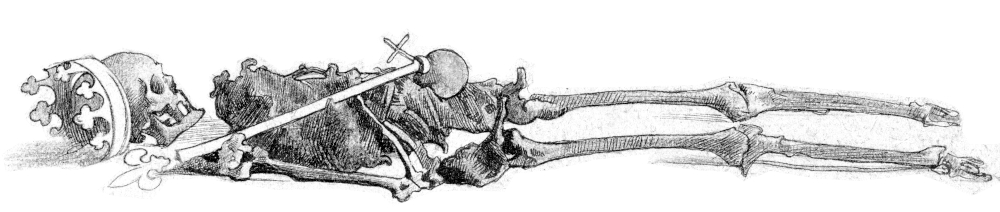
\includegraphics[keepaspectratio,width=\textwidth]{figures/skeltal-small.jpg}
\caption{\citeart{SkeletonCrown}}
\label{fig:skeltal}
\end{figure}
\lettrine{Y}{ou} may guess at the prognostics by the symptoms. What can these signs
fore tell otherwise than folly, dotage, madness, gross ignorance,
despair, obstinacy, a reprobate sense, \mmarginpar{6590}a bad end? What else can
superstition, heresy produce, but wars, tumults, uproars, torture of
souls, and despair, a desolate land, as Jeremy teacheth, cap. vii. 34.
when they commit idolatry, and walk after their own ways? how should it
be otherwise with them? what can they expect but blasting, famine,
dearth, and all the plagues of Egypt, as Amos denounceth, cap. iv.
vers. 9. 10. to be led into captivity? If our hopes be frustrate, we
sow much and bring in little, eat and have not enough, drink and are
not filled, clothe and be not warm, \&c. Haggai i. 6. we look for much
and it comes to little, whence is it? His house was waste, they came to
their own houses, vers. 9. therefore the heaven stayed his dew, the
earth his fruit. Because we are superstitious, irreligious, we do not
serve God as we ought, all these plagues and miseries come upon us;
what can we look for else but mutual wars, slaughters, fearful ends in
this life, and in the life to come eternal damnation? What is it that
hath caused so many feral battles to be fought, so much Christian blood
shed, but superstition! That Spanish inquisition, racks, wheels,
tortures, torments, whence do they proceed? from superstition. Bodine
the Frenchman, in his \mmarginpar{6591}method. hist. accounts Englishmen
barbarians, for their civil wars: but let him read those Pharsalian
fields \mmarginpar{6592}fought of late in France for their religion, their
massacres, wherein by their own relations in twenty-four years, I know
not how many millions have been consumed, whole families and cities,
and he shall find ours to be but velitations to theirs. But it hath
ever been the custom of heretics and idolaters, when they are plagued
for their sins, and God's just judgments come upon them, not to
acknowledge any fault in themselves, but still impute it unto others.
In Cyprian's time it was much controverted between him and Demetrius an
idolater, who should be the cause of those present calamities.
Demetrius laid all the fault on Christians, (and so they did ever in
the primitive church, as appears by the first book of \mmarginpar{6593}Arnobius),
\mmarginpar{6594}that there were not such ordinary showers in winter, the ripening
heat in summer, so seasonable springs, fruitful autumns, no marble
mines in the mountains, less gold and silver than of old; that
husbandmen, seamen, soldiers, all were scanted, justice, friendship,
skill in arts, all was decayed, and that through Christians' default,
and all their other miseries from them, quod dii nostri a vobis non
colantur, because they did not worship their gods. But Cyprian retorts
all upon him again, as appears by his tract against him. 'Tis true the
world is miserably tormented and shaken with wars, dearth, famine,
fire, inundations, plagues, and many feral diseases rage amongst us,
sed non ut tu quereris ista accidunt quod dii vestri a nobis non
colantur, sed quod a vobis non colatur Deus, a quibus nec quaeritur,
nec timetur, not as thou complainest, that we do not worship your Gods,
but because you are idolaters, and do not serve the true God, neither
seek him, nor fear him as you ought. Our papists object as much to us,
and account us heretics, we them; the Turks esteem of both as infidels,
and we them as a company of pagans, Jews against all; when indeed there
is a general fault in us all, and something in the very best, which may
justly deserve God's wrath, and pull these miseries upon our heads. I
will say nothing here of those vain cares, torments, needless works,
penance, pilgrimages, pseudomartyrdom, \&c. We heap upon ourselves
unnecessary troubles, observations; we punish our bodies, as in Turkey
(saith \mmarginpar{6595}Busbequius leg. Turcic. ep. 3.) one did, that was much
affected with music, and to hear boys sing, but very superstitious; an
old sibyl coming to his house, or a holy woman, (as that place yields
many) took him down for it, and told him, that in that other world he
should suffer for it; thereupon he flung his rich and costly
instruments which he had bedecked with jewels, all at once into the
fire. He was served in silver plate, and had goodly household stuff: a
little after, another religious man reprehended him in like sort, and
from thenceforth he was served in earthen vessels, last of all a decree
came forth, because Turks might not drink wine themselves, that neither
Jew nor Christian then living in Constantinople, might drink any wine
at all. In like sort amongst papists, fasting at first was generally
proposed as a good thing; after, from such meats at set times, and then
last of all so rigorously proposed, to bind the consciences upon pain
of damnation. First Friday, saith Erasmus, then Saturday, et nunc
periclitatur dies Mercurii) and Wednesday now is in danger of a fast.
\mmarginpar{6596}And for such like toys, some so miserably afflict themselves, to
despair, and death itself, rather than offend, and think themselves
good Christians in it, when as indeed they are superstitious Jews. So
saith Leonardus Fuchsius, a great physician in his time. \mmarginpar{6597}We are
tortured in Germany with these popish edicts, our bodies so taken down,
our goods so diminished, that if God had not sent Luther, a worthy man,
in time, to redress these mischiefs, we should have eaten hay with our
horses before this. \mmarginpar{6598}As in fasting, so in all other superstitious
edicts, we crucify one another without a cause, barring ourselves of
many good and lawful things, honest disports, pleasures and
recreations; for wherefore did God create them but for our use? Feasts,
mirth, music, hawking, hunting, singing, dancing, \&c. non tam
necessitatibus nostris Deus inservit, sed in delicias amamur, as Seneca
notes, God would have it so. And as Plato 2. de legibus gives out, Deos
laboriosam hominum vitam miseratos, the gods in commiseration of human
estate sent Apollo, Bacchus, and the Muses, qui cum voluptate tripudia
et soltationes nobis ducant, to be merry with mortals, to sing and
dance with us. So that he that will not rejoice and enjoy himself,
making good use of such things as are lawfully permitted, non est
temperatus, as he will, sed superstitiosus. There is nothing better for
a man, than that he should eat and drink, and that he should make his
soul enjoy good in his labour, Eccles. ii. 24. And as \mmarginpar{6599}one said of
hawking and hunting, tot solatia in hac aegri orbis calamitate,
mortalibus taediis deus objecit, I say of all honest recreations, God
hath therefore indulged them to refresh, ease, solace and comfort us.
But we are some of us too stern, too rigid, too precise, too grossly
superstitious, and whilst we make a conscience of every toy, with touch
not, taste not, \&c., as those Pythagoreans of old, and some Indians
now, that will eat no flesh, or suffer any living creature to be
killed, the Bannians about Guzzerat; we tyrannise over our brother's
soul, lose the right use of many good gifts; honest \mmarginpar{6600}sports, games
and pleasant recreations, \mmarginpar{6601}punish ourselves without a cause, lose
our liberties, and sometimes our lives. Anno 1270, at \mmarginpar{6602}Magdeburg
in Germany, a Jew fell into a privy upon a Saturday, and without help
could not possibly get out; he called to his fellows for succour, but
they denied it, because it was their Sabbath, non licebat opus manuum
exercere; the bishop hearing of it, the next day forbade him to be
pulled out, because it was our Sunday. In the mean time the wretch died
before Monday. We have myriads of examples in this kind amongst those
rigid Sabbatarians, and therefore not without good cause,
\mmarginpar{6603}Intolerabilem pertubationem Seneca calls it, as well he might, an
intolerable perturbation, that causeth such dire events, folly,
madness, sickness, despair, death of body and soul, and hell itself.

%SUBSECT. V.-_Cure of Religious Melancholy_.
\section{Cure of Religious Melancholy.}

\lettrine{T}{o} purge the world of idolatry and superstition, will require some
monster-taming Hercules, a divine Aesculapius, or Christ himself to
come in his own person, to reign a thousand years on earth before the
end, as the Millenaries will have him. They are generally so
refractory, self-conceited, obstinate, so firmly addicted to that
religion in which they have been bred and brought up, that no
persuasion, no terror, no persecution, can divert them. The
consideration of which, hath induced many commonwealths to suffer them
to enjoy their consciences as they will themselves: a toleration of
Jews is in most provinces of Europe. In Asia they have their
synagogues: Spaniards permit Moors to live amongst them: the
Mogullians, Gentiles: the Turks all religions. In Europe, Poland and
Amsterdam are the common sanctuaries. Some are of opinion, that no man
ought to be compelled for conscience' sake, but let him be of what
religion he will, he may be saved, as Cornelius was formerly accepted,
Jew, Turks, Anabaptists, \&c. If he be an honest man, live soberly, and
civilly in his profession, (Volkelius, Crellius, and the rest of the
Socinians, that now nestle themselves about Krakow and Rakow in Poland,
have renewed this opinion) serve his own God, with that fear and
reverence as he ought. Sua cuique civitati (Laeli) religio sit, nostra
nobis, Tully thought fit every city should be free in this behalf,
adore their own Custodes et Topicos Deos, tutelar and local gods, as
Symmachus calls them. Isocrates adviseth Demonicus, when he came to a
strange city, to \mmarginpar{6604}worship by all means the gods of the place, et
unumquemque, Topicum deum sic coli oportere, quomodo ipse praeceperit:
which Cecilius in \mmarginpar{6605}Minutius labours, and would have every nation
sacrorum ritus gentiles habere et deos colere municipes, keep their own
ceremonies, worship their peculiar gods, which Pomponius Mela reports
of the Africans, Deos suos patrio more venerantur, they worship their
own gods according to their own ordination. For why should any one
nation, as he there pleads, challenge that universality of God, Deum
suum quem nec ostendunt, nec vident, discurrantem silicet et ubique
praesentem, in omnium mores, actus, et occultas, cogitationes
inquirentem, \&c., as Christians do: let every province enjoy their
liberty in this behalf, worship one God, or all as they will, and are
informed. The Romans built altars Diis Asiae, Europae, Lybiae, diis
ignotis et peregrinis: others otherwise, \&c. Plinius Secundus, as
appears by his Epistle to Trajan, would not have the Christians so
persecuted, and in some time of the reign of Maximinus, as we find it
registered in Eusebius lib. 9. cap. 9. there was a decree made to this
purpose, Nullus cogatur invitus ad hunc vel illum deorum cultum, let no
one be compelled against his will to worship any particular deity, and
by Constantine in the 19th year of his reign as \mmarginpar{6606}Baronius
informeth us, Nemo alteri exhibeat molestiam, quod cujusque animus
vult, hoc quisque transigat, new gods, new lawgivers, new priests, will
have new ceremonies, customs and religions, to which every wise man as
a good formalist should accommodate himself.
\mmarginpar{6607}Saturnus periit, perierunt et sua jura,
Sub Jove nunc mundus, jussa sequare Jovis.

The said Constantine the emperor, as Eusebius writes, flung down and
demolished all the heathen gods, silver, gold statues, altars, images
and temples, and turned them all to Christian churches, infestus
gentilium monumentis ludibrio exposuit; the Turk now converts them
again to Mahometan mosques. The like edict came forth in the reign of
Arcadius and Honorius. \mmarginpar{6608}Symmachus the orator in his days, to
procure a general toleration, used this argument, \mmarginpar{6609}Because God is
immense and infinite, and his nature cannot perfectly be known, it is
convenient he should be as diversely worshipped, as every man shall
perceive or understand. It was impossible, he thought, for one religion
to be universal: you see that one small province can hardly be ruled by
one law, civil or spiritual; and how shall so many distinct and vast
empires of the world be united into one? It never was, never will be
Besides, if there be infinite planetary and firmamental worlds, as
\mmarginpar{6610}some will, there be infinite genii or commanding spirits
belonging to each of them; and so, per consequens (for they will be all
adored), infinite religions. And therefore let every territory keep
their proper rites and ceremonies, as their dii tutelares will, so
Tyrius calls them, and according to the quarter they hold, their own
institutions, revelations, orders, oracles, which they dictate from
time to time, or teach their own priests or ministers. This tenet was
stiffly maintained in Turkey not long since, as you may read in the
third epistle of Busbequius, \mmarginpar{6611}that all those should participate of
eternal happiness, that lived a holy and innocent life, what religion
soever they professed. Rustan Bassa was a great patron of it; though
Mahomet himself was sent virtute gladdi, to enforce all, as he writes
in his Alcoran, to follow him. Some again will approve of this for
Jews, Gentiles, infidels, that are out of the fold, they can be content
to give them all respect and favour, but by no means to such as are
within the precincts of our own church, and called Christians, to no
heretics, schismatics, or the like; let the Spanish inquisition, that
fourth fury, speak of some of them, the civil wars and massacres in
France, our Marian times. \mmarginpar{6612}Magillianus the Jesuit will not admit
of conference with a heretic, but severity and rigour to be used, non
illis verba reddere, sed furcas, figere oportet; and Theodosius is
commended in Nicephorus, lib. 12. cap. 15. \mmarginpar{6613}That he put all
heretics to silence. Bernard. Epist. 180, will have club law, fire and
sword for heretics, \mmarginpar{6614}compel them, stop their mouths not with
disputations, or refute them with reasons, but with fists; and this is
their ordinary practice. Another company are as mild on the other side;
to avoid all heart-burning, and contentious wars and uproars, they
would have a general toleration in every kingdom, no mulct at all, no
man for religion or conscience be put to death, which \mmarginpar{6615}Thuanus the
French historian much favours; our late Socinians defend; Vaticanus
against Calvin in a large Treatise in behalf of Servetus, vindicates;
Castilio, \&c., Martin Ballius and his companions, maintained this
opinion not long since in France, whose error is confuted by Beza in a
just volume. The medium is best, and that which Paul prescribes, Gal.
i. If any man shall fall by occasion, to restore such a one with the
spirit of meekness, by all fair means, gentle admonitions; but if that
will not take place, Post unam et alteram admonitionem haereticum
devita, he must be excommunicate, as Paul did by Hymenaeus, delivered
over to Satan. Immedicabile vulnus ense recidendum est. As Hippocrates
said in physic, I may well say in divinity, Quae ferro non curantur,
ignis curat. For the vulgar, restrain them by laws, mulcts, burn their
books, forbid their conventicles; for when the cause is taken away, the
effect will soon cease. Now for prophets, dreamers, and such rude silly
fellows, that through fasting, too much meditation, preciseness, or by
melancholy, are distempered: the best means to reduce them ad sanam
mentem, is to alter their course of life, and with conference, threats,
promises, persuasions, to intermix physic. Hercules de Saxonia, had
such a prophet committed to his charge in Venice, that thought he was
Elias, and would fast as he did; he dressed a fellow in angel's attire,
that said he came from heaven to bring him divine food, and by that
means stayed his fast, administered his physic; so by the meditation of
this forged angel he was cured. \mmarginpar{6616}Rhasis an Arabian, cont. lib. 1.
cap. 9, speaks of a fellow that in like case complained to him, and
desired his help: I asked him (saith he) what the matter was; he
replied, I am continually meditating of heaven and hell, and methinks I
see and talk with fiery spirits, and smell brimstone, \&c., and am so
carried away with these conceits, that I can neither eat, nor sleep,
nor go about my business: I cured him (saith Rhasis) partly by
persuasion, partly by physic, and so have I done by many others. We
have frequently such prophets and dreamers amongst us, whom we
persecute with fire and faggot: I think the most compendious cure, for
some of them at least, had been in Bedlam. Sed de his satis.

%MEMB. II.

%SUBSECT. I.-_Religious Melancholy in defect; parties affected, Epicures, Atheists, Hypocrites, worldly secure, Carnalists; all impious persons, impenitent sinners, \&c._
\section[Religious Melancholy in defect]{Religious Melancholy in defect; parties affected, Epicures, Atheists, Hypocrites, worldly secure, Carnalists; all impious persons, impenitent sinners, \&c.}

\lettrine{I}{n} that other extreme or defect of this love of God, knowledge, faith,
fear, hope, \&c. are such as err both in doctrine and manners,
Sadducees, Herodians, libertines, politicians: all manner of atheists,
epicures, infidels, that are secure, in a reprobate sense, fear not God
at all, and such are too distrustful and timorous, as desperate persons
be. That grand sin of atheism or impiety, \mmarginpar{6617}Melancthon calls it
monstrosam melancholiam, monstrous melancholy; or venenatam
melancholiam, poisoned melancholy. A company of Cyclops or giants, that
war with the gods, as the poets feigned, antipodes to Christians, that
scoff at all religion, at God himself, deny him and all his attributes,
his wisdom, power, providence, his mercy and judgment.
\mmarginpar{6618}Esse aliquos manes, et subterranea regna,
Et contum, et Stygio ranas in gurgite nigras,
Atque una transire vadum tot millia cymba,
Nec pueri credunt, nisi qui nondum aere lavantur.

That there is either heaven or hell, resurrection of the dead, pain,
happiness, or world to come, credat Judaeus Apella; for their parts
they esteem them as so many poet's tales, bugbears, Lucian's Alexander;
Moses, Mahomet, and Christ are all as one in their creed. When those
bloody wars in France for matters of religion (saith \mmarginpar{6619}Richard
Dinoth) were so violently pursued between Huguenots and Papists, there
was a company of good fellows laughed them all to scorn, for being such
superstitious fools, to lose their wives and fortunes, accounting
faith, religion, immortality of the soul, mere fopperies and illusions.
Such loose \mmarginpar{6620}atheistical spirits are too predominant in all
kingdoms. Let them contend, pray, tremble, trouble themselves that
will, for their parts, they fear neither God nor devil; but with that
Cyclops in Euripides,
Haud ulla numina expavescunt caelitum,
Sed victimas uni deorum maximo,
Ventri offerunt, deos ignorant caeteros.

They fear no God but one,
They sacrifice to none.
But belly, and him adore,
For gods they know no more.

Their God is their belly, as Paul saith, Sancta mater saturitas;-quibus
in solo vivendi causa palato est. The idol, which they worship and
adore, is their mistress; with him in Plautus, mallem haec mulier me
amet quam dii, they had rather have her favour than the gods'. Satan is
their guide, the flesh is their instructor, hypocrisy their counsellor,
vanity their fellow-soldier, their will their law, ambition their
captain, custom their rule; temerity, boldness, impudence their art,
toys their trading, damnation their end. All their endeavours are to
satisfy their lust and appetite, how to please their genius, and to be
merry for the present, Ede, lude, bibe, post mortem nulla
voluptas.\mmarginpar{6621}The same condition is of men and of beasts; as the one
dieth, so dieth the other, Eccles. iii. 19. The world goes round,
\mmarginpar{6622}---truditur dies die,
Novaeque pergunt interire Lunae:

\mmarginpar{6623}They did eat and drink of old, marry, bury, bought, sold,
planted, built, and will do still. \mmarginpar{6624}Our life is short and tedious,
and in the death of a man there is no recovery, neither was any man
known that hath returned from the grave; for we are born at all
adventure, and we shall be hereafter as though we had never been; for
the breath is as smoke in our nostrils, \&c., and the spirit vanisheth
as the soft air. \mmarginpar{6625}Come let us enjoy the pleasures that are
present, let us cheerfully use the creatures as in youth, let us fill
ourselves with costly wine and ointments, let not the flower of our
life pass by us, let us crown ourselves with rose-buds before they are
withered, \&c. \mmarginpar{6626}Vivamus mea Lesbia et amemus, \&c. \mmarginpar{6627} Come let
us take our fill of love, and pleasure in dalliance, for this is our
portion, this is our lot.
Tempora labuntur, tacitisque senescimus annis.\mmarginpar{6628} For the rest of
heaven and hell, let children and superstitious fools believe it: for
their parts, they are so far from trembling at the dreadful day of
judgment that they wish with Nero, Me vivo fiat, let it come in their
times: so secure, so desperate, so immoderate in lust and pleasure, so
prone to revenge that, as Paterculus said of some caitiffs in his time
in Rome, Quod nequiter ausi, fortiter executi: it shall not be so
wickedly attempted, but as desperately performed, whatever they take in
hand. Were it not for God's restraining grace, fear and shame, temporal
punishment, and their own infamy, they would. Lycaon-like exenterate,
as so many cannibals eat up, or Cadmus' soldiers consume one another.
These are most impious, and commonly professed atheists, that never use
the name of God but to swear by it; that express nought else but
epicurism in their carriage, or hypocrisy; with Pentheus they neglect
and contemn these rites and religious ceremonies of the gods; they will
be gods themselves, or at least socii deorum. Divisum imperium cum Jove
Caesar habet. Caesar divides the empire with Jove. Aproyis, an Egyptian
tyrant, grew, saith \mmarginpar{6629}Herodotus, to that height of pride, insolency
of impiety, to that contempt of Gods and men, that he held his kingdom
so sure, ut a nemine deorum aut hominum sibi eripi posset, neither God
nor men could take it from him. \mmarginpar{6630}A certain blasphemous king of
Spain (as \mmarginpar{6631}Lansius reports) made an edict, that no subject of his,
for ten years' space, should believe in, call on, or worship any god.
And as \mmarginpar{6632}Jovius relates of Mahomet the Second, that sacked
Constantinople, he so behaved himself, that he believed neither Christ
nor Mahomet; and thence it came to pass, that he kept his word and
promise no farther than for his advantage, neither did he care to
commit any offence to satisfy his lust. I could say the like of many
princes, many private men (our stories are full of them) in times past,
this present age, that love, fear, obey, and perform all civil duties
as they shall find them expedient or behoveful to their own ends.
Securi adversus Deos, securi adversus homines, votis non est opus,
which \mmarginpar{6633} Tacitus reports of some Germans, they need not pray, fear,
hope, for they are secure, to their thinking, both from Gods and men.
Bulco Opiliensis, sometime Duke of \mmarginpar{6634}Silesia, was such a one to a
hair; he lived (saith \mmarginpar{6635}Aeneas Sylvius) at \mmarginpar{6636}Vratislavia, and
was so mad to satisfy his lust, that he believed neither heaven nor
hell, or that the soul was immortal, but married wives, and turned them
up as he thought fit, did murder and mischief, and what he list
himself. This duke hath too many followers in our days: say what you
can, dehort, exhort, persuade to the contrary, they are no more
moved,-quam si dura, silex aut stet Marpesia cautes, than so many
stocks, and stones; tell them of heaven and hell, 'tis to no purpose,
laterem lavas, they answer as Ataliba that Indian prince did friar
Vincent, \mmarginpar{6637}when he brought him a book, and told him all the
mysteries of salvation, heaven and hell, were contained in it: he
looked upon it, and said he saw no such matter, asking withal, how he
knew it: they will but scoff at it, or wholly reject it. Petronius in
Tacitus, when he was now by Nero's command bleeding to death, audiebat
amicos nihil referentes de immortalitate animae, aut sapientum
placitis, sed levia carmina et faciles versus; instead of good counsel
and divine meditations, he made his friends sing him bawdy verses and
scurrilous songs. Let them take heaven, paradise, and that future
happiness that will, bonum est esse hic, it is good being here: there
is no talking to such, no hope of their conversion, they are in a
reprobate sense, mere carnalists, fleshly minded men, which howsoever
they may be applauded in this life by some few parasites, and held for
worldly wise men. \mmarginpar{6638}They seem to me (saith Melancthon) to be as mad
as Hercules was when he raved and killed his wife and children. A
milder sort of these atheistical spirits there are that profess
religion, but timide et haesitanter, tempted thereunto out of that
horrible consideration of diversity of religions, which are and have
been in the world (which argument Campanella, Atheismi Triumphati, cap.
9. both urgeth and answers), besides the covetousness, imposture, and
knavery of priests, quae faciunt (as \mmarginpar{6639}Postellus observes) ut rebus
sacris minus faciant fidem; and those religions some of them so
fantastical, exorbitant, so violently maintained with equal constancy
and assurance; whence they infer, that if there be so many religious
sects, and denied by the rest, why may they not be all false? or why
should this or that be preferred before the rest? The sceptics urge
this, and amongst others it is the conclusion of Sextus Empericus, lib.
3. advers. Mathematicos: after many philosophical arguments and reasons
pro and con that there are gods, and again that there are no gods, he
so concludes, cum tot inter se pugnent, \&c. Una tantum potest esse
vera, as Tully likewise disputes: Christians say, they alone worship
the true God, pity all other sects, lament their case; and yet those
old Greeks and Romans that worshipped the devil, as the Chinese now do,
aut deos topicos, their own gods; as Julian the apostate,
\mmarginpar{6640}Cecilius in Minutius, Celsus and Porphyrius the philosopher
object: and as Machiavel contends, were much more noble, generous,
victorious, had a more flourishing commonwealth, better cities, better
soldiers, better scholars, better wits. Their gods overcame our gods,
did as many miracles, \&c. Saint Cyril, Arnobius, Minutius, with many
other ancients of late, Lessius, Morneus, Grotius de Verit. Relig.
Christianae, Savanarola de Verit. Fidei Christianae, well defend; but
Zanchius, \mmarginpar{6641}Campanella, Marinus Marcennus, Bozius, and Gentillettus
answer all these atheistical arguments at large. But this again
troubles many as of old, wicked men generally thrive, professed
atheists thrive,
\mmarginpar{6642}Nullos esse Deos, inane coelum,
Affirmat Selius: probatque, quod se
Factum, dum negat haec, videt beatum.

There are no gods, heavens are toys,
Selius in public justifies;
Because that whilst he thus denies
Their deities, he better thrives.

This is a prime argument: and most part your most sincere, upright,
honest, and \mmarginpar{6643}good men are depressed, The race is not to the swift,
nor the battle to the strong (Eccles. ix. 11.), nor yet bread to the
wise, favour nor riches to men of understanding, but time and chance
comes to all. There was a great plague in Athens (as Thucydides, lib.
2. relates), in which at last every man, with great licentiousness, did
what he list, not caring at all for God's or men's laws. Neither the
fear of God nor laws of men (saith he) awed any man, because the plague
swept all away alike, good and bad; they thence concluded it was alike
to worship or not worship the gods, since they perished all alike. Some
cavil and make doubts of scripture itself: it cannot stand with God's
mercy, that so many should be damned, so many bad, so few good, such
have and hold about religions, all stiff on their side, factious alike,
thrive alike, and yet bitterly persecuting and damning each other; It
cannot stand with God's goodness, protection, and providence (as
\mmarginpar{6644}Saint Chrysostom in the Dialect of such discontented persons) to
see and suffer one man to be lame, another mad, a third poor and
miserable all the days of his life, a fourth grievously tormented with
sickness and aches, to his last hour. Are these signs and works of
God's providence, to let one man be deaf, another dumb? A poor honest
fellow lives in disgrace, woe and want, wretched he is; when as a
wicked caitiff abounds in superfluity of wealth, keeps whores,
parasites, and what he will himself: Audis Jupiter haec? Talia multa
connectentes, longum reprehensionis sermonem erga Dei providentiam
contexunt. \mmarginpar{6645}Thus they mutter and object (see the rest of their
arguments in Marcennus in Genesin, and in Campanella, amply confuted),
with many such vain cavils, well known, not worthy the recapitulation
or answering: whatsoever they pretend, they are interim of little or no
religion.
Cousin-germans to these men are many of our great philosophers and
deists, who, though they be more temperate in this life, give many good
moral precepts, honest, upright, and sober in their conversation, yet
in effect they are the same (accounting no man a good scholar that is
not an atheist), nimis altum sapiunt, too much learning makes them mad.
Whilst they attribute all to natural causes, \mmarginpar{6646}contingence of all
things, as Melancthon calls them, Pertinax hominum genus, a peevish
generation of men, that misled by philosophy, and the devil's
suggestion, their own innate blindness, deny God as much as the rest,
hold all religion a fiction, opposite to reason and philosophy, though
for fear of magistrates, saith \mmarginpar{6647}Vaninus, they durst not publicly
profess it. Ask one of them of what religion he is, he scoffingly
replies, a philosopher, a Galenist, an \mmarginpar{6648}Averroist, and with
Rabelais a physician, a peripatetic, an epicure. In spiritual things
God must demonstrate all to sense, leave a pawn with them, or else seek
some other creditor. They will acknowledge Nature and Fortune, yet not
God: though in effect they grant both: for as Scaliger defines, Nature
signifies God's ordinary power; or, as Calvin writes, Nature is God's
order, and so things extraordinary may be called unnatural: Fortune his
unrevealed will; and so we call things changeable that are beside
reason and expectation. To this purpose \mmarginpar{6649}Minutius in Octavio, and
\mmarginpar{6650} Seneca well discourseth with them, lib. 4. de beneficiis, cap.
5, 6, 7. They do not understand what they say; what is Nature but God?
call him what thou wilt, Nature, Jupiter, he hath as many names as
offices: it comes all to one pass, God is the fountain of all, the
first Giver and Preserver, from whom all things depend, \mmarginpar{6651}a quo, et
per quem omnia, Nam quocunque vides Deus est, quocunque moveris, God is
all in all, God is everywhere, in every place. And yet this Seneca,
that could confute and blame them, is all out as much to be blamed and
confuted himself, as mad himself; for he holds fatum Stoicum, that
inevitable Necessity in the other extreme, as those Chaldean
astrologers of old did, against whom the prophet Jeremiah so often
thunders, and those heathen mathematicians, Nigidius Figulus,
magicians, and Priscilianists, whom St. Austin so eagerly confutes,
those Arabian questionaries, Novem Judices, Albumazer, Dorotheus, \&c.,
and our countryman \mmarginpar{6652}Estuidus, that take upon them to define out of
those great conjunction of stars, with Ptolomeus, the periods of
kingdoms, or religions, of all future accidents, wars, plagues,
schisms, heresies, and what not? all from stars, and such things, saith
Maginus, Quae sibi et intelligentiis suis reservavit Deus, which God
hath reserved to himself and his angels, they will take upon them to
foretell, as if stars were immediate, inevitable causes of all future
accidents. Caesar Vaninus, in his book de admirandis naturae Arcanis,
dial. 52. de oraculis, is more free, copious, and open, in this
explication of this astrological tenet of Ptolemy, than any of our
modern writers, Cardan excepted, a true disciple of his master
Pomponatius; according to the doctrine of Peripatetics, he refers all
apparitions, prodigies, miracles, oracles, accidents, alterations of
religions, kingdoms, \&c. (for which he is soundly lashed by Marinus
Mercennus, as well he deserves), to natural causes (for spirits he will
not acknowledge), to that light, motion, influences of heavens and
stars, and to the intelligences that move the orbs. Intelligentia quae,
movet orbem mediante coelo, \&c. Intelligences do all: and after a long
discourse of miracles done of old, si haec daemones possint, cur non et
intelligentiae, coelorum motrices? And as these great conjunctions,
aspects of planets, begin or end, vary, are vertical and predominant,
so have religions, rites, ceremonies, and kingdoms their beginning,
progress, periods, in urbibus, regibus, religionibus, ac in
particularibus hominibus, haec vera ac manifesta, sunt, ut Aristoteles
innuere videtur, et quotidiana docet experientia, ut historias
perlegens videbit; quid olim in Gentili lege Jove sanctius et
illustrius? quid nunc vile magis et execrandum? Ita coelestia corpora
pro mortalium beneficio religiones aedificant, et cum cessat influxus,
cessat lex,\mmarginpar{6653} \&c. And because, according to their tenets, the world
is eternal, intelligences eternal, influences of stars eternal,
kingdoms, religions, alterations shall be likewise eternal, and run
round after many ages; Atque iterum ad Troiam magnus mittetur Achilles;
renascentur religiones, et ceremoniae, res humanae in idem recident,
nihil nunc quod non olim fuit, et post saeculorum revolutiones alias
est, erit,\mmarginpar{6654}\&c. idem specie, saith Vaninus, non individuo quod
Plato significavit. These (saith mine \mmarginpar{6655}author), these are the
decrees of Peripatetics, which though I recite, in obsequium
Christianae fidei detestor, as I am a Christian I detest and hate. Thus
Peripatetics and astrologians held in former times, and to this effect
of old in Rome, saith Dionysius Halicarnassus, lib. 7, when those
meteors and prodigies appeared in the air, after the banishment of
Coriolanus, \mmarginpar{6656} Men were diversely affected: some said they were
God's just judgments for the execution of that good man, some referred
all to natural causes, some to stars, some thought they came by chance,
some by necessity decreed ab initio, and could not be altered. The two
last opinions of necessity and chance were, it seems, of greater note
than the rest.
\mmarginpar{6657}Sunt qui in Fortunae jam casibus omnia ponunt,
Et mundum credunt nullo rectore moveri,
Natura, volvente vices, \&c.

For the first of chance, as \mmarginpar{6658}Sallust likewise informeth us, those
old Romans generally received; They supposed fortune alone gave
kingdoms and empires, wealth, honours, offices: and that for two
causes; first, because every wicked base unworthy wretch was preferred,
rich, potent, \&c.; secondly, because of their uncertainty, though never
so good, scarce any one enjoyed them long: but after, they began upon
better advice to think otherwise, that every man made his own fortune.
The last of Necessity was Seneca's tenet, that God was alligatus causis
secundis, so tied to second causes, to that inexorable Necessity, that
he could alter nothing of that which was once decreed; sic erat in
fatis, it cannot be altered, semel jussit, semper paret Deus, nulla vis
rumpit, nullae preces, nec ipsum fulmen, God hath once said it, and it
must for ever stand good, no prayers, no threats, nor power, nor
thunder itself can alter it. Zeno, Chrysippus, and those other Stoics,
as you may read in Tully 2. de divinatione, Gellius, lib. 6. cap. 2.
\&c., maintained as much. In all ages, there have been such, that either
deny God in all, or in part; some deride him, they could have made a
better world, and ruled it more orderly themselves, blaspheme him,
derogate at their pleasure from him. 'Twas so in \mmarginpar{6659}Plato's time,
Some say there be no gods, others that they care not for men, a middle
sort grant both. Si non sit Deus, unde mala? si sit Deus, unde mala? So
Cotta argues in Tully, why made he not all good, or at least tenders
not the welfare of such as are good? As the woman told Alexander, if he
be not at leisure to hear causes, and redress them, why doth he reign?
\mmarginpar{6660}Sextus Empericus hath many such arguments. Thus perverse men
cavil. So it will ever be, some of all sorts, good, bad, indifferent,
true, false, zealous, ambidexters, neutralists, lukewarm, libertines,
atheists, \&c. They will see these religious sectaries agree amongst
themselves, be reconciled all, before they will participate with, or
believe any: they think in the meantime (which \mmarginpar{6661}Celsus objects,
and whom Origen confutes), We Christians adore a person put to
\mmarginpar{6662}death with no more reason than the barbarous Getes worshipped
Zamolxis, the Cilicians Mopsus, the Thebans Amphiaraus, and the
Lebadians Trophonius; one religion is as true as another, new fangled
devices, all for human respects; great-witted Aristotle's works are as
much authentical to them as Scriptures, subtle Seneca's Epistles as
canonical as St. Paul's, Pindarus' Odes as good as the Prophet David's
Psalms, Epictetus' Enchiridion equivalent to wise Solomon's Proverbs.
They do openly and boldly speak this and more, some of them, in all
places and companies. \mmarginpar{6663}Claudius the emperor was angry with Heaven,
because it thundered, and challenged Jupiter into the field; with what
madness! saith Seneca; he thought Jupiter could not hurt him, but he
could hurt Jupiter. Diagoras, Demonax, Epicurus, Pliny, Lucian,
Lucretius,-Contemptorque Deum Mezentius, professed atheists all in
their times: though not simple atheists neither, as Cicogna proves,
lib. 1. cap. 1. they scoffed only at those Pagan gods, their plurality,
base and fictitious offices. Gilbertus Cognatus labours much, and so
doth Erasmus, to vindicate Lucian from scandal, and there be those that
apologise for Epicurus, but all in vain; Lucian scoffs at all, Epicurus
he denies all, and Lucretius his scholar defends him in it:
\mmarginpar{6664}Humana ante oculua foede cum vita jaceret
In terris oppressa gravi cum religione,
Quae caput a coeli regionibus ostendebat,
Horribili super aspectu mortalibus instans, \&c.

When human kind was drench'd in superstition,
With ghastly looks aloft, which frighted mortal men, \&c.

He alone, like another Hercules, did vindicate the world from that
monster. Uncle \mmarginpar{6665}Pliny, lib. 2. cap. 7. nat. hist. and lib. 7. cap.
55, in express words denies the immortality of the soul. \mmarginpar{6666}Seneca
doth little less, lib. 7. epist. 55. ad Lucilium, et lib. de consol. ad
Martiam, or rather more. Some Greek Commentators would put as much upon
Job, that he should deny resurrection, \&c., whom Pineda copiously
confutes in cap. 7. Job, vers. 9. Aristotle is hardly censured of some,
both divines and philosophers. St. Justin in Peraenetica ad Gentes,
Greg. Nazianzen. in disput. adversus Eun., Theodoret, lib. 5. de curat.
graec. affec., Origen. lib. de principiis. Pomponatius justifies in his
Tract (so styled at least) De immortalitate Animae, Scaliger (who would
forswear himself at any time, saith Patritius, in defence of his great
master Aristotle), and Dandinus, lib. 3. de anima, acknowledge as much.
Averroes oppugns all spirits and supreme powers; of late Brunus
(infelix Brunus, \mmarginpar{6667}Kepler calls him), Machiavel, Caesar Vaninus
lately burned at Toulouse in France, and Pet. Aretine, have publicly
maintained such atheistical paradoxes, \mmarginpar{6668}with that Italian
Boccaccio with his fable of three rings, \&c., ex quo infert haud posse
internosci, quae sit verior religio, Judaica, Mahometana, an
Christiana, quoniam eadem signa, \&c., from which he infers, that it
cannot be distinguished which is the true religion, Judaism,
Mahommedanism, or Christianity, \&c. \mmarginpar{6669}Marinus Mercennus suspects
Cardan for his subtleties, Campanella, and Charron's Book of Wisdom,
with some other Tracts, to savour of \mmarginpar{6670}atheism: but amongst the
rest that pestilent book de tribus mundi impostoribus, quem sine
horrore (inquit) non legas, et mundi Cymbalum dialogis quatuor
contentum, anno 1538, auctore Peresio, Parisiis excusum, \mmarginpar{6671}\&c. And
as there have been in all ages such blasphemous spirits, so there have
not been wanting their patrons, protectors, disciples and adherents.
Never so many atheists in Italy and Germany, saith \mmarginpar{6672}Colerus, as in
this age: the like complaint Mercennus makes in France, 50,000 in that
one city of Paris. Frederic the Emperor, as \mmarginpar{6673}Matthew Paris records
licet non sit recitabile (I use his own words) is reported to have
said, Tres praestigiatores, Moses, Christus, et Mahomet, uti mundo
dominarentur, totum populum sibi contemporaneum se duxisse. (Henry, the
Landgrave of Hesse, heard him speak it,) Si principes imperii
institutioni meae adhaererent, ego multo meliorem modum credendi et
vivendi ordinarem.
To these professed atheists, we may well add that impious and carnal
crew of worldly-minded men, impenitent sinners, that go to hell in a
lethargy, or in a dream; who though they be professed Christians, yet
they will nulla pallescere culpa, make a conscience of nothing they do,
they have cauterised consciences, and are indeed in a reprobate sense,
past all feeling, have given themselves over to wantonness, to work all
manner of uncleanness even with greediness, Ephes. iv. 19. They do know
there is a God, a day of judgment to come, and yet for all that, as
Hugo saith, ita comedunt ac dormiunt, ac si diem judicii evasissent;
ita ludunt ac rident, ac si in coelis cum Deo regnarent: they are as
merry for all the sorrow, as if they had escaped all dangers, and were
in heaven already:
\mmarginpar{6674}---Metus omnes, et inexorabile fatum
Subjecit pedibus, strepitumque Acherontis avari.

Those rude idiots and ignorant persons, that neglect and contemn the
means of their salvation, may march on with these; but above all
others, those Herodian temporizing statesmen, political Machiavellians
and hypocrites, that make a show of religion, but in their hearts laugh
at it. Simulata sanctitas duplex iniquitas; they are in a double fault,
that fashion themselves to this world, which \mmarginpar{6675}Paul forbids, and
like Mercury, the planet, are good with good, bad with bad. When they
are at Rome, they do there as they see done, puritans with puritans,
papists with papists; omnium horarum homines, formalists, ambidexters,
lukewarm Laodiceans. \mmarginpar{6676}All their study is to please, and their god
is their commodity, their labour to satisfy their lusts, and their
endeavours to their own ends. Whatsoever they pretend, or in public
seem to do, \mmarginpar{6677}With the fool in their hearts, they say there is no
God. Heus tu-de Jove quid sentis? Hulloa! what is your opinion about a
Jupiter? Their words are as soft as oil, but bitterness is in their
hearts; like \mmarginpar{6678}Alexander VI. so cunning dissemblers, that what they
think they never speak. Many of them are so close, you can hardly
discern it, or take any just exceptions at them; they are not factious,
oppressors as most are, no bribers, no simoniacal contractors, no such
ambitious, lascivious persons as some others are, no drunkards, sobrii
solem vident orientem, sobrii vident occidentem, they rise sober, and
go sober to bed, plain dealing, upright, honest men, they do wrong to
no man, and are so reputed in the world's esteem at least, very zealous
in religion, very charitable, meek, humble, peace-makers, keep all
duties, very devout, honest, well spoken of, beloved of all men: but he
that knows better how to judge, he that examines the heart, saith they
are hypocrites, Cor dolo plenum; sonant vitium percussa maligne, they
are not sound within. As it is with writers \mmarginpar{6679}oftentimes, Plus
sanctimoniae, in libello, quam libelli auctore, more holiness is in the
book than in the author of it: so 'tis with them: many come to church
with great Bibles, whom Cardan said he could not choose but laugh at,
and will now and then dare operam Augustino, read Austin, frequent
sermons, and yet professed usurers, mere gripes, tota vitae ratio
epicurea est; all their life is epicurism and atheism, come to church
all day, and lie with a courtesan at night. Qui curios simulant et
Bacchanalia vivunt, they have Esau's hands, and Jacob's voice: yea, and
many of those holy friars, sanctified men, Cappam, saith Hierom, et
cilicium induunt, sed intus latronem tegunt. They are wolves in sheep's
clothing, Introrsum turpes, speciosi pelle decora, Fair without, and
most foul within. \mmarginpar{6680}Latet plerumque sub tristi amictu lascivia, et
deformis horror vili veste tegitur; ofttimes under a mourning weed lies
lust itself, and horrible vices under a poor coat. But who can examine
all those kinds of hypocrites, or dive into their hearts? ]f we may
guess at the tree by the fruit, never so many as in these days; show me
a plain-dealing true honest man: Et pudor, et probitas, et timor omnis
abest. He that shall but look into their lives, and see such enormous
vices, men so immoderate in lust, unspeakable in malice, furious in
their rage, flattering and dissembling (all for their own ends) will
surely think they are not truly religious, but of an obdurate heart,
most part in a reprobate sense, as in this age. But let them carry it
as they will for the present, dissemble as they can, a time will come
when they shall be called to an account, their melancholy is at hand,
they pull a plague and curse upon their own heads, thesaurisant iram
Dei. Besides all such as are in deos contumeliosi, blaspheme, contemn,
neglect God, or scoff at him, as the poets feign of Salmoneus, that
would in derision imitate Jupiter's thunder, he was precipitated for
his pains, Jupiter intonuit contra, \&c. so shall they certainly rue it
in the end, (\mmarginpar{6681}in se spuit, qui in coelum spuit), their doom's at
hand, and hell is ready to receive them.
Some are of opinion, that it is in vain to dispute with such
atheistical spirits in the meantime, 'tis not the best way to reclaim
them. Atheism, idolatry, heresy, hypocrisy, though they have one common
root, that is indulgence to corrupt affection, yet their growth is
different, they have divers symptoms, occasions, and must have several
cures and remedies. 'Tis true some deny there is any God, some confess,
yet believe it not; a third sort confess and believe, but will not live
after his laws, worship and obey him: others allow God and gods
subordinate, but not one God, no such general God, non talem deum, but
several topic gods for several places, and those not to persecute one
another for any difference, as Socinus will, but rather love and
cherish.
To describe them in particular, to produce their arguments and reasons,
would require a just volume, I refer them therefore that expect a more
ample satisfaction, to those subtle and elaborate treatises, devout and
famous tracts of our learned divines (schoolmen amongst the rest, and
casuists) that have abundance of reasons to prove there is a God, the
immortality of the soul, \&c., out of the strength of wit and philosophy
bring irrefragable arguments to such as are ingenuous and well
disposed; at the least, answer all cavils and objections to confute
their folly and madness, and to reduce them, si fieri posset, ad sanam
mentem, to a better mind, though to small purpose many times. Amongst
others consult with Julius Caesar Lagalla, professor of philosophy in
Rome, who hath written a large volume of late to confute atheists: of
the immortality of the soul, Hierom. Montanus de immortalitate Animae:
Lelius Vincentius of the same subject: Thomas Giaminus, and Franciscus
Collius de Paganorum animabus post mortem, a famous doctor of the
Ambrosian College in Milan. Bishop Fotherby in his Atheomastix, Doctor
Dove, Doctor Jackson, Abernethy, Corderoy, have written well of this
subject in our mother tongue: in Latin, Colerus, Zanchius, Palearius,
Illyricus, \mmarginpar{6682}Philippus, Faber Faventinus, \&c. But instar omnium,
the most copious confuter of atheists is Marinus Mercennus in his
Commentaries on Genesis: \mmarginpar{6683}with Campanella's Atheismus Triumphatus.
He sets down at large the causes of this brutish passion, (seventeen in
number I take it) answers all their arguments and sophisms, which he
reduceth to twenty-six heads, proving withal his own assertion; There
is a God, such a God, the true and sole God, by thirty-five reasons.
His Colophon is how to resist and repress atheism, and to that purpose
he adds four especial means or ways, which who so will may profitably
peruse.

%SUBSECT. II.-_Despair. Despairs, Equivocations, Definitions, Parties and Parts affected_.
\section[Despair]{Despair. Despairs, Equivocations, Definitions, Parties and Parts affected.}

\lettrine{T}{here} be many kinds of desperation, whereof some be holy, some unholy,
as \mmarginpar{6684}one distinguisheth; that unholy he defines out of Tully to be
Aegritudinem animi sine ulla rerum expectatione meliore, a sickness of
the soul without any hope or expectation of amendment; which commonly
succeeds fear; for whilst evil is expected, we fear: but when it is
certain, we despair. According to Thomas 2. 2ae. distinct. 40. art. 4.
it is Recessus a re desiderata, propter impossibilitatem existimatam, a
restraint from the thing desired, for some impossibility supposed.
Because they cannot obtain what they would, they become desperate, and
many times either yield to the passion by death itself, or else attempt
impossibilities, not to be performed by men. In some cases, this
desperate humour is not much to be discommended, as in wars it is a
cause many times of extraordinary valour; as Joseph, lib. 1. de bello
Jud. cap. 14. L. Danaeus in Aphoris. polit. pag. 226. and many
politicians hold. It makes them improve their worth beyond itself, and
of a forlorn impotent company become conquerors in a moment. Una salus
victis nullam sperare salutem, the only hope for the conquered is
despair. In such courses when they see no remedy, but that they must
either kill or be killed, they take courage, and oftentimes, praeter
spem, beyond all hope vindicate themselves. Fifteen thousand Locrenses
fought against a hundred thousand Crotonienses, and seeing now no way
but one, they must all die, \mmarginpar{6685}thought they would not depart
unrevenged, and thereupon desperately giving an assault, conquered
their enemies. Nec alia causa victoriae, (saith Justin mine author)
quam quod desperaverant. William the Conqueror, when he first landed in
England, sent back his ships, that his soldiers might have no hope of
retiring back. \mmarginpar{6686}Bodine excuseth his countrymen's overthrow at that
famous battle at Agincourt, in Henry the Fifth his time, (cui simile,
saith Froissard, tota historia producere non possit, which no history
can parallel almost, wherein one handful of Englishmen overthrew a
royal army of Frenchmen) with this refuge of despair, pauci desperati,
a few desperate fellows being compassed in by their enemies, past all
hope of life, fought like so many devils; and gives a caution, that no
soldiers hereafter set upon desperate persons, which \mmarginpar{6687}after
Frontinus and Vigetius, Guicciardini likewise admonisheth, Hypomnes.
part. 2. pag. 25. not to stop an enemy that is going his way. Many such
kinds there are of desperation, when men are past hope of obtaining any
suit, or in despair of better fortune; Desperatio facit monachum, as
the saying is, and desperation causeth death itself; how many thousands
in such distress have made away themselves, and many others? For he
that cares not for his own, is master of another man's life. A Tuscan
soothsayer, as \mmarginpar{6688}Paterculus tells the story, perceiving himself and
Fulvius Flaccus his dear friend, now both carried to prison by Opimius,
and in despair of pardon, seeing the young man weep, quin tu potius hoc
inquit facis, do as I do; and with that knocked out his brains against
the door-cheek, as he was entering into prison, protinusque illiso
capite in capite in carceris januam effuso cerebro expiravit, and so
desperate died. But these are equivocal, improper. When I speak of
despair, saith \mmarginpar{6689}Zanchie, I speak not of every kind, but of that
alone which concerns God. It is opposite to hope, and a most pernicious
sin, wherewith the devil seeks to entrap men. Musculus makes four kinds
of desperation, of God, ourselves, our neighbour, or anything to be
done; but this division of his may be reduced easily to the former: all
kinds are opposite to hope, that sweet moderator of passions, as
Simonides calls it; I do not mean that vain hope which fantastical
fellows feign to themselves, which according to Aristotle is insomnium
vigilantium, a waking dream; but this divine hope which proceeds from
confidence, and is an anchor to a floating soul; spes alit agricolas,
even in our temporal affairs, hope revives us, but in spiritual it
farther animateth; and were it not for hope, we of all others were the
most miserable, as Paul saith, in this life; were it not for hope, the
heart would break; for though they be punished in the sight of men,
(Wisdom iii. 4.) yet is their hope full of immortality: yet doth it not
so rear, as despair doth deject; this violent and sour passion of
despair, is of all perturbations most grievous, as \mmarginpar{6690}Patritius
holds. Some divide it into final and temporal; \mmarginpar{6691}final is
incurable, which befalleth reprobates; temporal is a rejection of hope
and comfort for a time, which may befall the best of God's children,
and it commonly proceeds \mmarginpar{6692}from weakness of faith, as in David when
he was oppressed he cried out, O Lord, thou hast forsaken me, but this
for a time. This ebbs and flows with hope and fear; it is a grievous
sin howsoever: although some kind of despair be not amiss, when, saith
Zanchius, we despair of our own means, and rely wholly upon God: but
that species is not here meant. This pernicious kind of desperation is
the subject of our discourse, homicida animae, the murderer of the
soul, as Austin terms it, a fearful passion, wherein the party
oppressed thinks he can get no ease but by death, and is fully resolved
to offer violence unto himself; so sensible of his burthen, and
impatient of his cross, that he hopes by death alone to be freed of his
calamity (though it prove otherwise), and chooseth with Job vi. 8. 9.
xvii. 5. Rather to be strangled and die, than to be in his bonds.
\mmarginpar{6693}The part affected is the whole soul, and all the faculties of it;
there is a privation of joy, hope, trust, confidence, of present and
future good, and in their place succeed fear, sorrow, \&c. as in the
symptoms shall be shown. The heart is grieved, the conscience wounded,
the mind eclipsed with black fumes arising from those perpetual
terrors.

%SUBSECT. III.-_Causes of Despair, the Devil, Melancholy, Meditation, Distrust, Weakness of Faith, Rigid Ministers, Misunderstanding Scriptures, Guilty Consciences, \&c._
\section[Causes of Despair]{Causes of Despair, the Devil, Melancholy, Meditation, Distrust, Weakness of Faith, Rigid Ministers, Misunderstanding Scriptures, Guilty Consciences, \&c.}
\begin{figure}[H]
  \centering
  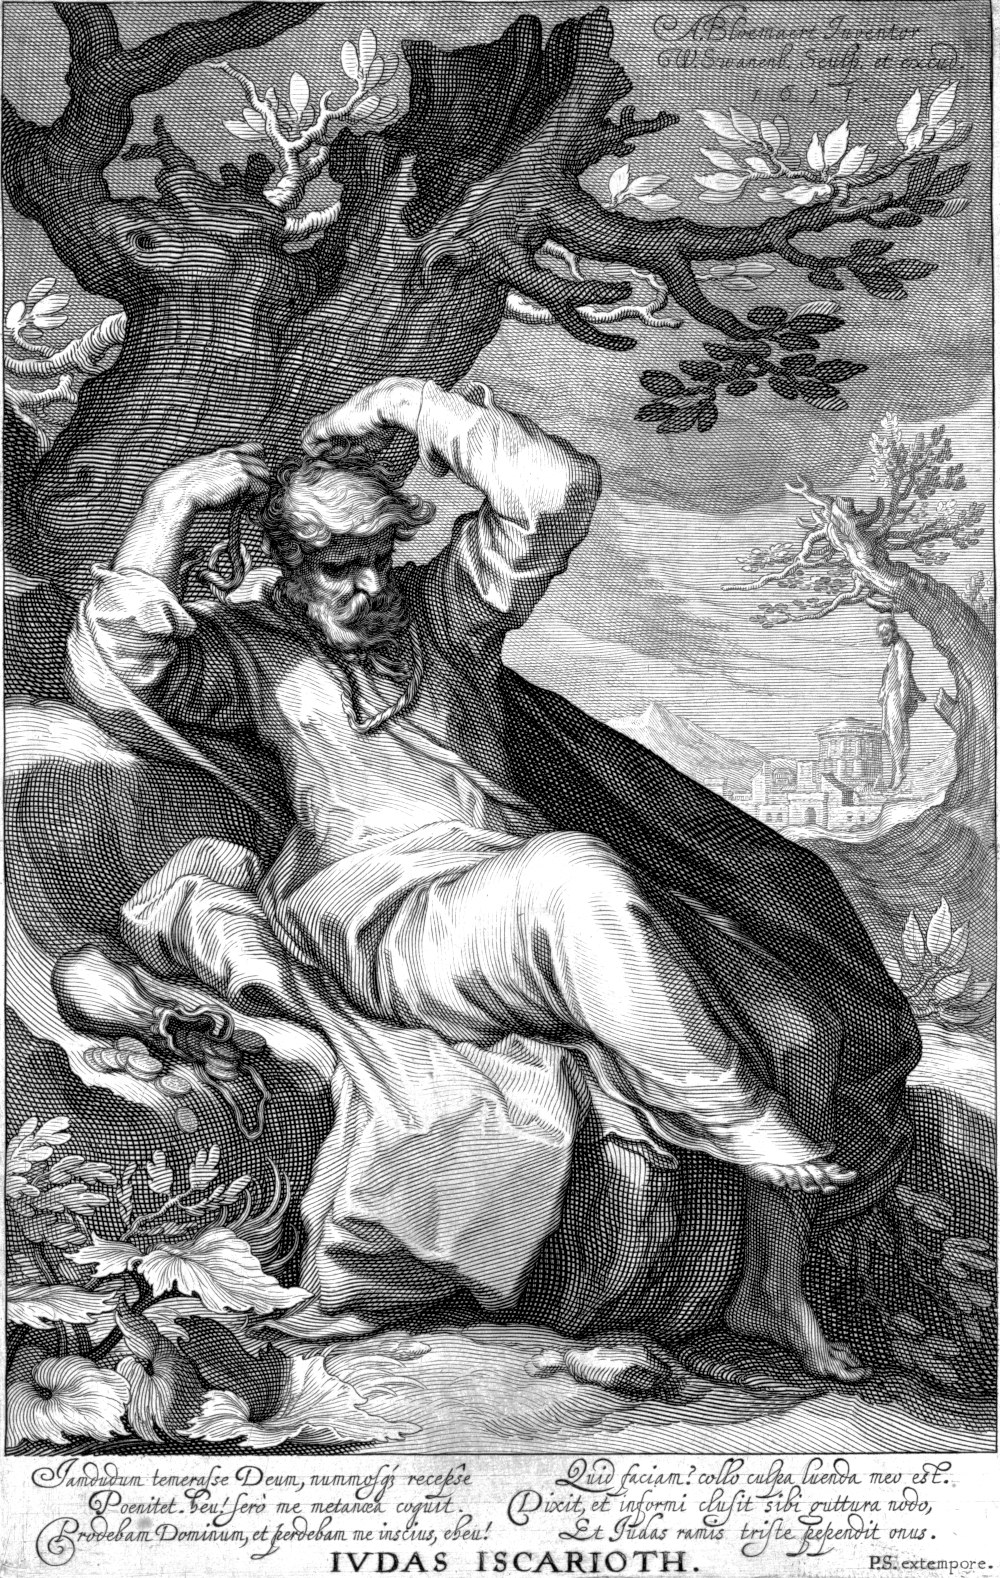
\includegraphics[keepaspectratio,width=0.4\textwidth]{figures/iudas-small.jpg}
  \caption{\citeart{IudasIscarioth}}
  \label{fig:iudas}
\end{figure}
\lettrine{T}{he} principal agent and procurer of this mischief is the devil; those
whom God forsakes, the devil by his permission lays hold on. Sometimes
he persecutes them with that worm of conscience, as he did Judas,
\mmarginpar{6694}Saul, and others. The poets call it Nemesis, but it is indeed
God's just judgment, sero sed serio, he strikes home at last, and
setteth upon them as a thief in the night, 1 Thes. ii. \mmarginpar{6695}This
temporary passion made David cry out, Lord, rebuke me not in thine
anger, neither chasten me in thine heavy displeasure; for thine arrows
have light upon me, \&c. there is nothing sound in my flesh, because of
thine anger. Again, I roar for the very grief of my heart: and Psalm
xxii. My God, my God, why hast thou forsaken me, and art so far from my
health, and the words of my crying? I am like to water poured out, my
bones are out of joint, mine heart is like wax, that is molten in the
midst of my bowels. So Psalm lxxxviii. 15 and 16 vers. and Psalm cii. I
am in misery at the point of death, from my youth I suffer thy terrors,
doubting for my life; thine indignations have gone over me, and thy
fear hath cut me off. Job doth often complain in this kind; and those
God doth not assist, the devil is ready to try and torment, still
seeking whom he may devour. If he find them merry, saith Gregory, he
tempts them forthwith to some dissolute act; if pensive and sad, to a
desperate end. Aut suadendo blanditur, aut minando terret, sometimes by
fair means, sometimes again by foul, as he perceives men severally
inclined. His ordinary engine by which he produceth this effect, is the
melancholy humour itself, which is balneum diaboli, the devil's bath;
and as in Saul, those evil spirits get in \mmarginpar{6696}as it were, and take
possession of us. Black choler is a shoeing-horn, a bait to allure
them, insomuch that many writers make melancholy an ordinary cause, and
a symptom of despair, for that such men are most apt, by reason of
their ill-disposed temper, to distrust, fear, grief, mistake, and
amplify whatsoever they preposterously conceive, or falsely apprehend.
Conscientia scrupulosa nascitur ex vitio naturali, complexione
melancholica (saith Navarrus cap. 27. num. 282. tom. 2. cas. conscien.)
The body works upon the mind, by obfuscating the spirits and corrupted
instruments, which \mmarginpar{6697}Perkins illustrates by simile of an artificer,
that hath a bad tool, his skill is good, ability correspondent, by
reason of ill tools his work must needs be lame and imperfect. But
melancholy and despair, though often, do not always concur; there is
much difference: melancholy fears without a cause, this upon great
occasion; melancholy is caused by fear and grief, but this torment
procures them and all extremity of bitterness; much melancholy is
without affliction of conscience, as \mmarginpar{6698}Bright and Perkins
illustrate by four reasons; and yet melancholy alone may be sometimes a
sufficient cause of this terror of conscience. \mmarginpar{6699}Felix Plater so
found it in his observations, e melancholicis alii damnatos se putant,
Deo curae, non sunt, nec praedestinati, \&c. They think they are not
predestinate, God hath forsaken them; and yet otherwise very zealous
and religious; and 'tis common to be seen, melancholy for fear of God's
judgment and hell-fire, drives men to desperation; fear and sorrow, if
they be immoderate, end often with it. Intolerable pain and anguish,
long sickness, captivity, misery, loss of goods, loss of friends, and
those lesser griefs, do sometimes effect it, or such dismal accidents.
Si non statim relevantur, \mmarginpar{6700}Mercennus, dubitant an sit Deus, if
they be not eased forthwith, they doubt whether there be any God, they
rave, curse, and are desperately mad because good men are oppressed,
wicked men flourish, they have not as they think to their desert, and
through impatience of calamities are so misaffected. Democritus put out
his eyes, ne malorum civium prosperos videret successus, because he
could not abide to see wicked men prosper, and was therefore ready to
make away himself, as \mmarginpar{6701}Agellius writes of him. Felix Plater hath a
memorable example in this kind, of a painter's wife in Basil, that was
melancholy for her son's death, and for melancholy became desperate;
she thought God would not pardon her sins, \mmarginpar{6702}and for four months
still raved, that she was in hell-fire, already damned. When the humour
is stirred up, every small object aggravates and incenseth it, as the
parties are addicted. \mmarginpar{6703}The same author hath an example of a
merchant man, that for the loss of a little wheat, which he had over
long kept, was troubled in conscience, for that he had not sold it
sooner, or given it to the poor, yet a good scholar and a great divine;
no persuasion would serve to the contrary, but that for this fact he
was damned: in other matters Very judicious and discreet. Solitariness,
much fasting, divine meditation, and contemplations of God's judgments,
most part accompany this melancholy, and are main causes, as
\mmarginpar{6704}Navarrus holds; to converse with such kinds of persons so
troubled, is sufficient occasion of trouble to some men. Nonnulli ob
longas inedias, studia et meditationes coelestes, de rebus sacris et
religione semper agitant, \&c. Many, (saith P. Forestus) through long
fasting, serious meditations of heavenly things, fall into such fits;
and as Lemnius adds, lib. 4. cap. 21, \mmarginpar{6705}If they be solitary given,
superstitious, precise, or very devout: seldom shall you find a
merchant, a soldier, an innkeeper, a bawd, a host, a usurer, so
troubled in mind, they have cheverel consciences that will stretch,
they are seldom moved in this kind or molested: young men and middle
age are more wild and less apprehensive; but old folks, most part, such
as are timorous and religiously given. Pet. Forestus observat. lib. 10.
cap. 12. de morbis cerebri, hath a fearful example of a minister, that
through precise fasting in Lent, and overmuch meditation, contracted
this mischief, and in the end became desperate, thought he saw devils
in his chamber, and that he could not be saved; he smelled nothing, as
he said, but fire and brimstone, was already in hell, and would ask
them, still, if they did not \mmarginpar{6706}smell as much. I told him he was
melancholy, but he laughed me to scorn, and replied that he saw devils,
talked with them in good earnest, Would spit in my face, and ask me if
1 did not smell brimstone, but at last he was by him cured. Such
another story I find in Plater observat. lib. 1. A poor fellow had done
some foul offence, and for fourteen days would eat no meat, in the end
became desperate, the divines about him could not ease him, \mmarginpar{6707}but
so he died. Continual meditation of God's judgments troubles many,
Multi ob timorem futuri judicii, saith Guatinerius cap. 5. tract. 15.
et suspicionem desperabundi sunt. David himself complains that God's
judgments terrified his soul, Psalm cxix. part. 16. vers. 8. My flesh
trembleth for fear of thee, and I am afraid of thy judgments. Quoties
diem illum cogito (saith \mmarginpar{6708}Hierome) toto corpore contremisco, I
tremble as often as I think of it. The terrible meditation of hell-fire
and eternal punishment much torments a sinful silly soul. What's a
thousand years to eternity? Ubi moeror, ubi fletus, ubi dolor
sempiternus. Mors sine morte, finis sine fine; a finger burnt by chance
we may not endure, the pain is so grievous, we may not abide an hour, a
night is intolerable; and what shall this unspeakable fire then be that
burns for ever, innumerable infinite millions of years, in omne aevum
in aeternum. O eternity!

\mmarginpar{6709}Aeternitas est illa vox,
Vox illa fulminatrix,

Tonitruis minacior,
Fragoribusque coeli,

Aeternitas est illa vox,
-meta carens et orta, \&c.

Tormenta nulla territant,
Quae finiuntur annis;

Aeternitas, aeternitas
Versat coquilque pectus.

Auget haec poenas indies,
Centuplicatque flammas, \&c.

This meditation terrifies these poor distressed souls, especially if
their bodies be predisposed by melancholy, they religiously given, and
have tender consciences, every small object affrights them, the very
inconsiderate reading of Scripture itself, and misinterpretation of
some places of it; as, Many are called, few are chosen. Not every one
that saith Lord. Fear not little flock. He that stands, let him take
heed lest he fall. Work out your salvation with fear and trembling,
That night two shall be in a bed, one received, the other left. Strait
is the way that leads to heaven, and few there are that enter therein.
The parable of the seed and of the sower, some fell on barren ground,
some was choked. Whom he hath predestinated he hath chosen. He will
have mercy on whom he will have mercy. Non est volentis nec currentis,
sed miserentis Dei. These and the like places terrify the souls of
many; election, predestination, reprobation, preposterously conceived,
offend divers, with a deal of foolish presumption, curiosity, needless
speculation, contemplation, solicitude, wherein they trouble and puzzle
themselves about those questions of grace, free will, perseverance,
God's secrets; they will know more than is revealed of God in his word,
human capacity, or ignorance can apprehend, and too importunate inquiry
after that which is revealed; mysteries, ceremonies, observation of
Sabbaths, laws, duties, \&c., with many such which the casuists discuss,
and schoolmen broach, which divers mistake, misconstrue, misapply to
themselves, to their own undoing, and so fall into this gulf. They
doubt of their election, how they shall know, it, by what signs. And so
far forth, saith Luther, with such nice points, torture and crucify
themselves, that they are almost mad, and all they get by it is this,
they lay open a gap to the devil by desperation to carry them to hell;
but the greatest harm of all proceeds from those thundering ministers,
a most frequent cause they are of this malady: \mmarginpar{6710}and do more harm
in the church (saith Erasmus) than they that flatter; great danger on
both sides, the one lulls them asleep in carnal security, the other
drives them to despair. Whereas, \mmarginpar{6711}St. Bernard well adviseth, We
should not meddle with the one without the other, nor speak of judgment
without mercy; the one alone brings desperation, the other security.
But these men are wholly for judgment; of a rigid disposition
themselves, there is no mercy with them, no salvation, no balsam for
their diseased souls, they can speak of nothing but reprobation,
hell-fire, and damnation; as they did Luke xi. 46. lade men with
burdens grievous to be borne, which they themselves touch not with a
finger. 'Tis familiar with our papists to terrify men's souls with
purgatory, tales, visions, apparitions, to daunt even the most generous
spirits, to \mmarginpar{6712}require charity, as Brentius observes, of others,
bounty, meekness, love, patience, when they themselves breathe nought
but lust, envy, covetousness. They teach others to fast, give alms, do
penance, and crucify their mind with superstitious observations, bread
and water, hair clothes, whips, and the like, when they themselves have
all the dainties the world can afford, lie on a down-bed with a
courtesan in their arms: Heu quantum patimur pro Christo, as \mmarginpar{6713}he
said, what a cruel tyranny is this, so to insult over and terrify men's
souls! Our indiscreet pastors many of them come not far behind, whilst
in their ordinary sermons they speak so much of election,
predestination, reprobation, ab aeterno, subtraction of grace,
preterition, voluntary permission, \&c., by what signs and tokens they
shall discern and try themselves, whether they be God's true children
elect, an sint reprobi, praedestinati, \&c., with such scrupulous
points, they still aggravate sin, thunder out God's judgments without
respect, intempestively rail at and pronounce them damned in all
auditories, for giving so much to sports and honest recreations, making
every small fault and thing indifferent an irremissible offence, they
so rent, tear and wound men's consciences, that they are almost mad,
and at their wits' end.
These bitter potions (saith \mmarginpar{6714}Erasmus) are still in their mouths,
nothing but gall and horror, and a mad noise, they make all their
auditors desperate: many are wounded by this means, and they commonly
that are most devout and precise, have been formerly presumptuous, and
certain of their salvation; they that have tender consciences, that
follow sermons, frequent lectures, that have indeed least cause, they
are most apt to mistake, and fall into these miseries. I have heard
some complain of Parson's Resolution, and other books of like nature
(good otherwise), they are too tragical, too much dejecting men,
aggravating offences: great care and choice, much discretion is
required in this kind.
The last and greatest cause of this malady, is our own conscience,
sense of our sins, and God's anger justly deserved, a guilty conscience
for some foul offence formerly committed,-\mmarginpar{6715}O miser Oreste, quid
morbi te perdit? Or: Conscientia, Sum enim mihi conscius de malis
perpetratis.\mmarginpar{6716} A good conscience is a continual feast, but a galled
conscience is as great a torment as can possibly happen, a still baking
oven, (so Pierius in his Hieroglyph, compares it) another hell. Our
conscience, which is a great ledger book, wherein are written all our
offences, a register to lay them up, (which those \mmarginpar{6717}Egyptians in
their hieroglyphics expressed by a mill, as well for the continuance,
as for the torture of it) grinds our souls with the remembrance of some
precedent sins, makes us reflect upon, accuse and condemn our own
selves. \mmarginpar{6718}Sin lies at door, \&c. I know there be many other causes
assigned by Zanchius, \mmarginpar{6719}Musculus, and the rest; as incredulity,
infidelity, presumption, ignorance, blindness, ingratitude, discontent,
those five grand miseries in Aristotle, ignominy, need, sickness,
enmity, death, \&c.; but this of conscience is the greatest,
\mmarginpar{6720}Instar ulceris corpus jugiter percellens: The scrupulous
conscience (as \mmarginpar{6721}Peter Forestus calls it) which tortures so many,
that either out of a deep apprehension of their unworthiness, and
consideration of their own dissolute life, accuse themselves and
aggravate every small offence, when there is no such cause, misdoubting
in the meantime God's mercies, they fall into these inconveniences. The
poet calls them \mmarginpar{6722}furies dire, but it is the conscience alone which
is a thousand witnesses to accuse us, \mmarginpar{6723} Nocte dieque suum gestant
in pectore testem. A continual tester to give in evidence, to empanel a
jury to examine us, to cry guilty, a persecutor with hue and cry to
follow, an apparitor to summon us, a bailiff to carry us, a serjeant to
arrest, an attorney to plead against us, a gaoler to torment, a judge
to condemn, still accusing, denouncing, torturing and molesting. And as
the statue of Juno in that holy city near Euphrates in \mmarginpar{6724}Assyria
will look still towards you, sit where you will in her temple, she
stares full upon you, if you go by, she follows with her eye, in all
sites, places, conventicles, actions, our conscience will be still
ready to accuse us. After many pleasant days, and fortunate adventures,
merry tides, this conscience at last doth arrest us. Well he may escape
temporal punishment, \mmarginpar{6725}bribe a corrupt judge, and avoid the censure
of law, and flourish for a time; for \mmarginpar{6726}who ever saw (saith
Chrysostom) a covetous man troubled in mind when he is telling of his
money, an adulterer mourn with his mistress in his arms? we are then
drunk with pleasure, and perceive nothing: yet as the prodigal son had
dainty fare, sweet music at first, merry company, jovial entertainment,
but a cruel reckoning in the end, as bitter as wormwood, a fearful
visitation commonly follows. And the devil that then told thee that it
was a light sin, or no sin at all, now aggravates on the other side,
and telleth thee, that it is a most irremissible offence, as he did by
Cain and Judas, to bring them to despair; every small circumstance
before neglected and contemned, will now amplify itself, rise up in
judgment, and accuse the dust of their shoes, dumb creatures, as to
Lucian's tyrant, lectus et candela, the bed and candle did bear
witness, to torment their souls for their sins past. Tragical examples
in this kind are too familiar and common: Adrian, Galba, Nero, Otho,
Vitellius, Caracalla, were in such horror of conscience for their
offences committed, murders, rapes, extortions, injuries, that they
were weary of their lives, and could get nobody to kill them.
\mmarginpar{6727}Kennetus, King of Scotland, when he had murdered his nephew
Malcom, King Duffe's son, Prince of Cumberland, and with counterfeit
tears and protestations dissembled the matter a long time, \mmarginpar{6728}at
last his conscience accused him, his unquiet soul could not rest day or
night, he was terrified with fearful dreams, visions, and so miserably
tormented all his life. It is strange to read what \mmarginpar{6729}Cominaeus hath
written of Louis XI. that French King; of Charles VIII.; of Alphonsus,
King of Naples; in the fury of his passion how he came into Sicily, and
what pranks he played. Guicciardini, a man most unapt to believe lies,
relates how that Ferdinand his father's ghost who before had died for
grief, came and told him, that he could not resist the French King, he
thought every man cried France, France; the reason of it (saith
Cominseus) was because he was a vile tyrant, a murderer, an oppressor
of his subjects, he bought up all commodities, and sold them at his own
price, sold abbeys to Jews and Falkoners; both Ferdinand his father,
and he himself never made conscience of any committed sin; and to
conclude, saith he, it was impossible to do worse than they did. Why
was Pausanias the Spartan tyrant, Nero, Otho, Galba, so persecuted with
spirits in every house they came, but for their murders which they had
committed? \mmarginpar{6730}Why doth the devil haunt many men's houses after their
deaths, appear to them living, and take possession of their
habitations, as it were, of their palaces, but because of their several
villainies? Why had Richard the Third such fearful dreams, saith
Polydore, but for his frequent murders? Why was Herod so tortured in
his mind? because he had made away Mariamne his wife. Why was
Theodoric, the King of the Goths, so suspicious, and so affrighted with
a fish head alone, but that he had murdered Symmachus, and Boethius his
son-in-law, those worthy Romans? Caelius, lib. 27. cap. 22. See more in
Plutarch, in his tract De his qui sero a Numine puniuntur, and in his
book De tranquillitate animi, \&c. Yea, and sometimes GOD himself hath a
hand in it, to show his power, humiliate, exercise, and to try their
faith, (divine temptation, Perkins calls it, Cas. cons. lib. 1. cap. 8.
sect. 1.) to punish them for their sins. God the avenger, as
\mmarginpar{6731}David terms him, ultor a tergo Deus, his wrath is apprehended of
a guilty, soul, as by Saul and Judas, which the poets expressed by
Adrastia, or Nemesis:
\mmarginpar{6732}Assequitur Nemesique virum vestigia servat,
Ne male quid facias.---

And she is, as \mmarginpar{6733}Ammianus, lib. 14. describes her, the queen of
causes, and moderator of things, now she pulls down the proud, now she
rears and encourageth those that are good; he gives instance in his
Eusebius; Nicephorus, lib. 10. cap. 35. eccles. hist. in Maximinus and
Julian. Fearful examples of God's just judgment, wrath and vengeance,
are to be found in all histories, of some that have been eaten to death
with rats and mice, as \mmarginpar{6734}Popelius, the second King of Poland, ann.
830, his wife and children; the like story is of Hatto, Archbishop of
Mentz, ann. 969, so devoured by these vermin, which howsoever Serrarius
the Jesuit Mogunt. rerum lib. 4. cap. 5. impugn by twenty-two
arguments, Tritemius, \mmarginpar{6735}Munster, Magdeburgenses, and many others
relate for a truth. Such another example I find in Geraldus Cambrensis
Itin. Cam. lib. 2. cap. 2. and where not?
And yet for all these terrors of conscience, affrighting punishments
which are so frequent, or whatsoever else may cause or aggravate this
fearful malady in other religions, I see no reason at all why a papist
at any time should despair, or be troubled for his sins; for let him be
never so dissolute a caitiff so notorious a villain, so monstrous a
sinner, out of that treasure of indulgences and merits of which the
pope is dispensator, he may have free pardon and plenary remission of
all his sins. There be so many general pardons for ages to come, forty
thousand years to come, so many jubilees, so frequent gaol-deliveries
out of purgatory for all souls, now living, or after dissolution of the
body, so many particular masses daily said in several churches, so many
altars consecrated to this purpose, that if a man have either money or
friends, or will take any pains to come to such an altar, hear a mass,
say so many paternosters, undergo such and such penance, he cannot do
amiss, it is impossible his mind should be troubled, or he have any
scruple to molest him. Besides that Taxa Camerae Apostolicae, which was
first published to get money in the days of Leo Decimus, that sharking
pope, and since divulged to the same ends, sets down such easy rates
and dispensations for all offences, for perjury, murder, incest,
adultery, \&c., for so many grosses or dollars (able to invite any man
to sin, and provoke him to offend, methinks, that otherwise would not)
such comfortable remission, so gentle and parable a pardon, so ready at
hand, with so small cost and suit obtained, that I cannot see how he
that hath any friends amongst them (as I say) or money in his purse, or
will at least to ease himself, can any way miscarry or be misaffected,
how he should be desperate, in danger of damnation, or troubled in
mind. Their ghostly fathers can so readily apply remedies, so cunningly
string and unstring, wind and unwind their devotions, play upon their
consciences with plausible speeches and terrible threats, for their
best advantage settle and remove, erect with such facility and deject,
let in and out, that I cannot perceive how any man amongst them should
much or often labour of this disease, or finally miscarry. The causes
above named must more frequently therefore take hold in others.

%SUBSECT. IV.-_Symptoms of Despair, Fear, Sorrow, Suspicion, Anxiety, Horror of Conscience, Fearful Dreams and Visions_.
\section[Symptoms of Despair]{Symptoms of Despair, Fear, Sorrow, Suspicion, Anxiety, Horror of Conscience, Fearful Dreams and Visions.}

\lettrine{A}{s} shoemakers do when they bring home shoes, still cry leather is
dearer and dearer, may I justly say of those melancholy symptoms: these
of despair are most violent, tragical, and grievous, far beyond the
rest, not to be expressed but negatively, as it is privation of all
happiness, not to be endured; for a wounded spirit who can bear it?
Prov. xviii. 19. What, therefore, \mmarginpar{6736}Timanthes did in his picture of
Iphigenia, now ready to be sacrificed, when he had painted Chalcas
mourning, Ulysses sad, but most sorrowful Menelaus; and showed all his
art in expressing a variety of affections, he covered the maid's father
Agamemnon's head with a veil, and left it to every spectator to
conceive what he would himself; for that true passion and sorrow in
summo gradu, such as his was, could not by any art be deciphered. What
he did in his picture, I will do in describing the symptoms of despair;
imagine what thou canst, fear, sorrow, furies, grief, pain, terror,
anger, dismal, ghastly, tedious, irksome, \&c. it is not sufficient, it
comes far short, no tongue can tell, no heart conceive it. 'Tis an
epitome of hell, an extract, a quintessence, a compound, a mixture of
all feral maladies, tyrannical tortures, plagues, and perplexities.
There is no sickness almost but physic provideth a remedy for it; to
every sore chirurgery will provide a slave; friendship helps poverty;
hope of liberty easeth imprisonment; suit and favour revoke banishment;
authority and time wear away reproach: but what physic, what
chirurgery, what wealth, favour, authority can relieve, bear out,
assuage, or expel a troubled conscience? A quiet mind cureth all them,
but all they cannot comfort a distressed soul: who can put to silence
the voice of desperation? All that is single in other melancholy,
Horribile, dirum, pestilens, atrox, ferum, concur in this, it is more
than melancholy in the highest degree; a burning fever of the soul; so
mad, saith \mmarginpar{6737}Jacchinus, by this misery; fear, sorrow, and despair,
he puts for ordinary symptoms of melancholy. They are in great pain and
horror of mind, distraction of soul, restless, full of continual fears,
cares, torments, anxieties, they can neither eat, drink, nor sleep for
them, take no rest,
\mmarginpar{6738}Perpetua impietas, nec mensae tempore cessat,
Exagitat vesana quies, somnique furentes.

Neither at bed, nor yet at board,
Will any rest despair afford.

Fear takes away their content, and dries the blood, wasteth the marrow,
alters their countenance, even in their greatest delights, singing,
dancing, dalliance, they are still (saith \mmarginpar{6739}Lemnius) tortured in
their souls. It consumes them to nought, I am like a pelican in the
wilderness (saith David of himself, temporally afflicted), an owl,
because of thine indignation, Psalm cii. 8, 10, and Psalm lv. 4. My
heart trembleth within me, and the terrors of death have come upon me;
fear and trembling are come upon me, \&c. at death's door, Psalm cvii.
18. Their soul abhors all manner of meats. Their \mmarginpar{6740}sleep is (if it
be any) unquiet, subject to fearful dreams and terrors. Peter in his
bonds slept secure, for he knew God protected him; and Tully makes it
an argument of Roscius Amerinus' innocency, that he killed not his
father, because he so securely slept. Those martyrs in the primitive
church were most \mmarginpar{6741}cheerful and merry in the midst of their
persecutions; but it is far otherwise with these men, tossed in a sea,
and that continually without rest or intermission, they can think of
nought that is pleasant, \mmarginpar{6742}their conscience will not let them be
quiet, in perpetual fear, anxiety, if they be not yet apprehended, they
are in doubt still they shall be ready to betray themselves, as Cain
did, he thinks every man will kill him; and roar for the grief of
heart, Psalm xxxviii. 8, as David did; as Job did, xx. 3, 21, 22, \&c.,
Wherefore is light given to him that is in misery, and life to them
that have heavy hearts? which long for death, and if it come not,
search it more than treasures, and rejoice when they can find the
grave. They are generally weary of their lives, a trembling heart they
have, a sorrowful mind, and little or no rest. Terror ubique tremor,
timor undique et undique terror. Fears, terrors, and affrights in all
places, at all times and seasons. Cibum et potum pertinaciter
aversantur multi, nodum in scirpo quaeritantes, et culpam imaginantes
ubi nulla est, as Wierus writes de Lamiis lib. 3. c. 7. they refuse
many of them meat and drink, cannot rest, aggravating still and
supposing grievous offences where there are none. God's heavy wrath is
kindled in their souls, and notwithstanding their continual prayers and
supplications to Christ Jesus, they have no release or ease at all, but
a most intolerable torment, and insufferable anguish of conscience, and
that makes them, through impatience, to murmur against God many times,
to rave, to blaspheme, turn atheists, and seek to offer violence to
themselves. Deut. xxviii. 65, 68. In the morning they wish for evening,
and for morning in the evening, for the sight of their eyes which they
see, and fear of hearts. \mmarginpar{6743}Marinus Mercennus, in his comment on
Genesis, makes mention of a desperate friend of his, whom, amongst
others, he came to visit, and exhort to patience, that broke out into
most blasphemous atheistical speeches, too fearful to relate, when they
wished him to trust in God, Quis est ille Deus (inquit) ut serviam
illi, quid proderit si oraverim; si praesens est, cur non succurrit?
cur non me carcere, inertia, squalore confectum liberat? quid ego feci?
\&c. absit a me hujusmodi Deus. Another of his acquaintance broke out
into like atheistical blasphemies, upon his wife's death raved, cursed,
said and did he cared not what. And so for the most part it is with
them all, many of them, in their extremity, think they hear and see
visions, outcries, confer with devils, that they are tormented,
possessed, and in hell-fire, already damned, quite forsaken of God,
they have no sense or feeling of mercy, or grace, hope of salvation,
their sentence of condemnation is already past, and not to be revoked,
the devil will certainly have them. Never was any living creature in
such torment before, in such a miserable estate, in such distress of
mind, no hope, no faith, past cure, reprobate, continually tempted to
make away themselves. Something talks with them, they spit fire and
brimstone, they cannot but blaspheme, they cannot repent, believe or
think a good thought, so far carried; ut cogantur ad impia cogitandum
etiam contra voluntatem, said \mmarginpar{6744}Felix Plater, ad blasphemiam erga
deum, ad multa horrenda perpetranda, ad manus violentas sibi
inferendas, \&c., and in their distracted fits and desperate humours, to
offer violence to others, their familiar and dear friends sometimes, or
to mere strangers, upon very small or no occasion; for he that cares
not for his own, is master of another man's life. They think evil
against their wills; that which they abhor themselves, they must needs
think, do, and speak. He gives instance in a patient of his, that when
he would pray, had such evil thoughts still suggested to him, and
wicked \mmarginpar{6745}meditations. Another instance he hath of a woman that was
often tempted to curse God, to blaspheme and kill herself. Sometimes
the devil (as they say) stands without and talks with them, sometimes
he is within them, as they think, and there speaks and talks as to such
as are possessed: so Apollodorus, in Plutarch, thought his heart spake
within him. There is a most memorable example of \mmarginpar{6746}Francis Spira,
an advocate of Padua, Ann. 1545, that being desperate, by no counsel of
learned men could be comforted: he felt (as he said) the pains of hell
in his soul; in all other things he discoursed aright, but in this most
mad. Frismelica, Bullovat, and some other excellent physicians, could
neither make him eat, drink, or sleep, no persuasion could ease him.
Never pleaded any man so well for himself, as this man did against
himself, and so he desperately died. Springer, a lawyer, hath written
his life. Cardinal Crescence died so likewise desperate at Verona,
still he thought a black dog followed him to his death-bed, no man
could drive the dog away, Sleiden. com. 23. cap. lib. 3. Whilst I was
writing this Treatise, saith Montaltus, cap. 2. de mel. \mmarginpar{6747}A nun
came to me for help, well for all other matters, but troubled in
conscience for five years last past; she is almost mad, and not able to
resist, thinks she hath offended God, and is certainly damned. Felix
Plater hath store of instances of such as thought themselves damned,
\mmarginpar{6748} forsaken of God, \&c. One amongst the rest, that durst not go to
church, or come near the Rhine, for fear to make away himself, because
then he was most especially tempted. These and such like symptoms are
intended and remitted, as the malady itself is more or less; some will
hear good counsel, some will not; some desire help, some reject all,
and will not be eased.

%SUBSECT. V.-_Prognostics of Despair, Atheism, Blasphemy, violent death, &c._
\section[Prognostics of Despair]{Prognostics of Despair, Atheism, Blasphemy, violent death, \&c.}

\lettrine{M}{ost} part these kind of persons make \mmarginpar{6749}away themselves, some are
mad, blaspheme, curse, deny God, but most offer violence to their own
persons, and sometimes to others. A wounded spirit who can bear? Prov.
xviii. 14. As Cain, Saul, Achitophel, Judas, blasphemed and died. Bede
saith, Pilate died desperate eight years after Christ. \mmarginpar{6750}Felix
Plater hath collected many examples. \mmarginpar{6751}A merchant's wife that was
long troubled with such temptations, in the night rose from her bed,
and out of the window broke her neck into the street: another drowned
himself desperate as he was in the Rhine: some cut their throats, many
hang themselves. But this needs no illustration. It is controverted by
some, whether a man so offering violence to himself, dying desperate,
may be saved, ay or no? If they die so obstinately and suddenly, that
they cannot so much as wish for mercy, the worst is to be suspected,
because they die impenitent. \mmarginpar{6752}If their death had been a little
more lingering, wherein they might have some leisure in their hearts to
cry for mercy, charity may judge the best; divers have been recovered
out of the very act of hanging and drowning themselves, and so brought
ad sanam mentem, they have been very penitent, much abhorred their
former act, confessed that they have repented in an instant, and cried
for mercy in their hearts. If a man put desperate hands upon himself,
by occasion of madness or melancholy, if he have given testimony before
of his regeneration, in regard he doth this not so much out of his
will, as ex vi morbi, we must make the best construction of it, as
\mmarginpar{6753}Turks do, that think all fools and madmen go directly to heaven.

%SUBSECT. VI.-_Cure of Despair by Physic, Good Counsel, Comforts, \&c._
\section[Cure of Despair]{Cure of Despair by Physic, Good Counsel, Comforts, \&c.}

\lettrine{E}{xperience} teacheth us, that though many die obstinate and wilful in
this malady, yet multitudes again are able to resist and overcome, seek
for help and find comfort, are taken e faucibus Erebi, from the chops
of hell, and out of the devil's paws, though they have by
\mmarginpar{6754}obligation, given themselves to him. Some out of their own
strength, and God's assistance, Though He kill me, (saith Job,) yet
will I trust in Him, out of good counsel, advice and physic.
\mmarginpar{6755}Bellovacus cured a monk by altering his habit, and course of
life: Plater many by physic alone. But for the most part they must
concur; and they take a wrong course that think to overcome this feral
passion by sole physic; and they are as much out, that think to work
this effect by good service alone, though both be forcible in
themselves, yet vis unita fortior, they must go hand in hand to this
disease:-alterius sic altera poscit opem. For physic the like course is
to be taken with this as in other melancholy: diet, air, exercise, all
those passions and perturbations of the mind, \&c. are to be rectified
by the same means. They must not be left solitary, or to themselves,
never idle, never out of company. Counsel, good comfort is to be
applied, as they shall see the parties inclined, or to the causes,
whether it be loss, fear, be grief, discontent, or some such feral
accident, a guilty conscience, or otherwise by frequent meditation, too
grievous an apprehension, and consideration of his former life; by
hearing, reading of Scriptures, good divines, good advice and
conference, applying God's word to their distressed souls, it must be
corrected and counterpoised. Many excellent exhortations, phraenetical
discourses, are extant to this purpose, for such as are any way
troubled in mind: Perkins, Greenham, Hayward, Bright, Abernethy,
Bolton, Culmannus, Helmingius, Caelius Secundus, Nicholas Laurentius,
are copious on this subject: Azorius, Navarrus, Sayrus, \&c., and such
as have written cases of conscience amongst our pontifical writers. But
because these men's works are not to all parties at hand, so parable at
all times, I will for the benefit and ease of such as are afflicted, at
the request of some \mmarginpar{6756}friends, recollect out of their voluminous
treatises, some few such comfortable speeches, exhortations, arguments,
advice, tending to this subject, and out of God's word, knowing, as
Culmannus saith upon the like occasion, \mmarginpar{6757}how unavailable and vain
men's councils are to comfort an afflicted conscience, except God's
word concur and be annexed, from which comes life, ease, repentance,
\&c. Presupposing first that which Beza, Greenham, Perkins, Bolton, give
in charge, the parties to whom counsel is given be sufficiently
prepared, humbled for their sins, fit for comfort, confessed, tried how
they are more or less afflicted, how they stand affected, or capable of
good advice, before any remedies be applied: to such therefore as are
so thoroughly searched and examined, I address this following
discourse.
Two main antidotes, \mmarginpar{6758}Hemmingius observes, opposite to despair,
good hope out of God's word, to be embraced; perverse security and
presumption from the devil's treachery, to be rejected; Illa solus
animae, haec pestis; one saves, the other kills, occidit animam, saith
Austin, and doth as much harm as despair itself, \mmarginpar{6759}Navarrus the
casuist reckons up ten special cures out of Anton. 1. part. Tit. 3.
cap. 10. 1. God. 2. Physic. 3. \mmarginpar{6760}Avoiding such objects as have
caused it. 4. Submission of himself to other men's judgments. 5. Answer
of all objections, \&c. All which Cajetan, Gerson, lib. de vit. spirit.
Sayrus, lib. 1. cons. cap. 14. repeat and approve out of Emanuel
Roderiques, cap. 51 et 52. Greenham prescribes six special rules,
Culmannus seven. First, to acknowledge all help come from God. 2. That
the cause of their present misery is sin. 3. To repent and be heartily
sorry for their sins. 4. To pray earnestly to God they may be eased. 5.
To expect and implore the prayers of the church, and good men's advice.
6. Physic. 7. To commend themselves to God, and rely upon His mercy:
others, otherwise, but all to this effect. But forasmuch as most men in
this malady are spiritually sick, void of reason almost, overborne by
their miseries, and too deep an apprehension of their sins, they cannot
apply themselves to good counsel, pray, believe, repent, we must, as
much as in us lies, occur and help their peculiar infirmities,
according to their several causes and symptoms, as we shall find them
distressed and complain.
The main matter which terrifies and torments most that are troubled in
mind, is the enormity of their offences, the intolerable burthen of
their sins, God's heavy wrath and displeasure so deeply apprehended,
that they account themselves reprobates, quite forsaken of God, already
damned, past all hope of grace, incapable of mercy, diaboli mancipia,
slaves of sin, and their offences so great they cannot be forgiven. But
these men must know there is no sin so heinous which is not pardonable
in itself, no crime so great but by God's mercy it may be forgiven.
Where sin aboundeth, grace aboundeth much more, Rom. v. 20. And what
the Lord said unto Paul in his extremity, 2 Cor. xi. 9. My grace is
sufficient for thee, for my power is made perfect through weakness:
concerns every man in like case. His promises are made indefinite to
all believers, generally spoken to all touching remission of sins that
are truly penitent, grieved for their offences, and desire to be
reconciled, Matt. ix. 12, 13, I came not to call the righteous but
sinners to repentance, that is, such as are truly touched in conscience
for their sins. Again, Matt. xi. 28, Come unto me all ye that are heavy
laden, and I will ease you. Ezek. xviii. 27, At what time soever a
sinner shall repent him of his sins from the bottom of his heart, I
will blot out all his wickedness out of my remembrance saith the Lord.
Isaiah xliii. 25, I, even I, am He that put away thine iniquity for
mine own sake, and will not remember thy sins. As a father (saith David
Psal. ciii. 13) hath compassion on his children, so hath the Lord
compassion on them that fear him. And will receive them again as the
prodigal son was entertained, Luke xv., if they shall so come with
tears in their eyes, and a penitent heart. Peccator agnoscat, Deus
ignoscit. The Lord is full of compassion and mercy, slow to anger, of
great kindness, Psal. ciii. 8. He will not always chide, neither keep
His anger for ever, 9. As high as the heaven is above the earth, so
great is His mercy towards them that fear Him, 11. As far as the East
is from the West, so far hath He removed our sins from us, 12. Though
Cain cry out in the anguish of his soul, my punishment is greater than
I can bear, 'tis not so; thou liest, Cain (saith Austin), God's mercy
is greater than thy sins. His mercy is above all His works, Psal. cxlv.
9, able to satisfy for all men's sins, antilutron, 1 Tim. ii. 6. His
mercy is a panacea, a balsam for an afflicted soul, a sovereign
medicine, an alexipharmacum for all sins, a charm for the devil; his
mercy was great to Solomon, to Manasseh, to Peter, great to all
offenders, and whosoever thou art, it may be so to thee. For why should
God bid us pray (as Austin infers) Deliver us from all evil, nisi ipse
misericors perseveraret, if He did not intend to help us? He therefore
that \mmarginpar{6761}doubts of the remission of his sins, denies God's mercy, and
doth Him injury, saith Austin. Yea, but thou repliest, I am a notorious
sinner, mine offences are not so great as infinite. Hear Fulgentius,
\mmarginpar{6762}God's invincible goodness cannot be overcome by sin, His infinite
mercy cannot be terminated by any: the multitude of His mercy is
equivalent to His magnitude. Hear \mmarginpar{6763}Chrysostom, Thy malice may be
measured, but God's mercy cannot be defined; thy malice is
circumscribed, His mercies infinite. As a drop of water is to the sea,
so are thy misdeeds to His mercy: nay, there is no such proportion to
be given; for the sea, though great, yet may be measured, but God's
mercy cannot be circumscribed. Whatsoever thy sins be then in quantity
or quality, multitude or magnitude, fear them not, distrust not. I
speak not this, saith \mmarginpar{6764}Chrysostom, to make thee secure and
negligent, but to cheer thee up. Yea but, thou urgest again, I have
little comfort of this which is said, it concerns me not: Inanis
poenitentia quam sequens culpa coinquinat, 'tis to no purpose for me to
repent, and to do worse than ever I did before, to persevere in sin,
and to return to my lusts as a dog to his vomit, or a swine to the
mire: \mmarginpar{6765}to what end is it to ask forgiveness of my sins, and yet
daily to sin again and again, to do evil out of a habit? I daily and
hourly offend in thought, word, and deed, in a relapse by mine own
weakness and wilfulness: my bonus genius, my good protecting angel is
gone, I am fallen from that I was or would be, worse and worse, my
latter end is worse than my beginning: Si quotidiae peccas, quotidie,
saith Chrysostom, poenitentiam age, if thou daily offend, daily repent:
\mmarginpar{6766}if twice, thrice, a hundred, a hundred thousand times, twice,
thrice, a hundred thousand times repent. As they do by an old house
that is out of repair, still mend some part or other; so do by thy
soul, still reform some vice, repair it by repentance, call to Him for
grace, and thou shalt have it; For we are freely justified by His
grace, Rom. iii. 24. If thine enemy repent, as our Saviour enjoined
Peter, forgive him seventy-seven times; and why shouldst thou think God
will not forgive thee? Why should the enormity of thy sins trouble
thee? God can do it, he will do it. My conscience (saith \mmarginpar{6767}Anselm)
dictates to me that I deserve damnation, my repentance will not suffice
for satisfaction: but thy mercy, O Lord, quite overcometh all my
transgressions. The gods once (as the poets feign) with a gold chain
would pull Jupiter out of heaven, but all they together could not stir
him, and yet he could draw and turn them as he would himself; maugre
all the force and fury of these infernal fiends, and crying sins, His
grace is sufficient. Confer the debt and the payment; Christ and Adam;
sin, and the cure of it; the disease and the medicine; confer the sick
man to his physician, and thou shalt soon perceive that his power is
infinitely beyond it. God is better able, as \mmarginpar{6768}Bernard informeth
us, to help, than sin to do us hurt; Christ is better able to save,
than the devil to destroy. \mmarginpar{6769}If he be a skilful Physician, as
Fulgentius adds, he can cure all diseases; if merciful, he will. Non
est perfecta bonitas a qua non omnis malitia vincitur, His goodness is
not absolute and perfect, if it be not able to overcome all malice.
Submit thyself unto Him, as St. Austin adviseth, \mmarginpar{6770}He knoweth best
what he doth; and be not so much pleased when he sustains thee, as
patient when he corrects thee; he is omnipotent, and can cure all
diseases when he sees his own time. He looks down from heaven upon
earth, that he may hear the mourning of prisoners, and deliver the
children of death, Psal. cii. 19. 20. And though our sins be as red as
scarlet, He can make them as white as snow, Isai. i. 18. Doubt not of
this, or ask how it shall be done: He is all-sufficient that promiseth;
qui fecit mundum de immundo, saith Chrysostom, he that made a fair
world of nought, can do this and much more for his part: do thou only
believe, trust in him, rely on him, be penitent and heartily sorry for
thy sins. Repentance is a sovereign remedy for all sins, a spiritual
wing to rear us, a charm for our miseries, a protecting amulet to expel
sin's venom, an attractive loadstone to draw God's mercy and graces
unto us. \mmarginpar{6771}Peccatum vulnus, poenitentia medicinam: sin made the
breach, repentance must help it; howsoever thine offence came, by
error, sloth, obstinacy, ignorance, exitur per poenitentiam, this is
the sole means to be relieved. \mmarginpar{6772}Hence comes our hope of safety, by
this alone sinners are saved, God is provoked to mercy. This unlooseth
all that is bound, enlighteneth darkness, mends that is broken, puts
life to that which was desperately dying: makes no respect of offences,
or of persons. \mmarginpar{6773}This doth not repel a fornicator, reject a
drunkard, resist a proud fellow, turn away an idolater, but entertains
all, communicates itself to all. Who persecuted the church more than
Paul, offended more than Peter? and yet by repentance (saith
Curysologus) they got both Magisterium et ministerium sanctitatis, the
Magistery of holiness. The prodigal son went far, but by repentance he
came home at last. \mmarginpar{6774}This alone will turn a wolf into a sheep, make
a publican a preacher, turn a thorn into an olive, make a debauched
fellow religious, a blasphemer sing halleluja, make Alexander the
coppersmith truly devout, make a devil a saint. \mmarginpar{6775}And him that
polluted his mouth with calumnies, lying, swearing, and filthy tunes
and tones, to purge his throat with divine Psalms. Repentance will
effect prodigious cures, make a stupend metamorphosis. A hawk came into
the ark, and went out again a hawk; a lion came in, went out a lion; a
bear, a bear; a wolf, a wolf; but if a hawk came into this sacred
temple of repentance, he will go forth a dove (saith \mmarginpar{6776}Chrysostom),
a wolf go out a sheep, a lion a lamb. \mmarginpar{6777}This gives sight to the
blind, legs to the lame, cures all diseases, confers grace, expels
vice, inserts virtue, comforts and fortifies the soul. Shall I say, let
thy sin be what it will, do but repent, it is sufficient. \mmarginpar{6778}Quem
poenitet peccasse pene est innocens. 'Tis true indeed and
all-sufficient this, they do confess, if they could repent; but they
are obdurate, they have cauterised consciences, they are in a reprobate
sense, they cannot think a good thought, they cannot hope for grace,
pray, believe, repent, or be sorry for their sins, they find no grief
for sin in themselves, but rather a delight, no groaning of spirit, but
are carried headlong to their own destruction, heaping wrath to
themselves against the day of wrath, Rom. ii. 5. 'Tis a grievous case
this I do yield, and yet not to be despaired; God of his bounty and
mercy calls all to repentance, Rom. ii. 4, thou mayst be called at
length, restored, taken to His grace, as the thief upon the cross, at
the last hour, as Mary Magdalene and many other sinners have been, that
were buried in sin. God (saith \mmarginpar{6779}Fulgentius) is delighted in the
conversion of a sinner, he sets no time; prolixitas temporis Deo non
praejudicat, aut gravitas peccati, deferring of time or grievousness of
sin, do not prejudicate his grace, things past and to come are all one
to Him, as present: 'tis never too late to repent. \mmarginpar{6780}This heaven of
repentance is still open for all distressed souls; and howsoever as yet
no signs appear, thou mayst repent in good time. Hear a comfortable
speech of St. Austin, \mmarginpar{6781}Whatsoever thou shall do, how great a
sinner soever, thou art yet living; if God would not help thee, he
would surely take thee away; but in sparing thy life, he gives thee
leisure, and invites thee to repentance. Howsoever as yet, I say, thou
perceivest no fruit, no feeling, findest no likelihood of it in
thyself, patiently abide the Lord's good leisure, despair not, or think
thou art a reprobate; He came to call sinners to repentance, Luke v.
32, of which number thou art one; He came to call thee, and in his time
will surely call thee. And although as yet thou hast no inclination to
pray, to repent, thy faith be cold and dead, and thou wholly averse
from all Divine functions, yet it may revive, as trees are dead in
winter, but flourish in the spring! these virtues may lie hid in thee
for the present, yet hereafter show themselves, and peradventure
already bud, howsoever thou dost not perceive. 'Tis Satan's policy to
plead against, suppress and aggravate, to conceal those sparks of faith
in thee. Thou dost not believe, thou sayest, yet thou wouldst believe
if thou couldst, 'tis thy desire to believe; then pray, \mmarginpar{6782}Lord help
mine unbelief: and hereafter thou shall certainly believe:
\mmarginpar{6783}Dabitur sitienti, it shall be given to him that thirsteth. Thou
canst not yet repent, hereafter thou shall; a black cloud of sin as yet
obnubilates thy soul, terrifies thy conscience, but this cloud may
conceive a rainbow at the last, and be quite dissipated by repentance.
Be of good cheer; a child is rational in power, not in act; and so art
thou penitent in affection, though not yet in action. 'Tis thy desire
to please God, to be heartily sorry; comfort thyself, no time is
overpast, 'tis never too late. A desire to repent is repentance itself,
though not in nature, yet in God's acceptance; a willing mind is
sufficient. Blessed are they that hunger and thirst after
righteousness, Matt. v. 6. He that is destitute of God's grace, and
wisheth for it, shall have it. The Lord (saith David, Psal. x. 17) will
hear the desire of the poor, that is, such as are in distress of body
and mind. 'Tis true thou canst not as yet grieve for thy sin, thou hast
no feeling of faith, I yield; yet canst thou grieve thou dost not
grieve? It troubles thee, I am sure, thine heart should be so
impenitent and hard, thou wouldst have it otherwise; 'tis thy desire to
grieve, to repent, and to believe. Thou lovest God's children and
saints in the meantime, hatest them not, persecutest them not, but
rather wishest thyself a true professor, to be as they are, as thou
thyself hast been heretofore; which is an evident token thou art in no
such desperate case. 'Tis a good sign of thy conversion, thy sins are
pardonable, thou art, or shalt surely be reconciled. The Lord is near
them that are of a contrite heart, Luke iv. 18. \mmarginpar{6784}A true desire of
mercy in the want of mercy, is mercy itself; a desire of grace in the
want of grace, is grace itself; a constant and earnest desire to
believe, repent, and to be reconciled to God, if it be in a touched
heart, is an acceptation of God, a reconciliation, faith and repentance
itself. For it is not thy faith and repentance, as \mmarginpar{6785}Chrysostom
truly teacheth, that is available, but God's mercy that is annexed to
it, He accepts the will for the deed: so that I conclude, to feel in
ourselves the want of grace, and to be grieved for it, is grace itself.
I am troubled with fear my sins are not forgiven, Careless objects: but
Bradford answers they are; For God hath given thee a penitent and
believing heart, that is, a heart which desireth to repent and believe;
for such an one is taken of him (he accepting the will for the deed)
for a truly penitent and believing heart.
All this is true thou repliest, but yet it concerns not thee, 'tis
verified in ordinary offenders, in common sins, but thine are of a
higher strain, even against the Holy Ghost himself, irremissible sins,
sins of the first magnitude, written with a pen of iron, engraven with
a point of a diamond. Thou art worse than a pagan, infidel, Jew, or
Turk, for thou art an apostate and more, thou hast voluntarily
blasphemed, renounced God and all religion, thou art worse than Judas
himself, or they that crucified Christ: for they did offend out of
ignorance, but thou hast thought in thine heart there is no God. Thou
hast given thy soul to the devil, as witches and conjurors do,
explicite and implicite, by compact, band and obligation (a desperate,
a fearful case) to satisfy thy lust, or to be revenged of thine
enemies, thou didst never pray, come to church, hear, read, or do any
divine duties with any devotion, but for formality and fashion's sake,
with a kind of reluctance, 'twas troublesome and painful to thee to
perform any such thing, praeter voluntatem, against thy will. Thou
never mad'st any conscience of lying, swearing, bearing false witness,
murder, adultery, bribery, oppression, theft, drunkenness, idolatry,
but hast ever done all duties for fear of punishment, as they were most
advantageous, and to thine own ends, and committed all such notorious
sins, with an extraordinary delight, hating that thou shouldst love,
and loving that thou shouldst hate. Instead of faith, fear and love of
God, repentance, \&c., blasphemous thoughts have been ever harboured in
his mind, even against God himself, the blessed Trinity; the
\mmarginpar{6786}Scripture false, rude, harsh, immethodical: heaven, hell,
resurrection, mere toys and fables, \mmarginpar{6787}incredible, impossible,
absurd, vain, ill contrived; religion, policy, and human invention, to
keep men in obedience, or for profit, invented by priests and lawgivers
to that purpose. If there be any such supreme power, he takes no notice
of our doings, hears not our prayers, regardeth them not, will not,
cannot help, or else he is partial, an excepter of persons, author of
sin, a cruel, a destructive God, to create our souls, and destinate
them to eternal damnation, to make us worse than our dogs and horses,
why doth he not govern things better, protect good men, root out wicked
livers? why do they prosper and flourish? as she raved in the
\mmarginpar{6788}tragedy-pellices caelum tenent, there they shine, Suasque Perseus
aureas stellas habet, where is his providence? how appears it?
\mmarginpar{6789}Marmoreo Licinus tumulo jacet, at Cato parvo,
Pomponius nullo, quis putet esse Deos.

Why doth he suffer Turks to overcome Christians, the enemy to triumph
over his church, paganism to domineer in all places as it doth,
heresies to multiply, such enormities to be committed, and so many such
bloody wars, murders, massacres, plagues, feral diseases! why doth he
not make us all good, able, sound? why makes he \mmarginpar{6790}venomous
creatures, rocks, sands, deserts, this earth itself the muck-hill of
the world, a prison, a house of correction? \mmarginpar{6791}Mentimur regnare
Jovem, \&c., with many such horrible and execrable conceits, not fit to
be uttered; Terribilia de fide, horribilia de Divinitate. They cannot
some of them but think evil, they are compelled volentes nolentes, to
blaspheme, especially when they come to church and pray, read, \&c.,
such foul and prodigious suggestions come into their hearts.
These are abominable, unspeakable offences, and most opposite to God,
tentationes foedae, et impiae, yet in this case, he or they that shall
be tempted and so affected, must know, that no man living is free from
such thoughts in part, or at some times, the most divine spirits have
been so tempted in some sort, evil custom, omission of holy exercises,
ill company, idleness, solitariness, melancholy, or depraved nature,
and the devil is still ready to corrupt, trouble, and divert our souls,
to suggest such blasphemous thoughts into our fantasies, ungodly,
profane, monstrous and wicked conceits: If they come from Satan, they
are more speedy, fearful and violent, the parties cannot avoid them:
they are more frequent, I say, and monstrous when they come; for the
devil he is a spirit, and hath means and opportunities to mingle
himself with our spirits, and sometimes more slyly, sometimes more
abruptly and openly, to suggest such devilish thoughts into our hearts;
he insults and domineers in melancholy distempered fantasies and
persons especially; melancholy is balneum, diaboli, as Serapio holds,
the devil's bath, and invites him to come to it. As a sick man frets,
raves in his fits, speaks and doth he knows not what, the devil
violently compels such crazed souls to think such damned thoughts
against their wills, they cannot but do it; sometimes more continuate,
or by fits, he takes his advantage, as the subject is less able to
resist, he aggravates, extenuates, affirms, denies, damns, confounds
the spirits, troubles heart, brain, humours, organs, senses, and wholly
domineers in their imaginations. If they proceed from themselves, such
thoughts, they are remiss and moderate, not so violent and monstrous,
not so frequent. The devil commonly suggests things opposite to nature,
opposite to God and his word, impious, absurd, such as a man would
never of himself, or could not conceive, they strike terror and horror
into the parties' own hearts. For if he or they be asked whether they
do approve of such like thoughts or no, they answer (and their own
souls truly dictate as much) they abhor them as much as hell and the
devil himself, they would fain think otherwise if they could; he hath
thought otherwise, and with all his soul desires so to think again; he
doth resist, and hath some good motions intermixed now and then: so
that such blasphemous, impious, unclean thoughts, are not his own, but
the devil's; they proceed not from him, but from a crazed phantasy,
distempered humours, black fumes which offend his brain: \mmarginpar{6792}they are
thy crosses, the devil's sins, and he shall answer for them, he doth
enforce thee to do that which thou dost abhor, and didst never give
consent to: and although he hath sometimes so slyly set upon thee, and
so far prevailed, as to make thee in some sort to assent to such wicked
thoughts, to delight in, yet they have not proceeded from a confirmed
will in thee, but are of that nature which thou dost afterwards reject
and abhor. Therefore be not overmuch troubled and dismayed with such
kind of suggestions, at least if they please thee not, because they are
not thy personal sins, for which thou shalt incur the wrath of God, or
his displeasure: contemn, neglect them, let them go as they come,
strive not too violently, or trouble thyself too much, but as our
Saviour said to Satan in like case, say thou, avoid Satan, I detest
thee and them. Satanae est mala ingerere (saith Austin) nostrum non
consentire: as Satan labours to suggest, so must we strive not to give
consent, and it will be sufficient: the more anxious and solicitous
thou art, the more perplexed, the more thou shalt otherwise be troubled
and entangled. Besides, they must know this, all so molested and
distempered, that although these be most execrable and grievous sins,
they are pardonable yet, through God's mercy and goodness, they may be
forgiven, if they be penitent and sorry for them. Paul himself
confesseth, Rom. xvii. 19. He did not the good he would do, but the
evil which he would not do; 'tis not I, but sin that dwelleth in me.
'Tis not thou, but Satan's suggestions, his craft and subtlety, his
malice: comfort thyself then if thou be penitent and grieved, or
desirous to be so, these heinous sins shall not be laid to thy charge;
God's mercy is above all sins, which if thou do not finally contemn,
without doubt thou shalt be saved. \mmarginpar{6793}No man sins against the Holy
Ghost, but he that wilfully and finally renounceth Christ, and
contemneth him and his word to the last, without which there is no
salvation, from which grievous sin, God of his infinite mercy deliver
us. Take hold of this to be thy comfort, and meditate withal on God's
word, labour to pray, to repent, to be renewed in mind, keep thine
heart with all diligence. Prov. iv. 13, resist the devil, and he will
fly from thee, pour out thy soul unto the Lord with sorrowful Hannah,
pray continually, as Paul enjoins, and as David did, Psalm i. meditate
on his law day and night.
Yea, but this meditation is that mars all, and mistaken makes many men
far worse, misconceiving all they read or hear, to their own overthrow;
the more they search and read Scriptures, or divine treatises, the more
they puzzle themselves, as a bird in a net, the more they are entangled
and precipitated into this preposterous gulf: Many are called, but few
are chosen, Matt. xx. 16. and xxii. 14. with such like places of
Scripture misinterpreted strike them with horror, they doubt presently
whether they be of this number or no: God's eternal decree of
predestination, absolute reprobation, and such fatal tables, they form
to their own ruin, and impinge upon this rock of despair. How shall
they be assured of their salvation, by what signs? If the righteous
scarcely be saved, where shall the ungodly and sinners appear? 1 Pet.
iv. 18. Who knows, saith Solomon, whether he be elect? This grinds
their souls, how shall they discern they are not reprobates? But I say
again, how shall they discern they are? From the devil can be no
certainty, for he is a liar from the beginning; if he suggests any such
thing, as too frequently he doth, reject him as a deceiver, an enemy of
human kind, dispute not with him, give no credit to him, obstinately
refuse him, as St. Anthony did in the wilderness, whom the devil set
upon in several shapes, or as the collier did, so do thou by him. For
when the devil tempted him with the weakness of his faith, and told him
he could not be saved, as being ignorant in the principles of religion,
and urged him moreover to know what he believed, what he thought of
such and such points and mysteries: the collier told him, he believed
as the church did; but what (said the devil again) doth the church
believe? as I do (said the collier); and what's that thou believest? as
the church doth, \&c., when the devil could get no other answer, he left
him. If Satan summon thee to answer, send him to Christ: he is thy
liberty, thy protector against cruel death, raging sin, that roaring
lion, he is thy righteousness, thy Saviour, and thy life. Though he
say, thou art not of the number of the elect, a reprobate, forsaken of
God, hold thine own still, hic murus aheneus esto, let this be as a
bulwark, a brazen wall to defend thee, stay thyself in that certainty
of faith; let that be thy comfort, Christ will protect thee, vindicate
thee, thou art one of his flock, he will triumph over the law, vanquish
death, overcome the devil, and destroy hell. If he say thou art none of
the elect, no believer, reject him, defy him, thou hast thought
otherwise, and mayst so be resolved again; comfort thyself; this
persuasion cannot come from the devil, and much less can it be grounded
from thyself? men are liars, and why shouldst thou distrust? A denying
Peter, a persecuting Paul, an adulterous cruel David, have been
received; an apostate Solomon may be converted; no sin at all but
impenitency, can give testimony of final reprobation. Why shouldst thou
then distrust, misdoubt thyself, upon what ground, what suspicion? This
opinion alone of particularity? Against that, and for the certainty of
election and salvation on the other side, see God's good will toward
men, hear how generally his grace is proposed to him, and him, and
them, each man in particular, and to all. 1 Tim. ii. 4. God will that
all men be saved, and come to the knowledge of the truth. 'Tis a
universal promise, God sent not his son into the world to condemn the
world, but that through him the world might be saved. John iii. 17. He
that acknowledged himself a man in the world, must likewise acknowledge
he is of that number that is to be saved. Ezek. xxxiii. 11, I will not
the death of a sinner, but that he repent and live: But thou art a
sinner; therefore he will not thy death. This is the will of him that
sent me, that every man that believeth in the Son, should have
everlasting life. John vi. 40. He would have no man perish, but all
come to repentance, 2 Pet. iii. 9. Besides, remission of sins is to be
preached, not to a few, but universally to all men, Go therefore and
tell all nations, baptising them, \&c. Matt. xxviii. 19. Go into all the
world, and preach the Gospel to every creature, Mark xvi. 15. Now there
cannot be contradictory wills in God, he will have all saved, and not
all, how can this stand together? be secure then, believe, trust in
him, hope well and be saved. Yea, that's the main matter, how shall I
believe or discern my security from carnal presumption? my faith is
weak and faint, I want those signs and fruits of sanctification,
\mmarginpar{6794}sorrow for sin, thirsting for grace, groanings of the spirit,
love of Christians as Christians, avoiding occasion of sin, endeavour
of new obedience, charity, love of God, perseverance. Though these
signs be languishing in thee, and not seated in thine heart, thou must
not therefore be dejected or terrified; the effects of the faith and
spirit are not yet so fully felt in thee; conclude not therefore thou
art a reprobate, or doubt of thine election, because the elect
themselves are without them, before their conversion. Thou mayst in the
Lord's good time be converted; some are called at the eleventh hour.
Use, I say, the means of thy conversion, expect the Lord's leisure, if
not yet called, pray thou mayst be, or at least wish and desire thou.
mayst be.
Notwithstanding all this which might be said to this effect, to ease
their afflicted minds, what comfort our best divines can afford in this
case, Zanchius, Beza, \&c. This furious curiosity, needless speculation,
fruitless meditation about election, reprobation, free will, grace,
such places of Scripture preposterously conceived, torment still, and
crucify the souls of too many, and set all the world together by the
ears. To avoid which inconveniences, and to settle their distressed
minds, to mitigate those divine aphorisms, (though in another extreme
some) our late Arminians have revived that plausible doctrine of
universal grace, which many fathers, our late Lutheran and modern
papists do still maintain, that we have free will of ourselves, and
that grace is common to all that will believe. Some again, though less
orthodoxal, will have a far greater part saved than shall be damned,
(as \mmarginpar{6795}Caelius Secundus stiffly maintains in his book, De
amplitudine regni coelestis, or some impostor under his name) beatorum
numerus multo major quam damnatorum. \mmarginpar{6796}He calls that other tenet of
special \mmarginpar{6797}election and reprobation, a prejudicate, envious and
malicious opinion, apt to draw all men to desperation. Many are called,
few chosen, \&c. He opposeth some opposite parts of Scripture to it,
Christ came into the world to save sinners, \&c. And four especial
arguments he produceth, one from God's power. If more be damned than
saved, he erroneously concludes, \mmarginpar{6798}the devil hath the greater
sovereignty! for what is power but to protect? and majesty consists in
multitude. If the devil have the greater part, where is his mercy,
where is his power? how is he Deus Optimus Maximus, misericors? \&c.,
where is his greatness, where his goodness? He proceeds, \mmarginpar{6799}We
account him a murderer that is accessory only, or doth not help when he
can; which may not be supposed of God without great offence, because he
may do what he will, and is otherwise accessory, and the author of sin.
The nature of good is to be communicated, God is good, and will not
then be contracted in his goodness: for how is he the father of mercy
and comfort, if his good concern but a few? O envious and unthankful
men to think otherwise! \mmarginpar{6800}Why should we pray to God that are
Gentiles, and thank him for his mercies and benefits, that hath damned
us all innocuous for Adam's offence, one man's offence, one small
offence, eating of an apple? why should we acknowledge him for our
governor that hath wholly neglected the salvation of our souls,
contemned us, and sent no prophets or instructors to teach us, as he
hath done to the Hebrews? So Julian the apostate objects. Why should
these Christians (Caelius urgeth) reject us and appropriate God unto
themselves, Deum illum suum unicum, \&c. But to return to our forged
Caelius. At last he comes to that, he will have those saved that never
heard of, or believed in Christ, ex puris naturalibus, with the
Pelagians, and proves it out of Origen and others. They (saith
\mmarginpar{6801}Origen) that never heard God's word, are to be excused for their
ignorance; we may not think God will be so hard, angry, cruel or unjust
as to condemn any man indicta causa. They alone (he holds) are in the
state of damnation that refuse Christ's mercy and grace, when it is
offered. Many worthy Greeks and Romans, good moral honest men, that
kept the law of nature, did to others as they would be done to
themselves, as certainly saved, he concludes, as they were that lived
uprightly before the law of Moses. They were acceptable in. God's
sight, as Job was, the Magi, the queen of Sheba, Darius of Persia,
Socrates, Aristides, Cato, Curius, Tully, Seneca, and many other
philosophers, upright livers, no matter of what religion, as Cornelius,
out of any nation, so that he live honestly, call on God, trust in him,
fear him, he shall be saved. This opinion was formerly maintained by
the Valentinian and Basiledian heretics, revived of late in
\mmarginpar{6802}Turkey, of what sect Rustan Bassa was patron, defended by
\mmarginpar{6803}Galeatius \mmarginpar{6804}Erasmus, by Zuinglius in exposit. fidei ad Regem
Galliae, whose tenet Bullinger vindicates, and Gualter approves in a
just apology with many arguments. There be many Jesuits that follow
these Calvinists in this behalf, Franciscus Buchsius Moguntinus,
Andradius Consil. Trident, many schoolmen that out of the 1 Rom. v. 18.
19. are verily persuaded that those good works of the Gentiles did so
far please God, that they might vitam aeternam promereri, and be saved
in the end. Sesellius, and Benedictus Justinianus in his comment on the
first of the Romans, Mathias Ditmarsh the politician, with many others,
hold a mediocrity, they may be salute non indigni but they will not
absolutely decree it. Hofmannus, a Lutheran professor of Helmstad, and
many of his followers, with most of our church, and papists, are stiff
against it. Franciscus Collius hath fully censured all opinions in his
Five Books, de Paganorum animabus post mortem, and amply dilated this
question, which whoso will may peruse. But to return to my author, his
conclusion is, that not only wicked livers, blasphemers, reprobates,
and such as reject God's grace, but that the devils themselves shall be
saved at last, as \mmarginpar{6805}Origen himself long since delivered in his
works, and our late \mmarginpar{6806}Socinians defend, Ostorodius, cap. 41.
institut. Smaltius, \&c. Those terms of all and for ever in Scripture,
are not eternal, but only denote a longer time, which by many examples
they prove. The world shall end like a comedy, and we shall meet at
last in heaven, and live in bliss altogether, or else in conclusion, in
nihil evanescere. For how can he be merciful that shall condemn any
creature to eternal unspeakable punishment, for one small temporary
fault, all posterity, so many myriads for one and another man's
offence, quid meruistis oves? But these absurd paradoxes are exploded
by our church, we teach otherwise. That this vocation, predestination,
election, reprobation, non ex corrupta massa, praeviso, fide, as our
Arminians, or ex praevisis operibus, as our papists, non ex
praeteritione, but God's absolute decree ante mundum creatum, (as many
of our church hold) was from the beginning, before the foundation of
the world was laid, or homo conditus, (or from Adam's fall, as others
will, homo lapsus objectum est reprobationis) with perseverantia
sanctorum, we must be certain of our salvation, we may fall but not
finally, which our Arminians will not admit. According to his
immutable, eternal, just decree and counsel of saving men and angels,
God calls all, and would have all to be saved according to the efficacy
of vocation: all are invited, but only the elect apprehended: the rest
that are unbelieving, impenitent, whom God in his just judgment leaves
to be punished for their sins, are in a reprobate sense; yet we must
not determine who are such, condemn ourselves or others, because we
have a universal invitation; all are commanded to believe, and we know
not how soon or how late our end may be received. I might have said
more of this subject; but forasmuch as it is a forbidden question, and
in the preface or declaration to the articles of the church, printed
1633, to avoid factions and altercations, we that are university
divines especially, are prohibited all curious search, to print or
preach, or draw the article aside by our own sense and comments upon
pain of ecclesiastical censure. I will surcease, and conclude with
\mmarginpar{6807}Erasmus of such controversies: Pugnet qui volet, ego censeo leges
majorum reverenter suscipiendas, et religiose observandas, velut a Deo
profectas; nec esse tutum, nec esse pium, de potestate publica
sinistram concipere aut serere suspicionem. Et siquid est tyrannidis,
quod tamen non cogat ad impietatem, satius est ferre, quam seditiose
reluctari.
But to my former task. The last main torture and trouble of a
distressed mind, is not so much this doubt of election, and that the
promises of grace are smothered and extinct in them, nay quite blotted
out, as they suppose, but withal God's heavy wrath, a most intolerable
pain and grief of heart seizeth on them: to their thinking they are
already damned, they suffer the pains of hell, and more than possibly
can be expressed, they smell brimstone, talk familiarly with devils,
hear and see chimeras, prodigious, uncouth shapes, bears, owls,
antiques, black dogs, fiends, hideous outcries, fearful noises,
shrieks, lamentable complaints, they are possessed, \mmarginpar{6808}and through
impatience they roar and howl, curse, blaspheme, deny God, call his
power in question, abjure religion, and are still ready to offer
violence unto themselves, by hanging, drowning, \&c. Never any miserable
wretch from the beginning of the world was in such a woeful case. To
such persons I oppose God's mercy and his justice; Judicia Dei occulta,
non injusta: his secret counsel and just judgment, by which he spares
some, and sore afflicts others again in this life; his judgment is to
be adored, trembled at, not to be searched or inquired after by mortal
men: he hath reasons reserved to himself, which our frailty cannot
apprehend. He may punish all if he will, and that justly for sin; in
that he doth it in some, is to make a way for his mercy that they
repent and be saved, to heal them, to try them, exercise their
patience, and make them call upon him, to confess their sins and pray
unto him, as David did, Psalm cxix. 137. Righteous art thou, O Lord,
and just are thy judgments. As the poor publican, Luke xviii. 13. Lord
have mercy upon me a miserable sinner. To put confidence and have an
assured hope in him, as Job had, xiii. 15. Though he kill me I will
trust In him: Ure, seca, occide O Domine, (saith Austin) modo serves
animam, kill, cut in pieces, burn my body (O Lord) to save my soul. A
small sickness; one lash of affliction, a little misery, many times
will more humiliate a man, sooner convert, bring him home to know
himself, than all those paraenetical discourses, the whole theory of
philosophy, law, physic, and divinity, or a world of instances and
examples. So that this, which they take to be such an insupportable
plague, is an evident sign of God's mercy and justice, of His love and
goodness: periissent nisi periissent, had they not thus been undone,
they had finally been undone. Many a carnal man is lulled asleep in
perverse security, foolish presumption, is stupefied in his sins, and
hath no feeling at all of them: I have sinned (he saith) and what evil
shall come unto me, Eccles. v. 4, and Tush, how shall God know it? and
so in a reprobate sense goes down to hell. But here, Cynthius aurem
vellit, God pulls them by the ear, by affliction, he will bring them to
heaven and happiness; Blessed are they that mourn, for they shall be
comforted, Matt. v. 4, a blessed and a happy state, if considered
aright, it is, to be so troubled. It is good for me that I have been
afflicted, Psal. cxix. before I was afflicted I went astray, but now I
keep Thy word. Tribulation works patience, patience hope, Rom. v. 4,
and by such like crosses and calamities we are driven from the stake of
security. So that affliction is a school or academy, wherein the best
scholars are prepared to the commencements of the Deity. And though it
be most troublesome and grievous for the time, yet know this, it comes
by God's permission and providence; He is a spectator of thy groans and
tears, still present with thee, the very hairs of thy head are
numbered, not one of them can fall to the ground without the express
will of God: he will not suffer thee to be tempted above measure, he
corrects us all, \mmarginpar{6809}numero, pondere, et mensura, the Lord will not
quench the smoking flax, or break the bruised reed, Tentat (saith
Austin) non ut obruat, sed ut coronet he suffers thee to be tempted for
thy good. And as a mother doth handle her child sick and weak, not
reject it, but with all tenderness observe and keep it, so doth God by
us, not forsake us in our miseries, or relinquish us for our
imperfections, but with all pity and compassion support and receive us;
whom he loves, he loves to the end. Rom. viii. Whom He hath elected,
those He hath called, justified, sanctified, and glorified. Think not
then thou hast lost the Spirit, that thou art forsaken of God, be not
overcome with heaviness of heart, but as David said, I will not fear
though I walk in the shadows of death. We must all go, non a deliciis
ad delicias, \mmarginpar{6810}but from the cross to the crown, by hell to heaven,
as the old Romans put Virtue's temple in the way to that of Honour; we
must endure sorrow and misery in this life. 'Tis no new thing this,
God's best servants and dearest children have been so visited and
tried. Christ in the garden cried out, My God, my God, why hast thou
forsaken me? His son by nature, as thou art by adoption and grace. Job,
in his anguish, said, The arrows of the Almighty God were in him, Job
vi. 4. His terrors fought against him, the venom drank up his spirit,
cap. xiii. 26. He saith, God was his enemy, writ bitter things against
him (xvi. 9.) hated him. His heavy wrath had so seized on his soul.
David complains, his eyes were eaten up, sunk into his head, Ps. vi. 7,
his moisture became as the drought in summer, his flesh was consumed,
his bones vexed: yet neither Job nor David did finally despair. Job
would not leave his hold, but still trust in Him, acknowledging Him to
be his good God. The Lord gives, the Lord takes, blessed be the name of
the Lord, Job. i. 21. Behold I am vile, I abhor myself, repent in dust
and ashes, Job xxxix. 37. David humbled himself, Psal. xxxi. and upon
his confession received mercy. Faith, hope, repentance, are the
sovereign cures and remedies, the sole comforts in this case; confess,
humble thyself, repent, it is sufficient. Quod purpura non potest,
saccus potest, saith Chrysostom; the king of Nineveh's sackcloth and
ashes did that which his purple robes and crown could not effect; Quod
diadema non potuit, cinis perfecit. Turn to Him, he will turn to thee;
the Lord is near those that are of a contrite heart, and will save such
as be afflicted in spirit, Ps. xxxiv. 18. He came to the lost sheep of
Israel, Matt. xv. 14. Si cadentem intuetur, clementiae manum protendit,
He is at all times ready to assist. Nunquam spernit Deus Poenitentiam
si sincere et simpliciter offeratur, He never rejects a penitent
sinner, though he have come to the full height of iniquity, wallowed
and delighted in sin; yet if he will forsake his former ways, libenter
amplexatur, He will receive him. Parcam huic homini, saith
\mmarginpar{6811}Austin, (ex persona Dei) quia sibi ipsi non pepercit; ignoscam
quia peccatum agnovit. I will spare him because he hath not spared
himself; I will pardon him because he doth acknowledge his offence: let
it be never so enormous a sin, His grace is sufficient, 2 Cor. xii. 9.
Despair not then, faint not at all, be not dejected, but rely on God,
call on him an thy trouble, and he will hear thee, he will assist,
help, and deliver thee: Draw near to Him, he will draw near to thee,
James iv. 8. Lazarus was poor and full of boils, and yet still he
relied upon God, Abraham did hope beyond hope.
Thou exceptest, these were chief men, divine spirits, Deo cari, beloved
of God, especially respected; but I am a contemptible and forlorn
wretch, forsaken of God, and left to the merciless fury of evil
spirits. I cannot hope, pray, repent, \&c. How often shall I say it?
thou mayst perform all those duties, Christian offices, and be restored
in good time. A sick man loseth his appetite, strength and ability, his
disease prevaileth so far, that all his faculties are spent, hand and
foot perform not their duties, his eyes are dim, hearing dull, tongue
distastes things of pleasant relish, yet nature lies hid, recovereth
again, and expelleth all those feculent matters by vomit, sweat, or
some such like evacuations. Thou art spiritually sick, thine heart is
heavy, thy mind distressed, thou mayst happily recover again, expel
those dismal passions of fear and grief; God did not suffer thee to be
tempted above measure; whom he loves (I say) he loves to the end; hope
the best. David in his misery prayed to the Lord, remembering how he
had formerly dealt with him; and with that meditation of God's mercy
confirmed his faith, and pacified his own tumultuous heart in his
greatest agony. O my soul, why art thou so disquieted within me, \&c.
Thy soul is eclipsed for a time, I yield, as the sun is shadowed by a
cloud; no doubt but those gracious beams of God's mercy will shine upon
thee again, as they have formerly done: those embers of faith, hope and
repentance, now buried in ashes, will flame out afresh, and be fully
revived. Want of faith, no feeling of grace for the present, are not
fit directions; we must live by faith, not by feeling; 'tis the
beginning of grace to wish for grace: we must expect and tarry. David,
a man after God's own heart, was so troubled himself; Awake, why
sleepest thou? O Lord, arise, cast me not off; wherefore hidest thou
thy face, and forgettest mine affliction and oppression? My soul is
bowed down to the dust. Arise, redeem us, \&c., Ps. xliv. 22. He prayed
long before he was heard, expectans expectavit; endured much before he
was relieved. Psal. lxix. 3, he complains, I am weary of crying, and my
throat is dry, mine eyes fail, whilst I wait on the Lord; and yet he
perseveres. Be not dismayed, thou shalt be respected at last. God often
works by contrarieties, he first kills and then makes alive, he
woundeth first and then healeth, he makes man sow in tears that he may
reap in joy; 'tis God's method: he that is so visited, must with
patience endure and rest satisfied for the present. The paschal lamb
was eaten with sour herbs; we shall feel no sweetness of His blood,
till we first feel the smart of our sins. Thy pains are great,
intolerable for the time; thou art destitute of grace and comfort, stay
the Lord's leisure, he will not (I say) suffer thee to be tempted above
that thou art able to bear, 1 Cor. x. 13. but will give an issue to
temptation. He works all for the best to them that love God, Rom. viii.
28. Doubt not of thine election, it is an immutable decree; a mark
never to be defaced: you have been otherwise, you may and shall be. And
for your present affliction, hope the best, it will shortly end. He is
present with his servants in their affliction, Ps. xci. 15. Great are
the troubles of the righteous, but the Lord delivereth them out of all,
Ps. xxxiv. 19. Our light affliction, which is but for a moment, worketh
in us an eternal weight of glory, 2. Cor. iv. 18. Not answerable to
that glory which is to come; though now in heaviness, saith 1 Pet. i.
6, you shall rejoice.
Now last of all to those external impediments, terrible objects, which
they hear and see many times, devils, bugbears, and mormeluches,
noisome smells, \&c. These may come, as I have formerly declared in my
precedent discourse of the Symptoms of Melancholy, from inward causes;
as a concave glass reflects solid bodies, a troubled brain for want of
sleep, nutriment, and by reason of that agitation of spirits to which
Hercules de Saxonia attributes all symptoms almost, may reflect and
show prodigious shapes, as our vain fear and crazed phantasy shall
suggest and feign, as many silly weak women and children in the dark,
sick folks, and frantic for want of repast and sleep, suppose they see
that they see not: many times such terriculaments may proceed from
natural causes, and all other senses may be deluded. Besides, as I have
said, this humour is balneum diaboli, the devil's bath, by reason of
the distemper of humours, and infirm organs in us: he may so possess us
inwardly to molest us, as he did Saul and others, by God's permission:
he is prince of the air, and can transform himself into several shapes,
delude all our senses for a time, but his power is determined, he may
terrify us, but not hurt; God hath given His angels charge over us, He
is a wall round about his people, Psal. xci. 11, 12. There be those
that prescribe physic in such cases, 'tis God's instrument and not
unfit. The devil works by mediation of humours, and mixed diseases must
have mixed remedies. Levinus Lemnius cap. 57 \& 58, exhort. ad vit. ep.
instit. is very copious on this subject, besides that chief remedy of
confidence in God, prayer, hearty repentance, \&c., of which for your
comfort and instruction, read Lavater de spectris part. 3. cap. 5. and
6. Wierus de praestigiis daemonum lib. 5. to Philip Melancthon, and
others, and that Christian armour which Paul prescribes; he sets down
certain amulets, herbs, and precious stones, which have marvellous
virtues all, profligandis daemonibus, to drive away devils and their
illusions. Sapphires, chrysolites, carbuncles, \&c. Quae mira virtute
pollent ad lemures, stryges, incubos, genios aereos arcendos, si
veterum monumentis habenda fides. Of herbs, he reckons us pennyroyal,
rue, mint, angelica, peony: Rich. Argentine de praestigiis daemonum,
cap. 20, adds, hypericon or St. John's wort, perforata herba, which by
a divine virtue drives away devils, and is therefore fuga daemonum: all
which rightly used by their suffitus, Daemonum vexationibus obsistunt,
afflictas mentes a daemonibus relevant, et venenatis Jiimis, expel
devils themselves, and all devilish illusions. Anthony Musa, the
Emperor Augustus, his physician, cap. 6, de Betonia, approves of betony
to this purpose; \mmarginpar{6812}the ancients used therefore to plant it in
churchyards, because it was held to be an holy herb and good against
fearful visions, did secure such places as it grew in, and sanctified
those persons that carried it about them. Idem fere Mathiolus in
dioscoridem. Others commend accurate music, so Saul was helped by
David's harp. Fires to be made in such rooms where spirits haunt, good
store of lights to be set up, odours, perfumes, and suffumigations, as
the angel taught Tobias, of brimstone and bitumen, thus, myrrh, briony
root, with many such simples which Wecker hath collected, lib. 15, de
secretis, cap. 15. ℞ sulphuris drachmam unam, recoquatur in vitis
albae, aqua, ut dilutius sit sulphur; detur aegro: nam daemones sunt
morbi (saith Rich. Argentine, lib. de praestigiis daemonum, cap. ult.)
Vigetus hath a far larger receipt to this purpose, which the said
Wecker cites out of Wierus, ℞ sulphuris, vini, bituminis, opoponacis,
galbani, castorei, \&c. Why sweet perfumes, fires and so many lights
should be used in such places, Ernestus Burgravius Lucerna vitae, et
mortis, and Fortunius Lycetus assigns this cause, quod his boni genii
provocentur, mali arceaniur; because good spirits are well pleased
with, but evil abhor them! And therefore those old Gentiles, present
Mahometans, and Papists have continual lamps burning in their churches
all day and all night, lights at funerals and in their graves; lucernae
ardentes ex auro liquefacto for many ages to endure (saith Lazius), ne
daemones corpus laedant; lights ever burning as those vestal virgins.
Pythonissae maintained heretofore, with many such, of which read
Tostatus in 2 Reg. cap. 6. quaest. 43, Thyreus, cap. 57, 58, 62, \&c. de
locis infestis, Pictorius Isagog. de daemonibus, \&c., see more in them.
Cardan would have the party affected wink altogether in such a case, if
he see aught that offends him, or cut the air with a sword in such
places they walk and abide; gladiis enim et lanceis terrentur, shoot a
pistol at them, for being aerial bodies (as Caelius Rhodiginus, lib. 1.
cap. 29. Tertullian, Origen, Psellas, and many hold), if stroken, they
feel pain. Papists commonly enjoin and apply crosses, holy water,
sanctified beads, amulets, music, ringing of bells, for to that end are
they consecrated, and by them baptised, characters, counterfeit relics,
so many masses, peregrinations, oblations, adjurations, and what not?
Alexander Albertinus a, Rocha, Petrus Thyreus, and Hieronymus Mengus,
with many other pontificial writers, prescribe and set down several
forms of exorcisms, as well to houses possessed with devils, as to
demoniacal persons; but I am of \mmarginpar{6813}Lemnius's mind, 'tis but damnosa
adjuratio, aut potius ludificatio, a mere mockery, a counterfeit charm,
to no purpose, they are fopperies and fictions, as that absurd
\mmarginpar{6814}story is amongst the rest, of a penitent woman seduced by a
magician in France, at St. Bawne, exorcised by Domphius, Michaelis, and
a company of circumventing friars. If any man (saith Lemnius) will
attempt such a thing, without all those juggling circumstances,
astrological elections of time, place, prodigious habits, fustian, big,
sesquipedal words, spells, crosses, characters, which exorcists
ordinarily use, let him follow the example of Peter and John, that
without any ambitious swelling terms, cured a lame man. Acts iii. In
the name of Christ Jesus rise and walk. His name alone is the best and
only charm against all such diabolical illusions, so doth Origen
advise: and so Chrysostom, Haec erit tibi baculus, haec turris
inexpugnabilis, haec armatura. Nos quid ad haec dicemus, plures
fortasse expectabunt, saith St. Austin. Many men will desire my counsel
and opinion what is to be done in this behalf; I can say no more, quam
ut vera fide, quae per dilectionem operatur, ad Deum unum fugiamus, let
them fly to God alone for help. Athanasius in his book, De variis
quaest. prescribes as a present charm against devils, the beginning of
the lxvii. Psalm. Exurgat Deus, dissipentur inimici, \&c. But the best
remedy is to fly to God, to call on him, hope, pray, trust, rely on
him, to commit ourselves wholly to him. What the practice of the
primitive church was in this behalf, Et quis daemonia ejiciendi modus,
read Wierus at large, lib. 5. de Cura. Lam. meles. cap. 38. et
deinceps.
Last of all: if the party affected shall certainly know this malady to
have proceeded from too much fasting, meditation, precise life,
contemplation of God's judgments (for the devil deceives many by such
means), in that other extreme he circumvents melancholy itself, reading
some books, treatises, hearing rigid preachers, \&c. If he shall
perceive that it hath begun first from some great loss, grievous
accident, disaster, seeing others in like case, or any such terrible
object, let him speedily remove the cause, which to the cure of this
disease Navarras so much commends, \mmarginpar{6815}avertat cogitationem a re
scrupulosa, by all opposite means, art, and industry, let him laxare
animum, by all honest recreations, refresh and recreate his distressed
soul; let him direct his thoughts, by himself and other of his friends.
Let him read no more such tracts or subjects, hear no more such fearful
tones, avoid such companies, and by all means open himself, submit
himself to the advice of good physicians and divines, which is
contraventio scrupulorum, as \mmarginpar{6816}he calls it, hear them speak to whom
the Lord hath given the tongue of the learned, to be able to minister a
word to him that is weary, \mmarginpar{6817}whose words are as flagons of wine.
Let him not be obstinate, headstrong, peevish, wilful, self-conceited
(as in this malady they are), but give ear to good advice, be ruled and
persuaded; and no doubt but such good counsel may prove as preposterous
to his soul, as the angel was to Peter, that opened the iron gates,
loosed his bands, brought him out of prison, and delivered him from
bodily thraldom; they may ease his afflicted mind, relieve his wounded
soul, and take him out of the jaws of hell itself. I can say no more,
or give better advice to such as are any way distressed in this kind,
than what I have given and said. Only take this for a corollary and
conclusion, as thou tenderest thine own welfare in this, and all other
melancholy, thy good health of body and mind, observe this short
precept, give not way to solitariness and idleness. Be not solitary, be
not idle.
SPERATE MISERI-UNHAPPY HOPE. CAVETE FELICES-HAPPY BE CAUTIOUS.
Vis a dubio liberari? vis quod incertum est evadere? Age poenitentiam
dum sanus es; sic agens, dico tibi quod securus es, quod poenitentiam
egisti eo tempore quo peccare potuisti. Austin. Do you wish to be freed
from doubts? do you desire to escape uncertainty? Be penitent whilst
rational: by so doing I assert that you are safe, because you have
devoted that time to penitence in which you might have been guilty of
sin.
}

\backmatter
\bookmarksetup{startatroot}
\cleardoublepage
\printindex
\protect\nocite{*}
\chapter{Editor's postface}\label{ch:postface}

\emph{The Anatomy of Melancholy} was Burton's life's work. After it was first published he continued editing and improving on it until his death. His last re-edition was published post-humously in 1651. Since melancholy was so dear to Burton it's clear this book was intended not just as work for work's sake but a \marginnote{Thucydides, \emph{History of the Peloponnesian War}, Book \rn{I}, 1.22-4.}\textgreek{κτῆμα ἐς ἀεί}\inlinetrans{possession for all time}. The amount of marginalia and inline latin interspersed in the mostly English text make this a difficult book to read, let alone typeset.

It is my sincere hope this edition makes reading the \emph{Anatomy} a bit easier, and that you, the Reader, be touched by the sincere humanity and passion of this melancholic voice from centuries ago. While working on this edition, as Burton saith \marginnote{\autopageref{mention:being-busy}.}\textquote{by being busy to avoid melancholy}, I experienced a deep empathy for Burton: melancholy troubled him like so many others and he suffered it with the spirit of inquiry and pursuit of understanding.

Despite his archaic and at times \marginnote{like for example listing fishes one should avoid, \autopageref{sec:fishes}.}unintentionally funny approach to the subject the \emph{Anatomy} includes timeless observations and thoughts on the human condition in general, observed through the lens of being melancholy. The myriad quotations and references to the classics and contemporary literature will satisfy the medievalist and classicist readers.

\section*{Presentation of text}

\begin{figure}[H]%
  \centering
  \qquad\begin{minipage}{0.3\textwidth}%
    \frame{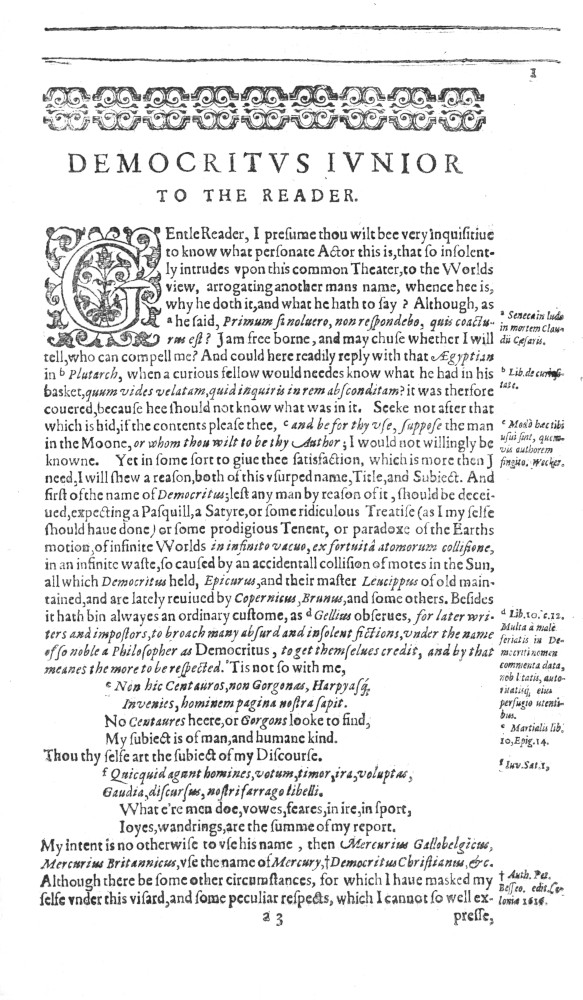
\includegraphics[quiet=true,keepaspectratio]{figures/first-page-first-edition-small.jpg}}
    \caption*{\scriptsize{}\notefont{}First page.}
  \end{minipage}%
  \qquad\begin{minipage}{0.3\textwidth}%
    \frame{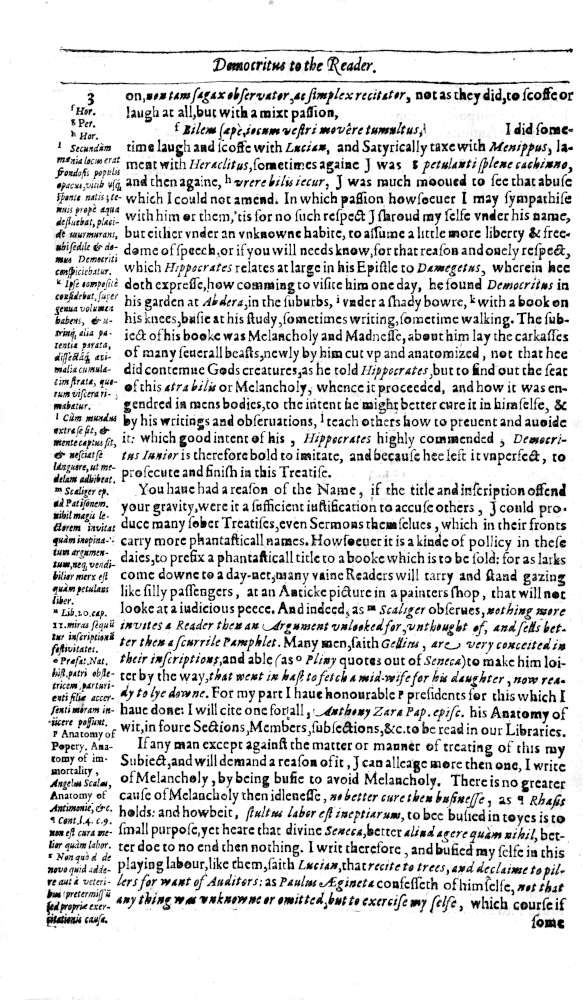
\includegraphics[quiet=true,keepaspectratio]{figures/marginalia-page-first-edition-small.jpg}}
    \caption*{\scriptsize{}\notefont{}Marginalia.}
  \end{minipage}%
  \caption*{Pages from the first edition (1621).}%
  \label{fig:first-edition}%
\end{figure}

In the first edition, every note was placed in the margin. The large textblock and lack of empty space in general make the page very hard to parse. I first encountered the \emph{Anatomy} when I purchased the modern edition published (in 2001) by \marginnote{Robert Burton, \emph{The Anatomy of Melancholy}, introduction by William H. Gass (New York Review Books, 2001), \textsc{ISBN}:~978-0-0940322-66-0.}\emph{\textsc{New York Review Books}}, which had all notes pushed back at the end of each partition, making it impractical to read the text along with the notes. Setting the notes in the context where they are meant to be seems like a reasonable requirement: the back-and-forth movement necessary for the reading of notes is a defect or even a defacement of the author's intent.

  \newlength{\minipagewidth}
\setlength{\minipagewidth}{0.3\textwidth}
  \newlength{\pageratio}
\setlength{\pageratio}{\dimexpr((\paperheight)/(\paperwidth))\relax}
  \newlength{\minipageheight}
\setlength{\minipageheight}{\dimexpr(\pageratio*\minipagewidth)\relax}
\begin{figure}[H]%
  \centering
  \qquad\begin{minipage}{0.27\textwidth}%
   \frame{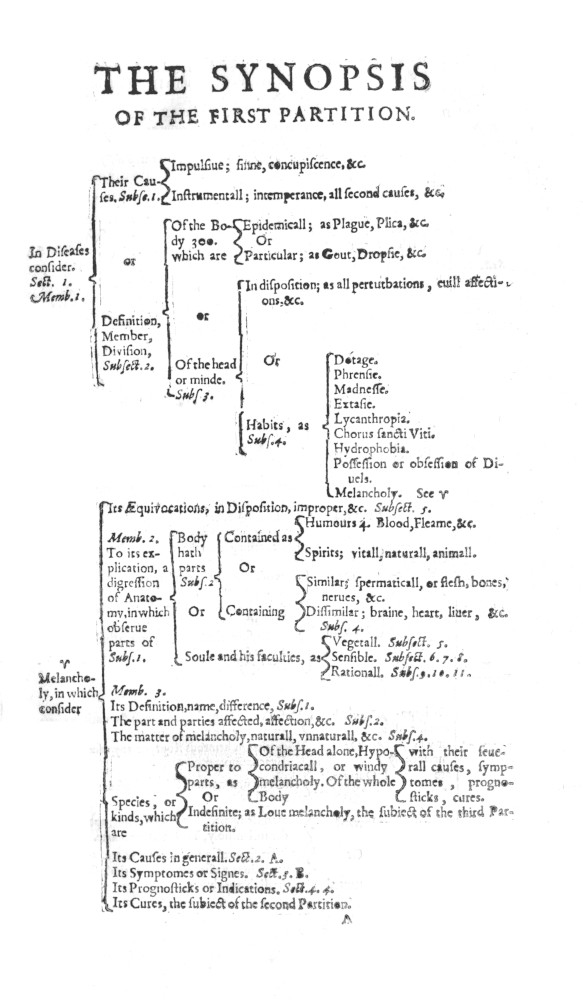
\includegraphics[quiet=true,width=\textwidth,keepaspectratio]{figures/synopsis-schemata-first-edition-small.jpg}}
   \caption*{\scriptsize{}\notefont{}Topical diagram (First edition 1621).}
  \end{minipage}%
  \qquad\begin{minipage}{0.27\textwidth}%
     \begin{minipage}[c][\minipageheight]{\textwidth}%
     \frame{\parbox{\textwidth}{\vspace{\baselineskip}
     {
     \parbox{\textwidth}{\hspace{0.35\textwidth}\resizebox{0.6\textwidth}{!}{\small\textsc{The Synopsis of the First Partition.}}\par
     \vspace{-0.92\baselineskip}
     \hspace{0.15\textwidth}\rule{0.8\textwidth}{.1pt}}\par
     }
     \vspace{0.1\baselineskip}
     \parbox{\textwidth}{\hspace{0.15\textwidth}\resizebox{0.6\textwidth}{!}{\Large{}The Synopsis of the First Partition.}}\par
     \vspace{0.3\baselineskip}
     \parbox{\textwidth}{\hspace{0.15\textwidth}\resizebox{0.8\textwidth}{!}{\SynopsisBoxFirstA}}\par
     \vspace{0.5\baselineskip}
     \parbox{\textwidth}{\hspace{0.15\textwidth}\resizebox{0.8\textwidth}{!}{\SynopsisBoxFirstB}}\par
     \vspace{-0.2\baselineskip}
     \parbox{\textwidth}{\hspace{0.15\textwidth}\resizebox{0.02\textwidth}{!}{\small\pageref{ch:synopsis-of-first-part}\hfill}}\par
     \vspace{0.8\baselineskip}
     \vspace{0.000005\baselineskip}}}
     \caption*{\scriptsize{}\notefont{}\autopageref{ch:synopsis-of-first-part}.}
     \end{minipage}
  \end{minipage}%
 \label{fig:schemata-first-edition}%
\end{figure}

  %\SynopsisBox}
Rendering a book digitally allows the automatic management of references and cross-references. For example, the table of contents, figures, the calculation of page number for cross-references \etc{} are all computed programmatically. Navigating the 1621 edition required consulting the index in the end of the book and the diagrams of topics in the beginning of each partition. For reasons of being thorough and of course aesthetics, they were recreated in \LaTeX{} with the \href{https://www.ctan.org/pkg/schemata}{\myuline{blue}{\texttt{schemata}}} package.

\begin{figure}[H]%
  \centering
    \frame{
\includegraphics[width=\textwidth,quiet=true,keepaspectratio]{figures/chaucer-blackletter-detail.jpg}}
    \caption*{\scriptsize{}\notefont{}Chaucer quotation (First edition 1621). See \autopageref{mention:chaucer-quote-postface}.}
  \label{fig:chaucer-first-edition}%
\end{figure}

Quotations in the 1621 edition were mostly rendered in a cursive typeface (chancery hand), with the exception of \marginnote{
  \newlength{\ChaucerPortraitHeight}
  \newsavebox{\ChaucerPortraitBox}
  \savebox{\ChaucerPortraitBox}{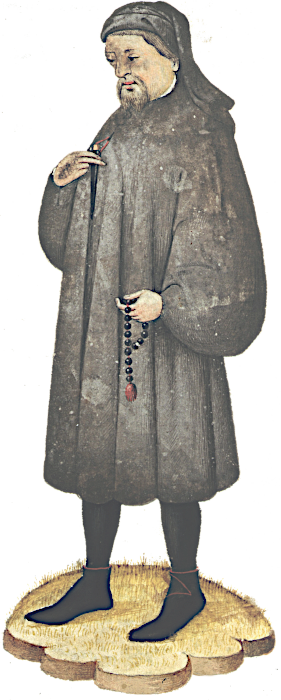
\includegraphics[width=0.4\marginparwidth,quiet=true,keepaspectratio]{figures/Chaucer-small.png}}
  \settoheight{\ChaucerPortraitHeight}{\usebox{\ChaucerPortraitBox}}
  \vspace*{-\ChaucerPortraitHeight-2\baselineskip}
  \par{\noindent\hfil\usebox{\ChaucerPortraitBox}\hfil\par
    \vspace*{\baselineskip}
  Geoffrey Chaucer, English author. Born ca. 1340, died in 1400. Known for \emph{The Canterbury Tales} (1380s), he was influential in establishing vernacular English as a literary language.}}Chaucer whose prose is in \li{textualis formata}, nowadays colloquially known as \emph{Blackletter}. Perhaps the publisher or Burton himself wished to stress the antiquity of Chaucer ---a difference of about two centuries--- or just follow tradition, as Chaucer's works were first published in this script. For this purpose, this edition uses the \href{https://ctan.org/pkg/ygoth}{\myuline{blue}{\texttt{ygoth}}} typeface by Yannis Haralambous for the same effect.

\clearpage{}
\thispagestyle{empty}
\vspace*{\fill} 
\begin{quote} 
\centering 
{\huge\textquote{Be not solitary,\\ be not idle.}}
\end{quote}
\vspace*{\fill}


\bookmarksetup{startatroot}
\colophontitle{About this text}
\pdfbookmark{About this text}{colophon}
\thispagestyle{empty}
\colophontitlesize{18pt}
\colophonparsize{10pt}
\begin{colophon}
  \epigraph{\footnotesize\textit{'Morteque malorum: raptor libri moriatur'}\\(Death from evil things: may the thief of this book die.)}{\scriptsize{}Scribe curses a book’s thief to death, from William of Nottingham’s Commentary on the Harmony of the Gospels, Evesham, c. 1381, Royal MS 4 E \rn{II}, f. 471r}
  Avoid the fate of this curse by procuring this document \textit{gratis et libre}:

  \href{https://github.com/epilys/anatomy-of-melancholy-latex}{\myuline{blue}{https://github.com/epilys/anatomy-of-melancholy-latex}}.

  The text was sourced from \href{https://gutenberg.org/files/10800/10800-h/10800-h.htm}{\myuline{blue}{Project Gutenberg}} and has been typeset in \XeLaTeX{} using the \texttt{octavo} class and \href{https://junicode.sourceforge.io/}{\myuline{blue}{\textbf{Junicode}}} typeface.
\end{colophon}
\clearpage{}
\pdfbookmark{Back Cover}{backcover}
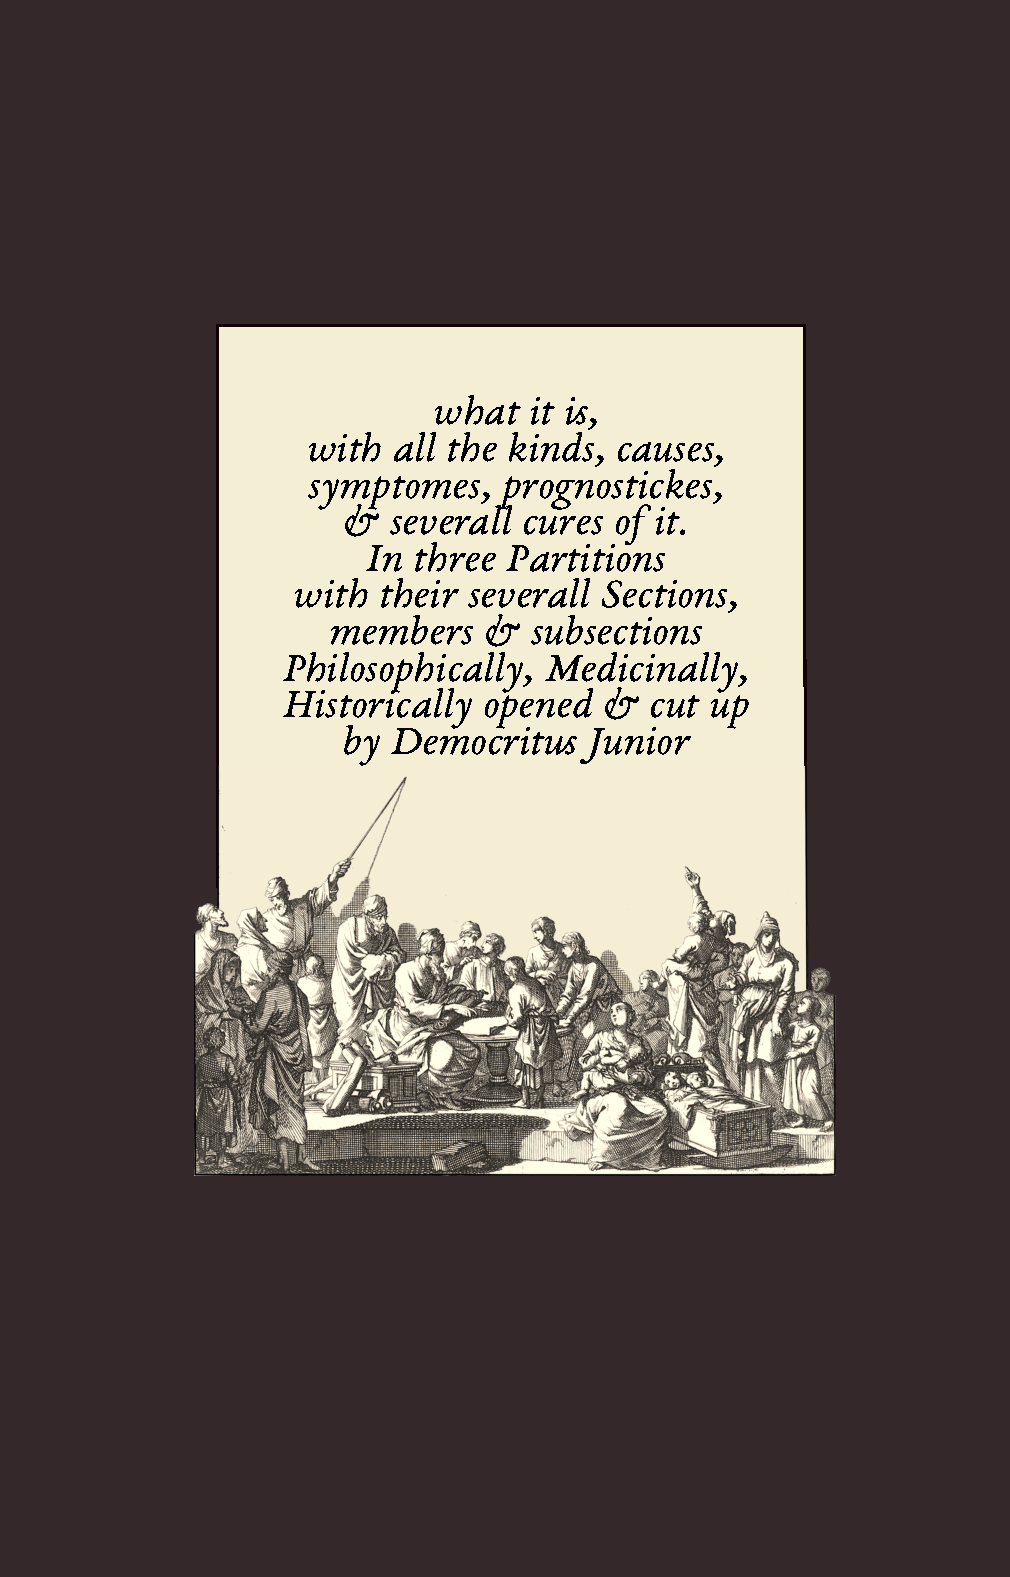
\includepdf[fitpaper=true]{back-cover.pdf} \label{backcover}
\end{document}
